\documentclass[extrafontsizes, twoside, 11pt, openright, final]{memoir}

\usepackage{livroaberto-professor}


\begin{document}



% \setcounter{chapter}{0}
% \include{capa-funcoes}
% \tableofcontents

% \setcounter{chapter}{1}
% \include{capa-afim}
% \setcounter{chapter}{2}
% \include{capa-quadraticas}
% %!TEX root = ../aluno.tex

\ifnum\aluno=1
\renewcommand\chapterillustration{abertura-vetores.jpg}
\else
\renewcommand\chapterillustration{abertura-vetores-professor.jpg}
\fi
\renewcommand\chapterwhat{Vetores no plano do ponto de vista geométrico (segmentos orientados) e algébrico (coordenadas); operações com vetores (adição, subtração e multiplicação por escalar) e suas interpretações geométricas (translação e homotetia); algumas aplicações na Física. } 
\renewcommand\chapterbecause{Vetores são os objetos matemáticos adequados para se descrever, de modo apropriado, certas grandezas (ditas vetoriais) tais como deslocamento, velocidade, aceleração e força. Mais ainda, muitas leis naturais são expressas por equações que envolvem vetores e estudar tais equações permite entender os fenômenos associados. Além disso, o material deste capítulo fornece um primeiro contato, mais simples, com uma disciplina universitária denominada Álgebra Linear, que possui várias aplicações em Biologia, Economia, Computação Gráfica, Engenharia, Física, Matemática, Química, Estatística, etc.} 


\chapter{Vetores no Plano}


\mbox{}\thispagestyle{empty}\clearpage

\thispagestyle{empty}

\begin{center}
Projeto: LIVRO ABERTO DE MATEMÁTICA

\noindent \begin{tabular}{lcccr}

\includegraphics[scale=.15]{impa}& \quad\quad& 
\includegraphics[width=3cm]{logo} & \quad\quad& 
\includegraphics[scale=.24]{obmep} 
\end{tabular}
\end{center}

\vspace*{.3cm}

Cadastre-se como colaborador no site do projeto: \url{umlivroaberto.org}

% Versão digital do capítulo:

% \url{https://www.umlivroaberto.org/BookCloud/Volume_1/master/view/GE101.html}

% \begin{center}
%   \includegraphics[width=2cm]{canvas}
% \end{center}

\begin{tabular}{p{.15\textwidth}p{.7\textwidth}}
Título: & Vetores no Plano \\
\\
Ano/ Versão: & 2021 / versão 1.0 de \today\\
\\
Editora & Instituto Nacional de Matem\'atica Pura e Aplicada (IMPA-OS)\\
\\
Realização:& Olimp\'iada Brasileira de Matem\'atica das Escolas P\'ublicas (OBMEP)\\
\\
Produção:& Associação Livro Aberto\\
\\
Coordenação: & Fabio Simas e Augusto Teixeira (livroaberto@impa.br)\\
\\
  Autores: & Humberto Bortolossi,\\
        & Lhaylla Crissaff,\\
        & Fabio Simas
\\
Revisora: &  Cydara Cavedon Ripoll  \\
          &  Letícia Rangel \\ 
\\
Design: & Andreza Moreira (Tangentes Design) \\
\\
  Ilustrações: & --- \\ 
\\
Gráficos: & --- \\
\\
  Capa: & Foto de Jr Korpa, no Unsplash \\
        & https://unsplash.com/photos/yF3S905z9dM \\

\end{tabular}

\begin{figure}[b]
\begin{minipage}[l]{5cm}
\centering

{\large Licença:}

  
\includegraphics[width=3.5cm]{cc-by-sa1}
\end{minipage}\hfill
\begin{minipage}[c]{5cm}
\centering
{\large Desenvolvido por}


\includegraphics[width=2.5cm]{logo-associacao.jpg}
\end{minipage}
\begin{minipage}[r]{5cm}
\centering

{\large Patrocínio:}
  \vspace{1em}
  
\includegraphics[width=3.5cm]{itau}
\end{minipage}
\end{figure}

\mainmatter


\begin{apresentacao}{Introdução}

\subsection{Habilidades e pré-requisitos}

Neste capítulo contempla-se a seguinte habilidade da segunda versão da \href{http://historiadabncc.mec.gov.br/documentos/bncc-2versao.revista.pdf}{Base Nacional Comum Curricular} (BNCC):

\begin{habilities}{EM11MT01}
Compreender o conceito de vetor, tanto do ponto de vista geométrico (coleção de segmentos orientados de mesmo comprimento, direção e sentido) quanto do ponto de vista algébrico, caracterizado por suas coordenadas, aplicando-o em situações da Física.
\end{habilities}

A própria BNCC dá detalhes do que se espera dessa habilidade:
\begin{quote}

O trabalho com vetores deve proporcionar aos/s estudantes, inicialmente, compreender o conceito de vetor tanto do ponto de vista geométrico (coleção de segmentos orientados de mesmo comprimento, direção e sentido) como do ponto de vista algébrico (caracterizado por suas coordenadas). Na continuidade, esse trabalho é ampliado para que eles sejam capazes de interpretar a representação geométrica da soma de vetores e da multiplicação de um vetor por um escalar e de compreender as relações entre vetores e as transformações isométricas (reflexão, translação e rotação). É importante que todo esse trabalho seja proposto de modo articulado e integrado com situações estudadas na Física, por exemplo, e com apoio de softwares de geometria dinâmica. (BNCC, 2016, p. 562)
\end{quote}

Os pré-requisitos para este capítulo são:
\begin{habilities}{EF02MA12} Identificar e registrar, em linguagem verbal ou não verbal, a localização e os deslocamentos de pessoas e de objetos no espaço, considerando mais de um ponto de referência, e indicar as mudanças de direção e de sentido.

\tcbsubtitle{EF03MA12} Descrever e representar, por meio de esboços de trajetos ou utilizando croquis e maquetes, a movimentação de pessoas ou de objetos no espaço, incluindo mudanças de direção e sentido, com base em diferentes pontos de referência.

\tcbsubtitle{EF04MA16} Descrever deslocamentos e localização de pessoas e de objetos no espaço, por meio de malhas quadriculadas e representações como desenhos, mapas, planta baixa e croquis, empregando termos como direita e esquerda, mudanças de direção e sentido, intersecção, transversais, paralelas e perpendiculares.

\tcbsubtitle{EF05MA14} Utilizar e compreender diferentes representações para a localização de objetos no plano, como mapas, células em planilhas eletrônicas e coordenadas geográficas, a fim de desenvolver as primeiras noções de coordenadas cartesianas.

\tcbsubtitle{EF05MA15} Interpretar, descrever e representar a localização ou movimentação de objetos no plano cartesiano (1º quadrante), utilizando coordenadas cartesianas, indicando mudanças de direção e de sentido e giros.

\tcbsubtitle{EF06MA20} Construir figuras planas semelhantes em situações de ampliação e de redução, com o uso de malhas quadriculadas, plano cartesiano ou tecnologias digitais.

\tcbsubtitle{EF07MA15} Realizar transformações de polígonos representados no plano cartesiano, decorrentes da multiplicação das coordenadas de seus vértices por um número inteiro.

\tcbsubtitle{EF09MA12} Reconhecer as condições necessárias e suficientes para que dois triângulos sejam semelhantes.

\tcbsubtitle{EF09MA13} Demonstrar relações métricas do triângulo retângulo, entre elas o teorema de Pitágoras, utilizando, inclusive, a semelhança de triângulos.

\tcbsubtitle{EF09MA15} Determinar o ponto médio de um segmento de reta e a distância entre dois pontos quaisquer no plano cartesiano, sem o uso de fórmulas, e utilizar esse conhecimento para calcular, por exemplo, medidas de perímetros e áreas de figuras planas construídas no plano.

\end{habilities}

Importante: antes da BNCC, o aluno do Ensino Fundamental II usualmente já tinha um contato inicial com vetores na disciplina de Ciências. Com a BNCC, pressupõe-se que é neste momento que o aluno estudará o assunto pela primeira vez.

\subsection{Tópicos que serão tratados no capítulo}
\begin{itemize}
\item {} 
Vetor do ponto de vista geométrico.
\begin{enumerate}
\item {} 
Grandezas escalares e vetoriais.

\item {} 
Vetor posição relativa no plano: orientação, módulo, notações.

\item {} 
Vetor deslocamento no plano: soma como justaposição, módulo, vetor nulo e vetor simétrico.

\item {} 
Segmentos orientados: direção, sentido e módulo.

\item {} 
Vetores como coleções de segmentos orientados de mesma direção, sentido e módulo: igualdade, soma e subtração, vetor nulo, vetor simétrico, multiplicação por número real, propriedades das operações.
\item {} 
Forças e vetores.

\end{enumerate}

\clearpage
\item {} 
Vetor do ponto de vista algébrico.
\begin{enumerate}
\item {} 
Coordenadas de um vetor no plano.

\item {} 
Interpretação geométrica da operação de multiplicação por número real: homotetias no plano.

\item {} 
Interpretação geométrica da operação de adição de vetores: translações no plano.

\item {} 
Caracterização da igualdade de vetores em termos de suas coordenadas.

\item {} 
Demonstração de algumas propriedades das operações com vetores via coordenadas.

\end{enumerate}

\end{itemize}

Não serão abordados produto escalar e produto vetorial. Vetores no espaço e, mais geralmente, vetores em \({\mathbb R}^{n}\) serão mencionados apenas na seção de aprofundamentos.

\subsection{Objetivo geral do capítulo}

Levar o estudante a perceber, seja do ponto de vista geométrico, seja do ponto de vista algébrico, a adequação do conceito de vetor no estudo de grandezas vetoriais em Física.

\subsection{Abordagem adotada no capítulo}

Vetores são normalmente estudados na disciplina de Física e, ao propor que o tópico seja estudado em Matemática, a BNCC traz uma inovação e um desafio.

A concepção deste capítulo procurou seguir de perto a orientação dada pela BNCC, a saber, desenvolver o tópico de vetores de modo articulado e integrado com situações estudadas na \textbf{Física} e com apoio de softwares de geometria dinâmica.

Nessa articulação, uma particularidade pouco evidenciada teve que ser considerada: enquanto que, tradicionalmente, em Matemática, vetores são definidos como coleções de segmentos orientados de mesma direção, sentido e módulo, de modo que se é possível operá-los a partir de qualquer um de seus representantes, dependendo da situação física em questão, nem todos os representantes são válidos e até mesmo certas operações deixam de fazer sentido. Por exemplo, na figura a seguir, se \(\overrightarrow{OA}\) e \(\overrightarrow{OB}\) são os vetores posições relativas dos pontos \(A\) e \(B\) com relação ao ponto \(O\),
apesar da soma \(\overrightarrow{OA} + \overrightarrow{OB}\) estar definida matematicamente, ela não faz sentido no contexto físico em questão (note, contudo, que a diferença \(\overrightarrow{OB} - \overrightarrow{OA}\) faz sentido: \(\overrightarrow{OB} - \overrightarrow{OA}\) é o vetor deslocamento \(\overrightarrow{AB}\)).

\begin{center}
\begin{tikzpicture}
\node [ponto] (O) at (-1.98,-0.3) {};
\node [ponto] (A) at (-1.4,2.28) {};
\node [ponto] (B) at (1.58,1.68) {};
\node [above] at (A) {$A$};
\node [above right] at (B) {$B$};
\node [below left] at (O) {$O$};
\draw [vetor] (O) -- (A);
\draw [vetor] (O) -- (B);
\end{tikzpicture}
\end{center}

Outro exemplo: no contexto de vetores deslocamentos, na figura a seguir, a soma \(\overrightarrow{AB} + \overrightarrow{CD}\) não faz sentido (pois os segmentos orientados \(\overrightarrow{AB}\) e \(\overrightarrow{CD}\) não estão justapostos), enquanto que a soma \(\overrightarrow{CD} + \overrightarrow{DE}\) faz (\(\overrightarrow{CD} + \overrightarrow{DE}\) é o vetor deslocamento \(\overrightarrow{CE}\)).

\begin{center}
\begin{tikzpicture}
\node [ponto] (A) at (-1.74,1.16) {};
\node [ponto] (B) at (-0.36,2.98) {};
\node [ponto] (C) at (3.92,0.94) {};
\node [ponto] (D) at (1.72,4.32) {};
\node [ponto] (E) at (3.92,4.9) {};
\node [below left] at (A) {$A$};
\node [above right] at (B) {$B$};
\node [below right] at (C) {$C$};
\node [above left] at (D) {$D$};
\node [above right] at (E) {$E$};
\draw [vetor] (A) -- (B);
\draw [vetor] (C) -- (D);
\draw [vetor] (D) -- (E);
\end{tikzpicture}
\end{center}

Ainda nesta linha, observe que enquanto do ponto de vista da Matemática, a "regra do triângulo"{} e a "regra do paralelogramo"{} são equivalentes para se obter a soma de dois vetores, dependendo do contexto físico, uma regra pode ser mais natural do que a outra. Por exemplo, a "regra do triângulo"{} é mais natural no contexto da soma de vetores deslocamentos, enquanto que ela é artificial no caso da soma de vetores que representam forças (uma vez que, para forças, a linha de ação da força é relevante). Reciprocamente, a "regra do paralelogramo"{} é mais natural no contexto da soma de vetores que representam forças (com todos os vetores com suas extremidades iniciais coincidentes), mas ela é artificial no contexto de vetores deslocamentos.
\begin{center}\begin{tikzpicture}
\matrix{
\coordinate (a) at (-4.45,-0.3);
\coordinate (b) at (0.89,1.68);
\coordinate (c) at (0.31,4.26);
\node [ponto] at (a) {};
\node [ponto] at (b) {};
\node [ponto] at (c) {};
\draw [vetor] (a) -- (b);
\draw [vetor] (b) -- (c);
\draw [vetor,color=destacado]  (a) -- (c);
\node [below] at ($(a)!0.5!(b)$) {$\vec{u}$};
\node [right] at ($(b)!0.5!(c)$) {$\vec{v}$};
\node [above,rotate=45,color=destacado] at ($(a)!0.5!(c)$) {$\vec{u}$ + $\vec{v}$} ;
\draw (-4.69334,-0.98342) node[anchor=north west] {Regra do Triángulo};
&
\coordinate (o) at (-1.98,-0.3);
\coordinate (a) at (-1.4,2.28);
\coordinate (b) at (1.58,1.68);
\coordinate (c) at (2.16,4.26);
\node [ponto] at (o) {};
\node [ponto] at (a) {};
\node [ponto] at (b) {};
\node [ponto] at (c) {};
\draw [vetor] (o) -- (a);
\draw [vetor] (o) -- (b);
\draw [dotted] (a)-- (c);
\draw [dotted] (b)-- (c);
\draw [vetor,color=destacado] (o) -- (c);
\node [left] at ($(o)!0.5!(a)$) {$\vec{v}$};
\node [below] at ($(o)!0.5!(b)$) {$\vec{u}$};
\node [above,rotate=45,color=destacado] at ($(o)!0.5!(c)$)  {$\vec{u}$ + $\vec{v}$} ;
\draw (-2.37284,-0.98342) node[anchor=north west] {Regra do Paralelogramo};
\\};
\end{tikzpicture}
\end{center}

Para acomodar estas particularidades, alguns livros de Física e Engenharia introduzem nomes especiais: \index{vetor fixo}vetor fixo (quando o vetor admite um único representante em uma posição específica no contexto físico), \index{vetor deslizante}vetor deslizante (quando o vetor admite qualquer representante de mesmo módulo e sentido em uma mesma reta) e \index{vetor livre}vetor livre (quando o vetor admite qualquer representante de mesmo módulo, direção e sentido em qualquer lugar do plano, ou seja, como o vetor tradicionalmente definido em Matemática). Esta terminologia já está aparecendo em livros de Matemática mais recentes usados em cursos de formação de professores (ver, por exemplo, \citet{anton2007}. Incorporar essa terminologia em sala de aula ainda é uma questão. Contudo, o mais importante, em nossa opinião, é que você tenha, antes de tudo, consciência das peculiaridades de cada caso, pois elas influenciam a maneira de como os alunos aprendem e fazem uso do conceito de vetor (conforme \citet{roche1997}).
Também é preciso ficar atento ao fato de que, muito provavelmente, esta deve ser a primeira vez que o aluno verá um símbolo usado em contexto ("\(+\)"{} para adição de números) em outro contexto ("\(+\)"{} para representar a adição de vetores).

No que se refere às grandezas físicas, optou-se pela seguinte ordem encadeada conceitualmente: posição relativa \(\rightarrow\) deslocamento \(\rightarrow\) velocidade média \(\rightarrow\) aceleração média (note que para definir aceleração média, é preciso antes definir velocidade média a qual, por sua vez, pressupõe o conceito de deslocamento e, este, pressupõe o conceito de posição relativa).

O vetor posição relativa, apesar de suas limitações (a soma deste tipo de vetor não faz sentido neste contexto), é simples e permite evidenciar para o aluno que existem grandezas que não podem ser descritas apenas com um número ou apenas como uma orientação. Assim, como primeira atividade, usamos um problema que envolve posições relativas para motivar o conceito de grandeza vetorial.
Além disso, o vetor posição relativa tem uma vantagem adicional: a escala determinada para as posições automaticamente determinar a escala do vetor, isto é, tem-se uma escala só (compare com o caso de velocidades e forças: as posições podem ter uma escala e os vetores podem ter outra completamente diferente).

Vetores deslocamentos são então introduzidos e, por meio de uma versão simplificada do jogo \textit{Corrida de Vetores} (conforme \citet{gardner1973} e \citet{oliveira2009},
\begin{itemize}
\item {} 
estabelece-se a diferença entre deslocamento e trajetória percorrida (uma confusão frequente nos alunos);

\item {} 
apresenta-se a justaposição de vetores deslocamentos a partir da qual a soma será introduzida;

\item {} 
apresenta-se o vetor deslocamento nulo e o vetor deslocamento simétrico.

\end{itemize}

Ainda com a \textit{Corrida de Vetores}, apresenta-se o uso de um segmento orientado apenas como um indicador de orientação e distância, interpretação esta que motivará a definição geral de vetor como uma coleção de segmentos orientados de mesma direção, sentido e módulo, tema da seção seguinte (\textit{Organizando as ideias}). Nesta seção, discute-se a questão dos vários significados que \textit{direção} e \textit{sentido} podem ter e qual será aquele adotado no contexto de vetores. Os conceitos de soma, vetor nulo e vetor simétrico são revisitados. Introduz-se a operação subtração e de multiplicação por um número real e algumas propriedades são então discutidas.

No lugar de conceber as coordenadas dos vetores a partir do tradicional sistema de coordenadas já apresentado e usado no Ensino Fundamental II, o tratamento de vetores do ponto de vista algébrico é conduzido como um desdobramento natural das operações de adição de vetores e multiplicação por número real que foram desenvolvidas geometricamente na seção anterior. Mais precisamente, um sistema de coordenadas é construído a partir da percepção que, fixados dois vetores não paralelos num plano, digamos \(\vec{u}\) e \(\vec{v}\), qualquer vetor \(\vec{w}\) do plano pode ser representado pelo par de números \(a\) e \(b\) tais que \(\vec{w}=a \cdot \vec{u}+b \cdot \vec{v}\). Assim, com essa nossa escolha, vetores determinam sistemas de coordenadas e não o contrário. Essa abordagem tem a vantagem de levar naturalmente a sistemas não ortogonais e de ser um primeiro contato com a leitura de certos problemas geométricos via combinações lineares (por exemplo, resolver um sistema linear \(2\,a + 3\,b = 4\) e \(5\,a - 8\,b = 7\) pode ser interpretado como encontrar os pontos de interseção das retas cujas equações são \(2\,a + 3\,b = 4\) e \(5\,a - 8\,b = 7\) ou, dualmente, determinar números reais \(a\) e \(b\) tais que \(\vec{w} = a \cdot \vec{u} + b \cdot \vec{v}\), onde \(\vec{u} = (2, 5)\), \(\vec{v} = (3, -8)\) e \(\vec{w} = (4, 7)\)).

Uma vez estabelecido o fato de que se \((a, b)\) são as coordenadas de um ponto \(P\) com relação a um sistema de coordenadas com origem \(O\), então o vetor posição relativa \(\overrightarrow{OP}\) também tem coordenadas \((a, b)\) com relação a este sistema de coordenadas, optou-se por identificar pontos com vetores desta maneira: \(P = \overrightarrow{OP}\). Com isto, a soma \(P + \vec{v}\) de um ponto com um vetor deve ser interpretada como a soma \(\vec{OP} + \vec{v}\) de vetores. Esta formulação será especialmente útil na interpretação de translações por meio de soma de vetores. Em particular, mostra-se que dado um ponto \(P=(x,y)\) e um vetor \(\vec{v}=(c,d)\), as coordenadas da translação de \(P\) por \(\vec{v}\) são \(P'=P+\vec{v} = (x,y) + (c,d) = (x+c,y+d)\) e, mais geralmente, mostra-se que se os vetores \(\vec{u}\) e \(\vec{v}\) se expressam como \(\vec{u}=(a,b)\) e  \(\vec{v} = (c, d)\) num sistema de coordenadas, então \(\vec{u} + \vec{v} = (a + c, b + d)\).

A operação de multiplicação de um vetor por um número real é interpretada geometricamente no contexto de homotetias. Aqui, usando-se semelhança de triângulos e como uma consequência da definição geométrica dada para a multiplicação de um vetor por um número real, justifica-se que se \((a, b)\) são as coordenadas de um vetor no plano e \(c\) é um número real, então \(c \cdot (a, b) = (c \cdot a, c \cdot b)\), ou seja, que esta igualdade é uma consequência e não uma definição.

Na sequência, coordenadas de vetores são usadas para justificar algumas das propriedades das operações da adição de vetores e multiplicação por um número real (comutatividade, associatividade, distributividade) mostrando que estas propriedades se reduzem às propriedades análogas para os números reais.

Por fim, desenvolve-se o uso de vetores no contexto de forças. As atividades propostas (que incluem decomposições de forças) têm como base a primeira lei de Newton interpretada da seguinte maneira: "a força resultante sobre um corpo é zero se, e somente se, sua velocidade é constante". Nesta parte, seguindo a orientação de \citet{roche1997}, em soma de forças, o vetor que representa a força resultante é sempre desenhado com uma cor diferente dos vetores que representam as forças parcelas pois, segundo o autor, é um erro comum os estudantes confundirem a força resultante como mais uma força parcela e não como uma força equivalente às forças dadas.

Registramos aqui uma analogia que pode ser útil para uma reflexão sobre o ensino e a aprendizagem de vetores: este tópico tem muito em comum com tópico dos números racionais. Seguem alguns exemplos que ilustram essa analogia.
\begin{enumerate}
\item {} 
Números racionais são classes de equivalência de frações;  vetores são classes de equivalência de segmentos orientados.

\item {} 
Existem várias "interpretações"{} para frações, cada uma com suas particularidades: parte-todo, divisão, razão, medida, operador; vetores também têm suas "interpretações", cada uma com suas particularidades: posição, deslocamento, velocidade, aceleração, força, torque.

\item {} 
A "igualdade"{} de frações se dá estabelecendo-se um critério: duas frações são iguais se elas expressam a mesma quantidade (dividir um bolo em duas partes e tomar uma parte é um processo diferente de dividir o mesmo bolo em quatro partes e tomar duas partes mas, nos dois processos, a quantidade de bolo tomada é a mesma); a "igualdade"{} de segmentos orientados também se dá por um critério: eles são iguais se possuem a mesma direção, módulo e sentido (ir 10 km para o norte saindo de Manaus não é o mesmo que ir 10 km para o norte saindo do Rio de Janeiro, pois as posições iniciais em cada caso são diferentes mas, nos dois processos, caminhou-se 10 km para o norte).

\item {} 
Existe uma flexibilidade no rigor (um "abuso de linguagem") ao se referenciar números racionais como, por exemplo, dizer  "o número racional \(2/4\)"{} ao invés de dizer "o número racional cujo representante é a fração \(2/4\)"); esta flexibilidade também ocorre com vetores: dizer "o vetor \(\overrightarrow{OP}\)"{} ao invés de dizer "o vetor cujo representante é o segmento orientado \(\overrightarrow{OP}\)".

\end{enumerate}

\subsection{Observações metodológicas gerais}
\begin{itemize}
\item {} 
As seções sob o título "Para reflexão"{} podem ser usadas de duas maneiras: (1) você pode, oralmente, na sala de aula, levantar as questões apontadas nestas seções e, então, articular uma discussão oral conjunta com os alunos ou (2) pedir para que eles, numa reflexão mais individual, leiam o texto e registrem primeiro suas respostas no caderno (funcionando, assim, como uma atividade em sala de aula) para depois fazer um fechamento acerca das questões abordadas.

\item {} 
Caso haja a disponibilidade de um projetor multimídia acoplado a um computador, \textit{tablet} ou \textit{smartphone}, você pode considerar o uso das várias atividades interativas que estão indicadas ao longo do texto. Estas atividades permitem realizar animações e   múltiplos exemplos que ajudam muito na consolidação das ideias em conceitos.

\end{itemize}
\end{apresentacao}

\def\currentcolor{session1}
\begin{objectives}{Resgate na Antártida}
{
\begin{itemize}
\item {} 
Reconhecer que a posição relativa de um ponto com relação a um outro ponto de referência é uma grandeza vetorial.

\item {} 
Reconhecer que a posição relativa depende da escolha do ponto de referência.

\end{itemize}
}{1}{1}
\end{objectives}
\begin{answer}{Resgate na Antártida}
{
\paragraph{Parte I}
\begin{enumerate}
\item {} 
Não, pois existem infinitos pontos no mapa cuja distância até a estação de pesquisa \(A\) é 10 km.

\item {} 
A circunferência de centro em \(A\) e raio 10 km.

\end{enumerate}

\begin{figure}[H]
\centering

\fbox{\noindent\includegraphics[width=225bp, trim=5mm 5mm 5mm 5mm, clip]{{geometria-vp-resposta-01}.jpg}}
\end{figure}
}{1}
\end{answer}

\begin{answer}{Resgate na Antártida}
{
\paragraph{Parte II}
\begin{enumerate}
\item {} 
Não, pois exitem infinitos pontos à nordeste da estação de pesquisa \(A\).

\item {} 
A semirreta com origem em \(A\) na direção nordeste excluindo-se \(A\).

\begin{figure}[H]
\centering

\fbox{\includegraphics[width=225bp, trim=5mm 5mm 5mm 5mm, clip]{{geometria-vp-resposta-02}.jpg}}
\end{figure}

\item {} 
Não, pois existem duas possibilidades para a localização de \(P\).

\begin{figure}[H]
\centering

\fbox{\includegraphics[width=225bp, trim=5mm 5mm 5mm 5mm, clip]{{geometria-vp-resposta-03-01}.jpg}}
\end{figure}

\begin{figure}[H]
\centering

\fbox{\includegraphics[width=225bp, trim=5mm 5mm 5mm 5mm, clip]{{geometria-vp-resposta-03-02}.jpg}}
\end{figure}

\end{enumerate}
}{9}
\end{answer}
\clearmargin
\begin{answer}{Resgate na Antártida}
{
\paragraph{Parte III}
\begin{enumerate}
\item {} 
Sim, pois existe um único ponto à nordeste de \(A\) cuja distância a \(A\) é igual a 10 km.

\item {} 
Um ponto.

\begin{figure}[H]
\centering

\fbox{\includegraphics[width=225bp, trim=5mm 5mm 5mm 5mm, clip]{{geometria-vp-resposta-04}.jpg}}
\end{figure}

\item {} 
A base \(A\) está situado à 10 km à sudoeste de \(P\).

\end{enumerate}

\paragraph{Parte IV}
\begin{enumerate}
\item {} 
O grupo \(P\) está situado à \(10 \, \sqrt{2}\) km à leste de \(B\).

\begin{figure}[H]
\centering

\fbox{\includegraphics[width=225bp, trim=5mm 5mm 5mm 5mm, clip]{{geometria-vp-resposta-05}.jpg}}
\end{figure}

\item {} 
A estação \(A\) está mais próxima.

\end{enumerate}
}{1}
\end{answer}


\explore{Vetores Posições Relativas}
\label{vetores-exp1}

\begin{task}{resgate na Antártida}
\label{ativ-vetores-vetor-posicao-relativa}



A figura a seguir exibe um mapa onde o pontorepresenta a localização de uma estação de pesquisa \(A\) na Antártida.

\begin{figure}[H]
\centering

\fbox{\includegraphics[width=250bp, trim=5mm 5mm 5mm 5mm, clip]{{geometria-vp-01}.jpg}}
\end{figure}

Um problema de localização.

\paragraph{Parte I}

A estação de pesquisa \(A\) recebe um comunicado de um avião de reconhecimento informando que um grupo \(P\) de exploradores  situado à 10 km de \(A\) necessita de socorro urgente.
\begin{enumerate}
\item {} 
É possível marcar no mapa a localização do grupo \(P\) de exploradores? Justifique sua resposta!

\item {} 
Se você marcasse no mapa todos os pontos onde o grupo \(P\) de exploradores poderia estar, que figura geométrica seria desenhada?

\end{enumerate}

\paragraph{Parte II}

Considere agora esta outra situação. A estação de pesquisa \(A\) recebe um comunicado de um avião de reconhecimento informando que um outro grupo \(Q\) de exploradores situado à nordeste de \(A\) necessita de socorro urgente.
\begin{enumerate}
\item {} 
É possível marcar no mapa a localização do grupo \(Q\) de exploradores? Justifique sua resposta!

\item {} 
Se você marcasse no mapa todos os pontos onde o grupo \(Q\) de exploradores poderia estar, que figura geométrica seria desenhada?

\item {} 
Se a estação de pesquisa \(A\) e os dois grupos de pesquisa \(P\) e \(Q\) estiverem alinhados (isto é, pertencessem a uma reta), seria possível marcar a localização do grupo \(P\) de exploradores? Justifique sua resposta!

\end{enumerate}

\paragraph{Parte III}

O avião de reconhecimento atualizou as informações sobre o grupo \(P\) de exploradores: ele está situado à 10 km à nordeste de \(A\).
\begin{enumerate}
\item {} 
É agora possível marcar no mapa a localização do grupo \(P\) de exploradores? Justifique sua resposta!

\item {} 
Nessa nova situação, se você marcasse no mapa todos os pontos onde o grupo \(P\) de exploradores poderia estar, que figura geométrica seria desenhada?

\item {} 
Caso a resposta ao Item a) seja afirmativa, com você descreveria a posição da base \(A\) com relação ao grupo \(P\) de pesquisadores?

\end{enumerate}

\paragraph{Parte IV}

Uma segunda estação de pesquisa \(B\) está situada à 10 km a noroeste de \(A\).
\begin{enumerate}
\item {} 
Considerando os dados da Parte III, como você informaria a posição do grupo \(P\) de exploradores com relação à estação \(B\)?

\item {} 
Qual estação de pesquisa está mais próxima do grupo de exploradores? \(A\) ou \(B\)? Justifique sua resposta!

\end{enumerate}
\end{task}





\paragraph{Grandezas escalares e vetoriais}

Em Física, existem grandezas que ficam perfeitamente descritas por um número e uma unidade. Este é o caso, por exemplo, do tempo, da temperatura, da pressão e da massa.
Grandezas deste tipo são denominadas \index{grandezas escalares}grandezas escalares.

Por outro lado, como você deve ter percebido com a atividade anterior, um único número não basta para especificar completamente uma posição com relação a um ponto de referência. Além da distância entre o ponto de referência e a posição em questão (no caso da atividade, "10 km"), também é necessário ter uma orientação (no caso da atividade, "à nordeste"). Grandezas físicas deste tipo \textendash{} as quais, para serem perfeitamente descritas, necessitam de um valor numérico, uma unidade e uma orientação \textendash{} são denominadas \index{grandezas vetoriais}grandezas vetoriais.

\begin{reflection}

Quais outras grandezas físicas você conhece? Elas são grandezas escalares ou vetoriais?
\end{reflection}

\clearpage

\begin{sugestions}{}
{
Sugerimos o uso da construção GeoGebra disponível no endereço \href{https://www.geogebra.org/m/kCMtPW5x/}{https://www.geogebra.org/m/kCMtPW5x} com a qual é possível mudar a posição do ponto de referência \(B\)  e, com isto, ilustrar dinamicamente para o aluno como o vetor posição relativa depende da escolha do ponto de referência.

\begin{figure}[H]
\centering

\noindent\includegraphics[width=50bp]{{ggb-vpr-01-qr}.png}
\end{figure}

\begin{marginfigure}[H]
\centering
\capstart

\noindent\includegraphics[width=300bp]{{ggb-vpr-01}.jpg}
\caption{\url{https://www.geogebra.org/m/kCMtPW5x/}.}\label{\detokenize{GE101-0:fig-ggb-vpr-01}}\label{\detokenize{GE101-0:id8}}
\end{marginfigure}}
{1}{1}
\end{sugestions}

\paragraph{Vetor Posição Relativa}

A posição relativa, a exemplo de outras grandezas vetoriais que veremos neste capítulo, pode ser representada
geometricamente por um \index{segmento de reta orientado}segmento de reta orientado, o qual é normalmente desenhado como uma seta.
Este tipo de representação para a posição relativa será denominada \index{vetor posição relativa}vetor posição relativa.
A figura a seguir exibe os vetores posições relativas do grupo de exploradores (marcado como \(G\) na figura)
com relação às estações de pesquisa \(A\) e \(B\) da atividade anterior.

\begin{figure}[H]
\centering
\capstart

\fbox{\includegraphics[width=250bp,trim=5mm 5mm 5mm 5mm, clip]{{geometria-vp-02}.jpg}}
\caption{Vetores posições relativas do ponto \(G\) determinados pelos pontos de referência \(A\) e \(B\).}
\end{figure}

\begin{reflection}

Por que posições relativas não poderiam ser representadas apenas com segmentos de reta? Por que usar segmentos orientados é importante neste contexto?
\end{reflection}

\paragraph{Notações}

Ao fazer referência a um vetor posição relativa, no lugar de uma descrição longa do tipo "vetor posição relativa do ponto \(G\) com relação ao ponto de referência \(A\)", é costume introduzir notações que permitem referenciar o vetor posição relativa de forma mais curta (essa \textit{economia} de escrita é uma prática comum na Matemática). Por exemplo, uma das notações adotada para representar o "vetor posição relativa do ponto \(G\) com relação ao ponto de referência \(A\)"{} é \(\overrightarrow{AG}\). Nesta notação, ao lê-la da esquerda para direita, a primeira letra representa o ponto de referência (no caso, o ponto \(A\)) e a segunda letra representa a posição em consideração (no caso, o ponto \(G\)). A seta sobre as duas letras é um recurso gráfico para lembrar que a notação está representando um vetor. Neste contexto, o ponto \(A\) é denominado \index{extremidade inicial}extremidade inicial (ou simplesmente \index{origem}origem) e o ponto \(G\) é denominado \index{extremidade final}extremidade final (ou simplesmente \index{extremidade}extremidade, quando não há perigo de confusão com a extremidade inicial) do vetor \(\overrightarrow{AG}\). O comprimento do segmento de reta \(AG\) é denominado \index{módulo}módulo do vetor \(\overrightarrow{AG}\) e será denotado por \(|\overrightarrow{AG}|\). No caso do vetor \(\overrightarrow{AG}\) da figura seguinte (relacionada com a atividade proposta no início desta seção), tem-se
\(|\overrightarrow{AG}| = 10~\text{km}\).

Uma notação ainda mais curta é simplesmente dar um "nome"{} ao vetor posição relativa, também como uma seta em cima. Por exemplo, na figura a seguir, o vetor posição relativa \(\overrightarrow{AG}\) é denotado por \(\vec{u}\) e o vetor posição \(\overrightarrow{BG}\) é representado por \(\vec{v}\). Nesta notação mais curta, o módulo do vetor posição relativa \(\vec{v}\) é denotado por \(|\vec{v}|\). Assim,
para \(\vec{v}\) da figura seguinte (relacionada com a atividade proposta no início desta seção), tem-se
\(|\vec{v}| = 10 \, \sqrt{2}~\text{km}\) (por quê?).

\begin{figure}[H]
\centering
\capstart

\fbox{\includegraphics[width=250bp,trim=5mm 5mm 5mm 5mm, clip]{{geometria-vp-03}.jpg}}
\caption{Notação para vetores posições relativas.}
\end{figure}

\begin{observationtitle}{Observações sobre notação e terminologia}
\begin{itemize}
\item {} 
Alguns livros usam ainda um outro tipo de notação: grandezas vetoriais são representadas por letras em negrito e grandezas escalares por letras em itálico.

\item {} 
Dependendo do autor e do contexto, o módulo de um vetor também pode ser chamado de \index{magnitude}magnitude, \index{intensidade}intensidade ou \index{valor}valor.

\end{itemize}
\end{observationtitle}

Antes de prosseguirmos, é importante destacar uma característica importante do vetor posição relativa: ele depende da escolha do ponto de referência. Veja, por exemplo, na situação ilustrada na figura anterior, que a posição \(G\) é representada por vetores posições relativas diferentes quando pontos de referências diferentes (\(A\) e \(B\)) são escolhidos.


\clearpage
\begin{sugestions}{Vetores deslocamentos}
{Observe que o vetor deslocamento é definido apenas em termos dos pontos inicial e final e estes não mudam com escolhas diferentes para o ponto de referência. Por este motivo, o vetor deslocamento também não muda. Na  
\Fref{fig-geometria-deslocamento-01}, o ponto de referência \(L\) não precisa, obrigatoriamente, ser um ponto da pista.

Estudos educacionais mostram que os alunos têm a forte tendência em confundir vetor deslocamento com trajetória. No sentido de minimizar o efeito deste distrator, sugerimos o uso da construção GeoGebra disponível no endereço \url{https://www.geogebra.org/m/f8GCVdyx}. Com ela, é possível visualizar um ponto percorrendo o modelo da pista de Interlagos apresentado na  
\Fref{fig-geometria-deslocamento-01} e, ao mesmo tempo, definir diferentes vetores deslocamentos definidos por duas posições na pista. Ao, dinamicamente, confrontar a trajetória percorrida com os diversos vetores deslocamentos, espera-se criar uma imagem mental que reforce as diferenças entre os dois conceitos.

\begin{figure}[H]
\centering

\noindent\includegraphics[width=50bp]{{ggb-interlagos-01-qr}.png}
\end{figure}

% \begin{figure}[H]
% \centering
% \capstart

% % \noindent\includegraphics[width=400bp]{{ggb-interlagos-01_2}.png}
% \caption{\url{https://www.geogebra.org/m/f8GCVdyx}.}\label{\detokenize{GE101-0A:id2}}\end{figure}

Além do trabalho de uma força em Física, como mencionado no texto para o aluno, a própria velocidade média (como uma grandeza vetorial) é um conceito que é definido em termos de vetores deslocamentos apenas e não de \index{distâncias percorridas}distâncias percorridas em uma trajetória. Ao se considerar distâncias percorridas, um outro conceito é estabelecido: o de \index{rapidez média}rapidez média (\textit{speed} em Inglês), também denominada de \index{velocidade escalar média}velocidade escalar média. Assim, é importante diferenciar os dois conceitos: velocidade média (uma grandeza vetorial) e rapidez média (uma grandeza escalar).}
{1}{1}
\end{sugestions}

\explore{Vetores Deslocamentos}

Um dos objetivos da Física é estudar como certas grandezas variam no tempo. Um carro, por exemplo, ao percorrer a pista de Interlagos em São Paulo sem parar, ocupará posições diferentes em tempos diferentes, isto é, sua posição variará ao longo do tempo. Na figura a seguir, estão marcadas duas posições na pista: o ponto \(S\) que demarca a curva "S"{} do Sena (posição esta, digamos, ocupada pelo carro em um tempo inicial) e o ponto \(T\) que demarca o final do trecho da "reta oposta"{} (ocupada pelo carro em um tempo final). Também estão desenhados na figura os vetores posições relativas \(\overrightarrow{LS}\) e \(\overrightarrow{LT}\) (considerando-se, então, \(L\) como ponto de referência).
Como representar matematicamente esta variação de posição de \(S\) para \(T\)? Isto também será feito por um segmento orientado que, neste contexto, será denominada \index{vetor deslocamento} vetor deslocamento. A seta que representa o segmento orientado é desenhada com extremidade inicial na posição inicial (isto é, aquela associada ao tempo inicial) e extremidade final na posição final (isto é, aquela associado ao tempo final). As notações usadas para vetores deslocamentos são as mesmas usadas para vetores posições relativas. Assim, por exemplo, o vetor deslocamento azul na figura pode ser denotado por \(\overrightarrow{ST}\) ou \(\vec{u}\).


% \begin{figure}[H]
% \centering
% \begin{tikzpicture}[scale=.7]
% \begin{scope}[line cap=round,line join=round,>=latex,x=0.001cm,y=0.001cm,scale=4]
% \filldraw [white, fill opacity=100] (0,200) rectangle (2400,2200);
% \draw [grafica, line width=2pt] (5.04401,1280.3)-- (209.455,435.9657720937503);
% \draw[grafica, line width=2pt, smooth, samples=100, domain=0.0:1.0] plot[parametric] function{318.647*(1.0-t)**(3.0-1.0-0.0)*t**(0.0)+361.833*2.0*(1.0-t)**(3.0-1.0-1.0)*t**(1.0)+386.322*(1.0-t)**(3.0-1.0-2.0)*t**(2.0),244.11577209375037*(1.0-t)**(3.0-1.0-0.0)*t**(0.0)+239.9257720937503*2.0*(1.0-t)**(3.0-1.0-1.0)*t**(1.0)+279.9657720937503*(1.0-t)**(3.0-1.0-2.0)*t**(2.0)};
% \draw[grafica, line width=2pt, smooth, samples=100, domain=0.0:1.0] plot[parametric] function{209.455*(1.0-t)**(4.0-1.0-0.0)*t**(0.0)+221.765*3.0*(1.0-t)**(4.0-1.0-1.0)*t**(1.0)+268.521*3.0*(1.0-t)**(4.0-1.0-2.0)*t**(2.0)+318.647*(1.0-t)**(4.0-1.0-3.0)*t**(3.0),435.9657720937503*(1.0-t)**(4.0-1.0-0.0)*t**(0.0)+367.1657720937503*3.0*(1.0-t)**(4.0-1.0-1.0)*t**(1.0)+260.3257720937504*3.0*(1.0-t)**(4.0-1.0-2.0)*t**(2.0)+244.11577209375037*(1.0-t)**(4.0-1.0-3.0)*t**(3.0)};
% \draw [grafica, line width=2pt, smooth, samples=100, domain=0.0:1.0] (138.179,1855.6177720937503)-- (5.04401,1280.3367720937504);
% \draw[grafica, line width=2pt, smooth, samples=100, domain=0.0:1.0] plot[parametric] function{386.322*(1.0-t)**(4.0-1.0-0.0)*t**(0.0)+442.508*3.0*(1.0-t)**(4.0-1.0-1.0)*t**(1.0)+460.402*3.0*(1.0-t)**(4.0-1.0-2.0)*t**(2.0)+460.402*(1.0-t)**(4.0-1.0-3.0)*t**(3.0),279.9657720937503*(1.0-t)**(4.0-1.0-0.0)*t**(0.0)+353.2857720937502*3.0*(1.0-t)**(4.0-1.0-1.0)*t**(1.0)+327.1657720937503*3.0*(1.0-t)**(4.0-1.0-2.0)*t**(2.0)+327.1657720937503*(1.0-t)**(4.0-1.0-3.0)*t**(3.0)};
% \draw[grafica, line width=2pt, smooth, samples=100, domain=0.0:1.0] plot[parametric] function{460.402*(1.0-t)**(4.0-1.0-0.0)*t**(0.0)+534.808*3.0*(1.0-t)**(4.0-1.0-1.0)*t**(1.0)+707.814*3.0*(1.0-t)**(4.0-1.0-2.0)*t**(2.0)+841.606*(1.0-t)**(4.0-1.0-3.0)*t**(3.0),327.1657720937503*(1.0-t)**(4.0-1.0-0.0)*t**(0.0)+278.8157720937504*3.0*(1.0-t)**(4.0-1.0-1.0)*t**(1.0)+215.02577209375022*3.0*(1.0-t)**(4.0-1.0-2.0)*t**(2.0)+345.50577209375024*(1.0-t)**(4.0-1.0-3.0)*t**(3.0)};
% \draw[grafica, line width=2pt, smooth, samples=100, domain=0.0:1.0] plot[parametric] function{841.606*(1.0-t)**(4.0-1.0-0.0)*t**(0.0)+893.131*3.0*(1.0-t)**(4.0-1.0-1.0)*t**(1.0)+903.281*3.0*(1.0-t)**(4.0-1.0-2.0)*t**(2.0)+921.183*(1.0-t)**(4.0-1.0-3.0)*t**(3.0),345.50577209375024*(1.0-t)**(4.0-1.0-0.0)*t**(0.0)+394.49577209375025*3.0*(1.0-t)**(4.0-1.0-1.0)*t**(1.0)+481.3057720937504*3.0*(1.0-t)**(4.0-1.0-2.0)*t**(2.0)+547.9857720937503*(1.0-t)**(4.0-1.0-3.0)*t**(3.0)};
% \draw[grafica, line width=2pt, smooth, samples=100, domain=0.0:1.0] plot[parametric] function{921.183*(1.0-t)**(4.0-1.0-0.0)*t**(0.0)+938.703*3.0*(1.0-t)**(4.0-1.0-1.0)*t**(1.0)+1079.22*3.0*(1.0-t)**(4.0-1.0-2.0)*t**(2.0)+1105.64*(1.0-t)**(4.0-1.0-3.0)*t**(3.0),547.9857720937503*(1.0-t)**(4.0-1.0-0.0)*t**(0.0)+613.2357720937503*3.0*(1.0-t)**(4.0-1.0-1.0)*t**(1.0)+1134.5767720937502*3.0*(1.0-t)**(4.0-1.0-2.0)*t**(2.0)+1239.8967720937503*(1.0-t)**(4.0-1.0-3.0)*t**(3.0)};
% \draw[grafica, line width=2pt, smooth, samples=100, domain=0.0:1.0] plot[parametric] function{1105.64*(1.0-t)**(4.0-1.0-0.0)*t**(0.0)+1128.42*3.0*(1.0-t)**(4.0-1.0-1.0)*t**(1.0)+1160.75*3.0*(1.0-t)**(4.0-1.0-2.0)*t**(2.0)+1147.38*(1.0-t)**(4.0-1.0-3.0)*t**(3.0),1239.8967720937503*(1.0-t)**(4.0-1.0-0.0)*t**(0.0)+1330.6797720937502*3.0*(1.0-t)**(4.0-1.0-1.0)*t**(1.0)+1444.8177720937504*3.0*(1.0-t)**(4.0-1.0-2.0)*t**(2.0)+1475.4617720937504*(1.0-t)**(4.0-1.0-3.0)*t**(3.0)};
% \draw[grafica, line width=2pt, smooth, samples=100, domain=0.0:1.0] plot[parametric] function{1147.38*(1.0-t)**(4.0-1.0-0.0)*t**(0.0)+1107.46*3.0*(1.0-t)**(4.0-1.0-1.0)*t**(1.0)+892.385*3.0*(1.0-t)**(4.0-1.0-2.0)*t**(2.0)+843.739*(1.0-t)**(4.0-1.0-3.0)*t**(3.0),1475.4617720937504*(1.0-t)**(4.0-1.0-0.0)*t**(0.0)+1559.3737720937502*3.0*(1.0-t)**(4.0-1.0-1.0)*t**(1.0)+1584.0617720937503*3.0*(1.0-t)**(4.0-1.0-2.0)*t**(2.0)+1566.3457720937504*(1.0-t)**(4.0-1.0-3.0)*t**(3.0)};
% \draw[grafica, line width=2pt, smooth, samples=100, domain=0.0:1.0] plot[parametric] function{843.739*(1.0-t)**(4.0-1.0-0.0)*t**(0.0)+744.842*3.0*(1.0-t)**(4.0-1.0-1.0)*t**(1.0)+683.333*3.0*(1.0-t)**(4.0-1.0-2.0)*t**(2.0)+606.76*(1.0-t)**(4.0-1.0-3.0)*t**(3.0),1566.3457720937504*(1.0-t)**(4.0-1.0-0.0)*t**(0.0)+1547.6357720937503*3.0*(1.0-t)**(4.0-1.0-1.0)*t**(1.0)+1415.9157720937503*3.0*(1.0-t)**(4.0-1.0-2.0)*t**(2.0)+1305.9957720937505*(1.0-t)**(4.0-1.0-3.0)*t**(3.0)};
% \draw[grafica, line width=2pt, smooth, samples=100, domain=0.0:1.0] plot[parametric] function{606.76*(1.0-t)**(4.0-1.0-0.0)*t**(0.0)+563.092*3.0*(1.0-t)**(4.0-1.0-1.0)*t**(1.0)+417.513*3.0*(1.0-t)**(4.0-1.0-2.0)*t**(2.0)+378.175*(1.0-t)**(4.0-1.0-3.0)*t**(3.0),1305.9957720937505*(1.0-t)**(4.0-1.0-0.0)*t**(0.0)+1243.1287720937503*3.0*(1.0-t)**(4.0-1.0-1.0)*t**(1.0)+1068.8397720937503*3.0*(1.0-t)**(4.0-1.0-2.0)*t**(2.0)+1033.2157720937503*(1.0-t)**(4.0-1.0-3.0)*t**(3.0)};
% \draw[grafica, line width=2pt, smooth, samples=100, domain=0.0:1.0] plot[parametric] function{378.175*(1.0-t)**(4.0-1.0-0.0)*t**(0.0)+288.797*3.0*(1.0-t)**(4.0-1.0-1.0)*t**(1.0)+186.292*3.0*(1.0-t)**(4.0-1.0-2.0)*t**(2.0)+169.032*(1.0-t)**(4.0-1.0-3.0)*t**(3.0),1033.2157720937503*(1.0-t)**(4.0-1.0-0.0)*t**(0.0)+981.9757720937503*3.0*(1.0-t)**(4.0-1.0-1.0)*t**(1.0)+1071.3487720937503*3.0*(1.0-t)**(4.0-1.0-2.0)*t**(2.0)+1086.6437720937502*(1.0-t)**(4.0-1.0-3.0)*t**(3.0)};
% \draw[grafica, line width=2pt, smooth, samples=100, domain=0.0:1.0] plot[parametric] function{169.032*(1.0-t)**(4.0-1.0-0.0)*t**(0.0)+151.793*3.0*(1.0-t)**(4.0-1.0-1.0)*t**(1.0)+122.607*3.0*(1.0-t)**(4.0-1.0-2.0)*t**(2.0)+138.801*(1.0-t)**(4.0-1.0-3.0)*t**(3.0),1086.6437720937502*(1.0-t)**(4.0-1.0-0.0)*t**(0.0)+1101.9217720937504*3.0*(1.0-t)**(4.0-1.0-1.0)*t**(1.0)+1363.7277720937504*3.0*(1.0-t)**(4.0-1.0-2.0)*t**(2.0)+1381.6537720937504*(1.0-t)**(4.0-1.0-3.0)*t**(3.0)};
% \draw[grafica, line width=2pt, smooth, samples=100, domain=0.0:1.0] plot[parametric] function{138.801*(1.0-t)**(4.0-1.0-0.0)*t**(0.0)+174.102*3.0*(1.0-t)**(4.0-1.0-1.0)*t**(1.0)+240.937*3.0*(1.0-t)**(4.0-1.0-2.0)*t**(2.0)+309.284*(1.0-t)**(4.0-1.0-3.0)*t**(3.0),1381.6537720937504*(1.0-t)**(4.0-1.0-0.0)*t**(0.0)+1421.4877720937502*3.0*(1.0-t)**(4.0-1.0-1.0)*t**(1.0)+1314.9407720937502*3.0*(1.0-t)**(4.0-1.0-2.0)*t**(2.0)+1318.6827720937504*(1.0-t)**(4.0-1.0-3.0)*t**(3.0)};
% \draw [grafica, line width=2pt, smooth, samples=100, domain=0.0:1.0] plot[parametric] function{309.284*(1.0-t)**(4.0-1.0-0.0)*t**(0.0)+371.309*3.0*(1.0-t)**(4.0-1.0-1.0)*t**(1.0)+365.138*3.0*(1.0-t)**(4.0-1.0-2.0)*t**(2.0)+365.138*(1.0-t)**(4.0-1.0-3.0)*t**(3.0),1318.6827720937504*(1.0-t)**(4.0-1.0-0.0)*t**(0.0)+1321.1957720937503*3.0*(1.0-t)**(4.0-1.0-1.0)*t**(1.0)+1403.8567720937504*3.0*(1.0-t)**(4.0-1.0-2.0)*t**(2.0)+1403.8567720937504*(1.0-t)**(4.0-1.0-3.0)*t**(3.0)};
% \draw[grafica, line width=2pt, smooth, samples=100, domain=0.0:1.0] plot[parametric] function{365.138*(1.0-t)**(4.0-1.0-0.0)*t**(0.0)+361.754*3.0*(1.0-t)**(4.0-1.0-1.0)*t**(1.0)+356.028*3.0*(1.0-t)**(4.0-1.0-2.0)*t**(2.0)+238.092*(1.0-t)**(4.0-1.0-3.0)*t**(3.0),1403.8567720937504*(1.0-t)**(4.0-1.0-0.0)*t**(0.0)+1472.8107720937503*3.0*(1.0-t)**(4.0-1.0-1.0)*t**(1.0)+1464.6937720937503*3.0*(1.0-t)**(4.0-1.0-2.0)*t**(2.0)+1564.8117720937503*(1.0-t)**(4.0-1.0-3.0)*t**(3.0)};
% \draw[grafica, line width=2pt, smooth, samples=100, domain=0.0:1.0] plot[parametric] function{238.092*(1.0-t)**(4.0-1.0-0.0)*t**(0.0)+221.71*3.0*(1.0-t)**(4.0-1.0-1.0)*t**(1.0)+199.238*3.0*(1.0-t)**(4.0-1.0-2.0)*t**(2.0)+192.319*(1.0-t)**(4.0-1.0-3.0)*t**(3.0),1564.8117720937503*(1.0-t)**(4.0-1.0-0.0)*t**(0.0)+1585.1927720937504*3.0*(1.0-t)**(4.0-1.0-1.0)*t**(1.0)+1687.1847720937503*3.0*(1.0-t)**(4.0-1.0-2.0)*t**(2.0)+1714.9357720937503*(1.0-t)**(4.0-1.0-3.0)*t**(3.0)};
% \draw[grafica, line width=2pt, smooth, samples=100, domain=0.0:1.0] plot[parametric] function{192.319*(1.0-t)**(4.0-1.0-0.0)*t**(0.0)+179.072*3.0*(1.0-t)**(4.0-1.0-1.0)*t**(1.0)+183.119*3.0*(1.0-t)**(4.0-1.0-2.0)*t**(2.0)+218.519*(1.0-t)**(4.0-1.0-3.0)*t**(3.0),1714.9357720937503*(1.0-t)**(4.0-1.0-0.0)*t**(0.0)+1770.2777720937502*3.0*(1.0-t)**(4.0-1.0-1.0)*t**(1.0)+1796.9417720937504*3.0*(1.0-t)**(4.0-1.0-2.0)*t**(2.0)+1799.0777720937504*(1.0-t)**(4.0-1.0-3.0)*t**(3.0)};
% \draw[grafica, line width=2pt, smooth, samples=100, domain=0.0:1.0] plot[parametric] function{218.519*(1.0-t)**(4.0-1.0-0.0)*t**(0.0)+245.627*3.0*(1.0-t)**(4.0-1.0-1.0)*t**(1.0)+382.753*3.0*(1.0-t)**(4.0-1.0-2.0)*t**(2.0)+405.89*(1.0-t)**(4.0-1.0-3.0)*t**(3.0),1799.0777720937504*(1.0-t)**(4.0-1.0-0.0)*t**(0.0)+1794.1087720937503*3.0*(1.0-t)**(4.0-1.0-1.0)*t**(1.0)+1646.5287720937504*3.0*(1.0-t)**(4.0-1.0-2.0)*t**(2.0)+1631.5627720937503*(1.0-t)**(4.0-1.0-3.0)*t**(3.0)};
% \draw[grafica, line width=2pt, smooth, samples=100, domain=0.0:1.0] plot[parametric] function{405.89*(1.0-t)**(4.0-1.0-0.0)*t**(0.0)+474.532*3.0*(1.0-t)**(4.0-1.0-1.0)*t**(1.0)+569.688*3.0*(1.0-t)**(4.0-1.0-2.0)*t**(2.0)+601.081*(1.0-t)**(4.0-1.0-3.0)*t**(3.0),1631.5627720937503*(1.0-t)**(4.0-1.0-0.0)*t**(0.0)+1577.3287720937503*3.0*(1.0-t)**(4.0-1.0-1.0)*t**(1.0)+1616.5497720937503*3.0*(1.0-t)**(4.0-1.0-2.0)*t**(2.0)+1640.3287720937503*(1.0-t)**(4.0-1.0-3.0)*t**(3.0)};
% \draw[grafica, line width=2pt, smooth, samples=100, domain=0.0:1.0] plot[parametric] function{601.081*(1.0-t)**(4.0-1.0-0.0)*t**(0.0)+645.2*3.0*(1.0-t)**(4.0-1.0-1.0)*t**(1.0)+765.212*3.0*(1.0-t)**(4.0-1.0-2.0)*t**(2.0)+765.212*(1.0-t)**(4.0-1.0-3.0)*t**(3.0),1640.3287720937503*(1.0-t)**(4.0-1.0-0.0)*t**(0.0)+1681.8427720937502*3.0*(1.0-t)**(4.0-1.0-1.0)*t**(1.0)+1882.1817720937502*3.0*(1.0-t)**(4.0-1.0-2.0)*t**(2.0)+1882.1817720937502*(1.0-t)**(4.0-1.0-3.0)*t**(3.0)};
% \draw[grafica, line width=2pt, smooth, samples=100, domain=0.0:1.0] plot[parametric] function{765.212*(1.0-t)**(4.0-1.0-0.0)*t**(0.0)+803.265*3.0*(1.0-t)**(4.0-1.0-1.0)*t**(1.0)+785.46*3.0*(1.0-t)**(4.0-1.0-2.0)*t**(2.0)+778.378*(1.0-t)**(4.0-1.0-3.0)*t**(3.0),1882.1817720937502*(1.0-t)**(4.0-1.0-0.0)*t**(0.0)+1943.7277720937504*3.0*(1.0-t)**(4.0-1.0-1.0)*t**(1.0)+1971.5983720937502*3.0*(1.0-t)**(4.0-1.0-2.0)*t**(2.0)+1985.9352720937504*(1.0-t)**(4.0-1.0-3.0)*t**(3.0)};
% \draw[grafica, line width=2pt, smooth, samples=100, domain=0.0:1.0] plot[parametric] function{778.378*(1.0-t)**(4.0-1.0-0.0)*t**(0.0)+757.855*3.0*(1.0-t)**(4.0-1.0-1.0)*t**(1.0)+598.898*3.0*(1.0-t)**(4.0-1.0-2.0)*t**(2.0)+598.898*(1.0-t)**(4.0-1.0-3.0)*t**(3.0),1985.9352720937504*(1.0-t)**(4.0-1.0-0.0)*t**(0.0)+2018.8283720937502*3.0*(1.0-t)**(4.0-1.0-1.0)*t**(1.0)+2062.9133120937504*3.0*(1.0-t)**(4.0-1.0-2.0)*t**(2.0)+2062.9133120937504*(1.0-t)**(4.0-1.0-3.0)*t**(3.0)};
% \draw[grafica, line width=2pt, smooth, samples=100, domain=0.0:1.0] plot[parametric] function{598.898*(1.0-t)**(4.0-1.0-0.0)*t**(0.0)+488.676*3.0*(1.0-t)**(4.0-1.0-1.0)*t**(1.0)+347.149*3.0*(1.0-t)**(4.0-1.0-2.0)*t**(2.0)+264.362*(1.0-t)**(4.0-1.0-3.0)*t**(3.0),2062.9133120937504*(1.0-t)**(4.0-1.0-0.0)*t**(0.0)+2060.9260120937506*3.0*(1.0-t)**(4.0-1.0-1.0)*t**(1.0)+2007.9005720937503*3.0*(1.0-t)**(4.0-1.0-2.0)*t**(2.0)+1972.9894720937505*(1.0-t)**(4.0-1.0-3.0)*t**(3.0)};
% \draw[grafica, line width=2pt, smooth, samples=100, domain=0.0:1.0] plot[parametric] function{264.362*(1.0-t)**(4.0-1.0-0.0)*t**(0.0)+219.353*3.0*(1.0-t)**(4.0-1.0-1.0)*t**(1.0)+151.503*3.0*(1.0-t)**(4.0-1.0-2.0)*t**(2.0)+138.179*(1.0-t)**(4.0-1.0-3.0)*t**(3.0),1972.9894720937505*(1.0-t)**(4.0-1.0-0.0)*t**(0.0)+1955.8987720937503*3.0*(1.0-t)**(4.0-1.0-1.0)*t**(1.0)+1877.8547720937504*3.0*(1.0-t)**(4.0-1.0-2.0)*t**(2.0)+1855.6177720937503*(1.0-t)**(4.0-1.0-3.0)*t**(3.0)};
% \draw [grafica, line width=2pt, smooth, samples=100, domain=0.0:1.0] (5.04401,1280.3367720937504)-- (209.455,435.9657720937503);
% \draw[grafica, line width=2pt, smooth, samples=100, domain=0.0:1.0] plot[parametric] function{209.455*(1.0-t)**(4.0-1.0-0.0)*t**(0.0)+221.765*3.0*(1.0-t)**(4.0-1.0-1.0)*t**(1.0)+268.521*3.0*(1.0-t)**(4.0-1.0-2.0)*t**(2.0)+318.647*(1.0-t)**(4.0-1.0-3.0)*t**(3.0),435.9657720937503*(1.0-t)**(4.0-1.0-0.0)*t**(0.0)+367.1657720937503*3.0*(1.0-t)**(4.0-1.0-1.0)*t**(1.0)+260.3257720937504*3.0*(1.0-t)**(4.0-1.0-2.0)*t**(2.0)+244.11577209375037*(1.0-t)**(4.0-1.0-3.0)*t**(3.0)};
% \node [ponto] (T) at (1150,1462) {};
% \node [right] at (T) {$T$};
% \node [ponto] (S) at (450,330) {};
% \node [below] at (S) {$S$};
% \node [ponto] (L) at (75,1000) {};
% \node [left] at (L) {$L$};
% \draw [vetor] (L) -- (S);
% \draw [vetor] (S) -- (T);
% \draw [vetor] (L) -- (T);
% \draw (1300,1200) node [anchor=north west, yshift=.3cm] {$L$: largada};
% \draw (1300,1100) node [anchor=north west] {$S$: curva "S"{} do Sena};
% \draw (1300,1000) node [anchor=north west, yshift=-.3cm] {$T$: final do trecho da reta oposta};
% \end{scope}
% \end{tikzpicture}
% \caption{}
% \label{fig-geometria-deslocamento-01}
% \end{figure}



\begin{figure}[H]
\centering
\capstart

\noindent\includegraphics[width=350bp]{{geometria-deslocamento-01}.jpg}
\caption{Deslocamentos de um carro na pista de Interlagos.}
\label{fig-geometria-deslocamento-01}
\end{figure}



\begin{reflection}

\begin{enumerate}
\item {} 
O deslocamento é uma grandeza escalar ou vetorial?

\item {} 
Na \Fref{fig-geometria-deslocamento-01}, os vetores posições relativas foram desenhados tomando-se o ponto de largada \(L\) como ponto de referência. Se escolhêssemos um outro ponto de referência, o vetor deslocamento seria diferente? Por que sim? Por que não?

\end{enumerate}
\end{reflection}

\clearpage

\clearmargin
\begin{objectives}{Corrida de vetores}
{
\begin{itemize}
\item {} 
Reconhecer que deslocamentos e trajetórias percorridas são dois conceitos diferentes.

\item {} 
Perceber que, a partir de uma determinada posição inicial,  existe uma única posição final tal que o vetor deslocamento correspondente tenha módulo e orientação pré-especificados por um segmento orientado, não importando onde este segmento orientado esteja desenhado.

\item {} 
Justapor deslocamentos sucessivos.

\item {} 
Reconhecer outras maneiras de se descrever um vetor deslocamento, no caso, por meio da orientação dada por uma Rosa dos Ventos.

\end{itemize}
}{1}{1}
\end{objectives}
\marginpar{\vspace{-2em}}
\begin{sugestions}{Corrida de vetores}
{\begin{itemize}
\item {} 
As ruas do mapa foram propositalmente desenhadas como curvas: o objetivo é enfatizar para o aluno que os deslocamentos definidos pelas "cartas"{} do jogo \textbf{não são} as trajetórias percorridas.

\item {} 
Sugerimos o uso da construção GeoGebra disponível no endereço \url{https://www.geogebra.org/m/MADzWVcM}, que nada mais é do que uma versão eletrônica do jogo apresentado nesta atividade. Você pode usá-la para dar uma explicação geral do funcionamento do jogo no início da atividade com a participação de dois alunos. Essa versão também apresenta outras pistas além daquela apresentada na \hyperref[\detokenize{GE101-0A:fig-geometria-cv-02}]{\Fref{\detokenize{GE101-0A:fig-geometria-cv-02}}}.


% \begin{figure}[H]
% \centering

% \noindent\includegraphics{{ggb-cv-01-qr}.png}
% \end{figure}

\item {} 
Depois que os alunos jogarem, você pode fazer um levantamento de quem conseguiu ganhar a corrida com o menor número de cartas e, então, pedir para que os alunos reproduzam suas jogadas usando, por exemplo, a construção GeoGebra da \Fref{fig-ggb-cv-01} 
(\notas{\begin{marginfigure}[H]
\centering
 
\noindent\includegraphics[width=.9\linewidth]{{ggb-cv-01}.jpg}
\caption{\url{https://www.geogebra.org/m/MADzWVcM}}
\label{fig-ggb-cv-01}
\end{marginfigure}
}).

\item {} 
Traga algumas cópias extras da \hyperref[\detokenize{GE101-0A:fig-geometria-cv-02}]{\Fref{\detokenize{GE101-0A:fig-geometria-cv-02}}}, pois alguns alunos podem errar no início ao aprenderem as regras.

\item {} 
Observe que os segmentos orientados \(\vec{i}\) e \(\vec{j}\) não possuem uma descrição natural em termos de uma Rosa dos Eventos. Aqui, uma descrição alternativa seria indicar o ângulo que o segmento orientado faz com uma reta horizontal. No caso do segmento orientado \(\vec{i}\) este ângulo é igual a \(\text{arctg}(1/2) = 26{,}565051…^{\circ}\) e, no caso do segmento orientado \(\vec{j}\), este ângulo é igual a \(116{,}565051…^{\circ}\).
\end{itemize}
}{1}{1}
\end{sugestions}
\clearmargin
\marginpar{\vspace{.5em}}
\begin{answer}{Corrida de vetores}
{
\paragraph{Fase de aquecimento}
\begin{enumerate}
\item {} 
Ver figura a seguir.

\begin{center}
\includegraphics[width=115bp]{{geometria-cv-resposta-01}.jpg}
\end{center}

\item {} 
A figura a seguir exibe duas das infinitas trajetórias possíveis. Observe que, em princípio, o carro azul poderia dar várias voltar em torno de um quarteirão antes de se dirigir ao ponto \(B\).

\begin{center}
\includegraphics[width=275bp]{{geometria-cv-resposta-02_1}.jpg}
\end{center}

\item {} 
Ver figura a seguir.

\begin{center}
\includegraphics[width=115bp]{{geometria-cv-resposta-03}.jpg}
\end{center}

\item {} 
O jogador não deveria escolher as cartas \(\vec{b}\), \(\vec{f}\), \(\vec{g}\), \(\vec{h}\) e \(\vec{j}\).
\end{enumerate}
}{1}
\end{answer}
\begin{answer}{Corrida de vetores}
{
\begin{enumerate}\setcounter{enumi}{4}
\item {} 
O número mínimo de "quadras"{} para se sair de \(A\) e se chegar a \(B\) é igual a 4. Existem 6 trajetórias possíveis com esse número mínimo de "quadras". Elas estão apresentadas na figura a seguir.

\begin{figure}[H]
\centering

\noindent\includegraphics[width=350bp]{{geometria-cv-resposta-04}.jpg}
\end{figure}

\end{enumerate}

Descrevendo segmentos orientados por meio de uma Rosa dos Ventos

Segmento orientado \(\vec{b}\): "se desloque \(2 \, \sqrt{2}~\text{cm}\) para o noroeste.
Segmento orientado \(\vec{c}\): "se desloque \(2~\text{cm}\) para o oeste".
Segmento orientado \(\vec{d}\): "se desloque \(2 \, \sqrt{2}~\text{cm}\) para o sudoeste.
Segmento orientado \(\vec{e}\): "se desloque \(2~\text{cm}\) para o sul.
Segmento orientado \(\vec{f}\): "se desloque \(2 \, \sqrt{2}~\text{cm}\) para o sudeste.
Segmento orientado \(\vec{g}\): "se desloque \(2~\text{cm}\) para o leste.
Segmento orientado \(\vec{h}\): "se desloque \(2 \, \sqrt{2}~\text{cm}\) para o nordeste.
}{0}
\end{answer}
\clearmargin
\begin{sugestions}{}
{
É importante observar que, no contexto de vetores deslocamentos, o vetor resultante \(\vec{u} + \vec{v}\) só está definido se os vetores \(\vec{u}\) e \(\vec{v}\) forem justapostos \textit{nesta ordem}, isto é, se  a extremidade inicial de \(\vec{v}\) coincidir com a extremidade final de \(\vec{u}\). Assim, por exemplo, não está definida como um vetor deslocamento a
resultante \(\overrightarrow{AB} + \overrightarrow{CD}\) dos vetores deslocamentos \(\overrightarrow{AB}\) e \(\overrightarrow{CD}\) da figura. Cabe ainda observe que, fora do contexto aplicado, isto é, considerando-se \(\overrightarrow{AB}\) e \(\overrightarrow{CD}\) como coleções de segmentos orientados, a soma \(\overrightarrow{AB} + \overrightarrow{CD}\) \textit{está definida} e é, a exemplo dos vetores parcelas, uma coleção de segmentos orientados.

\begin{center}\begin{tikzpicture}
\node [ponto] (A) at (-1.74,1.16) {};
\node [ponto] (B) at (-0.36,2.98) {};
\node [ponto] (C) at (3.92,0.94) {};
\node [ponto] (D) at (1.72,4.32) {};
\node [below left] at (A) {$A$};
\node [above right] at (B) {$B$};
\node [below right] at (C) {$C$};
\node [above left] at (D) {$D$};
\draw [vetor] (A) -- (B);
\draw [vetor] (C) -- (D);
\end{tikzpicture}
\end{center}
}{1}{1}
\end{sugestions}
\clearmargin
\begin{objectives}{Deslocamentos justapostos}
{
\begin{itemize}
\item {} 
Perceber que nem sempre \(|\overrightarrow{AB} + \overrightarrow{BC}| = |\overrightarrow{AB}| + |\overrightarrow{BC}|\).

\item {} 
Perceber que, na justaposição dos vetores deslocamentos \(\overrightarrow{AB}\) e \(\overrightarrow{BA}\), o resultado é um ponto, motivando assim as definições de vetor deslocamento nulo e vetor simétrico de um dado vetor que serão apresentadas logo após a atividade.
\end{itemize}
}{1}{2}
\end{objectives}
\begin{sugestions}{Deslocamentos justapostos}
{
\begin{itemize}
\item {} 
Sugerimos o uso da construção GeoGebra disponível no endereço \url{https://www.geogebra.org/m/HnHZFwNW}, com a qual é possível visualizar dinamicamente como \(|\overrightarrow{AC}|\) varia de acordo com a escolha do ponto \(C\).

\end{itemize}

\begin{figure}[H]
\centering

\noindent\includegraphics[width=50bp]{{ggb-jv-01-qr}.png}
\end{figure}


\begin{figure}[H]
\centering

\noindent\includegraphics[width=.9\linewidth]{{ggb-jv-01_1}.jpg}
\end{figure}
}{1}{2}
\end{sugestions}

\begin{answer}{Deslocamentos justapostos}
{
\begin{enumerate}
\item {} 
É o ponto que \(C\) que é o simétrico do ponto \(A\) com relação ao ponto \(B\). Para este \(C\), \(|\overrightarrow{AB} + \overrightarrow{BC}| = 10~\text{cm}\).
\begin{center}\begin{tikzpicture}
\node [ponto] (B) at (0,0) {};
\node [above] at (B) {$B$};
\draw [color=secundario, densely dotted] (B) circle (2);
\node [ponto] (A) at ({-sqrt(2)},{-sqrt(2)}) {};
\node [above] at (A) {$A$};
\node [ponto] (C) at ({sqrt(2)},{sqrt(2)}) {};
\node [above right] at (C) {$C$};
\draw [vetor] (A) -- (B);
\draw [vetor] (B) -- (C);
\end{tikzpicture}\end{center}
\item {} 
É o ponto que \(C = A\). Para este \(C\), \(|\overrightarrow{AB} + \overrightarrow{BC}| = 0~\text{cm}\).
\begin{center}\begin{tikzpicture}
\node [ponto] (B) at (0,0) {};
\node [above] at (B) {$B$};
\draw [color=secundario, densely dotted] (B) circle (2);
\node [ponto] (A) at ({-sqrt(2)},{-sqrt(2)}) {};
\node [below] at (A) {$A$};
\node [ponto] (C) at ({-sqrt(2)},{-sqrt(2)}) {};
\node [above] at (C) {$C$};
\draw [vetor] (A) -- (B);
\draw [vetor] (B) -- (C);
\end{tikzpicture}\end{center}
\item {} 
É o vetor deslocamento onde a extremidade final coincide com a extremidade inicial.

\item {} 
O ponto \(C\) pertencente à circunferência de centro em \(B\) e raio \(\frac{1}{2} |\overrightarrow{AB}|\) que torna o valor de \(|\overrightarrow{AB} + \overrightarrow{BC}|\) o maior é possível apresentado na figura a seguir. Para este \(C\), \(|\overrightarrow{AB} + \overrightarrow{BC}| = 7{,}5~\text{cm}\).
\begin{center}\begin{tikzpicture}
\node [ponto] (B) at (0,0) {};
\node [above] at (B) {$B$};
\draw [color=secundario, densely dotted] (B) circle (2);
\node [ponto] (A) at ({-2*sqrt(2)},{-2*sqrt(2)}) {};
\node [above] at (A) {$A$};
\node [ponto] (C) at ({sqrt(2)},{sqrt(2)}) {};
\node [above] at (C) {$C$};
\draw [vetor] (A) -- (B);
\draw [vetor] (B) -- (C);
\end{tikzpicture}\end{center}
Por sua vez, o ponto \(C\) pertencente à circunferência de centro em \(B\) e raio \(\frac{1}{2} |\overrightarrow{AB}|\) que torna o valor de \(|\overrightarrow{AB} + \overrightarrow{BC}|\) o menor possível é apresentado na figura a seguir. Para este \(C\), \(|\overrightarrow{AB} + \overrightarrow{BC}| = 2{,}5~\text{cm}\).
\begin{center}\begin{tikzpicture}
\node [ponto] (B) at (0,0) {};
\node [above] at (B) {$B$};
\draw [color=secundario, densely dotted] (B) circle (2);
\node [ponto] (A) at ({-2*sqrt(2)},{-2*sqrt(2)}) {};
\node [above] at (A) {$A$};
\node [ponto] (C) at ({-sqrt(2)},{-sqrt(2)}) {};
\node [above] at (C) {$C$};
\draw [vetor] (A) -- (C);
\draw [vetor] (B) -- (C);
\end{tikzpicture}\end{center}
\item {} 
Falso! Basta considerar o ponto \(C\) como no segundo caso do item anterior onde \(|\overrightarrow{AB} + \overrightarrow{BC}| = 2{,}5~\text{cm}\) mas \(|\overrightarrow{AB}| + |\overrightarrow{BC}| = 5~\text{cm} + 2{,}5~\text{cm} = 7{,}5~\text{cm}\).

\end{enumerate}
}{9}
\end{answer}

\begin{observationtitle}{Cuidado!}

Um equívoco muito comum é achar que o vetor deslocamento dá a \textit{trajetória} do objeto que se desloca, isto é, que o objeto se desloca seguindo o segmento de reta que vai do ponto inicial ao ponto final especificados pelo vetor deslocamento. \textit{Este pode não ser o caso!} Por exemplo, na \Fref{fig-geometria-deslocamento-01}, o carro \textit{não seguiu em linha reta} de \(S\) para \(T\). Ele seguiu pela pista, passando pela curva "S"{} do Sena, depois seguindo pelo trecho da "reta oposta"{} da pista. O que o vetor deslocamento faz é apenas especificar os pontos inicial e final do deslocamento!

Você pode estar se perguntando sobre o porquê de se considerar o vetor deslocamento e não a trajetória efetivamente percorrida. Uma resposta é que, para alguns conceitos da Física (o conceito de \textit{trabalho} de uma força, por exemplo), apenas as posições inicial e final (representadas pelo vetor deslocamento) serão importantes, não importando a trajetória específica percorrida entre essas posições.
\end{observationtitle}
\begin{knowledge}
% \vspace{-1.5em}
\paragraph{Vetores deslocamentos são usados em Computação Gráfica para compactação de vídeos}

Dado que um vídeo pode ser considerado como uma sequência de fotos digitais, uma pessoa que esteja abaixando sua cabeça no vídeo terá, por exemplo, o pixel que representa a posição da ponta do seu nariz deslocado para outro pixel em outra posição na foto digital seguinte. Esses deslocamentos são codificados por vetores, denominados \index{motion vectors} motion vectors ou \index{displacement vectors} displacement vectors em Inglês. A compactação (economia no armazenamento de dados) vem, entre fatores, do fato de que (1) apenas os pixels que se deslocaram são armazenados (muitos pixels "ficam parados", como se pode observar na \Fref{fig-motion-vector-01}) e (2) pixels próximos tendem a se deslocar na mesma orientação (se o nariz está se deslocando para baixo no vídeo, a boca muito provavelmente também será deslocada para baixo) e, ao se criar blocos de pixels com essa correlação, menos informação será necessária ser armazenada.

Este vídeo \url{https://www.youtube.com/watch?v=Zsehy1Sbab8} exibe a técnica do \textit{motion vectors} sendo visualizada em um trecho do filme Matrix.

\begin{figure}[H]
\centering
\capstart

\noindent\includegraphics[width=300bp]{{motion-vector-01}.png}
\caption{\textit{motion vectors} para um vídeo da NASA sobre líquidos em baixa gravidade. Versão animada em \url{http://bit.ly/3qcSamH}}\label{fig-motion-vector-01}
\end{figure}

\end{knowledge}
% \clearpage
\begin{task}{ corrida de vetores}
\label{ativ-corrida-de-vetores-01}



(Jogo \textit{Corrida de Vetores}: versão simplificada) Sente-se junto com um colega. Vocês receberão de seu professor duas cópias da \hyperref[\detokenize{GE101-0A:fig-geometria-cv-02}]{\Fref{\detokenize{GE101-0A:fig-geometria-cv-02}}} e uma cópia da \hyperref[\detokenize{GE101-0A:fig-geometria-cv-03}]{\Fref{\detokenize{GE101-0A:fig-geometria-cv-03}}}. A \hyperref[\detokenize{GE101-0A:fig-geometria-cv-02}]{\Fref{\detokenize{GE101-0A:fig-geometria-cv-02}}} é o tabuleiro do jogo que consiste em um "mapa"{} de uma cidade fictícia cujas ruas são as curvas em laranja claro e as esquinas são os pontos pretos. Existem dois carros representados pelos pontos azul e vermelho.

\begin{figure}[H]
\centering
\capstart

\noindent\includegraphics[width=275bp]{{geometria-cv-02}.jpg}
\caption{Tabuleiro do jogo \textit{Corrida de Vetores}.}\label{\detokenize{GE101-0A:fig-geometria-cv-02}}\label{\detokenize{GE101-0A:id4}}\end{figure}

\begin{figure}[H]
\centering
\capstart

\noindent\includegraphics[width=275bp]{{geometria-cv-03}.jpg}
\caption{"Cartas"{} do jogo \textit{Corrida de Vetores}.}\label{\detokenize{GE101-0A:fig-geometria-cv-03}}\label{\detokenize{GE101-0A:id5}}
\end{figure}

As regras do jogo são como se segue.
\begin{itemize}
\item {} 
Os carros só podem trafegar pelas ruas da cidade. Se, em algum momento, um carro sair da estrada, o jogador responsável pelo carro perde o jogo automaticamente.

\item {} 
Os carros saem da marca de largada representada pelo segmento azul. \textbf{Vence quem primeiro der uma volta completa no sentido horário em torno da "rosa dos ventos"{} desenhada no mapa.}

\item {} 
Tire "par ou ímpar"{} para saber quem vai começar o jogo. Os jogadores, então, se alternam durante o jogo.

\item {} 
Em cada jogada, o jogador deve escolher uma das "cartas"{} da \hyperref[\detokenize{GE101-0A:fig-geometria-cv-03}]{\Fref{\detokenize{GE101-0A:fig-geometria-cv-03}}}. Cada carta apresenta um segmento orientado que especifica a orientação e a distância com as quais, a partir da posição atual do carro do jogador, é possível determinar sua nova posição. Em outras palavras, a nova posição do carro deve ser de tal modo que o vetor determinado pelo deslocamento da posição antiga para a posição nova tenha a mesma orientação e o mesmo módulo do segmento orientado da carta escolhida pelo jogador.

\item {} 
Ao final de cada jogada, o jogador deve desenhar o vetor deslocamento associado. Para evitar confusão, recomenda-se que cada jogador use uma caneta com cor diferente.

\item {} 
Qualquer carta está disponível para uso em qualquer jogada, mesmo que ela já tenha sido selecionada em uma jogada anterior.

\end{itemize}

\paragraph{Fase de aquecimento}
\begin{enumerate}
\item {} 
Em uma das folhas que o seu grupo recebeu, escreva a letra \(A\) para marcar a posição de largada do carro representado pelo ponto azul. Suponha que o jogador responsável por esse carro escolha a carta \(\vec{h}\). Qual será a nova posição do ponto azul? Marque esta posição com a letra \(B\) e, então, desenhe o vetor deslocamento \(\overrightarrow{AB}\).

\item {} 
Com relação ao item anterior, desenhe uma possível trajetória percorrida pelo carro da posição \(A\) até a posição \(B\). Quantas trajetórias possíveis existem?

\item {} 
Suponha que o jogador responsável pelo carro representado pelo ponto azul tenha escolhido, na sua segunda jogada, a carta \(\vec{a}\). Qual será a nova posição do ponto azul? Marque-a com a letra \(C\) e, então, desenhe os vetores deslocamentos \(\overrightarrow{BC}\) e \(\overrightarrow{AC}\).

\item {} 
Na posição \(C\) marcada no item anterior, na sua terceira jogada, quais cartas o jogador responsável pelo ponto azul \textbf{não deveria escolher} para não fazer com que seu carro saia da estrada e, assim, perca o jogo automaticamente?

\item {} 
No Item \titem{b)}, qual é o número mínimo de quadras que devem ser percorridas para se sair de \(A\) e se chegar a \(B\)? Quantas trajetórias diferentes existem com esse número mínimo de "quadras"?

\end{enumerate}

\paragraph{Vamos jogar!}

Use a segunda folha com a \hyperref[\detokenize{GE101-0A:fig-geometria-cv-02}]{\Fref{\detokenize{GE101-0A:fig-geometria-cv-02}}} que você recebeu para jogar com seu colega. Lembre-se de marcar os vetores deslocamentos (como dita uma das regras do jogo) e de usar canetas com cores diferentes.

\paragraph{Descrevendo setas por meio de uma Rosa dos Ventos}

Suponha que o lado de cada quadradinho da malha quadriculada no mapa da \hyperref[\detokenize{GE101-0A:fig-geometria-cv-02}]{\Fref{\detokenize{GE101-0A:fig-geometria-cv-02}}} tenha 1 cm.  Com essa informação, o segmento orientado \(\vec{a}\) pode ser interpretado da seguinte maneira: "se desloque 2 cm para o norte". Seguindo este modelo, como os segmentos orientados \(\vec{b}\), \(\vec{c}\), \(\vec{d}\), \(\vec{e}\), \(\vec{f}\), \(\vec{g}\) e \(\vec{h}\) podem ser descritos?
\end{task}





\paragraph{Vetor deslocamento resultante da justaposição de vetores deslocamentos}

Conforme os Itens \titem{a)}, \titem{b)} e \titem{c)} da atividade anterior, as escolhas das cartas \(\vec{h}\) e \(\vec{a}\) definiram dois vetores deslocamentos: \(\overrightarrow{AB}\) e \(\overrightarrow{BC}\).

\begin{figure}[H]
\centering
\begin{tikzpicture}
\node [ponto] (A) at (0,0) {};
\node [ponto] (B) at (0,2) {};
\node [ponto] (C) at (2,4) {};
\node [below left] at (A) {$A$};
\node [above left] at (B) {$B$};
\node [above right] at (C) {$C$};
\draw [vetor] (A) -- (B);
\draw [vetor] (B) -- (C);
\draw [vetor, color=destacado] (A) -- (C);
\node [left] at ($(A)!0.5!(B)$) {$\vec{a}$};
\node [above left] at ($(C)!0.5!(B)$) {$\vec{h}$};
\end{tikzpicture}
\caption{Justaposição de dois deslocamentos.}
\label{fig-geometria-cv-06}
\end{figure}

Note uma particularidade: a extremidade inicial do segundo vetor deslocamento (o ponto \(B\)) coincide com a extremidade final do primeiro vetor deslocamento. Nesta situação, o vetor deslocamento \(\overrightarrow{AC}\) é denominado \index{vetor deslocamento resultante}vetor deslocamento resultante da \index{justaposição}justaposição do vetor deslocamento \(\overrightarrow{AB}\) com o vetor deslocamento \(\overrightarrow{BC}\). Esta relação entre os três vetores deslocamentos será representada simbolicamente da seguinte maneira:
\phantomsection\label{\detokenize{GE101-0A:equation-label_vector_composition}}\begin{equation}\label{equation:GE101-0A:label_vector_composition}
\begin{split}\overrightarrow{AC} = \overrightarrow{AB} + \overrightarrow{BC}.\end{split}
\end{equation}
\textbf{Importante:} na expressão \eqref{equation:GE101-0A:label_vector_composition}, o sinal de "-"{} \textbf{não tem} o mesmo significado do sinal de "-"{} que aparece expressão \(5 = 2 + 3\), por exemplo. No primeiro caso, o "-"{} significa \textit{justaposição} de vetores deslocamentos e, no segundo caso, a \textit{adição} de números. Mas, então, você pode estar se perguntando: por que usar o mesmo símbolo com objetos que são diferentes? Uma resposta é: se os objetos são diferentes, mas se "comportam de forma parecida", então faz parte da tradição matemática usar os mesmos símbolos. Há uma boa razão para esta tradição. Como você poderá verificar ao longo deste capítulo, a \textit{justaposição} é uma operação com vetores deslocamentos que compartilha propriedades análogas às da operação de \textit{adição} de números. Assim, muito da forma de pensar em um contexto pode ser aplicado ao outro contexto. Na próxima seção, que trata vetores do ponto de vista algébrico, você aprenderá uma relação explícita entre o "-"{} de vetores deslocamentos e o "-"{} de números, relação esta que também pode ser usada como justificativa para o uso do "-"{} nos dois contextos. De fato, a conexão os dois contextos é tão forte que, mesmo que o \(+\) signifique justaposição quando usado com vetores deslocamentos, é uma prática comum falar e escrever \(\overrightarrow{AB} + \overrightarrow{BC}\) como a \textit{soma} obtida pela \textit{adição} dos vetores \(\overrightarrow{AB}\) e \(\overrightarrow{BC}\).
\begin{task}{ deslocamentos justapostos}
\label{ativ-corrida-de-vetores-02}



Considere o vetor deslocamento \(\overrightarrow{AB}\) e a circunferência de centro em \(B\) e raio \(|\overrightarrow{AB}| = 5~\text{cm}\).
\begin{center}\begin{tikzpicture}
\node [ponto] (B) at (0,0) {};
\node [above] at (B) {$B$};
\draw [color=secundario, densely dotted] (B) circle (2);
\node [ponto] (A) at ({-sqrt(2)},{-sqrt(2)}) {};
\node [above] at (A) {$A$};
\draw [vetor] (A) -- (B);
\end{tikzpicture}\end{center}\begin{enumerate}
\item {} 
Qual é o ponto \(C\) da circunferência para o qual \(|\overrightarrow{AB} + \overrightarrow{BC}|\) tem o \textbf{maior} valor possível? Dica: construa a figura no seu caderno e faça alguns experimentos para tentar obter a resposta!

\item {} 
Qual é o ponto \(C\) da circunferência para o qual \(|\overrightarrow{AB} + \overrightarrow{BC}|\) tem o \textbf{menor} valor possível? Dica: construa a figura no seu caderno e faça alguns experimentos para tentar obter a resposta!

\item {} 
Como você descreveria o vetor deslocamento \(\overrightarrow{AC}\) para o ponto \(C\) escolhido no item anterior?

\item {} 
Se o ponto \(C\) pertence agora a circunferência de centro em \(B\) mas raio \(\frac{1}{2} |\overrightarrow{AB}|\), quais são as escolhas para \(C\) para as quais \(|\overrightarrow{AB} + \overrightarrow{BC}|\) tem, respectivamente, o \textbf{maior} e o \textbf{menor} valor possível?

\item {} 
Verdadeiro ou falso? Quaisquer que sejam os pontos \(A\), \(B\) e \(C\), tem-se \(|\overrightarrow{AB} + \overrightarrow{BC}| = |\overrightarrow{AB}| + |\overrightarrow{BC}|\). Justifique sua resposta!

\end{enumerate}
\end{task}


\begin{reflection}

Quaisquer que sejam os \textbf{números reais} \(a\) e \(b\), é verdade que \(|a + b| = |a| + |b|\)? Aqui, as barras \(|\hphantom{x}|\) representam o \index{valor absoluto}valor absoluto (módulo) de um número real. Assim, por exemplo,
\begin{equation*}
\begin{split}|a| = \left\{\begin{array}{ll}
                  \hphantom{+}a, & \text{se } a \geq 0, \\
                  -a, & \text{se } a < 0.
      \end{array}\right.\end{split}
\end{equation*}\end{reflection}

\paragraph{Vetor deslocamento nulo e vetor deslocamento simétrico}

Se um objeto se desloca de um ponto \(A\) para um ponto \(B\) e, em seguida, se desloca do ponto \(B\) de volta para o ponto \(A\), qual é o vetor deslocamento resultante correspondente? Como você deve ter observado nos Itens b) e c) da atividade anterior, o vetor deslocamento resultante (o vetor \(\overrightarrow{AA}\)), neste caso, \textbf{não é} um segmento orientado e se reduz a um único ponto. Este é um caso excepcional, onde a extremidade final do vetor coincide com a extremidade final. Este tipo de vetor será denominado \index{vetor deslocamento nulo}vetor deslocamento nulo e será denotado por \(\vec{0}\). Observe que:
\begin{itemize}
\item {} 
a justaposição de qualquer vetor deslocamento com o vetor deslocamento nulo é igual ao vetor deslocamento inicial. Em símbolos, tem-se \(\overrightarrow{AB} + \overrightarrow{BB} = \overrightarrow{AB}\) quaisquer que sejam \(A\) e \(B\) e, com a notação mais curta, \(\vec{v} + \vec{0} = \vec{v}\) qualquer que seja \(\vec{v}\) (compare com o caso de  números reais: \(a + 0 = 0\) qualquer que seja \(a\));

\item {} 
o vetor deslocamento nulo \(\vec{0}\) e o número real \(0\) têm naturezas diferentes: \(\vec{0}\) é um \textit{ponto do plano}, enquanto que \(0\) \textit{não o é};

\item {} 
para todo vetor deslocamento \(\vec{v} = \overrightarrow{AB}\) no plano, existe o vetor \(\vec{w} = \overrightarrow{BA}\) tal que \(\overrightarrow{AB} + \overrightarrow{BA} = \overrightarrow{AA}\), isto é, \(\vec{v} + \vec{w} = \vec{0}\). O vetor deslocamento \(\vec{w}\) com essa propriedade é denominado \index{vetor deslocamento simétrico}vetor deslocamento simétrico de \(\vec{v}\) e, dada sua importância, receberá uma notação especial: \(-\vec{v}\).

\end{itemize}

\begin{reflection}

Se o vetor deslocamento de um objeto é o vetor nulo, então a trajetória percorrida correspondente tem obrigatoriamente comprimento \(0\)?
\end{reflection}

\paragraph{Segmentos orientados especificando apenas orientação e módulo}

A \hyperref[\detokenize{GE101-0A:fig-geometria-cv-05}]{\Fref{\detokenize{GE101-0A:fig-geometria-cv-05}}} exibe o resultado de uma partida da \textit{Corrida de Vetores} com ênfase nos vetores deslocamentos do carro azul. Note que, a partir da posição de largada \(A\), o jogador escolheu a carta \(\vec{a}\) uma única vez, a carta \(\vec{h}\) duas vezes em seguida e a carta \(\vec{g}\) cinco vezes em seguida. Com essas cartas, o carro azul ocupou as posições \(B\), \(C\), …, \(I\) como indicadas na figura.

\begin{figure}[H]
\centering
\capstart

\noindent\includegraphics[width=400bp]{{geometria-cv-05_2}.jpg}
\caption{Segmentos orientados para vetor deslocamento (à esquerda) e segmentos orientados para definir orientação e módulo (à direita).}\label{\detokenize{GE101-0A:fig-geometria-cv-05}}\label{\detokenize{GE101-0A:id6}}\end{figure}

Observe que os segmentos orientados das cartas têm um uso diferente dos segmentos orientados dos vetores deslocamentos:
\begin{enumerate}
\item {} 
um segmento orientado associado a um vetor deslocamento representa variação de posição e, nesta representação, as posições inicial e final determinadas pelo segmento orientado são importantes, de modo que, por exemplo, o vetor deslocamento \(\overrightarrow{DE}\) é \textbf{diferente} do vetor deslocamento \(\overrightarrow{IJ}\): se deslocar de \(D\) para \(E\) não é o mesmo que se deslocar de \(I\) para \(J\);

\item {} 
por sua vez, os segmentos orientados das cartas foram usados apenas para estabelecer uma orientação e uma distância com as quais é possível determinar a posição final do carro a partir de sua posição inicial, sendo que, neste caso, a posição inicial não é importante (o segmento orientado da carta \(\vec{g}\), por exemplo, estabelece a instrução "se desloque duas unidades para leste"{} e essa instrução foi usada cinco vezes a partir das posições \(D\), \(E\), \(F\), \(G\) e \(H\)).

\end{enumerate}

Para os segmentos orientados das cartas, as propriedades relevantes são orientação e módulo. A definição mais geral e abstrata de vetor apresentada na próxima seção fará uso justamente dessas propriedades.


\arrange{Vetores do Ponto de Vista Geométrico}
\label{\detokenize{GE101-0B:organizando-as-ideias-vetores-do-ponto-de-vista-geometrico}}
\label{\detokenize{GE101-0B::doc}}

\begin{texto}
{
\subsection{Vetores do ponto de vista geométrico}
O conceito de vetor foi apresentado na última seção a partir de conceitos da Física e da noção de grandeza vetorial. A partir daí, algumas propriedades de vetores e as operações com vetores foram exploradas.

Nesta seção introduziremos o conceito de vetores de uma maneira mais geral e formal, onde serão utilizadas apenas suas propriedades matemáticas. Além disso, as operações com vetores e alguns desdobramentos também serão formalizadas.

\paragraph{Objetivos específicos}
\begin{itemize}
\item {} 
Compreender vetores do ponto vista matemático, ou seja, desprovido de suas propriedades físicas.

\item {} 
Compreender e realizar operações com vetores, sendo elas: soma de vetores e multiplicação de vetor por um número real.

\item {} 
Compreender algumas propriedades da soma de vetores.

\end{itemize}
}
\end{texto}

Até aqui associamos o conceito de vetor à posição (vetor posição) e ao deslocamento (vetor deslocamento) de um objeto. A representação do vetor deslocamento foi feita por um segmento orientado tal que as extremidades inicial e final correspondiam às posições inicial e final da trajetória correspondente ao deslocamento.

A partir de agora, estudaremos vetores de um novo ponto de vista, sem considerar suas propriedades físicas (ligadas ao deslocamento). Na verdade, isso já foi feito de maneira superficial quando jogamos a Corrida de Vetores. Nesse jogo, os vetores representados nas cartas foram utilizados para estabelecer apenas a orientação e a distância a ser percorrida em uma jogada. Neles, as extremidades não eram relevantes, podendo variar de acordo com a jogada. Pensando dessa forma, vetores são segmentos de reta orientados com módulo, direção e sentido. No que se segue, vamos aprofundar o estudo discutindo as características e propriedades dos vetores.

Sabemos que \index{segmento de reta}segmento de reta é o conjunto de pontos sobre uma reta que estão entre dois pontos chamados \textit{extremos}.

Na \Fref{fig-geometria-operacoesvetores-01} temos uma reta \(r\) e um segmento de reta que contém os pontos compreendidos entre \(A\) e \(B\). Representamos este segmento de reta pelas duas letras que caracterizam seus pontos extremos, ou seja, o segmento de reta da figura é chamado \(AB\) ou \(BA\). Neste caso, não se estabelece uma diferença entre as extremidades. O segmento \(AB\) é o mesmo que o segmento \(BA\), pois ambos identificam o mesmo conjunto de pontos. A reta \(r\), em que está o segmento \(AB\), é chamada de reta suporte de \(AB\).

\begin{figure}[H]\centering\begin{tikzpicture}
\node [ponto] (A) at (0,0) {};
\node [ponto] (B) at (2,0) {};
\node [above] at (A) {$A$};
\node [above] at (B) {$B$};
\node [above] at (4,0) {$r$};
\draw [very thick] (A) -- (B);
\draw [dashed, thick] (-2,0) -- (4,0);
\end{tikzpicture}\caption{Segmento de reta AB ou BA.\label{fig-geometria-operacoesvetores-01}}
\end{figure}

Observe que em um segmento de reta \(AB\) é possível estabelecer duas orientações: de A para B e de B para A, como ilustrado na \Fref{fig-geometria-operacoesvetores-02}. Para indicar essas possibilidades, ao desenhar tais segmentos, utilizaremos como recurso gráfico as setas.

\begin{figure}[H]\centering\begin{tikzpicture}
\matrix{
\node [ponto] (A) at (0,0) {};
\node [ponto] (B) at (2,0) {};
\node [above] at (A) {$A$};
\node [above] at (B) {$B$};
\node [above] at (4,0) {$r$};
\draw [vetor, color=black, very thick] (A) -- (B);
\draw [dashed, thick] (-2,0) -- (4,0);
\\
\node [ponto] (A) at (0,0) {};
\node [ponto] (B) at (2,0) {};
\node [above] at (A) {$A$};
\node [above] at (B) {$B$};
\node [above] at (4,0) {$r$};
\draw [vetor, color=black, very thick] (B) -- (A);
\draw [dashed, thick] (-2,0) -- (4,0);
\\};
\end{tikzpicture}\caption{Segmento de reta orientados de A para B e de B para A. \label{fig-geometria-operacoesvetores-02}}\end{figure}

Na \Fref{fig-geometria-operacoesvetores-02}, a orientação de cada segmento fica evidenciada pelo sentido da seta. Assim, na primeira imagem o segmento tem orientação de \(A\) para \(B\) e na segunda de \(B\) para \(A\) .  Esses segmentos orientados são indicados por \(\overrightarrow{AB}\) e \(\overrightarrow{BA}\), respectivamente.  Observe que, de acordo com a notação desses segmentos orientados, a ordem das letras correspondentes aos extremos indica a orientação estabelecida.

O \textit{módulo do segmento orientado} é o comprimento do segmento de reta que o define, ou seja, a distância entre seus pontos extremos. Portanto, módulo é sempre um número não negativo. Já a \textit{direção e o sentido do segmento orientado} estão ligados à orientação do segmento. Em Matemática, uma reta define uma direção e segmentos herdam a direção de sua reta suporte. Por simplicidade, utilizaremos apenas a expressão \textit{direção do segmento} em referência à direção proveniente de sua reta suporte. Dizemos que dois segmentos têm a mesma direção se eles forem colineares (estão sobre uma mesma reta suporte) ou paralelos (quando estão sobre retas suporte paralelas).
\begin{figure}[H]
\centering
\begin{tikzpicture}
\node [ponto] (A) at (0,0) {};
\node [ponto] (B) at (1,1) {};
\node [ponto] (C) at (2,2) {};
\node [ponto] (D) at (3.3,3.3) {};
\node [above left] at (A) {$A$};
\node [above left] at (B) {$B$};
\node [above left] at (C) {$C$};
\node [above left] at (D) {$D$};
\node [above left] at (-1,-1) {$r$};
\draw  (-1,-1) -- (4,4);
\draw [color=atento, very thick] (A) -- (B);
\draw [color=destacado, very thick] (C) -- (D);
\node [ponto] (E) at (5,2) {};
\node [ponto] (F) at (7,2) {};
\node [above] at (E) {$E$};
\node [above] at (F) {$F$};
\node [above] at (4,2) {$s$};
\draw  (4,2) -- (10,2);
\draw [color=primario, very thick] (E) -- (F);
\node [ponto] (G) at (6,0) {};
\node [ponto] (H) at (8.5,0) {};
\node [above] at (G) {$G$};
\node [above] at (H) {$H$};
\node [above] at (3.5,0) {$t$};
\draw  (3.5,0) -- (9.5,0);
\draw [color=terciario, very thick] (G) -- (H);
\end{tikzpicture}
\caption{}
\label{fig-geometria-operacoesvetores-03}
\end{figure}

Como os segmentos \(AB\) e \(CD\) estão sobre a reta \(r\), então eles possuem a mesma direção. Já os segmentos \(EF\) e \(GH\) estão sobre retas paralelas \(s\) e \(t\), então esses segmentos são paralelos.

O conceito de direção é comumente confundido com o conceito de sentido, mas o sentido é a orientação sobre uma direção. E repare que, sobre cada direção existem sempre dois possíveis sentidos. Por exemplo, sobre a direção horizontal temos os sentidos da direita e o da esquerda.

Na \Fref{fig-geometria-operacoesvetores-04}, embora os segmentos orientados tenham sido desenhados em lugares diferentes, todos eles têm as mesmas características: módulo, direção e sentido. A uma coleção de segmentos orientados com as mesmas características daremos o nome de \textit{vetor}. Veja a próxima definição.

\begin{figure}[H]
\centering
\begin{tikzpicture}[scale=1.25]
\foreach \i in {0,2,...,6}{
   \foreach \j in {0,...,2}{
      \pgfmathsetmacro{\x}{random(0,2)};
      \pgfmathsetmacro{\y}{random(0,10)};
   \draw [vetor, color=black] ({\i+\x/2},{\j+\y/10}) -- ({\i+\x/2+1},{\j+\y/10+0.5});
   };
};
\end{tikzpicture}
\caption{Segmentos orientados com mesmo módulo, direção e sentido.
\label{fig-geometria-operacoesvetores-04}}
\end{figure}

\begin{observationtitle}{Vetor}
Vetor é uma coleção de segmentos orientados que possuem o mesmo módulo, mesma direção e mesmo sentido.
\end{observationtitle}

Pela definição acima, um vetor fica determinado por uma infinidade de segmentos orientados com mesmo módulo, mesma direção e mesmo sentido, que isoladamente podem ser chamados representantes do vetor ou simplesmente vetor. Qualquer representante da coleção que identifica um vetor têm o mesmo módulo, a mesma direção e o mesmo sentido. Essas características são comum a todos, identificando-os. Assim, dizemos que as características de um vetor são as mesmas de seus representantes: módulo, direção e sentido.

Um vetor pode ser representado por uma letra minúscula (por exemplo, \(\vec{v}\)) ou a partir das extremidades de um segmento orientado que o represente (por exemplo, \(\overrightarrow{AB}\)), como ilustrado na \Fref{fig-geometria-operacoesvetores-03}. Quando escrevemos \(\vec{v}=\overrightarrow{AB}\) estamos considerando que o segmento de reta orientado \(\overrightarrow{AB}\) é um representante do vetor \(\vec{v}\).

O módulo de um vetor \(\vec{v}\) é indicado por \(|\vec{v}|\).

\begin{observationtitle}{Observação sobre terminologia}

Alguns autores definem segmentos equipolentes como sendo segmentos orientados que possuem o mesmo módulo, direção e sentido. Usando essa terminologia, é possível definir vetores de maneira análoga a definição dada anteriormente.
\end{observationtitle}



Em vista do que estudamos anteriormente, para verificar se dois vetores são iguais ou não é necessário comparar apenas o módulo, a direção e o sentido de seus representantes. Portanto:

\begin{observationtitle}{Vetores iguais}

Dois vetores são iguais se os representantes de suas coleções possuem o mesmo módulo, a mesma direção e o mesmo sentido.
\end{observationtitle}
\clearmargin

Na \Fref{fig-geometria-operacoesvetores-05}, os vetores \(\vec{u}\) e \(\vec{v}\) são iguais, pois possuem o mesmo módulo, a mesma direção e o mesmo sentido. Nesse caso, escreve-se \(\vec{u}=\vec{v}\).
\begin{figure}[H]
\centering
\begin{tikzpicture}[scale=.9]
 
\coordinate (A) at (0,0) {};
\coordinate (B) at (1,1) {};
\draw [dashed, thick] (-1,-1) -- (2,2);
\node [left] at (2,2) {$r$};
\draw [vetor, color=black, very thick] (A) -- (B);
\node [above left] at ($(A)!0.5!(B)$) {$\vec{u}$};
\coordinate (C) at (2,0) {};
\coordinate (D) at (3,1) {};
\draw [dashed, thick] (1,-1) -- (4,2);
\node [left] at (4,2) {$s$};
\draw [vetor, color=black, very thick] (C) -- (D);
\node [above left] at ($(C)!0.5!(D)$) {$\vec{v}$};
\end{tikzpicture} 
 \caption{$\vec{u}$ e $\vec{v}$ são vetores iguais.} \label{fig-geometria-operacoesvetores-05} 
 \end{figure}
Não é necessário que todas as características dos vetores sejam diferentes para que eles sejam diferentes. Se pelo menos pelo menos uma das  características de dois vetores for diferente, então esses vetores são diferentes.

Na \Fref{fig-geometria-operacoesvetores-06}, \(\vec{u}\) e \(\vec{v}\) não são iguais, pois ssses vetores têm mesmo módulo, mesma direção (estão em retas suportes paralelas), mas não têm o mesmo sentido. Nesse caso, \(\vec{u}\) e \(\vec{v}\) têm sentidos opostos.

\begin{figure}[H]
\centering

\begin{tikzpicture}[scale=.9]
\coordinate (A) at (0,0) {};
\coordinate (B) at (1,1) {};
\draw [dashed, thick] (-1,-1) -- (2,2);
\node [left] at (2,2) {$r$};
\draw [vetor, color=black, very thick] (A) -- (B);
\node [above left] at ($(A)!0.5!(B)$) {$\vec{u}$};
\coordinate (C) at (2,0) {};
\coordinate (D) at (3,1) {};
\draw [dashed, thick] (1,-1) -- (4,2);
\node [left] at (4,2) {$s$};
\draw [vetor, color=black, very thick] (D) -- (C);
\node [above left] at ($(C)!0.5!(D)$) {$\vec{v}$};
\end{tikzpicture}

\caption{$\vec{u}$ e $\vec{v}$ possuem sentidos opostos.}
\label{fig-geometria-operacoesvetores-06}
\end{figure}

\textbf{Importante:} Para cada direção, já sabemos que existem dois sentidos. Assim, caso dois vetores possuam a mesma direção, podemos comparar seus sentidos. Caso contrário, não é possível fazer tal comparação.

\begin{observationtitle}{Não confunda!}

Algumas palavras usadas frequentemente no nosso cotidiano podem ter diferentes significados quando estão relacionadas a objetos matemáticos. Pense na seguinte situação: durante uma aula, a professora pede que seus alunos Pedro e Beatriz, que estão sentados em diferentes posições da sala de aula, andem em direção à porta. Neste caso, os dois alunos sairão de suas carteiras e se encontrarão na porta. Apesar dos dois alunos estarem andando na mesma "direção"{} (expressão usada no senso comum), os vetores que indicam o deslocamento dos alunos não têm a mesma "direção"{} (no sentido matemático). Os vetores correspondentes aos deslocamentos dos alunos não são colineares nem paralelos. Ou seja, de maneira geral, a expressão direção usada no nosso dia a dia não tem o mesmo significado da palavra direção usada em Matemática
\end{observationtitle}
\marginpar{\vspace{5em}}
\begin{objectives}{Para refletir}
{
As indagações feitas têm por objetivo levar o aluno a perceber que, dado um vetor \(\vec{v}\), a partir de qualquer ponto é possível determinar um vetor igual à \(\vec{v}\) e que portanto, a extremidade inicial do vetor não é importante. E também, que existem infinitos vetores iguais a \(\vec{v}\).}
{1}{1}
\end{objectives}
\begin{reflection}

Considere um ponto \(A\) e um vetor \(\vec{v}\).
\begin{enumerate}
\item {} 
É possível determinar um vetor igual a \(\vec{v}\) começando no ponto \(A\)? Por quê?

\item {} 
Quantos vetores iguais a \(\vec{v}\) existem?

\end{enumerate}
\end{reflection}



Existe um objeto que não se enquadra na definição de vetor dada anteriormente, mas que será denominado vetor: o vetor nulo. Vejamos:
\begin{observationtitle}{Vetor nulo}
O vetor nulo é o vetor que possui módulo 0. Neste caso, dizemos que este vetor não possui direção nem sentido.
\end{observationtitle}

Repare que as extremidades inicial e final dos representantes do vetor nulo coincidem e, portanto, seus representantes são pontos e não segmentos de reta orientados. Chamar de vetor o que é na verdade um ponto pode parecer um pouco estranho, mas o vetor nulo é exatamente isto: um ponto. O vetor nulo é o único com essa particularidade.

O vetor nulo é indicado por \(\vec{0}\).
\begin{observationtitle}{Soma de vetores}
A soma de vetores é a operação que a cada par de vetores \(\vec{u}=\overrightarrow{AB}\) e \(\vec{v}=\overrightarrow{BC}\) associa o vetor \(\overrightarrow{AC}\), chamado vetor soma e indicado por \(\vec{u}+\vec{v}\).
\end{observationtitle}

Na \Fref{fig-geometria-operacoesvetores-08}, o vetor soma \(\vec{u}+\vec{v}\) resultante da soma de \(\vec{u}\) com \(\vec{v}\) está sendo ilustrado. Primeiramente, repare que \(\overrightarrow{AB}\) foi escolhido como representante do vetor \(\vec{u}\) e \(\overrightarrow{BC}\) como representante de \(\vec{v}\). Como \(\overrightarrow{AB}\) e \(\overrightarrow{BC}\) estão justapostos, pela definição anterior, \(\overrightarrow{AC}\) é um representante do vetor soma \(\vec{u}+\vec{v}\).
\begin{figure}[H]
\centering
\begin{tikzpicture}
\node [ponto] (B) at (0,0) {};
\node [above] at (B) {$B$};
\node [ponto] (A) at (-1,-2) {};
\node [below left] at (A) {$A$};
\node [ponto] (C) at (2,-0.5) {};
\node [right] at (C) {$C$};
\draw [vetor] (A) -- (B);
\draw [vetor] (B) -- (C);
\node [above left] at ($(A)!0.5!(B)$) {$\vec{u}$};
\node [above] at ($(B)!0.5!(C)$) {$\vec{v}$};
\draw [vetor, color=destacado] (A) -- (C);
\node [below right, color=destacado] at ($(A)!0.5!(C)$) {$\vec{u}+\vec{v}$};
\end{tikzpicture} 
 \caption{Soma de dois vetores justapostos $\vec{u}$ e $\vec{v}$.} \label{fig-geometria-operacoesvetores-08}
 \end{figure}
Com essa definição, é possível somar dois vetores tal que o representante do primeiro possui extremidade final coincidente com a extremidade inicial do representante do segundo, ou seja, quando os representantes dos vetores estão justapostos. E caso isso não aconteça, é possível realizar essa operação? Sim, nesta situação basta escolher um outro representante do segundo vetor de forma que sua extremidade inicial coincida com a extremidade final do primeiro, e então aplicar a definição como no caso anterior.
\begin{figure}[H]
\centering
\begin{tikzpicture}
 
\node [ponto] (B) at (0,0) {};
\node [above] at (B) {$B$};
\node [ponto] (A) at (-1,-2) {};
\node [below left] at (A) {$A$};
\node [ponto] (D) at (3,0.5) {};
\node [right] at (D) {$D$};
\node [ponto] (C) at (1,1) {};
\node [left] at (C) {$C$};
\draw [vetor, color=atento] (A) -- (B);
\draw [vetor, color=destacado] (C) -- (D);
\node [above left, color=atento] at ($(A)!0.5!(B)$) {$\vec{u}$};
\node [above, color=destacado] at ($(C)!0.5!(D)$) {$\vec{v}$};
\end{tikzpicture} 
 \caption{Vetores $\vec{u}$ e $\vec{v}$ não justapostos.} \label{fig-geometria-operacoesvetores-09}
 \end{figure}
Na \Fref{fig-geometria-operacoesvetores-09}, queremos somar os vetores \(\vec{u}\), representado por \(\overrightarrow{AB}\), e \(\vec{v}\), representado por \(\overrightarrow{CD}\). Como os representantes de \(\vec{u}\) e \(\vec{v}\) não estão justapostos, é necessário escolher um outro representante do vetor \(\vec{v}\) justaposto ao representante de \(\vec{u}\) e então aplicar a definição. Sendo \(\overrightarrow{BP}\) um representante de \(\vec{v}\) justaposto à \(\overrightarrow{AB}\), como na \Fref{fig-geometria-operacoesvetores-09.1}, o vetor com extremidade inicial em \(A\) e extremidade final em \(P\) é um representante do vetor soma \(\vec{u}+\vec{v}\).
\begin{figure}[H]
\centering
\begin{tikzpicture}[scale=1.25]
 
\node [ponto] (B) at (0,0) {};
\node [above] at (B) {$B$};
\node [ponto] (A) at (-1,-2) {};
\node [below left] at (A) {$A$};
\node [ponto] (D) at (3,0.5) {};
\node [right] at (D) {$D$};
\node [ponto] (C) at (1,1) {};
\node [left] at (C) {$C$};
\node [ponto] (P) at (2,-0.5) {};
\node [right] at (P) {$P$};
\draw [vetor, color=atento] (A) -- (B);
\draw [vetor, color=destacado] (C) -- (D);
\draw [vetor, color=destacado] (B) -- (P);
\draw [vetor, color=black] (A) -- (P);
\node [above left, color=atento] at ($(A)!0.5!(B)$) {$\vec{u}$};
\node [above, color=destacado] at ($(C)!0.5!(D)$) {$\vec{v}$};
\node [above, color=destacado] at ($(B)!0.5!(P)$) {$\vec{v}$};
\node [below right, color=black] at ($(A)!0.5!(P)$) {$\vec{u}+\vec{v}$};
\end{tikzpicture} 
 \caption{Soma de dois vetores quaisquer.} \label{fig-geometria-operacoesvetores-09.1} 
 \end{figure}
\textbf{Importante:} Na \Fref{fig-geometria-operacoesvetores-09.1} temos dois representantes do vetor \(\vec{v}\), sendo eles os segmentos orientados \(\overrightarrow{BP}\) e \(\overrightarrow{CD}\). Esses dois segmentos, por possuírem o mesmo módulo, direção e sentido, pertencem à mesma coleção e por isso dão origem ao mesmo vetor.

\begin{objectives}{Para refletir}
{O objetivo da reflexão é fazer o aluno identificar que vetores com mesma direção não formam um triângulo ao serem somados. É importante esclarecer que, neste caso, o triângulo não vai existir, mas a operação deverá ser executada seguindo a definição.}
{1}{1}
\end{objectives}

É possível observar nos exemplos anteriores que, em geral, os dois vetores a serem somados e o vetor soma formam um triângulo. Devido a isso, esse método que utilizamos para somar vetores é conhecido como \textit{Regra do Triângulo}.




\begin{reflection}

Em quais situações, os dois vetores a serem somados e o vetor soma não formam um triângulo?
\end{reflection}



\begin{observationtitle}{Regra do paralelogramo}

Caso os vetores \(\vec{u}\) e \(\vec{v}\) não possuam a mesma direção, há uma outra forma de representar graficamente e visualizar o vetor soma \(\vec{u}+\vec{v}\). Para isso, devemos, primeiramente, tomar representantes dos vetores \(\vec{u}\) e \(\vec{v}\) com a mesma extremidade inicial, e a partir daí, construir um paralelogramo. Veja a construção abaixo.
\begin{figure}[H]
\centering
\begin{tikzpicture}
 
\coordinate (a) at (0,-1);
\coordinate (b) at (-1.2,0);
\coordinate (c) at (1,0);
\coordinate (d) at (2.2,2);
\node [ponto] (A) at (0,0) {};
\node [ponto] (B) at (-1.2,1) {};
\node [ponto] (C) at (1.2,2) {};
\node [ponto] (D) at (0,3) {};
\node [below] at (A) {$A$};
\node [left] at (B) {$B$};
\node [right] at (C) {$C$};
\node [above] at (D) {$D$};
\draw [vetor, color=black, very thick] (a) -- (b);
\draw [vetor, color=black, very thick] (c) -- (d);
\draw [vetor, color=black, thick] (A) -- (B);
\draw [vetor, color=black, thick] (A) -- (C);
\draw [vetor, color=black, thick] (A) -- (D);
\draw [vetor, color=black, thick] (B) -- (D);
\draw [vetor, color=black, thick] (C) -- (D);
\node [below left] at ($(a)!0.5!(b)$) {$\vec{u}$};
\node [below right] at ($(c)!0.5!(d)$) {$\vec{v}$};
\node [below left] at ($(A)!0.5!(B)$) {$\vec{u}$};
\node [below right] at ($(A)!0.5!(C)$) {$\vec{v}$};
\node [above right] at ($(C)!0.5!(D)$) {$\vec{u}$};
\node [above left] at ($(B)!0.5!(D)$) {$\vec{v}$};
\node [above, rotate=-90] at ($(A)!0.5!(D)$) {$\vec{u}+\vec{v}$};
\end{tikzpicture} 
 \caption{Regra do paralelogramo.} \label{fig-geometria-operacoesvetores-10} 
 \end{figure}
Escolhemos o ponto \(A\) para ser a extremidade inicial dos representantes de \(\vec{u}\) e \(\vec{v}\). Sejam então, \(\overrightarrow{AB}\) e \(\overrightarrow{AC}\) os representantes de \(\vec{u}\) e \(\vec{v}\), respectivamente. Agora, a partir de \(B\) trace um outro representante de \(\vec{v}\), digamos \(\overrightarrow{BD}\), e a partir de \(C\) tracemos um outro representante de \(\vec{u}\), digamos \(\overrightarrow{CD}\). É fácil ver que esta construção produz um paralelogramo (quadrilátero que possui lados opostos paralelos e congruentes). Assim, pela regra do triângulo aplicada aos segmentos \(\overrightarrow{AB}\) e \(\overrightarrow{BD}\) justapostos, \(\overrightarrow{AD}\) é um representante do vetor soma \(\vec{u}+\vec{v}\). Note que \(\overrightarrow{AD}\) poderia também ser determinado traçando a diagonal do paralelogramo \(ABDC\) e por isso, esse método costuma ser chamado de \textit{Regra do Paralelogramo}.
\end{observationtitle}

Vejamos algumas propriedades da soma de vetores:
\begin{itemize}
\item {} 
O \index{vetor nulo}vetor nulo \(\vec{0}\) é o elemento neutro da soma de vetores. Utilizando a regra do triângulo, é fácil ver que

\end{itemize}
\begin{equation*}
\begin{split}\vec{v} + \vec{0} = \vec{0} + \vec{v} = \vec{v},\end{split}
\end{equation*}
para qualquer vetor \(\vec{v}\).
\begin{itemize}
\item {} 
Tome dois vetores \(\vec{u}\) e \(\vec{v}\) tais que \(\overrightarrow{AB}\) é um representante de \(\vec{u}\) e \(\overrightarrow{BA}\) um representante de \(\vec{v}\). Neste caso, \(\vec{u}\) e \(\vec{v}\) possuem o mesmo módulo e direção, mas possuem sentidos opostos. E assim, pela regra do triângulo, \(\vec{u}+\vec{v} = \vec{0}\). Neste caso, dizemos que \(\vec{u}\) e \(\vec{v}\) são \index{vetores simétricos}vetores simétricos, ou ainda que, \(\vec{u}\) é o simétrico de \(\vec{v}\).

\end{itemize}

\begin{observationtitle}{Notação}

Usaremos o sinal negativo para denotar o vetor simétrico, ou seja, \(-\vec{v}\) é o simétrico do vetor \(\vec{v}\). Como dissemos anteriormente, \(-\vec{v}\) e \(\vec{v}\) possuem o mesmo módulo e direção, mas sentidos opostos.
\begin{figure}[H]
\centering
\begin{tikzpicture}
 
\coordinate (a) at (-2,0);
\coordinate (b) at (-0.25,0);
\coordinate (c) at (0.25,0);
\coordinate (d) at (2,0);
\draw [vetor, color=black, very thick] (a) -- (b);
\draw [vetor, color=black, very thick] (d) -- (c);
\node [below ] at ($(a)!0.5!(b)$) {$\vec{v}$};
\node [below ] at ($(c)!0.5!(d)$) {$-\vec{v}$};
\end{tikzpicture} 
 \caption{Vetores simétricos.} \label{fig-geometria-operacoesvetores-11} 
 \end{figure}
O vetor \(\vec{v}-\vec{u}\), dado pela soma de \(\vec{v}\) com o vetor simétrico de \(\vec{u}\), é chamado o vetor diferença de \(\vec{v}\) para \(\vec{u}\).
\begin{figure}[H]
\centering
\begin{tikzpicture}
 
\coordinate (B) at (0,0) {};
\coordinate (A) at (-1,-2) {};
\coordinate (C) at (2,-0.5) {};
\draw [vetor,color=black] (A) -- (B);
\draw [vetor,color=black] (C) -- (B);
\node [above left] at ($(A)!0.5!(B)$) {$\vec{v}$};
\node [above] at ($(B)!0.5!(C)$) {$\vec{u}$};
\draw [vetor, color=destacado] (A) -- (C);
\node [below right, color=destacado] at ($(A)!0.5!(C)$) {$\vec{v}-\vec{u}$};
\end{tikzpicture} 
 \caption{Vetor diferença $\vec{v}-\vec{u}$.} \label{fig-geometria-operacoesvetores-12} 
 \end{figure}\end{observationtitle}

Observe que, se um objeto se desloca de um ponto \(S\) para um ponto \(T\), então o vetor deslocamento \(\overrightarrow{ST}\) pode ser descrito, com relação a qualquer ponto de referência \(L\), como \(\overrightarrow{ST} = \overrightarrow{LT} - \overrightarrow{LS}\), isto é, a variação dos vetores posições relativas (veja, por exemplo, a situação descrita na Figura 
\ref{fig-geometria-deslocamento-01}).
\begin{itemize}
\item {} 
Associatividade da soma: considere \(\overrightarrow{AB}, \overrightarrow{BC}\) e \(\overrightarrow{CD}\) representantes dos vetores \(\vec{u}, \vec{v}\) e \(\vec{w}\), respectivamente, como na figura abaixo.

\end{itemize}
\begin{figure}[H]
\centering
\begin{tikzpicture}
 
\node [ponto] (B) at (0,0) {};
\node [above left] at (B) {$B$};
\node [ponto] (A) at (-1,-2) {};
\node [below left] at (A) {$A$};
\node [ponto] (D) at (5,-2) {};
\node [below right] at (D) {$D$};
\node [ponto] (C) at (3,0) {};
\node [above right] at (C) {$C$};
\draw [vetor, color=black] (A) -- (B);
\draw [vetor, color=black] (C) -- (D);
\draw [vetor, color=black] (B) -- (C);
\draw [vetor, color=black] (B) -- (D);
\draw [vetor, color=black] (A) -- (D);
\draw [vetor, color=black] (A) -- (C);
\node [above left, color=black] at ($(A)!0.5!(B)$) {$\vec{u}$};
\node [above right, color=black] at ($(C)!0.5!(D)$) {$\vec{w}$};
\node [above, color=black] at ($(C)!0.5!(B)$) {$\vec{v}$};
\node [above right, color=black] at ($(C)!0.5!(D)$) {$\vec{w}$};
\node [above left, color=black, rotate=30] at ($(A)!0.5!(C)$) {$\vec{u}+\vec{v}$};
\node [above right, color=black, rotate=-22] at ($(B)!0.5!(D)$) {$\vec{v}+\vec{w}$};
\node [above, color=black] at ($(A)!0.5!(D)$) {$( \vec{u}+\vec{v} ) + \vec{w}$};
\node [below, color=black] at ($(A)!0.5!(D)$) {$ \vec{u}+ ( \vec{v}  + \vec{w} )$};
\end{tikzpicture} 
 \caption{Associatividade da soma de vetores.} \label{fig-geometria-operacoesvetores-13} 
 \end{figure}
Aplicando a regra do triângulo aos vetores \(\vec{u}\) e  \(\vec{v}\), obtemos \(\overrightarrow{AC}\) como representante de \(\vec{u} + \vec{v}\) . Novamente aplicando esta regra para somar \(\vec{u} + \vec{v}\) com \(\vec{w}\) a partir de seus representantes \(\overrightarrow{AC}\) e \(\overrightarrow{CD}\), respectivamente, obtemos o vetor soma \((\vec{u} + \vec{v})+\vec{w}\) que possui \(\overrightarrow{AD}\) como representante.

Podemos perceber também que \(\overrightarrow{BD}\) é um representante do vetor soma \(\vec{v} + \vec{w}\). Assim, se somarmos \(\vec{u}\) com \(\vec{v} + \vec{w}\) a partir de seus representantes \(\overrightarrow{AB}\)  e \(\overrightarrow{BD}\), encontramos o vetor soma \(\vec{u} + (\vec{v}+\vec{w})\) que pode ser representado por \(\overrightarrow{AD}\).

Assim, \(\overrightarrow{AD}\) é um representante dos vetores \((\vec{u} + \vec{v})+\vec{w}\) e \(\vec{u} + (\vec{v}+\vec{w})\). Como vetores que possuem representantes com mesmo módulo, mesma direção e mesmo sentido são iguais, podemos concluir que:
\begin{equation*}
\begin{split}(\vec{u} + \vec{v}) + \vec{w} = \vec{u} + (\vec{v} + \vec{w}).\end{split}
\end{equation*}\begin{itemize}
\item {} 
Comutatividade da soma: observando novamente a \Fref{fig-geometria-operacoesvetores-10}, podemos notar que ao traçar a diagonal do paralelogramo \(ABDC\), dividimos o paralelogramo em dois triângulos: \(ABD\) e \(ACD\). Repare que se considerarmos \(\overrightarrow{AB}\) e \(\overrightarrow{BD}\) representantes dos vetores \(\vec{u}\) e \(\vec{v}\), respectivamente, então, pela regra do triângulo, \(\overrightarrow{AD}\) é um representante do vetor \(\vec{u}+\vec{v}\). Agora, se \(\overrightarrow{AC}\) e \(\overrightarrow{CD}\) são representantes dos vetores \(\vec{v}\) e \(\vec{u}\), respectivamente, então, \(\overrightarrow{AD}\) é um representante do vetor \(\vec{v}+\vec{u}\). Portanto, \(\overrightarrow{AD}\) é um representante tanto de \(\vec{u}+\vec{v}\) como de \(\vec{v}+\vec{u}\). Assim, podemos concluir que

\end{itemize}
\begin{equation*}
\begin{split}\vec{u} + \vec{v} = \vec{v} + \vec{u}.\end{split}
\end{equation*}

\begin{objectives}{Para refletir}
{O questionamento feito anteriormente pode ser discutido usando a lei de formação de um triângulo, que diz que para que um triângulo exista, cada lado deve ser menor que a soma dos outros dois. Ao realizar a soma de dois vetores, utilizando a regra do triângulo, construímos um triângulo de lados \(|\vec{u}+\vec{v}|\), \(|\vec{u}|\) e  \(|\vec{v}|\). É fácil ver que não é possível construir um triângulo de lados  \(|\vec{u}|\), \(|\vec{v}|\) e \(|\vec{u}+\vec{v}|=|\vec{u}|+|\vec{v}|\)}
{1}{1}
\end{objectives}

\begin{reflection}

Você consegue perceber que \(|\vec{u}+\vec{v}|\) nem sempre é igual a \(|\vec{u}|+|\vec{v}|\)? E, quais características devem \(\vec{u}\) e \(\vec{v}\) ter para que a igualdade seja satisfeita?
\end{reflection}


\begin{observationtitle}{Multiplicação de um vetor por um número real\index{Multiplicação de um vetor por um número real}}
A multiplicação de um vetor por um número real é a operação que a cada vetor \(\vec{v}\) e um número real \(a\) associa o vetor \(a\vec{v}\) tal que:
\begin{enumerate}
\item {} 
o módulo de \(a\vec{v}\) é igual a \(|a|\cdot|\vec{v}|\), ou seja, o módulo de \(a\vec{v}\) é o produto de \(|a|\)  pelo módulo de \(\vec{v}\);

\item {} 
\(\vec{v}\) e \(a\vec{v}\) possuem a mesma direção;

\item {} 
\(\vec{v}\) e \(a\vec{v}\) possuem o mesmo sentido se \(a>0\) e sentidos opostos se \(a<0\).

\end{enumerate}
\begin{figure}[H]
\centering
\begin{tikzpicture}
 
\coordinate (A) at (0,0) {};
\coordinate (B) at (0.5,1) {};
\draw [vetor, color=black] (A) -- (B);
\node [left, color=black] at ($(A)!0.5!(B)$) {$\vec{v}$};
\coordinate (A) at (1,0) {};
\coordinate (B) at (2,2) {};
\draw [vetor, color=black] (A) -- (B);
\node [left, color=black] at ($(A)!0.5!(B)$) {$2\vec{v}$};
\coordinate (A) at (-1,0) {};
\coordinate (B) at (-0.75,0.5) {};
\draw [vetor, color=black] (A) -- (B);
\node [left, color=black] at ($(A)!0.5!(B)$) {$\frac{1}{2}\vec{v}$};
\coordinate (A) at (-2,0) {};
\coordinate (B) at (-1.5,1) {};
\draw [vetor, color=black] (B) -- (A);
\node [left, color=black] at ($(A)!0.5!(B)$) {$-\vec{v}$};
\coordinate (A) at (-3,0) {};
\coordinate (B) at (-1.5,3) {};
\draw [vetor, color=black] (B) -- (A);
\node [left, color=black] at ($(A)!0.5!(B)$) {$-3\vec{v}$};
\end{tikzpicture} 
 \caption{Vetor multiplicação de $\vec{v}$ por um número real.} \label{fig-geometria-operacoesvetores-14} 
 \end{figure}
\end{observationtitle}

A partir desta definição, podemos perceber que:
\begin{itemize}
\item {} 
o número real \(1\) é o elemento neutro da multiplicação de um vetor por um número real, ou seja, \(1\vec{v}=\vec{v}\);

\item {} 
\(-\vec{v}=(-1)\vec{v}\);

\item {} 
\(a\vec{0}=\vec{0}\) para qualquer que seja o valor de \(a\);

\item {} 
\(0\vec{v}=\vec{0}\) para qualquer que seja o vetor \(\vec{v}\).

\end{itemize}

A multiplicação de um vetor por um número real satisfaz outras propriedades que serão apresentadas na próxima seção.

\begin{example}{ ponto médio de um segmento}

Já sabemos que o ponto médio de um segmento de reta é o ponto que divide o segmento de reta em duas partes iguais. Considere um segmento de reta orientado \(\overrightarrow{AB}\) e seu ponto médio \(M\) para responder as atividades a seguir:
\begin{enumerate}
\item {} 
Escreva o vetor \(\overrightarrow{AB}\) como soma de dois vetores utilizando o ponto médio \(M\) de \(AB\).

\item {} 
Escreva o vetor \(\overrightarrow{AM}\) como a multiplicação de um vetor por um número real.

\end{enumerate}

\textbf{Solução:}
\begin{enumerate}
\item {} 
\(\overrightarrow{AB} = \overrightarrow{AM} + \overrightarrow{MB}\).
\begin{center}\begin{tikzpicture}
\node[ponto] (v1) at (0,0) {};
\node[below] at (v1) {$A$};
\node[ponto] (v2) at (5,2) {};
\node[below] at (v2) {$B$};
\node[ponto] (v3) at (2.5,1) {};
\node[below] at (v3) {$M$};
\draw[vetor] (v1) -- (v3);
\draw[vetor] (v3) -- (v2);
\node[above left]  at ($(v1)!0.5!(v3)$) {$\overrightarrow{AM}$};
\node[above left] at ($(v2)!0.5!(v3)$) {$\overrightarrow{MB}$};
\end{tikzpicture}\end{center}
\item {} 
\(\overrightarrow{AM} = \frac{1}{2} \, \overrightarrow{AB}\).

\end{enumerate}
\end{example}

\clearpage
\begin{example}{ base média de um triângulo}

O segmento de reta cujos extremos são pontos médios de dois lados de um triângulo é paralelo ao terceiro lado. Mostre que a medida deste segmento é metade da medida do terceiro lado do triângulo.

\textbf{Solução:}

Considere um triângulo \(ABC\). Sejam, \(M\) e \(N\) os pontos médios dos lados \(AB\) e \(AC\) respectivamente. Tem-se que \(\overrightarrow{MA} = \frac{1}{2} \, \overrightarrow{BA}\), \(\overrightarrow{AN} = \frac{1}{2} \, \overrightarrow{AC}\),
\(\overrightarrow{BC} = \overrightarrow{BA} + \overrightarrow{AC}\) e \(\overrightarrow{MN} = \overrightarrow{MA} + \overrightarrow{AN}\). Portanto, \(\overrightarrow{MN} = \overrightarrow{MA} + \overrightarrow{AN} =
\frac{1}{2} \, \overrightarrow{BA} + \frac{1}{2} \, \overrightarrow{AC} = \frac{1}{2} \left(\overrightarrow{BA} + \overrightarrow{AC}\right) = \frac{1}{2} \, \overrightarrow{BC}\).
Isto mostra que o comprimento \(MN\) é metade do comprimento \(BC\).

\begin{center}
\begin{tikzpicture}
[scale=.8]
\node[ponto] (v1) at (-3.8,1.6) {};
\node[ponto] (v2) at (-1.44,6.84) {};
\node[ponto] (v3) at (3.4,1.72) {};
\node[ponto] (v4) at (-2.62,4.22) {};
\node[ponto] (v5) at (0.98,4.28) {};
\node[below left] at (v1) {$B$};
\node[above] at (v2) {$A$};
\node[below right] at (v3) {$C$};
\node[left] at (v4) {$M$};
\node[right] at (v5) {$N$};
\draw [vetor, color=black] (v1)--(v2);
\draw [vetor, color=black] (v1)--(v4);
\draw [vetor, color=black] (v2)--(v3);
\draw [vetor, color=black] (v2)--(v5);
\draw [vetor, color=atento] (v1.center)--(v3.center);
\draw [vetor, color=atento] (v4.center)--(v5.center);
\end{tikzpicture}
\end{center}
\end{example}

\begin{knowledge}

De acordo com \citet{bello2013}, o verbo em Latim \textit{veho}, \textit{vehere}, \textit{vexi}, \textit{vectus} significa transportar ou carregar. Ao acrescenter o sufixo \textit{or} à raiz da palavra \textit{vectus}, obtém-se \textit{vector}, o agente, aquele que carrega. Observe, então, que o uso da palavra vetor no contexto de deslocamentos faz jus a sua etimologia.

A palavra \textit{vetor} não está restrita à Matemática e ela é usada outras disciplinas.
\begin{enumerate}
\item {} 
Em Epidemiologia, a palavra \textit{vetor} é usada para referenciar todo ser vivo capaz de transmitir de forma ativa (estando infectado) ou passiva um agente infeccioso (parasita, bactéria ou vírus). Assim, por exemplo, o mosquito \textit{Aedes aegypit} é, no Brasil, o vetor doença do vírus da Dengue.

\begin{figure}[H]
\centering
\capstart

\noindent\includegraphics[width=350bp]{{geometria-aedes-aegypti-03}.jpg}
\caption{O mosquito \textit{Aedes aegypit} como vetor do vírus da Dengue. Fonte: Governo Federal e Wikimedia Commons.}
\label{\detokenize{GE101-0B:fig-vetor-epidemiologia}}
\label{\detokenize{GE101-0B:id2}}
\end{figure}

\item {} 
Em Aviação, quando um piloto de avião em aproximação a um aeroporto pede por \textit{vetores} à torre de controle, o que ele está solicitando é por uma orientação (ângulo de aproximação). Desta maneira, um vetor em Aviação não é um vetor no sentido matemático (por quê?).

\item {} 
Em Computação Gráfica, uma imagem vetorial é aquela que é representada via objetos geométricos (segmentos, polígonos, curvas, etc.), cada um definido por seus atributos matemáticos de forma e posição, atributos estes frequentemente dados por meio de vetores. Enquanto que uma imagem do tipo \textit{raster} (\textit{bitmap}), formada por \textit{pixels}, perde resolução (qualidade) ao ser ampliada, uma imagem vetorial pode ser ampliada sucessivamente mantendo-se a qualidade da imagem.

\begin{figure}[H]
\centering
\capstart

\noindent\includegraphics[width=175bp]{{geometria-imagem-vetorial-01}.jpg}
\caption{imagem vetorial \textit{versus} imagem bitmap. Fonte: Wikimedia Commons.}\label{\detokenize{GE101-0B:id3}}\end{figure}

\end{enumerate}
\end{knowledge}

\clearpage
\def\currentcolor{session2}
\begin{objectives}{Toda seta é vetor?}
{
\begin{itemize}
\item {} 
Identificar, nas situações apresentadas no enunciado do exercício, se as setas representam ou não um vetor.

\item {} 
Perceber que grandezas vetoriais podem ser representadas geometricamente por outros meios (no caso, setas de mesmo tamanho para representar direção e sentido e uma escala de cores para representar o módulo) e que estes meios são usados em outras áreas.

\item {} 
Perceber os diversos usos de setas como recurso gráfico.

\end{itemize}
}{1}{1}
\end{objectives}
% \marginpar{\vspace{-2.5em}}
\begin{sugestions}{Toda seta é vetor?}
{
\begin{itemize}
\item {} 
A placa de trânsito pode levantar a questão sobre a espessura da seta: vetores têm espessura? Não somente na placa de trânsito mas, em todos os desenhos apresentados e em qualquer um que venha a ser feito, as setas têm alguma espessura e, neste ponto, é importante esclarecer que estas setas desenhadas são apenas \textit{representações} do conceito matemático. Do mesmo modo que não dá para se desenhar uma reta, não dá para desenhar um vetor. O que é possível desenhar são representações destes objetos matemáticos abstratos.

\item {} 
Caso seja de interesse, as referências \citep{horn1998} e \citep{wong2011} fazem um estudo sobre os diferentes usos de setas como recurso gráfico em diferentes áreas do conhecimento.

\end{itemize}
}{1}{1}
\end{sugestions}
% \marginpar{\vspace{-1.5em}}
\begin{answer}{Toda seta é vetor?}
{
\begin{itemize}
\item {} 
A seta da \hyperref[\detokenize{GE101-0C:fig-geometria-flechas-01}]{\Fref{\detokenize{GE101-0C:fig-geometria-flechas-01}}} não representa um vetor, pois ela indica apenas direção e sentido, sem nenhuma atribuição com relação ao módulo.

\item {} 
As setas da \hyperref[\detokenize{GE101-0C:fig-geometria-flechas-02}]{\Fref{\detokenize{GE101-0C:fig-geometria-flechas-02}}} são vetores. De fato, elas são vetores deslocamentos.
\end{itemize}
}{1}
\end{answer}
\clearmargin
\begin{answer}{Toda seta é vetor?}
{
\begin{itemize}
\item {} 
As setas da \hyperref[\detokenize{GE101-0C:fig-geometria-flechas-06}]{\Fref{\detokenize{GE101-0C:fig-geometria-flechas-06}}}, somente por si, indicam apenas direção e sentido, logo elas não são vetores. O mapa de ondas, como um todo, por outro lado, está codificando uma grandeza vetorial: a direção e o sentido da propagação da onda (por meio das setas) e sua altura significativa em metros (por meio das cores).

\item {} 
As setas da \hyperref[\detokenize{GE101-0C:fig-geometria-flechas-07}]{\Fref{\detokenize{GE101-0C:fig-geometria-flechas-07}}} representam vetores, pois elas indicam direção, sentido e módulo. Note que, contudo, ao invés de representar o módulo por meio do comprimento da seta, esta figura optou por usar uma escala de cores.
\end{itemize}
}{1}
\end{answer}
\clearmargin
\marginpar{\vspace{.5em}}
\begin{answer}{Toda seta é vetor?}
{
\begin{itemize}
\item {} 
As setas da \hyperref[\detokenize{GE101-0C:fig-geometria-flechas-03}]{\Fref{\detokenize{GE101-0C:fig-geometria-flechas-03}}}  representam vetores, pois elas indicam direção, sentido e módulo. Note que, aqui, existe uma redundância na representação do módulo: isto está sendo feito pelo comprimento da seta e por sua cor.

\item {} 
A seta da \hyperref[\detokenize{GE101-0C:fig-geometria-flechas-08}]{\Fref{\detokenize{GE101-0C:fig-geometria-flechas-08}}} não representa um vetor, pois o seu uso nesta notação não indica nem direção, nem sentido e nem módulo.
\end{itemize}
}{1}
\end{answer}
\begin{objectives}{Soma de dois vetores}
{
Somar vetores incluindo em situações singulares (não prototípicas, conforme \citet{poynter2005}).
}{1}{1}
\end{objectives}
\marginpar{\vspace{-2em}}
\begin{sugestions}{Soma de dois vetores}
{
Dependendo das escolhas dos representantes dos vetores e dos procedimentos usados (a "regra do triângulo"{} ou a "regra do paralelogramo), estratégias diferentes podem ser usadas pelos alunos, todas produzindo o mesmo vetor soma.
}{1}{1}
\end{sugestions}
\marginpar{\vspace{-1.5em}}
\begin{answer}{Soma de dois vetores}
{
Os procedimentos indicados a seguir não são únicos, pois diferentes estratégias podem ser usadas, todas produzindo o mesmo vetor soma no final.
\begin{multicols}{2}
\begin{marginfigure}[H]
\centering
\resizebox{\linewidth}{!}
{
\begin{tikzpicture}[scale=.75]
\draw[step=0.5,help lines, lightgray] (-3.0,-1.0) grid (5.0,4.5);
\node (v1) at (0.5,0.5) {};
\node (v2) at (-0.5,1.5) {};
\node (v3) at (2,2) {};
\draw [vetor,color=black] (v1.center)  -- (v2.center);
\draw [vetor,color=black] (v2.center) -- (v3.center);
\draw[] (0.7865,2.0912) node {$\vec{v}$};
\draw[] (-0.3354,0.8523) node {$\vec{u}$};
\draw  (-3.0,4.5) rectangle (5.0,-1.0);
\draw[vetor, color=destacado]  (v1.center) -- (v3.center);
\draw[color=destacado] (1.7268,1.0213) node {$\vec{u} + \vec{v}$};
\end{tikzpicture}
}
\caption{Caso (A)}
\end{marginfigure}

\begin{marginfigure}[H]
\centering
\resizebox{\linewidth}{!}
{\begin{tikzpicture}[scale=.75]
\draw[step=0.5,help lines, lightgray] (-3.0,-1.0) grid (5.0,4.5);
\node (v1) at (0.5,0.5) {};
\node (v2) at (-0.5,1.5) {};
\node (v3) at (3,1) {};
\node (v4) at (2,2) {};
\draw [vetor, color=black] (v1.center)  -- (v2.center);
\draw [vetor, color=black] (v1.center) -- (v3.center);
\draw[] (2,0.5) node {$\vec{v}$};
\draw[] (-0.3354,0.8523) node {$\vec{u}$};
\draw  (-3.0,4.5) rectangle (5.0,-1.0);
\draw [dotted] (v2.center)  -- (v4.center);
\draw [dotted] (v3.center)  -- (v4.center);
\draw [vetor, color=destacado] (v1.center) -- (v4.center);
\node [color=destacado,rotate=45] at (1.5364,1.1535) {$\vec{u} + \vec{v}$};
\end{tikzpicture}}
\caption{Caso (B)}
\end{marginfigure}
\end{multicols}
}{1}
\end{answer}
\clearmargin
\marginpar{\vspace{.5em}}
\begin{answer}{Soma de dois vetores}
{
\begin{multicols}{2}
\begin{marginfigure}[H]
\centering
\resizebox{\linewidth}{!}
{\begin{tikzpicture}[scale=.75]
\draw[step=0.5,help lines, lightgray] (-3.0,-1.0) grid (5.0,4.5);
\node (v1) at (0.5,0.5) {};
\node (v2) at (-0.5,1.5) {};
\node (v3) at (3,1) {};
\node (v4) at (2,2) {};
\draw [vetor, color=black] (v1.center)  -- (v2.center);
\draw [vetor, color=black] (v1.center) -- (v3.center);
\node (v7) at (1.5,3) {};
\node (v8) at (0.5,4) {};
\draw [vetor, color=black] (v7.center)  -- (v8.center);
\draw[] (2,0.5) node {$\vec{v}$};
\draw[] (-0.3354,0.8523) node {$\vec{u}$};
\draw[] (0.692,3.3362) node {$\vec{u}$};
\draw  (-3.0,4.5) rectangle (5.0,-1.0);
\draw [dotted] (v2.center)  -- (v4.center);
\draw [dotted] (v3.center)  -- (v4.center);
\draw [dotted] (v1.center)  -- (v7.center);
\draw [dotted] (v2.center)  -- (v8.center);
\draw [vetor, color=destacado] (v1.center) -- (v4.center);
\node [color=destacado,rotate=45] at (1.5364,1.1535) {$\vec{u} + \vec{v}$};
\end{tikzpicture}}
\caption{Caso (C)}
\end{marginfigure}

\begin{marginfigure}[H]
\centering
\resizebox{\linewidth}{!}{
\begin{tikzpicture}[scale=.75]
\draw[step=0.5,help lines, lightgray] (-3.0,-1.0) grid (5.0,4.5);
\node (v1) at (3,2) {};
\node (v2) at (-0.5,1.5) {};
\draw [vetor, color=black] (v1.center)  -- (v2.center);
\node (v7) at (0,3) {};
\node (v8) at (-0.5,1.5) {};
\node (v5) at (3.5,3.5) {};
\draw [vetor, color=black] (v7.center)  -- (v8.center);
\draw [vetor, color=black] (v5.center)  -- (v1.center);
\draw[] (1.281,1.496) node {$\vec{v}$};
\draw[] (3.4849,2.743) node {$\vec{u}$};
\draw[] (-0.5603,2.3331) node {$\vec{u}$};
\draw [dotted] (v7.center) -- (v5.center);
\draw  (-3.0,4.5) rectangle (5.0,-1.0);
\draw [vetor, color=destacado] (v5.center) -- (v2.center);
\node [color=destacado,rotate=24] at (1.2584,2.7087) {$\vec{u} + \vec{v}$};
\end{tikzpicture}}
\caption{Caso (D)}
\end{marginfigure}
\end{multicols}

\begin{multicols}{2}
\begin{marginfigure}[H]
\centering
\resizebox{\linewidth}{!}{
\begin{tikzpicture}[scale=.75]
\draw[step=0.5,help lines,lightgray] (-3.0,-1.0) grid (5.0,4.5);
\node (v1) at (2,3.5) {};
\node (v2) at (-1.5,2.5) {};
\node (v3) at (4,2.5) {};
\node (v4) at (0.5,1.5) {};
\draw [vetor, color=black] (v1.center)  -- (v2.center);
\node (v7) at (2,3.5) {};
\node (v8) at (1.5,0.5) {};
\node (v5) at (2,3.5) {};
\node (v6) at (-2,-0.5) {};
\draw [vetor, color=black] (v3.center)  -- (v4.center);
\draw [vetor, color=black] (v7.center)  -- (v8.center);
\draw[] (1.4917,2.2828) node {$\vec{v}$};
\draw[] (2.6145,1.8019) node {$\vec{u}$};
\draw[] (-0.0785,3.3467) node {$\vec{u}$};
\draw [dotted] (v7.center) -- (v5.center);
\draw [dotted] (v2.center) -- (v6.center);
\draw [dotted] (v8.center) -- (v6.center);
\draw [dotted] (v2.center) -- (v4.center);
\draw [dotted] (v1.center) -- (v3.center);
\draw  (-3.0,4.5) rectangle (5.0,-1.0);
\draw [vetor, color=destacado] (v5.center) -- (v6.center);
\node [color=destacado,rotate=45] at (-0.1887,1.6371) {$\vec{u} + \vec{v}$};
\end{tikzpicture}}
\caption{Caso (E)}
\end{marginfigure}

\begin{marginfigure}[H]
\centering
\resizebox{\linewidth}{!}
{\begin{tikzpicture}[scale=.75]
\draw[step=0.5,help lines, lightgray] (-3.0,-1.0) grid (5.0,4.5);
\node [ponto] (v1) at (1,2) {};
\node (v2) at (3,2) {};
\draw [vetor, color=black] (v1.center)  -- (v2.center);
\node (v7) at (1,2) {};
\node (v8) at (-1,2) {};
\node (v5) at (3.5,3.5) {};
\draw [vetor, color=black] (v7.center)  -- (v8.center);
\draw[] (1.9922,2.3) node {$\vec{v}$};
\draw[] (0.0075,2.3) node {$\vec{u}$};
\draw  (-3.0,4.5) rectangle (5.0,-1.0);
\node [color=destacado,rotate=0] at (0.9859,1.5963) {$\vec{u} + \vec{v} = \vec{0}$};
% \fill (v1) circle [radius=2pt];
\end{tikzpicture}}
\caption{Caso (F)}
\end{marginfigure}
\end{multicols}
}{1}
\end{answer}
\begin{objectives}{Decomposição de vetores em componentes}
{
\begin{itemize}
\item {} 
Decompor um vetor como a soma de outros dois vetores em situações diversas.

\item {} 
Perceber que, dado um vetor \(\vec{w}\), a decomposição \(\vec{w} = \vec{u} + \vec{v}\) não é única.

\end{itemize}
}{1}{2}
\end{objectives}
\begin{answer}{Decomposição de vetores em componentes}
{
\begin{marginfigure}[H]
\centering

\begin{tikzpicture}[scale=.75]
\draw  (-4.5,-3) rectangle (4.5,3);
\clip (-4.5,-3) rectangle (4.5,3);
\node (v1) at (0,-0.5) {};
\node (v2) at (1,1) {};
\draw [vetor,color=atento] (v1.center)  -- (v2.center);
\draw[domain=-5:5,smooth,variable=\x,gray] plot ({\x},{-0.5});
\draw[domain=-5:5,smooth,variable=\x,gray] plot ({-0},{\x});
\draw[color=atento] (0.2309,0.4005) node {$\vec{w}$};
\draw[] (-0.2348,2.7408) node {$s$};
\draw[] (4.2227,-0.6945) node {$r$};
\node (v3) at (0,1) {};
\node (v4) at (1,-0.5) {};
\draw [vetor,color=black] (v1.center)  -- (v3.center);
\draw [vetor,color=black] (v1.center)  -- (v4.center);
\draw [dotted] (v2.center) -- (v4.center);
\draw [dotted] (v2.center) -- (v3.center);
\draw[] (0.5751,-0.6927) node {$\vec{u}$};
\draw[] (-0.3238,0.2913) node {$\vec{v}$};
\end{tikzpicture}
\caption{Caso (A)}
\end{marginfigure}
}{1}
\end{answer}
\clearmargin
\marginpar{\vspace{.5em}}
\begin{answer}{Decomposição de vetores em componentes}
{
\begin{multicols}{2}
\begin{marginfigure}[H]
\centering

\resizebox{\linewidth}{!}
{
\begin{tikzpicture}[scale=.75]
\draw  (-4.5,-3) rectangle (4.5,3);
\clip (-4.5,-3) rectangle (4.5,3);
\node (v1) at (0,-0.5) {};
\node (v2) at (1,1) {};
\draw [vetor,color=atento] (v1.center)  -- (v2.center);
\draw[domain=-5:5,smooth,variable=\x,gray] plot ({\x},{-0.5+0.2*\x});
\draw[domain=-5:5,smooth,variable=\x,gray] plot ({\x},{-0.5-0.5*\x});
\draw[color=atento] (0.2309,0.4005) node {$\vec{w}$};
\draw[] (-4.079,1.2004) node {$s$};
\draw[] (4.1563,0.5383) node {$r$};
\node (v3) at  (-1.85714, 0.42857) {};
\node (v4) at  (2.85714, 0.07143)  {};
\draw [vetor,color=black] (v1.center)  -- (v3.center);
\draw [vetor,color=black] (v1.center)  -- (v4.center);
\draw [dotted] (v2.center) -- (v4.center);
\draw [dotted] (v2.center) -- (v3.center);
\draw[] (1.5912,-0.5104) node {$\vec{u}$};
\draw[] (-1.3178,-0.1357) node {$\vec{v}$};
\end{tikzpicture}
}
\caption{Caso (B)}
\end{marginfigure}

\begin{marginfigure}[H]
\centering

\resizebox{\linewidth}{!}
{
\begin{tikzpicture}[scale=.75]
\draw  (-4.5,-3) rectangle (4.5,3);
\clip (-4.5,-3) rectangle (4.5,3);
\node (v1) at (0,-0.5) {};
\node (v2) at (1,1) {};
\draw [vetor,color=atento] (v1.center)  -- (v2.center);
\draw[domain=-5:5,smooth,variable=\x,gray] plot ({\x},{-0.5+1.5*\x});
\draw[domain=-5:5,smooth,variable=\x,gray] plot ({\x},{-0.5-0.6666666*\x});
\draw[color=atento] (0.2309,0.4005) node {$\vec{w}$};
\draw[] (-3.998,1.7998) node {$s$};
\draw[] (2.3993,2.6634) node {$r$};
\node (v4) at  (1,1)  {};
\draw [vetor,color=black] (v1.center)  -- (v4.center);
\draw[] (0.6984,0.1455) node {$\vec{u}$};
\draw[] (-0.17,-0.828) node {$\vec{v} = \vec{0}$};
\end{tikzpicture}
}
\caption{Caso (C)}
\end{marginfigure}
\end{multicols}
}{1}
\end{answer}
\begin{objectives}{Igualdade de vetores}
{
Construir vetores iguais a um dado vetor.
}{1}{1}
\end{objectives}
\begin{sugestions}{Igualdade de vetores}
{
\begin{itemize}
\item {} 
O aluno pode copiar o desenho no seu caderno colocando a folha do caderno por sobre a página do livro.

\item {} 
Não se espera aqui que, no primeiro item, o aluno faça um desenho com muita precisão, principalmente no que se refere à direção dos vetores dados como resposta (seus módulos, contudo, podem se estabelecidos com mais precisão usando-se uma régua graduada). O importante é que o aluno use uma estratégia coerente.

\end{itemize}
}{1}{1}
\end{sugestions}
\begin{answer}{Igualdade de vetores}
{
\begin{enumerate}
\item {} 
\adjustbox{valign=t}
{
\begin{tikzpicture}[scale=.75]
\draw [vetor,color=atento] (5.154,1.306) -- (6.594,1.686);
\draw [vetor,color=atento] (-0.7308501710822177,3.5401393293577077) -- (0.7091498289177827,3.9201393293577076);
\draw [vetor,color=atento] (-0.8600902461257978,-0.5867739288969923) -- (0.5799097538742026,-0.20677392889699242);
\draw [vetor,color=atento] (2.1118844821953613,-0.12292557987585762) -- (3.5518844821953617,0.2570744201241423);
\draw [line width=0.8pt] (-3.324,0.544)-- (-0.508,0.632);
\draw [line width=0.8pt] (-0.508,0.632)-- (-1.08,-1.348);
\draw [line width=0.8pt] (-1.08,-1.348)-- (1.384,0.346);
\draw [line width=0.8pt] (1.384,0.346)-- (3.672,-1.128);
\draw [line width=0.8pt] (3.672,-1.128)-- (3.342,2.656);
\draw [line width=0.8pt] (3.342,2.656)-- (-0.068,4.306);
\draw [line width=0.8pt] (-0.068,4.306)-- (-3.324,0.544);
\draw [vetor,color=atento] (0.4120318302387269,-0.32222811671087537) -- (1.8520318302387273,0.057771883289124526);
\draw [color=atento](5.7457,1.7774) node[] {$\vec{u}$};
\draw [color=atento](-0.1721,-0.1214) node[] {$\vec{u}$};
\draw [color=atento](2.8341,0.3341) node[] {$\vec{u}$};
\draw [color=atento](0.1194,3.486) node[] {$\vec{u}$};
\draw [color=atento](1.2007,-0.4958) node[] {$\vec{u}$};
\draw [color=atento](1.7902,-0.2037) node[] {$A$};
\draw [color=atento](3.8247,0.3554) node[] {$B$};
\draw [](-2.2309,0.2612) node[] {$\mathcal P$};
\node [ponto,color=atento] at (-0.7308501710822177,3.5401393293577077) {};
\node [ponto,color=atento] at (0.7091498289177827,3.9201393293577076) {};
\node [ponto,color=atento] at (-0.8600902461257978,-0.5867739288969923) {};
\node [ponto,color=atento] at (0.5799097538742026,-0.20677392889699242) {};
\node [ponto,color=atento] at (2.1118844821953613,-0.12292557987585762) {};
\node [ponto,color=atento] at (3.5518844821953617,0.2570744201241423) {};
\node [ponto,color=atento] at (0.4120318302387269,-0.32222811671087537) {};
\node [ponto,color=atento] at (1.8520318302387273,0.057771883289124526) {};
\end{tikzpicture}
}
\end{enumerate}
}{1}
\end{answer}
\begin{answer}{Igualdade de vetores}
{
\begin{enumerate}\setcounter{enumi}{1}
\item {} 
Sim, existe. A figura a seguir exibe um exemplo.
\begin{marginfigure}[H]
\centering

\begin{tikzpicture}
\draw [vetor,color=atento] (5.154,1.306) -- (6.594,1.686);
\draw [line width=0.8pt] (2.5,0.5)-- (3,0.5);
\draw [line width=0.8pt] (3,0.5)-- (3,1);
\draw [line width=0.8pt] (3,1)-- (2.5,1);
\draw [line width=0.8pt] (2.5,1)-- (2.5,0.5);
\draw [color=atento](5.7457,1.7774) node[] {$\vec{u}$};
\draw [](2.7428,0.1783) node[] {$\mathcal P$};
\end{tikzpicture}
\end{marginfigure}
\item {} 
Sim, existe. A figura a seguir exibe um exemplo.
\begin{marginfigure}[H]
\centering

\begin{tikzpicture}
\draw [vetor,color=atento] (5.154,1.006) -- (6.594,1.386);
\draw [line width=0.8pt] (3.82,1.64)-- (3.82,0.5);
\draw [line width=0.8pt] (3.82,0.5)-- (-0.5,0.5);
\draw [line width=0.8pt] (-0.5,0.5)-- (3.82,1.64);
\draw [color=atento](5.7421,1.4704) node[] {$\vec{u}$};
\draw [](1.7053,0.0985) node[] {$\mathcal P$};
\end{tikzpicture}
\end{marginfigure}

\item {} 
Uma estratégia que pode ser usada para se resolver o problema é fazer uma segunda cópia do caminho \({\mathcal P}\) transladado por \(\vec{u}\) e determinar os pontos de interseção dos dois caminhos. A figura a seguir ilustra está técnica para o caminho \({\mathcal P}\) do primeiro item.
\begin{marginfigure}[H]
\centering

\begin{tikzpicture}[scale=.75]
\draw [vetor,color=atento] (5.154,1.306) -- (6.594,1.686);
\draw [line width=0.8pt] (-3.324,0.544)-- (-0.508,0.632);
\draw [line width=0.8pt] (-0.508,0.632)-- (-1.08,-1.348);
\draw [line width=0.8pt] (-1.08,-1.348)-- (1.384,0.346);
\draw [line width=0.8pt] (1.384,0.346)-- (3.672,-1.128);
\draw [line width=0.8pt] (3.672,-1.128)-- (3.342,2.656);
\draw [line width=0.8pt] (3.342,2.656)-- (-0.068,4.306);
\draw [line width=0.8pt] (-0.068,4.306)-- (-3.324,0.544);
\draw [line width=0.8pt,color=primario] (2.824,0.726)-- (5.112,-0.748);
\draw [line width=0.8pt,color=primario] (5.112,-0.748)-- (4.782,3.036);
\draw [line width=0.8pt,color=primario] (4.782,3.036)-- (1.372,4.686);
\draw [line width=0.8pt,color=primario] (1.372,4.686)-- (-1.884,0.924);
\draw [line width=0.8pt,color=primario] (-1.884,0.924)-- (0.932,1.012);
\draw [line width=0.8pt,color=primario] (0.932,1.012)-- (0.36,-0.968);
\draw [line width=0.8pt,color=primario] (0.36,-0.968)-- (2.824,0.726);
\draw [color=atento](5.7457,1.7774) node[] {$\vec{u}$};
\draw [](-2.2309,0.2612) node[] {$\mathcal P$};
\node [ponto,color=atento] at (0.7091498289177827,3.9201393293577076) {};
\node [ponto,color=atento] at (0.5799097538742026,-0.20677392889699242) {};
\node [ponto,color=atento] at (3.5518844821953617,0.2570744201241423) {};
\node [ponto,color=atento] at (1.8520318302387273,0.057771883289124526) {};
\end{tikzpicture}

\end{marginfigure}
\end{enumerate}
}{9}
\end{answer}
\clearmargin
\begin{objectives}{A ordem das parcelas não altera a soma}
{
\begin{itemize}
\item {} 
Reconhecer vetores iguais.

\item {} 
Praticar a soma de dois e três vetores.

\item {} 
Perceber que, na soma de três vetores, a ordem das parcelas não altera o resultado da operação.

\end{itemize}
}{1}{2}
\end{objectives}
\begin{answer}{A ordem das parcelas não altera a soma}
{
\begin{enumerate}
\begin{multicols}{2}
\item {} 
\adjustbox{valign=t}
{
\begin{tikzpicture}[scale=.7]
\node [ponto] (v1) at (-1.5,-0.5) {};
\node [ponto] (v2) at (-0.5,1.5) {};
\node [ponto] (v3) at (2.5,-0.5) {};
\node [ponto] (v4) at (3.5,1.5) {};
\node [ponto] (v5) at (-1,2.5) {};
\node [ponto] (v6) at (0,4.5) {};
\node [ponto] (v7) at (3,2.5) {};
\node [ponto] (v8) at (4,4.5) {};
\node [label={west:$A$}, scale=.5] at (v1) {};
\node [label={east:$B$}, scale=.5, scale=.75] at (v3) {};
\node [label={east:$C$}, scale=.5] at (v4) {};
\node [label={north east:$D$}, scale=.5] at (v2) {};
\node [label={west:$F$}, scale=.5] at (v5) {};
\node [label={east:$G$}, scale=.5] at (v7) {};
\node [label={east:$H$}, scale=.5] at (v8) {};
\node [label={west:$I$}, scale=.5] at (v6) {};
\draw [vetor, color=black] (v1.center) -- (v3.center);
\draw [vetor, color=black] (v1.center) -- (v2.center);
\draw [vetor, color=black] (v1.center) -- (v5.center);
\draw [vetor, color=black] (v3.center) -- (v4.center);
\draw [vetor, color=black] (v2.center) -- (v4.center);
\draw [vetor, color=black] (v3.center) -- (v7.center);
\draw [vetor, color=black] (v4.center) -- (v8.center);
\draw [vetor, color=black] (v2.center) -- (v6.center);
\draw [vetor, color=black] (v5.center) -- (v7.center);
\draw [vetor, color=black] (v6.center) -- (v8.center);
\draw [vetor, color=black] (v5.center) -- (v6.center);
\draw [vetor, color=black] (v7.center) -- (v8.center);
\draw[] (0.4834,-0.7751) node {$\vec{u}$};
\draw[] (1.1656,2.7667) node {$\vec{u}$};
\draw[] (1.8581,4.7328) node {$\vec{u}$};
\draw[] (1.3304,1.7581) node {$\vec{u}$};
\draw[] (-0.7185,0.584) node {$\vec{v}$};
\draw[] (3.3431,0.584) node {$\vec{v}$};
\draw[] (3.2151,3.4072) node {$\vec{v}$};
\draw[] (-0.7984,3.4072) node {$\vec{v}$};
\draw[] (-1.4918,0.9714) node {$\vec{w}$};
\draw[] (2.9514,0.9714) node {$\vec{w}$};
\draw[] (4.0729,2.858) node {$\vec{w}$};
\draw[] (-0.0714,2.858) node {$\vec{w}$};
% \node [color=qqqqff,rotate=72] at (-0.594,1.9358) {\scalebox{0.8}{$\vec{v} + \vec{w}$}};
\end{tikzpicture}
}

\item {} 

\adjustbox{valign=t}
{
\begin{tikzpicture}[scale=.7]
\node [ponto] (v1) at (-1.5,-0.5) {};
\node [ponto] (v2) at (-0.5,1.5) {};
\node [ponto] (v3) at (2.5,-0.5) {};
\node [ponto] (v4) at (3.5,1.5) {};
\node [ponto] (v5) at (-1,2.5) {};
\node [ponto] (v6) at (0,4.5) {};
\node [ponto] (v7) at (3,2.5) {};
\node [ponto] (v8) at (4,4.5) {};
\node [label={west:$A$}, scale=.75] at (v1) {};
\node [label={east:$B$}, scale=.75] at (v3) {};
\node [label={east:$C$}, scale=.75] at (v4) {};
\node [label={north east:$D$}] at (v2) {};
\node [label={west:$F$}, scale=.75] at (v5) {};
\node [label={east:$G$}, scale=.75] at (v7) {};
\node [label={east:$H$}, scale=.75] at (v8) {};
\node [label={west:$I$}, scale=.75] at (v6) {};
\draw [vetor, color=black] (v1.center) -- (v3.center);
\draw [vetor, color=black] (v1.center) -- (v2.center);
\draw [vetor, color=black] (v1.center) -- (v5.center);
\draw [vetor, color=black] (v3.center) -- (v4.center);
\draw [vetor, color=black] (v2.center) -- (v4.center);
\draw [vetor, color=black] (v3.center) -- (v7.center);
\draw [vetor, color=black] (v4.center) -- (v8.center);
\draw [vetor, color=black] (v2.center) -- (v6.center);
\draw [vetor, color=black] (v5.center) -- (v7.center);
\draw [vetor, color=black] (v6.center) -- (v8.center);
\draw [vetor, color=black] (v5.center) -- (v6.center);
\draw [vetor, color=black] (v7.center) -- (v8.center);
\draw[] (0.4834,-0.7751) node {$\vec{u}$};
\draw[] (1.1656,2.7667) node {$\vec{u}$};
\draw[] (1.8581,4.7328) node {$\vec{u}$};
\draw[] (1.3304,1.7581) node {$\vec{u}$};
\draw[] (-0.7185,0.584) node {$\vec{v}$};
\draw[] (3.3431,0.584) node {$\vec{v}$};
\draw[] (3.2151,3.4072) node {$\vec{v}$};
\draw[] (-0.7984,3.4072) node {$\vec{v}$};
\draw[] (-1.4918,0.9714) node {$\vec{w}$};
\draw[] (2.9514,0.9714) node {$\vec{w}$};
\draw[] (4.0729,2.858) node {$\vec{w}$};
\draw[] (-0.0714,2.858) node {$\vec{w}$};
\draw [vetor,color=atento] (v1.center) -- (v6.center);
\draw [vetor,color=atento] (v1.center) -- (v4.center);
\draw [vetor,color=atento] (v1.center) -- (v7.center);
\node [color=atento,rotate=21] at (0.9947,0.2168) {\scalebox{0.8}{$\vec{u} + \vec{v}$}};
\node [color=atento,rotate=32] at (1.1072,0.971) {\scalebox{0.8}{$\vec{u} + \vec{w}$}};
\node [color=atento,rotate=72] at (-0.594,1.9358) {\scalebox{0.8}{$\vec{v} + \vec{w}$}};
\end{tikzpicture}
}
\end{multicols}
\end{enumerate}
}{1}
\end{answer}
\begin{answer}{A ordem das parcelas não altera a soma}
{
\begin{enumerate}\setcounter{enumi}{2}
\item Observe que 
\begin{align*}
\vec{u} + \vec{v} + \vec{w} &= \overrightarrow{AB} + \overrightarrow{BC} + \overrightarrow{CH} = \overrightarrow{AH},\\ 
\vec{u} + \vec{w} + \vec{v} &= \overrightarrow{AB} + \overrightarrow{BG} + \overrightarrow{GH} = \overrightarrow{AH},\\
\vec{v} + \vec{u} + \vec{w} &= \overrightarrow{AD} + \overrightarrow{DC} + \overrightarrow{CH} = \overrightarrow{AH}, \\
\vec{v} + \vec{w} + \vec{u} &= \overrightarrow{AD} + \overrightarrow{DI} + \overrightarrow{IH} = \overrightarrow{AH}, \\
\vec{w} + \vec{u} + \vec{v} &= \overrightarrow{AF} + \overrightarrow{FG} + \overrightarrow{GH} = \overrightarrow{AH}\text{ e}\\
\vec{w} + \vec{v} + \vec{u} &= \overrightarrow{AF} + \overrightarrow{FI} + \overrightarrow{IH} = \overrightarrow{AH}.
\end{align*}


\begin{marginfigure}[H]
\centering

\begin{tikzpicture}
\node [ponto] (v1) at (-1.5,-0.5) {};
\node [ponto] (v2) at (-0.5,1.5) {};
\node [ponto] (v3) at (2.5,-0.5) {};
\node [ponto] (v4) at (3.5,1.5) {};
\node [ponto] (v5) at (-1,2.5) {};
\node [ponto] (v6) at (0,4.5) {};
\node [ponto] (v7) at (3,2.5) {};
\node [ponto] (v8) at (4,4.5) {};
\node [label={west:$A$}] at (v1) {};
\node [label={east:$B$}] at (v3) {};
\node [label={east:$C$}] at (v4) {};
\node [label={north east:$D$}] at (v2) {};
\node [label={west:$F$}] at (v5) {};
\node [label={east:$G$}] at (v7) {};
\node [label={east:$H$}] at (v8) {};
\node [label={west:$I$}] at (v6) {};
\draw [vetor, color=black] (v1.center) -- (v3.center);
\draw [vetor, color=black] (v1.center) -- (v2.center);
\draw [vetor, color=black] (v1.center) -- (v5.center);
\draw [vetor, color=black] (v3.center) -- (v4.center);
\draw [vetor, color=black] (v2.center) -- (v4.center);
\draw [vetor, color=black] (v3.center) -- (v7.center);
\draw [vetor, color=black] (v4.center) -- (v8.center);
\draw [vetor, color=black] (v2.center) -- (v6.center);
\draw [vetor, color=black] (v5.center) -- (v7.center);
\draw [vetor, color=black] (v6.center) -- (v8.center);
\draw [vetor, color=black] (v5.center) -- (v6.center);
\draw [vetor, color=black] (v7.center) -- (v8.center);
\draw[] (0.4834,-0.7751) node {$\vec{u}$};
\draw[] (1.1656,2.7667) node {$\vec{u}$};
\draw[] (1.8581,4.7328) node {$\vec{u}$};
\draw[] (1.3304,1.7581) node {$\vec{u}$};
\draw[] (-0.7185,0.584) node {$\vec{v}$};
\draw[] (3.3431,0.584) node {$\vec{v}$};
\draw[] (3.2151,3.4072) node {$\vec{v}$};
\draw[] (-0.7984,3.4072) node {$\vec{v}$};
\draw[] (-1.4918,0.9714) node {$\vec{w}$};
\draw[] (2.9514,0.9714) node {$\vec{w}$};
\draw[] (4.0729,2.858) node {$\vec{w}$};
\draw[] (-0.0714,2.858) node {$\vec{w}$};
\draw [vetor,color=atento] (v1.center) -- (v6.center);
\draw [vetor,color=atento] (v1.center) -- (v4.center);
\draw [vetor,color=atento] (v1.center) -- (v7.center);
\draw [vetor,color=destacado] (v1.center) -- (v8.center);
\node [color=atento,rotate=21] at (0.9947,0.2168) {\scalebox{0.8}{$\vec{u} + \vec{v}$}};
\node [color=atento,rotate=32] at (1.1072,0.971) {\scalebox{0.8}{$\vec{u} + \vec{w}$}};
\node [color=atento,rotate=72] at (-0.594,1.9358) {\scalebox{0.8}{$\vec{v} + \vec{w}$}};
\end{tikzpicture}
\end{marginfigure}
\end{enumerate}
}{0}
\end{answer}
\begin{objectives}{Procurando pontos}
{
Compreender a igualdade e soma de vetores por meio da resolução equações vetoriais.
}{1}{2}
\end{objectives}
\begin{sugestions}{Procurando pontos}
{
\begin{itemize}
\item {} 
Note que algumas equações podem ter mais de uma solução.

\item {} 
O polígono desenhado não desempenha papel algum na solução da ativdiade.

\item {} 
Enquanto a Equação g) não possui solução entre os pontos indicados na figura (isto é, os pontos \(A\), \(B\), \(C\), \(D\), \(E\), \(F\), \(G\), \(H\), \(I\) e \(J\)), certamente existe um ponto \(X\) no plano tal que \(\overrightarrow{AB} + \overrightarrow{BX} = \overrightarrow{IJ}\).

\end{itemize}
}{1}{2}
\end{sugestions}

\practice{ }
\label{\detokenize{GE101-0C::doc}}\label{\detokenize{GE101-0C:praticando}}\begin{task}{ toda seta é vetor?}
\label{ativ-vetores-e-ou-nao-vetor}


Vimos que vetores são representados geometricamente por setas. Mas será que toda seta em um desenho representa um vetor? Analise as imagens a seguir e decida se as setas desenhadas representam um vetor, isto é, se as setas, de algum modo, estão "codificando"{} direção, sentido e módulo. Justifique sua resposta!

\begin{figure}[H]
\centering
\capstart

\noindent\includegraphics[width=100bp]{{geometria-flechas-01}.jpg}
\caption{Uma placa de trânsito.}\label{\detokenize{GE101-0C:fig-geometria-flechas-01}}\label{\detokenize{GE101-0C:id6}}\end{figure}

\begin{figure}[H]
\centering
\capstart

\noindent\includegraphics[width=250bp]{{Rumba}.png}
\caption{Um diagrama com os passos para dançar rumba.}\label{\detokenize{GE101-0C:fig-geometria-flechas-02}}\label{\detokenize{GE101-0C:id7}}\end{figure}

\begin{figure}[H]
\centering
\capstart

\noindent\includegraphics[width=230bp]{{geometria-flechas-06}.png}
\caption{O mapa de ondas do Oceano Atlântico no dia 30/09/2017 (fonte: INPE \url{http://ondas.cptec.inpe.br/mapas.php?regiao=atlantico}).}\label{\detokenize{GE101-0C:fig-geometria-flechas-06}}\label{\detokenize{GE101-0C:id8}}\end{figure}

\begin{figure}[H]
\centering
\capstart

\noindent\includegraphics[width=270bp]{{geometria-flechas-07}.jpg}
\caption{Campo de vento na superfície do mar, no dia 21/11/2015, gerado pelo escaterômetro ASCAT a bordo do satélite MetOp-A, onde as cores dos vetores indicam as divisões da escala Beaufort de ventos, que vai de 0 a 12 (fonte: INPE \url{http://www.inpe.br/noticias/noticia.php?Cod\_Noticia=4067}).}\label{\detokenize{GE101-0C:fig-geometria-flechas-07}}\label{\detokenize{GE101-0C:id9}}\end{figure}

\begin{figure}[H]
\centering
\capstart

\noindent\includegraphics[width=270bp]{{geometria-flechas-03}.png}
\caption{Previsão do tempo no Jornal Nacional do dia 14/04/2012 (fonte: Globo Play \url{http://g1.globo.com/jornal-nacional/videos/t/edicoes/v/ventos-fortes-devem-atingir-o-sudeste-do-brasil-neste-domingo-15/1904441/}).}\label{\detokenize{GE101-0C:fig-geometria-flechas-03}}\label{\detokenize{GE101-0C:id10}}\end{figure}

\begin{figure}[H]
\centering
\capstart

\huge
\begin{equation*}
f:A\to B
\end{equation*}
\normalsize
\caption{Notação matemática para uma função \(f\) cujo domínio é o conjunto \(A\) e o contradomínio é o conjunto \(B\).}
 \label{\detokenize{GE101-0C:fig-geometria-flechas-08}}\label{\detokenize{GE101-0C:id11}}
\end{figure}
\end{task}


\begin{task}{ soma de dois vetores}



Represente graficamente o vetor soma \(\vec{u} + \vec{v}\) em cada um dos casos a seguir.

\begin{multicols}{2}
\begin{figure}[H]
\centering

\begin{tikzpicture}[scale=.75]
\draw[step=0.5,help lines, lightgray] (-3.0,-1.0) grid (5.0,4.5);
\node (v1) at (0.5,0.5) {};
\node (v2) at (-0.5,1.5) {};
\node (v3) at (2,2) {};
\draw [vetor, color=black] (v1.center)  -- (v2.center);
\draw [vetor, color=black] (v2.center) -- (v3.center);
\draw[] (0.7865,2.0912) node {$\vec{v}$};
\draw[] (-0.3354,0.8523) node {$\vec{u}$};
\draw  (-3.0,4.5) rectangle (5.0,-1.0);
\end{tikzpicture}
\caption{Caso (A)}

\end{figure}

\begin{figure}[H]
\centering

\begin{tikzpicture}[scale=.75]
\draw[step=0.5,help lines, lightgray] (-3.0,-1.0) grid (5.0,4.5);
\node (v1) at (0.5,0.5) {};
\node (v2) at (-0.5,1.5) {};
\node (v3) at (3,1) {};
\draw [vetor, color=black] (v1.center)  -- (v2.center);
\draw [vetor, color=black] (v1.center) -- (v3.center);
\draw[] (2,0.5) node {$\vec{v}$};
\draw[] (-0.3354,0.8523) node {$\vec{u}$};
\draw  (-3.0,4.5) rectangle (5.0,-1.0);
\end{tikzpicture}

\caption{Caso (B)}
\end{figure}
\end{multicols}


\begin{multicols}{2}
\begin{figure}[H]
\centering

\begin{tikzpicture}[scale=.75]
\draw[step=0.5,help lines, lightgray] (-3.0,-1.0) grid (5.0,4.5);
\node (v1) at (0.5,0.5) {};
\node (v2) at (0.5,4) {};
\node (v3) at (3,1) {};
\node (v7) at (1.5,3) {};
\node (v8) at (0.5,4) {};
\draw [vetor,color=black] (v7.center)  -- (v8.center);
\draw [vetor,color=black] (v1.center) -- (v3.center);
\draw[] (2,0.5) node {$\vec{v}$};
\draw[] (0.692,3.3362) node {$\vec{u}$};
\draw  (-3.0,4.5) rectangle (5.0,-1.0);
\end{tikzpicture}
\caption{Caso (C)}
\end{figure}

\begin{figure}[H]
\centering

\begin{tikzpicture}[scale=.75]
\draw[step=0.5,help lines, lightgray] (-3.0,-1.0) grid (5.0,4.5);
\node (v1) at (3,2) {};
\node (v2) at (-0.5,1.5) {};
\draw [vetor, color=black] (v1.center)  -- (v2.center);
\node (v7) at (0,3) {};
\node (v8) at (-0.5,1.5) {};
\node (v5) at (3.5,3.5) {};
\draw [vetor,color=black] (v7.center)  -- (v8.center);
\draw[] (1.281,1.496) node {$\vec{v}$};
\draw[] (-0.5603,2.3331) node {$\vec{u}$};
\draw  (-3.0,4.5) rectangle (5.0,-1.0);
% \node [color=qqqqff,rotate=24] at (1.2584,2.7087) {$\vec{u} + \vec{v}$};
\end{tikzpicture}
\caption{Caso (D)}
\end{figure}
\end{multicols}

\begin{multicols}{2}
\begin{figure}[H]
\centering
\begin{tikzpicture}[scale=.75]
\draw[step=0.5,help lines, lightgray] (-3.0,-1.0) grid (5.0,4.5);
\node (v1) at (2,3.5) {};
\node (v2) at (-1.5,2.5) {};
\node (v3) at (4,2.5) {};
\node (v4) at (0.5,1.5) {};
\node (v7) at (2,3.5) {};
\node (v8) at (1.5,0.5) {};
\node (v5) at (2,3.5) {};
\node (v6) at (-2,-0.5) {};
\draw [vetor, color=black] (v3.center)  -- (v4.center);
\draw [vetor, color=black] (v7.center)  -- (v8.center);
\draw[] (1.4917,2.2828) node {$\vec{v}$};
\draw[] (2.6145,1.8019) node {$\vec{u}$};
\draw  (-3.0,4.5) rectangle (5.0,-1.0);
% \node [color=qqqqff,rotate=45] at (-0.1887,1.6371) {$\vec{u} + \vec{v}$};
\end{tikzpicture}
\caption{Caso (E)}
\end{figure}

\begin{figure}[H]
\centering
\begin{tikzpicture}[scale=.75]
\draw[step=0.5, help lines, lightgray] (-3.0,-1.0) grid (5.0,4.5);
\node [ponto] (v1) at (1,2) {};
\node (v2) at (3,2) {};
\draw [vetor, color=black] (v1.center)  -- (v2.center);
\node (v7) at (1,2) {};
\node (v8) at (-1,2) {};
\node (v5) at (3.5,3.5) {};
\draw [vetor, color=black] (v7.center)  -- (v8.center);
\draw[] (1.9922,2.3) node {$\vec{v}$};
\draw[] (0.0075,2.3) node {$\vec{u}$};
\draw  (-3.0,4.5) rectangle (5.0,-1.0);
\end{tikzpicture}\caption{Caso (F)}
\end{figure}
\end{multicols}
\end{task}




\begin{task}{ decomposição de vetores em componentes}



Em cada caso a seguir, determine um vetor \(\vec{u}\) sobre a reta \(r\) e um vetor \(\vec{v}\) sobre a reta \(s\) de modo que \(\vec{u} + \vec{v}\) seja igual ao vetor \(\vec{w}\) especificado. Estes vetores \(\vec{u}\) e \(\vec{v}\) são denominados
\index{componentes}componentes do vetor \(\vec{w}\) com relação às retas \(r\) e \(s\).

Em cada caso a seguir, determine um vetor \(\vec{u}\) sobre a reta \(r\) e um vetor \(\vec{v}\) sobre a reta \(s\) de modo que \(\vec{u} + \vec{v}\) seja igual ao vetor \(\vec{w}\) especificado. Estes vetores \(\vec{u}\) e \(\vec{v}\) são denominados
\index{componentes}componentes do vetor \(\vec{w}\) com relação às retas \(r\) e \(s\).
\begin{figure}[H]
\centering
\begin{tikzpicture}[scale=.8]
\draw  (-4.5,-3) rectangle (4.5,3);
\clip (-4.5,-3) rectangle (4.5,3);
\node (v1) at (0,-0.5) {};
\node (v2) at (1,1) {};
\draw [vetor, color=atento] (v1.center)  -- (v2.center);
\draw[domain=-5:5,smooth,variable=\x,gray] plot ({\x},{-0.5});
\draw[domain=-5:5,smooth,variable=\x,gray] plot ({-0},{\x});
\draw[color=atento] (0.2309,0.4005) node {$\vec{w}$};
\draw[] (-0.2348,2.7408) node {$s$};
\draw[] (4.2227,-0.6945) node {$r$};
\end{tikzpicture}
\caption{Caso (A)}
\end{figure}

\begin{multicols}{2}
\begin{figure}[H]
\centering
\begin{tikzpicture}[scale=.8]
\draw  (-4.5,-3) rectangle (4.5,3);
\clip (-4.5,-3) rectangle (4.5,3);
\node (v1) at (0,-0.5) {};
\node (v2) at (1,1) {};
\draw [vetor, color=atento] (v1.center)  -- (v2.center);
\draw[domain=-5:5,smooth,variable=\x,gray] plot ({\x},{-0.5+0.2*\x});
\draw[domain=-5:5,smooth,variable=\x,gray] plot ({\x},{-0.5-0.5*\x});
\draw[color=atento] (0.2309,0.4005) node {$\vec{w}$};
\draw[] (-4.079,1.2004) node {$s$};
\draw[] (4.1563,0.5383) node {$r$};
\node (v3) at  (-1.85714, 0.42857) {};
\node (v4) at  (2.85714, 0.07143)  {};
\end{tikzpicture}
\caption{Caso (B)}
\end{figure}

\begin{figure}[H]
\centering
\begin{tikzpicture}[scale=.8]
\draw  (-4.5,-3) rectangle (4.5,3);
\clip (-4.5,-3) rectangle (4.5,3);
\node (v1) at (0,-0.5) {};
\node (v2) at (1,1) {};
\draw [vetor,color=atento] (v1.center)  -- (v2.center);
\draw[domain=-5:5,smooth,variable=\x,gray] plot ({\x},{-0.5+1.5*\x});
\draw[domain=-5:5,smooth,variable=\x,gray] plot ({\x},{-0.5-0.6666666*\x});
\draw[color=atento] (0.2309,0.4005) node {$\vec{w}$};
\draw[] (-3.998,1.7998) node {$s$};
\draw[] (2.3993,2.6634) node {$r$};
\node (v4) at  (1,1)  {};
\end{tikzpicture}
\caption{Caso (C)}
\end{figure}
\end{multicols}
\end{task}



\begin{task}{ igualdade de vetores}


\begin{enumerate}
\item {} 
A figura a seguir exibe um caminho \({\mathcal P}\), um vetor \(\vec{u}\) e dois pontos \(A\) e \(B\) em \({\mathcal P}\) tais que \(\overrightarrow{AB}\) é igual a \(\vec{u}\). Existem outros pares pontos em \({\mathcal P}\) que são extremidades de um vetor igual a \(\vec{u}\)? Em caso afirmativo, marque-os!
\begin{center}
\begin{tikzpicture}
\draw [vetor,color=atento] (5.154,1.306) -- (6.594,1.686);
\draw [vetor,color=atento] (2.1118844821953613,-0.12292557987585762) -- (3.5518844821953617,0.2570744201241423);
\draw [line width=0.8pt] (-3.324,0.544)-- (-0.508,0.632);
\draw [line width=0.8pt] (-0.508,0.632)-- (-1.08,-1.348);
\draw [line width=0.8pt] (-1.08,-1.348)-- (1.384,0.346);
\draw [line width=0.8pt] (1.384,0.346)-- (3.672,-1.128);
\draw [line width=0.8pt] (3.672,-1.128)-- (3.342,2.656);
\draw [line width=0.8pt] (3.342,2.656)-- (-0.068,4.306);
\draw [line width=0.8pt] (-0.068,4.306)-- (-3.324,0.544);
\draw [color=atento](5.7457,1.7774) node[] {$\vec{u}$};
\draw [color=atento](2.8341,0.3341) node[] {$\vec{u}$};
\draw [color=atento](1.7902,-0.2037) node[] {$A$};
\draw [color=atento](3.8247,0.3554) node[] {$B$};
\draw [](-2.2309,0.2612) node[] {$\mathcal P$};
\node [ponto, color=atento] at (2.1118844821953613,-0.12292557987585762) {};
\node [ponto, color=atento] at (3.5518844821953617,0.2570744201241423) {};
\end{tikzpicture}\end{center}
\item {} 
Existe algum caminho \({\mathcal P}\) para o qual \textit{não é possível} encontrar dois pontos \(A\) e \(B\) em \({\mathcal P}\) tais que \(\overrightarrow{AB}\) seja igual ao vetor \(\vec{u}\) dado na figura?

\item {} 
Existe algum caminho \({\mathcal P}\) para o qual é possível encontrar uma infinidade de pares de pontos \(A\) e \(B\) em \({\mathcal P}\) tais que \(\overrightarrow{AB}\) seja igual ao vetor \(\vec{u}\) dado na figura?

\item {} 
Conceba uma estratégia que, dados um caminho \({\mathcal P}\) e um vetor \(\vec{u}\), obtenha todos os pares de pontos \(A\) e \(B\) em \({\mathcal P}\) tais que \(\overrightarrow{AB}\) seja igual a \(\vec{u}\).

\end{enumerate}
\end{task}

\begin{task}{ a ordem das parcelas não altera a soma}

Na figura a seguir, \(\vec{u} = \overrightarrow{AB}\), \(\vec{v} = \overrightarrow{AD}\), \(\vec{w} = \overrightarrow{AF}\) e os quadriláteros \(ABCD\), \(ABGF\), \(ADIF\), \(FGHI\), \(DCHI\) e \(BCHG\) são paralelogramos.
\begin{center}\begin{tikzpicture}
\node [ponto] (v1) at (-1.5,-0.5) {};
\node [ponto] (v2) at (-0.5,1.5) {};
\node [ponto] (v3) at (2.5,-0.5) {};
\node [ponto] (v4) at (3.5,1.5) {};
\node [ponto] (v5) at (-1,2.5) {};
\node [ponto] (v6) at (0,4.5) {};
\node [ponto] (v7) at (3,2.5) {};
\node [ponto] (v8) at (4,4.5) {};
\node [label={west:$A$}] at (v1) {};
\node [label={east:$B$}] at (v3) {};
\node [label={east:$C$}] at (v4) {};
\node [label={north east:$D$}] at (v2) {};
\node [label={west:$F$}] at (v5) {};
\node [label={east:$G$}] at (v7) {};
\node [label={east:$H$}] at (v8) {};
\node [label={west:$I$}] at (v6) {};
\draw [vetor, color=black] (v1.center) -- (v3.center);
\draw [vetor, color=black] (v1.center) -- (v2.center);
\draw [vetor, color=black] (v1.center) -- (v5.center);
\draw [vetor, color=black] (v3.center) -- (v4.center);
\draw [vetor, color=black] (v2.center) -- (v4.center);
\draw [vetor, color=black] (v3.center) -- (v7.center);
\draw [vetor, color=black] (v4.center) -- (v8.center);
\draw [vetor, color=black] (v2.center) -- (v6.center);
\draw [vetor, color=black] (v5.center) -- (v7.center);
\draw [vetor, color=black] (v6.center) -- (v8.center);
\draw [vetor, color=black] (v5.center) -- (v6.center);
\draw [vetor, color=black] (v7.center) -- (v8.center);
\draw[] (0.4834,-0.7751) node {$\vec{u}$};
\draw[] (-0.7185,0.584) node {$\vec{v}$};
\draw[] (-1.4918,0.9714) node {$\vec{w}$};
% \node [color=qqqqff,rotate=72] at (-0.594,1.9358) {\scalebox{0.8}{$\vec{v} + \vec{w}$}};
\end{tikzpicture}
\end{center}

\begin{enumerate}
\item {} 
Escreva os demais vetores indicados na figura em termos de \(\vec{u}\), \(\vec{v}\) e \(\vec{w}\). Por exemplo, \(\overrightarrow{BC} = \vec{w}\), pois \(\overrightarrow{BC}\) tem mesma direção, sentido e módulo de \(\overrightarrow{AF} = \vec{w}\).

\item {} 
Desenhe na figura os vetores \(\overrightarrow{AC}\), \(\overrightarrow{AG}\) e \(\overrightarrow{AI}\) e escreva-os em termos de \(\vec{u}\), \(\vec{v}\) e \(\vec{w}\).

\item {} 
Use a figura e os dois itens anteriores para mostrar que \(\vec{u} + \vec{v} + \vec{w} = \vec{u} + \vec{w} + \vec{v} = \vec{v} + \vec{u} + \vec{w} = \vec{v} + \vec{w} + \vec{u} = \vec{w} + \vec{u} + \vec{v} = \vec{w} + \vec{v} + \vec{u}\), isto é, que a ordem das parcelas não altera a soma.

\end{enumerate}
\end{task}
\begin{answer}{Procurando pontos}
{
\begin{enumerate}
\item {} 
\(\overrightarrow{IB} = \overrightarrow{IA} + \overrightarrow{AB}\).

\item {} 
\(\overrightarrow{HG} + \overrightarrow{GF} = \overrightarrow{HF}\) ou \(\overrightarrow{HG} + \overrightarrow{AB} = \overrightarrow{HF}\).

\item {} 
\begin{align*}
\overrightarrow{DD} + \overrightarrow{CC} &= \overrightarrow{BB} &
\overrightarrow{DC} + \overrightarrow{CD} &= \overrightarrow{BB} \\       
\overrightarrow{DD} + \overrightarrow{CB} &= \overrightarrow{CB} & 
\overrightarrow{DB} + \overrightarrow{CD} &= \overrightarrow{CB} \\       
\overrightarrow{DC} + \overrightarrow{CB} &= \overrightarrow{DB}\text{ { }{ }{ }{ }{ }{ }{ }{ }{ }{ }{ }{ }{ }{ }{ }{ }{ }{ }{ }{ }{ }{ }{ ou}} & 
\overrightarrow{DB} + \overrightarrow{CC} &= \overrightarrow{DB}.
\end{align*}


\item {} 
\begin{align*}
\overrightarrow{EB} + \overrightarrow{AE} &= \overrightarrow{AB}, & 
\overrightarrow{EF} + \overrightarrow{GE} &= \overrightarrow{AB}, \\
\overrightarrow{EA} + \overrightarrow{AE} &= \overrightarrow{BB}, &
\overrightarrow{EB} + \overrightarrow{BE} &= \overrightarrow{BB}, \\
\overrightarrow{EC} + \overrightarrow{CE} &= \overrightarrow{BB}, &
\overrightarrow{ED} + \overrightarrow{DE} &= \overrightarrow{BB}, \\
\overrightarrow{EE} + \overrightarrow{EE} &= \overrightarrow{BB}, &
\overrightarrow{EF} + \overrightarrow{FE} &= \overrightarrow{BB}, \\
\overrightarrow{EG} + \overrightarrow{GE} &= \overrightarrow{BB}, &
\overrightarrow{EH} + \overrightarrow{HE} &= \overrightarrow{BB}, \\
\overrightarrow{EI} + \overrightarrow{IE} &= \overrightarrow{BB}, &
\overrightarrow{EJ} + \overrightarrow{JE} &= \overrightarrow{BB}, \\
\overrightarrow{EB} + \overrightarrow{CE} &= \overrightarrow{CB}, &
\overrightarrow{EH} + \overrightarrow{FE} &= \overrightarrow{CB}, \\
\overrightarrow{EB} + \overrightarrow{DE} &= \overrightarrow{DB}, &
\overrightarrow{ED} + \overrightarrow{FE} &= \overrightarrow{DB}, \\
\overrightarrow{EB} + \overrightarrow{EE} &= \overrightarrow{EB}, &
\overrightarrow{EB} + \overrightarrow{FE} &= \overrightarrow{FB}, \\
\overrightarrow{EA} + \overrightarrow{GE} &= \overrightarrow{FB}, &
\overrightarrow{EB} + \overrightarrow{GE} &= \overrightarrow{GB}, \\
\overrightarrow{EC} + \overrightarrow{FE} &= \overrightarrow{HB}, &
\overrightarrow{EB} + \overrightarrow{HE} &= \overrightarrow{HB}, \\
\overrightarrow{EB} + \overrightarrow{IE} &= \overrightarrow{IB}\text{ { }{ }{ }{ }{ }{ }{ }{ }{ }{ }{ }{ }{ }{ }{ }{ }{ }{ }{ }{ }{ }{ }{ ou}} & 
\overrightarrow{EB} + \overrightarrow{JE} &= \overrightarrow{JB}.
\end{align*}

\clearpage

\item {} 
\(\overrightarrow{AJ} = \overrightarrow{AC} + \overrightarrow{BB} + \overrightarrow{CJ}\) ou \(\overrightarrow{AJ} = \overrightarrow{AB} + \overrightarrow{BC} + \overrightarrow{CJ}\).

\item {} 
\(\overrightarrow{FE} + \overrightarrow{EF} = \vec{0}\) ou \(\overrightarrow{FE} + \overrightarrow{HI} = \vec{0}\).

\item {} 
Nenhum dos pontos \(A\), \(B\), \(C\), \(D\), \(E\), \(F\), \(G\), \(H\), \(I\) e \(J\) torna a equação verdadeira.

\end{enumerate}
}{0}
\end{answer}

\begin{objectives}{Lugar geométrico}
{
Perceber que, dados um vetor \(\vec{v}\) não nulo e um ponto \(P\), é uma reta o lugar geométrico dos pontos \(X\) tais que \(\overrightarrow{PX} = t \, \vec{v}\) para algum \(t \in {\mathbb R}\).
}{1}{1}
\end{objectives}
\begin{answer}{Lugar geométrico}
{
\begin{enumerate}
\item\adjustbox{valign=t}
{
\begin{tikzpicture}[scale=.75]
\def\dx{1.5};
\def\dy{0.5};
\def\px{-1.5};
\def\py{3};
\clip  (-5.5,5.5) rectangle (4,0);
\node (v1) at (1,1) {};
\node (v2) at (2.5,1.5) {};
\node[ponto] (v4) at (\px,\py) {};
\node[ponto] (v5) at (\px + \dx,\py + \dy) {};
\node[ponto] (v6) at ({\px + 2.5*\dx}, {\py + 2.5*\dy}) {};
\node[ponto] (v7) at ({\px - 2*\dx}, {\py - 2*\dy}) {};
\node (v8) at ({\px + 5*\dx}, {\py + 5*\dy}) {};
\node (v9) at ({\px - 5*\dx}, {\py - 5*\dy}) {};
\draw [vetor, color=black] (v1.center)  -- (v2.center);
\draw [vetor, color=black] (v4.center)  -- (v5.center);
\draw [vetor, color=black] (v4.center)  -- (v6.center);
\draw [vetor, color=black] (v4.center)  -- (v7.center);
\draw[] (1.6549,1.5502) node {$\vec{v}$};
\node [label={north west:$P$}] at (v4) {};
\node [label={north west:$R$ }] at (v5) {};
\node [label={north west:$S$}] at (v6) {};
\node [label={north west:$T$}] at (v7) {};
% \draw (v8.center)--(v9.center);
\end{tikzpicture}
}


\item {} 
Apareceria desenhada a reta que passa pelo ponto \(P\) e é paralela ao vetor \(\vec{v}\).

\begin{center}
\begin{tikzpicture}[scale=.75]
\definecolor{qqqqff}{rgb}{0.,0.,1.}
\def\dx{1.5};
\def\dy{0.5};
\def\px{-1.5};
\def\py{3};
\definecolor{gggggg}{rgb}{0.9,0.9,0.9}
\tikzset{>=latex}
\clip  (-5.5,5.5) rectangle (4,0);
\node (v1) at (1,1) {};
\node (v2) at (2.5,1.5) {};
\node (v3) at (-2.5,1.5) {};
\node[ponto] (v4) at (\px,\py) {};
\node (v8) at ({\px + 5*\dx}, {\py + 5*\dy}) {};
\node (v9) at ({\px - 5*\dx}, {\py - 5*\dy}) {};
\draw [vetor, color=black] (v1.center)  -- (v2.center);
\draw[] (1.6549,1.5502) node {$\vec{v}$};
\node [label={north west:$P$}] at (v4) {};
\draw (v8.center)--(v9.center);
\end{tikzpicture}
\end{center}
\end{enumerate}
}{0}
\end{answer}
\begin{objectives}{Usando vetores para demonstrar resultados em Geometria}
{
Praticar o uso de vetores para demonstrar resultados em Geometria.
}{1}{1}
\end{objectives}
\begin{answer}{Usando vetores para demonstrar resultados em Geometria}
{
\begin{enumerate}
\item {} 
\adjustbox{valign=t}
{
\begin{tikzpicture}
\tikzset{>=latex}
\node[ponto] (v1) at (0, 0) {};
\node[ponto] (v2) at (6, 0) {};
\node[ponto] (v4) at (1, 4) {};
\node[ponto] (v3) at (7, 4) {};
\node[ponto] (v5) at (3, 0) {};
\node[ponto] (v6) at (0.3333333, 1.3333333) {};
\node[ponto] (v7) at (1.4, 0.8) {};
\node [label={west:$O$}] at (v1) {};
\node [label={east:$I$}] at (v2) {};
\node [label={east:$J$}] at (v3) {};
\node [label={west:$K$}] at (v4) {};
\node [label={south:$A$}] at (v5) {};
\node [label={west:$B$}] at (v6) {};
\node [label={north:$G$}] at (v7) {};
\draw[line width=1.0pt] (v1.center)--(v2.center)--(v3.center)--(v4.center)--cycle;
\draw[line width=1.0pt] (v5.center)--(v6.center);
\draw[dotted] (v1)--(v3);
\end{tikzpicture}
}

\item {} 
Demonstração: \(\overrightarrow{OG} = \overrightarrow{OA} + \frac{3}{5} \, \overrightarrow{AB} = \overrightarrow{OA} + \frac{3}{5} \, \left(\overrightarrow{OB} - \overrightarrow{OA}\right) = \frac{2}{5} \, \overrightarrow{OA} + \frac{3}{5} \, \overrightarrow{OB} = \frac{2}{5} \, \frac{1}{2} \, \overrightarrow{OI} + \frac{3}{5} \, \frac{1}{3} \, \overrightarrow{OK} = \frac{1}{5} \, \overrightarrow{OI} + \frac{1}{5} \, \overrightarrow{OK} = \frac{1}{5} \, \left(\overrightarrow{OI} + \overrightarrow{OK}\right) = \frac{1}{5} \, \overrightarrow{OJ}\). Desta maneira, \(\overrightarrow{OG}\) tem mesma direção e sentido de \(\overrightarrow{OJ}\) e, portanto, \(O\), \(G\) e \(J\) são colineares.
\end{enumerate}
}{1}
\end{answer}

\begin{task}{procurando pontos}

(\textit{Adaptado de \citet[p. 211]{sesamath2014}}) 

Complete os espaços sublinhados com os nomes dos pontos indicados na figura a seguir, de modo a deixar cada igualdade verdadeira.
\begin{enumerate}
\item {} 
\(\overrightarrow{IB} = \overrightarrow{\underline{\hphantom{M}}A} + \overrightarrow{A\underline{\hphantom{M}}}\).

\item {} 
\(\overrightarrow{HG} + \overrightarrow{\underline{\hphantom{M}}\,\underline{\hphantom{M}\vphantom{M}}} = \overrightarrow{HF}\).

\item {} 
\(\overrightarrow{D\underline{\hphantom{M}}} + \overrightarrow{C\underline{\hphantom{M}}} = \overrightarrow{\underline{\hphantom{M}}B}\).

\item {} 
\(\overrightarrow{E\underline{\hphantom{M}}} + \overrightarrow{\underline{\hphantom{M}}E} = \overrightarrow{\underline{\hphantom{M}}B}\).

\item {} 
\(\overrightarrow{A\underline{\hphantom{M}}} = \overrightarrow{A\underline{\hphantom{M}}} + \overrightarrow{B\underline{\hphantom{M}}} +\overrightarrow{CJ}\).

\item {} 
\(\overrightarrow{FE} + \overrightarrow{\underline{\hphantom{M}}\,\underline{\hphantom{M}\vphantom{M}}} = \vec{0}\).

\item {} 
\(\overrightarrow{AB} + \overrightarrow{B\underline{\hphantom{M}}} = \overrightarrow{IJ}\).

\end{enumerate}

\begin{figure}[H]
\centering

\begin{tikzpicture}[scale=.95]
\definecolor{gggggg}{rgb}{0.9,0.9,0.9}
\draw[help lines,lightgray] (-1,-1) grid (7,6);
\node [ponto] (A) at (3,5) {};
\node[above left] at (A) {$A$};
\node [ponto] (B) at (4,4) {};
\node[above right] at (B) {$B$};
\node [ponto] (C) at (6,4) {};
\node[above right] at (C) {$C$};
\node [ponto] (D) at (4,2) {};
\node[above left] at (D) {$D$};
\node [ponto] (E) at (5,0) {};
\node[below right] at (E) {$E$};
\node [ponto] (F) at (4,0) {};
\node[below right] at (F) {$F$};
\node [ponto] (G) at (3,1) {};
\node[above left] at (G) {$G$};
\node [ponto] (H) at (2,0) {};
\node[below right] at (H) {$H$};
\node [ponto] (I) at (1,0) {};
\node[below left] at (I) {$I$};
\node [ponto] (J) at (0,2) {};
\node[left] at (J) {$J$};
\draw[line width=1.2pt] (A)--(B)--(C)--(D)--(E)--(F)--(G)--(H)--(I)--(J)--(A);
\end{tikzpicture}
\end{figure}

\end{task}

\begin{task}{ lugar geométrico}



Na figura a seguir estão representados um vetor \(\vec{v}\) e um ponto \(P\).
\begin{center}\begin{tikzpicture}[scale=.7]
\def\dx{1.5};
\def\dy{0.5};
\def\px{-1.5};
\def\py{3};
\clip  (-5.5,5.5) rectangle (4,0);
\node (v1) at (1,1) {};
\node (v2) at (2.5,1.5) {};
\node[ponto] (v4) at (\px,\py) {};
\node (v8) at ({\px + 5*\dx}, {\py + 5*\dy}) {};
\node (v9) at ({\px - 5*\dx}, {\py - 5*\dy}) {};
\draw [vetor, color=black] (v1.center)  -- (v2.center);
\draw[] (1.6549,1.5502) node {$\vec{v}$};
\node [label={north west:$P$}] at (v4) {};
% \draw (v8.center)--(v9.center);
\end{tikzpicture}\end{center}\begin{enumerate}
\item {} 
Copie a figura para seu caderno e desenhe os pontos \(R\), \(S\) e \(T\) tais que \(\overrightarrow{PR} = \vec{v}\), \(\overrightarrow{PS} = 2{,}5 \, \vec{v}\) e \(\overrightarrow{PT} = -2 \, \vec{v}\).

\item {} 
Se você desenhasse todos os pontos \(X\) tais que \(\overrightarrow{PX} = t \, \vec{v}\) para algum \(t \in {\mathbb R}\), que figura apareceria desenhada?

\end{enumerate}
\end{task}

\begin{task}{ usando vetores para demonstrar resultados em Geometria}

\textit{(Adaptado de \citet[p. 219]{sesamath2014}) }

Considere um paralelogramo \(OIJK\). Os pontos \(A\), \(B\) e \(G\) são tais que \(\overrightarrow{OA} = \frac{1}{2} \, \overrightarrow{OI}\), \(\overrightarrow{OB} = \frac{1}{3} \, \overrightarrow{OK}\) e \(\overrightarrow{AG} = \frac{3}{5} \, \overrightarrow{AB}\).
\begin{enumerate}
\item {} 
Faça uma figura para ilustrar o enunciado da atividade.

\item {} 
Demonstre que \(\overrightarrow{OG} = \frac{1}{5} \, \overrightarrow{OJ}\). Conclua que, em particular, os pontos \(O\), \(G\) e \(J\) são colineares.

\end{enumerate}
\end{task}

\cleardoublepage

\def\currentcolor{session1}
\begin{objectives}{Vetores numa malha quadriculada}
{
 \begin{itemize}
\item {} 
Usar os vértices de uma malha quadriculada para representar vetores dados algebricamente como combinação linear dos dois vetores canônicos da malha,

\item {} 
preparar o estudante para representar algebricamente, com notação vetorial, vetores dados em uma malha.

\end{itemize}
}{1}{1}
\end{objectives}
\marginpar{\vspace{-2em}}
\begin{sugestions}{Vetores numa malha quadriculada}
{
No problema não foi dado um ponto de referência (origem de um sistema de coordenadas), eles são desnecessários aqui e podem confundir os estudantes.
}{1}{1}
\end{sugestions}
\marginpar{\vspace{-1em}}
\begin{answer}{Vetores numa malha quadriculada}
{
\begin{center}\begin{tikzpicture}
\begin{scope}[scale=1.5]
\draw[step=.5cm,gray,very thin] (-0.05,-0.05) grid (2.05,2.05);
\draw[-latex, thick, blue] (0,-0.01) -- (1.5,-0.01);
\draw[-latex, thick, red] (0.,0.02) -- (.5,0.02);
\draw[-latex, thick, red] (0,0) -- (0,.5);
\draw[-latex, thick, blue] (1,1) -- (1,.5);
\draw[-latex, thick, blue] (1,1) -- (1.5,1.25);
\draw[-latex, thick, blue] (0,0) -- (1.5,2);
\fill (1,1) circle (0.05) node[below left]{$A$};
\node at (.25,-.25){$\vec{u}$};
\node at (-.25,.25){$\vec{v}$};
\node at (1.25,-.25){$3\vec{u}$};
\node at (1.2,.65){$-\vec{v}$};
\node at (2,1.15){$\vec{u}+\frac{1}{2}\vec{v}$};
\node at (.75,1.75){$3\vec{u}+4\vec{v}$};
\end{scope}
\end{tikzpicture}\end{center}
}{1}
\end{answer}
\marginpar{\vspace{-1em}}
\begin{objectives}{Expressão algébrica dado vetor}
{
\begin{itemize}
\item Usar a representação geométrica de vetores numa malha quadriculada para descrevê-los em termos de combinações lineares dos vetores canônicos da malha, e
\item Perceber que fixados dois vetores não paralelos num plano, digamos \(\vec{u}\) e \(\vec{v}\), qualquer vetor \(\vec{w}\) do plano pode ser representado pelo par de números \(a\) e \(b\) tais que \(\vec{w}=a\vec{u}+b\vec{v}\).
\end{itemize}
}{1}{1}
\end{objectives}
\marginpar{\vspace{-2em}}
\begin{sugestions}{Expressão algébrica dado vetor}
{
Se for necessário, relembre a linguagem usada na questão anterior para que os estudantes entendam o que é esperado.
}{1}{1}
\end{sugestions}
\marginpar{\vspace{-1em}}
\begin{answer}{Expressão algébrica dado vetor}
{
\begin{itemize}
\item \(\vec{a}=\vec{u} + 2\vec{v}\),

\item \(\vec{b}=3\vec{u} + 2\vec{v}\),

\item \(\vec{c}=-\vec{u}\),

\item \(\vec{d}=-\vec{u} + \vec{v}\) e

\item \(\vec{e}=-\vec{u}-\vec{v}\).
\end{itemize}
}{0}
\end{answer}
\begin{sugestions}{Para refletir}
{
Espera-se que o estudante reflita a respeito, ele provavelmente não consegue ainda resolver o problema. A resposta é \textbf{não existe um tal vetor w} e isso será justificado quando identificarmos as coordenadas de um vetor com as de um ponto do plano. Se você dispuser de projetor ou laboratório de informática, o link disponível pode contribuir bastante para a discussão.
}{1}{2}
\end{sugestions}

\explore{Coordenadas de um Vetor}
\label{\detokenize{GE101-1:sec-vetores-algebrica}}\label{\detokenize{GE101-1:explorando-coordenadas-de-um-vetor}}\label{\detokenize{GE101-1::doc}}
Nesta seção você vai aprender a representar vetores no plano por meio de um par ordenado de números reais, que serão chamados de \textit{coordenadas do vetor}.
Esta representação possibilita que os computadores entendam e operem com vetores e também serão fundamentais para o estudo das transformações do plano, que serão estudadas mais adiante. Além disso ela permite usar propriedades do conjunto dos números reais para justificar as propriedades das operações com vetores.
\begin{task}{ vetores numa malha quadriculada}
\label{ativ-vetores-vetor-malha}


Nos itens abaixo, vetores são representados algebricamente, em termos de \(\vec{u}\), \(\vec{v}\) e das operações com vetores.
Reproduza a figura em seu caderno e faça o que se pede:

Nos itens abaixo, vetores são representados algebricamente, em termos de \(\vec{u}\), \(\vec{v}\) e das operações com vetores.
Reproduza a figura em seu caderno e faça o que se pede:
\begin{center}
\begin{tikzpicture}
\draw[step=.5cm,gray,very thin] (-0.05,-0.05) grid (2.05,2.05);
\draw[-latex, thick, red] (0,0) -- (.5,0);
\draw[-latex, thick, red] (0,0) -- (0,.5);
\fill (1,1) circle (0.05) node[below right]{$A$};
\node at (.25,-.25){$\vec{u}$};
\node at (-.25,.25){$\vec{v}$};
\end{tikzpicture}
\end{center}

\begin{enumerate}
\item {} 
Represente o vetor \(3\vec{u}\) na malha.

\item {} 
Represente o vetor \(-\vec{v}\) com origem no ponto \(A\).

\item {} 
Represente o vetor \(3\vec{u} + 4\vec{v}\).

\item {} 
Represente o vetor \(\vec{u}+\frac{1}{2}\vec{v}\) na malha com origem no ponto \(A\).

\end{enumerate}
\end{task}

\begin{task}{ expressão algébrica dado vetor}
\label{ativ-vetores-combinacao}



Com a mesma linguagem da atividade anterior, obtenha uma expressão para os vetores \(\vec{a}\), \(\vec{b}\), \(\vec{c}\), \(\vec{d}\) e \(\vec{e}\) em termos de \(\vec{u}\), \(\vec{v}\) e de suas operações de adição e multiplicação por um número.

\begin{center}
\begin{tikzpicture}
\begin{scope}[scale=1.2]
\draw[step=.5cm,gray,very thin] (-0.05,-0.05) grid (2.05,2.55);
\draw[-latex, thick, red] (0,0) -- (.5,0);
\draw[-latex, thick, red] (0,0) -- (0,.5);
\node at (.25,-.25){$\vec{u}$};
\node at (-.25,.25){$\vec{v}$};
\draw[-latex, thick, blue] (0,0) -- (0.5,1) node[below left]{$\vec{a}$};
\draw[-latex, thick, blue] (0,1.5) -- (1.5,2.5) node[below left]{$\vec{b}$};
\draw[-latex, thick, blue] (1.5,1.5) -- (1,1.5) node[below right]{$\vec{c}$};
\draw[-latex, thick, blue] (1.5,0) -- (1,.5) node[below]{$\vec{d}$};
\draw[-latex, thick, blue] (2,1) -- (1.5,.5) node[right]{$\vec{e}$};
\end{scope}
\end{tikzpicture}
\end{center}
\end{task}


\begin{reflection}
Queremos identificar um vetor \(\vec{w}\) do plano. Sabemos que existem dois números reais \(a\) e \(b\) tais que o vetor \(\vec{w}\) se escreve como
\begin{equation*}
\begin{split}\vec{w} = a\vec{u} + b\vec{v}.\end{split}
\end{equation*}
Você consegue identificar algum vetor do plano que certamente \textbf{não} seja o vetor \(\vec{w}\)? Por quê? Este \href{https://www.geogebra.org/m/ZUgkeWXW}{aplicativo do GeoGebra} pode ajudar a responder e contribuir para a reflexão.
\end{reflection}



\arrange{Coordenadas de um Vetor}
\begin{objectives}{Coordenadas de um vetor}
{
Reconhecer que num sistema de coordenadas retangulares \(OXY\) as coordenadas de um vetor \(\vec{w}\) qualquer em relação aos vetores \(\overrightarrow{OX}\) e \(\overrightarrow{OY}\) coincidem com as da extremidade final de \(\vec{w}\) quando posicionamos a extremidade inicial deste vetor em \(O\).
}{1}{2}
\end{objectives}
\begin{sugestions}{Coordenadas de um vetor}
{
\begin{itemize}
\item {} 
Se necessário lembre aos estudantes que o vetor posição de um ponto \(P\) com relação a um ponto \(O\) é simplesmente o vetor \(\overrightarrow{OP}\).

\item {} 
A linguagem para o item \titem{a)} foi estabelecida na \ref{ativ-vetores-vetor-malha}

\end{itemize}
}{1}{2}
\end{sugestions}
\clearmargin
\begin{answer}{Coordenadas de um vetor}
{
\begin{enumerate}
\item {} 
\(\overrightarrow{OA} = 2\overrightarrow{OX} + 3\overrightarrow{OY}\), logo as coordenadas são \(x=2\) e \(y=3\).

\(\overrightarrow{OB} = -3\overrightarrow{OX} + 4\overrightarrow{OY}\), logo as coordenadas são \(x=-3\) e \(y=4\).

\(\overrightarrow{OC} = -4\overrightarrow{OX} - 3\overrightarrow{OY}\), logo as coordenadas são \(x=-4\) e \(y=-3\).

\item {} 
\(\overrightarrow{OP} = a\overrightarrow{OX} + b\overrightarrow{OY}\), logo as coordenadas são \(x=a\) e \(y=b\).

\end{enumerate}
}{1}
\end{answer}

\label{\detokenize{GE101-1:organizando-as-ideias-coordenadas-de-um-vetor}}
Na atividade anterior você deve ter percebido que uma vez fixados os vetores \(\vec{u}\) e \(\vec{v}\), a expressão de um vetor, digamos \(\vec{w}\), na malha por eles determinada,  depende apenas dos valores de \(x\) e \(y\) na expressão \(\vec{w} = x\vec{u} + y\vec{v}\).
Deste modo, podemos nos referir a \(\vec{w}\) apenas indicando os números \(x\) e \(y\) e isto deve significar: tomando como origem um ponto \(O\) qualquer do plano, \(\vec{w}\) é o vetor \(\overrightarrow{OP}\) onde \(P\) é obtido andando-se \(x\) unidades na direção e sentido de \(\vec{u}\) a partir de \(O\) e então andando-se \(y\) unidades na direção e sentido de \(\vec{v}\). Veja o exemplo.
\begin{figure}[H]\centering\begin{tikzpicture}
[>=latex,
   x={(1cm, 0cm)},
   y={(1cm, 1cm)},
]
   \def\xmin{0}
   \def\xmax{3}
   \def\ymin{0}
   \def\ymax{3}
   \draw[very thin, gray]
   \foreach \x in {\xmin, ..., \xmax} {
   (\x, \ymin) -- (\x, \ymax)
   }
   \foreach \y in {\ymin, ..., \ymax} {
      (\xmin, \y) -- (\xmax, \y)
      };
       \draw[-latex, thick, red] (0,0) -- (1,0);
\node at (.8,-.3) {$\vec{u}$};
\draw[-latex, thick, red] (0,0) -- (0,1);
\node at (-.3,.8) {$\vec{v}$};
\draw[-latex, thick] (0,0) -- (2,3);
\node at (1.5,2.9) {$\vec{w}$};
\node[draw,text width=4cm,minimum height=2cm,minimum width=3cm] at
(6.7,1.5) {Temos $\vec{w}=2\vec{u} + 3 \vec{v}$. Dizemos que $x=2$ e $y=3$ são as coordenadas de $\vec{w}$ com relação aos vetores $\vec{u}$ e $\vec{v}$.};
 %\node at (6.5,1.5) {};
\end{tikzpicture}\caption{Dois vetores de direções diferentes determinam uma malha.}\end{figure}
Embora uma discussão mais geral seja útil para estudantes da área de exatas, nos restringiremos neste livro ao caso em que os vetores \(\vec{u}\) e \(\vec{v}\) são ambos unitários (isto é, têm módulos iguais a 1) e são perpendiculares (isto significa que eles estão sobre retas perpendiculares).

Você deve lembrar dos anos anteriores como marcar pontos num plano em que foi fixado um sistema de coordenadas \(OXY\). Pretendemos relacionar este conhecimento com o de vetores. Daqui por diante nesta seção, sempre que for dado um sistema de coordenadas suporemos definidos os pontos \(O=(0,0)\), \(X=(1,0)\) e \(Y=(0,1)\).
\begin{task}{ coordenadas de um vetor}
\label{ativ-vetores-coordenadas-vetor-posicao}



Na figura temos um sistema de coordenadas no plano. Considerando os pontos \(O=(0,0)\), \(X=(1,0)\) e \(Y=(0,1)\) e faça o que se pede:

Na figura temos um sistema de coordenadas no plano. Considerando os pontos \(O=(0,0)\), \(X=(1,0)\) e \(Y=(0,1)\) e faça o que se pede:
\begin{center}\begin{tikzpicture}
\begin{scope}[scale=1.3]
\foreach \x in {-2,-1.5,...,2} {
\draw[very thin, gray] (\x,-2.05)--(\x,2.05);
\draw[very thin, gray] (-2.05,\x)--(2.05,\x);};
\draw[-latex,very thick, black] (-2.05,0) -- (2.05,0) node[below]{$x$};
\draw[-latex,very thick, black] (0,-2.05) -- (0,2.05) node[below right]{$y$};
\fill (0,0) circle (0.05) node[below left]{$O$};
\fill (.5,0) circle (0.05) node[below]{$X$};
\fill (0,.5) circle (0.05) node[left]{$Y$};
\draw[-latex, thick, red] (0,0) -- (.5,0);
\draw[-latex, thick, red] (0,0) -- (0,.5);
\fill (1,1.5) circle (0.05) node[above right]{$A$};
\draw[-latex, very thick, black] (0,0)--(1,1.5);
\end{scope}
\end{tikzpicture}\end{center}\begin{enumerate}
\item {} 
Determine as coordenadas dos vetores posição com relação à origem \(O\) do sistema de coordenadas para os pontos \(A=(2,3)\), \(B=(-3,4)\) e \(C=(-4,-3)\) em termos de \(\overrightarrow{OX}\), \(\overrightarrow{OY}\) e suas operações. Por exemplo, \(\overrightarrow{OA}= 2 \overrightarrow{OX} + 3 \overrightarrow{OY}\), assim as coordenadas de \(\overrightarrow{OA}\) são \(x=2\) e \(y=3\).

\item {} 
Faça o mesmo para um ponto \(P=(a,b)\), supondo que \(a\) e \(b\) são números reais fixados, mas desconhecidos por você.

\end{enumerate}
\end{task}


Qualquer vetor \(\vec{v}\) do plano pode ser representado com origem no ponto \(O=(0,0)\) do sistema de coordenadas de modo que \(\vec{v}=\overrightarrow{OP}\), para algum ponto \(P\) do plano.  Na atividade acima você deve ter observado que dado um ponto \(P=(a,b)\) qualquer, as coordenadas do vetor posição \(\overrightarrow{OP}\) são também \(a\) e \(b\) (pois \(\overrightarrow{OP} = a\overrightarrow{OX} + b\overrightarrow{OY}\)). Isto torna natural a seguinte convenção:

\begin{observationtitle}{Notação}

Para representar as \index{Vetor!coordenadas}\index{coordenadas!Vetor}coordenadas de um vetor \(\vec{v}\) num sistema de coordenadas com \(O=(0,0)\), \(X=(1,0)\) e \(Y=(0,1)\) escrevemos
\begin{equation*}
\begin{split}\vec{v} = (a,b)\end{split}
\end{equation*}
para indicar que \(\vec{v} = a\overrightarrow{OX} + b\overrightarrow{OY}\), ou seja, representa-se o vetor \(\vec{v}\) do mesmo modo que o ponto \(P\) tal que \(\vec{v}=\overrightarrow{OP}\).
\end{observationtitle}

Deste modo, os vetores \(\overrightarrow{OX}\) e \(\overrightarrow{OY}\) são representados por \(\overrightarrow{OX}=(1,0)\) e \(\overrightarrow{OY}=(0,1)\).
Daqui para frente não faremos mais diferença entre o ponto \(P=(a,b)\) e o vetor posição \(\overrightarrow{OP}=(a,b)\).

Para fixar as ideias vejamos o exemplo do vetor \(\vec{v}\) da figura da esquerda. Este vetor é o mesmo representado na figura da direita. Em coordenadas temos:
\begin{equation*}
\begin{split}\vec{v} = 3\overrightarrow{OX} + 4\overrightarrow{OY}\quad \text{ ou } \quad \vec{v} = (3,4).\end{split}
\end{equation*}\begin{center}\begin{tikzpicture}
\begin{scope}[scale=.7]
\draw[-latex,very thick, black] (-2,0) -- (4,0) node[below right]{$x$};
\draw[-latex,very thick, black] (0,-2) -- (0,5) node[left]{$y$};
\draw[-latex, very thick, red]  (0,0)--(1,0);
\draw[-latex, very thick, red] (0,0)-- (0,1);
\begin{scope}[xshift=40,yshift=20]
\draw[-latex, very thick] (-2,1) -- (1,5);
\draw[dashed, thin] (1,1)--(1,5);
\draw[dashed, thin] (-2,1)--(1,1);
\node at (-.5,.7){3};
\node at (1.3,3) {4};
\node[above] at (-.5,3){$\vec{v}$};
\end{scope}
\node at (.7,-.7){$\overrightarrow{OX}$};
\node at (-.7,.7){$\overrightarrow{OY}$};
\fill (0,0) circle (0.05) node[below left]{$O$};
\foreach \n in {-2,...,3}\draw (\n,-3pt)--(\n,3pt);
\foreach \n in {-2,...,4}\draw (-3pt,\n)--(3pt,\n);
\begin{scope}[xshift=7.5cm]
\draw[-latex,very thick, black] (-2,0) -- (4,0) node[below right]{$x$};
\draw[-latex,very thick, black] (0,-2) -- (0,5) node[left]{$y$};
\draw[-latex, very thick, red]  (0,0)--(1,0);
\draw[-latex, very thick, red] (0,0)-- (0,1);
\draw[-latex, very thick] (0,0) -- (3,4);
\draw[dashed, thin] (3,4)--(3,0);
\draw (3,4) circle (0.05) node[above right]{$P=(3,4)$};
\node at (3.3,2) {4};
\node at (.7,-.7){$\overrightarrow{OX}$};
\node at (-.7,.7){$\overrightarrow{OY}$};
\node[above] at (1.5,2){$\vec{v}$};
\fill (0,0) circle (0.05) node[below left]{$O$};
\foreach \n in {-2,...,3}\draw (\n,-3pt)--(\n,3pt);
\foreach \n in {-2,...,4}\draw (-3pt,\n)--(3pt,\n);
\end{scope}
\end{scope}
\end{tikzpicture}\end{center}
Ou seja, esteja onde estiver a origem do vetor \(\vec{v}\), a partir dela, deslocaremos 3 pelo vetor \(\overrightarrow{OX}\) e 4 na pelo vetor \(\overrightarrow{OY}\) para atingir a extremidade final de \(\vec{v}\).

Vale a pena registrar algumas observações acerca das coordenadas de um vetor:
\begin{enumerate}
\item {} 
qualquer vetor do plano pode ser expresso em termos de \(\overrightarrow{OX}\) e \(\overrightarrow{OY}\) porque pode ser colocado com origem em \(O = (0,0)\) e terá coordenadas iguais às de sua nova extremidade conforme escrito acima. Também dados quaisquer dois números reais \(a\) e \(b\), existe um vetor com coordenadas \((a,b)\), basta considerar o vetor \(\vec{v}=a\overrightarrow{OX} + b\overrightarrow{OY}\). Veja a figura.
\begin{center}\begin{tikzpicture}
\begin{scope}[scale=.7]
 \draw[-latex,very thick, black] (-2,0) -- (3,0) node[below]{$x$};
 \draw[-latex,very thick, black] (0,-2) -- (0,2) node[left]{$y$};
 \draw[-latex,very thick, blue] (0,0) -- (3/2,-1.4142) node[below right, black]{$\vec{v}=(\frac{3}{2},-\sqrt{2})$};
 \draw[dashed] (3/2,0)--(3/2,-1.4142);
 \draw[dashed] (0,-1.4142)--(3/2,-1.4142);
 \draw (3/2,0) circle (.03) node[above] {$\frac{3}{2}$};
 \draw (0,-1.4142) circle (.03) node[left] {$-\sqrt{2}$};
 \node[above left] at (0,0) {$O$};
 \end{scope}
\end{tikzpicture}\end{center}
\item {} 
as coordenadas favorecem o cálculo do módulo de um vetor. Se \(\vec{v}=(a,b)\), então o comprimento deste vetor coincide com o comprimento do segmento \(OP\), onde \(P=(a,b)\). Assim, usando o Teorema de Pitágoras, se necessário, obtemos que o \index{módulo}módulo de \(\vec{v}=(a,b)\) é
\begin{center}\begin{tikzpicture}
\begin{scope}[scale=.7]
 \draw[-latex,very thick, black] (-.5,0) -- (3,0) node[below]{$x$};
 \draw[-latex,very thick, black] (0,-.5) -- (0,3) node[left]{$y$};
 \draw[-latex,very thick, blue] (0,0) -- (2.5,1.5) node[above right, black]{$P=(a,b)$};
 \draw[dashed] (2.5,0)--(2.5,1.5);
 \draw[dashed] (0,1.5)--(2.5,1.5);
 \draw (2.5,0) rectangle (2.2,.3);
 \node[below left] at (0,0) {$O$};
 \node[below] at (1.25,0) {$a$};
 \node[right] at (2.5,.75) {$b$};
 \node at (9,1.5) {$|\vec{v}|=\sqrt{a^2+b^2}.$};
 \end{scope}
\end{tikzpicture}\end{center}
observe que esta expressão não depende do sinal das coordenadas \(a\) e \(b\) do vetor já que para qualquer \(x \in \mathbb{R}\) vale \(x^2 = (-x)^2\). Deste modo o módulo de um vetor é dado pela fórmula acima mesmo que ele não aponte para o primeiro quadrante.

\end{enumerate}


\explore{Operações com Coordenadas}
\label{\detokenize{GE101-1A:explorando-operacoes-com-coordenadas}}\label{\detokenize{GE101-1A::doc}}
Na produção de uma animação gráfica (para jogos de vídeo-game ou desenhos animados) é necessário informar ao computador onde estará cada ponto na tela.
Então é definido um ponto da tela como a origem do sistema de coordenadas e as direções vertical e horizontal como eixos coordenados.
Para se produzir o efeito de aproximação e afastamento de um objeto é necessário realizar ampliações e reduções, respectivamente, deste objeto.
A ferramenta matemática adequada para efetuar ampliações e reduções é a \textit{homotetia}.
\begin{observationtitle}{Homotetia}
Fixados um ponto \(O\) no plano e um número real \(r>0\). A \textit{Homotetia de centro O  e razão r} é a correspondência que a cada ponto \(P\) do plano associa o ponto \(P'\) tal que \(\overrightarrow{OP'}=r\overrightarrow{OP}\).
\end{observationtitle}

Por exemplo, na figura abaixo estão ilustradas a aplicação de homotetias de centro \(O\) nos pontos do triângulo \(OAB\) e do quadrado \(CDEF\) com razões 2 e 1/3, respectivamente.
\begin{figure}[H]
\centering
\begin{tikzpicture}[scale=1.25]
\node [ponto] (O) at (0,0) {};
\node [below] at (O) {$O$};
\node [ponto] (C) at (-2,1) {};
\node [below] at (C) {$C$};
\node [ponto] (D) at (-1,1.5) {};
\node [right] at (D) {$D$};
\node [ponto] (E) at (-1.5,2.5) {};
\node [right] at (E) {$E$};
\node [ponto] (F) at (-2.5,2) {};
\node [ left] at (F) {$F$};
\filldraw [color=primario, fill=primario, fill opacity=0.3] (C.center) -- (D.center) -- (E.center) -- (F.center) -- cycle;
\node [ponto] (C1) at ($(C)!2/3!(O)$) {};
\node [below] at (C1) {$C"$};
\node [ponto] (D1) at ($(D)!2/3!(O)$) {};
\node [right] at (D1) {$D"$};
\node [ponto] (E1) at ($(E)!2/3!(O)$) {};
\node [above right] at (E1) {$E"$};
\node [ponto] (F1) at ($(F)!2/3!(O)$) {};
\node [left] at (F1) {$F"$};
\filldraw [color=secundario, fill=secundario, fill opacity=0.3] (C1.center) -- (D1.center) -- (E1.center) -- (F1.center) -- cycle;
\node [ponto] (C2) at ($(O)!2!(C)$) {};
\node [below] at (C2) {$C'$};
\node [ponto] (D2) at ($(O)!2!(D)$) {};
\node [right] at (D2) {$D'$};
\node [ponto] (E2) at ($(O)!2!(E)$) {};
\node [above right] at (E2) {$E'$};
\node [ponto] (F2) at ($(O)!2!(F)$) {};
\node [left] at (F2) {$F'$};
\filldraw [color=atento, fill=atento, fill opacity=0.3] (C2.center) -- (D2.center) -- (E2.center) -- (F2.center) -- cycle;
\draw [help lines] (O) -- ($(O)!1.5!(C2)$);
\draw [help lines] (O) -- ($(O)!2!(D2)$);
\draw [help lines] (O) -- ($(O)!1.2!(E2)$);
\draw [help lines] (O) -- ($(O)!1.2!(F2)$);
\node [ponto] (A) at (2,0.5) {};
\node [below] at (A) {$A$};
\node [ponto] (B) at (2,2) {};
\node [above] at (B) {$B$};
\filldraw [color=primario, very thick] (A) -- (B);
\node [ponto] (A1) at ($(A)!2/3!(O)$) {};
\node [below] at (A1) {$A"$};
\node [ponto] (B1) at ($(B)!2/3!(O)$) {};
\node [above] at (B1) {$B"$};
\filldraw [color=secundario, very thick] (A1) -- (B1);
\node [ponto] (A2) at ($(O)!2!(A)$) {};
\node [below] at (A2) {$A'$};
\node [ponto] (B2) at ($(O)!2!(B)$) {};
\node [right] at (B2) {$B'$};
\filldraw [color=secundario, very thick] (A2) -- (B2);
\draw [help lines] (O) -- ($(O)!1.5!(A2)$);
\draw [help lines] (O) -- ($(O)!1.5!(B2)$);
\end{tikzpicture}
\caption{Homotetias de razão $2$ e $\frac{1}{3}$}.
\end{figure}
Conforme visto na seção \hyperref[vetores-exp1]{Explorando: vetores posições relativas}, o vetor \(r\vec{v}\) tem comprimento \(r|\vec{v}|\). Deste modo, se \(r>1\), então a homotetia é uma ampliação e se \(0<r<1\), então a homotetia é uma redução. Que tipo de correspondência é a homotetia se \(r=1\)?

No link \url{https://www.geogebra.org/m/RtM2rrQH} há uma animação feita no GeoGebra. Ela utiliza sucessivas homotetias que diferem umas das outras pela razão de homotetia \(r\) (varia de 0.1 a 1.2) da figura de um fusca. No link você poderá manipular esta razão de homotetia. A imagem da qual toma-se a homotetia está oculta na figura. Você saberia dizer quando que o fusca possui o tamanho da figura original?
\clearpage
\begin{objectives}{Homotetia}
{
Reconhecer que dados \(c\in \mathbb{R}\) e \((a,b) \in \mathbb{R}^2\) temos \(c(a,b)=(ca,cb)\).
}{1}{2}
\end{objectives}
\begin{sugestions}{Homotetia}
{
\begin{itemize}
\item {} 
Caso julgue necessário, após a atividade, você pode justificar o fato geral \(a(x,y)=(ax,ay)\) para seus estudantes utilizando a mesma ideia da atividade, mas você deve trocar por uma homotetia de razão \(a\). Será necessário considerar \(a>1\) ou \(0<a<1\) para desenhar a figura. Mas não há perda de generalidade porque os argumentos são os mesmos nos dois casos.

\item {} 
Os estudantes podem entender \(3(3,2)=(9,6)\) simplesmente como uma regra. Não é isso o que se pretende! No final da seção  \hyperref[vetores-exp1]{Explorando: vetores posições relativas} definiu-se \(a\vec{v}\) para \(a\in \mathbb{R}\) e isso não tinha relação com as coordenadas.

\item {} 
Observe que da solução obtém-se que a homotetia preserva a forma das figuras, isto é, origina uma figura semelhante à original.

\item {} 
Vale enfatizar que a multiplicação por um número real não nulo não altera a direção de um vetor.

\end{itemize}
}{1}{2}
\end{sugestions}
\begin{answer}{Homotetia}
{
\begin{enumerate}
\item {} 

\adjustbox{valign=t}
{
\begin{tikzpicture}
\begin{scope}[scale=.3]
\draw[fill=lightgray!30] (0,0)--(9,0)--(9,12)--(0,12)--cycle;
\fill (9,0) circle (0.13) node[below]{$A'$};
\fill (9,12) circle (0.13) node[right]{$B'$};
\fill (0,12) circle (0.13) node[left]{$C'$};
\fill (2,1.5) circle (0.13) node[left]{$P$};
\draw[-latex] (-2,0) -- (12,0) node[below right]{$x$};
\draw[-latex] (0,-2) -- (0,15) node[left]{$y$};
\draw[fill=lightgray] (0,0)--(3,0)--(3,4)--(0,4)--cycle;
\fill (0,0) circle (0.13) node[below left]{$O$};
\fill (3,0) circle (0.13) node[below]{$A$};
\fill (3,4) circle (0.13) node[right]{$B$};
\fill (0,4) circle (0.13) node[left]{$C$};
\draw[-latex,very thick, blue] (0,0)--(9,0);
\draw[-latex, thick, red] (0.1,0)--(3.1,0);
\draw[-latex,very thick, blue] (0,0)--(0,12);
\draw[-latex, thick, red] (0.1,0)--(0.1,4);
\draw[-latex,very thick, blue] (0,0)--(9,12);
\draw[-latex, thick, red] (0.1,0)--(3.1,4);
\fill (2,1.5) circle (0.13) node[right]{$P$};
\fill (6,4.5) circle (0.13) node[right]{$P'$};
\end{scope}
\end{tikzpicture}
}

\item {} 
Da definição de homotetia obtemos que \(\overrightarrow{OA'}=3\overrightarrow{OA}\). Como \(|\overrightarrow{OA}|=3\), temos \(|\overrightarrow{OA'}|=3 \times 3 = 9\) e, portanto, \(A'=(9,0)\). De modo análogo justifica-se que \(C'=(0,12)\).

\end{enumerate}
}{1}
\end{answer}
\begin{answer}{Homotetia}
{
\begin{enumerate}\setcounter{enumi}{2}
\item {} 
Digamos que \(B'=(x',y')\), o triângulo de lados 3, 4 e \(|\overrightarrow{OB}|=5\) e o triângulo de lados \(x'\), \(y'\) e \(|\overrightarrow{OB'}|=15\) são semelhantes porque têm dois ângulos iguais.
\begin{center}
\begin{tikzpicture}
\begin{scope}[scale=.3]
\fill (9,12) circle (0.13) node[right]{$B'$};
\fill (0,12) circle (0.13) node[left]{$C'$};
\fill (0,0) circle (0.13) node[below left]{$O$};
\fill (3,4) circle (0.13) node[above]{$B$};
\fill (0,4) circle (0.13) node[left]{$C$};
\fill[gray] (0,0)--(3,0)--(3,4)--cycle;
\fill[lightgray!30] (0,0)--(9,0)--(9,12)--cycle;
\draw[dashed] (3,4)--(3,0);
\draw[dashed] (9,12)--(9,0);
\draw[-latex] (-2,0) -- (12,0) node[below right]{$x$};
\draw[-latex] (0,-2) -- (0,15) node[left]{$y$};
\draw[-latex,very thick, blue] (0,0)--(9,12);
\draw[-latex, thick, red] (0,0)--(3,4);
\node[below] at (1.5,0){3};
\node at (4.5,-1){$x'$};
\node[right] at (3,2){4};
\node[right] at (9,6){$y'$};
\draw (9,0) rectangle (8.6,.4);
\draw (3,0) rectangle (2.6,.4);
\end{scope}
\end{tikzpicture}
\end{center}

Logo \(x'= 3 \times 3 = 9\) e \(y'=3 \times 4 = 12\). Conclusão: \(P'=(9,12)\).

\item {} 
Como antes denotemos \(P'=(a',b')\). Novamente o triângulo de lados \(a\), \(b\) e \(OP\) é semelhante ao de lados \(a'\), \(b'\) e \(OP'\) porque têm dois ângulos iguais.
\begin{center}
\begin{tikzpicture}
\begin{scope}[scale=.3]
\fill (9,0) circle (0.13) node[below]{$A'$};
\fill (9,12) circle (0.13) node[right]{$B'$};
\fill (0,12) circle (0.13) node[left]{$C'$};
\fill (0,0) circle (0.13) node[below left]{$O$};
\fill (2,1.5) circle (0.13) node[above]{$P$};
\fill (6,4.5) circle (0.13) node[above]{$P'$};
\draw[fill=lightgray] (0,0)--(2,1.5)--(2,0)--cycle;
\fill[lightgray!30] (0,0)--(6,4.5)--(6,0)--cycle;
\draw (0,0)--(9,0)--(9,12)--(0,12)--cycle;
\draw[dashed] (6,4.5)--(6,0);
\draw[dashed] (2,1.5)--(2,0);
\draw[-latex] (-2,0) -- (12,0) node[below right]{$x$};
\draw[-latex] (0,-2) -- (0,15) node[left]{$y$};
\draw[-latex,very thick, blue] (0,0)--(6,4.5);
\draw[-latex, thick, red] (0,0)--(2,1.5);
\node[below] at (1,0){$a$};
\node at (3.5,-1){$a'$};
\node[right] at (2,.75){$b$};
\node[right] at (6,2.25){$b'$};
\draw (6,0) rectangle (5.6,.4);
\draw (2,0) rectangle (1.6,.4);
\end{scope}
\end{tikzpicture}
\end{center}

Como \(OP'=3OP\), a razão de semelhança é 3 e, portanto, \(a'=3a\) e \(b'=3b\). Conclusão: \(P'=(3a,3b)\), ou seja, \(3(a,b)=(3a,3b)\).
\end{enumerate}
}{0}
\end{answer}
\clearmargin
\begin{objectives}{Translação num plano}
{
\begin{itemize}
\item {} 
Reconhecer, através de atividade prática, que as coordenadas do vetor soma são as somas das respectivas coordenadas dos vetores em questão,

\item {} 
descrever equações vetoriais em termos de coordenadas,

\item {} 
reconhecer translação de pontos no plano como uma correspondência entre pontos do plano,

\item {} 
relacionar translação de pontos no plano e vetores no contexto do plano cartesiano.

\end{itemize}
}{1}{1}
\end{objectives}
\begin{sugestions}{Translação num plano}
{
Alguns autores (c.f., \citet{poynter2005} defendem a translação como a melhor representação de \textit{vetor livre} e de adição de vetores. Esta é uma das principais atividades desta seção porque ela busca formar esta imagem na memória dos estudantes.
}{1}{1}
\end{sugestions}
\clearmargin
\begin{answer}{Translação num plano}
{
\paragraph{Parte I}
\begin{enumerate}
\item {} 
Como o ponto \(A'\) é a translação horizontal do ponto \(A\) de 4 unidades na direção e sentido do eixo \(x\), temos \(A'=(-1+4,4)=(3,4)\).
\begin{marginfigure}[H]
\centering
\begin{tikzpicture}[scale=.65]
\draw[fill=lightgray!30] (-1,4)coordinate(a)--(3,1)coordinate(b)--(2,-1)coordinate(c)--cycle;
\draw[xshift=4cm] (-1,4)coordinate(a');
\draw[-latex] (-2,0) -- (4,0) node[below right]{$x$};
\draw[-latex] (0,-1) -- (0,5) node[left]{$y$};
\fill (0,0) circle (0.05) node[below left]{$O$};
\fill (a) circle (0.05) node[above left]{$A=(-1,4)$};
\fill (a') circle (0.05) node[above]{$A'=(3,4)$};
\draw[dashed] (a) -- (-1,0);
\draw[dashed] (a') -- (3,0);
\node[below] at (1,4) {4};
\draw[-latex,thick,red] (a)--(a');
\end{tikzpicture}
\caption{Translação horizontal do triângulo ABC}
\end{marginfigure}
Com o mesmo argumento obtemos \(B'=(3+4,1)=(7,1)\) e \(C'=(2+4,-1)=(6,-1)\).

\item {} 
Qualquer ponto \(P=(a,b)\), quando transladado horizontalmente de 4 unidades na direção e sentido do eixo \(x\) terá sua primeira coordenada aumentada em 4 unidades, portanto, \(P'=(a,b)+(4,0) = (a+4,b)\).
\end{enumerate}

\paragraph{Parte II}
\begin{enumerate}
\item {} 
Como o ponto \(A"\) foi obtido movendo-se o ponto \(A\) duas unidades para baixo, temos \(A"=(-1,4-3)=(-1,1)\).
\begin{marginfigure}[H]
\centering

\begin{tikzpicture}[scale=.65]
\draw[fill=lightgray!30] (-1,4)coordinate(a)--(3,1)coordinate(b)--(2,-1)coordinate(c)--cycle;
\draw[yshift=-3cm] (-1,4)coordinate(a');
\draw[-latex] (-2,0) -- (4,0) node[below right]{$x$};
\draw[-latex] (0,-1) -- (0,5) node[left]{$y$};
\fill (0,0) circle (0.05) node[below left]{$O$};
\fill (a) circle (0.05) node[above left]{$A=(-1,4)$};
\fill (a') circle (0.05) node[below left]{$A"=(-1,1)$};
\draw[dashed] (a) -- (0,4);
\draw[dashed] (a') -- (0,1);
\node[left] at (-1,2.5) {3};
\draw[-latex,thick,red] (a)--(a');
\end{tikzpicture}
\caption{Translação horizontal do triângulo ABC}
\end{marginfigure}
Do mesmo modo obtemos \(B"=(3,1-3)=(3,-2)\) e \(C"=(2,-1-3)=(2,-4)\).

\item {} 
Qualquer ponto \(P=(a,b)\), quando transladado -3 unidades na mesma direção e sentido oposto ao do eixo \(y\) terá sua segunda coordenada diminuída de 3 unidades, portanto, \(P"=(a,b)+(0,-3) = (a,b-3)\).

\end{enumerate}
}{1}
\end{answer}
\begin{answer}{Translação num plano}
{
\paragraph{Parte III}
\begin{enumerate}
\item {} 
Do item a) da Parte I conhecemos as coordenadas de \(A'\), \(B'\) e \(C'\). Do item b) da Parte II, sabemos que a translação vertical de um ponto  de -3 unidades altera a segunda coordenada do ponto em -3, portanto, temos \(D =(3,4-3)=(3,1)\), \(E=(7,1-3)=(7,0)\) e \(F=(6,-1-3)=(6,-4)\).
\begin{marginfigure}[H]
\centering

\begin{tikzpicture}[scale=.65]
\draw[fill=lightgray!30] (-1,4)coordinate(a)--(3,1)coordinate(b)--(2,-1)coordinate(c)--cycle;
\draw[fill=lightgray!30,xshift=4cm] (-1,4)coordinate(a')--(3,1)coordinate(b')--(2,-1)coordinate(c')--cycle;
\draw[fill=lightgray!30,xshift=4cm,yshift=-3cm] (-1,4)coordinate(d)--(3,1)coordinate(e)--(2,-1)coordinate(f)--cycle;
\draw[-latex] (-2,0) -- (8,0) node[below right]{$x$};
\draw[-latex] (0,-1) -- (0,5) node[left]{$y$};
\fill (0,0) circle (0.05) node[below left]{$O$};
\fill (a) circle (0.05) node[left]{$A$};
\fill (c) circle (0.05) node[below left]{$C$};
\fill (a') circle (0.05) node[below left]{$A'$};
\fill (b') circle (0.05) node[below left]{$B'$};
\fill (c') circle (0.05) node[below left]{$C'$};
\fill (d) circle (0.05) node[left]{$D=B$};
\fill (e) circle (0.05) node[below left]{$E$};
\fill (f) circle (0.05) node[below left]{$F$};
\fill (1,2)coordinate(p) circle (0.05) node[below left]{$P$};
\fill (5,2)coordinate(p') circle (0.05) node[below left]{$P'$};
\fill (5,-1)coordinate(q) circle (0.05) node[below left]{$Q$};
\draw[-latex,thick,red] (a')--(d);
\draw[-latex,thick,red] (b')--(e);
\draw[-latex,thick,red] (c')--(f);
\draw[-latex,thick,red] (p')--(q);
\end{tikzpicture}
\caption{Composição de translações do triângulo ABC}
\end{marginfigure}
\item {} 
Vejamos: o ponto procurado é \(P"{} + \vec{u}\) que tem as  mesmas coordenadas que \(P\), só que com 4 somado à primeira, então \(P"{} + \vec{u} = (a+4,b-3) = Q\). Ou seja, obtém-se o mesmo ponto se translando \(P\) por \(\vec{u}\) e o resultado por \(\vec{v}\) que transladando \(P\) por \(\vec{v}\) e o resultado por \(\vec{u}\).

\item {} 
O ponto \(Q\) é o resultado da translação de \(P'\) por \(\vec{v}\). Do item b) da Parte I sabemos que \(P' = (a + 4,b)\). Do item b) da Parte II sabemos que as coordenadas da translação de um ponto por \(\vec{v}\) são as coordenadas do ponto com a segunda subtraída de -3, então \(Q = P' + \vec{v} = (a+4,b-3)\).

\item {} 
O ponto \(Q\) é o resultado da translação de \(P'\) por \(\vec{v}\), assim \(Q = P' + \vec{v}\). Como \(P'\) é o resultado da translação de \(P\) por \(\vec{u}\), temos \(P'=P + \vec{u}\). Substituindo na expressão para \(Q\) obtemos \(Q= (P+\vec{u}) + \vec{v}\).


\end{enumerate}
}{1}
\end{answer}
\begin{answer}{Translação num plano - Parte III}
{
\begin{enumerate}\setcounter{enumi}{4}
\item {} 
Sim, pois o efeito é o mesmo que transladar \(P\) pelo vetor \(\vec{u} + \vec{v} = 4\overrightarrow{OX} - 3 \overrightarrow{OY} = (4,-3)\). Então \(Q=P+(\vec{u}+\vec{v})\). Ou seja, a composição da translação de \(P\) por \(\vec{u}\) e depois por \(\vec{v}\) é a translação de \(P\) pelo vetor \(\vec{u}+\vec{v}\).

\begin{marginfigure}[H]
\centering

\begin{tikzpicture}[scale=.8]
\draw[fill=lightgray!30] (-1,4)coordinate(a)--(3,1)coordinate(b)--(2,-1)coordinate(c)--cycle;
\draw[fill=lightgray!30,xshift=4cm,yshift=-3cm] (-1,4)coordinate(d)--(3,1)coordinate(e)--(2,-1)coordinate(f)--cycle;
\draw[-latex] (-2,0) -- (8,0) node[below right]{$x$};
\draw[-latex] (0,-1) -- (0,5) node[left]{$y$};
\fill (0,0) circle (0.05) node[below left]{$O$};
\fill (a) circle (0.05) node[left]{$A$};
\fill (c) circle (0.05) node[below left]{$C$};
\fill (d) circle (0.05) node[above right]{$D=B$};
\fill (e) circle (0.05) node[below left]{$E$};
\fill (f) circle (0.05) node[below left]{$F$};
\fill (1,2)coordinate(p) circle (0.05) node[below left]{$P$};
\fill (5,-1)coordinate(q) circle (0.05) node[below left]{$Q$};
\draw[-latex,thick,red] (a)--(d);
\draw[-latex,thick,red] (b)--(e);
\draw[-latex,thick,red] (c)--(f);
\draw[-latex,thick,red] (p)--(q);
\end{tikzpicture}
\caption{Composição de translações do triângulo ABC}
\end{marginfigure}
\end{enumerate}
}{0}
\end{answer}
\clearmargin
\begin{objectives}{Vetor de uma translação}
{
Usar translação para concluir que \(\overrightarrow{AB} = (x_B-x_A, y_B-y_A)\) num caso particular.
}{1}{2}
\end{objectives}
\begin{sugestions}{Vetor de uma translação}
{
A dificuldade dos estudantes deve permanecer na obtenção das coordenadas. Peça que eles escrevam a expressão vetorial que define uma translação. Veja a definição de translação acima.
}{1}{2}
\end{sugestions}
\begin{answer}{Vetor de uma translação}
{
O ponto \(A'\) é uma translação de \(A\) por \(\vec{v}\) se \(A' = A + \vec{v}\). A resposta é sim, basta tomar \(\vec{v} = A' - A\). Teremos \(\vec{v}=\overrightarrow{AA'}\) e \(A'=A + \overrightarrow{AA'}\) em coordenadas
\begin{equation*}
\begin{split}\overrightarrow{v} =A'- A = (5,3) - (1,5) = (5-1,3-5) = (4,-2).\end{split}
\end{equation*}
Observe o resultado disso na figura.

\begin{marginfigure}[H]
\centering
\capstart

\noindent\sphinxincludegraphics[width=200bp]{{coordenadas-vetor}.png}
\caption{Trocar B por A’ na figura}\label{\detokenize{GE101-1A:id6}}\end{marginfigure}
}{1}
\end{answer}
% \begin{answer}{}
% {
% Os vetores \(AD\) e \(BC\) são iguais.

% \begin{figure}[H]
% \centering

% \noindent\sphinxincludegraphics[width=200bp]{{vetores-iguais}.png}
% \end{figure}

% Logo, \(D − A = C − B\), ou seja,
% \begin{equation*}
% \begin{split}D = A + C − B = (1, 1) + (6, 8) − (4, 5) = (3, 4).\end{split}
% \end{equation*}
% }{}
% \end{answer}

\begin{task}{ homotetia}
\label{ativ-vetores-homotetia}



Na figura temos o retângulo \(OABC\) e é dado um sistema de coordenadas em que \(O=(0,0)\), \(A=(3,0)\), \(B=(3,4)\) e \(C=(0,4)\).
Considere uma homotetia de centro \(O\) e razão \(r=3\).
\begin{center}
\begin{tikzpicture}
\begin{scope}[scale=.3]
\draw[-latex] (-2,0) -- (12,0) node[below right]{$x$};
\draw[-latex] (0,-2) -- (0,15) node[left]{$y$};
\draw[fill=lightgray] (0,0)--(3,0)--(3,4)--(0,4)--cycle;
\fill (0,0) circle (0.13) node[below left]{$O$};
\fill (3,0) circle (0.13) node[below]{$A$};
\fill (3,4) circle (0.13) node[right]{$B$};
\fill (0,4) circle (0.13) node[left]{$C$};
\fill (2,1.5) circle (0.13) node[left]{$P$};
\end{scope}
\end{tikzpicture}\end{center}\begin{enumerate}
\item {} 
Reproduza a figura em seu caderno e represente os pontos \(A'\), \(B'\) e \(C'\), correspondentes de \(A\), \(B\) e \(C\) pela homotetia.

\item {} 
Calcule as coordenadas dos pontos \(A'\) e \(C'\).

\item {} 
Calcule as coordenadas de \(B'\).

\item {} 
Considere um ponto \(P=(a,b)\) do interior do retângulo \(OABC\). Use os argumentos dos itens anteriores para explicar que \(3(a,b)=(3a,3b)\).

\end{enumerate}
\end{task}



Na atividade anterior, trocando a razão de homotetia por outro número real positivo, digamos \(c\) e usando os mesmos argumentos podemos garantir que se um vetor \(\vec{v}\) tem coordenadas \((a,b)\), então o vetor \(c\vec{v}=(ca,cb)\).

Na seção anterior definimos o simétrico do vetor \(\vec{v}\) como o vetor que tem mesma direção, mesmo módulo, mas tem sentido oposto ao de \(\vec{v}\).
Lá decidiu-se denotá-lo por \(-\vec{v}\) e ao se definir a mutiplicação de \(\vec{v}\) por um número real ficou claro que \((-1)\vec{v}=-\vec{v}\).
Assim, se \(\vec{v}=(a,b)\), então \(-\vec{v} = (-a,-b)\).

Deste modo podemos estabelecer que para qualquer número \(c \in \mathbb{R}\) e qualquer vetor \(\vec{v}=(a,b)\) temos
\begin{equation*}
\begin{split}c(a,b)=(ca,cb).\end{split}
\end{equation*}
Como já foi afirmado, se um vetor é multiplicado por um número real \(c\), então o seu \index{módulo}módulo fica multiplicado por \(|c|\). Se você quiser entender o porque, sugerimos que calcule o módulo de \(\vec{u}=(3,4)\) e o módulo de \(3\vec{u}=3(3,4)\), depois siga o mesmo raciocínio para calcular \(|\vec{v}|=|(a,b)|\) e \(|c\vec{v}|=|(ca,cb)|\) imaginando que \(a\), \(b\) e \(c\) são números reais fixados. Mas atenção, você vai precisar lembrar que \(\sqrt{c^2}=|c|\) porque a raiz quadrada de um número real não negativo é um número real não negativo.
\begin{observationtitle}{Translação}
A translação de um ponto \(P\) do plano por um vetor \(\vec{v}\) é o ponto \(P'=P+\vec{v}\). Quando dizemos simplesmente \textit{a translação por} \(\vec{v}\) nos referimos a uma correspondência que associa cada ponto \(P\) do plano ao ponto \(P'\) como acima.

\begin{figure}[H]
\centering

\begin{tikzpicture}[scale=1.75]
\draw[-latex, red, very thick] (3,1)--(5,2.5);
\fill (3,1) circle (0.05) node[below]{$P$};
\fill (5,2.5) circle (0.05) node[below]{$P'$};
\node at (4,2.2) {$\vec{v}$};
\end{tikzpicture}
\caption{Translação do ponto P com relação ao vetor v}
\end{figure}
\end{observationtitle}

A \Fref{lissajous} representa a translação da curva conhecida como \textit{lissajous}. \href{https://www.geogebra.org/m/bWpc8guU}{Neste link}, você pode manipular a extremidade final do vetor translação.

\begin{figure}[H]
\centering

\noindent\includegraphics[width=200bp]{{lissajous-curve-translation_2}.png}
\caption{}
\label{lissajous}
\end{figure}
\begin{task}{ translação num plano}
\label{ativ-vetores-translacao}



Considere o triângulo \(ABC\) de vértices \(A=(-1,4)\), \(B=(3,1)\) e \(C=(2,-1)\).

\paragraph{Parte I}

A figura a seguir representa a translação do triângulo \(ABC\) pelo vetor \(\vec{u}=(4,0)\), resultando no triângulo \(A'B'C'\).

A figura a seguir representa a translação do triângulo \(ABC\) pelo vetor \(\vec{u}=(4,0)\), resultando no triângulo \(A'B'C'\).

\begin{figure}[H]
\centering
\begin{tikzpicture}[scale=.7]
\draw[fill=lightgray!30] (-1,4)coordinate(a)--(3,1)coordinate(b)--(2,-1)coordinate(c)--cycle;
\draw[fill=lightgray!30,xshift=4cm] (-1,4)coordinate(a')--(3,1)coordinate(b')--(2,-1)coordinate(c')--cycle;
\draw[-latex] (-2,0) -- (8,0) node[below right]{$x$};
\draw[-latex] (0,-1) -- (0,5) node[left]{$y$};
\fill (0,0) circle (0.05) node[below left]{$O$};
\fill (a) circle (0.05) node[left]{$A$};
\fill (b) circle (0.05) node[below left]{$B$};
\fill (c) circle (0.05) node[below left]{$C$};
\fill ({a'}) circle (0.05) node[below left]{$A'$};
\fill ({b'}) circle (0.05) node[below left]{$B'$};
\fill ({c'}) circle (0.05) node[below left]{$C'$};
\fill (1,2)coordinate(p) circle (0.05) node[below left]{$P$};
\fill (5,2)coordinate(p') circle (0.05) node[below left]{$P'$};
\draw[-latex,thick,red] (a)--(a');
\draw[-latex,thick,red] (b)--(b');
\draw[-latex,thick,red] (c)--(c');
\draw[-latex,thick,red] (p)--(p');
\end{tikzpicture}
\caption{Translação horizontal do triângulo ABC}
\end{figure}

\begin{enumerate}
\item {} 
Determine as coordenadas dos vértices do triângulo \(A'B'C'\).

\item {} 
Considere um ponto genérico \(P=(a,b)\) do triângulo \(ABC\). Determine as coordenadas do ponto \(P'\), resultado da translação de \(P\) por \(\vec{u}\).

\end{enumerate}

\paragraph{Parte II}

A figura a seguir representa a translação do mesmo triângulo \(ABC\) pelo vetor \(\vec{v}=(0,-3)\), resultando no triângulo \(A"B"C"\).

\begin{figure}[H]
\centering
\begin{tikzpicture}[scale=.7]
\draw[fill=lightgray!30] (-1,4)coordinate(a)--(3,1)coordinate(b)--(2,-1)coordinate(c)--cycle;
\draw[fill=lightgray!30,yshift=-3cm] (-1,4)coordinate(a')--(3,1)coordinate(b')--(2,-1)coordinate(c')--cycle;
\draw[-latex] (-2,0) -- (4,0) node[below right]{$x$};
\draw[-latex] (0,-4) -- (0,5) node[left]{$y$};
\fill (0,0) circle (0.05) node[below left]{$O$};
\fill (a) circle (0.05) node[left]{$A$};
\fill (b) circle (0.05) node[below left]{$B$};
\fill (c) circle (0.05) node[below left]{$C$};
\fill (a') circle (0.05) node[below left]{$A'$};
\fill (b') circle (0.05) node[below left]{$B'$};
\fill (c') circle (0.05) node[below left]{$C'$};
\fill (1,2)coordinate(p) circle (0.05) node[below left]{$P$};
\fill (1,-1)coordinate(p') circle (0.05) node[below left]{$P'$};
\draw[-latex,thick,red] (a)--(a');
\draw[-latex,thick,red] (b)--(b');
\draw[-latex,thick,red] (c)--(c');
\draw[-latex,thick,red] (p)--(p');
\end{tikzpicture}
\caption{Translação horizontal do triângulo ABC}
\end{figure}

\begin{enumerate}
\item {} 
Determine as coordenadas dos vértices do triângulo \(A"B"C"\).

\item {} 
Considere um ponto \(P=(a,b)\) do triângulo \(ABC\). Determine as coordenadas do ponto \(P"\), resultado da translação de \(P\) por \(\vec{v}\).

\end{enumerate}

\paragraph{Parte III}

Translada-se o triângulo \(ABC\) por \(\vec{u}\) obtendo o triângulo \(A'B'C'\) então translada-se este último triângulo por \(\vec{v}\).
\begin{enumerate}
\item {} 
Determine as coordenadas dos vértices do triângulo \(DEF\) que é resultado desta composição de translações.

\item {} 
Considere um ponto \(P=(a,b)\) do triângulo \(ABC\). Determine as coordenadas do ponto \(Q\), resultado desta composição de translações.

\item {} 
O resultado da composição do item b) acima seria diferente se fizéssemos primeiro a translação de \(P\) por \(\vec{v}\) obtendo \(P"\) e depois fizéssemos a translação de \(P"\) por \(\vec{u}\)? Justifique sua resposta.

\item {} 
Escreva uma expressão vetorial para o ponto \(Q\) (uma expressão vetorial é, uma igualdade envolvendo vetores e suas operações, mas sem o uso de coordenadas, veja a definição de translação acima por exemplo).

\item {} 
Esta composição de translações é uma translação? Se sim, diga qual é o vetor pelo qual os pontos são transladados.

\end{enumerate}
\end{task}

Você deve ter observado que dado um ponto \(P=(x,y)\) e um vetor \(\vec{v}=(a,b)\), as coordenadas da translação de \(P\) por \(\vec{v}\) são
\begin{equation*}
\begin{split}P'=P+\vec{v} = (x,y) + (a,b) = (x+a,y+b).\end{split}
\end{equation*}
\begin{figure}[H]
\centering
\capstart

\noindent\includegraphics[width=250bp]{{tc}.png}
\caption{Trocar a notação na figura pela do texto}\label{\detokenize{GE101-1A:id4}}\end{figure}

Em geral, se os vetores \(\vec{u}\) e \(\vec{v}\) se expressam como \(\vec{u}=(a_1,b_1)\) e  \(\vec{v} = (a_2, b_2)\) num sistema de coordenadas, então \(\vec{u} + \vec{v} = (a_1 + a_2, b_1 + b_2)\).

\begin{figure}[H]
\centering
\capstart

\noindent\includegraphics[width=275bp]{{vetor-soma}.png}
\caption{Vetor soma (trocar a notação na figura)}\label{\detokenize{GE101-1A:id5}}
\end{figure}

\begin{task}{ vetor de uma translação}
\label{ativ-vetores-coord-extremidades}

Dados os pontos \(A = (1, 5)\) e \(A' = (5, 3)\), existe um vetor  \(\vec{v}\) que a translação de \(A\) por \(\vec{v}\) seja \(A'\)? Se sim, apresente as coordenadas deste vetor?
\end{task}



Em geral, fixados um sistema de coordenadas e dois pontos \(A=(x_A,y_A)\) e \(B=(x_B,y_B)\), quais são as coordenadas do vetor \(\overrightarrow{AB}\)?

Observe que \(B\) é a translação de \(A\) pelo vetor \(\overrightarrow{AB}\), assim \(B=A + \overrightarrow{AB}\). Ou seja, \(\overrightarrow{AB} = B-A = (x_B - x_A, y_B - y_A)\).
\begin{center}
\begin{tikzpicture}[scale=2]
\begin{scope}[scale=1.1]
\fill (0,0) circle (0.05) node[below left]{$O$};
\draw[-latex]  (-1,2)--(0,0);
\draw[-latex] (0,0)-- (1,.5);
\draw[-latex, very thick, red] (-1,2) -- (1,.5);
\node at (.3,1.4){$\overrightarrow{AB}$};
\node at (-.9,.8){$-\overrightarrow{OA}$};
\node at (.6,0){$\overrightarrow{OB}$};
\begin{scope}[xshift=4cm]
\draw[-latex, very thick, red] (-1,2) -- (1,.5);
\node at (.3,1.4){$\overrightarrow{AB}$};
\draw[dashed] (-1,2)--(-1,.5);
\draw[dashed] (-1,.5)--(1,.5);
\node at (-1.7,1.25) {$y_B - y_A$};
\node at (0,.3) {$x_B - x_A$};
\end{scope}
\end{scope}
\end{tikzpicture}\end{center}\phantomsection\label{\detokenize{GE101-1A:ativ-vetores-alg-vetores-iguais}}
% 

\clearpage
\begin{example}{diagonais do paralelogramo}

O quadrilátero \(OABC\) da figura é um paralelogramo. Sabendo que as coordenadas dos vértices são \(O=(0,0)\), \(A=(2,0)\), \(B=(3,1)\) e \(C = (1,1)\), calcule as coordenadas do ponto \(M\) de encontro das diagonais do paralelogramo.

\begin{figure}[H]
\centering
\begin{tikzpicture}
\draw[fill=lightgray!30] (0,0)coordinate(o)--(2,0)coordinate(a)--(3,1)coordinate(b)--(1,1)coordinate(c)--cycle;
\fill (a) circle (0.05) node[below]{$A$};
\fill (b) circle (0.05) node[right]{$B$};
\fill (c) circle (0.05) node[above]{$C$};
\fill (1.5,.5) circle (0.05) node[above]{$M$};
\draw[-latex] (-1,0) -- (3.5,0) node[below right]{$x$};
\draw[-latex] (0,-1) -- (0,2.5) node[left]{$y$};
\fill (0,0) circle (0.05) node[below left]{$O$};
\draw (o)--(b);
\draw (a)--(c);
\end{tikzpicture}
\caption{$OB=2OM$}
\end{figure}


\textit{Solução:} Sabemos que em qualquer paralelogramo, as diagonais se intersectam nos pontos médios. Então \(M=(x,y)\) é o ponto médio do segmento \(OB\) e, portanto, o vetor \(\overrightarrow{OM}=\frac{1}{2}\overrightarrow{OB}=\frac{1}{2}(3,1)=(\frac{3}{2}, \frac{1}{2})\). Assim,  \(M=(\frac{3}{2}, \frac{1}{2})\).
\end{example}

\clearpage

\arrange{Propriedades das Operações}
\label{\detokenize{GE101-1B:organizando-as-ideias-propriedades-das-operacoes}}\label{\detokenize{GE101-1B::doc}}
Veremos agora as principais propriedades das operações da adição de vetores e multiplicação por um número real sob o prisma das coordenadas, que permitem justificar estas igualdades a partir das propriedades análogas para os números reais.

\paragraph{Propriedades comentadas das operações com vetores}

A operação de adição entre dois vetores \(\vec{u}\) e \(\vec{v}\) foi definida para dois vetores e em \hyperref[vetores-exp1]{Explorando: vetores posições relativas}: posiciona-se a origem de \(\vec{v}\) na extremidade final de \(\vec{u}\),
\begin{figure}[H]\centering\begin{tikzpicture}
\begin{scope}
\draw (-.5,-2) rectangle (3.5,2.5);
\draw[-latex, thick, blue] (0,0) -- (2,2);
\draw[-latex, thick, blue] (1.5,0) -- (2.6,-1.5) node[right, black]{$\vec{v}$};
\node[above] at (1,1) {$\vec{u}$};
\node[above] at (2.05,-.75) {$\vec{v}$};
\end{scope}
\begin{scope}[xshift=5cm]
\draw (-.5,-2) rectangle (3.5,2.5);
\draw[-latex, thick, blue] (0,0) -- (2,2);
\draw[-latex, thick, blue] (2,2) -- (3.1,.5);
\node[above] at (1,1) {$\vec{u}$};
\node[above] at (2.55,1.25) {$\vec{v}$};
\begin{scope}[xshift=5cm]
\draw (-.5,-2) rectangle (3.5,2.5);
\draw[-latex, thick, blue] (0,0) -- (2,2);
\draw[-latex, thick, blue] (2,2) -- (3.1,.5);
\draw[-latex,very thick, red] (0,0) -- (3.1,.5);
\node[above] at (1,1) {$\vec{u}$};
\node[above] at (2.55,1.25) {$\vec{v}$};
\node[below] at (1.55,.25) {$\vec{u}+\vec{v}$};
\end{scope}
\end{scope}
\end{tikzpicture}\caption{Soma de dois vetores}\end{figure}
o \index{vetor soma}vetor soma é o vetor que tem origem na origem de \(\vec{u}\) e extremidade na extremidade de \(\vec{v}\), após esta reoganização.
Mas então surge a pergunta: \textit{se, por outro lado, movermos o vetor} \(\vec{u}\) \textit{para a extremidade de} \(\vec{v}\) \textit{o resultado será o mesmo?}
Ou seja, \(\vec{u}+\vec{v}= \vec{v}+\vec{u}\)?
\begin{figure}[H]\centering\begin{tikzpicture}
\draw (-.5,-2) rectangle (3.5,2.5);
\draw[-latex, thick, blue] (1.1,-1.5) -- (3.1,.5);
\draw[-latex, thick, blue] (0,0) -- (1.1,-1.5);
\draw[-latex,very thick, red] (0,0) -- (3.1,.5);
\node[below] at (2.1,-.5) {$\vec{k}$};
\node[below] at (.55,-.75) {$\vec{v}$};
\node[above] at (1.55,.25) {$\vec{v}+\vec{u}$};
\end{tikzpicture}\caption{Comutatividade da soma de dois vetores}\end{figure}
Outra pergunta capciosa é: \textit{seguindo o estabelecido na definição de adição de vetores, o que significa} \(\vec{u} + \vec{v} + \vec{w}\)? Isso nem faz sentido de início porque não houve instruções sobre a soma de três vetores, apenas de dois. Precisaríamos considerar a soma do vetor \(\vec{u} + \vec{v}\) com o vetor \(\vec{w}\), isto é, \((\vec{u} + \vec{v}) + \vec{w}\) ou a soma do vetor \(\vec{u}\) com o vetor \(\vec{v} + \vec{w}\), o que significa \(\vec{u} + (\vec{v} + \vec{w})\). Os resultados das somas são iguais? Se forem, então poderemos escrever \(\vec{u} + \vec{v} + \vec{w}\) sem o risco de sermos mal entendidos. Neste aplicativo \url{https://www.geogebra.org/m/XMD5NgqV} do GeoGebra é explorada a soma de três vetores.
\begin{figure}[H]\centering\begin{tikzpicture}
\draw (-.5,-2) rectangle (3.5,2.5);
\draw[-latex, thick, blue] (0,0) -- (2,2);
\draw[-latex, thick, blue] (2,2) -- (3.1,.5);
\draw[-latex, thick, blue] (3.1,.5) -- (2,-1.2);
\draw[-latex, very thick, orange] (0,0) -- (3.1,.5);
\draw[-latex, ultra thick, red] (0,0) -- (2,-1.2);
\node[above] at (1,1) {$\vec{u}$};
\node[above] at (2.55,1.25) {$\vec{v}$};
\node[right] at (2.55,-.35) {$\vec{w}$};
\node[above] at (1.55,.25) {$\vec{u}+ \vec{v}$};
\node at (1,-.6) {$(\vec{u}+ \vec{v})+\vec{w}$};
\begin{scope}[xshift=5cm]
\draw (-.5,-2) rectangle (3.5,2.5);
\draw[-latex, thick, blue] (0,0) -- (2,2);
\draw[-latex, thick, blue] (2,2) -- (3.1,.5);
\draw[-latex, thick, blue] (3.1,.5) -- (2,-1.2);
\draw[-latex, very thick, orange] (2,2)--(2,-1.2);
\draw[-latex, ultra thick, red] (0,0) -- (2,-1.2);
\node[above] at (1,1) {$\vec{u}$};
\node[above] at (2.55,1.25) {$\vec{v}$};
\node[right] at (2.55,-.35) {$\vec{w}$};
\node at (2,.4) {$\vec{v}+ \vec{w}$};
\node at (1,-.6) {$\vec{u}+ (\vec{v}+\vec{w})$};
\end{scope}
\end{tikzpicture}\caption{Associatividade da adição de vetores}\end{figure}
Estas e outras questões nos forçam a listar as propriedades a seguir.
Não justificaremos todas elas porque seria cansativo e não muito enriquecedor.
O leitor mais interessado deve supor dado um sistema de coordenadas, escrever os vetores de um dos membros das igualdades em coordenadas e efetuar as manipulações algébricas já justificadas para obter o outro membro da igualdade.
Sugerimos que você leia todas elas com cuidado tentando realizar perguntas como aquelas do início destas propriedades e retorne a este ponto do texto sempre que se sentir inseguro quanto à validade de alguma delas.

Quaisquer que sejam os vetores do plano \(\vec{u}\), \(\vec{v}\) e \(\vec{w}\) e os números reais \(a\) e \(b\), valem as seguintes afirmações:
\begin{enumerate}
\item {} 
\(\vec{u} + \vec{v} = \vec{v} + \vec{u}\),

\item {} 
\((\vec{u} + \vec{v}) + \vec{w} = \vec{u} + (\vec{v} + \vec{w})\),

\item {} 
\(a(b\vec{u})=(ab)\vec{u}\),

\item {} 
\(a(\vec{u}+\vec{v})= a\vec{u} +a \vec{v}\),

\item {} 
\((a+b)\vec{u} = a\vec{u} + b\vec{u}\).

\end{enumerate}

Justificativa do item a): considere um sistema de coordenadas no plano, então os vetores ficam representados por pares ordenados, digamos \(\vec{u}=(x_1,y_1)\) e \(\vec{v}=(x_2,y_2)\). Então
\begin{equation*}
\begin{split}\vec{u} + \vec{v} = (x_1,y_1) + (x_2,y_2) = (x_1 + x_2,y_1+y_2) = (x_2 + x_1, y_2 + y_1) = (x_2,y_2) + (x_1,y_1) =  \vec{v} + \vec{u}.\end{split}
\end{equation*}


\arrange{Vetores e Força}
\label{\detokenize{GE101-1B:organizando-as-ideias-vetores-e-forca}}
A \textit{Primeira Lei de Newton}, também conhecida como \textit{Princípio da Inércia}, afirma que
\begin{observationtitle}{Primeira lei de Newton}
Um corpo permanece em repouso ou em movimento retilíneo uniforme até que uma força atue sobre ele.

\end{observationtitle}

Precisamos de alguns esclarecimentos acerca dos termos usados na Primeira Lei de Newton: diz-se que um objeto está em \index{repouso}repouso quando sua velocidade é constante igual a zero e que o corpo está em \index{movimento retilíneo uniforme}movimento retilíneo uniforme quando sua velocidade é constante e diferente de zero.
Então o Princípio da Inércia diz que uma \index{Força}força é o que causa \textit{variação na velocidade} e, portanto, esta também é uma grandeza vetorial. A unidade de força mais frequentemente utilizada é o \textit{Newton} (\(N\)).

Quando alguém empurra um carro e ele não se move, isto não significa que o Princípio da Inércia esteja errado. Significa que existem forças de resistência que \textit{anulam} a força do empurrão. Estas forças de resistência podem ser causadas pelo \textit{atrito} do veículo com o chão e entre as peças do próprio automóvel. Por exemplo, se o freio de mão estiver acionado, a força de atrito entre as peças do carro será maior.

\begin{figure}[H]
\centering

\noindent\includegraphics[width=275bp]{{Carro_1}.png}
\end{figure}

Uma maneira de expressar o Princípio da Inércia de modo a evitar confusões, como esta da situação do carro sendo empurrado, depende do conceito de \textit{força resultante}.
\begin{observationtitle}{Força resultante}
A força resultante sobre uma partícula é a soma vetorial de todas as forças que atuam sobre ela.
\begin{figure}[H]\centering\begin{tikzpicture}
\fill (0,0) circle (.1);
\draw[-latex,thick, blue] (0,0)--(1,1);
\draw[-latex,thick, blue] (0,0)-- (-2,2);
\draw[-latex,thick, blue] (0,0)-- (.3,-2);
\draw[-latex,very thick, red] (0,0)-- (-1.3,1);
\node[left] at (-2,2) {$\vec{F_1}$};
\node[right] at (1,1) {$\vec{F_2}$};
\node[right] at (.3,-2) {$\vec{F_3}$};
\node[left] at (-1.3,1) {$\vec{F_R}$};
\end{tikzpicture}\caption{$\vec{F_R} = \vec{F_1} + \vec{F_2} + \vec{F_3}$}
\end{figure}
\end{observationtitle}

Observações: a força resultante \textbf{não é uma nova força que atua sobre o corpo}, mas apenas uma força cujo efeito no corpo seria o mesmo que o de todas as outras forças juntas. Além disso, você deve tomar o cuidado de sempre \textbf{posicionar as forças a partir da bolinha} usada para representar o corpo e nunca apontando para ela. Esta é uma convenção que ajuda a evitar erros ao se somar vetores.

A Primeira Lei de Newton com esta linguagem fica:
\begin{quote}
\textit{A força resultante sobre um corpo é zero se, e somente se, sua velocidade é constante.}
\end{quote}

Portanto, se quando empurramos um carro ele não se mexe é porque existem forças de resistência que atuam sobre o carro que anulam a força com que o empurramos.

\begin{example}{Força peso}

Não é necessário contato com o corpo para que exista uma força atuando sobre ele. Imagine uma bola de tênis largada da mão do tenista a partir do repouso (velocidade zero). Ela cai sob efeito do \textit{campo gravitacional} da Terra, sempre vertical para baixo (aponta para o centro da Terra). Se esta força não estivesse atuando sobre a bolinha, ela deveria ficar parada flutuando no local onde foi deixada pelo tenista.

Em contraposição, se o tenista larga a mesma bolinha sobre uma mesa horizontal, ela permanece parada, mesmo com a força da gravidade a puxando para baixo. Isso acontece porque a mesa exerce uma força de resistência na bola para que ela não altere a sua velocidade, esta é a \index{Força!normal}\index{normal!Força}força normal, geralmente representada por \(\vec{N}\), esta força é sempre perpendicular à superfície em contato com o corpo. Como a velocidade da bolinha é constante (igual a zero), a força resultante sobre ela também é zero. Portanto, nesta situação, a força normal anula com a força peso. \textbf{Atenção:} a força normal não é igual à força peso nesta última situação. Ela é simétrica à força peso, temos \(\vec{N} = -\vec{F}\). Por isso a força resultante é zero.

\begin{figure}[H]
\centering
\capstart

\noindent\includegraphics[width=200bp]{{mesa}.png}
\caption{Força resultante \textbf{diferente de zero} na bola da esquerda e força resultante \textbf{igual à zero} na bola da direita.}\label{\detokenize{GE101-1B:id1}}\end{figure}
\end{example}

\clearpage
\def\currentcolor{session2}
\begin{objectives}{Puxando o barco}
{
\begin{itemize}
\item {} 
representar esquema de forças a partir de uma situação real.

\item {} 
expressar a resultante de duas forças geometricamente.

\item {} 
reconhecer que a força resultante é maior quanto menor for o ângulo entre as forças.

\end{itemize}
}{1}{2}
\end{objectives}
\begin{sugestions}{Puxando o barco}
{
Esteja atento ao esquema utilizado pelos estudantes para representar as forças e sua resultante. É um erro comum fechar o triângulo para se obter a resultante ao invés de formar um paralelogramo, como é típico no uso de forças. Espera-se que no item c) os estudantes calculem a força em resultante em cada uma das situações para argumentarem, se eles não fizerem isso você pode incrementar a questão perguntando diretamente: \textit{"Digamos que nos dois esquemas as forças realizadas pelos homens tenham módulos iguais a F. Qual é o valor da força resultante em cada um dos casos? Expresse sua resposta em termos de F.}
}{1}{2}
\end{sugestions}
\begin{answer}{Puxando o barco }
{
\begin{enumerate}
\item {} 
\adjustbox{valign=t}
{
\begin{tikzpicture}
\fill (0,0) circle (.12);
\draw[-latex,thick, blue,xshift=-.05cm,yshift=-.05cm] (0,0)--(-30:1);
\draw[-latex,thick, blue,xshift=.05cm,yshift=.05cm] (0,0)-- (-30:1);
\node[above] at (-30:1) {$\vec{F_1}$};
\node[below] at (-30:1) {$\vec{F_2}$};
\node [below] at (1,-1.75) {(a)};
\begin{scope}[xshift=5cm]
\fill (0,0) circle (.12);
\draw[-latex,thick, blue] (0,0)--(0:1);
\draw[-latex,thick, blue] (0,0)-- (270:1);
\draw (0,0) rectangle (.2,-.2);
\node[above] at (0:1) {$\vec{F_1}$};
\node[below] at (270:1) {$\vec{F_2}$};
\node [below] at (1,-1.75) {(b)};
\end{scope}
\end{tikzpicture}
}

\item {} 
\adjustbox{valign=t}
{
\begin{tikzpicture}
\fill (0,0) circle (.12);
\draw[-latex,thick, blue,xshift=-.05cm,yshift=-.05cm] (0,0)--(-30:1);
\draw[-latex,thick, blue,xshift=.05cm,yshift=.05cm] (0,0)-- (-30:1);
\draw[-latex,very thick, red] (0,0)-- (-30:2);
\node[above] at (-30:1) {$\vec{F_1}$};
\node[below] at (-30:1) {$\vec{F_2}$};
\node[below right] at (-30:2) {$\vec{F_R} = \vec{F_1} + \vec{F_2}$};
\node [below] at (1.5,-1.75) {(a)};
\begin{scope}[xshift=7cm]
\fill (0,0) circle (.12);
\draw[-latex,thick, blue] (0,0)--(0:1);
\draw[-latex,thick, blue] (0,0)-- (270:1);
\draw[-latex,very thick, red] (0,0)-- (-45:1.414);
\node[above] at (0:1) {$\vec{F_1}$};
\node[below] at (270:1) {$\vec{F_2}$};
\node[below right] at (-45:1.414) {$\vec{F_R} = \vec{F_1} + \vec{F_2}$};
\node [below] at (1.5,-1.75) {(b)};
\end{scope}
\end{tikzpicture}
}

\item {} 
Com a mesma intensidade de força \(|\vec{F}|\), na situação (a), obtemos resultante \(2\vec{F}\) na direção e sentido do movimento enquanto que na situação (b) obtemos \(\sqrt{2}\vec{F}\). Como \(2 > \sqrt{2}\), o esforço é mais bem aproveitado em (a).

\end{enumerate}
}{1}
\end{answer}
\clearmargin
\begin{objectives}{Grampos de escalada}
{
\begin{itemize}
\item {} 
Decompor um vetor como soma dos vetores coordenados,

\item {} 
representar forças através de vetores,

\item {} 
atribuir a permanência de um objeto numa mesma posição ao cancelamento das forças agindo nele.

\end{itemize}
}{1}{1}
\end{objectives}
\begin{sugestions}{Grampos de escalada}
{
Oriente os estudantes a fazer uma bolinha representando o nó e, então desenhar os vetores indicando força sobre ela. Fique atento que alguns estudantes devem representar as forças apontando para a bolinha e não a partir dela. Na análise, recomenda-se promover uma discussão entre os estudantes. Para a solução do exercício pode-se desprezar o peso dos equipamentos. No item \titem{a)}, não é esperado que os estudantes levem em consideração as intensidades das forças que estão acima do nó. Mas este é o questionamento interessante da questão que será discutido no item \titem{c)}.
}{1}{1}
\end{sugestions}
\begin{answer}{Grampos de escalada}
{
\begin{enumerate}
\item {} 

\adjustbox{valign=t}
{
\begin{tikzpicture}
\node at (0,-1.75) {(I)};
\fill (0,0) circle (.08);
\node[above] at (160:1.462) {$\vec{F_1}$};
\node[above] at (20:1.462) {$\vec{F_2}$};
\node[below] at (270:1) {$\vec{P}$};
\draw[-latex,very thick, blue] (0,0) -- (160:1.462);
\draw[-latex,very thick, blue] (0,0) -- (20:1.462);
\draw[-latex,very thick, blue] (0,0) -- (270:1);
\begin{scope}[xshift=4cm]
\node at (0,-1.75) {(I)};
\fill (0,0) circle (.08);
\node[above] at (160:.707) {$\vec{F_1}$};
\node[above] at (20:.707) {$\vec{F_2}$};
\node[below] at (270:1) {$\vec{P}$};
\draw[-latex,very thick, blue] (0,0) -- (135:.707);
\draw[-latex,very thick, blue] (0,0) -- (45:.707);
\draw[-latex,very thick, blue] (0,0) -- (270:1);
\begin{scope}[xshift=4cm]
\node at (0,-1.75) {(III)};
\fill (0,0) circle (.08);
\node[above] at (160:.577) {$\vec{F_1}$};
\node[above] at (20:.577) {$\vec{F_2}$};
\node[below] at (270:1) {$\vec{P}$};
\draw[-latex,very thick, blue] (0,0) -- (120:.577);
\draw[-latex,very thick, blue] (0,0) -- (60:.577);
\draw[-latex,very thick, blue] (0,0) -- (270:1);
\end{scope}
\end{scope}
\end{tikzpicture}
}

\item {} 
Como o escalador está parado, a força resultante é zero pela Primeira Lei de Newton.

\item {} 
A tensão na fita abaixo do nó é sempre constante igual ao peso do escalador, digamos \(\vec{P}\). Como a força resultante é zero, a soma das componentes verticais acima do nó é constante igual a \(-\vec{P}\). Assim quanto mais distantes estiverem os grampos, maior será a componente horizontal da tensão nas fitas, logo maior será a tensão nas fitas acima do nó.

\end{enumerate}
}{1}
\end{answer}
\clearmargin
\begin{objectives}{Plano inclinado}
{
\begin{itemize}
\item {} 
decompor um vetor como soma dos vetores coordenados,

\item {} 
representar forças através de vetores,

\item {} 
atribuir a permanência de um objeto numa mesma posição ao cancelamento das forças agindo nele.

\end{itemize}
}{1}{2}
\end{objectives}
\begin{sugestions}{Plano inclinado}
{
Esteja atento ao esquema utilizado pelos estudantes para representar as forças e sua resultante. Alguns erros comuns são:
\begin{itemize}
\item {} 
não representar as forças como se estivessem aplicadas a um mesmo ponto,

\item {} 
indicar forças apontando para o ponto que representa o corpo e não com origem neste ponto,

\item {} 
fechar o triângulo para obter a resultante ao invés de formar um paralelogramo.

\end{itemize}
}{1}{2}
\end{sugestions}
\begin{answer}{Plano inclinado}
{
\begin{enumerate}
\item {} 
Como o bloco não se move, a resultante das forças que agem sobre ele é zero pela Primeira Lei de Newton.

\item {} 
\adjustbox{valign=t}
{
\begin{tikzpicture}
\begin{scope}[rotate=-45]
\draw[fill=lightgray!30] (-1,-.5)--(1,-.5)--(1,.5)--(-1,.5)--cycle;
\draw[ultra thick] (-2,-.5) -- (4.5,-.5)--(0,-5);
\node at (3.8,-.9) {$45^{\circ}$};
\fill (0,0) circle (.1) node[left]{$O$};
\draw[-latex] (-2,0)coordinate(xm)--(4,0) node[above]{$x$};
\draw[-latex] (0,-3)--(0,2) node[above]{$y$};
\draw[-latex, very thick, red] (0,0) -- (-45:2) node[below, black]{$\vec{P}$};
\draw[-latex, thick, blue] (0,0) -- (0,-{2/1.414}) node[below, black]{$\vec{P_y}$};
\draw[-latex, thick, blue] (0,0) -- ({2/1.414},0) node[below, black]{$\vec{P_x}$};
\draw[dashed] (0,-{2/1.414})--(-45:2);
\draw[dashed] ({2/1.414},0)--(-45:2);
\end{scope}
\end{tikzpicture}
}
\end{enumerate}
}{1}
\end{answer}

\begin{answer}{Plano inclinado}
{
\begin{enumerate}\setcounter{enumi}{2}
\item {} 
Como \(\vec{P}\) tem direção vertical e \(\vec{P_x}\) é paralelo à rampa, o ângulo entre \(\vec{P}\) e \(\vec{P_x}\) é \(45^{\circ}\).


\begin{figure}[H]
\centering

\begin{tikzpicture}
\begin{scope}[rotate=-45]
\fill (0,0) circle (.1) node[left]{$O$};
\draw[-latex, very thick, red] (0,0) -- (-45:2) node[below, black]{$\vec{P}$};
\draw[-latex, thick, blue] (0,0) -- (0,-{2/1.414}) node[below, black]{$\vec{P_y}$};
\draw[-latex, thick, blue] (0,0) -- ({2/1.414},0) node[below, black]{$\vec{P_x}$};
\draw[dashed] (0,-{2/1.414})--(-45:2);
\draw[dashed] ({2/1.414},0)--(-45:2);
\end{scope}
\end{tikzpicture}
\end{figure}


Assim, \(|\vec{P}|\) é a diagonal de um quadrado de lados \(|\vec{P_x}| = |\vec{P_y}|\). Portanto, se \(|\vec{P}| = 10N\), então \(|\vec{P_x}|^2 + |\vec{P_y}|^2 = |\vec{P}|^2\) pelo Teorema de Pitágoras, logo \(|\vec{P_x}| = |\vec{P_y}| = 5\sqrt{2}\).

\item {} 
Conforme informado no texto, a força normal é sempre perpendicular à superfície de contato. Como não há movimento na direção do eixo \(y\), a resultante nesta direção deve ser zero, portanto, \(|\vec{N}|=|\vec{P_y}|=5\sqrt{2}\).

\item {} 
Como a força resultante é zero, existe uma força de resistência igual a \(-\vec{P_x}\). Sem ela, o bloco estaria se movendo de acordo com o Princípio da Inércia.
\end{enumerate}
}{0}
\end{answer}

\practice{ }
\label{\detokenize{GE101-1B:praticando}}\begin{task}{ puxando o barco}
\label{ativ-vetores-barcos-rio}
\textit{(Modificado de PUC/SP)}

Os esquemas seguintes mostram um barco sendo retirado de um rio por dois homens. Em (a), são usadas cordas que transmitem ao barco forças paralelas. Em (b), são usadas cordas inclinadas de \(90^{\circ}\). Supondo que os homens fazem forças de intensidades iguais. Faça o que se pede.

\begin{figure}[H]
\centering

\noindent\includegraphics[width=250bp]{{barcos_1}.png}
\end{figure}
\begin{enumerate}
\item {} 
Represente o barco como uma partícula e as forças atuando nela em cada um dos esquemas.

\item {} 
Represente a força resultante em cada um dos esquemas.

\item {} 
Em qual dos esquemas o mesmo resultado será obtido com menor esforço dos homens. Por quê?

\end{enumerate}
\end{task}


\begin{reflection}

Observe que na atividade anterior temos forças com intensidades (módulos) iguais a \(F\), mas a soma das forças não tem intensidade \(2F\).
Por que isso acontece?
\end{reflection}

\begin{task}{ grampos de escalada}



O equipamento da foto abaixo é utilizado para segurança de escaladores. Duas fitas de tecido com \textit{mosquetões} na ponta são presas em dois grampos presos na pedra. Um nó é dado nas fitas e outro mosquetão é colocado na ponta. Este último vai prender o escalador. Usa-se dois grampos para reduzir o risco de acidentes.

\begin{figure}[H]
\centering

\noindent\includegraphics[width=200bp]{{Escalada}.png}
\end{figure}
\begin{center}\begin{tikzpicture}
\node at (-1.5,-.3) {(I)};
\fill[blue] (0,0) circle (.08);
\fill[blue] (160:1.5) circle (.08);
\node[above] at (160:1.5) {\small Grampo 1};
\fill[blue] (20:1.5) circle (.08);
\node[above] at (20:1.5) {\small Grampo 2};
\fill[blue] (270:1.5) circle (.08);
\node[below] at (270:1.5) {\small Escalador};
\draw[very thick, red] (0,0) -- (160:1.5);
\draw[very thick, red] (0,0) -- (20:1.5);
\draw[very thick, red] (0,0) -- (270:1.5);
\begin{scope}[xshift=5cm]
\node at (-1.5,-.3) {(II)};
\fill[blue] (0,0) circle (.08);
\fill[blue] (135:1.5) circle (.08);
\node[above] at (135:1.5) {\small Grampo 1};
\fill[blue] (45:1.5) circle (.08);
\node[above] at (45:1.5) {\small Grampo 2};
\fill[blue] (270:1.5) circle (.08);
\node[below] at (270:1.5) {\small Escalador};
\draw[very thick, red] (0,0) -- (135:1.5);
\draw[very thick, red] (0,0) -- (45:1.5);
\draw[very thick, red] (0,0) -- (270:1.5);
\begin{scope}[xshift=5cm]
\node at (-1.5,-.3) {(III)};
\fill[blue] (0,0) circle (.08);
\fill[blue] (120:1.5) circle (.08);
\node[above] at (130:1.7) {\small Grampo 1};
\fill[blue] (60:1.5) circle (.08);
\node[above] at (50:1.7) {\small Grampo 2};
\fill[blue] (270:1.5) circle (.08);
\node[below] at (270:1.5) {\small Escalador};
\draw[very thick, red] (0,0) -- (120:1.5);
\draw[very thick, red] (0,0) -- (60:1.5);
\draw[very thick, red] (0,0) -- (270:1.5);
\end{scope}
\end{scope}
\end{tikzpicture}\end{center}
Imagine um escalador que descansa pendurado no equipamento da figura sem contato com a pedra.
\begin{enumerate}
\item {} 
Faça um esquema de forças sobre o nó em cada uma das situações (I), (II) e (III).

\item {} 
Qual é a força resultante sobre o nó?

\item {} 
Discuta a variação na tensão nas três pontas da fita em cada uma das situações utilizando a linguagem e operações com vetores.

\end{enumerate}
\end{task}


\begin{task}{ Plano inclinado}
\label{ativ-vetores-plano-inclinado}



A figura esboça um plano inclinado com ângulo de \(45^{\circ}\) e um bloco apoiado sobre ele. Um sistema de coordenadas foi escolhido com origem no centro \(O\) do bloco. A força peso está representada a partir de \(O\). Suponha que este bloco permanece parado.
\begin{figure}[H]\centering\begin{tikzpicture}
\begin{scope}[rotate=-45]
\draw[fill=lightgray!30] (-1,-.5)--(1,-.5)--(1,.5)--(-1,.5)--cycle;
\draw[ultra thick] (-2,-.5) -- (4.5,-.5)--(0,-5);
\node at (3.8,-.9) {$45^{\circ}$};
\fill (0,0) circle (.1) node[left]{$O$};
\draw[-latex] (-2,0)coordinate(xm)--(4,0) node[above]{$x$};
\draw[-latex] (0,-3)--(0,3) node[above]{$y$};
\draw[-latex, very thick, red] (0,0) -- (-45:2) node[below, black]{$\vec{P}$};
\end{scope}
\end{tikzpicture}\caption{Forças sobre um bloco em repouso sobre um plano inclinado}\end{figure}\begin{enumerate}
\item {} 
Qual é a resultante das forças que atuam sobre o bloco?

\item {} 
Reproduza a figura em seu caderno e represente uma decomposição de \(\vec{P}\) como \(\vec{P } = \vec{P_x} + \vec{P_y}\) com \(\vec{P_x}\) e \(\vec{P_y}\) com origem em \(O\) e ambos paralelos aos respectivos eixos coordenados.

\item {} 
Supondo que o peso do bloco tenha módulo \(|\vec{P}|=10 N\), calcule \(|\vec{P_x}|\) e \(|\vec{P_y}|\).

\item {} 
Represente a força normal \(\vec{N}\) que o plano exerce no bloco e calcule \(|\vec{N}|\).

\item {} 
Existe alguma outra força atuando sobre o bloco? Se houver, calcule a sua intensidade.

\end{enumerate}
\end{task}




\know{}


Na atividade a seguir isso deve se tornar mais concreto.


\label{\detokenize{GE101-A:sec-vetores-aprofundamentos}}\label{\detokenize{GE101-A::doc}}\label{\detokenize{GE101-A:para-saber-mais}}
O conceito físico que lida com a variação da velocidade de um objeto é a \textit{aceleração}. Imagine que num certo intervalo de tempo de \(t\) segundos em objeto altera sua velocidade de \(\vec{v_1}~\text{m}/\text{s}\) para \(\vec{v_2}~\text{m}/\text{s}\). Neste caso dizemos que a aceleração média deste objeto neste intervalo de tempo é o vetor
\begin{equation*}
\begin{split}\vec{a}=\dfrac{\vec{v_2} - \vec{v_1}}{t}.\end{split}
\end{equation*}
Isto é, a aceleração média naquele intervalo de tempo é a variação da velocidade (isto é um vetor) dividido pelo tempo decorrido \(t\).
A unidade de aceleração neste caso é \(\text{m}/\text{s}^2\) (metros por segundo ao quadrado). Isto significa que a velocidade varia \(|\vec{a}|~\text{m}/\text{s}\) a cada segundo na direção e sentido do vetor \(\vec{a}\).
\clearpage

\begin{objectives}{Corrida de vetores}
{
\begin{itemize}
\item {} 
Consolidar as definições de velocidade e aceleração média.

\item {} 
Usar vetores de modo apropriado para representar situações físicas que envolvem velocidade e aceleração.

\end{itemize}
}{1}{1}
\end{objectives}
\marginpar{\vspace{-2em}}
\begin{sugestions}{Corrida de vetores}
{
Aproximar velocidade instatânea por velocidades médias é algo bastante razoável na física. Na verdade esta é a velocidade que conseguimos, de fato, calcular.

Caso todos os estudantes tenham \textit{smartphones}, recomendamos que os encorage a jogar um pouco a corrida de vetores neste aplicativo disponível para \href{https://play.google.com/store/apps/details?id=zielanski.com.vectorrace\&hl=pt}{Android}.

No aplicativo os estudantes podem jogar em dupla via \textit{bluetooth}.
Jogar o jogo deve ajudar a identificar os trechos de aceleração e desaceleração na figura.
Se dispuser de computador com internet e projetor de multimídia, sugerimos que mostre para seus estudantes o jogo \href{http://www.harmmade.com/vectorracer/\#interlagos}{Corrida de Vetores}.

Neste jogo pode-se introduzir a linguagem de vetores, de inércia, deslocamento, velocidade e aceleração, sempre do ponto de vista vetoria.
No artigo \citep{oliveira2009}, de uma única página, você encontra uma apresentação deste jogo de mais de 50 anos.
Este é um \href{http://www.sbfisica.org.br/fne/Vol10/Num1/a08.pdf}{link para o artigo}.

Uma observação interessante é que o tempo mínimo gasto para uma volta completa na pista de Interlagos foi de 1 minuto, 10 segundos e 23 milésimos de segundo em 2014 por Nico Rosberg, em sua Mercedes V6 Turbo (informação de outubro de 2017).

Na situação fictícia desta atividade, a pista teria sido percorrida em 75 segundos.
}{1}{1}
\end{sugestions}

\begin{answer}{Corrida de Vetores}
{
\paragraph{Parte I}

\begin{enumerate}
\item {} 
Os deslocamentos foram iguais a \(\vec{u} = (1,1)\) nos intervalos com tempos \([0,1]\), \([3,4]\), \([4,5]\) e \([5,6]\). Nos intervalos \([1,2]\) e \([2,3]\) os deslocamentos foram ambos iguais a \(\vec{u} = (2,2)\).

\item {} 
As velocidades médias coincidem com os deslocamentos porque os intervalos considerados são todos de 1 segundo. Assim as velocidades médias são iguais nos mesmos intervalos em que os deslocamentos são iguais.

\item {} 
Os módulos das velocidades são na ordem \(\sqrt{2}\), \(2\sqrt{2}\), \(2\sqrt{2}\), \(\sqrt{2}\), \(\sqrt{2}\), \(\sqrt{2}\) e \(\sqrt{2}\) unidades de comprimento do lado de cada quadradinho. Portanto, apenas no intervalo \([3,4]\) a velcidade é menor que no intervalo anterior.

\item {} 
No intervalo \([1,2]\) a velocidade média foi maior que no segundo anterior.

\end{enumerate}
}{0}
\end{answer}
\clearmargin

\begin{answer}{Corrida de Vetores}
{

\paragraph{Parte II}

\begin{enumerate}
\item 
Como os intervalos de tempo têm todos comprimento 1 segundo, a velocidade média neste intervalos coincidem com os deslocamentos nos respectivos intervalos.

\begin{tikzpicture}
\tikzstyle{vetor}=[->,>=latex]
\tikzstyle{ponto}=[circle, minimum size=2pt, inner sep=0, draw=black, fill=black, shift only, label={}]
\definecolor{destacado}{RGB}{183,13,40} %avermelhado
\definecolor{atento}{RGB}{0,94,176} %azul forte
\begin{scope}[scale=.5]
\draw[step=1.0,gray,thin] (-0.05,-0.05) grid (8.05,8.05);
\node[ponto, color=destacado] (o) at (0,0) {};
\foreach \n in {1,3,5,6,7,8}{
\node[ponto, color=atento] (t\n) at (\n,\n) {};};
\node[right] at (o) {$t=0$ s};
\node[right] at (t1) {$t=1$ s};
\node[right] at (t3) {$t=2$ s};
\node[right] at (t5) {$t=3$ s};
\node[right] at (t6) {$t=4$ s};
\node[right] at (t7) {$t=5$ s};
\node[right] at (t8) {$t=6$ s};
\draw[vetor, color=atento] (o)--(t1);
\draw[vetor, color=atento] (t1)--(t3);
\draw[vetor, color=atento] (t3)--(t5);
\draw[vetor, color=atento] (t5)--(t6);
\draw[vetor, color=atento] (t6)--(t7);
\draw[vetor, color=atento] (t7)--(t8);
\end{scope}
\end{tikzpicture}


\item \adjustbox{valign=t}
{
\begin{tikzpicture}
\begin{scope}[scale=.5]
\draw[step=1.0,gray,thin] (-0.05,-0.05) grid (8.05,8.05);
\fill[black] (0,0)coordinate(o) circle (.2);
\foreach \n in {1,3,5,6,7,8}{
\fill[red] (\n,\n) coordinate (t\n) circle (.13);};
\draw[blue] (o)--(t1)--(t3)--(t5)--(t6)--(t7)--(t8);
\fill[red] (3,3) circle (.2);
\fill[red] (6,6) circle (.2);
\fill[red] (7,7) circle (.2);
\node[right] at (o) {$t=0$ s};
\node[right] at (t1) {$t=1$ s};
\node[right] at (t3) {$t=2$ s};
\node[right] at (t5) {$t=3$ s};
\node[right] at (t6) {$t=4$ s};
\node[right] at (t7) {$t=5$ s};
\node[right] at (t8) {$t=6$ s};
\draw[-latex,red,thick] (t1)--(2,2);
\draw[-latex,red,thick] (t5)--(4,4);
\draw[-latex,red,thick] (t8)--(7,8);
\end{scope}
\end{tikzpicture}
}

A aceleração média no intervalo de tempo \([5,6]\) não pode ser calculada com os dados do item \titem{a)} porque não se sabe a velocidade no instante \(t=6\) segundos.

Contudo, da \Fref{GE101-A:fig-interlagos-corrida} pode-se observar que a velocidade média no intervalo \([6,7]\) é \(\vec{v_6}=(0,1)\) e como do item a) a velocidade média no intervalo \([5,6]\) é  \(\vec{v_5}=(1,1)\), podemos calcular a aceleração média em \([5,6]\) como a diferença
\begin{equation*}
\begin{split}
\vec{a} = \vec{v_6} - \vec{v_5} = (0,1) - (1,1) = (-1,0).
\end{split}
\end{equation*}
\end{enumerate}
}{1}
\end{answer}
\begin{answer}{Corrida de vetores}
{
\paragraph{Parte III}

Conforme foi definido no início desta seção, o vetor aceleração média é
\begin{equation*}
\begin{split}\vec{a} = \dfrac{\vec{v_{47}} - \vec{v_{43}}}{4},\end{split}
\end{equation*}
onde \(\vec{v_{47}}\) e \(\vec{v_{43}}\) são as velocidades nos instantes 47 e 43 segundos, respectivamente. Novamente os vetores velocidade média coincidem com os vetores deslocamento porque estamos considerando o intervalo de tempo de 1 segundo.
Portanto, \(\vec{v_{47}} = (-3,-1)\)  e \(\vec{v_{43}} = (1,1)\), logo \(\vec{a} = \left(-1,-\frac{1}{2}\right)\). Na figura obtemos
\begin{center}\begin{tikzpicture}
\begin{scope}[scale=.8]
\draw[step=1.0,gray,thin] (-0.05,-0.05) grid (6.05,2.05);
\draw[blue,-latex,thick] (5,0)node[below,black]{$t=43$ s}--(6,1);
\draw[blue,-latex,thick] (6,1) node[right,black]{$t=44$ s}--(6,2);
\draw[blue,-latex,thick] (6,2)node[right,black]{$t=45$ s} --(5,2);
\draw[blue,-latex,thick] (5,2)node[above,black]{$t=46$ s}--(3,1);
\draw[red,-latex,very thick] (6,2)--(5,1.5)node[below right, black]{$\vec{a}$};
\draw[blue,-latex,thick] (3,1)node[above,black]{$t=47$ s}--(0,0)node[below,black]{$t=48$ s};
\foreach \x/\y in {5/0,6/1,6/2,5/2,3/1,0/0}{ \fill[blue] (\x,\y) circle (.08);};
\end{scope}
\end{tikzpicture}\end{center}
}{0}
\end{answer}


\begin{task}{ corrida de vetores}
\label{ativ-corrida-de-vetores}



A figura abaixo representa o movimento fictício de um carro no autódromo de Interlagos - SP a partir do repouso (no ponto vermelho). A trajetória exata não é conhecida, mas a cada 1 segundo foi marcada a posição do carro. Os pontos sucessivos foram ligados por segmentos de reta.

\begin{figure}[H]
\centering

\noindent\includegraphics[width=380bp]{{Interlagos}.png}
\caption{Pista de Interlagos}
\label{GE101-A:fig-interlagos-corrida}
\end{figure}

\paragraph{Parte I}

Sobre os intervalos de tempo a seguir \([0,1]\), \([1,2]\), \([2,3]\), \([3,4]\), \([4,5]\), \([5,6]\) e \([6,7]\), faça o que se pede.
\begin{enumerate}
\item {} 
Em quais dos intervalos o carro teve deslocamentos iguais.

\item {} 
Em quais dos intervalos o carro teve velocidades médias iguais?

\item {} 
Em quais destes intervalos o carro teve velocidade média menor que no segundo anterior?

\item {} 
Em quais deles o carro teve velocidade média maior que no segundo anterior?

\end{enumerate}

\clearpage

\paragraph{Parte II}

Copie o trecho de 0 a 6 segundos duas vezes em seu caderno, uma para cada item a seguir. Faça o que se pede nos itens a) e b) para cada um dos intervalos de tempo \([0,1]\), \([1,2]\), \([2,3]\), \([3,4]\), \([4,5]\) e \([5,6]\).
\begin{center}\begin{tikzpicture}
\tikzstyle{ponto}=[circle, minimum size=2pt, inner sep=0, draw=black, fill=black, shift only, label={}]
\begin{scope}[scale=.8]
\draw[step=1.0,gray,thin] (-0.05,-0.05) grid (8.05,8.05);
\node[ponto, color=destacado] (o) at (0,0) {};
\foreach \n in {1,3,5,6,7,8}{
\node[ponto,color=atento] (t\n) at (\n,\n) {};};
\draw[color=atento] (o)--(t1)--(t3)--(t5)--(t6)--(t7)--(t8);
\node[right] at (o) {$t=0$ s};
\node[right] at (t1) {$t=1$ s};
\node[right] at (t3) {$t=2$ s};
\node[right] at (t5) {$t=3$ s};
\node[right] at (t6) {$t=4$ s};
\node[right] at (t7) {$t=5$ s};
\node[right] at (t8) {$t=6$ s};
\end{scope}
\end{tikzpicture}\end{center}\begin{enumerate}
\item {} 
Esboce o vetor velocidade média posicionando a origem deste vetor na posição \textbf{inicial} do deslocamento correspondente para cada um dos intervalos listados.

\item {} 
Use as velocidades médias do item anterior como aproximações para as velocidades nos instantes em que estão posicionadas. Esboce o vetor aceleração média posicionando a origem deste vetor na posição \textbf{final} do deslocamento correspondente para cada um dos intervalos listados.

\end{enumerate}

\paragraph{Parte III}

A figura a seguir reproduz os deslocamentos a cada 1 segundo entre os instantes 43 e 48 segundos do movimento do carro.
Considerando as velocidades médias em cada um destes intervalos de 1 segundo como aproximações das velocidades instantâneas nos pontos iniciais dos deslocamentos, represente o vetor aceleração média do intervalo \([43,47]\) com origem na posição do instante \(t=45\) segundos.
\begin{center}\begin{tikzpicture}
\tikzstyle{vetor}=[->,>=latex]
\definecolor{atento}{RGB}{0,94,176} %azul forte
\begin{scope}[scale=.8]
\draw[step=1.0,gray,thin] (-0.05,-0.05) grid (6.05,2.05);
\draw[vetor, color=atento] (5,0)node[below,black]{$t=43$ s} -- (6,1);
\draw[vetor, color=atento] (6,1)node[right,black]{$t=44$ s} -- (6,2);
\draw[vetor, color=atento] (6,2)node[right,black]{$t=45$ s} -- (5,2);
\draw[vetor, color=atento] (5,2)node[above,black]{$t=46$ s} -- (3,1);
\draw[vetor, color=atento] (3,1)node[above,black]{$t=47$ s} -- (0,0)node[below,black]{$t=48$ s};
\foreach \x/\y in {5/0,6/1,6/2,5/2,3/1,0/0}{\fill[blue] (\x,\y) circle (.08);};
\end{scope}
\end{tikzpicture}\end{center}\end{task}




\exercise

% Página 1
\begin{answer}{Exercícios}
{\exerciselist
\begin{enumerate}
\item 
\begin{enumerate}

\item {} 
\(\text{(E)}\).

\item {} 
\(\text{(C)}\).

\item {} 
\(\text{(C)}\).
\end{enumerate}
\end{enumerate}
}{1}
\end{answer}
\clearmargin

% Página 2
\begin{answer}{Exercícios}
{\exerciselist
\begin{enumerate}
\item 
\begin{enumerate}\setcounter{enumii}{3}
\item {} 
\(\text{(B)}\).

\item {} 
\(\text{(B)}\).
\end{enumerate}
\end{enumerate}
}{1}
\end{answer}
\clearmargin

% Página 3
\begin{answer}{Exercícios}
{\exerciselist
\begin{enumerate}
\item 
\begin{enumerate}\setcounter{enumii}{5}
\item {} 
\(\text{(C)}\).

\item {} 
\(\text{(E)}\).

\item {} 
\(\text{(E)}\).
\end{enumerate}
\end{enumerate}
}{1}
\end{answer}
\clearmargin

% Página 4
\begin{answer}{Exercícios}
{\exerciselist
\begin{enumerate}
\item 
\begin{enumerate}\setcounter{enumii}{8}
\item {} 
\(\text{(E)}\).

\item {} 
\(\text{(B)}\).
\end{enumerate}

\item
\begin{enumerate}
\item {} 
Os vetores \(\overrightarrow{AB}\), \(\overrightarrow{DF}\) e \(\overrightarrow{GI}\) possuem o mesmo módulo, assim como \(\overrightarrow{AC}\), \(\overrightarrow{DE}\) e \(\overrightarrow{IJ}\).

\item {} 
Os vetores \(\overrightarrow{AB}\), \(\overrightarrow{DF}\), \(\overrightarrow{GH}\) e \(\overrightarrow{GI}\) possuem a mesma direção, assim como \(\overrightarrow{AC}\), \(\overrightarrow{DE}\) e \(\overrightarrow{IJ}\).

\item {} 
Os seguintes pares de vetores possuem o mesmo sentido: \(\overrightarrow{AB}\) e \(\overrightarrow{GH}\), \(\overrightarrow{DF}\) e \(\overrightarrow{GI}\), \(\overrightarrow{AC}\) e \(\overrightarrow{IJ}\) possuem o mesmo sentido.

\item {} 
Os seguintes pares de vetores possuem sentidos opostos: \(\overrightarrow{AB}\) e \(\overrightarrow{DF}\), \(\overrightarrow{AB}\) e \(\overrightarrow{GI}\), \(\overrightarrow{AC}\) e \(\overrightarrow{DE}\), \(\overrightarrow{DF}\) e \(\overrightarrow{GH}, `\overrightarrow{GH}\) e \(\overrightarrow{GI}\), \(\overrightarrow{DE}\) e \(\overrightarrow{IJ}\).

\item {} 
Os seguintes pares de vetores possuem os mesmos módulo, direção e sentido: \(\overrightarrow{DF}\) e \(\overrightarrow{GI}\), \(\overrightarrow{AC}\) e \(\overrightarrow{IJ}\).

\end{enumerate}

\item A resposta dada na figura abaixo foi encontrada utilizando a regra do triângulo para calcular o vetor soma \(\vec{u}+\vec{v}\).

\begin{enumerate}
\begin{multicols}{2}
\item \adjustbox{valign=t}
{
\begin{tikzpicture}[scale=.65]
\draw [style=help lines, lightgray] (-3,-3) [step=0.5cm] grid (3,3);
% \node at (-2.5,2.5) {(a)};
\coordinate (o) at (-1,0);
\coordinate (a) at (2,1);
\coordinate (b) at (-2,-2);
\draw [vetor, color=black] (o) -- (a);
\draw [vetor, color=black] (b) -- (o);
\node [above] at ($(o)!0.5!(a)$) {$\vec{v}$};
\node [left] at ($(o)!0.5!(b)$) {$\vec{u}$};
\draw [vetor, color=destacado] (b) -- (a);
\node [below right, color=destacado] at ($(a)!0.5!(b)$) {$\vec{u}+\vec{v}$};\end{tikzpicture}
}

\item \adjustbox{valign=t}
{
\begin{tikzpicture}[scale=.65]
\draw [style=help lines, lightgray] (-3,-3) [step=0.5cm] grid (4,3);
% \node at (-2.5,2.5) {(b)};
\coordinate (o) at (-1,0);
\coordinate (a) at (2,0);
\coordinate (b) at (-1,1);
\draw [vetor, color=black] (o) -- (a);
\draw [vetor, color=black] (o) -- (b);
\node [below] at ($(o)!0.5!(a)$) {$\vec{v}$};
\node [left] at ($(o)!0.5!(b)$) {$\vec{u}$};
\draw [vetor, color=atento] (-1,1) -- (2,1);
\node [above, color=atento] at ($(-1,1)!0.5!(2,1)$) {$\vec{v}$};
\draw [vetor, color=destacado] (-1,0) -- (2,1);
\node [right, color=destacado] at (1.5,0.5) {$\vec{u}+\vec{v}$};
\end{tikzpicture}
}

\item \adjustbox{valign=t}
{
\begin{tikzpicture}[scale=.65]
\draw [style=help lines, lightgray] (-3,-3) [step=0.5cm] grid (3,3);
% \node at (-2.5,2.5) {(c)};
\coordinate (oa) at (0,0);
\coordinate (a) at (2,2);
\coordinate (ob) at (-1,1);
\coordinate (b) at (-1,-2);
\draw [vetor, color=black] (oa) -- (a);
\draw [vetor, color=black] (ob) -- (b);
\node [above left] at ($(oa)!0.5!(a)$) {$\vec{v}$};
\node [left] at ($(ob)!0.5!(b)$) {$\vec{u}$};
\draw [vetor, color=atento] (b) -- (1,0);
\node [below right, color=atento] at (0,-1) {$\vec{v}$};
\draw [vetor, color=destacado] (ob) -- (1,0);
\node [right, color=destacado] at (1,0.5) {$\vec{u}+\vec{v}$};
\end{tikzpicture}
}

\item \adjustbox{valign=t}
{
\begin{tikzpicture}[scale=.65]
\draw [style=help lines, lightgray] (-3,-3) [step=0.5cm] grid (3,3);
% \node at (-2.5,2.5) {(d)};
\coordinate (oa) at (-1,1);
\coordinate (a) at (1,0);
\coordinate (ob) at (-1,-1);
\coordinate (b) at (1,-2);
\draw [vetor, color=black] (oa) -- (a);
\draw [vetor, color=black] (b) -- (ob);
\node [above right] at ($(oa)!0.5!(a)$) {$\vec{v}$};
\node [above right] at ($(ob)!0.5!(b)$) {$\vec{u}$};
\node [below left, color=atento] at ($(ob)!0.5!(b)$) {$\vec{v}$};
\draw [vetor, color=atento, dashed] (ob) -- (b);
\node [ color=destacado] at (0,-3) {$\vec{u}+\vec{v}=\vec{0}$};
\end{tikzpicture}
}

\end{multicols}
\end{enumerate}
\end{enumerate}
}{1}
\end{answer}
\clearmargin

% Página 5
\begin{answer}{Exercícios}
{\exerciselist
\begin{enumerate}\setcounter{enumi}{3}
\item Para encontrar a resposta mostrada na figura abaixo, primeiramente encontramos o vetor \(–\vec{v}\) justaposto ao vetor \(\vec{u}\), e então aplicamos a regra do triângulo para calcular \(\vec{u}-\vec{v}\). Para facilitar a visualização, o vetor v foi omitido da resposta.

\begin{enumerate}
\begin{multicols}{2}
\item \adjustbox{valign=t}
{
\begin{tikzpicture}[scale=.5]
\draw [style=help lines, lightgray] (-3,-3) [step=0.5cm] grid (3,3);
  % \node at (-2.5,2.5) {(a)};
  \coordinate (o) at (-1,-1);
  \coordinate (a) at (1,1);
  \coordinate (b) at (2,-1);
  \draw [vetor, color=atento] (a) -- (o);
  \draw [vetor, color=black] (o) -- (b);
  \node [above left, color=atento] at ($(o)!0.5!(a)$) {$-\vec{v}$};
  \node [below] at ($(o)!0.5!(b)$) {$\vec{u}$};
  \draw [vetor, color=destacado] (a) -- (b);
  \node [above right, color=destacado] at ($(a)!0.5!(b)$) {$\vec{u}-\vec{v}$};
\end{tikzpicture}
}

\item \adjustbox{valign=t}
{
\begin{tikzpicture}[scale=.5]
\draw [style=help lines, lightgray] (-3,-3) [step=0.5cm] grid (3,3);
  % \node at (-2.5,2.5) {(b)};
  \coordinate (o) at (-1,1);
  \coordinate (a) at (2,2);
  \coordinate (b) at (1,-1);
  \draw [vetor, color=black, color=atento] (o) -- (a);
  \draw [vetor, color=black] (b) -- (o);
  \node [above, color=atento] at ($(o)!0.5!(a)$) {$-\vec{v}$};
  \node [below left] at ($(o)!0.5!(b)$) {$\vec{u}$};
  \draw [vetor, color=destacado] (b) -- (a);
  \node [above right, color=destacado] at ($(a)!0.5!(b)$) {$\vec{u}-\vec{v}$};
\end{tikzpicture}
}

\item \adjustbox{valign=t}
{
\begin{tikzpicture}[scale=.5]
\draw [style=help lines, lightgray] (-4,-4) [step=0.5cm] grid (3,3);
  % \node at (-2.5,2.5) {(c)};
  \coordinate (oa) at (-1,-1);
  \coordinate (a) at (2,2);
  \coordinate (ob) at (1,-3);
  \coordinate (b) at (-1,-1);
  \coordinate (res) at (-4,-4);
  \draw [vetor, color=black] (oa) -- (a);
  \draw [vetor, color=black] (ob) -- (b);
  \node [above left] at ($(oa)!0.5!(a)$) {$\vec{v}$};
  \node [above right] at ($(ob)!0.1!(b)$) {$\vec{u}$};
  \draw [vetor, color=atento] (oa) -- (res);
  \node [above left, color=atento] at ($(oa)!0.5!(res)$) {$-\vec{v}$};
  \draw [vetor, color=destacado] (ob) -- (res);
  \node [below right, color=destacado] at ($(res)!0.5!(ob)$) {$\vec{u}-\vec{v}$};
\end{tikzpicture}
}

\item \adjustbox{valign=t}
{
\begin{tikzpicture}[scale=.5]
  % \node at (-2.5,2.5) {(d)};
  \node [ponto] (o) at (0,0) {};
  \coordinate (a) at (3,0);
  \coordinate (b) at (-2,0);
  \draw [vetor, color=black] (o) -- (a);
  \draw [vetor, color=black] (o) -- (b);
  \node [below] at ($(o)!0.5!(a)$) {$\vec{v}$};
  \node [below] at ($(o)!0.5!(b)$) {$\vec{u}$};
  \coordinate (o) at (3,-2) {};
  \coordinate (a) at (-2,-2);
  \coordinate (b) at (1,-2);
  \draw [vetor, color=atento] (b) -- (a);
  \draw [vetor, color=black] (o) -- (b);
  \node [below, color=atento] at ($(b)!0.5!(a)$) {$\vec{v}$};
  \node [below] at ($(o)!0.5!(b)$) {$\vec{u}$};
  \coordinate (o) at (3,-4) {};
  \coordinate (b) at (-2,-4);
  \draw [vetor, color=destacado] (o) -- (b);
  \node [below, color=destacado] at ($(o)!0.5!(b)$) {$\vec{u}-\vec{v}$};
\end{tikzpicture}
}
\end{multicols}
\end{enumerate}

\item Neste caso, a resposta foi encontrada utilizando a regra do paralelogramo.
\begin{center}
\begin{tikzpicture}
\tikzstyle{vetor}=[->,line width=0.8pt,color=primario,>=latex]
\begin{scope}[x=0.5cm, y=0.5cm]
\usetikzlibrary{calc}
\draw [style=help lines, lightgray] (-6,-5) [step=0.5cm] grid (6,5);
\coordinate (o) at (0,0);
\coordinate (a) at (-3,2);
\coordinate (b) at (2,2);
\coordinate (c) at (3,-2);
\coordinate (d) at (-2,-2);
\coordinate (e) at (-1,4);
\coordinate (f) at (5,0);
\coordinate (g) at (1,-4);
\coordinate (h) at (-5,0);
\draw [vetor, color=black] (o) -- (a);
\draw [vetor, color=black] (o) -- (b);
\node [below left] at ($(o)!0.5!(a)$) {$\vec{v}$};
\node [below right] at ($(o)!0.5!(b)$) {$\vec{u}$};
\draw [vetor, color=atento] (o) -- (c);
\draw [vetor, color=atento] (o) -- (d);
\node [below left, color=atento] at ($(o)!0.5!(c)$) {$-\vec{v}$};
\node [above left, color=atento] at ($(o)!0.5!(d)$) {$-\vec{u}$};
\draw [vetor, color=destacado] (o) -- (e);
\draw [vetor, color=destacado] (o) -- (f);
\draw [vetor, color=destacado] (o) -- (g);
\draw [vetor, color=destacado] (o) -- (h);
\node [above right, color=destacado] at ($(o)!0.5!(e)$) {$\vec{u}+\vec{v}$};
\node [below right, color=destacado] at ($(o)!0.5!(f)$) {$\vec{u}-\vec{v}$};
\node [below left, color=destacado] at ($(o)!0.5!(g)$) {$-\vec{u}-\vec{v}$};
\node [below left, color=destacado] at ($(o)!0.6!(h)$) {$-\vec{u}+\vec{v}$};
\draw [help lines, lightgray] (e) -- (f) -- (g) -- (h) -- cycle;
\end{scope}
\end{tikzpicture}\end{center}


\item Os vetores soma da figura abaixo foram encontrados aplicando a regra do paralelogramo.
\begin{center}\begin{tikzpicture}[scale=.9]
\begin{scope}[x=0.5cm, y=0.5cm]
\usetikzlibrary{calc}
\tikzstyle{vetor}=[->,line width=0.8pt,color=primario,>=latex]
\draw [style=help lines, lightgray] (-2,-4) [step=0.5cm] grid (21,4);
\coordinate (oa) at (0,0);
\coordinate (ob) at (1,0);
\coordinate (a) at (-1,1);
\coordinate (b) at (3,0);
\draw [vetor, color=black] (oa) -- (a);
\draw [vetor, color=black] (ob) -- (b);
\node [below left] at ($(oa)!0.5!(a)$) {$\vec{v}$};
\node [below ] at ($(ob)!0.5!(b)$) {$\vec{u}$};
\coordinate (o) at (6,0);
\coordinate (a) at (5,1);
\coordinate (b) at (8,0);
\draw [vetor, color=black] (o) -- (a);
\draw [vetor, color=black] (o) -- (b);
\node [below left] at ($(o)!0.5!(a)$) {$\vec{v}$};
\node [below right] at ($(o)!0.5!(b)$) {$\vec{u}$};
\coordinate (o) at (13,0);
\coordinate (a) at (10,3);
\coordinate (b) at (17,0);
\coordinate (c) at (16,-3);
\coordinate (d) at (14,3);
\coordinate (e) at (20,-3);
\draw [vetor, color=black] (o) -- (a);
\draw [vetor, color=black] (o) -- (b);
\draw [vetor, color=atento] (o) -- (c);
\draw [vetor, color=destacado] (o) -- (d);
\draw [vetor, color=destacado] (o) -- (e);
\node [below left] at ($(o)!0.5!(a)$) {$3\vec{v}$};
\node [below right] at ($(o)!0.5!(b)$) {$2\vec{u}$};
\node [below left, color=atento] at ($(o)!0.5!(c)$) {$-3\vec{v}$};
\node [below right, color=destacado] at ($(o)!0.5!(d)$) {$2\vec{u}+3\vec{v}$};
\node [ right, color=destacado] at ($(o)!0.5!(e)$) {$2\vec{u}-3\vec{v}$};
\draw [help lines, dashed] (c) -- (e) -- (d) -- (a);
\end{scope}
\end{tikzpicture}\end{center}
\end{enumerate}
}{1}
\end{answer}
\begin{answer}{Exercícios}
{
\begin{enumerate}\setcounter{enumi}{6}
\item \(\vec{u}+\vec{v}+\vec{w}=\vec{0}\).

\item \(–\overrightarrow{BA}+\overrightarrow{CD}+\overrightarrow{BC}-\overrightarrow{AD}=\) \(\overrightarrow{AB}+\overrightarrow{CD}+\overrightarrow{BC}+\overrightarrow{DA}=\) \(\overrightarrow{AB}+\overrightarrow{BC}+\overrightarrow{CD}+\overrightarrow{DA}=\overrightarrow{AA}=\) \(\vec{0}\).
\end{enumerate}

}{0}
\end{answer}

\clearmargin

% Página 6
\begin{answer}{Exercícios}
{\exerciselist
\begin{enumerate}\setcounter{enumi}{8}
\item 
\begin{enumerate}
\item {} 
\(\vec{v}=(2,3)-(0,0)=(2,3)\).

\item {} 
\(\vec{v}=(4,1)-(1,2)=(3,-1)\).

\item {} 
\(\vec{v}=(-3,1)-(1,-2)=(-4,3)\).

\end{enumerate}

\item Se \(Q=(a,b)\), então \((3,2)=(a-0, b+2)=(a,b+2)\), pois. Logo, \(a=3\) e \(b =0\), ou seja, \(Q=(3,0)\).

\item 
\begin{enumerate}
\item {} 
\(|\vec{u}|=\sqrt{1^2+2^2}=\sqrt{5}\).

\item {} 
\(|\vec{v}|=\sqrt{(-2)^2+3^2}=\sqrt{13}\)

\item {} 
\(|\vec{u}+\vec{v}|=|(-1,5)|=\sqrt{(-1)^2+5^2}=\sqrt{26}\)

\item {} 
\(|\vec{u}-\vec{v}|=|(3,-1)|=\sqrt{3^2+(-1)^2}=\sqrt{10}\)

\item {} 
\(|5\vec{u}|=|(5,10)|=\sqrt{5^2+10^2}=\sqrt{125}=5\sqrt{5}\)

\item {} 
\(|2\vec{u}-3\vec{v}|=|(8,-5)|=\sqrt{8^2+(-5)^2}=\sqrt{89}\)

\end{enumerate}

\item Se \(\vec{v}=(x,3)\), então \(|\vec{v}|=\sqrt{x^2+3^2}=\sqrt{x^2+9}\). Como, pelo enunciado, \(|\vec{v}|=5\), temos que \(5=\sqrt{x^2+9}\). Logo, \(x=4\) ou \(x=-4\).

\item Para dividirmos o vetor \(\overrightarrow{AB}=(6,-3)\) em 3 vetores de mesmo módulo, precisamos marcar dois pontos que chamaremos de \(P_1\) e \(P_2\), como na figura abaixo. Neste caso, os vetores \(\overrightarrow{AP_1}\), \(\overrightarrow{P_1P_2}\) e \(\overrightarrow{P_2B}\) possuem os mesmos módulo, direção e sentido. Ou seja, \(\overrightarrow{AP_1}=\frac13\overrightarrow{AB}\),  \(\overrightarrow{P_1P_2}=\frac13\overrightarrow{AB}\) e \(\overrightarrow{P_2B}=\frac13\overrightarrow{AB}\).

\begin{center}\begin{tikzpicture}
\tikzstyle{ponto}=[circle, minimum size=2pt, inner sep=0, draw=black, fill=black, shift only, label={}]
\tikzstyle{vetor}=[->,line width=0.8pt,color=primario,>=latex]
\coordinate (A) at (0,0);
\node [ponto] (P1) at (3,0) {};
\node [ponto] (P2) at (6,0) {};
\coordinate (B) at (9,0);
\draw [vetor, color=black] (A) -- (P1);
\draw [vetor, color=black] (P1) -- (P2);
\draw [vetor, color=black] (P2) -- (B);
\node [left] at (A) {$A$};
\node [below] at (P1) {$P1$};
\node [below] at (P2) {$P2$};
\node [right] at (B) {$B$};
\end{tikzpicture}\end{center}

Se \(P_1=(a,b)\), então \(\overrightarrow{AP_1}=(a+4,b-4)\). Logo, \((a+4,b-4)=\frac13(6,-3)=(2,-1)\), donde concluímos que \(a=-2\) e \(b=3\). Portanto, \(P_1=(-2,3)\).

Considere agora \(P_2=(c,d)\). Neste caso, \(\overrightarrow{P_1P_2}=(c+2,d-3)=\frac13(6,-3)=(2,-1)\). Assim, \(c=0\) e \(d=2\). Portanto, \(P_2=(0,2)\).

\item \textit{c)}
\end{enumerate}
}{1}
\end{answer}
\clearmargin

% Página 7
\begin{answer}{Exercícios}
{\exerciselist
\begin{enumerate}\setcounter{enumi}{14}
\item \textit{c)}
\item \textit{b)}
\end{enumerate}
}{1}
\end{answer}
\clearmargin

% Página 8
\begin{answer}{Exercícios}
{\exerciselist
\begin{enumerate}\setcounter{enumi}{16}
\item \textit{d)}

\item 
\begin{enumerate}
\item {} 
direção vertical: \(\vec{A}, \vec{E}\) e \(\vec{F}\), direção horizontal:  \(\vec{B}\) e \(\vec{G}\), e oblíqua ou inclinada: \(\vec{C}\) e \(\vec{D}\)

\item {} 
norte: \(\vec{A}\) e \(\vec{F}\), nordeste: \(\vec{C}\) e \(\vec{D}\)

\item {} 
\(\vec{A},\vec{B},\vec{E}\) e \(\vec{F}\) possuem o mesmo módulo, assim como \(\vec{C}\) e \(\vec{D}\)

\item {} 
\(\vec{A}\) e \(\vec{F}\) possuem o mesmo módulo, direção e sentido.

\end{enumerate}

\item Dois.
\end{enumerate}
}{1}
\end{answer}
\clearmargin

% Página 9
\begin{answer}{Exercícios}
{\exerciselist
\begin{enumerate}\setcounter{enumi}{19}
\item \textit{e)}

\item \textit{b)}

\item \textit{c)}
\end{enumerate}
}{1}
\end{answer}
\clearmargin

% Página 10
\begin{answer}{Exercícios}
{\exerciselist
\begin{enumerate}\setcounter{enumi}{22}
\item \textit{d)}

\item
\begin{enumerate}
\item {} 
Falsa

\item {} 
Verdadeira

\item {} 
Verdadeira

\item {} 
Falsa

\item {} 
Falsa

\item {} 
Verdadeira

\end{enumerate}
\end{enumerate}
}{1}
\end{answer}
\clearmargin

% Página 11
\begin{answer}{Exercícios}
{\exerciselist
\begin{enumerate}\setcounter{enumi}{24}
\item \textit{e)}

\item \textit{c)}
\end{enumerate}
}{1}
\end{answer}
\clearmargin




\begin{enumerate}
\item As questões que você resolverá neste exercício fazem parte do "Teste de Entendimento de Vetores"{} proposto por \citet{barniol2014}, um teste de larga que é tradicionalmente usado em algumas universidades no México e nos EUA para avaliar o aprendizado de vetores.
\begin{enumerate}
\item {} 
A figura a seguir exibe os vetores \(\vec{A}\) e \(\vec{B}\). Escolha a opção que exibe a soma \(\vec{A} + \vec{B}\).
\begin{center}\begin{tikzpicture}
\usetikzlibrary{calc}
\tikzstyle{vetor}=[->,line width=0.8pt,color=primario,>=latex]
\tikzstyle{ponto}=[circle, minimum size=2pt, inner sep=0, draw=black, fill=black, shift only, label={}]
\tikzstyle{eixos}=[->]
\begin{scope}[x=0.2cm, y=0.2cm]
\matrix[column sep=2ex]{
& &
\draw [style=help lines] (-5,-3) [step=0.2cm] grid (2,4);
\coordinate (O) at (0,0);
\coordinate (A) at (-3,3);
\coordinate (B) at (-2,-2);
\draw [vetor, color=black, very thick] (O) -- (A);
\draw [vetor, color=black, very thick] (O) -- (B);
\node [above right] at ($(A)!0.5!(O)$) {$\vec{A}$};
\node [below right] at ($(B)!0.5!(O)$) {$\vec{B}$};
\\
\node [above] at (-1.5,4) {(A)};
\draw [style=help lines] (-5,-3) [step=0.2cm] grid (2,4);
\draw [vetor, color=black, very thick] (0,0) -- (-3,1);
&
\node [above] at (-1.5,4) {(B)};
\draw [style=help lines] (-5,-3) [step=0.2cm] grid (2,4);
\draw [vetor, color=black, very thick] (1,0) -- (-4,0);
&
\node [above] at (-1.5,4) {(C)};
\draw [style=help lines] (-5,-3) [step=0.2cm] grid (2,4);
\draw [vetor, color=black, very thick] (-4,1) -- (1,0);
&
\node [above] at (-1.5,4) {(D)};
\draw [style=help lines] (-5,-3) [step=0.2cm] grid (2,4);
\draw [vetor, color=black, very thick] (-1,-2) -- (-2,3);
&
\node [above] at (-1.5,4) {(E)};
\draw [style=help lines] (-5,-3) [step=0.2cm] grid (2,4);
\draw [vetor, color=black, very thick] (1,0) -- (-4,1);
\\};
\end{scope}
\end{tikzpicture}\end{center}
\item {} 
A figura a seguir exibe o vetor \(\vec{A}\). Escolha a opção que exibe o vetor de mesma direção e sentido de \(\vec{A}\) mas de módulo igual a \(1\).
\begin{center}\begin{tikzpicture}
\newcommand \vectorbox{
\draw [style=help lines, opacity=0.5] (-1,-1) [step=0.2cm] grid (3.5,3.5);
\draw [eixos] (-0.5,0) -- (3.5,0);
\foreach \x in {1,2,3}
{
\coordinate (A\x) at ($(0,0)+(\x,0)$) {};
\draw ($(A\x)+(0,2pt)$) -- ($(A\x)-(0,2pt)$);
\node [below, scale=0.5] at ($(A\x)-(0,0.5ex)$) {\x};
}
\draw [eixos] (0,-0.5) -- (0,3.5);
\foreach \x in {1,2,3}
{
\coordinate (A\x) at ($(0,0)+(0,\x)$) {};
\draw ($(A\x)+(2pt,0)$) -- ($(A\x)-(2pt,0)$);
\node [left, scale=0.5] at ($(A\x)-(0.5ex,0)$) {\x};
}
}
\usetikzlibrary{calc}
\tikzstyle{vetor}=[->,line width=0.8pt,color=primario,>=latex]
\tikzstyle{ponto}=[circle, minimum size=2pt, inner sep=0, draw=black, fill=black, shift only, label={}]
\tikzstyle{eixos}=[->]
\begin{scope}[x=0.4cm, y=0.4cm]
\matrix[column sep=2ex]{
& &
\vectorbox
\coordinate (O) at (0,0);
\coordinate (A) at (2,2);
\coordinate (B) at (-2,-2);
\draw [vetor, color=black, very thick] (O) -- (A);
\node [above] at ($(A)!0.5!(O)$) {$\vec{A}$};
\\
\vectorbox
\coordinate (O) at (0,0);
\coordinate (A) at (0,2);
\coordinate (B) at (2,0);
\node [above] at (1.5,3.2) {(A)};
\draw [vetor, color=black, very thick] (O) -- (A);
\draw [vetor, color=black, very thick] (O) -- (B);
&
\vectorbox
\coordinate (O) at (0,0);
\coordinate (A) at (1,1);
\node [above] at (1.5,3.2) {(B)};
\draw [vetor, color=black, very thick] (O) -- (A);
&
\vectorbox
\coordinate (O) at (0,0);
\coordinate (A) at ({sqrt(2)/2},{sqrt(2)/2});
\node [above] at (1.5,3.2) {(C)};
\draw [vetor, color=black, very thick] (O) -- (A);
&
\vectorbox
\coordinate (O) at (0,0);
\coordinate (A) at (2,0);
\node [above] at (1.5,3.2) {(D)};
\draw [vetor, color=black, very thick] (O) -- (A);
&
\vectorbox
\coordinate (O) at (0,0);
\coordinate (A) at (2,2);
\node [above] at (1.5,3.2) {(E)};
\draw [vetor, color=black, very thick] (O) -- (A);
\\};
\end{scope}
\end{tikzpicture}\end{center}
\item {} 
A figura a seguir exibe o vetor \(\vec{A}\) e uma lista de vetores.
\begin{center}\begin{tikzpicture}
\usetikzlibrary{calc}
\tikzstyle{vetor}=[->,line width=0.8pt,color=primario,>=latex]
\tikzstyle{ponto}=[circle, minimum size=2pt, inner sep=0, draw=black, fill=black, shift only, label={}]
\tikzstyle{eixos}=[->]
\begin{scope}[x=0.2cm, y=0.2cm]
\matrix[column sep=2ex]{
\draw [style=help lines] (-1,-1) [step=0.2cm] grid (4,5);
\coordinate (O) at (0,0);
\coordinate (A) at (3,3);
\draw [vetor, color=black, very thick] (O) -- (A);
\node [above] at (1.5,2.5) {$\vec{A}$};
&
\draw [style=help lines] (-3,-1) [step=0.2cm] grid (17,5);
\draw [vetor, color=black, very thick] (0,0) -- (0,4);
\node [above] at (-1,2.5) {$\vec{H}$};
\draw [vetor, color=black, very thick] (5,0) -- (2,3);
\node [above] at (3.5,2.5) {$\vec{I}$};
\draw [vetor, color=black, very thick] (8,2) -- (7,0);
\node [above] at (7.5,2.5) {$\vec{J}$};
\draw [vetor, color=black, very thick] (10,0) -- (12,2);
\node [above] at (11,2.5) {$\vec{K}$};
\draw [vetor, color=black, very thick] (14,0) -- (15,3);
\node [above] at (14.5,2.5) {$\vec{L}$};
\\};
\end{scope}
\end{tikzpicture}\end{center}
Quais vetores têm a mesma direção e sentido de \(\vec{A}\)?

\(\text{(A)}\) \(\vec{K}\), \(\vec{L}\).

\(\text{(B)}\) \(\vec{I}\), \(\vec{K}\).

\(\text{(C)}\) \(\vec{K}\).

\(\text{(D)}\) \(\vec{H}\), \(\vec{K}\), \(\vec{L}\).

\(\text{(E)}\) Não há vetor de mesma direção e sentido de \(\vec{A}\).

\item {} 
A figura a seguir exibe os vetores \(\vec{A}\) e \(\vec{B}\) de mesmo módulo.
\begin{center}\begin{tikzpicture}
\usetikzlibrary{calc}
\tikzstyle{vetor}=[->,line width=0.8pt,color=primario,>=latex]
\tikzstyle{ponto}=[circle, minimum size=2pt, inner sep=0, draw=black, fill=black, shift only, label={}]
\tikzstyle{eixos}=[->]
\begin{scope}[x=0.2cm, y=0.2cm]
\draw [style=help lines] (-3,-3) [step=0.2cm] grid (6,6);
\coordinate (O) at (0,0);
\coordinate (A) at (5,0);
\draw [vetor, color=black, very thick] (O) -- (A);
\node [below] at ($(A)!0.5!(O)$) {$\vec{A}$};
\coordinate (B) at (0,5);
\draw [vetor, color=black, very thick] (O) -- (B);
\node [left] at ($(B)!0.5!(O)$) {$\vec{B}$};
\end{scope}
\end{tikzpicture}\end{center}
Qual das seguintes afirmações sobre o módulo da soma dos dos vetores é verdadeira?

\(\text{(A)}\) O módulo do vetor soma é igual ao módulo do vetor \(\vec{A}\). O vetor soma tem apenas direção e sentido diferentes.

\(\text{(B)}\) O módulo do vetor soma é maior do que o módulo do vetor \(\vec{A}\), o que pode ser demonstrado por uma aplicação direta do Teorema de Pitágoras.

\(\text{(C)}\) O módulo do vetor soma é igual ao módulo do vetor \(\vec{A}\), uma vez que \(\vec{A}\) e \(\vec{B}\) têm o mesmo módulo.

\(\text{(D)}\) O módulo do vetor soma é igual ao módulo do vetor \(\vec{A}\), o que pode ser demonstrado por uma aplicação direta do Teorema de Pitágoras.

\(\text{(E)}\) O módulo do vetor soma é menor do que o módulo do vetor \(\vec{A}\), porque os dois vetores formam um ângulo de \(90^{\circ}\).

\item {} 
Escolha a opção que exibe o vetor \(\vec{A} = (-2, 3)\).
\begin{center}\begin{tikzpicture}
\usetikzlibrary{calc}
\tikzstyle{vetor}=[->,line width=0.8pt,color=primario,>=latex]
\tikzstyle{ponto}=[circle, minimum size=2pt, inner sep=0, draw=black, fill=black, shift only, label={}]
\tikzstyle{eixos}=[->]
\newcommand \vectorbox{
\draw [style=help lines, opacity=0.5] (-4.5,-4.5) [step=0.2cm] grid (4.5,4.5);
\draw [eixos] (-4.5,0) -- (4.5,0);
\foreach \x in {-4,-3,-2,-1,1,2,3,4}
{
\coordinate (A\x) at ($(0,0)+(\x,0)$) {};
\draw ($(A\x)+(0,2pt)$) -- ($(A\x)-(0,2pt)$);
\node [below, scale=0.5] at ($(A\x)-(0,0.5ex)$) {\x};
}
\draw [eixos] (0,-4.5) -- (0,4.5);
\foreach \x in {-4,-3,-2,-1,1,2,3,4}
{
\coordinate (A\x) at ($(0,0)+(0,\x)$) {};
\draw ($(A\x)+(2pt,0)$) -- ($(A\x)-(2pt,0)$);
\node [left, scale=0.5] at ($(A\x)-(0.5ex,0)$) {\x};
}
}
\begin{scope}[x=0.4cm, y=0.4cm]
\matrix[column sep=2ex, row sep=2ex]{
\vectorbox
\node [above] at (0,4.5) {(A)};
\draw [vetor, color=black, very thick] (-2,0) -- (0,3);
&
\vectorbox
\node [above] at (0,4.5) {(B)};
\draw [vetor, color=black, very thick] (0,0) -- (-2,3);
&
\vectorbox
\node [above] at (0,4.5) {(C)};
\draw [vetor, color=black, very thick] (0,0) -- (3,-2);
\\
\vectorbox
\node [above] at (0,4.5) {(D)};
\draw [vetor, color=black, very thick] (-2,3) -- (-3,4);
&
\vectorbox
\node [above] at (0,4.5) {(E)};
\draw [vetor, color=black, very thick] (-2,0) -- (-2,3);
\\};
\end{scope}
\end{tikzpicture}\end{center}
\item {} 
A figura a seguir exibe o vetor \(\vec{A}\). Escolha a opção que exibe o vetor \(-3 \, \vec{A}\).

\begin{figure}[H]
\centering

\begin{tikzpicture}[scale=.75]
\usetikzlibrary{calc}
\tikzstyle{vetor}=[->,line width=0.8pt,color=primario,>=latex]
\tikzstyle{ponto}=[circle, minimum size=2pt, inner sep=0, draw=black, fill=black, shift only, label={}]
\tikzstyle{eixos}=[->]
\newcommand \vectorbox{
\draw [style=help lines, opacity=0.5] (-3.5,-3.5) [step=0.5] grid (3.5,3.5);
\draw [eixos] (-3.5,0) -- (3.5,0);
\draw [eixos] (0,-3.5) -- (0,3.5);
}
\vectorbox
\draw [vetor, color=black, very thick] (0,0) -- (-1,1);
\node [above] at (-1,1) {$\vec{A}$};
\end{tikzpicture}
\end{figure}
\begin{center}
\begin{tikzpicture}
\usetikzlibrary{calc}
\tikzstyle{vetor}=[->,line width=0.8pt,color=primario,>=latex]
\tikzstyle{ponto}=[circle, minimum size=2pt, inner sep=0, draw=black, fill=black, shift only, label={}]
\tikzstyle{eixos}=[->]
\newcommand \vectorbox{
\draw [style=help lines, opacity=0.5] (-3.5,-3.5) [step=0.2cm] grid (3.5,3.5);
\draw [eixos] (-3.5,0) -- (3.5,0);
\draw [eixos] (0,-3.5) -- (0,3.5);
}
\begin{scope}[x=0.4cm, y=0.4cm]
\matrix[column sep=2ex, row sep=2ex]{
\vectorbox
\node [above] at (0,4.5) {(A)};
\draw [vetor, color=black, very thick] (0,0) -- (3,3);
&
\vectorbox
\node [above] at (0,4.5) {(B)};
\draw [vetor, color=black, very thick] (0,0) -- (-3,3);
&
\vectorbox
\node [above] at (0,4.5) {(C)};
\draw [vetor, color=black, very thick] (0,0) -- (3,-3);
\\
\vectorbox
\node [above] at (0,4.5) {(D)};
\draw [vetor, color=black, very thick] (0,-1.5) -- (-1,-0.5);
&
\vectorbox
\node [above] at (0,4.5) {(E)};
\draw [vetor, color=black, very thick] (0,0) -- (1.5,-1.5);
\\};
\end{scope}
\end{tikzpicture}\end{center}
\item {} 
A figura a seguir exibe os vetores \(\vec{A}\) e \(\vec{B}\). Escolha a opção que exibe a diferença \(\vec{A} - \vec{B}\).
\begin{center}\begin{tikzpicture}
\usetikzlibrary{calc}
\tikzstyle{vetor}=[->,line width=0.8pt,color=primario,>=latex]
\tikzstyle{ponto}=[circle, minimum size=2pt, inner sep=0, draw=black, fill=black, shift only, label={}]
\tikzstyle{eixos}=[->]
\begin{scope}[x=0.2cm, y=0.2cm]
\matrix{
& &
\draw [style=help lines] (-5,-3) [step=0.2cm] grid (2,4);
\coordinate (O) at (0,0);
\coordinate (A) at (-3,3);
\coordinate (B) at (-2,-2);
\draw [vetor, color=black, very thick] (O) -- (A);
\draw [vetor, color=black, very thick] (O) -- (B);
\node [above right] at ($(A)!0.5!(O)$) {$\vec{A}$};
\node [below right] at ($(B)!0.5!(O)$) {$\vec{B}$};
\\
\node [above] at (-1.5,4) {(A)};
\draw [style=help lines] (-5,-3) [step=0.2cm] grid (2,4);
\draw [vetor, color=black, very thick] (-2,3) -- (-1,-2);
&
\node [above] at (-1.5,4) {(B)};
\draw [style=help lines] (-5,-3) [step=0.2cm] grid (2,4);
\draw [vetor, color=black, very thick] (-1,0) -- (-3,0);
&
\node [above] at (-1.5,4) {(C)};
\draw [style=help lines] (-5,-3) [step=0.2cm] grid (2,4);
\draw [vetor, color=black, very thick] (1,0) -- (-4,1);
&
\node [above] at (-1.5,4) {(D)};
\draw [style=help lines] (-5,-3) [step=0.2cm] grid (2,4);
\draw [vetor, color=black, very thick] (-1,0) -- (-2,1);
&
\node [above] at (-1.5,4) {(E)};
\draw [style=help lines] (-5,-3) [step=0.2cm] grid (2,4);
\draw [vetor, color=black, very thick] (-1,-2) -- (-2,3);
\\};
\end{scope}
\end{tikzpicture}\end{center}

\item {} 
A figura a seguir exibe os vetores \(\vec{A}\) e \(\vec{B}\) de mesmo módulo.
\begin{center}\begin{tikzpicture}
\usetikzlibrary{calc}
\tikzstyle{vetor}=[->,line width=0.8pt,color=primario,>=latex]
\tikzstyle{ponto}=[circle, minimum size=2pt, inner sep=0, draw=black, fill=black, shift only, label={}]
\tikzstyle{eixos}=[->]
\begin{scope}[x=0.2cm, y=0.2cm]
\draw [style=help lines] (-5,-2) [step=0.2cm] grid (6,6);
\coordinate (O) at (0,0);
\coordinate (A) at (5,0);
\coordinate (B) at (-4,3);
\draw [vetor, color=black, very thick] (O) -- (A);
\draw [vetor, color=black, very thick] (O) -- (B);
\node [above] at ($(A)!0.5!(O)$) {$\vec{A}$};
\node [below left] at ($(B)!0.5!(O)$) {$\vec{B}$};
\end{scope}
\end{tikzpicture}\end{center}
Qual das seguintes afirmações sobre o módulo da soma dos dos vetores é verdadeira?

\(\text{(A)}\) O módulo do vetor soma é maior do que o módulo do vetor \(\vec{A}\), o que pode ser demonstrado por uma aplicação direta do Teorema de Pitágoras.

\(\text{(B)}\) O módulo do vetor soma é menor do que o módulo do vetor \(\vec{A}\), porque se usarmos a regra do paralelogramo é possível ver que o vetor soma é menor.

\(\text{(C)}\) O módulo do vetor soma é maior do que o módulo do vetor \(\vec{A}\), porque a adição de dois vetores sempre dá um vetor resultante com um módulo maior do que os módulos dos vetores que foram somados.

\(\text{(D)}\) O módulo do vetor soma é igual ao módulo do vetor \(\vec{A}\), o que pode ser demonstrado por uma aplicação direta do Teorema de Pitágoras.

\(\text{(E)}\) O módulo do vetor soma é maior do que o módulo do vetor \(\vec{A}\), porque a distância entre as extremidades finais das flechas é maior do que o módulo do vetor \(\vec{A}\).

\clearpage
\item {} 
A figura a seguir exibe os vetores \(\vec{A}\) e \(\vec{B}\). Escolha a opção que exibe o vetor diferença \(\vec{A} - \vec{B}\).
\begin{center}\begin{tikzpicture}
\usetikzlibrary{calc}
\tikzstyle{vetor}=[->,line width=0.8pt,color=primario,>=latex]
\tikzstyle{ponto}=[circle, minimum size=2pt, inner sep=0, draw=black, fill=black, shift only, label={}]
\tikzstyle{eixos}=[->]
\begin{scope}[x=0.2cm, y=0.2cm]
\matrix{
& &
\draw [style=help lines] (-4,-3) [step=0.2cm] grid (5,4);
\coordinate (OA) at (1,1);
\coordinate (OB) at (-2,-2);
\coordinate (A) at (-2,1);
\coordinate (B) at (3,-2);
\draw [vetor, color=black, very thick] (OA) -- (A);
\draw [vetor, color=black, very thick] (OB) -- (B);
\node [above] at ($(A)!0.5!(OA)$) {$\vec{A}$};
\node [above] at ($(B)!0.5!(OB)$) {$\vec{B}$};
\\
\node [left] at (0,0) {(A)};
\draw [style=help lines] (0,-1) [step=0.2cm] grid (9,1);
\draw [vetor,color=black, very thick] (1,0) -- (5,0);
&
\node [left] at (0,0) {(B)};
\draw [style=help lines] (0,-1) [step=0.2cm] grid (9,1);
\draw [vetor,color=black, very thick] (1,0) -- (3,0);
&
\node [left] at (0,0) {(C)};
\draw [style=help lines] (0,-1) [step=0.2cm] grid (9,1);
\draw [vetor,color=black, very thick] (3,0) -- (1,0);
&
\node [left] at (0,0) {(D)};
\draw [style=help lines] (0,-1) [step=0.2cm] grid (9,1);
\draw [vetor,color=black, very thick] (0,0) -- (8,0);
&
\node [left] at (0,0) {(E)};
\draw [style=help lines] (0,-1) [step=0.2cm] grid (9,1);
\draw [vetor,color=black, very thick] (9,0) -- (1,0);
\\};
\end{scope}
\end{tikzpicture}\end{center}
\item {} 
Considere o vetor \(\vec{A} = (2, 2)\). Qual opção exibe o módulo deste vetor?

\(\text{(A)}\) \(2\).

\(\text{(B)}\) \(\sqrt{8}\).

\(\text{(C)}\) \(4\).

\(\text{(D)}\) \((2/\sqrt{8}, 2/\sqrt{8})\).

\(\text{(E)}\) \(8\).

\end{enumerate}

\item Dentre os vetores \(\overrightarrow{AB}\), \(\overrightarrow{AC}\), \(\overrightarrow{DE}\), \(\overrightarrow{DF}\), \(\overrightarrow{GH}\), \(\overrightarrow{GI}\), \(\overrightarrow{IJ}\) da figura abaixo, identifique quais possuem:
\begin{enumerate}
\item {} 
mesmo módulo;

\item {} 
mesma direção;

\item {} 
mesmo sentido;

\item {} 
sentidos opostos;

\item {} 
mesmos módulo, direção e sentido.
\begin{center}\begin{tikzpicture}
\usetikzlibrary{calc}
\tikzstyle{vetor}=[->,line width=0.8pt,color=primario,>=latex]
\tikzstyle{ponto}=[circle, minimum size=2pt, inner sep=0, draw=black, fill=black, shift only, label={}]
\tikzstyle{eixos}=[->]
\begin{scope}[x=0.5cm, y=0.5cm]
\draw [style=help lines, lightgray] (-5,-4) [step=0.5cm] grid (6,5);
\coordinate (A) at (-1,1);
\node [below] at (A) {$A$};
\coordinate (B) at (-3,0);
\node [left] at (B) {$B$};
\coordinate (C) at (1,3);
\node [above] at (C) {$C$};
\draw [vetor, color=black] (A) -- (B);
\draw [vetor, color=black] (A) -- (C);
\coordinate (D) at (3,3);
\node [above] at (D) {$D$};
\coordinate (F) at (5,4);
\node [right] at (F) {$F$};
\coordinate (E) at (1,1);
\node [below left] at (E) {$E$};
\draw [vetor, color=black] (D) -- (E);
\draw [vetor, color=black] (D) -- (F);
\node [ponto] (G) at (0,-1) {};
\node [below right] at (G) {$G$};
\coordinate (I) at (2,0);
\node [below] at (I) {$I$};
\coordinate (H) at (-4,-3);
\node [below left] at (H) {$H$};
\draw [vetor, color=black] (G) -- (I);
\draw [vetor, color=black] (G) -- (H);
\coordinate (J) at (4,2);
\node [below] at (J) {$J$};
\draw [vetor, color=black] (I) -- (J);
\end{scope}
\end{tikzpicture}\end{center}
\end{enumerate}


\item Na figura abaixo, represente graficamente o vetor soma \(\vec{u}+\vec{v}\) em cada um dos itens.
\begin{quote}
\begin{center}\begin{tikzpicture}
\usetikzlibrary{calc}
\tikzstyle{vetor}=[->,line width=0.8pt,color=primario,>=latex]
\tikzstyle{ponto}=[circle, minimum size=2pt, inner sep=0, draw=black, fill=black, shift only, label={}]
\tikzstyle{eixos}=[->]
\begin{scope}[x=0.5cm, y=0.5cm]
\matrix{
\draw [style=help lines, lightgray] (-3,-3) [step=0.5cm] grid (3,3);
\node at (-2.5,2.5) {(a)};
\coordinate (o) at (-1,0);
\coordinate (a) at (2,1);
\coordinate (b) at (-2,-2);
\draw [vetor, color=black] (o) -- (a);
\draw [vetor, color=black] (b) -- (o);
\node [above] at ($(o)!0.5!(a)$) {$\vec{v}$};
\node [left] at ($(o)!0.5!(b)$) {$\vec{u}$};
&
\draw [style=help lines, lightgray] (-3,-3) [step=0.5cm] grid (3,3);
\node at (-2.5,2.5) {(b)};
\coordinate (o) at (-1,0);
\coordinate (a) at (2,0);
\coordinate (b) at (-1,1);
\draw [vetor, color=black] (o) -- (a);
\draw [vetor, color=black] (o) -- (b);
\node [below] at ($(o)!0.5!(a)$) {$\vec{v}$};
\node [left] at ($(o)!0.5!(b)$) {$\vec{u}$};
&
\draw [style=help lines, lightgray] (-3,-3) [step=0.5cm] grid (3,3);
\node at (-2.5,2.5) {(c)};
\coordinate (oa) at (0,0);
\coordinate (a) at (2,2);
\coordinate (ob) at (-1,1);
\coordinate (b) at (-1,-2);
\draw [vetor, color=black] (oa) -- (a);
\draw [vetor, color=black] (ob) -- (b);
\node [above left] at ($(oa)!0.5!(a)$) {$\vec{v}$};
\node [left] at ($(ob)!0.5!(b)$) {$\vec{u}$};
&
\draw [style=help lines, lightgray] (-3,-3) [step=0.5cm] grid (3,3);
\node at (-2.5,2.5) {(d)};
\coordinate (oa) at (-1,1);
\coordinate (a) at (1,0);
\coordinate (ob) at (-1,-1);
\coordinate (b) at (1,-2);
\draw [vetor, color=black] (oa) -- (a);
\draw [vetor, color=black] (b) -- (ob);
\node [above right] at ($(oa)!0.5!(a)$) {$\vec{v}$};
\node [above right] at ($(b)!0.5!(ob)$) {$\vec{u}$};
\\};
\end{scope}
\end{tikzpicture}\end{center}\end{quote}

\clearpage
\item Na figura abaixo, represente graficamente o vetor diferença \(\vec{u}-\vec{v}\) em cada um dos itens.
\begin{quote}
\begin{center}\begin{tikzpicture}
\usetikzlibrary{calc}
\tikzstyle{vetor}=[->,line width=0.8pt,color=primario,>=latex]
\tikzstyle{ponto}=[circle, minimum size=2pt, inner sep=0, draw=black, fill=black, shift only, label={}]
\tikzstyle{eixos}=[->]
\begin{scope}[x=0.5cm, y=0.5cm]
\matrix{
\draw [style=help lines, lightgray] (-3,-3) [step=0.5cm] grid (3,3);
\node at (-2.5,2.5) {(a)};
\coordinate (o) at (-1,-1);
\coordinate (a) at (1,1);
\coordinate (b) at (2,-1);
\draw [vetor, color=black] (o) -- (a);
\draw [vetor, color=black] (o) -- (b);
\node [above left] at ($(o)!0.5!(a)$) {$\vec{v}$};
\node [below] at ($(o)!0.5!(b)$) {$\vec{u}$};
&
\draw [style=help lines, lightgray] (-3,-3) [step=0.5cm] grid (3,3);
\node at (-2.5,2.5) {(b)};
\coordinate (o) at (-1,1);
\coordinate (a) at (2,2);
\coordinate (b) at (1,-1);
\draw [vetor, color=black] (a) -- (o);
\draw [vetor, color=black] (b) -- (o);
\node [above] at ($(o)!0.5!(a)$) {$\vec{v}$};
\node [below left] at ($(o)!0.5!(b)$) {$\vec{u}$};
&
\draw [style=help lines, lightgray] (-3,-3) [step=0.5cm] grid (3,3);
\node at (-2.5,2.5) {(c)};
\coordinate (oa) at (-1,-1);
\coordinate (a) at (2,2);
\coordinate (ob) at (1,-1);
\coordinate (b) at (-1,1);
\draw [vetor, color=black] (oa) -- (a);
\draw [vetor, color=black] (ob) -- (b);
\node [above left] at ($(oa)!0.5!(a)$) {$\vec{v}$};
\node [above right] at ($(ob)!0.1!(b)$) {$\vec{u}$};
&
\draw [style=help lines, lightgray] (-3,-3) [step=0.5cm] grid (3,3);
\node at (-2.5,2.5) {(d)};
\node [ponto] (o) at (0,0) {};
\coordinate (a) at (3,0);
\coordinate (b) at (-2,0);
\draw [vetor, color=black] (o) -- (a);
\draw [vetor, color=black] (o) -- (b);
\node [below] at ($(o)!0.5!(a)$) {$\vec{v}$};
\node [below] at ($(o)!0.5!(b)$) {$\vec{u}$};
\\};
\end{scope}
\end{tikzpicture}\end{center}\end{quote}

\item Considere os vetores \(\vec{u}\) e \(\vec{v}\) da figura abaixo. Represente graficamente \(-\vec{u}\), \(-\vec{v}\), \(\vec{u}+\vec{v}\), \(\vec{u}-\vec{v}\), \(\vec{v}-\vec{u}\) e \(-\vec{u}-\vec{v}\).
\begin{quote}
\begin{center}\begin{tikzpicture}
\usetikzlibrary{calc}
\tikzstyle{vetor}=[->,line width=0.8pt,color=primario,>=latex]
\tikzstyle{eixos}=[->]
\begin{scope}[x=0.5cm, y=0.5cm]
\draw [style=help lines, lightgray] (-6,-5) [step=0.5cm] grid (6,5);
\coordinate (o) at (0,0);
\coordinate (a) at (-3,2);
\coordinate (b) at (2,2);
\draw [vetor, color=black] (o) -- (a);
\draw [vetor, color=black] (o) -- (b);
\node [below left] at ($(o)!0.5!(a)$) {$\vec{v}$};
\node [below right] at ($(o)!0.5!(b)$) {$\vec{u}$};
\end{scope}
\end{tikzpicture}\end{center}\end{quote}

\item Considere os vetores \(\vec{u}\) e \(\vec{v}\) da abaixo. Represente graficamente \(2\vec{u}\), \(3\vec{v}\), \(2\vec{u}+3\vec{v}\) e \(2\vec{u}-3\vec{v}\).
\begin{quote}
\begin{center}\begin{tikzpicture}
\usetikzlibrary{calc}
\tikzstyle{vetor}=[->,line width=0.8pt,color=primario,>=latex]
\tikzstyle{eixos}=[->]
\begin{scope}[x=0.5cm, y=0.5cm]
\draw [style=help lines, lightgray] (-2,-4) [step=0.5cm] grid (20,4);
\coordinate (oa) at (0,0);
\coordinate (ob) at (1,0);
\coordinate (a) at (-1,1);
\coordinate (b) at (3,0);
\draw [vetor, color=black] (oa) -- (a);
\draw [vetor, color=black] (ob) -- (b);
\node [below left] at ($(oa)!0.5!(a)$) {$\vec{v}$};
\node [below right] at ($(ob)!0.5!(b)$) {$\vec{u}$};
\end{scope}
\end{tikzpicture}\end{center}\end{quote}

\item Na figura abaixo, encontre \(\vec{u}+\vec{v}+\vec{w}\).
\begin{quote}
\begin{center}\begin{tikzpicture}
\usetikzlibrary{calc}
\tikzstyle{vetor}=[->,line width=0.8pt,color=primario,>=latex]
\tikzstyle{eixos}=[->]
\begin{scope}[x=0.5cm, y=0.5cm]
\draw [style=help lines, lightgray] (-5,-2) [step=0.5cm] grid (4,4);
\coordinate (o) at (-1,3);
\coordinate (a) at (3,1);
\coordinate (b) at (-4,-1);
\draw [vetor, color=black] (o) -- (a);
\draw [vetor, color=black] (b) -- (o);
\draw [vetor, color=black] (a) -- (b);
\node [above right] at ($(o)!0.5!(a)$) {$\vec{v}$};
\node [above left] at ($(o)!0.5!(b)$) {$\vec{u}$};
\node [below right] at ($(a)!0.5!(b)$) {$\vec{w}$};
\end{scope}
\end{tikzpicture}\end{center}\end{quote}

\item Para um quadrilátero qualquer, calcule: \(–\overrightarrow{BA}+\overrightarrow{CD}+\overrightarrow{BC}-\overrightarrow{AD}\).

\clearpage
\item Na figura abaixo, determine as coordendas do vetor \(\vec{v}\) em cada um dos itens.
\begin{quote}
\begin{center}\begin{tikzpicture}
\usetikzlibrary{calc}
\tikzstyle{vetor}=[->,line width=0.8pt,color=primario,>=latex]
\tikzstyle{eixos}=[->]
\newcommand \vectorbox{
\draw [eixos] (-4.5,0) -- (4.5,0);
\foreach \x in {-4,-3,-2,-1,1,2,3,4}
{
\coordinate (A\x) at ($(0,0)+(\x,0)$) {};
\draw ($(A\x)+(0,2pt)$) -- ($(A\x)-(0,2pt)$);
\node [below, scale=0.5] at ($(A\x)-(0,0.5ex)$) {\x};
}
\draw [eixos] (0,-4.5) -- (0,4.5);
\foreach \x in {-4,-3,-2,-1,1,2,3,4}
{
\coordinate (A\x) at ($(0,0)+(0,\x)$) {};
\draw ($(A\x)+(2pt,0)$) -- ($(A\x)-(2pt,0)$);
\node [left, scale=0.5] at ($(A\x)-(0.5ex,0)$) {\x};
}
}
\matrix[column sep=2ex, row sep=2ex, x=0.4cm, y=0.4cm]{
\vectorbox
\node [above] at (-4,4.5) {(a)};
\coordinate (o) at (0,0);
\coordinate (a) at (2,3);
\draw [vetor, color=black, very thick] (o) -- (a);
\node [above left] at ($(o)!0.5!(a)$) {$\vec{v}$};
\draw [ densely dotted,thick] (a|-o) -- (a) -- (o|-a);
&
\vectorbox
\node [above] at (-4,4.5) {(b)};
\coordinate (or) at (0,0);
\coordinate (o) at (1,2);
\coordinate (a) at (4,1);
\draw [vetor, color=black, very thick] (o) -- (a);
\node [above right] at ($(o)!0.5!(a)$) {$\vec{v}$};
\draw [ densely dotted,thick] (a|-or) -- (a) -- (or|-a);
\draw [ densely dotted,thick] (o|-or) -- (o) -- (or|-o);
&
\vectorbox
\node [above] at (-4,4.5) {(c)};
\coordinate (or) at (0,0);
\coordinate (o) at (1,-2);
\coordinate (a) at (-3,1);
\draw [vetor, color=black, very thick] (o) -- (a);
\node [below left] at ($(o)!0.5!(a)$) {$\vec{v}$};
\draw [ densely dotted,thick] (a|-or) -- (a) -- (or|-a);
\draw [ densely dotted,thick] (o|-or) -- (o) -- (or|-o);
\\};
\end{tikzpicture}\end{center}\end{quote}

\item Considere o vetor \(\overrightarrow{AB}=(3,2)\) e o ponto \(P=(0,-2)\). Encontre as coordenadas do ponto \(Q\) tal que \(\overrightarrow{AB}=\overrightarrow{PQ}\).

\item Dados os vetores \(\vec{u}=(1,2)\) e \(\vec{v}=(-2,3)\), determine:
\begin{enumerate}
\item {} 
\(|\vec{u}|\)

\item {} 
\(|\vec{v}|\)

\item {} 
\(|\vec{u}+\vec{v}|\)

\item {} 
\(|\vec{u}-\vec{v}|\)

\item {} 
\(|5\vec{u}|\)

\item {} 
\(|2\vec{u}-3\vec{v}|\)

\end{enumerate}

\item Dado o vetor \(\vec{v}=(x,3)\), calcule os valores de \(x\) para que se tenha \(|\vec{v}|=5\).

\item Sejam \(A=(-4,4)\) e \(B=(2,1)\). Determine as coordenadas dos pontos que dividem o vetor \(\overrightarrow{AB}\) em 3 vetores de mesmo módulo.

\item (FCC-SP) Qual é a relação entre os vetores \(\vec{M}, \vec{N}, \vec{P}\) e \(\vec{R}\) representados na figura?
\begin{quote}
\begin{center}\begin{tikzpicture}
\usetikzlibrary{calc}
\tikzstyle{vetor}=[->,line width=0.8pt,color=primario,>=latex]
\coordinate (o) at (0,0);
\coordinate (a) at (-2,2);
\coordinate (b) at (3,2);
\coordinate (c) at (2,3);
\draw [vetor, color=black] (o) -- (a);
\node [below left] at ($(o)!0.5!(a)$) {$\vec{M}$};
\draw [vetor, color=black] (o) -- (b);
\node [below right] at ($(o)!0.5!(b)$) {$\vec{P}$};
\draw [vetor, color=black] (a) -- (c);
\node [above left] at ($(a)!0.5!(c)$) {$\vec{N}$};
\draw [vetor, color=black] (b) -- (c);
\node [above right] at ($(b)!0.5!(c)$) {$\vec{R}$};
\end{tikzpicture}\end{center}\end{quote}
\begin{enumerate}
\item {} 
\(\vec{M} + \vec{N} + \vec{P} + \vec{R} = \vec{O}\)

\item {} 
\(\vec{P} + \vec{M} = \vec{R} + \vec{N}\)

\item {} 
\(\vec{P} + \vec{R} = \vec{M} + \vec{N}\)

\item {} 
\(\vec{P} - \vec{R} = \vec{M} - \vec{N}\)

\item {} 
\(\vec{P} + \vec{R} + \vec{N} = \vec{M}\)

\end{enumerate}

\clearpage
\item (PUC-MG) Para o diagrama vetorial abaixo, a única igualdade correta é:
\begin{quote}
\begin{center}\begin{tikzpicture}
\usetikzlibrary{calc}
\tikzstyle{vetor}=[->,line width=0.8pt,color=primario,>=latex]
\coordinate (o) at (0,0);
\coordinate (a) at (4,0);
\coordinate (b) at (3,-2);
\draw [vetor, color=black] (o) -- (a);
\node [above] at ($(o)!0.5!(a)$) {$\vec{a}$};
\draw [vetor, color=black] (o) -- (b);
\node [below left] at ($(o)!0.5!(b)$) {$\vec{b}$};
\draw [vetor, color=black] (b) -- (a);
\node [right] at ($(a)!0.5!(b)$) {$\vec{c}$};
\end{tikzpicture}\end{center}\end{quote}
\begin{enumerate}
\item {} 
\(\vec{a}+\vec{b}=\vec{c}\)

\item {} 
\(\vec{b}-\vec{a}=\vec{c}\)

\item {} 
\(\vec{a}-\vec{b}=\vec{c}\)

\item {} 
\(\vec{b}+\vec{c}=-\vec{a}\)

\item {} 
\(\vec{c}-\vec{b}=\vec{a}\)

\end{enumerate}

\item (UFC-2003) \(M\) e \(N\) são vetores de módulos iguais (\(|M|=|N|=\) \(M\)). O vetor \(M\) é fixo e o vetor \(N\) pode girar em torno do ponto O (veja figura) no plano formado por \(M\) e \(N\). Sendo \(R=M+N\), indique, entre os gráficos abaixo, aquele que pode representar a variação de \(|R|\) como função do ângulo \(\theta\) entre \(M\) e \(N\).

\begin{center}
\begin{tikzpicture}
\coordinate (o) at (0,0);
\coordinate (a) at (5,0);
\coordinate (b) at (4,3);
\draw [vetor, color=black] (o) -- (a);
\node [below] at (a) {M};
\draw [vetor, color=black] (o) -- (b);
\node [below right] at (b) {N};
\tkzMarkAngle[arc=l,size=1.3 cm, thick](a,o,b) node [right];
\tkzLabelAngle[pos=2](a,o,b) {$\theta$};
\end{tikzpicture}


\begin{tikzpicture}[every path/.style={scale=.8}]
\usetikzlibrary{calc}
%\tikzstyle{vetor}=[->,line width=0.8pt,color=primario,>=latex]
\newcommand \graphboxA{
   \draw[->, thick](0,0)--(2.2,0);
   \draw[->,thick](0,-.2)--(0,2.5);
   \draw [thick] ($(0,1)+(2pt,0)$) -- ($(0,1)-(2pt,0)$);
   \draw [thick] ($(0,2)+(2pt,0)$) -- ($(0,2)-(2pt,0)$);
   \node [left] at (0,2) {2M};
   \node [left] at (0,0) {0};
   \draw [thick] ($(1,0)+(0,2pt)$) -- ($(1,0)-(0,2pt)$);
   \draw [thick] ($(2,0)+(0,2pt)$) -- ($(2,0)-(0,2pt)$);
   \node [below] at (1,0) {$\pi$};
   \node [below] at (2,0) {$2\pi$};
}
\newcommand \graphboxB{
   \begin{scope}[yshift=1cm]
   \draw[->, thick](0,0)--(2.2,0);
   \draw[->,thick](0,-1.25)--(0,1.5);
   \draw [thick] ($(0,1)+(2pt,0)$) -- ($(0,1)-(2pt,0)$);
   \draw [thick] ($(0,-1)+(2pt,0)$) -- ($(0,-1)-(2pt,0)$);
   \node [left] at (0,1) {2M};
   \node [left] at (0,-1) {-2M};
   \node [left] at (0,0) {0};
   \draw [thick] ($(1,0)+(0,2pt)$) -- ($(1,0)-(0,2pt)$);
    \draw [thick] ($(2,0)+(0,2pt)$) -- ($(2,0)-(0,2pt)$);
   \node [below] at (1,0) {$\pi$};
   \node [below] at (2,0) {$2\pi$};
   \end{scope}
}
\matrix[column sep=2ex, row sep=2ex, x=2cm, y=1cm]{
\graphboxA
\node at (-0.2,3) {a)};
\draw [help lines, lightgray] (2pt,2) -- (1,2);
\draw[domain=0:2, samples=100]plot(\x,{1-cos(deg(pi*\x))});=function ];
&
\graphboxA
\node at (-0.2,3) {b)};
\draw[domain=0:2, samples=100]plot(\x,{1+cos(deg(pi*\x))});=function ];
&
\graphboxB
\node at (-0.2,3) {c)};
\draw [help lines, lightgray] (2pt,0) -- (1,0);
\draw[domain=0:2, samples=100]plot(\x,{1+cos(deg(pi*\x))});=function ];
\\
\graphboxB
\node at (-0.2,3) {d)};
\draw [help lines, lightgray] (2pt,0) -- (0.5,0);
\draw[domain=0:2, samples=100]plot(\x,{1+cos(deg(2*pi*\x))});=function ];
&
\graphboxA
\node at (-0.2,3) {e)};
\draw[domain=0:2, samples=100]plot(\x,{1+cos(deg(2*pi*\x))});=function ];
                \\};
\end{tikzpicture}\end{center}

\clearpage
\item (UFC-2006) Analisando a disposição dos vetores \(\overrightarrow{BA}, \overrightarrow{EA}, \overrightarrow{CB}, \overrightarrow{CD}\) e \(\overrightarrow{DE}\), conforme figura abaixo, assinale a alternativa que contém a relação vetorial correta.
\begin{quote}
\begin{center}\begin{tikzpicture}
\usetikzlibrary{calc}
\tikzstyle{vetor}=[->,line width=0.8pt,color=primario,>=latex]
\coordinate (a) at (-2,2);
\coordinate (b) at (-1,3.5);
\coordinate (c) at (-0.5,0.5);
\coordinate (d) at (4,-1);
\coordinate (e) at (3,1.5);
\draw [vetor, color=black] (c) -- (b);
\draw [vetor, color=black] (b) -- (a);
\draw [vetor, color=black] (c) -- (d);
\draw [vetor, color=black] (d) -- (e);
\draw [vetor, color=black] (e) -- (a);
\node [below left] at (a) {$A$};
\node [above] at (b) {$B$};
\node [below] at (c) {$C$};
\node [below right] at (d) {$D$};
\node [above] at (e) {$E$};
\end{tikzpicture}\end{center}\end{quote}
\begin{enumerate}
\item {} 
\(\overrightarrow{CB} + \overrightarrow{CD} + \overrightarrow{DE} = \overrightarrow{BA} + \overrightarrow{EA}\)

\item {} 
\(\overrightarrow{BA} + \overrightarrow{EA} + \overrightarrow{CB} = \overrightarrow {DE} + \overrightarrow{CD}\)

\item {} 
\(\overrightarrow{EA} - \overrightarrow{DE} + \overrightarrow{CB} = \overrightarrow{BA} + \overrightarrow{CD}\)

\item {} 
\(\overrightarrow{EA} - \overrightarrow{CB} + \overrightarrow{DE} = \overrightarrow{BA} - \overrightarrow{CD}\)

\item {} 
\(\overrightarrow{BA} - \overrightarrow{DE} - \overrightarrow{CB} = \overrightarrow{EA} + \overrightarrow{CD}\)

\end{enumerate}

\item (UFB) Observe a figura a seguir e determine quais vetores que:
\begin{quote}
\begin{center}\begin{tikzpicture}
\usetikzlibrary{calc}
\tikzstyle{vetor}=[->,line width=0.8pt,color=primario,>=latex]
\begin{scope}[x=0.5cm, y=0.5cm]
\draw [style=help lines, lightgray] (0,0) [step=0.5cm] grid (6,5);
\draw [vetor, thick] (1,3) -- (1,5);
\node [left] at (1,3.5) {$\vec{A}$};
\draw [vetor, thick] (4,5) -- (2,5);
\node [above] at (3,5) {$\vec{B}$};
\draw [vetor, thick] (1,2) -- (3,4);
\node [right] at (2,2.5) {$\vec{C}$};
\draw [vetor, thick] (1,0) -- (3,2);
\node [right] at (2,0.5) {$\vec{D}$};
\draw [vetor, thick] (4,3) -- (4,1);
\node [right] at (4,2.5) {$\vec{E}$};
\draw [vetor, thick] (5,2) -- (5,4);
\node [right] at (5,3.5) {$\vec{F}$};
\draw [vetor, thick] (3,0) -- (6,0);
\node [above] at (4.5,0) {$\vec{G}$};
\end{scope}
\end{tikzpicture}\end{center}\end{quote}
\begin{enumerate}
\item {} 
tem a mesma direção.

\item {} 
tem o mesmo sentido.

\item {} 
tem a mesma intensidade (módulo).

\item {} 
são iguais.

\end{enumerate}

\item (UFB) Quantos sentidos possui uma direção?

\item (CFT-CE) Dados os vetores \(\vec{a}, \vec{b}, \vec{c}, \vec{d}\) e \(\vec{e}\) a seguir representados, obtenha o módulo do vetor soma \(\vec{R} = \vec{a}+\vec{b}+\vec{c}+\vec{d}+\vec{e}\).
\begin{quote}
\begin{center}\begin{tikzpicture}
\usetikzlibrary{calc}
\tikzstyle{vetor}=[->,line width=0.8pt,color=primario,>=latex]
\begin{scope}[x=0.5cm, y=0.5cm]
\draw [style=help lines, lightgray] (0,0) [step=0.5cm] grid (16,6);
\draw [vetor, thick] (1,2) -- (4,5);
\node [above left] at (3,4) {$\vec{a}$};
\draw [vetor, thick] (3,1) -- (7,1);
\node [above right] at (4,1) {$\vec{b}$};
\draw [vetor, thick] (10,4) -- (6,4);
\node [above right] at (8,4) {$\vec{c}$};
\draw [vetor, thick] (12,4) -- (12,0);
\node [above left] at (12,1) {$\vec{d}$};
\draw [vetor, thick] (12,6) -- (15,3);
\node [above right] at (14,4) {$\vec{e}$};
\end{scope}
\end{tikzpicture}\end{center}\end{quote}
\begin{enumerate}
\item {} 
zero

\item {} 
\(\sqrt{10}\)

\item {} 
1

\item {} 
2

\item {} 
\(\sqrt{52}\)

\end{enumerate}

\item (UEL-PR) Na figura a seguir estão desenhados dois vetores (\(\vec{x}\) e \(\vec{y}\)). Esses vetores representam deslocamentos sucessivos de um corpo. Qual é o módulo do vetor igual a \(\vec{x}+\vec{y}\) ?
\begin{quote}
\begin{center}\begin{tikzpicture}
\usetikzlibrary{calc}
\tikzstyle{vetor}=[->,line width=0.8pt,color=primario,>=latex]
\begin{scope}[x=0.5cm, y=0.5cm]
\draw [style=help lines, lightgray] (0,0) [step=0.5cm] grid (7,7);
\draw [vetor, thick] (1,1) -- (4,6);
\node [above left] at (3,4) {$\vec{x}$};
\draw [vetor, thick] (4,6) -- (5,4);
\node [ right] at (4.5,5.5) {$\vec{y}$};
\node [right, rotate=-90, scale=0.5] at (5.2,2) {1 cm};
\node [below, scale=0.5] at (4.5,1) {1 cm};
\end{scope}
\end{tikzpicture}\end{center}\end{quote}
\begin{enumerate}
\item {} 
4 cm

\item {} 
5 cm

\item {} 
8 cm

\item {} 
13 cm

\item {} 
25 cm

\end{enumerate}

\item  (UnB-DF) Sobre a composição dos vetores a seguir podemos dizer que:
\begin{quote}
\begin{center}\begin{tikzpicture}
\usetikzlibrary{calc}
\tikzstyle{vetor}=[->,line width=0.8pt,color=primario,>=latex]
\coordinate (o) at (0,0);
\coordinate (a) at (2,2);
\coordinate (b) at (4,-2);
\coordinate (c) at (6,0);
\draw [vetor, color=black] (o) -- (a);
\node [above left] at ($(o)!0.5!(a)$) {$\vec{v_1}$};
\draw [vetor, color=black] (a) -- (b);
\node [above right] at ($(a)!0.3!(b)$) {$\vec{v_2}$};
\draw [vetor, color=black] (b) -- (c);
\node [below right] at ($(b)!0.5!(c)$) {$\vec{v_3}$};
\draw [vetor, color=black] (c) -- (o);
\node [below] at ($(c)!0.7!(o)$) {$\vec{v_4}$};
\end{tikzpicture}\end{center}\end{quote}
\begin{enumerate}
\item {} 
\(\overrightarrow{v_1} + \overrightarrow{v_2} + \overrightarrow{v_3} = \overrightarrow{v_4}\)

\item {} 
\(\overrightarrow{v_1} + \overrightarrow{v_2} + \overrightarrow{v_3} + \overrightarrow {v_4} = \vec{0}\)

\item {} 
\(\overrightarrow{v_1} + \overrightarrow{v_2} + \overrightarrow{v_3} \neq -\overrightarrow{v_4}\)

\item {} 
\(\overrightarrow{v_4} + \overrightarrow{v_2} + \overrightarrow{v_3} = \overrightarrow{v_3}\)

\end{enumerate}

\clearpage

\item (UnB-DF) É dado o diagrama vetorial da figura. Qual a expressão correta?
\begin{quote}
\begin{center}\begin{tikzpicture}[scale=1.25]
\usetikzlibrary{calc}
\tikzstyle{vetor}=[->,line width=0.8pt,color=primario,>=latex]
\coordinate (o) at (0,0);
\coordinate (a) at (4,1);
\coordinate (b) at (3,-3);
\draw [vetor, color=black] (o) -- (a);
\node [above left] at ($(o)!0.5!(a)$) {$\vec{A}$};
\draw [vetor, color=black] (o) -- (b);
\node [below left] at ($(o)!0.5!(b)$) {$\vec{B}$};
\draw [vetor, color=black] (a) -- (b);
\node [below right] at ($(a)!0.5!(b)$) {$\vec{C}$};
\end{tikzpicture}\end{center}\end{quote}
\begin{enumerate}
\item {} 
\(\vec{B}+\vec{C}=-\vec{A}\)

\item {} 
\(\vec{A}+\vec{B}=\vec{C}\)

\item {} 
\(\vec{C}-\vec{B}=\vec{A}\)

\item {} 
\(\vec{B}-\vec{A}=\vec{C}\)

\item {} 
\(\vec{B}-\vec{A}=\vec{C}\)

\end{enumerate}

\item (UCSal-BA) Dado o conjunto de vetores, marque V para as questões verdadeiras e F para as falsas.
\begin{quote}
\begin{center}\begin{tikzpicture}[scale=1.5]
\usetikzlibrary{calc}
\tikzstyle{vetor}=[->,line width=0.8pt,color=primario,>=latex]
\coordinate (a) at (0,0);
\coordinate (b) at (4,0);
\coordinate (c) at (4,1.5);
\coordinate (d) at (-0.5,2);
\coordinate (e) at (2,3);
\draw [vetor] (a) -- (b);
\draw [vetor] (b) -- (c);
\draw [vetor] (c) -- (d);
\draw [vetor] (a) -- (d);
\draw [vetor] (c) -- (a);
\draw [vetor] (d) -- (e);
\draw [vetor] (e) -- (c);
\node [below] at ($(a)!0.5!(b)$) {$\vec{u}$};
\node [right] at ($(b)!0.5!(c)$) {$\vec{v}$};
\node [above left] at ($(a)!0.5!(c)$) {$\vec{w}$};
\node [left] at ($(a)!0.5!(d)$) {$\vec{x}$};
\node [above] at ($(d)!0.5!(c)$) {$\vec{s}$};
\node [above left] at ($(d)!0.5!(e)$) {$\vec{y}$};
\node [above right] at ($(e)!0.5!(c)$) {$\vec{z}$};
\end{tikzpicture}\end{center}\end{quote}
\begin{enumerate}
\item {} 
\(\vec{y}+\vec{z}=\vec{s}\)

\item {} 
\(\vec{x}+\vec{w}=-(\vec{y}+\vec{z})\)

\item {} 
\(\vec{y}+\vec{w}+\vec{z}=-\vec{x}\)

\item {} 
\(\vec{s}-\vec{x}=\vec{u}+\vec{v}\)

\item {} 
\(\vec{u}+\vec{v}+\vec{s}+\vec{x}=\vec{0}\)

\item {} 
\(-\vec{u}+\vec{x}+\vec{y}+\vec{z}-\vec{v}=\vec{0}\)

\end{enumerate}

\clearpage

\item (UFC) Na figura a seguir, onde o reticulado forma quadrados de lado \(L=0,50cm\), estão desenhados dez vetores, contidos no plano \(xy\). O módulo da soma de todos esses vetores é, em centímetros:
\begin{quote}
\begin{center}\begin{tikzpicture}
\usetikzlibrary{calc}
\tikzstyle{vetor}=[->,line width=0.8pt,color=primario,>=latex]
\begin{scope}[ x=0.5cm, y=0.5cm]
\draw [style=help lines, lightgray] (0,0) [step=0.5cm] grid (16,12);
\draw [->, thick] (-0.5,0) -- (16.5,0);
\draw [->, thick] (0,-0.5) -- (0,12.5);
\draw [vetor, very thick, color=black] (12,4) -- (10,6);
\draw [vetor, very thick, color=black] (10,6) -- (9,4);
\draw [vetor, very thick, color=black] (9,4) -- (7,6);
\draw [vetor, very thick, color=black] (7,6) -- (6,4);
\draw [vetor, very thick, color=black] (6,4) -- (3,6);
\draw [vetor, very thick, color=black] (3,7) -- (6,9);
\draw [vetor, very thick, color=black] (6,9) -- (7,7);
\draw [vetor, very thick, color=black] (7,7) -- (9,9);
\draw [vetor, very thick, color=black] (9,9) -- (10,7);
\draw [vetor, very thick, color=black] (10,7) -- (12,9);
\end{scope}
\end{tikzpicture}\end{center}\end{quote}
\begin{enumerate}
\item {} 
0,0

\item {} 
0,50

\item {} 
1,0

\item {} 
1,5

\item {} 
2,0

\end{enumerate}

\item (FATEC-SP) No gráfico anexo estão representados três vetores \(\vec{a},\vec{b}\)  e  \(\vec{c}\). Os vetores \(\vec{i}\) e \(\vec{j}\) são unitários. Analise as informações:
\begin{enumerate}
\item {} 
\(\vec{a}=2\vec{i}+3\vec{j}\)

\item {} 
\(\vec{b}=2\vec{j}\)

\item {} 
\(\vec{b}+\vec{c}=+1\vec{i}\)

\end{enumerate}
\begin{quote}
\begin{center}\begin{tikzpicture}
\usetikzlibrary{calc}
\tikzstyle{vetor}=[->,line width=0.8pt,color=primario,>=latex]
\begin{scope}[ x=0.5cm, y=0.5cm]
\draw [style=help lines, lightgray] (0,0) [step=0.5cm] grid (5,5);
\draw [vetor, thick] (0,2) -- (2,5);
\node [above left] at (1,3) {$\vec{a}$};
\draw [vetor, thick] (2,0) -- (2,2);
\node [above right] at (2,1) {$\vec{b}$};
\draw [vetor, thick] (3,4) -- (4,2);
\node [above right] at (3.3,3) {$\vec{c}$};
\draw [vetor, color=black] (0,0) -- (0,1);
\draw [vetor, color=black] (0,0) -- (1,0);
\node [below] at (1,0) {$\vec{i}$};
\node [left] at (0,1) {$\vec{j}$};
\end{scope}
\end{tikzpicture}\end{center}\end{quote}

Podemos afirmar que:
\begin{enumerate}
\item {} 
são corretas apenas a (I) e a (II).

\item {} 
são corretas apenas a (II) e a (II).

\item {} 
são corretas apenas a (I) e a (III).

\item {} 
são todas corretas.

\item {} 
há apenas uma correta.

\end{enumerate}
\end{enumerate}



\section{Material suplementar}
\label{\detokenize{GE101-E:material-suplementar}}

\subsection{Existem outras grandezas além das escalares e vetoriais?}
\label{\detokenize{GE101-E:existem-outras-grandezas-alem-das-escalares-e-vetoriais}}
Vetores foram motivados no início deste capítulo como o objeto matemático adequado para se representar grandezas que, para serem perfeitamente descritas, necessitam de um valor numérico e uma unidade \textendash{} como as grandezas escalares \textendash{} e, adicionalmente, necessitam também de uma orientação (uma direção e um sentido). Existem grandezas, contudo, que necessitam, além do valor numérico e da unidade, \textbf{mais do que uma direção e um sentido}. Elas são denominadas \index{grandezas tensoriais}grandezas tensoriais. Como exemplo, imagine uma força agindo sobre uma superfície plana. O efeito total vai depender de duas coisas: (1) do módulo, direção e sentido da força e (2) da medida da área que também pode ser representada por um vetor perpendicular à superfície e cujo módulo é proporcional à área da superfície. Assim, o efeito da força sobre a superfície vai depender de \textbf{dois vetores}. Tensores são usados no estudo da relatividade, eletromagnetismo, tensão, elasticidade e deformação.

Para uma revisão rápida sobre o que aprendemos neste capítulo e uma pequena introdução aos tensores, recomendamos o vídeo TED-Ed "O que é um vetor?"{} elaborado por David Huynh, legendado em Português e com duração de 5 minutos aproximadamente.

\begin{figure}[H]
\centering
\capstart

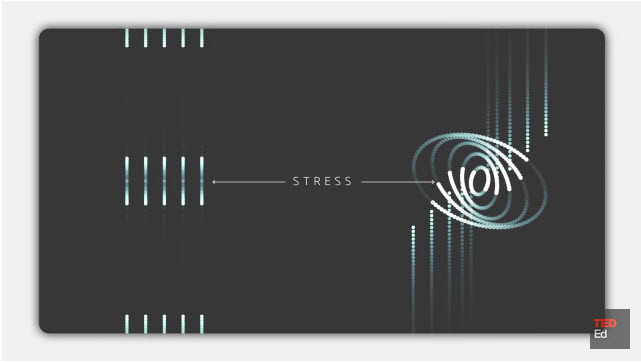
\includegraphics[width=400bp]{geometria-ted-ed-tensor-01.jpg}
\caption{Vídeo TED-Ed sobre vetores e tensores (\url{https://www.youtube.com/watch?v=ml4NSzCQobk}) com legendas em Português.}
\label{\detokenize{GE101-E:fig-geometria-ted-ed-tensor-01}}\label{\detokenize{GE101-E:id7}}
\end{figure}


\subsection{Campos vetoriais}
\label{\detokenize{GE101-E:campos-vetoriais}}
Muitas leis naturais podem ser descritas por equações que envolvem vetores. Estudar estas equações permite entender os fenômenos associados. Neste contexto, o conceito de \index{campo vetorial}campo vetorial desempenha um papel fundamental. Basicamente, um campo vetorial é uma maneira de, a cada ponto do plano, atribuir um vetor. A  \hyperref[\detokenize{GE101-0C:fig-geometria-flechas-03}]{\Fref{\detokenize{GE101-0C:fig-geometria-flechas-03}}} e a \hyperref[\detokenize{GE101-0C:fig-geometria-flechas-08}]{\Fref{\detokenize{GE101-0C:fig-geometria-flechas-08}}} exibem exemplos de campos vetoriais: a cada ponto do mapa estabelece-se um vetor que representa a velocidade do vento naquele ponto (em um dado instante).

Para saber um pouco mais sobre campos vetoriais e de como eles são usados para se criar equações que descrevem fenômenos, recomendamos a animação "CAOS II: CAMPO DE VETORES - A CORRIDA DOS LEGOS"
\url{http://www.chaos-math.org/pt-br/caos-ii-campos-de-vetores} produzido por Jos Leys, Étienne Ghys e Aurélien Alvarez, com áudio em Português e duração de 13 minutos aproximadamente.

\begin{figure}[H]
\centering
\capstart

\noindent\includegraphics[width=400bp]{{geometria-campo-vetorial-caos-01}.jpg}
\caption{Entendendo campos vetoriais com LEGO (\url{http://www.chaos-math.org/pt-br/caos-ii-campos-de-vetores}).}\label{\detokenize{GE101-E:fig-coloque-aqui-o-nome}}\label{\detokenize{GE101-E:id8}}\end{figure}

Este vídeo é uma das nove animações que compõem o filme CAOS. Os tópicos tratados incluem \index{sistemas dinâmicos}sistemas dinâmicos, o \index{efeito borboleta}efeito borboleta e a \index{teoria do caos}teoria do caos. O conteúdo é acessível ao público em geral e certamente você irá gostar e apreciar o uso e a importância de vetores nas várias questões abordadas nos vídeos.


\subsection{Um pouco da história dos vetores}
\label{\detokenize{GE101-E:um-pouco-da-historia-dos-vetores}}
Ao contrário de muitos assuntos que você já estudou, a abordagem moderna de vetores como apresentada neste capítulo (e seus desdobramentos como vistos nos cursos universitários de cálculo vetorial) é relativamente recente. Dois nomes se destacam: Josiah Willard Gibbs (1839\textendash{}1903) e Oliver Heaviside.

\begin{figure}[H]
\centering
\capstart

\noindent\includegraphics[width=350bp]{{historia-01}.jpg}
\caption{Gibbs e Heaviside (Fonte: Wikimedia Commons)}\label{\detokenize{GE101-E:fig-historia-01}}\label{\detokenize{GE101-E:id9}}\end{figure}

Gibbs foi um cientista americano que fez contribuições importantes para as áreas de Física, Química e Matemática. Em 1901, Gibbs ganhou a medalha Copley da Real Sociedade de Londres por ser o primeiro a aplicar a segunda lei da termodinâmica em uma discussão exaustiva da relação entre energia e capacidade térmica, elétrica e química para trabalho externo. Gibbs usou métodos vetoriais para determinar as órbitas de planetas e cometas. Heaviside foi um físico-matemático britânico autodidata com contribuições nas áreas de Matemática e Telecomunicações. Heaviside empregou seu cálculo vetorial para estudar eletromagnetismo e, em particular, simplificar as equações de Maxwell que fazem parte da função do eletromagnetismo clássico, da teoria quântica de campos, da ótica clássica e dos circuitos elétricos.

Algumas "ideias vetoriais"{} já eram conhecidas bem antes de Gibbs e Heaviside. Por exemplo, a regra do paralelogramo (das velocidades) já aparecia no tratado de Mecânica de Heron de Alexandria (c. 10 a.C.\textendash{}c. 70 a.C.). Na sua obra \textit{Principia Mathematica} (1687),  Isaac Newton (1642-1727) trabalhou intensamente com grandezas hoje consideradas vetoriais tais como velocidade e força mas sem, contudo, usar o conceito de vetor.

Segundo o historiador Michael J. Crowe, o início da análise vetorial se deu com o matemático alemão Carl Friedrich Gauss (1777-1855) que, em 1831, publicou uma justificativa geométrica para os números complexos. Entre Gauss e Gibbs/Heaviside, participaram da história dos vetores: William Rowan Hamilton (1805-1865) que introduziu a classificação de grandezas em escalares e vetoriais e inventou os \index{quatérnios}quatérnios; Hermann Grassmann (1809-1877); Peter Guthrie Tait (1831-1901) e James Clerke Maxwell (1831\textendash{}1879). Uma história mais completa dos vetores pode ser encontrada no livro \textit{A History of Vector Analysis: The Evolution of The Idea of A Vectorial System} de Michael J. Crowe, publicado pela editora Dover em 1985.


\subsection{Formigas do deserto, abelhas e vetores}
\label{\detokenize{GE101-E:formigas-do-deserto-abelhas-e-vetores}}
Quando uma formiga típica procura comida, marca seu caminho com ferormônios. Ao encontrar alimento, ela se guia de volta para o formigueiro farejando a trilha que marcou. Mas e a formiga do deserto? Se um vento levar embora a areia marcada, será que ela fica perdida? Cientistas \citet{wehner1981} descobriram que as formigas do deserto não ficam perdidas, pois elas se orientam por um método usado por marinheiros antigamente, o \index{cálculo de posição}cálculo de posição. Esse método se baseia em um procedimento matemático chamado de \index{integração por caminhos}integração por caminhos. O cérebro da formiga realiza naturalmente um cálculo que fornece para a formiga a direção, o sentido e a distância exata (um vetor) permitindo assim que a formiga volte em linha reta ao formigueiro. Integração por caminhos é um assunto que engenheiros e matemáticos estudam nas aulas de cálculo da faculdade. Parece que para aprender certas coisas não seria tão ruim ter cérebro de formiga!

\begin{figure}[H]
\centering
\capstart

% \noindent\includegraphics[width=300bp]{{audio-formigas-animation}.png}
\caption{Texto e animação adaptados de \citet{gomes2010}}\end{figure}

E como as formigas sabem em que direção estão andando? Há evidências de que elas usam o sol como referência. Outro pesquisador (Santchi) percebeu isso através de outra experiência interessante. Enquanto uma formiga do deserto seguia seu caminho, ele posicionou um anteparo de um dos lados da formiga impedindo que o sol batesse nela. Do outro lado da formiga, ele colocou um espelho de forma a refletir o sol na direção do inseto. Para a formiga era como se o sol houvesse "mudado de lado". Imediatamente a formiga fez meia volta e começou a caminhar na direção oposta. Para mais informações sobre o tema, recomendamos \citep{gomes2010} e as referências citadas.

Outros animais também "usam"{} vetores em suas vidas. Abelhas, por exemplo, fazem um tipo de dança para comunicar às companheiras uma fonte de alimentação. A direção e sentido da dança dá a direção e sentido da localização da fonte de alimento e a duração da dança especifica a distância. O documentário "A Dança das Abelhas"{} de Andrew Quitmeyer e Tucker Balch (com legendas em Português) dá mais detalhes sobre o assunto.

\begin{figure}[H]
\centering
\capstart

\noindent\includegraphics[width=300bp]{{geometria-abelhas-01}.png}
\caption{Vetores e abelhas \url{https://youtu.be/RGXyhqKsKQk}.}\label{\detokenize{GE101-E:fig-abelhas}}\label{\detokenize{GE101-E:id11}}\end{figure}


\subsection{Vetores para além do plano}
\label{\detokenize{GE101-E:vetores-para-alem-do-plano}}
Enquanto que nosso estudo se concentrou nos vetores do plano (\({\mathbb R}^{2}\)), o conceito de vetor pode ser estendido para o espaço (\({\mathbb R}^{3}\)), para o \index{hiperespaço}hiperespaço (\({\mathbb R}^{n}\)) e além. A \hyperref[\detokenize{GE101-E:fig-vetor-no-espaco}]{\Fref{\detokenize{GE101-E:fig-vetor-no-espaco}}}, por exemplo, ilustra o vetor cujas extremidades são dois vértices de um cubo.

\begin{figure}[H]
\centering
\capstart

% \noindent\includegraphics[width=200bp]{{geometria-vetor-no-espaco}.png}
\caption{Um vetor no espaço \({\mathbb R}^{3}\).}\label{\detokenize{GE101-E:fig-vetor-no-espaco}}\label{\detokenize{GE101-E:id12}}\end{figure}

Como no caso do plano, um vetor no espaço também representa direção, sentido e módulo e ele pode ser descrito algebricamente por suas coordenadas, como ilustra a \hyperref[\detokenize{GE101-E:fig-coordenadas-3d}]{\Fref{\detokenize{GE101-E:fig-coordenadas-3d}}} para o caso do vetor \(\vec{u} = (1, 2, 3)\).

\begin{figure}[H]
\centering
\capstart

% \noindent\includegraphics[width=350bp]{{geometria-coordenadas-3d-01}.png}
\caption{O vetor \(\vec{u} = (1, 2, 3)\) no espaço \({\mathbb R}^{3}\).}\label{\detokenize{GE101-E:fig-coordenadas-3d}}\label{\detokenize{GE101-E:id13}}\end{figure}

Enquanto que não conseguimos enxergar flechas em \({\mathbb R}^{4}\), \({\mathbb R}^{5}\), …, podemos trabalhar com vetores nestes espaços por meio de suas coordenadas. Assim, por exemplo, \(\vec{u} = (1, 0, -5, 7)\) e \(\vec{v} = (2, 3, 5, 9)\) são dois vetores de \({\mathbb R}^{4}\). Não podemos visualizá-los, mas podemos somá-los e multiplicá-los por um número real. Vetores em \({\mathbb R}^{n}\), mesmo sem uma contrapartida visual, são extremamente úteis. Existe uma área da Matemática dedicada ao assunto, \index{Álgebra Linear}Álgebra Linear, com aplicações em Biologia, Economia, Computação Gráfica, Engenharia, Física, Matemática, Química, entre outras. Aqui está um exemplo em Ecologia. Segundo {[}Valentim-2005{]}, faz parte do trabalho do ecólogo procurar agrupar amostras de mesmas características ou associar espécies em comunidades com o objetivo de descrever, de maneira clara e sintética, a estrutura de um ecossistema. Neste contexto, uma prática é coletar medidas das espécies, como ilustra a \hyperref[\detokenize{GE101-E:fig-ecologia}]{\Fref{\detokenize{GE101-E:fig-ecologia}}} para o caso de um peixe.

\begin{figure}[H]
\centering
\capstart

\noindent\includegraphics[width=270bp]{{geometria-ecologia-01}.jpg}
\caption{Medidas morfométricas de um peixe. Fonte: \citet{pinheiro2016}}
\label{\detokenize{GE101-E:fig-ecologia}}\label{\detokenize{GE101-E:id14}}\end{figure}

Para estudos de semelhança, agrupamento e ordenação, essas medições são registradas em um vetor em \({\mathbb R}^{12}\),
\begin{equation*}
\begin{split}\text{(AB, AC, APCd, AM, CCa, CNPt, CPCd, CP, LB, LNPt, LC, LPCd)},\end{split}
\end{equation*}
para posterior processamento usando técnicas da Álgebra Linear.

Um outro exemplo em Ecologia, este em \({\mathbb R}^{3}\) que você pode visualizar e brincar se refere à simulação do voo de um bando de pássaros. Para isto, acesse o site \url{http://black-square.github.io/BirdFlock/} e, na simulação, clique em "Settings"{} (Configurações) e, depois, em "Algorithm Explanation Vectors"{} (Vetores para Explicação do Algoritmo) para visualizar os diferentes tipos de vetores usados na simulação (na \hyperref[\detokenize{GE101-E:fig-passaros}]{\Fref{\detokenize{GE101-E:fig-passaros}}}, as extremidades iniciais de todos os vetores estão nas posições dos pássaros). Dica: clique em um dos pássaros para acompanhá-lo e use a roda do mouse para se aproximar e pressione a tecla T para fazer com que a rotação da câmera acompanhe o movimento do pássaro. Você pode usar as teclas A, S, D, W, Q e E para navegar pelo cenário.

\begin{figure}[H]
\centering
\capstart

\noindent\includegraphics[width=300bp]{{geometria-passaros-01}.jpg}
\caption{Simulação do voo de um bando de pássaros usando vetores (\url{http://black-square.github.io/BirdFlock/}).}\label{\detokenize{GE101-E:fig-passaros}}\label{\detokenize{GE101-E:id15}}\end{figure}

Basicamente, o que a simulação faz é coordenar o movimento de cada pássaro de modo a: (1) evitar um aglomerado local muito intenso, pois um pássaro não quer se colidir com outro; (2) seguir a direção e sentido do movimento dos pássaros em sua volta, pois um pássaro não quer ficar sozinho uma vez que, assim, ele seria uma presa fácil para um predador em potencial; (3) mover para a posição média dos pássaros em sua volta pelo mesmo motivo de (2).


\ifnum\aluno=1
\clearpage
\else
\notasfinais
\fi

\anexo{Anexo 1: Corrida de Vetores}

\begin{figure}[H]
\centering
\capstart

\noindent\includegraphics[width=.85\textheight,angle=90,origin=c]{{geometria-cv-02}.jpg}
\end{figure}

\begin{figure}[H]
\centering
\capstart

\noindent\includegraphics[width=.85\textheight,angle=90,origin=c]{{geometria-cv-03}.jpg}
\end{figure}

\clearpage

\bibliographystyle{apalike-pt}
\bibliography{../Bibliografia/vetores_bibliografia.bib}

\nocite{*}
        
% \chapterillustration{./abertura-perspectiva1}{./abertura-perspectiva1-professor}

\chapterwhat{Conceito de volume (unidade, aditividade e conservação). Diversos usos de volumes e grandezas relacionadas, como área, densidade, concentração. Compressibilidade de materiais. Posições relativas de planos e planos e planos e retas. Planificações e cortes de sólidos. Cálculo de áreas e volumes de figuras clássicas e obtenção das fórmulas. Aproximação de áreas e volumes considerando o erro. Princípio de Cavalieri e aplicações.}

\chapterbecause{Áreas e volumes são conceitos elementares que estão presentes de maneira direta na vida cotidiana do cidadão e também são necessários para outras ciências, como a Química, a Biologia e a Física. O entendimento destes conceitos e de suas relações com outras grandezas são fundamentais e basta m para a maioria dos usos corriqueiros. Aqui, o estudo de áreas e volumes serve de plano de fundo para o aperfeiçoamento do entendimento de número real, de aproximação com erro, para o desenvolvimento da habilidade de visualização espacial e para a resolução de problemas.} 

\chapter{Medidas em Geometria Espacial}


%%%% Página de créditos

% Autores
\autorum{Augusto Teixeira}
\autordois{Fabio Simas}
\autortres{José Ezequiel Soto Sánchez}
\autorquatro{Letícia Rangel}


\graficos{Tarso Caldas}

% Revisores

\autordacapa{Luke Porter}{Unsplash}{https://unsplash.com/photos/ud6XcK_MUGI}
\versao{0.5}

\versaodigital{https://www.umlivroaberto.org/BookCloud/Volume_1/master/view/GE504.html}


\ccbysa

\creditos


\mainmatter

\label{\detokenize{GE504:medidas-em-geometria-espacial}}\label{\detokenize{GE504::doc}}

\def\currentcolor{session1}
\begin{objectives}{Volume de uma folha de papel}
{
\begin{itemize}
\item {} 
Reconhecer o conceito de volume (ideia intuitiva, medida do espaço ocupado por um determinado material incompressível), distinguindo-o da área, da densidade e da massa, por exemplo.

\item {} 
Aplicar o conceito de unidade (caixa de leite ou cubo de lado 1, que dará origem a uma unidade de medida) para comunicar e comparar volumes. Volume, área, comprimento, litro (e outras unidades de medida volumétrica do SI: cm\(^3\), m\(^3\), etc.).

\item {} 
Aplicar em contextos diversos o conceito de aditividade, isto é, que a área (e o volume) da união de conjuntos disjuntos é igual à soma de suas áreas (respectivamente volumes), estendendo essa propriedade à subtração quando se fazem “buracos” de formas conhecidas.

\end{itemize}

\textbf{Conceitos abordados:} Volume, área, gramatura.
}{1}{1}
\end{objectives}
\begin{sugestions}{Volume de uma folha de papel}
{
\textbf{Organização em sala de aula:} Nesta atividade, inicialmente o aluno deve estimar o volume de uma folha de papel. A discussão em grupos contribuirá para a avaliação das estimativas realizadas. Os próprios alunos avaliarão as estimativas uns dos outros. Portanto, recomenda-se que a atividade seja desenvolvida em grupos de 3 ou 4 estudantes. Recomendação análoga vale para os demais itens.

\textbf{Dificuldades previstas:} Não é improvável que os estudantes confundam volume e área, respondendo a área do papel como resultado para o volume. Nesse caso, muito provavelmente, o aluno não identificou a espessura do papel. Outra possibilidade é responder que o volume é zero. Aproveite esta atividade para discutir tal diferença. É importante que reconheçam que área é uma grandeza bidimensional e volume tridimensional.

\textbf{Sugestões gerais:} Espera-se que o item \titem{a)} seja respondido por comparação visual. Não se espera que o aluno realize cálculos organizados. A ideia é que aluno estime \(1\) cm$^3$ e relacione com a folha de papel.

Para o desenvolvimento da tarefa, recomenda-se ainda que sejam entregues folhas de papel aos alunos. Acreditamos que a distribuição das folhas pode enriquecer a atividade trazendo concretude e uma postura investigativa, ainda que bastasse ler as informações apresentadas no pacote ilustrado.

Uma estratégia possível para realizar o cálculo do volume é empilhar (bem compactadas) várias folhas. Essa estratégia se baseia na propriedade de aditividade do volume. Nesse caso, os alunos precisarão medir as 3 dimensões da pilha. Será necessário régua. Se possível, leve para a sala uma resma em pacote fechado para que os alunos possam obter tais medidas mais facilmente. O pacote tem 4,9cm de altura. No entanto, não os alerte para essa possibilidade. Deixe-os ter autonomia na condução da solução.

Caso não se tenha uma resma de papel sulfite A4 disponível, a tarefa pode ser realizada com uma pilha com uma quantidade menor de folhas de papel A4 ou com outro tipo de papel que se tenha disponível. Valem até a folha do caderno ou do livro. Outra possibilidade é recortar o papel. Nesse caso, os pedaços devem ser empilhados até que se possa medir a espessura da pilha. Mais importante do que o resultado é a discussão da estratégia utilizada para o cálculo. Se não for utilizar o papel sulfite tamanho A4 \textendash{} gramatura \(75\) g/m$^2$, será necessário ter as informações correspondentes para o papel que for utilizado (largura, comprimento e gramatura), que podem alterar as respostas.

\textbf{Enriquecimento da discussão:} Além do conceito de volume, na atividade, um dos itens trata da gramatura de papel, diferenciando-a de espessura. A gramatura do papel é a medida da massa pela área de um papel expressa em gramas por metro quadrado (g/m\(^2\)). A intenção desse item é que o aluno pesquise a resposta e tenha que interpretar e compreender a informação obtida, que é essencialmente matemática: uma medida. Discuta diferentes respostas obtidas visando ao entendimento dessa medida.

\textbf{Material necessário:} Folhas de papel sulfite tamanho A4 - gramatura \(75g/m^2\).
Régua milimetrada
}{0}{9}
\end{sugestions}
\begin{answer}{Volume de uma folha de papel}
{
\begin{enumerate}
\item {} 
Resposta pessoal.

\item {} 
Considerando uma folha de papel sulfite de tamanho A4 mais comum no mercado, aproximadamente, $6{,}1122$ cm\(^3\). Tal aproximação pode ser obtida a partir das medidas de uma resma. Uma resma desse papel, que é composta por 500 folhas, tem dimensões aproximadas $21{,}0\text{ cm}\times 29{,}7\text{ cm} \times 4{,}9{ cm}$. Portanto, 500 folhas têm volume \(3056,13cm^3\), e uma folha, $1/500$ desse valor. (Essa resposta pode variar dependendo do papel utilizado)

\item {} 
A gramatura corresponde à massa de \(1\) m$^2$ do papel. Assim, por exemplo, a gramatura \(90\) g/m$^2$ significa que a massa de \(1\) m$^2$ do papel é \(90\) g. Já a espessura é uma medida linear, que pode ser observada como a menor das dimensões da folha de papel. Há papéis de diferentes espessuras. Por exemplo, não é difícil observar que a folha de papel sulfite, comumente usada na escola, tem espessura diferente do papel utilizado para confeccionar caixas de sapatos, por exemplo. Espessura e gramatura, são, portanto, propriedades diferentes do papel. No entanto, em geral, papéis com maior gramatura têm maior espessura.

\item {} 
O peso da folha pode ser calculado a partir da gramatura do papel, informada no pacote:  \(75\) g/m$^2$. Nesse caso, é necessário ainda calcular a área da superfície da folha: \(623{,}7\text{ cm}^2 = 0{,}06237\text{ m}^2\). Portanto, o peso do papel é \(75 \times 0{,}06237 = 4{,}6\) g.

\end{enumerate}
}{1}
\end{answer}
\clearmargin
\begin{objectives}{Caminhonete de areia}
{
\begin{itemize}
\item {} 
Reconhecer o conceito de volume (ideia intuitiva, medida do espaço ocupado por um determinado material incompressível), distinguindo-o da área, da densidade e da massa, por exemplo.

\item {} 
Aplicar o conceito de unidade (caixa de leite ou cubo de lado 1, que dará origem a uma unidade de medida) para comunicar e comparar volumes.

\item {} 
Aplicar relações entre (área e) volume e outras grandezas em situações cotidianas.

\end{itemize}

\textbf{Conceitos abordados:} massa (peso), volume, densidade, unidades de medida.
}{1}{2}
\end{objectives}
\begin{sugestions}{Caminhonete de areia}
{
\textbf{Organização em sala de aula:} Recomenda-se que esta atividade seja realizada em duplas. A discussão com um colega pode ajudar a interpretar o enunciado, que é essencial neste caso.

\textbf{Dificuldades previstas:} A atividade oferece a revisão de alguns conceitos, como massa e densidade, que não costumam oferecer maior dificuldade. No entanto, a abordagem envolve mais a relação entre esses conceitos do que o cálculo. A dificuldade pode emergir daí.

\textbf{Enriquecimento da discussão:} Esta atividade aborda o conceito de volume aparente, que volta a ser discutido de forma mais específica em um “Você Sabia” seguinte.

Para determinar o volume de areia que precisa comprar, Gelson pode simplesmente levar um saco de cimento vazio à loja de materiais para construção e pedir 15 sacos daquele cheios de areia. Esta é uma discussão interessante para o estudante, porque o saco de cimento se torna uma unidade de volume. Na situação deste parágrafo, ela está sendo utilizada para medir o volume de areia a ser comprado.
}{1}{2}
\end{sugestions}


\explore{O Conceito de Volume}
\label{\detokenize{GE504-0:explorando-o-conceito-de-volume}}\label{\detokenize{GE504-0::doc}}

\begin{task}{volume de uma folha de papel}


\begin{enumerate}
\item {} 
Lembrando que um centímetro cúbico é o volume ocupado por um cubo de aresta 1cm, estime sem fazer cálculos o volume de uma folha de papel sulfite de tamanho A4.
\end{enumerate}

\begin{figure}[H]
\centering


\begin{asy}
size(5cm);
currentprojection=orthographic(3,1,.5);

draw(unitcube, azul*80+opacity(0.65));

draw((1,0,1) -- (1,0,0), verde+linewidth(1.25), L=Label("a",position=MidPoint));
draw((1,0,0) -- (1,1,0), laranja+linewidth(1.25), L=Label("b",position=MidPoint));
draw((1,1,0) -- (0,1,0), vinho+linewidth(1.25), L=Label("c",position=MidPoint));

draw((0,0,0) -- (1,0,0), dashed);
draw((0,0,0) -- (0,1,0), dashed);
draw((0,0,0) -- (0,0,1), dashed);

draw((0,0,1) -- (0,1,1));
draw((0,1,1) -- (1,1,1));
draw((1,1,1) -- (1,0,1));
draw((1,0,1) -- (0,0,1));
draw((0,1,1) -- (0,1,0));
draw((1,1,1) -- (1,1,0));
\end{asy}

\end{figure}
\begin{enumerate}
\item {} 
Avalie a sua estimativa no item anterior. Use uma estratégia de cálculo para obter o volume de uma folha de papel sulfite de tamanho A4.

\end{enumerate}

\begin{figure}[H]
\centering

\noindent\includegraphics[width=100bp]{{1}.png}
\end{figure}
\begin{enumerate}
\item {} 
O que é a gramatura do papel? Qual é a diferença e qual é a relação entre espessura e  gramatura de uma folha de papel? Pesquise.

\item {} 
Quanto pesa uma folha de papel da resma ilustrada no item \titem{b)}?

\end{enumerate}
\end{task}

\begin{knowledge}

A gramatura de uma folha de papel usada em escolas e escritórios costuma variar de $75$ a \(120\) g/m$^2$.  São as indicadas para impressoras domésticas, por exemplo. Para a confecção de cartões e impressão de fotos, são recomendados papéis de maior gramatura, em torno de \(200\) g/m$^2$.  As folhas de um jornal têm gramatura de $35$ a \(55\) g/m$^2$.  A escolha da gramatura é determinante para o uso do papel. Imagine as implicações de um jornal impresso em papel de maior gramatura. Seria mais pesado, o que além de ter impacto direto no manuseio e no custo do material, com certeza, influenciaria no transporte e na impressão, por exemplo. De maneira geral, quanto maior a gramatura, mais resistente é o papel. No entanto, não se deve confundir gramatura com espessura nem com volume. Ainda que papéis com gramaturas diferentes tendam a ter espessuras diferentes, a compactação das fibras e materiais que compõem o papel determinará se as espessuras serão ou não distintas. E, portanto, os volumes também.
\end{knowledge}

\begin{task}{caminhonete de areia}

\paragraph{Parte 1}

Gelson vai fazer um quarto novo para sua filhinha que está chegando. O tijolo e o cimento ele já tem, mas precisa comprar areia para misturar no cimento e começar a obra!

Quanta areia ele precisará comprar?

Gelson utilizará três sacos de cimento e sabe que a proporção recomendada para assentar tijolos é de cinco latas de areia para cada lata de cimento. Gelson avaliou que deveria comprar quinze sacos de areia. No entanto, a areia não é vendida em sacos como os de cimento. A areia fica armazenada em um galpão e é vendida por metro cúbico (m\(^3\)).

\begin{figure}[H]
\centering

\noindent\includegraphics[width=125bp]{{2}.png}
\end{figure}

Quantos metros cúbicos de areia Gelson deve comprar para realizar a obra evitando o desperdício de material?

\begin{figure}[H]
\centering

\noindent\includegraphics[height=130bp]{{3}.png}
\hspace{1em}
\includegraphics[height=130bp]{{4}.png}
\end{figure}

\begin{enumerate}
\item {} 
Avalie as perguntas a seguir e decida qual (ou quais) delas que, uma vez respondidas, permitiriam que Gelson comprasse a quantidade certa de areia:
\begin{itemize}
\item {} 
P1: Quantos sacos de cimento cheios de areia são necessários para se obter um metro cúbico de areia?

\item {} 
P2: Quantos metros cúbicos de areia são necessários para se misturar em um saco de cimento?

\item {} 
P3: Quantos metros cúbicos de cimento serão utilizados?

\item {} 
P4: Quanto pesa a areia que cabe em um saco de cimento?

\end{itemize}

\item {} 
Qual (ou quais) das perguntas do item anterior podem ser respondidas com procedimentos simples feitos em casa? Descreva tais procedimentos.

\item {} 
Para descobrir quantos metros cúbicos correspondem a quinze sacos de areia, Gelson despejou o cimento de um saco em um balde de \(20\)lL. Verificou que o cimento coube no balde enchendo-o completamente. Com essa informação, quantos metros cúbicos de areia Gelson precisa comprar?

\item {} 
O problema de Gelson agora é transportar a areia até a sua casa. Para isso, ele utilizará uma caminhonete como a da imagem a seguir. Gelson consegue transportar toda a areia em uma só viagem?

\end{enumerate}

\begin{figure}[H]
\centering

\noindent\includegraphics[width=300bp]{{5}.png}
\end{figure}

\paragraph{Parte 2}

Resolvido o problema do volume a ser carregado, Gelson passou a pensar de a caminhonete aguenta o peso deste tanto de areia. No manual da caminhonete está escrito que sua carga máxima é de \(530\) kg.

\begin{figure}[H]
\centering

\noindent\includegraphics[width=350bp]{{6}.png}
\end{figure}
\begin{enumerate}
\item {} 
Em uma estimativa grosseira, quanto você acha que pesa um metro cúbico de areia?

\item {} 
Gelson procurou na internet “Qual é o peso de um metro cúbico de areia?”. Ele achou várias respostas. Dependendo do tipo de areia, a densidade (isto é, massa / volume) pode variar de \(1200\) kg/m$^3$ até \(1700\) kg/m$^3$. Com essas informações, Gelson pode ter ceteza de que a viagem para transportar a areia comprada estará dentro das especificações da caminhonete?

\item {} 
Gelson decidiu pesar a areia comprada. Para isso, encheu o balde (de $20$ litros) com areia e o pesou, obtendo \(26\) kg. Com tal informação, que estimativa Gelson pode fazer para o peso total da areia que ele vai comprar?

\item {} 
No dia do transporte choveu e entrou água na caçamba. Gelson observou que aparentemente o nível de areia não havia se alterado, apesar da água. No entanto, se preocupou com o limite de peso, uma vez que o carro parecia perder estabilidade. Houve alteração no volume da carga transportada devido à chuva? Explique a sua resposta considerando a percepção de Gelson de que o nível de areia não se alterou.

\end{enumerate}
\end{task}

\begin{knowledge}

Em muitas situações do cotidiano as misturas são descritas por razões, como em:
\begin{itemize}
\item {} 
Misturamos o cimento com a areia na razão de $1$ para $5$.

\item {} 
Uma parte de farinha para três partes de leite.

\end{itemize}

Tais instruções podem ser imprecisas se não especificarem a que grandezas corresponde a razão indicada. Observe que as frases acima não diferenciam entre: para cada quilo de cimento usamos cinco quilos de areia, ou para cada litro de cimento utilizamos cinco litros de areia. Ou para cada quilo de farinha três litros de leite ou para cada colher de farinha três litros de leite.

Isso ocorre por exemplo na especificação do álcool para uso doméstico. Nas garrafas desse tipo de álcool a razão entre álcool e água é indicada em graus INPM. Assim, por exemplo, no álcool \(46^\circ\) INPM, há $46$ g de álcool em cada $100$ g do produto. Os $54$ g restantes são de água. Observe que se esta razão, especificada para massa, for considerada a mesma razão para volume, resultará em outra gradação INPM de álcool, já que álcool e água possuem densidades diferentes.
Em muitas situações do cotidiano vemos razões descritas na forma de razões, como em:

\begin{figure}[H]
\centering

\noindent\includegraphics[width=150bp]{{8_1}.jpg}
\end{figure}

Em alguns casos essa distinção pode ficar subentendida pelo contexto. Por exemplo, no caso da farinha e do leite é mais natural que essa razão esteja se referindo à volume, pois dificilmente medimos leite pelo peso, mas frequentemente medimos farinha em volume (copos, xícaras, colheres, etc.).

Tente inferir em cada um dos exemplos, se as razões se referem provavelmente a pesos ou a volumes:
\begin{enumerate}
\item {} 
Um alimento possui vinte vezes mais gordura do que fibra.

\item {} 
Uma tinta de tecidos deve ser misturada na água na razão de um para dez.

\item {} 
Um adubo deve ser misturado na razão de uma parte para cada oito partes de terra.

\end{enumerate}

Em outras situações, não faz tanta diferença se aplicamos a razão em termos de peso ou de volume. escolhemos a razão em termos de peso ou volume. Isso se dá quando a densidade dos materiais envolvidos é muito semelhante.

Tente inferir em quais situações é muito importante saber se as razões se referem a peso ou a volume:
\begin{enumerate}
\item {} 
Duas partes de leite para uma parte de óleo.

\item {} 
Uma parte de açúcar para cinco partes de chantili.

\item {} 
Uma parte de água para quatro partes de areia.

\end{enumerate}
\end{knowledge}

\clearpage
\begin{objectives}{Volume do paralelepípedo retângulo de arestas racionais}
{
Entender a demonstração da fórmula do volume de paralelepípedos retângulos (e áreas de retângulos) de lados racionais.

\textbf{Conceitos abordados:}
Volume de paralelepípedo retângulo. De modo indireto também são abordados funções e a subdivisão da unidade (frações).
}{1}{2}
\end{objectives}
\begin{sugestions}{Volume do paralelepípedo retângulo de arestas racionais}
{
\textbf{Organização em sala de aula:}
Sugerimos que a atividade seja individual ou em duplas. A reflexão mediada pelo aplicativo pode ser favorecida pela discussão com um colega. Grupos maiores podem gerar dispersão.

\textbf{Dificuldades previstas:}
Acreditamos que a atividade impõe desafios importantes, como lidar com uma fração da unidade de volume e compreender volume como uma função. No entanto, destacamos a compreensão da relação entre a variação dos lados e a variação do volume. Não é incomum que os alunos, apesar de reconhecerem na atividade que  \(V(n_1 x, n_2 y, n_3 z) =  n_1.n_2.n_3. V(x, y, z)\), não consigam aplicar tal resultado diretamente.
.. AQUI, ACHO, O CERTO SERIA INCLUIR INDICACAO DE ATIVIDADES NO MATERIAL QUE TRATEM DO ASSUNTO.

\textbf{Sugestões gerais:}
Esta atividade pretende levar o aluno a perceber o volume de um paralelepípedo para além da contagem de cubinhos, ou seja, extrapolar o universo dos números naturais. Espera-se que os alunos associem o volume do paralelepípedo (retângulo) à variação de suas dimensões como “medidas contínuas”, ou seja, que percebam de maneira intuitiva (não esperamos nem recomendamos a formalização) que o volume de um paralelepípedo é uma função contínua de três variáveis reais positivas (\(V(a,b,c) = V\)). Destacamos que,  nesta atividade, esse fato é explorado apenas para dimensões (variáveis) racionais. Observe que, no Ensino Fundamental, a fórmula de cálculo do volume do paralelepípedo retângulo é deduzida apenas para arestas naturais (contagem de cubinhos). Entendemos que no Ensino Médio o aluno poderá compreendê-la para arestas racionais, ficando a dedução da mesma para arestas de medidas reais apenas para alguns cursos superiores.

Ao longo de toda a atividade, recomenda-se que as justificativas sejam valorizadas porque o resultado em si é a mera aplicação da fórmula \(V(a,b,c) = abc\) em diversos itens.
}{1}{2}
\end{sugestions}

\clearmargin
\begin{sugestions}{Volume do paralelepípedo retângulo de arestas racionais}
{
A atividade foi planejada para ser realizada com o uso dos aplicativos recomendados, ainda que possa ser sem eles. Os aplicativos permitem visualização e interação dinâmica com os objetos  geométricos, contribuindo para a comunicação o ensino e a aprendizagem.

Na Parte 1, espera-se que o aluno compreenda a notação usada na atividade; reconheça que, com a troca dos comprimentos de duas das arestas de um paralelepípedo retângulo, obtém-se paralelepípedos congruentes; reconheça que paralelepípedos congruentes têm o mesmo volume e que paralelepípedos com medidas completamente diferentes podem ter o mesmo volume. Por fim, o item (d) convida o aluno para a reflexão conduzida na parte 2.

Você pode usar uma caixa em forma de paralelepípedo retângulo, destacando as arestas, para facilitar a compreensão da notação pelos estudantes. A manipulação permite observar que a troca, por exemplo, de \(a\) por \(b\) na expressão de V indica uma rotação da caixa e, portanto, uma caixa congruente à inicial.
No item a), não se preocupe se os estudantes não forem cuidadosos com as medidas das arestas ao desenhar os paralelepípedos porque eles provavelmente conseguirão perceber seus erros no item b).
No item b), espera-se que o estudante observe que o paralelepípedo de arestas 2, 3 e 4 é congruente ao de arestas 2, 4 e 3 (são iguais do ponto de vista da geometria) e, portanto, seus volumes são iguais.
No item c), espera-se que os estudantes percebam que volumes iguais podem ser obtidos por paralelepípedos não congruentes, inclusive bastante diferentes entre si.

Na Parte 2, espera-se que os estudantes percebam que, dado um paralelepípedo retângulo qualquer, se multiplicarmos uma de suas arestas por um número natural, então o volume do novo paralelepípedo (que não é semelhante ao primeiro) ficará multiplicado por esse mesmo número natural. O aplicativo permite que sejam gerados variados exemplos, o que ajuda o aluno na compreensão. Também aqui pode valer a pena usar caixas em forma de paralelepípedos para facilitar a visualização.
}{1}{1}
\end{sugestions}
\clearmargin
\begin{sugestions}{Volume do paralelepípedo retângulo de arestas racionais}
{
A Parte 3 é a parte mais delicada para o estudante, por isso recomendamos fortemente o uso dos aplicativos disponibilizados.
O item \textit{a)} tem o objetivo de familiarizar o estudante com a visualização de paralelepípedos que são frações do cubo unitário e relacioná-los com o próprio cubo unitário.
No item \titem{b)}, a parte \titem{v)} verifica se o estudante consegue generalizar a construção dos itens anteriores.

\textbf{Enriquecimento da discussão:}so
Ainda que não sejam discussões sugeridas, nem recomendadas, para a sala de aula, cabe observar que:
Na Parte 1, item c), é verificado que a função V não é injetiva uma vez que, por exemplo, \(V(1, 1, 72) = V(2, 4, 9)\).
Da Parte 2, pode-se concluir que a função volume é linear em cada uma de suas coordenadas.
Sobre a parte 2, destacamos que, nas aulas de função linear, talvez possa ser observado que o volume de um paralelepípedo retângulo de arestas fixadas é uma função linear da terceira aresta (por exemplo, se as arestas são 2, 3 e \(x\), então o volume é \(V(x) = 6x\)).
Além disso, também na parte 2, item c), observe que \(V(nx, ny, nz)\) é o volume de um paralelepípedo semelhante ao paralelepípedo de lados  \(x\), \(y\) e \(z\). Portanto, \(V(nx, ny, nz) = n^3V(x, y, z)\). Isto pode ser apresentado pelo professor como um desdobramento, caso o professor julgue pertinente.

\textbf{Links relacionados:}
Todos os aplicativos disponibilizados para esta atividade foram criados para serem facilmente utilizados em telas pequenas.

\textbf{Materiais necessários:}
A atividade foi planejada para o uso de aplicativos computacionais. Recomendamos que eles sejam utilizados, porque ampararão a construção de uma imagem representativa  A não utilização desses recursos não inviabiliza a realização da atividade, no entanto pode não atingir plenamente os objetivos.
}{1}{2}
\end{sugestions}

\begin{knowledge}

Lembrando da chuva que atrapalhou a viagem do Gelson, vamos pensar mais sobre o conceito de volume. Quando Gelson saiu do armazém, transportava apenas areia. Com a chuva, entrou água na caçamba sem que o nível da carga de areia se alterasse, ou seja, sugerindo que o volume de carga não se alterou.

Usualmente, quando medimos o volume de materiais granulados (como arroz, açúcar e areia) consideramos o volume do ar que fica entre os grãos. Assim, um copo com capacidade para $200$ ml cheio de açúcar, na verdade contém açúcar e ar. Logo, o volume real de açúcar é menor do que $200$ ml. Isso pode ser verificado, por exemplo, colocando-se, aos poucos, água em um copo cheio de açúcar e observando que o nível do conteúdo no copo não aumenta de início e não transborda imediatamente.
\end{knowledge}

\begin{task}{volume do paralelepípedo retângulo de arestas racionais}
\label{persp1-atividade-3}


A fórmula para o cálculo do volume de um paralelepípedo já é conhecida desde o Ensino Fundamental. Mas talvez você não saiba explicar por que essa fórmula vale. Esta atividade tem o objetivo de explorar o tema. Para isso, o cubo de aresta 1 será considerado como unidade e será chamado de \emph{cubo unitário}.

\begin{figure}[H]
\centering

\begin{asy}
size(5cm);
currentprojection=orthographic(2,0.5,1/2);

draw(unitcube, azul*80+opacity(0.65));

draw((1,0,1) -- (1,0,0));
draw((1,0,0) -- (1,1,0));
draw((1,1,0) -- (0,1,0));

draw((0,0,0) -- (1,0,0), dashed);
draw((0,0,0) -- (0,1,0), dashed);
draw((0,0,0) -- (0,0,1), dashed);

draw((0,0,1) -- (0,1,1));
draw((0,1,1) -- (1,1,1));
draw((1,1,1) -- (1,0,1));
draw((1,0,1) -- (0,0,1));
draw((0,1,1) -- (0,1,0));
draw((1,1,1) -- (1,1,0));
\end{asy}
\end{figure}

Como sabemos o paralelepípedo retângulo é determinado pelo conhecimento das medidas de suas três \emph{dimensões} indicadas na figura por \(a\), \(b\) e \(c\).

\begin{figure}[H]
\centering

\begin{asy}
size(7.5cm);
currentprojection=orthographic(1,2,.5);

draw(surface((0,0,0) -- (2,0,0) -- (2,0,1) -- (0,0,1) -- cycle), azul*80+opacity(0.65));
draw(surface((0,0,0) -- (2,0,0) -- (2,1,0) -- (0,1,0) -- cycle), azul*80+opacity(0.65));
draw(surface((0,0,1) -- (2,0,1) -- (2,1,1) -- (0,1,1) -- cycle), azul*80+opacity(0.65));
draw(surface((0,1,0) -- (0,1,1) -- (2,1,1) -- (2,1,0) -- cycle), azul*80+opacity(0.65));
draw(surface((0,0,0) -- (0,0,1) -- (0,1,1) -- (0,1,0) -- cycle), azul*80+opacity(0.65));
draw(surface((0,1,0) -- (0,1,1) -- (2,1,1) -- (2,1,0) -- cycle), azul*80+opacity(0.65));
draw(surface((2,0,0) -- (2,0,1) -- (2,1,1) -- (2,1,0) -- cycle), azul*80+opacity(0.65));

draw((0,1,0) -- (0,0,0) -- (2,0,0), dashed);
draw((0,0,0) -- (0,0,1), dashed);
draw((0,0,1) -- (2,0,1) -- (2,1,1) -- (0,1,1) -- cycle);
draw((0,1,0) -- (0,1,1));
draw((2,1,0) -- (2,1,1));

draw((2,0,1) -- (2,0,0), verde+linewidth(1.25), L=Label("a", position=MidPoint));
draw((2,0,0) -- (2,1,0), laranja+linewidth(1.25), L=Label("b", position=MidPoint));
draw((2,1,0) -- (0,1,0), vinho+linewidth(1.25), L=Label("c", position=MidPoint));
\end{asy}
\end{figure}

O volume \(V\) de um paralelepípedo depende de suas dimensões, \(a\), \(b\) e \(c.\) Assim, indicaremos \(V\) por \(V(a, b, c)\), ou seja, \(V(a,b,c)\) é o volume do paralelepípedo de dimensões \(a\), \(b\) e \(c\).

Desta forma, o volume do cubo de aresta $1$ é \(V(1, 1, 1) =1\) e o volume de um paralelepípedo retângulo de lados \(a = 2\), \(b = 3\) e \(c=5\) é \(V(2,3,5) = 30\) pois cabe 30 cubos de aresta $1$ no espaço ocupado por esse pararlelepípedo.

\begin{figure}[H]
\centering

\noindent\includegraphics[width=175bp]{{blocos}.png}
\end{figure}

\textbf{Afirmação}: Fixados três números reais positivos \(a\), \(b\) e \(c\). O volume do paralelepípedo retângulo de arestas \(a\), \(b\) e \(c\)  é dado pelo produto \(abc\).

Esta atividade vai justificar que \(V(a, b, c) = abc\) para \(a\), \(b\) e \(c\) números racionais positivos. Ela propõe construções que tratam a subdivisão do cubo unitário, encaminhando para a noção de “infinitamente pequeno”. Esse raciocínio tem um papel essencial na matemática e é importante no desenvolvimento do pensamento humano moderno. Comecemos com uma simples observação:

\paragraph{Parte 1}

Recomendamos o uso \href{https://ggbm.at/yk8bqdvz}{deste aplicativo} para o desenvolvimento da tarefa.
\begin{enumerate}
\item {} 
Seguindo o modelo da figura acima, desenhe um paralelepípedo retângulo cujas arestas sejam \(a=2\), \(b=3\) e \(c=4\) e outro cujas arestas sejam \(a=2\), \(b=4\) e \(c=3\).

\item {} 
Obtenha uma relação entre os volumes \(V(2, 3, 4)\) e \(V(2, 4, 3)\). Explique.

\item {} 
Desenhe um paralelepípedo retângulo cujo volume seja \(V(2, 4, 9)\), mas com arestas diferentes de $2$, $4$ e $9$.

\item {} 
Relacione os volumes \(V(2, 4, 3)\) e \(V(2, 4, 9)\).

\end{enumerate}

\paragraph{Parte 2} Considere um paralelepípedo retângulo de arestas \(x\), \(y\) e \(z\) de volume $12$, isto é, \(V(x, y, z) = 12\).

Recomendamos o uso \href{https://ggbm.at/uq2gd3ub}{deste aplicativo}  para o desenvolvimento desta tarefa.
\begin{enumerate}
\item {} 
Quanto valem \(V(2x, y, z)\), \(V(x, 3y, z)\) e \(V(x, y, 4z)\)? Justifique e faça uma figura para ilustrar cada uma de suas respostas? E  \(V(2x, 3y, z)\)?

\item {} 
Encontre todos os valores inteiros para \(n_1\leq n_2 \leq n_3\) de modo que \(V(n_1 x, n_2 y, n_3 z) = 144\).

\item {} 
Seja \(n\) um número natural. Quanto valem 

\begin{enumerate}
\item\(V(nx, y, z)\)
\item\(V(x, ny, z)\)
\item\(V(x, y, nz)\)
\item\(V(n x, n y, n z)\)
\end{enumerate}

\item {} 
Conclua que se \(a\), \(b\) e \(c\) são números naturais, então

\end{enumerate}
\begin{equation*}
\begin{split}V(a, b, c) = abc V(1,1,1) = abc.\end{split}
\end{equation*}
\paragraph{Parte 3} Caso \(a\), \(b\) e \(c\) sejam números racionais.

Recomendamos que seja usado \href{https://ggbm.at/zzdv6are}{este aplicativo} para nos itens \titem{a)} e \titem{b)}.
\begin{enumerate}
\item {} 
Desenhe o paralelepípedo retângulo de arestas $1$, $1$ e $\dfrac{1}{2}$. Relacione \(V(1,1,1/2)\) e \(V(1,1,1)\). Faça o mesmo para os paralelepípedos de arestas $1$, $1$ e $\dfrac{1}{4}$ e de arestas $1$, $\dfrac{1}{2}$ e 1/2.

\item {} 
Calcule os volumes a seguir. Explique as suas soluções.
\begin{enumerate}
\item {} 
\(V\left(1, 1, \frac{1}{2}\right)\)

\item {} 
\(V\left(1, 1, \frac{1}{7}\right)\)

\item {} 
\(V\left(1, 1, \frac{3}{7}\right)\)

\item {} 
\(V \left(1, 1, \frac{4}{3}\right)\)

\item {} 
\(V \left(1, 1, \frac{11}{17}\right)\)

\end{enumerate}

\item {} 
Explique com suas palavras a igualdade

\end{enumerate}
\begin{equation*}
\begin{split}\displaystyle{V \left( 1,1,\frac{m}{n} \right) = \frac{m}{n}}\end{split}
\end{equation*}
para quaisquer \(m/n\) com \(m\) e \(n\) naturais.

Recomendamos que seja usado \href{https://ggbm.at/zfaaqbr7}{este aplicativo} para nos itens a seguir.
\begin{enumerate}
\item {} 
Calcule os volumes a seguir. Explique as suas soluções e faça figuras para ilustrar a resposta.
\begin{enumerate}
\item {} 
\(V\left(1,\frac{1}{2},1\right)\)

\item {} 
\(V\left(\frac{3}{7}, 1, 1\right)\)

\item {} 
\(V\left(1,\frac{1}{5},\frac{1}{3}\right)\)

\item {} 
\(V\left(\frac{1}{2},\frac{1}{2},\frac{1}{2}\right)\)

\item {} 
\(V\left(\frac{1}{2},\frac{4}{3},\frac{2}{5}\right)\)

\item {} 
\(V\left(\frac{1}{2},\frac{37}{3},\frac{11}{17}\right)\)

\end{enumerate}

\item {} 
Explique a igualdade

\end{enumerate}
\begin{equation*}
\begin{split}V\left(1, \frac{p}{q}, \frac{m}{n}\right) = \frac{pm}{qn}\end{split}
\end{equation*}
para quaisquer números naturais \(p\), \(q\), \(m\) e \(n\) (sugestão: lembre-se que já verificamos que \(V(1, 1, m/n) = m/n\)).

De modo similar você pode explicar que
\begin{equation*}
\begin{split}\displaystyle{V\left(\frac{r}{s}, \frac{p}{q}, \frac{m}{n}\right) = \frac{rpm}{sqn}},\end{split}
\end{equation*}
para quaisquer \(r\), \(s\), \(p\), \(q\), \(m\) e \(n\) naturais.
\end{task}

\begin{observation}

A fórmula \(V(a,b,c) = abc\) explorada na \hyperref[persp1-atividade-3]{Atividade: volume do paralelepípedo retângulo} para \(a\), \(b\) e \(c\) racionais também vale para \(a\), \(b\) e \(c\) irracionais. Por exemplo, \(V(1,1,\pi) = \pi\), \(V(1,1,\sqrt{2}) = \sqrt{2}\), \(V(1,\pi,\sqrt{2} + \sqrt{3}) = (\sqrt{2} + \sqrt{3})\pi\), etc. No entanto, a justificativa extrapola os objetivos do Ensino Médio porque depende de argumentos do Cálculo Diferencial, geralmente estudado nos cursos de exatas na Universidade.
\end{observation}


\arrange{O Conceito de Volume}
\label{\detokenize{GE504-1:organizando-as-ideias-o-conceito-de-volume}}\label{\detokenize{GE504-1::doc}}
Para medir o volume de uma folha de papel, na Atividade: volume de uma folha de papel, foi necessário reconhecer que a folha, além de comprimento e largura, tem espessura, ou seja, é um objeto tridimensional.  De maneira intuitiva, volume diz respeito à quantidade de espaço que um objeto ocupa. Quando observamos uma única folha de papel a espessura parece não ser significativa diante das outras duas dimensões, que ressaltam a área da maior superfície da folha. No entanto, reunindo várias folhas a espessura fica evidente. Ou seja, a espessura da pilha de folhas é a soma das espessuras das folhas.

\begin{figure}[H]
\centering

\noindent\includegraphics[width=300bp]{{11}.png}
\end{figure}

Para calcular o volume de uma folha de papel também foi considerado que o volume da pilha é igual à soma dos volumes das folhas. Essa ideia é característica de medidas como comprimento, área e volume. Assim, o volume (assim como a área e o comprimento) da união de partes disjuntas é igual à soma dos volumes (das áreas e dos comprimentos, respectivamente) dessas partes.

\begin{figure}[H]
\centering

\noindent\includegraphics[width=350bp]{{12}.png}
\end{figure}

\begin{figure}[H]
\centering

\includegraphics[height=100bp]{{13}.png}\hspace{1em}
\includegraphics[height=100bp]{{14}.png}
\end{figure}

Estabelecer uma estratégia não basta para calcular o volume de um objeto tridimensional. É necessária uma unidade de medida para realizar a comparação e exprimir a medida como um número. O volume é comumente expresso em metro cúbico (m\(^3\)), seus submúltiplos (dm\(^3\), cm\(^3\)) ou em litro (l ou L). A escolha da unidade está relacionada ao que se quer medir e à quantidade medida. Por exemplo, para medir a folha de papel a unidade usada foi cm$^3$. Já para abastecer um carro com GNV usa-se metros cúbicos (m\(^3\)) e com gasolina, no Brasil, usa-se litro.

\begin{knowledge}

Outra propriedade importante do volume é que , em diversos casos, um mesmo material pode assumir diferentes formas sem que se altere o volume, como nos casos da massinha de modelar, da argila e da água. Um fato interessante a este respeito é que crianças de até 7 anos não têm esta noção clara, enquanto que crianças maiores de 9 anos já a possuem de forma bastante intuitiva.

\begin{figure}[H]
\centering

\noindent\includegraphics[width=250bp]{{15}.png}
\end{figure}

Teste de Piaget (\url{https://www.youtube.com/watch?v=h9ioMR8C9GI}) para assistir ao vídeo (opção de legenda em português traduzida automaticamente. Este é Teste de Piaget sobre conservação. Ginsburg, H. \& Opper, S. (1969). Piaget’s theory of intellectual development. Eaglewood Cliffs, New Jersey: Prentice-Hall, Inc).
\end{knowledge}

Ligado ao conceito de volume está o de capacidade. Por exemplo, quando se diz que o volume de uma xícara é $300$ ml não se está se referindo ao espaço ocupado pela xícara, ou seja, ao volume do objeto xícara, mas à quantidade de líquido que ela comporta, ou seja, à sua capacidade. Capacidade se refere ao volume de substância (líquido ou gás, por exemplo) que um recipiente pode conter e não à quantidade de espaço que o próprio recipiente ocupa. O tanque de combustível de um automóvel, garrafas térmicas, caixas d’água e geladeiras são identificados por sua capacidade e não pelo espaço que ocupam.



\begin{minipage}{.39\linewidth}
\centering
\includegraphics[height=150bp]{{16}.png} \hspace{5cm}
\end{minipage}
\begin{minipage}{.59\linewidth}
\centering
\vfill
\begin{tabular}{|c|c|}
\hline
\tmcol{2}{|c|}{Capacidade} \\
\hline
Capacidade geladeira & 265 litros \\
\hline
Capacidade freezer & 80 litros \\
\hline
Capacidade total de armazenamento & 345 litros \\
\hline
\tmcol{2}{|c|}{Dimensões} \\
\hline
Largura & 61,9 cm \\
\hline
Profundidade & 69 cm \\
\hline
Altura & 176 cm \\
\hline
\tcolor{Peso} & 72 kg \\
\hline
\end{tabular} 
\vfill
\end{minipage}


\begin{figure}[H]
\centering

\includegraphics[height=110bp]{{19}.png} \hspace{5em} \includegraphics[height=110bp]{{18}.png} 
\end{figure}

\begin{figure}[H]
\centering

\includegraphics[height=100bp]{{20}.png}
\end{figure}


Observamos que, além de volume, área, comprimento, largura e espessura, há outras medidas que podem caracterizar uma folha de papel: a massa e a gramatura. A gramatura exprime uma relação entre duas dessas medidas e permite classificar o papel para seus diversos fins. Gramatura é a razão da massa pela área de um papel, sendo comumente expressa em gramas por metro quadrado (g/m\(\sp{\text{2}}\)).

São diversas as medidas que podem ser observadas e caracterizam materiais, substâncias, corpos e objetos. Nem tudo de que se calcula o volume é sólido como um cubo de madeira, pode ser empilhado como a folha de papel ou tem uma forma “padrão” como uma caixa ou uma vela. Também pode não ser possível medir por acomodação em um recipiente cuja capacidade seja conhecida, como um copo ou um galão. Por exemplo, como calcular o volume de água usada na sua residência? Como quantificar a chuva que cai ao longo de um dia? Como entender a capacidade de um tanque de GNV e o consumo de um automóvel que use esse combustível? Qual o volume de um coração humano? Vamos explorar o assunto.

\begin{figure}[H]
\centering

\noindent\includegraphics[width=400bp]{{21}.png}
\end{figure}


\cleardoublepage
\def\currentcolor{session1}

\begin{objectives}{Loja de material de construção}
{
\begin{itemize}
\item {} 
Aplicar o conceito de unidade (caixa de leite ou cubo de lado 1, que dará origem a uma unidade de medida) para comunicar e comparar volumes. Volume, área, comprimento, litro (e outras unidades de medida volumétrica do SI: \(cm^3\), \(m^3\), etc.)

\item {} 
Analisar o uso de medidas linear, de área e de volume em situações do mundo real.

\item {} 
Aplicar relações entre (área e) volume e outras grandezas em situações cotidiano.

\end{itemize}
}{1}{1}
\end{objectives}


\explore{Dimensão}
\label{\detokenize{GE504-2::doc}}\label{\detokenize{GE504-2:explorando-dimensao}}
\begin{task}{loja de material de construção}



Gelson já construiu a alvenaria do quarto de sua filha, agora precisa cuidar das instalações elétricas, da pintura e do revestimento do piso. Para tanto, Gelson precisa comprar:
\begin{itemize}
\item {} 
Um ar condicionado.

\item {} 
Piso de cerâmica para cobrir o piso do quarto.

\item {} 
50m de fio.

\item {} 
Tinta para pintar as paredes e o teto.

\end{itemize}

Gelson precisa decidir alguns detalhes da compra, como a especificação do ar condicionado adequada ao tamanho do quarto, a quantidade de tinta para pintar as paredes etc. Para isso precisará das medidas do quarto, que são aproximadamente $3{,}60$ m por $4{,}80$ m e $2{,}80$ m de altura.

\paragraph{Parte 1}

Na hora de escolher o ar condicionado, Gelson encontrou na internet uma regrinha simples para identificar o aparelho recomendado: “Multiplique a área do cômodo em metros quadrados por 600 para obter o núḿero de BTU/h adequado ao ambiente.”
\begin{enumerate}
\item {} 
De acordo com a recomendação acima, quantos BTU/h seriam ideais para esse quarto?

\item {} 
Algumas instruções de como comprar ar condicionado usam outra fórmula: “Multiplicar $200$ pelo volume do ambiente em metros cúbicos para obter o número de BTU/h adequados”. Faça o cálculo com esse método.

\item {} 
Explique por que essas duas formas de cálculo têm resultados próximos para cômodos típicos de casas e apartamentos. Indique dimensões possíveis de um ambiente em que essas fórmulas não resultem em valores próximos, gerando dúvida entre comprar aparelho de $45.000$ BTU/h ou $60.000$ BTU/h. Nesse caso, qual fórmula deve ser usada?

\end{enumerate}

\paragraph{Parte 2}

Ao comprar o piso de cerâmica para o quarto, Gelson encontrou três tamanhos com preços parecidos: $30\text{ cm} \times 30\text{ cm}$, $60\text{ cm} \times 60\text{ cm}$ e $1\text{ m} \times 1\text{ m}$ (muitas vezes, esses pisos quadrados são identificados apenas pelo tamanho de um lado, como $30$ cm, $60$ cm e o de $1$ m).
\begin{enumerate}
\item {} 
Quais são as vantagens e desvantagens, em termos da quantidade de trabalho e da dificuldade de instalação, ao se escolher o piso maior (de $1$ m por $1$ m)?

\item {} 
Entre os pisos de 30cm e o de 60cm de lado, qual você entende que daria mais trabalho para instalar na mesma área? Se Gelson escolher a cerâmica de $60$ cm, ele deve ter que assentar aproximadamente quantas peças? E se ele escolher a de $30$ cm? Chamando de $x$ o número de peças (aproximado) que devem ser instaladas de $60$ cm e chamando de $y$ o número de peças de $30$ cm, quanto vale a razão \(\frac{y}{x}\)?

\item {} 
Você saberia encontrar o número \(\frac{y}{x}\) acima sem ter que calcular $x$ e $y$? E se cada peça de cerâmica tivesse $10$ cm por $10$ cm, qual seria a razão do número de peças em comparação a $30$ cm?

\end{enumerate}

\paragraph{Parte 3}

Quanto ao fio, Gelson não sabia qual era a grossura do fio de cobre que ele deveria comprar para as instalações elétricas. Decidiu então medir o diâmetro de um fio que já tinha instalado em seu quarto e obteve aproximadamente 2mm. Na hora de comprar o fio para o quarto da filha, percebeu que a classificação dos fios não era pelo diâmetro, mas pela área da secção do fio, ou seja, em mm\(\sp{\text{2}}\).

\begin{figure}[H]
\centering

\noindent\includegraphics[height=175bp]{{22}.jpg}\hspace{3em}\noindent\includegraphics[height=175bp]{{23}.png}
\end{figure}
\begin{enumerate}
\item {} 
Qual é aproximadamente a bitola (medida de área da seção do fio) em mm\(\sp{\text{2}}\) que Gelson deve comprar para o quarto da sua filha se quiser que seja como o que tem em seu quarto?

\item {} 
Gelson gostaria de saber o peso do fio para decidir como ir buscá-lo. Ele descobriu na internet que a densidade do cobre é $8890$ kg/m\(\sp{\text{3}}\). Desprezando o peso da borracha que reveste o fio, estime o peso da compra de fio que Gelson deve fazer?

\end{enumerate}

\paragraph{Parte 4}

Finalmente, Gelson agora precisa fazer o cálculo da quantidade de tinta. Para isso ele decidiu medir todo o quarto.

\begin{figure}[H]
\centering

\noindent\includegraphics[width=325bp]{{24}.jpg}
\end{figure}

Como já foi dito, o quarto mede aproximadamente $3{,}60$ m por $4{,}80$ m no piso e  tem  $2{,}8$ m de altura. No quarto há ainda uma porta de $72$ cm por $2{,}10$ m e uma janela de $1{,}9$ m por $90$ cm.
\begin{enumerate}
\item {} 
Considerando as informações apresentadas na lata de tinta a seguir e as dimensões do quarto, quantas latas dessa tinta Gelson deve comprar para passar duas demãos de tinta no quarto (as informações da lata se referem a apenas uma demão de tinta)?

\end{enumerate}

\begin{figure}[H]
\centering

\noindent\includegraphics[width=150bp]{{25}.jpg}
\end{figure}
\begin{enumerate}
\setcounter{enumi}{1}
\item {} 
Sabendo que a lata de tinta possui $3{,}6$ litros, estime a espessura da tinta fresca em cada cada demão, considerando o rendimento de uma demão apresentado na lata.

\end{enumerate}

Gelson pensou em decorar o quarto, cobrindo as menores paredes do quarto com papel de parede.
\begin{enumerate}
\setcounter{enumi}{2}
\item {} 
As menores paredes do quarto têm $3{,}60$ m de largura por $2{,}80$ m de altura. Um rolo do papel  que Gelson escolheu para cobrir as paredes tem 60cm de largura e contém $5$ m do papel. Quantos desses rolos devem ser comprados para cobrir uma das paredes menores, a que não possui porta?

\item {} 
E para cobrir a outra parede menor, em que  fica a porta do quarto?

\end{enumerate}
\end{task}

\begin{observation}

Sabe-se que, após a secagem, a espessura da tinta reduz em média para $70\%$ da inicial. Essa porcentagem é chamada razão Sólido por Volume (SV) da tinta e quanto maior ela for, maior é o rendimento da tinta.
\end{observation}


\arrange{Dimensão}
\label{\detokenize{GE504-3:organizando-as-ideias-dimensao}}\label{\detokenize{GE504-3::doc}}
Para decorar o quarto da filha, Gelson precisou determinar várias medidas. Dentre elas o comprimento necessário de fio, a área da parede a ser pintada e o volume da sala para a especificação do aparelho de ar condicionado. Comprimento, área e volume são grandezas que estão relacionadas à ideia de dimensão.

Mas o que é dimensão? Uma definição matematicamente rigorosa para dimensão pode não ser simples, no entanto, a ideia é bastante intuitiva. Vivemos em um mundo tridimensional. No mundo real objetos, corpos e seres são tridimensionais. Vimos que a folha de papel, em que duas dimensões se destacam, é tridimensional. Uma linha, muitas vezes associada apenas ao comprimento, tem espessura. Até um grão de areia é um sólido tridimensional.

A ideia de dimensão está associada à quantidade de informações necessárias para estabelecer a localização de um ponto. Por exemplo, para localizar uma casa em uma rua basta indicar o número dessa casa, ou seja, apenas uma informação ou uma coordenada. Já para localizar um ponto na superfície terrestre são necessárias duas informações: as coordenadas latitude e longitude. Para estabelecer a posição de um drone no espaço são necessárias três informações, além da latitude e da longitude, é preciso conhecer uma terceira coordenada, a altitude. A localização em uma rua, na superfície terrestre e no espaço aéreo são exemplos reais da ideia de dimensão. A rua está associada a ideia de uma dimensão, a superfície terrestre de duas e o espaço à três.

Em geometria, a ideia de dimensão está associada a conceitos elementares: uma linha é unidimensional, um plano é bidimensional e o espaço é tridimensional. Já o ponto é considerado adimensional, ou seja, sem dimensão.

A medida de uma linha, que é unidimensional, é o seu comprimento. Por exemplo, mede-se o comprimento do contorno do quadrado, ou seja, o perímetro do quadrado, De forma análoga, mede-se o comprimento de um segmento ou o comprimento da circunferência.

Já a área é a medida de uma forma bidimensional. Por exemplo, mede-se a área de um quadrado ou de uma forma abstrata como a da Figura XXX . É importante observar que uma linha não tem área,  pois área é uma medida de formas bidimensionais e uma linha é unidimensional.

No entanto, dada uma figura bidimensional é possível calcular medidas de elementos unidimensionais da figura. De um triângulo, por exemplo, calcula-se a área e também o perímetro (FIGURA XX). Já o volume é a medida do espaço ocupado por um objeto. Por exemplo, o volume de uma bola ou de um cilindro. Não se calcula o volume de um triângulo, que é uma forma bidimensional. No entanto, além do volume, é possível se calcular a altura de um paralelepípedo e a a área da superfície que o delimita (Figura YYY).
Assim um objeto é unidimensional (tem dimensão um) quando não têm área nem volume, são iguais a zero, mas tem comprimento diferente de zero. É bidimensional quando tem área diferente de zero, mas seu volume é zero, ou seja, não tem volume. E é tridimensional quando tem volume diferente de zero.

No mundo real, tridimensional, muitas vezes a medida observada é de um atributo unidimensional ou bidimensional dos objetos, corpos ou seres. Por exemplo, um fio elétrico: no momento da compra, é o comprimento, uma grandeza unidimensional, que determina a quantidade a ser adquirida. No entanto, são diferenciados pela área de sua secção reta, uma grandeza bidimensional.

\def\currentcolor{session2}
\begin{objectives}{GNV}
{
\begin{itemize}
\item {} 
Entender o conceito de incompressibilidade, ou seja, que o volume de objetos incompressíveis não se altera após aplicação de pressão ou mudança de forma (conservação).

\item {} 
Aplicar o conceito de unidade (caixa de leite ou cubo de lado 1, que dará origem a uma unidade de medida) para comunicar e comparar volumes. Volume, área, comprimento, litro (e outras unidades de medida volumétrica do SI: cm3, m3, etc.)

\end{itemize}
}{1}{1}
\end{objectives}
\begin{sugestions}{GNV}
{
Esta parte da atividade discute o conceito de compressibilidade de gases. Pretende-se chamar a atenção para o fato de que o volume de alguns materiais pode variar sob diversas condições (como por exemplo temperatura ou pressão). Na situação colocada no problema, o volume de GNV é função da temperatura ambiente e da pressão a que o gás está submetido.

Por outro lado, a maioria dos líquidos ou sólidos sofrem pouca ou nenhuma alteração perceptível em seus volumes quando submetidos a pequenas variações de temperatura ou pressão, esses são os materiais com que trabalhamos na maior parte desta Unidade.

\textbf{Organização em sala de aula:}
Especialmente se sua turma possuir mais de 20 estudantes, recomenda-se que os estudantes estejam dispostos em grupos de 4 ou 5 para que argumentem uns com os outros. Recomenda-se o estabelecimento de uma dinâmica de discussão no grupo. O fechamento da atividade está no Para refletir, é importante discuti-lo com os estudantes.
}{1}{1}
\end{sugestions}
\begin{answer}{GNV}
{
\begin{enumerate}
\item {} 
O valor de 16m\(\sp{\text{3}}\) não corresponde ao volume ocupado pelo tanque, mas sim à capacidade de armazenamento de GNV no tanque nas condições estipuladas pelo órgão de regulação (ANP). O tanque comporta uma capacidade tão grande de GNV porque o gás fica comprimido em seu interior.

\item {} 
Alguns dos motivos mais prováveis:

\begin{itemize}
\item {} 
O gás no tanque está submetido a maior pressão do que a indicada pela norma (220 bar) possibilitando uma capacidade maior no mesmo tanque.

\item {} 
A temperatura ambiente está menor do que convencionada para o estabelecimento da capacidade do tanque (13 ou 21º C).

\item {} 
A capacidade real do tanque é um pouco maior do que a capacidade nominal com que ela foi vendida.

\item {} 
A bomba não está bem calibrada.

\item {} 
O frentista ou o posto estão trapaceando.

\end{itemize}

\item {} 
A capacidade de água no tanque é de 29,7 litros = 0,0297m\(\sp{\text{3}}\) de água, muito menos do que a capacidade de 7,5m\(\sp{\text{3}}\) de GNV no tanque. Esta diferença de capacidades se dá pelo fato da água ser incompressível, já o GNV, como a maioria dos gases, é compressível assim o seu volume não é um valor absoluto, mas uma função das condições de temperatura e pressão do ambiente.

\end{enumerate}
}{1}
\end{answer}
\clearmargin
\begin{answer}{GNV}
{
\begin{enumerate}\setcounter{enumi}{3}
\item {} 
Os gases, assim como outros materiais, tendem a se comprimir quando têm sua temperatura reduzida. Isto explica o fenômeno. Por questões de segurança, em dias de baixa temperatura, o tanque deve ser abastecido com menos gás, de modo a manter a pressão mais baixa no tanque para que quando a temperatura subir, a pressão não ultrapasse o valor especificado pelas normas técnicas.

\item {} 
O volume de um gás, em geral, é estabelecido em condições normais de temperatura e pressão e varia quando as condições de temperatura ou de pressão se alteram. No caso do GNV, o tanque possui capacidade de 15m\(\sp{\text{3}}\) quando submetido a uma pressão de 220bar e a uma temperatura de 21ºC. Fora destas condições, o volume pode se alterar.
\end{enumerate}
}{1}
\end{answer}
\clearmargin
\begin{objectives}{Índice pluviométrico}
{
\begin{itemize}
\item {} 
Aplicar o conceito de unidade (caixa de leite ou cubo de lado 1, que dará origem a uma unidade de medida) para comunicar e comparar volumes. Volume, área, comprimento, litro (e outras unidades de medida volumétrica do SI: \(cm^3\), \(m^3\), etc.)

\item {} 
Analisar o uso de medidas linear, de área e de volume em situações do mundo real.

\item {} 
Aplicar relações entre (área e) volume e outras grandezas em situações cotidiano.

\end{itemize}
}{1}{2}
\end{objectives}
\begin{sugestions}{Índice pluviométrico}
{
Esta atividade, tem como objetivos explorar medidas em situações do mundo real e estabelecer relação entre volume e outras grandezas no cotidiano.

Para compreender o que é índice pluviométrico é preciso entender que não cabe medir a chuva em litros. Não há como coletar toda a chuva e medir o volume. A quantidade de chuva em determinada região e em determinado período é obtida a partir de uma medida linear.

A atividade depende da discussão de ideias entre os alunos. Portanto, recomendamos que inicialmente os alunos sejam organizados em grupos com 3 ou 4 alunos e que, após um período de reflexão, seja conduzida uma discussão geral visando ao fechamento dos conceitos e ideais tratados.

Os itens \titem{a)} e \titem{b)} têm como objetivo levar os alunos a perceberem a relação entre o volume de água de chuva coletada e a forma dos recipientes. Em particular, que percebam que, quanto maior a área de coleta, maior volume de água será armazenado. E que o nível que a água alcança em cada recipiente depende da sua forma.

Os demais itens têm como objetivo verificar a compreensão do aluno sobre o que é e como se mede o índice pluviométrico.
}{1}{2}
\end{sugestions}
\clearmargin
\begin{sugestions}{Índice pluviométrico}
{
Avalie a possibilidade de realizar a experiência descrita no item (a), ou seja, colocar recipientes de vidro ou plástico transparente (que podem ser copos) de formatos diversos na chuva para verificar o nível da água após um período estabelecido de tempo. Realizar a experiência enriquecerá muito a atividade. Observe que, nesse caso, é importante que os recipientes tenham formatos variados e que pelo menos dois sejam prismas de bases diferentes.

No item \titem{c)}, a imagem que apresenta as etapas de construção de um pluviômetro artesanal a partir de uma garrafa de refrigerante é bastante ilustrativa. Também não é difícil obter tutoriais na internet. Por exemplo, em XXXXX. Se houver oportunidade de realizar a construção com seus alunos, recomendamos. Lembramos que é importante verificar a previsão de chuva na região da sua escola para que a construção seja adequadamente aproveitada.
}{1}{2}
\end{sugestions}
\clearmargin
\begin{answer}{Índice pluviométrico}
{
\begin{enumerate}
\item {} 
Não. O Volume de chuva coletado em cada recipiente depende da área aberta no recipiente, ou seja, a área de captação. Quanto maior for essa área, maior será o volume de água coletado.

\item {} 
Recipiente 1: Igual (ou muito próximo); Recipiente 2: Igual (ou muito próximo); Recipiente 3: maior; Recipiente 4: Menor. (Recipiente para oficinas com professores:  Nâo é possível responder sem saber os raios das secções e do recipiente)

\item {} 
Sim, o índice pluviométrico não é exatamente uma medida de volume, mas uma medida linear que permite estimar a quantidade de chuva em determinada região em um dado período de tempo.
\end{enumerate}
}{1}
\end{answer}
\clearmargin
\begin{answer}{Índice pluviométrico}
{
\begin{enumerate}\setcounter{enumi}{3}
\item {} 
Como a base da garrafa não é plana, as pedras ajudam a preencher o fundo da garrafa. A faixa com a escala é então colocada a partir das pedras. A variação da água é observada a partir de um ponto que não corresponde ao fundo, mas que está na parte cilíndrica da garrafa. Observe que no lugar de pedras poderiam ser colocadas bolinhas de gude, areia ou mesmo nada. Se nada fosse colocado, dever-se-ia  esperar que a água de chuva coletada alcançasse a marca zero da escala, o que demoraria mais.

\item {} 
Como o primeiro coletor é cilíndrico, alturas iguais correspondem a volumes iguais, portanto a escala pode ser com subdivisões iguais para representar uma unidade. Já o segundo coletor tem a forma de um tronco de cone.Nesse caso, alturas iguais não correspondem a volumes iguais. A escala precisa ser adequada a essa variação.

\item {} 
Sabemos que \(1\text{ L} = 1\text{ dm}^3 = 0{,}001\text{ m}^3\). Portanto, como a base da caixa tem \(1\text{ m}^2\), \(1\text{ L}\) de água nessa caixa alcançará \(0{,}001\text{ m} = 1\text{ m}\).

\end{enumerate}

A completar. Item f
}{1}
\end{answer}
\clearmargin
\begin{objectives}{A coelha e o cervo}
{
\begin{itemize}
\item {} 
Reconhecer dimensões de segmentos de reta, regiões planas e sólidos no espaço e a relação com suas unidades de medidas (e.g., \(m\), \(m^2\) e \(m^3\)).

\item {} 
Reconhecer a relação entre a dimensão intrínseca e os conceitos de comprimento, área e volume, distinguindo um sólido de sua fronteira.

\end{itemize}

\textbf{Conceitos abordados:} dimensão.
}{1}{2}
\end{objectives}
\begin{sugestions}{A coelha e o cervo}
{
\begin{itemize}
\item {} 
Você, professor, não precisa aplicar todas as questões aqui sugeridas. Dependendo do tempo disponível e da turma, escolhas ou modificações devem ser feitas. Sinta-se livre para fazê-las!

\item {} 
Parece óbvio, mas vale o conselho: sempre assista ao vídeo antes de trabalhar com ele em sala de aula.

\item {} 
Antes dos alunos assistirem ao vídeo, sugerimos que eles leiam as questões que serão trabalhadas.

\item {} 
Nossa experiência mostra que os alunos ficam sempre mais motivados quando as atividades desenvolvidas fazem parte do sistema de avaliação.

\end{itemize}
}{1}{2}
\end{sugestions}
\begin{sugestions}{A coelha e o cervo}
{
\textbf{Enriquecimento da discussão:}
\begin{itemize}
\item {} 
Este curta-metragem já ganhou mais de 100 prêmios internacionais.

\item {} 
No vídeo, o cubo colorido que aparece várias vezes é conhecido como o cubo mágico ou cubo de Rubik. Este quebra-cabeça 3D foi inventado em 1974 pelo escultor e professor de arquitetura húngaro Ernő Rubik. Resolvê-lo consiste em deixar cada uma de suas seis faces com uma única cor. Para isto, o usuário pode girar seus mecanismos. O matemático português Rogério Martins fala um pouco mais sobre o cubo mágico no vídeo \url{https://goo.gl/eQhDXo} da série Isto é Matemática. Uma curiosidade: existem  43 252 003 274 489 856 000 posições diferentes para o cubo de Rubik (Bandelow, 1982). Uma versão interativa virtual do cubo de Rubik que pode ser executada em dispositivos modernos (incluindo smartphones e tablets) pode ser encontrada em \url{http://goo.gl/sc2qUL}.
\begin{quote}

Figura: Ernő Rubik (1944-)
Fonte: Wikimedia Commons.

Figura: Cubo mágico.
Fonte: Wikimedia Commons.
\end{quote}

\item {} 
Segundo o diretor Peter Vacz, em seu blog \url{http://vaczpeter.blogspot.com}, os protagonistas da animação foram inspirados nele mesmo (que segundo um amigo se parecia com um cervo) e em sua ex-namorada (que se parecia com uma coelha). Vacz começou a fazer ilustrações com esses dois animais com base nos momentos que compartilharam juntos e, então, percebeu que o que tornou os personagens tão especiais foram seus momentos felizes e suas brigas tolas, cenas de sua vida cotidiana.

\item {} 
Existem várias outras animações que tratam da questão da dimensão e que podem ser exibidas junto com “A Coelha e O Cervo”:  “Homer” do seriado “Os Simpsons”,   “2-D Blacktop” do seriado “Futurama”, “Planolândia  - O Filme”  e  “Dimensões” (\url{http://goo.gl/dgYi6S}).

\end{itemize}

\textbf{Link para o vídeo:} \url{https://www.youtube.com/watch?v=\_IEvklgjC-U}. Tem apenas 16‘25’‘. Página web oficial: \url{http://www.rabbitanddeer.com}.

É necessário que os estudantes assistam ao vídeo no link da atividade, então ou eles precisarão ter assistido em casa, ou ou professor pode projetar o filme no quadro.
}{1}{1}
\end{sugestions}

\begin{knowledge}

Em diversas áreas das ciências são necessárias mais do que três dimensões para que sejam descritos alguns fenômenos. Assistam ao vídeo

\href{https://www.youtube.com/watch?v=4TnMMdT3VGw}{Tudo é Matemática T05E07:  A Quarta Dimensão}

\begin{figure}[H]
\centering

\noindent\includegraphics[width=.45\linewidth]{{26}.png}
\noindent\includegraphics[width=.45\linewidth]{{27}.png}

\noindent\includegraphics[width=.45\linewidth]{{28}.png}
\noindent\includegraphics[width=.45\linewidth]{{29}.png}
\end{figure}
\end{knowledge}


\practice{Dimensão}
\label{\detokenize{GE504-4::doc}}\label{\detokenize{GE504-4:praticando}}
\begin{task}{GNV}



A frota de veículos movido a Gás Natural Veicular (GNV) no Brasil no início de 2017 era de 1.859.300 veículos (Fonte: Instituto Brasileiro de Petróleo, Gás e Biocombustíveis - IBP). Metade desta frota está no Rio de Janeiro, seguido por São Paulo com $21{,}5\%$. Isto significa que aproximadamente $4{,}5\%$ dos automóveis, picapes ou caminhonetes do país usam GNV (Fontes: \href{http://www.fecombustiveis.org.br/relatorios/relatorio-anual-da-revenda-de-combustiveis-2017/}{Relatório Anual de Revenda de Combustíveis 2017} e \href{https://g1.globo.com/carros/noticia/frota-brasileira-de-veiculos-cresce-12-em-2017-diz-sindipecas.ghtml}{G1 automóveis}, para o tamanho da frota). Esta é a terceira maior frota de veículos movidos a GNV do mundo (carece de fontes confiáveis).

Os instaladores do kit gás nos veículos anunciam os tanques com capacidades variadas como $7{,}5$ m\(\sp{3}\), $14$ m\(\sp{3}\), $15$ m\(\sp{3}\), $15{,}5$ m\(\sp{3}\) e $16$ m\(\sp{3}\). Os tanques são geralmente posicionados no porta malas do carro e é necessário conferir o modelo do carro para saber se o botijão vendido cabe no porta malas.

\begin{observationtitle}{Observação matemática}

Lembre-se que $1$ metro cúbico ($1$ m\(\sp{3}\)) é o volume de uma caixa na forma de um cubo de lado $1$ metro (veja  a figura $1$). Deste modo, $16$ m\(\sp{3}\) correspondem a $16$ caixas deste tamanho (veja a figura 2).

\begin{table}[H]
\centering
\begin{tabular}{|c|c|}
\hline
Figura 1 & Figura 2\\
\hline
\end{tabular}
\end{table}
\end{observationtitle}

\begin{enumerate}
\item {} 
Como você explica tantos carros pequenos com tanques para $16$ m\(\sp{3}\) de gás em seus portas malas, levando em consideração a observação matemática?

\item {} 
Outra situação comum para os usuários de GNV é que ao encher o tanque, o volume apresentado na bomba do posto (em metros cúbicos), ultrapassa a capacidade nominal do tanque (veja \href{https://br.answers.yahoo.com/question/index?qid=20120927220946AAlMbWD}{aqui} ou \href{https://br.answers.yahoo.com/question/index?qid=20061006192226AAvKvOl}{aqui}), levando as pessoas a desconfiarem do posto em que abastecem. Após refletir um pouco, apresente os motivos mais prováveis, em sua opinião, para esta aparente contradição.


\begin{figure}[H]
\centering

\noindent\includegraphics[width=200bp]{{30}.png}
\end{figure}

\item {} 
Num tanque de GNV vendido como de $7{,}5$ m\(\sp{3}\) (veja a figura a seguir), está especificado $29{,}7$ litros. Na oficina de instalação, explicam que $29{,}7$ litros é o “volume de água” do tanque e que para obter o volume em metros cúbicos, é necessário dividir a capacidade de água em litros por $4$ para obter a capacidade em metros cúbicos de GNV. Compare os volumes de gás e de água no tanque, busque argumentar o significado desta diferença e aparente contradição.


\begin{figure}[H]
\centering

\noindent\includegraphics[width=300bp]{{31}.png}
\end{figure}

\item {} 
É muito comum, por exemplo, em fóruns de discussão e em blogs na internet (veja a discussão no \href{https://www.youtube.com/watch?v=i5QJ0C-qXjw}{vídeo} ou no \href{https://br.answers.yahoo.com/question/index?qid=20120927220946AAlMbWD}{fórum do Yahoo}) as pessoas notificarem que em dias frios, cabe mais GNV no tanque. Como isso é possível?

\item {} 
Levando em consideração toda a discussão desta parte da atividade, tente explicar qual é o significado da capacidade do tanque do combustível ser, digamos, $15$ m\(\sp{3}\). Quais são os fatores relevantes para que o tanque realmente contenha $15$ m\(\sp{3}\) de GNV quando completo?

\end{enumerate}
\end{task}

\begin{knowledge}

Combustíveis fósseis como diesel, gasolina, etanol e GNV emitem CO\(_2\) na atmosfera quando queimados no motor dos veículos. A emissão deste gás na atmosfera é tema de discussões e tratados internacionais (Por exemplo o protocolo de Kyoto de 1997) devido ao seu potencial causador do efeito estufa. Nestes tratados é comum que os países se comprometam a reduzir as emissões de gás carbônico em um dado intervalo de tempo.

Veículos híbridos, em que um motor elétrico auxilia um motor a gasolina, reduzem a aproximadamente $92$ gramas de CO\(_2\) por quilômetro rodado (aproximadamente $82\%$ do que emite um veículo movido a GNV) e veículos inteiramente elétricos não emitem gás carbônico pois seus motores não funcionam a base de combustão.
\end{knowledge}

\begin{reflection}

Conforme visto na Atividade: GNV, o volume de alguns materiais pode ser alterado consideravelmente devido a variações nas condições de temperatura e pressão. Isto é especialmente fácil de se verificar para gases.

A Lei dos Gases Ideais afirma que para um gás ideal em um sistema isolado as grandezas $P$, $V$ e $T$ (respectivamente pressão, volume e temperatura) satisfazem
\begin{equation*}
\begin{split}PV=nRT,\end{split}
\end{equation*}
onde $n$ e $R$ são constantes do sistema. Assim
\begin{observationtitle}{Transformação isobárica} 
Se mantivermos a pressão constante, \textbf{o volume torna-se diretamente proporcional à temperatura}: \(V=\frac{nR}{P}T\), ou seja, existe uma constante k (neste caso \(k=\frac{nR}{P}\)), tal que
\begin{equation*}
\begin{split}V=kT\end{split}
\end{equation*}
\end{observationtitle}
Isto significa que, nesse tipo de sistema, se a temperatura for multiplicada por algum valor, o volume será multiplicado pelo mesmo valor.

Em dias em que a temperatura ambiente está baixa ($T$ \(\downarrow\)), usando a mesma pressão coloca-se mais GNV no tanque pois o volume por ele ocupado é menor ($V$ \(\downarrow\)).
\begin{observationtitle}{Transformação isotérmica} 
Se mantivermos a temperatura constante, o volume torna-se inversamente proporcional à pressão: $V = nRT / P$, ou seja, existe uma constante $k’$ tal que
\begin{equation*}
\begin{split}V=\frac{k'}{P}\end{split}
\end{equation*}
\end{observationtitle}
Isto significa, por exemplo, que se aumentarmos a pressão o volume diminui à mesma taxa.

Quando coloca-se o GNV no tanque é exercida uma pressão sobre o gás ($P$ \(\uparrow\)) de modo que o volume por ele ocupado fica bastante reduzido ($V$ \(\downarrow\))como se pode ver na Atividade: GNV. Na prática, você perceberá que o tanque também aquece um pouco.

Existe também a transformação isovolumétrica, em que o volume é mantido constante e variam a pressão e a temperatura. Este é aproximadamente o caso da panela de pressão em que aumenta-se a pressão do interior da panela para que o alimento, com volume constante, tenha sua temperatura também aumentada (em relação à panela aberta). Imagine o que acontece quando a panela é aberta antes da hora: a pressão baixa muito de forma abrupta ($P$ \(\downarrow\)), a temperatura varia muito pouco, então o volume aumenta muito ($V$ \(\uparrow\)), também de forma abrupta, o que provoca uma espécie de explosão na cozinha (não tente reproduzir isso em casa! Perigo de morte!).
\end{reflection}

\begin{task}{índice pluviométrico}



\textbf{Você sabe o que é índice pluviométrico? O que esse índice mede?}

Medir a quantidade de chuva é importante para a agricultura, influenciando, por exemplo, a decisão do quê e quando plantar.  Também é importante para avaliar a necessidade de medidas que possam evitar tragédias determinadas por grandes quantidades de chuva, como enchentes ou deslizamentos.

\emph{O que significa dizer que, em determinada região, em determinado período, choveu $30$ mm?}

Pode parecer estranho medir chuva como comprimento: “choveu $5$ mm”. Afinal, chuva é água! Mas, de fato, considerando um determinado período de tempo, é uma medida linear que permite quantificar a chuva que cai em dada região. O índice pluviométrico mede a quantidade a chuva em unidades de comprimento por unidade de tempo \textendash{} por exemplo, em milímetros por hora. O “comprimento” corresponde ao “nível” de água da chuva que se acumulara em uma superfície plana, horizontal e impermeável durante um determinado período de tempo, por exemplo uma hora. Essa forma de medir não considera a chuva que escorre ou se infiltra no solo, apenas a chuva que cai.

Na prática, essa medida é feita com um aparelho próprio, o pluviômetro. Há vários modelos diferentes, mas o instrumento constitui-se, basicamente de recipiente de captação e de um recurso para medir o volume coletado de água. Para chegar ao índice pluviométrico de um determinada região (estado ou cidade, por exemplo) em um determinado período, há diversas estações meteorológicas espalhadas, cada uma com o seu pluviômetro. Com base nos dados coletados por essas estações é possível chegar à média da precipitação observada na região. Essa média é o índice pluviométrico da região. Assim, a informação de que choveu, por exemplo, 5 milímetros na cidade ao longo do dia, significa que essa é a altura média alcançada pela água a partir do chão, na área total da cidade ao longo desse dia, se não houvesse escoamento ou infiltração no solo.

\begin{figure}[H]
\centering

\noindent\includegraphics[height=.45\linewidth]{{32}.png} \hfill
\noindent\includegraphics[height=.45\linewidth]{{33}.png}
\end{figure}
\begin{enumerate}
\item {} 
Enquanto chovia, durante uma hora, foram colocados cinco recipientes lado a lado para coletar a água da chuva. O volume de água coletado nos cinco recipientes é o mesmo? Explique a sua resposta. De que característica dos recipientes depende a quantidade de água que será coletada em cada um?


\begin{multicols}{2}

\begin{figure}[H]
\centering
\capstart

\noindent\includegraphics[height=100bp]{{34}.png}
\caption{Recipiente 1 (Cúbico)}\label{\detokenize{GE504-4:id8}}\end{figure}

\begin{figure}[H]
\centering
\capstart

\noindent\includegraphics[height=100bp]{{35}.png}
\caption{Recipiente 2 (Cilindrico)}\label{\detokenize{GE504-4:id9}}\end{figure}

\begin{figure}[H]
\centering
\capstart

\noindent\includegraphics[height=100bp]{{36}.png}
\caption{Recipiente 3 (Cone)}\label{\detokenize{GE504-4:id10}}\end{figure}

\begin{figure}[H]
\centering
\capstart

\noindent\includegraphics[height=100bp]{{37}.png}
\caption{Recipiente para oficinas com professores}\label{\detokenize{GE504-4:id11}}\end{figure}
\end{multicols}

\item {} 
Considerando que o índice pluviométrico da chuva no local em que os recipientes foram colocados foi de $35$ mm em uma hora e que os recipientes ficaram por esse período na chuva, avalie o nível de água em cada um deles: será igual (ou muito próximo), maior ou menor do que $35$ mm? Explique.

\item {} 
Nos recipientes 1 e 2, a chuva coletada alcançará o mesmo nível. No entanto, o volume pode não ser o mesmo. Explique.

\item {} 
Na construção de um pluviômetro caseiro foi utilizada uma garrafa plástica como ilustra a sequência de imagens a seguir:


\begin{figure}[H]
\centering

\noindent\includegraphics[width=350bp]{{38_1}.png}
\end{figure}

Explique:   
\begin{enumerate}
\item qual o objetivo das pedras e da água colocadas no fundo da garrafa cortada. Se fosse uma garrafa de fundo plano, as pedras seriam necessárias?  
\item por que a faixa com a escala de leitura do nível da chuva coleta é colocada a partir do nível da água colocada com as pedras?
\end{enumerate}

\item {} 
Observe os coletores ilustrados nas figuras a seguir. Um é cilíndrico e o outro tem o formato de um tronco de cone. Explique a diferença entre as escalas de leitura do nível da chuva coletada em função do formato do coletor.

\end{enumerate}

\begin{figure}[H]
\centering

\noindent\includegraphics[height=200bp]{{39}.png}\hspace{5em}
\noindent\includegraphics[height=200bp]{{40}.png}
\end{figure}
\begin{enumerate}
\setcounter{enumi}{5}
\item {} 
Se em uma caixa com base de área igual a \(1\) m\super{2}  for depositado $1$ $\ell$ de água que nível a água alcançará?

\item {} 
Em determinada cidade do sudeste do Brasil, foi registrado que o índice pluviométrico da chuva atingiu $1236$ mm por hora. De acordo com os dados estatísticos apresentados a seguir, essa chuva justificaria que manchete:
\begin{enumerate}
\item {} 
Chuva do final da tarde de ontem confirma a média esperada para o período.

\item {} 
Chuva recorde deixa estragos e desalojados.

\item {} 
A chuva que caiu durante todo o domingo não foi suficiente para atrapalhar o carnaval na cidade.

\end{enumerate}

\end{enumerate}

\begin{figure}[H]
\centering

\noindent\includegraphics[width=420bp]{{41}.png}
\end{figure}
\begin{enumerate}
\setcounter{enumi}{7}
\item {} 
(ENEM 2015 - adaptado) O índice pluviométrico é utilizado para mensurar a precipitação da água da chuva, em milímetros, em determinado período de tempo. Seu cálculo é feito de acordo com o nível de água da chuva acumulada em  \(1\) m$^2$ , ou seja, se o índice for de 10mm, significa que a altura do nível de água acumulada em um tanque aberto, em formato de um cubo com \(1\) m$^2$ de área de base, é de 10mm. Em uma região, após um forte temporal, verificou-se que a quantidade de chuva acumulada em uma lata de formato cilíndrico, com raio 300mm e altura 1 200mm, era de um terço da sua capacidade. (Se necessário, utilize 3,0 como aproximação para \(\pi\)) .


O índice pluviométrico da região, durante o período do temporal, em milímetros, é de

\begin{multicols}{6}
\begin{enumerate}
\item $10{,}8$. 
\item $12{,}0$.  
\item $32{,}4$.  
\item $108{,}0$.  
\item $324{,}0$.  
\item $400{,}0$.
\end{enumerate}
\end{multicols}

\end{enumerate}
\end{task}

\begin{task}{a coelha e o cervo}

\textit{(Atividades desenvolvidas por Hamanda de Aguiar Pereira, André de Carvalho Rapozo sob a orientação do Professor Humberto Bortolossi (UFF).)}

As questões a seguir referem-se ao vídeo “A coelha e o cervo” disponível \href{https://www.youtube.com/watch?v=\_IEvklgjC-U}{neste link}.

\paragraph{Sinopse}

A coelha e o cervo vivem juntos e felizes em um universo plano, até que o cervo fica intrigado com um cubo mágico que aparece em sua TV quando esta se quebra. Com isso, o cervo fica obcecado em descobrir o mundo tridimensional. Um acidente o projeta para este universo e ele então se vê separado de sua amiga coelha. Veja como estes dois personagens resolvem essa situação nesse encantador curta metragem de Péter Vácz.

\begin{figure}[H]
\centering

\noindent\includegraphics[width=\linewidth]{{42434445464748}.png}
\end{figure}

\paragraph{Parte 1 - Questões gerais}
\begin{enumerate}
\item {} 
Na sua opinião, o vídeo quer transmitir alguma mensagem? Qual?

\item {} 
No mundo bidimensional em que vivem a coelha e o cervo no início do vídeo, os personagens passam uns pelos outros, pela frente e por trás dos objetos. Supondo que, mesmo no mundo bidimensional, dois corpos não podem ocupar a mesma posição ao mesmo tempo, isto seria realmente possível em um mundo plano? E passar um braço por sobre o corpo? Como você acha que eles deveriam fazer para passar por alguma coisa que estivesse em seu caminho? E no mundo tridimensional?

\item {} 
No mundo bidimensional em que vivem a coelha e o cervo no início do vídeo, como eles veem um ao outro?

\item {} 
Na animação existem várias cenas com as quais se procura diferenciar características geométricas dos elementos que fazem parte da história quando estes estão em duas e em três dimensões. Destaque algumas destas características.

\item {} 
Após um sonho, o cervo começa uma pesquisa frenética em busca de algo. Qual objeto o instiga a pesquisar? O que ele busca?

\item {} 
Depois que o cervo e a coelha vão para o mundo tridimensional, em uma das cenas, aparece uma borboleta pousada na coelha. No vídeo, você diria que a borboleta está representada mais como um objeto semelhante a coelha bidimensional ou ao cervo tridimensional? Por quê?

\item {} 
Na sua pesquisa, o cervo consultou vários livros e se deparou com um desenho e as letras x, y e z. Por que, na sua opinião, o cineasta decidiu usar essas duas representações nesse ponto da história?

\end{enumerate}

\begin{figure}[H]
\centering

\noindent\includegraphics[width=200bp]{{48_1}.png}
\end{figure}
\begin{enumerate}
\setcounter{enumi}{7}
\item {} 
O que você mais gostou no filme?

\item {} 
Se você fosse o diretor desta animação, você faria algo diferente? O quê?

\end{enumerate}

\paragraph{Parte 2 - Questões específicas} 
\begin{enumerate}
\item {} 
No momento em que a televisão quebra, surge uma imagem na tela (01:47-01:56). Na sua opinião, que objeto o cineasta quis representar?

\item {} 
Em seu sonho, o cervo interage com um quadrado (02:40-02:45). O que você acha que ele está fazendo com o quadrado?  Na sua opinião, qual é o objetivo do cineasta com esta cena?

\end{enumerate}

\begin{figure}[H]
\centering

\noindent\includegraphics[width=200bp]{{49}.png}
\end{figure}
\begin{enumerate}
\setcounter{enumi}{2}
\item {} 
Que figuras começam a surgir do chão depois que o cervo joga o quadrado no chão? Em que elas se transformam? (02:48-02:59)

\item {} 
O que o cervo acha em um dos livros que está estudando? Por que você acha que a letra z está destacada? (03:21-03:41)

\item {} 
No vídeo (04:15-04:19), o cervo desenha um círculo, com um “cervo vitruviano” no seu interior, usando um compasso. Em um mundo bidimensional, seria possível o cervo desenhar um círculo fazendo os movimentos que ele fez com o compasso, como mostra o vídeo? Na sua opinião, como seria possível fazer um desenho circular estando em duas dimensões? Como deveria ser o compasso e quais movimentos seriam possíveis?

\end{enumerate}

\begin{figure}[H]
\centering

\noindent\includegraphics[width=200bp]{{50}.png}
\end{figure}

\begin{figure}[H]
\centering

\noindent\includegraphics[width=200bp]{{51}.png}
\end{figure}
\begin{enumerate}
\setcounter{enumi}{5}
\item {} 
Depois que a bebida cai no computador do cervo, ele recebe uma descarga elétrica e desaparece. Ao reaparecer, qual é o primeiro objeto que ele vê? Que diferenças você consegue ver no cervo antes e depois deste acontecimento? (05:28-06:06)

\end{enumerate}


\end{task}

\cleardoublepage
\def\currentcolor{session1}
\clearmargin
\begin{objectives}{Reconhecimento de elementos}
{
{[}Identificar elementos{]} \textbf{OE10. Reconhecer (identificar e nomear)} elementos básicos da geometria espacial que são necessários para volumes e relacioná-los entre eles (e.g., posições relativas de planos (ver o que é realmente necessário aqui)).  (vértices de sólidos, planos paralelos, perpendicularidade entre reta plano, distância de ponto a plano e retas reversas no espaço)

\textbf{Conceitos abordados:} Reta, plano, posições relativas de retas e retas, retas e planos e, planos e planos, colinearidade, coplanaridade.
}{1}{2}
\end{objectives}
\begin{sugestions}{Reconhecimento de elementos}
{
\textbf{Organização em sala de aula:} Para esta atividade espera-se que os estudantes estejam divididos em grupos de mais do que 2 estudantes (4 ou 5 é o ideal).

\textbf{Dificuldades previstas:} A percepção e a representação de objetos de geometria espacial oferece diversos desafios. Por exemplo, comumente um plano é representado por um retângulo ou um paparalelogramo. Não é raro que os estudantes confundam essas figuras, não reconhecendo que o plano é infinito, por exemplo. O papel do professor nas discussões será fundamental para diferenciar a ideia abstrata de plano de suas representações.

Uma sugestão é que o professor apresente uma folha cortada de forma irregular (com as bordas não retilíneas, por exemplo) e pergunte aos estudantes se a folha ainda poderia representar um plano. Isso deve ajudar o estudante a perceber que o plano é ilimitado, logo se dois planos distintos se intersectam em um ponto, então eles se intersectam em uma reta inteira.

\textbf{Sugestões gerais:} Deixe os materiais concretos que você trouxe à disposição dos estudantes para que os utilizem para desenvolver a sua intuição de reta e plano.

Considere não solicitar que seus estudantes escrevam as suas soluções, mas que a atividade seja um guia de discussões.

Evite deixar o fechamento para o final da atividade. Os estudantes costumam se concentrar por pouco tempo no que você está dizendo, então falar pouco tempo em cada interação pode ajudar na compreensão do que está sendo dito.

\textbf{Materiais necessários:} Canudos ou lápis e folhas de papel à vontade (melhor se houver folhas de cores diferentes)
}{1}{2}
\end{sugestions}
\clearmargin
\clearmargin
\begin{objectives}{Agrupando sólidos}
{
{[}Identificar elementos{]} OE11. Entender (analisar, segundo Van Hiele) os sólidos clássicos por meio de suas propriedades e não apenas por associação e semelhança (visualização, segundo Van Hiele).
}{1}{2}
\end{objectives}
\begin{sugestions}{Agrupando sólidos}
{
\textbf{Organização em sala de aula:} Espera-se que sejam realizadas discussões críticas sobre as classificações dos objetos.

\textbf{Dificuldades previstas:} Os estudantes podem querer juntar os  “corpos redondos” entre si. Não há problema neste tipo de agrupamento.

\textbf{Sugestões gerais:} Os estudantes não precisam realmente lembrar os nomes dos sólidos aqui apresentados para desenvolverem a atividade. Espera-se aqui que eles realmente sejam criativos e observadores sobre as características comuns aos objetos.
}{1}{2}
\end{sugestions}


\explore{Elementos de Geometria Espacial}
\label{\detokenize{GE504-5:explorando-elementos-de-geometria-espacial-e-volumes}}\label{\detokenize{GE504-5::doc}}
Nesta seção, exploraremos elementos básicos de geometria espacial e suas relações com os objetivos de estimular a percepção espacial e de construir a linguagem necessária para estudar alguns sólidos clássicos.

\begin{task}{motivação}

\paragraph{Parte 1}

Observe as figuras a seguir e decida se, em cada uma delas, os segmentos destacados em vermelho têm o mesmo comprimento. Explique a sua resposta.

\begin{figure}[H]
\centering

\begin{tikzpicture}[scale=1]


\draw [fill=\currentcolor!50](0,0) rectangle (2,4.5);
\draw (0,1.5) -- (2,1.5);
\draw (0,3) -- (2,3);

\draw [fill = \currentcolor!50] (4,1.4) rectangle (5,3.1);
\draw (4,1.9666666) -- (5,1.9666666);
\draw (4,2.533332) -- (5,2.533332);

\draw [fill=\currentcolor!80] (2,4.5) -- (4,3.1) -- (4,1.4) -- (2,0) -- cycle;

\draw (2,1.5) -- (4,1.9666666);
\draw (2,3) --  (4,2.533332);

\draw [destacado, thick] (4,3.1) -- (4,1.4);
\draw [destacado, thick] (2,1.5)-- (2,3);
\end{tikzpicture}\hspace{5em}
\begin{tikzpicture}[scale=1]


\draw [fill=\currentcolor!50](0,0) rectangle (2,4.5);
\draw (0,1.5) -- (2,1.5);
\draw (0,3) -- (2,3);

\draw [fill = \currentcolor!50] (4,1.4) rectangle (5,3.1);
\draw (4,1.9666666) -- (5,1.9666666);
\draw (4,2.533332) -- (5,2.533332);

\draw [fill=\currentcolor!50] (2,4.5) -- (4,3.1) -- (4,1.4) -- (2,0) -- cycle;

\draw (2,1.5) -- (4,1.9666666);
\draw (2,3) --  (4,2.533332);

\draw [destacado, thick] (4,3.1) -- (4,1.4);
\draw [destacado, thick] (2,1.5)-- (2,3);
\end{tikzpicture}\end{figure}

\paragraph{Parte 2}

A figura sugere a imagem de um cubo do qual um pedaço foi retirado gerando uma superfície plana circular.

\begin{figure}[H]
\centering

\noindent\includegraphics[width=175bp]{{53}.png}
\end{figure}

Isso é possível? Ou seja, é possível retirar um pedaço de um cubo por meio de um único corte, como sugere a figura, gerando uma superfície plana circular? Argumente para justificar a sua resposta ao item anterior a partir da relação entre os pontos os \(A\), \(B\) e \(C\), que, na figura, estão na intersecção da face do cubo e da superfície plana circular.
\end{task}

\begin{task}{reconhecimento de elementos}



\paragraph{Parte 1}

Para responder às perguntas, procure imaginar pontos, retas e planos no espaço. Se necessário, use desenhos ou material concreto, tais como folhas de papel, para representar planos, e lápis, canetas ou canudos para representar retas. Lembre-se: pontos são adimensionais, retas unidimensionais, planos bidimensionais e o espaço tridimensional.
\begin{enumerate}
\item {} 
Considere um ponto \(A\) no espaço. Quantas retas no espaço contêm \(A\)?

\item {} 
Existe reta no espaço que não contenha \(A\)? Se sim, quantas?

\item {} 
Considere agora dois pontos distintos \(A\) e \(B\) no espaço. Quantas são as retas que contêm \(A\) e \(B\)?

\item {} 
Considere agora duas retas \(r\) e \(s\) paralelas. Existe algum plano no espaço que contenha \(r\) e contenha \(s\), ou seja, essas retas são coplanares?

\item {} 
Considere duas retas \(r\) e \(t\) no espaço tais que \(r\) e \(t\) não têm ponto comum, ou seja, não se intersectam. As retas \(r\) e \(t\) são necessariamente paralelas? Explique a sua resposta. Pode ser com um desenho.

\item {} 
As retas \(r\) e \(t\) do item anterior são coplanares?

\item {} 
Explique por que dadas duas retas distintas no espaço, elas necessariamente são concorrentes, paralelas ou reversas (ou seja, não coplanares).

\end{enumerate}

\paragraph{Parte 2}

Considere três pontos \(A\), \(B\) e \(C\) no espaço. Suponha que os pontos \(A\), \(B\) e \(C\) não são colineares, isto é, que nenhuma reta contenha todos os três pontos.
\begin{enumerate}
\item {} 
Quantas são as retas que contêm ao menos dois destes pontos?

\item {} 
Estamos considerando três pontos não colineares. Esse pontos são coplanares? Isto é, existe um plano que contenha todos os três pontos?

\item {} 
Existem dois planos diferentes que contenham os mesmos três pontos não colineares, \(A\), \(B\) e \(C\)?

\item {} 
Considere um quarto ponto \(D\) no espaço. Este ponto é necessariamente coplanar com os pontos \(A\), \(B\) e \(C\)?

\item {} 
Em uma folha de papel, faça um desenho que represente quatro pontos não coplanares e faça os segmentos de reta ligando cada dois destes pontos. Busque deixar claro o que está na frente e o que está atrás na sua figura.

\end{enumerate}

\paragraph{Parte 3}

Use \href{https://ggbm.at/ar9et3rv}{este aplicativo} ou folhas de papel para visualizar e responder às perguntas:
\begin{enumerate}
\item {} 
Em quantas regiões um plano divide o espaço?

\item {} 
Quais são as possibilidades para o conjunto interseção de dois planos no espaço?

\item {} 
Em quantas regiões dois planos dividem o espaço?

\item {} 
É possível que a interseção de dois planos seja exatamente um ponto? Por quê?

\end{enumerate}

\paragraph{Parte 4}

Posições relativas de retas e planos.
\begin{enumerate}
\item {} 
É possível que uma reta intersecte um plano em exatamente dois pontos? Por quê?

\item {} 
Pode haver uma reta e um plano que não se intersectam no espaço? Faça uma figura para ilustrar a sua resposta.

\item {} 
Represente por desenho as possíveis posições relativas entre um plano e uma reta no espaço.

\end{enumerate}

Você deve se lembrar que no plano duas retas são perpendiculares quando se intersectam em um ponto e dividem o plano em quatro regiões congruentes (iguais). Precisamos dizer aqui quando uma reta é perpendicular a um plano. Mas antes vejamos se você tem uma boa intuição e já consegue identificar perpendicularismo entre reta e plano.

Em cada um dos casos a seguir diga se a reta \(r\) parece ou não parece perpendicular ao plano \(\alpha\), na sua opinião.

\begin{figure}[H]
\centering

\noindent\includegraphics[width=450bp]{{54555657}.png}
\end{figure}

\begin{observationtitle}{Definição}
Dizemos que uma reta é perpendicular a um plano quando existirem duas retas desse plano que sejam concorrentes e perpendiculares a ela.
\end{observationtitle}

\begin{figure}[H]
\centering

\noindent\includegraphics[width=450bp]{{58596061}.png}
\end{figure}

Observe que nos casos em que a reta \(r\) não é perpendicular ao plano alfa, existe apenas uma reta de \(\alpha\) que é perpendicular à reta \(r\).
\end{task}

\begin{task}{agrupando sólidos}


Descreva três critérios para agrupar os sólidos apresentados nas figuras de modo que a quantidade de diferentes grupos obtidas a partir de cada um deles seja diferente. Qual critério determinou a menor quantidade de grupos?



\begin{enumerate}
\begin{multicols}{4}

\item
\adjustbox{valign=t}
{
\begin{minipage}{3cm}
\begin{asy}
currentprojection=orthographic(2,0.5,1/2);
size(3cm,3cm);

draw(unitcube, azul*80+opacity(0.65));

draw((1,0,1) -- (1,0,0));
draw((1,0,0) -- (1,1,0));
draw((1,1,0) -- (0,1,0));

draw((0,0,0) -- (1,0,0), dashed);
draw((0,0,0) -- (0,1,0), dashed);
draw((0,0,0) -- (0,0,1), dashed);

draw((0,0,1) -- (0,1,1));
draw((0,1,1) -- (1,1,1));
draw((1,1,1) -- (1,0,1));
draw((1,0,1) -- (0,0,1));
draw((0,1,1) -- (0,1,0));
draw((1,1,1) -- (1,1,0));
\end{asy}
\end{minipage}
}

\item 
\adjustbox{valign=t}
{
\begin{minipage}{3cm}
\begin{asy}
size(3cm,3cm);
currentprojection=orthographic(1,2,.5);

draw(surface((0,0,0) -- (2,0,0) -- (2,0,3) -- (0,0,3) -- cycle), azul*80+opacity(0.65));
draw(surface((0,0,0) -- (2,0,0) -- (2,1,0) -- (0,1,0) -- cycle), azul*80+opacity(0.65));
draw(surface((0,0,3) -- (2,0,3) -- (2,1,3) -- (0,1,3) -- cycle), azul*80+opacity(0.65));
draw(surface((0,1,0) -- (0,1,3) -- (2,1,3) -- (2,1,0) -- cycle), azul*80+opacity(0.65));
draw(surface((0,0,0) -- (0,0,3) -- (0,1,3) -- (0,1,0) -- cycle), azul*80+opacity(0.65));
draw(surface((0,1,0) -- (0,1,3) -- (2,1,3) -- (2,1,0) -- cycle), azul*80+opacity(0.65));
draw(surface((2,0,0) -- (2,0,3) -- (2,1,3) -- (2,1,0) -- cycle), azul*80+opacity(0.65));

draw((0,1,0) -- (0,0,0) -- (2,0,0), dashed);
draw((0,0,0) -- (0,0,3), dashed);
draw((0,0,3) -- (2,0,3) -- (2,1,3) -- (0,1,3) -- cycle);
draw((0,1,0) -- (0,1,3));
draw((2,1,0) -- (2,1,3));
\end{asy}
\end{minipage}
}

\item
\adjustbox{valign=t}
{
\begin{minipage}{3cm}
\begin{asy}
size(3cm,3cm);
currentprojection=orthographic(2,0.5,1/2);

draw(surface((0,0,0) -- (0,1,0) -- (1,1,0) -- (1,0,0)-- cycle), azul*80+opacity(0.65));
draw(surface((0,.5,2) -- (0,1.5,2) -- (1,1.5,2) -- (1,.5,2)-- cycle), azul*80+opacity(0.65));

draw(surface((0,0,0) -- (0,.5,2) -- (1,.5,2) -- (1,0,0)-- cycle), azul*80+opacity(0.65));
draw(surface((1,0,0) -- (1,1,0) -- (1,1.5,2) -- (1,.5,2)-- cycle), azul*80+opacity(0.65));
draw(surface((0,0,0) -- (0,1,0) -- (0,1.5,2) -- (0,.5,2)-- cycle), azul*80+opacity(0.65));
draw(surface((0,1,0) -- (0,1.5,2) -- (1,1.5,2) -- (1,1,0)-- cycle), azul*80+opacity(0.65));

draw((0,1,0) -- (0,0,0) -- (1,0,0), dashed);
draw((0,0,0) -- (0,0.5,2), dashed);

draw((0,.5,2) -- (0,1.5,2) -- (1,1.5,2) -- (1,.5,2)-- cycle);
draw((0,1,0) -- (0,1.5,2) -- (1,1.5,2) -- (1,1,0)-- cycle);
draw((1,0,0) -- (1,1,0) -- (1,1.5,2) -- (1,.5,2)-- cycle);
\end{asy}
\end{minipage}
}

\item
\adjustbox{valign=t}
{
\begin{minipage}{3cm}
\begin{asy}
size(3cm,3cm);
currentprojection=orthographic(-1.25,.2,1/2);

draw(surface((0,0,0) -- (1,1,0) -- (0.35796,2.60007,0) -- (-1.03884,2.03884,0) -- (-1.26007,0.64203,0) -- cycle), azul*80+opacity(0.65));
draw(surface((0,0,4) -- (1,1,4) -- (0.35796,2.60007,4) -- (-1.03884,2.03884,4) -- (-1.26007,0.64203,4) -- cycle), azul*80+opacity(0.65));

draw((0,0,4) -- (1,1,4) -- (0.35796,2.60007,4) -- (-1.03884,2.03884,4) -- (-1.26007,0.64203,4) -- cycle);

draw(surface((0,0,4) -- (1,1,4) -- (1,1,0) -- (0,0,0) -- cycle), azul*80+opacity(0.65));
draw((0,0,0) -- (1,1,0), dashed);
draw((1,1,0) -- (1,1,4), dashed);

draw(surface((1,1,0) -- (0.35796,2.60007,0) -- (0.35796,2.60007,4) -- (1,1,4) -- cycle), azul*80+opacity(0.65));
draw((1,1,0) -- (0.35796,2.60007,0), dashed);

draw(surface((0.35796,2.60007,0) -- (-1.03884,2.03884,0) -- (-1.03884,2.03884,4) -- (0.35796,2.60007,4) -- cycle), azul*80+opacity(0.65));
draw((0.35796,2.60007,0) -- (-1.03884,2.03884,0) -- (-1.03884,2.03884,4) -- (0.35796,2.60007,4) -- cycle);

draw(surface((-1.03884,2.03884,0) -- (-1.26007,0.64203,0) -- (-1.26007,0.64203,4) -- (-1.03884,2.03884,4) -- cycle), azul*80+opacity(0.65));
draw((-1.03884,2.03884,0) -- (-1.26007,0.64203,0) -- (-1.26007,0.64203,4) -- (-1.03884,2.03884,4) -- cycle);

draw(surface((0,0,0) -- (-1.26007,0.64203,0) -- (-1.26007,0.64203,4) -- (0,0,4) -- cycle), azul*80+opacity(0.65));
draw((0,0,0) -- (-1.26007,0.64203,0) -- (-1.26007,0.64203,4) -- (0,0,4) -- cycle);
\end{asy}
\end{minipage}
}
\end{multicols}


\begin{multicols}{4}
\item 
\adjustbox{valign=t}
{
\begin{minipage}{3cm}
\begin{asy}
size(3cm,3cm);
currentprojection=orthographic(1/2,6,0.5);

triple a = (0,0,0);
triple b = (1,0,0);
triple c = (1.5,0.8662,0);
triple d = (1,1.73205,0);
triple e = (0,1.73205,0);
triple f = (-.5,0.85502,0);

triple A = (-1,0,3);
triple B = (0,0,3);
triple C = (.5,0.8662,3);
triple D = (0,1.73205,3);
triple E = (-1,1.73205,3);
triple F = (-1.5,0.85502,3);

draw(surface(a -- b -- c -- d -- e -- f -- cycle), azul*80+opacity(0.65));
draw(surface(A -- B -- C -- D -- E -- F -- cycle), azul*80+opacity(0.65));

draw(surface(a -- b -- B -- A -- cycle), azul*80+opacity(0.65));
draw((A --a -- b -- B), dashed);

draw(surface(b -- B -- C -- c -- cycle), azul*80+opacity(0.65));
draw((A -- B -- C -- c));
draw((c -- b), dashed);

draw(surface(c -- d -- D -- C -- cycle), azul*80+opacity(0.65));
draw((c -- d -- D -- C -- cycle));

draw(surface(d -- D -- E -- e -- cycle), azul*80+opacity(0.65));
draw((d -- d -- D -- E -- e -- cycle));

draw(surface(e -- E -- F -- f -- cycle), azul*80+opacity(0.65));
draw((e --E -- F -- f -- cycle));

draw(surface(f -- F -- A -- a -- cycle), azul*80+opacity(0.65));
draw((a -- f), dashed);
draw((A -- F));
\end{asy}
\end{minipage}
}


\item 
\begin{minipage}{3cm}
\begin{asy}
size(3cm,3cm);
currentprojection=orthographic(1/2,6,0.5);


// Draw cylinder
// cylinder(startpoint3d, radius, length, along_this_axis)
triple start = (0,0,0);
real length = 3.5;
real radius = 1;
triple ax = (0,0,1);
revolution r = cylinder(start,radius,length,ax);
draw(surface(r),azul*80+opacity(0.65));
draw(r, black+linewidth(.5));
draw(surface(circle(c=(0,0,0), r=1, Z)), azul*80+opacity(0.65));
draw(surface(circle(c=(0,0,3.5), r=1, normal=Z)), azul*80+opacity(0.65));
\end{asy}
\end{minipage}

\item 
\adjustbox{valign=t}
{
\begin{minipage}{3cm}
\begin{asy}
size(3cm,3cm);
currentprojection=orthographic(2,5,-1);


path3 p = circle(c=(0,0,0), r=1, normal=Z);;

triple extAlong = Z + .5Y;
real h = 3;
draw (p);
draw (surface(p), azul*80+opacity(.5));
draw (surface(shift (h * extAlong) * (p)), azul*80+opacity(.5));
draw (shift (h * extAlong) * (p));
draw (extrude(reverse (p), h * extAlong), azul*80+opacity (.5));
\end{asy}
\end{minipage}
}

\item 
\adjustbox{valign=t}
{
\begin{minipage}{3cm}
\begin{asy}
size(3cm,3cm);
currentprojection=orthographic(2,5,-1);


path p = (0, 0) .. (1, -2) .. (3, 0) .. (3, -1) .. (3, 2) .. (1, 1) .. (1, 0) .. cycle;

triple extAlong = Z + .5Y;
real h = 6;
draw (path3 (p));
draw (surface(p), azul*80+opacity(.5));
draw (surface(shift (h * extAlong) * path3 (p)), azul*80+opacity(.5));
draw (shift (h * extAlong) * path3 (p));
draw (extrude(reverse (p), h * extAlong), azul*80+opacity (.5));
\end{asy}
\end{minipage}
}
\end{multicols}

\begin{multicols}{4}
\item
\adjustbox{valign=t}
{
\begin{minipage}{3cm}
\begin{asy}
size(3cm,3cm);
currentprojection=orthographic(1/2,2,0.5);

triple a = (0,0,0);
triple b = (1,0,0);
triple c = (1,1,0);
triple d = (0,1,0);


triple A = (.5,.5,1.5);

draw(surface(a--b--c--d--cycle), azul*80+opacity(.5));

draw(surface(a--b--A--cycle), azul*80+opacity(.5));
draw(surface(b--c--A--cycle), azul*80+opacity(.5));
draw(surface(c--d--A--cycle), azul*80+opacity(.5));
draw(surface(a--d--A--cycle), azul*80+opacity(.5));

draw(A--b--c--A--d--c);
draw(b--a--d, dashed);
draw(a--A, dashed);
\end{asy}
\end{minipage}
}

\item 
\adjustbox{valign=t}
{
\begin{minipage}{3cm}
\begin{asy}
size(3cm,3cm);
currentprojection=orthographic(3,10,3);

triple a = (0,0,0);
triple b = (1,0,0);
triple c = (.5,.86602,0);
triple d = (0,1,0);

triple A = (.5,0.288675,1.5);

draw(surface(a -- b -- c -- a -- cycle), azul*80+opacity(0.65));
draw(surface(a -- b -- A -- cycle), azul*80+opacity(0.65));
draw(surface(b -- c -- A -- cycle), azul*80+opacity(0.65));
draw(surface(c -- a -- A -- cycle), azul*80+opacity(0.65));

draw((a -- b), dashed);
draw(b -- c);
draw(c -- a);
draw(a -- A -- b -- c -- A);

\end{asy}
\end{minipage}
}

\item 
\adjustbox{valign=t}
{
\begin{minipage}{3cm}
\begin{asy}
size(3cm,3cm);
currentprojection=orthographic(-1.25,.2,1/2);

triple a = (0,0,0);
triple b = (1,1,0);
triple c = (0.35796,2.60007,0);
triple d = (-1.03884,2.03884,0);
triple e = (-1.26007,0.64203,0);

triple A =(2,2,2);

draw(surface(a -- b -- c -- d -- e -- cycle), azul*80+opacity(0.65));

draw(surface(a -- b -- A -- cycle), azul*80+opacity(0.65));
draw(surface(b -- c -- A -- cycle), azul*80+opacity(0.65));
draw(surface(c -- d -- A -- cycle), azul*80+opacity(0.65));
draw(surface(d -- e -- A -- cycle), azul*80+opacity(0.65));
draw(surface(e -- a -- A -- cycle), azul*80+opacity(0.65));

draw(a -- b, dashed);
draw(b -- c, dashed);
draw(b -- A, dashed);
draw(c -- d -- e --a);
draw(c -- A -- d -- e -- A -- a);
\end{asy}
\end{minipage}
}

\item 
\adjustbox{valign=t}
{
\begin{minipage}{3cm}
\begin{asy}
size(3cm,3cm);
currentprojection=orthographic(-1.25,.2,1/2);

triple a = (0,0,0);
triple b = (1,0,0);
triple c = (1.5,0.8662,0);
triple d = (1,1.73205,0);
triple e = (0,1.73205,0);
triple f = (-.5,0.85502,0);

triple A =(2,-1,2);

draw(surface(a -- b -- c -- d -- e -- f -- cycle), azul*80+opacity(0.65));

draw(surface(a -- b -- A -- cycle), azul*80+opacity(0.65));
draw(surface(b -- c -- A -- cycle), azul*80+opacity(0.65));
draw(surface(c -- d -- A -- cycle), azul*80+opacity(0.65));
draw(surface(d -- e -- A -- cycle), azul*80+opacity(0.65));
draw(surface(e -- f -- A -- cycle), azul*80+opacity(0.65));
draw(surface(f -- e -- A -- cycle), azul*80+opacity(0.65));


draw(b -- c, dashed);
draw(c -- d, dashed);
draw(c -- A, dashed);
draw(b -- A, dashed);

draw(d -- e -- f -- a -- b);

draw(d -- A -- e -- f-- A -- a);
\end{asy}
\end{minipage}
}
\end{multicols}

\begin{multicols}{4}
\item 
\adjustbox{valign=t}
{
\begin{minipage}{3cm}
\begin{asy}
size(3cm,3cm);
currentprojection=orthographic(1/2,6,0.5);


// Draw cylinder
// cylinder(startpoint3d, radius, length, along_this_axis)
triple start = (0,0,0);
real length = 3.5;
real radius = 1;
triple ax = (0,0,1);
revolution r = cone(start,radius,length,ax);
draw(surface(r),azul*80+opacity(0.65));
draw(circle(c=start, r=1, Z), black+linewidth(.5));
draw(surface(circle(c=(0,0,0), r=1, Z)), azul*80+opacity(0.65));
draw((0,0,3.5) -- (1,0,0));
draw((0,0,3.5) -- (-1,0,0));
//draw(surface(circle(c=(0,0,3.5), r=1, normal=Z)), azul*80+opacity(0.65));
\end{asy}
\end{minipage}
}

\item 
\adjustbox{valign=t}
{
\begin{minipage}{3cm}
\begin{asy}
size(3cm,3cm);
currentprojection=orthographic(0,7,0.5);


path3 p = circle(c=(0,0,0), r=1, Z);

triple extAlong = Z + .5Y;
real h = 6;
draw (p);
draw (surface(p), azul*80+opacity(.5));
draw (extrude(p, (-1.25,0,3) -- cycle), azul*80+opacity (.5));
draw ((-1.25,0,3) -- (1,0,0));
draw ((-1.25,0,3) -- (-1,0,0));
\end{asy}
\end{minipage}
}

\item 
\adjustbox{valign=t}
{
\begin{minipage}{3cm}
\begin{asy}
size(3cm,3cm);
currentprojection=orthographic(4,7,0.5);

path p = (-2,0) .. (0, -3) .. (3, -2) .. (3, -1) .. (3, 2) .. (1, 1) .. (0, 1) .. cycle;

triple c = (5,4,7);
dot((c), linewidth(.000001));
draw (path3 (p));
draw (surface(path3(p)), azul*80+opacity(.5));
draw (extrude(path3 (p), (c) -- cycle), azul*80+opacity (.5));
\end{asy}
\end{minipage}
}
\end{multicols}
\end{enumerate}


\end{task}


\arrange{Elementos de Geometria Espacial}
\label{\detokenize{GE504-6:organizando-as-ideias-elementos-de-geometria-espacial-e-volumes}}\label{\detokenize{GE504-6::doc}}
As atividades do início desta seção devem tê-lo levado a reconhecer alguns fatos da geometria espacial que são bastante intuitivos como:
\begin{itemize}
\item {} 
por dois pontos passa uma única reta,

\item {} 
por três pontos não colineares passa um único plano,

\item {} 
se uma reta possui dois de seus pontos em um plano, então esta reta está contida no plano,

\item {} 
se dois planos possuem um ponto em comum, então eles possuem uma reta inteira em comum.

\end{itemize}

Assim como as noções de ponto, reta e plano, esses fatos são considerados intuitivos e assumidos como verdadeiros, portanto, não serão justificados. Em uma construção mais rigorosa, afirmações como essas são consideradas como postulados e delas seriam provadas todas as demais afirmações da teoria.

Na \DUrole{xref,std,std-ref}{Atividade: reconhecendo elementos}, você percebeu que duas retas diferentes no espaço podem ser coplanares ou não-coplanares. Coplanares significa que existe um plano que contém as duas retas. Nessa situação, as retas ou são paralelas ou são concorrentes, como você já conhece da Geometria Plana. Naturalmente, duas retas são não-coplanares quando nenhum plano contém as duas. Retas não-coplanares são também chamadas de retas reversas.

As posições relativas de retas e planos podem ser evidenciada na observação de alguns sólidos clássicos. Por exemplo, no cubo \(ABCD-EFGH\) da figura, as retas que contêm os segmentos \(AB\) e \(DE\) são reversas. A reta \(AB\) não tem ponto em comum com o plano determinado por \(E\), \(F\) e \(G\) (atenção que estamos realmente falando da reta \(AB\) e não apenas do segmento de reta \(AB\)).

\begin{figure}[H]
\centering

\begin{asy}
size(5cm,5cm);
currentprojection=orthographic(3,1/2,.5);

draw(unitcube, laranja*80+opacity(0.65));

triple a = (0,0,0);
triple b = (0,1,0);
triple c = (1,1,0);
triple d = (1,0,0);

triple e = (0,0,1);
triple f = (0,1,1);
triple g = (1,1,1);
triple h = (1,0,1);

draw(h -- d);
draw(d -- c);
draw(c -- b);

draw(a -- d, dashed);
draw(a -- b, dashed);
draw(a -- e, dashed);

draw(e -- f);
draw(f -- g);
draw(g -- h);
draw(h -- e);
draw(f -- b);
draw(g -- c);

label ("D", (a), align=NW);
label ("C", (b), align=E);
label ("B", (c), align=S);
label ("A", (d), align=SW);

label ("H", (e), align=NW);
label ("G", (f), align=NE);
label ("F", (g), align=N);
label ("E", (h), align=NW);

\end{asy}
\end{figure}

Nesta situação, dizemos que a reta \(AB\) é paralela ao plano \(EFG\).

\begin{observationtitle}{Definição}
Dizemos que um plano é paralelo a uma reta (ou que uma reta é paralela ao plano) quando não possui ponto em comum com a reta, ou seja, quando eles não se intersectam.
\end{observationtitle}

A reta \(AE\) é perpendicular ao plano \(ABC\). Como \(ABFE\) e \(ADHE\) são quadrados, a reta \(AE\) é perpendicular às retas concorrentes \(AB\) e \(AD\) do plano \(ABC\), logo \(AE\) é perpendicular ao plano \(ABC\).

O primeiro sólido de nossa lista na verdade é uma ampla categoria que inclui quase todos os demais.

\subsection{Cilindro}

Considere um plano alfa e uma região plana \(R\) (veja a figura). Considere um plano alfa’, paralelo a alfa e uma reta s secante aos planos alfa e alfa’. Por cada ponto \(P\) da figura \(R\), tomamos uma reta paralela a \(s\), que intersecta alfa’ em \(P’\). A união dos pontos \(P’\) assim definidos forma uma figura \(R’\) contida em alfa’. Esta figura é congruente a \(R\). Chamaremos de cilindro de bases \(R\) e \(R’\) à união dos segmentos \(PP’\) como acima.

\begin{figure}[H]
\centering

\includegraphics[width=200bp]{{75}.png}
\end{figure}

Observações:
\begin{enumerate}
\item {} 
Dois casos são de especial importância para este texto:
\begin{enumerate}
\item {} 
Caso em que R é um círculo. Neste caso o cilindro será chamado de cilindro circular.

\item {} 
Caso em que R é uma região poligonal. Neste caso o cilindro será chamado de prisma.

\end{enumerate}

\item {} 
Quando a reta s é perpendicular aos planos alfa e alfa’, dizemos que o cilindro é reto. A maioria dos exemplos discutidos neste texto serão de cilindros circulares retos ou prismas retos.

\item {} 
A altura de um cilindro é a distância entre os planos de suas bases.
\end{enumerate}

% \setlength\columnsep{2.5cm}
\begin{multicols}{4}
\begin{asy}
size(3cm,3.5cm);
currentprojection=orthographic(3,.3,.5);


triple a = (0,0,0);
triple b = (1,0,0);
triple c = (.5,.86602,0);

triple d = (0,0,1);
triple e = (1,0,1);
triple f = (.5,.86602,1);

draw(surface(a--b--c--a--cycle), laranja*80+opacity(0.65));
draw(surface(d--e--f--d--cycle), laranja*80+opacity(0.65));
draw(surface(a--d--e--b--cycle), laranja*80+opacity(0.65));
draw(surface(b--e--f--c--cycle), laranja*80+opacity(0.65));
draw(surface(c--f--d--a--cycle), laranja*80+opacity(0.65));

draw(d--e--f--cycle);
draw(d--a--b, dashed);
draw(a--c,dashed);
draw(e--b--c--f);
\end{asy}

\begin{asy}
size(3.5cm,3.5cm);
currentprojection=orthographic(3,1/2,.5);

draw(unitcube, laranja*80+opacity(0.65));

triple a = (0,0,0);
triple b = (0,1,0);
triple c = (1,1,0);
triple d = (1,0,0);

triple e = (0,0,1);
triple f = (0,1,1);
triple g = (1,1,1);
triple h = (1,0,1);

draw(h -- d);
draw(d -- c);
draw(c -- b);

draw(a -- d, dashed);
draw(a -- b, dashed);
draw(a -- e, dashed);

draw(e -- f);
draw(f -- g);
draw(g -- h);
draw(h -- e);
draw(f -- b);
draw(g -- c);
\end{asy}

\begin{asy}
size(3cm,3.5cm);
currentprojection=orthographic(1,2,.5);

draw(surface((0,0,0) -- (2,0,0) -- (2,0,3) -- (0,0,3) -- cycle), laranja*80+opacity(0.65));
draw(surface((0,0,0) -- (2,0,0) -- (2,1,0) -- (0,1,0) -- cycle), laranja*80+opacity(0.65));
draw(surface((0,0,3) -- (2,0,3) -- (2,1,3) -- (0,1,3) -- cycle), laranja*80+opacity(0.65));
draw(surface((0,1,0) -- (0,1,3) -- (2,1,3) -- (2,1,0) -- cycle), laranja*80+opacity(0.65));
draw(surface((0,0,0) -- (0,0,3) -- (0,1,3) -- (0,1,0) -- cycle), laranja*80+opacity(0.65));
draw(surface((0,1,0) -- (0,1,3) -- (2,1,3) -- (2,1,0) -- cycle), laranja*80+opacity(0.65));
draw(surface((2,0,0) -- (2,0,3) -- (2,1,3) -- (2,1,0) -- cycle), laranja*80+opacity(0.65));

draw((0,1,0) -- (0,0,0) -- (2,0,0), dashed);
draw((0,0,0) -- (0,0,3), dashed);
draw((0,0,3) -- (2,0,3) -- (2,1,3) -- (0,1,3) -- cycle);
draw((0,1,0) -- (0,1,3));
draw((2,1,0) -- (2,1,3));
\end{asy}

\begin{asy}
size(3cm,3.5cm);
currentprojection=orthographic(-1.25,.2,1/2);

draw(surface((0,0,0) -- (1,1,0) -- (0.35796,2.60007,0) -- (-1.03884,2.03884,0) -- (-1.26007,0.64203,0) -- cycle), laranja+opacity(0.65));
draw(surface((0,0,4) -- (1,1,4) -- (0.35796,2.60007,4) -- (-1.03884,2.03884,4) -- (-1.26007,0.64203,4) -- cycle), laranja+opacity(0.65));

draw((0,0,4) -- (1,1,4) -- (0.35796,2.60007,4) -- (-1.03884,2.03884,4) -- (-1.26007,0.64203,4) -- cycle);

draw(surface((0,0,4) -- (1,1,4) -- (1,1,0) -- (0,0,0) -- cycle), laranja+opacity(0.5));
draw((0,0,0) -- (1,1,0), dashed);
draw((1,1,0) -- (1,1,4), dashed);

draw(surface((1,1,0) -- (0.35796,2.60007,0) -- (0.35796,2.60007,4) -- (1,1,4) -- cycle), laranja+opacity(0.65));
draw((1,1,0) -- (0.35796,2.60007,0), dashed);

draw(surface((0.35796,2.60007,0) -- (-1.03884,2.03884,0) -- (-1.03884,2.03884,4) -- (0.35796,2.60007,4) -- cycle), laranja+opacity(0.65));
draw((0.35796,2.60007,0) -- (-1.03884,2.03884,0) -- (-1.03884,2.03884,4) -- (0.35796,2.60007,4) -- cycle);

draw(surface((-1.03884,2.03884,0) -- (-1.26007,0.64203,0) -- (-1.26007,0.64203,4) -- (-1.03884,2.03884,4) -- cycle), laranja+opacity(0.65));
draw((-1.03884,2.03884,0) -- (-1.26007,0.64203,0) -- (-1.26007,0.64203,4) -- (-1.03884,2.03884,4) -- cycle);

draw(surface((0,0,0) -- (-1.26007,0.64203,0) -- (-1.26007,0.64203,4) -- (0,0,4) -- cycle), laranja+opacity(0.65));
draw((0,0,0) -- (-1.26007,0.64203,0) -- (-1.26007,0.64203,4) -- (0,0,4) -- cycle);

\end{asy}
\end{multicols}


\subsection{Cone}

Considere uma região \(R\) num plano alfa e um ponto \(V\) não pertencente a alfa. Chamaremos de cone de base \(R\) e vértice \(V\) ao conjunto formado pela união dos segmentos \(PV\) onde \(P\) pertence à região \(R\).

\begin{figure}[H]
\centering

\ifnum\aluno=1
\noindent\includegraphics[width=200bp]{{77}.png}
\else
\noindent\includegraphics[width=175bp]{{77}.png}
\fi
\end{figure}

Observações:

1. Novamente os casos especiais para este texto são os casos em que:
\(R\) é um círculo.
\begin{enumerate}
\item {} 
Neste caso o cone de base \(R\) será chamado simplesmente de cone ou de cone circular.

\item {} 
\(R\) é uma região poligonal. Neste caso o cone de base \(R\) será chamado de pirâmide de base \(R\).

\end{enumerate}
\begin{enumerate}
\setcounter{enumi}{1}
\item {} 
Quando o cone for circular e a reta perpendicular a alfa passando por \(V\) for o centro do círculo da base, dizemos que o cone é reto.

\item {} 
A altura de um cone é a distância do seu vértice ao plano da base. Isto é, o comprimento do segmento perpendicular ao plano da base, que passa pelo vértice do cone.

\end{enumerate}

\begin{reflection}
\begin{enumerate}
\item {} 
Qual é o prisma que qualquer face pode ser tomada como base do prisma?

\item {} 
Qual é a pirâmide que qualquer face pode ser tomada como base da pirâmide?

\end{enumerate}
\end{reflection}

\begin{observation}

O que é um triângulo? Os três segmentos de  reta ou a região por eles delimitada?

A resposta para esta segunda pergunta não é realmente relevante na maioria das situações. Podemos usar a palavra triângulo em ambos os casos e sermos mais específicos dizendo região triangular ou linha poligonal triangular, quando necessário. Por outro lado, É comum dizermos circunferência para indicar o contorno de uma região circular e círculo para referir  à região.

Com os cilindros e cones não será diferente. Usaremos as expressões cilindro e cone tanto para identificar o sólido como para a superfície que o delimita. A diferença fica determinada pelo contexto. Dizemos que uma vela e um copo têm formato cilíndrico. Também nos referimos ao bloco de concreto e à caixa de papel como paralelepípedos. Isso simplifica a comunicação.
\end{observation}



\practice{Elementos de Geometria Espacial}
\label{\detokenize{GE504-7::doc}}\label{\detokenize{GE504-7:praticando}}
\begin{task}{posições relativas de retas e planos}



Decida se as afirmações a seguir são verdadeiras ou falsas, justificando as falsas com argumentos ou desenhos.
\begin{enumerate}
\item {} 
Se uma reta \(r\) não está contida no plano \(α\) e é paralela à reta \(s\) que está contida no plano \(α\), então a reta \(r\) e o plano \(α\) são paralelos.

\item {} 
Se uma reta \(r\) não está contida no plano \(α\) e é perpendicular à reta \(s\) que está contida no plano \(α\), então a reta \(r\) e o plano \(α\) são perpendiculares.

\item {} 
Se uma reta \(r\) é paralela ao plano \(α\), então \(r\) é paralela a todas as retas do plano \(α\).

\item {} Elementos de Geometria Espacial
Veja as imagens abaixo e reveja as suas respostas nos itens a), b) e c).

\end{enumerate}

\begin{figure}[H]
\centering

\noindent\includegraphics[width=400bp]{{78798081}.png}
\end{figure}
\end{task}

\begin{reflection}

Agora você vai rever como se calculam as áreas de paralelogramos e triângulos a partir da área de retângulos e também que o volume de um prisma de base poligonal é dado por área da base vezes altura, assim como o volume do prisma de base retangular (paralelepípedo).

Em matemática é muito importante construir as novas ideias a partir do que tem sido definido e demonstrado previamente, assim, é relevante mostrar como o cálculo da área do retângulo pode ser estendido para justificar os métodos de cálculo das áreas de: paralelogramos, triângulos e outros polígonos em geral.

\textbf{Área do paralelogramo e volume de prisma cuja base é um paralelogramo}

A partir fórmula da área do retângulo, é possível deduzir a fórmula da área de um paralelogramo.

Observe que, dado um paralelogramo qualquer, sempre podemos projetar um dos seus vértices no lado oposto.

\begin{figure}[H]
\centering

\noindent\includegraphics[width=150bp]{{82}.png}
\end{figure}

Cortando o paralelepípedo nessa projeção e movendo o triângulo retângulo formado até que a hipotenusa coincida com o lado oposto, obtemos um retângulo.

\begin{figure}[H]
\centering

\noindent\includegraphics[width=150bp]{{83}.png}
\end{figure}

\begin{figure}[H]
\centering

\noindent\includegraphics[width=150bp]{{84}.png}
\end{figure}

Observe que o retângulo obtido e o paralelogramo original coincidem em base e altura, por tanto, a área de qualquer paralelogramo pode ser calculada da mesma forma: \(A\) \(=\) base \(x\) altura.

Já vimos que o volume de um paralelepípedo retângulo pode ser calculado multiplicando-se a área da base (\(A\)) pela altura (\(h\)) relativa a este lado.
\begin{equation*}
\begin{split}V = A . h\end{split}
\end{equation*}
Mostraremos que esta mesma expressão serve para qualquer prisma reto de base poligonal. Comecemos pelos prismas cujas bases são paralelogramos.

\begin{figure}[H]
\centering

\noindent\includegraphics[width=300bp]{{85_1}.png}
\end{figure}

A atividade está no link: \url{https://www.geogebra.org/classic/mfnxkdqa}

Aproveite e acesse também a demonstração sem palavras da área do paralelogramo do \href{http://www.cdme.im-uff.mat.br/dsp/dsp-html/dsp-br.html}{CDME da UFF}.

\textbf{Área do triângulo e volume de prisma de base triangular}

Após justificar a expressão para o cálculo da área de um paralelogramo qualquer a partir da fórmula para a área de um retângulo (paralelogramo especial), mostraremos como obter a fórmula da área do triângulo a partir da expressão para o cálculo da área de um paralelogramo.

Considere um triângulo \(ABC\) qualquer. Trace uma reta paralela a \(BC\) por \(A\) e uma reta paralela a \(AB\) por \(C\). Chame de \(D\) o ponto de interseção destas duas retas traçadas.

\begin{figure}[H]
\centering

\noindent\includegraphics[width=150bp]{{86}.png}
\end{figure}

Como os lados opostos do polígono \(ABCD\) são paralelos, este quadrilátero é um paralelogramo. Observe que os triângulo \(ABC\) e \(ADC\) são congruentes pelo caso \(LLL\) de congruências de triângulos. Assim, as áreas destes dois triângulos são iguais. Portanto,  Área(\(ABC\)) = Área(\(ADC\)) = (base x altura)/2.

Do mesmo modo como fizemos antes, podemos calcular o volume do prisma de base triangular como área da base vezes a altura do prisma com um argumento similar ao usado para calcular a área do triângulo. Basta definir um prisma congruente ao prisma triangular dado que quando posicionado de maneira conveniente transforme o prisma triangular em um prisma cuja base é um paralelogramo. Por um lado, o volume deste novo prisma é o dobro do volume do prisma triangular. Por outro, o volume do novo prisma já foi calculado antes e, sabe-se, que é dado por área da base vezes altura. Conclusão: o volume do prisma de base triangular também é dado por área da base vezes altura. Resumindo em linguagem matemática temos:
\begin{align*}
V(\text{prisma triangular}) &= V(\text{prisma paralelogramo})/2 \\
&=(\text{área do paralelogramo})\times(\text{altura do prisma})/2 \\
&=(\text{área do paralelogramo}/2)\times(\text{altura}) \\
&= (\text{área do triângulo})\times(\text{altura}).
\end{align*}
\begin{figure}[H]
\centering

\noindent\includegraphics[width=400bp]{{87888990}.png}
\end{figure}

Aproveite e acesse também a demonstração sem palavras da fórmula para a área do triângulo do \href{http://www.cdme.im-uff.mat.br/dsp/dsp-html/dsp-br.html}{CDME da UFF}.

\textbf{Área de um polígono qualquer e volume de prisma de base poligonal qualquer}

Considere um polígono plano qualquer. Observe que sempre é possível decompor este polígono em triângulos como no exemplo da figura.

\begin{figure}[H]
\centering

\noindent\includegraphics[width=300bp]{{91}.png}
\end{figure}

Então a área deste polígono é a soma das áreas dos triângulos formados. Do mesmo modo, dado um prisma de base poligonal qualquer, podemos decompor este prisma em prismas de bases triangulares, cuja soma dos volumes é o volume do prisma original. Isto é,
\begin{equation*}
\text{Volume do prisma}= \text{Área da base}\times\text{altura}.
\end{equation*}

Por exemplo, se o prisma original tem sua base decomposta em 4 triângulos, digamos \(T_1\), \(T_2\), \(T_3\) e \(T_4\) como o da figura, então o volume do prisma original é dado por:
\begin{align*}
V(\text{prisma hexagonal})&=V(\text{prisma de base \(T_1\)}) + V(\text{prisma de base \(T_2\)}) \\ 
&+V(\text{prisma de base \(T_3\)}) + V(\text{prisma de base \(T_4\)})\\
&=A(T_1)\times h + A(T_2) \times h + A(T_3) \times h + A(T_4) \times h\\
&=(A(T_1) + A(T_2) + A(T_3) + A(T_4)) \times h\\
&=A(\text{hexágono}) \times h.
\end{align*}
\end{reflection}

\begin{knowledge}

Como qualquer cilindro reto pode ser tão bem aproximado quanto se deseje por prismas, o volume de qualquer cilindro pode ser calculado por meio da expressão
\begin{equation*}
\text{Volume}=(\text{Área da base})\times\text{altura}.
\end{equation*}
\begin{figure}[H]
\centering

\noindent\includegraphics[width=100bp]{{92}.png}
\end{figure}

Na Seção Princípio de Cavalieri, você verá uma justificativa para esta expressão no caso em que a base é um círculo e que esta mesma expressão serve para calcular o volume de qualquer cilindro, seja ele reto ou oblíquo.
\end{knowledge}

\clearpage
\def\currentcolor{session2}
\begin{objectives}{Um decímetro cúbico é igual a um litro e Secções no cubo}
{
\begin{enumerate}\setcounter{enumi}{10}
\item Reconhecer (identificar e nomear) elementos básicos da geometria espacial que são necessários para volumes e relacioná-los entre eles (e.g., posições relativas de planos (ver o que é realmente necessário aqui)).  (vértices de sólidos, planos paralelos, perpendicularidade entre reta plano, distância de ponto a plano e retas reversas no espaço)

\item Entender (analisar, segundo Van Hiele) os sólidos clássicos por meio de suas propriedades e não apenas por associação e semelhança (visualização, segundo Van Hiele).

\item Reconhecer um objeto sólido a partir de suas projeções ou cortes.

\item Entender a relação entre a planificação de um objeto e o sólido gerado por ela e vice-versa.
\end{enumerate}
}{1}{2}
\end{objectives}
\begin{sugestions}{Um decímetro cúbico é igual a um litro e Secções no cubo}
{
Nesta atividade pretende-se desenvolver a capacidade de transferência dos estudantes entre as diversas representações planas de sólidos no espaço e os próprios objetos. Assim, materiais para a construção de objetos em três dimensões são incluídos como suporte às atividades nas quais se indagam propriedades dos objetos.

Diversos elementos dos sólidos serão destacados e identificados em cada uma das diversas representações com a intenção de desenvolver no estudante uma familiaridade com os objetos sólidos e suas representações projetivas, o que permitirá que ele reconheça e descreva os elementos corretamente e resolva de forma correta problemas enunciados na geometria espacial.

Links relacionados: \url{https://www.korthalsaltes.com/}
}{1}{2}
\end{sugestions}
\begin{sugestions}{Um decímetro cúbico é igual a um litro e Secções no cubo}
{
\textbf{Representação de objetos:} textual, plana (desenho projetivo), espacial.

\textbf{Operações construtivas:} pĺanificação, decomposição em faces.

\textbf{Outras operações:} cortes, rotação.

\textbf{Materiais necessários:} Para esta atividade será necessário um material que permita preencher volumes, com a finalidade de medir a capacidade de sólidos geométricos utilizando dito material. Os modelos que serão utilizados para medir as suas capacidades estão abertos. No caso de escolher trabalhar com água, eles precisam ser construídos em material plástico (ou em material plastificado reciclado, e.g. tetra-brick).
\begin{itemize}
\item {} 
Fluido: Água, bolinhas de isopor, areia, arroz, feijão, lentilha, fubá, etc. No pior dos casos: bolinhas de gude, massinha (usar as formas como moldes).

\item {} 
Recipientes com escalas em ml.

\item {} 
Planificações de sólidos com a escala adequada na qual se quer a construção.

\item {} 
Semi-esfera de isopor + Cone e Cilindro (ambos do mesmo diâmetro e altura igual ao raio do interior da semi-esfera).

\item {} 
Régua graduada em cm.

\item {} 
Tesoura.
\end{itemize}
}{0}{0}
\end{sugestions}
\clearmargin
\clearmargin
\clearmargin
\begin{objectives}{Cilindro de GNV}
{
OE16. Aplicar a decomposição de um sólido dado em sólidos de volume conhecido para calcular seu volume, propondo suas próprias decomposições e incluindo a subtração.

OE17. Analisar o erro de diferentes procedimentos de aproximação por meio do conceito de cota inferior e cota superior.

OE9 - (A) Volume \& outras grandezas (Praticando) - Aplicar relações entre (área e) volume e outras grandezas em situações cotidiana.
}{1}{1}
\end{objectives}
\begin{sugestions}{Cilindro de GNV}
{
\textbf{Organização em sala de aula:} Especialmente se sua turma possuir mais de 20 estudantes, recomenda-se que os estudantes estejam dispostos em grupos de 4 ou 5 para que argumentem uns com os outros. Recomenda-se o estabelecimento de uma dinâmica de discussão no grupo. O fechamento da atividade está no Para refletir, é importante discuti-lo com os estudantes.

\textbf{Sugestões gerais:}

PARTE I. Esta parte da atividade tem como objetivo o cálculo aproximado de volume por inclusão de um sólido em outro. Assim pretende-se que os estudantes usem recursos diversos para aproximarem o melhor que puderem o volume de um objeto do mundo real, obtendo também uma margem de erro. Isso costuma ter muito mais utilidade em situações reais do que o cálculo de volumes exatos.

Ao final desta etapa é importante que o estudante tenha reconhecido que a discussão envolve três medidas: a capacidade do tanque, o volume ocupado pelo tanque e o volume do carro ou do porta-malas do carro..

PARTE II. Esta parte não trata realmente de volumes, você pode prescindir dela para o aprendizado deste tema. O objetivo desta parte é conectar o tema combustíveis com sustentabilidade e economia. A parte usa raciocínio lógico, interpretação de texto e domínio de razões e proporções. Por outro lado, é algo que pode despertar o interesse dos estudantes pela matemática por estar diretamente relacionada a situações com as quais ele ou pessoas próximas a ele podem se deparar.

\textbf{Atividade relacionada:} Atividade: GNV, na Seção: o conceito de volume.
}{1}{1}
\end{sugestions}
\begin{sugestions}{Cilindro de GNV}
{
\textbf{Links relacionados:} Sobre queima do metano, da gasolina e do etanol:
\begin{itemize}
\item {} 
\url{http://www.usp.br/qambiental/combustao\_energiaExperimento.html}

\item {} 
\url{https://www.educabras.com/enem/materia/quimica/aulas/reacao\_de\_combustao\_combustao\_completa\_e\_incompleta}

\item {} 
\url{http://www.fem.unicamp.br/~em672/GERVAP1.pdf}

\item {} 
\url{http://www.usp.br/qambiental/combustao\_energiaExperimento.html}

\item {} 
\url{https://www.infoescola.com/quimica/gas-natural-veicular-gnv/}

\item {} 
\url{http://ecoscore.be/en/info/ecoscore/co2}

\end{itemize}

\textbf{Materiais necessários:} Para o desenvolvimento desta atividade o aluno pode precisar das fórmulas para o cálculo do volume do cilindro, da esfera e do cone. Se seus alunos ainda não conhecem tais fórmulas, recomendamos que você a escreva no quadro ou permita que os estudantes busquem na internet em seus celulares.

Volume do cilindro = Área da base x altura.

Volume da esfera = (4/3) pi raio\(\sp{\text{3}}\)

Volume do cone = ( Área da base x altura )/ 3

Isto pode reforçar que o conhecimento da fórmula não é o foco. Os estudantes podem precisar de ajuda no item b) para determinar onde termina o cilindro do tanque, estimule o uso da régua e de proporções, tome cuidado para não dar dicas demais e tornar a atividade uma mera aplicação de fórmulas.
}{0}{1}
\end{sugestions}
\begin{answer}{Cilindro de GNV}
{
\paragraph{Parte I}  
Usando uma régua para comparar a largura da imagem do tanque (dimensão de $35$ cm) com a ponta, parte em que ele deixa de ter a forma de um cilindro, vemos que a ponta mede aproximadamente metade, portanto, aproximadamente $17{,}5$ cm em cada ponta. Então o volume do tanque é aproximadamente o volume de um cilindro de altura $70$ cm e raio $17{,}5$ cm. Uma expressão para o volume do cilindro é \(\pi r^2 h\), isto é aproximadamente $0{,}067314$ m\(\sp{3}\) o que corresponde a $67{,}314$ litros.

Observe que a escolha para a altura do cilindro poderia ser qualquer valor entre $85$ e $50$ cm (alturas aproximadas do menor cilindro que contém o tanque e do maior cilindro que está contido no tanque).

FIGURA

O tanque contém um cilindro \(C_1\) de altura \(h_1 = 50\text{ cm}\) e raio da base $17{,}5$ cm, ou seja, o volume do tanque é maior que o volume deste cilindro \(C_1\). Por outro lado, o tanque cabe (está contido) em um cilindro \(C_2\) de altura \(h_2 = 85\text{ cm}\) e raio da base \(17{,}5\) cm, de onde concluímos que o volume do tanque é menor que o volume de \(C_2\). Finalmente o volume do tanque certamente está contido no intervalo aberto 
$]Vol(C_1), Vol(C_2)[$.

FIGURA
}
{1}
\end{answer}

\begin{answer}{Cilindro de GNV}
{
Efetuando os cálculos obtemos:
\begin{equation*}
\begin{split}Vol(C_1) = \pi \cdot r^2 \cdot h_1 = \pi\cdot0{,}175^2\cdot 0{,}5 = 0{,}0153125\cdot\pi \approx 0{,}048105627\text{ m}^3
\end{split}
\end{equation*}
o que corresponde a $48{,}106$ litros, aproximadamente. Procedendo de maneira análoga com o cilindro \(C_2\), obtemos \(Vol(C_2) = \pi\cdot r^2 \cdot h_2 = 0{,}0263125 \cdot \pi \approx 0{,}0817796\text{ m}^3 \approx 81,780\) litros.

Finalmente, o volume $Vol(T)$ ocupado pelo tanque está nos intervalos $0{,}048106\text{ m}^3 < Vol(T) < 0{,}081780\text{ m}^3$ ou $48{,}106\text{ litros} < Vol(T) < 81{,}780$ litros.

Uma possibilidade de aproximação para o volume do tanque é considerá-lo como a composição de dois hemisférios com um cilindro como na figura a seguir.

FIGURA

Então teremos \(Vol(T) \approx Vol(C_1) + Vol\) (bola de raio $17{,}5$ cm). O volume do cilindro \(C_1\) já foi calculado no item anterior e após uma busca na internet ou na seção X deste capítulo, o estudante pode descobrir que o volume de uma bola de raio r é \((4 \cdot \pi \cdot r^3)/3\). Efetuando os cálculos obtemos
\begin{align*}
Vol(T) & \approx Vol(C_1) + Vol(\text{bola de raio } 17{,}5\text{ cm}) \\
& \approx 0{,}048106 + (4 \pi \cdot 0{,}175^3)/3 \approx 0{,}070555293\text{ m}^3
\end{align*}
o que corresponde a aproximadamente $70{,}555$ litros.

Pode causar estranhamento que o $15$ m$^3$ de GNV caibam em um tanque que ocupa um volume aproximado de $0{,}07$ m\(\sp{\text{3}}\). Mas como discutimos na Parte I, o GNV é armazenado no tanque sob pressão e por isso seu volume é reduzido.

\paragraph{Parte II}

Para decidir que combustível é mais vantajoso, precisamos saber qual anda mais quilômetros com a mesma quantia em dinheiro, isto é, basta obter quantos quilômetros o carro faz por real. Seja G preço do litro da gasolina obtida no link e E o preço do litro do etanol, para a gasolina temos

$14$ km/Litro  dividido por $G$ litros/R\$, obtemos $\frac{14}{G}$ km/R\$.

O cálculo para o rendimento do etanol é análogo. No Rio de Janeiro em 13 de setembro de 2018 obtivemos os seguintes preços $G = \text{R\$ }4,992$/litro e $E = \text{R\$ }3,338$/litro, fazendo as contas obtemos um rendimento de $2{,}804$ km/R\$ para a gasolina e $2{,}996$ km/R\$ para o etanol de modo que o etanol é mais vantajoso que a gasolina, nas condições dadas porque anda mais quilômetros com $1$ real.

O rendimento do etanol por litro de combustível é $10$ km/L. O rendimento da gasolina é de $14$ km/L. Assim, o rendimento do etanol é $10/14 \approx 0{,}7143$ o rendimento da gasolina. Logo se o preço do etanol estiver até $71{,}43\%$ do valor da gasolina, ele será mais vantajoso, caso contrário a gasolina será mais vantajosa. O valor $70\%$ é uma aproximação. Deve-se ao fato de que os rendimentos dependem dos veículos considerados.

Digamos que você rode $x$ quilômetros por mês. Vamos calcular o custo mensal com combustível usando etanol e subtrair do custo mensal com combustível usando GNV e efetuar a diferença, esta diferença é a economia mensal em função do número $x$ de quilômetros rodados num mês. Igualando a expressão obtida a 420 obtemos o número mínimo de quilômetros que precisaremos dirigir num mês para que a economia com o combustível seja igual à prestação. Uma vez que obtivermos $x$, basta dividir por 30 para obter a média diária de quilômetros necessários para que o GNV compense nas condições do problema. Vamos às contas.

Se $R_\text{etanol}$ é o número de quilômetros rodados com $1$ real, isto é, o  rendimentos em km/R\$ do etanol obtido no item a). Rodando $x$ km, serão gastos
\begin{equation*}
\begin{split}R_\text{etanol}&\text{ km} \longrightarrow 1\text{ real}\\
x&\text{ km} \longrightarrow \text{? reais}
\end{split}
\end{equation*}
Obtemos um custo de $x/R_\text{etanol}$ reais no mês. Analogamente, o custo mensal com GNV será de$ x/R_\text{gnv}$ reais e a economia será dada pela diferença do custo com etanol pelo custo com GNV em um mês:

$$x/R_\text{etanol} - x/R_\text{gnv}$$

Igualando este valor a $420$ obtemos o valor de $x$ para que a economia seja igual à prestação da instalação do kit gás.

Usando os valores do Rio de Janeiro como no item \titem{a)} obtemos

$x/2{,}996 - x/5{,}797 = 420$, acarreta em $x\approx2604{,}24$ km, isto é, aproximadamente $87$ quilômetros por dia, em média.

Gasolina: considerando que o veículo tenha um rendimento de $14$ km/L, como são $2392$ gramas de CO$_2$ por litro de gasolina, obtemos
\begin{equation*}
2392/14 \text{ (gramas de CO\(_2\)}/\text{L})/(\text{km}/\text{L})\approx170{,}86\text{ gramas de CO\(_2\)/km}.
\end{equation*}
GNV: considerando o rendimento de $16$ km/m\(\sp{3}\) de GNV, como são $2252$ gramas de CO\(_2\)/kg de GNV, precisamos da emissão de CO\(_2\) por metro cúbico de GNV. Para isso multiplicamos pela densidade do GNV
\begin{align*}
&2252\text{ gramas de CO\(_2\)/kg de GNV} \times 0{,}8\text{ kg/m\(\sp{3}\)} =\\
&2252\times0{,}8\text{ (gramas de CO\(_2\)/kg de GNV)} \times \text{ (kg de GNV/m\(\sp{3}\) de GNV)}  =\\
&1801{,}6\text{ gramas de CO\(_2\)/m\(\sp{3}\) de GNV}.
\end{align*}
Finalmente, dividimos para obter a emissão de CO\(_2\) por m\(\sp{3}\) de GNV.
\begin{equation*}
1801{,}6/16\text{ (gramas de CO\(_2\)/L)/(km/L)} = 112{,}6\text{ gramas de CO\(_2\)/km.}
\end{equation*}
Conclusão, o GNV emite $112{,}6/170{,}86=65{,}9\%$ do CO$_2$ emitido pela gasolina a cada.
}{9}
\end{answer}
\begin{objectives}{Aproximando pi}
{
OE17. Analisar o erro de diferentes procedimentos de aproximação por meio do conceito de cota inferior e cota superior.
}{1}{2}
\end{objectives}
\begin{sugestions}{Aproximando pi}
{
\textbf{Organização em sala de aula:} Especialmente se sua turma possuir mais de 20 estudantes, recomenda-se que os estudantes estejam dispostos em grupos de 4 ou 5 para que argumentem uns com os outros. Recomenda-se o estabelecimento de uma dinâmica de discussão no grupo. O fechamento da atividade está no Para refletir, é importante discutí-lo com os estudantes.

\textbf{Sugestões gerais:} Nessa atividade o estudante estará reforçando a idéia de aproximar a área de uma figura, obtendo cotas inferiores e superiores para o valor exato. Também será nessa atividade que daremos um sabor da seção seguinte, em que aproximações sucessivamente melhores levam a um resultado exato no limite.
A qualidade das aproximações não é o foco central dessa atividade e sim o procedimento empregado.

\textbf{Materiais utilizados:} Papel, caneta e régua. Também é recomendado (mas não necessário) o uso de papel milimetrado e um compasso.
}{1}{1}
\end{sugestions}

\begin{task}{um decímetro cúbico é igual a um litro}

Construa (em material resistente) um cubo de $10$ cm de lado, quer dizer $1$ dm de aresta, este cubo mede \(1\) dm$^3$ = $1.000$ cm$^3$.

(\emph{Material:} planificação de cubo de $10$ cm de lado)
\begin{enumerate}
\item {} 
Preencha ele com o fluido, repasse o fluido para o seu recipiente graduado em ml ou litros. Qual é a capacidade do cubo?

\item {} 
Quantos litros tem em 1 m\super{$3$}?

$1$ m\super{$3$} = ($1$\text{ m})$ \times$ ($1$\text{ m}) $\times$ ($1$\text{ m}) = ( \rule{3em}{.5pt} dm) $\times$ ( \rule{3em}{.5pt} dm) $\times$ ( \rule{3em}{.5pt} dm) = \rule{3em}{.5pt} dm\super{$3$} = \rule{3em}{.5pt} L

\end{enumerate}
\end{task}

\begin{task}{secções no cubo}



Construa 5 pequenos cubos em papel.
\begin{enumerate}
\item {} 
Em cada um dos cubos montados por você, reproduza os desenhos dos modelos a seguir.

\end{enumerate}

\begin{figure}[H]
\centering

\noindent\includegraphics[width=350bp]{{93}.png}
\end{figure}
\begin{enumerate}
\item {} 
Para cada modelo, use uma planificação e reproduza, na planificação, as linhas traçadas nos cubos montados. Existe uma única forma de fazer isso? Discuta com seus colegas.

\end{enumerate}
\end{task}

\clearpage

\begin{task}{altura de prismas e pirâmides}



Construa as pirâmides e os prismas seguindo as instruções no \href{https://docs.google.com/document/d/12ERHynaBYMapyryZgVE3RKWWpxqF3BUgNvVhK5ywLmc/edit}{material para reprodução}.
\begin{enumerate}
\item {} 
Identifique os prismas cujas alturas coincidem com suas arestas laterais. O que esses prismas têm em comum? E os demais, o que têm em comum?

\item {} 
Em todo prisma reto a altura coincide com suas arestas laterais. Já se o prisma for oblíquo a altura será menor do que suas arestas laterais.

\item {} 
Identifique as pirâmides cujas alturas coincidem com uma de suas arestas laterais.

\item {} 
É possível que a altura de uma pirâmide coincida com duas de suas arestas laterais? Explique.

\item {} 
Identifique a pirâmide e o cilindro que têm a mesma altura e a mesma base. Preencha com um fluido a pirâmide e despeje o conteúdo no prisma de mesmas base e altura. Repita o processo até que consiga encher o prisma. Quantas vezes foi necessário repetir a operação para preencher o prisma?

\item {} 
Faça o mesmo experimento com o outro par pirâmide/prisma. O resultado é se repetiu?

\item {} 
Tente com o cone e o cilindro. Acontece a mesma coisa?

\end{enumerate}
\end{task}

\begin{task}{intuição sobre volume da esfera}



Coloca o cone dentro do cilindro com as suas bases coincidindo e ao lado coloca a semi-esfera aberta para cima, como se mostra na figura.

\begin{figure}[H]
\centering

\noindent\includegraphics[width=200bp]{{94}.png}
\end{figure}
\begin{enumerate}
\item {} 
Separa pequenas medidas de arroz com o recipiente medidor de forma sucessiva e coloca a mesma quantidade em dentro de cada figura.

\item {} 
A cada passo, observa a altura que o conteúdo adquire em cada figura.

\item {} 
Continua até que uma das duas figuras fique cheia. O que aconteceu com a outra?

\item {} 
Você pode concluir que o volume de ambas as figuras é a mesma?

\item {} 
Partindo da fórmula do volume do cilindro e do cone, calcule o volume da semi-esfera. Ela coincide com a fórmula dada na literatura?

\end{enumerate}
\end{task}

\begin{task}{planificações do cilindro e do cubo}


\begin{enumerate}
\item {} 
Quais das seguintes são planificações possíveis de um cubo?

\begin{figure}[H]
\centering

\noindent\includegraphics[width=400bp]{{95}.png}
\end{figure}

\item {} 
Os retângulos a seguir são planificações da região lateral de um cilindro circular reto. Desenhe como ficarão os cilindros depois de fechados.

\begin{figure}[H]
\centering

\begin{tikzpicture}
\begin{scope}
\draw (0,0) rectangle (5,3.5) node [below left, xshift=-5 cm,\currentcolor] {i)};;
\draw (0,0) -- (5,3.5);
\end{scope}


\begin{scope} [xshift=6cm]
\draw (0,0) rectangle (5,3.5) node [below left, xshift=-5 cm,\currentcolor] {ii)};
\draw [dashed, help lines] (0,3.5*3/4) -- (5,3.5*3/4); 
\draw (5,3.5) -- (0,3.5*3/4);
\draw [dashed, help lines] (0,3.5*2/4) -- (5,3.5*2/4);
\draw (5,3.5*3/4) -- (0,3.5*2/4);
\draw [dashed, help lines] (0,3.5*1/4) -- (5,3.5*1/4);
\draw (5,3.5*2/4) -- (0,3.5*1/4);
\draw (5,3.5*1/4) -- (0,0);
\end{scope}

\begin{scope} [yshift=-4.5cm]
\draw (0,0) rectangle (5,3.5) node [below left, xshift=-5 cm, \currentcolor] {iii)};;
\draw (.5,.5) rectangle (4.5,3);
\draw (.5+1.7/4,1.75) -- (2.5,.5+1.7/4) -- (4.5-1.7/4,1.75) -- (2.5,3-1.7/4) -- cycle;
\draw (2.5,1.75) circle (0.4375);
\end{scope}

\begin{scope}[xshift =6cm, yshift=-4.5cm]
\draw (0,0) rectangle (5,3.5) node [below left, xshift=-5 cm,\currentcolor] {iv)};;
\draw plot [domain=0:5, smooth] (\x,{1.75*sin (2*pi*\x/3 r)+1.75});
\end{scope}
\end{tikzpicture}
\end{figure}

\end{enumerate}
\end{task}

\begin{task}{cilindro de GNV}

Na Atividade: GNV discutimos a capacidade do tanque de GNV e a compressibilidade do gás nele colocado. Agora vamos aproveitar esta situação para falar do volume ocupado pelo tanque.

\paragraph{Parte 1 - Aproximação: cota inferior e cota superior}

\begin{figure}[H]
\centering

\noindent\includegraphics[width=200bp]{{100}.png}
\end{figure}
\begin{enumerate}
\item {} 
Aproxime o volume ocupado (em metros cúbicos), por um tanque de GNV de capacidade \(15{,}5\) m$^3$ como o da figura.

\item {} 
Encontre o menor número que você conseguir que seja certamente maior do que o volume ocupado pelo tanque de GNV. Apresente sua resposta em metros cúbicos e em litros. Use os recursos que julgar conveniente.

\item {} 
Agora encontre o maior número que você conseguir que seja certamente menor que o volume ocupado pelo tanque de GNV. Apresente sua resposta em metros cúbicos e em litros. Use os recursos que julgar conveniente.

\item {} 
Encontre o menor número que você conseguir que seja certamente maior que o volume ocupado pelo tanque de GNV. Apresente sua resposta em metros cúbicos e em litros. Novamente você pode usar os recursos que julgar conveniente para resolver a atividade.

\item {} 
Crie um modelo aproximado do tanque usando figuras conhecidas, busque as fórmulas para o cálculo do volume destas figuras e obtenha uma nova aproximação para o volume do tanque.

\item {} 
Discuta o significado da diferença entre as suas aproximações para o volume do tanque e a capacidade especificada pelo vendedor, de \(15{,}5\) m$^3$.

\end{enumerate}

\paragraph{Parte 2}

Dentre os carros populares, os mais econômicos na cidade fazem \(14\) km/L usando gasolina e \(10\) km/L usando etanol como combustível (Veja a edição de 2018 do \href{http://www.inmetro.gov.br/consumidor/pbe/veiculos\_leves\_2018.pdf}{Programa Brasileiro de Etiquetagem Veicular} do INMETRO).
\begin{enumerate}
\item {} 
Verifique se é financeiramente mais vantajoso usar gasolina ou etanol com os preços atuais no seu município. Use o preço médio para este cálculo*.
\begin{itemize}
\item {} 
Os preços atuais do GNV, da Gasolina e do Etanol no seu município estão no \href{http://anp.gov.br/preco/prc/Resumo\_Por\_Municipio\_Index.asp}{Sistema de Levantamento de Preços da ANP}.

\end{itemize}

\item {} 
É corrente entre usuários de carros com motor FLEX utilizar a regra dos $70\%$ para saber se é mais vantajoso usar etanol ou gasolina (Veja por exemplo: \href{http://www.calculoexato.net/calculadora-flex-gasolina-x-alcool/}{calculadora}). A regra funciona assim: se o preço do etanol for até $70\%$ do preço da gasolina, deve-se comprar etanol, acima desse percentual deve-se comprar gasolina. É claro que o valor $70\%$ é aproximado. Explique como ela foi obtida.

\end{enumerate}

Estes mesmos veículos fariam aproximadamente 16 km/m\(\sp{\text{3}}\) de GNV. Digamos que você saiba que o serviço de instalação pode ser financiado em até 10 vezes de R\$ $420{,}00$ para o seu carro.
\begin{enumerate}
\item {} 
Quantos quilômetros você precisaria rodar em média por dia para que você consiga pagar a instalação com a economia de combustível proveniente do uso do GNV. Use o preço médio para este cálculo?

\item {} 
Os motores dos veículos a base destes combustíveis fósseis, como GNV, gasolina e etanol funcionam a base de combustão. Isto é, consomem oxigênio e liberam gás carbônico e água. Um motor regulado libera aproximadamente $2392$ gramas de CO$_2$ por de gasolina e $2252$ gramas de CO$_2$ por quilograma de GNV. Qual dos dois combustíveis emite menos CO$_2$ por cada quilômetro rodado? Considerando que a densidade do GNV no motor do veículo é de aproximadamente $0{,}8$ kg/m\(\sp{\text{3}}\).

\end{enumerate}
\end{task}

\begin{task}{aproximando pi}

\paragraph{Parte 1}

Existe uma constante muito importante na matemática chamada  \(\pi\) (lê-se pi), que aparece nas fórmulas do comprimento da circunferência, área do círculo, volume da esfera, funções trigonométricas e muitas outras.

O valor dessa constante fundamental na matemática é definido como: a metade do comprimento da circunferência de raio um. Nesta atividade usaremos a fórmula da área do círculo para obter uma aproximação de \(\pi\).

Lembre-se que a fórmula para a área de um círculo de raio \(r\) é  \(\pi.r^2\). Dessa forma, para obter uma aproximação de \(\pi\), basta aproximar a área de um círculo e dividir o resultado obtido por \(r^2\). É o que faremos. Mas como aproximar a área de um círculo? Vamos fazer isso usando a área de figuras já conhecidas.
\begin{enumerate}
\item {} 
Desenhe um círculo em um papel em branco (usando uma forma circular ou um compasso) e meça o seu diâmetro. Feito isso, use uma régua para quadricular o papel com quadrados de tamanho um décimo do diâmetro do círculo, como ilustrado a seguir.

\begin{figure}[H]
\centering

\begin{tikzpicture}[scale=2.5]

\draw [\currentcolor, thick](0,0) circle (1cm);
\foreach \x in {-1.2,-1,-0.8,-0.6,-0.4} \draw (-1.3,\x) -- (1,\x);
\foreach \x in {-1.2,-1,-0.8,-0.6,-0.4} \draw (\x,-1.3) -- (\x,1);

\end{tikzpicture}\end{figure}

\item {} 
Qual a medida da área de um quadradinho do quadriculado que você fez?

\item {} 
Com essa figura, pinte todos os quadradinhos que estão inteiramente contidos no círculo. Qual é a área da região colorida? Agora pinte todos os quadradinhos que têm intersecção não vazia com o círculo. Qual é a área da nova região colorida. Com esses cálculos é possível concluir que a área do círculo está entre que números? Dê uma estimativa para a área do círculo.

\item {} 
Sabendo que a fórmula da área do círculo é \(\pi.r^2\) e usando os cálculos realizados no item anterior, apresente estimativas para \(\pi\), uma menor e outra maior do que o valor de \(\pi\). Algo como: “\(\pi\) é maior do que \rule{3em}{.5pt}  e menor do que \rule{3em}{.5pt}”.

\item {} 
Compare os resultados obtidos neste experimento com o valor de \(\pi\) que você conhece.

\item {} 
Que alteração poderia ser feita no processo desse experimento para melhorar a aproximação obtida para \(\pi\)?

\end{enumerate}

\paragraph{Parte 2}

A imprecisão do método utilizado na Parte 1 está na limitação do desenho, que, especialmente à medida que os quadradinhos diminuem, dificulta a decisão sobre alguns quadradinhos terem ou não interseção com o círculo. Desta vez, usaremos outro procedimento para aproximar o valor de \(\pi\), sem incorrer neste tipo de imprecisão.
\begin{enumerate}
\item {} 
Calcule o lado do quadrado e do octógono regular inscritos em um círculo de raio um (como na figura abaixo).

\begin{figure}[H]
\centering

\begin{tikzpicture} [scale=3.5, every path/.style={very thick}]


\draw (0,0) circle (1cm);
\draw [color=atento!80] (0.7071,0.7071) -- ++(-90:2*0.7071) -- ++(-180:1.4142) -- ++(-270:1.4142) -- cycle;
\draw [color=destacado!80] (0.7071,0.7071) -- ++(157.5:0.76535) -- ++(202.5:0.76535) -- ++(247.5:0.76535) -- ++(292.5:0.76535) -- ++(337.5:0.76535) -- ++(22.5:0.76535) -- ++(67.5:0.76535) -- cycle;
\draw [color=primario!80] (0.7071,0.7071) -- ++(-56.25:0.39017) -- ++(-56.25-22.5:0.39017) -- ++(-56.25-22.5-22.5:0.39017) -- ++(-56.25-22.5-22.5-22.5:0.39017) -- ++(-56.25-22.5-22.5-22.5-22.5:0.39017) -- ++(-56.25-22.5-22.5-22.5-22.5-22.5:0.39017) -- ++(-56.25-22.5-22.5-22.5-22.5-22.5-22.5:0.39017) -- ++(-56.25-22.5-22.5-22.5-22.5-22.5-22.5-22.5:0.39017) -- ++(-56.25-22.5-22.5-22.5-22.5-22.5-22.5-22.5-22.5:0.39017) -- ++(-56.25-22.5-22.5-22.5-22.5-22.5-22.5-22.5-22.5-22.5:0.39017) -- ++(-56.25-22.5-22.5-22.5-22.5-22.5-22.5-22.5-22.5-22.5-22.5:0.39017)--++(-56.25-22.5-22.5-22.5-22.5-22.5-22.5-22.5-22.5-22.5-22.5-22.5:0.39017)--++(-56.25-22.5-22.5-22.5-22.5-22.5-22.5-22.5-22.5-22.5-22.5-22.5-22.5:0.39017)--++(-56.25-22.5-22.5-22.5-22.5-22.5-22.5-22.5-22.5-22.5-22.5-22.5-22.5-22.5:0.39017)--++(-56.25-22.5-22.5-22.5-22.5-22.5-22.5-22.5-22.5-22.5-22.5-22.5-22.5-22.5-22.5:0.39017)-- cycle;
\foreach  \x in {0,22.5,45,67.5,90,112.5,135,157.5,180,202.5,225,247.5,270,292.5,315,337.5,360} \draw [very thin,help lines] (0,0) -- ++(\x:1);


\end{tikzpicture}

\end{figure}

\item {} 
Calcule a área dessas figuras e use os resultados para estimar o valor de \(\pi\). O valor encontrado é maior ou menor do que \(\pi\)? Compare a aproximação obtida neste item com a obtida na Parte 1 desta atividade. Avalie qualitativamente a melhora da aproximação.

\item {} 
Faça o mesmo agora considerando um hexágono circunscrito ao círculo unitário e estime o valor de \(\pi\) por cima.

\end{enumerate}

Outra forma de estimar o valor de \(\pi\) usando áreas pode ser encontrada no \href{https://www.geogebra.org/m/v2aqzkce}{aplicativo Geogebra: Aproximação de Pi}
\end{task}

\cleardoublepage
\def\currentcolor{session1}
\begin{objectives}{Princípio de Cavalieri em 2D}
{
OE23. Entender o Princípio de Cavalieri.

\textbf{Conceitos abordados:} Área de figuras planas, Princípio de Cavalieri
}{1}{1}
\end{objectives}
\begin{sugestions}{Princípio de Cavalieri em 2D}
{
\textbf{Organização em sala de aula:} O professor pode levar um projetor de multimídia para apresentar os aplicativos ou pode permitir que os estudantes manipulem os aplicativos em seus telefones celulares ou computadores.

\textbf{Materiais necessários:} Projetor de multimídia e computador com acesso à internet (o professor pode baixar as aplicações antes da aula e usar offline durante a aula) OU telefones celulares dos estudantes com conexão com a internet OU computadores com conexão com a internet.

\textbf{Links relacionados:} Aplicativos do GeoGebra utilizados na atividade \url{https://ggbm.at/bxrxatwv}, \url{https://ggbm.at/gkh7g4y5} e \url{https://ggbm.at/rqpdcc33}
}{0}{1}
\end{sugestions}
\begin{objectives}{Distância percorrida dada a velocidade instantânea}
{
OE22. Entender que refinamentos no processo de aproximação podem levar a erros cada vez menores.

OE23. Entender o Princípio de Cavalieri.
}{1}{1}
\end{objectives}
\begin{sugestions}{Distância percorrida dada a velocidade instantânea}
{
\textbf{Organização em sala de aula:} Manter os estudantes em grupos pode facilitar o controle do professor sobre o caminho da atividade e permitir que eles discutam suas estratégias de solução com outros estudantes.

\textbf{Sugestões gerais:} Esteja atento às estratégias dos estudantes durante o desenvolvimento da atividade para não permitir que os estudantes se afastem demais dos objetivos propostos e, especialmente, que atinjam os objetivos esperados.

Cuidado para não se antecipar às dificuldades dos estudantes e transformar a atividade em mero exercício de calcule. Deixe os estudantes testarem as suas estratégias e discutirem seus métodos. Valorize a diversidade de ideias.
}{1}{1}
\end{sugestions}
\clearmargin
\begin{objectives}{Volume de concreto de uma barragem}
{
\textbf{Objetivos específicos:}

OE22. Entender que refinamentos no processo de aproximação podem levar a erros cada vez menores.

\textbf{Conceitos abordados:} Volume, logaritmos, aproximações sucessivas.
}{1}{2}
\end{objectives}
\begin{sugestions}{Volume de concreto de uma barragem}
{
\textbf{Organização em sala de aula:} Recomenda-se que os estudantes estejam em pequenos grupos para que discutam as suas tentativas com outros estudantes.

\textbf{Dificuldades previstas:} O item a) não trata de volume, antes trata de funções exponencial e logaritmo. Caso você prefira saltar esta parte, dê a resposta aos seus estudantes.

\textbf{Sugestões gerais:} No enunciado não é indicada uma forma para que os estudantes realizem a aproximação. Estimule que eles reflitam sobre soluções diversas. Mas ao final recomenda-se que você apresente a solução deste aplicativo com um projetor.

A observação final no texto da atividade serve para que os estudantes busquem cotas superiores (e não inferiores) para o volume da barragem.

\textbf{Enriquecimento da discussão:} As ideias desta e da atividade anterior são aquelas que servirão de pano de fundo para a noção de integral que os estudantes que continuarem seus estudos na área de exatas verão. No aplicativo colocamos o símbolo de integral, embora ele seja desnecessário para ajudar a despertar a curiosidade do estudante e, eventualmente, criar a oportunidade do professor discutir temas mais avançados com a turma.

\textbf{Links relacionados:} Versão digital desta atividade \url{https://ggbm.at/nxtbehpa}.

\textbf{Materiais necessários:} Para o item a) é necessário calculadora científica para calcular exponencial e logaritmos. Mas você pode deixar os estudantes usarem seus celulares ou mesmo apresentar para eles os valores necessários.
}{1}{2}
\end{sugestions}
\begin{answer}{Volume de concreto de uma barragem}
{
\begin{enumerate}
\item {} 
Seja \(f: (0, \infty) \to \mathbb{R}\), a função procurada. Como ela é do tipo exponencial, podemos escrever \(f(z) = c \cdot a^z\). Sabendo que \(f(0) = 16\), obtemos \(c = 16\). Como \(f(24) = 4,67\), temos \(4,67 = 16 \cdot a^z\). Tomando o logaritmo natural em ambos os lados obtemos \(\ln 4,67 = \ln 16 + 24 \ln a\) e, portanto, \(\ln a = (\ln 4,67 - \ln 16)/24 \approx  -0,0513\), elevando ambos os membros a  \(e\) , obtemos \(a \approx 0,95\). Portanto,  \(f(z) = 16 \cdot 0,95^z\).

\item {} 
Como não pode faltar concreto, é melhor procurar uma cota superior. Um paralelepípedo de lados \(92m \cdot 16m x 24m\) certamente tem volume superior ao da barragem e seu volume é dado por \(92 \cdot 16 \cdot 24m^3 = 35,328m^3\).

\end{enumerate}
}{0}
\end{answer}

\explore{Princípio de Cavalieri}
\label{\detokenize{GE504-8:explorando-principio-de-cavalieri}}\label{\detokenize{GE504-8::doc}}
\begin{task}{Princípio de Cavalieri em 2D}



O Princípio de Cavalieri, objeto de estudo desta seção, apresenta condições para que duas regiões planas (dois sólidos) tenham mesma área ( mesmo volume).
\begin{enumerate}
\item {} 
Use o aplicativo \href{https://ggbm.at/bxrxatwv}{deste link} e o aplicativo \href{https://ggbm.at/gkh7g4y5}{deste link} e tente descrever com as suas palavras o que vem a ser o Princípio de Cavalieri. Registre por escrito a sua descrição.

\item {} 
Use o aplicativo \href{https://ggbm.at/rqpdcc33}{deste link} e veja se a descrição do item anterior ainda serve para este exemplo.

\end{enumerate}
\end{task}

\begin{task}{distância percorrida dada a velocidade instantânea}



A velocidade de um veículo em metros por segundo no intervalo de tempo {[}1,4{]} segundos é dada pela expressão \(v(t) = t^2 - 4t + 5\) cujo gráfico está esboçado na figura.

\begin{figure}[H]
\centering

\begin{tikzpicture}[scale=1, every node/.style={scale=1.5}]

\draw [->] (-.1,0) -- (5.5,0) node [above left, scale=0.6] {$t$};
\draw [->] (0,-.1) -- (0,5.5) node [below right, scale=0.6] {$v$};

\foreach \x in {1,...,5} {\draw (\x,.05) -- (\x,-.05)  node [scale=0.5, below] {\x}; \draw (.05,\x) -- (-.05,\x) node [scale=0.5, left] {\x};
}
\node [below left, scale=0.5] at  (-.05,-.05)  {0};

\draw [color=\currentcolor!80, domain=1:4, semithick, smooth] plot  (\x,{(\x)^2 -4*\x+5}) node [color=\currentcolor!80, left, xshift =-0.5cm, yshift=-1cm , scale=0.6] {$v(t)=t^2 - 4t +5$};
\node [ponto, fill=\currentcolor!80, scale=0.7] at (1,2) {} node at (1,2) [above right, scale=0.5] {(1,2)};
\node [ponto, fill=\currentcolor!80, scale=0.7] at (4,5) {} node at (4,5) [above right, scale=0.5] {(4,5)};



\end{tikzpicture}\hspace{5em}
\begin{tikzpicture}[scale=1, every node/.style={scale=1.5}]

\fill [\currentcolor!50, opacity=0.3, domain =1:4, variable=\x] (1,0) -- plot  (\x,{(\x)^2 -4*\x+5}) -- (4,0) -- cycle;


\draw [->] (-.1,0) -- (5.5,0) node [above left, scale=0.6] {$t$};
\draw [->] (0,-.1) -- (0,5.5) node [below right, scale=0.6] {$v$};

\foreach \x in {1,...,5} {\draw (\x,.05) -- (\x,-.05)  node [scale=0.5, below] {\x}; \draw (.05,\x) -- (-.05,\x) node [scale=0.5, left] {\x};
}
\node [below left, scale=0.5] at  (-.05,-.05)  {0};

\draw [color=\currentcolor!80, domain=1:4, semithick] plot  (\x,{(\x)^2 -4*\x+5}) node [color=\currentcolor!80, left, xshift =-0.5cm, yshift=-1cm , scale=0.6] {$v(t)=t^2 - 4t +5$};
\node [ponto, fill=\currentcolor!80, scale=0.7] at (1,2) {} node at (1,2) [above right, scale=0.5] {(1,2)};
\node [ponto, fill=\currentcolor!80, scale=0.7] at (4,5) {} node at (4,5) [above right, scale=0.5] {(4,5)};


\end{tikzpicture}\end{figure}

É um fato conhecido da física que a distância percorrida pelo veículo entre os instantes \(t = 1\) segundo e \(t = 4\) segundos é dado pela área da região limitada pelo gráfico da função velocidade, pelo eixo \(t\) e pelas retas verticais \(t = 1\) e \(t = 4\) (região hachurada na figura).
\begin{enumerate}
\item {} 
Obtenha um método para aproximar a distância percorrida com erro tão pequeno quanto desejado.

\item {} 
Reveja a atividade anterior e busque argumentar pela validade do Princípio de Cavalieri usando a estratégia adotada no item a) desta atividade.

\end{enumerate}
\end{task}

\begin{task}{volume de concreto de uma barragem}

(Derivada da atividade Staumauer de \href{https://www.geogebra.org/u/lindner}{Andreas Lindner} disponível nos materiais do GeoGebra)



A figura mostra um modelo de barragem que pretende-se construir em concreto. Para isso será necessário conhecer o volume da barragem pronta. O responsável pelo projeto informou que ela tem 92m de comprimento, 24m de altura, que todas as seções transversais são retângulos, que ao pé da parede a largura é de 16m, e no topo é de 4,67m de largura e que a espessura da parede aumenta exponencialmente para cima. Garanta que não faltará concreto para a construção! Melhor sobrar do que faltar.

\begin{figure}[H]
\centering

\noindent\includegraphics[width=400bp]{{105}.png}
\end{figure}
\begin{enumerate}
\item {} 
Obtenha a função que a cada altura z da parede associa a largura da parede naquela altura.

\item {} 
Obtenha uma estimativa inicial para o volume da barragem. A ordem de grandeza basta aqui.

\item {} 
Obtenha uma aproximação melhor que a anterior. Tente fazer de modo que possa ser estabelecido um algoritmo que sirva para o cálculo de aproximações sucessivas.

\end{enumerate}
\end{task}


\arrange{Princípio de Cavalieri}
\label{\detokenize{GE504-9:organizando-as-ideias-principio-de-cavalieri}}\label{\detokenize{GE504-9::doc}}
A imagem apresenta duas retas tracejadas paralelas, um retângulo (à esquerda), um paralelogramos não retângulo ao centro e uma outra figura formada por duas linhas curvas e dois segmentos de reta sobre as retas tracejadas. Em todas elas, se traçarmos uma reta paralela às retas tracejadas obteremos segmentos de comprimento 3cm na região por elas limitada.

\begin{figure}[H]
\centering

\begin{tikzpicture}%[scale=, every node/.style={scale=}]

\draw (0,1) -- (3,1) node [midway, scale=0.8, below] {3};
\draw [xshift=4cm] (0.5,1) -- (3.5,1) node [midway, scale=0.8, below] {3};
\draw [xshift =10cm](0.745,1) -- (3.745,1) node [midway, scale=0.8, below] {3};

\draw [, color=\currentcolor](0,0) rectangle (3,4);
\draw [xshift=4cm, color=\currentcolor] (0,0) -- (3,0) -- (5,4) -- (2,4) -- cycle;
\draw [xshift =10cm, color=\currentcolor] (0,0) -- (3,0) .. controls (4,0.5) and (4,1.5) .. (3,2) .. controls (2,2.5) and (2,3.5) .. (3.5,4) -- (0.5,4) .. controls (-1, 3.5) and (-1, 2.5) .. (0,2) .. controls (1,1.5) and (1,0.5) .. (0,0)
;



\end{tikzpicture}
\end{figure}

As áreas dos dois quadriláteros são iguais pois ambos são paralelogramos de mesma base e mesma altura. Como você já deve imaginar da discussão as atividades iniciais desta seção a área da terceira região também coincide com as duas anteriores. Para esta e outras situações usamos o Princípio de Cavalieri.

\begin{observationtitle}{Princípio de Cavalieri (versão do plano):} Suponha que duas regiões em um plano estão compreendidas entre duas retas paralelas. Se toda reta paralela a essas duas retas intersecta as regiões em segmentos de comprimentos iguais, então as duas regiões têm áreas iguais.
\end{observationtitle}

A versão tridimensional é inteiramente análoga, mas trata das áreas das seções e volumes dos sólidos onde a versão plana trata de comprimentos das seções e áreas das regiões.

Todos concordamos que pilhas de formas diferentes formadas com as mesmas peças, têm o mesmo volume. O Princípio de Cavalieri é a situação limite deste argumento quando as alturas das peças tende a zero. \href{https://ggbm.at/kdzfw7xd}{Neste aplicativo} você pode manipular os sólidos e melhorar a sua visualização.

\begin{figure}[H]
\centering

\noindent\includegraphics[width=300bp]{{107}.png}
\end{figure}

\begin{observationtitle}{Princípio de Cavalieri (versão do espaço):} Suponha que dois sólidos no espaço estão compreendidos entre planos paralelos. Se todo plano paralelo a estes dois planos intersectar os sólidos em regiões de áreas iguais, então os dois sólidos têm volumes iguais.
\end{observationtitle}

Uma primeira aplicação do Princípio de Cavalieri é o cálculo do volume de cilindro oblíquos. Em um cilindro oblíquo todas as seções por um plano paralelo às bases resultam em regiões congruentes às bases. Por isso, e pelo Princípio de Cavalieri, o volume de qualquer cilindro oblíquo coincide com o volume do cilindro reto de mesma área da base e mesma altura. Portanto, o volume dos cilindros oblíquos também são dados por área da base vezes altura. A figura mostra o caso particular em que este cilindro oblíquo tem base triangular.

\begin{figure}[H]
\centering

\noindent\includegraphics[width=300bp]{{108}.png}
\end{figure}

\textbf{Atenção:} Não confunda a altura do prisma oblíquo com o comprimento de suas arestas laterais.

\clearpage
\def\currentcolor{session2}
\begin{objectives}{Reflexões sobre perímetros e áreas de triângulos}
{
\textbf{Objetivos específicos:}

OE23. Entender o princípio de Cavalieri.

\textbf{Conceitos abordados:} semelhança de triângulos, perímetro de triângulos, área de triângulos, relação entre áreas de triângulos semelhantes, retas paralelas, Princípio de Cavalieri.
}{1}{1}
\end{objectives}
\begin{sugestions}{Reflexões sobre perímetros e áreas de triângulos}
{
\textbf{Sugestões gerais:} Se possível, mostre o aplicativo do link usando um projetor ou permita que os estudantes acessem o aplicativo de seus smartphones. Nele será possível arrastar os pontos azuis das figuras e experimentar diferentes posições antes de resolver a atividade.

A atividade ainda pode ser desenvolvida em sala de aula mesmo sem o uso deste recurso.

\textbf{Atividade relacionada:} Embora esta atividade tenha um interesse próprio do ponto de vista do pensamento matemático, ela serve de preparação e estabelecimento da linguagem e ideias necessárias para a Atividade: volume de pirâmides.

\textbf{Links relacionados:} Versão digital desta atividade - \href{https://ggbm.at/vhxy7mp3}{Parte II}
}{1}{1}
\end{sugestions}
\clearmargin
\begin{objectives}{Volume da pirâmide}
{
\textbf{Objetivos específicos:}

OE24. Entender como utilizar o princípio de Cavalieri no cálculo de volumes de prismas e cilindros oblíquos.
}{1}{2}
\end{objectives}
\begin{sugestions}{Volume da pirâmide}
{
\textbf{Dificuldades previstas:} Os estudantes provavelmente terão dificuldades em mostrar a semelhança \(XYZ \sim ABC\). Caso decida dar alguma dica, sugerimos que vá oferecendo conforme a necessidade dos estudantes o seguinte passo a passo:
\begin{enumerate}
\item {} 
Observe que \(XY\), \(YZ\) e \(ZX\) são paralelas a \(AB\), \(BC\) e \(CA\), respectivamente.

\item {} 
Explique que \(VXY \sim VAB\), \(VYZ \sim VBC\) e \(VZX \sim VCA\).

\item {} 
Explique por que \(VWX \sim VDA\) com razão de semelhança \(h / H\).

\item {} 
Conclua que as razões de semelhança do item b) também são h / H.

\item {} 
Conclua que \(VX = (h/H) VA\), \(VY = (h/H) VB\) e \(VZ = (h/H) VC\), de onde segue a semelhança.

\end{enumerate}

\textbf{Enriquecimento da discussão:} O conhecimento do Teorema de Tales no espaço poderia simplificar um pouco as contas do item a) da atividade, veja A Matemática do Ensino Médio, vol. 2, SBM.

\textbf{Links relacionados:} Versão digital desta atividade - \href{https://ggbm.at/zzcvwr9m}{Parte I} e  \href{https://ggbm.at/sq7h5tjr}{Parte II}
}{1}{2}
\end{sugestions}
\clearmargin
\clearmargin
\clearmargin
\begin{objectives}{Volume da esfera}
{
OE21. Entender a demonstração da expressão para cálculo do volume da esfera usando o Princípio de Cavalieri.
}{1}{1}
\end{objectives}
\begin{sugestions}{Volume da esfera}
{
\textbf{Enriquecimento da discussão:} O conhecimento do Teorema de Tales no espaço poderia simplificar um pouco as contas do item a) da atividade, veja A Matemática do Ensino Médio, vol. 2, SBM.

\textbf{Links relacionados:} \href{https://ggbm.at/dcetmq2g}{Versão digital} desta atividade Vídeo da UNICAMP \url{https://www.youtube.com/watch?time\_continue=566\&v=2pP9aR4nkQc}
}{1}{1}
\end{sugestions}


\practice{Princípio de Cavalieri}
\begin{task}{reflexões sobre perímetros e áreas de triângulos}

\paragraph{Parte 1}

Na figura, as retas \(r\) e \(s\) são paralelas e os segmentos \(BC\) e \(B'C'\) são congruentes.

\begin{figure}[H]
\centering

\begin{tikzpicture}[scale=1.35, every node/.style={scale=2}]

\draw [fill=\currentcolor!80, color=\currentcolor, opacity=0.4] (1,0) -- (1.75,3) -- (2.5,0) -- cycle;

\draw [fill=\currentcolor!80, color=\currentcolor, opacity=0.4] (3,0) -- (4.75,3) -- (4.5,0) -- cycle;

\foreach \x in {(1,0),(1.75,3),(2.5,0),(3,0),(4.5,0)} \node [ponto] at \x {};

\foreach \x/\y/\z in {(1,0)/B/below,(1.75,3)/A/above, (2.5,0)/C/below,(3,0)/B'/below,(4.5,0)/C'/below} \node  [\z, scale=0.5]  at \x {$\y$};

\node [ponto, color=destacado] at (4.75,3) {} node [color=destacado, above, scale=0.5] at (4.75,3) {$A'$};

\draw (0,0) -- (5,0) node [above right, pos=0, scale=0.5] {$s$};
\draw (0,3) -- (5,3) node [above right, pos=0, scale=0.5] {$r$};

\end{tikzpicture}
\end{figure}
\begin{enumerate}
\item {} 
Qual dos triângulos têm a maior área, \(ABC\) ou \(A'B'C'\)? Explique a sua resposta.

\item {} 
Dentre todos os triângulos que se pode formar movendo A’  sobre a reta \(r\), qual deles tem menor perímetro? Justifique. E o de perímetro máximo?

\end{enumerate}

\paragraph{Parte 2}

Seja \(H\) a distância entre as retas \(r\) e \(s\) e considere uma reta \(t\) paralela a \(r\) e a \(s\), que dista \(h\) de \(r\) e intersecta os lados dos triângulos em \(XY\) e \(X'Y'\) como na figura.

\begin{figure}[H]
\centering

\begin{tikzpicture}[scale=1.35, every node/.style={scale=2}]

\draw [fill=\currentcolor!80, color=\currentcolor, opacity=0.4] (1,0) -- (1.75,3) -- (2.5,0) -- cycle;

\draw [fill=\currentcolor!80, color=\currentcolor, opacity=0.4] (3,0) -- (4.75,3) -- (4.5,0) -- cycle;

\foreach \x in {(1,0),(1.75,3),(2.5,0),(3,0),(4.5,0)} \node [ponto] at \x {};

\foreach \x/\y/\z in {(1,0)/B/below,(1.75,3)/A/above, (2.5,0)/C/below,(3,0)/B'/below,(4.5,0)/C'/below} \node  [\z, scale=0.5]  at \x {$\y$};

\node [ponto, color=destacado] at (4.75,3) {} node [color=destacado, above, scale=0.5] at (4.75,3) {$A'$};

\draw (0,0) -- (7,0) node [above right, pos=0, scale=0.5] {$s$};
\draw (0,3) -- (7,3) node [above right, pos=0, scale=0.5] {$r$};

\draw [help lines] (0,2) -- (7,2);
\draw [help lines] (5.5,3) -- (5.5,2) node [midway, right, scale=0.5, black] {$h$};
\draw [help lines] (6.5,3) -- (6.5,0) node [midway, right, scale=0.5, black] {$H$};
\node [ponto, atento, scale=0.7] at (6.5,2) {};

\draw [destacado, thick] (1.5,2) -- (2,2) node [pos=0, ponto] {} node [pos=0, above left, scale=0.5, black] {$X$} node [pos=1, ponto] {} node [pos=1, above right, scale=0.5, black] {$Y$};

\draw [destacado, thick] (4.17,2) -- (4.67,2) node [pos=0, ponto] {} node [pos=0, above left, scale=0.5, black] {$X'$} node [pos=1, ponto] {} node [pos=1, above right, scale=0.5, black] {$Y'$};
\end{tikzpicture}
\end{figure}
\begin{enumerate}
\item {} 
Mostre que, seja lá qual for a distância \(h\), os segmentos \(XY\) e \(X'Y'\) são congruentes.

\item {} 
Seja \(\mathcal{A}\) = Área(\(ABC\)), use o Princípio de Cavalieri para calcular a Área(\(A'B'C'\)).

\item {} 
Calcule Área(\(AXY\)) / Área(\(ABC\)) em termos de \(h\) e de \(H\).

\end{enumerate}
\end{task}

\begin{task}{volume da pirâmide}

\paragraph{Parte 1}

O tetraedro de vértice \(V\) e base \(ABC\) da figura possui arestas de comprimentos \(AB\), \(BC\), \(CA\), \(VA\), \(VB\) e \(VC\) respectivamente iguais a 8, 9, 10, 18, 18, 19 cm e altura \(H\) cm. Foi traçado um plano paralelo ao plano \(ABC\) a uma distância \(h\) do ponto \(V\) intersectando o tetraedro no triângulo \(XYZ\) como na figura.

\begin{figure}[H]
\centering

\noindent\includegraphics[width=350bp]{{112}.png}
\end{figure}
\begin{enumerate}
\item {} 
Explique por que o triângulo \(XYZ\) é semelhante ao triângulo \(ABC\) com razão de semelhança \(h / H\).

\item {} 
Calcule a razão Área(\(XYZ\)) / Área(\(ABC\)) em função de \(h\) e \(H\).

\end{enumerate}

\paragraph{Parte 2}

Dois tetraedros com áreas iguais em suas bases e alturas iguais têm volume iguais.

Os tetraedros da figura têm bases \(ABC\) e \(A'B'C'\) de mesma área e possuem alturas iguais. Nesta atividade você vai justificar que eles possuem volumes iguais mesmo sem conhecer a fórmula para o volume de um tetraedro.

\begin{figure}[H]
\centering

\noindent\includegraphics[width=350bp]{{113}.png}
\end{figure}
\begin{enumerate}
\item {} 
Assim como na parte anterior, os triângulos \(XYZ\) e \(X'Y'Z'\) são determinados pela interseção do tetraedro original por um plano paralelo aos planos das bases que dista \(h\) dos vértices. Explique por que os triângulos \(XYZ\) e \(X'Y'Z'\) têm áreas iguais.

\item {} 
Use o Princípio de Cavalieri para explicar por que os tetraedros \(V-ABC\) e \(V-A'B'C'\) têm volumes iguais.

\end{enumerate}

\paragraph{Parte 3}

Qualquer tetraedro é parte de um prisma triangular formado por outros dois tetraedros de mesmo volume que o tetraedro original.
\begin{enumerate}
\item {} 
Use o aplicativo \href{https://ggbm.at/shmk9dkj}{deste link} para montar o prisma triangular com os três sólidos apresentados.

\item {} 
Como você nomearia estes sólidos dados?

\item {} 
Explique por que os sólidos dados têm mesmo volume (reveja os resultados dos itens anteriores, se necessário).

\end{enumerate}

\paragraph{Parte 4}

A sequência de figuras, apresenta uma demonstração sem palavras de um fato matemático.

\begin{figure}[H]
\centering

\noindent\includegraphics[width=430bp]{{114-115---121}.png}
\end{figure}

Portanto,

\begin{figure}[H]
\centering

\noindent\includegraphics[width=400bp]{{122123}.png}
\end{figure}
\begin{enumerate}
\item {} 
Que fato matemático está sendo justificado na sequência de figuras? Em que sentido as igualdades são verdadeiras?

\item {} 
Explique a construção realizada em cada um dos passos. Explique com cuidado especial as “igualdades” entre os tetraedros.

\end{enumerate}
\end{task}

\clearpage
\begin{task}{volume da esfera}

A figura mostra um hemisfério de raio \(r\) (metade de uma bola) e um cilindro de raio e altura iguais a \(r\) de onde foi removido um cone de mesma base e altura que o cilindro (chamaremos este sólido de anticlépsidra).

\begin{figure}[H]
\centering

\noindent\includegraphics[width=200bp]{{124}.png}
\end{figure}
\begin{enumerate}
\item {} 
Descreva a figura formada na seção da bola por um plano que está a uma distância \(h\) do centro.

\item {} 
Descreva a figura formada na seção da anticlépsidra por um plano que está a uma distância \(h\) do plano da base.

\item {} 
As seções têm mesma área?

\item {} 
Explique por que o volume da esfera de raio \(r\) é \(4/3 \pi.r^3\). Você pode usar aqui que o volume do cone é (1/3).(Área da base) x (altura) e que o volume do cilindro é (Área da base) x (altura).

\end{enumerate}
\end{task}


\exercise{}
\label{\detokenize{GE504-E:exercicios}}\label{\detokenize{GE504-E::doc}}\begin{enumerate}
\item {} 
(OBMEP 2018) Alice colocou um litro (1000 \(cm^3\)) de água em uma jarra  e  mediu  o  nível  da  água.  Depois  ela  colocou  um  objeto  maciço  de  prata  na  jarra  e  mediu  novamente  o  nível  da  água, conforme a figura. A massa de um centímetro cúbico de prata é 10,5 gramas. Qual é a massa desse objeto?

\end{enumerate}

\begin{figure}[H]
\centering

\noindent\includegraphics[width=200bp]{{Screenshot_from_2018-12-07_21-01-39}.png}
\end{figure}
\begin{enumerate}
\item {} 
Considere duas garrafas, uma com água e outra com óleo, e dois cubos visualmente idênticos (com as mesmas dimensões), um de aço e outro de chumbo. Ao submergir os cubos, um em cada garrafa, qual líquido desloca mais, a água ou o óleo?

\item {} 
Um copo possui marcas de arroz e de farinha com numerações em níveis diferentes. Porém os números não possuem unidades associadas. Esses números podem corresponder a medidas de volume? E de massa?

\item {} 
Use um copo medida graduado de cozinha para estimar o volume de um ovo. Descreva a sua estratégia, justificando sua validade. Essa experiência também permite estimar a massa do ovo.

\item {} 
Um objeto qualquer que tenha seu volume alterado terá necessariamente também sua massa alterada? Justifique sua resposta.

\item {} 
Um conhecido quebra cabeça é feito a partir de 27 pequenos cubos presos por um fio (Figura x) que podem ser organizados como um único cubo maior (Figura y). Relacione o volume do quebra cabeça nas duas configurações apresentadas: desmontado e montado.

Figura Figura

\item {} 
Um cilindro de gás do tamanho de uma pessoa foi capaz de encher balões suficientes para preencher um cômodo inteiro. Por que não houve conservação de volume?

\item {} 
Fechamos duas garrafas de refrigerante consumidas até a metade por um longo período. Uma delas foi fechada somente colocando a tampa e outra amassando a garrafa antes de tampá-la. Após alguns dias em qual das garrafas o líquido restante perdeu mais gás?

\item {} 
Na feira há duas barracas que vendem feijão de corda. Na primeira barraca vende-se a medida de uma lata vazia de leite condensada por R\$ 2,00. Na segunda o preço de cada medida é de R\$ 3,00, mas neste caso a medida é uma cambuca de plástico. Escolha qual das seguintes estratégias permitiria determinar com precisão o preço de um kilo de feijão em cada barraca.
\#. Comprar R\$ 10,00 em cada barraca e comparar o tamanho das porções.
\#. Comprar uma medida em cada barraca e pesar as porções numa balança e subtrair os resultados.
\#. Comprar uma medida em cada barraca e pesar as porções numa balança e dividir cada resultado pelo preço.
\#. Comprar uma medida em cada barraca, pesar as porções numa balança e dividir o preço pelo peso de cada porção.
Fonte: \url{https://www.directoalpaladar.com.mx/ingredientes-y-alimentos/lo-que-necesitas-saber-del-tofu}

\item {} 
Ligamos para dois fornecedores de feijões e queremos decidir de qual deles compraremos. O primeiro nos fornece o preço medido em termos de garrafas pet de refrigerante. O segundo, contudo nos informa o preço por sacos de feijão. Qual pergunta poderíamos fazer ao segundo fornecedor para tomar a decisão: quantos quilos tem cada saco? ou quantos litros tem cada saco?

\item {} 
A figura a seguir representa um cubo formado por cubos menores. Quantos cubos menores são necessários para formar o cubo da figura?
FIGURA

\item {} 
Qual é a(s) dimensão(ões) relevante para a compra de uma corda? E para a compra de um tecido? E para a compra de gás ou gasolina?

\item {} 
Quantos cubos foram usados para o arranjo tridimensional da figura a seguir?
FIGURA

\item {} 
Uma tinta deve ser aplicada com espessura de 0.1 mm em uma parede retangular de 3m de altura e 6m de largura. Qual a quantidade mínima de tinta que deve ser comprada?

\item {} 
(OBMEP 2017) Vários quadrados foram dispostos um ao lado do outro, em ordem crescente de tamanho, formando uma figura com 100cm de base. O lado do maior quadrado mede 20cm. Qual é o perímetro da figura formada por esses quadrados?

FIGURA

\item {} 
São dadas peças de tamanho 2 por 3 para cobrir um retângulo 5 por 7, como na figura.

FIGURA
\begin{enumerate}
\item {} 
Faça uma figura da cobertura sem sobreposição indicando os cortes necessários em cada peça.

\item {} 
Preencha a tabela com os cortes

\end{enumerate}

\begin{table}[H]
\centering
\begin{tabular}{|c|c|c|c|}
\hline
\tcolor{Tipo de corte} & \tcolor{Área da peça} & \tcolor{núm. de peças usadas} & \tcolor{área acumulada} \\
\hline
figura & & & \\
\hline
figura & & & \\
\hline
figura & & & \\
\hline
figura & & & \\
\hline
\end{tabular}
\end{table}

\item {} 
A partir do desenho da planta de organização de caixas de produtos num estante industrial, a altura da pilha e o número de produtos em cada caixa; deduzir o número total de produtos transportados na estante.

FIGURA

\item {} 
Em quais das figuras a seguir o volume destacado é de \(\frac{1}{2}m^3\)?

\item {} 
Um jogo de blocos de montar possui blocos em forma de paralelepípedos de lados: 2, 4 e 5. Qual é o lado do menor cubo que podemos construir com esses blocos?

\item {} 
Assinale as características mínimas que precisamos conhecer para determinarmos um prisma a menos de congruência.
* altura,
* número de lados do polígono da base,
* área da base,
* uma aresta lateral,
* todas as arestas laterais,
* comprimentos dos lados do polígono da base,
* ângulo entre uma aresta lateral e o plano de uma das bases.
* ângulos internos do polígono da base.
* polígono da base.

\item {} 
Quais dos cilindros a seguir estão determinados a menos de congruência.
\begin{enumerate}
\item {} 
Figura com cilindro circular reto com raio e altura dados.

\item {} 
Figura com cilindro oblíquo com ângulo do eixo com o plano e altura dados.

\item {} 
Figura com cilindro circular reto com área da base e área lateral dados.

\item {} 
Figura com cilindro circular reto com planificação e as dimensões do retângulo formado na planificação.

\item {} 
Figura com cilindro circular oblíquo com raio e comprimento  do eixo dados.

\end{enumerate}

\item {} 
(Enem 2001)  Um fabricante de brinquedos recebeu o projeto de uma caixa que deverá conter cinco pequenos sólidos, colocados na caixa por uma abertura em sua tampa. A figura representa a planificação da caixa, com as medidas dadas em centímetros.

\end{enumerate}


\ifnum\aluno=1
\clearpage
\else
\notasfinais
\fi

% 
% \bibliography{../Bibliografia/perspectiva1_bibliografia.bib}

\nocite{*} 
\chapterillustration{abertura-perspectiva2}{abertura-perspectiva2-professor}

\chapterwhat{Representações em Matemática (semiótica): exemplos, spectos cognitivos e culturais; projeções em perspectiva: conceitualização via definição 3D, propriedades com justificativas, aplicações (pinturas, ilusões de ótica); projeções paralelas: conceitualização, propriedades e aplicações (planta baixa, mapa de fuga, vistas e ilustrações em áreas diversas).}

\chapterbecause{As projeções em perspectiva fornecem um modelo matemático que auxilia na compreensão de como vemos, comunicamos e interagimos com o mundo. Já as projeções paralelas fornecem uma representação mais simples e fácil de se entender e, assim, elas têm sido utilizadas para a confecção de ilustrações em várias áreas: Arquitetura, Engenharia, Biologia, etc. Além disso, no dia a dia, é importante, por exemplo, saber interpretar diagramas 2D de objetos 3D que descrevem como montar uma cama, colocar um cartucho em uma impressora, abrir a porta de emergência do aviã o, descobrir a saída de emergência mais próxima em um hotel, etc.}

\chapter{Vistas ortogonais e representações em perspectiva}
\label{\detokenize{GE301::doc}}\label{\detokenize{GE301:vistas-ortogonais-e-representacoes-em-perspectiva}}

\def\graphics{Figuras/perspectiva2}

%%%% Página de créditos

% Autores
\autorum{Humberto Bortolossi (UFF)}
\autordois{Lhaylla Crisaff (UFF)}
\autortres{José Ezequiel Soto Sánchez}
\autorquatro{Letícia Rangel}

\revisorum{Wanderley Rezende}

\graficos{\makecell[tl]{Humberto Bortolossi (UFF) \\ Tarso Caldas}}

% Revisores

\autordacapa{Raphaël LR}{Unsplash}{https://unsplash.com/photos/5KO0SEN0WRs}
\versao{1.0}

\versaodigital{https://www.umlivroaberto.org/BookCloud/Volume_1/master/view/GE301.html}

\ccbysa

\creditos


\mainmatter

\begin{apresentacao}{Introdução}

\subsection{Habilidades e pré-requisitos}
Neste capítulo contempla-se a seguinte habilidade da segunda versão da \href{http://historiadabncc.mec.gov.br/documentos/bncc-2versao.revista.pdf}{Base Nacional Comum Curricular} (BNCC):

\begin{habilities}{EM13MT01}
Estabelecer relações entre vistas ortogonais e representações em perspectiva de figuras geométricas espaciais e de objetos do mundo físico e aplicar esse conhecimento em situações relacionadas ao mundo do trabalho.
\end{habilities}

Os pré-requisitos para este capítulo são:

\paragraph{Ensino Fundamental}
\begin{habilities}{EF02MA14}
Reconhecer, nomear e comparar figuras geométricas espaciais (cubo, bloco retangular, pirâmide, cone, cilindro e esfera), relacionando-as com objetos do mundo físico.

\tcbsubtitle{EF02MA15}
Reconhecer, comparar e nomear figuras planas (círculo, quadrado, retângulo e triângulo), por meio de características comuns, em desenhos apresentados em diferentes disposições ou em sólidos geométricos.

\tcbsubtitle{EF03MA13}
Associar figuras geométricas espaciais (cubo, bloco retangular, pirâmide, cone, cilindro e esfera) a objetos do mundo físico e nomear essas figuras.

\tcbsubtitle{EF06MA17}
Reconhecer, nomear e comparar polígonos, considerando lados, vértices e ângulos, e classificá-los em regulares e não regulares, tanto em suas representações no plano como em faces de poliedros.

\tcbsubtitle{EF06MA26}
Interpretar, descrever e desenhar plantas baixas simples de residências e vistas aéreas.

\tcbsubtitle{EF09MA12}
Reconhecer as condições necessárias e suficientes para que dois triângulos sejam semelhantes.

\tcbsubtitle{EF09MA16}
Reconhecer vistas ortogonais de figuras espaciais e aplicar esse conhecimento para desenhar objetos em perspectiva.
\end{habilities}


\paragraph{Ensino Médio}

\begin{habilities}{EM11MT06}
Compreender função como uma relação de dependência entre duas variáveis, as ideias de domínio, contradomínio e imagem, e suas representações algébricas e gráficas e utilizá-las para analisar, interpretar e resolver problemas em contextos diversos, inclusive fenômenos naturais, sociais e de outras áreas.

\tcbsubtitle{EM12MT01}
Compreender o teorema de Tales e aplicá-lo em demonstrações e na resolução de problemas, incluindo a divisão de segmentos em partes proporcionais

\tcbsubtitle{EM12MT03}
Utilizar a noção de semelhança para compreender as razões trigonométricas no triângulo retângulo, suas relações em triângulos quaisquer e aplicá-las em situações como o cálculo de medidas inacessíveis, entre outras.
\end{habilities}

\subsection{Tópicos que serão tratados no capítulo}
\begin{enumerate}
\item {} 
Representações 2D de objetos 3D: conceitualização, exemplos, usos na comunicação humana.

\item {} 
Projeções em perspectiva: conceitualização via definição no espaço tridimensional, propriedades e aplicações.

\item {} 
Projeções paralelas: conceitualização via definição no espaço tridimensional, propriedades e aplicações.
\end{enumerate}

\subsection{Objetivo geral do capítulo}
Levar o aluno a compreender como representações 2D de objetos 3D obtidas por projeções em perspectiva e paralelas fornecem modelos matemáticos que auxiliam na compreensão de como  vemos, comunicamos e interagimos com o mundo e, também, por um processo metacognitivo sobre essas projeções, levá-lo a refletir sobre o universo dos signos e dos processos significativos na natureza e na cultura (semiótica).

\subsection{Abordagem adotada no capítulo}

O capítulo inicia com atividades que procuram levar o aluno a ganhar uma consciência das diversas maneiras de se representar objetos 3D por um desenho 2D. Para isto, ele é convidado inicialmente a fazer na \hyperref[\detokenize{GE301-0:ativ-proj-atelier-geometrico}]{atividade Atelier Geométrico} um desenho de um conjunto de objetos geométricos (\hyperref[\detokenize{GE301-0:fig-proj-solidos-01}]{Figura \ref{\detokenize{GE301-0:fig-proj-solidos-01}}}) o mais fielmente que ele conseguir. Com esta atividade, você também poderá avaliar como seus alunos estão desenhando.

A \DUrole{xref,std,std-ref}{ativ-proj-lobo}, por sua vez, tem o intuito de provocar o aluno e levá-lo a perceber que uma determinada representação é ou não adequada dependendo do contexto e dos objetivos de uso. De fato, procura-se levá-lo a perceber que, mais do que usos e propósitos, as representações variam de acordo com a idade, a cultura e o gênero.

\citet{Cohn-2012} observa que, em geral, as pessoas reclamam quando alguém não escreve direito, mas essas mesmas pessoas são mais condescendentes quando se refere a desenhos. Por que considerar o desenho de forma diferente da linguagem? \citeauthor{Cohn-2012} argumenta que o desenvolvimento do desenho é análogo ao da linguagem. De fato, é importante ter em mente (a) que, como qualquer outra habilidade humana, com prática, é possível aprender a desenhar \citep{Edwards-2005}; (b) que habilidades visuais constituem um dos tipos reconhecidos de inteligência humana \citep{Gray-et-al-2004,Garner-2011}; (c) que o desenvolvimento das habilidades espaciais desenvolvem outros tipos de habilidades \citep{Van-Meter-et-al-2005,Fan-2015,Sinclair-et-al-2016,Khine-2017}.

Uma representação não se encerra em si. É preciso considerar também a componente de quem interpreta a representação: nós! A \DUrole{xref,std,std-ref}{ativ-proj-interpretando} procura destacar esse aspecto interpretativo. Mais precisamente, a atividade busca levar o aluno a perceber que a interpretação de uma imagem passa pelo cérebro e que, por este motivo, relações matemáticas presentes na imagem, como congruência, podem não ser compreendidas como tal gerando as assim chamadas “ilusões”.

Todas estas questões de representações e significados fazem parte da semiótica, disciplina que se ocupa do estudo dos signos e dos processos significativos na natureza e na cultura. Com o intuito de estimular uma reflexão metacognitiva sobre o tema, o termo “semiótica” é então apresentado explicitamente para o aluno em uma caixa “Para refletir”, junto com exemplos e indicações de leituras complementares.

Esta primeira parte se encerra com indicações sobre o porquê estudar projeções em perspectiva e projeções paralelas e, também, com um alerta sobre as especificidades das representações obtidas por essas projeções: reconhecê-las é fundamental para entender e se fazer entender em termos de comunicação visual.

Para o estudo das projeções em perspectiva e projeções paralelas que se segue, a seguinte estratégia pedagógica foi adotada (“concreteness fading” conforme \cite{Fyfe-et-al-2014}):

\begin{figure}[H]
\centering

\noindent\includegraphics[width=\linewidth]{{estrategia-pedagogica-01_1}.jpg}
\end{figure}

Mais precisamente, cada tipo de projeção é motivado com um experimento concreto, um modelo matemático abstrato que represente o experimento é então estabelecido e suas propriedades determinadas e, de posse deste conhecimento, conexões e previsões são feitas para o modelo concreto inicial. Os dois tipos de projeções (em perspectiva e paralelas) são desenvolvidos concomitantemente, pelos seguintes motivos: (1) ganha-se tempo na realização das atividades; (2) estimula-se aluno a comparar as propriedades dois tipos de projeção.

Para os experimentos concretos, escolhemos atividades com luzes e sombras com um celular (para as projeções em perspectiva) e com a luz solar (para as projeções paralelas). Os motivos para tal escolha são compartilhados por Leonardo da Vinci (1452-1519).
\begin{quote}

\begin{figure}[H]
\centering

\noindent\includegraphics[width=.8\linewidth]{{leonardo-da-vinci-01}.jpg}
\end{figure}
\end{quote}

Nestes experimentos, os alunos são levados a observar e descrever o comportamento das sombras de alguns objetos geométricos familiares, identificando o que varia e o que não varia de acordo com a posição do objeto, do anteparo de projeção e da fonte de luz.

Ao contrário do que normalmente se faz em livros didáticos quando se trata de projeções em perspectiva e projeções paralelas, a modelagem matemática dos experimentos é feita utilizando-se um modelo 3D e não a representação 2D que dela decorre.
\begin{quote}

\begin{figure}[H]
\centering

\noindent\includegraphics[width=\linewidth]{{2017-12-09_19-09-03}.jpg}
\end{figure}
\end{quote}

Esta abordagem tem várias vantagens: (1) ela é a mais natural e próxima dos experimentos que se deseja modelar; (2) todas as propriedades das representações 2D obtidas pelas projeções podem ser deduzidas e evita-se o uso de regras sem explicações; (3) aplicações recentes com recursos tecnológicos usam o modelo 3D e não especificações na representação plana; (4) ela se relaciona com episódios históricos que habitualmente não são apresentados; (5) ela oferece um excelente cenário de interesse onde se é possível exercitar geometria de posição e aplicar semelhança de triângulos.  As projeções em perspectiva, em particular, constituem uma excelente oportunidade do aluno apreciar uma característica importante da Matemática: o de identificar uma mesma estrutura (projeções em perspectiva) em fenômenos diferentes (sombras, pinturas, câmeras, modelos ópticos para o olho humano).

Aqui, talvez o maior desafio seja justamente o de explicar algo 3D tendo como principal instrumento uma mídia 2D (os desenhos estáticos nas páginas do livro didático). Neste sentido, usar materiais concretos e recursos tecnológicos ajuda bastante e, por este motivo, todos os diagramas de configurações tridimensionais são acompanhados de construções interativas feitas no GeoGebra. Cada cena 3D pode ser girada, ampliada ou reduzida e, em muitos casos, parâmetros da construção podem ser alterados. Esta possibilidade de movimentação constitui-se em um aspecto cognitivo importante \citep{Sinha-2009} que evita os equívocos de interpretação gerados pelas distorções das projeções. A propósito, o GeoGebra também foi usado para se criar os diagramas deste capítulo. Desta maneira, tem-se a garantia de que as ilustrações estão matematicamente consistentes. Além disso, essas construções estão disponíveis para que você faça modificações e derivações que ache necessárias. Estas construções do GeoGebra podem ser acessadas de computadores \textit{desktop}, \textit{tablets} e \textit{smartphones}.

As dificuldades advêm principalmente de dois fatores: por um lado, as projeções em perspectiva e paralelas são ambiguas (isto é, não injetivas) e não preservam comprimentos, ângulos, proporções, áreas, etc., de modo que as medidas na representação 2D podem não corresponder às medidas do objeto original 3D; por outro lado, não existe a cultura de se praticar a produção de desenhos, de modo que, em geral, quando os alunos são levados a fazer alguma representação 2D de objetos 3D, os desenhos produzidos são algumas vezes ingênuos.

Um exemplo de distrator típico é apresentado por \citet{Lellis-2009}: na figura a seguir, é comum um aluno desavisado pensar que entre \(A\), \(B\) e \(C\), é o ponto \(C\) que está mais próximo da reta \(r\) na configuração 3D (afinal, na projeção paralela, é o que acontece).

\begin{figure}[H]
\centering

\noindent\includegraphics[width=200bp]{{2017-12-10_18-14-52}.jpg}
\end{figure}

Dependendo do ponto de vista, retas que são reversas são projetadas em retas concorrentes, o que também costuma confudir os alunos.

\begin{figure}[H]
\centering

\includegraphics[width=.475\linewidth]{{2017-12-10_21-05-40}.jpg}\hspace{.5cm}
\includegraphics[width=.475\linewidth]{{2017-12-10_21-21-23}.jpg}
\end{figure}

Outros dois exemplos são dados por \citet{Volkert-2008}: na primeira figura, a poligonal ligando um vértice do cubo ao ponto médio da aresta pode ser interpretada de várias maneiras diferentes; na segunda figura, os ângulos retos da configuração 3D podem, ao mesmo tempo, na representação 2D, ser desenhados como um ângulo agudo e um ângulo obtuso.

\begin{figure}[H]
\centering

\noindent\includegraphics[width=200bp]{{ambiguidade-02}.jpg}
\end{figure}

Com relação à questão de ângulos, \citet{Fujita-et-al-2017} relatam o equívoco de alunos japoneses acharem que, na figura a seguir, o ângulo \(MFN\) ser reto, o que não é o caso.

\begin{figure}[H]
\centering

\noindent\includegraphics[width=120bp]{{perspectiva-angulo-01}.jpg}
\end{figure}

Os alunos serão confrontados com estes distratores na \DUrole{xref,std,std-ref}{ativ-proj-distratores}. Espera-se que, após a realização de todas as atividades anteriores, o aluno esteja mais bem preparado ao fazê-lo.

No estudo quantitativo dos comprimentos das projeções, optou-se por uma abordagem funcional (\hyperref[\detokenize{GE301-5:ativ-proj-comprimentos}]{atividade Comprimentos em projeções}). O uso do conceito de função nesta parte não é casual e vai além do propósito de uma mera conexão entre Geometria e Álgebra. A notação funcional permite, por exemplo, compactar informação e, com isto, articular melhor o pensamento.

As aplicações dos modelos matemáticos ao longo do capítulo se dão principalmente com relação a pinturas, mas as articulações e aplicações são muitas e variadas. No final do capítulo apresentamos uma lista de referências e sugestões de projetos que incluem temas como projeção mapeada, técnicas de cinema, jogos de computador e de tabuleiro, teatro, história das Artes, etc.

\paragraph{Sobre questões de adequação de tempo}

O assunto de projeções é muito rico. De fato, em nossa opinião, ele é um tópico chave, pois permite estabelecer conexões legítimas com várias áreas dentro e fora da Matemática e, também, permite desenvolver várias competências estabelecidas pela BNCC. Neste sentido, o capítulo foi redigido com a premissa de oferecer ao aluno e a você, professor, uma linha narrativa gradual, com vários desdobramentos, conexões e referências.

Contudo, caso haja alguma limitação no número de aulas necessárias para a condução de todas as atividades propostas neste capítulo, alguns cortes podem ser realizados em detrimento da consistência da narrativa e, também, em função da escolha do nível de profundidade que se deseja tratar o assunto. Ao invés de oferecer um material enxuto, preferimos manter todas as conexões e deixar para você, professor, a escolha consciente de um percurso no material do capítulo que equilibre o tempo disponível e o tratamento do assunto de representações e projeções.

\paragraph{Observações}
\begin{itemize}
\item {} 
Existem outras nomeclaturas para o que estamos denominando de “projeções em perspectiva” e “projeções paralelas”. Alguns textos mais antigos, usam, por exemplo, “perspectiva central”, “perspectiva ortogonal” de modo que, neste caso, perspectiva fica como sinônimo de projeção. Outros usam a palavra representação: “representação em perspectiva”, como ocorre no enunciado da habilidade na BNCC. Em textos mais recentes, principalmente os de computação gráfica, os termos mais usados são “projeção em perspectiva” e “projeção ortogonal” (aparece também o termo “projeção central”).

\item {} 
Em particular, é preciso ter atenção para o uso da palavra \index{vista}vista. Alguns livros, por exemplo, pedem para o aluno reconhecer a \textit{vista} do cubo a partir da direção dada pela seta azul em (A) na \hyperref[\detokenize{GE301-0:fig-proj-vistas-01}]{Figura \ref{\detokenize{GE301-0:fig-proj-vistas-01}}} e esperam como resposta a imagem (B), ou seja, uma projeção ortogonal do cubo vazado. Contudo, (B) \textit{não é o que se é visto} a partir da direção indicada. O que se vê é o resultado de uma projeção em perspectiva, a saber, a imagem (C).

\begin{figure}[H]
\centering
\capstart

\noindent\includegraphics[width=.9\linewidth]{{vistas-01_1}.jpg}
\caption{O que é uma \textit{vista}?}\label{\detokenize{GE301-0:fig-proj-vistas-01}}\label{\detokenize{GE301-0:id24}}
\end{figure}

\item {} 
Existem vários modelos matemáticos que tentam capturar como “vemos” \citep{Lindberg-1976,Howard-et-al-1995}. Para este capítulo, usaremos o modelo simples dado por projeções em perspectiva.

\end{itemize}

\paragraph{Leituras complementares}
\begin{itemize}
\item {} 
Caso o tópico de matrizes esteja na grade curricular de sua escola, recomendamos a leitura do caderno explicativo “Perspectiva e Anamorfismo” de Gladson Antunes, Leonardo Silvares e Michel Cambrainha, disponível \href{https://goo.gl/eQzPWH}{no link}, que oferece uma abordagem matricial das projeções em perspectiva.

\item {} 
Recomendamos a leitura do livro “Olhar, Saber, Representar: Sobre A Representação em Perspectiva” de Cláudia Flores (publicado em 2007 pela Musa Editora) que traz, por meio da análise de cerca de 70 obras do Renascimento, uma abordagem da história da arte em termos do nosso modo de olhar e da representação em perspectiva. Outra referência sobre este tema é o excelente livro “The Science of Art: Optical Themes in Western Art from Brunelleschi To Seurat” de Martin Kemp (publicado em 1992 pela Yale University Press).

\end{itemize}

\end{apresentacao}

\def\currentcolor{session1}

\begin{objectives}{Atelier geométrico}
{
\begin{itemize}
\item {} 
Para o aluno: criar desenhos próprios com os quais será possível, após a realização desta e da próxima atividade e sob a condução do professor, refletir sobre representações de objetos 3D no plano.

\item {} 
Para o professor: realizar um diagnóstico da turma no que se refere às habilidades de representação por meio de desenhos.

\end{itemize}
}{1}{1}
\end{objectives}
\begin{sugestions}{Atelier geométrico}
{
\begin{itemize}
\item {} 
Sugerimos que você use os seguintes sólidos geométricos: um cubo (por ser um objeto 3D matemático familiar ao contexto escolar desde as séries iniciais), um cilindro circular reto (por conta das bases circulares paralelas as quais, em projeções em perspectiva, não são simultaneamente visíveis) e uma esfera (ou um cone).

\begin{figure}[H]
\centering
\capstart

\noindent\includegraphics[width=200bp]{{fig-proj-solidos-01}.jpg}
\caption{Exemplo de um conjunto de sólidos.}\label{\detokenize{GE301-0:fig-proj-solidos-01a}}\label{\detokenize{GE301-0:id26}}\end{figure}


É importante que estes sólidos estejam dispostos de modo que pelo menos um fique parcialmente escondido atrás de outro, pois esta característica será verificada na produção dos alunos.

Não recomendamos o uso de modelos vazados (feitos de canudinhos, por exemplo) ou transparentes, pois estes tornam a cena mais complexa e difícil de se representar.

Certifique-se que todos os alunos consigam ver adequadamente os sólidos. Se estes foram muito pequenos e sua turma for numerosa, talvez seja adequado usar mais de um conjunto de sólidos em mais mesas, separando os alunos em torno delas.

\item {} 
Deixe seus alunos trabalharem livremente. Caso algum deles pergunte se seu desenho está ficando “bom” ou “correto”, comente que isto será discutido em grupo ao término da próxima atividade.
\end{itemize}
}{1}{1}
\end{sugestions}
\begin{sugestions}{Atelier geométrico}
{
\begin{itemize}
\item {} 
Durante a execução da atividade, circule entre os alunos e observe seus desenhos. É importante que, nesta etapa, você já diagnostique as habilidades de representação deles para a discussão que será feita em seguida.

Observe, por exemplo, se as posições relativas dos sólidos foram desenhadas corretamente, um atributo que, segundo \citep{Ebersbach-et-al-2011} e \citep{Willats-1977}, exige maturidade e flexibilidade cognitivas as quais normalmente se desenvolvem por volta dos 11 anos. Antes dessa idade, é comum os alunos desenharem os objetos dispostos separadamente, um ao lado do outro, mesmo quando, na visualização da cena, existe um objeto que está na frente de outro.

Com relação a desenhos de um cubo, \citep{Cox-et-al-1998} propuseram uma escala de aferição da “maturidade” da representação, a qual pode lhe ser útil.

Para o caso de um cilindro circular reto, \citep{Mitchelmore-1978} propõe a evolução em estágios descrita na \hyperref[\detokenize{GE301-0:fig-proj-escala-mitchelmore}]{Figura \ref{\detokenize{GE301-0:fig-proj-escala-mitchelmore}}}.

\begin{figure}[H]
\centering
\capstart

\noindent\includegraphics[width=250bp]{{escala_Page_2}.jpg}
\caption{Escala de aferição da “maturidade’ da representação do cubo.}\label{\detokenize{GE301-0:id27}}
\end{figure}

\begin{figure}[H]
\centering

\noindent\includegraphics[width=.8\linewidth]{{escala_Page_1}.jpg}
\label{\detokenize{GE301-0:fig-proj-escala-cox}}\end{figure}





\item {} 
Caso algum aluno já tenha terminado esta atividade, você pode sugerir que ele já trabalhe na próxima.
\end{itemize}
}{0}{9}
\end{sugestions}

\clearmargin
\begin{objectives}{É o Lobo!}
{
Refletir sobre representações de objetos 3D no plano, no caso, representações de um lobo.
}{1}{2}
\end{objectives}
\begin{sugestions}{É o Lobo!}
{
\begin{itemize}
\item {} 
Sugerimos que você inicie uma sistematização com a atividade das representações do lobo. Peça para que os alunos manifestem suas respostas e justificativas. Caso não apareçam naturalmente, apresente os argumentos e as ponderações do “Organizando as ideias” a seguir.

\item {} 
Passe então para a primeira atividade. Deixe os desenhos que foram feitos pelos alunos com os próprios alunos (você pode recolhê-los após a sistematização). Aqui, sugerimos fortemente que se apresente para os alunos o fato de que a representação muda com a idade. Desenhe no quadro algumas das imagens da \hyperref[\detokenize{GE301-0:fig-proj-escala-cox}]{Figura \ref{\detokenize{GE301-0:fig-proj-escala-cox}}} ou da \hyperref[\detokenize{GE301-0:fig-proj-escala-mitchelmore}]{Figura \ref{\detokenize{GE301-0:fig-proj-escala-mitchelmore}}}, comente sobre o “realismo intelectual” vs. “realismo visual” e a questão da “memória de trabalho”.

\item {} 
É importante que, no final da sistematização e do “Organizando as ideias” a seguir, o aluno perceba que existem representações diferentes com usos e qualidades próprias e específicas pois, afinal, duas destas representações (projeções em perspectivas e projeções paralelas, temas deste capítulo) serão abordadas nas seções seguintes.

\item {} 
Um outro estudo muito interessante que mostra como os aspectos sócio-culturais podem influenciar a maneira de como se desenha é o apresentado pela Revista Quartz (\url{https://goo.gl/ry3uqV}) para o caso de círculos e triângulos.

\begin{figure}[H]
\centering

\noindent\includegraphics[width=.5\linewidth]{{aspectos-culturais-02}.jpg}
\end{figure}

\end{itemize}
}{1}{2}
\end{sugestions}



\explore{Representando o Que Vemos}
\label{\detokenize{GE301-0::doc}}\label{\detokenize{GE301-0:explorando-representando-o-que-vemos}}
Desde a pré-história, o ser humano tem registrado em pinturas o que ele vê no mundo que o cerca. Na \hyperref[\detokenize{GE301-0:fig-proj-pintura-01}]{Figura \ref{\detokenize{GE301-0:fig-proj-pintura-01}}}, por exemplo, temos, em (a), um desenho de leões e bisões na Caverna de Chauvet na França (com cerca de 30000 anos de idade) e, em (b), uma pintura rupestre no Parque Nacional Serra da Capivara no Piauí (com cerca de 11000 anos de idade).

\begin{figure}[H]
\centering
\capstart

\noindent\includegraphics[width=\linewidth]{{fig-proj-pintura-01}.jpg}
\caption{Pinturas pré-históricas.}\label{\detokenize{GE301-0:fig-proj-pintura-01}}\label{\detokenize{GE301-0:id25}}\end{figure}

Ao longo da história, seja em paredes, páginas de livros, telas de pintura ou telas de computador, surgiram diversas formas de se representar os objetos tridimensionais que estão em nossa volta. Neste capítulo, estudaremos duas destas formas de representação, importantes por suas aplicações. Para que você possa entender melhor o contexto, iniciaremos com atividades cujo objetivo é levar você a ver como as pessoas representam o que veem e como nossos cérebros interpretam essas representações.


\phantomsection\label{\detokenize{GE301-0:ativ-proj-atelier-geometrico}}
\begin{task}{Atelier geométrico}

Seu professor irá dispor um conjunto de objetos geométricos sobre uma mesa e o objetivo desta tarefa é que você desenhe em uma folha de papel \textbf{o que você vê nesta cena} o mais fielmente que conseguir.

\begin{figure}[H]
\centering

\noindent\includegraphics[width=300bp]{{atelier}.jpg}
\label{\detokenize{GE301-0:fig-proj-solidos-01}}
\end{figure}

\end{task}

\phantomsection\label{\detokenize{GE301-0:ativ-proj-lobo}}
\begin{task}{É o Lobo!}

Na sua opinião, qual das seis imagens (A), (B), (C), (D), (E) e (F) a seguir melhor representa um lobo? Por quê?

\begin{figure}[H]
\centering
\capstart

\noindent\includegraphics[width=350bp]{{lobo_1}.jpg}
\caption{Seis representações de um lobo.}\label{\detokenize{GE301-0:fig-proj-lobo}}\label{\detokenize{GE301-0:id28}}\end{figure}

\end{task}

\arrange{Tudo É uma Questão de Comunicação!}
\label{\detokenize{GE301-0:organizando-as-ideias-tudo-e-uma-questao-de-comunicacao}}
Em um primeiro momento, você pode achar que a fotografia (A) na \hyperref[\detokenize{GE301-0:fig-proj-lobo}]{Figura \ref{\detokenize{GE301-0:fig-proj-lobo}}} é a “melhor” representação de um lobo. Mas, pense um pouco: “melhor” em que sentido? O “melhor” sempre pressupõe um critério e, por conseguinte, um contexto.

Por exemplo, caso você queira fazer menção a um lobo em uma mensagem de texto enviada por SMS, então certamente a representação (F) é a mais adequada. Agora, imagine que você está escrevendo um livro de Biologia e sua editora lhe disse que, por razões orçamentárias, apenas figuras em “preto e branco” serão aceitas. Neste caso, as representações (B) e (C) parecem ser a melhor opção. E se você estivesse ilustrando um livro infantil? Aí, as representações (D) e (E) poderiam dar um tom artístico mais pessoal ao livro.

A representação (E) pode parecer muito tosca e infantil, mas lembramos aqui uma frase célebre do pintor Pablo Picasso (1881-1973):  “Levei quatro anos para aprender a pintar como Rafael, mas levei a vida toda para aprender a desenhar como uma criança.”.

\begin{figure}[H]
\centering

\includegraphics[width=320bp]{{picasso}.jpg}
\caption{Os touros de Pablo Picasso.}
\label{\detokenize{GE301-0:fig-proj-picasso}}
\label{\detokenize{GE301-0:id29}}
\end{figure}


Do mesmo modo que um lobo pode ser representado de maneiras diferentes, existem diversas representações para os objetos geométricos tradicionais em Matemática (cubos, cilindros, esferas, pirâmides, etc.). Mais ainda, estudiosos descobriram que a forma de representar muda com a idade de uma pessoa.
O filósofo Georges Henri Luquet explica, por exemplo, que o desenho do cilindro do Estágio 2 na \hyperref[\detokenize{GE301-0:fig-proj-escala-mitchelmore}]{Figura \ref{\detokenize{GE301-0:fig-proj-escala-mitchelmore}}} deve-se a uma preponderância de um “realismo intelectual” em relação a um “realismo visual”: a pessoa sabe que um cilindro circular reto têm duas bases circulares e pensa, nesta etapa, que se não registrar estas estas duas bases circulares, o desenho estaria incompleto. Assim, esta pessoa está registrando o que pensa, não o que vê.

\begin{figure}[H]
\centering
\capstart

\noindent\includegraphics[width=400bp]{{cilindros}.jpg}
\caption{Representação de um cilindro em estágios etários diferentes.}\label{\detokenize{GE301-0:fig-proj-escala-mitchelmore}}\label{\detokenize{GE301-0:id30}}\end{figure}

O psicólogo Sergio Morra, por sua vez, argumenta que a complexidade das regras ou estratégias de organização espacial que uma pessoa consegue dominar está restrita pela quantidade de informação que ela pode assimilar e processar simultaneamente, ou seja, pela memória de trabalho. Assim, os desenhos podem ficar “mais realistas” a medida que a memória de trabalho da pessoa aumenta com a idade.

Outro aspecto interessante é que o meio cultural pode influenciar a maneira como uma pessoa representa objetos tridimensionais, como aponta o estudo de Gutierrez (1998). A \hyperref[\detokenize{GE301-0:fig-proj-aspectos-culturais-01}]{Figura \ref{\detokenize{GE301-0:fig-proj-aspectos-culturais-01}}}), por exemplo, mostra como filhos de tecelões, oleiros e fazendeiros de povoados isolados na Índia, entre 8 e 12 anos de idade, com pouca ou nenhuma escolaridade, desenheram cilindros e pirâmides que lhe foram apresentados.

\begin{figure}[H]
\centering
\capstart

\noindent\includegraphics[width=230bp]{{aspectos_culturais}.jpg}
\caption{Influência de fatores culturais na produção de desenhos em perspectiva (Gutierres, 1998)}\label{\detokenize{GE301-0:fig-proj-aspectos-culturais-01}}\label{\detokenize{GE301-0:id31}}\end{figure}

Muitos acham que a habilidade de desenhar é um dom que, quem não tem, nunca irá desenhar bem. Neurocientistas têm mostrado \textbf{que este não é o caso}! De fato, estudos científicos mostram (a) que, como qualquer outra habilidade humana, com prática e dedicação, é possível aprender a desenhar; (b) que habilidades visuais constituem um dos tipos reconhecidos de inteligência humana; (c) que o desenvolvimento das habilidades espaciais desenvolvem outros tipos de habilidades.

Ainda no contexto de objetos geométricos matemáticos, para você ter uma ideia da multiplicidade de representações, considere o problema de representar no plano o globo terrestre modelado como uma esfera. Essas representações nada mais são do que os \index{mapas cartográficos}mapas cartográficos da Geografia! Existem muitos deles, cada um com propriedades e usos específicos! A escolha do mapa depende do que se quer comunicar!

\begin{figure}[H]
\centering
\capstart

\noindent\includegraphics[width=350bp]{{mapas_1}.jpg}
\caption{Mapas cartográficos são representações no plano do globo terrestre modelado como uma superfície esférica.}\label{\detokenize{GE301-0:fig-proj-mapas-cartograficos}}\label{\detokenize{GE301-0:id32}}\end{figure}

Um ponto muito importante para o que se seguirá é ter em mente que, apesar de podermos representar o que vemos de formas diferentes com usos diferentes, certas representações são construídas de maneira bem específicas e, portanto, possuem propriedades que lhe são próprias. Reconhecer, compreender e empregar corretamente estas propriedades são habilidades fundamentais para você se comunicar adequadamente em termos visuais! Este será exatamente o caso das duas representações 2D de objetos 3D obtidas por projeções em perspectivas e projeções paralelas, temas deste capítulo!

A seguinte analogia entre desenho e escrita, inspirada no livro \emph{Desenho e Escrita como Sistemas de Representação} de Analice Dutra Pillar, pode lhe ajudar a perceber a importância de se dar atenção às características específicas de uma determinada representação. Você se comunica por escrito via WhatsApp e, também, ao fazer uma redação no ENEM. No WhatsApp, pela agilidade que é característica deste meio de comunicação, você usa abreviações: “tdb” (tudo bem), “pdc” (pode crer), “obg” (obrigado), etc. Mesmo com abreviações, as pessoas se entendem. Por outro lado, em uma redação do ENEM, exige-se que o texto seja escrito seguindo características específicas, a saber, “de acordo com a modalidade escrita formal da língua portuguesa”: você deve respeitar as regras ortográficas e gramaticais. Analogamente, existem várias maneiras de se desenhar um cubo. Contudo, os desenhos obtidos por projeções em perspectiva e projeções paralelas possuem propriedades específicas. São essas propriedades e suas aplicações que vamos estudar neste capítulo!

\begin{knowledge}

O matemático alemão Johann Carl Friedrich Gauss (1777-1855) demonstrou um teorema, o chamado \emph{egregium}, a partir do qual é possível deduzir o seguinte resultado: qualquer representação plana que se faça de um globo terrestre modelado como uma esfera \textbf{sempre} terá algum tipo de distorção, isto é, ela não preservará ângulos ou não preservará áreas ou não preservará distâncias. Na página web \textless{}\url{https://goo.gl/HbLnPW}\textgreater{}, você encontrará um aplicativo que permite visualizar essas distorções para diferentes mapas cartográficos: as curvas fechadas mais espessas (círculos no exemplo da figura a seguir) são, no mapa, as representações de círculos de mesmo raio desenhados sobre a superfície esférica do globo terrestre. A partir da comparação dos formatos relativos dessas curvas (a \index{indicatriz de Tissot}indicatriz de Tissot) é possível ter uma ideia das distorções presentes no mapa.


\begin{figure}[H]
\centering

\noindent\includegraphics[width=50bp]{{egregium-qrcode}.png}
\end{figure}

\begin{figure}[H]
\centering

\noindent\includegraphics[width=280bp]{{egregium_1}.jpg}
\end{figure}


Existem mapas que preservam um ou outro atributo geométrico. O mapa de Mercator, por exemplo, preserva ângulos (mas não preserva áreas) e possui uma característica adicional útil para a navegação: as curvas de rumo constante sobre a superfície terrestre são representadas por retas neste mapa.
\end{knowledge}

\cleardoublepage
\def\currentcolor{session1}
\begin{objectives}{Será que é?}
{
Perceber que a interpretação de uma imagem passa pelo cérebro e que, por este motivo, relações matemáticas presentes na imagem, como congruência, podem não ser compreendidas como tal.
}{1}{1}
\end{objectives}
\begin{sugestions}{Será que é?}
{
\begin{itemize}
\item {} 
Os dois exemplos a seguir mostram que a parte visual do nosso cérebro pode não reconhecer movimentos de translação e rotação como isometrias.

\item {} 
Para o segundo item do exercício, sugerimos o uso da construção GeoGebra disponível no endereço \textless{}\url{https://www.geogebra.org/m/BNCePM5C}\textgreater{}, com a qual é possível visualizar dinamicamente que os três carros são congruentes por meio de um carro extra e de um contorno que podem ser movidos na construção.

\begin{figure}[H]
\centering

\noindent\includegraphics[width=50bp]{{ponzo-illusion-06}.png}
\end{figure}

Para o segundo item do exercício, sugerimos o uso da construção GeoGebra disponível no endereço \textless{}\href{https://www.geogebra.org/m/mFSV2Mp6}{https://www.geogebra.org/m/mFSV2Mp6W}\textgreater{}, com a qual é possível visualizar dinamicamente que os paralelogramos que são as tampas das mesas são congruentes por meio de um paralelogramo congruente intermediário.

\begin{figure}[H]
\centering

\noindent\includegraphics[width=50bp]{{mesa-de-shepard-03}.png}
\end{figure}

\item {} 
Caso haja interesse da turma, o tópico de ilusões visuais pode ser aprofundadado, por exemplo, por meio de um projeto. Nesta linha, o livro {[}Shapiro-et-al-2017{]} traz um compêndio atual no contexto da Psicologia. Ilusões visuais são mais do que fatos curiosos, como mostra o livro “Fisiologia Aeroespacial: Conhecimentos Essenciais para Voar com Segurança” de Thais Russomano e João de Carvalho Castro (2012), para a área de aviação.
\end{itemize}
}{1}{1}
\end{sugestions}
\begin{answer}{Será que é?}
{
\begin{enumerate}
\item {} 
Tipicamente, as pessoas quando veem a \hyperref[\detokenize{GE301-1:fig-proj-ponzo}]{Figura \ref{\detokenize{GE301-1:fig-proj-ponzo}}} acham que os carros têm tamanhos diferentes, sendo o carro mais acima na rua considerado o maior. Contudo, na imagem, os três carros têm o mesmo tamanho! Este tipo de viés de interpretação foi primeiro demonstrado pelo psicólogo italiano Mario Ponzo (1882-1960). Ele sugeriu que a mente humana usa o que está em torno de um objeto para julgar o seu tamanho.

\end{enumerate}
\begin{enumerate}
\item {} 
Tipicamente, as pessoas quando veem a \hyperref[\detokenize{GE301-1:fig-proj-shepard}]{Figura \ref{\detokenize{GE301-1:fig-proj-shepard}}}, acham que a mesa à esquerda é a mais comprida. Contudo, na imagem, as duas mesas têm as mesmas medidas! De fato, os paralelogramos que são as tampas das mesas são congruentes! Este tipo de viés de interpretação foi primeiro publicado pelo cientista cognitivo Roger Newland Shepard (1929-) em seu livro \textit{Mind Sights} de 1990.

\end{enumerate}
}{0}
\end{answer}

\explore{Interpretando o Que Vemos}
\label{\detokenize{GE301-1::doc}}\label{\detokenize{GE301-1:explorando-interpretando-o-que-vemos}}\phantomsection\label{\detokenize{GE301-1:ativ-proj-interpretando}}
\begin{task}{Será que é?}

\begin{enumerate}
\item {} 
(Ponzo) Observe a \hyperref[\detokenize{GE301-1:fig-proj-ponzo}]{Figura \ref{\detokenize{GE301-1:fig-proj-ponzo}}}. Qual carro é maior na imagem?

\begin{figure}[H]
\centering
\capstart

\noindent\includegraphics[width=350bp]{{ponzo-illusion-04}.jpg}
\caption{Qual carro é maior na imagem?}\label{\detokenize{GE301-1:fig-proj-ponzo}}\label{\detokenize{GE301-1:id14}}\end{figure}

\item {} 
(Shepard) Observe a \hyperref[\detokenize{GE301-1:fig-proj-shepard}]{Figura \ref{\detokenize{GE301-1:fig-proj-shepard}}}. Qual mesa é mais comprida na imagem?

\begin{figure}[H]
\centering
\capstart

\noindent\includegraphics[width=350bp]{{mesa-de-shepard}.jpg}
\caption{Qual mesa é mais comprida na imagem?}\label{\detokenize{GE301-1:fig-proj-shepard}}\label{\detokenize{GE301-1:id15}}\end{figure}

\end{enumerate}
\end{task}


\arrange{Ver É Uma Atividade Complexa!}
\label{\detokenize{GE301-1:organizando-as-ideias-ver-e-uma-atividade-complexa}}
Os dois exemplos apresentados na atividade anterior mostram que o ato de ver e compreender uma imagem não se encerra na própria imagem, mas depende da maneira que nosso cérebro processa toda a informação e se ajusta ao estímulo visual.

Psicólogos têm mapeado outras situações onde nosso cérebro faz adequações visuais subjetivas ao contexto: forma, cor, iluminação, distância, localização e movimento. Mais ainda: não só o sistema visual é afetado por ilusões, os demais sentidos também o são. Um exemplo clássico é o Efeito McGurk que mostra \textbf{como o que você vê altera o modo como você ouve}! Experimente você mesmo por meio do \href{https://goo.gl/k241EQ}{vídeo} no YouTube.

\begin{figure}[H]
\centering

\noindent\includegraphics[width=50bp]{{efeito-mcgurk-01}.png}
\end{figure}

O fato de nosso cérebro estar sucetível a estes tipos de ilusões pode parecer um defeito a princípio mas, como mostra o cientista cognitivo Donald Hoffman nesta  \href{https://goo.gl/x5H5oa}{palestra TED}, isto é resultado de um processo evolutivo que garantiu a nossa sobrevivência.


\begin{figure}[H]
\centering

\noindent\includegraphics[width=50bp]{{ted-realidade-02}.png}
\end{figure}



\begin{figure}[H]
\centering
\capstart

\noindent\includegraphics[width=350bp]{{ted-realidade-01}.jpg}
\caption{\href{https://goo.gl/x5H5oa}{Link para o vídeo}}\label{\detokenize{GE301-1:id16}}\end{figure}

Outro aspecto da interpretação de representações 2D de objetos 3D se refere à questão de ambiguidade: um mesmo desenho plano pode ser a representação de objetos tridimensionais diferentes. Considere, por exemplo, a Imagem (A) na \hyperref[\detokenize{GE301-1:fig-proj-ambiguidade-01}]{Figura \ref{\detokenize{GE301-1:fig-proj-ambiguidade-01}}}. Ela pode ser a representação de um cubo visto de cima como na Imagem (B) ou de um cubo visto de baixo como na Imagem (C).

\begin{figure}[H]
\centering
\setlength{\columnsep}{0pt}

\begin{multicols}{3}
\begin{figure}[H]
\raggedleft
\begin{asy}
size(3cm);
currentprojection=orthographic(3,1,.5);

triple a = (0,0,0);
triple b = (1,0,0);
triple c = (1,1,0);
triple d = (0,1,0);

triple e = (0,0,1);
triple f = (1,0,1);
triple g = (1,1,1);
triple h = (0,1,1);

draw (a -- b -- c -- d -- cycle);
draw (e -- f -- g -- h -- cycle);
draw (a -- b -- f -- e -- cycle);
draw (c -- d -- h -- g -- cycle);
\end{asy}
\centering

(A)
\end{figure}

\begin{figure}[H]
\centering
\begin{asy}
size(3cm);
currentprojection=orthographic(3,1,.5);

triple a = (0,0,0);
triple b = (1,0,0);
triple c = (1,1,0);
triple d = (0,1,0);

triple e = (0,0,1);
triple f = (1,0,1);
triple g = (1,1,1);
triple h = (0,1,1);

draw(e -- f -- g -- h -- cycle);
draw(c -- d -- h -- g -- cycle);
draw(b -- c -- g -- f -- cycle);

draw(b -- a --d, dashed);
draw(a -- e, dashed);
\end{asy}
\centering

(B)
\end{figure}

\begin{figure}[H]
\raggedright
\begin{asy}
size(3cm);
currentprojection=orthographic(3,1,.5);

triple a = (0,0,0);
triple b = (1,0,0);
triple c = (1,1,0);
triple d = (0,1,0);

triple e = (0,0,1);
triple f = (1,0,1);
triple g = (1,1,1);
triple h = (0,1,1);

draw(a -- b -- c -- d -- cycle);
draw(a -- b -- f -- e -- cycle);
draw(a -- d -- h -- e -- cycle);

draw(h -- g -- c, dashed);
draw(g -- f, dashed);
\end{asy}
\centering


(C)
\end{figure}
\end{multicols}
\caption{Um cubo visto de cima ou de baixo?}\label{\detokenize{GE301-1:fig-proj-ambiguidade-01}}\label{\detokenize{GE301-1:id17}}\end{figure}

De fato, a Imagem (A) pode até mesmo nem ser a representação de um cubo, como mostra a animação da \hyperref[\detokenize{GE301-1:fig-proj-ambiguidade-02}]{Figura \ref{\detokenize{GE301-1:fig-proj-ambiguidade-02}}}. A Imagem (A) é conhecida como \index{Cubo de Necker}Cubo de Necker, em homenagem ao cristalógrafo Louis Albert Necker (1786-1861) que observou este tipo de ambiguidade em 1832.



\begin{figure}[H]
\centering
\capstart

\noindent\includegraphics[width=250bp]{{ambiguidade-02}.jpg}
\caption{\href{https://goo.gl/CXR6AG}{Versão interativa}}\label{\detokenize{GE301-1:fig-proj-ambiguidade-02}}\label{\detokenize{GE301-1:id18}}\end{figure}

Compreender como vemos e interpretamos representações 2D de objetos 3D obtidas por projeções centrais e paralelas é uma habilidade importante que afeta o modo de nos cuminicarmos e interagirmos com o mundo.

\begin{reflection}

Se nosso cérebro distorce os estímos que recebemos do mundo a nossa volta, como saber o que é real?
\end{reflection}

\begin{reflection}

Será que uma pessoa que nasceu cega mas que, posteriormente, recuperou sua visão, saberia ver de imediato? Ou seria necessário “ensiná-la a ver”? Como saber, por exemplo, onde a imagem de um objeto termina e a imagem de outro começa?  Esta \href{https://goo.gl/KLdhKg}{palestra TED} discute esses assuntos, mostra a importância do movimento no processo de se “aprender a ver” e conta como o trabalho do neurocientista indiano Pawan Sinha tem mudado a concepção sobre os mecanismos da visão e, também, as vidas de muitas crianças que nasceram cegas.

\begin{figure}[H]
\centering

\noindent\includegraphics[width=50bp]{{ted-aprendendo-a-ver-02}.png}
\end{figure}

\begin{figure}[H]
\centering
\capstart

\noindent\includegraphics[width=350bp]{{ted-aprendendo-a-ver-01}.jpg}
\caption{Palestra TED.}\label{\detokenize{GE301-1:id19}}\end{figure}
\end{reflection}


\begin{reflection}

Todas estas questões de representações e significados fazem parte da \index{semiótica}semiótica, disciplina que se ocupa do estudo dos signos e dos processos significativos na natureza e na cultura. Os signos, aqui, não estão restritos à desenhos em uma folha de papel. Eles podem ser qualquer veículo de significação ou representação de um objeto, de um conceito ou de uma ideia, como textos, sons e gestos. Um dos pontos destacados pela semiótica é a distinção entre a representação de algo e este próprio algo. Um exemplo clássico é dada pela pintura na \hyperref[\detokenize{GE301-1:fig-proj-semiotica-01}]{Figura \ref{\detokenize{GE301-1:fig-proj-semiotica-01}}}. O que é que está na pintura? Se você respondeu “cachimbo”, saiba que a legenda em Francês “Ceci n’est pas une pipe.” tem como tradução “Isto não é um cachimbo.”. Segundo o autor da pintura, o surrealista belga René Magritte (1898-1967), ele não poderia escrever o contrário, pois a pintura não é um cachimbo, mas uma representação de um cachimbo. O nome da pintura: “A Traição das Imagens”.

\begin{figure}[H]
\centering
\capstart

\noindent\includegraphics[width=300bp]{{semiotica-01}.jpg}
\caption{Pintura de René Magritte (1898-1967).}\label{\detokenize{GE301-1:fig-proj-semiotica-01}}\label{\detokenize{GE301-1:id20}}\end{figure}

Uma vez que a comunicação se dá por meio de signos, a semiótica é de interesse para muitas áreas: Propaganda, Cinema, Ciência, Literatura, Religião … Em Matemática, o aspecto semiótico é fundamental, como aponta \cite{Pinilla-2007}:

\begin{quote}
É importante ter em mente que os conceitos matemáticos não existem na realidade concreta. O ponto P, o número 3, adição, paralelismo entre retas não são objetos concretos os quais existem na realidade empírica. Eles são conceitos puros, ideais e abstratos e, desta maneira, eles não podem ser “exibidos empiricamente”, como em outras Ciências. Em Matemática, os conceitos só podem ser representados por um registro semiótico determinado. De fato, em Matemática, não trabalhamos diretamente com os objetos (isto é, com os conceitos), mas com suas representações semióticas.
\end{quote}

Caso você queira saber mais sobre semiótica, recomendamos começar com o livro “O que é semiótica?” da Coleção “Primeiros Passos” da Editora Brasiliense \citep{Santaella-1998}.
\end{reflection}
\phantomsection\label{\detokenize{GE301-1:obs-proj-por-que-estudar-o-assunto}}
\begin{observation}

No que se segue, iremos estudar duas formas de representação bem específicas: aquelas obtidas por projeções em perspectiva e projeções paralelas.

As projeções em perspectiva fornecem um modelo matemático para a visão humana e para dispositivos óticos (como câmeras) e o estudo deste modelo auxilia na compreensão de como vemos, comunicamos e interagimos com o mundo. As projeções paralelas, por sua vez, fornecem uma representação mais simples e mais fácil de se entender e, por este motivo, elas têm sido utilizadas para a confecção de ilustrações em várias áreas: Arquitetura, Engenharia, Biologia, Física, etc.

Cabe observar que projeções em perspectiva e paralelas fazem parte das habilidades espaciais as quais, por sua vez, constituem um dos tipos reconhecidos de inteligência humana \citep{Gray-et-al-2004,Garner-2011}.

As habilidades espaciais são particularmente críticas para profissões relacionadas com as áreas de Ciência, Tecnologia, Engenharia e Matemática (STEM), conforme apontam vários estudos recentes \citep{NRC-2006,Uttal-et-al-2012,Khine-2017,Newcombe-2017}.

Mesmo no dia a dia, é importante, por exemplo, saber interpretar os diagramas 2D de objetos 3D que descrevem como montar uma cama, colocar um cartucho em uma impressora, abrir a porta de emergência do avião, descobrir a saída de emergência mais próxima em um hotel ou em um estádio de futebol (mapa de fuga, saídas de emergência), etc.

\begin{figure}[H]
\centering

\noindent\includegraphics[width=400bp]{{planta-baixa-03}.jpg}
\caption{Mapa do circuito de visitação do terceiro andar do Aquário do Rio de Janeiro (fonte: Joselí Maria Silva dos Santos).}
\end{figure}



Como veremos, as representações obtidas por projeções em perspectiva e projeções paralelas possuem propriedades bem \textbf{específicas}. Reconhecer e usar essas propriedades adequadamente é importante para você entender e se fazer entender em termos de comunicação visual.
\end{observation}

\begin{reflection}

\begin{DUlineblock}{0em}
\item[] \emph{This life five windows of the soul}
\item[] \emph{Distorts the heaven from pole to pole}
\item[] \emph{And leads you to believe a lie}
\item[] \emph{When you see with, no thro’, the eye.}
\end{DUlineblock}

Poema do poeta, pintor, ilustrador e entalhador William Blake (1757-1827).
\end{reflection}

\cleardoublepage
\def\currentcolor{session1}
\begin{objectives}{Luzes e sombras}
{
\begin{itemize}
\item {} 
Observar o comportamento das sombras de alguns objetos geométricos familiares, identificando o que varia e o que não varia de acordo com a posição do objeto, do anteparo de projeção e da fonte de luz; descrever essas variações.

\item {} 
Comparar as propriedades dos dois tipos de sombras: aquelas produzidas por uma lanterna de celular (projeção em perspectiva) e aquelas produzidas pela luz solar (projeção paralela).

\end{itemize}
}{1}{1}
\end{objectives}
\begin{sugestions}{Luzes e sombras}
{
\begin{itemize}
\item {} 
Para a confecção do cubo vazado, o seguinte molde pode ser usado. Uma versão em PDF para impressão está disponível neste endereço: \url{https://goo.gl/ap7NV8}.

\begin{figure}[H]
\centering

\noindent\includegraphics[width=.6\linewidth]{{cubo-vazado_1}.jpg}
\end{figure}

Naturalmente, outros modelos podem ser usados, como aqueles feitos com canudinhos. O importante é que modelo não fique muito irregular e tenha as faces vazadas para que se possa ver todas as arestas.

\item {} 
Sugerimos que grupos diferentes usem triângulos com formatos diferentes. Se o triângulo for confeccionado com papel comum, sugerimos que ele seja reforçado (colando-se duas ou mais cópias) para evitar que ele se dobre durante a realização dos experimentos.

\item {} 
Dependendo do tempo disponível em seu planejamento para este capítulo, você pode considerar incluir outros objetos geométricos (esferas, cones, pirâmides).

\item {} 
Caso nenhum celular esteja disponível, pode-se usar uma lanterna pequena comum em substituição. O importante é que a fonte de luz seja bem concentrada para se evitar efeitos de penumbra.

\item {} 
Apesar das paredes e do chão serem anteparos naturais que podem ser usados, nos experimentos com a luz do Sol, recomendamos o emprego de uma folha de papel A4 ou cartolina para projetar as sombras. Isto, além de permitir regular o ângulo de incidência dos raios do Sol sobre o anteparo, permitirá também que a sombra fique mais nítida. Sugerimos o antemparo em uma cor clara, mas não totalmente branca, pois esta cor pode provocar desconforto nos experimentos com a luz solar por conta do reflexo.

\item {} 
No caso das atividades que envolvem medidas, não se espera que estas sejam feitas de forma muito precisa. O importante é que o aluno perceba, por exemplo, que com o ajuste certo duas medidas poderiam ser iguais ou que, decididamente, as medidas podem ser feitas diferentes.

\item {} 
Sugerimos que os alunos sejam divididos em grupos de quatro. Nesta configuração, o primeiro aluno segura o anteparo (folha de cartolina ou caderno), o segundo segura o objeto cuja sombra será estudada, o terceiro segura o celular e o quarto toma eventuais medidas das sombras e registra as respostas.

\item {} 
Para otimizar o uso do tempo em sala de aula, sugerimos fortemente que cada grupo fique responsável por um tipo diferente de objeto (lápis, triângulo e cubo vazado).
\end{itemize}
}{0}{9}
\end{sugestions}

\begin{answer}{Luzes e sombras}
{
\paragraph{Experimentos com o lápis}
\begin{enumerate}
\item {} \begin{itemize}
\item {} 
Resposta para o caso da luz da lanterna do celular:

\end{itemize}

Não, pois é possível posicionar o lápis paralelo ao anteparo de projeção com a lanterna apontada para o meio do lápis e, com isso, o comprimento da sombra aumentará a medida que aproximarmos a lanterna do lápis.  Caso afastemos a lanterna do lápis, a sombra diminuirá de comprimento.

\notas{
\adjustbox{valign=t}
{
\begin{minipage}{\linewidth}
\begin{figure}[H]
\centering
\capstart

\noindent\includegraphics[width=200bp]{{20180204_140208}.jpg}
\caption{Lápis e sua sombra com comprimentos diferentes.}\label{\detokenize{GE301-2:fig-experimentoslapislanterna1}}\label{\detokenize{GE301-2:id4}}
\end{figure}
\end{minipage}
}
}
\begin{itemize}
\item {} 
Resposta para o caso da luz do Sol:

\end{itemize}

Não, pois se posicionarmos o lápis paralelo e oblíquo ao anteparo de projeção com o anteparo perpendicular aos raios do Sol, as sombras terão comprimentos diferentes em cada um dos casos.

\item {} \begin{itemize}
\item {} 
Resposta para o caso da luz da lanterna do celular:

\end{itemize}

Sim. Se rotacionarmos o lápis em torno do ponto onde nossos dedos o tocam enquanto mantemos a lanterna apontada para este mesmo ponto, a sombra terá diversos comprimentos e um deles é o próprio comprimento do lápis.
\begin{itemize}

\item {} 
Resposta para o caso da luz do Sol:

\end{itemize}

Sim. Se posicionarmos o lápis e o anteparo de projeção perpediculares aos raios solares, o lápis e sua sombra terão o mesmo comprimento.

\notasfig{
\begin{figure}[H]
\centering
\capstart

\noindent\includegraphics[width=200bp]{{20180212_1453290}.jpg}
\caption{Lápis e sua sombra com comprimentos diferentes.}\label{\detokenize{GE301-2:fig-experimentoslapissol1}}\label{\detokenize{GE301-2:id5}}
\end{figure}
}

\end{enumerate}
}{1}
\end{answer}
\begin{answer}{Luzes e sombras}
{
\paragraph{Experimentos com o lápis}
\begin{enumerate}\setcounter{enumi}{2}
\item {} \begin{itemize}
\item {} 
Resposta para o caso da luz da lanterna do celular:

\end{itemize}

Não, ao posicionar o lápis de forma oblíqua ao anteparo de projeção com a lanterna apontando para o ponto onde nossos dedos o tocam, o comprimento da sombra não será dividido ao meio pela sombra da ponta dos dedos.

\notasfig{\begin{figure}[H]
\centering
\capstart

\noindent\includegraphics[width=200bp]{{20180204_140336}.jpg}
\caption{A sombra das pontas dos dedos não está no meio da sombra do lápis.}\label{\detokenize{GE301-2:fig-experimentoslapislanterna2}}\label{\detokenize{GE301-2:id6}}\end{figure}}
\begin{itemize}
\item {} 
Resposta para o caso da luz do Sol:

\end{itemize}

Sim, neste caso, a sombra das pontas dos dedos sempre estará no meio da sombra do lápis.

\notasfig{\begin{figure}[H]
\centering
\capstart

\noindent\includegraphics[width=200bp]{{20180212_1454080}.jpg}
\caption{A sombra das pontas dos dedos está no meio da sombra do lápis.}\label{\detokenize{GE301-2:fig-experimentoslapissol2}}\label{\detokenize{GE301-2:id7}}
\end{figure}}

\item {} \begin{itemize}
\item {} 
Resposta para o caso da luz da lanterna do celular:

\end{itemize}

Sim. Mais uma vez, se rotacionarmos o lápis em torno do ponto onde nossos dedos o tocam enquanto mantemos a lanterna apontada para este mesmo ponto, podemos encontrar o resultado desejado.
\begin{itemize}
\item {} 
Resposta para o caso da luz do Sol:

\end{itemize}

A configuração desejada não existe.

\item {} \begin{itemize}
\item {} 
Resposta para o caso da luz da lanterna do celular:

\end{itemize}

Quando o lápis é posicionado perpendicular ao anteparo de projeção e apontando para a lanterna, sua sombra é um pequeno círculo.

\notasfig{\begin{figure}[H]
\centering
\capstart

\noindent\includegraphics[width=200bp]{{20180204_140403}.jpg}
\caption{A sombra do lápis é um pequeno círculo.}\label{\detokenize{GE301-2:fig-experimentoslapislanterna3}}\label{\detokenize{GE301-2:id8}}\end{figure}}
\begin{itemize}
\item {} 
Resposta para o caso da luz do Sol:

\end{itemize}

Quando o lápis é posicionado paralelo aos raios solares e perpendicular ao anteparo de projeção, sua sombra também é um pequeno círculo.

\notasfig{\begin{figure}[H]
\centering
\capstart

\noindent\includegraphics[width=200bp]{{20180212_1453490}.jpg}
\caption{A sombra do lápis é, novamente, um pequeno círculo.}\label{\detokenize{GE301-2:fig-experimentoslapissol3}}\label{\detokenize{GE301-2:id9}}\end{figure}}

\item {} \begin{itemize}
\item {} 
Resposta para o caso da luz da lanterna do celular:

\end{itemize}

Não, pois ao movimentar o lápis, a sombra sempre se altera.
\begin{itemize}
\item {} 
Resposta para o caso da luz do Sol:

\end{itemize}

Sim, ao posicionar o lápis e o anteparo de projeção perpendiculares aos raios de Sol, aproximando ou afastando o lápis do anteparo seguindo a direção dos raios solares, a sombra permanece do mesmo comprimento.
\end{enumerate}
}{1}
\end{answer}
\clearmargin
\begin{answer}{Luzes e sombras}
{
\paragraph{Experimentos com um triângulo}

\begin{enumerate}
\item {} \begin{itemize}
\item {} 
Resposta para o caso da luz da lanterna do celular:

\end{itemize}

Sim, pois é possível movimentar o triângulo de modo que dois de seus lados tenham o mesmo tamanho de sombra.

\notasfig{\begin{figure}[H]
\centering
\capstart

\noindent\includegraphics[width=200bp]{{20180204_142355}.jpg}
\caption{A sombra do triângulo é um triângulo isósceles.}\label{\detokenize{GE301-2:fig-experimentostriangulolanterna1}}\label{\detokenize{GE301-2:id10}}\end{figure}}
\begin{itemize}
\item {} 
Resposta para o caso da luz do Sol:

\end{itemize}

Sim, pois é possível movimentar o triângulo de modo que dois de seus lados tenham o mesmo tamanho de sombra.

\item {} \begin{itemize}
\item {} 
Resposta para o caso da luz da lanterna do celular:

\end{itemize}

Sim, pois é possível movimentar o triângulo de modo que três de seus lados tenham o mesmo tamanho de sombra.

\notasfig{\begin{figure}[H]
\centering
\capstart

\noindent\includegraphics[width=200bp]{{20180204_142323}.jpg}
\caption{A sombra do triângulo é um triângulo equilátero.}\label{\detokenize{GE301-2:fig-experimentostriangulolanterna2}}\label{\detokenize{GE301-2:id11}}\end{figure}}
\begin{itemize}
\item {} 
Resposta para o caso da luz do Sol:

\end{itemize}

Sim, pois é possível movimentar o triângulo de modo que dois de seus lados tenham o mesmo tamanho de sombra.

\item {} \begin{itemize}
\item {} 
Resposta para o caso da luz da lanterna do celular:

\end{itemize}

A menor área possível é atingida quando o triângulo é posicionado de forma que sua sombra seja um segmento de reta.

\notasfig{\begin{figure}[H]
\centering
\capstart

\noindent\includegraphics[width=200bp]{{20180204_142612}.jpg}
\caption{A sombra do triângulo é um segmento de reta.}\label{\detokenize{GE301-2:fig-experimentostriangulolanterna3}}\label{\detokenize{GE301-2:id12}}\end{figure}}
\begin{itemize}
\item {} 
Resposta para o caso da luz do Sol:

\end{itemize}

Assim como no caso anterior, a menor área possível é atingida quando o triângulo é posicionado de forma que sua sombra seja um segmento de reta.

\item {} \begin{itemize}
\item {} 
Resposta para o caso da luz da lanterna do celular:

\end{itemize}

Não. Ao movimentar o triângulo, sua sombra sempre será alterada.
\begin{itemize}
\item {} 
Resposta para o caso da luz do Sol:

\end{itemize}

Sim. Para isso, basta movimentar o triângulo na direção dos raios do Sol.

\item {} \begin{itemize}
\item {} 
Resposta para o caso da luz da lanterna do celular:

\end{itemize}

Não. O ponto iluminado não é o baricentro do triângulo.
\begin{itemize}
\item {} 
Resposta para o caso da luz do Sol:

\end{itemize}

Sim. O ponto iluminado é o baricentro da sombra do triângulo.
\end{enumerate}
}{1}
\end{answer}
\clearmargin
\begin{answer}{Luzes e sombras}
{\fontsize{10.75}{13}\selectfont
\paragraph{Experimentos com o cubo vazado}

\begin{enumerate}
\item {} \begin{itemize}
\item {} 
Resposta para o caso da luz da lanterna do celular:

\end{itemize}

Não. Nem todas as sombras das arestas do cubo possuem o mesmo tamanho.

\notasfig{\begin{figure}[H]
\centering
\capstart

\noindent\includegraphics[width=200bp]{{20180204_135307}.jpg}
\caption{Sombras das areas do cubo possuem tamanhos diferentes.}\label{\detokenize{GE301-2:fig-experimentoscubolanterna1}}\label{\detokenize{GE301-2:id13}}\end{figure}}
\begin{itemize}
\item {} 
Resposta para o caso da luz do Sol:

\end{itemize}

Sim. As sombras de todas as arestas do cubo possuem o mesmo tamanho.

\notasfig{\begin{figure}[H]
\centering
\capstart

\noindent\includegraphics[width=200bp]{{20180212_145440}.jpg}
\caption{Sombras das areas do cubo possuem o mesmo tamanho.}\label{\detokenize{GE301-2:fig-experimentoscubosol1}}\label{\detokenize{GE301-2:id14}}\end{figure}}

\item {} \begin{itemize}
\item {} 
Resposta para o caso da luz da lanterna do celular:

\end{itemize}

Sim, é possível posicionar o cubo de forma que sua sombra seja semelhante à da \hyperref[\detokenize{GE301-2:fig-proj-quadrado-vazado-01}]{Figura \ref{\detokenize{GE301-2:fig-proj-quadrado-vazado-01}}}. Movimentando o cubo na direção perpendicular ao anteparo de projeção e mantendo a lanterna apontada para o meio da face do cubo mais distante do anteparo, a sombra continuará sendo um quadrado.

\notasfig{\begin{figure}[H]
\centering
\capstart

\noindent\includegraphics[width=200bp]{{20180204_135548}.jpg}
\caption{A sombra do cubo é um quadrado.}\label{\detokenize{GE301-2:fig-experimentoscubolanterna2}}\label{\detokenize{GE301-2:id15}}\end{figure}}
\begin{itemize}
\item {} 
Resposta para o caso da luz do Sol:

\end{itemize}

Sim, é possível encontrar a sombra do cubo semelhante à imagem da \hyperref[\detokenize{GE301-2:fig-proj-quadrado-vazado-01}]{Figura \ref{\detokenize{GE301-2:fig-proj-quadrado-vazado-01}}}. Movimentando o cubo na direção dos raios solares e mantendo o anteparo na mesma posição, a sombra se manterá como a da \hyperref[\detokenize{GE301-2:fig-proj-quadrado-vazado-01}]{Figura \ref{\detokenize{GE301-2:fig-proj-quadrado-vazado-01}}}.

\notasfig{\begin{figure}[H]
\centering
\capstart

\noindent\includegraphics[width=200bp]{{20180212_145456}.jpg}
\caption{A sombra do cubo é um quadrado.}\label{\detokenize{GE301-2:fig-experimentoscubosol2}}\label{\detokenize{GE301-2:id16}}\end{figure}}

\item {} \begin{itemize}
\item {} 
Resposta para o caso da luz da lanterna do celular:

\end{itemize}

Não. Nem sempre as arestas perpendiculares determinam sombras perpendiculares.

\notasfig{\begin{figure}[H]
\centering
\capstart

\noindent\includegraphics[width=200bp]{{20180204_135542}.jpg}
\caption{Arestas perpendiculares do cubo nem sempre determinam sombras perpendiculares.}\label{\detokenize{GE301-2:fig-experimentoscubolanterna3}}\label{\detokenize{GE301-2:id17}}\end{figure}}
\begin{itemize}
\item {} 
Resposta para o caso da luz do Sol:

\end{itemize}

Não. Nem sempre as arestas perpendiculares determinam sombras perpendiculares.

\notasfig{\begin{figure}[H]
\centering
\capstart

\noindent\includegraphics[width=200bp]{{20180212_145519}.jpg}
\caption{Arestas perpendiculares do cubo nem sempre determinam sombras perpendiculares.}\label{\detokenize{GE301-2:fig-experimentoscubosol3}}\label{\detokenize{GE301-2:id18}}\end{figure}}

\item {} \begin{itemize}
\item {} 
Resposta para o caso da luz da lanterna do celular:

\end{itemize}

Não. Nem sempre arestas paralelas possuem sombras paralelas.

\notasfig{\begin{figure}[H]
\centering
\capstart

\noindent\includegraphics[width=200bp]{{20180204_135451}.jpg}
\caption{Arestas paralelas do cubo nem sempre determinam sombras paralelas.}\label{\detokenize{GE301-2:fig-experimentoscubolanterna4}}\label{\detokenize{GE301-2:id19}}\end{figure}}
\begin{itemize}
\item {} 
Resposta para o caso da luz do Sol:

\end{itemize}

Não. Nem sempre arestas paralelas possuem sombras paralelas.

\notasfig{\begin{figure}[H]
\centering
\capstart

\noindent\includegraphics[width=200bp]{{20180212_1455210}.jpg}
\caption{Arestas paralelas do cubo nem sempre determinam sombras paralelas.}\label{\detokenize{GE301-2:fig-experimentoscubosol4}}\label{\detokenize{GE301-2:id20}}\end{figure}}

\end{enumerate}
}{1}
\end{answer}
\begin{answer}{Luzes e sombras}
{
\paragraph{Outros experimentos}

\begin{enumerate}
\item {} 
Observaria a direção da sombra determinada por algum objeto.

\item {} 
As sombras não se alteram.

\item {} 
\(DHGC\)

\item {} 
Se a lanterna se aproxima do cubo, sua sombra aumenta. Se a lanterna se afasta do cubo, sua sombra diminui.

\item {} 
\(AEHD\)

\end{enumerate}
}{0}
\end{answer}
\clearmargin
\begin{objectives}{Dois modelos de projeção}
{
Ponderar sobre concepções de modelos geométricos que permitam representar projeções de sombras considerando, para isto, algumas hipóteses simplificadoras.
}{1}{1}
\end{objectives}
\begin{sugestions}{Dois modelos de projeção}
{
Caso um objeto opaco seja iluminado por uma fonte não pontual de luz, o bloqueio da luz por este objeto produz uma sombra mais complexa, com regiões e intensidades diferentes, como mostra o exemplo da \hyperref[\detokenize{GE301-2:fig-proj-sombras-01}]{Figura \ref{\detokenize{GE301-2:fig-proj-sombras-01}}}.

\begin{figure}[H]
\centering
\capstart

\noindent\includegraphics[width=\linewidth]{{sombras-01}.jpg}
\caption{Bloqueio de uma fonte não pontual de luz.}\label{\detokenize{GE301-2:fig-proj-sombras-01}}\label{\detokenize{GE301-2:id21}}\end{figure}

}{1}{1}
\end{sugestions}
\begin{answer}{Dois modelos de projeção}
{
\begin{enumerate}
\item {} \begin{itemize}
\item {} 
A \hyperref[\detokenize{GE301-2:fig-experimentos-modelosdeproj1}]{Figura \ref{\detokenize{GE301-2:fig-experimentos-modelosdeproj1}}} mostra uma fonte de luz, alguns raios luminosos que dela emanam e o anteparo.

\end{itemize}

\begin{figure}[H]
\centering
\capstart

\noindent\includegraphics[width=280bp]{{Lanterna_Raios}.png}
\caption{Diagrama representando uma fonte de luz e raios luminosos que dela emanam.}\label{\detokenize{GE301-2:fig-experimentos-modelosdeproj1}}\label{\detokenize{GE301-2:id23}}\end{figure}
\begin{itemize}
\item {} 
A \hyperref[\detokenize{GE301-2:fig-experimentos-modelosdeproj2}]{Figura \ref{\detokenize{GE301-2:fig-experimentos-modelosdeproj2}}} mostra a mesma situação anterior, onde foi incluído o triângulo opaco desenhado na cor vermelha. Os raios de luz que chegam a este triângulo não alcançam o anteparo e portanto, foram pontilhados a partir do ponto onde tocam o triângulo. A sombra provocada pelo triângulo no anteparo foi desenhada na cor preta.

\end{itemize}

\begin{figure}[H]
\centering
\capstart

\noindent\includegraphics[width=280bp]{{Lanterna_Raios_Triangulo}.png}
\caption{Diagrama representando um fonte de luz e seus raios luminosos, assim como a sombra produzida por um triângulo opaco.}\label{\detokenize{GE301-2:fig-experimentos-modelosdeproj2}}\label{\detokenize{GE301-2:id24}}\end{figure}

\item {} \begin{itemize}
\item {} 
As crianças normalmente representam o Sol como em (A), mas o Sol emana raios solares em todas as direções e por isso, sua representação mais fiel é a mostrada em (C).

\item {} 
Costuma-se supor que os raios de luz solares que atingem a Terra são paralelos. O Sol emana luz de forma homogênea em todas as direções ao seu redor e, portanto, não é possível que os seus raios sejam todos paralelos entre si.

\end{itemize}

\begin{figure}[H]
\centering
\capstart

\noindent\includegraphics[width=200bp]{{SolTerraRaiosSolares}.png}
\caption{Ilustração contendo o Sol e a Terra que não considera a escala real.}\label{\detokenize{GE301-2:fig-experimentos-modelosdeproj5}}\label{\detokenize{GE301-2:id25}}\end{figure}

Apenas uma parte dos raios emitidos pelo Sol atingem a Terra. Na verdade, repare na \hyperref[\detokenize{GE301-2:fig-experimentos-modelosdeproj5}]{Figura \ref{\detokenize{GE301-2:fig-experimentos-modelosdeproj5}}}, que apenas a porção delimitada por raios que partem de pontos quase diametralmente opostos do Sol é que atingem a Terra, formando algo similar a um cone truncado.

A priori, você pode achar que, diante da situação mostrada na ilustração contida na \hyperref[\detokenize{GE301-2:fig-experimentos-modelosdeproj5}]{Figura \ref{\detokenize{GE301-2:fig-experimentos-modelosdeproj5}}}, é um absurdo supor que os raios solares que atingem a Terra sejam paralelos, já que é possível detectar nesta simples ilustração raios que não são paralelos (como os que desenhamos para mostrar a delimitação dos raios que atingem a Terra). Mas, note que esta ilustração foi feita sem considerar a escala existente entre esses dois astros, e então, apesar do posicionamento espacial estar correto e também a ideia de que apenas parte dos raios solares atingem a Terra, a ilustração não condiz fielmente com a realidade.

Para retratar fielmente a realidade, é preciso considerar que o Sol possui um diâmetro de aproximadamente \(1.390.000~\text{km}\) enquanto a Terra possui cerca de \(13.000~\text{km}\) de diâmetro, e que a distância entre eles é de cerca de \(150\) milhões de quilômetros (valores retirados do site da NASA - \textit{National Aeronautics and Space Administration}). Diante de valores tão altos, não é possível encontrar uma escala adequada para construir esta mesma ilustração e ainda fazer com que ela caiba na página deste livro! Para você ter uma melhor intuição de como valores tão grandes se comportam na prática, visite a página \textless{}\url{https://goo.gl/sVfkQJ}\textgreater{} e visualize os astros e sua distância em uma escala real.

\begin{figure}[H]
\centering
\capstart

\noindent\includegraphics[width=250bp]{{SolTerraRaiosSolares2}.png}
\caption{Ilustração contendo o Sol e a Terra, agora mais afastados, que não considera a escala real.}\label{\detokenize{GE301-2:fig-experimentos-modelosdeproj6}}\label{\detokenize{GE301-2:id26}}\end{figure}

Já que não podemos desenhar uma situação com uma escala real aqui nesta página, vamos tentar intuitivamente imaginar o que acontece na situação real. Na \hyperref[\detokenize{GE301-2:fig-experimentos-modelosdeproj6}]{Figura \ref{\detokenize{GE301-2:fig-experimentos-modelosdeproj6}}}, refizemos a mesma ilustração anterior, mas posicionamos a Terra e o Sol mais afastados. Comparando as duas ilustrações, podemos perceber que a inclinação dos raios solares é menor quando a Terra e o Sol estão mais afastados. Com a grande distância existente entre o Sol e a Terra (muito maior que a mostrada nas duas ilustrações), haverá então uma diminuição ainda maior na inclinação dos raios solares que atingem a Terra. Essa inclinação é tão pequena que os raios parecem ser paralelos! Por isso costuma-se supor que os raios são paralelos, apesar de eles não serem. Vamos calcular o ângulo de inclinação entre dois raios solares em uma situação específica para justificar nossa intuição de que a inclinação dos raios é muito pequena. Para isso calcularemos o ângulo entre dois raios usando Trigonometria.

\begin{figure}[H]
\centering
\capstart

\noindent\includegraphics[width=225bp]{{SolTerraAngulo1_1}.png}
\caption{Raios solares incidindo sobre o ponto \(P\) da Terra.}\label{\detokenize{GE301-2:fig-experimentos-modelosdeproj7}}\label{\detokenize{GE301-2:id27}}\end{figure}

Na ilustração mostrada na \hyperref[\detokenize{GE301-2:fig-experimentos-modelosdeproj7}]{Figura \ref{\detokenize{GE301-2:fig-experimentos-modelosdeproj7}}}, considere \(C_T\) e \(C_S\) como os centros da Terra e do Sol, respectivamente, e vamos calcular o ângulo \(Q\hat{P}R\) entre os raios solares \(PQ\) e \(PR\) que atingem o ponto \(P\) da Terra vindos do Sol. Note que há algo similar a um cone (não completo) de raios solares incidindo sobre \(P\), mas \(Q\hat{P}R\) é o maior ângulo possível entre dois raios solares que atingem \(P\). Quaisquer outros dois raios estarão contidos nesse cone e então, seu ângulo será menor que \(Q\hat{P}R\). Além disso, \(PQ\) e \(PR\) deverão ser perpendiculares ao raio do Sol para que, de fato, \(Q\hat{P}R\) seja o maior ângulo possível entre dois raios que atingem \(P\).

Traçando o segmento que une \(C_T\) e \(C_S\), o quadrilátero \(PQC_SR\) fica dividido em dois triângulos congruentes \(PQC_S\) e \(PRC_S\) (pelo caso lado, ângulo, lado). Assim, os ângulos \(Q\hat{P}C_S\) e \(R\hat{P}C_S\) são congruentes e serão chamados de \(\theta\) para facilitar a escrita. Como
\begin{equation*}
\begin{split}d(Q,C_S)= 695.000\end{split}
\end{equation*}
e
\begin{equation*}
\begin{split}\begin{array}{ll}
d(P,C_S) & = d(C_T, C_S)-d(C_T,P)\\
      &= 150.000.000-6.500\\
      &=149.993.500,
\end{array}\end{split}
\end{equation*}
então
\begin{equation*}
\begin{split}\sin\theta = \frac{d(Q,C_S)}{d(P,C_S)}=0{,}00463.\end{split}
\end{equation*}
Portanto, \(\theta=\arcsin(0,00463) = 0{,}26528\) e assim, como a medida do ângulo \(Q\hat{P}C_S\) é igual a \(2\theta\), temos que
\begin{equation*}
\begin{split}m(Q\hat{P}C_S)=0{,}53056^\circ.\end{split}
\end{equation*}
De acordo com os cálculos feitos acima, o maior ângulo  possível entre dois raios solares que atingem o ponto \(P\) é de \(0{,}53056^\circ\). Este valor é tão pequeno (podendo ser ainda menor), que torna-se praticamente imperceptível, e assim, os raios solares que atingem \(P\) parecem paralelos. Esse mesmo raciocínio pode ser utilizado para calcular o ângulo de inclinação de raios solares que atingem outros pontos. Sugerimos que você altere a posição do ponto \(P\) e faça os cálculos para outros casos da mesma forma que foi feito anteriormente.

Vamos agora comparar o tamanho da sombra de um lápis supondo que os raios solares que atingem a Terra são paralelos (projeção paralela) e não paralelos (projeção em perspectiva). Dessa forma, veremos o quão relevante é, de fato, a inclinação dos raios solares ao gerar sombras na Terra.

Na \hyperref[\detokenize{GE301-2:fig-experimentos-modelosdeproj8}]{Figura \ref{\detokenize{GE301-2:fig-experimentos-modelosdeproj8}}}, novamente sem utilizar uma escala real que considere os tamanhos do Sol e da Terra, temos uma ilustração da situação que pretendemos analisar. Suponhamos que o Sol, a Terra e o lápis estejam posicionados de tal forma que o segmento que une os centros da Terra e do Sol, que chamaremos de \(C_T\) e \(C_S\) respectivamente, divida o lápis ao meio. Suponhamos que o lápis possua \(8~\text{cm}\) de comprimento e que ele esteja a \(1~\text{m}\) da Terra.

\begin{figure}[H]
\centering
\capstart

\noindent\includegraphics[width=280bp]{{SolTerraLapis4}.png}
\caption{Ilustração contendo um lápis, o Sol e a Terra que não considera a escala real.}\label{\detokenize{GE301-2:fig-experimentos-modelosdeproj8}}\label{\detokenize{GE301-2:id28}}\end{figure}

Primeiramente, vamos considerar o caso em que os raios solares são paralelos. Para estudar a sombra do lápis neste caso, vamos supor que os raios solares estão incidindo perpendicularmente ao lápis. Como nosso objetivo é calcular apenas o tamanho da sombra de um lápis de \(8~\text{cm}\), na ilustração contida na \hyperref[\detokenize{GE301-2:fig-experimentos-modelosdeproj9}]{Figura \ref{\detokenize{GE301-2:fig-experimentos-modelosdeproj9}}} representaremos apenas a parte da Terra que é relevante para o nosso cálculo e, devido ao grande raio da Terra, locamente podemos considerá-la plana. Nesta ilustração, o segmento \(AC\) representa o lápis e então, a sombra do lápis está representada pelo segmento \(DF\) e terá a mesma medida de \(AC\). Portanto, a medida da sombra é \(16~\text{cm}\) (um estudo semelhante a este já havia sido foi feito anteriormente na Atividade: luzes e sombras).

\begin{figure}[H]
\centering
\capstart

\noindent\includegraphics[width=280bp]{{SolTerraLapis9}.png}
\caption{A sombra do lápis \(AC\) é dada pelo segmento \(DF\), casos os raios solares sejam paralelos e incidam perpendicularmos ao lápis.}\label{\detokenize{GE301-2:fig-experimentos-modelosdeproj9}}\label{\detokenize{GE301-2:id29}}\end{figure}

Para estudar agora o caso em que os raios solares não são paralelos, vamos usar a ilustração contida na \hyperref[\detokenize{GE301-2:fig-experimentos-modelosdeproj10}]{Figura \ref{\detokenize{GE301-2:fig-experimentos-modelosdeproj10}}}. O lápis está representado na figura pelo segmento \(AC\) e sua sombra pelo segmento \(DF\).

\begin{figure}[H]
\centering
\capstart

\noindent\includegraphics[width=280bp]{{SolTerraLapis10}.png}
\caption{A sombra do lápis \(AC\) é dada pelo segmento \(DF\) casos os raios solares não sejam paralelos.}\label{\detokenize{GE301-2:fig-experimentos-modelosdeproj10}}\label{\detokenize{GE301-2:id30}}\end{figure}

Como estamos supondo que o segmento \(C_TC_S\) divide o lápis em duas parte iguais, o ponto \(B\) é o ponto médio do segmento \(AC\). Assim, podemos concluir que os triângulos \(ABI\) e \(CBI\) são congruentes (pelo caso lado, ângulo, lado), o que implica que os ângulos \(A\hat{I}B\) e \(C\hat{I}B\) são congruentes. E, como  \(A\hat{I}B\) e \(C_S\hat{I}G\) são opostos pelo vértice, assim como os ângulos \(C\hat{I}B\) e \(C_S\hat{I}H\), podemos concluir que os ângulos \(A\hat{I}B, C_S\hat{I}G, C\hat{I}B\) e \(C_S\hat{I}H\) são congruentes. Portanto, os triângulos \(DEI\) e \(FEI\) são congruentes, assim como os triângulos \(C_SHI\) e \(C_SGI\). Logo, podemos trabalhar apenas com metade do lápis para facilitar nossos cálculos e posteriormente, basta multiplicar a medida da sombra de metade do lápis por \(2\).

Dessa forma, estamos interessados em encontrar o comprimento do segmento \(DE\) que representa a sombra de metade do lápis, representado pelo segmento \(AB\). Note que os triângulos \(ABI\), \(DEI\) e \(C_SGI\) são semelhantes (pois possuem dois ângulos congruentes), e  portanto satisfazem as seguintes razões de semelhança:
\begin{equation*}
\begin{split}\frac{AB}{BI}=\frac{DE}{EI}\end{split}
\end{equation*}
e
\begin{equation*}
\begin{split}\frac{AB}{AI}=\frac{C_SG}{C_SI}.\end{split}
\end{equation*}
Como a distância do lápis à Terra é de \(1~\text{m}\), então \(EB=1~\text{m}=0{,}001~\text{km}\). Além disso, \(AB=8~\text{cm}\) \(=0{,}00008~\text{km}\) e \(C_SG= 695.000~\text{km}\). Portanto,
\begin{equation*}
\begin{split}\begin{array}{ll}
 C_SI & = C_TC_S-C_TE-EB-BI\\
         & = 150.000.000-6.500-BI-0,001 \\
         & = 149.993.499,999-BI.
\end{array}\end{split}
\end{equation*}
Substituindo estes valores na equações acima, temos:
\begin{equation*}
\begin{split}\frac{0,00008}{BI}=\frac{DE}{0,001+BI}\end{split}
\end{equation*}
e
\begin{equation*}
\begin{split}\frac{0,00008}{\sqrt{BI^2+0,00008^2}} = \frac{695.000}{149.993.499,999-BI}.\end{split}
\end{equation*}
Resolvendo a segunda equação, encontramos \(BI=0{,}01726~\text{km}\) e substituindo este valor na primeira equação, vemos que a medida do segmento \(DE\) é \(8{,}4~\text{cm}\). Assim, a sombra do lápis, dada pelo segmento \(DF\), possui comprimento \(16{,}8~\text{cm}\).

Portanto, supondo que os raios solares que atingem a Terra são paralelos, a sombra de um lápis de \(16~\text{cm}\) seria de \(16~\text{cm}\). Supondo que estes raios não são paralelos, a sombra do mesmo lápis mede \(16{,}8~\text{cm}\). Note que a diferença entre os valores encontrados para as sombras é de \(5\%\) do comprimento do lápis.
\begin{itemize}
\item {} 
A \hyperref[\detokenize{GE301-2:fig-experimentos-modelosdeproj3}]{Figura \ref{\detokenize{GE301-2:fig-experimentos-modelosdeproj3}}} mostra a representação de alguns raios luminosos paralelos (desenhados da cor azul) que emanam do Sol sobre um anteparo de projeção.

\end{itemize}

\begin{figure}[H]
\centering
\capstart

\noindent\includegraphics[width=250bp]{{Sol_Raios3}.png}
\caption{Diagrama representando raios luminosos que emanam do Sol sobre um anteparo.}\label{\detokenize{GE301-2:fig-experimentos-modelosdeproj3}}\label{\detokenize{GE301-2:id31}}\end{figure}
\begin{itemize}
\item {} 
A \hyperref[\detokenize{GE301-2:fig-experimentos-modelosdeproj4}]{Figura \ref{\detokenize{GE301-2:fig-experimentos-modelosdeproj4}}} mostra a mesma situação anterior, mas agora foi incluído um triângulo opaco desenhado na cor vermelha. Alguns raios solares são impedidos de alcançar o anteparo ao encontrar o triângulo e portanto, foram pontilhados em nosso desenho a partir do ponto onde tocam o triângulo. A sombra provocada pelo triângulo no anteparo foi desenhada na cor preta.

\end{itemize}

\begin{figure}[H]
\centering
\capstart

\noindent\includegraphics[width=280bp]{{Sol_Raios_Triangulo3}.png}
\caption{Diagrama representando raios luminosos que emanam do Sol sobre um anteparo, assim como a sombra produzida por um triângulo opaco.}\label{\detokenize{GE301-2:fig-experimentos-modelosdeproj4}}\label{\detokenize{GE301-2:id32}}\end{figure}

\end{enumerate}
}{9}
\end{answer}

\explore{Projeções Paralelas e em Perspectiva}
\label{\detokenize{GE301-2:explorando-projecoes-em-perspectiva-e-projecoes-paralelas}}\label{\detokenize{GE301-2::doc}}\phantomsection\label{\detokenize{GE301-2:ativ-proj-luz-e-sombras}}
\begin{task}{Luzes e sombras}

Nesta atividade vamos explorar a geometria das sombras! Para isto, você receberá um \emph{kit} cujas sombras deverá analisar: um cubo vazado, um triângulo e um lápis (ou uma caneta ou ainda um canudinho plástico). Você também receberá uma folha de papel A4 ou uma cartolina que servirá como anteparo onde as sombras devem ser projetadas.

\textbf{No que se segue, o termo *configuração* significa uma escolha da posição do objeto, da fonte de luz e do anteparo, conforme o caso.} Assim, o termo \emph{para qualquer configuração} significa para qualquer escolha da posição do objeto, da fonte de luz e do anteparo.

\paragraph{Experimentos com um lápis}
\begin{enumerate}
\item {} 
O comprimento da sombra é sempre igual ao comprimento do lápis, independentemente da configuração?
\begin{itemize}
\item {} 
Resposta para o caso da luz da lanterna do celular:

\item {} 
Resposta para o caso da luz do Sol:

\end{itemize}

\item {} 
Existe alguma configuração para a qual o comprimento da sombra seja igual ao comprimento do lápis?
\begin{itemize}
\item {} 
Resposta para o caso da luz da lanterna do celular:

\item {} 
Resposta para o caso da luz do Sol:

\end{itemize}

\item {} 
Segure o seu lápis no meio com as pontas de seus dedos, isto é, considerando o lápis como se fosse um segmento de reta, segure-o pelo seu ponto médio. A sombra das pontas de seus dedos sempre está no meio da sombra do lápis independentemente da configuração?
\begin{itemize}
\item {} 
Resposta para o caso da luz da lanterna do celular:

\item {} 
Resposta para o caso da luz do Sol:

\end{itemize}

\item {} 
Segure o seu lápis, com as pontas de seus dedos, a aproximadamente 1/3 de uma das extremidades. Existe alguma configuração para a qual a sombra das pontas de seus dedos está no meio da sombra do lápis?
\begin{itemize}
\item {} 
Resposta para o caso da luz da lanterna do celular:

\item {} 
Resposta para o caso da luz do Sol:

\end{itemize}

\item {} 
Em qual configuração a sombra do lápis tem a menor área possível?
\begin{itemize}
\item {} 
Resposta para o caso da luz da lanterna do celular:

\item {} 
Resposta para o caso da luz do Sol:

\end{itemize}

\item {} 
Existe alguma configuração onde a sombra não se altere ao mover o lápis em alguma direção? Aqui, \emph{não se altere} signfica ser exatamente a mesma no mesmo lugar.
\begin{itemize}
\item {} 
Resposta para o caso da luz da lanterna do celular:

\item {} 
Resposta para o caso da luz do Sol:

\end{itemize}

\end{enumerate}

\paragraph{Experimentos com um triângulo}
\begin{enumerate}
\item {} 
Existe alguma configuração para a qual a sombra do triângulo é um triângulo isósceles?
\begin{itemize}
\item {} 
Resposta para o caso da luz da lanterna do celular:

\item {} 
Resposta para o caso da luz do Sol:

\end{itemize}

\item {} 
Existe alguma configuração para a qual a sombra do triângulo é um triângulo equilátero?
\begin{itemize}
\item {} 
Resposta para o caso da luz da lanterna do celular:

\item {} 
Resposta para o caso da luz do Sol:

\end{itemize}

\item {} 
Em qual configuração a sombra do triângulo tem a menor área possível?
\begin{itemize}
\item {} 
Resposta para o caso da luz da lanterna do celular:

\item {} 
Resposta para o caso da luz do Sol:

\end{itemize}

\item {} 
Existe alguma configuração onde a sombra do triângulo não se altere ao movê-lo em alguma direção? Qual?
\begin{itemize}
\item {} 
Resposta para o caso da luz da lanterna do celular:

\item {} 
Resposta para o caso da luz do Sol:

\end{itemize}

\item {} 
O baricentro de um triângulo é o  ponto de interseção das \index{medianas}medianas do triângulo, isto é, o ponto de interseção dos segmentos de reta que ligam um vértice ao ponto médio do lado oposto. Faça um furo no \index{baricentro}baricentro do seu triângulo, de forma que, ao expô-lo à luz, o ponto correspondente no anteparo ficará iluminado. Este ponto iluminado é baricentro da sombra do triângulo?
\begin{itemize}
\item {} 
Resposta para o caso da luz da lanterna do celular:

\item {} 
Resposta para o caso da luz do Sol:

\end{itemize}

\end{enumerate}

\paragraph{Experimentos com um cubo vazado}
\begin{enumerate}
\item {} 
As arestas do cubo vazado têm todas o mesmo tamanho. O mesmo acontece para as sombras destas arestas?
\begin{itemize}
\item {} 
Resposta para o caso da luz da lanterna do celular:

\item {} 
Resposta para o caso da luz do Sol:

\end{itemize}

\item {} 
Existe alguma configuração para a qual a sombra do cubo vazado seja semelhante à imagem da \hyperref[\detokenize{GE301-2:fig-proj-quadrado-vazado-01}]{Figura \ref{\detokenize{GE301-2:fig-proj-quadrado-vazado-01}}}? Em caso afirmativo, é possível manter esta sombra movendo o cubo vazado em alguma direção? Qual?

\begin{figure}[H]
\centering
\capstart

\noindent\includegraphics[width=150bp]{{quadrado-vazado-01_2}.jpg}
\caption{Quadrado vazado.}\label{\detokenize{GE301-2:fig-proj-quadrado-vazado-01}}\label{\detokenize{GE301-2:id1}}\end{figure}
\begin{itemize}
\item {} 
Resposta para o caso da luz da lanterna do celular:

\item {} 
Resposta para o caso da luz do Sol:

\end{itemize}

\item {} 
Arestas que são perpendiculares no cubo vazado têm sombras que são perpendiculares no anteparo de projeção?
\begin{itemize}
\item {} 
Resposta para o caso da luz da lanterna do celular:

\item {} 
Resposta para o caso da luz do Sol:

\end{itemize}

\item {} 
Arestas que são são paralelas no cubo vazado têm sombras que são paralelas no anteparo de projeção?
\begin{itemize}
\item {} 
Resposta para o caso da luz da lanterna do celular:

\item {} 
Resposta para o caso da luz do Sol:

\end{itemize}

\end{enumerate}

\paragraph{Outros experimentos}
\begin{enumerate}
\item {} 
Como você faria para determinar a direção de incidência dos raios solares no anteparo?

\item {} 
Posicione o anteparo perpendicularmente à direção de incidência dos raios solares. O que acontece com o formato da sombra do lápis, do triângulo ou do cubo se você movê-los \textbf{paralelamente} à direção de incidência dos raios solares?

\item {} 
Na \hyperref[\detokenize{GE301-2:fig-proj-sombra-vazada-01}]{Figura \ref{\detokenize{GE301-2:fig-proj-sombra-vazada-01}}}, PQRS é sombra de qual face do cubo vazado? Tente responder analisando apenas a figura e, depois, teste a sua resposta com um experimento!

\begin{figure}[H]
\centering
\capstart

\noindent\includegraphics[width=.9\linewidth]{{sombra-vazada-01_1}.jpg}
\caption{Sombra vazada.}\label{\detokenize{GE301-2:fig-proj-sombra-vazada-01}}\label{\detokenize{GE301-2:id2}}\end{figure}

\item {} 
Na configuração da \hyperref[\detokenize{GE301-2:fig-proj-sombra-vazada-01}]{Figura \ref{\detokenize{GE301-2:fig-proj-sombra-vazada-01}}}, o que acontece com a sombra do cubo vazada se a lanterna do celular se aproximar do cubo? E se a lanterna se afastar?

\item {} 
Na \hyperref[\detokenize{GE301-2:fig-proj-sombra-vazada-02}]{Figura \ref{\detokenize{GE301-2:fig-proj-sombra-vazada-02}}}, PQRS é sombra de qual face do cubo vazado? Tente responder analisando apenas a figura e, depois, teste a sua resposta com um experimento!

\begin{figure}[H]
\centering
\capstart

\noindent\includegraphics[width=.9\linewidth]{{sombra-vazada-02_1}.jpg}
\caption{Sombra vazada.}\label{\detokenize{GE301-2:fig-proj-sombra-vazada-02}}\label{\detokenize{GE301-2:id3}}\end{figure}

\end{enumerate}
\end{task}

\clearpage
\phantomsection\label{\detokenize{GE301-2:ativ-proj-modelos-de-projecao}}
\begin{task}{Dois modelos de projeção}


O objetivo desta atividade é levar você a ponderar sobre concepções de modelos geométricos que permitam representar projeções de sombras considerando, para isto, algumas hipóteses simplificadoras. Esses modelos serão úteis no que se segue ao longo do capítulo. De fato, com esse conhecimento, será possível explicar e quantificar os fenômenos que você observou na \DUrole{xref,std,std-ref}{ativ-proj-luz-e-sombras} e, também, compreender o seu uso em aplicações diversas.
\begin{enumerate}
\item {} 
Vamos supor que a lanterna do celular possa ser representada por um ponto que emite raios de luz.
\begin{itemize}
\item {} 
Desenhe, a lápis, um diagrama representando o ponto de luz, alguns raios luminosos que dele emanam e como estes atingem o anteparo.

\item {} 
No desenho que você fez no item anterior, inclua um triângulo opaco entre o ponto de luz e o anteparo. Que partes dos raios de luz deixarão de atingir o anteparo? Redesenhe estas partes usando uma linha tracejada. Como ficará desenhada a sombra do triângulo?

\end{itemize}

\item {} \begin{itemize}
\item {} 
Considere a \hyperref[\detokenize{GE301-2:fig-proj-raios-do-sol-03}]{Figura \ref{\detokenize{GE301-2:fig-proj-raios-do-sol-03}}}. Pergunta 1: qual representação do Sol é mais comum entre as crianças? (A), (B) ou (C)? Pergunta 2: qual representação do Sol é mais fiel ao comportamento dos raios de luz? (A), (B) ou (C)?

\end{itemize}

\begin{figure}[H]
\centering
\capstart

\noindent\includegraphics[width=350bp]{{raios-de-luz-03_1}.jpg}
\caption{Três representações dos raios do Sol.}\label{\detokenize{GE301-2:fig-proj-raios-do-sol-03}}\label{\detokenize{GE301-2:id22}}\end{figure}
\begin{itemize}
\item {} 
Uma simplificação frequentemente usada é a de admitir que os raios do Sol chegam à Terra paralelos entre si. Essa simplificação é razoável para você? Dê argumentos que justifiquem sua opinião!

\item {} 
Admitindo que os raios do Sol chegam à Terra paralelos entre si, desenhe, a lápis, um diagrama representando alguns raios solares atingindo o anteparo.

\item {} 
No desenho que você fez no item anterior, inclua um triângulo opaco. Que partes dos raios de luz deixarão de atingir o anteparo? Redesenhe estas partes usando uma linha tracejada. Como ficará desenhada a sombra do triângulo?

\end{itemize}

\end{enumerate}
\end{task}
\clearpage
\def\currentcolor{session4}
\begin{sugestions}{Projeções parelelas e em perspectiva}
{
\begin{itemize}
\item {} 
Compreender a definição de projeção em perspectiva pressupõe a compreensão da \hyperref[\detokenize{GE301-3:fig-proj-perspectiva-01}]{Figura \ref{\detokenize{GE301-3:fig-proj-perspectiva-01}}}, da \hyperref[\detokenize{GE301-3:fig-proj-perspectiva-02}]{Figura \ref{\detokenize{GE301-3:fig-proj-perspectiva-02}}} e da \hyperref[\detokenize{GE301-3:fig-proj-perspectiva-03}]{Figura \ref{\detokenize{GE301-3:fig-proj-perspectiva-03}}}. Elas são representações 2D de configurações 3D, justamente o assunto desenvolvido neste capítulo. Assim, se o único recurso didático disponível for tão somente este livro didático, o aluno se verá na árdua tarefa de tentar entender o que é uma imagem produzida por uma projeção em perspectiva usando aquilo que está querendo entender, a saber, imagens produzidas por projeções em perspectiva. Temos aí um dilema didático recursivo. Neste contexto, \textbf{sugerimos fortemente} que você use com seus alunos as construções do GeoGebra 3D disponíveis nos endereços \url{https://www.geogebra.org/m/TxYEqV5d} (projeção de um ponto), \url{https://www.geogebra.org/m/YpH3fH9E} (projeção de um segmento de reta), \url{https://www.geogebra.org/m/HFjMUzgz} (projeção de um triângulo) e \url{https://www.geogebra.org/m/GhC6qGVY} (projeção de um Cubo de Necker) para computadores desktop, tablets e smarphones.

\notasfig{\begin{figure}[H]
\centering

\noindent\includegraphics[width=\linewidth]{{perspectiva-celular-05_1}.jpg}
\end{figure}}

Por meio destas construções, é possível girar, ampliar e reduzir a cena 3D, bem como modificar as posições dos vários pontos que compõem a configuração. Com esse recurso dinâmico e de movimento, efeitos de ambiguidade e equívocos de interpretação podem ser minimizados.

\item {} 
Do mesmo modo e pelos mesmos motivos, \textbf{sugerimos fortemente} que, para a discussão sobre projeções paralelas, você use com seus alunos as construções do GeoGebra 3D disponíveis nos endereços \url{https://www.geogebra.org/m/ZAkSPrYN} (projeção de um ponto), \url{https://www.geogebra.org/m/zdw7rVHc} (projeção de um segmento de reta), \url{https://www.geogebra.org/m/Ug965Anr} (projeção de um triângulo) e \url{https://www.geogebra.org/m/EaSUX99g} (projeção de um Cubo de Necker).


\notasfig{\begin{figure}[H]
\centering

\noindent\includegraphics[width=\linewidth]{{paralela-celular-05}.jpg}
\end{figure}}

\item {} 
Recomendamos que você enfatize, em uma linguagem que julgue adequada a seus alunos, duas ideias fundamentais associadas às projeções em perspectiva e paralelas: (1) interdependência (o ponto projetado \(P'\) depende funcionalmente do ponto \(P\)); (2) variância (propriedades que são e não preservadas pelas projeções). Acreditamos que essa explicação ficará potencializada por meio das construções interativas do GeoGebra indicadas anteriormente.

\end{itemize}
}{1}{2}
\end{sugestions}

\arrange{Projeções Paralelas e em Perspectiva}
\label{\detokenize{GE301-3:organizando-as-ideias-projecoes-em-perspectiva-e-projecoes-paralelas}}\label{\detokenize{GE301-3::doc}}
\subsection{Projeções em perspectiva}

Na \DUrole{xref,std,std-ref}{ativ-proj-modelos-de-projecao}, vamos modelar a lanterna do celular como um ponto \(O\) e o anteparo como um plano \(\pi\) (o plano de projeção). Um objeto opaco, como o triângulo \(ABC\) na \hyperref[\detokenize{GE301-3:fig-proj-perspectiva-01}]{Figura \ref{\detokenize{GE301-3:fig-proj-perspectiva-01}}}, irá obstruir os raios de luz que emanam de \(O\), produzindo uma sombra sobre o plano \(\pi\). Como determinar exatamente quais pontos de \(\pi\) percentem à sombra? Para cada ponto \(P\) do triângulo \(ABC\), construa a reta \(OP\) que liga \(O\) a \(P\). Esta reta irá intersectar o plano \(\pi\) em um ponto \(P'\). Este ponto \(P'\) de interseção da reta \(OP\) com o plano \(\pi\) é, portanto, um ponto da sombra do triângulo \(ABC\). De fato, todo ponto \(P'\) da sombra é obtido por este processo, isto é, um ponto \(P'\) do plano pertence à sombra do triângulo \(ABC\) se, e somente se, existe um ponto \(P\) do triângulo \(ABC\) tal que a interseção da reta \(OP\) com o plano \(\pi\) é o ponto \(P'\). Além do ponto \(P'\), a \hyperref[\detokenize{GE301-3:fig-proj-perspectiva-01}]{Figura \ref{\detokenize{GE301-3:fig-proj-perspectiva-01}}} mostra também o processo para os pontos \(A'\), \(B'\) e \(C'\).

\begin{figure}[H]
\centering
\capstart

\noindent\includegraphics[width=350bp]{{projecao-perspectiva-01_2}.jpg}
\caption{Um modelo para o experimento com a lanterna do celular.}\label{\detokenize{GE301-3:fig-proj-perspectiva-01}}\label{\detokenize{GE301-3:id1}}\end{figure}

Vamos agora abstrair ainda mais o processo, ou seja, vamos considerar um contexto matemático que, apesar de inspirado por luzes e sombras, será puramente geométrico. Esta abstração será útil para modelar outras situações, como veremos mais adiante.

Desta maneira, considere no espaço tridimensional \({\mathbb R}^{3}\) um plano \(\pi\) e um ponto \(O\). Seja \(\psi\) o plano paralelo à \(\pi\) passando por \(O\). Se \(P\) é um ponto que não pertence a \(\psi\), então o ponto \(P'\) de intersecção entre a reta \(OP\) e o plano \(\pi\) é denominado \index{projeção em perspectiva}projeção em perspectiva do ponto \(P\) sobre o \index{plano de projeção}plano de projeção \(\pi\) com relação ao \index{centro}centro \(O\).

\begin{figure}[H]
\centering
\capstart

\noindent\includegraphics[width=300bp]{{projecao-perspectiva-05}.jpg}
\caption{\(P'\) é a projeção em perspectiva do ponto \(P\) sobre o plano de projeção \(\pi\) com relação ao centro \(O\).}\label{\detokenize{GE301-3:fig-proj-perspectiva-02}}\label{\detokenize{GE301-3:id2}}\end{figure}

Vamos agora considerar uma outra situação onde projeções em perspectiva aparecem. Suponha que você queira desenhar um quadro de uma cena. Mas você quer um quadro tão perfeito que, ao observá-lo frente à cena, ele se confunda como a própria cena. O pintor surrealista belga René Magritte (1898-1967) imaginou essa situação em alguns de seus quadros (\hyperref[\detokenize{GE301-3:fig-proj-janela-de-alberti-01}]{Figura \ref{\detokenize{GE301-3:fig-proj-janela-de-alberti-01}}}). Como produzir um tal quadro?

\begin{figure}[H]
\centering
\capstart

\noindent\includegraphics[width=400bp]{{rene-magritte-the-human-condition-03}.jpg}
\caption{Pinturas “A Condição Humana” do artista surrealista belga René Magritte (1898-1967).}\label{\detokenize{GE301-3:fig-proj-janela-de-alberti-01}}\label{\detokenize{GE301-3:id3}}\end{figure}

Suponha que a cena seja composta por um cubo, como no caso da \hyperref[\detokenize{GE301-3:fig-proj-janela-de-alberti-03}]{Figura \ref{\detokenize{GE301-3:fig-proj-janela-de-alberti-03}}}. Cada ponto do cubo está emitindo um raio luminoso para o olho do observador. Ao posicionar o quadro frente à cena, basta então desenharmos os pontos de interseção destes raios emitidos pelo cubo com o plano do quadro. Como cada ponto de interseção do quadro está alinhado com o respectivo ponto do cubo e o olho do observador, este não notará a diferença. É como se o quadro funcionasse como uma janela para a cena, analogia esta idealizada pelo pintor renascentista italiano Leon Battista Alberti (1404-1472).

\begin{figure}[H]
\centering
\capstart

\noindent\includegraphics[width=350bp]{{observacao}.jpg}
\caption{A métafora da janela.}\label{\detokenize{GE301-3:fig-proj-janela-de-alberti-03}}\label{\detokenize{GE301-3:id4}}\end{figure}

Note que este processo de produzir um quadro que funcione como uma janela nada mais é do que uma projeção em perspectiva: o centro \(O\) é a posição do olho do observador e o plano de projeção \(\pi\) é o plano do quadro.

\begin{figure}[H]
\centering
\capstart

\noindent\includegraphics[width=280bp]{{projecao-perspectiva-03_1}.jpg}
\caption{\(P'\) é a projeção em perspectiva do ponto \(P\) sobre o plano de projeção \(\pi\) com relação ao centro \(O\).}\label{\detokenize{GE301-3:fig-proj-perspectiva-03}}\label{\detokenize{GE301-3:id5}}\end{figure}

Enquanto nos experimentos com a luz da lanterna do celular o objeto ficava “entre” o centro \(O\) e o plano \(\pi\), no caso da métafora da Janela de Alberti, o plano \(\pi\) fica entre \(O\) e o objeto. Ainda assim, as duas situações são modeladas por projeções em perspectiva.

O objeto também pode ser posicionado de modo que o centro \(O\) fique entre este e o plano de projeção, como mostra a \hyperref[\detokenize{GE301-3:fig-proj-perspectiva-06}]{Figura \ref{\detokenize{GE301-3:fig-proj-perspectiva-06}}}. Este tipo de configuração modela um terceiro tipo de situação: as \index{câmeras obscuras}câmeras obscuras, modelos básicos de câmera fotográfica sem lentes (ver \hyperref[\detokenize{GE301-3:fig-proj-kircher-01}]{Figura \ref{\detokenize{GE301-3:fig-proj-kircher-01}}}).

\begin{figure}[H]
\centering
\capstart

\noindent\includegraphics[width=280bp]{{projecao-perspectiva-06}.jpg}
\caption{\(P'\) é a projeção em perspectiva do ponto \(P\) sobre o plano de projeção \(\pi\) com relação ao centro \(O\).}\label{\detokenize{GE301-3:fig-proj-perspectiva-06}}\label{\detokenize{GE301-3:id6}}\end{figure}

Supondo que a abertura da pupila seja pequena o suficiente e ignorando-se a presença de lentes e a curvatura da retina, o olho humano também pode ser considerado como uma câmera obscura e, assim, também modelado por projeções em perspectiva. É este modelo simplificado que consideraremos neste capítulo.


\begin{figure}[H]
\centering
\capstart

\noindent\includegraphics[width=180bp]{{Descartes_Diagram_of_ocular_refraction._Wellcome_L0012003}.jpg}
\caption{Esquema do olho proposto por René Descartes em sua obra \emph{A dióptrica} (fonte: \href{http://www.revistas.usp.br/ss/article/view/11212/12980}{Revista Scientiae Studia}).}\label{\detokenize{GE301-3:fig-proj-olho-humano-01}}\label{\detokenize{GE301-3:id7}}\end{figure}

Resumindo: projeções em perspectiva modelam pinturas (quando o plano de projeção está entre o observador e o objeto), sombras (quando o objeto está entre o observador e o plano de projeção) e câmeras e modelos simplificados do olho humano (quando o observador está entre o objeto e o plano de projeção).

% \begin{figure}[H]
% \centering

% \noindent\includegraphics[width=300bp]{{projecao-cubo}.png}
% \end{figure}

\begin{reflection}

Note que uma projeção em perspectiva pode ser interpretada como uma \textbf{função} \(f\) de domínio \({\mathbb R}^{3} - \psi\) e contradomínio \(\pi\) que, a cada ponto \(P \in {\mathbb R}^{3} - \psi\), faz associar o ponto \(P'\) de interseção entre a reta \(OP\) e o plano \(\pi\), onde \(\psi\) é o plano passando por \(O\) e paralelo a \(\pi\). Assim, no contexto da \hyperref[\detokenize{GE301-3:fig-proj-perspectiva-01}]{Figura \ref{\detokenize{GE301-3:fig-proj-perspectiva-01}}}, temos que \(f(P) = P'\), \(f(A) = A'\), \(f(B) = B'\) e \(f(C) = C'\).
\end{reflection}

\subsection{Projeções paralelas}

Na \DUrole{xref,std,std-ref}{ativ-proj-modelos-de-projecao}, vamos modelar o anteparo usado nos experimentos com raios solares como um plano \(\pi\). Um objeto opaco, como o triângulo \(ABC\) na \hyperref[\detokenize{GE301-3:fig-proj-paralela-01}]{Figura \ref{\detokenize{GE301-3:fig-proj-paralela-01}}}, irá obstruir os raios do Sol, os quais estamos supondo aqui serem todos paralelos, produzindo então uma sombra sobre o plano \(\pi\). Como determinar exatamente quais pontos de \(\pi\) percentem à sombra? Para cada ponto \(P\) do triângulo \(ABC\), construa a reta que é paralela à direção dos raios do Sol. Esta reta irá intersectar o plano \(\pi\) em ponto \(P'\). Este ponto \(P'\) é um ponto da sombra do triângulo \(ABC\). De fato, todo ponto \(P'\) da sombra é obtido por este processo, isto é, um ponto \(P'\) do plano pertence à sombra do triângulo \(ABC\) se, e somente se, existe um ponto \(P\) do triângulo \(ABC\) tal que a interseção da reta que passa por \(P\) e é paralela aos raios Sol com o plano \(\pi\) é o ponto \(P'\). Além do ponto \(P'\), a \hyperref[\detokenize{GE301-3:fig-proj-paralela-01}]{Figura \ref{\detokenize{GE301-3:fig-proj-paralela-01}}} mostra também o processo para os pontos \(A'\), \(B'\) e \(C'\).

\begin{figure}[H]
\centering
\capstart

\noindent\includegraphics[width=280bp]{{projecao-paralela-01_1}.jpg}
\caption{Um modelo para o experimento com a luz do Sol.}\label{\detokenize{GE301-3:fig-proj-paralela-01}}\label{\detokenize{GE301-3:id8}}\end{figure}

Vamos agora abstrair ainda mais o processo, ou seja, vamos considerar um contexto matemático que, apesar de inspirado por luzes e sombras, será puramente geométrico.

Desta maneira, considere no espaço tridimensional \({\mathbb R}^{3}\) um plano \(\pi\) e uma direção determinada por uma reta \(d\) que não é paralela ao plano \(\pi\). Se \(P\) é um ponto qualquer, então o ponto \(P'\) de intersecção entre a reta que passa por \(P\) e é paralela à reta \(d\) e o plano \(\pi\) é denominado \index{projeção paralela}projeção paralela do ponto \(P\) com relação a direção dada pela reta \(d\) sobre o plano de projeção \(\pi\).

\begin{figure}[H]
\centering
\capstart

\noindent\includegraphics[width=260bp]{{projecao-paralela-03_1}.jpg}
\caption{\(P'\) é a projeção paralela do ponto \(P\) com relação a direção dada pela reta \(d\) sobre o plano de projeção \(\pi\).}\label{\detokenize{GE301-3:fig-proj-paralela-03}}\label{\detokenize{GE301-3:id9}}\end{figure}

Se a reta \(d\) for perpendicular ao plano \(\pi\), então a projeção paralela é denominada \index{projeção ortogonal}projeção ortogonal. Uma projeção paralela que não é ortogonal é denominada \index{projeção oblíqua}projeção oblíqua.

\begin{figure}[H]
\centering
\capstart

\noindent\includegraphics[width=260bp]{{projecao-paralela-02_2}.jpg}
\caption{\(P'\) é a projeção ortogonal do ponto \(P\) com relação a direção dada pela reta \(d\) perpendicular ao plano de projeção \(\pi\) sobre este plano.}\label{\detokenize{GE301-3:fig-proj-paralela-02}}\label{\detokenize{GE301-3:id10}}\end{figure}

\begin{observation}
As projeções paralelas definidas aqui são generalizações para o espaço \({\mathbb R}^{3}\) das projeções paralelas no plano que você estudou na \DUrole{xref,std,std-ref}{ativ-projecao-paralela} do capítulo sobre Teorema de Tales. Aqui, a projeção é em um plano e, lá, em uma reta.
\end{observation}

\begin{reflection}

Note que uma projeção paralela pode ser interpretada como uma \textbf{função} \(f\) de domínio \({\mathbb R}^{3}\) e contradomínio \(\pi\) que, a cada ponto \(P \in {\mathbb R}^{3}\), faz associar o ponto \(P'\) de interseção entre a reta que passa por \(P\) e é paralela a reta \(d\) e o plano \(\pi\), supondo que \(d\) não é paralela ao plano \(\pi\). Assim, no contexto da \hyperref[\detokenize{GE301-3:fig-proj-paralela-01}]{Figura \ref{\detokenize{GE301-3:fig-proj-paralela-01}}}, temos que \(f(P) = P'\), \(f(A) = A'\), \(f(B) = B'\) e \(f(C) = C'\).
\end{reflection}

\begin{knowledge}

Com o Renascimento (século XIV-século XVII), os artistas começaram a fazer suas pinturas com a preocupação de retratar a realidade, isto é, retratar o que se vê. Para isso, eles consideraram o uso de princípios óticos geométricos e, em particular, das projeções em perspectiva. Vários aparatos foram idealizados com o próposito de produzir imagens realistas. Observe que o princípio básico de todos os dispositivos é o alinhamento do ponto do objeto a ser retratado, do ponto projetado no quadro e um centro fixo, tipicamente, o olho do observador.

\begin{figure}[H]
\centering
\capstart
\ifnum\aluno=1
\includegraphics[width=350bp]{{durer-01}.jpg}
\else
\includegraphics[width=330bp]{{durer-01}.jpg}
\fi

\caption{Dispositivo de Albrecht Dürer (1471-1528).}\label{\detokenize{GE301-3:id11}}\end{figure}

\begin{figure}[H]
\centering
\capstart

\noindent\includegraphics[width=350bp]{{cigoli-02}.jpg}
\caption{Dispositivo de Lodovico Cardi (Cigoli) (1559-1613).}\label{\detokenize{GE301-3:id12}}\end{figure}

\begin{figure}[H]
\centering
\capstart

\noindent\includegraphics[width=250bp]{{jamnitzer-01}.jpg}
\caption{Dispositivo de Wenzel Jamnitzer (1507/1508-1585).}\label{\detokenize{GE301-3:id13}}\end{figure}

\begin{figure}[H]
\centering
\capstart

\noindent\includegraphics[width=250bp]{{schmalcalder-02}.jpg}
\caption{Dispositivo de Charles Augustus Schmalcalder (1781-1843).}\label{\detokenize{GE301-3:id14}}\end{figure}

\begin{figure}[H]
\centering
\capstart

\noindent\includegraphics[width=250bp]{{kircher-01}.jpg}
\caption{Camera obscura de Athanasius Kircher (1601-1680).}\label{\detokenize{GE301-3:fig-proj-kircher-01}}\label{\detokenize{GE301-3:id15}}\end{figure}

Existiram dispositivos renascentistas que produziam desenhos em projeções paralelas? O único que se conhece até o momento é a máquina de Johannes Lencker (1523-1585) que produzir desenhos em projeções ortogonais.

\begin{figure}[H]
\centering
\capstart

\noindent\includegraphics[width=250bp]{{lencker-01}.jpg}
\caption{Dispositivo de Johannes Lencker (1523-1585).}\label{\detokenize{GE301-3:id16}}\end{figure}

Enquanto que os pintores renascentistas procuravam fazer seus quadros retratando as pessoas como as vemos, na Idade Média essa preocupação não aparecia. No lugar de princípios óticos geométricos, as regras medievais incluiam pintar as pessoas de acordo com o seu \emph{status} social: quanto maior o \emph{status}, maior o tamanho na pintura (\hyperref[\detokenize{GE301-3:fig-proj-medieval-social-03}]{Figura \ref{\detokenize{GE301-3:fig-proj-medieval-social-03}}}, \hyperref[\detokenize{GE301-3:fig-proj-medieval-social-05}]{Figura \ref{\detokenize{GE301-3:fig-proj-medieval-social-05}}}, \hyperref[\detokenize{GE301-3:fig-proj-medieval-social-01}]{Figura \ref{\detokenize{GE301-3:fig-proj-medieval-social-01}}}).

\begin{figure}[H]
\centering
\capstart

\noindent\includegraphics[width=200bp]{{medieval-social-03}.jpg}
\caption{São Lourenço entre Santos e Patrocinadores de Fra Filippo Lippi (1406-1469).}
\label{\detokenize{GE301-3:fig-proj-medieval-social-03}}

\end{figure}

\begin{figure}[H]
\centering
\capstart

\noindent\includegraphics[width=300bp]{{medieval-social-05}.jpg}
\caption{Henrique III acompanhando o Mestre de Obras (século XIV).}\label{\detokenize{GE301-3:fig-proj-medieval-social-05}}\label{\detokenize{GE301-3:id18}}\end{figure}

\begin{figure}[H]
\centering
\capstart

\noindent\includegraphics[width=200bp]{{medieval-social-01}.jpg}
\caption{Políptico da Misericórdia de Piero della Francesca (1415-1492).}\label{\detokenize{GE301-3:fig-proj-medieval-social-01}}\label{\detokenize{GE301-3:id19}}\end{figure}

\end{knowledge}

\clearpage
\def\currentcolor{session2}
\begin{objectives}{Feixe de retas}
{
Analisar a geometria do feixe de retas usados na construção de uma projeção em perspectiva e de uma projeção paralela e concluir que estes formam um cone no caso de uma projeção em perspectiva e um cilindro no caso de uma projeção paralela.
}{1}{2}
\end{objectives}
\mspace{-1em}
\begin{sugestions}{Feixe de retas}
{
\begin{itemize}
\item {} 
Sugerimos fortemente que, para a discussão sobre esta atividade, você use com seus alunos as construções do GeoGebra 3D disponíveis nos endereços \url{https://www.geogebra.org/m/kKqT9EhP} (projeções em perspectiva) e \url{https://www.geogebra.org/m/zdw7rVHc}y (projeções paralelas). Além do círculo e do quadrado, há outras curvas não prototípicas que podem ser usadas para evidenciar o conceito mais geral de cone e cilindro.


\begin{figure}[H]
\centering
\capstart

\noindent\includegraphics[width=.45\linewidth]{{praticando-feixe-de-retas-05}.jpg}
\caption{Projeção em perspectiva de uma curva não prototípica.}\label{\detokenize{GE301-4:fig-proj-praticando-05}}\label{\detokenize{GE301-4:id1}}\end{figure}
\item {} 
Provavelmente os alunos responderão que o conjunto de retas usados para construir a projeção em perspectiva do quadrado formam uma pirâmide de base quadrada, o que está correto se, no lugar de retas usássemos, segmentos de reta. Não obstante, sugerimos que você aproveite a oportunidade para comparar a pirâmide de base quadrada com o cone circular reto e mesmo o caso da curva não prototípica da \hyperref[\detokenize{GE301-4:fig-proj-praticando-05}]{Figura \ref{\detokenize{GE301-4:fig-proj-praticando-05}}} para mostrar o que há em comum em todos os casos: as retas que passam todas por um mesmo ponto (o centro \(O\)) e passam por pontos do objeto em questão. É esta característica que dá uma definição mais geral para cones/superfícies cônicas. Assim, a pirâmide de base quadrada pode ser considerada um cone. Cabe lembrar que por este motivo, projeções em perspectiva também são denominadas \index{projeções cônicas}projeções cônicas. Observação análoga cabe para projeções paralelas: o conjunto de retas usadas para construir uma projeção paralela formam um cilindro e, por este motivo, projeções paralelas também são conhecidas por \index{projeções cilíndricas}projeções cilíndricas.

\end{itemize}
}{1}{2}
\end{sugestions}
\begin{answer}{Feixe de retas}
{
\paragraph{Projeções em Perspectiva}
\begin{enumerate}
\item Se você respondeu que a superfície obtida ao desenhar todas as retas que passam por \(O\) e por pontos do círculo é um cone, sua intuição está te levando na direção correta, mas do ponto de vista matemático precisamos ser mais cuidadosos. Se considerarmos  a união de todos os segmentos de reta \(OP'\), onde \(P\) é um ponto do círculo e \(P'\) o ponto de inteserção da reta determinada por \(O\) e \(P\) com o plano \(\pi\), teremos um cone circular reto. Portanto, como a superfície que estamos estudando não é formada por segmentos de reta, e sim por retas, ela não pode ser um cone. Mas se todos os segmentos de reta que formam o cone forem prolongados infinitamente, obteremos a superfície procurada na questão.

Você pode estar se perguntando se esta superfície possui um nome e a resposta é sim! Dados um ponto \(A\) não contido em um plano \(\pi\) e um objeto geométrico \(\gamma\) contido em \(\pi\), a superfície formada por todas as retas que passam por \(A\) e por um ponto de \(\gamma\) é chamada de \textit{superfície cônica}. Repare que, todas as retas da superfície se intersectam em \(A\). De posse desta definição, podemos afirmar que a superfície que obtemos nesta questão é uma superfície cônica gerada a partir do ponto \(O\) (equivale ao ponto \(A\) da definição) e do círculo (equivale ao objeto \(\gamma\) da definição).

\item {} 
Ao desenhar todas as retas que passam por \(O\) e por pontos do quadrado é possível que você pense na forma de uma pirâmide, mas a superfície formada por essas retas não é exatamente uma pirâmide. Se considerarmos  a união de todos os segmentos de reta \(OP'\), onde \(P\) é um ponto do quadrado e \(P'\) o ponto de inteserção da reta determinada por \(O\) e \(P\) com o plano \(\pi\), teremos uma pirâmide reta de base quadrada. Assim, como a superfície que estamos estudando não é formada por segmentos de reta, e sim por retas, ela não pode ser uma pirâmide. Mas se todos os segmentos de reta que formam a pirâmide forem prolongados infinitamente, obteremos a superfície procurada na questão.

Pelo que vimos no item anterior, a superfície encontrada neste item é também uma superfície cônica. De fato, ela é um conjunto de retas que passam pelo ponto \(O\) e por pontos do quadrado, como determina a definição apresentada anteriormente.
\end{enumerate}
}{0}
\end{answer}
\begin{answer}{Feixe de retas}
{
\paragraph{Projeções paralelas}
\begin{enumerate}
\item Ao desenhar todas as retas que passam por pontos do círculo que são paralelas a \(d\), é possível que nos remetamos à forma de um cilindro, mas a superfície obtida por esta união de retas não é exatamente um cilindro. Se considerarmos apenas a união dos segmentos de reta \(PP'\), onde \(P\) é um ponto do círculo e \(P'\) o ponto de inteserção da reta paralela à \(d\) que passa por \(P\) com o plano \(\pi\), teremos um cilindro circular reto. Na situação apresentada na atividade, como a superfície que estamos estudando não é formada por segmentos de reta, e sim por retas, ela não pode ser um cilindro. Caso todos os segmentos de reta que formam o cilindro sejam prolongados infinitamente, obteremos a superfície procurada na questão.

A superfície deste caso não pode ser chamada de superfície cônica, pois ela não foi gerada por um ponto e por um objeto como nos casos anteriores. Vamos, então, precisar de uma nova definição. Dados um objeto geométrico \(\gamma\) contido em um plano \(\pi\) e uma reta \(r\) não contida em \(\pi\), a superfície formada por todas as retas que passam por pontos de \(\gamma\) e são paralelas à \(r\) é chamada de \textit{superfície cilíndrica}. Sendo assim, a superfície que obtemos nesta questão é uma superfície cilíndrica gerada a partir do círculo (equivale ao objeto \(\gamma\) da definição) e \(d\) (equivale reta \(r\) da definição).

\item {} 
Neste caso, se desenharmos todas as retas que passam por pontos do quadrado que são paralelas a \(d\), é possível que nos lembremos da forma de um prisma, mas a superfície obtida por esta união de retas não é um prisma. Se considerarmos todos os segmentos de reta \(PP'\), onde \(P\) é um ponto do quadrado e \(P'\) o ponto de inteserção da reta paralela à \(d\) que passa por \(P\) com o plano \(\pi\), teremos um prisma reto de base quadrangular. Mas a superfície que estamos estudando não é formada por segmentos de reta, e sim por retas, logo ela não pode ser um prisma. Caso todos os segmentos de reta que formam o prisma sejam prolongados infinitamente, obteremos a superfície procurada na questão.

Pelo que vimos no item anterior, a superfície encontrada neste item é também uma superfície cilíndrica. De fato, ela é um conjunto de retas que passam por pontos do círculo e são paralelas à \(d\), como determina a definição apresentada anteriormente.
\end{enumerate}
}{9}
\end{answer}
\clearmargin
\begin{objectives}{Projetando curvas que estão sobre um cone e um cilindro}
{
Concluir que pontos diferentes em um mesmo feixe de retas associados a uma mesma projeção em perspectiva ou uma mesma projeção paralela têm a mesma projeção.
}{1}{2}
\end{objectives}
\begin{sugestions}{Projetando curvas que estão sobre um cone e um cilindro}
{
\begin{itemize}
\item {} 
A Curva 1 é um círculo, a Curva 2 é uma elipse e a Curva 3 é uma hélice.

\item {} 
Sugerimos fortemente que, para a discussão sobre esta atividade, você use com seus alunos as construções do GeoGebra 3D disponíveis nos endereços \textless{}\url{https://www.geogebra.org/m/NNjgC2Aj}\textgreater{} (cone) e \textless{}\url{https://www.geogebra.org/m/NrqMykdJ}\textgreater{} (cilindro). Além do círculo e do quadrado, há outras curvas não prototípicas que podem ser usadas para evidenciar o conceito mais geral de cone e cilindro.

\item {} 
No caso das projeções das hélices, observe para seus alunos que pontos diferentes da curva são projetados no mesmo ponto do plano \(\pi\). De fato, observe que todos os pontos de uma reta usada para obter a projeção de um ponto têm a mesma projeção do ponto. Sugerimos que você destaque esta propriedade para seus alunos. Assim, usando a terminologia de funções, segue-se que as projeções em perspectiva e projeções paralelas \textbf{não são} funções injetivas.

\end{itemize}
}{1}{2}
\end{sugestions}
\begin{answer}{Projetando curvas que estão sobre um cone e um cilindro}
{

\paragraph{Cone}
\begin{enumerate}
\item {} 
Para encontrar a projeção em perspectiva de uma curva com relação ao ponto \(O\) sobre o plano \(\pi\) é preciso traçar as retas que passam pelo ponto \(O\) e pela curva, e encontrar suas interseções com o plano \(\pi\). De fato, como as três curvas em questão estão sobre o mesmo cone, as retas que passam por \(O\) e por pontos da curva serão prologamentos dos segmentos de reta que formam o cone (aqueles que possuem extremidade em \(O\) e em seu círculo de base). Logo, a projeção em perspectiva das curvas 1, 2 e 3 com relação ao centro de projeção \(O\) sobre o plano \(\pi\) é um círculo contido no plano \(\pi\).

\item {} 
As pinturas conteriam a projeção em perspectiva das três curvas em relação à posição do olho do observador, que como vimos no item anterior é um círculo.

\item {} 
Neste caso, o objeto a ser projetado é uma reta localizada sobre o cone. Repare que as retas que passam pelo ponto \(O\) e por pontos da reta a ser projetada coincidem com ela mesma, e por isso sua interseção com o plano \(\pi\) é um ponto. Portanto, a projeção em perspectiva da reta em relação ao ponto \(O\) sobre o plano \(\pi\) é seu ponto de interseção com o plano \(\pi\).

\item {} 
As retas que passam pelo ponto \(O\) e por pontos do cone são prolongamentos dos segmentos de reta que possuem extremidades em \(O\) e em pontos da base do cone. Assim, como a interseção dessas retas com o plano \(\pi\) é um círculo, então a projeção em perspectiva do cone é um círculo.
\end{enumerate}
}{1}
\end{answer}
\clearmargin
\begin{answer}{Projetando curvas que estão sobre um cone e um cilindro}
{
\paragraph{Cilindro}
\begin{enumerate}
\item Para encontrar a projeção paralela de uma curva com relação à direção dada no plano \(\pi\) é preciso traçar as retas que passam pelos pontos da curva e são paralelas à direção dada, e então, encontrar suas interseções com \(\pi\). De fato, como as três curvas em questão estão sobre o mesmo cilindro cujo eixo é a direção de projeção escolhida, as retas que passam por seus pontos e são paralelas ao eixo do cilindro serão prologamentos dos segmentos de reta que formam o cilindro (ou seja, aqueles segmentos que possuem extremidades sobre seus círculos de base). Logo, a projeção paralela das curvas 1, 2 e 3 com relação à direção dada pelo eixo do cilindro sobre o plano \(\pi\) é o círculo contido no plano \(\pi\).

\item {} 
A projeção paralela de uma reta sobre o cilindro com relação à direção dada pelo eixo do cilindro sobre o plano \(\pi\) é um ponto. De fato, essa reta já é paralela ao eixo do cilindro, e portanto, para encontrar sua projeção basta encontrar sua interseção com o plano \(\pi\), que é um ponto.

\item {} 
A projeção paralela do cilindro com relação à direção dada pelo eixo do cilindro sobre o plano \(\pi\) é dada por um círculo, pois as retas que passam por pontos do cilindro e são paralelas ao seu eixo são prolongamentos dos segmentos de reta que o formam. Assim, a interseção dessas retas com o plano \(\pi\) é a própria base do cilindro.
\end{enumerate}
}{1}
\end{answer}
\begin{objectives}{Construindo objetos geométrico peculiares}
{
Construir objetos geométricos que satisfazem certas propriedades pré-estabelecidas de interesse prático ou artístico usando, para isto, propriedades das projeções em perspectica e das projeções ortogonais.
}{1}{2}
\end{objectives}
\begin{sugestions}{Construindo objetos geométrico peculiares}
{
\begin{itemize}
\item {} 
Sugerimos fortemente que, para a discussão sobre esta atividade, você use com seus alunos as construções do GeoGebra 3D disponíveis nos endereços \textless{}\url{https://www.geogebra.org/m/X2rA45gS}\textgreater{} (projeção da sinalização de solo no para-brisa),  \textless{}\url{https://www.geogebra.org/m/xjMqSPX2}\textgreater{} (projeção do para-brisa no solo), \textless{}\url{https://www.geogebra.org/m/Uxtn6hxy}\textgreater{} (peça “Squaring The Circle”), \textless{}\url{https://www.geogebra.org/m/Q7eXY36j}\textgreater{} (problema dos buracos).

\item {} 
Estes vídeos \url{https://youtu.be/pNjh1Ji\_rg8}\textgreater{} e \url{https://youtu.be/2xtA-IABcP4}\textgreater{} explicam, respectivamente, com o uso do GeoGebra para celulares, a construção da peça “Squaring The Circle” e da solução do problema da mesa com  três buracos.

\notasfig{\begin{figure}[H]
\centering

\noindent\includegraphics[width=300bp]{{problema-dos-tres-buracos}.png}
\end{figure}}

\item {} 
Observe para seus alunos como o conectivo lógico “e” se associa com interseções: no “Squaring The Circle”, a imagem de um ponto de vista deve ser um círculo “e” de outro ponto de vista deve ser um quadrado. A solução é então obtida pela interseção de dois cones (um de base circular e o outro de base quadrada).

\item {} 
Para que a palavra “ESCOLA” apareça sem distorções no para-brisa, seu desenho no chão, além de ter uma altura mais esticada, é também mais larga da parte de cima, como mostra a figura a seguir. Com isto, se a parte de baixo tem uma largura próxima a largura da rua, a parte de cima teria que ser pintada na calçada, o que não é viável. Por este motivo, em geral, essas sinalizações são pintadas com largura constante, mas altura bem esticada. A imagem vista no para-brisa então ainda mostrará distorções, mas será mais legível. O documento “Sinalização Horizontal” do Departamento Nacional de Infraestrutura de Transportes (DNIT), disponível no endereço \textless{}\url{https://goo.gl/CTTyaE}\textgreater{}, apresenta no Apêndice D o formato exatado de como as letras e números devem ser desenhados.


\notasfig{\begin{figure}[H]
\centering

\noindent\includegraphics[width=.7\linewidth]{{aviso-na-rua-03}.jpg}

\noindent\includegraphics[width=.7\linewidth]{{aviso-na-rua-04}.jpg}
\end{figure}}

\end{itemize}
}{1}{1}
\end{sugestions}
\begin{answer}{Construindo objetos geométrico peculiares}
{
\begin{enumerate}
\item {} 
\begin{enumerate}
\item {} 
Para que a palavra “ESCOLA” seja vista por um motorista pelo para-brisa de seu carro sem distorções, é preciso que ela seja feita utilizando projeção em perspectiva. Para isso, o centro de projeção deve coincidir com a posição dos olhos do motorista, o objeto a ser projetado deve ser a própria palavra “ESCOLA” (escrita em sua forma regular sem distorções) que deve ser posicionada a uma curta distância do motorista e o plano de projeção será uma parte do solo à frente do carro. Para encontrar a projeção, basta traçar retas que passam pela posição dos olhos do motorista e por pontos das letras da palavra “ESCOLA”, e determinar suas interseções com o plano do solo, como mostrado na \hyperref[\detokenize{GE301-4:fig-proj-obj-peculiares-solucao-escola-01}]{Figura \ref{\detokenize{GE301-4:fig-proj-obj-peculiares-solucao-escola-01}}}.


\begin{figure}[H]
\centering
\capstart

\noindent\includegraphics[width=320bp]{{ProjecaoEscola}.png}
\caption{Construção da projeção da palavra “ESCOLA”.}\label{\detokenize{GE301-4:fig-proj-obj-peculiares-solucao-escola-01}}\label{\detokenize{GE301-4:id6}}\end{figure}

Observe que, é possível escolher pontos mais representativos das letras da palavra “ESCOLA” para serem projetados (os extremos das letras, os pontos de interseção entre os segmentos de reta que formam a letra e etc) e, então, ligar suas projeções já no solo para encontrar a perspectiva desejada. Certamente a parte superior da palavra “ESCOLA” será mais larga que a inferior, e ela deverá estar mais esticada do que a palavra em sua forma regular. Veja o resultado final na figura abaixo.

\begin{figure}[H]
\centering
\capstart

\noindent\includegraphics[width=.7\linewidth]{{aviso-na-rua-03}.jpg}
\caption{Resultado final da projeção da palavra “ESCOLA”.}\label{\detokenize{GE301-4:fig-proj-obj-peculiares-solucao-escola-02}}\label{\detokenize{GE301-4:id7}}\end{figure}

A construção mostrada na \hyperref[\detokenize{GE301-4:fig-proj-obj-peculiares-solucao-escola-01}]{Figura \ref{\detokenize{GE301-4:fig-proj-obj-peculiares-solucao-escola-01}}} foi feita no Geogebra 3D e está disponível em \textless{}\url{https://www.geogebra.org/m/X2rA45gS}\textgreater{} e \textless{}\url{https://www.geogebra.org/m/xjMqSPX2}\textgreater{}.
\item {} 
Não. O desenho da palavra “ESCOLA” foi feito utilizando projeção em perspectiva em relação à posição dos olhos do motorista. Neste caso, a pintura parecerá distorcida sempre que o carro não estiver posicionado exatamente nesta posição fixada.

\end{enumerate}

\item {} 
Para construir esta peça é preciso que suas projeções em perspectiva ao variar o centro e plano de projeção sejam um círculo e um quadrado.


\begin{figure}[H]
\centering
\capstart

\noindent\includegraphics[width=.7\linewidth]{{ConstrucaoDaPeca}.png}
\caption{Construção da obra “Squaring The Circle”. A primeira figura é o cone com vértice \(C\), a segunda é a pirâmide de base quadrada com vértice \(P\), a terceira é a união do cone com a pirâmide, e a quarta é a interseção entre o cone e a pirâmide (\(C\) e \(P\) foram mantidos para auxiliar na compreensão, mas não fazem parte da interseção).}\label{\detokenize{GE301-4:fig-proj-obj-peculiares-solucao-peca-01}}\label{\detokenize{GE301-4:id8}}\end{figure}

A última figura mostrada na \hyperref[\detokenize{GE301-4:fig-proj-obj-peculiares-solucao-peca-01}]{Figura \ref{\detokenize{GE301-4:fig-proj-obj-peculiares-solucao-peca-01}}} é a interseção do cilindro com a pirâmide. Na \hyperref[\detokenize{GE301-4:fig-proj-obj-peculiares-solucao-peca-02}]{Figura \ref{\detokenize{GE301-4:fig-proj-obj-peculiares-solucao-peca-02}}}, a mesma peça pode ser vista de outro ângulo.

\begin{figure}[H]
\centering
\capstart

\noindent\includegraphics[width=90bp]{{Peca_1}.png}
\caption{Peça da obra “Squaring The Circle”.}\label{\detokenize{GE301-4:fig-proj-obj-peculiares-solucao-peca-02}}\label{\detokenize{GE301-4:id9}}\end{figure}

O vídeo \textless{}\url{https://youtu.be/pNjh1Ji\_rg8}\textgreater{} apresenta a construção da peça “Squaring The Circle”. E na construção feita no Geogebra 3D disponível em \textless{}\url{https://www.geogebra.org/m/Uxtn6hxy}\textgreater{}, é possível interagir com a peça criada anteriormente.
\end{enumerate}
}{9}
\end{answer}
\clearmargin
\begin{answer}{Construindo objetos geométrico peculiares}
{
\begin{enumerate}\setcounter{enumi}{2}
\item {} 
Sim, é possível construir uma rolha que possa ser usada para tapar os três buracos da \hyperref[\detokenize{GE301-4:fig-proj-cork-plug-01}]{Figura \ref{\detokenize{GE301-4:fig-proj-cork-plug-01}}}, mas para isso é necessário que, dependendo de seu posicionamento em relação a um plano de projeção, sua projeção paralela possa ser um quadrado, um círculo e um triângulo como os dos buracos.


Observe que se construíssemos um prisma reto utilizando o quadrado do primeiro buraco como base, sua projeção paralela poderia ser o quadrado. Um cilindro reto com o círculo do segundo buraco como base teria como projeção paralela um círculo. E, um prisma triangular com base igual ao triângulo do terceiro buraco forneceria o triângulo desejado como projeção paralela. Veja a \hyperref[\detokenize{GE301-4:fig-proj-obj-peculiares-solucao-rolha-01}]{Figura \ref{\detokenize{GE301-4:fig-proj-obj-peculiares-solucao-rolha-01}}}.

\begin{figure}[H]
\centering
\capstart

\noindent\includegraphics[width=.7\linewidth]{{Solidos_1}.png}
\caption{Imagem dos três sólidos que devem ser criados para a construção da rolha.}\label{\detokenize{GE301-4:fig-proj-obj-peculiares-solucao-rolha-01}}\label{\detokenize{GE301-4:id10}}\end{figure}

Agora, é preciso “juntar” estes três sólidos para formar uma única rolha. Para isso, basta intersectá-los de forma que seus eixos sejam todos perpendiculares entre sim. A interseção dos três sólidos construídos terá as três projeções paralelas desejadas e assim, se encaixará nos três buracos.

\notasfig{\begin{figure}[H]
\centering
\capstart

\noindent\includegraphics[width=.7\linewidth]{{IntersecoesPrismasCilindro_1}.png}
\caption{Interseção dos três sólidos e a rolha.}\label{\detokenize{GE301-4:fig-proj-obj-peculiares-solucao-rolha-02}}\label{\detokenize{GE301-4:id11}}\end{figure}}

Para entender melhor o processo descrito acima, use a construção do Geogebra 3D disponível no endereço \url{https://www.geogebra.org/m/Q7eXY36j}\textgreater{} e o vídeo disponível em \url{https://youtu.be/2xtA-IABcP4}.

Observe que se construíssemos um prisma reto utilizando o quadrado do primeiro buraco como base, sua projeção paralela poderia ser o quadrado. Um cilindro reto com o círculo do segundo buraco como base teria como projeção paralela um círculo. E, um prisma triangular com base igual ao triângulo do terceiro buraco forneceria o triângulo desejado como projeção paralela. Agora, é preciso “juntar” estes três sólidos para formar uma única rolha. Para isso, basta intersectá-los de forma que seus eixos sejam todos perpendiculares entre sim. A interseção dos três sólidos construídos terá as três projeções paralelas desejadas e assim, se encaixará nos três buracos.
\end{enumerate}
}{1}
\end{answer}


\practice{}
\label{\detokenize{GE301-4::doc}}\label{\detokenize{GE301-4:praticando-1}}\phantomsection\label{\detokenize{GE301-4:ativ-proj-feixe-de-retas}}
\begin{task}{Feixe de retas}

\paragraph{Projeções em Perspectiva}
\begin{enumerate}


\item {} 
Na figura a seguir, (1) a reta que passa pelo ponto \(O\) e o centro do círculo é perpendicular ao plano \(\pi\) e (2) o círculo é paralelo a \(\pi\). Como vimos, para determinar a projeção em perspectiva do círculo com relação ao centro \(O\) sobre o plano de projeção \(\pi\), é necessário construir retas que passam por \(O\) e por pontos do círculo. Se desenharmos todas estas retas, que tipo de superfície será obtida?


\begin{figure}[H]
\centering

\noindent\includegraphics[width=300bp]{{praticando-feixe-de-retas-01}.jpg}
\end{figure}
\item {} 
Na figura a seguir, (1) a reta que passa pelo ponto \(O\) e o centro do quadrado é perpendicular ao plano \(\pi\) e (2) o quadrado é paralelo a \(\pi\). Como vimos, para determinar a projeção em perspectiva do quadrado com relação ao centro \(O\) sobre o plano de projeção \(\pi\), é necessário construir retas que passam por \(O\) e por pontos do quadrado. Se desenharmos todas estas retas, que tipo de superfície será obtida?


\begin{figure}[H]
\centering

\noindent\includegraphics[width=300bp]{{praticando-feixe-de-retas-02}.jpg}
\end{figure}
\end{enumerate}


\paragraph{Projeções paralelas}
\begin{enumerate}



\item {} 
Na figura a seguir, (1) a reta \(d\) que passa pelo centro do círculo é perpendicular ao plano \(\pi\) e (2) o círculo é paralelo a \(\pi\). Como vimos, para determinar a projeção paralela do círculo com relação a direção dada por \(d\) sobre o plano de projeção \(\pi\), é necessário construir retas que passam por pontos do círculo e que são paralelas a \(d\). Se desenharmos todas estas retas, que tipo de superfície será obtida?

\begin{figure}[H]
\centering

\noindent\includegraphics[width=300bp]{{praticando-feixe-de-retas-03}.jpg}
\end{figure}

\item {} 
Na figura a seguir, (1) a reta \(d\) que passa pelo centro do quadrado é perpendicular ao plano \(\pi\) e (2) o quadrado é paralelo a \(\pi\). Como vimos, para determinar a projeção paralela do quadrado com relação a direção dada por \(d\) sobre o plano de projeção \(\pi\), é necessário construir retas que passam por pontos do quadrado e que são paralelas a \(d\). Se desenharmos todas estas retas, que tipo de superfície será obtida?

\begin{figure}[H]
\centering

\noindent\includegraphics[width=300bp]{{praticando-feixe-de-retas-04}.jpg}
\end{figure}


\end{enumerate}
\end{task}

\phantomsection\label{\detokenize{GE301-4:ativ-proj-cone-cilindro}}
\begin{task}{Projetando curvas que estão sobre um cone e um cilindro}

\paragraph{Cone}

As três imagens a seguir exibem três curvas diferentes, mas que possuem uma característica em comum: elas estão sobre um mesmo cone circular reto cuja base é paralela ao plano \(\pi\). Para sua comodidade, em cada imagem, a curva é desenhada sem e com o cone. Caso tenha acesso a Internet (inclusive de um celular), você pode interagir com essas curvas e visualizá-las de pontos de vista diferentes por meio do aplicativo GeoGebra disponível em: \textless{}\url{https://www.geogebra.org/m/NNjgC2Aj}\textgreater{}.


\begin{figure}[H]
\centering

\noindent\includegraphics[width=250bp]{{perspectiva-varios-01}.jpg}
\end{figure}

\begin{figure}[H]
\centering

\noindent\includegraphics[width=250bp]{{perspectiva-varios-02}.jpg}
\end{figure}


\begin{figure}[H]
\centering

\noindent\includegraphics[width=250bp]{{perspectiva-varios-03}.jpg}
\end{figure}

\begin{enumerate}

\item {} 
Qual é a projeção em perspectiva destas três curvas sobre o plano \(\pi\) com relação ao centro \(O\)? Justifique sua resposta!

\item {} 
Usando a analogia de pintura que funciona como uma janela (conforme o que vimos com relação à \hyperref[\detokenize{GE301-3:fig-proj-janela-de-alberti-01}]{Figura \ref{\detokenize{GE301-3:fig-proj-janela-de-alberti-01}}} e à \hyperref[\detokenize{GE301-3:fig-proj-janela-de-alberti-03}]{Figura \ref{\detokenize{GE301-3:fig-proj-janela-de-alberti-03}}}), se você pintasse um quadro para cada uma das três curvas, tendo o ponto \(O\) como a posição do olho do observador, o que seria pintado nos três quadros?

\item {} 
Qual é a projeção em perspectiva de uma reta que passa por \(O\) sobre o cone com relação ao centro \(O\) sobre o plano \(\pi\)? Justifique sua resposta!

\item {} 
Qual é a projeção em perspectiva do próprio cone com relação ao centro \(O\) sobre o plano \(\pi\)? Justifique sua resposta!
\end{enumerate}

\paragraph{Cilindro}

As três imagens a seguir exibem três curvas diferentes, mas que possuem uma característica em comum: elas estão sobre um mesmo cilindro circular reto cuja base é paralela ao plano \(\pi\). Para sua comodidade, em cada imagem, a curva é desenhada sem e com o cilindro. Caso tenha acesso a Internet (inclusive de um celular), você pode interagir com essas curvas e visualizá-las de pontos de vista diferentes por meio do aplicativo GeoGebra disponível em: \url{https://www.geogebra.org/m/NrqMykdJ}.

\begin{figure}[H]
\centering

\noindent\includegraphics[width=250bp]{{paralela-varios-01}.jpg}
\end{figure}

\begin{figure}[H]
\centering

\noindent\includegraphics[width=250bp]{{paralela-varios-02}.jpg}
\end{figure}
\begin{figure}[H]
\centering

\noindent\includegraphics[width=250bp]{{paralela-varios-03}.jpg}
\end{figure}
\begin{enumerate}[itemsep=0pt]
\item {} 
Qual é a projeção paralela destas três curvas com relação à direção dada pelo eixo do cilindro sobre o plano \(\pi\)? Justifique sua resposta!

\item {} 
Qual é a projeção paralela de uma reta sobre o cilindro com relação à direção dada pelo eixo do cilindro sobre o plano \(\pi\)? Justifique sua resposta!

\item {} 
Qual é a projeção paralela do próprio cilindro com relação à direção dada pelo eixo do cilindro sobre o plano \(\pi\)? Justifique sua resposta!
\end{enumerate}
\end{task}

\phantomsection\label{\detokenize{GE301-4:ativ-proj-construindo}}
\begin{task}{Construindo objetos geométricos peculiares}

\begin{enumerate}
\item {} \begin{enumerate}[itemsep=0pt]
\item {} 
Deseja-se pintar a palavra “ESCOLA” em uma rua para advertir os motoristas da proximidade de uma escola. Contudo, se a palavra for pintada normalmente, como na \hyperref[\detokenize{GE301-4:fig-proj-aviso-na-rua-01}]{Figura \ref{\detokenize{GE301-4:fig-proj-aviso-na-rua-01}}} (B), o motorista verá pelo para-brisa uma imagem distorcida pela perspectiva, como na \hyperref[\detokenize{GE301-4:fig-proj-aviso-na-rua-01}]{Figura \ref{\detokenize{GE301-4:fig-proj-aviso-na-rua-01}}} (C).


\begin{figure}[H]
\centering
\capstart
\ifnum\aluno=1
\noindent\includegraphics[width=330bp]{{aviso-na-rua-01_4}.jpg}
\else
\noindent\includegraphics[width=330bp]{{aviso-na-rua-01_4}.jpg}
\fi
\caption{Estudo de sinalização de solo em uma rua.}\label{\detokenize{GE301-4:fig-proj-aviso-na-rua-01}}\label{\detokenize{GE301-4:id2}}\end{figure}

Como deveria ser pintada a palavra na rua para que, vista pelo para-brisa de um carro, ela fosse visualizada sem distorções, como na \hyperref[\detokenize{GE301-4:fig-proj-aviso-na-rua-02}]{Figura \ref{\detokenize{GE301-4:fig-proj-aviso-na-rua-02}}}. Aqui, é suficiente que você descreva um procedimento de como obter o desenho da palavra na rua: você não precisa efetivamente fazer o desenho da palavra.

\begin{figure}[H]
\centering
\capstart

\noindent\includegraphics[width=350bp]{{aviso-na-rua-02}.jpg}
\caption{Imagem no para-brisa sem distorções.}\label{\detokenize{GE301-4:fig-proj-aviso-na-rua-02}}\label{\detokenize{GE301-4:id3}}\end{figure}
\item {} 
O desenho da palavra que você propôs para ser pintada na rua no item anterior seria vista \textbf{sempre} sem distorções a medida que o carro se aproxima da palavra pintada?

\end{enumerate}
\item {} 
O grupo Troika tem como missão “desenvolver obras artísticas com um interesse particular na percepção e experiência espacial, desafiando prescrições de conhecimento, controle, e o que significa ser humano na era da tecnologia”. A obra “Squaring The Circle” (Quadratura do Círculo) é uma peça feita de ferro que, quando observada de um ponto de vista particular, o que se vê é um círculo e, a mesma peça, quando observada de outro ponto de vista, se mostra como um quadrado.


\begin{figure}[H]
\centering
\capstart

\noindent\includegraphics[width=\linewidth]{{gif_1}.jpg}
\caption{Squaring The Circle (Quadratura do Círculo) do grupo Troika (fonte: \url{http://troika.uk.com}.}\label{\detokenize{GE301-4:id4}}\end{figure}


\clearpage
Como construir uma tal peça? Aqui, é suficiente que você descreva um procedimento matemático de como obtê-la: você não precisa explicitar equações para o formato geométrico da peça.

\item {} 
Este é um desafio antigo e que apareceu na edição de agosto de 1958 da revista Scientific American. A \hyperref[\detokenize{GE301-4:fig-proj-cork-plug-01}]{Figura \ref{\detokenize{GE301-4:fig-proj-cork-plug-01}}} exibe uma mesa com três buracos: um na forma de um quadrado, o outro na forma de um círculo e o terceiro na forma de um triângulo isósceles. O diâmetro do círculo, o lado do quadrado, a base do triângulo isósceles e sua respectiva altura têm a mesma medida.

\begin{figure}[H]
\centering
\capstart

\noindent\includegraphics[width=300bp]{{cork-plug-table}.png}
\caption{Uma mesa com três buracos.}\label{\detokenize{GE301-4:fig-proj-cork-plug-01}}\label{\detokenize{GE301-4:id5}}\end{figure}

Pergunta: é possível construir uma rolha que possa ser usada para tapar qualquer um dos três buracos, um por vez? Em caso afirmativo, descreva um procedimento matemático de como obtê-la.

\end{enumerate}
\end{task}

\begin{reflection}

\begin{figure}[H]
\centering

\noindent\includegraphics[width=400bp]{{tirinha1}.jpg}
\end{figure}


\begin{figure}[H]
\centering

\noindent\includegraphics[width=350bp, trim={0 8cm 0 0}, clip]{{tirinha2}.jpg}
\end{figure}

No dicionário, a palavra "prisma" tem o sentido figurado de "modo de ver ou considerar algo, ponto de vista". 

Contudo, o modo que vemos está mais relacionado com projeções em perspectiva as quais, por sua vez, estão relacionadas em cones e pirâmides (pirâmides podem ser consideradas como um tipo especial de cone).

Assim, pelo menos do ponto de vista da teoria das projeções, falar "ver deste cone" no lugar de ver "ver deste prisma" faz mais sentido!
\end{reflection}
\clearpage
\clearmargin
\clearmargin
\clearmargin
\begin{objectives}{Retas paralelas, obras de arte e o infinito}
{
\begin{itemize}
\item {} 
Compreender a propriedade de que prolongamentos de projeções em perspectiva de retas paralelas que não são paralelas ao plano de projeção se encontram em um ponto.

\item {} 
Compreender a propriedade de que a projeção paralela de um feixe de retas paralelas que não são paralelas à direção da projeção são retas paralelas.

\item {} 
Identificar a existência de elementos de projeções em perspectiva e projeções paralelas em fotografias e pinturas históricas.

\end{itemize}
}{1}{1}
\end{objectives}
\begin{sugestions}{Retas paralelas, obras de arte e o infinito}
{
\begin{itemize}
\item {} 
O desenvolvimento e os questionamentos das PARTES 1 e 2 constituem um excelente exercício de geometria de posição.

\item {} 
Esta atividade é uma oportunidade do aluno ter contato com a noção de infinito. De fato, projeções em perspectiva permitem “materializar” o infinito em uma direção: no plano de projeção, ele pode ser identificado com o ponto de fuga associado à direção.

\item {} 
Na PARTE 1, supõe-se que \(O \not\in \pi\) a fim de se evitar uma projeção em perspectiva degenerada pois, se \(O \in \pi\), então a imagem da projeção em perspectiva é \(\{O\}\).

\item {} 
Sugerimos fortemente que, para a discussão da PARTE 1, você use com seus alunos a construção do GeoGebra 3D disponível no endereço \url{https://www.geogebra.org/m/pcx56y49}. Ela implementa os cinco passos da \hyperref[\detokenize{GE301-5:fig-proj-infinito-02}]{Figura \ref{\detokenize{GE301-5:fig-proj-infinito-02}}} à \hyperref[\detokenize{GE301-5:fig-proj-infinito-06}]{Figura \ref{\detokenize{GE301-5:fig-proj-infinito-06}}}, com a vantagem de se poder girar a cena e se poder escolher direções diferentes para a reta \(r\).


\end{itemize}
}{1}{1}
\end{sugestions}
\begin{sugestions}{Retas paralelas, obras de arte e o infinito}
{
\begin{itemize}
\item {} 
Na discussão das PARTES 1 e 2 é interessante relacionar o que foi estabelecido sobre projeções de retas paralelas com a projeção dos lados paralelos do cubo vazado na \DUrole{xref,std,std-ref}{ativ-proj-luz-e-sombras}.

\item {} 
Para a PARTE 3, sugerimos que os alunos sejam divididos em grupos de cinco e que sejam distribuídas pelo menos uma imagem desenhada em perspectiva (como a pintura \hyperref[\detokenize{GE301-5:fig-proj-ponto-de-fuga-01}]{Figura \ref{\detokenize{GE301-5:fig-proj-ponto-de-fuga-01}}} ou a foto \hyperref[\detokenize{GE301-5:fig-proj-ponto-de-fuga-02}]{Figura \ref{\detokenize{GE301-5:fig-proj-ponto-de-fuga-02}}}), outra desenhada em projeção paralela (como a \hyperref[\detokenize{GE301-5:fig-proj-ponto-de-fuga-03}]{Figura \ref{\detokenize{GE301-5:fig-proj-ponto-de-fuga-03}}}), outra desenhada em “perspectiva inversa” (como a \hyperref[\detokenize{GE301-5:fig-proj-ponto-de-fuga-04}]{Figura \ref{\detokenize{GE301-5:fig-proj-ponto-de-fuga-04}}}) e, finalmente, uma que parece estar desenhada em perspectiva, mas não está  (como a \hyperref[\detokenize{GE301-5:fig-proj-ponto-de-fuga-05}]{Figura \ref{\detokenize{GE301-5:fig-proj-ponto-de-fuga-05}}}).

\item {} 
Muitos desenhos japoneses antigos, a exemplo da \hyperref[\detokenize{GE301-5:fig-proj-ponto-de-fuga-03}]{Figura \ref{\detokenize{GE301-5:fig-proj-ponto-de-fuga-03}}}, foram feitos com projeções paralelas, uma característica da cultura da época. Você pode encontrar outros desenhos japoneses nos seguintes endereços: \url{https://ukiyo-e.org/} e \url{http://www.jaodb.com/}. Ainda no contexto cultural, iconografias bizantinas e russas antigas compartilham a “perspectiva inversa” da \hyperref[\detokenize{GE301-5:fig-proj-ponto-de-fuga-04}]{Figura \ref{\detokenize{GE301-5:fig-proj-ponto-de-fuga-04}}}.

\item {} 
Versões interativas feitas no GeoGebra da \hyperref[\detokenize{GE301-5:fig-proj-ponto-de-fuga-01}]{Figura \ref{\detokenize{GE301-5:fig-proj-ponto-de-fuga-01}}} à \hyperref[\detokenize{GE301-5:fig-proj-ponto-de-fuga-05}]{Figura \ref{\detokenize{GE301-5:fig-proj-ponto-de-fuga-05}}} estão disponíveis neste endereço: \url{https://www.geogebra.org/m/kFpnVERB}. O botão “S” exibe a solução e o botão “I” posiciona as retas para a configuração inicial. Com este recurso computacional, economiza-se papel que seria necessário para imprimir as imagens necessárias para a PARTE 3.
\end{itemize}
}{1}{2}
\end{sugestions}
\clearmargin
\clearmargin
\begin{answer}{Retas paralelas, obras de arte e o infinito}
{
\paragraph{Parte 1}
\textbf{Pergunta 1.} Suponhamos que \(F\) seja um ponto da projeção da reta \(r\) em \(\pi\). Isto significa que existe um ponto \(P\in r\) tal que a reta \(t\) que passa por \(O\) e \(P\) intersecta \(\pi\) em \(F\). Logo, \(t\) e \(s\) contêm os pontos \(O\) e \(F\), o que implica que \(t=s\). Observe, então, que \(s\) e \(r\) contêm o ponto \(O\), o que mostra que \(s\) e \(r\) são concorrentes. Como, por hipótese, as retas \(s\) e \(r\) são paralelas, temos um absurdo. Portanto, concluímos que o ponto \(F\) não pertence à projeção da reta \(r\).

\textbf{Pergunta 2.} Podemos perceber que o que torna \(F\) um ponto “especial” ao se calcular a projeção da reta \(r\) é o fato dele ser o ponto de interseção da reta \(s\) com o plano \(\pi\), sendo \(s\) a reta paralela à \(r\) passando por \(O\). Se, então, tomarmos uma reta qualquer paralela à reta \(r\), ela continuará sendo paralela à reta \(s\) que intersecta \(\pi\) em \(F\). E daí, da mesma forma que anteriormente, \(F\) não poderá fazer parte da projeção da nova reta.
}{1}
\end{answer}
\clearmargin
\begin{answer}{Retas paralelas, obras de arte e o infinito}
{
\textbf{Pergunta 3.} Se \(O\) fosse um ponto da reta \(r\), a projeção de \(r\) seria apenas o ponto de interseção da reta \(r\) com o plano \(\pi\).

\textbf{Pergunta 4.} A projeção em perspectiva de um feixe de retas paralelas que são paralelas ao plano de projeção é também um feixe de retas paralelas. Veja a figura abaixo.

\begin{figure}[H]
\centering
\capstart

\noindent\includegraphics[width=.5\linewidth]{{AtRetasParalObrasArteInfinito_2_1}.png}
\caption{Retas \(r\) e \(s\) paralelas entre si e ao plano de projeção \(\pi\), e suas projeções em perspectiva \(r'\) e \(s'\), respectivamente.}\label{\detokenize{GE301-5:fig-atretasparalobrasarteinfinitopar1per4}}\label{\detokenize{GE301-5:id14}}
\end{figure}

Para conjecturar, vamos trabalhar apenas com duas retas \(r\) e \(s\) paralelas entre si e ao plano de projeção para facilitar nosso raciocínio que pode ser generalizado para um número qualquer de retas. Primeiramente, note que a projeção em perspectiva de uma reta paralela ao plano de projeção será também uma reta. Portanto, as projeções das retas \(r\) e \(s\) serão duas retas que chamaremos de \(r'\) e \(s'\), respectivamente, e que suporemos serem distintas. Caso \(r'\) e \(s'\) não fossem retas paralelas, elas seriam concorrentes em um ponto \(P\) (como as duas retas estão dentro do mesmo plano, que é o plano de projeção, elas não poderiam ser reversas). Neste caso, existiriam dois pontos diferentes \(A\) e \(B\) pertencentes às retas paralelas \(r\) e \(s\), respectivamente, que foram projetados em \(P\). Isso significaria que as retas que passam pelo centro de projeção e por \(A\) e \(B\) se encontram em \(P\), o que não é possível pois \(A\) e \(B\) pertencem à retas paralelas. Logo, a projeção de duas retas paralelas ao plano de projeção deve ser duas retas paralelas.

Podemos pensar de outra forma também que talvez você considere de mais fácil entendimento. Se \(r'\) é a projeção de \(r\) no plano de projeção, então \(r'\) é paralela a \(r\). Do mesmo modo, \(s'\) é paralela a \(s\). Mas, então \(r'\) é paralela a \(s'\), porque \(r'\) é paralela a \(r\), \(r\) é paralela a \(s\) e \(s\) é paralela a \(s'\).
}{1}
\end{answer}
\clearmargin
\begin{answer}{Retas paralelas, obras de arte e o infinito}
{\paragraph{Parte 2}


Como percebemos no caso das projeções em perspectiva que retas paralelas ao plano de projeção e não paralelas possuem comportamentos diferentes ao serem projetadas, vamos estudar os dois casos em separado aqui também.  Além disso, vamos também considerar que a direção de projeção pode ou não ser perpendicular ao plano de projeção.

\textit{Retas paralelas entre si e não paralelas ao plano de projeção}

Primeiramente, vamos tomar duas retas \(r\) e \(s\) paralelas entre si, mas não paralelas ao plano de projeção. Além disso, considere a direção de projeção \(d\) oblíqua em relação ao plano de projeção \(\pi\), como exibido na \hyperref[\detokenize{GE301-5:fig-atretasparalobrasarteinfinitopar2-1}]{Figura \ref{\detokenize{GE301-5:fig-atretasparalobrasarteinfinitopar2-1}}}.

\begin{figure}[H]
\centering
\capstart

\noindent\includegraphics[width=300bp]{{AtRetasParalObrasArteInfinito_3_2}.png}
\caption{Retas \(r\) e \(s\) paralelas entre si e \(d\) a direção de projeção oblíqua em relação ao plano de projeção \(\pi\).}\label{\detokenize{GE301-5:fig-atretasparalobrasarteinfinitopar2-1}}\label{\detokenize{GE301-5:id15}}\end{figure}

Para determinar a projeção paralela da reta \(r\) em relação à \(d\) sobre \(\pi\), devemos, de acordo com a definição, para cada ponto de \(r\), determinar a interseção da reta que passa pelo ponto e é paralela à \(d\) com o plano \(\pi\). Tome os pontos \(A\) e \(B\) pertencentes à reta \(r\), como na \hyperref[\detokenize{GE301-5:fig-atretasparalobrasarteinfinitopar2-2}]{Figura \ref{\detokenize{GE301-5:fig-atretasparalobrasarteinfinitopar2-2}}}. As projeções dos pontos \(A\) e \(B\) serão chamadas \(A'\) e \(B'\), respectivamente.

\begin{figure}[H]
\centering
\capstart

\noindent\includegraphics[width=300bp]{{AtRetasParalObrasArteInfinito_4_3}.png}
\caption{Projeções paralelas \(A'\) e \(B'\) dos pontos \(A\) e \(B\) da reta \(r\) em relação à direção \(d\) sobre o plano \(\pi\).}\label{\detokenize{GE301-5:fig-atretasparalobrasarteinfinitopar2-2}}\label{\detokenize{GE301-5:id16}}\end{figure}

Observe que o ponto \(B\) é a interseção da reta \(r\) com o plano \(\pi\) e por isso, sua projeção coincide com ele mesmo. Projetando todos os pontos de \(r\), encontramos a reta \(r'\) que passa por \(A'\) e  \(B'\), conforme \hyperref[\detokenize{GE301-5:fig-atretasparalobrasarteinfinitopar2-3}]{Figura \ref{\detokenize{GE301-5:fig-atretasparalobrasarteinfinitopar2-3}}}. Assim, \(r'\) é a projeção paralela da reta \(r\) em relação à \(d\) sobre o plano \(\pi\).

\begin{figure}[H]
\centering
\capstart

\noindent\includegraphics[width=300bp]{{AtRetasParalObrasArteInfinito_6_1}.png}
\caption{A reta \(r'\) é a projeção paralela da reta \(r\) em relação à direção \(d\) sobre o plano \(\pi\).}\label{\detokenize{GE301-5:fig-atretasparalobrasarteinfinitopar2-3}}\label{\detokenize{GE301-5:id17}}\end{figure}

Afim de aplicar novamente a definição de projeção paralela à reta \(s\), vamos tomar os pontos \(C\) e \(D\) de \(s\). As retas que passam por esses pontos e são paralelas à \(d\) intersectam \(\pi\) em \(C'\) e \(D'\), respectivamente. Se replicássemos esse raciocínio para todos os pontos de \(s\), teríamos que a reta \(s'\) que passa por \(C'\) e \(D'\) é a projeção paralela de \(s\) em relação à \(d\) sobre o plano \(\pi\).

A \hyperref[\detokenize{GE301-5:fig-atretasparalobrasarteinfinitopar2-4}]{Figura \ref{\detokenize{GE301-5:fig-atretasparalobrasarteinfinitopar2-4}}} exibe as retas \(r'\) e \(s'\) que são as projeções de \(r\) e \(s\) em relação à \(d\) sobre o plano \(\pi\).

\begin{figure}[H]
\centering
\capstart

\noindent\includegraphics[width=300bp]{{AtRetasParalObrasArteInfinito_5_2}.png}
\caption{\(r'\) e \(s'\) são as projeções paralelas das retas \(r\) e \(s\) em relação à direção \(d\) sobre o plano \(\pi\).}\label{\detokenize{GE301-5:fig-atretasparalobrasarteinfinitopar2-4}}\label{\detokenize{GE301-5:id18}}\end{figure}

Repare que a reta que passa pelo ponto \(B\) e é paralela à \(d\) e a reta \(r\) determinam um plano, que chamaremos de \(\pi_r\). Portanto, \(\pi_r\) é paralelo à reta \(d\) e, além disso, a forma como \(\pi_r\) foi determinado faz com que ele contenha todas as retas paralelas à \(d\) que passam por pontos de \(r\). Assim, \(r'\) é a reta de interseção de \(\pi_r\) com \(\pi\). Se pensarmos de maneira análoga para a reta \(s\), poderíamos determinar o plano \(\pi_s\) a partir da reta que passa pelo ponto \(C\) e é paralela à \(d\) e a reta \(s\). \(\pi_s\) é também paralelo à reta \(d\) e contém todas as retas paralelas à \(d\) que passam por pontos de \(s\). Dessa forma, \(s'\) é a reta de interseção de \(\pi_s\) com \(\pi\). Se \(\pi_r\) e \(\pi_s\) são dois planos paralelos à \(d\) que não possuem interseção, então eles são paralelos entre si, e isto implica que suas interseções com \(\pi\) serão paralelas. Logo, \(r'\) e \(s'\) são retas paralelas.

No caso anterior, as retas \(r\) e \(s\) são oblíquas em relação ao plano de projeção, assim como a direção de projeção \(d\). Caso \(d\) fosse perpendicular à \(\pi\), não haveria nenhuma alteração na projeção das retas, ou seja, as projeções paralelas de retas paralelas entre si e oblíquas à \(\pi\) também seriam retas paralelas entre si. Veja a figura \hyperref[\detokenize{GE301-5:fig-atretasparalobrasarteinfinitopar2-5}]{Figura \ref{\detokenize{GE301-5:fig-atretasparalobrasarteinfinitopar2-5}}}.

\begin{figure}[H]
\centering
\capstart

\noindent\includegraphics[width=300bp]{{AtRetasParalObrasArteInfinito_13_3}.png}
\caption{A direção de projeção \(d\) é perpendicular ao plano de projeção \(\pi\), e \(r'\) e \(s'\) são as projeções paralelas das retas \(r\) e \(s\) em relação à direção \(d\) sobre o plano \(\pi\).}\label{\detokenize{GE301-5:fig-atretasparalobrasarteinfinitopar2-5}}\label{\detokenize{GE301-5:id19}}\end{figure}

Se tomarmos retas \(r\) e \(s\) paralelas entre si e perpendiculares ao plano de projeção teremos duas situações diferentes. Na primeira, caso \(d\) seja uma reta oblíqua em relação à \(\pi\), então teremos uma situação semelhante aos dois casos anteriores. Veja a figura \hyperref[\detokenize{GE301-5:fig-atretasparalobrasarteinfinitopar2-6}]{Figura \ref{\detokenize{GE301-5:fig-atretasparalobrasarteinfinitopar2-6}}}.

\begin{figure}[H]
\centering
\capstart

\noindent\includegraphics[width=300bp]{{AtRetasParalObrasArteInfinito_12_1}.png}
\caption{As retas \(r\) e \(s\) são perpendiculares ao plano de projeção \(\pi\) e \(d\) é oblíqua em relação à \(\pi\). As \(r'\) e \(s'\) são as projeções paralelas das retas \(r\) e \(s\) em relação à direção \(d\) sobre o plano \(\pi\).}\label{\detokenize{GE301-5:fig-atretasparalobrasarteinfinitopar2-6}}\label{\detokenize{GE301-5:id20}}\end{figure}

Porém, se tivermos \(r, s\) e \(d\) perpendiculares ao plano de projeção \(\pi\), a situação será um pouco diferente. Sendo a direção \(d\) perpendicular à \(\pi\), a reta que passa por pontos de \(r\) e é paralela à \(d\) coincide com \(r\). O mesmo acontece com a reta \(s\). Como a interseção de \(r\) e \(s\) com o plano \(\pi\) são os pontos \(A\) e \(B\), respectivamente, então as projeções paralelas de \(r\) e \(s\) serão os pontos \(A\) e \(B\). Veja a \hyperref[\detokenize{GE301-5:fig-atretasparalobrasarteinfinitopar2-7}]{Figura \ref{\detokenize{GE301-5:fig-atretasparalobrasarteinfinitopar2-7}}}.

\begin{figure}[H]
\centering
\capstart

\noindent\includegraphics[width=300bp]{{AtRetasParalObrasArteInfinito_11_2}.png}
\caption{A direção de projeção \(d\) é perpendicular ao plano de projeção \(\pi\), assim como \(r\) e \(s\). A projeção paralela das retas \(r\) e \(s\) serão os pontos \(A\) e \(B\), onde \(r\) e \(s\) intersectam o plano \(\pi\).}\label{\detokenize{GE301-5:fig-atretasparalobrasarteinfinitopar2-7}}\label{\detokenize{GE301-5:id21}}\end{figure}

\textit{Retas paralelas entre si e paralelas ao plano de projeção}

Vamos agora tomar duas retas \(r\) e \(s\) paralelas entre si e ao plano de projeção \(\pi\), além da reta \(d\) que será a direção de projeção e \(\pi\) o plano de projeção. Neste caso, \(d\) pode ser ou não perpendicular ao plano de projeção. Veja a \hyperref[\detokenize{GE301-5:fig-atretasparalobrasarteinfinitopar2-8}]{Figura \ref{\detokenize{GE301-5:fig-atretasparalobrasarteinfinitopar2-8}}}.

\begin{figure}[H]
\centering
\capstart

\noindent\includegraphics[width=350bp]{{AtRetasParalObrasArteInfinito_10}.png}
\caption{Retas \(r\) e \(s\) paralelas entre si e ao plano de projeção \(\pi\).}\label{\detokenize{GE301-5:fig-atretasparalobrasarteinfinitopar2-8}}\label{\detokenize{GE301-5:id22}}\end{figure}

Seguindo o mesmo raciocínio dos casos anteriores, tomemos os pontos \(A\) e \(B\) pertencentes à reta \(r\) e vamos projetá-los sobre \(\pi\) conforme mostra a \hyperref[\detokenize{GE301-5:fig-atretasparalobrasarteinfinitopar2-9}]{Figura \ref{\detokenize{GE301-5:fig-atretasparalobrasarteinfinitopar2-9}}}. Para isso, basta tomar a reta passando por cada ponto e paralela à \(d\), e então calcular sua interseção com \(\pi\). Chamaremos de \(A'\) e \(B'\) as projeções dos pontos \(A\) e \(B\), respectivamente.

\begin{figure}[H]
\centering
\capstart

\noindent\includegraphics[width=300bp]{{AtRetasParalObrasArteInfinito_9_1}.png}
\caption{Projeções paralelas \(A'\) e \(B'\) dos pontos \(A\) e \(B\) da reta \(r\) em relação à direção \(d\) sobre o plano \(\pi\).}\label{\detokenize{GE301-5:fig-atretasparalobrasarteinfinitopar2-9}}\label{\detokenize{GE301-5:id23}}\end{figure}

Projetando todos os pontos de \(r\), encontramos a reta \(r'\) que passa por \(A'\) e \(B'\), que é a projeção paralela à reta \(r\) em relação à direção \(d\) sobre o plano \(\pi\). Observe que \(r'\) é paralela à \(r\). Veja a \hyperref[\detokenize{GE301-5:fig-atretasparalobrasarteinfinitopar2-10}]{Figura \ref{\detokenize{GE301-5:fig-atretasparalobrasarteinfinitopar2-10}}}.

\begin{figure}[H]
\centering
\capstart

\noindent\includegraphics[width=300bp]{{AtRetasParalObrasArteInfinito_8}.png}
\caption{A reta \(r'\) é a projeção paralela da reta \(r\) em relação à direção \(d\) sobre o plano \(\pi\).}\label{\detokenize{GE301-5:fig-atretasparalobrasarteinfinitopar2-10}}\label{\detokenize{GE301-5:id24}}\end{figure}

Para encontrar a projeção paralela da reta \(s\), tomemos os pontos \(C\) e \(D\) de \(s\). As retas que passam por esses pontos e são paralelas à \(d\) intersectam \(\pi\) em \(C'\) e \(D'\), respectivamente. Se replicássemos esse raciocínio para todos os pontos de \(s\), teríamos que a reta \(s'\) que passa por \(C'\) e \(D'\) é a projeção paralela de \(s\) em relação à direção \(d\) sobre o plano \(\pi\). Note que \(s'\) é paralela à \(s\).

A \hyperref[\detokenize{GE301-5:fig-atretasparalobrasarteinfinitopar2-11}]{Figura \ref{\detokenize{GE301-5:fig-atretasparalobrasarteinfinitopar2-11}}} exibe as retas \(r'\) e \(s'\) que são as projeções paralelas das retas \(r\) e \(s\).

\begin{figure}[H]
\centering
\capstart

\noindent\includegraphics[width=300bp]{{AtRetasParalObrasArteInfinito_7}.png}
\caption{\(r\) e \(s\) são retas paralelas ao plano de projeção, e \(r'\) e \(s'\) são as projeções paralelas das retas \(r\) e \(s\) em relação à direção \(d\) no plano \(\pi\).}\label{\detokenize{GE301-5:fig-atretasparalobrasarteinfinitopar2-11}}\label{\detokenize{GE301-5:id25}}\end{figure}

Como \(r\) é paralela à \(s\), \(r\) é paralela à \(r'\) e \(s\) é paralela à \(s'\), concluímos que \(r'\) é paralela à \(s'\). Ou seja, a projeção paralela de retas paralelas entre si e paralelas ao plano de projeção será também retas paralelas.

Por tudo que vimos, podemos concluir que as projeções paralelas de retas paralelas são retas também paralelas, com exceção para as retas perpendiculares ao plano de projeção que são projetadas perpendicularmente no plano de projeção. Neste caso, as projeções serão pontos.

}{9}
\end{answer}
\begin{answer}{Retas paralelas, obras de arte e o infinito}
{
\paragraph{Parte 3}

Versões interativas feitas no GeoGebra da \hyperref[\detokenize{GE301-5:fig-proj-ponto-de-fuga-01}]{Figura \ref{\detokenize{GE301-5:fig-proj-ponto-de-fuga-01}}} à \hyperref[\detokenize{GE301-5:fig-proj-ponto-de-fuga-05}]{Figura \ref{\detokenize{GE301-5:fig-proj-ponto-de-fuga-05}}} estão disponíveis no endereço \url{https://www.geogebra.org/m/kFpnVERB}. O botão “S” exibe a solução e o botão “I” posiciona as retas para a configuração inicial. A seguir, apresentaremos a resposta final de cada uma das figuras.

\begin{figure}[H]
\centering
\capstart

\noindent\includegraphics[width=.7\linewidth]{{material-fZWyKPYy-final}.png}
\caption{A Última Ceia de Leonardo da Vinci (1452-1519) com segmentos desenhados sobre a imagem (fonte: Wikimedia Commons).}\label{\detokenize{GE301-5:fig-proj-ponto-de-fuga-01-solucao}}\label{\detokenize{GE301-5:id26}}\end{figure}

\begin{figure}[H]
\centering
\capstart

\noindent\includegraphics[width=.4\linewidth]{{material-nMXfrneZ-final}.png}
\caption{Linha de trem na cidade de Orléans na França com segmentos desenhados sobre a imagem (fonte: Wikimedia Commons).}\label{\detokenize{GE301-5:fig-proj-ponto-de-fuga-02-solucao}}\label{\detokenize{GE301-5:id27}}\end{figure}

\begin{figure}[H]
\centering
\capstart

\noindent\includegraphics[width=.4\linewidth]{{material-q9entV6e-final}.png}
\caption{Pintura japonesa em papel do século XIII com segmentos desenhados sobre a imagem (fonte: University of Maryland).}\label{\detokenize{GE301-5:fig-proj-ponto-de-fuga-03-solucao}}\label{\detokenize{GE301-5:id28}}\end{figure}

}{1}
\end{answer}
\begin{answer}{Retas paralelas, obras de arte e o infinito}
{
\begin{figure}[H]
\centering
\capstart

\noindent\includegraphics[width=125bp]{{material-brCxFwkH-final}.png}
\caption{Ícone bizantino na Igreja de São Clemente em Ohrid, República da Macedônia, com segmentos desenhados sobre a imagem(fonte: Wikimedia Commons).}\label{\detokenize{GE301-5:fig-proj-ponto-de-fuga-04-solucao}}\label{\detokenize{GE301-5:id29}}\end{figure}

\begin{figure}[H]
\centering
\capstart

\noindent\includegraphics[width=125bp]{{material-wAKGaw7e-final}.png}
\caption{O Casal Arnolfini do pintor flamengo Jan van Eyck (1390-1441) com segmentos desenhados sobre a imagem(fonte: Wikimedia Commons).}\label{\detokenize{GE301-5:fig-proj-ponto-de-fuga-05-solucao}}\label{\detokenize{GE301-5:id30}}\end{figure}

\begin{figure}[H]
\centering
\capstart

\noindent\includegraphics[width=.7\linewidth]{{material-W3A6HwxC-final}.png}
\caption{Palácio da Assembléia em Chandigarh na Índia com segmentos desenhados sobre a imagem (fonte: Wikimedia Commons).}\label{\detokenize{GE301-5:fig-proj-ponto-de-fuga-06-solucao}}\label{\detokenize{GE301-5:id31}}\end{figure}
}{1}
\end{answer}

\begin{knowledge}

Uma situação semelhante a da sinalização de trânsito descrita na \DUrole{xref,std,std-ref}{ativ-proj-construindo} é a confecção de paineis de propaganda em gramados de campos de futebol. Se eles forem desenhados sem distorções, suas imagens transmitidas pelas emissoras de TV ficarão distorcidas. Assim, para que a imagem fique correta quando observada pela câmera de TV, sua projeção em perspectiva é que deve ser desenhada no gramado.

\begin{figure}[H]
\centering
\capstart

\noindent\includegraphics[width=300bp]{{futebol1}.jpg}
\caption{Campo de Futebol}\label{\detokenize{GE301-4:id12}}\end{figure}

\begin{figure}[H]
\centering
\capstart

\noindent\includegraphics[width=300bp]{{futebol2}.jpg}
\caption{Perspectiva do campo}\label{\detokenize{GE301-4:id13}}\end{figure}

Note como a projeção depende da posição do observador: enquanto a câmera de TV transmite uma imagem sem distorções do painel de propaganda, uma pessoa sentada junto ao painel o verá bem distorcido.

Em artes plásticas, esta imagem distorcida que é vista corretamente de um certo ponto de vista é denominada \index{anamorfose}anamorfose. A palavra vem do Grego: \emph{ana} (de volta, de novo) e \emph{morphe} (forma). Além de distorções provocadas por projeções em perspectiva, a anamorfose inclui também distorções via espelhos cilíndricos, cônicos e piramidais.

Um exemplo clássico de anamorfose é dado pelo quadro “Os Embaixadores” (1533) do artista alemão Hans Holbein, O Jovem (1497/1498-1543). Você consegue identificar a parte do quadro em anamorfose?

\begin{figure}[H]
\centering
\capstart

\noindent\includegraphics[width=250bp]{{hans}.jpg}
\caption{“Os Embaixadores” de Hans Holbein, O Jovem (fonte: \href{https://en.wikipedia.org/wiki/File:Hans\_Holbein\_the\_Younger\_-\_The\_Ambassadors\_-\_Google\_Art\_Project.jpg}{Wikimedia Commons}).}\label{\detokenize{GE301-4:id14}}

\end{figure}

Anamorfose também já foi usada para esconder imagens sensíveis, como as imagens produzidas pelo artista alemão Erhard Schön (c. 1491\textendash{}1542). Você consegue identificar o que está representado em anamorfose?

\begin{figure}[H]
\centering
\capstart

\noindent\includegraphics[width=\linewidth]{{schon-02}.jpg}
\caption{“Aus, du alter Tor!” de Erhard Schön (fonte: \href{http://www.exploramuseum.de/images/pressefotos/anamorphoseAUSDUALTERTOR1\_m.jpg}{Explora Museum}).}
\label{\detokenize{GE301-4:id15}}\end{figure}

\begin{figure}[H]
\centering
\capstart

\noindent\includegraphics[width=\linewidth]{{schon-03}.jpg}
\caption{“Was siehst du?” de Erhard Schön (fonte: \href{http://www.britishmuseum.org/research/collection\_online/collection\_object\_details/collection\_image\_gallery.aspx?partid=1\&assetid=30265001\&objectid=1355159}{The British Museum}).}
\label{\detokenize{GE301-4:id16}}\end{figure}

Um belo exemplo de uso artístico da anamorfose no Brasil é o projeto “Luz nas Vielas” do grupo espanhol Boa Mistura que pintou, junto com os moradores da Vila Brasilândia em São Paulo, palavras como “firmeza”, “amor”, “doçura” nas paredes das vielas do bairro. Para conhecer mais sobre o projeto, acesse o vídeo \href{https://www.youtube.com/watch?v=Zi8ekDi7uLQ}{Poesia e Magia} no YouTube ou a \href{http://www.boamistura.com/\#/project/luz-nas-vielas-2}{página oficial do grupo}.

\begin{figure}[H]
\centering
\capstart

\noindent\includegraphics[width=\linewidth]{{boa-mistura-01}.jpg}
\caption{Anamorfose do projeto “Luz nas Vielas” do grupo Boa Mistura (fonte: \href{https://www.youtube.com/watch?v=gKRNLXghU94}{TEDx Talks})}\label{\detokenize{GE301-4:id17}}\end{figure}

Quer gerar suas próprias anamorfoses? Aqui estão dois softwares gratuitos que fazem isso a partir de uma imagem digital (arquivo jpg) de sua escolha: o \href{http://kejebodo.blogspot.com.br/2013/06/simple-anamorphic-converter.html}{Simple Anamorphic Converter} (distorções via projeções em perspectiva) e o \href{https://www.anamorphosis.com/software.html}{Anamorph Me!} (distorções via projeções paralelas, cilíndricas e cônicas).

\begin{figure}[H]
\centering
\capstart

\noindent\includegraphics[width=400bp]{{anamorfose-02}.jpg}
\caption{Brincando com anamorfose.}\label{\detokenize{GE301-4:id18}}\end{figure}
\end{knowledge}

\begin{knowledge}

Existem muitas produções artísticas que produzem o efeito de múltiplas projeções com múltiplos signifcados como visto na \DUrole{xref,std,std-ref}{ativ-proj-construindo}. Indicamos aqui duas referências: as esculturas do artista \href{https://www.jvmuntean.com/\#intro}{John V. Muntean} e do matemático \href{http://home.mims.meiji.ac.jp/~sugihara/Welcomee.html}{Kokichi Sugihara}.

Caso você queira construir uma versão simples de uma destas peças, um molde para ser impresso e recortado está disponível \href{https://goo.gl/ddFnuf}{neste endereço}. Um vídeo exibindo as etapas de montagem pode ser acessado no \href{https://youtu.be/QTNg0ofgB78}{YouTube}. Caso você tenha acesso a uma impressora 3D, o arquivo STL para impressão podem ser obtido gratuitamente no \href{https://www.thingiverse.com/thing:1657791}{Thingverse}.

% \begin{figure}[H]
% \centering
% \capstart

% \noindent\includegraphics{{sugihara-richeson}.png}
% \caption{Uma peça peculiar feita de papel (fonte: \href{https://youtu.be/QTNg0ofgB78}{David Recheson}).}\label{\detokenize{GE301-4:id19}}\end{figure}
\end{knowledge}



\practice{}
\label{\detokenize{GE301-5::doc}}\label{\detokenize{GE301-5:praticando-2}}\phantomsection\label{\detokenize{GE301-5:ativ-proj-infinito}}
\begin{task}{Retas paralelas, obras de arte e o infinito}

Você já percebeu em uma estrada ou em um corredor comprido (\hyperref[\detokenize{GE301-5:fig-proj-infinito-01}]{Figura \ref{\detokenize{GE301-5:fig-proj-infinito-01}}}) que elementos da cena que são paralelos como as linhas do acostamento ou as linhas das paredes não são vistos como paralelos e parecem convergir para um ponto? Nesta atividade, veremos como este fenômeno é explicado pelas projeções em perspectiva.

\begin{figure}[H]
\centering
\capstart

\noindent\includegraphics[width=400bp]{{infinito-01}.jpg}
\caption{Corredores paralelos (fonte: PEXELS e Wikimedia Commons).}\label{\detokenize{GE301-5:fig-proj-infinito-01}}\label{\detokenize{GE301-5:id1}}\end{figure}

Este tipo de situação é traduzido pela frase popular “Retas paralelas se encontram no infinito!”. Note, contudo, que as retas paralelas na cena tridimensional \textbf{nunca} se encontram. A concorrência ocorre para os prolongamentos das projeções em perspectiva de retas paralelas que não são paralelas ao plano de projeção.

\paragraph{Parte 1}

Vamos primeiro compreender como a projeção em perspectiva de uma reta não paralela ao plano de projeção pode ser obtida por meio da interseção de dois planos. Caso queira acompanhar os passos descritos a seguir com um modelo interativo que pode ser girado e ampliado, acesse (inclusive do seu celular) o endereço: \textless{}\url{https://www.geogebra.org/m/pcx56y49}\textgreater{}.

Como na \hyperref[\detokenize{GE301-5:fig-proj-infinito-02}]{Figura \ref{\detokenize{GE301-5:fig-proj-infinito-02}}}, considere uma projeção em perspectiva determinada por um centro \(O\) e um plano de projeção \(\pi\). Suponha que o ponto \(O\) \emph{não pertença} ao plano \(\pi\). Considere também uma reta \(r\) não paralela ao plano \(\pi\) e que não passa pelo ponto \(O\).

\begin{figure}[H]
\centering
\capstart

\noindent\includegraphics[width=300bp]{{infinito-02_2}.jpg}
\caption{Projeção em perspectiva de uma reta: passo 1.}\label{\detokenize{GE301-5:fig-proj-infinito-02}}\label{\detokenize{GE301-5:id2}}\end{figure}

Para determinar a projeção em perspectiva de uma reta \(r\), devemos, de acordo com a definição, para cada ponto de \(r\), determinar a interseção da reta que passa pelo ponto e o centro \(O\) com o plano \(\pi\). A \hyperref[\detokenize{GE301-5:fig-proj-infinito-03}]{Figura \ref{\detokenize{GE301-5:fig-proj-infinito-03}}}     exibe as projeções \(A'\), \(B'\) e \(C'\) dos pontos \(A\), \(B\) e \(C\) da reta \(r\).

\begin{figure}[H]
\centering
\capstart

\noindent\includegraphics[width=300bp]{{infinito-03_3}.jpg}
\caption{Projeção em perspectiva de uma reta: passo 2.}\label{\detokenize{GE301-5:fig-proj-infinito-03}}\label{\detokenize{GE301-5:id3}}\end{figure}

Observe que os pontos da reta \(r\) projetados pertencem ao plano \(\pi\) e, também, ao plano \(\phi\) que passa por \(O\) e contém a reta \(r\), conforme a \hyperref[\detokenize{GE301-5:fig-proj-infinito-04}]{Figura \ref{\detokenize{GE301-5:fig-proj-infinito-04}}}.

\begin{figure}[H]
\centering
\capstart

\noindent\includegraphics[width=300bp]{{infinito-04}.jpg}
\caption{Projeção em perspectiva de uma reta: passo 3.}\label{\detokenize{GE301-5:fig-proj-infinito-04}}\label{\detokenize{GE301-5:id4}}\end{figure}

Em particular, os pontos da reta \(r\) projetados sobre o plano \(\pi\) pertencem à interseção \(r'\) dos dois planos \(\pi\) e \(\phi\).

\begin{figure}[H]
\centering
\capstart

\noindent\includegraphics[width=300bp]{{infinito-05_3}.jpg}
\caption{Projeção em perspectiva de uma reta: passo 4.}\label{\detokenize{GE301-5:fig-proj-infinito-05}}\label{\detokenize{GE301-5:id5}}\end{figure}

Existe uma reta \(s\) que passa por \(O\) e é paralela a reta \(r\). Essa reta pertence ao plano \(\phi\) e intersectará o plano \(\pi\) e, portanto, a reta \(r'\) em um ponto \(F\), conforme a \hyperref[\detokenize{GE301-5:fig-proj-infinito-06}]{Figura \ref{\detokenize{GE301-5:fig-proj-infinito-06}}}. Neste contexto, o ponto \(F\) é denominado \index{ponto de fuga}ponto de fuga associado à direção dada pela reta \(r\).

\begin{figure}[H]
\centering
\capstart

\noindent\includegraphics[width=300bp]{{infinito-06_1}.jpg}
\caption{Projeção em perspectiva de uma reta: passo 5.}\label{\detokenize{GE301-5:fig-proj-infinito-06}}\label{\detokenize{GE301-5:id6}}\end{figure}

\textbf{Pergunta 1.} Não existe ponto algum da reta \(r\) cuja projeção sobre o plano \(\pi\) seja o ponto \(F\). Por quê?

Note que, em particular, a projeção da reta \(r\) \textbf{não é} uma reta mas, sim, uma reta menos um ponto: \(r' - \{F\}\). Se prolongarmos esta projeção incluindo o ponto \(F\), obteremos uma reta: \(r'\).

\textbf{Pergunta 2.} Suponha no que foi feito até agora, a reta \(r\) seja trocada por uma outra reta diferente, mas paralela a reta \(r\). O ponto \(F\) para esta nova reta será o mesmo, não mudará. Por quê?

\textbf{Pergunta 3.} Supomos inicialmente que a reta \(r\) não passa pelo ponto \(O\). O que mudaria no que foi feito se \(O\) fosse um ponto de \(r\)?

Considere agora o caso de duas ou mais retas paralelas que não são paralelas ao plano de projeção \(\pi\). Em decorrência do que foi estabelecido nas Perguntas 1 e 2, sabemos que suas projeções sobre o plano \(\pi\) são retas menos um mesmo ponto \(F\) e que, se prolongássemos essas projeções, obteríamos retas concorrentes no ponto \(F\). A \hyperref[infinito-08]{Figura \ref{infinito-08}} e a \hyperref[infinito-09]{Figura \ref{infinito-09}} ilustram essa propriedade.
Isto também explica a “convergência”
das linhas do acostamento e das linhas das paredes na \hyperref[\detokenize{GE301-5:fig-proj-infinito-01}]{Figura \ref{\detokenize{GE301-5:fig-proj-infinito-01}}}.

\begin{figure}[H]
\centering

\noindent\includegraphics[width=275bp]{{infinito-08}.jpg}
\caption{Projeção em perspectiva de um feixe com 3 retas paralelas (\textless{}\url{https://www.geogebra.org/m/EAuVTyTG}\textgreater{}).}
\label{infinito-08}

\end{figure}

\begin{figure}[H]
\centering
\capstart

\noindent\includegraphics[width=275bp]{{infinito-09_1}.jpg}
\caption{Projeção em perspectiva de um feixe com muitas retas paralelas (\textless{}\url{https://www.geogebra.org/m/ycxHtZEP}\textgreater{}).}\label{infinito-09}\end{figure}

\textbf{Pergunta 4.} Qual é a projeção em perspectiva de um feixe de retas paralelas que são paralelas ao plano de projeção? Faça uma conjectura e justifique-a!

\paragraph{Parte 2}

\textbf{Pergunta 1.} O desenvolvimento feito na PARTE 1 trata de projeções em perspectiva de retas paralelas. O que pode ser dito sobre \emph{projeções paralelas de retas paralelas}? Faça uma conjectura e justifique-a!

\paragraph{Parte 3}

Caso uma pintura queira retratar a realidade segundo a metáfora da janela de Alberti (\hyperref[\detokenize{GE301-3:fig-proj-janela-de-alberti-03}]{Figura \ref{\detokenize{GE301-3:fig-proj-janela-de-alberti-03}}}), os elementos desenhados devem respeitar as propriedades das projeções em perspectiva. Em particular, segmentos de retas que são paralelos na cena tridimensional devem ser desenhados como segmentos de reta cujos prolongamentos se encontram em um ponto de fuga.

Você receberá reproduções de pinturas, desenhos e fotos do seu professor (as imagens a seguir dão alguns exemplos).


\begin{figure}[H]
\centering
\ifnum\aluno=1
\includegraphics[width=300bp]{{ponto-de-fuga-01_2}.jpg}
\else
\includegraphics[width=290bp]{{ponto-de-fuga-01_2}.jpg}
\fi

\caption{A Última Ceia de Leonardo da Vinci (1452-1519) (fonte: Wikimedia Commons).}\label{\detokenize{GE301-5:fig-proj-ponto-de-fuga-01}}\label{\detokenize{GE301-5:id8}}\end{figure}

\begin{multicols}{2}
\begin{figure}[H]
\centering
\includegraphics[width=\linewidth]{{ponto-de-fuga-02}.jpg}
\caption{Linha de trem na cidade de Orléans na França (fonte: Wikimedia Commons).}
\end{figure}

\begin{figure}[H]
\centering
\includegraphics[width=\linewidth]{{ponto-de-fuga-03}.jpg}
\caption{Pintura japonesa em papel do século XIII (fonte: \href{http://faculty.philosophy.umd.edu/jhbrown/digitaltech/index.html}{University of Maryland}).}\label{\detokenize{GE301-5:fig-proj-ponto-de-fuga-03}}\label{\detokenize{GE301-5:id10}}
\end{figure}
\end{multicols}

\begin{multicols}{2}
\begin{figure}[H]
\centering
\includegraphics[height=200bp]{{ponto-de-fuga-04}.jpg}
\caption{Ícone bizantino na Igreja de São Clemente em Ohrid, República da Macedônia (fonte: Wikimedia Commons).}\label{\detokenize{GE301-5:fig-proj-ponto-de-fuga-04}}\label{\detokenize{GE301-5:id11}}
\end{figure}

\begin{figure}[H]
\centering


\includegraphics[height=200bp]{{ponto-de-fuga-07}.jpg}
\caption{O Casal Arnolfini do pintor flamengo Jan van Eyck (1390-1441) (fonte: Wikimedia Commons).}\label{\detokenize{GE301-5:fig-proj-ponto-de-fuga-05}}\label{\detokenize{GE301-5:id12}}
\end{figure}
\end{multicols}

\begin{figure}[H]
\centering


\includegraphics[width=300bp]{{ponto-de-fuga-09}.jpg}
\caption{Palácio da Assembleia em Chandigarh na Índia (fonte: Wikimedia Commons).}\label{\detokenize{GE301-5:fig-proj-ponto-de-fuga-09}}\label{\detokenize{GE301-5:id13}}
\end{figure}


Em cada uma delas, você deve identificar quais são os elementos que são supostamente paralelos na cena tridimensional sendo registrada (contornos de paredes, ladrilhos, etc.) e, então, desenhar segmentos de reta nesses elementos da imagem. Aqui está um exemplo.


\begin{figure}[H]
\centering

\noindent\includegraphics[width=425bp]{{ponto-de-fuga-08_1}.jpg}
\end{figure}

\end{task}

\begin{reflection}

\begin{figure}[H]
\centering

\noindent\includegraphics[width=\linewidth]{{tirinha3}.jpg}
\end{figure}


\begin{figure}[H]
\centering
\capstart

\noindent\includegraphics[width=\linewidth]{{calvin-haroldo-perspectiva}.jpg}
\caption{Calvin, Haroldo e Perspectiva!}\label{\detokenize{GE301-5:id32}}\end{figure}
\end{reflection}

\clearpage

\begin{objectives}{Comprimentos em projeções}
{
Compreender quantitativamente como se relacionam as medidas de comprimento de um objeto e de sua imagem por uma projeção em perspectiva.
}{1}{1}
\end{objectives}
\begin{sugestions}{Comprimentos em projeções}
{
\begin{itemize}
\item {} 
O uso do conceito de função nesta atividade não é casual e vai além do propósito de uma mera conexão entre Geometria e Álgebra. Observe, por exemplo, como a notação funcional permite compactar informação: no lugar de falar “Qual deve ser o valor de \(x\) para que o valor de \(h\)‘ correspondente seja igual ao dobro do valor de \(h'\) que você obteve no primeiro item?”, basta falar “Qual é o valor de \(x\) para o qual \(f(x) = \frac{1}{2} \, f(6)\)?”. No espírito da \DUrole{xref,std,std-ref}{ativ-funcoes-enchendo-o-cone}, é importante articular as representações em linguagem natural e a linguagem funcional e explicitar para o alunos as vantagens e desvantagens de cada representação.

\item {} 
As construções interativas do GeoGebra para as figuras das Etapas 1 e 3 estão disponíveis nos endereços: \url{https://www.geogebra.org/m/HKuqwxXn}, \url{https://www.geogebra.org/m/u4mkzbmP}, \url{https://www.geogebra.org/m/UGFWgAQ5}, \url{https://www.geogebra.org/m/SubrgSmG}, \url{https://www.geogebra.org/m/Du4285XX}, \url{https://www.geogebra.org/m/YjAhaCNu} e \url{https://www.geogebra.org/m/jGxrcxvw}. Caso os alunos tenham dificuldades em interpretar as versões estáticas, recomendamos o uso destas versões dinâmicas. Note, por exemplo, que na \hyperref[\detokenize{GE301-5:fig-proj-comprimento-04}]{Figura \ref{\detokenize{GE301-5:fig-proj-comprimento-04}}}, que é por si a imagem de uma projeção em perspectiva, o segmento \(R'S'\) aparenta não ter o mesmo comprimento do segmento \(A'B'\) mas, de fato, eles possuem o mesmo comprimento no espaço tridimensional. Ao usar a construção interativa \url{https://www.geogebra.org/m/Du4285XX}, você e o aluno poderão girar a cena e, assim, desfazer essa percepção provocada pela figura estática. Outro exemplo: na \hyperref[\detokenize{GE301-5:fig-proj-ladrilhamentos-01}]{Figura \ref{\detokenize{GE301-5:fig-proj-ladrilhamentos-01}}}, o ângulo \(OPR\) não parece ser reto na imagem mas, na cena tridimensional, é reto. Novamente, a explicação está no fato de que a \hyperref[\detokenize{GE301-5:fig-proj-ladrilhamentos-01}]{Figura \ref{\detokenize{GE301-5:fig-proj-ladrilhamentos-01}}} foi construída com uma projeção em perspectiva e, portanto, do ponto de vista escolhido, a amplitude do ângulo \(OPR\) foi projetada de forma distorcida.

\end{itemize}
}{1}{1}
\end{sugestions}
\clearmargin
\begin{answer}{Comprimentos em projeções - Parte 1}
{
\paragraph{Etapa 1}
\begin{enumerate}
\item Como os triângulos \(OB'A'\) e \(OBA\) são semelhantes (pois possuem dois ângulos correspondentes congruentes), temos que
\begin{equation*}
\begin{split}\frac{h'}{3}=\frac26 \Leftrightarrow h'=1.\end{split}
\end{equation*}
Em outras palavras, sendo a distância do centro de projeção ao plano de projeção igual a \(3\) e a distância do centro de projeção ao segmento \(AB\) (a ser projetado) igual \(6\), a projeção do segmento de reta \(AB\) de comprimento \(2\) terá comprimento \(1\).

\item {} 
Novamente usando a razão de semelhança entre os triângulos \(OB'A'\) e \(OBA\), mas agora sem substituir o valor de \(x\) temos:
\begin{equation*}
\begin{split}\frac{h'}{3}=\frac{2}{x} \Longleftrightarrow h'=\frac6x.\end{split}
\end{equation*}
Assim, a função procurada é \(f(x)=\frac{6}{x}\). Note que, como esta função modela a situação apresentada na figura, os valores de \(x\) devem ser apenas positivos, pois \(x\) é a distância de \(O\) até \(A\). Além disso, \(O\) não pode coincidir com \(A'\), o que implica que x também não pode ser \(0\). Portanto, o domínio da função \(f\) é o intervalo \(]0,\infty[\).

\begin{figure}[H]
\centering
\capstart

\noindent\includegraphics[width=.5\linewidth]{{funcao6x_2}.png}
\caption{Gráfico da função \(f(x)=\frac{6}{x}\) com \(x\in ]0,\infty[\).}\label{\detokenize{GE301-5:fig-proj-comprimentos-solucao-01}}\label{\detokenize{GE301-5:id46}}\end{figure}

\item {} 
Se \(f(x) = \frac12 \, f(6)\), então
\begin{equation*}
\begin{split}\frac6x = \frac12 \cdot 1 \Longleftrightarrow x = 12.\end{split}
\end{equation*}
Portanto, para que a projeção do segmento de reta \(AB\) tenha a metade do comprimento que tinha quando \(x = OA = 6\) é preciso que \(x = 12\).


\end{enumerate}
}{1}
\end{answer}
\begin{answer}{Comprimentos em projeções - Parte 1}
{
\begin{enumerate}\setcounter{enumi}{3}
\item {} 
Se \(f(x) = 2 \, f(6)\), então
\begin{equation*}
\begin{split}\frac6x = 2 \cdot 1 \Longleftrightarrow x = 3.\end{split}
\end{equation*}
Sendo assim, para que a projeção do segmento de reta \(AB\) tenha o dobro do comprimento que tinha quando \(x = OA = 6\) é preciso que \(x = 3\).

\item {} 
Se \(f(x)=h\), então \(\frac6x=2\). Logo, \(x=3\). Sendo assim, para que a projeção do segmento de reta \(AB\) e \(AB\) tenham o mesmo comprimento, é preciso que a distância de \(AB\) ao plano de projeção seja \(3\). Já no contexto das imagens dos dedos, podemos dizer que os dois dedos estão sobre plano de projeção.

Se \(f(x)>h\), então \(\frac6x>2\). Logo, \(x<3\). Portanto, para que o comprimento da projeção do segmento de reta \(AB\) seja maior que seu próprio comprimento, é preciso que a distância de \(AB\) até \(O\) seja menor que \(3\). No contexto das imagens dos dedos, isto significa que os dedos estão posicionados antes do plano de projeção, ou seja, entre o observador e o plano de projeção. Neste caso, o tamanho da projeção dos dedos no plano de projeção seria maior que o tamanho dos próprios dedos.

Se \(f(x)<h\), então \(\frac6x<2\). Logo, \(x>3\). Ao contrário do que vimos no caso anterior, para que o comprimento da projeção do segmento de reta \(AB\) seja menor que seu comprimento, é preciso que a distância de \(AB\) até \(O\) seja maior que \(3\). No contexto das imagens dos dedos, isto quer dizer que o objeto está posicionado após o plano de projeção. Assim, sua projeção terá tamanho menor que o tamanho dos dedos.

\item {} 
Se existissem \(x_1\) e \(x_2\) tais que \(f(x_1)=f(x_2)\), então teríamos
\begin{equation*}
\begin{split}\begin{array}{ll}
& \frac{6}{x_1} = \frac{6}{x_2} \\
\Longleftrightarrow & 6x_1 = 6x_2 \\
\Longleftrightarrow & 6(x_1 - x_2)=0 \\
\Longleftrightarrow & x_1 = x_2.
\end{array}\end{split}
\end{equation*}
Portanto, se \(f(x_1)=f(x_2)\), então \(x_1 = x_2\). Isto quer dizer que, se as projeções de dois segmentos possuem o mesmo comprimento, então eles estão posicionados a uma mesma distância de \(O\). No contexto das imagens dos dedos, isto significa que se a projeção dos dois dedos possui o mesmo tamanho, então eles estão a uma mesma distância do observador, e consequentemente eles estão a uma mesma distância do plano de projeção.

\item {} 
Se os valores de \(x\) vão ficando arbritariamente grandes, então os valores correspondentes de \(h'\) ficarão arbritariamente pequenos. Analise mais uma vez o gráfico mostrado na \hyperref[\detokenize{GE301-5:fig-proj-comprimentos-solucao-01}]{Figura \ref{\detokenize{GE301-5:fig-proj-comprimentos-solucao-01}}}. Isto significa, no contexto das imagens dos dedos, que a medida que os dedos se afastam do observador, sua projeção diminui de tamanho.

\item {} 
Se os valores de \(x\) vão ficando arbritariamente próximos de \(0\) mas com valores maiores do que \(0\), então os valores correspondentes de \(h'\) ficarão arbritariamente grandes. Novamente, analise o gráfico mostrado na \hyperref[\detokenize{GE301-5:fig-proj-comprimentos-solucao-01}]{Figura \ref{\detokenize{GE301-5:fig-proj-comprimentos-solucao-01}}}. Na situação dos dedos, isto significa que quanto mais próximo do observador estiverem os dedos, maiores serão suas projeções.

\item {} 
Para que a projeção de \(CD\) seja o segmento \(A'B'\), os triângulos \(OB'A'\) e \(ODC\) devem ser semelhantes. Então, \(\overline{A'B'}/d = \overline{CD}/15\). Como \(d = 3\), segue-se que \(\overline{CD} = 5 \, \overline{A'B'}\).
\end{enumerate}

\paragraph{Etapa 2}

\begin{enumerate}
\item {} 
Esta pergunta pode ser respondida usando o mesmo argumento do item a) da Pergunta 1, mas sem utilizar valores dados na etapa anterior para \(h\) e \(d\). Como os triângulos \(OB'A'\) e \(OBA\) são semelhantes, temos que
\begin{equation*}
\begin{split}\frac{h'}{d}=\frac{h}{x} \Leftrightarrow h'=\frac{hd}{x}.\end{split}
\end{equation*}
\item {} 
Utilizando a mesma semelhança de triângulos do item anterior, se a distância de \(AB\) ao ponto \(O\) é igual a \(2x\), teremos:
\begin{equation*}
\begin{split}\frac{h'}{d}=\frac{h}{2x} \Leftrightarrow h'=\frac{hd}{2x}=\frac{\frac{hd}{x}}2.\end{split}
\end{equation*}
Comparando o valor de \(h'\) deste e do item anterior, podemos concluir que a afirmação é verdadeira.

\end{enumerate}
}{9}
\end{answer}
\begin{answer}{Comprimentos em projeções - Parte 1}
{
\paragraph{Etapa 3}
\begin{enumerate}
\item 

Observe na \hyperref[\detokenize{GE301-5:fig-proj-comprimento-02}]{Figura \ref{\detokenize{GE301-5:fig-proj-comprimento-02}}} que os triângulos \(OS'R'\) e \(OSR\) são semelhantes (o ângulo \(O\) é comum aos dois triângulos e \(O\hat{R'}S'\) é congruente à \(O\hat{R}S\)), então
\begin{equation*}
\begin{split}\frac{S'R'}{R'O} = \frac{SR}{RO}  \Longleftrightarrow \frac{R'S'}{R'O} = \frac{h}{RO} \Longleftrightarrow R'S'= \frac{h \cdot R'O}{RO}.\end{split}
\end{equation*}
Analogamente, os triângulos \(OA'R'\) e \(OAR\) também são semelhantes (o ângulo \(O\) é comum aos dois triângulos e \(O\hat{A'}R'\) é congruente à \(O\hat{A}R\)). Logo,
\begin{equation*}
\begin{split}\frac{OA'}{R'O} = \frac{OA}{RO}  \Longleftrightarrow \frac{d}{R'O} = \frac{x}{RO} \Longleftrightarrow RO = \frac{x \cdot R'O}{d}.\end{split}
\end{equation*}
Substituindo o valor de \(RO\) em \(S'R'\) temos:
\begin{equation*}
\begin{split}R'S'= \frac{h \cdot R'O}{\frac{x \cdot R'O}{d}} = \frac{hd}{x}.\end{split}
\end{equation*}
Pela atividade a da etapa 2, sabemos que \(h'=\frac{hd}{x}\) e com isso, podemos concluir que \(R'S'\) possui o mesmo comprimento do segmento \(A'B'\). Portanto, a projeção da translação de um segmento paralelamente ao plano \(\pi\) terá o mesmo comprimento do segmento.

Neste caso, temos três opções:
\begin{itemize}
\item {} 
Se \(x>d\), ou seja, \(RS\) está posicionado após o plano de projeção, então \(R'S'\) terá comprimento menor que \(AB\) e \(RS\).

\item {} 
Se \(x=d\), ou seja, \(RS\) está posicionado sobre o plano de projeção, então \(R'S'\) terá comprimento o mesmo comprimento que \(AB\) e \(RS\).

\item {} 
Se \(x<d\), ou seja, \(RS\) está posicionado antes do plano de projeção, então \(R'S'\) terá comprimento maior que \(AB\) e \(RS\).

\end{itemize}
No contexto da visualização das imagens de seus dois dedos, temos que se afastarmos os dedos indicadores e mantivermos os dois em um plano paralelo ao plano de projeção \(\pi\) (“translação” de um dos dedos paralelamente ao plano de projeção), então suas projeções terão sempre o mesmo comprimento.

\item {} 
Se, ao invés de um retângulo, o quadrilátero \(ARSB\) for um paralelogramo, teremos a mesma situação da atividade anterior e exatamente as mesmas possiblidades.

Já no contexto da visualização das imagens de seus dois dedos, temos que se afastarmos os dedos indicadores e elevarmos um em relação ao outro (mais uma vez, uma “translação” de um dedo paralelamente ao plano de projeção), além de  mantê-los dentro de um plano paralelo ao plano de projeção \(\pi\), então suas projeções terão sempre o mesmo comprimento.
\end{enumerate}
}{1}
\end{answer}
\begin{answer}{Comprimentos em projeções - Parte 1}
{
\paragraph{Etapa 3}
\begin{enumerate}\setcounter{enumi}{2}
\item {} 
Observe na \hyperref[\detokenize{GE301-5:fig-proj-comprimento-04}]{Figura \ref{\detokenize{GE301-5:fig-proj-comprimento-04}}} que os triângulos \(OAB\) e \(OAS\) são congruentes (o lado \(OA\) é comum aos dois triângulos, os ângulos \(O\hat{A}B\) e \(O\hat{A}S\) são congruentes, e os lados \(AB\) e \(AS\) são congruentes), os triângulos \(OA'S'\) e \(OAS\) são semelhantes (o ângulo \(O\) é comum aos dois triângulos e \(O\hat{R'}S'\) é congruente à \(O\hat{R}S\)) e os triângulos \(OA'B'\) e \(OAB\) são semelhantes (visto na etapa anterior). Assim, pela transitividade da semelhança de triângulos, podemos concluir que os triângulos \(OA'B'\) e \(OA'S'\) são semelhantes. Como \(OA'\) é lado comum aos triângulos \(OA'B'\) e \(OA'S'\), então, na verdade, eles são congruentes. Dessa forma, temos que \(A'S'\) possui a mesma medida \(h'\) do segmento \(A'B'\). Sendo assim, temos aqui as mesmas mesmas possibilidades das duas questões anteriores.

No contexto da visualização das imagens de seus dedos, temos os dois dedos mantendo a mesma base e um deles sendo rotacionado em relação ao outro dentro do plano \(\omega\) paralelo ao plano de projeção \(\pi\). Nesta situação, como os dedos possuem o mesmo comprimento, suas projeções terão também o mesmo comprimento.

\item {} 
O segmento \(RS\) pode ser obtido fazendo uma translação e depois uma rotação de uma cópia do segumento \(AB\). Portanto, de acordo com o que vimos anteriormente, a projeção \(R'S'\) do segmento \(RS\) terá o mesmo comprimento da projeção \(A'B'\) do segmento \(AB\), já que \(RS\) e \(AB\) possuem o mesmo comprimento \(h\). Sendo assim, as possibilidade analisadas no item (a) também serão válidas na situação mais geral.

No contexto da visualização das imagens de seus dedos, teremos que unificar as situações anteriores. Isso quer dizer que enquanto um dos dedos permanece fixado, o outro pode ser disposto em qualquer posição desde que dentro do plano \(omega\) (ou seja, o segundo dedo está sofrendo translações e rotações). Pelo que estudamos nos itens anteriores, como os dedos possuem o mesmo comprimento, suas projeções terão também o mesmo comprimento. 
\end{enumerate}
}{1}
\end{answer}
\begin{answer}{Comprimentos em projeções - Parte 1}
{
\paragraph{Etapa 3}
\begin{enumerate}\setcounter{enumi}{3}
\item {} 
A afirmação é verdadeira. Como vimos nos casos anteriores, o comprimento da projeção de um segmento que mede \(h\) será \(\frac{hd}{x}\), ou seja, o comprimento da projeção depende apenas de \(d\) e \(x\).
\end{enumerate}

\paragraph{Etapa 4}

Vamos considerar um plano de projeção \(\pi\) e uma direção \(d\) de projeção (que pode ser perpendicular ou oblíqua à \(\pi\)). Considere um segmento de reta \(AB\) paralelo ao plano de projeção \(\pi\). Os pontos \(A'\) e \(B'\) são, respectivamente, as projeções paralelas de \(A\) e \(B\) sobre o plano de projeção \(\pi\) na direção de \(d\). Note que \(ABB'A'\) é um paralelogramo, pois possui lados opostos paralelos. Isto implica que \(A'B'\) possui o mesmo comprimento de \(AB\), ou seja, o comprimento da projeção paralela de um segmento paralelo ao plano de projeção coincide com o comprimento do segmento.

\begin{figure}[H]
\centering
\capstart

\noindent\includegraphics[width=.6\linewidth]{{ProjecaoParalelaSegmentosParalelos}.png}
\caption{Projeção paralela do segmento \(AB\) sobre o plano \(\pi\) na direção \(d\).}\label{\detokenize{GE301-5:fig-proj-comprimentos-solucao-03}}\label{\detokenize{GE301-5:id47}}\end{figure}

Seguindo esse mesmo raciocínio, para quaisquer dois segmentos de mesmo comprimento paralelos à \(\pi\), podemos concluir que suas projeções paralelas sobre o plano \(\pi\) na direção \(d\) também terão os mesmos comprimentos.
}{1}
\end{answer}
\clearmargin
\clearmargin
\begin{answer}{Comprimentos em projeções - Parte 2}
{
\paragraph{Etapa 1}
\begin{enumerate}
\item {} 
Como os triângulos \(OUP'\) e \(P'VP\) são semelhantes (pois o ângulo em \(P\) é comum aos dois triângulos e os ângulos \(O\hat{U}P'\) e \(P'\hat{V}P\) são congruentes), temos que
\begin{equation*}
\begin{split}\frac{VP}{VP'}=\frac{UP}{UO} \Longleftrightarrow \frac{1}{y}=\frac{6}{3} \Longleftrightarrow y=\frac12.\end{split}
\end{equation*}
\item {} 
Utilizando a mesma semelhança de triângulos do item anterior, assim como sua razão de semelhança, encontramos
\begin{equation*}
\begin{split}\frac{VP}{VP'}=\frac{UP}{UO} \Longleftrightarrow \frac{x-5}{y}=\frac{x}{3} \Longleftrightarrow y=\frac{3x-15}{x}.\end{split}
\end{equation*}

\notasfig{\begin{figure}[H]
\centering
\capstart

\noindent\includegraphics[width=.8\linewidth]{{funcao3x-15x}.png}
\caption{Gráfico da função \(g(x)=\frac{3x-15}{x}\) com \(x\geq 5\).}\label{\detokenize{GE301-5:fig-proj-comprimentos-solucao-02}}\label{\detokenize{GE301-5:id48}}\end{figure}}

\item {} 
Se \(g(x) = \frac12 \, g(6)\), então
\begin{equation*}
\begin{split}\frac{3x-15}{x} = \frac12 \cdot \frac12 \Longleftrightarrow x = \frac{60}{11}.\end{split}
\end{equation*}
\item {} 
Se \(g(x) = 2 \, g(6)\), então
\begin{equation*}
\begin{split}\frac{3x-15}{x} = 2 \cdot \frac12 \Longleftrightarrow x = \frac{15}{2}.\end{split}
\end{equation*}
\item {} 
Analisando a \hyperref[\detokenize{GE301-5:fig-proj-comprimentos-solucao-02}]{Figura \ref{\detokenize{GE301-5:fig-proj-comprimentos-solucao-02}}}, é possível dizer que a afirmação é verdadeira. Além disso, note que se \(x>5\), então \(-\frac{15}{x}<0\). Assim, \(3-\frac{15}{x} < 3 \Longleftrightarrow g(x)<3\).

\item {} 
Se existissem \(x_1>d\) e \(x_2>d\) tais que \(g(x_1)=g(x_2)\), então teríamos
\begin{equation*}
\begin{split}\begin{array}{ll}
& \dfrac{3x_1-15}{x_1} = \dfrac{3x_2-15}{x_2} \\
\Longleftrightarrow & 3x_1x_2-15x_2 = 3x_1x_2-15x_1 \\
\Longleftrightarrow & 15(x_1 - x_2)=0 \\
\Longleftrightarrow & x_1 = x_2.
\end{array}\end{split}
\end{equation*}
Portanto, se \(g(x_1)=g(x_2)\), então \(x_1 = x_2\).

\item {} 
A função \(g(x)\) pode ser escrita da forma \(g(x)=3-\frac{15}{x}\). Note que, quanto maior os valores de \(x\), menores são os valores de \(\frac{15}{x}\) e assim, \(3-\frac{15}{x}\) ficará cada vez mais próximo de \(3\). Logo, se os valores \(x\) vão ficando arbitrariamente grandes, os valores de \(g(x)=y\) vão ficando mais próximos de \(3\).

Isto pode ainda ser observado no gráfico da função \(g\) na \hyperref[\detokenize{GE301-5:fig-proj-comprimentos-solucao-02}]{Figura \ref{\detokenize{GE301-5:fig-proj-comprimentos-solucao-02}}}.
\end{enumerate}
}{1}
\end{answer}
\begin{answer}{Comprimentos em projeções - Parte 2}
{
\paragraph{Etapa 2}
\begin{enumerate}
\item {} 
Utilizando a mesma semelhança de triângulos do item (a) da Etapa 1, assim como sua razão de semelhança, temos
\begin{equation*}
\begin{split}\frac{VP}{VP'}=\frac{UP}{UO} \Longleftrightarrow \frac{x-d}{y}=\frac{x}{a} \Longleftrightarrow y=\frac{a(x-d)}{x}.\end{split}
\end{equation*}
\item {} 
Utilizando a mesma semelhança de triângulos do item anterior, se a distância de \(RS\) ao ponto \(U\) é igual a \(2x\), teremos:
\begin{equation*}
\begin{split}\frac{2x-d}{y}=\frac{2x}{a} \Longleftrightarrow y=\frac{2xa-da}{2x}=2\left(\frac{a(x-\frac{d}{2})}{x}\right).\end{split}
\end{equation*}
Comparando o valor de \(y\) deste e do item anterior, podemos concluir que a afirmação é falsa, já que o valor encontrado neste item não corresponde ao dobro do encontrado no item anterior.

\end{enumerate}
}{0}
\end{answer}
\clearmargin
\begin{answer}{Comprimentos em projeções - Parte 2}
{
\paragraph{Etapa 3}
A \hyperref[\detokenize{GE301-5:fig-proj-comprimentos-solucao-04}]{Figura \ref{\detokenize{GE301-5:fig-proj-comprimentos-solucao-04}}} mostra a projeção em perspectiva do quadriculado \(RABS\) feita no Geogebra no endereço \url{https://www.geogebra.org/m/jGxrcxvw}.

\begin{figure}[H]
\centering
\capstart

\noindent\includegraphics[width=.5\linewidth]{{Ladrilhamento_Parte2Etapa3}.png}
\caption{Projeção em perspectiva do quadriculado \(RABS\) da \hyperref[\detokenize{GE301-5:fig-proj-ladrilhamentos-02}]{Figura \ref{\detokenize{GE301-5:fig-proj-ladrilhamentos-02}}}.}\label{\detokenize{GE301-5:fig-proj-comprimentos-solucao-04}}\label{\detokenize{GE301-5:id49}}\end{figure}

\paragraph{Etapa 4}

Neste caso, precisamos estudar duas possibilidades. Na primeira, considere que a direção de projeção \(d\) seja paralela ao lado \(RA\) (e a todos os que são paralelos a ele) do quadriculado, ou seja, perpendicular ao plano de projeção \(\pi\). Como \(RABS\) está contido em um plano \(\gamma\) perpendicular ao plano de projeção \(\pi\), a projeção do quadriculado \(RABS\) será o segmento de reta \(R'S'\), onde \(R'\) e \(S'\) são as projeções paralelas dos pontos \(R\) e \(S\), respectivamente. Isso acontece pois, segmentos perpendiculares ao plano de projeção são projetados em pontos e segmentos paralelos ao plano de projeção são projetados em segmentos de mesmo comprimento, como já foi estudado antes.

Caso a direção de projeção \(d\) seja oblíqua em relação ao plano de projeção, a projeção do quadriculado \(RABS\) será um novo quadriculado \(R'A'B'S'\), onde \(R', A', B'\) e \(S'\) são as projeções paralelas dos pontos \(R, A, B\) e \(S\), respectivamente. Repare que, como \(RS\) é um segmento de reta paralelo ao plano de projeção, então \(R'S'\) será paralelo à \(RS\) e terá o mesmo comprimento de \(RS\), assim como \(A'B'\) será paralelo à \(AB\) e terá o mesmo comprimento de \(AB\). Assim, podemos concluir que o quadrilátero \(R'A'B'S'\) é um paralelogramo (podendo ser mais alongado ou mais achatado dependendo da direção de projeção) e sua parte interna será quadriculada de acordo com a direção de projeção \(d\).
}{1}
\end{answer}

\phantomsection
\begin{task}{Comprimentos em projeções}
\label{\detokenize{GE301-5:ativ-proj-comprimentos}}

\subsection{Parte 1}

Coloque os seus dois dedos indicadores um do lado do outro. Eles têm o mesmo tamanho, não é? Agora afaste um deles. Seus dedos continuam com o mesmo tamanho? Sim, mas você \textbf{vê} o dedo que está mais longe menor, não é? Esta propriedade pode ser explicada via projeções em perspectiva e a exploraremos nesta atividade.

\begin{figure}[H]
\centering
\capstart

\noindent\includegraphics[width=400bp]{{dedos-03}.jpg}
\caption{Visualização de imagens dos dois dedos indicadores.}\label{\detokenize{GE301-5:fig-proj-dedos-03}}\label{\detokenize{GE301-5:id33}}\end{figure}

Vamos começar com uma configuração bem simples. Considere a \hyperref[\detokenize{GE301-5:fig-proj-comprimento-01}]{Figura \ref{\detokenize{GE301-5:fig-proj-comprimento-01}}}. Nela, o segmento \(AB\) é paralelo ao plano de projeção \(\pi\) e o segmento \(OA\), por sua vez, é perpendicular a \(\pi\). Os pontos \(A'\) e \(B'\) são, respectivamente, as projeções de \(A\) e \(B\) sobre o plano \(\pi\) com relação ao centro \(O\). Considere as medidas de comprimento \(h = AB\), \(x = OA\), \(h' = A'B'\) e \(d = OA'\). Nosso objetivo é estudar como o comprimento \(h'\) da projeção sobre o plano \(\pi\) se relaciona com o comprimento \(h\) do segmento \(AB\) (você pode imaginar que \(h\) é o comprimento real do seu dedo e \(h'\) é o comprimento da imagem que você vê de seu dedo quando ele está a uma distância \(x\)).

\begin{figure}[H]
\centering
\capstart

\ifnum\aluno=1
\noindent\includegraphics[width=300bp]{{perspectiva-comprimento-01_1}.jpg}
\else
\noindent\includegraphics[width=290bp]{{perspectiva-comprimento-01_1}.jpg}
\fi

\caption{Configuração geométrica simples (versão interativa: \textless{}\url{https://www.geogebra.org/m/HKuqwxXn}\textgreater{}).}\label{\detokenize{GE301-5:fig-proj-comprimento-01}}\label{\detokenize{GE301-5:id34}}\end{figure}

\needspace{.15\textheight}

\paragraph{Etapa 1}

Considere que \(h = 2\) e \(d = 3\).
\begin{enumerate}
\item {} 
Determine o valor de \(h'\) para \(x = 6\).

\item {} 
Mais geralmente, determine \(h'\) como uma função \(f\) de \(x\). Qual é o domínio desta função? Note que, usando o conceito de função, o item anterior está lhe pedindo para calcular \(f(6)\).

\item {} 
Qual deve ser o valor de \(x\) para que o valor de \(h\)‘ correspondente seja igual à metade do valor de \(h'\) que você obteve no primeiro item? Em outras palavras, qual é o valor de \(x\) para o qual \(f(x) = \frac{1}{2} \, f(6)\)?

\item {} 
Qual deve ser o valor de \(x\) para que o valor de \(h\)‘ correspondente seja igual ao dobro do valor de \(h'\) que você obteve no primeiro item? Em outras palavras, qual é o valor de \(x\) para o qual \(f(x) = 2 \, f(6)\)?

\item {} 
Para que valores de \(x\) tem-se \(f(x) = h\)? E \(f(x) > h\)? E \(f(x) < h\)? Interprete no contexto de visualização das imagens de seus dois dedos indicadores em analogia à \hyperref[\detokenize{GE301-5:fig-proj-dedos-03}]{Figura \ref{\detokenize{GE301-5:fig-proj-dedos-03}}}.

\item {} 
Existem valores diferentes de \(x_{1}\) e \(x_{2}\) para os quais \(f(x_{1}) = f(x_{2})\)? Interprete no contexto de visualização das imagens de seus dois dedos indicadores em analogia à \hyperref[\detokenize{GE301-5:fig-proj-dedos-03}]{Figura \ref{\detokenize{GE301-5:fig-proj-dedos-03}}}.

\item {} 
Se os valores de \(x\) vão ficando arbitrariamente grandes, o que se pode dizer a respeito dos valores de \(h'\) correspondentes? Interprete no contexto de visualização das imagens de seus dois dedos indicadores em analogia à \hyperref[\detokenize{GE301-5:fig-proj-dedos-03}]{Figura \ref{\detokenize{GE301-5:fig-proj-dedos-03}}}.

\item {} 
Se os valores de \(x\) vão ficando arbitrariamente próximos de \(0\) com valores maiores do que \(0\), o que se pode dizer a respeito dos valores de \(h'\) correspondentes? Interprete no contexto de visualização das imagens de seus dois dedos indicadores em analogia à \hyperref[\detokenize{GE301-5:fig-proj-dedos-03}]{Figura \ref{\detokenize{GE301-5:fig-proj-dedos-03}}}.

\item {} 
Deseja-se construir um segmento \(CD\) cuja projeção em perspectiva sobre o plano \(\pi\) com relação ao centro \(O\) também seja o segmento \(A'B'\), mas cuja distância até \(O\) seja igual a 15. Qual deve ser o comprimento do segmento \(CD\)?

\end{enumerate}

Justifique todas as respostas!

\needspace{.15\textheight}

\paragraph{Etapa 2}
\begin{enumerate}
\item {} 
Generalize o Item b) da Etapa 1: determine \(h'\) como função de \(x\) em termos de \(h\) e \(d\) (isto é, sem especificar valores numéricos particulares para \(h\) e \(d\)).

\item {} 
Verdadeiro ou falso? No contexto da \hyperref[\detokenize{GE301-5:fig-proj-comprimento-01}]{Figura \ref{\detokenize{GE301-5:fig-proj-comprimento-01}}}, sem atribuir valores numéricos específicos para \(h\) e \(d\), verdadeiro ou falso? Se dobrarmos a distância \(x\) do segmento \(AB\) até o ponto \(O\), então o comprimento \(h'\) de sua projeção ficará reduzido à metade.

\end{enumerate}

Justifique todas as respostas!

\needspace{.10\textheight}

\paragraph{Etapa 3}
\begin{enumerate}
\item {} 
A \hyperref[\detokenize{GE301-5:fig-proj-comprimento-02}]{Figura \ref{\detokenize{GE301-5:fig-proj-comprimento-02}}} foi construída a partir da \hyperref[\detokenize{GE301-5:fig-proj-comprimento-01}]{Figura \ref{\detokenize{GE301-5:fig-proj-comprimento-01}}} acrescentando-se um segmento \(RS\) que é uma “cópia” do segmento \(AB\) obtida transladando-se o segmento \(AB\) paralelamente ao plano \(\pi\). Mais precisamente, \(RS\) é tal que \(ARSB\) é um retângulo que é paralelo ao plano \(\pi\). O segmento \(R'S'\) é a projeção em perspectiva do segmento \(RS\) sobre o plano \(\pi\) com relação ao centro \(O\). Pergunta: o comprimento do segmento \(R'S'\) é maior, menor ou igual ao comprimento \(h'\) do segmento \(A'B'\) que é projeção do segmento \(AB\)? Interprete no contexto de visualização das imagens de seus dois dedos indicadores em analogia à \hyperref[\detokenize{GE301-5:fig-proj-dedos-03}]{Figura \ref{\detokenize{GE301-5:fig-proj-dedos-03}}}.

\begin{figure}[H]
\centering
\capstart

\noindent\includegraphics[width=225bp]{{perspectiva-comprimento-02}.jpg}
\caption{Uma variação da \hyperref[\detokenize{GE301-5:fig-proj-comprimento-01}]{Figura \ref{\detokenize{GE301-5:fig-proj-comprimento-01}}} (versão interativa: \textless{}\url{https://www.geogebra.org/m/u4mkzbmP}\textgreater{}).}\label{\detokenize{GE301-5:fig-proj-comprimento-02}}\label{\detokenize{GE301-5:id35}}\end{figure}

\item {} 
E se, agora, ao invés de um retângulo, o quadrilátero \(ARSB\) fosse um paralelogramo qualquer paralelo ao plano \(\pi\)? Pergunta: o comprimento do segmento \(R'S'\) é maior, menor ou igual ao comprimento \(h'\) do segmento \(A'B'\) que é projeção do segmento \(AB\)?  Interprete no contexto de visualização das imagens de seus dois dedos indicadores em analogia à \hyperref[\detokenize{GE301-5:fig-proj-dedos-03}]{Figura \ref{\detokenize{GE301-5:fig-proj-dedos-03}}}.

\begin{figure}[H]
\centering
\capstart

\noindent\includegraphics[width=225bp]{{perspectiva-comprimento-03}.jpg}
\caption{Outra variação da \hyperref[\detokenize{GE301-5:fig-proj-comprimento-01}]{Figura \ref{\detokenize{GE301-5:fig-proj-comprimento-01}}} (versão interativa: \textless{}\url{https://www.geogebra.org/m/UGFWgAQ5}\textgreater{}).}\label{\detokenize{GE301-5:fig-proj-comprimento-03}}\label{\detokenize{GE301-5:id36}}\end{figure}

\item {} 
Nos dois itens anteriores, o segmento \(RS\) foi considerado como paralelo ao segmento \(AB\). Vamos relaxar esta hipótese, considerando que \(RS\) não precisa ser paralelo a \(AB\), mas que (1) \(RS\) tem o mesmo comprimento \(h\) de \(AB\), (2) \(R = A\) e (3) \(RS\) está contido no plano \(\omega\) que é paralelo a \(\pi\) e que passa por \(A\). Neste caso,  o comprimento do segmento \(R'S'\) é maior, menor ou igual ao comprimento \(h'\) do segmento \(A'B'\) que é projeção do segmento \(AB\)? Interprete no contexto de visualização das imagens de seus dois dedos indicadores em analogia à \hyperref[\detokenize{GE301-5:fig-proj-dedos-03}]{Figura \ref{\detokenize{GE301-5:fig-proj-dedos-03}}}.

\begin{figure}[H]
\centering
\capstart

\noindent\includegraphics[width=250bp]{{perspectiva-comprimento-05_1}.jpg}
\caption{Outra variação da \hyperref[\detokenize{GE301-5:fig-proj-comprimento-01}]{Figura \ref{\detokenize{GE301-5:fig-proj-comprimento-01}}} (versão interativa: \textless{}\url{https://www.geogebra.org/m/SubrgSmG}\textgreater{}).}\label{\detokenize{GE301-5:fig-proj-comprimento-05}}\label{\detokenize{GE301-5:id37}}\end{figure}

\item {} 
Vamos generalizar um pouco mais: agora, \(RS\) é um segmento qualquer que satisfaz duas condições: (1) seu comprimento é igual ao comprimento \(h\) do segmento \(AB\) e (2) \(RS\) está contido no plano \(\omega\) que é paralelo a \(\pi\) e que passa por \(A\). Neste caso, o comprimento do segmento \(R'S'\) é maior, menor ou igual ao comprimento \(h'\) do segmento \(A'B'\) que é projeção do segmento \(AB\)?  Interprete no contexto de visualização das imagens de seus dois dedos indicadores em analogia à \hyperref[\detokenize{GE301-5:fig-proj-dedos-03}]{Figura \ref{\detokenize{GE301-5:fig-proj-dedos-03}}}.

\begin{figure}[H]
\centering
\capstart

\noindent\includegraphics[width=250bp]{{perspectiva-comprimento-04_2}.jpg}
\caption{Ainda outra variação da \hyperref[\detokenize{GE301-5:fig-proj-comprimento-01}]{Figura \ref{\detokenize{GE301-5:fig-proj-comprimento-01}}} (versão interativa: \textless{}\url{https://www.geogebra.org/m/Du4285XX}\textgreater{}).}\label{\detokenize{GE301-5:fig-proj-comprimento-04}}\label{\detokenize{GE301-5:id38}}\end{figure}

\item {} 
Verdadeiro ou falso? Se \(RS\) é um segmento que é paralelo ao plano de projeção \(\pi\), então sua projeção sobre \(\pi\) com relação a um centro \(O\) depende apenas de dois números: a distância \(d\) de \(O\) ao plano \(\pi\) e da distância \(x\) de \(O\) ao plano \(\omega\) que é paralelo a \(\pi\) e que passa por \(R\).

\end{enumerate}

Justifique todas as respostas!

\paragraph{Etapa 4}

As Etapas 1, 2 e 3 trataram da relação entre os comprimentos de segmentos de retas paralelos ao plano de projeção e os comprimentos de suas \emph{projeções em perspectiva} nesse plano. O que dizer de projeções paralelas? Isto é, qual é a relação entre os comprimentos de segmentos de retas paralelos ao plano de projeção e os comprimentos de suas \emph{projeções paralelas} nesse plano? Faça uma conjectura e justifique-a!

\subsection{Parte 2}


Tendo em mente a metáfora da janela de Alberti (\hyperref[\detokenize{GE301-3:fig-proj-janela-de-alberti-03}]{Figura \ref{\detokenize{GE301-3:fig-proj-janela-de-alberti-03}}}), um problema que desafiou artistas, especialmente os renascentistas, foi o de desenhar ladrilhamentos e tabuleiros de xadrez. A \hyperref[\detokenize{GE301-5:fig-proj-ladrilhos-37}]{Figura \ref{\detokenize{GE301-5:fig-proj-ladrilhos-37}}}, a \hyperref[\detokenize{GE301-5:fig-proj-xadrez-10}]{Figura \ref{\detokenize{GE301-5:fig-proj-xadrez-10}}}, a \hyperref[\detokenize{GE301-5:fig-proj-ladrilhos-18}]{Figura \ref{\detokenize{GE301-5:fig-proj-ladrilhos-18}}} e a \hyperref[\detokenize{GE301-5:fig-proj-xadrez-09}]{Figura \ref{\detokenize{GE301-5:fig-proj-xadrez-09}}} ilustram algumas tentativas. Perceba que para produzir um desenho realístico, que se pareça com uma fotografia, os comprimentos dos vários elementos do ladrilhamento e do tabuleiro devem satisfazer as propriedades das projeções em perspectiva. Estudaremos algumas destas propriedades nesta PARTE 2.

\begin{multicols}{2}
\begin{figure}[H]
\centering
\capstart

\noindent\includegraphics[width=\linewidth]{{ladrilhos-37-Rogier_van_der_Weyden_-_Presentation_Miniature_Chroniques_de_Hainaut_KBR_9242}.jpg}
\caption{Miniatura de Rogier van der Weyden (1399/1400 -1464) (fonte: Wikimedia Commons).}\label{\detokenize{GE301-5:fig-proj-ladrilhos-37}}\label{\detokenize{GE301-5:id39}}\end{figure}

\begin{figure}[H]
\centering
\capstart

\noindent\includegraphics[width=\linewidth]{{xadrez-10-Alfonso-LJ-27V}.jpg}
\caption{Miniatura do Livro dos Jogos (1283) (fonte: Wikimedia Commons).}\label{\detokenize{GE301-5:fig-proj-xadrez-10}}\label{\detokenize{GE301-5:id40}}\end{figure}
\end{multicols}


\begin{multicols}{2}
\begin{figure}[H]
\centering
\capstart

\noindent\includegraphics[width=175bp]{{ladrilhos-18-Portrait_of_an_Artist_in_His_Studio_by_Michiel_van_Musscher}.jpg}
\caption{Quadro “Retrato de Um Artista em Seu Estúdio” do pintor holandês Michiel van Musscher (1645-1705) (fonte: Wikimedia Commons).}\label{\detokenize{GE301-5:fig-proj-ladrilhos-18}}\label{\detokenize{GE301-5:id41}}\end{figure}
\columnbreak
\null\vfill
\begin{figure}[H]
\centering
\capstart

\noindent\includegraphics[width=\linewidth]{{xadrez-09-Lucas_van_Leyden_-_The_Game_of_Chess_-_WGA12919}.jpg}
\caption{Quadro “O Jogo de Xadrez” do pintor holandês Lucas van Leyden (1494-1533) (fonte: Wikimedia Commons).}\label{\detokenize{GE301-5:fig-proj-xadrez-09}}\label{\detokenize{GE301-5:id42}}
\end{figure}
\vfill\null
\end{multicols}

\paragraph{Etapa 1}

Considere a \hyperref[\detokenize{GE301-5:fig-proj-ladrilhamentos-01}]{Figura \ref{\detokenize{GE301-5:fig-proj-ladrilhamentos-01}}}. Nela, há dois planos perpendiculares: o plano de projeção \(\pi\) e o plano \(\gamma\) que representa o chão. Um segmento de reta \(RS\) de comprimento \(h\) está contido no plano \(\gamma\) e ele é paralelo ao plano \(\pi\). Na figura, \(P\) é o ponto médio de \(RS\). Como de costume, o ponto \(O\) representa a posição do observador. O ponto \(U\) é a projeção ortogonal de \(O\) sobre \(\gamma\) e, portanto, \(a = OU\) é a altura do observador com relação ao plano do chão \(\gamma\). Agora, uma condição importante que irá simplificar nosso estudo: vamos supor que o ponto \(O\) é tal que o segmento \(OP\) é perpendicular ao segmento \(RS\), ou seja, o ângulo \(OPR\) é reto (na \hyperref[\detokenize{GE301-5:fig-proj-ladrilhamentos-01}]{Figura \ref{\detokenize{GE301-5:fig-proj-ladrilhamentos-01}}} ele não aparenta ser reto por conta da distorção da projeção em perspectiva usada para produzir a figura). Os pontos \(R'\), \(P'\) e \(S'\) são as projeções em perspectiva sobre o plano \(\pi\) com relação ao centro \(O\) dos pontos \(R\), \(P\) e \(S\), respectivamente. O comprimento do segmento projetado \(R'S'\) é \(h'\).
O ponto \(V\) é a interseção do plano \(\pi\) com a reta \(UP\) e, portanto, \(y = VP'\) é a altura do ponto \(P'\) com relação ao plano do chão \(\gamma\).

Como o comprimento \(h'\) do segmento projetado \(R'S'\) varia de acordo com os valores de \(d\), \(h\) e \(x\), você estudou na PARTE 1. O objetivo agora é determinar como a altura \(y\) deste segmento com relação ao plano \(\gamma\) varia de acordo com os valores de \(a\), \(d\) e \(x\). Com essas duas informações será possível criar um método para fazer desenhos em perspectiva de ladrilhamentos e tabuleiros de xadrez com precisão na configuração descrita na \hyperref[\detokenize{GE301-5:fig-proj-ladrilhamentos-01}]{Figura \ref{\detokenize{GE301-5:fig-proj-ladrilhamentos-01}}}.

\begin{figure}[H]
\centering
\capstart

\noindent\includegraphics[width=215bp]{{perspectiva-ladrilhamentos-01_2}.jpg}
\caption{Situação preliminar (versão interativa:\url{https://www.geogebra.org/m/YjAhaCNu}).}\label{\detokenize{GE301-5:fig-proj-ladrilhamentos-01}}\label{\detokenize{GE301-5:id43}}\end{figure}

Suponha que \(a = 3\), \(d = 5\) e \(h = 4\).
\begin{enumerate}
\item {} 
Determine o valor de \(y\) para \(x = 6\).

\item {} 
Mais geralmente, determine \(y\) como função \(g\) de \(x\) para \(x \geq d\). A restrição de que \(x\) seja sempre maior do que ou igual a \(d\) é porque estamos interessados apenas no caso em que o plano \(\pi\) está entre o observador \(O\) e o segmento de reta \(RS\) (o caso de uma pintura).

\item {} 
Qual deve ser o valor de \(x\) para que o valor de \(y\) correspondente seja igual à metade do valor de \(y\) que você obteve no primeiro item? Em outras palavras, qual é o valor de \(x\) para o qual \(g(x) = \frac{1}{2} \, g(6)\)?

\item {} 
Qual deve ser o valor de \(x\) para que o valor de \(y\) correspondente seja igual ao dobro do valor de \(y\) que você obteve no primeiro item? Em outras palavras, qual é o valor de \(x\) para o qual \(g(x) = 2 \, g(6)\)?

\item {} 
Verdadeiro ou falso? Para todo \(x > d\), tem-se \(g(x) < a\).

\item {} 
Existem valores diferentes de \(x_{1} > d\) e \(x_{2} > d\) para os quais \(g(x_{1}) = g(x_{2})\)?

\item {} 
Se os valores de \(x\) vão ficando arbitrariamente grandes, o que se pode dizer a respeito dos valores de \(y\) correspondentes?

\end{enumerate}

Justifique todas as respostas!

\paragraph{Etapa 2}
\begin{enumerate}
\item {} 
Generalize o Item b) da Etapa 1: determine \(y\) como função de \(x\) em termos de \(a\), \(d\) e \(h\) (isto é, sem especificar valores numéricos particulares para \(a\), \(d\) e \(h\).

\item {} 
VNo contexto da \hyperref[\detokenize{GE301-5:fig-proj-ladrilhamentos-01}]{Figura \ref{\detokenize{GE301-5:fig-proj-ladrilhamentos-01}}}, sem atribuir valores numéricos específicos para \(a\), \(d\) e \(h\), verdadeiro ou falso? Se dobrarmos a distância \(x\) do segmento \(RS\) até o ponto \(U\), então a altura \(y\) com relação ao plano \(\gamma\) de sua projeção dobrará também.

\end{enumerate}

Justifique todas as respostas!

\paragraph{Etapa 3}

Desafio final: usando o que você aprendeu até agora nesta atividade, desenhe a projeção em perspectiva do quadriculado \(RABS\) na \hyperref[\detokenize{GE301-5:fig-proj-ladrilhamentos-02}]{Figura \ref{\detokenize{GE301-5:fig-proj-ladrilhamentos-02}}}. Considere \(a = 3\), \(d = 5\), \(x = 6\) e \(h = 4\). O quadrado \(RABS\) está dividido em \(4 \times 4 = 16\) quadrados menores congruentes.

\begin{figure}[H]
\centering
\capstart

\noindent\includegraphics[width=225bp]{{perspectiva-ladrilhamentos-02}.jpg}
\caption{Projeção em perspectiva de um quadriculado \(4 \times 4\) (versão interativa: \textless{}\url{https://www.geogebra.org/m/jGxrcxvw}\textgreater{}).}\label{\detokenize{GE301-5:fig-proj-ladrilhamentos-02}}\label{\detokenize{GE301-5:id44}}\end{figure}

Registre sua resposta na \hyperref[\detokenize{GE301-5:fig-proj-ladrilhamentos-03}]{Figura \ref{\detokenize{GE301-5:fig-proj-ladrilhamentos-03}}} onde, para sua comodidade, já se encontra desenhada a projeção \(R'S'\) do segmento \(RS\) com relação ao centro \(O\).

\begin{figure}[H]
\centering
\capstart

\noindent\includegraphics[width=225bp]{{perspectiva-ladrilhamentos-03}.jpg}
\caption{Plano \(\pi\) com a projeção \(R'S'\) do segmento \(RS\) com relação ao centro \(O\).}\label{\detokenize{GE301-5:fig-proj-ladrilhamentos-03}}\label{\detokenize{GE301-5:id45}}\end{figure}

\paragraph{Etapa 4}

As Etapas 1, 2 e 3 conduziram você a investigar \emph{projeções em perspectiva} de um quadriculado. O que pode ser disto sobre \emph{projeções paralelas} de um quadriculado como o da \hyperref[\detokenize{GE301-5:fig-proj-ladrilhamentos-02}]{Figura \ref{\detokenize{GE301-5:fig-proj-ladrilhamentos-02}}}? Faça uma conjectura e justifique-a!
\end{task}

\clearpage
\begin{objectives}{Perspectiva em perspectiva}
{
Analisar e identificar as implicações de desenhos relacionados com projeções em perspectiva.
}{1}{1}
\end{objectives}
\begin{sugestions}{Perspectiva em perspectiva}
{
O diagrama 3D na \hyperref[\detokenize{GE301-6:fig-proj-diagrama-de-setores-01}]{Figura \ref{\detokenize{GE301-6:fig-proj-diagrama-de-setores-01}}} está disponível como uma construção interativa no GeoGebra: \url{https://www.geogebra.org/m/yFJXfXq2}. É importante observar para os alunos que, por conta das distorções das projeções em perspectiva, diagramas 3D estáticos podem ser interpretados de forma equivocada! Neste caso, um diagrama 2D é preferível.
}{1}{1}
\end{sugestions}
\begin{answer}{Perspectiva em perspectiva}
{
\begin{enumerate}
\item A seguir, listaremos alguns dos erros visíveis da gravura, sendo que outros ainda podem ser detectados:
\begin{itemize}
\item {} 
O homem de pé no canto direito da tela está segurando uma vara de pescar cujo anzol passa pelo outro homem que está pescando na margem do rio.

\item {} 
A flâmula está presa alinhadamente em dois prédios distintos de uma maneira que não condiz com a realidade.

\item {} 
A flâmula está sobreposta por duas árvores que estão plantadas no morro que fica atrás dos prédios.

\item {} 
O homem que está bem no alto do morro, tem acesso a uma pessoa que está na janela do prédio.

\item {} 
É possível visualizar duas portas da igreja que estão posicionadas em direções perpendiculares.

\item {} 
Os tamanhos dos animais crescem a medida que eles se afastam no horizonte.

\item {} 
O telhado do prédio que contém uma pessoa na janela pode ser visto, embora a cena esteja numa perspectiva de baixo para cima.

\end{itemize}
\end{enumerate}
}{1}
\end{answer} 
\clearmargin
\begin{answer}{Perspectiva em perspectiva}
{
\begin{enumerate}\setcounter{enumi}{1}
\item 
\begin{itemize}
\item {} 
Com as informações obtidas no diagrama de setores 3D não é possível identificar qual é mais frequente entre A ou C, e entre B ou D.

\item {} 
Dadas as porcentagens de cada item, fica claro que o diagrama apresentado na figura acima realmente não representa a real situação de frequência dos itens A, B, C, e D. Veja a versão 2D do diagrama na \hyperref[\detokenize{GE301-6:fig-proj-graficosetores-sol}]{Figura \ref{\detokenize{GE301-6:fig-proj-graficosetores-sol}}}. Esta imagem foi gerada na construção interativa feita no Geogebra e disponível em \url{https://www.geogebra.org/m/yFJXfXq2}.

\end{itemize}

\begin{figure}[H]
\centering
\capstart

\noindent\includegraphics[width=200bp]{{GraficoSetor2D}.png}
\caption{Diagrama de setores 2D.}\label{\detokenize{GE301-6:fig-proj-graficosetores-sol}}\label{\detokenize{GE301-6:id7}}
\end{figure}

Pela versão 2D do diagrama, conseguimos determinar que o item A é o mais frequente entre A e C, e B é o item mais frequente entre B e D.

\item {} 
As projeções das bases dos dois paralelepípedos não são paralelas e congruentes, logo a imagem não representa a projeção perspectiva dos dois blocos.
\end{enumerate}
}{1}
\end{answer}
\clearmargin
\begin{answer}{Perspectiva em perspectiva}
{
\begin{enumerate}\setcounter{enumi}{2}
\item Observe na figura a seguir que as retas desenhadas em vermelho sobre o icosaedro regular são paralelas. Se a imagem tivesse sido feita em projeção paralela, todas as três retas vermelhas deveriam ser paralelas. Como não são, a imagem não é uma projeção paralela do icosaedro.  Se a imagem tivesse sido feita em projeção perspectiva, todas as três retas vermelhas deveriam se encontrar em um único ponto, o centro de projeção. Como isto também não acontece, a imagem não é uma projeção perspectiva do icosaedro. Sendo assim, o emblema da Mathematical Association of America não foi feito em projeção paralela nem perspectiva.

\begin{figure}[H]
\centering
\capstart

\noindent\includegraphics[width=150bp]{{emblemaMMA_retasparalelas}.png}
\caption{Retas paralelas sobre um icosaedro regular.}\label{\detokenize{GE301-6:fig-proj-emblemamaa-sol}}\label{\detokenize{GE301-6:id8}}
\end{figure}
\end{enumerate}
}{1}
\end{answer}
\begin{objectives}{}
{
Julgar situações com foco nos distratores (retas que não são concorrentes mas cujas projeções o são,  pontos que não são colineares mas cujas projeções o são, distorções de comprimento e ângulo).
}{1}{1}
\end{objectives}
\begin{sugestions}{}
{
As construções interativas feitas com o GeoGebra estão disponíveis nos endereços
\url{https://www.geogebra.org/m/aGaRUudY},
\url{https://www.geogebra.org/m/jNFQMfhH},
\url{https://www.geogebra.org/m/C4GQJnVk} e
}{1}{1}
\end{sugestions}
\clearmargin
\begin{answer}{}
{
\begin{enumerate}
\item Não. As retas \(BD\) e \(EG\) estão contidas em faces opostas do cubo, portanto elas não se encontram. Veja a figura abaixo.

\begin{figure}[H]
\centering

\noindent\includegraphics[width=160bp]{{Distrator_a}.png}
\end{figure}

Utilize a construção interativa disponível em \url{https://www.geogebra.org/m/aGaRUudY} para visualizar melhor a situação.

\item {} 
Primeiramente, repare que os pontos \(P, C\) e \(Q\) estão contidos no plano da face \(CDHG\) que é perpendicular à reta \(r\). Além disso, \(r\) intersecta tal plano em \(G\), o que implica que o ponto (entre \(P, C\) e \(Q\)) mais próximo de \(r\) será também o ponto mais próximo de \(G\). Observe a figura abaixo.

\begin{figure}[H]
\centering

\noindent\includegraphics[width=200bp]{{Distrator_b}.png}
\end{figure}

Observe que \(CG\) é perpendicular à reta \(r\), logo a distância de \(C\) à reta \(r\) é dada pelo comprimento do segmento de reta \(CG\). \(PCG\) é um triângulo retângulo onde \(PG\) é sua hipotenusa e \(CG\) é o seu cateto, então o comprimento de \(PG\) é maior que o comprimento de \(CG\). \(QCG\) é também um triângulo retângulo onde \(QG\) é sua hipotenusa e \(CG\) é o seu cateto, então o comprimento de \(QG\) é maior que o comprimento de \(CG\). Assim, \(CG\) é menor que \(PG\) e \(QG\) ao mesmo tempo. Portanto, \(C\) é o ponto mais próximo de \(G\), e consequentemente, o ponto mais próximo de \(r\).

Para um melhor entendimento do que foi discutido acima, acesse a construção interativa disponível em \url{https://www.geogebra.org/m/C4GQJnVk}.
\end{enumerate}
}{1}
\end{answer}
\clearmargin
\begin{answer}{}
{
\begin{enumerate}
\item Não. A reta \(DM\) está contida no plano que contém a face \(ABCD\) do cubo e portanto, não pode cortar sua face oposta \(EFGH\) no ponto \(N\) como sugerido por Simplício. Veja isso na figura abaixo.

\begin{figure}[H]
\centering

\noindent\includegraphics[width=130bp]{{Distrator_c}.png}
\end{figure}

A construção interativa disponível em \url{https://www.geogebra.org/m/jNFQMfhH} pode te ajudar a entender melhor a situação.

\item {} \begin{enumerate}
\item {} 
Não. De fato, \(DM = MF = FN = ND\), pois esses segmentos são hipotenusas de triângulos retângulos formados por catetos que medem o mesmo que a aresta do cubo e metade dela. Mas isto não implica que \(DMFN\) é um quadrado, e portanto seus ângulos internos são retos. Com a congruência de todos os lados de \(DMFN\) podemos afirmar que o quadrilátero é um losango, mas não podemos afirmar que é um quadrado.

\item {} 
Não. Observe que as diagonais do quadrilátero \(DMFN\) são os segmentos \(FD\) e \(MN\), onde \(FD\) é também a diagonal do cubo e \(MN\) possui o mesmo comprimento da diagonal de uma face do cubo. Como a diagonal do cubo é maior que a diagonal da face, então \(FD\) e \(MN\) não são congruentes, o que implica que o quadrilátero \(DMFN\) não é um quadrado. Assim, o ângulo \(MFN\) não é reto.

\end{enumerate}
\end{enumerate}
}{1}
\end{answer}
\clearmargin
\begin{objectives}{Vistas ortogonais}
{
Compreender as projeções ortogonais simultâneas de objetos 3D sobre três planos, dois a dois perpendiculares, as quais constituem as assim denominadas \textit{vistas ortogonais} principais.
}{1}{1}
\end{objectives}
\begin{sugestions}{Vistas ortogonais}
{
Como preparação para essa atividade, recomendamos
o aplicativo “Projeções Ortogonais” que está
disponível no endereço: \url{http://www.cdme.im-uff.mat.br/html5/pro/}. Com ele, é possível visualizar
diversos objetos tridimensionais e suas projeções ortogonais nos três planos coordenados.
}{1}{1}
\end{sugestions}
\clearmargin
\clearmargin

\begin{answer}{Vistas ortogonais}
{\paragraph{Etapa 1}

\begin{enumerate}
\begin{multicols}{2}
\item {} 
\adjustbox{valign=t}
{
\includegraphics[width=.9\linewidth]{{vistasortogonais_cubo}.png}
}

\item {} 
\adjustbox{valign=t}
{
\includegraphics[width=.9\linewidth]{{vistasortogonais_cubogirado}.png}
}
\end{multicols}

\begin{multicols}{2}
\item {} 
\adjustbox{valign=t}
{
\includegraphics[width=.9\linewidth]{{vistasortogonais_esfera}.png}
}

\item {} 
\adjustbox{valign=t}
{
\includegraphics[width=.9\linewidth]{{vistasortogonais_cilindro}.png}
}
\end{multicols}

\item {} 
\adjustbox{valign=t}
{
\includegraphics[width=.45\linewidth]{{vistasortogonais_cone2}.png}
}
\end{enumerate}
}{1}
\end{answer}
\clearmargin
\begin{answer}{Vistas ortogonais}
{
\paragraph{Etapa 2}

A seguir serão apresentados os objetos cujas projeções ortogonais sobre os planos frontal, horizontal e lateral foram dadas anterioramente.
\begin{enumerate}
\begin{multicols}{2}
\item {} 
\adjustbox{valign=t}
{
\includegraphics[width=.9\linewidth]{{Etapa2_a_1}.png}
}

\item {} 
\adjustbox{valign=t}
{
\includegraphics[width=.9\linewidth]{{Etapa2_b_1}.png}
}
\end{multicols}

\begin{multicols}{2}
\item {} 
\adjustbox{valign=t}
{
\includegraphics[width=.9\linewidth]{{Etapa2_c_1}.png}
}

\item {} 
\adjustbox{valign=t}
{
\includegraphics[width=.9\linewidth]{{Etapa2_d_1}.png}
}
\end{multicols}

\begin{multicols}{2}
\item {} 
\adjustbox{valign=t}
{
\includegraphics[width=.9\linewidth]{{Etapa2_e_1}.png}
}


\item {} 
\adjustbox{valign=t}
{
\includegraphics[width=.9\linewidth]{{Etapa2_f_1}.png}
}
\end{multicols}

\item {} 
\adjustbox{valign=t}
{
\includegraphics[width=.45\linewidth]{{Etapa2_g_1}.png}
}
\end{enumerate}
}{1}
\end{answer}
\clearmargin
\begin{answer}{Vistas ortogonais}
{
\paragraph{Etapa 3}
A seguir serão apresentados dois objetos cujas projeções ortogonais sobre os planos frontal, horizontal e lateral são quadrados de mesmo lado. Um dos objetos é um cubo com faces paralelas aos planos de projeção e o outro é uma linha poligonal fechada formada por segmentos de reta coincidentes com 6 arestas do cubo feito anteriormente. Veja as figuras abaixo.

\begin{multicols}{2}
\begin{figure}[H]
\centering

\noindent\includegraphics[width=.9\linewidth]{{Etapa3_1}.png}
\end{figure}

\begin{figure}[H]
\centering

\noindent\includegraphics[width=.9\linewidth]{{Etapa3_2}.png}
\end{figure}
\end{multicols}

Na verdade, esta não é a única linha poligonal fechada que possui quadrados como projeções ortogonais sobre os planos frontal, horizontal e lateral. Veja na figura abaixo para um outro exemplo.

\begin{figure}[H]
\centering

\noindent\includegraphics[width=.45\linewidth]{{Etapa3_3}.png}
\end{figure}


\paragraph{Etapa 4}

A estrutura 3D procurada pode ser vista na figura abaixo.

\notasfig{\begin{figure}[H]
\centering

\noindent\includegraphics[width=.45\linewidth]{{objeto_etapa4}.png}
\end{figure}}

Neste caso, as vistas do objeto no formato mostrado na \hyperref[\detokenize{GE301-6:fig-proj-vistas-ortogonais-04}]{Figura \ref{\detokenize{GE301-6:fig-proj-vistas-ortogonais-04}}} (C), incluindo a lateral, podem ser encontradas na figura a seguir.

\notasfig{\begin{figure}[H]
\centering

\noindent\includegraphics[width=.45\linewidth]{{vistasortogonais_objeto_etapa4}.png}
\end{figure}}

Na verdade, este é apenas um exemplo de um objeto que possui as vistas frontal e superior dadas. É possível encontrar outros objetos que possuam essas mesmas vistas.
}{1}
\end{answer} 

\practice{}
\label{\detokenize{GE301-6::doc}}\label{\detokenize{GE301-6:praticando-3}}\phantomsection\label{\detokenize{GE301-6:ativ-proj-perspectiva-em-perspectiva}}
\begin{task}{Perspectiva em perspectiva}

\begin{enumerate}
\item {} 
Com o objetivo de alertar as pessoas sobre as inconsistências que podem ocorrer caso um desenho seja feito sem o conhecimento das propriedades das projeções em perspectiva, o pintor (e também cartunista, crítico social e satirista) inglês William Hogarth FRSA (1697-1764) produziu uma gravura intitulada “Sátira sobre a Falsa Perspectiva” a qual apresenta alguns exemplos intencionais de efeitos confusos e equívocos de perspectiva. Tente identificar esses elementos estranhos na gravura!

\begin{figure}[H]
\centering

\noindent\includegraphics[width=.85\linewidth]{{perspectiva-em-perspectiva-01}.jpg}
\end{figure}

\item {} 
Muitas pessoas gostam de fazer diagramas estatísticos em 3D, como na figura a seguir.

\begin{figure}[H]
\centering
\capstart

\noindent\includegraphics[width=250bp]{{perspectiva-diagrama-de-setores-01}.jpg}
\caption{Diagrama de setores 3D.}\label{\detokenize{GE301-6:fig-proj-diagrama-de-setores-01}}\label{\detokenize{GE301-6:id5}}\end{figure}
\begin{itemize}
\item {} 
Segundo este diagrama, qual item é mais frequente? A ou C? B ou D?

\item {} 
O diagrama foi construído com as seguintes frequências relativas: Item A com \(11\%\), Item B com \(42\%\), Item C com \(5\%\) e Item D com \(42\%\). Construa, com estes dados, uma versão 2D do diagrama de setores da \hyperref[\detokenize{GE301-6:fig-proj-diagrama-de-setores-01}]{Figura \ref{\detokenize{GE301-6:fig-proj-diagrama-de-setores-01}}}. Com este diagrama 2D, qual item é mais frequente? A ou C? B ou D?

\end{itemize}

\item {} 
Por que a imagem abaixo não pode ser uma projeção em perspectiva de dois blocos, isto é, dois paralelepípedos retos retângulos?

\begin{figure}[H]
\centering

\noindent\includegraphics[width=350bp]{{perspectiva-em-perspectiva-05}.jpg}
\end{figure}

\item {} 
(Grunbaum, 1985) A sociedade profissional americana \emph{Mathematical Association of America} (MAA) tem como emblema um icosaedro regular. A imagem a seguir exibe o emblema na capa de uma edição de 1984 da revista \emph{Mathematics Magazine} publicada pela MAA. O matemático Branko Grunbaum percebeu que o icosaedro da imagem não pode ser nem uma projeção em perspectiva e nem uma projeção paralela de um icosaedro regular. Por quê? Dica: tente analisar os elementos que são paralelos em um icosaedro regular tridimensional e como estes elementos estão projetados na imagem.

\begin{figure}[H]
\centering
\capstart

\noindent\includegraphics[width=150bp]{{perspectiva-em-perspectiva-04}.jpg}
\caption{Emblema  capa de uma edição de 1984 da revista \emph{Mathematics Magazine} publicada pela Mathematics Association of America.}\label{\detokenize{GE301-6:id6}}\end{figure}

\end{enumerate}
\end{task}

\phantomsection\label{\detokenize{GE301-6:ativ-proj-distratores}}

\begin{task}{}
\url{https://www.geogebra.org/m/bd5f8KTg}.
\begin{enumerate}
\item {} 
Simplício está estudando Geometria Espacial em um livro e se depara com a figura a seguir.
\begin{figure}[H]
\centering

\begin{asy}
size(6cm);

currentprojection=orthographic(3,1.5,3.5);

triple a = (0,0,0);
triple b = (1,0,0);
triple c = (1,1,0);
triple d = (0,1,0);

triple e = (0,0,1);
triple f = (1,0,1);
triple g = (1,1,1);
triple h = (0,1,1);

triple j = (.5,1,0);

draw (a -- b -- c -- d -- cycle);
draw (e -- f -- g -- h -- cycle);
draw (a -- b -- f -- e -- cycle);
draw (c -- d -- h -- g -- cycle);


label ("H", (a), align=NW);
label ("E", (b), align=SW);
label ("F", (c), align=S);
label ("G", (d), align=SE);

label ("D", (e), align=NW);
label ("A", (f), align=NW);
label ("B", (g), align=SW);
label ("C", (h), align=NE);

real f(real x){return -x+1;}
path s1 = graph(f,-.3,1.3);

path3 d1 = path3(s1);

draw(d1);


real f(real x){return x;}
path s2 = graph(f,-.2,2);

path3 d2 = shift(0,0,1)*path3(s2);

draw(d2);

triple [] array={a,b,c,d,e,f,g,h};
for(triple i:array) {
dot(i, linewidth(1.5));
}
\end{asy}
\label{\detokenize{GE301-6:fig-proj-distratores-1}}\end{figure}

O livro diz que \(ABCDEFGH\) é uma projeção em perspectiva de um cubo e pergunta quantos pontos de interseção existem entre as retas \(BD\) e \(EG\). Simplício responde: “Pergunta fácil! Existe um único ponto de interseção entre \(GD\) e \(EG\). Este ponto \(P\) aqui, como podemos ver claramente!”.

\begin{figure}[H]
\centering

\begin{asy}
size(6cm);

currentprojection=orthographic(3,1.5,3.5);

triple a = (0,0,0);
triple b = (1,0,0);
triple c = (1,1,0);
triple d = (0,1,0);

triple e = (0,0,1);
triple f = (1,0,1);
triple g = (1,1,1);
triple h = (0,1,1);

triple j = (.5,1,0);

draw (a -- b -- c -- d -- cycle);
draw (e -- f -- g -- h -- cycle);
draw (a -- b -- f -- e -- cycle);
draw (c -- d -- h -- g -- cycle);


label ("H", (a), align=NW);
label ("E", (b), align=SW);
label ("F", (c), align=S);
label ("G", (d), align=SE);

label ("D", (e), align=NW);
label ("A", (f), align=NW);
label ("B", (g), align=SW);
label ("C", (h), align=NE);

real f(real x){return -x+1;}
path s1 = graph(f,-.3,1.3);

path3 d1 = path3(s1);

draw(d1);


real f(real x){return x;}
path s2 = graph(f,-.2,2);

path3 d2 = shift(0,0,1)*path3(s2);

draw(d2);

triple [] array={a,b,c,d,e,f,g,h};
for(triple i:array) {
dot(i, linewidth(1.5));
}

dot((.86,1,.67), linewidth(2.5));

draw ((.7,1,.9) -- (.8,.98,.67), arrow=Arrow3(TeXHead2));
\end{asy}
\label{\detokenize{GE301-6:fig-proj-distratores-2}}\end{figure}

Você concorda com a resposta de Simplício? Por que sim? Por que não?

\item {} 
(Adaptado de \citealp{Lellis-2009}) Na figura a seguir \(ABCDEFGH\) é uma projeção paralela de um cubo. Qual ponto está mais próximo da reta \(r = FG\)? O ponto \(P\), o ponto \(C\) ou o ponto \(Q\)?

\begin{figure}[H]
\centering

\begin{asy}
size(6.5cm);

currentprojection=orthographic(3,1,1);

triple a = (0,0,0);
triple b = (1,0,0);
triple c = (1,1,0);
triple d = (0,1,0);

triple e = (0,0,1);
triple f = (1,0,1);
triple g = (1,1,1);
triple h = (0,1,1);

triple j = (.5,1,0);

triple k = (0,.3,1);
triple l = (0,1.5,1);

draw (a -- b -- c -- d -- cycle);
draw (e -- f -- g -- h -- cycle);
draw (a -- b -- f -- e -- cycle);
draw (c -- d -- h -- g -- cycle);


label ("H", (a), align=NW);
label ("E", (b), align=SW);
label ("F", (c), align=S);
label ("G", (d), align=SE);

label ("D", (e), align=NW);
label ("A", (f), align=NW);
label ("B", (g), align=SW);
label ("C", (h), align=NE);

label ("P", (k), align=N);
label ("Q", (l), align=N);

real f(real x){return 1;}
path s1 = graph(f,-3,2);

path3 d1 = path3(s1);

draw(d1);


draw((0,0,1) -- (0,1.5,1));

triple [] array={a,b,c,d,e,f,g,h,k,l};
for(triple i:array) {
dot(i, linewidth(1.5));
}

label("$r$", (-2,1,0),SE);
\end{asy}
\label{\detokenize{GE301-6:fig-proj-distratores-3}}\end{figure}

\item {} 
(Adaptado de \citealp{Volkert-2008}) Eis outra pergunta do livro de Geometria Espacial que Simplício está estudando: “Existem três pontos distintos, cada um em arestas distintas de um cubo e que sejam colineares?”.

\begin{figure}[H]
\centering

\begin{asy}
size(5cm);

currentprojection=orthographic(3,1,.5);

triple a = (0,0,0);
triple b = (1,0,0);
triple c = (1,1,0);
triple d = (0,1,0);

triple e = (0,0,1);
triple f = (1,0,1);
triple g = (1,1,1);
triple h = (0,1,1);

triple j = (.5,1,0);

draw (a -- b -- c -- d -- cycle);
draw (e -- f -- g -- h -- cycle);
draw (a -- b -- f -- e -- cycle);
draw (c -- d -- h -- g -- cycle);


label ("H", (a), align=NW);
label ("E", (b), align=SW);
label ("F", (c), align=S);
label ("G", (d), align=SE);

label ("D", (e), align=NW);
label ("A", (f), align=NW);
label ("B", (g), align=SW);
label ("C", (h), align=NE);
\end{asy}

\end{figure}

Simplício pensa: “Existem sim! Eu construo o ponto médio \(M\) da aresta \(AB\) e o ponto médio \(N\) da aresta \(FG\). Trançando o segmento \(DN\), vejo que ele passa por \(M\). Pronto: os pontos \(D\), \(M\) e \(N\) são distintos, cada um está em uma aresta diferente e eles são colineares!”.

\begin{figure}[H]
\centering

\begin{asy}
size(5cm);

currentprojection=orthographic(2,1/2,.75);

triple a = (0,0,0);
triple b = (1,0,0);
triple c = (1,1,0);
triple d = (0,1,0);

triple e = (0,0,1);
triple f = (1,0,1);
triple g = (1,1,1);
triple h = (0,1,1);

triple j = (.5,1,0);

draw (a -- b -- c -- d -- cycle);
draw (e -- f -- g -- h -- cycle);
draw (a -- b -- f -- e -- cycle);
draw (c -- d -- h -- g -- cycle);

draw(e -- j);

label ("H", (a), align=NW);
label ("E", (b), align=SW);
label ("F", (c), align=S);
label ("G", (d), align=SE);

label ("D", (e), align=NW);
label ("A", (f), align=NW);
label ("B", (g), align=SW);
label ("C", (h), align=NE);

label ("N", (j), align=SE);

label ("M", (f+(0,.525,0)), align=NE);

dot(f+(0,.525,0), linewidth(1.5));

dot(a, linewidth(1.5));
dot(b, linewidth(1.5));
dot(c, linewidth(1.5));
dot(d, linewidth(1.5));
dot(e, linewidth(1.5));
dot(f, linewidth(1.5));
dot(g, linewidth(1.5));
dot(h, linewidth(1.5));
dot(j, linewidth(1.5));

\end{asy}
\end{figure}

Você concorda com a resposta de Simplício? Por que sim? Por que não?

\item {} 
(Adaptado de \citealp{Fujita-et-al-2017}) No seu livro de Geometria Espacial, Simplício lê o enunciado de uma questão: “Na figura a seguir, \(ABCDEFGH\) é um cubo, \(M\) é ponto médio da aresta \(AE\) e \(N\) é ponto médio da aresta \(CG\). O ângulo \(MFN\) é reto? Justifique sua resposta!”.

\begin{figure}[H]
\centering
\begin{asy}
size(5cm);

currentprojection=orthographic(3,1,.5);

triple a = (0,0,0);
triple b = (1,0,0);
triple c = (1,1,0);
triple d = (0,1,0);

triple e = (0,0,1);
triple f = (1,0,1);
triple g = (1,1,1);
triple h = (0,1,1);

triple i = (1,0,.5);
triple j = (0,1,.5);

draw (i -- e -- j, dashed);
draw (i -- c -- j);


draw (a -- b -- c -- d -- cycle);
draw (e -- f -- g -- h -- cycle);
draw (a -- b -- f -- e -- cycle);
draw (c -- d -- h -- g -- cycle);

label ("H", (a), align=NW);
label ("E", (b), align=SW);
label ("F", (c), align=S);
label ("G", (d), align=SE);

label ("D", (e), align=NW);
label ("A", (f), align=NW);
label ("B", (g), align=NW);
label ("C", (h), align=NE);

label ("M", (i), align=W);
label ("N", (j), align=E);

triple [] array={a,b,c,d,e,f,g,h,i,j};
for(triple j:array){
	dot(j, linewidth(1.5));
}
\end{asy}
\end{figure}

Simplício dá como resposta “Sim, o ângulo \(MFN\) é reto!” e dá como justificativa “O quadrilátero \(DMFN\) é um quadrado, pois \(DM = MF = FN = ND\) e, sendo um quadrado, seus ângulos internos são todos retos!”.
\begin{enumerate}
\item {} 
A justificativa de Simplício está correta? Justifique sua resposta!

\item {} 
A resposta de Simplício está correta? Justifique sua resposta.

\end{enumerate}

\end{enumerate}
\end{task}

\phantomsection\label{\detokenize{GE301-6:ativ-proj-vistas-ortogonais}}
\begin{task}{Vistas ortogonais}

Em desenho técnico, uma prática comum para se representar objetos 3D (como o objeto em (A) na \hyperref[\detokenize{GE301-6:fig-proj-vistas-ortogonais-03}]{Figura \ref{\detokenize{GE301-6:fig-proj-vistas-ortogonais-03}}}) é o de de projetá-lo ortogonalmente sobre três planos que são dois a dois perpendiculares (como os planos em (B) na \hyperref[\detokenize{GE301-6:fig-proj-vistas-ortogonais-03}]{Figura \ref{\detokenize{GE301-6:fig-proj-vistas-ortogonais-03}}}).

Tipicamente, como em (C) na \hyperref[\detokenize{GE301-6:fig-proj-vistas-ortogonais-03}]{Figura \ref{\detokenize{GE301-6:fig-proj-vistas-ortogonais-03}}}, os planos são posicionados de forma a ficarem, na medida do possível, parelelos às faces do objeto 3D (isto quando, naturalmente, o objeto tem faces planas). Este tipo de escolha tem uma vantagem: as projeções das faces paralelas sobre um dos planos de projeção serão congruentes às faces originais. Em termos de desenho técnico, as projeções estarão em \index{verdadeira grandeza}verdadeira grandeza. No contexto de construção de peças e equipamentos, esta congruência é um dos motivos para o uso de projeções ortogonais, em oposição às projeções em perspectiva, para representações 2D de objetos 3D. Como faces não paralelas a um plano de projeção vão aparecer distorcidas, três planos são considerados, cada plano representando em verdadeira grandeza os elementos do objeto que lhe são paralelos.

Os três planos são denominados de \index{plano frontal}plano frontal, \index{plano horizontal}plano horizontal e \index{plano lateral}plano lateral. A atribuição de um destes nomes a um determinado plano é uma escolha arbitrária, em princípio pois, afinal, ao se girar o objeto 3D, podemos converter uma escolha de nomes em outra. As imagens (D), (E) e (F) exibem uma atribuição de nomes. É claro, se o objeto tem naturalmente uma base horizontal (por exemplo, o fundo de uma caixa), então é razoável denominar o plano paralelo a essa base de plano horizontal. Do mesmo modo, se objeto tem naturalmente uma frente, então é conveniente denominar o plano paralelo a esta frente de plano frontal. Uma explicação análoga pode ser dada para a escolha do plano lateral.


\begin{minipage}{\linewidth}
\begin{figure}[H]
\centering
\begin{multicols}{3}

\begin{figure}[H]
\centering

\begin{asy}
size(3.7cm);

currentprojection=orthographic(1.5,1.5,1/2);

triple A = (.4,.4,.35);
triple B = (.4,.7,.35);
triple C = (.7,.7,.35);
triple D = (.7,.4,.35);

triple E = (A+(0,0,.1));
triple F = (B+(0,0,.1));
triple G = (E+(.1,0,0));
triple H = (F+(.1,0,0));

triple I = (C+(0,0,.3));
triple J = (H+(0,0,.2));

triple K = (D+(0,0,.4));
triple L = (G+(0,0,.3));

triple M = (K+(0,.1,0));
triple N = (L+(0,.1,0));

draw(B -- C -- I -- J -- H -- F -- cycle);

draw(C -- D -- K -- M -- I -- cycle);
draw(D -- K -- L -- G -- E -- A -- cycle);
draw(K -- L -- N -- M -- cycle);
draw(M -- N -- J -- I -- cycle);

draw (A -- B -- C -- D -- cycle);
draw (E -- F -- H -- G -- cycle);
draw (A -- B -- F -- E -- cycle);

draw(surface(B -- C -- I -- J -- H -- F -- cycle), verde*80);

draw(surface(C -- D -- K -- M -- I -- cycle), verde*80);
draw(surface(D -- K -- L -- G -- E -- A -- cycle), verde*80);
draw(surface(K -- L -- N -- M -- cycle), verde*80);
draw(surface(M -- N -- J -- I -- cycle), verde*80);

draw (surface(A -- B -- C -- D -- cycle), verde*80);
draw (surface(E -- F -- H -- G -- cycle), verde*80);
draw (surface(A -- B -- F -- E -- cycle), verde*80);

draw (surface(H -- J -- N --L -- G -- cycle), verde*80);

dot(A, linewidth(2));
dot(B, linewidth(2));
dot(C, linewidth(2));
dot(D, linewidth(2));
dot(E, linewidth(2));
dot(F, linewidth(2));
dot(G, linewidth(2));
dot(H, linewidth(2));
dot(I, linewidth(2));
dot(J, linewidth(2));
dot(K, linewidth(2));
dot(L, linewidth(2));
dot(M, linewidth(2));
dot(N, linewidth(2));

triple a = (0,0,0);
triple b = (1,0,0);
triple c = (1,1,0);
triple d = (0,1,0);

triple e = (0,0,1);
triple f = (1,0,1);
triple g = (1,1,1);
triple h = (0,1,1);

draw ((a -- b -- f -- e -- cycle), white);
draw ((a -- d -- h -- e -- cycle), white);
draw ((a -- b -- c -- d -- cycle), white);
\end{asy}

(A)
\end{figure}

\begin{figure}[H]
\centering

\begin{asy}
size(3.7cm);

currentprojection=orthographic(1.5,1.5,1/2);

triple A = (.4,.4,.35);
triple B = (.4,.7,.35);
triple C = (.7,.7,.35);
triple D = (.7,.4,.35);

triple E = (A+(0,0,.1));
triple F = (B+(0,0,.1));
triple G = (E+(.1,0,0));
triple H = (F+(.1,0,0));

triple I = (C+(0,0,.3));
triple J = (H+(0,0,.2));

triple K = (D+(0,0,.4));
triple L = (G+(0,0,.3));

triple M = (K+(0,.1,0));
triple N = (L+(0,.1,0));

//draw(B -- C -- I -- J -- H -- F -- cycle);

//draw(C -- D -- K -- M -- I -- cycle);
//draw(D -- K -- L -- G -- E -- A -- cycle);
//draw(K -- L -- N -- M -- cycle);
//draw(M -- N -- J -- I -- cycle);

//draw (A -- B -- C -- D -- cycle);
//draw (E -- F -- H -- G -- cycle);
//draw (A -- B -- F -- E -- cycle);

//draw(surface(B -- C -- I -- J -- H -- F -- cycle), verde*80);

//draw(surface(C -- D -- K -- M -- I -- cycle), verde*80);
//draw(surface(D -- K -- L -- G -- E -- A -- cycle), verde*80);
//draw(surface(K -- L -- N -- M -- cycle), verde*80);
//draw(surface(M -- N -- J -- I -- cycle), verde*80);

//draw (surface(A -- B -- C -- D -- cycle), verde*80);
//draw (surface(E -- F -- H -- G -- cycle), verde*80);
//draw (surface(A -- B -- F -- E -- cycle), verde*80);

triple a = (0,0,0);
triple b = (1,0,0);
triple c = (1,1,0);
triple d = (0,1,0);

triple e = (0,0,1);
triple f = (1,0,1);
triple g = (1,1,1);
triple h = (0,1,1);

draw ((a -- b -- f -- e -- cycle));
draw ((a -- d -- h -- e -- cycle));
draw ((a -- b -- c -- d -- cycle));
\end{asy}

(B)
\end{figure}

\begin{figure}[H]
\centering

\begin{asy}
size(3.7cm);

currentprojection=orthographic(1.5,1.5,1/2);

triple A = (.4,.4,.35);
triple B = (.4,.7,.35);
triple C = (.7,.7,.35);
triple D = (.7,.4,.35);

triple E = (A+(0,0,.1));
triple F = (B+(0,0,.1));
triple G = (E+(.1,0,0));
triple H = (F+(.1,0,0));

triple I = (C+(0,0,.3));
triple J = (H+(0,0,.2));

triple K = (D+(0,0,.4));
triple L = (G+(0,0,.3));

triple M = (K+(0,.1,0));
triple N = (L+(0,.1,0));

draw(B -- C -- I -- J -- H -- F -- cycle);

draw(C -- D -- K -- M -- I -- cycle);
draw(D -- K -- L -- G -- E -- A -- cycle);
draw(K -- L -- N -- M -- cycle);
draw(M -- N -- J -- I -- cycle);

draw (A -- B -- C -- D -- cycle);
draw (E -- F -- H -- G -- cycle);
draw (A -- B -- F -- E -- cycle);

draw(surface(B -- C -- I -- J -- H -- F -- cycle), verde*80);

draw(surface(C -- D -- K -- M -- I -- cycle), verde*80);
draw(surface(D -- K -- L -- G -- E -- A -- cycle), verde*80);
draw(surface(K -- L -- N -- M -- cycle), verde*80);
draw(surface(M -- N -- J -- I -- cycle), verde*80);

draw (surface(A -- B -- C -- D -- cycle), verde*80);
draw (surface(E -- F -- H -- G -- cycle), verde*80);
draw (surface(A -- B -- F -- E -- cycle), verde*80);

draw (surface(H -- J -- N --L -- G -- cycle), verde*80);


triple a = (0,0,0);
triple b = (1,0,0);
triple c = (1,1,0);
triple d = (0,1,0);

triple e = (0,0,1);
triple f = (1,0,1);
triple g = (1,1,1);
triple h = (0,1,1);

draw ((a -- b -- f -- e -- cycle));
draw ((a -- d -- h -- e -- cycle));
draw ((a -- b -- c -- d -- cycle));

dot(A, linewidth(2));
dot(B, linewidth(2));
dot(C, linewidth(2));
dot(D, linewidth(2));
dot(E, linewidth(2));
dot(F, linewidth(2));
dot(G, linewidth(2));
dot(H, linewidth(2));
dot(I, linewidth(2));
dot(J, linewidth(2));
dot(K, linewidth(2));
dot(L, linewidth(2));
dot(M, linewidth(2));
dot(N, linewidth(2));
\end{asy}

(C)
\end{figure}

\end{multicols}

\begin{multicols}{3}
\begin{figure}[H]
\centering

\begin{asy}
size(3.7cm);

currentprojection=orthographic(1.5,1.5,1/2);

triple A = (.4,.4,.35);
triple B = (.4,.7,.35);
triple C = (.7,.7,.35);
triple D = (.7,.4,.35);

triple E = (A+(0,0,.1));
triple F = (B+(0,0,.1));
triple G = (E+(.1,0,0));
triple H = (F+(.1,0,0));

triple I = (C+(0,0,.3));
triple J = (H+(0,0,.2));

triple K = (D+(0,0,.4));
triple L = (G+(0,0,.3));

triple M = (K+(0,.1,0));
triple N = (L+(0,.1,0));

draw(B -- C -- I -- J -- H -- F -- cycle);

draw(C -- D -- K -- M -- I -- cycle);
draw(D -- K -- L -- G -- E -- A -- cycle, "carlinhos");
draw(K -- L -- N -- M -- cycle);
draw(M -- N -- J -- I -- cycle);

draw (A -- B -- C -- D -- cycle);
draw (E -- F -- H -- G -- cycle);
draw (A -- B -- F -- E -- cycle);

draw(surface(B -- C -- I -- J -- H -- F -- cycle), verde*80);

draw(surface(C -- D -- K -- M -- I -- cycle), verde*80);
draw(surface(D -- K -- L -- G -- E -- A -- cycle), verde*80);
draw(surface(K -- L -- N -- M -- cycle), verde*80);
draw(surface(M -- N -- J -- I -- cycle), verde*80);

draw (surface(A -- B -- C -- D -- cycle), verde*80);
draw (surface(E -- F -- H -- G -- cycle), verde*80);
draw (surface(A -- B -- F -- E -- cycle), verde*80);

draw (surface(H -- J -- N --L -- G -- cycle), verde*80);


triple x = (A + (0,-.4,0));
triple w = (D + (0,-.4,0));
triple p = (E + (0,-.4,0));
triple q = (G + (0,-.4,0));
triple y = (K + (0,-.4,0));
triple z = (L + (0,-.4,0));
triple u = (I + (0,-.7,0));
triple v = (J + (0,-.7,0));

draw (x -- w -- y -- z --q -- p -- cycle);
draw (u -- v);


triple a = (0,0,0);
triple b = (1,0,0);
triple c = (1,1,0);
triple d = (0,1,0);

triple e = (0,0,1);
triple f = (1,0,1);
triple g = (1,1,1);
triple h = (0,1,1);



draw ((a -- b -- f -- e -- cycle));
draw ((a -- d -- h -- e -- cycle));
draw ((a -- b -- c -- d -- cycle));

dot(A, linewidth(2));
dot(B, linewidth(2));
dot(C, linewidth(2));
dot(D, linewidth(2));
dot(E, linewidth(2));
dot(F, linewidth(2));
dot(G, linewidth(2));
dot(H, linewidth(2));
dot(I, linewidth(2));
dot(J, linewidth(2));
dot(K, linewidth(2));
dot(L, linewidth(2));
dot(M, linewidth(2));
dot(N, linewidth(2));

//draw (a -- b -- c -- d -- cycle);
//draw (e -- f -- g -- h -- cycle);
//draw (a -- b -- f -- e -- cycle);
//draw (c -- d -- h -- g -- cycle);



draw((0,.9,.5) -- (0,.6,.5), arrow=Arrow3(TeXHead2));

path3 f1 =  ((.8,0,1.05) -- (.2,0,1.05));

string txt = "Plano Frontal";
draw(labelpath(txt, subpath(f1,0,1),angle=180));
\end{asy}

(D)
\end{figure}

\begin{figure}[H]
\centering

\begin{asy}
size(3.7cm);

currentprojection=orthographic(1.5,1.5,1/2);

triple A = (.4,.4,.35);
triple B = (.4,.7,.35);
triple C = (.7,.7,.35);
triple D = (.7,.4,.35);

triple E = (A+(0,0,.1));
triple F = (B+(0,0,.1));
triple G = (E+(.1,0,0));
triple H = (F+(.1,0,0));

triple I = (C+(0,0,.3));
triple J = (H+(0,0,.2));

triple K = (D+(0,0,.4));
triple L = (G+(0,0,.3));

triple M = (K+(0,.1,0));
triple N = (L+(0,.1,0));

draw(B -- C -- I -- J -- H -- F -- cycle);

draw(C -- D -- K -- M -- I -- cycle);
draw(D -- K -- L -- G -- E -- A -- cycle);
draw(K -- L -- N -- M -- cycle);
draw(M -- N -- J -- I -- cycle);

draw (A -- B -- C -- D -- cycle);
draw (E -- F -- H -- G -- cycle);
draw (A -- B -- F -- E -- cycle);

draw(surface(B -- C -- I -- J -- H -- F -- cycle), verde*80);

draw(surface(C -- D -- K -- M -- I -- cycle), verde*80);
draw(surface(D -- K -- L -- G -- E -- A -- cycle), verde*80);
draw(surface(K -- L -- N -- M -- cycle), verde*80);
draw(surface(M -- N -- J -- I -- cycle), verde*80);

draw (surface(A -- B -- C -- D -- cycle), verde*80);
draw (surface(E -- F -- H -- G -- cycle), verde*80);
draw (surface(A -- B -- F -- E -- cycle), verde*80);

draw (surface(H -- J -- N --L -- G -- cycle), verde*80);


triple x = (A + (0,0,-.35));
triple w = (B + (0,0,-.35));
triple p = (C + (0,0,-.35));
triple q = (D + (0,0,-.35));
triple y = (G + (0,0,-.45));
triple z = (H + (0,0,-.45));
triple u = (M + (0,0,-.75));
triple v = (N + (0,0,-.75));

draw (x -- w -- p -- q -- cycle);
draw (y -- z);
draw (u -- v);

triple a = (0,0,0);
triple b = (1,0,0);
triple c = (1,1,0);
triple d = (0,1,0);

triple e = (0,0,1);
triple f = (1,0,1);
triple g = (1,1,1);
triple h = (0,1,1);

draw ((a -- b -- f -- e -- cycle));
draw ((a -- d -- h -- e -- cycle));
draw ((a -- b -- c -- d -- cycle));

dot(A, linewidth(2));
dot(B, linewidth(2));
dot(C, linewidth(2));
dot(D, linewidth(2));
dot(E, linewidth(2));
dot(F, linewidth(2));
dot(G, linewidth(2));
dot(H, linewidth(2));
dot(I, linewidth(2));
dot(J, linewidth(2));
dot(K, linewidth(2));
dot(L, linewidth(2));
dot(M, linewidth(2));
dot(N, linewidth(2));

//draw (a -- b -- c -- d -- cycle);
//draw (e -- f -- g -- h -- cycle);
//draw (a -- b -- f -- e -- cycle);
//draw (c -- d -- h -- g -- cycle);



draw((0,.5,.9) -- (0,.5,.6), arrow=Arrow3(TeXHead2));

path3 f1 =  ((0,0.2,1.05) -- (0,0.8,1.05));

string txt = "Plano Lateral";
draw(labelpath(txt, subpath(f1,0,1),angle=270));
\end{asy}
\\
(E)
\end{figure}

\begin{figure}[H]
\centering

\begin{asy}
size(3.7cm);

currentprojection=orthographic(1.5,1.5,1/2);

triple A = (.4,.4,.35);
triple B = (.4,.7,.35);
triple C = (.7,.7,.35);
triple D = (.7,.4,.35);

triple E = (A+(0,0,.1));
triple F = (B+(0,0,.1));
triple G = (E+(.1,0,0));
triple H = (F+(.1,0,0));

triple I = (C+(0,0,.3));
triple J = (H+(0,0,.2));

triple K = (D+(0,0,.4));
triple L = (G+(0,0,.3));

triple M = (K+(0,.1,0));
triple N = (L+(0,.1,0));

draw(B -- C -- I -- J -- H -- F -- cycle);

draw(C -- D -- K -- M -- I -- cycle);
draw(D -- K -- L -- G -- E -- A -- cycle);
draw(K -- L -- N -- M -- cycle);
draw(M -- N -- J -- I -- cycle);

draw (A -- B -- C -- D -- cycle);
draw (E -- F -- H -- G -- cycle);
draw (A -- B -- F -- E -- cycle);

draw(surface(B -- C -- I -- J -- H -- F -- cycle), verde*80);

draw(surface(C -- D -- K -- M -- I -- cycle), verde*80);
draw(surface(D -- K -- L -- G -- E -- A -- cycle), verde*80);
draw(surface(K -- L -- N -- M -- cycle), verde*80);
draw(surface(M -- N -- J -- I -- cycle), verde*80);

draw (surface(A -- B -- C -- D -- cycle), verde*80);
draw (surface(E -- F -- H -- G -- cycle), verde*80);
draw (surface(A -- B -- F -- E -- cycle), verde*80);

draw (surface(H -- J -- N --L -- G -- cycle), verde*80);


triple x = (C - (.7,0,0));
triple w = (D - (.7,0,0));
triple p = (K - (.7,0,0));
triple q = (M - (.7,0,0));
triple y = (I - (.7,0,0));
triple z = (E - (.4,0,0));
triple u = (F - (.4,0,0));

draw (x -- w -- p --q --y -- cycle);
draw (z -- u, dashed);

triple a = (0,0,0);
triple b = (1,0,0);
triple c = (1,1,0);
triple d = (0,1,0);

triple e = (0,0,1);
triple f = (1,0,1);
triple g = (1,1,1);
triple h = (0,1,1);

draw ((a -- b -- f -- e -- cycle));
draw ((a -- d -- h -- e -- cycle));
draw ((a -- b -- c -- d -- cycle));

dot(A, linewidth(2));
dot(B, linewidth(2));
dot(C, linewidth(2));
dot(D, linewidth(2));
dot(E, linewidth(2));
dot(F, linewidth(2));
dot(G, linewidth(2));
dot(H, linewidth(2));
dot(I, linewidth(2));
dot(J, linewidth(2));
dot(K, linewidth(2));
dot(L, linewidth(2));
dot(M, linewidth(2));
dot(N, linewidth(2));

//draw (a -- b -- c -- d -- cycle);
//draw (e -- f -- g -- h -- cycle);
//draw (a -- b -- f -- e -- cycle);
//draw (c -- d -- h -- g -- cycle);



draw((.9,0,.5) -- (.6,0,.5), arrow=Arrow3(TeXHead2));

path3 f1 =  ((0.9,1.15,0) -- (0.1,1.15,0));

string txt = "Plano Horizontal";
draw(labelpath(txt, subpath(f1,0,1),angle=100));
\end{asy}
\\
(F)
\end{figure}

\end{multicols}
\caption{Representação das vistas ortogonais}
\label{\detokenize{GE301-6:fig-proj-vistas-ortogonais-03}}
\end{figure}
\end{minipage}



Nas imagens (D), (E) e (F) da \hyperref[\detokenize{GE301-6:fig-proj-vistas-ortogonais-03}]{Figura \ref{\detokenize{GE301-6:fig-proj-vistas-ortogonais-03}}}, as setas indicam quais pontos serão projetados nos respectivos planos, da seguinte maneira: supondo-se que o objeto é opaco e que “raios de luz” chegam no sentido da seta, estes raios atingirão pontos do objeto e serão então bloqueados, não atingindo outros pontos. Apenas os pontos que recebem “raios de luz” serão projetados no plano. Estes pontos serão desenhados com uma linha sólida. Partes do objeto que ficam “escondidos” são desenhados com uma linha pontilhada, como acontece na imagem (F).

Na \hyperref[\detokenize{GE301-6:fig-proj-vistas-ortogonais-04}]{Figura \ref{\detokenize{GE301-6:fig-proj-vistas-ortogonais-04}}} as três projeções nos três planos estão desenhadas simultaneamente com o sólido 3D(imagem (A)) e sem ele (imagem (B)). As três projeções podem então ser dispostas lado a lado em um mesmo plano, gerando então a representação clássica das \index{vistas principais}vistas principais (imagem (C)): a \index{vista frontal}vista frontal (projeção ortogonal no plano frontal), a \index{vista lateral}vista lateral (projeção ortogonal no plano lateral) e a \index{vista superior}vista superior (projeção ortogonal no plano horizontal). Apesar do objeto 3D original ter as faces pintadas de vermelho, nas projeções apenas os contornos estão desenhados.


\begin{figure}[H]
\centering
\begin{multicols}{2}


\begin{asy}
size(6cm);

currentprojection=orthographic(1.5,1.5,1/2);

triple A = (.4,.4,.35);
triple B = (.4,.7,.35);
triple C = (.7,.7,.35);
triple D = (.7,.4,.35);

triple E = (A+(0,0,.1));
triple F = (B+(0,0,.1));
triple G = (E+(.1,0,0));
triple H = (F+(.1,0,0));

triple I = (C+(0,0,.3));
triple J = (H+(0,0,.2));

triple K = (D+(0,0,.4));
triple L = (G+(0,0,.3));

triple M = (K+(0,.1,0));
triple N = (L+(0,.1,0));

draw(B -- C -- I -- J -- H -- F -- cycle);

draw(C -- D -- K -- M -- I -- cycle);
draw(D -- K -- L -- G -- E -- A -- cycle);
draw(K -- L -- N -- M -- cycle);
draw(M -- N -- J -- I -- cycle);

draw (A -- B -- C -- D -- cycle);
draw (E -- F -- H -- G -- cycle);
draw (A -- B -- F -- E -- cycle);

draw(surface(B -- C -- I -- J -- H -- F -- cycle), verde*80);

draw(surface(C -- D -- K -- M -- I -- cycle), verde*80);
draw(surface(D -- K -- L -- G -- E -- A -- cycle), verde*80);
draw(surface(K -- L -- N -- M -- cycle), verde*80);
draw(surface(M -- N -- J -- I -- cycle), verde*80);

draw (surface(A -- B -- C -- D -- cycle), verde*80);
draw (surface(E -- F -- H -- G -- cycle), verde*80);
draw (surface(A -- B -- F -- E -- cycle), verde*80);

draw (surface(H -- J -- N --L -- G -- cycle), verde*80);


triple x = (C - (.7,0,0));
triple w = (D - (.7,0,0));
triple p = (K - (.7,0,0));
triple q = (M - (.7,0,0));
triple y = (I - (.7,0,0));
triple z = (E - (.4,0,0));
triple u = (F - (.4,0,0));

draw (x -- w -- p --q --y -- cycle);
draw (z -- u, dashed);

triple x1 = (A + (0,-.4,0));
triple w1 = (D + (0,-.4,0));
triple p1 = (E + (0,-.4,0));
triple q1 = (G + (0,-.4,0));
triple y1 = (K + (0,-.4,0));
triple z1 = (L + (0,-.4,0));
triple u1 = (I + (0,-.7,0));
triple v1 = (J + (0,-.7,0));

draw (x1 -- w1 -- y1 -- z1 --q1 -- p1 -- cycle);
draw (u1 -- v1);

triple x2 = (A + (0,0,-.35));
triple w2 = (B + (0,0,-.35));
triple p2 = (C + (0,0,-.35));
triple q2 = (D + (0,0,-.35));
triple y2 = (G + (0,0,-.45));
triple z2 = (H + (0,0,-.45));
triple u2 = (M + (0,0,-.75));
triple v2 = (N + (0,0,-.75));

draw (x2 -- w2 -- p2 -- q2 -- cycle);
draw (y2 -- z2);
draw (u2 -- v2);

triple a = (0,0,0);
triple b = (1,0,0);
triple c = (1,1,0);
triple d = (0,1,0);

triple e = (0,0,1);
triple f = (1,0,1);
triple g = (1,1,1);
triple h = (0,1,1);

draw ((a -- b -- f -- e -- cycle));
draw ((a -- d -- h -- e -- cycle));
draw ((a -- b -- c -- d -- cycle));

dot(A, linewidth(2));
dot(B, linewidth(2));
dot(C, linewidth(2));
dot(D, linewidth(2));
dot(E, linewidth(2));
dot(F, linewidth(2));
dot(G, linewidth(2));
dot(H, linewidth(2));
dot(I, linewidth(2));
dot(J, linewidth(2));
dot(K, linewidth(2));
dot(L, linewidth(2));
dot(M, linewidth(2));
dot(N, linewidth(2));

//draw (a -- b -- c -- d -- cycle);
//draw (e -- f -- g -- h -- cycle);
//draw (a -- b -- f -- e -- cycle);
//draw (c -- d -- h -- g -- cycle);


draw((0,.9,.2) -- (0,.6,.2), arrow=Arrow3(TeXHead2));
draw((.9,0,.2) -- (.6,0,.2), arrow=Arrow3(TeXHead2));
draw((0,.2,.9) -- (0,.2,.6), arrow=Arrow3(TeXHead2));

path3 f1 =  ((.8,0,1.05) -- (.2,0,1.05));

string txt = "Plano Frontal";
draw(labelpath(txt, subpath(f1,0,1),angle=180));

path3 f2 =  ((0,0.2,1.05) -- (0,0.8,1.05));

string txt = "Plano Lateral";
draw(labelpath(txt, subpath(f2,0,1),angle=270));

path3 f3 =  ((0.9,1.15,0) -- (0.1,1.15,0));

string txt = "Plano Horizontal";
draw(labelpath(txt, subpath(f3,0,1),angle=100));
\end{asy}
\\
(A)

\begin{asy}
size(6cm);

currentprojection=orthographic(1.5,1.5,1/2);

triple A = (.4,.4,.35);
triple B = (.4,.7,.35);
triple C = (.7,.7,.35);
triple D = (.7,.4,.35);

triple E = (A+(0,0,.1));
triple F = (B+(0,0,.1));
triple G = (E+(.1,0,0));
triple H = (F+(.1,0,0));

triple I = (C+(0,0,.3));
triple J = (H+(0,0,.2));

triple K = (D+(0,0,.4));
triple L = (G+(0,0,.3));

triple M = (K+(0,.1,0));
triple N = (L+(0,.1,0));

//draw(B -- C -- I -- J -- H -- F -- cycle);

//draw(C -- D -- K -- M -- I -- cycle);
//draw(D -- K -- L -- G -- E -- A -- cycle);
//draw(K -- L -- N -- M -- cycle);
//draw(M -- N -- J -- I -- cycle);

//draw (A -- B -- C -- D -- cycle);
//draw (E -- F -- H -- G -- cycle);
//draw (A -- B -- F -- E -- cycle);

//draw(surface(B -- C -- I -- J -- H -- F -- cycle), verde*80);

//draw(surface(C -- D -- K -- M -- I -- cycle), verde*80);
//draw(surface(D -- K -- L -- G -- E -- A -- cycle), verde*80);
//draw(surface(K -- L -- N -- M -- cycle), verde*80);
//draw(surface(M -- N -- J -- I -- cycle), verde*80);

//draw (surface(A -- B -- C -- D -- cycle), verde*80);
//draw (surface(E -- F -- H -- G -- cycle), verde*80);
//draw (surface(A -- B -- F -- E -- cycle), verde*80);

triple x = (C - (.7,0,0));
triple w = (D - (.7,0,0));
triple p = (K - (.7,0,0));
triple q = (M - (.7,0,0));
triple y = (I - (.7,0,0));
triple z = (E - (.4,0,0));
triple u = (F - (.4,0,0));

draw (x -- w -- p --q --y -- cycle);
draw (z -- u, dashed);

triple x1 = (A + (0,-.4,0));
triple w1 = (D + (0,-.4,0));
triple p1 = (E + (0,-.4,0));
triple q1 = (G + (0,-.4,0));
triple y1 = (K + (0,-.4,0));
triple z1 = (L + (0,-.4,0));
triple u1 = (I + (0,-.7,0));
triple v1 = (J + (0,-.7,0));

draw (x1 -- w1 -- y1 -- z1 --q1 -- p1 -- cycle);
draw (u1 -- v1);

triple x2 = (A + (0,0,-.35));
triple w2 = (B + (0,0,-.35));
triple p2 = (C + (0,0,-.35));
triple q2 = (D + (0,0,-.35));
triple y2 = (G + (0,0,-.45));
triple z2 = (H + (0,0,-.45));
triple u2 = (M + (0,0,-.75));
triple v2 = (N + (0,0,-.75));

draw (x2 -- w2 -- p2 -- q2 -- cycle);
draw (y2 -- z2);
draw (u2 -- v2);

triple a = (0,0,0);
triple b = (1,0,0);
triple c = (1,1,0);
triple d = (0,1,0);

triple e = (0,0,1);
triple f = (1,0,1);
triple g = (1,1,1);
triple h = (0,1,1);

draw ((a -- b -- f -- e -- cycle));
draw ((a -- d -- h -- e -- cycle));
draw ((a -- b -- c -- d -- cycle));



path3 f1 =  ((.8,0,1.05) -- (.2,0,1.05));

string txt = "Plano Frontal";
draw(labelpath(txt, subpath(f1,0,1),angle=180));

path3 f2 =  ((0,0.2,1.05) -- (0,0.8,1.05));

string txt = "Plano Lateral";
draw(labelpath(txt, subpath(f2,0,1),angle=270));

path3 f3 =  ((0.9,1.15,0) -- (0.1,1.15,0));

string txt = "Plano Horizontal";
draw(labelpath(txt, subpath(f3,0,1),angle=100));
\end{asy}
\\
(B)

\end{multicols}

\begin{asy}
size(8cm);

currentprojection=orthographic(1.5,1.5,1/2);

triple A = (.4,.4,.35);
triple B = (.4,.7,.35);
triple C = (.7,.7,.35);
triple D = (.7,.4,.35);

triple E = (A+(0,0,.1));
triple F = (B+(0,0,.1));
triple G = (E+(.1,0,0));
triple H = (F+(.1,0,0));

triple I = (C+(0,0,.3));
triple J = (H+(0,0,.2));

triple K = (D+(0,0,.4));
triple L = (G+(0,0,.3));

triple M = (K+(0,.1,0));
triple N = (L+(0,.1,0));

//draw(B -- C -- I -- J -- H -- F -- cycle);

//draw(C -- D -- K -- M -- I -- cycle);
//draw(D -- K -- L -- G -- E -- A -- cycle);
//draw(K -- L -- N -- M -- cycle);
//draw(M -- N -- J -- I -- cycle);

//draw (A -- B -- C -- D -- cycle);
//draw (E -- F -- H -- G -- cycle);
//draw (A -- B -- F -- E -- cycle);

//draw(surface(B -- C -- I -- J -- H -- F -- cycle), verde*80);

//draw(surface(C -- D -- K -- M -- I -- cycle), verde*80);
//draw(surface(D -- K -- L -- G -- E -- A -- cycle), verde*80);
//draw(surface(K -- L -- N -- M -- cycle), verde*80);
//draw(surface(M -- N -- J -- I -- cycle), verde*80);

//draw (surface(A -- B -- C -- D -- cycle), verde*80);
//draw (surface(E -- F -- H -- G -- cycle), verde*80);
//draw (surface(A -- B -- F -- E -- cycle), verde*80);

//triple x = (C - (.7,0,0));
//triple w = (D - (.7,0,0));
//triple p = (K - (.7,0,0));
//triple q = (M - (.7,0,0));
//triple y = (I - (.7,0,0));
//triple z = (E - (.4,0,0));
//triple u = (F - (.4,0,0));

//draw (x -- w -- p --q --y -- cycle);
//draw (z -- u, dashed);

//triple x1 = (A + (0,-.4,0));
//triple w1 = (D + (0,-.4,0));
//triple p1 = (E + (0,-.4,0));
//triple q1 = (G + (0,-.4,0));
//triple y1 = (K + (0,-.4,0));
//triple z1 = (L + (0,-.4,0));
//triple u1 = (I + (0,-.7,0));
//triple v1 = (J + (0,-.7,0));

//draw (x1 -- w1 -- y1 -- z1 --q1 -- p1 -- cycle);
//draw (u1 -- v1);

//pair A = (.4,.4);
//pair B = (.4,.5);
//pair C = (.3,.7);
//pair D = (.7,.4);

//draw(A--B--C--D);

//triple E = (A+(0,0,.1));
//triple F = (B+(0,0,.1));
//triple G = (E+(.1,0,0));
//triple H = (F+(.1,0,0));

//triple I = (C+(0,0,.3));
//triple J = (H+(0,0,.2));

//triple K = (D+(0,0,.4));
//triple L = (G+(0,0,.3));

//triple M = (K+(0,.1,0));
//triple N = (L+(0,.1,0));

//triple x2 = (A + (0,0,-.35));
//triple w2 = (B + (0,0,-.35));
//triple p2 = (C + (0,0,-.35));
//triple q2 = (D + (0,0,-.35));
//triple y2 = (G + (0,0,-.45));
//triple z2 = (H + (0,0,-.45));
//triple u2 = (M + (0,0,-.75));
//triple v2 = (N + (0,0,-.75));

//draw (x2 -- w2 -- p2 -- q2 -- cycle);
//draw (y2 -- z2);
//draw (u2 -- v2);

pair a = (0,0);
pair b = (1,0);
pair c = (1,1);
pair d = (0,1);

pair A = (.7,.25);
pair B = (.7,.25);
pair C = (.7,.35);
pair D = (.6,.35);

pair E = (.6,.75);
pair F = (.4,.75);
pair G = (.4,.25);

pair H = (E - (0,.1));
pair I = (F - (0,.1));

draw (shift(-.05)*(H -- I));
draw (shift(-.05)*(A -- B -- C -- D -- E -- F -- G -- cycle));

//pair e = (0,0,1);
//pair f = (1,0,1);
//pair g = (1,1,1);
//pair h = (0,1,1);

//draw ((a -- b -- f -- e -- cycle));
//draw ((a -- d -- h -- e -- cycle));
draw ((a -- b -- c -- d -- cycle));
draw (shift(1,0)*(a -- b -- c -- d -- cycle));

pair A1 = (.4,.25);
pair B1 = (.7,.25);
pair C1 = (.7,.6);
pair D1 = (.5,.75);
pair E1 = (.4,.75);
pair F1 = (A1+(0,.1));
pair G1 = (B1+(0,.1));

draw (shift(.95,0)*(A1 -- B1 -- C1 -- D1 -- E1) -- cycle);
draw (shift(.95,0)*(F1 -- G1), dashed);


draw (shift(0,-1)*(a -- b -- c -- d -- cycle));

pair A2 = (.3,.3);
pair B2 = (.7,.3);
pair C2 = (.7,.7);
pair D2 = (.3,.7);
pair E2 = (.6,.7);
pair F2 = (.6,.3);
pair G2 = (.3,.6);
pair H2 = (.6,.6);

draw (shift(0,-1)*(A2 -- B2 -- C2 -- D2) -- cycle);
draw (shift(0,-1)*(E2 -- F2));
draw (shift(0,-1)*(G2 -- H2));


path f1 =  ((0,1) -- (1,1));

label(scale(.8)*"Vista Frontal", (.5,1), align=S);
label(scale(.8)*"Vista Lateral", shift(1,0)*(.5,1), align=S);
label(scale(.8)*"Vista Superior", shift(0,-1)*(.5,1), align=S);

label(rotate(90)*scale(.8)*"Plano Frontal",(0,.5), align=W);
label(rotate(90)*scale(.8)*"Plano Horizontal",shift(0,-1)*(0,.5), align=W);
label(rotate(90)*scale(.8)*"Plano Lateral",(2.1,.5));
\end{asy}
\\
(C)

\caption{Projeções ortogonais nos planos}
\label{\detokenize{GE301-6:fig-proj-vistas-ortogonais-04}}
\end{figure}
% \begin{figure}[H]
% \centering

% \noindent\includegraphics[width=300bp]{{vistas-ortogonais-04}.jpg}
% \caption{Projeções ortogonais nos planos}
% \label{\detokenize{GE301-6:fig-proj-vistas-ortogonais-04}}\end{figure}
\vspace{1em}

\paragraph{Etapa 1}

Desenhe as vistas principais ortogonais de cada um dos objetos geométricos apresentados a seguir. Dê sua resposta como em (C) em \hyperref[\detokenize{GE301-6:fig-proj-vistas-ortogonais-04}]{Figura \ref{\detokenize{GE301-6:fig-proj-vistas-ortogonais-04}}}.

\begin{enumerate}
\begin{multicols}{2}
\item
\adjustbox{valign=t}{
\begin{minipage}{\linewidth}
\begin{asy}
size(5cm);

currentprojection=perspective(2.53,1.60,1.27);

triple a = (0,0,0);
triple b = (1,0,0);
triple c = (1,1,0);
triple d = (0,1,0);

triple e = (0,0,1);
triple f = (1,0,1);
triple g = (1,1,1);
triple h = (0,1,1);

draw ((a -- b -- f -- e -- cycle));
draw ((a -- d -- h -- e -- cycle));
draw ((a -- b -- c -- d -- cycle));


triple A = (1/4,1/4,1/4);
triple B = (3/4,1/4,1/4);
triple C = (3/4,3/4,1/4);
triple D = (1/4,3/4,1/4);

triple E = (1/4,1/4,3/4);
triple F = (3/4,1/4,3/4);
triple G = (3/4,3/4,3/4);
triple H = (1/4,3/4,3/4);

draw (A -- B -- C -- D -- cycle);
draw (E -- F -- G -- H -- cycle);

draw (A -- E);
draw (B -- F);
draw (C -- G);
draw (D -- H);

draw (surface(A -- B -- C -- D -- cycle), verde*80);
draw (surface(E -- F -- G -- H -- cycle), verde*80);

draw (surface(A -- E -- F -- B -- cycle), verde*80);
draw (surface(B -- F -- G -- C -- cycle), verde*80);
draw (surface(C -- G -- H -- D -- cycle), verde*80);
draw (surface(D -- H -- E -- A -- cycle), verde*80);
\end{asy}
\end{minipage}}

\item
\adjustbox{valign=t}{
\begin{minipage}{\linewidth}
\begin{asy}
size(5cm);

currentprojection=perspective(2.53,1.60,1.27);



triple a = (0,0,0);
triple b = (1,0,0);
triple c = (1,1,0);
triple d = (0,1,0);

triple e = (0,0,1);
triple f = (1,0,1);
triple g = (1,1,1);
triple h = (0,1,1);

draw ((a -- b -- f -- e -- cycle));
draw ((a -- d -- h -- e -- cycle));
draw ((a -- b -- c -- d -- cycle));


triple A = rotate(45,(0,.5,.5), (1,.5,.5))*(1/4,1/4,1/4);
triple B = rotate(45,(0,.5,.5), (1,.5,.5))*(3/4,1/4,1/4);
triple C = rotate(45,(0,.5,.5), (1,.5,.5))*(3/4,3/4,1/4);
triple D = rotate(45,(0,.5,.5), (1,.5,.5))*(1/4,3/4,1/4);

triple E = rotate(45,(0,.5,.5), (1,.5,.5))*(1/4,1/4,3/4);
triple F = rotate(45,(0,.5,.5), (1,.5,.5))*(3/4,1/4,3/4);
triple G = rotate(45,(0,.5,.5), (1,.5,.5))*(3/4,3/4,3/4);
triple H = rotate(45,(0,.5,.5), (1,.5,.5))*(1/4,3/4,3/4);

draw (A -- B -- C -- D -- cycle);
draw (E -- F -- G -- H -- cycle);

draw (A -- E);
draw (B -- F);
draw (C -- G);
draw (D -- H);

draw (surface(A -- B -- C -- D -- cycle), verde*80);
draw (surface(E -- F -- G -- H -- cycle), verde*80);

draw (surface(A -- E -- F -- B -- cycle), verde*80);
draw (surface(B -- F -- G -- C -- cycle), verde*80);
draw (surface(C -- G -- H -- D -- cycle), verde*80);
draw (surface(D -- H -- E -- A -- cycle), verde*80);
\end{asy}
\end{minipage}}
\end{multicols}

\begin{multicols}{2}

\item
\adjustbox{valign=t}{
\begin{minipage}{\linewidth}
\begin{asy}
size(5cm);

currentprojection=perspective(2.53,1.60,1.27);



triple a = (0,0,0);
triple b = (1,0,0);
triple c = (1,1,0);
triple d = (0,1,0);

triple e = (0,0,1);
triple f = (1,0,1);
triple g = (1,1,1);
triple h = (0,1,1);

draw ((a -- b -- f -- e -- cycle));
draw ((a -- d -- h -- e -- cycle));
draw ((a -- b -- c -- d -- cycle));


draw(surface(sphere(c=(.5,.5,.5), r=1/3)), verde*80);
\end{asy}
\end{minipage}}

\item
\adjustbox{valign=t}{
\begin{minipage}{\linewidth}
\begin{asy}
size(5cm);

currentprojection=perspective(2.53,1.60,1.27);



triple a = (0,0,0);
triple b = (1,0,0);
triple c = (1,1,0);
triple d = (0,1,0);

triple e = (0,0,1);
triple f = (1,0,1);
triple g = (1,1,1);
triple h = (0,1,1);

draw ((a -- b -- f -- e -- cycle));
draw ((a -- d -- h -- e -- cycle));
draw ((a -- b -- c -- d -- cycle));

draw(cylinder((1/2,1/2,1/5), 1/3,3/5,(0,0,1)));
draw(surface(cylinder((1/2,1/2,1/5), 1/3,3/5,(0,0,1))), verde*80);
draw(surface(circle((1/2,1/2,4/5), r=1/3,Z)), verde*80);
//draw((circle((1/2,1/2,4/5), r=1/3,Z)));
draw(cylinder((1/2,1/2,1/5), 1/3,3/5,(0,0,1)), black+linewidth(.5));
\end{asy}
\end{minipage}}

\end{multicols}
\begin{multicols}{2}
\item
\adjustbox{valign=t}{
\begin{minipage}{\linewidth}
\begin{asy}
size(5cm);

currentprojection=perspective(2.53,1.60,1.27);



triple a = (0,0,0);
triple b = (1,0,0);
triple c = (1,1,0);
triple d = (0,1,0);

triple e = (0,0,1);
triple f = (1,0,1);
triple g = (1,1,1);
triple h = (0,1,1);

draw ((a -- b -- f -- e -- cycle));
draw ((a -- d -- h -- e -- cycle));
draw ((a -- b -- c -- d -- cycle));

draw(surface(cone((1/2,1/2,1/5), 1/3,3/5,(0,0,1))), verde*80);
\end{asy}
\end{minipage}}
\end{multicols}
\end{enumerate}

\newpage
\paragraph{Etapa 2}

Em cada uma das figuras a seguir, desenhe um objeto cujas projeções ortogonais sobre os planos frontal, horizontal e lateral são aquelas apresentadas.

\begin{enumerate}
\begin{multicols}{2}

\item
\adjustbox{valign=t}{
\begin{minipage}{\linewidth}
\begin{asy}
size(4.75cm);

currentprojection=perspective(2.53,1.60,1.27);

triple a = (0,0,0);
triple b = (1,0,0);
triple c = (1,1,0);
triple d = (0,1,0);

triple e = (0,0,1);
triple f = (1,0,1);
triple g = (1,1,1);
triple h = (0,1,1);

draw ((a -- b -- f -- e -- cycle));
draw ((a -- d -- h -- e -- cycle));
draw ((a -- b -- c -- d -- cycle));

draw((1/2,1/4,0)--(1/2,3/4,0));
draw((0,1/4,1/2)--(0,3/4,1/2));

//draw (a -- b -- c -- d -- cycle);
//draw (e -- f -- g -- h -- cycle);
//draw (a -- b -- f -- e -- cycle);
//draw (c -- d -- h -- g -- cycle);
\end{asy}
\end{minipage}}


\item
\adjustbox{valign=t}{
\begin{minipage}{\linewidth}
\begin{asy}
size(4.75cm);

currentprojection=perspective(2.53,1.60,1.27);

triple a = (0,0,0);
triple b = (1,0,0);
triple c = (1,1,0);
triple d = (0,1,0);

triple e = (0,0,1);
triple f = (1,0,1);
triple g = (1,1,1);
triple h = (0,1,1);

draw ((a -- b -- f -- e -- cycle));
draw ((a -- d -- h -- e -- cycle));
draw ((a -- b -- c -- d -- cycle));

draw((1/2,1/4,0)--(1/2,3/4,0));
draw((1/2,0,1/4)--(1/2,0,3/4));
draw((0,1/4,1/4)--(0,3/4,3/4));

//draw (a -- b -- c -- d -- cycle);
//draw (e -- f -- g -- h -- cycle);
//draw (a -- b -- f -- e -- cycle);
//draw (c -- d -- h -- g -- cycle);
\end{asy}
\end{minipage}}
\end{multicols}

\begin{multicols}{2}

\item
\adjustbox{valign=t}{
\begin{minipage}{\linewidth}
\begin{asy}
size(4.75cm);

currentprojection=perspective(2.53,1.60,1.27);

triple a = (0,0,0);
triple b = (1,0,0);
triple c = (1,1,0);
triple d = (0,1,0);

triple e = (0,0,1);
triple f = (1,0,1);
triple g = (1,1,1);
triple h = (0,1,1);

draw ((a -- b -- f -- e -- cycle));
draw ((a -- d -- h -- e -- cycle));
draw ((a -- b -- c -- d -- cycle));

draw((3/4,0,1/4)--(1/4,0,3/4));
draw((1/2+sqrt(2)/8,1/4,0)--(1/2-sqrt(2)/8,3/4,0));
draw((0,1/2-sqrt(2)/8,1/4)--(0,1/2+sqrt(2)/8,3/4));


//draw (a -- b -- c -- d -- cycle);
//draw (e -- f -- g -- h -- cycle);
//draw (a -- b -- f -- e -- cycle);
//draw (c -- d -- h -- g -- cycle);

\end{asy}
\end{minipage}}


\item
\adjustbox{valign=t}{
\begin{minipage}{\linewidth}
\begin{asy}
size(4.75cm);

currentprojection=perspective(2.53,1.60,1.27);

triple a = (0,0,0);
triple b = (1,0,0);
triple c = (1,1,0);
triple d = (0,1,0);

triple e = (0,0,1);
triple f = (1,0,1);
triple g = (1,1,1);
triple h = (0,1,1);

draw ((a -- b -- f -- e -- cycle));
draw ((a -- d -- h -- e -- cycle));
draw ((a -- b -- c -- d -- cycle));

draw((1/4,0,1/2)--(3/4,0,1/2));
draw((0,1/4,1/2)--(0,3/4,1/2));

draw((1/4,1/4,0)--(3/4,1/4,0)--(3/4,3/4,0) --(1/4,3/4,0) -- cycle);

\end{asy}
\end{minipage}}
\end{multicols}
\begin{multicols}{2}

\item
\adjustbox{valign=t}{
\begin{minipage}{\linewidth}
\begin{asy}
size(4.75cm);
currentprojection=perspective(2.53,1.60,1.27);

triple a = (0,0,0);
triple b = (1,0,0);
triple c = (1,1,0);
triple d = (0,1,0);

triple e = (0,0,1);
triple f = (1,0,1);
triple g = (1,1,1);
triple h = (0,1,1);

draw ((a -- b -- f -- e -- cycle));
draw ((a -- d -- h -- e -- cycle));
draw ((a -- b -- c -- d -- cycle));


draw((0,1/4,1/2-sqrt(2)/8)--(0,3/4,1/2+sqrt(2)/8));

draw((1/4,0,1/2-sqrt(2)/8)--(3/4,0,1/2-sqrt(2)/8)--(3/4,0,1/2+sqrt(2)/8)--(1/4,0,1/2+sqrt(2)/8)--cycle);

draw((1/4,1/2-sqrt(2)/8,0)--(3/4,1/2-sqrt(2)/8,0)--(3/4,1/2+sqrt(2)/8,0)--(1/4,1/2+sqrt(2)/8,0)--cycle);


\end{asy}
\end{minipage}}


\item
\adjustbox{valign=t}{
\begin{minipage}{\linewidth}
\begin{asy}
size(4.75cm);

currentprojection=perspective(2.53,1.60,1.27);


triple a = (0,0,0);
triple b = (1,0,0);
triple c = (1,1,0);
triple d = (0,1,0);

triple e = (0,0,1);
triple f = (1,0,1);
triple g = (1,1,1);
triple h = (0,1,1);

draw ((a -- b -- f -- e -- cycle));
draw ((a -- d -- h -- e -- cycle));
draw ((a -- b -- c -- d -- cycle));

real f(real x){return -5*x^2+5*(x)-.5;}
path s = graph(f,0.15,.85);

path3 d = shift(0,.8,.2)*rotate(135,(0,0,0),(1,0,0))*path3(s);
//draw(d);

draw(planeproject(XY*unitsquare3)*d);
draw(planeproject(YZ*unitsquare3)*d);
draw(planeproject(ZX*unitsquare3)*d);
\end{asy}
\end{minipage}}
\end{multicols}
\begin{multicols}{2}

\item
\adjustbox{valign=t}{
\begin{minipage}{\linewidth}
\begin{asy}
settings.render=8;
size(4.75cm);

currentprojection=perspective(2.53,1.60,1.27);

real x(real t) {return (1+cos(2pi*t)+2)/6;}
real y(real t) {return (1+sin(2pi*t)+2)/6;}
real z(real t) {return (t+.5)/6;}

path3 p=graph(x,y,z,0,5,operator ..);

//draw(p,Arrow3);
draw(planeproject(XY*unitsquare3)*p);
draw(planeproject(YZ*unitsquare3)*p);
draw(planeproject(ZX*unitsquare3)*p);

triple a = (0,0,0);
triple b = (1,0,0);
triple c = (1,1,0);
triple d = (0,1,0);

triple e = (0,0,1);
triple f = (1,0,1);
triple g = (1,1,1);
triple h = (0,1,1);

draw ((a -- b -- f -- e -- cycle));
draw ((a -- d -- h -- e -- cycle));
draw ((a -- b -- c -- d -- cycle));
\end{asy}
\end{minipage}}
\end{multicols}
\end{enumerate}

\vspace{3em}
\paragraph{Etapa 3}

Desenhe \textbf{dois objetos diferentes} cujas projeções ortogonais sobre os planos frontal, horizontal e lateral são aquelas na figura a seguir. Nota: as projeções são congruentes e são formadas pelos quatro lados de um mesmo quadrado.

\begin{figure}[H]
\centering

\begin{asy}
size(6cm);
currentprojection=perspective(2.53,1.60,1.27);

triple a = (0,0,0);
triple b = (1,0,0);
triple c = (1,1,0);
triple d = (0,1,0);

triple e = (0,0,1);
triple f = (1,0,1);
triple g = (1,1,1);
triple h = (0,1,1);

draw ((a -- b -- f -- e -- cycle));
draw ((a -- d -- h -- e -- cycle));
draw ((a -- b -- c -- d -- cycle));

draw((1/4,1/4,0)--(3/4,1/4,0)--(3/4,3/4,0) --(1/4,3/4,0) -- cycle);
draw((0,1/4,1/4)--(0,3/4,1/4)--(0,3/4,3/4) --(0,1/4,3/4) -- cycle);
draw((1/4,0,1/4)--(3/4,0,1/4)--(3/4,0,3/4) --(1/4,0,3/4) -- cycle);


\end{asy}
\end{figure}

\paragraph{Etapa 4}


\textbf{(Adaptado de um problema proposto por Martin Gardner)} A figura a seguir exibe as vistas frontal e superior de uma estrutura 3D de madeira. Como seria este objeto 3D e sua vista lateral?


\begin{figure}[H]
\centering

\begin{asy}
size(9cm);

currentprojection=orthographic(1.5,1.5,1/2);

pair a = (0,0);
pair b = (1,0);
pair c = (1,1);
pair d = (0,1);

draw ((a -- b -- c -- d -- cycle));

pair A = (.2,.2);
pair B = (.8,.2);
pair C = (.8,.8);
pair D = (.2,.8);

pair A1 = (.35,.35);
pair B1 = (.65,.35);
pair C1 = (.65,.65);
pair D1 = (.35,.65);

filldraw (A -- B -- C -- D -- cycle, fillpen=verde);
filldraw (A1 -- B1 -- C1 -- D1 -- cycle, fillpen=verde+white);

draw (shift(1,0)*(a -- b -- c -- d -- cycle));
draw ((2,0) -- (2,1));


draw (shift(0,-1)*(a -- b -- c -- d -- cycle));
filldraw (shift(0,-1)*(A -- B -- C -- D -- cycle), fillpen=verde);
filldraw (shift(0,-1)*(A1 -- B1 -- C1 -- D1 -- cycle),fillpen=verde+white);

label(scale(.8)*"Vista Frontal", (.5,1), align=S);
label(scale(.8)*"Vista Lateral", shift(1,0)*(.5,1), align=S);
label(scale(.8)*"Vista Superior", shift(0,-1)*(.5,1), align=S);
label(scale(.8)*"Objeto 3D", shift(1,-1)*(.5,1), align=S);


label(rotate(90)*scale(.8)*"Plano Frontal",(0,.5), align=W);
label(rotate(90)*scale(.8)*"Plano Horizontal",shift(0,-1)*(0,.5), align=W);
label(rotate(90)*scale(.8)*"Plano Lateral",(2.1,.5));

label(scale(3)*"?", (1.5,.5));
label(scale(3)*"?", (1.5,-.5));
\end{asy}
\end{figure}

Importante:
\begin{itemize}
\item {} 
A estrutura não tem segmentos ou linhas pintadas sobre ela.

\item {} 
Todos os contornos escondidos da estrutura devem ser desenhas com linhas tracejadas. Assim, em particular, as vistas frontal e superior não possuem contornos escondidos.

\item {} 
Uma vez que a estrutura é feita de madeira, isto significa que nenhuma de suas partes pode ter espessura zero.ave zero thickness.

\end{itemize}
\end{task}

\begin{observation}

É preciso ter atenção para o uso da palavra \index{vista}vista. Autores diferentes dão significados diferentes à palavra, significados estes que podem, inclusive, ser diferentes de sua interpretação comum (“aquilo que se apresenta ao olhar, que se vê”). Por exemplo, é comum encontrar em livros de arquitetura e engenharia exercícios que pedem para determinar a \emph{vista} de um objeto a partir de uma direção dada, como na \sphinxcode{fig proj-vistas-observacao}. A resposta esperada por estes livros é a imagem (B), ou seja, uma projeção ortogonal do cubo vazado. Contudo, (B) \emph{não é o que se é visto} a partir da direção indicada. O que se vê é melhor descrito por uma projeção em perspectiva, a saber, a imagem (C). Pegue o cubo vazado que você usou na \DUrole{xref,std,std-ref}{ativ-proj-luz-e-sombras} e veja por você mesmo.


\begin{figure}[H]
\centering
\begin{multicols}{3}
\begin{figure}[H]
\centering
\begin{asy}
size(5.2cm);
currentlight.background=box2;
currentprojection=perspective(.5,1.5,1.2);

triple a = (0,0,0);
triple b = (1,0,0);
triple c = (1,1,0);
triple d = (0,1,0);

triple e = (0,0,1);
triple f = (1,0,1);
triple g = (1,1,1);
triple h = (0,1,1);

draw (a -- b -- c -- d -- cycle);
draw (e -- f -- g -- h -- cycle);
draw (a -- b -- f -- e -- cycle);
draw (c -- d -- h -- g -- cycle);

triple a1 = (0.1,0.1,0.1);
triple b1 = (.9,0.1,0.1);
triple c1 = (.9,.9,0.1);
triple d1 = (0.1,.9,0.1);

triple e1 = (0.1,0.1,.9);
triple f1 = (.9,0.1,.9);
triple g1 = (.9,.9,.9);
triple h1 = (0.1,.9,.9);

//draw (a1 -- b1 -- c1 -- d1 -- cycle);
//draw (e1 -- f1 -- g1 -- h1 -- cycle);
//draw (a1 -- b1 -- f1 -- e1 -- cycle);
//draw (c1 -- d1 -- h1 -- g1 -- cycle);

triple a2 = (0.1,0.1,0);
triple b2 = (.9,0.1,0);
triple c2 = (.9,.9,0);
triple d2 = (0.1,.9,0);

draw (a2 -- b2 -- c2 -- d2 -- cycle);

triple e2 = (0.1,0.1,1);
triple f2 = (.9,0.1,1);
triple g2 = (.9,.9,1);
triple h2 = (0.1,.9,1);

draw (e2 -- f2 -- g2 -- h2 -- cycle);

triple i2 = (0.1,0,.9);
triple j2 = (.9,0,.9);
triple k2 = (.9,0,.1);
triple l2 = (0.1,0,.1);

draw (i2 -- j2 --k2 -- l2 -- cycle);

triple m2 = (0.1,1,.9);
triple n2 = (.9,1,.9);
triple o2 = (.9,1,.1);
triple p2 = (0.1,1,.1);

draw (m2 -- n2 -- o2 -- p2 -- cycle);

triple q2 = (0,0.1,0.1);
triple r2 = (0,0.9,0.1);
triple s2 = (0,.9,.9);
triple t2 = (0,.1,.9);

draw (q2 -- r2 -- s2 --t2 -- cycle);

triple u2 = (1,0.1,0.1);
triple v2 = (1,0.9,0.1);
triple w2 = (1,.9,.9);
triple x2 = (1,.1,.9);

draw (u2 -- v2 -- w2 --x2 -- cycle);

draw (a -- a2 -- b2 -- b -- c -- c2 -- d2 -- d);
draw (e -- e2 -- f2 -- f -- g -- g2 -- h2 -- h);
draw (b -- u2 -- v2 -- c -- g -- w2 -- x2 -- f);
draw (a -- q2 -- r2 -- d -- h -- s2 -- t2 -- e);
draw (a -- l2 -- k2 -- b -- f -- j2 -- i2 -- e);
draw (d -- p2 -- o2 -- c -- g -- n2 -- m2 -- h);

draw (a2 -- l2 -- k2 -- b2);
draw (a2 -- l2 -- p2 -- d2);
draw (c2 -- o2 -- p2 -- d2);
draw (l2 -- q2 -- r2 -- p2);
draw (b2 -- k2 -- o2 -- c2);

draw (e2 -- i2 -- m2 -- h2 -- cycle);
draw (e2 -- i2 -- j2 -- f2 -- cycle);
draw (i2 -- t2 -- s2 -- m2 -- cycle);
draw (f2 -- g2 -- n2 -- j2 -- cycle);
draw (j2 -- x2 -- u2 -- k2 -- cycle);
draw (v2 -- o2 -- n2 -- w2 -- cycle);

draw (surface(a2 -- l2 -- k2 -- b2 -- cycle), verde*80);
draw (surface(a2 -- l2 -- p2 -- d2 -- cycle), verde*80);
draw (surface(c2 -- o2 -- p2 -- d2 -- cycle), verde*80);
draw (surface(l2 -- q2 -- r2 -- p2 -- cycle), verde*80);
draw (surface(b2 -- k2 -- o2 -- c2 -- cycle), verde*80);



draw (surface(a -- l2 -- k2 -- b -- cycle), verde*80);
draw (surface(b -- u2 -- v2 -- c -- cycle), verde*80);
draw (surface(c -- o2 -- p2 -- d -- cycle), verde*80);
draw (surface(a -- q2 -- r2 -- d -- cycle), verde*80);

draw (surface(b -- u2 -- v2 -- c -- cycle), verde*80);
draw (surface(b -- f -- x2 -- u2 -- cycle), verde*80);
draw (surface(f -- g -- w2 -- x2 -- cycle), verde*80);
draw (surface(g -- c -- v2 -- w2 -- cycle), verde*80);

draw (surface(c -- g -- n2 -- o2 -- cycle), verde*80);
draw (surface(g -- h -- m2 -- n2 -- cycle), verde*80);
draw (surface(h -- d -- p2 -- m2 -- cycle), verde*80);

draw (surface(e -- f -- f2 -- e2 -- cycle), verde*80);
draw (surface(f -- f2 -- g2 -- g -- cycle), verde*80);
draw (surface(g -- g2 -- h2 -- h -- cycle), verde*80);
draw (surface(h -- h2 -- e2 -- e -- cycle), verde*80);

draw (surface(a -- a2 -- b2 -- b -- cycle), verde*80);
draw (surface(b -- b2 -- c2 -- c -- cycle), verde*80);
draw (surface(c -- c2 -- d2 -- d -- cycle), verde*80);
draw (surface(d -- d2 -- a2 -- a -- cycle), verde*80);

draw (surface(a -- e -- i2 -- l2 -- cycle), verde*80);
draw (surface(e -- f -- j2 -- i2 -- cycle), verde*80);
draw (surface(b -- f -- j2 -- k2 -- cycle), verde*80);

draw (surface(e -- h -- s2 -- t2 -- cycle), verde*80);
draw (surface(h -- d -- r2 -- s2 -- cycle), verde*80);
draw (surface(e -- a -- q2 -- t2 -- cycle), verde*80);

draw (u2 -- k2 -- j2 -- x2);

draw (surface(u2 -- k2 -- j2 -- x2 -- cycle), verde*80);
draw (surface(k2 -- u2 -- v2 -- o2 -- cycle), verde*80);
draw (surface(l2 -- q2 -- t2 -- i2 -- cycle), verde*80);
draw (surface(e2 -- i2 -- m2 -- h2 -- cycle), verde*80);
draw (surface(e2 -- i2 -- j2 -- f2 -- cycle), verde*80);
draw (surface(i2 -- t2 -- s2 -- m2 -- cycle), verde*80);
draw (surface(s2 -- m2 -- p2 -- r2 -- cycle), verde*80);
draw (surface(h2 -- g2 -- n2 -- m2 -- cycle), verde*80);
draw (surface(f2 -- g2 -- n2 -- j2 -- cycle), verde*80);
draw (surface(j2 -- n2 -- w2 -- x2 -- cycle), verde*80);
draw (surface(j2 -- x2 -- u2 -- k2 -- cycle), verde*80);
draw (surface(v2 -- o2 -- n2 -- w2 -- cycle), verde*80);

draw((.5,.5,1.5) -- (.5,.5,1.2), arrow=Arrow3,blue);
\end{asy}
\\
(A)

\end{figure}
\begin{figure}[H]
\centering
Projeção
\\
Orogonal
\vspace{.4cm}
\begin{asy}
size(4cm);
currentlight.background=box2;
currentprojection=orthographic(0,0,1);

triple a = (0,0,0);
triple b = (1,0,0);
triple c = (1,1,0);
triple d = (0,1,0);

triple e = (0,0,1);
triple f = (1,0,1);
triple g = (1,1,1);
triple h = (0,1,1);

draw (a -- b -- c -- d -- cycle);
draw (e -- f -- g -- h -- cycle);
draw (a -- b -- f -- e -- cycle);
draw (c -- d -- h -- g -- cycle);

triple a1 = (0.1,0.1,0.1);
triple b1 = (.9,0.1,0.1);
triple c1 = (.9,.9,0.1);
triple d1 = (0.1,.9,0.1);

triple e1 = (0.1,0.1,.9);
triple f1 = (.9,0.1,.9);
triple g1 = (.9,.9,.9);
triple h1 = (0.1,.9,.9);

//draw (a1 -- b1 -- c1 -- d1 -- cycle);
//draw (e1 -- f1 -- g1 -- h1 -- cycle);
//draw (a1 -- b1 -- f1 -- e1 -- cycle);
//draw (c1 -- d1 -- h1 -- g1 -- cycle);

triple a2 = (0.1,0.1,0);
triple b2 = (.9,0.1,0);
triple c2 = (.9,.9,0);
triple d2 = (0.1,.9,0);

draw (a2 -- b2 -- c2 -- d2 -- cycle);

triple e2 = (0.1,0.1,1);
triple f2 = (.9,0.1,1);
triple g2 = (.9,.9,1);
triple h2 = (0.1,.9,1);

draw (e2 -- f2 -- g2 -- h2 -- cycle);

triple i2 = (0.1,0,.9);
triple j2 = (.9,0,.9);
triple k2 = (.9,0,.1);
triple l2 = (0.1,0,.1);

draw (i2 -- j2 --k2 -- l2 -- cycle);

triple m2 = (0.1,1,.9);
triple n2 = (.9,1,.9);
triple o2 = (.9,1,.1);
triple p2 = (0.1,1,.1);

draw (m2 -- n2 -- o2 -- p2 -- cycle);

triple q2 = (0,0.1,0.1);
triple r2 = (0,0.9,0.1);
triple s2 = (0,.9,.9);
triple t2 = (0,.1,.9);

draw (q2 -- r2 -- s2 --t2 -- cycle);

triple u2 = (1,0.1,0.1);
triple v2 = (1,0.9,0.1);
triple w2 = (1,.9,.9);
triple x2 = (1,.1,.9);

draw (u2 -- v2 -- w2 --x2 -- cycle);

draw (a -- a2 -- b2 -- b -- c -- c2 -- d2 -- d);
draw (e -- e2 -- f2 -- f -- g -- g2 -- h2 -- h);
draw (b -- u2 -- v2 -- c -- g -- w2 -- x2 -- f);
draw (a -- q2 -- r2 -- d -- h -- s2 -- t2 -- e);
draw (a -- l2 -- k2 -- b -- f -- j2 -- i2 -- e);
draw (d -- p2 -- o2 -- c -- g -- n2 -- m2 -- h);

draw (a2 -- l2 -- k2 -- b2);
draw (a2 -- l2 -- p2 -- d2);
draw (c2 -- o2 -- p2 -- d2);
draw (l2 -- q2 -- r2 -- p2);
draw (b2 -- k2 -- o2 -- c2);

draw (e2 -- i2 -- m2 -- h2 -- cycle);
draw (e2 -- i2 -- j2 -- f2 -- cycle);
draw (i2 -- t2 -- s2 -- m2 -- cycle);
draw (f2 -- g2 -- n2 -- j2 -- cycle);
draw (j2 -- x2 -- u2 -- k2 -- cycle);
draw (v2 -- o2 -- n2 -- w2 -- cycle);

draw (surface(a2 -- l2 -- k2 -- b2 -- cycle), verde*80);
draw (surface(a2 -- l2 -- p2 -- d2 -- cycle), verde*80);
draw (surface(c2 -- o2 -- p2 -- d2 -- cycle), verde*80);
draw (surface(l2 -- q2 -- r2 -- p2 -- cycle), verde*80);
draw (surface(b2 -- k2 -- o2 -- c2 -- cycle), verde*80);



draw (surface(a -- l2 -- k2 -- b -- cycle), verde*80);
draw (surface(b -- u2 -- v2 -- c -- cycle), verde*80);
draw (surface(c -- o2 -- p2 -- d -- cycle), verde*80);
draw (surface(a -- q2 -- r2 -- d -- cycle), verde*80);

draw (surface(b -- u2 -- v2 -- c -- cycle), verde*80);
draw (surface(b -- f -- x2 -- u2 -- cycle), verde*80);
draw (surface(f -- g -- w2 -- x2 -- cycle), verde*80);
draw (surface(g -- c -- v2 -- w2 -- cycle), verde*80);

draw (surface(c -- g -- n2 -- o2 -- cycle), verde*80);
draw (surface(g -- h -- m2 -- n2 -- cycle), verde*80);
draw (surface(h -- d -- p2 -- m2 -- cycle), verde*80);

draw (surface(e -- f -- f2 -- e2 -- cycle), verde*80);
draw (surface(f -- f2 -- g2 -- g -- cycle), verde*80);
draw (surface(g -- g2 -- h2 -- h -- cycle), verde*80);
draw (surface(h -- h2 -- e2 -- e -- cycle), verde*80);

draw (surface(a -- a2 -- b2 -- b -- cycle), verde*80);
draw (surface(b -- b2 -- c2 -- c -- cycle), verde*80);
draw (surface(c -- c2 -- d2 -- d -- cycle), verde*80);
draw (surface(d -- d2 -- a2 -- a -- cycle), verde*80);

draw (surface(a -- e -- i2 -- l2 -- cycle), verde*80);
draw (surface(e -- f -- j2 -- i2 -- cycle), verde*80);
draw (surface(b -- f -- j2 -- k2 -- cycle), verde*80);

draw (surface(e -- h -- s2 -- t2 -- cycle), verde*80);
draw (surface(h -- d -- r2 -- s2 -- cycle), verde*80);
draw (surface(e -- a -- q2 -- t2 -- cycle), verde*80);

draw (u2 -- k2 -- j2 -- x2);

draw (surface(u2 -- k2 -- j2 -- x2 -- cycle), verde*80);
draw (surface(k2 -- u2 -- v2 -- o2 -- cycle), verde*80);
draw (surface(l2 -- q2 -- t2 -- i2 -- cycle), verde*80);
draw (surface(e2 -- i2 -- m2 -- h2 -- cycle), verde*80);
draw (surface(e2 -- i2 -- j2 -- f2 -- cycle), verde*80);
draw (surface(i2 -- t2 -- s2 -- m2 -- cycle), verde*80);
draw (surface(s2 -- m2 -- p2 -- r2 -- cycle), verde*80);
draw (surface(h2 -- g2 -- n2 -- m2 -- cycle), verde*80);
draw (surface(f2 -- g2 -- n2 -- j2 -- cycle), verde*80);
draw (surface(j2 -- n2 -- w2 -- x2 -- cycle), verde*80);
draw (surface(j2 -- x2 -- u2 -- k2 -- cycle), verde*80);
draw (surface(v2 -- o2 -- n2 -- w2 -- cycle), verde*80);

draw((.5,.5,1.5) -- (.5,.5,1.2), arrow=Arrow3,blue);
\end{asy}
\\
(B)

\end{figure}
\begin{figure}[H]
\centering

Projeção
\\
em Perspectiva
\vspace{.4cm}

\begin{asy}
size(4cm);
currentlight.background=box2;
currentprojection=perspective(.5,.5,1);

triple a = (0,0,0);
triple b = (1,0,0);
triple c = (1,1,0);
triple d = (0,1,0);

triple e = (0,0,1);
triple f = (1,0,1);
triple g = (1,1,1);
triple h = (0,1,1);

draw (a -- b -- c -- d -- cycle);
draw (e -- f -- g -- h -- cycle);
draw (a -- b -- f -- e -- cycle);
draw (c -- d -- h -- g -- cycle);

triple a1 = (0.1,0.1,0.1);
triple b1 = (.9,0.1,0.1);
triple c1 = (.9,.9,0.1);
triple d1 = (0.1,.9,0.1);

triple e1 = (0.1,0.1,.9);
triple f1 = (.9,0.1,.9);
triple g1 = (.9,.9,.9);
triple h1 = (0.1,.9,.9);

//draw (a1 -- b1 -- c1 -- d1 -- cycle);
//draw (e1 -- f1 -- g1 -- h1 -- cycle);
//draw (a1 -- b1 -- f1 -- e1 -- cycle);
//draw (c1 -- d1 -- h1 -- g1 -- cycle);

triple a2 = (0.1,0.1,0);
triple b2 = (.9,0.1,0);
triple c2 = (.9,.9,0);
triple d2 = (0.1,.9,0);

draw (a2 -- b2 -- c2 -- d2 -- cycle);

triple e2 = (0.1,0.1,1);
triple f2 = (.9,0.1,1);
triple g2 = (.9,.9,1);
triple h2 = (0.1,.9,1);

draw (e2 -- f2 -- g2 -- h2 -- cycle);

triple i2 = (0.1,0,.9);
triple j2 = (.9,0,.9);
triple k2 = (.9,0,.1);
triple l2 = (0.1,0,.1);

draw (i2 -- j2 --k2 -- l2 -- cycle);

triple m2 = (0.1,1,.9);
triple n2 = (.9,1,.9);
triple o2 = (.9,1,.1);
triple p2 = (0.1,1,.1);

draw (m2 -- n2 -- o2 -- p2 -- cycle);

triple q2 = (0,0.1,0.1);
triple r2 = (0,0.9,0.1);
triple s2 = (0,.9,.9);
triple t2 = (0,.1,.9);

draw (q2 -- r2 -- s2 --t2 -- cycle);

triple u2 = (1,0.1,0.1);
triple v2 = (1,0.9,0.1);
triple w2 = (1,.9,.9);
triple x2 = (1,.1,.9);

draw (u2 -- v2 -- w2 --x2 -- cycle);

draw (a -- a2 -- b2 -- b -- c -- c2 -- d2 -- d);
draw (e -- e2 -- f2 -- f -- g -- g2 -- h2 -- h);
draw (b -- u2 -- v2 -- c -- g -- w2 -- x2 -- f);
draw (a -- q2 -- r2 -- d -- h -- s2 -- t2 -- e);
draw (a -- l2 -- k2 -- b -- f -- j2 -- i2 -- e);
draw (d -- p2 -- o2 -- c -- g -- n2 -- m2 -- h);

draw (a2 -- l2 -- k2 -- b2);
draw (a2 -- l2 -- p2 -- d2);
draw (c2 -- o2 -- p2 -- d2);
draw (l2 -- q2 -- r2 -- p2);
draw (b2 -- k2 -- o2 -- c2);

draw (e2 -- i2 -- m2 -- h2 -- cycle);
draw (e2 -- i2 -- j2 -- f2 -- cycle);
draw (i2 -- t2 -- s2 -- m2 -- cycle);
draw (f2 -- g2 -- n2 -- j2 -- cycle);
draw (j2 -- x2 -- u2 -- k2 -- cycle);
draw (v2 -- o2 -- n2 -- w2 -- cycle);

draw (surface(a2 -- l2 -- k2 -- b2 -- cycle), verde*80);
draw (surface(a2 -- l2 -- p2 -- d2 -- cycle), verde*80);
draw (surface(c2 -- o2 -- p2 -- d2 -- cycle), verde*80);
draw (surface(l2 -- q2 -- r2 -- p2 -- cycle), verde*80);
draw (surface(b2 -- k2 -- o2 -- c2 -- cycle), verde*80);



draw (surface(a -- l2 -- k2 -- b -- cycle), verde*80);
draw (surface(b -- u2 -- v2 -- c -- cycle), verde*80);
draw (surface(c -- o2 -- p2 -- d -- cycle), verde*80);
draw (surface(a -- q2 -- r2 -- d -- cycle), verde*80);

draw (surface(b -- u2 -- v2 -- c -- cycle), verde*80);
draw (surface(b -- f -- x2 -- u2 -- cycle), verde*80);
draw (surface(f -- g -- w2 -- x2 -- cycle), verde*80);
draw (surface(g -- c -- v2 -- w2 -- cycle), verde*80);

draw (surface(c -- g -- n2 -- o2 -- cycle), verde*80);
draw (surface(g -- h -- m2 -- n2 -- cycle), verde*80);
draw (surface(h -- d -- p2 -- m2 -- cycle), verde*80);

draw (surface(e -- f -- f2 -- e2 -- cycle), verde*80);
draw (surface(f -- f2 -- g2 -- g -- cycle), verde*80);
draw (surface(g -- g2 -- h2 -- h -- cycle), verde*80);
draw (surface(h -- h2 -- e2 -- e -- cycle), verde*80);

draw (surface(a -- a2 -- b2 -- b -- cycle), verde*80);
draw (surface(b -- b2 -- c2 -- c -- cycle), verde*80);
draw (surface(c -- c2 -- d2 -- d -- cycle), verde*80);
draw (surface(d -- d2 -- a2 -- a -- cycle), verde*80);

draw (surface(a -- e -- i2 -- l2 -- cycle), verde*80);
draw (surface(e -- f -- j2 -- i2 -- cycle), verde*80);
draw (surface(b -- f -- j2 -- k2 -- cycle), verde*80);

draw (surface(e -- h -- s2 -- t2 -- cycle), verde*80);
draw (surface(h -- d -- r2 -- s2 -- cycle), verde*80);
draw (surface(e -- a -- q2 -- t2 -- cycle), verde*80);

draw (u2 -- k2 -- j2 -- x2);

draw (surface(u2 -- k2 -- j2 -- x2 -- cycle), verde*80);
draw (surface(k2 -- u2 -- v2 -- o2 -- cycle), verde*80);
draw (surface(l2 -- q2 -- t2 -- i2 -- cycle), verde*80);
draw (surface(e2 -- i2 -- m2 -- h2 -- cycle), verde*80);
draw (surface(e2 -- i2 -- j2 -- f2 -- cycle), verde*80);
draw (surface(i2 -- t2 -- s2 -- m2 -- cycle), verde*80);
draw (surface(s2 -- m2 -- p2 -- r2 -- cycle), verde*80);
draw (surface(h2 -- g2 -- n2 -- m2 -- cycle), verde*80);
draw (surface(f2 -- g2 -- n2 -- j2 -- cycle), verde*80);
draw (surface(j2 -- n2 -- w2 -- x2 -- cycle), verde*80);
draw (surface(j2 -- x2 -- u2 -- k2 -- cycle), verde*80);
draw (surface(v2 -- o2 -- n2 -- w2 -- cycle), verde*80);

draw((.5,.5,1.5) -- (.5,.5,1.2), arrow=Arrow3,blue);

\end{asy}
\\
(C)

\end{figure}
\end{multicols}

\caption{O que é uma \emph{vista}?}\label{\detokenize{GE301-6:fig-proj-vistas-observacao}}\label{\detokenize{GE301-6:id9}}
\end{figure}
% \begin{figure}[H]
% \centering
% \capstart

% \noindent\includegraphics[width=300bp]{{vistas-01_1}.jpg}
% \caption{O que é uma \emph{vista}?}\label{\detokenize{GE301-6:fig-proj-vistas-observacao}}\label{\detokenize{GE301-6:id9}}\end{figure}
\end{observation}

\begin{observation}

A Associação Brasileira de Normas Técnicas (ABNT) em seu documento NBR 10067 estabelece princípios gerais de representação em desenho técnico. Nele são consideradas seis vistas ortogonais simultâneas, três a mais ao que foi feito na \hyperref[\detokenize{GE301-6:ativ-proj-vistas-ortogonais}]{Atividade Vistas Ortogonais}. A \hyperref[\detokenize{GE301-6:fig-proj-vistas-ortogonais-06}]{Figura \ref{\detokenize{GE301-6:fig-proj-vistas-ortogonais-06}}} traz exatamente o exemplo apresentado neste documento. Uma versão interativa que pode ser acessada por meio de um navegador (inclusive o de seu celular) está disponível aqui: \url{https://www.geogebra.org/m/SR7HrtkN}.

\begin{figure}[H]
\centering
\begin{multicols}{2}
\begin{figure}[H]
\centering
\begin{asy}
size(5cm);

currentprojection=orthographic(.75,1,.5);
currentlight.background=box2;


triple A = (.4,.4,.35);
triple B = (.4,.7,.35);
triple C = (.7,.7,.35);
triple D = (.7,.4,.35);

triple E = (A+(0,0,.1));
triple F = (B+(0,0,.1));
triple G = (E+(.1,0,0));
triple H = (F+(.1,0,0));

triple I = (C+(0,0,.3));
triple J = (H+(0,0,.2));

triple K = (D+(0,0,.4));
triple L = (G+(0,0,.3));

triple M = (K+(0,.1,0));
triple N = (L+(0,.1,0));

draw(B -- C -- I -- J -- H -- F -- cycle);

draw(C -- D -- K -- M -- I -- cycle);
draw(D -- K -- L -- G -- E -- A -- cycle);
draw(K -- L -- N -- M -- cycle);
draw(M -- N -- J -- I -- cycle);

draw (A -- B -- C -- D -- cycle);
draw (E -- F -- H -- G -- cycle);
draw (A -- B -- F -- E -- cycle);

draw(surface(B -- C -- I -- J -- H -- F -- cycle), verde*80);

draw(surface(C -- D -- K -- M -- I -- cycle), verde*80);
draw(surface(D -- K -- L -- G -- E -- A -- cycle), verde*80);
draw(surface(K -- L -- N -- M -- cycle), verde*80);
draw(surface(M -- N -- J -- I -- cycle), verde*80);

draw (surface(A -- B -- C -- D -- cycle), verde*80);
draw (surface(E -- F -- H -- G -- cycle), verde*80);
draw (surface(A -- B -- F -- E -- cycle), verde*80);

draw (surface(H -- J -- N --L -- G -- cycle), verde*80);


triple x = (C - (.7,0,0));
triple w = (D - (.7,0,0));
triple p = (K - (.7,0,0));
triple q = (M - (.7,0,0));
triple y = (I - (.7,0,0));
triple z = (E - (.4,0,0));
triple u = (F - (.4,0,0));

draw (x -- w -- p --q --y -- cycle);
draw (z -- u, dashed);

draw (shift(1,0,0)*(x -- w -- p --q --y -- cycle));
draw (shift(1,0,0)*(z -- u));

triple x1 = (A + (0,-.4,0));
triple w1 = (D + (0,-.4,0));
triple p1 = (E + (0,-.4,0));
triple q1 = (G + (0,-.4,0));
triple y1 = (K + (0,-.4,0));
triple z1 = (L + (0,-.4,0));
triple u1 = (I + (0,-.7,0));
triple v1 = (J + (0,-.7,0));

draw (x1 -- w1 -- y1 -- z1 --q1 -- p1 -- cycle);
draw (u1 -- v1);

draw (shift(0,1,0)*(x1 -- w1 -- y1 -- z1 --q1 -- p1 -- cycle));
draw (shift(0,1,0)*(u1 -- v1), dashed);

triple x2 = (A + (0,0,-.35));
triple w2 = (B + (0,0,-.35));
triple p2 = (C + (0,0,-.35));
triple q2 = (D + (0,0,-.35));
triple y2 = (G + (0,0,-.45));
triple z2 = (H + (0,0,-.45));
triple u2 = (M + (0,0,-.75));
triple v2 = (N + (0,0,-.75));

draw (x2 -- w2 -- p2 -- q2 -- cycle);
draw (y2 -- z2);
draw (u2 -- v2);

draw (shift(0,0,1)*(x2 -- w2 -- p2 -- q2 -- cycle));
draw (shift(0,0,1)*(y2 -- z2), dashed);
draw (shift(0,0,1)*(u2 -- v2), dashed);

triple a = (0,0,0);
triple b = (1,0,0);
triple c = (1,1,0);
triple d = (0,1,0);

triple e = (0,0,1);
triple f = (1,0,1);
triple g = (1,1,1);
triple h = (0,1,1);

draw ((a -- b -- f -- e -- cycle));
draw ((a -- d -- h -- e -- cycle));
draw ((a -- b -- c -- d -- cycle));
draw ((b -- c -- g -- f -- cycle));
draw ((c -- d -- h -- g -- cycle));
\end{asy}

\end{figure}

\begin{figure}[H]
\centering

\begin{asy}
size(7cm);

currentprojection=orthographic(1.5,1.5,1/2);

triple A = (.4,.4,.35);
triple B = (.4,.7,.35);
triple C = (.7,.7,.35);
triple D = (.7,.4,.35);

triple E = (A+(0,0,.1));
triple F = (B+(0,0,.1));
triple G = (E+(.1,0,0));
triple H = (F+(.1,0,0));

triple I = (C+(0,0,.3));
triple J = (H+(0,0,.2));

triple K = (D+(0,0,.4));
triple L = (G+(0,0,.3));

triple M = (K+(0,.1,0));
triple N = (L+(0,.1,0));



pair a = (0,0);
pair b = (1,0);
pair c = (1,1);
pair d = (0,1);

pair A = (.7,.25);
pair B = (.7,.25);
pair C = (.7,.35);
pair D = (.6,.35);

pair E = (.6,.75);
pair F = (.4,.75);
pair G = (.4,.25);

pair H = (E - (0,.1));
pair I = (F - (0,.1));

draw ((a -- b -- c -- d -- cycle));
draw (shift(-.05)*(H -- I));
draw (shift(-.05)*(A -- B -- C -- D -- E -- F -- G -- cycle));

draw (reflect((2.5,0),(2.5,1))*shift(2,0)*(a -- b -- c -- d -- cycle));
draw (reflect((2.5,0),(2.5,1))*shift(2,0)*shift(-.05)*(H -- I), dashed);
draw (reflect((2.5,0),(2.5,1))*shift(2,0)*shift(-.05)*(A -- B -- C -- D -- E -- F -- G -- cycle));

pair A1 = (.4,.25);
pair B1 = (.7,.25);
pair C1 = (.7,.6);
pair D1 = (.5,.75);
pair E1 = (.4,.75);
pair F1 = (A1+(0,.1));
pair G1 = (B1+(0,.1));

draw (shift(1,0)*(a -- b -- c -- d -- cycle));

draw (shift(.95,0)*(A1 -- B1 -- C1 -- D1 -- E1) -- cycle);
draw (shift(.95,0)*(F1 -- G1), dashed);

draw (reflect((-.5,0),(-.5,1))*shift(-1,0)*(a -- b -- c -- d -- cycle));

draw (reflect((-.5,0),(-.5,1))*shift(-1.05,0)*(A1 -- B1 -- C1 -- D1 -- E1) -- cycle);
draw (reflect((-.5,0),(-.5,1))*shift(-1.05,0)*(F1 -- G1));

pair A2 = (.3,.3);
pair B2 = (.7,.3);
pair C2 = (.7,.7);
pair D2 = (.3,.7);
pair E2 = (.6,.7);
pair F2 = (.6,.3);
pair G2 = (.3,.6);
pair H2 = (.6,.6);

draw (shift(0,-1)*(a -- b -- c -- d -- cycle));

draw (shift(0,-1)*(A2 -- B2 -- C2 -- D2) -- cycle);
draw (shift(0,-1)*(E2 -- F2));
draw (shift(0,-1)*(G2 -- H2));

draw (shift(0,1)*(a -- b -- c -- d -- cycle));

draw (reflect((0,1.5),(1,1.5))*shift(0,1)*(A2 -- B2 -- C2 -- D2) -- cycle);
draw (reflect((0,1.5),(1,1.5))*shift(0,1)*(E2 -- F2), dashed);
draw (reflect((0,1.5),(1,1.5))*shift(0,1)*(G2 -- H2), dashed);


\end{asy}

\end{figure}
\end{multicols}
\begin{figure}[H]
\centering

\begin{asy}
size(8cm);

currentprojection=orthographic(.5,1,.5);
currentlight.background=box2;

triple a = (0,0,0);
triple b = (1,0,0);
triple c = (1,1,0);
triple d = (0,1,0);

triple e = (0,0,1);
triple f = (1,0,1);
triple g = (1,1,1);
triple h = (0,1,1);

triple ref1 = (rotate(45,a,e)*(d));
triple ref2 = (rotate(45,a,e)*(h));

triple A = (.4,.4,.35);
triple B = (.4,.7,.35);
triple C = (.7,.7,.35);
triple D = (.7,.4,.35);

triple E = (A+(0,0,.1));
triple F = (B+(0,0,.1));
triple G = (E+(.1,0,0));
triple H = (F+(.1,0,0));

triple I = (C+(0,0,.3));
triple J = (H+(0,0,.2));

triple K = (D+(0,0,.4));
triple L = (G+(0,0,.3));

triple M = (K+(0,.1,0));
triple N = (L+(0,.1,0));

draw(B -- C -- I -- J -- H -- F -- cycle);

draw(C -- D -- K -- M -- I -- cycle);
draw(D -- K -- L -- G -- E -- A -- cycle);
draw(K -- L -- N -- M -- cycle);
draw(M -- N -- J -- I -- cycle);

draw (A -- B -- C -- D -- cycle);
draw (E -- F -- H -- G -- cycle);
draw (A -- B -- F -- E -- cycle);

draw(surface(B -- C -- I -- J -- H -- F -- cycle), verde*80);

draw(surface(C -- D -- K -- M -- I -- cycle), verde*80);
draw(surface(D -- K -- L -- G -- E -- A -- cycle), verde*80);
draw(surface(K -- L -- N -- M -- cycle), verde*80);
draw(surface(M -- N -- J -- I -- cycle), verde*80);

draw (surface(A -- B -- C -- D -- cycle), verde*80);
draw (surface(E -- F -- H -- G -- cycle), verde*80);
draw (surface(A -- B -- F -- E -- cycle), verde*80);

draw (surface(H -- J -- N --L -- G -- cycle), verde*80);


triple x = (C - (.7,0,0));
triple w = (D - (.7,0,0));
triple p = (K - (.7,0,0));
triple q = (M - (.7,0,0));
triple y = (I - (.7,0,0));
triple z = (E - (.4,0,0));
triple u = (F - (.4,0,0));

draw (rotate(45,a,e)*(x -- w -- p --q --y -- cycle));
draw (rotate(45,a,e)*(z -- u), dashed);

draw (rotate(-45,b,f)*(shift(1,0,0)*(x -- w -- p --q --y -- cycle)));
draw (rotate(-45,b,f)*(shift(1,0,0)*(z -- u)));

triple x1 = (A + (0,-.4,0));
triple w1 = (D + (0,-.4,0));
triple p1 = (E + (0,-.4,0));
triple q1 = (G + (0,-.4,0));
triple y1 = (K + (0,-.4,0));
triple z1 = (L + (0,-.4,0));
triple u1 = (I + (0,-.7,0));
triple v1 = (J + (0,-.7,0));

draw (x1 -- w1 -- y1 -- z1 --q1 -- p1 -- cycle);
draw (u1 -- v1);

draw (rotate(100,ref1,ref2)*(shift(-sqrt(2)/2,-1+sqrt(2)/2,0)*shift(0,1,0)*(x1 -- w1 -- y1 -- z1 --q1 -- p1 -- cycle)));
draw (rotate(100,ref1,ref2)*(shift(-sqrt(2)/2,-1+sqrt(2)/2,0)*shift(0,1,0)*(u1 -- v1)), dashed);

triple x2 = (A + (0,0,-.35));
triple w2 = (B + (0,0,-.35));
triple p2 = (C + (0,0,-.35));
triple q2 = (D + (0,0,-.35));
triple y2 = (G + (0,0,-.45));
triple z2 = (H + (0,0,-.45));
triple u2 = (M + (0,0,-.75));
triple v2 = (N + (0,0,-.75));

draw (rotate(-45,a,b)*(x2 -- w2 -- p2 -- q2 -- cycle));
draw (rotate(-45,a,b)*(y2 -- z2));
draw (rotate(-45,a,b)*(u2 -- v2));

draw (rotate(45,e,f)*(shift(0,0,1)*(x2 -- w2 -- p2 -- q2 -- cycle)));
draw (rotate(45,e,f)*(shift(0,0,1)*(y2 -- z2)), dashed);
draw (rotate(45,e,f)*(shift(0,0,1)*(u2 -- v2)), dashed);



path3 Z1 = ((a -- b -- c -- d -- cycle));
path3 Z2 = ((e -- f -- g -- h -- cycle));
path3 X1 = ((a -- d -- h -- e -- cycle));
path3 X2 = ((b -- c -- g -- f -- cycle));
path3 Y1 = ((a -- b -- f -- e -- cycle));
path3 Y2 = ((c -- d -- h -- g -- cycle));



draw(rotate(-45, a, b)*Z1);
draw(rotate(45, e, f)*Z2);
draw(Y1);
draw(rotate(100,ref1,ref2)*(shift(-sqrt(2)/2,-1+sqrt(2)/2,0)*Y2));
draw(rotate(45,a, e)*X1);
draw(rotate(-45,b, f)*X2);

//draw (a -- b -- c -- d -- cycle);
//draw (e -- f -- g -- h -- cycle);
//draw (a -- b -- f -- e -- cycle);
//draw (c -- d -- h -- g -- cycle);
\end{asy}

\end{figure}

\caption{As seis vistas ortogonais do documento NBR 10067 da ABNT.}\label{\detokenize{GE301-6:fig-proj-vistas-ortogonais-06}}\label{\detokenize{GE301-6:id10}}
\end{figure}

% \begin{figure}[H]
% \centering
% \capstart

% \noindent\includegraphics[width=300bp]{{vistas-ortogonais-06}.jpg}
% \caption{As seis vistas ortogonais do documento NBR 10067 da ABNT.}\label{\detokenize{GE301-6:fig-proj-vistas-ortogonais-06}}\label{\detokenize{GE301-6:id10}}\end{figure}

Observamos que as definições das vistas ortogonais como definidas no documento da ABNT não são universais. Nos Estados Unidos, por exemplo, as projeções em cada par de planos paralelos no paralelepípedo da {\hyperref[\detokenize{GE301-6:fig-proj-vistas-ortogonais-06}]{\sphinxcrossref{\DUrole{std,std-ref}{As seis vistas ortogonais do documento NBR 10067 da ABNT.}}}} são permutados.
\end{observation}

\begin{knowledge}

Projeções ortogonais já foram um segredo militar!

A \index{Geometria Descritiva}Geometria Descritiva é o ramo da geometria que estuda a representação de objetos tridimensionais em duas dimensões através de um certo conjunto específico de procedimentos. As técnicas resultantes são importantes para a engenharia, a arquitetura, o design gráfico e as artes (\hyperref[\detokenize{GE301-6:fig-proj-geometria-descritiva-01}]{Figura \ref{\detokenize{GE301-6:fig-proj-geometria-descritiva-01}}}). A base teórica para a geometria descritiva é fornecida pelas projeções ortogonais.

\begin{figure}[H]
\centering
\capstart

\noindent\includegraphics[width=300bp]{{geometria-descritiva-01}.jpg}
\caption{Projeções ortogonais de um carro e de uma cabeça humana.}\label{\detokenize{GE301-6:fig-proj-geometria-descritiva-01}}\label{\detokenize{GE301-6:id11}}\end{figure}

O matemático francês Gaspard Monge (1746-1818) é considerado fundador da geometria descritiva. Ele a usou em engenharia militar (construção de fortificações) durante a época de Napoleão Bonaparte. De fato, geometria descritiva já foi considerada um segredo militar.

\begin{figure}[H]
\centering
\capstart

\noindent\includegraphics[width=200bp]{{gaspard-monge-01}.jpg}
\caption{Gaspard Monge (1746-1818).}\label{\detokenize{GE301-6:fig-proj-gaspar-monge-01}}\label{\detokenize{GE301-6:id12}}\end{figure}

Dennis Lieu e Sheryl Sorby, no excelente livro Visualization, Modeling, and Graphics for Engineering Design, apresentam o contexto histórico:
\begin{quote}

A pólvora começou a ser usada no mundo ocidental durante o Renascimento, assim como o canhão. Os canhões tornaram obsoletas a maioria das fortalezas construídas durante a era medieval. As muralhas não conseguiam suportar o impacto dos projéteis de canhão. Assim, as fortalezas precisavam ser remodeladas para suportar os tiros de canhão. Na França, um novo estilo de fortificação mais resistente foi então desenvolvido. A fortificação era construída com muros inclinados que ajudavam a defletir o tiro de canhão e não desmoronavam da mesma maneira que as muralhas planas verticais, quando atingidas diretamente. As novas fortalezas eram geometricamente mais complicadas de se construir do que suas predecessoras com muralhas verticais. Mais ainda, o perímetro da fortaleza evoluiu de um formato simples retangular para um formato pentagonal com uma extensão proeminente em cada ápice. Este formato de perímetro e o uso de muros inclinados resultaram em paredes que se justapunham em ângulos não usuais, os quais não podiam ser medidos facilmente ou diretamente. {[}…{]}

Felizmente, os franceses tinham Gaspard Monge, que desenvolveu uma técnica de análise gráfica chamada geometria descritiva. {[}…{]} As técnicas de geometria descritiva permitiram que os engenheiros da época criassem qualquer ponto de vista de um objeto geométrico a partir de dois pontos de vista existentes. Ao criar o ponto de vista apropriado, os engenheiros podiam observar e medir os atributos de um objeto. {[}…{]} A geometria complexa, os ângulos de interseção incomuns, e a altura das muralhas tinham a intenção de maximizar o fogo cruzado sobre um inimigo em aproximação sem revelar o interior da fortaleza. {[}…{]}

A astúcia dos franceses na construção de fortificações manteve a França como o principal poder europeu até o século XVIII. Na época, a geometria descritiva era considerada um segredo do estado francês, cuja divulgação era crime punível com a morte. Como resultado da aliança entre a França e o recém-constituído Estados Unidos, muitas fortificações dos EUA utilizaram projetos franceses. Como exemplo, temos o Forte McHenry que foi construído em 1806 e é primorosamente preservado em Baltimore, Maryland. O Forte McHenry sobreviveu ao bombardeamento inglês durante a Guerra de 1812 e tem importância porque ele inspirou Scott Key a escrever The Star Spangled Banner, o hino nacional dos EUA.
\end{quote}

\begin{figure}[H]
\centering
\capstart

\ifnum\aluno=1
\noindent\includegraphics[width=400bp]{{fig-fort-mchenry}.jpg}
\else
\noindent\includegraphics[width=390bp]{{fig-fort-mchenry}.jpg}
\fi

\caption{Forte McHenry em Baltimore, Maryland, EUA (fonte: IAN Image and Video Library).}\label{\detokenize{GE301-6:fig-proj-forte-01}}\label{\detokenize{GE301-6:id13}}\end{figure}
\end{knowledge}

\begin{knowledge}

O cientista cognitivo americano Douglas Richard Hofstadter (1945-) concebeu, para a capa de seu livro “Gödel Escher Bach: Um Entrelaçamento de Gênios Brilhantes”, um objeto bem peculiar: suas projeções ortogonais em três planos produzem as letras “G” (de Gödel), “E” (de Escher) e “B” (de Bach).

\begin{figure}[H]
\centering
\capstart

\noindent\includegraphics[width=225bp]{{geb-01}.png}
\caption{GEB (fonte: \href{https://www.flickr.com/photos/maxbraun/3205365815}{Max Brown}).}\label{\detokenize{GE301-6:id14}}\end{figure}

Inspirado por esta ideia, o Projeto CDME da Universidade Federal Fluminense concebeu um jogo para praticar visualização espacial e vocabulário: para cada objeto, você deve identificar as letras formadas por projeções e dispô-las em uma ordem a fim de formar uma palavra sem acentos do dicionário. Além do Português, existem fases em Inglês, Espanhol e Francês! O jogo pode ser acessado de qualquer navegador, incluindo o do smartphone.

\begin{figure}[H]
\centering

\noindent\includegraphics[width=50bp]{{triplets-qr}.png}
\end{figure}

% \begin{figure}[H]
% \centering
% \capstart

% \noindent\includegraphics[width=300bp]{{triplets-exemplo}.png}
% \caption{Jogo \href{http://www.cdme.im-uff.mat.br/html5/triplets/triplets-html/triplets-br.html}{Trip-Lets} do Projeto CDME da UFF.}\label{\detokenize{GE301-6:id15}}\end{figure}
\end{knowledge}

\begin{knowledge}

Em softwares especializados de computação gráfica (Blender, Autocad, Autodesk 3DS Max, etc.), um recurso comum é o assim denominado \emph{quad view} que faz com que o programa exiba quatro janelas de visualização simultâneas: três janelas com as três vistas ortogonais principais mais uma quarta janela com a projeção em perspectiva. As janelas com as vistas ortogonais são usadas para uma interação mais precisa com o objeto 3D, enquanto que a janela com a projeção em perspectiva permite visualizar como o objeto será visto de uma posição arbitrária.

\begin{figure}[H]
\centering
\capstart

\noindent\includegraphics[width=400bp]{{blender-04}.jpg}
\caption{Sistema \emph{quadview} no software gratuito de computação gráfica Blender.}\label{\detokenize{GE301-6:id16}}\end{figure}
\end{knowledge}

\begin{knowledge}

Existem perguntas sobre projeções ortogonais que a humanidade ainda não conhece as respostas. Vamos agora descrever uma dessas perguntas. Considere, a título de exemplo, um cubo que será projetado em um plano. Se você girar o cubo de forma que nenhuma de suas faces fique paralela à direção perpendicular a este plano de projeção, sua projeção será um polígono com 6 lados. Por este motivo, o cubo é denominado um \index{poliedro equiprojetivo}poliedro equiprojetivo de índice 6. Nesta construção interativa feita no GeoGebra \textless{}\url{https://www.geogebra.org/m/bF3y2m7K}\textgreater{} você pode constatar este fato.

\begin{figure}[H]
\centering

\noindent\includegraphics[width=250bp]{{poliedros-equiprojetivos-01}.png}
\end{figure}

Mais geralmente, dizemos que um poliedro é equiprojetivo de índice \(k\) se ao girá-lo de forma que nenhuma de suas faces fique paralela à direção perpendicular ao plano de projeção, sua projeção sobre este plano sempre será um polígono com \(k\) lados.

Observe que existem poliedros que não são equiprojetivos. O tetraedro regular, por exemplo. A imagem a seguir mostra duas posições do tetraedro regular nas quais nenhuma de suas faces é paralela à reta perpendicular ao plano horizontal. Em uma dessas posições, sua projeção é um polígono de 3 lados. Na outra, a projeção é um polígono de 4 lados.

\begin{multicols}{2}
\begin{figure}[H]
\centering
\begin{asy}
size(5cm);

currentprojection=perspective(2.53,1.60,1.27);

triple a = (0,0,0);
triple b = (1,0,0);
triple c = (1,1,0);
triple d = (0,1,0);

triple e = (0,0,1);
triple f = (1,0,1);
triple g = (1,1,1);
triple h = (0,1,1);

draw ((a -- b -- f -- e -- cycle));
draw ((a -- d -- h -- e -- cycle));
draw ((a -- b -- c -- d -- cycle));


triple A = ((1-sqrt(3)/3)/2,1/6,0);
triple B = ((1-sqrt(3)/3)/2,5/6,0);
triple C = (sqrt(3)/3+(1-sqrt(3)/3)/2,1/2,0);

triple D = (sqrt(3)/3+(1-sqrt(3)/3)/2-sqrt(3)*2/9,1/2,0);

//draw(A -- D -- B -- D -- C);
//draw (A -- B -- C -- cycle);

triple Q = (0,0,(1-sqrt(24)/9)/2);


triple A1 = (A+Q);
triple B1 = (B+Q);
triple C1 = (C+Q);

draw(surface(A1 -- B1 -- C1 -- cycle), verde*80);

triple D1 = (sqrt(3)/3+(1-sqrt(3)/3)/2-sqrt(3)*2/9,1/2,(1-sqrt(24)/9)/2+sqrt(24)/9);

path3 p1 = (A1 -- B1 -- C1 -- cycle);
path3 p2 = (A1 -- D1 -- C1 -- cycle);
path3 p3 = (A1 -- D1 -- B1 -- cycle);
path3 p4 = (B1 -- D1 -- C1 -- cycle);

draw(p1);			
draw(p2);
draw(p3);
draw(p4);

draw(planeproject(XY*unitsquare3)*p1);
draw(planeproject(XY*unitsquare3)*p2);
draw(planeproject(XY*unitsquare3)*p3);

draw(surface(A1 -- D1 -- C1 -- cycle), verde*80+opacity(.9));
draw(surface(A1 -- D1 -- B1 -- cycle), verde*80+opacity(.9));
draw(surface(B1 -- D1 -- C1 -- cycle), verde*80+opacity(.9));

draw((A1 -- B1 -- C1 -- cycle));
draw((A1 -- D1 -- C1 -- cycle));
draw((A1 -- D1 -- B1 -- cycle));
draw((B1 -- D1 -- C1 -- cycle));
\end{asy}
\caption{A projeção do tetraedo regular no plano horizontal formando um polígono de 3 lados}
\end{figure}

\begin{figure}[H]
\centering
\begin{asy}
size(5cm);

currentprojection=perspective(2.53,1.60,1.27);

triple a = (0,0,0);
triple b = (1,0,0);
triple c = (1,1,0);
triple d = (0,1,0);

triple e = (0,0,1);
triple f = (1,0,1);
triple g = (1,1,1);
triple h = (0,1,1);

draw ((a -- b -- f -- e -- cycle));
draw ((a -- d -- h -- e -- cycle));
draw ((a -- b -- c -- d -- cycle));


triple A = ((1-sqrt(3)/3)/2,1/6,0);
triple B = ((1-sqrt(3)/3)/2,5/6,0);
triple C = (sqrt(3)/3+(1-sqrt(3)/3)/2,1/2,0);

triple D = (sqrt(3)/3+(1-sqrt(3)/3)/2-sqrt(3)*2/9,1/2,0);

//draw(A -- D -- B -- D -- C);
//draw (A -- B -- C -- cycle);

triple Q = (0,0,(1-sqrt(24)/9)/2);

triple r1 = (.5,0,.5);
triple r2 = (.5,1,.5);


triple A1 = rotate(-54.5,r1,r2)*(A+Q);
triple B1 = rotate(-54.5,r1,r2)*(B+Q);
triple C1 = rotate(-54.5,r1,r2)*(C+Q);

triple D1 = rotate(-54.5,r1,r2)*(sqrt(3)/3+(1-sqrt(3)/3)/2-sqrt(3)*2/9,1/2,(1-sqrt(24)/9)/2+sqrt(24)/9);

path3 p1 = (A1 -- B1 -- C1 -- cycle);
path3 p2 = (A1 -- D1 -- C1 -- cycle);
path3 p3 = (A1 -- D1 -- B1 -- cycle);
path3 p4 = (B1 -- D1 -- C1 -- cycle);

draw(shift(0,0,.1)*p1);			
draw(shift(0,0,.1)*p2);
draw(shift(0,0,.1)*p3);
draw(shift(0,0,.1)*p4);

draw(planeproject(XY*unitsquare3)*p1);
draw(planeproject(XY*unitsquare3)*p2);
draw(planeproject(XY*unitsquare3)*p3);
draw(planeproject(XY*unitsquare3)*p4);

draw(shift(0,0,.1)*surface(A1 -- B1 -- C1 -- cycle), verde*80+opacity(.5));

draw(shift(0,0,.1)*surface(A1 -- D1 -- C1 -- cycle), verde*80+opacity(.9));
draw(shift(0,0,.1)*surface(A1 -- D1 -- B1 -- cycle), verde*80+opacity(.9));
draw(shift(0,0,.1)*surface(B1 -- D1 -- C1 -- cycle), verde*80+opacity(.9));

//draw((A1 -- B1 -- C1 -- cycle));
//draw((A1 -- D1 -- C1 -- cycle));
//draw((A1 -- D1 -- B1 -- cycle));
//draw((B1 -- D1 -- C1 -- cycle));
\end{asy}
\caption{A projeção do tetraedo no plano horizontal formando um polígono de 4 lados}
\end{figure}

\end{multicols}

Dado um valor \(\geq 3\) para \(k\), quais são todos os poliedros equiprojetivos de índice \(k\)? Esta é uma pergunta que ninguém conseguiu responder até o presente momento. Ela é um entre muitos problemas em aberto em Matemática.
\end{knowledge}


\know{Projeção mapeada}
\label{\detokenize{GE301-A::doc}}\label{\detokenize{GE301-A:sec-proj-saber-mais-e-projetos}}\label{\detokenize{GE301-A:para-saber-mais-e-sugestoes-de-projetos}}

\label{\detokenize{GE301-A:sub-projecaomapeada}}\label{\detokenize{GE301-A:projecao-mapeada}}
Projeção mapeada (\emph{mapping projection}, em inglês) é um termo empregado para designar um conjunto de técnicas usadas para projetar vídeos sobre superfícies diversas tais como fachadas de prédios, monumentos, corpo humano e etc. Com esta técnica é possível cobrir um objeto real com imagens que se adaptam perfeitamente às irregularidades da superfície de projeção, podendo assim criar ilusões de ótica, dar vida a objetos estáticos, obter texturas e efeitos tridimensionais, e etc. Para isso, são necessários projetores e softwares especializados que reconstroem o espaço real através da adição de um espaço virtual cuidadosamente projetado.

A projeção em perspectiva que você aprendeu neste capítulo é a utilizada nesta técnica. Neste caso, os vídeos são criados respeitando a perspectiva da superfície de projeção em relação ao projetor e, também, suas características como tamanho, forma e etc.

Durante a cerimônia de abertura dos jogos olímpicos de 2016 na cidade do Rio de Janeiro, a projeção mapeada foi utilizada em diversos momentos. 106 projetores foram usados para cobrir com imagens o campo do estádio do Maracanã (onde ocorreu o evento) e outros objetos cenográficos criando um cenário virtual rico em detalhes, cores e emoção.  As imagens abaixo, mostram dois momentos diferentes do belíssimo espetáculo proporcionado pelas projeções mapeadas.

\begin{figure}[H]
\centering
\capstart

\noindent\includegraphics[width=\linewidth]{{OpeningCerimonyRio2016_montagem}.jpg}
\caption{Imagens da cerimônia de abertura dos jogos olímpicos de 2016 na cidade do Rio de Janeiro (Fonte: \href{http://radiografico.com.br/projects/93}{site radiografico}).}\label{\detokenize{GE301-A:id2}}\end{figure}

Esta também é a técnica usada pela Walt Disney World em diversos shows e atrações de seus parques de diversão desde 1969. Um exemplo, é o show \emph{Happily ever after}, onde o Castelo da Cinderela (localizado no parque \emph{Magic Kingdon} em Orlando-EUA) se transforma em uma enorme tela de projeção que reproduz a história de diferentes personagens da Disney. Para saber sobre o processo de criação das projeções no castelo, recomendamos o vídeo \emph{Advanced Projection Mapping Tech Coming to ‘Happily Ever After’} disponibilizado pela Disney Parks em seu \href{https://www.youtube.com/watch?v=WGrKuosEkWw}{canal do YouTube}. O vídeo tem duração de 2 minutos e as legendas em inglês podem ser ativadas.

\begin{figure}[H]
\centering
\capstart

\noindent\includegraphics[width=350bp]{{CasteloDisney3}.jpg}
\caption{Vídeo \emph{Advanced Projection Mapping Tech Coming to ‘Happily Ever After’} disponível em \textless{}\url{https://www.youtube.com/watch?v=WGrKuosEkWw}\textgreater{}.}\label{\detokenize{GE301-A:id3}}\end{figure}

O Cristo Redentor, famoso ponto turístico da cidade do Rio de Janeiro, fechou os braços em um abraço simbólico à cidade através de projeção mapeada. Esse abraço foi parte da campanha de combate à violência e exploração sexual de crianças “Carinho de Verdade”, idealizada pelo cineasta brasileiro Fernando Salis em 2010. Embalados pelo som das Bachianas Brasileiras número 7 de Villa Lobos, oito projetores cobriram a estátua do Cristo com imagens do Rio de Janeiro e criaram uma ilusão de movimento dos braços da estátua. Um casamento perfeito entre Arte, Matemática e Tecnologia!

Para assistir a todas as projeções feitas no Cristo Redentor nesta campanha, sugerimos o vídeo \emph{Projeção do abraço do Cristo no Rio, de Fernando Salis 19/10/2010} disponibilizado pelo próprio cineasta em \href{https://www.youtube.com/watch?v=PNzi5JS46U8}{seu canal do YouTube}. Não se esqueça de ativar o som para assistir esse vídeo que vai te impressionar!

\begin{figure}[H]
\centering
\capstart

\noindent\includegraphics[width=280bp]{{AbracoCristo}.jpg}
\caption{Vídeo \emph{Projeção do abraço do Cristo no Rio, de Fernando Salis 19/10/2010} disponível em \textless{}\url{https://www.youtube.com/watch?v=PNzi5JS46U8}\textgreater{}.}\label{\detokenize{GE301-A:id4}}\end{figure}

Um outro exemplo de utilização desta técnica pode ser visto no vídeo \emph{Omote real times face tracking \& projection mapping}, também \href{https://www.youtube.com/watch?v=eVNDYgMrvUU}{disponível no YouTube}. Neste caso, a superfície de projeção escolhida é a face de uma pessoa, que se transforma através de diferentes texturas. O vídeo tem duração de 2:18 minutos e não precisa de legendas.

\begin{figure}[H]
\centering
\capstart

\ifnum\aluno=1
\noindent\includegraphics[width=300bp]{{FaceProjection}.jpg}
\else
\noindent\includegraphics[width=290bp]{{FaceProjection}.jpg}
\fi

\caption{Vídeo \emph{Omote real times face tracking \& projection mapping} disponível em \textless{}\url{https://www.youtube.com/watch?v=eVNDYgMrvUU}\textgreater{}.}\label{\detokenize{GE301-A:id5}}\end{figure}

A seguir, listaremos uma série de vídeos da plataforma YouTube que ilustram o uso desta técnica impressionante:
\begin{enumerate}
\item {} 
\url{https://www.youtube.com/watch?v=lX6JcybgDFo}

\item {} 
\url{https://www.youtube.com/watch?v=D6EPGutC9Z0}

\item {} 
\url{https://youtu.be/PKMCB5v8pt0}

\item {} 
\url{https://www.youtube.com/watch?v=P1az8bbuOLg}

\end{enumerate}

Se você ficou com vontade de tentar utilizar a projeção mapeada, sugerimos acessar o site \url{http://projection-mapping.org/} e escolher um dos softwares disponíveis de acordo com seu sistema operacional. Divirta-se!


\subsection{Projeções no cinema}
\label{\detokenize{GE301-A:projecoes-no-cinema}}\label{\detokenize{GE301-A:sub-cinema}}
Para criar efeitos visuais nos filmes, é muito comum usar técnicas que envolvem projeção em perspectiva. Uma técnica bastante conhecida é chamada perspectiva forçada. A perspectiva forçada é uma ilusão de ótica que faz com que objetos pareçam maiores/menores do que são ou mais próximos/distantes uns dos outros.

Esta técnica foi amplamente utilizada nos filmes \emph{O Senhor dos Anéis}, uma trilogia baseada nos livros do britânico J. R. R. Tolkien. Em cenas onde aparecem os \emph{Hobbits} (criaturas pequenas se comparadas com humanos mas que foram encenadas por humanos), eles eram posicionados mais distantes da câmera enquanto os outros personagens da mesma cena eram posicionados mais próximos da câmera. Na perspectiva da câmera, quem está mais perto dela é maior do que quem está mais longe. E assim, os \emph{Hobbits} ficaram de tamanho reduzido no filme! Na cena mostrada na figura abaixo, duas mesas são utilizadas para haver afastamento dos personagens em relação à câmera, mas no filme essas duas mesas parecem uma só. Se você nunca assistiu essa trilogia, sugerimos que o faça e fique atento para os truques de perspectiva usados no filme. A Matemática realmente está presente onde menos esperamos!

\begin{figure}[H]
\centering
\capstart

\noindent\includegraphics[width=325bp]{{LordOfRings}.jpg}
\caption{Vídeo \emph{How Lord of the Rings used forced perspective shots with a moving camera} disponível em \textless{}\url{https://www.youtube.com/watch?v=QWMFpxkGO\_s}\textgreater{}.}\label{\detokenize{GE301-A:id6}}\end{figure}

Se você quiser entender todos os detalhes da perspectiva forçada, assista o vídeo \emph{The Math and Science of Forced Perspective} disponível em \textless{}\url{https://www.youtube.com/watch?v=pl4ah\_HvWkg\&t=187s}\textgreater{}. O vídeo tem cerca de 15 minutos e possui legendas em inglês.

Outro efeito utilizado no cinema que faz uso de projeções é o Efeito Vertigo (\emph{Dolly Zoom}, em inglês). Esse efeito é produzido quando aumentamos ou diminuímos o alcance da lente através do zoom enquanto alteramos a posição da câmera na direção oposta ao zoom. Assim, o personagem da cena permanece no foco, enquanto a perspectiva visual muda com a aproximação ou afastamento  do cenário.

% \begin{figure}[H]
% \centering
% \capstart

% \noindent\includegraphics[width=300bp]{{Vertigo}.png}
% \caption{Cena da torre do sino do filme Vertigo que utilizou a técnica (Fonte: \url{https://www.youtube.com/watch?v=sKJeTaIEldM}).}\label{\detokenize{GE301-A:id7}}\end{figure}

Utilizado no famoso filme \emph{Vertigo} dirigido por Alfred Hitchcock, que deu nome ao efeito aqui no Brasil, as cenas da torre do sino da capela e da perseguição policial que acabou com a morte de um policial são excelentes exemplos de uso dessa técnica. O movimento simultâneo da câmera e o uso do zoom causam uma distorção visual, gerando até mesmo náuseas em quem assiste a cena. O filme recebeu muitas críticas na ocasião de sua estréia, mas hoje é conhecido como uma obra de arte de Hitchcock.

\begin{figure}[H]
\centering
\capstart

\noindent\includegraphics[width=140bp]{{AlfredHitchcock}.jpg}
\caption{Alfred Hitchcock, o célebre diretor de cinema, o primeiro a utilizar o efeito Vertigo no cinema (Fonte: Wikimedia Commons).}\label{\detokenize{GE301-A:id8}}\end{figure}

Para saber mais, vamos listar alguns vídeos da plataforma YouTube que podem ajudá-lo a entender melhor o efeito criado com esta técnica:
\begin{enumerate}
\item {} 
\url{https://www.youtube.com/watch?v=neaOds5\_3js} disponível com áudio em português.

\item {} 
\url{https://www.youtube.com/watch?v=sKJeTaIEldM}

\item {} 
\url{https://www.youtube.com/watch?v=WIpMtL68G8w}

\end{enumerate}

Você poder tentar simular este efeito usando uma câmera. Se reúna com um colega, organize uma cena interessante e tente usar o \emph{zoom in} ao mesmo tempo que se afasta da cena, ou então, o contrário. Cuidado com o efeito vertigo!


\subsection{Jogos que utilizam projeções}
\label{\detokenize{GE301-A:jogos-que-utilizam-projecoes}}\label{\detokenize{GE301-A:sub-jogos}}
Vários jogos concretos ou digitais utilizam projeções, sejam elas apenas para criar a cena do jogo ou como uma componente da dinâmica do jogo. E, em alguns, as ambiguidades existentes nas projeções em perspectiva são o tema principal.  É claro que as projeções, neste caso, aparecem de uma forma mais informal do que a estudada neste capítulo, mas por trás da confecção do jogo, toda a Matemática aqui discutida certamente foi utilizada.

Os jogos para \emph{Playstation} chamados \emph{Echochrome} e \emph{Echochrome II} foram os pioneiros em utilizar efeitos de ilusão de ótica em sua dinâmica. Estes dois jogos inspiraram a criação de muitos jogos que conhecemos hoje. Em \emph{Echochrome}, o objetivo é levar o personagem através de um caminho do começo ao fim. Para isso, são necessárias mudanças de perspectiva que transformam caminhos impossíveis em factíveis.

% \begin{figure}[H]
% \centering
% \capstart

% \noindent\includegraphics[width=300bp]{{Echochrome3}.png}
% \caption{Jogo \emph{Echochrome} (Fonte: \url{https://www.youtube.com/watch?v=GybxIwfU4rI})}\label{\detokenize{GE301-A:id9}}\end{figure}

Já em \emph{Echochrome II}, para conduzir o personagem do início ao fim do caminho, são utilizadas luzes e sombras, que criam as ilusões de ótica por onde o personagem deve caminhar. Cada jogador enxerga de uma forma diferente os enigmas presentes no jogo, e portanto, existem diferentes possibilidades de condução do personagem.

% \begin{figure}[H]
% \centering
% \capstart

% \noindent\includegraphics[width=300bp]{{EchochromeII3}.png}
% \caption{Jogo \emph{Echochrome II} (Fonte: \url{https://www.youtube.com/watch?v=bWMSpmqVUOY})}\label{\detokenize{GE301-A:id10}}\end{figure}

A seguir, vamos listar alguns jogos que envolvem projeção. Escolha um jogo, utilize tudo que você aprendeu até aqui e se divirta!

\paragraph{Jogos para vídeo-games}
\begin{itemize}
\item {} 
Fez: este é um jogo do tipo quebra-cabeça onde o personagem principal, chamado Gomez, imagina viver em um mundo 2D, mas ao receber um chapéu \emph{Fez} percebe que o mundo é 3D. O jogador tem que ajudar Gomez a viver nesse mundo novo considerando as projeções do mundo 3D que possui. O objetivo é realinhar plataformas e resolver charadas para restaurar a ordem do universo.

\end{itemize}

Para entender melhor o funcionamento do jogo, assista o vídeo disponível em \textless{}\url{https://www.youtube.com/watch?v=HFNIH3m6i2s}\textgreater{}. Este vídeo possui áudio em português e cerca de 11 minutos.

Este jogo está disponível para \emph{Playstation} e \emph{Xbox}.

\begin{figure}[H]
\centering
\capstart

\noindent\includegraphics[width=\linewidth]{{Fez}.png}
\caption{Jogo Fez (Imagens de divulgação)}\label{\detokenize{GE301-A:id11}}\end{figure}
\begin{itemize}
\item {} 
The Bridge: neste jogo, o objetivo é levar o personagem principal Escher para a porta de saída. O caminho a ser percorrido é cheio de  enigmas que são inspirados nas obras do artista M. C. Escher. O jogador tem que desafiar a gravidade, girar a cena, abrir portas, subir escadas e etc para assim conduzir o personagem pelo caminho da saída.

\end{itemize}

% \begin{figure}[H]
% \centering
% \capstart

% \noindent\includegraphics[width=300bp]{{TheBridge2}.png}
% \caption{Jogo \emph{The Bridge} (Fonte: \url{https://www.youtube.com/watch?v=h8hOGbdoJdw})}\label{\detokenize{GE301-A:id12}}\end{figure}

Este jogo está disponível para \emph{Playstation} e \emph{Xbox}, assim como para computadores e celulares.

\paragraph{Jogos para celular}
\begin{itemize}
\item {} 
Monument Valley: neste jogo, o jogador deve resolver quebra-cabeças inspirados nas criações do artista M. C. Escher. É claro que os cenários são cheios de ilusões de ótica e arquiteturas que desafiam a lógica. O jogo está disponível para IOS e Android.

\end{itemize}

\begin{figure}[H]
\centering
\capstart

\noindent\includegraphics[width=210bp]{{MonumentValley}.png}
\caption{Jogo Monument Valley (Fonte: \url{https://www.monumentvalleygame.com/})}\label{\detokenize{GE301-A:id13}}\end{figure}
\begin{itemize}
\item {} 
Shadowmatic: o objetivo deste jogo é trabalhar com as sombras de objetos projetadas sobre uma parede provocadas por uma fonte de luz fora da tela. Os objetos que são projetados normalmente não se assemelham a nenhum objeto real e o jogador deve movimentá-lo até a sombra formar uma silhueta reconhecível. O jogo está disponível para IOS e Android.

\begin{figure}[H]
\centering
\capstart

\noindent\includegraphics[width=240bp]{{Shadowmatic}.png}
\caption{Jogo Shadowmatic (Fonte: \url{https://www.shadowmatic.com/})}\label{\detokenize{GE301-A:id14}}\end{figure}

\end{itemize}



\paragraph{Jogo para computador}
\begin{itemize}
\item {} 
Perspective: neste jogo, o jogador deve mover o avatar em um cenário 3D que muda de acordo com a perspectiva. Nele nada é impossível, e sim questão de perspectiva! O jogo é gratuito e pode ser acessado no site \textless{}\url{http://games.digipen.edu/games/perspective\#.WnW81ZOpmCQ.}\textgreater{}

\end{itemize}

% \begin{figure}[H]
% \centering
% \capstart

% \noindent\includegraphics[width=320bp]{{Perspective2}.png}
% \caption{Jogo Perspective (Fonte: \url{https://www.youtube.com/watch?v=SS4r9Fq3beU\&t=25s})}\label{\detokenize{GE301-A:id15}}\end{figure}

\paragraph{Jogos concretos}
\begin{itemize}
\item {} 
La Boca: neste jogo, o jogador escolhe um outro jogador dentre os demais competidores que o ajudará a construir um sólido geométrico com um conjunto de blocos menores disponibilizados pelo jogo. Cada um dos dois jogadores terá acesso à informações de apenas uma face do sólido (uma vista do sólido), sendo uma oposta à outra, e assim, cooperativamente eles devem fazer a construção.

\end{itemize}

\begin{figure}[H]
\centering
\capstart

\noindent\includegraphics[width=210bp]{{LaBocaJogo}.jpg}
\caption{Jogo La Boca produzido pela empresa alemã Kosmos (Imagem de divulgação)}\label{\detokenize{GE301-A:id16}}\end{figure}

O vídeo em português disponível em \textless{}\url{https://www.youtube.com/watch?v=n7yiM\_zak0Y}\textgreater{} vai te ajudar a entender melhor o andamento do jogo. São apenas 3 minutos de vídeo. Vale a pena assistir!

OBS.: Se você ficou curioso com o nome do jogo, saiba que ele é inspirado na rua \emph{Caminito} do bairro \emph{La Boca}, que fica localizado em Buenos Aires-Argentina. Esta é uma rua com muitas casas com fachadas coloridas e ponto turístico certo de quem visita a cidade.
\begin{itemize}
\item {} 
Papertown: neste jogo, dois jogadores que são adversários, devem construir uma cidade (chamada \emph{Paper Town}, que traduzindo para português seria \emph{Cidade de Papel}) com peças em papel que apresentam partes da cidade desenhadas em perspectiva. A perspectiva deve ser respeitada durante todo o decorrer da partida. Esse é um jogo que envolve criatividade, imaginação e muita geometria.

\end{itemize}

\begin{figure}[H]
\centering
\capstart

\noindent\includegraphics[width=400bp]{{Papertown}.png}
\caption{Jogo Papertown produzido pela editora brasileira RedBox (Fonte: \url{http://rodrigorego.com.br/papertown.html})}\label{\detokenize{GE301-A:id17}}\end{figure}

Assista a uma partida do jogo disponível em \textless{}\url{https://www.youtube.com/watch?v=b\_uhElq1sWM}\textgreater{}. O vídeo possui áudio em português e cerca de 33 minutos.

\paragraph{Jogos em desenvolvimento}
\begin{itemize}
\item {} 
Graybles: neste jogo são mostradas várias perspectivas de uma mesma cena e o jogador deve percorrer um caminho correto usando informações de todas as perspectivas. Veja o vídeo disponível em \textless{}\url{https://www.youtube.com/watch?v=ub3UM30-vcI}\textgreater{} para uma demonstração do jogo. O vídeo é bem rápido e possui legendas em inglês.

\item {} 
Pillow Castle: neste jogo é utilizada a projeção forçada (já discutida nesta seção) para criar ilusões de ótica e assim montar diferentes cenários. Este vídeo com legendas em inglês com duranção de cerca de 7 minutos vai te surpreender: \textless{}\url{https://www.youtube.com/watch?v=HOfll06X16c}\textgreater{}.

\end{itemize}


\subsection{Teatro de sombras}
\label{\detokenize{GE301-A:teatro-de-sombras}}\label{\detokenize{GE301-A:sub-teatrodesombras}}
Não é apenas em plataformas digitais que as projeções podem ser úteis. Vamos entender um pouco como as projeções podem ser utilizadas para criar espetáculos de teatro, chamados teatro de sombras, que são vistos como os precursores do cinema.

O \emph{teatro de sombras} é uma forma bem antiga de contar histórias com o auxílio de sombras, criadas por bonecos, que dão vida aos personagens da história. Uma fonte de luz incide sobre uma tela translúcida que oculta os bonecos, deixando visíveis apenas suas sombras. Os bonecos são controlados por pessoas que também ficam ocultas durante o espetáculo e que, normalmente, também confeccionam os bonecos. A história é contada utilizando as sombras geradas tanto pela movimentação dos bonecos quanto da fonte de luz.

No vídeo \emph{Traditional Chinese Shadow Puppet Performance, Bazhong, China} disponível neste \href{https://vimeo.com/41524173}{link} é possível assistir a um teatro de sombras tradicional da China. Neste caso, a fonte de luz é o próprio sol e os personagens são as sombras de bonecos confeccionados com tecido, papel e pequenos gravetos que são usados para sua manipulação. O vídeo possui o som do ambiente, produzido ao vivo por artistas da região.

\begin{figure}[H]
\centering
\capstart

\noindent\includegraphics[width=300bp]{{TradicionalChineseShadowPuppetPerformance}.png}
\caption{Vídeo \emph{Traditional Chinese Shadow Puppet Performance, Bazhong, China} \textless{}\url{https://vimeo.com/41524173}\textgreater{}.}\label{\detokenize{GE301-A:id18}}\end{figure}

Esta forma de arte remonta da pré-história quando o homem se encantava com suas sombras projetadas nas paredes de cavernas, mas não há um consenso sobre a origem exata do que chamamos de teatro de sombras. Há uma lenda que se passa no ano 121 na China que pode ser a origem dessa arte milenar. Segundo a lenda, o imperador Wu Ti, da dinastia Han, se desesperou com a morte de sua bailarina favorita e, então, ordenou ao mago da corte que a trouxesse de volta do “Reino das Sombras”, caso contrário ele seria decapitado. O mago então confeccionou a silhueta da bailarina com pele de peixe e, usando um lençol que deixava transparecer a luz do sol, ao som de uma flauta, recriou os movimentos leves e graciosos da bailarina no jardim do castelo do imperador. Neste momento, é possível que tenha surgido uma das mais antigas formas de projeção, que nos remete ao que estudamos neste capítulo.

% \begin{figure}[H]
% \centering
% \capstart

% \noindent\includegraphics[width=230bp]{{TeatroSombra_Lenda}.png}
% \caption{Vídeo \emph{Teatro de Sombras} \textless{}\url{https://www.youtube.com/watch?v=QXMlVgNquNs}\textgreater{} que mostra uma encenação da lenda.}\label{\detokenize{GE301-A:id19}}\end{figure}

Em 2011, o teatro de sombras da China foi denominado Patrimônio Cultural da Humanidade pela \emph{Unesco}. Este tipo de arte ainda é muito comum no país, onde a habilidade de manipular simultaneamente vários bonecos passa de pai para filho. Segundo a Unesco, este tipo de arte difunde conhecimento, promove valores culturais e entretém a comunidade. Sugerimos que você assista o \href{https://www.youtube.com/watch?v=8-mzqxZNp2g}{vídeo disponível} no canal da Unesco do YouTube. Você vai se impressionar com a habilidade dos manipuladores!

% \begin{figure}[H]
% \centering
% \capstart

% \noindent\includegraphics[width=230bp]{{Unesco}.png}
% \caption{Vídeo \emph{Chinese shadow puppetry} \textless{}\url{https://www.youtube.com/watch?v=8-mzqxZNp2g}\textgreater{}.}\label{\detokenize{GE301-A:id20}}\end{figure}

Em sua trajetória histórica, o teatro de sombras adquiriu características de acordo com as diversas culturas das regiões que o produziram e se popularizou especialmente na Ásia, em países como China, Indonésia, Malásia, Tailândia, Camboja, Índia e Nepal. Se você quiser saber um pouco mais sobre a história dessa arte e seus desdobramentos nos diversos países, sugerimos o livro \emph{Shadow Puppets and Shadow Play} de David Currel.

Nos dias atuais, algumas companhias de dança e teatro espalhadas pelo mundo continuam a criar espetáculos de sombra utilizando mais que bonecos e a luz do sol. É possível encontrar espaços destinados apenas a este tipo de arte, como o teatro russo \emph{Shadow Fireflies Theater} que possui um grupo de artistas fixos que encenam seus espetáculos. As sombras utilizadas nestes espetáculos são dos corpos dos próprios artistas que criam silhuetas humanas ou objetos diversos para contar suas histórias. Recomendamos, em especial, o vídeo \emph{Shadow Theatre “Fireflies” - New Year’s Dream} disponível do canal do teatro no \href{https://www.youtube.com/watch?v=AzS0VwXOlWs}{YouTube}.

% \begin{figure}[H]
% \centering
% \capstart

% \noindent\includegraphics[width=300bp]{{Russia}.png}
% \caption{Vídeo \emph{Shadow Theatre “Fireflies” - New Year’s Dream} \textless{}\url{https://www.youtube.com/watch?v=AzS0VwXOlWs}\textgreater{}.}\label{\detokenize{GE301-A:id21}}\end{figure}

No programa de TV inglês \emph{Britain’s Got Talent 2013}, o grupo de teatro de sombras húngaro chamado \emph{Attraction} emocionou os jurados com uma apresentação ao vivo de tirar o fôlego. Você pode assistir a esta apresentação na íntegra no canal do programa no \href{https://www.youtube.com/watch?v=JOZS\_Vq6eKw}{YouTube}. Vale a pena conferir!

% \begin{figure}[H]
% \centering
% \capstart

% \noindent\includegraphics[width=300bp]{{BGT}.png}
% \caption{Vídeo \emph{Attraction’s semi-final shadow theatre performance\textbar{} Semi-Final 5\textbar{}Britain’s Got Talent 2013} \textless{}\url{https://www.youtube.com/watch?v=JOZS\_Vq6eKw}\textgreater{}.}\label{\detokenize{GE301-A:id22}}\end{figure}

E se você ficou com vontade de encenar um espetáculo com seus amigos ou na sua escola, sugerimos que você assista os vídeos abaixo. Para garantir o efeito das sombras, você deve usar uma lanterna e uma parede como tela de projeção semelhante ao que foi feito na atividade da lanterna na seção X. Você também pode construir um mini teatro com materiais reciclados como mostra um dos vídeos a seguir e tentar usar até mesmo uma vela como fonte de luz.
\begin{enumerate}
\item {} 
\url{https://www.youtube.com/watch?v=BUqpQVbEX9M}

\item {} 
\url{https://www.youtube.com/watch?v=Gx7nw5QC0zQ}

\item {} 
\url{https://www.youtube.com/watch?v=Uv-MdaBfk8U}

\item {} 
\url{https://www.youtube.com/watch?v=-hL28SkHf1g}

\item {} 
\url{https://www.youtube.com/watch?v=gzAUIXu7-pY}

\end{enumerate}

% \begin{figure}[H]
% \centering
% \capstart

% \noindent\includegraphics[width=300bp]{{Maos}.png}
% \caption{Vídeo \emph{Como fazer SOMBRAS DE ANIMAIS com as mãos para crianças} \textless{}\url{https://www.youtube.com/watch?v=Gx7nw5QC0zQ}\textgreater{}.}\label{\detokenize{GE301-A:id23}}\end{figure}

No endereço \url{http://fabianaeaarte.blogspot.com/2012/06/teatro-de-sombras.html} você também pode encontrar um projeto pronto para construir seu próprio espetáculo com sombras. Convide um colega e mãos a obra!

\clearpage
\def\currentcolor{cor1}
% Página 1
\begin{answer}{Exercícios}
{\exerciselist
\begin{enumerate}
\item Alternativa \textit{e)}

Em outras palavras, o exercício está pedindo que encontremos a projeção ortogonal sobre o plano da mesa dos objetos posicionados sobre ela.

Observando a cena de cima, o cubo menor e os dois cubos empilhados estão em cantos opostos e em diferentes linhas. Portanto, eliminamos as possibilidades \textit{a)} e \textit{d)}. Além disso, no sentido horário, estão posicionados: a pirâmide, o cubo, o cilindro e os dois cubos empilhados. A única alternativa, entre as opções \textit{b)}, \textit{c)} e \textit{e)}, em que podemos encontrar esta ordenação no sentido horário é a alternativa \textit{e)}.
\end{enumerate}
}{1}
\end{answer}
\clearmargin

% Página 2
\begin{answer}{Exercícios}
{\exerciselist
\begin{enumerate}\setcounter{enumi}{1}
\item Alternativa \textit{d)}

Para responder este exercício, basta observar que \(d=\frac23 d'\) e usar semelhança de triângulos. Veja a figura abaixo:
\phantomsection\label{\detokenize{GE301-E:fig-projecoes-enem2009-solucao}}
\begin{figure}[H]
\centering

\noindent\includegraphics[width=.7\linewidth]{{ENEM2009_Q69}.png}
\label{\detokenize{GE301-E:fig-projecoes-enem2009-solucao}}\end{figure}

Como o triângulo \(ABC\) é semelhante ao triângulo \(ADE\) (\(\hat{A}\) é ângulo comum aos dois triângulos e \(m(\hat{B})=m(\hat{D})=90^0\)), temos:
\begin{equation*}
\begin{split}\frac{a}{b}=\frac{c}{2/3c'} \Longleftrightarrow \frac{b}{a}=\frac{2d'}{3c}.\end{split}
\end{equation*}
Portanto, a opção correta é a apresentada no item \textit{d)}.

\item Alternativa \textit{e)}.

Os pontos \(A\) e \(B\) estão localizados sobre um mesmo paralelo do globo terrestre, isto implica que o arco \(AB\) está contido em um plano paralelo ao plano \(\alpha\). Portanto sua projeção ortogonal em \(\alpha\) será também um arco congruente à \(AB\). Já os pontos \(B\) e \(C\) estão localizados sobre um mesmo meridiano e não são simétricos em relação à linha do Equador. Se tormarmos um plano contendo \(B\), \(C\) e o ponto de interseção do arco \(BC\) com a linha do Equador, ele conterá o arco \(BC\) e será perpendicular à \(\alpha\). Logo, a projeção ortogonal do arco \(BC\) sobre o plano \(\alpha\) é um segmento de reta. Sendo assim, a projeção ortogonal do caminho traçado sobre o globo terrestre é a mostrada no item \textit{e)}.
\end{enumerate}
}{1}
\end{answer}
\clearmargin

% Página 3
\begin{answer}{Exercícios}
{\exerciselist
\begin{enumerate}\setcounter{enumi}{3}
\item Segundo o gabarito oficial divulgado pelo INEP, a resposta correta desta questão é a alternativa E que contém um octaedro facilmente construído com ripas rígidas de madeira que tenham o mesmo tamanho. Porém, a luz do que estudamos neste capítulo, percebemos que a questão está equivocada, a começar pelo enunciado ao afirmar que a obra Belvedere de Escher não pode ser reproduzida em um modelo tridimensional e também pela resposta. Tudo depende da perspectiva que se enxerga o mundo e seus objetos!

Primeiramente, veja a animação a seguir contendo uma reprodução tridimensional da obra Belvedere de Escher feito em uma impressora 3D . Dependendo da posição que se vê a obra, é possível visualizar ou não especificamente o desenho de Escher.

\notasfig{\begin{figure}[H]
\centering
\capstart

\noindent\href{https://www.umlivroaberto.org/BookCloud/Volume_1/master/view/_images/Belvedere.gif}{\includegraphics[width=250bp]{{Belvedere}.png}}
\caption{Vídeo \textit{Escher for Real The Belvedere, Waterfall, Necker Cube, Penrose Triangle 3D Printing from Technion} disponível em \url{https://www.youtube.com/watch?v=PNzi5JS46U8}.}\label{\detokenize{GE301-E:fig-projecoes-enem2007-solucao-0}}\label{\detokenize{GE301-E:id2}}\end{figure}}

Já nas opções de resposta, acreditamos que o desenho (B), conhecido como \textit{triângulo de Penrose}, pode ser reproduzido em um modelo tridimensional com ripas rígidas de madeira que tenham o mesmo tamanho. Veja a animação a seguir:

\notasfig{\begin{figure}[H]
\centering
\capstart

\noindent\href{https://www.umlivroaberto.org/BookCloud/Volume_1/master/view/_images/PenroseTriangle2.gif}{\includegraphics[width=250bp]{{PenroseTriangle2}.png}}
\caption{Fonte: \url{http://www.uff.br/cdme/}. Clique na imagem para a Versão animada}\label{\detokenize{GE301-E:fig-projecoes-enem2007-solucao-1}}\label{\detokenize{GE301-E:id3}}\end{figure}}

Um modelo concreto do triângulo de Penrose pode ser encontrado na cidade de Perth-Austrália. A escultura, produzida por Brian McKay e Ahmad Abas, possui \(13{,}5~\text{m}\) de altura e foi criada em 1997 em um concurso de revitalização de parte da cidade. Dependendo da perspectiva que se visualiza o objeto, uma nova projeção é avistada. E, existe uma posição que faz com que a projeção do objeto seja a mostrada na figura (B).
\phantomsection\label{\detokenize{GE301-E:fig-projecoes-enem2007-solucao-2}}

\notasfig{\begin{figure}[H]
\centering

\noindent\includegraphics[width=400bp]{{PenroseTriangle}.jpg}
\label{\detokenize{GE301-E:fig-projecoes-enem2007-solucao-2}}\end{figure}}

De fato, o cubo do item (A), conhecido como \textit{cubo impossível}, não pode ser criado com ripas rígidas de madeira que tenham o mesmo tamanho. Porém, apesar de ser chamado de “impossível”, ele pode sim ser reproduzido em um modelo tridimensional. Na \hyperref[\detokenize{GE301-E:fig-projecoes-enem2007-solucao-3}]{Figura \ref{\detokenize{GE301-E:fig-projecoes-enem2007-solucao-3}}}, veja que se uma das arestas do cubo tiver um buraco e dependendo da perspetiva que ele é observado, teremos a imagem do item (A) sendo sua projeção.

\notasfig{\begin{figure}[H]
\centering
\capstart

\noindent\href{https://www.umlivroaberto.org/BookCloud/Volume_1/master/view/_images/Q6_Exercicio.gif}{\includegraphics[width=250bp]{{Q6_Exercicio}.png}}
\caption{Fonte: \url{http://www.uff.br/cdme/}. Clique na imagem para a Versão animada}\label{\detokenize{GE301-E:fig-projecoes-enem2007-solucao-3}}\label{\detokenize{GE301-E:id4}}\end{figure}}

Existe ainda uma outra forma de se gerar o cubo impossível e sem que ele contenha buracos. Veja na animação abaixo.

\notasfig{\begin{figure}[H]
\centering
\capstart

\noindent\href{https://www.umlivroaberto.org/BookCloud/Volume_1/master/view/_images/Q6_Exercicio2.gif}{\includegraphics[width=200bp]{{Q6_Exercicio2}.png}}
\caption{Fonte: \url{http://www.uff.br/cdme/}. Clique na imagem para a Versão animada}\label{\detokenize{GE301-E:fig-projecoes-enem2007-solucao-4}}\label{\detokenize{GE301-E:id5}}\end{figure}}

Sugerimos que você tente desvendar os mistérios dos outros desenhos desta questão e tente descobrir se relaxando a hipótese da criação dos modelos com ripas rígidas de madeira que tenham o mesmo tamanho é possível reproduzí-los em modelos tridimensionais.
\end{enumerate}
}{1}
\end{answer}
\clearmargin

% Página 4
\begin{answer}{Exercícios}
{\exerciselist
\begin{enumerate}\setcounter{enumi}{4}
\item Alternativa \textit{c)}

Os pontos \(P, A\) e \(E\) estão sobre uma mesma reta que é perpendicular ao piso da casa, logo a projeção ortogonal de \(P, A\) e \(E\) será coincidente. Como os pontos \(A, B, C, D\) e \(E\) equidistam do corrimão, a projeção ortogonal do corrimão será um ponto equidistante das projeções ortogonais dos pontos \(A, B, C, D\) e \(E\) e portanto, a projeção ortogonal do corrimão será o centro de um círculo \(\mathcal C\) que contém as projeções ortogonais dos pontos \(A, B, C, D\) e \(E\). Além disso, os pontos \(A, B, C, D\) e \(E\) estão igualmente espaçados sobre o corrimão, portanto, como estamos interessados apenas no caminho percorrido de \(A\) até \(D\), a projeção ortogonal procurada terá \(3/4\) do círculo \(\mathcal C\). Logo, o item \textit{c)} contém a figura que melhor representa a projeção ortogonal pedida.
\end{enumerate}
}{1}
\end{answer}
\clearmargin

% Página 5
\begin{answer}{Exercícios}
{\exerciselist
\begin{enumerate}\setcounter{enumi}{5}
\item Alternativa \textit{b)}

Observe que, ao movimentar a gangorra, a trajetória dos pontos \(A\) e \(B\) estão contidas em um círculo centrado no pivô. Este círculo é perpendicular ao plano do chão, e portanto, devido a forma que o movimento é realizado, a projeção ortogonal da trajetória são dois segmentos de reta na horizontal, como os mostrados no item \textit{b)}.


\item Alternativa \textit{a)}

Primeiramente, vamos escolher um dos cubinhos na figura inicial para estudar o que acontece com ele e ao seu redor. O cubinho escolhido está marcado com uma estrelinha vermelha na figura abaixo. Note que, esse cubinho deve aparecer bem na frente caso olhássemos o bloco por trás.
\phantomsection\label{\detokenize{GE301-E:fig-projecoes-obm2014-solucao}}
\begin{figure}[H]
\centering

\noindent\includegraphics[width=150bp]{{OBM2014-fase1N1-Q20-cantomarcado}.png}
\label{\detokenize{GE301-E:fig-projecoes-obm2014-solucao}}\end{figure}

Portanto, já podemos excluir a alternativa apresentada em \textit{c)}, pois este cubinho foi pintado de preto na figura. Além disso, observe na figura acima que o cubinho marcado possui dois cubinhos adjacentes de cores diferentes. Isso não acontece na opção \textit{e)}, que também deve ser excluída.

Pelo enunciado, o bloco retangular possui seis cubinhos pretos e seis cubinhos brancos, mas pela figura conseguimos ver 6 cubinhos brancos e 4 cubinhos pretos. Isto quer dizer que os dois cubinhos que não estão visíveis na figura inicial, abaixo do cubo marcado com a estrelinha e embaixo do preto ao seu lado, são da cor preta. Assim, as possibilidade \textit{b)} e \textit{d)} também não são compatíveis com a figura inicial. Portanto, a opção apresentada no item \textit{a)} é a correta.
\end{enumerate}
}{1}
\end{answer}
\clearmargin

% Página 6
\begin{answer}{Exercícios}
{\exerciselist
\begin{enumerate}\setcounter{enumi}{7}
\item Alternativa \textit{e)}

Observe que apenas o item E mostra o anel mais da direita à frente do anel da esquerda e por trás do anel superior. Portanto, a esboço que melhor representa os anéis de Borromeo é o do item \textit{e)}.

\item Alternativa \textit{a)}

Vamos fazer uma contagem de baixo para cima de quantos blocos estão faltando em cada nível. O primeiro nível está totalmente completo. O segundo nível precisa de um bloco para ser completado, assim como o terceiro que possui exatamente a mesma configuração. Para completar o quarto nível, será preciso utilizar três blocos, assim como no quinto nível. Finalmente, no sexto nível são necessários quatro blocos para que ele fique completo. Portanto, no total utilizamos 12 blocos para contruir o paralelogramo pedido. Logo, a opção correta é a \textit{a)}.

É importante observar que a construção do bloco poderia ser pensada de outras formas que não a sugerida acima. Como o volume do cubo inicial e da parte que falta ser completada são fixados, o número de blocos utilizados na solução será único independente da configuração.
\end{enumerate}
}{1}
\end{answer}
\clearmargin

% Página 7
\begin{answer}{Exercícios}
{\exerciselist
\begin{enumerate}\setcounter{enumi}{9}
\item Para resolver esta questão precisamos observar as fatias de tamanho \(3 \times 3 \times 1\), pois seu total de cubinhos será o mesmo independente de como a contagem for feita. Por exemplo, se considerarmos a fatia de tamanho \(3 \times 3 \times 1\) marcada com \(1, 3, a, 2, 2\) e \(1\)), é possível observar que:
\begin{equation*}
\begin{split}1+3+a=2+2+1 \Longleftrightarrow a = 1.\end{split}
\end{equation*}
Observando diferentes fatias obtemos as seguintes equações diretamente:
\begin{align*}
1+2+1=m+2+2 &\Longleftrightarrow m=0,\\
2+x+2=3+3+1 &\Longleftrightarrow x=3,\\
a+1+d=1+3+m &\Longleftrightarrow d=2.\\
\end{align*}
Repare que na fatia que possui as marcações \(c, b, 1, 2, x, 2\) temos:
\begin{equation*}
\begin{split}c+b+1=2+x+2 \Longleftrightarrow c+b=6.\end{split}
\end{equation*}
Como os valores de \(b\) e \(c\) podem ser no máximo 6, então concluímos que \(b=c=3\). Seguindo então com o mesmo raciocínio, encontramos:
\begin{align*}
1+c+f=2+1+2 &\Longleftrightarrow f = 1.\\
f+e+d=2+2+1 &\Longleftrightarrow e=2.
\end{align*}
Concluímos então que: \(a=1\), \(b=c=3\), \(d=e=2\), \(f=1\), \(x=3\) e \(m=0\).

\item Alternativa \textit{c)}

Para responder esta questão, é preciso analisar quantos cubinhos foram empilhados em cada posição. Observe o quadradinho central da vista de cima da alternativa \textit{c)}, que aponta que há cubos empilhados nesta posição do bloco. Este quadradinho está mais fácil de analisar, pois não possui quadradinho acima, abaixo, à direita e à esquerda. Note que há apenas um quadradinho no meio da vista de frente, então, segundo a alternatica \textit{c)}, na posição central do bloco haverá um cubo. Agora, há dois quadradinhos sendo vistos no meio da vista da esquerda, então, segundo a alternatica \textit{c)}, na posição central do bloco haverá dois cubos. Isto é impossível e a alternativa correta é a \textit{c)}.

Na figura abaixo, os números dentro de cada quadradinho indicam possíveis quantidades de cubos empilhados para construir o bloco nas alternativas \textit{a)}, \textit{b)}, \textit{d)} e \textit{e)}. Essas alternativas trazem opções que estão de acordo com as vistas da esquerda e da frente.

\notasfig{\begin{figure}[H]
\centering

\noindent\includegraphics[width=.9\linewidth]{{OBM2009-fase1N1-Q20-solucao_1}.png}
\label{\detokenize{GE301-E:fig-projecoes-obm2009q20-solucao}}\end{figure}}
\end{enumerate}
}{1}
\end{answer}
\clearmargin

% Página 8
\begin{answer}{Exercícios}
{\exerciselist
\begin{enumerate}\setcounter{enumi}{11}
\item Alternativa \textit{b)}

Na figura abaixo, os quadradinhos que estiveram em contato com o bloco na sua posição inicial foram marcados com um círculo vermelho e os números contidos no interior dos quadradinhos representam em qual giro tal quadradinho foi tocado pelo bloco. Por esta figura, concluímos que 19 quadradinhos foram tocados pelo bloco. Logo, a respota correta é a alternatica \textit{b)}.
\phantomsection\label{\detokenize{GE301-E:fig-projecoes-obm2005-solucao}}
\begin{figure}[H]
\centering

\noindent\includegraphics[width=200bp]{{OBM2005_Q25_solucao}.png}
\label{\detokenize{GE301-E:fig-projecoes-obm2005-solucao}}\end{figure}

\item Alternativa \textit{c)}

Note que as figuras I e III representam o mesmo objeto em posições diferentes, mas não representam o objeto dado (este é o espelhamento do objeto dado em relação a coluna de dois cubinhos). A figura II representa o objeto dado visto por trás. Já a figura IV também representa o objeto dado, após duas rotações consecutivas. Portanto, a alternativa correta é a \textit{c)}.
\end{enumerate}
}{1}
\end{answer}
\clearmargin

% Página 9
\begin{answer}{Exercícios}
{\exerciselist
\begin{enumerate}\setcounter{enumi}{13}
\item Alternativa \textit{b)}

É claro que uma pessoa posicionada do lado de fora da loja conseguirá ver todos os cubos que estão encostados no vidro da loja, ou seja, a pessoa já consegue ver \(8\) cubos. Na segunda linha de cubinhos (contadas do vidro para dentro da loja), a pessoa consegue visualizar mais 4 cubos  que estão marcados com bolinhas azuis na figura abaixo. Com as marcações feitas em vermelho nesta figura, percebemos que a aresta \(PQ\) impede a vista dos cubos marcados com X, além de possibilitar que afirmemos que a pessoa consegue visualizar os cubos marcados com uma bolinha vermelha. Repare que não é pssível que a pessoa visualize esses cubos marcados com X por sua parte de cima, devido ao seu tamanho.
\phantomsection\label{\detokenize{GE301-E:fig-projecoes-obm2004-solucao}}
\begin{figure}[H]
\centering

\noindent\includegraphics[width=200bp]{{OBM2004_N1F3_Q19_solucao}.png}
\label{\detokenize{GE301-E:fig-projecoes-obm2004-solucao}}\end{figure}

\item Alternativa \textit{b)}

Na opção \textit{a)}, o círculo preto está acima do círculo branco, então a estrelinha deveria estar à direita do círculo branco, mas não está. Logo \textit{a)} não é a resposta correta, assim como \textit{e)}, que contém o mesmo cubo de \textit{a)}. Em \textit{c)}, o círculo branco foi colocado acima da estrelinha, logo o círculo preto deveria estar à direita da estrelinha, mas não está. Portanto, \textit{c)} também não pode ser a resposta, assim como \textit{d)} que contém o mesmo cubo de \textit{c)}. Na alternativa \textit{b)}, o círculo preto está abaixo do círculo branco e à direita da estrelinha, exatamente como foi desenhado na cartolina. Portanto, a resposta correta é a \textit{b)}.
\end{enumerate}
}{1}
\end{answer}
\clearmargin


% Página 10
\begin{answer}{Exercícios}
{\exerciselist
\begin{enumerate}\setcounter{enumi}{15}
\item Alternativa \textit{a)}

Observe que a face entre o cubo de face azul (já contém O e P) e o cubo de face vermelha (já contém O, Q e S) deve conter a letra T. Logo, a face oposta à letra T contém a letra S.

\item Alternativa A

Sobrepomos a figura 1 com a figura 2 (agora pintada de vermelho) e as quatro possibilidades estão mostradas na figura abaixo.
\phantomsection\label{\detokenize{GE301-E:fig-projecoes-obmep2015-solucao}}
\begin{figure}[H]
\centering

\noindent\includegraphics[width=350bp]{{OBMEP2015_F1N2_Q3_solucao}.png}
\label{\detokenize{GE301-E:fig-projecoes-obmep2015-solucao}}\end{figure}

Dentre as possibilidades, a única que possui uma parte cinza (parte que ficou descoberta depois de sobrepormos a figura 1 com a figura 2) disponível entre as alternativas dada é a primeira. Neste caso, a solução correta é a alternativa \textit{a)}.
\end{enumerate}
}{1}
\end{answer}
\clearmargin

% Página 11
\begin{answer}{Exercícios}
{\exerciselist
\begin{enumerate}\setcounter{enumi}{17}
\item Alternativa E

A alternativa correta é a E, pois uma circunferência contida em um plano perpendicular ao plano de projeção é um segmento de reta.

\item \begin{enumerate}
\item {} 
O plano \(\psi\) é excluído do domínio da função \(f\), pois as retas que passam por \(O\) e por pontos de \(\psi\) estão contidas em \(\psi\) e portanto, são paralelas ao plano \(\pi\). Como tais retas não intersectam o plano \(\pi\), os pontos do plano \(\psi\) não possuem projeções em perspectiva com relação ao centro \(O\) sobre o plano de projeção \(\pi\). Desta forma, os pontos de \(\psi\) não podem estar no domínio de \(f\).

\item {} 
Existem infinitos pontos \(X\) tais que \(f(X)=Y\) para um dado \(Y\). Na verdade, todos os pontos sobre a reta \(OY\) são projetados em \(Y\). Se desenharmos todos os pontos com a propriedade pedida, teríamos uma reta, como dissemos anteriormente.

\item {} 
Verdadeiro. Dado um ponto \(P\) pertencente à \({\mathbb R}^{3} - \psi\), temos que \(f(P)\) é o ponto de interseção da reta que passa por \(O\) e \(P\). Como \(f(P)\) está no domínio da função \(f\), ele pode ser projetado novamente. Para isso, note que a reta que passa por \(O\) e por \(f(P)\) intersecta o plano \(\pi\) em \(f(P)\). Logo, \(f(f(P)) = f(P)\) para todo ponto \(P\) do domínio de \(f\).

\item {} 
Sim. A função que modela a projeção paralela, a função identidade: \(f(X)=X\) para todo \(X\) pertencente ao domínio de \(f\),  e a função constante: \(f(X)=N\) para todo \(X\) pertencente ao domínio de \(f\) e \(N\) um número real qualquer fixado.

\item {} 
Falso. Como já dissemos no item (b), todos os pontos de uma reta que passa por \(O\) e por um ponto de \({\mathbb R}^{3} - \psi\) são projetados no mesmo ponto. Dessa forma, se \(f(P)=f(Q)\) isto não significa que \(P=Q\).

\item {} 
Se o centro \(O\) de projeção está contido no plano de projeção \(\pi\), então as retas que passam por pontos \(P\) de \({\mathbb R}^{3} - \psi\) e por \(O\) intersectam \(\pi\) em \(O\). Logo, \(f(P)=O\) para todo \(P\in{\mathbb R}^{3} - \psi\).

\end{enumerate}
\end{enumerate}
}{1}
\end{answer}
\begin{answer}{Exercícios}
{\exerciselist
\begin{enumerate}\setcounter{enumi}{19}
\item \begin{enumerate}
\item {} 
Repare que se a direção de projeção \(d\) é paralela ao plano de projeção \(\pi\), então a reta paralela à \(d\) que passa por um ponto \(P\) do domínio de \(f\) também será paralela ao plano \(\pi\) e com isso não intersectará o plano \(\pi\). Sendo assim, não existiria projeção paralela do ponto \(P\), ou seja, teríamos um ponto no domínio da função que não teria um ponto no contradomínio, o que não é possível. Portanto, a direção de projeção não pode ser paralela ao plano de projeção.

\item {} 
Dado um ponto \(Y\in\pi\), podemos observar que \(Y\) será a projeção paralela de todos os pontos \(X\) pertencentes à reta que passa por \(Y\) e é paralela a \(d\). Se desenharmos todos os pontos com a propriedade pedida, teríamos uma reta, como dissemos anteriormente.

\item {} 
Verdadeiro. Dado um ponto \(P\) pertencente à \({\mathbb R}^{3}\), temos que \(f(P)\) é o ponto de interseção da reta que passa por \(P\) e é paralela à \(d\). O ponto \(f(P)\) é um ponto de \({\mathbb R}^{3}\) e então, está no domínio da função \(f\). Além disso, o ponto \(f(P)\) é também o ponto de interseção da reta que passa por \(f(P)\) e é paralela à \(d\), logo \(f(f(P)) = f(P)\) para todo ponto \(P\) do domínio de \(f\).

\item {} 
Sim. A função que modela a projeção perspectiva vista no exercício anterior, a função identidade: \(f(X)=X\) para todo \(X\) pertencente ao domínio de \(f\),  e a função constante: \(f(X)=N\) para todo \(X\) pertencente ao domínio de \(f\) e \(N\) um número real qualquer fixado.

\item {} 
Falso. Como já dissemos no item (b), todos os pontos de uma reta paralela à direção de projeção \(d\) são projetados no mesmo ponto. Dessa forma, se \(f(P)=f(Q)\) isto não significa que \(P=Q\).

\end{enumerate}
\end{enumerate}
}{0}
\end{answer}
\clearmargin

% Página 12
\begin{objectives}{Exercício 21}
{
Este exercício tem por objetivo relacionar as projeções em perspectiva com funções quadráticas, no sentido que a diferença \(w_{n} = g(n + 1) - g(n)\) entre as alturas de dois segmentos projetados consecutivos é inversamente proporcional a uma função quadrática em \(n\).
}{1}{2}
\end{objectives}
\begin{answer}{Exercícios}
{\exerciselist
\begin{enumerate}\setcounter{enumi}{20}
\item \begin{enumerate}
\item {} 
Vamos usar a mesma ideia usada na Etapa 1 da PARTE 2 da \hyperref[\detokenize{GE301-5:ativ-proj-comprimentos}]{atividade Comprimentos em projeções}.

\begin{figure}[H]
\centering
\capstart

\noindent\includegraphics[width=300bp]{{ladrilhamento_projperspectiva_1}.png}
\caption{Triângulos semelhantes \(OUP_n\) e \(P_n'VP_n\).}\label{\detokenize{GE301-E:fig-proj-perspectiva-ladrilhamentoinfinito-ex-sol}}\label{\detokenize{GE301-E:id8}}\end{figure}

Na \hyperref[\detokenize{GE301-E:fig-proj-perspectiva-ladrilhamentoinfinito-ex-sol}]{Figura \ref{\detokenize{GE301-E:fig-proj-perspectiva-ladrilhamentoinfinito-ex-sol}}} vemos um corte da \hyperref[\detokenize{GE301-E:fig-proj-perspectiva-ladrilhamentos-04-ex}]{Figura \ref{\detokenize{GE301-E:fig-proj-perspectiva-ladrilhamentos-04-ex}}}, onde \(P_{n}\) é o ponto médio do segmento \(R_{n}S_{n}\) e \(P_{n}'\) sua projeção sobre o plano \(\pi\). Assim, os triângulos \(OUP_n\) e \(P_n'VP_n\) são semelhantes e portanto:
\begin{equation*}
\begin{split}\frac{OU}{UP_n} = \frac{P_n'V}{VP_n} \Longleftrightarrow \frac{3}{5+n} = \frac{y_n}{n} \Longleftrightarrow y_n=g(n)=\frac{3n}{5+n}.\end{split}
\end{equation*}
Assim, se o valor de \(n\) fica arbritariamente grande, os valores de \(3n\) e \(5+n\) também ficam arbritariamente grandes, mas \(3n\) cresce mais rápido que \(5+n\). Logo, se o valor de \(n\) aumentar muito, o mesmo acontecerá com o valor de \(y_n\).

\item {} 
Se \(w_n=y_{n+1}-y_n\), então

\end{enumerate}
\begin{equation*}
\begin{split}w_n = \frac{3(n+1)}{5+(n+1)} - \frac{3n}{5+n} = \frac{15}{(n+5)(n+6)}.\end{split}
\end{equation*}
Logo, quando \(n\) fica arbritariamente grande, o denominador \((5+n)(6+n)\) também fica grande. Daí, \(\frac{15}{(5+n)(6+n)}\) tende a ficar arbritariamente pequeno. Este fato comprova o que já havíamos percebido na \hyperref[\detokenize{GE301-E:fig-proj-perspectiva-ladrilhamentos-04-ex}]{Figura \ref{\detokenize{GE301-E:fig-proj-perspectiva-ladrilhamentos-04-ex}}}.
\end{enumerate}

}{1}
\end{answer}
\exercise

\begin{enumerate}
\item {[}Texto e figuras retirados do site da OBM{]}(OBM2008 - Questão 6 da 1a fase-nível 1) Sobre uma mesa retangular de uma sala foram colocados quatro sólidos, mostrados no desenho. Uma câmera no teto da sala, bem acima da mesa, fotografou o conjunto.

\begin{figure}[H]
\centering

\noindent\includegraphics[width=224bp]{{OBM2008-fase1N1-Q6}.png}
\label{\detokenize{GE301-E:fig-projecoes-obm2008q6}}\end{figure}

Qual dos esboços a seguir representa melhor essa fotografia?
\begin{figure}[H]
\centering

\noindent\includegraphics[width=400bp]{{OBM2008-fase1N1-Q6-respostas-editadas}.png}
\label{\detokenize{GE301-E:fig-projecoes-obm2008q6-respostas}}\end{figure}

\item {[}Texto e figuras retirados da internet{]}(ENEM2009 - questão 69) A fotografia mostra uma turista aparentemente beijando a esfinge de Gizé, no Egito. A figura a seguir mostra como, na verdade, foram posicionadas a câmera fotográfica, a turista e a esfinge.

\begin{figure}[H]
\centering
\capstart

\noindent\includegraphics[width=275bp]{{QAnulada_ENEM2009}.png}
\caption{Questão 69 do ENEM 2009.}\label{\detokenize{GE301-E:fig-projecoes-enem2009-q69}}\label{\detokenize{GE301-E:id1}}\end{figure}

Medindo-se com uma régua diretamente na fotografia, verifica-se que a medida do queixo até o alto da cabeça da turista é igual a \(\frac23\) da medida do queixo da esfinge até o alto da sua cabeça. Considere que essas medidas na realidade são representadas por \(d\) e \(d’\), respectivamente, que a distância da esfinge à lente da câmera fotográfica, localizada no plano horizontal do queixo da turista e da esfinge, é representada por \(b\), e que a distância da turista à mesma lente, por \(a\). A razão entre \(b\) e \(a\) será dada por:

\begin{tasks}(2)
\task \(\dfrac{b}{a}=\dfrac{d'}{c}\)

\task \(\dfrac{b}{a}=\dfrac{2d}{3c}\)

\task \(\dfrac{b}{a}=\dfrac{3d'}{2c}\)

\task \(\dfrac{b}{a}=\dfrac{2d'}{3c}\)

\task \(\dfrac{b}{a}=\dfrac{2d’}{c}\)
\end{tasks}


\item {[}Texto e figuras retirados do site do INEP{]}(ENEM2016 - Questão 178 caderno azul) A figura representa o globo terrestre e nela estão marcados os pontos \(A, B\) e \(C\). Os pontos \(A\) e \(B\) estão localizados sobre um mesmo paralelo, e os pontos \(B\) e \(C\), sobre um mesmo meridiano. É traçado um caminho do ponto \(A\) até \(C\), pela superfície do globo, passando por \(B\), de forma que o trecho de \(A\) até \(B\) se dê sobre o paralelo que passa por \(A\) e \(B\) e, o trecho de \(B\) até \(C\) se dê sobre o meridiano que passa por \(B\) e \(C\). Considere que o plano \(\alpha\) é paralelo à linha do equador na figura.

\begin{figure}[H]
\centering

\noindent\includegraphics[width=200bp]{{Q178_ENEM2016_1}.png}
\label{\detokenize{GE301-E:fig-projecoes-enem2016q178}}\end{figure}

A projeção ortogonal, no plano \(\alpha\), do caminho traçado no globo terrestre pode ser representada por:

\begin{tasks}(3)
\task \adjustbox{valign=t}
{
\parbox[125pt]{125pt}{\vfill\centering\includegraphics[width=.65\linewidth]{{ENEM-2016-Q178-respoaseditadas-versao2a}.png}\vfill}
}

\task \adjustbox{valign=t}
{
\parbox[125pt]{125pt}{\vfill\centering\includegraphics[width=.8\linewidth]{{ENEM-2016-Q178-respoaseditadas-versao2b}.png}\vfill}
}

\task \adjustbox{valign=t}
{
\parbox[125pt]{125pt}{\vfill\centering\includegraphics[width=.8\linewidth]{{ENEM-2016-Q178-respoaseditadas-versao2c}.png}\vfill}
}

\task \adjustbox{valign=t}
{
\parbox[125pt]{125pt}{\vfill\centering\includegraphics[width=.8\linewidth]{{ENEM-2016-Q178-respoaseditadas-versao2d}.png}\vfill}
}

\task \adjustbox{valign=t}
{
\parbox[125pt]{125pt}{\vfill\centering\includegraphics[width=.8\linewidth]{{ENEM-2016-Q178-respoaseditadas-versao2e}.png}\vfill}
}
\end{tasks}

% \begin{figure}[H]
% \centering

% \noindent\includegraphics[width=135bp]{{ENEM-2016-Q178-respoaseditadas-versao2}.png}
% \end{figure}
\clearpage
\item {[}Texto e figuras retiradas do site do INEP{]}(ENEM2007 - Questão 5) Representar objetos tridimensionais em uma folha de papel nem sempre é tarefa fácil. O artista holandês Escher (1898-1972) explorou essa dificuldade criando várias figuras planas impossíveis de serem construídas como objetos tridimensionais, a exemplo da litografia Belvedere, reproduzida ao lado. Considere que um marceneiro tenha encontrado algumas figuras supostamente desenhadas por Escher e deseje construir uma delas com ripas rígidas de madeira que tenham o mesmo tamanho.

\begin{figure}[H]
\centering

\noindent\includegraphics[width=150bp]{{Q5_ENEM2007}.png}
\label{\detokenize{GE301-E:fig-projecoes-enem2007q5}}\end{figure}

Qual dos desenhos a seguir ele poderia reproduzir em um modelo tridimensional real?

\begin{figure}[H]
\centering

\noindent\includegraphics[width=250bp]{{ENEM_2007_Q5_versao2}.png}
\label{\detokenize{GE301-E:fig-projecoes-enem2007q5-respostas}}\end{figure}

\item {[}Texto e figuras retirados do site do INEP{]}(ENEM2014 - Questão 160 caderno azul) O acesso entre os dois andares de uma casa é feito através de uma escada circular (escada caracol), representada na figura. Os cinco pontos \(A, B, C, D, E\) sobre o corrimão estão igualmente espaçados, e os pontos \(P, A\) e \(E\) estão em uma mesma reta. Nessa escada, uma pessoa caminha deslizando a mão sobre o corrimão do ponto \(A\) até o ponto \(D\).

\begin{figure}[H]
\centering

\noindent\includegraphics[width=175bp]{{Q160_ENEM2014}.png}
\label{\detokenize{GE301-E:fig-projecoes-enem2014q160}}\end{figure}

A figura que melhor representa a projeção ortogonal sobre o piso da casa (plano), do caminho percorrida pela mão dessa pessoa é:

\begin{tasks}(3)
\task \adjustbox{valign=t}
{
\includegraphics[width=.65\linewidth]{{ENEM-2014-Q160-respostaseditadas-versao2a}.png}
}

\task \adjustbox{valign=t}
{
\includegraphics[width=.65\linewidth]{{ENEM-2014-Q160-respostaseditadas-versao2b}}
}

\task \adjustbox{valign=t}
{
\includegraphics[width=.65\linewidth]{{ENEM-2014-Q160-respostaseditadas-versao2c}}
}

\task \adjustbox{valign=t}
{
\includegraphics[width=.65\linewidth]{{ENEM-2014-Q160-respostaseditadas-versao2d}}
}

\task \adjustbox{valign=t}
{
\includegraphics[width=.65\linewidth]{{ENEM-2014-Q160-respostaseditadas-versao2e}}
}
\end{tasks}

% \begin{figure}[H]
% \centering

% \noindent\includegraphics[width=110bp]{{ENEM-2014-Q160-respostaseditadas-versao2}.png}
% \label{\detokenize{GE301-E:fig-projecoes-enem2014q160-respostas}}\end{figure}

\item {[}Texto e figuras retirados do site do INEP{]}(ENEM2013 - Questão 180 caderno azul) Gangorra é um brinquedo que consiste de uma tábua longa e estreita equilibrada e fixada no seu ponto central (pivô). Nesse brinquedo, duas pessoas sentam-se nas extremidade e, alternadamente, impulsionam-se para cima, fazendo descer a extremidade oposta, realizado, assim, o movimento da gangorra. Considere a gangorra representada na figura, em que os pontos \(A\) e \(B\) são equidistantes do pivô:

\begin{figure}[H]
\centering

\noindent\includegraphics[width=200bp]{{Q180_ENEM2013}.png}
\label{\detokenize{GE301-E:fig-projecoes-enem2013q180}}\end{figure}

A projeção ortogonal da trajetória dos pontos \(A\) e \(B\), sobre o plano do chão da gangorra, quando esta se encontra em movimento, é:

\begin{tasks}(3)
\task \adjustbox{valign=t}
{
\includegraphics[width=.8\linewidth]{{ENEM-2013-Q180-respostaseditadas-versao2a}.png}
}

\task \adjustbox{valign=t}
{
\includegraphics[width=.8\linewidth]{{ENEM-2013-Q180-respostaseditadas-versao2b}.png}
}

\task \adjustbox{valign=t}
{
\includegraphics[width=.8\linewidth]{{ENEM-2013-Q180-respostaseditadas-versao2c}.png}
}

\task \adjustbox{valign=t}
{
\includegraphics[width=.8\linewidth]{{ENEM-2013-Q180-respostaseditadas-versao2d}.png}
}

\task \adjustbox{valign=t}
{
\includegraphics[width=.8\linewidth]{{ENEM-2013-Q180-respostaseditadas-versao2e}.png}
}
\end{tasks}

% \begin{figure}[H]
% \centering

% \noindent\includegraphics[width=140bp]{{ENEM-2013-Q180-respostaseditadas-versao2}.png}
% \label{\detokenize{GE301-E:fig-projecoes-enem2013q180-respostas}}\end{figure}

\item {[}Texto e figuras retirados do site da OBM{]}(OBM2014 - Questão 20 da 1a fase-nível 1) A figura abaixo mostra um bloco retangular montado com seis cubinhos pretos e seis cubinhos brancos, todos de mesmo tamanho.

\begin{figure}[H]
\centering

\noindent\includegraphics[width=150bp]{{OBM2014-fase1N1-Q20}.png}
\label{\detokenize{GE301-E:fig-projecoes-obm2014q20}}\end{figure}

Qual das figuras abaixo mostra o mesmo bloco visto por trás?

\begin{figure}[H]
\centering

\noindent\includegraphics[width=\linewidth]{{OBM2014-fase1N1-Q20-respostas-editadas}.png}
\label{\detokenize{GE301-E:fig-projecoes-obm2014q20-respostas}}\end{figure}

OBS.: Esta questão também está presente no nível 2.

\item {[}Texto e figuras retirados do site do INEP{]}(ENEM2009 - Questão 149 caderno azul) Em Florença, Itália, na Igreja de Santa Croce, é possível encontrar um portão em que aparecem os anéis de Borromeo. Alguns historiadores acreditavam que os círculos representavam as três artes: escultura, pintura e arquitetura, pois elas eram tão próximas quanto inseparáveis.

\begin{figure}[H]
\centering

\noindent\includegraphics[width=150bp]{{Q149_ENEM2009}.png}
\label{\detokenize{GE301-E:fig-projecoes-enem2009q149}}\end{figure}

Qual dos esboços a seguir melhor representa os anéis de Borromeo?

\begin{figure}[H]
\centering

\noindent\includegraphics[width=280bp]{{ENEM_2009_Q149_editadas}.png}
\label{\detokenize{GE301-E:fig-projecoes-enem2009q149-respostas}}\end{figure}

\item {[}Texto e figuras retirados do site da OBM{]}(OBM2013 - Questão 4 da 1a fase-nível 1) Esmeralda está construindo um paralelepípedo usando blocos menores iguais.

\begin{figure}[H]
\centering

\noindent\includegraphics[width=150bp]{{OBM2013-fase1N1}.png}
\label{\detokenize{GE301-E:fig-projecoes-obm2013q4}}\end{figure}

Para terminar sua tarefa, quantos blocos Esmeralda ainda deve colocar?

\begin{enumerate}
\begin{multicols}{5}
\item 12

\item 14

\item 16

\item 18

\item 20
\end{multicols}
\end{enumerate}

OBS.: Esta questão também está presente no nível 2.

\item {[}Texto e figuras retirados do site da OBM{]}(OBM2010 - Questão3 da 3a fase-nível 1) Dado um sólido formado por cubos de 1 cm de aresta, como mostra a figura abaixo da esquerda, podemos indicar a quantidade de cubos em cada direção, como mostra a figura abaixo da direita.

\begin{figure}[H]
\centering

\noindent\includegraphics[width=275bp]{{OBM2010-fase3N1-Q3}.png}
\label{\detokenize{GE301-E:fig-projecoes-obm2010q3}}\end{figure}

Esmeraldino montou um sólido com cubos de 1 cm de aresta e fez uma figura similar acima. Encontre os valores de \(a, b, c, d, e, f, x\) e \(m\).

\begin{figure}[H]
\centering

\noindent\includegraphics[width=130bp]{{OBM2010-fase3N1-Q3_2}.png}
\label{\detokenize{GE301-E:fig-projecoes-obm2010q3-2}}\end{figure}

\item {[}Texto e figuras retirados do site da OBM{]}(OBM2009 - Questão 20 da 1a fase-nível 1) Alguns cubos foram empilhados formando um bloco. As figuras abaixo representam a vista da esquerda e da frente desse bloco.

\begin{figure}[H]
\centering

\noindent\includegraphics[width=225bp]{{OBM2009-fase1N1-Q20}.png}
\label{\detokenize{GE301-E:fig-projecoes-obm2009q20}}\end{figure}

Olhando o bloco de cima, qual das figuras a seguir não pode ser vista?

\begin{figure}[H]
\centering

\noindent\includegraphics[width=450bp]{{OBM2009-fase1N1-Q20-respostas-editadas}.png}
\label{\detokenize{GE301-E:fig-projecoes-obm2009q20-respostas}}\end{figure}

\item {[}Texto e figuras retirados do site da OBM{]}(OBM2005 - Questão 25 da 1a fase-nível 2) Um bloco de dimensões \(1\times 2 \times 3\) é colocado sobre um tabuleiro \(8\times 8\), como mostra a figura, com a face X, de dimensões \(1\times 2\), virada para baixo. Giramos o bloco em torno de uma de suas arestas de modo que a face Y fique virada para baixo. Em seguida, giramos novamente o bloco, mas desta vez de modo que a face Z fique virada para baixo. Giramos o bloco mais três vezes, fazendo com que as faces X, Y e Z fiquem viradas para baixo, nessa ordem. Quantos quadradinhos diferentes do tabuleiro estiveram em contato com o bloco?

\begin{figure}[H]
\centering

\noindent\includegraphics[width=220bp]{{OBM2005-fase1N2-Q25}.png}
\label{\detokenize{GE301-E:fig-projecoes-obm2005q25}}\end{figure}

\begin{enumerate}
\begin{multicols}{5}
\item 18

\item 19

\item 20

\item 21

\item 22
\end{multicols}
\end{enumerate}

\item {[}Texto e figuras retirados do site da OBM{]}(OBM2004 - Questão 24 da 1a fase-nível 1) Observe a figura:

\begin{figure}[H]
\centering

\noindent\includegraphics[width=150bp]{{OBM2004-fase1N1-Q24}.png}
\label{\detokenize{GE301-E:fig-projecoes-obm2004q24}}\end{figure}

Duas das figuras abaixo representam o objeto acima colocado em outras posições.

\begin{figure}[H]
\centering

\noindent\includegraphics[width=400bp]{{OBM2004-fase1N1-Q24-respostas}.png}
\label{\detokenize{GE301-E:fig-projecoes-obm2004q24-respostas}}\end{figure}

Elas são:

\begin{enumerate}
\begin{multicols}{5}
\item I e II

\item I e IV

\item II e IV

\item I e III

\item II e III
\end{multicols}
\end{enumerate}

\item {[}Texto e figuras retirados do site da OBM{]}(OBM2004 - Questão 19 da 1a fase-nível 3) Dono de uma loja empilhou vários blocos medindo \(0{,}8~\text{m} \times 0{,}8~\text{m} \times 0{,}8~\text{m}\) no canto da loja e encostados numa parede de vidro que dá para a rua, conforme mostra a figura abaixo.

\begin{figure}[H]
\centering

\noindent\includegraphics[width=175bp]{{OBM2004-fase1N3-Q19}.png}
\label{\detokenize{GE301-E:fig-projecoes-obm2004q219}}\end{figure}

Quantos blocos no máximo, uma pessoa de \(1{,}80~\text{m}\) de altura que está do lado de fora da loja pode enxergar?

Obs. Consideramos que uma pessoa pode enxergar uma caixa se consegue ver uma pequena região de área positiva de sua superfície.

\begin{enumerate}
\begin{multicols}{5}
\item 13

\item 14

\item 15

\item 16

\item 17
\end{multicols}
\end{enumerate}

\item {[}Texto e figuras retirados do site da OBM{]}(OBM2000 - Questão 20 da 1a fase-nível 1) A figura abaixo foi desenhada em cartolina e dobrada de modo a formar um cubo.

\begin{figure}[H]
\centering

\noindent\includegraphics[width=165bp]{{OBM2000-fase1N1-Q20}.png}
\label{\detokenize{GE301-E:fig-projecoes-obm2000q20}}\end{figure}

Qual das alternativas mostra o cubo assim formado?

\begin{figure}[H]
\centering

\noindent\includegraphics[width=450bp]{{OBM2000-fase1N1-Q20-respostaseditadas}.png}
\label{\detokenize{GE301-E:fig-projecoes-obm2008-0q20-respostas}}\end{figure}

\clearpage
\item {[}Texto retirados do site da OBMEP{]}(OBMEP2017 - Questão 4 da 1a fase-nível 3)  Zequinha tem três dados iguais, com letras O, P, Q, R, S e T em suas faces. Ele juntou esses dados como na figura, de modo que as faces em contato tivessem a mesma letra. Qual é a letra na face oposta à que tem a letra T?

\begin{figure}[H]
\centering

\noindent\includegraphics[width=150bp]{{OBMEP2017-fase1N3-Q4}.png}
\label{\detokenize{GE301-E:fig-projecoes-obmep2017q4}}\end{figure}

\begin{enumerate}
\begin{multicols}{5}
\item S

\item R

\item Q

\item P

\item O
\end{multicols}
\end{enumerate}

\item {[}Texto retirado do site da OBMEP{]}(OBMEP2015 - Questão 3 da 1a fase-nível 2) A peça da Figura 1 foi montada juntando-se duas peças, sem sobreposição.

\begin{figure}[H]
\centering
\capstart

\noindent\includegraphics[height=90bp]{{OBMEP2015_F1N2_Q3_1_1}.png}
\caption{Figura 1.}\label{\detokenize{GE301-E:fig-projecoes-obmep2015q3}}\label{\detokenize{GE301-E:id6}}\end{figure}

Uma das peças utilizadas foi a da Figura 2.

\begin{figure}[H]
\centering
\capstart

\noindent\includegraphics[height=90bp]{{OBMEP2015_F1N2_Q3_2_1}.png}
\caption{Figura 2.}\label{\detokenize{GE301-E:fig-projecoes-obmep2015q3-2}}\label{\detokenize{GE301-E:id7}}\end{figure}

Qual foi a outra peça utilizada?

\begin{figure}[H]
\centering

\noindent\includegraphics[height=100bp]{{OBMEP2015_F1N2_Q3_respostas_1}.png}
\label{\detokenize{GE301-E:fig-projecoes-obmep2015q3-respostas}}\end{figure}

\item {[}UFSCar-2001{]} Considere um plano \(\alpha\) e um ponto \(P\) qualquer do espaço. Se por \(P\) traçarmos a reta perpendicular a \(\alpha\), a intersecção dessa reta com \(\alpha\) é um ponto chamado projeção ortogonal do ponto \(P\) sobre \(\alpha\). No caso de uma figura \(F\) do espaço, a projeção ortogonal de \(F\) sobre \(\alpha\) é definida pelo conjunto das projeções ortogonais de seus pontos.

Com relação a um plano \(\alpha\) qualquer fixado, pode-se dizer que:

\begin{enumerate}
\item a projeção ortogonal de um segmento de reta pode resultar numa semirreta.

\item a projeção ortogonal de uma reta sempre resulta numa reta.

\item a projeção ortogonal de uma parábola pode resultar num segmento de reta.

\item a projeção ortogonal de um triângulo pode resultar num quadrilátero.

\item a projeção ortogonal de uma circunferência pode resultar num segmento de reta.
\end{enumerate}

\item Vimos que uma projeção em perspectiva com relação a um centro \(O\) em um plano de projeção \(\pi\) pode ser considerada como uma função \(f\) de domínio \({\mathbb R}^{3} - \psi\) e contradomínio \(\pi\), com \(\psi\) o plano paralelo a \(\pi\) que passa por \(O\).
\begin{enumerate}
\item {} 
Por que ao se modelar uma projeção em perspectiva por meio de uma função, os pontos do plano \(\psi\) são excluídos do seu domínio?

\item {} 
Dado um ponto \(Y \in \pi\) quantos pontos \(X\) existem tais que \(f(X) = Y\)? Se você desenhasse todos os pontos \(X\) que satisfazem essa propriedade, o que apareceria desenhado?

\item {} 
Verdadeiro ou falso? Para cada ponto \(P \in {\mathbb R}^{3} - \psi\), vale que \(f(f(P)) = f(P)\). Justifique sua resposta.

\item {} 
Você conhece outras funções \(f\) tais que \(f(f(P)) = f(P)\) para todo ponto \(P\) do domínio de \(f\)? Quais?

\item {} 
Verdadeiro ou falso? Se \(f(P) = f(Q)\), então \(P = Q\). Justifique sua resposta.

\item {} 
Se o centro \(O\) é um ponto do plano de projeção \(\pi\), determine \(f(P)\) para todo \(P \in {\mathbb R}^{3} - \psi\).

\end{enumerate}

\item Vimos que uma projeção paralela com relação a uma direção \(d\) sobre um plano de projeção \(\pi\), com a direção \(d\) não paralela a \(\pi\), pode ser considerada como uma função \(f\) de domínio \({\mathbb R}^{3}\) e contradomínio \(\pi\).
\begin{enumerate}
\item {} 
Por que ao se modelar uma projeção paralela por meio de uma função, supõe-se que a direção \(d\) não seja paralela ao plano \(\pi\)?

\item {} 
Dado um ponto \(Y \in \pi\) quantos pontos \(X\) existem tais que \(f(X) = Y\)? Se você desenhasse todos os pontos \(X\) que satisfazem essa propriedade, o que apareceria desenhado?

\item {} 
Verdadeiro ou falso? Para cada ponto \(P \in {\mathbb R}^{3}\), vale que \(f(f(P)) = f(P)\). Justifique sua resposta.

\item {} 
Você conhece outras funções \(f\) tais que \(f(f(P)) = f(P)\) para todo ponto \(P\) do domínio de \(f\)? Quais?

\item {} 
Verdadeiro ou falso? Se \(f(P) = f(Q)\), então \(P = Q\). Justifique sua resposta.

\end{enumerate}

\item Considere a configuração geométrica da \hyperref[\detokenize{GE301-5:fig-proj-ladrilhamentos-01}]{Figura \ref{\detokenize{GE301-5:fig-proj-ladrilhamentos-01}}} da Etapa 1 da PARTE 2 da \hyperref[\detokenize{GE301-5:ativ-proj-comprimentos}]{atividade Comprimentos em projeções}, ainda com os dados \(a = 3\), \(d = 5\) e \(h = 4\) e \(x = 6\). Suponha agora que vários segmentos congruentes a \(RS\) sejam desenhados no plano \(\gamma\): \(R_{7}S_{7}\), \(R_{8}S_{8}\), \(\ldots\), \(R_{n}S_{n}\), \(\ldots\) de tal modo que (1) para cada \(n \geq 7\), o quadrilátero \(RR_{n}S_{n}S\) é um retângulo e (2) para cada \(n \geq 7\), a distância de \(V\) até o segmento \(R_{n}S_{n}\) é \(n\). Assim, os segmentos \(R_{n}S_{n}\) estão uniformemente espaçados, com a distância entre dois segmentos consecutivos sendo igual a \(1\). Observe as alturas \(y_{n} = g(n)\) das projeções \(R_{n}'S_{n}'\) sobre o plano \(\pi\) com relação ao plano “do chão” \(\gamma\): elas aumentam a medida que \(n\) aumentam, mas a diferença entre duas consecutivas parece diminuir.

\begin{figure}[H]
\centering

\noindent\includegraphics[width=300bp]{{perspectiva-ladrilhamentos-04}.jpg}
\caption{}
\label{\detokenize{GE301-E:fig-proj-perspectiva-ladrilhamentos-04-ex}}\end{figure}
\end{enumerate}




\ifnum\aluno=1
\clearpage
\else
\notasfinais
\fi

\bibliographystyle{apalike-pt}
\bibliography{../Bibliografia/perspectiva2_bibliografia.bib}

\nocite{*}


% %!TEX root = ../professor.tex

\ifnum \aluno=1
\renewcommand\chapterillustration{abertura-funcoes}
\else
\renewcommand\chapterillustration{abertura-funcoes-professor}
\fi
\renewcommand\chapterwhat{Funções e suas diferentes representações (numérica, algébrica e gráfica); domínio, contradomínio e imagem; aplicações em situações envolvendo a análise, interpretação e resolução de problemas em contextos diversos.}
\renewcommand\chapterbecause{Funções são objetos matemáticos que nos permitem compreender como a variação de uma grandeza influencia na variação de outra. Por isso elas são ferramentas essencias para a compreensão, análise e tomada de decisão em diversas situações do nosso dia a dia.
O estudo de funções nos permite, por exemplo, relacionar a área de um polígono com o comprimento de seus lados, a distância percorrida por um objeto com o intervalo de tempo gasto no percurso e o valor da conta de energia elétrica com o consumo de energia.
De um modo mais geral, funções são úteis para o estudo do crescimento populacional, disseminação de doenças, lançamento de foguetes e satélites, interpretação de exames médicos, etc.}
\chapter{Introdução às Funções}
\label{chap-funcoes}

\mbox{}\thispagestyle{empty}\clearpage

\thispagestyle{empty}
\def\funcoeschap{}

\begin{center}
Projeto: LIVRO ABERTO DE MATEMÁTICA

\noindent \begin{tabular}{lcccr}
\includegraphics[scale=.15]{impa}& \quad\quad& \includegraphics[width=3cm]{logo} & \quad\quad& \includegraphics[scale=.24]{obmep} 
\end{tabular}
\end{center}

\vspace*{.3cm}

Cadastre-se como colaborador no site do projeto: \url{umlivroaberto.org}

Versão digital do capítulo:

\url{https://www.umlivroaberto.org/BookCloud/Volume_1/master/view/AF106.html}


\begin{tabular}{p{.15\textwidth}p{.7\textwidth}}
Título: & Introdução às Funções\\
\\
Ano/ Versão: & 2020 / versão 1.0 de \today\\
\\
Editora & Instituto Nacional de Matem\'atica Pura e Aplicada (IMPA-OS)\\
\\
Realização:& Olimp\'iada Brasileira de Matem\'atica das Escolas P\'ublicas (OBMEP)\\
\\
Produção:& Associação Livro Aberto\\
\\
Coordenação:& Fabio Simas, \\
			& Augusto Teixeira (livroaberto@impa.br)\\
\\
  Autores: & Gladson Antunes (UNIRIO),\\
        & Michel Cambrainha (UNIRIO),\\
           
\\
Revisoras: &  Cydara Ripoll  \\
                &  Letícia Rangel \\
\\
Design: & Andreza Moreira (Tangentes Design) \\
\\
  Ilustrações: & --- \\ 
\\
Gráficos: & Beatriz Cabral e Tarso Caldas (Licenciandos da UNIRIO)\\
\\
  Capa: & Foto de Engin Akyurt, no Pexels \\
  		& \url{https://www.pexels.com/pt-br/foto/animacao-ao-ar-livre-ativo-borrao-1435537/}
\end{tabular}
\vspace{.5cm}


\begin{figure}[b]
\begin{minipage}[l]{5cm}
\centering

{\large Licença:}

  \includegraphics[width=3.5cm]{cc-by-sa1.png}
\end{minipage}\hfill
\begin{minipage}[c]{5cm}
\centering
{\large Desenvolvido por}

\includegraphics[width=2.5cm]{logo-associacao.jpg}
\end{minipage}
\begin{minipage}[r]{5cm}
\centering

{\large Patrocínio:}
  \vspace{1em}
  \includegraphics[width=3.5cm]{itau}
\end{minipage}
\end{figure}

\mainmatter

\begin{apresentacao}{Introdução}

Muitas situações e decisões do dia a dia dependem do reconhecimento de uma relação entre duas grandezas e da análise de como a variação de uma delas influencia na variação da outra (Por exemplo, a distância percorrida e o tempo, a área de um polígono e o comprimento de seus lados, a absorção de um medicamento pelo organismo humano e o tempo desde a sua ingestão, valor da conta de energia elétrica e consumo, quantidade de vereadores e a população etc). O tema \textit{funções} trata da relação entre grandezas, sendo uma ferramenta matemática importante para descrever, analisar e tomar decisões em diversas situações. Além disso, na Matemática como ciência, função é considerado um conceito fundamental e elementar para que outros conceitos e resultados da própria Matemática sejam estabelecidos.

\subsection{Objetivos do capítulo}

\begin{habilities}{EM11MT06}

Compreender função como uma relação de dependência entre duas variáveis, as ideias de domínio, contradomínio e imagem, e suas representações algébricas e gráficas e utilizá- las para analisar, interpretar e resolver problemas em contextos diversos, inclusive fenômenos naturais, sociais e de outras áreas.

Espera-se também que o estudante compreenda função como uma relação unívoca entre duas variáveis.
\end{habilities}

Destaca-se que, segundo a Base Nacional Comum Curricular (BNCC), no nono ano do Ensino Fundamental, é esperado que o estudante tenha alcançado a habilidade: \textbf{(EF09MA06)} Compreender as funções como relações de dependência unívoca entre duas variáveis e suas representações numérica, algébrica e gráfica e utilizar esse conceito para analisar situações que envolvam relações funcionais entre duas variáveis. O foco nessa habilidade é retomado neste capítulo com os propósitos de revisão e de aprofundamento, visando aos objetivos indicados acima.

O capítulo tem início com a seção \textit{Explorando}, que propõe três atividades que envolvem aspectos fundamentais da definição de função e algumas formas de representação. Serão tratadas a relação de dependência, a existência de correspondência e a univocidade. Essas atividades têm também o objetivo de resgatar conceitos já tratados no Ensino Fundamental, tais como reconhecimento de padrões, leitura e interpretação de gráficos. Na primeiro \textit{Organizando as Ideias} desse capítulo, o conceito de função é formalizado e, em seguida, na seção \textit{Praticando}, é explorado a partir de atividades variadas.  A primeira parte do capítulo termina com uma seção de \textit{Aprofundando}, na qual são propostos problemas e situações em que os conceitos e as ideias já tratados são explorados em contextos mais desafiadores. Na segunda parte, em uma nova seção \textit{Explorando}, a representação gráfica de função é abordada. Algumas das atividades já apresentadas anteriormente são revisitadas, e são propostas outras nas quais discutem-se vantagens e desvantagens da representação gráfica quando comparada com tabelas, a localização de pontos no plano cartesiano a partir de situações reais e a representação gráfica para pares ordenados com coordenada não numérica. Em seguida, em um segundo \textit{Organizando as ideias}, o conceito de representação gráfica é formalizado, para logo após ser explorado em outra seção \textit{Praticando}. O capítulo encerra com um \textit{Aprofundamento}, no qual são propostas duas atividades que relacionam os conceitos apreendidos com problemas de Modelagem Matemática, e uma proposta de Projeto Aplicado, em que os estudantes são estimulados a construírem uma caixa de volume máximo.

\paragraph{Algumas observações}

\begin{itemize}
\item {} 
O conceito de função é apresentado e explorado de maneira contextualizada e geral, isto é, não restrito apenas a conjuntos numéricos. Assim, busca-se ressaltar que a importância desse conceito transcende a Matemática alcançando outras áreas do conhecimento.

\item {} 
Reconhecer a dependência, observando como a variação de uma ou mais grandezas afeta        a variação de outras, é um objetivo. A partir dessse reconhecimento, sempre que possível, busca-se, usando linguagem matemática ou não, estabelecer uma maneira de descrever a relação observada.

\item {} 
A univocidade como condição para que uma relação entre grandezas ou variáveis seja identificada como função é destacada desde as atividades iniciais.

\item {} 
As conversões entre representações algébrica e gráfica são de vital importância para a compreensão do conceito de função, amparando a análise e a interpretação das relações existentes entre as variáveis envolvidas.

\item {} 
Incentive e conduza seus estudantes a expressarem seus raciocínios de maneira precisa, mesmo que seja apenas usando palavras, tanto de forma verbal como escrita.

\item {} 
Ao criar suas próprias atividades, sugerimos que sejam evitadas as que envolvem cálculos algébricos exaustivos.

\item {} 
Nas atividades extras que você venha a apresentar para seus estudantes, é importante estar atento para não reforçar a crença bastante comum de que relações entre grandezas são sempre proporcionais.

\end{itemize}

\paragraph{O que dizem as pesquisas sobre o tema?}

A noção de função é considerada uma das mais importantes da matemática. Segundo \cite{Ponte1992}, assim como o ponto, a reta e o plano são conceitos básicos da Geometria Euclidiana, o  conceito de função tem um papel fundamental na Análise Matemática. Documentos oficiais como os Parâmetros Curriculares Nacionais do Ensino Médio (PCNEM) e a (segunda versão da) Base Nacional Comum Curricular (BNCC)  evidenciam a preocupação com tal conteúdo no Ensino Médio, trazendo inclusive sugestões no que diz respeito a sua abordagem.
\begin{quote}

Nessa etapa de escolaridade, merece especial destaque o estudo das funções por seu papel como modelo matemático para analisar e interpretar relações de dependência entre variáveis de duas grandezas em fenômenos do mundo natural ou social, incluindo os trabalhados em componentes de outras áreas de conhecimento \citep[p.576]{BNCC2016}.

O estudo das funções permite ao aluno adquirir a linguagem algébrica como a linguagem das ciências, necessária para expressar a relação entre grandezas e modelar situações-problema, construindo modelos descritivos de fenômenos e permitindo várias conexões dentro e fora da própria matemática. (PCNEM-2006, p.121)
\end{quote}

São muitos os relatos sobre as  diversas dificuldades que os estudantes apresentam no processo de aprendizagem da noção de função. \cite{Sierpinska1992} chama atenção para alguns dos problemas mais comuns:  fazer a ligação entre as diferentes representações (fórmulas, gráficos, diagramas, descrição por palavras); interpretar gráficos e manipular algebricamente, entre outros.

Neste ponto do desenvolvimento do seu aprendizado é muito comum o estudante fazer confusão entre os diferentes papéis que as variáveis (letras) representam nas expressões algébricas. Para \cite{Ursini2001}, as distintas interpretações possíveis para a simbologia algébrica constituem aspectos que geram dificuldades adicionais a muitos estudantes.

Segundo \cite{Eisenberg1992}, os estudantes têm uma forte tendência para pensar em funções algebricamente, em vez de visualmente, mesmo que a visualização possa ser extremamente útil. Segundo esse autor, os estudantes resistem às representações visuais porque o processamento visual requer habilidades de nível mais elevado do que o processamento analítico.

\begin{figure}[H]
\centering

\noindent\includegraphics[width=.75\linewidth]{{caixa_3}.png}
\end{figure}

\cite{Jones2006} chama atenção para três níveis de abstração nos quais é possível situar o entendimento do conceito de função:  como \textit{ação}, como \textit{processo} e como \textit{objeto}. O nível ação é aquele em que são conhecidas todas as ações que devem ser tomadas para converter a variável independente \(x\) na sua imagem, por exemplo: tome \(x\), primeiro eleve ao quadrado e então subtraia do seu dobro. Nesse nível de abstração, que é o mais simples entre os três, os procedimentos e algoritmos estão bem definidos. A ideia de função como processo está diretamente relacionada com o nível ação, no sentido de que a partir da variável \(x\) chega-se por um processo à variável \(y\). Contudo nesse nível de abstração os procedimentos algorítmicos não são tão importantes como no nível anterior. Aqui as funções que não envolvem conjuntos numéricos fazem mais sentido, apoiadas pela ideia de correspondência entre conjuntos. Por exemplo, uma atividade que envolva uma tabela, sem especificar a expressão algébrica ou algoritm o que a gerou pode ser associada ao nível processo. Finalmente, o nível objeto é o mais abstrato dos três. Uma função nesse nível de abstração passa a ser considerada como parte de um universo de funções. Torna-se um elemento dentro de um conjunto. Nesse nível de compreensão, estão as operações com as funções: soma, produto, composição, derivada, integral etc.


Considerando essas pesquisas, procura-se, neste texto, não privilegiar o pensamento algébrico em detrimento da visualização, buscando alcançar os diferentes níveis de abstração indicados por \cite{Jones2006}.

Além disso, para que os alunos não fiquem com a ideia restrita de relação, identificando os conceitos de relação e de função, são propostas atividades que tratam de relações que não são funções.

\end{apresentacao}


\explore{Conceito de Função}

\clearmargin
\begin{objectives}{Pluviometria do Sistema Cantareira}
{
\begin{itemize}

\item Interpretar representações gráficas de relações de dependência entre grandezas.

\item Reconhecer uma relação de dependência entre grandezas a partir da sua representação gráfica.

\item Reconhecer a univocidade em uma relação de dependência entre grandezas.

\end{itemize}
}{1}{2}
\end{objectives}
\begin{sugestions}{Pluviometria do Sistema Cantareira}
{
\begin{itemize}
\item Nível de abstração: \textbf{Processo}.

\item Os valores apresentados no gráfico são estimativas. Na página \url{https://www.nivelaguasaopaulo.com/cantareira} é possível ter acesso aos valores exatos para cada mês. No entanto, cabe observar que os dados do período apresentado na atividade (de 12/2013 a 11/2016) podem não estar mais disponíveis na página de referência. Você pode (e é interessante que o faça) modificar e adequar esta atividade usando dados atualizados do Sistema Cantareira ou substiuindo esses dados por dados da região em que você leciona.

\item No item \titem{b)}, o objetivo é identificar o valor absoluto da diferença, não sendo importante se o valor é positivo ou negativo, ou seja, se choveu menos ou mais do que o esperado.
\end{itemize}

}{1}{2}
\end{sugestions}
\begin{answer}{Pluviometria do Sistema Cantareira}
{
\begin{itemize}
\item {} 
Há duas relações: uma envolvendo tempo e volume de chuva real e a outra tempo e o volume de chuva esperado.

\item {} 
De acordo com os dados apresentados no gráfico, a maior e a menor incidência de chuvas ocorreram e fevereiro de 2015 e em abril de 2016, respectivamente.

\item {} 
Em dezembro de 2013, janeiro e fevereiro de 2014, janeiro e fevereiro de 2015 e junho de 2016.

\item {} 
Sim, nos meses de abril e julho do ano de 2016.

\item {} 
Houve uma coindicência entre a quantidade de chuva esperada e a que realmente caiu sobre a região do Sistema Cantareira

\end{itemize}
}{1}
\end{answer}
\clearmargin
\begin{objectives}{Números triangulares}
{
\begin{itemize}

\item Reconhecer a relação de dependência entre a ordem e os termos de uma sequência.

\item Reconhecer, a partir de um padrão geométrico, os primeiros termos de uma sequência e ser capaz de, a partir do padrão identificado, inferir os próximos termos da sequência.

\item Generalizar, ainda que em palavras, a determinação de um termo qualquer da sequência a partir da sua ordem segundo um padrão identificado.

\end{itemize}
}{1}{1}
\end{objectives}
\begin{answer}{Números triangulares}
{
\begin{enumerate}
\item {} 
$21$, $28$ e $36$

\item {} 
Uma resposta possível seria a partir de um raciocínio aditivo baseado em contagem: $T_6$ é obtido adicionando $6$ círculos a um dos lados do triângulo equilátero que corresponde a $T_5$ e efetuando a soma dos círculos presentes nesse novo triângulo equilátero: $T_6=1+2+3+4+5+6=21$. Outra maneira é a partir do raciocínio recursivo. Assim $T_6$ é obrido adicionando $6$ círculos ao total de círculos do triângulo equilátero que corresponde a $T_5$: $T_6=T_5+6=15+6=21$. Os números triangulares $T_7$ e $T_8$ podem ser obtidos de formas análogas.

\item {} 
$T_1000=1+2+3+4+5+6+...+1000=500500$.

\item {} 
Uma resposta possível é: o número triangular $T_n$ é obtido somando $n$ ao número triangular anterior

\item {} 
$n$ e $T_n$.

\end{enumerate}
}{1}
\end{answer}
\begin{sugestions}{Números triangulares}
{
\begin{itemize}
\item Nível de abstração: \textbf{Ação}.


\item Muito provavelmente os estudantes descreverão a sequência de formas diferentes, mas obtendo o mesmo resultado para o sexto, o sétimo e o oitavo números triangulares. Por exemplo, um estudante poderá dizer que, para identificar os números triangulares solicitados, “constrói”{} os triângulos “de cima para baixo”{}. Já ouro pode argumentar que o faz “de baixo para cima”. Outro ainda pode agumentar a partir da observação do padrão recursivo: “basta acrescentar uma linha ao último triângulo construído”. Assim, como a resposta ao ítem (b) não é única, procure aproveitar e explorar as diferentes respostas na discussão com a turma: os resultados são os mesmos para essas diferentes formas de descrever a sequência? Por que? Por exemplo, “somar de cima para baixo” produz o mesmo resultado que “somar de baixo para cima”, pois a adição é comutativa.


\item Pela mesma razão apontada no ítem (b), a resposta do item (d) não é única.

\item Não é objetivo, neste momento, que o estudante expresse a relação por meio da linguagem simbólica matemática, escrevendo, por exemplo, $T_n=T_n−1+n$, mas que seja matematicamente preciso em suas palavras, dizendo, por exemplo, que “o $n$-ésimo termo da sequência é obtido a partir do termo anterior acrescido de mais uma fileira com $n$”{} ou que “o $n$-ésimo triângulo da sequência é obtido a partir do triângulo anterior acrescido de mais uma fileira com $n$ círculos", portanto, “o $n$-ésimo número triangular é obtido a partir do termo anterior acrescido de $n$“.


\item É possível que algum estudante descreva o $n$-ésimo número triangular como a soma dos primeiros $n$ números naturais. Nesse caso, você pode mostrar que essa maneira de descrever o procedimento é equivalente à recursiva. Não apenas testando exemplos, mas sim fazendo uso da propriedade associativa da adição: seja qual for o $n$ tem-se

\begin{align*}
T_n &= 1+2+...+(n-1)+n \\
&=[1+2+...+(n-1)]+n \\
&=T_{n-1}+n
\end{align*}

\end{itemize}
}{0}{1}
\end{sugestions}
\clearmargin
\begin{objectives}{Arranha-céu}
{
\begin{itemize}

\item Reconhecer uma relação de dependência entre variáveis apresentada em forma de tabela.

\item Interpretar tabela que representa relação de dependência entre variáveis.

\end{itemize}
}{1}{2}
\end{objectives}
\begin{sugestions}{Arranha-céu}
{
\begin{itemize}
\item Nível de abstração: \textbf{Processo}.

\item A escolha dessa atividade se apoia no fato de que os estudantes têm familiaridade com a noção de proporcionalidade, que é explorada em álgebra e em geometria desde os anos iniciais do Ensino Fundamental.

\item Deseja-se, entretanto, que os estudantes levem em conta o contexto do problema.
\end{itemize}
}{1}{2}
\end{sugestions}
\begin{answer}{Arranha-céu}
{
\begin{enumerate}
\item {} 
$4$ metros
\item {} 
$39$ metros

\item {} 
Significa que a garagem está abaixo do nível da rua

\item {} 
$23^{\circ}$ andar.

\item {} 
O $40^{\circ}$ andar está localizado a $159$ metros do solo, e como cada andar possiu altura $4$ metros,a altura total do prédio é $163$ metros.

\item A resposta depende do período em que a pesquisa for realizada. Em setembro de $2017$ o maior arranha-céu brasileiro é o Millennium Palace, localizado em Balneário Camboriú, Santa Catarina, com $177$ metros de altura e $46$ andares.

\end{enumerate}
}{1}
\end{answer}


O que o nosso batimento cardíaco, um terremoto ou a variação das ações de uma empresa na bolsa de valores possuem em comum? Os batimentos cardíacos podem ser monitorados a partir de um sinal bioelétrico cujo gráfico é representado em um eletrocardiograma, as ondas sísmicas produzidas por um terremoto podem ser observadas a partir do registro de um sismógrafo e as variações dos valores das ações de uma empresa percebidas ao longo do tempo podem ser facilmente visualizadas em um gráfico.

\begin{figure}[H]
\centering

\noindent\includegraphics[width=400bp]{{sismografo_2}.png}
\end{figure}

Como nos fenômenos descritos acima, muitas situações e decisões do dia a dia dependem do reconhecimento de uma relação entre duas grandezas e da análise de como a variação de uma delas influencia na variação da outra (Por exemplo, a distância percorrida e o tempo transcorrido, a área de um polígono e o comprimento de seus lados, a absorção de um medicamento pelo organismo humano e o tempo desde a sua ingestão, valor da conta de energia elétrica e consumo, quantidade de vereadores e a população etc). O tema funções trata da relação entre grandezas, identificando um tipo especial de relação. Funções são uma ferramenta matemática importante para descrever, analisar e tomar decisões em diversas situações.

As funções, de maneira geral, conectam grandezas, medidas, conjuntos numéricos e até variáveis que não podem ser quantificadas, ou seja, não numéricas, como, por exemplo, as variáveis qualitativas estudadas pela Estatística (classe social, cor dos olhos, local de nascimento, gênero etc).

Função é um dos conceitos centrais da Matemática, e sua importância transcende os limites dessa ciência, sendo fundamental para descrever fenômenos em diversas áreas do conhecimento, não só nas mais próximas, como a Física, a Química, ou as Engenharias como também em Biologia, Geografia, Sociologia, e em situações cotidianas diversas, como será exemplificado nas atividades a seguir.

A noção de função não surgiu ao acaso. É um instrumento matemático indispensável para o estudo quantitativo dos fenômenos naturais, tendo sua origem nos estudos desenvolvidos por Kepler (1571-1630) e Galileu (1564-1642) sobre os movimentos dos planetas e a queda dos corpos pela ação da força da gravidade, respectivamente.  Nesses estudos era preciso medir grandezas, identificar regularidades e obter relações que oferecessem uma descrição matemática simples.

A aplicação da Matemática nas mais diversas áreas é feita, na maioria das vezes, por meio da noção de modelo matemático. Um modelo matemático permite representar uma determinada situação ou fenômeno a partir de variáveis e de relações entre essas variáveis. Portanto, funções são fundamentais tanto na concepção e construção de um modelo matemático como no estudo desses modelos.


\begin{task}{ Pluviometria no Sistema Cantareira}
\label{\detokenize{AF106-0:atividade-pluviometria-no-sistema-cantareira}}\label{\detokenize{AF106-0:ativ-funcoes-pluviometria}}

As chuvas são a principal fonte de água para os reservatórios que abastecem as grandes cidades. Com base em dados passados, constrói-se uma média mensal esperada de chuvas. Em períodos em que a chuva real é menor do que o esperado pode-se observar uma diminuição da quantidade de água armazenada no sistema.

O gráfico a seguir apresenta a variação pluviométrica (em milímetros) da chuva real e da chuva esperada no Sistema Cantareira, que abastece a região metropolitana de São Paulo, no período de dezembro de 2013 (2013-12) a novembro de 2016 (2016-11).

\begin{figure}[H]
\centering

\begin{tikzpicture}[scale=.8]
\draw[step=1,black,thin,  xscale=.5, yscale=1, help lines, line width =-.1] (-.1,-.1) grid (35, 4);
\draw[color=\currentcolor!80, very thick]  (0,.6)--(.5, .9)--(1, .8)--(1.5, 2) --(2, .4)--(2.5,.2)--(3, .5)--(3.5, .2)--(4, .7)--(4.5,.5)--(5,1.3)--(5.5, 1.6)--(6, 1.5)--(6.5, 3.2)--(7,2)--(7.5, .5)--(8, .7)--(8.5, .3)--(9, .4)--(9.5, .3)--(10,1.5 )--(10.5,1.2 )--(11., 2)--(11.5, 2.6)--(12.5,2.4)--(13,1.7)--(13.5, 0)--(14, 1)--(14.5,1.9)--(15, 0)--(15.5, .6)--(16, .6)--(16.5,1.7)--(17, 1.7)--(17.5,.8);
\draw[color=secundario, very thick] (0,2.3)--(.5, 2.5)--(1,2)--(1.5, 1.8)--(2, .9)--(2.5, .6)--(3, .5)--(3.5, .4)--(4, 1)--(4.5, 1.3)--(5, 1.6)--(5.5, 2.2)--(6,2.7 )--(6.5,1.9 )--(7, 1.7)--(7.5, .9)--(8, .7)--(8.5,.6 )--(9,.46)--(9.5,.3)--(10, .9)--(10.5,1.4 )--(11,1.6 )--(11.5, 2.2)--(12, 2.6)--(12.5, 2)--(13, 1.8)--(13.5, .9)--(14, .8)--(14.5, .6)--(15, .5)--(15.5,.5)--(16, .9)--(16.5,1.2)--(17, 1.6)--(17.5,2.2);
\draw[color=black, very thick](-.1,0)--(17.5,0);
\begin{scriptsize}
\draw (0, -.15)node[left, rotate=30] {2013-12};
\draw (1, -.15)node[left, rotate=30] {2014-02};
\draw (2, -.15)node[left, rotate=30] {2014-05};
\draw (3, -.15)node[left, rotate=30] {2014-07};
\draw (4, -.15)node[left, rotate=30] {2014-09};
\draw (5, -.15)node[left, rotate=30] {2014-11};
\draw (6, -.15)node[left, rotate=30] {2015-01};
\draw (7, -.15)node[left, rotate=30] {2015-03};
\draw (8, -.15)node[left, rotate=30] {2015-05};
\draw (9, -.15)node[left, rotate=30] {2015-07};
\draw (10, -.15)node[left, rotate=30] {2015-09};
\draw (11, -.15)node[left, rotate=30] {2015-11};
\draw (12, -.15)node[left, rotate=30] {2016-01};
\draw (13, -.15)node[left, rotate=30] {2016-03};
\draw (14, -.15)node[left, rotate=30] {2016-05};
\draw (15, -.15)node[left, rotate=30] {2016-07};
\draw (16, -.15)node[left, rotate=30] {2016-09};
\draw (17, -.15)node[left, rotate=30] {2016-11};
\draw(0,.15) node[left]{0};
\draw(0,1.0) node[left]{100};
\draw(0,2.0) node[left]{200};
\draw(0,3.0) node[left]{300};
\draw(0,4.0) node[left]{400};
\end{scriptsize}
\draw(9,-1.5) node {Mês};
\draw[color=\currentcolor!80, very thick](6,-2.5)--(6.5, -2.5) node[color=black, right] {Real};
\draw[color=secundario, very thick](8,-2.5)--(8.5, -2.5) node[color=black, right] {Esperada};

\end{tikzpicture}
\caption{Volume de chuvas real e esperado no Sistema Cantareira
}
\end{figure}

De acordo com o gráfico acima:
\begin{enumerate}
\item {} 
Que grandezas estão sendo relacionadas?

\item {} 
Em que mês e ano houve a maior incidência de chuvas? E a menor?

\item {} 
Em que período(s) a diferença entre a quantidade de chuva esperada e a quantidade real de chuva superou $100$mm?

\item {} 
Houve algum mês em que não foi registrada chuva na região do Sistema Cantareira?

\item {} 
O que pode ser observado nos meses de agosto de 2015 e março de 2016?

\end{enumerate}
\end{task}


\begin{task}{ Números triangulares}
\label{numeros-triangulares-funcoes}
\begin{figure}[H]
\centering

\begin{tikzpicture}
\tikzstyle{circ}=[circle,draw,minimum size=1cm, fill=\currentcolor!80];
\begin{scope}
\node (A) [circ] {};
\node [below of=A] {$T_1=1$};
\end{scope}

\begin{scope}[xshift=1.3cm,node distance=1cm]

\node (A) [circ] {};
\node (B) [circ, right of=A] {};
\node (C) at ($(A)!.5!(B)$) [circ, 
yshift=.86602cm] {};

\node [below of=A, xshift=.5cm] {$T_2=3$};
\end{scope}

\begin{scope}[xshift=3.4cm,node distance=1cm]

\node (A) [circ] {};
\node (B) [circ, right of=A] {};
\node (C) at ($(A)!.5!(B)$) [circ, 
yshift=.86602cm] {};
\node (D) [circ, right of=B] {};
\node (E) [circ, right of=C] {};
\node (F) at ($(C)!.5!(E)$) [circ, yshift=.86602cm] {};

\node [below of=B] {$T_3=6$};
\end{scope}

\begin{scope}[xshift=6.6cm,node distance=1cm]

\node (A) [circ] {};
\node (B) [circ, right of=A] {};
\node (C) at ($(A)!.5!(B)$) [circ, 
yshift=.86602cm] {};
\node (D) [circ, right of=B] {};
\node (E) [circ, right of=C] {};
\node (F) at ($(C)!.5!(E)$) [circ, yshift=.86602cm] {};
\node (G) [circ, right of=D] {};
\node (H) [circ, right of=E] {};
\node (I) [circ, right of=F] {};
\node (J) at ($(F)!.5!(I)$) [circ, yshift=.86602cm] {};

\node [below of=B, xshift=.5cm] {$T_4=10$};
\end{scope}

\begin{scope}[xshift=10.8cm,node distance=1cm]

\node (A) [circ] {};
\node (B) [circ, right of=A] {};
\node (C) at ($(A)!.5!(B)$) [circ, 
yshift=.86602cm] {};
\node (D) [circ, right of=B] {};
\node (E) [circ, right of=C] {};
\node (F) at ($(C)!.5!(E)$) [circ, yshift=.86602cm] {};
\node (G) [circ, right of=D] {};
\node (H) [circ, right of=E] {};
\node (I) [circ, right of=F] {};
\node (J) at ($(F)!.5!(I)$) [circ, yshift=.86602cm] {};
\node (K) [circ, right of=G] {};
\node (L) [circ, right of=H] {};
\node (M) [circ, right of=I] {};
\node (N) [circ, right of=J] {};
\node (O) at ($(N)!.5!(J)$) [circ, yshift=.86602cm] {};

\node [below of=D] {$T_5=15$};
\end{scope}

\end{tikzpicture}
\end{figure}


Considere a sequência de números ilustrada acima. Ela é conhecida como a sequência dos \emph{números triangulares}. O \(n\)-ésimo número triangular, \(T_n\), é igual a quantidade total de círculos congruentes necessários para formar um triângulo equilátero cujo lado tem \(n\) círculos. Por exemplo, o quarto número triangular é \(T_4=10\), porque são necessários \(10\) círculos congruentes para formar um triângulo cujo lado tem, \(4\) desses círculos.
\begin{enumerate}
\item {} 
Determine o 6º, o 7º e o 8º números triangulares.

\item {} 
Descreva o procedimento que você usou para determinar \(T_6\), \(T_7\) e \(T_8\) no item anterior.

\item {} 
Determine o milésimo número triangular, \(T_{1000}\).

\item {} 
Descreva um procedimento que permita determinar qualquer número triangular a partir da sua ordem na sequência? Explique.

\item {} 
Quais são as variáveis relacionadas?

\end{enumerate}
\end{task}

\clearpage
\begin{task}{Arranha-céu}\label{ativ-arranha}

Imagine um arranha-céu de \(40\) andares cujas diferentes alturas que correspondem a alguns andares estão representadas na tabela abaixo.

\begin{table}[H]
\centering

\begin{tabu} to \textwidth{|c|c|@{}|*{9}{p{.5cm}@{}|}}
\hline
\cellcolor{\currentcolor!80}{\textcolor{white}{\textbf{Número do Andar}}} & Garagem (0) & 1 & 2 & 3 & 4 & … & 10 & … & & \\
\hline
\cellcolor{\currentcolor!80}{\textcolor{white}{\textbf{Altura (metros)}}} & -1 & 3 & 7 & 11 & 15 & … & & … & & 91 \\
\hline
\end{tabu}
\end{table}

\begin{quote}

Considere que a altura de um andar é medida a partir do nível da rua até o piso desse andar e que a altura entre os andares seja sempre a mesma, conforme o esquema abaixo.
\end{quote}

\begin{figure}[H]
\centering

\noindent\includegraphics[width=200bp]{{Arranha-ceu_1}.png}
\end{figure}
\begin{enumerate}
\item {} 
Qual a altura entre os andares?

\item {} 
Qual a altura  do 10º andar?

\item {} 
O que significa o sinal negativo do andar da garagem?

\item {} 
A que andar corresponde a altura de 91 m?

\item {} 
Qual é a altura total desse prédio?

\item {} 
Realize uma pesquisa na internet e descubra o maior arranha-céu brasileiro atualmente. Dividindo a altura total desse arranha-céu pela quantidade de andares, determine a altura média de um andar.

\end{enumerate}
\end{task}



\arrange{Conceito de Função}
\label{\detokenize{AF106-1:sec-funcao-organizando-ideias-conceito}}\label{\detokenize{AF106-1::doc}}\label{\detokenize{AF106-1:organizando-as-ideias-conceito-de-funcao}}
Vamos identificar juntos quais são as características comuns presentes em cada uma das situações anteriores. Em todas elas há pelo menos dois conjuntos bem determinados cujos elementos estão sendo relacionados. Nessa relacão, \textbf{cada} elemento de um desses conjuntos está associado a um \textbf{único} elemento do outro conjunto.

Na {\hyperref[\detokenize{AF106-0:ativ-funcoes-pluviometria}]{Atividade: Pluviometria no Sistema Cantareira}}, um dos conjuntos se refere ao tempo e é determinado pelos meses do ano, no período de dezembro de 2015 a novembro de 2016. O outro é um conjunto numérico que deve conter todos os possíveis valores para o índice pluviométrico do Sistema Cantareira em milímetros. A relação representada no gráfico pela linha azul associa a cada ano-mês o índice de chuva real naquele período. Já a relação representada pela linha vermelha associa a cada mês-ano o índice de chuva esperada naquele período. Observe que, em ambos os casos, para cada mês-ano é associado um único índice pluviométrico.

Na {\hyperref[\detokenize{AF106-4:ativ-funcoes-numeros-triangulares}]{Atividade: números triangulares no plano}}, um dos conjuntos tem como elementos as ordens dos termos da sequência, indicadas de maneira geral por \(n\). O outro conjunto deve conter todos os possíveis números triangulares \(T_n\). Assim, a cada ordem \(n\) está associado, sem ambiguidade, o número triangular \(T_n\).

Por fim, na {\hyperref[\detokenize{ativ-arranha}]{Atividade: Arranha-céu}} temos cada andar do prédio sendo relacionado com sua altura até o nível da rua.

Nas três relações apresentadas, \textbf{cada} elemento de um conjunto \(A\) está associado a um \textbf{único} elemento de um conjunto \(B\). Uma relação com essas propriedades é chamada \textbf{função}.
\begin{description}
\item[{Função\index{Função|textbf}}] \leavevmode\phantomsection\label{\detokenize{AF106-1:term-funcao}}
Dizemos que uma relação \(f\) entre os elementos de dois conjuntos não vazios, \(A\) e \(B\), é uma função de \(A\) em \(B\) se \emph{todo} elemento do conjunto \(A\) estiver relacionado a um \emph{único} elemento do conjunto \(B\).

\end{description}

Assim, para cada \(x\in A\) deve existir um único elemento \(y\in B\) que está associado a \(x\) pela função \(f\). Esse elemento \(y\) é também denotado por \(f(x)\):

\begin{figure}[H]
\centering


\begin{tikzpicture}
\draw(0,0) node {\Huge $y= f(x)$};
\draw[->](-2.5, -1)--(-1.4,-1)--(-1.4, -.5);
\draw(-2.5,-1.3) node {\em\scriptsize  Imagem de x};
\draw[->](1,1)--(.2,1)--(.2,.5);
\draw (1, 1)node[above]{\em \scriptsize nome da fun\c{c}\~ao};
\draw[->](2,-.8)--(1,-.8)--(1,-.3);
\draw (2.2,- 1.4)node[above]{\em \scriptsize elemento do dom\'{i}nio};
\end{tikzpicture}
\end{figure}

O conjunto \(A\) é chamado \index{domínio da função}domínio da função \(f\), o conjunto \(B\) é chamado \index{contradomínio}contradomínio de \(f\) e o subconjunto de \(B\) formado pelas imagens de todos os elementos de \(A\) é chamado \index{conjunto imagem}conjunto imagem da função \(f\).

\begin{figure}[H]
\centering


\begin{tikzpicture}
\begin{scope}[scale=.8]
\draw [rotate around={90.:(3.,3.5)},thin,fill=\currentcolor!80,fill opacity=0.1] (3.,3.5) ellipse (2.1 and 1.4);
\draw [rotate around={90.:(7.,3.5)},thin,fill=\currentcolor!80,fill opacity=0.1] (7.,3.5) ellipse (2.1 and 1.4);
\draw [line width=.5pt, rounded corners =10pt](5.3,1.2) rectangle(8.7,5.8) ;
\draw [latex-, shift={(5.,2.)},line width=.5pt]  plot[domain=0.8:2.4,variable=\t]({1.*2.8*cos(\t r)+0.*2.8*sin(\t r)},{0.*2.8*cos(\t r)+1.*2.8*sin(\t r)});
\draw(3,3.5) node { $x$};
\draw(7,3.5) node { $f(x)$};
\draw(4.7,5.2) node { $f$};
\draw(3,6) node { $A$};
\draw(7,6.2) node {$B$};
\end{scope}
\end{tikzpicture}
\end{figure}
De maneira geral, escreve-se:
\begin{equation*}
\begin{split}f:A \to B \\
x \mapsto f(x)\end{split}
\end{equation*}
Por exemplo, na {\hyperref[\detokenize{AF106-0:ativ-funcoes-pluviometria}]{Atividade: Pluviometria no Sistema Cantareira}}, se \(f\) é a função que associa a cada ano-mês o índice de chuva real naquele período, \(f(2014-3)=200\) nos informa que o índice de chuva real observada na região do sistema Cantareira no mês de março do ano de 2014 foi de \(200\) milímetros.

Em uma função \(f\) de \(A\) em \(B\), a dependência estabelecida entre as variáveis \(x \in A\) e \(y \in B\) permite que \(y\) seja identificada como “variável dependente” e \(x\) como  “variável independente”, uma vez que os valores assumidos por \(y\) são determinados em função da variação de \(x\) no domínio. Na atividade “Arranha-céu” por exemplo, a variável independente é aquela que representa os andares e a variável dependente é a altura do andar.

\begin{observation}{}

A definição de uma função \(f\) de \(A\) em \(B\) exige que a cada elemento \(x\in A\) corresponda uma imagem \(y=f(x)\in B\) e que não haja ambiguidade na determinação dessa imagem, ou seja, que ela seja única. Asssim, nem toda relação de \(A\) em {\color{red}\bfseries{}{}`}B é uma função. Por exemplo, a relação que associa a cada pessoa o número de seu telefone não é função, pois a imagem pode não ser única, ou seja, há ambiguidade: algumas pessoas têm mais de um número de telefone. E além disso, nem todas as pessoas têm telefone.
\end{observation}

\begin{reflection}
Junto com seus colegas, reflita sobre a definição que acabamos de ver. Vocês conseguem pensar em outros exemplos de relações do seu dia a dia que possam ser consideradas funções? Descrevam algumas delas e compartilhem com o restante da turma, destacando os conjuntos domínio e contradomínio dessas funções.
\end{reflection}
\newpage

\def\currentcolor{session2}
\begin{objectives}{Colorindo o mapa}
{
\begin{itemize}

\item Identificar, em um contexto, diferentes relações de dependência entre conjuntos de dados.

\item Identificar característica de univocidade (ou não) de uma relação..

\end{itemize}
}{1}{1}
\end{objectives}
\begin{sugestions}{Colorindo o mapa}
{
\begin{itemize}
\item Nível de abstração: \textbf{Processo/Ação}.

\item Nem todos os estudantes vão usar o mesmo critério para a distribuição das cores. Incentive-os a usarem as quatro cores e, no momento da discussão do item (b), chame a atenção para o fato de não haver uma única resposta correta para o item (a).

\item Deixamos a seu critério a escolha da unidade para a velocidade média. Os valores obtidos em km/min podem causar certa estranheza, uma vez que na maioria das situações cotidianas a velocidade é apresentada em km/h.

\end{itemize}
}{1}{1}
\end{sugestions}
\clearmargin
\begin{answer}{Colorindo o mapa}
{
\begin{enumerate}
\item {} 
Uma resposta possível é: associar a cor verde aos tempos de $13$ e $14$ minutos, a cor laranja aos tempos de $15$ e $16$ minutos, vermelha ao tempo de $18$ minutos e a cor vinho ao tempo de $23$ minutos.
\item {} 
Isso se deu pelo fato de haver somente 4 cores disponíveis e, na tabela, haver 6 tempos diferentes de travessia.

\item {} 
A velocidade média é determinada pela razão entre a distância percorrida e o tempo gasto para percorrê-la. Assim, os valores das velocidades médias nos diferentes poríodos do dia são, pela ordem em que aparecem na tabela: $1{,}00$ km/min, $0{,}72$ km/min, $0{,}87$ km/min, $0{,}81$ km/min, $0{,}56$ km/min e $1{,}00$ km/min.

\item {} 
Não. Como a velocidade média é calculada efetuando-se a divisão da distância percorrida pelo tempo gasto no percurso, uma vez que o trecho considerado é o mesmo, diferentes tempos de travessia da ponte irão resultar em velocidades médias diferentes.

\end{enumerate}
}{1}
\end{answer}
\begin{objectives}{É função?}
{
\begin{itemize}

\item Identificar, em um contexto, diferentes relações de dependência entre conjuntos de dados, reconhecendo quais são funções.

\item Identificar a univocidade (ou não) de uma relação.

\end{itemize}
}{1}{2}
\end{objectives}
\begin{sugestions}{É função?}
{
\begin{itemize}
\item Nível de abstração: \textbf{Processo}.

\item Esta é a oportunidade para reforçar as condições que garantem que uma relação é função, em particular, a univocidade.
\end{itemize}
}{1}{2}
\end{sugestions}
\begin{answer}{É função?}
{
Apenas as relações de $B$ em $A$ e de $B$ em $C$ não são funções. A primeira porque a uma mesma cor estão associados diferentes tempos de travessia, e a segunda porque a uma mesma cor estão assiciadas velocidades médias diferentes.

}{1}
\end{answer}
\clearmargin
\begin{objectives}{Não é função!}
{
\begin{itemize}

\item Identificar a univocidade (ou não) em uma relação

\end{itemize}
}{1}{1}
\end{objectives}
\marginpar{\vspace{-2em}}
\begin{sugestions}{Não é função!}
{
\begin{itemize}
\item Nível de abstração: \textbf{Processo}.

\item Esta é a oportunidade para reforçar as condições que garantem que uma relação é função, em particular, a univocidade.
\end{itemize}
}{1}{1}
\end{sugestions}
\begin{answer}{Não é função!}
{
\begin{enumerate}
\item {} 
$(2,8),(3,9), (1,1)$ e $(5,10)$ pertencem à relação.

\item {} 
Por exemplo, os pares $(3,12)$ e $(3,15)$ pertencem à relação e isso nos mostra que o número natural $3$ está associado a $12$ e a $15$. Portanto, a relação não pode ser função.

\item {} 
Infinitos.

\item {} 
Um exemplo não númerico: a relação associa cada livro ao seu autor

\end{enumerate}
}{1}
\end{answer}

\begin{objectives}{A família!}
{
\begin{itemize}

\item Identificar uma relação a partir de sua representação no plano cartesiano.

\item Identificar a univocidade (ou não) de uma relação a partir de sua representação no plano cartesiano.

\end{itemize}

}{1}{1}
\end{objectives}
\marginpar{\vspace{-2em}}
\begin{sugestions}{A família!}
{
\begin{itemize}
\item Nível de abstração \textbf{Processo}.

\item No item (b) o objetivo é que os estudantes percebam que, como as pessoas representadas pelos pontos $C$ (Márcia) e $D$ (Júlio) têm a mesma idade mas alturas diferentes, a relação apresentada no gráfico, que associa a idade com a altura nessa ordem, não é função.
\end{itemize}
}{1}{1}
\end{sugestions}
\begin{answer}{A família!}
{
\begin{enumerate}
\item O ponto $A$ representa o bebê Miguel, ponto $B$ Sofia, ponto $C$ Márcia, $D$ Júlio, $E$ Antônio e o ponto $F$ Laura.

\item Não é função, pois Márcia e Júlio têm a mesma idade mas alturas diferentes; no plano, os pontos $C$ e $D$ têm a mesma abscissa e ordenadas diferentes.

\end{enumerate}
}{1}
\end{answer}
\clearmargin
\begin{objectives}{Praticando a notação}
{
\begin{itemize}

\item Compreender funções a partir de sua representação analítica.


\end{itemize}
}{1}{1}
\end{objectives}
\begin{sugestions}{Praticando a notação}
{
\begin{itemize}
\item Nível de abstração: \textbf{Ação}.

\item Muitos estudantes cometem erros relacionados ao uso da expressão analítica que representa a função. É comum, por exemplo, que o cálculo de $f(-2)$ para $f(x)=x^2$ seja feito da seguinte forma: $f(-2)=-2^2=-4$. O que claramente está errado. Muito frequentemente, esse tipo de erro está relacionado à falta de compreensão do papel de uma varíavel em uma expressão algébrica. Aproveite a atividade para fazer uma revisão.
\end{itemize}
}{1}{1}
\end{sugestions}
\begin{answer}{Praticando a notação}
{
\begin{table}[H]
\centering
\begin{tabu} to \textwidth{|l|>{$}c<{$}|}
\hline
\cellcolor{\currentcolor!80}\textcolor{white}{\textbf{Função}} & $\cellcolor{\currentcolor!80}\textcolor{white}{\textbf{Valor}}$ \\
\hline
\(f(3)\) & 42\\ 
\hline
\(g(-1)\) & -1\\
\hline
\(k(2)\) & 6\\
\hline
\(f(1)+g(1)\) & 8\\
\hline
\(g(2)-k(-1)\) & -\frac{46}{3}\\
\hline
\(k(0).f(-2)\) & 20\\
\hline
\(f(0)+h(0)-1\) & -8\\
\hline
\(f(-2).g(-2)+k(2)\) & \frac{36}{5}\\
\hline
\(\dfrac{f(-3)}{k(0)}\) & \frac{6}{5}\\
\hline
\(x\) quando \(h(x)=0\) & \frac{7}{2}\\
\hline
\(x\) quando \(h(x)=3\) & 5\\
\hline
\end{tabu}
\end{table}
}{1}
\end{answer}
\clearmargin
\begin{objectives}{Enchendo o cone}
{
\begin{itemize}

\item Determinar valores da imagem (respectivamente, do domínio) de uma função a partir da sua expressão analítica e de ponto do domínio (respectivamente, da imagem).

\item Interpretar valores do domínio e da imagem de uma função dada que modela uma situação real específica.

\end{itemize}
}{1}{2}
\end{objectives}
\marginpar{\vspace{-2em}}
\begin{sugestions}{Enchendo o cone}
{
\begin{itemize}
\item Nível de abstração \textbf{Ação}.

\item É importante que o estudante identifique a relação existente entre a altura do nível da água no reservatório e o volume do mesmo.

\item Essa pode também ser uma oportunidade para explorar conversão de unidades. Sabemos que a expressão $V=\frac{1}{3}(\pi r^2)h$ fornece o volume do cone em função do raio $r$ e da altura $h$ do nível de água, desde que raio e altura estejam expressos na mesma unidade. A partir das dimensões dadas no enunciado, tem-se $r=\frac{h}{2}$ e, portanto, $V(h)=\frac{1}{3}\pi\frac{h^3}{4}$ é o volume de água no reservatório, em metros cúbicos, correspondente a uma altura de $h$ em metros. Considerando $3$ como aproximação de $\pi$ obtem-se que o volume, em metros cúbicos, é dado, aproximadamente, por $V(h)=\frac{h^3}{4}$, o que equivale em litros a $V(h)=250h^3$.

\item Destaque a “não proporcionalidade” da situação, observando por exemplo, que $2$ é a metade de $4$, mas $2000$ não é a metade de $16000$.
\end{itemize}
}{1}{2}
\end{sugestions}
\marginpar{\vspace{-2em}}
\begin{objectives}{Uniformemente variado}
{
\begin{itemize}

\item Compreender funções a partir de sua representação analítica, relacionando-a ao contexto descrito pelo problema.

\end{itemize}
}{1}{2}
\end{objectives}

\begin{sugestions}{Uniformemente variado}
{
\begin{itemize}
\item Nível de abstração: \textbf{Ação}.

\item Chamar atenção do estudante para o importante papel que as funções desempenham na Física, em especial na Mecânica Clássica, relacionando grandezas como tempo, deslocamento, velocidade e aceleração.
\end{itemize}
}{0}{1}
\end{sugestions}
\begin{answer}{Enchendo o cone}
{
\begin{enumerate}

\item $V(2)$, $V(3)$ e $V(4)$ são, respectivamente iguais a $2000, 6750$ e $16000$ litros e correspondem aos volumes quando a altura da água no reservatório é igual a $2,3$ e $4$ metros, respectivamente.

\item O menor volume observado é $V=0$ litros, que corresponde a $h=0$m, e o maior volume é $V(6)=54000$ litros.

\item Corresponde a uma altura de $2,4$ metros.

\end{enumerate}

\tcbsubtitle{Uniformemente variado}

\begin{enumerate}
\item Inicialmente o veículo está posicionado a $S(0)=2$ quilômetros da origem $O$.

\item Após $4$ horas.

\end{enumerate}
}{0}
\end{answer}


\practice{Conceito do Função}
\vspace{-2\parskip}
\begin{task}{ colorindo o mapa}
\label{\detokenize{AF106-2:atividade-colorindo-o-mapa}}\label{\detokenize{AF106-2:ativ-funcoes-colorindo-o-mapa}}


A imagem a seguir, que foi retirada do aplicativo Google Maps, exibe o trânsito na ponte Rio-Niterói e seus acessos em um determinado dia e hora. Várias informações podem ser observadas a partir dos elementos apresentados. Por exemplo, as cores nas vias informam a velocidade média dos veículos que trafegam por elas, conforme a legenda na parte inferior; a distância entre dois pontos quaisquer do mapa pode ser estimada usando a escala exibida no canto inferior direito. Gráficos como esse são produzidos a partir das relações entre diversas informações coletadas.

\begin{figure}[H]
\centering

\noindent\includegraphics[width=425bp]{{rio_niteroi_maps}.png}
\end{figure}

A tabela a seguir mostra os dados coletados sobre o tempo gasto pelos veículos (em média) para atravessar a ponte, ao longo de um dia.

\begin{table}[H]
\centering

\begin{tabu} to \textwidth{|c|c|>{\centering}m{.1\textwidth}|c|}
\hline
\thead
Período do Dia & Tempo (min) & Cor & Velocidade Média (km/min) \\
\hline
5:00 - 7:00 & 13 & & \\
\hline
7:00 - 9:00 & 18 & & \\
\hline
9:00 - 11:00 & 15 & & \\
\hline
11:00 - 13:00 & 15 & & \\
\hline
13:00 - 15:00 & 16 & & \\
\hline
15:00 - 17:00 & 16 & & \\
\hline
17:00 - 19:00 & 23 & & \\
\hline
19:00 - 21:00 & 14 & & \\
\hline
21:00 - 23:00 & 13 & & \\
\hline
\end{tabu}
\end{table}

\begin{enumerate}
\item {} 
Tomando como referência a ilustração anterior e utilizando a escala de cores a seguir, complete a terceira coluna da tabela com a cor que a ponte deveria estar colorida em cada período do dia destacado. Descreva os critérios que você utilizou na escolha de cada uma das cores e compare com os critérios dos seus colegas.
\begin{center}\begin{tikzpicture}[scale=3]
\tikzset{fontscale/.style = {font=\relsize{#1}}}
\fill[fill=green] (3.,1.) rectangle (3.6,1.2);
\fill[fill=orange] (3.65,1.) rectangle (4.25,1.2);
\fill[fill=red] (4.3,1.) rectangle (4.9,1.2);
\fill[fill=brown] (4.95,1.) rectangle (5.55,1.2);
\node[below left, font=\small] at (3,1.15) {RÁPIDO};
\node[below right, font=\small] at (5.55,1.15) {LENTO};
\node at ($(3,1)!0.5!(3.6,1.2)$) {verde};
\node at ($(3.65,1)!0.5!(4.25,1.2)$) {laranja};
\node at ($(4.3,1)!0.5!(4.9,1.2)$) {vermelho};
\node at ($(4.95,1)!0.5!(5.55,1.2)$) {marrom};
\end{tikzpicture}\end{center}
\item {} 
Você precisou associar uma mesma cor para para períodos diferentes do dia. Por que?

\item {} 
Sabendo que a ponte Rio-Niterói tem aproximadamente \(13\) km de extensão complete a quarta coluna da tabela com a velocidade média registrada em cada um dos períodos do dia.

\item {} 
É possível que uma mesma velocidade média esteja associada a dois tempos de travessia diferentes? Por quê?
\end{enumerate}
\end{task}

Na atividade anterior, observam-se diferentes relações entre os dados. Por exemplo, para cada tempo de travessia é possível associar uma única cor e uma única velocidade média. Da mesma maneira, a cada velocidade média está associada uma única cor e um único tempo de travessia. No entanto, a uma mesma cor é possível associar tempos diferentes e velocidades médias diferentes.

\begin{task}{ é função?}
\label{\detokenize{AF106-2:atividade-e-funcao}}\label{\detokenize{AF106-2:ativ-funcoes-e-funcao}}

No contexto da atividade anterior são observados diferentes conjuntos de dados: O conjunto dos tempos de travessia da ponte, \(A=\{13, 14, 15, 16, 18, 23\}\); O conjunto das cores que compoõem a escala, \(B=\{\)Verde, Laranja, Vermelho, Vinho\(\}\); e o conjunto de velocidades obtidas,{}`C{}`. Considere as diferentes relações de dependências estabelecidas entre esses conjuntos. Quais são funções?

\begin{table}[H]
\centering
\begin{tabu} to \textwidth{|c|c|>{\centering}m{6cm}|}
\hline
\thead
Relação & É função? &  Se não, por que? \\
\hline
De A em B
&&\\
\hline
De B em A
&&\\
\hline
De A em C
&&\\
\hline
De C em A
&&\\
\hline
De B em C
&&\\
\hline
De C em B
&&\\
\hline
\end{tabu}
\end{table}
\end{task}

Toda relação de um conjunto \(A\) em um conjunto \(B\) pode ser identificada por um conjunto de pares ordenados. Nesse caso, cada associação entre elementos do conjunto \(A\) e elementos do conjunto \(B\) fica representada por um par ordenado tal que o elemnto do conjunto \(A\) ocupa a primeira posição do par e o correspondente elemento do conjunto \(B\) a segunda posição.

Por exemplo, se consideramos a relação dos números reais em si mesmo que, a cada número real, associa o seu quadrado, os pares ordenados \((1,1), (2,4), (\sqrt{3},3), (-\pi,\pi^2)\) indicam elementos que estão relacinados. Já os pares ordenados \((9,5)\) e \((4,2)\), \((\sqrt{2},-2)\) formados por números reais, não indicam números associados pela mesma relação, uma vez que \(5\) não é quadrado de \(9\), \(2\) não é quadrado de \(4\) e \(-2\) não é o quadrado de \(\sqrt{2}\).

Como funções são um tipo especial de relação, a mesma ideia se estende para representação das funções. Assim, os pares ordenados de uma função \(f:A\to B\) serão da forma \((x,y)\) em que \(x\in A\) e \(y=f(x)\in B\).


\begin{task}{ não é função!}
\label{\detokenize{AF106-2:atividade-nao-e-funcao}}\label{\detokenize{AF106-2:ativ-funcoes-nao-e-funcao}}

Considere a relação formada por todos \((a,b)\) de números naturais tais que \(b\) é múltiplo de \(a\). Assim, \((2,4)\), \((2,6)\), \((3,6)\) e \((9, 9)\) são pares ordenado dessa relação, pois \(4\) é múltiplo de \(2\), \(6\) é múltiplo de \(2\) e de \(3\) e \(9\) é múltiplo de \(9\) . No entanto, \((4,2)\) e \((7,17)\) são pares ordenados de números naturais, mas não são pares dessa relação.
\begin{enumerate}
\item {} 
Exiba outros quatro pares ordenados dessa relação.

\item {} 
Explique porque essa relação não é uma função.

\item {} 
\((5, 405)\) é um par ordenado dessa relação. Quantos outros pares ordenados dessa relação têm 5 como primeiro elemento?

\item {} 
Dê exemplo de uma ou mais relações que não sejam funções. Não precisam ser exemplos numéricos.

\end{enumerate}
\end{task}

\begin{task}{ a família}
\label{\detokenize{AF106-2:atividade-a-familia}}

Cada ponto do gráfico a seguir representa uma das seguintes pessoas.

\begin{figure}[H]
\centering

\noindent\includegraphics[width=300bp]{{familia}.png}
\label{\detokenize{AF106-2:fig-altura-idade}}
\end{figure}

\begin{enumerate}
\item {} 
Associe cada ponto do gráfico à pessoa correspondente.

\item {} 
A relação expressa pelos pares ordenados (idade, altura) apresentados no gráfico é função? Por que?
\end{enumerate}


\begin{center}\begin{tikzpicture}[scale=1.4]
\draw[->](-0,0)--(6,0);
\draw(5.7,0) node [below]{idade};
\draw[->](0,-0)--(0,4);
\draw(0,3.95) node [above left, rotate =90]{altura};
\draw[fill](5.5,1.5) circle(1pt) node[right]{$F$};
\draw[dotted] (5.5,0)--(5.5,1.5)--(0,1.5);
\draw[fill](4.5,3.5) circle(1pt) node[above]{$E$};
\draw[dotted](4.5,0)--(4.5,3.5)--(0,3.5);
\draw[fill](3,3.5) circle(1pt) node[above]{$D$};
\draw[dotted](3,0)--(3,3.5);
\draw[fill](3,2.5) circle(1pt) node[right]{$C$};
\draw[dotted](3,2.5)--(0,2.5);
\draw[fill](2,1) circle(1pt) node[right]{$B$};
\draw[dotted](2,0) -- (2,1) --(0,1);
\draw[fill](.5,.3) circle(1pt) node[right]{$A$};
\draw[dotted](.5,0)--(.5,.3)--(0,.3);
\end{tikzpicture}\end{center}




{\color{red}\bfseries{}*}Adaptado de The Language of Functions and Graphs, Shell Centre for Mathematical Education Publications Ltd., 1985.
\end{task}

Quando nos deparamos com uma função é fundamental identificarmos os conjuntos domínio e contradomínio, e a maneira como os elementos desses conjuntos estão relacionados. Tal maneira pode ser muito variada, no entanto, principalmente quando os conjuntos envolvidos são numéricos, é comum considerar como contradomínio o conjunto \(\mathbb{R}\). Por isso, daqui por diante, quando estivermos considerando funções numéricas, o contradomínio será igual a \(\mathbb{R}\).

Em muitos casos, a forma de associação entre os elementos é dada por uma expressão analítica. Vejamos alguns exemplos.

\((I)\) Para calcular o perímetro de um quadrado de lado \(\ell\) usa-se a expressão \(P=4\ell\). Percebe-se então que o perímetro está relacionado com o lado. A partir daí pode-se definir a função perímetro:
\begin{equation*}
\begin{split}P: ]0,+\infty[\to \mathbb{R} \quad ; \quad P(\ell)=4\ell.\end{split}
\end{equation*}
Da mesma forma a área de um quadrado de lado \(\ell\) é dada por \(A=\ell^2\), que permite definir a função:
\begin{equation*}
\begin{split}A: ]0,+\infty[\to \mathbb{R} \quad ; \quad A(\ell)=\ell^2.\end{split}
\end{equation*}
A variável \(\ell\) pode assumir qualquer valor dentro do intervalo \(]0,+\infty[\) que é o domínio da função \(P\) . Se quisermos saber o valor do perímetro do quadrado de lado $5$cm, basta substituirmos \(\ell\) por 5 na expressão de  \(P(\ell)\). Ficamos assim com
\begin{equation*}
\begin{split}P(5)=4\times 5 = 20\mathrm{cm}.\end{split}
\end{equation*}
A área do quadrado de lado $9$cm é
\begin{equation*}
\begin{split}A(9)=9^2=81\text{cm}^2.\end{split}
\end{equation*}
\((II)\) A fórmula de Lorentz já foi muito utilizada pelos médicos para o cálculo do “peso ideal” \(p\), em kg, em função da altura \(h\), em centímetros, do paciente.
\begin{equation*}
\begin{split}p:]0,300[\to \mathbb{R}\quad ; \quad p(h)=h-100-\dfrac{h-150}{k}\end{split}
\end{equation*}
em que \(k\) vale 4 para homens e vale 2 para mulheres.

Que tal usar a fórmula acima para calcular o seu peso ideal?

\((III)\) Imagine que um objeto é solto, a partir do repouso, de uma altura de \(10\) metros e percorre uma trajetória vertical em queda livre. Da Física, sabemos que sua altura \(h\) em metros medida a partir do solo, em função do tempo \(t\) em segundos, quando desprezamos a resistência do ar, é dada por
\begin{equation*}
\begin{split}h:[0,+\infty[\to \mathbb{R}\quad ; \quad h(t)=10-\dfrac{gt^2}{2},\end{split}
\end{equation*}
em que \(g\) representa a aceleração da gravidade em \(m/s^2\).metros por segundo ao quadrado.

Fazer a variável tempo assumir o valor \(t=0\) segundos na expressão de \(h(t)\) significa que estamos medindo a altura no início da contagem do tempo, ou seja a altura inicial do corpo. Nesse caso teremos
\begin{equation*}
\begin{split}h(0)=10-\dfrac{g\ 0^2}{2}=10.\end{split}
\end{equation*}
\emph{Se por exemplo, quisermos saber em quanto tempo o corpo chegará ao solo, o que devemos fazer?} Como a medição é feita a partir do solo, dizer que o objeto chegou ao solo é o mesmo que dizer que sua altura é igual a 0. Portanto, precisamos descobrir o valor da variável \(t\), de maneira que \(h(t)=0\). A partir da expressão de \(h(t)\) e aproximando \(g\) por \(10 m/s^2\), obtemos \(10-5t^2=0\), donde concluímos que  \(t=\sqrt{2}\) aproximadamente.


\begin{task}{ praticando a notação}
\label{\detokenize{AF106-2:atividade-praticando-a-notacao}}\label{\detokenize{AF106-2:ativ-praticando-notacao}}

Considere as funções \(f\), \(g\), \(k\) e \(h\), todas de domínio \(\mathbb{R}\), tais que:
\begin{equation*}
\begin{split}f(x)=3x^2+5x\quad ; \quad g(x)=\frac{x-1}{x^3+3}\quad ; \quad k(x)=(x-2)^2+6\quad ; \quad h(x)=2x-7\end{split}
\end{equation*}
Determine o valor de:


\begin{table}[H]
\centering
\begin{tabu} to \textwidth{|l|c|}
\hline
\thead
Função & Valor \\
\hline
\(f(3)\) & \\ 
\hline
\(g(-1)\) & \\
\hline
\(k(2)\) & \\
\hline
\(f(1)+g(1)\) & \\
\hline
\(g(2)-k(-1)\) & \\
\hline
\(k(0).f(-2)\) & \\
\hline
\(f(0)+h(0)-1\) & \\
\hline
\(f(-2).g(-2)+k(2)\) & \\
\hline
\(\dfrac{f(-3)}{k(0)}\) & \\
\hline
\(x\) quando \(h(x)=0\) & \\
\hline
\(x\) quando \(h(x)=3\) & \\
\hline
\end{tabu}
\end{table}

\end{task}

\begin{task}{ enchendo o cone}
\label{\detokenize{AF106-2:atividade-enchendo-o-cone}}\label{\detokenize{AF106-2:ativ-funcoes-enchendo-o-cone}}

O reservatório representado a seguir tem a forma de um cone cuja altura é \(6 m\) e a base é um círculo de raio \(3 m\). O volume \(V\) em litros de água no reservatório pode ser estimado a partir altura do nível da água \(h\) (em metros) de acordo com a seguinte expressão:
\begin{equation*}
\begin{split}V(h)=250h^3\end{split}
\end{equation*}\begin{center}\begin{tikzpicture}
\fill[thick,color=\currentcolor!80,fill=\currentcolor!80,fill opacity=0.10000000149011612, left color =white, right color =\currentcolor!80] (1.,0.) -- (-0.5,3.) -- (2.5,3.) -- cycle;
\draw [rotate around={-180:(1.0047836744699097,3.1435102340973167)},thick,left color=\currentcolor!80, right color=\currentcolor!80, middle color=white] (1.0047836744699097,3.1435102340973167) ellipse (1.5611029721362464cm and 0.5184113668542463cm);
\draw [rotate around={-180:(1.0071755117048646,4.715265351145975)},thick, left color=gray!80, right color=gray!60, middle color=white] (1.0071755117048646,4.715265351145975) ellipse (2.341654458204363cm and 0.7776170502813675cm);
\draw [thick] (1.,0.)-- (-1.3303743315507686,4.660748663101537);
\draw [thick] (1.,0.)-- (3.347109515260305,4.69421903052061);
\draw[dashed](1,0) -- (3.4,0);
\draw[|-|, dashed](2.6,0)--(2.6,3);
\draw (2.7,1.6) node[right] {$h$};
\draw[|-|, dashed](3.4,0)--(3.4,4.6);
\draw (3.5,2) node[right] {6 m};
\end{tikzpicture}\end{center}\begin{enumerate}
\item {} 
Determine \(V(2), V(3)\) e \(V(4)\) e explique os seus significados no contexto.

\item {} 
Quais os volumes de água, mínimo e máximo, que o reservatório comporta?

\item {} 
A que altura do nível da água corresponde o volume igual a \(3 456\) litros?

\end{enumerate}
\end{task}

\begin{task}{ uniformemente variado}
\label{\detokenize{AF106-2:atividade-uniformemente-variado}}\label{\detokenize{AF106-2:ativ-funcoes-uniformemente-variado}}

A posição \(S\) (em quilômetros), medida a partir de um referencial, de um veículo que se desloca segundo um movimento retilíneo uniformemente variado (MRUV) é dada em função do tempo \(t\) (medido em horas) pela seguinte expressão:
\begin{equation*}
\begin{split}S(t)=2t^2-4t+2\end{split}
\end{equation*}\begin{enumerate}
\item {} 
Determine a posição inicial do veículo. Explique o significado desse resultado a partir do contexto.

\item {} 
Após quanto tempo o veículo estará a $18$km da origem?

\end{enumerate}
\end{task}

\clearpage
\def\currentcolor{session3}
\begin{objectives}{Por que não é função?}
{
\begin{itemize}

\item Identificar em contextos mais variados por que uma dada relação não define uma função.

\end{itemize}
}{1}{1}
\end{objectives}
\begin{sugestions}{Por que não é função?}
{
\begin{itemize}
\item Nível de abstração \textbf{Processo}.

\item Procure incentivar os estudantes a se manifesrem verbalmente, expressando seu entendimento sobre a relação dada. Para a primeira relação, por exemplo, sugerimos que seja considerado, em um primeiro momento, o conjunto formado por todos os estudantes da sala. Possivelmente haverá estudantes sem irmãos e estudantes com mais de um irmão.

\item No item (b) relembre com os alunos que a raiz quadrada é sempre um valor positivo. Por exemplo, $\sqrt{4}=2$. Apesar de a equação $x^2=4$ ter duas soluções: $2$ e $−2$.
\end{itemize}
}{1}{1}
\end{sugestions}
\begin{answer}{Por que não é função?}
{
\begin{enumerate}
\item Como existem filhos únicos no mundo e famílias com mais do que dois filhos, existem "pessoas" no conjunto $\mathcal{P}$ que não têm irmão e pessoas que têm mais do que um irmão. Portanto, pela relação dada, há no conjunto $\mathcal{P}$ elementos sem correspondente bem como elementos com mais do que um correspondente. Por isso, a relação dada não é função.

\item Como não existe $\mathbb{R}$ raiz quadrada de número negativo, a relação dada não se aplica aos números reais negativos, isto é, por exemplo o número real $-1$ não pode ser associado à $\sqrt{-1}$, uma vez que $\sqrt{-1}$ não pertence ao conjunto dos números reais. Portanto, haverá elementos (todos os números reais negativos) sem correspondente. Por isso, a relação dada não é função. Observe que, no entanto, a mesma relação considerada apenas para os números reais não negativos, ou seja, com domínio $\mathbb{R}^+$, seria uma função.

\item Considerando, por exemplo, o número real $15$ é possível construir dois triângulos distintos, ambos com área igual a $15$. Basta considerar para o primeiro base e altura iguais a $5$ e $6$ e para o segundo base e altura iguais a $10$ e $3$, que claramente não são triângulos congruentes. Dessa forma, haverá ambiguidade na determinação de correspondentes. Por isso, a relação dada não é função.

\end{enumerate}
}{0}
\end{answer}
\begin{objectives}{Domínio e imagem}
{
\begin{itemize}

\item Determinar a partir da expressão algébrica os conjuntos domínio e imagem.

\end{itemize}
}{1}{2}
\end{objectives}
\begin{sugestions}{Domínio e imagem}
{
\begin{itemize}
\item Nível de abstração: \textbf{Ação}.

\item É importante que o estudante perceba as restrições para a escolha de $x$ impostas por algumas das expressões dadas.
\end{itemize}
}{1}{2}
\end{sugestions}
\begin{answer}{Domínio e imagem}
{
Ajude o estudante a completar a tabela.

\begin{table}[H]
\centering
\begin{tabu} to \textwidth{|c|c|c|}
\hline
\thead
Expressão & Domínio $A$ & Imagem \\
\hline
\((a)\) & \(\mathbb{R}^+\) & $\mathbb{R}^+$\\
\hline
\((b)\) & $[5,+\infty[$ & $\mathbb{R}^+$\\
\hline
\((c)\) & $\mathbb{R}\setminus\{3\}$ & \(\mathbb{R}\setminus \{0\}\) \\
\hline
\((d)\) & \(\mathbb{R}\setminus \{-8\}\) & $\mathbb{R}\setminus\{0\}$ \\
\hline
\((e)\) & $]0,+\infty[$ & $]0,+\infty[$ \\ 
\hline
\((f)\) & $\mathbb{R}$ & \([7,+\infty[\) \\
\hline
\((g)\) & $\mathbb{R}$  & $[8,+\infty[$ \\
\hline
\((h)\) & $\mathbb{R}$  & $[-3,+\infty[$ \\
\hline
\end{tabu}
\end{table}
}{1}
\end{answer}

\know{}
\label{\detokenize{AF106-3::doc}}\label{\detokenize{AF106-3:sec-aprofundando}}\label{\detokenize{AF106-3:para-saber-mais}}

\begin{task}{ por que não é função?}
\label{\detokenize{AF106-3:ativ-nao-funcao}}\label{\detokenize{AF106-3:atividade-por-que-nao-e-funcao}}

Vimos que para que uma relação de \(A\) em \(B\) seja uma função não pode haver:

\((I)\) Elementos no conjunto \(A\) sem correspondente em \(B\);
\((II)\) Ambiguidade na determinação de correspondente em \(B\).

Determine se cada uma das relações apresentadas a seguir é função. Justifique suas respostas a partir das condições \((I)\) e \((II)\).
\begin{enumerate}
\item {} 
Seja \(\mathcal{P}\) o conjunto de todas as pessoas e considere a relação de \(\mathcal{P}\) em \(\mathcal{P}\), que a cada “pessoa” associa “irmão da pessoa”.

\item {} 
Seja \(\mathbb{R}\)  o conjunto dos números reais e considere a relação de \(\mathbb{R}\) em \(\mathbb{R}\), que a cada “número real \(x\) ” associa “raiz quadrada do número real \(x\) “.

\item {} 
Sejam \(\mathbb{R}^+\) o conjunto dos números reais positivos e \(\mathcal{T}\) o conjunto de todos os triângulos. Considere a relação de \(\mathbb{R}^+\) em \(\mathcal{T}\) que a cada “número real positivo \(x\) ” associa “triângulo de área \(x\) “.

\end{enumerate}

\end{task}

\begin{task}{ domínio e imagem}
\label{\detokenize{AF106-3:ativ-qual-e-imagem}}\label{\detokenize{AF106-3:atividade-dominio-e-imagem}}

Considere a seguinte lista de expressões algébricas.
\begin{multicols}{3}
\begin{enumerate}
\item {} 
\(f(x)=\sqrt{x}\)

\item {} 
\(G(z)=\sqrt{z-5}\)

\item {} 
\(h(s)=\frac{1}{3-s}\)

\item {} 
\(J(t)=\frac{1}{t+8}\)

\item {} 
\(T(x)=\frac{1}{\sqrt{x}}\)

\item {} 
\(R(x)=(x-2)^2+7\)

\item {} 
\(g(u)=5u^2+8\)

\item {} 
\(F(x)=(x+1)^2-3\)

\end{enumerate}
\end{multicols}

Veja que, em algumas das expressões, a variável independente não pode assumir alguns valores, por exemplo, na letra a) \(x\) não pode assumir valores negativos. Complete a tabela abaixo com o maior conjunto domínio possível que cada uma das funções pode ter e o correspondente conjunto imagem.


\begin{table}[H]
\centering
\begin{tabu} to \textwidth{|c|c|c|}
\hline
\thead
Expressão & Domínio $A$ & Imagem \\
\hline
\((a)\) & \(\mathbb{R}^+\) & \\
\hline
\((b)\) & & \\
\hline
\((c)\) & & \(\mathbb{R}\setminus \{0\}\) \\
\hline
\((d)\) & \(\mathbb{R}\setminus \{-8\}\) & \\
\hline
\((e)\) & & \\ 
\hline
\((f)\) & & \([7,+\infty[\) \\
\hline
\((g)\) & & \\
\hline
\((h)\) & & \\
\hline
\end{tabu}
\end{table}


\end{task}

\exercise

\begin{answer}{Exercícios}
{\exerciselist
  \begin{enumerate}
  \item 
  \begin{enumerate}
  \item \adjustbox{valign=t}
  {\resizebox{.95\linewidth}{!}
  {
  
    \begin{tikzpicture}
    \draw [fill] (0.,0.) circle (.5pt);
    \draw [fill] (0.2,0.) circle (.5pt);
    \draw [fill] (0.2,0.2) circle (.5pt);
    \draw [fill] (0.,0.2) circle (.5pt);
    \draw [fill] (0.4,0.) circle (.5pt);
    \draw [fill] (0.4,0.4) circle (.5pt);
    \draw [fill] (0.,0.4) circle (.5pt);
    \draw [fill] (0.6,0.) circle (.5pt);
    \draw [fill] (0.6,0.6) circle (.5pt);
    \draw [fill] (0.,0.6) circle (.5pt);
    \draw [fill] (0.8,0.) circle (.5pt);
    \draw [fill] (0.8,0.8) circle (.5pt);
    \draw [fill] (0.,0.8) circle (.5pt);
    \draw [fill] (0.4,0.2) circle (.5pt);
    \draw [fill] (0.2,0.4) circle (.5pt);
    \draw [fill] (0.6,0.2) circle (.5pt);
    \draw [fill] (0.6,0.4) circle (.5pt);
    \draw [fill] (0.4,0.6) circle (.5pt);
    \draw [fill] (0.2,0.6) circle (.5pt);
    \draw [fill] (0.8,0.2) circle (.5pt);
    \draw [fill] (0.8,0.4) circle (.5pt);
    \draw [fill] (0.8,0.6) circle (.5pt);
    \draw [fill] (0.6,0.8) circle (.5pt);
    \draw [fill] (0.4,0.8) circle (.5pt);
    \draw [fill] (0.2,0.8) circle (.5pt);
    \begin{scope}[xshift=1.3cm]
    \draw [fill] (0.,0.) circle (.5pt);
    \draw [fill] (0.2,0.) circle (.5pt);
    \draw [fill] (0.2618033988749895,0.19021130325903063) circle (.5pt);
    \draw [fill] (0.1,0.3077683537175253) circle (.5pt);
    \draw [fill] (-0.06180339887498945,0.19021130325903074) circle (.5pt);
    \draw [fill] (0.4,0.) circle (.5pt);
    \draw [fill] (0.523606797749979,0.38042260651806126) circle (.5pt);
    \draw [fill] (0.2,0.6155367074350506) circle (.5pt);
    \draw [fill] (-0.1236067977499789,0.3804226065180615) circle (.5pt);
    \draw [fill] (0.6,0.) circle (.5pt);
    \draw [fill] (0.7854101966249685,0.570633909777092) circle (.5pt);
    \draw [fill] (0.3,0.9233050611525759) circle (.5pt);
    \draw [fill] (-0.18541019662496844,0.5706339097770922) circle (.5pt);
    \draw [fill] (0.8,0.) circle (.5pt);
    \draw [fill] (1.047213595499958,0.7608452130361225) circle (.5pt);
    \draw [fill] (0.4,1.2310734148701012) circle (.5pt);
    \draw [fill] (-0.2472135954999578,0.760845213036123) circle (.5pt);
    \draw [fill] (0.4618033988749895,0.19021130325903063) circle (.5pt);
    \draw [fill] (0.3618033988749895,0.49797965697655594) circle (.5pt);
    \draw [fill] (0.038196601125010596,0.49797965697655605) circle (.5pt);
    \draw [fill] (0.6618033988749895,0.19021130325903068) circle (.5pt);
    \draw [fill] (0.7236067977499789,0.3804226065180614) circle (.5pt);
    \draw [fill] (0.6236067977499793,0.6881909602355865) circle (.5pt);
    \draw [fill] (0.4618033988749902,0.8057480106940809) circle (.5pt);
    \draw [fill] (0.1381966011250101,0.8057480106940811) circle (.5pt);
    \draw [fill] (-0.023606797749979813,0.6881909602355861) circle (.5pt);
    \draw [fill] (0.86180339887499,0.19021130325903102) circle (.5pt);
    \draw [fill] (0.9236067977499794,0.38042260651806226) circle (.5pt);
    \draw [fill] (1.0075247947399484,0.5619653557018063) circle (.5pt);
    \draw [fill] (0.8831438349325862,0.880048871647975) circle (.5pt);
    \draw [fill] (0.7190740743652143,0.9992525302598276) circle (.5pt);
    \draw [fill] (0.5550043137978428,1.1184561888716802) circle (.5pt);
    \draw [fill] (0.24674654820709388,1.1160849093529024) circle (.5pt);
    \draw [fill] (0.09375519577774943,1.0007479119524167) circle (.5pt);
    \draw [fill] (-0.06488577814196421,0.8933141263850993) circle (.5pt);
    \begin{scope}[xshift=1.7cm]
    \draw [fill] (0.,0.) circle (0.5pt);
    \draw [fill] (0.2,0.) circle (0.5pt);
    \draw [fill] (0.3,0.17320508075688776) circle (0.5pt);
    \draw [fill] (0.2,0.34641016151377557) circle (0.5pt);
    \draw [fill] (0.,0.3464101615137756) circle (0.5pt);
    \draw [fill] (-0.1,0.1732050807568879) circle (0.5pt);
    \draw [fill] (0.4,0.) circle (0.5pt);
    \draw [fill] (0.6,0.3464101615137755) circle (0.5pt);
    \draw [fill] (0.4,0.6928203230275511) circle (0.5pt);
    \draw [fill] (0.,0.6928203230275513) circle (0.5pt);
    \draw [fill] (-0.2,0.3464101615137758) circle (0.5pt);
    \draw [fill] (0.6,0.) circle (0.5pt);
    \draw [fill] (0.9,0.5196152422706631) circle (0.5pt);
    \draw [fill] (0.6,1.0392304845413265) circle (0.5pt);
    \draw [fill] (0.,1.0392304845413265) circle (0.5pt);
    \draw [fill] (-0.3,0.5196152422706637) circle (0.5pt);
    \draw [fill] (0.8,0.) circle (0.5pt);
    \draw [fill] (1.2,0.692820323027551) circle (0.5pt);
    \draw [fill] (0.8,1.3856406460551023) circle (0.5pt);
    \draw [fill] (0.,1.3856406460551025) circle (0.5pt);
    \draw [fill] (-0.4,0.6928203230275516) circle (0.5pt);
    \draw [fill] (0.5,0.17320508075688776) circle (0.5pt);
    \draw [fill] (0.5,0.5196152422706634) circle (0.5pt);
    \draw [fill] (0.4,0.6928203230275511) circle (0.5pt);
    \draw [fill] (0.2,0.6928203230275511) circle (0.5pt);
    \draw [fill] (-0.1,0.5196152422706635) circle (0.5pt);
    \draw [fill] (0.7,0.1732050807568877) circle (0.5pt);
    \draw [fill] (0.8,0.34641016151377546) circle (0.5pt);
    \draw [fill] (0.8,0.6928203230275509) circle (0.5pt);
    \draw [fill] (0.7,0.8660254037844384) circle (0.5pt);
    \draw [fill] (0.4,1.0392304845413265) circle (0.5pt);
    \draw [fill] (0.2,1.0392304845413265) circle (0.5pt);
    \draw [fill] (-0.1,0.8660254037844397) circle (0.5pt);
    \draw [fill] (-0.2,0.6928203230275531) circle (0.5pt);
    \draw [fill] (0.9,0.17320508075688779) circle (0.5pt);
    \draw [fill] (1.,0.34641016151377557) circle (0.5pt);
    \draw [fill] (1.1,0.5196152422706637) circle (0.5pt);
    \draw [fill] (1.1,0.8660254037844383) circle (0.5pt);
    \draw [fill] (1.,1.039230484541325) circle (0.5pt);
    \draw [fill] (0.9,1.212435565298211) circle (0.5pt);
    \draw [fill] (0.6,1.385640646055102) circle (0.5pt);
    \draw [fill] (0.4,1.3856406460551023) circle (0.5pt);
    \draw [fill] (0.2,1.3856406460551023) circle (0.5pt);
    \draw [fill] (-0.1,1.2124355652982246) circle (0.5pt);
    \draw [fill] (-0.2,1.0392304845413458) circle (0.5pt);
    \draw [fill] (-0.3,0.8660254037844671) circle (0.5pt);
    \end{scope}
    \end{scope}
    \end{tikzpicture}
  }
  }
  \vspace{.5em}

  \item Para a primeira sequência (números quadrados perfeitos): $1,4,9,16,25,...$, para a segunda sequência (números pentagonais): $1,5,12,22,35,...$ e para a terceira sequência (números hexagonais): $1,6,15,28,45,...$

  \item Uma resposta possível: 

  \begin{itemize}
  \item O $n$-ésimo número quadrado perfeito é da forma $n^2$.
  
  \item Denotando por $P_n$ o $n$-ésimo número pentagonal, temos $P_{n+1}=P_n+(3(n-1)+4)$, ou ainda, $P_n=\dfrac{3n^2-n}{2}$.

  \item Denotando por $H_n$ o $n$-ésimo número hexagonal, temos $H_{n+1}=H_n+(4(n-1)+5)$, ou ainda, $H_n=2n^2-n$.
  \end{itemize}
  \end{enumerate}

  \end{enumerate}
}{1}
\end{answer}
\clearmargin
\begin{answer}{Exercícios}
{\exerciselist
  \begin{enumerate}\setcounter{enumi}{1}
  \item 
  \begin{enumerate}
  \item Na primeira sequência observa-se que o número seguinte é obtido pela soma dos dois números anteriores a ele. A sequência obtida dessa forma é conhecida como \textit{Sequência de Fibonacci}. Na segunda sequência nota-se que o número seguinte é obtido dividindo-se o anterior por $10$
  \item Na primeira, o vigésimo termo é $6765$ e na segunda $10^{-16}$.
  \end{enumerate}


  \item
  \begin{enumerate}
  \item O prisma seguinte é obtido a partir do anterior pela adição de $4$ cubos cinzas à pilha de cubos cinzas já existente.
  \item São necessários $16$ cubos cinzas.
  \item O número de cubos cinzas em qualquer um dos primas da sequência será sempre um múltiplo de $4$, e portanto um número par.
  \item O prisma $200$ terá $200\cdot4=800$ cubos cinzas.
  \item O prisma $n$ terá $n\cdot4$ cubos cinzas.
  \item A expressão $4n$, que fornece o número de cubos cinzas no Prisma $n$, é um número par qualquer que seja o valor de $n$ considerado.
  \item Cada Prisma da sequência possui $8$ cubos brancos, sendo assim, se $x$ representa o total de cubos (brancos e cinzas), então o número de cubox cinzas será dado por $x-8$.
  \end{enumerate}
  \end{enumerate}
}{1}
\end{answer}
\clearmargin
\begin{answer}{Exercícios}
{\exerciselist
  \begin{enumerate}\setcounter{enumi}{3}
  \item 
  \begin{enumerate}
  \item Ela gastou $6$s
  \end{enumerate}
  \item
  As duas primeiras afirmações são falsas, pois Ana prcorreu $\dfrac{4}{5}$ (mais da metade) da distância correndo e o $\dfrac{1}{5}$ restante andando. A terceira afirmação é falsa, uma vez que Ana correu durante $\dfrac{1}{4}$  do tempo apenas. De acordo com o gráfico, a quarta afirmação é verdadeira.
  \end{enumerate}
}{1}
\end{answer}
\clearmargin
\begin{answer}{Exercícios}
{\exerciselist
  \begin{enumerate}\setcounter{enumi}{5}
  \item 
  \begin{enumerate}
  \item No mês de janeiro o comprimento do cabelo de Vitor era de $3$cm e no mês de junho $10$cm.
  \item $1{,}4$cm.
  \item $C(M)=3+1{,}4M$
  \item A partir da expressão obtida no item anterior, resolvemos $19{,}8=3+1{,}4M$, obtendo $M=12$ meses.
  \end{enumerate}
  \item
  \begin{enumerate}
  \item $g(\sqrt{10})<g(\sqrt{5})<g(\sqrt{2})$.
  \item $x=1$ e $x=-1$.
  \item Não, pois $g(x)=9-x^2\leq 9$, qualquer que seja o $x\in\R$.
  \item $b$ deveria ser um número real menor ou igual a $9$.
  \end{enumerate}
  \item
  \begin{enumerate}
  \item $1+3+7+1+7=19$
  \item Uma resposta possível é $499$.
  \item Veja que os números $3,30,300,3000,12,120,1200,102,1020,\\1002,111,1101,1011,1110,21,210,201,2001,2100$ e $2010$ são tais que a soma de seus algarismos é igual a $3$ e são todos os números entre $1$ e $10000$ com essa propriedade. Portanto há 20 números com a propriedade requerida.
  \item Sim. Dado um número natural $n$, basta considerar o número com $n$ dígitos sendo cada dígito igual a $1$.
  \end{enumerate}
  \end{enumerate}
}{1}
\end{answer}

\begin{enumerate}
\item  Assim como os números triangulares (ver {\hyperref[\detokenize{AF106-4:ativ-funcoes-numeros-triangulares}]{Atividade: números triangulares no plano}}), fala-se nos números quadrados perfeitos, pentagonais, hexagonais, inspirados, respectivamente, pelas sequências abaixo.
\phantomsection\label{\detokenize{AF106-E1:fig-figurados}}
\begin{figure}[H]
\centering

\begin{tikzpicture}
\begin{scope}
\draw [fill=black] (0.,0.) circle (1.0pt);
\draw [fill=black] (0.5,0.) circle (1.0pt);
\draw [fill=black] (0.5,0.5) circle (1.0pt);
\draw [fill=black] (0.,0.5) circle (1.0pt);
\draw [fill=black] (1.5,0.) circle (1.0pt);
\draw [fill=black] (2.,0.) circle (1.0pt);
\draw [fill=black] (2.,0.5) circle (1.0pt);
\draw [fill=black] (1.5,0.5) circle (1.0pt);
\draw [fill=black] (2.5,0.) circle (1.0pt);
\draw [fill=black] (2.5,1.) circle (1.0pt);
\draw [fill=black] (1.5,1.) circle (1.0pt);
\draw [fill=black] (2.,1.) circle (1.0pt);
\draw [fill=black] (2.5,0.5) circle (1.0pt);
\draw [fill=black] (3.5,0.) circle (1.0pt);
\draw [fill=black] (4.,0.) circle (1.0pt);
\draw [fill=black] (4.,0.5) circle (1.0pt);
\draw [fill=black] (3.5,0.5) circle (1.0pt);
\draw [fill=black] (4.5,0.) circle (1.0pt);
\draw [fill=black] (4.5,1.) circle (1.0pt);
\draw [fill=black] (3.5,1.) circle (1.0pt);
\draw [fill=black] (5.,0.) circle (1.0pt);
\draw [fill=black] (5.,1.5) circle (1.0pt);
\draw [fill=black] (3.5,1.5) circle (1.0pt);
\draw [fill=black] (4.,1.) circle (1.0pt);
\draw [fill=black] (4.5,0.5) circle (1.0pt);
\draw [fill=black] (5.,0.5) circle (1.0pt);
\draw [fill=black] (5.,1.) circle (1.0pt);
\draw [fill=black] (4.5,1.5) circle (1.0pt);
\draw [fill=black] (4.,1.5) circle (1.0pt);
\draw [fill=black] (-1.,0.) circle (1.0pt);
\end{scope}
\end{tikzpicture}
\end{figure}
\begin{figure}[H]
\centering

\begin{tikzpicture}
\begin{scope}
\draw [fill=black] (-1.,0.) circle (1.0pt);
\draw [fill=black] (0.,0.) circle (1.0pt);
\draw [fill=black] (0.5,0.) circle (1.0pt);
\draw [fill=black] (0.6545084971874737,0.4755282581475766) circle (1.0pt);
\draw [fill=black] (0.25,0.7694208842938133) circle (1.0pt);
\draw [fill=black] (-0.15450849718747367,0.4755282581475768) circle (1.0pt);
\draw [fill=black] (2.,0.) circle (1.0pt);
\draw [fill=black] (2.5,0.) circle (1.0pt);
\draw [fill=black] (2.6545084971874737,0.4755282581475766) circle (1.0pt);
\draw [fill=black] (2.25,0.7694208842938133) circle (1.0pt);
\draw [fill=black] (1.8454915028125263,0.4755282581475768) circle (1.0pt);
\draw [fill=black] (3.,0.) circle (1.0pt);
\draw [fill=black] (3.3090169943749475,0.9510565162951532) circle (1.0pt);
\draw [fill=black] (2.5,1.5388417685876266) circle (1.0pt);
\draw [fill=black] (1.6909830056250525,0.9510565162951536) circle (1.0pt);
\draw [fill=black] (4.,0.) circle (1.0pt);
\draw [fill=black] (3.1545084971874737,0.4755282581475766) circle (1.0pt);
\draw [fill=black] (2.9045084971874737,1.2449491424413899) circle (1.0pt);
\draw [fill=black] (2.0954915028125263,1.24494914244139) circle (1.0pt);
\draw [fill=black] (4.5,0.) circle (1.0pt);
\draw [fill=black] (4.654508497187473,0.4755282581475766) circle (1.0pt);
\draw [fill=black] (4.25,0.7694208842938133) circle (1.0pt);
\draw [fill=black] (3.8454915028125263,0.4755282581475768) circle (1.0pt);
\draw [fill=black] (5.,0.) circle (1.0pt);
\draw [fill=black] (5.3090169943749475,0.9510565162951532) circle (1.0pt);
\draw [fill=black] (4.5,1.5388417685876266) circle (1.0pt);
\draw [fill=black] (3.6909830056250525,0.9510565162951536) circle (1.0pt);
\draw [fill=black] (5.154508497187473,0.4755282581475766) circle (1.0pt);
\draw [fill=black] (4.904508497187473,1.2449491424413899) circle (1.0pt);
\draw [fill=black] (4.095491502812527,1.24494914244139) circle (1.0pt);
\draw [fill=black] (5.5,0.) circle (1.0pt);
\draw [fill=black] (5.963525491562422,1.42658477444273) circle (1.0pt);
\draw [fill=black] (4.75,2.3082626528814396) circle (1.0pt);
\draw [fill=black] (3.5364745084375793,1.4265847744427305) circle (1.0pt);
\draw [fill=black] (5.654508497187474,0.4755282581475767) circle (1.0pt);
\draw [fill=black] (5.837430563354646,0.9408663263400823) circle (1.0pt);
\draw [fill=black] (5.557545365872711,1.7215466012812657) circle (1.0pt);
\draw [fill=black] (5.174750541804863,2.046031522986149) circle (1.0pt);
\draw [fill=black] (4.3461569097741055,2.014853473191221) circle (1.0pt);
\draw [fill=black] (3.942313819548215,1.7214442935010055) circle (1.0pt);
\end{scope}
\end{tikzpicture}
\end{figure}

\begin{figure}[H]
\centering

\begin{tikzpicture}
\begin{scope}
\draw [fill=black] (-1.,0.) circle (1.0pt);\draw [fill=black] (0.,0.) circle (1.0pt);\draw [fill=black] (-0.5,0.) circle (1.0pt);\draw [fill=black] (0.25,0.43301270189221935) circle (1.0pt);\draw [fill=black] (0.,0.8660254037844388) circle (1.0pt);\draw [fill=black] (-0.5,0.8660254037844389) circle (1.0pt);\draw [fill=black] (-0.75,0.43301270189221974) circle (1.0pt);\draw [fill=black] (1.,0.) circle (1.0pt);\draw [fill=black] (1.5,0.) circle (1.0pt);\draw [fill=black] (2.,0.) circle (1.0pt);\draw [fill=black] (2.5,0.8660254037844387) circle (1.0pt);\draw [fill=black] (2.,1.7320508075688776) circle (1.0pt);\draw [fill=black] (1.,1.7320508075688779) circle (1.0pt);\draw [fill=black] (0.5,0.8660254037844395) circle (1.0pt);\draw [fill=black] (1.75,0.43301270189221935) circle (1.0pt);\draw [fill=black] (1.5,0.8660254037844388) circle (1.0pt);\draw [fill=black] (1.,0.8660254037844389) circle (1.0pt);\draw [fill=black] (0.75,0.43301270189221974) circle (1.0pt);\draw [fill=black] (2.25,0.43301270189221935) circle (1.0pt);\draw [fill=black] (2.25,1.2990381056766582) circle(1.0pt);\draw [fill=black] (1.5,1.7320508075688776) circle (1.0pt);\draw [fill=black] (0.75,1.2990381056766587) circle (1.0pt);\draw [fill=black] (3.5,0.) circle (1.0pt);\draw[fill=black] (4.,0.) circle (1.0pt);\draw [fill=black] (4.5,0.) circle (1.0pt);\draw [fill=black] (5.,0.) circle (1.0pt);\draw [fill=black] (5.75,1.299038105676658) circle (1.0pt);\draw[fill=black] (5.,2.5980762113533165) circle (1.0pt);\draw [fill=black] (3.5,2.598076211353317) circle (1.0pt);\draw [fill=black] (2.75,1.2990381056766593) circle (1.0pt);\draw [fill=black] (5.,0.8660254037844387) circle (1.0pt);\draw [fill=black] (4.5,1.7320508075688776) circle (1.0pt);\draw [fill=black] (3.5,1.7320508075688779) circle (1.0pt);\draw [fill=black] (3.,0.8660254037844395) circle (1.0pt);\draw [fill=black] (4.25,0.43301270189221935) circle (1.0pt);\draw [fill=black] (4.,0.8660254037844388) circle (1.0pt);\draw [fill=black] (3.5,0.8660254037844389) circle (1.0pt);\draw [fill=black] (3.25,0.43301270189221974) circle (1.0pt);\draw [fill=black] (3.25,1.2990381056766587) circle (1.0pt);\draw [fill=black] (4.,0.8660254037844388) circle (1.0pt);\draw [fill=black] (4.,1.7320508075688776) circle (1.0pt);\draw [fill=black] (4.75,1.2990381056766582) circle (1.0pt);\draw [fill=black] (4.75,0.43301270189221935) circle (1.0pt);\draw [fill=black] (5.25,0.4330127018922193) circle (1.0pt);\draw [fill=black] (5.5,0.8660254037844386) circle (1.0pt);\draw [fill=black] (5.5,1.7320508075688752) circle (1.0pt);\draw [fill=black] (5.25,2.1650635094610884) circle (1.0pt);\draw [fill=black] (4.5,2.5980762113533156) circle (1.0pt);\draw [fill=black] (4.,2.5980762113533156) circle (1.0pt);\draw [fill=black] (3.25,2.1650635094611155) circle (1.0pt);\draw [fill=black] (3.,1.7320508075689163) circle (1.0pt);
\end{scope}
\end{tikzpicture}
\end{figure}

\begin{enumerate}
\item {} 
Para cada uma destas sequências, represente as próximas duas figuras;

\item {} 
Escreva uma sequência de números que possa estar associada a cada sequência de figuras;

\item {} 
Descreva a regra de formação de cada uma dessas sequências de números.

\end{enumerate}

 \clearpage
\item Observe as duas sequências que se seguem:
\begin{equation*}
\begin{split}1, 1, 2, 3, 5, 8, 13, \dots\end{split}
\end{equation*}\begin{equation*}
\begin{split}1000, 100, 10, \dots\end{split}
\end{equation*}\begin{enumerate}
\item {} 
Descreva, em palavras ou em linguagem simbólica, uma regra de formação que você percebe em cada uma das sequências apresentadas.

\item {} 
Baseado na regra que você identificou no item anterior, descubra qual é o 20º termo de cada uma das sequências anteriores.

\end{enumerate}

\item Cada prisma obtém-se empilhando cubos do mesmo tamanho, brancos e cinzas, segundo uma regra sugerida na figura.
\phantomsection\label{\detokenize{AF106-E1:fig-prismas}}

\begin{figure}[H]
\centering

\begin{tikzpicture}[scale=2]
\fill[line width=2.pt,fill=black,fill opacity=0.10000000149011612] (0.,0.2) -- (0.400095,0.2) -- (0.6000712500000001,0.4) -- (0.6000475000000001,0.6) -- (0.4,0.4) -- (0.,0.4) -- cycle;
\draw[very thin] (0.,0.)-- (0.40019,0.);
\draw[very thin] (0.,0.4)-- (0.4,0.4);
\draw[very thin] (0.,0.6)-- (0.4,0.6);
\draw[very thin] (0.4,0.6)-- (0.6000237500000001,0.8);
\draw[very thin] (0.400095,0.2)-- (0.6000712500000001,0.4);
\draw[very thin] (0.4,0.4)-- (0.6000475000000001,0.6);
\draw[very thin] (0.400095,0.2)-- (0.,0.2);
\draw[very thin] (0.40019,0.)-- (0.600095,0.2);
\draw[very thin] (0.,0.6)-- (0.2,0.8);
\draw[very thin] (0.2,0.8)-- (0.6000237500000001,0.8);
\draw[very thin] (0.4,0.8)-- (0.2,0.6);
\draw[very thin] (0.1,0.7)-- (0.5000356207707869,0.7000237429513112);
\draw[very thin] (0.,0.)-- (0.,0.6);
\draw[very thin] (0.2,0.6)-- (0.2,0.);
\draw[very thin] (0.40019,0.)-- (0.4,0.6);
\draw[very thin] (0.6000237500000001,0.8)-- (0.600095,0.2);
\draw[very thin] (0.5001425,0.1)-- (0.5000356207707869,0.7000237429513112);
\draw[very thin] (0.,0.2)-- (0.400095,0.2);
\draw[very thin] (0.400095,0.2)-- (0.6000712500000001,0.4);
\draw[very thin] (0.6000712500000001,0.4)-- (0.6000475000000001,0.6);
\draw[very thin] (0.6000475000000001,0.6)-- (0.4,0.4);
\draw[very thin] (0.4,0.4)-- (0.,0.4);
\draw[very thin] (0.,0.4)-- (0.,0.2);
\draw(.25,-.1) node {Prisma 1};
\begin{scope}[xshift=1cm]
\fill[line width=2.pt,fill=black,fill opacity=0.10000000149011612] (0.,0.6) -- (0.,0.2) -- (0.400095,0.2) -- (0.6000712500000001,0.4) -- (0.6000237500000001,0.8) -- (0.4,0.6) -- cycle;
\draw[very thin] (0.600095,0.2)-- (0.6,1.);
\draw[very thin] (0.6,1.)-- (0.2,1.);
\draw[very thin] (0.,0.8)-- (0.,0.);
\draw[very thin] (0.,0.)-- (0.40019,0.);
\draw[very thin] (0.40019,0.)-- (0.4,0.8);
\draw[very thin] (0.4,0.8)-- (0.,0.8);
\draw[very thin] (0.,0.4)-- (0.4,0.4);
\draw[very thin] (0.2,0.8)-- (0.2,0.);
\draw[very thin] (0.,0.6)-- (0.4,0.6);
\draw[very thin] (0.4,0.6)-- (0.6000237500000001,0.8);
\draw[very thin] (0.5,0.9)-- (0.5001425,0.1);
\draw[very thin] (0.400095,0.2)-- (0.6000712500000001,0.4);
\draw[very thin] (0.4,0.4)-- (0.6000475000000001,0.6);
\draw[very thin] (0.400095,0.2)-- (0.,0.2);
\draw[very thin] (0.1,0.9)-- (0.5,0.9);
\draw[very thin] (0.2,0.8)-- (0.4,1.);
\draw[very thin] (0.40019,0.)-- (0.600095,0.2);
\draw[very thin] (0.4,0.8)-- (0.6,1.);
\draw[very thin] (0.,0.8)-- (0.2,1.);
\draw[very thin] (0.,0.)-- (0.,0.6);
\draw[very thin] (0.2,0.6)-- (0.2,0.);
\draw[very thin] (0.40019,0.)-- (0.4,0.6);
\draw[very thin] (0.6000237500000001,0.8)-- (0.600095,0.2);
\draw[very thin] (0.5001425,0.1)-- (0.5000356207707869,0.7000237429513112);
\draw[very thin] (0.,0.6)-- (0.,0.2);
\draw[very thin] (0.,0.2)-- (0.400095,0.2);
\draw[very thin] (0.400095,0.2)-- (0.6000712500000001,0.4);
\draw[very thin] (0.6000712500000001,0.4)-- (0.6000237500000001,0.8);
\draw[very thin] (0.6000237500000001,0.8)-- (0.4,0.6);
\draw[very thin] (0.4,0.6)-- (0.,0.6);
\draw(.25,-.1) node {Prisma 2};
\begin{scope}[xshift=1cm]
\fill[line width=2.pt,fill=black,fill opacity=0.10000000149011612] (0.,0.8) -- (0.4,0.8) -- (0.6,1.) -- (0.6000712500000001,0.4) -- (0.400095,0.2) -- (0.,0.2) -- cycle;
\draw[very thin] (0.,0.)-- (0.40019,0.);
\draw[very thin] (0.4,0.8)-- (0.,0.8);
\draw[very thin] (0.,0.4)-- (0.4,0.4);
\draw[very thin] (0.,0.6)-- (0.4,0.6);
\draw[very thin] (0.4,0.6)-- (0.6000237500000001,0.8);
\draw[very thin] (0.400095,0.2)-- (0.6000712500000001,0.4);
\draw[very thin] (0.4,0.4)-- (0.6000475000000001,0.6);
\draw[very thin] (0.400095,0.2)-- (0.,0.2);
\draw[very thin] (0.40019,0.)-- (0.600095,0.2);
\draw[very thin] (0.,1.)-- (0.2,1.2);
\draw[very thin] (0.,1.)-- (0.4,1.);
\draw[very thin] (0.4,1.)-- (0.6,1.2);
\draw[very thin] (0.2,1.)-- (0.4,1.2);
\draw[very thin] (0.2,1.2)-- (0.6,1.2);
\draw[very thin] (0.1,1.1)-- (0.5,1.1);
\draw[very thin] (0.,1.)-- (0.,0.);
\draw[very thin] (0.2,0.)-- (0.2,1.);
\draw[very thin] (0.4,1.)-- (0.40019,0.);
\draw[very thin] (0.5001425,0.1)-- (0.5,1.1);
\draw[very thin] (0.6,1.2)-- (0.600095,0.2);
\draw[very thin] (0.4,0.8)-- (0.6,1.);
\draw[very thin] (0.,0.8)-- (0.4,0.8);
\draw[very thin] (0.4,0.8)-- (0.6,1.);
\draw[very thin] (0.6,1.)-- (0.6000712500000001,0.4);
\draw[very thin] (0.6000712500000001,0.4)-- (0.400095,0.2);
\draw[very thin] (0.400095,0.2)-- (0.,0.2);
\draw[very thin] (0.,0.2)-- (0.,0.8);
\draw(.25,-.1) node{Prisma 3};
\end{scope}
\end{scope}
\end{tikzpicture}\end{figure}
\begin{enumerate}
\item {} 
Descreva, em palavras ou em linguagem simbólica, uma regra de formação sugerida pela figura.

\item {} 
Para construir o prisma \(4\) dessa sequência, segundo o padrão por você descrito, quantos cubos cinzas são necessários?

\item {} 
Justifique a afirmação: “O número total de cubos cinzas necessários para construir qualquer prisma desta sequência é par.”

\item {} 
Segundo o padrão por você descrito, quantos cubos cinzas terá o prisma 200?

\item {} 
Explicite uma expressão numérica que permita determinar o número de cubos cinzas do Prisma \(n\) em função de \(n\), isto é, uma expressão que de forma geral associe a ordem da figura à quantidade de cubos cinzas em sua composição.

\item {} 
Justifique novamente a afirmação do item (c), agora a partir da expressão que você explicitou no ítem anterior.

\item {} 
Se \(x\) representar o número total de cubos (brancos e cinzas) de um prisma desta sequência, qual das expressões seguintes representará o número de cubos cinzas desse prisma. Justifique sua escolha.

\end{enumerate}
\begin{equation*}
\begin{split}\square \ x-8 \quad \quad \square \ 2x-4 \quad \quad \square \ x-4 \quad \quad \square \ 4x\end{split}
\end{equation*}
\item  Ao final de um treino para a prova de 100 metros rasos, uma corredora recebe de seu treinador a seguinte tabela com as marcas intermediárias da sua melhor corrida.

\begin{table}[H]
\centering

\begin{tabu} to \textwidth{|c|c|}
\hline
\thead
Tempo (s) & Distância (m) \\
\hline
5 & $25$ \\
\hline
10 & $50$ \\
\hline
15 & $75$ \\
\hline
20 & $100$ \\
\hline
\end{tabu}
\end{table}

Considerando que a velocidade da atleta é constante ao longo dos 100 metros responda as seguintes perguntas.
\begin{enumerate}
\item {} 
Quanto tempo ela gastou para percorrer os primeiros \(30\) metros?

\item {} 
Pensando em uma estratégia para melhorar a preformance da atleta, seu treinador resolve detalhar a tabela com os tempos correspondentes a cada \(10\) metros. Construa essa tabela.

\end{enumerate}

\item Hoje de manhã a Ana saiu de casa e dirigiu-se para a escola. Fez uma parte do percurso andando e a outra parte correndo. O gráfico a seguir mostra a distância percorrida pela Ana, em função do tempo que decorreu desde o instante em que ela saiu de casa até ao instante em que chegou à escola.
\begin{center}\begin{tikzpicture}
\draw [->](0,0)--(6.5,0);
\draw (6.3,0) node[above]{tempo};
\draw[->](0,0)--(0,4);
\draw (0,4) node [right]{dist\^{a}ncia};
\draw(0,0)--(1.5,2.7)--(5.5,3.5);
\draw[dashed](1.5,0)--(1.5,2.7)--(0,2.7);
\draw[dashed](5.5,0)--(5.5,3.5)--(0,3.5);
\draw(1.5,-.3) node {$t_1$};
\draw(5.5,-.3) node {$t_2$};
\draw(-.3,2.7) node {$d_1$};
\draw(-.3,3.5) node {$d_1$};
\end{tikzpicture}\end{center}
Apresentam-se, a seguir, quatro afirmações. De acordo com o gráfico, apenas uma é verdadeira. Assinale-a com X, explicando por que motivo cada uma das demais opções é falsa.

( { } ) A Ana percorreu metade da distância andando e a outra metade correndo.

( { } ) A Ana percorreu maior distância andando do que correndo.

( { } ) A Ana esteve mais tempo correndo do que andando.

( { } ) A Ana iniciou o percurso correndo e terminou-o andando.

\item Em Janeiro, o Vitor, depois de ter vindo do barbeiro, decidiu estudar o comprimento do seu cabelo, registando todos os meses a sua medida. O gráfico seguinte representa o crescimento do cabelo do Vitor, desde o mês de Janeiro (mês 0), até ao mês de Junho (mês 5).
\phantomsection\label{\detokenize{AF106-E1:fig-cabelo}}

\begin{center}
\begin{tikzpicture}[xscale=.65]
\draw [color=lightgray,, xstep=2.0cm,ystep=.5cm] (-.1,-.1) grid (10.3,5.1);
\draw[->,color=black] (-.2,0.) -- (10.5,0.);
\foreach \x in {0., 1.,2.,3.,4.,5.}
\draw[shift={(2*\x,0)},color=black] (0pt,-2pt) -- (0pt,-2pt) node[below, scale=.7] { $\x$};
\foreach \m[count=\x from 0]in {{janeiro} , {fevereiro} , {março}, {abril}, {maio}, {junho}}
\draw (2*\x, -.8) node {\footnotesize \m};
\draw[->,color=black] (0.,-.1) -- (0.,5.5);
\foreach \y in {0., 2.,4.,6., 8., 10.}
\draw[shift={(0,.5*\y)},color=black] (2pt,0pt) -- (-2pt,0pt) node[left, scale=.7] { $\y$};
\node [fill, circle, inner sep=2pt] at (0,1.5)  {};
\node [fill, circle, inner sep=2pt] at (2,2.1)  {};
\node [fill, circle, inner sep=2pt] at (4,2.9) {};
\node [fill, circle, inner sep=2pt] at (6,3.6)  {};
\node [fill, circle, inner sep=2pt] at (8,4.3)  {};
\node [fill, circle, inner sep=2pt] at (10,5)  {};
\end{tikzpicture}\end{center}\begin{enumerate}
\item {} 
A partir dos dados apresentados no gráfico, complete a tabela acima.

\item {} 
Em cada mês, quantos centímetros cresceu o cabelo do Vitor?

\item {} 
Escreva uma expressão geral que represente o Comprimento (C) do cabelo do Vitor, em função do número de meses (M) passados após o corte de cabelo inicial.

\item {} 
Considerando o comportamento indicado no gráfico, se o cabelo do Vitor crescer \(19,8 \ cm\), se que haja cortes no período, quantos meses terão se passado desde o último corte de cabelo? Justifique.

\end{enumerate}

\item Considere a função \(g:\mathbb{R}\to\mathbb{R}\quad\) tal que \(\quad g(x)=9-x^2\).
\begin{enumerate}
\item {} 
Coloque em ordem crescente os números \(g(\sqrt{2})\), \(g(\sqrt{5})\) e  \(g(\sqrt{10})\).

\item {} 
Determine todos os possíveis valores de \(x\) do domínio que têm imagem igual a 8.

\item {} 
Existe algum \(x\in \mathbb{R}\) cuja imagem é igual a $10$? Por que?

\item {} 
Que condição deve satisfazer um número real \(b\) para que seja a imagem de algum número real \(x\), isto é, \(b=g(x)\) ?

\end{enumerate}

\item Considere o processo que associa \emph{cada número natural à soma de seus algarismos}.
\begin{enumerate}
\item {} 
Por meio do processo descrito acima o número natural \(13717\) será associado a que número?

\item {} 
Proponha um número cujo resultado do processo seja \(22\).

\item {} 
Quantos números entre \(1\) e \(10000\) nos levam ao resultado \(3\)?

\item {} 
É possível obter qualquer número natural como resultado desse processo? Explique.

\end{enumerate}
\end{enumerate}


\cleardoublepage
\def\currentcolor{session1}
\begin{objectives}{Ação promocional}
{
\begin{itemize}

\item Reconhecer vantagens da representação gráfica. Na questão, mais especificamente, em detrimento da representação na forma de tabela.

\item Argumentar a partir da análise de gráficos e/ou tabelas.

\end{itemize}
}{1}{1}
\end{objectives}
\begin{sugestions}{Ação promocional}
{
\begin{itemize}
\item Observe para os seus alunos que tabela e gráfico têm seus papéis. Ainda que um gráfico seja importante para um determinado objetivo, ele não exclui uso da tabela, que pode ser importante para outros objetivos. Uma tabela não substitui um gráfico se o domínio da função for um conjunto infinito, por exemplo.

\item Para os itens de análise do crescimento e decrescimento do valor dos dados numéricos da imagem em função da variação apresentada, pode ser útil conectar os pontos, formando uma linha poligonal. Contudo é importante destacar que os segmentos que conectam os pontos consecutivos não são pontos correspondentes da função, uma vez que o domínio dessa função é um conjunto discreto.

\item O item (e) está mais relacionado com o contexto do problema. Algumas possíveis justificativas para o crescimento seriam: início de veiculação de alguma propaganda em TV ou rádio, utilização da \textit{hashtag} por alguma celebridade (publipost) ou Blog famoso. Para o decrescimento pode-se pensar na ocorrência de algum fato de grande destaque na mídia, surgimento de algum \textit{meme}, evento negativo associado à empresa, dentre outros.

\item Explore o fato de ter-se aqui duas representações: para qual representação o aluno olhou, em cada um dos itens? Conclua apontando para o fato de que, muitas vezes, uma representação é mais “esclarecedora” que outra.
\end{itemize}
}{1}{1}
\end{sugestions}
\clearmargin
\begin{answer}{Ação promocional}
{
\begin{enumerate}

\item $6$ vezes.

\item No décimo segundo dia.

\item Do segundo ao sexto dia, do sétimo ao décimo segundo dia, do décimo quarto ao décimo sexto dia, entre o vigésimo e vigésimo primeiro dia e entre o vigésimo quarto e vigésimo sétimo dia.

\item Do primeiro para o segundo dia, do sexto para o sétimo dia, do décimo segundo ao décimo quarto dia, do décimo sexto ao vigésimo dia e entre o vigésimo primeiro ao vigésimo quarto dia.

\item Resposta variada.

\end{enumerate}
}{1}
\end{answer}
\clearmargin
\begin{objectives}{Do mapa para o gráfico}
{
\begin{itemize}

\item Estabelecer representação gráfica para pares ordenados com coordenada não numérica.

\item Estender o domínio da função para o conjunto dos números reais positivos, a partir de uma tabela.

\item Reconhecer diferentes representações gráficas para uma mesma função.

\end{itemize}
}{1}{1}
\end{objectives}
\begin{sugestions}{Do mapa para o gráfico}
{
\begin{itemize}
\item No item (a) espera-se que o estudante indique um conjunto de pares ordenados da forma: $\{(13, \text{Verde}),(15, \text{Laranja}),...\}$.

\item É natural que a primeira representação gráfica dos estudantes seja em um plano cartesiano, com as cores indicadas no eixo vertical. Essa é a resposta esperada para o item (b). No entanto, no último item, espera-se que sejam exploradas outras formas de representação, usando ou não eixos cartesianos. Uma representação possível é a partir de um retângulo colorido como a escala apresentada no item (a) da atividade "Colorindo o gráfico", em que se indique os tempos em que ocorre a mudança de cor, veja imagem na resposta da atividade.

\item Estimule a criatividade nas representações.

\item Caso algum estudante resolva simplesmente inverter os eixos, colocando as cores no eixo horizontal (como domínio), chame a atenção para o fato de que a relação inversa não é função.

\item No item (c) há várias respostas possíveis. Para que a resposta esteja correta, é necessário que todo o intervalo está coberto, ou seja, o domínio considerado é $[0,23]$. Além disso, não deve haver interseção entre os subintervalos.
\end{itemize}
}{0}{1}
\end{sugestions}
\begin{answer}{Do mapa para o gráfico}
{
\begin{enumerate}
\item Uma possibilidade é $\{(13,\text{verde}),(14,\text{verde}),(15,\text{laranja}),(18,\text{vermelha}),\\(23, \text{vinho})\}$

\item Três possíveis representações são:

\resizebox{.9\linewidth}{!}
{
\begin{tikzpicture}
\draw[->](0,4.5) node[left, scale=.7]{CORES}--(0,0)--(6,0) node[below right, scale=.7]{TEMPO (min)};
\foreach \x in{1, 2, 3, 4, 5, 6, 7, 8, 9, 10, 11}
\draw(.5*\x, -.1)--(.5*\x,0);
\draw(.5,-.3) node[scale=.7]{13};
\draw(1,-.3) node[scale=.7]{14};
\draw(1.5,-.3) node[scale=.7]{15};
\draw(2,-.3) node[scale=.7]{16};
\draw(3,-.3) node[scale=.7]{18};
\draw(5.5,-.3) node[scale=.7]{23};
\draw(-.5,1)node[scale=.7]{verde};
\draw(-.6,2)node[scale=.7]{laranja};
\draw(-.65,3)node[scale=.7]{vermelho};
\draw(-.5,4)node[scale=.7]{vinho};
\draw[dashed](0,1)--(.5,1)--(.5,0);
\draw[dashed](0,1)--(1,1)--(1,0);
\draw[dashed](0,2)--(1.5,2)--(1.5,0);
\draw[dashed](0,2)--(2,2)--(2,0);
\draw[dashed](0,3)--(3,3)--(3,0);
\draw[dashed](0,4)--(5.5,4)--(5.5,0);
\draw[fill](.5,1)circle(1pt);
\draw[fill](1,1)circle(1pt);
\draw[fill](1.5,2)circle(1pt);
\draw[fill](2,2)circle(1pt);
\draw[fill](3,3)circle(1pt);
\draw[fill](5.5,4)circle(1pt);
\begin{scope}[yshift=-5.5cm]
\draw[->](0,4.5) node[left, scale=.7]{CORES}--(0,0)--(6,0) node[below right, scale=.7]{TEMPO (min)};
\foreach \x in{1, 2, 3, 4, 5, 6, 7, 8, 9, 10, 11}
\draw(.5*\x, -.1)--(.5*\x,0);
\draw(.25,-.3) node[scale=.7]{13};
\draw(.75,-.3) node[scale=.7]{14};
\draw(1.25,-.3) node[scale=.7]{15};
\draw(1.75,-.3) node[scale=.7]{16};
\draw(2.75,-.3) node[scale=.7]{18};
\draw(5.25,-.3) node[scale=.7]{23};
\draw(-.5,0.5)node[scale=.7]{verde};
\draw(-.6,1.5)node[scale=.7]{laranja};
\draw(-.65,2.5)node[scale=.7]{vermelho};
\draw(-.5,3.5)node[scale=.7]{vinho};
\draw[dashed,fill, color=green](0,0) rectangle (.5,1);
\draw[black,dashed,fill, color=green](.5,0) rectangle (1,1);
\draw[dashed,fill, color=orange](1,1) rectangle (1.5,2);
\draw[black,dashed,fill, color=orange](1.5,1) rectangle (2,2);
\draw[black,dashed,fill, color=red](2.5,2) rectangle (3,3);
\draw[black,dashed,fill, color=violet](5,3) rectangle (5.5,4);
\draw [color=black,dashed, xstep=.5cm,ystep=1cm] (-.1,-.1) grid (5.5,4);
\begin{scope}[yshift=-2.5cm]
\draw[dashed,fill, color=green](0,0) rectangle (1,1);
\draw[dashed,fill, color=orange](1,0) rectangle (1.5,1);
\draw[dashed,fill, color=red](2.5,0) rectangle (3,1);
\draw[black,dashed,fill, color=violet](5,0) rectangle (5.5,1);
\draw (.6,1.5)node[scale=.7, rotate=45]  {verde};
\draw (.25,.5)node[scale=.7]  {13};
\draw (.75,.5)node[scale=.7]  {14};
\draw(1.25,.5) node[scale=.7]{15};
\draw(2.75,.5) node[scale=.7]{18};
\draw[white](5.25,.5) node[scale=.7]{23};
\draw (1.6,1.5)node[scale=.7, rotate=45]  {Laranja};
\draw (3.1,1.5)node[scale=.7, rotate=45]  {Vermelho};
\draw (5.5,1.5)node[scale=.7, rotate=45]  {Vinho};
\draw [color=black,dashed, xstep=.5cm,ystep=1cm] (0,0) grid (5.5,1);
\end{scope}\end{scope}
\end{tikzpicture}
}

\item Uma possibilidade de reposta é: verde para $t\in [0,15[$, laranjar para $t\in[15,18[$, vermelho para $t\in[18,23[$ e vinho para $t\in[25,25]$

\item Ver item (b)

\end{enumerate}
}{0}
\end{answer}
\begin{objectives}{Números triangulares no plano}
{
\begin{itemize}

\item Representar graficamente.

\end{itemize}
}{1}{1}
\end{objectives}
\begin{sugestions}{Números triangulares no plano}
{
\begin{itemize}
\item Destaque para os seus alunos que nesse caso não cabe ligar os pontos. As abscissas indicam a ordem sequencial dos números triangulares, portanto, resumem-se apenas a números naturais.

\item Observe que os pontos do gráfico não são colineares.
\end{itemize}
}{1}{1}
\end{sugestions}
\begin{answer}{Números triangulares no plano}
{
\begin{tikzpicture}[scale=1.5, every node/.style={scale=1.5, black}, every path/.style={color=black}]

\tikzstyle{ponto}=[circle, minimum size=2pt, inner sep=0, draw=black, fill=black, shift only]
\draw[help lines,xstep=.25,ystep=.25, lightgray] (0,0) grid (4,4);
\draw[help lines, black, xstep=1, ystep=1] (0,0) grid (4,4);
\draw[thick,->](0,0)--(4.2,0);
\draw[thick,->](0,0)--(0,4.2);
\foreach \x in {2, 4, 6, 8}
\draw(.5*\x,-.2)node{\x};
\foreach \x in{1, 2, 3, 4, 5, 6, 7, 8}
\node[ponto] at(.5*\x, {.05*\x*(1+\x)}){};
\foreach \y in{10, 20, 30, 40}
\draw(0,.1*\y) node[left]{\y};

\end{tikzpicture}
}{0}
\end{answer}
\clearmargin
\begin{objectives}{Jornada até a escola}
{
\begin{itemize}

\item  Representar pontos no plano cartesiano a partir de uma situação real.

\item  Estabelecer uma função a partir da seleção de pontos em um sistema cartesiano, associando a univocidade à identificação de apenas um ponto para cada valor da abscissa.

\end{itemize}
}{1}{2}
\end{objectives}
\begin{sugestions}{Jornada até a escola}
{
\begin{itemize}
\item Durante a discussão, chame a atenção para a necessidade de certificar-se da associação de um único valor de ordenada para cada valor de abscissa.

\item Discuta com os estudantes sobre o significado dos segmentos de reta que conectam os pontos.
\end{itemize}
}{1}{2}
\end{sugestions}
\begin{answer}{Jornada até a escola}
{
\begin{enumerate}

\item A jornada de Leonardo é descrita pelo gráfico abaixo:

\begin{tikzpicture}

\tikzstyle{ponto}=[circle, minimum size=2pt, inner sep=0, draw=black, fill=black, shift only]
\begin{scope}[yscale=.7, every node/.style={black}, every path/.style={black}]
\draw[help lines,xstep=.2,ystep=.25, lightgray] (0,0) grid (6.5,6.2);
\draw[help lines, black, xstep=1, ystep=1] (0,0) grid (6.5,6.2);
\draw[thick,->](-.6,0)--(6.5,0) node[below left, yshift =-.2cm]{\tiny tempo(minutos)};
\draw[thick,->](0,-.4)--(0,6.2) node[rotate=90,left,yshift =.7cm]{\tiny distância percorrida (km)};
\foreach \x in {5, 10, ..., 30}
\draw(.2*\x,-.3)node{\x};
\foreach \y in {1, 2, 3, 4, 5, 6}
\draw(-.3, \y)node{\y};
\node[ponto] at(0,0){};\node[ponto] at(0,1){};\node[ponto] at(1,.2){};\node[ponto] at(1,.51){};\node[ponto] at(1,1.2){};\node[ponto] at(1,2){};\node[ponto] at(2,0){};\node[ponto] at(2,0.9){};\node[ponto] at(2,1.4){};\node[ponto] at(2,1.6){};\node[ponto] at(2,3){};\node[ponto] at(3,1.2){};\node[ponto] at(3,2.5){};\node[ponto] at(3,1.4){};\node[ponto] at(3,2){};\node[ponto] at(3,4){};\node[ponto] at(4,1.6){};\node[ponto] at(4,2.7){};\node[ponto] at(4,2.9){};\node[ponto] at(4,3.2){};\node[ponto] at(4,4){};\node[ponto] at(5,2){};\node[ponto] at(5,3.2){};\node[ponto] at(5,4){};\node[ponto] at(5,5){};\node[ponto] at(5,6){};\node[ponto] at(6,2.5){};\node[ponto] at(6,4){};\node[ponto] at(6,5){};\node[ponto] at(6,5.8){};\node[ponto] at(6,6){};
\draw[thick, session3](0,0)--(1,0)--(2,3)--(3,4)--(4,4)--(5,6)--(6,6);
\end{scope}
\end{tikzpicture}


\item Aproximadamente $1{,}25$ km

\item Resposta pessoal.

\end{enumerate}
}{1}
\end{answer}

\explore{Gráficos}
Segundo informações do \href{http://www.bigdatabusiness.com.br/visualizacao-de-dados-por-que-transformar-big-data-em-graficos/}{Big Data Business}, as palavras estimulam o lado esquerdo do cérebro e são um recurso essencial para a manutenção da memória. No entanto, as imagens são ainda mais eficazes, porque elas conseguem ativar os dois lados do cérebro simultaneamente e, assim, permitem o resgate de ideias e informações com maior precisão e agilidade. Especialmente quando se quer analisar grande quantidade de dados, apresentá-los em uma imagem ou em um gráfico, pode favorecer a comunicação.

\begin{figure}[H]
\centering
\capstart

\noindent\includegraphics[width=400bp]{{grafico-final}.png}
\caption{Alguns exemplos de representações gráficas}\label{\detokenize{AF106-4:id1}}\end{figure}

Represe25ntar graficamente conjuntos de dados e suas relações pode fazer toda a diferença para transmitir informações. Há vários tipos de gráficos, cada um tem a sua particularidade e serve para transmitir as informações de forma específica. Nesta seção iremos estudar a representação gráfica de funções.

Vamos considerar a seguinte situação:


\begin{task}{ ação promocional}
\label{\detokenize{AF106-4:atividade-acao-promocional}}

Uma empresa resolve lançar uma ação promocional na internet usando uma \href{https://pt.wikipedia.org/wiki/Hashtag}{hashtag}. Um mês após o lançamento, o presidente dessa empresa resolve analisar o impacto da ação na rede. Para isso ele pede a um de seus funcionários que prepare um relatório sobre o número de vezes que a \emph{hashtag} foi mencionada nas redes sociais em cada dia durante aquele mês. O funcionário resolveu apresentar os dados das seguintes duas formas:
\begin{figure}[H]
\centering

\begin{tikzpicture}
\tikzstyle{ponto}=[circle, minimum size=2pt, inner sep=0, draw=black, fill=black, shift only]
\draw[help lines,xstep=.2,ystep=.2, lightgray] (0,0) grid (7,5);
\draw[help lines, black, xstep=1, ystep=1] (0,0) grid (7,5);
\draw[thick,->](-.6,0)--(7,0);
\draw[thick,->](0,-.4)--(0,5);
\foreach \x in {5, 10, ..., 30}
\draw(.2*\x,-.3)node{\x};
\foreach \y in {500, 1000, 1500, 2000}
\draw(-.5, .002*\y)node{\y};
\node [ponto] at (.2,.3){};
\node [ponto] at (.4,.35){};\node [ponto] at (.6,.4){};\node [ponto] at (.8,.44){};   \node [ponto] at (1,.57){};\node [ponto] at (1.2,.56){};\node [ponto] at (1.4,.55){};\node [ponto] at (1.6,1.48){};\node [ponto] at (1.8,1.81){};\node [ponto] at (2,2.1){};\node [ponto] at (2.2,2.7){};\node [ponto] at (2.4,3.76){};\node [ponto] at (2.6,3.58){};\node [ponto] at (2.8,3.38){};\node [ponto] at (3,3.42){};\node [ponto] at (3.2,3.44){};\node [ponto] at (3.4,2.9){};\node [ponto] at (3.6,1.36){};\node [ponto] at (3.8,1.06){};\node [ponto] at (4,.96){};\node [ponto] at (4.2,1.06){};\node [ponto] at (4.4,.96){};\node [ponto] at (4.6,.7){};\node [ponto] at (4.8,.62){};\node [ponto] at (5.,.8){};\node [ponto] at (5.2,2.21){};\node [ponto] at (5.4,3.16){};\node [ponto] at (5.6,2.96){};;  \node [ponto] at (5.8,2.96){};;\node [ponto] at (6,2.86){};
\end{tikzpicture}
\end{figure}
\begin{enumerate}
\item {} 
Quantas vezes a \emph{hashtag} foi mencionada mais de 1500 vezes em um dia?

\item {} 
Em que dia a \emph{hashtag} foi mais citada?

\item {} 
Identifique todos os períodos em que houve crescimento no número de citações.

\item {} 
Faça o mesmo para o decrescimento.

\item {} 
Escreva um parágrafo explicando o comportamento global do gráfico, apontando possíveis causas para as variações observadas.

\end{enumerate}

\end{task}

Uma função, essencialmente, relaciona duas ou mais grandezas ou variáveis, de forma que são obtidos pares \((x,y)\), em que \(x\) pertence ao domínio da função e \(y=f(x)\). Perceba que a ordem em que os termos que compõem o par são apresentados é importante. Em matemática, chamamos esse tipo de objeto de \emph{par ordenado}, eles são objetos fundamentais para a compreensão do gráfico de uma função.

No caso de funções reais de variável real, isto é, cujos domínio e contradomínio são o conjunto dos números reais (ou subconjuntos dele) tanto \(x\) como \(y\) serão números reais.

A representação geométrica mais comum para esses pontos, e que você provavelmente já conhece, é no \index{plano cartesiano}plano cartesiano. Essa representação tem como base duas retas numéricas perpendiculares que se intersectam em suas origens conforme a figura abaixo.

\begin{center}\begin{tikzpicture}[scale=.65]
\tikzstyle{ponto}=[circle, minimum size=3pt, inner sep=0, draw=black, fill=black, shift only]
\draw[lightgray](-4.5,-4.5)grid[xstep=.5,ystep=.5,line width =1pt](4.5,4.5);
\draw[->,thick](-4.5,0)--(4.5,0) node[right]{$x$};
\draw[->,thick](0,-4.5)--(0,4.5)node[above]{$y$};
\draw[dashed](-2,0)--(-2,2)--(0,2);
\node[ponto] at (-2,2){};
\node[above] at (-2,2){$(a,b)$};
\node[below] at (-2,0){$a$};
\node[right] at (0,2){$b$};
\end{tikzpicture}\end{center}

As retas que compõem um sistema cartesiano são chamadas de \index{eixos coordenados}eixos do plano cartesiano. O eixo em que são registradas as primeiras coordenadas do par é chamado de \index{eixo das abscissas}eixo das abscissas. O outro eixo, em que são registradas as segundas coordenadas do par é chamado de \index{eixo das ordenadas}eixo das ordenadas.

Já vimos alguns exemplos de funções em atividades anteriores, vamos explorá-los um pouco mais.


\begin{task}{ do mapa para o gráfico}
\label{\detokenize{AF106-4:ativ-funcoes-do-mapa-para-grafico}}\label{\detokenize{AF106-4:atividade-do-mapa-para-o-grafico}}

\begin{enumerate}
\item {} 
A partir das colunas \emph{Tempo de travessia} e \emph{Cor} da {\hyperref[\detokenize{AF106-2:ativ-funcoes-colorindo-o-mapa}]{Atividade: colorindo o mapa}}, escreva o conjunto de pares ordenados da forma (tempo, cor) respeitando o critério que você escolheu para a determinação das cores.

\item {} 
Represente graficamente este conjunto de pares ordenados.

\item {} 
Para colorir as vias de todo o mapa, precisamos distribuir as cores para outros valores de tempo. Como você faria a distribuição para o intervalo de \(0\) a \(25\) minutos considerando um trecho qualquer de \(13\) km (a mesma extensão da ponte)?

\item {} 
Encontre outra maneira de representar graficamente a associação entre os tempos e as cores.

\end{enumerate}

\end{task}

\begin{task}{ números triangulares no plano}
\label{\detokenize{AF106-4:atividade-numeros-triangulares-no-plano}}\label{\detokenize{AF106-4:ativ-funcoes-numeros-triangulares}}

Represente, no plano cartesiano, o conjunto de pontos que correspondem aos pares ordenados \(\{(n,T_n)\ ;\ n\in\{1,2,...,8\}\}\), em que \(T_n\) é o \(n\)-ésimo número triangular.

\end{task}

\begin{task}{ jornada até a escola}
\label{\detokenize{AF106-4:atividade-jornada-ate-a-escola}}\label{\detokenize{AF106-4:ativ-funcoes-jornada-ate-a-escola}}

Leonardo mora a \(6\) km da escola onde estuda e utiliza o transporte escolar, que o busca na porta de sua casa. Em um certo dia, o percurso de Leonardo até sua escola foi assim: Ele estava na porta de casa às \(7\) horas, como de costume, mas o transporte escolar atrasou, passando em sua casa somente às \(7h05min\). Leonardo entrou na van e sentou no penúltimo lugar vago. Ainda faltava Marina. “Ela mora a \(3\) km da minha casa!”, lembrou Leonardo. Às \(7h10min\) em ponto, o transporte escolar chegou à casa de Marina, que já estava pronta aguardando para embarcar. Para tentar compensar o atraso, o motorista resolveu tomar um atalho, mas a estratégia não funcionou. Às \(7h15min\) precisou ficar parado por \(5\) minutos em frente a uma cancela aguardando um trem de carga passar. Finalmente, às \(7h25min\) chegaram à escola, \(5\) minutos antes do sinal tocar.

No plano cartesiano a seguir, o eixo horizontal indica o tempo em minutos e o eixo vertical a distância percorrida em quilômetros. Os pontos marcados correspondem às distâncias percorridas por diversos estudantes da escola a cada \(5\) minutos no período das \(7h\) às \(7h30min\) da mesma manhã descrita na situação acima.

\phantomsection\label{\detokenize{AF106-4:fig-pontos-jornada}}
\begin{figure}[H]
\centering

\begin{tikzpicture}
\tikzstyle{ponto}=[circle, minimum size=2pt, inner sep=0, draw=black, fill=black, shift only]
\begin{scope}[yscale=.7]
\draw[help lines,xstep=.2,ystep=.25, lightgray] (0,0) grid (7,7);
\draw[help lines, black, xstep=1, ystep=1] (0,0) grid (7,7);
\draw[thick,->](-.6,0)--(7,0) node[below left, yshift =-.3cm]{tempo(minutos)};
\draw[thick,->](0,-.4)--(0,7) node[rotate=90,left,yshift =.7cm]{ distância percorrida (km)};
\foreach \x in {5, 10, ..., 30}
\draw(.2*\x,-.3)node{\x};
\foreach \y in {1, 2, 3, 4, 5, 6}
\draw(-.3, \y)node{\y};
\node[ponto] at(0,0){};\node[ponto] at(0,1){};\node[ponto] at(1,.2){};\node[ponto] at(1,.51){};\node[ponto] at(1,1.2){};\node[ponto] at(1,2){};\node[ponto] at(2,0){};\node[ponto] at(2,0.9){};\node[ponto] at(2,1.4){};\node[ponto] at(2,1.6){};\node[ponto] at(2,3){};\node[ponto] at(3,1.2){};\node[ponto] at(3,2.5){};\node[ponto] at(3,1.4){};\node[ponto] at(3,2){};\node[ponto] at(3,4){};\node[ponto] at(4,1.6){};\node[ponto] at(4,2.7){};\node[ponto] at(4,2.9){};\node[ponto] at(4,3.2){};\node[ponto] at(4,4){};\node[ponto] at(5,2){};\node[ponto] at(5,3.2){};\node[ponto] at(5,4){};\node[ponto] at(5,5){};\node[ponto] at(5,6){};\node[ponto] at(6,2.5){};\node[ponto] at(6,4){}; \node[ponto] at(6,5){};\node[ponto] at(6,5.8){};\node[ponto] at(6,6){};
\end{scope}
\end{tikzpicture}
\end{figure}


\begin{enumerate}
\item {} 
Conecte os pontos que correspondem à jornada de Leonardo, desde a porta da sua casa até a chegada à escola, no dia descrito acima.

\item {} 
Faça uma estimativa da distância a que Leonardo estará de sua casa às \(7h07min\).

\item {} 
Escolha um conjunto de pontos que possa representar a jornada de um outro estudante da sua casa à escola e descreva essa jornada.

\end{enumerate}
\end{task}

\arrange{Gráficos}
\label{\detokenize{AF106-5:sec-organizando-graficos}}\label{\detokenize{AF106-5:organizando-as-ideias-graficos}}\label{\detokenize{AF106-5::doc}}
É hora de organizar as ideias sobre representação gráfica de uma função. Vimos que, para representar graficamente as funções, os pares ordenados são fundamentais. Cada par identifica as grandezas ou variáveis relacionadas e a ordem no par distingue o papel de cada uma delas: elemento do domínio, abscissa, e imagem, ordenada. Sendo assim, a representação gráfica de uma função exige: a identificação das variáveis do problema e a identificação da relação estabelecida entre as variáveis.

Para funções reais de variável real, isto é, funções cujo domínio é um subconjunto de \(\mathbb{R}\) e o contradomínio é \(\mathbb{R}\), sua representação gráfica no plano cartesiano será o conjunto dos pares ordenados \((x,f(x))\) em que \(x\) pertence ao domínio da função.

\begin{figure}[H]
\centering

\begin{tikzpicture}[scale=1.5]
\draw[line width=1.pt,color=\currentcolor!80,samples=100,domain=-2.05:1.8] plot(\x,{.5*sin((3.5*(\x)-3.2)*180/pi)-0.6*cos((4.5*(\x)+2.0)*180/pi)});
\draw[->](-.8,-1)--(-.8,1.5) ;
\draw[->](-2.3,0)--(2.5,0);
\draw[fill](.965,-.5)circle(1pt);
\draw[dashed](-.8,-.5)--(.965,-.5);
\draw[dashed](.965,-.5)--(.965,-0);
\draw(.965,-0)node[scale=.5, above]{$x$};
\draw[dashed](-.8,-.5)node[left]{$f(x)$};
\draw(.97,-.55) node[right] {($x, f(x)$)};
\end{tikzpicture}
\end{figure}

\begin{reflection}

Os conjuntos domínio e imagem ficam evidenciados na representação gráfica de uma  função a partir dos eixos coordenados. Observe a representação gráfica a seguir, em que estão destacados conjuntos sobre os eixos. Qual deles você identifica como domínio? A que conjunto corresponde o outro?
\begin{figure}[H]
\centering

\begin{tikzpicture}[scale=1.5]
\draw[line width=1.pt,color=\currentcolor!80,samples=100,domain=-1.5:1.8] plot(\x,{.5*sin((3.5*(\x)-3.2)*180/pi)-0.6*cos((4.5*(\x)+2.0)*180/pi)});
\draw[->](-.8,-1)--(-.8,2) ;
\draw[->](-2,0)--(2.5,0);
\draw[dashed](-2,.95)--(2.5,.95);
\draw[dashed](-2,-.67)--(2.5,-.67);
\draw[color=red, thick](-.8, -.67)--(-.8, .95);
\begin{scope}[xshift=5cm]
\draw[line width=1.pt,color=\currentcolor!80,samples=100,domain=-1.5:1.8] plot(\x,{.5*sin((3.5*(\x)-3.2)*180/pi)-0.6*cos((4.5*(\x)+2.0)*180/pi)});
\draw[->](-.8,-1)--(-.8,2) ;
\draw[->](-2,0)--(2.5,0);
\draw[dashed](-1.5,-1)--(-1.5,2);
\draw[dashed](1.8,-1)--(1.8,2);
\draw[color=blue, thick](-1.5,0)--(1.8,0);
\end{scope}
\end{tikzpicture}\
\end{figure}
\end{reflection}

\clearpage

\def\currentcolor{session2}
\begin{objectives}{Indo para escola}
{
\begin{itemize}

\item Fazer uso de simbologia matemática para representar informações apresentadas pictórica e verbalmente.

\item Interpretar e relacionar informações a partir da representação gráfica apresentada.

\end{itemize}
}{1}{2}
\end{objectives}
\begin{sugestions}{Indo para escola}
{
\begin{itemize}
\item É importante que os estudantes percebam o significado de dois pontos estarem na mesma horizontal ou na mesma vertical.

\item Chame a atenção para o uso da escala.
\end{itemize}
}{1}{2}
\end{sugestions}
\begin{answer}{Indo para escola}
{
\begin{enumerate}

\item\adjustbox{valign=t}{\begin{minipage}{\linewidth}
\begin{tikzpicture}
\tikzstyle{ponto}=[circle, minimum size=3pt, inner sep=0, draw=black, fill=black, shift only]
\begin{scope}[xscale=3, every node/.style={black}, every path/.style={black}]
\draw[help lines,xstep=.2,ystep=.2, lightgray] (0,0) grid (3,7);
\draw[help lines, black, xstep=1, ystep=1] (0,0) grid (3,7);
\draw[thick,->](0,0)--(3,0);
\draw[thick,->](0,0)--(0,7);
\draw(1.5,-.8)node{tempo até a escola(min)};
\draw(-.4,4)node[rotate=90]{distância até a escola(min)};
\node[ponto] at(.9,2){};
\node[ponto] at(.9,6){};
\node[ponto] at(1.5,4){};
\node[ponto] at(2,2){};
\node[ponto] at(2,6){};
\node[  left] at(.9,2){Caetano};
\node[left] at(.9,6){ Levi};
\node[above] at(1.5,4){Pedro};
\node[right] at(2,2){Gael};
\node[right] at(2,6){Arthur};
\foreach \y in{0,1, 2, 3, 4, 5, 6}
\draw(-.1,\y)node{\y};
\draw(1,0)node[below]{20};
\draw(2,0)node[below]{40};
\end{scope}
\end{tikzpicture}
\end{minipage}}

\item Pedro e Caetano foram para a escola de bicicleta ou correndo (ou de alguma forma que seja mais rápida do que ir a pé e mais lenta que ir de carro). Caetano e Gael moram ambos a $2$ km doa escola. Como Gael, que foi caminhando, levou $40$ minutos, Caetano que gastou aproximadamente $18$ minutos não pode ter ido caminhando. Caetano também não pode ter ido de carro, pois Levi que mora a $6$ km da escola demorou o mesmo tempo que ele e foi de carro.

\end{enumerate}
}{1}
\end{answer}
\clearmargin
\begin{objectives}{Qual é o gráfico?}
{
\begin{itemize}

\item  Reconhecer comportamentos crescente e decrescente em funções a partir de sua representação gráfica.


\item O “Para refletir”{} apresentado adiante, explora diferentes tipos de gráficos de funções decrescente e crescente. Procure fazer conexão desta atividade com esse “para Refletir”

\end{itemize}
}{1}{1}
\end{objectives}
\begin{sugestions}{Qual é o gráfico?}
{
\begin{itemize}
\item Fazer a conexão com o “Para refletir”{} apresentado mais adiante, onde são explorados diferentes tipos de gráficos de função decrescente e crescente.

\item Como os gráficos são apenas esboços, mais importante que os valores da tabela são as suas variações.
\end{itemize}
}{1}{1}
\end{sugestions}
\begin{answer}{Qual é o gráfico?}
{
\begin{enumerate}
\item (g)

\item (a)

\item (e) 

\item (k)

\end{enumerate}
}{1}
\end{answer}
\clearmargin
\begin{objectives}{Imaginando gráficos}
{
\begin{enumerate}

\item Reconhecer o comportamento crescente e decrescente de funções a partir de suas representações dadas. Sugere-se, associar esse comportamento a situações cotidianas.

\end{enumerate}
}{1}{2}
\end{objectives}
\begin{sugestions}{Imaginando gráficos}
{
\begin{itemize}
\item Não existe resposta única para cada item. Certifique-se de que seus estudantes tenham argumentos consistentes sobre as suas escolhas. Você pode sugerir que eles compartilhem entre si os seus argumentos.

\item É fundamental definir o que representa cada eixo, por exemplo, no item (I), se consideramos o tempo no eixo horizontal e a intensidade sonora no vertical, somente os gráficos (e) e (h) consideram o silêncio inicial, no entanto o gráfico (h) não leva em conta que “\textit{rapidamente} todos estavam aplaudindo e se manifestando”{} e ainda há diminuição na intensidade sonora. Portanto, o gráfico (e) é o mais adequado. Agora, caso coloquemos no eixo horizontal a quantidade pessoas aplaudindo, os mais adequados são os gráficos (a) ou (d), eles passam pela origem e são crescentes.
\end{itemize}
}{1}{2}
\end{sugestions}
\begin{answer}{Imaginando gráficos}
{
\begin{enumerate}[label=($\Roman*$)]
\item (e) eixo horizontal, eixo vertical: intensidade sonora.

\item (h) eixo horizontal: número de clientes, eixo vertical: lucro.

\item (k) eixo horizontal: tempo, eixo vertical: preço
\end{enumerate}
}{1}
\end{answer}
\clearmargin
\begin{objectives}{Para refletir}
{
  Aqui deseja-se que os alunos percebam que as funções que correspondem às representações gráficas da primeira linha são crescentes e as que correspondem às da segunda linha são decrescentes. Quanto às colunas, espera-se que tenham alguma ideia sobre a taxa de variação do crescimento (segunda derivada da função). Os da primeira coluna tem crescimento/decrescimento constante, os da segunda coluna, o crescimento/decrescimento é cada vez maior enquanto nos da terceira coluna é cada vez menor.
}{1}{1}
\end{objectives}

\clearmargin
\begin{objectives}{Leia no gráfico!}
{
\begin{itemize}

\item  Calcular, a partir da representação gráfica de uma função real de variável real, os valores de $f(x)$ e $x$ solicitados.

\end{itemize}
}{1}{2}
\end{objectives}
\begin{sugestions}{Leia no gráfico!}
{
\begin{itemize}
\item Todos os valores solicitados são exatos, esta opção foi feita com o intuito de facilitar a feitura da atividade. Caso julgue adequado você poderá explorar a determinação de valores aproximados, como por exemplo: $f(0,5)$ ou os valores aproximados de $x$ tais que $f(x)=0$.
\end{itemize}
}{1}{2}
\end{sugestions}
\begin{answer}{Leia no gráfico!}
{
\begin{table}[H]
\centering
\begin{tabu} to \textwidth{|l|>{$}c<{$}|}
\hline
\cellcolor{\currentcolor!80}\textcolor{white}{\textbf{Notação}} & \cellcolor{\currentcolor!80}\textcolor{white}{\textbf{Valor}} \\
\hline
\(f(1)-f(0)\) & 3 \\
\hline
\(4\cdot f(3)\) & 12 \\
\hline
\(f(4)/f(2)\) & 1/3 \\
\hline
\(f(6)\cdot f(2)\) & -6 \\
\hline
\(x\) quando \(f(x)=-2\) & x=6 \\
\hline
\(x\) quando \(f(x)=0\) & x=8 \\
\hline
\(f(3\cdot 2)-4\cdot f(\sqrt{81})+1\) & -21 \\
\hline
\end{tabu}
\end{table}
}{1}
\end{answer}
\clearmargin
\begin{objectives}{Imposto de renda}
{
\begin{itemize}

\item  Calcular imagens por uma função definida por mais de uma sentença

\item Transitar entre diferentes representações de função: tabela, expressão e gráfico

\end{itemize}
}{1}{1}
\end{objectives}
\begin{sugestions}{Imposto de renda}
{
\begin{itemize}
\item É bastante comum os estudantes acharem que se trata de várias funções em vez de uma única função definida por mais de uma sentença. Isso se dá pelo fato de fazerem confusão entre o conceito de função e a expressão que a define.
\end{itemize}
}{1}{1}
\end{sugestions}
\clearmargin
\begin{answer}{Imposto de renda}
{
\begin{enumerate}
\item Os valores são

\begin{enumerate}
\item R\$ $0$ 
\item R\$ $58{,}20$
\item R\$ $277{,}37$
\item R\$ $643{,}14$
\end{enumerate}

\item
\adjustbox{valign=t}{
\centering
\begin{tabu} to \textwidth{|c|c|c|}
\hline
\thead
Ponto & Alíquota & Salário \\
\hline
A & $7{,}5\%$ (segundo intervalo) & R\$ $2600{,}00$\\
\hline
B & $15\%$ (terceiro intervalo) & R\$ $3400{,}00$\\
\hline
C & $22{,}5\%$ (quarto intervalo) & R\$ $4000{,}00$\\ 
\hline
\end{tabu}}

\end{enumerate}
}{1}
\end{answer}
\clearmargin
\begin{objectives}{Planos telefônicos}
{
\begin{itemize}

\item Interpretar informações registradas textual e graficamente.

\item Visualizar o gráfico de uma função definida por mais de uma sentença.

\item  Utilizar informações de um gráfico para tomada de decisão.

\end{itemize}
}{1}{1}
\end{objectives}
\begin{sugestions}{Planos telefônicos}
{
\begin{itemize}
\item Não é esperado nesse momento que os estudantes apresentem uma expressão para a função cujo gráfico é apresentado.

\item Estimule uma discussão sobre os diferentes planos oferecidos pelas operadoras e as experiências de cada um.
\end{itemize}
}{1}{1}
\end{sugestions}
\begin{answer}{Planos telefônicos}
{
\begin{enumerate}
\item R\$ $80{,}00$
\item R\$ $0{,}15$
\item 1000MB
\item\adjustbox{valign=t}{
\resizebox{.9\linewidth}{!}
{
  
\begin{tikzpicture}[yscale=.5,scale=.75, every node/.style={scale=.75}]

\draw [->] (0,0) -- (14,0) node [below left, yshift=-.5cm] {Dados (MB)};
\draw [->] (0,0) -- (0,20) node [above left, rotate=90, yshift=.75cm] {Valor (R\$)};
\draw [help lines] (0,0) grid (14,20);

\foreach \x in {2,4,...,20} \node [left] at (0,\x) {\x0};
\foreach \x in {1,2,...,14} \node [below] at (\x,0) {\x00};

\node [below left] at (0,0) {0};

\draw [thick, session1] (0,8) -- (6,8) -- (14,20);

\draw [thick, session3] (0,14) -- (14,14);

\end{tikzpicture}
}
}
\end{enumerate}
}{1}
\end{answer}
\clearmargin
\begin{objectives}{Bandeiras tarifárias}
{
\begin{enumerate}

\item Interpretar informações registradas textual e graficamente.

\item  Visualizar o gráfico de uma função definida por mais de uma sentença.

\item Utilizar informações de um gráfico para tomada de decisão.

\end{enumerate}
}{1}{2}
\end{objectives}
\begin{sugestions}{Bandeiras tarifárias}
{
\begin{itemize}
\item Este é um tema que tem potencial interdisciplinar. Considere conversar com os professores de Geografia, Física, Química, Biologia, Sociologia para tratar de temas como: energia, formas alternativas de geração, custo de produção e distribuição, políticas públicas de fornecimento, roubos de carga, etc.

\item Caso haja a possibilidade assista com seus alunos o vídeo oficial da ANEEL sobre as bandeiras tarifárias \url{https://youtu.be/w1rS7_tGSvM}.
\end{itemize}
}{1}{2}
\end{sugestions}
\clearmargin
\begin{answer}{Bandeiras tarifárias}
{

\begin{enumerate}
\item R\$ $0{,}80$ por kWh
\item R\$ $284{,}70$
\item $356$ kWh
\end{enumerate}
}{1}
\end{answer}
\practice{Gráficos}
\phantom{M}
\vspace{-1em}
%\label{\detokenize{AF106-5:sec-praticando-grafico}}\label{\detokenize{AF106-5:praticando}}

\begin{task}{ Indo para escola}
\label{\detokenize{AF106-5:ativ-indo-para-escola}}\label{\detokenize{AF106-5:atividade-indo-para-escola}}

Arthur, Caetano, Gael, Levi e Pedro utilizam a mesma avenida para ir à escola a cada manhã. Levi vai com seu pai de carro, Arthur de bicicleta e Gael caminhando. Os demais variam, a cada dia, a forma como percorrem o trajeto. O mapa a seguir mostra a posição da casa de cada um em relação à escola.
\phantomsection\label{\detokenize{AF106-5:fig-mapa-escola}}

\begin{figure}[H]
\centering

\begin{tikzpicture}
\tikzstyle{ponto}=[circle, minimum size=3pt, inner sep=0, draw=black, fill=black, shift only]
\draw(-2,2)grid(1,2.1);
\foreach \x in {0,1,2,3}
\node at (\x - 2,2.1)[above]{\x};
\coordinate (A) at (-2,1);
\coordinate (B) at (0,1);
\coordinate (C) at (1,1);
\coordinate (D) at (1.5,.25);
\coordinate (E) at (3,1.5);
\coordinate (F) at (4.5,2.75);
\coordinate (G) at (4.5,-.5);
\coordinate (H) at (5.25,-1);
\draw(A)--(B)--(C)--(D)--(E)--(F)--(G)--(H);
\node[ponto] at (A){};\node[ponto] at (B){};\node[ponto] at (D){};\node[ponto, blue] at (E){};\node[ponto] at (F){};\node[ponto] at (H){};
\node[below] at (A){\small Arthur};\node[below] at (B){\small Pedro };\node[below] at (D){\small Gael};\node[below right] at (E){\small Escola};\node[above] at (F){\small Caetano};\node[above right] at (H){\small Levi};
\end{tikzpicture}
\end{figure}

Os pontos marcados no plano cartesiano abaixo fornecem informações sobre a jornada de cada criança na última segunda-feira.
\phantomsection\label{\detokenize{AF106-5:fig-grafico-jornada}}

\begin{figure}[H]
\centering

\begin{tikzpicture}
\tikzstyle{ponto}=[circle, minimum size=3pt, inner sep=0, draw=black, fill=black, shift only]
\begin{scope}[xscale=3]
\draw[help lines,xstep=.2,ystep=.2, lightgray] (0,0) grid (3,7);
\draw[help lines, black, xstep=1, ystep=1] (0,0) grid (3,7);
\draw[thick,->](0,0)--(3,0);
\draw[thick,->](0,0)--(0,7);
\draw(1.5,-.8)node{ tempo até a escola(min)};
\draw(-.35,4)node[rotate=90]{distância até a escola(min)};
\node[ponto] at(.9,2){};
\node[ponto] at(.9,6){};
\node[ponto] at(1.5,4){};
\node[ponto] at(2,2){};
\node[ponto] at(2,6){};
\foreach \y in {0,1, 2, 3, 4, 5, 6}
\draw(0,\y) [left] node {\y};
\draw(1,0)node[below]{20};
\draw(2,0)node[below]{40};
\end{scope}
\end{tikzpicture}
\end{figure}

\begin{enumerate}
\item {} 
Associe cada ponto do gráfico com o nome da criança que ele representa.

\item {} 
Como Pedro e Caetano foram para a escola na última segunda-feira? Por que?

\end{enumerate}

{\color{red}\bfseries{}{}`}\emph{{}`Adaptado de *The Language of Functions and Graphs}, Shell Centre for Mathematical Education Publications Ltd., 1985.

\end{task}

\begin{task}{ qual é o gráfico?}
\label{\detokenize{AF106-5:ativ-qual-e-o-grafico}}\label{\detokenize{AF106-5:atividade-qual-e-o-grafico}}

Dentre os gráficos apresentados a seguir identifique aquele que melhor descreve os dados apresentados em cada uma das tabelas seguintes.


\begin{enumerate}
\item  Café esfriando
\begin{table}[H]
\centering
\begin{tabu} to \textwidth{|c|c|c|c|c|c|c|c|}
\hline
\tcolor{Tempo (minutos)} & 0 & 5 & 10 & 15 & 20 & 25 & 30 \\
\hline
\tcolor{Temperatura ($^{\circ}$C)} & 90 & 79 & 70 & 62 & 55 & 49 & 44\\
\hline
\end{tabu}
\end{table}

\item Preparando a ceia

\begin{table}[H]
\centering
\begin{tabu} to \textwidth{|c|c|c|c|c|c|c|c|}
\hline
\tcolor{Peso (quilos)} & 3 & 4 & 5 & 6 & 7 & 8 & 9 \\
\hline
\tcolor{Tempo (horas)} & 2,5 & 3 & 3,5 & 4 & 4,5 & 5 & 5,5\\
\hline
\end{tabu}
\end{table}

\item Depois de três canecas de cerveja…

\begin{table}[H]
\centering
\begin{tabu} to \textwidth{|c|c|c|c|c|c|c|c|}
\hline
\tcolor{Tempo (horas)} & 1 & 2 & 3 & 4 & 5 & 6 & 7 \\
\hline
\tcolor{Álcool no sangue (mg/100ml)} & 90 & 75 & 60 & 45 & 30 & 15 & 0 \\
\hline
\end{tabu}
\end{table}

\item Como um bebê cresce antes do nascimento

\begin{table}[H]
\centering
\begin{tabu} to \textwidth{|c|c|c|c|c|c|c|c|c|}
\hline
\tcolor{Tempo de gestação (meses)} & 2 & 3 & 4 & 5 & 6 & 7 & 8 & 9 \\
\hline
\tcolor{Comprimento do bebê (cm)} & 4 & 9 & 16 & 24 & 30 & 34 & 38 & 42 \\
\hline
\end{tabu}
\end{table}
\end{enumerate}

\begin{figure}[H]
\centering

\begin{tikzpicture}
\draw[thick](0,2)--(0,0)--(2,0);
\draw(1,2)node[scale=.8]{(a)};
\draw[thick](0,0)--(1.8,1.8);
\begin{scope}[xshift=3cm]
\draw[thick](0,2)--(0,0)--(2,0);
\draw(1,2)node[scale=.8]{(b)};
\draw[thick](0,.7)--(1.3,1.8);
\begin{scope}[xshift=3cm]
\draw[thick](0,2)--(0,0)--(2,0);
\draw(1,2)node[scale=.8]{(c)};
\draw[domain=0:1.9,thick]plot(\x,.5*\x^2);
\begin{scope}[xshift=3cm]
\draw[thick](0,2)--(0,0)--(2,0);
\draw(1,2)node[scale=.8]{(d)};
\draw[thick](0,0).. controls (.7,1.5)..(1.7,1.8);
\end{scope}
\end{scope}
\end{scope}
\end{tikzpicture}

\begin{tikzpicture}
\draw[thick](0,2)--(0,0)--(2,0);
\draw(1,2)node[scale=.8]{(e)};
\draw[thick](0,1.7)--(1.7,0);
\begin{scope}[xshift=3cm]
\draw[thick](0,2)--(0,0)--(2,0);
\draw(1,2)node[scale=.8]{(f)};
\draw[thick](0,1.7)--(1.2,0.25)--(1.9,.25);
\begin{scope}[xshift=3cm]
\draw[thick](0,2)--(0,0)--(2,0);
\draw(1,2)node[scale=.8]{(g)};
\draw[domain=0:1.9,thick]plot(\x,{1.7*exp(-\x)});
\begin{scope}[xshift=3cm]
\draw[thick](0,2)--(0,0)--(2,0);
\draw(1,2)node[scale=.8]{(h)};
\draw[domain=0:1.9, thick]plot(\x,{(1.8-.5*\x^2} );
\end{scope}
\end{scope}
\end{scope}
\end{tikzpicture}

\begin{tikzpicture}
\draw[thick](0,2)--(0,0)--(2,0);
\draw(1,2)node[scale=.8]{(i)};
\draw[thick](0,0)..controls(.7,.1) and (.7,1.7) ..(1.8,1.8);
\begin{scope}[xshift=3cm]
\draw[thick](0,2)--(0,0)--(2,0);
\draw(1,2)node[scale=.8]{(j)};
\draw[thick](0,0)..controls(.7,1.5) and (.8,.0) ..(1.8,1.8);
\begin{scope}[xshift=3cm]
\draw[thick](0,2)--(0,0)--(2,0);
\draw(1,2)node[scale=.8]{(k)};
\draw[thick](0,0)..controls(1,0) and (.7,1.8) ..(1.6,1.8)..controls(1.9,1.8)..(2,1.8);
\begin{scope}[xshift=3cm]
\draw[thick](0,2)--(0,0)--(2,0);
\draw(1,2)node[scale=.8]{(l)};
\draw[thick](0,2)..controls(.5,1) and (.7,1.8) ..(1.3,1)..controls(1.6,.5)..(1.7,0);
\end{scope}
\end{scope}
\end{scope}
\end{tikzpicture}
\end{figure}

\(*\) Adaptado de \emph{The Language of Functions and Graphs}, Shell Centre for Mathematical Education Publications Ltd., 1985.
\end{task}

\begin{task}{ imaginando gráficos}
%\label{\detokenize{AF106-5:atividade-imaginando-graficos}}

Associe cada uma das situações apresentadas a seguir a um dos gráficos dados abaixo. Explique sua escolha e escreva, em cada um dos eixos, o que eles representam.
\begin{figure}[H]
\centering

\begin{tikzpicture}
\node [matrix, column sep =.5cm] at (0,0)   {\draw[thick](0,2)--(0,0)--(2,0);\draw(1,2)node{(a)};\draw[thick](0,0)--(1.8,1.8);  &  \draw[thick](0,2)--(0,0)--(2,0);\draw(1,2)node{(b)};\draw[thick](0.1,1.9) arc(180:270:1.8);&\draw[thick](0,2)--(0,0)--(2,0);\draw(1,2)node{(c)};\draw[domain= 0:1.8,thick] plot(\x,1.8-\x); &\draw[thick](0,2)--(0,0)--(2,0);\draw(1,2)node{(d)};\draw[domain= 0:1.8,thick] plot(\x,.5*\x^2+.1*\x);&\draw[thick](0,2)--(0,0)--(2,0);\draw(1,2)node{(e)};\draw[domain= 0:2,thick] plot(\x,{max(0,.4*\x^2-.1)});&\draw[thick](0,2)--(0,0)--(2,0);\draw(1,2)node{(f)};\draw[thick](1.8,0) arc(0:90:1.8);\\  \draw[thick](0,2)--(0,0)--(2,0);\draw(1,2)node{(g)};\draw[domain=0:1.8,thick, samples=100]plot(\x, {2-exp(-\x)});& \draw[thick](0,2)--(0,0)--(2,0);\draw(1,2)node{(h)};\draw[domain=0.35:1.65,thick]plot(\x,{1.7-4*(1-\x)^2});& \draw[thick](0,2)--(0,0)--(2,0);\draw(1,2)node{(i)};\draw[domain=0:1.8, samples=100,thick]plot(\x,{abs(2*sin(200*\x))});&\draw[thick](0,2)--(0,0)--(2,0);\draw(1,2)node{(i)};\draw[domain=0:1.8, samples=100,thick]plot(\x,{2-(abs(2*sin(200*\x))});&\draw[thick](0,2)--(0,0)--(2,0);\draw(1,2)node{(j)};\draw[domain=0:1.8, samples=100,thick]plot(\x,{1.5-1.5*exp(-\x^3)});&       \draw[thick](0,2)--(0,0)--(2,0);\draw(1,2)node{(k)};\draw[thick](0,1)--(1.8,1.8);\\};
\end{tikzpicture}
\end{figure}

\begin{enumerate}[label=($\Roman*$)]
\item Após um concerto houve um grande silêncio. Então uma pessoa na platéia começou a aplaudir. Gradualmente, as pessoas à sua volta também começaram a apludir de forma que rapidamente todos estavam aplaudindo.

\item Se o preço cobrado pelo ingresso de um cinema for muito baixo, seu prorietário irá perder dinheiro. Por outro lado, se o valor cobrado for muito alto, poucas pessoas irão pagar e novamente o proprietário vai perder dinheiro. Um cinema deve portanto cobrar um preço moderado por seu ingresso de forma que seja lucrativo.

\item Preços estão agora subindo mais lentamente do que em qualquer época nos últimos cinco anos.
\end{enumerate}
\begin{itemize}
\item {} 
Adaptado do artigo \emph{Michal Ayalon \& Anne Watson \& Steve Lerman (2015). Progression Towards Functions: Students’ Performance on Three Tasks About Variables from Grades 7 to 12.}
\end{itemize}
\end{task}

\clearpage
\begin{reflection}
Observe as figuras abaixo
\begin{figure}[H]
\centering

\begin{tikzpicture}
\draw[->](0,0)--(2.5,0);
\draw[->](0,0)--(0,2.5);
\draw[domain=.2:2.2]plot (\x, \x+.2);
\foreach \x in{0.5,1,1.5}
\draw[dashed](\x,\x+.2)[->]--(\x+.5,\x+.2)--(\x+.5,\x+.7);
\foreach \x in{0.5,1,1.5}
\draw(\x+.2,\x+.15)--(\x+.2,\x+.25);
\foreach \x in{0.5,1,1.5}
\draw(\x+.25,\x+.15)--(\x+.25,\x+.25);
\begin{scope}[xshift=3cm]
\draw[->](0,0)--(2.5,0);
\draw[->](0,0)--(0,2.5);
\draw[domain=.2:2.3]plot(\x,{.3*(exp(\x))}) ;
\draw [->,dashed] (1.,0.4946163812100384) -- (1.,0.8154845485377135);
\draw [->,dashed] (1.5,0.8154845485377135) -- (1.5,1.3445067211014192);
\draw [->,dashed] (2.,1.3445067211014192) -- (2.,2.216716829679195);
\draw [dashed] (0.5,0.4946163812100384)-- (1.,0.4946163812100384);
\draw [dashed] (0.7274102214004744,0.5488318498488993) -- (0.7274102214004744,0.44040091257117747);
\draw [dashed] (0.7725897785995253,0.5488318498488993) -- (0.7725897785995253,0.44040091257117747);
\draw [dashed] (1.,0.8154845485377135)-- (1.5,0.8154845485377135);
\draw [dashed] (1.2274102214004736,0.8697000171765743) -- (1.2274102214004736,0.7612690798988525);
\draw [dashed] (1.2725897785995244,0.8697000171765743) -- (1.2725897785995244,0.7612690798988525);
\draw [dashed] (1.5,1.3445067211014192)-- (2.,1.3445067211014192);
\draw [dashed] (1.727410221400475,1.39872218974028) -- (1.727410221400475,1.290291252462558);
\draw [dashed] (1.7725897785995257,1.39872218974028) -- (1.7725897785995257,1.290291252462558);
\begin{scope}[xshift=3cm]
\draw[->](0,0)--(2.5,0);
\draw[->](0,0)--(0,2.5);
\draw[domain=.2:2.3]plot(\x,{2+(ln(\x))}) ;
\draw [->,dashed] (1.,1.3068528194400546) -- (1.,2.);
\draw [->,dashed] (1.5,2.) -- (1.5,2.4054651081081646);
\draw [->,dashed] (2.,2.4054651081081646) -- (2.,2.6931471805599454);
\draw [dashed] (0.5,1.3068528194400546)-- (1.,1.3068528194400546);
\draw [dashed] (0.7274102214004744,1.3610682880789153) -- (0.7274102214004744,1.2526373508011936);
\draw [dashed] (0.7725897785995253,1.3610682880789153) -- (0.7725897785995253,1.2526373508011936);
\draw [dashed] (1.,2.)-- (1.5,2.);
\draw [dashed] (1.2274102214004736,2.054215468638861) -- (1.2274102214004736,1.9457845313611395);
\draw [dashed] (1.2725897785995244,2.054215468638861) -- (1.2725897785995244,1.9457845313611395);
\draw [dashed] (1.5,2.4054651081081646)-- (2.,2.4054651081081646);
\draw [dashed] (1.727410221400475,2.4596805767470253) -- (1.727410221400475,2.3512496394693034);
\draw [dashed] (1.7725897785995257,2.4596805767470253) -- (1.7725897785995257,2.3512496394693034);
\end{scope}
\end{scope}
\begin{scope}[yshift=-3.5cm]
\draw[->](0,0)--(2.5,0);
\draw[->](0,0)--(0,2.5);
\draw[smooth,samples=100,domain=.2:2.2] plot(\x,{2.5-(\x)});
\draw [->,dashed] (1.,2.) -- (1.,1.5);
\draw [->,dashed] (1.5,1.5) -- (1.5,1.);
\draw [->,dashed] (2.,1.) -- (2.,0.5);
\draw [,dashed] (0.5,2.)-- (1.,2.);
\draw [dashed] (0.7274102214004744,2.054215468638861) -- (0.7274102214004744,1.9457845313611395);
\draw [dashed] (0.7725897785995253,2.054215468638861) -- (0.7725897785995253,1.9457845313611395);
\draw [dashed] (1.,1.5)-- (1.5,1.5);
\draw [dashed] (1.2274102214004736,1.5542154686388605) -- (1.2274102214004736,1.4457845313611388);
\draw [dashed] (1.2725897785995244,1.5542154686388605) -- (1.2725897785995244,1.4457845313611388);
\draw [dashed] (1.5,1.)-- (2.,1.);
\draw [dashed] (1.727410221400475,1.054215468638861) -- (1.727410221400475,0.9457845313611393);
\draw [dashed] (1.7725897785995257,1.054215468638861) -- (1.7725897785995257,0.9457845313611393);
\begin{scope}[xshift=3cm]
\draw[->](0,0)--(2.5,0);
\draw[->](0,0)--(0,2.5);
\draw[domain=.2:2.05]plot(\x,{2.5-.3*(exp(\x))}) ;
\draw [dashed] (0.7274102214004744,2.054215468638861) -- (0.7274102214004744,1.9457845313611395);
\draw [dashed] (0.7725897785995253,2.054215468638861) -- (0.7725897785995253,1.9457845313611395);
\draw [->,dashed] (1.,2.0053836187899616) -- (1.,1.6845154514622864);
\draw [->,dashed] (1.5,1.6845154514622864) -- (1.5,1.1554932788985808);
\draw [->,dashed] (2.,1.1554932788985808) -- (2.,0.2832831703208054);
\draw [dashed] (1.,1.6845154514622864)-- (1.5,1.6845154514622864);
\draw [dashed] (1.2274102214004736,1.7387309201011474) -- (1.2274102214004736,1.6302999828234255);
\draw [dashed] (1.2725897785995244,1.7387309201011474) -- (1.2725897785995244,1.6302999828234255);
\draw [dashed] (1.5,1.1554932788985808)-- (2.,1.1554932788985808);
\draw [dashed] (1.727410221400475,1.2097087475374417) -- (1.727410221400475,1.10127781025972);
\draw [dashed] (1.7725897785995257,1.2097087475374417) -- (1.7725897785995257,1.10127781025972);
\draw [dashed] (0.5,2.0053836187899616)-- (1.,2.0053836187899616);
\begin{scope}[xshift=3cm]
\draw[->](0,0)--(2.5,0);
\draw[->](0,0)--(0,2.5);
\draw[domain=.37:2.1]plot(\x,{1.0/(\x)}) ;
\draw [->,dashed] (1.,2.) -- (1.,1.);
\draw [->,dashed] (1.5,1.) -- (1.5,0.6666666666666666);
\draw [->,dashed] (2.,0.6666666666666666) -- (2.,0.5);
\draw [dashed] (0.7274102214004744,2.054215468638861) -- (0.7274102214004744,1.9457845313611395);
\draw [dashed] (0.7725897785995253,2.054215468638861) -- (0.7725897785995253,1.9457845313611395);
\draw [dashed] (1.,1.)-- (1.5,1.);
\draw [dashed] (1.2274102214004736,1.054215468638861) -- (1.2274102214004736,0.9457845313611393);
\draw [dashed] (1.2725897785995244,1.054215468638861) -- (1.2725897785995244,0.9457845313611393);
\draw [dashed] (1.5,0.6666666666666666)-- (2.,0.6666666666666666);
\draw [dashed] (1.727410221400475,0.7208821353055274) -- (1.727410221400475,0.6124511980278056);
\draw [dashed] (1.7725897785995257,0.7208821353055274) -- (1.7725897785995257,0.6124511980278056);
\draw [dashed] (0.5,2.)-- (1.,2.);
\end{scope}
\end{scope}
\end{scope}
\end{tikzpicture}
\end{figure}

O que os gráficos da primeira linha têm em comum? E as da segunda linha?

Agora observe-os por coluna. Você consegue identificar algo em comum?
\end{reflection}

\begin{description}
\item[{Função crescente e função decrescente\index{Função crescente e função decrescente|textbf}}] \leavevmode\phantomsection\label{\detokenize{AF106-5:term-funcao-crescente-e-funcao-decrescente}}
Uma função \(f: \mathbb{R} \to \mathbb{R}\) é dita \emph{crescente} quando os valores das imagens, \(f(x)\), aumentam à medida em que os valores de \(x\) aumentam, ou seja, para \(x_2>x_1\) tem-se \(f(x_2)>f(x_1)\).

\begin{figure}[H]
\centering

\begin{tikzpicture}
\draw[thick,->](-2,0)--(5,0);
\draw[thick,->](0,-1)--(0,4);
\draw[very thick,domain=-2:2.9, \currentcolor!80]plot(\x,{.5+.2*exp(\x)});
\draw[thick,dashed, ->](1,{.5+.2*exp(1)})--(2.5,{.5+.2*exp(1)})--(2.5,{.5+.2*exp(2.5)}) ;
\end{tikzpicture}
\end{figure}

E é dita \emph{decrescente} quando os valores das imagens, \(f(x)\), diminuem à medida em que os valores de \(x\) aumentam, ou seja, para \(x_2>x_1\) tem-se \(f(x_2)<f(x_1)\).
\begin{figure}[H]
\centering

\begin{tikzpicture}
\draw[thick,->](-2,0)--(5,0);
\draw[thick,->](0,-1)--(0,4);
\draw[very thick,domain=-2:3.6, \currentcolor!80]plot(\x,{3-.1*exp(\x)});
\draw[thick,dashed, ->](1,{3-.1*exp(1)})--(3,{3-.1*exp(1)})--(3,{3-.1*exp(3)}) ;
\end{tikzpicture}
\end{figure}

\end{description}


\begin{task}{ leia no gráfico!}
\label{\detokenize{AF106-5:atividade-leia-no-grafico}}\label{\detokenize{AF106-5:ativ-praticando-notacao}}

Seja \(f\) a função real cuja representação gráfica é apresentada a seguir.

\begin{figure}[H]
\centering

\begin{tikzpicture}
\tikzstyle{ponto}=[circle, minimum size=3pt, inner sep=0, draw=black, fill=black, shift only]
\draw[gray!40](0,-1.5)grid[xstep=.25,ystep=.25,line width =1pt](5.5,3);
\draw(0,-1.5)grid[xstep=1,ystep=1,line width =1pt, help lines](5.5,3);
\draw[->,thick](-.5,0)--(5.5,0) node[right]{$x$};
\draw[->,thick](0,-1.5)--(0,3)node[above]{$y$};
\draw[very thick, \currentcolor!80](0,-.5)--(.5,1)--(1,1.5)--(1.5,1.5)--(2,.5)--(2.5,0)--(3,-1)--(4,2)--(4.5,2.5)--(5,2.75);
\foreach \x in{2, 4, 6, ..., 10}
\draw(.5*\x,0)[below]node{\x};
\foreach \y in{-2, 2,4,6}
\draw(0,.5*\y)[left]node{\y};
\node[below left]at (0,0){0};
\end{tikzpicture}
\end{figure}

A partir da representação gráfica calcule os seguintes valores:

\begin{table}[H]
\centering
\begin{tabu} to \textwidth{|l|c|}
\hline
\thead
Notação & Valor \\
\hline
\(f(1)-f(0)\) & \\
\hline
\(4\cdot f(3)\) & \\
\hline
\(f(4)/f(2)\) & \\
\hline
\(f(6)\cdot f(2)\) & \\
\hline
\(x\) quando \(f(x)=-2\) & \\
\hline
\(x\) quando \(f(x)=0\) & \\
\hline
\(f(3\cdot 2)-4\cdot f(\sqrt{81})+1\) & \\
\hline
\end{tabu}
\end{table}

\end{task}

\begin{reflection}
Observe o gráfico da função real dada pela expressão \(f(x)=3x^2-15x+18\). Veja que ele possui interseções com o eixo das abscissas e com o eixo das ordenadas. Qual procedimento você utilizaria para determinar esses pontos de interseção?
\begin{center}\begin{tikzpicture}
\draw[->, thick](-.5,0)--(4,0);
\draw[->,thick](0,-.5)--(0,6);
\draw[very thick, domain=-.2:3.7, samples=100, \currentcolor!80]plot(\x,{1.5*(\x-1.5)*(\x-2)});
\end{tikzpicture}\end{center}
Os valores de \(x\) para os quais há interseção com o eixo das abscissas são chamados de \emph{zeros} da função.
\end{reflection}

\begin{task}{Imposto de renda}

A seguinte tabela é utilizada para o cálculo do Imposto de Renda para Pessoa Física (IRPF).

\begin{table}[H]
\centering

\large{\textbf{Tabela do IRF - Vigência a partir de 01/04/2015}}

(Medida Provisória 670/2015 convertida na Lei 13.149/2015)
\begin{tabu} to \textwidth{|l|c|r|}
\hline
\thead
Base de cálculo (R\$) & Alíquota (\%) & Parcela a deduzir do IR (R\$) \\
\hline
Até $1.903{,}98$ & - & - \\
\hline
De $1.903{,}99$ até $2.826{,}65$ & 7,5 & $142{,}80$ \\
\hline
De 2$.825{,}55$ até $3.751{,}05$ & 15 & $354{,}80$ \\
\hline
$3.751{,}06$ até $4.664{,}68$ & 22,5 & $636{,}13$ \\
\hline
Acima de $4.664{,}68$ & 27,5 & $869{,}36$ \\
\hline
\end{tabu}
\caption{Fonte: \url{http://www.portaltributario.com.br}}
\end{table}

Por esta tabela, um trabalhador cujo rendimento é inferior a R\$ $1.903{,}98$ está isento do imposto de renda. Já um trabalhador com rendimento de R\$ $3.000{,}00$ tem um desconto, em reais, de $15\%$ de $3.000{,}00$ (450,00) menos a dedução de 354,80, isto é, deverá pagar de importo de renda o valor $450-354{,}80=95{,}20$R\$.

\clearpage
\begin{enumerate}
\item Com os dados apresentados na tabela acima construímos a seguinte função que fornece o valor de importo de renda a ser pago, a partir do rendimento informado:
\[f(x)=
\begin{cases}
0, \text{ se } x\leq1.903{,}98\\
0{,}075x-142{,}90, \text{ se } 1.903{,}98<x<2.826{,}65\\
0{,}15x-354{,}90, \text{ se } 2.826{,}65\leq x<3.751{,}05\\
0{,}225x-636{,}13 \text{ se } 3.751{,}05 \leq x<4.664{,}68\\
0{,}275x-869{,}36 \text{ se } 4.664{,}68\leq x
\end{cases}
\]

Determine o imposto que deverá ser pago por um trabalhador cujo rendimento seja:
\begin{enumerate}
\item R\$ $1.750{,}00$
\item R\$ $2.680{,}00$
\item R\$ $4.060{,}00$
\item R\$ $5.500{,}00$
\end{enumerate}

\item Observe o gráfico a seguir. Nele estão destacados os impostos de renda pago por três trabalhadores, indicados pelas letras $A$, $B$ e $C$.

\begin{figure}[H]
\centering

\begin{tikzpicture}[xscale=.2,yscale=1.25]
\draw [->] (0,0) -- (52,0) node [below left, scale=.75] {Salários (R\$)};
\draw [->] (0,0) -- (0,5) node [above left, rotate=90, scale=.75] {Imposto (R\$)};

\draw [thick, \currentcolor!80] (0,0) -- (19.0390,0) -- (28.2665,28.25665*.075-1.428) -- (37.506,37.056*.15-3.548) -- (46.64468,46.64468*.225-6.3613) -- (50,50*.275-8.6936);

\draw [dashed,\currentcolor!80](28.2665,28.25665*.075-1.428) -- (28.2665,0);
\draw [dashed,\currentcolor!80] (37.506,37.056*.15-3.548) -- (37.506,0);
\draw [dashed,\currentcolor!80](46.64468,46.6468*.225-6.3613) -- (46.64468,0);

\draw [dashed] (0,.552) -- (26,.552) -- (26,0);
\draw [dashed] (0,1.522) -- (34,1.552) -- (34,0);
\draw [dashed] (0,2.6387) -- (40.3,2.6387) -- (40.3,0); 

\node (a) [circle,fill, inner sep=1pt,label=above:A] at (26,.522) {};
\node (b) [circle,fill, inner sep=1pt, label=above:B] at (34,1.522) {};
\node (c) [circle,fill, inner sep=1pt, label=above:C, xshift=.5mm] at (40,2.6387) {};

\node [left] at (0,.522) {52,20};
\node [left] at (0,1.5520) {155,20};
\node [left] at (0,2.6387) {263,87};
\end{tikzpicture}
\end{figure}

Segundo a tabela IRF, determine as alíquotas de desconto que estão sendo aplicadas a cada um destes trabalhadores e qual o salário de cada um deles.
\end{enumerate}

\end{task}

\clearpage
\begin{task}{Planos telefônicos}

Você deseja trocar o plano do seu telefone e ao consultar a sua operadora tem a opção de escolher entre dois planos: plano Prata e plano Ouro. No seu plano atual, você paga R\$ $70{,}00$ por 500MB de internet e os dados além disso custam R\$ $0{,}20$ por MB. 

O plano Ouro cobra R\$ $140{,}00$ por dados ilimitados e o plano Prata tem a mesma estrutura do seu plano atual. Os valores cobrados pelo plano Prata estão representados no gráfico a seguir.

\begin{figure}[H]
\centering


\begin{tikzpicture}[yscale=.5,scale=.75, every node/.style={scale=.75}]

\draw [->] (0,0) -- (14,0) node [below left, yshift=-.5cm] {Dados (MB)};
\draw [->] (0,0) -- (0,20) node [above left, rotate=90, yshift=.5cm] {Valor (R\$)};
\draw [help lines] (0,0) grid (14,20);

\foreach \x in {2,4,...,20} \node [left] at (0,\x) {\x0};
\foreach \x in {1,2,...,14} \node [below] at (\x,0) {\x00};

\node [below left] at (0,0) {0};

\draw [thick, \currentcolor!80] (0,8) -- (6,8) -- (14,20);

\end{tikzpicture}
\end{figure}

\begin{enumerate}
\item Qual o valor fixo cobrado no plano Prata e que quantidade de dados ele cobre?
\item Qual o valor por MB excedente do valor estipulado?
\item A partir de que quantidade de dados consumidos o plano Ouro passa a ser mais vantajoso?
\item Represente no sistema de coordenadas acima o gráfico do preço a pagar pelo plano Ouro.
\end{enumerate}

\end{task}

\clearpage

\begin{task}{Bandeiras tarifárias}

Desde o ano de 2015, as contas de energia passaram a trazer uma novidade: o Sistema de Bandeiras Tarifárias, que apresenta as seguintes modalidades: verde, amarela e vermelha - as mesmas cores dos semáforos - e indicam se haverá ou não acréscimo no valor de energia a ser repassada ao consumidor final, em função das condições de geração de eletricidade. Cada modalidade apresenta as seguintes características:


\begin{itemize}
\item[
{\begin{tikzpicture}[scale=.5,remember picture, overlay, shift={(-1,-.75))}]
      \draw [very thick] (0,-.25) -- (0,1);
      \draw [fill=session2] (0,1) .. controls (.25,1.25) and (.75,.75) .. (1,1) -- (1,.5) .. controls (.75,.25) and (.25,.75) .. (0,.5) -- cycle;
      \end{tikzpicture}}]

 \textbf{Bandeira verde}: condições favoráveis de geração de energia. A tarifa não sofre nenhum acréscimo;

\item[{\begin{tikzpicture}[scale=.5,remember picture, overlay, shift={(-1,-.75))}]
      \draw [very thick] (0,-.25) -- (0,1);
      \draw [fill=box2!50!yellow] (0,1) .. controls (.25,1.25) and (.75,.75) .. (1,1) -- (1,.5) .. controls (.75,.25) and (.25,.75) .. (0,.5) -- cycle;
      \end{tikzpicture}}]

\textbf{Bandeira amarela}: condições de geração menos favoráveis. A tarifa sobre acréscimo de R\$ $0{,}01343$ para cada quilowatt-hora (kWh) consumidos;

\item[{\begin{tikzpicture}[scale=.5,remember picture, overlay, shift={(-1,-.75))}]
      \draw [very thick] (0,-.25) -- (0,1);
      \draw [fill=session3!50!red!90!white] (0,1) .. controls (.25,1.25) and (.75,.75) .. (1,1) -- (1,.5) .. controls (.75,.25) and (.25,.75) .. (0,.5) -- cycle;
      \end{tikzpicture}}]

\textbf{Bandeira vermelha - patamar 1}: condições mais custosas de geração. A tarifa sofre acréscimo de R\$ $0{,}04169$ para cada quilowatt-hora (kWh) consumido.

\item[{\begin{tikzpicture}[scale=.5,remember picture, overlay, shift={(-1,-.75))}]
      \draw [very thick] (0,-.25) -- (0,1);
      \draw [fill=session3] (0,1) .. controls (.25,1.25) and (.75,.75) .. (1,1) -- (1,.5) .. controls (.75,.25) and (.25,.75) .. (0,.5) -- cycle;
      \end{tikzpicture}}]

\textbf{Bandeira vermelha - patamar 2}: condições mais custosas de geração. A tarifa sofre acréscimo de R\$ $0{,}06243$ para cada quilowatt-hora (kWh) consumido.
\end{itemize}

\flushright{\small

Texto extraído da página da ANEEL em 28/03/2020 \\ \url{https://www.aneel.gov.br/bandeiras-tarifárias}}

\justify
O sistema de coordenadas abaixo contém os gráficos para as funções que relacionam o preço a pagar pela energia em relação ao consumo em quilowatt-hora (kWh) para cada uma das bandeiras tarifárias, em uma cidade vizinha. Com base nas informações do gráfico a seguir, responda:

\begin{figure}[H]
\centering

\begin{tikzpicture}[yscale=2.5,scale=.75, every node/.style={scale=.75}]

\draw [->] (0,5) -- (11,5) node [below left, yshift=-.5cm] {consumo (kWh)};
\draw [->] (0,5) -- (0,9) node [above left, , rotate=90, yshift=1.5cm, overlay] {Preço a pagar (R\$)};

\foreach \x in {2,4,...,10} {\node [below] at (\x,5) {\x00};
\draw [help lines] (\x,5) -- (\x,9);
};
\foreach \x/\y in {8/{800,00},8.1343/{813,43},8.4169/{841,89},8.6243/{862,43}} {

\node [left,overlay] at (0,\x) {\y};

\draw [thick, \currentcolor!80] (0,5) -- (10,\x);
\draw [help lines] (0,\x) -- (10,\x);
};

\end{tikzpicture}
\end{figure}

\begin{enumerate}
\item Qual o preço da tarifa básica por quilowatt-hora nessa cidade?
\item Considerando que uma residência tenha registrado um consumo de 350KWh em maio, e que seja um mês de bandeira amarela, qual o valor a pagar?
\item Sabendo que em junho a bandeira será vermelha (patamar 1) e que uma família possa gastar no máximo R\$ $300{,}00$ com a conta de energia elétrica, qual deve ser o consumo máximo nessa residência?
\end{enumerate}

\end{task}

\def\currentcolor{session3}
\begin{objectives}{Todo mundo tem Facebook?}
{
\begin{itemize}

\item Utilizar os conhecimentos adquiridos ao longo do Capítulo para investigar o crescimento do número de usuários ativos na rede social Facebook.

\item Fazer inferência baseado em um modelo matemático.

\end{itemize}
}{1}{1}
\end{objectives}
\begin{sugestions}{Todo mundo tem Facebook?}
{
\begin{itemize}
\item No item (e) os dados indicam que o número de usuários não irá ultrapassar $1.500.000.000$, mas isso pode não ser facilmente percebido. Espera-se, caso o estudante acredite que o número de usuários atinja os $2$ bilhões, que isso ocorra depois de um grande intervalo de tempo.
\end{itemize}
}{1}{1}
\end{sugestions}
\clearmargin
\begin{answer}{Todo mundo tem Facebook?}
{
\begin{enumerate}
\item $19999900\% , 450\%, 118\%, 483\%, 114\%, 147\%, 62\%, 33\%, 32\%, 16\%, 7\%$.

\item\adjustbox{valign=t}{
\resizebox{.9\linewidth}{!}
{
\begin{tikzpicture}[scale=1.5, every node/.style={black}, every path/.style={black}]
\draw [help lines, xstep=.5cm,ystep=.25cm] (-.1,-.1) grid (7.5,4.1);
\foreach \x in {0,1, 2,3, 4, 5, 6,7,8,9,10,11,12,13,14, 15}
\draw[shift={(.5*\x,0)},color=black] (0pt,-2pt) -- (0pt,-2pt) node[below] { $\x$};
\foreach \y in {100,200,300,400,500,600,700,800,900,1000,1100,1200,1300,1400,1500,1600}
\draw[shift={(-.3,.18 +.0025*\y)},color=black] (0pt,-2pt) -- (0pt,-2pt) node[below] { $\y$};
\draw[thick, ->](-.1,0)--(7.6,0);
\draw[thick, ->](0,-.1)--(0,4.1);
\draw[fill =session1](.5,0) circle(1pt);
\draw[fill =session1](1,.06) circle(1pt);
\draw[fill =session1](1.5,.08) circle(1pt);
\draw[fill =session1](2,.09) circle(1pt);
\draw[fill =session1](2.5,.2) circle(1pt);
\draw[fill =session1](3,.37) circle(1pt);
\draw[fill =session1](3.5,.92) circle(1pt);   
\draw[fill =session1](4,1.5) circle(1pt);
\draw[fill =session1](4.5,2) circle(1pt);
\draw[fill =session1](5,2.62) circle(1pt);
\draw[fill =session1](5.5,3.08) circle(1pt);
\draw[fill =session1](6,3.35) circle(1pt);
\end{tikzpicture}
}}
\end{enumerate}
}{1}
\end{answer}
\mspace{.25em}
\begin{answer}{Todo mundo tem Facebook?}
{
\begin{enumerate}\setcounter{enumi}{2}
\item No primeiro ano, observa-se um grande crescimento no número de usuários ativos, entre os anos de $2006$ e $2010$, o crescimento percentual oscila e, a partir de $2011$, é cada vez menor, indicando que o crescimento do número de usuários está com tendência a diminuir.

\item Espera-se para $2016$ um valor acima de $1.317.000.000$ e abaixo de $1.400.000.000$. Para $2017$ um valor maior que o anterior e que não ultrapasse $1.500.000.000$.

\item É razoável imaginar que o número de usuários continuará a aumentar. Com um crescimento percentual cada vez menor a tendência observada é que a marca de $2$ bilhões de usuários não será atingida.

\item Para o ano de $2013$ tem-se $f(9)=1.055.876.085$ e para o ano de $2014$ tem-se $f(10)=1.220.936.348$.

\item Para o ano de $2016$ o modelo prevê um número de usuários de $f(12)=1.359.620.842$ e para $2017$, $f(13)=1.381.536.488$.

\end{enumerate}
}{1}
\end{answer}
\clearmargin
\begin{objectives}{Decodificando a mensagem}
{
\begin{itemize}

\item Estabelecer modelo matemático a partir de funções, mais especificamente, em uma situação que envolve codificação de mensagens.

\item Compreender intuitivamente as condições necessárias para a existência da inversa de uma função. (injetividade e sobrejetividade)

\end{itemize}
}{1}{1}
\end{objectives}
\begin{sugestions}{Decodificando a mensagem}
{
\begin{itemize}
\item Na solução do item \titem{d)} estimule seus estudantes a descrever com palavras de maneira precisa o que acontece com os números maiores que $26$ caso ele use a expressão $f(x)=x+14$.
\end{itemize}
}{1}{1}
\end{sugestions}
\begin{answer}{Decodificando a mensagem}
{
\begin{enumerate}
\item XBPVTB

\item Usaria a linha debaixo para descobrir a letra original correspondente: CRIPTOGRAFAR.
\end{enumerate}
}{1}
\end{answer}

\begin{answer}{Decodificando a mensagem}
{
\begin{enumerate}\setcounter{enumi}{2}
\item Resposta pessoal

\item Uma resposta possível seria:

\end{enumerate}
\begin{table}[H]
\centering
\resizebox{\linewidth}{!}
{
\setlength\tabcolsep{2.5pt}
\begin{tabu} to \textwidth{|c|*{26}{>{$}c<{$}|}}
\hline
\cellcolor{\currentcolor!80}{\textcolor{white}{\textbf{Original}}} & 1 & 2 & 3 & 4 & 5 & 6 & 7 & 8 & 9 & 10 & 11 & 12 & 13 & 14 & 15 & 16 & 17 & 18 & 19 & 20 & 21 & 22 & 23 & 24 & 25 & 26 \\
\hline
\cellcolor{\currentcolor!80}{\textcolor{white}{\textbf{Código}}} & 16 & 17 & 18 & 19 & 20 & 21 & 22 & 23 & 24 & 25 & 26 & 1 & 2 & 3 & 4 & 5 & 6 & 7 & 8 & 9 & 10 & 11 & 12 & 13 & 14 & 15 \\
\hline
\end{tabu}}
\end{table}

Outra possibilidade é escrever $f(x)=x+15$, subtraindo $26$ se $f(x)$ for maior que $26$.

\begin{enumerate}\setcounter{enumi}{4}

\item\adjustbox{valign=t}
{
\resizebox{.9\linewidth}{!}
{
\begin{tikzpicture}[every node/.style={black}, every path/.style={black}]
\draw[scale=.5](0,0)grid(26,26);
\foreach \i [count=\x from 0] in{{A}, {B},{C}, {D}, {E}, {F}, {G}, {H},{I},{J},{K},{L},{M},{N},{O},{P},{Q},{R},{S},{T},{U},{V},{W},{X},{Y},{Z}}
\draw (.2+.5*\x,-.4) node {\i};
\foreach \i [count=\x from 0] in{{A}, {B},{C}, {D}, {E}, {F}, {G}, {H},{I},{J},{K},{L},{M},{N},{O},{P},{Q},{R},{S},{T},{U},{V},{W},{X},{Y},{Z}}
\draw (-.4,.2+.5*\x) node {\i};
\fill[color=\currentcolor!80] ( 0.0 , 0.0 )--( 0.5 , 0.0 )--( 0.5 , 0.5 )--( 0.0 , 0.5 );
\fill[color=\currentcolor!80] ( 0.5 , 1.5 )--( 1.0 , 1.5 )--( 1.0 , 2.0 )--( 0.5 , 2.0 );
\fill[color=\currentcolor!80] ( 1.0 , 4.0 )--( 1.5 , 4.0 )--( 1.5 , 4.5 )--( 1.0 , 4.5 );
\fill[color=\currentcolor!80] ( 1.5 , 7.5 )--( 2.0 , 7.5 )--( 2.0 , 8.0 )--( 1.5 , 8.0 );
\fill[color=\currentcolor!80] ( 2.0 , 12.0 )--( 2.5 , 12.0 )--( 2.5 , 12.5 )--( 2.0 , 12.5 );
\fill[color=\currentcolor!80] ( 2.5 , 4.5 )--( 3.0 , 4.5 )--( 3.0 , 5.0 )--( 2.5 , 5.0 );
\fill[color=\currentcolor!80] ( 3.0 , 11.0 )--( 3.5 , 11.0 )--( 3.5 , 11.5 )--( 3.0 , 11.5 );
\fill[color=\currentcolor!80] ( 3.5 , 5.5 )--( 4.0 , 5.5 )--( 4.0 , 6.0 )--( 3.5 , 6.0 );
\fill[color=\currentcolor!80] ( 4.0 , 1.0 )--( 4.5 , 1.0 )--( 4.5 , 1.5 )--( 4.0 , 1.5 );
\fill[color=\currentcolor!80] ( 4.5 , 10.5 ) rectangle ( 5.0 , 11.0 );
\fill[color=\currentcolor!80] ( 5.0 , 8.0 ) rectangle ( 5.5 , 8.5 );
\fill[color=\currentcolor!80] ( 5.5 , 6.5 ) rectangle ( 6.0 , 7.0 );
\fill[color=\currentcolor!80] ( 6.0 , 6.0 ) rectangle ( 6.5 , 6.5 );
\fill[color=\currentcolor!80] ( 6.5 , 6.5 ) rectangle ( 7.0 , 7.0 );
\fill[color=\currentcolor!80] ( 7.0 , 8.0 ) rectangle ( 7.5 , 8.5 );
\fill[color=\currentcolor!80] ( 7.5 , 10.5 ) rectangle ( 8.0 , 11.0 );
\fill[color=\currentcolor!80] ( 8.0 , 1.0 ) rectangle ( 8.5 , 1.5 );
\fill[color=\currentcolor!80] ( 8.5 , 5.5 ) rectangle ( 9.0 , 6.0 );
\fill[color=\currentcolor!80] ( 9.0 , 11.0 ) rectangle ( 9.5 , 11.5 );
\fill[color=\currentcolor!80] ( 9.5 , 4.5 ) rectangle ( 10.0 , 5.0 );
\fill[color=\currentcolor!80] ( 10.0 , 12.0 ) rectangle ( 10.5 , 12.5 );
\fill[color=\currentcolor!80] ( 10.5 , 7.5 ) rectangle ( 11.0 , 8.0 );
\fill[color=\currentcolor!80] ( 11.0 , 4.0 ) rectangle ( 11.5 , 4.5 );
\fill[color=\currentcolor!80] ( 11.5 , 1.5 ) rectangle ( 12.0 , 2.0 );
\fill[color=\currentcolor!80] ( 12.0 , 0.0 ) rectangle ( 12.5 , 0.5 );
\fill[color=\currentcolor!80] ( 12.5 , 12.5 ) rectangle ( 13.0 , 13.0 );
\draw(12.3,-1)node{alfabeto};
\draw(-1,12.3) node[rotate=90.]{Código};   
\end{tikzpicture}
}
}

Para valores maiores que $26$ devemos subtrair $26$ sucessivamente até encontrar um valor positivo menor que ou igual a $26$ e então encontrar a letra correspondente. Isso equivale a tomar o resto da divisão por $26$.


\item Impossível decodificar, pois os códigos P, Q e X não têm correspondente no alfabeto e os códigos G e J têm mais de uma opção de escolha.

\item Códigos de D a K têm duas letras do alfabeto associadas a cada um. Códigos de P a T e de X a Z não têm correspondente no alfabeto.

\item Todo código deve possuir um único correspondente no alfabeto. Ou seja, a relação (código, alfabeto) deve ser uma função.

\end{enumerate}
}{1}
\end{answer}

\know{}
\label{\detokenize{AF106-A::doc}}\label{\detokenize{AF106-A:para-saber-mais}}\label{\detokenize{AF106-A:sec-aprofundando-grafico}}

\begin{task}{ Todo mundo tem \emph{Facebook}?}
\label{\detokenize{AF106-A:atividade-todo-mundo-tem-facebook}}\label{\detokenize{AF106-A:ativ-todo-mundo-tem-facebook}}

A rede social virtual \emph{Facebook} é um grande sucesso. O Facebook criado por Mark Zuckerberg em outubro de 2003, com o nome de \emph{Facemash}, quando ele era  um estudante do segundo ano em Harvard. Inicialmente \(450\) visitantes geraram \(22.000\) visualizações de fotos em suas primeiras \(4\) horas online. Em fevereiro de \(2004\), agora com o nome de \emph{Thefacebook}, ele já contava com a participação de mais da metade dos alunos de Harvard, e um mês depois, estudantes das Universidades de Stanford, Columbia, Yale, Boston, Nova Iorque e MIT tiveram acesso à rede social criada por Mark Zuckerberg. A partir de setembro de \(2005\), funcionários de várias empresas, dentre elas \emph{Apple} e \emph{Microsoft}, puderam ter acesso ao \emph{Facebook} e no final de \(2006\) o serviço ficou disponível para qualquer pessoa maior de \(13\) anos e com um endereço válido de \emph{e-mail}.

A tabela a seguir mostra o número de usuários ativos do \emph{Facebook} em janeiro dos anos de \(2004\) a \(2015\).

\begin{table}[H]
\centering
\begin{tabu} to \textwidth{|c|l|c|}
\hline
\thead
Ano & Número de usuários & Crescimento percentual \\
\hline
2004 & 5 & \textendash{} \\
\hline
2005 & 1.000.000 & \\
\hline
2006 & 5.500.000 & 450\% \\
\hline
2007 & 12.000.000 & \\
\hline
2008 & 70.000.000 & \\
\hline
2009 & 150.000.000 & \\
\hline
2010 & 370.000.000 & \\
\hline
2011 & 600.000.000 & \\
\hline
2012 & 800.000.000 & \\
\hline
2013 & 1.056.000.000 & \\
\hline
2014 & 1.228.000.000 & \\
\hline
2015 & 1.317.000.000 & \\
\hline
\end{tabu}
\end{table}


Imagine que queremos investigar o crescimento anual do número de usuários. E, a partir da investigação formular um modelo que nos permita fazer previsões sobre a base de usuários para os próximos anos.
\begin{enumerate}
\item {} 
Vamos começar investigando o crescimento percentual, preenchendo as lacunas da terceira coluna da tabela acima.

\item {} 
Marque no plano cartesiano os pontos correspondentes aos dados fornecidos pelas duas primeiras colunas da tabela, usando a seguinte escala: no eixo das abscissas \(1\) cm corresponde a \(1\) ano e no eixo das ordenadas \(1\) cm corresponde a \(200\) milhões de usuários ativos.

\item {} 
Como você descreveria o crescimento do número de usuários ativos do \emph{Facebook}? Você acha que o crescimento está com tendência a diminuir, a aumentar ou a permanecer estável?

\item {} 
Baseado no item c), faça uma previsão para o número de usuários para os anos de 2016 e 2017.

\item {} 
Usando os dados da tabela e a representação gráfica feita no item b), faça uma previsão para o futuro do \emph{Facebook}. Você acha que os números continuarão a aumentar? Se sim, quando ele atingirá a marca de \(2\) bilhões de usuários? Explique seu raciocínio.

\item {} 
Um modelo matemático que fornece uma aproximação para a relação entre os dados das duas primeiras colunas da tabela é dado por uma função \(f\) que tem a seguinte expressão
\begin{equation*}
\begin{split}f(x)=\dfrac{980}{0,7+670 \cdot 0,45^{(x+1)}}\end{split}
\end{equation*}
em que \(x\) representa o tempo decorrido desde \(2004\), isto é, para \(2010\) tem-se \(x=6\), e \(f(6)\) é o valor em milhões de usuários ativos no \emph{Facebook} naquele ano. Com a ajuda de uma calculadora científica, use a expressão acima para calcular a estimativa do número de usuários nos anos de \(2013\) e de \(2014\), e em seguida compare com a tabela.

\item {} 
Use a expressão anterior e calcule a estimativa para os anos de \(2016\) e \(2017\) e compare com as suas previsões do item (d).

\end{enumerate}

Os dados reais para os meses de janeiro de \(2016\) e \(2017\) são \(1.654.000.000\) e \(1.936.000.000\), respectivamente. Isso significa que apesar do modelo descrever de forma satisfatória o comportamento do crescimento do número de usuários até o ano de \(2015\), para os anos seguintes ele não se mostra adequado. Existia de fato uma tendência para diminuição do crescimento, no entanto essa trajetória foi possivelmente modificada por ações que foram tomadas pela empresa ao perceber tal comportamento.

Situações como essa são bastante comuns em Modelagem Matemática. O modelo se mostra adequado sob certas condições, mas quando outras variáveis são consideradas (investimento em propaganda, alteração no algoritmo que escolhe as atualizações que serão exibidas para cada usuário, etc) ele pode perder sua acurácia, momento em que se fazem necessárias revisões.

\end{task}

\begin{task}{ Decodificando a mensagem}
\label{\detokenize{AF106-A:atividade-decodificando-a-mensagem}}\label{\detokenize{AF106-A:ativ-decodificando}}

Um dos conceitos mais importantes para a segurança na \emph{internet} nos dias de de hoje é o que chamamos de \textbf{criptografia} (do grego \emph{criptos} = escondido, \emph{grafia} = escrita). Segundo o site \emph{wikipedia} ela é o estudo dos princípios e técnicas pelas quais a informação pode ser transformada da sua forma original para outra codificada, de forma que possa ser conhecida apenas por seu destinatário (detentor da “chave secreta”), o que a torna difícil de ser decifrada por alguém não autorizado. Em outras palavras, cria-se um código que pode ser facilmente desfeito (decodificado) mas apenas por aqueles que conhecem a codificação.

Considere a seguinte maneira de codificar o alfabeto

\begin{table}[H]
\centering
\setlength\tabcolsep{3pt}
\begin{tabu} to \textwidth{|c|c|c|c|c|c|c|c|c|c|c|c|c|c|c|c|c|c|c|c|c|c|c|c|c|c|c|}
\hline
\cellcolor{\currentcolor!80}{\textcolor{white}{\textbf{Original}}} & A & B & C & D & E & F & G & H & I & J & K & L & M & N & O & P & Q & R & S & T & U & V & W & X & Y & Z \\
\hline
\cellcolor{\currentcolor!80}{\textcolor{white}{\textbf{Código}}} & P & Q & R & S & T & U & V & W & X & Y & Z & A & B & C & D & E & F & G & H & I & J & K & L & M & N & O \\
\hline
\end{tabu}
\end{table}

\begin{enumerate}
\item {} 
Use o código acima para codificar a palavra IMAGEM.

\item {} 
Se você recebesse uma mensagem com a expressão RGXEIDVGPUPG, como faria para decodificá-la?

A codificação acima pode também ser representada em um gráfico em que no eixo horizontal estão as letras originais e no vertical os seus respectivos códigos.

\begin{figure}[H]
\centering

\begin{tikzpicture}[scale=.85]
\draw[scale=.5](0,0)grid(26,26);
\foreach \i [count=\x from 0] in{{A}, {B},{C}, {D}, {E}, {F}, {G}, {H},{I},{J},{K},{L},{M},{N},{O},{P},{Q},{R},{S},{T},{U},{V},{W},{X},{Y},{Z}}
\draw (.2+.5*\x,-.4) node {\i};
\foreach \i [count=\x from 0] in{{A}, {B},{C}, {D}, {E}, {F}, {G}, {H},{I},{J},{K},{L},{M},{N},{O},{P},{Q},{R},{S},{T},{U},{V},{W},{X},{Y},{Z}}
\draw (-.4,.2+.5*\x) node {\i};
\fill[color=\currentcolor!80](5.5,0)--(6,0)--(6,.5)--(5.5,.5);
\fill[color=\currentcolor!80](6,.5)--(6.5,.5)--(6.5,1)--(6,1);
\fill[color=\currentcolor!80](6.5,1)--(7,1)--(7,1.5)--(6.5,1.5);
\fill[color=\currentcolor!80](7,1.5)--(7.5,1.5)--(7.5,2)--(7,2);
\fill[color=\currentcolor!80] ( 7.5 , 2.0 )--( 8.0 , 2.0 )--( 8.0 , 2.5 )--( 7.5 , 2.5 );
\fill[color=\currentcolor!80] ( 8.0 , 2.5 )--( 8.5 , 2.5 )--( 8.5 , 3.0 )--( 8.0 , 3.0 );
\fill [color=\currentcolor!80]( 8.5 , 3.0 )--( 9.0 , 3.0 )--( 9.0 , 3.5 )--( 8.5 , 3.5 );
\fill [color=\currentcolor!80]( 9.0 , 3.5 )--( 9.5 , 3.5 )--( 9.5 , 4.0 )--( 9.0 , 4.0 );
\fill [color=\currentcolor!80]( 9.5 , 4.0 )--( 10.0 , 4.0 )--( 10.0 , 4.5 )--( 9.5 , 4.5 );
\fill [color=\currentcolor!80]( 10.0 , 4.5 )--( 10.5 , 4.5 )--( 10.5 , 5.0 )--( 10.0 , 5.0 );
\fill[color=\currentcolor!80] ( 10.5 , 5.0 )--( 11.0 , 5.0 )--( 11.0 , 5.5 )--( 10.5 , 5.5 );
\fill[color=\currentcolor!80] ( 11.0 , 5.5 )--( 11.5 , 5.5 )--( 11.5 , 6.0 )--( 11.0 , 6.0 );
\fill[color=\currentcolor!80] ( 11.5 , 6.0 )--( 12.0 , 6.0 )--( 12.0 , 6.5 )--( 11.5 , 6.5 );
\fill[color=\currentcolor!80] ( 12.0 , 6.5 )--( 12.5 , 6.5 )--( 12.5 , 7.0 )--( 12.0 , 7.0 );
\fill[color=\currentcolor!80] ( 12.5 , 7.0 )--( 13.0 , 7.0 )--( 13.0 , 7.5 )--( 12.5 , 7.5 );
\fill[color=\currentcolor!80] ( 0.0 , 7.5 )--( 0.5 , 7.5 )--( 0.5 , 8.0 )--( 0.0 , 8.0 );
\fill[color=\currentcolor!80] ( 0.5 , 8.0 )--( 1.0 , 8.0 )--( 1.0 , 8.5 )--( 0.5 , 8.5 );
\fill[color=\currentcolor!80] ( 1.0 , 8.5 )--( 1.5 , 8.5 )--( 1.5 , 9.0 )--( 1.0 , 9.0 );
\fill[color=\currentcolor!80] ( 1.5 , 9.0 )--( 2.0 , 9.0 )--( 2.0 , 9.5 )--( 1.5 , 9.5 );
\fill[color=\currentcolor!80] ( 2.0 , 9.5 )--( 2.5 , 9.5 )--( 2.5 , 10.0 )--( 2.0 , 10.0 );
\fill[color=\currentcolor!80] ( 2.5 , 10.0 )--( 3.0 , 10.0 )--( 3.0 , 10.5 )--( 2.5 , 10.5 );
\fill[color=\currentcolor!80] ( 3.0 , 10.5 )--( 3.5 , 10.5 )--( 3.5 , 11.0 )--( 3.0 , 11.0 );
\fill[color=\currentcolor!80] ( 3.5 , 11.0 )--( 4.0 , 11.0 )--( 4.0 , 11.5 )--( 3.5 , 11.5 );
\fill[color=\currentcolor!80] ( 4.0 , 11.5 )--( 4.5 , 11.5 )--( 4.5 , 12.0 )--( 4.0 , 12.0 );
\fill[color=\currentcolor!80] ( 4.5 , 12.0 )--( 5.0 , 12.0 )--( 5.0 , 12.5 )--( 4.5 , 12.5 );
\fill[color=\currentcolor!80] ( 5.0 , 12.5 )--( 5.5 , 12.5 )--( 5.5 , 13.0 )--( 5.0 , 13.0 );
\draw(12.3,-1)node{alfabeto};
\draw(-1,12.3) node[rotate=90.]{C\'{o}digo};
\end{tikzpicture}
\end{figure}
\item {} 
Usando ainda o código acima escreva uma mensagem codificada com duas ou três palavras e troque com algum colega seu de classe. Decodifique a mensagem que recebeu.

Você deve ter percebido que a codificação é uma função do conjunto das letras do alfabeto em si mesmo: todas as letras precisam ter um código e uma mesma letra não pode ter mais de um código associada a si.

\item {} 
Seja \(X\) o conjunto dos números naturais de \(1\) a \(26\). Fazendo a correspondência, \(A \mapsto 1, B \mapsto 2, C \mapsto 3\), e assim por diante até \(Z \mapsto 26\), determine uma função \(f:X\to X\) que corresponda ao código acima. Observe que por exemplo, \(f(1)=16\).

\item {} 
Usando a expressão \(f(x)=x^2\) crie um novo código entre as letras, representando-o no gráfico. O que devemos fazer quando os valores são  maiores que 26?

\item {} 
Considerando o código do gráfico abaixo, tente decodificar a palavra APQGJXV.

\begin{figure}[H]
\centering

\begin{tikzpicture}[scale=.85]
\draw[scale=.5](0,0)grid(26,26);
\foreach \i [count=\x from 0] in{{A}, {B},{C}, {D}, {E}, {F}, {G}, {H},{I},{J},{K},{L},{M},{N},{O},{P},{Q},{R},{S},{T},{U},{V},{W},{X},{Y},{Z}}
\draw (.2+.5*\x,-.4) node {\i};
\foreach \i [count=\x from 0] in{{A}, {B},{C}, {D}, {E}, {F}, {G}, {H},{I},{J},{K},{L},{M},{N},{O},{P},{Q},{R},{S},{T},{U},{V},{W},{X},{Y},{Z}}
\draw (-.4,.2+.5*\x) node {\i};
\fill[color=\currentcolor!80] ( 0.0 , 1.5 )--( 0.5 , 1.5 )--( 0.5 , 2.0 )--( 0.0 , 2.0 );
\fill[color=\currentcolor!80] ( 0.5 , 2.0 )--( 1.0 , 2.0 )--( 1.0 , 2.5 )--( 0.5 , 2.5 );
\fill[color=\currentcolor!80] ( 1.0 , 2.5 )--( 1.5 , 2.5 )--( 1.5 , 3.0 )--( 1.0 , 3.0 );
\fill[color=\currentcolor!80] ( 1.5 , 3.0 )--( 2.0 , 3.0 )--( 2.0 , 3.5 )--( 1.5 , 3.5 );
\fill[color=\currentcolor!80] ( 2.0 , 3.5 )--( 2.5 , 3.5 )--( 2.5 , 4.0 )--( 2.0 , 4.0 );
\fill[color=\currentcolor!80] ( 2.5 , 4.0 )--( 3.0 , 4.0 )--( 3.0 , 4.5 )--( 2.5 , 4.5 );
\fill[color=\currentcolor!80] ( 3.0 , 4.5 )--( 3.5 , 4.5 )--( 3.5 , 5.0 )--( 3.0 , 5.0 );
\fill[color=\currentcolor!80] ( 3.5 , 5.0 )--( 4.0 , 5.0 )--( 4.0 , 5.5 )--( 3.5 , 5.5 );
\fill[color=\currentcolor!80] ( 4.0 , 0.0 )--( 4.5 , 0.0 )--( 4.5 , 0.5 )--( 4.0 , 0.5 );
\fill[color=\currentcolor!80] ( 4.5 , 0.5 )--( 5.0 , 0.5 )--( 5.0 , 1.0 )--( 4.5 , 1.0 );
\fill[color=\currentcolor!80] ( 5.0 , 1.0 )--( 5.5 , 1.0 )--( 5.5 , 1.5 )--( 5.0 , 1.5 );
\fill[color=\currentcolor!80] ( 5.5 , 1.5 )--( 6.0 , 1.5 )--( 6.0 , 2.0 )--( 5.5 , 2.0 );
\fill[color=\currentcolor!80] ( 6.0 , 2.0 )--( 6.5 , 2.0 )--( 6.5 , 2.5 )--( 6.0 , 2.5 );
\fill[color=\currentcolor!80] ( 6.5 , 2.5 )--( 7.0 , 2.5 )--( 7.0 , 3.0 )--( 6.5 , 3.0 );
\fill[color=\currentcolor!80] ( 7.0 , 3.0 )--( 7.5 , 3.0 )--( 7.5 , 3.5 )--( 7.0 , 3.5 );
\fill[color=\currentcolor!80] ( 7.5 , 3.5 )--( 8.0 , 3.5 )--( 8.0 , 4.0 )--( 7.5 , 4.0 );
\fill[color=\currentcolor!80] ( 8.0 , 4.0 )--( 8.5 , 4.0 )--( 8.5 , 4.5 )--( 8.0 , 4.5 );
\fill[color=\currentcolor!80] ( 8.5 , 4.5 )--( 9.0 , 4.5 )--( 9.0 , 5.0 )--( 8.5 , 5.0 );
\fill[color=\currentcolor!80] ( 9.0 , 5.0 )--( 9.5 , 5.0 )--( 9.5 , 5.5 )--( 9.0 , 5.5 );
\fill[color=\currentcolor!80] ( 9.5 , 5.5 )--( 10.0 , 5.5 )--( 10.0 , 6.0 )--( 9.5 , 6.0 );
\fill[color=\currentcolor!80] ( 10.0 , 6.0 )--( 10.5 , 6.0 )--( 10.5 , 6.5 )--( 10.0 , 6.5 );
\fill[color=\currentcolor!80] ( 10.5 , 6.5 )--( 11.0 , 6.5 )--( 11.0 , 7.0 )--( 10.5 , 7.0 );
\fill[color=\currentcolor!80] ( 11.0 , 7.0 )--( 11.5 , 7.0 )--( 11.5 , 7.5 )--( 11.0 , 7.5 );
\fill[color=\currentcolor!80] ( 11.5 , 10.0 )--( 12.0 , 10.0 )--( 12.0 , 10.5 )--( 11.5 , 10.5 );
\fill[color=\currentcolor!80] ( 12.0 , 10.5 )--( 12.5 , 10.5 )--( 12.5 , 11.0 )--( 12.0 , 11.0 );
\fill[color=\currentcolor!80] ( 12.5 , 11.0 )--( 13.0 , 11.0 )--( 13.0 , 11.5 )--( 12.5 , 11.5 );
\draw(12.3,-1)node{alfabeto};
\draw(-1,12.3) node[rotate=90.]{C\'{o}digo};
\end{tikzpicture}
\end{figure}

\item {} 
Quais letras do código acima são impossíveis de decodificar e por quê?

\item {} 
Que propriedades deve ter um código para que seja possível decodificá-lo?

\end{enumerate}

\end{task}

\clearpage
\def\currentcolor{cor2}
\begin{sugestions}{Projeto Aplicado}
{
  Este problema fica mais simples se for adotada uma abordagem prática e recomenda-se que seja realizado em grupos. Serão necessárias algumas tesouras e quadrados de cartolina de lados medindo 40 cm. Isso permitirá que os alunos construam modelos de várias caixas diferentes. Calculadoras poderão ser necessárias para ajudar no cálculo dos volumes. Desafie cada grupo de alunos a fazer a caixa de maior volume a partir do quadrado de cartolina dado. Inicialmente, poucos alunos provavelmente adotarão uma abordagem algébrica. Normalmente eles preferem começar a realizar uma série de experiências até que tenham adquirido uma forte intuição para a situação, e só então consideram adotar um método sistematizado. Esta é uma sequência natural de raciocinar em matemática, portanto recomendamos que eles não sejam desencorajados ou apressados. A seguir fornecemos uma solução gráfica para o problema. A relação entre o volume V da caixa (em centímetros cúbicos) e o tamanho x do lado do quadrado (medido em centímetros) é dada por $V(x)=(40−2x)\cdot(40−2x)\cdot x=(40−2x)^2\cdot x$.
}{1}1
\end{sugestions}

\begin{project}

\label{\detokenize{AF106-A:projeto-aplicado}}\label{\detokenize{AF106-A:sec-projeto-aplicado}}

\textbf{Como construir uma caixa de volume máximo?}

Vamos utilizar uma folha de cartolina quadrada de lado \(40\) cm para construir uma caixa sem tampa. Para isso, cortamos quadrados nos quatro cantos da cartolina e dobramos as partes retangulares restantes, para formar os lados da caixa. O objetivo é obter a caixa com o maior volume possível.

\begin{figure}[H]
\centering

\begin{tikzpicture}[scale=.9]
\usetikzlibrary[patterns]
\fill[fill=black,pattern=dots,pattern color=black] (-3.,3.) -- (-2.,3.) -- (-2.,2.) -- (-3.,2.) -- cycle;
\fill[fill=black,pattern=dots,pattern color=black] (-3.,-2.) -- (-2.,-2.) -- (-2.,-3.) -- (-3.,-3.) -- cycle;
\fill[fill=black,pattern=dots,pattern color=black] (2.,-3.) -- (2.,-2.) -- (3.,-2.) -- (3.,-3.) -- cycle;
\fill[line width=2.pt,fill=black,pattern=dots,pattern color=black] (2.,2.) -- (2.,3.) -- (3.,3.) -- (3.,2.) -- cycle;
\draw [line width=0.4pt, dashed] (-2.,2.)-- (2.,2.);
\draw [line width=0.4pt,dashed] (2.,2.)-- (2.,-2.);
\draw [line width=0.4pt,dashed] (2.,-2.)-- (-2.,-2.);
\draw [line width=0.4pt,dashed] (-2.,-2.)-- (-2.,2.);
\draw [line width=0.4pt] (-3.,2.)-- (-3.,-2.);
\draw [line width=0.4pt] (-2.,-3.)-- (2.,-3.);
\draw [line width=0.4pt] (3.,-2.)-- (3.,2.);
\draw [line width=0.4pt] (2.,3.)-- (-2.,3.);
\draw [line width=0.4pt] (-3.,3.)-- (-2.,3.);
\draw [line width=0.4pt] (-2.,3.)-- (-2.,2.);
\draw [line width=0.4pt] (-2.,2.)-- (-3.,2.);
\draw [line width=0.4pt] (-3.,2.)-- (-3.,3.);
\draw [line width=0.4pt] (-3.,-2.)-- (-2.,-2.);
\draw [line width=0.4pt] (-2.,-2.)-- (-2.,-3.);
\draw [line width=0.4pt] (-2.,-3.)-- (-3.,-3.);
\draw [line width=0.4pt] (-3.,-3.)-- (-3.,-2.);
\draw [line width=0.4pt] (2.,-3.)-- (2.,-2.);
\draw [line width=0.4pt] (2.,-2.)-- (3.,-2.);
\draw [line width=0.4pt] (3.,-2.)-- (3.,-3.);
\draw [line width=0.4pt] (3.,-3.)-- (2.,-3.);
\draw [line width=0.4pt] (2.,2.)-- (2.,3.);
\draw [line width=0.4pt] (2.,3.)-- (3.,3.);
\draw [line width=0.4pt] (3.,3.)-- (3.,2.);
\draw [line width=0.4pt] (3.,2.)-- (2.,2.);
\draw [<-,line width=0.4pt] (-3.4,-2.98) -- (-3.4,-1.);
\draw [->,line width=0.4pt] (-3.4,1) -- (-3.4,3.);
\draw (-4,-1) node[rotate=90] {40 cm};
\draw [<-,line width=0.4pt] (-3.,3.36) -- (-1,3.36);
\draw [->,line width=0.4pt] (1,3.36) -- (3.02,3.36);
\draw (-1,) node {40 cm};
\begin{scope}[xshift=4cm]
\fill[line width=2.pt,fill=black,fill opacity=1.0] (0.,-0.2) -- (0.,0.2) -- (0.4,0.2) -- (0.4,0.4) -- (0.8025630171471898,0.) -- (0.4,-0.4) -- (0.4,-0.2) -- cycle;
\begin{scope}[xshift=2cm, yshift=-1cm]
\draw [line width=.4pt] (0.,0.)-- (0.,1.);
\draw [line width=.4pt] (0.,1.)-- (3.,1.);
\draw [line width=.4pt] (3.,1.)-- (3.,0.);
\draw [line width=.4pt] (3.,0.)-- (0.,0.);
\draw [line width=.4pt] (1.,1.)-- (1.5,1.5);
\draw [line width=.4pt] (3.,0.)-- (4.5,1.5);
\draw [line width=.4pt] (4.5,1.5)-- (4.5,2.5);
\draw [line width=.4pt] (4.5,2.5)-- (1.5,2.5);
\draw [line width=.4pt] (1.5,2.5)-- (1.5,1.5);
\draw [line width=.4pt] (1.5,1.5)-- (3.5,1.5);
\draw [line width=.4pt] (0.,1.)-- (1.5,2.5);
\draw [line width=.4pt] (3.,1.)-- (4.5,2.5);
\end{scope}
\end{scope}
\end{tikzpicture}
\end{figure}
\begin{enumerate}
\item {} 
Discuta com seus colegas de grupo a melhor estratégia para se obter a caixa de volume máximo. Em seguida construa a caixa e calcule o seu volume.

\item {} 
Faça uma comparação com os volumes das caixas construídas pelos demais grupos. Organize os dados em uma tabela que relacione a medida do lado \(x\) do quadrado recortado com o volume \(V(x)\) da caixa obtida.

\begin{figure}[H]
\begin{table}[H]
\centering
\begin{tabu} to \textwidth{|c|c|c|c|c|c|c|c|c|c|c|}
\hline
\cellcolor{\currentcolor!80}{\textcolor{white}{\textbf{x}}} & & & & & & & & & & \\
\hline
\cellcolor{\currentcolor!80}{\textcolor{white}{\textbf{V(x)}}} & & & & & & & & & & \\
\hline
\end{tabu}
\end{table}
\end{figure}

\item {} 
Encontre a expressão que fornece o volume \(V(x)\) da caixa em função do lado \(x\) do quadrado recortado.

\item {} 
No contexto do problema, em que intervalo real a variável independente \(x\) pode ser considerada?

\item {} 
Baseado nos itens anteriores, faça uma conjectura sobre qual o valor de \(x\) fornece o volume máximo.

\item {} 
Utilize um software ou uma calculadora gráfica para visualizar a representação gráfica da função \(V(x)\). A partir dessa representação gráfica determine, aproximadamente, o valor de \(x\) que fornece o volume máximo.

\end{enumerate}
\end{project}

\exercise

\begin{answer}{Exercícios}
{\exerciselist
  \begin{enumerate}
  \item Tempo (variável independente) e altura do nível de água na piscina (variável dependente). A diminuição na altura do nível de água observada nas primeiras 5h deve ser causada pelo vazamento. No período entre 5h e 8h a piscina foi enchida (entrando uma quantidade maior de água do que aquela que está sendo perdida pelo vazamento). A partir das 8h a piscina parou de ser enchida e o vazamento fez com que a altura do nível de água voltasse a diminuir.

  \item
  \begin{enumerate}
  \item $D$
  \item $B$
  \item $A$ e $E$. As garrafas que correspondem a esses pontos são vendidas pelo mesmo preço.
  \item $B$ e $E$. As garrafas que correspondem a esses pontos armazenam a mesma quantidade de água.
  \item $E$ apresenta melhor custo-benefício que $A$, uma vez que ambas são vendidas pelo mesmo preço e $E$ armazena maior quantidade de água. Com relação à $B$, $E$ também apresenta melhor custo-benefício, pois armazena a mesma quantidade de água e custa menos.

  \end{enumerate}
  \end{enumerate}
}{1}
\end{answer}


\label{\detokenize{AF106-E2:sec-exercicios-grafico}}\label{\detokenize{AF106-E2:exercicios}}\label{\detokenize{AF106-E2::doc}}

\begin{enumerate}
\item O gráfico abaixo mostra a altura do nível de água em uma piscina com vazamento. Identifique as variáveis na situação descrita e representada a partir do gráfico. Observe a relação apresentada no gráfico e indique possíveis causas para o comportamento observado.
\begin{center}\begin{tikzpicture}
\draw[help lines, gray](0,-.05)grid[xstep=.5](6.5,.05);
\draw[help lines, gray](-.05,0)grid[ystep=.8](.05,5);
\draw[->,  thick](-.5,0)--(6.5,0)node[yshift=-.3cm,below left]{\small tempo(h)};
\draw[->,  thick](0,-0.5)--(0,5)node[left,xshift=-.8cm,rotate=90]{\small altura do nível da água(cm)};
\foreach \x in {2, 4, 6, 8, 10, 12}
\draw(.5*\x,-.2)node{\small \x};
\foreach \x in {1, 2, 3, 4, 5}
\draw(-.3,.8*\x)node{\small \x};
\draw [red,thick,smooth](0,2.4) .. controls (2,2.3)and(2.5,-.5) .. (3.5,2.4)
      (3.5,2.4) .. controls (4,3.5) and (5,3) .. (6,2.6);
\end{tikzpicture}\end{center}

\item Garrafas de água potável são vendidas em vários tamanhos e preços. Cada ponto no gráfico abaixo representa uma garrafa de água.
\begin{center}\begin{tikzpicture}[scale=1.5]
\draw[help lines,xstep=.5cm,ystep=.5cm](0,0)grid(4.7,2.3);
\draw[thick, ->](0,0)--(4.7,0);
\draw[thick, ->](0,0)--(0,2.3);
\draw(3.9,-.2) node {quantidade de \'{a}gua};
\draw(-.15,2) node[rotate=90]{pre\c{c}o};
\draw[fill=\currentcolor!80](1.5,1) circle (1pt) node[above left] {$A$};
\draw[fill=\currentcolor!80](3.5,2) circle (1pt) node[above left] {$B$};
\draw[fill=\currentcolor!80](.5,.5) circle (1pt) node[above left] {$C$};
\draw[fill=\currentcolor!80](4.5,1.5) circle (1pt) node[above left] {$D$};
\draw[fill=\currentcolor!80](3.5,1) circle (1pt) node[above left] {$E$};
\end{tikzpicture}\end{center}\begin{enumerate}
\item {} 
Qual garrafa armazena a maior quantidade de água?

\item {} 
Qual garrafa é vendida pelo preço mais alto?

\item {} 
Identifique dois pontos que estejam sobre uma mesma reta paralela ao eixo das abscissas (reta horizontal) e interprete o que isso significa.

\item {} 
Identifique dois pontos que estejam sobre uma mesma reta paralela ao eixo das ordenadas (reta vertical) e interprete o que isso significa.

\item {} 
Entre as garrafas \(A\) e \(E\), qual tem o melhor custo-benefício? Por que? E entre \(B\) e \(E\)? Por que?

\end{enumerate}
\end{enumerate}


\ifnum\aluno=1
\clearpage
\else
\notasfinais
\fi

\bibliographystyle{apalike-pt}
\bibliography{../Bibliografia/funcoes_bibliografia.bib}

\nocite{*}
% % \makeatletter
% \def\@autorcapa[2]{Foto do site #1 \\ & #2}
% \makeatother


\chapterillustration{abertura-taxa}{abertura-taxa-professor}

\chapterwhat{Taxas de variação média e instantânea de uma função real. Tipos de crescimento e decrescimento.}
\chapterbecause{É bastante comum nos depararmos com taxas em nosso cotidiano, informações que tratam de taxas de natalidade e mortalidade, taxa de variação cambial, velocidade, frequência, potência, inflação, aceleração, ritmo etc. Em algum sentido a taxa de variação é a generalização da ideia de razão. Enquanto razão é a comparação entre duas medidas a taxa de variação surge quando há covariação entre duas grandezas, ou seja, quando uma pode ser expressa como função da outra. A taxa de variação, então, é uma razão que traz consigo informações sobre duas grandezas que covariam sendo uma ferramenta poderosa para a interpretação de gráficos e a consequente compreensão de diferentes fenômenos e situações que nos cercam.}

\chapter{Taxa de Variação}


\autorum{Gladson Antunes (UNIRIO)}
\autordois{Michel Cambrainha (UNIRIO)}

\revisorum{Wanderley Rezende}

\graficos{Tarso Caldas}

\autordacapa{Autor desconhecido}{Pexels}{https://br.freepik.com/fotos-premium/mao-do-empresario-preparando-graficos-na-placa-de-vidro-com-marcador_2554735.htm\#page=1\&query=graficos\%20graficos\&position=30/}

% Link para versão digital:

\versao{1.0}

%Licença cc-by-sa
\ccbysa

\creditos

\mainmatter

\begin{apresentacao}{Introdução}

Entendemos que o estudo de taxa de variação dará maior significado ao estudo de funções no Ensino Médio. Esta será uma oportunidade de oforecer ao estudante a possibilidade de explorar mais o caráter dinâmico que envolve o conceito de função. Reforça esse entendimento o fato de que tal característica está na essência do surgimento da noção de função. Segundo \cite{roque2012}:

\vspace{-1.5\parskip}
\begin{quote}
[...] O estudo da variação por meio de leis matemáticas se deve em grante parte ao desenvolvimento da Física pós-Galileu. A ideia de uma variação em função do tempo é fundamental em seus trabalhos, onde já encontramos uma certa noção de função no sentido de uma associação entre duas grandezas que variam, dada por uma proporção geométrica. 

Úma função pode ser vista justamente como uma relação entre duas grandezas que variam. Para Descartes, essa relação devia ser algébrica, uma vez que não se associava uma grandeza Física ao tempo. Ou seja, o movimento que gera uma relação de tipo funcional deveria ser, para Descartes, de natureza geométrica, mas não física. No caso de Galileu era diferente, pois ele desejava entender o movimento físico [...] \citep[p. 336]{roque2012}
\end{quote}
\vspace{-1.5\parskip}

A necessidade de resgatar o conceito dinâmico no estudo do conceito de função é defendida também por Rezende.

\vspace{-1.5\parskip}
\begin{quote}
Fala-se, por exemplo, em injetividade ou sobrejetividade, mas nãoi em crescimento ou decrescimento da função, ou melhor, em quanto e como cresce/decresce o valor de uma função em relação à sua variável independente. A noção de função é estabelecida não no contexto da variabilidade, mas, em termos de uma correspondência estática entre os valores das variáveis "$x$"{}e "$y$". O gráfico de uma função é, em geral, plotado através de uma tabela de valores notáveis. As curvaturas das curvas que compões os gráficos das funções são, em geral, induzidas pelo acréscimo de mais pontos. \citep[p. 75]{rezende2012}
\end{quote}
\vspace{-1.5\parskip}

Vejam que não há erro algum em estabelecer a noção de função em termos da correspondência $(x,f(x))$, de fato, é desta forma que o conceito é apresentado na maioria dos livros didáticos do ensino básico. O que queremos chamar atenção aqui é que tal apresentação, que privilegia o formato algébrico, vai na contramão da evolução histórica do conceito de função. Ainda conforme \cite[p. 75]{rezende2012}, pode-se considerar que tal abordagem representa, efetivamente, um desvio e uma limitação de natureza epistemológica do próprio conceito de função.

As atividades trazidas por este capítulo trabalham diferentes conversões de registros de representação de funções (tabela, gráfico, expressão algébrica), essa apresentação é totalmente intencional e está apoiada na teoria de registros de representação semiótica de \cite{duval1993}.

Este capítulo desempenhará um papel importante também para os capítulos que tratarão de Função Linear e Afim, Função Quadrática, Exponencial e Logarítimica, uma vez que nos seus respectivos capítulos retomaremos algumas das ideias aqui tratadas. Veja, por exemplo, que uma função polinomial do primeiro grau possui taxa de variação constante em qualquer intervalo do seu domínio, e tal propriedade pode ser utilizada para caracterizar esse tipo de função, uma vez que todas as outras apresentam taxas de variação não constante.

Taxa de variação é o conceito que unifica derivada, integral, taxas relacionadas e equações diferenciais. Ela conduz uma melhor compreensão de métodos de aproximação, maximização e do Teorema Fundamental do Cálculo. Nesse sentido, os conceitos introduzidos nesse capítulo apontam na direção de uma das maiores descobertas em Matemática, a derivada. No entanto, não estamos defendendo uma antecipação de conteúdo, trata-se apenas de reconhecer que o entendimento de taxa de variação é um importante requisito para a compreensão de problemas e questões do dia-a-dia. Basta ver que é bastante comum nos depararmos com informações que tratam de taxas de natalidade e mortalidade, taxa de variação cambial, velocidade, frequência, potência, inflação, aceleração, ritmo etc. Em algum sentido a taxa de variação é a generalização da ideia de razão. Enquanto a última é a comparação entre duas medidas a taxa de variação surge quando há covariação entre duas grandezas, ou seja, quando uma pode ser expressa como função da outra. A taxa de variação, então, é uma razaão que traz consigo informações sobre duas grandezas que covariam. É bastante comum os estudantes confundirem razão com taxa, por isso recomendamos abordar esse ponto com a turma chamando atenção para a diferença entre um conceito e o outro. Uma \textit{razão} é o quociente que resulta da comparação entre duas medidas relacionadas entre si, quando as grandezas envolvidas são de natureza distintas, chamamos essa razão de \textit{taxa}. Assim, toda taxa é uma razão, mas o contrário nem sempre é verdade.

\cite[p.87]{stump2001} coduziu um estudo para examinar como estudantes norte americanos do ensino médio compreendem a inclinação de uma reta. Os alunos foram apresentados a várias tarefas envolvendo o conceito de inclinação em seis situações. O estudo sugeriu uma lacuna na compreensão dos alunos sobre a inclinação como uma medida da taxa de variação e ujma compreensão limitada da inlcinação como uma medida do declive. Segundo o autor, este estudo implica que "a instrução deve ser focada em ajudar os alunos a estabelecer conexões entre taxas envolvendo tempo, taxas envolvendo outras variáveis e representações gráficas dessas relações". Acreditamos que as atividades propostas no capítulo apontam exatamente nessa direção. Optamos por não tratar aqui de maneira mais formal a ideia de inclinação da reta e coeficiente angular. Esta discussão ficará reservada ao capítulo de função afim.

Este capítulo tem início com uma seção "\textit{Explorando}", na qual são apresentadas uma série de atividades inspiradas em \citep{andre2008} e \citep{swan1985}, que tratam de maneira intuitiva sobre diferentes maneiras de crescimento de uma função: lento, uniforme e rápico. Na seção "\textit{Organizando}", a taxa de variação é apresentada como uma medida de "rapidez"{} média da variação. Para além disso, é consolidade um vocabulário visando a descrição do gráfico de uma função por meio de termos como: cresce/decresce uniformemente, cresce/decresce lentamente, cresce/decresce rapidamente. Na seção "\textit{Praticando}"{}, o estudante terá a oportunidade de exercitar os conceitos recém-introduzidos em uma série de atividades em que situações cotidianas são exploradas à luz da linguagem e novos conceitos aprendidos. Por fim, o capítulo é encerrado com uma seção "\textit{Para Saber Mais}", na qual é apresentada a noção de taxa de variação instantânea como o limite das taxas de variações médias.
\end{apresentacao}

\def\currentcolor{session1}
\clearmargin
\begin{objectives}{A água está subindo}
{
\begin{itemize}

\item  Associar uma situação real a uma representação gráfica.

\item Diferenciar situações de crescimento, identificando quando o gráfico pode ser uma linha reta – taxa de variação constante (parte I) e quando não (parte II).

\item Diferenciar entre situações em que há taxa de variação constante (parte III).

\end{itemize}
}{1}{2}
\end{objectives}
\begin{sugestions}{A água está subindo}
{
\begin{itemize}
\item Considere realizar essa atividade em grupo, principalmente em turmas maiores. Essa pode ser uma estratégia interessante para dar oportunidade para que os estudantes, em grupos, exponham suas impressões e argumentos.

\item Na parte I espera-se que os estudantes descartem rapidamente o gráfico decrescente. Certifique-se de que as justificativas contenham elementos suficientes que permitam diferenciar entre os dois gráficos crescentes.
\item Podem aparecer respostas imprecisas do tipo: "o recipiente tem os lados retos". Peça aos estudantes que sejam o mais específicos possível.
\item Não faz parte dos objetivos dessa atividade que os estudantes encontrem as fórmulas que fornecem as alturas em função do tempo.
\item Na parte III, conduza os estudantes a perceber que há uma relação decrescente entre o raio do cilindro e a taxa de variação (quanto menor o raio, maior a inclinação da reta). De fato, a taxa de variação é inversamente proporcional ao quadrado do raio.
\end{itemize}
}{1}{2}
\end{sugestions}
\clearmargin


\begin{answer}{A água está subindo}
{
\textbf{(Parte I)}: Gráfico (II). O reservatório tem a forma de um cilíndro e a água entre a uma vazão constante.

\textbf{(Parte II)}: Gráfico (II). Devido a forma de cone do reservatório, inicialmente a coluna de água sobe mais rapidamente. Posteriormente, como a vazão de entrada de água no recipiente permanece constante durante todo o tempo, a altura da coluna sobe mais lentamente.

\textbf{(Parte III)}: A coluna de água subirá mais rapidamente no reservatório mais estreito e mais lentamente no reservatório mais largo. Dessa forma, o reservatório A está associado ao gráfico (I), o B ao gráfico (III) e o C ao gráfico (II).
}{1}
\end{answer}
\begin{objectives}{A água continua subindo}
{
\begin{itemize}

\item Registrar em palavras diversas situações que são descritas por funções crescentes, especificando mudanças de comportamento. 

\end{itemize}
}{1}{1}
\end{objectives}
\begin{sugestions}{A água continua subindo}
{
\begin{itemize}
\item Considere realizar essa atividade em grupo, principalmente em turmas maiores. Essa pode ser uma estratégia interessante para dar oportunidade para que os estudantes, em grupos, exponham suas impressões e argumentos.
\item Após os estudantes realizarem as análises, discuta com eles sobre a necessidade de se ter uma maneira sistemática de diferenciar as diversas maneiras que se pode ter um gráfico crescente.
\item Estimule-os a pensar em outras situações em que há variações similares ou situações análogas em que haja decrescimento.
\item Certifique-se que todos os estudantes compreendem o significado de "vazão constante", isto é, que o volume de água por unidade de tempo que entra em cada um dos recipientes é constante.
\item Aqui a palavra uniformemente deve ser interpretada a partir do senso comum: aquilo
que não tem variação ou mudança. Mais adiante será apresentada uma definição
precisa para o que devemos entender como crescimento/decrescimento uniforme.
\end{itemize}
}{1}{1}
\end{sugestions}
\clearmargin

\begin{answer}{A água continua subindo}
{
Admitindo que a água entra a uma taxa constante em cada um dos recipientes, podemos descrever a maneira como a altura da coluna de água varia com o tempo da seguinte forma:

\begin{tabular}{|>{\centering\vspace{.5em}}m{.15\linewidth}<{\vspace{-.5em}}|>{\centering}m{.6\linewidth}|>{\centering}m{.125\linewidth}|}
% \endfirsthead
\hline
\tcolor{Figura} \vspace{.75em} & \tcolor{Descrição} & \tcolor{Gráfico} \tabularnewline
\begin{tikzpicture}[scale=.3]
\vspace{1em}
\draw (-3,0) -- (0,-6);
\draw (3,0) -- (0,-6);
\draw [fill=white] (0,0) ellipse [x radius=3,y radius=1];

\end{tikzpicture}
\vspace{.1em} 
& No início a coluna de água subirá rapidamente, no meio estará subindo mais lentamente e na parte final mais lentamente ainda. & (II) \tabularnewline
\hline
\begin{tikzpicture}[scale=.3]

\draw (-3,0) -- (0,6);
\draw (3,0) -- (0,6);

\draw [fill=white, dashed] (0,0) ellipse [x radius=3,y radius=1];
\clip (-3,0) rectangle (3,-1);
\draw [fill=white] (0,0) ellipse [x radius=3,y radius=1];

\end{tikzpicture}

& No início a coluna de água subirá lentamente, no meio estará subindo mais rapidamente e na parte final mais rapidamente ainda. & (V) \tabularnewline
\hline
\begin{tikzpicture}[scale=.3]

\draw (-2,0) -- (-2,5+2/3);
\draw (2,0) -- (2,5+2/3);

\draw [fill=white] (0,5+2/3) ellipse [x radius=2,y radius=2/3];

\draw [fill=white, dashed] (0,0) ellipse [x radius=2,y radius=2/3];
\clip (-3,0) rectangle (3,-1);
\draw [fill=white] (0,0) ellipse [x radius=2,y radius=2/3];


\end{tikzpicture}

& A altura da água subirá de maneira uniforme, com velocidade constante & (VI) \tabularnewline
\hline
\begin{tikzpicture}[scale=.3]

\draw (-1.5,0) .. controls (-3,1.5) and (-3,3.5) .. (-1.5,5+2/3);
\draw (1.5,0) .. controls (3,1.5) and (3,3.5) .. (1.5,5+2/3);

\draw [fill=white] (0,5+2/3) ellipse [x radius=1.5,y radius=2/3*3/4];

\draw [fill=white, dashed] (0,0) ellipse [x radius=1.5,y radius=2/3*3/4];
\clip (-3,0) rectangle (3,-1);
\draw [fill=white] (0,0) ellipse [x radius=1.5,y radius=2/3*3/4];


\end{tikzpicture}

& No início a altura de coluna subirá mais rapidamente, ficando cada vez mais lenta até chgar à metade do recipiente. Daí em diante, de maneira simétrica, voltará a acelerar. & (III) \tabularnewline\hline
\begin{tikzpicture}[scale=.3]

\draw (-2,0) -- (2,5+2/3);
\draw (2,0) -- (-2,5+2/3);

\draw [fill=white] (0,5+2/3) ellipse [x radius=2,y radius=2/3];

\draw [fill=white, dashed] (0,0) ellipse [x radius=2,y radius=2/3];
\clip (-3,0) rectangle (3,-1);
\draw [fill=white] (0,0) ellipse [x radius=2,y radius=2/3];


\end{tikzpicture}

& No início a altura da coluna de água subirá lentamente, ficando cada vez mais rápida até chegar à metade do recipiente. Daí em diante, de maneira simétrica, voltará a descelerar. & (IV) \tabularnewline
\hline
\begin{tikzpicture}[scale=.3]

\draw (-2,0) .. controls (-1,1.5) and (-1,3.5) .. (-2,5+2/3);
\draw (2,0) .. controls (1,1.5) and (1,3.5) .. (2,5+2/3);

\draw [fill=white] (0,5+2/3) ellipse [x radius=2,y radius=2/3];

\draw [fill=white, dashed] (0,0) ellipse [x radius=2,y radius=2/3];
\clip (-3,0) rectangle (3,-1);
\draw [fill=white] (0,0) ellipse [x radius=2,y radius=2/3];


\end{tikzpicture}

& Comportamento similar ao anterior, contudo, as diferenças de velocidade não são tão perceptíveis. Pode funcionar como um "meio termo"{} entre o anterior e o cilíndro. & (I) \tabularnewline
\hline
\end{tabular}
}{1}
\end{answer}
\begin{objectives}{Uma viagem de carro}
{
\begin{itemize}

\item Interpretar, em uma situação concreta, o conceito de velocidade média e suas particularidades.

\item Representar graficamente (tabela e sistema de coordenadas) as informações do problema.

\end{itemize}
}{1}{1}
\end{objectives}

\begin{sugestions}{Uma viagem de carro}
{
\begin{itemize}
\item A escolha dessa atividade se deu pelo fato de podermos usar o conceito de velocidade
média (que é mais intuitivo e que o estudante já teve contato na disciplina de Física)
como base para a generalização de taxa de variação média de uma função qualquer.
\end{itemize}
}{1}{1}
\end{sugestions}
\begin{answer}{Uma viagem de carro}
{
\begin{enumerate}
\item \adjustbox{valign=t}{
\centering
\begin{tabular}{|c|c|c|}
\hline
\tcolor{Horário} & \tcolor{\makecell{Tempo decorrido \\ desde a partida (h)}} & \tcolor{\makecell{Distância percorrida \\ (km)}} \\
\hline
& $t$ & $d(t)$ \\
\hline
12h & 0 & 0 \\
\hline
14h & 2 & 140 \\
\hline
14h30 & 2.5 & 140 \\
\hline
16h & 4 & 260 \\
\hline
16h30 & 4.5 & 260 \\
\hline
18h & 6 & 410 \\
\hline
\end{tabular}
}
\vspace{1em}
\begin{figure}[H]
\centering
\begin{tikzpicture}[scale=1.25, every node/.style={black},every path/.style={black}]

\draw [gray!30, step=.25] (0,0) grid (7.25,5);
\draw [gray!70] (0,0) grid (7.25,5);
\draw [->] (0,0) -- (7.25,0) node [below, shift={(0,-.5)}, pos=.82] {tempo desde a partida (h)};
\draw [->] (0,0) -- (0,5) node [pos=.75,above, rotate=90, shift={(-1,1)}] {distância percorrida (km)};
\foreach \x in {1,...,7} \node [below] at (\x,0) {\x};
\foreach \x in {1,...,4} \node [left] at (0,\x) {\x00};
\node [below left] at (0,0) {0};

\coordinate (a) at (0,0);
\coordinate (b) at (2,1.4);
\coordinate (c) at (2.5,1.4);
\coordinate (d) at (4,2.6);
\coordinate (e) at (4.5,2.6);
\coordinate (f) at (6,4.1);

\foreach \x in {a,b,c,d,e,f} \fill [\tikzcolor] (\x) circle (2pt);

\draw [dashed, \tikzcolor] (a) -- (b) -- (c) -- (d) -- (e) -- (f);
\end{tikzpicture}
\end{figure}
\end{enumerate}
}{1}
\end{answer}
\begin{answer}{Uma viagem de carro}
{
\begin{enumerate}\setcounter{enumi}{1}
\item Que, em média, a cada hora a distância percorrida foi de $51{,}5$ km. Ou que se tivesse sido mantida uma velocidade constante ao longo de toda viagem (sem paradas) esse deveria ser o valor para se chegar ao mesmo tempo no destino.

\item $\displaystyle\frac{\Delta d}{\Delta t}= \frac{140}{2}=70\frac{km}{h}$. O valor da velocidade média neste trecho é maior que o anterior. Em média, o carro andou mais rápido durante a primeira parte da viagem do que na viagem toda, fazendo $70$ km a cada hora.

\item Será menor, pois o carro passou 30 minutos parado, o que diminui a velocidade média. Em termos da conta, mantém-se o numerador e aumenta-se o denominador, gerando um número menor.

\clearpage
\item \adjustbox{valign=t}{
\begin{minipage}{\linewidth}
\setlength\tabcolsep{2.5pt}
\begin{tabular}{|e{.3\linewidth}|e{.6\linewidth}|}
\hline
\tcolor{Intervalo de tempo $\bm{[a,b]}$} & \tcolor{Velocidade média $\displaystyle\bm{\frac{\Delta d}{\Delta t}=\frac{d(b)-d(a)}{b-a}}$}\tabularnewline
\hline
$[0,2]$ & $\displaystyle\frac{\Delta d}{\Delta t}=\frac{140}{2}=70 km/h$ \tabularnewline
\hline
$[2,2.5]$ & $\displaystyle\frac{\Delta d}{\Delta t}=\frac{0}{0{,}5}=0 km/h$ \tabularnewline
\hline
$[2.5,4]$ & $\displaystyle\frac{\Delta d}{\Delta t}=\frac{120}{1{,}5}=80 km/h$ \tabularnewline
\hline
$[4,4.5]$ & $\displaystyle\frac{\Delta d}{\Delta t}=\frac{0}{0{,}5}=0 km/h$ \tabularnewline
\hline
$[4.5,6]$ & $\displaystyle\frac{\Delta d}{\Delta t}=\frac{150}{1{,}5}=100 km/h$ \tabularnewline
\hline
\end{tabular}
\end{minipage}
}

\end{enumerate}
}{1}
\end{answer}

\explore{}

\begin{figure}[H]
\centering
\includegraphics[width=250bp]{taxa-explore-1-1}

\caption{Por \href{http://data.giss.nasa.gov/gistemp/graphs/}{NASA Goddard Institute for Space Studies}}

\end{figure}

A comparação está nas bases da matemática. Ela é fundamental para estabelecer os processos de contagem, de medida, para definir o conceito de número, também está presente nas ideias de razão e de proporção bem como em diversos outros contextos. No estudo das funções, quando estamos interessados em grandezas que variam conjuntamente, podemos usar a comparação para quantificar essas variações. Por exemplo, ao afirmarem que a temperatura média global está aumentando mais rapidamente agora que nos últimos anos, os cientistas fazem uso de uma ferramenta matemática que serve para medir esse crescimento: a taxa de variação. Ela serve especialmente para indicar de que maneira, ou a que velocidade, uma grandeza varia em relação a outra. 

Um investidor da bolsa de valores precisa estar bem atento às taxas de variação do preço das ações para tomar as melhores decisões sobre compra e venda. Quando os preços das ações que ele possui mostram uma tendência a crescer mais rapidamente, é hora de começar a pensar em negociá-las. Para um biólogo que estuda populações é interessante conhecer a taxa de variação do número de indivíduos por unidade de tempo. Para um biomédico, conhecer a taxa de variação da quantidade de determinado medicamento na corrente sanguínea pode indicar a efetividade de um medicamento. Para um cientista social, a taxa de variação do número de encarcerados no país pode indicar se uma determinada política pública na área de segurança pública precisa ou não ser discutida. Neste capítulo, vamos introduzir e explorar esse conceito em diversos contextos. 

Contudo a discussão não se restringirá somente a este capítulo, a taxa de variação voltará a aparecer diversas outras vezes neste livro.

\clearpage
\begin{task}{A água está subindo}

\textbf{Parte I}: Um reservatório cilíndrico de altura $h$ (em cm), com capacidade máxima de $100 \ell$, encontra-se vazio. Para enchê-lo, abriu-se uma torneira que despeja $2\ell$ de água por minuto.

\begin{figure}[H]
\centering
\includegraphics[width=100bp]{taxa-ativ-1-1}

%\caption{}

\end{figure}

Qual dos gráficos seguintes expressa corretamente a variação da altura $x$ da coluna de água em função do tempo $t$? Explique.

\setlength{\columnsep}{0pt}
\begin{multicols}{3}
\begin{enumerate}[label=(\Roman*)]
\item
\adjustbox{valign=t}{\begin{tikzpicture}[scale=.5,baseline=(current bounding box.north)]

\draw [->] (-.5,0) -- (6,0) node [below ] {$t(min)$};
\draw [->] (0,-.5) -- (0,3.5) node [right] {$x(cm)$};
\draw [dashed] (0,3) -- (4,3) -- (4,0);
\node [left] at (0,3) {$h$};
\node [below left] at (0,0) {$0$};
\node [below] at (4,0) {$50$};

\draw [thick] (0,0) parabola (4,3);
\end{tikzpicture}}

\item
\adjustbox{valign=t}{\begin{tikzpicture}[scale=.5,baseline=(current bounding box.north)]

\draw [->] (-.5,0) -- (6,0) node [below ] {$t(min)$};
\draw [->] (0,-.5) -- (0,3.5) node [right] {$x(cm)$};
\draw [dashed] (0,3) -- (4,3) -- (4,0);
\node [left] at (0,3) {$h$};
\node [below left] at (0,0) {$0$};
\node [below] at (4,0) {$50$};

\draw [thick] (0,0) -- (4,3);
\end{tikzpicture}}


\item
\adjustbox{valign=t}{\begin{tikzpicture}[scale=.5,baseline=(current bounding box.north)]

\draw [->] (-.5,0) -- (6,0) node [below ] {$t(min)$};
\draw [->] (0,-.5) -- (0,3.5) node [right] {$x(cm)$};
\draw [dashed] (0,3) -- (4,3) -- (4,0);
\node [left] at (0,3) {$h$};
\node [below left] at (0,0) {$0$};
\node [below] at (4,0) {$50$};

\draw [thick] (0,3) -- (4,0);
\end{tikzpicture}}
\end{enumerate}
\end{multicols}

\textbf{Parte II} Um reservatório cônico de altura $h$ (em cm), com capacidade máxima de $100\ell$, encontra-se vazio e posicionado com o vértice para baixo, conforme mostra a figura. Para enchê-lo, abriu-se uma torneira que despeja $2\ell$ de água por minuto.

\begin{figure}[H]
\centering
\includegraphics[width=100bp]{taxa-ativ-1-3}

%\caption{}

\end{figure}

Qual dos gráficos seguintes expressa corretamente a variação da altura $x$ da coluna de água em função do tempo $t$? Explique.

\setlength{\columnsep}{0pt}
\begin{multicols}{3}
\begin{enumerate}[label=(\Roman*)]
\item \adjustbox{valign=t}{
\begin{tikzpicture}[scale=.5,baseline=(current bounding box.north),external/export next=true]

\draw [->] (-.5,0) -- (6,0) node [below ] {$t(min)$};
\draw [->] (0,-.5) -- (0,3.5) node [right] {$x(cm)$};
\draw [dashed] (0,3) -- (4,3) -- (4,0);
\node [left] at (0,3) {$h$};
\node [below left] at (0,0) {$0$};
\node [below] at (4,0) {$50$};

\draw [thick] (0,0) parabola (4,3);
\end{tikzpicture}}

\item
\adjustbox{valign=t}{\begin{tikzpicture}[scale=.5,baseline=(current bounding box.north)]

\draw [->] (-.5,0) -- (6,0) node [below ] {$t(min)$};
\draw [->] (0,-.5) -- (0,3.5) node [right] {$x(cm)$};
\draw [dashed] (0,3) -- (4,3) -- (4,0);
\node [left] at (0,3) {$h$};
\node [below left] at (0,0) {$0$};
\node [below] at (4,0) {$50$};

\draw [thick] (4,3) parabola (0,0);
\end{tikzpicture}}


\item
\adjustbox{valign=t}{\begin{tikzpicture}[scale=.5,baseline=(current bounding box.north)]

\draw [->] (-.5,0) -- (6,0) node [below ] {$t(min)$};
\draw [->] (0,-.5) -- (0,3.5) node [right] {$x(cm)$};
\draw [dashed] (0,3) -- (4,3) -- (4,0);
\node [left] at (0,3) {$h$};
\node [below left] at (0,0) {$0$};
\node [below] at (4,0) {$50$};

\draw [thick] (0,0) -- (4,3);
\end{tikzpicture}}
\end{enumerate}
\end{multicols}


\textbf{Parte III} Os recipientes cilíndricos $A,B, \text{ e } C$, que têm altura $h$ raios da base respectivamente iguais a $r,2r$ e $3r$, estão vazios. As torneiras que os abastecem estão igualmente reguladas para despejar o mesmo número de litros de água por minuto.

\begin{figure}[H]
\centering
\includegraphics[width=150bp]{taxa-ativ-1-5}

%\caption{}

\end{figure}

Os gráficos mostram a varação da altura $x$ da coluna de água em função to tempo $t$. Associe cada recipiente ao gráfico correspondente a ele e justifique suas escolhas.

\centering\setlength\tabcolsep{0pt}
% \begin{enumerate}
\begin{tabular}{m{4cm} m{6cm} m{5.5cm}}
\begin{enumerate}[label=(\Roman*)]\setcounter{enumi}{0}
\item\adjustbox{valign=t}{\begin{tikzpicture}[scale=.25,baseline=(current bounding box.north)]

\draw [->] (-.5,0) -- (3,0) node [below right] {$t(min)$};
\draw [->] (0,-.5) -- (0,5) node [right] {$x(cm)$};
\draw [dashed] (0,4) -- (2,4) -- (2,0);
\node [left] at (0,4) {$h$};
\node [below left] at (0,0) {$0$};
\node [below] at (2,0) {$b$};

\draw [thick] (0,0) -- (2,4);
\end{tikzpicture}}
\end{enumerate}

&
\hspace{0cm}
\begin{enumerate}[label=(\Roman*)]\setcounter{enumi}{1}
\item\adjustbox{valign=t}{\begin{tikzpicture}[scale=.25,baseline=(current bounding box.north), xscale=.6]

\draw [->] (-.5,0) -- (19,0) node [below right] {$t(min)$};
\draw [->] (0,-.5) -- (0,5) node [right] {$x(cm)$};
\draw [dashed] (0,4) -- (18,4) -- (18,0);
\node [left] at (0,4) {$h$};
\node [below left] at (0,0) {$0$};
\node [below] at (18,0) {$9b$};

\draw [thick] (0,0) -- (18,4);
\end{tikzpicture}}
\end{enumerate}


&
\begin{enumerate}[label=(\Roman*)]\setcounter{enumi}{2}
\item\adjustbox{valign=t}{\begin{tikzpicture}[scale=.25,baseline=(current bounding box.north), ]

\draw [->] (-.5,0) -- (9,0) node [below right] {$t(min)$};
\draw [->] (0,-.5) -- (0,5) node [right] {$x(cm)$};
\draw [dashed] (0,4) -- (8,4) -- (8,0);
\node [left] at (0,4) {$h$};
\node [below left] at (0,0) {$0$};
\node [below] at (8,0) {$4b$};

\draw [thick] (0,0) -- (8,4);
\end{tikzpicture}}
\end{enumerate}\\

\end{tabular}
\end{task}

\begin{task}{A água continua subindo}

\textbf{Parte I} Suponha que os diversos reservatórios abaixo têm a mesma capacidade, a mesma altura e que em cada um deles a água entra a uma vazão constante. Analisando a forma de cada um dos reservatórios, descreva de que maneira a altura varia em função do tempo no início, meio e fim do processo. Use, quando necessário, as palavras \textbf{lentamente}, \textbf{rapidamente} e \textbf{uniformemente}. (Gravina, 1992)\footnote{GRAVINA, M. Um estudo de funções. Revista do Professor de Matemática, n° 20, SBM, pp. 33 –38, 1992}.

\newcommand{\fit}[1]{\parbox[c][2.5cm]{\linewidth}{\vfill\centering#1\vfill}}
\begin{longtable}{|m{2.25cm}|@{\hspace{0.8\textwidth}}|}
\endfirsthead
\hline
\fit{\begin{tikzpicture}[scale=.3]
\draw (-3,0) -- (0,-6);
\draw (3,0) -- (0,-6);
\draw [fill=white] (0,0) ellipse [x radius=3,y radius=1];
\end{tikzpicture}}\\
\hline
\fit{\begin{tikzpicture}[scale=.3]

\draw (-3,0) -- (0,6);
\draw (3,0) -- (0,6);

\draw [fill=white, dashed] (0,0) ellipse [x radius=3,y radius=1];
\clip (-3,0) rectangle (3,-1);
\draw [fill=white] (0,0) ellipse [x radius=3,y radius=1];

\end{tikzpicture}}\\
\hline
\fit{\begin{tikzpicture}[scale=.3]

\draw (-2,0) -- (-2,5+2/3);
\draw (2,0) -- (2,5+2/3);

\draw [fill=white] (0,5+2/3) ellipse [x radius=2,y radius=2/3];

\draw [fill=white, dashed] (0,0) ellipse [x radius=2,y radius=2/3];
\clip (-3,0) rectangle (3,-1);
\draw [fill=white] (0,0) ellipse [x radius=2,y radius=2/3];


\end{tikzpicture}}\\
\hline
\fit{\begin{tikzpicture}[scale=.3]

\draw (-1.5,0) .. controls (-3,1.5) and (-3,3.5) .. (-1.5,5+2/3);
\draw (1.5,0) .. controls (3,1.5) and (3,3.5) .. (1.5,5+2/3);

\draw [fill=white] (0,5+2/3) ellipse [x radius=1.5,y radius=2/3*3/4];

\draw [fill=white, dashed] (0,0) ellipse [x radius=1.5,y radius=2/3*3/4];
\clip (-3,0) rectangle (3,-1);
\draw [fill=white] (0,0) ellipse [x radius=1.5,y radius=2/3*3/4];


\end{tikzpicture}}\\
\hline
\fit{\begin{tikzpicture}[scale=.3]

\draw (-2,0) -- (2,5+2/3);
\draw (2,0) -- (-2,5+2/3);

\draw [fill=white] (0,5+2/3) ellipse [x radius=2,y radius=2/3];

\draw [fill=white, dashed] (0,0) ellipse [x radius=2,y radius=2/3];
\clip (-3,0) rectangle (3,-1);
\draw [fill=white] (0,0) ellipse [x radius=2,y radius=2/3];


\end{tikzpicture}}\\
\hline
\fit{\begin{tikzpicture}[scale=.3]

\draw (-2,0) .. controls (-1,1.5) and (-1,3.5) .. (-2,5+2/3);
\draw (2,0) .. controls (1,1.5) and (1,3.5) .. (2,5+2/3);

\draw [fill=white] (0,5+2/3) ellipse [x radius=2,y radius=2/3];

\draw [fill=white, dashed] (0,0) ellipse [x radius=2,y radius=2/3];
\clip (-3,0) rectangle (3,-1);
\draw [fill=white] (0,0) ellipse [x radius=2,y radius=2/3];


\end{tikzpicture}}\\
\hline
\end{longtable}

\textbf{Parte II} Relacione a forma do pote com o gráfico da variação da altura em função do tempo de cada um deles.

\begin{tasks}(3)

\task\adjustbox{valign=t}
{
\begin{tikzpicture}[scale=.3]

\draw (-3,0) -- (0,-6);
\draw (3,0) -- (0,-6);
\draw [fill=white] (0,0) ellipse [x radius=3,y radius=1];

\end{tikzpicture}
}

\task\adjustbox{valign=t}
{
\begin{tikzpicture}[scale=.3]

\draw (-3,0) -- (0,6);
\draw (3,0) -- (0,6);

\draw [fill=white, dashed] (0,0) ellipse [x radius=3,y radius=1];
\clip (-3,0) rectangle (3,-1);
\draw [fill=white] (0,0) ellipse [x radius=3,y radius=1];

\end{tikzpicture}
}

\task\adjustbox{valign=t}
{
\begin{tikzpicture}[scale=.3]

\draw (-2,0) -- (-2,5+2/3);
\draw (2,0) -- (2,5+2/3);

\draw [fill=white] (0,5+2/3) ellipse [x radius=2,y radius=2/3];

\draw [fill=white, dashed] (0,0) ellipse [x radius=2,y radius=2/3];
\clip (-3,0) rectangle (3,-1);
\draw [fill=white] (0,0) ellipse [x radius=2,y radius=2/3];


\end{tikzpicture}
}

\task\adjustbox{valign=t}
{
\begin{tikzpicture}[scale=.3]

\draw (-1.5,0) .. controls (-3,1.5) and (-3,3.5) .. (-1.5,5+2/3);
\draw (1.5,0) .. controls (3,1.5) and (3,3.5) .. (1.5,5+2/3);

\draw [fill=white] (0,5+2/3) ellipse [x radius=1.5,y radius=2/3*3/4];

\draw [fill=white, dashed] (0,0) ellipse [x radius=1.5,y radius=2/3*3/4];
\clip (-3,0) rectangle (3,-1);
\draw [fill=white] (0,0) ellipse [x radius=1.5,y radius=2/3*3/4];


\end{tikzpicture}
}

\task\adjustbox{valign=t}
{
\begin{tikzpicture}[scale=.3]

\draw (-2,0) -- (2,5+2/3);
\draw (2,0) -- (-2,5+2/3);

\draw [fill=white] (0,5+2/3) ellipse [x radius=2,y radius=2/3];

\draw [fill=white, dashed] (0,0) ellipse [x radius=2,y radius=2/3];
\clip (-3,0) rectangle (3,-1);
\draw [fill=white] (0,0) ellipse [x radius=2,y radius=2/3];


\end{tikzpicture}
}

\task\adjustbox{valign=t}
{
\begin{tikzpicture}[scale=.3]

\draw (-2,0) .. controls (-1,1.5) and (-1,3.5) .. (-2,5+2/3);
\draw (2,0) .. controls (1,1.5) and (1,3.5) .. (2,5+2/3);

\draw [fill=white] (0,5+2/3) ellipse [x radius=2,y radius=2/3];

\draw [fill=white, dashed] (0,0) ellipse [x radius=2,y radius=2/3];
\clip (-3,0) rectangle (3,-1);
\draw [fill=white] (0,0) ellipse [x radius=2,y radius=2/3];


\end{tikzpicture}
}
\end{tasks}


\begin{tasks}[label=(\Roman*)](3)
\task \adjustbox{valign=t}
{
\begin{tikzpicture}[scale=.4, every node/.style={scale=.8}]


\draw [->] (0,0) -- (5,0) node [below] {T};
\draw [->] (0,0) -- (0,5) node [left] {A};

\clip (0,0) rectangle (4,4);
\draw [dashed] (4,0) -- (4,4) -- (0,4);

\draw [thick] (0,0) .. controls (3,2) and (2,3) ..  (4,4);

\end{tikzpicture}
}

\task\adjustbox{valign=t}
{
\begin{tikzpicture}[scale=.4, every node/.style={scale=.8}]


\draw [->] (0,0) -- (5,0) node [below] {T};
\draw [->] (0,0) -- (0,5) node [left] {A};

\clip (0,0) rectangle (4,4);
\draw [dashed] (4,0) -- (4,4) -- (0,4);

\draw [thick] (4,0) circle (4);

\end{tikzpicture}
}

\task\adjustbox{valign=t}
{
\begin{tikzpicture}[scale=.4, every node/.style={scale=.8}]


\draw [->] (0,0) -- (5,0) node [below] {T};
\draw [->] (0,0) -- (0,5) node [left] {A};

\clip (0,0) rectangle (4,4);
\draw [dashed] (4,0) -- (4,4) -- (0,4);

\draw [thick] (0,0) .. controls (1,3) and (3,1) ..  (4,4);

\end{tikzpicture}
}

\task\adjustbox{valign=t}
{
\begin{tikzpicture}[scale=.4, every node/.style={scale=.8}]


\draw [->] (0,0) -- (5,0) node [below] {T};
\draw [->] (0,0) -- (0,5) node [left] {A};

\clip (0,0) rectangle (4,4);
\draw [dashed] (4,0) -- (4,4) -- (0,4);

\draw [thick] (0,0) .. controls (3,1) and (1,3) ..  (4,4);

\end{tikzpicture}
}

\task\adjustbox{valign=t}
{
\begin{tikzpicture}[scale=.4, every node/.style={scale=.8}]


\draw [->] (0,0) -- (5,0) node [below] {T};
\draw [->] (0,0) -- (0,5) node [left] {A};

\clip (0,0) rectangle (4,4);
\draw [dashed] (4,0) -- (4,4) -- (0,4);

\draw [thick] (0,4) circle (4);

\end{tikzpicture}
}

\task\adjustbox{valign=t}
{
\begin{tikzpicture}[scale=.4, every node/.style={scale=.8}]


\draw [->] (0,0) -- (5,0) node [below] {T};
\draw [->] (0,0) -- (0,5) node [left] {A};

\draw [dashed] (4,0) -- (4,4) -- (0,4);

\draw [thick] (0,0) -- (4,4);

\end{tikzpicture}
}

\end{tasks}

\end{task}

\begin{task}{Uma viagem de carro}

Você está viajando de carro para uma cidade que está a 410 km de distância da sua casa. Você sai ao meio dia e depois de 2h de viagem faz a primeira parada em um posto de combustível na estrada. Olhando no GPS, calcula que já percorreu 140 km desde a sua partida. Depois de 30 minutos parte para a estrada novamente. Faz uma nova parada das 16h às 16h30 em outro posto 120 km adiante do anterior. E finalmente às 18h chega ao seu destino.

\begin{enumerate}
\item Preencha a tabela abaixo com as distâncias percorridas e marque no sistema de coordenadas os pares ordenados correspondentes. (o eixo horizontal representa o tempo decorrido em horas desde a partida e o eixo vertical a distância percorrida em quilômetros).

\begin{table}[H]
\centering
\begin{tabular}{|r|c|c|}
\hline
\tcolor{Horário} & \tcolor{\parbox{3.5cm}{\centering\vspace{.5em} Tempo decorrido desde a partida (h)\vspace{.5em}}} & \tcolor{\parbox{3.5cm}{\centering\vspace{.5em} Distância percorrida (km)\vspace{.5em}}} \\
\hline
& $t$ & $d(t)$ \\
\hline
12h & 0 & \\
\hline
14h & 2 & \\
\hline
14h30 & 2.5 & \\
\hline
16h & & \\
\hline
16h30 & & \\
\hline
18h & & \\
\hline
\end{tabular}
\end{table}

\begin{figure}[H]
\centering
\begin{tikzpicture}[scale=1.2]

\draw [gray!30, step=.25] (0,0) grid (7.25,5);
\draw [gray!70] (0,0) grid (7.25,5);
\draw [->] (0,0) -- (7.25,0) node [below, shift={(0,-.5)}, pos=.82] {tempo desde a partida (h)};
\draw [->] (0,0) -- (0,5) node [pos=.75,above, rotate=90, shift={(-1,1)}] {distância percorrida (km)};
\foreach \x in {1,...,7} \node [below] at (\x,0) {\x};
\foreach \x in {1,...,4} \node [left] at (0,\x) {\x00};
\node [below left] at (0,0) {0};

\end{tikzpicture}
\end{figure}
\item A distância total percorrida na viagem foi de 410 km, e durou 6h. Podemos obter a \textbf{velocidade média} da viagem dividindo esses dois valores, obtendo
\begin{equation*}
\frac{\Delta d}{\Delta t}=\frac{410}{6}=51,5 \cdot \frac{km}{h}
\end{equation*}
O que representa esse número no contexto do problema?
\item Calcule a velocidade média para o trecho da partida até chegar à primeira parada
\begin{equation*}
\frac{\Delta d}{\Delta t}=\cdot=\frac{km}{h}
\end{equation*}
Ele é o mesmo que o anterior? Explique
\item Sem fazer a conta, você imagina que o valor da velocidade média no trecho da partida até a hora de sída a primeira parada (14h30) será maior ou menor que o valor do item anterior? Por que?
\item preencha a tabela com as velocidade médias nostrechos indicados.

\begin{table}[H]
\centering
\begin{tabular}{|c|c|}
\hline
\tcolor{Intervalo de tempo $\bm{a,b}$} & \tcolor{\makecell{Velocidade média \vspace{.3em}\\
$\bm{\displaystyle \frac{\Delta d}{\Delta t} = \frac{d(b)-(d(a)}{b-a}}$}} \\
\hline
$0,2$ & \\
\hline
$2,2.5$ & \\
\hline
$2.5,4$ & \\
\hline
$4,4.5$ & \\
\hline
$4.5,6$ & \\
\hline
\end{tabular}
\end{table}
\end{enumerate}

\end{task}

\clearpage
\arrange{}

A taxa de variação de uma grandeza em relação a outra é a medida do ritmo de crescimento ou decrescimento entre tais grandezas. É quanto uma grandeza varia por unidade da outra. 

Quando se diz que um recipiente está sendo enchido com um líquido à uma taxa de variação constante de $1\ell/min$ (um litro por minuto) significa que a cada minuto transcorrido, 1 litro de líquido é acrescido ao recipiente. A velocidade é a taxa de variação do espaço percorrido por unidade de tempo. Dizer que um carro tem uma velocidade uniforme de $50km/h$ significa que se mantiver essa velocidade por uma hora, percorrerá uma distância de 50 quilômetros.

Nem sempre estamos diante de situações em que as taxas de variação entre as grandezas são constantes (uniformes). Nestes casos, precisamos considerar a variação média dos valores de uma grandeza em um dado intervalo de valores da outra. Mais precisamente, considere uma $y$ grandeza  que pode ser expressa como função da grandeza $x$, isto é, $y=f(x)$. A \textbf{taxa de variação média} de $y$ em relação a $x$ no intervalo $[a,b]$ é definida por
\begin{equation*}
\frac{\Delta y}{\Delta x}=\frac{f(b)-f(a)}{a-b}
\end{equation*}
Ou seja, é a razão entre a variação total de $y=f(x)$ e o comprimento do intervalo. POr exemplo, se a temperatura ($T$) de um corpo aumenta de $36^{\circ}C$ para $39^{\circ}C$ no intervalo de tempo ($t$) entre 10h00min e 10h15min podemos dizer que a taxa de variação média da temperatura nesse intervalo de tempo é de
\begin{equation*}
\frac{\Delta T}{\Delta t}=\frac{39^{\circ}C-36^{\circ}}{10h15min-10h00min}=\frac{3^{\circ}C}{15 min}=0,2^{\circ}C/min
\end{equation*}

Isso não significa que às 10h01min a temperatura era de $36,2^{\circ}C$ às $36,4^{\circ}C$ e assim sucessivamente. Apenas pode-se dizer que \textbf{em médica}, a cada minuto, houve um aumento dessa magnitude. A taxa de variação média trata de informação apenas no início e no fim do intervalo.

O gráfico e a tabela a seguir mostram a variação do número de visualizações (\textit{views}) de um determinado vídeo no YouTube ao longo de uma semana.

\begin{minipage}{0.4\textwidth}
\centering
\begin{tabular}{|c|c|}
\hline
\tcolor{Dia ($d$)} & \tcolor{Visualizações ($V$)} \\
\hline
0&0 \\
\hline
1&12 \\
\hline
2&40 \\
\hline
3&102 \\
\hline
4&160 \\
\hline
5&250 \\
\hline
6&200 \\
\hline
7&132 \\
\hline
\end{tabular}
\end{minipage}
\begin{minipage}{0.6\textwidth}
\centering
\begin{tikzpicture}[every node/.style={scale=.8}, xscale=1.5, scale=.75]

\draw [gray!30, step=.25] (0,0) grid (7.25,6);
\draw [gray!60] (0,0) grid (7.25,6);
\draw [->] (0,0) -- (7.25,0);
\draw [->] (0,0) -- (0,6);
\foreach \x in {1,...,7} \node [below] at (\x,0) {\x};
\foreach \x/\y in {1/50,2/100,3/150,4/200,5/250} \node [left] at (0,\x) {\y};
\node [below left] at (0,0) {0};

\coordinate (a) at (0,0);
\coordinate (b) at (1,.12*2);
\coordinate (c) at (2,.4*2);
\coordinate (d) at (3,1.02*2);
\coordinate (e) at (4,1.60*2);
\coordinate (f) at (5,2.50*2);
\coordinate (g) at (6,2*2);
\coordinate (h) at (7,1.32*2);

\draw [very thick, \currentcolor!80] (a) -- (b) -- (c) -- (d) -- (e) -- (f) -- (g) -- (h);
\foreach \x in {a,...,h} \node [fill, circle, inner sep=2pt, \currentcolor!80] at (\x) {};
\end{tikzpicture}
\end{minipage}

Perceba que a taxa de variação média entre os dias 1 e 7 é a mesma observada entre os dias 4 e 6, ao mesmo tempo que os valores intermediários são bem distintos.
\begin{align*}
\frac{\Delta V}{\Delta d}=&\frac{132-12}{7-1}=\frac{120}{6}=20\:views/dia \\
\frac{\Delta V}{\Delta d}=&\frac{200-160}{6-1}=\frac{120}{6}=20\:views/dia
\end{align*}

Agora, vamos destacar um outro aspecto importante da taxa de variação. Vamos calcular, nesse último exemplo a taxa de variação média entre os dias 5 e 7:

\begin{equation*}
\frac{\Delta V}{\Delta d}=\frac{132-250}{7-5}=\frac{-118}{2}=-59\:views/dia
\end{equation*}

Por que esse resultado foi negativo? O que isso pode significar? Qual a relação dele com o aspecto do gráfico?

O resultado foi negativo pois a quantidade de visualizações no dia 7 foi menor do que a quantidade no dia 5, fazendo com que o resultado da subtração no numerador fosse negativo e indicando que houve, no período analisado, uma queda no número de visualizações. Dá para conjecturar que sempre que houver essa redução, teremos uma taxa de variação média negativa o que tem relação com algum tipo de decrescimento global da função nesse intervalo.

\begin{minipage}{0.33\textwidth}
\begin{tikzpicture} 

\draw [gray!30, step=.2] (0,0) grid (5,4);
\draw [gray!60] (0,0) grid (5,4);
\draw [thick] (0,4) -- (0,0) -- (5,0);

\draw [fill] (1,2) circle (1.5pt);
\draw [fill] (4,1) circle (1.5pt);
\draw [dashed] (1,2) -- (4,1);

\draw [thick] (1,2) .. controls (1,4) and (3,2.5) .. (4,1);


\end{tikzpicture}
\end{minipage}
\begin{minipage}{0.33\textwidth}
\begin{tikzpicture} 

\draw [gray!30, step=.2] (0,0) grid (5,4);
\draw [gray!60] (0,0) grid (5,4);
\draw [thick] (0,4) -- (0,0) -- (5,0);

\draw [fill] (1,2) circle (1.5pt);
\draw [fill] (4,1) circle (1.5pt);
\draw [dashed] (1,2) -- (4,1);

\draw [thick] (1,2) .. controls (2,0) and (2,4) .. (4,1);

\end{tikzpicture}
\end{minipage}
\begin{minipage}{0.33\textwidth}
\begin{tikzpicture} 

\draw [gray!30, step=.2] (0,0) grid (5,4);
\draw [gray!60] (0,0) grid (5,4);
\draw [thick] (0,4) -- (0,0) -- (5,0);

\draw [fill] (1,2) circle (1.5pt);
\draw [fill] (4,1) circle (1.5pt);
\draw [dashed] (1,2) -- (4,1);

\draw [thick] (1,2) .. controls (2,4) and (3,0) .. (4,1);

\end{tikzpicture}
\end{minipage}

O numerador da taxa de variação média é a diferença entre os valores final e inicial. Assim, sempre que o valor final for menor que o inicial, o numerador $\Delta y$ será negativo. Como o denominador $\Delta x$ é sempre positivo, o resultado da razão entre eles será um número negativo. 

Como mencionado antes, a taxa de variação média diz respeito apenas às imagens dos extremos do intervalo. Portanto, ao observarmos que em um determinado intervalo a taxa média foi negativa, não podemos afirmar que a função é decrescente em todo intervalo, mas apenas que houve mais decrescimento do que crescimento, em média. Os três gráficos acima têm taxa média negativa no intervalo destacado.

Com um raciocínio similar, podemos dizer que uma taxa de variação média positiva indica um crescimento entre os valores inicial e final da variável dependente no intervalo considerado, mas não que a função é crescente em todo o intervalo.

\begin{minipage}{0.5\textwidth}
\begin{tikzpicture}

\draw [gray!30, step=.2] (-3,-2) grid (5,3);
\draw [gray!60] (-3,-2) grid (5,3);
\draw [thick] (0,3) -- (0,-2);
\draw [thick] (-3,0) -- (5,0);

\draw [fill] (-2,-1) circle (1.5pt);
\draw [fill] (4,1) circle (1.5pt);
\draw [dashed] (-2,-1) -- (4,1);

\draw [thick] (-2,-1) .. controls (-2,3) and (3,-2) .. (4,1);

\end{tikzpicture}
\end{minipage}
\begin{minipage}{0.5\textwidth}
\begin{tikzpicture} 

\draw [gray!30, step=.2] (-3,-2) grid (5,3);
\draw [gray!60] (-3,-2) grid (5,3);
\draw [thick] (0,3) -- (0,-2);
\draw [thick] (-3,0) -- (5,0);

\draw [fill] (-2,-1) circle (1.5pt);
\draw [fill] (4,1) circle (1.5pt);
\draw [dashed] (-2,-1) -- (4,1);

\draw [thick] (-2,-1) .. controls (0,-2) and (2,2) .. (4,1);

\end{tikzpicture}
\end{minipage}

\begin{figure}[H]
\centering
\begin{tikzpicture} 

\draw [gray!30, step=.2] (-3,-2) grid (5,3);
\draw [gray!60] (-3,-2) grid (5,3);
\draw [thick] (0,3) -- (0,-2);
\draw [thick] (-3,0) -- (5,0);

\draw [fill] (-2,-1) circle (1.5pt);
\draw [fill] (4,1) circle (1.5pt);
\draw [dashed] (-2,-1) -- (4,1);

\draw [thick] (-2,-1) .. controls (1,-0) and (3.5,-2) .. (4,1);

\end{tikzpicture}
\end{figure}

\textbf{Lentamente, uniformemente ou rapidamente?}

\begin{wrapfigure}[13]{r}{0.5\textwidth}
\centering
\vspace{-1em}
\begin{tikzpicture}[scale=1]
\draw [gray!30, step=.2] (-1,-1) grid (7,5);
\draw [gray!60] (-1,-1) grid (7,5);
\draw [thick] (0,-1) -- (0,5);
\draw [thick] (-1,0) -- (7,0);
\draw [fill] (0,1) circle (1.5pt);
\draw [fill] (2,2) circle (1.5pt);
\draw [fill] (4,3) circle (1.5pt);
\draw [fill] (6,4) circle (1.5pt);
\draw [dashed, thick] (0,1) -- (2,1)node [below, pos=.5] {$\Delta x$} -- (2,2) node [right, midway] {$\Delta y$};
\draw [dashed, thick] (4,3) -- (6,3) node [below, pos=.5] {$\Delta x$} -- (6,4) node [right, midway] {$\Delta y$};
\draw [thick, domain=-1:7] plot (\x,1/2*\x+1);
\foreach \x/\y in {.95/1,1.05/1,4.95/3,5.05/3} \draw [thick] (\x,\y+.1) -- (\x,\y-.1);
\foreach \x/\y in {1.45/2,1.5/2,1.55/2,3.45/6,3.5/6,3.55/6} \draw [thick] (\y+.1,\x) -- (\y-.1,\x);
\end{tikzpicture}
\end{wrapfigure}
Os adjetivos acima somente fazem sentido quando estamos comparando o crescimento de duas ou mais funções ou a mesma função em dois ou mais intervalos diferentes. 

Por exemplo, dizer que uma determinada função \textbf{cresce uniformemente} significa que para intervalos $\Delta x$ iguais a variável $y$ apresentou a mesma variação, isto é, se dois intervalos do domínio têm o mesmo $\Delta x$, correspondendo a eles teremos o mesmo $\Delta y$. Em termos da taxa de variação podemos dizer que ambos os intervalos apresentam a mesma taxa média. Na verdade, só poderemos afirmar que há algum tipo de uniformidade se isso acontecer para quaisquer dois intervalos! Veja a figura ao lado. Esse caso será tratado com maiores detalhes no capítulo sobre as funções afins.\par

Nos casos em que a taxa média não é sempre a mesma, podemos comparar dois intervalos com taxas médias positivas distintas e dizer que onde a taxa for menor a função cresceu em média mais lentamente do que no outro intervalo onde a taxa média foi maior. Para o caso da taxa média negativa, acontece o oposto: quanto menor for o valor, mais decrescimento houve no intervalo.

Nos gráficos a seguir, os comprimentos dos intervalos $\Delta x$ são iguais, mas os comprimentos dos respectivos $\Delta y$ variam.

\begin{figure}[H]
\centering
\includegraphics[width=300bp]{taxa-arrange-8}
\end{figure}

\clearpage
\def\currentcolor{session2}
\begin{objectives}{Hora de encher a piscina}
{
\begin{itemize}

\item Utilizar o vocabulário associado ao conceito de taxa de variação para descrever com palavras uma situação real (item a).

\item Associar uma situação real a uma representação gráfica (item b).

\item Diferenciar situações de crescimento, identificando quando o gráfico pode ser uma linha reta – taxa de variação constante (item a) e quando não (item b).

\end{itemize}
}{1}{2}
\end{objectives}
\begin{sugestions}{Hora de encher a piscina}
{
\begin{itemize}
\item É importante que o estudante perceba que no item a), tanto na primeira parte do
enchimento quanto na segunda parte, a profundidade $d$ aumenta uniformemente. É
desejável que eles se expressem utilizando expressões como “$d$ aumenta
uniformemente”.
\item Ainda no item a), é esperado que o estudante perceba que há uma mudança na taxa em
que $d$ aumenta. Isto é, na primeira parte do enchimento da piscina a profundidade $d$
aumenta mais rapidamente do que na segunda parte do enchimento.
\item Para o item b) há algumas possibilidades de gráficos que representam corretamente a
situação. É importante observar se os estudantes perceberam que o gráfico começa em
$(0,0)$, termina em $(30,2)$ e apresenta uma mudança em $(x, 1)$, com $5\leq x \leq 10$, por
exemplo.
\item Após a realização da atividade discuta com os estudantes sobre a justificativa para o
gráfico que representa a primeira parte do enchimento no item b) ser curvo com
concavidade voltada para baixo.
\end{itemize}
}{1}{2}
\end{sugestions}
\begin{answer}{Hora de encher a piscina}
{
\begin{enumerate}
\item A profundidade de $d$, da água até o fundo da piscina, aumenta uniformemente na primeira parte do enchimento. Após o enchimento dessa parte mais estreita há uma mudança na taxa com que $d$ aumenta, nesse segundo momento $d$ aumentará mais lentamente, porém esse aumento também ocorrerá de forma uniforme.

\item Um gráfico possível é:

\begin{tikzpicture}[scale=2.5, every node/.style={black},every path/.style={black}]
\draw [gray!60] (0,0) grid (3.3,3.3);
\draw [->] (0,0) -- (3.3,0) node [below left, shift={(0,-.5)}] {Tempo (minutos)};
\draw [->] (0,0) -- (0,3.3) node [above left, shift={(-.5,0)}, rotate=90] {Profundidade da água (metros)};
\foreach \x in {1,2,3}{
  \node [below] at (\x,0) {\x0};
  \node [left] at (0,\x) {\x};
};
\node [below left] at (0,0) {0};
\draw [session1, thick] (1,1) -- (3,2);
\fill (3,2) circle (1pt);
\draw [\tikzcolor, domain=0:1, thick] plot (\x,{-(\x)^2+2*\x});
\end{tikzpicture}
\end{enumerate}
}{0}
\end{answer}
\clearmargin
\begin{objectives}{Aumento da população}
{
\begin{itemize}

\item Perceber a importância do intervalo no cálculo da taxa de variação média.

\item Diferenciar “variação da função” de “taxa de variação média”.

\end{itemize}
}{1}{1}
\end{objectives}
\begin{sugestions}{Aumento da população}
{
\begin{itemize}
\item Podemos cair no equívoco de achar que a taxa de variação média total é a média
aritmética das taxas intermediárias. Nesse caso, achar que $1{,}67$ deveria ser a média
aritmética entre $2$ e $1{,}43$. Contudo, um cálculo simples mostra que não é o caso. Isso se
deve ao fato de estarmos considerando intervalos diferentes de tempo. Para funcionar
devemos fazer a média aritmética ponderada, nesse caso.
\end{itemize}
}{1}{1}
\end{sugestions}
\begin{answer}{Aumento da população}
{
\begin{enumerate}
\item Aumento de 10 milhões de pessoas. Idem.
\item Entre 2007 e 2012, pois foi um intervalo menor de tempo (5 anos) comparado aos 7 anos entre 2012 e 2019.
\item 2 milhões de pessoas a mais por ano entre 2007 e 2012. Aproximadamente 1,42 milhão de pessoas a mais por ano entre 2012 e 2019. No período total, tivemos aumento de aproximadamente $1{,}67$ milhão de pessoas por ano.
\end{enumerate}
}{0}
\end{answer}
\begin{objectives}{Gráficos, tabelas e fórmulas}
{
\begin{itemize}

\item Associar uma situação real a uma representação gráfica.

\item Registrar com palavras o comportamento observado no gráfico.

\item Construir tabelas a partir de informações dadas por uma situação.

\item Confrontar o gráfico esboçado com a tabela construída.

\end{itemize}
}{1}{1}
\end{objectives}
\begin{sugestions}{Gráficos, tabelas e fórmulas}
{
\begin{itemize}

\item Essa é uma atividade que inverte completamente a sequência tradicional fórmula $\rightarrow$
tabela $\rightarrow$ gráfico.
\item Esperamos que essa atividade forneça uma sensação “qualitativa” da natureza das
funções.

\item Para a primeira situação descrita é possível que alguns estudantes apresentem um
gráfico como o seguinte:


\begin{figure}[H]
\centering
\vfill
\begin{tikzpicture}[xscale=.75, scale=.7]

\draw [->] (0,0) -- (16,0) node [below left, yshift=-.25cm] {Tempo (meses)};
\draw [->] (0,0) -- (0,9) node [above left, xshift=-.75cm, rotate=90] {Custo (reais)};
\draw [help lines] (0,0) grid (16,9);

\foreach \x in {80,160,...,800} \node [left] at (0,\x*0.01) {\x};
\foreach \x in {5,10,15} \node [below] at (\x,0) {\x};

\clip (0,0) rectangle (15,9);
\draw[domain=1:13, thick, \tikzcolor] plot (\x,{0.8*\x-0.8});
\end{tikzpicture}
\vfill
\end{figure}

Caso apareça uma solução como esta, sugerimos encaminhar as discussões destacando
os seguintes fatos: o domínio a ser considerado é um conjunto discreto; o gráfico acima
representa uma situação em que considera-se o custo sendo acumulado mês a mês.

\item Encontrar uma fórmula será o principal obstáculo. Neste ponto pode ajudar bastante se
primeiro for solicitado aos estudantes que falem e depois registrem por escrito o
método que eles usaram para construir as tabelas de valores. A observação de
tendências e padrões a partir das tabelas deverá facilitar a obtenção das expressões
algébricas.

\item Os estudantes podem ter um pouco mais de dificuldade para responder ao item (d). Isso
não é grave nesse momento, e de certa forma, contribui para o entendimento que nem
sempre precisamos (ou conseguiremos) encontrar uma expressão matemática que
relacione as grandezas, mas mesmo assim podemos ter ideias qualitativas sobre o
comportamento e as variações.

\end{itemize}
\columnbreak
}{0}{1}
\end{sugestions}
\begin{answer}{Gráficos, tabelas e fórmulas}
{
\begin{enumerate}
\item \textbf{TV por assinatura}

\begin{tikzpicture}[every node/.style={black}, every path/.style={black},scale=.5]
\draw [->] (-.5,0) -- (12,0) node [below left, yshift=-.5cm] {Tempo (meses)};
\draw [->] (0,-.5) -- (0,9) node [above left,rotate=90, yshift=1cm] {Custo da mensalidade (R\$)};
\draw [help lines] (0,0) grid (12,9);
\foreach \x in {1,...,11} \node [below] at (\x,0) {\x};
\node [left] at (0,8) {80};
\node [left] at (0,4) {40};
\node [below left] at (0,0) {0};

\fill [\tikzcolor] (1,0) circle (3pt);
\foreach \x in {2,...,10} \fill [\tikzcolor] (\x,8) circle (3pt);
\end{tikzpicture}


\textbf{Valor de mercado de um carro}


\begin{tikzpicture}[every node/.style={black}, every path/.style={black},scale=.5]
\draw [->] (-.5,0) -- (16,0) node [below left, yshift=-.5cm] {Tempo (anos)};
\draw [->] (0,-.5) -- (0,8) node [above left,rotate=90, yshift=1.5cm] {Valor do carro (R\$)};
\draw [help lines] (0,0) grid (16,8);
\foreach \x in {1,...,16} \node [below] at (\x,0) {\x};
\node [left] at (0,5) {50.000};
\node [left] at (0,2.5) {25.000};
\node [left] at (0,7.5) {75.000};
\node [below left] at (0,0) {0};

\foreach \x/\y in {0/6.5,1/6.5*.8,2/6.5*.8^2,3/6.5*.8^3,4/6.5*.8^4,5/6.5*.8^5,6/6.5*.8^6,7/6.5*.8^7,8/6.5*.8^8,9/6.5*.8^9,10/6.5*.8^10,11/6.5*.8^11,12/6.5*.8^12,13/6.5*.8^13,14/6.5*.8^14,15/6.5*.8^15} \fill [\tikzcolor] (\x,\y) circle (3pt);

\draw [domain=0:15, \tikzcolor, dashed] plot (\x,{6.5*0.8^\x});
\end{tikzpicture}

\textbf{Subindo uma escada}


\begin{tikzpicture}[every node/.style={black}, every path/.style={black},scale=.7]
\draw [->] (-.5,0) -- (15,0) node [below left, yshift=-.5cm] {Altura do degrau (cm)};
\draw [->] (0,-.5) -- (0,6) node [above left,rotate=90, yshift=1cm] {Passada (cm)};
\draw [help lines] (0,0) grid (15,6);
\foreach \x/\y in {2/5,4/10,6/15,8/30,10/20,12/25,14/30} \node [below] at (\x,0) {\y};
\foreach \x/\y in {1/20,2/40,3/60,4/80,5/100} \node [left] at (0,\x) {\y};

\draw [thick, \tikzcolor] (0,3) -- (14,0);
\fill [\tikzcolor] (0,3) circle (3pt);

\node [below left] at (0,0) {0};


\end{tikzpicture}

\columnbreak
\textbf{Polígonos regulares}


\begin{tikzpicture}[every node/.style={black}, every path/.style={black},scale=.7,yscale=.5]
\draw [->] (-.5,0) -- (14,0) node [below left, yshift=-.5cm] {Número de lados};
\draw [->] (0,-.5) -- (0,17) node [above left,rotate=90, yshift=1cm] {Tamanho de cada ângulo (graus)};
\draw [help lines] (0,0) grid (14,16);
\foreach \x in {2,4,...,14} \node [below] at (\x,0) {\x};
\foreach \x in {4,8,12,16} \node [left] at (0,\x) {\x0};

\foreach \x/\y in {3/6,4/9,5/10.8,6/12,7/12.86,8/13.5,9/14,10/14.4,11/14.727} \node [fill,circle, inner sep=1.5pt, \tikzcolor] at (\x,\y) {};

\node [below left] at (0,0) {0};
\draw [dashed, \tikzcolor, domain=3:11] plot (\x,{18-36/\x});


\end{tikzpicture}


\item \textbf{TV por assinatura} - No primeiro mês o custo é zero, nos meses seguintes é cobrado o valor fixo de R\$ 80,00, por isso o gráfico é um conjunto de pontos distribuídos sobre uma reta que intercepta o eixo $y$ no ponto $(0,80)$.

\textbf{Valor de mercado de um carro} - A cada ano o valor de mercado do automóvel vai diminuindo, no entando, a desvalorização sofrida no ano anterior será sempre maior do que a desvalorização observada no ano seguinte. Dessa forma, o gráfico terá a forma de uma curva suave que se inicia no ponto $(0,65.000) $ e se aproxima de zero na medida em que o tempo em anos aumenta.

\textbf{Subindo uma escada} - Temos uma diminuição uniforme de $2$ cm no comprimento da passada cada vez que aumentamos $1$ cm a altura do degrau. Dessa forma o gráfico será uma reta com ponto inicial em $(0,60)$ e ponto final $(30,0)$, uma vez que para um degrau de $30$ cm de altura será de $0$ cm.

\textbf{Polígonos regulares} - A medida do ângulo interno de um pólígono regular aumenta à medida em que aumentamos o número de lados. Esse aumento, no entanto, não é uniforme, uma vez que para cada lado a mais considerado o aumento corresponde percebido no ângulo interno é cada vez menor. Dessa forma o ângulo interno cresce lentamente conforme o número de lados do polígono regular aumenta.

\newpage
\item \textbf{TV por assinatura}


\begin{tabular}{|c|c|}
\hline
\tcolor{Tempo (meses)} & \tcolor{Custo da assinatura (R\$)} \\
\hline
1 & 0 \\
\hline
2 & 80 \\
\hline
3 & 80 \\
\hline
2 & 80 \\
\hline
$\vdots$ & $\vdots$ \\
\hline
\end{tabular}


\textbf{Valor de mercado de um carro}


\begin{tabular}{|c|c|}
\hline
\tcolor{Tempo (anos)} & \tcolor{Valor de mercado do carro (R\$)} \\
0 & 65.000,00 \\
\hline
1 & 52.000,00 \\
\hline
2 & 41.600,00 \\
\hline
3 & 33.280,00 \\
\hline
$\vdots$ & $\vdots$ \\
\hline
\end{tabular}
\vspace{1em}

\textbf{Subindo uma escada}


\begin{tabular}{|c|c|}
\hline
\tcolor{Altura do degrau (cm)} &\tcolor{Comprimento da passada (cm)} \\
0 & 60 \\
\hline
1 & 58 \\
\hline
2 & 56 \\
\hline
3 & 54 \\
\hline
$\vdots$ & $\vdots$ \\
\hline
\end{tabular}

\vspace{1em}
\textbf{Polígonos regulares}


\begin{tabular}{|c|c|}
\hline
\tcolor{Número de lados} & \tcolor{Tamanho de cada ângulo (graus)} \\
3 & 60 \\
\hline
4 & 90 \\
\hline
5 & 108 \\
\hline
6 & 120 \\
\hline
7 & 128,6 \\
\hline
8 & 135 \\
\hline
$\vdots$ & $\vdots$ \\
\hline
\end{tabular}


\item \textbf{TV por assinatura}

\[C(t)
\begin{cases}
0,\text{ se } t=1\\
80,\text{ se } t=2,3,4,...
\end{cases}
\]
\begin{center}
$C$ - valor fixo da mensalidade em reais, $t$=período de assinatura em meses.
\end{center}

\clearpage
\textbf{Valor de mercado de um carro}
\begin{equation*}
V(t)=65.000\times 0,8^t
\end{equation*}
\begin{center}
$V$ = valor do carro em reais, $t$= idade do carro em anos.
\end{center}

\textbf{Subindo uma escada}
\begin{equation*}
P(h)=60-2h
\end{equation*}
\begin{center}
$P$ = medida passada em centímetros, $h$=altura do degrau em centímetros.
\end{center}

\textbf{Polígonos regulares}
\begin{equation*}
A(n)=180-\frac{360}{n}
\end{equation*}
\begin{center}
$A$=medida de cada ângulo interno, $n$=número de lados do polígono regular.
\end{center}
\end{enumerate}
}{9}
\end{answer}
\clearmargin
\begin{objectives}{As imagens}
{
\begin{itemize}

\item  Calcular imagens de alguns pontos sendo conhecidas as taxas de variação médias em intervalos do domínio.

\item Relacionar a disposição dos pontos no gráfico com a variação da taxa de variação média.

\end{itemize}
}{1}{2}
\end{objectives}

\begin{sugestions}{As imagens}
{
\begin{itemize}

\item A principal atenção na hora de fazer as contas deve estar nos intervalos em que estão
definidas as taxas médias.
\item Ao finalizar a atividade, estimule que os estudantes façam conjecturas sobre a variação
da taxa e a forma do gráfico. Por exemplo, “o que ocorre quando a taxa é igual a zero?”,
“se for constante e positiva?”, “constante e negativa?”, “qual a forma do gráfico quando
a taxa de variação é crescente?", “e decrescente?” etc.
\item Como extensão, proponha que os estudantes investiguem que taxas médias gerariam
outras formas de gráficos; desafie-os a conjecturar ou pelo menos a dar exemplos de
taxas que correspondam às formas abaixo,

\begin{multicols}{5}
\begin{center}

\begin{tikzpicture}

\draw (-1,0) -- (1,0);
\draw (0,-1) -- (0,1);

\draw [domain=-1:1, \tikzcolor, thick] plot (\x,{\x^3});
\end{tikzpicture}

\begin{tikzpicture}

\draw (-1,0) -- (1,0);
\draw (0,-1) -- (0,1);

\draw [domain=-1:1, \tikzcolor, thick] plot (\x,{-\x^3});
\end{tikzpicture}

\begin{tikzpicture}

\draw (-1,0) -- (1,0);
\draw (0,-1) -- (0,1);

\draw [domain=-1:1, \tikzcolor, thick] plot (\x,{-(\x)^2});
\end{tikzpicture}

\begin{tikzpicture}

\draw (-1,0) -- (1,0);
\draw (0,-1) -- (0,1);

\draw [domain=-1:1, \tikzcolor, thick] plot (\x,{(\x)^2});
\end{tikzpicture}

\begin{tikzpicture}

\draw (-1,0) -- (1,0);
\draw (0,-1) -- (0,1);

\draw [domain=0:1, \tikzcolor, thick] plot (\x,{(\x)^2-2*(\x)});

\draw [domain=0:-1, \tikzcolor, thick] plot (\x,{-(\x)^2-2*(\x)});

\end{tikzpicture}

\end{center}
\end{multicols}
\end{itemize}
}{1}{0}
\end{sugestions}
\begin{answer}{As imagens}
{
\begin{enumerate}

\tikzstyle{circ}=[fill,circle, inner sep=1.5pt, \tikzcolor]
\item\adjustbox{valign=t}{
\begin{tikzpicture}[yscale=.5,xscale=1.2, every node/.style={black}, every path/.style={black}]
    \draw [->, thick] (0,-.5) -- (0,11) node[left] {$y$};
    \draw [->, thick] (-.5,0) -- (4.2,0) node[below] {$x$};
    \draw[help lines, gray] (0,0) grid (4.01,10.01);
    \foreach \x in {1,...,4} \draw (\x,.1)  -- (\x,-.1)  node[below] {\x};
    \foreach \y in {1,...,10} \draw (.1,\y) -- (-.1,\y) node[left] {\y};        
\node[below left] at (0,0) {0};
\draw [dashed,\tikzcolor, thick] (0,1) -- (4,9);
\foreach \x/\y in {0/1,1/3,2/5,3/7,4/9} \node [circ] at (\x,\y) {};
  \end{tikzpicture}}
\end{enumerate}
}{1}
\end{answer}
\clearmargin

\begin{answer}{As imagens}
{
\begin{enumerate}\setcounter{enumi}{1}
\tikzstyle{circ}=[fill,circle, inner sep=1.5pt, \tikzcolor]
\item\adjustbox{valign=t}{
\begin{tikzpicture}[yscale=.5,xscale=1.2, every node/.style={black}, every path/.style={black}]
    \draw [->, thick] (0,-.5) -- (0,11) node[left] {$y$};
    \draw [->, thick] (-.5,0) -- (4.2,0) node[below] {$x$};
    \draw[help lines, gray] (0,0) grid (4.01,10.01);
    \foreach \x in {1,...,4} \draw (\x,.1)  -- (\x,-.1)  node[below] {\x};
    \foreach \y in {1,...,10} \draw (.1,\y) -- (-.1,\y) node[left] {\y};        
\node[below left] at (0,0) {0};
\draw [dashed,\tikzcolor, thick] (0,10) -- (4,2);
\foreach \x/\y in {0/10,.5/9,1/8,1.5/7,2/6,2.5/5,3/4,3.5/3,4/2} \node [circ] at (\x,\y) {};
  \end{tikzpicture}}

\item\adjustbox{valign=t}{
\begin{tikzpicture}[yscale=.25,xscale=.6, every node/.style={black}, every path/.style={black}]
    \draw [->, thick] (0,-.5) -- (0,22) node[left] {$y$};
    \draw [->, thick] (-.5,0) -- (8.7,0) node[below] {$x$};
    \draw[help lines, gray] (0,0) grid (8.01,21);
    \foreach \x in {1,...,8} \draw (\x,.1)  -- (\x,-.1)  node[below] {\x};
    \foreach \y in {5,10,...,20} \draw (.1,\y) -- (-.1,\y) node[left] {\y};        
\node[below left] at (0,0) {0};
\draw [dashed,\tikzcolor, thick] (0,0) -- (2,2) -- (4,6) -- (6,12) -- (8,20);
\foreach \x/\y in {0/0,2/2,4/6,6/12,8/20} \node [circ] at (\x,\y) {};
  \end{tikzpicture}}

\item\adjustbox{valign=t}{
\begin{tikzpicture}[yscale=.5,xscale=1.2, every node/.style={black}, every path/.style={black}]
    \draw [->, thick] (0,-.5) -- (0,11) node[left] {$y$};
    \draw [->, thick] (-.5,0) -- (4.2,0) node[below] {$x$};
    \draw[help lines, gray] (0,0) grid (4.01,10.01);
    \foreach \x in {1,...,4} \draw (\x,.1)  -- (\x,-.1)  node[below] {\x};
    \foreach \y in {1,...,10} \draw (.1,\y) -- (-.1,\y) node[left] {\y};        
\node[below left] at (0,0) {0};
\draw [dashed,\tikzcolor, thick] (0,0) -- (1,10) -- (2,2) -- (3,8) -- (4,8);
\foreach \x/\y in {0/0,1/10,2/2,3/8,4/8} \node [circ] at (\x,\y) {};
  \end{tikzpicture}}
\end{enumerate}
}{1}
\end{answer}
\clearmargin

\begin{answer}{As imagens}
{
\begin{enumerate}\setcounter{enumi}{4}
\tikzstyle{circ}=[fill,circle, inner sep=1.5pt, \tikzcolor]
\item\adjustbox{valign=t}{
\begin{tikzpicture}[yscale=.25,xscale=.6, every node/.style={black}, every path/.style={black}]
    \draw [->, thick] (0,-.5) -- (0,27) node[left] {$y$};
    \draw [->, thick] (-.5,0) -- (8.7,0) node[below] {$x$};
    \draw[help lines, gray] (0,0) grid (8.01,25.01);
    \foreach \x in {1,...,8} \draw (\x,.1)  -- (\x,-.1)  node[below] {\x};
    \foreach \y in {5,10,...,25} \draw (.1,\y) -- (-.1,\y) node[left] {\y};        
\node[below left] at (0,0) {0};
\draw [dashed,\tikzcolor, thick] (0,0) -- (1,1) -- (2,4) -- (3,8) -- (4,15) -- (5,20) -- (6,23) -- (7,24) -- (8,24);
\foreach \x/\y in {0/0,1/1,2/4,3/8,4/15,5/20,6/23,7/24,8/24} \node [circ] at (\x,\y) {};
  \end{tikzpicture}}
\end{enumerate}
}{1}
\end{answer}


\practice{}

\begin{task}{hora de encher a piscina}
Uma piscina retangular está sendo cheia com uma mangueira que fornece água a uma taxa constante. Uma seção transversal da piscina é mostrada na imagem a seguir.

\begin{figure}[H]
\centering
\includegraphics[width=300bp]{taxa-ativ-3-1}
\end{figure}

\begin{enumerate}
\item Descreva em palavras como a profundidade $d$ da água até o fundo da piscina varia com o tempo, a partir do momento em que a piscina vazia começa a encher.
\item Uma piscina retangular está sendo cheia de maneira semelhante.

\begin{figure}[H]
\centering
\includegraphics[width=300bp]{taxa-ativ-3-2}

\end{figure}

Supondo que a piscina leva 30 minutos para encher até a borda. Esboce um gráfico para mostrar como a profundidade $d$ da água até o fundo da piscina varia com o tempo a partir do momento em que a piscina está vazia.

\begin{figure}[H]
\centering

\begin{tikzpicture}[scale=1.5]
\draw [gray!60] (0,0) grid (3.3,3.3);
\draw [->] (0,0) -- (3.3,0) node [below left, shift={(0,-.5)}] {Tempo (minutos)};
\draw [->] (0,0) -- (0,3.3) node [above left, shift={(-.5,0)}, rotate=90] {Profundidade da água (metros)};
\foreach \x in {1,2,3}{
	\node [below] at (\x,0) {\x0};
	\node [left] at (0,\x) {\x};
};
\node [below left] at (0,0) {0};
\end{tikzpicture}
\end{figure}
\end{enumerate}
\end{task}

\begin{task}{Aumento da população}
A população brasileira alcançou os 210,1 milhões de habitantes em 2019. Segundo dados do IBGE houve um aumento de 0,79\% em relação a 2018 quando o instituto estimou a população do país em 208,5 milhões de habitantes. A tabela abaixo mostra a população aproximada de brasileiros nos anos de 2007, 2012 e 2019.

\begin{table}[H]
\centering
\begin{tabular}{|c|c|}
\hline
\tcolor{População aproximada} & \tcolor{Ano} \\
\hline
190 milhões & 2007 \\
\hline
200 milhões & 2012 \\
\hline
210 milhões & 2019 \\
\hline
\end{tabular}
\end{table}
\begin{enumerate}
\item Qual foi a variação da população entre 2007 e 2012? E entre 2012 e 2019?
\item Quando a população aumentou mais rápido? Explique.
\item De quanto foi o aumento médio anual entre 2007 e 2012? E entre 2012 e 2019? E entre 2007 e 2019?
\end{enumerate}
\end{task}

\begin{task}{Gráficos, tabelas e fórmulas}
Para cada uma das situações a seguir:
\begin{enumerate}
\item Responda à pergunta fazendo o esboço de um gráfico
\item Descreva com palavras a forma do seu gráfico
\item Verifique seu gráfico construindo uma tabela de valores. Caso seja necessário, refaça seu esboço
\item Tente encontrar uma expressão algébrica que descreva a situação
\end{enumerate}

\begin{description}\item[TV por assinatura]
Uma empresa de TV por assinatura cobra R\$ 80,00 por mês por um determinado pacote de canais. Uma oferta para novos assinantes oferece o primeiro mês gratuitamente. Como irá variar o custo da assinatura conforme o período de tempo aumenta?
\item[Valor de mercado de um carro]
Comprei um carro por R\$ 65.000,00 e seu valor está depreciando a uma taxa de 20\% ao ano. Isso significa que depois de um ano seu valor era de $60.000\times 0,8=52.000$, depois de dois anos, $52.000\times 0,8=41.600$ e assim por diante. Como o valor de mercado desse carro continuará a mudar?
\item[Subindo uma escada]
Uma passada normal tem em média 60cm de compreimento. Ela deve diminuir 2cm para cada 1cm que o pé é levantado quando estamos subindo os degraus de uma escada. Seguindo esse princípio, como deve varia o comprimento da passada com a altura de um degrau?
\item[Polígonos Regulares]
Como a medida de um dos ângulos internos depende do número de lados de um polígono regular?
\end{description}

\setlength{\columnsep}{0pt}
\begin{multicols}{8}

\begin{tikzpicture}[scale=.7*1.333]

% \draw circle (1.333*0.5cm);
\foreach \x/\y in {a/90:1,b/210:1,c/330:1}
 \coordinate (\x) at (\y);

\clip[draw] (a) -- (b) -- (c) -- cycle;
\draw (b) circle (6pt);
\end{tikzpicture} 

\begin{tikzpicture}[scale=.7*sqrt(2)]
% \draw circle (1.414213562*0.5cm);
\foreach \x/\y in {a/45:1,b/135:1,c/225:1,d/315:1} \coordinate (\x) at (\y);


\clip[draw] (a) -- (b) -- (c) -- (d) -- cycle;
\draw (225:1) circle (6pt);

\end{tikzpicture} 

\begin{tikzpicture}[scale=.7*1.1056]
% \draw circle (1cm);
\foreach \x/\y in {a/90:1,b/90+72:1,c/90+72*2:1,d/90+72*3:1,e/90+72*4:1} \coordinate (\x) at (\y);


\clip[draw] (a) -- (b) -- (c) -- (d) -- (e) -- cycle;
\draw (90+72*2:1) circle (6pt);


\end{tikzpicture} 

\begin{tikzpicture}[scale=.7*1.155]
% \draw circle (1cm);
\foreach \x/\y in {a/0:1,b/60:1,c/60*2:1,d/60*3:1,e/60*4:1,f/60*5:1} \coordinate (\x) at (\y);


\clip[draw] (a) -- (b) -- (c) -- (d) -- (e) -- (f) -- cycle;
\draw (60*4:1) circle (6pt);


\end{tikzpicture} 

\begin{tikzpicture}[scale=.7*1.052]
% \draw circle (1cm);
\foreach \x/\y in {a/90:1,b/90+51.428571429:1,c/90+51.428571429*2:1,d/90+51.428571429*3:1,e/90+51.428571429*4:1,f/90+51.428571429*5:1, g/90+51.428571429*6:1} \coordinate (\x) at (\y);


\clip[draw] (a) -- (b) -- (c) -- (d) -- (e) -- (f) -- (g) -- cycle;
\draw (90+51.428571429*3:1) circle (6pt);


\end{tikzpicture} 

\begin{tikzpicture}[scale=.7*1.082]
% \draw circle (1cm);
\foreach \x/\y in {a/22.5:1,b/22.5+45*1:1,c/22.5+45*2:1,d/22.5+45*3:1,e/22.5+45*4:1,f/22.5+45*5:1, g/22.5+45*6:1,h/22.5+45*7:1} \coordinate (\x) at (\y);


\clip[draw] (a) -- (b) -- (c) -- (d) -- (e) -- (f) -- (g) -- (h) -- cycle;
\draw (22.5+45*5:1) circle (6pt);


\end{tikzpicture} 

\begin{tikzpicture}[scale=.7*1.031]
% \draw circle (1cm);
\foreach \x/\y in {a/90:1,b/90+40*1:1,c/90+40*2:1,d/90+40*3:1,e/90+40*4:1,f/90+40*5:1, g/90+40*6:1,h/90+40*7:1,i/90+40*8:1} \coordinate (\x) at (\y);


\clip[draw] (a) -- (b) -- (c) -- (d) -- (e) -- (f) -- (g) -- (h) -- (i) -- cycle;
\draw (e) circle (6pt);



\end{tikzpicture} 

\begin{tikzpicture}[scale=.7*1.051]
% \draw circle (1cm);
\foreach \x/\y in {a/0:1,b/36*1:1,c/36*2:1,d/36*3:1,e/36*4:1,f/36*5:1, g/36*6:1,h/36*7:1,i/36*8:1,j/36*9:1} \coordinate (\x) at (\y);


\clip[draw] (a) -- (b) -- (c) -- (d) -- (e) -- (f) -- (g) -- (h) -- (i) -- (j) -- cycle;
\draw (h) circle (6pt);


\end{tikzpicture} 

\end{multicols}


\textbf{Sugestão:} Você pode calcular a soma de todos os ângulos internos de cada um dos polígonos subdividindo-os em triângulos, por exemplo: 

% \begin{center}
% 
% \end{center}

\begin{minipage}{0.5\textwidth}
\centering
\begin{tikzpicture}[scale=1.5]
\foreach \x/\y in {a/0:1,b/60:1,c/60*2:1,d/60*3:1,e/60*4:1,f/60*5:1} \coordinate (\x) at (\y);


\clip[draw] (a) -- (b) -- (c) -- (d) -- (e) -- (f) -- cycle;

\draw (e) -- (a);
\draw (e) -- (b);
\draw (e) -- (c);

\end{tikzpicture}
\end{minipage}
\begin{minipage}{0.5\textwidth}
Soma dos ângulos internos: $4\times180^{\circ}=720^{\circ}$
\end{minipage}

\end{task}

\begin{task}{As imagens}
Nas tabelas abaixo encontram-se as taxas de variação médias de funções e os intervalos correspondentes. Complete-as com os valores da função e em seguida represente os pontos no sistema de coordenadas
\begin{equation*}
\frac{\Delta y}{\Delta x}=\frac{f(b)-f(a)}{b-a}
\end{equation*}

\begin{enumerate}
\item \adjustbox{valign=t}
{
  \begin{minipage}{.4\textwidth}
 \begin{table}[H]
    \setlength\tabcolsep{2.5pt}
\begin{tabular}{|c|c|c|}
  \hline
  \tcolor{$\bm{[a,b]}$} & \tcolor{$\bm{f(0) = 1}$} & \tcolor{$\bm{\Delta y/\Delta x}$} \\
  \hline
  $[0,1]$ & $f(1) = \phantom{1000} $ & 2 \\
  \hline
  $[1,2]$ & $f(2) = \phantom{1000} $ & 2 \\
  \hline
  $[2,3]$ & $f(3) = \phantom{1000} $ & 2 \\
  \hline
  $[3,4]$ & $f(4) = \phantom{1000} $ & 2 \\  
  \hline
\end{tabular}
\end{table}
\end{minipage}\hfill
\begin{minipage}{.4\textwidth}
  \begin{tikzpicture}[yscale=.5,xscale=1.2]
    \draw [->, thick] (0,-.5) -- (0,11) node[left] {$y$};
    \draw [->, thick] (-.5,0) -- (4.2,0) node[below] {$x$};
    \draw[help lines, gray] (0,0) grid (4.01,10.01);
    \foreach \x in {1,...,4} \draw (\x,.1)  -- (\x,-.1)  node[below] {\x};
    \foreach \y in {1,...,10} \draw (.1,\y) -- (-.1,\y) node[left] {\y};        
\node[below left] at (0,0) {0};
  \end{tikzpicture}
  \end{minipage}
}

\item  
\adjustbox{valign=t}
{

  \begin{minipage}{.4\textwidth}
   \begin{table}[H]
   \setlength\tabcolsep{2.5pt}
\begin{tabular}{|e{.3\textwidth}|e{.35\textwidth}|c|}
  \hline
  \tcolor{$\bm{[a,b]}$} & \tcolor{$\bm{f(0) = 10}$} & \tcolor{$\bm{\Delta y/\Delta x}$} \\
  \hline
  $[0,\frac{1}{2}]$ & $f(1/2) = $ & -2 \\
  \hline
  $[\frac{1}{2},1]$ & $f(1) = $  & -2 \\
  \hline
  $[1,\frac{3}{2}]$ & $f(3/2) =$  &-2 \\
  \hline
  $[\frac{3}{2},2]$ & $f(2) = $  &-2 \\
  \hline
  $[2,\frac{5}{2}]$ & $f(5/2) =$  &-2 \\
  \hline
  $[\frac{5}{2},3]$ & $f(3) = $  &-2 \\
  \hline
  $[3,\frac{7}{2}]$ & $f(7/2) =$   &-2 \\
  \hline
  $[\frac{7}{2},4]$ & $f(4) =$   &-2 \\
  \hline
\end{tabular}
\end{table}
\end{minipage}\hfill
\begin{minipage}{.4\textwidth}
  \begin{tikzpicture}[yscale=.5,xscale=1.2]
    \draw [->, thick] (0,-.5) -- (0,11) node[left] {$y$};
    \draw [->, thick] (-.5,0) -- (4.2,0) node[below] {$x$};
    \draw[help lines, gray] (0,0) grid (4.01,10.01);
    \foreach \x in {1,...,4} \draw (\x,.1)  -- (\x,-.1)  node[below] {\x};
    \foreach \y in {1,...,10} \draw (.1,\y) -- (-.1,\y) node[left] {\y};        
\node[below left] at (0,0) {0};
  \end{tikzpicture}
\end{minipage}
}

\item \adjustbox{valign=t}
{

  \begin{minipage}{.4\textwidth}
 \begin{table}[H]
    \setlength\tabcolsep{2.5pt}
\begin{tabular}{|c|c|c|}
  \hline
  \tcolor{$\bm{[a,b]}$} & \tcolor{$\bm{f(0) = 0$}} & \tcolor{$\bm{\Delta y/\Delta x}$} \\
  \hline
  $[0,2]$ & $f(2) = \phantom{1000} $ & 1 \\
  \hline
  $[2,4]$ & $f(4) = \phantom{1000} $ & 2 \\
  \hline
  $[4,6]$ & $f(6) = \phantom{1000} $ & 3 \\
  \hline
  $[6,8]$ & $f(8) = \phantom{1000} $ & 4 \\  
  \hline
\end{tabular}
\end{table}
\end{minipage}\hfill
\begin{minipage}{.4\textwidth}
  \begin{tikzpicture}[yscale=.25,xscale=.6]
    \draw [->, thick] (0,-.5) -- (0,27) node[left] {$y$};
    \draw [->, thick] (-.5,0) -- (8.7,0) node[below] {$x$};
    \draw[help lines, gray] (0,0) grid (8.01,25.01);
    \foreach \x in {1,...,8} \draw (\x,.1)  -- (\x,-.1)  node[below] {\x};
    \foreach \y in {5,10,...,25} \draw (.1,\y) -- (-.1,\y) node[left] {\y};        
\node[below left] at (0,0) {0};
  \end{tikzpicture}
\end{minipage}
}

\item

  \adjustbox{valign=t}
  {
  \begin{minipage}{.4\textwidth}
   \begin{table}[H]
      \setlength\tabcolsep{2.5pt}
  \begin{tabular}{|c|c|c|}
    \hline
    \tcolor{$\bm{[a,b]}$} & \tcolor{$\bm{f(0) = 0}$} & \tcolor{$\bm{\Delta y/\Delta x}$} \\
    \hline
    $[0,1]$ & $f(1) = \phantom{1000} $ & 10 \\
    \hline
    $[1,2]$ & $f(2) = \phantom{1000} $ & -8 \\
    \hline
    $[2,3]$ & $f(3) = \phantom{1000} $ & 6 \\
    \hline
    $[3,4]$ & $f(4) = \phantom{1000} $ & 0 \\  
    \hline
  \end{tabular}
  \end{table}
  \end{minipage}\hfill
  \begin{minipage}{.4\textwidth}
    \begin{tikzpicture}[yscale=.5,xscale=1.2]
      \draw [->, thick] (0,-.5) -- (0,11) node[left] {$y$};
      \draw [->, thick] (-.5,0) -- (4.2,0) node[below] {$x$};
      \draw[help lines, gray] (0,0) grid (4.01,10.01);
      \foreach \x in {1,...,4} \draw (\x,.1)  -- (\x,-.1)  node[below] {\x};
      \foreach \y in {1,...,10} \draw (.1,\y) -- (-.1,\y) node[left] {\y};        
  \node[below left] at (0,0) {0};
    \end{tikzpicture}
    \end{minipage}
  }

  
\item

  \adjustbox{valign=t}
  {
  \begin{minipage}{.4\textwidth}
   \begin{table}[H]
      \setlength\tabcolsep{2.5pt}
  \begin{tabular}{|c|c|c|}
    \hline
    \tcolor{$\bm{[a,b]}$} & \tcolor{$\bm{f(0) = 0}$} & \tcolor{$\bm{\Delta y/\Delta x}$} \\
    \hline
    $[0,1]$ & $f(1) = \phantom{1000} $ & 1 \\
    \hline
    $[1,2]$ & $f(2) = \phantom{1000} $ & 3 \\
    \hline
    $[2,3]$ & $f(3) = \phantom{1000} $ & 5 \\
    \hline
    $[3,4]$ & $f(4) =  $\phantom{1000} & 7 \\  
    \hline
    $[4,5]$ & $f(5) =  $ \phantom{1000} & 5 \\  
    \hline
    $[5,6]$ & $f(6) =  $ \phantom{1000}& 3 \\  
    \hline
    $[6,7]$ & $f(7) =  $\phantom{1000} & 1 \\  
    \hline
    $[7,8]$ & $f(8) =  $\phantom{1000} & 0 \\  
    \hline  
  \end{tabular}
  \end{table}
  \end{minipage}\hfill
  \begin{minipage}{.4\textwidth}
    \begin{tikzpicture}[yscale=.25,xscale=.6]
      \draw [->, thick] (0,-.5) -- (0,27) node[left] {$y$};
      \draw [->, thick] (-.5,0) -- (8.7,0) node[below] {$x$};
      \draw[help lines, gray] (0,0) grid (8.01,25.01);
      \foreach \x in {1,...,8} \draw (\x,.1)  -- (\x,-.1)  node[below] {\x};
      \foreach \y in {5,10,...,25} \draw (.1,\y) -- (-.1,\y) node[left] {\y};        
  \node[below left] at (0,0) {0};
    \end{tikzpicture}
  \end{minipage}
  }
  
\end{enumerate}
\end{task}

\def\currentcolor{session3}
\begin{objectives}{Arremeço}
{
\begin{itemize}

\item Construir, a partir de uma situação real de lançamento oblíquo, a ideia de taxa de variação instantânea.

\item  Usar a intuição sobre velocidade inicial instantânea e velocidade nula (ausência de movimento) para comparar com o limite das taxas de variação média.

\end{itemize}
}{1}{2}
\end{objectives}
\begin{sugestions}{Arremeço}
{

\begin{itemize}

\item Nessa atividade a ideia informal de limite é explorada através de cálculos de taxas de
variação em intervalos sucessivos de comprimento cada vez menor.
\item Caso seja possível utilizar recursos computacionais, é interessante fazer os cálculos em
uma planilha eletrônica com intervalos ainda menores para ilustrar a convergência.
\item Discuta a ideia da aproximação geometricamente: retas secantes que se aproximam da
reta tangente. A intenção aqui é apenas construir modelos para formar algum tipo de
intuição sobre o assunto, não pretendemos tratar as coisas de maneira formal.

\begin{figure}[H]
\centering

  \begin{tikzpicture}[xscale=2.8,scale=.9]
  \clip (-.5,-.5) rectangle (1.6,4.4);
    \draw [->, thick] (0,0) -- (0,4.4);
    \node[left, rotate=90] at (-.25,4) {altura (h)};
    \draw [->, thick] (0,0) -- (1.6,0) node [below left, yshift=-.45cm] {tempo (t)};
    \foreach \x in {0.5,1,1.5,2} \draw (\x,.1)  -- (\x,-.1)  node[below] {\x};
    \foreach \y in {1,...,4} \draw (.03571,\y) -- (-.03571,\y) node[left] {\y};        
    \node[below left] at (0,0) {0};
    \draw [domain=0:1.5, color=session3, smooth, very thick] plot (\x,-5*\x^2 +6*\x + 2.1);
    \draw [domain=-1:1.5, very thick, session2, dashed] plot (\x,{6*\x+2.1});
    \draw [domain=-1:1.5, thick] plot (\x,{4*\x+2.1});
    \draw [domain=-1:1.5, thick] plot (\x,{3*\x+2.1});
    \draw [domain=-1:1.5, thick] plot (\x,{2*\x+2.1});
    \draw [domain=-1:1.5, thick] plot (\x,{\x+2.1});



  \end{tikzpicture}
\end{figure}

\item Após o término da atividade discuta com os estudantes um pouco mais sobre o conceito de taxa de variação (velocidade) instantânea. Utilize outros exemplos: o velocímetro do carro (o que significa quando o ponteiro marca 50km/h?); o custo marginal de produção de um determinado produto, dentre outros.

\item Essa atividade está disponível em uma versão digital no link: \url{https://teacher.desmos.com/activitybuilder/custom/5de193196148282ac346889a}

\end{itemize}
}{1}{1}
\end{sugestions}
\begin{answer}{Arremeço}
{
\centering
\begin{tabular}{|l|>{$}c<{$}|>{$}c<{$}|}
\hline
\cellcolor{\tikzcolor}\textcolor{white}& \cellcolor{\tikzcolor}\textcolor{white}{\bm{v_0=6m/s}} & \cellcolor{\tikzcolor}\textcolor{white}{\bm{v_0=7m/s}}\\
\hline
Entre $t=0$ e $=1$ & 1 & 2\\
\hline
Entre $t=0$ e $=0{,}1$ & 5,{,}5 & 6{,}5\\
\hline
Entre $t=0$ e $=0{,}01$ & 5{,}95 & 6{,}95\\
\hline
Entre $t=0$ e $=0{,}001$ & 5{,}995 & 6{,}995\\
\hline
Entre $t=0$ e $=0{,}0001$ & 5{,}9995 & 6{,}9995\\
\hline
\end{tabular}
\begin{enumerate}

\item Os valores parecem aproximar-se do valor da velocidade inicial, 6 no primeiro caso e 7 no segundo caso.

\end{enumerate}
}{1}
\end{answer}
\clearmargin
\begin{answer}{Arremeço}
{
\begin{enumerate}\setcounter{enumi}{1}
\item Sim, pois os valores $t$ estão próximos de $0{,}6$ e as taxas de variação médias dessa vez aproximam-se de zero que é a velocidade no ponto mais alto da trajetória.
\item $\displaystyle\frac{h(1+\alpha)-h(1)}{(1+\alpha)-1}=\frac{2,1+6(1+\alpha)-5(1+\alpha)^2=3{,}1}{\alpha}=\frac{-4\alpha-5\alpha^2}{\alpha}=\frac{\alpha(-4-5\alpha)}{\alpha}=4-5\alpha$

\item À medida que $\alpha$ se aproxima de zero, o valor calculado se aproxima de $-4$, que, de acordo com o observado anteriormente, deve ser a velocidade vertical instantânea no tempo $t=1$. O sinal negativo indica que o movimento é para baixo (sentido contrário ao adotado como positivo).
\end{enumerate}

\centering
\setlength\tabcolsep{2.5pt}
\begin{tabular}{|*{7}{>{$}c<{$}|}}
\hline
\cellcolor{\tikzcolor}\textcolor{white}{\bm{\alpha}} & 0{,}1 & 0{,}01 & 0{,}001 & 10^{-4} & 10^{-5} & 10^{-6} \\
\hline
\cellcolor{\tikzcolor}\textcolor{white}{\bm{-4-5\alpha}} & -4{,}5 & -4{,}05 & -4{,}005 & -4{,}0005 & -4{,}00005 & -4{,}000005 \\
\hline
\end{tabular}

\begin{tabular}{|*{7}{>{$}c<{$}|}}
\hline
\cellcolor{\tikzcolor}\textcolor{white}{\bm{\alpha}} & -0{,}1 & -0{,}01 & -0{,}001 & -10^{-4} & -10^{-5} & -10^{-6} \\
\hline
\cellcolor{\tikzcolor}\textcolor{white}{\bm{-4-5\alpha}} & -3{,}5 & -3{,}95 & -3{,}995 & -3{,}9995 & -3{,}99995 & -3{,}999995 \\
\hline
\end{tabular}

}{1}
\end{answer}
\know{}

\begin{task}{Arremeço}
Um jogador de basquete ao lançar a bola em direção à cesta a vê descrever uma curva no ar chamada \textit{parábola}. Essa curva é resultado da combinação de dois movimentos: um na direção horizontal, responsável por fazer a bola ``ir para frente'' e outro na direção vertical que faz a bola ``subir e descer''.

\begin{center}
\includegraphics[width=\textwidth]{basquete}  
\end{center}

Admitindo que o jogador lançou a bola de uma altura de 2,10$m$ com velocidade inicial de $v_0 m/s$ (na direção vertical), a função que fornece a variação da altura da bola em função do tempo é dada pela expressão
\[h(t) = 2,10 + v_0 t - 5t^2\]
cujo gráfico também é uma parábola (representado a seguir apenas para $t\geq 0$):

\begin{figure}[H]
\centering
  \begin{tikzpicture}[xscale=2.8]
    \draw[help lines, thin, gray!30, step=.2] (0,0) grid (2.2,4.2);
    \draw[help lines, thin, gray!70] (0,0) grid (2.2,4.2);
    \draw [->, thick] (0,0) -- (0,4.4);
    \node[left, rotate=90] at (-.25,4) {altura (h)};
    \draw [->, thick] (0,0) -- (2.4,0);
    \node[] at (2,-.7) {tempo (t)};
    \foreach \x in {0.5,1,1.5,2} \draw (\x,.1)  -- (\x,-.1)  node[below] {\x};
    \foreach \y in {1,...,4} \draw (.03571,\y) -- (-.03571,\y) node[left] {\y};        
    \node[below left] at (0,0) {0};
    \draw [ domain=0:1.5, color=\currentcolor, smooth, very thick] plot (\x,-5*\x^2 +6*\x + 2.1);
  \end{tikzpicture}

\caption{Gráfico de $h(t)$ para $v_0 = 6m/s$.}
\end{figure}

Com a ajuda de uma calculadora, calcule as taxas de variação médias da altura nos seguintes intervalos de tempo para $v_0 = 6 m/s$ e $v_0 = 7 m/s$:

\begin{table}[H]
  \centering
\begin{tabular}{|l|c|c|}
  \hline
  \tcolor{}& \tcolor{$\bm{v_0 = 6 m/s}$} & \tcolor{$\bm{v_0 = 7 m/s}$} \\
\hline
Entre $t=0$ e $t=1$ & & \\
\hline
Entre $t=0$ e $t=0,1$ & & \\
\hline
Entre $t=0$ e $t=0,01$ & & \\
\hline
Entre $t=0$ e $t=0,001$ & & \\
\hline
Entre $t=0$ e $t=0,0001$ & & \\
\hline
\end{tabular}
\end{table}

\begin{enumerate}
\item Olhando para as sequências de valores obtidos acima, o que se pode conjecturar sobre a tendência que eles apresentam?

  Considerando a velocidade inicial igual a $6m/s$, a bola atinge sua altura máxima de $3,9m$ depois de $0,6s$ do lançamento. Ou seja, o ponto mais alto do gráfico é o par ordenado $(0{,}6;3{,}9)$. Neste ponto a velocidade na direção vertical é igual a zero (uma vez que aí a bola deixa de subir e passa a descer). Observe, agora, as taxas de variação médias da altura nos seguintes intervalos de tempo:


  \begin{multicols}{2}
    \begin{table}[H]
    \begin{tabular}[l]{|l|>{$}c<{$}|}
      \hline
      \tcolor{}
	  & \tmat{\bm{v_0 = 6m/s}} \\
      \hline
      Entre $t=0{,}5$ e $t=0{,}6$  & 0{,}5 \\
      \hline
      Entre $t=0{,}59$ e $t=0{,}6$  & 0{,}05 \\
      \hline
      Entre $t=0{,}599$ e $t=0{,}6$  & 0{,}005 \\
      \hline
      Entre $t=0{,}5999$ e $t=0{,}6$  & 0{,}0005 \\
      \hline
    \end{tabular}
\end{table}
\begin{table}[H]
    \begin{tabular}[r]{|l|c|}
      \hline
      \tcolor{} & \tcolor{$\bm{v_0 = 6m/s}$} \\
      \hline
      Entre $t=0{,}6$ e $t=0{,}7$  & -0,5 \\
      \hline
      Entre $t=0{,}6$ e $t=0{,}65$  & -0,25 \\
      \hline
      Entre $t=0{,}6$ e $t=0{,}605$  & -0,025 \\
      \hline
      Entre $t=0{,}6$ e $t=0{,}6005$  & -0,0025 \\
      \hline
    \end{tabular}
  \end{table}
\end{multicols}

  
\item A tendência observada nos valores obtidos acima corrobora a sua conjectura do item anterior? Explique.
\item Calcule a taxa de variação média da função $h(t) = 2,1 + 6t -5t^2$ entre os tempos $t=1$ e $t=1 + \alpha$, onde a variável $\alpha$ representa um número real próximo de zero. (A resposta ficará em função de $\alpha$).
  \item À medida que o valor de $\alpha$ se aproxima de zero, o que se observa com o valor da taxa de variação média calculada no item anterior? O que esse valor significa no contexto do problema?
  \end{enumerate}
\end{task}

  \exercise

\begin{answer}{Exercícios}
{\exerciselist
	\begin{enumerate}
	\item 
	\adjustbox{valign=t}
	{\setlength\tabcolsep{2.5pt}
		\begin{tabular}[l]{|c|c|c|}
	\hline
	\tcolor{\makecell{Intervalo $\bm{[a,b]}$}} & \tcolor{\makecell{Variação da função \\  $\bm{\Delta f = f(b) - f(a)}$}} & \tcolor{\makecell{Variação média da função \\ $\bm{\dfrac{\Delta f}{\Delta x} = \dfrac{f(b) - f(a)}{b-a}}$}} \\
	\hline
	$[-1,0]$ & $4$ & $4$\\
	\hline
	$[0,1]$ & $-1$ & $-1 $\\
	\hline
	$[1,2]$ & $2$ & $2$\\
	\hline
	$[-1,1]$ & $3$ & $\dfrac{3}{2}$ \\
	\hline
	$[0,2]$ & $1$ & $\dfrac{1}{2}$  \\
	\hline
	$[-1,2]$ & $5$ & $\dfrac{5}{2}$ \\
	\hline
    \end{tabular}
  	}
	\end{enumerate}  
}{1}
\end{answer}

\clearmargin
\begin{answer}{Exercícios}
{\exerciselist
	\begin{enumerate}\setcounter{enumi}{1}
	\item 
	\begin{enumerate}
	\item $10$m/2 
	\item $-10$m/2
	\end{enumerate}
	\item $35{,}7$ reais por unidade
	\item
	\begin{enumerate}
	\item $8{,}29$
	\item $-1{,}33$
	\end{enumerate}
	\item 
	\begin{enumerate}
	\item $43$
	\item $95{,}5$
	\end{enumerate}

	\end{enumerate}
}{1}
\end{answer}
\clearmargin
\begin{answer}{Exercícios}
{\exerciselist
	\begin{enumerate}\setcounter{enumi}{5}
	\item A taxa de variação de $B$ para $C$ é maior do que a taxa de variação de $A$ para $C$, que é maior do que a taxa de variação de $A$ para $B$.
	\item Letra \textit{b)}
	\end{enumerate}
}{1}
\end{answer}
\clearmargin
\begin{answer}{Exercícios}
{\exerciselist
	\begin{enumerate}\setcounter{enumi}{7}
	\item Letra \textit{d)}
	\end{enumerate}
}{1}
\end{answer}

  \begin{enumerate}
  \item Considere a função cujo gráfico está representado abaixo. Complete a tabela abaixo com as variações e as taxas de variação.

\begin{center}
\begin{tikzpicture}[domain=0:4, scale=1.3]
\draw[very thin,color=gray!50] (-2,-2) grid (3,5);
\draw[semithick](-2,0) -- (3,0);
\draw[semithick](0,-2) -- (0,5);

\node [below left] at (0,0) {0};

\draw[color=\currentcolor!80, domain=-1.10162:2.14327, samples=1000, smooth, very thick] plot (\x,{1.333333*(\x)^3-2.5*(\x)^2+0.166666*(\x)+3});

\foreach \x/\y in {-1/-1,0/3,1/2,2/4} \fill (\x,\y) circle (1.5pt);

\foreach \x in {-1,1,2} \node [below] at (\x,0) {\x};
\foreach \x in {-1,1,2,3,4} \node [left] at (0,\x) {\x};

\end{tikzpicture}
\end{center}

    
\begin{table}[H]
\centering
\begin{tabular}[l]{|c|c|c|}
\hline
\tcolor{\makecell{Intervalo $\bm{[a,b]}$}} & \tcolor{\makecell{Variação da função \\  $\bm{\Delta f = f(b) - f(a)}$}} & \tcolor{\makecell{Variação média da função \\ $\bm{\dfrac{\Delta f}{\Delta x} = \dfrac{f(b) - f(a)}{b-a}}$}} \\
\hline
$[-1,0]$ & & \\
\hline
$[0,1]$ & & \\
\hline
$[1,2]$ & & \\
\hline
$[-1,1]$ & & \\
\hline
$[0,2]$ & & \\
\hline
$[-1,2]$ & & \\
\hline
        \end{tabular}
      \end{table}

    \item (Velocidade Média) Se um objeto é arremessado para o alto a $20m/s$ a partir de uma altura de $6m$, sua altura $S$ após $t$ segundos é dada por
  \[S(t) = 6 + 20t - 5t^2.\]
  Qual é a velocidade média do objeto entre:
  \begin{enumerate}
  \item 0 e 2 segundos.
    \item 2 e 4 segundos.
    \end{enumerate}

    \item (Receita) A função que fornece a receita total em reais obtida com a venda de um determinado eletrodoméstico é
\[ R(x) = 36x - 0,01x^2,\]
em que $x$ é o número de unidades vendidas. Qual é a taxa da variação média da receita $R(x)$ à medida que $x$ aumenta de 10 para 20 unidades?

\item (Demanda) Se a demanda por um produto $p$ é dada pela função 
\[D(p) = \dfrac{1000}{\sqrt{p}} - 1, \]
  qual é a taxa de variação média da demanda quando p aumenta de

  \begin{enumerate}
  \item 1 para 25?
  \item 25 para 100?
  \end{enumerate}

\item (Custo total) Suponha que o custo total em dólares para a produção de $x$ impressoras seja dado pela função
  \[C(x) = 0,0001x^3 w + 0,005x^2 + 28x + 3000.\]
  Encontre a taxa de variação média do custo total quando a produção varia:
  \begin{enumerate}
  \item De 100 para 300 impressoras;
  \item De 300 para 600 impressoras.
  \end{enumerate}

\clearpage

\item A figura a seguir mostra o gráfico do custo total (em milhares de reais) em função da quantidade (em milhares de unidades) de um produto manufaturado por uma determinada companhia. Ordene, da menor para a maior, as taxas de variação médias do custo total de $A$ para $B$, $B$ para $C$ e $A$ para $C$.

  \begin{center}
%  \begin{tikzpicture}
%     \draw [->, thick] (0,-.5) -- (0,4.8) node[left] {$C(x)$};
%     \draw [->, thick] (-2.2,0) -- (3.2,0) node[below] {$x$};
%     \foreach \x in {2,4,...,10} \node[below] at (\x,0) {$10*\x$};
%     \foreach \y in {1,2,3,4,5} \node[left] at (0,\y) {$10*\y$};        
%     \draw [domain=-1.1:2.1, smooth, color=\currentcolor, thick] plot (\x, sin\x^3 -2x^2+ 3);
% \foreach \x / \y in {2.1/0.9, 4/1.8, 6/3.7}  \fill (\x,\y) circle (3pt);
%     \end{tikzpicture}
\includegraphics[width=.3\textwidth]{taxa-exerc-6}
  \end{center}

\item (ENEM 2019) Os exercícios físicos são recomendados para o bom funcionamento do organismo, pois aceleram o metabolismo e, em consequência, elevam o consumo de calorias. No gráfico, estão registrados os valores calóricos, em kcal, gastos em cinco diferentes atividades físicas, em função do tempo dedicado às atividades, contado em minuto.

\begin{figure}[H]
\centering
\begin{tikzpicture}[yscale=.25, scale=1, every node/.style={scale=.9}]

\draw [thick] (0,0) -- (6,0) node [below, pos=1.1] {Tempo (min)};
\draw [thick] (0,0) -- (0,14);

\foreach \x/\y in {0/5,1/10,2/15,3/20,4/25,5/30,6/\phantom{a}} 
{\draw [gray!70] (\x,0) -- (\x,14);
\node [below] at (\x,0) {\y};};

\node [rotate=90, above] at (-.75,7) {(kcal)};

\foreach \y in {2,4,...,14} 
{\draw [gray!70] (0,\y) -- (6,\y);
\node [left] at (0,\y) {\y0};};

\foreach \x/\y/\z in {1/2/I,2/10/II,3/12/III,4/10/IV,5/8/V}
{\node [circle, fill, inner sep=2pt, label=above right:\z] at (\x,\y) {};};

\end{tikzpicture}
\end{figure}

  Qual dessas atividades físicas proporciona o maior consumo de quilocalorias por minuto?

  \begin{enumerate}
  \item I
  \item II
  \item III
  \item IV
  \item V
  \end{enumerate}

\clearpage

\item (ENEM 2019) O gráfico a seguir mostra a evolução mensal das vendas de certo produto de julho a novembro de 2011.

  \begin{center}
\begin{tikzpicture}[scale=.75, every node/.style={scale=1}, xscale=1.5]

\draw [->] (0,0) -- (0,6.5) node [above left, align=center] {Unidades \\ vendidas};
\draw [->] (0,0) -- (6,0);

\foreach \x/\y in {.7*2/700,2.3*2/2.500,2.7*2/2.700,3*2/2.800} \node [left] at (0,\x) {\y};

\foreach \x/\y in {1/Jul,2/Ago,3/Set,4/Out,5/Nov,6/Mês} \node [below] at (\x,0) {\y};

\foreach \x/\y in {(1,.7*2)/a,(2,2.3*2)/b,(3,2.3*2)/c,(4,3*2)/d,(5,2.7*2)/e} \node (\y) [coordinate] at \x {};

\draw [dashed] (0,.7*2) -- (a) -- (1,0);
\draw [dashed] (0,2.3*2) -- (b) -- (2,0);
\draw [dashed] (0,2.3*2) -- (c) -- (3,0);
\draw [dashed] (0,3*2) -- (d) -- (4,0);
\draw [dashed] (0,2.7*2) -- (e) -- (5,0);

\draw [very thick, \currentcolor!80] (a) -- (b) -- (c) -- (d) -- (e);
\end{tikzpicture}   
  \end{center}

  
  Sabe-se que o mês de julho foi o pior momento da empresa em 2011 e que o número de unidades vendidas desse produto em dezembro de 2011 foi igual à média aritmética do número de unidades vendidas nos meses de julho a novembro do mesmo ano. O gerente de vendas disse, em uma reunião da diretoria, que, se essa redução no número de unidades vendidas de novembro para dezembro de 2011 se mantivesse constante nos meses subsequentes, as vendas só voltariam a ficar piores que julho de 2011 apenas no final de 2012. O diretor financeiro rebateu imediatamente esse argumento mostrando que, mantida a tendência, isso aconteceria já em

  \begin{enumerate}
  \item Janeiro
  \item Fevereiro
  \item Março
  \item Abril
  \item Maio
  \end{enumerate}
\end{enumerate}

\ifnum\aluno=1
\clearpage
\else
\notasfinais
\fi

\bibliographystyle{apalike-pt}
\bibliography{../Bibliografia/taxa_bibliografia.bib}

\nocite{*}
% %!TEX root = ../aluno.tex

\ifnum \aluno=1
\renewcommand\chapterillustration{abertura-afim}
\else
\renewcommand\chapterillustration{abertura-afim-professor}
\fi
\renewcommand\chapterwhat{Funções linear e afim e suas representações algébrica e gráfica, taxa de variação, proporcionalidade direta, funções afins de domínio discreto (Progressões Aritméticas), Aplicações.}
\renewcommand\chapterbecause{O modelo de variação constante é um dos modelos mais presentes em observações científicas e até mesmo em nosso cotidiano. Ele pode ser identificado por exemplo, em relações que modelam a compra/consumo e venda, o esvaziamento de um recipiente por um ralo em função do tempo ou na relação entre distância e tempo do “movimento uniforme” estudado pela Cinemática, entre tantos outros. Um caso particularmente importante é aquele em que há proporcionalidade entre as grandezas envolvidas na modelagem. As ide ias desenvolvidas neste capítulo servem como base para aplicações em diversas áreas.}
\chapter{Função Afim}



\mbox{}\thispagestyle{empty}\clearpage

\thispagestyle{empty}

\begin{center}
Projeto: LIVRO ABERTO DE MATEMÁTICA

\noindent \begin{tabular}{lcccr}
\includegraphics[scale=.15]{impa}& \quad\quad& \includegraphics[width=3cm]{logo} & \quad\quad& \includegraphics[scale=.24]{obmep} 
\end{tabular}
\end{center}

\vspace*{.3cm}

Cadastre-se como colaborador no site do projeto: \url{umlivroaberto.org}

Versão digital do capítulo:

\url{https://www.umlivroaberto.org/BookCloud/Volume_1/master/view/AF107.html}


\begin{tabular}{p{.15\textwidth}p{.7\textwidth}}
Título: & Função Afim\\
\\
Ano/ Versão: & 2020 / versão 1.2 de \today\\
\\
Editora & Instituto Nacional de Matem\'atica Pura e Aplicada (IMPA-OS)\\
\\
Realização:& Olimp\'iada Brasileira de Matem\'atica das Escolas P\'ublicas (OBMEP)\\
\\
Produção:& Associação Livro Aberto\\
\\
Coordenação:& Fabio Simas, \\
            & Augusto Teixeira (livroaberto@impa.br)\\
\\
  Autores: & Gladson Antunes (UNIRIO),\\
        & Michel Cambrainha (UNIRIO),\\
             & Bruno Vianna (Colégio Pedro II).\\
\\
Revisão: &  Cydara Ripoll  \\
         &  Letícia Rangel \\
\\
Design: & Andreza Moreira (Tangentes Design) \\
\\
  Ilustrações: & Miller  Guglielmo \\ 
\\
Gráficos: & Beatriz Cabral e Tarso Caldas (Licenciandos da UNIRIO)\\
\\
  Capa: & Foto de Scott Webb, no Unplash \\
        & https://unsplash.com/photos/fMUIVein7Ng \\

\end{tabular}



\begin{figure}[b]
\begin{minipage}[l]{5cm}
\centering

{\large Licença:}

  \includegraphics[width=3.5cm]{cc-by-sa1}
\end{minipage}\hfill
\begin{minipage}[c]{5cm}
\centering
{\large Desenvolvido por}

\includegraphics[width=2.5cm]{logo-associacao.jpg}
\end{minipage}
\begin{minipage}[r]{5cm}
\centering

{\large Patrocínio:}
  \vspace{1em}
  \includegraphics[width=3.5cm]{itau}
\end{minipage}
\end{figure}

\mainmatter

\begin{apresentacao}{Introdução}

\subsection{Habilidades e pré-requsitos}

Neste capítulo contemplam-se as seguintes habilidades da segunda versão da \href{http://historiadabncc.mec.gov.br/documentos/bncc-2versao.revista.pdf}{Base Nacional Comum Curricular (BNCC):}

\begin{habilities}{EM11MT07}

Reconhecer função afim e suas representações algébrica e gráfica, identificar o modelo de variação e a taxa de variação, incluindo os casos em que a variação é proporcional (linear), e utilizar essas noções para representar e resolver problemas como os de Movimento Uniforme, entre outros.
\end{habilities}

Os pré-requisitos para este capítulo são:

\begin{habilities}{EF07MA13} Resolver e elaborar problemas que envolvam variação de proporcionalidade direta e de proporcionalidade inversa entre duas grandezas, utilizando sentença algébrica para expressar a relação entre elas.

\tcbsubtitle{EF07MA14} Resolver e elaborar problemas que possam ser representados por equações polinomiais de 1º grau, redutíveis à forma \(ax+b=c\), fazendo uso das propriedades da igualdade.
\end{habilities}

Além disso há outras habilidades que se relacionam com os conceitos abordados nesse capítulo, a saber,

\begin{habilities}{EF09MA05} Resolver e elaborar problemas que envolvam porcentagens, com a ideia de aplicação de percentuais sucessivos e a determinação das taxas percentuais, preferencialmente com o uso de tecnologias digitais, no contexto da educação financeira.

\tcbsubtitle{EF09MA07} Resolver problemas que envolvam a razão entre duas grandezas de espécies diferentes, como velocidade e densidade demográfica.

\tcbsubtitle{EF09MA08} Resolver e elaborar problemas que envolvam relações de proporcionalidade direta e inversa entre duas ou mais grandezas, inclusive escalas, divisão em partes proporcionais e taxa de variação, em contextos socioculturais, ambientais e de outras áreas.

\end{habilities}

Prezado colega, o presente capítulo foi concebido a partir de uma abordagem de função afim não usual. Deixamos a cargo do aluno levantar conjecturas a respeito dos conceitos, definições e propriedades da função afim. Essas conjecturas ou indagações são provocadas por meio de atividades que abordam os conceitos a serem trabalhados.
\columnbreak

Iniciamos o capítulo resgatando a ideia de grandezas proporcionais e relacionando-a com o conceito de função linear. É comum que a noção de proporcionalidade, mais especificamente a de proporcionalidade direta, amplamente vinculada à “regra de três”, seja associada pelos estudantes a qualquer variação entre grandezas. Ainda que, de fato, a proporcionalidade tenha um papel de destaque em modelos da física e da química, nem toda variação entre grandezas é um modelo desse tipo. Portanto acreditamos que, na condução das atividades seja natural para o professor (e recomendamos que o faça) chamar a atenção dos estudantes para o fato que existem grandezas cuja relação não é de proporcionalidade.

Busque com seus estudantes desenvolver as atividades, de maneira a deixá-los livres para criar conjecturas ou até mesmo a chegar a conclusões, por meio de argumentos diversos, sejam eles visuais, geométricos, algébricos, lógicos ou até mesmo dissertativos.

Vale ressaltar alguns pontos:
\begin{itemize}
\item {} 
Boa parte das atividades tem como objetivo apontar para os estudantes a importância da análise da taxa de variação para inferirmos se uma função é afim ou não. Neste capítulo, resolvemos não fazer uso do termo \textbf{coeficiente angular} da reta. Essa decisão se pauta em dois aspectos: (i) Dependendo da escolha da unidade para as grandezas envolvidas, a imagem da representação gráfica pode sugerir um ângulo cuja a tangente não correspnde ao coeficiente angular da reta determinada pela função, e assim levar ao equívoco. (ii) Além disso, acreditamos que a compreensão de taxa de variação pode ser mais fácil se dotada de significado. Assim, por exemplo, é mais fácil compreender a taxa de variação entre temperatura e altitude ou entre velocidade e tempo do que associar essa ideia a um conceito essencialmente numérico, que é o caso do coeficiente angular de uma reta. O ângulo tem apelo visual independente das escalas escolhidas para os eixos, e assim, chamar a taxa de variação de coeficiente angular pode trazer confusão. Portanto, neste texto, optamos por destacar a especificidade de cada conceito associando o termo taxa de variação à função afim e coeficiente angular a retas (desde que estejam em um sistema de coordenadas cujos eixos apresentam-se na mesma escala).

\item {} 
Também não achamos adequado o termo \emph{coeficiente linear} para o \(b\) em \(f(x)=ax+b\). Primeiramente porque, quando ele é não nulo a função deixa de ser “linear”, então ele funciona mais como uma medida da “não-linearidade” da função. Em alguns livros ele também é chamado de \emph{intercepto}. Também optamos por não utilizar essa nomenclatura por ela ser restringir apenas aos casos em que os eixos estão na posição tradicional (isto é, se cruzando no \((0,0)\)) e além disso, \(0\) deve pertencer ao domínio da função em questão. Por essas razões, resolvemos não dar um nome para o “\(b\)”, apenas lhe dar um significado geométrico que serve em qualquer situação: a medida da translação vertical que se faz no gráfico da função linear \(\ell(x)=ax\) para se obter o gráfico da função \(f(x)=ax+b\).

\item {} 
Em alguns livros o capítulo tem o nome de “Função do 1° grau”. Também acreditamos que esse termo é equivocado pois função não tem grau, o que tem grau é polinômio. No entanto, podemos dizer que toda função afim pode ser expressa por um polinômio do 1° grau.

\clearpage
\item {} 
Também é comum, apresentarmos uma função afim da forma \(f(x)=ax+b\), sem nos preocuparmos se o seu domínio é toda real ou não. Algumas atividades abordam funções com domínios discretos, outras cujos domínios são intervalos reais. Sendo assim, ressalte para seus estudantes a importância do domínio da função, como por exemplo: \(f:\mathbb{R}\to\mathbb{R}\) onde \(f(x)=2x+1\) ; \(g:[0,2]\to \mathbb{R}\) onde \(g(x) = -2x\)   e  \(h:\mathbb{N}\to\mathbb{R}\) onde \(h(n)=3n-5\); de maneira que o gráfico de \(f\) é uma reta; de \(g\) é um segmento de reta e de \(h\) é um conjunto de pontos colineares.

\item {} 
Pode ocorrer que algum estudante tente associar uma reta de inclinação negativa a uma relação de proporcionalidade inversa. Caso essa questão seja levantada durante a execução das atividades, mostre a seus estudantes, com um exemplo simples, como é a curva que representa a variação de proporcionalidade inversa (hipérbole). Decidimos não discutir esse assunto nesse capítulo para que não ficasse demasiadamente extenso.

\item {} 
Sempre que possível, utilize recursos computacionais para desenvolver o discutir as atividades propostas ou para gerar novas atividades. Isso torna o estudo mais dinâmico.  São propostas duas atividades que apresentam versões digitais criadas no Geogebra. Caso não consiga trabalhá-las em sala de aula, estimule seus estudantes a acessarem os respectivos links.

\item {} 
As habilidades que estão listadas como pré-requisitos são retomadas pelas atividades e eventualmente aprofundadas em relação à maneira como elas são tradicionalmente exploradas no Ensino Fundamental.

\end{itemize}

\textbf{Alguns distratores} (apontados pela literatura de pesquisa)
\begin{itemize}
\item {} 
A repetida confirmação da validade da proporcionalidade - juntamente com o status intuitivo que o conceito recebe gradualmente - pode conduzir a uma ideia errada: se houver uma relação entre duas variáveis, essa relação provavelmente é proporcional. Estudos mostram que existe uma tendência generalizada entre os estudantes americanos com idade de \(12\) a \(16\) anos de que, se uma figura aumentar de \(k\) vezes, a área e o volume dessa figura serão ampliados também de \(k\) vezes. \citep{Dooren-et-al-2005}

\item {} 
A pesquisa tem documentado dificuldades dos estudantes com o conceito de inclinação. Há confusões associadas ao cálculo da inclinação e à interpretação de funções lineares e seus gráficos. Os estudantes também apresentam dificuldades em relacionar gráficos a equações lineares e à noção de taxa de variação. Eles têm dificuldade em perceber a inclinação como uma razão e conectar tal razão ao modelo físico. \citep{Stump-1999}

\item {} 
Nem toda razão pode ser expressa por números racionais, o que vincula, por meio da proporcionalidade, a apresentação dos números irracionais. Isso sinaliza que nem todas as situações podem ser resolvidas recorrendo-se apenas aos números racionais. \citep{Silva-et-al-2013}

\end{itemize}
\end{apresentacao}

\def\currentcolor{session1}
\clearmargin
\begin{objectives}{Na piscina}
{
\begin{itemize}
\item Reconhecer uma relação de proporcionalidade entre grandezas a partir da análise gráfica e da construção e análise dos dados em uma tabela;

\item Conjecturar sobre a representação gráfica de grandezas diretamente proporcionais, associando-a a um conjunto de pontos colineares
\end{itemize}
}{1}{2}
\end{objectives}
\begin{sugestions}{Na piscina}
{
\begin{itemize}
\item Como primeira atividade do capítulo, priorize as ideias em detrimento do rigor matemático. Ajude seus estudantes a transcreverem suas ideias de maneira precisa, ainda que informais.
No item (b), podem surgir respostas como: a primeira coluna aumenta de “uma em uma hora” enquanto a segunda aumenta de “200 em 200 litros”; a segunda coluna é obtida multiplicando a primeira por 200; tabela gerada pela função f(n)=200⋅n com domínio {0,1,2,3,4,5}. Apesar de não serem consequências diretas da definição, estão corretas e serão tratadas ao longo do capítulo.
\end{itemize}
}{1}{2}
\end{sugestions}
\clearmargin
\begin{answer}{Na piscina}
{
\begin{enumerate}
\item Piscina 1

\adjustbox{valign=t}
{
\begin{tabu} to \textwidth{|c|c|}
\hline
\thead
Tempo ($h$) & volume (litros) \\
\hline
0 & 0 \\
\hline
1 & 200 \\
\hline
2 & 400 \\
\hline
3 & 600 \\
\hline
4 & 800 \\
\hline
5 & 1000 \\
\hline
\end{tabu}
}

\vspace{2em}

Piscina 2

\adjustbox{valign=t}
{
\begin{tabu} to \textwidth{|c|c|}
\hline
\thead
Tempo ($h$) & volume (litros) \\
\hline
0 & 0 \\
\hline
1 & 150 \\
\hline
2 & 200 \\
\hline
3 & 300 \\
\hline
4 & 500 \\
\hline
5 & 800 \\
\hline
6 & 900 \\
\hline 
7 & 950 \\
\hline
8 & 1000 \\
\hline
\end{tabu}
}

\vspace{2em}


\item Sim, pois para $k\in\{0,2,3,4,5\}$ tempo
\[\begin{array}{ccc}
x\quad &\overline{\quad \quad \quad}& \quad y \\
k\cdot 1 \quad &\overline{\quad \quad \quad}& \quad k\cdot 200
\end{array}\]

\item Não, pois ao final da primeira hora o volume total de água aumentou 150 litros e na hora seguinte aumentou apenas 50 litros. Para haver proporcionalidade direta, deveria ter aumentado também 150 litros na segunda hora, totalizando 300 litros.
\end{enumerate}
}{1}
\end{answer}
\begin{sugestions}{Para refletir}
{
  Este é um convite à uma primeira reflexão sobre as propriedades geométricas de pontos colineares e sua relação com grandezas proporcionais. Conduza os seus estudantes a fazerem conjecturas sobre como deve ser a representação gráfica de grandezas diretamente proporcionais.
}{1}{1}
\end{sugestions}
\explore{Função Linear}\label{funcaolinear}
No capítulo de Funções, você foi apresentado ao conceito de função, uma relação entre duas grandezas que atende determinadas condições. Neste capítulo, pretendemos colocá-lo em contato com um dos modelos mais presentes em observações científicas e até mesmo em nosso cotidiano, o modelo de variação constante, aqui representado pelo conceito de função afim. Este modelo pode ser identificado por exemplo, em relações que modelam a compra/consumo e venda, o esvaziamento de um recipiente por um ralo em função do tempo ou na relação entre distância e tempo do “movimento uniforme” estudado pela Cinemática, entre tantos outros. Antes de estudarmos a função afim propriamente dita, vamos entender um de seus casos particulares, a função linear.

Comecemos analisando os seguintes problemas:

\begin{figure}[H]
\centering
\noindent\includegraphics[width=400bp]{naoprop.png}
\end{figure}


Os três problemas acima fornecem três informações e propõem que, a partir delas, determinemos uma quarta informação. Esse é o enunciado típico de problemas cujo método de solução é conhecido como “regra de três”. Entretanto, nenhum dos problemas apresentados, como você deve ter percebido, pode ser resolvido aplicando a tal regra. Você consegue imaginar por quê?

Isso se deve ao fato de que as grandezas relacionadas não são proporcionais entre si. Não é verdade que se \(5\) músicos tocam uma peça de música em \(10\) minutos, \(35\) músicos (que é \(7 \times 5\)) tocarão a peça em \(7 \times 10\) minutos, afinal trata-se da mesma música, logo \(35\), \(45\) ou \(179\) músicos tocarão a tal peça nos mesmos \(10\) minutos. Isto é, o tempo de execução não é diretamente proporcional ao número de músicos que executam a música.

\begin{description}
\item[Teorema]
\leavevmode\phantomsection\label{\detokenize{AF107-0:term-grandezas-diretamente-proporcionais}}
Diz-se que \textbf{duas grandezas são diretamente proporcionais} quando elas se correspondem de tal modo que, multiplicando-se uma quantidade de uma delas por um número real, a quantidade correspondente da outra fica multiplicada pelo mesmo número, sempre que os resultados dessas multiplicações fizerem sentido no contexto observado.
\[\begin{array}{ccc}
X\quad &\overline{\quad \quad \quad}& \quad Y \\
k\cdot X \quad &\overline{\quad \quad \quad}& \quad k\cdot Y
\end{array}\]
\end{description}

É muito comum encontrarmos situações no nosso dia a dia em que as grandezas envolvidas são diretamente proporcionais, e você certamente já resolveu muitos problemas, na escola e fora dela, usando a “regra de três”.

\begin{task}{Na piscina}
\label{ativ-na-piscina}

Duas piscinas de 1000 litros cada estão sendo enchidas simultaneamente. A piscina 1 leva 5 horas para ficar completamente cheia e a piscina 2, 8 horas. A cada hora, o volume total de água em cada piscina foi sendo registrado em dois gráficos


\begin{figure}[H]
\centering

\begin{tikzpicture}[scale=1.5, every node/.style={scale=1}]
\tikzstyle{ponto}=[circle, minimum size=3pt, inner sep=0, draw=\currentcolor!80, fill=\currentcolor!80, shift only]
\begin{scope}[yscale=.5]
\draw[lightgray](0,0)grid[xstep=.25,ystep=.25](6,10);
\draw[gray](0,0)grid(6,10);
\draw[thick, ->](0,0)--(6,0)node [below, shift={(-0.55,-0.2)}]{tempo(horas)};
\draw[thick, ->](-0,0)--(0,10);
\node[right, rotate=90]at (-.9,6){capacidade(litros)};
\foreach \x in{0,1, 2, 3, 4, 5}
\node[ponto]at(\x,2*\x){};
\foreach\x in{0,1, 2, 3, 4, 5, 6}
\node[below] at(\x, 0){ \x};
\foreach\y in{100, 200, 300, ..., 1000}
\node[left]at(0,.01*\y){ \y};
\end{scope}
\end{tikzpicture}
\caption{Piscina 1}
\label{piscina1}
\end{figure}
\begin{figure}[H]
\centering

\begin{tikzpicture}[scale=1.5, every node/.style={scale=1}]
\tikzstyle{ponto}=[circle, minimum size=3pt, inner sep=0, draw=\currentcolor!80, fill=\currentcolor!80, shift only]
\begin{scope}[yscale=.5]
\draw[lightgray](0,0)grid[xstep=.25,ystep=.25](8,10);
\draw[gray](0,0)grid(8,10);
\draw[thick, ->](0,0)--(8,0)node [below, shift={(-0.55,-0.3)}]{tempo(horas)};
\draw[thick, ->](-0,0)--(0,10);
\node[right, rotate=90]at (-.9,6){ capacidade(litros)};
\node[ponto]at(0,0){};
\node[ponto]at(1,1.5){};
\node[ponto]at(2,2){};
\node[ponto]at(3,3){};
\node[ponto]at(4,5){};
\node[ponto]at(5,8){};
\node[ponto]at(6,9){};
\node[ponto]at(7,9.5){};
\node[ponto]at(8,10){};
\foreach\x in{0,1, 2, 3, 4, 5, 6, 7, 8}
\node[below] at(\x, 0){\x};
\foreach\y in{100, 200, 300, ..., 1000}
\node[left]at(0,.01*\y){\y};
\end{scope}
\end{tikzpicture}
\caption{Piscina 2}
\label{piscina2}

\end{figure}

\begin{enumerate}
\item {} 
Construa uma tabela com os dados de cada gráfico.

\item {} 
As grandezas volume total de água e tempo de enchimento da piscina 1 são diretamente proporcionais? Explique.

\item {} 
As grandezas volume total de água e tempo de enchimento da piscina 2 são diretamente proporcionais? Explique.

\end{enumerate}
\end{task}

\begin{reflection}

Suponha que os dados numéricos fossem omitidos dos eixos nos dois gráficos. Ainda assim seria possível determinar a proporcionalidade ou não entre as grandezas? Como?
\end{reflection}

\clearpage
\def\currentcolor{session4}
\begin{sugestions}{Para refletir}
{
  Até o presente momento, apenas argumentamos que se duas grandezas são proporcionais então elas se relacionam de maneira que uma delas é uma função linear da outra. Essa reflexão vai no sentido da afirmação recíproca. E ainda faz uma provocação, sem ter o intuito de formalizar, no sentido de intuir que a função inversa de uma função linear é também uma função linear.
}{1}{2}
\end{sugestions}

\arrange{Função Linear}
\label{\detokenize{AF107-1::doc}}\label{\detokenize{AF107-1:organizando-as-ideias-funcao-linear}}
Considere duas grandezas diretamente proporcionais que podem assumir quaisquer valores reais e vamos representá-las pelas letras \(x\) e \(y\). Então, sempre que multiplicarmos \(x\) por qualquer número real \(k\), o valor correspondente da grandeza \(y\) também fica multiplicado pelo mesmo valor. Isto é
\[\begin{array}{ccc}
x\quad &\overline{\quad \quad \quad}& \quad y \\
k\cdot x \quad &\overline{\quad \quad \quad}& \quad k\cdot y
  \end{array}\]
Vamos agora, traduzir a propriedade acima para a linguagem de função. Consideremos que a grandeza \(y\) é expressa como função da grandeza \(x\), isto é, \(y=f(x)\). Vamos supor que quando a variável $x$ vale 1, o valor correspondente de $y$ é $a$, ou seja, $f(1)=a$. Assim, teremos

\[\begin{array}{ccc}
x\quad &\overline{\quad \quad \quad}& \quad f(x) \\
1 \quad &\overline{\quad \quad \quad}& \quad a \\
2 \quad &\overline{\quad \quad \quad}& \quad 2a \\
3 \quad &\overline{\quad \quad \quad}& \quad 3a \\
\vdots \quad &\overline{\quad \quad \quad}& \quad \vdots\\
  \end{array}\]

\begin{observation}{}
Usando a ``regra de três'' nas duas primeiras linhas fica assim
\[\begin{array}{ccc}
x \quad &\overline{\quad \quad \quad}& \quad f(x)\\
1\quad &\overline{\quad \quad \quad}& \quad a \end{array}\]
O que nos leva a
\[\dfrac x1 = \dfrac {f(x)}a \Longrightarrow f(x) = a\cdot x\]
\end{observation}

Toda função real que pode ser expressa na forma $f(x)=ax$ para algum número real $a$, é chamada de \textbf{função linear}. Neste caso, as grandezas representadas pelas variáveis $x$ e $y=f(x)$ são diretamente proporcionais. O número $a=f(1)$ é chamado de \textbf{constante de proporcionalidade} entre as grandezas.


Na \DUrole{xref,std,std-ref}{Atividade Na piscina} você deve ter percebido que as grandezas relacionadas eram diretamente proporcionais apenas no caso da piscina 1. Naquele caso, a função que fornece o volume de água na piscina em função do tempo é dada por \(V:\{1,2,3,4,5\}\to \mathbb{R}\),   \(V(t)=V(1)\cdot t=200\cdot t\).

\begin{reflection}

Suponha que duas grandezas \(x\) e \(y\) se relacionem de maneira que \(y\) seja uma função linear de \(x\).
\begin{enumerate}
\item {} 
Essas duas grandezas são proporcionais?

\item {} 
Podemos afirmar também que \(x\) é uma função linear de \(y\)?

\end{enumerate}
\end{reflection}

\needspace{.2\textheight}
\def\currentcolor{session2}
\begin{objectives}{Taxa de Câmbio}
{
\begin{itemize}
\item Utilizar a taxa de câmbio fornecida para realizar a conversão do valor dado em moeda estrangeira para o valor correspondente em reais.

\item Obter a partir das informações fornecidas a função linear que converte dólar americano em reais.

\end{itemize}
}{1}{1}
\end{objectives}
\begin{sugestions}{Taxa de Câmbio}
{
\begin{itemize}
\item É bastante provável que no item \titem{c)} os estudantes apresentem o seguinte raciocínio: se 1 dólar americano equivale a R\$ $3{,}20$ reais então $x$ dólares americanos irão corresponder a $y$ reais, isto é, $y=3,20\cdot x$. Em analogia ao que foi feito anteriormente, é importante chamar atenção de que se $y=f(x)$ é a função que fornece a quantia equivalente em reais a x dólares americanos, como as grandezas envolvidas são diretamente proporcionais e $f(1)=3{,}20$, então $f(x)=x\cdot f(1)$ e portanto $f(x)=3{,}20{,}x$.

\item Ainda no item \titem{c)} o questionamente apresentado sobre o domínio da função tem como objetivo levar a uma reflexão de que na prática não faz sentido, por exemplo, converter $\sqrt{5}$ dólares americanaos para reais.
\end{itemize}
}{1}{1}
\end{sugestions}
\begin{answer}{Taxa de Câmbio}
{
\begin{enumerate}

\item A partir da taxa de câmbio fornecida sabemos que 1 dólar americano é equivalente a R\$ $320{,}00$, e portanto, para comprar 100 dólares americanos serão necessários R\$ $320{,}00$. \si{kg}

\item Como nesse dia 1 euro é equivalente a R\$ $4{,}00$, então será necessário desembolsar R\$ $800{,}00$ para a compra de $200$ euros.

\item Vamos chamar de $y=f(x)$ a função que fornece a quantia equivalente em reais a x dólares americanos. Como as grandezas envolvidas são diretamente proporcionais e $f(1)=3{,}20$ (veja que isso é a tradução, usando a linguagem de função, de que 1 dólar americano equivale a R\$ $3{,}20$), então $f(x)=x\cdot f(1)$ e portanto $f(x)=3{,}20\cdot x$. Como na prática não existem quantias irracionais de dólares americanos e de reais, devemos considerar $f:\Q\rightarrow\Q$.

\item Utilizando a função obtida no item anterior vemos que R\$ $2000,00$ equivalem a $x\displaystyle=\frac{2000}{3}{,}20=625$ reais. Raciocinando de forma análoga obtemos que com R\$ $2000{,}00$ poderão ser adquiridos $\displaystyle\frac{2000}{4}=500$ euros.
\end{enumerate}
}{0}
\end{answer}
\begin{objectives}{Proporcionalidade na construção de retângulos}
{
\begin{itemize}
\item Levar o estudante a relacionar os conceitos de proporcionalidade e semelhança de figuras e função linear.

\item Construir retângulos que sejam semelhantes a um retângulo dado.

\end{itemize}
}{1}{1}
\end{objectives}
\clearmargin
\marginpar{\vspace{.5em}}
\begin{answer}{Proporcionalidade na construção de retângulos}
{
\begin{enumerate}
\item Não, pois a medida da base dobrou e a altura se manteve.

\item $3$, pois se a medida da base dobrou a altura deve dobrar $1{,}5\cdot2=3$. Os retângulos se relacionam por meio da função linear $f(x)=2\cdot x$.

\item $2{,}5$, pois em todos os retângulos a razão de semelhança, entre a base e a altura é de $12$, portando a altura deve ser a metade da base. Neste caso os retângulos se relacionam por meio da função linear $f(x)=53\cdot x$.

\item $8$, pelo mesmo motivo citado anteriormente, a base deve ser o dobro a altura.

\item Não, pois a razão entre base e altura não é de $12$.

\item $\sqrt{33}$, pois a altura de um triângulo equilátero de lado $3$ é $\frac{3\sqrt{33}}{2}$, ao assumir essa medida como altura do retângulo, sua base deve ser o dobro dessa medida.

\end{enumerate}
}{1}
\end{answer}
\clearmargin
\begin{objectives}{Qual é a área?}
{
\begin{itemize}
\item Em um círculo dado, reconhecer a relação de dependência entre a medida do ângulo central e a medida da área do setor circular.

\item Inferir que a medida da área do setor é diretamente proporcional a medida do ângulo central.

\item Determinar a medida da área do setor circular dada a medida do ângulo central e vice-versa.

\end{itemize}
}{1}{1}
\end{objectives}
\marginpar{\vspace{-1em}}
\begin{sugestions}{Qual é a área?}
{
\begin{itemize}
\item Nos dois primeiros itens procure incentivar os alunos a resolver o problema utilizando apenas processos mentais, ou ao menos na hora de discutir a solução, utilize argumentações que valorizem a estimativa, tais como:

\begin{itemize}
\item Como $\frac{1}{4}$ de $20$ é $5$, e $14$ é um valor um pouco menor que $34$ de $20$ então o setor circular de área $14$ tem que ser menor do que $34$ do círculo.

\item Ao analisar as opções descartamos a opção “2” por ser uma região menor que $34$ da área do círculo, descartamos também a opção “3” por se tratar de um valor entre $15$ e $20$ mais próximo de $15$, logo a resposta correta está representada pela opção “1”.
\end{itemize}

\item Nos itens \titem{c)} e \titem{d)}, discuta com a turma a importância de ter sido apresentado a medida do ângulo.
\end{itemize}
}{1}{1}
\end{sugestions}
\begin{answer}{Qual é a área?}
{
\begin{enumerate}\setcounter{enumi}{4}
\item 2)
\item 1)
\item Uma possível resposta seria: sendo a área total do círculo igual a $20$, então $14$ do círculo equivale a uma área 5. No entanto, como as áreas destacadas nos itens apresentados estão muito próximas esse critério não nos permite concluir com exatidão qual seria a resposta correta, que no caso é o item 2).
\item 2)
\end{enumerate}
}{1}
\end{answer}
\clearmargin
\begin{answer}{Qual é a área}
{
  \begin{enumerate}
  \item Fazendo uma regra de três, item 1).
  \item $S:[0,360]\rightarrow\R$ em que $S(x)=\frac{x}{18}$
  \end{enumerate}
}{1}
\end{answer}

\practice{Função Linear}
\label{\detokenize{AF107-1:praticando}}

\begin{task}{Taxa de câmbio}
\label{ativ-cambio}



Segundo o \href{http://www.bcb.gov.br/pre/bc\_atende/port/taxCam.asp}{site do Banco Central do Brasil}, a \emph{taxa de câmbio} é o preço de uma moeda estrangeira medido em unidades ou frações (centavos) da moeda nacional. Em um determinado dia as taxas de câmbio do dólar americano e do euro eram respectivamente R\$ $3{,}20$ e R\$ $4{,}00$.
\begin{enumerate}
\item {} 
Nesse mesmo dia você deseja comprar \(100\) dólares. Qual seria o valor em reais necessário para realizar essa compra?

\item {} 
Para adquirir nesse mesmo dia \(200\) euros, qual o valor em reais deverá ser desembolsado?

\item {} 
A partir da taxa praticada nesse dia, apresente uma função que converta dólar americano para reais. Qual o conjunto domínio mais adequado a ser considerado para essa função? Justifique.

\item {} 
Com a taxa de câmbio que está sendo praticada nesse dia, quantos dólares americanos podem ser comprados com R\$ $2000{,}00$. Com os mesmos R\$ $2000{,}00$, quantos euros podem ser adquiridos?

\end{enumerate}
\end{task}



\begin{task}{Proporcionalidade na construção de retângulos}
\label{ativ-prop-retangulo}

Considere o retângulo \(R\) abaixo, de lados \(3\) e \(1{,}5\), e responda as questões propostas.

\begin{figure}[H]
\centering

\begin{tikzpicture}
\tikzstyle{ponto}=[circle, minimum size=2pt, inner sep=0, draw=black, fill=black, shift only]
\draw[thick,black,fill=\currentcolor!80] (0.,0.) -- (3.,0.) -- (3.,1.5) -- (0.,1.5) -- cycle;
\draw (0.2,0.) -- (0.2,0.2) -- (0.,0.2) -- (0.,0.);
\draw (0.,1.3) -- (0.2,1.3) -- (0.2,1.5) -- (0.,1.5);
\draw (2.8,1.5) -- (2.8,1.3) -- (3.,1.3) -- (3.,1.5);
\draw(3.,0.2) -- (2.8,0.2) -- (2.8,0.) -- (3.,0.);
\node[ponto]at(0,0){};
\node[ponto]at(3,0){};
\node[ponto]at(3,1.5){};
\node[ponto]at(0,1.5){};
\node[below ]at(0,0){$$};
\node[below ]at(3,0){$$};
\node[above ]at(3,1.5){$$};
\node[above ]at(0,1.5){$$};
\node[above]at(1.7,-.7){$3$};
\node[right]at(3,.75){$1{,}5$};
\end{tikzpicture}

\end{figure}

\begin{enumerate}
\item {} 
Observe o retângulo da figura a seguir e determine se ele é semelhante ou não ao retângulo \(R\).

\begin{figure}[H]
\centering

\begin{tikzpicture}
\tikzstyle{ponto}=[circle, minimum size=2pt, inner sep=0, draw=black, fill=black, shift only]
\draw[thick,black,fill=\currentcolor!80] (0.,0.) -- (6.,0.) -- (6.,1) -- (0.,1.)-- cycle;
\draw (0.2,0.) -- (0.2,0.2) -- (0.,0.2) -- (0.,0.);
\draw (0.,.8) -- (0.2,.8) -- (0.2,1) -- (0.,1);
\draw (5.8,1) -- (5.8,.8) -- (6.,.8) -- (6.,1);
\draw(6.,0.2) -- (5.8,0.2) -- (5.8,0.) -- (6.,0.);
\node[ponto]at(0,0){};
\node[ponto]at(6,0){};
\node[ponto]at(6,1){};
\node[ponto]at(0,1){};
\node[below ]at(0,0){$$};
\node[below ]at(6,0){$$};
\node[above ]at(6,1){$$};
\node[above ]at(0,1){$$};
\node[above]at(3,-.7){$6$};
\node[right]at(6,.5){$1{,}5$};
\end{tikzpicture}

\end{figure}

\item {} 
Na figura a seguir temos a medida base de um retângulo em destaque, qual deve ser a medida de sua altura para que o retângulo gerado seja semelhante a \(R\)? Qual a função linear que relaciona esses dois retângulos?

\begin{figure}[H]
\centering


\begin{tikzpicture}
\tikzstyle{ponto}=[circle, minimum size=2pt, inner sep=0, draw=black, fill=black, shift only]
\fill[bottom color=\currentcolor!80,top color =white] (0.,0.) -- (6.,0.) -- (6.,.5) -- (0.,.5) -- cycle;
\draw (0.2,0.) -- (0.2,0.2) -- (0.,0.2) -- (0.,0.);
\draw(6.,0.2) -- (5.8,0.2) -- (5.8,0.) -- (6.,0.);
\draw(0.,.5)--(0.,0.) -- (6.,0.) -- (6.,.5);
\node[ponto]at(0,0){};
\draw[fill](0,.6)circle(.5pt);
\draw[fill](0,.7)circle(.5pt);
\draw[fill](0,.8)circle(.5pt);
\node[ponto]at(6,0){};
\draw[fill](6,.6)circle(.5pt);
\draw[fill](6,.7)circle(.5pt);
\draw[fill](6,.8)circle(.5pt);
\node[below ]at(0,0){$$};
\node[below ]at(6,0){$$};
\node[above ]at(6,1.5){$$};
\node[above ]at(0,1.5){$$};
\node[above]at(3,-.7){$6$};
\end{tikzpicture}

\end{figure}
\item {} 
Seguindo a mesma ideia do item anterior, qual deve ser a medida da altura desse novo retângulo de base \(5\), para que ele seja semelhante a \(R\)? E neste caso, qual a função linear entre os retângulos?

\begin{figure}[H]
\centering


\begin{tikzpicture}
\tikzstyle{ponto}=[circle, minimum size=2pt, inner sep=0,   draw=black, fill=black, shift only]
\fill[bottom color=\currentcolor!80,top color =white] (0.,0.) -- (5.,0.) -- (5.,.5) -- (0.,.5) -- cycle;
\draw (0.2,0.) -- (0.2,0.2) -- (0.,0.2) -- (0.,0.);
\draw(5.,0.2) -- (4.8,0.2) -- (4.8,0.) -- (5.,0.);
\draw(0.,.5)--(0.,0.) -- (5.,0.) -- (5.,.5);
\node[ponto]at(0,0){};
\draw[fill](0,.6)circle(.5pt);
\draw[fill](0,.7)circle(.5pt);
\draw[fill](0,.8)circle(.5pt);
\node[ponto]at(5,0){};
\draw[fill](5,.6)circle(.5pt);
\draw[fill](5,.7)circle(.5pt);
\draw[fill](5,.8)circle(.5pt);
\node[below ]at(0,0){$$};
\node[below ]at(5,0){$$};
\node[above ]at(5,1.5){$$};
\node[above ]at(0,1.5){$$};
\node[above]at(2.5,-.7){$5$};
\end{tikzpicture}

\end{figure}
\item {} 
Já na figura a seguir, apresentamos um retângulo de altura \(4\), qual deve ser a medida da base desse novo retângulo, para que ele seja semelhante a \(R\)?

\begin{figure}[H]
\centering

\begin{tikzpicture}
\tikzstyle{ponto}=[circle, minimum size=2pt, inner sep=0, draw=black, fill=black, shift only]
\fill[left color = white, right color =\currentcolor!80,] (2.,0.) -- (3.,0.) -- (3.,2.5) -- (2.,2.5) -- cycle;
\draw[thick] (2.,0.) -- (3.,0.) -- (3.,2.5) -- (2.,2.5) ;
\draw (2.8,2.5) -- (2.8,2.3) -- (3.,2.3) -- (3.,2.5);
\draw(3.,0.2) -- (2.8,0.2) -- (2.8,0.) -- (3.,0.);
\node[ponto]at(0,0){};
\node[ponto]at(3,0){};
\node[ponto]at(3,2.5){};
\node[ponto]at(0,2.5){};
\node[below ]at(0,0){$$};
\node[below ]at(3,0){$$};
\node[above ]at(3,2.5){$$};
\node[above ]at(0,2.5){$$};
\node[right]at(3,1.25){$4$};
\draw[fill](1.7,0)circle(.5pt);
\draw[fill](1.8,0)circle(.5pt);
\draw[fill](1.9,0)circle(.5pt);
\draw[fill](1.7,2.5)circle(.5pt);
\draw[fill](1.8,2.5)circle(.5pt);
\draw[fill](1.9,2.5)circle(.5pt);
\end{tikzpicture}

\end{figure}
\item {} 
Na figura a seguir, apresentamos um retângulo cuja base tem a mesma medida da base de \(R\) (igual a \(3\)), e cuja altura coincide com a de um triângulo equilátero de lado medindo \(3\). Esse retângulo é semelhante a \(R\)?

\begin{figure}[H]
\centering


\begin{tikzpicture}
\tikzstyle{ponto}=[circle, minimum size=2pt, inner sep=0, draw=black, fill=black, shift only]
\draw[fill=\currentcolor!80,very thick](0,0)--(4,0)--(4,3.46)--(0,3.46)--cycle;
\draw[fill=terciario,very thick](0,0)--(4,0)--(2,3.46)--cycle;
\node[ponto]at(0,0){};
\node[ponto]at(4,0){};
\node[ponto]at(4,3.46){};
\node[ponto]at(0,3.46){};
\node[ponto]at(2,3.46){};
\node[below]at(0,0){$$};
\node[below]at(4,0){$$};
\node[above]at(4,3.46){$$};
\node[above]at(0,3.46){$$};
\node[above]at(2,3.46){$$};
\node[above]at(2,-.8){$3$};
\end{tikzpicture}

\end{figure}
\item {} 
Se utlizarmos a altura do retângulo da figura anterior na construção de um novo retângulo, qual deve ser a medida de sua base para que seja semelhante a \(R\)?

\end{enumerate}
\end{task}


\begin{task}{Qual é a área?}
\label{ativ-qual-area}

Caso tenha disponibilidade, sugerimos o uso da construção GeoGebra disponível \href{https://www.geogebra.org/m/Xjjym4e7}{neste link}, que é a versão eletrônica dessa atividade.

\begin{figure}[H]
\centering

\noindent\includegraphics[width=100bp]{{codigo}.png}
\end{figure}



\begin{enumerate}
\item {}
Cada círculo representado a seguir tem área total \(20\). Um   dos setores circulares destacados em verde nesses círculos tem área \(14\). Qual é esse setor?

\begin{figure}[H]
\centering


  \begin{tikzpicture}
    \draw(0,0)circle(1);
    \draw[fill=\currentcolor!80] (1,0)--(0,0) --(210:1) arc (210:0:1);
    \node at(-1,1){(a)};
\end{tikzpicture}\quad\quad\quad
 \begin{tikzpicture}
    \draw(0,0)circle(1);
    \draw[fill=\currentcolor!80] (1,0)--(0,0) --(250:1) arc (250:0:1);
    \node at(-1,1){(b)};
 \end{tikzpicture}\quad\quad\quad
      \begin{tikzpicture}
    \draw(0,0)circle(1);
    \draw[fill=\currentcolor!80] (1,0)--(0,0) --(270:1) arc (270:0:1);
    \node at(-1,1){(c)};
 \end{tikzpicture}
\end{figure}

\item{}
Agora, um dos setores circulares em verde tem área \(18\). Qual é esse setor?

\begin{figure}[H]
\centering


\begin{tikzpicture}
  \draw(0,0)circle(1);
  \draw[fill=\currentcolor!80] (1,0)--(0,0) --(330:1) arc (330:0:1);
  \node at(-1,1){(a)};
 \end{tikzpicture}\quad\quad\quad
      \begin{tikzpicture}
  \draw(0,0)circle(1);
  \draw[fill=\currentcolor!80] (1,0)--(0,0) --(250:1) arc (250:0:1);
  \node at(-1,1){(b)};
 \end{tikzpicture}\quad\quad\quad
      \begin{tikzpicture}
  \draw(0,0)circle(1);
  \draw[fill=\currentcolor!80] (1,0)--(0,0) --(300:1) arc (300:0:1);
  \node at(-1,1){(c)};
\end{tikzpicture}

\end{figure}

 \item{}
Explique a estratégia matemática que você utilizou para resolver os itens anteriores? Dentre os setores circulares apresentados a seguir, um deles tem área \(7\). Aplique sua estratégia para determinar qual é esse setor.

\begin{figure}[H]
\centering


 \begin{tikzpicture}

   \draw(0,0)circle(1);
   \draw[fill=\currentcolor!80] (1,0)--(0,0) --(110:1) arc (110:0:1);
   \node at(-1,1){(a)};
 \end{tikzpicture}\quad\quad\quad
      \begin{tikzpicture}
        \draw(0,0)circle(1);\draw[fill=\currentcolor!80] (1,0)--(0,0) --(126:1) arc (126:0:1);\node at((-1,1){(b)};
         \end{tikzpicture}\quad\quad\quad
      \begin{tikzpicture}
        \draw(0,0)circle(1);
        \draw[fill=\currentcolor!80] (1,0)--(0,0) --(142:1) arc (142:0:1);
        \node at(-1,1){(c)};
      \end{tikzpicture}
 \end{figure}
      
\item{}
Possivelmente você encontrou alguma dificuldade para determinar a resposta correta no item anterior. Que tal acrescentarmos uma informação a mais para ajudar na decisão?

\begin{figure}[H]
\centering


\begin{tikzpicture}
  \draw(0,0)circle(1);
  \draw[fill=\currentcolor!80] (1,0)--(0,0) --(110:1) arc (110:0:1);
  \node at(-1,1){(a)};
  \draw[atento] (.2,0) arc (0:110:.2);
  \node at(.4,.3){\tiny $ 110^\circ$};
   \end{tikzpicture}\quad\quad\quad
      \begin{tikzpicture}
        \draw(0,0)circle(1);
        \draw[fill=\currentcolor!80] (1,0)--(0,0) --(126:1) arc (126:0:1);
        \node at(-1,1){(b)};\draw[atento] (.2,0) arc (0:126:.2);
        \node at(.4,.3){\tiny $126^\circ$};
 \end{tikzpicture}\quad\quad\quad
      \begin{tikzpicture}
        \draw(0,0)circle(1);
        \draw[fill=\currentcolor!80] (1,0)--(0,0) --(142:1) arc (142:0:1);
        \node at(-1,1){(c)};
        \draw[atento] (.2,0) arc (0:142:.2);
        \node at(.4,.3){\tiny $ 142^\circ$};
 \end{tikzpicture}
 \end{figure}

\item{}
E agora? Como você usou a medida do ângulo que determina o setor circular para ajudar no cálculo da área? Vamos fazer mais uma vez! Um dos setores apresentados a seguir tem área \(4\). Determine esse setor.

\begin{figure}[H]
\centering


 \begin{tikzpicture}
\draw(0,0)circle(1);\draw[fill=\currentcolor!80] (1,0)--(0,0) --(72:1) arc (72:0:1);\node at(-1,1){(a)}; \draw[atento] (.2,0) arc (0:72:.2);\node at(.4,.2){\tiny $ 72^\circ$}; \end{tikzpicture}\quad\quad\quad
      \begin{tikzpicture}
\draw(0,0)circle(1);\draw[fill=\currentcolor!80] (1,0)--(0,0) --(60:1) arc (60:0:1);\node at(-1,1){(b)};\draw[atento] (.2,0) arc (0:60:.2);\node at(.5,.2){\tiny $ 60^\circ$}; \end{tikzpicture}\quad\quad\quad
      \begin{tikzpicture}
\draw(0,0)circle(1);\draw[fill=\currentcolor!80] (1,0)--(0,0) --(45:1) arc (45:0:1);\node at(-1,1){(c)};\draw[atento] (.2,0) arc (0:45:.2);\node at(.5,.2){\tiny $ 45^\circ$};
 \end{tikzpicture}%\label{fig-setor5}
\end{figure}

\item{}
Determine a função que relaciona a área do setor circular com o seu ângulo central, especificando seu domínio.

\end{enumerate}
\end{task}

\begin{reflection}

Em uma circunferência, podemos relacionar a área \(A\) e o raio \(r\) por meio da função\linebreak \(A(r)=\pi r^2\). Aumentando o raio da circunferência, sua área também aumenta. Isso nos indica que a função \(A\) é crescente. Reflita um pouco e responda: Essa função é linear? Ou seja, a área de um círculo é proporcional ao seu raio?

\textbf{Pense no seguinte caso:} A área de um círculo de raio \(2r\) é igual ao dobro da área de um círculo de raio \(r\)? Ou ainda, é possível encontrar um número real (fixo) tal que \(A(r)=k\cdot r\)?


\begin{figure}[H]
\centering

\begin{tikzpicture}
\fill[\currentcolor!80](-2,0)circle(2cm);
\node[right]at(0.2,0){\Huge =};
\fill[\currentcolor!80](2,0)circle(1cm);
\node[right]at(3.2,0){\Huge +};
\fill[\currentcolor!80](5,0)circle(1cm);
\node[right]at(6.2,0){\Huge ?};
\draw(-2,0)--+(50:2);
\node[left]at(-1.4,.8){$2r$};
\draw(2,0)--+(50:1);
\node[left]at(2.4,.5){$r$};
\draw(5,0)--+(50:1);
\node[left]at(5.4,.5){$r$};
\end{tikzpicture}

\end{figure}
\end{reflection}

\clearpage
\def\currentcolor{session1}
\begin{objectives}{Teor de álcool sanguíneo}
{
\begin{itemize}
\item Conjecturar que taxa de variação média de uma função linear qualquer é a mesma para qualquer intervalo.
\end{itemize}
}{1}{1}
\end{objectives}
\begin{sugestions}{Teor de álcool sanguíneo}
{
\begin{itemize}
\item A atividade aborda assuntos relacionados a temas transversais, como saúde e consumo de álcool. Sugerimos que procure fazer um trabalho colaborativo com os professores de Biologia, Química e de Geografia para ampliar a discussão com os alunos em questões como os processos bioquímicos do metabolismo do álcool, ou mesmo em questões sobre o a relação entre álcool e direção. No site referenciado há informações adicionais que podem enriquecer a discussão.

\item Caso necessário, faça uma revisão sobre taxa de variação média, vista no capítulo de funções.
\end{itemize}
}{1}{1}
\end{sugestions}
\begin{answer}{Teor de álcool sanguíneo}
{
\begin{enumerate}
\item \adjustbox{valign=t}
{
\begin{tabu} to \textwidth{|>{$}c<{$}|>{$}c<{$}|>{$}c<{$}|}
\hline
\rowfont{\color{white}}\rowcolor{\currentcolor!80}
\bm{x} & \bm{h(x)} & \bm{m(x)}\tabularnewline
\hline
0 & 0 & 0 \tabularnewline
\hline
1 & 0{,}0205 & 0{,}3075 \tabularnewline
\hline
2 & 0{,}041 & 0{,}615 \tabularnewline
\hline
3 & 0{,}615 & 0{,}9225 \tabularnewline
\hline
4 & 0{,}082 & 1{,}23 \tabularnewline
\hline
5 & 0{,}1025 &1{,}5375 \tabularnewline
\hline
\end{tabu}

}

\item 
\begin{enumerate}
\item $0{,}0205$
\item $0{,}0205$
\item $0{,}0205$
\end{enumerate}
\item
\begin{enumerate}
\item $0{,}3075$
\item $0{,}3075$
\item $0{,}3075$
\end{enumerate}

\item A conjectura é que a taxa de variação média de uma função linear qualquer deve ser constante.
\end{enumerate}
}{1}
\end{answer}
\cleardoublepage
\begin{objectives}{Câmara frigorífica}
{
\begin{enumerate}
\item Perceber com o auxílio da representação gráfica a relação entre taxa de variação média negativa e função linear decrescente.
\end{enumerate}
}{1}{2}
\end{objectives}
\begin{sugestions}{Câmara frigorífica}
{
É possível que os estudantes utilizem regra de três para responder as questões propostas no item a). A seguir iremos construir a representação gráfica da função linear, por isso é importante fazer a conexão da regra de três com sua interpretação geométrica, destacando o uso da semelhança de triângulos.

\begin{figure}[H]
\centering

\begin{tikzpicture}[yscale=.5]
\tikzstyle{ponto}=[circle, minimum size=3pt, inner sep=0,    draw=black, fill=black, shift only]
\draw[->, thick](-1,0)--(5,0);
\draw[->, thick](0,-13)--(0,2);
\draw[\currentcolor!80, thick](0,0)--(4,-12);
\draw[dashed](0,-12)--(4,-12)--(4,0);
\node[ponto]at (0,0){};
\node[ponto]at (4,-12){};
\node[above,rotate=90] at(-1,-10){Temperatura $^\circ$C};
\node[above] at(5,0){Tempo (h)};
\node[above] at(4,0){8};
\node[left] at(0,-12){$-24$};
\node[above] at(2,0){$t$};
\node[left] at(0,-6){$f(t)$};
\draw[dashed](2,0)--(2,-6)--(0,-6);
\node[ponto]at (2,-6){};
\end{tikzpicture}
\end{figure}
}{1}{2}
\end{sugestions}
\begin{answer}{Câmara frigorífica}
{
\begin{enumerate}
\item Após 1 hora desde a primeira observaço, a temperatura será de $-3^{\circ}$ C. Após 5 horas, a temperatura será de $-15^{\circ}$, e $t$ horas após a primeira observação, a temperatura 'será de $-3t^{\circ}$ C

\item $-3^{\circ}$ C/h

\item $f:[0,8]\rightarrow\R, f(t)=-3t$ é uma função decrescente, pois à medida que o tempo aumenta, a temperatura correspendente diminui. Ou ainda, para quaisquer tempos $t_1$ e $t_2$ tais que $t_1<t_2$ tem-se que $-3t_1>-3t_2$, isto é $f(t_1)>f(t_2)$.

\item A expressão da função é $f(t)=1{,}5\cdot t$. É uma função crescente, pois à medida que o tempo aumenta, a temperatura correspendente também aumenta.

\begin{tikzpicture}
\tikzstyle{ponto}=[circle, minimum size=2pt, inner sep=0, draw=black, fill=black, shift only]
\draw[->, thick](-1,0)--(6,0)node[above, xshift=-.5cm]{Tempo (h)};
\draw[->, thick](0,-1)--(0,7)node[left,xshift=-.7cm, rotate=90]{Temperatura ($^\circ$C)};
\draw[\currentcolor!80, domain=0:4.4]plot(\x, 1.5*\x);
\node[below]at (1,0){1};
\node[below]at (4,0){8};
\node[left]at (0,1.5){1.5};
\node[left]at (0,6){12};
\draw[dashed](0,1.5)--(1,1.5)--(1,0);
\draw[dashed](0,6)--(4,6)--(4,0);
\end{tikzpicture}

\item Quando a taxa de variação média de uma função linear é um número real \textit{positivo}, a função é \textit{crescente} e quando a taxa é um número real \textit{negativo}, a função é \textit{descrescente}.
\end{enumerate}
}{0}
\end{answer}
\clearmargin
\begin{objectives}{Hora de carregar o celular}
{
\begin{itemize}
\item Perceber, a partir da taxa de variação média constante, que o gráfico de uma função linear está contido em uma reta.
\end{itemize}
}{1}{1}
\end{objectives}
\begin{sugestions}{Hora de carregar o celular}
{
\begin{itemize}
\item No item d) é possível que os estudantes façam direto a “regra de três”; o que está correto. Contudo, peça para que justifiquem o procedimento usando alguma justificativa geométrica envolvendo os pontos do gráfico. A ideia é que, nesse item eles percebam os triângulos semelhantes que podem ser considerados para a solução.
\end{itemize}
}{1}{1}
\end{sugestions}
\begin{answer}{Hora de carregar o celular}
{
\begin{enumerate}

\item \adjustbox{valign=t}
{
\begin{tabu} to \textwidth{|c|c|}
\hline
\thead
$t$(min) & Porcentagem de recarga \\
\hline
0 & 0 \\
25 & 20 \\
\hline
50 & 40 \\
\hline 
75 & 60 \\
\hline 
100 & 80 \\
\hline
125 & 100 \\
\hline
\end{tabu}
}

\item\adjustbox{valign=t}
{
\begin{tikzpicture}
\tikzstyle{ponto}=[circle, minimum size=2pt, inner sep=0, draw=black, fill=black, shift only]         
\draw[->, thick](-1,0)--(6,0) node[below right]{tempo(min)};
\draw[->, thick](0,-1)--(0,6);
\foreach \x/\y in{25/20, 50/40, 75/60, 100/80, 125/100}
\node[ponto]at(.04*\x, .05*\y){};
\foreach \x/\y in{25/20, 50/40, 75/60, 100/80, 125/100}
\draw[dashed](.04*\x,0)--(.04*\x,.05*\y)--(0,.05*\y) node[left]{\y} node[below] at(.04*\x,0){\x};
\node[ponto]at(0,0){};
\node[below left]at(0,0){0};
\end{tikzpicture}
}

\item A partir da representação dos pontos no plano cartesiano pode-se concluir, usando semelhança de triângulos, que se em 25 minutos a carga na bateria é de $20\%$ então em 40 minutos a carga será de $32\%$.

\item $f(t)=\displaystyle\frac{45}{t}=0{,}8t$, com domínio sendo o conjunto ${0,1,2,...,125}$ e a imagem o conjunto ${0,1,2,...,100}$.

\item A bateria carrega a uma taxa de 0{,}8\% a cada minuto, isto é, $0{,}8$/min.
\end{enumerate}
}{0}
\end{answer}

\clearpage
\explore{Taxa de Variação Média}
% \label{\detokenize{AF107-2:explorando-taxa-de-variacao-media}}\label{\detokenize{AF107-2::doc}}
\phantom{M}
\vspace{-1em}
\vspace{-2\parskip}
\begin{task}{Teor de álcool sanguíneo}
\label{ativ-alcool}

De acordo com o site \href{https://pt.wikihow.com/Calcular-o-N\%C3\%ADvel-de-\%C3\%81lcool-no-Sangue}{wikiHow} o Teor Alcoólico Sanguíneo, ou TAS, é a medida da proporção de álcool no sangue de uma pessoa. Um TAS de \(0{,}08\) indica que há \(80\) mg de álcool por \(100\) ml de sangue. O álcool é absorvido de forma diferente pelos homens e pelas mulheres. O corpo masculino geralmente tem mais água (\(61\%\) \emph{versus} \(52\%\)) e, portanto, dilui melhor o álcool, gerando TAS mais baixos.

O TAS é proporcional ao número de doses de bebida consumidas, de maneira que para um homem de \(75\) kg, a função linear \(h(x)\) que relaciona o TAS com o número de doses \(x\) de bebida é dada pela expressão
\begin{equation*}
\begin{split}h(x)=0{,}0205 \cdot x.\end{split}
\end{equation*}
Para uma mulher que pesa \(60\) kg, a mesma relação é dada pela função linear
\begin{equation*}
\begin{split}m(x)=0{,}0307 \cdot x.\end{split}
\end{equation*}\begin{enumerate}
\item {} 
Complete a tabela a seguir que relaciona os valores de \(h(x)\) e de \(m(x)\) correspondentes a valores inteiros de \(x\), de \(0\) a \(5\).

\begin{table}[H]
\centering
\begin{tabu} to \textwidth{|l|c|c|}
\hline
\thead
\(\bm{x}\) & \(\bm{h(x)}\) & \(\bm{m(x)}\) \\
\hline
0 & & \\
\hline
1 & & \\
\hline
2 & & \\
\hline
3 & & \\
\hline
4 & & \\
\hline
5 & & \\
\hline
\end{tabu}
\end{table}

\item {} 
Calcule, para a função \(h(x)\), as taxas de variação médias nos seguintes intervalos de valores de \(x\):

\begin{enumerate}
\item entre \(x=0\) e \(x=1\);

\item entre \(x=1\) e \(x=3\);

\item entre \(x=2\) e \(x=5\);
\end{enumerate}

\item {} 
Repita o item anterior para a função \(m(x)\) nos intervalos:

\begin{enumerate}
\item entre \(x=2\) e \(x=3\);

\item entre \(x=1\) e \(x=4\);

\item entre \(x=0\) e \(x=5\);
\end{enumerate}

\item {} 
A partir dos itens anteriores, faça uma conjectura sobre as taxas de variação médias de uma função linear qualquer.

\end{enumerate}
\end{task}

\begin{task}{Câmara frigorífica}
\label{ativ-camara}


Uma câmara frigorífica está programada para diminuir sua temperatura segundo uma taxa constante em \(^\circ\)C por hora. Na primeira observação constata-se que ela está a \(0^\circ\) C. Após \(8\) horas, realiza-se uma nova observação e seu visor mostra a temperatura de \(-24^\circ\) e também o seguinte gráfico para a evolução da temperatura em função do tempo.

\begin{figure}[H]
\centering

\begin{tikzpicture}[yscale=.6, xscale=1]
\tikzstyle{ponto}=[circle, minimum size=3pt, inner sep=0, draw=black, fill=black, shift only]
\draw(-3,-.05) grid(5,.05);
\draw(-.05,-12) grid(.05,2);
\draw[->, thick](-3,0)--(5,0);
\draw[->, thick](0,-12)--(0,2);
\draw[\currentcolor!80, thick](0,0)--(4,-12);
\draw[dashed](0,-12)--(4,-12)--(4,0);
\node[ponto]at (0,0){};
\node[ponto]at (4,-12){};
\node[above,rotate=90] at(-1,-10){Temperatura $^\circ$C};
\node[above] at(4,0){Tempo (h)};
\foreach\x in{-4, -2, 0, 2, 4, 6, 8}
\node[below left] at (.5*\x, 0){\x};
\foreach \y in{-24, -22, -20, ..., -2}
\node[left]at(0,.5*\y){\y};
\node[left]at(0,1){2};
\node[left]at(0,2){4};
\end{tikzpicture}
\end{figure}
\begin{enumerate}
\item {} 
Qual a temperatura da câmara \(1\) hora após a primeira observação? E \(5\) horas após a primeira observação? E \(t\) horas após a primeira observação?

\item {} 
Qual o valor da taxa (de variação média) constante segundo a qual a temperatura diminui?

\item {} 
Determine a função que relaciona temperatura e tempo nesse contexto, considerando para seu domínio o intervalo de números reais \([0,8]\). Ela é uma função crescente ou decrescente? Por que?

\item {} 
Como seria o gráfico se a temperatura, no mesmo intervalo de tempo, ao invés de diminuir, estivesse aumentando \(1{,}5^\circ\)C/h? Qual seria a expressão da função, nesse caso? Teríamos uma função crescente ou decrescente? Por que?

\item {} 
Complete as lacunas da sentença abaixo para formular uma conjectura que relacione a taxa de variação média da função linear com o crescimento ou decrescimento da função.

“Quando a taxa de variação média de uma função linear é um número real \makebox[6em]{\hrulefill}, a função é \makebox[8em]{\hrulefill} e quando a taxa é um número real \makebox[8em]{\hrulefill}, a função é \makebox[8em]{\hrulefill}.”

\end{enumerate}
\end{task}

\begin{task}{Hora de carregar o celular}
\label{ativ-celular}

\begin{figure}[H]
\centering

\noindent\includegraphics[width=100bp]{{celular}.jpg}
\end{figure}

O tempo total de recarga da bateria (de \(0\%\) a \(100\%\)) de um determinado modelo de telefone celular é  de \(2\) horas e \(5\) minutos. Supondo que o carregamento ocorre segundo uma taxa constante:

\begin{enumerate}
\item {} 
Faça uma tabela que forneça o percentual de carga na bateria a cada \(25\) minutos, a partir de zero.

\item {} 
Represente em um plano cartesiano os pontos da tabela do item anterior.

\item {} 
Descreva uma estratégia que permita, a partir da representação gráfica obtida no item anterior, determinar o percentual de carga na bateria após \(40\) minutos de carregamento.

\item {} 
Determine a função que modela o carregamento desse modelo de telefone, especificando seus domínio e conjunto imagem.

\item {} 
Qual é a taxa de carregamento desse modelo de telefone celular.
\end{enumerate}
\end{task}

\clearpage
\def\currentcolor{session4}
\begin{sugestions}{Para refletir}
{
  Essa ideia será trabalhada mais adiante na seção dedicada a função afim. Por enquanto, deixe que criem suas próprias jutificativas e contra-exemplos
}{1}{2}
\end{sugestions}
\arrange{Taxa de Variação Média}
\label{\detokenize{AF107-2:organizando-as-ideias-taxa-de-variacao-media}}
No capítulo de Taxa de variação, você aprendeu a calcular a taxa de variação média de uma função em um determinado intervalo. É um número expresso em forma de uma razão que fornece diversas informações sobre o comportamento da função no intervalo considerado.

Relembrando, se um intervalo \([x_1,x_2]\) está contido no domínio de uma função \(f\), então a taxa de variação média dessa função nesse intervalo é a razão
\begin{equation*}
\begin{split}\dfrac{f(x_2)-f(x_1)}{x_2-x_1}\end{split}.
\end{equation*}
Como você deve ter percebido na \DUrole{xref,std,std-ref}{Atividade Teor de álcool sanguíneo}, o valor obtido para as taxas de variação médias nos diversos intervalos foi sempre o mesmo para cada função considerada. Essa é uma propriedade importante das funções lineares, que provaremos agora.

Considere uma função linear \(\ell:\mathbb{R}\to\mathbb{R}\), dada por \(\ell(x)=a\cdot x\), e também dois números reais distintos \(x_1<x_2\). A taxa de variação média de \(\ell\) no intervalo  \([x_1,x_2]\) pode ser calculada assim
\begin{equation*}
\begin{split}\dfrac{\ell(x_2)-\ell(x_1)}{x_2-x_1}=\dfrac{a x_2- a x_1}{x_2-x_1}=\dfrac{a(x_2-x_1)}{x_2-x_1}=a.\end{split}
\end{equation*}
Podemos destacar duas coisas sobre a conclusão deste último cálculo:
\begin{itemize}
\item {} 
o valor final para a taxa de variação média não depende dos valores de \(x_1\) e \(x_2\). Isso significa que podemos escolher qualquer intervalo  de números reais e chegaremos ao mesmo resultado.

\item {} 
o resultado coincide com o coeficiente de \(x\) na expressão da função, e também pode ser obtido calculando-se a imagem de \(x=1\). Sendo assim, podemos afirmar que a função \(y=7x\) tem taxa de variação média constante igual a \(7\), enquanto que a função \(y=-\dfrac {3x}5\) tem taxa de variação média constante igual a \(-\dfrac {3}5\).

\end{itemize}

\begin{description}
\item[Teorema]
Toda função linear \(f\) tem taxa de variação média constante igual a \(f(1)\), e pode ser representada pela expressão \(f(x)=f(1)\cdot x\).
\end{description}

\begin{reflection}
É verdade que se uma função tem taxa de variação média constante então ela é uma função linear? Pense em exemplos com taxas de variação médias constantes e verifique se há ou não proporcionalidade nesses casos.
\end{reflection}

Usando essas ideias no contexto da \DUrole{xref,std,std-ref}{Atividade Câmara frigorífica}, podemos afirmar que a expressão da temperatura em função do tempo, mostrada pelo gráfico pode ser dada por \(f(t)=-3t\), uma vez que \(f(1)=-3\). A cada hora a temperatura decresce \(3^\circ\)C, gerando portanto uma função decrescente.

De uma maneira geral, se a taxa de variação média \(a\) de uma função linear é um número real \textbf{negativo}, então essa função é decrescente, pois, para \(a<0\)
\begin{equation*}
\begin{split}x_1<x_2 \Longleftrightarrow ax_1>ax_2 \Longleftrightarrow f(x_1)>f(x_2).\end{split}
\end{equation*}
Por outro lado, se a taxa de variação média \(a\) de uma função linear é um número real \textbf{positivo}, então essa função é crescente, pois, nesse caso \(a>0\) e
\begin{equation*}
\begin{split}x_1<x_2 \Longleftrightarrow ax_1<ax_2 \Longleftrightarrow f(x_1)<f(x_2).\end{split}
\end{equation*}
Vamos agora entender como é a representação gráfica de uma função com taxa de variação média constante. Para isso, consideremos uma função \(f:\mathbb{R}\to\mathbb{R}\) que tenha essa propriedade, isto é, para qualquer intervalo a taxa de variação média de \(f\) neste intervalo é igual a \(a\).

Na figura a seguir, os pontos \(A=(x_1,f(x_1))\) e \(B=(x_2,f(x_2))\) pertencem ao gráfico da função \(f\). O segmento \(BC\) mede \(f(x_2)-f(x_1)\) e o segmento \(AC\) mede \(x_2-x_1\). Dessa forma o quociente \(\dfrac{\overline{BC}}{\overline{AC}}\) é igual à taxa de variação média da função nesse intervalo, e portanto podemos conluir que \(\overline{BC}=a\cdot \overline{AC}\).

\begin{figure}[H]
\centering


\begin{tikzpicture}
\tikzstyle{ponto}=[circle, minimum size=2pt, inner sep=0, draw=black, fill=black, shift only]
\draw[->, thick](-.5,0)--(4,0);
\draw[->, thick](0,-.5)--(0,3.5);
\draw[dashed](0,1)--(3,1);
\draw[dashed](0,2.5)--(3,2.5);
\draw[dashed](1,0)--(1,1)--(3,2.5)--(3,0);
\node[below] at(1,0){$x_1$};
\node[below] at(3,0){$x_2$};
\node[below] at(2,1){$x_2-x_1$};
\node[right, rotate=0] at(3,1.75){$f(x_2)-f(x_1)$};
\node[left] at(0,1){$f(x_1)$};
\node[left] at(0,2.5){$f(x_2)$};
\node[ponto]at(1,1){};
\node[above]at(1,1){$A$};
\node[ponto]at(3,1){};
\node[right]at(3,1){$C$};
\node[ponto]at(3,2.5){};
\node[right]at(3,2.5){$B$};
\end{tikzpicture}
\end{figure}

\begin{equation*}
\begin{split}\dfrac{\overline{BC}}{\overline{AC}}= \dfrac{f(x_2)-f(x_1)}{x_2-x_1}=a \Longrightarrow \overline{BC}=a\cdot \overline{AC}.\end{split}
\end{equation*}
Por isso, quaisquer dois pontos do gráfico de \(f\), sempre serão extremidades da hipotenusa de um triângulo retângulo cujos catetos são paralelos aos eixos e suas medidas se relacionam conforme a seguinte figura.

\begin{figure}[H]
\centering

\begin{tikzpicture}
\tikzstyle{ponto}=[circle, minimum size=2pt, inner sep=0, draw=black, fill=black, shift only]
\draw[->, thick](-.5,0)--(4,0);
\draw[->, thick](0,-.5)--(0,3.5);
\draw[dashed](1,1)--(3,1);
\draw[dashed](1,1)--(3,2.5)--(3,1);
\node[below] at(2,1){$d$};
\node[right, rotate=0] at(3,1.75){$a\cdot d$};
\node[ponto]at(1,1){};
\node[ponto]at(3,1){};
\node[ponto]at(3,2.5){};
\end{tikzpicture}
\end{figure}

Consideremos agora três pontos do gráfico de \(f\) com os respectivos triângulos retângulos da construção anterior.
\begin{figure}[H]
\centering

\begin{tikzpicture}
\tikzstyle{ponto}=[circle, minimum size=2pt, inner sep=0, draw=black, fill=black, shift only]
\draw[->, thick](-.5,0)--(4,0);
\draw[->, thick](0,-.5)--(0,3.5);
\draw[dashed](.5,1)--(3,3.5)--(3,2)--(1.5,2)--(1.5,1)--cycle;
\node[ponto]at(.5,1){};
\node[ponto]at(1.5,2){};
\node[ponto]at(3,3.5){};
\node[below]at(1,1){$d$};
\node[right]at(1.5,1.4){$a\cdot d$};
\node[above]at(2.3,2){$D$};
\node[right]at(3,2.7){$a\cdot D$};
\draw(1.5,1)rectangle++(-1mm, 1mm);
\draw(3,2)rectangle++(-1mm, 1mm);
\end{tikzpicture}
\end{figure}
Como os triângulos são semelhantes e têm um ponto em comum, podemos concluir que os três pontos pertencem a uma mesma reta. A conclusão é válida quaisquer que sejam os três pontos considerados, logo acabamos de justificar a seguinte propriedade.

\begin{description}
\item[Teorema]

Se uma função tem taxa de variação média constante então seu gráfico está contido em uma reta.

Em particular, como a função linear tem taxa de variação média constante, seu gráfico está contido em uma reta.
\end{description}


\begin{observation}{Algumas propriedades da função linear}


\begin{itemize}
\item {} 
Sempre que fizer sentido calcular a imagem de \(x=0\), teremos \(f(0)=a \cdot 0 = 0\), isto é, a origem \((0,0)\) do plano cartesiano pertencerá ao gráfico de \(f\). Em qualquer caso, o gráfico de uma função linear está contido em uma reta que passa pela origem (mesmo quando não fizer sentido calcular a imagem de \(x=0\)).

\item {} 
A taxa de variação da função linear \(f(x)=ax\) também pode ser calculada fazendo-se a diferença entre as imagens de dois valores que distam \(1\) entre si da seguinte maneira:

\end{itemize}
\begin{equation*}
\begin{split}f(x+1)-f(x)=a(x+1)-ax=ax+a-ax=a\end{split}
\end{equation*}

\begin{figure}[H]
\centering

\begin{tikzpicture}
\tikzstyle{ponto}=[circle, minimum size=2pt, inner sep=0, draw=black, fill=black, shift only]
\draw[thick,->](-1,0)--(4,0);
\draw[thick,->](0,-1)--(0,4);
\draw[domain=-.5:2, thick, \currentcolor!80]plot(\x,2*\x);
\draw[dashed, thick](.5,0)--(.5,1)--(0,1);
\draw[dashed, thick](1.5,0)--(1.5,3)--(0,3);
\draw[dashed, thick](.5,1)--(1.5,1);
\node[ponto] at(.5,1){};
\node[ponto] at(1.5,3){};
\node[right] at(1.5,2){$a$};
\node[below] at(1,1){$1$};
\node[below] at(1.5,.1){$x+1$};
\node[below] at(.5,0){$x$};
\node[left] at(0,3){$f(x+1)$};
\node[left] at(0,1){$f(x)$};
\end{tikzpicture}
\end{figure}

\begin{itemize}
\item {} 
%Para taxas de variação médias positivas, quanto maior for o valor de \(a\), mais inclinada será a reta que contém o gráfico da função linear associada.
A função linear $f(x)=x$ é chamada \textbf{função identidade}.

\begin{figure}[H]
\centering

\begin{tikzpicture}[scale=0.5, every node/.style={scale=0.7}]

\draw [gray!50](-6.5,-6.5) grid (6.5,6.5);
\draw [->] (-6.5,0) -- (6.5,0);
\draw [->] (0,-6.5) -- (0,6.5);
\foreach \x in {-6,...,-1,1,2,...,6}{
\node [below] at (\x,0) {\x};
\node [left] at (0,\x) {\x};
}

\draw [very thick, \currentcolor!80] (-6.5,-6.5) -- (6.5,6.5);
\node [above left] at (0,0) {0};
\end{tikzpicture}
\end{figure}

\end{itemize}

% \begin{figure}[H]
% \centering

% \noindent\includegraphics[width=400bp]{{aumenta_a}.png}
% \end{figure}

Para uma visualização do comportamento da representação gráfica com taxa de variação média também negativa, sugerimos o uso da construção GeoGebra disponível \href{https://www.geogebra.org/m/FSnzt9vC}{neste link} .

\begin{figure}[H]
\centering

\noindent\includegraphics[width=100bp]{{codigo2_2}.png}
\end{figure}

%\begin{figure}[H]
%\centering
%
%\noindent\includegraphics[width=400bp]{{taxa_linear}.png}
%\end{figure}
\begin{itemize}
\item {} 
Se uma reta contém a origem do plano cartesiano e o ponto \((x_0,y_0)\) com \(x_0\neq 0\), então ela é o gráfico da função linear \(f:\mathbb{R}\to\mathbb{R}\), dada por \(f(x)=ax\), em que \(a=\dfrac{y_0}{x_0}\).

\end{itemize}

Para verificar isso, basta observarmos uma reta nas condições dadas e os dois  triângulos retângulos destacados da figura a seguir a partir da origem e dos pontos \((x_0,y_0)\) e \((x,y)\). Observe que, qualquer que seja o ponto \((x,y)\) escolhido diferente da origem, esses triângulos são semelhantes, portanto,
\begin{equation*}
\begin{split}\dfrac{f(x)}{x}=\dfrac{y_0}{x_0} \Longrightarrow f(x)=\dfrac{y_0}{x_0} \cdot x\end{split}
\end{equation*}

\begin{figure}[H]
\centering

\begin{tikzpicture}
\tikzstyle{ponto}=[circle, minimum size=2pt, inner sep=0, draw=black, fill=black, shift only]
\usetikzlibrary[patterns]
\fill[color=terciario](2,0)--(2,1.5)--(0,0)-- cycle;
\fill[pattern color=secundario, pattern =north east lines](3,0)--(3,2.25)--(0,0)-- cycle;
\draw[dashed](2,0)--(2,1.5)--(0,1.5);
\draw[dashed](3,0)--(3,2.25)--(0,2.25);
\draw[thick, ->](-1.5,0)--(3.5,0);
\draw[thick, ->] (0,-1.5)--(0,3.5);
\draw[thick,\currentcolor!80,domain=-1.5:4]plot(\x,.75*\x);
\node[ponto]at(2, 1.5){};
\node[ponto]at(3, 2.25){};
\node[below] at(2,0){$x$};
\node[below] at(3,0){$x_0$};
\node[left] at(0,1.5){$f(x)$};
\node[left] at(0,2.25){$y_0$};
\end{tikzpicture}

\end{figure}
Assim, por exemplo, a reta que contém a origem e o ponto \((3,8)\) é o gráfico da função \(f(x)=\dfrac 83 x\). Se a reta contém a origem e o ponto \((-5,2)\) ela será o gráfico da função \(g(x)=\dfrac{2}{-5} x=-\dfrac{2}{5}x\).
\begin{figure}[H]
\centering

\begin{tikzpicture}
\tikzstyle{ponto}=[circle, minimum size=2pt, inner sep=0, draw=black, fill=black, shift only]
\draw[thick, ->](-2,0)--(2.5,0);
\draw[thick, ->] (0,-1.5)--(0,3.5);
\draw[thick,\currentcolor!80,samples=100,domain=-.5:1.15]plot(\x, 3*\x);
\draw[dashed](.5,0)--(.5,1.5)--(0,1.5);
\node[ponto]at(.5,1.5){};
\node[right]at(.5,1.5){$(3,8)$};
\node[below]at(.5,0){$3$};
\node[left]at(0,1.5){$8$};
\end{tikzpicture}

\end{figure}
Gráfico da função \(f(x)=\dfrac 83 x\)
\begin{figure}[H]
\centering

\begin{tikzpicture}[scale=1.5]
\tikzstyle{ponto}=[circle, minimum size=2pt, inner sep=0, draw=black, fill=black, shift only]
\draw[thick, ->](-3,0)--(3,0);
\draw[thick, ->] (0,-1.5)--(0,2);
\draw[dashed](-1.5,0)--(-1.5,.5)--(0,.5);
\node[above] at(-1.5,.5){$(-5,2)$};
\node[below] at(-1.5,0){$-5$};
\node[right] at(0,.5){$2$};
\draw[domain=-3:3,thick,\currentcolor!80,samples=100]plot(\x,{-\x/3});
\node[ponto] at(-1.5,.5){};
\end{tikzpicture}
\end{figure}
Gráfico da função \(g(x)=-\dfrac{2}{5}x\).

Concluímos, assim, que toda reta não vertical que contém a origem é o gráfico de uma função linear.
\end{observation}

\clearpage
\def\currentcolor{session2}
\begin{objectives}{Quando trocar o filtro do purificador?}
{
\begin{itemize}
\item Identificar num conjunto de grandezas distintas e apresentadas em um quadro, duas grandezas que atendem as especificações da situação problema.
\item Perceber a relação da razão entre as grandezas com a taxa de variação da função linear.
\item Aplicar os conceitos de função linear com o intuito de resolver a situação problema.
\end{itemize}
}{1}{1}
\end{objectives}
\begin{sugestions}{Quando trocar o filtro do purificador?}
{
\begin{itemize}
\item No item \titem{d)}, explore com seus alunos o motivo pelo qual o resultado é o mesmo em ambos os casos.
\item Utilize o fato que a atividade anterior também aborda o conceito de função linear e faça um comparativo com os gráficos das duas atividades.
\item Se possível, consulte seu diretor ou responsável direto, como anda a troca dos filtros dos bebedouros da sua escola. Caso consiga o manual dos fabricantes, simule a mesma atividade com os dados da realidade de sua escola.
\item Conduza seus estudantes a perceber a diferença entre a resposta do item e) que é uma razão: $9$ litros/dia, e as respostas dadas aos dois itens anteriores em que tratam do consumo em litros para cada intervalo de tempo.
\end{itemize}
}{1}{1}
\end{sugestions}
\clearmargin
\begin{answer}{Quando trocar o filtro do purificador?}
{
\begin{enumerate}
\item Vida útil do elemento filtrante e vazão máxima recomendada.
\item A cada minuto sai 0,75 litro de água do purificador.
\item $0,75\times12=9$ litros.
\item $9$ litros em ambos os casos.
\item $9$ litros.
\item A vida útil do filtro interno, nas condições descritas, será de aproximadamente 14 meses e meio. A troca do filtro interno deverá ser realizada daqui a dois meses e meio.
\item $f(t)=9t$.

\begin{figure}[H]
\centering


\begin{tikzpicture}[yscale=.5,scale=1.25]
\tikzstyle{ponto}=[circle, minimum size=2pt, inner sep=0, draw=black, fill=black, shift only]   
\draw[thick,->](-3,0)--(3,0)node[ right]{$t$};
\draw[thick,->](0,-2)--(0,10)node[right]{$f(t)$};
\draw[lightgray!50](-3,-2) grid[step=.5](3,10);
\draw[gray](-3,-2) grid(3,10);
\foreach \x in { -3, -2,-1}
\node at  (\x ,-.3)  {\x};
\foreach \x in {3, 2,1}
\node at  (\x ,-.3)  {\x};
\foreach \x in { -2,-1}
\node at  (-.3 ,\x)  {\x};
\foreach \x in {1, 2, 3, ..., 10}
\node at  (-.3 ,\x)  {\x};
\draw[domain=-.2:1.1, \currentcolor!80,very thick, samples=100]plot(\x,9*\x);
\end{tikzpicture}
\end{figure}
\end{enumerate}
}{1}
\end{answer}

\practice{Taxa de Variação Média}
\label{\detokenize{AF107-3::doc}}\label{\detokenize{AF107-3:praticando}}

\begin{task}{Quando trocar o filtro do purificador?}
\label{quando-trocar-o-filtro-do-purificador}

Há \(1\) ano você adquiriu um purificador de água com capacidade de refrigeração, e deseja saber quanto tempo falta para realizar a troca do filtro interno. No manual do fabricante do seu purificador, você encontra o seguinte quadro:

%\centering
\setlength\tabulinesep{1mm}
\begin{longtabu} to \textwidth{|c|c|c|c|c|c|}
\hline\endfirsthead
%\thead
\cellcolor{\currentcolor!80}&\cellcolor{\currentcolor!80}{\textcolor{white}{\textbf{FIT}}}&\cellcolor{\currentcolor!80}{\textcolor{white}{\textbf{FLAT}}}&\cellcolor{\currentcolor!80}{\textcolor{white}{\textbf{PLUS}}}&\cellcolor{\currentcolor!80}{\textcolor{white}{\textbf{SLIM}}}&\cellcolor{\currentcolor!80}{\textcolor{white}{\textbf{STAR}}}\\
\hline
\makecell{Dimensões \\ Altura \\ Largura \\ Profundidade} &\makecell{ 27cm \\ 29cm \\ 36cm} & \makecell{29cm \\ 36cm \\36cm} & \makecell{40cm \\ 30cm \\ 45cm} & \makecell{36cm \\ 25cm \\ 41cm} & \makecell{40cm \\ 30cm \\ 36cm}\\
\hline
Peso bruto & 13kg & 12kg &14kg & 13kg & 13kg \\
\hline
\parbox{2cm}{\centering Capacidade de refrigeração com ambiente a $32^{\circ}$C e água a $27^{\circ}$C} & \parbox{2cm}{\centering 1,1 litros/hora (atende até 15 pessoas)} & \parbox{2cm}{\centering 1,5 litros/hora (atende até 10 pessoas)} & \parbox{2cm}{\centering 4,4 litros/hora (atende até 30 pessoas)} & \parbox{2cm}{\centering 1,5 litros/hora (atende até 10 pessoas)} & \parbox{2cm}{\centering 2,2 litros/hora (atende até 15 pessoas)}\\ 
\hline 
\parbox{2cm}{\centering Capacidade de armazenamento de águal gelada} & 1,2 litros & 1.5 litros & 2 litros & 1.5 litros & 2 litros \\
\hline
\makecell{Gás \\ refrigerante} & R134a & R134a & R134a & R134a & R134a \\
\hline
Carga de gás & 36g & 32g & 32g & 32g & 36g \\
\hline
Tensão & \parbox{2cm}{\centering 127V ou 220V-60Hz} & \parbox{2cm}{\centering 127V ou 220V-60Hz} & \parbox{2cm}{\centering 127V ou 220V-60Hz} &  \parbox{2cm}{\centering 127V ou 220V-60Hz} &  \parbox{2cm}{\centering 127V ou 220V-60Hz} \\
\hline 
Potência & 100W & 100W & 100W & 100W & 100W \\
\hline
Pressão nominal & \multicolumn{5}{c|}{0,196MPa (30 metros de coluna de água)} \\
\hline
\parbox{3cm}{\centering Temperatura min/max de rede hidráulica} & \multicolumn{5}{c|}{0,29MPa a 0,392MPa (3 a 40 metros de coluna de água)}\\
\hline
\parbox{3cm}{\centering Temperatura min/max de trabalho}&\multicolumn{5}{c|}{$5^{\circ}$C a $42^{\circ}$C}\\
\hline
\parbox{2cm}{\centering Vazão elemento filtrante} & \multicolumn{5}{c|}{4.000 litros} \\
\hline
\parbox{2cm}{\centering Vazão máxima recomendada} & \multicolumn{5}{c|}{0,75 litros/minuto} \\
\hline
\parbox{2cm}{\centering Volume interno do aparelho} & 1,6 litros & 2 litros & 2,5 litros & 2 litros & 2,5 litros \\
\hline
\parbox{2cm}{\centering Volume de referência para ensio de particulado} &\multicolumn{5}{c|}{4.000 litros}\\
\hline
\end{longtabu}
\begin{enumerate}
\item Quais informações do quadro são relevantes para responder à sua dúvida?

\item Explique com suas palavras o significado da vazão 0,75 litros/minuto.

\item Para calcular a vida útil do seu filtro interno, é necessário estimar a quantidade de água consumida diariamente na sua casa. Suponha, então, que você observou que o purificador é acionado ao longo de um dia o equivalente ao tempo total de 12 minutos. Quantos litros de água são consumidos em um dia, nessas condições? (assuma que o purificador foi regulado para funcionar com a vazão máxima recomendada pelo fabricante)

\item Assumindo que o consumo estimado no item anterior seja o mesmo para todos os dias, qual foi o consumo de água do purificador ao final do primeiro dia de uso? E entre o 10º e o 11º dias de uso?

\item Qual o aumento do consumo de água observado para cada dia de uso do purificador?

\item Calcule a vida útil do filtro interno do seu aparelho e, supondo que você tenha utilizado o seu purificador todos os dias desde a instalação, determine em quanto tempo você deverá solicitar a troca do seu filtro interno.

\item Com base nas informações que você possui, encontre uma expressão matemática que relacione o consumo de água do purificador em função do tempo de uso em dias e represente-a graficamente.
\end{enumerate}

\end{task}

\clearpage
\def\currentcolor{session1}
\begin{objectives}{Distância $\times$ tempo}
{
\begin{enumerate}

\item Interpretar uma situação que envolve movimento retilíneo uniforme a partir do gráfico que representa a relação entre distância e tempo.
\item Compreender o modelo de variação que se estabelece entre as variáveis distância e tempo.
\item Constatar que a distância percorrida sempre será a mesma em intervalos de tempo iguais.
\item Identificar que mesmo a taxa de variação sendo constante, as grandezas envolvidas não são proporcionais.
\end{enumerate}
}{1}{1}
\end{objectives}
\begin{sugestions}{Distância $\times$ tempo}
{
\begin{itemize}
\item Já no item a) é comum boa parte dos alunos não identificarem a posição do ponto de referência, principalmente por criar associações equivocadas entre o gráfico e a situação real. Para isso utilize algum modelo que deixe claro que a reta apresentada do gráfico não é o “caminho” percorrido pela pessoa. Por exemplo:

\begin{figure}[H]
\centering

\begin{tikzpicture}
\draw (0,0) -- (12,0);
\foreach \x/\y/\z in {0/1/0,2/3/1,4/5/2,6/7/3,8/9/4,10/11/5}{
  \draw (\x,.2) -- (\x,-.2);
1 \draw (\y,.2) -- (\y,-.2);
  \node [below] at (\x,-.2) {$\x$ m};
  \node [below] at (\y,-.2) {$\y$ m};
  \draw [<-] (\y,.3) -- (\y,1) node [above] {$\z$ seg};
  
}
\end{tikzpicture}
\end{figure}

\item Recomendamos que, se possível, discuta com seus alunos uma variante do problema. O caso em que, mesmo que a pessoa não ande em linha reta, o gráfico continua representando a relação entre a distância percorrida e o tempo de percurso. Apresente por exemplo percursos diferentes, refazendo as perguntas, como por exemplo:

\begin{figure}[H]
\centering
\usetikzlibrary{arrows.meta}


\begin{tikzpicture}[scale=.75]
\draw circle (2cm);
\node at (0:2) {$\times$} node at (0:2) [right, overlay] {Ponto de partida}; 
\node at (300:2) {$\times$} node at (300:2) [below right, overlay] {Ponto de referência}; 

\draw [-{>[length=2mm,width=3mm]},  samples=1000] (2,0) arc (0:30:2);
\draw [-{>[length=2mm,width=3mm]}, samples=1000] (2,0) arc (0:60:2);

\begin{scope}[scale=2,shift={(3.5,.25)}]
\draw (0,0) -- (2,0) -- (.2,-1) -- (-.2,-.2);
\node at (0,0) {$\times$};
\node [above] at (0,0) {Ponto de referência};
\node at (2,0) {$\times$};
\node [right,] at (2,0) {Ponto de partida};
\end{scope}
\end{tikzpicture}

\end{figure}


\item Discuta com seus alunos o motivo da função não ser linear e consequentemente, nesta situação, a relação entre as grandezas não ser proporcional. Utilize o fato de não atender o Teorema Fundamental da Proporcionalidade.

\item Caso seus alunos já tenham estudado esse conteúdo em Física, aproveite para relacionar a função $f(t)=at+b$ com a equação tradicional do Movimento Uniforme: $S=S+Vt$, associando S com $f(t)$ ; $S_0$ com $b$ e $V$ com $a$.
 
\end{itemize}
}{0}{2}
\end{sugestions}
\marginpar{\vspace{.5em}}
\begin{answer}{Distância $\times$ tempo}
{
\begin{enumerate}
\item $1$ metro. $9$ metros.
\item $8$ metros.
\item Sim, ela está se afastando. A medida que o tempo aumenta a distância até o ponto de referência também aumenta. Isto é, a função é crescente.
\item A velocidade média é $V=9−14−0=2$ m/s.
\item $3$ metros. $2$ metros.
\item $3$ metros em ambos os intervalos de tempo.
\item A cada segundo a pessoa se afasta $2$ metros do ponto de referência.
\item Não, pois a distância até o ponto de referência em $2$ segundos é $5$ metros e em $1$ segundo é $3$ metros, ou basta ver que o gráfico não passa pela origem do plano cartesiano .
\end{enumerate}
}{1}
\end{answer}
\explore{Função Afim}
\label{\detokenize{AF107-4:sec-funcao-afim}}\label{\detokenize{AF107-4::doc}}\label{\detokenize{AF107-4:explorando-funcao-afim}}

\begin{task}{distância x tempo}
\label{ativ-dist-tempo}

O gráfico a seguir mostra a variação da distância a um ponto de referência de uma pessoa que caminha em linha reta durante \(4\) segundos. Algumas informações sobre o movimento podem ser extraídas diretamente dessa representação gráfica.
\phantomsection\label{\detokenize{AF107-4:fig-tempo-distancia}}
\begin{figure}[H]
\centering

\begin{tikzpicture}[yscale=.75]

\draw [dashed, help lines, thin] (0,0) grid (4.5,9.5);
\draw [->] (-1,0) -- (4.5,0);
\draw [->] (0,-1) -- (0,9.5);

\draw [\currentcolor, very thick] (0,1) -- (4,9) node [above right] {$f$};
\draw [thick, dashed] (0,1) -- (4.5,1);
\draw [thick, dashed] (4,0) -- (4,9);
\draw [thick, dashed] (0,9) -- (4,9);

\foreach \x in {1,...,4}{
\draw [ thick] (\x,-.1) -- (\x,.1);
\node [below] at (\x,-.1) {\x};}

\foreach \x in {2,4,...,8} \node [left] at (-.1,\x) {\x};
\foreach \x in {1,...,9} \draw [thick] (-.1,\x) -- (.1,\x);

\node [below] at (2,1) {tempo decorrido};
\node [left] at (0,1) {início};
\node [rotate=90, above] at (-.5,8) {distância ($m$)};
\node [rotate=90, below] at (4.5,5) {distância percorrida};
\node [right] at (4.5,0) {tempo ($s$)};
\end{tikzpicture}


\label{\detokenize{AF107-4:fig-tempo-distancia}}\end{figure}
\begin{enumerate}
\item {} 
A que distância do ponto de referência estava a pessoa no início da contagem do tempo? E ao final de \(4\) segundos?

\item {} 
Qual a distância total percorrida?

\item {} 
É possível saber se ele está se afastando ou se aproximando do ponto de referência? Como?

\item {} 
Qual a velocidade média da pessoa no intervalo de tempo de \(0\) a \(4\) segundos?

\item {} 
A que distância a pessoa estava do ponto de referência após \(1\) segundo do início da caminhada? Qual a distância percorrida por ela nesse intervalo de tempo?

\item {} 
Qual a distância percorrida pela pessoa entre \(1\) e \(2\) segundos? E entre \(3\) e \(4\) segundos?

\item {} 
O que se pode concluir, a partir das suas respostas nos itens (e) e (f), sobre a variação da distância percorrida a cada minuto de caminhada?

\item {} 
As grandezas relacionadas pelo gráfico são proporcionais? Porque?

\end{enumerate}

\end{task}

\clearpage
\def\currentcolor{session4}
\begin{sugestions}{}
{
\begin{figure}[H]
\centering

\noindent\includegraphics[width=100bp]{{codigo3_3}.png}
\end{figure}

Sugerimos o uso da construção GeoGebra disponível no endereço \url{https://www.geogebra.org/m/NFAmT23H}. Nela os estudantes poderão experimentar dinamicamente propriedades de crescimento, decrescimento e interseção com os eixos coordenados associadas à função afim \(f(x)=ax+b\), em que \(a\) e \(b\) variam no intervalo \([-5,5]\).
}{1}{2}
\end{sugestions}

\arrange{Função Afim}
\label{\detokenize{AF107-4:organizando-as-ideias-funcao-afim}}
O gráfico da atividade \hyperref[ativ-dist-tempo]{distância x tempo} apresenta a distância até o ponto de referência como uma função do tempo. Como a ação acontece no intervalo de tempo de \(0\) a \(4\) segundos, podemos modelar essa relação com uma função \(f\) cujo domínio é o intervalo \([0,4]\), isto é, \(f:[0,4] \to \mathbb{R}\). Vamos juntos determinar uma expressão para \(f\)?

Apesar do gráfico ser um segmento de reta, \(f\) não pode ser uma função linear, pois a reta não contém a origem do plano cartesiano. Como no início da contagem do tempo a pessoa estava na posição \(1\), devemos ter \(f(0)=1\). Em particular, as grandezas posição e tempo, nesse caso, não são proporcionais.

Vamos considerar, como na atividade, a relação de outra grandeza com o tempo: a distância percorrida do início até o instante $ t $. Nesse caso temos proporcionalidade e vamos ver por quê.

\begin{minipage}{0.6\textwidth}
Para facilitar a discussão, chamemos essa função de $ d(t) $. Seu domínio coincide com o domínio de $ f $ e podemos dizer que \(d(t)\) é a distância percorrida no intervalo de tempo \([0,t]\). Por exemplo, como fazemos para calcular \(d(2)\) ? Basta saber em que posições a pessoa estava nos tempos \(t=0\) e \(t=2\) e fazer a diferença. Neste caso \(d(2)=f(2)-f(0)=5-1=4\). Isso nos dá a dica de como calcular \(d(t)\) para qualquer \(t\in[0,4]\).
\end{minipage}
\begin{minipage}{0.3\textwidth}
\begin{table}[H]
\centering
\begin{tabu} to \textwidth{|l|c|}
\hline
\thead
$t$ & $d(t)$ \\ 
\hline 
$0$ & $ 1-1=0 $ \\ 
\hline 
$1$ & $ 3-1=2 $ \\ 
\hline 
$2$ & $ 5-1=4 $ \\ 
\hline 
$3$ & $ 7-1=6 $ \\ 
\hline 
$4$ & $ 9-1=8 $ \\ 
\hline
\end{tabu}
\end{table}
\end{minipage}

\[
d(t)=f(t)-f(0) \Longrightarrow d(t)= f(t)-1.
\]

Por causa dessa última relação, o gráfico de $ d $ será exatamente igual ao gráfico de $ f $, deslocado uma unidade para baixo. Ou seja, uma reta paralela a que é o gráfico de $ f $ e que passa pela origem. Conclusão, $d(t)$ é uma função linear, e, como $ d(1)=2 $, podemos afirmar que $ d(t)=2t $.
\begin{figure}[H]
	\centering
\begin{tikzpicture}[yscale=.75]

\draw [dashed, help lines, thin] (0,0) grid (4.5,9.5);
\draw [->] (-1,0) -- (4.5,0);
\draw [->] (0,-1) -- (0,9.5);

\draw [dashed, very thick] (0,1) -- (4,9) node [above right] {$f$};
\draw [\currentcolor, very thick] (0,0) -- (4,8) [above right] node {$d$};

\fill (2.5,5) circle (2.pt);
\fill (2.5,6) circle (2pt);
\draw [dashed, thick] (2.5,5) -- (2.5,6);

\foreach \x in {1,...,4}{
\draw [ thick] (\x,-.1) -- (\x,.1);
\node [below] at (\x,-.1) {\x};}

\foreach \x in {2,4,...,8} \node [left] at (-.1,\x) {\x};
\foreach \x in {1,...,9} \draw [thick] (-.1,\x) -- (.1,\x);

\node [below] at (2,1) {tempo decorrido};
\node [left] at (0,1) {início};
\node [rotate=90, above] at (-.5,8) {distância ($m$)};
\node [rotate=90, below] at (4.5,5) {distância percorrida};
\node [right] at (4.5,0) {tempo ($s$)};
\end{tikzpicture}
\end{figure}

Pelo que tínhamos visto, $ d(t)=f(t)-1 $, o que nos leva à expressão
\[
f(t)=2t+1
\]

\begin{observation}{}
Chamamos qualquer função que pode ser escrita dessa forma de uma \textbf{função afim}, isto é, toda função real que pode ser escrita da forma
\[
f(x)=ax+b
\]
para quaisquer números reais $ a\neq 0 $ e $ b$. O gráfico de uma função afim é sempre uma reta, paralela à reta gráfico da função linear $ \ell(x)=ax $ deslocada $b$ unidades na vertical.

O número $ a $ é a \textbf{taxa de variação média} da função afim $ f $ (e da função linear também) em qualquer intervalo.
\[
\dfrac{\Delta f}{\Delta x}= \dfrac{f(x_2)-f(x_1)}{x_2-x_1}= \dfrac{ax_2+b-(ax_1+b)}{x_2-x_1}= \dfrac{a(x_2-x_1)}{x_2-x_1}=a.
\]


\begin{figure}[H]
\centering

\begin{tikzpicture}

\draw [->] (-2,0) -- (5,0);
\draw [->,thick] (0,-1) -- (0,6);
\draw [|-|, thick] (1,1) -- (1,3.5) node [midway, left] {$b$};
\draw [domain=-1:5, very thick, dashed] plot (\x,{\x}) node [rotate=45, above, shift={(-1.5,0)}] {$\ell(x)=ax$};
\draw [domain= -2:3.5, \currentcolor!80, very thick] plot (\x,{\x+2.5}) node [rotate=45, above, shift={(-1.5,0)}] {$f(x)=ax+b$} ;

\end{tikzpicture}

\end{figure}

\end{observation}

\begin{example}{}

\begin{figure}[H]
\centering
\capstart

\begin{tikzpicture}[scale=.75]

\draw [ thin, step=2, dashed, gray!50] (-4.5,-4.5) grid (8.5,7.5);
\draw [->] (-4.5,0) -- (8.5,0);
\draw [->] (0,-4.5) -- (0,7.5);
\clip (-4.5,-4.5) rectangle (8.5,7.5);

\foreach \x in {-3,...,-1,1,2,...,8} \node [below, scale=.75] at (\x,0) {\x};
\foreach \x in {-4,...,-1,1,2,...,7} \node [left, scale=.75] at (0,\x) {\x};
\node [above left, scale=.75] at (0,0) {0};

\draw [destacado, very thick] plot (\x,{2*\x+5}) node [rotate =63.43494, pos=0.7, shift={(2,2.1)}] {$f(x)=2x +5$};;; 
\draw [very thick, dashed] plot (\x,{2*\x}) node [rotate =63.43494, pos=0.7, shift={(5,0)}, above] {$\ell(x)=2x$};
\draw [domain=-5: 12, \currentcolor, very thick] plot (\x,{2*\x-3}) node [rotate =63.43494, pos=0.7, shift={(5,-1.7)}, above] {$g(x)=2x -3$};;

\end{tikzpicture}

\caption{Exemplos: \(\ell(x)=2x\), \(f(x)=2x+5\) e \(g(x)=2x-3\)}\label{\detokenize{AF107-4:id1}}\end{figure}

\begin{figure}[H]
\centering
\capstart

\begin{tikzpicture}[scale=.75]

\draw [ thin, step=2, dashed, gray!50] (-4.5,-4.5) grid (8.5,7.5);
\draw [->] (-4.5,0) -- (8.5,0);
\draw [->] (0,-4.5) -- (0,7.5);
\clip (-4.5,-4.5) rectangle (8.5,7.5);

\foreach \x in {-3,...,-1,1,2,...,8} \node [below, scale=.75] at (\x,0) {\x};
\foreach \x in {-4,...,-1,1,2,...,7} \node [left, scale=.75] at (0,\x) {\x};
\node [above left,scale=.75] at (0,0) {0};

\draw [destacado, very thick, domain=-2:8.5] plot (\x,{-\x+6}) node [rotate =-45, pos=0.7, shift={(1,3.3)}, above] {$g(x)=-x+6$};

\draw [very thick, dashed] plot (\x,{-\x}) node [rotate =-45, pos=0.7, shift={(-3,0)}, above] {$\ell(x)=-x$};

\draw [domain=-5: 12, \currentcolor, very thick] plot (\x,{-\x-2}) node [rotate =-45, pos=0.7, shift={(0,-2)}, above] {$f(x)=-x-2$};;

\end{tikzpicture}

\caption{Exemplos: \(\ell(x)=-x\), \(f(x)=-x-2\) e \(g(x)=-x+6\)}\label{\detokenize{AF107-4:id2}}\end{figure}
\end{example}

\subsection{A inclinação de uma reta e a taxa de variação média}

\begin{figure}[H]
\centering
\capstart

\noindent\includegraphics[width=200bp]{{1024px-Planalto_Palace_ramp_and_parlatorium}.jpg}
\caption{Flickr: \href{https://commons.wikimedia.org/w/index.php?curid=18864847}{Palácio do Planalto, Brasília, Brasil}}\label{\detokenize{AF107-4:id3}}\end{figure}

Em muitas construções, quando se deseja fazer o acesso entre dois espaços que estão em níveis diferentes, usa-se a rampa como recurso. A rampa é uma superfície, em geral plana, que liga dois níveis diferentes. Uma característica importante de uma rampa é a sua inclinação (ou declive). Rampas muito íngremes podem se tornar obstáculos intransponíveis para cadeirantes, por exemplo. Como medir, então, a inclinação de uma rampa?
A inclinação de uma rampa é o número obtido quando dividimos a altura (diferença entre os níveis) pelo deslocamento horizontal
\begin{figure}[H]
\centering

\noindent\includegraphics[width=300bp]{rampa.png}
\end{figure}
Uma rampa que tem o deslocamento horizontal muito menor que a altura, terá pela fórmula uma inclinação grande, enquanto uma rampa em que o deslocamento horizontal é bem maior que a altura, terá uma inclinação pequena. Rampas de inclinação pequena são as mais desejáveis.

A Associação Brasileira de Normas Técnicas (ABNT) tem normas para a construção de rampas (a NBR 9050:2015 que pode ser acessada \href{http://www.ufpb.br/cia/contents/manuais/abnt-nbr9050-edicao-2015.pdf}{neste link}) que contém o seguinte artigo:


\begin{quote}
6.6.2.1 As rampas devem ter inclinação de acordo com os limites estabelecidos na Tabela. Para inclinação entre $6{,}25\%$ e $8{,}33\%$ é recomendado criar áreas de descanso (6.5.) nos patamares, a cada $50$m de percurso. Excetuam-se deste requisito as rampas citadas em 10.4 (plateia e palcos), 10.12 (piscinas) e 10.14 (praias).
\end{quote}

\begin{table}[H]
\centering
\begin{tabu} to \textwidth{|c|c|c|}
\hline
\thead
\parbox[1cm]{3.5cm}{\centering\vspace{.3em} Desníveis máximos de cada segmento de rampa\newline$h$} & \parbox[1cm]{3.5cm}{\centering\vspace{.3em} Inclinação admissível em cada segmento de rampa $i$} & \parbox{4cm}{\centering Número máximo de segmentos de rampa} \\[.25cm]
\hline
$1{,}50$ & $5{,}00 (1:20)$ & Sem limite \\
\hline
$1{,}00$ & $5{,}00 (1:20) < i \leq 6{,}25 (1:16)$ & Sem limite \\
\hline
$0{,}80$ & $6{,}25 (1:16) < i \leq 8{,}33 (1:12)$ & 15\\
\hline
\end{tabu}
\end{table}

Por exemplo, para uma rampa ter inclinação \(5\% (1:20)\) ela precisa de \(20\) metros de deslocamento horizontal para cada metro de subida, ou dito de outra forma, para cada metro de deslocamento horizontal, a rampa “sobe” \(0,05\) metros. Veja se as rampas ilustradas abaixo estão dentro das especificações da ABNT.

Da mesma forma, a inclinação de uma reta é a medida do quão íngreme ela é em relação ao sistema de coordenadas onde ela está inserida. Dada uma reta em um plano cartesiano, para determinarmos sua inclinação basta fazer a divisão entre a variação das ordenadas e a variação das abscissas para quaisquer dois pontos da reta
\begin{equation*}
\begin{split}\text{inclinação}=\dfrac{y_2-y_1}{x_2-x_1}\end{split}
\end{equation*}
\begin{figure}[H]
\centering
\capstart

\begin{tikzpicture}[scale=.7, every node/.style={scale=1}]

\draw [->] (-2,0) -- (7,0);
\draw [->] (0,-1) -- (0,5);

\draw [dashed] (0,2) -- (1.6,2) -- (1.6,0);
\draw [dashed] (0,4) -- (5.6,4) -- (5.6,0);
\draw [dashed] (1.6,2) -- (5.6,2);

\draw [domain=-2:7, thick] plot (\x,{.5*\x+1.2});

\fill (1.6,2) circle (2pt);
\fill (5.6,4) circle (2pt);

\node [left] at (0,2) {$y_1$};
\node [left] at (0,4) {$y_2$};

\node [below] at (1.6,0) {$x_1$};
\node [below] at (5.6,0) {$x_2$};

\node [above left, shift={(.5,.1)}] at (1.6,2) {$(x_1,y_1)$};
\node [above left, shift={(.5,.1)}] at (5.6,4) {$(x_2,y_2)$};

\node [right] at (5.6,3) {$y_2-y_1$};
\node [below] at (3.6,2) {$x_2-x_1$};
\end{tikzpicture}
\caption{Inclinação de uma reta}\label{\detokenize{AF107-4:fig-inclina}}\label{\detokenize{AF107-4:id4}}\end{figure}

Por exemplo, a reta que contém os pontos \((1,2)\) e \((5,7)\) tem inclinação \(\dfrac{7-2}{5-1}=\dfrac 54\), enquanto a reta que contém os pontos \((-1,3)\) e \((2,-6)\) tem inclinação \(\dfrac{-6-3}{2-(-1)}=\dfrac{-9}{3}=-3\).

\begin{figure}[H]
\centering
\capstart

\begin{tikzpicture}[scale=.7, every node/.style={scale=1}]

\draw [->] (-2,0) -- (7,0);
\draw [->] (0,-1) -- (0,8);

\draw [dashed] (0,2) -- (1,2) -- (1,0);
\draw [dashed] (0,7) -- (5,7) -- (5,0);
\draw [dashed] (1,2) -- (5,2);

\draw [domain=-1:5.5, thick] plot (\x,{(5/4)*\x+0.75});

\fill (1,2) circle (2pt);
\fill (5,7) circle (2pt);

\node [left] at (0,2) {$2$};
\node [left] at (0,7) {$7$};

\node [below] at (1,0) {$1$};
\node [below] at (5,0) {$5$};

\node [right, scale=1] at (5.5,4.5) {$\displaystyle \frac{7-2}{5-1}=\frac{5}{4}$};
\end{tikzpicture}

\caption{Inclinação da reta que contém os pontos \((1,2)\) e \((5,7)\)}\label{\detokenize{AF107-4:fig-inclina-1}}\label{\detokenize{AF107-4:id5}}\end{figure}

\begin{figure}[H]
\centering
\capstart

\begin{tikzpicture}[scale=.6,remember picture, shift={(1,0)}]

\draw [->] (-2.5,0) -- (3.5,0);
\draw [->] (0,-7.5) -- (0,4.5);

\draw [dashed] (0,3) -- (-1,3) -- (-1,0);
\draw [dashed] (0,-6) -- (2,-6) -- (2,0);
\draw [dashed] (-1,3) -- (2,3) -- (2,0);

\draw [domain=-1.5:2.5, thick] plot (\x,{-3*\x});

\fill (-1,3) circle (2pt);
\fill (2,-6) circle (2pt);

\node [above left] at (0,3) {$3$};
\node [left] at (0,-6) {$-6$};

\node [below] at (-1,0) {$-1$};
\node [below right] at (2,0) {$2$};

\node [right, scale=1] at (2.5,1.5) {$\displaystyle \frac{-6-3}{2-(-1)}=-3$};
\end{tikzpicture}
\caption{Inclinação da reta que contém os pontos \((-1,3)\) e \((2,-6)\)}\label{\detokenize{AF107-4:fig-inclina-2}}\label{\detokenize{AF107-4:id6}}\end{figure}

Se considerarmos uma reta no plano e a função afim \(f\) que a tem como gráfico, a inclinação da reta coincide com a taxa de variação da função \(f\).

Por exemplo, a reta da \hyperref[AF107-4:fig-inclina-1]{Figura \ref{AF107-4:fig-inclina-1}} acima é o gráfico da função afim \(f(x)=\dfrac 54 x +b\). Para determinarmos o valor de \(b\), basta substituirmos um dos pontos que estão sobre a reta. Como \((1,2)\) pertence ao gráfico de \(f\), podemos afirmar que \(f(1)=2\), logo
\begin{equation*}
\begin{split}2=\dfrac 54 \cdot 1 + b \Longrightarrow b=2-\dfrac 54 = \dfrac 34\end{split}
\end{equation*}
Isto é, a função \(f\) é dada pela expressão \(f(x)=\dfrac 54 x + \dfrac 34\).

Já a reta da \hyperref[AF107-4:fig-inclina-2]{Figura \ref{AF107-4:fig-inclina-2}} tem expressão \(f(x)=-3x\).

Retas horizontais não possuem inclinação, de fato não há deslocamento vertical quando nos deslocamos horizontalmente sobre a reta, ou seja, sua inclinação será igual a zero.

\clearpage
\def\currentcolor{session2}
\begin{objectives}{Antecipando o pagamento de uma dívida}
{
\begin{itemize}
\item Relacionar função afim de domínio discreto com progressões aritméticas.
\item Perceber nas sequências apresentadas que a diferença entre termos consecutivos é constante, e portanto elas formam uma P.A.
\end{itemize}
}{1}{2}
\end{objectives}
\begin{sugestions}{Antecipando o pagamento de uma dívida}
{
\begin{itemize}
\item Questione seus estudantes sobre o fato de, apesar da variação ser sempre de \textit{250} reais, em um caso a primeira função (valor a pagar) é decrescente e a segunda função (desconto) é crescente, relacionando com as expressões obtidas no item f).
\item No item d) espera-se que a resposta seja em forma de porcentagem. Caso julgue necessário, aproveite o momento para fazer uma rápida revisão sobre o assunto.
\item Possivelmente os estudantes não estão familizarizados com alguns dos termos apresentados nessa atividade: \textit{\textbf{antecipação de uma dívida, desconto comercial, tempo de antecipação}}. Antes de iniciar a atividade esclareça para eles o significado de cada um desses termos.
\end{itemize}
}{1}{2}
\end{sugestions}
\begin{answer}{Antecipando o pagamento de uma dívida}
{
\begin{enumerate}
\item \adjustbox{valign=t}
{
\begin{tabu} to \textwidth{|l|c|c|c|c|}
\hline
\thead
Antecipação (meses) & 5 & 6 & 7 & 8 \\
\hline
Valor a pagar (R\$) & 3.750 & 3.500 & 3.250 & 3.000 \\
\hline
\end{tabu}
}

\item A medida que o tempo aumenta, o valor a pagar diminui. Entre dois meses consecutivos a variação do valor a pagar é de R\$ $250,00$.

\item A medida que o tempo aumenta, o valor do desconto aumenta. Entre dois meses consecutivos a variação do desconto é de R\$ $250,00$.

\item $5\%$ do valor da dívida.

\item \adjustbox{valign=t}
{
\begin{tikzpicture}[xscale=2, scale=.5]
\draw [help lines, ystep=.5] (0,0) grid (9,11);
\draw [-{>[length=2mm,width=3mm]},thick] (0,0) -- (9,0);
\draw [-{>[length=2mm,width=3mm]},thick] (0,0) -- (0,11);
\foreach \x in {1,...,8}
{
\node [below,scale=.75] at (\x,0) {\x};
};
\node [below,left,scale=.75] at (0,0) {0};

\foreach \x/\y in {1/500,2/1000,3/1500,4/2000,5/2500,6/3000,7/3500,8/4000,9/4500,10/5000}
{
\node [left,scale=.75] at (0,\x) {\y};
};

\foreach \x in {0,1,2,3,4,5,6,7,8}{
  \node [fill, circle, inner sep=1pt] at (\x,\x*.5) {};
  \node [fill, circle, inner sep=1pt] at (\x,10-\x*.5) {};
};

\end{tikzpicture}
}

\end{enumerate}
}{2}
\end{answer}
\begin{objectives}{Abastecendo a caixa}
{
\begin{itemize}
\item Identificar a taxa de variação gerada por duas razões distintas.
\item Reconhecer que a taxa de variação é negativa na situação descrita.
\item Relacionar o preenchimento do quadro com a expressão algébrica que modela a situação, sem a necessidade da representação gráfica.
\end{itemize}
}{1}{2}
\end{objectives}
\begin{sugestions}{Abastecendo a caixa}
{
\begin{itemize}
\item Discuta com seus alunos a importância da utilização dos conceitos trabalhados no processo de controle do desperdício de água potável. E como ações simples, pautadas em dados quantitativos podem influenciar na economia de água.
\item Durante a aplicação da atividade, conduza as discussões para que seus alunos argumentem à respeito do sinal da taxa de variação.
\item Possibilite à seus alunos a oportunidade de apresentar soluções diferentes das usuais, seja utilizando conceitos de Progressões aritméticas ou até mesmo de proporcionalidade (fazendo os ajustes necessários, já que $V(0)$ não é zero).
\end{itemize}
}{1}{1}
\end{sugestions}
\begin{answer}{Abastecendo a caixa}
{
\begin{enumerate}
\item $V(t)=−5t+100$.
\item Diminuem.
\item Reduzem $5$ litros em ambos os casos.
\item Em $5$ litros.

\end{enumerate}
}{1}
\end{answer}
\begin{objectives}{Temperatura controlada}
{
\begin{itemize}
\item Obter a expressão algébrica de uma função afim a partir de dois pontos dados no plano cartesiano.
\item Interpretar o ponto de interseção entre as funções que modelam a situação apresentada
\end{itemize}
}{1}{1}
\end{objectives}
\begin{answer}{Temperatura controlada}
{
\begin{enumerate}

\item Como $f$ intersecta o eixo das ordenadas no ponto $A=(0,−4)$ temos que $b=−4$; substituindo o ponto $B=(4,0)$, ou seja, fazendo $f(4)=0$ encontramos $a=1$. Do mesmo modo, $g$ intersecta o eixo das ordenadas no ponto $C=(0,2)$, logo temos que $n=2$; substituindo o ponto $D=(2,0)$, ou seja, fazendo $f(2)=0$ encontramos $m=−1$.

\item Observando os gráficos temos que: a temperatura do composto associado à função $f$ está aumentando, e a temperatura do composto associado à função g está diminuindo.
\begin{enumerate}
\item Fazendo $f(t)=1$ encontramos $t=5$, ou seja o composto associado à função afim $f$, atinge $1$ $^{\circ}$C após $5$ minutos. E fazendo $g(t)=1$ encontramos $t=1$, ou seja o composto associado à função afim $g$, atinge $1$ $^{\circ}$C após $1$ minuto.

\item Fazendo $f(t)=−3$ encontramos $t=1$, ou seja o composto associado à função afim $f$, atinge $−3$ $^{\circ}$C após $1$ minuto. E fazendo $g(t)=−3$ encontramos $t=5$, ou seja o composto associado à função afim $g$, atinge $−3$ $^{\circ}$C após $5$ minutos.

\item Fazendo $f(t)=−8$ encontramos $t=−4$, ou seja o composto associado à função afim $f$, nunca atingirá essa temperatura, já que $f$ é sempre maior ou igual a $−4$ $^{\circ}$C. E fazendo $g(t)=−8$ encontramos $t=10$, ou seja o composto associado à função afim $g$, atinge $−8$ $^{\circ}$C após $10$ minutos.

\item Fazendo $f(t)=10$ encontramos $t=14$, ou seja o composto associado à função afim $f$, atinge $10$ $^{\circ}$C após $14$ minutos. E fazendo $g(t)=10$ encontramos $t=−8$, ou seja o composto associado à função afim $g$, nunca atingirá ess a temperatura, já que $g$ é sempre menor ou igual a $2$ $^{\circ}$C.

\end{enumerate}
\item Basta fazermos $f(t)=g(t)$, ou seja $t−4=−t+2$, resolvendo encontramos $t=3$ minutos, e a temperatura é igual a $f(3)=g(3)=−1$ $^{\circ}$C. Portanto, os dois compostos atigem $−1$ $^{\circ}$C após $3$ minutos de observação.

\end{enumerate}
}{9}
\end{answer}
\clearmargin
\begin{objectives}{Frio nas alturas}
{
\begin{itemize}
\item Explorar o zero da função afim.
\item Compreender em um contexto específico a importância da determinação do zero da função.
\item Perceber que a altitude de acionamento do sistema anti-gelo (o zero da função) se obtém dividindo o valor da temperatura pelo valor absoluto da taxa de variação.
\end{itemize}
}{1}{2}
\end{objectives}
\begin{sugestions}{Frio nas alturas}
{
\begin{itemize}
\item É possível responder à pergunta e) pensando como um problema de progressão aritmética: Se a temperatura local é $30$ $^{\circ}$C e ela diminui $2$ $^{\circ}$C a cada $1.000$ pés, para chegar a zero devemos subtrair $2$ de $30$, um total de $15$ vezes, logo, a altitude é $15.000$ pés.
\item Os itens f) e g) pretendem dar uma ideia de como se obtem a expressão geral do zero da função afim. Caso julgue pertinente, estimule-os a pensar em situações hipotéticas em que as taxas de variação da temperatura em função da altitude sejam diferentem.
\end{itemize}
}{1}{2}
\end{sugestions}
\begin{answer}{Frio nas alturas}
{
\begin{enumerate}

\item $−0{,}002$ $^{\circ}$C/pé
\item $T$ é decrescente, portanto a taxa de variação é negativa.
\item $T(h)=30−0{,}002h$
\item $T(37.200)=−44{,}4$ $^{\circ}$C
\item $15.000$ pés
\item $12.500$ pés
\item Nesse caso, $T(h)=T0−0,{,}02h$. Para determinar a altitude, basta calcular $h$ para o qual se tem $T(h)=0$, isto é, $h=\displaystyle\frac{T_0}{0{,}002}=500T_0$
\end{enumerate}
}{1}
\end{answer}
\clearmargin
\clearmargin
\begin{objectives}{Qual a frequência?}
{
\begin{itemize}
\item Utilizar a ideia de progressão aritmética para resolver um problema.
\end{itemize}
}{1}{2}
\end{objectives}
\begin{sugestions}{Qual a frequência?}
{
\begin{itemize}
\item Evite usar a fórmula $a_n=a_1+(n−1)r$ como único recurso para resolver problemas de P.A. Ela, apesar de parecer prática, pode esconder as ideias simples dos problemas de progressão aritmética. Por exemplo, da 1ª para 70ª frequencia, somamos $69$ vezes a razão. E depois da 70ª para a 86ª, somamos 16 vezes a razão. Isso é mais simples do que escrever $a_70=a_1+(70−1)r$ e $a_86=a_1+(86−1)r$.
\end{itemize}
}{1}{2}
\end{sugestions}
\begin{answer}{Qual a frequência?}
{
\begin{enumerate}

\item 101,7 a 104,9.
\item 101 emissoras FM.
\item Resposta individual.

\end{enumerate}
}{1}
\end{answer}

\practice{Função Afim}
\label{\detokenize{AF107-6::doc}}\label{\detokenize{AF107-6:praticando}}

\begin{task}{Antecipando o pagamento de uma dívida}
\label{\detokenize{AF107-6:atividade-antecipando-o-pagamento-de-uma-divida}}\label{\detokenize{AF107-6:ativ-titulo-da-atividade}}


O cliente de um banco foi à sua agência de relacionamento para negociar a antecipação de uma dívida no valor de R\$ \( 5.000,00\), que venceria no prazo de 8 meses. Lá, foi informado pelo gerente que a modalidade praticada era a de desconto comercial, no qual o valor a ser descontado é calculado a partir do valor da dívida e é proporcional ao tempo de antecipação. Para o caso em questão, o gerente gerou a seguinte quadro:

\begin{table}[H]
\centering
\begin{tabu} to \textwidth{|l|c|c|c|c|c|}
\hline
\thead
Antecipação (meses) & 0 & 1 & 2 & 3 & 4 \\
\hline
Valor a pagar (R\$) & 5.000 & 4.750 & 4.500 & 4.250 & 4.000 \\
\hline
\end{tabu}
\end{table}

\begin{enumerate}
\item {} 
Observando o padrão de desconto, complete a tabela até o 8º mês de antecipação.

\item {} 
Descreva a variação sofrida pelo valor a pagar à medida que aumenta o tempo de antecipação. O que se pode afirmar sobre a variação observada no valor a pagar entre dois meses consecutivos?

\item {} 
Descreva a variação sofrida pelo valor do desconto à medida que aumenta o tempo de antecipação. O que se pode afirmar sobre a variação observada no valor de desconto entre dois meses consecutivos?

\item {} 
Qual é, então, a taxa mensal de desconto comercial praticada pelo banco?

\item {} 
No plano cartesiano a seguir estão representados os pares ordenados \((n,D(n))\) em que \(n\) é o tempo de antecipação e \(D(n)\) o valor do desconto correspondente. Represente nele os pontos que correspondem aos pares ordenados \((n,V(n))\) em que \(V(n)\) é o valor a pagar no tempo \(n\).

\end{enumerate}
\end{task}


\begin{task}{Abastecendo a caixa}
\label{\detokenize{AF107-6:atividade-abastecendo-a-caixa}}\label{\detokenize{AF107-6:id1}}

Uma caixa de água é abastecida por uma torneira cujo fluxo de água é constante e igual a \(10\) litros por minuto e, simultaneamente, seu conteúdo escoa, por um ralo, cujo fluxo de água é controlado à razão constante de \(15\) litros por minuto. Em certo instante, o volume de água dentro da caixa é de \(100\) litros, estando a torneira e o ralo ambos abertos.
\begin{enumerate}
\item {} 
Sendo $V(t)$ o volume de água na caixa após t minutos do instante citado. Exiba uma sentença matemática para $V(t)$.

\item {} 
Complete a tabela abaixo com os valores correspondentes ao volume de água na caixa.

\begin{table}[H]
\centering
\begin{tabu} to \textwidth{|l|c|c|c|c|c|c|c|c|}
\hline
\thead
Tempo (minutos) & 0 & 1 & 2 & 3 & 4 & 5 & 10 & 20 \\
\hline
Volume (litros) & & 4 & & & & & & \\
\hline
\end{tabu}
\end{table}

\item {} 
À medida que os valores do tempo aumentam, o que ocorre com os valores correspondentes ao volume de água da caixa?

\item {} 
Quando os valores do tempo aumentam de \(t=1\) a \(t=2\), o quanto variam os valores correspondentes ao volume de água da caixa? E quando estes valores aumentam de \(t=12\) a \(t=13\)?

\item {} 
Quando os valores do tempo aumentam em uma unidade, a partir de um instante qualquer, o quanto variam os valores correspondentes ao volume de água da caixa?

\end{enumerate}
\end{task}


\begin{task}{Temperatura Controlada}
\label{\detokenize{AF107-6:atividade-temperatura-controlada}}\label{\detokenize{AF107-6:id2}}
Num laboratório, um químico conseguiu controlar a variação de temperatura de dois compostos. A variação de ambos está associada às funções afins \(f\) e \(g\), de maneira que a taxa de variação das temperaturas de cada um dos compostos seja constante. Observe o gráfico, onde o eixo das ordenadas indica a temperatura (em graus Celsius) de cada composto em função do tempo \(t\), em minutos. O gráfico da figura a seguir modela a situação:

O gráfico da função \(f\) passa pelos pontos \(A=(0,-4)\) e \(B=(4,0)\), indicando que o composto associado à \(f\) está com uma temperatura de \(-4\,^{\circ}\mathrm{C}\) no início da medição e após \(4\) minutos a temperatura atinge \(0\,^{\circ}\mathrm{C}\).

O gráfico da função \(g\) passa pelos pontos \(C=(0,2)\) e \(D=(2,0)\), indicando que o composto associado à \(g\) está com uma temperatura de \(2\,^{\circ}\mathrm{C}\) no início da medição e após \(2\) minutos a temperatura atinge \(0\,^{\circ}\mathrm{C}\).

Com base nas informações do texto responda as perguntas a seguir:
\begin{enumerate}
\item {} 
Determine as expressões das funções afins \(f\) e \(g\).

\item {} 
A temperatura do composto associado à função \(f\) estão aumentando ou diminuindo? E do composto associado à função \(g\)?

\item {} 
Em quanto tempo cada composto atinge a temperatura de

\begin{enumerate}
\item \(1\,^{\circ}\mathrm{C}\)?

\item \(-3\,^{\circ}\mathrm{C}\)?

\item \(-8\,^{\circ}\mathrm{C}\)?

\item \(10\,^{\circ}\mathrm{C}\)?
\end{enumerate}
\item {} 
Após quantos minutos os dois compostos terão a mesma temperatura? E que temperatura é essa?

\end{enumerate}
\end{task}


\begin{task}{Frio nas alturas}
\label{\detokenize{AF107-6:atividade-frio-nas-alturas}}\label{\detokenize{AF107-6:id3}}

Mesmo em pleno verão um avião, precisa lidar com temperaturas muito baixas. Quando uma aeronave opera em baixas temperaturas, com umidade presente, há a possibilidade de formação de gelo que virá a se acumular na sua estrutura ou em seu grupo moto-propulsor. O gelo se forma quando um avião voa através de uma nuvem ou de um ambiente contendo gotículas de água super-resfriadas. O principal problema causado pela formação de gelo é a modificação do fluxo de ar sobre as superfícies das asas, prejudicando assim o desempenho da nave e acarretando, eventualmente, em mais gastos de combustível. Para evitar problemas como esses as aeronaves contam com um sistema anti-gelo que diminui a formação de camadas de gelo em sua fuselagem, produzindo os chamados “rastros de condensação” como na imagem.

\begin{figure}[H]
\centering

\noindent\includegraphics[width=300bp]{frio-aviao.png}
\end{figure}

A temperatura na troposfera (primeira camada da atmosfera que tem aproximadamente \(40.000\) pés de altitude) diminui \(2^\circ\)C a cada aumento de \(1.000\) pés na altitude. Suponha que, em um determinado dia, a temperatura em um aeroporto seja de \(30^\circ\)C, e que a água congela a \(0^\circ\)C.
\begin{enumerate}
\item {} 
Qual a taxa de variação, em \(^\circ C/\text{pé}\), da temperatura da atmosfera, \(T\), em função da altitude, \(h\).

\item {} 
A função \(T(h)\) é crescente ou decrescente? Como isso se reflete na taxa de variação?

\item {} 
Determine uma expressão para \(T(h)\) e represente seu gráfico.

\item {} 
Qual a temperatura a \(37.200\) pés de altitude?

\item {} 
A partir de que altitude o piloto deverá acionar o sistema anti-gelo da aeronave?

\item {} 
Em outro dia, a temperatura no mesmo aeroporto era de \(25^\circ\)C. Qual a altitude de acionamento do sistema anti-gelo, nesse caso?

\item {} 
Estabeleça uma maneira de calcular a altitude de acionamento do sistema anti-gelo quando a temperatura do aeroporto é igual a \(T_0\).

\end{enumerate}
\end{task}

\begin{observation}{}

Seja \(f:\mathbb{R}\to\mathbb{R}\) uma função afim, \(f(x)=ax+b\), cuja taxa de variação não é nula (isto é, o gráfico de \(f\) não é uma reta horizontal).

A reta que é o gráfico de \(f\), certamente terá interseção com o eixo das abscissas. O valor de \(x\) onde ocorre essa interseção é o zero da função afim.

Seu valor pode ser calculado de duas formas:
\begin{itemize}
\item {} 
Diretamente pela expressão de \(f\):

\end{itemize}
\begin{equation*}
\begin{split}f(k)=0 \Longleftrightarrow ak+b=0 \Longleftrightarrow ak=-b \Longleftrightarrow k=-\dfrac ba\end{split}
\end{equation*}\begin{itemize}
\item {} 
Pelo gráfico, usando semelhança de triângulos:

\end{itemize}

\begin{figure}[H]
\centering

\begin{tikzpicture}
\filldraw [pattern color=\currentcolor!80, pattern=north west lines] (-1.5,0) -- (0,0) -- (0,3);
\filldraw [pattern color=\currentcolor!80, pattern=north west lines] (0,3) -- (1,3) -- (1,5) -- cycle;
\draw [->] (-3,0) -- (3,0);
\draw [->] (0,-2) -- (0,6);

\draw [domain=-2.5:1.3, thick] plot (\x,{2*\x+3});
\fill (0,3) circle (2pt) node [above left] {$(0,b)$};
\fill (-1.5,0) circle (2pt) node [above left] {$(k,0$)};

\node [below] at (-0.75,0) {$-k$};
\node [right] at (0,1.5) {$b$};
\node [below] at (0.5,3) {1};
\node [right] at (1,4) {$a$};

\node [left] at (-.5,5) {$\displaystyle \frac{-k}{1}=\frac{b}{a}\Longrightarrow k=\frac{-b}{a}$};
\end{tikzpicture}
\end{figure}

Por exemplo, o zero da função \(f(x)=5x-21\) é o valor \(k=\dfrac{-(-21)}5\).

Já o zero da função \(g(x)=7-\dfrac x2\) é \(k=\dfrac{-7}{-\frac 12}=14\) .
\end{observation}

\clearpage
\begin{task}{Qual a frequência?}
\label{\detokenize{AF107-6:atividade-qual-a-frequencia}}\label{\detokenize{AF107-6:id4}}

A Agência Nacional de Telecomunicações (ANATEL) determina que as emissoras de rádio FM utilizem as frequências de 87,9 a 107,9MHz, e que haja uma diferença de 0,2MHz entre emissoras com frequências vizinhas.
\begin{enumerate}
\item {} 
Em uma determinada região as frequências entre a 70ª e 86ª são reservadas rádios comunitárias. Determine a frequência mínima e máxima para uma rádio comunitária.

\item {} 
Determine quantas emissoras FM podem funcionar em uma mesma região.

\item {} 
Lembre-se da frequência da rádio que você costuma ouvir e determine a posição dela na sequência das frequências do problema.

\end{enumerate}
\end{task}
\clearpage
\def\currentcolor{session1}
\begin{objectives}{Quadros na parede}
{
\begin{itemize}
\item Introduzir o conceito de Progressão Aritmética.
\item  Fazer medições e criar estratégias para resolver um problema prático.
\item  Obter uma expressão que relacione a distância do gancho até a lateral da parede com o número do gancho.

\end{itemize}
}{1}{1}
\end{objectives}
\begin{sugestions}{Quadros na parede}
{
\begin{itemize}
\item Compartilhe com a turma algumas das soluções encontradas. Estimule que os estudantes descrevam suas estratégias e critiquem o raciocínio uns dos outros.
\item  Considere escrever um resumo dos valores bem-sucedidos no quadro, em
forma de lista.
\item  Não é exigido que os quadros sejam distribuídos de modo que as distâncias do primeiro e último quadros até as paredes laterais sejam iguais. Ou seja, os ganchos podem ser dispostos de modo que o conjunto de quadros fique mais próximo da parede da esquerda ou da direita.
\end{itemize}
}{1}{1}
\end{sugestions}
\begin{answer}{Quadros na parede}
{
\begin{enumerate}
\item Resposta individual;
\item Resposta individual;
\end{enumerate}
}{1}
\end{answer}
\clearmargin
\begin{answer}{Quadros na parede}
{
\begin{enumerate}\setcounter{enumi}{2}
\item Os valores que estão faltando são, nesta ordem, $7$, $15$ e $19$.
\item Uma possibilidade é desenvolver a sequência até o décimo termo que é $43$. Outra possibilidade é utilizar uma expressão que relacione a distância com o número n que indica a posição do quadro na parede, como por exemplo $d(n)=7+4(n-1)$.
\item $d(n)=7+4(n-1).$
\item $d(1)=5m$, $d(6)=15m$, $d(13)$ representa a distância do gancho $13$ até a parede.
\item Ambas se expressaram corretamente, uma vez que as expressões são equivalentes, isto é, $d(n)=10+3(n-1)=7+3n$.  
\end{enumerate}
}{1}
\end{answer}

\explore{Domínios Discretos}

\begin{task}{quadros na parede}
Caso tenha disponibilidade, sugerimos o uso da versão digital desta atividade disponível neste \href{https://teacher.desmos.com/activitybuilder/custom/5e7ba1a876309d7f9879af12}{link}
\begin{figure}[H]
\centering
\includegraphics[width=75bp]{qr_code_quadros}

\end{figure}
Você deseja pedurar três quadros que têm as mesmas dimensões na parede acima do seu sofá. A linha tracejada da figura indica a altura que você deve pedurar os ganhchos. Sem auxílio de instrumentos de medição marque as posições aproximadas dos ganchos sobre a linha tracejada de maneira que os quadros fiquem igualmente espaçados entre si.

\begin{figure}[H]
\centering
\includegraphics[width=250bp]{quadros_na_parede1}

\caption{Fonte: \href{freepik.com}{Freepik}}

\end{figure}

\begin{enumerate}
\item Marcar as posições "de olho"{}pode gerar imprecisões. Para que fique perfeito é necessário medir e distribuir uniformemente os ganchos. Com o auxílio de uma régua meça a parece acima ($1$cm=$1$m) e marque as posições para os três ganchos de pendurar quadros, precisamente. Use uma caneta de outra cor para comparar com as posições anteriores. Explique sua estratégia.

\item Agora, suponha que você tem uma outra parede representada abaixo em que deseja pendurar cinco quadros equidistantes. Onde você deve posicionar os ganchos? Use o desenho abaixo para indicar e explique a sua estratégia.

\begin{figure}[H]
\centering
\includegraphics[width=250bp]{quadros_na_parede2}


\end{figure}

\item A tabela a seguir indica duas das distâncias (até o lado esquerdo da parede) de ganchos equidistantes em uma parede. Complete os espaços em branco e explique sua estratégia.

\begin{table}[H]
\centering
\begin{tabu} to \textwidth{|c|c|}
\hline
\thead
Gancho & Distância (m) \\
\hline
1 & \\
\hline
2 & 11 \\
\hline
3 & \\
\hline
4 & \\
\hline
5 & 23 \\
\hline
\end{tabu}
\end{table}

\item Supona agora que você queira posicionar mais 15 quadros na parede do item anterior, respeitando as distâncias estabelecidas. Como saber a distância, até o lado esquerdo da parede, que se encontra o gancho de número 10? Descreva pelo menos duas estratégias diferentes.

\item Para a parede do item anterior, escreva uma expressão que forneça a distância $d$ dos ganchos até o lado esquerdo da parede em função do número $n$ do gancho.

\item Em uma outra parede a distância dos ganchos \textit{em metros} em função da sua posição é dada por $d(n)=3+2n$. A que distância está o primeiro gancho? E o sexto gancho? O que representa o número $d(13)$?

\item Júlia e Camila usaram as seguintes expressões para representar a tabela a seguir:

\begin{table}[H]
\centering
\begin{tabu} to \textwidth{l>{$}l<{$}}
\text{Júlia} & d(n)=7+3n \\
\text{Camila} & d(n)=10+3(n-1)
\end{tabu}
\end{table}

\begin{table}[H]
\centering
\begin{tabu} to \textwidth{|c|c|}
\hline
\thead
Gancho & Distância (m) \\
\hline
1 & 10 \\
\hline
2 & 13 \\
\hline
3 & 16 \\
\hline
4 & 19 \\
\hline
5 & 22 \\
\hline
6 & 25 \\ 
\hline
\end{tabu}
\end{table}

Quem das duas se expressou corretamente? Por quê? Como cada uma delas pode ter pensado para chegar nas expressões?

\end{enumerate}

\end{task}

\arrange{Domínios Discretos}

Neste capítulo estamos trabalhando com funções afins e, como você deve ter percebido, na atividade anterior a relação entre as variáveis disância e posição do gancho na fila também estavam relacionadas por uma função afim. O que queremos destacar nesta seção é uma outra maneira de representar a \textbf{função afim} quando seu domínio é um \textbf{conjunto discreto} - em que é possível contar ou enumerar seus elementos, dizer quem é o primeiro, o segundo, o terceiro e assim por diante. Em muitos casos e atividades anteriores, de fato, nos ativemos apenas a um conjunto finito de elementos do domínio, e para esses casos é possível traduzi-los para essa nova notação.

No caso de funções definidas em cojuntos discretos, é possível adotar como domínio padrão o conjunto (ou um subonjunto) dos números naturais $\mathbb{N}=\{1,2,3,4,...\}$. Dessa forma, podemos apenas representar o conjunto imagem como uma sucessão ou sequência de valores ordenados: 
\begin{equation*}
(a_1, a_2,a_3,a_4,...)
\end{equation*}
em que, necessariamente, o termo de índice $n$ está na $n$-ésima posição da lista.

Quando a função em questão é \textit{afim}, chamamos a sequência de valores da imagem de \textbf{progressão aritmética} ou simplesmente uma \textbf{P.A.}. Assim, em uma progressão aritmética, o número que está na $n$-ésima posição da lista pode ser expresso como uma função afim da variável $n$.
\begin{equation*}
a_n=f(n)=\alpha\cdot n+\beta
\end{equation*}
em que $\alpha$ e $\beta$ representam números reais e $\alpha\neq0$

Na atividade anterior, conforme o número de quadros foi amentando, vimos que foi necessário desenvolver uma estratégia para que eles pudessem ser distribuídos de modo que ficassem igualmente espaçados na parede. Se retornarmos ao item \textbf{\textcolor{session1}{c})} e escrevermos lado a lado os valores presentes na segunda coluna da tabela obtemos a sequência (7,11,15,19,23).

Na sequência $(7,11,15,19,23)$ percebemos que a expressão
\begin{equation*}
a_n=4n+3,
\end{equation*}
para $n=1,2,3,4,5$ fornece cada um dos termos da sequência.

A exemplo que foi observado na atividade dos quadros, a diferença entre dois termos consecutivos em uma progressão aritmética é sempre a mesma. Na sequência de vinte termos $(7,11,15,...,83)$ a diferença entre termos consecutivos é igual a 4. Dito de outra forma, cada número é obtido somando 4 ao anterior.
\begin{equation*}
7\xrightarrow{+4} 11 \xrightarrow{+4} 15 \xrightarrow{+4} 19 \xrightarrow{+4} 23 \xrightarrow{+4} \cdots \xrightarrow{+4} 83
\end{equation*}

Esse valor constante que somamos para obter o próximo termo da progressão é chamado de \textbf{razão} da P.A. e coincide com a taxa de variação da função afim que a define.

\begin{equation*}
a_{k+1}=a_k=\alpha(k+1)+\beta-(\alpha+\beta)=\alpha
\end{equation*}
\begin{equation*}
a_1 \xrightarrow{+\alpha} a_2 \xrightarrow{+\alpha} a_3 \xrightarrow{+\alpha} a_4 \xrightarrow{+\alpha}\cdots   
\end{equation*}

\begin{align*}
a_2=&a_1+\alpha\\
a_3=&a_2+\alpha=a_1+2\alpha\\
a_4=&a_3+\alpha=a_2+2\alpha=a_1+3\alpha\\
&\vdots\\
a_n=&a_{n-1}+\alpha=\cdots=a_1+(n-1)\alpha
\end{align*}

Observe então que, para determinar todos os termos de uma progressão aritmética, basta conhecer
\begin{enumerate}
\item dois termos e suas posições, ou
\item um termo em posição e a razão.
\end{enumerate}
Veja os exemplos:

\begin{example}{}
Determinar os elementos de uma P.A. de 10 termos sabendo que $a_2=0{,}9$ e que $a_7=1{,}9$.

\textit{Solução}: Neste caso, para ir do segundo para o sétimo termo, temos que somar 5 vezes a razção. Assim,
\begin{equation*}
1{,}9=0{,}9+5\alpha\Rightarrow\alpha=0{,}2
\end{equation*}

A progressão é $(0{,}7;0{,}9;1{,}1;1{,}3;1{,}5;1{,}7;1{,}9;2{,}1;2{,}3;2{,}5)$
\end{example}
\begin{example}{}
Qual é o trigésimo quarto termo de uma progressão aritmética de razão $\displaystyle\frac{-\pi}{2}$ e cujo termo de posição $12$ é igual a $0$?

\textit{Solução}: Do $a_12$ até o $a_34$ somamos $22$ vezes a razão. Logo,
\begin{equation*}
a_{34}=a_12+22\cdot(\frac{-\pi}{2})=0+22\cdot(\frac{-\pi}{2})=-11\pi.
\end{equation*}
\end{example}

\begin{observation}{}
De maneira análoga à função afim, se uma progressão aritmética tem razão positiva ela será \textbf{crescente}, e se a razão for um número negativo, ela será \textbf{decrescente}.
\end{observation}

\clearpage
\def\currentcolor{session2}
\begin{objectives}{Termo geral de uma P.A.}
{
\begin{itemize}
\item Objetivos específicos
\item Introduzir a nomenclatura “termo geral” para uma P.A.
\item Identificar os elementos principais dessa fórmula: $a_n, a_1,r$
\end{itemize}
}{1}{1}
\end{objectives}
\begin{sugestions}{Termo geral de uma P.A.}
{
\begin{itemize}
\item Evite estimular a memorização dessa fórmula. Procure explorar o significado da relação entre $a_n$ e $a_1$.
\item As expressões do termo geral podem ficar em função de $n$ ou de $n-1$.
\item Considere extrapolar a fórmula para a relação com outros termos diferentes do primeiro:
\begin{equation*}
a_n=a_k+(n-k)r.
\end{equation*}

\end{itemize}
}{1}{1}
\end{sugestions}
\begin{answer}{Termo geral de uma P.A.}
{
\begin{table}[H]
\setlength\tabulinesep{5pt}
\centering
\begin{tabu} to \textwidth{|>{$\displaystyle}c<{$}|>{\centering $}m{2cm}<{$}|>{$}c<{$}|>{$\displaystyle}l<{$}|}
\hline
$\tcolor{P.A.}$ & 
$\tcolor{\makecell{Primeiro\\termo}}$ & 
$\tcolor{Razão}$ & 
$\tcolor{\centering Termo Geral}$ \tabularnewline
\hline
(a_1,a_2,a_3) & a_1 & r & a_n=1+2(n-1)=2n-1 \\
\hline
(1,3,5,7,9,...) & 1 & 2 & a_n=1+2(n-1)=2n-1 \\
\hline
(2,4,6,8,10,...) & 2 & 2 & a_n=2+2(n-1)=2n \\
\hline
(3,2,1,0,-1,...)& 3 & -1 & a_n=3-(n-1)=4-n\\
\hline
\Bigg(\frac{49}{5},\frac{48}{5},\frac{47}{5},\frac{46}{5},\frac{45}{5},...\Bigg) & \dfrac{49}{5} & \dfrac{-1}{5} & a_n=10-\dfrac{n}{5} \\
\hline
\Big(\pi,\frac{5\pi}{4},\frac{9\pi}{4},...\Big) & \pi & \frac{\pi}{4} &a_n=\pi+\frac{\pi}{4}(n-1)=\frac{3\pi}{4}+\frac{\pi}{r}n \\
\hline
(4,6,8,10,12,...)& 4 & 2 & a_n=2+2n \\
\hline
\end{tabu}
\end{table}
}{0}
\end{answer}

\begin{objectives}{Quantos múltiplos?}
{
\begin{itemize}
\item Utilizar a mesma estratégia da atividade “Quadros na parede” em um contexto matemático abstrato.
\end{itemize}
}{1}{1}
\end{objectives}
\begin{sugestions}{Quantos múltiplos?}
{
\begin{itemize}
\item Estimule que os estudantes descrevam suas estratégias e critiquem o raciocínio uns dos outros.
\item Caso alguém comece enumerando os múltiplos, peça que tente desenvolver uma estratégia diferente.

\end{itemize}
}{1}{1}
\end{sugestions}
\begin{answer}{Quantos múltiplos?}
{
\begin{enumerate}
\item O primeiro e o último múltiplos de $13$ dentro do intervalo dado são $104$ e $195$, portanto a relação$ 195=104+13(n-1)$, fornece $n=8$.
\item O primeiro e o último múltiplos de $7$ dentro do intervalo dado são $1001$ e $1995$, portanto a relação $1995=1001+7(n-1)$, fornece $n=143$.
\end{enumerate}
}{0}
\end{answer}
\begin{objectives}{Plantas companheiras}
{
\begin{enumerate}
\item Identificar a expressão algébrica que expressa a regularidade observada na sequência apresentada na figura.
\item Identificar funções de domínio discreto e observar a implicação na representação gráfica.
\end{enumerate}
}{1}{2}
\end{objectives}
\marginpar{\vspace{-2em}}
\begin{sugestions}{Plantas companheiras}
{
\begin{itemize}
\item Nesta atividade o estudante deve identificar que o domínio de ambas as funções é um conjunto discreto e que esse fato tem implicações no gráfico das funções, que serão conjuntos de pontos colineares, mas não serão retas.
\item Ainda neste ano de escolaridade boa parte dos alunos terão dificuldades de identificar a expressão algébrica que expressa a relação entre as grandezas apresentadas na figura, caso essa dificuldade atrapalhe o andamento da atividade, sugerimos que o professor intervenha exibindo exemplos mais simples do mesmo assunto.
\item Aproveite para comentar com os alunos que as funções $C(n)$ descrita no item e) é uma função quadrática com domínio discreto, e que esse será o assunto de um capítulo envolvendo funções quadráticas.
\item A atividade aborda assuntos relacionados a dois temas transversais, tais como Meio Ambiente, Saúde e sustentabilidade. Sugerimos que procure fazer um trabalho colaborativo com os professores de Biologia e de Geografia para ampliar a discussão com os alunos sobre os benefícios de uma alimentação orgânica e sobre as questões de viabilidade econômica e de sustentabilidade de tal tipo de cultura. 

\end{itemize}
}{1}{2}
\end{sugestions}
\begin{answer}{Plantas companheiras}
{
  \begin{enumerate}
\item \adjustbox{valign=t}
{
\setlength\tabulinesep{2.5pt}
\begin{tabu} to \textwidth{|l|>{\centering}m{2cm}|>{\centering}m{2cm}|}
\hline
\thead
& ({\Large$\bullet$}) & ({\Large$\diamondsuit$}) \\
\hline
Modelo 1 & 1 & 4 \\
\hline
Modelo 2 & 4 & 8 \\
\hline
Modelo 3 & 9 & 12 \\
\hline
Modelo 4 & 16 & 16 \\
\hline
\end{tabu}
}

\item A quantidade de vegetais ({\Large$\bullet$}) é o quadrado do número $n$ que identifica a ordem do modelo na sequência

\item A quantidade de plantas companheiras ({\Large$\diamondsuit$}) é o quádruplo do número do modelo.


  \end{enumerate}
}{1}
\end{answer}
\begin{answer}{Plantas companheiras}
{
\begin{enumerate}\setcounter{enumi}{3}
\item $V(n)=n^2$

\item $C(n)=4n$
\clearpage
\item \adjustbox{valign=t}
{
\begin{tikzpicture}[scale=.5]
\draw [->] (-.5,0) -- (11,0);
\draw [->] (0,-.5) -- (0,17);
\draw [help lines] (0,0) grid (11,17);

\foreach \x in {1,...,10} \node [below] at (\x,0) {\x};
\foreach \x in {1,...,16} \node [left] at (0,\x) {\x};
\node [below left] {0};

\foreach \x/\y in {1/1, 2/4, 3/9, 4/16} \node [fill, circle, inner sep=2pt] at (\x,\y) {};

\foreach \x/\y in {1/4, 2/8, 3/12, 4/16} \node [fill, circle, inner sep=2pt, red] at (\x,\y) {};

\end{tikzpicture}
}

\item $C(10)=40$

\item 36
\end{enumerate}
}{1}
\end{answer}
\begin{objectives}{Imagem da P.A.}
{
\begin{itemize}
\item Deduzir que as funções afins preservam progressões aritméticas.
\item Reconhecer a relação entre as razões das P.A. e a taxa de variação das funções afins.
\end{itemize}
}{1}{1}
\end{objectives}
\marginpar{\vspace{-2em}}
\begin{sugestions}{Imagem da P.A.}
{
\begin{itemize}
\item Verifique se as conjecturas do item (e) estão formuladas de maneira precisa, mesmo que sejam textuais.
\item Como a demonstração desse fato é simples, conduza os estudantes para a justificativa/demonstração.
\end{itemize}
}{1}{1}
\end{sugestions}
\begin{answer}{Imagem da P.A.}
{
\begin{enumerate}
\item \adjustbox{valign=t}
{
\begin{tabu} to \textwidth{|>{$}c<{$}|*{9}{c|}}
\hline
\cellcolor{\currentcolor!80}\textcolor{white}{\bm{x}} & 2 & 5 & 8 & 11 & 14 & 17 & 20 & 23 & 26 \\
\hline
\cellcolor{\currentcolor!80}\textcolor{white}{\bm{f(x)}} & 7 & 16 & 25 & 34 & 43 & 52 & 61 & 70 & 79 \\
\hline
\cellcolor{\currentcolor!80}\textcolor{white}{\bm{g(x)}} & -8 & -23 & -38 & -53 & -68 & -83 & -98 & -113 & -128 \\
\hline
\end{tabu}
}

\item Razão $3$.
\item Sim, uma P.A. de razão $9$.
\item Sim, uma P.A. de razão $-15$.
\item As imagens de uma P.A. por uma função afim também formam uma P.A..
\end{enumerate}
}{0}
\end{answer}

\practice{Domínios Discretos}

\begin{task}{termo geral de uma P.A.}
A função afim que relaciona um termo genérico de uma progressão aritmética com o primeiro termo e a razão é comumente chamada de \textbf{fórmula do termo geral} da progressão. Ou seja, para a P.A. $(a_1,a_2,a_3,...)$ de razão $r$ a fórmula do termo geral é
\begin{equation*}
a_n=a_1+(n-1)r
\end{equation*}

Complete a tabela abaixo com as progressões ou as fórmulas dos termos gerais.

\begin{table}[H]
\setlength\tabulinesep{5pt}
\centering
\begin{tabu} to \textwidth{|>{$\displaystyle}l<{$}|>{\centering$}m{2cm}<{$}|>{$}c<{$}|>{$\displaystyle}l<{$}|}
\hline
$\centering \tcolor{P.A}.$ & $\tcolor{Primeiro termo}$ & $\tcolor{Razão}$ & $\tcolor{Termo geral}$ \\
\hline
(a_1,a_2,a_3) & a_1 & r & a_n=1+2(n-1)=2n-1 \\
\hline
(1,3,5,7,9,...) & 1 & 2 & a_n=1+2(n-1)=2n-1 \\
\hline
(2,4,6,8,10,...) & & & \\
\hline
& 3 & -1 & \\
\hline
& & & a_n=10-\frac{n}{5} \\
\hline
\Big(\pi,\frac{5\pi}{4},\frac{9\pi}{4},...\Big) & & & \\
\hline
& 4 & & a_n=2+2n \\
\hline
\end{tabu}
\end{table}
\end{task}

\begin{task}{Quantos múltiplos?}

Os múltiplos de um número inteiro positivo $m$, quando representados na reta numérica ficam igualmente espaçados entre si.
\begin{enumerate}
\item Quantos múltiplos de $13$ há entre $100$ e $200$? Explique sua estratégia.
\item Quantos múltiplos de $7$ há entre $1.000$ e $2.000$?
\end{enumerate}
\end{task}

\begin{task}{Plantas companheiras}
No cultivo de produtos orgânicos, é comum o plantio de Plantas Companheiras. "Plantas Companheiras são plantas pertencentes a espécies ou famílias que se ajudam e complementam mutuamente, não apenas na ocupação do espaço e utilização de água, luz e nutrientes, mas também por meio de interações bioquímicas chamadas de Efeitos Alelopáticos. Estes podem ser tanto de natureza estimuladora quanto inibidora, não somente entre plantas, mas também em relação a insetos e outros animais." Disponível \href{https://permacoletivo.files.wordpress.com/2008/06/manual-horta-organica-domestica.pdf}{neste link} - Acesso em 25/11/2017.

Uma empresa especializada em consultoria e plantio de produtos orgânicos apresenta alguns modelos de plantio de um determinado vegetal, representado na figura a seguir por ({\Large $\bullet$}) e sua respectiva planta companheira ({\Large$\diamondsuit$}), cada modelo é adequado para o tamano do plantio e tem como objetivo criar uma barreira natural contra pragas, observe a figura a seguir que apresenta os modelos de plantio, identificados sequencialmente por Modelo 1, Modelo 2, Modelo 3, ..., Modelo $n$.


\begin{figure}[H]
\centering

\begin{tikzpicture}[node distance=10pt, every node/.style={scale=2.5}]

\begin{scope}[local bounding box=scope1]
\node (a1) {$\diamondsuit$};
\node (a2) [right of=a1] {$\diamondsuit$};
\node (a3) [above of=a2] {$\diamondsuit$};
\node (a4) [above of=a1] { $\diamondsuit$};

\node (b) [yshift=5pt] at ($(a1)!.5!(a2)$) { $\bullet$};

\node (c) at ($(a1)!.5!(a2)$) {};

\node [below of=c, scale=.5] {Modelo 1};

\end{scope}

\begin{scope}[xshift=70]
\node (a1) {$\diamondsuit$};
\node (a2) [right of=a1] {$\diamondsuit$};
\node (a3) [right of=a2] {$\diamondsuit$};

\node (a4) [above of=a1] {$\diamondsuit$};
\node (a5) [above of=a4] {$\diamondsuit$};
\node (a6) [right of=a5] {$\diamondsuit$};
\node (a7) [right of=a6] {$\diamondsuit$};
\node (a8) [above of=a3] {$\diamondsuit$};

\node (b1) [yshift=5pt] at ($(a1)!.5!(a2)$) { $\bullet$};
\node (b2) [right of=b1] {$\bullet$};
\node (b3) [above of=b1] {$\bullet$};
\node (b4) [above of=b2] {$\bullet$};

\node [below of=a2, scale=.5] {Modelo 2};
\end{scope}

\begin{scope}[xshift=170]
\node (a1) {$\diamondsuit$};
\node (a2) [right of=a1] {$\diamondsuit$};
\node (a3) [right of=a2] {$\diamondsuit$};
\node (a4) [right of=a3] {$\diamondsuit$};

\node (a5) [above of=a1] {$\diamondsuit$};
\node (a6) [above of=a5] {$\diamondsuit$};
\node (a7) [above of=a6] {$\diamondsuit$};
\node (a8) [right of=a7] {$\diamondsuit$};
\node (a9) [right of=a8] {$\diamondsuit$};
\node (a10) [right of=a9] {$\diamondsuit$};
\node (a11) [above of=a4] {$\diamondsuit$};
\node (a12) [above of=a11] {$\diamondsuit$};


\node (b1) [yshift=5pt] at ($(a1)!.5!(a2)$) { $\bullet$};
\node (b2) [right of=b1] {$\bullet$};
\node (b3) [right of=b2] {$\bullet$};

\node (b4) [above of=b1] {$\bullet$};
\node (b5) [above of=b4] {$\bullet$};
\node (b6) [right of=b5] {$\bullet$};
\node (b7) [right of=b6] {$\bullet$};
\node (b8) [above of=b3] {$\bullet$};
\node (b9) [above of=b2] {$\bullet$};

\node (c) at ($(a2)!.5!(a3)$) {};

\node [below of=c, scale=.5] {Modelo 3};
\end{scope}

\begin{scope}[xshift=300]
\node (a1) {$\diamondsuit$};
\node (a2) [right of=a1] {$\diamondsuit$};
\node (a3) [right of=a2] {$\diamondsuit$};
\node (a4) [right of=a3] {$\diamondsuit$};
\node (a5) [right of=a4] {$\diamondsuit$};

\node (a6) [above of=a1] {$\diamondsuit$};
\node (a7) [above of=a6] {$\diamondsuit$};
\node (a8) [above of=a7] {$\diamondsuit$};
\node (a9) [above of=a8] {$\diamondsuit$};

\node (a10) [right of=a9] {$\diamondsuit$};
\node (a11) [right of=a10] {$\diamondsuit$};
\node (a12) [right of=a11] {$\diamondsuit$};
\node (a13) [right of=a12] {$\diamondsuit$};

\node (a14) [above of=a5] {$\diamondsuit$};
\node (a15) [above of=a14] {$\diamondsuit$};
\node (a16) [above of=a15] {$\diamondsuit$};
\node (a17) [above of=a16] {$\diamondsuit$};


\node (b1) [yshift=5pt] at ($(a1)!.5!(a2)$) { $\bullet$};
\node (b2) [right of=b1] {$\bullet$};
\node (b3) [right of=b2] {$\bullet$};
\node (b4) [right of=b3] {$\bullet$};

\node (b5) [above of=b1] {$\bullet$};
\node (b6) [above of=b5] {$\bullet$};
\node (b7) [above of=b6] {$\bullet$};
\node (b8) [right of=b7] {$\bullet$};
\node (b9) [right of=b8] {$\bullet$};
\node (b10) [right of=b9] {$\bullet$};
\node (b11) [above of=b4] {$\bullet$};
\node (b12) [above of=b11] {$\bullet$};

\node (b13) [right of=b5] {$\bullet$};
\node (b14) [right of=b13] {$\bullet$};
\node (b15) [right of=b14] {$\bullet$};

\node (b16) [right of=b6] {$\bullet$};
\node (b17) [right of=b16] {$\bullet$};
\node (b18) [right of=b17] {$\bullet$};

\node [below of=a3, scale=.5] {Modelo 4};
\end{scope}

\end{tikzpicture}
\end{figure}

\begin{enumerate}
\item Preencha o quadro a seguir, que nos informa a quantidade de cada tipo de planta em cada um dos modelos.

\begin{table}[H]
\centering
\setlength\tabulinesep{2.5pt}
\begin{tabu} to \textwidth{|l|>{\centering}m{2cm}|>{\centering}m{2cm}|}
\hline
\thead
& ({\Large$\bullet$}) & ({\Large$\diamondsuit$}) \\
\hline
Modelo 1 & & \\
\hline
Modelo 2 & & \\
\hline
Modelo 3 & & \\
\hline
Modelo 4 & & \\
\hline
\end{tabu}
\end{table}
\item Descreva textualmente qual a relação entre a quatidade de vegetais ({\Large$\bullet$}) e o número $n$ que identifica o modelo na sequência.

\item Descreva textualmente qual a relação entre a quantidade de plantas companheiras ({\Large$\diamondsuit$}) e o número $n$ que identifica o modelo na sequência.
\item Exiba uma expressão algébrica que relacione a quantidade $V$ de vegetais ({\Large$\bullet$}) em função do número $n$ que identifica o $n$-ésimo modelo na sequência.
\item xiba uma expressão algébrica que relacione a quantidade $V$ de vegetais ({\Large$\diamondsuit$}) em função do número $n$ que identifica o $n$-ésimo modelo na sequência.
\item No plano cartesiano a seguir estão representados os pares ordenados $(n,V(n))$ em que $n$ é o "número"{} que representa o $n$-ésimo modelo e $V(n)$ a quantidade $V$ de vegetais ({\Large$\bullet$}). Represente nele os pontos que correspondem aos pares ordenados $(n,C(n0)$ em que $C(n)$ é a quantidade $C$ de plantas companheiras ({\Large$\diamondsuit$}) em função de $n$.

\begin{figure}[H]
\centering
\begin{tikzpicture}[scale=.5]
\draw [->] (-.5,0) -- (11,0);
\draw [->] (0,-.5) -- (0,17);
\draw [help lines] (0,0) grid (11,17);

\foreach \x in {1,...,10} \node [below] at (\x,0) {\x};
\foreach \x in {1,...,16} \node [left] at (0,\x) {\x};
\node [below left] {0};

\foreach \x/\y in {1/1, 2/4, 3/9, 4/16} \node [fill, circle, inner sep=2pt] at (\x,\y) {};

\end{tikzpicture}

\end{figure}
\item Qual a quantidade $C$ de plantas companheiras ({\Large$\diamondsuit$}) utilizadas no décimo modelo?
\item Qual o valor de $n$ para um modelo que utilize $144$ plantas companheiras ({\Large$\diamondsuit$})?
\end{enumerate}
\end{task}

\begin{task}{Imagem da P.A.}

Considere as funções afins $f,g$ definidas por $f(x)=3x+1$ e $g(x)=-5x+2$.
\begin{enumerate}
\item Complete a tabela abaixo com as imagens pedidas

\begin{table}[H]
\centering
\begin{tabu} to \textwidth{|>{$}c<{$}|*{9}{c|}}
\hline
\tcolor{$\bm{x}$} & & & & & & & & & \\
\hline
\tcolor{$\bm{f(x)}$} & & & & & & & & & \\
\hline
\tcolor{$\bm{g(x)}$} & & & & & & & & & \\
\hline
\end{tabu}
\end{table}
\item Qual a razão da P.A. da primeira linha da tabela?
\item As imagens pela função $f$ formam tabém uma P.A.? Caso positivo, qual a razão?
\item E as imagens pela função $g$? Caso positivo, qual a razão?
\item Faça uma conjectura sobre o que acontece com as imagens de uma P.A. por uma função afim.
\end{enumerate}
\end{task}

\clearpage
\def\currentcolor{session3}
\begin{objectives}{Afim de um passeio}
{
\begin{enumerate}
\item Compreender função afim por partes.
\end{enumerate}
}{1}{2}
\end{objectives}
\marginpar{\vspace{-2em}}
\begin{sugestions}{Afim de um passeio}
{
\begin{itemize}
\item Experiências envolvendo um contexto simples como esse apresentado na atividade podem ser úteis para explorar o significado da inclinação zero de uma reta. Aproveite a oportunidade para comentar sobre a diferença entre inclinação zero, que é o caso da inclinação do segmento de reta que representa o período em que o personagem da situação descrita na atividade permanece parado, e ausência de inclinação que é observado em retas verticais.
\item Apresentamos uma possível resposta com o gráfico contendo a origem, no entanto não é necessário iniciar a representação a partir do ponto $(0,0)$.
\item Se achar necessário peça para os estudantes efetuarem a conversão de km/h para m/min, no entanto as distâncias percorridas podem se obtidas utilizado-se o seguinte raciocínio: se em 1 hora ele percorre $1000$ metros, em 12 minutos que corresponde a $\displaystyle\frac{1}{5}$ de hora, ele percorre $\displaystyle\frac{1000}{5}=200$ metros.
\end{itemize}
}{1}{2}
\end{sugestions}
\marginpar{\vspace{-1em}}
\begin{answer}{Afim de um passeio}
{
\begin{enumerate}

\item Por uma reta horizontal (paralela ao eixo das abscissas).

\item \adjustbox{valign=t}
{
\begin{tikzpicture}[xscale=.5,scale=.75]
\tikzstyle{ponto}=[circle, minimum size=3pt, inner sep=0, draw=black, fill=black, shift only, label={}]
\draw [help lines, secundario!30] (0,0) grid (22,10);
\draw [thick, <->] (22,0) -- (0,0) -- (0, 10);
\node [below right] at (20.5,0) {\small tempo (min)};
\node [above right, rotate=90] at (0, 8.5) {\small dist\^ancia (m)};
\node [below] at (0,0) {0};
\node [below] at (12,0) {12};
\node [below] at (15,0) {15};
\node [below] at (20,0) {20};
\node [left] at (0,4) {200};
\node [left] at (0,8) {400};
\draw [thick, dashed] (0,4) -- (12,4);
\draw [thick, dashed] (12,0) -- (12,4);
\draw [thick, dashed] (0,8) -- (20,8);
\draw [thick, dashed] (15,0) -- (15,4);
\draw [thick, dashed] (20,0) -- (20,8);
\node [ponto, color=\currentcolor!80] at (0,0) {};
\node [ponto, color=\currentcolor!80] at (12,4) {};
\node [ponto, color=\currentcolor!80] at (15,4) {};
\node [ponto, color=\currentcolor!80] at (20,8) {};
\draw [very thick, color=\currentcolor!80] (0,0) -- (12,4) -- (15,4) -- (20,8);
\end{tikzpicture}
}

\item Opção 1: $f:[0,12[\rightarrow\R$ onde $f(x)=\displaystyle\frac{3}{50}x$; $g[12,15[\rightarrow\R$ onde $g(x)=200$ e $h[15,20]\rightarrow\R$ onde $h(x)=40x-400$

Opção 2: $f:[0,20]\rightarrow\R$ onde $f(x) = \left\{ 
\begin{array}{rlll} \frac{3}{50}x, & \text{se} & 0\leq x <12 \\ 200, & \text{se} & 12\leq x < 15 \\ 40x-400, & \text{se} & 15 \leq x \leq 20 
\end{array} \right.$
\end{enumerate}
}{2}
\end{answer}
\begin{objectives}{Comprando vinho}
{
\begin{enumerate}
\item Compreender função afim por partes.
\end{enumerate}
}{1}{2}
\end{objectives}
\begin{sugestions}{Comprando vinho}
{
\begin{itemize}
\item Chame atenção para o significado das bolas “abertas”{}e ”fechadas”, representadas na figura da solução, respectivamente pelas bolas brancas e pretas.
\item A experiência tem mostrado que os estudantes apresentam dificuldade em perceber que a representação gráfica que ilustra a situação da atividade inicia a partir do ponto $(0,5)$.
\end{itemize}
}{0}{2}
\end{sugestions}
\begin{answer}{Comprando vinho}
{
\begin{enumerate}
\item R\$ $25{,}00$ por $2$ litros, R\$ $55{,}00$ por $5$ litros e R\$ $80{,}00$ pelos $7$ litros

\item 
\begin{align*}
p(x)&=10x+5,\text{ se }x\in(0,5]\\
p(x)&=10x+10,\text{ se }x\in (5,10]\\
p(x)&=10x+15, \text{ se }x\in(10,15]
\end{align*}
\clearpage
\item \adjustbox{valign=t}
{
\begin{tikzpicture}[scale=.25, every node/.style={scale=.8}]
\tikzstyle{ponto}=[circle, minimum size=7pt, inner sep=0, draw=black, fill=black, shift only, label={}]
\draw [help lines, secundario!20] (0,0) grid (38,34);
\draw [thick, <->] (38,0) -- (0,0) -- (0, 34);
\node [below, right] at (34,-1) {quantidade (litros)};
\node [above, rotate=90] at (-2, 28) { pre\c{c}o (reais)};
\node [below] at (0,0) {0};
\node [below] at (10,0) {5};
\node [below] at (20,0) {10};
\node [below] at (30,0) {15};
\node [left] at (0,1) {5};
\node [left] at (0,11) {55};
\node [left] at (0,12) {60};
\node [left] at (0,22) {110};
\node [left] at (0,23) {115};
\node [left] at (0,33) {165}; 
\draw [thick, dashed] (10,0) -- (10,11) -- (0,11);
\draw [thick, dashed] (0,12) -- (10,12) ;
\draw [thick, dashed] (20,0) -- (20,22) -- (0,22);
\draw [thick, dashed] (0,23) -- (20,23) ;
\draw [thick, dashed] (30,0) -- (30,33) -- (0,33);
\node [ponto, color=\currentcolor!80] at (10,11) {};
\node [ponto, color=\currentcolor!80] at (20,22) {};
\node [ponto, color=\currentcolor!80] at (30,33) {};
\draw [very thick, color=\currentcolor!80] (0,1) -- (10,11);
\node [ponto, draw=\currentcolor!80, fill=white] at (0,1) {};
\draw [very thick, color=\currentcolor!80] (10,12) -- (20,22);
\node [ponto, draw=\currentcolor!80, fill=white] at (10,12) {};
\draw [very thick, color=\currentcolor!80] (20,23) -- (30,33);
\node [ponto, draw=\currentcolor!80, fill=white] at (20,23) {};
\end{tikzpicture}
}
\end{enumerate}
}{2}
\end{answer}

\know{Função Afim por Partes}
\label{\detokenize{AF107-A::doc}}\label{\detokenize{AF107-A:para-saber-mais-funcao-afim-por-partes}}
\begin{task}{Afim de um passeio}

Você caminha por \(12\) minutos a uma taxa de \(1\) km por hora,  ao encontrar um amigo permanece parado conversando por \(3\) minutos, voltando logo em seguida  a caminhar por mais \(6\) minutos a uma taxa de \(2\) km por hora.
\begin{enumerate}
\item {} 
Como você representaria no plano cartesiano, o período em que você permaneceu parado conversando com seu amigo? Considere no eixo das abscissas o tempo em minutos e no eixo das ordenadas a distância percorrida em metros.

\item {} 
Represente no plano cartesiano um gráfico que ilustra toda a situação descrita.

\item {} 
Obtenha expressões para as funções afins cujos gráficos são os segmentos de reta que você representou no item anterior.

\end{enumerate}
\end{task}

\begin{task}{Comprando vinho}

Em uma vinícola podemos comprar vinho por litro. Neste caso, o vinho é colocado em garrafões com capacidade de \(5\) litros. O vinho é vendido a R\$ \(10{,}00\) por litro e cada garrafão é vendido a R\$ \(5{,}00\).
\begin{enumerate}
\item {} 
Calcule o preço que um cliente deverá pagar por \(2\) litros, por \(5\) litros e por \(7\) litros. Explique seus cálculos.

\item {} 
Determine uma expressão para o preço \(p\) (em reais) em função do volume \(x\) (expresso em litros) de vinho adquirido. Considere \(x\) compreendido entre \(0\) e \(15\).

\item {} 
Trace a curva que representa a função \(p\) no plano cartesiano. Utilize a escala de \(1\) cm para \(1\) litro no eixo das abscissas e \(1\)cm para \(10\) reais nas ordenadas.

\end{enumerate}
\end{task}

\exercise
% %Pagina 1

\begin{answer}{Exercícios}
{\exerciselist
\begin{enumerate}
\item Temos uma reta que contém esses 6 pontos dada pela função afim $V$ ,tal que $V(q)=aq+b$, onde $V(q)$ representa o valor total da compra de $q$ unidades. Com isso a taxa de variação de V é dada por $a=\dfrac{\Delta x}{\Delta y}=\dfrac{50-150}{30-5}=\dfrac{-100}{25}=-4$, logo temos $V(q)=-4q+b$, substituindo o ponto $(5,150)$ ou o ponto $(30,50)$ temos que b=170. Daí os pontos estão sobre a reta V(q)=−4q+170. Quem comprar 20 unidades $(V(20))$irá pagar R\$ $90{,}00$, portanto para cada unidade temos: $90/20=4{,}5)$, ou seja, R\$ $4{,}50$ a unidade.

De outro modo, poderíamos achar os R\$ $90{,}00$ de outras maneiras, uma delas utiliza o fato que toda função afim possui taxa de variação constante, logo: $a=\Delta x\Delta y=\dfrac{1950-750}{x-100}=\dfrac{50-150}{30-5}=-4$, o que resulta em $x=90$

\item 
\begin{enumerate}
\item Entre $0$ e $50$kWh.

\item Temos os pontos $A=(100,750)$ e $B=(200,2250)$ , a reta que passa por esses pontos pode ser representada pela função afim: $f(x)=15x-750$ , queremos obter o valor de $x$ tal que, $f(x)=1950$ que é dado por: $1950=15x-750$, que resulta em $x=180$ kWh.
\end{enumerate}

\end{enumerate}
}{1}
\end{answer}


\clearmargin
%Pagina 2
\begin{answer}{Exercícios}
{\exerciselist
\begin{enumerate}\setcounter{enumi}{2}
\item 
\begin{enumerate}
\item A abscissa de ordenada $5$, está entre $1940$ e $1950$. Portanto teremos $5000$ habitantes na década de $40$.

\item Sabendo que os pontos $(1960,7)$ e $(1980,10)$ pertencem à a função afim dada por $P(t)=at+b$ (onde $P(t)$ nos informa a quantidade de habitantes em milhares de pessoas a cada ano $t$) temos $a=\dfrac{3}{20}$ e $b=−287$. Daí, se substituirmos: $P(t)=20$, teremos $t=2046,6666....$ Portanto teremos $20.000$ habitantes na década de $2040$.
\end{enumerate}

\item 
\begin{enumerate}
\item Pelos dados do problema e sendo $V$ o valor de fábrica do veículo, temos que os pontos $(0,V) ; (5,24000)$ e $(20,\dfrac{v}{5})$ pertencem ao gráfico da função afim $f$ dada por $f(x)=ax+b$, com isso temos que a taxa de variação é representada por $a=\dfrac{24000-V}{5−0}=\dfrac{0{,}2V-V}{20−0}$ daí encopntramos $V=30000$, ou seja o valor de fábrica do veículo é de R\$ $30.000{,}00$.
Ao utilizarmos os pontos $(0,30000)$ e $(5,24000)$, encontramos: $f(x)=-1200x+30000$.

\item Ao substituirmos $x=2$ em $f$, encontramos $f(2)=27600$, portanto o valor comercial do veículo após dois anos de uso é de $27.600{,}00$ reais.
\end{enumerate}
\end{enumerate}
}{1}
\end{answer}
\clearmargin
%Pagina 3
\begin{answer}{Exercícios}
{\exerciselist
\begin{enumerate}\setcounter{enumi}{4}
\item Sendo $a$ a taxa de variação da função afim, representada no gráfico pela reta que contém os pontos $(100,5) ; (200,20)$ e $(500,V)$, temos que $a=\dfrac{V-20}{500-200}=\dfrac{20-5}{200−100}$ logo: $a=\dfrac{V-20}{300}=\dfrac{15}{100}$. Portanto temos $V=65$.

\item O gráfico deve ser apresentado por partes, a primeira parte com valores do eixo horizontal de $0$ a $100$, passando pelos pontos $(0,750)$ $(100,1050)$, após isso o gráfico deverá ser representada por uma outra reta mais inclinada já que a taxa de variação aumentou de 3 para 9. Gabarito Letra \textit{e)}.

\end{enumerate}
}{1}
\end{answer}
\clearmargin
%Pagina 4
\begin{answer}{Exercícios}
{\exerciselist
\begin{enumerate}\setcounter{enumi}{6}
\item   Sendo $A$ a função afim dada por $A(x)=-10x+720$ que representa a quantidade de litros de água do reservatório $A$ após $x$ horas de perda de água. E, sendo $B$ a função afim dada por $B(x)=12x+60$ que representa a quantidade de litros de água do reservatório $B$ após $x$ horas de ganho de água. Para encontrarmos o valor de $x_0$, basta igualarmos as funções, daí teremos: $12x+60=−10x+720$ o que resulta em $x_0=30$. Portanto 30 horas.

\item  $(8,13,18,23,28,33,38,43,48,53,58,63,68,73,78,83)$ 
%Sugiro trocar pela 12

\item  Precisamos saber quantos números multiplos de $15$ há de $1$ a $10000$, depois subtrairmos este valor de $10000$, para isso basta descobrir a quantidade $n$ de termos da P.A.: $(15,30,45,...,9990)$ daí temos: $9990=15+(n-1)\cdot15$ e concluimos que $n=666$, portanto $10000-666=9334$. Gabarito letra \textit{e)}

\end{enumerate}
}{1}
\end{answer}
\clearmargin
%Pagina 5
\begin{answer}{Exercícios}
{\exerciselist
\begin{enumerate}\setcounter{enumi}{9}
\item Letra D %Sugiro trocar pela 13
\item Letra A %Sugiro trocar pela 14
\item  O padrão de crescimento adotado caracteriza a sequência: $(33000,34500,36000)$ como uma P.A. de razão $r=1500$ e $a_1=33000$. Queremos encontrar o sétimo termo dessa P.A. dado por: $a_7=33000+6\cdot1500=42000$. Gabarito letra \textit{d)}.
\end{enumerate}
}{1}
\end{answer}
\clearmargin
%Pagina 6
\begin{answer}{Exercícios}
{\exerciselist
\begin{enumerate}\setcounter{enumi}{12}
\item
\begin{enumerate}
\item Os números que representam as frequências formam uma PA de primeiro termo $87{,}9$; razão $0{,}2$ e último termo $107{,}9$. Logo, $87{,}9+(n-1)\cdot0{,}2$ o que resulta em $n=101$. Temos então, $101$ emissoras. Os números dos canais constituem uma PA com $101$ termos, onde o primeiro termo é 200 e razão 1 com $a_{101}=200+(101-1)\to a_{101}=300$. Portanto temos $101$ emissoras, e $300$ é o número do canal com maior frequência.

\item Na PA formada pelos números dos canais, temos: $285=200+n-1\to n=285–199=86$. Daí, na PA constituída pelos números das frequências: $a_86=87{,}9+(86-1).0{,}2=87{,}9+17=104{,}9$. Portanto a frequência do canal $285$ é $104{,}9$MHz.
\end{enumerate}
\item A condição de ordenação das fichas caracteriza como P.A. a sequência abordada, com isso, temos $a_16=103$ e $a_31=58$, obtendo assim as os sistema linear cujas duas equações são dadas por: $a_1+15r=103$ e $a_1+30r=58$ resolvendo encontramos: $a_1=148$ e $r=-3$. Logo $x_50=148+49\cdot(-3)=1$ e portanto $x_50=1$.
\end{enumerate}
}{1}
\end{answer}


\label{\detokenize{AF107-E:exercicios}}\label{\detokenize{AF107-E::doc}}
\begin{enumerate}
\item \textbf{(Uerj-1998)} A promoção de uma mercadoria em um supermercado está representada, no gráfico abaixo, por \(6\) pontos de uma mesma reta.
\begin{figure}[H]
\centering

\begin{tikzpicture}[scale=.3]
Questão 1
\tikzstyle{ponto}=[circle, minimum size=5pt, inner sep=0, draw=black, fill=black, shift only, label={}]
\draw [thick, <->] (17,0) -- (0,0) -- (0,17);
     \node [above right, ] at (-1,17) {Valor da compra (R\$)};
     \node [below right] at (16,0) {Quantidade};
       \node [left] at (0,15) {150};
       \node [left] at (0,5) {50};
     \node [below] at (2.5,0) {5};
       \node [below] at (10,0) {20};
     \node [below] at (15,0) {30};
     \node [ponto,color=\currentcolor!80] at (2.5,15) {};
       \node [ponto,color=\currentcolor!80] at (15,5) {};
     \node [ponto,color=\currentcolor!80] at (10,9) {};
       \node [ponto,color=\currentcolor!80] at (12.5,7) {};
       \node [ponto,color=\currentcolor!80] at (7.5,11) {};
       \node [ponto,color=\currentcolor!80] at (5,13) {};
       \draw [dashed,color=secundario] (0,15) -- (2.5,15) -- (2.5,0);
     \draw [dashed,color=secundario] (0,9) -- (10,9) -- (10,0);
     \draw [dashed,color=secundario] (0,5) -- (15,5) -- (15,0);
\end{tikzpicture}
\end{figure}
Quem comprar \(20\) unidades dessa mercadoria, na promoção, pagará por unidade, em reais, qual valor?

\item De cada usuário de energia elétrica é cobrada uma taxa mensal de acordo com o seu consumo no período, desde que esse consumo ultrapasse determinado nível. Caso contrário, o consumidor deve pagar uma taxa mínima referente ao custo de manutenção. Em certo mês, o gráfico consumo (em kWh) x preço em (R\$) foi o apresentado abaixo:

\begin{figure}[H]
\centering


	\begin{tikzpicture}[scale=.5]
\tikzstyle{ponto}=[circle, minimum size=5pt, inner sep=0, draw=black, fill=black, shift only, label={}]
\draw [thick,<->] (0,13.25) -- (0,0) -- (12,0);
       \node [above] at (-0.5,13.25) {R\$};
       \node [below right] at (12,0) {kWh};
\node [below] at (-0.5,0.25) {0};
       \node [left] at (0,1.25) {250};
       \node [left] at (0,3.75) {750};
       \node [left] at (0,11.25) {2250};
       \node [below] at (2.5,0) {50};
       \node [below] at (5,0) {100};
       \node [below] at (10,0) {200};
       \draw [very thick,color=\currentcolor!80] (0,1.25) -- (2.5,1.25) -- (5,3.75) -- (10,11.25);
       \draw [dashed,color=secundario] (2.5,1.25) -- (2.5,0);
       \draw [dashed,color=secundario] (0,3.75) -- (5,3.75) -- (5,0);
       \draw [dashed,color=secundario] (0,11.25) -- (10,11.25) -- (10,0);
     \end{tikzpicture}
\end{figure}
     \begin{enumerate}
\item {} 
Determine entre que valores de consumo em kWh é cobrada taxa mínima.

\item {} 
Determine o consumo correspondente à taxa de R\$ \(1.950{,}00\).

\end{enumerate}

\item \textbf{(UFRJ-98-PNE)} - O gráfico a seguir descreve o crescimento populacional de certo vilarejo desde \(1910\) até \(1990\). No eixo das ordenadas, a população é dada em milhares de habitantes.

\begin{figure}[H]
\centering

\begin{tikzpicture}[scale=.5]
\draw [thick, <->] (22,0) -- (0,0) -- (0, 13);
       \node [below] at (21,0) {ano};
       \node [left] at (0,12) { popula\c{c}\~{a}o};
       \node [left] at (0,2) {2};
       \node [left] at (0,3) {3};
     \node [left] at (0,4) {4};
       \node [left] at (0,5) {5};
     \node [left] at (0,6) {6};
       \node [left] at (0,7) {7};
       \node [left] at (0,8) {8};
       \node [left] at (0,9) {9};
       \node [left] at (0,10) {10};
       \node [below] at (2,0) {1910};
     \node [below] at (4,0) {1920};
       \node [below] at (6,0) {1930};
       \node [below] at (8,0) {1940};
     \node [below] at (10,0) {1950};
       \node [below] at (12,0) {1960};
       \node [below] at (14,0) {1970};
       \node [below] at (16,0) {1980};
       \node [below] at (18,0) {1990};
     \draw [thick, dashed, color=secundario!60] (4,0) -- (4,2) -- (0,2);
       \draw [thick, dashed, color=secundario!60] (6,0) -- (6,3) -- (0,3);
     \draw [thick, dashed, color=secundario!60] (8,0) -- (8,4.2) -- (0,4.2);
       \draw [thick, dashed, color=secundario!60] (10,0) -- (10,6) -- (0,6);
       \draw [thick, dashed, color=secundario!60] (12,0) -- (12,7) -- (0,7);
     \draw [thick, dashed, color=secundario!60] (14,0) -- (14,8.5) -- (0,8.5);
       \draw [thick, dashed, color=secundario!60] (16,0) -- (16,10) -- (0,10);
     \draw [thick, dashed, color=secundario!60] (18,0) -- (18,11.5) ;
     \draw [thick] (0.1,2) -- (-0.1,2);
       \draw [thick] (0.1,3) -- (-0.1,3);
       \draw [thick] (0.1,4) -- (-0.1,4);
     \draw [thick] (0.1,5) -- (-0.1,5);
       \draw [thick] (0.1,6) -- (-0.1,6);
       \draw [thick] (0.1,7) -- (-0.1,7);
       \draw [thick] (0.1,8) -- (-0.1,8);
       \draw [thick] (0.1,9) -- (-0.1,9);
       \draw [thick] (0.1,10) -- (-0.1,10);
     \draw [thick] (2,0.1) -- (2,-0.1);
       \draw [thick] (4,0.1) -- (4,-0.1);
       \draw [thick] (8,0.1) -- (8,-0.1);
       \draw [thick] (10,0.1) -- (10,-0.1);
       \draw [thick] (12,0.1) -- (12,-0.1);
       \draw [thick] (14,0.1) -- (14,-0.1);
     \draw [thick] (16,0.1) -- (16,-0.1);
       \draw [thick] (18,0.1) -- (18,-0.1);
       \node [ponto, color=\currentcolor!80] at (4,2) {};
       \node [ponto, color=\currentcolor!80] at (6,3) {};
       \node [ponto, color=\currentcolor!80] at (8,4.2) {};
       \node [ponto, color=\currentcolor!80] at (10,6) {};
       \node [ponto, color=\currentcolor!80] at (12,7) {};
       \node [ponto, color=\currentcolor!80] at (14,8.5) {};
       \node [ponto, color=\currentcolor!80] at (16,10) {};
       \node [ponto, color=\currentcolor!80] at (18,11.5) {};
\draw[very thick, color=\currentcolor!80] (2,0.8) -- (4,2) -- (6,3) -- (8,4.2) -- (10,6) -- (12,7) -- (14, 8.5) -- (16,10) -- (18, 11.5);
\end{tikzpicture}

\end{figure}
\begin{enumerate}
\item {} 
Determine em que década a população atingiu a marca de \(5.000\) habitantes.

\item {} 
Observe que a partir de \(1960\) o crescimento da população em cada década tem se mantido constante. Suponha que esta taxa se mantenha inalterada no futuro. Determine em que década o vilarejo terá \(20.000\) habitantes.

\end{enumerate}

\item Suponha que um determinado veículo de transporte de passageiro tem seu valor comercial depreciado linearmente, isto é, seu valor comercial sofre desvalorização constante por ano. Veja a figura seguinte.
\begin{figure}[H]
\centering

\begin{tikzpicture}[scale=.4]
Questão 4.png
\draw [thick,<->] (0,12) -- (0,0) -- (17,0);
     \node [below left] at (0,12) {Valor (R\$)};
     \node [below] at (17,0) {Tempo (anos)};
       \node [left] at (0,-0.5) {0};
       \node [below] at (7.5,0) {20};
       \draw [very thick,color=\currentcolor!80] (0,10) -- (7.5,2) -- (15,2);
       \draw [dashed,color=secundario] (7.5,2) -- (7.5,0);
\tikzstyle{ponto}=[circle, minimum size=5pt, inner sep=0, draw=black, fill=black, shift only, label={}]
\end{tikzpicture}
\end{figure}

Esse veículo foi vendido pelo seu primeiro dono, após \(5\) anos de uso, por R\$ \(24.000{,}00\). Sabendo-se que o valor comercial do veículo atinge seu valor mínimo após \(20\) anos de uso, e que esse valor mínimo corresponde a \(20\%\) do valor que tinha quando era novo. Responda:
\begin{enumerate}
\item {} 
Qual o valor de fábrica do veículo (valor quando era novo)?

\item {} 
Qual o função \(f(x)=ax+b\) que está definida no gráfico acima no intervalo \([0,20]\) ?

\item {} 
Qual o valor comercial do carro quando atinge \(2\) anos de uso?

\end{enumerate}

\item \textbf{(UERJ 2016)} O resultado de um estudo para combater o desperdício de água, em certo município, propôs que as companhias de abastecimento pagassem uma taxa à agência reguladora sobre as perdas por vazamento nos seus sistemas de distribuição. No gráfico, mostra-se o valor a ser pago por uma companhia em função da perda por habitante.
\adjustbox{center}
{
\begin{tikzpicture}[scale=.2]
\tikzstyle{ponto}=[circle, minimum size=5pt, inner sep=0, draw=black, fill=black, shift only, label={}]
\draw [thick, -] (22,0) -- (0,0) -- (0, 26);
     \node [below] at (15,-1.5) {perda por habitante (litros)};
       \node [rotate=90] at (-4,13) { valor por habitante (reais)};
       \node [left] at (0,0) {0};
       \node [left] at (0,2.5) {5};
       \draw [thick] (0,2.5) -- (-0.1,2.5);
       \node [left] at (0,9.5) {20};
       \draw [thick] (0,9.5) -- (-0.1,9.5);
       \node [left] at (0,25) {V};
       \draw [thick] (0,25) -- (-0.1,25);
       \node [below] at (4,0) {100};
     \draw [thick] (4,0) -- (4,-0.1);
     \node [below] at (9,0) {200};
     \draw [thick] (9,0) -- (9,-0.1);
     \node [below] at (20,0) {500};
       \draw [thick] (20,0) -- (20,-0.1);
       \draw [thick, dashed, color=secundario] (4,0) -- (4,2.5);
       \draw [thick, dashed, color=secundario] (9,0) -- (9,9.5) -- (0,9.5);
       \draw [thick, dashed, color=secundario] (20,0) -- (20,25) -- (0,25);
     \draw [very thick, color=\currentcolor!80] (0,2.5) -- (4,2.5) -- (20,25);
     \node [ponto, color=\currentcolor!80] at (4,2.5) {};
       \node [ponto, color=\currentcolor!80] at (9,9.5) {};
       \node [ponto, color=\currentcolor!80] at (20,25) {};
\end{tikzpicture}
}

Calcule o valor V, em reais, representado no gráfico, quando a perda for igual a \(500\) litros por habitante.


\item \textbf{(ENEM-2012)} Certo vendedor tem seu salário mensal calculado da seguinte maneira: ele ganha um valor fixo de R\$ \(750,00\), mais uma comissão de R\$ 3,00 para cada produto vendido. Caso ele venda mais de \(100\) produtos, sua comissão passa a ser de R\$ \(9,00\) para cada produto vendido, a partir do \(101º\) produto vendido. Com essas informações, o gráfico que melhor representa a relação entre salário e o número de produtos vendidos é:
\begin{enumerate}[left=-1em]
\begin{multicols}{2}

\item \adjustbox{valign=t}
{
\resizebox{.9\linewidth}{!}
{
\begin{tikzpicture}[scale=.5]
\draw [help lines, dashed, secundario!30, xscale=2] (0,0) grid (11,11);
  \draw [thick, <->, xscale=2] (11,0) -- (0,0) -- (0, 11);
  \node [below, scale=1.25] at (19,-1) {Produtos vendidos};
  \node [above, rotate=90,scale=1.25] at (-2, 9) {Sal\'ario em R\$};
  \node [below,] at (0,0) {0};
  \node [below,] at (2,0) {25};
  \node [below] at (4,0) {50};
  \node [below] at (6,0) {75};
\node [below] at (8,0) {100};
\node [below] at (10,0) {125};
  \node [below] at (12,0) {150};
  \node [below] at (14,0) {175};
  \node [below] at (16,0) {200};
\node [below] at (18,0) {225};
  \node [below] at (20,0) {250};
  \node [left] at (0,0) {0};
\node [left] at (0,1) {250};
\node [left] at (0,2) {500};
\node [left] at (0,3) {750};
  \node [left] at (0,4) {1.000};
  \node [left] at (0,5) {1.250};
  \node [left] at (0,6) {1.500};
\node [left] at (0,7) {1.750};
  \node [left] at (0,8) {2.000};
  \node [left] at (0,9) {2.250};
\node [left] at (0,10) {2.500};
  \draw [ultra thick, color=\currentcolor!80] (0,3) -- (16,6);
\end{tikzpicture}
}
}


\item \adjustbox{valign=t}
{
\resizebox{.9\linewidth}{!}
{
\begin{tikzpicture}[scale=.5]
\tikzstyle{ponto}=[circle, minimum size=5pt, inner sep=0, draw=black, fill=black, shift only, label={}]
\draw [help lines, dashed, secundario!30, xscale=2] (0,0) grid (11,11);
       \draw [thick, <->, xscale=2] (11,0) -- (0,0) -- (0, 11);
  \node [below, scale=1.25] at (19,-1) {Produtos vendidos};
  \node [above, rotate=90,scale=1.25] at (-2, 9) {Sal\'ario em R\$};
     \node [below,] at (0,0) {0};
       \node [below,] at (2,0) {25};
       \node [below] at (4,0) {50};
       \node [below] at (6,0) {75};
       \node [below] at (8,0) {100};
       \node [below] at (10,0) {125};
       \node [below] at (12,0) {150};
     \node [below] at (14,0) {175};
     \node [below] at (16,0) {200};
       \node [below] at (18,0) {225};
       \node [below] at (20,0) {250};
     \node [left] at (0,0) {0};
       \node [left] at (0,1) {250};
       \node [left] at (0,2) {500};
       \node [left] at (0,3) {750};
  \node [left] at (0,4) {1.000};
  \node [left] at (0,5) {1.250};
  \node [left] at (0,6) {1.500};
\node [left] at (0,7) {1.750};
  \node [left] at (0,8) {2.000};
  \node [left] at (0,9) {2.250};
\node [left] at (0,10) {2.500};
       \draw [ultra thick, color=\currentcolor!80] (0,3) -- (6,6.5) -- (16,8);
\end{tikzpicture}
}
}



\item \adjustbox{valign=t}
{
\resizebox{.9\linewidth}{!}
{
\begin{tikzpicture}[scale=.5]
\tikzstyle{ponto}=[circle, minimum size=5pt, inner sep=0, draw=black, fill=black, shift only, label={}]
\draw [help lines, dashed, secundario!30, xscale=2] (0,0) grid (11,11);
       \draw [thick, <->, xscale=2] (11,0) -- (0,0) -- (0, 11);
  \node [below, scale=1.25] at (19,-1) {Produtos vendidos};
  \node [above, rotate=90,scale=1.25] at (-2, 9) {Sal\'ario em R\$};
       \node [below,] at (0,0) {0};
       \node [below,] at (2,0) {25};
       \node [below] at (4,0) {50};
       \node [below] at (6,0) {75};
       \node [below] at (8,0) {100};
       \node [below] at (10,0) {125};
       \node [below] at (12,0) {150};
       \node [below] at (14,0) {175};
     \node [below] at (16,0) {200};
       \node [below] at (18,0) {225};
       \node [below] at (20,0) {250};
     \node [left] at (0,0) {0};
       \node [left] at (0,1) {250};
       \node [left] at (0,2) {500};
       \node [left] at (0,3) {750};
  \node [left] at (0,4) {1.000};
  \node [left] at (0,5) {1.250};
  \node [left] at (0,6) {1.500};
\node [left] at (0,7) {1.750};
  \node [left] at (0,8) {2.000};
  \node [left] at (0,9) {2.250};
\node [left] at (0,10) {2.500};
       \draw [ultra thick, color=\currentcolor!80] (0,3) -- (8,3) -- (16,7);
\end{tikzpicture}
}
}



\item \adjustbox{valign=t}
{
\resizebox{.9\linewidth}{!}
{
\begin{tikzpicture}[scale=.5]
Questão 6 item d
\tikzstyle{ponto}=[circle, minimum size=5pt, inner sep=0, draw=black, fill=black, shift only, label={}]
\draw [help lines, dashed, secundario!30, xscale=2] (0,0) grid (11,11);
       \draw [thick, <->, xscale=2] (11,0) -- (0,0) -- (0, 11);
  \node [below, scale=1.25] at (19,-1) {Produtos vendidos};
  \node [above, rotate=90,scale=1.25] at (-2, 9) {Sal\'ario em R\$};
     \node [below,] at (0,0) {0};
       \node [below,] at (2,0) {25};
       \node [below] at (4,0) {50};
       \node [below] at (6,0) {75};
       \node [below] at (8,0) {100};
       \node [below] at (10,0) {125};
       \node [below] at (12,0) {150};
     \node [below] at (14,0) {175};
     \node [below] at (16,0) {200};
       \node [below] at (18,0) {225};
     \node [below] at (20,0) {250};
     \node [left] at (0,0) {0};
       \node [left] at (0,1) {250};
     \node [left] at (0,2) {500};
       \node [left] at (0,3) {750};
  \node [left] at (0,4) {1.000};
  \node [left] at (0,5) {1.250};
  \node [left] at (0,6) {1.500};
\node [left] at (0,7) {1.750};
  \node [left] at (0,8) {2.000};
  \node [left] at (0,9) {2.250};
\node [left] at (0,10) {2.500};
       \draw [ultra thick, color=\currentcolor!80] (0,3) -- (16,3);
\end{tikzpicture}
}
}
\end{multicols}


\begin{multicols}{2}
\item \adjustbox{valign=t}
{
\resizebox{.9\linewidth}{!}
{
\begin{tikzpicture}[scale=.5]
\tikzstyle{ponto}=[circle, minimum size=5pt, inner sep=0, draw=black, fill=black, shift only, label={}]
\draw [help lines, dashed, secundario!30, xscale=2] (0,0) grid (11,11);
       \draw [thick, <->, xscale=2] (11,0) -- (0,0) -- (0, 11);
       \node [below, scale=1.25] at (19,-1) {Produtos vendidos};
       \node [above, rotate=90,scale=1.25] at (-2, 9) {Sal\'ario em R\$};
       \node [below,] at (0,0) {0};
       \node [below,] at (2,0) {25};
       \node [below] at (4,0) {50};
       \node [below] at (6,0) {75};
     \node [below] at (8,0) {100};
     \node [below] at (10,0) {125};
       \node [below] at (12,0) {150};
       \node [below] at (14,0) {175};
     \node [below] at (16,0) {200};
       \node [below] at (18,0) {225};
       \node [below] at (20,0) {250};
       \node [left] at (0,0) {0};
       \node [left] at (0,1) {250};
       \node [left] at (0,2) {500};
       \node [left] at (0,3) {750};
  \node [left] at (0,4) {1.000};
  \node [left] at (0,5) {1.250};
  \node [left] at (0,6) {1.500};
\node [left] at (0,7) {1.750};
  \node [left] at (0,8) {2.000};
  \node [left] at (0,9) {2.250};
\node [left] at (0,10) {2.500};
     \draw [ultra thick, color=\currentcolor!80] (0,3) -- (8,4.25) -- (16,8);
\end{tikzpicture}
}

}
\end{multicols}
\end{enumerate}


\item \textbf{(UERJ-2014 - 2ª F)} O reservatório A perde água a uma taxa constante de 10 litros por hora, enquanto o reservatório B ganha água a uma taxa constante de 12 litros por hora. No gráfico, estão representados, no eixo y, os volumes, em litros, da água contida em cada um dos reservatórios, em função do tempo, em horas, representado no eixo x.
\begin{figure}[H]
\centering

\begin{tikzpicture}[scale=.5]
\draw [thick, <->] (14,0) -- (0,0) -- (0, 14);
     \node [below] at (13.5,0) {$x$};
     \node [left] at (0,13.5) {$y$};
     \node [left] at (0,2) {60};
     \draw [thick] (0,2) -- (-0.1,2);
     \node [left] at (0,12) {720};
       \draw [thick] (0,12) -- (-0.1,12);
       \node [below] at (5,0) {$x_{0}$};
       \draw [thick] (5,0) -- (5,-0.1);
     \node [left] at (10,11.5) {$B$};
       \node [right] at (9,2.5) {$A$};
     \draw[very thick, color= \currentcolor!80]  (0,12) -- (11,0);
     \draw[very thick, color= \currentcolor!80]  (0,2) -- (11,12);
     \draw[thick, dashed, color= secundario]  (5,0) -- (5,6.5);
\end{tikzpicture}
\end{figure}
Determine o tempo \(x_{0}\), em horas, indicado no gráfico.

\item Numa estrada existem dois telefones instalados no acostamento: um no quilometro 3 e outro no quilometro 88. Entre eles serão colocados mais 16 telefones, mantendo-se entre dois telefones consecutivos sempre a mesma distância. Determine em quais marcos quilométricos deverão ficar esses novos telefones.

\item (UNIRIO) O fichário da clínica médica de um hospital possui 10.000 clientes cadastrados, em fichas numeradas de 1 a 10.000. Um médico pesquisador, desejoso de saber a incidência de hipertensão arterial entre pessoas que procuravam o setor, fez um levantamento, analisando as fichas que tinham números múltiplos de 15. Quantas fichas NÃO foram analisadas ?
\begin{enumerate}
\item {} 
666

\item {} 
1500

\item {} 
1666

\item {} 
8334

\item {} 
9334

\end{enumerate}


\item (UERJ-2003-1ª fase) Uma seqüência de cinco átomos está organizada por ordem crescente de seus números atômicos, cujos valores são regidos por uma progressão aritmética de razão 4. Já o número de nêutrons desses mesmos átomos é regido por uma progressão aritmética de razão 5.
Se o átomo mais pesado pertence ao elemento ferro e o mais leve possui o número de prótons igual ao número de nêutrons, o número de massa do terceiro átomo da série é:
\clearpage

\begin{enumerate}
\item {} 
18

\item {} 
20

\item {} 
26

\item {} 
38

\end{enumerate}

\item (UERJ 2015-1º ex qualif)
\phantomsection\label{\detokenize{AF107-E:fig-charge}}
\begin{figure}[H]
\centering

\noindent\includegraphics[width=300bp]{{charge}.png}
\label{\detokenize{AF107-E:fig-charge}}\end{figure}

Na situação apresentada nos quadrinhos, as distâncias, em quilômetros, \(d(A,B)\), \(d(B,C)\) e \(d(C,D)\) formam, nesta ordem, uma progressão aritmética.
O vigésimo termo dessa progressão corresponde a:
\begin{enumerate}
\item {} 
−50

\item {} 
−40

\item {} 
−30

\item {} 
− 20

\end{enumerate}

\item (ENEM-2011) O número mensal de passagens de uma determinada empresa aérea aumentou no ano passado nas seguintes condições: em janeiro foram vendidas \(33.000\) passagens; em fevereiro, \(34.500\); em março, \(36.000\). Esse padrão de crescimento se mantém para os meses subsequentes. Quantas passagens foram vendidas por essa empresa em julho do ano passado?
\begin{enumerate}
\item {} 
\(38.000\)

\item {} 
\(40.500\)

\item {} 
\(41.000\)

\item {} 
\(42.000\)

\item {} 
\(48.000\)

\end{enumerate}

\item (UNICAMP) A ANATEL determina que as emissoras de rádio FM utilizem as frequências de \(87{,}9\) a \(107{,}9\) MHz, e que haja uma diferença de \(0{,}2\) MHz entre emissoras com frequências vizinhas. A cada emissora, identificada por sua freqüência, é associado um canal, que é um número natural que começa em \(200\). Desta forma, à emissora cuja frequência é de \(87{,}9\) MHz corresponde o canal \(200\); à seguinte, cuja frequência é de \(88{,}1\) MHz, corresponde o
canal \(201\), e assim por diante. Pergunta-se:
\begin{enumerate}
\item {} 
Quantas emissoras FM podem funcionar {[}na mesma região{]}, respeitando-se o intervalo de frequências permitido pela ANATEL? Qual o número do canal com maior frequência?

\item {} 
Os canais \(200\) e \(285\) são reservados para uso exclusivo das rádios comunitárias. Qual a frequência do canal \(285\), supondo que todas as frequências possíveis são utilizadas?

\end{enumerate}

\item (UFRJ-2000) Mister MM, o Mágico da Matemática, apresentou-se diante de uma platéia com \(50\) fichas, cada uma contendo um número. Ele pediu a uma espectadora que ordenasse as fichas de forma que o número de cada uma, excetuando-se a primeira e a última, fosse a média aritmética do número da anterior com o da posterior. Mister MM solicitou a seguir à espectadora que lhe informasse o valor da décima sexta e da trigésima primeira ficha, obtendo como resposta \(103\) e \(58\) respectivamente. Para delírio da platéia, Mister MM adivinhou então o valor da última ficha.

Determine você também este valor.

\end{enumerate}

\ifnum\aluno=1
\clearpage
\else
\notasfinais
\fi

\bibliographystyle{apalike-pt}
\bibliography{../Bibliografia/funcao-afim_bibliografia.bib}

\nocite{*}
% \chapterillustration{abertura-funcao-quadratica}{abertura-funcao-quadratica-professor}

\chapterwhat{Função quadrática com enfoque na representação algébrica ou gráfica, entendendo suas aplicações tanto em problemas de otimização quanto na utilização das propriedades da curva (parábola) nas diversas áreas do conhecimento.}

\chapterbecause{As funções quadráticas apresentam-se especialmente em problemas que chamamos de otimização, onde o objetivo é determinar em que condições uma grandeza assume valores máximo ou mínimo, como por exemplo, o lucro máximo de uma empresa, área máxima de uma região plana, o preço mínimo de um determinado produto sujeito a condições específicas e assim por diante. Além disso, servem de modelo para os estudos físicos do movimento onde há aceleração constante, e possui aplicação em diversas áreas como: engenharia, economia, administração, ciência da computação etc.}

\chapter{Função Quadrática}
\label{\detokenize{AF209::doc}}\label{\detokenize{AF209:funcao-quadratica}}

\ifdefined\funcoeschap
\else
\label{chap-funcoes}
\label{numeros-triangulares-funcoes}
\fi
\def\estchapdois{}

%%%% Página de créditos

\autorum{Luiz Amorim (Colégio Pedro II)}
\autordois{Bruno Vianna (Colégio Pedro II)}

\revisorum{Cydara Ripoll}
\revisordois{Letícia Rangel}

\versao{1.1}

\graficos{Beatriz Cabral e Tarso Caldas}
\ilustracao{Miller  Guglielmo}

\autordacapa{Ashkan Forouzani}{Unsplash}{https://unsplash.com/photos/J4idEoFc8k8}

%Licença cc-by-sa
\ccbysa

% Link para versão digital:
\versaodigital{https://www.umlivroaberto.org/BookCloud/Volume_1/master/view/AF107.html}

\creditos


\mainmatter

\begin{apresentacao}{Introdução}
Neste capítulo contemplam-se as seguintes habilidades da segunda versão da Base Nacional Comum Curricular (BNCC):

\begin{habilities}{EM12MT09}
Reconhecer função quadrática e suas representações algébrica e gráfica, compreendendo o modelo de variação determinando domínio, imagem, máximo e mínimo, e utilizar essas noções e representações para resolver problemas como os de movimento uniformemente variado.
\end{habilities}

\paragraph{Pré-requisitos}
\begin{habilities}{EF08MT15}
Resolver e elaborar problemas que possam ser representados por equações polinomiais de 2\super{o} grau do tipo $ax^2=b$.

\tcbsubtitle{EF09MT18}
Compreender os processos de fatoração de expressões algébricas, a partir de suas relações com os produtos notáveis, para resolver e elaborar problemas que possam ser representados por equações polinomiais de 2\super{o} grau.
\end{habilities}

\section{Objetivos gerais}

\begin{itemize}
\item {} 
Motivar o conceito de função quadrática por meio do movimento uniformemente variado (M.U.V.).

\item {} 
Explorar de modo intuitivo, as principais propriedades da função quadrática, com ênfase no seu gráfico.

\item {} 
Explorar o conceito de otimização, por meio da forma canônica, em situações que possam ser modeladas por funções quadráticas.

\item {} 
Inferir que o gráfico de toda função quadrática é uma parábola e que pode ser obtido por translações da função real \(f\) definida por \(f(x)=ax^2\) (\(a \in \mathbb{R}\)), definindo formalmente suas formas polinomiais e canônicas.

\item {} 
Apresentar situações modeladas por funções quadráticas de domínio discreto.

\item {} 
Determinar os zeros de uma função quadrática bem como seus intervalos de crescimento e decrescimento, tanto por meio de sua expressão algébrica como de sua representação gráfica.

\item {} 
Reconhecer o eixo de simetria do gráfico de uma função quadrática.

\item {} 
Determinar a lei de formação de uma função quadrática apresentando seu gráfico.

\end{itemize}

Prezado colega, neste capítulo buscamos contemplar os conceitos, propriedades, definições e aplicações relacionadas ao estudo das funções quadráticas de modo gradativo e por meio de atividades que guiarão os alunos para os objetivos deste capítulo, mencionados anteriormente. Optamos, por influência da habilidade do BNCC, introduzir os conceitos mais básicos por uma atividade que estuda o movimento de queda livre de um objeto. De posse desses conceitos básicos, partimos para a segunda atividade que tem como objetivo geral de familiarizar os alunos com o gráfico de uma função real \(f\) definida por \(f(x)=x^2\), chamando a atenção para suas caracteríticas e propriedades.

Nas atividades seguintes exploramos problemas de otimização. Optamos por abordar esse assunto utilizando a forma canônica da função quadrática, pois é fato que a mesma já exibe claramente as coordenadas do vértice da parábola, facilitando assim a descoberta desse valor (máximo ou mínimo). Além disso, a forma canônica permite, de modo simples, apresentar ao aluno que todos os gráficos das funções quadráticas podem ser obtidos por translações do gráfico da função real \(f\) definida por \(f(x)=ax^2\) apresentado nas atividades iniciais do capítulo.

Para concluir o capítulo, aplicamos os conhecimentos adquiridos em problemas nos quais a modelagem faz uso de uma aproximação por parábolas e, nesses casos, o estudante precisa determinar a lei de formação da função quadrática por meio de informações gráficas inicialmente apresentadas.

Por fim, na seção “Você sabia?”, abordamos dois assuntos de extrema importância: A utilização prática da parábola que vem como consequência da sua propriedade refletora, e desfazemos alguns equívocos frequentes que ocorrem ao se admitir que algumas curvas ou situações podem ser modeladas por funções quadráticas.

\subsection{Dificuldades típicas dos alunos (distratores)}

\begin{itemize}

\item {} 
Os alunos conhecem a denominação correta do gráfico apresentado pela função quadrática, porém, não conseguem distingui-lo de outros gráficos curvilíneos. \citep{alexandre2009}

Distrator trabalhado na atividade \hyperref[\detokenize{AF209-2:ativ-funcao-quadratica-investigando-x-a-2}]{\textit{Em busca de padrões em \(f(x)=x^2\)}} e em \hyperref[\detokenize{AF209-11:sub-funcao-quadratica-voce-sabia-catenaria}]{Será que é parábola?}.

\item {} 
Os alunos sabem, conceitualmente, a relação existente entre os eixos das abscissas e ordenadas na função quadrática, mas não possuem habilidades de diferenciá-los durante o processo da resolução de uma questão contextualizada envolvendo função quadrática. \citep{alexandre2009}

Distrator trabalhado em: \hyperref[\detokenize{AF209-0:ativ-funcao-quadratica-lancamento-vertical-em-dubai}]{\textit{Lançando objetos das nuvens em Dubai}}, \hyperref[\detokenize{AF209-3:sub-ativ-funcao-quadratica-perimetro-fixo}]{\textit{Perímetro fixo}}, \hyperref[\detokenize{AF209-7:ativ-funcao-quadratica-aumento-passagem}]{\textit{Aumento da passagem}}, \hyperref[\detokenize{AF209-9:sec-funcao-quadratica-obtendo-lei-do-grafico}]{Explorando: determinando a função quadrática através do gráfico}.

\item {} 
Os alunos compreendem a qual eixo está relacionado, genericamente, o domínio e a imagem, porém não conseguem particularizá-lo à função quadrática. \citep{alexandre2009}

Distrator trabalhado em: \hyperref[\detokenize{AF209-0:ativ-funcao-quadratica-lancamento-vertical-em-dubai}]{\textit{Lançando objetos das nuvens em Dubai}}, \hyperref[\detokenize{AF209-3:sub-ativ-funcao-quadratica-perimetro-fixo}]{\textit{Perímetro fixo}}, \hyperref[\detokenize{AF209-7:ativ-funcao-quadratica-aumento-passagem}]{\textit{Aumento da passagem}}, \hyperref[\detokenize{AF209-9:sec-funcao-quadratica-obtendo-lei-do-grafico}]{Explorando: determinando a função quadrática através do gráfico}.

\item {} 
Há uma grande dificuldade em utilizar processos simples de fatoração para representar uma função quadrática em sua forma fatorada, consequentemente na busca dos zeros da função. \citep{parent2015}

Distrator trabalhado em: \hyperref[\detokenize{AF209-3:sub-ativ-funcao-quadratica-perimetro-fixo}]{\textit{Perímetro fixo}}, \hyperref[\detokenize{AF209-7:ativ-funcao-quadratica-aumento-passagem}]{\textit{Aumento da passagem}}, \hyperref[\detokenize{AF209-8:sec-funcao-quadratica-org-ideias-intersecoes-com-eixos}]{Organizando as ideias: interseção com os eixos coordenados}, \hyperref[\detokenize{AF209-9:sec-funcao-quadratica-obtendo-lei-do-grafico}]{Explorando: determinando a função quadrática através do gráfico}.

\item {} 
“{[}…{]}os estudantes ficam confusos quando as equações quadráticas são apresentadas de maneira não usual pois não são exatamente como estes estão acostumados a vê-las. Por o exemplo, ao apresentar \(x^2 + 3x + 1 = x + 4\) que não está em forma padrão, vários alunos apresentam dificuldades quando solicitados a realizarem várias tarefas. \citep{kotsopoulos2007}

Distrator trabalhado em: \hyperref[\detokenize{AF209-3:sec-funcao-quadratica-org-ideias-quad-max-min-na-quadratica}]{Organizando as ideias: máximos ou mínimos} , \hyperref[\detokenize{AF209-3:sub-ativ-funcao-quadratica-perimetro-fixo}]{\textit{Perímetro fixo}}, \hyperref[\detokenize{AF209-7:ativ-funcao-quadratica-aumento-passagem}]{\textit{Aumento da passagem}}.

\item {} 
Ao fazer alusão com a função afim alguns alunos acreditam equivocadamente que o coeficiente “a” da forma polinomial ou canônica representa a taxa de variação da função ou a “inclinação” de uma função quadrática. \citep{parent2015}

Distrator trabalhado em: \hyperref[\detokenize{AF209-3:sec-funcao-quadratica-org-ideias-quad-max-min-na-quadratica}]{Organizando as ideias: máximos ou mínimos}, \hyperref[\detokenize{AF209-5:sec-funcao-quadratica-parametros-grafico}]{Explorando: os parâmetros da forma canônica e o gráfico da função quadrática}.

\item {} 
Alguns alunos não associam a ideia de máximo ao \(a<0\) e ao mínimo ao \(a>0\), associam apenas ao valor numérico da expressão \(\frac{-\Delta}{4a}\), sem ao menos se preocupar se o domínio é um intervalo e se a ordenada do vértice está contida na imagem.

Distrator trabalhado em: \hyperref[\detokenize{AF209-3:sec-funcao-quadratica-org-ideias-quad-max-min-na-quadratica}]{Organizando as ideias: máximos ou mínimos}.

\item {} 
Há uma grande tendência dos alunos associarem a imagem da função quadrática ao gráfico da parábola e não a um conjunto de valores reais do eixo das ordenadas.

Distrator trabalhado em: \hyperref[\detokenize{AF209-0:ativ-funcao-quadratica-lancamento-vertical-em-dubai}]{\textit{Lançando objetos das nuvens em Dubai}}, \hyperref[\detokenize{AF209-2:sec-funcao-quadratica-org-ideias-em-x-a-2}]{Organizando as ideias: características da função real}, \hyperref[\detokenize{AF209-3:sub-ativ-funcao-quadratica-perimetro-fixo}]{\textit{Perímetro fixo}}, \hyperref[\detokenize{AF209-7:ativ-funcao-quadratica-aumento-passagem}]{\textit{Aumento da passagem}}.

\end{itemize}
\end{apresentacao}

\def\currentcolor{session1}
\begin{objectives}{Lançando objetos das nuvens em Dubai}
{
\begin{itemize}
\item Reconhecer que a relação matemática entre a distância percorrida por um objeto em queda livre e o tempo de queda não pode ser modelada por uma função afim.
\item Relacionar o movimento de queda livre de um objeto a existência de uma aceleração na velocidade de queda.
\item Inferir que o tempo é uma grandeza contínua, mesmo sendo finito o número de dados coletados.
\item Reconhecer que o movimento pode ser descrito por uma curva e não por um conjunto de pontos desconectos.
\end{itemize}
}{1}{1}
\end{objectives}
\begin{sugestions}{Lançando objetos das nuvens em Dubai}
{
\begin{itemize}
\item Sugerimos resolver a atividade anteriormente para definir o tempo necessário de sua aplicação.
\item Orientamos que seja feito um acompanhamento por parte do professor, durante a confecção da tabela apresentada no item a, com a finalidade de ter a certeza que os estudantes estejam compreendendo o significado dos valores gerados por ela.
\item Caso seja necessário, reforce as principais caracteríticas da função afim, como por exemplo: a sua taxa de variação constante.
\item No item \titem{d}, recomendamos que o professor chame a atenção dos estudantes para o fato de que, o gráfico seja apenas um conjunto de sete pontos, partindo da origem, e não uma curva contínua.
\item Para o item e, orientamos que o professor enfatize aos alunos que o registro fotográfico foi feito em intervalos de $1$ s, mas que o fenômeno continuou mesmo sem os registros.
\end{itemize}
}{1}{1}
\end{sugestions}
\clearmargin
\begin{answer}{Lançando objetos das nuvens em Dubai}
{
\begin{enumerate}
\item $d_0=0\text{ m}; d_1=5\text{ m}; d_2=20\text{ m}; d_3=45\text{ m}; d_4=80\text{ m}; d_5=125\text{ m}; d_6=180\text{ m}$.
\item Não. Para verificar, basta calcular a razão entre a variação das distâncias em dois intervalos distintos de um segundo, por exemplo: $\frac{5−0}{1−0}=5\neq\frac{20−5}{2−1}=15$, pois a função afim é caracterizada por uma variação constante.
\item Não, pois a taxa de variação não é constante.
\end{enumerate}
}{1}
\end{answer}
\clearmargin
\begin{answer}{Lançando objetos das nuvens em Dubai}
{
\begin{enumerate}\setcounter{enumi}{3}
\item \adjustbox{valign=t}
{
\begin{tikzpicture}[yscale=.8, xscale=1.2, scale=.75]
\tikzstyle{ponto}=[circle, minimum size=5pt, inner sep=0, draw=black, fill=black, shift only, label={}]
\draw [help lines, secundario!10, step=0.2] (0,0) grid (7,11);
\draw [help lines, secundario!40] (0,0) grid (7,11);
\draw [very thick, <->] (7.1,0) -- (0,0) -- (0, 11.1);
\node [below ] at (6.3,-0.5) {Tempo (s)};
\node [left] at (-0.5, 10.7) {Dist\^ancia (m)};
\node [below] at (0,0) {0};
\node [below] at (1,0) {1};
\node [below] at (2,0) {2};
\node [below] at (3,0) {3};
\node [below] at (4,0) {4};
\node [below] at (5,0) {5};
\node [below] at (6,0) {6};
\node [left] at (0,1) {20};
\node [left] at (0,2) {40};
\node [left] at (0,3) {60};
\node [left] at (0,4) {80};
\node [left] at (0,5) {100};
\node [left] at (0,6) {120};
\node [left] at (0,7) {140};
\node [left] at (0,8) {160};
\node [left] at (0,9) {180};
\node [left] at (0,10) {200};
\node [ponto, color=primario] at (1,0.25) {};
\node [ponto, color=primario] at (2,1) {};
\node [ponto, color=primario] at (3,2.25) {};
\node [ponto, color=primario] at (4,4) {};
\node [ponto, color=primario] at (5,6.25) {};
\node [ponto, color=primario] at (6,9) {};
\end{tikzpicture}
}
\item Sim, pois o tempo é contínuo.
\item Curva
\item $d(t)=5t^2$
\end{enumerate}
}{1}
\end{answer}
\clearmargin
\begin{objectives}{Distância segura entre os carros}
{
\begin{itemize}
\item Relacionar a frenagem com a existência da desaceleração.
\item Registrar que mesmo o texto indicando uma proporcionalidade, que a relação entre as grandezas discutidas na atividade não é uma função afim.
\item Reforçar a ideia de que a função afim não modela a variação do deslocamento para movimentos acelerados.
\item Expressar matematicamente uma informação dada na forma de texto.
\item Perceber que a desaceleração é mais intensa no seco do que no molhado, desenvolvendo as noções intuitivas necessárias à compreensão dos movimentos uniformemente variados.
\end{itemize}
}{1}{2}
\end{objectives}
\begin{answer}{Distância segura entre os carros}
{
\begin{enumerate}
\item $80\div3{,}6=2009\approx22$. Assim, o carro se desloca aproximadamente $22$ m nesse segundo.
\item $57−22=35$ m.
\item $D=kv2$
\item $k=\frac{D}{v^2}\iff k=\frac{35}{80^2}\iff k=\frac{7}{1280}\implies k\approx0{,}0055$.
\item Não.
\item $a=25\text{ m}; b\approx45 \text{ m}; c=70 \text{ m}; f\approx28 \text{ m}; g=55 \text{ m}; h=83 \text{ m}.$ Os valores a serem preenchidos na faixa azul de pista molhada exigem uma outra relação de $D$ e $v$: $\frac{D}{v^2}=\frac{71}{80^2}\iff\frac{D}{v^2}=\frac{71}{6400}\implies D=0{,}01\cdot v^2$, aproximadamente. Assim, $d=81 \text{ m}; e=106 \text{ m}; i=100 \text{ m}; j=128 \text{ m}$.
\end{enumerate}
}{1}
\end{answer}

\explore{Movimentos com Velocidade Variável}
\label{\detokenize{AF209-0:sec-funcao-quadratica-movimento-com-velocidade-variavel-queda-vertical}}\label{\detokenize{AF209-0::doc}}\label{\detokenize{AF209-0:explorando-movimentos-com-velocidade-variavel}}\phantomsection\label{\detokenize{AF209-0:ativ-funcao-quadratica-lancamento-vertical-em-dubai}}

Vamos agora conhecer um {}novo tipo de função real: as \textbf{funções quadráticas}. Também conhecidas como funções polinomiais do segundo grau, ela aparece em diversas situações do cotidiano, especialmente em problemas que chamamos de otimização, onde o objetivo é determinar em que condições uma grandeza assume valores máximos ou mínimos, como por exemplo, o lucro máximo de uma empresa, área máxima de uma região plana, o preço mínimo de um determinado produto e assim por diante. Assim como nos outros capítulos do Livro Aberto, vamos apresentar conceitos, definições e propriedades por meio de atividades e aprofundar esses conhecimentos na seção “Organizando Ideias”. Esperamos que você desfrute, se aproprie e aplique esses conceitos que serão úteis em diversas áreas do conhecimento, não só nos estudos físicos do movimento, mas em áreas como da engenharia, economia, administração, ciência da computação etc.

\begin{task}{Lançando objetos das nuvens em Dubai}

No topo do hotel Burj Al Arab, em Dubai, encontra-se a quadra de tênis mais alta do mundo, com aproximadamente \(200\) metros de altura. Em 2005, os campeões Roger Federer e Andre Agassi disputaram uma partida de exibição. Considere que por um descuido, uma das bolinhas usadas nesse jogo caiu \(200\)m, verticalmente e em queda livre. Vamos aproveitar essa situação para investigar a matemática por trás desse fenômeno físico. A imagem a seguir traduz a situação no início da queda da bola.

\begin{figure}[H]
\centering
\capstart

\noindent\includegraphics[width=140bp]{{fig_1}.jpg}
\caption{Hotel e a bolinha de tênis (\textbf{credito da imagem aqui}).}\label{\detokenize{AF209-0:id125}}\end{figure}

Um observador registra com seu equipamento fotográfico a queda da bolinha, disparando fotos a cada intervalo de \(1\) segundo, até a mesma atingir o solo. Os registros fotográficos encontram-se agrupados e animados na simulação da queda, que pode ser visualizada no Geogebra: Bola de Tenis (\url{https://ggbm.at/hvnNHMY2})

A tabela a seguir descreve a altura da bolinha ao longo do tempo.

\begin{table}[H]
\centering
\begin{tabular}{|c|c|c|}
\hline
\tcolor{\(t\)} & \tcolor{Tempo (s)} & \tcolor{} \\
\hline
\(t_0\) & \(0\) & \(200\) \\ 
\hline
\(t_1\) & \(1\) & \(195\) \\
\hline
\(t_2\) & \(2\) & \(180\) \\
\hline
\(t_3\) & \(3\) & \(155\) \\
\hline
\(t_4\) & \(4\) & \(120\) \\
\hline
\(t_5\) & \(5\) & \(75\) \\
\hline
\(t_6\) & \(6\) & \(20\) \\
\hline
\end{tabular}
\end{table}

\begin{enumerate}
\item {} 
Numa folha de papel ou similar, reproduza a tabela a seguir e preencha o que falta, informando a distância total percorrida pela bolinha na queda, a partir de \(t_0\).

\begin{table}[H]
\centering
\begin{tabular}{|c|l|}
\hline
\tcolor{Tempo de Queda} & \tcolor{Distância percorrida pela bolinha} \\
\hline
De \(t_0\) a \(t_0 = 0\)s & \(d_0 = 200 - 200 = 0\)m \\
\hline
De \(t_0\) a \(t_1  = 1\)s & \(d_1 = 200 - 195 = 5\)m \\
\hline
De \(t_0\) a \(t_2 = 2\)s & \(d_2 =\) \\
\hline
De \(t_0\) a \(t_3 = 3\)s & \(d_3 =\) \\
\hline
De \(t_0\) a \(t_4 = 4\)s & \(d_4 =\) \\
\hline
De \(t_0\) a \(t_5 = 5\)s & \(d_5 =\) \\
\hline
De \(t_0\) a \(t_6 = 6\)s & \(d_6 =\) \\
\hline
\end{tabular}
\end{table}


\item {} 
As distâncias percorridas pela bolinha ao longo do tempo de queda aumentam com a mesma taxa de variação?

\item {} 
É possível obter uma função afim que relaciona a distância percorrida \(d_n\) (em metros) com o tempo de queda \(t\) (em segundos)? Justifique.

\item {} 
Em uma folha de papel ou similar, copie o plano cartesiano abaixo e, em seguida, represente os pares ordenados \((t;d_n)\) em que \(t\) representa o tempo de queda em segundos e \(d_n\) a distância, em metros, percorrida pela bolinha na queda:



\begin{figure}[H]
\centering

\begin{tikzpicture}[yscale=.8, xscale=1.2]
Gráfico
\tikzstyle{ponto}=[circle, minimum size=5pt, inner sep=0, draw=black, fill=black, shift only, label={}]
\draw [help lines, secundario!10, step=0.2] (0,0) grid (7,11);
\draw [help lines, secundario!40] (0,0) grid (7,11);
\draw [very thick, <->] (7.1,0) -- (0,0) -- (0, 11.1);
\node [below ] at (6.3,-0.5) {Tempo (s)};
\node [left] at (-0.5, 10.7) {Distância (m)};
\node [below] at (0,0) {0};
\node [below] at (1,0) {1};
\node [below] at (2,0) {2};
\node [below] at (3,0) {3};
\node [below] at (4,0) {4};
\node [below] at (5,0) {5};
\node [below] at (6,0) {6};
\node [left] at (0,1) {20};
\node [left] at (0,2) {40};
\node [left] at (0,3) {60};
\node [left] at (0,4) {80};
\node [left] at (0,5) {100};
\node [left] at (0,6) {120};
\node [left] at (0,7) {140};
\node [left] at (0,8) {160};
\node [left] at (0,9) {180};
\node [left] at (0,10) {200};
\end{tikzpicture}
\end{figure}

\item {} 
O domínio da função que descreve a queda da bolinha ao longo do tempo é \(D = \{0 ; 1 ; 2 ; 3 ; 4 ; 5 ; 6 \}\). A mesma situação poderia ser descrita por uma função de domínio contínuo?

\item {} 
Neste caso, ao ligarmos todos os pontos do gráfico do item \(d\) teríamos um segmento de reta ou uma curva?

\item {} 
Dentre as alternativas a seguir, qual relação atende aos valores descritos no gráfico sendo \(d(t)\) a distância percorrida pela bolinha na queda (em metros) com o tempo de queda \(t\) (em segundos).

\(\Box \; d(t)= -t^2\)

\(\Box \; d(t)= 10t+10\)

\(\Box \; d(t)= 20t\)

\(\Box \; d(t)= 5t^2\)

\(\Box \; d(t)= 10t^2\)

\end{enumerate}
\end{task}

\phantomsection\label{\detokenize{AF209-0:ativ-funcao-quadratica-distancia-frenagem}}
\clearpage
\begin{task}{Distância segura entre os carros}

Uma noção importante sobre a direção defensiva trata do fato de que \textit{“Ao pisar no freio do veículo, ele não para instantaneamente. Entre o momento que o motorista observa um obstáculo à sua frente e decide acionar os freios até o instante que o carro realmente para, ele se desloca vários metros”} [\href{https://www.jcnet.com.br/noticias/geral/2013/02/367699-direcao-defensiva--saiba-como-a-velocidade-influi-na-frenagem-do-veiculo.html}{JCNET-2013}]. Esse fato gera a chamada \textbf{distância de frenagem}, que precisa ser conhecida, para a segurança de todo motorista.

Como essa distância depende de muitos fatores, logo que um veículo é lançado, revistas especializadas tratam de divulgar tabelas com as relações entre as velocidades e as distâncias de frenagem para estes veículos. A análise experimental e cuidadosa de qualquer uma dessas tabelas revela que a distância percorrida por um veículo após o acionamento dos freios é proporcional ao quadrado da sua velocidade [\href{http://rpm.org.br/cdrpm/12/5.htm}{Avila}].

No artigo [\href{https://www.jcnet.com.br/noticias/geral/2013/02/367699-direcao-defensiva--saiba-como-a-velocidade-influi-na-frenagem-do-veiculo.html}{JCNET-2013}] encontramos que um veículo a \(80\) Km/h, ao considerarmos os tempos de percepção, de reação e de parada, vai percorrer em média \(57\) metros em pista seca até parar totalmente, assim que o motorista observar o obstáculo e decidir frear.

\begin{enumerate}
\item {} 
Considere que o tempo de reação entre a percepção do obstáculo e a pisada no freio para um motorista seja de um segundo. Nesse tempo, quantos metros o seu carro se desloca, se inicialmente está a 80Km/h? {[}Se necessário, utilize que \(\upsilon\)Km/h = \(( \upsilon \div 3\text{,}6 )\)m/s{]}.

\item {} 
A distância de \(57\)m descrita no texto considera duas distância juntas: a que o móvel percorre no segundo anterior ao acionamento do freio, e a distância de frenagem. Sendo assim, quanto é somente a distância de frenagem desse móvel a \(80\)Km/h e que percorreu um total de \(57\)m antes de parar?

\item {} 
Sendo \(k\) uma constante de proporcionalidade, exiba uma relação algébrica entre a distância de frenagem e a velocidade do móvel antes do acionamento do freio, descrita no segundo parágrafo do texto.

\item {} 
Para os valores considerados no item \titem{b)}, qual o valor da constante de proporcionalidade \(k\)?

\item {} 
A relação algébrica obtida no item \titem{c)} é uma função afim?

Observe a figura a seguir. Ela exibe, na placa o número \(80\), referente a velocidade do carro antes de perceber o obstáculo e decidir freiar. Logo abaixo da placa há um Sol e uma nuvem de chuva. Isso é para indicar que a faixa vermelha revere-se a situação de frenagem com a pista seca, e a faixa azul a frenagem com pista molhada.

\begin{figure}[H]
\centering
\capstart

\noindent\includegraphics[width=400bp]{{frenagem1}.jpg}
\caption{Exemplo preenchido}\label{\detokenize{AF209-0:id127}}\end{figure}

\begin{figure}[H]
\centering
\capstart

\noindent\includegraphics[width=200bp]{{frenagem2}.jpg}
\caption{Significado das bandeiras nas figuras}\label{\detokenize{AF209-0:id128}}\end{figure}

\item {} 
Conforme o exemplo acima, determine todos os valores que estão faltando e que estão representados pelas letras de ‘a’ até ‘j’, observando a mudança nas placas de velocidade do carro antes de perceber o obstáculo e decidir freiar.

\end{enumerate}

\begin{figure}[H]
\centering

\noindent\includegraphics[width=400bp]{{frenagem3}.jpg}
\end{figure}
\end{task}


Na prática, para manter uma distância segura entre os carros e evitar o “engavetamento”, aconselha-se seguir a regra dos dois segundos:
\begin{itemize}
\item {} 
\textit{Observe a estrada à sua frente e escolha um ponto fixo de referência (à margem) como uma árvore, placa, poste, casa, etc.}

\item {} 
\textit{Quando o veículo que está à sua frente passar por este ponto, comece a contar pausadamente: cinqüenta e um, cinqüenta e dois. (mais ou menos dois segundos).}

\item {} 
\textit{Se o seu veículo passar pelo ponto de referência antes de contar (cinqüenta e um e cinqüenta e dois), deve aumentar a distância, diminuindo a velocidade, para ficar em segurança.}

\end{itemize}
% \begin{enumerate}
% \item {} 
% Quanto deu os resultados de cada uma dessas somas?

% \item {} 
% Com base nos itens ‘g’ e ‘h’, determine o resultado da soma de todos os números da primeira e da segunda linhas.

% \item {} 
% Lembrando do que você marcou no item ‘f’, determine o resultado obtido por \textit{Gauss}.

% \item {} 
% Você seria de capaz de refazer as etapas, porém desta vez encontrando uma expressão para o resultado da soma dos \(n\) primeiros números naturais? Ou seja, tente expressar em função de \(n\), o resultado de \(1+2+3+4+5+ \cdots +(n-3)+(n-2)+(n-1)+n\).

% \end{enumerate}

\arrange{Queda Vertical}
\label{\detokenize{AF209-1:sec-org-ideias-galileu-muv}}\label{\detokenize{AF209-1::doc}}\label{\detokenize{AF209-1:organizando-as-ideias-queda-vertical}}
\textbf{Aristóteles} (\(\star\) Estagira, \(384\) a.C. — \(\dagger\) Atenas, \(322\) a.C.) e \textbf{Galileu Galilei} \((\star 1564 , \dagger 1642)\) \textbf{no estudo da Queda Livre}

Aristóteles, discípulo de Platão e professor de Alexandre o Grande, foi um grande filósofo grego e seus estudos, nas mais diversas áreas, impactaram significativamente a história da humanidade.

Em sua época, a escola Platônica dominava a produção científica ocidental, e boa parte dela era influenciada pelo conceito de “natureza” de um objeto, onde se afirmava que todo objeto era composto da combinação dos quatro elementos: “terra, ar, água e fogo”. O estudo dos Movimentos de Aristóteles apresenta alguns equívocos que perpassaram por alguns séculos, devido a essas definições.

Aristóteles afirmava que havia dois tipos de movimentos: os naturais e os violentos. Os naturais, para ele, decorre diretamente da natureza do objeto e os violentos decorrem de  forças aplicadas a esses objetos, ou seja um movimento imposto.

No caso dos movimentos naturais, Aristóteles afirmava que cada objeto tem um lugar próprio na natureza e que esses se “esforçam” para retornar ao seu lugar de origem. Por exemplo um vaso de cerâmica, ao ser abandonado cai procurando seu lugar ao solo, já que em sua composição o elemento terra é o mais presente, e pelo mesmo motivo um sopro, ou “baforada” acaba se misturando com o ar.

Além disso, Aristóteles, afirmava que um objeto mais pesado (com maior massa) cai em direção ao solo, mais rapidamente que um objeto mais leve, ou seja, para ele, objetos ao serem lançados, caíam com rapidez proporcional ao seu peso. Suas afirmações sobre o movimento, pautaram o pensamento científico por mais de dois mil anos, sendo a base da ciência na era Medieval e Renascentista. Sendo corrigidas por seus sucessores, como Galileu Galilei.

Galileu Galilei filósofo italiano e também considerado físico, matemático e astrônomo, teve também um papel importante na revolução científica, e no contexto histórico mundial, sendo considerado um dos maiores cientistas de sua época.

Galileu abandonou a faculdade de Medicina dedicando-se aos estudos de física e matemática na Universidade de Pisa, uma das mais conceituadas da época. Foi na Universidade de Pisa, já como professor de matemática que Galileu, realizou experiências públicas sobre a queda dos corpos.

Certos historiadores, relatam que perante uma multidão de professores, estudantes e religiosos, Galileu, ao alto da torre de Pisa deixou cair dois pedaços de metal, um deles com o peso dez vezes maior que o outro e os dois chegaram ao solo praticamente no mesmo instante, contrariando assim Aristóteles. Ele prosseguiu realizado outras experiências laboratoriais que acabaram criando o conceito de resistência do ar, o que explicaria por que uma pena e uma bola de metal abandonadas de uma mesma altura, não chegam ao chão ao mesmo tempo. Mesmo assim Galileu não conseguiu convencer as autoridades universitárias de Pisa, que o acusaram de sacrilégio e acabaram tornando sua continuidade em Pisa um tanto desagradável. Por isso, no ano seguinte Galileu aceita uma cadeira na Universidade de Pádua, onde foi muito bem recebido e, por quase dezoito anos continuou realizando diversas experiências e ganhando prestígio com suas publicações e suas famosas aulas magnas.

Em 2014, a BBC publicou na internet a experiência da bola e da pena feita no vácuo: \href{https://www.youtube.com/watch?v=E43-CfukEgs}{Human Universe: Episode 4 Preview - BBC Two}, verificando na prática a veracidade das conclusões de Galileu.

Uma das conclusões mais importantes de Galileu, foram com bases em experiências laboratoriais com planos inclinados. Como retratam as figuras a seguir:
\begin{quote}

\end{quote}

\begin{figure}[H]
\centering
\capstart

\begin{tikzpicture}[every node/.style={scale=1.25}, scale=1.25]

%\draw [ ] (0,0) rectangle (5,5);
%\draw [ ] (0,0.8) -- (2.5,0.8) -- (2.5,4.2) -- (0,4.2);
%\draw [ ] (0,1.5) -- (1,1.5) -- (1,3.5) -- (0,3.5);
%\draw [ , fill=white] (-1,2.5) rectangle (4.4,2.2);
%\draw [fill=white]  (4.4,2.2) -- (5.26602,2.7) -- (5.26602,3) -- (4.4,2.5);
%\draw [fill=white] (-1,2.5) -- (-0.13397,3) -- (5.26602,3) -- (4.4,2.5) -- cycle ;

\draw  (0,3.18675) -- (0,2.88675) -- (5,0) -- (5,0.3)  ;
\draw (5,0) -- (6.73205,1) -- (6.73205,1.3) -- (6.08283,0.925);
\draw (5.649835,0.675) -- (5,0.3);
\draw(1.08283,3.81175) -- (1.73205,4.18675) -- (6.73205,1.3);
\draw (1.5,0.93782) -- (1.5,2.02072) -- (2.5,1.44336) -- (2.5,0.66987) -- cycle;
\draw (2.5,0.66987) --(3.1717,1.06) ;
\draw  (0.649835,3.56175) -- (5.649835,0.675);
\draw  (1.08283,3.81175) -- (6.08283,0.925);
\draw (6.08283,0.925) -- (6.08283,0.825) -- (5.649835,0.575) -- (5.649835,0.675);
\draw  (1.08283,3.81175) -- (1.08283,3.71175) --  (0.727,3.51);
\draw (1.08283,3.71175) -- (6.08283,0.825);
\shade[ball color = \currentcolor!40,] (0.866335,3.58675) circle (0.25cm);
\draw (0.866335,3.58675) circle (0.25cm);
\shade[ball color = \currentcolor!40,] (2.116335,2.86506) circle (0.25cm);
\draw (2.116335,2.86506) circle (0.25cm);
\shade[ball color = \currentcolor!40,] (3.366335,2.14337) circle (0.25cm);
\draw (3.366335,2.14337) circle (0.25cm);
\shade[ball color = \currentcolor!40,] (5.64982,0.825) circle (0.25cm);
\draw (5.64982,0.825) circle (0.25cm);
\draw [fill=white] (0,3.18675) -- (0.649835,3.56175) -- (5.649835,0.675) -- (5,0.3) -- cycle;
\draw [fill=white, color=white] (5.649835,0.575) -- (5.649835,0.675) --  (5,0.2) -- cycle;
\draw (5.649835,0.575) -- (5.649835,0.675) -- (5,0.3) -- (5,0);

\begin{scope}[]
\draw [densely dashed] (1.309345,3.83675) --(2.397185,4.46175) -- (3.6373425,3.74006) -- (2.5495025,3.11506);
\draw [densely dashed] (2.397185,4.46175) -- (3.283205,4.96175)  -- (5.783205,3.51837) --(3.809345,2.39337);
\draw [densely dashed] (3.283205,4.96175) -- (4.14954,5.46175) --   (8.933025,2.7) -- (6.09283,1.075);
\node [above, scale=0.8,rotate=-30] at (3.01726375,4.100905) {$\frac{t}{2}$} node [below, scale=0.8,,rotate=-30] at (3.01726375,4.100905) {$\frac{\Delta p}{4}$};
\node [above, scale=0.8, rotate=-30] at (4.533205,4.24006) {$\frac{t}{\sqrt{2}}$} node [below, scale=0.8, rotate=-30] at (4.533205,4.24006) {$\frac{\Delta p}{2}$};
\node [above, scale=0.8, rotate=-30] at (6.5412825,4.080875) {${t}$} node [below, scale=0.8, rotate=-30] at (6.5412825,4.080875) {${\Delta p}$};
\end{scope}

\end{tikzpicture}\end{figure}

\begin{table}[H]
\centering
\begin{tabular}{|c|c|c|}
\hline
\tcolor{Medição} & \tcolor{Espaço percorrido} & \tcolor{Tempo Gasto} \\
\hline
1ª & \(\displaystyle \frac{\Delta p}{4}\) & \(\displaystyle\frac{t}{2}\) \\
\hline
2ª & \(\displaystyle\frac{\Delta p}{2}\) & \(\displaystyle\frac{t}{\sqrt{2}}\) \\
\hline
3ª & \(\Delta p\) & \(t\) \\
\hline
\end{tabular}
\end{table}


Galileu notou que:

Na primeira medição obtemos a razão:\(\displaystyle\frac{\frac{\Delta p}{4}}{(\frac{t}{2})^2}=\frac{\Delta p}{4}.\frac{4}{t^2}=\frac{\Delta p}{t^2}\)

Na segunda medição obtemos a razão:\(\displaystyle\frac{\frac{\Delta p}{2}}{(\frac{t}{\sqrt{2}})^2}=\frac{\Delta p}{2}.\frac{2}{t^2}=\frac{\Delta p}{t^2}\)

Na terceira medição obtemos a razão: \(\displaystyle\frac{\Delta p}{t^2}\)

Após obter esses dados ele concluiu que se dividirmos, em cada caso, o espaço percorrido pelo quadrado do tempo gasto, obteremos uma razão constante. Em outras palavras, Galileu constatou que \textbf{a distância percorrida é proporcional ao quadrado do tempo gasto nesse percurso}. A partir dessas conclusões chegamos as fórmulas: \(\frac{d}{t^2} = \frac{g}{2}\) e portanto \(d(t)=\frac{gt^2}{2}\), onde \(g\) é a aceleração da gravidade; \(d(t)\) é a distância percorrida pelo objeto durante as \(t\) unidades de tempo.

\subsection{O movimento uniformemente variado}

Nos casos em que a velocidade de um móvel varia de modo constante por todo o intervalo de tempo deste movimento, o movimento é chamado de \textbf{uniformemente variado} e temos que a função que dá a velocidade em cada instante de tempo do movimento é uma função afim, logo
\begin{equation*}
\begin{split}v(t)=v_0 + a \cdot t,\end{split}
\end{equation*}
onde \(v_0\) é a velocidade no início da observação do movimento e \(a\) é o fator que vai alterando a velocidade, chamado de aceleração.

São as leis de Newton \((\star 1643, \dagger 1727)\) que estabelecem como a aceleração se relaciona com os objetos de um modo geral, permitindo o uso das relações obtidas por Galileu para situações além da queda livre dos corpos, que vão desde jogadas feitas por atletas com bolas, discos, flechas ou dardos, passando pela aceleração e frenagem de automóveis, e chegando até ao lançamento de foguetes e satélites.

Nas palavras de Pietrocola et al (2016), \textit{“Para um corpo permanecer em movimento uniformemente variado (MUV) - com aceleração constante -, é preciso que uma força atue nele. No caso dos corpos em queda, a força gravitacional Terra-corpo se encarrega dessa tarefa. Para o lançamento vertical, é necessária a ação de uma força gravitacional. Já no caso do movimento variado no plano horizontal, uma força deve ser constantemente aplicada no corpo”}.

Essas constatações conduzem ao fato de que a relação existente entre a posição de um corpo em cada instante de tempo, no caso de um \textit{MUV}, conforme já constatamos, não é uma função afim. Prova-se que as grandezas posição e tempo podem ser descrita por uma equação do tipo \(p(t)=p_0+v_0 \cdot t + \frac{a}{2} \cdot t^2\); onde \(p(t)\) é a posição no tempo \(t\), \(p_0\) é a posição inicial em relação ao referencial estabelecido na análise, \(v_0\) é a velocidade no início da observação e \(a\) é a aceleração.

\cleardoublepage
\def\currentcolor{session1}
\begin{objectives}{Em busca de padrões em \(f(x)=x^2\)}
{
\begin{itemize}[itemsep=0pt]
\item Inferir, através da análise das imagens da função $f:\R\to\R$ definida por $f(x)=x^2$, experimental e formalmente, as propriedades:

\begin{enumerate}[leftmargin=10pt]
\item de simetria axial em relação ao eixo vertical, ou seja, que $f(x)=f(−x)$, para todo $x$ real;

\item de que $f$ possuí mínimo absoluto, ou seja, que $f(x)\geq0$, para todo x real.
\end{enumerate}

\item Inferir que os pontos do gráfico de f não podem ser conectados por segmentos de reta.

\item Inferir que as variações das imagens geradas por elementos do domínio em progressão aritmética, estão também em progressão aritmética.

\item Observar que o comportamento crescente ou descrescente de $f$ não é proporcional a $x$.

\item Relacionar as constatações feitas sobre $f$ com possíveis gráficos, concluindo o que não pode ocorrer nesta representação.

\item Representar o gráfico de $f$.
\end{itemize}
}{1}{1}
\end{objectives}
\begin{sugestions}{Em busca de padrões em \(f(x)=x^2\)}
{
Esta atividade, mesmo não inserida em uma contextualização, representa uma excelente oportunidade de investigação através do experimento. Aqui o estudante terá a oportunidade de perceber, em um ambiente de pouca complexidade de conhecimento matemático, o que acontece ou não no comportamento da função quadrática. Sendo assim, recomendamos que:

\begin{itemize}[itemsep=0pt]
\item O professor faça a atividade antes de aplicá-la com os alunos, com a finalidade de conhecer o tempo de aplicação do mesmo.
\item Ao final de cada item que o professor faça uma espécie de resumo para a turma das respostas dadas pelos alunos com ênfase na característica que aquele item procura revelar.
\item Para o item \titem{c)}, será necessário o conhecimento da distância de um ponto a uma reta, que é o segmento gerado a partir do trajeto da projeção ortogonal do ponto na reta. Sem esse conhecimento a ideia de simetria não pode ser efetivada. Assim, investigue se os alunos tem essa noção antes de aplicar a atividade.
\item A escolha, em alguns itens, por valores fracionários ou irracionais, prezam pelo fortalecimento da continuidade da função mesmo que a marcação desses pontos não seja feita.
\item Recomendamos que o estudante seja estimulado a argumentar com os outros de sua turma sobre as razões que descartam cada gráfico do item \titem{i)} como candidato ao gráfico de $f$.
\item Consideramos que os casos mais difíceis de serem descartados no item \titem{i)} sejam os Gráficos 2, 5 e 6. Portanto, leia as respostas destes em particular e perceba que eles foram gerados pelas seguintes equações
\end{itemize}
}{0}{1}
\end{sugestions}
\begin{answer}{Em busca de padrões em \(f(x)=x^2\)}
{
\begin{enumerate}
\item As posições referentes ao \(-2\) e ao \(5\) deste gabarito poderiam ter sido ocupadas, respectivamente, pelo \(2\) e pelo \(-5\).

\begin{table}[H]
\centering
\resizebox{.95\linewidth}{!}
{
\begin{tabular}{|*{12}{>$e{.075\linewidth}<$|}}
\hline
\tmat{x} & -5 & -3 & -2 & -1 & 0 & 1 & 2 & 3 & 5 & \dfrac{10}{3} & \sqrt{123} \tabularnewline
\hline
\tmat{f(x)} & 25 & 9 & 4 & 1 & 0 & 1 & 4 & 9 & 25 & \dfrac{100}{0} & 123 \tabularnewline
\hline
\end{tabular}
}
\end{table}

\setcounter{enumi}{2}

\item \((-3,9)\) e \((3,9)\);

\((-2,4)\) e \((2,4)\);

\((-1,1)\) e \((1,1)\).

\end{enumerate}
}{1}
\end{answer}
\begin{answer}{Em busca de padrões em \(f(x)=x^2\)}
{
  \begin{enumerate}\setcounter{enumi}{1}
  \item \adjustbox{valign=t}
  {
  \begin{tikzpicture}[every node/.style={scale=3},scale=.75]
  
  \draw [help lines, secundario!10, step=0.2] (0,0) grid (7,11);
  \draw [help lines, secundario!40] (0,0) grid (7,11);
  \draw [<->] (7.1,0) -- (0,0) -- (0, 11.1);
  \node [below,scale=.3] at (6.3,-0.5) {Tempo (s)};
  \node [left,scale=.3] at (-0.5, 10.7) {Dist\^ancia (m)};
  \node [below,scale=.3] at (0,0) {0};
  \node [below,scale=.3] at (1,0) {1};
  \node [below,scale=.3] at (2,0) {2};
  \node [below,scale=.3] at (3,0) {3};
  \node [below,scale=.3] at (4,0) {4};
  \node [below,scale=.3] at (5,0) {5};
  \node [below,scale=.3] at (6,0) {6};
  \node [left,scale=.3] at (0,1) {20};
  \node [left,scale=.3] at (0,2) {40};
  \node [left,scale=.3] at (0,3) {60};
  \node [left,scale=.3] at (0,4) {80};
  \node [left,scale=.3] at (0,5) {100};
  \node [left,scale=.3] at (0,6) {120};
  \node [left,scale=.3] at (0,7) {140};
  \node [left,scale=.3] at (0,8) {160};
  \node [left,scale=.3] at (0,9) {180};
  \node [left,scale=.3] at (0,10) {200};
  \end{tikzpicture}
  }
  \end{enumerate}
}{0}
\end{answer}
\clearmargin
\begin{answer}{Em busca de padrões em \(f(x)=x^2\)}
{
\begin{enumerate}\setcounter{enumi}{3}
\item 
\adjustbox{valign=t}
{
\resizebox{\linewidth}{!}
{
\setlength\tabcolsep{2.5pt}
\begin{tabular}{|>$e{.15\linewidth}<$|*{7}{f|}}
\hline
\tmat{(x,y)\in f} & (7,49) & (-5,25) & \bigg(\dfrac{2}{5},\dfrac{4}{25}\bigg) & \bigg(-\dfrac{6}{7},\dfrac{36}{49}\bigg) & (\sqrt{3},3) & \bigg(\sqrt\dfrac{1}{2}, \dfrac{1}{2}\bigg) & (-\pi,\pi^2) \tabularnewline
\hline
$\tcolor{Ponto Equidistante do eixo $y$}$ & (-7,49) & (5,25) & \bigg(-\dfrac{2}{5},\dfrac{4}{25}\bigg) & \bigg(\dfrac{6}{7},\dfrac{36}{49}\bigg) & (-\sqrt{3},3) & \bigg(-\sqrt\dfrac{1}{2}, \dfrac{1}{2}\bigg) & (\pi,\pi^2) \tabularnewline
\hline 
\end{tabular}
}
}

\item \((0,0)\); Esse ponto pertence ao eixo \(y\), logo dista zero deste eixo. Outra argumentação boa é que o zero é o único número simétrico de si mesmo.

\item Não.

\item Decrescente; Crescente.

\item Não. \(\displaystyle\frac{f(5)-f(4)}{1} \neq \frac{f(4) - f(3)}{1} \neq \frac{f(3)-f(2)}{1} \neq \frac{f(2)-f(1)}{1} \neq \frac{f(1)-f(0)}{1}\).
\item \adjustbox{valign=t}
{
\resizebox{.9\linewidth}{!}
{
\begin{tabular}{|e{.15\linewidth}|e{.8\linewidth}|}
\hline
Gráfico \(1\) & As imagens dos números no intervalo \([-2,2]-{0}\) não correspondem ao que foi calculado no item a. \tabularnewline
\hline
Gráfico \(2\) & As imagens de \({-1, 1}\) estão incorretas. Perceba ainda que, por exemplo, para \(x>2\) as variações nas imagens não aparentam ter o crescimento calculado no item h. \tabularnewline
\hline
Gráfico \(3\) & Conforme visto no capítulo de função afim, esse gráfico só pode corresponder a uma função real do tipo \(f(x)=ax+b\). Outra razão é o gráfico não ser simétrico em relação ao eixo y. \tabularnewline
\hline
Gráfico \(4\) & A parte crescente não satisfazer o teorema fundamental da proporcionalidade. \tabularnewline
\hline
\end{tabular}
}
}
\end{enumerate}
}{1}
\end{answer}

\clearmargin
\begin{answer}{Em busca de padrões em \(f(x)=x^2\)}
{
\begin{enumerate}\setcounter{enumi}{7}
\item \adjustbox{valign=t}
{
\resizebox{.9\linewidth}{!}
{
\begin{tabular}{|e{.15\linewidth}|e{.8\linewidth}|}
\hline
Gráfico \(5\) & As imagens de \(-5\) e \(5\) parecem já ter aparecido para algum outro elemento do domínio no intervalo \([-5,5]\) e isso não ocorre. \tabularnewline
\hline
Gráfico \(6\) & A sessão Para saber mais do capítulo de função afim evidencia que um gráfico deste tipo, composto por vários segmentos de reta, apresenta, para intervalos diferentes do eixo \(x\), funções afins diferentes. \tabularnewline
\hline
Gráfico \(7\) & Existe nesse gráfico imagens que são negativas e isso não é possível, pois \(f(x) \geq 0\). \tabularnewline
\hline
Gráfico \(8\) & Todas as imagens se concentram de zero a oito, mas a imagem de \(f\) tem, por exemplo, os valores \(9\) e \(16\). \tabularnewline
\hline
\end{tabular}

}}

\item Resposta livre, mas as representações devem devem ficar o mais próxima possível desta:
\end{enumerate}
}{1}
\end{answer}

\explore{\texorpdfstring{A Função Real $\bm{f}$ Definida por $\bm{f(x)=x^2}$}{A Função Real \textit{f} Definida por \textit{f(x)=x²}}}
\label{\detokenize{AF209-2:sec-funcao-quadratica-propriedades-de-x-a-2}}\label{\detokenize{AF209-2::doc}}\label{\detokenize{AF209-2:explorando-a-funcao-real-definida-por}}\phantomsection\label{\detokenize{AF209-2:ativ-funcao-quadratica-investigando-x-a-2}}
\begin{task}{Em busca de padrões em \(\bm{f(x)=x^2}\)}

No capítulo anterior foi estudado o modelo matemático para funções afins. Lá, constatou-se que as funções afins são do tipo \(f(x)=ax+b\). Contudo, no \hyperref[\detokenize{AF209-0:sec-funcao-quadratica-movimento-com-velocidade-variavel-queda-vertical}]{Explorando: movimentos com velocidade variável} aparece o termo \(\alpha \cdot x^2\), com \(\alpha \in \mathbb{R}\) e \(\alpha \neq 0\). Isso revela uma situação nova em relação à função afim. A atividade que segue tem a finalidade de destacar algumas das características de funções como estas que apareceram na seção anterior. Para isso, passaremos a investigar a função real definida por \(f(x)=x^2\).

Dada a função \(f: \mathbb{R} \to \mathbb{R}\) definida por \(f(x)=x^2\), faça o que se pede:
\begin{enumerate}
\item {} 
Complete a tabela a seguir com os valores que faltam.

\begin{table}[H]
\centering
\begin{tabular}{|c|c|c|c|c|c|c|c|c|c|c|c|}
\hline
\tcolor{\(\bm{x}\)} & \(-5\) & \(-3\) & & \(-1\) & & \(1\) & \(2\) & \(3\) & & \(\frac{10}{3}\) & \(\sqrt{123}\) \\
\hline
\tcolor{$\bm{f(x)}$} & & & \(4\) & & \(0\) & & & & \(25\) & & \\
\hline
\end{tabular}
\end{table}


\item {} 
Em uma folha de papel ou similar, faça a figura do plano cartesiano conforme a indicada a seguir.
\begin{figure}[H]
\centering

\begin{tikzpicture}[yscale=0.8, xscale=1.2, scale=.8]
\draw [help lines, dashed, secundario!70] (0,0) grid (8,13);
\draw [->] (0,3) -- (8.1,3);
\draw [->] (4,0) -- (4,13.1);
\node [above right] at (8,3) {$x$};
\node [below right] at (4,13) {$y$};
\draw [thick] (1,2.9) -- (1,3.1);
\draw [thick] (2,2.9) -- (2,3.1);
\draw [thick] (3,2.9) -- (3,3.1);
\draw [thick] (5,2.9) -- (5,3.1);
\draw [thick] (6,2.9) -- (6,3.1);
\draw [thick] (7,2.9) -- (7,3.1);
\draw [thick] (3.9,1) -- (4.1,1);
\draw [thick] (3.9,2) -- (4.1,2);
\draw [thick] (3.9,4) -- (4.1,4);
\draw [thick] (3.9,5) -- (4.1,5);
\draw [thick] (3.9,6) -- (4.1,6);
\draw [thick] (3.9,7) -- (4.1,7);
\draw [thick] (3.9,8) -- (4.1,8);
\draw [thick] (3.9,9) -- (4.1,9);
\draw [thick] (3.9,10) -- (4.1,10);
\draw [thick] (3.9,11) -- (4.1,11);
\draw [thick] (3.9,12) -- (4.1,12);
\node [below,] at (1,3) {-3};
\node [below,] at (2,3) {-2};
\node [below,] at (3,3) {-1};
\node [below,] at (5,3) {1};
\node [below] at (6,3) {2};
\node [below] at (7,3) {3};
\node [left] at (4,1) {-2};
\node [left] at (4,2) {-1};
\node [left] at (4,4) {1};
\node [left] at (4,5) {2};
\node [left] at (4,6) {3};
\node [left] at (4,7) {4};
\node [left] at (4,8) {5};
\node [left] at (4,9) {6};
\node [left] at (4,10) {7};
\node [left] at (4,11) {8};
\node [left] at (4,12) {9};
\node [below left] at (4,3) {0};
\end{tikzpicture}
\caption{Gráfico 1}
\end{figure}
Represente os pontos da tabela do item ‘a’ nesse plano cartesiano, desprezando as coordenadas cujo valor de \(x\) não aparece destacado no que você fez no papel.

\item {} 
Destaque os pares de pontos que estão a mesma distância do eixo \(y\).

\item {} 
Caso seja possível, forneça o ponto da função \(f\) que está a mesma distância do eixo \(y\) que cada um dos pontos de \(f\) já listados a seguir. {[}Mesma distância = equidistante{]}

\begin{table}[H]
\centering
\setlength\tabcolsep{2.5pt}
\begin{tabular}{|c|c|c|c|c|c|c|c|}
\hline
\tcolor{$\bm{(x,y) \in f}$} & \tcolor{$\bm{(7,49)}$} & \tcolor{$\bm{(-5,25)}$} & \tcolor{$\bm{\big(\frac{2}{5},\frac{4}{25}\big)}$} & \tcolor{$\bm{\big(-\frac{6}{7},\frac{36}{49}\big)}$} & \tcolor{$\bm{\big(\sqrt{3},3\big)}$} & \tcolor{$\bm{\big(\sqrt{\frac{1}{2}},\frac{1}{2}\big)}$} & \tcolor{$\bm{(- \pi , \pi^{2})}$} \\
\hline
\tcolor{\makecell{Ponto equidistante \\ do eixo $\bm{y}$}} & & & & & & & \\
\hline
\end{tabular}
\end{table}


\item {} 
De todos os pontos que podemos obter com a função \(f\), existe um que não tem correspondente equidistante do eixo \(y\). Que ponto é esse? Tente descrever as características que esse ponto tem em relação aos outros da função \(f\) ou em relação aos eixos coordenados.

\item {} 
Existe algum ponto da imagem de \(f\) que seja menor do que zero?

\item {} 
Considerando os pontos do domínio de \(f\) entre \(-4\) e \(0\), a melhor classificação para esta função é crescente ou decrescente? E entre \(0\) e \(4\)?

\item {} 
Considerando os elementos \(\{ 0; 1; 2; 3; 4; 5 \}\) do domínio de \(f\), pode-se afirmar que a razão em que as imagens variam é a mesma para cada unidade de variação do domínio?

\item {} 
Agora serão apresentados alguns gráficos e, para cada um deles, você deve afirmar com alguma justificativa, se é ou não o gráfico de \(f\). Para isso, use o que você experimentou nos itens da atividade até aqui.

\begin{multicols}{2}
\begin{figure}[H]
\centering

\begin{tikzpicture}[scale=.35, every node/.style={scale=.75}]

  \draw [help lines, dashed, thin, color=secundario!50] (-6,-2) grid  (6,10); 
  \draw [very thick, ->] (-6,0) -- (6,0) node [above left] {$x$};
  \draw [very thick, ->] (0,-2) -- (0,10) node [below right] {$y$};
  \foreach \x in {-5,...,5}  \draw [thick] (\x,0.1) -- (\x,-0.1);
  \foreach \y in {-1,...,9}  \draw [thick] (0.1,\y) -- (-0.1,\y);
  \node [left] at (0,2) {2};
  \node [left] at (0,4) {4};
  \node [left] at (0,6) {6};
  \node [left] at (0,8) {8};
  \node [below] at (-5,0) {-5};
  \node [below] at (-4,0) {-4};
  \node [below] at (-3,0) {-3};
  \node [below] at (-2,0) {-2};
  \node [below] at (-1,0) {-1};
  \node [below] at (1,0) {1};
  \node [below] at (2,0) {2};
  \node [below] at (3,0) {3};
  \node [below] at (4,0) {4};
  \node [below] at (5,0) {5};
  \draw [very thick, domain=0:6, smooth] plot (\x,{sqrt(16*\x)});
  \draw [very thick, domain=-6:0, smooth] plot (\x,{sqrt(-16*\x)});

\end{tikzpicture}
\caption{Gráfico 1}
\end{figure}

\begin{figure}[H]
\centering

\begin{tikzpicture}[scale=.35, every node/.style={scale=.75}]

  \draw [help lines, dashed, thin, color=secundario!50] (-6,-2) grid  (6,10); 
  \draw [very thick, ->] (-6,0) -- (6,0) node [above left] {$x$};
  \draw [very thick, ->] (0,-2) -- (0,10) node [below right] {$y$};
  \foreach \x in {-5,...,5}  \draw [thick] (\x,0.1) -- (\x,-0.1);
  \foreach \y in {-1,...,9}  \draw [thick] (0.1,\y) -- (-0.1,\y);
  \node [left] at (0,2) {2};
  \node [left] at (0,4) {4};
  \node [left] at (0,6) {6};
  \node [left] at (0,8) {8};
  \node [below] at (-5,0) {-5};
  \node [below] at (-4,0) {-4};
  \node [below] at (-3,0) {-3};
  \node [below] at (-2,0) {-2};
  \node [below] at (-1,0) {-1};
  \node [below] at (1,0) {1};
  \node [below] at (2,0) {2};
  \node [below] at (3,0) {3};
  \node [below] at (4,0) {4};
  \node [below] at (5,0) {5};
  \foreach \x/\y in {0/0,1/1,2/4,3/9,-1/1,-2/4,-3/9} \fill (\x,\y) circle (5pt);

\end{tikzpicture}
\caption{Gráfico 2}
\end{figure}
\end{multicols}
\begin{multicols}{2}
\begin{figure}[H]
\centering

\begin{tikzpicture}[scale=.35, every node/.style={scale=.75}]
  \draw [help lines, dashed, thin, color=secundario!50] (-6,-6) grid  (6,6);  
  \draw [very thick, ->] (-6,0) -- (6,0) node [above left] {$x$};
  \draw [very thick, ->] (0,-6) -- (0,6) node [below right] {$y$};
  \foreach \x in {-5,...,5}  \draw [thick] (\x,0.1) -- (\x,-0.1);
  \foreach \y in {-5,...,5}  \draw [thick] (0.1,\y) -- (-0.1,\y);
  \node [left] at (0,-4) {4};
  \node [left] at (0,-2) {-2};
  \node [left] at (0,2) {2};
  \node [left] at (0,4) {4};
  \node [below] at (-5,0) {-5};
  \node [below] at (-4,0) {-4};
  \node [below] at (-3,0) {-3};
  \node [below] at (-2,0) {-2};
  \node [below] at (-1,0) {-1};
  \node [below] at (1,0) {1};
  \node [below] at (2,0) {2};
  \node [below] at (3,0) {3};
  \node [below] at (4,0) {4};
  \node [below] at (5,0) {5};

  \draw [very thick, domain=-3:3)] plot (\x,{(2)*(\x)});
  \node [ponto] at (-2,-4) {};
  \node [ponto] at (0,0) {};
  \node [ponto] at (2,4) {};



\end{tikzpicture}
\caption{Gráfico 3}
\end{figure}

\begin{figure}[H]
\centering

\begin{tikzpicture}[scale=.35, every node/.style={scale=.75}]

  \draw [help lines, dashed, thin, color=secundario!50] (-6,-2) grid  (6,10); 
  \draw [very thick, ->] (-6,0) -- (6,0) node [above left] {$x$};
  \draw [very thick, ->] (0,-2) -- (0,10) node [below right] {$y$};
  \foreach \x in {-5,...,5}  \draw [thick] (\x,0.1) -- (\x,-0.1);
  \foreach \y in {-1,...,9}  \draw [thick] (0.1,\y) -- (-0.1,\y);
  \node [left] at (0,2) {2};
  \node [left] at (0,4) {4};
  \node [left] at (0,6) {6};
  \node [left] at (0,8) {8};
  \node [below] at (-5,0) {-5};
  \node [below] at (-4,0) {-4};
  \node [below] at (-3,0) {-3};
  \node [below] at (-2,0) {-2};
  \node [below] at (-1,0) {-1};
  \node [below] at (1,0) {1};
  \node [below] at (2,0) {2};
  \node [below] at (3,0) {3};
  \node [below] at (4,0) {4};
  \node [below] at (5,0) {5};

  \draw [very thick, domain=-5:5] plot (\x,(abs(2*\x);

  \node [ponto] at (-2,4) {};
  \node [ponto] at (2,4) {};
  \node [ponto] at (0,0) {};

\end{tikzpicture}
\caption{Gráfico 4}
\end{figure}
\end{multicols}
\begin{multicols}{2}
\begin{figure}[H]
\centering

\begin{tikzpicture}[scale=.35, every node/.style={scale=.75}]

  \draw [help lines, dashed, thin, color=secundario!50] (-6,-2) grid  (6,10); 
  \draw [very thick, ->] (-6,0) -- (6,0) node [above left] {$x$};
  \draw [very thick, ->] (0,-2) -- (0,10) node [below right] {$y$};
  \foreach \x in {-5,...,5}  \draw [thick] (\x,0.1) -- (\x,-0.1);
  \foreach \y in {-1,...,9}  \draw [thick] (0.1,\y) -- (-0.1,\y);
  \node [left] at (0,2) {2};
  \node [left] at (0,4) {4};
  \node [left] at (0,6) {6};
  \node [left] at (0,8) {8};
  \node [below] at (-5,0) {-5};
  \node [below] at (-4,0) {-4};
  \node [below] at (-3,0) {-3};
  \node [below] at (-2,0) {-2};
  \node [below] at (-1,0) {-1};
  \node [below] at (1,0) {1};
  \node [below] at (2,0) {2};
  \node [below] at (3,0) {3};
  \node [below] at (4,0) {4};
  \node [below] at (5,0) {5};

  \draw [very thick, smooth] (0,0)   to [out=160, in=300] (-1,1) to [out=110, in=290] (-3,6) to [out=110, in = 310] (-4,7.9) to [out=140, in=50] (-5,7.9);
  \draw [very thick, xscale=-1, smooth] (0,0)  to [out=160, in=300] (-1,1) to [out=110, in=290] (-3,6) to [out=110, in = 310] (-4,7.9) to [out=140, in=50] (-5,7.9);

\end{tikzpicture}
\caption{Gráfico 5}
\end{figure}

\begin{figure}[H]
\centering

\begin{tikzpicture}[scale=.35, every node/.style={scale=.75}]

  \draw [help lines, dashed, thin, color=secundario!50] (-6,-2) grid  (6,10); 
  \draw [very thick, ->] (-6,0) -- (6,0) node [above left] {$x$}; 
  \draw [very thick, ->] (0,-2) -- (0,10) node [below right] {$y$};
  \foreach \x in {-5,...,5}  \draw [thick] (\x,0.1) -- (\x,-0.1);
  \foreach \y in {-1,...,9}  \draw [thick] (0.1,\y) -- (-0.1,\y);
  \node [left] at (0,2) {2};
  \node [left] at (0,4) {4};
  \node [left] at (0,6) {6};
  \node [left] at (0,8) {8};
  \node [below] at (-5,0) {-5};
  \node [below] at (-4,0) {-4};
  \node [below] at (-3,0) {-3};
  \node [below] at (-2,0) {-2};
  \node [below] at (-1,0) {-1};
  \node [below] at (1,0) {1};
  \node [below] at (2,0) {2};
  \node [below] at (3,0) {3};
  \node [below] at (4,0) {4};
  \node [below] at (5,0) {5};
  \draw [very thick,domain=-4:-1] plot (\x,{-3*\x-2}) to (0,0);
  \draw [very thick,domain=4:1] plot (\x,{3*\x-2}) to (0,0);
  \node [ponto] at (-1,1) {};
  \node [ponto] at (0,0) {};
  \node [ponto] at (1,1) {};
  \node [ponto] at (-2,4) {};
  \node [ponto] at (2,4) {};

  
\end{tikzpicture}
\caption{Gráfico 6}
\end{figure}
\end{multicols}
\begin{multicols}{2}
\begin{figure}[H]
\centering

\begin{tikzpicture}[scale=.35, every node/.style={scale=.75}]
  \draw [help lines, dashed, thin, color=secundario!50] (-6,-6) grid  (6,6);  
  \draw [very thick, ->] (-6,0) -- (6,0) node [above left] {$x$};
  \draw [very thick, ->] (0,-6) -- (0,6) node [below right] {$y$};
  \foreach \x in {-5,...,5}  \draw [thick] (\x,0.1) -- (\x,-0.1);
  \foreach \y in {-5,...,5}  \draw [thick] (0.1,\y) -- (-0.1,\y);
  \node [left] at (0,-4) {4};
  \node [left] at (0,-2) {-2};
  \node [left] at (0,2) {2};
  \node [left] at (0,4) {4};
  \node [below] at (-5,0) {-5};
  \node [below] at (-4,0) {-4};
  \node [below] at (-3,0) {-3};
  \node [below] at (-2,0) {-2};
  \node [below] at (-1,0) {-1};
  \node [below] at (1,0) {1};
  \node [below] at (2,0) {2};
  \node [below] at (3,0) {3};
  \node [below] at (4,0) {4};
  \node [below] at (5,0) {5};

  \draw [very thick, domain=-1.81712:1.81712)] plot (\x,{((\x)^3)});
  \node [ponto] at (1,1) {};
  \node [ponto] at (0,0) {};



\end{tikzpicture}
\caption{Gráfico 7}
\end{figure}

\begin{figure}[H]
\centering

\begin{tikzpicture}[scale=.35, every node/.style={scale=.75}]

  \draw [help lines, dashed, thin, color=secundario!50] (-6,-2) grid  (6,10); 
  \draw [very thick, ->] (-6,0) -- (6,0) node [above left] {$x$}; 
  \draw [very thick, ->] (0,-2) -- (0,10) node [below right] {$y$};
  \foreach \x in {-5,...,5}  \draw [thick] (\x,0.1) -- (\x,-0.1);
  \foreach \y in {-1,...,9}  \draw [thick] (0.1,\y) -- (-0.1,\y);
  \node [left] at (0,2) {2};
  \node [left] at (0,4) {4};
  \node [left] at (0,6) {6};
  \node [left] at (0,8) {8};
  \node [below] at (-5,0) {-5};
  \node [below] at (-4,0) {-4};
  \node [below] at (-3,0) {-3};
  \node [below] at (-2,0) {-2};
  \node [below] at (-1,0) {-1};
  \node [below] at (1,0) {1};
  \node [below] at (2,0) {2};
  \node [below] at (3,0) {3};
  \node [below] at (4,0) {4};
  \node [below] at (5,0) {5};
  \draw [very thick] (0,4) ellipse (1.4 and 4);
  
\end{tikzpicture}
\caption{Gráfico 8}
\end{figure}
\end{multicols}

\item No mesmo papel em que você marcou alguns dos pontos da função \(f\), lá no item \titem{b)}, construa o gráfico que você acha que representa a função \(f\) e compare com o de seus colegas. Se houver discondâncias, tentem argumentar e aprimorar os gráficos uns dos outros com base nas argumentações.

\end{enumerate}
\end{task}

\arrange{\texorpdfstring{Características da Função Real $\bm{f(x)=x^{2}}$}{Características da função real \textit{f(x)=x²}}}
\label{\detokenize{AF209-2:organizando-as-ideias-caracteristicas-da-funcao-real}}\label{\detokenize{AF209-2:sec-funcao-quadratica-org-ideias-em-x-a-2}}
Na atividade isolamos o termo \(x^{2}\) que apareceu no início deste capítulo e motivamos algumas experimentações que devem ter provocado algumas conjecturas e também conduziu a algumas certezas. Será que sua atenção recaiu nesses fatos que listamos a seguir?

\subsection{Simetria axial de \(f\)}

Os itens de \titem{b)} a \titem{d} esclarecem que, na função \(f\), valores simétricos do domínio geram imagens iguais, ou seja, \(f(-x) = f(x)\), para qualquer \(x \in \mathbb{R}\). Basta perceber que \(f(-x) = (-x)^{2} = (-x)(-x) = x^{2} = f(x)\). Isso faz com que o eixo \(y\) seja mediatriz do segmento que une esses pares de pontos do tipo \((x,x^{2})\) e \((-x,x^{2})\) que destacamos, ou para qualquer outro elemento do domínio de \(f\). A única exceção é \(x=0\) pois 0 é simétrico de si mesmo. Assim, podemos afirmar que, para o gráfico da função \(f\), o eixo \(y\) é eixo de simetria.

\begin{figure}[H]
\centering

\begin{tikzpicture}[xscale=1.2, yscale=.8]

\draw [thin,help lines, dotted, secundario!70] (-1,0) grid (7,13.5);
\draw [->] (-0.5,3) -- (7.3,3);
\draw [->] (3,1) -- (3,13.1);
\node [above] at (7,3.2) {$x$};
\node [right] at (3.2,13) {$y$};
\foreach \y in { 1,2, ...,9} \node [right] at (3,\y+3) {\y};
\foreach \x in {-3, -2, -1,...,3} \node [below] at (\x+3.2,3) {\x};
\draw [color=\currentcolor!80, thick] (3,3) parabola (0,12);
\draw [color=\currentcolor!80, thick] (3,3) parabola (6,12);
\draw[very thin,dashed, secundario!50] (0,12) -- (0,3);
\draw[very thin,dashed, secundario!50] (6,12) -- (6,3);
\draw[very thin,dashed, secundario!50] (1,7) -- (1,3);
\draw[very thin,dashed, secundario!50] (5,7) -- (5,3);
\draw[very thin,dashed, secundario!50] (2,4) -- (2,3);
\draw[very thin,dashed, secundario!50] (4,4) -- (4,3);
\draw [color=\currentcolor!80]  (2.7,11.6) rectangle (3,12);
\draw [color=\currentcolor!80]  (2.7,6.6) rectangle (3,7);
\draw [color=\currentcolor!80]  (2.7,3.6) rectangle (3,4);
\draw [color=terciario] (0,12)--(6,12);
\draw [color=terciario] (1,7)--(5,7);
\draw [color=terciario] (2,4)--(4,4);
\draw [color=terciario] (1.3, 11.8) -- (1.3, 12.2);
\draw [color=terciario] (1.5, 11.8) -- (1.5, 12.2);
\draw [color=terciario] (1.7, 11.8) -- (1.7, 12.2);
\draw [color=terciario] (4.3, 11.8) -- (4.3, 12.2);
\draw [color=terciario] (4.5, 11.8) -- (4.5, 12.2);
\draw [color=terciario] (4.7, 11.8) -- (4.7, 12.2);
\draw [color=terciario] (1.9, 6.8) -- (1.9, 7.2);
\draw [color=terciario] (2.1, 6.8) -- (2.1, 7.2);
\draw [color=terciario] (3.9, 6.8) -- (3.9, 7.2);
\draw [color=terciario] (4.1, 6.8) -- (4.1, 7.2);
\draw [color=terciario] (3.5, 3.8) -- (3.5, 4.2);
\draw [color=terciario] (2.5, 3.8) -- (2.5, 4.2);
\node [ponto, color=\currentcolor!80] at (0,12) {};
\node [ponto, color=\currentcolor!80] at (6,12) {};
\node [ponto, color=\currentcolor!80] at (3,12) {};
\node [ponto, color=\currentcolor!80] at (1,7) {};
\node [ponto, color=\currentcolor!80] at (5,7) {};
\node [ponto, color=\currentcolor!80] at (3,7) {};
\node [ponto, color=\currentcolor!80] at (2,4) {};
\node [ponto, color=\currentcolor!80] at (4,4) {};
\node [ponto, color=\currentcolor!80] at (3,4) {};
\end{tikzpicture}
\caption{Eixo de simetria do gr\'afico de $f$}
\end{figure}

\begin{description}
\item[Teorema 1]

A função real \(f\) definida por \(f(x)=x^2\) é simétrica em relação ao eixo \(y\).
\end{description}

\subsection{A imagem de \(f\)}

O item ‘e’ nos leva a refletir sobre um fato muito importante no estudo que estamos desenvolvendo aqui. Não importa qual o valor real do domínio que seja utilizado, a menor imagem é zero, pois sendo x um número real, só existem três possibilidades para x:
\begin{equation*}
\begin{split}& x<0 \Rightarrow x \cdot x = x^{2}>0 \Rightarrow f(x)>0;\\
& x=0 \Rightarrow x \cdot x = 0 \cdot 0 =0 \Rightarrow f(x)=0;\\
& x>0 \Rightarrow x \cdot x = x^{2}>0 \Rightarrow f(x)>0.\\\end{split}
\end{equation*}
\begin{description}
\item[Teorema 2]

A função real \(f\) definida por \(f(x)=x^2\) é tal que para qualquer \(x \in \mathbb{R}\), \(f(x) = x^{2} \ge 0\), ou seja, o menor valor de \(f\) é zero e \(Im(f) = [0, +\infty[\).
\end{description}

\begin{figure}[H]
\centering

\begin{tikzpicture}[xscale=1.2, yscale=.8]
\draw [->] (3,1) -- (3,13.1);
\draw [very thin,dashed, color= secundario!70] (0,12) -- (6,12);
\draw [very thin,dashed, color= secundario!70] (0,7) -- (6,7);
\draw [very thin,dashed, color= secundario!70] (0,4) -- (6,4);
\draw [very thin,dashed, color= secundario!70] (0,3) -- (6,3);
\draw [color=\currentcolor!80, thick] (3,3) parabola (0,12);
\draw [color=\currentcolor!80, thick] (3,3) parabola (6,12);
\node [ponto, color=\currentcolor!80] at (0,12) {};
\node [ponto, color=\currentcolor!80] at (6,12) {};
\node [ponto, color=\currentcolor!80] at (1,7) {};
\node [ponto, color=\currentcolor!80] at (5,7) {};
\node [ponto, color=\currentcolor!80] at (2,4) {};
\node [ponto, color=\currentcolor!80] at (4,4) {};
\node [ponto, color=\currentcolor!80] at (3,3) {};
\node [right] at (6,12)  {$f(x)=(9)$};
\node [right,] at (6,7)  {$f(x)=(4)$};
\node [right,] at (6,4.3)  {$f(x)=(1)$};
\node [right, align=center, xshift=-.25cm] at (6,2.8)  {$f(x)=(0)$ \\ valor m\'inimo};
\node [left] at (0,12)  {\phantom{$f(x)=(9)$}};
\node [left,] at (0,7)  {\phantom{$f(x)=(4)$}};
\node [left,] at (0,4.3)  {\phantom{$f(x)=(1)$}};

\node [left, align=center, xshift=-.25cm] at (0,2.8)  {\phantom{valor m\'inimo}};

\node [below,] at (7.8,2.3)  {};
\end{tikzpicture}
\caption{A não proporcionalidade no crescimento de \(f\)}
\end{figure}



Como o gráfico da função \(f\) é simétrico em relação ao eixo \(y\), a análise gráfica que se faz em uma das metades da figura fica espelhada para compor a outra metade. Assim, vamos analisar o que ocorre na parte crescente de \(f\) quando aumentamos em uma unidade um elemento \(x\) do seu domínio:
Se \(x \in ]0,+\infty[\), temos que \(f(x) = x^{2}\) e \(f(x+1)=(x+1)^{2}=x^{2}+2x+1\). Assim, \(f(x+1)-f(x)=2x+1\), ou seja, as variações das imagens dependem do \(x\) escolhido. Mais especificamente, neste caso elas formam uma progressão aritmética de razão \(2\) e, com isso, as variações analisadas são crescentes. Graficamente,

\begin{observation}

A função real \(f\) definida por \(f(x)=x^2\) não é função afim.
\end{observation}

\subsection{\(f\) e as progressões aritméticas}

Muito provavelmente, as características anteriores de \(f\), ou mesmo os itens da atividade, tenham transmitido alguma ideia da existência de uma progressão aritmética nessa função real. A tabela a seguir exibe elementos do domínio em progressão aritmética, suas imagens e as diferenças consecutivas dessas imagens:

\begin{table}[H]
\centering
\begin{tabular}{|l|l|l|}
\hline
\tcolor{$\bm{x \in f}$} & \tcolor{$\bm{f(x)}$} & \tcolor{$\bm{f(x+1)-f(x)}$} \\
\hline
\(0\) & \(0\) & \(1-0=1\) \\
\hline
\(1\) & \(1\) & \(4-1=3\) \\
\hline
\(2\) & \(4\) & \(9-4=5\) \\
\hline
\(3\) & \(9\) & \(16-9=7\) \\
\hline
\(4\) & \(16\) & \(25-16=9\) \\
\hline
\(5\) & \(25\) & \(36-25=11\) \\
\hline
\multicolumn{1}{|c|}{\(\vdots\)} & \multicolumn{1}{c|}{\(\vdots\)} & \multicolumn{1}{c|}{\(\vdots\)} \\
\hline
\end{tabular}
\end{table}


Escolhendo \(x\) do domínio de \(f\) e um \(r \in \mathbb{R}\) constante, podemos analisar a situação da tabela acima de uma forma mais geral:

\begin{table}[H]
\centering
\setlength\tabcolsep{3.5pt}
\begin{tabular}{|l|l|l|}
\hline
\tcolor{$\bm{x\in f}$} & \tmcol{1}{c|}{$\bm{f(x)}$} & \tmcol{1}{c|}{$\bm{f(x+r)-f(x)}$} \\
\hline
$x$ & $x^2$ & $(x+r)^2-x^2=2xr+ 1 \cdot r^2$ \\
\hline
$x+r$ & $(x+r)^2=x^2+2xr+r^2$ & $(x+2r)^2-(x+r)^2=2xr+3r^2=(2xr+r^2)+2r^2$ \\
\hline
$x+2r$ & $(x+2r)^2=x^2+4xr+4r^2$ & $(x+3r)^2-(x+2r)^2=2xr+5r^2=(2xr+r^2)+2 \cdot 2r^2$ \\
\hline
$x+3r$ & $(x+3r)^2=x^2+6xr+9r^2$ & $(x+4r)^2-(x+3r)^2=2xr+7r^2=(2xr+r^2)+3 \cdot 2r^2$ \\
\hline
$x+4r$ & $(x+4r)^2=x^2+8xr+16r^2$ & $(x+5r)^2-(x+4r)^2=2xr+9r^2=(2xr+r^2)+4 \cdot 2r^2$ \\
\hline
$x+5r$ & $(x+5r)^2=x^2+10xr+25r^2$ & \multicolumn{1}{c|}{$\vdots$} \\
\hline
\multicolumn{1}{|c|}{$\vdots$} & \multicolumn{1}{c|}{$\vdots$} & \multicolumn{1}{c|}{$\vdots$} \\
\hline
\end{tabular}
\end{table}


E esse padrão continua, nos permitindo perceber que

\begin{observation}

Na função real \(f\) definida por \(f(x)=x^2\) as diferenças entre imagens consecutivas, geradas por uma parte do domínio cujos elementos estejam em progressão aritmética, formam também uma progressão aritmética com primeiro termo igual a \(2xr+r^2\) e razão \(2r^2\).
\end{observation}

\cleardoublepage
\def\currentcolor{session1}
\begin{objectives}{Perímetro Fixo}
{
Prezado colega esta atividade tem como objetivo aplicar o conceito de otimização em função quadrática num contexto geométrico, sem a utilização do gráfico da função nem muito menos da curva denominada parábola, para isso pretendemos:

\begin{itemize}
\item explorar a situação através do uso, já corriqueiro, de preenchimento de um quadro.
\item modelar a situação utilizando álgebra de maneira simples e guiada.
\item apresentar e explorar a técnica de completar quadrados para passarmos a função quadrática encontrada da forma polinomial para a forma canônica, sem obrigatoriamente citar esses termos.
\item utilizar a apresentação da forma canônica para identificarmos os valores de área máxima e os valores que maximizam essa área, convidando seu aluno à fazer inferências apenas aritméticas na forma encontrada.
\end{itemize}
}{1}{1}
\end{objectives}
\begin{answer}{Perímetro Fixo}
{
\begin{enumerate}
\item {} 
No retângulo temos as medidas de: \textbf{perímetro}, \textbf{área}, \textbf{base} e \textbf{altura}.

\item {} 
O perímetro não varia, e a área, a base e a altura variam.

\item {} 
Segue o quadro preenchido:

\begin{table}[H]
\centering
\begin{tabular}{|c|c|c|}
\hline
\tcolor{Base} & \tcolor{Altura} & \tcolor{Área} \\
\hline
$0$ & $6$ & $0$ \\
\hline
$2$ & $4$ & $8$ \\
\hline
$4$ & $2$ & $8$ \\
\hline
$6$ & $0$ & $0$\\
\hline
\end{tabular}
\end{table}

\item {} 
A área foi nula. Eles não devem ser considerados, pois não existem retângulos cujas medidas dos lados sejam nulas.

\item {} 
Considerando a base como \(x\) temos \(x=2\) ou \(x=4\).

\item {} 
\(h(x)=6-x\) . Sim, com: \(h:]0,6[\to]0,\infty[\).

\item {} 
\(A(x)=x(6-x) \to A(x)=-(x^2-6x)\).

\item {} 
Verificação.
\end{enumerate}
}{1}
\end{answer}
\clearmargin
\begin{answer}{Perímetro Fixo}
{
\begin{enumerate}\setcounter{enumi}{8}
\item {} 
Não por vários motivos, seguem alguns:

\begin{enumerate}[label=\arabic*)]
\item a função afim é sempre monótona (sempre crescente ou sempre decrescente), os valores da última coluna do quadro nos mostram que ora \(A(x)\) é crescente ora é decrescente.

\item a função afim apresenta taxa de variação constante, já \(A(x)\) não apresenta, pois: \(\frac{5-0}{1-0}=5\) e \(\frac{8-5}{2-1}=3\).
\end{enumerate}

\item {} 
\(9\).

\item {} 
\(A(x)=-(x^2-6x+9-9)\).

\item {} 
\(A(x)=-(x^2-6x+9-9)=-(x^2-6x+9)+9=-(x-3)^2+9\) , com \(a=-1\) ; \(p=3\) e \(q=9\).

\item {} 
Não existe. \(x=p\).

\item {} 
Não. Pois para quaisquer valores de \(x\), \((x-3)^2\) sempre será positivo, e consequentemente \(-(x-3)^2\) será sempre negativo, e se esse valor negativo for somado com \(9\) o resultado obrigatoriamente será menor que \(9\).

\item {} 
\(9cm^2\).

\item {} 
\(3cm\).

\end{enumerate}
}{1}
\end{answer}

\explore{Um Caso de Otimização}
\label{\detokenize{AF209-3:sec-funcao-quadratica-vertex}}\label{\detokenize{AF209-3::doc}}\label{\detokenize{AF209-3:explorando-um-caso-de-otimizacao}}\phantomsection\label{\detokenize{AF209-3:sub-ativ-funcao-quadratica-perimetro-fixo}}
\begin{task}{Perímetro fixo}

Imagine que você tenha um pedaço de barbante de \(12\) cm de comprimento e queira moldar um retângulo com ele e calcular sua área. A figura abaixo ajuda a ilustrar a situação.

\begin{figure}[H]
\centering

\noindent\includegraphics[width=150bp]{{maos}.jpg}
\end{figure}
\begin{enumerate}
\item {} 
A situação em questão envolve quatro grandezas, aponte quais são.

\item {} 
Quais grandezas descritas acima variam e quais não variam?

\item {} 
Numa folha de papel ou similar, copie a tabela a seguir e complete-a.

\begin{table}[H]
\centering
\begin{tabular}{|c|c|c|}
\hline
\tcolor{Base} & \tcolor{Altura} & \tcolor{Área} \\
\hline
$0$ & & \\
\hline
$2$ & & \\
\hline
$4$ & & \\
\hline
$6$ & & \\
\hline
\end{tabular}
\end{table}


\item {} 
O que ocorreu com a área para os valores da base iguais a \(0\) e \(6\)?  Esses valores devem ser considerados em nossa análise da situação?

\item {} 
Quais as medidas da base do retângulo que apresentaram área máxima no quadro acima?

\item {} 
Assumindo a base do retângulo como \(x\), e sua altura como \(h(x)\), exiba uma expressão algébrica que representa a medida da altura desse retângulo em função de \(x\). A expressão \(h(x)\), encontrada pode ser considerada uma função afim? Com que domínios e imagens?

\item {} 
Assumindo a base do retângulo como \(x\), a altura \(h(x)\) encontrada no item anterior e sua área como \(A(x)\), exiba uma expressão que apresente a área deste retângulo em função de \(x\).

\item {} 
Verifique se a relação encontrada pode ser dada por \(A(x)=-(x^2-6x)\), caso contrário refaça os itens anteriores.

\item {} 
A expressão \(A(x)\), encontrada pode ser considerada uma função afim? Por quê?

\item {} 
Observe que a relação apresentada no item \titem{h)}, possui dentro do parênteses um binômio que pode ser parte de um trinômio quadrado perfeito, qual seria o terceiro termo que faria o binômio se transformar num trinômio quadrado perfeito?

\item {} 
Agora repita a relação: \(A(x)=-(x^2-6x+\Box -\Box)\) acrescentando e retirando o número encontrado no item anterior.

\item {} 
Ao fatorar a relação do item anterior podemos recair na forma: \(A(x)=a(x-p)^2+q\), quais os valores de a, p e q, que foram encontrados neste processo de fatoração?

\item {} 
Levando em consideração a forma apresentada no item anterior, e ao analisarmos apenas o termo \((x-p)^2\), Existe algum valor de \(x\) que torne a expressão negativa? e qual valor de \(x\) torna a expressão nula?

\item {} 
Ao analisarmos \(A(x)=-(x-3)^2+9\), existe algum valor de \(x\) que faça \(A(x)\) ser maior que \(9\)? Por quê?

\item {} 
Qual a área máxima do Retângulo?

\item {} \begin{tikzpicture}

\end{tikzpicture}
Qual o valor de \(x\), que gera a área máxima?

\end{enumerate}
\end{task}

\arrange{Máximos ou Mínimos}
\label{\detokenize{AF209-3:sec-funcao-quadratica-org-ideias-quad-max-min-na-quadratica}}\label{\detokenize{AF209-3:organizando-as-ideias-maximos-ou-minimos}}
Na atividade \hyperref[\detokenize{AF209-3:sub-ativ-funcao-quadratica-perimetro-fixo}]{\textit{Perímetro fixo}} você foi auxiliado na transformação da lei de formação da função \(A\) descrita por \(A(x)=6x-x²\) para \(A(x)=-(x-3)²+9\). Qual o objetivo dessa transformação? Que vantagem há nisso?

Sabe-se que uma função real do tipo \(f(x)=x^2\) tem a propriedade \(f(x) \geq 0\), para todo \(x \in \mathbb{R}\). Ou seja, qualquer variável real que esteja elevada ao quadrado tem resultado mínimo igual a zero e pode crescer tanto quanto se queira. Imagine agora que esse quadrado seja multiplicada por um número negativo, os resultados que podiam crescer o quanto se quisesse, agora ficam negativos e, na verdade, passam a diminuir tanto quanto se queira e o zero passa a ser o seu maior valor. As tabelas abaixo evidenciam isso:

\begin{multicols}{2}
% \renewcommand{\arraystretch}{1.5}
\begin{table}[H]
\raggedleft
\begin{tabular}{|e{4em}|e{4em}|}
\hline
\tcolor{$\bm{x}$} & \tcolor{$\bm{x^2}$} \\
\hline
$0$ & $0$ \\
\hline
$\pm\sqrt{3}$ & $3$ \\
\hline
$\displaystyle\pm\frac{13}{3}$ & $\displaystyle\frac{169}{9}$ \\
\hline
$\pm8$ & $64$ \\
\hline
$\pm10$ & $100$ \\
\hline
$\pm100$ & $10000$ \\
\hline
$\pm1000$ & $1000000$ \\
\hline
\end{tabular}
\end{table}
\columnbreak
\begin{table}[H]
\raggedright
\begin{tabular}{|e{4em}|e{4em}|}
\hline
\tcolor{$\bm{x}$} & \tcolor{$\bm{-x^2}$} \\
\hline
$0$ & $-0$ \\
\hline
$\pm\sqrt{3}$ & $-3$ \\
\hline
$\displaystyle\pm\frac{13}{3}$ & $\displaystyle-\frac{169}{9}$ \\
\hline
$\pm8$ & $-64$ \\
\hline
$\pm10$ & $-100$ \\
\hline
$\pm100$ & $-10000$ \\
\hline
$\pm1000$ & $-1000000$ \\
\hline
\end{tabular}
\end{table}
\end{multicols}
\needspace{10em}
A análise feita gera a regra que segue.

\begin{observation}

Para \(f(x)=ax^2\) temos:

\(a > 0\), \(f\) tem resultado \textbf{mínimo} em \(x^2 = 0\);

\(a = 0\), \(f\) é constante e nula, ou seja \(f(x)=0\);

\(a < 0\), \(f\) tem resultado \textbf{máximo} em \(x^2 = 0\).
\end{observation}

A forma \(A(x) = 6x – x^2\) tem duas variações simultâneas: \(6x\) e \(-x^2\), o que torna mais difícil a determinação de um possível resultado máximo de \(A\). Já a forma \(A(x)=-(x-3)^2 +9\) só tem uma variação: \(-(x-3)^2\), que pela regra descrita acima tem um resultado máximo que ocorre em \((x-3)^2=0\), logo o resultado máximo de \(A\) é \(0+9=9\). Destacamos com isso o quanto fica simples a determinação de um resultado máximo ou mínimo em situações em que podemos reduzir as variações a um único termo ao quadrado.

Diante do que conhecemos até aqui, podemos finalmente estabelecer que toda função real \(f\) do tipo \(f(x)=ax^{2}+bx+c\), onde \(a\), \(b\) e \(c\) são números reais e \(a \neq 0\), pode ser transformada em sua forma equivalente \(f(x)=a(x-p)^{2}+q\). Em ambos os formatos, chamaremos \(f\) de \textbf{função quadrática}. Denominando \(f(x)=ax^{2}+bx+c\) de \textbf{forma polinomial} e \(f(x)=a(x-p)^{2}+q\) de \textbf{forma canônica} da função quadrática.

A forma \(f(x)=a(x-p)^{2}+q\) permite identificar rapidamente  qual é o resultado máximo ou mínimo da função conforme \(a\) seja positivo ou negativo.
Considere, como exemplo do que foi concluído, que o tamanho do barbante seja de \(14\) cm. Sua área \(A(x)\) em função da base \(x\) será \(A(x)=7x-x^{2}\). Fatorando \(A(x)\), teremos:
\begin{equation*}
\begin{split}& A(x)= 7x-x^{2}\\
& A(x)=-x^{2}+2 \cdot \frac{7}{2}x\\
& A(x)=-x^{2}+2 \cdot \frac{7}{2}x - \frac{49}{4} + \frac{49}{4}\\
& A(x)=-\left(x^{2}-2 \cdot \frac{7}{2}x + \frac{49}{4}\right) + \frac{49}{4}\\
& A(x)=- \left(x - \frac{7}{2} \right )^{2}+ \frac{49}{4}\\\end{split}
\end{equation*}
A função tem um resultado máximo, pois \(a=-1<0\) e este valor aparece quando \(\displaystyle\left(x-\frac{7}{2}\right)^{2}=0\), ou seja, \(x=\frac{7}{2}\). Assim, o valor máximo da função é \(\displaystyle A(x)=0+\frac{49}{4}=\frac{49}{4}\).

De modo geral, \(f(x)=ax^{2}+bx+c\) equivale a \(f(x)=a(x-p)^{2}+q\) e, avaliado se existe o resultado máximo ou o mínimo para a função real, esse resultado é o ponto \((p,q)\) que passaremos a chamar de ponto de máximo ou ponto de mínimo, dependendo do valor \(a\).

\subsection{Obtendo o ponto de máximo ou de mínimo através da forma geral}

Você já deve ter percebido que a forma geral modificada para a forma canônica, exibe imediatamente o ponto \((p,q)\). No entanto, podemos usar essa técnica no sentido inverso para que a mudança para a forma canônica não seja o único modo de obter \((p,q)\). Assim, vamos desenvolver a \textit{forma canônica} de \(f\):
\begin{equation*}
\begin{split}& a(x-p)^2+q= \\
& a(x^2-2px+p^2)+q \\
& ax^2-2apx+ap^2+q \\
& ax^2-2apx+(ap^2+q) \\\end{split}
\end{equation*}
Comparando esse resultado com sua forma equivalente \textit{forma geral} \(ax^2+bx+c\), que é a \textit{forma geral} temos:
\begin{equation*}
\begin{split}& ax^2=ax^2 \Rightarrow a=a \;\;\;\;\;\;\;\;\;\;\;\;\;\;\; (1) \\
& -2apx=bx \Rightarrow p=-\frac{b}{2a} \;\;\;\;\; (2)\\
& ap^2+q=c \Rightarrow q=c-ap^2 \;\;\;\;\; (3)\\\end{split}
\end{equation*}
A conclusão \((1)\) não traz novidade, a \((2)\) nos mostra como determinar \(p\) a partir da \textit{forma geral} e \((3)\) revelará quem é \(q\), mas precisaremos simplificar um pouco mais a expressão. Para isso, usaremos \((2)\) em \((3)\):
\begin{equation*}
\begin{split}q &=c-a \cdot \left(- \frac{b}{2a} \right)^{2} =c \cdot 1-a \cdot \left( \frac{b^2}{4a^2} \right) \\
& =c \cdot \frac{4a}{4a} - \frac{b^2}{4a}= \frac{4ac-b^2}{4a} \\
& = - \frac{b^2-4ac}{4a}\end{split}
\end{equation*}
Lembrando, que em equações do segundo grau \(ax^2+bx+c=0\), a expressão “\(b^2-4ac\)” é representada pela letra grega \(\Delta\), ou seja, \(\Delta = b^2-4ac\), temos que \(q = - \displaystyle\frac{\Delta}{4a}\).

\begin{description}
\item[Teorema 3]

Seja a função quadrática \(f\), de domínio real, definida por  \(f(x)=ax^2+bx+c\) ou pela sua forma equivalente \(f(x)=a(x-p)^2+q\), temos 

$$(p,q)= \left( -\frac{b}{2a}, -\frac{\Delta}{4a} \right)$$

e uma das situações a seguir é verdadeira:

\((i)\;(p,q)\) é o \textbf{ponto de mínimo}, se \(a>0\);

\((ii)\;(p,q)\) é o \textbf{ponto de máximo}, se \(a<0\).
\end{description}

\clearpage
\def\currentcolor{session3}
\begin{objectives}{Menino Gauss}
{
  \begin{itemize}
  \item Reconhecer a função quadrática na expressão que dá a soma dos primeiros termos de uma progressão aritmética.
  \item Resolver o problema de somar os primeiros termos de uma progressão aritmética com as ferramentas da função quadrática.
  \end{itemize}
}{1}{1}
\end{objectives}
\begin{answer}{Menino Gauss}
{
\begin{enumerate}
\item {} 
Sim.

\item {} 
\(150\); \(133\) e \(76\).
\end{enumerate}
}{1}
\end{answer}
\clearmargin
\begin{answer}{Menino Gauss}
{
\begin{enumerate}\setcounter{enumi}{2}
\item {} 
\begin{enumerate}[label=\Roman*)]
\item \(1+150=151\);

\item \(15+136=151\);

\item \(31+120=151\);

\item \(49+102=151\);

\item \(75+76=151\).
\end{enumerate}

\item {} 
\(151\).

\item {} 
\(150 \cdot 151=22650\).

\item {} 
Não.

\item {} 
Devemos dividir a soma obtida por \(2\); \(22650 \div 2=11325\).

\item {} 
As somas de cada número com seu correspondente no verso dá, agora, \(101\). Com isso, a soma de todos os números de ambos os lados dessa fita será \(100 \cdot 101\) e \((100 \cdot 101) \div 2 = 10100 \div 2 = 5050\).

\item {} 
As somas de cada número com seu correspondente no verso dá, agora, \(n+1\). Com isso, a soma de todos os números de ambos os lados dessa fita será \(n \cdot (n+1)\) e
\begin{gather*}
1+2+3+4+5+ \cdots +(n-3)+(n-2)+(n-1)+n=\\=\frac{n \cdot (n+1)}{2}
=\frac{n^2 + n}{2}=\frac{n^2}{2} + \frac{n}{2}
\end{gather*}
\end{enumerate}
}{1}
\end{answer}
\clearmargin
\begin{objectives}{Números triangulares}
{
\begin{itemize}
\item Reconhecer a função quadrática na expressão que dá a soma dos primeiros termos de uma progressão aritmética.
\item Resolver o problema de somar os primeiros termos de uma progressão aritmética com as ferramentas da função quadrática.
\end{itemize}
}{1}{1}
\end{objectives}
\begin{answer}{Números triangulares}
{
\begin{enumerate}
\item {} 
\((1,3,6,10,15,21)\)

\item {} 
Não; \(3-1 \neq 6-3 \neq 10-6 \neq 15-10 \neq 21-15\).

\item {} 
\(1\)

\(1+2\)

\(1+2+3\)

\(1+2+3+4\)

\(1+2+3+4+5\)
\end{enumerate}
}{1}
\end{answer}
\clearmargin
\begin{answer}{Números triangulares}
{
\begin{enumerate}\setcounter{enumi}{3}
\item Um número triangular é soma dos primeiros números naturais, tal como o episódio do menino \textit{Guass}.

\item {} 
Sim; \(T_{100}=1+2+3+ \cdots +98+99+100=5050\).

\item {} 
\(T_{n}= \frac{n \cdot (n+1)}{2}= \frac{n^2}{2} + \frac{n}{2}\).
\end{enumerate}
}{1}
\end{answer}

\know{Soma de uma Progressão Aritmética}
\label{\detokenize{AF209-4::doc}}\label{\detokenize{AF209-4:para-saber-mais}}

\begin{task}{menino Gauss}
No livro \textit{Antologia Matemática} de Malba Tahan, conta um episódio cuja personagem principal seria o “príncipe da matemática” Carl Frederick \textbf{Gauss} (\(\star 1777- \dagger 1855\)). Não se sabe se o episódio é real, mas conta-se que aos sete anos de idade, chegando para mais um dia de aula, \textit{Gauss} e seus colegas teriam encontrado o professor com pouca paciência. Assim, o professor, com o intuito de entreter seus alunos por longo tempo e não precisar dar-lhes qualquer atenção, pediu para que todos somassem os números naturais desde \(1\) até \(100\). Contudo, o jovem \textit{Gauss} em pouco tempo levou o resultado do exercício para o professor e este, incrédulo do feito, teria mandado \textit{Gauss} para a direção. Mais tarde, tudo se esclareceu e o professor reconheceu o acerto no método e no resultado dado pelo jovem e desculpou-se.

Como o jovem \textit{Gauss} teria obtido este resultado por um método aparentemente desconhido do enfurecido professor e com tanta rapidez?

Com a finalidade de responder a essa pergunta sugerimos uma atividade. Ela necessitará de uma fita métrica.

\begin{figure}[H]
\centering
\capstart

\noindent\includegraphics[width=200bp]{{plastic-tape-measure}.jpg}
\caption{Imagem de \href{https://commons.wikimedia.org/wiki/File:Plastic\_tape\_measure.jpg}{Pastorius} CC-BY}\label{\detokenize{AF209-4:id1}}\end{figure}

Como as fitas métricas comercializadas tem um tamanho padrão, em nossa atividade vamos entender como o jovem \textit{Gauss} fez a soma começando por somar os números da fita métrica, ou seja, vamos começar resolvendo a expressão
\begin{equation*}
\begin{split}1+2+3+4+5+ \cdots +147+148+149+150\end{split}
\end{equation*}\begin{enumerate}
\item {} 
De posse da fita métrica, perceba que ela tem os dois lados numerados. Cada um desses lados tem todos os números que queremos somar?

\item {} 
Qual o número que corresponde ao verso (outro lado da fita) do número \(1\)? E quais são os números dos versos correspondentes de \(18\) e \(75\)?
\newpage

\item {} 
Agora, vamos fazer algumas somas de um número com o seu correspondente no verso da fita. Faça:

\(1 + \,\;\) seu correspondente;

\(15 + \;\) seu correspondente;

\(31 + \;\) seu correspondente;

\(49 + \;\) seu correspondente;

\(75 + \;\) seu correspondente.

\item {} 
Qual o resultado obtido sempre que se soma um número com o seu correspondente no verso desta fita?

\item {} 
Com base na resposta do item anterior, qual o resultado da soma de todos os números dos dois lados dessa fita?

\item {} 
A soma de todos os números em ambos os lados da fita é o resultado que queríamos obter?

\item {} 
Que operação devemos fazer com a soma de todos os números da fita para que ele seja o resultado da expressão
\begin{equation*}
\begin{split}1+2+3+4+5+ \cdots +147+148+149+150 \text{ ?}\end{split}
\end{equation*}
Qual é o valor dessa expressão?

\item {} 
Imagine agora uma outra fita que tenha em cada lado, todos os números de 1 até 100.

\begin{figure}[H]
\centering

\noindent\includegraphics[width=250bp]{{fita1}.jpg}
\end{figure}

Utilizando o mesmo raciocício, tente responder a mesma pergunta feita para a turma do jovem \textit{Gauss}, ou seja, quanto dá \(1+2+3+ \cdots +97+98+99+100\)?

\item {} 
E se a fita fosse até o número natural \(n\)?

\begin{figure}[H]
\centering

\noindent\includegraphics[width=250bp]{{fita2}.jpg}
\end{figure}

Com o que foi aprendido, obtenha uma expressão para o resultado da soma dos \(n\) primeiros números naturais. Ou seja, tente expressar em função de \(n\), o resultado de \(1+2+3+4+5+ \cdots +(n-3)+(n-2)+(n-1)+n\).

\end{enumerate}
\end{task}

\begin{task}{números triangulares}

No capítulo  \hyperref[chap-funcoes]{\textbf{Introdução às Funções}}, uma das \hyperref[numeros-triangulares-funcoes]{atividades} sugere que você determine a relação entre uma sequência de figuras e a quantidade de pontos usados para compor cada figura.

\begin{figure}[H]
\centering

\begin{tikzpicture}
\begin{scope}
\draw [fill=black] (0.,0.) circle (1.0pt);
\draw [fill=black] (0.5,0.) circle (1.0pt);
\draw [fill=black] (0.5,0.5) circle (1.0pt);
\draw [fill=black] (0.,0.5) circle (1.0pt);
\draw [fill=black] (1.5,0.) circle (1.0pt);
\draw [fill=black] (2.,0.) circle (1.0pt);
\draw [fill=black] (2.,0.5) circle (1.0pt);
\draw [fill=black] (1.5,0.5) circle (1.0pt);
\draw [fill=black] (2.5,0.) circle (1.0pt);
\draw [fill=black] (2.5,1.) circle (1.0pt);
\draw [fill=black] (1.5,1.) circle (1.0pt);
\draw [fill=black] (2.,1.) circle (1.0pt);
\draw [fill=black] (2.5,0.5) circle (1.0pt);
\draw [fill=black] (3.5,0.) circle (1.0pt);
\draw [fill=black] (4.,0.) circle (1.0pt);
\draw [fill=black] (4.,0.5) circle (1.0pt);
\draw [fill=black] (3.5,0.5) circle (1.0pt);
\draw [fill=black] (4.5,0.) circle (1.0pt);
\draw [fill=black] (4.5,1.) circle (1.0pt);
\draw [fill=black] (3.5,1.) circle (1.0pt);
\draw [fill=black] (5.,0.) circle (1.0pt);
\draw [fill=black] (5.,1.5) circle (1.0pt);
\draw [fill=black] (3.5,1.5) circle (1.0pt);
\draw [fill=black] (4.,1.) circle (1.0pt);
\draw [fill=black] (4.5,0.5) circle (1.0pt);
\draw [fill=black] (5.,0.5) circle (1.0pt);
\draw [fill=black] (5.,1.) circle (1.0pt);
\draw [fill=black] (4.5,1.5) circle (1.0pt);
\draw [fill=black] (4.,1.5) circle (1.0pt);
\draw [fill=black] (-1.,0.) circle (1.0pt);
\end{scope}
\end{tikzpicture}\hfill
\begin{tikzpicture}
\begin{scope}
\draw [fill=black] (-1.,0.) circle (1.0pt);
\draw [fill=black] (0.,0.) circle (1.0pt);
\draw [fill=black] (0.5,0.) circle (1.0pt);
\draw [fill=black] (0.6545084971874737,0.4755282581475766) circle (1.0pt);
\draw [fill=black] (0.25,0.7694208842938133) circle (1.0pt);
\draw [fill=black] (-0.15450849718747367,0.4755282581475768) circle (1.0pt);
\draw [fill=black] (2.,0.) circle (1.0pt);
\draw [fill=black] (2.5,0.) circle (1.0pt);
\draw [fill=black] (2.6545084971874737,0.4755282581475766) circle (1.0pt);
\draw [fill=black] (2.25,0.7694208842938133) circle (1.0pt);
\draw [fill=black] (1.8454915028125263,0.4755282581475768) circle (1.0pt);
\draw [fill=black] (3.,0.) circle (1.0pt);
\draw [fill=black] (3.3090169943749475,0.9510565162951532) circle (1.0pt);
\draw [fill=black] (2.5,1.5388417685876266) circle (1.0pt);
\draw [fill=black] (1.6909830056250525,0.9510565162951536) circle (1.0pt);
\draw [fill=black] (4.,0.) circle (1.0pt);
\draw [fill=black] (3.1545084971874737,0.4755282581475766) circle (1.0pt);
\draw [fill=black] (2.9045084971874737,1.2449491424413899) circle (1.0pt);
\draw [fill=black] (2.0954915028125263,1.24494914244139) circle (1.0pt);
\draw [fill=black] (4.5,0.) circle (1.0pt);
\draw [fill=black] (4.654508497187473,0.4755282581475766) circle (1.0pt);
\draw [fill=black] (4.25,0.7694208842938133) circle (1.0pt);
\draw [fill=black] (3.8454915028125263,0.4755282581475768) circle (1.0pt);
\draw [fill=black] (5.,0.) circle (1.0pt);
\draw [fill=black] (5.3090169943749475,0.9510565162951532) circle (1.0pt);
\draw [fill=black] (4.5,1.5388417685876266) circle (1.0pt);
\draw [fill=black] (3.6909830056250525,0.9510565162951536) circle (1.0pt);
\draw [fill=black] (5.154508497187473,0.4755282581475766) circle (1.0pt);
\draw [fill=black] (4.904508497187473,1.2449491424413899) circle (1.0pt);
\draw [fill=black] (4.095491502812527,1.24494914244139) circle (1.0pt);
\draw [fill=black] (5.5,0.) circle (1.0pt);
\draw [fill=black] (5.963525491562422,1.42658477444273) circle (1.0pt);
\draw [fill=black] (4.75,2.3082626528814396) circle (1.0pt);
\draw [fill=black] (3.5364745084375793,1.4265847744427305) circle (1.0pt);
\draw [fill=black] (5.654508497187474,0.4755282581475767) circle (1.0pt);
\draw [fill=black] (5.837430563354646,0.9408663263400823) circle (1.0pt);
\draw [fill=black] (5.557545365872711,1.7215466012812657) circle (1.0pt);
\draw [fill=black] (5.174750541804863,2.046031522986149) circle (1.0pt);
\draw [fill=black] (4.3461569097741055,2.014853473191221) circle (1.0pt);
\draw [fill=black] (3.942313819548215,1.7214442935010055) circle (1.0pt);
\end{scope}
\end{tikzpicture}
\end{figure}

\begin{figure}[H]
\centering

\begin{tikzpicture}
\begin{scope}
\draw [fill=black] (-1.,0.) circle (1.0pt);\draw [fill=black] (0.,0.) circle (1.0pt);\draw [fill=black] (-0.5,0.) circle (1.0pt);\draw [fill=black] (0.25,0.43301270189221935) circle (1.0pt);\draw [fill=black] (0.,0.8660254037844388) circle (1.0pt);\draw [fill=black] (-0.5,0.8660254037844389) circle (1.0pt);\draw [fill=black] (-0.75,0.43301270189221974) circle (1.0pt);\draw [fill=black] (1.,0.) circle (1.0pt);\draw [fill=black] (1.5,0.) circle (1.0pt);\draw [fill=black] (2.,0.) circle (1.0pt);\draw [fill=black] (2.5,0.8660254037844387) circle (1.0pt);\draw [fill=black] (2.,1.7320508075688776) circle (1.0pt);\draw [fill=black] (1.,1.7320508075688779) circle (1.0pt);\draw [fill=black] (0.5,0.8660254037844395) circle (1.0pt);\draw [fill=black] (1.75,0.43301270189221935) circle (1.0pt);\draw [fill=black] (1.5,0.8660254037844388) circle (1.0pt);\draw [fill=black] (1.,0.8660254037844389) circle (1.0pt);\draw [fill=black] (0.75,0.43301270189221974) circle (1.0pt);\draw [fill=black] (2.25,0.43301270189221935) circle (1.0pt);\draw [fill=black] (2.25,1.2990381056766582) circle(1.0pt);\draw [fill=black] (1.5,1.7320508075688776) circle (1.0pt);\draw [fill=black] (0.75,1.2990381056766587) circle (1.0pt);\draw [fill=black] (3.5,0.) circle (1.0pt);\draw[fill=black] (4.,0.) circle (1.0pt);\draw [fill=black] (4.5,0.) circle (1.0pt);\draw [fill=black] (5.,0.) circle (1.0pt);\draw [fill=black] (5.75,1.299038105676658) circle (1.0pt);\draw[fill=black] (5.,2.5980762113533165) circle (1.0pt);\draw [fill=black] (3.5,2.598076211353317) circle (1.0pt);\draw [fill=black] (2.75,1.2990381056766593) circle (1.0pt);\draw [fill=black] (5.,0.8660254037844387) circle (1.0pt);\draw [fill=black] (4.5,1.7320508075688776) circle (1.0pt);\draw [fill=black] (3.5,1.7320508075688779) circle (1.0pt);\draw [fill=black] (3.,0.8660254037844395) circle (1.0pt);\draw [fill=black] (4.25,0.43301270189221935) circle (1.0pt);\draw [fill=black] (4.,0.8660254037844388) circle (1.0pt);\draw [fill=black] (3.5,0.8660254037844389) circle (1.0pt);\draw [fill=black] (3.25,0.43301270189221974) circle (1.0pt);\draw [fill=black] (3.25,1.2990381056766587) circle (1.0pt);\draw [fill=black] (4.,0.8660254037844388) circle (1.0pt);\draw [fill=black] (4.,1.7320508075688776) circle (1.0pt);\draw [fill=black] (4.75,1.2990381056766582) circle (1.0pt);\draw [fill=black] (4.75,0.43301270189221935) circle (1.0pt);\draw [fill=black] (5.25,0.4330127018922193) circle (1.0pt);\draw [fill=black] (5.5,0.8660254037844386) circle (1.0pt);\draw [fill=black] (5.5,1.7320508075688752) circle (1.0pt);\draw [fill=black] (5.25,2.1650635094610884) circle (1.0pt);\draw [fill=black] (4.5,2.5980762113533156) circle (1.0pt);\draw [fill=black] (4.,2.5980762113533156) circle (1.0pt);\draw [fill=black] (3.25,2.1650635094611155) circle (1.0pt);\draw [fill=black] (3.,1.7320508075689163) circle (1.0pt);
\end{scope}
\end{tikzpicture}
\end{figure}

As quantidades de pontos em cada figuras são comumente chamado de números poligonais. Assim, \((1,4,9,16, \cdots)\) são números quadrados; \((1,5,12,22, \cdots)\) são números pentagonais; etc.

Nesta atividade, vamos pensar sobre os números triângulares. A imagem a seguir exibe os cinco primeiros:
\begin{figure}[H]
\centering

\begin{tikzpicture}[scale=.75, every node/.style={scale=.75}]
\tikzstyle{circ}=[circle,draw,minimum size=1cm, fill=\currentcolor!80];
\begin{scope}
\node (A) [circ] {};

\end{scope}

\begin{scope}[xshift=1.3cm,node distance=1cm]

\node (A) [circ] {};
\node (B) [circ, right of=A] {};
\node (C) at ($(A)!.5!(B)$) [circ, 
yshift=.86602cm] {};


\end{scope}

\begin{scope}[xshift=3.4cm,node distance=1cm]

\node (A) [circ] {};
\node (B) [circ, right of=A] {};
\node (C) at ($(A)!.5!(B)$) [circ, 
yshift=.86602cm] {};
\node (D) [circ, right of=B] {};
\node (E) [circ, right of=C] {};
\node (F) at ($(C)!.5!(E)$) [circ, yshift=.86602cm] {};


\end{scope}

\begin{scope}[xshift=6.6cm,node distance=1cm]

\node (A) [circ] {};
\node (B) [circ, right of=A] {};
\node (C) at ($(A)!.5!(B)$) [circ, 
yshift=.86602cm] {};
\node (D) [circ, right of=B] {};
\node (E) [circ, right of=C] {};
\node (F) at ($(C)!.5!(E)$) [circ, yshift=.86602cm] {};
\node (G) [circ, right of=D] {};
\node (H) [circ, right of=E] {};
\node (I) [circ, right of=F] {};
\node (J) at ($(F)!.5!(I)$) [circ, yshift=.86602cm] {};


\end{scope}

\begin{scope}[xshift=10.8cm,node distance=1cm]

\node (A) [circ] {};
\node (B) [circ, right of=A] {};
\node (C) at ($(A)!.5!(B)$) [circ, 
yshift=.86602cm] {};
\node (D) [circ, right of=B] {};
\node (E) [circ, right of=C] {};
\node (F) at ($(C)!.5!(E)$) [circ, yshift=.86602cm] {};
\node (G) [circ, right of=D] {};
\node (H) [circ, right of=E] {};
\node (I) [circ, right of=F] {};
\node (J) at ($(F)!.5!(I)$) [circ, yshift=.86602cm] {};
\node (K) [circ, right of=G] {};
\node (L) [circ, right of=H] {};
\node (M) [circ, right of=I] {};
\node (N) [circ, right of=J] {};
\node (O) at ($(N)!.5!(J)$) [circ, yshift=.86602cm] {};


\end{scope}

\end{tikzpicture}
\end{figure}
\begin{enumerate}
\item {} 
Escreva a sequência de números triângulares até o sexto termo.

\item {} 
Os números triangulares formam uma progressão aritmética?

\item {} 
A figura a seguir, destaca as linhas de cada triângulo, uma de cada cor. Escreva o total de bolinhas de \textbf{cada um desses triângulos} como soma das quantidades das suas linhas. Exemplo: \(T_4 = 1 + 2 + 3 + 4\)

\begin{figure}[H]
\centering

\begin{tikzpicture}[scale=.75, every node/.style={scale=.75}]
\tikzstyle{circ}=[circle,draw,minimum size=1cm, fill=\currentcolor!80];
\begin{scope}
\node (A) [circ] {};

\end{scope}

\begin{scope}[xshift=1.3cm,node distance=1cm]

\node (A) [circ] {};
\node (B) [circ, right of=A] {};
\node (C) at ($(A)!.5!(B)$) [circ, 
yshift=.86602cm, fill=session4!80] {};

\end{scope}

\begin{scope}[xshift=3.4cm,node distance=1cm]

\node (A) [circ] {};
\node (B) [circ, right of=A] {};
\node (C) at ($(A)!.5!(B)$) [circ, 
yshift=.86602cm, fill=session4!80] {};
\node (D) [circ, right of=B] {};
\node (E) [circ, right of=C, fill=session4!80] {};
\node (F) at ($(C)!.5!(E)$) [circ, yshift=.86602cm, fill=session2!80] {};

\end{scope}

\begin{scope}[xshift=6.6cm,node distance=1cm]

\node (A) [circ] {};
\node (B) [circ, right of=A] {};
\node (C) at ($(A)!.5!(B)$) [circ, 
yshift=.86602cm, fill=session4!80] {};
\node (D) [circ, right of=B] {};
\node (E) [circ, right of=C, fill=session4!80] {};
\node (F) at ($(C)!.5!(E)$) [circ, yshift=.86602cm, fill=session2!80] {};
\node (G) [circ, right of=D] {};
\node (H) [circ, right of=E, fill=session4!80] {};
\node (I) [circ, right of=F, fill=session2!80] {};
\node (J) at ($(F)!.5!(I)$) [circ, yshift=.86602cm, fill=cor1!80] {};

\end{scope}

\begin{scope}[xshift=10.8cm,node distance=1cm]

\node (A) [circ] {};
\node (B) [circ, right of=A] {};
\node (C) at ($(A)!.5!(B)$) [circ, 
yshift=.86602cm, fill=session4!80] {};
\node (D) [circ, right of=B] {};
\node (E) [circ, right of=C, fill=session4!80] {};
\node (F) at ($(C)!.5!(E)$) [circ, yshift=.86602cm, fill=session2!80] {};
\node (G) [circ, right of=D] {};
\node (H) [circ, right of=E, fill=session4!80] {};
\node (I) [circ, right of=F, fill=session2!80] {};
\node (J) at ($(F)!.5!(I)$) [circ, yshift=.86602cm, fill=cor1!80] {};
\node (K) [circ, right of=G] {};
\node (L) [circ, right of=H, fill=session4!80] {};
\node (M) [circ, right of=I, fill=session2!80] {};
\node (N) [circ, right of=J, fill=cor1!80] {};
\node (O) at ($(N)!.5!(J)$) [circ, yshift=.86602cm,fill=session1!80] {};


\end{scope}

\end{tikzpicture}
\end{figure}
\item Após o item anterior, que relação você percebe entre os números triangulares e o episódio do menino \textit{Gauss}?

\item Com base nessa relação, você seria capaz de determinar o centésimo número triangular? Determine-o.

\item Chamando de \(T_{n}\) o número triangular da posição \(n\), escreva a relação entre \(n\) e \(T_{n}\).
\end{enumerate}

\end{task}

De modo mais geral, a soma dos primeiros termos de qualquer progressão aritmética é expressa por uma função quadrática.

Isso acontece porque o método que usamos para somar números naturais, que formam uma progressão aritmética, continua válido para uma progressão aritmética diferente dessa. Observe.
\begin{align*}\!\begin{aligned}
a_{1}+a_{2}+a_{3}+ \cdots +a_{n-1}+a_{n}\\
a_{n}+a_{n-1}+ \cdots +a_{3}+a_{2}+a_{1}\\
\end{aligned}\end{align*}
Somando um elemento de cada linha e na ordem escrita teremos:
\begin{equation*}
\begin{split}(a_{1}+a_{n})+(a_{2}+a_{n-1})+ \cdots + (a_{n-1}+a_{2})+(a_{n}+a_{1})\end{split}
\end{equation*}
Fazendo uma analogia com a atividade, é fato (verificável de maneira simples) que todas as parcelas dessa soma são iguais, além disso, a quantidade de parcelas é dada pela mesma da quantidade de elementos da progressão. E também, temos que cada par dentro dos parênteses exibe um elemento que, em relação às sequências de onde foram extraídos, varia em \(+r\), enquanto o outro varia \(-r\), onde \(r\) é a razão da progressão aritmética. Assim, dispomos de \(n\) parcelas iguais a, por exemplo, \(a_{1}+a_{n}\). Já podemos concluir o teorema a seguir:

\begin{description}
\item[Teorema 4]

Dada a progressão aritmética \((a_{1},a_{2},a_{3}, \cdots ,a_{n-1},a_{n}, \cdots)\), a soma dos seus \(n\) primeiros termos será indicada por \(S_{n}\) e
\begin{equation*}
\begin{split}S_{n} = \frac{n \cdot (a_{1}+a_{n})}{2}\end{split}
\end{equation*}\end{description}

Contudo, sabe-se que \(a_{n}=a_{1}+(n-1)\cdot r\) e a relação da soma dos primeiros termos da progressão aritmética pode ainda ser apresentada conforme segue:
\begin{align*}
S_{n}&=\frac{[a_1+a_{1}+(n-1)\cdot r] \cdot n}{2}= \frac{[a_1 \cdot n +a_{1}  \cdot n + (n \cdot r-r)\cdot n]}{2}= \frac{2a_{1}n+n^2r-rn}{2}\\
S_{n}&=\frac{r}{2} \cdot n^2 + \frac{(2a_{1}-r)}{2} \cdot n
\end{align*}
que é uma função quadrática dada em sua forma polinomial (com \(c=0\)) e domínio discreto \(\mathbb{N}^*\).

\begin{observation}

A expressão que fornece a soma dos \(n\) primeiros termos de uma progressão aritmética, em função de \(n\), é uma \textbf{função quadrática}.
\end{observation}

\cleardoublepage
\def\currentcolor{session1}
\begin{objectives}{O gráfico e a forma canônica}
{
\begin{itemize}
\item Reconhecer que a variação dos valores de a acarretam na concavidade e na existência $(a=0)$ no gráfico de $f$.
\item Reconhecer que a variação dos valores de $p$ acarretam translações horizontais no gráfico de $f$.
\item Reconhecer que a variação dos valores de $q$ acarretam translações verticais no gráfico de $f$.
\item Reconhecer que toda função real $f$ dada por $f(x)=a(x−p)^2+q$ pode ser obtida por translações do gráfico de $f(x)=ax^2$.
\end{itemize}
}{1}{1}
\end{objectives}
\begin{sugestions}{O gráfico e a forma canônica}
{
Prezado colega, após o aluno ser instigado a desenvolver a forma canônica da expressão apresentada na atividade anterior, propomos uma análise mais criteriosa nos coeficientes $a, p$ e $q$, de $y=a(x−p)^2+q$ através das transformações ocorridas na curva. Para isso dispomos da atividade tanto no modelo textual (estático) quanto num modelo interativo disponível na plataforma do geogebra via link em destaque (a seguir no texto). Neste modelo interativo separamos a abordagem em quatro partes:

\begin{itemize}
\item[Parte 1:] Análise dos valores de $a$.
\item[Parte 2:] Análise dos valores de $p$.
\item[Parte 3:] Análise dos valores de $q$.
\item[Parte 4:] Análise dos valores de $a$, $p$ e $q$.
\end{itemize}

Sugerimos ao colega que acesse antes os “links”, não só para testar a funcionalidade deles, mas para se apropriar das vantagens que a plataforma oferece. Caso seja da realidade de seus alunos, sugerimos também o acesso à atividade como tarefa de casa.

Essa atividade é um boa referência para conduzirmos a conclusão de que \textbf{todas as parábolas são semelhantes}.
}{1}{1}
\end{sugestions}
\clearmargin
\begin{answer}{O gráfico e a forma canônica}
{
\paragraph{Parte 1}

\begin{enumerate}
\item {} 
Mais fechada.

\item {} 
Mais aberta.

\item {} 
\(a\) é o coeficiente que multiplica o \(x^2\), sendo \(0<a<1\) o valor resultante dessa multiplicação (imagem de \(f\)) é um número menor que \(x^2\), o que acarreta um crescimento (para \(x>0\)) mais lento de \(f\) o que leva a concavidade ser mais aberta. Já no caso \(a>1\) o resultado desse produto (imagem de \(f\)) é um valor maior que \(x^2\), o que acarreta um crescimento (para \(x>0\)) mais acelerado de \(f\), o que leva a concavidade ser mais fechada.

\item {} 
Mais fechada.

\item {} 
Mais aberta.
\end{enumerate}
}{1}
\end{answer}
\clearmargin
\begin{answer}{O gráfico e a forma canônica}
{
\begin{enumerate}\setcounter{enumi}{5}
\item {} 
\begin{enumerate}[label=\titem{\roman*)}]
\item A curva na verdade se transforma numa reta, no caso a função real constante \(f\) definida por \(f(x)=0\).

\item Correto.

\item Não há mais curva, e sim a reta \(y=0\).

\item Correto.
\end{enumerate}

\item {} 
\begin{enumerate}[label=\titem{\roman*)}]
\item Quando $a>0a$, da esquerda para direita, a curva é decrescente e ao assumir o seu valor \textbf{mínimo} passa a ser crescente.

\item Quando $a>0a$, da esquerda para direita, a curva é \textbf{decrescente} e ao assumir o seu valor mínimo passa a ser \textbf{crescente}.

\item Quando$a>0a$, da esquerda para direita, a curva é \textbf{crescente} e ao assumir o seu valor máximo passa a ser \textbf{decrescente}.

\item Quando $a>0a$, da esquerda para direita, a curva é crescente e ao assumir o seu valor \textbf{máximo} passa a ser decrescente.
\end{enumerate}
\end{enumerate}
}{1}
\end{answer}
\clearmargin

\begin{answer}{O gráfico e a forma canônica}
{
\paragraph{Parte 2}

\begin{enumerate}
\item {} 
Direita.

\item {} 
Esquerda.
\end{enumerate}
}{1}
\end{answer}
\clearmargin
\begin{answer}{O gráfico e a forma canônica}
{
\begin{enumerate}\setcounter{enumi}{2}
\item {} 
\begin{enumerate}
\item {} 
; (F); (F) ; (V)
\end{enumerate}
\item {} 
Translação Horizontal.
\end{enumerate}
}{1}
\end{answer}
\clearmargin
\begin{answer}{O gráfico e a forma canônica}
{
\paragraph{Parte 3}
\begin{enumerate}
\item {} 
Cima.

\item {} 
Baixo.

\item {} 

\begin{enumerate}
\item {} 
; (F); (F); (V); (F) ; (V)
\end{enumerate}
\item {} 
Translação Vertical.
\end{enumerate}
}{1}
\end{answer}
\clearmargin
\clearmargin
\begin{answer}{O gráfico e a forma canônica}
{
\paragraph{Parte 4}
\begin{enumerate}
\item 
\begin{enumerate}[label=\titem{\roman*)}]
\item Horizontal.
\item Vertical.
\end{enumerate}
\end{enumerate}
}{1}
\end{answer}
\clearmargin
\clearmargin
\begin{answer}{O gráfico e a forma canônica}
{
\begin{enumerate}\setcounter{enumi}{1}
\item {} 
\(V=(p,q)\)

\item {} 
\(D=\mathbb{R}\) e \(I=[0,+\infty[\)
\end{enumerate}
}{1}
\end{answer}
\clearmargin
\begin{answer}{O gráfico e a forma canônica}
{
\begin{enumerate}\setcounter{enumi}{3}
\item {} 
\(D=\mathbb{R}\) e \(I=[-\infty,-4]\)

\item {} 
(F);(F);(F);(V);(V);(F);(F);(F);(F);(V);(F);(F);(V);(F)

\item {} 
(F);(F);(V);(F);(F);(F);(V);(F);(F);(V);(F);(F)
\end{enumerate}
}{1}
\end{answer}


\explore{O Gráfico da Função Quadrática}
\label{\detokenize{AF209-5:sec-funcao-quadratica-parametros-grafico}}\label{\detokenize{AF209-5::doc}}\label{\detokenize{AF209-5:explorando-os-parametros-da-forma-canonica-e-o-grafico-da-funcao-quadratica}}\phantomsection\label{\detokenize{AF209-5:ativ-funcao-quadratica-graf-curva}}
\begin{task}{O gráfico e a forma canônica}



Para melhor explorarmos essa atividade sugerimos a versão online, disponível nos links a seguir:
\begin{itemize}
\item {} 
Parte 1: \href{https://ggbm.at/jdFEcyav}{Forma Canônica e o parâmetro ‘$a$’}

\item {} 
Parte 2: \href{https://ggbm.at/DmKxRtU9}{Forma Canônica e o parâmetro ‘$p$’}

\item {} 
Parte 3: \href{https://ggbm.at/Qcm5QFjH}{Forma Canônica e o parâmetro ‘$q$’}

\item {} 
Parte 4: \href{https://ggbm.at/jVJh78hz}{Forma Canônica}

\end{itemize}

Caso não seja possível, segue a atividade que corresponde à apresentada nos “links”:

Na atividade \hyperref[\detokenize{AF209-2:ativ-funcao-quadratica-investigando-x-a-2}]{\textit{Em busca de padrões em \(f(x)=x^2\)}}, você teve a oportunidade de explorar as propriedades do gráfico da função \(f:\mathbb{R}\to\mathbb{R}\) dada por \(f(x)=x^2\), já na atividade 3, você foi apresentado à um processo que o levou a transformar a relação quadrática dada na forma polinomial: \(f(x)=ax^2 + bx + c\) para forma canônica \(f(x)=a(x-p)^2+q\). O objetivo desta atividade é que você consiga perceber as mudanças ocorridas no gráfico da função \(f\) (dada em sua forma canônica) acarretadas pelas variações dos coeficientes \(a\), \(p\) e \(q\). Esperamos que além de você ter contato com novos conceitos, comprove e consolide os conceitos abordados nas atividades anteriores deste capítulo.

\paragraph{Parte 1}

Dada a função \(f:\mathbb{R}\to\mathbb{R}\), definida na sua forma canônica: \(f(x)=a(x-p)^2+q\), ao assumirmos \(p=q=0\) temos que \(f(x)=ax^2\), onde analisaremos as variações dos valores de \(a>0\), observando a figura a seguir:
\vfill
\begin{figure}[H]
\centering

\begin{tikzpicture}[scale=.5, every node/.style={overlay}]

\draw [thin, help lines, dashed, secundario!40] (-8,-3.5) grid (8,13);
\draw [->] (0,-3.5)--(0,13);
\draw [->] (-8,0)--(8,0);
\node [below] at (8,0) {$x$};
\node [left] at (0,13) {$y$};
\foreach \y in {-3,-2,-1,1,2,...,10,11,12} \node [left, scale=.75] at (0,\y) {\y};
\foreach \x in {-7,-6,...,6,7} \node [below, scale=.75] at (\x+.2,0) {\x};

%f(x)
\draw [color=\currentcolor!80, domain=-7.8:7.8, thick, samples=1000] plot (\x,{ 0.05*((\x)^2)});
\node [below, color=\currentcolor!80!] at (-7,1.5) {$f(x) = 0.05 x^2$};

%g(x)
\draw [color=terciario, domain=-7.8:7.8, thick, samples=1000] plot (\x,{ 0.15*((\x)^2)});
\node [below, color=terciario!30!black] at (7,10) {$g(x) = 0.15 x^2$};

%h(x)
\draw [color=atento!60!black, domain=-4.6:4.6, thick, samples=1000] plot (\x,{ 0.5*((\x)^2)});
\node [below, color=atento!60!black] at (-7,11) {$h(x) = 0.5 x^2$};

%p(x)
\draw [color=destacado,domain=-3.4:3.4, thick, samples=1000] plot (\x,{(\x)^2});
\node [below, color=destacado!60!black] at (5,12.75) {$p(x) = x^2$};

%t(x)
\draw [color=secundario, domain=-1.6:1.6, thick, samples=1000] plot (\x,{5*((\x)^2)});
\node [below, color=secundario] at (2.5,14) {$t(x)=5 x^2$};

%q(x)
\draw [color=yellow!80!black,domain=-2.45:2.45, thick, samples=1000] plot (\x,{2*((\x)^2)});
\node [below, color=yellow!60!black] at (-3.5,13) {$q(x)=2x^2$};
\end{tikzpicture}
\end{figure}

Note que os gráficos apresentados na figura acima apresentam apenas valores de \(a\) maiores que zero, e que a curva em questão é côncava, com base nessa afirmação responda:
\begin{enumerate}
\item {} 
Quando o valor de \(a\) aumenta, a concavidade da curva fica mais aberta ou mais fechada?

\item {} 
Quando o valor de \(a\) se aproxima de zero, a concavidade da curva fica mais aberta ou mais fechada?

\item {} 
Tente explicar com suas palavras uma justificativa para as respostas dadas no item anterior.

Observe as novas figuras a seguir que apresentam novos valores de \(a<0\).


\begin{figure}[H]
\centering

\begin{tikzpicture}[scale=.75]

\draw [thin, help lines, dashed, secundario!40] (-8,3.5) grid (8,-13);
\draw [->] (0,3.5)--(0,-13);
\draw [->] (-8,0)--(8,0);
\node [above] at (8,0) {$x$};
\node [left] at (0,-13) {$y$};
\foreach \y in {3,2,1,-1,-2,...,-10,-11,-12} \node [left, scale=.75] at (0,\y) {\y};
\foreach \x in {-7,-6,...,6,7} \node [above, scale=.75] at (\x+.2,0) {\x};
\draw [color=\currentcolor!80, domain=-7.8:7.8, thick, samples=1000] plot (\x,{ -0.05*((\x)^2)});
\node [above, color=\currentcolor!80!] at (6,-1) {$f(x) = -0.05 x^2$};
\draw [color=terciario, domain=-7.8:7.8, thick, samples=1000] plot (\x,{ -0.15*((\x)^2)});
\node [above, color=terciario!30!black] at (-7,-10) {$g(x) = -0.15 x^2$};
\draw [color=atento!60!black, domain=-4.6:4.6, thick] plot (\x,{ -0.5*((\x)^2)});
\node [above, color=atento!60!black] at (6,-11) {$h(x) = -0.5x^2$};
\draw [color=destacado,domain=-3.4:3.4, thick, samples=1000] plot (\x,{-(\x)^2});
\node [above, color=destacado!60!black] at (-4.8,-12) {$p(x) = -x^2$};
\draw [color=secundario, domain=-1.6:1.6, thick, samples=1000] plot (\x,{-5*((\x)^2)});
\node [above, color=secundario] at (-2.5,-13.5) {$t(x)=5x^2$};
\draw [color=yellow!80!black,domain=-2.45:2.45, thick, samples=1000] plot (\x,{-2*((\x)^2)});
\node [above, color=yellow!60!black] at (3.2,-13) {$q(x)=-2x^2$};
\end{tikzpicture}
\end{figure}


\item {} 
Quando o valor de \(a\) diminui (fica “mais negativo”), a concavidade da curva fica mais aberta ou mais fechada?

\item {} 
Quando o valor de \(a\) se aproxima de zero, a concavidade da curva fica mais aberta ou mais fechada?

A figura a seguir apresenta o gráfico da função \(f\) definida anteriormente para \(a=0\).
\begin{center}\begin{tikzpicture}[scale=1.25]

\draw [help lines,color = secundario!20, step=0.2] (-5.5,-3.5) grid (5.5,3);
\draw [help lines,color = secundario!50] (-5.5,-3.5) grid (5.5,3);
\draw [-,color=destacado] (-5.5,0) -- (5.5,0);
\draw[-] (0,3)--(0,-3.4);
\foreach \x in {-5,...,-1,1,2,...,5} \node [below] at (\x-.1,0) {\x};
\foreach \y in {-3,-2,1,-1,2,3} \node [left] at (0,\y) {\y};
\node [below left] (0,0) {0};
\draw [fill=white] (-5,1) rectangle (-1.2,2.6);
\node [below right] at (-5,2.5) {Fun\c{c}\~ao \textcolor{destacado}{$f(x)=0x^2$}};
\node [below right] at (-3.8,1.7) {$a=0$};
\end{tikzpicture}\end{center}
\item {} 
Com base no gráfico acima, comente cada uma das alternativas a seguir, que indicam o comportamento do gráfico quando \(a=0\).

\begin{enumerate}
\item A curva some, pois não é mais função.

\item Não existe mais curva, o gráfico apresentado é uma reta representada pela função constante \(f:\mathbb{R}\to\mathbb{R}\) dado por \(f(x)=0\)

\item A curva ainda existe mais fica invisível, pois a abertura de sua concavidade tende ao infinito.

A curva se transforma numa reta que está sobreposta ao eixo das abscissas.
\end{enumerate}

\item {} 
Você deve ter notado que quando o valor de \(a>0\) a concavidade da curva aponta para cima, e quando \(a<0\) a concavidade aponta para baixo. Com base neste fato, reescreva as falsas afirmações a seguir, tornando-as verdadeiras:

\begin{enumerate}
\item Quando \(a>0\) a, da esquerda para direita, a curva é decrescente e ao assumir o seu valor máximo passa a ser crescente.

\item Quando \(a>0\) a, da esquerda para direita, a curva é crescente e ao assumir o seu valor mínimo passa a ser decrescente.

\item Quando \(a<0\) a, da esquerda para direita, a curva é decrescente e ao assumir o seu valor máximo passa a ser crescente.

\item Quando \(a<0\) a, da esquerda para direita, a curva é crescente e ao assumir o seu valor mínimo passa a ser decrescente.
\end{enumerate}

\end{enumerate}

\needspace{5em}
\paragraph{Parte 2}

Dada a função \(g:\mathbb{R}\to\mathbb{R}\), definida na sua forma canônica: \(g(x)=a(x-p)^2+q\), tomemos \(a=1\) e \(q=0\) e analisaremos os valores de \(p\) na função \(f(x)=(x-p)^2\) observando a figura a seguir:
\begin{figure}[H]
\centering

\begin{tikzpicture}[scale=.65]
\draw [help lines, thin, dotted, secundario!40, dashed] (-8,-3.5) grid (9,13);
\draw [->] (0,-3.5)--(0,13);
\draw [->] (-8,0)--(9,0);
\node [above,] at (8.5,0) {$x$};
\node [right,] at (0.3,12.6) {$y$};
\foreach \y in {-3,-2,-1,1,2,...,10,11,12} \node [left,] at (0,\y) {\y};
\foreach \x in {-7,-6,...,7,8} \node [below,] at (\x+.2,0) {\x};
\draw [color=\currentcolor!80, domain=-7.5:-0.5, samples=1000, thick] plot (\x,{( 4+(\x))^2});
\node [below, color=\currentcolor!80!,] at (-5.8,-0.8) {$f(x) =(x+4)^2$};
\draw [color=terciario, domain=-5.5:1.5, samples=1000, thick] plot (\x,{( 2+(\x))^2});
\node [below, color=terciario!30!black] at (-2.5,-1.8) {$g(x) = (2+ x)^2$};
\draw [color=atento, domain=-3.5:3.5, samples=1000, thick] plot (\x,{ (\x)^2});
\node [below, color=atento!60!black,] at (1,-0.8) {$h(x) = x^2$};
\draw [color=destacado, domain=-0.5:6.5, samples=1000, thick] plot (\x,{(-3+(\x))^2});
\node [below, color=destacado!60!black,] at (3.8,-1.8) {$p(x) = (x-3)^2$};
\draw [color=secundario, domain=1.5:8.5, samples=1000, thick] plot (\x,{(-5+(\x))^2});
\node [below, color=secundario!50!black,] at (7,-0.8) {$t(x)=(x-5)^2$};
\end{tikzpicture}
\caption{Variações de \(p\).}
\end{figure}
Variações de \(p\).

Em cada um dos itens a seguir destaque as alternativas verdadeiras.
\begin{enumerate}
\item {} 
Quando os valores de \(p\) aumentam a curva se desloca para

({ }{ }{ }) direita.

({ }{ }{ }) cima.

({ }{ }{ }) esquerda.

({ }{ }{ }) baixo.

\item {} 
Quando os valores de \(p\) diminuem a curva se desloca para

({ }{ }{ }) direita.

({ }{ }{ }) cima.

({ }{ }{ }) esquerda.

({ }{ }{ }) baixo.

\item {} 
Você deve ter notado que a curva tangencia o eixo das abscissas em um ponto, que é justamente o ponto em que a curva deixa de ser decrescente e passa a ser crescente. Qual é a relação dos valores de \(p\) com este ponto?

({ }{ }{ }) O ponto de tangência em questão é \((-p,0)\).

({ }{ }{ }) O ponto de tangência em questão é \((0,-p)\).

({ }{ }{ }) O ponto de tangência em questão é \((0,p)\).

({ }{ }{ }) O ponto de tangência em questão é \((p,0)\).

\item {} 
O movimento que a curva faz quando \(p\) varia, é uma

({ }{ }{ }) translação vertical.

({ }{ }{ }) translação horizontal.

({ }{ }{ }) rotação em \(360^{\circ}\).

({ }{ }{ }) rotação em \(180^{\circ}\).

\end{enumerate}

\paragraph{Parte 3}

Dada a função \(g:\mathbb{R}\to\mathbb{R}\), definida na sua forma canônica: \(g(x)=a(x-p)^2+q\), tomemos \(a=1\) e \(p=0\) e analisaremos os valores de \(q\) na função \(f(x)=x^2+q\) observando a figura a seguir:


\begin{figure}[H]
\centering

\begin{tikzpicture}[scale=.7]
[scale=.3]
\draw [ thin, help lines, dashed, secundario!40] (-5.5,-5.5) grid (5.5,9);
\draw [->] (-5.5,0)--(5.5,0) node [above left] {$x$};
\draw [->] (0,-5.5)--(0,9) node [below right] {$y$};
\foreach \y in {-5,...,-1,1,2,...,8} \node [left] at (0,\y) {\y};
\foreach \x in {-5,...,-1,1,2,...,5} \node [below] at (\x,0) {\x};
\node [below left] at (0,0) {0};
\draw [color=secundario, domain=-3.74165:3.74165, thick] plot (\x,{(((\x)^2)-5)});
\node [color=secundario, below] at (0,-5.1) {$x^2-5$};
\draw [color=\currentcolor!80, domain=-3.16227:3.16227, thick] plot (\x,{(((\x)^2)-1)});
\node [color=\currentcolor!80, below] at (0,-1.2) {$x^2-1$};
\draw [color=orange, domain=-3:3, thick] plot (\x,{(((\x)^2))});
\node [above, color=orange,] at (0,0) {$x^2$};
\draw [color=destacado, domain=-2.6457:2.6457, thick] plot (\x,{(((\x)^2)+2)});
\node [below, color=destacado] at (0,1.8) {$x^2+2$};
\draw [color=atento, domain=-2:2, thick] plot (\x,{(((\x)^2)+5)});
\node [below, color=atento] at (0,4.8) {$x^2+5$};
\end{tikzpicture}

\caption{Variação de \(q\)}
\end{figure}

\needspace{10em}
Em cada um dos itens a seguir destaque as alternativas verdadeiras.
\begin{enumerate}
\item {} 
Quando os valores de \(q\) aumentam a curva se desloca para

({ }{ }{ }) direita.

({ }{ }{ }) cima.

({ }{ }{ }) esquerda.

({ }{ }{ }) baixo.

\item {} 
Quando os valores de \(q\) diminuem a curva se desloca para

({ }{ }{ }) direita.

({ }{ }{ }) cima.

({ }{ }{ }) esquerda.

({ }{ }{ }) baixo.

\item {} 
Você deve ter notado que a curva intersecta o eixo das ordenadas em um ponto, que é justamente o ponto em que a curva deixa de ser decrescente e passa a ser crescente. Quais são relações dos valores de \(q\) com esse ponto?

({ }{ }{ }) O ponto de intersecção é \((-q,0)\).

({ }{ }{ }) O ponto de intersecção é \((q,0)\).

({ }{ }{ }) O ponto de intersecção é \((0,-q)\).

({ }{ }{ }) O ponto de intersecção é \((0,q)\).

({ }{ }{ }) Na figura, \(q\) representa o maior valor que essa função atinge.

({ }{ }{ }) Na figura, \(q\) representa o menor valor que essa função atinge.

\item {} 
O movimento que a curva faz quando \(q\) varia, é uma

({ }{ }{ }) translação vertical.

({ }{ }{ }) translação horizontal.

({ }{ }{ }) rotação em \(360^{\circ}\).

({ }{ }{ }) rotação em \(180^{\circ}\).

\end{enumerate}
\needspace{10em}

\paragraph{Parte 4}

Em cada uma das partes anteriores, estudamos as variações gráficas que cada um dos valores de \(a\), \(p\) e \(q\) fazem na curva. Para elucidarmos essas ideias, convidamos a variar esses valores juntos na função \(f:\mathbb{R}\to\mathbb{R}\), definida na sua forma canônica: \(f(x)=a(x-p)^2+q\).
\begin{enumerate}
\item {} 
Observe as figuras a seguir, e note que em todas os valores de \(a\) são sempre iguais a \(1\), já os valores de \(p\) e \(q\) variam.

\begin{figure}[H]
\centering
\capstart

\noindent\includegraphics[width=325bp]{{41}.jpg}
\caption{(\(p=4\) e \(q=-3\))}\label{\detokenize{AF209-5:id9}}\end{figure}

\begin{figure}[H]
\centering
\capstart

\noindent\includegraphics[width=325bp]{{411}.jpg}
\caption{(\(p=3\) e \(q=0\))}\label{\detokenize{AF209-5:id10}}\end{figure}

\begin{figure}[H]
\centering
\capstart

\noindent\includegraphics[width=315bp]{{412}.jpg}
\caption{(\(p=-1\) e \(q=2\))}\label{\detokenize{AF209-5:id11}}\end{figure}

\begin{enumerate}
\item A variação de \(p\) faz com que o gráfico sofra que tipo de translação (vertical ou horizontal?

\item A variação de \(q\) faz com que o gráfico sofra que tipo de translação (vertical ou horizontal?
\end{enumerate}

\item {} 
As figuras a seguir mostram as variações obtidas no gráfico para os valores de \(a = 1\), (\(p =5\) e \(q =5\)); (\(p=-5\) e \(q=5\)); em seguida (\(p=5\) e \(q=-5\)) e por último (\(p=-5\) e \(q=-5\)). Já vimos anteriormente que existe um ponto no gráfico em que a função deixa de ser decrescente e passa a ser crescente, este ponto chamamos de \textbf{vértice} da curva.

\begin{figure}[H]
\centering
\capstart

\noindent\includegraphics[width=315bp]{{42}.jpg}
\caption{(\(p=5\) e \(q=5\))}\label{\detokenize{AF209-5:id12}}\end{figure}

\begin{figure}[H]
\centering
\capstart

\noindent\includegraphics[width=325bp]{{43}.jpg}
\caption{(\(p=-5\) e \(q=5\))}\label{\detokenize{AF209-5:id13}}\end{figure}

\begin{figure}[H]
\centering
\capstart

\noindent\includegraphics[width=325bp]{{44}.jpg}
\caption{(\(p=5\) e \(q=-5\))}\label{\detokenize{AF209-5:id14}}\end{figure}

\begin{figure}[H]
\centering
\capstart

\noindent\includegraphics[width=315bp]{{45}.jpg}
\caption{(\(p=-5\) e \(q=-5\))}\label{\detokenize{AF209-5:id15}}\end{figure}

Exiba as coordenadas do vértice em função de \(p\) e \(q\).

\item {} 
Observe que ao mantermos os valores de $a=1$, $p=0$ e $q=0$, temos a curva $y=x^2$. Considerando uma função \(f\) de Domínio \(D\) e imagem \(I\) dada por $f(x)=y$, utilize a figura a seguir, e em seguida escolha a alternativa na qual os conjuntos \(D\) e \(I\) estão definidos na atividade.


\begin{figure}[H]
\centering
\begin{tikzpicture}[scale=.7, yscale=.7]
\draw [very thin, help lines, dotted, secundario!70] (-5,-2.5) grid (5.5,9);
\draw [->] (0,-2.5)--(0,9);
\draw [->] (-5,0)--(5.5,0);
\node [above] at (5,0) {$x$};
\node [right] at (0.3,8.5) {$y$};
\foreach \y in {,-2,-1,1,2,...,8} \node [left,scale=.75] at (0,\y) {\y};
\foreach \x in {-5,-4,...,4,5} \node [below,scale=.75] at (\x+.2,0) {\x};
\draw [color=\currentcolor!80,domain=-3:3, thick] plot (\x,{(\x)^2});
\end{tikzpicture}

\caption{$(a=1; p=q=0)$}
\end{figure}
({ }{ }{ }) \(D=[-5,5]\) e \(I=[0,5]\)

({ }{ }{ }) \(D=[0,+\infty[\) e \(I=[0,+\infty[\)

({ }{ }{ }) \(D=[0,5]\) e \(I=[-5,5]\)

({ }{ }{ }) \(D=\mathbb{R}\) e \(I=[0,+\infty[\)

({ }{ }{ }) \(D=\mathbb{R}\) e \(I=\mathbb{R}\)

\item {} 
Observe que ao mantermos os valores de \(a=-2\), \(p=3\) e \(q=-4\), temos que \(y=-2(x-3)^2 -4\). Considerando uma função \(f\) de Domínio \(D\) e imagem \(I\) dada por \(f(x)=y\), utilize a figura a seguir, e em seguida escolha a alternativa na qual os conjuntos \(D\) e \(I\) estão definidos na atividade.
\begin{figure}[H]
\centering
\begin{tikzpicture}[scale=.75, yscale=.75]

\draw [very thin, help lines, dotted, secundario!70] (-3.5,-8.5) grid (5.5,1.5);
\draw [->] (0,-8.5)--(0,1.5);
\draw [->] (-3.5,0)--(5.5,0);
\node [above] at (5,0) {$x$};
\node [right] at (0.3,1.5) {$y$};
\foreach \y in {,-8,-7,...,-1,1} \node [left,scale=.75] at (0,\y) {\y};
\foreach \x in {-3,-2,...,4,5} \node [below,scale=.75] at (\x+.2,0) {\x};
\draw [color=\currentcolor!80,domain=--1.47:4.53, thick] plot (\x,{-2*(\x)^2-22+12*(\x)});
\end{tikzpicture}
\caption{$(a=-2, p=3,q=-4)$}

\end{figure}
({ }{ }{ }) \(D=[-4,3]\) e \(I=[-4,3]\)

({ }{ }{ }) \(D=\mathbb{R}\) e \(I=]-\infty,-4]\)

({ }{ }{ }) \(D=[-5,5]\) e \(I=[-5,5]\)

({ }{ }{ }) \(D=[-4,3]\) e \(I=[-4,+\infty[\)

({ }{ }{ }) \(D=\mathbb{R}\) e \(I=\mathbb{R}\)

\item {} 
Em relação à função real \(f\) definida por \(f(x)=a(x-p)^2+q\) , caso \(a\) assuma apenas valores \textbf{positivos}, assinale quais das afirmações seguintes são verdadeiras:

({ }{ }{ }) O valor de \(p\) representa o maior valor que \(f\) pode assumir.

({ }{ }{ }) O valor de \(p\) representa o menor valor que \(f\) pode assumir.

({ }{ }{ }) O valor de \(q\) representa o maior valor que \(f\) pode assumir.

({ }{ }{ }) O valor de \(q\) representa o menor valor que \(f\) pode assumir.

({ }{ }{ }) A função \(f\), não tem valor máximo, mas tem valor mínimo.

({ }{ }{ }) A função \(f\), não tem valor mínimo, mas tem valor máximo.

({ }{ }{ }) A função f, tem valores de máximo e mínimo.

\item {} 
Em relação à função real \(f\) definida por \(f(x)=a(x-p)^2+q\) , caso \(a\) assuma apenas valores \textbf{negativos}, assinale quais das afirmações seguintes são verdadeiras:

({ }{ }{ }) O valor de \(p\) representa o maior valor que \(f\) pode assumir.

({ }{ }{ }) O valor de \(p\) representa o menor valor que \(f\) pode assumir.

({ }{ }{ }) O valor de \(q\) representa o maior valor que \(f\) pode assumir.

({ }{ }{ }) O valor de \(q\) representa o menor valor que \(f\) pode assumir.

({ }{ }{ }) A função \(f\), não tem valor máximo, mas tem valor mínimo.

({ }{ }{ }) A função \(f\), não tem valor mínimo, mas tem valor máximo.

({ }{ }{ }) A função f, tem valores de máximo e mínimo.

\item {} 
Ainda na função \(f\) ao assumirmos os valores de \(a=3\);  \(p=1\) e \(q=-2\), Assinale quais afirmações a seguir são verdadeiras.

({ }{ }{ }) O vértice da curva é \(V=(3,1)\).

({ }{ }{ }) O vértice da curva é \(V=(3,-2)\).

({ }{ }{ }) O vértice da curva é \(V=(1,-2)\).

({ }{ }{ }) O vértice da curva é \(V=(-2,1)\).

({ }{ }{ }) \(-2\), é o maior valor que a função f pode assumir.

({ }{ }{ }) \(3\), é o maior valor que a função f pode assumir.

({ }{ }{ }) \(1\), é o maior valor que a função f pode assumir.

({ }{ }{ }) \(-2\), é o menor valor que a função f pode assumir.

({ }{ }{ }) \(3\), é o menor valor que a função f pode assumir.

({ }{ }{ }) \(1\), é o menor valor que a função f pode assumir.

({ }{ }{ }) A concavidade da curva está voltada para cima, pois \(a>0\).

({ }{ }{ }) A concavidade da curva está voltada para cima, pois \(p>0\).

({ }{ }{ }) A concavidade da curva está voltada para cima, pois \(q<0\).

\end{enumerate}
\end{task}

\clearpage
\def\currentcolor{cor1}
\begin{answer}{Exercícios}
{\exerciselist
\begin{enumerate}
\item 
\begin{enumerate}
\item $f(x)=2x^2-20x+58$
\item $g(x)=-3x^2-12x-19$
\end{enumerate}

\item 
\begin{enumerate}
\item $f(x)=(x-4)^2-10$
\item $f(x)=-(x-4)^2+16$
\item $f(x)=2(x-0)^2+8$
\item $f(x)=2(x+2)^2-8$
\end{enumerate}

\item 
\begin{enumerate}
\item $f(x)=2(x-1)^2+3$
\item $f(x)=-(x-3)^2+1$
\item $f(x)=(x-1)^2-1$
\item $f(x)=-3(x-1)^2$
\end{enumerate}

\end{enumerate}
}{1}
\end{answer}
\exercise


\begin{enumerate}
\item Dadas as funções quadráticas \(f:\mathbb{R}\to\mathbb{R}\) a seguir na forma canônica, passe todas para forma polinomial representando-as graficamente.
\begin{enumerate}
\item {} 
\(f(x)=2(x-5)^2+8\)

\item {} 
\(g(x)=-3(x+2)^2-7\)

\end{enumerate}

\item Dadas as funções quadráticas \(f:\mathbb{R}\to\mathbb{R}\) a seguir na forma polinomial, passe todas para forma canônica representando-as graficamente.
\begin{enumerate}
\item {} 
\(f(x) = x^2-8x+6\)

\item {} 
\(f(x) = -x^2+8x\)

\item {} 
\(f(x) = 2x^2+8\)

\item {} 
\(f(x) = 2x^2+8x\)

\item {} 
\(f(x) = x^2+x+1\)

\end{enumerate}

\item Cada um dos gráficos a seguir representa uma função \(f:\mathbb{R}\to\mathbb{R}\). Exiba a forma canônica em cada caso.
\begin{multicols}{2}
\begin{enumerate}
\item 

\begin{tikzpicture}[scale=.7, yscale=.7, baseline=(current bounding box.north)]

\draw [->] (-3.5,0)--(4.5,0) node [above left] {$x$};
\draw [->] (0,-1.5)--(0,10) node [below right] {$y$};
\draw [dashed, color=secundario] (0,3)--(1,3)--(1,0);
\foreach \y in {3,5} \node [left] at (0,\y) {\y};
\foreach \x in {1} \node [below] at (\x,0) {\x};
\foreach \y in {-1,...,9}  \draw [] (0.1,\y) -- (-0.1,\y);
\foreach \x in {-3,...,4} \draw [] (\x,0.1) -- (\x,-0.1);
\node [below left,] at (0,0) {0};
\draw [color=\currentcolor!80, domain=-0.87072:2.87072, thick] plot (\x,{2*((\x)^2)-4*(\x)+5}) node [below right,] {$f$};
\node [ponto, color=secundario] at (0,5) {};
\node [ponto, color=secundario] at (1,3) {};
\node [below left,] at (1,3) {$V$};
\end{tikzpicture}


\item \begin{tikzpicture}[scale=.7, yscale=.7, baseline=(current bounding box.north)]

\draw [ ->] (-1,0)--(7,0) node [above left,scale=.3] {$x$};
\draw [->] (0,-9)--(0,2.5) node [below right,scale=.3] {$y$};
\draw [dashed,color=secundario] (0,1)--(3,1)--(3,0);
\foreach \y in {-8,1} \node [left,scale=.3] at (0,\y) {\y};
\foreach \x in {3} \node [below,scale=.3] at (\x,0) {\x};
\foreach \y in {-8,...,1}  \draw [scale=.3] (0.1,\y) -- (-0.1,\y);
\foreach \x in {1,...,6} \draw [scale=.2] (\x,0.1) -- (\x,-0.1);
\node [below left,scale=.3] at (0,0) {0};
\draw [color=\currentcolor!80, domain=-0.162277:6.162277, thick] plot (\x,{-((\x)^2)+6*(\x)-8}) node [above right, scale=.3] {$f$};
\node [ponto, color=secundario] at (0,-8) {};
\node [ponto, color=secundario] at (3,1) {};
\node [above,scale=.3] at (3,1) {$V$};
\end{tikzpicture}

\item 

\begin{tikzpicture}[scale=.7, yscale=.7, baseline=(current bounding box.north)]

\draw [->] (-2.5,0)--(5.5,0) node [above left] {$x$};
\draw [->] (0,-3.5)--(0,8) node [below right,] {$y$};
\draw [dashed, color=secundario] (0,-1)--(1,-1)--(1,0);
\foreach \y in {-1} \node [left,] at (0,\y) {\y};
\foreach \x in {1} \node [above,] at (\x,0) {\x};
\foreach \y in {-3,...,7}  \draw [] (0.1,\y) -- (-0.1,\y);
\foreach \x in {-2,...,5} \draw [] (\x,0.1) -- (\x,-0.1);
\node [below left,] at (0,0) {0};
\draw [color=\currentcolor!80, domain=-2:4, thick] plot (\x,{((\x)^2)-2*(\x)});
\node [right] at (1.5,-1) {$f$};
\node [ponto,color=secundario] at (1,-1) {};
\node [ponto,color=secundario] at (0,0) {};
\node [below right,] at (1,-1) {$V$};
\end{tikzpicture}

\item
\begin{tikzpicture}[scale=.7, yscale=.7, baseline=(current bounding box.north)]

\draw [->] (-3,0)--(5,0) node [above left,] {$x$};
\draw [->] (0,-7)--(0,4.5) node [below right,] {$y$};
\foreach \y in {-3} \node [left,] at (0,\y) {\y};
\foreach \x in {1} \node [below,] at (\x,0) {\x};
\foreach \y in {-6,...,4}  \draw (0.1,\y) -- (-0.1,\y);
\foreach \x in {-2,...,4} \draw (\x,0.1) -- (\x,-0.1);
\node [below left,] at (0,0) {0};
\draw [color=\currentcolor!80, domain=-0.52752:2.52752, thick] plot (\x,{-3*((\x)^2)+6*(\x)-3}) node [above right,] {$f$};
\node [ponto, color=secundario] at (0,-3) {};
\node [ponto, color=secundario] at (1,0) {};
\node [above,] at (1,0) {$V$};
\end{tikzpicture}

\end{enumerate}
\end{multicols}
\end{enumerate}

\arrange{O Gráfico da Função Quadrática}
\label{\detokenize{AF209-6:sec-funcao-quadratica-org-ideias-transformacoes}}\label{\detokenize{AF209-6::doc}}\label{\detokenize{AF209-6:organizando-as-ideias-os-parametros-da-forma-canonica-e-o-grafico-da-funcao-quadratica}}
A curva apresentada nas atividades anteriores foi descoberta e utilizada muito antes do surgimento do conceito de função. Os relatos históricos apontam que os gregos já utilizavam curvas obtidas por meio de cortes específicos em cones retos (denominadas \textit{cônicas}), porém foram os textos de Apolônio (262 a.C. — 194 a.C.) que definiram e explicitaram as propriedades destas curvas. Das \textit{cônicas}
definidas por Apolônio, a que estamos estudando, é denominada de \textbf{parábola}.

A abordagem dada à \textbf{parábola} durante muitos séculos foi apenas geométrica, a seguir apresentamos sua definição geométrica:

\begin{description}
\item[Foco]

Dado um ponto \(F\) e uma reta \(d\) que não contém \(F\), chamamos de \textbf{parábola} o conjunto dos pontos \(P\), no plano definido por \(F\) e \(d\), tais que \(P\) equidista de \(F\) e \(d\).  Onde denominamos \(F\) como \textit{foco} e \(d\) como \textit{reta diretiz}.

\begin{figure}[H]
\centering

\begin{tikzpicture}[scale=1.5]

\draw [domain=-3:3, thick] plot (\x,3/4);
\draw (0,-.2) -- (0,5) node [below right] {$l$};0.3
\node [above left] at (3,3/4) {$d$};
\draw [ dashed, color=\currentcolor!80, domain=-2:2, thick] plot (\x,{1+((\x)^2)});
\node [ponto, color=secundario] at (0,1) {};
\node [below right] at (-0.65,1.19) {$V$};
\node [below left] at (-0.1,1.7) {$F$};
\draw [color=secundario!90,fill= secundario!50, fill opacity=0.2]  (0.2,3.2) rectangle (0,3);
\draw [ color=secundario!90,fill= secundario!50, fill opacity=0.2]  (0.2,0.55) rectangle (0,3/4);
\draw [color=secundario!90,fill= secundario!50, fill opacity=0.2]  (1.6,.95) rectangle (1.4,3/4);
\draw [ color=secundario!90,fill= secundario!50, fill opacity=0.2]  (-1.6,.95) rectangle (-1.4,3/4);
\draw[secundario!80,-] (1.4,3/4)--(1.4,3)--(-1.4,3)--(-1.4,3/4);
\draw[secundario!70,-] (1.4,3)--(0,1.25)--(-1.4,3);
\node [ponto, color=secundario] at (0,1.25) {};
\node [ponto, color=secundario] at (1.4,3) {} ;
\node [above right] at (1.4,3) {$P$};
\node [ponto, color=secundario] at (-1.4,3) {};
\node [above right] at (-2.2,3) {$Q$};
\node [ponto, color=secundario] at (0,3) {};
\node [above left] at (0,3) {$M$};
\draw [color=secundario!70] (0.9,2.9)--(0.9,3.1);
\draw [color=secundario!70] (-0.9,2.9)--(-0.9,3.1);
\draw [color=secundario!70] (0.8,2.9)--(0.8,3.1);
\draw [color=secundario!70] (-0.8,2.9)--(-0.8,3.1);
\draw [color=secundario!70] (1.3,1.8)--(1.5,1.8);
\draw [color=secundario!70] (0.6,2.1)--(0.8,2.1);
\draw [color=secundario!70] (-0.6,2.1)--(-0.8,2.1);
\draw [color=secundario!70] (-1.3,1.8)--(-1.5,1.8);
\end{tikzpicture}
\caption{Parábola como Lugar Geométrico}
\end{figure}


Ou seja,
\(P\in\) \textbf{parábola} \(\equiv d(P,F)=d(P,d)\)
\end{description}

Agora vamos mostrar que essa definição atende à função \(f:\mathbb{R}\to\mathbb{R}\) definida por \(f(x)=x^2\).

Na figura a seguir destacamos, além do gráfico da função \(f\), os pontos \(F=(0,\frac{1}{4})\) e a reta \(d:y=-\frac{1}{4}\)

\begin{figure}[H]
\centering

\begin{tikzpicture}[scale=1.35]

\draw [help lines,very thin, secundario!30, step=.5] (-4,-1.2) grid (4,4.5);
\draw [help lines, dotted, very thin, secundario!70, step=.25] (-4,-1.2) grid (4,4.5);
\draw [->] (-4,0) -- (4,0);
\draw [->] (0,-1.2) -- (0,4.5);
\node [above] at (3.9,0.1) {$x$};
\node [right] at (0,4.2) {$y$};
\foreach \y in {-1,-0.5, 0, 0.5, ..., 3.5,4} \node [above left] at (0,\y) {\y};
\foreach \x in {-3.5,-3, -2.5, -2,-1.5, -1, -0.5, 0.5,1,...,3.5,4} node [below left] at (\x,0) {\x};
\draw [color=\currentcolor!80, domain=-2.1:2.1, thick] plot (\x,{(\x)^2});
\node [above] at (2.3,3.6) {$f$};
\node [ponto, color=destacado] at (0,0.25) {};
\node [right] at (0,0.3) {$F$};
\draw [color=atento, domain=-4:4, thick] plot (\x,{-0.25});
\node [below] at (-3.4,-0.25) {$d$};
\node [fill=white, rectangle, align=left, scale=.85] at (-2.9,2.75) {Fun\c c\~ ao $f(x)=x^2$ \\ Ponto $F$= (0,0.25) \\ Reta $d$: y = -0.25};
% \node [below] at (-3.05,3.4) {};
% \node [below] at (-3,3.1) { };
% \node [below] at (-3.05,2.8) {};
\end{tikzpicture}
\caption{Parábola, Foco e diretriz}
\end{figure}


Sabemos que todos ponto pertencentes à \(f\) são do tipo \(P=(x,x^2)\) para que \(f\) satizfaça a definição anterior, temos que para todo \(P\) pertencente à \(f\), a distância de \(P\) ao foco \(F=(0,\frac{1}{4})\) seja a mesma distância de \(P\) à reta diretriz \(d:y=-\frac{1}{4}\), e isto é fato, veja:

\(d(P,F)=\sqrt{(x-0)^2+(x^2-\frac{1}{4})^2}=\sqrt{x^2+(x^2-\frac{1}{4})^2}\)


\begin{figure}[H]
\centering

\begin{tikzpicture}[scale=1.75, every node/.style={scale=1.75}]
\draw [help lines, thin, secundario!30, step=.5] (-2.5,-1.2) grid (2.6,3);
\draw [help lines, dotted, thin, secundario!70, step=.25] (-2.5,-1.2) grid (2.6,3);
\draw [->] (-2.5,0) -- (2.5,0);
\draw [->] (0,-1.2) -- (0,3);
\foreach \y in {-1,-0.5, 0.5,1, ..., 2.5} \node [left,scale=.5] at (0,\y) {\y};
\foreach \x in { -2,-1.5, -1, -0.5, 0.5,1,...,2.5} \node [below,scale=.5] at (\x,-0.01) {\x};
\node [below left,scale=.5] at (0,0) {0};
\draw [color=\currentcolor!80, domain=-1.7:1.7, thick] plot (\x,{(\x)^2});
\draw [color=atento, domain=-2.5:2.5, thick] plot (\x,{-0.25});
\draw [color=secundario, dashed] (1.26,1.53) -- (0,1.53);
\draw [color=secundario, dashed] (1.25,0.25) -- (1.25,0);
\draw [color=secundario] (0,0.25)--(1.25,0.25);
\draw [color=secundario] (1.25,0.25)--(1.25,1.5);
\draw [color=secundario] (1.25,1.5)--(0,0.25);
\node [ponto, color=destacado] at (0,0.25) {};
\node [ponto, color=atento] at (1.25,0.25) {};
\node [ponto, color=black, fill = \currentcolor!80, fill opacity=.8] at (1.26,1.53) {};
\node [left,scale=.5] at (0,0.3) {$F$};
\node [right,scale=.5] at (1.25,0.3) {$B$};
\node [left,scale=.5] at  (1.25,1.6) {$P$};
\node [below,scale=.5] at (1.25,0) {$x$};
\node [above right,scale=.5] at  (0,1.53) {$x^2$};
\node [above right,scale=.5] at  (0.3,0.8) {$PF$};
\node [ above right,scale=.5] at  (0.45,0.01) {$x-0$};
\node [above right,scale=.5] at  (1.3,0.8) {$x^2-$ $\frac{1}{4}$};
\draw [color=secundario] (3,0.25)--(4.25,0.25);
\draw [color=secundario] (4.25,0.25)--(4.25,1.5);
\draw [color=secundario] (4.25,1.5)--(3,0.25);
\node [left,scale=.5] at (3,0.3) {$F$};
\node [right,scale=.5] at (4.25,0.3) {$B$};
\node [left,scale=.5] at  (4.25,1.6) {$P$};
\node [above right,scale=.5] at  (3.3,0.8) {$PF$};
\node [above right,scale=.5] at  (3.6,0) {$x$};
\node [above right,scale=.5] at  (4.3,0.8) {$x^2-$ $\frac{1}{4}$};
\node [ponto, color=destacado] at (3,0.25) {};
\node [ponto, color=atento] at (4.25,0.25) {};
\node [ponto, color=black, fill = \currentcolor!80, fill opacity=.8] at (4.26,1.53) {};
\node [above right,scale=.5] at  (3,-0.3) {$PF^2 = x^2 + (x^2-$ $\frac{1}{4}$)};
\end{tikzpicture}
\caption{Distância de P a F}
\end{figure}


Por outro lado:

$$d(P,d)=x^2+\frac{1}{4}$$
\begin{figure}[H]
\centering

\begin{tikzpicture}[scale=1.7, every node/.style={scale=1.75}]
\draw [help lines, secundario!30, step=.5] (-1.8,-1) grid (2.3,2.8);
\draw [help lines, dotted, secundario!70, step=.25] (-1.8,-1) grid (2.3,2.8);
\draw [->] (-1.8,0) -- (2.3,0);
\draw [->] (0,-1) -- (0,2.8);
\foreach \y in { 0.5,1, ..., 2.5} \node [left,scale=.5] at (0,\y) {\y};
\foreach \x in { ,-1.5, -1, -0.5, 0.5,1,...,2} \node [below,scale=.5] at (\x,-0.01) {\x};
\node [below left,scale=.5] at (0,0) {0};
\draw [color=\currentcolor!80, domain=-1.65:1.65, thick] plot (\x,{(\x)^2});
\draw [color=atento, domain=-1.8:2.3, thick] plot (\x,{-0.25});
\draw[ color=secundario, dashed] (1.26,1.53) -- (0,1.53);
\draw [color=secundario] (1.26,1.53) -- (1.25,-0.25);
\node [ponto, color=destacado] at (0,0.25) {};
\node [ponto, color=black, fill = \currentcolor!80, fill opacity=.8] at (1.26,1.53) {};
\node [left,scale=.5] at (0,0.3) {$F$};
\node[right,scale=.5] at (1.25,0.8) {$PA$};
\node [left,scale=.5] at  (1.25,1.6) {$P$};
\node [above right,scale=.5] at  (1.25,0) {$x$};
\node [above right,scale=.5] at  (0,1.53) {$x^2$};
\node [below,scale=.5] at  (-0.1,-0.25) {$-\frac{1}{4}$};
\node [below left,scale=.5] at  (0,-0.65) {$-0.5$};
\node[above,scale=.5] at (3, 1.5) {$PA=x^2-$($-\frac{1}{4}$)};\node[above,scale=.5] at (3, 1) {$PA=x^2+$($\frac{1}{4}$)};
\node[above,scale=.5] at (3,-0.4) {$d:y=-$($\frac{1}{4}$)};
\end{tikzpicture}
\caption{Distância de $P$ à $d$}
\end{figure}


Como queremos \(d(P,F)=d(P,d)\), temos:

$$\sqrt{x^2+(x^2-\frac{1}{4})^2}=x^2+\frac{1}{4}$$

Elevando ambos os membros ao quadrado, temos:

\begin{align*}
(\sqrt{x^2+(x^2-\frac{1}{4})^2})^2&=(x^2+\frac{1}{4})^2\\
x^2+(x^2-\frac{1}{4})^2&=(x^2+\frac{1}{4})^2
\end{align*}


Desenvolvendo teremos:

\begin{align*}
x^2+(x^4-\frac{1}{2}x^2+\frac{1}{16})=x^4+\frac{1}{2}x^2+\frac{1}{16}\\
x^4+(x^2-\frac{1}{2}x^2)+\frac{1}{16}=x^4+\frac{1}{2}x^2+\frac{1}{16}
\end{align*}

E finalmente:

$$x^4+\frac{1}{2}x^2+\frac{1}{16}=x^4+\frac{1}{2}x^2+\frac{1}{16}$$

Isso nos mostra que a curva descrita no gráfico da função quadrática \(f:\mathbb{R}\to\mathbb{R}\) definida por \(f(x)=x^2\) é realmente uma \textbf{parábola}.

Agora utilizaremos os conceitos abordados na atividade \hyperref[\detokenize{AF209-5:ativ-funcao-quadratica-graf-curva}]{\textit{O gráfico e a forma canônica}}.
\begin{enumerate}
\item {} 
Observamos que a variação de \(a\) na curva \(y=ax^2\) faz com que a concavidade da curva fique mais aberta quando \(a\) se aproxima de zero ou mais fechada quando \(a\) se afasta de zero, e também que o sinal de \(a\) indica se a concavidade aponta para cima (\(a>0\)) ou para baixo (\(a<0\)). É facil demonstrar que o gráfico de toda função real \(f\) dada na forma \(f(x)=ax^2\) é uma \textit{parábola}. Note que o texto anterior, provamos para \(a=1\). Para generalizarmos, basta assumirmos o foco como \(F=(0,\frac{1}{4a})\) e reta diretriz como a reta horizontal \(y=-\frac{1}{4a}\).

\item {} 
Além disso vimos que as variações dos termos \(p\) e \(q\) da forma canônica \(f(x)=a(x-p)^2+q\) provocam as \textit{translações} horizontais e verticais respectivamente. Como as translaçoes não deformam as figuras transladadas, podemos inferir que os gráficos todas as funções reais dadas por \(f(x)=a(x-p)^2+q\) são parábolas. Cujo vértice é dado por \(V=(p,q)\).

\item {} 
Portanto toda função quadrática apresentada na sua forma canônica \(f(x)=a(x-p)^2+q\) e também em sua forma polinomial \(f(x)=ax^2+bx+c\) têm gráficos parabólicos.

\end{enumerate}

\begin{observation}
Toda parábola com reta diretriz paralela ao eixo das abscissas será uma função quadrática.
\end{observation}

\begin{figure}[H]
\centering

\begin{tikzpicture}[scale=.7, every node/.style={scale=2}]

\draw [help lines, very thin, secundario!30, step=2] (-3,-1.5) grid (7,10);
\draw [help lines, dotted, very thin, secundario!70, step=.25] (-3,-1.5) grid (7,10);
\draw [->] (-3,0) -- (7,0);
\draw [->] (0,-1.5) -- (0,10);
\foreach \y in { -1,1,2,...,9} \node [left,scale=.5] at (0,\y) {\y};
\foreach \x in {-2,-1,1,2,3,...,6} \node [below,scale=.5] at (\x,-0.01) {\x};
\node [below left,scale=.5] at (0,0) {0};
\draw [color=\currentcolor!80, domain=-1.605551275:5.605551275, thick] plot (\x,{0.5*(\x)^2-2*\x+5.5});
\draw [color=atento, domain=-3:7, thick] plot (\x,{3});
\node [ponto, color=destacado] at (2,4) {};
\node [above,scale=.5] at (2,4) {$F$};
\node [above,scale=.5] at (-2.3,2.4) {$d$};
\node [scale=.4, align=left, fill=white, rectangle] at (2.1,1.5) {Foco $F$ = (2,4) \\ Diretriz $d: y = 3$};

\end{tikzpicture}
\caption{São funções de \(x\) em \(y\)}
\end{figure}


\begin{figure}[H]
\centering

\begin{tikzpicture}[scale=.7, every node/.style={scale=2}, yscale=.75]

\draw [help lines, very thin, secundario!30, step=2] (-5,-8.8) grid (7,4.5);
\draw [help lines, dotted, very thin, secundario!70, step=.25] (-5,-8.8) grid (7,4.5);
\draw [->] (-5,0) -- (7,0);
\draw [->] (0,-8.8) -- (0,4.5);
\foreach \y in { -8,-6,...,-2,2,4} \node [left,scale=.5] at (0,\y) {\y};
\foreach \x in {-4,-2,2,4,6} \node [below,scale=.5] at (\x,-0.01) {\x};
\node [below left,scale=.5] at (0,0) {0};
\draw [color=\currentcolor!80, domain =-1.96:5.96, thick] plot (\x,{-0.5*(\x)^2+2*\x-3});
\draw [color=atento,domain=-5:7, thick] plot (\x,{1});
\node [ponto, color=destacado] at (2,0) {};
\node [above,scale=.5] at (2,0) {$F$};
\node [above,scale=.5] at (-4.3,1) {$d$};
\node [above,scale=.4, rectangle, fill=white, align=left] at (2.3,-7.5) {Foco $F$ = (2,0) \\ Diretriz $d: y = 1$};
\end{tikzpicture}
\end{figure}

Note que se esta condição não for aceita, o gráfico apresentado, não será sequer uma função real de \(x\) em \(y\), observe nas figuras a seguir:


\begin{figure}[H]
\centering

\begin{tikzpicture}[scale=.5, every node/.style={scale=1.75}]

\draw [help lines, very thin, secundario!30, step=2] (-3.8,-4.5) grid (11.3,6.5);
\draw [help lines, dotted, secundario!70, step=.25] (-3.8,-4.5) grid (11.3,6.5);
\draw [->] (-3.8,0) -- (11.3,0);
\draw [->] (0,-4) -- (0,7);
\foreach \y in { -4,-3,-2,-1,1,2,3,...,6} \node [left,scale=.5] at (0,\y) {\y};
\foreach \x in {-3,-2,-1,1,2,3,...,11} \node [below,scale=.5] at (\x,-0.01) {\x};
\node [below left,scale=.5] at (0,0) {0};
\draw [color=\currentcolor!80, domain=-3.361547263:3.361547263, rotate around={270:(0,0)}, thick] plot (\x,{(\x)^2});
\draw [color=atento, very thick, domain=-4.5:6.5, thick] plot ({-0.5},\x);
\node [ponto, color=destacado] at (9,3) {};
\node [ponto, color=destacado] at (9,-3) {};
\node [above,scale=.5] at (9,3) {$(9,3)$};
\node [below,scale=.5] at (9,-3) {$(9,-3)$};
\node [below,scale=.5] at (1.3,1) {$c$};

\node [fill=white, rectangle, align=left, scale=.4] at (-2.5,3){C\^onica \\ $cy^2=x$};
\node [below,scale=.4] at (-2,5) {};
\node [below,scale=.4] at (-2,4.6) { };
\end{tikzpicture}
\caption{Não é função de \(x\) em \(y\)}
\end{figure}

Se a figura anterior, representar o gráfico da relação \(\phi:\mathbb{R_x+}\to\mathbb{R_y}\) dada por \(x=y^2\), temos que \(\phi\) não é função, já que a maioria dos pontos do domínio apresentam duas imagens, na figura destacamos apenas as duas imagens de \(x=9\).

Porém, \textbf{mesmo não sendo comum}, se assumirmos a relação \(\phi:\mathbb{R_y}\to\mathbb{R_x+}\) dada por \(x=y^2\), temos que \(\phi\) é função, só que de \(y\) em \(x\).

Já no caso da figura a seguir, o gráfico, não representa uma função de \(x\) em \(y\) nem de \(y\) em \(x\).

\begin{figure}[H]
\centering

\begin{tikzpicture}[scale=.6, every node/.style={scale=1.75}]

\draw [help lines, secundario!30, step=2] (-6,-2.5) grid (10,12);
\draw [help lines, dotted, secundario!70, step=.25] (-6,-2.5) grid (10,12);
\draw [->] (-6,0) -- (10,0);
\draw [->] (0,-2.5) -- (0,12);
\foreach \y in { -2,-1,1,2,...,11} \node [left,scale=.5] at (0,\y) {\y};
\foreach \x in {-5,...,-2,-1,1,2,3,...,9} \node [below,scale=.5] at (\x,-0.01) {\x};
\node [below left,scale=.5] at (0,0) {0};
\draw [color=\currentcolor!80, rotate around={315:(2,2)}, domain=-3.22:6.58, thick] plot (\x,{(2*(\x)^2-8*\x+15.31)/5.66});
\draw [color=atento,domain=-6:4.5,rotate around={0:(2,2)}, thick] plot (\x,{2-\x});
\node [ponto, color=destacado, rotate around={0:(2,2)}] at (2,2) {};
\node [ponto, color=destacado, rotate around={0:(2,2)}] at (3,1) {};
\node [ponto, color=destacado, rotate around={0:(2,2)}] at (3,9) {};
\draw [color=white,fill=white, fill opacity=1]  (-5.4,8) rectangle (-0.8,11);
\node [above,scale=.5] at (2,2) {$F$};
\node [above,scale=.5] at (3,1) {$D$};
\node [above,scale=.5] at (3,9) {$E$};
\node [above,scale=.5] at (-5.25,6) {$d$};
\node [align=center,scale=.4, rectangle, fill=white] at (-3.3,9.5) {C\^onica $c: x^2-2xy+$ \\ $+y^2-4x-4y=-12$\\Ponto D =(3,1)\\E =(3,9)\\F =(2,2)\\Reta $d: x+y=2$};
\end{tikzpicture}
\caption{Não é função de \(x\) em \(y\)}
\end{figure}


Ou seja, para que uma parábola seja o gráfico de uma função quadrática de \(\mathbb{R_x}\to\mathbb{R_y}\) a condição necessária é que sua reta diretriz seja paralela ao eixo das abscissas.

\clearpage
\def\currentcolor{session2}
\begin{objectives}{Fugindo pela parábola}
{
\begin{itemize}
\item Construir estratégia de resolução que dependa da identificação do que não é solução antes da conclusão.

\item {} 
Aplicar a definição geométrica de parábola numa situação prática;
\end{itemize}
}{1}{1}
\end{objectives}
\begin{sugestions}{Fugindo pela parábola}
{
Problemas geométricos que envolvem distâncias de um ponto a outro são, em geral, tratados com o recurso das circunferências e suas propriedades. Aqui desejamos ampliar as ferramentas de solução de problemas desse tipo, ajudando o estudante a incorporar como método de solução de problemas de distâncias, a parábola.
\begin{itemize}
\item {} 
Comece a resolver os pontos que parecem óbvios.

\item {} 
Quando o estudante tender a achar que todos são óbvios, sugira que ele utilize régua ou compasso para tentar comprovar a sua intuição.

\item {} 
Para motivar a solução dada pelos autores, sugira outros pontos, próximos da interseção da parábola com a linha contínua na parte superior da imagem.

\item {} 
Questione se existe uma região onde a resposta seria: “Tanto faz”! Estimule os estudantes a exibir ou descrever essa região. Se necessário, fornaça-lhe como opções as definições de circunferência, reta mediatriz e parábola.

\end{itemize}
}{1}{1}
\end{sugestions}
\begin{answer}{Fugindo pela parábola}
{
Traçando uma reta no limite da região ‘H’ e usando o ponto ‘Q’, pode-se traçar os pontos do salão que equidistam de ‘H’ ou ‘Q’, que é a parábola. Assim, as melhores chances de fuga se dão para:
\begin{figure}[H]
\centering

\begin{tikzpicture}[every node/.style={scale=2.5}, scale=.75]

\draw [color=black,fill=black, fill opacity=1]  (0,0) rectangle (10,6.02);
\draw[color=secundario, fill=secundario, fill opacity=1] (0,1) rectangle (10,2.4);
\draw[color=secundario, fill=secundario, fill opacity=1] (0,2) rectangle (9.7,3);
\draw[color=secundario, fill=secundario, fill opacity=1] (0,3) rectangle (10,3.8);
\draw[color=secundario, fill=secundario, fill opacity=1] (0.3,3.8) rectangle (10,4.3);
\draw[color=secundario, fill=secundario, fill opacity=1] (0,4.3) rectangle (0.5,4.8);
\draw[color=secundario, fill=secundario, fill opacity=1] (0.5,4.3) rectangle (10,4.8);
\path [fill=secundario, fill opacity=1]  (0,4.8) to  (4,6) -- (4.5,6)--(4.5,5.4)-- (4.8,5.4) ;
\path [fill=secundario, fill opacity=1]  (10,4.8)  to  (6,6) -- (5.5,6) -- (5.5,5.8) --  (5.5,5.4);
\path [fill=secundario, fill opacity=1]  (0,4.8) to  (10,4.8) -- (5.3,5.43) --  (4.8,5.43);
\draw[color=secundario, fill=secundario, fill opacity=1] (4.5,5.4) rectangle (5.5,5.9);
\draw [color=primario, dashed] (0,1) -- (10,1);
\draw [color=primario] (0,4.8) -- (4,6) -- (4.5,6) -- (4.5,5.8);
\draw [color=primario] (10,4.8) -- (6,6) -- (5.5,6) -- (5.5,5.8);
\draw [color=primario]  (5.5,5.6) -- (5.5,5.4) -- (5.3,5.4);
\draw [color=primario]  (4.5,5.6) -- (4.5,5.4) -- (4.8,5.4);
\draw [color=primario]  (0,4.3) -- (0.3,4.3) -- (0.3,4.1);
\draw [color=primario]  (0,3.8) -- (0.3,3.8) -- (0.3,4);
\draw [color=primario]  (10,3) -- (9.7,3) -- (9.7,2.8);
\draw [color=primario]  (10,2.4) -- (9.7,2.4) -- (9.7,2.6);
\draw [color=black, fill opacity=1, fill=black] (5,5.65) circle (0.15);
\node [ponto, color=destacado] at (8,4) {};
\node [ponto, color=destacado] at (7.5,2.5) {};
\node [ponto, color=destacado] at (5,2.8) {};
\node [ponto, color=destacado] at (3,4) {};
\node [ponto, color=destacado] at  (2.5,5)  {};
\node [ponto, color=destacado] at  (2.2,2)  {};
\node [below right, color=white,scale=.4] at (5,5.4) {Q};
\node [above right, color=white,scale=.4] at (0.5,4.3) {S};
\node [above left, color=white,scale=.4] at (10,3) {E};
\node [above left, color=white,scale=.4] at (8,4) {1};
\node [above left, color=white,scale=.4] at (7.5,2.5) {2};
\node [below left, color=white,scale=.4] at (5,2.8) {3};
\node [above left, color=white,scale=.4] at (3,4) {4};
\node [above right, color=white,scale=.4] at (2.5,5) {5};
\node [above left, color=white,scale=.4] at (2.2,2) {6};
\node [right, color=white,scale=.4] at (4,0.5) {Regi\~ao H};              \draw[color=atento, very thick] (0,6) .. controls  (2.2,2.6) and  (8,2.6) .. (10,6);
\draw[color=atento, very thick] (-1,1)--(11,1);
\end{tikzpicture}
\end{figure}


\begin{multicols}{3}
\centering

\(1)\) Região ‘H’.

\(2)\) Região ‘H’.

\(3)\) Região ‘H’.

\(4)\) Região ‘Q’

\(5)\) Região ‘Q’

\(6)\) Região ‘H’
\end{multicols}

}{1}
\end{answer}

\practice{O Gráfico da Função Quadrática}
\label{\detokenize{AF209-6:sec-funcao-quadratica-praticando-parabola-lg}}\label{\detokenize{AF209-6:praticando}}
\phantom{a}
\vspace{-1em}
\vspace{-3\parskip}

\begin{task}{Fugindo pela parábola}
Num jogo eletrônico em que você controla um oficial militar infiltrado. Dentre as fases de treinamento tático há uma que exibe um salão vigiado por câmeras.

\begin{figure}[H]
\centering
\capstart

\noindent\includegraphics[width=165bp]{{MGS_1998_PS_Espreita}.jpg}
\caption{Imagem de divulgação.}\label{\detokenize{AF209-6:id2}}\end{figure}

Como as câmeras fazem movimento de vai e vem, é possível atravessar o salão sem ser detectado, e esse é o objetivo desta fase. A imagem a seguir mostra a vista de cima desta fase.

\begin{figure}[H]
\centering

\begin{tikzpicture}[every node/.style={scale=2.5}, scale=.9]

\draw [color=black,fill=black, fill opacity=1]  (0,0) rectangle (10,6.02);
\draw[color=secundario, fill=secundario, fill opacity=1] (0,1) rectangle (10,2.4);
\draw[color=secundario, fill=secundario, fill opacity=1] (0,2) rectangle (9.7,3);
\draw[color=secundario, fill=secundario, fill opacity=1] (0,3) rectangle (10,3.8);
\draw[color=secundario, fill=secundario, fill opacity=1] (0.3,3.8) rectangle (10,4.3);
\draw[color=secundario, fill=secundario, fill opacity=1] (0,4.3) rectangle (0.5,4.8);
\draw[color=secundario, fill=secundario, fill opacity=1] (0.5,4.3) rectangle (10,4.8);
\path [fill=secundario, fill opacity=1]  (0,4.8) to  (4,6) -- (4.5,6)--(4.5,5.4)-- (4.8,5.4) ;
\path [fill=secundario, fill opacity=1]  (10,4.8)  to  (6,6) -- (5.5,6) -- (5.5,5.8) --  (5.5,5.4);
\path [fill=secundario, fill opacity=1]  (0,4.8) to  (10,4.8) -- (5.3,5.43) --  (4.8,5.43) ;
\draw[color=secundario, fill=secundario, fill opacity=1] (4.5,5.4) rectangle (5.5,5.9);
\draw [color=\currentcolor!80, dashed] (0,1) -- (10,1);
\draw [color=\currentcolor!80] (0,4.8) -- (4,6) -- (4.5,6) -- (4.5,5.8);
\draw [color=\currentcolor!80] (10,4.8) -- (6,6) -- (5.5,6) -- (5.5,5.8);
\draw [color=\currentcolor!80]  (5.5,5.6) -- (5.5,5.4) -- (5.3,5.4);
\draw [color=\currentcolor!80]  (4.5,5.6) -- (4.5,5.4) -- (4.8,5.4);
\draw [color=\currentcolor!80]  (0,4.3) -- (0.3,4.3) -- (0.3,4.1);
\draw [color=\currentcolor!80]  (0,3.8) -- (0.3,3.8) -- (0.3,4);
\draw [color=\currentcolor!80]  (10,3) -- (9.7,3) -- (9.7,2.8);
\draw [color=\currentcolor!80]  (10,2.4) -- (9.7,2.4) -- (9.7,2.6);
\draw [color=black, fill opacity=1, fill=black] (5,5.65) circle (0.15);
\node [ponto, color=destacado] at (8,4) {};
\node [ponto, color=destacado] at (7.5,2.5) {};
\node [ponto, color=destacado] at (5,2.8) {};
\node [ponto, color=destacado] at (3,4) {};
\node [ponto, color=destacado] at  (2.5,5)  {};
\node [ponto, color=destacado] at  (2.2,2)  {};
\node [below right, color=white,scale=.4] at (5,5.4) {Q};
\node [above right, color=white,scale=.4] at (0.5,4.3) {S};
\node [above left, color=white,scale=.4] at (10,3) {E};
\node [above left, color=white,scale=.4] at (8,4) {1};
\node [above left, color=white,scale=.4] at (7.5,2.5) {2};
\node [below left, color=white,scale=.4] at (5,2.8) {3};
\node [above left, color=white,scale=.4] at (3,4) {4};
\node [above right, color=white,scale=.4] at (2.5,5) {5};
\node [above left, color=white,scale=.4] at (2.2,2) {6};
\node [right, color=white,scale=.4] at (4,0.5) {Regi\~ao H};
\end{tikzpicture}
\end{figure}

A região em cinza é uma região que, em algum momento, pode ser enxergado por câmera durante o movimento de vai e vem. A linha verde contínua representa alguma barreira intransponível; já as linhas tracejadas podem ser ultrapassadas pelo personagem para se abrigar das câmeras e terminar a fase. Em ‘E’ o personagem entra no cenário essa passagem se fecha, em ‘S’ ele sai e vence a fase.

Os pontos em vermelho são posições possíveis para o personagem que, percebendo a proximidade do olhar de alguma das câmeras deve correr e se esconder numa região em preto. Sendo assim, para cada posição do personagem, diga para onde ele deve correr: Região horizontal ‘H’ ou Região quadrada ‘Q’.
\end{task}

\begin{research}

A definição geométrica da \textbf{parábola} apresentada inicialmente pode ser associada à referência histórica de corte de cone reto, para isso acesse o link do geogebra a seguir e mantenha os valores de \(t\) e \(a\), variando apenas os valores de \(s\).

O cone e as cônicas - excentricidade da parábola (\url{https://ggbm.at/Z38MMkqV})

Para demonstrar que toda parábola é gerada por cortes específicos em cones retos, sugerimos uma leitura das páginas \(13\), \(14\) e \(15\) da dissertação de Monteiro (2014).
\end{research}

\cleardoublepage
\def\currentcolor{session1}
\begin{objectives}{Aumento na Passagem}
{
\begin{itemize}
\item Reconhecer outras possibilidades de escala nos eixos
cartesianos para a representação gráfica de funções.
\item Exercitar a modelagem algébrica problemas.
\item Reconhecer função quadrática e seu gráfico.
\item Inferir domínio e imagem própria da situação problema.
\item Reconhecer as vantagens do uso da forma do vértice para a determinação dos valores de máximo ou mínimo.
\item Inferir sobre outros pontos notáveis na função quadrática: zeros da função.
\end{itemize}
}{1}{1}
\end{objectives}
\begin{sugestions}{Aumento na Passagem}
{
Prezado colega esta atividade tem como objetivo aplicar o conceito de otimização em função quadrática num contexto econômico, chamando atenção para o aluno de:

\begin{itemize}
\item As vantagens e desvantagens de se trabalhar num plano cartesiano cujos eixos estão em escalas distintas.
\item Guiá-lo para uma modelagem algébrica da situação.
Identificar se a relação encontrada é uma função quadrática e se o gráfico apresentado é de uma parábola.
\item Fazer uma discussão a respeito do domínio e da imagem da função levando em consideração a modelagem da situação.
\item Reforçar a utilização da passagem da forma polinomial para a forma canônica, apontando assim de maneira direta o faturamento máximo e o aumento que irá gerar o faturamento máximo.
\item Apresentar em que pontos a parábola intersecta os eixos coordenados, levando-os a fazer inferências sobre a utilização das coordenadas desses pontos no contexto do problema.
\end{itemize}

Sugerimos que o professor além de fazer a atividade antes de aplicá-la, leia com atenção as respostas das atividades, nela o colega encontrará sugestões que o auxiliarão na condução dessa atividade na sua sala de aula.
}{1}{1}
\end{sugestions}
\begin{answer}{Aumento na Passagem}
{
\begin{enumerate}
\item Novo preço será de \(40+2=42\) reais; A nova quantidade de passageiros será de \(1.200-10 \times 2=1.200-20=1.180\) passageiros; O novo faturamento será de \(42 \times 1180=49.560\) reais. No caso do aumento ser de doze reais teremos na ordem: R\$ $52{,}00$ de novo preço; \(1080\) passageiros; E  R\$ $56.160{,}00$ de faturamento.


\item
\adjustbox{valign=t}
{
\setlength\tabcolsep{2.5pt}
\begin{tabular}{|f|f|>$e{.25\linewidth}<$|>$e{.25\linewidth}<$|}
\hline
$\tcolor{Aumento em reais}$ & $\tcolor{Novo preço}$ & $\tcolor{Nova quantidade de passageiros}$ & $\tcolor{Faturamento em reais}$ \tabularnewline
\hline 
0 & 40 & 1.200 & 48.000 \tabularnewline
\hline
10 & 50 & 1.100 & 55.000 \tabularnewline
\hline
20 & 60 & 1.000 & 60.000 \tabularnewline
\hline
30 & 70 & 900 & 63.000 \tabularnewline
\hline
40 & 80 & 800 & 64.000 \tabularnewline
\hline
50 & 90 & 700 & 63.000 \tabularnewline
\hline
60 & 100 & 600 & 60.000 \tabularnewline
\hline
70 & 110 & 500 & 55.000 \tabularnewline
\hline
80 & 120 & 400 & 48.000 \tabularnewline
\hline
90 & 130 & 300 & 39.000 \tabularnewline
\hline
100 & 140 & 200 & 28.000 \tabularnewline
\hline
110 & 150 & 100 & 15.000 \tabularnewline
\hline 
120 & 160 & 0 & 0 \tabularnewline
\hline
130 & 170 & -100 & -17.000 \tabularnewline
\hline
\end{tabular}
}
\end{enumerate}
}{0}
\end{answer}
\clearmargin
\begin{answer}{Aumento na Passagem}
{
\begin{enumerate}\setcounter{enumi}{2}
\item \adjustbox{valign=t}
{
\resizebox{.95\linewidth}{!}
{
\begin{tikzpicture}[every node/.style={scale=3}, scale=.75]
\draw [help lines, secundario!30, dashed] (0,0) grid (13,9);
\draw [->] (-1,0) -- (13,0);
\draw [->] (0,-1) -- (0,9);
\foreach \y in {1,2,3,...,7} \node [left,scale=.3] at (0,\y) {\y0 000};
\foreach \x in  {1,2,3,...,12} \node [below,scale=.3] at (\x,-0.01) {\x0};
\node [below left,scale=.3] at (0,0) {0};
\node [ponto, color=primario, scale=2] at (0,4.7) {};
\node [ponto, color=primario, scale=2] at (1,5.5) {};
\node [ponto, color=primario, scale=2] at (2,6) {};
\node [ponto, color=primario, scale=2] at (3,6.3) {};
\node [ponto, color=primario, scale=2] at (4,6.5) {};
\node [ponto, color=primario, scale=2] at (5,6.3) {};
\node [ponto, color=primario, scale=2] at (6,6) {};
\node [ponto, color=primario, scale=2] at (7,5.5) {};
\node [ponto, color=primario, scale=2] at (8,4.7) {};
\node [ponto, color=primario, scale=2] at (9,3.8) {};
\node [ponto, color=primario, scale=2] at (10,2.7) {};
\node [ponto, color=primario, scale=2] at (11,1.5) {};
\node [ponto, color=primario, scale=2] at (12,0.05) {};
\node [below, align = center, scale=.3] at (6,-1) {Gr\'afico B};
\node [below left , align = center,scale=.3] at (0,9) {Faturamento \\ em Reais};
\node [below right , align = center,scale=.3] at (13,0) {Aumento \\ em Reais};
\end{tikzpicture}
}
}

\item {} 
O gráfico B, pois nos outros, os valores do eixo das ordenadas não atendiam.

\item {} 
Não. Gráfico A e gráfico C.

\item {} 
\textbf{Escalas distintas}: (\textit{Vantagens}) Podemos visualizar melhor o comportamento do gráfico pois ele passa a ficar visível num espaço menor, além de traça-lo com mais facilidade.

\textbf{Escalas distintas}: (\textit{Desvantagens}) Não podemos analisá-lo geometricamente de maneira satisfatória, as variações entre os eixos são muito discrepantes, e isso pode levar a interpretações equivocadas.

\textbf{Escalas iguais}: (\textit{Vantagens}) Podemos analisá-lo tanto numericamente quanto geometricamente, inferindo com mais precisão.

\textbf{Escalas iguais}: (\textit{Desvantagens}) Precisaríamos de muito espaço e/ou bastante compactação para desenharmos fielmente este gráfico. Note como ficaria:

\begin{figure}[H]
\centering

\resizebox{.7\linewidth}{!}
{
\begin{tikzpicture}[scale=.5, every node/.style={scale=2.5}, yscale=.75]

\draw [help lines, secundario!20, step=.4] (-3,-5) grid (11,11);
\draw [help lines, secundario!50, step=2] (-3,-5) grid (11,11);
\draw [->] (-3,0) -- (11,0);
\draw [ ->] (0,-5) -- (0,11);
\draw [color=atento,domain=-5:11] plot (1.2,\x);
\draw [color=atento,domain=-5:11] plot (-0.4,\x);
\foreach \y in {-4,-2,2,4,6,8,10} \node [left, scale=.3] at (0,\y+0.15) {\y00};
\foreach \x in  {-2,2,4,6,8,10} \node [below, scale=.3] at (\x,-0.01) {\x00};
\node [below left, scale=.3] at (0.5,0) {0};
\node [ponto, color=primario, scale=2] at (1.2,0) {};
\node [ponto, color=primario, scale=2] at (-0.4,0) {};
\node [above right, scale=.3] at (1.2,0) {B};
\node [above left, scale=.3] at (-0.4,0) {A};
\end{tikzpicture}
}
\caption{Escala real}
\end{figure}
\end{enumerate}
}{1}
\end{answer}
\begin{answer}{Aumento da Passagem}
{
\begin{enumerate}\setcounter{enumi}{6}
\item A imagem de \(130\) é negativa, logo se a nova passagem for de \(130\) reais “haveria” um faturamento negativo, o que não é condizente para os dados apresentados no contexto.

\item {} 
Sim, por vários motivos: já vimos que o gráfico de toda função quadrática é uma parábola, e que as função quadráticas são as únicas funções em que as diferenças das imagens, geram uma Progressão aritmética:

\begin{figure}[H]
\centering

% \scalebox{.8}
{
\begin{tikzpicture}[every node/.style={scale=3}, scale=.75]

\draw [-] (0,1) -- (0,13);
% \node [below,scale=.3] at (2,0) {P.A.};
\foreach \y in {1,2,...,13} \draw  (0,\y) -- (-0.7,\y);
\foreach \y in {1,2,...,12} \draw [primario, ->] (-0.25,\y+0.2) -- (-0.25,\y+0.8);
\foreach \y in {1,2,...,12} \draw [primario] (-0.4,\y+0.5) -- (-0.6,\y+0.5);
\node [left,scale=.3] at (-0.75,1) {0};
\node [left,scale=.3] at (-0.75,2) {15 000};
\node [left,scale=.3] at (-0.75,3) {28 000};
\node [left,scale=.3] at (-0.75,4) {39 000};
\node [left,scale=.3] at (-0.75,5) {45 000};
\node [left,scale=.3] at (-0.75,6) {55 000};
\node [left,scale=.3] at (-0.75,7) {60 000};
\node [left,scale=.3] at (-0.75,8) {63 000};
\node [left,scale=.3] at (-0.75,9) {64 000};
\node [left,scale=.3] at (-0.75,10) {63 000};
\node [left,scale=.3] at (-0.75,11) {60 000};
\node [left,scale=.3] at (-0.75,12) {55 000};
\node [left,scale=.3] at (-0.75,13) {48 000};
\node [left,scale=.3] at (1.75,1.5) {-15 000};
\node [left,scale=.3] at (1.75,2.5) {-13 000};
\node [left,scale=.3] at (1.75,3.5) {-11 000};
\node [left,scale=.3] at (1.5,4.5) {-9 000};
\node [left,scale=.3] at (1.5,5.5) {-7 000};
\node [left,scale=.3] at (1.5,6.5) {-5 000};
\node [left,scale=.3] at (1.5,7.5) {-3 000};
\node [left,scale=.3] at (1.5,8.5) {-1 000};
\node [left,scale=.3] at (1.5,9.5) {1 000};
\node [left,scale=.3] at (1.5,10.5) {3 000};
\node [left,scale=.3] at (1.5,11.5) {5 000};
\node [left,scale=.3] at (1.5,12.5) {7 000};
\end{tikzpicture}
}
\caption{Progressão aritmética}
\end{figure}
\vspace{-1em}

\item {} 
\(40+x\).

\item {} 
\(1 200 - 10x\).

\item {} 
\(F(x)=(40+x).(1200-10x)\) ou \(F(x)=-10x^2+800x+48.000\).

\item {} 
Sim. Ou pela justificativa dada no item ‘f’ ou pelo fato da função quadrática ser uma função do polinômio de grau 2, e a função em questão, apresenta \(a=-10\) ; \(b=800\) e \(c=48.000\) coeficientes do polinômio do segundo grau.


\item {} 
\(A\) é o conjunto dos números naturais de \(0\) a \(120\); \(B\) é o conjunto dos números naturais contidos no intervalo:\([0,64.000]\) que são imagens dos elementos do conjunto \(A\).

\item {} 
R\$ \(48.000{,}00\) que representa o faturamento atual, inicial ou seja, o faturamento sem aumento no valor da passagem.


\end{enumerate}
}{1}
\end{answer}
\begin{answer}{Aumento da Passage}
{
\begin{enumerate}\setcounter{enumi}{14}

\item {} 
No ponto \((120,0)\), representa que se o aumento for de R\$ \(120,00\), não haverá faturamento, ou seja, a empresa faturaria zero reais.

\item {} 
O ponto seria \((-40,0)\), ele é desconsiderado pois sua abscissa é negativa, e não cabe na situação utilizar “aumentos negativos”.

\item \(F(x)=-10x^2+800x+48.000\iff F(x)=-10(x^2-80x)+48.000\iff F(x)=-10(x^2-80x+1.600-1.600)+48.000\iff F(x)=-10(x-40)^2+16.000+48.000
\iff F(x)=-10(x-40)^2+64.000\).

\item {} 
R\$ \(40{,}00\).

\item {} 
R\$ \(6400{,}00\). Sim, em ambos.
\end{enumerate}
}{0}
\end{answer}
\begin{answer}{Exercícios}
{\exerciselist
\begin{enumerate}
\item 

\begin{enumerate}\setlength\columnsep{2.5pt}
\begin{multicols}{2}
\item 
\adjustbox{valign=t}
{
\resizebox{.95\linewidth}{!}
{
\begin{tikzpicture}[every node/.style={scale=3}]

\draw [->] (-2.5,0) -- (4.5,0);
\draw [->] (0,-2) -- (0,6);
\foreach \y in {-2,-1, 0,1,...,5} \node [above left,scale=.3] at (0,\y) {\y};
\foreach \x in {-2,-1,1,2,...,4} \node [below left,scale=.3] at (\x,0) {\x};  
\draw [color=primario,  domain=-1.6:3.6] plot (\x,{(\x)^2-2*(\x)});
\node [ponto, color=black, fill = primario, fill opacity=1] at (0,0) {};  
\node [ponto, color=black, fill = primario, fill opacity=1] at (2,0) {};  
\end{tikzpicture}
}
}

\item 
\adjustbox{valign=t}
{
\resizebox{.95\linewidth}{!}
{
\begin{tikzpicture}[every node/.style={scale=3}]

\draw [  ->] (-4.5,0) -- (4.5,0);
\draw [  ->] (0,-1) -- (0,10);
\foreach \y in {-1, 0,1,...,9} \node [above left,scale=.3] at (0,\y) {\y};
\foreach \x in {-4,-3,-2,-1,1,2,...,4} \node [below left,scale=.3] at (\x,0) {\x};  
\draw [color=primario,domain=-3.2:3.2] plot (\x,{-(\x)^2+9});
\node [ponto, color=black, fill = primario, fill opacity=1] at (-3,0) {}; 
\node [ponto, color=black, fill = primario, fill opacity=1] at (3,0) {};  
\node [ponto, color=black, fill = primario, fill opacity=1] at (0,9) {};
\end{tikzpicture}  
}      
}
      
\item 
\adjustbox{valign=t}
{

\resizebox{.95\linewidth}{!}
{
\begin{tikzpicture}[every node/.style={scale=3}]
\draw [->] (-4,0) -- (5,0);
\draw [->] (0,-1) -- (0,8);
\foreach \y in {-1, 0,1,...,7} \node [above left,scale=.3] at (0,\y) {\y};
\foreach \x in {,-3,-2,-1,1,2,...,5} \node [below left,scale=.3] at (\x,0) {\x};  
\draw [color=primario,   domain=-1.8:3.8] plot (\x,{(\x)^2-2*(\x)+1});
\node [ponto, color=black, fill = primario, fill opacity=1] at (1,0) {};  
\node [ponto, color=black, fill = primario, fill opacity=1] at (0,1) {};
\end{tikzpicture}
}
}
      
   
\item 
\adjustbox{valign=t}
{
\resizebox{.95\linewidth}{!}
{
\begin{tikzpicture}[every node/.style={scale=3}]

\draw [->] (-1,0) -- (7.5,0);
\draw [->] (0,-6.2) -- (0,4.5);
\foreach \y in {-6,-5,...,3,4} \node [above left,scale=.3] at (0,\y) {\y};
\foreach \x in {1,2,...,7} \node [below left,scale=.3] at (\x,0) {\x}; 
\draw [color=primario,   domain=-0.2:6.2] plot (\x,{-(\x)^2+6*(\x)-5});
\node [ponto, color=black, fill = primario, fill opacity=1] at (1,0) {};  
\node [ponto, color=black, fill = primario, fill opacity=1] at (5,0) {};  
\node [ponto, color=black, fill = primario, fill opacity=1] at (0,-5) {}; 
\end{tikzpicture}
}
}

\item 
\adjustbox{valign=t}
{
\resizebox{.95\linewidth}{!}
{
\begin{tikzpicture}[every node/.style={scale=3}]


\draw [->] (-4,0) -- (4,0);
\draw [->] (0,-7.2) -- (0,3);
\foreach \y in {-7,-6,...,1,2} \node [above left,scale=.3] at (0,\y) {\y};
\foreach \x in {-3,-2,-1,1,2,...,3} \node [below left,scale=.3] at (\x,0) {\x};
\draw [color=primario,   domain=-1.5:1.5] plot (\x,{-3*(\x)^2});
\node [ponto, color=black, fill = primario, fill opacity=1] at (0,0) {};  
\end{tikzpicture}
}
}


\item 
\adjustbox{valign=t}
{
\resizebox{.95\linewidth}{!}
{
\begin{tikzpicture}[every node/.style={scale=3}]
\draw [->] (-5,0) -- (5,0);
\draw [ ->] (0,-2.2) -- (0,9);
\foreach \y in {-2,-1,...,7,8} \node [above left,scale=.3] at (0,\y) {\y};
\foreach \x in {-4,-3,-2,-1,1,2,...,4} \node [below left,scale=.3] at (\x,0) {\x};
\draw [color=primario,domain=-3.3:2.3] plot (\x,{(\x)^2+(\x)+1});
\node [ponto, color=black, fill = primario, fill opacity=1] at (0,1) {};  
\end{tikzpicture}
}
}
\end{multicols}
\end{enumerate}

\item Gabarito letra E. Em \(f(x)=-x^2+4x+5\), temos que \(C=(0,5)\), \(x_1=-1\) e \(x_2=5\), logo \(A=(-1,0)\) e \(B=(5,0)\).

Como \(x_v=\frac{-b}{2a}=\frac{-4}{2\cdot(-1)}=2\) e \(f(2)=9\), temos que \(V=(2,9)\);

\end{enumerate}
}{1}
\end{answer}
\clearmargin
\begin{answer}{Exercícios}
{\exerciselist
\begin{enumerate}\setcounter{enumi}{2}
\item Gabarito letra E. Como a concavidade da parábola está voltada para baixo, temos que \(a<0\);

Como o \(x_v\) é positivo e \(a<0\), temos que \(x_v=\frac{-b}{2a}\to+=\frac{-?}{-}\) assim \(b>0\).

Como a parábola intersecta o eixo das ordenadas na parte positiva deste eixo, temos que \(c>0\).

\end{enumerate}
}1{}
\end{answer}



\explore{Otimização em Domínio Discreto}
\label{\detokenize{AF209-7:sec-funcao-quadratica-explorando-max-min-can}}\label{\detokenize{AF209-7::doc}}\label{\detokenize{AF209-7:explorando-otimizacao-em-dominio-discreto-e-escalas-graficas}}\phantomsection\label{\detokenize{AF209-7:ativ-funcao-quadratica-aumento-passagem}}
\begin{task}{Aumento na passagem}

Uma empresa de transporte rodoviário, faz o trajeto entre duas cidades brasileiras diariamente, e transporta mensalmente, uma média de \(1200\) passageiros. O custo individual da passagem cobrado pela empresa, é atualmente de R\$$40,00$, porém seus diretores estudam um aumento desse valor. Para isso contratam uma outra empresa para realizar uma pesquisa de mercado, a pesquisa realizada por essa empresa, estima que a cada R\$$1,00$ de aumento no preço da passagem, \(10\) passageiros deixarão de viajar pela transportadora. De posse desta informação, os diretores desejam saber qual é o preço de passagem, em reais, que vai maximizar o faturamento dessa transportadora. Para isso vamos responder os itens a seguir:
\begin{enumerate}
\item Se aumentarmos em R\$$2,00$ a passagem qual será seu novo preço? Qual a nova quantidade de passageiros? Qual será o novo faturamento em reais? E se o aumento fosse de R\$$12,00$?

\item Preencha a tabela a seguir, seguindo o padrão que modela a situação.

\begin{table}[H]
\centering
\setlength\tabcolsep{2.5pt}
\begin{tabular}{|c|l|l|l|}
\hline
\tcolor{Aumento em reais} & \tcolor{Novo preço} & \tcolor{Nova quantidade de passageiros} & \tcolor{Faturamento em reais} \\
\hline 0 & 40 + 1 . 0 = 40 & 1 200 - 10 . 0 = 1 200 & 40 . 1200 = 48 000 \\
\hline
10 & 40 + 1 . 10 = 50 & 1 200 - 10 . 10 = 1 100 & 50 . 1 100 = 55 000 \\
\hline
20 & 40 + 1 . 20 = 60 & 1 200 - 10 . 20 = 1 000 & 60 . 1 000 = 60 000 \\
\hline
30 & & & \\
\hline
40 & & & \\
\hline
50 & & & \\
\hline
60 & & & \\
\hline
70 & & & \\
\hline
80 & & & \\
\hline
90 & & & \\
\hline
100 & & & \\
\hline
110 & & & \\
\hline
130 & & & \\
\hline
\end{tabular}
\end{table}

\item {} 
Escolha um dos planos cartesianos a seguir, para representar os pontos da tabela acima e os represente no plano escolhido.
\begin{figure}[H]
\centering

\begin{tikzpicture}[scale=.475, every node/.style={scale=2.75}, xscale=1.25]

\draw [help lines, secundario!30, step=2] (-1,-1) grid (13,13);
\draw [help lines, dotted, secundario!70, step=.25] (-1,-1) grid (13,13);
\draw [->] (-1,0) -- (13,0);
\draw [->] (0,-1) -- (0,13);
\foreach \y in {1,2,3,...,12} \node [left,scale=.3] at (0,\y) {\y0};
\foreach \x in  {1,2,3,...,12} \node [below,scale=.3] at (\x,-0.01) {\x0};
\node [below left,scale=.3] at (0,0) {0};

\end{tikzpicture}
\caption{Gráfico A}
\end{figure}

\begin{figure}[H]
\centering

\begin{tikzpicture}[scale=.475, every node/.style={scale=2.75}, xscale=1.25]

\draw [help lines, secundario!30, step=2] (-1,-1) grid (13,8);
\draw [help lines, dotted, secundario!70, step=.25] (-1,-1) grid (13,8);
\draw [->] (-1,0) -- (13,0);
\draw [->] (0,-1) -- (0,8);
\foreach \y in {1,2,3,...,7} \node [left,scale=.3] at (0,\y) {\y0 000};        \foreach \x in  {1,2,3,...,12} \node [below,scale=.3] at (\x,-0.01) {\x0};
\node [below left, scale=.3] at (0,0) {0};

\end{tikzpicture}
\caption{Gráfico B}
\end{figure}

\begin{figure}[H]
\centering

\begin{tikzpicture}[scale=.475, every node/.style={scale=2.75}, xscale=1.25]

\draw [help lines, secundario!30, step=2] (-1,-1) grid (14,14);
\draw [help lines, dotted, secundario!70, step=.25] (-1,-1) grid (14,14);
\draw [->] (-1,0) -- (14,0);
\draw [->] (0,-1) -- (0,14);
\foreach \y in {1,2,3,...,13} \node [left,scale=.3] at (0,\y) {\y};
\foreach \x in  {1,2,3,...,13} \node [below,scale=.3] at (\x,-0.01) {\x};
\node [below left,scale=.3] at (0,0) {0};

\end{tikzpicture}
\caption{Gráfico C}
\end{figure}
\item {} 
Qual “gráfico” você escolheu? Justifique sua escolha.

\item {} 
A escala no “gráfico” escolhido é a mesma nos dois eixos? Quais os “gráficos” do item “b” possuem a mesma escala nos dois eixos?

\item {} 
Quais as vantagens e desvantagens em ambos os casos (eixos em escalas distintas e eixos em mesma escala)?

\item {} 
Explique o motivo do valor \(130\) estar na tabela e não estar no gráfico. Justifique levando em consideração o valor de sua imagem dentro do conceito da atividade.

\item {} 
Podemos afirmar que os pontos obtidos, são pontos de uma parábola? Justifique sua resposta.

\item {} 
Ao representarmos por \(x\) o aumento, em reais pretendido , exiba uma expressão algébrica que represente o novo preço da passagem (já com o aumento de \(x\) reais).

\item {} 
Ao representarmos por \(x\) o aumento, em reais pretendido , exiba uma expressão algébrica que represente a nova quantidade mensal de passageiros (já com o aumento de \(x\) reais).

\item {} 
Ao representarmos por \(x\) o aumento, em reais pretendido , exiba uma expressão algébrica que represente o faturamento da empresa em função de \(x\), dado por \(F(x)\).

\item {} 
Se representarmos expressão obtida no item anterior por uma função \(F:A\to B\), onde \(A\) é seu domínio e \(B\) é sua imagem, podemos afirmar que \(F\) é uma função quadrática? Justifique sua resposta

\item {} 
Apresente os conjuntos \(A\) (domínio de \(F\)) e \(B\) (imagem \(F\)) que satisfazem os valores possíveis na situação apresentada.

\item {} 
Em que ponto o gráfico corta o eixo das ordenadas? E o que esse valor representa na situação?

\item {} 
Em que ponto o gráfico corta o eixo das abscissas? O que esse ponto representa na situação?

\item {} 
E se o domínio fosse o \(\mathbb{R}\), qual seria o outro ponto de intersecção com o eixo das abscissas? Por que ele não é considerado na situação?

\item {} 
Utilize o processo de completar quadrados  e apresente a função \(F\) em sua forma canônica.

\item {} 
Enfim, qual é o aumento no preço de passagem, em reais, que vai maximizar o faturamento dessa transportadora?

\item {} 
Qual é o valor desse faturamento máximo? Este valor aparece tabela e no gráfico?

\end{enumerate}
\end{task}


\exercise


\begin{enumerate}

\item Trace os gráficos das funções \(f:\mathbb{R}\to\mathbb{R}\) definidas por:
\begin{enumerate}
\item {} 
\(f(x)=x^2-2x\)

\item {} 
\(f(x)=-x^2+9\)

\item {} 
\(f(x)=x^2-2x+1\)

\item {} 
\(f(x)=-x^2+6x-5\)

\item {} 
\(f(x)=-3x^2\)

\item {} 
\(f(x)=x^2+x+1\)

\end{enumerate}

\item Dada a função real \(f\) dada por \(f(x)=-x^2+4x+5\) , o gráfico da mesma está representado abaixo:
\begin{figure}[H]
\centering

\begin{tikzpicture}[yscale=.5]
\draw [->] (-2,0) -- (6,0);
\draw [->] (0,-1.5) -- (0,9.5);
\node [left] at (0,9) {$f(x)$};
\node [below right] at (5.5,-0.1) {$x$};
\draw [color=\currentcolor!80,domain=-1.2:5.2, thick] plot (\x,{-(\x)^2+4*(\x)+5});
\draw [color=secundario, dashed] (0,9) -- (2,9) -- (2,0);
\node [ponto, color=black, fill = \currentcolor!80, fill opacity=1] at (-1,0) {};
\node [ponto, color=black, fill = \currentcolor!80, fill opacity=1] at (5,0) {};
\node [ponto, color=black, fill = \currentcolor!80, fill opacity=1] at (0,5) {};
\node [ponto, color=black, fill = \currentcolor!80, fill opacity=1] at (2,9) {};
\node [above left] at (-1,0) {A};
\node [above right] at (5,0) {B};
\node [above left] at (0,5) {C};
\node [above] at (2,9) {V};
\end{tikzpicture}
\end{figure}

As coordenadas corretas dos pontos do gráfico são:
\begin{enumerate}
\item {} 
\(C=(0,5)\)  ;  \(A=(-1,0)\)  ; \(B=(5,0)\)  ; \(V=(3,9)\)

\item {} 
\(C=(0,4)\)  ;  \(A=(0,-1)\)  ; \(B=(0,5)\)  ; \(V=(2,9)\)

\item {} 
\(C=(0,5)\)  ;  \(A=(0,-1)\)  ; \(B=(0,5)\)  ; \(V=(9,2)\)

\item {} 
\(C=(0,5)\)  ;  \(A=(-1,0)\)  ; \(B=(4,0)\)  ; \(V=(3,4)\)

\item {} 
\(C=(0,5)\)  ;  \(A=(-1,0)\)  ; \(B=(5,0)\)  ; \(V=(2,9)\)

\end{enumerate}
\clearpage
\item Seja a função real \(g\), definida por \(g(x)=ax^2+bx+c\) representada no gráfico a seguir:
\begin{figure}[H]
\centering

\begin{tikzpicture}[yscale=.5]
\draw [->] (-2,0) -- (6,0);
\draw [->] (0,-1.5) -- (0,9.5);
\node [left] at (0,9) {$g(x)$};
\node [below right,scale=.3] at (5.5,0) {$x$};
\draw [color=\currentcolor!80,domain=-1.2:5.2, thick] plot (\x,{-(\x)^2+4*(\x)+5});
\draw [color = secundario, dashed] (2,9) -- (2,0);
\node [ponto, color=black, fill = \currentcolor!80, fill opacity=1] at (2,0) {};
\end{tikzpicture}
\end{figure}

Pode-se afirmar que:
\begin{enumerate}
\item {} 
\(a>0\); \(b>0\); \(c<0\)

\item {} 
\(a>0\); \(b<0\); \(c>0\)

\item {} 
\(a<0\); \(b<0\); \(c<0\)

\item {} 
\(a<0\); \(b>0\); \(c<0\)

\item {} 
\(a<0\); \(b>0\); \(c>0\)

\end{enumerate}
\end{enumerate}

\arrange{Interseção com os Eixos Coordenados}
\label{\detokenize{AF209-8::doc}}\label{\detokenize{AF209-8:sec-funcao-quadratica-org-ideias-intersecoes-com-eixos}}\label{\detokenize{AF209-8:organizando-as-ideias-intersecao-com-os-eixos-coordenados}}
Em atividades anteriores, observamos as mudanças ocorridas no gráfico de uma funçao quadrática em sua forma canônica. Ao observarmos essa função definida em sua forma polinomial, também conseguimos perceber a influência que cada um de seus coeficientes (\(a\), \(b\) e  \(c\)) tem na posição do gráfico da função.

Dada a função real \(f\) definida por \(f(x)=ax^2+bx+c\), podemos descobrir em quais pontos \(f\) intersecta os eixos coordenados:
\begin{enumerate}
\item {} 
\textbf{O eixo das ordenadas}

Todo ponto pertencente ao eixo das ordenadas possui coordenada \(x=0\), logo \(P=(0,f(0))\) pertence à parábola e ao eixo dadas ordenadas com \(P=(0,c)\), pois:
\begin{equation*}
\begin{split}f(0)=a\cdot(0)^2+b\cdot0 + c = 0 + 0 + c = c\end{split}
\end{equation*}
\item {} 
\textbf{O eixo das abscissas}

Todo ponto pertencente ao eixo das abscissas possui coordenada \(f(x)=0\), logo \(P=(x,0)\) pertence à parábola e ao eixo das abscissas. E quando substituímos \(f(x)\) por \(0\) , temos uma equação do segundo grau, ela pode ser resolvida por diversas maneiras, a mais comum utilizando a fórmula quadrática, conhecida no Brasil erroneamente por fórmula de Báskara:
\begin{equation*}
\begin{split}x=\frac{-b\pm\sqrt{\Delta}}{2a} \text{,}\end{split}
\end{equation*}
onde \(\Delta=b^2-4ac\).

Ao resolvermos a equação quadrática é possível que encontremos os \textbf{zeros da função}, termo utilizado para os valores de \(x\) que fazem \(f(x)\) ser nula, \(f(x)=0\). Neste caso obteremos o(s) ponto(s) em que o gráfico da função intersecta o eixo das abscissas.

Analisemos o sinal de \(\Delta\):

\paragraph{Caso 1}

Para \(\Delta>0\) , teremos na fórmula quadrática, uma raiz quadrada de um número positivo, sendo seu resultado um número real positivo qualquer (inteiro, racional não inteiro ou irracional), ao somarmos esse valor com \(-b\) e dividirmos o resultado por \(2a\),  encontraremos um dos zeros da função \(f\) que chamaremos de \(x_1\); ao subtrairmos esse valor de \(-b\) e dividirmos o resultado por \(2a\), teremos o outro zero da função \(f\) que chamaremos de \(x_2\), sendo: $$x_1= \frac{-b+\sqrt{\Delta}}{2a} \text{ e } x_2=\frac{-b-\sqrt{\Delta}}{2a}$$

Portanto a parábola (gráfico de \(f\)) intersectará o eixo das abscissas em dois pontos: \(P_1=(x_1,0)\)  e \(P_2=(x_2,0)\)
\begin{figure}[H]
\centering
\begin{multicols}{2}
\begin{tikzpicture}[yscale=.5, scale=.9]

\draw [ thick, ->] (-1,0) -- (6,0);
\draw [ thick, ->] (0,-2) -- (0,8);
\draw [color=\currentcolor!80,  thick, domain=-0.36:5.6] plot (\x,{(\x)^2-5.25*(\x)+5.5});
\node [ponto, color=black, fill = \currentcolor!80, fill opacity=1] at (3.8,0) {};
       \node [ponto, color=black, fill = \currentcolor!80, fill opacity=1] at (0,5.5) {};
\node [ponto, color=black, fill = \currentcolor!80, fill opacity=1] at (1.4,0) {};
\node [left] at (-0.5,7) {$f$};
       \node [above right] at (3.9,0) {($x_2$,0)};
       \node [above left] at (1.4,0) {($x_1$,0)};
       \node [right] at (0,5.5) {(0,c)};
\node [above left] at (3.3,-2.25) {$a>0$};
\node [above left] at (-0.64,0) {\phantom{($x_1$,0)}};
\end{tikzpicture}

\begin{tikzpicture}[yscale=.5, scale=.9]
  \draw [ thick, ->] (-1,0) -- (6,0);
       \draw [ thick, ->] (0,-2) -- (0,7.5);
\draw [color=\currentcolor!80,  thick, domain=-1:5] plot (\x,{-(\x)^2+4*(\x)+3});
\node [ponto, color=black, fill = \currentcolor!80, fill opacity=1] at (4.6,0) {};
\node [ponto, color=black, fill = \currentcolor!80, fill opacity=1] at (0,3) {};
\node [ponto, color=black, fill = \currentcolor!80, fill opacity=1] at (-0.64,0) {};
\node [right] at (-1.5,-0.5) {$f$};
       \node [above right] at (4.6,0) {($x_2$,0)};
       \node [above left] at (-0.64,0) {($x_1$,0)};
       \node [right] at (0,3) {(0,c)};
\node [above left] at (2.5,-1) {$a<0$};
\end{tikzpicture}
\end{multicols}
\caption{(\(\Delta>0\))}
\end{figure}


\paragraph{Caso 2}

Para \(\Delta=0\) , teremos na fórmula quadrática, uma raiz quadrada de zero, que resulta em zero, e somar ou subtrair \(0\) de \(-b\) acharemos sempre \(-b\), resultando assim num único zero de \(f\), no caso: \(\displaystyle x= \frac{-b\pm\sqrt{0}}{2a}=\frac{-b\pm0}{2a}=\frac{-b}{2a}=p=x_v\). Note que esta expressão é a mesma apresentada anteriormente para a coordenada \(x\) do vértice da parábola.

Portanto a parábola (gráfico de \(f\)) “tocará” no eixo das abscissas em apenas um ponto: \(\displaystyle V=(\frac{-b}{2a},0)\). Ou melhor, o eixo das abscissas será tangente à parábola no ponto \(V\).
\begin{figure}[H]
\centering
\begin{multicols}{2}
\begin{tikzpicture}[yscale=.5, scale=.9]
\draw [ thick, ->] (-1,0) -- (6,0);
       \draw [ thick, ->] (0,-2) -- (0,8);
                     \draw [color=\currentcolor!80, thick, domain=-0.36:5.6] plot (\x,{(\x)^2-5.25*(\x)+5.5});
              \node [ponto, color=black, fill = \currentcolor!80, fill opacity=1] at (0,5.5) {};
              \node [ponto, color=black, fill = \currentcolor!80, fill opacity=1] at (2.62,-1.39) {};
       \node [left, ] at (-0.5,7) {$f$};
       \node [right, ] at (0,5.5) {(0,c)};
       \node [above, ] at (2.62,-3.55) {$a>0$};
       \node [above, align=center, ] at (2.62,-2.85) {V=($\frac{b}{2a}$, 0)};
\end{tikzpicture}

\begin{tikzpicture}[yscale=.5, scale=.9]
    \draw [ thick, ->] (-1,0) -- (6,0);
       \draw [ thick, ->] (0,-8) -- (0,2);
       \draw [color=\currentcolor!80,  thick, domain=-0.8:4.8] plot (\x,{-(\x)^2+4*(\x)-4});
       \node [ponto, color=black, fill = \currentcolor!80, fill opacity=1] at (0,-4) {};
       \node [ponto, color=black, fill = \currentcolor!80, fill opacity=1] at (2,0) {};
       \node [left, ] at (-0.5,-6) {$f$};
  \node [left, ] at (0,-4) {(0,c)};
       \node [above, ] at (2,-8) {$a<0$};
  \node [above, align=center, ] at (2,0.5) {V=($-\frac{b}{2a}$, 0)};
\end{tikzpicture}
\end{multicols}
\caption{(\(\Delta=0\))}
\end{figure}


\paragraph{Caso 3}

Para \(\Delta<0\) , teremos na fórmula quadrática, uma raiz quadrada de um número real negativo, que resulta no fato de não existir um valor de \(x\) real que atenda essa equação quadrática. Sendo assim o gráfico nem toca nem intersecta o eixo das abscissas, logo a função \(f\) não possuirá zeros.

Portanto a parábola (gráfico de \(f\)) ficará posicionada totalmente acima (\(a>0\)) ou abaixo (\(a<0\)) do eixo das abscissas.
\begin{figure}[H]
\centering
\begin{multicols}{2}
\begin{tikzpicture}[yscale=.5, every node/.style={scale=2.5}, scale=.9]

  \draw [ thick, ->] (-6,0) -- (1,0);
       \draw [ thick, ->] (0,-2) -- (0,8);
       \draw [color=\currentcolor!80,  thick, domain=-5.3:0.07] plot (\x,{(\x)^2+5.25*(\x)+7.5});
       \node [ponto, color=black, fill = \currentcolor!80, fill opacity=1] at (0,5.5) {};
       \node [ponto, color=black, fill = \currentcolor!80, fill opacity=1] at (-2.625,0.609375) {};
       \node [left, scale=0.4] at (-5.5,7) {$f$};
       \node [right, scale=0.4] at (0,5.5) {(0,c)};
       \node [above, scale=0.4] at (-2.62,-3) {$a>0$};
  \node [above, align=center, scale=0.4] at (-2.625,0.609375) {V};
\end{tikzpicture}

\begin{tikzpicture}[yscale=.5, every node/.style={scale=2.5}, scale=.9]

  \draw [ thick, ->] (-1.5,0) -- (5.5,0);
       \draw [ thick, ->] (0,-8.5) -- (0,1.5);
              \draw [color=\currentcolor!80,  thick, domain=-0.8:4.8] plot (\x,{-(\x)^2+4*(\x)-4.5});
\node [ponto, color=black, fill = \currentcolor!80, fill opacity=1] at (0,-4.4) {};
  \node [ponto, color=black, fill = \currentcolor!80, fill opacity=1] at (2,-0.5) {};
  \node [left, scale=0.4] at (-0.5,-6) {$f$};
  \node [left, scale=0.4] at (0,-4.4) {(0,c)};
       \node [above, scale=0.4] at (2,-8) {$a<0$};
  \node [below, align=center, scale=0.4] at (2,-0.5) {V};
\end{tikzpicture}
\end{multicols}
\caption{(\(\Delta<0\))}
\end{figure}


\end{enumerate}

Vale ressaltar que uma função quadrática \(f:\mathbb{R}\to\mathbb{R}\) definida em sua forma polinomial por: \(f(x)=ax^2+bx+c\), além de poder ser representada em sua forma canônica: \(f(x)=a(x-p)^2+q\), também pode ser escrita em sua forma fatorada: \(f(x)=a(x-x_1)(x-x_2)\) , onde \(x_1\) e \(x_2\) são os zeros de \(f\).

Exemplo \(1\) : Seja a função real \(f\) definida por \(f(x) = x^2 - 6x + 8\) representada graficamente por:
\begin{figure}[H]
\centering

\begin{tikzpicture}[yscale=.4, every node/.style={scale=2}]
       \draw [ thick, ->] (-1.5,0) -- (7.5,0);
     \draw [ thick, ->] (0,-1.5) -- (0,10.5);
       \foreach \y in {-1,1,2,...,9,10} \node [left, scale=0.4] at (0,\y) {\y};
       \foreach \x in {-1,1,2,...,7} \node [below , scale=0.4] at (\x,0) {\x};
       \draw [color=\currentcolor!80,  thick, domain=-0.36:6.36] plot (\x,{(\x)^2-6*(\x)+8});
       \node [ponto, color=black, fill = \currentcolor!80, fill opacity=1] at (2,0) {};
     \node [ponto, color=black, fill = \currentcolor!80, fill opacity=1] at (4,0) {};
     \node [ponto, color=black, fill = \currentcolor!80, fill opacity=1] at (0,8) {};
     \node [left, scale=0.4] at (6,9) {$f$};
\end{tikzpicture}
\caption{\(f(x) = x^2 - 6x + 8\)}
\end{figure}


Note que suas raízes são \(x_1=2\) e \(x_2=4\) (podemos descobrir esses valoress utilizando a fórmula quadrática), note que a forma fatorada de \(f\) será:
\begin{equation*}
\begin{split}f(x)=(x-2)(x-4)\end{split}
\end{equation*}
Para retornarmos para a forma polinomial basta efetuarmos o produto indicado.

Exemplo 2: Seja a função real \(f\) definida por \(f(x) = -2x^2 +4x + 6\) representada graficamente por:
\begin{figure}[H]
\centering

\begin{tikzpicture}[yscale=.45, every node/.style={scale=2}]

     \draw [ thick, ->] (-3.5,0) -- (4.5,0);
       \draw [ thick, ->] (0,-2.5) -- (0,9.5);
              \foreach \y in {-2,-1,1,2,...,8,9} \node [left, scale=0.4] at (0,\y) {\y};
     \foreach \x in {-2,-1,1,2,...,4} \node [below, scale=0.4] at (\x,0) {\x};
             \draw [color=\currentcolor!80,  thick, domain=-1.2:3.2] plot (\x,{-2*(\x)^2+4*(\x)+6});
       \node [ponto, color=black, fill = \currentcolor!80, fill opacity=1] at (-1,0) {};
       \node [ponto, color=black, fill = \currentcolor!80, fill opacity=1] at (3,0) {};
     \node [ponto, color=black, fill = \currentcolor!80, fill opacity=1] at (0,6) {};
     \node [left, scale=0.4] at (3,6) {$f$};
\end{tikzpicture}
\caption{\(f(x) = -2x^2 +4x + 6\)}
\end{figure}

Note que suas raízes são \(x_1=3\) e \(x_2=-1\) (podemos descobrir esses valores utilizando a fórmula quadrática), note que a forma fatorada de \(f\) será:
\begin{equation*}
\begin{split}f(x)=a(x-3)(x+1)\end{split}
\end{equation*}
Substituindo o ponto \((0,6)\) temos:
\begin{align*}
6&=a(0-3)(0+1)\\
6&=-3a\\
a&=-2\\
\end{align*}
Portanto, \(f\) na sua forma fatorada será dada por: \(f(x)=-2(x-3)(x+1)\)

Para retornarmos para a forma polinomial basta efetuarmos o produto indicado.

\cleardoublepage
\def\currentcolor{session1}
\begin{objectives}{Altura do arco da praça da Apoteose}
{
\begin{itemize}
\item Relacionar, a partir de dados gráficos, qual a forma da função quadrática que melhor descreve a situação.

\item {} 
Associar situações concretas à forma da parábola e buscar soluções a partir da aplicação das ferramentas da função quadrática.

\item {} 
Inferir sobre a utilidade da função quadrática no cotidiano.

\item {} 
Distinguir em problemas concretos o papel de abscissa e ordenada para a representação gráfica da parábola.
\end{itemize}
}{1}{1}
\end{objectives}
\begin{sugestions}{Altura do arco da praça da Apoteose}
{
Como um dos objetivos principais deste conjunto de atividades é trazer alguma sugestão de aplicação ou contextualização do tema, todos os enunciados apresentam um texto de motivação ou ambientação.

Além disso, as atividades tem um apelo mais visual, no sentido de conectar a função quadrática à sua representação gráfica, a parábola. Sendo assim, em todos os casos apresentados, o estudante deve fazer a escolha do sistema de coordenadas cartesiana q      ue melhor se adequa à situação apresentada e, a partir daí usar os conteúdos estudados para responder as questões sobre a situação apresentada.

Orientamos o professor a calcular o tempo das atividades levando em conta a possibilidade de um aluno não seguir o caminho que as respostas das atividades sugerem para que eles entendam as dificuldades que essas escolhas trazem. Isso será, certamente, tão importante quanto a resposta prevista em si.

Para cada sugestão gráfica apresentada para desenvolver o problema, deixe que os alunos argumente o porquê de suas escolhas e peça para aqueles que escolheram a forma que sugerimos nas respostas argumente sobre sua escolha.

Mesmo esse grupo de atividades sendo único, adicionamos à última atividade um texto sobre jogos eletrônicos e seus uso em sala de aula. Posto aqui, as orientações ficariam maiores do que o necessário e no tempo errado.
}{1}{1}
\end{sugestions}
\clearmargin
\begin{answer}{Altura do arco da praça da Apoteose}
{
\begin{enumerate}
\item {} 
Apenas o comprimento da base, de \(50\) m.

\item {} 
Sim, seria a imagem do vértice.

\item {} 
Figura 2, pois a base do “arco” foi rascunhado sobre o eixo \(x\) e a altura procurada está sobre o eixo \(y\).

\item {} 
\(x\) pontos na base do arco e \(y\) medidas referentes às alturas de cada ponto da base do arco.

\item {} 
\((-25,0)\) e \((25,0)\).

\item {} 
\(f(x)=a(x-x_1)(x-x_2)\)

\item {} 
Apenas um, o \(a\).

\item {} 
\(a=-0\text{,}04\), portanto \(f(x)=-0\text{,}04(x+25)(x-25)\).

\item {} 
A altura aproximada do arco acontece para \(x=0\). Assim, \(f(0)=-0\text{,}04(0+25)(0-25)=-0\text{,}04 \dot (-625)=25\) m.

\item {} 
Sim.

\end{enumerate}
}{1}
\end{answer}
\clearmargin
\begin{objectives}{Mãos à obra!}
{
\begin{itemize}
\item Relacionar, a partir de dados gráficos, qual a forma da função quadrática que melhor descreve a situação.

\item {} 
Associar situações concretas à forma da parábola e buscar soluções a partir da aplicação das ferramentas da função quadrática.

\item {} 
Inferir sobre a utilidade da função quadrática no cotidiano.

\item {} 
Distinguir em problemas concretos o papel de abscissa e ordenada para a representação gráfica da parábola.
\end{itemize}
}{1}{1}
\end{objectives}
\clearmargin
\begin{answer}{Mãos à obra!}
{
\begin{enumerate}
\item {} 
Sim.

\item {} 
Figura 2.

\item {} 
Em \(x\) temos medidas que se referem a base dos túneis e em \(y\) temos para cada ponto das bases, as alturas relativas na curva.

\item {} 
\((\ -\dfrac{2\text{,}6+0\text{,}4}{2};4\text{,}3)\ = (-1\text{,}5;4\text{,}3)\), \((0\text{,}5)\) e \((\ \dfrac{2\text{,}6+0\text{,}4}{2};4\text{,}3)\ = (1\text{,}5;4\text{,}3)\).

\item {} 
\(f(x)=a(x-p)^2+q\).

\item {} 
Somente um, o valor de \(a\).

\item {} \begin{equation*}
\begin{split}f(1\text{,}5)= a \cdot (1\text{,}5-0)^2+5=4\text{,}3 
      & \Rightarrow 2\text{,}25 \cdot a = 4\text{,}3-5 \\
      & \Rightarrow a = \frac{-0\text{,}7}{2\text{,}25} \\
      & \Rightarrow a = - \frac{14}{45}. \\\end{split}
\end{equation*}
\item {} \begin{equation*}
\begin{split}- \frac{14}{45} x^2 + 5 = 0 & \Rightarrow \frac{14}{45} x^2 = 5 \\
& \Rightarrow x^2 = \frac{45 \cdot 5}{14} \Rightarrow x= \pm \sqrt{\frac{225}{14}} \\
& \Rightarrow x = \pm \frac{\sqrt{225}}{\sqrt{14}} \Rightarrow x = \pm \frac{15}{3\text{,}75} \\
& \Rightarrow x = \pm 4. \\\end{split}
\end{equation*}
Portanto, as coordenadas das extremidades das bases são \((-4,0)\) e \((4,0)\).

\item {} 
As larguras das bases dos túneis deverão ser iguais a \(2 \cdot 4 = 8\) m.

\end{enumerate}

}{1}
\end{answer}
\clearmargin

\begin{objectives}{A jogada vencedora}
{
\begin{itemize}
\item Relacionar, a partir de dados gráficos, qual a forma da função quadrática que melhor descreve a situação.

\item {} 
Associar situações concretas à forma da parábola e buscar soluções a partir da aplicação das ferramentas da função quadrática.

\item {} 
Inferir sobre a utilidade da função quadrática no cotidiano.

\item {} 
Distinguir em problemas concretos o papel de abscissa e ordenada para a representação gráfica da parábola.
\end{itemize}
}{1}{1}
\end{objectives}
\begin{sugestions}{A jogada vencedora}
{
Os jogos eletrônicos constituem ótimos laboratórios de aprendizagem por simular situações que podem ir assumindo toda a complexidade da realidade aos poucos, uma “variável” por vez. De acordo com {[}WANG{]}, jogos de computador podem criar ambientes e mundos que de outra forma seriam inacessíveis aos estudantes.

Existe disponível na internet diversos projetos que envolvem o uso do jogo Angry Birds para o estudo das parábolas e lançamentos oblíquos. Por exemplo, \href{https://algebra2coach.com/transforming-parabolas-angry-birds-project/}{Transforming Parabolas \textendash{} The Angry Birds Project} e \href{https://www.tes.com/teaching-resource/angry-bird-parabolas-graphing-quadratic-equations-6165424}{Transforming Parabolas \textendash{} The Angry Birds Project}.
}{1}{1}
\end{sugestions}
\begin{answer}{A jogada vencedora}
{
\begin{enumerate}
\item {} 
\((0,0)\), \((5,3)\) e \((7,1)\).

\item {} 
\(x\) será o deslocamento horizontal do pássaro após o lançamento e \(y\) será a altura do pássaro em relação ao eixo \(x\) durante o arremesso.
\end{enumerate}
}{1}
\end{answer}
\clearmargin
\begin{answer}{A jogada vencedora}
{
\begin{enumerate}
\item {} 
\(f(x)=ax^2+bx+c\).

\item {} 
\(f(0)=a \cdot 0^2+b \cdot 0+c=0 \Rightarrow c=0\).

\item {} \begin{align*}\!\begin{aligned}
f(5)& =a \cdot 5^2+b \cdot 5+0=3 \Rightarrow 25a+5b=3 \\\\
f(7)& =a \cdot 7^2+b \cdot 7+0=1 \Rightarrow 49a+7b=1 \\\\
\end{aligned}\end{align*}
\item {} \begin{align*}\!\begin{aligned}
49 \cdot 25a+ 49 \cdot 5b= 49 \cdot 3 & \Rightarrow 1225a+245b=147 \\\\
25 \cdot 49a+ 25 \cdot 7b = 25 \cdot 1 & \Rightarrow 1225a+175b=25 \\\\
(245-175) \cdot b = 147-25 & \Rightarrow b= \frac{122}{70} \Rightarrow b= \frac{61}{35} \\\\
\end{aligned}\end{align*}
\item {} \begin{align*}\!\begin{aligned}
7 \cdot 25a+ 7 \cdot 5b= 7 \cdot 3 & \Rightarrow 175a+35b=21 \\\\
5 \cdot 49a+ 5 \cdot 7b = 5 \cdot 1 & \Rightarrow 245a+35b=5 \\\\
(245-175) \cdot a = 5-21 & \Rightarrow a= - \frac{16}{70} \Rightarrow a=- \frac{8}{35} \\\\
\end{aligned}\end{align*}
\item {} 
\(f(x)= - \frac{8}{35}x^2+ \frac{61}{35}x\).
\end{enumerate}
}{1}
\end{answer}

\explore{Determinando a Função Quadrática}
\label{\detokenize{AF209-9:explorando-determinando-a-funcao-quadratica-atraves-do-grafico}}\label{\detokenize{AF209-9::doc}}\label{\detokenize{AF209-9:sec-funcao-quadratica-obtendo-lei-do-grafico}}\phantomsection\label{\detokenize{AF209-9:ativ-funcao-quadratica-altura-do-arco}}
\begin{task}{Altura do arco da praça da Apoteose}

A passarela Professor Darcy Ribeiro \((\star 1922, \dagger 1997)\), mais conhecida como Sambódromo, fica na cidade do Rio de Janeiro e foi construida em 1984. Com projeto arquitetônico de Oscar Niemeyer \((\star 1907, \dagger 2012)\), ela foi concebida para ser o local fixo de uma das maiores festas populares do Brasil, o Carnaval. Ao final da passarela, encontra-se a praça da apoteose, com o museu do samba e um enorme arco cujo formato lembra o de uma parábola.

\begin{figure}[H]
\centering
\capstart

\noindent\includegraphics[width=275bp]{{Apoteose_do_Tiro_com_Arco}.jpg}
\caption{Foto de \href{https://commons.wikimedia.org/wiki/File:Apoteose\_do\_Tiro\_com\_Arco.jpg}{Jorge Mello} CC-BY-SA}\label{\detokenize{AF209-9:id3}}\end{figure}

Em \(2011\), pela primeira vez desde a construção, a prefeitura providenciou a limpeza do arco.

\begin{figure}[H]
\centering
\capstart

\noindent\includegraphics[width=150bp]{{02_15_gvg_rio_lavagem10}.jpg}
\caption{\href{https://extra.globo.com/noticias/rio/banho-nos-arcos-do-sambodromo-1077277.html}{Banho nos arcos do Sambódromo}}\label{\detokenize{AF209-9:id4}}\end{figure}

A empresa que foi contratada para fazer essa limpeza, precisou ter uma estimativa da altura do arco, com a finalidade de saber se seu equipamento seria suficiente para a tarefa, já que a altura máxima que o equipamento suportaria, seria de \(40\) m de altura. Uma busca rápida na internet não forneceu o resultado esperado, apenas que o comprimento da base é de \(50\) m. Sendo assim, a estimativa teve que ser feita através de cálculos. Admitindo por aproximação que o arco seja parabólico, faça o que se pede:
\begin{enumerate}
\item {} 
Quantas informações concretas são fornecidas para esta parábola?

\item {} 
Caso você soubesse a função que descreve essa parábola, você seria capaz de  determinar a altura aproximada do arco?

\item {} 
Dentre as opções a seguir marque a que faz o rascunho do arco no plano cartesiano.


\begin{multicols}{3}
\begin{center}\begin{tikzpicture}[scale=.5]

  \draw [help lines, secundario!30, step=.5] (-2,-1.5) grid (6,5);
       \draw [, ->] (-2,0) -- (6,0) node [below left, scale=0.5] {$x$};
       \draw [, ->] (0,-1.5) -- (0,5) node [below left, scale=0.3] {$y$};
  \draw [color=\currentcolor!80,  , domain=-0.35:5.35] plot (\x,{-0.8*(\x)^2+4*(\x)});
  \node [above, align=center] at (2.5,5) {Figura 1};
\end{tikzpicture}\end{center}\begin{center}\begin{tikzpicture}
[scale=.5]
  \draw [help lines, secundario!30, step=.5] (-4,-1.5) grid (4,5);
  \draw [, ->] (-4,0) -- (4,0) node [below left, scale=0.5] {$x$};
       \draw [, ->] (0,-1.5) -- (0,5) node [below left, scale=0.3] {$y$};
             \draw [color=\currentcolor!80,, domain=-3.15:3.15] plot (\x,{-0.4*(\x)^2+4});
       \node [above, align=center] at (0,5) {Figura 2};
\end{tikzpicture}\end{center}\begin{center}\begin{tikzpicture}
[scale=.5]
       \draw [help lines, secundario!30, step=.5] (-4,-5) grid (4,1.5);
       \draw [, ->] (-4,0) -- (4,0) node [below left, scale=0.5] {$x$};
       \draw [, ->] (0,-5) -- (0,1.5) node [below left, scale=0.3] {$y$};
       \draw [color=\currentcolor!80, , domain=-3.5:3.5] plot (\x,{-0.4*(\x)^2});
  \node [above, align=center] at (0,1.5) {Figura 3};
\end{tikzpicture}\end{center}

\end{multicols}


\item {} 
Para essa escolha, qual o significado dos valores de \(x\) e de \(y\)?

\item {} 
Que pontos do plano cartesiano são conhecidos, se juntarmos a escolha gráfica com os dados fornecidos sobre o arco?

\item {} 
Com base em sua escolha do rascunho gráfico mais adequado e considerando os pontos conhecidos da parábola, qual forma da função quadrática resulta em maior quantidade de informações conhecidas?

\(\Box \; f(x)=ax^2+bx+c\)

\(\Box \; f(x)=a(x-p)^2+q\)

\(\Box \; f(x)=a(x-x_1)(x-x_2)\)

\item {} 
Quantos dados estão faltando para que seja conhecida a função que descreve esta parábola?

\item {} 
Com o auxílio da calculadora gráfica em: Estimando a parábola(\url{https://ggbm.at/VFR6nWHM}) obtenha a informação que falta para obter a função que descreve a parábola.

\item {} 
Qual a altura estimada para a altura do arco?

\item {} 
A empresa contratada para a limpeza do arco teve capacidade de concluir o serviço com o equipamento que possuia?

\end{enumerate}
\end{task}


\phantomsection\label{\detokenize{AF209-9:ativ-funcao-quadratica-largura-tunel}}
\begin{task}{Mãos à obra!}

A prefeitura de uma cidade, com o fim de melhorar as atividades comerciais locais, fez um levantamento com produtores, fornecedores e compradores. Ficou claro que a redução no percurso até a cidade beneficiaria a todos. Por esse motivo, a prefeitura encomendou a contrução de uma nova estrada, que exigiria dois túneis em certo trecho, um para cada sentido da estrada. O formato das entradas ou das saídas dos túneis, a pedido da prefeitura, deverão ser arcos parabólicos.

\begin{figure}[H]
\centering

\noindent\includegraphics[width=300bp]{{5_1}.jpg}
\end{figure}

Limitações geológicas impedem que as alturas dos túneis sejam maiores do que \(5\) m e cada túnel deve permitir a passagem de caminhões comerciais, que tem \(4\text{,}3\) m de altura e \(2\text{,}6\) m de largura. Além disso, para que os caminhões não arrastem pelas paredes dos túneis, uma largura extra de \(0\text{,}4\) m deverá ser considerada conforme o rascunho a seguir.
\begin{center}\begin{tikzpicture}[every node/.style={scale=4}]

\draw [dashed, color=secundario] (2.2,-2) -- (-2.2,-2);
       \draw [color=atento,  thick] (3.6,-4.9) -- (3.8,-4.9) --  (3.7,-4.9) -- (3.7,-1.98) -- (3.6, -1.98) -- (3.8,-1.98);
       \draw [color=atento,  thick] (5.6,-4.9) -- (5.8,-4.9) --  (5.7,-4.9) -- (5.7,0) -- (5.6, 0) -- (5.8,0);
       \node [above, align=center, scale=0.25] at (0, -2) {(2,6+0,4)$m$};
       \node [above, align=center, scale=0.25] at (4.3,-3.5) {4,3 $m$};
       \node [above, align=center, scale=0.25] at (6.2,-2.5) {5 $m$};
       \draw [ thick, domain=-3.5:3.5] plot (\x,{-0.4*(\x)^2});
\end{tikzpicture}\end{center}
Por fim, o projeto dos túneis deve satisfazer as condições mínimas apresentadas por questões econômicas. Sendo assim, a empresa deve calcular a largura das bases das entradas ou saídas dos túneis. {[}Para simplificar o texto, as medidas das entradas ou saídas dos túneis serão tratatas apenas por \textit{medidas dos túneis}.{]}
\begin{enumerate}
\item {} 
Caso você conhecesse a função que descreve essa parábola, você seria capaz de calcular a largura da base dos túneis?

\item {} 
Dentre as opções a seguir marque a que faz o rascunho de um dos túneis no plano cartesiano.


\begin{multicols}{3}
\begin{center}\begin{tikzpicture}
[scale=0.5]
  \draw [help lines, secundario!30, step=.5] (-2,-1.5) grid (6,5);
       \draw [, ->] (-2,0) -- (6,0) node [below left, scale=0.3] {$x$};
       \draw [, ->] (0,-1.5) -- (0,5) node [below left, scale=0.3] {$y$};
  \draw [color=\currentcolor!80,  , domain=-0.35:5.35] plot (\x,{-0.8*(\x)^2+4*(\x)});
  \node [above, align=center] at (2.5,5) {Figura 1};
\end{tikzpicture}\end{center}\begin{center}\begin{tikzpicture}
[scale=0.5]
\draw [help lines, secundario!30, step=.5] (-4,-1.5) grid (4,5);
\draw [, ->] (-4,0) -- (4,0) node [below left, scale=0.3] {$x$};
       \draw [, ->] (0,-1.5) -- (0,5) node [below left, scale=0.3] {$y$};
             \draw [color=\currentcolor!80,, domain=-3.15:3.15] plot (\x,{-0.4*(\x)^2+4});
       \node [above, align=center] at (0,5) {Figura 2};
\end{tikzpicture}\end{center}\begin{center}\begin{tikzpicture}
[scale=0.5]
       \draw [help lines, secundario!30, step=.5] (-4,-5) grid (4,1.5);
       \draw [, ->] (-4,0) -- (4,0) node [below left, scale=0.3] {$x$};
       \draw [, ->] (0,-5) -- (0,1.5) node [below left, scale=0.3] {$y$};
       \draw [color=\currentcolor!80, , domain=-3.5:3.5] plot (\x,{-0.4*(\x)^2});
  \node [above, align=center] at (0,1.5) {Figura 3};
\end{tikzpicture}\end{center}
\end{multicols}
\item {} 
Para essa escolha, qual o significado dos valores de \(x\) e de \(y\)?

\item {} 
Que pontos do plano cartesiano são conhecidos, se juntarmos a escolha gráfica com os dados fornecidos as medidas dos túneis?

\item {} 
Com base em sua escolha do rascunho gráfico mais adequado e considerando os pontos conhecidos da parábola, qual forma da função quadrática resulta em maior quantidade de informações conhecidas?

\(\Box \; f(x)=ax^2+bx+c\)

\(\Box \; f(x)=a(x-p)^2+q\)

\(\Box \; f(x)=a(x-x_1)(x-x_2)\)

\item {} 
Quantos dados estão faltando para que seja conhecida a função que descreve esta parábola?

\item {} 
Com alguma coordenada ainda não utilizada desta curva, determine a informação que falta para conhecer a função que descreve esta parábola.

\item {} 
Determine, segundo esse plano cartesiano, as coordenadas das extremidades das bases desses túneis {[}Se julgar útil, use apenas a aproximação \(\sqrt{14}=3,75\){]}.

\item {} 
Com tudo que foi feito, qual a largura das bases desses túneis?

\end{enumerate}
\end{task}


\phantomsection\label{\detokenize{AF209-9:ativ-funcao-quadratica-angry-birds}}
\clearpage
\begin{task}{A jogada vencedora}

Vamos trabalhar aqui com um famoso jogo que simula lançamento de objetos. No caso, são “pássaros” caricaturados em formato de personagens de cinema que tem que impedir o plano dos “porcos verdes” de roubarem seus ovos e trazer destruição ao universo. A “variável” resistência do ar, por exemplo, não está incluída em boa parte das fases deste jogo.

Digamos que o programador de uma das fases decida, dentre todos os possíveis lançamentos, um que forneça a maior quantidade de pontos possível para a fase. Entendendo a tela como um plano cartesiano, o programador deve escolher a parábola que representará a “Jogada Vencedora”. A figura a seguir ilustra a situação.

\begin{figure}[H]
\centering
\capstart

\noindent\includegraphics[width=300bp]{{AB_Plano_Cartesiano}.png}
\caption{Imagem de divulgação.}\label{\detokenize{AF209-9:id6}}\end{figure}

Com a finalidade de inserir na programação a função que descreve a “Jogada Vencedora” o programador usou três coordenadas como referência: o pássaro e os dois “sóis”, cujas coordenadas estão destacadas a seguir.

\begin{figure}[H]
\centering

\noindent\includegraphics[width=300bp]{{AB_Coordenadas}.png}
\end{figure}
\begin{enumerate}
\item {} 
Quais são as coordenadas indicadas no gráfico pelo programador?

\item {} 
Quais os significados dos valores de \(x\) e de \(y\) neste contexto?

\item {} 
Das formas da função quadrática apresentadas a seguir, qual delas parece mais adequada diante das informações fornecidas?

\(\Box \; f(x)=ax^2+bx+c\)

\(\Box \; f(x)=a(x-p)^2+q\)

\(\Box \; f(x)=a(x-x_1)(x-x_2)\)

\item {} 
Substituido a origem na forma escolhida do item anterior, qual a conclusão?

\item {} 
Faça o mesmo para as outras duas coordenadas, mas considere também o que você concluiu no item anterior, e obtenha duas equações diferentes com variáveis \(a\) e \(b\).

\item {} 
Nas equações apresentadas no item anterior, uma tem o \(49\) e a outra tem o \(25\). Na que tem o \(49\), multiplique toda ela por \(25\) e, na outra, a que tem o \(25\), multiplique toda ela por \(49\). Feito isso, subtrai, membro a membro, as duas equações resultantes. Qual a conclusão?

\item {} 
Mais uma vez vamos pegar as equações do item ‘e’. Repare que uma tem um coeficiente \(7\) e a outra tem um coeficiente \(5\). Multiplique a que tem o \(7\) por \(5\) e a que tem o \(5\), por \(7\). Depois subtrai, membro a membro, as equações assim obtidas. Qual a conclusão?

\item {} 
Qual a função que o programador vai inserir como a “Jogada Vencedora”?

\end{enumerate}
\end{task}


\arrange{Vantagens de Cada Forma}
\label{\detokenize{AF209-10:organizando-as-ideias-vantagens-de-cada-forma}}\label{\detokenize{AF209-10::doc}}\label{\detokenize{AF209-10:sec-funcao-quadratica-org-ideias-muv-graf-para-lei}}
Nesta seção vimos como obter a lei de formação de algumas funções quadráticas através de alguns dados iniciais. A forma escolhida para a lei de formação depende de cada informação dada, mas isso pode ser generalizado conforme passamos a apresentar.

\textbf{Uso da forma} \(f(x)=a(x-p)^2+q\)

Essa forma necessita de apenas duas coordenadas da parábola: o vértice que fornece \(p\) e \(q\), e uma outra coordenada qualquer para que seja montada a equação que fornece o \(a\).

Supondo que essa outra coordenada é \((\kappa,\lambda)\) teremos:
\begin{equation*}
\begin{split}a \cdot ( \kappa -p)^2+q= \lambda & \Rightarrow a \cdot ( \kappa -p)^2 = \lambda -q \\
                    & \Rightarrow a = \frac{\lambda -q}{( \kappa -p)^2}\\\end{split}
\end{equation*}
Assim, fica concluida a tarefa de determinar a lei de formação procurada.

\textbf{Uso da forma} \(f(x)=a(x-x_1)(x-x_2)\)

Aqui há a necessidade de três coordenadas, sendo os dois \textbf{zeros da função}, ou seja, ambos os valores devem existir e precisam ser diferentes; a terceira coordenada pode ser outra qualquer, incluindo o vértice. Contudo, dispondo do vértice a técnica anterior resulta num caminho mais rápido.

Aqui, mais uma vez, o \(a\) fica sendo o valor desconhecido a ser determinado com a terceira coordenada citada, vamos supor que ela seja \((\kappa,\lambda)\). Assim,
\begin{equation*}
\begin{split}a\cdot (\kappa -x_1) \cdot (\kappa -x_2) = \lambda \Rightarrow a= \frac{\lambda}{(\kappa-x_1) \cdot (\kappa-x_2)}\end{split}
\end{equation*}
\textbf{Uso da forma} \(f(x)=ax^2+bx+c\)

Se as coordenadas fornecidas não apresentarem nenhuma das particularidades relatas nos casos anteriores, o caminho será o apresentado aqui. A utilização dos símbolos para representar os valores conhecidos ficariam pouco atrativo e não apresentariam uma simplificação digna de nota. Por esse motivo vamos seguir com um exemplo.

\def\currentcolor{cor1}
\begin{answer}{Exemplo}
{
\begin{enumerate}
\item Fazendo $t=0$ temos $h(0)=1$, portanto a bola foi laçada de uma altura de $1$ m.
\item Para $h(t)=0$, temos $-t^2+7t+1=0\implies t=7\pm53\sqrt{2}$, que tem resultado positivo aproximado de $7{,}14$ segundos. Esse foi o tempo total da bola no ar.
\item A bola atinge sua altura máxima em $-72\cdot(-1)=3{,}5$ segundos. Logo, sua altura máxima foi $h(3{,}5)=-(3{,}5)2+7\cdot(3{,}5)+1=−534\cdot(-1)=13{,}25$ metros.
\end{enumerate}
}{1}
\end{answer}
\def\currentcolor{session4}
\begin{example}{}

Uma equipe técnica está analisando máquinas que arremessam bolas de tênis para decidir qual a mais adequada às necessidades de treinamento dos atletas dessa equipe.

Com instrumento adequado, sem vento, eles mediram a altura da bola em alguns instantes de tempo, conforme tabela.

\begin{table}[H]
\centering
\begin{tabular}{|c|c|c|c|}
\hline
\tcolor{Tempo em segundos} & \(1\) & \(2\) & \(3\) \\
\hline
\tcolor{Altura em metros} & \(7\) & \(11\) & \(13\) \\
\hline
\end{tabular}
\end{table}


Sem vento, podemos considerar a trajetória da bola ao longo do tempo como uma parábola. Logo, as três coordenadas apresentadas na tabela permitem a determinação da função quadrática que dá a altura da bola em função do tempo.

Não sabemos se um desses pontos é o vértice e, com certeza, nenhum deles é zero da função. Teremos que utilizar a forma \(f(x)=ax^2+bx+c\). Com os dados da tabela, obtemos três equações para \(a\), \(b\) e \(c\):
\begin{equation*}
\begin{split}a \cdot (1)^2+b \cdot (1)+c=7 \Rightarrow a+b+c=6 \;\;\;\;\;\; & [1] \\
a \cdot (2)^2+b \cdot (2)+c=11 \Rightarrow 4a+2b+c=11 \;\;\;\;\;\; & [2] \\
a \cdot (3)^2+b \cdot (3)+c=13 \Rightarrow 9a+3b+c=13 \;\;\;\;\;\; & [3] \\\end{split}
\end{equation*}
Subtraindo \([2]-[1]\) e \([3]-[2]\) obtemos outras duas equações, mas desta só para \(a\) e \(b\):
\begin{equation*}
\begin{split}3a+b=10-6 \Rightarrow 3a+b=4 \;\;\;\;\;\; & [4] \\
5a+b=12-10 \Rightarrow 5a+b=2 \;\;\;\;\;\; & [5] \\\end{split}
\end{equation*}
Subtraindo \([5]-[4]\) ou percebendo que \([5]\) é igual \(2a+(3a+b)=2\) chega-se na mesma conclusão, \(2a=-2 \Rightarrow a=-1\).

Substituindo esse resultado em \([4]\), temos que \(3 \cdot (-1)+b=4 \Rightarrow b=7\).

Por fim, ao usar estes valores em \([1]\) encontramos \((-1)+(7)+c=7 \Rightarrow c=1\).

Assim, a função quadrática que dá a altura \(h\) da bola em função do tempo \(t\) para o arremesso analisado é \(h(t)=-t^2+7t+1\).

Com essa função podemos determinar de que altura a bola foi lançada, quanto tempo ela ficou no ar e até altura máxima que atingiu. Tente!
\end{example}


\know{A Propriedade Refletora da Parábola}
\label{\detokenize{AF209-11:sub-funcao-quadratica-prop-refletora}}\label{\detokenize{AF209-11:a-propriedade-refletora-da-parabola}}
A \textit{Parábola} possui uma propriedade que é bastante utilizada na composição de alguns objetos do nosso cotidiano. Na realidade, a propriedade acaba sendo utilizada em uma superfície tridimensional obtida com base na parábola. Para a construção dessa superfície, rotacio-se uma semiparábola em torno do seu eixo de simetria, formando o chamado \textit{parabolóide de revolução}. Contudo, para simplificar a linguagem, vamos tratar esse parabolóide por \textbf{superfície parabólica}. Isto pode ser visto no vídeo \textit{Parabolóide de Revolução} ({\url{https://youtu.be/4Jk4T9oubDM}).

\begin{observationtitle}{A Propriedade Refletora da Parábola}

Se uma fonte de luz estiver fixada no foco da parábola que gerou uma superfície parabólica, todo raio que insidir sobre essa superfície será refletido  paralelamente ao eixo de rotação (eixo de simetria).

No sentido oposto, se os raios, ou mesmo ondas, emitidos de uma fonte externa, mas que cheguem na superfície parabólica pela direção de retas paralelas ao eixo de rotação dessa superfície, estes raios ou ondas, serão refletidos para o foco.
\end{observationtitle}

\paragraph{Aplicações}

Algumas das aplicações que relataremos aqui pode ser vista em vídeo através do programa \href{https://youtu.be/X59mM76CL\_g}{Isto é Matemática T03 E02}.
\begin{itemize}
\item {} 
\textbf{O Farol Automotivo}

\end{itemize}

Alguns faróis automotivos utilizam espelhos parabólicos para que os raios luminosos iluminem especificamente uma determinada região (no caso a rodovia), sem desperdiçar a emissão para regiões que não são de interesse luminoso do condutor do automóvel. Além disso, feixes não direcionados de luz, numa estrada escura, ofuscaria a visão do condutor. Portanto, além de um aproveitamento otimizado dos feixes luminosos, evita-se que eles prejudiquem a direção.

\begin{figure}[H]
\centering
\capstart

\noindent\includegraphics[width=300bp]{{lanterna}.jpg}
\caption{Farol automotivo}\label{\detokenize{AF209-11:id6}}\end{figure}

Para essa reflexão induzida, a lâmpada emisora dos raios luminosos é acoplada de tal maneira que a emissão de luz ocorra no foco da superfície do espelho parabólico, fazendo com que os raios saiam todos na mesma direção, sempre paralelos ao eixo de simetria que contém o foco.
\begin{itemize}
\item {} 
\textbf{A Antena Parabólica}

\end{itemize}

Em regiões afastadas dos grandes centros, sinais, emitidos por ondas, de radio, televisão, internet, etc., chegam com baixa intensidade, é necessário que uma antena receptora tenha a capacidade de reunir uma quantidade significativa dessas ondas, concentrando-as num único ponto, fazendo assim o sinal ficar forte o suficiente para ser processado. Mais uma vez a propriedade é usada, criando uma antena no formato de uma superície parabólica refletora, colocando o receptor de sinal garantimos que todos as ondas que incidirem paralelamente ao eixo de simetria do parabolóide, se concentrem no foco (receptor de sinal).

\begin{figure}[H]
\centering
\capstart

\noindent\includegraphics[width=300bp]{{antena_parabolica_1}.jpg}
\caption{Antena Parabólica}\label{\detokenize{AF209-11:id7}}\end{figure}

Vale ainda observar que apesar das ondas emitidas não serem paralelas, o artefato funciona pois como foi dito a antena é útil quando instalada longe da antena emissora da onda, assim como os raios solares na superfície da terra, a distância faz com que boa parte dessas ondas acabem chegando paralelas o eixo de simetria da antena parabólica.
\begin{itemize}
\item {} 
\textbf{O Forno de Odeillo}

\end{itemize}

“Na foto a seguir vemos o \href{http://osfundamentosdafisica.blogspot.com.br/2010/06/forno-solar.html}{forno solar} de Odeillo, cuja potência é de 1MW e está instalado no sul da França, na região dos Pirineus. O espelho parabólico é constituído por \(9\,500\) pequenos espelhos planos. A temperatura atingida chega até \(3\,800\) ºC.”

\begin{figure}[H]
\centering
\capstart

\noindent\includegraphics[width=225bp]{{forno}.jpg}
\caption{\href{https://pixabay.com/pt/forno-solar-odello-odeillo-fran\%C3\%A7a-921116/}{O Forno de Odeillo} - Acesso em 21/02/2018}\label{\detokenize{AF209-11:id8}}\end{figure}

O forno na \fref{\detokenize{AF209-11:id8}} consegue derreter aço numa fração de minuto, ele utiliza os mesmo conceito da antena parabólica, pois como estamos bastante afastados do sol, os raios solares chegam praticamente paralelos à superfície terrestre, com isso eles refletem no espelho e se concentram no interior da “Câmara de concreto”.

Além das aplicações apresentadas, essa propriedade támbem é utilizada em alguns grandes telescópios, aparelhos radioterápicos e/ou ultrasônicos de uso da medicina, todos utilizando espelhos parabólicos.

\textbf{Entendendo o porquê da propriedade}

Para entender a propriedade, partimos de conceitos já conhecidos da física, como o princípio que \textit{“todo raio que incide sobre uma superfície refletora, o ângulo de incidência é igual ao ângulo de reflexão”}. Observe a figura que exemplifica o princípio: onde \(\alpha\) representa o ângulo de incidência e \(\beta\) o ângulo de reflexão.

\begin{figure}[H]
\centering

\begin{tikzpicture}[rotate=-20,scale=1.25]

\draw [ , color=terciario, fill=terciario!50] (8,4) -- (8.5,4.5) arc (45:80:0.7) -- cycle;
\draw [ , color=terciario, fill=terciario!50] (8,4) -- (7.5,3.5) arc (225:190:0.7) -- cycle;
\draw [color=destacado, , rotate around={10:(8,4)}] (8,4) -- (3,4) node [above right] {Raio refletindo};
\draw [color=destacado, , rotate around={-100:(8,4)}] (8,4) -- (3,4) node [ left] {Raio incidindo};
\draw [color=\currentcolor!80,  thick, domain=4:11] plot (\x,{((\x)^2)/8 -\x +4}) node [above left] {$f$};
\draw [color=atento,  thick, domain=4:11] plot (\x,{(\x-4)}) node [below] {$t$};
\node [ponto] at (8,4) {} node at (8,4) [below] {$P$};
\node [] at (8.75,5.35) {$\alpha$=35\textsuperscript{o}};
\node [] at (6.8,3.5) {$\beta$=35\textsuperscript{o}};
\node [] at (8.5,2.5) {$\alpha=\beta$};
\end{tikzpicture}
\caption{Curva \(f\), reta tangente \(t\) e raios}
\end{figure}


Imagine uma superfície parabólica refletora, esta superfície pode ser substituída pela curva \textit{parábola} (representada na figura acima pela curva \(f\)) que é a interseção dessa superfície com o plano que contém os raios (incidente e refletido) e o eixo da parábola (eixo de rotação da superfície parabólica).
É também fato que, o ângulo entre uma reta \(r\) e uma curva \(\lambda\), é por definição, o ângulo que \(r\) faz com a reta tangente à curva \(\lambda\), tangente esta que é traçada à partir do ponto em que \(r\) intersecta a curva \(\lambda\).

De posse dessas afirmativas, podemos dizer que a parábola divide o plano em duas regiões: a região interior à concavidade, que chamaremos de \textit{região focal}, por conter o foco, e a região exterior à concavidade, chamaremos de \textit{região não-focal}. Com isso, admita dois pontos \(P_1\) e  \(P_2\) contidos na reta \(r\) que contém \(P\) e é paralela à diretriz \(d\). Observe na figura a seguir onde,

\begin{figure}[H]
\centering

\begin{tikzpicture}[scale=.6, every node/.style={scale=3.3333}]

\draw [ ] (13,0) -- (0,0) node [above right, scale=0.3] {$d$};
\draw [color= secundario, densely dashed, very thin] (13,6.50) -- (0,6.50) node [above right, scale=0.3] {$r$};
\node [ponto, color=secundario] at (4,4) {};
\draw [color=\currentcolor!80,  , domain=0:12] plot (\x,{((\x)^2)/8 -\x +4});
\draw [thin] (10,0) -- (10,6.5);
\draw [ , color=atento, domain=5:12.33333] plot (\x,{1.5*\x-8.5});
\draw [, color=destacado, thin] (4,4) -- (12,6.5);
\draw [, color=destacado, thin] (4,4) -- (8,6.5);
\draw [thin] (4,4) -- (10,6.5);
\draw [thin] (8,0) -- (8,6.5);
\draw [thin] (12,0) -- (12, 6.5);
\node [left, scale=0.3] at (4,4) {$F$};
\node [above, scale=0.3] at (10,6.5) {$P$};
\node [below, scale=0.3] at (10,0) {$P'$};
\node [ponto, color=secundario] at (10,0) {};
\node [ponto, color=secundario] at (10,6.5) {};
\node [ponto, color=secundario] at (8,6.5) {};
\node [ponto, color=secundario] at (8,0) {};
\node [ponto, color=secundario] at (12,0) {};
\node [ponto, color=secundario] at (12,6.5) {};
\node [above, scale=0.3] at (8,6.5) {$P_{1}$} ;
\node [above, scale=0.3] at (12,6.5) {$P_{2}$};
\node [below, scale=0.3] at (8,0) {$P'_{2}$};
\node [below, scale=0.3] at (12,0) {$P'_{2}$};
\end{tikzpicture}
\caption{\(d(P_1,F)<d(P_1,d)\) e \(d(P_2,F)>d(P_2,d)\)}
\end{figure}

o ponto \(P_1\) está na região focal e o ponto \(P_2\) na região não-focal. Com isso, é fácil perceber que a distância de \(P_1\) ao foco é menor que a distância de \(P_1\) à reta diretriz \(d\), já o ponto \(P_2\), tem distância até o foco maior que a sua distância à reta diretriz \(d\).

Com isso podemos concluir a:

\textbf{Propriedade 2.1} Um ponto \(P_1\) está na \textit{região focal} de uma parábola, se e somente se, a sua distância ao foco for \textbf{menor} que a sua distância à reta diretriz.

\textbf{Propriedade 2.3} Um ponto \(P_2\) está na \textit{região não-focal} de uma parábola, se e somente se, a sua distância ao foco for \textbf{maior} que a sua distância à reta diretriz.

Dado um ponto \(P\) da parábola de foco F e diretriz \(d\), tracemos o triângulo \(PFP'\) (onde \(P'\) é a projeção ortogonal de \(P\) na reta \(d\)) e a reta \(t\) como sendo a reta bissetriz do ângulo \(F\widehat{P}P'=\alpha\), vamos mostrar que \(t\) é tangente à parábola.

\begin{figure}[H]
\centering

\begin{tikzpicture}[scale=0.6, every node/.style={scale=3.3333}]

\draw [ , color=terciario, fill=terciario!50] (10,6.5) -- (10,5.5) arc (270:236.3099324:1) -- cycle;
\draw [ , color=terciario, fill=terciario!50] (10,6.5) -- (9.076923076,6.115384618) arc (202.6198648:236.3099324:1) -- cycle;
\draw [ ] (4,4) -- (10,6.5) -- (10,0) -- cycle;
\draw [ ] (13,0) -- (0,0);
\node [ponto, color=secundario] at (4,4) {};
\draw [color=\currentcolor!80,  thick, domain=0:12] plot (\x,{((\x)^2)/8 -\x +4});
\draw [ ] (10,0) -- (10,6.5);
\draw [ , color=atento, domain=5:12.33333] plot (\x,{1.5*\x-8.5}) node [below right, scale=0.3] {$t$};
\node [left, scale=0.3] at (4,4) {$F$};
\node [right, scale=0.3] at (10,6.5) {$P$};
\node [above right, scale=0.3] at (10,0) {$P'$};
\node [below, scale=0.3] at (7,2) {$D$};
\node [ponto, color=secundario] at (7,2) {};
\node [color=terciario!20!black, scale=0.3] at (9,5.75) {$\alpha$};
\node [color=terciario!20!black, scale=0.3] at (9.6,5.3) {$\alpha$};
\node [ponto, color=secundario] at (10,0) {};
\node [ponto, color=secundario] at (10,6.5) {};
\draw [ ] (9.8,3.25) -- (10.2,3.25);
\draw [rotate around={112.61986:(7,5.25)},  ] (6.8,5.25) -- (7.2,5.25);
\end{tikzpicture}
\caption{Reta \(t\) bissetriz de \(F\widehat{P}P'\)}
\end{figure}

Sendo \(D\) o ponto de intersecção da reta \(t\) com o lado \(FP'\), temos que a ceviana \(PD\) não apenas é bissetriz interna do triângulo, mas também mediana e altura, já que o triângulo \(FPP'\) é isósceles devido à definição de parábola \((PF=PP')\), logo podemos concluir que \(t\) é mediatriz do segmento \(FP'\).

Marquemos sobre \(t\) um ponto \(Q\) distinto de \(P\) onde sua projeção ortogonal sobre \(d\) seja \(Q'\), como mostra a figura a seguir:
\begin{figure}[H]
\centering

\begin{tikzpicture}[scale=0.6, every node/.style={scale=3.3333}]

\draw [, color=terciario, fill=terciario!50] (10,6.5) -- (10,5.5) arc (270:236.3099324:1) -- cycle;
\draw [, color=terciario, fill=terciario!50] (10,6.5) -- (9.076923076,6.115384618) arc (202.6198648:236.3099324:1) -- cycle;
\draw [] (4,4) -- (10,6.5) -- (10,0) -- cycle;
\draw [] (13,0) -- (0,0);
\node [ponto, color=secundario] at (4,4) {};
\draw [color=\currentcolor!80,  thick, domain=0:12] plot (\x,{((\x)^2)/8 -\x +4});
\draw [] (10,0) -- (10,6.5);
\draw [, color=atento, domain=5:12.33333] plot (\x,{1.5*\x-8.5}) node [below right, scale=0.3] {$t$};
\node [left, scale=0.3] at (4,4) {$F$};
\node [right, scale=0.3] at (10,6.5) {$P$};
\node [above right, scale=0.3] at (10,0) {$P'$};
\node [below , scale=0.3] at (7,2) {$D$};
\node [ponto, color=secundario] at (7,2) {};
\node [color=terciario!20!black, scale=0.3] at (9,5.75) {$\alpha$};
\node [color=terciario!20!black, scale=0.3] at (9.6,5.3) {$\alpha$};
\node [ponto, color=secundario] at (10,0) {};
\node [ponto, color=secundario] at (10,6.5) {};
\draw [] (9.8,3.25) -- (10.2,3.25);
\draw [rotate around={112.61986:(7,5.25)}, ] (6.8,5.25) -- (7.2,5.25);
\node [ponto, color=secundario] at (7.5,2.75) {};
\node [ponto, color=secundario] at (7.5,0) {};
\draw [dashed, color=secundario, thin] (4,4) -- (7.5,2.75) -- (10,0);
\draw [dashed, color=secundario, thin] (7.5,2.75) -- (7.5,0);
\node [below, scale=0.3] at (7.5,0) {$Q'$};
\node [right, scale=0.3] at (7.5,2.75) {$Q$};
\end{tikzpicture}
\caption{\((Q \in t)\)}
\end{figure}

Como \(Q\) está sobre a metriatriz \(t\), temos que:

\(FQ = P'Q > QQ'\)

(pois \(QQ'\) é cateto e \(P'Q\) é hipotenusa do triângulo \(QQ'P'\)).

Logo, pela \textit{propriedade 2.2} pode-se afirmar que o ponto \(Q\) está na \textit{região não-focal} da parábola, assim como qualquer outro ponto da reta \(t\), exceto \(P\) que é ponto da parábola. Com isso comcluímos que que a reta \(t\) é tangente à parábola no ponto \(P\).

Agora observe a figura a seguir fecharmos a conclusão à respeito da \textbf{Propriedade Refletora da Parábola}:
\begin{figure}[H]
\centering

\begin{tikzpicture}[scale=0.6, every node/.style={scale=3.3333}]

\draw [, color=terciario, fill=terciario!50] (10,6.5) -- (10,7.5) arc (90:56.3099324:1) -- cycle;
\draw [, color=terciario, fill=terciario!50] (10,6.5) -- (10,5.5) arc (270:236.3099324:1) -- cycle;
\draw [, color=terciario, fill=terciario!50] (10,6.5) -- (9.076923076,6.115384618) arc    (202.6198648:236.3099324:1) -- cycle;
\draw[, densely dashed, color=secundario] (4,-1) -- (4,10);
\draw [ , color = black, fill=secundario!50, opacity=0.5] (3.7,0) rectangle (4,0.3);
\draw [ , color = black] (3.7,0) rectangle (4,0.3);
\draw [, fill=secundario!50, opacity=0.5] (10,0) rectangle (10.3,-0.3);
\draw [] (10,0) rectangle (10.3,-0.3);
\draw [] (13,0) -- (0,0) node [above right, scale=0.3] {$d$};
\node [ponto, color=secundario] at (4,4) {};
\draw [color=\currentcolor!80,  thick, domain=0:12] plot (\x,{((\x)^2)/8 -\x +4});
\draw [] (10,-1) -- (10,6.5);
\draw [, color=destacado] (4,4)--(10,6.5)--(10,10);
\draw [, color=atento, domain=5:12.33333] plot (\x,{1.5*\x-8.5}) node [below right, scale=0.3] {$t$};
\node [left, scale=0.3] at (4,4) {$F$};
\node [right, scale=0.3] at (10,6.5) {$P$};
\node [above left, scale=0.3] at (10,0) {$P'$};
\node [color=terciario!20!black, scale=0.3] at (9,5.75) {$\alpha$};
\node [color=terciario!20!black, scale=0.3] at (10.4,7.7) {$\alpha$};
\node [color=terciario!20!black, scale=0.3] at (9.6,5.3) {$\alpha$};
\node [ponto, color=secundario] at (10,0) {};
\node [ponto, color=secundario] at (10,6.5) {};
\node [left, align=center, scale=0.3] at (4,9) {Eixo de \\ simetria};
\end{tikzpicture}
\caption{Propriedade Refletora da Parábola}
\end{figure}

\needspace{7.5em}
Na figura anterior, é fato que os ângulos representados por \(\alpha\) são todos iguais, devido aos fatos que:
\begin{enumerate}
\item {} 
\(t\) é bissetriz do ângulo \(FPP'\)

\item {} 
os ângulos entre as retas \(PP'\) e \(t\) são opostos pelo vértice.

\end{enumerate}

Portanto, todas as ondas emitidas de F, ao tocarem a superfície parabólica refletora partem paralelas ao eixo de simetria e analogamente, todas as ondas que chegam paralelas ao eixo de simetria, ao tocarem na superfície parabólica refletora, partem em direção ao foco.


\subsection{Será que é parábola?}
\label{\detokenize{AF209-11:sera-que-e-parabola}}\label{\detokenize{AF209-11:sub-funcao-quadratica-voce-sabia-catenaria}}
\textbf{A Catenária}

Um famoso problema da história do cálculo é a descoberta da relação que fornece as coordenadas de um fio suspenso no ar por dois pontos de apoio como, por exemplo, os fios de alta tensão de postes públicos de energia.

\begin{figure}[H]
\centering
\capstart

\noindent\includegraphics[width=190bp]{{Aalborg_power_lines}.jpg}
\caption{Foto de \href{https://commons.wikimedia.org/wiki/File:Aalborg\_power\_lines.jpg}{Heb} CC BY-SA.}\label{\detokenize{AF209-11:id9}}\end{figure}

O conhecimento dessa relação permite, por exemplo, calcular o seu comprimento para fins de planejamento e economia na execução de um projeto.

O conhecimento adquirido sobre as parábolas e a relação que ela tem com a queda dos corpos, nos conduz à certeza de que a forma desses fios suspensos por dois pontos de apoio é também uma parábola. Foi em \(1690\) que esse problema foi oficialmente lançado para a comunidade científica da época por Jakob Bernoulli \((\star 1654, \dagger 1705)\), através do \textit{Acta eruditorum}, jornal fundado por Leibniz \((\star 1646, \dagger 1716)\). Porém, antes disso, famosos como Leonardo da Vinci \((\star 1452, \dagger 1519 )\) e Galileu Galilei \((\star 1564,\dagger 1642)\) tentaram resolver esse problema, obtendo a conclusão de que tratava-se de uma parábola.

Após a divulgação do problema, três estudiosos se destacaram nesta que é considerada uma das soluções mais difíceis da história do cálculo: O irmão mais novo de Jakob, Johann Bernoulli \((\star 1667, \dagger 1748)\), Leibniz e Huygens (star 1629, dagger 1695). Considerando aspectos da mecânica eles concluiram que a curva em questão não era uma parábola! Foi Leibniz quem deu-lhe o nome de \textbf{catenária}, que do latim, vem de \textit{catena} que significa \textit{cadeia}.

Hoje, com os recuros computacionais gerados a partir desses e de outros fatos históricos, podemos verificar experimentalmente que,  de fato, o problema do fio suspenso por dois pontos de apoio não se resolve com uma parábola. A figura \textit{Parábola ou Catenária?} exibe um cordão comum suspenso por dois pontos, qual a curva que se sobrepõe perfeitamente no cordão? Esta animação pode ser manipulada em \url{https://ggbm.at/wGMsrZb3}


\textit{O telhado com forma de catenária é importante tanto esteticamente como funcionalmente, dá estabilidade, flexibilidade e firmeza a estrutura, sua forma tem qualidade acústica dispersando os ruídos rapidamente, algo de grande valor para um aeroporto, também sua forma evita alguns afeitos dos ventos.} (Saarinem apud Torres, 2004)

\begin{figure}[H]
\centering
\capstart

\noindent\includegraphics[width=190bp]{{Dulles_International_Airport}.png}
\caption{Dulles International Airport. Disponível em {\href{http://imarrero.webs.ull.es/sctm04/modulo1/10/ribanez.pdf}{Torres (2014)}}}\end{figure}

\begin{figure}[H]
\centering
\capstart

\noindent\includegraphics[width=190bp]{{Catenaria_Casa_Mila}.png}
\caption{Arco Catenário da casa de Milá. A catenária invertida é uma estrutura que se auto sustenta. Disponível em {\href{http://imarrero.webs.ull.es/sctm04/modulo1/10/ribanez.pdf}{Torres (2014)}}}\end{figure}

\begin{figure}[H]
\centering
\capstart

\noindent\includegraphics[width=190bp]{{Ponte-Bisantis-Catanzaro}.jpg}
\caption{Ponte Bisantis, Itália. Conhecida pelo nome do engenhero que a projetou: Viaduto Morandis. Disponível em \href{https://3.bp.blogspot.com/-EPxjzeb0KMs/UPUgsG5jn5I/AAAAAAAAtmY/VBjNknF0oEk/s400/Ponte-Bisantis-Catanzaro.jpg}{Morandis} .}\label{\detokenize{AF209-11:id13}}\end{figure}

Acesse Ponte Morandis (\url{https://www.geogebra.org/m/qezn7h4M}) para ver como a catenária descreve o arco desta ponte, mas a parábola não.

Segundo Talavera (2018), a catenária tem equação \(\displaystyle y=\frac{e^{ax}+ e^{-ax}}{2a}\), sendo \(e\) um número irracional tal que \(\exp \approx 2,71\), e \(a\) é uma constante não nula; Além disso, ela pode ser representada na forma do cosseno hiperbólico, \(y=a \cdot \cosh (\ \frac{x}{a} )\ +b-a\). A estimativa de erro da catenária em relação a parábola, ao termarmos fazê-las coincidir é da ordem de \(\frac{1}{16}\).

\textbf{A função real definida por} \(f(x)=x^{2^2}\) \textbf{, ou melhor,} \(f(x)=x^4\)
\begin{itemize}
\item {} 
\textbf{Análise Algébrica}

\end{itemize}

Queremos determinar se os pontos da curva \(h\) definida por \(h(x)=x^4\), de domínio real, é uma parábola.

Uma forma de construir tal determinação, é avaliando a coincidência de pontos entre essa curva e a parábola. Em outras palavras, queremos verificar as interseções entre essas curvas, uma descrita pela função \(f(x) = x^2\) e a outra descrita por \(h(x)=x^4\). Caso esse processo revele infinitos pontos em comum dessas curvas, teremos que tentar outro método, visto que só poderámos concluir que o gráfico de \(h\) é uma parábola se todos os pontos coincidirem. Por outro lado, se a quantidade de pontos em comum for finita, teremos a garantia de que \(h\) não descreve uma parábola. Explicada a metodologia, vamos para a prática:
\begin{equation*}
\begin{split}x^4 & = x^2 \\
x^4-x^2 & = 0 \\
x^2 \cdot (x^2-1) & = 0 \\
x^2 = 0 & \text{ ou } x^2-1=0 \\
x = 0 & \text{ ou } x^2=1 \\
x = 0 & \text{ ou } x = \pm 1 \\\end{split}
\end{equation*}
Ou seja, as funções de domínios reais e dadas por \(f(x)=x^2\) e \(h(x)=x^4\), só possuem três pontos em comum: \((0,0)\), \((-1,1)\) e \((1,1)\).

Resta ainda a dúvida, para o caso em que altera-se a função \(f\) pelo fator \(a>0\), conforme trabalhado em \hyperref[\detokenize{AF209-5:ativ-funcao-quadratica-graf-curva}]{O gráfico e a forma canônica}, \textbf{parte 1}. Será que algum valor de \(a>0\) faria com que o gráfico de \(h\) coincidisse com o de \(f\), revelando que o gráfico de \(h\) é uma parábola?… Vamos buscar os pontos em comum para essas funções:
\begin{equation*}
\begin{split}x^4 & = ax^2 \\
x^4-ax^2 & = 0 \\
x^2 \cdot (x^2-a) & = 0 \\
x^2 = 0 & \text{ ou }  x^2-a=0 \\
x = 0 & \text{ ou }  x^2=a \\
x = 0 & \text{ ou }  x = \pm \sqrt{a}\; \text{, já que }  a>0 \\\end{split}
\end{equation*}
E ainda assim, a quantidade de interseções está restrita a três pontos: \((0,0)\), \((-\sqrt{a},a^2)\) e \((\sqrt{a},a^2)\).

Com isso nossa conclusão é clara: Não há como obter uma função quadrática do tipo \(g(x)=ax^2\) que represente o gráfico de \(h(x)=x^4\), ou seja, \(h(x)=x^4\) \textbf{não é uma parábola!}
\begin{itemize}
\item {} 
\textbf{Análise Gráfica}

\end{itemize}

Seja \(f:\mathbb{R}\to\mathbb{R}\) uma função definida por \(f(x)=x^4\).

Ao preenchermos a tabela a seguir com as imagens dessa função podemos notar algumas características de funções quadráticas:


\begin{table}[H]
\centering
\begin{tabular}{|c|c|}
\hline
\tcolor{$\bm{x}$} & \tcolor{$\bm{f(x)}$} \\
\hline
\(-2\) & \(16\) \\
\hline
\(-3/2\) & \(81/16\) \\
\hline
\(-1\) & \(1\) \\ 
\hline
\(-1/2\) & \(1/16\) \\
\hline
\(0\) & \(0\) \\ 
\hline
\(1/2\) & \(1/16\) \\
\hline
\(1\) & \(1\) \\
\hline
\(3/2\) & \(81/16\) \\
\hline
\(2\) & \(16\) \\
\hline
\end{tabular}
\end{table}

Note que existe uma simetria em relação ao eixo das ordenadas, ou seja, temos que \(f(-x)=f(x)\). Além disso, \(f(x)\geq0\). Pode-se verificar essas propriedades no gráfico da função respresentado na figura a seguir:


\begin{figure}[H]
\centering

\begin{tikzpicture}[every node/.style={scale=3}, yscale=.3, xscale=.5,scale=.75]
\draw [, ->] (-7,0) -- (7,0);
\draw [, ->] (0,-1) -- (0,23);
\foreach \x in {-6,-4,-2,2,4,6} \node [below,scale=.3] at (\x,0) {\x};
\foreach \x in {2,4,...,22} \node [left,scale=.3] at (0,\x) {\x};
\foreach \x in {-6,-4,-2,2,4,6} \draw (\x,0.1) -- (\x,-0.1);
\foreach \x in {2,4,...,22} \draw (0.1,\x) -- (-0.1,\x);
\draw [ thick, color=\currentcolor!80, domain=-2.189938703:2.189938703] plot (\x,{(\x)^4}) node [below right,scale=.3] {$f$};
\node [ponto,scale=.1] at (0,0) {0};
\end{tikzpicture}
\caption{(\(f(x)=x^4\))}
\end{figure}

Porém, ao atender algumas propriedades específicas do gráfico de “\(y=x^2\)”, não a caracteriza como sendo uma parábola. Para respondermos a essa pergunta, usaremos a seguinte estratégia:

Vamos supor que o gráfico de \(f:\mathbb{R}\to\mathbb{R}\) definida por  \(f(x)=x^4\) seja uma \textbf{parábola}, ou seja, existe um ponto \(F=(0,p)\) e uma reta \(d:y=-p\) tal que: \(PF=Pd\), onde \(P=(x,x^4) \in f\), logo:
\begin{align*}
\sqrt{(x^4-p)^2+(x-0)^2}&=x^4-(-p)\\
(x^4-p)^2+x^2&=(x^4+p)^2\\
x^8-2px^4+p^2+x^2&=x^8+2px^4+p^2\\
\^2&=4px^4\\
1&=4px^2\\
p&=\frac{1}{4x^2}\\
\end{align*}
logo $d$ é definida por \(\displaystyle d:y=-\frac{1}{4x^2}\) o que não é uma reta e sim uma curva.

Como consequência, por não existir a reta diretriz não temos uma parábola.

Portanto o gráfico de $f$ \textbf{não é uma parábola}.

\begin{observation}

Para comprovarmos que \(f\) não é uma função quadrática, podemos utilizar o fato que \(f(x)=x^4\) não atende uma das propriedade das funções quadráticas. Por exmplo: Note que se escolhermos um subconjunto do domínio de \(f\) onde seus elementos estejam em Progressão Aritmética (P.A.), as diferenças entre as imagens desses elementos não forma uma P.A., portanto \(f\) não é uma função quadrática.

\begin{table}[H]
\centering
\begin{tabular}{|c|c|c|}
\hline
\tcolor{\(\bm{x}\)} & \tcolor{\(\bm{f(x)=x^4}\)} & \tcolor{Diferenças} \\
\hline
\(-4\) & \(256\) & \(81-256=-175\) \\
\hline
\(-3\) & \(81\) & \(16-81=-65\) \\
\hline
\(-2\) & \(16\) & \(1-16=-15\) \\
\hline
\(-1\) & \(1\) & \(0-1=-1\) \\
\hline
\(0\) & \(0\) & \(1-0=1\) \\
\hline
\(1\) & \(1\) & \(16-1=15\) \\
\hline
\(2\) & \(16\) & \(81-16=65\) \\
\hline
\(3\) & \(81\) & \(256-81=175\) \\
\hline
\(4\) & \(256\) & \(\cdots\) \\
\hline
\end{tabular}
\end{table}

\end{observation}

\textbf{E se for} \(g(x) = \sqrt{x^2+1}\) \textbf{, é parábola?}
\begin{itemize}
\item {} 
\textbf{Análise Algébrica}

\end{itemize}

Da mesma forma que em \(f(x)=x^4\), a busca por pontos em comum tem um conjunto solução bem limitado. Analisando o ponto mínimo, concluí-se que o mínimo de \(\sqrt{x^2+1}\) é obtido pela raiz quadrada do mínimo de \(x^2+1\). Assim, supondo que \(g(x) = \sqrt{x^2+1}\) seja uma parábola, seu vértice será \(V(0,1)\). A função quadrática que tem esse ponto como vértice e \(1\) como valor mínimo, é \(f(x)=ax^2+1\), com \(a>0\). Vamos investigar os pontos em comum dessas curvas além de \((0,1)\):
\begin{equation*}
\begin{split}\sqrt{x^2+1} = ax^2+1 \Leftrightarrow (\sqrt{x^2+1})^2 = (ax^2+1)^2\end{split}
\end{equation*}
Como \(x^2+1>0\), para todo \(x \in \mathbb{R}\), temos:
\begin{equation*}
\begin{split}x^2+1 & =a^2x^4+2ax^2+1 \\
a^2x^4+(2a-1)x^2 & =0 \\
x^2(a^2x^2+2a-1) & =0 \\
x^2=0 \text{ ou } a^2x^2+2a-1 & = 0 \\
x=0 \text{ ou } x^2 & = \frac{1-2a}{a^2} \\\end{split}
\end{equation*}
\(x=0\) já era uma solução conhecida, mas \(x^2 = \frac{1-2a}{a^2}\) traz novidades. Perceba, que para que essa expressão exista, \(1-2a\) precisa ser maior ou igual a zero, ou seja, \(2a<1 \Leftrightarrow a< \frac{1}{2}\). Neste caso, obtemos mais dois valores para \(x\), que são \(\displaystyle x=\frac{\sqrt{1-2a}}{a}\) e \(\displaystyle x=- \frac{\sqrt{1-2a}}{a}\), pois \(0<a<\frac{1}{2}\).

Mais uma vez, a busca por pontos em comum gera, no máximo, três pontos em comum, para \(\displaystyle x \in \{- \frac{\sqrt{1-2a}}{a},0,\frac{\sqrt{1-2a}}{a} \}\), quando \(\displaystyle0<a<\frac{1}{2}\). Para \(\displaystyle a \geq \frac{1}{2}\) o número de valores possíveis para \(x\) cai para apenas um. Sendo assim, \(g(x) = \sqrt{x^2+1}\) \textbf{não é parábola}.
\begin{itemize}
\item {} 
\textbf{Análise Gráfica}

\end{itemize}

Seja \(g:\mathbb{R}\to\mathbb{R}\) uma função definida por \(g(x)=\sqrt{x^2+1}\).

Observe seu gráfico:
\begin{figure}[H]
\centering

\begin{tikzpicture}[every node/.style={scale=3.3333}, scale=.75]

\draw [color=secundario!30, densely dashed, very thin] (-6.5,-1) grid (6.5,6);
\draw [, ->] (-6.5,0) -- (6.5,0);
\draw [, ->] (0,-1) -- (0,6);
\draw [ thick, color =\currentcolor!80, domain=-6:6] plot (\x,{sqrt((\x)^2+1)});
\foreach \x in {-6,...,-1,1,2,...,6} \node [below, scale=0.3] at (\x,0) {\x};
\foreach \x in {1,...,5} \node [left, scale=0.3] at (0,\x) {\x};
\node [below left, scale=0.3] at (0,0) {0};
\node [below, scale=0.3] at (0,-1) {$f(x)=\sqrt{x^2+1}$};
\end{tikzpicture}
\caption{É uma parábola?}
\end{figure}

Podemos afirmar que o gráfico da função \(g\) é uma parábola?

A resposta é não, deixaremos como exercício para o leitor repetir o processo utilizado na parte 1, porém é fácil mostrar que \(g\) não é função quadrática, basta mostrarmos que \(g\) não atende a propriedade das funções quadráticas euniciada ao final da parte 1. Observe:
\clearpage
\def\currentcolor{cor1}
\begin{answer}{Exercícios}
{\exerciselist
\begin{enumerate}
\item 
\begin{enumerate}
\item {} 
\(x\): cabeceira  e  \(y\): lateral

Temos que \(2x + 2y = 4 \to y = 2 - x\)

Gasto é dado por \(10xy + 25 \cdot 2x + 30 \cdot 2y = 10x(2 - x) +50x +60(2 - x)\)

Gasto = \(120 +10x - 10x^2\)

\item {} 
O gasto é máximo para \(x=\frac{-10}{2x-10}=\frac{1}{2}\) m
\end{enumerate}
\end{enumerate}
}{1}
\end{answer}
\def\currentcolor{session3}

\begin{table}[H]
\centering
\renewcommand{\arraystretch}{1.25}
\begin{tabular}{|c|c|c|}
\hline
\tcolor{\(\bm{x}\)} & \tcolor{\(\bm{f(x)=\sqrt{x^2+1}}\)} & \tcolor{Diferenças} \\
\hline
\(-4\) & \(\sqrt{17}\) & \(\sqrt{10}-\sqrt{17} \approx -0,961\) \\
\hline
\(-3\) & \(\sqrt{10}\) & \(\sqrt{5}-\sqrt{10} \approx -0,926\) \\
\hline
\(-2\) & \(\sqrt{5}\) & \(\sqrt{2}-\sqrt{5} \approx -0,822\) \\
\hline
\(-1\) & \(\sqrt{2}\) & \(1-\sqrt{2} \approx -0,414\) \\
\hline
\(0\) & \(1\) & \(\sqrt{2}-1 \approx 0,414\) \\
\hline
\(1\) & \(\sqrt{2}\) & \(\sqrt{5}-\sqrt{2} \approx 0,822\) \\
\hline
\(2\) & \(\sqrt{5}\) & \(\sqrt{10}-\sqrt{5} \approx 0,926\) \\
\hline
\(3\) & \(\sqrt{10}\) & \(\sqrt{17}-\sqrt{10} \approx 0,961\) \\
\hline
\(4\) & \(\sqrt{17}\) & \(\cdots\) \\
\hline
\end{tabular}
\end{table}


Note que as diferenças não estão em progressão aritmética, o que a descaracteriza como função quadrática.


\exercise
\clearmargin
\clearmargin
\begin{answer}{Exercícios}
{\exerciselist
\begin{enumerate}\setcounter{enumi}{1}
\item \adjustbox{valign=t}
{
\begin{tikzpicture}[scale=.7]
\draw [, ->] (-3,0)--(5,0) ;
\draw [, ->] (0,-3)--(0,5) ;
\draw [, domain=-1.25:5] plot (\x,{(1/2.5)*(\x*\x)-1.5*\x+1}) node [above, color=destacado, scale=0.3] {$m>0$};
\draw [, domain=-2.5:4] plot (\x, {\x+1}) node [above, color=destacado, scale=0.3] {$m>0$};
\node [ponto, color=destacado, scale=0.3] at (0,1) {};
\node [left, color=destacado, scale=0.3] at (0,1) {$p$};
\end{tikzpicture}
}
\item 

\adjustbox{valign=t}
{
\begin{tikzpicture}[yscale=.2, scale=.5, every node/.style={scale=3}]
draw [thin, dashed, densely dashed, color=secundario] (0,80) -- (3,80) -- (3,0);
\draw [thin, dashed, densely dashed, color=secundario] (-6,0) -- (-6,-1) -- (3,-1) -- (3,0);
\draw [thin, dashed, densely dashed, color=secundario] (-8,0) -- (-8,80);
\draw [ , ->] (-9,0) -- (7,0) node [above left, scale=0.5] {$x$};
\draw [ , ->] (0,-5) -- (0,90) node [below right, scale=0.5] {$y$};
\draw [ thick, domain=-8:3, color=primario] plot (\x,{(\x)^2+12*\x+35});
\node [left,scale=0.35] at (0,80) {80};
\node [left,scale=0.35] at (0,35) {35};
\node [below right, scale=0.35] at (0,-1) {-1};
\node [above, scale=0.35] at (-6,0) {-6};
\node [below,scale=0.35] at (-8,0) {-8};
\node [below,scale=0.35] at (3,0) {3};
\node [ponto,scale=0.8] at (-8,3) {};
\node [ponto,scale=0.8] at (3,80) {};
\node [ponto,scale=0.8] at (0,35) {};
\node [ponto,scale=0.8] at (-6,-1) {};
\draw [ ] (4,80) -- (4,-1);
\draw [ ] (3.7,80) -- (4.3,80);
\draw [ ] (3.7,-1) -- (4.3,-1);
\node [right,  scale=0.35] at (4,39.5) {$80-(-1) = 81$};
\end{tikzpicture}
}

\item Gabarito: \textit{b)}. Seja \(c\) a velocidade constante da correnteza, \(2+c\) velocidade de subida e \(8-c\) velocidade de descida.

\(t(subida) + t(descida) = 10 min\)

\(\dfrac{d}{2+c}+\dfrac{d}{8-c}=600seg\)

\(d(c)=-60c^2+360c+960\)

\(x_v=3\) e \(f(3)= 1500\)
\end{enumerate}
}{1}
\end{answer}
\clearmargin
\begin{answer}{Exercícios}
{\exerciselist
\begin{enumerate}\setcounter{enumi}{4}
\item 
\adjustbox{valign=t}
{
\begin{tikzpicture}[scale=.75]
\draw [ thick] (0,0) rectangle (5,5);
\draw [ thick, fill=white] (-0.25,0) rectangle (0.25,3);
\node [below] at (2.5,0) {$y$};
\node [above] at (2.5,5) {$y$};
\node [left, scale=0.7] at (-0.25,1.5) {6};
\node [left, scale=0.7] at (0,4) {$x$};
\draw [thick] (5.5,0) -- (5.5,5);
\draw [thick] (5.4,0) --(5.6,0);
\draw [thick] (5.4,5) -- (5.6,5);
\node [above, rotate=270] at (5.5,2.5) {$x+6$};
\end{tikzpicture}
}

O perímetro do cercado é dado por: \(6+x+y+x+6+y\) .

Como o muro de 6m será aproveitado, tem-se que \(34=x+y+x+6+y\), ou seja \(y=14–x\).

A área do cercado é dada por \(A= (x + 6)y = (x + 6)(14 – x) = -x^2 + 8x + 84\), \(0 \leq x <14\) que pode ser representada graficamente  por um arco de parábola, com concavidade voltada para baixo e vértice no ponto de abscissa \(x_v=4\), que fornece o maior valor para a área. Portanto, o valor de \(y\) no cercado é \(y = 14 – x = 14 – 4 = 10\).

Logo, o cercado de maior área será o quadrado de lado igual a \(10m\).


\item Gabarito \textit{a)}. Note que \((0,0)\) e \((10,10)\) pertencem à reta \(y=x\) porém o ponto \((5,6)\) não pertence à ela, o que nos faz concluir que trata-se de uma função quadrática que passa pela origem, logo é da forma: \(y=ax^2+bx\), substituindo os pontos \((10,10)\) e \((5,6)\) encontramos \(a=-\dfrac{1}{25}\) e \(b=\dfrac{7}{5}\).


\item 
\begin{enumerate}[wide]
\item Um caminho é reconhecer que o domínio de está restrito a \(D \in [0,6]\) indicando um total de seis dias de infecção e, portanto, tempo em que a temperatura excede \(36^{\circ}C\), devido à \(a=-\frac{4}{9} <0\). Outro caminho é definir para o domínio da função os dias em que a temperatura é \(36^{\circ}C\), pois fora disso ele será maior, indicando o estado febril. Assim, \small
\begin{equation*}
-\frac{4}{9} \cdot D^2 + \frac{8}{3} \cdot D + 36 = 36 \iff -\frac{4}{9} \cdot D^2 + \frac{8}{3} \cdot D = 0 \iff -\frac{4}{3} \cdot D \left( \frac{D}{3}-2 \right) .
\end{equation*}\normalsize
Portanto, \(D=0\) ou \(D=6\), e nesse intervalo há febre.


\item \(p=\dfrac{0+6}{2}=3\). Logo, \(T(3)=-\dfrac{4}{9} \cdot (3)^2 + \dfrac{8}{3} \cdot (3) + 36 = 40 \, ^{o}C\).
\end{enumerate}
\end{enumerate}
}{1}
\end{answer}
\clearmargin
\begin{answer}{Exercícios}
{\exerciselist
\begin{enumerate}\setcounter{enumi}{8}
\item A área sombreada \(A\) em função de \(x\) é resultado da diferença entre a área do retângulo \(4 \times 8\) e os dois triângulos retângulos em branco. Assim, \(A(x) = 32 - \frac{8 \cdot x}{2} - \frac{(8-2x)(4-x)}{2} = 16+4x-x^2\). De onde vem que \(p=-\frac{4}{2 \cdot (-1)} = 2\), portanto \(A(2)=16+4 \cdot (2) - (2)^2 = 20\). Letra \textit{c)}.


\item Pela simetria do gráfico da parábola, os zeros da função são \(10\) e \(-6\). Daí, a função que tem como gráfico essa parábola é \(f(x)=a(x-10)(x+6)\). Como o ponto \((0,15)\) é ponto dessa parábola, temos ainda \(f(0)=a(0-10)(0+6)=15 \Leftrightarrow a=-\frac{15}{60}=- \frac{1}{4}\). Portanto a altura máxima atingida nesse arremesso foi \(f(2)=- \frac{1}{4} \cdot (2-10)(2+6) = - \frac{1}{4} \cdot -64 = 16\) m.
\end{enumerate}
}{1}
\end{answer}
\clearmargin
\begin{answer}{Exercícios}
{\exerciselist
\begin{enumerate}\setcounter{enumi}{9}
\item A função que fornece o custo total \(y\) em função das \(x\) unidades produzidas é uma função afim com coordenadas \((0,1500)\) e \((10,2100)\). Assim, temos \(y= \frac{2100-1500}{10-0} \cdot x + 1500\). Já a arrecadação \(A\) em função das \(x\) unidades agora vendidas, será \(A(x)=(220-x) \cdot x\) e o lucro \(L(x)=A(x)-y=220x-x^2-(60x+1500)\), portanto \(L(x) = -x^2 +160x -1500\) e a quantidade \(x\) que deve ser produzida e vendida para se ter o maior lucro possível será \(p=- \frac{160}{2 \cdot (-1)} = 80\) unidades.



\item Primeiro iremos encontrar os valores de \(t\) para os quais \(h(t)=14\) , com isso teremos: \(14 = 10 +5t - t^2\) logo: \(t^2-5t+4=0\) resolvendo encontramos: \(t_1=1\) e \(t_2=4\)

\begin{tikzpicture}[yscale=.5,scale=.75, every node/.style={scale=2.5}]
\draw [dashed] (1,14) -- (1,0);
\draw [dashed] (0,14) -- (4,14) -- (4,0);
\draw [ thick, color=primario, domain=0:6.531128874] plot (\x,{-(\x)^2+5*(\x)+10});
\draw [ thick, ->] (-1,0) -- (8,0) node [above left, scale=0.4] {$t$};
\draw [ thick, ->] (0,-1) -- (0,17) node [below right, scale=0.4] {$h(t)$};
\foreach \x in {1,2,...,7} \node [below, scale=0.4] at (\x,0) {\x};
\foreach \x in {2,4,...,16} \node [left, scale=0.4] at (0,\x) {\x};
\node [ponto] at (1,14) {};
\node [ponto] at (4,14) {};
\draw [ ] (1,-1.7) -- (4,-1.7);
\draw [ ] (1,-1.6) -- (1,-1.8);
\draw [ ] (4,-1.6) -- (4,-1.8);
\node [below, scale=0.4] at (2.5, -1.7) {$3s$};
\end{tikzpicture}

Letra \textit{a)}

\item \adjustbox{valign=t}
{
\begin{tikzpicture}[scale=0.75, every node/.style={scale=2}]
\draw [ thick, ->] (-1,0) -- (7,0) node [above left, scale=0.5] {$x$};
\draw [ thick, ->] (0,-1) -- (0,10) node [below right, scale=0.5] {$y$};
\draw [dashed, color=secundario] (0,8) -- (2,8) -- (2,0);
\draw [ thick, color=primario, domain=0:2] plot (\x,{4*\x});
\draw [ thick, color=destacado, domain= 2:6] plot (\x,{-(\x)^2+6*\x});
\node [ponto] at (0,0) {};
\node [ponto] at (2,8) {};
\node [ponto] at (6,0) {};
\node [below left, scale=0.5] at (0,0) {0};
\node [below, scale=0.5] at (2,0) {2};
\node [below, scale=0.5] at (6,0) {6};
\node [left, scale=0.5] at (0,8) {8};
\end{tikzpicture}
}
\end{enumerate}
}{1}
\end{answer}
\begin{answer}{Exercícios}
{\exerciselist
\begin{enumerate}\setcounter{enumi}{12}
\item Temos que a parábola tem equação \(y=-2x^2+8\), logo a base e a altura do retângulo são dadas respectivamente por: \(2x\) e \(-2x^2+8\), como o perímetro é dado por: \(2p=2(b+h)\), temos que \(2p(x)=-4x^2+4x+16\) cujo \(x_V=\frac{1}{2}=0,5\). Letra \textit{b)}.

\item Temos que: \(T(t) = 75t+20\) substituindo temos: \(48 = 75t+20\) logo \(t = 20\) min. Por outro lado temos quando for  retirada do forno  a uma temperatura  de 200ºC,  teremos:
\(T(t) = \frac{2}{125}t^2− \frac{16}{5}t+320\) substituindo temos: \(200 = \frac{2}{125}t^2− \frac{16}{5}t+320\) daí, \(t^2 – 200t + 7 500 = 0\)
Assim, \(t = 150\) minutos. Portanto, o tempo de permanência dessa peça no forno é de \(150 – 20 = 130\) minutos. Letra \textit{d)}.
\end{enumerate}
}{1}
\end{answer}
\clearmargin
\begin{answer}{Exercícios}
{\exerciselist
\begin{enumerate}\setcounter{enumi}{14}
\item Seja \(x\) e \(y\) representados na figura a seguir:

\begin{figure}[H]
\centering

\begin{tikzpicture}[scale=2, every node/.style={scale=2}]
\draw [fill=primario!70, color=primario!70] (0,0) -- (2.5,0) -- (2.5,1.5) -- (0,1.5) -- cycle;
\draw [fill=atento, color=secundario!50] (0,0) -- (1.666666,1.5) -- (2.5,1.5) -- (0.833333,0) -- cycle;
\draw [densely dashed, color=secundario] (0,0) -- (1.6666,1.5);
\draw [densely dashed, color=secundario] (0.83333,0) -- (2.5,1.5);
\node [above, scale=0.5] at (0,1.5) {D};
\node [below, scale=0.5] at (0,0) {A};
\node [below, scale=0.5] at (0.833333,0) {Q};
\node [below, scale=0.5] at (2.5,0) {B};
\node [above, scale=0.5] at (1.66666,1.5) {P};
\node [above, scale=0.5] at (2.5,1.5) {C};
\node [right, scale=0.5] at (2.5,0.75) {$x$};
\node [above, scale=0.5] at (2.0833333,1.5) {$y$};
\end{tikzpicture}
\end{figure}

Temos que \(2y+4x=800\) logo \(y=400-2x\) , daí temos a área em função de \(x\), dada por \(A(x)=y\cdot x=(400-2x)\cdot x=-2x^2+400\) portanto a área máxima é dada por \(A=\dfrac{-\Delta}{4a}=20000m^2\).


\item Seja \(k\) a constante de proporcionalidade de \(d=kv^2\), temos que:

\begin{align*}
32&=k \cdot (50 000)^2 \to k=\frac{32}{(50 000)^2}\\
d&=\frac{32}{(50 000)^2} \cdot (100 000)^2\\
d&=32 \cdot 4 = 128\text{ m}.
\end{align*}
\end{enumerate}
}{1}
\end{answer}
\clearmargin
\begin{answer}{Exercícios}
{\exerciselist
\begin{enumerate}\setcounter{enumi}{16}
\item a função \(f\) o valor de \(x_V=\frac{-b}{2a}=\frac{-(-6)}{2\cdot\frac{3}{2}}=\frac{6}{3}=2\).

Daí, temos que \(V=(2,0)\) substituindo essas coordenadas em \(f\) termos:

\(0=\frac{3}{2}\cdot2^2-6\cdot2+C\) o que resulta em \(C=6\). Letra \textit{e)}.


\item A função \(f\) representada pelo gráfico é dada por: \(f(x)=-\frac{1}{12}x^2+\frac{13}{12}x\) , onde seus zeros são: \(0\) e \(13\), logo o ponto procurado é \((13,0)\). Letra \textit{c)}.

\end{enumerate}
}{1}
\end{answer}
\clearmargin
\begin{answer}{Exercícios}
{\exerciselist
\begin{enumerate}\setcounter{enumi}{18}
\item Sendo \(f(x)=a(x+10(x-30)\) fazendo \(f(10)=200\) temos \(a=-\frac{1}{2}\) logo, \(f(0)=150\), letra \textit{d)}.

\item Sendo \(f(x)=ax^2+bx+c\) substituindo temos as equações:
\(a+b+c=3=4a+2b+c=5\)  e  \(9a+3b+c=1\), resolvendo temos:

\(a=-3\) , \(b=11\) e \(c=-5\) , logo \(f(x)=-3x^2+11x-5\), portanto \(f(2,5)=3,75\). Letra D.
\end{enumerate}
}{1}
\end{answer}
\clearmargin
\begin{answer}{Exercícios}
{\exerciselist
\begin{enumerate}[wide]\setcounter{enumi}{20}
\item Inserindo eixos cartesianos conforme a figura a seguir, teremos:

\begin{figure}[H]
\centering

\begin{tikzpicture}[every node/.style={scale=2.5}]
\draw [very thick, fill=secundario!70] (-0.5,-1.5) rectangle (0,2); 
\draw [very thick, fill=secundario!70] (6,-1.5) rectangle (6.5,2); 
\draw [very thick] (0,0) -- (6,0);
\draw [very thick](1,0) -- (1,0.905);
\draw [very thick](5,0) -- (5,0.905);
\draw [very thick] (2,0) -- (2,0.2);
\draw [very thick] (4,0) -- (4,0.2);
\draw (-0.8,0) -- (-0.8,2);
\node [left,scale=0.4] at (-0.8,1) {20m};
\draw [ , ->, color=red] (-0.6,0)--(7,0) node [above right, scale=0.5] {$x$};
\draw [ , ->, color=red] (0,-2.5)--(0,2.5) node [above right, scale=0.5] {$y$};
\draw [ , dashed, color=red] (0,2) -- (6,2);
\foreach\x in {1,...,5} \node [below,scale=0.4] at (\x,0) {\x0};
\node   [scale=0.4] [below right] at (0,0) {0};
\node [below left, scale=0.4] at (6,0) {60};
\draw [very thick, domain=0:6] plot (\x,{(1/4.5)*((\x)^2)-4/3*(\x)+2});
\node [ponto, color=red] at (0,2) {};
\node [ponto, color=red] at (1,0.905) {};
\node [ponto, color=red] at (2,0.21) {};
\node [ponto, color=red] at (3,0) {};
\node [ponto, color=red] at (4,0.21) {};
\node [ponto, color=red] at (5,0.905) {};
\node [ponto, color=red] at (6,2) {};
\end{tikzpicture}
\end{figure}

Os pontos fornecidos da função que representa o cabo em forma de arco são $(30,0)$, o vértice; $(0,20)$ e $(60,20)$. Usando o vértice fica $f(x)=a(x−30)2+0$. Pelo o ponto $(0,20)$, temos $f(0)=a(0-30)2=20\iff900a=20\iff a=145$. Como os pontos onde $x=10$ e $x=20$ são respectivamente simétricos de $x=50$ e $x=40$ vamos determinar as alturas dos apoios verticais somente dos dois primeiros $x$ citados e, por simetria, concluir os outros.

Para $x=10$ ou $x=50$, $f(10)=\dfrac{1}{45}(10-30)^2=\dfrac{400}{45}=\dfrac{80}{9}=8\cdot\dfrac{10}{9}=8$ m

Para $x=20$ ou $x=40$, $f(20)=\dfrac{1}{45}(20-30)^2=\dfrac{100}{45}=\dfrac{20}{9}=2\cdot\dfrac{10}{9}=2$ m

Para os quatro apois teremos $8+2+2+8=20$ m de um lado e $20$ m do outro, totalizando $40$ m.

Assim, o valor gasto com os apoios verticais será de $40\cdot500=20.000$ reais.

Obs.: Também é possível resolver o problema escolhendo o eixo x no topo da ponte. Assim, teríamos $V(30,−20)$, $(0,0)$ e $(60,0)$ como pontos conhecidos. Usando a forma $f(x)=a(x-x_1)(x-x_2)$ concluí-se ainda que os gastos com apoios verticais será R\$ $20.000{,}00$.


\item 
\begin{enumerate}[wide]
\item $15\cdot80=1.200$ reais
\item $10\cdot(80+5\cdot10)=1.300$ reais
\item Se o preço da pizza for $15-x$, a pizzaria arrecada $(15-x)(80+10x)$ em um dia, ou seja, sendo $A$ a arrecadação diária em função de $x$, teremos $A(x)=1200+70x−10x^2$. O $x$ do vértice será
\begin{equation*}
p=\frac{-70}{2\cdot(-10)}=1.200+70\cdot3{,}5-10\cdot(3{,}5)^2=1.322{,}5
\end{equation*}
Assim, o preço da pizza deve cair para $15-3{,}5=11{,}5$, ou seja, R\$ $11{,}50$

\item $A(3{,}5)=1.200+70\cdot3{,}5-10\cdot(3{,}5)^2=1.322{,}5$ reais por dia.
\end{enumerate}
\end{enumerate}
}{1}
\end{answer}

\begin{enumerate}
\label{\detokenize{AF209-E:sec-funcao-quadratica-exercicios}}\label{\detokenize{AF209-E:exercicios}}\label{\detokenize{AF209-E::doc}}
\item \textbf{(UFRJ)} Um fabricante está lançando a série de mesas  “Super 4”. Os tampos das mesas dessa série são retangulares e têm \(4\) metros de perímetro. A fórmica usada para revestir o tampo custa R\$ $10\text{,}00$ por metro quadrado. Cada metro de ripa usada para revestir as cabeceiras custa R\$ $25\text{,}00$ e as ripas para as outras duas laterais custam R\$ $30\text{,}00$ por metro.
\begin{center}\begin{tikzpicture}
Exercício 1
\begin{scope} [scale=0.35, every node/.style={scale=2.5}]
\draw [ thick] (0,0) -- (10,0) -- (17.320508,5.773502) -- (7.320509,5.773502) -- (0,0);
\draw [ thick] (0,-0.5) -- (10,-0.5) -- (17.320508,5.273502);
\draw [ thick] (0,0) -- (0,-0.5);
\draw [ thick] (10,0) -- (10,-0.5);
\draw [ thick] (17.320508,5.773502) --  (17.320508,5.273502);
\draw [->,  thick,] (13,8) -- (9.5,4.5) ;
\node [above, scale=0.4] at (13,8) {R\$ 10,00/$m^2$};
\draw [->,  thick] (16,-1) -- (13.14,2);
\node [below, scale=0.4] at (16,-1) {R\$ 25,00/m};
\draw [->,  thick] (3.5,-2.5) -- (6,-0.6);
\node [below, scale=0.4] at (3.5,-2.5) {R\$ 30,00/m};
\end{scope}
\end{tikzpicture}\end{center}\begin{enumerate}
\item {} 
Determine o gasto do fabricante para revestir uma mesa dessa série com cabeceira de medida x.

\item {} 
Determine as dimensões da mesa da série “Super 4” para a qual o gasto com o revestimento é o maior possível.

\end{enumerate}

\needspace{10em}
\item \textbf{(UFF)} Considerem  \(m\) , \(n\)  e  \(p\)  números reais e as funções reais  \(f\)  e  \(g\)  de variável real, definidas por \(f(x)= mx^2+nx+p\)   e   \(g(x) = mx + p\) .  A alternativa que melhor representa os gráficos de  \(f\)  e  \(g\) é:

\begin{multicols}{3}
\begin{enumerate}
\item
\begin{tikzpicture}[scale=0.35, baseline=(current bounding box.north)]
       \draw [ ->] (-3,0)--(5,0) ;
       \draw [ ->] (0,-3)--(0,5) ;
\draw [ domain=-1.5:4] plot (\x,{-(1/2.5)*(\x*\x)+(1)*\x+3});
\draw [ domain=-3:4.5] plot (\x, {1/3*\x+3});
\end{tikzpicture}
\item
\begin{tikzpicture}[scale=0.35, baseline=(current bounding box.north)]
\draw [ ->] (-3,0)--(5,0) ;
       \draw [ ->] (0,-3)--(0,5) ;
  \draw [ domain=-1.5:4] plot (\x,{-(1/2.5)*(\x*\x)+(1)*\x+3});
  \draw [ domain=-1:4.5] plot (\x, {\x-1});
\end{tikzpicture}
\item
\begin{tikzpicture}[scale=0.35, baseline=(current bounding box.north)]
\draw [ ->] (-3,0)--(5,0) ;
       \draw [ ->] (0,-3)--(0,5) ;
  \draw [ domain=-1.25:5] plot (\x,{(1/2.5)*(\x*\x)-1.5*\x+1});
       \draw [ domain=-2.5:5] plot (\x, {-1/2*\x+1});
\end{tikzpicture}
\item
\begin{tikzpicture}[scale=0.35, baseline=(current bounding box.north)]
\draw [ ->] (-3,0)--(5,0) ;
       \draw [ ->] (0,-3)--(0,5) ;
  \draw [ domain=-2.5:5] plot (\x,{(1/2)*(\x*\x)-1.25*\x-2});
       \draw [ domain=-2:5] plot (\x, {-0.83137146*\x+3});
\end{tikzpicture}
\item
\begin{tikzpicture}
[scale=0.35, baseline=(current bounding box.north)]
\draw [->] (-3,0)--(5,0) ;
       \draw [->] (0,-3)--(0,5) ;
       \draw [domain=-1.25:5] plot (\x,{(1/2.5)*(\x*\x)-1.5*\x+1});
  \draw [domain=-2.5:4] plot (\x, {\x+1});
\end{tikzpicture}
\end{enumerate}
\end{multicols}

\item \textbf{(PUC-RJ)} Considere a função \(f:[-8,3]\to\mathbb{R}\), definida por \(f(x)=x^2+12x+35\) . Então a imagem de \(f\) é um intervalo de comprimento:

\begin{enumerate}
\item 75
\item 78
\item 81
\item 83
\item 90
\end{enumerate}

\item \textbf{(UERJ)} Um barco percorre seu trajeto de descida de um rio, a favor da correnteza, com a velocidade de \(2\) m/s em relação à água. Na subida, contra a correnteza, retornando ao ponto de partida, sua velocidade é de \(8\) m/s, também em relação à água.

Considere que:
\begin{itemize}
\item {} 
o barco navegue sempre em linha reta e na direção da correnteza;

\item {} 
a velocidade da correnteza seja sempre constante;

\item {} 
a soma dos tempos de descida e de subida do barco seja igual a \(10\) min.

\end{itemize}

Assim, a maior distância, em metros, que o barco pode percorrer, neste intervalo de tempo, é igual a:

\begin{enumerate}
\item 1.250
\item 1.500
\item 1.750
\item 2.000 
\end{enumerate}

\needspace{10em}
\item \textbf{(UFF)} Um muro, com \(6\) metros de comprimento, será aproveitado como parte de um dos lados do cercado retangular que certo criador precisa construir. Para completar o contorno desse cercado o criador usará \(34\) metros de cerca.

Determine as dimensões do cercado retangular de maior área possível que o criador poderá construir.

\item \textbf{(ENEM-2014)} Um professor, depois de corrigir as provas de sua turma, percebeu que várias questões estavam muito difíceis. Para compensar, decidiu utilizar uma função polinomial \(f\), de grau menor que \(3\), para alterar as notas \(x\) da prova para notas \(y = f(x)\), da seguinte maneira:
\begin{itemize}
\item {} 
A nota zero permanece zero.

\item {} 
A nota \(10\) permanece \(10\).

\item {} 
A nota \(5\) passa a ser \(6\).

\end{itemize}

A expressão da função \(y = f(x)\) a ser utilizada pelo professor é

\begin{enumerate}
\item $\displaystyle y=-\frac{1}{25}x^2+\frac{7}{5}x$
\item $\displaystyle y=-\frac{1}{10}x^2+2x$
\item $\displaystyle y=\frac{1}{24}x^2+\frac{7}{12}x$
\item $\displaystyle y=\frac{4}{5}x^2+2x$
\item $y=$
\end{enumerate}

\item Um médico acompanha o estado febril de pacientes acometidos de uma determinada infecção. Ele conseguiu identificar dentre os casos analisados que, em geral, uma pessoa tem sua temperatura corporal \(T\), em função dos dias de infecção \(D\), dada por \(T(D)=-\frac{4}{9} \cdot D^2 + \frac{8}{3} \cdot D +36\), com \(0 \leq D \leq 6\). Considere que a temperatura saudável de uma pessoa seja de \(36\,^oC\). Com base nessas informações, responda as questões que seguem:

\begin{figure}[H]
\centering
\capstart

\noindent\includegraphics[width=200bp]{{Doctor_consults_with_patient_(5)}.jpg}
\caption{Foto do \href{https://commons.wikimedia.org/wiki/File:Doctor\_consults\_with\_patient\_(5).jpg}{National Cancer Institute}}\label{\detokenize{AF209-E:id1}}\end{figure}
\begin{enumerate}
\item {} 
Quanto tempo dura o estado febril de um paciente infectado e nas condições analisadas?

\item {} 
Qual a temperatura máxima que uma pessoa com esta infecção atinge em sua febre?

\end{enumerate}

\clearpage
\item Na figura retangular, fazendo-se o valor de \(x\) variar de \(0\) a \(4\), a área da região sombreada também varia. O valor máximo que essa área poderá ter é:

\begin{figure}[H]
\centering

\begin{tikzpicture}[scale=.75]

\draw [ultra thick, fill=black] (0,0) rectangle (8,4);
\draw [fill=white] (2,4) -- (8,4) -- (8,1) -- cycle;
\draw [fill=white] (0,0) -- (8,0) -- (8,1) -- cycle;
\node [below] at (4,0) {8};
\node [above] at (1,4) {$2x$};
\node [left] at (0,2) {4};
\node [right] at (8,0.5) {$x$};
\end{tikzpicture}
\end{figure}
\begin{enumerate}
\item 30
\item 24
\item 20
\item 18
\item 16
\end{enumerate}

\item A representação gráfica a seguir, representa um objeto arremessado de um prédio e que segue uma trajetória parabólica.

\begin{figure}[H]
\centering
\capstart

\noindent\includegraphics[width=200bp]{The_Headquaters_of_the_Institute_of_Applied_Computer_Science.jpg}
\caption{\href{https://commons.wikimedia.org/wiki/File:The\_Headquaters\_of\_the\_Institute\_of\_Applied\_Computer\_Science.jpg}{The Headquaters of the Institute of Applied Computer Science} - Polônia, CC BY-SA.}\label{\detokenize{AF209-E:id2}}\end{figure}

Sabendo que as medidas estão em metros, determine a altura máxima atingida por esse objeto, uma vez que essa altura foi alcançada a \(2\) metros do prédio.

\needspace{10em}
\item Uma fábrica tem o custo de sua produção descrito no gráfico a seguir.
\begin{figure}[H]
\centering

\begin{tikzpicture}[yscale=.75, every node/.style={scale=2}]

       \draw [->,  thick] (-0.5,0) -- (4,0) node [above left, scale=0.5] {$x$};
       \draw [ ->,  thick] (0,-0.5) -- (0,6) node [below right, scale=0.5] {$y$};
     \draw [ dashed, color=secundario] (0,4.2) -- (1,4.2) -- (1,0);
       \foreach \y in {3,4.2}  \draw  (0.1,\y) -- (-0.1,\y);
       \foreach \x in {1} \draw  (\x,0.1) -- (\x,-0.1);
     \draw [ thick, color=\currentcolor!80,domain=0:2.47] plot (\x,{1.2*\x+3});
       \node [left, scale=0.5] at (0,3) {1500};
       \node [left, scale=0.5] at (0,4.2) {2100};
       \node [below, scale=0.5] at (1,0) {10};
\end{tikzpicture}
\end{figure}

\(x\) representa a quantidade de unidades produzidas e \(y\) o custo total, em reais, para produzir essas quantidades.
Considere que o preço de venda das \(x\) unidades produzidas seja \(220 – x\); Lembre-se que o lucro é a diferença entre o que se arrecada e o gasto que se tem. Nessas condições, qual deve ser a quantidade \(x\) produzida para se obter o lucro máximo?

\item (\textbf{UERJ-2005}) Numa operação de salvamento marítimo, foi lançado um foguete sinalizador que permaneceu aceso durante toda sua trajetória. Considere que a altura \(h\), em metros, alcançada por este foguete, em relação ao nível do mar, é descrita por \(h = 10 + 5t - t^2\), em que \(t\) é o tempo, em segundos, após seu lançamento. A luz emitida pelo foguete é útil apenas a partir de \(14\) m acima do nível do mar. O intervalo de tempo, em segundos, no qual o foguete emite luz útil é igual a:
\begin{enumerate}
\item 3
\item 4
\item 5
\item 6
\end{enumerate}

\item (\textbf{UFRJ}) Considere a função \(y = f(x)\) definida por:
\begin{quote}

\(y = f(x) = \left\{ \begin{array}{rlll} 4x, & \text{se} & 0 \leq x \leq 2 \\ -x^2+6x, & \text{se} & 2 \leq x \leq 6 \\ \end{array} \right.\)
\end{quote}
\begin{enumerate}
\item {} 
Esboce o gráfico de \(y = f(x)\) no intervalo de \([0,6]\);

\item {} 
Para que valores de \(x\) temos \(f(x) = 5\) ?

\end{enumerate}

\clearpage
\item (\textbf{AFA}) O retângulo, com base no eixo das abcissas, está inscrito numa parábola, conforme figura abaixo. O valor de  \(x\)  que faz esse retângulo ter perímetro máximo é
\begin{figure}[H]
\centering

\begin{tikzpicture}
\begin{scope}[every node/.style={scale=10/6}, yscale=.4]
\draw [, fill=terciario!50] (-1.25,0) -- (-1.25,4.875) -- (1.25,4.875) -- (1.25,0) -- cycle;
\draw [ thick, ->] (-3,0) -- (3,0) node [above left, scale=0.6] {$x$};
\draw [ thick, ->] (0,-2) -- (0,10) node [below right, scale=0.6] {$y$};
\draw [ thick, color=\currentcolor!80, domain=-2.1:2.1] plot (\x,{-2*(\x)^2+8});
\node [ponto] at (-2,0) {};
\node [ponto] at (2,0) {};
\node [ponto] at (0,8) {};
\node [above left, scale=0.6] at (0,8) {8};
\node [above left, scale=0.6] at (-2,0) {-2};
\node [above right, scale=0.6] at (2,0) {2};
\node [ponto] at (1.25,4.875) {};
\node [ponto] at (-1.25,4.875) {};
\node [below, scale=0.6] at (1.25,0) {$x$};
\node [below, scale=0.6] at (-1.25,0) {-$x$};
\end{scope}
\end{tikzpicture}
\end{figure}
\begin{enumerate}
\item 1
\item 0,5
\item 0,25
\item 1,25
\end{enumerate}

\item (\textbf{ENEM-2010}) Nos processos industriais, como na indústria de cerâmica, é necessário o uso de fornos capazes de produzir elevadas temperaturas e, em muitas situações, o tempo de elevação dessa temperatura deve ser controlado, para garantir a qualidade do produto final e a economia do processo.
Em uma indústria de cerâmica, o forno é programado para elevar a temperatura ao longo do tempo de acordo
com a função:

\begin{equation*}
T(t) = \left\{ \begin{array}{rlll}\displaystyle \frac{7}{5}t+20, & \text{para} & 0 \leq t < 100 \\\displaystyle \frac{2}{125}t^2- \frac{16}{5}t +320, & \text{para} & t \geq 100 \\ \end{array} \right.
\end{equation*}

em que \(T\) é o valor da temperatura atingida pelo forno, em graus Celsius, e \(t\) é o tempo, em minutos, decorrido desde o instante em que o forno é ligado.
Uma peça deve ser colocada nesse forno quando a temperatura for \(48 \,^{o}C\) e retirada quando a temperatura for \(200 \,^{o}C\).

O tempo de permanência dessa peça no forno é, em
minutos, igual a:
\begin{enumerate}
\item 100
\item 108
\item 128
\item 130
\item 150
\end{enumerate}
\clearpage

\item (\textbf{UERJ - 2010}) Um terreno retangular tem \(800\) m de perímetro e será dividido pelos segmentos \(\overline{PA}\) e \(\overline{CQ}\) em três partes, como mostra a figura.

\begin{figure}[H]
\centering

\begin{tikzpicture}
\begin{scope} [scale=2, every node/.style={scale=2}]
\draw [fill=\currentcolor!80, color=\currentcolor!80] (0,0) -- (2.5,0) -- (2.5,1.5) -- (0,1.5) -- cycle;
\draw [fill=atento, color=secundario!50] (0,0) -- (1.666666,1.5) -- (2.5,1.5) -- (0.833333,0) -- cycle;
\draw [densely dashed, color=secundario] (0,0) -- (1.6666,1.5);
\draw [densely dashed, color=secundario] (0.83333,0) -- (2.5,1.5);
\node [above, scale=0.5] at (0,1.5) {D};
\node [below, scale=0.5] at (0,0) {A};
\node [below, scale=0.5] at (0.833333,0) {Q};
\node [below, scale=0.5] at (2.5,0) {B};
\node [above, scale=0.5] at (1.66666,1.5) {P};
\node [above, scale=0.5] at (2.5,1.5) {C};
\end{scope}
\end{tikzpicture}
\end{figure}

Admita que os segmentos de reta \(\overline{PA}\) e \(\overline{CQ}\) estão contidos nas bissetrizes de dois ângulos retos do terreno e que a área do paralelogramo \(PAQC\) tem medida \(S\).
Determine o maior valor, em \(m^2\) , que \(S\) pode assumir.

\item (\textbf{UERJ - 2012}) Distância de frenagem é aquela percorrida por um carro do instante em que seu freio é acionado até o momento em que ele para. Essa distância é diretamente proporcional ao quadrado da velocidade que o carro está desenvolvendo no instante em que o freio é acionado.

\begin{figure}[H]
\centering

\begin{tikzpicture}
[scale=0.75, every node/.style={scale=2.5}]
\draw [ thick, color=\currentcolor!80, domain=0:7.3] plot (\x,{0.128*(\x)^2});
\draw [ thick, ->] (-0.5,0) -- (7.5,0) node [below right, scale=0.4] {$v$(km/h)};
\draw [ thick, ->] (0,-0.5) -- (0,7) node [below left, scale=0.4] {$d$(m)};
\draw [dashed] (0,3.2) -- (5,3.2) -- (5,0);
\node[ponto] at (5,3.2){};
\node [below, scale=0.4] at (5,0) {50};
\node [below left, scale=0.4] at (0,0) {0};
\node [left, scale=0.4] at (0,3.2) {32};
\end{tikzpicture}
\end{figure}

O gráfico abaixo indica a distância de frenagem \(d\), em metros, percorrida por um carro, em função de sua velocidade \(v\), em quilômetros por hora.

Admita que o freio desse carro seja acionado quando ele alcançar a velocidade de \(100\) km/h.

Calcule sua distância de frenagem, em metros.


\clearpage
\item (\textbf{ENEM - 2013}) A parte interior de uma taça foi gerada pela rotação de uma parábola em torno de um eixo \(z\), conforme mostra a figura.

\begin{figure}[H]
\centering

\begin{tikzpicture}
[yscale=0.333333, every node/.style={scale=3.3333}, scale=.75]
       \draw [ , ->] (-1,0) -- (6,0) node [below left, scale=0.3] {$x$ (cm)};
       \draw [ , ->,] (0,-8) -- (0,12) node [below left,scale=0.3] {$y$ (cm)};
       \draw  [domain=0:4, fill=destacado!70!black] plot (\x,{3/2*(\x)^2-6*\x+6});
       \draw [thin, fill=destacado!70!black] (2,6) ellipse (2cm and 1cm);
       \draw [ ] (2,9.375) ellipse (2.5cm and 1.5cm);
     \draw [ , domain=-0.5:4.5] plot (\x,{3/2*(\x)^2-6*\x+6});
       \draw [ ] (2,-6) ellipse (1cm and 0.8cm);
       \draw [,fill=white] (2,-6) ellipse (0.2 cm and 0.2cm);
       \draw [ , fill=white] (1.8,0) rectangle (2.2,-6);
       \draw [white,  ] (1.82,-6) -- (2.18,-6);
       \draw [dashed, ->, color=secundario] (2,6) -- (2,12) node [right, color=black, scale=0.3] {$z$ Eixo de rotacao};
       \node [ponto] at (0,6) {} node at (0,6) [left, scale=0.3] {$C$} node [ponto] at (2,0) {} node [below, scale=0.3] at (2,0) {$V$};
\end{tikzpicture}
\end{figure}

A função real que expressa a parábola, no plano cartesiano da figura, é dada pela lei \(\displaystyle f(x)=\frac{3}{2}x^2-6x+C\), onde \(C\) é a medida da altura do líquido contido na taça, em centímetros. Sabe-se que o ponto \(V\), na figura, representa o vértice da parábola, localizado sobre o eixo \(x\).
Nessas condições, a altura do líquido contido na taça, em centímetros, é
\begin{enumerate}
\item 1
\item 2
\item 4
\item 5
\item 6
\end{enumerate}

\needspace{10em}
\item (\textbf{FGV - 2014}) A figura a seguir mostra uma parte do gráfico da função quadrática que simula a trajetória de uma bala de canhão. Com os eixos e escala adequados, o canhão estava no solo, no ponto \((0,0)\) e a bala passou, em seguida, pelos pontos \((1,1)\) e \((4,3)\).
\begin{center}\begin{tikzpicture}[scale=.9,every node/.style={scale=2}]
\draw [dashed,, color=secundario] (0,1) -- (1,1) -- (1,0);
\draw [dashed, , color=secundario] (0,3) -- (4,3) -- (4,0);
\draw [ thick, color=\currentcolor!80, domain=0:4.2] plot (\x,{(-1/12)*(\x)^2+(13/12)*\x});
\draw [ thick, ->] (-0.5,0) -- (4.5,0) node [below, scale=0.6] {$x$};
\draw [ thick, ->] (0,-0.5) -- (0,3.5) node [left, scale=0.6] {$y$};
\foreach \x in {1,...,4} \node [below, scale=0.5] at (\x,0) {\x};
\foreach \y in {1,...,3} \node [left, scale=0.5] at (0,\y) {\y};
\foreach \x in {1,...,4} \draw [] (\x,0.05) -- (\x,-0.05);
\foreach \y in {1,...,3} \draw [] (0.05,\y) -- (-0.05,\y);
\draw [dashed] (0,1) -- (1,1) -- (1,0);
\draw [dashed] (0,3) -- (4,3) -- (4,0);
\node [ponto,color=secundario] at (1,1) {};
\node [ponto, color=secundario] at (4,3) {};
\node [below left, scale=0.5] at (0,0) {0};
\end{tikzpicture}\end{center}
A bala atingirá o solo no ponto
\begin{enumerate}
\item (11,0)
\item (14,0)
\item (13,0)
\item (12,0)
\item (15,0)
\end{enumerate}

\item (\textbf{FUVEST}) A trajetória de um projétil, lançado da beira de um penhasco sobre um terreno plano e horizontal, é parte de uma parábola com eixo de simetria vertical, como ilustrado na figura. O ponto \(P\) sobre o terreno, pé da perpendicular traçada a partir do ponto ocupado pelo projétil, percorre \(30m\) desde o instante do lançamento até o instante em que o projétil atinge o solo. A altura máxima do projétil, de \(200m\) acima do terreno, é atingida no instante
em que a distância percorrida por \(P\), a partir do instante do lançamento, é de \(10m\). Quantos metros acima do terreno estava o projétil quando foi lançado?

\begin{figure}[H]
\centering
\capstart

\noindent\includegraphics[width=150bp]{{Vertical_granite_cliff_at_sunset}.jpg}
\caption{Foto de \href{https://commons.wikimedia.org/wiki/File:Vertical\_granite\_cliff\_at\_sunset.jpg}{W. Carter} CC-BY.}\label{\detokenize{AF209-E:id3}}\end{figure}
\begin{enumerate}
\item 60
\item 90
\item 120
\item 150
\item 180
\end{enumerate}

\item (\textbf{ITA}) Os dados experimentais da tabela a seguir correspondem às concentrações de uma substância química medida em intervalos de \(1\) segundo.

\begin{table}[H]
\centering
\begin{tabular}{|c|c|c}
\hline
\tcolor{Tempo (s)} & \tcolor{Concentração (moles)} \\
\hline
\(1\) & \(3\text{,}00\) \\
\hline
\(2\) & \(5\text{,}00\) \\
\hline
\(3\) & \(1\text{,}00\) \\
\hline
\end{tabular}
\end{table}

Assumindo que a linha que passa pelos três pontos experimentais é uma parábola, tem-se que a concentração (em moles) após \(2\text{,}5\) segundos é:
\begin{enumerate}
\item 3,60
\item 3,65
\item 3,70
\item 3,75
\item 3,80
\end{enumerate}

\item Uma ponte será sustentada por dois cabos principais,  cujo formato consideraremos o de um arco parabólico. A ponte terá \(60\) m de comprimento e, a cada \(10\) m, haverá um apoio vertical, ligando a ponte com o cabo principal, estabilizando a estrutura. A figura abaixo exibe o esquema de um dos lados dessa ponte.
\begin{center}\begin{tikzpicture}
[every node/.style={scale=2.5}]
       \draw [very thick, fill=secundario!70] (-0.5,-1.5) rectangle (0,2);
       \draw [very thick, fill=secundario!70] (6,-1.5) rectangle (6.5,2);
       \draw [very thick] (0,0) -- (6,0);
       \draw [very thick](1,0) -- (1,0.905);
       \draw [very thick](5,0) -- (5,0.905);
       \draw [very thick] (2,0) -- (2,0.2);
     \draw [very thick] (4,0) -- (4,0.2);
       \draw (-0.8,0) -- (-0.8,2);
       \node [left,scale=0.4] at (-0.8,1) {20m};
       \node [left,scale=0.4] at (6.8,1) {\phantom{20m}};
       \foreach\x in {1,...,5} \node [below,scale=0.4] at (\x,0) {\x0};
       \node  [scale=0.4] [below right] at (0,0) {0};
     \node [below left, scale=0.4] at (6,0) {60};
       \draw [very thick, domain=0:6] plot (\x,{(1/4.5)*((\x)^2)-4/3*(\x)+2});
\end{tikzpicture}\end{center}
O valor do metro do apoio vertical é R\$ \(500\text{,}00\). Nessas condições, calcule o gasto com os apoios verticais para a construção dessa ponte. (Use a aproximação \(\frac{10}{9} = 1\)).

\item Uma pizzaria só vende pizza de tamanho individual. Ela cobra R\$ \(15\text{,}00\) por cada pizza e considera como um padrão a venda de \(80\) pizzas por dia.

\begin{figure}[H]
\centering
\capstart

\noindent\includegraphics[width=200bp]{Pizza_(17425076966).jpg}
\caption{Foto do \href{https://commons.wikimedia.org/wiki/File:Pizza\_(17425076966).jpg}{Nicola} CC BY.}\label{\detokenize{AF209-E:id4}}\end{figure}
\needspace{5em}
Um estudo foi contratato e realizado na vizinhaça dessa pizzaria, em lojas, escolas, escritórios e pontos de ônibus. A conclusão revelou que a cada real reduzido no preço da pizza, aumentaria em 10 a quantidade padrão de venda de pizzas por dia. Nessas condições, responda:
\begin{enumerate}
\item {} 
Quanto arrecada em um dia essa pizzaria, cobrando R\$ \(15\text{,}00\) por pizza?

\item {} 
Quanto arrecada em um dia essa pizzaria, cobrando R\$ \(10\text{,}00\) por pizza?

\item {} 
Qual é o valor ideal para o preço da pizza deste estabelecimento, de modo a tornar máxima a arrecadação?

\item {} 
Com o valor ideal, qual o ganho diário esperado?

\end{enumerate}
\end{enumerate}

\ifnum\aluno=1
\clearpage
\else
\notasfinais
\fi


\bibliography{../Bibliografia/funcao-quadratica_bibliografia.bib}

\nocite{*}
% \ifnum\aluno=1
\renewcommand\chapterillustration{abertura-sistemas}
\else
\renewcommand\chapterillustration{abertura-sistemas-professor}
\fi
\renewcommand\chapterwhat{Equações lineares e quadráticas, sistemas de equações lineares e inequações polinomiais de primeiro e segundo grau, explorando métodos algébricos e geométricos de determinação de suas soluções.}
\renewcommand\chapterbecause{Equações e inequações consistem em poderosos instrumentos de modelagem matemática, utilizados pelo homem há muitos anos para investigar padrões de comportamento e resolução de problemas em diferentes áreas do conhecimento envolvendo medidas de uma ou várias grandezas. Quando uma coleção de equações está associada à resolução de um determinado problema, tal coleção é chamada de sistema de equações. Neste capítulo estudaremos alguns sistemas de equações, entre eles, podemos destacar o tipo mais simples, os sistemas lineares, que nos permitirão resolver problemas sobre dietas nutricionais, produção de uma fábrica de bolos, lucro de bilheteria de um teatro, redes de tráfego rodoviário, interpolação polinomial, tomografia computadorizada, dentre outros. Por sua vez, as inequações são úteis para se comparar valores de duas grandezas variáveis, obter estimativas, calcular intervalos de variação e de erro associados à medição de uma grandeza e resolver problemas de otimização (cálculo de máximos e mínimos), que são ações inquestionavelmente relevantes na construção do pensamento matemático dos estudantes. Tanto para os sistemas lineares como para as inequações, aplicaremos as noções sobre funções afim e quadrática vistas nos capítulos anteriores.}
\chapter{Sistemas Lineares e Inequações}



\mbox{}\thispagestyle{empty}\clearpage

\thispagestyle{empty}

\begin{center}
Projeto: LIVRO ABERTO DE MATEMÁTICA

\noindent \begin{tabular}{lcccr}
\includegraphics[scale=.15]{impa}& \quad\quad& \includegraphics[width=3cm]{logo} & \quad\quad& \includegraphics[scale=.24]{obmep} 
\end{tabular}
\end{center}

\vspace*{.3cm}

Cadastre-se como colaborador no site do projeto: \url{umlivroaberto.com}

% Versão digital do capítulo:

% \url{https://www.umlivroaberto.org/BookCloud/Volume_1/master/view/AF107.html}


\begin{tabular}{p{.15\textwidth}p{.7\textwidth}}
Título: & Sistemas Lineares e Inequações\\
\\
Ano/ Versão: & 2020 / versão 0.1 de \today\\
\\
Editora & Instituto Nacional de Matem\'atica Pura e Aplicada (IMPA-OS)\\
\\
Realização:& Olimp\'iada Brasileira de Matem\'atica das Escolas P\'ublicas (OBMEP)\\
\\
Produção:& Livro Aberto\\
\\
Coordenação:& Fabio Simas e Augusto Teixeira (livroaberto@impa.br)\\
\\
  Autores: & Douglas Monsôres de Melo Santos (UFRRJ),\\
        & Gisela Maria da Fonseca Pinto (UFRRJ),\\
             & Luciano Vianna Félix (UFRRJ).\\
\\
Revisoras: & Wanderley Rezende \\
\\
Design: & Andreza Moreira (Tangentes Design) \\
\\
  Ilustrações: & --- \\ 
\\
Gráficos: & --- \\
\\
  Capa: & Foto de Scott Webb, no Pexels \\

\end{tabular}

\begin{figure}[b]
\begin{minipage}[l]{5cm}
\centering

{\large Licença:}

  \includegraphics[width=3.5cm]{cc-by-nc-sa}
\end{minipage}\hfill
\begin{minipage}[c]{5cm}
\centering
{\large Desenvolvido por}

\includegraphics[width=2.5cm]{logo-associacao.jpg}
\end{minipage}
\begin{minipage}[r]{5cm}
\centering

{\large Patrocínio:}
  \vspace{1em}
  \includegraphics[width=3.5cm]{itau}
\end{minipage}
\end{figure}

\mainmatter

\begin{apresentacao}{Introdução}
Este capítulo traz uma abordagem dos conceitos de sistemas lineares e inequações a nível de Ensino Médio. No Ensino Fundamental, os alunos já estudam problemas que são modelados e resolvidos com sistemas lineares e inequações. No Ensino Médio, com o estudo sistemático da noção de função, é possível agregar mais significado a esses dois conceitos. De acordo com a BNCC, o Ensino Médio é uma etapa em que se espera que os alunos possam aprimorar o pensamento algébrico, “tendo em vista as demandas para identificar a relação de dependência entre duas grandezas em contextos significativos e comunicá-la, utilizando diferentes escritas algébricas, além de resolver situações-problema por meio de equações e inequações”{} \citep{BNCC2018}. 
As habilidades da BNCC relacionadas às temáticas deste capítulo são:


\begin{habilities}{EM13MAT101}
Interpretar criticamente situações econômicas, sociais e fatos relativos às Ciências da Natureza que envolvam a variação de grandezas, pela análise dos gráficos das funções representadas e das taxas de variação, com ou sem apoio de tecnologias digitais.
\end{habilities}

A habilidade \textbf{EM13MAT101} contempla problemas envolvendo grandezas interdependentes e que envolvem tomadas de decisão. Uma das atividades deste capítulo considera duas locadoras de veículos que cobram valores diferentes para o aluguel de seus carros, dependendo da quilometragem utilizada pelo cliente. Saber qual a locadora será mais vantajosa para um cliente de perfil específico, faz emergir naturalmente a temática da desigualdade em Matemática, ou seja, das inequações. Algumas atividades também envolvem a utilização de tecnologias digitais, que ampliam as possibilidades de percepção sobre as conexões entre os aspectos algébricos e geométricos da noção de inequação. Elas possibilitam também consolidar informações relevantes sobre a natureza do gráfico de funções estudadas nos capítulos anteriores.



\begin{habilities}{EM13MAT301}
Resolver e elaborar problemas do cotidiano, da Matemática e de outras áreas do conhecimento, que envolvem equações lineares simultâneas, usando técnicas algébricas e gráficas, com ou sem apoio de tecnologias digitais.
\end{habilities}

A habilidade \textbf{EM13MAT301} contempla problemas envolvendo várias equações lineares, ou seja, sistemas lineares. Além de saber modelar e resolver problemas de sistemas lineares, encontrando suas soluções, é esperado que o aluno saiba interpretá-las graficamente, dando significado geométrico às três situações possíveis: solução única, infinitas soluções e solução vazia. A elaboração de problemas, por parte dos alunos, também é estimulada através de atividades em que eles devem discutir as suas ideias e resultados com seus colegas ou então quando ele mesmo deve criar um contexto modelado por um sistema linear, proporcionando assim um estímulo à sua criatividade. 

\begin{habilities}{EM13MAT510}
Investigar conjuntos de dados relativos ao comportamento de duas variáveis numéricas, usando ou não tecnologias da informação, e, quando apropriado, levar em conta a variação e utilizar uma reta para descrever a relação observada.
\end{habilities}

A habilidade \textbf{EM13MAT510} também está relacionada a utilizar um objeto geométrico para melhor compreender a variação de grandezas interdependentes, no caso, a reta. Utilizaremos as propriedades gráficas das funções afins para formalizar o fato de que toda equação linear em duas variáveis corresponde a uma reta no plano cartesiano, cujos pares são exatamente as soluções dessa equação. Na atividade “Fábrica de Bolos”, o aluno poderá explorar as potencialidades dessa interpretação geométrica aliada ao uso de tecnologias digitais para fazer inferências sobre um problema modelado por equações lineares.


Em termos de sistemas lineares, apresentamos ao aluno algumas possibilidades para obtenção das soluções, resgatando métodos aprendidos no Ensino Fundamental, como o método da substituição e o método da adição. Apresentaremos também sistemas um pouco mais complicados, com três ou mais incógnitas, assim como o método de escalonamento para resolvê-los. As atividades de Interpolação e de Tomografia Computadorizada presentes no capítulo ilustram que situações envolvendo sistemas lineares com muitas incógnitas existem no mundo real. Além da aplicabilidade, é esperado que o aluno entenda que existem mecanismos computacionais para providenciar as soluções.
As inequações por sua vez têm grande relevância por descreverem matematicamente problemas relacionados à temática das desigualdades. As propriedades gráficas vistas nos capítulos de funções afins e quadráticas são aplicadas neste capítulo e possibilitarão ao aluno resolver problemas de complexidade um pouco maior do que aqueles que os alunos foram apresentados no Ensino fundamental, como inequações polinomiais de 1º e 2º graus e inequações produto e quociente.



\subsection*{O que dizem as pesquisas sobre o tema?}

Pesquisas na área de Educação Matemática mostram que os alunos apresentam muita dificuldade em compreender conceitualmente o que é uma equação e o que é uma inequação, além de compreender quais as diferenças conceituais entre esses dois entes matemáticos. \cite{Dreyfus2004} perguntaram a um grupo de alunos o que eles entendem por uma equação. Dentre as respostas, destacamos:
\begin{enumerate}
\item “Um exercício onde o objetivo é encontrar $x$”;
\item “Um exercício que tem uma solução, ou seja, um exercício que antes de resolvê-lo e, no final, você pode fazer algo e chegar à solução. Você precisa encontrar a variável.”
\item “Tudo que tem $x$ de um lado, números no outro lado, um sinal de igual entre eles; precisa encontrar $x$;”
\item “Uma afirmação incluindo dois lados, um sinal de igual e um ou mais x”; 
\item  “Dois lados conectados por um sinal de igual e certas regras para se resolver.”{} 
\end{enumerate}


Equações e inequações são apresentadas aos alunos através de uma linguagem matemática que distingue um conceito do outro de forma muito sutil, mudando ligeiramente apenas o sinal de “=”{} para um dos quatro sinais de desigualdade  $<$, $>$, $\leq$ ou $\geq$. Os métodos de resolução de equações são bem diferentes do de inequações na maioria dos casos, mas essas semelhanças na escrita, sem a devida atenção às diferenças conceituais, podem levar a erros, inclusive vindo de professores de matemática, como nos mostra o trabalho de \cite{Lourenco2018} em pesquisa realizada com 10 professores, apenas 4 foram capazes de resolver corretamente a inequação $x^2 >4$, tendo a maioria, informado $x>\pm 2$ como resposta. 

\cite{Boero2004} criticam a forma como o conceito de inequação é ensinado em boa parte dos países, como um conceito de menor importância que o de equações e com um enfoque puramente algorítmico e que evita, em particular, uma possibilidade de trabalhar dificuldades inerentes ao conceito de função. Segundo os autores, esta abordagem implica em uma "banalização"{} do assunto, resultando em uma sequência de procedimentos rotineiros, que não são fáceis para os alunos compreenderem, interpretarem e controlarem. Como consequência desta abordagem, os alunos são incapazes de resolver inequações que não se enquadrem nos esquemas aprendidos. Outro fato apontado pelos dois autores, na mesma linha de raciocínio de \cite{Lourenco2018}, é que, por não compreenderem a diferença conceitual entre equação e inequação, os alunos erram ao tentar resolver inequações utilizando as mesmas técnicas algébricas usadas nas equações (e que não se estendem às inequações).

Para \cite{Lourenco2018}, não é necessário desconectar os conceitos de equação e inequação, e sim “encontrar maneiras de ajudar os para que percebam as características de cada um deles, evitando, assim, erros primários que são cometidos ao conectarem igualdades e desigualdades”. \cite{Kieran2004} destaca a importância dos professores atentarem para o esclarecimento junto aos alunos das armadilhas da conexão igualdade/desigualdade.

Na pesquisa de \cite{Tsamir2001}, um total de 160 alunos resolveram um questionário com diferentes inequações. Os autores perceberam que essencialmente, os alunos resolveram essas inequações de três formas: 
\begin{enumerate}[label=\titem{\roman*)}]
\item Algebricamente;
\item Geometricamente, através da construção dos gráficos das funções envolvidas;
\item Esboçando sucessivas retas numéricas.     
\end{enumerate} 


Foi percebido que os alunos que resolveram os exercícios apelando para o gráfico das funções tiveram uma taxa de acerto muito superior aos que utilizaram os outros dois métodos. Em particular, um dos exercícios do questionário era resolver a inequação $x^2 - 25 > 0$. Dos 50 alunos que resolveram algebricamente esta inequação, apenas 17 acertaram, enquanto que um total de 33 alunos resolveram-na graficamente, com 31 acertos. 

Tanto no âmbito de sistemas lineares como de inequações, este capítulo do Livro Aberto busca evidenciar as interpretações geométricas associadas a estes dois conceitos, visando potencializar sua compreensão através de uma alternativa ao registro algébrico e amenizar os problemas de aprendizagem pontuados pelas pesquisas mencionadas acima. Tal abordagem é consonante com a Competência 4 da BNCC - Matemática do Ensino Médio: “Compreender e utilizar, com flexibilidade e precisão, diferentes registros de representação matemáticos (algébrico, geométrico, estatístico, computacional etc.), na busca de solução e comunicação de resultados de problemas”{} \citep{BNCC2018}. De acordo com a Base, “para as aprendizagens dos conceitos e procedimentos matemáticos, é fundamental que os estudantes sejam estimulados a explorar mais de um registro de representação sempre que possível. Eles precisam escolher as representações mais convenientes a cada situação, convertendo-as sempre que necessário.  

A teoria de registros de representação semiótica de \cite{Durval1995} traz alguns conceitos relevantes no campo das representações em educação matemática. Dois termos são essenciais para que possamos compreender as ideias de Duval, e não devem ser confundidas: objeto e representação. De acordo com esse autor, as relações entre esses termos são a base de tudo. A representação de um objeto e a conversão de representações entre registros são usualmente realizadas na prática do ensino de matemática, por exemplo, quando o professor, na busca por levar seus alunos à compreensão de determinada noção, apresenta-a em diferentes registros, realizando conversões. 

Uma representação é uma forma de registrar um objeto matemático. Por exemplo, um símbolo, uma escrita, uma notação representam um objeto matemático - mas não são o objeto matemático, e isso sempre precisa estar muito claro para quem estuda matemática. É essencial distinguir um objeto de sua representação. Se pretendemos auxiliar nossos alunos na aprendizagem de matemática, precisamos enfatizar isso junto a eles. Um objeto matemático é algo essencialmente abstrato, que apenas encontra existência no pensamento. A maneira de se operar ou realizar atividades sobre os objetos matemáticos é por meio das suas representações semióticas. De acordo com  \cite{Durval1995}, representação semiótica é a representação de uma ideia por meio da adoção de um sistema de sinais. Por exemplo, um enunciado em língua materna, uma equação algébrica, um gráfico ou um conjunto de números são diferentes representações semióticas, que adotam diferentes conjuntos de símbolos, mas que podem referir-se a um mesmo objeto matemático. No caso do objeto matemático equações lineares, eles podem ser representados por meio de um registro algébrico, de uma descrição verbal, de um conjunto de pontos ou de um gráfico, por exemplo. Da mesma maneira, os sistemas lineares também podem ser representados de diferentes maneiras. O tratamento de uma representação semiótica consiste em transformações dentro do mesmo registro - por exemplo, apresentar uma equação isolando uma variável ou apresentando todos os seus termos em um dos lados da equação, deixando nulo o outro lado. Já as conversões entre registros ocorrem quando se modifica o tipo do registro - como poderia ser o caso de representar uma equação linear por meio de sua representação algébrica e de sua representação gráfica.

Quando se deixa claro aos alunos que as diferentes formas de registro associadas a um mesmo objeto matemático apenas o representam, mas não são o próprio objeto em si, estimula-se a que ele perceba a dimensão abstrata daquele objeto. No caso específico desse capítulo, que consiste no estudo de equações lineares, sistemas lineares e inequações, fazemos uso frequente de diferentes registros, tratando esses registros quando resolvemos os sistemas, por exemplo, e convertendo entre diferentes representações quando associamos um sistema a um gráfico. Essas conversões são indispensáveis, visto que agregam diferentes percepções sobre o mesmo objeto matemático, possibilitando que o aluno acesse uma diversidade de ideias quando alude a um determinado conceito. Esperamos que o estudante, ao pensar em sistema linear, consiga associar essa ideia a uma representação algébrica que pode ser tratada para ser resolvida ou a uma representação gráfica que pode ou não ter pontos de interseção ou ainda a um conjunto de pontos que satisfazem a todas as equações do sistema. Da mesma maneira, quando o estudante vir uma inequação, espera-se que seja capaz de integrar a esse conceito uma região no plano cartesiano e uma manipulação algébrica, compreendendo que ambas são representações do objeto matemático inequação, mas que não são de fato a inequação, posto ser um ente abstrato. 

Sobre o GeoGebra: O uso de ambientes digitais para representação dos objetos matemáticos são uma boa estratégia para que o aluno agregue mais uma forma de registro, acrescentando-as ao acervo de concepções relacionadas a este objeto. No caso específico desse capítulo, são sugeridos em alguns momentos o uso do ambiente GeoGebra, o que pode ser feito tanto na versão para computadores quanto na versão para smartphones. Espera-se que, a partir da realização de pequenas construções e da prática da investigação mediada por esse ambiente digital, que o aluno adquira confiança no uso dessa ferramenta para analisar e resolver problemas relacionados à matemática.

Sobre a proposta de criação de problemas: Elaborar problemas é uma das inovações encontradas na base nacional comum curricular em diversas habilidades relacionadas a diferentes conteúdos. Ao elaborar um problema, o estudante precisa apropriar-se do objeto matemático em estudo, partindo de uma solução para enunciar um problema coerente, em uma situação que faça sentido tanto no âmbito do objeto matemático em si quanto na questão contextual e textual. Dessa forma, incentive sempre seus alunos a elaborar problemas, estimulando a que troquem entre eles e que tentem resolver os problemas uns dos outros, depurando possíveis interpretações dúbias que podem ocorrer a partir de enunciados que não estejam muito claros.

\subsection*{Objetivos Gerais}

\begin{itemize}
\item  Compreender o conceito de equações e sistemas de equações lineares e inequações polinomiais de primeiro e segundo grau;.
\item Estender as ideias de solução já associadas ao conceito de equações em uma variável para as equações, sistemas de equações lineares e inequações polinomiais de primeiro e segundo grau;
\item Analisar possíveis soluções relacionadas a equações e sistemas de equações lineares e inequações polinomiais de primeiro e segundo grau ;
\item Determinar soluções de equações e sistemas de equações lineares e inequações polinomiais de primeiro e segundo grau;
\item Reconhecer as diferenças conceituais entre equação e inequação assim como as suas estratégias próprias de determinação de suas soluções; 
\item Resolver e elaborar problemas cujas soluções sejam dadas por equações e sistemas de equações lineares e inequações polinomiais de primeiro e segundo grau. 
\end{itemize}

\end{apresentacao}

\def\currentcolor{session1}
\begin{texto}
{\subsection{Objetivos gerais da seção}
\begin{itemize}
\item Trabalhar o significado de um elemento ser, ou não, solução de uma equação.
\item Introduzir o aluno à representação geométrica do conjunto solução de uma equação.
\end{itemize}
}
\end{texto}
\begin{sugestions}{Enigma do Castelo}
{
\begin{itemize}
\item Deixe os alunos testarem valores livremente. A ideia é que a sequência dos itens faça o aluno chegar às conclusões esperadas.
\item No item \titem{g)}, espera-se que os alunos consigam perceber, do ponto de vista intuitivo, que as soluções da equação $x^2+y^2=5$ formem uma circunferência de centro na origem e raio 5. Não se espera e nem se deseja que uma justificativa formal para esse fato seja realizada nesse momento. Caso os alunos disponham de celulares com o GeoGebra instalado, é interessante plotar a curva associada à referida equação no aplicativo, para contribuir com o convencimento dos alunos sobre o resultado conjecturado por eles.
\end{itemize}
}{1}{1}
\end{sugestions}
\begin{answer}{Enigma do Castelo}
{
\begin{enumerate}
\item Sim. Não.
\item $\{-5,0\},\{-5,0\},\{-4, -3\}, \{-4,3\}, \{4, -3\}, \{4, 3\}$. Note que ainda não estamos falando de pares ordenados, portanto, $\{0,5\}$ e $\{5,0\}$ são iguais.
\item Não, pois se um dos números é maior que $5$, seu quadrado já é maior que $25$.  Não, raciocínio análogo.
\item Sim, esse número pode não ser, necessariamente, inteiro.
\item $x^2+y^2=25$.
\item Ao dispor as soluções no plano cartesiano, se tem um círculo de raio $5$.
\end{enumerate}
}{1}
\end{answer}
\clearmargin
\begin{objectives}{Batalha Naval}
{
\begin{itemize}
\item Problematizar as curvas no plano como relações entre as variáveis $x$ e $y$.
\end{itemize}
}{1}{2}
\end{objectives}
\begin{sugestions}{Batalha Naval}
{
\begin{itemize}
\item O professor pode propor equações do tipo $ax+0y=c$ ou $0x+by=c$, para fazer o aluno perceber que é possível deixar uma das incógnitas livre. Isso ajudará o aluno a entender a resposta do item $e)$. Um aluno mais atento pode tentar importar as ideias das funções do segundo grau para descrever equações do segundo grau. Esse tipo de pensamento pode e deve ser trabalhado, de forma que se possa responder a questão $e)$. Outras possibilidades são as equações equivalentes $x = x, x-y = x-y,$ etc.
%
\item Nessa atividade, a prioridade é a investigação em detrimento da obtenção de uma resposta única. Usando o GeoGebra é possível investigar essa situação. Podemos, por exemplo, usar o comando POLINOMIO(<lista de pontos.) na cartela de Laís, e digitar os pontos A, B, C e verificando o que visualizamos na tela. Por exemplo, quando usamos POLINOMIO(A,B,C), visualizamos um polinômio do 2º grau na janela da álgebra mas, quando agregamos a esta lista de pontos, o ponto D, com o comando POLINOMIO(A,B,C,D) a curva desaparece da tela. Vale a pena problematizar essa questão com os alunos, considerando que como o comando POLINOMIO esboça gráficos de funções polinomiais cujos gráficos passam por um determinado conjunto de pontos, então o fato de que $A$ e $D$ estão alinhados inviabiliza que esse comando retorne um resultado gráfico ou algébrico. Da mesma forma ocorre com os pontos E e , também alinhados, e ainda com J, F e I.

O comando CURVAIMPLÍCITA(<listadepontos>) é usado da mesma forma que o comando POLINOMIO mas, em lugar de buscar uma função polinomial que contenha todos os pontos listados, ele busca uma curva e exibe sua equação. Com o comando curva implicita(A,B,C,D,E,F,G,H,I), conseguimos na cartela de Laís a curva.
\item Após a realização guiada dessa atividade, pode ser proposto que os alunos desenvolvam seus próprios tabuleiros e joguem entre si formando duplas e fazendo o papel de Laís e André
\end{itemize}
}{1}{2}
\end{sugestions}
\begin{answer}{Batalha Naval}
{
\begin{enumerate}
\item $x+0y=0, 0x+y=0, x+0y=4, y+0x=4, 0x+y=-1, 4y-5x=-4; 2x-y=4; y+x=4,$ entre outras;
\item A equação de André passa por 4 pontos da cartela de Laís,  pontuando assim 16 pontos;
\item $2y+x=-2; y=2x+9; 4y-3x=16$;
\item A pontuação máxima é $25$, atingindo $5$ pontos, a saber 

$(-4,4); (-2,3); (0,2); (2,1); (4,0)$;
\item $0x+0y=0$.
\end{enumerate}
}{0}
\end{answer}

\explore{Equações: Significado Geométrico}
\label{\detokenize{AF107-1:explorando-taxa-de-variacao-media}}\label{\detokenize{AF107-1::doc}}

Ao longo do Ensino Fundamental, você foi apresentado aos conceitos de sistemas de equações lineares e de inequações, além de problemas relacionados aos mesmos. No presente capítulo, vamos resgatar e aprofundar o nosso conhecimento sobre esses dois conceitos, utilizando o que foi desenvolvido nos capítulos de funções afins e quadráticas.  


\begin{task}{Enigma do Castelo}
\label{castelo}

Numa antiga série de TV chamada "Castelo Rá-tim-bum", para os personagens entrarem no castelo, eles precisavam responder a um enigma proposto pelo porteiro. O enigma proposto era "Diga $2$ números reais cuja soma dos quadrados seja igual a $25$".

\begin{figure}[H]
\centering

\noindent\includegraphics[width=150bp]{ratimbum.png}
\end{figure}



\begin{enumerate}
\item {} 
Os números $-3$ e $4$ são uma possível resposta para o enigma? E os números 5 e 3?

\item {} 
Você consegue outras respostas para o enigma formadas apenas por pares de números inteiros?

\item {} 
Ao responder ao enigma, se qualquer um dos dois números escolhidos for maior que $5$, esta resposta estará correta? E se um deles for menor que $-5$? Justifique.

\item {}
Escolhendo qualquer número entre $-5$ e $5$, é possível encontrar um segundo número de forma que, junto com o primeiro, eles formem uma solução para o enigma? Se sim, determine algumas dessas soluções.

\item {}
Estabelecendo uma ordem para os dois números escolhidos, chamemos o primeiro número de $x$ e o segundo de $y$. Qual a equação nas incógnitas $x$ e $y$ descreve o acerto do enigma?

\item {}
Marque suas respostas aos nos itens \titem{a}, \titem{b} e \titem{d} no plano cartesiano, associando ao primeiro número à coordenada $x$ e ao segundo número, a coordenada $y$. Se você preferir, pode usar o GeoGebra para isso!

\item {}
Discuta com os seus colegas se há algum padrão na disposição dos pontos marcados pelas possíveis respostas do enigma.

\end{enumerate}
\end{task}


\begin{task}{Batalha Naval}
\label{batalha-naval}

Laís e André estão jogando uma batalha naval diferente: nesse jogo, cada jogador tem uma cartela, em formato de plano cartesiano, de maneira que os valores das incógnitas $x$ e $y$ pertençam ao intervalo $[-5,5]$. Cada jogador marca $10$ pontos em sua cartela, sempre com coordenadas inteiras. Os "tiros"{} são dados a partir de equações nas incógnitas $x$ e $y$ que devem "acertar"{} os pontos que tenham sido marcados na cartela do adversário. A equação "acerta"{} um ponto quando ele é solução da equação. Por exemplo: a equação $x+4y=5$ acerta o ponto $(4,1)$, pois $x = 4$ e $y = 1$ é solução da equação. Se a "equação-tiro"{} acertar mais de um ponto, então o jogador que acertou terá a pontuação igual ao quadrado do número de pontos que acertou.

Laís e André irão disputar uma partida do jogo e cada um já marcou os seus pontos nas cartelas. Veja como eles ficaram dispostos:

\begin{figure}[H]
\centering

\noindent\includegraphics[width=375bp]{batalha.png}
\end{figure}

\begin{enumerate}
\item {}
	Laís é a primeira a jogar. Cite dois exemplos de equações-tiro que Laís pode dar para acertar pelo menos dois pontos marcados por André.

\item {}
	André, em sua jogada, usou $x^2 + y^2 = 9$ como equação-tiro. Qual a sua pontuação com essa jogada?

\item {}
	Dê exemplo de três equações-tiro que permitam à Laís acertar o ponto $A$ da cartela de André.

\item {}
	Suponha que Laís e André irão começar uma nova partida e que Laís inicie o jogo com a equação-tiro $x+2y = 4$. Dependendo dos pontos marcados por André em sua cartela, qual é a pontuação máxima que ela pode adquirir com essa jogada? Nesse caso, marque no plano cartesiano os pontos que ela terá acertado.

\item {}
	Com as regras que foram estabelecidas, existe alguma equação-tiro que André dê que acerte todos os pontos da cartela de Laís em uma única rodada?

\end{enumerate}

\end{task}


\clearpage
\def\currentcolor{session4}
\begin{texto}
{
  \subsection{Objetivo geral da seção}
  \begin{itemize}
  \item malizar a ideia de representar graficamente o conjunto solução de uma equação.
  \end{itemize}
  \subsection{Sugestões e discussões}

Aqui utilizaremos a representação gráfica de uma função para atribuir significado ao conjunto solução da equação.o. No texto nos fixamos no caso das funções do primeiro grau, mas o professor pode estender a conclusão para conjuntos do tipo $(x,f(x))$ ou para algum $(x,y)$ tais que $x$ e $y$ estejam relacionados em uma equação.

É importante que o professor deixe claro que o gráfico de uma função sempre representa o conjunto solução de uma equação (a saber, as equações do tipo $y=f(x)$), mas que nem sempre a representação gráfico do conjunto solução de uma equação é gráfico de uma função - como pode ser percebido no item $e)$ da atividade \hyperref[batalha-naval]{\textit{Batalha Naval}}. Já vimos também, por exemplo, a representação gráfica do conjunto solução da equação $x^2+y^2=25$ e vimos que essa representação não é gráfico de uma função, mas que há uma representação gráfica para esse conjunto de pontos independente de não ser uma função.
}
\end{texto}
\arrange{Equações: Siginificado Geométrico}
\label{\detokenize{AF107-1:organizando-taxa-de-variacao-media}}\label{\detokenize{AF107-1::doc}}


Nos capítulos anteriores deste livro de Funções, você aprendeu que em muitos casos, utilizamos expressões algébricas envolvendo uma variável para caracterizar funções definidas em conjuntos numéricos. Se considerarmos, por exemplo, a função $f: \mathbb{R} \to \mathbb{R}, \ f(x) = 2x+1$, a expressão $y=2x+1$ nos permite compreender como os elementos do domínio se relacionam com os do contradomínio, por exemplo, o número $3$ é associado ao número $7$, pois $f(3) = 2\cdot 3+1 = 7$. O gráfico desta função (uma reta) é a forma como representamos essa relação geometricamente. Ele é construído marcando os pontos $(x,y)$ do plano cartesiano tais que $y = f(x)$, isto é, $y = 2x+1$. Assim, a coleção de pontos do gráfico consiste exatamente de todos os pares de valores dados às variáveis $x$ e $y$ para os quais é verdadeira a igualdade $y = 2x + 1$, ou seja, são todas as soluções dessa equação.


\begin{figure}[H]
\centering

\noindent\includegraphics[width=200bp]{afim.png}
\end{figure}


Lembramos que uma equação é uma igualdade matemática envolvendo termos desconhecidos (em geral números reais) a serem determinados, por isso chamadas de \emph{incógnitas}. Uma \emph{solução} de uma equação que envolve apenas duas incógnitas $x$ e $y$ é um par ordenado de números reais $(a,b)$ tal que, uma vez convencionado que o primeiro termo do par ordenado refere-se à incógnita $x$ e o segundo à incógnita $y$, substituindo $x = a$ e $y = b$ nas expressões da equação, ainda obtemos uma afirmação verdadeira. Como exemplo, o par $(2,3)$ é uma solução da equação $y = 2x-1$. O conjunto de todas as soluções de uma equação em duas incógnitas é denominado \emph{conjunto solução} ou \emph{solução geral} desta equação.

De maneira geral, quando temos uma equação em duas incógnitas $x$ e $y$, mesmo que seu conjunto solução não represente o gráfico de uma função, podemos representar graficamente a sua solução geral no plano cartesiano, analisando-as de uma maneira mais visual, através de um desenho neste plano, o que pode nos ajudar a entender melhor certos padrões dessas soluções. Por exemplo, pode-se mostrar que a solução geral da equação $x^2+y^2=25$ forma o desenho de uma circunferência de raio 5 no plano, com centro na origem. Você deve ter percebido isso na atividade \hyperref[castelo]{\textit{Enigma do Castelo}}. Observando esta figura, pode-se concluir que se o par $(x,y)$ é solução desta equação, então os valores de $x$ e de $y$ devem estar, cada um, no intervalo $[-5,5]$.

\begin{figure}[H]
\centering

\noindent\includegraphics[width=200bp]{circulo.png}
\end{figure}

Esta perspectiva de estudo das soluções de equações de duas variáveis por meio do plano cartesiano foi desenvolvida pelo matemático René Descartes (1596-1650). Em seu livro Discours de la méthode, que teve sua primeira edição publicada em 1637, ele propôs uma nova perspectiva de estudo da Geometria e da Álgebra. Desde a antiguidade até o século XVII, os objetos da Geometria eram caracterizados apenas por descrições dos lugares geométricos das figuras planas e por construções geométricas. Por exemplo, uma circunferência era definida somente como o lugar geométrico dos pontos que têm mesma distância a um certo ponto O fixado, denominado centro da circunferência.

 A partir da abordagem sugerida por Descartes, tornou-se possível conceber alguns objetos geométricos como curvas no plano cartesiano que passam a ser descritas por equações cujas soluções são os todos os pontos que pertencem a essa curva. Por exemplo, um círculo de raio $r$ e centro na origem $O = (0,0)$ é caracterizado pelo conjunto de pontos $(x,y)$ que são soluções da equação $x^2+y^2 = r^2$. Repare que, ao fazermos $r =5$, obtemos exatamente a equação e a circunferência estudadas na atividade \hyperref[castelo]{\textit{Enigma do Castelo}}.

\begin{figure}[H]
\centering

\noindent\includegraphics[width=150bp]{descartes.png}
\end{figure}

Desse modo, Descartes estabeleceu uma interligação entre a Geometria e a Álgebra hoje conhecida como Geometria Analítica, com o intuito de utilizar as vantagens de uma área para complementar a outra. Como a Geometria é muito visual e intuitiva, podemos por vezes ser enganados pelos olhos e chegar a conclusões incorretas; por outro lado, com seus símbolos e equações, a Álgebra é uma ferramenta poderosa para modelar e resolver problemas, mas em algumas vezes, seu excesso de símbolos pode confundir e nos levar a erros. Desta união, surge a Geometria Analítica, área da Matemática que visa representar e estudar objetos da Geometria através do estudo de soluções de equações e vice-versa.
Nas figuras abaixo ilustramos alguns exemplos de equações em duas variáveis e da representação gráfica das suas soluções gerais, todas plotadas com o auxílio do \emph{software} GeoGebra:

\begin{figure}[H]
\centering

\noindent\includegraphics[width=300bp]{ga.png}
\end{figure}


\begin{reflection}

Junto com os seus colegas, reveja os exemplos de equações em duas variáveis estudadas até aqui e da representação gráfica das suas soluções gerais. Está certo afirmar que todos eles representam gráficos de funções? Por quê? Existe algum critério para determinar se a representação gráfica da solução geral de uma equação é o gráfico de uma função?

\end{reflection}


\clearpage
\def\currentcolor{session2}
\begin{objectives}{Estádio de Futebol}
{
\begin{itemize}
\item Apresentar a possibilidade de outros tipos de equações.
\item Familiarizar o aluno com a ideia de que curvas no plano podem ser representadas algebricamente por equações, e vice-versa.
\item Usar o Geogebra para resgatar a ideia de sistemas de equações
\end{itemize}
}{1}{2}
\end{objectives}
\marginpar{\vspace{-2.5em}}
\begin{sugestions}{Estádio de Futebol}
{
\begin{itemize}
\item  Nessa atividade, vamos acrescentar mais um conjunto solução de uma classe bem específica de equações: a equação de uma elipse mas é apenas a título de exemplo
\item O objetivo é que o aluno se familiarize com a ideia de que curvas no plano podem ser representadas algebricamente por equações, e vice-versa - mas não nos aprofundaremos muito em modelos de equação que não sejam as equações polinomiais do primeiro e segundo graus.
\item Problematize junto aos alunos o motivo do centro do campo estar associado à origem do sistema cartesiano. Auxilie-os a perceber que a curva a que nos referimos - no caso, o contorno do Mineirão - seria a mesma em qualquer posição dentro do sistema de eixos cartesianos, com os eixos contendo seus pontos máximos  ou não, mas que essas configurações não são interessantes porque as equações assim geradas seriam bem mais complexas.
Essa situação pode ser experimentada da seguinte maneira: Abra uma tela do GeoGebra, cole a imagem do Mineirão e rotacione. Tome 5 pontos no contorno mais externo da imagem do estádio e gere a cônica que passa por esses 5 pontos. Por exemplo:
{\footnotesize https://www.geogebra.org/classic/ujwf9gdx}  
\item Nos itens \titem{a)} e \titem{b)}, o professor deve ajudar o aluno a perceber que os pontos dos eixos $x$ e $y$ obedecem às equações $y=0$  e $x=0$, respectivamente.
\item No item \titem{c)}, a proposta é que o aluno busque livremente esses valores, da mesma forma que realizado com o \hyperref[castelo]{\textit{Enigma do Castelo}}.
\end{itemize}
}{1}{2}
\end{sugestions}
\marginpar{\vspace{-1.5em}}
\begin{answer}{Estádio de Futebol}
{
\begin{enumerate}
\item $8.$
\item $3.$
\item Não. Faça os alunos perceberem que os valores de $x$ variam entre $-4$ e $4$, que os valores de $y$ variam entre $-3$ e $3$ e testarem os candidatos vendo que não satisfazem a equação.
\end{enumerate}
}{1}
\end{answer}
\clearmargin
\begin{objectives}{Fábrica de bolo}
{
\begin{itemize}
\item Levar o aluno a desenvolver a capacidade de modelar fenômenos reais por meio de equações lineares de duas variáveis.
\item Encontrar soluções condizentes com a realidade (o aluno deve ser capaz de saber que, nesse problema, só são admitidas soluções inteiras positivas
\end{itemize}
}{1}{1}
\end{objectives}
\begin{sugestions}{Fábrica de bolo}
{
\begin{itemize}
\item A abordagem a essa questão pode começar com tentativa  e erro e depois, com a condução do profesor, o aluno pode chegar a equação $15f+18c=684$ que relaciona as quantidades de bolos vendidos, onde $c$ representa a quantidade de bolos de chocolate e $f$ os de fubá;.
\item Aproveite as diferentes respostas que os estudantes poderão encontrar. Todas elas estão corretas? Existiria mais de uma resposta correta? Note que esta última questão admite uma discussão numérica:
$f=\frac{684-18c}{15}$ é inteiro. O numerador é múltiplo de $3$ pois $684$ e $18$ o são, logo, temos que $684 -18c$ é múltiplo de 5. Segue que $684-18c$ deve terminar em $0$ ou em $5$, o que equivale a dizer que $18c$ deve terminar em $4$ ou em $9$. Como $18c$ é par,  isso equivale a dizer que $18c$ deve terminar em $4$, isto é, $c$ termina com $3$ ou $8$. Isso possibilita refinar e determinar rapidamente as possibilidades de soluções inteiras: $c = 3, 8, 13, 18, 23, 28, 33, 38.$
\end{itemize}
}{1}{1}
\end{sugestions}
\begin{answer}{Fábrica de bolo}
{
\begin{enumerate}
\item Denotando as possibilidades por pares do tipo $(c,f)$, onde $c$ é a quantidade de bolos de chocolate e $f$ a de fubá, temos as seguintes possibilidades $(3,42), (8,36), (13,30), \newline (18,24), (23,18), (28,12), \newline(33,6),(38,0)$;
\item Atividade exploratória.
\item Não, pois essa venda renderia R\$ $900{,}00$, o que excede os vencimentos do dia.
\end{enumerate}
}{1}
\end{answer}

\practice{Equações: Significado Geométrico}
\label{\detokenize{AF107-1:praticando-taxa-de-variacao-media}}\label{\detokenize{AF107-1::doc}}

\begin{task}{Estádio de Futebol}
\label{estadio}

O Estádio Governador Magalhães Pinto, mais conhecido como Mineirão, é um estádio de futebol localizado em Belo Horizonte, capital de Minas Gerais. Na \fref{mineirao}, pode-se ver uma foto da vista aérea do estádio através do \emph{Google Earth}. O contorno externo do estádio, realçado na figura por uma linha azul, é aproximado por uma elipse. Suponha que tenham sido introduzidas coordenadas cartesianas e unidades de medida de comprimento nesta foto. A origem $O$ foi escolhida para ser o centro do campo de futebol e os pontos $(x, y)$ do contorno externo do estádio são exatamente aqueles que são soluções da equação $9x^2 = 144 - 16y^2$.



\begin{figure}[H]
\centering

\noindent\includegraphics[width=300bp]{mineirao_com_eixos.png}
\caption{Estádio do Mineirão com os eixos marcados}
\label{mineirao}
\end{figure}

\begin{enumerate}

\item{} 
Qual a distância entre os pontos do contorno externo do Mineirão que estão sobre o eixo $x$?

\item{}
Qual a distância do centro do campo de futebol a qualquer um dos dois pontos do contorno externo do estádio que estão sobre o eixo $y$?

\item{}
Existe algum ponto $(a,b)$ do contorno externo do Mineirão que não esteja sobre os eixos coordenados de modo que $a$ e $b$ sejam números inteiros? Justifique.


\end{enumerate}

\end{task}

\clearpage
\begin{task}{Fábrica de Bolos}
\label{bolos}


A fábrica de bolos “Tia Tatá”{} produz e vende bolos de diversos tipos, mas os mais solicitados são o de fubá e o de chocolate, que custam $15$ reais e $18$ reais cada um, respectivamente. Em um determinado dia, a venda dos bolos de fubá e de chocolate gerou $684$ reais em caixa.

\begin{enumerate}

\item{}
Quantos bolos de cada tipo podem ter sido vendidos nesse dia?

\item{}
Use a construção no GeoGebra disponível em \url{https://www.geogebra.org/classic/juvucjuh}, para movimentar o controle deslizante $k$ e checar a sua resposta dada no item \titem{a)}. Diga como você pode usar essa ferramenta para encontrar outras respostas para o item \titem{a)}.

\item{}
Seria possível que a venda de bolos de chocolate nesse dia fosse de $50$ bolos? Justifique.
\end{enumerate}
\end{task}


\cleardoublepage
\def\currentcolor{session1}
\begin{objectives}{Faturamento de um Teatro}
{
\begin{itemize}
\item Introduzir equações com 3 incógnitas
\item trabalhar com um sistema de equações, explorando o fato de que, quando ele tem solução não-vazia, essa solução pode não ser única.
\item Observar o fato de que acrescentando outras equações ao sistema, se restringe o número de soluções.
\end{itemize}
}{1}{1}
\end{objectives}
\begin{sugestions}{Faturamento de um Teatro}
{
\begin{itemize}
\item No item \titem{a)} ajude seus alunos a analisar quais são as variáveis que influenciam na relação entre o faturamento e a quantidade de expectadores, de acordo com o seu perfil. 
\item Em \titem{b)} você deve estimular seus alunos a atribuir valores e pesquisar soluções, considerando as restrições de que precisamos ter variáveis que sejam números inteiros positivos. 
\item Em \titem{c)} estamos restringindo o conjunto das soluções, criando uma relação entre duas das variáveis envolvidas. Ajude seus alunos a estabelecer essa relação e a considera-la em conjunto com o que foi registrado no item \titem{a)}
\end{itemize}
}{1}{1}
\end{sugestions}
\begin{answer}{Faturamento de um Teatro}
{
\begin{enumerate}
\item Sejam $x,y$ e $z$ a quantidade de inteiras, meias e gratuidades, respectivamente, $x+y+z=500$ e $50x+25y=20500.$
\item Atividade exploratória, mas o professor pode pensar na solução da equação $50x+25y=20500$ considerando a restrição $x+y<500$.
\item $(350,120)$
\end{enumerate}
}{1}
\end{answer}
\begin{objectives}{Retornando ao Estádio Mineirão}
{
\begin{itemize}
\item Trabalhar a intercessão entre os  conjuntos solução de uma equação da elipse e uma equação linear
\end{itemize}
}{1}{1}
\end{objectives}
\clearmargin
\begin{sugestions}{Retornando ao Estádio Mineirão}
{
\begin{itemize}
\item No item \titem{a)}, é interessante que o aluno esboce a figura, de forma a verificar possíveis interseções. Auxilie-o a perceber que os pontos de interseção entre a reta e as elipses são pontos que pertencem tanto á reta quanto a cada elipse, sendo portanto soluções que satisfazem aos pares respectivos de reta e elipse. Além disso, o aluno precisará considerar ainda uma direção estabelecida, que implica na busca das interseções que estejam no segundo quadrante.
\item No item  \titem{b)}, a situação é análoga à de \titem{a}), mas em lugar de termos a reta que modela o chute, temos a direção estabelecida por dois pontos: o centro e o ponto $(1,1)$. Caberá ao aluno determinar qual seria a equação dessa reta, o que pode ser feito considerando seus conhecimentos sobre funções afins, e a seguir, atuar conforme feito no item \titem{a)}.
\end{itemize}
}{1}{2}
\end{sugestions}
\begin{answer}{Retornando ao Estádio Mineirão}
{
\begin{enumerate}
\item $\displaystyle eq_1:(-\frac{12}{5},\frac{12}{5} );\ \newline eq_2:(-\frac{2\sqrt{5}}{5},\frac{2\sqrt{5}}{5});\  \newline eq_3:(-\frac{6\sqrt{13}}{13},\frac{6\sqrt{13}}{13})$
\item $\displaystyle eq_1:(\frac{12}{5},\frac{12}{5} );\ \newline eq_2:(\frac{2\sqrt{5}}{5},\frac{2\sqrt{5}}{5});\  \newline eq_3:(\frac{6\sqrt{13}}{13},\frac{6\sqrt{13}}{13})$
\end{enumerate}
}{1}
\end{answer}
\explore{Sistemas de Equações}
\label{\detokenize{AF107-2:explorando-sistemas-de-equações}}\label{\detokenize{AF107-2::doc}}

\begin{task}{Faturamento de um Teatro}
\label{teatro}

Um teatro conta com 500 assentos. Uma peça que está fazendo muito sucesso entrou em cartaz nesse teatro e, em uma determinada noite de apresentação, todos os ingressos foram vendidos, obtendo um faturamento de R\$ $20.500{,}00$ com a bilheteria. A entrada cheia nesse teatro custa R\$ $50{,}00$, sendo que pessoas com mais de 65 anos pagam meia entrada e os aniversariantes têm gratuidade.

\begin{figure}[H]
\centering

\noindent\includegraphics[width=175bp]{teatro.png}
\end{figure}
\begin{enumerate}

\item{}
Escreva duas equações que modelem as informações do enunciado. Quantas variáveis você necessita dispor para isso?

\item{}
Encontre três possibilidades para o número de ingressos vendidos de entrada cheia, meia entrada e de gratuidade que poderiam ter ocorrido, com as condições informadas no enunciado.

\item{}
Suponha que na noite do espetáculo, o número de pessoas com mais de 65 anos foi quatro vezes o número de aniversariantes. Quantos aniversariantes estiveram na plateia nesse dia?

\end{enumerate}

\end{task}

\begin{task}{Retornando ao Estádio do Mineirão}
\label{estadio2}

Manoel Rezende de Mattos Cabral, mais conhecido como Nelinho, foi um jogador de futebol brasileiro que atuava como lateral direito e participou como titular da seleção brasileira nas copas de 1974 e 1978. Em 1979, ao ser desafiado por uma emissora de televisão, Nelinho conseguiu chutar uma bola para fora do estádio do Mineirão, estando dentro do campo (veja a façanha de Nelinho em \url{https://www.youtube.com/watch?v=psJJEdZHpcU}).


Na Atividade \hyperref[estadio]{Estádio de Futebol} da seção anterior, consideramos que o Estádio do Mineirão pode ter o seu contorno externo representado por uma elipse de equação $9x^2 = 144 - 16y^2$, em um sistema de coordenadas cartesianas, conforme indicado na figura a seguir, com o centro do campo coincidindo com a origem $(0,0)$ e de forma que as unidades de medida reais estejam em escala com este sistema.

\begin{figure}[H]
\centering

\noindent\includegraphics[width=350bp]{estadio2.png}
\end{figure}
\begin{enumerate} 

\item{}
Assumindo uma vista aérea conforme representada nas figuras anteriores, suponha que Nelinho tenha chutado a bola a partir do centro do campo em direção ao corner do time adversário (2\super{o} quadrante) em trajetória retilínea (numa vista aérea) que segue a equação $y = -x$. Em que pontos do plano cartesiano a projeção da trajetória dessa bola cruzará as três elipses?

\item{}
Novamente, Nelinho está no centro do campo de jogo e deu um outro chute, agora na direção do ponto $(1,1)$, de forma que, numa vista aérea, a bola segue uma trajetória retilínea e sai do estádio. Em que pontos (no primeiro quadrante) a vista aérea desse chute intersecta as três elipses?

\end{enumerate}
\end{task}


\arrange{Sistemas de Equações}
\label{\detokenize{AF107-2:organizando-sistemas-de-equações}}\label{\detokenize{AF107-2::doc}}

Nas atividades anteriores, você percebeu que as equações e suas respectivas soluções podem representar matematicamente situações de um determinado contexto. Determinados casos podem exigir o uso equações simultâneas, como ilustrado nas atividades \hyperref[teatro]{\textit{Faturamento de um Teatro}} e \hyperref[estadio2]{\textit{Retornando ao estádio do Mineirão}}. Um conjunto finito de equações consideradas simultaneamente em um problema é chamado um \emph{sistema de equações} ou simplesmente um \emph{sistema}. Assim, no contexto do item \titem{b)} da atividade ), as equações $9x^2 = 144 - 16y^2$ e $y = -x$ compõem um sistema de duas equações. É usual organizar um sistema de equações listando-as uma abaixo da outra à direita de um símbolo de chave que engloba todas as equações , como ilustrado abaixo:

\begin{equation*}
\left\{
\begin{aligned}
9x^2&=144-16y^2\\
y&=-x
\end{aligned}
\right.
\end{equation*}

As incógnitas que aparecem em, pelo menos uma das equações são chamadas de \emph{incógnitas do sistema de equações}. As incógnitas do sistema do exemplo acima são $x$ e $y$.
 
Uma \emph{solução} de um sistema de $m$ equações e $n$ incógnitas é um conjunto ordenado de valores para as $n$ incógnitas que satisfazem às m equações simultaneamente.  Mais precisamente, se um sistema de equações tem $n$ incógnitas, digamos $x_1, x_2, \ldots, x_n$ uma solução do sistema é uma lista ordenada de números reais $(a_1, a_2, \ldots, a_n)$tais que ao fazer $x_1 = a_1 , x_2 = a_2, \ldots, x_n = a_n$ obtemos uma solução para todas as equações do sistema. Em particular, se um sistema tem apenas 2 incógnitas $x$ e $y$, então as soluções desse sistema serão pares ordenados $(a,b$), ou seja, pontos do plano cartesiano.

Quando o sistema de equações tem apenas duas incógnitas, as suas soluções têm uma interpretação geométrica no plano cartesiano $\mathbb{R}^2$. De fato, conforme vimos nas seções anteriores, algumas curvas no $\mathbb{R}^2$ são a representação geométrica do conjunto solução de uma equação. Considerando a equação $y^2 + x^2 = 3$, podemos destacar os pontos $(1, \sqrt{2})$, $(1, - \sqrt{2})$ e $(\frac{\sqrt{11}}{2}, \frac{1}{2})$ como exemplos de soluções da mesma (há infinitas soluções para essa equação! Por quê?). Observe que o ponto $A = (1, \sqrt{2})$ também pertence ao conjunto solução da equação $y - x\cdot \sqrt{2} = 0$ e ainda da equação $y - x^2 = -1 + \sqrt{2}$ ou da equação $x + y = 1 + \sqrt{2}$ assim como de muitas outras!

 Assim, vemos que o ponto $A = (1, \sqrt{2})$ é uma solução do seguinte sistema:

\begin{equation*}
\left\{
\begin{aligned}
y^2+x^2&=3\\
y-x\cdot\sqrt{2}&=0\\
y-x^2&=-1+\sqrt{2}\\
x+y&=1+\sqrt{2}
\end{aligned}
\right.
\end{equation*}

Geometricamente, podemos dizer então que o ponto $A$ está na interseção entre as curvas $y^2 + x^2 = 3$  , $y - x\cdot \sqrt{2} = 0$ ,  $y - x^2 = -1 + \sqrt{2}$ e ainda $x + y = 1 + \sqrt{2}$. Veja a figura abaixo, onde plotamos essas curvas no \emph{software} GeoGebra: 


\begin{figure}[H]
\centering

\noindent\includegraphics[width=300bp]{curvas.png}
\end{figure}


Então, quando um mesmo ponto $(a,b)$ satisfaz a duas ou mais equações ao mesmo tempo, temos que esse ponto pertence ao conjunto solução dessas equações, assim, ao representarmos geometricamente esses conjuntos, esse ponto estará em todas essas curvas, portanto, estará na interseção entre elas.

Nem sempre curvas representadas em um mesmo sistema de eixos apresentam pontos de interseção. A figura a seguir fornece um exemplo de 4 curvas correspondendo às soluções das equações $x^2 + y^2 = 3$, $x^2 + y^2 = 2$, $x^2 - y = -2$ e $x+y = -3$. O conjunto solução do sistema de equações formado por essas 4 equações é vazio, pois não há um ponto que pertença simultaneamente a todas as curvas.


\begin{figure}[H]
\centering

\noindent\includegraphics[width=300bp]{curvassemintersecao.png}
\end{figure}


\textbf{Exemplo:} Considere a seguinte lista de 5 equações em duas incógnitas: $y = x \cdot \sqrt{2}$, \ $y -x^2 = -1 + \sqrt{2}$, \ $ x+y = 1 + \sqrt{2}$, \ $y^2 + x^2 = 3$ e $y-x = -1$. O conjunto solução de cada uma dessas equações está descrito geometricamente na figura abaixo.  

\clearmargin
\def\currentcolor{session2}
\begin{objectives}{Construindo Sistemas}
{
\begin{itemize}
\item Fazer o aluno propor problemas.
\item Relacionar intercessões de curvas com soluções de sistemas. 
\end{itemize}
}{1}{1}
\end{objectives}
\marginpar{\vspace{-2em}}
\begin{sugestions}{Construindo Sistemas}
{
Nessa atividade, faça o aluno entender a relação entra as curvas e suas respectivas equações e consolidar a ideia que a intercessão entre as curvas (quando existente) correspondem às soluções dos sistemas constituídos por essas equações. 
}{1}{1}
\end{sugestions}
\begin{answer}{Construindo Sistemas}
{
\begin{enumerate}
\item Basta tomar um conjunto de três equações que não tenham um ponto em comum a todas simultaneamente. Por exemplo, o sistema formado por $f, g$ e $h$.
\item O sistema composto pelas equações $f$ e $g$ e o sistema formado por $eq_1$ e $eq_2$.
\end{enumerate}
}{0}
\end{answer}
\begin{objectives}{Praticando Sistemas de Equações no Geogebra}
{
\begin{itemize}
\item Explorar o Geogebra como ferramenta para estudo de sistemas.
\item Classificar os sistemas em função de seu conjunto solução. 
\end{itemize}
}{1}{1}
\end{objectives}
\marginpar{\vspace{-2em}}
\begin{sugestions}{Praticando Sistemas de Equações no Geogebra}
{
\begin{itemize}
\item Essa atividade foi pensada para ser realizada com o apoio do GeoGebra. São, portanto, sugestões de construções que poderão contribuir para que o aluno compreenda a ideia da solução de um sistema linear, além de sugerir ao estudante que  um sistema pode ser possível e determinado, possível e indeterminado ou impossível.
\item No item $c)$ convém buscar junto aos alunos que estratégias adotariam para escrever esses sistemas. Por exemplo, o estudante pode, usando o GeoGebra, traçar duas retas quaisquer que passem por $(1,1)$ e registrar o sistema formado por essas duas retas ou ainda, algebricamente, pode tomar expressões como $x + 2y$ e $3x-y$, por exemplo, substituindo os valores $x=1$ e $y=1$ em cada uma dela.
\end{itemize}
}{1}{1}
\end{sugestions}
\begin{answer}{Praticando Sistemas de Equações no Geogebra}
{
\begin{enumerate}
\item Retas.
\item Para que o sistema tenha infinitas soluções, os valores para $a, b$ e $c$ deverão ser os mesmos associados à equação $x-2y=8$, ou seja, $a=1, b=-2$ e $c=8$. Não é possível que o sistema tenha duas soluções, pois não é possível que duas retas tenham exatamente  dois pontos em comum. Uma única solução será encontrada para $a\neq 1$ ou $b \neq -2$ ou $c \neq 8$. Cabe observar que para $c \neq 8$, se $a$ e $b$ forem respectivamente iguais a $1$ e $-2$, então o sistema não terá solução.
\item $(2,-3)$ é solução da equação $1$. Há infinitos valores para $a, b$ e $c$ para os quais a reta dada pela equação $2$ passará por $(2,-3)$, entre eles, $a=1, b=1$ e $c=-1$.
\item $x+2y=3$ e $3x-y=2$, formando um sistema.
\end{enumerate}
}{0}
\end{answer}

\def\currentcolor{session4}

\begin{figure}[H]
\centering

\noindent\includegraphics[width=300bp]{exemplo_sistemas.png}
\end{figure}

Considere os três sistemas \titem{(I)}, \titem{(II)} e \titem{(III)} abaixo, todos compostos por equações dessa lista:



\begin{enumerate}[label=\titem{(\Roman*)}]
\small
\begin{minipage}{.33\linewidth}
\null\vfill
\item 
$
\left\{
\begin{aligned}
y-x\cdot\sqrt{2}&=0\\
y-x^2&=-1+\sqrt{2}\\
x+2&=1+\sqrt{2}
\end{aligned}
\right.
$
\vfill\null
\end{minipage}
\begin{minipage}{.33\linewidth}
\null\vfill
\item 
$
\left\{
\begin{aligned}
y^2+x^2&=3\\
x+y&=1+\sqrt{2}
\end{aligned}
\right.
$
\vfill\null
\end{minipage}
\begin{minipage}{.33\linewidth}
\null\vfill
\item 
$
\left\{
\begin{aligned}
y-x\cdot\sqrt{2}&=0\\
y-x^2&=-1+\sqrt{2}
\end{aligned}
\right.
$
\vfill\null
\end{minipage}
\end{enumerate}

\needspace{5em}
Analisando a última figura, podemos concluir que:

\begin{enumerate}
\item O sistema \titem{(I)} possui tem única solução, dada pelo ponto $A$. 

\item O sistema \titem{(II)} possui duas soluções, dadas pelos pontos $A$ e $B$. 

\item O sistema \titem{(III)} possui duas soluções, dadas pelos pontos $A$ e $C$.

\item O sistema dado pelas cinco equações da lista dada neste exemplo tem solução vazia, visto que não há um ponto que pertença simultaneamente às $5$ curvas da figura acima.
\end{enumerate}


  

\practice{Sistemas de Equações}
\label{\detokenize{AF107-2:praticando-sistemas-de-equaçoes}}\label{\detokenize{AF107-2::doc}}

\begin{task}{Construindo Sistemas}

Utilizando apenas equações que aparecem na figura do último exemplo, construa sistemas de equações com as propriedades pedidas abaixo, indicando na figura quais os pontos que correspondem às suas respectivas soluções.

\begin{enumerate}
\item{}
Um sistema com três equações da figura que não possua solução;

\item{}
Dois sistemas que tenham exatamente duas soluções;


\end{enumerate}



\end{task}


\begin{task}{Praticando Sistemas de Equações no GeoGebra}

Abra o GeoGebra no seu \emph{smartphone}, no aplicativo calculadora gráfica. No campo de entrada, digite as equações $x - 2y = 8$ (Equação 1) e em seguida, $ax+ by = c$ (Equação 2). O GeoGebra irá criar controles deslizantes para os coeficientes a, b e c da Equação 2. Nos itens a seguir, considere o sistema formado pelas equações 1 e 2 nas incógnitas $x$ e $y$.

\begin{enumerate}
\item{} 
Qual figura está associada ao conjunto solução da Equação 1? E da Equação 2?

\item{}
Existem valores para os coeficientes $a$, $b$ e $c$ de forma que o sistema formando pelas Equações 1 e 2 possua uma única solução? E apenas duas soluções? E infinitas soluções?

\item{}
Insira o ponto $(2,-3)$ no campo de entrada. Ele é uma solução da Equação 1 (por quê?). Usando os controles deslizantes, obtenha valores para os coeficientes a, b e c de forma que esse ponto seja solução do sistema.

\item{}
Elabore um sistema com duas equações diferentes que tenha o ponto $(1, 1)$ como única solução. Construa as curvas correspondentes a essas equações no GeoGebra para realizar uma "prova real"{} do sistema que você elaborou.
\end{enumerate}

\end{task}
\cleardoublepage
\def\currentcolor{session1}
\begin{objectives}{Clube de Esportes}
{
\begin{itemize}
\item Estudar algebricamente a resolução de sistemas a partir de determinados contextos.
\end{itemize}
}{1}{1}
\end{objectives}
\begin{sugestions}{Clube de Esportes}
{
\begin{itemize}
\item No item \titem{a)} conduza o raciocínio do aluno da seguinte maneira "Se o clube tem $120$ adultos associados, então arrecadou-se $120 \times 6 = 720$ reais com os adultos. Para o total de $1000$ reais, restam $280$ reais. Como cada criança entrou com $4$ reais, temos $280/4=70$ crianças".
\item No item \titem{b)} conduza um raciocínio análogo ao do item \titem{a)}.
\end{itemize}
}{1}{1}
\end{sugestions}
\begin{answer}{Clube de Esportes}
{
\begin{enumerate}
\item $70$ crianças.
\item $60$ adultos.
\item 
\adjustbox{valign=t}
{
\begin{tabular}{|>$e{.25\linewidth}<$|>$e{.25\linewidth}<$|>$e{.25\linewidth}<$|}
\hline
$\tcolor{N\super{o} de crianças associadas}$ & $\tcolor{N\super{o} de adultos associados}$ & \tmat{(x,y)} \tabularnewline
\hline
40 & 140 & (40,140) \tabularnewline
\hline
205 & 30 & (205,30) \tabularnewline
\hline
25 & 150 & (25,150) \tabularnewline
\hline
100 & 100 & (100,100) \tabularnewline
\hline
x & \dfrac{1000-4x}{6} & \bigg(x,\dfrac{1000-4x}{6}\bigg) \tabularnewline
\hline
\dfrac{1000-6y}{4} & y & \bigg(\dfrac{100-6y}{4},y\bigg) \tabularnewline
\hline
\end{tabular}
}
\item $4x+6y=1000$
\end{enumerate}
}{1}
\end{answer}

\explore{Equações Lineares em 2 Incógnitas}
\label{\detokenize{AF107-3:explorando-equaçoes-lineares-2-incognitas}}\label{\detokenize{AF107-3::doc}}
\vspace{-2\parskip}
\vspace{-1em}
\phantom{M}
\begin{task}{Clube de Esportes}
\label{clube}


Um clube precisa realizar uma reforma na sua piscina, e para isso, cobrará uma taxa de cada associado. Cada adulto pagará R\$ $6{,}00$ reais e cada criança R\$ $4{,}00$. 

\begin{figure}[H]
\centering

\noindent\includegraphics[width=265bp]{piscina.jpg}
\end{figure}


Sabendo que a obra está orçada em R\$ $1000{,}00$ e que o valor arrecadado foi exatamente o do preço da obra, responda:

\begin{enumerate}

\item{}
Se o clube tem $120$ adultos associados, quantos associados são crianças?

\item{}
Se forem $160$ crianças associadas, quantos serão os adultos?

\item{} 
Complete a tabela a seguir em termos de $x$ e $y$, gerando pares ordenados com essas variáveis, usando $x$ para representar o número de crianças e $y$ para representar o número de adultos.


\begin{table}[H]
\centering
\begin{tabular}{|c|c|c|}
\hline
\tcolor{N\super{o} de crianças associadas} & \tcolor{N\super{o} de adultos associados} & $\tmat{(x,y)}$ \\
\hline
$40$ &  &   \\
\hline
& $30$ & \\
\hline
& $150$ & \\
\hline
$100$ &  &  \\
\hline
$x$ &  &  \\
\hline
& $y$ & \\
\hline
\end{tabular}
\end{table}


\item{}
Escreva uma equação que relacione  o número de crianças e de adultos associados ao clube;

\item{}
Usando o GeoGebra em seu \emph{smartphone}, plote os quatro primeiros pontos dessa tabela. Você pode precisar ajustar a sua tela para conseguir visualizar esses pontos, reduzindo o zoom.
\end{enumerate}
\end{task}



\arrange{Equações Lineares em 2 Incógnitas}
\label{\detokenize{AF107-3:equaçoes-lineares-2-incognitas}}\label{\detokenize{AF107-3::doc}}

Na Atividade \textit{\hyperref[clube]{Clube de Esportes}}, denotando por $x$ e $y$ respectivamente o número de crianças e adultos que são sócias do clube, você deduziu que a equação que relacionava essas duas incógnitas era $4x + 6y = 1000$. Essa equação tem o seguinte formato:

$$
ax + by =c,
$$

onde $a$, $b$ e $c$ são números reais constantes e os números $a$ e $b$ não são simultaneamente iguais a zero. Estas constantes são chamadas de \emph{coeficientes} da equação nas incógnitas $x$ e $y$. Equações desse tipo já foram estudadas por você no Ensino Fundamental: elas são chamadas de \emph{equações polinomiais de 1\super{o} grau} ou de \emph{equações lineares} nas incógnitas $x$ e $y$. O nome “1\super{o} grau”{} está relacionado ao fato de cada coeficiente estar multiplicado a no máximo uma única incógnita e esta sempre aparece com expoente igual a 1. O coeficiente $c$ é chamado de \emph{independente}, por não estar multiplicado a nenhuma incógnita. Note que as únicas operações que aparecem nas expressões algébricas de uma equação linear são multiplicar uma única incógnita por um número real e somar esses produtos entre si.

Como exemplos de equações que \textbf{não} são lineares, temos: 

\begin{enumerate}
\item{}
$3x^2 + 2y = 1$;

\item{}
$2^x = 3y$;

\item{}
$2x - 5xy + 4y = 8$;

\item{}
$-\sqrt{x} +y = 2$.

\end{enumerate}

De fato, na primeira equação, a incógnita $x$ aparece elevada a dois. Na segunda, a incógnita $x$ aparece num expoente. Na terceira, $x$ se encontra multiplicada à incógnita $y$ e na quarta, a incógnita $x$ aparece em uma raiz quadrada, logo, aparece com expoente $\frac{1}{2}$.

	No item \titem{d)} da atividade \hyperref[clube]{\textit{Clube de Esportes}}, temos um exemplo de uma equação linear e no item \titem{e)} foi pedido que você plotasse no plano cartesiano quatro pares ordenados que fossem soluções daquela equação. Você deve ter percebido que todos esses pontos ficavam alinhados. Plotando as soluções da equação $4x+6y = 1000$ no plano cartesiano com o auxílio do GeoGebra, vemos que realmente elas compõem uma reta, que evidentemente passa pelos quatro pontos marcados.
	
\begin{figure}[H]
\centering

\noindent\includegraphics[width=120bp]{geogebra_eqlinear.png}
\end{figure}
\vspace{-2em}

As equações lineares já haviam aparecidos nas seções anteriores deste capítulo (localize-as!) e em todas elas, a representação geométrica das soluções também eram dadas por retas. Esse fato nos sugere a seguinte pergunta:	


\begin{observation}{}

\textbf{O conjunto solução de uma equação linear de duas incógnitas sempre pode ser representado geometricamente por uma reta no plano cartesiano?}


A fim de responder a esta pergunta, vamos fixar uma equação linear $ax + by = c$. Para facilitar a nossa análise, vamos organizar o raciocínio em dois casos:

\textbf{1\super{o} caso}: $b\neq 0$.  

Consideremos um par ordenado $(x_0,y_0)$ do plano cartesiano. Como $b \neq 0$, é permitido dividir por $b$. Assim, obtemos as equivalências a seguir:

$$
ax_0+by_0=c \ \Leftrightarrow \ by_0=c-ax_0 \ \Leftrightarrow \ y_0=\frac{c}{b}-\frac{a}{b}x_0.
$$

Assim, dizer que um ponto $(x_0,y_0)$ é uma solução da equação linear em questão é o mesmo que afirmar que ele é ponto do gráfico da função $f(x)=\frac{c}{b}-\frac{a}{b}x$. Com isso, concluímos que o conjunto solução da equação $ax+by=c$ coincide exatamente com o gráfico da função $f(x)=\frac{c}{b}-\frac{a}{b}x$.
	

%Se $a = 0$, $f$ é uma função constante e se $a\neq 0$, $f$ será uma função afim. 
Como vimos no Capítulo de Função Afim, independente do valor de $a$, o gráfico de $f$ é dado por uma reta (horizontal se $a =0$ e inclinada se $a\neq 0$), logo o conjunto solução da equação linear coincide com o gráfico da função $f$, sendo portanto representado geometricamente por uma reta no plano cartesiano.


\textbf{2\super{o} caso}: $b=0$.  

Como na equação linear $ax + by = c$ estamos supondo que os coeficientes $a$ e $b$ não são simultaneamente nulos, concluímos que $a\neq0$, uma vez que $b=0$. Dessa forma, a equação linear se reduz a $ax = c$. Assim, dizer que um ponto $(x_0,\frac{c}{b}-\frac{a}{b}x_0)$ é solução desta equação é o mesmo que escrever $ax_0=c$, ou equivalentemente, $x_0=\frac{c}{a}$. Como a incógnita $y$ não aparece nesta equação, não há qualquer restrição para o valor de $y_0$, isto é,$y_0$ pode ser qualquer número real. Concluímos então que o conjunto solução da equação linear será formado pelos pontos $(\frac{c}{a},y_0)$, onde $ y_0$ é qualquer. Se marcarmos todos esses pontos nos plano cartesiano, teremos exatamente a reta vertical que corta o eixo dos $x$ no número $\frac{c}{a}$.

Todo esse raciocínio nos mostrou que a resposta à pergunta é sim, ou seja:

\textbf{O conjunto solução de uma equação linear de duas incógnitas (em que os coeficientes $a$ e $b$ não são simultaneamente nulos) sempre pode ser representado geometricamente por uma reta no sempre pode ser representado geometricamente por uma reta no plano cartesiano.}

\end{observation}

Uma vez que respondemos à pergunta anterior, é natural que pensemos sobre outra questão:


\begin{observation}{}

\textbf{Toda reta no plano cartesiano representa o conjunto solução de uma equação linear de duas incógnitas?}

Vamos começar o raciocínio considerando uma reta qualquer do plano cartesiano. Novamente, vamos dividir o problema em dois casos:

\textbf{1\super{o} caso}: A reta não é paralela aos eixos coordenados.

Como visto no Capítulo de Função Afim, toda reta que não seja paralela aos eixos coordenados no plano cartesiano é o gráfico de uma função afim da forma $f(x) = ax+b$, $a\neq0$. Cada ponto $(x_0,y_0)$ pertencente a esta reta (ou seja, ao gráfico de $f$) satisfaz a igualdade $y_0=ax_0+b$, ou seja, $-ax_0+y_0=b$. Portanto, o conjunto de pontos da reta é precisamente o conjunto solução da equação linear $-ax+y=b$ nas incógnitas $x$ e $y$.

\textbf{2\super{o} caso}: A reta é paralela aos eixos coordenados.

Se a reta considerada for horizontal, ela intersecta o eixo $y$ em um número $y_0$. Assim, todos os pontos desta reta têm a segunda coordenada igual a $y_0$, ou seja, são da forma $(k, y_0)$, para qualquer $k$ real. Portanto, os pontos da reta compõem o conjunto solução da equação linear $0\cdot x+1\cdot y=y_0$.

Suponha agora que a reta seja vertical. Então ela intersecta o eixo $x$ em um número $x_0$. Todos os pontos desta reta têm a primeira coordenada igual a $x_0$, sendo da forma $(x_0,k)$ para qualquer $k$ real. Logo, os pontos da reta são o conjunto solução da equação linear $1\cdot x+0\cdot y=x_0$.

Portanto, a resposta para a segunda pergunta é: \textbf{Sim, toda reta do plano representa o conjunto solução de alguma equação linear de duas variáveis.}
\end{observation}

O nome “linear”{} usado para denominar essas equações que estamos estudando se justifica pelo fato demonstrado acima: os conjuntos soluções das equações da forma $ax+by=c$ correspondem exatamente às retas do plano cartesiano.

Como sabemos dois pontos distintos determinam uma reta, não é difícil esboçar a reta associada a uma equação linear $ax+by = c$. Se por exemplo, $b\neq 0$, basta atribuir dois valores distintos $a_1$ e $a_2$ para a incógnita $x$ e substituí-los na equação, isolando e calculando os valores correspondentes para $y$, digamos, $b_1$ e $b_2$. Assim, a reta procurada será aquela que passa por $(a_1,b_1)$ e $(a_2,b_2)$. Por exemplo, na equação $3x + y = 8$, substituindo $x=0$ na equação, obtemos $y = 8$ e substituindo $x = 1$, obtemos $y=5$, logo, a reta associada à equação é aquela que passa pelos pontos $(0,8)$ e $(1,5)$.  

No contexto mais geral, envolvendo um número maior de incógnitas, digamos $x_1,x_2, \ldots, x_n$, equações da forma $a_1x_1 + a_2x_2 + \ldots a_nx_n = c$, onde $a_1, a_2, \ldots, a_n, c$ são constantes, tais que $a_1, \ a_2, \ \ldots, \ a_n$ não são todos nulos,  também serão chamadas de lineares. 

\clearpage
\def\currentcolor{session1}
\begin{objectives}{Retas no Plano Cartesiano}
{
\begin{itemize}
\item Identificar equações de retas paralelas.
\end{itemize}
}{1}{1}
\end{objectives}
\begin{sugestions}{Retas no Plano Cartesiano}
{
\begin{itemize}
\item Professor, vale a pena estimular os alunos a construir as representações gráficas das três retas em um mesmo sistema de eixos, seja no papel, seja usando o GeoGebra.
\item Essa atividade pode ser feita tanto no Geogebra quanto no papel. Se fizer no Geogebra, basta entrar com as equações das retas para que se faça a representação gráfica dela. Se fizer no papel, lembre que da Geometria Euclidiana Plana,  para determinar uma reta no plano, basta conhecer dois de seus pontos.  
\item Na resolução do item \titem{b)} ajude seus alunos a encontrar soluções de uma das equações, levando-os a verificar que as mesmas também são solução para a outra.
\item Na resolução do item \titem{c}) sugira que os alunos manipulem algebricamente a equação $2$ de forma que se chegue na equação $1$.
\end{itemize}
}{1}{1}
\end{sugestions}
\begin{answer}{Retas no Plano Cartesiano}
{
\begin{enumerate}
\item As retas são iguais.
\item São as mesmas retas. Isso significa que o conjunto solução das equações são iguais.
\item A equação $2$ é a equação $1$ multiplicada por $-3.$
\item São paralelas. Não, pois tal ponto estaria na interseção das retas.
\item As equações diferem apenas no termo independente. Basta alterar a constante isolada, isto é, $2x+3y=k, k\in \mathbb{R}$.
\item Concorrente
\item O sistema possui solução única, que significa que as retas são concorrentes em um ponto
\end{enumerate}
}{1}
\end{answer}
\explore{Posições Relativas entre Retas no Plano}
\label{\detokenize{AF107-4:explorando-posiçoes-relativas}}\label{\detokenize{AF107-4::doc}}

\begin{task}{Retas no Plano Cartesiano}
\label{retas}
Na última seção, vimos que o conjunto solução de uma equação linear em duas incógnitas é representado por uma reta no plano. Considere as equações lineares a seguir:
\begin{align*}
\mbox{Equação} \ 1: 2x+3y=1;   &   \ \ \ \  \mbox{Equação} \ 2: -6x - 9y = -3;\\
\mbox{Equação}\ 3: 2x+3y=4;    & \ \ \ \ \mbox{Equação} \ 4: 3x + y = 5. \\
\end{align*}
\begin{enumerate}
\item{} 
Esboce a reta associada a Equação 1, em seguida, destaque 2 pontos dessa reta. Esses dois pontos são soluções da Equação? Justifique.

\item{}
Esboce a reta da Equação 2. Qual é a relação entre essa reta e a da Equação 1? Discuta com seus colegas o que isso significa com relação às soluções das Equações 1 e 2.

\item{}
Qual é a relação algébrica entre as Equações 1 e 2? Elabore exemplos de outras equações lineares que tenham a mesma relação.

\item{}
Esboce a reta da Equação 3. Qual é a relação entre as retas das Equações 1 e 3? Baseado nisso, diga se um ponto $(x_0,y_0)$ pode ser solução das Equações 1 e 3 simultaneamente? Justifique a sua resposta.

\item{}
Qual é a relação algébrica entre as Equações 1 e 3? Dê exemplos de outras equações que tenham a mesma relação.

\item{}
Trace a reta associada a Equação 4. Qual a relação dessa reta com as traçadas nos itens anteriores?

\item{}
Resolva o sistema formado pelas Equações 1 e 4 e relacione a solução com o que você observou no gráfico?

\end{enumerate}


\end{task}



\arrange{Posições Relativas entre Retas no Plano}
\label{\detokenize{AF107-4:posiçoes-relativas}}\label{\detokenize{AF107-4::doc}}

Nos itens \titem{a)}, \titem{b} e \titem{c} da atividade \hyperref[retas]{\textit{Retas no Plano Cartesiano}} vimos que algumas equações lineares, mesmo tendo coeficientes diferentes, representam a mesma reta no plano, ou seja, possuem o mesmo conjunto solução. Naquela atividade, a equação $-6x - 9y = -3$ é obtida multiplicando-se a equação $2x + 3y = 1$ por $-3$ e ambas essas equações possuíam mesmo conjunto solução, sendo representadas por uma mesma reta no plano cartesiano. Seria esse um fenômeno geral? Bem, vamos investigar!

\begin{example}{}
 Vamos começar com duas equações lineares múltiplas uma da outra por uma constante $k\neq0$ como segue:

\begin{center}
Equação 1: $ax+by=c$;  \ \ \ \ Equação 2: $kax+kby=kc$.
\end{center}

Se $(x_0,y_0)$ é uma solução da Equação 1, temos:

$$ax_0 +by_0=c.$$

Ao multiplicarmos ambos os lados dessa equação por $k$, temos:

$$kax_0 +kby_0=kc.$$

Ou seja, $(x_0,y_0)$ também é uma solução para Equação 2.

Por outro lado, se $(x_0,y_0)$ é uma solução para Equação 2, temos:

$$kax_0 +kby_0=kc.$$

Ao dividirmos ambos os lados dessa equação por $k$ (lembre-se que $k\neq 0$), temos:

$$ax_0 +by_0=c.$$

Assim, temos que $(x_0,y_0)$ também é uma solução para Equação 1. Duas equações que têm o mesmo conjunto solução são chamadas de \emph{equações equivalentes}. O raciocínio acima prova que \textbf{se duas equações que são múltiplas uma da outra são equivalentes e, portanto, são representadas por retas coincidentes no plano}. 
\end{example}

Com base nas ideias organizadas acima, as equações $3x - 6y = 4$ e $12x - 24y = 16$ representam retas coincidentes no plano, pois a segunda equação é obtida da primeira multiplicando-se a igualdade por 4.

Ainda na atividade \textit{\hyperref[retas]{Retas no Plano Cartesiano}} nos itens d e e, você estudou um caso de duas equações lineares que eram diferentes apenas pelo valor de seus coeficientes independentes. As retas correspondentes àquelas equações eram paralelas. Vamos deduzir aqui que este também é um fato geral. 


\begin{example}{}

Considere as Equações 3 e 4 abaixo:

\begin{center}
Equação 3: $ax+by=c_1$; \ \ \ \ Equação 4: $ax+by=c_2$;
\end{center}

onde $a$, $b$, $c_1$ e $c_2$ são constantes com $c_1 \neq c_2$. Vamos dividir nosso estudo em três casos:

\textbf{1\super{o} caso)} $b = 0$: As duas equações se reduzem a $ax = c_1$ e $ax = c_2$. Como $b$ é nulo e $a$ e $b$ não são nulos simultaneamente, temos $a\neq0$. Dividindo as equações por $a$, temos $x=\frac{c_1}{a}$ e $x=\frac{c_2}{a}$, que representam duas retas verticais e diferentes, uma vez que $c_1\neq c_2$. Assim, estas retas são paralelas.

\textbf{2\super{o} caso)} $a = 0$: Temos que b será não nulo. Repetindo o processo acima, veremos que as Equações 3 e 4 são equivalentes às equações $y=\frac{c_1}{b}$ e $y=\frac{c_2}{b}$, que correspondem a um par de retas horizontais e diferentes, logo, paralelas.

\textbf{3\super{o} caso)}: $a\neq0$ e $b\neq0$: Dividindo as Equações 3 e 4 por $b$ e isolando o termo que contém a incógnita $y$, vemos que estas equações são equivalentes respectivamente às equações $y=\frac{-a}{b}x+\frac{c_1}{a}$ e $y=\frac{-a}{b}x+\frac{c_2}{a}$. As retas correspondentes a essas equações são exatamente os gráficos das funções afins $f(x)=\frac{-a}{b}x+\frac{c_1}{a}$ e $g(x)=\frac{-a}{b}x+\frac{c_2}{a}$. As taxas de variação média de $f$ e $g$ são ambas iguais a $\frac{-a}{b}$, portanto, como vimos no capítulo de Função Afim, os gráficos dessas duas funções são dados por retas paralelas.

Deduzimos assim que \textbf{se duas equações lineares diferem apenas pelo seu coeficiente independente, elas definem retas paralelas}.
\end{example}

O raciocínio desenvolvido acima mostra que numa equação linear $ax+ by =c$, os coeficientes $a$ e $b$ das incógnitas x e y estão diretamente relacionados à inclinação da sua reta associada: quando $b = 0$, a reta é vertical; quando $a = 0$, é horizontal e quando $a\neq0$ e $b\neq0$, a inclinação da reta é igual à taxa de variação média da função afim $f(x)=\frac{-a}{b}x+\frac{c}{a}$, ou seja, $\frac{-a}{b}$.

Para ilustrar o raciocínio desenvolvido acima, considere as equações abaixo:

\begin{center}
(a) $3x + 5y = -3$; \ \ \       (b) $6x +10y = -6$; \ \   \       (c) $-12x -20y = -50$; \ \ \     (d) $4x + 2y = 1$.
\end{center}

A inclinação das retas dadas pelas equações lineares (a), (b) e (c) é a mesma, pois $\frac{-3}{5}=\frac{-6}{10}=\frac{-(-12)}{-20}$, logo, elas correspondem a retas paralelas (ou coincidentes) duas a duas no plano cartesiano. Em particular, como (b) é obtida multiplicando a equação (a) por $2$, estas equações são equivalentes e portanto determinam retas coincidentes no plano. Já a equação (d) tem inclinação igual a $\frac{-4}{2}=-2$, e portanto, diferente das demais. Logo, a reta que representa o conjunto solução da equação (d) terá um único ponto de interseção com cada uma das retas associadas às equações (a), (b) e (c). A figura a seguir ilustra esses fatos:

\begin{figure}[H]
\centering

\noindent\includegraphics[width=125bp]{exemplo_relativas.png}
\end{figure}

\clearpage
\def\currentcolor{session2}
\begin{objectives}{Construindo Retas no Plano}
{
\begin{itemize}
\item Estudar equações equivalentes.
\item Consolidar o significado geométrico de equações equivalente. 
\end{itemize}
}{1}{2}
\end{objectives}
\begin{sugestions}{Construindo Retas no Plano}
{
\begin{itemize}
\item Nesse exercício, o objetivo é que o aluno perceba que é possível manipular a equação e escrever equações equivalentes a ela com os coeficientes que forem convenientes. Se possível, incentive seus alunos a plotar cada uma dessas equações com o GeoGebra, o que reforçará a ideia da equivalência entre elas, pois as suas representações ficarão sobrepostas quando construídas em um mesmo sistema de eixos
\end{itemize}
}{1}{2}
\end{sugestions}
\begin{answer}{Construindo Retas no Plano}
{
\begin{enumerate}
\item Multiplicando toda a equação por $-\dfrac{1}{3}$, encontramos $x-\dfrac{4}{3}y = -\dfrac{1}{3}$.
\item Multiplicando toda a equação por $\dfrac{1}{2}$, encontramos $\dfrac{3}{2x} + 2y =\dfrac{1}{2}$.
\item Multiplicando toda a equação por $\dfrac{1}{9}$, encontramos $\dfrac{1}{2}x + \dfrac{4}{9}y = \dfrac{1}{9}$.
\item Multiplicando toda a equação por $-\frac{7}{4}$, encontramos $-\dfrac{21}{4}x - 7y = - \dfrac{7}{4}$.
\item Multiplicando toda a equação por $5$, obtemos $15x + 20y = 5$.
\item Multiplicando toda a equação por $-\dfrac{2}{5}$, obtemos $-\dfrac{6}{5}x - \dfrac{8}{5}y = -\dfrac{2}{5}$.
\item $-12x+9y=-87$.
\item Para atender o que foi pedido no \titem{g}), pegue qualquer reta concorrente a $r$ que passe por $(8,1)$, divida a equação pelo coeficiente do $y$ e multiplique por $9$. Para atender as condições do item \titem{e)}, multiplique a equação encontrada em \titem{e)} por qualquer numero real não nulo. Para o item \titem{f)} é impossível achar outra opção, pois só existe uma única reta que cumpra as condições exigidas, assim, todas as equações são múltiplas umas das outras, portanto, apenas uma tem o coeficiente do $x$ igual a $6$.
\end{enumerate}
}{1}
\end{answer}

\practice{Posições Relativas entre Retas no Plano}
\label{\detokenize{AF107-4:praticando-posiçoes-relativas}}\label{\detokenize{AF107-4::doc}}

\begin{task}{Construindo Retas no Plano}

Considere a reta $r$ cuja equação é $3x + 4y = 1$. Em cada item abaixo, encontre uma equação linear em $x$ e $y$ tal que ela:


\begin{enumerate}
\item{}
Seja equivalente à equação do enunciado, com coeficiente de $x$ igual a $-1$;

\item{}
Seja equivalente à equação do enunciado, com coeficiente de $y$ igual a $2$;

\item{}
Seja equivalente à equação do enunciado, com coeficiente de $x$ igual a $\frac{1}{3}$;

\item{}
Seja equivalente à equação do enunciado, com termo independente igual a $5$;

\item{}
Represente uma reta paralela a $r$ e que passa pelo ponto $(2,5)$;

\item{}
Tenha o coeficiente do $x$ igual a $6$, represente uma reta paralela a $r$ e passe pelo ponto $(3,-7)$;

\item{}
Tenha coeficiente do $y$ igual a $9$, represente uma reta concorrente a $r$ e passe pelo ponto $(8,1)$.

\item{}	
Você consegue encontrar mais de uma equação linear que atenda o que foi pedido no item \titem{g)}? O mesmo é possível para os itens \titem{e)} e \titem{f)}? Por quê?

\item{}
Utilize o GeoGebra para plotar as retas correspondentes às equações obtidas por você nos itens \titem{e)}, \titem{f)} e \titem{g)} e confirmar se elas cumprem as propriedades pedidas nesses itens.
\end{enumerate}

\end{task}

\clearpage
\def\currentcolor{session1}
\begin{objectives}{Fazendo mais bolos}
{
\begin{itemize}
\item Resolver um sistema de equações lineares de duas incógnitas.
\item Abordagem geométrica ao problema de solução de sistema de equações lineares de duas incógnitas. 
\end{itemize}
}{1}{1}
\end{objectives}
\begin{sugestions}{Fazendo mais bolos}
{
Nessa atividade o aluno deverá encontrar a solução para um sistema de equações lineares de duas incógnitas. Como nenhum método de resolução foi apresentado ainda, recomenda-se que, ao se fazer os gráficos (no item c), os alunos testem valores que pareçam estar próximos ao ponto de interseção das retas.
}{1}{1}
\end{sugestions}
\begin{answer}{Fazendo mais bolos}
{
\begin{enumerate}
\item Sendo $x$ a quantidade de bolos de fubá e $y$ a de chocolate
\item $15x+18y =510$.
\item $4x+3y=100$
\item Incentive os alunos a que explorem tanto por construção usando lápis e papel quanto também que utilizem ambientes digitais, como o GeoGebra, por exemplo.
\item $10$ de fubá e $20$ de chocolate.
\end{enumerate}
}{1}
\end{answer}
\clearmargin
\begin{objectives}{Rede de Tráfego Rodoviário}
{
\begin{itemize}
\item Identificar um sistema linear com mais do que duas variáveis.
\item Resolver um sistema linear por escalonamento.
\end{itemize}
}{1}{2}
\end{objectives}
\begin{sugestions}{Rede de Tráfego Rodoviário}
{
O objetivo dessa atividade é dar um primeiro exemplo de sistema linear escalonado. Apesar dele possuir 6 incógnitas, o formato desse tipo de sistema permite que a cada incógnita que tem seu valor determinado permite que se calcule o valor de uma outra incógnita do sistema. Assim, a solução do sistema é facilmente determinada.
}{1}{2}
\end{sugestions}
\begin{answer}{Rede de Tráfego Rodoviário}
{
\begin{enumerate}
\item 
$\left \{
\begin{aligned}
x_1+x_2&=600\\
x_2+x_3&=650\\
-x_3+x_4&=-100\\
-x_4+x_5&=50\\
-x_5+x_6&=100
\end{aligned}
\right.$
\item $(x_1,x_2,x_3,x_4,x_5,x_6)=(300,300,350,250,300,400)$
\item Sim. No item $b)$, ao atribuir o valor $400$ à incógnita  foi possível encontrar um valor para as demais incógnitas de forma que esses valores compunham uma solução para o sistema do item \titem{a)}. Atribuindo outros valores a $x_6$ e repetindo o processo realizado no item \titem{b)} pode-se obter infinitas soluções para este mesmo sistema.
\end{enumerate}
}{1}
\end{answer}

\explore{Sistemas de Equações Lineares}
\label{\detokenize{AF107-5:explorando-sistemas-lineares}}\label{\detokenize{AF107-5::doc}}

\begin{task}{Fazendo mais bolos}
\label{mais_bolos}
Vamos voltar à fábrica de bolos da Tia Tatá? Sabemos que os bolos que mais vendem são os de fubá e o de chocolate e que custam $15$ reais e $18$ reais cada um, respectivamente.

\begin{figure}[H]
\centering

\noindent\includegraphics[width=300bp]{bolos.jpg}
\end{figure}

\begin{enumerate}
\item{}
Em determinado dia, a fábrica precisa faturar exatamente R\$ $510{,}00$ com a venda desses dois tipos de bolo. Escreva uma equação que relacione as possíveis quantidades de cada bolo que ela precisa vender;

\item{}
Na receita do bolo de chocolate usam-se $4$ ovos, enquanto na de fubá, usam-se $3$. Escreva uma equação que relacione a quantidade de bolos de chocolate e a quantidade de bolos de fubá e com um total de $100$ ovos;

\item{}
Num mesmo plano cartesiano, faça um esboço das representações gráficas dos conjuntos soluções das equações encontradas nos itens \titem{a)} e \titem{b)};

\item{}
Imagine que o dia em que é necessário se obter o faturamento de R\$ $510{,}00$ é o mesmo em que a fábrica dispõe dos 100 ovos. Assumindo que todos os bolos sejam vendidos, quantos bolos de cada sabor deverão ser produzidos?
\end{enumerate}



\end{task}



\begin{task}{Rede de Tráfego Rodoviário}
\label{trafego}

\begin{figure}[H]
\centering

\noindent\includegraphics[width=400bp]{trafego.png}
\caption{Fonte: Adaptada do aplicativo Google Maps.}
\end{figure}

O mapa acima ilustra o trecho de uma rede rodoviária com grande movimento de carros em um bairro da cidade do Rio de Janeiro. Todas as avenidas destacadas no mapa são de mão única e as setas indicam o sentido em que os veículos trafegam sobre elas. Os valores destacados em amarelo em alguns trechos das avenidas representam o fluxo de veículos que passam por hora naquele trecho. Nessa rede de tráfego há conservação do fluxo de veículos, isto é, o fluxo de veículos que entra em uma bifurcação é igual ao fluxo de veículos que sai dessa bifurcação. Por exemplo, a figura mostra que por hora chegam $600$ veículos nesta rede através da Avenida Maria Teresa, sendo que na primeira bifurcação, uma certa quantidade $x_1$ de veículos continua em frente e outra quantidade $x_2$ entra pelo retorno da Avenida.  Pela conservação de fluxos temos:
$$
x_1 + x_2 = 600.
$$

\begin{enumerate}
\item{}
Com as informações que estão disponíveis no mapa e a conservação do fluxo de veículos, obtenha um sistema de equações envolvendo as incógnitas $x_1,x_2,..., x_6$.

\item{}
Suponha que um técnico da companhia de engenharia de tráfego aferiu que o valor da incógnita $x_6$ era de $400$ veículos por hora. Com essa informação e com o sistema obtido no item \titem{a)}, determine o valor das outras incógnitas destacadas no mapa. 

\item{}
O sistema que você obteve no item \titem{a)} tem mais de uma solução? Se sim, você consegue obter algumas?

\end{enumerate}

\end{task}




\arrange{Sistemas de Equações Lineares}
\label{\detokenize{AF107-5:sistemas-lineares}}\label{\detokenize{AF107-5::doc}}


Um sistema de equações é dito \emph{linear} quando ele é formado apenas por equações lineares. Você provavelmente já estudou a resolução de sistemas lineares com duas equações e duas incógnitas há alguns anos, pelos métodos de \emph{substituição} e de \emph{adição}. Vamos relembrá-los?

O \emph{método de substituição} consiste em isolar uma das incógnitas em uma das equações e substituir essa incógnita na outra equação pela expressão equivalente a ela determinada previamente. Vamos ver um exemplo:
\begin{equation*}
\left\{
\begin{aligned}
2x+3y&=7\\
x-4y&=\frac{5}{3}
\end{aligned}
\right.
\end{equation*}
Isolando $x$ na segunda equação, obtemos $x = 4y + \frac{5}{3}$. Substituindo o valor de $x$ na primeira equação:

$$
2x+3y = 7 \ \Rightarrow \ 2(4y + \frac{5}{3}) + 3y = 7 \ \Rightarrow \ 8y + \frac{10}{3} + 3y = 7 \ \Rightarrow \ 11y = \frac{11}{3} \ \therefore \ y = \frac{1}{3}.
$$

Substituindo o valor obtido para $y$ na segunda equação, obtemos: 

$$
x = 4y + \frac{5}{3} \ \Rightarrow \ x = 4 \cdot \frac{1}{3} + \frac{5}{3} \ \Rightarrow \ x = \frac{9}{3} \ \therefore \ x = 3.
$$
Portanto, o sistema possui uma única solução, dada pelo par $(3, \frac{1}{3})$.

Poderíamos resolver esse mesmo sistema de equações de outra maneira, usando o \emph{método da adição}. Nesse método, trabalhamos com equações equivalentes determinadas de forma que seja possível, somando membro a membro as equações do sistema, cancelar os termos de uma das incógnitas. De fato, vamos multiplicar a segunda equação do sistema por $-2$, obtendo uma equação equivalente. 
\begin{equation*}
\left\{
\begin{aligned}
2x+3y&=7\\
x-4y&=\frac{5}{3} &\textcolor{red}{\cdot(-2)}
\end{aligned}
\right.
\implies
\left\{
\begin{aligned}
2x+3y&=7\\
-2x+8y&=\frac{-10}{3}
\end{aligned}
\right.
\end{equation*}
Repare que ao somarmos as equações membro a membro, a incógnita $x$ desaparecerá da expressão da soma:

$$
(2x + 3y) + (-2x + 8y) = 7 + -\frac{10}{3} \ \Rightarrow \ 11y = \frac{11}{3} \ \therefore \ y = \frac{1}{3}.
$$

Agora, basta substituir o valor obtido para $y$ em alguma das duas equações do sistema, e como já vimos acima, vemos que teremos $x = 3$.


\paragraph{Quantas soluções um sistema linear com 2 incógnitas pode ter?}

Nas seções anteriores vimos que o número de soluções em um sistema de equações pode ser bem diverso. Na seção \emph{Organizando - Sistemas de Equações}, vimos exemplos de sistemas que possuem, uma, duas ou até mesmo nenhuma solução. Veremos agora que quando o sistema de equações em duas incógnitas é \textbf{linear}, o formato do conjunto solução será bem particular. 
Lembra-se da interpretação geométrica dada ao conjunto solução das equações lineares em duas incógnitas $x$ e $y$? Essas soluções correspondem a uma reta no plano cartesiano. Se temos um sistema linear nestas mesmas incógnitas, as suas soluções são dadas por \textbf{pontos que pertencem simultaneamente a cada uma das retas} correspondentes às equações lineares desse sistema. Sabemos que toda reta tem infinitos pontos. Sabemos também que duas retas do plano ou não se intersectam (são paralelas), ou se intersectam num único ponto (são concorrentes) ou são iguais (são coincidentes). Portanto, as possibilidades para o conjunto solução de um sistema linear em duas incógnitas é:

\begin{enumerate}
\item{}
\textbf{Possui uma única solução}. Este é o caso em que as retas associadas às equações lineares concorrem em um único ponto, que será exatamente a solução do sistema;

\item{}
\textbf{Possui infinitas soluções}. Este é o caso em que todas as retas associadas às equações lineares são iguais, isto é, são todas coincidentes entre si.

\item{}
\textbf{Não existe solução}. Este é o caso em que não existe um ponto que pertença a todas as retas simultaneamente.


\end{enumerate}

A figura abaixo ilustra, geometricamente, as três possibilidades de conjunto solução apresentadas acima, para o caso de um sistema linear com duas incógnitas e três equações. Repare que no caso de infinitas soluções, as três retas associadas às equações são coincidentes.
\begin{figure}[H]
\centering
\noindent\includegraphics[width=400bp]{solucoes_sistema.png}
\end{figure}


Você observou que quando resolvemos um sistema linear pelo método da adição, realizamos uma manipulação algébrica em uma das equações de modo que pudéssemos cancelar uma incógnita do sistema? Essa é uma estratégia bastante interessante e que pode ser ampliada para a resolução de sistemas maiores. Vamos conhecer melhor essa estratégia de resolução? Para isso, antes precisamos conhecer um tipo de sistema que será bem interessante para nós: os sistemas escalonados.

\paragraph{Sistemas escalonados}

No item \titem{a)} da atividade \hyperref[trafego]{\textit{Rede de Tráfego Rodoviário}}, você viu que o seguinte sistema linear modelava matematicamente as informações sobre o fluxo de veículos em um complexo de avenidas:
\begin{equation*}
\left\{
\begin{aligned}
x_1+x_2&=600\\
x_2+x_3&=650\\
x_3-x_4&=100\\
x_4-x_5&=-50\\
x_5-x_6&=100
\end{aligned}
\right.
\end{equation*}
Apesar de possuir seis incógnitas, descobrir soluções desse sistema não é tão complicado. Por exemplo, ao atribuir o valor $400$ à incógnita $x_6$, através da quinta equação, se obtém que $x_5=500$. “Subindo”{} para a quarta equação, substituindo esse valor encontrado para $x_5$ se determina que $x_4=450$. Continuando desse modo, “subindo”{} gradativamente nas equações, se determinam valores para todas as incógnitas de forma que, para eles, todas as igualdades do sistema são satisfeitas, isto é, obtemos uma solução desse sistema. Se iniciássemos atribuindo um outro valor para $x_6$, digamos $300$, poderíamos repetir o mesmo processo, obtendo outra solução para o sistema: calculamos $x_5$ na quinta equação, obtendo $400$, e depois “subimos”{} nas equações e substituindo os valores obtidos, encontrando $x_4=350$, $x_3=450$, $x_2=200$ e $x_1=400$. Note que esse sistema tem, portanto, mais de uma solução.

	Observe que esse sistema pôde ser organizado em um formato bem específico: a incógnita $x_1$ não aparece efetivamente a partir da segunda equação, ou seja, os coeficientes de $x_1$ nessas outras equações são todos nulos; a incógnita $x_2$ não aparece a partir da terceira equação, a incógnita $x_3$ não aparece a partir da quarta equação e assim sucessivamente até chegar à última equação. Note que é correto afirmar que a incógnita $x_5$ não aparece a partir da sexta equação, pois... não há uma sexta equação. Um sistema linear com este formato é chamado de \textbf{escalonado}.
	
	De maneira mais precisa, dizemos que um sistema linear está \textbf{escalonado} se é possível enumerar suas incógnitas $x_1,x_2,...x_n$ e ordenar as suas equações lineares de forma que $x_1$ não aparece efetivamente a partir da segunda equação, $x_2$ não aparece a partir da terceira equação e assim sucessivamente até chegarmos à última incógnita $x_n$ ou até a última equação do sistema.
	
	A seguir temos mais um exemplo de sistema escalonado. Quando organizamos as equações escrevendo cada incógnita de forma alinhada verticalmente como ilustrado abaixo ($x_4$ embaixo de $x_4$, $x_3$ embaixo de $x_3$, ...), visualmente se forma nos espaços “em branco”{} uma espécie de “escada”:

\begin{figure}[H]
\centering

\noindent\includegraphics[width=200bp]{escalonado.png}
\end{figure}

Vamos analisar os sistemas a seguir:

\begin{enumerate}[label=\titem{(\Roman*)}]

\begin{minipage}{.45\linewidth}
\centering
\item 
$
\left\{
\begin{aligned}
x+y-z&=1\\
2y-z&=8\\
z&=1
\end{aligned}
\right.
$
\end{minipage}
\begin{minipage}{.45\linewidth}
\centering
\item 
$
\left \{
\begin{aligned}
2x+4&y-3z+w&=1\\
7&y+3z&=1\\
x+2&y-z&=0
\end{aligned}
\right.
$
\end{minipage}
\end{enumerate}






O sistema \titem{(I)} está escalonado. Aparentemente o sistema \titem{(II)} não está escalonado, porém, ele está sim: ao invés de listar as incógnitas na ordem $x, \ y, \ z$ e $w$, organizamos na ordem $w, x, y, z$. Também alternamos a posição da segunda equação com a terceira. Note que esse tipo de mudança não altera as soluções do sistema pois as equações, na prática, continuam as mesmas.

\begin{equation*}
\left \{
\begin{aligned}
w+2x+4y-3z&=1\\
x+2z-z&=0\\
7y+z&=0
\end{aligned}
\right.
\end{equation*}

\paragraph{Escalonando e Resolvendo Sistemas Lineares}

Veremos agora que todo sistema linear pode ser transformado em um sistema escalonado que mantém exatamente as mesmas soluções do primeiro. Este processo será chamado de \emph{escalonamento} de um sistema linear. O fato do sistema estar escalonado facilita o cálculo das suas soluções.

Essencialmente, o processo de escalonamento utiliza as mesmas técnicas que já vinhamos utilizando até aqui. São elas:

\begin{enumerate}
\item{} 
Trocar duas ou mais equações de posição;
\item{}
Multiplicar uma equação (todos os seus termos) por uma constante não nula;
\item{} Trocar uma equação pela soma, membro a membro, dela com outra equação do sistema.
\end{enumerate}


Observe que ao aplicar a técnica \titem{a)} evidentemente não se alteram as soluções do sistema pois as suas equações continuam as mesmas. Por sua vez, as técnicas \titem{b)} e \titem{c)} são as mesmas usadas no método da adição para sistemas lineares com 2 equações e 2 incógnitas. Pode-se provar que estas técnicas também não alteram as soluções do sistema.

Repare que, combinando as técnicas \titem{b)} e \titem{c)}, obtemos a técnica:

\begin{enumerate}\setcounter{enumi}{3}
\item Trocar uma equação pela soma, membro a membro, dela com uma outra equação do sistema que foi multiplicada por uma constante não nula.
\end{enumerate}


Vamos ver alguns exemplos de como utilizá-las para se escalonar e resolver um sistema?



\begin{example}{}
Iremos escalonar e resolver o seguinte sistema:

\begin{equation*}
\left \{
\begin{aligned}
x+2y+z&=12\\
x-3y+5z&=1\\
2x-y+3z&=10
\end{aligned}
\right.
\end{equation*}

Procuramos sempre deixar a primeira incógnita da primeira equação com coeficiente 1. É o caso deste exemplo, mas se não fosse, utilizaríamos as técnicas \titem{a)} ou \titem{b)} para deixar o sistema com esse formato.

Iremos eliminar primeiro a incógnita $x$ na segunda e na terceira equações. Usamos a técnica \titem{d)} trocando a segunda equação pela soma dela pela primeira multiplicada por $-1$:
\begin{equation*}
\left \{
\begin{aligned}
x+2y+z&=12 &&\textcolor{red}{\cdot(-1)} &&\vspace{1ex}\textcolor{blue}{\downarrow}\\
x-3y+5z&=1 &&\quad\textcolor{red}{+}  &&\textcolor{blue}{\leftarrow}\\
2x-y+3z&-10
\end{aligned}
\right.
\implies
\left \{
\begin{aligned}
x+2y+z&=12\\
-5y+4z&=-11\\
2x-y+3z&=10
\end{aligned}
\right.
\end{equation*}

Agora, usamos a técnica \titem{d)} novamente, trocando a terceira equação pela soma dela pela primeira multiplicada por $-2$:
\begin{equation*}
\left \{
\begin{aligned}
x+2y+z&=12 &&\textcolor{red}{\cdot(-2)} &&\vspace{1ex}\textcolor{blue}{\downarrow}\\
-5y+4z&=-11 &&&&\vspace{1ex}\textcolor{blue}{\downarrow}\\
2x-y+3z&=10 &&\quad\textcolor{red}{+}  &&\textcolor{blue}{\leftarrow}
\end{aligned}
\right.
\implies
\left \{
\begin{aligned}
x+2y+z&=12\\
-5y+4z&=-11\\
-5y+z&=-14
\end{aligned}
\right.
\end{equation*}

Para concluir o escalonamento, basta eliminar a incógnita $y$ da terceira equação. Usamos a técnica \titem{d)} novamente, trocando a terceira equação pela sua soma com a segunda equação multiplicada por $-1$:
\begin{equation*}
\left \{
\begin{aligned}
x+2y+z&=12 \\
-5y+4z&=-11  &&\textcolor{red}{\cdot(-1)} &&\vspace{1ex}\textcolor{blue}{\downarrow}\\
2x-y+3z&=10 &&\quad\textcolor{red}{+}  &&\textcolor{blue}{\leftarrow}
\end{aligned}
\right.
\implies
\left \{
\begin{aligned}
x+2y+z&=12\\
-5y+4z&=-11\\
-3z&=-3
\end{aligned}
\right.
\end{equation*}

Obtivemos portanto um sistema escalonado. Na terceira equação obtemos:
$$
-3z=-3 \ \ \therefore z = 1. 
$$ 
Substituindo o valor encontrado para $z$ na segunda equação:
$$
-5y +4z = -11 \ \implies -5y + 4 = -11 \ \implies -5y = -15 \ \therefore \ y = 3.
$$
Por fim, substituindo os valores encontrados para $y$ e $z$ na primeira equação, obtemos:
$$
x + 2y + z = 12 \ \implies \ x + 6 + 1 = 12 \ \therefore x = 5.
$$
Concluímos que o sistema possui uma única solução: $x = 5, \ y = 3, \ z = 1$, ou de forma mais resumida, podemos representar esta solução lista ordenada $(5,3,1)$.

Quando um sistema linear \emph{possui uma única solução}, dizemos que ele é um \textbf{sistema possível e determinado} (S.P.D.).
\end{example}



\begin{example}{}
Escalone e resolva o sistema:

\begin{equation*}
\left \{
\begin{aligned}
3x+y+z&=5\\
x-2y+3z&=-4\\
-2x+4y-6&=8
\end{aligned}
\right.
\end{equation*}

Começamos usando a técnica \titem{a)} alternando a posição da primeira equação com a segunda. Dessa forma, o coeficiente de $x$ na primeira equação passa a ser $1$: 
\begin{equation*}
\left \{
\begin{aligned}
x-2y+3z&=-4\\
3x+4y+z&=-6\\
-2x+4y-6z&=8
\end{aligned}
\right.
\end{equation*}

Em seguida, usamos a técnica \titem{d)} na segunda equação, trocando-a pela soma dela com a primeira equação multiplicada por $-3$:

\begin{equation*}
\left \{
\begin{aligned}
x-2y+3z&=-4 &&\textcolor{red}{\cdot(-3)} &&\vspace{1ex}\textcolor{blue}{\downarrow}\\
3x-4y+z&=-6 &&&&\vspace{1ex}\textcolor{blue}{\downarrow}\\
-2x+4y-6z&=8 &&\quad\textcolor{red}{+}  &&\textcolor{blue}{\leftarrow}
\end{aligned}
\right.
\implies
\left \{
\begin{aligned}
x-2y+3z&=-4\\
2y-8z&=6\\
-2y+4y-6z&=8
\end{aligned}
\right.
\end{equation*}

Repetimos o processo agora trocando a terceira equação pela soma dela com a primeira multiplicada por $2$. Notemos que ao fazer essa operação, todos os coeficientes da última equação vão se anular:

\begin{equation*}
\left \{
\begin{aligned}
x-2y+3z&=-4 &&\textcolor{red}{\cdot(+2)} &&\vspace{1ex}\textcolor{blue}{\downarrow}\\
2y-8z&=6 &&&&\vspace{1ex}\textcolor{blue}{\downarrow}\\
-2x+4y-6z&=8 &&\quad\textcolor{red}{+}  &&\textcolor{blue}{\leftarrow}
\end{aligned}
\right.
\implies
\left \{
\begin{aligned}
x-2y+3z&=-4\\
2y-8z&=6\\
0x+0y+0z&=0
\end{aligned}
\right.
\end{equation*}
Assim, concluímos o escalonamento. Observe que quaisquer valores que se deem às incógnitas $x$, $y$ e $z$ sempre fornecerão uma solução para a terceira equação (compare com a resposta obtida no item \titem{e)} da Atividade \hyperref[batalha-naval]{\textit{Batalha Naval}}), de modo que ela é \emph{irrevelevante} para o cálculo das soluções do sistema. Podemos descartá-la, ficando apenas com as duas primeiras equações:
\begin{equation*}
\left \{
\begin{aligned}
x-2y+3z&=-4\\
2y-8z&=6
\end{aligned}
\right.
\end{equation*}

Este último sistema também está escalonado. Isolando $y$ na segunda equação, obtemos:
$$
2y - 8z = 6 \ \implies \ 2y = 6 + 8z \ \therefore y = 3 + 4z.
$$
Substituindo este valor encontrado para $y$ na primeira equação:
$$
x - 2y +3z = -4 \ \implies \ x -2(3+4z) + 3z = -4 \ \implies \ x -6 - 8z +3z = -4 \ \therefore \ x = 2 +5z.
$$
Notemos que, se fizermos $z = 0$, pelos cálculos acima, obteremos que $x = 2$ e $y = 3$, e portanto, esses três valores compõem uma solução do sistema. Se porém fizermos $z = 3$, obteremos $x = 17$ e $y = 15$, logo, esses três valores fornecem outra solução para o sistema. Poderíamos proceder assim para qualquer outro valor real escolhido para$z$. Dessa forma, vemos que todas as soluções desse sistema são da forma:
$$
x = 2 + 5k, \ \ \ y = 3 + 4k \ \ \ \mbox{e} \ \ \ z = k, 
$$   
para qualquer $k \in \mathbb{R}$. Portanto, esse sistema linear tem \emph{infinitas soluções}. Quando isso ocorre, dizemos que o \textbf{sistema é possível e indeterminado} (S.P.I.).
\end{example}

\clearpage
\def\currentcolor{session2}
\begin{objectives}{Classificando Sistemas Lineares}
{
\begin{itemize}
\item Resolver um sistema linear por escalonamento.
\item Classificar um sistema linear em relação à cardinalidade de seu conjunto solução.
\end{itemize}
}{1}{1}
\end{objectives}
\marginpar{\vspace{-2em}}
\begin{sugestions}{Classificando Sistemas Lineares}
{
Exercício para resolução de sistemas já escalonados e sua classificação como sistema possível determinado (SPD), sistema possível indeterminado (SPI) ou sistema impossível (SI).
}{1}{1}
\end{sugestions}
\begin{answer}{Classificando Sistemas Lineares}
{
\begin{enumerate}
\item $(x,y,z)=(\dfrac{29}{2},-10,-3)$ , SPD.
\item $(x,y,z)=(-7;\dfrac{z+5}{2},z);z\in \mathbb{R}$, SPI.
\item $(x,y,z,w)=(\dfrac{97-11w}{15},\dfrac{-3w-9}{5}, \dfrac{-w-1}{3},w); w\in \mathbb{R}$, SPI.
\item $(x,y,z,w)=(\dfrac{75}{8},\dfrac{21}{8},\dfrac{-1}{2},\dfrac{3}{8})$, SPD.  
\end{enumerate}
}{1}
\end{answer}
\begin{objectives}{Dieta Nutricional}
{
\begin{itemize}
\item Aplicar sistemas lineares em contexto nutricional.
 \item Resolver um sistema linear por escalonamento. 
\end{itemize}
}{1}{1}
\end{objectives}
\marginpar{\vspace{-2em}}
\begin{sugestions}{Dieta Nutricional}
{
Neste exercício primeiro o aluno precisa escrever as equações que modelam o fenômeno (isso o aluno já está acostumado, pois já fez algumas modelagens nas atividades \textit{\hyperref[teatro]{Faturamento de um teatro}, \hyperref[clube]{Clube de Esportes}, \hyperref[mais_bolos]{Fazendo mais bolos}} e \textit{\hyperref[trafego]{Rede de Tráfego}} ) e, em seguida, deve escalonar o sistema obtido, seguindo os passos apresentados anteriormente.
}{1}{1}
\end{sugestions}
\clearmargin
\marginpar{\vspace{.5em}}
\begin{answer}{Dieta Nutricional}
{
\begin{enumerate}
\item 
$
\left \{
\begin{aligned}
10x_1+10x_2+20x_3&=100\\
50x_1+40x_2+10x_3&=300\\
30x_1+10x_2+40x_3&=200
\end{aligned}
\right.  
$
\item $\displaystyle(x_1,x_2,x_3)=(\frac{25}{8},\frac{25}{8},\frac{15}{8})$.
\item $\displaystyle\frac{1625}{4}$ gramas.
\end{enumerate}
}{1}
\end{answer}
\begin{objectives}{Trajetória de uma bola de futebol}
{
\begin{itemize}
\item Aplicar um sistema linear em contexto de modelagem de trajetória.
\end{itemize}
}{1}{2}
\end{objectives}
\begin{sugestions}{Trajetória de uma bola de futebol}
{
Professor, o item \titem{c)} dessa atividade é uma excelente oportunidade para que se trabalhe com os alunos a determinação das coordenadas do vértice de uma parábola não pelas fórmulas clássicas ($(x_v,y_v)=(\frac{-b}{2a}, \frac{-\Delta}{4a})$), mas observando a simetria da parábola em relação a uma reta perpendicular ao eixo $0x$ passando pelo vértice, portanto, pode-se obter $x_v$ como sendo o ponto médio entre as raízes e o $y_v=f(x_v)$. 
}{1}{2}
\end{sugestions}
\clearmargin
\begin{answer}{Trajetória de uma bola de futebol}
{
\begin{enumerate}
\item 
$
\left \{
\begin{aligned}
25a-5b+c&=0\\
6{,}25a-2{,}5b+c&=5\\
6{,}25a+2{,}5b+c&=0
\end{aligned}
\right.
$
\item $(a,b,c)=(-\dfrac{2}{5},-1,5)$.
\item $5{,}625$m.
\end{enumerate}
}{1}
\end{answer}


\begin{example}{}
Vamos alterar levemente o sistema do Exemplo 2, mudando apenas o coeficiente independente da última equação:


\begin{equation*}
\left \{
\begin{aligned}
3x+y+z&=5\\
x-2y+3z&=-4\\
-2x+4y-6z&=9
\end{aligned}
\right.
\end{equation*}

Ao fazermos o processo de escalonamento, obteremos o seguinte sistema:

\begin{equation*}
\left \{
\begin{aligned}
x-2y+3z&=-4\\
2y-8z&=6\\
0x+0y+0z&=1
\end{aligned}
\right.
\end{equation*}
Observe que a terceira equação linear não possui solução, pois para quaisquer valores escolhidos para $x, y$ e $z$, o primeiro membro nunca será igual a $1$. Portanto, o sistema linear deste exemplo \emph{não possui solução}. Quando isto ocorre, dizemos que o \textbf{sistema é impossível} (S.I.).
\end{example}



\practice{Sistemas de Equações Lineares}
\label{\detokenize{AF107-5:praticando-sistemas-lineares}}\label{\detokenize{AF107-5::doc}}

\begin{task}{Classificando Sistemas Lineares}

Os sistemas lineares abaixo estão escalonados. Classifique-os em relação ao número de soluções (S.P.D., S.P.I. ou S.I.).

\begin{minipage}{\linewidth}
\begin{enumerate}[leftmargin=0pt]
\begin{multicols}{2}
\centering
\item

$
\left \{
\begin{aligned}
2x+3y-2z&=5\\
y-4z&=2\\
-3z&=9
\end{aligned}
\right.
$

\columnbreak

\item
$
\left \{
\begin{aligned}
-x-2y+z&=2\\
2y-z&=5
\end{aligned}
\right.
$

\end{multicols}
\begin{multicols}{2}
\centering

\item
$
\left \{
\begin{aligned}
x+z-z+w&=5\\
5y-3z+2w&=-8\\
-3z-w&=-3
\end{aligned}
\right.
$


\columnbreak

\item
$
\left \{
\begin{aligned}
x+y+3z-4w&=9\\
y-4z+w&=5\\
-z+4w&=2\\
2w&=-1
\end{aligned}
\right.
$
\end{multicols}
\end{enumerate}
\end{minipage}
\end{task}

\vspace{-1em}
\begin{task}{Dieta Nutricional}
Um nutricionista está elaborando uma dieta para um paciente que está com deficiência de vitamina C, cálcio e magnésio. Uma das refeições da dieta será composta por três alimentos com quantidades medidas em porções de $50$ g, de forma que os totais em miligramas (mg) dos nutrientes necessários sejam atingidos. A tabela abaixo contém as informações nutricionais dos três alimentos desta refeição:

\begin{table}[H]
\centering
\begin{tabu} to \textwidth{|c|c|c|c|e{3,5cm}|}
\hline
\tmcol{5}{|c|}{Miligramas de nutrientes por porção de 50g de alimento} \\
\hline
\tcolor{Nutriente} & \tcolor{Alimento 1 (mg)} & \tcolor{Alimento 2 (mg)} & \tcolor{Alimento 3 (mg)} & \tcolor{Total de  nutrientes  necessários (mg)} \\
\hline
Vitamina C & 10 & 10 & 20 & 100  \\
\hline
Cálcio & 50 & 40 & 10 & 300 \\
\hline
Magnésio & 30 & 10 & 40 & 200 \\
\hline
\end{tabu}
\end{table}

\begin{enumerate}
\item{}
Denote por $x_1$, $x_2$ e $x_3$ a quantidade de porções dos alimentos 1, 2 e 3 respectivamente que compõem uma refeição contendo exatamente a quantidade necessária de Vitamina C, Cálcio e Magnésio a serem ingeridas pelo paciente. Utilizando a tabela acima, escreva um sistema linear nas incógnitas $x_1$, $x_2$ e $x_3$ que represente essa situação;

\item{}

Escalone e resolva o sistema obtido no item \titem{a)}, classificando-o.

\item{}
Qual será o peso total de comida ingerida nesta refeição, considerando que ela contém apenas os alimentos 1, 2 e 3? 

\end{enumerate}
\end{task}


\begin{task}{Trajetória de uma bola de futebol}
\label{trajetoria}
\begin{figure}[H]
\centering
\noindent\includegraphics[width=300bp]{fadonelinho}
\caption{Adaptado de: \href{https://profes.com.br/felipes.rocha/blog/lancamento-obliquo-e-o-futebol}{Profes}}
\end{figure}

Após ver o vídeo em que Nelinho chuta a bola para fora do estádio, Mateus ficou fã do jogador e está praticando chutes altos com sua bola de futebol no campinho que há nas proximidades de sua casa. Mateus dá um chute na bola, que segue a trajetória de uma parábola. Considere que, numa visão frontal, considerou-se um sistema de coordenadas cartesianas como o da figura, onde o eixo $x$ é paralelo à linha lateral do campo e o eixo $y$ é perpendicular ao plano do campo. Ao longo da trajetória, a bola parte do ponto $(-5,0)$, passa pelo ponto $(-2.5, 5)$ e toca o solo no ponto $(2.5, 0)$. Considere a função quadrática $f(x) = ax²+bx+c$ que modela a trajetória da bola.

\begin{enumerate}
\item{}
Utilizando as informações sobre os pontos do sistema de coordenadas informados no enunciado pelos quais a bola passa no decorrer do movimento, obtenha um sistema de 3 equações nas 3 incógnitas $a$, $b$ e $c$.

\item{}
Escalone e resolva o sistema do item \titem{a)};

\item{}
Determine a altura máxima atingida pela bola após o chute dado por Mateus.

\end{enumerate}




\end{task}


\know{Interpolação Polinomial}

 Na Atividade \textit{\hyperref[trajetoria]{Trajetória de uma bola de futebol}}, você verificou que existe uma única função quadrática cujo gráfico passa por três pontos dados no plano cartesiano. O processo de encontrar uma função cujo gráfico passa por uma quantidade finita de pontos dados é denominado \textbf{interpolação de pontos}. A interpolação de pontos costuma ser aplicada quando se estuda um problema envolvendo duas grandezas representadas pelas variáveis $x$ e $y$ respectivamente, tais que $y$ é uma função de $x$, digamos $y = h(x)$. Esta função $h$ pode ter uma expressão analítica muito complicada e na maioria das vezes, desconhecida, e o máximo que se conhece sobre ela é uma lista finita $A_1 = (x_1, y_1)$, $A_2 = (x_2, y_2)$,..., $A_n = (x_n, y_n)$ de pontos de seu gráfico. Através da interpolação dos pontos $A_1$, ..., $A_n$, procura-se obter uma função $f$ cujo gráfico passe por esses pontos, que seja definida por uma expressão mais simples e que tenha o gráfico parecido com o da função $h$.  
 
As \textbf{funções polinomiais} são aquelas definidas através de expressões da forma $f(x) = a_0 + a_1x + a_2x^2 + \ldots +a_nx^n$, onde $a_0, \ a_1, \ldots , \ a_n$ são constantes reais. Se $a_n$ é não nulo, a maior potência de $x$ que aparece na expressão $f(x)$ é $x^n$. Neste caso, dizemos que $f$ é uma função polinomial de \textbf{grau $n$}. As funções afins e quadráticas, estudadas nos capítulos anteriores, são exemplos de funções polinomiais de graus 1 e 2 respectivamente. Repare que o cálculo das imagens das funções polinomiais envolvem apenas as operações elementares de adição, subtração e multiplicação de números reais, o que favorece o cálculo dessas imagens do ponto de vista computacional. 

Chamamos de \textbf{interpolação polinomial} o procedimento de encontrar uma função polinomial que interpola um conjunto finito de pontos dados. A figura abaixo ilustra um exemplo de interpolação polinomial de uma função $h$ (gráfico azul) os 5 pontos $A$,$B$,$C$,$D$ e $E$ do seu gráfico, aproximando-a por uma função polinomial $f$ (gráfico vermelho). Note que o comportamento do gráfico de $f$ é muito parecido com o de h nas proximidades desses 5 pontos.

\begin{figure}[H]
\centering
\noindent\includegraphics[width=325bp]{interpolacao}
\end{figure}

A Teoria dos Sistemas Lineares que estamos estudando permite demonstrar que dada uma lista $A_0 = (x_0, y_0), \ A_1 = (x_1, y_1), \ldots ,\ A_n = (x_n, y_n)$ de $n+1$ pontos conhecidos do plano cartesiano, se as abscissas $x_0, \ x_1, \ldots , \ x_n$ forem distintas duas a duas, então existe uma única função polinomial de grau $n$ cujo gráfico passa por esses pontos. De fato, se $f$ é uma função polinomial de grau $n$, temos que:
$$
f(x) = a_0 + a_1x + ... + a_nx^n,
$$

onde $a_n \neq 0$. Se o gráfico de $f$ passa por $A_0 = (x_0,y_0)$, então $f(x_0) = y_0$. Substituindo essa última informação na expressão de f temos:
$$
a_0 + x_0\cdot a_1 + ... + {x_0}^n \cdot a_n = y_0,
$$
o que nos dá uma equação linear nas incógnitas $a_0, \ a_1, \ ..., \ a_n$, cujos coeficientes dessas incógnitas são respectivamente $1, x_0, \ldots, {x_0}^n$ e o coeficiente independente é $y_0$. Repetindo o mesmo cálculo para os demais pontos da lista, obtém-se um sistema linear de $n+1$ equações nas $n+1$ incógnitas $a_0, \ a_1, \ldots, \ a_n$:

\begin{equation*}
\left \{
\begin{aligned}
a_0+x_0\cdot a_1+&\cdots+x_0^n\cdot a_n=y_0\\
a_0+x_1\cdot a_1+&\cdots+x_1^n\cdot a_n=y_0\\
&\quad\vdots\\
a_0+x_n\cdot a_1+&\cdots+x_n^n\cdot a_n=y_0\\
\end{aligned}
\right.
\end{equation*}

o qual pode-se provar que é possível e determinado! Assim, existem únicos valores para as incógnitas $a_0, ..., a_n$ que fornecem uma solução para o sistema, logo existe uma única função polinomial que interpola os pontos $A_0, ..., A_n$. Repare que, na atividade \textit{\hyperref[trajetoria]{Trajetória de uma bola de futebol}}, foram dados os três pontos do plano: $A_0 = (-5,0)$, $A_1 = (-2.5, 5)$ e $A_2 = (2.5, 0)$ o que permitiu a você determinar uma (única!) função polinomial de grau $2$ (função quadrática) que interpola esses pontos. 


\begin{knowledge}

Nos últimos quarenta anos, a \textbf{Tomografia Computadorizada} se consolidou como um dos métodos mais importantes de diagnóstico na medicina do corpo humano. Ela possibilita a aquisição de imagens paralelas e espacialmente consecutivas e cortes axiais com melhor contraste entre os tecidos do que a radiografia convencional, possibilitando a análise de regiões que com outras técnicas, não poderiam ser observadas satisfatoriamente.

Assim, a Tomografia Computadorizada é um meio não invasivo
de obter imagens do interior de um corpo. Essas imagens são obtidas a partir do exterior do objeto pela medição das intensidades dos feixes de Raios-X que atravessam esse corpo. Esses dados são processados
por um computador e a seção transversal computada é exibida num monitor de vídeo.
\begin{figure}[H]
\centering
\noindent\includegraphics[width=300bp]{tomografia}
\end{figure}
A construção de uma imagem da Tomografia requer encontrar \textbf{soluções aproximadas de sistemas de equações lineares com muitas equações e muitas incógnitas}. Para compreender melhor o processo de construção da imagem, imaginemos que a seção transversal física do paciente seja a própria imagem dividida em \emph{pixels}. Os \emph{pixels} são pequenos quadrados monocromáticos que formam a imagem, ou seja, são os “elementos básicos”{} da imagem. Como o paciente é bombardeado inúmeras vezes por feixes de Raios-X, cada \emph{pixel} será “igualmente bombardeado”{} por estes feixes, em diversas direções, à medida que o tomógrafo gira. Para construir a imagem da Tomografia é necessário determinar a densidade de Raios-X retida em cada \emph{pixel}. A densidade de Raios-X em cada pixel é interpretada pelo computador através de uma tonalidade de cinza. Como o tecido humano absorve ou desvia densidades diferentes de Raios-X, a imagem distingue os diversos tecidos e órgãos.

\begin{figure}[H]
\centering
\noindent\includegraphics[width=175bp]{pixel}
\caption{Fonte: Livro do Howard Anton.}
\end{figure}

Para compreender melhor a ideia dos cálculos que permitem obter as imagens do exame, considere uma simplificação do campo de visão em apenas $9$ \emph{pixels}, que foram "escaneados"{} com $12$ feixes de Raios-X, cujas densidades são indicadas na figura a seguir:

\begin{figure}[H]
\centering
\noindent\includegraphics[width=300bp]{pixel2}
\caption{Fonte: Livro do Howard Anton.}
\end{figure}

Denotamos por $x_1$ a densidade de Raios-X absorvidas no pixel $1$, $x_2$ a densidade de Raios-X absorvidas no pixel $2$ e assim sucessivamente. Por outro lado, respresentamos por $b_1$ a densidade do 1\super{o} feixe de Raios-X, por $b_2$ a densidade do 2\super{o} feixe de Raios-X e assim sucessivamente. Para cada feixe de \emph{pixels}, sabe-se que \textbf{a sua densidade feixe é igual à soma das densidades de Raios-X absorvidas em todos os \emph{pixels} pelos quais ele atravessa}. Analisando a imagem acima, temos que o 1\super{o} feixe atravessa os \emph{pixels} $7$, $8$ e $9$, logo, a densidade $b_1$ desse feixe é igual a soma das densidades absorvidas por esses pixels. Isto é:
$$
x_7 + x_8 + x_9 = b_1 = 13,00,
$$
que é uma equação linear nas incógnitas $x_7$, $x_8$ e $x_9$. Fazendo mesmo raciocínio para os outros $11$ feixes com densidades $b_2, b_3, \ldots, b_{12}$, obtemos outras equações lineares, que juntas compõem o seguinte sistema linear:

\begin{figure}[H]
\centering
\noindent\includegraphics[width=140bp]{sistemao}
\end{figure}

As soluções desse sistema nos permitem determinar as densidades de Raios-X absorvidas em cada \emph{pixel} e assim, o computador colore esse pixel com uma tonalidade de cinza associada a essa densidade, formando no seu conjunto, a imagem da Tomografia. 

Repare que o que fizemos aqui foi uma simplificação do processo de geração da imagem, visto que há máquinas de Tomografia que trabalham com mais de $260.000$ \emph{pixels}, o que acaba gerando sistemas lineares com um número enorme de equações e incógnitas. Tais sistemas são resolvidos computacionalmente através de algoritmos muito eficientes no tempo de cálculo de suas soluções.
\end{knowledge}




\know{Sistemas Lineares com 3 Incógnitas}

Neste capítulo, você aprendeu que as equações lineares em $2$ incógnitas correspondem exatamente à retas no plano cartesiano. Além disso, você também viu que a solução de um sistema linear em $2$ incógnitas é geometricamente interpretado pelo conjunto de pontos do plano que pertencem simultaneamente a todas as retas associadas às equações desse sistema. 

Um sistema linear em $2$ incógnitas é S.P.D. exatamente quando todas as retas dadas pelas equações do sistema são concorrentes em um ponto $P$ do plano. Ele será S.P.I. quando todas as equações do sistemas forem representadas pela mesma reta do plano. Por fim, ele será S.I. quando não houver um ponto do plano que pertença a todas as retas simultaneamente.

Assim como os pontos de um plano estão em correspondência biunívoca com o conjunto de todos os pares ordenados $(x,y)$ de números reais, pode-se provar que \textbf{existe uma correspondência biunívoca entre os pontos do espaço com as listas ordenadas} $(x,y,z)$ de $3$ números reais. Soluções gerais de equações em três incógnitas $x$, $y$ e $z$ podem ser interpretadas geometricamente como objetos do espaço. Em particular, pode-se demonstrar que a solução geral de uma equação linear da forma:
$$
ax + by +cz = d,
$$ 
corresponde a um \textbf{plano} no espaço! 

Dessa forma, o \emph{conjunto solução de um sistema linear com $3$ equações e $3$ incógnitas pode ser visto como o conjunto de pontos que pertencem ao mesmo tempo aos $3$ planos correspondentes às suas equações}. Vamos interpretar geometricamente as possibilidades para o conjunto solução desse tipo de sistema em termos das posições relativas entre esses planos no espaço:

\begin{enumerate}
\item{}
\textbf{Sistema Possível e Determinado} (S.P.D.): Neste caso, haverá apenas uma única solução. Isso só é possível quando os três planos associados às equações do sistema forem  transversais dois a dois, ambos tendo um ponto comum, como na figura a seguir:

\begin{figure}[H]
\centering
\noindent\includegraphics[width=200bp]{planos}
\caption{Três planos com um único ponto em comum.}
\end{figure}

\item{} 
\textbf{Sistema Possível e Indeterminado} (S.P.I.): Neste caso, haverá infinitos pontos que pertencem ao mesmo tempo aos três planos. Isso ocorre em exatamente duas situações: (i) quando os três planos são coincidentes (figura \ref{coin123}); (ii) dois planos são coincidentes e o terceiro é transversal a eles (figura \ref{2coin1t}). Nesse caso, a interseção entre os três planos é uma reta, que contém infinitos pontos; (iii) os três planos são distintos dois a dois, e ambos possuem a mesma reta em comum (figura \ref{3disti}).

\begin{figure}[!htb]
\begin{minipage}[b]{0.30\linewidth}
\includegraphics[width=\textwidth]{spi1}
\caption{Três planos coincidentes.}\label{coin123}
\end{minipage} \hfill
\begin{minipage}[b]{0.30\linewidth}
\includegraphics[width=\textwidth]{spi2}
\caption{Dois planos coincidentes e um transversal com uma reta em comum.}\label{2coin1t}
\end{minipage} \hfill
\begin{minipage}[b]{0.30\linewidth}
\includegraphics[width=\textwidth]{spi3}
\caption{Três planos distintos dois a dois com uma reta em comum.}\label{3disti}
\end{minipage}
\end{figure}

\item{} 
\textbf{Sistema Impossível} (S.I.): Neste caso, não haverá pontos que pertençam simultaneamente aos três planos. Há um total de 4 configurações possíveis para os planos: (i) dois planos são coincidentes e o terceiro é diferente e paralelo a eles; (ii) dois planos são diferentes e paralelos e o terceiro é transversal a eles; (iii) os três planos são distintos e paralelos dois a dois; (iv) os três planos são transversais dois a dois e não possuem ponto em comum. 

\begin{figure}[H]
\begin{minipage}{0.45\linewidth}
\includegraphics[width=150bp]{si1}
\caption{Dois planos coincidentes e um difetente e paralelo aos outros.}
\end{minipage} \hfill
\begin{minipage}{0.45\linewidth}
\includegraphics[width=150bp]{si3}
\caption{Planos distintos e paralelos entre si.}
\end{minipage} 
\end{figure}

\begin{figure}[H]
\begin{minipage}{0.45\linewidth}
\includegraphics[width=150bp]{si2}
\caption{Dois planos coincidentes e um difetente e paralelo aos outros.}
\end{minipage} \hfill
\begin{minipage}{0.45\linewidth}
\includegraphics[width=150bp]{si4}
\caption{Planos distintos e paralelos entre si.}
\end{minipage} 
\end{figure}

\end{enumerate}


 

\cleardoublepage
\def\currentcolor{session1}
\begin{objectives}{Locadora de carros}
{
\begin{itemize}
\item Reconhecer o significado geométrico das desigualdades.
 \item Estabelecer conexão entre o conceito de desigualdade e sua simbologia matemática.
\end{itemize}
}{1}{1}
\end{objectives}
\begin{sugestions}{Locadora de carros}
{
\begin{itemize}
\item Nessa atividade, pretende-se levar o aluno a perceber a relação entre a expressão “menor que” e o símbolo matemático $<$, bem como identificar uma representação gráfica da solução de uma inequação.
\item Incentive seus alunos a escrever as respostas tanto em termos literais (usando palavras) quanto em termos matemáticos (usando a notação matemática).
\end{itemize}
}{1}{1}
\end{sugestions}
\begin{answer}{Locadora de carros}
{
\begin{enumerate}
\item Até $40$ km.
\item Distâncias entre $20$ km e $120$ km.
\item A locadora $P$.
\item  $20$ km e $100$ km. 
\item Locadora $P$: entre $20$ km e $100$ km.
Locadora Q: de $1$ km a $20$ km ou distâncias superiores a $100$ km.
\end{enumerate}
}{1}
\end{answer}
\explore{Inequações em uma Incógnita}
\label{\detokenize{AF107-6:inequacoes}}\label{\detokenize{AF107-6::doc}}

Nesta seção, estudaremos as \emph{inequações} que é um conceito matemático utilizado para repreesentar algebricamente um problema que envolve uma desigualdade. Você muito provavelmente já estudou alguns tipos de inequação no Ensino Fundamental. Assim como no caso de sistemas lineares, as noções de funções afim e quadrática permitirá que aprimoremos o nosso conhecimento sobre inequações e de como resolvê-las. 


\begin{task}{Locadora de carros (Adaptada do ENEM 2015)}
\label{locadora}
Atualmente existem diversas locadoras de veículos, permitindo uma concorrência saudável para o mercado, fazendo com que os preços se tornem acessíveis. Nas locadoras \emph{Possante} ($P$) e \emph{Qualicarro} ($Q$), o valor da diária de seus carros depende da distância percorrida em km, conforme o gráfico abaixo:

\begin{figure}[H]
\centering
\noindent\includegraphics[width=180bp]{locadora}
\end{figure}


\begin{enumerate}

\item{}
Suponha que uma pessoa resolveu alugar um carro pela locadora $Q$ e pagou menos que 100 reais pelo valor da diária. Quais os valores possíveis para a distância que essa pessoa percorreu com o carro?

\item{}
Se um outro cliente alugar um carro, agora na locadora $P$ e pagar no mínimo 80 e no máximo 140 reais na diária do veículo, quais os possíveis valores para a distância percorrida com ele?

\item{}
Qual a locadora mais vantajosa, em termos de custo do aluguel, para uma pessoa que deseja alugar um carro para percorrer uma distância total de $80 km$?

\item{} Para quais valores da distância a ser percorrida de carro por uma pessoa, o custo do aluguel será o mesmo tanto para a locadora $P$ quanto para a $Q$?

\item{} Para quais valores da distância a ser percorrida de carro por uma pessoa, fica mais barato alugar o carro pela locadora $P$. E pela locadora $Q$? 

\end{enumerate}
\end{task}



\arrange{Inequações em uma incógnita}
\label{\detokenize{AF107-6:inequacoes}}\label{\detokenize{AF107-6::doc}}

O conceito de inequação em Matemática é motivado pelo estudo de \emph{desigualdades} entre duas ou mais grandezas. Problemas com desigualdades surgem naturalmente no dia a dia e costumam envolver as expressões "mais", menos", "maior do que"{} ou "menor do que". Por exemplo: quais os dias de 2019 em que a temperatura máxima no Rio de Janeiro foi maior que em Salvador? O desmatamento da Amazônia em 2018 foi menor que em 2020? Quais os dias do ano em que o preço da passagem do ônibus esteve mais barata que o preço do trem? Quais os meses do ano que a sua conta de luz custou mais que 150 reais? 

Em Matemática, os símbolos $"<"$ e $">"$ são usados para representar, respectivamente, os termos "menor do que"{} ou "maior do que". Dessa forma, quando escrevemos $3<5$ devemos ler: \emph{3 é menor do que 5}. Quando escrevemos $8 > 1$, lemos: \emph{8 é maior do que 1}.

Os símbolos $"\leq"$ (menor do que ou igual a) e $"\geq"$ (maior do que ou igual a) também são utilizados em problemas matemáticos envolvendo desigualdades.

Uma \emph{inequação}, assim como uma equação, também envolve duas expressões matemáticas envolvendo uma ou mais incógnitas, porém, essas expressões não se relacionam através de uma igualdade e sim através dos dos símbolos $>, \ <, \ \leq,\ \mbox{ou} \, \geq$. Por exemplo:
\begin{enumerate}
\item{}
$x^2 + 2x < 5 - x$;

\item{}
$a^2 \geq b^2 + c^2$;

\item{}
$\sqrt{mn} \leq \frac{m+n}{2}.$
\end{enumerate}

Quando atribuímos valores às incógnitas de uma inequação e obtemos uma desigualdade verdadeira, dizemos que esses valores compõem uma \emph{solução da inequação}. Na inequação a) acima, $x = 1$ é uma solução, pois quando substituímos $x$ por $1$, obtemos $2<4$ (2 é menor do que 4) o que é uma desigualdade verdadeira. Já $x = 2$ não é uma solução, pois substituirmos $x$ por $2$ obtemos $8<3$ (8 é menor do que 3), o que claramente é falso. Na inequação do item \titem{b)}, o terno de valores $a = 4$, $b=3$ e $c=1$ é uma solução, pois é verdade que $16\geq 10$ (16 é maior do que ou igual a 10). O mesmo vale para o terno $a = 5$, $b = 3$ e $c = 4$, visto que $25 \geq 25$ (25 é maior do que ou igual a 25).

Neste capítulo, vamos nos restringir ao estudo das inequações em uma única incógnita. O conjunto solução de uma inequação em uma incógnita $x$ é o total de valores do conjunto universo (onde se considera previamente onde incógnita pode assumir valores) que ao serem atribuídos a $x$, resultam numa desigualdade verdadeira.

Apesar de terem nomes parecidos, equações e inequações têm estratégias bem diferentes de resolução. Quando resolvemos a equação $x^2 = 25$, sabemos que há duas soluções: uma é a raiz quadrada de 25 e a outra, é o seu simétrico, pois dois números opostos sempre têm o mesmo quadrado. Logo,
$$
x = \pm \sqrt{25} \ \ \ \therefore x = 5 \ \ \mbox{ou} \ \ x = -5.
$$
Já na inequação $x^2 <25$, se tentássemos proceder de forma parecida ao exemplo de equação e simplesmente "passar a raiz quadrada", chegaríamos a $x < \pm \sqrt{25}$, e poderíamos imaginar que $x < 5$ ou $x < -5$. Como todo número menor do que $-5$ evidentemente é menor do que $5$, poderíamos escrever apenas que $x<5$ e achar que o conjunto solução da inequação $x^2 < 25$ era dado por:
$$
S = \{x \in \mathbb{R} \ | \ x <5\},
$$ 
porém, repare que $-6 < -5$, mas $-6$ \textbf{não é uma solução da inequação} $x^2 <25$, pois $(-6)^2 = 36$ é \textbf{maior} que $25$! Assim, não podemos simplesmente replicar para as inequações os mesmos procedimentos algébricos usados para resolver equações, pois eles podem flevar a conclusões erradas!



Como fazer então para resolver inequações corretamente? Na atividade \emph{\hyperref[locadora]{Locadora de Carros}} você comparou os valores dos preços oferecidos no aluguel de carros por duas locadoras. Ambos os preços variavam com o valor $x$ da distância percorrida pelo cliente. Assim, o preço do aluguel do carro da primeira locadora era dado por uma função $f$ e o da segunda, por uma função $g$, ambas dependentes da variável $x$. No item \titem{e)} daquela atividade, você determinou quais os valores de $x$ para os quais a primeira locadora é mais barata, o que se traduz matematicamente na seguinte inequação:
$$
f(x) < g(x).
$$
Portanto, você foi capaz de resolver essa inequação analisando os gráficos dessas duas funções! 

\def\currentcolor{session2}
\clearmargin
\begin{objectives}{Potência de uma Lâmpada}
{
\begin{itemize}
\item Representar graficamente um intervalo.
\item Compreender um intervalo como solução de desigualdades simultâneas.
\end{itemize}
}{1}{2}
\end{objectives}
\begin{sugestions}{Potência de uma Lâmpada}
{
Tranquilize seus alunos com relação aos valores dessa atividade. Eles podem achar que estão seguindo pelo caminho errado porque os valores encontrados não são números inteiros, no entanto, lembre-os que os valores encontrados na realidade são assim mesmo.
}{1}{2}
\end{sugestions}
\clearmargin
\begin{answer}{Potência de uma Lâmpada}
{
\begin{enumerate}
\item No eixo $Oy$ marque o intervalo $[116,133]$.
\item  Os valores aproximados de $P$ que correspondem às voltagens de $116V$ e $133V$ respectivamente são $93{,}4$ W e $122{,}8$W, assim, marque no eixo $Ox$  o intervalo $[93{,}4;122{,}8]$.
\end{enumerate}
}{1}
\end{answer}
\def\currentcolor{session4}
\begin{observation}{}
\textbf{Resolvendo Inequações Graficamente}

Considere, na imagem a seguir, as funções $f$ e $g$ e que $P_1$ e $P_2$ são os únicos pontos de interseção entre os seus gráficos.

\begin{figure}[H]
\centering
\noindent\includegraphics[width=300bp]{grafico_inequacao}
\end{figure}


\begin{enumerate}
\item{}
	Resolver a equação $f(x) = g(x)$, geometricamente, significa buscar os valores de $x$ (abscissas) dos pontos que pertençam, simultaneamente, aos gráficos das duas funções $f$ e $g$. Na figura acima, esses pontos são $P_1$ e $P_2$ e os valores de $x$ a eles associados são $x = x_1$ e $x = x_2$. Logo, o conjunto solução da equação $f(x) = g(x)$ é $S =\{x_1, x_2\}$.

\item{}	
Resolver a inequação $f(x) > g(x)$, geometricamente, significa buscar as abscissas dos pontos para os quais o valor da função $f$ seja  maior do que o da função $g$. Graficamente, em um valor $a$ fixado tem-se $f(a)>g(a)$ quando o ponto do gráfico de $f$ correspondente a $a$ está \textbf{acima} do ponto do gráfico de $g$ correspondente a $a$. Assim, a solução da inequação $f(x)>g(x)$ corresponde aos intervalos do eixo $x$ para os quais o gráfico de $f$ está \textbf{acima} do gráfico de $g$. Na figura acima, a solução consiste exatamente no intervalo aberto $]x_1, x_2[$. Note que os pontos $x_1$ e $x_2$ não são soluções pois neles, as duas funções coincidem. Também poderíamos denotar esse conjunto solução por $S = \{x \in \mathbb{R}\ | \ x_1 < x < x_2\}$.

\item{}
Resolver a inequação $f(x) < g(x)$, geometricamente, significa buscar as abscissas dos pontos para os quais o valor da função $f$ seja menor do que o da função $g$. Graficamente, em um valor $a$ fixado tem-se $f(a)<g(a)$ quando o ponto do gráfico de $f$ correspondente a $a$ está \textbf{abaixo} do ponto do gráfico de $g$ correspondente a $a$. Assim, a solução da inequação $f(x)<g(x)$ corresponde aos intervalos do eixo $x$ para os quais o gráfico de $f$ está \textbf{abaixo} do gráfico de $g$. Na figura acima, a solução consiste exatamente aos números reais que pertencem ao intervalo aberto $]-\infty, x_1[$ ou ao intervalo $]x_2, +\infty[$. Note que os pontos $x_1$ e $x_2$ não são soluções pois neles, as duas funções coincidem. Também poderíamos denotar esse conjunto solução por $S = \{x \in \mathbb{R}\ | x < x_1 \ \mbox{ou} \ x > x_2\}$.

\item{}
O conjunto solução $S$ da inequação $f(x) \leq g(x)$ equivale unir os conjuntos soluções da inequação $f(x) < g(x)$ e da equação $f(x) = g(x)$. Logo, $S$ é o intervalo fechado $[x_1, x_2]$. Também podemos escrever $S = \{x \in \mathbb{R}\ | \ x_1 \leq x \leq x_2\}$. O mesmo raciocínio vale para detemrinar o conjunto solução da inequação $f(x) \leq g(x)$.

\item{}
Resolver a inequação $f(x) < 0$ significa buscar os valores de $x$ nos quais a função $f$ é menor que zero, ou seja, é negativa. Note que nessa inequação, estamos comparando duas funções também, a saber, a função $f$ e uma função $h(x)=0$, cujo gráfico é o eixo dos $x$. Assim, , os valores de $x$ para os quais $f(x) <0$ estão nos intervalos do eixo $x$ para os quais o gráfico de $f$ está \textbf{abaixo} desse eixo (desconsiderando os valores de $x$ nos quais o gráfico está exatamente sobre o eixo $x$!). O raciocínio para o conjunto solução da inequação $f(x) >0$ é o mesmo, considerando agora os valores de $x$ para os quais o gráfico de $f$ está \textbf{acima} do eixo $x$.
\end{enumerate}

\end{observation}


\practice{Inequações em uma incógnita}
\label{\detokenize{AF107-6:inequacoes}}\label{\detokenize{AF107-6::doc}}


\begin{task}{Potência de uma Lâmpada}
As redes elétricas de alguns estados do Brasil são projetadas para receberem uma tensão de 127V (Volts), porém existe uma variação natural nesse valor. As concessionárias estipulam uma variação máxima entre 116V e 133V e todos equipamentos fabricados no país são testados para suportar essa variação de tensão. Oscilações maiores na rede elétrica podem comprometer a potência dos eletrodomésticos e até mesmo avariá-los.

A potência de uma lâmpada está relacionada à tensão da rede elétrica e à resistência da lâmpada. Em Física, verifica-se que essa relação se dá através da seguinte fórmula:
$$
V = \sqrt{P\cdot R},
$$
onde $P$ representa a potência da lâmpada, medida em \emph{Watts} (W), $V$ é a tensão da rede medida em \emph{Volts} (V) e $R$ é a resistência da lâmpada medida em \emph{Ohms} ($\Omega$). Suponha que uma lâmpada de quintal tenha uma resistência de 144$\Omega$. O gráfico de $V$ em função $P$ é dado na figura abaixo: 

\begin{figure}[H]
\centering
\noindent\includegraphics[width=200bp]{lampada}
\end{figure}

\begin{enumerate}
\item{}
Desenhe no eixo vertical o segmento que corresponde ao intervalo de variação de valores da tensão da rede estipuladas pelas concessionárias brasileiras.

\item{}
Desenhe no eixo horizontal, o segmento que corresponde ao intervalo de variação da potência da lâmpada, sabendo-se que a tensão $V$ oscila no intervalo $116\leq V \leq 133$. Em seguida, calcule o valor mínimo e máximo atingidos pela potência desta lâmpada.
\end{enumerate} 

\end{task}

\cleardoublepage

\def\currentcolor{session1}
\begin{objectives}{Estudando o sinal de uma função afim usando o GeoGebra}
{
\begin{itemize}
\item Estudar a variação do sinal de uma função afim. 
\item Estabelecer condições para que a função afim seja crescente ou decrescente.
\item Compreender o significado geométrico do sinal de uma função afim.
\end{itemize}
}{1}{1}
\end{objectives}
\begin{sugestions}{Estudando o sinal de uma função afim usando o GeoGebra}
{
Professor, essa é uma construção que contribuirá para que o aluno compreenda o significado do estudo da variação do sinal de uma função. É muito comum que o aluno confunda o sinal de $x$ com o sinal de $y$. Por essa razão, a construção do segmento orientado vai auxiliar a que ele perceba que, conforme $x$ cresce, a função tem seu sinal variando de acordo com a localização de sua raiz, de negativo para positivo, se a função for crescente, e de positivo para negativo, se a função for decrescente. Certifique-se de que o aluno sempre movimente o ponto livre construído no eixo $Ox$ para a esquerda ao máximo possível para iniciar sua observação. Você pode ainda sugerir que o estudante habilite o rastro do segmento orientado (vetor) construído, de forma que ele visualizará regiões sob/sobre o eixo dos $x$, enfatizando a variação do sinal. Veja como ficaria habilitando o rastro.
}{1}{1}
\end{sugestions}
\clearmargin
\begin{answer}{Estudando o sinal de uma função afim usando o GeoGebra}
{
\begin{enumerate}
\item Crescente.
\item Conforme o ponto $A$ avança do negativo para o positivo, o vetor  muda sua orientação de "apontando para baixo" para "apontando para cima", acompanhando o sinal da função (quando a função é negativa, ele aponta para baixo, quando ela é positiva, ele aponta para cima).
\item Decrescente.
\item Conforme o ponto $A$ avança do negativo para o positivo, o vetor  muda sua orientação de "apontando para cima" para "apontando para baixo", acompanhando o sinal da função.
\item o vetor $\overrightarrow{AB}$ alterna o seu sentido de cima para baixo exatamente quando o ponto $A$ se encontra sobre o zero da função afim.
\end{enumerate}
}{1}
\end{answer}
\explore{Inequações Polinomiais de Grau 1}
\label{\detokenize{AF107-7:inequacoes-grau1}}\label{\detokenize{AF107-7::doc}}

\begin{task} {Estudando o sinal de uma função afim com o GeoGebra}
Vamos fazer uma construção usando o GeoGebra. Siga os seguintes passos:
\begin{enumerate}
\item[(1)] 
Abra a janela gráfica e escreva $y=ax+b$ no campo de entrada e tecle ENTER
\end{enumerate}

\begin{figure}[H]
\centering
\noindent\includegraphics[width=200bp]{inequacaolinear}
\end{figure}

Observe que o GeoGebra denominou por $f$ a função que associa $x$ e $y$ por meio da expressão analítica $y=ax+b$ e gerou, automaticamente, dois controles deslizantes para os valores de $a$ e $b$, variando de $-5$ a $5$. Movimente os controles deslizantes e verifique o que ocorre com a função.


\begin{figure}[H]
\centering
\noindent\includegraphics[width=400bp]{icones}
\end{figure}

Agora vamos explorar um pouco a sua construção?

\begin{enumerate}
\item{} 
Ajuste o controle deslizante $a$ para um valor maior que zero. A função $f$ exibida é crescente ou decrescente?

\item{}
 Ainda com o mesmo valor usado em \titem{a)}, movimente o ponto $A$ pelo eixo $x$, deslocando-o inicialmente para os valores mais negativos de $x$ que você consiga visualizar em sua tela. Agora, movimente lentamente o ponto $A$ para a direita, no sentido positivo do eixo $x$. o que você observa sobre o vetor $AB$?
 
\item{} 
Retorne o ponto $A$ para a esquerda do eixo $x$. Movimente o controle deslizante $a$ de forma que ele assuma um valor menor que zero. A função $f$ agora é crescente ou decrescente?

\item{}
Mantendo o mesmo valor para $a$ usado no item \titem{c)}, movimente lentamente o ponto $A$ no sentido positivo do eixo $x$. O que você observa em relação ao vetor $AB$?

\item{}
Como você pode relacionar a raiz da função (abscissa do ponto $C$) com o que você observou sobre o vetor $AB$ nos itens \titem{b)} e \titem{d)}?

\end{enumerate}
\end{task}

\arrange{Inequações Polinomiais de grau 1}
\label{\detokenize{AF107-7:inequacoes-grau1}}\label{\detokenize{AF107-7::doc}}

Inequações cujas expressões envolvem somas e diferenças de constantes ou de múltiplos constantes da incógnita $x$ são chamadas de \emph{Inequações Polinomiais de 1\super{o} grau}. Abaixo temos alguns exemplos de inequações polinomiais de 1\super{o} grau:

\begin{enumerate}
\item{}
$2x + 5 \geq 0$;

\item{}
$4x - 7 < 5 - 2x$;

\item{}
$13x + 8 \geq -6x$.
\end{enumerate}

Repare que as expressões que aparecem à esquerda ou à direita do sinal de desigualdade são dadas por funções afins ou funções constantes. Utilizando o que aprendemos na seção anterior, já é possível encontrar as soluções de todas essas inequações. Por exemplo, para resolver a inequação do item \titem{b)}, basta esboçarmos os gráficos das funções $f(x) = 4x -7$ e $g(x) = 5 - 2x$ e observarmos os valores de $x$ para os quais o gráfico de $f$ fica abaixo do gráfico de $g$:

\begin{figure}[H]
\centering
\noindent\includegraphics[width=200bp]{exemplo_inequacao1}
\end{figure}

Para encontrar a abscissa do ponto de interseção dos gráficos, basta resolver a equação $f(x) = g(x)$. Temos:
$$
f(x) = g(x) \ \iff \ 4x - 7 = 5 - 2x \ \iff \ 4x +2x = 5 +7 \ \iff 6x = 12 \ \therefore \ x = 2.
$$
Assim, os pontos do gráfico de $f$ estão abaixo dos de $g$ sempre que $x<2$. Portanto, o conjunto solução desta inequação é o intervalo $]-\infty, -2[$.

Estudaremos nessa seção uma maneira alternativa de se resolver inequações do 1\super{o} grau, que se resume a analisar o sinal da imagem de uma função afim. Consideremos uma função afim $f(x) = ax + b$. \emph{Estudar a variação do sinal} dessa função significa indicar para que valores de $x$ a função $f$ é positiva, para que valores é negativa e para que valor ela se anula. A resposta a essa questão vem a partir do estudo do seu gráfico, mas pode ser resumido a partir da análise da variação do crescimento da função e do valor de $x$ no qual ela se anula (\textbf{zero} da função $f$).

Lembre-se que a função afim $f(x) = ax + b$ se anula em um único valor, a saber, na solução da equação ax + b = 0, ou seja $x =  -\frac{b}{a}$.  Portanto, $(-\frac{b}{a},0)$ é ponto do gráfico de $f$, localizado sobre o eixo $x$. Como o gráfico da função afim é uma reta, esta irá intersectar o eixo $x$ precisamente no ponto $(-\frac{b}{a},0)$.


Vamos esboçar o gráfico dessa função, mas de maneira resumida, sintética - quase uma caricatura da função, focados em analisar o comportamento do sinal da imagem de $f$. Temos duas possibilidades: essa função pode ser crescente, se tivermos $a > 0$, ou decrescente, se tivermos $a < 0$.

\begin{figure}[H]
\centering
\noindent\includegraphics[width=300bp]{sinal_afim}
\end{figure}

Observe que quando $f$ é crescente, os valores de $x$ que se localizam à esquerda do zero da função (ou seja, $x < -\frac{b}{a}$) correspondem a pontos da reta que se localizam abaixo do eixo $x$, para os quais os valores das imagens $f(x)$ são negativos. Por outro lado, os valores de $x$ que se localizam à direita do zero da função (ou seja, $x > -\frac{b}{a}$)  correspondem a pontos da reta que se localizam acima do eixo $x$, para os quais os valores $f(x)$ das imagens são positivos.

De modo similar, quando $f$ é decrescente, os valores de $x$ que se localizam à esquerda do zero da função (ou seja, $x < -\frac{b}{a}$) correspondem a pontos da reta que se localizam acima do eixo $x$, para os quais os valores das imagens $f(x)$ são positivos. Por outro lado, os valores de $x$ que se localizam à direita do zero da função (ou seja, $x > -\frac{b}{a}$)  correspondem a pontos da reta que se localizam abaixo do eixo $x$, para os quais os valores $f(x)$ das imagens são negativos.

\begin{figure}[H]
\centering
\noindent\includegraphics[width=300bp]{sinal_afim1}
\end{figure}

Uma propriedade que as desigualdades possuem, similar à da igualdade, é que ela se preserva quando somamos ou subtraímos um mesmo número real nas expressões à esquerda e à direita que a compõem, isto é:
$$
a < b \ \iff \ a + c < b +c. 
$$
Podemos nos convencer sobre esta propriedade interpretando-a na reta numérica: se $a < b$ então $a$ aparece na reta numérica à esquerda de $b$. Se somarmos um número $c$ ao número $a$, o efeito geométrico na reta será de uma translação de $|c|$ unidades do ponto $a$ para o ponto $a+c$, que será para a direita quando $c>0$ e que será para a esquerda quando $c <0$.

\begin{figure}[H]
\centering
\noindent\includegraphics[width=300bp]{reta_numerica}
\end{figure}

Vamos retomar o exemplo da inequação $4x-7 < 5-2x$. Substraindo o número real $5$ nos dois termos da desigualdade, obtemos:
$$
4x-7 < 5 - 2x \ \iff \ 4x - 7 - 5 < 5 - 2x - 5 \ \iff \ 4x - 12 < - 2x,
$$
e agora, somando o número $2x$ em ambos os termos, concluímos que:
$$
4x - 7 < 5 - 2x \ \iff \ 6x -12 < 0, 
$$
ou seja, a desigualdade dada pela inequação $4x - 7 < 5 - 2x$ é equivalente à desigualdade $6x - 12 < 0$. Portanto, os valores de $x$ que são soluções da inequação $4x - 7 < 5 - 2x$ são exatamente os mesmos que estão no conjunto solução de $6x - 12 <0$. Dessa forma, \textbf{resolver a primeira inequação equivale a resolver a segunda}. Por sua vez, $6x - 12 < 0$ pode ser resolvida usando o estudo da variação do sinal da função afim $f(x) = 6x - 12$. O zero de $f$ é dado pela solução da equação $6x - 12 = 0$, logo $x = 2$. Como $f$ é crescente, o gráfico de $f$ fica:

   \begin{figure}[H]
\centering
\noindent\includegraphics[width=130bp]{inequacao2}
\end{figure}

Como queremos $f(x) < 0$, a parte do gráfico que fica abaixo do eixo $x$ é exatamente aquele que fica sobre o intervalor $]-\infty, 2[$, portanto esse é o conjunto solução da inequação.

Com base no que fizemos, podemos enunciar o seguinte resultado:

\begin{observation}{}
\textbf{Teorema:} Toda inequação polinomial do 1\super{o} grau pode ser reduzida a uma inequação da forma $f(x) <0$, $f(x) > 0$, $f(x) \leq 0$ ou $f(x) \geq 0$, onde $f$ é uma função constante ou uma função afim.

\end{observation}

Vamos fazer mais um exemplo: resolveremos a inequação polinomial do 1\super{o} grau abaixo:
$$
x + 8(3x - 2) \leq 4 + \frac{5x}{3}.
$$
Primeiro vamos resolver a distribuitiva e reduzir a expressão à esquerda do sinal de desigualdade:
$$
x + 24x - 16 \leq \ 4 + \frac{5x}{3} \ \iff \ 25x - 16 \leq \ 4 + \frac{5x}{3}.
$$
Agora, vamos obter uma inequação equivalente cujo termo à direita do sinal de desigualdade seja zero. Para isso, basta subtrair das duas expressões o número $4 + \frac{5x}{3}$:
\begin{align*}
25x - 16 \leq \ 4 + \frac{5x}{3} \ &\iff \ 25x - 16 - (4 + \frac{5x}{3}) \leq \ 4 + \frac{5x}{3} - (4 + \frac{5x}{3}) \\
 & \iff \ 25x - 16 -4 - \frac{5x}{3} < 0 \\
 & \iff \ \frac{70x}{3} - 20 < 0. \\
\end{align*}
Basta analisar o sinal da função afim $f(x) = \frac{70x}{3} - 20$. Primeiro encontramos o zero dessa função:
$$
f(x) = 0 \ \iff \ \frac{70x}{3} - 20 = 0 \ \iff \ \frac{70x}{3} = 20 \ \iff \ 70x = 60 \ \iff \ x = \frac{6}{7}.
$$
Como queremos resolver $f(x) \leq 0$, a solução inclui tanto os valores de $x$ que anulam a função (ou seja, $x = \frac{6}{7}$)
como aqueles que correspondem à parte do gráfico que fica abaixo do eixo $x$ ($x < \frac{6}{7}$).

\clearpage
\def\currentcolor{session2}
\begin{objectives}{Comparando preços em \textit{Lan Houses}}
{
\begin{itemize}
\item Modelar matematicamente fenômenos usando funções afins. 
\item Resolver uma inequação do primeiro grau algebricamente.
\item Resolver uma inequação do primeiro grau geometricamente.
\end{itemize}
}{1}{1}
\end{objectives}
\begin{sugestions}{Comparando preços em \textit{Lan Houses}}
{
\begin{itemize}
\item Comente com os alunos sobre a importância de considerar o tempo em horas para estudar essa situação, por exemplo, $3$h$15$min são $3,25$ horas, e não $3,15$.
\item No itens \titem{a)} e \titem{b)} faça os alunos calcularem começarem a pensar em como poderiam generalizar esse cálculo.
\item Para responder o item \titem{e)} incentive seus aluno a construir os gráfico das funções encontradas nos itens \titem{c)} e \titem{d)} e lembre-os de que as \textit{Lan Houses} só ficam abertas por $12$ hrs. 
\item Faça com que os alunos entendam também que, responder quando a Mega-Conexão é mais barata que a Net-Ágil é equivalente a resolver a inequação $2x<5-x$ e que responder quando a Net-Ágil é mais barata que a Mega-Conexão é equivalente a resolver a inequação $2x>5-x$
\end{itemize}
}{1}{1}
\end{sugestions}
\begin{answer}{Comparando preços em \textit{Lan Houses}}
{
\begin{enumerate}
\item Net-Ágil: R\$ $8{,}25$, Mega-Conexão:  R\$ $6{,}25$.
\item  O custo na Net-Ágil é de  R\$ $11{,}17$ enquanto na Mega-Conexão é de R\$ $12{,}33$, portanto a Net-Ágil é a escolha mais econômica.
\item $f(x)=5+x$.
\item $g(x)=2x$.
\item De $1$ min a $5$ h, a melhor escolha é a Mega-Conexão. Entre $5$ e $12$ h, Net-Ágil.
\end{enumerate}
}{1}
\end{answer}
\clearmargin
\begin{objectives}{Elaborando um problema de inequações}
{
\begin{itemize}
\item Elaborar problemas envolvendo inequações de primeiro grau
\end{itemize}
}{1}{2}
\end{objectives}
\begin{sugestions}{Elaborando um problema de inequações}
{
Professor, nesse exercício, sugerimos que os alunos proponham os problemas em grupos e que troquem entre si. Cabe lembrar que a elaboração de problemas é uma habilidade enfatizada pela base nacional comum curricular e que estimula a criatividade e o vínculo entre objetos matemáticos e situações cotidianas para o aluno.
}{1}{2}
\end{sugestions}



\begin{figure}[H]
\centering
\noindent\includegraphics[width=175bp]{inequacao3}
\end{figure}

Portanto, a solução a inequação é $S = \{x \in \mathbb{R} \ | \ x \leq \frac{6}{7}\}$ ou então, usando a notação de intervalo, $S = ]-\infty, \frac{6}{7}]$.

\practice{Inequações Polinomiais de grau 1}
\label{\detokenize{AF107-7:inequacoes-grau1}}\label{\detokenize{AF107-7::doc}}

\begin{task}{Comparando preços em \emph{Lan Houses}}

Em alguns lugares onde é há baixo acesso à internet, ainda existem as \emph{Lan Houses}, que são estabelecimentos comerciais que ofertam serviço de internet para seus clientes usarem durante um certo período de tempo. A \emph{Lan house} Net-Ágil cobra 5 reais por acesso e mais 1 real por hora utilizada. Já na \emph{Lan House} Mega-Conexão, a cobrança é de 2 reais por hora. Ambas as Lan Houses cobram por frações de hora.

\begin{enumerate}
\item{}	
Se um cliente permanecer na \emph{Lan House} NetÁgil por 3h15min, qual será o valor a ser pago? E se escolher a \emph{Lan House} Mega-Conexão, quanto deverá pagar ao final desse período?

\item{}
Para usar os computadores e internet por 6h10min, qual das duas \emph{Lan House} seria a melhor escolha?

\item{}
Escreva a expressão algébrica que define a função $f$ e que retorna a cada tempo $x$ em horas o valor a ser pago em reais na \emph{Lan House} Net-Ágil.

\item{}	
Escreva a expressão algébrica que define a função $g$ e que retorna a cada tempo $x$ em horas o valor a ser pago em reais na \emph{Lan House} Mega-Conexão.

\item{}	
Suponha que as duas \emph{Lan Houses} funcionam das 8h às 20h. Para que valores de x a \emph{Lan House} Mega-Conexão é mais vantajosa?
\end{enumerate}

\end{task}

\begin{task}{Elaborando um problema de inequações}
Elabore problemas do seu cotidiano que sejam representados pelas inequações abaixo. Em seguida, resolva as inequações.
\begin{enumerate}
\item{}
$2x - 3 > 0$

\item{}
$4  - x < 1 + 8x$.
\end{enumerate}

\end{task}

\clearpage
\def\currentcolor{session1}
\begin{objectives}{Variação do Dólar}
{
\begin{itemize}
\item Aplicar as inequações do segundo grau em contextos de economia.
\item Compreender geometricamente uma inequação de segundo grau.
\item Resolver algébrica e geometricamente uma inequação do segundo grau.
\end{itemize}
}{1}{1}
\end{objectives}
\begin{sugestions}{Variação do Dólar}
{
Professor, lembre ao aluno que a variação do Dólar em relação ao Real é descrito pela função dada no exercício apenas nesse dia, portanto, ao responder ao item $c)$ ele deve atentar que que o tempo não pode ser negativo nem maior que $24$, pois ambos os casos representariam outros dias.
}{1}{1}
\end{sugestions}
\begin{answer}{Variação do Dólar}
{
\begin{enumerate}\setcounter{enumi}{1}
\item A partir das $0$hrs até às $15$hrs.
\item A partir das $15$hrs até o fim do dia.
\item O item $b)$ é representado por $f(t)=-0.002t^2-0.3t>0.$ O $c)$ fica $f(t)=-0.002t^2-0.3t<0. $
\end{enumerate}
}{1}
\end{answer}
\clearmargin
\begin{objectives}{Estudando o sinal de uma função quadrática com o GeoGebra}
{
\begin{itemize}
\item Associar o geogebra ao estudo da variação do sinal de funções quadráticass.
\end{itemize}
}{1}{2}
\end{objectives}
\begin{sugestions}{Estudando o sinal de uma função quadrática com o GeoGebra}
{
Nessa atividade, o objetivo é que o aluno perceba como varia o sinal da função quadrática.
Oriente seus alunos a que reproduzam os itens \titem{a)}, \titem{b)} e \titem{c)} dessa atividade para os casos em que $a>0$ e $\Delta =0, a>0$ e $\Delta <0, a<0$ e $\Delta>0, a<0$ e $\Delta=0, a<0$ e $\Delta<0$.
}{1}{2}
\end{sugestions}
\clearmargin
\begin{answer}{Estudando o sinal de uma função quadrática com o GeoGebra}
{
\begin{enumerate}
\item Para cima.
\item Positivo.
\item O vetor $AB$ alterna o seu sentido de cima para baixo exatamente quando o ponto $A$ passa pelo primeiro zero da função quadrática e depois de baixo para cima quando passa pelo segundo zero da função quadrática.
\end{enumerate}
}{1}
\end{answer}

\explore{Inequações Polinomiais de Grau 2}
\label{\detokenize{AF107-8:inequacoes-grau2}}\label{\detokenize{AF107-8::doc}}

\begin{task}{Variação do Dólar}
A cotação cambial do Dólar é um importante atributo para qualquer país e impacta vários indicadores econômicos, como inflação, balança comercial, dívida externa entre outros. 

\begin{figure}[H]
\centering
\noindent\includegraphics[width=200bp]{dolar}
\end{figure}

Suponha que em um determinado dia, a variação percentual $y$ do Dólar, frente o Real, tenha sido descrita pela seguinte função:
$$
y = -0,02t^2 + 0,3t, \ \ \ 9 \leq t \leq 17, 
$$
onde $t$ é medido em horas. Quando a variação percentual do Dólar é positiva, a moeda americana está se valorizando em relação ao Real, enquanto que quando esta variação é negativa, o dólar está se desvalorizando em relação ao Real.

\begin{enumerate}

\item{} Faça um esboço do gráfico da função $y = f(t)$ que descreve a variação percentual do dólar em função do tempo, no dia informado no enunciado;

\item{} Em qual período desse dia o dólar se valoriza em relação à nossa moeda? 

\item{} Em qual período desse dia o dólar se desvaloriza em relação ao Real?

\item{} Escreva algebricamente as perguntas dos itens \titem{b)} e \titem{c)};

\end{enumerate}

\end{task}


\clearpage
\begin{task}{Estudando o sinal de uma função quadrática com o GeoGebra}
Vamos fazer uma construção usando o GeoGebra. Siga os seguintes passos:

1-	Abra a janela gráfica e escreva $y=a(x-p)^2+q$ no campo de entrada e tecle ENTER;

\begin{figure}[H]
\centering
\noindent\includegraphics[width=175bp]{inequacao4}
\end{figure}

Observe que o GeoGebra denominou por $f$ à função que associa $x$ e $y$ por meio da lei algébrica $y=a(x-p)^2+q$ e gerou, automaticamente, três controles deslizantes para os valores de $a$, $p$ e $q$, variando de $-5$ a $5$. Movimente os controles deslizantes e verifique o que ocorre com a função. Quais os significados geométricos, na parábola, dos parâmetros $a$, $p$ e $q$?

\begin{figure}[H]
\centering
\noindent\includegraphics[width=400bp]{icones2}
\end{figure}
Agora vamos explorar um pouco a sua construção?

\begin{enumerate}
\item{} Ajuste o controle deslizante $a$ para um valor maior que zero. Como está a concavidade da função $f$?

\item {} Mantenha o controle deslizante $a$ fixo com o valor usado no item \titem{a)}. Arraste o ponto $A$ para o canto mais esquerdo do eixo $x$ e ajuste os controles $p$ e $q$ de forma que tenhamos duas raízes para a função $f$. Qual o sinal do discriminante $\Delta$?

\item{}	
Movimente lentamente o ponto $A$ no sentido positivo do eixo $x$. O que você observa sobre o vetor $\overrightarrow{AB}$? Descreva a posição desse vetor de acordo com as raízes da função $f$.
\end{enumerate}

\end{task}

\arrange{Inequações Polinomiais de grau 2}
\label{\detokenize{AF107-8:inequacoes-grau2}}\label{\detokenize{AF107-8::doc}}
Nesta seção, estamos estudando as chamadas \emph{inequações polinomiais de grau 2}. Tais inequações são aquelas cujas expressões algébricas envolvem somas de constantes ou de múltiplos constantes da incógnita ou do seu quadrado. Abaixo temos alguns exemplos de inequações polinomiais de 2\super{o} grau:

\begin{enumerate}
\item{}
$2x^2 + 4x \leq 5 - 4x$;

\item{}
$4 - \frac{\sqrt{3} \cdot x}{2} \geq -x^2$;

\item{}
$5x - 2x^2 > 1$.
\end{enumerate}

Utilizando o argumento, visto na seção anterior, de somar um mesmo número real nas duas expressões de uma desigualdade, podemos concluir o seguinte resultado:
 
\begin{observation}{}
\textbf{Teorema:} Toda inequação polinomial do 2\super{o} grau pode ser reduzida a uma inequação da forma $f(x) <0$, $f(x) > 0$, $f(x) \leq 0$ ou $f(x) \geq 0$, onde $f$ é uma função constante, afim ou quadrática.

\end{observation}

Para resolver qualquer inequação polinomial do 2\super{o} grau, aprenderemos a fazer o estudo do sinal de uma função quadrática.

Vamos considerar uma função quadrática $f(x) = ax2 + bx + c$ cujos zeros podem ser determinados por meio da fórmula:
$$
x = \frac{-b \pm \sqrt{\Delta}}{2a}.
$$  
Como vimos nos Capítulo de Função Quadrática, quando:

\begin{itemize}
\item  $\Delta >0$ $\Rightarrow$ $f$ tem exatamente dois zeros distintos;

\item   $\Delta =0$ $\Rightarrow$ $f$ tem um único zero;

\item  $\Delta <0$ $\Rightarrow$ $f$ não possui zeros.
\end{itemize}

Além disso, a concavidade do gráfico (parábola) é determinada pelo valor do coeficiente $a$: se  $a>0$, então a parábola apresenta concavidade voltada para cima; se $a<0$, então a parábola tem concavidade voltada para baixo. 


O estudo da variação do sinal de uma função quadrática é feito a partir do esboço de seu gráfico, considerando a posição da parábola que a representa em relação ao eixo $x$. Vamos ver alguns casos?


\begin{itemize}


\item[(1\super{o} caso:)] Se $a>0$, o gráfico de $f$ tem concavidade voltada para cima, e daí temos três possibilidades: ou a parábola está localizada totalmente acima do eixo $x$, ou ela intersecta o eixo $x$ em exatamente um ponto ou então intersecta o eixo dos $x$ em dois pontos. Lembramos que, no primeiro caso temos $\Delta <0$ , no segundo $\Delta = 0$   e no terceiro, $\Delta >0$. Portanto, no primeiro caso, os valores da função $f$ são positivos para todo $x$; no segundo caso, $f$ é positiva para todos os valores de $x$, exceto no seu zero (que corresponde ao ponto onde a parábola "toca"{} o eixo $x$) e no terceiro caso, se $x_1$ e $x_2$ são os seus zeros, $x_1<x_2$, então $f$ se anula nesses dois valores, $f(x)$ é negativa para $x_1 < x < x_2$ (sobre esse intervalo a parábola fica abaixo do eixo $x$) e $f(x)$ é positiva para $x<x_1$ e $x> x_2$ (sobre esses intervalos a parábola fica acima do eixo $s$).


\end{itemize}

\begin{figure}[H]
\centering
\noindent\includegraphics[width=400bp]{sinalquadratica}
\end{figure}

\begin{itemize}
\item[\textcolor{white}{............} (2\super{o} caso)] Se $a<0$, o gráfico de $f$ tem concavidade voltada para baixo, e daí temos três possibilidades: ou a parábola está localizada totalmente abaixo do eixo $x$, ou ela intersecta o eixo $x$ em exatamente um ponto ou então intersecta o eixo $x$ em dois pontos. No primeiro caso, os valores da função $f$ são negativos para todo $x$; no segundo caso, $f$ é negativa para todos os valores de $x$, exceto no seu zero (que corresponde ao ponto onde a parábola "toca"{} o eixo $x$) e no terceiro caso, se $x_1$ e $x_2$ são os seus zeros, $x_1<x_2$, então $f$ se anula nesses dois valores, $f(x)$ é positiva para $x_1 < x < x_2$ (sobre esse intervalo a parábola fica acima do eixo $x$) e $f(x)$ é negativa para $x<x_1$ e $x> x_2$ (sobre esses intervalos a parábola fica abaixo do eixo $x$). Construa as posições dos gráficos correspondentes a esse caso!


\end{itemize}
Vamos agora aplicar o estudo do sinal da função quadrática para resolver algumas inequações:

\vspace{0,2 cm}

\textbf{Exemplo 1:} Resolva a inequação $-x^2 \ \leq \ x - 12$.

Primeiramente, vamos obter uma desigualdade equivalente onde o termo à direita do sinal "$\leq$"{} seja igual a zero. Para isso, basta somar $(-x + 12)$ nos dois lados da inequação:
$$
-x^2 + (-x+ 12)\  \leq \ x - 12 + (-x+12) \ \iff \ -x^2 - x + 12 \leq 0.
$$
Basta então resolver a inequação $-x^2 - x +12 \leq 0$. Para isso, analisaremos o sinal da função quadrática $f(x) = -x^2 -x +12$. Ela tem dois zeros, a saber, $x_1 = -4$ e $x_2 = 3$ e a concavidade de seu gráfico é voltada para baixo, pois o coeficiente de $x^2$ é negativo. Agora, podemos organizar o desenho da análise do sinal de $f$:

\begin{figure}[H]
\centering
\noindent\includegraphics[width=150bp]{inequacao5}
\end{figure}

Como queremos resolver $f(x) \leq 0$ as soluções são dadas tanto pelos valores de $x$ que anulam $f$ como também por aqueles que correspondem aos pontos do gráfico que ficam abaixo do eixo $x$. Portanto, esses valores são exatamente aqueles que estão à esquerda de $-4$ ou à direita de $3$, incluindo esses dois números. Logo:
$$
S = \{x \in \mathbb{R}\ | \ x\leq -4 \ \mbox{ou} \ x \geq 3\ \}.
$$ 
Repare que o conjunto solução é dado por uma união de intervalos. Podemos escrever
$$
S = ]-\infty , -4] \cup [4, +\infty[.
$$

\vspace{0,2 cm}

\textbf{Exemplo 2:} Resolva a inequação $(x-2)^2 + 4 > 2(x-\frac{1}{2})$.

Vamos desenvolver as expressões nos dois lados da inequação:
$$
(x-2)^2 + 4 > 2(x-\frac{1}{2}) \ \ iff x^2 - 4x + 4 + 4 > 2x - 1 \ \iff \ x^2 - 4x + 8 > 2x - 1.
$$
Somando $-2x +1$ nas duas expressões da inequação, conseguimos reduzi-la a:
$$
x^2 - 4x + 8 + (-2x+1) > 2x - 1 + (-2x+1) \ \iff \ x^2 -6x + 9 > 0.
$$
Escrevendo $f(x) = x^2 - 6x + 9$, devemos resolver a inequação $f(x) > 0$. Para isso, analisamos o sinal de $f$. Esta função possui apenas $x = 3$ como zero e a concavidade do seu gráfico é voltada para cima, pois o coeficiente de $x^2$ é positivo. Portanto, o desneho da análise de sinal de $f$ é:

\clearpage
\def\currentcolor{session2}
\begin{objectives}{Concentração de álcool no sangue}
{
\begin{itemize}
\item Contextualizar uma inequação do segundo grau.
\end{itemize}
}{1}{2}
\end{objectives}
\begin{sugestions}{Concentração de álcool no sangue}
{
\begin{itemize}
\item Professor, faça o aluno perceber que a desigualdade apresentada aqui não é mais do tipo $ax^2+bx+c>0$ c mas do tipo $ax^2+bx+c>d$.
\item Tranquilize seus alunos com relação aos valores dessa atividade. Eles podem achar que estão seguindo pelo caminho errado porque estão acostumados a valores inteiros, no entanto, lembre-os que os valores encontrados em situações reais são assim mesmo.  
\end{itemize}
}{1}{2}
\end{sugestions}
\begin{answer}{Concentração de álcool no sangue}
{
Sim. A inequação base do problema é $-0{,}008(t^2-35t + 34)>1.$ A solução para ela é o intervalo $(5{,}35;29{,}65)$. Calculando a diferença temos $24{,}3$, portanto, superior a $23$ hrs
}{1}
\end{answer}
\begin{figure}[H]
\centering
\noindent\includegraphics[width=150bp]{inequacao6}
\end{figure}
O conjunto solução da inequação $f(x) > 0$, consiste em todos os valores de $x$ sobre os quais o gráfico de $f$ fica acima do eixo $x$, o que ocorre para qualquer número real exceto $x = 3$, onde o gráfico intersecta o eixo $x$ (isto é, $f$ se anula em $x = 3$). Portanto, o conjunto solução dessia inequação é:
$$
S = \{x \in \mathbb{R} \ | \ x \neq 3\ \} = \mathbb{R} - \{3\}.
$$

\practice{Inequações Polinomiais de grau 2}
\label{\detokenize{AF107-8:inequacoes-grau2}}\label{\detokenize{AF107-8::doc}}

\begin{task}{Concentração de álcool no sangue}
\textit{(Adaptada de Cespe - PRF)}

Considere que o nível de concentração de álcool na corrente sanguínea, em $g/L$, de uma pessoa, em função do tempo $t$, em horas, seja expresso por $N =-0{,}008(t^2 - 35t + 34)$. Considere, ainda, que essa pessoa tenha começado a ingerir bebida alcoólica a partir de $t = t_0$ ($N(t_0) = 0$), partindo de um estado de sobriedade, e que tenha parado de ingerir bebida alcoólica em $t = t_1$, voltando a ficar sóbria em $t = t_2$. Considere, por fim, a figura a seguir, que apresenta o gráfico da função $N(t)$ para $t \in [t_0, t_2]$. 


\begin{figure}[H]
\centering
\noindent\includegraphics[width=250bp]{alcool}
\end{figure}

Com base nessas informações e tomando $24{,}3$ como valor aproximado de $\sqrt{589}$, analise a afirmativa a seguir:

“O nível de concentração de álcool na corrente sanguínea da pessoa em questão foi superior a $1 g/L$ por pelo menos $23$ horas.”
\end{task}

\cleardoublepage
\def\currentcolor{session1}
\begin{sugestions}{Inequações produto ou quociente de funções de grau 1}
{
Caro professor, nessa atividade, esperamos que o estudante faça uma retomada das atividades introdutórias ao estudo das inequações de 1º e de 2º graus. Não desejamos recorrer apenas e diretamente às manipulações algébricas e memorizações de regras; esperamos que os alunos compreendam que resolver inequações que são obtidas por produtos ou quocientes entre funções afins ou quadráticas são resolvidas a partir da análise do sinal do produto/quociente dos fatores/termos. 
}{1}{1}
\end{sugestions}
\begin{answer}{Inequações produto ou quociente de funções de grau 1}
{\begin{enumerate}
\item A raiz de $f$ é $-2$ e de $g$ é $1$.
\item O sinal da função $f$ é negativo para valores menores que  $x=-2$, positivo valores maiores que $x=-2$ e nulo em $x=-2$;  a função $g$ é negativa para valores de $x$ menores que $1$; positiva para valores de $x$ maiores que $1$ e nula em $x = 1$.
\end{enumerate}
}{1}
\end{answer}
\clearmargin
\clearmargin
\begin{answer}{Inequações produto ou quociente de funções de grau 1}
{\begin{enumerate}\setcounter{enumi}{2}
\item Podem ambos estar abaixo do eixo $x$, ambos acima do eixo $x$ ou um abaixo e outro acima do eixo $x$.
\item Estão ambos abaixo do eixo $x$ para valores de $x$ menores que $-2$, raiz de $f$.
\item Estão ambos acima do eixo $x$ para valores de $x$ maiores que $1$, raiz de $g$.
\item Estão em sentidos opostos quando $x$ está entre $-2$ e $1$; aqui, $AB$ está acima do eixo $x$ (positivo) e $AC$ está abaixo do eixo $x$ (negativo).
\item Nesse caso, temos que o sinal de $h$ será positivo para valores de $x$ menores que $-2$ e para valores de $x$ maiores que $1$, pois nesse caso, o sinal das duas funções é o mesmo. Já quando $x$ é um valor entre $-2$ e $1$, o sinal de $h$ será negativo, pois nesse caso temos $f$ negativa e $g$ positiva. Em $x = -2$ ou em $x = 1$, como um dos fatores seria nulo, então temos que $h$ é nula.
\item Nesse caso, a situação é análoga ao item anterior, exceto pelo caso em que temos $x=1$ pois, nessa situação, $g(x)=0$, o que inviabiliza o quociente. Portanto, temos que $q$ é negativa quando $x$ está entre $-2$ e $1$ e positiva para valores de $x$ menores que $-2$ ou maiores que $1$. Em $x=-2, q$ será nula, pois teremos o quociente entre zero e um número negativo, o que resulta em zero.
\item Conforme vimos no item $(g)$, a função $h$ é negativa, estritamente, quando $x$ está entre $-2$ e $1$; logo, o conjunto solução dessa inequação é $]-2,1[$.
\item  Conforme vimos no item $(h)$ a função $q$ é positiva quando $x$ é menor que $-2$ ou quando $x$ é maior que $1$. No entanto, note que aqui a desigualdade está incluindo o zero; mas como precisaremos excluir o valor $1$ do domínio de $q$, então a solução será $]-\infty, -2]\cup ]1,+\infty[$
\end{enumerate}
}{1}
\end{answer}


\explore{Inequações Produto e Quociente}


\begin{task}{Inequações produto ou quociente de funções de grau 1}
Usando o GeoGebra, vamos plotar o gráfico das seguintes funções:
\begin{enumerate}[label=\titem{\roman*)}]
\item $y=2x+4$
\item $y=x-1$
\end{enumerate}

O GeoGebra denominará automaticamente essas duas funções por $f$ e $g$, respectivamente.

\begin{figure}[H]
\centering

\includegraphics[width=150bp]{inequacoes1}
\end{figure}


\begin{enumerate}
\item Quais são as raízes de $f$ e de $g$?
\item Descreva a variação do \textit{sinal} dessas duas funções. 
\end{enumerate}

Toque em \includegraphics[height=.75cm]{inequacoes32} e em seguida em \includegraphics[height=.75cm]{inequacoes33}. Toque no eixo $x$, assim, você criou um ponto $(A)$ que se movimenta livremente sobre o eixo $x$.

Digite no campo entrada $(x(A),f(x(A)))$ e $(x(A),g(x(A)))$. O GeoGebra nomeará, automaticamente, esses pontos como $B$ e $C$.

\begin{figure}[H]
\centering

\includegraphics[width=150bp]{inequacoes2}
\end{figure}

Toque novamente em \includegraphics[height=.75cm]{inequacoes32} e, em seguida, em \includegraphics[height=.75cm]{inequacoes34}. Toque sequencialmente em $A$ e $B$ e, em seguida, em $A$ e $C$, criando os segmentos orientados $\overrightarrow{AB}$ e $\overrightarrow{AC}$. 

\begin{figure}[H]
\centering

\includegraphics[width=150bp]{inequacoes3}
\end{figure}

Em seguida, ainda no menu  \includegraphics[height=.75cm]{inequacoes32}, toque em \includegraphics[height=.75cm]{inequacoes35} e, em seguida, em cada uma das duas retas que representam as funções $f$ e $g$, nessa ordem. Na tela você verá os pontos $E$ e $F$, raízes das funções $f$ e $g$, respectivamente.

\begin{figure}[H]
\centering

\includegraphics[width=150bp]{inequacoes4}
\end{figure}

\begin{enumerate}\setcounter{enumi}{2}
\item Movimente o ponto $A$ e descreva as possíveis posições relativas de $\overrightarrow{AB}$ e $\overrightarrow{AC}$
\item Em que intervalos $\overrightarrow{AB}$ e $\overrightarrow{AC}$ estão ambos abaixo do eixo $x$ (ou seja, para que valores de $x$ as funções $f$ e $g$ são negativas)?
\item Em que intervalos $\overrightarrow{AB}$ e $\overrightarrow{AC}$ estão ambos acima do eixo $x$ (ou seja, para que valores de $x$ as funções $f$ e $g$ são negativas)?
\item Em que intervalos $\overrightarrow{AB}$ e $\overrightarrow{AC}$ estão em sentidos opostos (ou seja, uma é positiva e outra é negativa)?
\item Vamos considerar agora a função $h(x) = f(x) \cdot g(x)$. Qual será o sinal de $h(x)$ quando $x < - 2$? E quando $x > 1$? E quando $-2 < x < 1$? E quando $x = -2$ ou $x = 1$? 
\item Faça o mesmo tipo de análise conduzida no item anterior para a função $q(x)=\dfrac{f(x)}{g(x)}$. 
\item A partir do que você percebeu acima (e sem desenvolver o produto), responda: qual a solução da inequação $f(x)\cdot g(x)<0$?
\item E qual a solução da inequação $\dfrac{f(x)}{g(x)}\geq0$ ? Os valores $x=-2$ e $x=1$ estão no conjunto solução dessa inequação? Justifique sua resposta.
\end{enumerate}
\end{task}

\arrange{Inequações Produto e Quociente}

Vamos considerar duas funções $f$ e $g$ quaisquer na variável $x$. As inequações $f(x)\cdot g(x)<0$, $f(x)\cdot g(x)>0$, $f(x)\cdot g(x)\leq0$ ou $f(x)\cdot g(x)\geq0$ são denominadas \textit{inequações-produto}. Da mesma forma, as inequações $\dfrac{f(x)}{g(x)}<0$, $\dfrac{f(x)}{g(x)}>0$, $\dfrac{f(x)}{g(x)}\leq0$ ou $\dfrac{f(x)}{g(x)}\geq0$ são denominadas \textit{inequações-quociente}.

A resolução de uma inequação-produto ou de uma inequação quociente pode ser determinada a partir do estudo conjunto da variação do sinal dos termos envolvidos no produto ou no quociente em questão, tomando como parâmetros de análise as raízes dessas funções.

Vamos ver alguns exemplos?

\begin{example}{Resolver a inequação $\bm{(4-3x)(2x+3)\geq0}$}
Vamos considerar as funções $f_1(x)=4-3x$ e $f_2(x)=2x+3$. Esboçando os gráficos dessas funções em um mesmo sistema de eixos cartesianos e assinalando as raízes de cada uma delas, obtemos:

\begin{multicols}{2}
\centering
Raiz de $f_1$:
\begin{equation*}
4-3x=0\iff x=\frac{4}{3}
\end{equation*}

Raiz de $f_2$:
\begin{equation*}
2x+3x=0\iff x=-\frac{3}{2}
\end{equation*}
\end{multicols}

\begin{figure}[H]
\centering

\includegraphics[width=150bp]{inequacoes6}
\end{figure}

Podemos verificar que $f_1$ é positiva até a sua raiz $\frac{4}{3}$ e que se torna negativa depois, enquanto $f_2$ é negativa até a sua raiz $-\frac{3}{2}$, tornando-se positiva depois. Temos então, como parâmetros para estudar a variação do sinal do produto dessas duas funções, os valores $x=\frac{4}{3}$ e $x=-\frac{3}{2}$. Vamos, para facilitar essa análise, setorizar esse gráfico, traçando retas perpendiculares ao eixo das abscissas por esses parâmetros.

\begin{figure}[H]
\centering

\includegraphics[width=150bp]{inequacoes7}
\end{figure}

\begin{itemize}
\item $x<-\dfrac{3}{2}\implies f_1$ é positiva e $f_2$ é negativa, logo, $f_1\cdot f_2$ é negativa.
\item $-\dfrac{3}{2}<x<\dfrac{4}{3} \implies f_1$ é positiva e $f_2$ é positiva; logo, $f_1\cdot f_2$ é positiva.
\item $x>\frac{4}{3} \implies f1$ é negativa e $f_2$ é positiva; logo, $f_1\cdot f_2$ é negativa
\end{itemize}

Veja esses intervalos associados às regiões do gráfico:

\setlength{\columnsep}{0pt}
\begin{multicols}{3}
\centering

\includegraphics[height=150bp]{inequacoes8}

\begin{equation*}
\left \{
\begin{aligned}
x&<\frac{3}{2}\\
f_1&>0\\
f_2&<0\\
f_1\cdot f_2&<0
\end{aligned}
\right.
\end{equation*}


\includegraphics[height=150bp]{inequacoes9}
\begin{equation*}
\left \{
\begin{aligned}
-\frac{3}{2}<x&<\frac{4}{3}\\
f_1&>0\\
f_2&>0\\
f_1\cdot f_2&>0
\end{aligned}
\right.
\end{equation*}


\includegraphics[height=150bp]{inequacoes10}
\begin{equation*}
\left \{
\begin{aligned}
x&>\frac{4}{3}\\
f_1&<0\\
f_2&<0\\
f_1\cdot f_2&<0
\end{aligned}
\right.
\end{equation*}
\end{multicols}
Retomando a inequação $(4-3x)(2x+3)\geq$ , observamos que são pedidos os valores que são maiores ou iguais a zero, logo, são os intervalos positivos incluindo os pontos em que se tem o produto $f_1$ por $f_2$ nulo. Temos então 

\begin{equation*}
S=\left \{
\begin{aligned}
x\in\R;-\frac{3}{2}\leq x\leq\frac{4}{3}
\end{aligned}
\right\}
\end{equation*}
\end{example}

\begin{observation}{}
Note que precisamos usar o sinal $\leq$ para que pudéssemos indicar no conjunto solução que os valores $x=-\frac{3}{2}$ e $x=\frac{4}{3}$ também satisfazem à inequação, ou seja, que quando temos $x=-\frac{3}{2}$ ou $x=\frac{4}{3}$, o produto $f_1\cdot f_2$ é nulo e que, portanto, atendem à desigualdade $(4-3x)(2x+3)\geq0$.
\end{observation}

O mesmo tipo de análise que realizamos para resolver o exemplo 1 pode ser usado para situações que envolvem produto ou quociente com funções polinomiais do 2º grau. Vejamos um exemplo.

\begin{example}{Resolver a inequação $\bm{(1-4x^2)(2x^2+3x)>0}$}
Vamos considerar as funções $f_1(x)=1-4x^2$ e $2x^2+3x$ . Esboçando os gráficos dessas funções em um mesmo sistema de eixos cartesianos e assinalando as raízes de cada uma delas, obtemos:

\begin{multicols}{2}
\centering
Raiz de $f_1$:
\begin{equation*}
1-4x^2=0\iff x=-\frac{1}{2};x=\frac{1}{2}
\end{equation*}

Raiz de $f_2$:
\begin{equation*}
2x^2+3x=0\iff x=0;x=-\frac{3}{2}
\end{equation*}
\end{multicols}


\begin{figure}[H]
\centering

\includegraphics[width=175bp]{inequacoes11}
\end{figure}

Podemos verificar que $f_1$ é negativa para valores de $x$ menores que $-\frac{1}{2}$ e maiores que $\frac{1}{2}$ e é positiva para valores de $x$ entre $-\frac{1}{2}$ e $\frac{1}{2}$. Por outro lado, $f_2$ é positiva para valores de $x$ menores que $-\frac{3}{2}$ e maiores que zero e negativa para valores de $x$ entre $-\frac{3}{2}$ e zero. Temos então, como parâmetros para estudar a variação do sinal do produto dessas duas funções, os valores (ordenados) $x=-\frac{3}{2}$, $x=-\frac{1}{2}, x=0$ e $\frac{1}{2}$. Vamos, para facilitar essa análise, setorizar esse gráfico, traçando retas perpendiculares ao eixo das abscissas por esses parâmetros.

\begin{figure}[H]
\centering

\includegraphics[width=175bp]{inequacoes12}
\end{figure}

São então 5 intervalos a considerar:

\begin{itemize}
\item $x<-\frac{3}{2}\implies f_1$ é negativa e $f_2$ é positiva; logo, $f_1\cdot f_2$ é negativa
\item $-\frac{3}{2}<x<-\frac{1}{2} \implies$ $f_1$ é negativa e $f_2$ é negativa; logo, $f_1\cdot f_2$ é positiva
\item $-\frac{1}{2}<x<0 \implies$ $f_1$ é positiva e $f_2$ é negativa; logo, $f_1\cdot f2$ é negativa
\item $0<x<\frac{1}{2}\implies$ $f_1$ é positiva e $f_2$ é positiva; logo, $f_1\cdot f_2$ é positiva
\item $x>\frac{1}{2} \implies f_1$ é negativa e $f_2$ é positiva; logo, $f_1\cdot f_2$ é negativa
\end{itemize}


\begin{multicols}{5}
\centering

\includegraphics[height=150bp]{inequacoes13}
\begin{equation*}
\left \{
\begin{aligned}
x&<-\frac{3}{2}\\
f_1&<0\\
f_2&>0\\
f_1\cdot f_2&<0
\end{aligned}
\right.
\end{equation*}


\includegraphics[height=150bp]{inequacoes14}
\begin{equation*}
\left \{
\begin{aligned}
-\frac{3}{2}<x&<-\frac{1}{2}\\
f_1&<0\\
f_2&<0\\
f_1\cdot f_2&>0
\end{aligned}
\right.
\end{equation*}


\includegraphics[height=150bp]{inequacoes14}
\begin{equation*}
\left \{
\begin{aligned}
-\frac{1}{2}<x&<0\\
f_1&>0\\
f_2&<0\\
f_1\cdot f_2&<0
\end{aligned}
\right.
\end{equation*}



\includegraphics[height=150bp]{inequacoes14}
\begin{equation*}
\left \{
\begin{aligned}
0<x&<\frac{1}{2}\\
f_1&>0\\
f_2&>0\\
f_1\cdot f_2&>0
\end{aligned}
\right.
\end{equation*}


\includegraphics[height=150bp]{inequacoes17}
\begin{equation*}
\left \{
\begin{aligned}
x&>\frac{1}{2}\\
f_1&<0\\
f_2&>0\\
f_1\cdot f_2&<0
\end{aligned}
\right.
\end{equation*}
\end{multicols}
Além disso, vamos analisar como se comporta esse produto nos valores que são raízes das funções:

\begin{itemize}
\item $x=-\frac{1}{2}\implies f_1\big(-\frac{1}{2}\big)=0$, logo $f_1\cdot f_2$ é zero
\item $x=0\implies f_2(0)=0$, logo $f_1\cdot f_2$ é zero.
\item $x=\frac{1}{2}\implies f_1\big(\frac{1}{2}\big)=0$, logo $f_1\cdot f_2$ é zero.
\end{itemize}

Retomando a inequação , observamos que são pedidos os valores que são maiores que zero, logo, são os intervalos estritamente positivos para o produto $f_1$ por $f_2$  que satisfazem à inequação. Temos então
\begin{equation*}
\left \{
x\in\R; -\frac{3}{2}<x<-\frac{1}{2}\text{ \textit{ou} }0<x<\frac{1}{2}
\right\}
\end{equation*}

\end{example}

\begin{observation}{}
Note que precisamos usar o sinal $\leq$ para que pudéssemos indicar no conjunto solução que os valores $x=-\frac{3}{2}$ e $x=\frac{4}{3}$ também satisfazem à inequação, ou seja, que quando temos x=-3/2 ou x=4/3, o produto $f_1\cdot f_2$ é nulo e que, portanto, atendem à desigualdade $(4-3x)(2x+3)\geq$.
\end{observation}

Se a inequação que está sendo resolvida é um quociente, o processo é análogo. Precisamos apenas estar muito atentos à questão de que em um quociente não se pode anular o denominador, o que implica que raízes associadas às funções que estiverem como divisores não podem fazer parte do conjunto solução da inequação. Vejamos alguns exemplos.

\begin{example}{Resolver a inequação $\bm{(2-3x)/(2x^2+3x-2)}\leq0$}

Vamos considerar as funções $f_1(x)=2-3x$ e $f_2(x)=2x^2+3x-2$ . Esboçando os gráficos dessas funções em um mesmo sistema de eixos cartesianos e assinalando as raízes de cada uma delas, obtemos:


\begin{multicols}{2}
\centering
Raiz de $f_1$:
\begin{equation*}
2-3x=0\iff x=\frac{2}{3}
\end{equation*}

Raiz de $f_2$:
\begin{equation*}
2x^2+3x-2=0\iff x=-2;x=\frac{1}{2}
\end{equation*}
\end{multicols}

\begin{figure}[H]
\centering

\includegraphics[width=350bp]{inequacoes18}
\end{figure}


Podemos verificar que $f_1$ é positiva para valores de $x$ menores que $\frac{2}{3}$ e negativa para valores de x maiores que $\frac{2}{3}$.  Por outro lado, $f_2$ é positiva para valores de $x$ menores que $-2$ e maiores que $\frac{1}{2}$ e é negativa para valores de $x$ entre $-2$ e $\frac{1}{2}$. Temos então, como parâmetros para estudar a variação do sinal do produto dessas duas funções, os valores (ordenados) $x=-2$, $x=\frac{1}{2}$ e $x=\frac{2}{3}$. Vamos, para facilitar essa análise, setorizar esse gráfico, traçando retas perpendiculares ao eixo das abscissas por esses parâmetros.

\begin{figure}[H]
\centering

\includegraphics[width=350bp]{inequacoes19}
\end{figure}

São então 4 intervalos a considerar:
\begin{itemize}
\item $x<2\implies f_1$ é positiva e $f_2$ é positiva; logo, $\frac{f_1}{f_2}$ é positiva
\item $-2<x<-\frac{1}{2} \implies$ $f_1$ é positiva e $f_2$ é negativa; logo, $\frac{f_1}{f_2}$ é negativa
\item $\frac{1}{2}<x<\frac{2}{3} \implies$ $f_1$ é positiva e $f_2$ é positiva; logo, $\frac{f_1}{f_2}$ é positiva
\item $x>\frac{2}{} \implies f_1$ é negativa e $f_2$ é positiva; logo, $\frac{f_1}{f_2}$ é negativa
\end{itemize}


\begin{minipage}{.195\linewidth}
\centering

\includegraphics[height=140bp]{inequacoes20}
\begin{equation*}
\left \{
\begin{aligned}
x&<-\frac{3}{2}\\
f_1&<0\\
f_2&>0\\
f_1\cdot f_2&<0
\end{aligned}
\right.
\end{equation*}
\end{minipage}
\begin{minipage}{.395\linewidth}
\centering


\includegraphics[height=140bp]{inequacoes21}
\begin{equation*}
\left \{
\begin{aligned}
-\frac{3}{2}<x&<-\frac{1}{2}\\
f_1&<0\\
f_2&<0\\
f_1\cdot f_2&>0
\end{aligned}
\right.
\end{equation*}
\end{minipage}
\begin{minipage}{.195\linewidth}
\centering


\includegraphics[height=140bp]{inequacoes22}
\begin{equation*}
\left \{
\begin{aligned}
-\frac{1}{2}<x&<0\\
f_1&>0\\
f_2&<0\\
f_1\cdot f_2&<0
\end{aligned}
\right.
\end{equation*}
\end{minipage}
\begin{minipage}{.195\linewidth}
\centering

\includegraphics[height=140bp]{inequacoes23}
\begin{equation*}
\left \{
\begin{aligned}
x&>\frac{1}{2}\\
f_1&<0\\
f_2&>0\\
f_1\cdot f_2&<0
\end{aligned}
\right.
\end{equation*}
\end{minipage}

Além disso, vamos analisar como se comporta esse quociente nos valores que são raízes das funções:

\begin{itemize}
\item $x=-2\implies f_2(-2)=0$, logo, $\frac{f_1}{f_2}$ não existe nos reais quando x=-2
\item $x=\frac{1}{2}\implies f_2\big(\frac{1}{2}\big)$, logo, $\frac{f_1}{f_2}$ não existe nos reais quando $x=\frac{1}{2}$
\item $x=\frac{1}{2}\implies f_2(0) = 0$, logo, $\frac{f_1}{f_2}$ é zero quando $x=\frac{2}{3}$
\end{itemize}

Retomando a inequação $\dfrac{2-3x}{2x^2+3x-2}\leq 0$ observamos que são pedidos os valores que são menores ou iguais a zero, logo, são os intervalos estritamente negativos para o quociente $f_1$ por $f_2$  , além dos valores para x que tornam esse quociente nulo. Temos então 
\begin{equation*}
S=\left\{x\in\R;-2<x\frac{1}{2}\text{ \textit{ou} }x\geq\frac{1}{2}\right\}
\end{equation*}
\end{example}

\begin{observation}{}
Note que precisamos usar o sinal   para que pudéssemos indicar no conjunto solução que o valor $x=\frac{1}{2}$ também satisfaz à inequação, mas já para os valores $x=-2$ e $x=\frac{1}{2}$, usamos apenas a desigualdade, sem o igual, pois em $x=-2$ e $x=\frac{1}{2}$ a função quociente não está definida.
\end{observation}

Vamos ver um  último exemplo? Quando trabalhamos com inequações produto ou quociente, podemos trabalhar com várias funções, não somente com duas. Vejamos agora um exemplo com $3$ funções.

\def\currentcolor{cor1}
\clearmargin\clearmargin
\begin{sugestions}{Exercícios}
{
\begin{itemize}
\item Caro professor, o exercício $1$ é um exercício de aplicação direta do que foi explorado nessa seção. Estimule a que seus alunos não adotem procedimentos mecanizados como memorização de regras de variação de sinal ou coisas dessa natureza. Estimule a que esbocem os gráficos, com ou sem o auxílio de instrumentos tecnológicos, e que analisem a variação do sinal do produto ou do quociente dessas funções.
\item  No exercício $2$ as soluções são livres e provavelmente cada um encontrará as suas soluções. A elaboração de problemas é uma habilidade que tem sido bastante incentivada com a base nacional comum curricular, e fomenta a criatividade dos alunos. Sugerimos que incentivem a que os alunos elaborem os problemas em grupos e que, eventualmente, troquem entre si – dessa forma, será possível que eles avaliem a importância de um enunciado bem redigido e claro, sabendo selecionar as informações relevantes para a resolução dos problemas propostos.
\end{itemize}
}{1}{2}
\end{sugestions}
\begin{answer}{Exercícios}
{\exerciselist
\begin{enumerate}
\item 
\begin{enumerate}
\item $[-3,-2]\cup [3,\infty [$
\item $]-4;1[\cup [4, \infty[$
\item $ ]0;3[ \cup ]3, \infty[$
\item $ ]1;2]$
\end{enumerate}
\end{enumerate}
}{1}
\end{answer}
\def\currentcolor{session4}

\begin{example}{Resolver a inqeuação $\bm{(x-1)(x-2)/(x^2+7x+12\leq0)}$}
Vamos considerar as funções $f_1(x)=x-1$ e $f_2(x)=x=2$  e $f_3=x^+7x+12$ . Esboçando os gráficos dessas funções em um mesmo sistema de eixos cartesianos e assinalando as raízes de cada uma delas, obtemos:

\begin{multicols}{3}
\centering
Raiz de $f_1$:
\begin{equation*}
x-1=0\iff x=1
\end{equation*}

Raiz de $f_2$:
\begin{equation*}
x-2=0\iff x=2
\end{equation*}

Raiz de $f_2$:
\begin{gather*}
x^2+7x+12=0\iff\\ x=-3;x=-4
\end{gather*}
\end{multicols}

\begin{figure}[H]
\centering

\includegraphics[width=270bp]{inequacoes24}
\end{figure}

Podemos verificar que $f_1$ é negativa para valores de $x$ menores que $1$ e positiva para valores de $x$ maiores que $1$. Da mesma forma, $f_2$ é negativa para valores de $x$ menores que $2$ e positiva para valores de $x$ maiores que $2$. Já $f_3$ é positiva para valores de $x$ menores que $-4$ e maiores que $-3$ e negativa entre $x=-4$  e $x=-3$. Temos então, como parâmetros para estudar a variação do sinal do produto dessas duas funções, os valores (ordenados) $x=-4$, $x=-3$, $x=1$ e $x=2$. Vamos, para facilitar essa análise, setorizar esse gráfico, traçando retas perpendiculares ao eixo das abscissas por esses parâmetros.

\begin{figure}[H]
\centering

\includegraphics[height=150bp]{inequacoes25}
\end{figure}

\begin{itemize}
\item $x<-4\implies f_1$ e $f_2$ são negativas e $f_3$ é positiva; logo, $\frac{f_1\cdot f_2}{f_3}$ é negativa
\item $-4<x<-3 \implies f_1$, $f_2$ e $f_3$ são negativas; logo, $\frac{f_1\cdot f_2}{f_3}$ é positiva
\item $-3<x<1 \implies f_1$ e $f_2$ são negativas e $f_3$ é positiva; logo, $\frac{f_1\cdot f2}{f_3}$ é negativa
\item $1<x<2\implies f_1$ e $f_2$ são positivas e $f_3$ é negativa; logo, $\frac{f_1\cdot f_2}{f_3}$ é positiva
\item $x>2 \implies f_1$, $f_2$ e $f_3$ são postivas; logo, $f_1\cdot f_2$ é negativa
\end{itemize}


\begin{multicols}{5}
\centering

\includegraphics[height=150bp]{inequacoes26}
\begin{equation*}
\left \{
\begin{aligned}
x&<-4\\
f_1&<0\\
f_2&<0\\
f_3&>0\\
\frac{f_1\cdot f_2}{f_3}&>0
\end{aligned}
\right.
\end{equation*}


\includegraphics[height=150bp]{inequacoes27}
\begin{equation*}
\left \{
\begin{aligned}
-4<x&<-3\\
f_1&<0\\
f_2&<0\\
f_3&<0\\
\frac{f_1\cdot f_2}{f_3}&<0
\end{aligned}
\right.
\end{equation*}


\includegraphics[height=150bp]{inequacoes28}
\begin{equation*}
\left \{
\begin{aligned}
-3<x&<1\\
f_1&<0\\
f_2&<0\\
f_3&>0\\
\frac{f_1\cdot f_2}{f_3}&>0
\end{aligned}
\right.
\end{equation*}


\includegraphics[height=150bp]{inequacoes29}
\begin{equation*}
\left \{
\begin{aligned}
1<x&>2\\
f_1&<0\\
f_2&>0\\
f_3&>0\\
\frac{f_1\cdot f_2}{f_3}&<0
\end{aligned}
\right.
\end{equation*}

\includegraphics[height=150bp]{inequacoes30}
\begin{equation*}
\left \{
\begin{aligned}
x&>2\\
f_1&>0\\
f_2&>0\\
f_3&>0\\
\frac{f_1\cdot f_2}{f_3}&>0
\end{aligned}
\right.
\end{equation*}

\end{multicols}

Além disso, vamos analisar como se comporta esse quociente nos valores que são raízes das funções:
\begin{itemize}
\item $x=-4 \implies f_3(-4) = 0$, logo, $\frac{f_1\cdot f_2}{f_3}$ não existe nos reais quando $x=-4$.
\item $x=-3 \implies f_3(-3) = 0$, logo, $\frac{f_1\cdot f_2}{f_3}$ não existe nos reais quando $x=-3$.
\item $x=1 \implies f_1(1) = 0$, logo, $\frac{f_1\cdot f_2}{f_3}$ é zero quando $x=1$.
\item $x=2 \implies f_2(2) = 0$, logo, $\frac{f_1\cdot f_2}{f_3}$ é zero quando $x=2$.
\end{itemize}

Retomando a inequação $\dfrac{(x-1)(x-2)}{x^2+7x+12}\leq0$, observamos que são pedidos os valores que são menores ou iguais a zero, logo, são os intervalos estritamente negativos para $\frac{f_1\cdot f_2}{f_3}$, além dos valores para $x$ que tornam esse quociente nulo. Temos então 
\begin{equation*}
S=\{x\in\R;-4<x<-3\text{ \textit{ou} }1\leq x\leq2\}
\end{equation*}
\end{example}

\begin{observation}{}
Note que precisamos usar o sinal $\leq$ para que pudéssemos indicar no conjunto solução que o valor $x=1$ e $x=2$ também satisfazem à inequação, mas já para os valores $x=-4$ e $x=-3$, usamos apenas a desigualdade, sem o igual, pois em $x=-4$ e $x=-3$ a função quociente não está definida.
\end{observation}

\def\currentcolor{cor1}
\clearmargin
\begin{answer}{Exercícios}
{\exerciselist
\begin{enumerate}\setcounter{enumi}{2}
\item O sistema é impossível. Opção $b)$
\item As equações que representam o problema são $10x + 50y + 100z = 310$ e $x + y + z = 9$, em que $x, y$ e $z$ representam, respectivamente, a quantidade de cédulas de $10, 50$ e $100$ reais. Como $x, y$ e $z$ devem ser naturais, encontramos uma única solução, apesar de que o sistema é possível e indeterminado. Essa solução é $x=3, y=4, z=2$. Assim, todas as opções estão corretas.
\item O sistema que representa o problema é formado pelas equações $x + y = 385$ e $x + \frac{2y}{3} = 310$, em que $x$ é o peso do copo vazio e $y$ é o peso da água contida no copo cheio. Esse é um sistema possível e determinado, cuja solução é $x=160$ e $y=225$. Então:
\begin{enumerate}
\item o copo vazio pesa $160g$
\item $\frac{3}{5}$ de $225 = 135. 135 + 160 = 295g$
\end{enumerate}

\item O sistema que representa o problema é formado pelas equações $c+b=87$, $c+a=123$ e $a+b=66$, em que $c$ é o peso de Carlos, $a$ é o peso de Andréa e $b$ é o peso de Bidu. O sistema é possível e determinado e sua solução é $a=51, b=15$ e $c=72.$
\end{enumerate}
}{1}
\end{answer}
\clearmargin

\begin{answer}{Exercícios}
{\exerciselist
\begin{enumerate}\setcounter{enumi}{6}
\item Opção $d)$. Note que não há um ponto em comum às três retas, logo, o sistema não tem solução.
\item Seja $x$ a memória ocupada por um minuto de vídeo e $y$ a memória ocupada por uma foto. Logo:
$10x + 190y = 15x + 150y$. Assim, $x = 8y$.
Logo a capacidade total do disco é $10(8y) + 190y = 270y$ e, assim, o resultado é $270$, opção \textit{c)} 
\end{enumerate}
}{1}
\end{answer}
\clearmargin

\begin{answer}{Exercícios}
{\exerciselist
\begin{enumerate}\setcounter{enumi}{8}
\item Seja $t$ o tempo gasto para percorrer $400$ metros. Conforme o enunciado, os tempos dos outros corredores são $t-15, t-20$ e $\frac{3t}{4}$.
Portanto, $t+t-15 + t-20 + \frac{3t}{4} = 325$, ou seja, $t=96$. Logo,$\frac{3}{4} $ de $96 = 72s$. Opção \textit{d)}.

\item Sejam $N$ a quantidade de parcelas de $x$ reais cada uma, logo, o valor total é de $Nx$ reais. De acordo com o enunciado, temos $(N+5)(x-200)=Nx$ e $(N-4)(x+232)=Nx$. Da primeira equação, obtemos $x-40N=200$ e da segunda equação vem $58N-x=232$. Resolvendo o sistema formado por essas duas equações, obtemos $N=24$ e $x=18$. Opção \textit{b)}. 

\item Sabemos que $t+s=3800, s+e=3400$ e $t+e=4200$. Temos um sistema com três equações e três incógnitas, cuja solução é $t=2300, s=1500$ e $e=1900$. A compra de 2 TVs e um sofá fica em $2.2300+1500=6100$. Com o desconto de $5\%$, o valor pago será $0,95.6100=5795$. Opção \textit{d)}
\end{enumerate}
}{1}
\end{answer}
\clearmargin

\begin{answer}{Exercícios}
{\exerciselist
\begin{enumerate}\setcounter{enumi}{12}
\item Para resolver a inequação  $6n < n^2+ 8$  temos que resolver a equação $n^2-6n+8=0$, cujas raízes são $n_1=2$ e $n_2=4$
Como $a=1 (a>0)$ então a concavidade da parábola é para cima, logo a solução é: $S=\{n\in \mathbb{R}; n<2 \mbox{ ou } n>4\}$.

\item $f(x)$ só possui $x=1$ como raíz real. Como $a>0$, o gráfico  de $f(x)$ é uma parábola com a concavidade para cima e o vértice no ponto $(1,0$).
Logo, f(x) é menor ou igual a zero apenas quando $x=1$.
Logo A = {1}. As raízes de $g(x)$ são $x=\frac{-1}{2}$ e $x=2$. Nesse caso, a concavidade está voltada para baixo ($a=-2<0$)
, assim $B= \left[\frac{-1}{2},2\right]$ . Assim, $A\cap B=\{1\}$, portanto alternativa \textit{c)}.

\item Manipulando a primeira inequação temos  $x^2-6x+8<0$. As raízes da equação $x^2-6x+8=0$ são $x=2$ e $x=4$. 
O gráfico da função $f(x)=x^2-6x+8$ é uma parábola com concavidade para cima. Assim, o conjunto solução da primeira inequação é $S_1=\{x\in \mathbb{R};2<x<4\}.$ A segunda inequação fica $x>2$, portanto, dado que $x$ satisfaça a segunda inequação, para que ela também satisfaça a primeira, é necessário que $x<4$, o que é equivalente a $4x-16<0$. Assim, resposta \textit{d)}
\end{enumerate}
}{1}
\end{answer}
\clearmargin

\begin{answer}{Exercícios}
{\exerciselist
\begin{enumerate}\setcounter{enumi}{15}
\item O gráfico da função do segundo grau $f(x) = 2x^2 + 13x -7$ é uma parábola côncava para cima, ou seja, os valores de x que fazem $f(x)<0$ são aqueles que estão entre as raízes da função, que são $x=1/2$ e $x=-7$. Logo, $S=\{x\in \mathbb{R};-7<x<\frac{1}{2}\}$. Resposta: \textit{d)}

\item 
\begin{enumerate}
\item $x=\frac{1}{2}$
\item $]-2, \infty[$
\item $]-\infty, 0[$
\item $]-\infty, -2[ \cup ]0, \infty[$
\end{enumerate}

\item 
\begin{enumerate}
\item $f(3,5)=1;\ f(0)=\frac{3\sqrt{2}}{2};\ f(1)\nexists;\ f(2)\nexists;\ f(-1)=\frac{2\sqrt{35}}{5};\ f(-2)=\frac{2\sqrt{5}}{3} ;\ f(4) \nexists;\ f(5) \nexists$
\item Resolvendo a inequação $\frac{x^2-9x+18}{x^2-5x+4}\geq 0$, obedecendo a restrição $x^2-5x+4\neq 0$, temos a seguinte solução $S=\{ x\in \mathbb{R};x<1 \mbox{ ou } 3\leq x < 4 \mbox{ ou }6< x  \}$ 
\end{enumerate}

\setcounter{enumi}{19}
\item 
\begin{enumerate}
\item $w(-2)=-6; w(-1)=-3; w(0)=0$ e $w(2)=6$;
\item $z(-2)=3; z(0) = -1$ e $z(2) = 3$.
\item $S=\{x \in \mathbb{R}; x\leq -1 \mbox{ ou } 0<x\leq 1\}$
\item Como $[z(x]]^2$ é sempre maior ou igual a zero, a desigualdade do enunciado é equivalente a $w(x)>0$ sujeito a $z(x)\neq 0$, ou seja $x>0, x\neq -1$ e $x\neq 1$. Assim, $S=\{x\in \mathbb{R}; 0<x\neq 1\}$
\end{enumerate}

\item $ S=\{x \in \mathbb{R}; 1\leq x \leq 4\}. 1+2+3+4=10 $. Assim, a soma é $10$
\end{enumerate}
}{1}
\end{answer}
\clearmargin

\begin{answer}{Exercícios}
{\exerciselist
\begin{enumerate}\setcounter{enumi}{21}
\item As únicas soluções inteiras são: $-3, -2, -1$ e $0.$, portanto, alternativa \textit{c)}

\item Há duas inequações a resolver: $\frac{2x+2}{x-3}>0$ e $\frac{2x+2}{x-3}\leq 4$. Para $\frac{2x+2}{x-3}>0$, a solução é $x<-1$ ou $x>3$. Para $\frac{2x+2}{x-3}\leq 4$ a solução é $x<3$ ou $x\geq 7$. O intervalo que satisfaz às duas simultaneamente é representado na opção \textit{b)}.

\item Resolvendo a inequação $\frac{4x-3}{x+1}-2>0$ tem-se que $x<-1$ ou $x>\frac{5}{2}$. Opção $(b)$

\item A inequação é verdadeira para todo $x \neq 5$, logo, há apenas um valor que não satisfaz à inequação. Opção $(b)$.

\item A solução dessa inequação é $2<x<3$, ou seja, não há inteiro que satisfaça a essa inequação.
\end{enumerate}
}{1}
\end{answer}

\exercise

\begin{enumerate}
\item Resolva as inequações a seguir:

\begin{enumerate}
\item $(x+2)(x^2-9)\geq0$
\item $\dfrac{4-x}{x^2+3x-4}\leq0$
\item $\dfrac{(x-3)(x^2+1)(-x^2+3x)}{-x^2}>0$
\item $\dfrac{(-x^2+4x-4)(x-2)}{(x-1)(x^2-2x+3)}\geq0$
\end{enumerate}

\item Imagine que você é o professor de Matemática. Elabore um problema que possa ser associado a cada um dos sistemas a seguir apresentados. Não esqueça de verificar se as soluções são compatíveis com o contexto do problema que você formulou!

\begin{enumerate}
\item $\left \{
\begin{aligned}
2x-3y-8\\
x+y=5
\end{aligned}
\right.$

\item 
$\left \{
\begin{aligned}
3x+4y=23\\
x-2y=-9\\
\end{aligned}
\right.$

\item 
$\left \{
\begin{aligned}
-2x+5y=7900\\
4x-3y=300
\end{aligned}
\right.$
\end{enumerate}

\item (FGV) Resolvendo o sistema de equações
\begin{equation*}
\left \{
\begin{aligned}
3x+y=3\\
5x+3y=1\\
x-4y=7
\end{aligned}
\right.
\end{equation*}
temos que:
\begin{enumerate}
\item $x=1,y=0$.
\item É impossível.
\item É indeterminado.
\item $x=3,y=-1$
\item É determinado.
\end{enumerate}


\item Um usuário de um caixa eletrônico deseja fazer um saque no valor de $310$ reais. Sabendo que a máquina dispõe somente de cédulas de $10$, $50$ e $100$ reais e que ele recebeu $9$ cédulas no saque, pode-se afirmar (Verdadeiro ou Falso)
\begin{itemize}[label=({ }{ }{ })]
\item a máquina pagou apenas $2$ cédulas de $100$ reais;
\item a máquina pagou com $6$ cédulas de $10$ reais;
\item para fazer tal pagamento (com 9 cédulas), só é possível fazê-lo de uma única forma;
\item considerando soluções com números reais, o sistema gerado pelo problema é do tipo SPD;
\item uma das equações do sistema em questão é $10x + 50y + 100z + 310 = 0$, sendo $x$, $y$ e $z$ o número de cédulas de $10$, $50$ e $100$, respectivamente;
\end{itemize}


\item (Unicamp) Um copo cheio de água pesa $385$ g; com $\dfrac{2}{3}$ de água, pesa $310$ g. pergunta-se:
\begin{enumerate}
\item Qual é o peso do copo vazio?
\item Qual é o peso do copo com $\frac{3}{5}$ de água?
\end{enumerate}


\item (FUVEST-SP) Carlos e sua irmã Andréia foram com seu cachorro Bidu à farmácia de seu avô. Lá encontraram uma velha balança com defeito que só indicava corretamente pesos superiores a $60$ kg. Assim, eles se pesaram dois a dois e obtiveram as seguintes marcas:
\begin{itemize}
\item Carlos e o cão pesam juntos $87$ kg
\item arlos e Andréia pesam juntos $123$ kg
\item Andréia e Bidu pesam juntos $66$ kg
\end{itemize}
Nessas condições, determine o peso de cada um deles.

\clearpage
\item (Enem 2016) Na figura estão representadas três retas no plano cartesiano, sendo $P$, $Q$ e $R$ os pontos de intersecções entre as retas, e $A$, $B$ e $C$ os pontos de intersecções dessas retas com o eixo $x$.

\begin{figure}[H]
\centering

\includegraphics[width=250bp]{inequacoes31}
\end{figure}


Essa figura é a representação gráfica de um sistema linear de três equações e duas incógnitas que
\begin{enumerate}
\item possui três soluções reais e distintas, representadas pelos pontos $P$, $Q$ e $R$, pois eles indicam onde as retas se intersectam.
\item possui três soluções reais e distintas, representadas pelos pontos $A$, $B$ e $C$, pois eles indicam onde as retas intersectam o eixo das abscissas.
\item possui infinitas soluções reais, pois as retas se intersectam em mais de um ponto.
\item não possui solução real, pois não há ponto que pertença simultaneamente às três retas.
\item possui uma única solução real, pois as retas possuem pontos em que se intersectam.
\end{enumerate}

\item (Enem 2017) Uma pessoa encheu o cartão de memória de sua câmera duas vezes, somente com vídeos e fotos. Na primeira vez, conseguiu armazenar $10$ minutos de vídeo e $190$ fotos. Já na segunda, foi possível realizar $15$ minutos de vídeo e tirar $150$ fotos. Todos os vídeos possuem a mesma qualidade de imagem entre si, assim como todas as fotos. Agora, essa pessoa deseja armazenar nesse cartão de memória exclusivamente fotos, com a mesma qualidade das anteriores.
O número máximo de fotos que ela poderá armazenar é
\begin{enumerate}
\item $200$.
\item $209$.
\item $270$.
\item $340$.
\item $475$.
\end{enumerate}

\clearpage
\item (Enem 2017) Uma escola organizou uma corrida de revezamento $4\times400$ metros, que consiste em uma prova esportiva na qual os atletas correm $400$ metros cada um deles, segurando um bastão, repassando-o de um atleta para outro da mesma equipe, realizando três trocas ao longo do percurso, até o quarto atleta, que cruzará a linha de chegada com o bastão. A equipe ganhadora realizou a prova em um tempo total de $325$ segundos.
O segundo corredor da equipe ganhadora correu seus $400$ metros $15$ segundos mais rápido do que o primeiro; já o terceiro realizou seus $400$ metros $5$ segundos mais rápido que o segundo corredor, e o último realizou seu percurso em $\frac{3}{4}$ do tempo realizado pelo primeiro.
Qual foi o tempo, em segundo, em que o último atleta da equipe ganhadora realizou seu percurso de $400$ metros?
\begin{enumerate}
\item 58
\item 61
\item 69
\item 72
\item 96
\end{enumerate}


\item Uma loja vende automóveis em $N$ parcelas iguais sem juros. No momento de contratar o financiamento, caso o cliente queira aumentar o prazo, acrescentando mais $5$ parcelas, o valor de cada uma das parcelas diminui R\$ $200{,}00$, ou se ele quiser diminuir o prazo, com 4 parcelas a menos, o valor de cada uma das parcelas sobe R\$ $232{,}00$. Considere ainda que, nas três possibilidades de pagamento, o valor do automóvel é o mesmo, todas são sem juros e não é dado desconto em nenhuma das situações.
Nessas condições, qual é a quantidade N de parcelas a serem pagas de acordo com a proposta inicial da loja?
\begin{enumerate}
\item $20$
\item $24$
\item $29$
\item $40$
\item $58$
\end{enumerate}

\item (Enem 2018) Visando atingir metas econômicas previamente estabelecidas, é comum no final do mês algumas lojas colocarem certos produtos em promoção. Uma determinada loja de departamentos colocou em oferta os seguintes produtos: televisão, sofá e estante. Na compra da televisão mais o sofá, o cliente pagaria R\$ $3.800{,}00$. Se ele levasse o sofá mais a estante, pagaria R\$ $3.400{,}00$. A televisão mais a estante sairiam por R\$ $4.200{,}00$. Um cliente resolveu levar duas televisões e um sofá que estavam na promoção, conseguindo ainda mais $5\%$ de desconto pelo pagamento à vista. O valor total, em real, pago pelo cliente foi de

\begin{enumerate}
\item $3.610{,}00$.
\item $5.035{,}00$.
\item $5.415{,}00$.
\item $5.795{,}00$.
\item $6.100{,}00$.
\end{enumerate}


\item (PM Ceará). O batalhão de polícia militar de uma cidade constituída dos bairros $B_1$, $B_2$ e $B_3$ será dividido em três pelotões distintos de modo que cada um fique responsável pelo policiamento ostensivo de um desses bairros. As populações dos bairros $B_1$, $B_2$ e $B_3$ são, respectivamente, iguais a $60.000$, $66.000$ e $74.000$ pessoas; o batalhão possui um efetivo de $4.000$ militares dos quais $300$ trabalham exclusivamente em uma central única de comunicação e inteligência, não caracterizando atividade policial ostensiva; e todos os militares do batalhão residem na cidade. Com base nessa situação hipotética, julgue a afirmação a seguir:
\begin{quote}
“Se as quantidades de policiais do sexo feminino em cada um dos três pelotões são números que satisfazem à inequação $x^2 - 520x + 64.000 < 0$, então, no batalhão, há mais de $600$ policiais do sexo feminino.”
\end{quote}

\item (BB - Cesgranrio). A proposição funcional “Para todo e qualquer valor de $n$, tem-se $6n < n^2 + 8$  ” será verdadeira, se $n$ for um número real
\begin{enumerate}
\item menor que $8$.
\item menor que $4$.
\item menor que $2$.
\item maior que $2$.
\item maior que $3$.
\end{enumerate}

\item (RFB - Esaf). Considere as inequações dadas por:
\begin{itemize}
\item $f(x) = x^2 - 2x + 1 \leq 0$
\item $g(x) = -2x\leq + 3x + 2 \leq 0$
\end{itemize}
Sabendo-se que $A$ é o conjunto solução de $f(x)$ e $B$ o conjunto solução de $g(x)$, então o conjunto $Y = A \cap B$ é igual a:
\begin{enumerate}
\item $Y = \{ x \in \R ; -1/2 < x \leq 2 \}$
\item $Y = \{ x \in \R ; -1/2 \leq x \leq 2 \}$
\item $Y = \{ x \in \R ; x = 1 \}$
\item $Y = \{ x \in \R ; x \geq 0 \}$
\item $Y = \{ x \in \R ; x \leq 0 \}$
\end{enumerate}


\item (BASA - Cesgranrio). No conjunto dos números reais, considere as seguintes duas inequações:
\begin{itemize}
\item Inequação 1: $5x - 7 > x^2 - x + 1$
\item Inequação 2: $x + 6 > -x + 10$
\end{itemize}
Um número real $x$, que é solução da inequação 2, também será solução da inequação $1$, se, e somente se, for solução da inequação
\begin{enumerate}
\item $x^2 - 16 > 0$
\item $1/x < 1/4$
\item $-x < -4$
\item $4x - 16 < 0$
\item $x + 1 > x + 9$
\end{enumerate}


\item (PM ES - AOCP). Resolvendo-se a inequação do segundo grau $2x^2 + 13x - 7 < 0$, no conjunto dos números reais $\R$, obtém-se o conjunto solução $S$ igual a
\begin{enumerate}
\item $S=\{x\in\mathbb{R};-\dfrac{1}{7}<x<2\}$
\item $S=\{x\in\mathbb{R};\dfrac{1}{7}<x<2\}$
\item $S=\{x\in\mathbb{R};-\dfrac{1}{2}<x<\dfrac{1}{2}\}$
\item $S=\{x\in\mathbb{R};-7<x<2\}$
\item $S=\{x\in\mathbb{R};-\dfrac{1}{2}<x<\dfrac{1}{7}\}$
\end{enumerate}


\item Considere as funções $g:\R\to\R$ e $h:\R\to\R$ definidas por $g(x)=x+2$ e $h(x)=5x$
\begin{enumerate}
\item Resolva a equação $g(x)=h(x)$
\item Determine todos os valores reais de $x$ para os quais se tem $g(x) > 0$
\item Determine todos os valores reais de $x$ para os quais se tem $h(x) < 0$
\item Resolva a inequação $\dfrac{g(x)}{h(x)}\geq0$
\end{enumerate}


\item Considere a função $f:A\to\R$ definida por $f(x)=\displaystyle\sqrt{\dfrac{x^2-9x+18}{x^2-5x+4}}$ 
\begin{enumerate}
\item Calcule $f(3,5); f(0); f(1); f(2); f(-1); f(-2); f(4)$ e $f(5)$
\item Denomina-se domínio de uma função o maior conjunto de valores que podem ser atribuídos à variável independente. Determine o domínio $A$ da função $f$.
\end{enumerate}

\item 

Considere a função $w:\R\to\R$ e $z:\R\to\R$ definidas por $w(x)=3x$ e $z(x)=x^2-1$
\begin{enumerate}
\item Calcule $w(-2), w(-1), w(0)$ e $w(2)$.
\item Determine $z(-2), z(0)$ e $z(2)$
\item Resolva a inequação $\dfrac{z(x)}{w(x)}\leq0$
\item Resolva a inequação $w(x)\cdot[z(x)]^2>0$
\end{enumerate}


\item (Adaptado de \cite{conceicao2011}) Escreva uma inequação produto e uma inequação quociente cujo conjunto solução seja o intervalo $]-2;5]\cup]8;+\infty[$ 

\item (CEFET-CE 2006) Considere a inequação $(x-1)(x-4)\leq0$. Considerando os números inteiros que a satisfazem, é correto concluir que:
\begin{enumerate}
\item Só dois deles são positivos.
\item A soma de todos eles é dez.
\item O maior deles é múltiplo de $3$.
\item O produto de todos eles é zero.
\item O produto de todos é um número negativo.
\end{enumerate}

\clearpage

\item (CEFET-MG 2005) O número de soluções inteiras da inequação $(1-x) (x-8)^2 (x+4)^3 > 0$ é
\begin{enumerate}
\item 0
\item 2
\item 4
\item 6
\end{enumerate}


\item (UFMG 2004) Considere a função $f(x) = \dfrac{(2x+2)}{(x-3)}$. O conjunto dos valores de $x$ para os quais $f(x)\in\{y\in\R;0<y\leq4\}$ é:
\begin{enumerate}
\item $\{x\in\R; x\geq 7\}$
\item $\{x\in\R;x<-1\text{ ou }x\geq7\}$
\item $\{x\in\R;-1<x\leq7\}$
\item $\{x\in\R;x<-1\}$
\end{enumerate}


\item (UFMG 2002) O número real x satisfaz (4x-3)/(x+1)>2. Assinale a alternativa em que estão incluídas TODAS as possibilidades para x.
\begin{enumerate}
\item $-1 < x < \dfrac{5}{2}$
\item $x < -1 ou x > \dfrac{5}{2}$
\item $x > \dfrac{5}{2}$
\item $x < -1$
\end{enumerate}


\item (FGV 2001) Quantos números reais não satisfazem à inequação $\dfrac{(x-5)}{(5-x)<}1$?
\begin{enumerate}
\item $0$
\item $1$
\item $2$
\item $3$
\item infinitos
\end{enumerate}


\item (MACKENZIE 1996) Os valores inteiros de $k$ que satisfazem à inequação $\dfrac{(2k-3)}{(3-k)}>1$ são em número de:
\begin{enumerate}
\item 0
\item 1
\item 2
\item 3
\item 4
\end{enumerate}



\end{enumerate}

% \ifnum\aluno=1
% \clearpage
% \else
% \notasfinais
% \fi

\bibliographystyle{apalike-pt}
\bibliography{../Bibliografia/sistemas_bibliografia.bib}

\nocite{*}

% \ifnum\aluno=1
\renewcommand\chapterillustration{./abertura-exponencial}
\else
\renewcommand\chapterillustration{./abertura-exponencial-professor}
\fi
\renewcommand\chapterwhat{Crescimento e decaimento exponenciais, função exponencial, juros compostos, progressão geométrica, expoentes racionais e irracionais.}
\renewcommand\chapterbecause{Dizemos que estamos diante de um crescimento exponencial sempre que o aumento percentual de determinada quantidade por unidade de tempo é constante. Este é o caso das medições econômicas, financeiras e políticas de crescimento - de vendas, lucros, preços de ações, produto interno bruto, inflação, taxas de juros. Assim, compreender bem o crescimento exponencial é crucial para compreender o mundo.}
\chapter{Função Exponencial}



\mbox{}\thispagestyle{empty}\clearpage

\thispagestyle{empty}

\begin{center}
Projeto: LIVRO ABERTO DE MATEMÁTICA

 \begin{tabular}{lcccr}
\includegraphics[scale=.15]{impa}& \quad\quad& \includegraphics[width=3cm]{logo} & \quad\quad& \includegraphics[scale=.24]{obmep} 
\end{tabular}
\end{center}

\vspace*{.3cm}

Cadastre-se como colaborador no site do projeto: \url{umlivroaberto.com}

% Versão digital do capítulo:

% \url{https://www.umlivroaberto.org/BookCloud/Volume_1/master/view/AF107.html}


\begin{tabular}{p{.15\textwidth}p{.7\textwidth}}
Título: & Função Exponencial\\
\\
Ano/ Versão: & 2019 / versão 0.1 de \today\\
\\
Editora & Instituto Nacional de Matem\'atica Pura e Aplicada (IMPA-OS)\\
\\
Realização:& Olimp\'iada Brasileira de Matem\'atica das Escolas P\'ublicas (OBMEP)\\
\\
Produção:& Livro Aberto\\
\\
Coordenação:& Fabio Simas e Augusto Teixeira (livroaberto@impa.br)\\
\\
  Autores: & Gladson Antunes (UNIRIO),\\
        & Michel Cambrainha (UNIRIO)\\
\\
Revisoras: & Wanderley Rezende \\
\\
Design: & Andreza Moreira (Tangentes Design) \\
\\
  Ilustrações: & --- \\ 
\\
Gráficos: & --- \\
\\
  Capa: & Foto de Gustavo Fring , no Pexels \\

\end{tabular}


\begin{figure}[b]
\begin{minipage}[l]{5cm}
\centering

{\large Licença:}

  \includegraphics[width=3.5cm]{cc-by-nc-sa}
\end{minipage}\hfill
\begin{minipage}[c]{5cm}
\centering
{\large Desenvolvido por}

\includegraphics[width=2.5cm]{logo-associacao.jpg}
\end{minipage}
\begin{minipage}[r]{5cm}
\centering

{\large Patrocínio:}
  \vspace{1em}
  \includegraphics[width=3.5cm]{itau}
\end{minipage}
\end{figure}

\mainmatter

\begin{apresentacao}{Função Exponencial}

\subsection{Introdução}
As ideias que envolvem as funções exponenciais (e logarítmicas) estão entre as mais comuns na ciência e ao mesmo tempo são as que oferecem os maiores desafios aos professores e estudantes, especialmente na Educação Básica. São ideias impregnadas de sutilezas conceituais e epistemológicas e que, para quase a totalidade dos docentes, passam despercebidas, fazendo com que o ensino desse tópico acabe por ficar reduzido a memorizações e procedimentos mecânicos. Como se trata de um assunto desafiador para ambos estudantes e professores, torna-se mais difícil antecipar as dificuldades dos estudantes e como consequência não há espaço para refletir sobre que ações tomar para superar tais dificuldades. \citep{Davis2009}; \citep{Weber2002}

Durante os anos do Ensino Fundamental o estudante aprende a lidar com a potenciação considerando-a como uma nova operação/notação para indicar a multiplicação repetida (potências que envolvem expoentes naturais). No Ensino Médio, entretanto, ele deve ser capaz de extrapolar esse conceito e generalizá-lo de duas maneiras não triviais: (1) fazer a transição da multiplicação repetida $(2^{3}=2 \times 2 \times 2 )$ para a correspondência ou função cujo domínio é o conjunto dos números naturais $(n \longrightarrow 2^{n})$ estender para expoentes inteiros, racionais e irracionais, de maneira a dar significado para essas extensões. Infelizmente, como documentam diversas pesquisas relacionadas a este tema, esse objetivo raramente é atingido com sucesso.  Davis (2009) aponta que a perspectiva de multiplicação repetida impõe dificuldades aos estudantes quando se deparam com expoentes não inteiros.

É fundamental que os alunos sejam capazes de entender a exponenciação como um processo matemático e as expressões exponenciais como objetos matemáticos que são o resultado desse processo. \citep{Weber2002}

O conceito de função exponencial está intimamente relacionado com os juros compostos e as progressões geométricas e raramente essas conexões (especialmente com as P.G.) são bem exploradas nos livros didáticos brasileiro. Pretendemos neste livro fazer as conexões entre tais tópicos que são explicitamente apontada pela BNCC \citep{BNCC2018} (EM13MAT304, EM13MAT508). 

Tradicionalmente a função exponencial é apresentada nos livros didáticos na sua forma, digamos, mais sucinta: $f(x)=a^x$. Neste capítulo, optamos por apresentar a função exponencial na forma $f(x) = c \cdot a^x$, porque entendemos que esse formato se mostra mais conveniente nos modelos matemáticos de situações reais. A constante $c$ comumente é explicitada (ou solicitada) nos problemas como a quantidade/valor inicial. Também fica mais simples fazer a relação com os problemas de Progressões Geométricas cuja fórmula do termo geral contém o primeiro termo multiplicando a potência ($a_{n+1}=a_1\cdot q^n$). 
Matematicamente, tanto é possível considerar o caso $f(x)=a^x$ como um caso particular do outro, em que a constante $c=1$, quanto considerar que o caso $f(x)=c\cdot a^x$ é obtido do outro realizando-se uma translação na variável do domínio:
\[
f(x)=c\cdot a^x = a^{\log_a c} \cdot a^x = a^{x + \log_a c}=a^{x+k}
\]
Uma outra observação importante é que por conta das aplicações, consideramos para a função exponencial apenas os casos em que $c>0$. Isso também evita algumas confusões em relação ao crescimento e decrescimento das funções: note que para $c<0$, a função $f(x)=c\cdot a^x$ é crescente se, somente se, $0<a<1$.

\subsection*{Objetivos Gerais}

\begin{itemize}
\item {} Diferenciar situações de crescimento e decaimento exponenciais;

\item {} Reconhecer situações que podem ser modeladas por uma função exponencial $f(x)=c \cdot a^{x}$, identificando $c$ como o valor inicial e $a$ como fator de crescimento, e propor modelos;

\item {} Transitar entre as diferentes representações para a função exponencial: tabelas, fórmulas, gráficos, problemas textuais;

\item {} Associar as progressões geométricas a funções exponenciais de domínios discretos;

\item {} Apresentar o número $e$.
\end{itemize}

\subsection*{Habilidades da BNCC}

\begin{habilities}{EM13MAT304} 
Resolver e elaborar problemas com funções exponenciais nos quais seja necessário compreender e interpretar a variação das grandezas envolvidas, em contextos como o da Matemática Financeira, entre outros.

\tcbsubtitle{EM13MAT403}
Analisar e estabelecer relações, com ou sem apoio de tecnologias digitais, entre as representações de funções exponencial e logarítmica expressas em tabelas e em plano cartesiano, para identificar as características fundamentais (domínio, imagem, crescimento) de cada função.

\tcbsubtitle{EM13MAT508}
Identificar e associar progressões geométricas (PG) a funções exponenciais de domínios discretos, para análise de propriedades, dedução de algumas fórmulas e resolução de problemas.
\end{habilities}

\subsection*{Pré-requisitos}

\begin{habilities}{EF08MA01} 
Efetuar cálculos com potências de expoentes inteiros e aplicar esse conhecimento na representação de números em notação científica. Potenciação e radiciação.

\tcbsubtitle{EF08MA02} 
Resolver e elaborar problemas usando a relação entre potenciação e radiciação, para representar uma raiz como potência de expoente fracionário.

\clearpage
\tcbsubtitle{EF09MA02} 
Reconhecer um número irracional como um número real cuja representação decimal é infinita e não periódica, e estimar a localização de alguns deles na reta numérica.

\tcbsubtitle{EF09MA03} 
Efetuar cálculos com números reais, inclusive potências com expoentes fracionários.
\end{habilities}

\subsection*{Distratores}

\begin{itemize}

\item Estudantes de nível superior têm dificuldades em entender e explicar as regras da exponenciação e não são capazes de conectá-las às regras do logaritmo. Não conseguem explicar o que significa uma função do tipo $f(x)=ax$, nem justificar porque uma função do tipo $f(x)=\left(\dfrac{1}{2} \right)^{x}$ é decrescente. \citep{Weber2002}

\item Em geral os professores são capazes de fazer uso das representações gráfica, algébrica e tabular, no entanto isso não implica necessariamente conhecimento conceitual acerca das funções exponenciais. \citep{Presmeg2005}

\item Estudantes do ensino fundamental apresentam dificuldades em fazer a transição das representações lineares para as exponenciais, ou em identificar o que torna os dados exponenciais. \citep{Alagic2006}

\item Abordagens tradicionais do ensino de funções apoiam-se em uma visão de correspondência, na qual uma função é vista como uma relação estática entre os elementos de dois conjuntos. Essa visão estática está na base da maneira como esse tema é tratado na matemática escolar, e não é difícil perceber como os estudantes lutam para fazer a transição do entendimento da multiplicação repetida para a ideia de correspondência em um domínio de números naturais. \citep{Ellis2012}

\item Na matemática escolar, qualquer propriedade que é válida para números irracionais é automaticamente considerada válida para números irracionais, sem justificativas matemáticas. \citep{Wu2011}

\end{itemize}

O capítulo está organizado da seguinte forma: a primeira seção aborda situações-problema em que se observa crescimento ou decaimento exponencial. O objetivo dessa seção é que os estudantes aprendam o vocabulário básico e reconheçam os padrões exponenciais em textos, tabelas, gráficos e equações, com destaque para o papel do fator de crescimento e do valor inicial nas expressões exponenciais. É esperado também nessa seção que os estudantes consigam deduzir fórmulas que modelem esse tipo de crescimento/decaimento e representem graficamente os dados de um problema ou situação real.

A seção 2 tem como objetivo apresentar uma outra maneira de expressar a variação exponencial: por meio de taxas percentuais. Novos problemas são apresentados, mas agora com essa linguagem que expressa o fator de crescimento como aumento ou diminuição percentual em relação aos valores anteriores. A relação entre a taxa ($r$) e o fator de multiplicação ($1+r$) é explorada em algumas situações incluindo as que envolvem juros e transações financeiras.

Na seção 3 apresentamos, de fato, a função exponencial. Começamos com atividades que recordam as propriedades dos expoentes naturais, inteiros e racionais para, em seguida, fazer a passagem para os expoentes irracionais. Representações gráficas e as relações das propriedades com os parâmetros em expressões completas do tipo $f(x)=c\cdot a^{\frac xd}$ são também exploradas nesta seção.

A próxima seção é dedicada a explorar a taxa de variação da função exponencial, evidenciando que ela supera todos os outros crescimentos que já foram estudados. A seção termina com a construção do número de Euler em situações de crescimento contínuo.

A última seção é dedicada ao estudo das Progressões Geométricas e como elas se relacionam com as funções exponenciais. De fato, todas as ideias principais são desenvolvidas ao longo de todo o capítulo (em situações onde se observa crescimento/decaimento exponencial em domínios discretos), mas apenas neste as traduzimos para a linguagem de sequências. O conceito de PG é um pouco mais amplo, por incluir sequências em que o primeiro termo ou a razão são negativos. Essa ressalva é feita em algumas atividades. As últimas atividades tratam das somas de termos de uma PG estabelecendo uma relação dessas somas com problemas geométricos.
\end{apresentacao}

\clearpage
\def\currentcolor{session1}
\begin{texto}
{	
	Nesta seção iremos explorar as ideias de crescimento e decaimento exponenciais, apresentando alguns contextos onde esse tipo de variação aparece naturalmente.

	Por enquanto, vamos nos restringir a expoentes inteiros positivos, aproveitando a oportunidade para revisar algumas propriedades operatórias das potências. Outros expoentes serão tratados mais adiante, na seção (retornar e informar a seção).

	O material foi concebido de forma a contribuir para a ampliação da visão do estudante sobre a exponenciação, fazendo com que ele deixe de vê-la apenas como multiplicação repetida (ação), passando a enxergá-la como resultado de uma transformação ou de uma correspondência entre conjuntos (processo), podendo operar com as exponenciais sem necessariamente “efetuar a operação”. Esse entendimento conduz o estudante a conclusões como $3^{x}$ é sempre um número positivo para $x$ inteiro positivo, pois você começa com $3$ e segue sempre multiplicando por um número positivo, ou que a correspondência gera uma sequência (função) crescente, ou ainda a compreender as propriedades tais como $5^{x} \cdot 5^{y} = 5^{x+y}$, dentre outras. (WEBER, 2002)

	Neste primeiro momento sugerimos não antecipar as propriedades que envolvem os expoentes negativos e racionais para que isso não afete a construção das ideias mais adiante.

	Ao introduzir este assunto, caso haja disponibilidade, sugerimos compartilhar com a turma o vídeo \url{https://youtu.be/s-lgS-4Xqy0}, em que a ideia de crescimento exponencial é exemplificada por meio do crescimento de Vitórias-Régias.
}
\end{texto}
\begin{objectives}{A epidemia}
{
	\begin{itemize}
	\item Simular uma situação de crescimento exponencial;
	\item Reconhecer padrões exponenciais em tabelas, gráficos, identificando o papel do fator de crescimento.
	\end{itemize}
}{1}{1}
\end{objectives}
\clearmargin
\begin{sugestions}{A epidemia}
{
	\begin{itemize}
	\item Caso deseje peça anteriormente que seus estudantes realizem uma pesquisa sobre epidemias, pandemias, endemias. Pode ser um trabalho realizado em conjunto com outras disciplinas como Geografia, Sociologia, Biologia.
	\item Esta atividade trata de um dos Temas Contemporâneos Transversais da BNCC: Saúde. E com potencial para tratar de “Vida Familiar e Social” e “Trabalho”.
	\item Para uma melhor visualização, considere organizar os estudantes em círculo
	\item É muito importante anotar os números na lousa e ir apagando à medida em que forem sendo escolhidos, para ajudar os novos infectados a escolher suas vítimas.
	\item Escolha um estudante para ser o pesquisador e anotar os dados no quadro.
	\item Ao final de cada rodada pergunte à turma como evoluiria o total de infectados nas próximas rodadas caso houvesse mais alunos na turma.
	\item Para responder o item (e) você pode consultar a população da sua cidade e estado neste link (\url{https://www.ibge.gov.br/estatisticas/sociais/populacao/9103-estimativas-de-populacao.html?=&t=resultados})
	\item Adaptado de \citep{Bush2015}.
	\end{itemize}
}{1}{2}
\end{sugestions}
\begin{answer}{A epidemia}
{
	\begin{enumerate}
\item {} 
Tabela com o número de infectados até a rodada 8.

\begin{tabular}{|c|c|c|c|}
\hline
\tcolor{Rodada} & \tcolor{Epidemia 1} & \tcolor{Epidemia 2} & \tcolor{Epidemia 3} \\ \hline
0      & 2          & 3          & 1          \\ \hline
1      & 4          & 6          & 3          \\ \hline
2      & 8          & 12         & 9          \\ \hline
3      & 16         & 24         & 27         \\ \hline
4      & 32         & 48         & 81         \\ \hline
5      & 64         & 96         & 243        \\ \hline
6      & 128        & 192        & 729        \\ \hline
7      & 256        & 384        & 2187       \\ \hline
8      & 512        & 768        & 6561       \\ \hline
\end{tabular}

\item\adjustbox{valign=t}
{
\includegraphics[width=.7\linewidth]{epidemias.png}
}

\item{}
Uma resposta possível é dizer que nas epidemias $1$ e $2$ a cada rodada o número de infectados dobra. Na epidemia $3$ o número de infectados triplica a cada rodada.

\item{}
A informação solicitada depende do número de estudantes da escola.

\item{}
As informações solicitadas dependem de informações sobre a população da cidade, estado e país.

\end{enumerate}
}{0}
\end{answer}
\clearmargin
\begin{objectives}{Contando quadrados}
{
	\begin{itemize}
\item Investigar um modelo discreto de decaimento exponencial;
\item Identificar gráficos de funções exponenciais decrescentes e relacionar ao fator de crescimento;
\item Reconhecer o modelo exponencial em dados experimentais.
\end{itemize}
}{1}{1}
\end{objectives}
\begin{sugestions}{Contando quadrados}
{
	\begin{itemize}
	\item Esta atividade é uma adaptação do experimento \textit{Eliminando Quadrados} (\url {https://m3.ime.unicamp.br/recursos/1008}) que faz parte da coleção  Matemática Multimídia da UNICAMP (\url{https://m3.ime.unicamp.br}) que oferece diversos recursos educacionais de Matemática para o ensino médio.
	\item No item \titem{d)} as perguntam visam estimular conjecturas do tipo os números são sempre positivos, sempre menores que um, eventualmente são iguais a 0 ou 1, mas isso ocorre apenas para quantidades pequenas de quadradinhos, ficam próximos de $0{,}5$, etc. Estimule que eles registrem as razões que os levaram a tais conjecturas.
	\item Discuta sobre o que ocorreria caso o número de quadradinhos fosse bem maior; veja se há interesse na turma em desenvolver um projeto de programação que simule os lançamentos.
	\end{itemize}
}{1}{1}
\end{sugestions}
\begin{answer}{Contando quadrados}
{
	\begin{enumerate}
	\item {} 
	\adjustbox{valign=t}
	{
	\includegraphics[width=.6\linewidth]{Contando_quadrados.png}
	}

	\end{enumerate}
}{1}
\end{answer}
\clearmargin
\begin{answer}{Contando quadrados}
{
	\begin{enumerate}\setcounter{enumi}{1}
	\item{}
	Observa-se que o número de quadrados com a face verde voltada para cima fica entre $40$ e $50\%$ do valor anterior a cada lançamento. O valor zero do final acontece por causa da quantidade pequena de quadrados.

	\item{}
	\adjustbox{valign=t}
	{
	\begin{tabu} to \textwidth{|c|c|c|}
	\hline
	\tcolor{Lançamento} & \tcolor{\# verdes} & \tcolor{quocientes} \\ 
	\hline
	0 & $240$ & --- \\ 
	\hline
	1 & $126$ & $\frac{126}{240}=0{,}525$\\ 
	\hline
	2 & $68$ & $\frac{68}{126}\approx0{,}539$ \\ 
	\hline
	3 & $34$ & $\frac{34}{68}=0{,}5$ \\ 
	\hline
	4 & $13$ & $\frac{13}{34}\approx 0{,}382$\\ 	
	\hline
	5 & $5$ & $\frac{5}{13}\approx 0{,}384$\\ 
	\hline
	6 & $2$ & $\frac{2}{5}=0{,}4$\\ 
	\hline
	7 & $0$ & $\frac{0}{2}=0$\\ 
	\hline
	\end{tabu}
	}

	\item{}
	Algumas respostas possíveis: serão sempre números positivos, sempre menores ou iguais a um, o quociente tende a ficar próximo a $0,5$.

	\item{}
	Responder em concordância com o que foi conjecturado no item anterior.

	\item{}
	Expressão da forma $F(n)=240\times a^{n}$, em que $a$ é qualquer valor próximo a $0,5$.

	\end{enumerate}
}{1}
\end{answer}
\begin{objectives}{Populações}
{
	\begin{itemize}
	\item Deduzir uma equação exponencial a partir da identificação do valor inicial e do fator de crescimento/decaimento;

	\end{itemize}
}{1}{2}
\end{objectives}
\begin{sugestions}{Populações}
{
	\begin{itemize}
	\item O site do Instituto Chico Mendes de Conservação da Biodiversidade (ICMBio) apresenta uma classificação de acordo com o grau do risco de extinção de uma espécie. Ela pode ser acessada neste endereço: \url{https://www.icmbio.gov.br/ran/images/Arquivos/especies_ameacadas/categorias_criterios_iucn_2012.pdf}.\\ Pode ser um tema interessante a ser discutido também com o professor de Biologia.
	\end{itemize}
}{1}{2}
\end{sugestions}
\begin{answer}{Populações}
{
	\begin{enumerate}

	\item{}
	$P(n)=300000 \times \left(\dfrac{1}{3}\right)^{n}$.

	\item{}
	Ao final do quinto ano.

	\item{}
	$p(n)=5 \times10^{5} \times 4^{n}$.

	\end{enumerate}
}{0}
\end{answer}

\explore{Crescimento e Decaimento Exponenciais}%\label{credecai}

A pandemia de COVID-19, uma doença respiratória aguda provocada pelo coronavírus SARS-CoV-2, chamou atenção do mundo todo em 2020 para o que chamamos de crescimento exponencial. Vimos diversos especialistas em diferentes meios de comunicação comentando sobre o crescimento exponencial da epidemia. Mas afinal, o que caracteriza este tipo de crescimento?

\begin{figure}[H]
\centering
\includegraphics[width=.75\textwidth]{reportagem.png}
%\caption{}
\end{figure}


Sabemos que funções matemáticas podem ser usadas para fazermos previsões de um determinado fenômeno. A função exponencial fornece um modelo matemático simples para calcular a propagação de uma doença altamente contagiosa. Para além disso, o gráfico de uma função exponencial permite o estudo de situações que se caracterizam por uma curva de crescimento ou decrescimento acentuado. Neste capítulo você irá aprender a identificar, elaborar e resolver problemas que envolvem funções exponenciais. Além da modelagem de epidemias, serão apresentadas situações que envolvem decaimento radioativo, meia-vida de medicamentos, pressão atmosférica, divisão celular, dentre outras aplicações interessantes.

\begin{task}{A epidemia}


Vamos simular três situações de epidemia. O professor irá distribuir envelopes contendo um número para cada estudante que deverá mantê-lo em segredo. Os primeiros infectados serão escolhidos ao acaso pelo professor. Cada vez que alguém for infectado pela doença, coloca-se de pé e permanece até o fim da dinâmica, que seguirá da seguinte maneira:

\begin{figure}[H]
\centering
\includegraphics[width=275bp]{epidemia.png}
%\caption{https://youtu.be/s-lgS-4Xqy0}
\end{figure}


\paragraph{Epidemia 1}

\begin{itemize}

\item RODADA 0: O professor escolhe dois números para serem os primeiros infectados, diz seus números e apaga-os da lista que está escrita na lousa. Os infectados ficam de pé. O pesquisador anota o número de infectados.

\item RODADA 1: Cada um dos infectados escolhe um número que não tenha sido sorteado para “infectar”; os números são apagados na lousa e somente depois de todos terem escolhido suas vítimas, os novos infectados se colocam de pé. O pesquisador anota o número total de infectados.

\item RODADA 2: Semelhante à rodada 1.

\item As rodadas seguem até que todos tenham sido infectados.

\end{itemize}

% 

\paragraph{Epidemia 2}

\begin{itemize}

\item A mesma dinâmica anterior, porém começando com três infectados na rodada 0.

\end{itemize}

\paragraph{Epidemia 3}
\begin{itemize}

\item Apenas um infectado na rodada 0 e cada infectado agora escolhe dois números para infectar a cada rodada.

\end{itemize}

Responda às seguintes perguntas:

\begin{enumerate}
\item{} 
Anote os dados das três epidemias em tabelas e faça previsões para 4 rodadas além das que efetivamente ocorreram na sua turma.

\item{} 
Represente os dados graficamente.

\item{} 
Que critérios você usou no item (a) para fazer suas previsões? Qual a relação deles com os dados específicos de cada uma das epidemias.

\item{}
Quantas rodadas aproximadamente demoraria para cada epidemia infectar todos os estudantes da sua escola? Primeiro faça um “chute” e somente depois faça as contas.

\item{}
Responda a mesma pergunta anterior considerando a sua cidade, seu estado e o todo o país.

\end{enumerate}
\end{task}

\clearpage
\begin{task}{Contando quadrados}

Em uma caixa há $240$ quadradinhos de papel cartão dupla face, verde de um lado e marrom do outro. Eles são lançados sobre a mesa e os quadrados com lado marrom para cima são retirados, restando apenas $126$ quadradinhos (verdes).

\begin{figure}[H]
\centering
\includegraphics[width=250bp]{eliminando_quadrados.png}
\caption{Imagem retirada do experimento \textit{Eliminando Quadrados}, da coleção Recursos educacionais multimídia para a matemática do ensino médio. \url{https://m3.ime.unicamp.br/recursos/1008} }
\end{figure}


Um novo lançamento é feito e depois de retirados os marrons, sobram 68 verdes. Os lançamentos seguintes apresentam as seguintes quantidades de quadradinhos verdes:

\begin{center}
\begin{tabular}{|c|c|}
\hline
\tcolor{Lançamento} & \tcolor{\# verdes} \\ \hline
0 & $240$ \\ 
\hline
1 & $126$ \\ 
\hline
2 & $68$ \\ 
\hline
3 & $34$ \\ 
\hline
4 & $13$ \\ 
\hline
5 & $5$ \\ 
\hline
6 & $2$ \\ 
\hline
7 & $0$ \\ 
\hline
\end{tabular}
\end{center}

\begin{enumerate}

\item {}
Represente em um sistema de coordenadas os dados da tabela acima.

\item {}
Observando os dados da tabela é possível conjecturar que eles obedecem a algum padrão?

\item {} 
Acrescente uma terceira coluna à tabela contendo os quocientes entre as quantidades de um lançamento pela quantidade do lançamento anterior.

\begin{center}
\scalebox{.9}
{
\begin{tabular}{|c|c|c|}
\hline
\tcolor{Lançamento} & \tcolor{\# verdes} & \tcolor{quocientes} \\ 
\hline
0 & $240$ & --- \\ 
\hline
1 & $126$ & $\frac{126}{240}=0{,}525$\\ 
\hline
2 & $68$ & \\ 
\hline
3 & $34$ & \\ 
\hline
4 & $13$ &\\ 
\hline
5 & $5$ & \\ 
\hline
6 & $2$ & \\ 
\hline
7 & $0$ & \\ 
\hline
\end{tabular}
}
\end{center}

\item {}
Considerando outros resultados possíveis para o mesmo experimento, o que podemos esperar dos valores na terceira coluna da tabela? Que tipo de propriedades matemáticas esses números sempre terão? Que tipo de propriedade eles provavelmente terão?

\item {}
Um experimento como este descrito no item (a) pode ser simulado computacionalmente. Ao executar esta simulação 4 vezes, os seguintes resultados foram obtidos. 

$240, 113, 55, 28, 13, 7, 3, 0$ 

$240, 124, 66, 27, 16, 7, 3, 2, 2, 2, 0$ 

$240, 106, 57, 19, 9, 5, 1, 0$ 

$240, 124, 62, 29, 11, 5, 2, 1, 1, 0$

\item {}
Verifique se suas conjecturas se aplicam aos dados acima.

\item {}
Deduza uma expressão matemática que forneça, aproximadamente, a quantidade de quadradinhos verdes em função da ordem de lançamento.

\end{enumerate}

\end{task}

\begin{task}{Populações}

Um grupo de biólogos está estudando uma espécie animal cuja população vem diminuindo ao longo dos anos. Depois de reunirem os dados percebem que a cada ano a quantidade de indivíduos reduz para aproximadamente $\dfrac{1}{3}$ da quantidade do ano anterior.

\begin{enumerate}

\item {}
Escreva uma expressão matemática que relaciona o número de indivíduos dessa população ao longo dos anos, sabendo que no início das medições os cientistas tenham encontrado $300$ mil indivíduos.

\item {}
Admitindo que esse padrão se repita ao longo dos anos, em quanto tempo a população entrará em extinção?

\item {}
Como consequência, a população da espécie que é a principal presa da espécie estudada apresentou um crescimento que duplicava a cada 6 meses. Escreva uma expressão matemática que represente a variação anual do número de indivíduos dessa população de presas, que no início das medições contava com $5\times10^5$ indivíduos.

\end{enumerate}

\end{task}

\arrange{Crescimento e Decaimento Exponenciais}
%Nos capítulos anteriores conhecemos diversas situações e fenômenos descritos por funções lineares ou polinomiais. No entanto, há muitas outras situações em que estas funções não se mostram as mais adequadas para a modelagem. Mas que situações seriam estas? Pelo que foi visto nas atividades anteriores, são aquelas para as quais observamos um \textbf{rápido crescimento} ou um \textbf{rápido decrescimento}. Situações e fenômenos com estas características são abundantes nas mais diferentes áreas do conhecimento, conforme vimos no início deste capítulo as curvas que representam o crescimento do número de infectados em epidemias é uma curva exponencial.

Há diversas situações bastante comuns na natureza que não são bem modeladas pelas funções que estudamos até agora: as lineares, afins e quadráticas. As três atividades vistas do início deste capítulo exemplificam algumas delas. Uma característica que todas têm em comum é que os valores da variável dependente crescem ou decrescem muito rápido. Essa característica em uma situação real pode indicar que provavelmente estamos diante de uma situação de crescimento (ou decaimento) exponencial. Veja o gráfico abaixo com o número de casos acumulados de COVID-19 no Brasil de março até agosto de 2020. Perceba o tempo aproximado que levamos para alcançar $200.000$ casos ($ \approx $ 3 meses) e o tempo para os novos $200.000$ casos (menos de 15 dias).

\begin{figure}[H]
\centering
\includegraphics[width=300bp]{covid_brasil.png}
\caption{Fonte: \href{https://pt.wikipedia.org/wiki/Ficheiro:Casos_acumulados_de_COVID-19_no_Brasil.svg}{Wikipedia}}

\end{figure}

Como, afinal identificamos o crescimento (ou decaimento) exponencial? Em todos os casos analisados nas atividades da seção anterior, observamos dois ingredientes fundamentais: um \textbf{valor inicial} para a variável dependente, decorrente da primeira medição, e um \textit{valor constante positivo} que servia como \textbf{fator de multiplicação} para se obter os valores seguintes.

\begin{figure}[H]
\centering
\includegraphics[width=300bp]{esquema.png}
\caption{Crescimento/decrescimento exponenciais.}
\end{figure}

A expressão $f(x)=c\cdot a^{x}$,em que $a$ e $c>0$ são constantes e  é a que usamos para modelar as situações em que há crescimento/decaimento exponencial.

Quando este fenômeno ocorre estamos diante do \textbf{crescimento exponencial}, caso o fator de multiplicação seja maior que 1
\[
a > 1 \Longleftrightarrow a^{2} > a \Longleftrightarrow  a^{3} > a^{2} \Longleftrightarrow \cdots,
\]
ou \textbf{decaimento exponencial} quando o fator está entre 0 e 1.
\[
0< a < 1 \Longleftrightarrow a^{2} < a \Longleftrightarrow  a^{3} < a^{2} \Longleftrightarrow \cdots
\]

\begin{figure}[H]
\centering
\includegraphics[width=200bp]{exp_cresc.png}\includegraphics[width=200bp]{exp_decresc.png}
\caption{Crescimento/decrescimento exponenciais.}
\end{figure}

\begin{knowledge}

\begin{itemize}
\item O crescimento exponencial é tão rápido que com poucas multiplicações podemos alcançar valores cujas ordens de grandeza são maiores que a quantidade de átomos estimada para o universo observável (que é algo em torno de $10^{80}$).
\begin{figure}[H]
\centering
\includegraphics[width=300bp]{universo.png}
\caption{Por Pablo Carlos Budassi - Obra do próprio, CC BY-SA 4.0, \url{https://commons.wikimedia.org/w/index.php?curid=74584500}}
\end{figure}

Você duvida? Vejamos então um exemplo! Pegue uma folha de papel sulfite (ou do seu caderno), cuja espessura é algo em torno de $0{,}075$ milímetros. Se dobramos essa folha ao meio, temos o dobro da espessura inicial, $0{,}15$ milímetros. Dobrando novamente, $0{,}30$ milímetros e assim sucessivamente.

Nenhum ser humano, usando somente as mãos, consegue dobrar uma folha dessas mais que $6$ vezes, pode tentar! Uma folha dobrada $7$ vezes tem a espessura de um caderno de $128$ páginas… E mais, se fosse possível dobrar a folha $23$ vezes, a espessura seria maior que a distância da terra até a Lua.

E aí? Com quantas dobras a espessura alcançaria a ordem de grandeza o número de átomos do universo conhecido? ($267$ dobras)


\item Nesse vídeo, um chef de cozinha chinês faz $128$ noodles em apenas $10$ segundos!
\url{https://youtu.be/S2AnYEheaFM?t=120}

\begin{figure}[H]
\centering
\includegraphics[width=200bp]{noodles.png}
\caption{Imagem extraída do vídeo: \url{https://youtu.be/S2AnYEheaFM?t=120}}
\end{figure}

\item A área de Computação parece desafiar o fato de que não é possível manter um crescimento exponencial por um longo período de tempo devido a escassez de recursos. Talvez o processo exponencial mais longo de que se tem notícia na natureza se refere ao crescimento do poder computacional disponível por $1$ dólar. Este parâmetro seguiu uma exponencial crescente, de constante de tempo de aproximadamente 18 meses, desde o lançamento dos primeiros computadores comerciais em meados da década de 1950 até o início dos anos 2000. Até aquela época, houve uma duplicação do poder computacional disponível por $1$ dólar $27$ vezes seguidas, ou seja, uma variação de $134$ milhões de vezes em 40 anos. Estes números são aproximados pois não conhecemos um estudo preciso nesta direção, nos termos descritos.

\begin{figure}[H]
\centering
\includegraphics[width=250bp]{intel.jpg}
\caption{Foto de Slejven Djurakovic, Unsplash}
\end{figure}

Uma outra lei similar é conhecida como lei de Moore. Gordon Moore foi um dos fundadores da Intel, uma das maiores fabricantes mundiais de circuitos integrados. Ele enunciou a sua lei em 1965, numa época em que um microchip podia integrar algo como 4 transistores: \textbf{``o desempenho de microchips produzidos em massa vai dobrar a cada 18 meses''}. Aqui o limitante de preço é substituído pela condição de produção em massa o que dá um efeito similar, já que só é possível produzir em massa componentes suficientemente baratos para poderem ser absorvidos pelo mercado. Adaptado de \url{https://www.ime.usp.br/~is/infousp/imre/imre.htm}.

\end{itemize}

\end{knowledge}
\clearpage

\def\currentcolor{session2}
\begin{objectives}{A Fazenda de Árvores}
{
	\begin{itemize}
	\item Deduzir uma fórmula para o decaimento exponencial aproximado a partir dos dados de uma tabela;
	\item Fazer previsões a partir da expressão encontrada tanto para o problema direto quanto para o inverso.
	\end{itemize}

	\tcbsubtitle{Cara ou coroa?}

	\begin{itemize}
	\item Reconhecer o padrão de crescimento exponencial que aparece no experimento descrito;
	\item Identificar o fator de crescimento e reconhecer o papel que ele desempenha na situação descrita.

	\end{itemize}

}{1}{2}
\end{objectives}
\begin{sugestions}{A Fazenda de Árvores}
{
	\begin{itemize}
	\item Os dados dessa atividade ficam próximos da exponencial com fator $0{,}95$. Caso seja possível, use ferramentas tecnológicas para análise dos dados.
	\item No item \titem{b)} os valores são pedidos de $5$ em $5$ anos. Verifique se algum estudante percebeu que basta multiplicar $(0,95)^{5}$, e caso positivo peça que ele compartilhe com a turma. Se não, conduza as discussões até essa conclusão.
	\item No item \titem{c)} a pergunta é do tipo problema inverso. Não devemos esperar o uso de logaritmos na solução, mas que o estudante analise os resultados a partir dos dados que ele mesmo gerou no item anterior, fazendo, se necessário, novos cálculos. Algo como: $35$ anos $\rightarrow$ $16,61\%$, $40$ anos $\rightarrow$ $12,85\%$, então os $15\%$ deve estar em algum lugar no meio do caminho, etc.
	\end{itemize}

	\tcbsubtitle{Cara ou coroa?}
	\begin{itemize}
	\item Estimule os estudantes a realizarem o experimento.
	\end{itemize}
}{1}{2}
\end{sugestions}
\begin{answer}{A Fazenda de Árvores}
{

	\begin{enumerate}

	\item{}
	$f(n)=10.000 \times 0,95^{n}$.

	\item{}
	\adjustbox{valign=t}
	{
	\begin{tabu} to \textwidth{|>{\centering}d{.15\textwidth}|*{7}{c|}}
	\hline
	\tcolor{Ano} & 10 & 15 & 20 & 25 & 30 & 35 & 40 \\
	\hline
	\tcolor{Árvores remanescentes} & 5.987 & 4.633 & 3.585 & 2.774 & 2.146 & 1.661 & 1.285 \\
	\hline
	\end{tabu}
	}

	\item{}
	No trigésimo sexto ano.

	\end{enumerate}

	\tcbsubtitle{Cara ou Coroa?}
	\begin{enumerate}

	\item{}
	$\{CC, CK, KC, KK\}$.

	\item{}
	$\{CCC, CCK, CKK, CKC, KKK, KKC, KCK, KCC\}$.

	\item{}
	Deve ser notado que o tamanho do espaço amostral do lançamento de uma moeda $n$ vezes ao ar é dado por $2^{n}$.

	\end{enumerate}
}{0}
\end{answer}
\begin{objectives}{Dobradura}
{
	\begin{itemize}
	\item Reconhecer o padrão de decrescimento exponencial que aparece no experimento descrito;
	\item Identificar o fator de decrescimento e reconhecer o papel que ele desempenha na situação descrita.

	\end{itemize}

	\tcbsubtitle{Duas exponenciais}

	\begin{itemize}
	\item Reconhecer o padrão exponencial em tabelas e gráficos;
	\item Identificar o fator de decrescimento e reconhecer o papel que ele desempenha.
	\end{itemize}
}{1}{1}

\end{objectives}
\marginpar{\vspace{-1.5em}}
\begin{sugestions}{Dobradura}
{
	\begin{itemize}
	\item Estimule os estudantes a realizarem o experimento.
	\end{itemize}

	\tcbsubtitle{Duas exponenciais}

	\begin{itemize}
	\item Havendo disponibilidade utilize uma calculadora gráfica para explorar junto com a turma as características observadas nos gráficos associados a cada uma das expressões.
	\end{itemize}
}{1}{1}
\end{sugestions}
\begin{answer}{Dobradura}
{
	\begin{enumerate}
	\item \adjustbox{valign=t}
	{\setlength\tabulinesep{2.5pt}
	\begin{tabu} to \textwidth{|c|c|c|}
	\hline
	\tcolor{Etapas} & \tcolor{Área de cada região} & \tmcol{1}{c|}{Número de regiões} \\ 
	\hline
	0 & $1$ & $1$ \\ 
	\hline
	1 & $\dfrac{1}{3}$ & $3$ \\ 
	\hline
	2 & $\dfrac{1}{9}$ & $9$ \\ 
	\hline
	3 & $\dfrac{1}{27}$ & $27$ \\ 
	\hline
	4 & $\dfrac{1}{81}$ & $81$ \\ 
	\hline
	5 & $\dfrac{1}{243}$ & $243$ \\ 
	\hline
	\end{tabu}
	}

	\item Em cada nova etapa a área da menor região é obtida dividindo por 3 a área da menor região da etapa anterior, já o número de regiões de uma nova etapa é obtido fazendo a multiplicação de 3 pelo número de regiões da etapa anterior.

	\end{enumerate}
}{1}
\end{answer}
\begin{answer}{Duas exponenciais}
{
	\begin{table}[H]
	\centering

	\begin{tabu} to \textwidth{|>{$}c<{$}|>{$}c<{$}|}
	\hline
	\tnumber
	\bm{x} & \bm{2\cdot3^x} \\
	\hline
	1 & 6 \\
	\hline
	2 & 18 \\
	\hline
	3 & 54 \\
	\hline
	4 & 162 \\
	\hline
	5 & 486 \\
	\hline
	6 & 1458 \\
	\hline
	7 & 4374 \\
	\hline
	8 & 13122 \\
	\hline
	9 & 39366 \\
	\hline
	10 & 118098 \\
	\hline
	\end{tabu}\hspace{1em}
	\begin{tabu} to \textwidth{|>{$}c<{$}|>{$}c<{$}|}
	\hline
	\tnumber
	\bm{x} & \bm{64\cdot(1{,}5)^x} \\
	1 & 96 \\
	\hline
	2 & 144 \\
	\hline
	3 & 216 \\
	\hline
	4 & 324  \\
	\hline
	5 & 486 \\
	\hline
	6 & 729 \\
	\hline
	7 & 1093{,}5 \\
	\hline
	8 & 1640{,}25 \\
	\hline
	9 & 2460{,}375 \\
	\hline
	10 & 3690{,}5625 \\
	\hline
	\end{tabu}
	\end{table}
	\begin{figure}[H]
	\centering
	\includegraphics[width=200bp]{Duas_exponenciais.png}
	\end{figure}

	\begin{enumerate}
	\item{}
	$y$ cresce com maior taxa na segunda expressão. As tabelas acima mostram  que os valores correspondentes de $x$ retornam sempre valores de $y$ maiores ou iguais para a segunda expressão.

	\item{}
	$x=5$. Neste ponto os gráficos se interceptam.
	\end{enumerate}
}{9}
\end{answer}
\clearmargin
\begin{sugestions}{Para refletir}
{
	Neste primeiro ``Para Refletir'' do capítulo problematizamos sobre o crescimento exponencial irrestrito, que na maioria das situações se mostra irrealista. Além do crescimento populacional outras situações podem ser utilizadas para ilustrar este fato: crescimento do número de infectados em situações de epidemia (na primeira atividade rapidamente toda a turma foi infectada, depois toda a escola e assim por diante).
	\begin{figure}[H]
	\centering
	\includegraphics[width=\linewidth]{refletir_logistico.png}
	\end{figure}
	Essas situações são melhores modeladas pelo crescimento logístico, comente sobre o ponto de inflexão, momento em que há uma mudança de comportamento e a curva tende a se aproximar de um limiar, que para o caso de crescimento populacional é chamado capacidade de suporte.
}{1}{2}
\end{sugestions}

\practice{Crescimento e Decaimento Exponenciais}

\begin{task}{A Fazenda de Árvores}

Uma fazenda de árvores começou a colher um lote que havia sido plantada anos atrás. A tabela abaixo mostra o número de árvores remanescentes para cada um dos 8 anos de colheita 


\begin{table}[H]
\centering

\begin{tabu} to \textwidth{|d{.15\textwidth}|*{9}{c|}}
\hline
\tcolor{Ano} & 0 & 1 & 2 & 3 & 4 & 5 & 6 & 7 & 8 \\
\hline
\tcolor{Árvores remanescentes} & 10.000 & 9.502 & 9.026 & 8.574 & 8.145 & 7.737 & 7.350 & 6.982 & 6.634 \\
\hline
\end{tabu}
\end{table}

\begin{enumerate}

\item {}
Escreva uma expressão para função que relaciona as árvores remanescentes com o tempo decorrido.

\item{}
Analise os dados da tabela e faça uma previsão para os próximos anos mostrados na tabela a seguir.

\item{}
Os donos da fazenda querem parar a colheita quando sobrarem 15\% do número inicial de árvores do lote. Quando devem parar? 

\end{enumerate}

\begin{table}[H]
\centering

\begin{tabu} to \textwidth{|d{.15\textwidth}|*{7}{>{\centering}m{3em}|}}
\hline
\tcolor{Ano} & 10 & 15 & 20 & 25 & 30 & 35 & 40 \\
\hline
\tcolor{Árvores remanescentes} & & & & & & & \\
\hline
\end{tabu}
\end{table}

\end{task}


\begin{task}{Cara ou Coroa?}

Na teoria das probabilidades, ao analisar as chances de um determinado evento acontecer, é comum considerarmos todas as possibilidades para assim podermos quantificar a probabilidade. O conjunto formado por todas essas possibilidades é chamado de \textbf{espaço amostral}.
Você possui uma moeda, vai girá-la no ar e analisar qual face ficou voltada para cima quando ela cair. O espaço amostral desse experimento contém dois elementos: {cara (C), coroa (K)}. Responda.

\begin{enumerate}

\item{}
Qual o espaço amostral para o experimento de lançar a mesma moeda 2 vezes?

\item{}
E três vezes?

\item{}
Explique a seguinte afirmação:

\textit{“O tamanho do espaço amostral do lançamento de uma moeda várias vezes ao ar aumenta exponencialmente em relação a quantidade de lançamentos”}

\end{enumerate}

\end{task}

\begin{task}{Dobradura}

Uma folha de papel de área 1 é dobrada em três partes iguais, depois em mais três partes iguais, em terços novamente, e assim sucessivamente.

\begin{figure}[H]
\centering
\includegraphics[width=250bp]{dobradura.png}
\end{figure}

\begin{enumerate}

\item{}
Na tabela abaixo registre a área da menor região em cada etapa, e o número total de regiões.

\begin{table}[H]
\centering

\begin{tabular}{|c|c|l|}
\hline
\tcolor{Etapas} & \tcolor{Área de cada região} & \tmcol{1}{c|}{Número de regiões} \\ \hline
0          &      1     & \multicolumn{1}{c|}{1}          \\ \hline
1          &           & \multicolumn{1}{c|}{}    \\ \hline
2          &           &                                 \\ \hline
3          &           &                                 \\ \hline
4          &           &                                 \\ \hline
5          &          &                                 \\ \hline
\end{tabular}
\end{table}

\item{}
Descreva os padrões observados na tabela e encontre uma expressão matemática que sirva para gerá-las em função das etapas.

\end{enumerate}

\end{task}


\begin{task}{Duas exponenciais}

Construa tabelas e gráficos para comparar os valores da variável $y$ nas duas expressões exponenciais para valores inteiros da variável $x$ de $1$ até $10$.

\[
y=2 \cdot 3^{x}  \text{ e } y=64 \cdot (1{,}5)^{x}.
\]

\begin{enumerate}

\item{}
Em qual das duas $y$ cresce a uma taxa maior? Como você sabe?

\item{}
Para que valor de $x$, os valores de $y$ coincidem? Como isso se reflete na representação gráfica?


\end{enumerate}

\end{task}


\begin{reflection}
O crescimento exponencial pressupõe recursos ilimitados e isso faz com que em muitos casos esse tipo de comportamento seja observado apenas em certos períodos de tempo. Isso pode ser visto, por exemplo, na forma como crescem as populações. Com pouco ou sem nenhuma limitação de recursos as populações podem apresentar um crescimento exponencial. No entanto, na prática sabemos que há uma série de limitações - espaço, existência de predadores, escassez de alimentos, etc. - é o que os pesquisadores costumam chamar de \textbf{Resistência Ambiental}. Portanto, após experimentar um período de crescimento exponencial, o que observamos é que a população tende a se estabilizar. Esse comportamento é chamado de \textbf{crescimento logístico}.

\begin{figure}[H]
\centering
\includegraphics[width=400bp]{logistico.png}
\caption{Exemplos reais de um aumento populacional como descrito acima. (a) a Bactéria Lactobacillus sakei crescendo em um meio de cultura. (b) A população de gnu, na região do Seringueti na Tanzânia. (C) População de juncácea anual , Juncus gerardi.
Fonte: CEPA}
\end{figure}

\end{reflection}
\clearpage
\def\currentcolor{session1}
\begin{texto}
{	
	Em situações reais é muito comum que a taxa de crescimento seja dada em forma de porcentagem, em que a variação é expressa como fração da quantidade anterior. Nesses casos a variável independente é tomada em intervalos fixos e o foco recai sobre a fração que a variação representa do valor anterior. O caso mais emblemático é o caso dos juros compostos: normalmente se escolhe uma unidade de tempo para a capitalização (meses, anos, trimestres, etc) e se expressa o crescimento/decaimento como uma taxa percentual.

	É importante ressaltar a diferença entre a taxa percentual e a taxa de variação da função. A taxa de variação, como definimos no capítulo sobre Taxa de Variação deste livro, é a razão entre as variações das duas variáveis que estão relacionadas pela função: variação de $y$ por unidades da variável $x$, isto é, $\left( \dfrac{\Delta{y}}{\Delta{x}}\right)$. Para a taxa percentual o $\Delta x$ é fixado e estamos interessados no quociente $\dfrac{y(n+1)-y(n)}{y(n)}$. As atividades aqui nesta seção vão na direção de relacionar a taxa percentual com o fator de crescimento/decaimento. Se uma determinada grandeza cresce (respectivamente diminui) a uma taxa percentual de $20\%$ ao mês, o fator de crescimento (respectivamente decaimento) é o número que multiplicamos o valor atual para obter o valor no próximo mês, a saber $1+0,2$ (respectivamente $1-0,2$). Assim, as funções exponenciais terão a forma $f(x)=c(1+r)^{x}$ (crescimento) ou $f(x)=c(1-r)^{x}$ (decaimento), em que $r$ é a taxa expressa como fração sobre $100$ (ou na forma decimal).

	A primeira atividade do Explorando tem o objetivo de fazer uma breve revisão sobre a ideia de porcentagem. Avalie se é o caso de fazer com a sua turma uma revisão um pouco maior sobre porcentagem.
}
\end{texto}
\begin{objectives}{Tá caro!}
{
	\begin{itemize}
	\item Revisar o conceito de porcentagem.

	\end{itemize}
	\tcbsubtitle{As colônias}

	\begin{itemize}
	\item Reconhecer situações em que uma quantidade aumenta ou diminui a uma taxa percentual constante por unidade da outra.
	\item Expressar o crescimento/decaimento exponencial em termos de variação percentual e vice-versa.
	\end{itemize}
	}{1}{1}
\end{objectives}
\begin{sugestions}{Tá caro!}
{
	\begin{itemize}
	\item Avalie a necessidade de realizar com a turma uma revisão maior sobre porcentagem.
	\end{itemize}

	\tcbsubtitle{As colônias}

	\begin{itemize}
	\item Discuta com os estudantes a possibilidade exibir tabelas e gráficos com valores não necessariamente iguais a 6\% ou 10\% dos valores anteriores, mas que possam ser aproximados tentando retratar alguma coleta de dados real e que tenha levado os cientistas a escolher o modelo exponencial.
	\item No item (g), se achar conveniente, apresente as expressões $(1+r)$ para crescimento e $(1-r)$ para decaimento, nas quais a taxa percentual $r$ é sempre considerada um número positivo.
	\end{itemize}
}{0}{0}
\end{sugestions}
\begin{answer}{Tá caro!}
{
	\begin{enumerate}[itemsep=0pt]

	\item{}
	Aumento de $R\$ 80,00$, que representa $50\%$ do valor original do tênis.

	\item{}
	$R\$ 176,00$.

	\item{}
	Narrativa apresentando um produto ou serviço cujo valor seja maior ou igual a $R\$ 800,00$.

	\end{enumerate}

	\tcbsubtitle{As colônias}

	\begin{enumerate}
	
	\item{}
	Os valores abaixo não são a única resposta correta, e podem variar dependendo da maneira como se procede os cálculos.

	\begin{table}[H]
	\centering
	
	\begin{tabu} to \textwidth{|>{$}c<{$}|>{$}c<{$}|}
	\hline
	\tnumber
	\bm{t}\text{ \textbf{(meses)}} & \bm{C}\text{ \textbf{coelhos}} \\
	\hline
	0 & 100 \\
	\hline
	1 & 106 \\
	\hline
	2 & 112 \\
	\hline
	3 & 119 \\
	\hline
	4 & 126 \\
	\hline
	5 & 133 \\
	\hline 
	6 & 141 \\
	\hline
	7 & 150 \\
	\hline
	8 & 159 \\
	\hline
	9 & 169 \\
	\hline
	10 & 179 \\
	\hline
	11 & 190 \\
	\hline
	12 & 201 \\
	\hline
	\end{tabu}
	\hspace{1em}	
	\begin{tabu} to \textwidth{|>{$}c<{$}|>{$}c<{$}|}
	\hline
	\tnumber
	\bm{t}\text{ \textbf{(meses)}} & \bm{B}\text{ \textbf{bactérias}} \\
	\hline
	0 & 950.000 \\
	\hline
	1 & 855.000 \\
	\hline
	2 & 769.500 \\
	\hline
	3 & 692.550 \\
	\hline
	4 & 623.295 \\
	\hline 
	5 & 560.965 \\
	\hline
	6 & 504.868 \\
	\hline
	7 & 454.382 \\
	\hline
	8 & 408.943 \\
	\hline
	9 & 368.049 \\
	\hline
	10 & 331.244 \\
	\hline
	11 & 298.120 \\
	\hline
	12 & 268.308 \\
	\hline
	\end{tabu}
	\end{table}

	\item{}
	$100+6\%100 = 106$, $106+6\%106=112$, e assim sucessivamente.

	$950.000-10\%950.000 = 855.000$, $855.000-10\%855.000 = 769.500$, e assim sucessivamente. 

	\item{}
	Sim. Basta fazer as divisões de cada valor pelo anterior e observar que os valores ficam próximos de constantes, em cada caso: $1,06$ no primeiro caso e $0,9$ no segundo caso.

	\item{}
	O fator será dado por $1$ mais a taxa percentual considerada positiva no caso de crescimento ($1+6\%$) e negativa para o decaimento ($1-10\%$).

	\item{}
	$C(t)=100\cdot1,06^{t}$, e $B(t)=950.000\cdot0,9^t$.

	\item{}
	---
	\item{}
	$P(t)=P_0\cdot(1+r)^t$.

	\end{enumerate}
}{9}
\end{answer}
\clearmargin
\begin{objectives}{Juros}
{
\begin{itemize}
\item Investigar o crescimento de uma movimentação financeira com uma dada taxa de capitalização composta. Relacionar taxa percentual $r$ e fator de crescimento $(1+r)$ / decaimento $(1 - r)$.
\end{itemize}
}{1}{2}
\end{objectives}
\begin{sugestions}{Juros}
{
\begin{itemize}
\item Reforce com os estudantes a relação entre a taxa percentual e o fator de multiplicação.
\end{itemize}
}{1}{2}
\end{sugestions}
\begin{answer}{Juros}
{
\begin{enumerate}

\item{}
$100(1+r)^2 =110,25 \iff r=0,05 = 5\%$ 

\item{}
$100(1+0,05)=105$

\item{}
$100(1+0,05)^3=115,76$

\end{enumerate}
}{1}
\end{answer}

\explore{Variação Percentual}

\begin{task}{Tá caro!}

Você está precisando comprar um tênis novo e vem pesquisando os preços. Na sua última consulta o modelo que você deseja estava custando $160$ reais. Ao fazer uma nova consulta, você verifica que agora ele custa $240$ reais, e resolve não comprar até o preço baixar um pouco.

\begin{enumerate}

\item{}
Qual foi o valor do aumento de preço observado e que valor ele representa em termos percentuais? Explique seu cálculo.

\item{}
Levando em consideração que houve um aumento geral nos preços, você estava esperando um aumento de no máximo $10\%$ no valor do tênis. Que valor máximo deveria estar custando o tênis para que você o comprasse.

\item{}
Construa uma narrativa de outra situação em que o mesmo aumento de preço de $80$ reais esteja dentro da margem de $10\%$ esperada.

\end{enumerate}

\end{task}

\begin{task}{As colônias}

Analise cada uma das situações abaixo e em seguida responda as perguntas para cada uma delas.

 \textbf{(A)} Uma população de 100 coelhos é introduzida em uma reserva ecológica. Após um período de observação de 12 meses, os biólogos concluíram que essa colônia cresceu ao longo do ano seguindo uma taxa percentual aproximada de $6\%$ ao mês, isto é, a cada mês a população de coelhos na colônia estava aproximadamente $6\%$ maior em relação ao registro do mês anterior.


 \textbf{(B)} Um laboratório está pesquisando a eficácia de um antibiótico e uma equipe de biomédicos o adiciona em uma colônia de bactérias com uma população de $950.000$ indivíduos. As células então começam a morrer de maneira que ao final de 12 horas, os pesquisadores afirmam que população da colônia diminuiu a uma taxa percentual de $10\%$ a cada hora.

\begin{enumerate}

\item{}
Elabore uma tabela com os possíveis dados observados pelos pesquisadores em cada uma das situações.
\item{}
Descreva como você obteve os dados das tabelas anteriores.
\item{}
Pode-se afirmar que os dados tabelas apresentam crescimento e decaimento exponenciais? Em caso afirmativo, quais são os fatores em cada situação?
\item{}
Qual a relação do fator de crescimento/decaimento com a taxa percentual?
\item{}
Escreva uma expressão matemática para cada uma das situações que relacione o números de indivíduos nas colônias com o número de meses (ou horas) decorridos desde o início das observações.
\item{}
Com a ajuda de uma calculadora compare os valores gerados pela expressão matemática com as que você calculou no item \titem{a)}.
\item{}
Denotando por $P(t)$ a população no tempo $t$, $P_0$ seu valor inicial e $r$ a taxa percentual observada, generalize as expressões obtidas no item anterior.
\end{enumerate}

\end{task}



\begin{task}{Juros}


Você acabou de adquirir um produto de R\$ $200$ e o pagamento proposto pela loja é da seguinte maneira: uma entrada de R\$ $100$ paga no ato da compra e mais uma parcela de  R\$ $110{,}25$ após 2 meses.

\begin{enumerate}

\item{}
Considerando que a taxa percentual mensal de acréscimo será a mesma nos dois meses, qual é o valor dessa taxa na transação proposta?

\item{}
Com base na taxa percentual que você encontrou no item anterior, que valor deveria ser pago se a segunda parcela fosse apenas $1$ mês depois da compra?

\item{}
E se a segunda parcela fosse paga com $3$ meses de intervalo, qual seria o valor a pagar? 

\end{enumerate}

\end{task}

\arrange{Variação Percentual}

Em diversas situações as variações das quantidades no tempo são expressas em termos percentuais: o preço da gasolina subiu $10\%$, o número de desempregados aumentou $50\%$, o PIB do Brasil encolheu $2{,}5$\%, o número de pessoas infectadas pelo vírus aumentou $300\%$, etc. Isso geralmente ocorre quando se quer evidenciar que fração do último registro aquela variação representa. Dizer que o número de infectados por um vírus aumentou $300\%$ significa que se a quantidade de infectados era $I_{0}$ e passou a ser $I_{1}$, então

\[
\dfrac{I_{1}-I_{0}}{I_{0}}=300\% \iff I_{1}-I_{0}=3I_{0} \iff I_{1}=4I_{0}.
\]

De maneira mais geral, se a taxa percentual é r(sendo positiva para crescimento e negativa para redução), então temos

\[
\dfrac{I_{1}-I_{0}}{I_{0}}=r \iff I_{1}-I_{0}=rI_{0} \iff I_{1}=I_{0}+rI{0} \iff I_{1}=(1+r)I_{0}.
\]

Quando é o caso de que taxa percentual observada permanece constante ao longo de um intervalo de tempo, então estamos diante de uma situação de crescimento (taxa positiva) ou decaimento (taxa negativa) exponencial.

Mais ainda, como pudemos observar acima, uma variação com taxa percentual $r$ corresponde a um fator de crescimento/decaimento $1+r$, isto é, para saber o valor atual de uma determinada grandeza que aumentou segundo uma taxa percentual $r$, basta multiplicar o seu último registro por $1+r$.

\begin{center}
\begin{tabular}{|c|c|}
\hline
\tmcol{2}{|c|}{Taxa percentual: $\bm{r}$} \\ \hline
$t=0  $       & $C$ (valor inicial)          \\ \hline
$t=1$         & $C(1+r)$                     \\ \hline
$t=2$         & $C(1+r)(1+r)=C(1+r)^{2} $       \\ \hline
$t=3$         & $C(1+r)^{2}(1+r)=C(1+r)^{3} $        \\ \hline
$\cdots$         & $\cdots$                       \\ \hline
$t=n$         & $C(1+r)^{n-1}(1+r)=C(1+r)^{n}$        \\ \hline
\end{tabular}
\end{center}

No contexto das transações financeiras o acréscimo no valor do dinheiro (dívida, investimento, crédito, débito, etc) é chamado de \textbf{juro} e a taxa percentual de variação segundo a qual calculamos o juro chama-se \textbf{taxa de juros}. Esse sistema em que o juro é calculado sobre o valor imediatamente anterior é conhecido como \textbf{capitalização composta} (também chamado de juro sobre juro) e é adotado na maior parte das transações financeiras do mundo.

O valor de um investimento de R\$ 1.000 a uma taxa de juros de 10\% ao mês evolui exponencialmente da seguinte maneira:

\begin{table}[H]
\centering
\setlength\tabulinesep{2.5pt}

\begin{tabu} to \textwidth{|c|c|c|}
\hline
\tcolor{Tempo} & \tcolor{Valor}                       & \tcolor{Juro}                \\ \hline
$t=0$   & R\$ $1.000$ (capital inicial) & R\$ 0               \\ \hline
$t=1$   & R\$ $1.000(1+0{,}1)$ = R\$ $1.100$   & R\$ $100$             \\ \hline
$t=2$   & R\$ $1.100(1+0{,}1)$ = R\$ $1.210$   & R\$ $110$             \\ \hline
$t=3$   & R\$ $1.210(1+0{,}1)$ = R\$ $1.331$   & R\$ $121$             \\ \hline
      &                             &                     \\ \hline
$t=n$   & $R\$1000\cdot (1{,}1)^{n}$               & $R\$ 1000\cdot (1{,}1)^{n-1} \cdot 0,1$ \\ \hline
\end{tabu}
\end{table}

\begin{figure}[H]
\centering
\includegraphics[width=150bp]{juros.png}
\caption{Evolução do valor de um investimento de R\$ 1000,00 capitalizado a uma taxa de juros de 10\% ao mês.}
\end{figure}

\needspace{.2\textheight}

\def\currentcolor{session2}
\begin{objectives}{Antílopes}
{
\begin{itemize}
\item Comparar o crescimento exponencial e o crescimento de variação linear por meio de tabelas.
\end{itemize}

\tcbsubtitle{Fatores e taxas}

\begin{itemize}
\item Identificar, a partir da expressão exponencial seus principais elementos e reconhecer nela o crescimento ou decaimento.

\item Esboçar gráficos de exponenciais discretas.
\end{itemize}

}{1}{2}
\end{objectives}
\begin{sugestions}{Antílopes}
{
\begin{itemize}
\item Atividade retirada de \textit{Sawalha, Yamamah, "The Effects Of Teaching Exponential Functions Using Authentic Problem Solving On Students’ Achievement
And Attitude" (2018).Wayne State University Dissertations. 1959.}
\url{https://digitalcommons.wayne.edu/oa_dissertations/1959}

\item Para identificar os crescimentos exponenciais é necessário fazer alguns arredondamentos. A ideia é que o estudante identifique as tabelas que mais se aproximam dos modelos teóricos.
\end{itemize}

\tcbsubtitle{Fatores e taxas}
\begin{itemize}
\item Até esse momento estamos considerando apenas domínio natural, portanto os gráficos deverão ser esboçados apenas com pontos.

\item Estimule os estudantes a escrever a variação percentual na representação decimal e com o símbolo de porcentagem.

\end{itemize}

}{1}{2}
\end{sugestions}
\begin{answer}{Antílopes}
{

\begin{enumerate}

\item{}
Tabela $1$.

\item{}
Tabela $2$.

\item{}
$0,3\%$ ao ano ou $3$ antílopes por ano.

\item{}
Tabela $1$ é exponencial com fator $1,03$, tabela $2$ tem variação linear com taxa variação $30$ antílopes. A tabela $3$ pode ser considerada exponencial com fator $1,003$ ou linear com taxa de variação $3$ antílopes.

\end{enumerate}

\vspace{-.5em}

\tcbsubtitle{Fatores e taxas}

\begin{table}[H]
\centering
\setlength\tabulinesep{3.5pt}

\begin{tabu} to \linewidth{|c|c|c|>{\centering}m{.2\linewidth}|>{\centering}d{.2\textwidth}|}
\hline
\thead
Valor inicial & Fator & Taxa percentual & Crescimento ou decaimento? & Esboço do gráfico 
\tabularnewline 
\hline
$3$ & $1{,}7$ & $0{,}7=70\%$ & Crescimento & 

%Figura 1

\adjustbox{valign=c}
{
\resizebox{.2\textwidth}{!}
{
\begin{tikzpicture}[scale=1/3]
\draw [thick] (0,6cm) -- (0,0) -- (6cm,0);
\draw [domain=0:1.3, densely dashed, \currentcolor!80] 
plot (\x,{3*(1.7)^(\x)}) 

node at (0,3) [fill, circle, inner sep=1pt, label=left:{$3$}, overlay] {}; 
\end{tikzpicture}
}
}

\tabularnewline 
\hline
$10$ & $0{,}2$ & $-0{,}8=-80\%$ & Decaimento & 

%Figura 2

\adjustbox{valign=c}
{
\resizebox{.2\textwidth}{!}
{
\begin{tikzpicture}[scale=1/5]
\draw [thick] (0,11cm) -- (0,0) -- (11cm,0);
\draw [very thick, domain=0:11, densely dashed, \currentcolor!80] 
plot (\x,{10*(0.2)^(\x)}) 

node at (0,10) [fill, circle, inner sep=1pt, label=left:{$10$}, overlay] {}; 
\end{tikzpicture}
}
}

\tabularnewline 
\hline
$2$ & $0{,}5$ & $-0{,}5=-50\%$ & Decaimento & 

%Figura 3

\adjustbox{valign=c}
{
\resizebox{.2\textwidth}{!}
{
\begin{tikzpicture}[scale=1/2]
\draw [thick] (0,5cm) -- (0,0) -- (5cm,0);
\draw [very thick, domain=0:5, \currentcolor!80, densely dashed] 
plot (\x,{2*(1/2)^(\x)}) 

node at (0,2) [fill, circle, inner sep=1pt, label=left:{$2$}, overlay] {};
\end{tikzpicture}
}
}

\tabularnewline 
\hline
$5$ & $3$ & $2=200\%$ & Crescimento & 

%Figura 4

\adjustbox{valign=c}
{
\resizebox{.2\textwidth}{!}
{
\begin{tikzpicture}[scale=1/5]
\draw [thick] (0,11cm) -- (0,0) -- (11cm,0);
\draw [very thick, domain=0:.715, densely dashed,\currentcolor!80] 
plot (\x,{5*(3)^(\x)}) 

node at (0,5) [fill, circle, inner sep=1pt, label=left:{$5$}, overlay] {}; 
\end{tikzpicture}
}
}

\tabularnewline 
\hline
$0{,}2$ & $7$ & $6=600\%$ & Crescimento & 

%Figura 5

\adjustbox{valign=c}
{
\resizebox{.2\textwidth}{!}
{
\begin{tikzpicture}[scale=1/2]
\draw [thick] (0,5cm) -- (0,0) -- (5cm,0);
\draw [very thick, domain=0:1.65, densely dashed,\currentcolor!80] 
plot (\x,{0.2*(7)^(\x)}) 

node at (0,.2) [fill, circle, inner sep=1pt, label=left:{$0{,}2$}, overlay] {};  
\end{tikzpicture}
}
}

\tabularnewline 
\hline
\end{tabu}
\end{table}
}{0}
\end{answer}
\clearmargin
\begin{objectives}{Juros sobre juros}
{
\begin{itemize}
\item Praticar em situações concretas os conceitos de juro, taxa e período. 
\end{itemize}
}{1}{1}
\end{objectives}
\begin{sugestions}{Juros sobre juros}
{
\begin{itemize}
\item A ideia aqui não é fazer uma exposição exaustiva sobre juros compostos, mas sim se apoiar nas ideias construídas até aqui para resolver os problemas propostos.

\item  Sugerimos dividir a turma em duplas/trios para a resolução dos problemas e posterior apresentação para os colegas. Caso julgue necessário aumente a lista de problemas para deixar a atividade mais interessante.

\end{itemize}
}{1}{1}
\end{sugestions}
\begin{answer}{Juros sobre juros}
{
\begin{enumerate}

\item{}
$\dfrac{27.500}{1{,}017^{12}}=22.463{,}70$

\item{}
$40.000(1+r)^4=43.894{,}63 \iff r=0,0235=2{,}35\%$

\item
$88.000(1{,}045)^5-88.000=21.664{,}01$

\item
$(1{,}099)^2=1{,}2078$, portanto geram o mesmo valor.

\end{enumerate}
}{1}
\end{answer}
\practice{Variação Percentual}

\begin{task}{Antílopes}

As tabelas abaixo mostram os dados de três possíveis variações nas populações de antílopes em uma reserva. Baseando-se nos dados, responda às questões a seguir.
\begin{multicols}{3}

\begin{table}[H]
\centering

\begin{tabu} to \textwidth{|c|c|}
\hline
\thead
Ano & Antílopes \\
\hline
2017 & $1.000$ \\
\hline
2018 & $1.030$ \\
\hline
2019 & $1.061$ \\
\hline
2020 & $1.093$ \\
\hline
\end{tabu}

\caption*{Tabela 1}
\end{table}

\begin{table}[H]
\centering

\begin{tabu} to \textwidth{|c|c|}
\hline
\thead
Ano & Antílopes \\
\hline
2017 & $1.000$ \\
\hline
2018 & $1.030$ \\
\hline
2019 & $1.060$ \\
\hline
2020 & $1.090$ \\
\hline
\end{tabu}

\caption*{Tabela 2}
\end{table}


\begin{table}[H]
\centering

\begin{tabu} to \textwidth{|c|c|}
\hline
\thead
Ano & Antílopes \\
\hline
2017 & $1.000$ \\
\hline
2018 & $1.003$ \\
\hline
2019 & $1.006$ \\
\hline
2020 & $1.009$ \\
\hline
\end{tabu}

\caption*{Tabela 3}
\end{table}
\end{multicols}



\begin{enumerate}

\item{}
Que tabela mostra a população de antílopes crescendo a uma taxa de 3\% ao ano?

\item{}
Que tabela mostra a população de antílopes crescendo a uma taxa de 30 antílopes por ano?

\item{}
Descreva o crescimento da tabela remanescente.

\item{}
Alguma dessas variações é linear? E exponencial? Explique.

\end{enumerate}

\end{task}

\begin{task}{Fatores e taxas}

Classifique dentre os modelos dados abaixo os que apresentam crescimento exponencial ou decaimento exponencial. Identifique o que se pede nas colunas da tabela.

\begin{table}[H]
\centering

\begin{tabu} to \textwidth{|>{\centering}m{.2\textwidth}|c|c|>{\centering}m{.1\textwidth}|>{\centering}m{.2\textwidth}|>{\centering}m{.15\textwidth}|}
\hline
\thead
Modelo & Valor inicial & Fator & Taxa percentual & Crescimento ou decaimento? & Esboço do gráfico 
\tabularnewline 
\hline
$y(z)=3(1{,}7)^{z}$ & & & & & \tikz\draw [<->] (0,1cm) -- (0,0) -- (1cm,0); 
\tabularnewline 
\hline
$p(r)=10(0{,}2)^{r}$ & & & &  & \tikz\draw [<->] (0,1cm) -- (0,0) -- (1cm,0); 
\tabularnewline 
\hline
$s(t)=2\cdot \left(\dfrac{1}{2}\right)^{t}$ & & & & & \tikz\draw [<->] (0,1cm) -- (0,0) -- (1cm,0); 
\tabularnewline 
\hline
$M(x)=5\cdot 3^{x}$ & & & & & \tikz\draw [<->] (0,1cm) -- (0,0) -- (1cm,0); 
\tabularnewline 
\hline
$F(y)=0,2\cdot 7^{y} $ & & & & & \tikz\draw [<->] (0,1cm) -- (0,0) -- (1cm,0); 
\tabularnewline 
\hline
\end{tabu}
\end{table}


\end{task}
% \includegraphics[scale=0.25]{grafico1.png}

\begin{task}{Juros sobre juros}

Resolva os seguintes problemas:

\begin{enumerate}

\item{}
Se uma pessoa deseja obter R\$ $27.500{,}00$ em um ano, quanto deverá depositar hoje em uma alternativa de poupança que rende $1{,}7\%$ de juros compostos ao mês?

\item{}
Qual a taxa percentual mensal de juros de uma aplicação de R\$ $40.000{,}00$ que produz um total de R\$ $43.894{,}63$ ao final de um quadrimestre.

\item{}
Determinar o juro total a ser pago em um empréstimo de R\$ $88.000{,}00$ pelo prazo de $5$ meses à taxa composta de $4{,}5\%$ ao mês.

\item{}
Qual das opções gera um valor maior ao final de 1 ano: aplicar um capital de $R\$60.000{,}00$ à taxa de juros de $9{,}9\%$ ao semestre ou à taxa de $20{,}78\%$ ao ano.

\end{enumerate}

\end{task}

\begin{paginatexto}{Propriedades Aritméticas}

Até esse momento espera-se que o estudante tenha o entendimento da exponenciação como processo (e não apenas somente como ação de multiplicações repetidas), enxergando $2^{3}$ como um produto de três fatores $2$, sem ter que necessariamente ``fazer a conta'', ou ainda como uma função de domínio discreto (finito ou enumerável). O objetivo dessa seção é avançar na direção de dar sentido aos expoentes não naturais: negativos, racionais e irracionais, e com isso entender a função exponencial definida para todo o conjunto dos números reais. 

Em geral, os livros-texto de matemática apoiam-se no fato de o estudante ter aprendido as operações com potências durante o Ensino Fundamental (incluindo operações e propriedades operatórias envolvendo expoentes negativos e racionais) e a partir daí constroem a função exponencial de domínio real. Não é raro, entretanto, muitas vezes devido à abordagem tecnicista e mecânica que se dá ao tema, que os estudantes não se recordem ou mesmo que confundam as propriedades, sem saber o que devem fazer com os expoentes em cada caso (BORGES et al, 2015). Dessa forma, escolhemos aqui percorrer novamente esse caminho, sem necessariamente gastar muito tempo com as propriedades mecânicas, mas com a intenção de redirecionar o foco e trazer significados para as definições. 

O estudante deve em algum momento dar sentido ao ``produto de x fatores a'' quando $x$ não é um número inteiro positivo. Responder a perguntas do tipo: o quanto cresce uma planta em um dia, considerando que sua altura dobra de medida a cada semana? E em meia semana, um décimo de semana, e a duas semanas atrás etc? A chave para responder a esses questionamentos está na ideia de fator de crescimento. Por exemplo, para as frações, se a altura da planta duplica em uma semana, uma semana atrás a altura era a metade do que é hoje; em meia semana adiante ela vai ser multiplicada por um outro fator $k$ de maneira que $k \times k=2$, ou seja, $k= \sqrt{2}$ . Por outro lado, como se trata da função $f(t)=2^{t}$, temos $k=f\left( \dfrac{1}{2} \right)$ o que nos leva (e dá sentido) à igualdade $2^{1/2}=\sqrt{2}$.

\resizebox{\linewidth}{!}
{
\includegraphics[width=350bp]{exp_racional.png}
}

É claro que há sutilezas aqui, estamos falando de um processo de limite que envolve uma função contínua. Mais importante do que saber calcular (por aproximação) uma potência com expoente racional é olhar para ele como um número real que existe e está bem definido. Ou seja, superar a ideia de ter que ``fazer a conta'' para entendê-lo como um objeto matemático com características e potencial aritméticos.

A abordagem que adotamos nesta seção está baseada em um conjunto de quatro níveis sucessivos que os estudantes devem percorrer enquanto aprendem funções exponenciais. Eles foram propostos por \citep{Weber2002}) com base na teoria APOS (ação - processo - objeto - esquema) de Dubinsky. Estes quatro níveis (do mais básico para o mais avançado) são:

\begin{enumerate}[label=\titem{\arabic*.}]
\item  Uma compreensão de \textbf{ação} dos expoentes (calcular $b^{x}$ envolve multiplicar repetidamente por $b$ um número $x$ de vezes).
\item  Uma compreensão de \textbf{processo} dos expoentes. Um entendimento do processo surge quando um aluno repete uma ação e reflete sobre ela. Segundo Weber (2002), um aluno com um entendimento de processo pode imaginar o resultado da exponenciação sem realmente executar o cálculo. Ele pode raciocinar sobre as propriedades da função exponencial e pode reverter a exponenciação para obter logaritmos; o domínio é restrito aos números naturais.

\item  \textbf{Expressões exponenciais} a partir de um processo. Neste nível, uma expressão exponencial representa o resultado da exponenciação. O número $2^{3}$ pode ser percebido de dois modos: como um comando externo para multiplicar o número dois por ele mesmo três vezes, ou pode ser percebido como um objeto matemático, representado o resultado da exponenciação.

\item  Uma compreensão \textbf{generalizada} dos expoentes. Neste nível, o estudante pode interpretar situações nas quais o domínio da função exponencial não está restrito ao conjunto dos números naturais.
\end{enumerate}
\end{paginatexto}
\def\currentcolor{session1}
\begin{objectives}{Expoentes inteiros}
{
\begin{itemize}
\item Revisar as propriedades aritméticas das potências com expoentes inteiros;
\item Construir de modo intuitivo o significado de potências com expoentes inteiros negativos;

\end{itemize}
}{1}{1}
\end{objectives}
\begin{sugestions}{Expoentes inteiros}
{
\begin{itemize}

\item Esta atividade tem um grande potencial para ser aplicada na forma de investigação. Separe a turma em grupos de no máximo $4$ alunos e peça que analisem os cartões em busca de relações e padrões, sem deixar que vejam as perguntas seguintes. Como se trata de um assunto supostamente conhecido por eles desde o Ensino Fundamental, espera-se que consigam perceber algumas relações importantes. Procure provocá-los com perguntas que levem-nos às propriedades das potências. Ao final, peça que socializem com os demais colegas as suas descobertas;

\item Espera-se que aqui ele solidifique a ideia de potência como produto de fatores repetidos, mas que perceba que não necessariamente ele precisa saber o resultado dessa operação para trabalhar com os objetos. Por outro lado, espera-se que ele extrapole essa ideia de multiplicação repetida ao lidar com expoentes negativos;

\item Chame a atenção dos estudantes para o fato de que ao lidar com expoentes negativos ampliamos a noção de potência de forma que a multiplicação repetida não é mais “a regra” ou a maneira correta de enxergar, ou seja, que $2^{-3}$ não é $2$ multiplicado por si mesmo $-3$ vezes. E que essa ampliação é feita de maneira que preserva as propriedades aritméticas já conhecidas.

\end{itemize}
}{1}{1}
\end{sugestions}
\begin{answer}{Expoentes inteiros}
{
\begin{enumerate}
\item
O número $2$ elevado ao número em cinza é igual ao número em vermelho.

\end{enumerate}
}{1}
\end{answer}
\clearmargin
\marginpar{\vspace{.5em}}
\begin{answer}{Expoentes inteiros}
{
\begin{enumerate}\setcounter{enumi}{1}

\item
Quando nos movemos de um cartão para o cartão seguinte a direita observamos que o número em vermelho é multiplicado por $2$ e o número em cinza aumenta uma unidade.

\begin{figure}[H]
\centering
\noindent\includegraphics[width=\linewidth]{resp_inteiros_b.png}
\end{figure}

\item
O esquema será:

\begin{figure}[H]
\centering
\noindent\includegraphics[width=.75\linewidth]{resp_inteiros_c.png}
\end{figure}

Alguns outros exemplos: $2^{9} \times 2^{4} =2^{9+4}=2^{13}$,\quad $2^{11} \times 2^8=2^{11+8}=2^{19}$. De um modo geral, se $m$ e $n$ são números inteiros então $2^m \times 2^n = 2^{m+n}$.

\item Quando nos movemos de um cartão para o cartão seguinte a esquerda observamos que o número em vermelho é dividido por $2$ e o número em cinza diminui uma unidade.

\begin{figure}[H]
\centering
\noindent\includegraphics[width=\linewidth]{resp_inteiros_d.png}
\end{figure}


\end{enumerate}
}{1}
\end{answer}
\begin{answer}{Expoentes inteiros}
{
\begin{enumerate}\setcounter{enumi}{4}
\item
O esquema será:

\begin{figure}[H]
\centering
\noindent\includegraphics[width=.5\linewidth]{resp_inteiros_e.png}
\end{figure}

Alguns outros exemplos: $\dfrac{2^7}{2^5} =2^{7-5}=2^2$,\quad $\dfrac{2^{12}}{2^8} =2^{12-8}=2^4$. De um modo geral, se $m$ e $n$ são números inteiros então $\dfrac{2^m}{2^n} =2^{m-n}$.

\item Deverá ficar:

\begin{figure}[H]
\centering
\noindent\includegraphics[width=.5\linewidth]{resp_inteiros_f.png}
\end{figure}

\item Teremos:

\begin{figure}[H]
\centering
\noindent\includegraphics[width=.5\linewidth]{resp_inteiros_g.png}
\end{figure}

\item Completando o esquema vamos obter:

\begin{figure}[H]
\centering
\noindent\includegraphics[width=.8\linewidth]{resp_inteiros_h.png}
\end{figure}

Alguns outros exemplos: $(2^{2})^{3}=2^{2\times3}=2^6$,\quad $(2^{8})^{5}=2^{8\times5}=2^{40}$. De um modo geral, se $m$ e $n$ são números inteiros então $(2^{m})^{n}=2^{m \times n}$.

\item (1)-(B),\quad (2)-(C),\quad (3)-(A).
\end{enumerate}
}{0}
\end{answer}
\clearmargin
\marginpar{\vspace{-1.5em}}
\begin{objectives}{Expoentes racionais}
{
\begin{itemize}
\item Revisar as propriedades aritméticas das potências com expoentes racionais;
\item Construir de modo intuitivo o significado de potências com expoentes inteiros racionais;

\end{itemize}
}{1}{1}
\end{objectives}
\marginpar{\vspace{-2.5em}}
\begin{sugestions}{Expoentes racionais}
{
\begin{itemize}

\item Esta atividade guarda bastantes semelhanças com a anterior, no sentido de que pode ser feita de maneira investigativa e que se trata de uma ampliação da definição de potência para expoentes racionais;

\item Alguns estudantes podem optar por representar os racionais na forma decimal e isto pode dificultar a percepção dos padrões. Sugira que estes também considerem trabalhar com frações;

\item Para muitos estudantes esse tema já deve ser conhecido do Ensino Fundamental, mas acreditamos que a maneira como expomos pode ajudar a construir uma intuição das justificativas/demonstrações das propriedades com expoentes racionais;

\item Essa intuição servirá de base para as discussões envolvendo a função exponencial de domínio real, onde abordaremos o cálculo do fator de crescimento, ou a imagem da função exponencial para tempos não inteiros.

\end{itemize}
}{1}{1}
\end{sugestions}
\begin{answer}{Expoentes racionais}
{
\begin{enumerate}

\item Completando os cartões obtemos:

\begin{figure}[H]
\centering
\noindent\includegraphics[width=.8\linewidth]{resp_racionais_a.png}
\end{figure}
\end{enumerate}
}{1}
\end{answer}
\begin{answer}{Expoentes racionais}
{
\begin{enumerate}\setcounter{enumi}{1}
\item As expressões serão representadas por:

\begin{figure}[H]
\centering
\noindent\includegraphics[width=\linewidth]{resp_racionais_b.png}
\end{figure}

\item $5^{\frac{m}{n}}=(\sqrt[n]{5})^{m}$.

\end{enumerate}
}{0}
\end{answer}

\explore{Propriedades Aritméticas}


\begin{task}{Expoentes inteiros}

Observe os cartões abaixo, e responda às perguntas que seguem.

\begin{figure}[H]
\centering
\includegraphics[width=.5\linewidth]{aritm1.png}
\end{figure}

\begin{enumerate}

\item{}
Que relação têm os números em um mesmo cartão?

\item{}
Que padrões se observam nos números em vermelho (embaixo) quando movemos para a \textbf{direita}? E nos números em cinza (acima)? Registre suas observações no esquema abaixo.

\begin{figure}[H]
\centering
\includegraphics[width=65bp]{aritm2.png} \hspace{0,5cm}
\includegraphics[width=90bp]{aritm3.png} \hspace{0,5cm}
\includegraphics[width=120bp]{aritm4.png}
\end{figure}

\item{}
Complete o que falta no esquema abaixo. Escreva outros exemplos semelhantes e, então, generalize.

\begin{figure}[H]
\centering
\includegraphics[width=200bp]{aritm5.png}
\end{figure}

\item{}
Que padrão se observa nos números em vermelho (embaixo) quando movemos para a \textbf{esquerda}? E nos números em cinza (acima)?

\begin{figure}[H]
\centering
\includegraphics[width=280bp]{aritm6.png}
\end{figure}

\item{}
Complete o que falta no esquema abaixo. Escreva outros exemplos semelhantes e, então, generalize.

\begin{figure}[H]
\centering
\includegraphics[width=220bp]{aritm7.png}
\end{figure}

\item{}
Proponha novos cartões, e explique suas escolhas.

\begin{figure}[H]
\centering
\includegraphics[width=200bp]{aritm8.png}
\end{figure}

\item{}
Baseado na sua proposta resolva.

\begin{figure}[H]
\centering
\includegraphics[width=200bp]{aritm9.png}
\end{figure}

\item{}
Complete o que falta no esquema abaixo. Escreva outros exemplos semelhantes e, então, generalize.

\begin{figure}[H]
\centering
\includegraphics[width=300bp]{aritm10.png}
\end{figure}

\item{}
Sejam $m$ e $n$ números inteiros. Baseado nas suas conclusões nos itens anteriores, relacione a coluna da direita com a coluna da esquerda.

 (1) $2^{m} \cdot 2^{n}$  \hspace{1,0cm} (A) $2^{m \cdot n}$

 (2) $\dfrac{2^{m}}{2^{n}}$   \hspace{1,5cm} (B) $2^{m + n}$

 (3) $(2^{m})^{n}$  \hspace{1,1cm} (C) $2^{m - n}$

\end{enumerate}

\end{task}

\begin{task}{Expoentes racionais}

Observe os cartões e responda as perguntas.

\begin{enumerate}

\item{}
Complete os cartões vazios nas sequências abaixo. Explique seu raciocínio.

\begin{figure}[H]
\centering
\includegraphics[width=300bp]{aritm11.png}
\end{figure}


\begin{figure}[H]
\centering
\includegraphics[width=300bp]{aritm12.png}
\end{figure}

\item{}
Represente nos cartões abaixo as expressões pedidas:

\begin{figure}[H]
\centering
\includegraphics[width=350bp]{aritm13.png}
\end{figure}

\begin{figure}[H]
\centering
\includegraphics[width=350bp]{aritm14.png}
\end{figure}

\begin{figure}[H]
\centering
\includegraphics[width=350bp]{aritm15.png}
\end{figure}

\item{}
Qual a sua conclusão sobre que significado tem a expressão $5^{\frac{m}{n}}$ ?

\end{enumerate}

\end{task}

\begin{reflection}

Baseado nas propriedades discutidas nas duas atividades anteriores, que números reais estão representados pelas expressões?

 (a) $27^{-2/3}$  \hspace{1,5cm} (d) $3^{1/2}\cdot 3^{3/2}$ \hspace{1,5cm} (g) $\pi^{1/3} \cdot \pi^{1/2}$

 (b) $6^{-1/2}$   \hspace{1,7cm} (e) $3^{1/2+3/2}$  \hspace{1,7cm} (h) $(10^{1/2})^{1/3}$

 (c) $\left( \dfrac{1}{16}\right)^{-3/4}$  \hspace{1,0cm} (f) $\left( \dfrac{1}{2}\right)^{7/9} \cdot \left( \dfrac{1}{2}\right)^{2/9}$  \hspace{0,3cm} (i) $(10^{1/4})^{3/5}$

\end{reflection}

\arrange{Propriedades Aritméticas}

Como vimos nas investigações acima, quando realizamos operações matemáticas com números reais expressos na forma de potências podemos observar alguns padrões que se repetem quando relacionamos os resultados das potências e seus expoentes. De maneira resumida, podemos dizer que multiplicações e divisões entre potências correspondem a adições e subtrações entre seus expoentes. Vamos aqui, organizar essas propriedades.

Considere $m$ e $n$ dois números inteiros positivos, e $a$ um número real positivo, e diferente de $1$.

\begin{center}
\begin{tabular}{|c|c|}
\hline
$a^{m} \cdot a^{n} = a^{m+n}$                   &    \adjustbox{valign=c}
{
\includegraphics[scale=0.7]{aritm16.png}
}          \\ \hline
$ (a^{m})^{n} = a^{m \cdot n}$                    &    \adjustbox{valign=c}
{
\includegraphics[scale=0.7]{aritm17.png}
}            \\ \hline
$ \dfrac{1}{a^{m}} = a^{-m}$                    &    \adjustbox{valign=c}
{
\includegraphics[scale=0.7]{aritm18.png}
}            \\ \hline
$ \dfrac{a^{m}}{a^{n}} = a^{m - n}$                    &    \adjustbox{valign=c}
{
\includegraphics[scale=0.7]{aritm19.png}
}            \\ \hline
$ \left( a^{m/n}\right)^{n} = a^{m} \iff a^{m/n} = \sqrt[n]{a^{m}}$                     &    \adjustbox{valign=c}
{
\includegraphics[scale=0.7]{aritm20.png}
}            \\ \hline
\end{tabular}
\end{center}

Até agora sabemos calcular e operar potências com expoentes inteiros (positivos, zero e negativos) e também racionais. Vamos ver como esses números aparecem nas representações gráficas. Neste link \url{https://www.geogebra.org/m/xatdbug7} você pode acessar uma versão interativa dos gráficos mostrados a seguir, em que consideramos separadamente os casos $0<a<1$ e $a>1$.

Vamos considerar uma função exponencial do tipo $y=a^{x}$ com $a>1$. O caso $0<a<1$ é inteiramente análogo.

Estendendo para valores inteiros negativos de $x$, teremos algo como no gráfico abaixo. Uma base $a>1$ elevada a um expoente negativo é sempre um número positivo e menor que $1$.
\[
a>1 \iff 0<a^{-n}<1
\]

\begin{figure}[H]
\centering
\includegraphics[width=300bp]{rac1.png}
\end{figure}

Perceba no gráfico, que os pontos do lado esquerdo do eixo $y$ estão todos acima do gráfico (positivos) e abaixo do ponto que está sobre o eixo (menores que $1$). Observe também que quanto mais negativo é o expoente, mais próximo de zero estará o resultado da potência. O gráfico mantém o aspecto crescente: para $m$ e $n$ inteiros, temos

\[
m>n \Rightarrow a^{m}>a^{n}
\]

Se acrescentamos agora as frações de denominador 2, ou seja os pontos médios entre os valores de x inteiros, teremos o seguinte aspecto.

\begin{figure}[H]
\centering
\includegraphics[width=300bp]{rac2.png}
\end{figure}

As propriedades gráficas anteriores todas se mantêm: gráfico crescente (com crescimento rápido para valores de x positivos), sempre acima do eixo x, se aproximando de zero à medida que o valores do domínio são números negativos cada vez menores.

Acrescentando outras frações, os pontos vão se acumulando mantendo sempre o mesmo aspecto visual.

\begin{figure}[H]
\centering
\includegraphics[width=300bp]{rac3.png}
\end{figure}

O último gráfico parece ser uma linha contínua, mas é apenas uma questão de escala: basta aproximar para um intervalo menor e ver que os pontos estão, na verdade, espaçados. O processo continua indefinidamente. Podemos aumentar o denominador nessa janela até parecer novamente contínuo e depois aproximar até ver os espaços entre os pontos.

\begin{figure}[H]
\centering
\includegraphics[width=300bp]{rac4.png}
\end{figure}

\begin{figure}[H]
\centering
\includegraphics[width=300bp]{rac5.png}
\end{figure}

\begin{figure}[H]
\centering
\includegraphics[width=300bp]{rac6.png}
\end{figure}

Por se tratar de um processo infinito, podemos repeti-lo tantas vezes quanto desejamos de forma que será possível, definir também as potências com expoentes irracionais.

Como se sabe, os números irracionais não podem ser escritos na forma de fração, mas podem ser bem aproximados por números racionais.

Vejamos o caso do número $2^{\sqrt{2}}$. (versão interativa \url{https://www.geogebra.org/m/zdyqhhwb} )

\begin{figure}[H]
\centering
\includegraphics[width=300bp]{irrac1.png}
\end{figure}

\begin{figure}[H]
\centering
\includegraphics[width=300bp]{irrac2.png}
\end{figure}

\begin{figure}[H]
\centering
\includegraphics[width=300bp]{irrac3.png}
\end{figure}

\begin{figure}[H]
\centering
\includegraphics[width=300bp]{irrac4.png}
\end{figure}

\begin{figure}[H]
\centering
\includegraphics[width=300bp]{irrac5.png}
\end{figure}

\begin{eqnarray*}
{\sqrt{2}}&\approx& 1,414213562...\\
2^{1{,}4}\approx 2{,}6390158215...& <2^{\sqrt{2}} < & 2^{1{,}5}\approx 2{,}8284271247...\\
2^{1{,}41}\approx {\color{red} 2{,}6}573716281... & < 2^{\sqrt{2}} < & 2^{1{,}42}\approx {\color{red} 2{,}6}758551095...\\
2^{1{,}414}\approx {\color{red} 2{,}66}47496501...&<2^{\sqrt{2}} < & 2^{1{,}415}\approx {\color{red} 2{,}66}65973541...\\
2^{1{,}4142}\approx {\color{red} 2{,}665}1190885...&<2^{\sqrt{2}} <& 2^{1{,}4143}\approx {\color{red} 2{,}665}3038269...\\
2^{1{,}41421}\approx {\color{red} 2{,}6651}375617...&<2^{\sqrt{2}} <& 2^{1{,}41422}\approx {\color{red} 2{,}6651}560351...\\
2^{1{,}414213}\approx {\color{red} 2{,}66514}3103...&<2^{\sqrt{2}} <& 2^{1{,}414214}\approx {\color{red} 2{,}66514}49511...\\
2^{1{,}4142135}\approx {\color{red} 2{,}665144}0274...&<2^{\sqrt{2}} <& 2^{1{,}4142136}\approx {\color{red} 2{,}665144}212...\\
2^{1{,}41421356}\approx {\color{red} 2{,}6651441}383... &<2^{\sqrt{2}} <& 2^{1{,}41421357}\approx {\color{red} 2{,}6651441}567... \\
2^{1{,}414213562}\approx {\color{red} 2,66514414}2.. &<2^{\sqrt{2}} <& 2^{1{,}414213563}\approx {\color{red} 2{,}66514414}38...\\
&\therefore& \\
2^{\sqrt{2}}&\approx& 2{,}66514414...\\
\end{eqnarray*}

O valor que obtemos com esse processo (mesmo que façamos muitas etapas) é uma aproximação racional do número $2^{\sqrt{2}}$, que é um número irracional. Mas, o grande interesse aqui não é no valor numérico de uma potência com expoente irracional, porque isso pode ser feito em qualquer calculadora científica ou mesmo nos principais sites de busca, por exemplo, para $2^{\sqrt{2}}$ basta digitar $ \boxed{2}$\ ,  $\boxed{x^y}$ ou $\boxed{\land}$\ ,  $\boxed{\sqrt{\ }}$ ou  $\boxed{sqrt}$ e $\boxed{2}$\ , mas entender que tais números podem ser definidos a partir de um processo de aproximação por potências cujos expoentes são racionais (frações), e que, além disso podem ser operados obedecendo às mesmas propriedades que valem para os expoentes racionais.

\begin{figure}[H]
\centering
\includegraphics[width=3cm]{calc.png}
\includegraphics[width=5cm]{calc2.png}
\caption{Calculadora Android e página de busca do Google.}
\end{figure}

Na próxima seção faremos uma revisão sobre tais propriedades quando definirmos a função exponencial com domínio real.

\begin{knowledge}
Experimente digitar em uma calculadora convencional o número $\boxed{2}$ seguido da tecla $\boxed{\sqrt{\ }}$ (ou na ordem contrária na calculadora do celular, isto é, aperte $\boxed{\sqrt{\ }}$ seguido de $\boxed{2}$. 

Observe o número aparece no visor da calculadora. Será correto afirmar que $\sqrt{2}$ é \textbf{igual} a este resultado, isto é, que $\sqrt{2}=1{,}414213562$ ? Experimente agora digitar esse número $1{,}414213562$ e elevá-lo ao quadrado. O resultado que aparece é $2$?

Embora apertemos a tecla $\boxed{=}$, o resultado dado pela calculadore, neste caso, é apenas aproximado, e isso ocorre porque as calculadoras (e os computadores) são máquinas capazes de armazenar e manipular apenas quantidades finitas de dados. Por isso, quando elas tem que armazenar ou fazer contas com números que não admitem uma representação decimal finita, como é o caso dos números irracionais, o que elas fazem é trabalhar com aproximações destes números. A boa notícia é que para a grande maioria das situações isso é bom o suficiente. 

Existem duas subáreas da Matemática que lidam com aproximações deste tipo: uma mais teórica chamada de \textit{Teoria dos Números} que tem uma parte de seus resultados dedicados a classificar aproximações de números irracionais, e outra mais aplicada chamada \textit{Análise Numérica} que se ocupa, dentre outras coisas, do estudo das propagações de erros em algoritmos feitos por computadores para resolver problemas matemáticos.

\end{knowledge}

\cleardoublepage
\def\currentcolor{session1}
\begin{objectives}{Um cafézinho}
{
\begin{itemize}
\item Compreender o significado de potências com expoentes racionais nas situações problema.

\end{itemize}
}{1}{1}
\end{objectives}
\begin{sugestions}{Um cafézinho}
{
\begin{itemize}
\item Oferecemos nesta atividade um exemplo com dados reais em que aparecem expoentes não inteiros. Havendo disponibilidade você pode ou mostrar para a turma a animação desta situação disponível neste link \url{https://www.desmos.com/calculator/nn0f7iw3tz} ou indicar que eles assistam.

\item Destaque que a quantidade inicial de cafeína no organismo do indivíduo de que trata a questão é obtida tomando t=0 na função.

\item Em processos envolvendo decaimento exponencial é interessante identificar o intervalo de tempo necessário para que a quantidade inicial decaia pela metade. Você pode utilizar a animação em GeoGebra disponível neste endereço \url{https://www.geogebra.org/m/qgfuymx9} para ilustrar graficamente esse processo.

\end{itemize}
}{1}{1}
\end{sugestions}
\begin{answer}{Um cafézinho}
{
\begin{enumerate}
\item
As quantidades de cafeína no organismo do indivíduo meia hora (0,5), uma hora e meia (1,5) e quatro horas (4) após a ingestão da xícara de café serão, respectivamente, dadas por:

$f(0,5)=94{,}39$mg, \quad $f(1,5)=84{,}09$mg, \quad $f(4)=63$mg.

\item $50=100\cdot(0,5)^{\frac{t}{6}}\iff\dfrac{1}{2}=\left( \dfrac{1}{2} \right)^{\frac{t}{6}}$ $\iff$ $t=6$ horas.

\item $F(t)=150\cdot(0{,}5)^{\frac{t}{8}}$.

\end{enumerate}
}{1}
\end{answer}
\clearmargin
\begin{objectives}{Qual é a expressão?}
{
\begin{itemize}
\item Deduzir expressões de funções exponenciais envolvendo expoentes racionais, a partir de situações problema.

\end{itemize}
}{1}{2}
\end{objectives}
\begin{sugestions}{Qual é a expressão?}
{
\begin{itemize}
\item A ideia central é que se a cada $4$ dias o número de infectados triplica, a cada dois dias ficará multiplicado por $\sqrt{3}$, e cada $1$ dia ficará multiplicado por $\sqrt[4]{3}=\sqrt{\sqrt{3}}$. E isso levará à expressão $3^{\frac 14}$.

\item Como estamos propondo uma simulação de dados reais, é possível trabalhar com uma margem de aproximações para os valores colocados.

\item Ao término da atividade, durante as discussões, proponha algumas generalizações como: qual seria a fórmula se houvesse $200$ infectados no início? Se quintuplicasse a cada $4$ dias? Se quadruplicasse a cada $5$ dias? etc.

\end{itemize}
}{1}{2}
\end{sugestions}
\begin{answer}{Qual é a expressão?}
{
\begin{enumerate}

\item $300, 900, 2700, 8100, 24300$

\item $100\sqrt{3} \approx 173$ e $300\sqrt{3} \approx 519$

\item $131, 173, 227, 300, 395, 520, 684, 900$. Para obter o valor do dia seguinte, multiplicar o anterior por $\sqrt[4]{3}$.

\item Modelo (III).
\end{enumerate}
}{1}
\end{answer}
\clearmargin
\begin{objectives}{Afim e Exponencial}
{
\begin{itemize}
\item Investigar por meio de gráficos as variações da função exponencial em intervalos de tamanho fixo, comparando com a variações da função afim.

\item Identificar os papéis das constantes na expressão da função exponencial $f(x)=ca^{\frac xk}$.

\end{itemize}
}{1}{1}
\end{objectives}
\begin{sugestions}{Afim e Exponencial}
{
\begin{itemize}
\item Após a discussão peça para os estudantes proporem desafios para os colegas: eles mostram $3$ pontos e os colegas tentam “adivinhar” o próximo e fornecer a expressão analítica.

\end{itemize}
}{1}{1}
\end{sugestions}
\begin{answer}{Afim e Exponencial}
{
\begin{enumerate}

\item $3$ é o intercepto-y, $1$ é o deslocamento vertical que corresponde a um deslocamento horizontal de $4$ unidades.

\item
$1$ é o intercepto-y (valor inicial), a cada $4$ unidades de deslocamento horizontal o valor anterior fica multiplicado por $3$.

\item
Valor inicial $4$ e a cada $5$ unidades de deslocamento horizontal, multiplicamos por $\frac 64=\frac 32$. Assim, para $x=15$ teremos $f(15)=9\cdot \frac 32=13{,}5$.
A expressão então é dada por $f(x)=4\cdot \left(\dfrac 32\right)^{\frac x5}$.

\end{enumerate}
}{1}
\end{answer}


\explore{Função Exponencial}

\begin{task}{Um cafézinho}

Chamamos meia-vida biológica da cafeína o tempo necessário para que o nosso corpo elimine a metade de uma dose desta substância. Esse tempo varia amplamente entre os indivíduos de acordo com fatores como gravidez, ingestão outras drogas, nível de função enzimática hepática (necessário para o metabolismo da cafeína) e idade. Em adultos saudáveis, a meia-vida da cafeína varia entre três a sete horas. Nos recém-nascidos, a meia-vida da cafeína pode ser de $80$ horas ou mais, sendo esta uma das razões para a recomendação  de não dar qualquer alimento que contenha cafeína para bebês.
Fonte: \url{https://pt.wikipedia.org/wiki/Cafe\%C3\%ADna}

\begin{figure}[H]
\centering
\includegraphics[width=250bp]{cafeina.png}
\caption{Gráfico mostrando como a quantidade de cafeína no organismo de um indivíduo que ingeriu uma xícara de café de $250 ml$ varia ao longo do tempo (medido em horas).}
\end{figure}

Para um indivíduo que acabou de ingerir uma xícara de café de $250 ml$ - que contém cerca de $100 mg$ de cafeína - exames laboratoriais mostraram que a quantidade de cafeína no seu organismo variou com o passar do tempo (em horas) de acordo com a seguinte função $f(t)=100 \cdot (0{,}5)^{\frac{t}{6}}$, pergunta-se:

\begin{enumerate}

\item{}
Quais serão as quantidades de cafeína no organismo deste indivíduo após meia hora, uma hora e meia e quatro horas desde a ingestão da xícara de café ?

\item{}
Quanto tempo deverá se passar desde a ingestão da xícara de café até que a quantidade de cafeína no organismo deste indivíduo caia para a metade da quantidade inicial ?

\item{}
Que mudanças deveríamos fazer na expressão caso a meia-vida da cafeína neste indivíduo fosse de $8$ horas e ele tivesse ingerido 150 mg de cafeína?

\end{enumerate}

\end{task}

\begin{task}{Qual é a expressão?}

Uma epidemia causada por um vírus está se espalhando na cidade. Os cientistas, após analisarem os primeiros dados concluem que a doença está se espalhando rapidamente porque o número de infectados está triplicando a cada $4$ dias. O número inicial de infectados que compuseram a análise foi de $100$ pessoas. Responda as perguntas.

\begin{enumerate}

\item{} Complete a tabela com os possíveis números de infectados observados pelos cientistas.

%\begin{figure}[H]
%\centering
%\includegraphics[width=300bp]{infectados.png}
%\end{figure}
\begin{center}
	\begin{tabular}{|c|c|c|c|c|c|c|}
		\hline
		\tcolor{Infectados}                                                                             & \tcolor{100} & \tcolor{}  & \tcolor{}  &  \tcolor{}  &  \tcolor{}  &  \tcolor{}  \\ \hline
		\begin{tabular}[c]{@{}c@{}}Dias desde o \\ $100^\circ$ caso \\ confirmado\end{tabular} & 0   & 4 & 8 & 12 & 16 & 20 \\ \hline
	\end{tabular}
\end{center}

\item{} Considerando que esse modelo retrata bem a realidade, ou seja, que a evolução do número de casos obedece a um padrão de crescimento exponencial, qual deve ser o número aproximado de infectados no segundo e no sexto dias desde o $100^\circ$ confirmado?

\begin{center}
	\begin{tabular}{|c|c|c|c|c|c|}
\hline
\tcolor{Infectados}                                                                    & \tcolor{100} & \tcolor{}  & \tcolor{}  & \tcolor{} \tcolor{} &  \tcolor{} \\ \hline
\begin{tabular}[c]{@{}c@{}}Dias desde o\\ $100^{\circ}$ caso\\ confirmado\end{tabular} & 0   & 2 & 4 & 6 & 8 \\ \hline
\end{tabular}
\end{center}

\item{} Complete a tabela abaixo,  com a possível evolução diária dos casos. Explique seu raciocínio.

\begin{center}
	\begin{tabular}{|c|c|c|c|c|c|l|l|l|l|}
\hline
\tcolor{Infectados}                                                                    & \tcolor{100} &  \tcolor{} & \tcolor{}  &  \tcolor{} & \tcolor{}  &  \tcolor{} & \tcolor{}  & \tcolor{}  &  \tcolor{} \\ \hline
\begin{tabular}[c]{@{}c@{}}Dias desde o\\ $100^{\circ}$ caso\\ confirmado\end{tabular} & 0   & 1 & 2 & 3 & 4 & 5 & 6 & 7 & 8 \\ \hline
\end{tabular}
\end{center}

\item{} Denotando por $D(t)$ o número de infectados $t$ dias após o $100º$ caso confirmado, qual dos modelos exponenciais abaixo melhor representa $D(t)$.

(I) $D(t)=100 \cdot 3^{t+4}$

(II) $D(t)=100 \cdot 3^{4t}$

(III) $D(t)=100 \cdot 3^{\frac t4}$

\end{enumerate}

\end{task}


\begin{task}{Afim e Exponencial}


\begin{figure}[H]
\centering
\includegraphics[width=6cm]{grafico_afim.png}\hspace{2em}
\includegraphics[width=6cm]{grafico_exp.png}
\end{figure}

\begin{enumerate}

\item{} O gráfico (A) representa a função afim $y=3+\dfrac{1}{4}x$. Explique como os números $3$, $1$ e $4$ que aparecem na expressão da função afetam ou “aparecem” no gráfico.

\item{} O gráfico (B) representa o crescimento exponencial dado pela expressão $y=1 \cdot 3^{x/4}$. Explique como os números $3$, $1$ e $4$ que aparecem na expressão da função afetam ou “aparecem” no gráfico.

\item{} Os três pontos representados abaixo pertencem a uma curva de crescimento exponencial. Determine o ponto de abscissa $x=15$ que mantém esse crescimento e escreva uma expressão que descreva a curva.

\begin{figure}[H]
\centering
\includegraphics[width=200bp]{pontos.png}
\end{figure}

\end{enumerate}

\end{task}


\arrange{Função Exponencial}

Até aqui aprendemos a identificar e quantificar o crescimento (ou decaimento) exponencial, inclusive em termos percentuais. Vimos também que a expressão $f(x) = c \cdot a^{x}$ é a que descreve situações em que há crescimento/decaimento exponencial. Daremos agora o passo seguinte, isto é, vamos olhar para a expressão $f(x) = c \cdot a^{x}$ como uma função de variável real, ou seja, cujo domínio é todo o conjunto dos números reais. Você pode então se perguntar, mas o que muda em relação ao que vínhamos fazendo até aqui? Em termos práticos, agora podemos calcular a imagem de qualquer número real que faça sentido no contexto do problema sem termos que nos preocupar se ele é ou não múltiplo inteiro do período em que se multiplica o fator de crescimento/decaimento. No que diz respeito aos gráficos, podemos desenhar linhas contínuas com comportamentos bem definidos (e não mais marcar pontos a partir dos dados de uma tabela).

\begin{description}
\item[Definição] Chama-se função exponencial a função de domínio real $f: \mathbb{R} \rightarrow \mathbb{R}$ que pode ser escrita da forma $f(x)= c \cdot a^{x}$ em que $a$ é um número real positivo e diferente de $1$ e $c$ é um número positivo.
\end{description}

\begin{reflection}

Por que você acha que precisamos  fazer as restrições nos valores da base? O que acontece se $a=0$, $a=1$, ou se $a$ é negativo?

\begin{figure}[H]
\centering
\includegraphics[width=275bp]{exp.png}
\end{figure}

Se a base $a$ é um número positivo menor que $1$, estamos diante de uma função exponencial decrescente. Caso $a$ seja maior que $1$, teremos uma função crescente. Os gráficos, em ambos os casos, ficam acima do eixo $x$, isto é, à região correspondente às ordenadas positivas, e intersectam o eixo das ordenadas no ponto $(c,0)$.

O \textbf{conjunto imagem} da função exponencial $f(x) = c \cdot a^{x}$ é o conjunto de todos números reais positivos. Para se convencer desse fato, pense por exemplo na função $y = 10^x$: qualquer número real $y_0$ positivo, (muito) grande ou (muito) pequeno, está entre duas potências consecutivas de 10 (podendo ser uma delas). Ou seja, existe um número inteiro $k$ tal que
\[
10^k\leqslant y_0 <10^{k+1}
\]
Uma vez localizado esse intervalo $ [k,k+1[ $, podemos considerar os (infinitos) números racionais e irracionais nele para ir aproximando até localizar o valor $x_0$ tal que $10^x_0=y_0$. 

A mesma coisa vale para qualquer outra base a > 0 e diferente de 1. (esses fatos serão explorados um pouco mais no capítulo de função logarítmica: esse expoente $x_0$ que encontramos se chama o logaritmo de $y_0$ na base 10).

Você pode explorar mais e aprender sobre os aspectos visuais do gráfico da função exponencial neste link \url{https://www.geogebra.org/m/qvphqptp}.

\end{reflection}

\begin{observation}{Observações}

 \textbf{1.} As propriedades aritméticas que vimos anteriormente e que valem para quaisquer números reais $x$, $x'$ são

\begin{itemize}

\item{} $a^{x+x'} = a^{x}  \cdot a^{x'}$

\item{} $a^{x-x'}  = \dfrac{a^{x}}{a^{x'}}$

\item{} $a^{-1} = \dfrac{1}{a}$

\item{} $a^{x \cdot x'} = (a^{x})^{x'}$

\end{itemize}

 \textbf{2.} Como vimos nas atividades da seção anterior, em algumas situações-problema quando é conveniente, o expoente $x$ pode aparecer multiplicado por uma constante. Mas perceba que, uma expressão do tipo $y=3 \cdot 4^{x/2}$ pode ser reescrita como $y=3\cdot 4^{(1/2)\cdot x}=3 \cdot (4^{1/2})^{x} = 3 \cdot 2^{x}$, que é a forma padrão que apresentamos da função exponencial. Generalizando para qualquer base, $a^{kx} = (a^{k})^{x}$.

Expressões do tipo $ y=8^{x+2} $, se transformam em $ y=8^x \cdot 8^2 = 64\cdot 8^x$, ou de maneira mais geral, $ y=a^{x+\ell}=a^\ell \cdot a^x $.

Nos problemas, entretanto, a constante multiplicando o expoente $x$ pode ajudar a entender como variam as grandezas: a expressão $f(x)=c \cdot a^{x/d}$ assume o valor $c$, quando $x=0$ e a cada intervalo de tamanho $d$, os valores vão sendo multiplicados por $a$.
\[
\ldots, f(-2d)=\dfrac c{a^2}, f(-d)=\dfrac ca, f(0)=c, f(d)=c\cdot a, f(2d)=c\cdot a^2, f(3d)=c\cdot a^{3}, \ldots
\]

\begin{figure}[H]
\centering
\includegraphics[width=275bp]{exp2.png}
\end{figure}

 \textbf{3.} Quando temos uma exponencial decrescente, tipo $y=\left( \dfrac{1}{7} \right)^{x}$, podemos reescrevê-la da seguinte forma:

\[
y=\left( \dfrac{1}{7} \right)^{x} \iff y=( 7^{-1})^{x} \iff y=7^{-x}
\]

\end{observation}


\practice{Função Exponencial}

\begin{objectives}{Analgésicos}
{
\begin{itemize}
\item Modelar situações (dadas verbalmente, em tabelas ou gráficos) de decaimento exponencial.

\end{itemize}
}{1}{2}
\end{objectives}
\begin{sugestions}{Analgésicos}
{
\begin{itemize}
\item Caso haja dificuldade de acesso a internet, considere em seu planejamento solicitar aos estudantes que já tragam de casa a informação referente a meia-vida de três analgésicos. Alternativamente você pode oferecer essa informação, neste endereço há uma lista com diversos medicamentos e suas meia-vidas.  
\url{https://sbgg.org.br/wp-content/uploads/2016/06/farmacocinetica-dos-medicamentos.pdf}

\item Curiosamente um analgésico bastante conhecido e para o qual não há conclusão científica sobre a sua meia-vida no organismo humano é a Dipirona.

\end{itemize}
}{1}{2}
\end{sugestions}
\begin{answer}{Analgésicos}
{
\begin{itemize}

\item Resposta pessoal.

\item ACETAMINOFENO (PARACETAMOL) ME Via Oral (VO): 4h

ÁCIDO ACETILSALICÍLICO (AAS) VO: 6h 

DICLOFENACO VO Lib. Imediata: (Diclofenaco de Potássio): 2h

CELECOXIBE (COX-2) VO: 11h 

IBUPROFENO ME VO: 4h

CETOROLACO VO: 6h 

NAPROXENO VO Lib. Imediata: 12h 

INDOMETACINA VO: 2h

\item $Q(t)=Q_0\cdot (0{,}5)^{\frac tk}$, em que $k$ denota a meia vida.

\item 5$00$mg, tomados de 8 em 8 horas. Meia-vida = 1h.

\end{itemize}
}{1}
\end{answer}
\clearmargin
\begin{objectives}{Várias curvas}
{
\begin{itemize}
\item Deduzir expressões algébricas para funções exponenciais a partir de gráficos.

\end{itemize}
}{1}{1}
\end{objectives}
\begin{sugestions}{Várias curvas}
{
\begin{itemize}

\item Peça aos estudantes que compartilhem com a turma sobre os raciocínios que tiveram para deduzir as expressões.

\item Após a discussão peça para os estudantes proporem desafios para os colegas.

\end{itemize}
}{1}{1}
\end{sugestions}
\begin{answer}{Várias curvas}
{
\begin{enumerate}

\item \begin{enumerate}[label=(\arabic*)]
\item $y=6^x$; 
\item $y=3{,}5^x$;
\item $y=2^x$;
\item $y=0{,}25^x$.
\end{enumerate}

\item \begin{enumerate}[label=(\arabic*)]
\item $y=16 \cdot 0{,}5^x$; 
\item $y=6\cdot \left(\frac 43\right)^x$; 
\item $y=2\cdot 4^x$; 
\item $y=8^x$.
\end{enumerate}

\item \begin{enumerate}[label=(\arabic*)]
\item $y=\left(\frac 13\right)^x=3^{-x}$; 
\item $y=\left(\frac 23\right)^x=1.5^{-x}$; 
\item $y=2^x$.
\end{enumerate}


\end{enumerate}
}{1}
\end{answer}

\begin{task}{Analgésicos}

Todo medicamento é acompanhado por uma bula, que contém, entre outros tópicos, a composição, informações ao paciente, informações técnicas e posologia. Uma informação técnica importante é a meia-vida do medicamento, que indica o tempo em que o mesmo se reduz a $50\%$ do que tinha no organismo do paciente, após a introdução do medicamento. O tempo de meia-vida dos medicamentos possibilita uma estimativa da duração do efeito farmacológico, sendo assim um importante parâmetro para médicos e também para a indústria farmacêutica.

\begin{enumerate}

\item{} Descubra quais são os três analgésicos mais conhecidos entre os seus colegas de turma.

\item {} Faça uma pesquisa na internet e descubra as meias-vidas dessas substâncias. Use as palavras-chaves: farmacocinética, meia-vida, semivida, farmacodinâmica.

\item {} Para cada uma delas, escreva a expressão da função exponencial que modela a quantidade de substância no sangue em função do tempo.

\item{} O gráfico abaixo representa a quantidade em $mg$ de um antibiótico no sangue de um paciente durante 24 horas. Descreva a dosagem, a meia-vida e a posologia do medicamento para esse paciente.

\end{enumerate}

\begin{figure}[H]
\centering
\includegraphics[width=300bp]{antibioticos.png}
\end{figure}

\end{task}

%\begin{task}{Depreciação}

%Um analista imobiliário percebeu que nos últimos 10 anos os imóveis de uma região da cidade depreciaram $35\%$, em média, a cada dois anos. Você tem um imóvel nessa região que hoje vale $150.000$ reais. Considerando que a tendência se mantenha a mesma responda:

%\begin{enumerate}

%\item{} Qual o valor do seu imóvel daqui a dois anos?

%\item{} Escreva a expressão de uma função exponencial que modele a depreciação do seu imóvel ao longo dos anos. Explique como você chegou à expressão.

%\item{} Faça um esboço gráfico que também leve em conta os dez anos anteriores.

%\end{enumerate}

%\end{task}
\clearpage
\begin{task}{Várias curvas}

Abaixo, todos os gráficos são de funções exponenciais. Escreva expressões para cada uma delas.

\begin{enumerate}

\item{}
\adjustbox{valign=t}
{
\includegraphics[width=350bp]{exponenciais.png}
}


\item{}

\adjustbox{valign=t}
{
\includegraphics[width=350bp]{exponenciais1.png}
}


\item{}

\adjustbox{valign=t}
{
\includegraphics[width=350bp]{exponenciais3.png}
}


\end{enumerate}

\end{task}



\begin{knowledge} {}

Já aprendemos a descrever o crescimento/decaimento exponencial em termos percentuais e vimos que ao considerarmos uma taxa percentual $r$ positiva e constante em cada intervalo de tempo a expressão $C(1+r)^{n}$ fornece o valor atual de uma grandeza após $n$ períodos. Nesta fórmula assumimos que o crescimento ocorre em etapas discretas, isto é, em dias, meses, anos, horas etc.
No entanto, na prática, uma população de bactérias que duplica a cada hora não aguarda pelo último minuto para –- como num passe de mágica  -- duplicar seu tamanho. Muito pelo contrário, o que acontece é que muitas situações experimentam um processo contínuo de crescimento.

Vejamos o que ocorre quando levamos esse raciocínio do “processo contínuo de crescimento” ao limite na seguinte situação: Suponha que você empreste a alguém $1$ real cobrando juros de $100\%$ $(r=1)$ ao ano. Ao final desse período quanto essa pessoa deveria lhe pagar?

Rapidamente você vai dizer que ela deverá pagar $2$ reais. OK! Mas vamos pensar agora o seguinte: seis meses após o empréstimo, quanto vale o seu dinheiro?

Considerando que $50\%$ $(r=1/2)$ é a taxa proporcional correspondente ao período de $6$ meses, então o dinheiro vale $(1+1/2)=1,50$ reais. Então, considerando que a pessoa só vá te pagar no fim de um ano, a pessoa permaneceria com esse valor de $1,50$ por mais $6$ meses. Sendo assim, ao final de um ano ela deveria pagar esse valor mais metade dele, ou seja:

\[
\left(1+\frac{1}{2}\right)+\frac{1}{2}\left(1+\frac{1}{2}\right)=\left(1+\frac{1}{2}\right)\left(1+\frac{1}{2}\right)=\left(1+\frac{1}{2}\right)^{2}= 2{,}25 \text{ reais}.
\]

E se pensássemos assim de 4 em 4 meses? Nesse caso a taxa proporcional é $r=1/3$, e ao final do primeiro quadrimestre o dinheiro emprestado vale $1+\frac13$, passados 4 meses, esse valor já corrigido sofrerá um novo acréscimo e passará a valer $\left(1+\frac13\right)+\frac13\left(1+\frac13\right)=\left(1+\frac13\right)^2$ e finalmente, depois do último quadrimestre teremos $\left(1+\frac13\right)^3 = 2{,}37$ reais.

Seguindo este raciocínio, isto é, capitalizando a quantidade emprestada em diferentes períodos obtemos a seguinte tabela:

%\begin{figure}[H]
%\centering
%\includegraphics[width=300bp]{capitalização_contínua.png}
%\end{figure}
\begin{center}
	\begin{tabular}{|l|l|}
		\hline
		Se capitalizado trimestralmente & $\left(1+\frac 14 \right)^4=2{,}44140625$                     \\ \hline
		Se capitalizado diariamente     & $\left(1+\frac 1{365} \right)^{365}=2{,}714567482$           \\ \hline
		Se capitalizado a cada minuto   & $\left(1+\frac 1{525600} \right)^{525600}=2{,}718279215$     \\ \hline
		Se capitalizado a cada segundo  & $\left(1+\frac 1{31536000} \right)^{31536000}=2{,}718282473$ \\ \hline
	\end{tabular}
\end{center}

\begin{figure}[H]
\centering
\includegraphics[width=300bp]{euler1.png}
\end{figure}

Isso nos mostra que na medida em que vamos considerando períodos de tempo cada vez menores vamos nos aproximando de um valor máximo constante $2,71828...$ que é conhecido como \textbf{número de Euler} e denotado pela letra $ e $. Ou seja, se adotássemos um regime de capitalização contínua ao final de um ano a pessoa deveria pagar $e$ reais.

Mas o que isso significa? Que o número $e$ é o resultado máximo possível quando consideramos um crescimento/decaimento contínuo de $100\%$ por um período de tempo. O que é sutil aqui é a ideia de que cada pequeno crescimento/decaimento gera uma pequena parte que também começará a crescer/decair por conta própria. É como se o número $e$ representasse uma barreira, um limite de quão rápido um processo pode crescer/decair continuamente. Levando isto em conta, temos que qualquer outra taxa de crescimento/decaimento poderá ser escrita usando $e$. Neste link \url{https://www.desmos.com/calculator/ywfoix8smn} você pode explorar esta propriedade, encontrando o valor de K que melhor aproxima as funções $G(x)=a^{x}$ e $F(x)=e^{Kx}$.

O número de Euler, essa constante que vale aproximadamente $2{,}71828...$ é, assim como o famoso número \textit{pi} ($\pi \approx 3{,}1415928...$), um número irracional, ou seja, não pode ser escrito na forma de fração, ou que a sua representação decimal não é uma dízima periódica. Este fato foi provado pelo matemático suíço Leonhard Euler (por volta de 1737), usando uma técnica conhecida hoje como frações contínuas. Dada a importância e relevância do seu trabalho, a constante recebe hoje seu nome (embora tenha sido descoberta quase meio século antes por outro matemático suíço, Jacob Bernoulli, enquanto estudava juros compostos) e a notação escolhida por Euler para representá-la foi mantida e é a que usamos como padrão até hoje.

\begin{figure}[H]
	\centering
	\includegraphics[width=200bp]{e_historic2.png}
	\caption{Leonhard Euler, Mechanica, vol 1, pag 68 (1736). \url{https://scholarlycommons.pacific.edu/euler-works/}}
\end{figure}

\begin{figure}[H]
	\centering
	\includegraphics[width=200bp]{e_historic.png}
	\caption{Leonhard Euler, Euler, Meditatio in experimenta explosione tormentorum nuper instituta, (1862). \url{https://scholarlycommons.pacific.edu/euler-works/}}
\end{figure}

Situações ou fenômenos que envolvem um crescimento ou decaimento exponencial contínuo naturalmente são modelados por funções exponenciais de base $e$. É o caso, por exemplo, do decaimento radioativo, do crescimento de populações e de alguns fenômenos da Física, como a variação da pressão atmosférica em função da altura e o resfriamento de corpos. Vejamos este último exemplo com mais detalhes.

Uma das leis da física que possui grande aplicação é a chamada Lei do resfriamento de Newton. Ela estabelece que, quando um corpo é colocado em um ambiente mantido a temperatura constante, sua temperatura varia a uma taxa proporcional à diferença de temperatura entre o corpo e o ambiente. Ou seja, podemos dizer que quando um objeto estiver a uma temperatura mais alta do que a sua vizinhança, ele perderá calor para o ambiente e esfriará. É o que faz uma xícara de café quente deixada sobre a mesa esfriar com o passar do tempo.

Essa Lei pode ser traduzida matematicamente pela função exponencial $D(t)=D_{0} \cdot e^{-\alpha t}$, em que $D_{0}$ é a diferença de temperatura no instante $t=0$, $D(t)$ a diferença num instante $t$ e $\alpha$  uma constante que depende do material de que é constituída a superfície do objeto.
	
%Se olharmos com um pouco mais de atenção podemos perceber que em qualquer círculo, sempre que dividimos o seu comprimento pelo seu diâmetro iremos obter um valor bem próximo de $\pi$. De fato, $\pi$  pode ser definido como a razão fundamental presente em todos os círculos e, portanto, presente no cálculo de qualquer área ou circunferência de círculos, ou mesmo no volume e área da superfície de esferas e cilindros. Será que há uma interpretação como esta para o número $e$?  A resposta é que sim, conforme vamos ver agora.
\end{knowledge}
\newpage

\def\currentcolor{session3}
\begin{objectives}{Próximo valor}
{
\begin{itemize}
\item Reconhecer a função exponencial como modelo que apresenta maior crescimento em relação aos modelos afim e quadrático;

\end{itemize}

\tcbsubtitle{Intervalo de tempo}
\begin{itemize}
\item Concluir que o fator de crescimento de uma função exponencial depende apenas do comprimento do intervalo de tempo considerado;

\end{itemize}

}{1}{1}
\end{objectives}
\marginpar{\vspace{-2em}}
\begin{sugestions}{Próximo valor}
{
\begin{itemize}
\item Para ter uma maior variedade de exemplos no item (d) peça que cada estudante faça um diferente do que está no enunciado e que comparem uns com os outros.

\item No item (d), dependendo da escolha dos valores iniciais, pode ser que avaliar até $x=6$ não seja suficiente para concluir que a exponencial cresce mais. Caso isso ocorra, provoque os estudantes no sentido de extrapolar para valores maiores de $x$, e nesse caso, o uso de calculadoras gráficas é recomendado.

\item Uma construção feita no Desmos para explorar a construção dessa atividade \url{https://www.desmos.com/calculator/qtfjexncpo?lang=pt-BR}

\item Havendo possibilidade utilize esta construção \url{https://www.geogebra.org/m/GMvvpwrm\#material/CVMPHDfd} para explorar com a turma  as diferenças entre crescimento linear e exponencial.

\item Este outro link, explora como o crescimento exponencial supera os crescimento de funções polinomiais:  \url{https://www.geogebra.org/m/GMvvpwrm\#material/UfD3BXQa}

\end{itemize}

\tcbsubtitle{Intervalo de tempo}

\begin{itemize}
\item Nos itens em que se espera uma generalização (c, d, e) certifique-se de que os estudantes foram além dos exemplos, que escreveram intervalos do tipo $[t,t+h]$.

\end{itemize}
}{1}{1}
\end{sugestions}

\begin{answer}{Próximo valor}
{
Afim: 9,12,15, 18,21.

Quadrática: infinitas respostas (as diferenças devem ser PAs de segunda ordem).

Exponencial: 12, 24, 48, 56, 112.

\begin{enumerate}

\item Sim, o modelo quadrático.

\item $f(x)=kx^2+3$, e como $f(1)=6$, logo $k=3$: $15, 30, 51, 78, 111$.

\item $y=3+3x$, $y=3x^2+3$, $y=3\cdot 2^x$.

\begin{figure}[H]
\centering
\noindent\includegraphics[width=250bp]{proximo_valor_itemC.png}
\end{figure}

\item Exponencial. A resposta se mantém, ou seja, a exponencial sempre vence.

\end{enumerate}

\tcbsubtitle{Intervalo de tempo}

\begin{enumerate}
\item $\sqrt{1,44}=1,2$, ou $20\%$ a cada meia hora.

\item Todos iguais a $1,2$.

\item $\dfrac{A(t+0,5)}{A(t)}=\dfrac{100\cdot 1,44^{t+0,5}}{100\cdot 1,44^t}=\dfrac{1,44^t \cdot 1,44^{0,5}}{1,44^t}=\sqrt{1,44}$.

\item $\dfrac{A(t+0,25)}{A(t)}=\dfrac{100\cdot 1,44^{t+0,25}}{100\cdot 1,44^t}=\dfrac{1,44^t \cdot 1,44^{0,25}}{1,44^t}=\sqrt[4]{1,44}$.

\item $\dfrac{A(t+h)}{A(t)}=\dfrac{100\cdot 1,44^{t+h}}{100\cdot 1,44^t}=\dfrac{1,44^t \cdot 1,44^{h}}{1,44^t}=1,44^h$.

\end{enumerate}
}{0}
\end{answer}

\know{Função Exponencial}

\begin{task}{Próximo valor}

Complete a tabela com os próximos valores de acordo com cada modelo especificado.

\begin{table}[H]
\centering

\scalebox{.9}
{
\begin{tabu} to \textwidth{|c|c|c|c|}
\hline
\thead
$\bm{x}$ & Afim & Quadrática & Exponencial \\
\hline
$0$ & $3$ & $3$ & $3$ \\
\hline
$1$ & $6$ & $6$ & $6$ \\
\hline
$2$ & & & \\
\hline
$3$ & & & \\
\hline
$4$ & & & \\
\hline
$5$ & & & \\
\hline
$6$ & & & \\
\hline
\end{tabu}
}
\end{table}

\begin{enumerate}

\item{}
Algum dos modelos é possível preencher de mais de uma forma? Qual(is)? Compare suas respostas com pelo menos dois de seus colegas.

\item{}
Admita que para o modelo quadrático o ponto $(0,3)$ é o vértice da parábola. Como preencher a coluna do meio nesse caso?

\item{}
Elabore expressões para cada um dos modelos (considerando o quadrático do item (b)) e use uma calculadora gráfica para representá-los e em um mesmo sistema de coordenadas.

\item{}
Qual dos modelos apresentou maior crescimento? Será que a sua resposta seria a mesma se trocássemos os valores iniciais (mantendo o mesmo para os três casos)?

\end{enumerate}

\end{task}


\begin{task}{Intervalo de tempo}


Um biólogo observou que a área ocupada por uma cultura de bactérias em uma placa de Petri estava crescendo a uma taxa de $44\%$ a cada hora. No início da observação a área ocupada pela cultura era de $100 mm^{2}$. A função exponencial que modela essa situação é, portanto, dada por $A(t)=100\cdot(1,45)^{t}$.

\begin{enumerate}

\item{}
Determine o fator de crescimento na primeira meia hora.

\item{}
Determine o fator de crescimento na segunda, na terceira e na décima meia hora, ou seja, os valores de $\dfrac{A(1)}{A(0{,}5)}, \dfrac{A(1{,}5)}{A(1)}$ e $\dfrac{A(5)}{A(4{,}5)}$.

\item{}
Mostre que o fator de crescimento é o mesmo em qualquer intervalo de meia hora.

\item{}
Mostre que, para qualquer intervalo de $\dfrac{1}{4}$ de hora, o fator de crescimento é o mesmo.

\item{}
Justifique a seguinte afirmação: "O fator de crescimento da área na cultura de bactérias em um dado intervalo de tempo depende apenas do tamanho desse intervalo.''

\end{enumerate}

\end{task}


Olhando para uma função exponencial geral $f(x)=c\cdot a^x$ em um intervalo $[x,x+h]$ do domínio podemos observar que

\[
f(x+h)=c\cdot a^{x+h} = c \cdot a^x \cdot a^h = f(x) \cdot a^h
\]
\[
\therefore \quad \frac{f(x+h)}{f(x)}=a^h
\]

A última expressão significa que o fator de multiplicação nesse intervalo depende apenas do comprimento $(h)$ desse intervalo. Nesse mesmo intervalo se olhamos para a taxa de variação média teremos
\begin{eqnarray*}
\frac{\Delta f}{\Delta x}&=&\frac{f(x+h)-f(x)}{h}=\frac{c\cdot a^{x+h}-c\cdot a^x}{h}\\
&=& \frac{c\cdot a^x \cdot a^h-c\cdot a^x}{h} = c\cdot a^x \quad \frac{a^{h}-1}{h}\\
&=& f(x) \quad \frac{a^{h}-1}{h}\\
\end{eqnarray*}
\[
\therefore \quad \frac{\Delta f}{\Delta x}=f(x) \frac{a^{h}-1}{h}
\]
Ou seja, a taxa de variação média também pode ser obtida a partir da imagem do valor inicial do intervalo multiplicado por um fator que depende apenas do comprimento do intervalo. Mas o que isso quer dizer? 

Bem, a taxa de variação está relacionada com a velocidade de crescimento, isso significa que se olhamos em intervalos iguais a velocidade sempre será proporcional ao valor da função no início do intervalo. Vejamos um exemplo:

Para a função $f(x)=4^{x}$ em intervalos de tamanho $0{,}5$, $[x, x+0{,}5]$ temos
\begin{eqnarray*}
\frac{\Delta f}{\Delta x}&=&\frac{4^{x+0.5}-4^x}{0{,}5}= 4^x \quad \frac{4^{0{,}5}-1}{0{,}5}\\
&=& f(x) \quad \frac{\sqrt 4 -1}{0{,}5}= 2 f(x)\\
\end{eqnarray*}
Isto é, a velocidade média em intervalos de tamanho $0,5$ é sempre o dobro da posição no início do intervalo.

%\begin{figure}[H]
%\centering
%\includegraphics[width=300bp]{tabela1_para_saber_mais.png}
%\end{figure}
\begin{table}[H]
\centering
\setlength\tabulinesep{2.5pt}
	\begin{tabu} to \textwidth{|c|c|c|c|}
		\hline
		\tcolor{$\bm{[x,x+0,5]}$}                  & $[1;1{,}5]$ & $[2{,}5;3]$ & $[-1;-0{,}5]$  \\ \hline
		\tcolor{$\bm{f(x)}$}                       & $f(1)=4$  & $f(2)=32$ & $f(-1)=0{,}25$ \\ \hline
		\tcolor{$\bm{\dfrac{\Delta f}{\Delta x}}$} & $8$         & $64$        & $0{,}5$          \\ \hline
	\end{tabu}
\end{table}

O fator de multiplicação na taxa de variação média depende apenas da base a e do tamanho do intervalo $h$. Vamos analisar o que ocorre quando fazemos o comprimento do intervalo ficar bem próximo de zero, ou seja, quando taxa de variação média se aproxima da taxa de variação instantânea.

\begin{table}[H]
\centering
\setlength\tabulinesep{2.5pt}

\begin{tabu} to \textwidth{|*{6}{>{$}{c}<{$}|}}
\hline
\tnumber
\bm{h} & \bm{\dfrac{2^h-1}{h}} & \bm{\dfrac{3^h-1}{h}} & \bm{\dfrac{4^h-1}{h}} & \bm{\dfrac{\bigg(\dfrac{1}{2}\bigg)^h-1}{h}}  & \bm{\dfrac{\bigg(\dfrac{3}{4}\bigg)^h-1}{h}} \tabularnewline
1 & 1 & 2 & 3 & -0{,}5 & -0{,}25 \\
\hline
0{,}5 & 0{,}82842712 & 1{,}4641016 & 2 & -0{,}58578644 & -0{,}26794919 \\
\hline
0{,}1 & 0{,}71773463 & 1{,}1612317 & 1{,}4869835 & -0{,}66967008 & -0{,}28358342 \\
\hline 
0{,}01 & 0{,}69555501 & 1{,}1046692 & 1{,}395948 & -0{,}69075046 & -0{,}28726866 \\
\hline
0{,}001 & 0{,}69338746 & 1{,}099216 & 1{,}3872557 & -0{,}69290701 & -0{,}2876407 \\
\hline
0{,}0001 & 0{,}6931712 & 1{,}0986726 & 1{,}3863905 & -0{,}69312316 & -0{,}28767793 \\
\hline
0{,}00001 & 0{,}69314958 & 1{,}0986183 & 1{,}386304 & -0{,}69314478 & -0{,}28768166 \\
\hline
0{,}000001 & 0{,}69314742 & 1{,}0986129 & 1{,}3862953 & -0{,}69314694 & -0{,}28768203 \\
\hline
\end{tabu}
\end{table}

% \begin{figure}[H]
% \centering
% \includegraphics[width=400bp]{tabela2_para_saber_mais.png}
% \end{figure}

Perceba que, para cada uma das bases, os fatores parecem estar se aproximando de um valor que, agora, só depende da base da exponencial. Isso nos leva a querer conjecturar que 

“A taxa de variação instantânea da função exponencial em um valor $x_{0}$ do domínio é sempre proporcional ao valor da função no ponto $f(x_{0})$ e que a constante de proporcionalidade depende apenas da base da exponencial.''

Dito de outra maneira, se uma grandeza cresce segundo uma função exponencial, a velocidade de crescimento em cada instante sempre será proporcional ao estado atual daquela grandeza. Quanto maior o valor, mais rápido crescerá, e, no caso de decaimento exponencial, quanto menor o valor, mais devagar decairá. Isso é coerente com a ideia de crescimento rápido e de um decaimento que faz com que as imagens se aproximem de zero sem, no entanto, atingirem o valor zero.

Pode-se conjecturar, ainda a partir da última tabela que, para bases menores que $1$ o fator de multiplicação da taxa de variação será negativo (o que é coerente, pois nesses casos a função precisa ser positiva e decrescente) e que entre as bases $2$ e $3$, deve existir uma base em que o fator de multiplicação da taxa de variação seja igual a $1$. De fato,

\begin{table}[H]
\centering
\setlength\tabulinesep{2.5pt}

\begin{tabu} to \textwidth{|*{6}{>{$}{c}<{$}|}}
\hline
\tnumber
\bm{h} & \bm{\dfrac{2{,}7^h-1}{h}} & \bm{\dfrac{2{,}71^h-1}{h}} & \bm{\dfrac{2{,}718^h-1}{h}} & \bm{\dfrac{2{,}7182^h-1}{h}}  & \bm{\dfrac{2{,}61828^h-1}{h}} \tabularnewline
1 & 1{,}7 & 1{,}71 & 1{,}718 & 1{,}7182 & 1{,}71828 \\
\hline
0{,}5 &  1{,}2863353 & 1{,}2924155 & 1{,}2972716 & 1{,}2973929 & 1{,}2974414 \\
\hline
0{,}1 &  1{,}0442538 & 1{,}0483374 & 1{,}0515946 & 1{,}0516759 & 1{,}0517084 \\
\hline 
0{,}01 &  0{,}99820089 & 1{,}0019347 & 1{,}004912 & 1{,}0049863 & 1{,}005016 \\
\hline
0{,}001 &  0{,}99374521 & 0{,}99744575 & 1{,}0003964 & 1{,}00047 & 1{,}0004995 \\
\hline
0{,}0001 &  0{,}9933011 & 0{,}99699833 & 0{,}99994631 & 1{,}0000199 & 1{,}000493 \\
\hline
0{,}00001 &  0{,}99325671 & 0{,}9969536 & 0{,}99990131 & 0{,}9999749 & 1{,}0000043 \\
\hline
0{,}000001 &  0{,}99325227 & 0{,}99694913 & 0{,}99989682 & 0{,}9999704 & 0{,}99999983\\
\hline
\end{tabu}
\end{table}

% \begin{figure}[H]
% \centering
% \includegraphics[width=400bp]{tabela3_para_saber_mais.png}
% \end{figure}

Essa base, é exatamente o número de Euler  que vimos anteriormente.

A função $f(x)=e^{x}$ é, portanto, uma função real que em cada ponto o valor da função (posição) é igual a taxa de crescimento (velocidade).

As conjecturas acima são todas verdadeiras e as demonstrações poderão ser vistas em um curso de cálculo no nível superior, ao se estudar o conceito de derivada de uma função.

\cleardoublepage
\def\currentcolor{session1}
\begin{texto}
{
Nesta seção iremos explorar a relação entre função exponencial e progressões geométricas. Neste ponto os estudantes já tiveram contato com muitas atividades que exploraram o comportamento de crescimento e decaimento exponencial, bem como funções exponenciais em domínios discretos, e portanto, já desenvolveram algumas das ideias centrais de progressão geométrica. Além de traduzir essas ideias já construídas para a linguagem e notação de sequências - dando ênfase à ideia de recursão - levamos o estudante a deduzir e reconhecer a expressão do termo geral de uma progressão geométrica, bem como a determinar a soma dos seus termos, tanto no caso finito quanto no infinito (decrescente), sem entretanto, se apegar às diversas fórmulas que são tradicionais no ensino deste tema.

Conforme você deverá notar, em alguns momentos do texto repetimos o processo que leva à dedução de certas expressões, como por exemplo aquela usada para determinar a soma dos termos de uma progressão geométrica, essa "repetição" foi intencional e tem como objetivo retirar o foco na memorização de fórmulas. Na parte final desta seção ressaltamos a relação entre progressões geométricas e geometria, e exploramos algumas das características geométricas do triângulo de Sierpinski, isto é, que sua área é zero e seu perímetro é infinito.
}
\end{texto}
\begin{objectives}{Progressões}
{
\begin{itemize}
\item Identificar progressões geométricas de razão positiva definidas recursivamente como funções exponenciais de domínio discreto (natural);
\end{itemize}

\tcbsubtitle{De 8 em 8 horas}

\begin{itemize}
\item Deduzir a expressão que dá a soma dos termos de uma PG finita.
\end{itemize}
}{1}{1}
\end{objectives}
\begin{sugestions}{Progressões}
{
\begin{itemize}

\item A ideia é apresentar PGs definidas recursivamente, incluindo as que têm primeiro termo ou razão negativos. O estudante deve identificar as que têm primeiro termo e razão positivos com o crescimento/decaimento exponenciais.

\end{itemize}
}{1}{1}
\end{sugestions}
\begin{answer}{Progressões}
{
\begin{enumerate}

\item 
\begin{enumerate}
\item $(10, 30, 90, 270, 810…)$

\item  $(5, 10, 20, 40, 80, …)$

\item  $(4, -4, 4, -4, 4,...)$

\item  $(-100; -50; -25; -12,5; …)$

\item  $(4,12,36,108, 324,...)$

\item  $(8; 3,2; 1,28; 0,512;...)$

\item  $(1000; 800; 640; 512; 409,6;...)$

\item  $(1, -3, 9, -27, 81, …)$

\item  $(\sqrt 7, \sqrt 7, \sqrt 7, \sqrt 7,...)$
\end{enumerate}

\item Os termos, a partir do segundo, podem ser obtidos multiplicando-se um fator constante pelo termo anterior.

\item Crescimento (1), (2), (5). Decaimento (6) e (7). Todas têm primeiro termo positivo e fator de multiplicação positivo e diferente de 1.


\end{enumerate}
}{0}
\end{answer}
\clearmargin
\begin{sugestions}{De 8 em 8 horas}
{
\begin{itemize}
\item Faça, caso julgue conveniente, a construção dessas tabelas em uma planilha eletrônica.

\begin{figure}[H]
\centering
\noindent\includegraphics[width=\linewidth]{planilhaPG.png}
\end{figure}
\end{itemize}
}{1}{2}
\end{sugestions}
\begin{answer}{De 8 em 8 horas}
{
\begin{enumerate}
\item $25\%$
\item $125+500=625$mg
\item
\adjustbox{valign=t}
{
\begin{tabular}{|c|c|c|c|}
\hline
\tcolor{Comprimido} & \tcolor{Quant. presente (mg)} & \tcolor{Nova dose (mg)} & \tcolor{Total (mg)} \\ 
\hline
1 (0h) & --- & $500$ & $500$ \\ 
\hline
2 (8h) & $125$& $500$ & $625$ \\ 
\hline
3 (16h) & $181{,}25$ & $500$ & $681{,}25$ \\ 
\hline
4 (24h) & $170{,}31$ & $500$ & $670{,}31$ \\ 
\hline
\end{tabular}
}

\item 
\adjustbox{valign=t}
{\setlength\tabcolsep{2.5pt}
\begin{tabular}{|c|c|c|c|}
\hline
\tcolor{Comprimido} & \tcolor{Quant. presente (mg)} & \tcolor{Nova dose (mg)} & \tcolor{Total (mg)} \\ 
\hline
0 & $d$ & --- & $d$ \\ 
\hline
1 & $dq$ & $d$ & $d+dq$ \\ 
\hline
2 & $q(d+dq)$ & $d$ & $d+dq+dq^2$\\ 
\hline
3 & $q(d+dq+dq^2)$ & $d$ & $d+dq+dq^2+dq^3$\\
\hline
$\cdots$ & $\cdots$ & $\cdots$ & $\cdots$ \\ 
\hline
10 & $q(d+dq+\cdots+dq^9)$ & $d$ & $q(d+dq+\cdots+dq^10)$ \\ 
\hline
$\cdots$ & $\cdots$ & $\cdots$ & $\cdots$ \\ 
\hline
$n$ & $q(d+dq+\cdots+dq^{n-1})$ & $d$ & $q(d+dq+\cdots+dq^n)$ \\ 
\hline
\end{tabular}
}

\item $S=500\dfrac{1-0{,}25^{16}}{1-0{,}25}=666{,}66$mg
\end{enumerate}
}{0}
\end{answer}
\clearmargin
\begin{objectives}{Escada Infinita}
{
\begin{itemize}
\item Deduzir uma expressão para a soma dos termos de uma PG infinita.

\end{itemize}
}{1}{1}
\end{objectives}
\begin{sugestions}{Escada Infinita}
{
\begin{itemize}
\item O item \titem{f)} envolve uma demonstração. Caso os estudantes encontrem alguma dificuldade, considere fazer a discussão dos itens anteriores e resolva este último item juntamente com eles, conectando com ideias que eles desenvolveram.

\end{itemize}
}{1}{1}
\end{sugestions}
\begin{answer}{Escada Infinita}
{
\begin{enumerate}
\item $DE=EF=q^2$, $FG=GH=q^3$, $HI=q^4$
\item $(AB, CD, EF, GH)$, $(BC, DE, FG, HI)$
\item $q^4, q^5, q^6,... $ a soma de todos seria igual ao comprimento de $AP$.
\item $AP=AB+BP=1+BP$ e $BP=PQ$, pois o triângulo $BPQ$ é isósceles.
\item Pois $APQ$ é semelhante a $ABC$, assim $\dfrac{PQ}{AP}=\dfrac{BC}{AB}=q$.

$ 1+q+q^2+q^3+...= AP $ e $AP= PQ+1 = q\cdot AP +1$, logo $AP-q\cdot AP=1$, o que nos leva a $AP(1-q)=1 \iff AP=\dfrac 1{1-q}$.
\end{enumerate}
}{1}
\end{answer}

\explore{Progressões Geométricas}

\begin{task}{Progressões}

Sequências de números reais são usualmente denotadas por $[a_{1}, a_{2}, a_{3}, a_{4}, ... ]$ e cada elemento é chamado de termo e está identificado de acordo com a sua posição na sequência. Por exemplo, o símbolo $a_{37}$ representa o trigésimo sétimo número real na sequência considerada.

\begin{enumerate}

\item{}
Em cada item a seguir determine quais são os números que compõem a sequência:

\begin{enumerate}
\item O primeiro termo é $10$ e cada termo é igual ao anterior multiplicado por $3$;

\item $a_{1}=5$ e cada termo é $100\%$ maior que o anterior;

\item  $a_{1}=4$, $a_{2}= -a_{1}$, $a_{3}= -a_{2}$, … , $a_{n+1}= -a_{n}$ para todo $n$ natural;

\item  $a_{5}=-100$ e $a_{n+1}=\dfrac{a_{n}}{2}$ para todo $n$ natural;

\item  $a_{1}=4$, $a_{3}=36$ e cada termo é igual ao anterior multiplicado por um valor constante;

\item  $a_{1}=8$ e $\dfrac{a_{n+1}}{a_{n}}=0,4$ para todo $n$ natural; 

\item  $a_{2}=1000$ e cada termo é $20\%$ menor que o anterior; 

\item  $a_{1}=1$ e $a_{n+1}=-3a_{n}$ para todo $n$ naturtal;

\item  $a_{1}=\sqrt{7}$ e $a_{n+1}=a_{n}$ para todo $n$ natural.
\end{enumerate}

\item{}
Que características têm em comum todas as sequências do item anterior?

\item{}
Quais delas apresentam crescimento ou decaimento exponencial? O que as diferencia das outras?

\end{enumerate}

\end{task}


\begin{task}{De 8 em 8 horas}

Você recebeu do médico a indicação de tomar o analgésico e antitérmico Paracetamol, 1 comprimido de 500mg, 3 vezes ao dia (de 8 em 8 horas) por 5 dias. Ao fazer uma pesquisa na internet você descobre que a meia-vida desse remédio é de 4 horas, isto é, que nesse intervalo de tempo, seu corpo consegue eliminar $50\%$ da quantidade de Paracetamol presente no seu corpo.

\begin{enumerate}

\item{}
Qual a porcentagem da dose ingerida estará no seu corpo $8$ horas após a primeira ingestão?

\item{}
Considerando que após $8$ horas, uma nova dose igual a inicial será ingerida, qual a quantidade total da substância no seu sangue?

\item{}
Organize os valores em uma tabela, e descubra a quantidade de paracetamol no seu sangue ao final de $24$ horas imediatamente antes de você tomar o novo comprimido.

%\begin{figure}[H]
%\centering
%\includegraphics[width=300bp]{tabela1_oito_oito_horas.png}
%\end{figure}

\begin{center}
	\begin{tabular}{|c|c|c|c|}
		\hline
		\tcolor{Comprimido} & \tcolor{Quant. presente (mg)} & \tcolor{Nova dose (mg)} & \tcolor{Total (mg)} \\ \hline
		1 (0h)     & 0                   & 500            & 500        \\ \hline
		2 (8h)     &                     & 500            &            \\ \hline
		3 (16h)    &                     & 500            &            \\ \hline
		4 (24h)    &                     & 500            &            \\ \hline
	\end{tabular}
\end{center}

\item{}
Vamos generalizar: complete a tabela a seguir considerando a variável $d$ para a dose e $q$ para o fator de decaimento quaisquer.

%\begin{figure}[H]
%\centering
%\includegraphics[width=300bp]{tabela2_oito_oito.png}
%\end{figure}
\begin{center}
	\begin{tabular}{|c|c|c|c|}
		\hline
		\tcolor{Comprimido} & \tcolor{Quant. presente (mg)} & \tcolor{Nova dose (mg)} & \tcolor{Total (mg)} \\ \hline
		1          & 0                   & $d$            & $d$        \\ \hline
		2          & $dq$                & $d$            & $d+dq$     \\ \hline
		3          &                     & $d$            &            \\ \hline
		$\cdots$   & $\cdots$            & $\cdots$       & $\cdots$   \\ \hline
		10         &                     & $d$            &            \\ \hline
		$\cdots$   & $\cdots$            & $\cdots$       & $\cdots$   \\ \hline
		n          &                     & $d$            &            \\ \hline
	\end{tabular}
\end{center}

\item{}
Para saber a quantidade de substância no sangue logo após tomar o último comprimido sem precisar calcular todas as etapas, Matheus pensou da seguinte maneira:

\begin{quote}
O último comprimido é o 15º (3 por dia, durante 5 dias). Pelo que vi na última tabela, a quantidade total de substância no meu sangue logo após ingeri-lo pode ser expressa por
\[
S=d+dq+dq^2+\cdots +dq^{14}+dq^{15}
\]
Se deixar passar o mesmo intervalo de tempo que estava habituado terei no meu sangue
\[
Sq=dq+dq^2+dq^3+\cdots +dq^{15}+dq^{16}
\]
E essas duas expressões têm quase todos os termos iguais! Se subtrair uma da outra, vou obter
\[
S-Sq=d-dq^{16}
\]
\[
S(1-q)=d(1-q^{16})
\]
\[
S=\dfrac{d(1-q^{16})}{1-q}
\]
Daí consigo calcular o valor de S, que era o que se desejava saber!

\end{quote}

Utilize o raciocínio do Matheus e os dados do Paracetamol (itens a, b e c) para calcular a quantidade de substância no seu sangue ao ingerir o último comprimido.

\end{enumerate}

\end{task}

\begin{reflection} 

Como adaptar o raciocínio do último item da atividade anterior para o vigésimo comprimido, usando as variáveis d e q? E o caso geral: para o n-ésimo comprimido?
\[
S=d+dq+dq^2+\cdots +dq^n
\]
Use a mesma ideia para responder o seguinte problema: Você recebe por e-mail uma proposta de trabalho. Uma empresa que oferece a seguinte forma de pagamento a seus funcionários: R\$ $0{,}10$ pelo primeiro dia, R\$ $0{,}20$ pelo segundo dia, R\$ $0{,}40$ pelo terceiro dia e assim sucessivamente, dobrando a cada dia o valor do dia anterior. Você aceitaria a proposta ou deletaria o e-mail?

\end{reflection}

\begin{task}{Escada Infinita}

Na figura abaixo, os ângulos indicados são retos, $AB$ mede $1$, $BC=CD=q<1$. 

\begin{figure}[H]
\centering
\includegraphics[width=250bp]{escada.png}
\end{figure}

\begin{enumerate}

\item{}
Calcule, em função de $q$, os comprimentos de $DE$, $EF$, $FG$, $GH$ e $HI$.

\item{}
Quais são as sequências de segmentos cujas medidas formam progressões geométricas?

\item{}
Se a construção continuasse indefinidamente, quais seriam as medidas dos novos segmentos horizontais (paralelos a AP)? Que segmento da figura tem comprimento igual à soma de todos os (infinitos) segmentos horizontais? 

\item{}
Por que podemos afirmar que $AP= PQ +1$?

\item{}
Por que podemos afirmar que $PQ=q . AP$?

\item{}
Conclua que a soma de todos os infinitos segmentos horizontais é igual a  $\dfrac{1}{1-q}$.

\end{enumerate}

\end{task}


\arrange{Progressões Geométricas}

Sequências numéricas também são chamadas de progressões. Chamamos de \textbf{progressões geométricas (PG)} àquelas em que cada termo, a partir do segundo, é igual ao anterior multiplicado por um valor constante, chamado de \textbf{razão da progressão} (usualmente denotado pela letra $q$, de quociente). 

A expressão que permite calcular qualquer termo a partir do primeiro (ou outro termo qualquer) e da razão é chamada de \textbf{termo geral} da progressão geométrica. Se uma PG tem primeiro termo $a_{1}$ e razão $q$, temos que:

\begin{eqnarray*}
a_2 &=& a_1 \cdot q\\
a_3 &=& a_2 \cdot q=a_1 \cdot q^2\\
a_4 &=& a_3 \cdot q=a_1 \cdot q^3\\
&\vdots& \\
a_{n+1} &=& a_n \cdot q=a_1 \cdot q^n\\
\end{eqnarray*}

\begin{figure}[H]
\centering
\includegraphics[width=250bp]{Organizando_PG.png}
\end{figure}

Todas as sequências da atividade ”Progressões” são progressões geométricas, mas apenas algumas delas apresentam comportamento exponencial conforme definimos no início deste capítulo. Especificamente, são aquelas que têm primeiro termo positivo e razão positiva e diferente de $1$.

Na atividade “8 em 8 horas”, vimos uma situação, normalmente estudada por uma área da Farmacologia chamada Farmacocinética (estudo das etapas vencidas pelos medicamentos nos organismos), em que há interesse em se conhecer a soma dos termos consecutivos de uma progressão geométrica. Há diversas outras situações em que essa soma ganha uma interpretação interessante, e nos casos em que há decaimento (fator de multiplicação com valor absoluto menor que $1$), podemos considerar a soma dos infinitos termos como um limite das somas de quantidades finitas.

\begin{itemize}

\item Se uma bola é largada de uma determinada altura e sempre quica de volta alcançando $80\%$ da altura anterior, qual a distância total percorrida (para cima e para baixo) pela bola depois de $15$ quiques?

\item Qual o número total de nascimentos em um período de $20$ anos em uma população que cresce a uma taxa percentual fixa?

\item Qual o valor total de uma aplicação financeira que cresce a uma taxa mensal fixa, se todo mês for realizado um depósito igual ao valor inicial?

\end{itemize}

Apesar de podermos deduzir uma fórmula que nos dê a soma dos termos de uma Progressão Geométrica, queremos destacar que ela é de fácil dedução e a ideia pode ser reproduzida sempre que for preciso.

Para evitar discussões demasiadamente técnicas, vamos nos concentrar nos casos em que a razão é positiva e começaremos com um exemplo: vamos somar os termos da PG $(8, 24, 72,\cdots, 1417176, 4251528)$. Trata-se de uma progressão de razão $3$, isto é, cada termo é igual ao anterior multiplicado por $3$. Chamemos de $S$ a soma procurada: 

\[
S=8+24+72+ \cdots +1417176+4251528
\]

Agora, multiplicamos essa linha inteira pela razão, $3$, e comparamos os termos,

\[
3S=24+72+216+ \cdots +4251528+12754584
\]

Quase todos são iguais! Basta, então, subtrairmos a primeira igualdade da segunda

\begin{table}[H]
    \centering
    \begin{tabular}{ccccc}
       \  & $3S$ & = & $\cancel{24}+\cancel{72}+\cancel{216}+\cdots+\cancel{4251528} + 12754584$ & \ \\
       $-($ & $S$  & = & $8+\cancel{24}+\cancel{72}+\cancel{216}+\cdots+\cancel{4251528}$  & ) \\
       \midrule
       \  & $2S$ & = & $ 12754584 - 8$ & \ \\
    \end{tabular}
\end{table}

O que nos leva a

\[
S=\dfrac{12754576}{2}=6377288.
\]

Com essa ideia, é possível somar qualquer quantidade de termos consecutivos de uma progressão geométrica:

\begin{itemize}

\item Nomeia a soma e escreve suas parcelas;

\item Multiplica tudo pela razão;

\item Subtrai uma igualdade da outra cortando as parcelas iguais;

\item Descubra o valor da soma.

\end{itemize}

E no caso de somas infinitas, como na atividade “Escada Infinita”? Primeiro, é importante observar que nem sempre é possível somar os infinitos termos de uma PG. Vejamos o caso em que a PG apresenta crescimento exponencial: considere $q>1$ e a progressão infinita ($1,q,q^2,q^3,...)$. Cada um dos termos dessa progressão é maior que $1$, então podemos dizer que

\[
1+q+q^2+\cdots + q^n > 1+1+\cdots +1=n
\]

De forma que, a cada nova parcela acrescentada na soma faz com que ela cresça superando o próximo número natural. Assim, a soma dos infinitos termos da PG acaba por ser maior que qualquer número natural, isto é, a soma é infinita.

%O mesmo tipo de ideia funciona para o caso em que a razão é menor que $-1$. Bastaria considerar apenas as potências pares (ou ímpares), para verificar que a soma não pode ser finita também neste caso. 

Resta-nos olhar o caso em que a razão está entre $0$ e $1$. Analise as figuras a seguir. Que identidades elas sugerem?

\begin{sugestions}{}
{
$ \dfrac 14 + \left(\dfrac 14\right)^2+\left(\dfrac 14\right)^3+\left(\dfrac 14\right)^4+\cdots=\dfrac13 $ e $ \dfrac 12 + \left(\dfrac 12\right)^2+\left(\dfrac 12\right)^3+\left(\dfrac 12\right)^4+\cdots=1 $.

Vídeo com animações sobre somas infinitas: \url{https://www.youtube.com/watch?v=-y1Ob0K63hc}	
}{1}{2}
\end{sugestions}

\begin{figure}[H]
\centering
\includegraphics[width=400bp]{PG_infinita.png}
\end{figure}

Ao se considerar uma razão positiva e menor que $1$, estamos diante de um decaimento exponencial em que os termos da PG vão ficando rapidamente cada vez menores. Essa taxa de decaimento é suficiente para garantir que a soma dos infinitos termos será igual a um número real (e não infinita como no caso anterior). A forma como procedemos para encontrar a soma neste caso é igual à anterior: PG infinita decrescente de primeiro termo $d$ e razão $q<1$:  $(d,dq,dq^2,dq^3,...)$

\begin{itemize}

\item Nomeamos a soma e escrevemos suas parcelas

\[
S=d+dq+dq^2+dq^3+\cdots
\]

\item Multiplicamos a igualdade toda pela razão $q$

\[
Sq=dq+dq^2+dq^3+dq^4\cdots
\]

\item Comparamos as igualdades e subtraímos uma da outra para cancelar os termos semelhantes

\begin{center}
	\begin{tabular}{ccccc}
		\  & $S$ & = & $d+\cancel{dq}+\cancel{dq^2}+\cancel{dq^3}+\cdots$ & \ \\
		$-($ & $Sq$  & = & $\cancel{dq}+\cancel{dq^2}+\cancel{dq^3}+\cancel{dq^4}+\cdots$  & ) \\
		\midrule
		\  & $S-Sq$ & = & $ d $ & \ \\
	\end{tabular}
\end{center}


\item Encontramos uma expressão para a soma

\[
\therefore S(1-q)=d \iff S=\dfrac{d}{1-q}.
\]
\end{itemize}

Vejamos um exemplo:

Calcular o valor da soma

\[
S= 4+\frac43+\frac49+\cdots
\]

%\begin{figure}[H]
%\centering
%\includegraphics[width=300bp]{tabela_procedimento_formula.png}
%\end{figure}

\begin{center}
	\begin{tabular}{|c|c|}
		\hline
		\tcolor{Procedimento} & \tcolor{Fórmula} \\ \hline
		\begin{tabular}{ccccc}
			&&&& \ \\
			\  & $S$ & = & $4+\frac43+\frac49+\cdots$ & \ \\
			$-($ & $\frac S3$  & = & $\frac43+\frac49+\frac4{27}+\cdots$  & ) \\
			\midrule
			\  & $\frac{2S}3$ & = & $ 4 $ & $\therefore S=6$ \ \\
			&&&& \ \\
		\end{tabular}        &    $S=\left(\frac 4{1-\frac13}\right)=4\cdot \frac32=6$     \\ \hline
	\end{tabular}
\end{center}


\clearpage
\def\currentcolor{session2}
\begin{objectives}{Na Geometria}
{
\begin{itemize}
\item Identificar progressões geométricas em construções geométricas

\end{itemize}
}{1}{2}
\end{objectives}
\begin{sugestions}{Na Geometria}
{
\begin{itemize}
\item Esta atividade depende de conhecimentos sobre semelhanças de triângulos, arco capaz, relações métricas no triângulo retângulo.

\end{itemize}
}{1}{2}
\end{sugestions}
\begin{answer}{Na Geometria}
{
\begin{enumerate}
\item {} Os ângulos $A\hat{B}C$, $B\hat{C}D$, $C\hat{D}E$, $D\hat{E}F$ e $E\hat{F}G$. Isso implica que os triângulos retângulos $ABC$, $BCD$, $CDE$, $DEF$ e $EFG$ são todos semelhantes. Assim,
\[
\dfrac{BC}{AB}=\dfrac{CD}{BC}=\dfrac{DE}{CD}=\dfrac{EF}{DE}=\dfrac{FG}{EF}
\]
E como $AB=1$ todas essas razões são iguais ao comprimento da hipotenusa $BC$ que é maior que $1$. Logo a PG é crescente.
\item Considere o triângulo $ACD$. Por se tratar de um triângulo inscrito em uma semicircunferência, o ângulo $A\hat{D}C$ é reto, isto é, o triângulo é retângulo. Assim, $BD$ é altura e $AB$ e $BC$ são projeções dos catetos sobre a hipotenusa. Pela semelhança entre os triângulos $ABD$ e $BCD$ podemos afirmar que
\[
\dfrac{BD}{AB}=\dfrac{BC}{BD}
\]
isto é, que as medidas dos segmentos, $AB, BD$ e $BC$.
\end{enumerate}
}{1}
\end{answer}
\begin{objectives}{0,9999...}
{
\begin{itemize}
\item Relacionar a soma da PG infinita com a representação decimal de um número real.

\end{itemize}
}{1}{2}
\end{objectives}
\clearmargin
\begin{sugestions}{0,9999...}
{
\begin{itemize}
\item O que é feito nessa atividade pode ser generalizado para a representação decimal de qualquer número real e o fato de podermos somar a PG infinita de razão $\frac 1{10}$ é o que garante que podemos escrever os famosos "três pontinhos" no final de cada número.
\end{itemize}
}{1}{1}
\end{sugestions}
\begin{answer}{0,9999...}
{
\begin{enumerate}
\item {} Coincidindo com o número $1$.
	
\item{} Uma PG decrescente de razão $0{,}1$.
	
\item{} $0,\overline{9}=0{,}9+ 0{,}09+0{,}009+0{,}0009+\cdots$ é igual à soma infinita da PG.

\item{} 
%	PARA ESSE COMANDO CANCEL FUNCIONAR PRECISA DO PACOTE \usepackage{cancel}	
\begin{tabular}{ccccc}
\  & $S$ & = & $0{,}9+\cancel{0{,}09}+\cancel{0{,}009}+\cancel{0{,}0009}+\cdots$ & \ \\
$-($ & $0{,}1\cdot S$  & = & $\cancel{0{,}09}+\cancel{0{,}009}+\cancel{0{,}0009}+\cancel{0{,}00009}+\cdots$  & ) \\
\midrule
\  & $0{,}9\cdot S$ & = & $ 0{,}9 $ & \ \\
\end{tabular}

Portanto $S=1$

\item{} Resposta pessoal.		
\end{enumerate}
}{1}
\end{answer}
\begin{objectives}{Triângulo de Sierpinski}
{
\begin{itemize}
\item Identificar progressões geométricas em construções geométricas.

%\item Apresentar os objetos matemáticos chamados fractais. 

\end{itemize}
}{1}{1}
\end{objectives}
\begin{sugestions}{Triângulo de Sierpinski}
{
\begin{itemize}
\item A Geometria Fractal pode ser utilizada para trabalhar alguns conceitos matemáticos de áreas como geometria plana e espacial, logaritmo, álgebra e progressões, sendo este último o conceito abordado nesta atividade. Caso seja de interesse explorar mais este assunto com os seus estudantes sugerimos essa referência \url{http://pmo.sbm.org.br/wp-content/uploads/sites/16/2018/11/pmo-sbm-v002-n001-cortes-e-antunes.pdf}.

\item Havendo possibilidade o software gratuito Xaos pode ser utilizado com a turma para explorar algumas das características dos fractais, em especial, a autossimilaridade. Ele pode ser baixado neste endereço \url{https://sourceforge.net/projects/xaos/}.

\end{itemize}
}{1}{1}
\end{sugestions}
% \clearmargin
\begin{answer}{Triângulo de Sierpinski}
{
\begin{enumerate}
\item A área se aproxima de zero e o perímetro do infinito

\setcounter{enumi}{2}

\item{}
$A_n=\left(\dfrac{3}{4}\right)^n\cdot A$

$P_n=\left(\dfrac{3}{2}\right)^n\cdot P$

$B_n=\dfrac{1}{4}\cdot A \cdot \left[1+\dfrac{3}{4}+\left(\dfrac{3}{4}\right)^2+ \dots +\left(\dfrac{3}{4}\right)^{n-1}\right]$

\item{}
A área esburacada no triângulo de Sierpinski será dada por

\[
\dfrac{1}{4}\cdot A \cdot \left[1+\dfrac{3}{4}+\left(\dfrac{3}{4}\right)^2+ \dots +\left(\dfrac{3}{4}\right)^{n-1}+ \cdots \right]
\]

Calculando a soma da PG infinita de razão $\dfrac{3}{4}$ que aparece dentro do colchete obtemos $\dfrac{1}{1-\frac{3}{4}}=4$, e portanto concluímos que a área esburacada será igual a $\dfrac{1}{4}\cdot A \cdot 4 = A$. Ou seja, o processo de construção do triângulo de Sierpinski nos leva ao final a uma figura com área igual a zero, uma vez que a área dos buracos será igual a área do triângulo que era nossa figura original.

\end{enumerate}
}{1}
\end{answer}
\begin{answer}{Triângulo de Sierpinski}
{
\begin{enumerate}\setcounter{enumi}{1}
\item\phantom{a}
\end{enumerate}

\setlength\tabulinesep{2.5pt}
\setlength\tabcolsep{2.5pt}
\begin{tabu} to \linewidth{|c|c|c|c|}
\hline
\tmcol{1}{|l|}{} & \tcolor{Área} & \tcolor{Perímetro} & \tcolor{Área esburacada} \\ 
\hline
Figura inicial & A & P & 0 \\ 
\hline

$1$\super{a} Iteração & 
$A_1=\dfrac{3}{4}\cdot A$ & 
$P_1=\dfrac{3}{2}\cdot P$ & 
$B_1=\dfrac{1}{4}\cdot A$ \\ 
\hline

$2$\super{a} Iteração & 
$A_2=\left(\dfrac{3}{4}\right)^2\cdot A$ & 
$P_2=\left(\dfrac{3}{2}\right)^2\cdot P$ & 
$B_2=\dfrac{1}{4}\left[A+\dfrac{3}{4}\cdot A\right]$ \\ 
\hline

$3$\super{a} Iteração & 
$A_3=\left(\dfrac{3}{4}\right)^3\cdot A$ & 
$P_3=\left(\dfrac{3}{2}\right)^3\cdot P$ & 
$B_3=\dfrac{1}{4}\cdot A\left[1+\dfrac{3}{4}+\bigg(\dfrac{3}{4}\bigg)^2\right]$\\ 
\hline

$4$\super{a} Iteração & 
$A_4=\left(\dfrac{3}{4}\right)^4\cdot A$ & 
$P_4=\left(\dfrac{3}{2}\right)^4\cdot P$& 
$B_4=\dfrac{1}{4}\cdot A\left[1+\dfrac{3}{4}+\bigg(\dfrac{3}{4}\bigg)^2+\bigg(\dfrac{3}{4}\bigg)^3\right]$\\ 
\hline
\end{tabu}

}{0}
\end{answer}

\practice{Progressões Geométricas}

\begin{task}{Na Geometria}

\begin{enumerate}

\item{}
Na figura abaixo, os ângulos indicados são retos e o segmento $AB$ mede $1$. Justifique a seguinte afirmação: “A sequência formada pelas medidas dos segmentos $AB$, $BC$, $CD$, $DE$, $EF$ e $FG$, nesta ordem, é uma progressão geométrica crescente.”

\begin{figure}[H]
\centering
\includegraphics[width=250bp]{imagem_na_geometria.png}
\end{figure}

\item{}
Na figura abaixo, o arco $AC$ é uma semicircunferência e o segmento $BD$ é perpendicular ao diâmetro $AC$. Podemos afirmar que as medidas dos segmentos $AB$, $BD$ e $BC$ formam, nesta ordem, uma progressão geométrica? Porquê?

\begin{figure}[H]
\centering
\includegraphics[width=200bp]{imagem2_na_geometria.png}
\end{figure}

\end{enumerate}

\end{task}


\begin{task}{0,9999...}

O número $0,9999\ldots$ é uma dízima periódica, ou seja, é um número que apresenta um sequência infinita de algarismos decimais que se repetem. De um modo geral esses algarismos que se repetem - e que podem aparecer em grupos de um ou mais algarismos - ordenados sempre na mesma disposição é chamado de período da dízima. Uma outra notação muito utilizada consiste em pôr um traço sobre o período. Veja alguns exemplos:

\[
0{,}333333\ldots = 0,\overline{3} \,\ \,\ \,\   0{,}142857142857\ldots = 0{,}\overline{142857} \,\ \,\ \,\ 0{,}99999\ldots = 0{,}\overline{9}
\]

\begin{enumerate}

\item{}
Posicione o número $0,\overline{9}$ na reta real abaixo.

\begin{figure}[H]
\centering
\includegraphics[width=400bp]{reta01.png}
\end{figure}

\item{}
Considere a progressão geométrica $(0{,}9; 0{,}09; 0{,}009; 0{,}0009; \ldots )$. Trata-se de uma sequência crescente ou decrescente? Qual a razão dessa PG?

\item{}
Que relação que a PG tem com o número $0,\overline{9}$?

\item{}
É possível calcular a soma de todos os infinitos termos dessa progressão? Caso positivo, calcule.

\item{}
Você mudaria a resposta que deu no item (a)?

\end{enumerate}

\end{task}


\begin{task}{Triângulo de Sierpinski}

Considere a seguinte construção geométrica. A partir de um triângulo equilátero - nossa figura inicial - determinamos os pontos médios de cada um dos seus lados e unimos esses pontos dois a dois formando um novo triângulo equilátero central que é retirado. Obtemos assim a segunda figura da construção que está ilustrada abaixo.

\begin{figure}[H]
\centering
\includegraphics[width=300bp]{sierpinski.png}
\end{figure}

Seguimos adiante com a construção repetindo esse mesmo processo para cada um dos triângulos equiláteros sombreados que aparecem na figura 2. Obtemos assim a terceira figura da imagem acima. Seguindo com este processo recursivo indefinidamente obtemos uma figura conhecida como triângulo de Sierpinski, ele faz parte de um conjunto de objetos matemáticos chamados de fractais. Leia mais sobre eles no \textit{Você sabia} a seguir.

\begin{enumerate}

\item{}
Sem fazer contas, apenas olhando para o processo que descreve a construção do triângulo de Sierpinski, o que você diria sobre a área e o perímetro dele?

\item{}
Na tabela a seguir apresentamos os valores da área, do perímetro e da área esburacada da figura inicial e das duas primeiras iterações do processo de construção do triângulo de Sierpinski.

\begin{table}[H]
\centering
\setlength\tabulinesep{2.5pt}
\begin{tabu}{|c|c|c|c|}
\hline
\tmcol{1}{|l|}{} & \tcolor{Área} & \tcolor{Perímetro} & \tcolor{Área esburacada} \\ 
\hline
Figura inicial & A                                       & P                                       & 0                                                   \\ \hline
$1^a$ Iteração             & $A_1=\dfrac{3}{4}\cdot A$               & $P_1=\dfrac{3}{2}\cdot P$               & $B_1=\dfrac{1}{4}\cdot A$                           \\ \hline
$2^a$ Iteração             & $A_2=\left(\dfrac{3}{4}\right)^2\cdot A$ & $P_2=\left(\dfrac{3}{2}\right)^2\cdot P$ & $B_2=\dfrac{1}{4}\left[A+\dfrac{3}{4}\cdot A\right]$ \\ \hline
$3^a$ Iteração             & \multicolumn{1}{l|}{}                   & \multicolumn{1}{l|}{}                   & \multicolumn{1}{l|}{}                               \\ \hline
$4^a$ Iteração             & \multicolumn{1}{l|}{}                   & \multicolumn{1}{l|}{}                   & \multicolumn{1}{l|}{}                               \\ \hline
\end{tabu}
\end{table}

Complete as linhas da tabela com os valores da área, do perímetro e da área esburacada para a terceira e quarta iteração.

\item{}
Generalize as expressões que você encontrou para a área, o perímetro e a área esburacada a fim de obter expressões que representem os valores esperados para a n-ésima iteração.

\item{}
Utilize a expressão para a área esburacada que você encontrou no item anterior para concluir que a área do triângulo de Sierpinski é zero.

\end{enumerate}

\end{task}

\begin{knowledge}

\textit{Fractais} são objetos gerados pela repetição de um mesmo processo (iteração/recursão) e que apresentam auto similaridade, isto é, cada uma de suas partes menores são similares às partes maiores e por isso dizemos que estes objetos apresentam uma complexidade infinita. Seu estudo permite a representação de certos elementos naturais que possuem características irregulares, é o caso, por exemplo, de regiões costeiras, alguns vegetais e até mesmo algumas partes do nosso corpo, como o fundo do olho. O triângulo de Sierpinski que exploramos na atividade acima é também um fractal.

%\begin{figure}[H]
%\centering
%\includegraphics[width=4cm]{fractal1.png}
%\includegraphics[width=4cm]{fractal2.png}
%\includegraphics[width=4cm]{fractal3.png}
%\caption{Reportagens abordando crescimento exponencial.}
%\end{figure}

\begin{figure}[H]
	\centering
	\includegraphics[width=5cm]{fractal.png}
	\caption{Fractais na natureza. Samambaia.
\textit{Foto de Mike C. S. em Unsplash}; Região do Egito \textit{Google Earth Fractals} e \textit{Fundo do olho humano}.
}
\end{figure}

\end{knowledge}
\clearpage
\def\currentcolor{cor1}
\marginpar{\vspace{.5em}}
\begin{answer}{Exercícios}
{\exerciselist
	\begin{enumerate}
	\item Letra E
	\end{enumerate}
}{1}
\end{answer}
\clearmargin
\begin{answer}{Exercícios}
{\exerciselist
	\begin{enumerate}\setcounter{enumi}{1}
	\item Letra A
	\item Letra E
	\end{enumerate}
}{1}
\end{answer}
\clearmargin
\begin{answer}{Exercícios}
{\exerciselist
	\begin{enumerate}\setcounter{enumi}{3}
	\item Letra E
	\item Letra E
	\item Letra D
	\end{enumerate}
}{1}
\end{answer}
\clearmargin
\begin{answer}{Exercícios}
{\exerciselist
	\begin{enumerate}
	\item Letra B
	\item Letra D
	\end{enumerate}
}{1}
\end{answer}
\clearmargin
\begin{answer}{Exercícios}
{\exerciselist
	\begin{enumerate}
	\item 
	\begin{enumerate}
	\item $b=\dfrac{1}{29}$
	\item $52{,}22$ bequerels
	\end{enumerate}
	\item 
	\begin{enumerate}
	\item $C(t)=377{,}4\cdot 1{,}005^t$
	\item $C(16)\approx408{,}75$ppm
	\end{enumerate}
	\item
	\begin{enumerate}
	\item $T(t)=30-9\cdot10^{-t/4}$
	\item $29{,}1$\super{${\circ}$}C
	\end{enumerate}
	\end{enumerate}
}{1}
\end{answer}
%EXERCÍCIOS_ENEM
\exercise 
% \exerciselist


\begin{enumerate}
	\item (Enem 2009 caderno amarelo AR Questão 137) A população mundial está ficando mais velha, os índices de natalidade diminuíram e a expectativa de vida aumentou. No gráfico seguinte, são apresentados dados obtidos por pesquisa realizada pela Organização das Nações Unidas (ONU), a respeito da quantidade de pessoas com 60 anos ou mais em todo o mundo. Os números da coluna da direita representam as faixas percentuais. Por exemplo, em 1950 havia 95 milhões de pessoas com 60 anos ou mais nos países desenvolvidos, número entre 10\% e 15\% da população total nos países desenvolvidos.
	\begin{figure}[H]
		\centering
		\includegraphics[width=0.5\linewidth]{Enem2009questao137AR}
		\caption{}
		\label{fig:enem2009questao137ar}
	\end{figure}		
	\begin{flushright}
		{\tiny Fonte:``Perspectivas da População Mundia'', ONU, 2009\\
			Disponível em: www.economist.com.\\ 
			Acesso em: 9 jul. 2009 (adaptado)\\}
	\end{flushright}
	
	Suponha que o modelo exponencial $ y=363e^{0,03x} $, em que $ x=0 $ corresponde ao ano 2000, $ x=1 $ corresponde ao ano 2001, e assim sucessivamente, e que $ y $ é a população em milhões de habitantes no ano $ x $, seja usado para estimar essa população com 60 anos ou mais de idade nos países em desenvolvimento entre 2010 e 2050.
	Desse modo, considerando $ e^{0,3}=1,35 $, estima-se que a população com 60 anos ou mais estará, em 2030, entre
	\begin{enumerate}
		\item 490 e 510 milhões.
		\item 550 e 620 milhões.
		\item 780 e 800 milhões.
		\item 810 e 860 milhões.
		\item 870 e 910 milhões. 
	\end{enumerate}
	\clearpage
	\item (Enem 2011 caderno cinza PPL Questão 171) A torre de Hanói é um jogo que tem o objetivo de mover todos os discos de uma haste para outra, utilizando o menor número possível de movimento, respeitando-se as regras.
	\begin{figure}[H]
		\centering
		\includegraphics[width=0.7\linewidth]{Enem2011questao171PLL}
		\caption{}
		\label{fig:enem2011questao171pll}
	\end{figure}
	
	As regras são: 1- um disco maior não pode ser colocado sobre um disco menor; 2- pode-se mover um único disco por vez; 3- um disco deve estar sempre em uma das três hastes ou em movimento
	\begin{flushright}
		{\tiny Disponível em: http://www.realidadevirtual.com.br. Acesso em: 28 abr. 2010 (adaptado).\\
			Disponível em: http://www.imeusp.br. Acesso em: 28 abr. 2010 (adaptado)\\}
	\end{flushright}
	Usando a torre de Hanói e baseando-se nas regras do jogo, podemos montar uma tabela entre o número de peças $ (X) $ e o número mínimo de movimentos $ (Y) $:
	\begin{center}
		\begin{tabular}{|c|c|}
			\hline
			\tcolor{Número de peças}	& \tcolor{Número mínimo de movimentos} \\
			\hline
			1	& 1 \\
			\hline
			2	& 3 \\
			\hline
			3	& 7 \\
			\hline
			4	& 15 \\
			\hline
		\end{tabular}
	\end{center}
	A relação entre $ (X) $ e $ (Y) $ é
	\begin{enumerate}
		\item $ Y=2^{x}-1 $
		\item $ Y=2^{x-1} $
		\item $ Y=2^x $
		\item $ Y=2x-1 $
		\item $ Y=2x-4 $
	\end{enumerate}
	
	\item (Enem 2013 caderno cinza PPL questão 176) Em um experimento, uma cultura de bactérias tem sua população reduzida pela metade a cada hora, devido à ação de um agente bactericida. Neste experimento, o número de bactérias em função do tempo pode ser modelado por uma função do tipo
	\begin{enumerate}
		\item Afim.
		\item Seno.
		\item Cosseno.
		\item Logarítmica crescente.
		\item Exponencial.
	\end{enumerate}
	
	\item (Enem 2015 caderno amarela AR questão 159) O acréscimo de tecnologias no sistema produtivo industrial tem por objetivo reduzir custos e aumentar a produtividade. No primeiro ano de funcionamento, uma indústria fabricou 8.000 unidades de um determinado produto. No ano seguinte, investiu em tecnologia adquirindo novas máquinas e aumentou a produção em 50\%. Estima-se que esse aumento percentual se repita nos próximos anos, garantindo um crescimento anual de 50\%. Considere $ P $ a quantidade anual de produtos fabricados no ano $ t $ de funcionamento da indústria.
	Se a estimativa for alcançada, qual é a expressão que determina o número de unidades produzidas $ P $ em função de $ t $, para $ t\ge 1 $?
	\begin{enumerate}
		\item $ P(t)=0,5\cdot t^{-1}+8.000 $
		\item $ P(t)=50\cdot t^{-1}+8.000 $
		\item $ P(t)=4.000\cdot t^{-1}+8.000 $
		\item $ P(t)=8.000\cdot (0,5)^{t-1} $
		\item $ P(t)=8.000\cdot (1,5)^{t-1} $
	\end{enumerate}
	
	\item (Enem 2015 caderno cinza PPL questão 167) O sindicato de trabalhadores de uma empresa sugere que o piso salarial da classe seja de $ R\$ 1.800,00 $, propondo um aumento percentual fixo por cada ano dedicado ao trabalho. A expressão que corresponde à proposta salarial $ (s) $, em função do tempo de serviço $ (t) $, em anos, é $ s(t)=1.800\cdot(1,03)^t $.
	De acordo com a proposta do sindicato, o salário de um profissional dessa empresa com dois anos de tempo de serviço será, em reais,
	\begin{enumerate}
		\item 7.416,00
		\item 3.819,24
		\item 3.709,62
		\item 3.708,00
		\item 1.909,62
	\end{enumerate}
	
	\item (Enem 2016 caderno amarelo PPL questão 141) O governo de uma cidade está preocupado com a possível epidemia de uma doença infectocontagiosa causada por bactéria. Para decidir que medidas tomar, deve calcular a velocidade de reprodução da bactéria. Em experiências laboratoriais de uma cultura bacteriana, inicialmente com 40 mil unidades, obteve-se a fórmula para a população:
	$$ P(t)=40\cdot 2^{3t} $$
	em que $ t $ é o tempo, em hora, e $ P(t) $ é a população, em milhares de bactérias. Em relação à quantidade inicial de bactérias, após 20 minutos, a população será
	\begin{enumerate}
		\item Reduzida a um terço.
		\item Reduzida à metade.
		\item Reduzida a dois terços.
		\item Duplicada.
		\item Triplicada.
	\end{enumerate}
	
	\clearpage

	\item (Enem 2016 caderno amarelo PPL questão 174) Admita que um tipo de eucalipto tenha expectativa de crescimento exponencial, nos primeiros anos após seu plantio, modelado pela função $ y(t)=a^{t-1} $ , na qual $ y $ representa a altura da planta em metro, $ t $ é considerado em ano, e $ a $ é uma constante maior que 1. O gráfico representa a função $ y $.
	\begin{figure}[H]
		\centering
		\includegraphics[width=0.4\linewidth]{Enem2016questao174PLLamarela}
		\caption{}
		\label{fig:enem2016questao174pllamarela}
	\end{figure}
	
	Admita ainda que $ y(0) $ fornece a altura da muda quando plantada, e deseja-se cortar os eucaliptos quando as mudas crescerem 7,5 metros após o plantio. O tempo entre a plantação e o corte, em ano, é igual a
	\begin{enumerate}
		\item 3
		\item 4
		\item 6
		\item $ \log_2 7 $
		\item $ \log_2 15 $
	\end{enumerate}
	
	\item (Enem 2017 caderno amarelo PPL questão 142) Ao abrir um negócio, um microempreendedor descreveu suas vendas, em milhares de reais (unidade monetária brasileira), durante os dois primeiros anos. No primeiro ano, suas vendas cresceram de modo linear. Posteriormente, ele decidiu investir em propaganda, o que fez suas vendas crescerem de modo exponencial.
	Qual é o gráfico que melhor descreve as vendas em função do tempo?

	
	\begin{enumerate}

	\begin{multicols}{2}
		\item\adjustbox{valign=t}
		{
		\includegraphics[width=.75\linewidth]{Enem2017cadernoamareloquestao142PLLletraa}
		}

		\item\adjustbox{valign=t}
		{
		\includegraphics[width=.75\linewidth]{Enem2017cadernoamareloquestao142PLLletrab}
		}	
	\end{multicols}

	\clearpage
	\begin{multicols}{2}
		\item\adjustbox{valign=t}
		{
		\includegraphics[width=.75\linewidth]{Enem2017cadernoamareloquestao142PLLletrac}
		}

		\item\adjustbox{valign=t}
		{
		\includegraphics[width=.75\linewidth]{Enem2017cadernoamareloquestao142PLLletrad}
		}
	\end{multicols}

	\begin{multicols}{2}
		\item\adjustbox{valign=t}
		{
		\includegraphics[width=.75\linewidth]{Enem2017cadernoamareloquestao142PLLletrae}
		}	
	\end{multicols}		

	\end{enumerate}


	\item O decaimento radioativo do estrôncio 90 (Sr-90) é descrito pela função $ P(t) = P_0 \cdot 2^{-bt} $, em que $ t $ é o tempo, medido em anos, $ b $ é uma constante real e $ P_0 $ é a concentração inicial de Sr-90, ou seja, a concentração no instante $ t = 0 $.
	\begin{enumerate}
		\item Determine o valor da constante $ b $ sabendo que a meia-vida do Sr-90 é de 29 anos (ou seja, a concentração de Sr-90 cai pela metade em 29 anos).
		\item Foram detectados 570 becquerels de Sr-90 por kg de solo na região da usina de Fukushima, no Japão, em abril de 2011 (valor que corresponde a cerca de 130 vezes a concentração normal do solo daquela região). Determine qual será a concentração de Sr-90 depois de 100 anos.
	\end{enumerate}

	\item A concentração de $ CO_2 $ na atmosfera vem sendo medida desde 1958 pelo Observatório de Mauna Loa, no Havaí. Os dados coletados mostram que, nos últimos anos, essa concentração aumentou, em média, $ 0{,}5\% $ por ano. É razoável supor que essa taxa anual de crescimento da concentração de $ CO_2 $ irá se manter constante nos próximos anos.
	\begin{enumerate}
		\item Escreva uma função $ C(t) $ que forneça a concentração de $ CO_2 $ na atmosfera em relação ao tempo $ t $, dado em anos. Considere como instante inicial -- ou seja, aquele em que $ t = 0 $ -- o ano de 2004, no qual foi observada uma concentração de 377,4 ppm de $ CO_2 $ na atmosfera.
		\item Determine a concentração de $ CO_2 $ em 2020.
	\end{enumerate}

\item O sistema de ar condicionado de um ônibus quebrou durante uma viagem. A função que descreve a temperatura (em graus Celsius) no interior do ônibus em função de $ t $, o tempo transcorrido, em horas, desde a quebra do ar condicionado, é $ T(t) = (T_0 - T_{ext}) \cdot 10^{-t/4} + T_{ext}$, em que $ T_0 $ é a temperatura interna do ônibus enquanto a refrigeração funcionava, e $ T_{ext} $ é a temperatura externa (que supomos constante durante toda a viagem). Sabendo que $ T_0 = 21^\circ C $ e $ T_{ext} = 30^\circ C $,
\begin{enumerate}
	\item escreva a expressão de $ T(t) $ para esse problema;
	\item calcule a temperatura no interior do ônibus transcorridas 4 horas desde a quebra do sistema de ar condicionado.
\end{enumerate} 
\end{enumerate}


\ifnum\aluno=1
\clearpage
\else
\notasfinais
\fi

\bibliographystyle{apalike-pt}
\bibliography{../Bibliografia/exponencial_bibliografia.bib}

\nocite{*}









% %!TEX root = ../aluno.tex

\ifnum \aluno=1
\renewcommand\chapterillustration{abertura-log.jpg}
\else
\renewcommand\chapterillustration{abertura-log-prof.jpg}

\makeatletter

% \renewcommand*{\toclevel@section}{1}
% \renewcommand*{\toclevel@subsection}{4}
% \renewcommand*{\toclevel@paragraph}{5}
% \renewcommand*{\toclevel@subparagraph}{6}

% \renewcommand*{\toclevel@exploresec}{2}
% \renewcommand*{\toclevel@practicesec}{2}
% \renewcommand*{\toclevel@arrangesec}{2}
% \renewcommand*{\toclevel@knowsec}{1}
% \renewcommand*{\toclevel@exercisesec}{1}

\makeatother
\fi



%Imagem da Wikimedia Commons - https://commons.wikimedia.org/wiki/File:Pedra_Azul_Milky_Way.jpg
\renewcommand\chapterwhat{Conceito de logaritmo.
Propriedades operacionais dos logaritmos. Função logarítmica.
Gráfico da função logarítmica  e sua relação com a função exponencial. Gráficos em escalas logarítmicas.}
\renewcommand\chapterbecause{Os logaritmos estão presentes em problemas de natureza exponencial sempre que a incógnita aparece no expoente. Esse tipo de questão é relevante em muitos problemas práticos como,  por exemplo, para calcular em quanto tempo uma dívida no cartão de crédito dobrará seu valor.

Os logaritmos estão presentes na matemática financeira e também em questões técnicas de áreas do conhecimento como a física, a engenharia, a química e até as ciências da saúde, sendo utilizados, por exemplo, na escala Richter, nas definições de decibel e de PH, no decaimento radioativo, na datação por carbono 14 e na farmacologia.

Os logaritmos são também úteis sempre que dados de magnitudes muito distintas estão representadas em um mesmo gráfico ou quando crescimentos relativos são mais importantes do que os valores absolutos. Gráficos nessa escala são muito utilizados para avaliar a evolução de ações da bolsa de valores e em processos que cresçam exponencialmente, como na pandemia de Covid-19.}
\chapter{Logaritmos e a Função Logarítmica}

\mbox{}\thispagestyle{empty}\clearpage

\thispagestyle{empty}

\begin{center}
Projeto: LIVRO ABERTO DE MATEMÁTICA

\noindent \begin{tabular}{lcccr}
\includegraphics[scale=.15]{impa}& \quad\quad& \includegraphics[width=3cm]{logo} & \quad\quad& \includegraphics[scale=.24]{obmep} 
\end{tabular}
\end{center}

\vspace*{.3cm}

Cadastre-se como colaborador no site do projeto: \url{umlivroaberto.org}

% Versão digital do capítulo:

% \url{https://www.umlivroaberto.org/BookCloud/Volume_1/master/view/AF107.html}


\begin{tabular}{p{.15\textwidth}p{.7\textwidth}}
Título: & Logaritmos\\
\\
Ano/Versão: & 2020 / versão 1.1 de \today\\
\\
Editora & Instituto Nacional de Matem\'atica Pura e Aplicada (IMPA-OS)\\
\\
Realização:& Olimp\'iada Brasileira de Matem\'atica das Escolas P\'ublicas (OBMEP)\\
\\
Produção:& Livro Aberto\\
\\
Coordenação:& Fabio Simas e Augusto Teixeira (livroaberto@impa.br)\\
\\
  Autores: & Márcio Rostirolla Adames (UTFPR)\\
             & Rose Elizangela Martins Pedrosa (SEED - PR)\\
\\
Revisores: & Wanderley Rezende (UFF) \\
                
\\
Design: & Andreza Moreira (Tangentes Design)\\
\\
  Ilustrações: & Márcio Rostirolla Adames \\ 
\\
Gráficos: & Beatriz Cabral e Tarso Caldas (Licenciandos da UNIRIO)\\
\\
Capa: & (adaptado da) Foto "Pedra Azul Milky Way"\, de EduardoMSNeves, na Wikimedia Commons  \\

\end{tabular}
\vspace{.5cm}



\begin{figure}[b]
\begin{minipage}[l]{5cm}
\centering

{\large Licença:}

  \includegraphics[width=3.5cm]{cc-by-nc-sa}
\end{minipage}\hfill
\begin{minipage}[c]{5cm}
\centering
{\large Desenvolvido por}

\includegraphics[width=2.5cm]{logo-associacao.jpg}
\end{minipage}
\begin{minipage}[r]{5cm}
\centering

{\large Patrocínio:}
  \vspace{1em}
  \includegraphics[width=3.5cm]{itau}
\end{minipage}
\end{figure}

\mainmatter

\begin{apresentacao}{Contextualizando o ensino de logaritmos}
A BNCC determina o estudo de logaritmos no ensino médio através das habilidades:

\begin{habilities}{EM13MAT305}
Resolver e elaborar problemas com funções logarítmicas nos quais seja necessário compreender e interpretar a variação das grandezas envolvidas, em contextos como os de abalos sísmicos, pH, radioatividade, Matemática Financeira, entre outros.
\tcbsubtitle{EM13MAT403}
Analisar e estabelecer relações, com ou sem apoio de tecnologias digitais, entre as representações de funções exponencial e logarítmica expressas em tabelas e em plano cartesiano, para identificar as características fundamentais (domínio, imagem, crescimento) de cada função.
\end{habilities}

Os logaritmos estão presentes em problemas de natureza exponencial sempre que a incógnita aparece no expoente. O logaritmo é o expoente ao qual a base deve ser elevada para obter-se determinado número\notarodape{Chamado de logaritmando.}. Estamos convencidos que esse entendimento conceitual é importante para a interpretação de situações em diversos contextos e subsequente construção de modelos, análise de resultados, comunicação desses resultados e  tomadas de decisão, etapas essas previstas nas competências 1, 2, 3 e 4 da BNCC.


Esse capítulo explora alguns contextos frequentemente ligados aos logaritmos, como os juros compostos da matemática financeira (p.\pageref{expoente_incog}), as escalas Richter (p.\pageref{EscalaRichter}) e de Magnitude de Momento Sísmico (p.\pageref{EscalaMMS}), as definições de decibel(p.\pageref{Decibel}) e de PH (p.\pageref{EscalaPH}). Eles também estão presentes no decaimento radioativo (p.\pageref{DecaimentoRadioativo}), na datação por carbono 14 (p. \pageref{Carbono14}) e na farmacologia (p.\pageref{Farmaco}).

Além dos contextos específicos, os logaritmos são um recurso para representarmos dados de magnitudes muito distintas em um mesmo gráfico (p. \pageref{SistemaSolar}), como no caso da pandemia de Covid19 (p.\pageref{Covid19Exer}), e quando os crescimentos relativos são mais importantes que os valores propriamente ditos, como no caso de ações da bolsa de valores e criptomoedas (p.\pageref{Criptomoedas}).

Devido aos muitos contextos envolvidos, o conteúdo também é uma oportunidade para auxiliar no desenvolvimento de outras habilidades da BNCC:
\begin{itemize}
\item O logaritmo é uma ferramenta natural para problemas de matemática financeira quando a incógnita é o tempo necessário para chegar a determinado objetivo, o que está relacionado às habilidades\notarodape{Essas habilidades são desenvolvidas em maior profundidade no capítulo de Matemática Financeira do Livro Aberto.}:
\end{itemize}

\begin{habilities}{EM13MAT303}
Interpretar e comparar situações que envolvam juros simples com as que envolvem juros compostos, por meio de representações gráficas ou de análise de planilhas, destacando o crescimento linear ou exponencial de cada caso.
\end{habilities}


\columnbreak
\begin{itemize}
\item Situações envolvendo juros compostos são comuns no cotidiano familiar. Saber como isso funciona pode auxiliar na tomada de decisão, por exemplo, para fazer uma aplicação ou saldar uma dívida.
\end{itemize}

\begin{habilities}{EM13MAT203}
Aplicar conceitos matemáticos no planejamento, na execução e na análise de ações envolvendo a utilização de aplicativos e a criação de planilhas (para o controle de orçamento familiar, simuladores de cálculos de juros simples e compostos, entre outros), para tomar decisões.
\end{habilities}

\begin{itemize}
\item Dados relacionados a diferentes aspectos da natureza, podem ser apresentados por meio de gráficos em escala logarítmica, sendo o conhecimento desse conteúdo necessário na apresentação dos dados e na análise dos mesmos.
\end{itemize}

\begin{habilities}{EM13MAT101}
Interpretar criticamente situações econômicas, sociais e fatos relativos às Ciências da Natureza que envolvam a variação de grandezas, pela análise dos gráficos das funções representadas e das taxas de variação, com ou sem apoio de tecnologias digitais.
\tcbsubtitle{EM13MAT104}
Interpretar taxas e índices de natureza socioeconômica (índice de desenvolvimento humano, taxas de inflação, entre outros), investigando os processos de cálculo desses números, para analisar criticamente a realidade e produzir argumentos.
\tcbsubtitle{EM13MAT102} Analisar tabelas, gráficos e amostras de pesquisas estatísticas apresentadas em relatórios divulgados por diferentes meios de comunicação, identificando, quando for o caso, inadequações que possam induzir a erros de interpretação, como escalas e amostras não apropriadas.
\end{habilities}



\subsection*{O que dizem as pesquisas sobre o tema?}

As quatro competências 1, 2, 3 e 4 da BNCC \citep{BNCC2018} \notarodape{de um total de cinco} indicam um foco em problemas concretos e aplicabilidade na vida real. 

Os testes utilizados para avaliar o desempenho dos estudantes em larga escala (de sistemas educacionais inteiros, como o SAEB e o PISA) também destacam a importância das questões praticas. Por exemplo, em \cite[p.139]{OCDE2016}:

\columnbreak
\textit{"Isto é, o PISA analisa até que ponto estudantes dessa idade sabem lidar adequadamente com a matemática ao serem confrontados com certos problemas e situações, a maioria apresentada em contextos do mundo real."}

Ressaltamos aqui que a preocupação com questões do mundo real está presente, em maior ou menor grau, nos livros didáticos aprovados pelo PNLD, contudo esses livros usualmente acrescentam as aplicações em cima de uma abordagem tradicional. As pesquisas sobre o tema apontam que algumas dificuldades encontradas pelos estudantes podem estar relacionadas a essa forma de trabalhar o conteúdo.

%%%%%%%%%%%%%%%%%%%%%%%%%%%%%%%%


	Diversos trabalhos buscam entender, especificamente, as dificuldades no estudo de logaritmos e listamos algumas de suas conclusões a seguir.
	 
	Um dos trabalhos encontrados \cite{Liang2005} estudou estatisticamente o desempenho dos estudantes em questões propondo avaliar o desempenho nas categorias computação, entendimento e aplicação \notarodape{aplicadas na matemática e não em questões da vida real}, baseando-se em uma taxonomia de Bloom modificada, e concluiu que os estudantes têm maior dificuldade nas questões de entendimento e de aplicação. A análise deles é que parecem haver erros devido ao não entendimento conceitual do conteúdo, apesar da razoável capacidade operacional.

Na dissertação \cite{Berezovski2004}, a autora analisa e descreve as principais causas de problema no entendimento dos estudantes ao aprender logaritmos e chegou à conclusão que vários estudantes tiveram dificuldades em entender os logaritmos como números e em reconhecer as propriedades dos logaritmos. Ela destaca duas causas possíveis para essas dificuldades:
	\begin{itemize}
	\item obstáculos cognitivo-epistemológicos na compreensão dos logaritmos como números e suas propriedades operatórias;
	\item o material didático, que pode estar focado demasiadamente nos conceitos de exponenciação e de função exponencial (tratando logaritmo como conceito secundário).
	\end{itemize}

No trabalho \citep{Kenney2013}, os autores discutem dificuldades que perceberam nos estudantes ao buscar entender o conteúdo de logaritmos. As dificuldades relatadas são:
	\begin{itemize}
	\item perceber o logaritmo como uma função (que pode ter origem em dificuldades com os conceitos de função exponencial ou função inversa);
	\item entender a notação corretamente; 
	\item entender e aplicar as propriedades dos logaritmos.
	\end{itemize}
Eles relatam, ainda, que outros autores também perceberam dificuldades semelhantes em seus trabalhos.

No trabalho \citep{Panagiotou2011}, o autor considera o uso da história no ensino de matemática e faz uma proposta concreta para o conteúdo de logaritmos. O autor afirma que introduzir os logaritmos pela definição de Euler pode tornar difícil a compreensão do conceito de logaritmo e apresenta algumas questões difíceis de responder a partir desse ponto de vista.

No trabalho \citep{Weber2016}, o autor (Weber) explora detalhadamente a causa das dificuldades e conclui que os erros no entendimento dos logaritmos podem ser causados pela introdução do tema como a inversa de uma exponencial, pois os alunos não podem aplicá-lo diretamente. Ele apresenta os seguintes argumentos para isso:
\begin{itemize}
\item a definição de Euler\notarodape{Que define a função logarítmica como a inversa da função exponencial.} surgiu posteriormente ao surgimento dos logaritmos e reflete a visão de um especialista com grande experiência\notarodape{... e não de alguém entrando em contato com o assunto};
\item definições indiretas (como a de Euler) são pouco operacionais, pois não permitem o cálculo do logaritmo diretamente;
\item há similaridades no ensino de logaritmos com o ensino de divisão (inversa à multiplicação), mas a divisão é ensinada através de diversos contextos, ao contrário da elegância lógica dos logaritmos.
\end{itemize}
	
Assim, os estudos parecem indicar que há espaço para a melhoria dos resultados no ensino-aprendizagem de logaritmos utilizando metodologias focadas na introdução dos conceitos por meio das aplicações e não no conteúdo matemático formal.

Uma das possibilidades encontradas foi a de introduzir o conteúdo baseado no desenvolvimento histórico do conceito por Napier e Briggs (por exemplo em \cite{Pedrosa2018} e \cite{Panagiotou2011}), o que pode ser bastante interessante, mas não tem o foco na resolução de problemas práticos recomendada pela BNCC e pelos testes de larga escala.

Outra possibilidade encontrada foi a da Educação Matemática Realística (EMR), que busca engajar os estudantes através de contextos significativos e, ao invés de apresentar os conteúdos formais plenamente desenvolvidos, permite aos estudantes realizarem seus próprios raciocínios informais e formalizarem seus raciocínios progressivamente, indo do concreto para o abstrato.

De acordo com  \cite{HeuvelPanhuizen}, a Educação Matemática Realística (EMR) é uma teoria de instrução específica para matemática desenvolvida na Holanda. A principal característica da EMR é o uso de situações \textit{realistas}; que tem uma posição de destaque no processo de aprendizagem. Estas situações servem como fonte para iniciar o desenvolvimento de conceitos, ferramentas e procedimentos matemáticos em um contexto no qual os estudantes podem, em uma etapa posterior, aplicar seus conhecimentos matemáticos, que então, gradualmente, se tornam mais formais e gerais indo além do contexto inicial. Na EMR ao invés de serem receptores de matemática pronta, os estudantes devem ser participantes ativos no processo educacional, desenvolvendo ferramentas matemáticas e \textit{insights} por si mesmos.

A EMR baseia-se em alguns princípios fundamentais para o ensino da matemática, fortemente ligados à situações realistas, que listamos a seguir:
\begin{itemize}
\item \textit{O princípio da atividade}: os estudantes são tratados como participantes ativos no processo de aprendizagem e enfatiza que a matemática é melhor aprendida fazendo matemática.
\item \textit{O princípio do realismo}: o objetivo da educação matemática inclui desenvolver a habilidade de resolver problemas da vida real. Esse princípio também significa que a educação matemática deveria começar de situações problema, ao invés de começar pelas abstrações e definições para aplicá-las depois.
\item \textit{O princípio dos níveis}: os estudantes passam por vários níveis de entendimento, iniciando em soluções informais e relacionadas aos contextos, até atingir esquematizações das soluções e formalização matemática dos conceitos. 
\item \textit{O princípio do entrelaçamento}: os domínios do conteúdo matemático como número, geometria, análise de dados são altamente integrados.
\item \textit{O princípio da interatividade}: aprender matemática não é apenas uma atividade individual, mas uma atividade social. Assim, a educação matemática realista favorece discussões em classe e trabalhos em grupo.
\item \textit{O princípio da orientação}: refere-se a ideia de Freudenthal da "reinvenção guiada" da matemática. Ela implica que o/a professor/a deve ter um papel proativo no aprendizado do estudante e guiá-lo por uma trajetória de aprendizagem com o potencial de promover avanços no entendimento do estudante.
\end{itemize}


A EMR é aplicada no conteúdo de logaritmos em \cite{Webb2011}. O método consiste em apresentar o conteúdo a partir do que é concreto até atingir o que é abstrato, e isso é realizado através de contextos e problemas da vida real.

Devido à necessidade do foco em questões práticas apontada pela BNCC e pelo SAEB, acreditamos que a EMR é uma metodologia adequada ao conteúdo de logaritmos. Também justificamos essa escolha pelas observações de Weber apresentadas anteriormente.

Contudo, ressaltamos que essas aplicações da matemática devem ser feitas de modo cuidadoso. O livro Dez Questões para professores de matemática, publicado pela OCDE e traduzido para o português pela SBM \citep{OCDE2018} utiliza os dados do PISA para avaliar a eficácia de diversas estratégias no ensino e conclui que, surpreendentemente, os estudantes com maior exposição à matemática pura apresentam melhor desempenho na prova do PISA (apesar de a mesma avaliar questões práticas). O relatório atribui isso ao fato de a matemática aplicada restringir-se nas escolas, muitas vezes, a questões de “faz de conta” e a aplicações forçadas e descoladas da realidade. Todavia o texto da OCDE ainda afirma que a matemática pura tem suas limitações no que pode atingir em termos de aprendizado.

Para resolver isso o material da OCDE sugere [p. 80]:

\textit {"A solução de problemas mais envolvida e multifacetada em diferentes contextos provavelmente é mais benéfica, porque ela pode ensinar aos alunos como questionar, fazer conexões e previsões, conceituar e construir modelos para interpretar e entender situações reais."}

O material indica [p. 86] aos professores três estratégias, que podem ser encontradas com explicações mais aprofundadas no material da OCDE, referentes a esse ponto:
\begin{itemize}
\item \textit{cubra as ideias matemáticas centrais com profundidade suficiente e mostre como elas estão relacionadas;}
\item \textit{não cubra somente as partes fundamentais do currículo;}
\item \textit{forneça aos estudantes uma variedade de problemas para resolver.}
\end{itemize}
    
Esse capítulo sobre logaritmos é desenvolvido, então, com inspiração na Educação Matemática Realística, mas levando em consideração as orientações sugeridas pela análise dos resultados do PISA elencados acima.

\subsection*{Objetivos Gerais}

Tendo em vista as demandas da BNCC, as avaliações dos testes de larga escala e as aplicações do conteúdo em diversos contextos, o presente material tem os seguintes objetivos gerais:

\begin{itemize}
\item  Compreender o conceito de logaritmo e como operar com potências.
\item Manipular corretamente expressões envolvendo logaritmos (propriedades) e calculá-lo efetivamente
(por meio de estimativas e usando a calculadora).
\item Reconhecer a importância dos logaritmos e da função logarítmica, sendo capaz de
aplicá-los a problemas concretos.
\item Esboçar e interpretar graficamente a função logarítmica e relacioná-la com a função
exponencial.
\item Compreender o uso da função logarítmica para expressar dados em que as grandezas
variam em escalas muito grandes, em particular analisando situações concretas com
gráficos expressos em escalas logarítmicas.
\end{itemize}

\subsection*{Orientações sobre o uso do material}

Esse material é dividido em seções do tipo \textit{explorando, organizando, praticando, exercícios, projeto aplicado e para saber mais}. As seções de exercícios contém exercícios que devem ser desenvolvidos pelos estudantes fora do horário de aula. As seções para saber mais são opcionais, de modo que sua omissão não atrapalha o desenvolvimento das demais atividades, apesar de explorarem aspectos interessantes do conteúdo.

As seções explorando, organizando e praticando foram pensadas para o desenvolvimento em sala.

O material foi planejado para ser desenvolvido em aproximadamente 4 semanas com três horas aula cada (sem contar o tempo para as atividades opcionais) e, para isso, seria necessário o desenvolvimento das atividades de modo eficiente pelos estudantes. O/a professor/a pode não realizar algumas das atividades, se julgar que a turma já atingiu o nível de maturidade adequado nos respectivos assuntos.

Um dos focos do material está nas aplicações, que aparecem ao longo de todo o texto, todavia as 4 semanas sobre logaritmos e funções logarítmicas podem ser divididas nos seguintes tópicos gerais:
\begin{itemize}
\item logaritmos;
\item propriedades dos logaritmos;
\item a função logarítmica e sua relação com a função exponencial;
\item gráficos em escala logarítmica e aplicações adicionais.
\end{itemize}

Três aulas sobre logaritmos, compreendendo as seções explorando: logaritmos, organizando: logaritmos, praticando: logaritmos e a seção de exercícios seguinte. A seção opcional \textit{"Para saber +: sem ferramentas de cálculo..."} poderia ser realizada ao final desse bloco. A metodologia adotada é baseada na introdução de contextos, nos quais a variável de interesse está no expoente de alguma potência. Somente após os contextos, discutimos os conceitos matemáticos formais. Diferentemente da maioria dos livros didáticos, fazemos uma discussão sobre o erro, pois muitas vezes não é possível encontrar o valor exato para um logaritmo e as aproximações sempre estão atreladas aos erros.

Três aulas sobre as propriedades dos logaritmos, compreendendo as seções explorando: logaritmo do produto, organizando: logaritmo do produto, exercícios, explorando: mudança de base, organizando: mudança de base e exercícios. A seção opcional \textit{"Para saber +: logaritmos com a régua de cálculo"} poderia ser realizada ao final desse bloco. A metodologia adotada é baseada na investigação dos valores dos logaritmos e observação de padrões, correspondentes às propriedades. É destacada a aplicação dessas propriedades na resolução de problemas concretos.

Quatro aulas sobre a função logarítmica e sua relação com a função exponencial, compreendendo as seções explorando: função logarítmica, organizando: função logarítmica, praticando: escalas logarítmicas, explorando: funções logarítmicas e exponenciais e exercícios. As seções opcionais \textit{"Para saber +: ajuste de curvas"} e \textit{"Para saber +: logaritmos e progressões"} poderiam ser realizadas ao final desse bloco. A metodologia adotada consiste em formular o conceito de função a partir de um dos contextos, no caso a definição de decibel. Na exploração do gráfico da função introduzimos o conceito de ajuste de curvas, que é uma aplicação importante em todas as áreas da ciência.

Duas aulas sobre gráficos em escala logarítmica e aplicações, compreende as seções explorando: gráficos em escala logarítmica, organizando: gráficos em escala logarítmica, explorando: o logaritmo natural, praticando: decaimento radioativo e exercícios. A seção opcional \textit{"Para saber +: a lei de Weber"} poderia ser realizada ao final desse bloco. A metodologia consiste em apresentar dados reais e discutir as dificuldades de sua representação se os dados tem magnitudes muito distintas. Uma maneira de lidar com isso é colocar os gráficos em escalas logarítmicas, o que é amplamente utilizado nas mais diversas áreas da ciência, apesar de dificilmente ser abordado nos livros didáticos. Por fim apresentam-se conceitos específicos nos quais os logaritmos são aplicados com frequência.


\subsection*{Observação sobre a notação utilizada}


Observa-se que os estudantes utilizam flechas na resolução de exercícios indicando uma sequência de eventos ou substituindo o símbolo de igual "$=$". Todavia as flechas têm significados precisos na matemática. No contexto de resolução de exercícios, as flechas simples ($\Longrightarrow$) significam "implica" ou "então"; já as flechas duplas ($\Longleftrightarrow$) são usadas nas "bi-implicações" ou "equivalências". Recomenda-se o uso das flechas (na resolução de exercícios) somente com esses significados. Em outros contextos as flechas podem ter outros significados.

Um caso onde esse efeito tem particular importância é na resolução de exercícios. Muitas vezes são escritas equações sucessivas sem que se diga a relação entre elas, o que não é adequado. Existem algumas formas de contornar isso. Uma dessas formas é simplesmente iniciar com a incógnita no lado esquerdo e desenvolver o lado direito somente, de modo que temos sempre expressões iguais à incógnita e, assim, temos a certeza de ter encontrado a solução no final.

Quando é necessário desenvolver os dois lados de uma equação, obtemos uma sequência de equações distintas e é necessário tomar cuidado com as relações entre elas, pois só temos certeza de ter obtido uma solução se tivermos bi-implicações ($\Longleftrightarrow$) entre todas as equações, contudo verificar isso pode ser excessivamente trabalhoso. Por isso recomenda-se a utilização das implicações simples ($\Rightarrow$), que são consequência da aplicação de qualquer \textit{função} matemática, mas que só garantem que o valor obtido satisfaz condições necessárias para a solução. Assim, a resposta obtida é apenas uma candidata à solução e é necessário testar se ela, de fato, resolve o problema.

Uma discussão sobre esse tema pode ajudar os estudantes a utilizar a notação de maneira mais consciente, todavia a discussão pode ser muito abstrata para algumas turmas. Desejando ou não fazer essa discussão com os estudantes, recomenda-se que o/a professor/a utilize a notação com cuidado ao apresentar suas soluções para a turma.


\subsection{Justificativas gerais}

Cabe ressaltar que a maior parte dos cálculos é realizada em exercícios contextualizados. Assim, o material não apresenta exercícios de equações ou inequações logarítmicas por si. A decisão de não incluí-los deve-se à preferência por fixar os conceitos e interpretações dos conteúdos em detrimento a fórmulas com pouco significado, uma vez que o tempo para trabalhá-lhos é finito.

Por fim destacamos que a operação de potenciação $a^b$, com $a>0$, $a\neq 1$ tem duas variáveis e, por isso, apresenta duas possibilidades de inversa:
\begin{itemize}
\item se pensamos no expoente $b$ como fixo e desejamos obter $a$, devemos aplicar a radiciação de índice $b$: $\sqrt[b]{a^b}=a$;
\item se pensamos na base $a$ como fixa e desejamos obter $b$, devemos aplicar o logaritmo de base $a$: $\log_a a^b =b$.
\end{itemize}
O tema dessa unidade relaciona-se à segunda forma de inverter a potenciação e sua correspondente: a função exponencial.



\end{apresentacao}

\def\currentcolor{session1}
\begin{texto}
{
\paragraph{Objetivos gerais}
\begin{itemize}
\item Observar situações práticas em que a incógnita está no expoente.
\item Desenvolver raciocínios informais sobre o número de vezes que uma operação de multiplicação é aplicada.
\item Desenvolver a interpretação e a comparação de situações que envolvam juros simples com as que envolvem juros compostos. \\ (\textbf{EM13MAT303}).
\item Reconhecer questões em que as incógnitas encontram-se em expoentes.
\item Compreender o logaritmo como o expoente ao qual a base deve ser elevada para obter determinado número e reconhecer que essa definição corresponde aos valores procurados nas atividades realizadas.
\end{itemize}

\paragraph{Sugestões e discussões}

Indica-se que o/a professor/a desenvolva com os estudantes a evolução  do capital apresentando os dados da \hyperref[juros-compostos]{figura \ref{juros-compostos}} e questione o tempo para que o montante seja de R\$ $1.102{,}50$. Espera-se que os estudantes relacionem o número de meses com as multiplicações repetidas, obtendo
\begin{align*} 
1^{\circ} \mbox{m\^es} - &1000 \times 1,05 = 1050\\
2^{\circ} \mbox{m\^es} - (&1000 \times 1,05) \times 1,05\\
 = &1000 \times (1,05)^2 = 1102,50.
\end{align*}
O/A professora pode, recordando as propriedades da potenciação, ressaltar que os montantes correspondentes aos meses seguintes são 
$1000 \times (1,05)^3$, $1000 \times (1,05)^4$ e assim por diante.
}
\end{texto}
\begin{sugestions}{Para refletir}
{
	Numa segunda etapa, indica-se a reflexão, em grupo, com os estudantes sobre o tempo que seria necessário para que um valor fora da progressão fosse atingido (no quadro para refletir). Aqui esperam-se respostas informais e talvez até algum debate entre "os ajustes ocorrem apenas mensalmente"\, e "um valor entre 2 e 3", o que pode auxiliar no desenvolvimento da argumentação da competência 3 da BNCC. Pode-se aproveitar a oportunidade para destacar que o acréscimo não é de 50 reais por mês, ressaltando a diferença entre juro simples e composto (que é o mais frequente).
}{1}{1}
\end{sugestions}
\begin{answer}{Para Refletir}  %% Texto inferior
{Para 2 meses o montante está em $1102,50$. Contudo para 3 meses o montante está em R$\$ 1557{,}62$. Portanto, se houver a correção em períodos fracionários, serão necessários menos de 3 meses e mais do que 2 meses. Se não houver correção fracionária é necessário esperar 3 meses e o montante ultrapassa valor inicialmente buscado. O fato dos juros serem compostos mês a mês leva a não aplicação de juros simples e a não aplicação do acréscimo de simplesmente R$\$50{,}00$ mensais. Por isso não chega-se ao valor exato de R$\$1.150{,}00$.

\tcbsubtitle{Dívida no cartão}

Podemos utilizar a tabela para calcular o montante em cada mês a partir de R$\$10.000{,}00$.

\begin{table}[H]
\centering

\begin{tabu} to \textwidth{|c|c|}
\hline
\thead
Mês & Montante (R\$) \\
\hline
0 & $10.000$\\
\hline
1 & $11.000$\\
\hline
2 & $12.100$\\
\hline 
3 & $13.310$\\
\hline
4 & $14.640$\\
\hline
5 & $16.100$\\
\hline
6 & $17.710$\\
\hline
7 & $19.480$\\
\hline
8 & $21.430$\\
\hline
9 & $23.570$\\
\hline
10 & $25.930$\\
\hline
\end{tabu}
\end{table}

Assim, atingimos R$\$15.000{,}00$, R$\$20.000{,}00$ e R$\$25.000{,}00$ em, respectivamente 5, 8 e 10 meses.

\tcbsubtitle{Bactérias no Leite}

A evolução do número de bactérias pode ser tabelado
\begin{table}[H]
\centering

\begin{tabu} to \textwidth{|c|l|l|}
\hline
\thead
Tempo (horas) & Evolução das Bactérias & População \\
\hline
$0$ & $200$ & $200$ \\
\hline
$1$ & $200\times3$ & $600$ \\
\hline
$2$ & $200\times3^2$ & $1.800$ \\
\hline
$3$ & $200\times3^3$ & $5.400$ \\
\hline
$4$ & $200\times3^4$ & $16.200$ \\
\hline
\end{tabu}
\end{table}
A população atinge 16.200 indivíduos após 4 horas.
}
{0}
\end{answer}


\begin{sugestions}{Atividades}
{
	Após essa introdução indica-se que seja dado tempo aos estudantes para resolver as atividades em duplas ou trios utilizando a tabela apresentada no livro texto. Para utilizar a tabela é necessária a ligação entre o número de vezes que a multiplicação é aplicada com as potências e o professor pode auxiliar os pequenos grupos a concluir isso, caso tenham dificuldade.
}
{1}{0}
\end{sugestions}
\begin{answer}{Economizando para uma viagem}
{
	Calculando os montantes mês a mês, vemos que Rebeca precisará esperar 10 meses.
	\begin{table}[H]
	\centering

	\begin{tabu} to \textwidth{|c|l|l|}
	\hline
	\thead
	$0$ & $40.000$ & $40.000$ \\
	\hline
	$1$ & $40.000\times1{,}01$ & $40.400$ \\
	\hline
	$\vdots$ & $\vdots$ & $\vdots$ \\
	\hline
	$9$ & $40.000\times(1{,}01)^9$ & $43.720$ \\
	\hline
	$10$ & $40.000\times(1{,}01)^{10}$ & $44.160$ \\
	\hline
	\end{tabu}
	\end{table}
	}{1}
\end{answer}
\def\currentcolor{session4}
\begin{sugestions}{Apresentando o conceito}
{
	Indica-se que o/a professor/a ressalte que as incógnitas buscadas nas atividades eram expoentes e, então, apresente a definição formal de logaritmo. Em seguida pode-se ilustrar como o conceito estava sendo utilizado nas atividades anteriores através do exemplo "Identificando os logaritmos", contudo pode ser necessário reforçar que os valores encontrados na tabela como resposta eram aproximações superiores para os logaritmos, pois correspondiam ao mês em que o respectivo valor era ultrapassado.
}{1}{0}
\end{sugestions}
\begin{objectives}{Nomeclaturas}
{
Compreender a notação de logaritmo e suas componentes: base e logaritmando}
{1}{0}
\end{objectives}
\clearmargin


\begin{sugestions}{Escrevendo os logaritmos}
{
	Indica-se que seja reforçado com os estudantes que o logaritmo é o expoente, como na observação do primeiro quadro. Então os estudantes podem praticar individualmente a notação na atividade "Escrevendo os logaritmos", que propõem a identificação dos valores obtidos nas atividades anteriores através dos logaritmos.

	%\tcblower
	\tcbsubtitle{Cuidado!!!}

	Um distrator apontado na literatura para os logaritmos é que os estudantes buscam operar com $\log_b$ como se fosse um número real por si, por isso o quadro de destaque logo após a atividade, que ressalta também a notação especial para base 10.

	Pode-se comparar esse caso especial com a raiz quadrada, $\sqrt{a}$, na qual o 2 é omitido.

	Dificilmente obtém-se um valor inteiro para um logaritmo em problemas práticos e faz-se necessária a discussão das aproximações. O exemplo estimando logaritmos é conceitualmente um pouco mais elaborado, mas é necessário para dar sentido às aproximações utilizadas.
}
{1}{1}
\end{sugestions}
\begin{objectives}{Lei de Moore e a base 10}
{
	Resolver um problema contextualizado aplicando a noção de logaritmo.
	%\tcblower

	\tcbsubtitle{Sugestões e discussões}
	Em seguida indica-se aos alunos o exercício sobre a Lei de Moore. Ao apresentar a solução deve-se aproveitar a oportunidade para utilizar a notação de base 10 omitindo a base.
}{1}{1}
\end{objectives}
% \begin{sugestions}{Lei de Moore e a base 10}
% {
% 	Em seguida indica-se aos alunos o exercício sobre a Lei de Moore. Ao apresentar a solução deve-se aproveitar a oportunidade para utilizar a notação de base 10 omitindo a base.
% }{1}{1}
% \end{sugestions}
\begin{answer}{Lei de Moore}
{
	Suponhamos que hoje a capacidade computacional seja representada pela constante c. Após 5 anos, teremos $10c$. Após 10 anos, teremos $10 \times (10c) = c \times 10^2$. Após $t$ quinquênios , teremos $c \times 10^t$
	\begin{enumerate} 
	\item Queremos chegar a 100 vezes o que é hoje, ou seja, queremos
	$$
	t = \log 100 = \log_{10} 100  = 2.
	$$
	\item Queremos chegar a 1000 vezes o que é hoje, ou seja, queremos
	$$
	t = \log 1000 = \log_{10} 1000  = 3.
	$$
	\end{enumerate} 
}{1}
\end{answer}
\clearmargin
\begin{sugestions}{Estimando logaritmos}
{
	Dificilmente obtém-se valores inteiros para logaritmos em problemas práticos e faz-se necessária a discussão das aproximações. O exemplo estimando logaritmos é conceitualmente um pouco mais elaborado, mas é necessário para dar sentido às aproximações utilizadas.
}{1}{0}
\end{sugestions}

\explore{Logaritmos}\label{expoente_incog}

No capítulo sobre a função exponencial você observou diversas situações em que uma quantidade cresce exponencialmente. Esse é o caso, por exemplo, de juros compostos, no qual o montante (ou a dívida) é multiplicado por $1+i$ a cada período. Desse modo um capital de R\$ $1.000{,}00$ cresceria, a uma taxa de $5\%$ ao mês de acordo com a progressão a seguir.

\begin{figure}[!htb]
\centering
\scalebox{.9}
{
\begin{tikzpicture}[scale=0.48]
\node[black] at (-2,2) {mês};
\node[black] at (-2,-0.5) {montante};
\node[black] at (2,-0.3) {1000};
\node[black] at (2.3,2) {0};
\draw[black, thick, ->] (3.5,2) .. controls (5.2,2) .. (6.5,2);
\draw[black, thick, ->] (3.5,-0.3) .. controls (5.2,0.3) .. (6.5,-0.3);
\node[black] at (5,0.5) {$\times1,05$};

\node[black] at (8,-0.3) {1050};
\node[black] at (8.3,2) {1};
\draw[black, thick, ->] (9.5,2) .. controls (11.2,2) .. (12.5,2);
\draw[black, thick, ->] (9.5,-0.3) .. controls (11.2,0.3) .. (12.5,-0.3);
\node[black] at (11,0.5) {$\times1,05$};

\node[black] at (14,-0.3) {1102,5};
\node[black] at (14.3,2) {2};
\draw[black, thick, ->] (15.5,2) .. controls (17.2,2) .. (18.5,2);
\draw[black, thick, ->] (15.5,-0.3) .. controls (17.2,0.3) .. (18.5,-0.3);
\node[black] at (17,0.5) {$\times1,05$};

\node[black] at (20,-0.3) {1157,62};
\node[black] at (20.3,2) {3};
\draw[black, thick, ->] (21.5,2) .. controls (23.2,2) .. (24.5,2);
\draw[black, thick, ->] (21.5,-0.3) .. controls (23.2,0.3) .. (24.5,-0.3);
\node[black] at (23,0.5) {$\times1,05$};

\node[black] at (26,-0.3) {$\cdots$};
\node[black] at (26.3,2) {$\cdots$};

\draw (28.7,3.2) -- (28.7,-2) -- (-4.5,-2) -- (-4.5,3.2) -- (28.7,3.2);
\end{tikzpicture}
}
\caption{O crescimento com juros compostos.}
\label{juros-compostos}
\end{figure}
  
Muitas vezes estamos interessados em saber quanto tempo, ou quantos períodos são necessários para que determinada quantia seja atingida. Na situação acima, por exemplo, quantos meses seriam necessários para atingirmos R\$ $1.102{,}5$? Vemos na sequência de montantes, que seriam necessários dois meses para isso.

\begin{reflection}
Para atingirmos $R\$1.150{,}00$ precisaríamos de quanto tempo? Por que não obtemos exatamente esse valor em 3 meses?
\end{reflection}

Utilize a tabela de potências a seguir nas atividades propostas. Por exemplo, na interseção da linha 2 com a coluna 5 está o número $2^5 = 32$.

\begin{table}[H]
\centering

\begin{tabu} to \textwidth{|c|*{11}{l|}}
\hline
\tmcol{12}{|c|}{Expoentes} \\
\hline
\thead
Bases & 0 & 1 & 2 & 3 & 4 & 5 & 6 & 7 & 8 & 9 & 10 \\
\hline
\tcolor{1,01} & 1                         & 1,01                      & 1,0201                    & 1,030 & 1,040               & 1,051             & 1,061 & 1,072 & 1,082         & 1,093         & 1,104          \\
\hline
\tcolor{1,1}  & 1                         & 1,1                       & 1,21                      & 1,331                     & 1,464                   & 1,610                   & 1,771                & 1,948                 & 2,143                & 2,357              & 2,593               \\
\hline
\tcolor{2}    & 1                         & 2                         & 4                         & 8                         & 16                        & 32                        & 64                        & 128                       & 256                       & 512                       & 1024                       \\
\hline
\tcolor{3}    & 1                         & 3                         & 9                         & 27                        & 81                        & 243                       & 729                       & 2187                      & 6561                      & 19683                     & 59049                      \\

\hline
\end{tabu}
\end{table}


\begin{task}{Dívida no cartão}\label{divida_cartao}
Um pessoa tem uma dívida de R\$ $10.000{,}00$ no cartão de crédito, que cobra juros de 10\% ao mês. Se essa dívida não for amortizada, em quantos meses ela ultrapassará R\$ $15.000{,}00$? E R\$ $20.000{,}00$? E R\$ $25.000{,}00$?
\end{task}
\vspace{-2em}

\begin{task}{Bactérias no leite}
Determinada bactéria contamina um copo de leite à temperatura ambiente. Suponha que o leite seja considerado impróprio para o consumo se a população da bactéria no copo for maior ou igual a $16.200$ indivíduos. A população de bactérias tem, inicialmente, $200$ indivíduos e sua população triplica a cada hora até atingir $40.000$ indivíduos. Em quanto tempo a população atingirá $16.200$ indivíduos?
\end{task}



\begin{task}{Economizando para uma viagem}
Rebeca recebeu de sua avó paterna uma herança em dinheiro no valor de R\$ $40.000{,}00$. Ela pretende utilizar esse dinheiro para conhecer a Inglaterra e o pacote de viagens que ela deseja custa R\$ $44.000{,}00$. Aplicando o valor da herança a juro de $1\%$ ao mês, quantos meses levará Rebeca para conseguir o valor desejado e realizar seu sonho?
\end{task}

\arrange{Logaritmos}
\label{organizando-as-ideias-logaritmos}

Problemas que envolvem a busca de expoentes, como os calculados nas atividades acima, aparecem com frequência em diversos contextos da matemática e suas aplicações. A esses expoentes damos o nome de logaritmos.


Por exemplo, 3 é o expoente ao qual precisamos elevar a base 2 para obter 8. Dizemos assim que o \textit{o logaritmo de 8 em base 2} é 3 e escrevemos $\log_2 8 = 3$. De modo geral definimos:


\begin{description}
\item[Definição]
Para dois números reais $a$ e $b$ positivos, o \textit{logaritmo de a em base b}, que denotamos $\log_b a$, é o expoente ao qual a base $b$ deve ser elevada para obtermos $a$. Assim, $c=\log_b a$ se, e somente se, $b^c=a$.
\end{description}

\begin{observation}{}
Quando escrevemos $c = \log_b a$, utilizamos os seguintes \textit{nomes} para os números $a,\,b$ e $c$.
\begin{center}
\begin{minipage}{0.3\linewidth}
\begin{flushleft}
- \textcolor{penlaranja}{$a$} é o \textcolor{penlaranja}{\textit{logaritmando}}.

- \textcolor{penaqua}{$b$} é a \textcolor{penaqua}{\textit{base}}.

- \textcolor{penazul}{$c$} é o \textcolor{penazul}{\textit{logaritmo}}.

\end{flushleft}
\end{minipage}
\begin{minipage}{0.3\linewidth}

\Huge $\log$\textcolor{penaqua}{$_b$} \textcolor{penlaranja}{$a$} = \textcolor{penazul}{$c$}

\end{minipage}
\end{center}
\end{observation}


Nas atividades anteriores, estávamos interessados nos expoentes em que precisávamos elevar determinadas bases para encontrar alguns valores, ou seja, estávamos procurando determinados logaritmos. Você consegue identificar os logaritmos buscados nessas atividades e os valores encontrados?  

\begin{example}{Identificando os logaritmos}
Na atividade "Dívida no cartão"\, temos os logaritmandos $a=15000/10000=1,5$, $20000/10000=2$ e $25000/10000=2,5$, a base é sempre $b= 1,1$ e as aproximações encontradas na tabela para os logaritmos são $c= 5$, 8 e 10, respectivamente:
\begin{align*}
\log_{1,1} 1,5 &\approx 5,\\ 
\log_{1,1} 2 &\approx 8,\\
\log_{1,1} 2,5 &\approx 10.
\end{align*}
\end{example}


\begin{observation}{}
Assim, o logaritmo $c = \log_b a$ é o expoente ao qual a base precisa ser elevada para obtermos o logaritmando, ou seja $b^{\log_b a}=a$.
\end{observation}


\begin{task}{Escrevendo os logaritmos}
Identifique nas atividades "Bactérias no leite"\, e "Economizando para uma viagem"\, os logaritmandos, as bases e as aproximações de logaritmos encontradas na tabela como respostas e escreva-os utilizando a notação simbólica $\log_b a \approx c$.
\end{task}


\begin{observationtitle}{Cuidado!!!}
$\log_b a$ é um número, mas $\log_b$ não é. No entanto, para a base 10, existe a convenção de omitirmos a base. Desse modo que $\log 100$ significa $\log_{10} 100$ (que é igual a 2). De modo geral $\log a =\log_{10} a$.
\end{observationtitle}


\begin{task}{Lei de Moore}
Na computação, a Lei de Moore estima como os computadores progridem. Ela prevê que a capacidade computacional dobra a cada 1,5 ano. Para simplificar nossos cálculos, vamos aproximá-la\footnote{Em 5 anos há $3,\overline{3}$ períodos de $1,5$ anos, então o crescimento seria de $2^{3,\overline{3}} \approx 10,07$, com duas casas decimais.} por um crescimento de 10 vezes a cada 5 anos. Supondo que as previsões de Moore estejam corretas, utilize a notação de logaritmo para representar quantos quinquênios serão necessários para:
\begin{enumerate}
\item a capacidade computacional aumentar 100 vezes,
\item a capacidade computacional aumentar 1000 vezes.
\end{enumerate}
Qual seria a sua estimativa para a quantidade de quinquênios necessários para a que capacidade computacional aumente 1100 vezes?
\end{task}

\begin{observationtitle}{Nem toda base faz sentido}
Logaritmos de base 1 não fazem sentido! Qual seria $\log_1 3$? Seria o expoente ao qual devemos elevar 1 para obter 3, mas $1^x = 1$ para qualquer número real $x$. Isso nos levará a excluir a base 1 quando enunciarmos os teoremas. Bases negativas também não são boas bases, pois suas exponenciais estão definidas somente para alguns valores, por exemplo $(-2)^2$ faz sentido enquanto $(-2)^{3/2}$ não faz, como estudado no capítulo \textit{Função Exponencial}.
\end{observationtitle}

\begin{example}{Estimando logaritmos}
Nem sempre conseguimos calcular um logaritmo exatamente e precisamos aproximá-lo. Por exemplo sabemos que $\log_5 25 = 2$ e $\log_5 125 = 3$, porque $5^2=25$ e $5^3 = 125$. Mas qual seria o valor de $\log_5 100$? Ou seja, qual o expoente que devemos elevar $5$ para obtermos $100$? Do nosso estudo das funções exponenciais, sabemos que $5^x$ é crescente (pois a base é maior do que 1). Como $25 < 100$, o expoente ao qual precisamos elevar $5$ para obtermos $100$ é maior do que $2$, ou seja $\log_5 100 >2$. De modo análogo, como $125 > 100$, temos $\log_5 100<3$. Assim, sabemos que $2<\log_5 100<3$.

\begin{figure}[H]
\centering

\begin{tikzpicture}[scale=1.5]
\draw[black] (1,0) -- (6,0);
\draw[black] (2,-0.1) -- (2,0.1);
\draw[black] (5,-0.1) -- (5,0.1);
\draw[black] (3.5,-0.1) -- (3.5,0.1);
\node[black] at (2,-0.5) {$2$};
\node[black] at (3.5,-0.5) {$2{,}5$};
\node[black] at (5,-0.5) {$3$};
\draw[penaqua] (4.58,0) -- (4.58,0.2);
\node[penaqua] at (4.58,0.5) {$\log_5 100$};
\end{tikzpicture}
\end{figure}

Assim, a distância do $\log_5 100$ para $2$ ou para $3$ é menor do que $1$ e poderíamos aproximá-lo por $2$ ou $3$ com erro menor do que $1$. Poderíamos, também, aproximar $\log_5 100$ por $2{,}5$ com erro menor do que $0{,}5$. 
\end{example}


\def\currentcolor{session2}
\begin{texto}
{

Essa seção contém exercícios que podem ser resolvidos fora da sala da aula.

Os primeiros pretendem que os cálculos sejam apoiados na definição de logaritmo.

Os últimos têm como propósito a utilização de alguma ferramenta (a tabela ou o applet de GeoGebra) para o cálculo de logaritmos. Na prática, atualmente, recorre-se frequentemente à calculadora para o cálculo de logaritmos e o exercício inicia o estudante a essa prática.

Antigamente recorria-se a tabelas ou réguas de cálculo para encontrar-se os valores de logaritmos e mais informações históricas sobre essas práticas podem ser encontradas nas seções \textit{Para saber +: sem ferramentas de cálculo} e \textit{Para saber +: a régua de cálculo}.
}
\end{texto}
\begin{objectives}{Cálculos sem a calculadora}
{
Praticar a definição de logaritmo e o seu cálculo através do conceito propriamente dito.
}{1}{0}
\end{objectives}

\begin{answer}{Cálculos sem a calculadora}
{
	\begin{enumerate}
	\item $\log_2 8 = 3$ pois $2^3 = 8$;
	\item $\log_{1/2} 32 = -5$ pois $(1/2)^{-5} = 2^5 = 32$;
	\item $\log 1000= 3$ pois $10^3 = 1000$;
	\item Como $2^3=8 <10 <2^4 =16$, temos $\log_2 10$ pode ser aproximado por 3 ou 4 com erro menor do que 1;
	\item Como $10 ^2 = 100 < 113 < 10^3 = 1000$, temos $\log 113$ pode ser aproximado por 2 ou 3 com erro menor do que 1;
	\item Como $3^3= 27 <30 <3^4 =81$, temos $\log_3 30$ pode ser aproximado por 3 ou 4 com erro menor do que 1.
	\end{enumerate}
}{1}
\end{answer}
\practice{Logaritmos}

\begin{task}{cálculos sem a calculadora}

Calcule exatamente ou encontre um número natural que aproxime, com erro menor do que 1, os seguintes logaritmos (justificando as suas respostas):
\begin{multicols}{2}
\begin{enumerate}
\item $\log_2 8$;
\item $\log_{1/2} 32$;
\item $\log 1000$;
\item $\log_2 10$;
\item $\log 113$;
\item $\log_3 30 $.
\end{enumerate}
\end{multicols}
\end{task}

Calcular logaritmos manualmente pode ser muito laborioso, por isso utiliza-se, preferencialmente, ferramentas digitais. Utilize o applet do GeoGebra\footnote{Pode ser necessário utilizar o celular deitado para que apareçam os controles deslizantes.} acessível em \url{https://www.geogebra.org/classic/ug8fmvtc} ou no QR code abaixo, para realizar os cálculos abaixo.
\begin{figure}[H]
\centering
\noindent\fbox{\includegraphics[height=25mm]{{AelevadoB}.png}}\hspace{15mm}\includegraphics[height=30mm]{QRcode_AelevadoB.png}
\caption{Ilustração do applet e QR code.}
\end{figure}

\clearpage

\begin{objectives}{Cálculos com ferramentas computacionais}
{
	Encontrar o valor dos logaritmos em bases distintas através de tabelas e/ou de aplicativos.
	}{1}{1}
\end{objectives}
\begin{answer}{Cálculo com ferramentas computacionais}
{
	\begin{enumerate}
	\item $\log_{1,41} 4 \approx 4,03$;
	\item $\log_{2,71} 4 \approx 1,39$;
	\item $\log_{2} 5 \approx 2,32$;
	\item $\log_{4} 7 \approx 1,4$;
	\item $\log_{2,71} 9 \approx 2,2$;
	\item $\log_{3} 7 \approx 1,77$.
	\end{enumerate}
}{1}
\end{answer}

\begin{task}{cálculos com ferramentas computacionais}

No applet do GeoGebra, mova os controles deslizantes das variáveis “a” e “b” e encontre um valor aproximado (com até duas casas decimais) para:
\begin{multicols}{2}
\begin{enumerate}
\item $\log_{1,41} 4$;
\item $\log_{2,71} 4$;
\item $\log_2 5$;
\item $\log_4 7$;
\item $\log_{2,71} 9$;
\item $\log_3 7$.
\end{enumerate}
\end{multicols}
\end{task}


Se não tiver acesso ao applet, as atividades podem ser resolvidas utilizando a tabela\footnote{Utilizamos as bases 1,41 pois elas aproximam $\sqrt{2} \approx 1,41$ e $e \approx 2,71$, que podem ser interessantes em outros problemas.} a seguir.


\begin{table}[H]
\centering

\begin{tabu} to \textwidth{|l|*{10}{l|}}
\hline
\tmcol{11}{|c|}{Logaritmando} \\
\hline
\thead
Base & $\bm{1}$ & $\bm{2}$ & $\bm{3}$ & $\bm{4}$ & $\bm{5}$ & $\bm{6}$ & $\bm{7}$ & $\bm{8}$ & $\bm{9}$ & $\bm{10}$ \\
\hline
\tcolor{$\bm{1{,}41}$} & $0$ & $2{,}02$ & $3{,}2$ & $4{,}03$ & $4{,}68$ & $5{,}21$ & $5{,}66$ & $6{,}05$ & $6{,}34$ & $6{,}7$ \\
\hline
\tcolor{$\bm{2}$} & $0$ & $1$ & $1{,}58$ & $2$ & $2{,}32$ & $2{,}58$ & $2{,}81$ & $3$ & $3{,}17$ & $3{,}32$\\
\hline
\tcolor{$\bm{2{,}71}$} & $0$ & $0{,}7$ & $1{,}1$ & $1{,}39$ & $1{,}61$ & $1{,}8$ & $1{,}95$ & $2{,}09$ & $2{,}2$ & $2{,}31$ \\
\hline
\tcolor{$\bm{3}$} & $0$ & $0{,}63$ & $1$ & $1{,}26$ & $1{,}46$ & $1{,}63$ & $1{,}77$ & $1{,}89$ & $2$ & $2{,}1$ \\
\hline
\tcolor{$\bm{4}$} & $0$ & $0{,}5$ & $0{,}79$ & $1$ & $1{,}16$ & $1{,}29$ & $1{,}4$ & $1{,}5$ & $1{,}58$ & $1{,}66$ \\
\hline
\end{tabu}
\caption{Logaritmos nas bases $1{,}41$; $2$; $2{,}71$; $3$ e $4$}
\label{tabela_logs}
\end{table}

\marginpar{\vspace{2em}}
\begin{texto}
{\def\currentcolor{cor1}
	\paragraph{Objetivos gerais}
	\begin{itemize}
	\item Consolidar o conceito de logaritmo através do cálculo por meio da definição.
	\item Reconhecer os papeis da base, do logaritmando e do logaritmo e calcular os logaritmos.
	\end{itemize}

	\paragraph{Sugestões e discussões}
	Essa seção contém exercícios que podem ser resolvidos fora da sala da aula.

	As atividades pretendem fixar os conceitos adquiridos e, por isso trazem novamente exercícios para os quais são necessários cálculos pela definição e cálculos com ferramentas (computacionais ou tabelas).
}
\end{texto}
\exercise

\begin{answer}{Exercícios}
{
\setlist[enumerate]{label=\protect\enumbox{\arabic*}}
\setlist[enumerate,2]{label=\emph{\alph*)},ref=\theenumi.\emph{\arabic*}}
\setlist[enumerate,3]{label=\emph{\roman*)},ref=\theenumi.\emph{\roman*}}
	\begin{enumerate}
	\item
		\begin{enumerate}
		\item $\log_2 64 = 6$, pois $2^6 = 64$;
		\item $\log_{3} 27 = 3$, pois $3^{3} = 27$;
		\item $\log_{3} 81 = 4$, pois $(3)^{4} = 81$;
		\item $\log_{1/5} 625 = -4$, pois $(1/5)^{-4} =  5^4 = 625$;
		\item $\log 0,0001 = -4$, pois $10^{-4} =1/10^4 = 0,0001 $;
		\item $\log_{27} 243 = 5/3$, pois $27=3^3$ e $243 = 3^5$, assim, $27^{5/3} =(3^3)^{5/3}= 3^5 = 243$;
		\item $\log_{1/4} 32 = 5/2$, pois $4=2^2$ e $32 = 2^5$, assim, $4^{5/2} =(2^2)^{5/2}= 2^5 = 32$.
		\end{enumerate}

	\item 
		\begin{enumerate}
		\item[] Não há cálculos a realizar, apenas encontrar os valores na tabela 2 ou através do applet. 
		\item $x$ é a base, que deve igualar 2,71;
		\item $x$ é o logaritmando, que deve igualar 8;
		\item $x$ é a base, que deve igualar 1,41;
		\item $x$ é o logaritmo, que deve igualar 1,46;
		\item $x$ é o logaritmo, que deve igualar 0;
		\item $x$ é o logaritmando, que deve igualar 6.
		\end{enumerate}
	
    \item
    Devemos encontrar $t$ de forma que
    \begin{align*}
    & 5000 \times (1,0035)^t = 5141,72
    \Leftrightarrow (1,0035)^t = 1,028388.
    \end{align*}
    Pela tabela vemos que t = 8 meses.

    \item 
    O tempo que a pessoa ficou sem pagar é calculado por
    \begin{align*}
    t =& \log_{1{,}14} (2310{,}50/1200)= \log_{1{,}14} 1{,}925.
    \end{align*}
    De acordo com a tabela $t = 5$ meses.

    Se a dívida tivesse a taxa de 3$\%$,
    \begin{align*}
    D =& 1200 \times (1,03)^5= 1391,
    \end{align*}
    ela estaria em R$\$1391{,}12$ após 5 meses.
	\end{enumerate}
}{0}
\end{answer}
\clearmargin
\begin{objectives}{Problemas contextualizados}
{
	Resolver questões práticas envolvendo logaritmos no contexto de matemática financeira, auxiliando no desenvolvimento da habilidade

	\textit{EM13MAT305 - Resolver e elaborar problemas com funções logarítmicas no contexto de matemática financeira.}
}{1}{0}
\end{objectives}
\begin{sugestions}{Problemas contextualizados}
{
	Os exercícios contextualizados retornam ao contexto importantíssimo de matemática financeira, colaborando no desenvolvimento da habilidade EM13MAT305, apesar de a formulação não trazer explicitamente uma função, pois temos implicitamente montantes que dependem de variáveis de tempo.
}{1}{0}
\end{sugestions}
\begin{enumerate}

\item {}\label{calcule}

Calcule, usando a definição, os seguintes logaritmos:
\begin{enumerate}
\item $\log_2 64$;
\item $\log_3 27$;
\item $\log_3 81$;
\item $\log_{1/5} 625$;
\item $\log 0,0001$;
\item $\log_{27} 243$;
\item $\log_{1/4} 32$.
\end{enumerate}

\needspace{.15\textheight}
\item{}\label{identifique}

Identifique, em cada caso, se $x$ é a base, o logaritmo  ou o logaritmando e utilize o applet do geogebra ou a \hyperref[tabela_logs]{tabela \ref{tabela_logs}} para encontrar o valor de $x$:
\begin{enumerate}
\item $\log_{x} 10 = 2{,}31$;
\item $\log_{2{,}71} x = 2{,}09$;
\item $\log_x 8 = 6{,}05$;
\item $\log_3 5 =x$;
\item $\log_{2{,}71} 1= x$;
\item $\log_{2} x= 2{,}58$.
\end{enumerate}
\end{enumerate} 


Se não tiver acesso ao applet, as atividades seguintes podem ser resolvidas utilizando a tabela seguinte.

\begin{table}[H]
\centering

\begin{tabu} to \textwidth{|*{10}{l|}}
\hline
\tmcol{10}{|c|}{Expoentes} \\
\hline
\thead
$\bm{1}$ & $\bm{2}$ & $\bm{3}$ & $\bm{4}$ & $\bm{5}$ & $\bm{6}$ & $\bm{7}$ & $\bm{8}$ & $\bm{9}$ & $\bm{10}$ \\
\hline
$1{,}0035$ & $1{,}007$ & $1{,}0105$ & $1{,}014$ & $1{,}0176$ & $1{,}0211$ & $1{,}0247$ & $1{,}0283$ & $1{,}0319$ & $1{,}035$ \\
\hline
$1{,}03$ & $1{,}06$ & $1{,}092$ & $1{,}125$ & $1{,}159$ & $1{,}194$ & $1{,}229$ & $1{,}266$ & $1{,}304$ & $1{,}343$\\
\hline
$1{,}14$ & $1{,}299$ & $1{,}481$ & $1{,}688$ & $1{,}925$ & $2{,}194$ & $2{,}502$ & $2{,}852$ & $3{,}251$ & $3{,}707$ \\
\hline
\end{tabu}
\caption{Potências de  $1{,}0035$; $1{,}03$ e $1{,}14$}
\end{table}

\begin{enumerate}
\setcounter{enumi}{2}
\item {}\label{poupancaBrasil}

A poupança é o tipo de investimento mais popular no Brasil. Esse tipo de aplicação tem baixo rendimento, contudo não oferece riscos. Em 2019 o rendimento da poupança atingiu a média de $0{,}35\%$ ao mês. Um investidor que aplicou R$\$ 5000{,}00$ na poupança, à taxa de juros compostos de $0{,}35\%$ ao mês, obteve um montante de R$\$ 5141{,}72$. Por quanto tempo esse dinheiro esteve investido?


\item {} \label{cartaoCredito}

A taxa média de juros do rotativo do cartão no Brasil é de $352,76\%$ ao ano, que é aproximadamente de $14\%$ ao mês, uma das taxas mais elevadas no mundo, segundo levantamento da Proteste para o ano de 2018. Para se ter um comparativo, ainda de acordo com a Proteste, o percentual de juros do crédito anual na Argentina é de $47,40\%$, que é aproximadamente $3\%$ ao mês.\\
Uma pessoa que devia R$\$ 1.200,00$ no cartão de crédito, com uma taxa de $14\%$ ao mês, ficou impossibilitada de pagar sua fatura até o valor da dívida ficar em R$\$ 2.310,50$. Quanto tempo ela ficou sem pagar a fatura? Se a dívida tivesse a taxa média da Argentina, de $3\%$ ao mês, a que valor ela chegaria no mesmo período?

\end{enumerate}

\clearpage
\def\currentcolor{session1}
\begin{texto}
{
	\paragraph{Objetivos gerais}
	\begin{itemize}
	\item Observar padrões nos valores dos logaritmos quando os logaritmandos são multiplicados por um número natural.
	\item Inferir a propriedade do logaritmo do produto a partir da observação dos valores tabelados.
	\item Sintetizar a propriedade do logaritmo a partir da sua validade nos exemplos específicos.
	\end{itemize}

	\paragraph{Sugestões e discussões}

	A \textit{descoberta} de uma propriedade acontece, muitas vezes, através da observação de sua validade em exemplos específicos. Acreditamos que auxiliar os estudantes a descobrir a propriedade pode ser preferível ao simplesmente apresentá-la. Levamos isso ao encontro da proposta da Educação Matemática Realista, no sentido de partir de raciocínios informais e buscar amadurecê-los até a formalização.

	Nesse espírito propõe-se a atividade \textit{"Relações entre os logaritmos"}, com o intuito de induzi-los a observar a propriedade naturalmente. Segue-se com um \textit{Para refletir}, que pode ser realizado como uma discussão em grupo, moderada pelo/a professor/a.
	\vspace{2em}
}
\end{texto}
\begin{answer}{Relações entre os logaritmos}
{
	\begin{enumerate}
	\item $\log_2 2 = 1$, $\log_2 4 = 2$, $\log_2 8 = 3$ e $\log_2 16 = 4$.
	\item $\log_2 3 \approx 1{,}58$, $\log_2 6 \approx 2{,}58$, $\log_2 12 \approx 3{,}58$ e $\log_2 24 \approx 4{,}58$.
	%\item $\log_3 3 = 1$, $\log_3 9 = 2$ e $\log_3 27 = 3$.
	\item $\log_2 3 \approx 1{,}58$, $\log_2 5 \approx 2{,}32$ e $\log_2 15 \approx 3{,}9$.
	\end{enumerate}

	\tcbsubtitle{Para refletir}

	Espera-se respostas dos estudantes como "Multiplicar por dois aumenta o resultado em 1 no item a), e também no b)", "Para multiplicar três por cinco, somamos os resultados, no item c)". Pode ser necessária a mediação do/a professor/a para observar-se que $\log _2 15$ é a soma de $\log _2 3$ e $\log _2 5$. A conclusão da atividade poderia ser em raciocínios como "Ao multiplicarmos (o logaritmando) soma-se o valor do logaritmo", contudo pode ser necessária a mediação novamente.
}{1}
\end{answer}
\clearmargin
\begin{sugestions}{Desenvolvimento bacteriano}
{
	A atividade \textit{"Desenvolvimento bacteriano"} busca destacar a propriedade do produto. Recomenda-se que, ao resolver os exercícios com os estudantes, seja ressaltado que no item b) dobramos o logaritmando e a resposta aumentou em 1, no item c) o logaritmando é multiplicado por 32 e a resposta aumenta em 5, que é $\log_2 32$; e no item d) o logaritmando é multiplicado novamente por 32 e a resposta aumenta em 5 (que é o logaritmo de 32 em base 2).
}{1}{0}
\end{sugestions}
\begin{answer}{Desenvolvimento bacteriano}
{
	A população após $n$ meses é $P(n) = 100 \times 2^n$, assim,
	\begin{enumerate}[label = \alph*)]
	\item $3200 = P(n) = 100 \times 2^n \Rightarrow 2^n = 32 \Rightarrow n=5$.
	\item $6400 = P(n) = 100 \times 2^n \Rightarrow 2^n = 64 \Rightarrow n=6$.
	\item $204800 = P(n) = 100 \times 2^n \Rightarrow 2^n = 2048 = 32 \times 64 \Rightarrow n=5+6=11$.
	\item $6553600 = P(n) = 100 \times 2^n \Rightarrow 2^n = 65536 = 2048 \times 32 \Rightarrow n=11+5=16$.
	\end{enumerate}
}{0}
\end{answer}
\def\currentcolor{session4}
\begin{objectives}{Teorema do logaritmo do produto}
{
	Comprovar a validade da propriedade do logaritmo do produto.
	%\tcblower

	\tcbsubtitle{Teorema do logaritmo do quociente}
	Comprovar a validade da propriedade do logaritmo do quociente.
}{1}{0}
\end{objectives}
\begin{sugestions}{Teorema do logaritmo do produto}
{
	Recomenda-se a demonstração da propriedade, pois é saudável ao estudante que questione as informações que lhe são apresentadas, mas que também seja capaz de buscar evidências para sua validade ou não. Também recomenda-se que seja ressaltada a necessidade de questionar as próprias conjecturas e não acreditar em poucos exemplos pontuais como confirmação da validade de fatos.

	Por fim a demonstração finaliza a investigação da propriedade e relaciona-se à 5ª competência da BNCC:

	\textit{Investigar e estabelecer conjecturas a respeito de diferentes conceitos e propriedades matemáticas, empregando estratégias e recursos, como observação de padrões, experimentações e diferentes tecnologias, identificando a necessidade, ou não, de uma demonstração cada vez mais formal na validação das referidas conjecturas.}

	\tcbsubtitle{Cuidado!!!}
	A literatura sobre o ensino de logaritmos apresentada na introdução traz o diagnóstico: os estudantes buscam tratar "$\log_a$" como um número por si e assumem a validade da distributividade, que é incorreta. Por isso recomenda-se o destaque que tal propriedade não é válida.
}{1}{0}
\end{sugestions}
\clearmargin
% \marginpar{\vspace{-\baselineskip}}
\begin{sugestions}{Cuidado!!!}
{
	Recomenda-se destacar que a soma/subtração de logartimos não é igual ao logaritmo da soma/subtração. A literatura aponta que os estudantes, com frequência, assumem que podem utilizar a "distributividade"\, no logaritmo, que é incorreta.
	%\tcblower

	\tcbsubtitle{Valores além da tabela}

	Ainda desenvolvendo a investigação das propriedades do logaritmo, chegamos a uma aplicação na matemática, que é o cálculo dos logaritmos de números além daqueles nas tabelas.

	Posteriormente, será realizada a exploração dessas propriedades na resolução de problemas práticos, mas, conforme indicado pelos resultados do pisa \citep{OCDE2016}, a exploração da matemática pura também é importante, inclusive para a resolução de problemas aplicados. Assim, essa etapa do desenvolvimento do conteúdo parece adequada para a exploração dessas propriedades.

	\tcbsubtitle{Para refletir}

	Recomenda-se a reflexão com os estudantes sobre o logaritmo da potência, que é uma propriedade fundamental na resolução de problemas práticos, pois é amplamente utilizada para "retirar" a variável do expoente de alguma equação. Recomenda-se que a atividade seja desenvolvida como uma discussão em grupo com os estudantes.
}{1}{1}
\end{sugestions}
\begin{answer}{Além da tabela}
{
	\begin{enumerate}
	\item $\log_2 64 = \log_2 16 \times 4= \log_2 16 + \log_2 4 \approx 4+2 =6$;
	\item $\log_2 48 = \log_2 24 \times 2= \log_2 24 + \log_2 2 \approx 4{,}58+1 =5{,}58;$
	\item $\log_2 60 = \log_2 30 \times 2= \log_2 30 + \log_2 2 \approx 4{,}9+1 =5{,}9;$
	\item $\log_2 3/2 = \log_2 3 - \log_2 2 \approx 1{,}58-1 =0{,}58;$
	\item $\log_2 600/1024 = \log_2 75/128= \log_2 3 \times 25- \log_2 8 \times 16= \log_2 3 + \log_2 25- (\log_2 8 +\log_2 16) \approx 1{,}58 + 4{,}64-(3+4)= 6{,}22-7 = -0{,}78.$
	\end{enumerate}

\tcbsubtitle{Para refletir}

Recomenda-se a reflexão com os estudantes sobre o logaritmo da potência,
que é uma propriedade fundamental na resolução de problemas
práticos, pois é amplamente utilizada para ”retirar”a variável do
expoente de alguma equação. Recomenda-se que a atividade seja desenvolvida
como uma discussão em grupo com os estudantes.
}{1}
\end{answer}
\clearmargin
\begin{objectives}{Casas decimais}
{
	\begin{itemize}
	\item Aplicar a propriedade do logaritmo da potência para encontrar aproximações inteiras de logaritmos.
	\item Explorar o conceito de erro nas aproximações dos logaritmos.
	\end{itemize}
}{1}{0}
\end{objectives}
\begin{sugestions}{Casas decimais}
{
	Infelizmente o cálculo de logaritmos não produz, com frequência, resultados inteiros ou fracionários. Recomenda-se, por isso, que erros e aproximações sejam discutidos, na medida do possível, conforme for necessário. Também a BNCC recomenda essas considerações na habilidade:

	\textbf{(EM13MAT313)} \textit{Utilizar, quando necessário, a notação científica para expressar uma medida, compreendendo as noções de algarismos significativos e algarismos duvidosos, e reconhecendo que toda medida é inevitavelmente acompanhada de erro}.
}{1}{0}
\end{sugestions}
\begin{answer}{Ordens de grandeza}
{
	\begin{enumerate}
	\item Como $10^0=1 < 6{,}7 <10 =10^1$ e $f(t)=10^t$ é crescente, temos $0 < \log 6{,}7 < 1$ e sua parte inteira (e sua ordem de grandeza) é $0$.
	\item Como $10^1=10 < 23 <100 =10^2$ e $f(t)=10^t$ é crescente, temos $1 < \log 23 < 2$ e sua parte inteira (e sua ordem de grandeza) é $1$.
	\item Como $10^2=100 < 179{,}28 <1000 =10^3$ e $f(t)=10^t$ é crescente, temos $2 < \log 179{,}28 < 3$ e sua parte inteira (e sua ordem de grandeza) é $2$.
	\item Como $10^3=1000 < 8341 <10000 =10^4$ e $f(t)=10^t$ é crescente, temos $3 < \log 8341 < 4$ e sua parte inteira (e sua ordem de grandeza) é $3$.
	\end{enumerate}
	}{0}
\end{answer}
\begin{sugestions}{Você sabia?}
{
	Aproveitamos a discussão sobre aproximações para introduzir a noção de ordem de grandeza, que está intimamente relacionada à notação científica, e sua relação com o logaritmo de base 10: a ordem de grandeza pode ser definida como a parte inteira do logaritmo em base 10, também chamada de \textit{característica} (a parte decimal do logaritmo é chamada de \textit{mantissa}). Destacamos, ainda, que o exemplo trazendo o Mol poderia ser uma oportunidade para a realização de uma atividade interdisciplinar com o/a professor/a de química.
}{1}{0}
\end{sugestions}
\begin{objectives}{Teorema do logaritmo da potência}
{
	Verificar a validade da propriedade do logaritmo da potência para expoentes reais.
}{1}{0}
\end{objectives}
\clearpage
\begin{sugestions}{Teorema do logaritmo da potência}
{
	Por fim, o material traz a exploração do logaritmo da potência novamente, pois  ela se aplica aqui para quaisquer reais positivos, e não somente a naturais. Recomenda-se que o/a professor/a ressalte que isso é uma generalização da propriedade, como vista anteriormente, e que não se deve assumir que as generalizações sempre são válidas, sendo necessário questionar sua validade também no contexto maior.

	Recomenda-se a observação de que essa propriedade é fundamental, na forma apresentada, pois é utilizada amplamente nas aplicações para "baixar" o expoente e transformar uma equação exponencial em linear, que pode ser facilmente resolvida.

	O exemplo \textit{Crescimento populacional} ilustra esse uso do logaritmo. Pode ser necessária a mediação, assegurando que é permitido aplicar o logaritmo nos dois lados de uma equação, mantendo a igualdade (pois o logaritmo é uma função e estamos aplicando-o no mesmo valor ("$=$") nos dois lados). Pode-se ressaltar que isso não é permitido somente para o logaritmo, mas que pode ser feito para qualquer \textit{função}.
}{1}{1}
\end{sugestions}
\explore{Logaritmo do Produto}\label{prod_logaritmo}

Existem algumas propriedades que auxiliam na resolução de problemas envolvendo logaritmos. Uma dessas propriedades é chamada de logaritmo do produto e estudaremos ela a seguir.  Vamos explorar os valores dos logaritmos e buscar relações entre eles.%Veremos que essas propriedades estão relacionadas com o surgimento dos logaritmos e sua aplicação inicial: facilitar cálculos de multiplicação.


Iniciamos utilizando a tabela de potências racionais de 2 a seguir para buscar padrões nos logaritmos de base 2. Os expoentes são aproximações dos logaritmos dos naturais na coluna ao lado, com erro menor do que $0,01$.

\begin{table}[H]
\centering
\setlength\tabulinesep{1.5pt}
\begin{tabu} to \textwidth{|>{$}l<{$}|>{$}c<{$}|}
\hline
\rowfont{\color{white}}\rowcolor{\currentcolor!80}
\bm{2^{\log_2n}} & \bm{n} \tabularnewline
\hline
2^0 & 1 \tabularnewline
\hline
2^1 & 2 \tabularnewline
\hline
2^{1{,}58} & 3 \tabularnewline
\hline
2^{2} & 4 \tabularnewline
\hline
2^{2{,}32} & 5 \tabularnewline
\hline
2^{2{,}58} & 6 \tabularnewline
\hline
2^{2{,}81} & 7 \tabularnewline
\hline
2^{3} & 8 \tabularnewline
\hline
2^{3{,}16} & 9 \tabularnewline
\hline
2^{3{,}32} & 10 \tabularnewline
\hline
\end{tabu}\hspace{2em}
\begin{tabu} to \textwidth{|>{$}l<{$}|>{$}c<{$}|}
\hline
\rowfont{\color{white}}\rowcolor{\currentcolor!80}
\bm{2^{\log_2n}} & \bm{n} \tabularnewline
\hline
2^{3{,}46} & 11 \tabularnewline
\hline
2^{3{,}58} & 12 \tabularnewline
\hline
2^{3{,}7} & 13 \tabularnewline
\hline
2^{3{,}81} & 14 \tabularnewline
\hline
2^{3{,}9} & 15 \tabularnewline
\hline
2^{4} & 16 \tabularnewline
\hline
2^{4{,}08} & 17 \tabularnewline
\hline
2^{4{,}16} & 18 \tabularnewline
\hline
2^{4{,}24} & 19 \tabularnewline
\hline
2^{4{,}32} & 20 \tabularnewline
\hline
\end{tabu}\hspace{2em}
\begin{tabu} to \textwidth{|>{$}l<{$}|>{$}c<{$}|}
\hline
\rowfont{\color{white}}\rowcolor{\currentcolor!80}
\bm{2^{\log_2n}} & \bm{n} \tabularnewline
\hline
2^{4{,}39} & 21 \tabularnewline
\hline
2^{4{,}46} & 22 \tabularnewline
\hline
2^{4{,}52} & 23 \tabularnewline
\hline
2^{4{,}58}& 24 \tabularnewline
\hline
2^{4{,}64} & 25 \tabularnewline
\hline
2^{4{,}7} & 26 \tabularnewline
\hline
2^{4{,}75} & 27 \tabularnewline
\hline
2^{4{,}81} & 28 \tabularnewline
\hline
2^{4{,}85} & 29 \tabularnewline
\hline
2^{4{,}9} & 30 \tabularnewline
\hline
\end{tabu}

\caption{Expoentes de $2$ aproximando os naturais de $1$ a $30$}\label{potencias2_log}
\end{table}


\begin{task}{Relações entre os logaritmos}
Utilize a \hyperref[potencias2_log]{tabela \ref{potencias2_log}} para encontrar os valores (aproximados) dos seguintes logaritmos em seu caderno:
\begin{enumerate}
\item $\log_2 2$, $\log_2 4$, $\log_2 8$ e $\log_2 16$.
\item $\log_2 3$, $\log_2 6$, $\log_2 12$ e $\log_2 24$.
%\item $\log_2 3$, $\log_2 9$ e $\log_2 27$.
\item $\log_2 3$, $\log_2 5$ e $\log_2 15$.
\end{enumerate}
\end{task}

\begin{reflection}
No item a), podemos observar que $\log_2 4$ é 1 a mais do que $\log_2 2$ . Você percebe algum padrão nos valores encontrados nos outros itens da atividade \textit{Relações entre os logaritmos}?

Escreva uma expressão matemática que indique o padrão observado. Dica: procure escrever $\log_2 ab$ em termos de $\log_2$ a e $\log_2 b$.

Use a tabela \ref{potencias2_log} para criar novos exemplos e conferir se a expressão que você escreveu continua valendo para esses novos valores.
\end{reflection}



\begin{task}{Desenvolvimento bacteriano}
Uma espécie de bactéria dobra a população a cada dia e uma cultura tem 100 indivíduos inicialmente. Sabendo que $2^5=32$ e $2^6=64$, vamos estimar quantos dias levará para que a população: 
\begin{enumerate}
\item Chegue a 3200?
\item Chegue a 6400?
\item Chegue a 204800 = 6400 $\times$ 32?
\item Chegue a 6553600 = 204800 $\times$ 32?
\end{enumerate}
\end{task}

\arrange{Logaritmo do Produto}\label{explore_log_prod}


Observamos nas atividades anteriores, que se conhecemos os logaritmos de dois números e queremos calcular o logaritmo do produto deles, basta somar os logaritmos dos dois primeiros números e teremos o logaritmo do produto deles, ou seja:


\begin{description}
\item[Teorema do logaritmo do produto.]\label{teo_log_prod}
Dados números reais positivos $a,b$ e $c$, com $a \neq 1$, temos
$$
\log_a(bc) = \log_a b + \log_a c.
$$
\end{description}
\begin{proof}
O logaritmo de $bc$ em base $a$ é, por definição, o expoente ao qual devemos elevar $a$ para obter $bc$. Assim, basta mostrarmos que $a^{\log_a b + \log_a c} =bc$, o que pode ser calculado lembrando que $a^{\log_a b}=b$ e $a^{\log_a c}=c$:
\begin{align*}
a^{\log_a b + \log_a c} = a^{\log_a b} \times a^{\log_a c} =bc,
\end{align*}
onde utilizamos a propriedade da exponencial que $a^{x+y} = a^{x} \times a^{y}$.
\end{proof}

\begin{observationtitle}{Cuidado!!!}
Um erro comum envolvendo logaritmos é assumir uma espécie de distributividade para eles, que não existe. Ressaltamos que, em geral,
$$
\log_a b + \log_a c \neq \log_a (b +c),
$$
e a propriedade correta é 
$$
\log_a b + \log_a c = \log_a (bc).
$$
Essa equação também mostra que, em geral,
$$
\log_a (bc) \neq \log_a b \log_a c.
$$
\end{observationtitle}


\begin{description}
\item[Teorema do logaritmo do quociente.]\label{teo_log_div} 
Dados números reais positivos $a,b$ e $c$, com $a \neq 1$, temos
$$
\log_a(b/c) = \log_a b - \log_a c.
$$
\end{description}
\begin{proof}
O logaritmo de $b/c$ em base $a$ é, por definição, o expoente ao qual devemos elevar $a$ para obter $b/c$. Assim, basta mostrarmos que $a^{\log_a b - \log_a c} =b/c$, o que pode ser calculado lembrando que $a^{\log_a b}=b$ e $a^{\log_a c}=c$:
\begin{align*}
a^{\log_a b - \log_a c} = a^{\log_a b} \times a^{-\log_a c} = a^{\log_a b} \times 1/ a^{\log_a c}  =b/c,
\end{align*}
onde utilizamos a propriedade da exponencial que $a^{x-y} = a^{x} \times a^{-y}$ e o fato que $a^{-y}=1/a^y$.
\end{proof}


\begin{observationtitle}{Cuidado!!!}
Um erro comum envolvendo logaritmos é assumir uma espécie de distributividade para eles, que não existe. Ressaltamos que, em geral,
$$
\log_a b - \log_a c \neq \log_a (b - c),
$$
e a propriedade correta é 
$$
\log_a b - \log_a c = \log_a (b/c).
$$
Essa equação também mostra que, em geral,
$$
\log_a (b/c) \neq \log_a b/\log_a c.
$$
\end{observationtitle}


\begin{example}{Valores além da tabela}
Qualquer tabela será limitada, mas podemos utilizar as propriedades dos logaritmos de valores que estão além da tabela. Por exemplo, utilizando a \hyperref[potencias2_log]{tabela \ref{potencias2_log}}, podemos calcular (aproximações) de logaritmos de números maiores que os tabelados:
$$
\log_2 300 = \log_2 15 \times 20 = \log_2 15 +\log_2 20 \approx 3{,}9 + 4{,}32 = 8{,}22;
$$
ou números fracionários:
$$
\log_2 3{,}5 = \log_2 (7/2) = \log_2 7 -\log_2 2 \approx 2{,}81 -1 = 1{,}81.
$$
\end{example}

\vspace{-1em}

\begin{task}{Além da tabela}
Utilize a \hyperref[potencias2_log]{tabela \ref{potencias2_log}} para encontrar os valores dos seguintes logaritmos:
\begin{enumerate}
\item $\log_2 64$;
\item $\log_2 48$;
\item $\log_2 60$;
\item $\log_2 (3/2)$;
\item $\log_2 (600/1024)$.
\end{enumerate}
\end{task}

\clearpage
\begin{reflection}
Utilizando a propriedade do logaritmo do produto, você consegue inferir alguma fórmula para calcular o valor de $\log_a b^n$, para $n \in \mathbb{N}$? Vamos buscar um padrão calculando alguns exemplos, como $\log 100$, $\log 100^2$ e $\log 100^3$?
\end{reflection}

\begin{observation}{}
Não apenas para a base $10$, mas para qualquer base $a>0$, $a \neq 1$, logaritmando $b>0$ e $n \in \mathbb{N}$, temos:
$$
\log_a b^n = \underbrace{\log_a b + \log_a b + \cdots + \log_a b}_{n \mbox{ vezes }} = n\log_a b.
$$
\end{observation}


\begin{example}{Casas decimais}
Vemos imediatamente, com a propriedade, que $\log 10^n =n$ e podemos usar isso para estimar logaritmos em base 10 com erro menor do que 1 facilmente. Para estimar $\log 378$ podemos perceber que $10^2=100<378<1000=10^3$ e, como a função exponencial de base $10$ é crescente, temos
\begin{align*}
2 < \log 378 < 3,
\end{align*}
e podemos dizer que a parte inteira do $\log 378$ é dois, ou seja $\log 378 = 2{,}\ldots$
\end{example}

\begin{task}{Ordens de grandeza}
Encontre potências de $10$ consecutivas que limitem os logaritmandos abaixo superiormente e inferiormente e use-as para encontrar a parte inteira de:
\begin{enumerate}
\item $\log 6{,}7$;
\item $\log 23$;
\item $\log 179{,}28$;
\item $\log 8341$.
\end{enumerate}
\end{task}


\begin{knowledge}
A \textbf{ordem de grandeza} de um determinado valor é o expoente de dez na notação científica daquele valor e pode ser calculada pela parte inteira do logaritmo daquele número em base $10$. Por exemplo o Mol, na química, é o número de átomos contidos em $0{,}012$ quilograma de carbono-$12$ e seu valor é
$$
6{,}02214076 \times 10^{23},
$$
assim, a ordem de grandeza do Mol é $23$, que é a parte inteira de $$\log 602214076000000000000000 \approx 23{,}7798,$$ com $4$ casas decimais de precisão.
\end{knowledge}

Na atividade \textit{"Ordens de grandeza"}, utilizamos a propriedade do logaritmo de uma potência inteira, mas é possível observarmos que essa propriedade vale para expoentes reais quaisquer, e isso será fundamental nas aplicações:

 
\begin{description}
\item[Teorema do logaritmo da potência]\label{teo_log_pot} 
Dados números reais positivos $a,b$, com $a \neq 1$, e um número real qualquer $t$, temos
$$
\log_a b^t = t\log_a b.
$$
\end{description}
\begin{proof}
O logaritmo de $b^t$ em base $a$ é, por definição, o expoente ao qual devemos elevar $a$ para obter $b^t$. Assim, basta mostrarmos que $a^{t\log_a b} =b^t$, o que pode calculado lembrando que $a^{\log_a b}=b$:
\begin{align*}
a^{t\log_a b} = (a^{\log_a b})^t = b^t,
\end{align*}
onde utilizamos a propriedade da exponencial que $a^{tx} = (a^{x})^t$.
\end{proof}

\begin{observation}{}
A propriedade do logaritmo da potência é muito utilizada na resolução de problemas envolvendo logaritmos. Podemos aplicar o logaritmo dos dois lados de uma equação para obter uma equação linear em $t$, que pode ser facilmente resolvida. Por exemplo, para encontrar $t$ na equação
\begin{align*}
3^t=20,
\end{align*}
podemos calcular algum logaritmo, por exemplo em base $10$, para obter
\begin{align*}
&t\log 3=\log 20\\
\Longrightarrow &t = \frac{\log 20}{\log 3} \approx 2{,}7268,
\end{align*}
onde utilizamos a aproximação fornecida pela calculadora.
\end{observation}

\begin{example}{Crescimento populacional}
Em uma determinada cidade a taxa de crescimento populacional é de $7\%$ ao ano, aproximadamente. Vamos utilizar as aproximações com duas casas decimais de precisão $\log 2 = 0{,}30$; $\log 1{,}07 =0{,}03$ para determinar em quanto tempo a população da cidade dobrará. Denotamos:

População do ano-base: $P_0$.

População após um ano: $P_1=P_0 \times (1{,}02).$

População após dois anos: $P_2= P_0 \times (1{,}02)^2$.

População após $t$ anos $P_t =  P_0 \times (1{,}02)^t$.

E utilizamos o teorema do logaritmo da potência para descobrir para que valor $t$ obtemos o dobro da população:
\begin{align*}
P_t &= P_0 \times (1{,}07)^t = 2 P_0\\
&\Longrightarrow (1{,}07)^t = 2\\
&\Longrightarrow \log((1{,}07)^t) = \log 2\\
&\Longrightarrow t\log(1{,}07) = \log 2\\
&\Longrightarrow t = \frac{\log 2}{\log(1{,}07)}\approx\frac{0,3}{0,03}=10.
\end{align*}
Então a cidade levaria aproximadamente $10$ anos para dobrar a população.
\end{example}
\clearpage
\def\currentcolor{cor1}
\begin{answer}{Exercícios}
{
	\exerciselist
	\begin{enumerate}
	\item 
		\begin{enumerate}
		\item $\log 6 = \log 3+ \log 2 \approx 0{,}778$;
		\item $\log 12 = \log 6+ \log 2 \approx 1{,}079$;
		\item $\log 18 = \log 6+ \log 3 \approx 1{,}255$;
		\item $\log 30 = \log 3+ \log 10 \approx 1{,}477$;
		\item $\log (3/2) = \log 3 - \log 2 \approx 0{,}176$;
		\item $\log (2/3) = \log 2 - \log 3 \approx -0{,}176$;
		\item $\log 3{,}2 = 5\log 2 - \log 10 \approx 0{,}505$;
		\item $\log 0{,}81 = 4\log 3 - 2\log 10 \approx 0{,}092$;
		\item $\log 0{,}002 = \log 2 - 3\log 10 \approx 2{,}699$.
		\end{enumerate}
	\Item
		\begin{align*}
		&B(t) = 10 \times 3^{t-1} \Rightarrow  810 = 10 \times 3^{t-1}\Rightarrow  81 = 3^{t-1}\\
		&\Rightarrow  3^4 = 3^{t-1}\Rightarrow  t-1 =4\Rightarrow  t =5.
		\end{align*}
		
	\Item
		\begin{align*}
		&V(t) = 6{,}75 \times (1{,}05)^{t-1}\Rightarrow  13{,}5 = 6{,}75 \times (1{,}05)^{t-1}\\
		&\Rightarrow  13{,}5/6{,}75 =(1{,}05)^{t-1}\\
		&\Rightarrow  2 = (1{,}05)^{t-1}\Rightarrow  \log 2 = \log (1{,}05)^{t-1}\\
		&\Rightarrow  \log 2 = (t-1)\times \log (1{,}05)\\
		&\Rightarrow  0{,}3 = (t-1)\times 0{,}02\Rightarrow  0{,}3/0{,}02 = (t-1)\\
		&\Rightarrow  t-1=15\Rightarrow  t = 16.
		\end{align*}
		Logo, para $t = 16$, temos $2010 + 16 = 2026$.

	\item
		O dinheiro aplicado deve ser igual ao valor do carro, ou seja, $Md = Mc$.
		\begin{align*}
		&5000(1+0{,}28)^{t/2} = 40000(1-0{,}19)^{t/2} \\
		&\Rightarrow  5(1+0{,}28)^{t/2} = 40(1-0{,}19)^{t/2}\\
		&\Rightarrow  (1{,}28)^{t/2} = 8(0{,}81)^{t/2}\Rightarrow  \log (1{,}28)^{t/2} = \log 8(0{,}81)^{t/2}\\
		&\Rightarrow  \frac{t}{2}\log (1{,}28) = \log 8 + \frac{t}{2}\log(0{,}81)\\
		&\Rightarrow  \frac{t}{2}\log (128/100) = \log 8 + \frac{t}{2}\log(81/100)\\
		&\Rightarrow  \frac{t}{2}(\log 128-\log 100) = \log 8 + \frac{t}{2}(\log81-\log 100)\\
		&\Rightarrow  \frac{t}{2}(\log 2^7-\log 10^2) = \log 2^3 + \frac{t}{2}(\log 3^4-\log 10^2)\\
		&\Rightarrow  \frac{t}{2}(7\log 2-2\log 10) = 3\log 2 + \frac{t}{2}(4\log 3-2\log 10)\\
		&\Rightarrow  \frac{t}{2}(7\times 0{,}3-2\times 1) = 3 \times 0{,}3 + \frac{t}{2}(4 \times 0{,}48-2\times 1)\\
		&\Rightarrow  \frac{t}{2}(0{,}1) = 0{,}9 - \frac{t}{2}(0{,}08)\Rightarrow  \frac{t}{2}(0{,}18) = 0{,}9\Rightarrow  t = 0{,}9/0{,}09 = 10.
		\end{align*}
		Assim, serão necessários $10$ períodos de $2$ anos, ou seja $20$ anos, para que Pedro possa comprar o carro de Jorge.
	\end{enumerate}
}{1}
\end{answer}
\begin{answer}{Exercícios}
{	
	\exerciselist
	\begin{enumerate}\setcounter{enumi}{4}
		\Item
		\begin{align*}
		&Q(t) = 750 \times (0{,}6)^t\Rightarrow 150 = 750 \times (0{,}6)^t\Rightarrow \frac{150}{750} = (0{,}6)^t\\
		& \Rightarrow 0{,}2= (0{,}6)^t \Rightarrow\log 0{,}2= \log (0{,}6)^t\\
		& \Rightarrow \log (2/10)= t \log(2\times 3 / 10) \\
		& \Rightarrow \log 2 - \log 10= t (\log 2 +\log 3 - \log 10)\\
		& 0{,}3 -1 = t(0{,}3+0{,}48-1) \Rightarrow-0{,}7 = -0{,}22 \times t\\
		&\Rightarrow t=\frac{-0{,}7}{-0{,}22}\approx 3{,}18. 
		\end{align*}
		Assim, o tempo necessário será de aproximadamente $3{,}18$ horas ou $3h$ e $11min$.

		\Item
		\begin{align*}
		&12500 = 10000(1+0{,}01)^t\Rightarrow 1{,}25 = 1{,}01^t\Rightarrow \log 1{,}25 = \log 1{,}01^t\\
		&\Rightarrow \log (125/100) = t\log (101/100)\\
		&\Rightarrow \log 125 -\log 100 = t(\log 101 -\log 100)\\
		&\Rightarrow \log 5^3 -\log 10^2 = t(\log 101 -\log 10^2)\\
		&\Rightarrow 3\log 5 -2\log 10 = t(\log 101 -2\log 10)\\
		&\Rightarrow 3\times0{,}7 -2 = t(2{,}004 -2)\Rightarrow 0{,}1 = t(0{,}004)\\
		&\Rightarrow t = 0{,}1/0{,}004 = 25.
		\end{align*}
		Assim, serão necessários $25$ meses para conseguir o montante necessário para a reforma.

		\Item
		\begin{align*}
		&0{,}2 = 0{,}5 \times 2^{-t}\Rightarrow 0{,}2/0{,}5 = 2^{-t}\Rightarrow 0{,}4 = 2^{-t}\\
		&\Rightarrow \log (4/10) =\log 2^{-t}\Rightarrow \log 4- \log 10 = -t \log 2 \\
		&\Rightarrow 2 \times 0{,}3 - 1 = -0{,}3 t\\
		&\Rightarrow t= \frac{-0{,}4}{-0{,}3} = 1{,}3\overline{3}
		\end{align*}
		Assim, o motorista deverá esperar $1{,}3\overline{3} = 1h$ $20min$.
	\end{enumerate}
}{1}
\end{answer}
\exercise

\begin{enumerate}

\item {}\label{CalculeProp}

Dados $\log 2 = 0{,}301$ e $\log 3 = 0{,}477$, use as propriedades operatórias dos logaritmos para determinar:

\begin{minipage}{0.45\linewidth}
\begin{enumerate}
\item $\log 6$;
\item $\log 12$;
\item $\log 18$;
\item $\log 30$;
\item $\log 1{,}5$;
\end{enumerate}
\end{minipage}
\begin{minipage}{0.45\linewidth}
\begin{enumerate}
\item[\textit{f)}] $\log (2/3)$;
\item[\textit{g)}] $\log 3{,}2$;
\item[\textit{h)}] $\log 0{,}81$;
\item[\textit{i)}] $\log 0{,}002$.
\end{enumerate}
\end{minipage}

\item {}\label{IMED2015}

(IMED/2015) Em um experimento no laboratório de pesquisa, observou-se que o número de bactérias de uma determinada cultura, sob certas condições, evolui conforme a função $B(t)= 10\times 3^{t-1}$, em que $B(t)$ expressa a quantidade de bactérias e $t$ representa o tempo em horas\footnote{A expressão faz sentido apenas para os valores naturais $10\times 3^{t-1}$ e deve ser entendida como uma aproximação para o número de indivíduos.}. Para atingir uma cultura de 810 bactérias, após o início do experimento, o tempo decorrido, em horas, corresponde a:
\begin{enumerate}
\begin{multicols}{2}
\item 1
\item 2
\item 3
\item 4
\item 5
\end{multicols}
\end{enumerate}

\item {}\label{UFSM2013}

(UFSM/2013) Segundo a Organização Mundial do Turismo (OMT), o Ecoturismo cresce a uma taxa de $5\%$ ao ano. No Brasil, em 2011, o Ecoturismo foi responsável pela movimentação de $6{,}75$ bilhões de dólares. Supondo que o percentual de crescimento incida sobre a movimentação do ano anterior, pode-se expressar o valor movimentado V (em bilhões de dólares), em função do tempo $t$ (em anos), por $V = 6{,}75\times (1,05)^{t-1}$ com $t = 1$ correspondendo a 2011, $t = 2$, a 2012 e assim por diante. Em que ano o valor movimentado será igual a $13{,}5$ bilhões de dólares? Dados: $\log 2 = 0{,}3$ e $\log 1{,}05 = 0,02$.


\item{}\label{UERJ2003}

(UERJ-2003) Jorge quer vender seu carro por R\$ $40.000{,}00$. Pedro, para comprá-lo, dispõe de R\$ $5.000{,}00$, e aplica esse valor em um investimento que rende juros compostos a uma taxa de $28\%$ a cada dois anos. Considere que a desvalorização do carro de Jorge seja de $19\%$ a cada dois anos, calculada sobre o valor do carro no período de dois anos imediatamente anterior. Calcule o tempo mínimo em que Pedro terá dinheiro suficiente para comprar o carro de Jorge. Utilize, em seus cálculos, $\log 2 = 0{,}30$ e $\log 3 = 0{,}48$. Devemos calcular o montante utilizando a valorização do dinheiro aplicado e a desvalorização do carro. Devemos descobrir quanto tempo levará para que os montantes sejam iguais; para isso, façamos então o cálculo de cada montante.

Dinheiro aplicado
$$
Md=5000(1+0,28)^{t/2}
$$

Desvalorização do carro
$$
Mc=40000(1-0,19)^{t/2}
$$

\item{} \label{medicamento}

Quando um paciente ingere um medicamento, a droga entra na corrente sanguínea e, ao passar pelo fígado e pelos rins, é metabolizada e eliminada a uma taxa que é proporcional à quantidade presente no corpo. Suponha uma superdose de determinado medicamento é de $750 mg$. A quantidade $Q$ desse princípio ativo que continua presente no organismo $t$ horas após a ingestão é dada pela expressão $Q(t) = 750 \times (0,6)^t$ . Usando $\log 2 = 0{,}3$ e $\log 3 = 0{,}48$, é possível obter o tempo necessário para que a quantidade dessa droga presente no corpo do paciente seja menor que $150 mg$.

\item{} \label{matemfinan}

(Matemática financeira - Acessibilidade) O Governo Federal através do MEC criou o "Programa Escola Acessível", que disponibiliza recursos financeiros para escolas selecionadas com o objetivo de promover condições de acessibilidade ao ambiente físico, aos recursos didáticos e pedagógicos e à comunicação e informação nas escolas públicas de ensino regular. O Programa disponibiliza recursos, por meio do Programa Dinheiro Direto na Escola (PDDE), às escolas contempladas pelo Programa Implantação de Salas de Recursos Multifuncionais. No âmbito deste programa são financiáveis as seguintes ações: (a) adequação arquitetônica: rampas, sanitários, vias de acesso, instalação de corrimão e de sinalização visual, tátil e sonora; (b) aquisição de cadeiras de rodas, recursos de tecnologia assistiva, bebedouros e mobiliários acessíveis. No ano de 2014 uma escola contemplada por esse programa recebeu uma verba de 10 mil reais. Um orçamento feito pela direção da escola constatou que para fazer todas as adaptações necessárias para garantir a acessibilidade na escola seria necessário um valor aproximado de $12500$ reais. Considerando que essa verba está aplicada a juros compostos de $1\%$ ao mês, quantos meses, no mínimo, seriam necessários para que o montante da aplicação atingisse o valor necessário para a reforma? Dados $\log 5 = 0{,}7$ e $\log 101 = 2{,}004$.

\item{} \label{UFRGS2009} 

(UFRGS/2009) Após tomar dois cálices de vinho, um motorista verificou que o índice de álcool\footnote{Possivelmente vendo em uma tabela que leva em conta seu peso e idade.} em seu sangue era de $0{,}5g/l$. Ele foi informado que esse índice decresceria de acordo com a seguinte igualdade: $l(t) = K\times 2^{-t}$  (onde $K =$  índice constatado quando foi feita a medida; $t$ = tempo, medido em horas, a partir do momento dessa medida.) Sabendo que o limite do índice permitido pela lei seca é de $0{,}2g/l$, para dirigir mantendo-se dentro da lei, o motorista deverá esperar, pelo menos, (use $0{,}3$ para $\log 2$)
\begin{enumerate}
\item 50 min;
\item 1 h;	
\item 1 h 20 min;	
\item 1h 30 min;
\item 2h.
\end{enumerate}
\end{enumerate}

\cleardoublepage

\def\currentcolor{session1}
\begin{texto}
{
\paragraph{Objetivos gerais}
\begin{itemize}
\item Investigar a aplicação de logaritmos em diferentes bases na solução de problemas.
\item Observar que a propriedade da mudança de base surge naturalmente dessa investigação.
\end{itemize}
\paragraph{Sugestões e discussões}
É comum, no ensino de logaritmos, que eles sejam apresentados como um método para "baixar", uma incógnita do expoente utilizando a propriedade do logaritmo da potência. Essa é uma aplicação importante dos logaritmos, mas não recomenda-se que a discussão se reduza a isso. Todavia há um ponto a ser explorado nessa aplicação: podemos escolher a base do logaritmo que será utilizada.

Utilizando a base induzida pelo problema (que é $1{,}5$ no exemplo "Uma doença infecciosa") e comparando o resultado obtido ao utilizarmos base $10$, pode-se observar que obtém-se o mesmo resultado através de uma ferramenta computacional.

Aproveitamos esse \textit{insight} para concluirmos a validade da propriedade nesse caso particular (assumindo que a solução do problema é única, o que está frequentemente implícito em diversos problemas). Recomenda-se que o/a professora desenvolva esse exemplo cuidadosamente com os estudantes.
}
\end{texto}

\clearmargin
\begin{sugestions}{Resolvendo com bases distintas}
{
	Sugere-se a que os estudantes desenvolvam a atividade para que experimentem o surgimento da propriedade e reforcem a técnica utilizada na solução do exemplo.
}{1}{0}
\end{sugestions}
\begin{answer}{Resolvendo com bases distintas}
{
	Calculando com base $10$:
	\begin{align*} &10 \times 2^t = 2000\\
	\Rightarrow& t\log 2 = \log 200\\
	\Rightarrow& t = \frac{\log 200}{\log 2}\\
	& = \frac{\log 2 + 2}{\log 2}= \frac{2{,}3}{0{,}3} \approx 7{,}\overline{6}.
	\end{align*}
	Calculando com base $2$:
	\begin{align*} &10 \times 2^t = 2000\\
	\Rightarrow& t\log_{2} 2 = \log_{2} 200\\
	\Rightarrow& t = \log_{2} 200  = 1+2\log_2 10 \approx 7{,}66.
	\end{align*}
}{1}
\end{answer}
\begin{objectives}{Para refletir}
{
	\begin{itemize}
	\item Compreender a estratégia utilizada na atividade como um método para realizar cálculos.
	\item Entender que cálculos com logaritmos em quaisquer bases podem ser realizados a partir do conhecimento dos valores dos logaritmos em uma base determinada.
	\end{itemize}
}{1}{0}
\end{objectives}
\begin{answer}{Para refletir}
{
	Espera-se que os estudantes concluam, como no exemplo anterior, que 
	\begin{equation*}
	\log_2 200 = \dfrac{\log 200}{\log 2}.
 	\end{equation*}
	Recomenda-se que seja ressaltado que essa equação pode ser utilizada para calcular esse logaritmo em base $2$ utilizando apenas logaritmos em base $10$.
}{1}
\end{answer}

\explore{Mudança de Base}

Funções exponenciais modelam diversas situações que podem influenciar na vida de todos nós. Por exemplo, é bem conhecido na medicina que, muitas vezes, o número de infectados, $I(t)$, por uma nova doença infecciosa cresce exponencialmente em seus estágios iniciais\footnote{Ressaltamos que esse modelo não é adequado quando o número de infectados é parte significativa da população.}, como pode ser observado nos dados da Covid-19 para o Brasil:

\begin{figure}[H]
\centering
\includegraphics[width=0.7\linewidth]{totalcasescovid19.png}

\caption{Número total de casos confirmados \\ Fonte: \textit{Our World in Data} (\url{ourworldindata.org})}
\end{figure}

O crescimento exponencial pode ser modelado pela equação:
$$
I(t) = a (1+b)^t,
$$
onde a constante $a$ representa a quantidade de doentes no momento em que se inicia o acompanhamento, pois $I(0) = a$. A constante $b>0$ é a taxa de crescimento por unidade de tempo e depende de vários fatores.

Aplicar o logaritmo nos dois lados de uma equação nos permite resolver diversos problemas envolvendo equações exponenciais, transformando-as em equações lineares graças à propriedade do logaritmo da potência. Contudo, podemos escolher a base do logaritmo, o que nos leva ao mesmo resultado de maneiras distintas. Vamos observar isso no exemplo a seguir.

\begin{example}{Uma doença infecciosa}
Vamos supor que um grupo de $10$ pessoas tenha chegado à cidade de São Paulo portando uma nova doença extremamente infecciosa. Suponha que a taxa de crescimento da doença é de $50\%$ ao dia sem que nenhuma medida contenção seja aplicada. Vamos calcular quantos dias levará para que a doença ultrapasse $2000$ pessoas utilizando logaritmos em bases distintas:

Calculando com base $10$:
\begin{align*} &10 \times 1{,}5^t = 2000\\
\Longrightarrow& t\log 1{,}5 = \log 200\\
\Longrightarrow& t = \frac{\log 200}{\log 1{,}5} = \frac{2{,}301029995664}{0{,}17609125905568} \approx 13{,}0672584658868,
\end{align*}
onde utilizamos como aproximação os valores apresentados por uma calculadora científica.

Calculando com base $1,5$:
\begin{align*} &10 \times 1{,}5^t = 2000\\
\Longrightarrow& t\log_{1{,}5} 1{,}5 = \log_{1{,}5} 200\\
\Longrightarrow& t = \log_{1{,}5} 200 \approx 13{,}067258465887,
\end{align*}
onde utilizamos como aproximação os valores apresentados pela calculadora.

Assim, apenas no $14^o$ dia, mais de $2000$ pessoas estariam doentes. 

As duas maneiras de resolver estão corretas e a calculadora mostrou o mesmo resultado para $t$ (o último algarismo está diferente, por que estamos trabalhando com aproximações e não com os números exatos). Não poderia ser diferente, pois estamos encontrando o mesmo $t$. Isso nos indica que
$$
\log_{1{,}5} 200 = \frac{\log 200}{\log 1{,}5}.
$$
\end{example}



\begin{task}{Resolvendo com bases distintas}
Vamos supor que um grupo de $10$ pessoas tenha chegado à cidade de São Paulo portando uma nova variedade de uma doença extremamente infecciosa. Suponha que a taxa de crescimento da doença é de $100\%$ ao dia sem que nenhuma medida contenção seja aplicada. Vamos calcular quantos dias levará para que a doença ultrapasse $2000$ pessoas utilizando logaritmos em base $10$ e em base $2$. Utilize as aproximações $\log 2 = 0{,}3$ e $\log_2 10 = 3{,}33$.
\end{task}


\begin{reflection}
Com base no exemplo e na atividade acima, você conseguiria imaginar (fazer uma hipótese) algum modo de calcular $\log_2 200$ utilizando apenas logaritmos em base $10$?
\end{reflection}


Os cálculos realizados nas atividades acima indicam uma propriedade que é valida em um contexto mais geral: a mudança de base (para logaritmos).

\clearpage\def\currentcolor{session4}
\begin{texto}
{
	\paragraph{Objetivos gerais}
	\begin{itemize}
	\item Comprovar a propriedade da mudança de base.
	\item Aplicar a propriedade da mudança de base em aproximações manuais.
	\item Aplicar a propriedade da mudança de base em cálculos com a calculadora.
	\end{itemize}

	\paragraph{Sugestões e discussões}
	A demonstração do teorema demanda o entendimento do conceito de logaritmo e pode ser uma oportunidade para reforçá-lo.

	Em seguida recomenda-se que os estudantes resolvam a atividade "Logaritmos com mudança de base" em sala para operacionalizar e fixar a propriedade. Uma vez que esteja claro o significado do teorema, recomenda-se que seja destacada a utilização desse teorema para a efetuação de cálculos com a calculadora, o que é fundamental para a utilização prática e tem a importância reconhecida pela BNCC, que propõe que os estudantes utilizem tecnologias, como calculadoras e planilhas eletrônicas, desde os anos iniciais do Ensino Fundamental. 
}
\end{texto}
\marginpar{\vspace{.5em}}
\begin{answer}{Logaritmos com mudança de base}
{
	\begin{enumerate}
	\item  $\log_3 7=\dfrac{\log 7}{\log 3} = \dfrac{0{,}845}{0{,}477} \approx 1{,}7715;$
	\item  $\log_7 21=\dfrac{\log 3 + \log 7}{\log 7} = \dfrac{0{,}477 + 0{,}845}{0{,}845} \approx 1{,}5645;$
	\item  $\log_9 16=\dfrac{\log 16}{\log 9} =\dfrac{4\log 2}{2\log 3} = \frac{2*0{,}301}{0{,}477} \approx 1{,}262.$
	\end{enumerate}

	\tcbsubtitle{Com a calculadora}	
	\begin{enumerate}
	\item $\log_2 375=\dfrac{\log 375}{\log 2} = \dfrac{2{,}57403126772}{0{,}47712125471} \approx 5{,}39492056215;$
	\item $\log_7 698 =\dfrac{\log 698}{\log 7} = \dfrac{2{,}84385542262}{0{,}84509804001} \approx 3{,}36511894238;$
	\item $\log_{2{,}71} 166 = \dfrac{\log 166}{\log 2{,}71} = \dfrac{2{,}22010808804}{0{,}43296929087} \approx 5{,}12763407205.$
	\end{enumerate}
}{1}
\end{answer}

\arrange{Mudança de Base}\label{secao_mud_base}


\begin{description}
\item[Teorema]\label{teo_mud_base}
[da mudança de base.] Dados números reais positivos $a,b$ e $c$, com $a \neq 1$ e $c \neq 1$, temos
$$
\log_c b = \frac{\log_a b}{\log_a c}.
$$
\end{description}
\begin{proof}
O logaritmo de $b$ em base $c$ é, por definição, o expoente ao qual devemos elevar $c$ para obter $b$. Assim, basta mostrarmos que $c^{\log_a b/\log_a c} =b$, o que pode calculado lembrando que $a^{\log_a c}=c$:
\begin{align*}
c^{\log_a b/\log_a c} = (a^{\log_a c})^{\log_a b/\log_a c} =a^{\log_a (c)\log_a (b)/\log_a c} =  a^{\log_a b} = b,
\end{align*}
onde utilizamos a propriedade da exponencial que $(a^x)^{y/x} = a^{xy/x}$.
\end{proof}



\begin{task}{Logaritmos com mudança de base}
Determine o valor dos logaritmos abaixo, sabendo que $\log 2 = 0{,}301$, $\log 3 = 0{,}477$ e $\log 7 = 0{,}845$:
\begin{enumerate}
\item $\log_3 7$;
\item $\log_7 21$;
\item $\log_9 16$.
\end{enumerate}
\end{task}


\begin{observationtitle}{Com a calculadora}
A propriedade da mudança de base é fundamental para calcularmos logaritmos efetivamente, pois a grande maioria das calculadoras e softwares \textbf{não calcula logaritmos em qualquer base}, mas somente em base $10$ ou base $e$ (que estudaremos posteriormente). Assim, para calcular logaritmos de outras bases com a calculadora, precisamos utilizar o teorema da mudança de base, por exemplo:
$$
\log_3 25 = \frac{\log 25}{\log 3} \approx \frac{1{,}397940008672}{0{,}4771212547197} \approx 2{,}9299470414356
$$
\end{observationtitle}


\begin{task}{Com a calculadora}
Utilize uma calculadora ou aplicativo de celular para calcular:
\begin{enumerate}
\item $\log_2 375$;
\item $\log_7 698$;
\item $\log_{2{,}71} 166$.
\end{enumerate}
\end{task}

\clearpage
\def\currentcolor{cor1}
\marginpar{\vspace{.5em}}
\begin{answer}{Exercícios}
{
	\exerciselist
	\begin{enumerate}
	\Item 
	\begin{equation*}
	x-y= \log_4 7 -\frac{\log_4 7^2}{\log_4 16} = \log_4 7 -2\frac{\log_4 7}{2} =0.
	\end{equation*}

	\Item
	\begin{equation*}
	 \log_9 128 = \frac{\log 2^7}{\log 3^2}= \frac{7\log 2}{2\log 3}\approx \frac{7\times 0{,}301}{2\times 0{,}477} \approx 2{,}208
	\end{equation*}

	\item O montante após o tempo $t$ é dado por $m(t) = 2500\times (1{,}03)^t$, de modo que $(1{,}03)^t = \dfrac{m(t)}{2500}$ e

	\begin{align*}
	t &= \log_{1{,}03} \left(\frac{m(t)}{2500}\right)=\log_{1{,}03} \left(\frac{3359,79}{2500}\right)\\
	&=\frac{1}{\log {1{,}03}} \log \left(\frac{3359,79}{2500}\right)\approx \frac{\log 1{,}344}{\log {1{,}03}} \approx 10{,}002.
	\end{align*}
	Como sabemos que o capital ficou aplicado por um número inteiro de meses, tomamos o inteiro mais próximo da resposta obtida, que é $10$. Não espera-se uma resposta exata pois os cálculos, mesmo na calculadora, são aproximações.

	\item O valor do veículo, após o tempo $t$ é dado por $v(t) = 40000\times (0{,}8)^t$, de modo que $(0{,}8)^t = \dfrac{v(t)}{40000}$ e

	\begin{align*}
	t =& \log_{0{,}8} \left(\frac{v(t)}{40000}\right)=\log_{0{,}8} \left(\frac{25600}{40000}\right)=\frac{\log {0{,}64}}{\log {0{,}8}}=2.
	\end{align*}
	\end{enumerate}
}{1}
\end{answer}
\exercise


Assim, o proprietário ficou com o veículo por dois anos.

\begin{enumerate}

\item {}\label{fuvest}

\textbf{(Fuvest)} Se $x = \log_4 7$ e $y = \log_{16} 49$, então $x - y$ é igual a:

\item {}\label{calculemudbase}

Utilizando as aproximações $\log_{10} 2 =0{,}301$  e $\log_{10} 3=0{,}477$, calcule o valor de $\log_9 128$.

\item {}\label{montanteaplicado}

Um montante de R$\$ 3.359{,}79$ foi obtido de uma aplicação de R$\$ 2.500{,}00$, que foi aplicada por um determinado número (inteiro) de meses, a uma taxa de juros compostos de $3\%$ ao mês. Não foram efetuados outros depósitos no período. Escreva, usando logaritmos, uma formula que permite calcular o tempo em que esse capital ficou aplicado, em seguida, calcule esse tempo utilizando uma calculadora.

\item {}\label{veiculodeprec}

Um veículo que foi adquirido por R$\$ 40.000{,}00$ sofre taxa de depreciação de $20\%$ ao ano. Depois de um determinado tempo o dono quis vender o carro e verificou que depois desse tempo o veículo tinha um valor de R$\$25.600,00$. Escreva, usando logaritmos, a fórmula que permite calcular depois de quanto tempo o carro estava sendo vendido, em seguida, calcule esse tempo.
\end{enumerate}

\clearpage
\def\currentcolor{session1}
\begin{texto}
{
	\paragraph{Objetivos gerais}
	\begin{itemize}
	\item Compreender a definição de decibel.
	\item Entender o logaritmo como função (a função logarítmica).
	\item Resolver questões envolvendo logaritmos e a unidade de decibel.
	\item Identificar gráficos de funções logarítmicas em bases e contextos distintos.
	\end{itemize}

	\paragraph{Sugestões e discussões}
	A habilidade \textbf{EM13MAT305} traz contextos nos quais os logaritmos são utilizados. Um contexto de importância prática e que aparece com certa frequência em concursos é o de ondas sonoras. Essa exploração é realizada para introduzir a função logarítmica, uma vez que existem ondas sonoras de todo nível de intensidade, de modo a dar espaço para os contextos e raciocínios pré-formais antes da introdução do conteúdo por si, no espírito da Educação Matemática Realística.
}
\end{texto}
\marginpar{\vspace{.5em}}
\begin{answer}{Para refletir}
{
	A potência é multiplicada por $10$, enquanto soma-se $10$ ao nível de intensidade. Isso significa que a potência cresce exponencialmente, enquanto o nível de intensidade cresce linearmente.
}{1}
\end{answer}
\clearmargin
\begin{objectives}{Fogos de artifício}
{Compreender o significado de uma informação técnica envolvendo a escala (logarítmica) de decibéis.
}{1}{1}
\end{objectives}
\begin{sugestions}{Fogos de artifício}
{
	Recomenda-se a resolução da atividade em sala para oportunizar o surgimento de dúvidas, tendo em vista que a definição de decibel pode parecer complicada à primeira vista.
}{1}{0}
\end{sugestions}
\begin{answer}{Fogos de artifício}
{
	Calculamos o nível de intensidade
\begin{align*}
	I_{dB} =& 10 \log \left(\frac{3{,}7}{10^{-12}}\right)\\
	=& 10 \log (3{,}7\times 10^{12})\\
	=& 10 (\log 3{,}7+12)\\
	=& 10\times 12{,}5682 = 125{,}682
	\end{align*}
	e verificamos que o artefato estaria em desacordo com a norma.
}{1}
\end{answer}
\def\currentcolor{session4}
\begin{texto}
{
	
}
\end{texto}

\explore{Função Logarítmica}\label{Decibel}



A audição é o sentido que nos faz perceber ondas de pressão no ar, chamadas de ondas acústicas. A intensidade sonora dessas ondas mede quanta energia a onda é capaz de transmitir e a unidade frequentemente utilizada é o \textit{watt por metro quadrado} $W/m^2$. Quanto maior a potência, mais alto percebemos o som; mas a nossa percepção do aumento do som depende do som já presente no ambiente. Por exemplo uma pessoa falando em uma sala quieta pode parecer bastante alto, enquanto a mesma pessoa falando em um show de rock não faz diferença alguma.


Para lidarmos com o modo como percebemos o som e a potência das ondas sonoras, utilizamos uma unidade chamada de \textbf{decibel (dB)} que mede o \textit{nível sonoro} dos sons em relação a o limiar da audição humana. Observe a \hyperref[tab_decibeis]{tabela \ref{tab_decibeis}} com diferentes sons, seus níveis sonoros em decibéis, suas intensidades sonoras em $W/m^2$ e percepções ao ouvido humano

\begin{table}[H]
\centering
\setlength\tabulinesep{2pt}
\begin{tabu} to \textwidth{|l|c|l|l|}
\hline
\thead
Fonte do som & \makecell{Nível \\ (dB)} & \makecell{Intensidade \\($\bm{W/m^2}$)} & Percepção\\
\hline
Arma de fogo próxima ao ouvido & $130$ & $10$ & Dor\\
\hline
Avião decolando & $120$ & $1$ & Desconforto\\
\hline
Perfuratriz pneumática & $110$ & $10^{-1}$ & Muito alto\\
\hline
Sirene & $100$ & $10^{-2}$ & \\
\hline
Buzina alta & $90$ & $10^{-3}$ & Alto\\
\hline
Porta batendo & $80$ & $10^{-4}$ & \\
\hline
Rua com tráfego pesado & $70$ & $10^{-5}$ & Barulhento\\
\hline
Conversa animada & $60$ & $10^{-6}$ & \\
\hline
Conversa normal & $50$ & $10^{-6}$ & Moderado\\
\hline
Rádio volume baixo & $40$ & $10^{-8}$ & Quieto\\
\hline
Noite tranquila no campo & $30$ & $10^{-9}$ & \\
\hline
Sala quieta & $20$ & $10^{-10}$ & Muito quieto\\
\hline
Sussurrar da folhas & $10$ & $10^{-11}$ & \\
\hline
Limiar da audição & $0$ & $10^{-12}$ & \\
\hline
\end{tabu}

\caption{Níveis sonoros e intensidades sonoras. Fonte: Adaptado de um artigo de \url{EEWeb.com} por Andrew Carter} \label{tab_decibeis}
\end{table}


\begin{reflection}
A percepção da altura de um som é subjetiva e depende da distância da fonte emissora, que não está escrita na tabela. Levando isso em consideração, você concorda com as percepções da coluna da direita?\\
Notamos que o nível sonoro (em dB) diminui de 10 em 10 para os valores tabelados. E a intensidade sonora, como ela varia entre os diferentes níveis? 
\end{reflection}

A intensidade sonora é multiplicada por $10$ quando soma-se $10$ ao nível sonoro. Isso quer dizer que o decibel mede quantas ordens de magnitude a intensidade do som está em relação ao limiar da audição humana e multiplica o número de ordens de magnitude por $10$. Isso apreende o fato de ser necessária uma mudança drástica na intensidade para \textit{percebermos}  uma mudança no nível do som. Por exemplo uma pessoa falando à altura de $50db$ em um show de rock à altura $110db$ não muda a percepção de barulho.

\begin{observationtitle}{O decibel (dB)}
O \textbf{decibel (dB)} é uma unidade logarítmica utilizada para medir o nível sonoro. Toma-se como referência o menor som audível ao ouvido humano $I_0$ (que é considerado com intensidade sonora de $10^{-12}\, watts/m^2$) e o decibel indica quantas ordens de grandeza uma onda sonora tem em relação à onda de referência através da expressão:
$$
I_{dB} = 10 \log_{10} \left(\frac{I}{I_0}\right),
$$
onde $I$ é a intensidade acústica, medida em watts por metro quadrado. Utilizando a propriedade do logaritmo do quociente vemos que o nível sonoro pode ser calculado, equivalentemente, por
$$
I_{dB} = 120 + 10 \log_{10} I.
$$
\end{observationtitle}


\begin{task}{Fogos de Artifício}
Algumas cidades brasileiras estão limitando o nível sonoro dos fogos de artifício utilizados em celebrações, permitindo apenas fogos de até $100dB$ a 100 metros de distância. A classificação do som como forte ou fraco está relacionada à intensidade sonora, medida em watts por metro quadrado $W/m^2$. A menor intensidade sonora audível ou limiar de audibilidade possui intensidade $I_0 = 10^{-12} W/m^2$. O nível sonoro pode ser calculado a partir da intensidade da onda pela expressão $I_{dB} = 10 \times \log(I/I_0)$, onde $I_0$ é o limiar de audibilidade. Um técnico mede a intensidade sonora de um foguete como sendo de $3{,}7 W/m^2$ a 100 metros de distância. Esse foguete poderia ser utilizado de acordo com a norma determinada por essas cidades? Essa intensidade estaria entre as intensidades de que sons, de acordo com a \hyperref[tab_decibeis]{tabela \ref{tab_decibeis}}?
\end{task}


\marginpar{\vspace{2em}}
\def\currentcolor{session4}
\begin{texto}
{
	\subsection{Sugestões e recomendações}
	Recomenda-se ressaltar que são possíveis ondas sonoras das mais diversas intensidades sonoras, de modo que devemos pensar no nível sonoro como uma uma função da intensidade. Essa função associa a cada intensidade sonora, que é sempre um número positivo, o respectivo nível sonoro em decibéis.

	Dessa maneira maneira temos uma função logarítmica, contudo cabe ressaltar que a definição de função logarítmica apresentada (e que é, provavelmente, a mais frequente) não apresenta uma constante multiplicando-a ou uma constante dividindo o argumento, como no exemplo apresentado.
}
\end{texto}
\clearmargin
\begin{objectives}{Gráficos dos logaritmos}
{
	Reconhecer gráficos das funções logarítmicas de bases maior do que $1$ e menor do que $1$.

Relacionar os gráficos de funções logarítmicas de base $a>1$ e $1/a$.
}{1}{1}
\end{objectives}
\begin{sugestions}{Gráficos dos logarítmos}
{
	O enunciado apresenta os valores dos logaritmos para encurtar o tempo da atividade, tendo em vista que cálculos de logaritmos já foram explorados nas atividades anteriores. Recomenda-se a reflexão sobre os valores do logaritmo de base $1/2$, se necessário com mediação do/a  professor/a, para que se conclua que eles são iguais a "menos"\, os valores listados. Como mediação pode-se comparar $2^3=8$, $2^{-3}=1/8$, $1/2^3=1/8$ e $(1/2)^{-3}=8$.
}{1}{1}
\end{sugestions}

\begin{answer}{Gráficos dos logarítmos}
{
	Os gráficos de $f$ em verde e $g$ em laranja.

	\centering

	\begin{tikzpicture}
	\foreach \n in {0,...,10}{% 10 (instead of 9) is used here to make sure the last line is drawn.
	            \draw[gray] (\n,0) -- (\n,10);
	            \draw[gray] (0,\n) -- (10,\n);}
	%            \node at (\n-0.2, 3.7) {\n};
	\node [below left] at (0,4) {0};
	\foreach \n in {-4,...,-1,1,2,...,6}{\node[left] at (0, \n+4) {\n};}
	\draw[black,->] (0,-0.3) -- (0,10.3);
	%\node[black] at (-0.2,10.3) {y};
	\draw[black,->] (-0.3,4.0) -- (10.3,4.0);
	%\node[black] at (10.3,3.7) {x};
	\draw[cor1!80, domain=0.125:10,samples=1000, thick] plot (\x, {4+log2(\x)});
	\draw[\currentcolor!80, domain=0.125:10,samples=1000, thick] plot (\x, {4-log2(\x)});
	\draw[black,->] (-0.3,4.0) -- (10.3,4.0);
	\node[black] at (10.3,3.7) {$x$};
	\node[black, above] at (-0.2,10.3) {$y$};
	\end{tikzpicture}
}{1}
\end{answer}


\arrange{Função Logarítmica}

Os sons na natureza podem ter os mais diversos valores, e não estarem definidos apenas para intensidades $I = 10^n$, para algum valor $n \in \mathbb{Z}$, como na \hyperref[tab_decibeis]{tabela \ref{tab_decibeis}}. Assim, o nível sonoro, em decibéis, é uma \textit{função} da intensidade sonora ($I$) do som:
$$
I_{dB}(I) = 10 \log_{10} \left(\frac{I}{10^{-12}}\right).
$$

Esse é um exemplo de uma função logarítmica!

\begin{description}
\item[Definição]\label{teo_mud_base}
Dado um número real positivo $a$, com $a \neq 1$, chama-se \textbf{função logarítmica de base} $a$ à função $f: \mathbb{R}_+^* \to \mathbb{R}$ definida pela lei
$$
f(x) = \log_a x.
$$
\end{description}

\begin{observationtitle}{A função calcula o logaritmo dos números reais positivos}
Ou seja, a função logarítmica de base $a$ é aquela que associa a cada número real positivo o logaritmo daquele número na base $a$.
\end{observationtitle}


\begin{task}{Gráficos dos logaritmos}
Utilize as aproximações abaixo, com dois dígitos de precisão, dos logaritmos em base $2$ para esboçar o gráfico de $f(x) = \log_{2} x$ no espaço quadriculado abaixo.
\begin{align*}
& \log_{2} 1/8 = -3; \,\, \log_{2} 1/4 = -2; \,\, \log_{2} 1/2 = -1; \,\, \log_{2} 1 = 0; \,\, \log_{2} 2  = 1; \,\, \log_{2} 3  =  1{,}58; \,\,\\
& \log_{2} 4  = 2; \,\, \log_{2} 5 = 2{,}32; \,\, \log_{10} 1 = 0; \,\, \log_{2} 6 = 2{,}58; \,\, \log_{2} 7  = 2{,}8; \,\, \log_{2} 8  = 3; \,\,\\
& \log_{2} 9  = 3{,}16; \,\, \log_{2} 10  = 3{,}32.
\end{align*}
Após esboçar esse gráfico, converse com seus colegas e com o professor como utilizar esses valores para esboçar o gráfico $g(x) = \log_{1/2} x$ e tente traçá-lo.

\begin{figure}[H]
\centering

\begin{tikzpicture}[scale=1.25]
\foreach \i in {0,...,100}{% 10 (instead of 9) is used here to make sure the last line is drawn.
            \draw[lightgray] (0.1*\i,0) -- (0.1*\i,10);
            \draw[lightgray] (0,0.1*\i) -- (10,0.1*\i);}
\foreach \n in {0,...,10}{% 10 (instead of 9) is used here to make sure the last line is drawn.
            \draw[gray] (\n,0) -- (\n,10);
            \draw[gray] (0,\n) -- (10,\n);
            \node at (\n-0.2, 3.7) {\n};}

	\foreach \n in {-4,...,-1,1,2,...,6}{\node[left] at (0, \n+4) {\n};}
\draw[black,->] (0,-0.3) -- (0,10.3);
\node[black, above] at (-0.2,10.3) {$y$};
\draw[black,->] (-0.3,4.0) -- (10.3,4.0);
\node[black] at (10.3,3.7) {$x$};
\end{tikzpicture}
\end{figure}
\end{task}
\clearpage
\begin{objectives}{Observação: Invertendo a base}
{
	Comprovar a propriedade da inversão da base para logaritmos.

	% %\tcblower
	\tcbsubtitle{Para refletir}

	Compreender para que valores faz sentido calcular o logaritmo e concluir que o domínio da função logarítmica contém apenas os números reais positivos.

	\tcbsubtitle{Comparando funções conhecidas}

	Reconhecer o gráfico de uma função logarítmica e diferenciá-la de outras funções conhecidas.
}{1}{0}
\end{objectives}
\begin{sugestions}{Para refletir}
{
	Uma vez introduzida a função logarítmica e seu gráfico, surge naturalmente o questionamento: o que ocorre com o gráfico para $x$ negativo? Pode-se utilizar esse questionamento para reforçar que o argumento do logaritmo não pode ser negativo. Para justificar esse fato pode-se ressaltar que o logaritmo é o expoente ao qual a base deve ser elevada para a obtenção do argumento (logaritmando) e que as exponenciais só geram valores positivos (mesmo com expoentes negativos).

	Essa atividade pode levar os estudantes a questionar o sinal da base do logaritmo e pode ser uma oportunidade para explorar esse ponto. Nesse caso também pode ser necessário retornar à definição da função exponencial $f(x)=a^x$, que só faz sentido para todo $x \in \mathbb{R}$ se $a>0$, apesar de fazer sentido para $x \in \mathbb{Z}$.

	Por fim relembramos que a exploração desse tipo de questão é indicada pela BNCC, por exemplo na \textbf{EM13MAT403}.

	\tcbsubtitle{Comparando funções conhecidas}

	A atividade \textit{"Comparando funções conhecidas"} compara o gráfico da função logarítmica com os gráficos de outras funções conhecidas. Essa comparação ajuda a distinguir a função recém apresentada das demais e serve de preparação para as aplicações práticas a seguir, que demandam o conhecimento do perfil da função.
}{1}{0}
\end{sugestions}
\begin{answer}{Para refletir}
{
	Encontrar o valor de $\log_2 (-4)$ é o mesmo que encontrar o expoente ao qual devemos elevar $2$ para obter $-4$. Agora $2^x>0$ para qualquer $x \in \mathbb{R}$, de modo que não existe número real $x$ de modo que $2^x=-4$. O mesmo raciocínio vale para qualquer outro logaritmando negativo. Por isso só faz sentido calcular o logaritmo de números (logaritmandos) positivos e o domínio das funções logarítmicas só pode conter os números reais positivos.

	\tcbsubtitle{Comparando funções desconhecidas}

	$f(x)$ descreve uma reta e foi plotada em verde, $g(x)$ descreve uma parábola e foi plotada em azul, $h(x)$ descreve uma exponencial, cujos valores são sempre positivos, e foi plotada em vermelho e $l(x)$ é uma função logarítmica, definida apenas no semi-eixo positivo, e foi plotada em roxo.
}{0}
\end{answer}

\begin{observationtitle}{Invertendo a base}
A atividade \textit{Gráficos dos logaritmos} pode ser realizada se percebermos que $\log_{1/2} x = -\log_{2} x$. Essa propriedade é uma consequência do teorema da mudança de base:
$$
\log_{1/a} x = \frac{\log_a x}{\log_a {1/a}} = \frac{\log_a x}{-1} = -\log_a x. 
$$
\end{observationtitle}


\begin{reflection}{O domínio contém apenas o semieixo positivo!}
Por que calculamos apenas os logaritmos de números reais positivos? Qual seria o problema para calcular $\log_2 (-4)$?
\end{reflection}


\begin{task}{Comparando funções conhecidas}
As curvas na figura a seguir representam as funções $f(x) = 2x-3$, $g(x)=2x^2-1$, $h(x)=1{,}5^x$ e $l(x)=\log_2 x$. Identifique que curva representa cada função. Calcular o valor da função para alguns valores de $x$ pode auxiliar na identificação.

\begin{figure}[H]
\centering

\includegraphics[width=\linewidth]{graficos_varias_funcoes}
\end{figure}

\end{task}

\clearpage
\begin{objectives}{Crescimento logarítmico}
{
	Reconhecer que dados reais podem ser aproximados por funções conhecidas.
}{1}{1}
\end{objectives}
\begin{sugestions}{Crescimento logarítmico}
{
	Recomenda-se, a seguir, a exploração do exemplo com dados do número de mortes confirmadas da Covid-19 na França. O exemplo mostra como os gráficos de funções conhecidas podem ser utilizadas para identificar tendências, auxiliando na análise de situações concretas, que contribui na tomada de decisão, auxiliando no desenvolvimento da habilidade EM13MAT101, indicada na BNCC.
}{1}{1}
\end{sugestions}

\begin{objectives}{Brasil e Reino Unido na Pandemia}
{
	\begin{itemize}
	\item Utilizar o ajuste de curvas para identificar tendências em dados reais.
	\item Interpretar criticamente a situação dos dois países na pandemia de Covid-19 pela análise dos gráficos das funções representadas e das taxas de variação, com ou sem apoio de tecnologias digitais. (EM13MAT101)
	\item Analisar tabelas, gráficos e amostras de pesquisas estatísticas apresentadas em relatórios divulgados por diferentes meios de comunicação, identificando, quando for o caso, inadequações que possam induzir a erros de interpretação, como escalas e amostras não apropriadas. (EM13MAT102)
	\end{itemize}
}{1}{1}
\end{objectives}

\clearmargin
\begin{sugestions}{Brasil e Reino Unido na Pandemia}
{
	A atividade propõem a análise de tendências nos gráficos apresentados comparando as situações do Brasil e do Reino Unido. O resultado esperado da atividade não é uma resposta exata, mas uma discussão sobre o tema, que pode ser realizada em grupo na sala de aula. Espera-se que os alunos identifiquem uma mudança na tendência do gráfico do Reino Unido, de crescimento exponencial (muito rápido) para logarítmico (mais lento) um pouco depois do dia 10 de abril, enquanto que no Brasil o número de mortos parece estar abandonando o crescimento exponencial somente em 13 de junho de 2020. O número de mortos no Brasil, no momento da aparente mudança no perfil, está entre 3x e 4x o número de mortos no Reino Unido no momento de mudança. Isso poderia sugerir que o Brasil atingiria entre 3x e 4x o número de mortos, se a pandemia continuasse se  desenvolvendo da mesma forma nos dois países e o perfil final dos dois países fosse parecido (o que não sabemos antes do final da pandemia). Recomenda-se que o/a professor/a busque dados atualizados da pandemia e mostre aos estudantes, assim os alunos poderiam verificar se as suas hipóteses e previsões realizadas concretizaram-se.

	Ainda na atividade é importante ressaltar em uma análise que há grandes diferenças entre os países e essas contribuem bastante para o resultado final. Essa atividade poderia ser desenvolvida de forma interdisciplinar com a disciplina de geografia, que poderia explorar diferenças demográficas, sociais, dos sistemas de saúde, socio-econômicas e das reações socio-políticas dos países. Por exemplo, citamos o fato óbvio que as populações do Brasil (de 209,5 milhões (2018), segundo o Banco mundial) e do Reino Unido (de 66,65 milhões (2018), segundo o Banco Mundial) são fatores importantes a se levar em consideração.
}{1}{0}
\end{sugestions}

\begin{example}{Crescimento logarítmico e exponencial}
A figura a seguir mostra o total de mortes confirmadas causadas pela Covid-19 na França a cada dia, entre 15 de fevereiro e 13 de junho. Observamos no gráfico uma mudança no padrão da curva por volta da data de 7 de abril. No período inicial a curva é melhor aproximada por uma exponencial e depois é melhor aproximada por uma função logarítmica.

\begin{figure}[H]
\centering

\includegraphics[width=0.95\linewidth]{mortes_franca}
\caption{Fonte: Dados do site \textit{Our World in Data} (\url{ourworldindata.org})}
\end{figure}


Buscar uma função que melhor aproxime os dados de um determinado experimento ou acontecimento da vida real é um procedimento, chamado \textit{ajuste de curvas}, muito utilizado em todas as áreas da ciência. Os ajustes de curvas podem ser utilizados para prever tendências em dados futuros e permitir que sejam tomadas medidas preventivas.

A curva exponencial sugere que haveria um crescimento muito rápido no número de mortes. Contudo a redução posterior mostra um número muito menor, que pode ter sido causada pelas medidas adotadas pelo governo Francês (entre outras possibilidades).
\end{example}


\begin{task}{Brasil e Reino Unido na Pandemia}
Observando o gráfico abaixo, em que data (aproximadamente) o crescimento mudou de exponencial para logarítmico no Reino Unido? E no Brasil? Apesar do número ser parecido na data final do gráfico, você acredita que o número total de mortos manteve-se próximo? Que fatores sociais, econômicos e demográficos podem ter influenciado o desenvolvimento da pandemia nesses países? 

\begin{figure}[H]
\centering
\includegraphics[width=0.8\linewidth]{Brasil_Inglaterra_mortes.png}

\caption{Mortes confirmadas Covid-19 no Brasil e no Reino Unido. \\ Fonte: \textit{Our World in Data} (\url{ourworldindata.org})}
\end{figure}
\end{task}


\clearpage

\def\currentcolor{session2}
\begin{sugestions}{Escala Richter}
{A utilização da escala Richter para a determinação da magnitude de  eventos sísmicos de larga escala não é mais feita hoje em dia. Todavia ela é tão famosa que, muitas vezes, magnitudes em outras escalas são atribuídas a ela e questões de provas ainda fazem referência a ela.

Ressaltamos, ainda, que não usa-se \textit{graus} na escala Richter. Uma escala em graus é a de Mercalli, que avalia os danos causados às estruturas locais, todavia ela não é diretamente correlacionada à magnitude (física) do evento.}{1}{1}
\end{sugestions}
\clearmargin
\begin{sugestions}{Magnitude de Momento Sísmico}
{A escala de Magnitude de Momento Sísmico é a escala mais utilizada para eventos de grande magnitude atualmente.}{1}{2}
\end{sugestions}
\clearmargin

\begin{sugestions}{pH}
{
	O estudo do pH abre a oportunidade para o estudo interdisciplinar do assunto na química. Isso é particularmente recomendado pois o cálculo pode ser realizado de forma diferente em outros contextos.
}{1}{1}
\end{sugestions}
\begin{answer}{pH no vestibular}
{
	A chuva ácida tem pH 1 unidade menor do que o pH da chuva comum. Isso indica que a atividade de íons de hidrônio é 10 vezes maior. Assim a chuva ácida é dez vezes mais ácida.
}{1}
\end{answer}

\practice{Escalas Logarítmicas}

\subsection{Escala Richter}\label{EscalaRichter}

Ocorrem milhares de eventos sísmicos todo o dia no planeta Terra, mas a grande maioria deles é muito fraca para ser percebida pelos seres humanos. A magnitude de um evento sísmico varia muito, por isso tais eventos são classificados em escalas logarítmicas. Uma escala bastante famosa para medir os abalos é a escala Richter (mas que não é tão utilizada hoje em dia).

A escala Richter\footnote{Desenvolvida por Charles Richter e Beno Gutenberg} utiliza as amplitudes das ondas registradas por sismógrafos para expressar a magnitude local de um evento sísmico, onde está localizado o sismógrafo.
\begin{figure}[!h]
\centering

\includegraphics[width=0.8\linewidth]{Sismografo.png}

\caption{\begin{minipage}[t]{115mm}
Um sismógrafo e o registro de um evento \\ Fonte: Casa das Ciências (\url{https://www.casadasciencias.org/}).
\end{minipage}}

\end{figure}

A Magnitude Local (ML) determinada pela escala Richter pode ser calculada por
$$
ML = \log_{10} A - \log A_0,
$$
onde $A$ é a maior amplitude de onda detectada pelo sismógrafo e $A_0$ é a magnitude do menor abalo registrável (na época de sua invenção), corrigida por um fator de escala, que depende da distância do sismógrafo à fonte do tremor.


\begin{example}{Comparando eventos (Escala Richter).}
Segundo a Wikipedia, a explosão na central nuclear de Chernobyl, em 1986, apresentou Magnitude Local $ML_{Ch} = 3{,}67$, enquanto o Sismo da Costa Rica, em 2009, apresentou Magnitude Local de $ML_{CR}=6{,}2$. Podemos comparar os eventos calculando a razão entre as amplitudes registradas através da diferença entre as Magnitudes Locais:
\begin{align*}
&6{,}2-3{,}67 = \log_{10} A_{CR} - \log A_0 - (\log_{10} A_{Ch} - \log A_0)\\
\implies & 2{,}53 = \log_{10} A_{CR} - \log_{10} A_{Ch} = \log_{10} \left(\frac{A_{CR}}{A_{Ch}}\right)\\
\implies & \left(\frac{A_{CR}}{A_{Ch}}\right) = 10^{2{,}53} \approx 338{,}84.
\end{align*} 
Assim, o Sismo da Costa Rica registrou amplitudes 338 vezes maiores do que a explosão nuclear de Chernobyl.
\end{example}

A escala Richter apresenta distorções para eventos de grande intensidade ($>6{,}5$) e não é utilizada para grandes eventos sísmicos atualmente.

\subsection{Magnitude de Momento Sísmico}\label{EscalaMMS}

Uma escala bastante utilizada atualmente é a escala de Magnitude ds Momento Sísmico ($MMS$), que também é uma escala logarítmica e utiliza o Momento Sísmico ($M_0$) para estimar a magnitude de um evento através da equação
$$
M_{\mathrm {w} }={\frac{2}{3}}\log_{10}\left(M_{0}\right)-10,7
$$

\begin{example}{Comparando eventos (MMS).}
Segundo a Wikipedia, a explosão da Tsar Bomba (maior artefato nuclear já detonado), detonada em 1961, atingiu Magnitude de Momento Sísmico $M_{\mathrm w} = 8{,}3$, enquanto o impacto do meteoro que, presumidamente, causou a extinção dos dinossauros, atingiu Magnitude de Momento Sísmico $N_{\mathrm w} = 13{,}0$. Podemos comparar os eventos calculando a razão entre os Momentos Sísmicos $M_T$ e $M_D$, respectivamente, calculando a diferença entre as Magnitudes de Momento Sísmicos:
\begin{align*}
&13{,}0-8{,}3 = {\frac{2}{3}}\log_{10}\left(M_{D}\right)-10,7-\left( {\frac{2}{3}}\log_{10}\left(M_{T}\right)-10,7\right)\\
\implies & 4{,}7 = {\frac{2}{3}}\left(\log_{10}\left(M_{D}\right)-\log_{10}\left(M_{T}\right)\right) =  {\frac{2}{3}}\log_{10}\left(\frac{M_D}{M_T}\right)\\
\implies & \left(\frac{M_D}{M_T}\right) = 10^{7{,}05} \approx 11.220.184{,}54.
\end{align*} 
Assim, o impacto do meteoro gerou um Momento Sísmico mais de 11 milhões de vezes maior do que o Momento Sísmico do maior artefato nuclear já detonado pela espécie humana. 
\end{example}

\subsection{pH}\label{EscalaPH}

O pH, às vezes chamado de potencial de Ionização, é uma escala utilizada para medir a acidez ou basicidade de uma solução aquosa. Substâncias ácidas tem o pH menor do que 7 e substâncias básica tem o pH maior do que 7. A água pura tem pH=7 e é considerada neutra. Vejamos alguns exemplos dos valores de pH  para substâncias comuns:


\begin{table}[H]
\centering
\setlength\tabulinesep{1pt}

\begin{tabu} to \textwidth{|l|l|}
\hline
\thead
Substância & pH \\
\hline
Ácido de bateria & < 1,0\\
\hline
Suco gástrico	& 1,0 - 3,0\\
\hline
Sumo de limão	& 2,2 - 2,4\\
\hline
Refrigerante tipo cola	& 2,5\\
\hline
Vinagre	& 2,4-3,4\\
\hline
Sumo de laranja ou maçã	& 3,5\\
\hline
Cervejas	& 4,0 - 5,0\\
\hline
Café	& 5,0\\
\hline
Chá &	5,5\\
\hline
Chuva ácida	& < 5,6\\
\hline
Leite	& 6,3 - 6,6\\
\hline
Água pura	&7,0\\
\hline 
Saliva humana	& 6,5 - 7,5\\
\hline
Sangue humano	& 7,35 - 7,45\\
\hline
Água do mar	& 8,0\\
\hline 
Sabonete de mão	& 9,0 - 10,0\\
\hline
Amoníaco &	11,5\\
\hline
Hidróxido de sódio (soda cáustica)&	13,5\\
\hline
\end{tabu}

\caption{\begin{minipage}[t]{110mm}
Alguns valores comuns de pH.\\Fonte: Dados da Wikipedia-pH (\url{pt.wikipedia.org/wiki/PH}).
\end{minipage}}
\end{table}

O pH é definido a partir da atividade dos íons de hidrônio ($a_{H^+}$), medida em mols/L, na solução, que pode ser medida com um aparelho eletrônico. Então o pH é definido como menos o logaritmo da atividade dos íons de hidrônio:
$$
pH = - \log_{10} a_{H^+}
$$

\begin{task}{\,pH no vestibular.}
[UDESC 2009] “Chuva ácida” é um termo que se refere à precipitação, a partir da
atmosfera, de chuva com quantidades de ácidos nítricos e sulfúrico maiores que o
normal. Os precursores da chuva ácida vem tanto de fontes naturais, tais como vulcões
e vegetação em decomposição, quanto de processos industriais, principalmente
emissões de dióxido de enxofre e óxidos de nitrogênio resultantes da queima de
combustíveis fósseis. O pH da água da chuva considerado normal é de 5,5 (devido
à presença de ácido carbônico proveniente da solubilização de dióxido de carbono).
Um químico monitorando uma região altamente industrializada observou que o pH da
água da chuva era igual a 4,5. Considerando que a acidez está relacionada com a
concentração de $H_3O^+$, é correto afirmar que a água com pH 4,5 era:
\begin{enumerate}[itemsep=0pt]
\item duas vezes mais básica que o normal.
\item duas vezes mais ácida que o normal.
\item dez vezes mais básica que o normal.
\item dez vezes mais ácida que o normal.
\item cem vezes mais ácida que o normal.
\end{enumerate}
\end{task}










\cleardoublepage
\def\currentcolor{session1}
\begin{texto}
{
	\paragraph{Objetivos gerais}
	Analisar e estabelecer relações entre as representações de funções exponencial e logarítmica (\textbf{EM13MAT403}).

	\paragraph{Sugestões e discussões}
	A exploração propõem a utilização do \textit{applet} do GeoGebra no celular ou no computador, o que recomenda-se fortemente. Não sendo possível a utilização do \textit{applet}, pode-se falar do gráfico mostrado e explicar que a mesma simetria vale para outras bases.

	Espera-se que os alunos estejam intrigados com a simetria nos gráficos das funções exponenciais e logarítmicas. Recomenda-se, então, que se recorde que um ponto $(x,y)$ pertence ao gráfico da função $a^x$, se $y=a^x$. Então o logaritmo desse $y$ em base $a$ só pode ser $x$, que é o expoente ao qual $a$ foi elevado para obter-se $y$, o que garante que o ponto $(y,x)$ está no gráfico de $\log_a y$. De modo semelhante, se um ponto $(y,x)$ está no gráfico de $\log_a y$, então $x$ é o expoente ao qual devemos elevar $a$ para obter $y$ e $a^x=y$, de modo que $(x,y)$ está no gráfico de $a^x$.
}
\end{texto}
\begin{objectives}{Para pesquisar}
{
	Perceber que a função logarítmica não está definida quando o valor da base é igual a 1.
}{1}{1}
\end{objectives}
\begin{answer}{Para pesquisar}
{
	O gráfico de $a^x$ torna-se constante igual a 1 e o gráfico do $\log_a x$ desaparece. Isso ocorre pois, para $a=1$, temos $f(x)=1^x =1$ para todo $x \in \mathbb{R}$, de modo que $\log_1 x$ não existe para $x \neq 1$.
}{1}
\end{answer}
\clearmargin
\begin{sugestions}{Funções inversas na prática}
{
	A troca nos papeis de $x$ e $y$ como argumentos das funções pode causar dificuldade e pode ser necessário relembrar que uma função age sobre seu argumento, independente das variáveis que sejam utilizadas.

	A atividade propõem colocar a "mão na massa" na exponencial e no logaritmo, observando a ação da inversão explicitada na observação anterior.

	\tcbsubtitle{Para refletir}
	A reflexão proposta busca levar o aluno a expressar o significado da inversão das funções como inversa uma da outra e pode ser usada para avaliar se houve compreensão do argumento para a simetria do gráfico.

	\tcbsubtitle{Funções logarítmicas distintas}
	Por fim é proposta outra atividade no GeoGebra, que pretende mostrar que trocar de base é o mesmo que multiplicar a função logarítmica por uma constante, que é ressaltada na observação seguinte. Não havendo a possibilidade de usar o \textit{applet}, essa atividade poderia ser deixada de lado e a conclusão poderia ser reforçada como interpretação da equação $\log_a x = \log_a b \log_b x$.
}{1}{0}
\end{sugestions}
\begin{answer}{Funções Inversas na prática}
{
	\begin{table}[H]
	\centering
	
	\begin{tabu} to \textwidth{|c|c|c|}
	\hline
	\thead
	$\bm{x}$ & $\bm{y=2^x}$ & $\bm{{\log_2 x}}$ \\
	\hline
	$1$ & $2$ & $1$ \\
	\hline
	$2$ & $4$ & $2$ \\
	\hline
	$3$ & $8$ & $3$ \\
	\hline
	$4$ & $16$ & $4$ \\
	\hline
	\end{tabu}
	\hspace{2em}
	\begin{tabu} to \textwidth{|c|c|c|}
	\hline
	\thead
	$\bm{y}$ & $\bm{x=3^y}$ & $\bm{{\log_3 x}}$ \tabularnewline
	\hline
	$-1$ & $1/3$ & $-1$ \\
	\hline
	$1$ & $3$ & $1$ \\
	\hline
	$0$ & $1$ & $0$ \\
	\hline
	$2$ & $9$ & $2$ \\
	\hline
	\end{tabu}
	\end{table}

	\tcbsubtitle{Para refletir}
	Espera-se respostas como "$a^{\log_a x}=x$ porque o logaritmo é o expoente ao qual devemos elevar $a$ para obter $x$"{}e "$\log_a (a^y)=y$ porque $y$ é o expoente ao qual devemos elevar $a$ para obter $a^y$".

	\tcbsubtitle{Funções logarítmicas distintas}
	$a = 3{,}8$, que é uma aproximação muito boa para $$\log_{1{,}2}2 \approx 3{,}8017840169239,$$ que é a resposta do desafio.

}{1}
\end{answer}
\clearmargin
\begin{objectives}{Funções logarítmicas de bases distintas}
{
	Reconhecer o perfil de funções logarítmicas de bases distintas.
}{1}{1}
\end{objectives}
\begin{sugestions}{Funções logarítmicas de bases distintas}
{
	O gráfico ilustra diversas funções logarítmicas simultaneamente e recomenda-se que destaque-se duas características:
	\begin{itemize}
	\item As linhas laranjas representam os gráficos das funções logarítmicas de base maior do que 1, sendo que quanto maior a base, menores são os valores dos logaritmos. Assim, o gráfico a função de maior base é a linha laranja mais próxima do eixo $x$ e a de menor base (mas ainda maior do que 1) é aquela que cresce mais rapidamente, ultrapassando os valores do gráfico logo após o número 1.
	\item As linhas verdes representam os gráficos das funções logarítmicas de base menor do que 1 (mas ainda maior do que 0), sendo que quanto mais próxima de 1 a base for, maiores em módulo são os valores dos logaritmos. Assim, o gráfico da função de menor base (no intervalo $(0,1)$) é a mais próxima do eixo $x$ e a função de maior base (mas ainda menor do que 1) é a linha verde que diminui mais rapidamente, ficando menor do que os valores do gráfico logo após o número 1.
	\end{itemize}
	Recomenda-se que se aponte o fato que as funções logarítmicas de base maior do que 1 são crescentes e que funções logarítmicas de base menor do que 1 são decrescentes. O fato em si é importante, inclusive para as aplicações, mas a demonstração só é recomendada se a turma dominar o conceito de função crescente. Pode-se ressaltar que esse fato já estava aparente nas tabelas de logaritmos anteriores.
}{1}{1}
\end{sugestions}
\begin{objectives}{Funções logarítmicas crescentes e descrescentes}
{
	Comprovar que funções logarítmicas de base maior do que 1 são crescentes e que funções logarítmicas de base menor do que 1 são decrescentes.
}{1}{1}
\end{objectives}
\explore{Funções Logarítmicas e Exponenciais}



O gráfico abaixo ilustra as funções $f(x)=2^x$ (verde), $g(x)=\log_2 x$ (azul) e a função $h(x)=x$

\begin{figure}[H]
\centering

\includegraphics[width=0.8\linewidth]{Fun_Exp_log.png}
\caption{Funções exponencial e logarítmica de mesma base.}

\end{figure}

Para qualquer base $a>0$, $a \neq 1$, temos $f(x)=a^x$ e $g(x)=\log_a x$ são simétricas em relação à função $h(x)=x$. Podemos utilizar um computador ou celular para acessar a atividade do GeoGebra abaixo e verificar, utilizando o controle deslizante, que essa simetria verifica-se para as mais diversas bases.

\begin{figure}[H]
\centering
\includegraphics[width=.3\linewidth]{QRcode_exp_log.png}

\url{https://www.geogebra.org/calculator/wx7fkdk7}
\end{figure}


\begin{research}
Utilize o applet do GeoGebra para investigar o que ocorre com os gráficos de $f(x)=a^x$ e $g(x)=\log_a x$ quando $a=1$. Por que você acha que isso ocorre?
\end{research}


\begin{task}{Funções inversas na prática}
Complete a tabela abaixo calculando a exponencial do logaritmo e o logaritmo da exponencial.

\begin{table}[H]
\centering

\begin{tabu} to \textwidth{|c|c|c|}
\hline
\thead
$\bm{x}$ & $\bm{y=2^x}$ & $\bm{{\log_2 x}}$ \\
\hline
$1$ & & \\
\hline
$2$ & & \\
\hline
$3$ & & \\
\hline
$4$ & & \\
\hline
\end{tabu}
\hspace{2em}
\begin{tabu} to \textwidth{|c|c|c|}
\hline
\thead
$\bm{y}$ & $\bm{x=3^y}$ & $\bm{{\log_3 x}}$ \tabularnewline
\hline
$-1$ & & \\
\hline
$1$ & & \\
\hline
$0$ & & \\
\hline
$2$ & & \\
\hline
\end{tabu}

\end{table}
\end{task}


\begin{reflection}
Você consegue explicar por que $a^{\log_a x}=x$ e $\log_a (a^y) = y$? Tente discutir com seus colegas por que essas igualdades valem.
\end{reflection}

\begin{observationtitle}{O logaritmo e a exponencial são inversas}
Se um ponto $(x,y)$ está no gráfico da função exponencial de base $a$, então $y= a^x$. Agora, se calcularmos $\log_a y$ obtemos $x$ (pois $x$ é o expoente ao qual devemos elevar $a$ para obter $y$), de modo que o ponto $(y,x)$ está no gráfico da função logarítmica de base $a$. Essa simetria traduz, então, o fato das funções logarítmicas e exponenciais serem inversas: dada uma base real $a>0$, $a \neq 1$, e números reais $x>0$ e $y$ qualquer, temos
\begin{align*}
& a^{\log_a x}=x,\\
& \log_a (a^y) = y.
\end{align*}
\end{observationtitle}


Uma consequência do fato de que as funções logarítmicas e exponenciais são inversas, é que funções logarítmicas de bases distintas são muito parecidas. É possível multiplicar uma delas por uma constante para obter a outra.

\vspace{-1em}
\begin{task}{Funções logarítmicas distintas}
No \textit{applet} do GeoGebra, disponível através do atalho abaixo, podemos mover a barra com o valor $a$, alterando o gráfico da função $h(x) = a \log_2 x$. Qual o valor de $a$ para que o gráfico de $h(x)$ coincida com o gráfico de $f(x) = \log_{1{,}2} x$?


\begin{figure}[H]
\centering

\includegraphics[width=.3\linewidth]{QRcode_mult_constante.png}

\url{https://www.geogebra.org/calculator/qyuzhbmp}
\end{figure}

\textbf{Desafio:} aplique o Teorema da mudança de base em $g(x)= \log_2 x$, utilizando a base $1{,}2$ para encontrar algebricamente o valor de $a$.
\end{task}


\begin{observationtitle}{Funções logarítmicas de bases distintas}
Podemos utilizar o fato das funções exponenciais e logarítmicas serem inversas para trocar as bases de funções logarítmicas:
\begin{align*}
&\log_a x = \log_a b^{\log_b x} =\log_a (b)\log_b (x).
\end{align*}
Ou seja a função $\log_a x$ é igual à função $\log_b x$ multiplicada pela constante $\log_a b$. Essa constante pode ser negativa se $a<b$.
\end{observationtitle}

A figura a seguir ilustra os gráficos de funções logarítmicas de bases distintas (base maior do que 1 na cor laranja e menor do que 1 na cor verde).

\begin{figure}[!htb]
\centering
\includegraphics[width=0.8\linewidth]{Graficos_logs.png}
\caption{Funções logarítmicas de bases distintas.}
\end{figure}


\begin{observationtitle}{Funções logarítmicas crescentes e decrescentes}
Observamos na figura, imediatamente, que as funções logarítmicas de base maior do que 1 são crescentes. Isso ocorre porque as exponenciais de base $a>1$ são funções estritamente crescentes:
$$
x > y \mbox{ exatamente quando } a^x > a^y,
$$
ou seja, para $x=\log_a c$ e $y=\log_a d$, temos
$$
\log_a c > \log_a d \mbox{ exatamente quando } c > d.
$$
Também observamos que as funções logarítmicas de base menor do que 1 são decrescentes. Isso ocorre porque as exponenciais de base $b<1$ são funções estritamente decrescentes:
$$
x > y \mbox{ exatamente quando } b^x < b^y,
$$
ou seja, para $x=\log_b c$ e $y=\log_b d$, temos
$$
\log_b c > \log_b d \mbox{ exatamente quando } c < d.
$$

\end{observationtitle}

\def\currentcolor{cor1}
\marginpar{\vspace{.5em}}
\begin{answer}{Exercícios}
{
	\exerciselist
	\begin{enumerate}
	\item Comparando os valores da função para $m$ igual a 200, 300 e 400 com as linhas da grade, observamos:
	\begin{enumerate}
	\item $80>f(200)>60$, de modo que 70 é uma estimativa adequada;
	\item $120>f(300)>100$, de modo que 110 é uma estimativa adequada;
	\item $140>f(400)>120$, de modo que 130 é uma estimativa adequada.
	\end{enumerate}

	\Item 
	\begin{align*}
	& 35 = 10 \log(I \times 10^{12}) \Rightarrow   3{,}5 = \log I + 12\\
	\Rightarrow & -8{,}5 = \log I \Rightarrow I = 10^{-8{,}5}
	\end{align*}
	\end{enumerate}
}{1}
\end{answer}
\clearmargin
\begin{answer}{Exercícios}
{
	\exerciselist
	\begin{enumerate}\setcounter{enumi}{2}
	\Item 
	\begin{align*}
	& 80 = 120+10 \log I_1 \Rightarrow  -40 = 10\log I_1\\
	\Rightarrow & I_1 = 10^{-4},
	\end{align*}
	\begin{align*}
	& 60 = 120+10 \log I_2 \Rightarrow -60 = 10\log I_2\\
	\Rightarrow & I_2 = 10^{-6},
	\end{align*}
	Assim,
	$$
	\frac{I_1}{I_2}=\frac{10^{-4}}{10^{-6}}= 100.
	$$

	\Item
	\begin{align*}
	 20 =& N_1-N_2 = 120 +10\log I_1- (120 +10\log I_1) \\
	 =& 10\log I_1 - \log I_2 = 10\log (I_1/I_2)\\
	\Rightarrow I_1/I_2  =& 10^{2}
	\end{align*}

	\item
	\begin{enumerate}
	\item Verdadeira pois
	$$
	0 = 10(12+\log I) \Rightarrow I = 10^{-12}
	$$
	\item Falsa pois a intensidade do ruído do avião a jato é
	$$
	160 = 10(12+\log I) \Rightarrow I = 10^{4},
	$$
	enquanto a intensidade do ruído do tráfego é
	$$
	80 = 10(12+\log I) \Rightarrow I = 10^{-4}.
	$$
	Assim, a intensidade do ruído do avião é 100 milhões ($10^8$) de vezes maior do que a intensidade do ruído da esquina movimentada.
	\item Verdadeira, de acordo com o enunciado da questão, pois essa é a intensidade sonora da esquina movimentada.
	Assim, a intensidade do ruído do avião é 100 milhões ($10^8$) de vezes maior do que a intensidade do ruído da esquina movimentada.
	\end{enumerate}
	\end{enumerate}
}{1}
\end{answer}
\clearmargin
\begin{answer}{Exercícios}
{
	\exerciselist
	\begin{enumerate}\setcounter{enumi}{5}
	\item $\beta$ aumenta em 20 decibéis pois
	\begin{align*}
	\beta =& 10\log(100 I/I_0) = 10(\log 100 + \log(I/I_0))\\
	=& 20 + 10\log(I/I_0).
	\end{align*}
	\end{enumerate}
}{1}
\end{answer}
\exercise

\begin{enumerate}

\item É possível verificar rapidamente, utilizando gráficos, o tempo que uma aplicação demora para dobrar, triplicar, quadruplicar, ... o valor aplicado. O gráfico abaixo, da função $f(m)=\log_{1{,}01}(m/100)$, representa o tempo, em meses, para que determinado montante seja atingido a partir de um capital de R\$ $100{,}00$, aplicado a uma taxa mensal de $1\%$.  Observando o gráfico, estime com erro menor do que $10$ o número de meses necessário para o capital inicial:
\begin{enumerate}
\item dobrar;
\item triplicar;
\item quadruplicar.
\end{enumerate}

\begin{figure}[H]
\centering

\includegraphics[width=\linewidth]{Tempo_montante.png}
\caption{Gráfico da função $f(m)=\log_{1{,}01} (m/100)$.}
\label{EstimaGraf}
\end{figure}

\item {}\label{poluicaoSonora}

\textbf{(Poluição sonora em sala de aula)} Um teste feito com um decibelímetro em uma escola, em São Carlos (SP), 
constatou que o nível de ruído emitido pelas crianças dentro de sala de aula está acima do recomendado pela Organização 
Mundial de Saúde  (OMS) e a Associação Brasileira de Normas Técnicas. A exposição a esses ruídos podem prejudicar o 
aprendizado e causar danos ao aparelho auditivo, de acordo com especialistas.
Segundo a OMS, o nível seguro de ruído em uma sala de aula não pode ultrapassar os 35 decibéis. Já para a Associação Brasileira de Normas Técnicas, o limite é de 50 decibéis.

A reportagem do Jornal da EPTV utilizou um decibelímetro para fazer a medição e o resultado em uma sala de aula chegou a 74 decibéis. O sinal da escola também ficou acima do recomendado, registrando o mesmo número. Em ambientes abertos, como o pátio, os especialistas afirmam que a tolerância é um pouco maior e os sons de até 85 decibéis não trazem riscos. “Acima de 85 decibéis e oito horas de exposição já causa lesão ao aparelho auditivo”, alerta 
o médico da Universidade de São Carlos (UFSCar), Bernardino Alves Souto.

Ainda de acordo com Souto, nível acima de 75 decibéis já se pode causar alguns sintomas. "Irritabilidade, 
insônia, 
ansiedade e dificuldade de concentração, dependendo do tempo de exposição ao barulho. Em uma sala de aula com 
aproximadamente 80 decibéis de intensidade de som, a capacidade de aprendizado e concentração da criança pode reduzir de 
20{\%} a 80{\%}”, explicou 
Souto.\footnote{Fonte:\url{
http://g1.globo.com/sp/sao-carlos-regiao/noticia/2014/01/nivel-de-ruido-em-escola-esta-acima-do-recomendado-em-sao-carlo
s-sp.html}. Acesso em: 25 set. 2017.}

 O nível sonoro (NS), medido em decibel (dB), pode ser calculado usando a fórmula $NS=10\cdot \log(\frac{I}{I_0})$ onde I 
é a intensidade do som considerado e $I_0$ é a menor intensidade sonara audível, sendo  $I_0=10^{-12}$ $W/m^2$. 
Considerando 35 decibéis o nível sonoro ideal em uma sala de aula, determine a intensidade do som nesse ambiente.


\item \phantomsection\label{UFC2001}

(UFC-2001) Suponha que o nível sonoro $\beta$ e a intensidade I de um som estejam relacionados pela equação logarítmica 
$\beta = 120 + 10\cdot \log_{10} I$, em que b é medido em decibéis e I, em watts por metro quadrado. Sejam $I_1$ a 
intensidade correspondente ao nível sonoro de 80 decibéis de um cruzamento de duas avenidas movimentadas e $I_2$ a 
intensidade correspondente ao nível sonoro de 60 decibéis do interior de um automóvel com ar-condicionado. A razão 
$I_1/I_2$ é igual a:
 \begin{enumerate}

     \item 1/10
     \item 1
     \item 10 
     \item 100
     \item 1 000
 \end{enumerate}


\item {}\label{Unesp2006}

(Unesp-2006) O nível sonoro N, medido em decibéis (dB) e a intensidade I de um som, medida em watt por metro quadrado 
($W/m_2$), estão relacionados pela equação $N=120+10\cdot \log_{10} (I)$. Suponha que foram medidos, em certo local, os 
níveis sonoros, $N_1$ e $N_2$, de dois ruídos com Intensidades $I_1$ e $I_2$, respectivamente. Sendo $N_1 - N_2 = 20 dB$, 
a razão $I_1/I_2$ é:
\begin{enumerate}
    \item $10^{-2}$
    \item $10^{-1}$
     \item $10$
     \item $10^{2}$
     \item $10^{3}$
\end{enumerate}


\item {} \label{Unicamp2008}

(Unicamp-2008) A escala de um aparelho para medir ruídos é definida da seguinte forma: $R = 12 + \log_{10}(I)$, em que R 
é a medida do ruído, em bels, e I é a intensidade sonora, em W/m2. No Brasil, a unidade utilizada é o decibel (1/10 do 
bel). Por exemplo, o ruído dos motores de um avião a jato é de 160 decibéis, enquanto o ruído do tráfego em uma esquina 
movimentada de uma grande cidade é de 80 decibéis, sendo este o limite a partir do qual o ruído passa a ser nocivo ao 
ouvido humano. Com base nessas informações, julgue os itens que se seguem.

\begin{enumerate}
\item A intensidade sonora de um ruído de zero decibel é de $10^{-12} w/m^2$. 

\item A intensidade sonora dos motores de um avião a jato é o dobro da intensidade sonora do tráfego em uma esquina movimentada de uma grande cidade.

\item Uma intensidade sonora maior que $10^{-4} w/m^2$ produz um ruído que é nocivo ao ouvido humano. 
\end{enumerate}


\item {}\label{UCSSRS}

(UCS-RS) O nível $\beta$, em decibel, de um som que tem intensidade I é dado pela fórmula $\beta = 10 \cdot \log
(I/I_0)$, em que $I_0 = 10^{-12}$. Se a intensidade I for multiplicada por 100, em quantos decibel aumenta $\beta$?

\begin{enumerate}
    \item 2
    \item 20
    \item 100
    \item 120
    \item 140
\end{enumerate}
\end{enumerate}
\clearpage

\def\currentcolor{session1}
\begin{texto}
{
\paragraph{Objetivos gerais}
\begin{itemize}
\item Reconhecer a inadequação de gráficos em escala linear para dados de magnitudes muito distintas.
\item Representar dados em escala logarítmica.
\end{itemize}
\paragraph{Sugestões e discussões}
Gráficos em escala logarítmica estão presentes em muitas áreas da ciência. Esses gráficos são utilizados, por exemplo, quando temos dados de magnitude muito distinta em uma mesma análise ou quando crescimentos relativos (ou percentuais) são mais importantes do que os valores absolutos do crescimento, como no caso de ações da bolsa. 

Essa exploração propõem comparar a apresentação dos planetas do sistema solar e do sol na escala linear e na escala logarítmica. Pode ser interessante explicar aos estudantes que muitas imagens na astronomia utilizam escalas logarítmicas. Em representações do sistema solar, frequentemente utiliza-se uma escala logarítmica para as distâncias dos planetas, o que não foi feito nas figuras ao lado, e outra escala logarítmica para os tamanhos dos planetas. Isso ocorre pois as distâncias no sistema solar são muito maiores do que os tamanhos dos planetas e do sol. Seria possível aproveitar o assunto para uma exploração interdisciplinar, junto com a/o docente de física, sobre o sistema solar (incluindo as distâncias entre os objetos e suas magnitudes).
}
\end{texto}
\clearmargin
\begin{objectives}{Ordens de magnitude dos planetas}
{
	Compreender corretamente a magnitude de dados em um gráfico em escala logarítmica.
}{1}{0}
\end{objectives}
\begin{sugestions}{Ordens de magnitude dos planetas}
{
	A atividade "Ordens de magnitude dos planetas" pode ser realizada como uma discussão em grupo e pretende que seja discutida a interpretação correta dos dados nessa escala.
}{1}{0}
\end{sugestions}
\begin{answer}{Ordens de magnitude dos planetas}
{
	A observação do gráfico pode ser difícil de traduzir em termos numéricos diretamente e é possível tentar responder a questão de duas maneiras:
	\begin{itemize}
	\item O raio de Vênus está na parte superior ($\log 5 \approx 0{,}7$) do intervalo $[0; 10]$, o que indica que o raio está no intervalo $[5; 10]$, e o raio de Saturno está na parte superior do intervalo $[10; 100]$, o que indica que o raio está no intervalo [$50; 100]$. Desse modo a razão $r$ entre os raios de Saturno e Vênus estaria entre $50/10=5$ e $100/5=20$. Tomando o valor médio do intervalo $[5; 20]$ como aproximação, que é $12{,}5$, a resposta $10$ seria a melhor das opções.
	\item A distância linear (na escala logarítmica) entre os raios de Vênus e Saturno é de aproximadamente 1, o que se traduz em um aumento de 10 vezes na escala logarítmica.
	\end{itemize}
	O raio Saturno é de $58.232$ Km e o de Vênus é de $6.051{,}8$ Km e $10$ vezes é, de fato, a melhor aproximação.
}{1}
\end{answer}

\begin{sugestions}{Você sabia?}
{
	A observação "Distâncias entre os planetas"{} objetiva evitar que os estudantes sejam induzidos ao erro, imaginando que as distâncias entre os planetas estavam em escala nas atividades anteriores.

	\tcbsubtitle{Comprimentos e massas de primatas}
	O exemplo visa mostrar que dados concretos com grande variação podem ser difíceis de analisar em escala linear. O/A professor/a poderia ilustrar a situação com um exemplo como: na escala linear um társio ($200$ g e $8$ cm) e um mico-leão-dourado ($800$ g e $26$ cm) estariam muito próximos (no canto inferior esquerdo), apesar de um ser muito maior do que o outro.	
}{1}{0}
\end{sugestions}
\explore{Gráficos em Escala Logarítmica} \label{SistemaSolar}


Às vezes, em situações concretas, podemos ter magnitudes muito diferentes dentro de um conjunto de valores. Na figura a seguir os círculos têm raios proporcionais, da esquerda para direita, aos raios do Sol, Mercúrio (muito pequeno para ver), Vênus, Terra, Marte, Júpiter, Saturno, Urano e Netuno.


\begin{figure}[H]
\centering


\resizebox{.7\textwidth}{!}{
\begin{tikzpicture}[background rectangle/.style={fill=black}, show background rectangle]
\draw[fill=yellow] (0,0) circle [radius=6.963];
\draw[fill=gray] (7.2,0) circle [radius=0.024];
\draw[fill=pink] (7.5,0) circle [radius=0.0605];
\draw[fill=blue!60!white] (7.8,0) circle [radius=0.0637];
\draw[fill=red] (8.1,0) circle [radius=0.034];
\draw[fill=olive!40!orange] (9,0) circle [radius=0.69911];
\draw[fill=olive!20!orange] (10.4,0) circle [radius=0.58232];
\draw[fill=blue!30!white] (11.4,0) circle [radius=0.253];
\draw[fill=blue] (12,0) circle [radius=0.246];
\draw[color=white, very thick](-7.2,1)--(-7.5,1)node[color=white,left,font=\large\bfseries]{100};  
\draw[color=white, very thick](-7.2,5)--(-7.5,5)node[color=white,left,font=\large\bfseries]{500};     
\draw[color=white, very thick](-7.2,0)--(-7.5,0)node[color=white,left,font=\large\bfseries]{0};
\draw[color=white, very thick](-7.2,0)--(-7.2,7);
\end{tikzpicture}}

\caption{O sol e os planetas em escala linear (em milhares de quilômetros).}\label{log_planetas}
\end{figure}


É muito difícil ver os planetas menores na figura. Para lidar com dados de magnitudes muito distintas, com frequência, utiliza-se uma escala logarítmica (a mesma da régua de cálculo, ver p. \pageref{Regua_calc}). Na figura a seguir observamos os mesmos objetos em uma escala logarítmica (branca).


\begin{figure}[H]
\centering

\resizebox{.7\textwidth}{!}{
\begin{tikzpicture}[background rectangle/.style={fill=black}, show background rectangle]
\draw[fill=yellow] (0,0) circle [radius=(ln(696.3)/ln(10))];
\draw[fill=gray] (3.4,0) circle [radius=(ln(2.4)/ln(10))];
\draw[fill=pink] (4.8,0) circle [radius=(ln(6.05)/ln(10))];
\draw[fill=blue!60!white] (6.6,0) circle [radius=(ln(6.38)/ln(10))];
\draw[fill=red] (8.1,0) circle [radius=(ln(3.4)/ln(10))];
\draw[fill=olive!40!orange] (10.7,0) circle [radius=(ln(69.911)/ln(10))];
\draw[fill=olive!20!orange] (14.7,0) circle [radius=(ln(58.232)/ln(10))];
\draw[fill=blue!30!white] (18,0) circle [radius=(ln(25.3)/ln(10))];
\draw[fill=blue] (21,0) circle [radius=(ln(24.6)/ln(10))];
\draw[color=white,very thick](-3,2)--(-3.2,2)node[color=white,left,font=\large\bfseries]{100};  
\draw[color=white,very thick](-3,3)--(-3.2,3)node[color=white,left,font=\large\bfseries]{1000};  
\draw[color=white,very thick](-3,1)--(-3.2,1)node[color=white,left,font=\large\bfseries]{10};     
\draw[color=white,very thick](-3,0)--(-3.2,0)node[color=white,left,font=\large\bfseries]{0};
\draw[color=white,very thick](-3,0)--(-3,3);
\draw[color=gray, very thick](-4.5,2)--(-4.7,2)node[color=gray,left,font=\large\bfseries]{2};  
\draw[color=gray, very thick](-4.5,3)--(-4.7,3)node[color=gray,left,font=\large\bfseries]{3};  
\draw[color=gray, very thick](-4.5,1)--(-4.7,1)node[color=gray,left,font=\large\bfseries]{1};     
%\draw[color=gray](-10.2,0)--(-10.7,0)node[color=gray,left,font=\Huge]{0};
\draw[color=gray, very thick](-4.5,0)--(-4.5,3);
\end{tikzpicture}}

\caption{O sol e os planetas em escala logarítmica (em milhares de quilômetros).}\label{planetas_escala_log}
\end{figure}


Na escala logarítmica da figura, a cada unidade linear (cinza) os valores da escala branca são \textit{multiplicados} por 10, de modo que os raios dos planetas têm valores correspondentes à escala logarítmica.


\begin{observationtitle}{Colocar um gráfico em escala logarítmica.}
A escala cinza na \hyperref[log_planetas]{figura \ref{planetas_escala_log}} explica o que fizemos para colocar o gráfico em escala logarítmica: calculamos os logaritmos dos raios dos planetas e fizemos novos círculos com raios iguais a esses logaritmos. Como os valores da escala são as potências de 10 dos valores da escada linear, os logaritmos são exatamente os valores necessários para obter-se os respectivos valores originais nessa nova escala.
\end{observationtitle}

\begin{task}{Ordens de magnitude dos planetas}
Observando os círculos e a escala logarítmica da \hyperref[planetas_escala_log]{figura \ref{planetas_escala_log}}, qual é a melhor aproximação na comparação dos tamanhos de Vênus (rosa) e de Saturno (laranja).
\begin{enumerate}
\item O diâmetro de Saturno é o dobro do diâmetro de Vênus.
\item O diâmetro de Saturno é dez vezes o diâmetro de Vênus.
\item O diâmetro de Saturno é três vezes o diâmetro de Vênus.
\item O diâmetro de Saturno é cem vezes o diâmetro de Vênus.
\end{enumerate}
\end{task}


\begin{knowledge}
\textbf{Distâncias entre os planetas.}
Nas figuras acima apenas colocamos os "planetas"\, lado a lado. Não levamos em conta as distâncias entre eles. O sistema solar é muito maior do os raios  dos planetas e do próprio Sol. Para se ter uma ideia, a distância de Netuno ao Sol é de cerca de $4{,}5 \times 10^{9}Km$, enquanto o diâmetro do Sol é de $1{,}4 \times 10^6$. Ou seja, a distância de Netuno até o Sol é mais de 3000 vezes o diâmetro do Sol.
\end{knowledge}

\begin{example}{Comprimentos e massas de primatas.}
Às vezes estudamos valores com ordens de grandezas muito diferentes. Isso pode fazer com que valores significativamente distintos pareçam muito próximos e, assim, dificultar a análise. Para ilustrar isso trazemos gráficos de dispersão das massas e comprimentos médios de diversas espécies de primatas em escala logarítmica (ambos os eixos) e linear

\begin{figure}[H]
\centering
\begin{multicols}{2}
\null\vfill
\includegraphics[width=\linewidth]{Primatas_linear.png}

Em escala linear.
\vfill\null
\columnbreak

\null\vfill
\includegraphics[width=\linewidth]{Primatas_log.png}

Em escala logarítmica.
\vfill\null
\end{multicols}
\caption{\begin{minipage}[t]{80mm}
Massas e comprimentos de diversos primatas.\\ Dados de \href{animaldiversity.ummz.umich.edu/quaardvark}{Animal Diversity Web Quaardvark}.
\end{minipage}}
\end{figure}

Os valores ficam, assim, mais distribuídos e melhores para análise. Muitos dos primatas têm menos de 1 Kg e menos de 50 cm, contudo um animal  100 g e 10 cm é muito menor do que um animal de 1 Kg e 50 cm.
\end{example}

\clearpage

\def\currentcolor{session4}
\begin{objectives}{Três cidades}
{
	Representar dados em escala logarítmica.
}{1}{1}
\end{objectives}
\begin{sugestions}{Três cidades}
{
	A atividade "Três cidades"\, propõem que os estudantes coloquem os dados em escala logarítmica e busquem algumas informações básicas. Essa atividade é uma preparação para o "Para refletir", que tem uma mensagem principal: crescimentos percentuais (ou relativos) iguais, produzem acréscimos de mesmo tamanho nos gráficos de escala logarítmica, independente da magnitude dos dados.
}{1}{1}
\end{sugestions}
\begin{answer}{Três cidades}
{
	\begin{center}
\begin{tikzpicture}[domain=0:5]
\draw[->] (-1,0) -- (4,0);
\draw[->] (0,-1) -- (0,5);
\draw[step=0.1,gray,thin, dotted] (0,0) grid (4,5);
\draw [fill=session1!80] (0.25,0) rectangle (0.75,4);
\draw [fill=session1!80] (2.25,0) rectangle (2.75,4.02);
\draw [fill=session2!80] (0.75,0) rectangle (1.25,1);
\draw [fill=session2!80] (2.75,0) rectangle (3.25,2);
\draw [fill=session4!80] (1.25,0) rectangle (1.75,1.7);
\draw [fill=session4!80] (3.25,0) rectangle (3.75,2.7);
\draw[dashed] (1,5) -- (1,0)node[below] {$S$};
\draw[dashed] (1.5,5) -- (1.5,0)node[below] {$G$};
\draw[dashed] (0.5,5) -- (0.5,0)node[below] {$M$};
\node at (1,-0.7) {$2000$};
\node at (3,-0.7) {$2010$};
\draw[dashed] (3,5) -- (3,0)node[below] {$S$};
\draw[dashed] (3.5,5) -- (3.5,0)node[below] {$G$};
\draw[dashed] (2.5,5) -- (2.5,0)node[below] {$M$};
\node[left] at (0,1) {$10$};
\node[left] at (0,2) {$100$};
\node[left] at (0,3) {$1.000$};
\node[left] at (0,4) {$10.000$};
\end{tikzpicture}
\end{center}
\begin{enumerate}
\item A cidade com o maior aumento na população  foi Metrópolis, com um acréscimo de 500 mil habitantes.
\item As cidades Smallville e Gotham City tiveram  suas populações multiplicadas por 10 no período, tendo o mesmo crescimento relativo. A população de Metrópolis aumentou apenas 5\%.
\end{enumerate}
}{1}
\end{answer}
\clearmargin
\begin{objectives}{Para refletir}
{Compreender que gráficos em escala logarítmica apresentam variações iguais para crescimentos relativos iguais.}{1}{0}
\end{objectives}
\begin{answer}{Para refletir}
{As cidades de Smallville e Gotham City tiveram as populações multiplicadas por 10 no período e as barras dos gráficos que as representam aumentaram em $\log 10 =1$ e parecem ter tido o maior crescimento. Isso ocorre pois calcular o logaritmo da população vezes um fator é o mesmo que somar o logaritmo daquele fator ao logaritmo da população original. A população da cidade de Metrópolis aumentou em 500 mil, mas a barra azul quase não se alterou, pois isso equivale a apenas 5\% da população no ano 2000}
{0}
\end{answer}
\begin{sugestions}{Crescimento relativo.}
{A taxa de crescimento relativa de uma população é definida como a variação na população em dois momentos distintos dividida pelo tamanho inicial da população. Esse conceito importante na estatística é bem representado em gráficos de escala logarítmica.

Recomenda-se a apresentação da observação "Crescimento proporcional com logaritmos". Ela justifica a interpretação que os gráficos em escala logarítmica representam variações percentuais iguais com a mesma diferença no gráfico, independentemente de suas magnitudes absolutas. Observamos isso nas atividades anteriores, mas poucos exemplos não garantem a validade da propriedade em geral. O cuidado em não assumir generalizações automáticas é uma atitude importante nos processos de argumentação matemática, cuja ênfase é recomendada pela BNCC.}
{1}{0}
\end{sugestions}
\begin{objectives}{Exemplo: Criptomoedas}
{\begin{itemize}
\item Comparar dados apresentados em gráficos de escala linear e logarítmica.
\item Utilizar dados de escala logarítmica para compreender a evolução de um investimento.
\end{itemize}}
{1}{0}
\end{objectives}
\clearmargin
\begin{sugestions}{Exemplo: Criptomoedas.}
{O exemplo apresenta os valores de um Bitcoin, dia a dia, nas escalas linear e logarítmica. Na análise do desempenho de ações ou outros investimentos é comum a utilização de gráficos em escala logarítmica, especialmente para a análise de longo prazo. Recomenda-se que seja ressaltado que o gráfico em escala logarítmica destaca os crescimentos relativos, que eram particularmente difíceis de perceber na escala linear para os dados de menor valor.

Com frequência sites de corretoras trazem a opção de mostrar dados escala logarítmica, o que é uma aplicação fora da matemática para essa técnica.}
{1}{1}
\end{sugestions}

\arrange{Gráficos em Escala Logarítmica}

Ao colocarmos valores de magnitudes muito distintas em um gráfico na escala logarítmica, podemos ver observar melhor diferenças entre valores pequenos. Outo aspecto que pode ser melhor observado nessa escala são os crescimentos relativos ao longo do tempo.


\begin{task}{Três cidades.}
Vamos considerar as populações das cidades de Metrópolis, Smallville e Gotham City. Um censo realizado no ano 2000 verificou que elas tinham 10.000, 10 e 50 milhares de habitantes, respectivamente. Dez anos após verificou-se que elas estavam com 10.500, 100 e 500 milhares de habitantes, respectivamente. A figura da esquerda, em escala linear, apresenta as populações das cidades.


\begin{center}
\begin{minipage}[c]{0.4\linewidth}
\begin{center}
Populações em escala linear.
\begin{tikzpicture}[domain=0:5]
\draw[->] (-1,0) -- (4,0);
\draw[->] (0,-1) -- (0,5);
\draw[step=0.1,gray,thin, dotted] (0,0) grid (4,5);
\draw [fill=session1!80] (0.25,0) rectangle (0.75,4);
\draw [fill=session1!80] (2.25,0) rectangle (2.75,4.2);
\draw [fill=session2!80] (0.75,0) rectangle (1.25,0.004);
\draw [fill=session2!80] (2.75,0) rectangle (3.25,0.04);
\draw [fill=session4!80] (1.25,0) rectangle (1.75,0.02);
\draw [fill=session4!80] (3.25,0) rectangle (3.75,0.2);
\draw[dashed] (1,5) -- (1,0)node[below] {$S$};
\draw[dashed] (1.5,5) -- (1.5,0)node[below] {$G$};
\draw[dashed] (0.5,5) -- (0.5,0)node[below] {$M$};
\node at (1,-0.7) {$2000$};
\node at (3,-0.7) {$2010$};
\draw[dashed] (3,5) -- (3,0)node[below] {$S$};
\draw[dashed] (3.5,5) -- (3.5,0)node[below] {$G$};
\draw[dashed] (2.5,5) -- (2.5,0)node[below] {$M$};
\node[left] at (0,0.8) {$2000$};
\node[left] at (0,1.6) {$4000$};
\node[left] at (0,2.4) {$6.000$};
\node[left] at (0,3.2) {$8.000$};
\node[left] at (0,4) {$10.000$};
\end{tikzpicture}
\end{center}
\end{minipage}
\begin{minipage}[c]{0.4\linewidth}
\begin{center}
Populações em escala logarítmica.
\begin{tikzpicture}[domain=0:5]
\draw[->] (-1,0) -- (4,0);
\draw[->] (0,-1) -- (0,5);
\draw[step=0.1,gray,thin, dotted] (0,0) grid (4,5);
\draw[dashed] (1,5) -- (1,0)node[below] {$S$};
\draw[dashed] (1.5,5) -- (1.5,0)node[below] {$G$};
\draw[dashed] (0.5,5) -- (0.5,0)node[below] {$M$};
\node at (1,-0.7) {$2000$};
\node at (3,-0.7) {$2010$};
\draw[dashed] (3,5) -- (3,0)node[below] {$S$};
\draw[dashed] (3.5,5) -- (3.5,0)node[below] {$G$};
\draw[dashed] (2.5,5) -- (2.5,0)node[below] {$M$};
\node[left] at (0,1) {$10$};
\node[left] at (0,2) {$100$};
\node[left] at (0,3) {$1.000$};
\node[left] at (0,4) {$10.000$};
\node[gray,right] at (4,1) {$1$};
\node[gray,right] at (4,2) {$2$};
\node[gray,right] at (4,3) {$3$};
\node[gray,right] at (4,4) {$4$};
\end{tikzpicture}
\end{center}
\end{minipage}
\end{center}
No gráfico em escala logarítmica, os valores devem ser marcados na altura dos seus respectivos logaritmos. Utilizando as aproximações $\log 5 \approx 0{,}7$ e $\log 10500 \approx 4{,}02$ na escala linear cinza, esboce as barras representando as populações na escala logarítmica à direita e responda:
\begin{enumerate}
\item Qual cidade obteve o maior crescimento?
\item Quais cidades tiveram o maior crescimento em relação aos tamanhos de suas populações no ano 2000?
\end{enumerate}
\end{task}


\begin{reflection}
No gráfico de escala logarítmica, quais cidades parecem ter sofrido maior alteração em suas populações?
\end{reflection}



\begin{observationtitle}{Crescimento relativo com logaritmos.}
As cidades de Gotham e Smallville tiveram as populações multiplicadas por 10, o que significa aumentos de 900\%, e seus logaritmos aumentaram em 1. Os logaritmos terem aumentado a mesma quantidade não foi uma coincidência, mas ocorre sempre que os aumentos percentuais forem os mesmos.

Se um valor $a$ é acrescido em um percentual $p$ após um determinado período, e outro valor $b$ é acrescido também em $p$ por cento após outro período, então as diferenças entre os logaritmos dos valores (em uma base qualquer $c>0$, com $c\neq 1$) é a mesma:
\begin{align*}
&\log_c (a(1+p\%))-\log_c a = \log_c ((a(1+p\%))/a)= \log_c (1+p\%)\\
&\log_c (b(1+p\%))-\log_c b = \log_c ((b(1+p\%))/b)= \log_c (1+p\%)
\end{align*}

Ou seja, as diferenças (distâncias no gráfico) são as mesmas. Isso significa que \textbf{em um gráfico em escala logarítmica é fácil perceber o crescimento\footnote{Estamos utilizando o termo crescimento relativo mesmo para $c<1$, o que corresponderia a um decrescimento. Todavia o conceito de Taxa de Crescimento Relativo é amplamente utilizado em diversas áreas, mesmo quando o crescimento é negativo (ou seja, há um decrescimento).} relativo (em relação à magnitude dos valores)}.
\end{observationtitle}



\begin{example}{Criptomoedas.}\label{Criptomoedas}
Investidores do mercado financeiro fazem os mais variados tipos de investimentos. Uma forma que têm ganhado popularidade é a compra de criptomoedas, como o Bitcoin. Nesse investimento compram-se unidades da moeda para revenda posterior por um preço maior. O gráfico abaixo ilustra o valor em dólares do Bitcoin, dia a dia, no período indicado.

\begin{figure}[H]
\centering

\includegraphics[width=\linewidth]{Bitcoin_linear.png}
\caption{\begin{minipage}[t]{108mm}
Valor de venda de uma Bitcoin (02/10/2013 - 24/05/2020).\\
Dados de \href{coindesk.com}{coindesk}
\end{minipage}}\label{bitcoinlinear}
\end{figure}

Esse gráfico traz informações importantes, mas não é adequado a todas as questões. Muitas vezes o investidor está interessado no ganho relativo (crescimento percentual) que a moeda (ou ação) teve e não no valor absoluto da função. Nesse sentido, colocar o gráfico em escala logarítmica ajuda entender os períodos de maior crescimento (ou queda) relativo, devido a observação \textit{Crescimento relativo com logaritmos}. Vejamos o valor dos Bitcoins na escala logarítmica então. 

\begin{figure}[H]
\centering

\includegraphics[width=\linewidth]{Bitcoin_log.png}

\caption{Valor de venda de um Bitcoin (escala logarítmica).}\label{bitcoinlog}
\end{figure}

O gráfico mostra, então, que o crescimento proporcional no início da venda do Bitcoin foi maior do que o crescimento proporcional no pico de valor em dezembro de 2017 / janeiro de 2018, o que não estava aparente no gráfico em escala linear.
\end{example}

\cleardoublepage
\def\currentcolor{session1}
\begin{texto}
{
	\paragraph{Objetivos gerais}
	\begin{itemize}
	\item Utilizar logaritmos em base $e$.
	\item Aplicar a função logarítmica natural para reescrever funções exponenciais.
	\end{itemize}

	\paragraph{Sugestões e discussões}
	As funções exponenciais do tipo $f(x) = a e^{kx}$ estão ligada ao crescimento natural pois são as funções cuja taxa de crescimento é proporcional ao valor da função (únicas soluções da equação $df/dx = k f$).  Todavia apresentar esse contexto não está no escopo atual do ensino médio. Por isso apresentamos apenas a informação, sem maiores justificativas.

	Os problemas de provas (como ENEM e vestibular) apresentam as questões em diferentes bases, inclusive dentro do mesmo contexto, e isso pode causar confusão. Então apresentamos uma técnica para mudar a base de qualquer exponencial para base $e$ (e que poderia ser utilizada para alterar a base para qualquer outra). Recomenda-se ressaltar que poderíamos escolher a base em que escrevemos as equações de qualquer problema, e que a base $e$ é a base de escolha das ciências naturais.
}
\end{texto}
\begin{answer}{Na base $\bm{e}$}
{
	\begin{enumerate}
\item $3^x = e^{\ln 3^x} = e^{x\ln 3} \approx e^{1{,}098 x}$;
\item $10^x = e^{\ln 10^x} = e^{x\ln 10} \approx e^{2{,}302 x}$;
\item $75^x = e^{\ln 75^x} = e^{x\ln 75} \approx e^{4{,}317 x}$.
\end{enumerate}
}{1}
\end{answer}
\begin{texto}
% \marginpar
{\def\currentcolor{session4}
\setlength\parskip{5pt}
	\paragraph{Objetivos Gerais}
	Resolver questões contextualizadas envolvendo o contexto de decaimento radioativo.

	\paragraph{Sugestões e Discussões}
	Os contextos específicos são importantes no conteúdo de logaritmos, ao ponto de serem explicitados na habilidade \textbf{EM13MAT305} da BNCC. Por isso dedicamos as últimas seções aos contextos específicos.

	Recomenda-se a apresentação dos contextos específicos, pois eles podem parecer difíceis ou estranhos à primeira vista. Todavia destacamos que os contextos apresentados não pretendem substituir o conteúdo das respectivas matérias (física, biologia, química, ...), mas complementá-lo.

	O estudo do decaimento radioativo abre a oportunidade para o estudo interdisciplinar da radiação com a física ou da datação por Carbono-14 com a química ou a biologia.

}
\end{texto}

\explore{O Logaritmo Natural}


A função $e^x$, onde $e=2{,}718\cdots$ número de Euler, já foi estudada no capítulo sobre a função exponencial e ela é a função exponencial preferencial nas ciências naturais e na engenharia. Isso ocorre pois ela é a linguagem natural do crescimento. A preferência do logaritmo natural está presente nas próprias calculadoras, que normalmente só calculam logaritmos em base 10, que escrevemos $\log_{10}$ ou $\log$, e a base $e$, que escrevemos $\log_e$ ou $\ln x$.

\begin{observationtitle}{A função logarítmica natural.}
A função logarítmica de base $e$, $\log_e: \mathbb{R}^+_* \to \mathbb{R}$, é chamada de \textbf{função logarítmica natural} e denotada por $\ln$. Assim, como para as outras bases, as funções $\ln x$ e $e^x$ são inversas, de modo que, para quaisquer reais $x$ e $y$, com $x>0$, temos:
\begin{align*}
& e^{\ln x} = x;
& \ln e^y = y.
\end{align*}
\end{observationtitle}

Devido a base $e$ expressar o crescimento de forma mais natural, é muito comum que quaisquer exponenciais sejam escritas em termos da função $e^x$ utilizando a seguinte técnica, ilustrada para a função exponencial $5^x$:
$$
5^x = e^{\ln 5^x} = e^{x\ln 5} \approx e^{1{,}609 x},
$$
onde utilizamos a aproximação com três casas decimais para $\ln 5$.

\begin{task}{Na base $\bm{e}$.}
Escreva as seguintes funções exponenciais utilizando a base $e$, como no exemplo acima, utilizando aproximações com três casas decimais de precisão para os logaritmos naturais.
\begin{enumerate}
\item $f(x)=3^x$;
\item $g(x)=10^x$;
\item $f(x)=75^x$.
\end{enumerate}
\end{task}


\practice{Decaimento Radioativo}\label{DecaimentoRadioativo}


\begin{figure}[H]
\centering

\begin{tikzpicture}
    % Carbono
    \coordinate (dv) at (0,0);
    \coordinate (base) at (50pt,0pt);
    \coordinate (height) at (0pt,50pt);
    \coordinate (diag) at ($(base)+(height)$);
    \fill[rounded corners=2pt, grafite] ($(dv)-.5*(diag)$) rectangle +(diag); 
    \node[white] at (dv) {\sffamily\Huge \textbf{C}};
    \node[white, inner sep=2pt] (dvtext) at ($(dv)-.5*(height)$) [anchor=south] {\sffamily\small Carbono};
    \node[white, inner sep=2pt] (dvnum) at ($(dv)+.5*(height)-.5*(base)$) [anchor=north west] {\sffamily\small 6};
    \node[white, inner sep=2pt] (dvnum) at ($(dv)+.5*(height)+.5*(base)$) [anchor=north east] {\sffamily\small 12};
\end{tikzpicture}
\end{figure}


Os elementos químicos são catalogados na tabela periódica. A figura acima ilustra o \textbf{isótopo mais comum do carbono}, o Carbono-12, que tem número atômico 6 (e, assim, 6 prótons) e número de massa 12, tendo 6 nêutrons. Contudo nem todos os átomos de carbono são iguais, alguns têm nêutrons em excesso ou em falta. O número de prótons determina o elemento químico, mas dois átomos de um elemento podem ter número de massa diferente devido ao número distinto de nêutrons. Classificamos os átomos de um elemento químico em isótopos de acordo com os números de massa que eles têm. Um isótopo importante do carbono é o Carbono-14, que é utilizado na datação de objetos antigos.

O Carbono-14 é um isótopo instável, e pode, espontaneamente, emitir radiação (e transformar-se em um átomo de nitrogênio). Esse processo natural é chamado de decaimento radioativo e diferentes isótopos decaem à taxas (velocidades) diferentes.

\begin{observationtitle}{A meia vida de isótopos radioativos.}
A \textbf{meia vida} de um isótopo radioativo é o tempo necessário para que a metade dos átomos daquele isótopo em uma amostra decaia. Alguns exemplos de meia-vida de isótopos:

\begin{table}[H]
\centering

\begin{tabu} to \textwidth{|l|r|}
\hline
\tcolor{Oxigênio-19} & 26,5 s\\
\hline
\tcolor{Césio-137} & 30 anos\\
\hline
\tcolor{Carbono-14} & 5730 anos \\
\hline
\tcolor{Urânio-235} & 703.800.000 anos\\
\hline
\end{tabu}

\caption{Meias-vidas de alguns isótopos radioativos (aproximações).}
\end{table}

\end{observationtitle}
\clearmargin
\begin{sugestions}{Meia vida biológica}
{
	Na farmácia e na medicina utiliza-se a meia vida como meio para aproximar a concentração plasmática de um fármaco em um organismo após a administração. A resolução da questão é análoga às resoluções envolvendo o decaimento radioativo e a adaptação das técnicas conhecidas entre contextos diferentes é fundamental, uma vez que a exploração de todos os contextos específicos possíveis não é viável.
}{1}{1}
\end{sugestions}
\begin{answer}{Meia vida biológica}
{
	Como a concentração cai pela metade a cada 61,3 minutos, poderíamos escrever a seguinte função para a concentração
$$
Q(t)=0{,}1(1/2)^{t/61{,}3},
$$
que pode ser escrita na base $e$ como
\begin{align*}
Q(t)=&0{,}1e^{(t/61{,}3)\ln{(1/2)}}\\
\approx &0{,}1e^{-t\frac{0{,}693}{61{,}3}} = 0{,}1e^{-0{,}0113t}.
\end{align*}
Assim o tempo necessário para a concentração cair abaixo de 0,005 pode ser calculado resolvendo:
\begin{align*}
&0{,}005 = 0{,}1e^{-0{,}0113t}\\
\Rightarrow &e^{-0{,}0113t} = 0{,}05\\
\Rightarrow &t = \frac{-\ln 0{,}05}{0{,}0113} \approx 265{,}1.
\end{align*}
E seria necessário mais de 265min e 10s para a concentração cair abaixo de 0,005 mg/ml.
}{1}
\end{answer}
\begin{example}{Decaimento do Carbono-14.}\label{Carbono14}
O decaimento do Carbono-14 é utilizado para determinar a idade de tecidos orgânicos mortos e, por isso, é muito importante em diversas áreas da ciência. Vamos considerar uma amostra com 100g de Carbono-14 e determinar quanto tempo seria necessário para que sobrasse apenas 10g de Carbono-14 na amostra.

Como perdemos metade da massa a cada meia-vida, teremos as seguintes quantidades de Carbono-14 após determinado número de anos

\begin{table}[H]
\centering

\begin{tabu} to \textwidth{|r|l|}
\hline
\thead
Anos & Carbono-14 \\
\hline 
$0$ & $100$g \\
\hline
$5.730$ & $50$g \\
\hline
$11.460$ & $25$g \\
\hline
$17.190$ & $12{,}5$g \\
\hline
$22.930$ & $6{,}25$g \\
\hline 
$28.650$ & $3{,}125$g \\
\hline
\end{tabu}
\caption{Quantidade de Carbono-14 restante.}
\end{table}

Vemos que a quantidade cai exponencialmente a cada 5.730 anos. Assim, poderíamos escrever uma expressão para a quantidade de Carbono-14 como
$$
Q(t) = 100\times \left(\frac{1}{2}\right)^{t/5730} = 100\times e^{t\frac{\ln 1/2}{5730}} = 100\times e^{-t\frac{0{,}693}{5730}},
$$
onde escrevemos a função exponencial de base $e$ por ser a mais utilizada nesse contexto. Assim, o tempo necessário para termos 10g seria
\begin{align*}
& 0{,}1=e^{-t\frac{0{,}693}{5730}}\\
\Longrightarrow& -t\frac{0{,}693}{5730} = \ln 0{,}1\\
\Longrightarrow& t \approx \frac{5730}{0{,}693}2,302 = 19.033{,}852
\end{align*}
\end{example}

\begin{task}{Meia vida biológica.}\label{Farmaco}
A meia vida de um fármaco é o tempo necessário para a concentração plasmática dele cair pela metade em um organismo. Esse conceito serve para estimarmos qual a concentração de determinado medicamento no organismo. O antibiótico Amoxicilina tem meia vida biológica de 61,3 minutos. Vejamos a seguinte situação: um paciente de 75Kg recebe uma dose do medicamento de 500mg. Uma pessoa com esse peso tem cerca de 5 litros de sangue (a quantidade exata pode variar de pessoa para pessoa). Supondo que o medicamento foi completamente dissolvido e distribuído uniformemente no sangue, teríamos a concentração plasmática do medicamento igual a 500/5000 = 0,1 mg/ml. Escreva uma função exponencial de base $e$ para descrever concentração plasmática (em mg/ml) após $t$ minutos. Utilize a função encontrada para determinar quanto tempo levará para a concentração cair abaixo de 0,005 mg/ml. 
\end{task}

\cleardoublepage

\exercise

\begin{answer}{Exercícios}
{\exerciselist

\begin{enumerate}

\item A formiga aparenta ter massa de $10^{-6}$Kg e o besouro parece ter massa de cerca de $10^{-4}$Kg, assim o peso do besouro é cerca de 100 vezes o peso da formiga. Já o coelho, com $1$Kg, tem 10.000 vezes o peso do besouro e 1.000.000 de vezes o peso da formiga.
\end{enumerate}
}{1}
\end{answer}

\clearmargin

\begin{answer}{Exercícios}
{
\exerciselist
\begin{enumerate}
\setcounter{enumi}{1}
\item O gráfico em escala linear não permite entender a evolução dos dados quando a magnitude deles é muito pequena em relação ao número total de casos. No gráfico em escala logarítmica, que preserva os crescimentos relativos, vê-se que no intervalo inicial o número de casos aumenta mais de 10 vezes, mas muito menos do que isso entre 30 de abril e 20 de maio. O gráfico em escala logarítmica é melhor para observarmos variações em dados que tenham natureza exponencial. Por exemplo percebe-se uma redução na taxa de crescimento no início de março, mas uma nova aceleração no final do mês.
\end{enumerate}
}{1}
\end{answer}

\clearmargin

\begin{answer}{Exercícios}
{\exerciselist
\begin{enumerate}\setcounter{enumi}{2}
\item O gráfico em escala linear não permite entender a evolução dos dados quando a magnitude deles é muito pequena em relação ao número total de casos. No gráfico em escala logarítmica, que preserva os crescimentos relativos, vê-se um crescimento mais acentuado entre 02/10/2013 e 25/01/2014 do que entre 05/11/2017 e 28/02/2018. O pico de valor nas Bitcoins em escala linear acaba mascarando outros períodos de crescimento relativo (percentual) similares em outros períodos, nos quais o valor absoluto da moeda era menor.
\item O número de dias necessários para a planta atingir sua altura de venda pode ser encontrada resolvendo a equação
\begin{align*}
&30 = 5\log_2 (t+1)\\
\Rightarrow &t+1 = 2^6\\
\Rightarrow &t = 63.
\end{align*}
O número de dias necessários para a planta atingir sua altura máxima pode ser encontrado resolvendo a equação
\begin{align*}
&40 = 5\log_2 (t+1)\\
\Rightarrow& t+1 = 2^8\\
\Rightarrow& t = 255.
\end{align*}
Assim entre os dois períodos temos $255-63 = 192$ dias.

\item Podemos encontrar o tempo necessário resolvendo a equação
\begin{align*}
&50 = 5(1{,}184)^t\\
\Rightarrow& (1{,}184)^t = 10\\
\Rightarrow& t\log(1{,}184) = 1\\
\Rightarrow& t = \frac{1}{0{,}073} \approx 13{,}
7.
\end{align*}
Assim seria necessário mais do que 13 anos e teríamos 50 milhões de usuários entre 2013 e 2014.

\item $pH = -\log 10^{-5}=5$.
\end{enumerate}
}{1}
\end{answer}
\clearmargin
\begin{answer}{Exercícios}
{\exerciselist
\begin{enumerate}\setcounter{enumi}{6}
\item Apenas as proposições II e III são verdadeiras pois:

I - É falsa pois nenhuma das informações dadas permite calcular o valor de $A_0$.

II- \hspace{30mm}\begin{minipage}[t]{0.5\linewidth}
$\,\,\,\,\,\,\,4 = \log (A) - \log (A_0)$

$\Rightarrow 4 = \log (A/A_0)$

$\Rightarrow (A/A_0) = 10^4.$
\end{minipage}

III- \begin{minipage}[t]{0.8\linewidth}
Se a amplitude do primeiro terremoto é $A_1$ e a amplitude do segundo terremoto é $A_2$, temos
\begin{align*}
&1 = \log (A_1) - \log (A_0)\\
& \hspace{4mm}- (\log (A_2) - \log (A_0))\\
\Rightarrow &1 = \log (A_1/A_2)\\
\Rightarrow &(A_1/A_2) = 10.
\end{align*}
\end{minipage}

\item Aplicando os valores na expressão
\begin{align*}
&7{,}3 = -10{,}7+\frac{2}{3} \log M_0\\
\Rightarrow & \frac{2}{3} \log M_0 = 18\\
\Rightarrow & \log M_0 = 27\\
\Rightarrow & M_0 = 10^{27}.
\end{align*}
\end{enumerate}
}{1}
\end{answer}
\clearmargin
\begin{answer}{Exercícios}
{\exerciselist
\begin{enumerate}\setcounter{enumi}{8}
\item O tempo pode ser encontrado resolvendo
\begin{align*}
&3{,}5 = 1{,}5+\log_3 (t+1)\\
\Rightarrow & \log_3 (t+1) = 2\\
\Rightarrow & (t+1) = 3^2 =9\\
\Rightarrow & t = 8.
\end{align*}

\item Podemos encontrar o tempo necessário resolvendo a equação
\begin{align*}
& 30 = 5(1{,}02)^t\\
\Rightarrow & (1{,}02)^t = 6\\
\Rightarrow & t\ln(1{,}02) = \ln 2 + \ln 3\\
\Rightarrow & t \approx \frac{0{,}7+1{,}1}{0{,}02}=90.
\end{align*}
Seriam necessários 90 anos se a taxa de crescimento permanecesse a mesma (contudo não há evidências para essa suposição).

\item Calcula-se o pH diretamente da fórmula:
\begin{align*}
pH =& -\log (5{,}4\times 10^{-8})\\
=& -\log (3^3\times 2 \times 10^{-9})\\
\approx& 9-3\log 3 -\log 2 \\
\approx& 9 -3\times 0{,}48 -0{,}3=7{,}26.
\end{align*}

\item A temperatura $T$, em $^oC$, pode ser escrita em função do tempo $t$, em minutos, através da expressão:
$$
T(t) = 3000(0{,}99)^{t/30}.
$$
Calcula-se o pH diretamente da fórmula:
\begin{align*}
&30= 3000(0{,}99)^{t/30}\\
\Rightarrow & 1/100 = (0{,}99)^{t/30}\\
\Rightarrow & \frac{t}{30} \log(0{,}99)= -2\\
\Rightarrow & t= -\frac{60}{\log(0{,}99)} \\
&\,\,= -\frac{60}{-2+\log(3^2)+\log(11)}\\
&\,\,\approx \frac{60}{0{,}005} = 12000.
\end{align*}
Assim serão necessários 12000min=200h.
\end{enumerate}
}{1}
\end{answer}
\clearmargin
\begin{answer}{Exercícios}
{\exerciselist
\begin{enumerate}\setcounter{enumi}{12}
\item Podemos encontrar o tempo necessário resolvendo a equação
\begin{align*}
& \frac{P_0}{4} = P_0 e^{-\frac{t}{250}}\\
\Rightarrow & e^{-\frac{t}{250}} = \frac{1}{4}\\
\Rightarrow & -\frac{t}{250} = \ln \left(\frac{1}{4}\right) \approx -2 \times 0{,}693\\
\Rightarrow & t \approx 250 \times 2 \times 0{,}693 = 346{,}5.
\end{align*}
Seriam necessários aproximadamente 346 dias.

\item Podemos encontrar a altitude diretamente da equação
\begin{align*}
 h =& 20 \log 1/0{,}4 = 20 \log 10/4\\
=& 20 (\log 10 -2\log 2)\\
\approx& 20 (1-2\times0,3) = 8.
\end{align*}
Assim a altitude é de 8Km.

\item A probabilidade de ganhar ao menos um partida, dentre $n$ jogadas, pode ser calculada como 1 menos a probabilidade de perder todas consecutivamente
\begin{align*}
P =& 1 - 0{,}9^n.
\end{align*}
Assim, o número de partidas necessário para que a probabilidade de vencer ao menos uma seja maior do que 99\% pode ser obtida resolvendo
\begin{align*}
 &0{,}99 = 1 - 0{,}9^n\\
\Rightarrow & 0{,}9^n = 0{,}01\\
\Rightarrow & n\log(0{,}9) = \log(0{,}01)\\
\Rightarrow & n = \frac{-2}{\log(9/10)}= \frac{-2}{2\log(3)-1}\\
& \,\, \approx\frac{-2}{-0{,}046} \approx 43{,}48.
\end{align*}
Contudo o número de partidas só pode ser um número inteiro positivo, desse modo serão necessárias 44 partidas para que a probabilidade de que haja vitória em apenas uma delas seja maior do que 99\%.
\end{enumerate}
}{1}
\end{answer}



\begin{enumerate}

\item \label{Exer1} Segundo o gráfico abaixo, quantas vezes a massa corporal de um besouro é maior do que a massa corporal de uma formiga? E qual seria a razão entre as massas de um coelho e de um besouro? E entre as massas da formiga e do coelho?

\begin{figure}[H]
\centering

\includegraphics[width=\linewidth]{Massa.png}
\caption{{Distribuição de massas, em quilogramas no eixo horizontal, e velocidades, em comprimentos do ser vivo por segundo no eixo horizontal.} \\ Fonte: \cite{Mayer15}
}
\end{figure}


\item \label{Exer2}\label{Covid19Exer} Para doenças infecciosas, em seus estágios iniciais, é esperado que o aumento no número de casos seja proporcional ao número de contaminados (em estágios posteriores essa tendência diminuí pois há menos pessoas suscetíveis disponíveis para a contaminação). Os gráficos abaixo mostram o desenvolvimento  do número de casos da Covid-19 no mundo em escala linear e logarítmica. Observando os gráficos, houve maior crescimento relativo no número de casos entre as datas de 22 de janeiro e 10 de fevereiro ou entre as datas de 30 de abril e 20 de maio? Qual dos gráficos identifica melhor a situação?

\begin{figure}[H]
\centering

\includegraphics[width=.9\linewidth]{World_linear.png}
\caption{Total de casos confirmados da Covid-19 no mundo (linear)\\
Fonte: \textit{Our World in Data} (\url{ourworldindata.org})}
\end{figure}

\begin{figure}[H]
\centering

\includegraphics[width=.9\linewidth]{World_log.png}
\caption{Total de casos confirmados da Covid-19 no mundo (log)\\
Fonte: \textit{Our World in Data} (\url{ourworldindata.org})}
\end{figure}


\item \label{Exer3} Observando as \hyperref[bitcoinlinear]{figuras \ref{bitcoinlinear}} e \ref{bitcoinlog}, o crescimento percentual do valor da Bitcoin foi maior entre as datas de 02/10/2013 e 25/01/2014 ou entre 05/11/2017 e 28/02/2018? Como isso pode ser observado nos gráficos?


\item \label{Exer4} (ENEM 2019) Um jardineiro cultiva plantas ornamentais e as coloca à venda quando estas atingem 30 centímetros de altura. Esse jardineiro estudou o crescimento de suas plantas, em função do tempo, e deduziu uma fórmula que calcula a altura em função do tempo, a partir do momento em que a planta brota do solo até o momento em que ela atinge sua altura máxima de 40 centímetros. A fórmula é $h = 5\log_2 (t + 1)$, em que t é o tempo contado em dia e h, a altura da planta em centímetro. A partir do momento em que uma dessas plantas é colocada à venda, em quanto tempo, em dia, ela alcançará sua altura máxima?
\begin{enumerate}
\item 63
\item 96
\item 128
\item 192
\item 255
\end{enumerate}


\item \label{Exer5} (PEIES/2008) Segundo o IBOPE, o número de internautas no Brasil chegou, em março de 2007, a 16,3 milhões de pessoas. Em 2000, esse número era aproximadamente 5 milhões. Suponha que a função N(t), que representa o número de internautas\footnote{Em uma situação real, só é possível esperar crescimento exponencial enquanto o total de internautas é muito menor do que a população total.} (em milhões) em função do tempo $t$ (em ano), possa ser expressa por $N(t) = 5(1{,}184)^t$, onde $t = 0$ representa o ano de 2000, $t = 1$, o ano de 2001 e assim por diante. Então, de acordo com esse modelo, o número de internautas atingirá 50 milhões: (dado $\log 1{,}184 = 0{,}073$)
\begin{enumerate}
\item entre 2008 e 2009;
\item entre 2009 e 2010;
\item em março de 2010;
\item entre 2013 e 2014;
\item somente a partir de 2015.
\end{enumerate}



\item \label{Exer6}

O pH de uma solução é definido por pH$=-\log_{10}(H^+)$  em que $H^+$ é a concentração de hidrogênio em íons-grama por litro de solução. Determine o pH de uma solução tal que $H^+ = 10^{-5}$.


   
\item \label{Exer7} (USF Geral 2015) Terremoto é o termo popular usado para os grandes sismos, sendo que para os pequenos é comum 
usar 
abalo sísmico ou tremor de terra. A escala Richter, também conhecida como escala de magnitude local (ML), atribui um 
número único para quantificar o nível de energia liberada por um sismo. É uma escala logarítmica de base 10, obtida 
calculando o logaritmo da amplitude horizontal combinada (amplitude sísmica) do maior deslocamento a partir do zero em 
um tipo particular de sismógrafo. 

A fórmula utilizada é $ML = \log(A) - \log (A_0)$, em que: 

A = amplitude máxima medida no sismógrafo. 

$A_0$ = uma amplitude de referência. 

Com base nas informações, analise as proposições: 

I. Para um terremoto de magnitude 7, temos $A_0 = 7A$. 

II. Para um terremoto de magnitude 4 temos $\frac{A}{A_0}=10^{-4}$ .
 
III. Um terremoto de magnitude 7 produz efeitos 10 vezes maior do que um terremoto de magnitude 6. 

Assinale a correta.
\begin{enumerate}
    \item Apenas a proposição I é verdadeira.
    \item Apenas as proposições I e II são verdadeiras
	\item Apenas as proposições II e III são verdadeiras.
	\item Apenas a proposição II é verdadeira.
	\item Apenas a proposição III é verdadeira.
\end{enumerate}


\item \label{Exer8} (Enem 2011) A Escala de Magnitude de Momento (abreviada como MMS e denotada como $M_w$), introduzida em 1979 por Thomas 
Haks e Hiroo Kanamori, substituiu a Escala de Richter para medir a magnitude dos terremotos em termos de energia 
liberada. Menos conhecida pelo público, a MMS é, no entanto, a escala usada para estimar as magnitudes de todos os 
grandes terremotos da atualidade. Assim, como a escala Richter, a MMS é uma escala logarítmica. 
$M_w$ e $M_0$ se relacionam pela fórmula:
$$
M_w = - 10,7 + \frac{2}{3}\log_{ 10 }(M_0).
$$
Onde $M_0$ é o momento sísmico (usualmente estimado a partir dos registros de movimento da superfície, através dos 
sismogramas), cuja unidade é o dina x cm. O terremoto de Kobe, acontecido no dia 17 de janeiro de 1995, foi um dos 
terremotos que causaram maior impacto no Japão e na comunidade científica internacional. Teve magnitude $M_w = 7,3$.
\footnote{U.S. Geological Survey. Historic Earthquakes.
Disponível em: \url{http://earthquake.usgs.gov}. 
Acesso em: 1º maio 2010 (adaptado).
U.S. Geological Survey.USGS Earthquake Magnitude Policy.
Disponível em: \url{http://earthquake.usgs.gov}. 
Acesso em: 1º maio 2010 (adaptado).}

Mostrando que é possível determinar a medida por meio de conhecimentos matemáticos, qual foi o momento sísmico $M_0$ do 
terremoto de Kobe (em dina$\cdot$cm)?

\begin{enumerate}
    \item $10^{-5,10}$
    \item $10^{-5,73}$
    \item $10^{12,00}$
    \item $10^{21,65}$
    \item $10^{27,00}$
\end{enumerate}

\clearpage
\item \label{Exer9} (UFSCar-SP) A altura média do tronco de certa espécie de árvore, que se destina a produção de madeira, evolui, 
desde que é plantada, segundo o seguinte modelo matemático:
$$
h(t): 1,5 + \log_3 (t+1),
$$ com $h(t)$ em metros e $t$ em anos. 
Se uma dessas árvores foi cortada quando seu tronco atingiu 3,5m de altura, o tempo (em anos) transcorrido da 
plantação 
ao corte foi de:
\begin{enumerate}
    \item 9
    \item 8
    \item 5
    \item 4
    \item 2
\end{enumerate}


\item \label{Exer10} (UnB-DF) Estima-se que 1 350 $m^2$ de terra sejam necessários para fornecer alimento para uma pessoa. Admite-se, 
também, que há $30 \times 1 350$ bilhões de $m^2$ de terra arável no mundo e que, portanto, uma população máxima de 30 
bilhões de pessoas pode ser sustentada, se não forem exploradas outras fontes de alimento. A população mundial, no 
início de 1987, foi estimada em 5 bilhões de habitantes. Considerando que a população continua a crescer, a uma taxa de 
2{\%} ao ano, e usando as aproximações $\ln(1{,}02) = 0{,}02$;  $\ln(2) = 0{,}70$ e  $\ln(3) = 1{,}10$, determine em quantos anos, 
a partir de 1987, a Terra teria a máxima população que poderia ser sustentada.




\item \label{Exer11} (UFMG) O pH de uma solução aquosa é definido pela expressão pH $= -\log [H^+]$, em que $[H^+]$ indica a concentração, em 
mol/L, de íons de hidrogênio na solução e $\log$, o logaritmo na base 10.
Ao analisar uma determinada solução, um pesquisador verificou que, nela, a concentração de íons de hidrogênio era $[H^+] 
= 5,4\cdot 10^{-8} mol/L$. Para calcular o pH dessa solução, ele usou os valores aproximados de $0{,}30$, para $\log 2$, e de $0{,}48$, para  $\log 3$.
Então, o valor que o pesquisador obteve para o pH dessa solução foi:
\begin{enumerate}
    \item  7,26 
    \item 7,32 
    \item  7,58
    \item 7,74
\end{enumerate}

\item \label{Exer12} (ENEM - 2016) Uma liga metálica sai do forno a uma temperatura de $3.000^o C$ e diminui 1{\%} de sua temperatura a 
cada 
30 min. Use 0,477 como aproximação para $\log (3)$ e 1,041 como aproximação para $\log (11)$. O tempo decorrido, em horas, até 
que a liga atinja $30^0 C$ é mais próximo de
\begin{enumerate}
    \item 22.
    \item 50.
    \item 100.
    \item 200.
    \item 400.
\end{enumerate}


\item \label{Exer13} (PUC-SP) A energia nuclear, derivada de isótopos radiativos, pode ser usada em veículos espaciais para fornecer 
potência. Fontes de energia nuclear perdem potência gradualmente, no decorrer do tempo. Isso pode ser descrito pela 
função exponencial
$$
P=P_0 e^{-\frac{t}{250}}
$$
na qual P é a potência instantânea, em watts, de radioisótopos de um veículo espacial; $P_0$ é a 
potência inicial do veículo; t é o intervalo de tempo, em dias, a partir de $t_0 = 0$; e é a base do sistema de 
logaritmos neperianos. Nessas condições, quantos dias são necessários, aproximadamente, para que a potência de um 
veículo espacial se reduza à quarta parte da potência inicial? (Dado: $\ln 2 = 0{,}693$)
 \begin{enumerate}
     \item 336
     \item 338
     \item 340
     \item 342
     \item 346
 \end{enumerate}

\item \label{Exer14} (UNESP-SP) O altímetro dos aviões é um instrumento que mede a pressão atmosférica e transforma esse resultado em 
altitude. Suponha que a altitude $h$ acima do nível do mar, em quilômetros, detectada pelo altímetro de um avião seja 
dada, em função da pressão atmosférica $p$, em atm, por
$$
h(p)=20\log_{10}\left(\frac{1}{p}\right).
$$
Num determinado instante, a pressão atmosférica medida pelo altímetro era $0{,}4$atm. Considerando a aproximação 
$\log_{10} 2 =0{,}3$, a altitude $h$ do avião nesse instante, em quilômetros, era de

\begin{enumerate}
\item 5. 
\item 8. 
\item 9.
\item 11.
\item 12.
\end{enumerate}


%\item (Unicamp - SP) As populações de duas cidades, $A$ e $B$, são dadas em milhares de habitantes pelas funções 
%$A(t)=\log_8 (t+1)^6$ e $B(t) =\log_2 (4t+4)$, em que a variável $t$ representa o tempo em anos.
%
%\begin{enumerate}
%\item Qual é a população de cada uma das cidades nos instantes $t=1$ e $t=7$? 
%\item Após certo instante $t$, a população de uma dessas cidades é sempre maior do que a da outra. Determine esse 
%instante $t$ e especifique a cidade cuja população é maior após esse instante.
%\end{enumerate}

\item \label{Exer15} (UFPR - 2017) A probabilidade de se vencer uma partida de certo jogo é de 10{\%}. Quantas partidas devem ser 
jogadas em sequência para que a probabilidade de que haja vitória em pelo menos uma delas seja superior a 99{\%}? Se 
necessário, use $\log(3) = 0{,}477$.
\begin{enumerate}
\item 10.
\item 20.
\item 22.
\item 30.
\item 44.

\end{enumerate}

\end{enumerate}

\clearpage
\def\currentcolor{session3}
\begin{texto}
{	
	\paragraph{Objetivos gerais}
	\begin{itemize}
	\item Conhecer a motivação histórica para o surgimento dos logaritmos.
	\item Calcular logaritmos manualmente através do método da bissecção, que têm sua importância como método computacional também em outros contextos.
	\end{itemize}

	\paragraph{Sugestões e discussões}
	Essa seção é opcional. A informação histórica, de que os logaritmos foram desenvolvidos para resolver problemas de multiplicação e divisão, pode ser apresentada nesse momento, mas só poderá ser plenamente desenvolvida quando a turma estiver confortável com as propriedades operatórias dos logaritmos.

	Tendo em vista a dificuldade no cálculo explicito dos logaritmos, vê-se uma oportunidade para a apresentação de métodos de aproximação. Um método de grande importância no Pensamento Computacional é o método da bissecção, que é ilustrado através de um exemplo de cálculo de um logaritmo.

	Apesar do cálculo manual não ter muito interesse hoje em dia, o método é interessante e amplamente utilizado para o cálculo de aproximações nos mais diversos códigos de computador.
}
\end{texto}

\begin{objectives}{O método da bissecção}
{
	Aplicar o método da bissecção para a obtenção de aproximações sucessivas cada vez melhores.
}{1}{1}
\end{objectives}
\begin{sugestions}{O método da bissecção}
{
	O método é apresentado de forma repetitiva, pois essa é uma de suas característica fundamentais, e pode-se destacar que isso o torna adequado para a implementação no computador, que é uma boa ferramenta para a execução de cálculos repetitivos. A seção sobre \textit{Pensamento Computacional} explora o conceito de erro sob a ótica do computador de maneira mais explícita.

	A ilustração geométrica do método esclarece o seu nome "método da bissecção", pois dividimos, vez após vez, um intervalo que contém a solução e decidimos em quais das duas metades deve estar o $\log_2 3$. 
}{1}{1}
\end{sugestions}

\know{Sem Ferramentas de Cálculo...}


Os logaritmos foram inventados pelo matemático escocês John Napier (1550 - 1617) e desenvolvidos na base 10 pelo matemático inglês Henry Briggs (1561 - 1630). Eles desenvolveram os logaritmos para facilitar as cálculos de multiplicação\footnote{A seção \textit{Para saber +: a régua de cálculo} traz mais detalhes sobre essa utilização dos logaritmos}, que eram muito laboriosos e passíveis de erro em uma época que não haviam computadores. Para isso eles precisavam de tabelas extensas, que enchiam livros inteiros, com os valores aproximados de muitos logaritmos em alguma base.


\begin{figure}[H]
\centering
\includegraphics[height=80mm]{Logarithmorum_Chilias_Prima_page_0-67.jpg}%Figura de domínio público
\caption{Uma página do \textit{Logarithmorum Chilias Prima} de Henry Briggs, publicado em 1617, com aproximações dos logaritmos em base 10 dos números inteiros de 0 à 67 com precisão de 14 casas decimais.}
\end{figure}


Vamos ilustrar como calcular $\log_2 3$ manualmente utilizando o método da bissecção. Esse método já era utilizado para calcular aproximações\footnote{Outro uso importante é para calcular raízes ou zeros de funções.} antes da invenção dos computadores, mas ainda é bastante utilizado na computação.



\begin{observationtitle}{O método da bissecção}
Para aplicarmos o método da bissecção, tomamos uma aproximação superior e outra inferior para o número buscado, encontrando assim um intervalo no qual temos certeza em que a solução se encontra. Então tomamos o ponto médio desse intervalo como a próxima aproximação e testamos se ele é superior ou inferior ao número buscado, então basta substituirmos o respectivo extremo do intervalo por ele. Repetindo esse processo obtemos aproximações cada vez melhores para o número buscado.
\end{observationtitle}


O $\log_2 3$ é o expoente ao qual precisamos elevar $2$ para obter $3$, ou seja $2^{\log_2 3} = 3$, assim, precisamos encontrar expoentes tais que 2 elevado a esses expoentes se aproxima cada vez mais de 3.  Podemos iniciar nossas tentativas com os expoentes $1$ e $2$. De fato $2^1=2<3$ e $2^2 = 4>3$, junto ao fato que as potências de 2 crescem quando crescem os expoentes, temos $1<\log_2 3 < 2$. Para aplicar o método, escolhemos então, inicialmente, as aproximações inferior $i=1$ e superior $s=2$.

Tomamos, então a metade do intervalo $(1,2)$ como uma primeira aproximação $x=(1+2)/2 = 3/2$.

\begin{figure}[H]
\centering

\begin{tikzpicture}[scale=1.5]
\draw[black] (1,0) -- (6,0);
\draw[black] (2,-0.1) -- (2,0.1);
\draw[black] (3.5,-0.1) -- (3.5,0.1);
\draw[black] (5,-0.1) -- (5,0.1);
\node[black] at (2,-0.5) {$i=1$};
\node[black] at (5,-0.5) {$s=2$};
\node[black] at (3.5,-0.5) {$x=1{,}5$};
\draw[penvinho,->,thick] (4.5,0.5) .. controls(4.1,0.3) .. (3.9,0.05);
\node[penvinho] at (4.9,0.5) {$\log_2 3$};
\end{tikzpicture}
\end{figure}


Agora precisamos verificar se $x = 3/2$ é uma aproximação superior ou inferior e fazemos isso verificando se $2^{3/2}$ é maior ou menor do que $3$, que é o mesmo que comparar $2^3=8$ com $3^2=9$, pois a raiz quadrada é uma função crescente. Como $2^3 < 3^2$, temos $2^{3/2}<3$ e $3/2<\log_2 3$, novamente pelo fato das potências de 2 crescerem quando crescem os expoentes. Assim, a nova aproximação inferior passa a ser $i=3/2$ e aproximação superior continua sendo $s=2$.

Tomamos, então a metade do intervalo $(3/2, 2)$ como uma segunda aproximação $x=(3/2+2)/2 = 7/4$. 

\begin{figure}[H]
\centering

\begin{tikzpicture}[scale=1.5]
\draw[black] (1,0) -- (6,0);
\draw[black] (2,-0.1) -- (2,0.1);
\draw[black] (3.5,-0.1) -- (3.5,0.1);
\draw[black] (5,-0.1) -- (5,0.1);
\node[black] at (2,-0.5) {$i=1{,}5$};
\node[black] at (5,-0.5) {$s=2$};
\node[black] at (3.5,-0.5) {$x=1{,}75$};
\draw[penvinho,->,thick] (4.5,0.5) .. controls(4.1,0.3) .. (3.9,0.05);
\node[penvinho] at (4.9,0.5) {$\log_2 3$};
\end{tikzpicture}
\end{figure}

Agora precisamos verificar se $2^{7/4}$ é maior ou menor do que $3$, que é o mesmo que comparar $2^7=128$ com $3^4=81$, pois a raiz quarta é uma função crescente. Como $2^7 > 3^4$, temos $2^{7/4}>\log_2 3$ e $7/4$ é uma aproximação superior. 

Tomamos, então a metade do intervalo $(3/2, 7/4)$ como uma terceira aproximação $x=(3/2+7/4)/2 = 13/8$.

\begin{figure}[H]
\centering

\begin{tikzpicture}[scale=1.5]
\draw[black] (1,0) -- (6,0);
\draw[black] (2,-0.1) -- (2,0.1);
\draw[black] (3.5,-0.1) -- (3.5,0.1);
\draw[black] (5,-0.1) -- (5,0.1);
\node[black] at (2,-0.5) {$i=1{,}5$};
\node[black] at (5,-0.5) {$s=1{,}75$};
\node[black] at (3.5,-0.5) {$x=1{,}625$};
\draw[penvinho,->,thick] (4.5,0.5) .. controls(4.1,0.3) .. (3.9,0.05);
\node[penvinho] at (4.9,0.5) {$\log_2 3$};
\end{tikzpicture}
\end{figure}


Agora precisamos verificar se $2^{13/8}$ é maior ou menor do que $3$. Para fazer isso comparamos $2^{13/8}$ com $3$, que é o mesmo que comparar $2^{13}=8192$ com $3^8=6561$. Como $2^{13} > 3^8$, temos $2^{13/8}>\log_2 3$ e $13/8$ é uma aproximação superior. 

Podemos continuar esse processo quantas vezes desejarmos, mas vamos parar com o intervalo $(3/2,13/8)$ e tomar o ponto médio dele $x=(3/2+13/8)/2=25/16$ como aproximação.

\begin{figure}[H]
\centering

\begin{tikzpicture}[scale=1.5]
\draw[black] (1,0) -- (6,0);
\draw[black] (2,-0.1) -- (2,0.1);
\draw[black] (3.5,-0.1) -- (3.5,0.1);
\draw[black] (5,-0.1) -- (5,0.1);
\node[black] at (2,-0.5) {$i=1{,}5$};
\node[black] at (5,-0.5) {$s=1{,}625$};
\node[black] at (3.5,-0.5) {$x=1{,}5625$};
\draw[penvinho,->,thick] (4.5,0.5) .. controls(4.1,0.3) .. (3.9,0.05);
\node[penvinho] at (4.9,0.5) {$\log_2 3$};
\draw [decorate,decoration={brace,amplitude=10pt},xshift=0.2,yshift=0pt]
(2,0) -- (3.5,0);
\node [black] at (2.75,0.4) {\footnotesize $0{,}0625$};
\end{tikzpicture}
\end{figure}

\clearpage
\begin{objectives}{Cálculo do $\log_2 5$}
{
	Praticar o método da bissecção, aplicando-o no cálculo de logaritmos.
}{1}{1}
\end{objectives}
\begin{sugestions}{Cálculo do $\log_2 5$}
{
	O cálculo manual pode ser uma oportunidade para fixar o método da bissecção e poderia ser complementado com atividades práticas interdisciplinares de computação com a implementação do método em alguma linguagem.
}{1}{1}
\end{sugestions}
\begin{answer}{Cálculo do $\log_2 5$}
{
	Calcular $\log_2 5$ significa encontrar o expoente ao qual deve-se elevar $2$ para obter $5$, ou seja, é o número tal que $2^{\log_2 5} = 5$. Assim buscamos expoentes de $2$ que levem a resultados cada vez mais próximos de 5.

Como $2^2 = 4 <5<8 =2^3$, tomamos $i=2$ e $s=3$ como aproximações iniciais.

	Verificamos, então, se o ponto médio $(2+3)/2=5/2$ é uma aproximação superior ou inferior. Isso é feito comparando $2^5=32$ com $5^2=25$. Como $2^5 > 5^2$ temos que $2^{5/2} > 5$ e $5/2 > \log_2 5$, pois a função exponencial $2^x$ cresce, conforme crescem os valores de $x$. Então tomamos $s=5/2=2,5$, enquanto mantemos $i=2$. A aproximação seguinte é, então, $(2+5/2)/2 = 9/4 = 2,25$.

	Como $\log_2 5 \in (2, 5/2)$ e $2,25$ está a uma distância menor do que 0,25 de qualquer ponto do intervalo, temos que 2,25 é uma aproximação com o erro menor do que o pedido.
}{1}
\end{answer}

A aproximação para o logaritmo está boa? Pelo fato de $3/2 < \log_2 3 < 13/8$, temos certeza que $\log_2 3$ está no intervalo $(3/2,13/8)$. Contudo nossa aproximação está no centro do intervalo e à uma distância menor do que a metade do seu comprimento ($(13/8-3/2)/2= 1/16 = 0,0625$) de qualquer ponto do intervalo, inclusive $\log_2 3$. Assim, garantimos que o erro em nossa aproximação é menor do que $0{,}0625$.

\begin{task}{cálculo do $\log_2 5$}
Utilize o método da bissecção para calcular $\log_2 5$ com erro menor do que $0,25$. 
\end{task}

\clearpage
\begin{texto}
{
\paragraph{Objetivos gerais}
\begin{itemize}
\item Observar as dificuldades inerentes à realização de operações de multiplicação com números grandes.
\item Desenvolver operações de multiplicação e divisão utilizando a soma de logaritmos.
\item Efetuar cálculos de multiplicação e divisão utilizando a régua de cálculo.
\end{itemize}

\vspace{-\parskip}
\paragraph{Sugestões e discussões}
	
A seção \textit{Para saber +: logaritmos com a régua de cálculo} é opcional. A seção realiza uma exploração das ideias que levaram ao desenvolvimento dos logaritmos, como recomenda-se às explorações históricas, que não sejam apenas fatos e anedotas desconexos das ideias e necessidades que levaram ao surgimento de determinada ideia.

Iniciamos a seção apresentado o problema da multiplicação de grandes números, que pode parecer trivial para o leitos moderno, mas que facilmente gera erros. Para ilustrar esse ponto, sugerimos na atividade \textit{Multiplicação manual} que os estudantes calculem $19683 \times 2187$ manualmente.

Nessa etapa ilustra-se como uma tabela de logaritmos pode ser utilizada para realizar multiplicações e divisões. Recomenda-se que o cálculo da atividade anterior seja realizado somando as potência de três, cujos valores poderiam estar tabelados. Para tornar esse tipo de operação mais concreta recomenda-se o desenvolvimento, das operações de multiplicação triviais listadas, com o auxílio da tabela disponível no material do aluno.

Algum estudante pode questionar que é muito mais fácil simplesmente realizar as multiplicações e divisões listadas, o que é verdade, mas cabe ressaltar que estamos realizando esses cálculos apenas para ilustrar a técnica, mas que ela é realmente útil quando trabalhamos com números grandes. Por fim, o funcionamento da régua de cálculo será baseado nesse princípio, o que é a motivação para essa discussão aqui.
}
\end{texto}
\marginpar{\vspace{.5em}}
\begin{answer}{Multiplicação manual}
{
	Recomenda-se perguntar os resultados obtidos à turma antes de apresentar a resposta correta e espera-se obter diversos resultados distintos. \textbf{O resultado é $43046721$}, mas a experiência mostra que dificilmente algum estudante chega ao resultado correto e recomenda-se que o/a professor/a diga que tais erros eram esperados, pois é muito fácil cometer erros ao multiplicar grandes números.
}{1}
\end{answer}
\clearmargin
\begin{objectives}{Multiplicações com uma tabela}
{
	Entender como uma tabela de logaritmos pode ser utilizada para efetuar cálculos de multiplicação.
}{1}{1}
\end{objectives}
\begin{sugestions}{Multiplicações com uma tabela}
{
	Nessa etapa busca-se ilustrar como a multiplicação de dois números pode ser realizada utilizando uma tabela. Isso é efetuado somando os logaritmos dos números e encontrando o valor dessa soma na tabela. Os cálculos efetuados são simples devido as limitações de nossa tabela e buscam apenas mostrar o princípio, que será fundamental para os cálculos com a régua de cálculo.

	Essa explicação pode ser transformada em uma atividade se o/a professor/a achar necessário.
}{1}{1}
\end{sugestions}
\clearmargin
\begin{objectives}{Régua em base 2}
{
	Entender o mecanismo de funcionamento da régua de cálculo.
}{1}{2}
\end{objectives}
\begin{sugestions}{Régua em base 2}
{
	Nessa etapa busca-se ilustrar como a régua de cálculo funciona em uma régua de cálculo de base $2$, que pode ser mais natural para os estudantes. Recomenda-se que o professor mostre como fazer cálculos com a régua dessa base e, se possível, construa o par de réguas de base $2$ em maior tamanho para mostrar aos estudantes o funcionamento.

	Recomenda-se que seja destacado que, ao colocarmos as réguas lado a lado, estamos somando os logaritmos dos números na escala linear e, de acordo com os exemplos anteriores, obtemos o resultado correto na multiplicação.
}{1}{2}
\end{sugestions}
\clearmargin
\begin{objectives}{Cálculos com a régua}
{
	Aplicar uma régua de cálculo em operações de multiplicação e divisão.
}{1}{1}
\end{objectives}
\begin{sugestions}{Cálculos com a régua}
{
	Recomenda-se que se destaque um problema na utilização da régua em base dois: os números crescem rápido demais. Aqui seria possível questionar aos alunos como esse problema poderia ser resolvido, antes de apresentar a resposta: tomar uma base menor (mas que ainda precisará ser maior do que $1$, caso contrário teríamos uma escala decrescente na régua).

Recomenda-se então que os estudantes utilizem, em grupos, as réguas disponíveis com o material para efetuar as operações indicadas. O/A professor/a pode tirar cópias das réguas no anexo, recortá-las e entregar aos alunos para que não sejam removidas do material.
}{1}{1}
\end{sugestions}
\begin{answer}{Cálculos com a régua}
{
	Nessas atividades basta deslizar a metade superior de modo que o número 1 esteja sobre o primeiro dos fatores e observar a resposta abaixo do segundo fator na régua superior.

	\begin{enumerate}
	\item $9 \times 7 = 63$.
	\item $3{,}5 \times 4 = 14$.
	\item $2{,}8 \times 2,5 = 7$.
	\item $28 \times 25 = 700$. Apesar dos números $28$ e $25$ estarem nas duas metades da régua, a posição onde estaria a reposta fica além do comprimento da régua, mas podemos realizar esse cálculo lembrando que $28 \times 25 = 2{,}8 \times 2{,}5 \times 10^2 = 7 \times 10^2 = 700$.
	\item $3{,}2 \times 3{,}1 \approx 9{,}9$. Ao aplicarmos o procedimento a resposta parece dar $9,9$. Isso ocorre pois há um limite para a escala de graduações escrita na régua, que tem precisão máxima de uma casa decimal para números menores do que $10$ e precisão apenas da parte inteira para números maiores do que $10$. A resposta exata seria $9{,}92$ e a resposta $9{,}9$ é uma aproximação para ela.
	\item $5{,}8 \times 9{,}3 \approx 54$. A régua mostra a aproximação $54$, que está bastante próxima da resposta exata $53{,}94$.
	\item $583 \times 93\approx 54000$. $583 \times 93 = 5,83 \times 9,3 \times 10^3 \approx 54 \times 10^3 = 54000$, que é uma aproximação para a resposta exata $54219$.
	\item $78326 \times 648 \approx 51000000$. $78326 \times 648 = 7,8326 \times 6,48 \times 10^6 \approx 51 \times 10^6 = 51000000$, que é uma aproximação para a resposta exata $50755248$.
	\item $56 \div 7 = 8$.
	\item $58 \div 4 = 14{,}5$. A régua mostra um valor entre $14$ e $15$, nesses casos podemos tomar a média entre eles, $14{,}5$, que, por acaso, acaba coincidindo com a resposta exata.
	\item $93 \div 5 \approx 18{,}6$. A régua mostra um valor entre $18$ e $19$, nesses casos podemos tomar a média entre eles, $18{,}5$, que aproxima resposta exata $18{,}6$.
	\item $476 \div 93 \approx 5{,}1$. $476 \div 93 = 47{,}6 \div 9{,}3 \approx 5{,}1$, que é uma aproximação para a resposta dada pela calculadora $5{,}11827957$ (que é apenas uma aproximação...).
	\item $7345 \div 57 \approx 125$. $7345 \div 57 =73,45 \div 5{,}7 \times 10\approx 12{,}5 \times 10 = 125$, que é uma aproximação para a resposta dada pela calculadora $128{,}859649123$ (que é apenas uma aproximação...).
\end{enumerate}
}{0}
\end{answer}


\know{Logaritmos Com a Régua de Cálculo}

Antes do surgimento e popularização das calculadoras digitais, era muito laborioso efetuar todas as operações de multiplicação e divisão necessárias em muitas atividades, como no controle de estoques, na contabilidade, no cálculo de impostos e em cálculos astronômicos (principalmente ligados à navegação). Os logaritmos foram inventados para facilitar esses cálculos. Frequentemente as operações de multiplicação e divisão são consideradas triviais, 
contudo para números razoavelmente longos é fácil cometer erros nos cálculos:

\begin{task}{Multiplicação manual}
Calcule, sem a utilização de equipamentos eletrônicos,
$$
19683 \times 2187.
$$
Verifique, com a ajuda de uma calculadora, se obteve a resposta correta.
\end{task}

Erros são bastante comuns em cálculos de multiplicação e representavam um problema sério quando os cálculos eram necessários e 
não havia nenhum 
meio eletrônico que permitisse a verificação deles. A respeito deste problema, o escocês considerado o inventor dos 
logaritmos: John Nepier \footnote{Também conhecido como John Naper ou  Ioannes Neper na versão latinizada de seu 
nome.}, 
escreveu (tradução livre) em sua obra de 1614:
\begin{quote}
Dado que nada (caros amadores apaixonados pela Matemática) é tão desagradável à prática matemática 
(freando e retardando os especialistas no cálculo) quanto as multiplicações, as divisões e as extrações de raízes 
quadradas ou cúbicas de números grandes que, além do incômodo devido ao seu tamanho, induzem a diversos erros 
perigosos; 
como consequência, eu me dediquei a procurar por que meios seguros e cômodos poderia me livrar destas 
dificuldades.

\raggedleft \textit{John Napier - Mirifici logarithmorum canonis descriptio} 
\end{quote}

O cálculo realizado acima pode ser feito de modo muito mais rápido se tivermos uma tabela com os valores das potências de $3$ e levarmos em conta que:
\begin{itemize}
 \item $3^5=2187$,
  \item $3^7=19683$,
   \item $19683 \times 2187 = 3^5 \times 3^7 = 3^{12} = 43046721$.
\end{itemize}


Assim, podemos utilizar a \hyperref[potencias2_log]{tabela \ref{potencias2_log}} para fazer cálculos de multiplicação ou divisão, somando ou subtraindo  os logaritmos e localizando o resultado correspondente a soma, ao invés de multiplicar explicitamente:
\begin{itemize}
 \item $5 \times 4 \approx 2^{2{,}32} \times 2^2 = 2^{2{,}32 + 2} = 2^{4{,}32} \approx 20$;
 \item $3 \times 5 \approx 2^{1{,}58} \times 2^{2{,}32} = 2^{1{,}58 + 2{,}32} = 2^{3{,}9} \approx 15$;
 \item $3 \times 9 \approx 2^{1{,}58} \times 2^{3{,}16} = 2^{1{,}58+3{,}16} = 2^{4{,}74} \approx 27$.
  \item $20 \div 4 \approx 2^{4{,}32} \div 2^{2} = 2^{4,32-2} = 2^{2{,}32} \approx 5$.
 \end{itemize}

Apesar dos cálculos da soma dos expoentes não darem, necessariamente, os valores exatos que temos na 
tabela, buscamos o que melhor se aproxima. Fazemos isso pois sabemos que o produto de dois naturais é novamente um 
natural e temos todos os naturais até 30 listados na tabela.


Napier escreveu um livro inteiro de logaritmos tabelados para consulta e utilização em cálculos. Henri Briggs, um dos pais dos logaritmos, publicou um livro\footnote{Há uma foto de uma página do livro no \textit{Para saber +: sem ferramentas de cálculo...}} com todos os logaritmos em base 10 dos números naturais de $1$ à $20000$. Mas, não é muito prático carregarmos uma longa tabela por aí. Para lidar com esse problema, William Oughtred  (1574 – 1660) inventou réguas de cálculo.

\begin{figure}
\centering
\includegraphics[width=0.5\linewidth]{Reguadecalculo}\\

\caption{Uma régua de cálculo \\ Fonte: Slide Rule em Flickr / Usuário: The Last Cookie} \label{Regua_calc}
\end{figure}

A régua linear de Oughtred efetuava multiplicações e divisões com duas escalas logarítmicas, fazendo as partes da régua deslizarem uma sobre a outra. A régua de cálculo, com suas variantes, foi, durante mais de 300  anos, uma ferramenta indispensável para engenheiros e cientistas, era um presente dado de pais para filhos ao final do 
ginásio. Ela aprimorada por diversos cientistas e engenheiros até chegar em sua versão atual. Estudaremos uma régua de cálculo simplificada nas atividades seguintes.


\paragraph{A Régua de Cálculo}

Na régua aritmética ou linear, o comprimento 1cm corresponde ao número 1, o comprimento 2 cm corresponde ao número 2 e assim sucessivamente. Na régua de cálculo logarítmica de base 2, o número 1 corresponde ao comprimento do logaritmo de 1 em base 2, o número 2 corresponde ao comprimento do logaritmo de 2 e assim por diante. A \hyperref[Reguas]{figura \ref{Reguas}}
ilustra uma régua de cálculo formada por duas partes, cada uma com uma linha central e uma escala linear, ambas na cor 
cinza, e uma escala logarítmica na cor preta. Note que na escala logarítmica marcamos, por exemplo, o número 3 à distância 1,59 do 
ponto inicial da escala, o número 1, pois $\log_2 3 \approx 1{,}59$.

\begin{figure}[H]
\centering

\begin{tikzpicture}[scale=2]
 \fill [white] (1.7,1.3) rectangle (6.25,2.3);
\draw (1.7,1.3)--(6.25,1.3);
 \draw (1.7,2.3)--(6.25,2.3);
 \draw (1.7,1.3)--(1.7,2.3);
 \draw (6.25,1.3)--(6.25,2.3);
 \draw (2,1.4)--(2,1.3);
 \node at (2,1.55) {1};
  \draw (3,1.4)--(3,1.3);
 \node at (3,1.55) {2};
 \draw[blue,thick] (3,1.55) circle (0.15cm);
  \draw[purple,thick,->] (3,1.25) -- (3,1);
   \draw (3.62,1.4)--(3.62,1.3);
 \node at (3.62,1.55) {3};
 \draw[blue,thick] (3.62,1.55) circle (0.15cm);
   \draw[purple,thick,->] (3.62,1.25) -- (3.62,1);
   \draw (4,1.4)--(4,1.3);
 \node at (4,1.55) {4};
   \draw (4.33,1.4)--(4.33,1.3);
 \node at (4.33,1.55) {5};
   \draw (4.59,1.4)--(4.59,1.3);
 \node at (4.59,1.55) {6};
   \draw (4.82,1.4)--(4.82,1.3);
 \node at (4.82,1.55) {7};
   \draw (5,1.4)--(5,1.3);
 \node at (5,1.55) {8};
   \draw (5.18,1.4)--(5.18,1.3);
 \node at (5.18,1.55) {9};
   \draw (5.33,1.4)--(5.33,1.3);
 \node at (5.33,1.55) {10};
    \draw (5.59,1.4)--(5.59,1.3);
 \node at (5.59,1.55) {12};
    \draw (5.81,1.4)--(5.81,1.3);
 \node at (5.81,1.55) {14};
    \draw (6,1.4)--(6,1.3);
 \node at (6,1.55) {16};
   \draw[gray] (1.7,1.8)--(6.25,1.8);
   \draw[gray] (2,1.9)--(2,1.8);
 \node[gray] at (2,2.05) {0};
    \draw[gray] (3,1.9)--(3,1.8);
 \node[gray] at (3,2.05) {1};
    \draw[gray] (4,1.9)--(4,1.8);
 \node[gray] at (4,2.05) {2};
    \draw[gray] (5,1.9)--(5,1.8);
 \node[gray] at (5,2.05) {3};
    \draw[gray] (6,1.9)--(6,1.8);
 \node[gray] at (6,2.05) {4};
  \fill [white] (-0.3,0) rectangle (4.25,1);
 \draw (-0.3,0)--(4.25,0);
 \draw (-0.3,1)--(4.25,1);
 \draw (-0.3,0)--(-0.3,1);
 \draw (4.25,0)--(4.25,1);
 \draw (0,0.9)--(0,1);
 \node at (0,0.75) {1};
  \draw (1,0.9)--(1,1);
 \node at (1,0.75) {2};
   \draw (1.62,0.9)--(1.62,1);
 \node at (1.62,0.75) {3};
   \draw (2,0.9)--(2,1);
 \node at (2,0.75) {4};
\draw[blue,thick] (2,0.75) circle (0.15cm);
 \draw (2.33,0.9)--(2.33,1);
 \node at (2.33,0.75) {5};
   \draw (2.59,0.9)--(2.59,1);
 \node at (2.59,0.75) {6};
   \draw (2.82,0.9)--(2.82,1);
 \node at (2.82,0.75) {7};
   \draw (3,0.9)--(3,1);
 \node at (3,0.75) {8};
     \draw[purple,thick] (2.88,0.63) rectangle (3.12,0.87);
   \draw (3.18,0.9)--(3.18,1);
 \node at (3.18,0.75) {9};
   \draw (3.33,0.9)--(3.33,1);
 \node at (3.33,0.75) {10};
    \draw (3.59,0.9)--(3.59,1);
 \node at (3.59,0.75) {12};
      \draw[purple,thick] (3.47,0.63) rectangle (3.71,0.87);
    \draw (3.81,0.9)--(3.81,1);
 \node at (3.81,0.75) {14};
    \draw (4,0.9)--(4,1);
 \node at (4,0.75) {16};
  \draw[gray] (-0.3,0.5)--(4.25,0.5);
   \draw[gray] (0,0.4)--(0,0.5);
 \node[gray] at (0,0.25) {0};
    \draw[gray] (1,0.4)--(1,0.5);
 \node[gray] at (1,0.25) {1};
    \draw[gray] (2,0.4)--(2,0.5);
 \node[gray] at (2,0.25) {2};
    \draw[gray] (3,0.4)--(3,0.5);
 \node[gray] at (3,0.25) {3};
    \draw[gray] (4,0.4)--(4,0.5);
 \node[gray] at (4,0.25) {4};
 \end{tikzpicture}

\caption{Uma régua de cálculo e sua utilização calculando 4x2 e 4x3. \\ Fonte: Logaritmos e a régua de cálculo, Pedrosa \& Adames.}
\label{Reguas}
\end{figure}

Podemos utilizar as réguas de cálculo para fazer multiplicações ou divisões.

Para multiplicar $a \times b$, basta colocar as duas metades da régua uma sobre a outra, como na figura, colocando o número 1 da metade 
superior da régua sobre $a$. O resultado estará então abaixo de $b$. Como ilustra a \hyperref[Reguas]{figura \ref{Reguas}} nas 
multiplicações 4x2 e 4x3.


\begin{figure}[H]
\centering

\begin{tikzpicture}[scale=2]
 \fill [white] (0.69,1.3) rectangle (5.24,2.3);
\draw (0.69,1.3)--(5.24,1.3);
 \draw (0.69,2.3)--(5.24,2.3);
 \draw (0.69,1.3)--(0.69,2.3);
 \draw (5.24,1.3)--(5.24,2.3);
 \draw (0.99,1.4)--(0.99,1.3);
 \node at (0.99,1.55) {1};
  \draw (1.99,1.4)--(1.99,1.3);
 \node at (1.99,1.55) {2};
   \draw (2.61,1.4)--(2.61,1.3);
 \node at (2.61,1.55) {3};
   \draw[purple,thick,->] (0.99,1.25) -- (0.99,1);
   \draw (2.99,1.4)--(2.99,1.3);
 \node at (2.99,1.55) {4};
   \draw (3.32,1.4)--(3.32,1.3);
 \node at (3.32,1.55) {5};
   \draw (3.58,1.4)--(3.58,1.3);
 \node at (3.58,1.55) {6};
   \draw (3.81,1.4)--(3.81,1.3);
 \node at (3.81,1.55) {7};
  \draw[blue,thick] (3.81,1.55) circle (0.15cm);
   \draw (3.99,1.4)--(3.99,1.3);
 \node at (3.99,1.55) {8};
   \draw (4.17,1.4)--(4.17,1.3);
 \node at (4.17,1.55) {9};
   \draw (4.32,1.4)--(4.32,1.3);
 \node at (4.32,1.55) {10};
    \draw (4.58,1.4)--(4.58,1.3);
 \node at (4.58,1.55) {12};
    \draw (4.8,1.4)--(4.8,1.3);
 \node at (4.8,1.55) {14};
    \draw (4.99,1.4)--(4.99,1.3);
 \node at (4.99,1.55) {16};
   \draw[gray] (0.69,1.8)--(5.24,1.8);
   \draw[gray] (0.99,1.9)--(0.99,1.8);
 \node[gray] at (0.99,2.05) {0};
    \draw[gray] (1.99,1.9)--(1.99,1.8);
 \node[gray] at (1.99,2.05) {1};
    \draw[gray] (2.99,1.9)--(2.99,1.8);
 \node[gray] at (2.99,2.05) {2};
    \draw[gray] (3.99,1.9)--(3.99,1.8);
 \node[gray] at (3.99,2.05) {3};
    \draw[gray] (4.99,1.9)--(4.99,1.8);
 \node[gray] at (4.99,2.05) {4};
  \fill [white] (-0.3,0) rectangle (4.25,1);
 \draw (-0.3,0)--(4.25,0);
 \draw (-0.3,1)--(4.25,1);
 \draw (-0.3,0)--(-0.3,1);
 \draw (4.25,0)--(4.25,1);
 \draw (0,0.9)--(0,1);
 \node at (0,0.75) {1};
  \draw (1,0.9)--(1,1);
 \node at (1,0.75) {2};
 \draw[purple,thick] (0.88,0.63) rectangle (1.12,0.87);
   \draw (1.62,0.9)--(1.62,1);
 \node at (1.62,0.75) {3};
   \draw (2,0.9)--(2,1);
 \node at (2,0.75) {4};
 \draw (2.33,0.9)--(2.33,1);
 \node at (2.33,0.75) {5};
   \draw (2.59,0.9)--(2.59,1);
 \node at (2.59,0.75) {6};
   \draw (2.82,0.9)--(2.82,1);
 \node at (2.82,0.75) {7};
   \draw (3,0.9)--(3,1);
 \node at (3,0.75) {8};
   \draw (3.18,0.9)--(3.18,1);
 \node at (3.18,0.75) {9};
   \draw (3.33,0.9)--(3.33,1);
 \node at (3.33,0.75) {10};
    \draw (3.59,0.9)--(3.59,1);
 \node at (3.59,0.75) {12};
    \draw (3.81,0.9)--(3.81,1);
 \node at (3.81,0.75) {14};
  \draw[blue,thick] (3.81,0.75) circle (0.15cm);
    \draw (4,0.9)--(4,1);
 \node at (4,0.75) {16};
  \draw[gray] (-0.3,0.5)--(4.25,0.5);
   \draw[gray] (0,0.4)--(0,0.5);
 \node[gray] at (0,0.25) {0};
    \draw[gray] (1,0.4)--(1,0.5);
 \node[gray] at (1,0.25) {1};
    \draw[gray] (2,0.4)--(2,0.5);
 \node[gray] at (2,0.25) {2};
    \draw[gray] (3,0.4)--(3,0.5);
 \node[gray] at (3,0.25) {3};
    \draw[gray] (4,0.4)--(4,0.5);
 \node[gray] at (4,0.25) {4};
 \end{tikzpicture}

\captionof{figure}{Uma régua de cálculo utilizada para calcular $14 \div 7$.}\label{Reguas}
\end{figure}


Para dividir $a / b$, basta colocar as duas metades da régua uma sobre a outra, como na figura, colocando o número $b$ da metade 
superior da régua sobre $a$. O resultado estará então abaixo do número $1$. Como pode ser visto no resultado de $14 \div 7$, que está abaixo do número $1$.

Isso funciona pois ao colocarmos as réguas assim, estamos adicionando ou  subtraindo os comprimentos dos logaritmos dos respectivos números (na escala linear em cinza claro).

Por fim ainda temos o problema que a base dois cresce muito rapidamente. Para resolver isso podemos tomar uma que seja bem próxima de 1 e um pouco maior.

Produzimos réguas de cálculo, que estão no final do capítulo, utilizando a base $x = 10^{1/50}\approx 1{,}04713$, de modo que $\log_{x}100=100$. As graduações na régua correspondem aos logaritmos em base $x$ dos números de 0 a 10 com uma casa decimal de precisão e dos números naturais de 11 até 100. A régua também contém uma escala linear e as posições dos números na escala logarítmica correspondem aos valores dos logaritmos daqueles números na base $x$. A \hyperref[ReguaCalculo]{figura \ref{ReguaCalculo}} ilustra a régua.

\begin{figure}[H]
\includegraphics[width=\linewidth]{Ruler1.pdf}

\includegraphics[width=\linewidth]{Ruler2.pdf}

\caption{A régua de cálculo que acompanha este material. \\ Fonte: Logaritmos e a régua de cálculo, Pedrosa \& Adames.}\label{ReguaCalculo}
\end{figure}


\begin{task}{Cálculos com a régua}

Em pequenos grupos, vamos utilizar as réguas de cálculo para efetuar os seguintes cálculos:
\begin{enumerate}
 \item 9 x 7. %\textcolor{blue}{Basta colocar deslizar a metade superior de modo que o número 1 esteja sobre o número 9 da régua inferior e observar a resposta 63 abaixo do número 7 da metade superior.}
 \item 3,5 x 4.% \textcolor{blue}{Basta colocar deslizar a metade superior de modo que o número 1 esteja sobre o número 3,5 da régua inferior e observar a resposta 14 abaixo do número 4 da metade superior.}
 \item 2,8 x 2,5.% \textcolor{blue}{Basta colocar deslizar a metade superior de modo que o número 1 esteja sobre o número 2,8 da régua inferior e observar a resposta 7 abaixo do número 2,5 da metade superior.}
 \item 28 x 25.% \textcolor{blue}{Apesar dos números 28 e 25 estarem nas duas metades da régua, a posição onde estaria a reposta fica além do comprimento da régua, mas podemos realizar esse cálculo lembrando que $28 \times 25 = 2,8 \times 2,5 \times 10^2 = 7 \times 10^2 = 700$.}
 \item 3,2 x 3,1.% \textcolor{blue}{Ao aplicarmos o procedimento a resposta parece dar $9,9$. Isso ocorre pois há um limite para a escala de graduações escrita na régua, que tem precisão máxima de uma casa decimal para números menores do que 10 e precisão apenas da parte inteira para números maiores do que 10. A resposta exata seria 9,92 e a resposta 9,9 é uma aproximação para ela.}
\item 5,8 x 9,3.% \textcolor{blue}{A régua mostra a aproximação 54, que está bastante próxima da resposta exata 53,94.}
\item 583 x 93.% \textcolor{blue}{$583 \times 93 = 5,83 \times 9,3 \times 10^3 \approx 54 \times 10^3 = 54000$, que é uma aproximação para a resposta exata 54219.}
\item 78326 x 648.% \textcolor{blue}{$78326 \times 648 = 7,8326 \times 6,48 \times 10^6 \approx 51 \times 10^6 = 51000000$, que é uma aproximação para a resposta exata 50755248.}
\item 56 $\div$ 7.% \textcolor{blue}{Basta colocar deslizar a metade superior de modo que o número 7 esteja sobre o número 56 da régua inferior e observar a resposta 8 abaixo do número 1 da metade superior. Essa operação funciona pois a resposta para $56 \div 7$ é o número que multiplicado por 7 da 56, de modo que, ao colocarmos o número 7 sobre o número 56, o número abaixo do 1 é a resposta para $56 \div 7$.}
\item 58 $\div$ 4. %\textcolor{blue}{A régua mostra um valor entre 14 e 15, nesses casos podemos tomar a média entre eles, 14,5, que, por acaso, acaba coincidindo com a resposta exata.}
\item 93 $\div$ 5.% \textcolor{blue}{A régua mostra um valor entre 18 e 19, nesses casos podemos tomar a média entre eles, 18,5, que aproxima resposta exata 18,6.}
\item 476 $\div$ 93.% \textcolor{blue}{$476 \div 93 = 47,6 \div 9,3 \approx 5,1$, que é uma aproximação para a resposta dada pela calculadora 5,11827957 (que é apenas uma aproximação...).}
\item 7345 $\div$ 57.% \textcolor{blue}{$7345 \div 57 =73,45 \div 5,7 \times 10\approx 12,5 \times 10 = 125$, que é uma aproximação para a resposta dada pela calculadora 128,859649123 (que é apenas uma aproximação...).}
\end{enumerate}
\end{task}

\clearpage
\begin{texto}
{
\paragraph{Objetivos gerais}
Utilizar ferramentas computacionais na busca de funções que melhor aproximem dados reais.

\paragraph{Sugestões e discussões}
O desenvolvimento dessa seção é opcional e pretende explorar a aproximação de dados reais através de funções conhecidas. A atividade propõe analisar a adequação do ajuste de curvas aos dados reais utilizando ferramentas matemáticas e computacionais (já desenvolvidas no applet do GeoGebra relacionado), relacionando-se à habilidade \textbf{EM13MAT104}.

Se o/a professor/a achar adequado no contexto da turma e tiver disponibilidade de tempo, seria possível estender a atividade para as outras medidas listadas (colocando os dados no \textit{applet} fazendo discussões similares).
}
\end{texto}
\clearmargin
\begin{objectives}{Para refletir}
{
	\begin{itemize}
	\item Analisar a utilização de diversas funções no ajuste de curvas de dados reais.
	\item Interpretar criticamente o ajuste de curvas utilizando funções conhecidas, contextualizando a situação na realidade.
	\end{itemize}
}{1}{1}
\end{objectives}
\begin{sugestions}{Para refletir}
{
	Recomenda-se a observação das funções ajustadas no applet do GeoGebra, seguida da reflexão sobre a adequação das funções escolhidas, que pode levar em conta fatores conhecidos, como o fato que crianças crescem mais rápido do que adultos e que seres humanos atingem suas alturas máximas no início da vida adulta. Também pode ser importante discutir as limitações dos modelos, que não se aplicariam à velhice, quando nossa altura começa a diminuir.
}{1}{1}
\end{sugestions}

\begin{answer}{Para refletir}
{
	Observa-se que as funções exponencial, linear e polinomial tem crescimento muito rápido para valores maiores que os dados apresentados. Isso levaria a previsões de crescimento que não condizem com seres humanos. As funções logarítmica e logística crescem muito lentamente para valores maiores do que aqueles dos dado apresentados, gerando valores abaixo dos esperados para a altura de um ser humano saudável. Por eliminação das outras possibilidades, a função potência parece ser mais adequada à situação.
}{0}
\end{answer}

\begin{objectives}{Regressão Linear}
{
	\begin{itemize}
	\item Analisar uma situação real a partir de dados concretos, com auxilio da tecnologia, e fazer previsões sobre valores futuros.
	\item Avaliar criticamente os resultados obtidos.
	\end{itemize}
}{1}{1}
\end{objectives}
\begin{answer}{Regressão linear}
{
	Utilizando os dados reais do número de casos nos Estados Unidos (fonte: Our World in Data) entre 22/01/2020 e 21/03/2020, aplicamos regressão linear com uma ferramenta computacional para estimar o número de casos pela fórmula $f(t) = 0{,}000275279 \times 1{,}36451^t$, onde $t=0$ representa o dia 22/01 e $t= 59$ o dia 21/03. %(Ref: https://towardsdatascience.com/modeling-exponential-growth-49a2b6f22e1f)

	Utilizando a fórmula, quantos dias seriam necessários para que a pandemia ultrapassasse 100.000 infectados naquele país?
}{1}
\end{answer}

\know{Ajustes de Curvas}


Quando buscamos uma função para aproximar dados reais, podemos escolher que tipo de função parece mais adequada (o que pode ser um pouco subjetivo). Contudo, quando escolhemos um tipo de função, que valores escolhemos para os coeficientes dessa função? Por exemplo, se os dados parecem crescer como uma função logarítmica, qual deve ser a base? Para determinarmos essas constantes existem métodos mas que muitos programas de computador podem calcular automaticamente.

A caderneta de saúde abaixo traz as medidas (nas datas especificadas) da idade, do peso, da altura e do perímetro encefálico de uma criança.

\begin{figure}[H]
\centering

\includegraphics[width=0.8\linewidth]{Caderneta.png}
\caption{Dados médicos na carteirinha de uma criança.}
\end{figure}

Anotamos os dados de idade e altura no GeoGebra, no endereço abaixo, e utilizamos as funções do programa para aproximar os dados utilizando curvas do tipo: exponencial, logarítmica, linear, logística, potência e polinomial.

\begin{figure}[H]
\centering

\includegraphics[width=.3\linewidth]{QRcode_ajuste_curvas.png}

\url{https://www.geogebra.org/calculator/za7dq64a}
\end{figure}

\begin{reflection}
Vamos observar as funções mostradas pelo \textit{applet}. Quais dos ajustes parecem adequados ao crescimento da altura de uma pessoa? Quais levariam a previsões absurdas? Justifique os motivos que o levaram a realizar essas escolhas.
\end{reflection}


Foge dos objetivos desse material estudar em detalhes os métodos para encontrar as funções que \textit{melhor aproximam} os dados reais de cada um dos tipos. Contudo um dos métodos, chamado de \textit{regressão linear} está relacionado com os logaritmos.

\begin{knowledge}
A \textit{regressão linear} é um método utilizado com frequência para encontrar a função exponencial $y(x) =a \times b^x$ que melhor aproxima dados reais e consiste em aplicar logaritmos dos dois lados da equação, obtendo $\log y = \log a + x \log b$, que é uma equação linear do tipo $v = c + dx$, com $v = \log y$ e constantes $c=\log a$ e $d=\log b$. Essa nova equação pode ser ajustada aos logaritmos dos dados reais por um método chamado de mínimos quadrados, encontrando os melhores valores para $c$ e $d$ e, então, achamos $a= 10^c$ e $b=10^d$.
\end{knowledge}


\begin{task}{Regressão linear}
Utilizando os dados reais do número de casos nos Estados Unidos (fonte: \textit{Our World in Data}) entre 22/01/2020 e 21/03/2020, aplicamos regressão linear com uma ferramenta computacional para estimar o número de casos pela fórmula $f(t) = 0{,}000275279 \times 1{,}36451^t$, onde $t=0$ representa o dia 22/01 e $t= 59$ o dia 21/03. %(Ref: https://towardsdatascience.com/modeling-exponential-growth-49a2b6f22e1f)

Utilizando a fórmula, quantos dias seriam necessários para que a pandemia ultrapassasse 100.000 infectados naquele país?
\end{task}

Vamos comparar os dados obtidos pela fórmula com os dados reais.

\begin{table}[H]
\centering

\begin{tabu} to \textwidth{|*{7}{c|}}
\hline
\thead
& 22/03 & 23/03 & 24/03 & 25/03 & 26/03 & 27/03 \\
\hline
\tcolor{Dados reais} & 33.404 & 44.183 & 54.453 & 68.440 & 85.356 & 103.321\\
\hline
\tcolor{Previsão da função} & 34.544 & 47.136 & 64.317 & 87.762 & 119.752 & 163.403\\
\hline
\end{tabu}

\caption{Total de Casos nos E.U.A.}
\end{table}

Os valores são próximos no começo, mas começam a ficar distintos. Explicamos isso pelo fato da pandemia não se desenvolver livremente, mas há reações da população e das autoridades, como medidas sanitárias, que podem reduzir as taxas de infecção.

\clearpage
\begin{texto}
{
	\paragraph{Objetivos gerais}
	\begin{itemize}
	\item Conhecer o desenvolvimento histórico das ideias envolvendo logaritmos.
	\item Entender a relação dos logaritmos aos conteúdos de P.A. e P.G.
	\end{itemize}

	\paragraph{Sugestões e discussões}
	Essa atividade é opcional, caso haja espaço no cronograma e o desejo de explorar o desenvolvimento de ideias da história da matemática. Quando Napier desenvolveu seus logaritmos, eram frequentes as construções matemáticas envolvendo movimentos e Napier explicou suas ideias sobre logaritmos nesses termos.

	No movimento proposto por Napier, as posições de dois objetos eram observadas a intervalos regulares de tempo. Como o primeiro objeto move-se a velocidade constante, suas posições formam uma P.A. Já o segundo move-se uma quantidade de unidades proporcional à sua distância da origem, formando uma P.G. A atividade propõem que isso seja verificado em um exemplo concreto.

	Após a atividade, recomenda-se que se reforce a interpretação de que o logaritmo de um termo da P.G é o respectivo termo da P.A.

	Por fim essa relação entre logaritmos e as progressões pode ser associada à habilidade da BNCC - EM13MAT508: Identificar e associar progressões geométricas (PG) a funções exponenciais de domínios discretos, para análise de propriedades, dedução de algumas fórmulas e resolução de problemas.
}
\end{texto}
\marginpar{\vspace{.5em}}
\begin{answer}{Progressões}
{
	\begin{itemize}
	\item $\{1,2,3,4,5,6,7,8,\cdots\};$
	\item[] $\{2,4,8,16,32,64,\cdots\};$
	\item $\{1,2,3,4,5,6,7,8,\cdots\};$
	\item são os valores da primeira sequência.
	\end{itemize}
}{1}
\end{answer}

\know{Logaritmos e Progressões}


Napier pensava nos logaritmos como produzidos por um movimento dinâmico. Traduzimos isso pensando em dois objetos $P$ e $Q$ movendo-se sobre duas semi-retas, um partindo da origem 0 e o outro do número 1, de modo que o  primeiro desloca-se com velocidade constante, mas o segundo tem velocidade proporcional a distância que ele está da origem da semi-reta. Assim, se tomarmos intervalos de tempo igualmente espaçados $T, 2T, 3T, 4T, \ldots$, obtemos posições distintas $P_1,P_2, \ldots$ e $Q_1,Q_2, \ldots$ para os dois objetos, como ilustra a \hyperref[Movimento]{figura \ref{Movimento}}.  

\begin{figure}[H]
\centering

\begin{tikzpicture}[scale=1.5]
% \fill [white] (1.7,1.3) rectangle (6.25,2.3);
\draw [->](0,0)--(8,0);
\draw [->](0,-1)--(8,-1);
\draw (0,-0.05)--(0,0.05);
\node at (0,-0.2) {0};
\draw (0,-1.05)--(0,-0.95);
\node at (0,-1.2) {0};
\draw (1,-1.05)--(1,-0.95);
\node at (1,-1.2) {1};
\fill[purple,thick] (1,0) circle (0.7mm);
\node at (1,-0.2) {$P_1$};
\fill[purple,thick] (1.5,-1) circle (0.7mm);
\node at (1.5,-1.2) {$Q_1$};
\fill[purple,thick] (2,0) circle (0.7mm);
\node at (2,-0.2) {$P_2$};
\fill[purple,thick] (2.25,-1) circle (0.7mm);
\node at (2.25,-1.2) {$Q_2$};
\fill[purple,thick] (3,0) circle (0.7mm);
\node at (3,-0.2) {$P_3$};
\fill[purple,thick] (3.375,-1) circle (0.7mm);
\node at (3.375,-1.2) {$Q_3$};
\fill[purple,thick] (4,0) circle (0.7mm);
\node at (4,-0.2) {$P_4$};
\fill[purple,thick] (5.0625,-1) circle (0.7mm);
\node at (5.0625,-1.2) {$Q_4$};
\fill[purple,thick] (5,0) circle (0.7mm);
\node at (5,-0.2) {$P_5$};
\fill[purple,thick] (7.59375,-1) circle (0.7mm);
\node at (7.59375,-1.2) {$Q_5$};
\end{tikzpicture}

\caption{Objetos movendo-se com velocidades distintas.}
\label{Movimento}
\end{figure}


Podemos, então, associar os pontos das duas semi-retas entendendo que dois pontos $P_t$ e $Q_t$ estão associados se os objetos $P$ e $Q$ estão nessas respectivas posições no mesmo instante $t$. Assim, $Q_1$ está associado à 
$P_1$, $Q_2$ está associado à $P_2$ e assim por diante.


\begin{task}{Progressões}
Vamos pensar que o objeto $P$ na primeira reta move-se, a cada segundo, uma unidade para a direita e que inicia na origem. Já o objeto $Q$ inicia a duas unidades da origem e move-se, a cada segundo, uma quantidade de unidades igual à distância que está da origem. Escreva os 10 primeiros termos da sequência de distâncias à origem de cada um dos objetos.
\begin{itemize}
\item Você reconhece as duas sequências que estão se formando? 
\item Quais os valores dos logaritmos em base 2 dos valores encontrados na segunda sequência?
\item Você consegue reconhecer esses logaritmos na primeira sequência?
\end{itemize}
\end{task}

Observamos que a sequência das distâncias do ponto $Q$ à origem forma a P.G. $Q_n=r^n$, de razão $r$, e a sequências das distâncias do ponto $P$ à origem forma uma P.A. $P_n =n$. A interpretação de Napier é que o logaritmo do número $r^n$ da P.G. é o número associado na P.A., $n$. Assim, Napier associava os conceitos de P.A. e P.G. ao conceito de logaritmo.
\clearpage

\begin{texto}
{
	\paragraph{Objetivos gerais}
	Criar uma ferramenta para avaliar o custo benefício de um produto utilizando funções logarítmicas.


	\paragraph{Sugestões e discussões}
	A seção "Para saber +: a lei de Weber"\, é opcional e propõem que o estudante crie uma escala para auxiliar em suas decisões financeiras. É a única atividade no material de logaritmos a estimular diretamente o desenvolvimento do nível mais alto da Taxonomia de Bloom Revisada - Criar.

	Recomendamos que o/a professor/a desenvolva a atividade antes de trazê-la aos estudantes, para  melhor avaliar sua adequação à turma. Não apresentamos respostas para os exercícios, pois eles dependem das escolhas realizadas pelos estudantes.

	Cabe ressaltar que não há respostas certas e que é possível que o estudante chegue a conclusão que a fórmula proposta (em toda a sua simplicidade e subjetividade) não auxilia no processo de escolha do produto com melhor relação de custo-benefício. Por fim incentiva-se que os estudantes reflitam sobre os resultados obtidos.
}
\end{texto}
\clearmargin
\begin{answer}{Criando a própria escala}
{
	\begin{enumerate}
	\item automóveis;
	\item carro A 1.0 – R$\$ 40.000{,}00$ e carro B 1.3 – R$\$60.000{,}00$;
	\item devido aos opcionais adicionados e o motor mais potente, considero o carro B 30$\%$ melhor;
	\item $v(x) = 0{,}3\log_{3/2}\left(x/40000\right)$;
	\item carro C 1.0 - R$\$ 48.000{,}00$, $p_c=10\%$; carro D 1.5 - R$\$ 65.000{,}00$, $p_d=35\%$; carro E 1.3 - R$\$ 50.000{,}00$, $p_e=25\%$;
	\item $v(c) = 0{,}3\log_{3/2}\left(48/40\right) \approx 13{,}48\%$; $v(d) = 0{,}3\log_{3/2}\left(65/40\right) \approx 35{,}92\%$ e $v(e) = 0{,}3\log_{3/2}\left(45/40\right) \approx 16{,}51\%$;
	\item $p_c = 10\% < 13{,}48\% = v(c)$, assim consideramos o carro $10\%$ melhor, mas seu valor relativo de compra é $13{,}48\%$ maior, desse modo seu custo relativo é maior do que o aumento no preço e sua aquisição não parece ser muito recomendável; $p_d = 35\% < 35{,}92\% = v(c)$, assim consideramos o carro é $35\%$ melhor e seu valor relativo de compra é $35{,}92\%$ maior, desse modo seu custo benefício é similar ao dos carros A e B; $p_e = 25\% > 16{,}51\% = v(e)$, assim consideramos o carro $25\%$ melhor, mas seu valor relativo de compra é $16{,}51\%$ maior, desse modo seu custo relativo é melhor do que os anteriores e sua aquisição parece mais recomendável;
	\item a fórmula parece adequar os valores de modo a permitir comparar custo-benefício de produtos com preços bastante distintos. 
	\end{enumerate}
}{1}
\end{answer}

\know{A Lei de Weber}


Vamos considerar as seguintes situações:
\begin{enumerate}
\item Uma lanchonete vende um hambúrguer por R$\$$ 30,00 e outra lanchonete vende um hambúrguer similar por R$\$$ 20,00. A diferença de preço parece significativa para você? Seria importante na decisão de qual lanchonete visitar?
\item Uma loja de eletrodomésticos vende uma geladeira por R$\$$1.837,00 e outra loja vende uma geladeira similar por R$\$$1.847,00. A diferença de preço parece significativa para você? Seria importante na decisão de qual geladeira comprar?
\end{enumerate}

Muitas pessoas diriam que a diferença de R$\$$ 10,00 no primeiro caso é significativa, mas que a mesma diferença é irrelevante no segundo caso. Isso ocorre porque nossos sentidos percebem as mudanças de acordo com a magnitude dos valores envolvidos. Vimos exemplos de situações similares no Decibel, no pH e nas escalas Richter e de Magnitude de Momento Sísmico, nas quais são necessárias alterações significativas nos estímulos para percebermos diferença nos eventos.

A Lei de Weber, ou Lei de Weber-Fechner, foi proposta (para a percepção de pesos) por Ernst Heinrich Weber em 1834 e afirma que nossas percepções aos estímulos do mundo real variam de acordo com o tamanho dos estímulos e, deste modo, em escala logarítmica.

Essa lei empírica é utilizada para determinar alterações nos preços e nos tamanhos de embalagens de produtos (como o chocolate, por exemplo, cujas embalagens são frequentemente reduzidas).


\begin{task}{Criando a própria escala.}
Vamos desenvolver a nossa própria escala para compararmos preços distintos? Isso precisará ser feito em etapas:
\begin{enumerate}
\item escolha uma categoria de produto, como automóveis, televisores, motocicletas, videogames, $\ldots$;
\item escolha dois produtos dentro da categoria, A e B, com preços $a$ e $b$, significativamente distintos, que tenham o mesmo custo-benefício para você;
\item determine um percentual $0 < p <1$, que o produto mais caro é melhor do que o produto mais barato para você (o que é subjetivo e não precisa estar diretamente ligado aos preços dos produtos);
\item escreva a sua própria função de valor relativo percentual através da expressão
$$
v(x)=p\log_{b/a} \left( \frac{x}{a} \right),
$$
de modo que $v(b) = p$ e $v(a)=a$, ou seja, $v(x)$ tenta estimar a diferença percentual no valor relativo do produto B com o produto A (para você);
\item encontre três produtos $C$, $D$ e $E$, na mesma categoria dos anteriores, anote os preços deles $c$, $d$ e $e$, e determine os percentuais $p_c$, $p_d$ e $p_e$ que eles são melhores ou piores do que o produto A (o que é subjetivo);
\item calcule $v(c)$, $v(d)$ e $v(e)$ e observe se os valores concordam com os percentuais que você estimou;
\item  $p_c, p_d, p_e$ são maiores, menores ou iguais a $v(c), v(d), v(e)$, respectivamente? o que essa informação diz sobre o custo benefício dos produtos?  
\item você acha que os resultados obtidos condizem com as suas percepções ou a fórmula apresentou grandes distorções?
\end{enumerate}
\end{task}

\clearpage
\def\currentcolor{cor2}
\begin{texto}
{
\paragraph{Objetivo específico}
Utilizar os conhecimentos sobre logaritmos como ferramenta para a tomada de decisão.

\paragraph{Sugestões e discussões}
Essa atividade lúdica deve ser desenvolvida com toda a turma se for possível encaixá-la no cronograma da turma, pois está relacionada a habilidade \textbf{EM13MAT203}, que não precisa ser, necessariamente, trabalhada no contexto de logaritmos. A atividade ilustra como os logaritmos poderiam auxiliar na tomada de decisão em um contexto de matemática financeira. O professor precisará de papeletes ou um dado de 10 faces para realizar os sorteios.

No item \titem{a)}, o professor pode discutir com os estudantes os cálculos que devem ser realizados, e apresentar os valores dos logaritmos.

No item \titem{b)} o/a professor/a deve sortear números mensalmente e os alunos vão saindo da brincadeira conforme seus números são sorteados, até que alguém atinja o objetivo.

Obs: quem escolheu o plano A não vai  sair, mas como sua taxa de juros é baixa, até que ele atinja o valor, outro aluno pode vencer antes, daí ele também perde. Se todos os outros perderem os investidores do plano A são os vencedores. }
\end{texto}
\begin{answer}{Projeto Aplicado}
{
	\begin{itemize}
	\item Plano A - $\log_{1,01} 1,5 \approx 40,75$, portanto serão necessários 41 meses; 
	\item Plano B - $\log_{1,02} 1,5 \approx 20,48$, portanto serão necessários 21 meses;
	\item Plano C - $\log_{1,05} 1,5 \approx 8,31$, portanto serão necessários 9 meses;
	\item Plano D - $\log_{1,07} 1,5 \approx 5,99$, portanto serão necessários 6 meses.
	\end{itemize}
}{1}
\end{answer}

\begin{project}
Um banco tem 4 opções de investimento (A : sem risco, B: baixo risco, C: médio risco e D: alto risco), com taxas de juros mensais de $1\%$, $2\%$, $5\%$ e $7\%$ respectivamente. Você investirá R$\$ 10.000,00$ em um desses investimentos e quer obter R$\$15.000,00$.

\begin{itemize}
\item Quantos meses você levará para atingir seu objetivo em cada um dos Planos?

\begin{table}[H]
\centering
\setlength\tabulinesep{2.5pt}
\begin{tabu} to \textwidth{|*{5}{>{\centering}m{4em}|}}
\hline
\thead
Plano & A & B & C & D \tabularnewline
\hline
\tcolor{Taxa} & 1\% & 2\% & 5\% & 7\% \tabularnewline
\hline
\tcolor{Tempo} & & & & \tabularnewline
\hline
\end{tabu}
\end{table}


\item Nesse item propomos um jogo. “JOGO DE RISCO” depois que os alunos calcularem o tempo (em meses) para acumular o valor desejado eles devem escolher um dos planos possíveis para investir seu capital. Cada aluno escolhe, então, 0, 1, 2 ou 3 “números do azar” de 0 a 9. Quem escolheu o plano A escolhe 0 números de azar e quem escolheu D deve escolher 3 números. A cada mês o professor sorteará um número de 0 a 9 e aqueles que tiverem o número sorteado perdem tudo e saem do jogo. O primeiro a atingir o montante desejado vence.
\end{itemize}
\end{project}

\ifnum\aluno=1
\clearpage
\else
\notasfinais
\fi

\ifnum \aluno=1
\begin{center}
\includepdf[angle=-90, center]{Figuras/Ruler.pdf}
\end{center}
\else
\begin{center}
\includepdf[angle=-90, offset = 0mm 2mm, center]{Figuras/Ruler.pdf}
\end{center}
\fi

\bibliographystyle{apalike-pt}
\bibliography{../Bibliografia/logaritmos_bibliografia.bib}

\nocite{*}

% \chapterillustration{./abertura-funcao-trigonometrica}{./abertura-funcao-trigonometrica-professor}

\chapterwhat{Fenômenos Periódicos, Radiano, Funções Seno e Cosseno, Senóides.}

\chapterbecause{Fenômenos periódicos são aqueles que se repetem com o tempo. Alguns exemplos de tais fenômenos são os batimentos cardíacos, as fases da lua, do nascer do sol, o movimento dos ponteiros de um relógio ou de um pêndulo. O próprio movimento de rotação da Terra é um fenômeno periódico que se repete em períodos de 24 horas, sendo o responsável pelas noções de dia e de noite. As funções trigonométricas, diferente das demais que estudamos até aqui, têm a propriedade de serem periódicas, isto é, seus gráficos se replicam ciclicamente em intervalos determinados do seu domínio. Esta característica faz dessas funções as mais adequadas para modelar matematicamente e prever informações sobre os fenômenos periódicos.} 

\chapter{Funções Trigonométricas}
\label{trigo-chap}

\autorum{Douglas Monsôres de Melo Santos (UFRRJ)}
\autordois{Gisela Maria da Fonseca Pinto (UFRRJ)}
\autortres{Luciano Vianna Félix (UFRRJ)}

\versao{1.0}
\revisorum{Wanderley Rezende}

\autordacapa{Kayra Ranai}{Unsplash}{https://unsplash.com/photos/lt0OtR5ti2I}

\creditos

\mainmatter

\begin{apresentacao}{Introdução}

O conteúdo matemático relacionado a esse capítulo é o das funções trigonométricas. O estudo da Trigonometria tradicionalmente tem um espaço considerável dentro do currículo de matemática do Ensino Médio, se prolongando na maioria das escolas por quase todo um ano letivo. A importância desse tópico se deve tanto à importância teórica dentro da área de Matemática quanto às suas aplicações a outras áreas.

Historicamente, a Trigonometria teve início na antiguidade, quando era utilizada para calcular distâncias e ângulos através do tradicional problema da resolução de triângulos, que consiste em determinar a medida de todos os lados e ângulos desse tipo de figura \citep{Lima2006}.

O problema de utilizar senos e cossenos para calcular medidas dos lados em um triângulo é explorada no último ano do Ensino Fundamental, momento em que estes conceitos são definidos como razões entre catetos e a hipotenusa de um triângulo retângulo. A princípio, essas razões trigonométricas estão restritas a ângulos agudos, pouco depois, a definição cosseno é estendida de maneira natural para ângulos obtusos, numa forma de generalizar o Teorema de Pitágoras para triângulos quaisquer, concretizada pela Lei dos Cossenos. A definição de seno de um ângulo também é estendida para ângulos obtusos, permitindo-se estabelecer a fórmula da Lei dos Senos.

A Trigonometria do triângulo retângulo é resgatada nos primeiros anos do Ensino Médio e a partir daí, muitas mudanças são realizadas na abordagem e nos cálculos de senos e cossenos. Uma delas é a “troca”{} ocorrida na figura central utilizada para realizar esses cálculos, passando do triângulo retângulo para o círculo trigonométrico. Enquanto no Ensino Fundamental, o cálculo das razões trigonométricas se restringia a ângulos agudos ou obtusos medidos em graus, no Ensino Médio, seno e cosseno passam a ser vistos como funções, calculados em números reais. Estabelece-se por fim, a construção de gráficos para essas funções trigonométricas, cristalizando uma interseção sem volta com a área de Álgebra.  

Certamente, algumas das perguntas mais relevantes que, tanto professores de Matemática como alunos que concluem o Ensino Médio deveriam compreender suas respostas é: por que não restringimos os estudos do seno e do cosseno apenas aos triângulos retângulos? Por que há essa necessidade de se trabalhar com ângulos quaisquer no círculo, e mais abstratamente, com cálculo de seno e cosseno de um número real? A resposta a essas perguntas se deve ao fato de que as funções trigonométricas são as mais apropriadas para se modelar os chamados fenômenos de natureza periódica, oscilatória ou vibratória, como o movimento de um pêndulo, o som, as fases da lua, o nível das marés, dentre muitos outros \citep{Lima2006}. De fato, o matemático Joseph Fourier descobriu em 1822 que essencialmente todo fenômeno periódico pode ser modelado por uma soma (que pode ser infinita!) de funções trigonométricas do tipo $a\cos(kx)+b\sen(kx)$.

Como pode-se ver, a Trigonometria é muito vasta, sendo uma das primeiras áreas de estudo em Matemática a conectar Geometria, Álgebra e a Construção de Gráficos, um importante precursor do Cálculo Diferencial e com diferentes aplicações em áreas como Física Newtoniana, Arquitetura e Engenharias \citep{weber2005}. Em particular, destacamos a abstração necessária para realizar a transposição do conceito de seno de ângulos para um número real qualquer. No trabalho de \cite{orhun2010}, percebeu-se que os alunos tinham dificuldade em compreender que os ângulos em radianos expressam um número real e que as funções trigonométricas são funções de números reais em números reais.


\begin{figure}[H]
\centering

\includegraphics[width=.95\linewidth]{trigonometricas-professor1}
\end{figure}

O mapa conceitual acima ilustra a gama de tópicos que costumam permear o ensino da Trigonometria no Ensino Médio, um verdadeiro desafio para o professor, que busca garantir aos alunos tanto a aprendizagem conceitual de seno, cosseno, radiano, dentre outros elementos como o traquejo no cálculo e no uso de identidades e fórmulas. Dependendo do item estudado, muda-se consideravelmente os objetos geométricos e a linguagem empregados: no item “As Leis da Trigonometria”, os principais resultados se desenvolvem no universo dos ângulos e triângulos. No tópico “os valores da Trigonometria”{} os triângulos perdem o protagonismo e dão lugar ao círculo unitário, assim como os ângulos dão lugar aos arcos. No item “Os gráficos básicos da Trigonometria”, os objetos geométricos que passam a receber ênfase são os gráficos das funções trigonométricas, calculadas não em ângulos ou arcos, mais em números reais. Por fim, os tópicos associados ao item “As identidades trigonométricas”{} podem ser desenvolvidos de forma puramente algébrica. Conexões entre esses itens são necessárias para uma compreensão conceitual adequada da Trigonometria, porém elas podem ficar comprometidas, tendo em vista o grau de diversidade simbólica envolvida, o volume de conteúdo e o tempo do qual o professor dispõe para ministrar suas aulas. Uma possível consequência negativa de um ensino acelerado da Trigonometria seja encontrar com bastante frequência alunos do Ensino Médio ou dos primeiros períodos de cursos de graduação utilizando “macetes”{} para efetuar cálculos envolvendo seno e cosseno. Na imagem abaixo, vemos um dos mais conhecidos, para o cálculo das razões trigonométricas nos ângulos notáveis $30^{\circ}$, $45^{\circ}$ e $60^{\circ}$.


\begin{table}[H]
\centering

\begin{multicols}{2}
\null\vfill


\begin{tabular}{|d{.25\linewidth}|>{\displaystyle}g{3em}|>{\displaystyle}g{3em}|>{\displaystyle}g{3em}|}
\hline
\tcolor{} & \tmat{30^{\circ}} & \tmat{45^{\circ}} & \tmat{60^{\circ}} \\ 
\hline
Seno & \frac{1}{2} & \frac{\sqrt{2}}{2} & \frac{\sqrt{3}}{2} \\ 
\hline
Cosseno & \frac{\sqrt{3}}{2} & \frac{\sqrt{2}}{2} & \frac{1}{2} \\ 
\hline
Tangente & \frac{\sqrt{3}}{3} & 1 & \sqrt{3} \\ 
\hline
\end{tabular}
\vfill\null

\columnbreak

\null\vfill
\resizebox{\linewidth}{!}
{
\fbox{\parbox[c]{\linewidth}
{
	\textbf{Macete}:

	\setlength\parskip{0pt}
	Um, dois três... Três, dois um

	Tudo sobre dois.

	Raiz no três e também raiz no dois

	\vspace{1em}
	A tangente é diferente,

	olha só minha gente:

	Raiz de três sobre três, um e raiz de três
}
}
}
\vfill\null
\end{multicols}
\end{table}

Quando se trata do cálculo das funções trigonométricas em arcos do círculo trigonométrico, observa-se também o uso de regras, chamadas de “redução ao primeiro quadrante”, como ilustrado na figura abaixo.

\begin{figure}[H]
\centering

\includegraphics[width=.75\linewidth]{trigonometricas-professor2}
\end{figure}

Cada vez mais tem se desejado um ensino que não tenha foco apenas na memorização de procedimentos e métodos confiáveis para produzir soluções corretas para exercícios resolvidos com papel e lápis e sim que os alunos possam aprender os conceitos de matemática de forma significativa  \citep[Davis, 1993 apud][]{weber2005}. Um ensino focado em regras pode contribuir para que os alunos tenham um conhecimento conceitual inadequado sobre as funções trigonométricas. Há estudos que investigam os principais erros (distratores) que os alunos cometem em trigonometria e muitas vezes eles estão associados a vulnerabilidades conceituais. Por exemplo, um aluno pode ser capaz de calcular o cosseno de um arco do $2$\super{o} quadrante, tendo o valor do seno desse arco. Porém ele não é capaz de explicar qual o significado da expressão “$\sen(x)$”{} para um arco “$x$”{} do $2$\super{o} quadrante.

Em um estudo com alunos de um curso de trigonometria em uma universidade no sul dos Estados Unidos, \cite{weber2005} percebeu que a primeira limitação no entendimento dos alunos sobre funções trigonométricas diz respeito ao papel que as figuras geométricas desempenham na compreensão dessas funções. Ainda de acordo com esse autor, relacionar claramente as funções trigonométricas com modelos geométricos apropriados é importante para entender essas funções.


Destacamos a seguir vulnerabilidades destacadas por alguns autores:

\begin{itemize}
\item Achar que as funções trigonométricas são lineares, escrevendo $\cos(a+b) = \cos(a)+\cos(b)$. \citep{siyepu2015}
\item Dificuldades na compreensão do conceito de radiano. Muitos alunos consideram ângulo em radiano apenas quando π está presente e que, embora consigam fazer corretamente a conversão de ângulos de grau para radiano, eles não conseguem trabalhar bem com ângulos quando apresentados como um número real, sem notação de grau \citep{orhun2010}. Tal fato é corroborado na pesquisa realizada por \cite{feijo2017}, na qual através de questionários e entrevistas o autor percebeu que os alunos não compreendem a definição de radiano, sendo que uma das poucas associações que conseguem fazer é com o número  $\pi$.
\item Confundem medida em radiano com grau, por exemplo: $\sen(29^{\circ}) = \sen(29)$. \citep{orhun2010}
\item Não conseguem ver que as funções trigonométricas são definidas para valores reais, medidos em radianos (acham que o domínio da função seno é $[0,360]$. \citep{orhun2010}
\item Não conseguem estimar o valor do seno de um arco não notável, (ex.: $20^{\circ}$), assim como também encontram dificuldades em indicar qual entre dois arcos têm o maior seno. \citep{weber2005}
\item Dificuldades para reconhecerem ângulos negativos e ângulos maiores que $\frac{\pi}{2}$. \citep{feijo2017}.
\end{itemize}

Em vista de todas essas informações apresentadas até aqui, pretendemos desenvolver neste capítulo um itinerário pedagógico que permita ao professor mediar o desenvolvimento de seus alunos do Ensino Médio na seguinte habilidade da Base Nacional Comum Curricular:


\begin{habilities}{EM13MAT306}
Resolver e elaborar problemas em contextos que envolvem fenômenos periódicos reais (ondas sonoras, fases da lua, movimentos cíclicos, entre outros) e comparar suas representações com as funções seno e cosseno, no plano cartesiano, com ou sem apoio de aplicativos de álgebra e geometria.
\end{habilities}

Nossa abordagem utilizará uma conjugação das metodologias de resolução de problemas, da modelagem matemática aplicada ao seu ensino, além de recursos tecnológicos digitais. Muitos pesquisadores da área de Educação Matemática têm defendido estas metodologias a fim de tornar o processo de aprendizagem da Matemática mais agradável para o aluno, dando-lhe mais protagonismo neste processo. De acordo com \cite{bassanezi1999}, a modelagem matemática “consiste na arte de transformar problemas da realidade em problemas matemáticos, resolvê-los e, então, interpretar suas solucões na linguagem do mundo real, é um processo dinâmico e atraente”. Assim, atividades pedagógicas exploratórias tomando como pontapé inicial a investigação de problemas e a determinação de modelos, que buscam um caminho oposto ao de se iniciar com o conceito já pronto e acabado, frequentemente podem auxiliar o aluno a compreender melhor os argumentos e os conceitos envolvidos de forma mais significativa \citep{bassanezi1999}.  

Com relação aos recursos tecnológicos digitais, \cite{ferreira2013} afirmam que eles permitem realizar simulações, revisões e adaptações, proporcionando um campo pedagógico fértil quer na abordagem de problemas interessantes e instigadores, quer na análise de dados, em argumentações e em tomadas de decisão, de forma que o aluno é conduzido a refletir tanto sobre as informações obtidas quanto sobre as respostas encontradas para os problemas formulados. 

Em nossa abordagem, utilizaremos atividades experimentais que motivem a definição das funções seno e cosseno envolvendo fenômenos periódicos. Na modelagem de alguns desses fenômenos, o aluno poderá perceber que há uma relação entre a sua descrição matemática e as razões trigonométricas estudadas na trigonometria clássica, o que será o pontapé para a construção da generalização de seno e cosseno como funções de $\R$ em $\R$. Algumas das atividades são realizadas com recursos digitais como a plataforma Desmos e o GeoGebra, além o aplicativo Oscilloscope, que permite explorar as ondas sonoras e a sua relação com o comportamento de uma função periódica. No mapa conceitual a seguir ilustra a abordagem de conteúdos que será realizada neste capítulo:

\begin{figure}[H]
\centering

\includegraphics[width=.625\linewidth]{trigonometricas-professor3}
\end{figure}

Não nos aprofundaremos em aspectos mais algébricos de identidades, equações e inequações trigonométricas, buscando consonância com Parâmetros Curriculares Nacionais, os quais mencionam que:

\begin{quote}

(...) a relação da aprendizagem de Matemática com o desenvolvimento de habilidades e competências e a Trigonometria, desde que seu estudo esteja ligado às implicações, \textbf{evitando-se o investimento excessivo no cálculo algébrico das identidades e equações} para enfatizar os aspectos importantes das funções trigonométricas e da análise de seus gráficos. Especialmente para o indivíduo que não prosseguirá seus estudos nas carreiras ditas exatas, o que deve ser assegurado são as aplicações da Trigonometria na resolução de problemas que envolvam medições, em especial o cálculo de distâncias inacessíveis, e \textbf{na construção de modelos que correspondam a fenômenos periódicos}. 

\flushright
\citep[grifo nosso]{PCNEM2000}
\end{quote}


\subsection{Objetivos Gerais}

\begin{enumerate}[label=\titem{\arabic*.}]
\item Identificar um fenômeno periódico e compreender o conceito de função periódica, assim como seu respectivo período;
\item Compreender as definições de círculo trigonométrico, arcos orientados e a relação entre as unidades de medida grau e radiano;
\item Compreender a definição da Função de Euler, assim como os conceitos de seno e cosseno de um número real;
\item Saber esboçar os gráficos de funções seno e cosseno (senóides) e reconhecer os parâmetros que afetam o seu formato, como por exemplo, a frequência e amplitude.
\item Saber utilizar senóides para modelar alguns fenômenos periódicos, assim como realizar previsões com o modelo obtido.
\end{enumerate}




\end{apresentacao}


\def\currentcolor{session1}
\begin{texto}
{
	\paragraph{Objetivo geral da seção}
	\begin{itemize}
	\item Reconhecer o padrão de repetição que ocorre nos pontos do
	gráfico de uma função que modela um fenômeno periódico.
	\end{itemize}


	\paragraph{Sugestões e discussões}
	\begin{itemize}
	\item Nesta primeira seção, vamos explorar alguns exemplos de
	fenômenos periódicos. As atividades aqui descritas visam
	introduzir conceitos de período e de função periódica, assim
	como as características gráficas desse tipo de função.
	Lembramos que as funções trigonométricas são as mais
	adequadas para realizarmos a modelagem de tais fenômenos
	\citep{Lima2006}. Sendo assim, essa primeira seção será
	muito importante para motivar a introdução do conceito de
	seno e cosseno na perspectiva da teoria de funções reais.
	\item As atividades são ordenadas de forma que, ao término de
	cada uma delas, se compreenda com mais detalhes como será
	o formato dos gráficos das funções que modelam esses
	fenômenos. A dedução da expressão analítica que fornece o
	valor exato das imagens dessas funções será realizada nas
	seções posteriores do capítulo.
	\end{itemize}
}
\end{texto}
\begin{objectives}{Pêndulo de um relógio}
{
\begin{itemize}
\item Reconhecer de fenômenos periódicos
\item Construir gráficos de fenômenos que podem ser modelados
por função periódica
\end{itemize}
}{1}{1}
\end{objectives}
\begin{sugestions}{Pêndulo de um relógio}
{
Nesta atividade, espera-se que o aluno consiga perceber o
movimento de “sobe e desce”{} que o gráfico da função que
modela o movimento possui. Além disso, espera-se que ele
perceba que esse movimento se replica à direita quando a
variável do domínio (tempo) aumenta, sendo então diferente
dos gráficos das funções estudadas até aqui. Não há problema
de, nesse momento, o gráfico apresentar imperfeições como
por exemplo, ser construído através de segmentos de reta que
sobem e descem. A atividade seguinte, que tem um cunho
experimental possibilitará ao aluno perceber que o gráfico,
além de ter os comportamentos acima destacados, precisa ter
um formato “arredondado”, se aproximando então da curva
senóide a ser definida nas seções posteriores
}{1}{1}
\end{sugestions}
\clearmargin
\clearmargin
\begin{objectives}{Construindo o próprio pêndulo}
{
\begin{itemize}
\item Apresentar os fenômenos periódicos por uma perspectiva
empírica
\item Construir gráfico de fenômeno que pode ser modelado por
função periódica
\end{itemize}
}{1}{1}
\end{objectives}
\begin{sugestions}{Construindo o próprio pêndulo}
{
Ao término dessa atividade, é importante comparar
os gráficos obtidos com aqueles construídos na atividade
anterior. Como o movimento a ser modelado nas duas
atividades é essencialmente o mesmo, o gráfico construído
nesta segunda atividade, de forma experimental e com mais
precisão contribuirá para que o aluno reflita sobre possíveis
imperfeições existentes no formato dos gráficos obtidos na
atividade anterior.

Uma outra maneira de se construir um pêndulo simples, mas
com borracha, tubo de caneta, linha de costura e fita adesiva
pode ser visto na atividade 5 de: \url{http://www.aprendizagemconectada.mt.gov.br/documents/14
069491/14094177/Semana+04-08+de+maio/cb1df5e3-7082-
b9a1-be1f-714c5f25265d}
}{1}{1}
\end{sugestions}
\clearmargin
\vspace{.5em}
\begin{answer}{Construindo o próprio pêndulo}
{
\begin{enumerate}
\item ---
\item Movimento de “sobe e desce”{} e de repetição do mesmo
com o passar do tempo (movimento periódico)
\item São similares, com repetição de um padrão, mas neste
último gráfico, o formato arredondado ficará mais evidente,
fazendo com que o aluno reflita sobre possíveis imperfeições
nos desenhos da atividade anterior
\end{enumerate}
}{1}
\end{answer}
\begin{objectives}{Construindo uma Roda Gigante}
{
\begin{itemize}
\item Apresentar fenômenos periódicos por uma perspectiva
empírica
\item Construir gráfico de fenômeno que pode ser modelado por
função periódica
\item Identificar alguns elementos das funções periódicas
\end{itemize}
}{1}{2}
\end{objectives}
\begin{sugestions}{Construindo uma Roda Gigante}
{
Nesta atividade, além de apresentar um novo exemplo de
fenômeno periódico, pretende-se começar a explorar e
aprimorar conceitos associados a funções periódicas como
período e seus reflexos no gráfico da função (itens \titem{b)}, \titem{g)} e \titem{h)}), conjunto imagem, valor máximo e mínimo (itens \titem{d)} e
\titem{e)}) e o próprio formato não-retilíneo do gráfico da função
que modela esse exemplo (item \titem{f)}).
}{1}{2}
\end{sugestions}
\clearmargin
\begin{answer}{Construindo uma Roda Gigante}
{
\begin{enumerate}
\item Isso irá depender da roda gigante construída para o
experimento.
\item $18$ segundos.
\item atividade prática.
\item Sim, todas as alturas intermediárias são atingidas 2 vezes
\item Isso dependerá da altura da roda gigante construída.
\item Não. Os instantes em que a cabine passa por pontos onde a
reta tangente à circunferência da roda gigante terão variação
da altura maior do que quando a cabine está no topo da roda
por exemplo.
\item Para $t>18$, o gráfico é a repetição
\item A função oscilaria mais rápido O gráfico ficaria mais
“comprimido”.
\end{enumerate}
}{1}
\end{answer}
\clearmargin
\begin{answer}{Para Refletir: Roda Gigante Virtual}
{
Resposta à $1$\super{a} pergunta: O gráfico seria uma translação horizontal do gráfico obtido na atividade anterior, de forma que um de seus pontos mais altos intersectaria o eixo $y$.

Resposta à $2$\super{a} pergunta: O gráfico faria seu movimento oscilatório de sobe e desce de forma mais devagar. Assim, o gráfico ficaria mais “alongado”
}{1}
\end{answer}
\explore{Fenômenos Periódicos}
\label{trig-exp1}

Iniciaremos este capítulo estudando exemplos de fenômenos do nosso cotidiano que têm uma propriedade até então não observada nos capítulos anteriores do livro de Funções: são fenômenos que se repetem com o passar do tempo. Um dos objetivos desse capítulo é estudar técnicas de modelagem matemática desse tipo de fenômeno, visando antever situações relacionadas a ele. Quais seriam as funções adequadas para realizar essa modelagem? Realizando as atividades a seguir, você irá aos poucos descobrir que funções são essas e que características algébricas e gráficas elas possuem.

\begin{task}{Pêndulo de um relógio}
\textit{(Adaptado de \cite{costa2017})}
\label{trig-ativ1}

Alguns relógios rústicos têm um pêndulo, composto por uma bolinha presa à parte de baixo de uma haste que oscila continuamente de um lado para o outro. O fato de o pêndulo estar em movimento mostra que o relógio está em pleno funcionamento.

\begin{figure}[H]
\centering

\includegraphics[width=.25\linewidth]{trigonometricas1}
\end{figure}

Vamos estudar o comportamento da projeção do centro dessa bola numa reta horizontal localizada abaixo desse relógio, supondo que a origem dessa reta coincida com a projeção do centro da bola quando a haste do pêndulo está na posição vertical. Em outras palavras, vamos estudar as variações dos pontos da reta alcançados pela projeção do centro da bola. As imagens a seguir ilustram algumas possíveis posições do pêndulo. O centro do pêndulo está representado pelo ponto $E$; os pontos $C$ e $B$ são os pontos extremos do caminho percorrido pelo pêndulo. O ponto $O$ é aquele em que o pêndulo se encontra preso ao relógio. O ponto $F$ indica possíveis posições do pêndulo, e o ponto $G$ indica a projeção de $E$ na reta orientada a seguir. Observe as diferentes posições de $F$ ilustradas e os valores da distância entre $A$ e $G$ ($A$ é a projeção de $O$ na reta orientada). A construção no GeoGebra do movimento de um pêndulo similar a esse pode ser acessada no link \url{https://www.geogebra.org/classic/uxcqamaz}


\begin{figure}[H]
\centering

\includegraphics[width=\linewidth]{trigonometricas2}
\end{figure}

Suponha que no tempo $t$, a função que descreve o deslocamento dessa projeção seja $d(t)$. Note que, como estabelecemos uma posição como origem, esta função é considerada com sinal assumindo um valor positivo quando o pêndulo estiver à direita do segmento $OA(d(t_1)\geq0)e$ assumindo um valor negativo quando estiver à esquerda de $OA(d(t_2)\leq0)$, conforme é possível ver na ilustração acima: a distância entre $A$ e $G$ é um módulo, é absoluta; no entanto, quando consideramos a posição na reta orientada, atribuímos um sinal a essa distância.

\begin{figure}[H]
\centering

\includegraphics[width=.25\linewidth]{trigonometricas3}
\end{figure}

\begin{enumerate}
\item Na malha quadriculada abaixo, considere $D_{\max}$ e $E_{\max}$ o maior e o menor valor assumidos pela função $d$. Repare que $D_{\max}$ corresponde à projeção do ponto $B$ na reta horizontal, que é o ponto mais à direita que é atingido pelo centro da bolinha ao longo da oscilação do pêndulo. Da mesma forma, $E_{\max}$ corresponde à projeção de $C$, que é o ponto mais à esquerda que é atingido pelo centro da bolinha durante o movimento. Tente esboçar o gráfico da função $d(t)$, supondo que $d(0) = D_{\max}$.

\begin{figure}[H]
\centering

\resizebox{.7\linewidth}{!}
{
\begin{tikzpicture}
\draw [step=.5,gray!50] (-1.5,-7) grid (14,7);
\draw [->] (-1.5,0) -- (14,0) node [below left, thick] {Tempo};
\draw [->] (0,-7) -- (0,7) node [below right, thick] {Distância da massa ao centro};
\draw (.1,3) -- (-.1,3) node [left, overlay] {$D_{\max}$};
\draw (.1,-3) -- (-.1,-3) node [left, overlay] {$E_{\max}$};
\end{tikzpicture}
}
\end{figure}

\item Que aspectos você percebe que esse gráfico possui? Cite algumas diferenças entre ele e os gráficos das funções que você estudou até aqui.
\end{enumerate}
\end{task}

\begin{task}{Construindo o próprio pêndulo}
\textit{(Adaptado de \cite{costa2017})}
\label{trig-ativ2}

Com madeira, um prego, barbante e uma bolinha de gude, construir um pêndulo como o da figura. 

\begin{figure}[H]
\centering

\includegraphics[height=.225\textheight]{trigonometricas5}
\includegraphics[height=.225\textheight]{trigonometricas6}

\caption{\cite{costa2017}}
\end{figure}

Será necessário o uso de dois celulares ou um celular e uma câmera. Um dos celulares irá cronometrar o tempo durante a oscilação do pêndulo e o outro, deverá tirar sucessivas fotografias do movimento do pêndulo e do primeiro celular. Uma régua deve ser utilizada também para medir o deslocamento horizontal da projeção do pêndulo, como na figura acima. Posicione o pêndulo exatamente sobre o zero da régua e solte-o no momento em que cronômetro for ligado e as fotos começarem a ser tiradas. Fotografar o movimento ao longo de 4 oscilações completas do pêndulo.

\begin{enumerate}
\item Analise as fotografias e forme pares ordenados $(x,y)$ onde $x$ representa o tempo e $y$, a medida na régua na qual estará a projeção horizontal do pêndulo.

\item Plote os pontos no GeoGebra. Que comportamento você consegue perceber no caminho que os pontos vão percorrendo?
\item Compare o esboço que você obteve aqui com o da atividade anterior. Que conclusões você consegue tirar?
\end{enumerate}


\end{task}


\begin{task}{Construindo uma Roda Gigante}
\label{trig-ativ3}

Utilizando papelão, tampinhas de garrafa, cola e um lápis, construir uma roda gigante como a da figura.

\begin{figure}[H]
\centering

\includegraphics[width=.45\linewidth]{trigonometricas7}
\caption{Fonte: \cite{soares2010}}

\end{figure}

Será necessário também o uso de um transferidor para medir os ângulos e uma régua para medir a altura das “cabines”.

Um passageiro entra na cabine quando essa está em seu ponto mais baixo. A partir daí, a roda começa a girar no sentido anti-horário, numa velocidade constante de $20$ graus por segundo. Considere $h = h(t)$ a altura em centímetros da cabine no instante de tempo $t$, medido em segundos.
\begin{enumerate}
\item Calcule a medida do raio da roda gigante e também as alturas mínima e máxima que a cabine pode assumir.
\item Quantos segundos a roda gigante demora para dar uma volta completa?
\item Com o auxílio dos seus colegas, encontre a altura da cabine em cada segundo do movimento da roda gigante até ela completar uma volta. Marque num papel milimetrado os pontos $(t,h(t))$ obtidos.
\item Entre a altura máxima e a altura mínima, há alguma altura intermediária que a cabine atinge mais de uma vez ao longo de cada volta da roda gigante? Quanto mede essa altura intermediária?
\item Determine todos os valores assumidos pela altura h da cabine ao longo de uma volta completa da roda gigante.
\item Observando os pontos marcados no item \titem{c)} e a dinâmica do giro da roda gigante, responda: apesar da velocidade com que a roda gigante gira ser constante, também será constante a taxa de variação da altura da cabine?  
\item Esboce no papel milimetrado uma curva que represente o gráfico de função $h = h(t)$. Como será o gráfico da função para valores de $t$ maiores que $18$ s?
\item Como seria o gráfico de $h = h(t)$ se a velocidade do giro da roda gigante duplicasse, ou seja, se ela demorasse apenas $9$ s para dar uma volta completa? Que alterações podem ser observadas em relação ao gráfico traçado no item \titem{g)}?
\end{enumerate}

\end{task}


\begin{reflection}
\label{trig-reflection1}
\vspace{-2\parskip}
\paragraph{Roda Gigante Virutal}

Acesse o link de uma roda gigante construída virtualmente no GeoGebra através do seguinte link \url{https://www.geogebra.org/m/g8mnxpgx}

Também é possível visualizar nesse link o gráfico que relaciona a altura da cabine da roda gigante virtual com o tempo.

\begin{figure}[H]
\centering

\includegraphics[height=.1\textheight]{trigonometricas8}
\includegraphics[height=.1\textheight]{trigonometricas9}
\caption{Observação da altura da cabine}

\end{figure}

\begin{figure}[H]
\centering

\includegraphics[height=.1\textheight]{trigonometricas10}
\includegraphics[height=.1\textheight]{trigonometricas11}
\caption{Observação do ponto do plano que associa a $x$ o tempo e a $y$ a altura da cadeira}
\end{figure}

\begin{figure}[H]
\centering

\includegraphics[height=.1\textheight]{trigonometricas12}
\includegraphics[height=.1\textheight]{trigonometricas13}
\caption{Observação do gráfico da função que associa a $x$ o tempo e a $y$ a altura da cadeira}
\end{figure}

Compare esse gráfico com o gráfico obtido por você e seus colegas na atividade anterior. Como você acha que deveria ser o gráfico se o movimento começasse quando a cabine estivesse no ponto mais alto da roda? E como seria o gráfico se a velocidade com que a roda gigante gira fosse reduzida à metade?
\end{reflection}

\clearpage
\begin{texto}
{	\def\currentcolor{session4}
	\paragraph{Objetivo geral da seção}
	\begin{itemize}
	\item Formalizar os conceitos e elementos dos fenômenos e das
	funções periódicas
	\end{itemize}

	\paragraph{Sugestões e discussões}

	Para organizar os conceitos de fenômenos e
	funções periódicas, assim como seus elementos,
	exploraremos bastante a atividade construindo uma roda
	gigante

}
\end{texto}
\arrange{Fenômenos Periódicos.}
\label{trig-arg1}

O que os fenômenos apresentados nas atividades anteriores têm em comum? Se considerarmos uma situação ideal em que o mesmo fenômeno se repete \textit{exatamente} da mesma maneira ao longo do tempo, podemos dizer que o pêndulo do relógio sempre vai e volta ininterruptamente e que a roda gigante dá várias voltas sem parar. Fenômenos assim são chamados de \textit{periódicos}, ou seja, que se repetem exatamente da mesma forma ao longo do tempo. Ao estudarmos matematicamente as situações que usamos como exemplo aqui, consideramos um modelo. Um \textit{modelo matemático} é uma descrição matemática a partir da observação de algum fenômeno observado no mundo físico. Claro que, ao fazermos essa descrição em termos matemáticos, precisamos fazer algumas restrições e suposições que não necessariamente ocorreram ou ocorreriam de fato no fenômeno observado - mas, com um modelo, é razoável que consideremos essas restrições. Por exemplo, a suposição de que um pêndulo como o da primeira ou da segunda atividade oscila ininterruptamente não ocorre no mundo real: o relógio pode atrasar por algum problema no mecanismo ou até mesmo parar, por exemplo. A roda gigante precisa parar sempre que alguém vai subir ou descer do brinquedo. Mas, as restrições que são feitas para criar o modelo possibilitam que o fenômeno seja estudado, que previsões sejam feitas, além de permitir que outros fenômenos sejam classificados por semelhanças ou diferenças.

Você conhece mais alguns fenômenos periódicos que acontecem na vida?


\begin{figure}[H]
\centering

\includegraphics[width=.75\linewidth]{trigonometricas14}
\caption{Fonte: \href{https://www.solarsystemscope.com/}{Solar System Scope}}

\end{figure}

O movimento de rotação da Terra em torno de seu próprio eixo é um movimento periódico que demora $24$ h para completar um ciclo (período de $24$ h) e o movimento de translação da Terra ao redor do Sol demora $365$ dias e $6$ h para completar um ciclo (período de $365$ dias e $6$ h).

Nas atividades anteriores você fez os gráficos de funções que representam fenômenos periódicos. Por esse motivo elas também serão chamadas de \textit{funções periódicas}, ou seja, funções cujos valores da imagem se repetem em intervalos fixos. Mais precisamente, uma função $y=f(x)$ é chamada de periódica, se existe algum valor $p$ tal que $f(x)=f(x+p)$, para todos os valores de $x$ tais que $x$ e $x+p$ pertençam ao domínio dessa função. O menor valor positivo de $p$ que satisfizer a essa propriedade será chamado o período dessa função.

Para entender melhor os conceitos que estamos apresentando, vamos discutir um pouco sobre a Atividade \hyperref[trig-ativ1]{“Construindo uma Roda Gigante”}. Nela, você foi orientado a observar o comportamento de uma cabine em específico. Como a roda gigante tem velocidade de rotação constante, o comportamento se repete a cada volta. Isso significa que o gráfico que você gerou para a primeira volta completa da roda gigante vai se repetir exatamente dessa mesma forma por todo o tempo em que a roda gigante permanecer girando. Esse é, portanto, um \textit{fenômeno periódico}.


A velocidade de rotação é de $20$ graus por segundo; logo, uma volta completa ($360^{\circ}$) será alcançada após $18$ segundos. Decorridos os primeiros $18$ segundos de movimento, a roda gigante vai ter dado uma volta completa e a cabine observada terá voltado para sua posição inicial. Matematicamente, podemos escrever que $h(0)=h(18)$. Independentemente da posição ocupada pela cabine no instante $t$, após $18$ segundos a roda gigante dará uma volta completa e a cabine voltará para a mesma posição em que estava quando começamos a marcar o tempo. Matematicamente, essa observação pode ser registrada como  $h(t)=h(t+18)$. É interessante observar que isso é verdade para outros valores: por exemplo, após 36 segundos, a roda gigante terá dado $2$ voltas, portanto $h(t)=h(t+36)$.
De maneira mais geral, considerando um número inteiro positivo k, a roda gigante terá dado $k$ voltas após $18k$ segundos  e, portanto, $h(t)=h(t+18k$), o que indica que essa função é periódica de período $18$, pois esse é o menor valor necessário para que se tenha um ciclo completo do fenômeno observado, ou seja, da roda gigante em movimento.

Mas será que esse é de fato o menor valor para o qual esse ciclo se repete? Note que, por exemplo, quando $t=4{,}5$, a roda gigante terá dado $\frac{1}{4}$	de volta, e portanto, $h(4{,}5)=r$. Após $9$ segundos, a roda gigante terá dado mais $\frac{1}{2}$ volta, assim, a cabine estará a mesma altura que estava no instante $t=4{,}5$, o que indica que $h(4{,}5)=h(4{,}5+9)$. Será que isso significa que $9$ pode ser o período dessa função? Se isso fosse verdade, precisaríamos ter $h(t)=h(t+9)$, para todos os valores $t$ do domínio; no entanto, isso não é verdade, uma vez que no instante $t=0$ a cabine está na posição mais baixa e no instante $t=9$, a roda gigante terá dado $\frac{1}{2}$ de volta e, portanto, a cabine estará na posição mais alta e não de volta ao início, como seria necessário. Note ainda que depois do instante $t=0$, a cabine só voltará para a posição inicial após dar uma volta completa, portanto, após $18$ segundos. Logo, não existe p$<18$ tal que $h(0)=h(0+p)$; ou seja, o período é, de fato $18$.

Repare que, uma vez conhecido o comportamento do gráfico dessa função na faixa $0\leq t\leq18$, também conhecemos o comportamento dela na faixa $18\leq t\leq 36$: será exatamente a repetição do gráfico da faixa anterior, uma vez que a partir de $t=18$ a função se comporta da mesma maneira que se comportava entre $t=0$ e $t=18$. De maneira mais geral, o gráfico na faixa $18k\leq t\leq 18(k+1)$ será uma cópia da faixa do gráfico na faixa $0\leq t\leq 18$.

O período desempenha um papel importante no gráfico de uma função periódica: se conhecermos o desenho do seu gráfico num trecho sobre um intervalo do domínio de comprimento p então podemos esboçar o gráfico inteiro da função, “copiando e colando”{} esse trecho ao longo de todo o domínio.

\begin{figure}[H]
\centering

\includegraphics[width=.9\linewidth]{trigonometricas15}
\end{figure}

A amplitude é outra característica importante quando estudamos uma função periódica. Quando a imagens $f(x)$ de uma função periódica assumirem um valor máximo $M$ e também um valor mínimo m, definimos a \textit{amplitude} de $f$ como sendo $a=\frac{(M-m)}{2}$. Geometricamente, a menor faixa horizontal que contém o gráfico da função $f$ terá largura igual ao dobro da amplitude.

\begin{figure}[H]
\centering

\includegraphics[width=.7\linewidth]{trigonometricas16}
\end{figure}

Na figura a seguir, vemos o gráfico de uma função f definida no intervalo $[-5,5]$, conhecida na literatura como \textit{função dente de serra}.

\begin{figure}[H]
\centering

\includegraphics[width=.75\linewidth]{trigonometricas17}
\end{figure}


Podemos perceber que este gráfico é formado por um conjunto de segmentos de reta que são paralelos, sendo que um desses segmentos tem extremidades nos pontos $(0,0)$ e $(1,1)$ e os outros são réplicas desse mesmo trecho do gráfico que se repetem para a esquerda e para a direita. Repare que o ponto $(1,1)$ do segmento replicado é omitido, senão a figura resultante não representaria o gráfico de uma função (Por quê?).

Repare que, para qualquer número $0 < p < 1$, o trecho do gráfico que fica sobre o intervalo $[0, p]$ no eixo $x$ corresponde apenas a uma parte de um desses segmentos de reta, de forma que ao replicarmos essa parte para a esquerda e para a direita, obteríamos uma figura diferente do gráfico da função. Portanto, nenhum número menor que $1 $pode ser o período de $f$. Concluímos que $p =1$ é o \textbf{período} da função.

Como o menor valor e o maior valor assumidos pela imagem são $0$ e $1$ respectivamente, temos que a amplitude é igual $\dfrac{(1-0)}{2}=\dfrac{1}{2}$.

Isso nos mostra que podemos criar uma infinidade de funções periódicas agindo exatamente dessa mesma forma! Podemos definir uma função em um determinado intervalo, por exemplo, $[-2, 0]$, e a partir daí reproduzir por intervalos sucessivos translações horizontais que tenham como fator de translação o mesmo comprimento do intervalo usado como base para criar a função.

\practice{Fenômenos Periódicos}
\label{trig-prac1}
\phantom{M}
\vspace{-1em}
\vspace{-\baselineskip}

\begin{objectives}{Rio Star}
{
\begin{itemize}
\item Reconhecer as diferentes alturas possíveis que uma cadeira em uma roda gigante pode alcançar de acordo com o tempo de rotação 
\item Representar graficamente as diferentes alturas possíveis que uma cadeira em uma roda gigante pode alcançar de acordo com o tempo de rotação
\item Associar as diferentes alturas possíveis que uma cadeira em uma roda gigante pode alcançar de acordo com o tempo de rotação a uma função real
\item Identificar período, amplitude e conjunto imagem para a função descrita 
\end{itemize}
}{1}{2}
\end{objectives}
\begin{sugestions}{Rio Star}
{
Sugere-se que o professor inicie a atividade pedindo aos alunos que antes de tudo pensem em como seria o gráfico que representaria essa situação. A partir daí, faz-se a atividade e checa-se com as suposições dos alunos.
}{1}{2}
\end{sugestions}
\begin{answer}{Rio Star}
{
	\begin{enumerate}
	\item $42{,}5$ mts
	\item Não, pois o ponto mais baixo da roda gigante está a $3$ mts
	do chão
	\item Mesma altura do centro: $4$ min e $30$ seg, $13$ min e $30$ seg,
	$22$ min e $30$ seg e $31$ min e $30$ seg.

	Pontos mais altos: $9$ e $27$ min

	Pontos mais baixos: $0$, $18$ e $36$ min
	\item Não. No intervalo $[0; 4{,}5]$ do tempo, a cadeira parte da
	posição mais baixa na roda gigante e gira um quarto de volta,
	atingindo a altura do centro da roda. Nos dois minutos
	iniciais, a cadeira se encontra no ponto mais baixo da roda e
	quando esta começa a girar, o deslocamento horizontal da
	cabine inicialmente será maior que o vertical. Nos dois
	minutos seguintes, a situação se inverte, aumentando mais o
	deslocamento vertical da cadeira em relação ao horizontal.
	Portanto, nos primeiros dois minutos de movimento a cadeira
	subirá uma altura menor que nos dois minutos seguintes.
	\item Período: $18$; Imagem: $[3;88]$; amplitude: $42{,}5$
	\end{enumerate}
}{1}
\end{answer}
\begin{sugestions}{Construa sua própria função periódica!}
{
	Caro professor, essa atividade é totalmente pessoal. É muito importante iniciar com o aluno determinando os eixos coordenados onde estarão para que assim ele possa situar a sua curva de maneira a correlacioná-la com alguma situação real e determinar período e amplitude. Uma ideia poderia ser o consumo de água de uma residência com 4 pessoas, suposto regular, durante o período de um dia em tempos de pandemia, em que os moradores não se ausentam de casa e realizam ali todas as refeições - tempo total: $20$ dias de observação, registros de consumo verificados a cada $6$ h, a partir das 6hrs da manhã, pensados em intervalos de madrugada ($0$ h-$6$ h), manhã ($6$ h-$12$ h), tarde ($12$ h-$18$ h), noite ($18$ h-$0$ h). Os registros diários de consumo seriam, por exemplo:
	\begin{itemize}[topsep=2pt]
	 \item madrugada - $20\ell$; 
	 \item manhã - $500\ell$; 
	 \item tarde - $60\ell$; 
	 \item noite - $300\ell$;
	 \end{itemize}
	 O gráfico poderia ser composto por uma linha poligonal, começando num ponto de ordenada $50$, depois passando por outro com ordenada $500$, depois por outro de ordenada $60$, outro de ordenada $300$ e em seguida um de ordenada $20$ e finalizando com outro ponto de ordenada $50$ (encerrando assim um ciclo do período da função). O gráfico da função periódica seria a repetição dessa poligonal. Teríamos então o gráfico sugerido a seguir, no qual o período é de $24$ h e a amplitude é $\frac{|20 - 500|}{2}=240$. Uma ideia interesse seria fazer uma análise crítica do contexto pensado com o gráfico produzido e pensar que modificações poderiam ser feitas no gráfico para que ele se adaptasse melhor ao contexto, numa perspectiva similar à realizada nas atividades do pêndulo realizadas no início do capítulo.
}{1}{1}
\end{sugestions}
\clearmargin
\begin{objectives}{Bem estar digital}
{
\begin{itemize}
\item Reconhecer o número de mensagens recebidas e o número de vezes que o aplicativo foi aberto em um determinado período de tempo 
\item Representar graficamente o número de mensagens recebidas e o número de vezes que o aplicativo foi aberto em um determinado período de tempo
\item Associar o número de mensagens recebidas e o número de vezes que o aplicativo foi aberto em um determinado período de tempo a uma função real
\item Identificar período, amplitude e conjunto imagem para a função descrita
\end{itemize}
}{1}{2}
\end{objectives}
\begin{sugestions}{Bem estar digital}
{
Sugere-se que o professor converse com os alunos sobre os riscos de estarem expostos durante muitas horas aos seus smartphones. Além disso, seria interessante estimular que os alunos começassem a observar regularmente esses dados, de forma que pudessem ter noção da dimensão do seu acesso aos aplicativos em geral.
}{1}{2}
\end{sugestions}
\clearmargin
\clearmargin
\begin{answer}{Bem estar digital}
{
\begin{enumerate}[left=7.5pt, wide]
\item \adjustbox{valign=t}
{
\scalebox{.9}
{
\begin{tabular}{|e{.3\linewidth}|e{.3\linewidth}|e{.3\linewidth}|}
\hline
\tcolor{Dia da Semana} & \tcolor{N\super{o} de mensagens recebidas} & \tcolor{N\super{o} de vezes que o aplicativo foi aberto} \tabularnewline
\hline
1 (qui) & $764$ & $150$ \tabularnewline
\hline
2 (sex) & $641$ & $130$ \tabularnewline
\hline
3 (sáb) & $762$ & $176$ \tabularnewline
\hline
4 (dom) & $20$ & $7$ \tabularnewline
\hline
5 (seg) & $416$ & $96$ \tabularnewline
\hline
6 (ter) & $1913$ & $148$ \tabularnewline
\hline
7 (qua) & $872$ & $164$ \tabularnewline
\hline
\end{tabular}
}
}
\item [\titem{b)} e \titem{c)}] Esses gráficos foram construídos no GeoGebra para Smartphone, a versão Suite GeoGebra
Calculadora, que mescla funções da geometria, da álgebra e planilhas. A função usada foi datafunction({lista de abscissas},{lista de ordenadas}), que associa pontos de um determinado conjunto de dados (se quiser, utilize a opção “Ampliar para enquadrar”{} na Janela de Visualização para conseguir ver a figura como um todo. 

Para o gráfico do número de mensagens por dia da semana, o comando foi 
\begin{center}
\textit{datafunction}($\{1, 2, 3, 4, 5, 6, 7\}, \{764, 641, 762, 20, 416,1913, 872\}$). 
\end{center}
Para o  gráfico do número médio de mensagens por dia da semana, o comando usado foi 
\begin{center}
\textit{datafunction}($\{1, 2, 3, 4, 5, 6, 7\}, \{150, 130, 176, 7, 96, 148, 164\}$).
\end{center}
 Os pontos indicados a seguir foram construídos separadamente, com o objetivo de destacar as informações encontradas na tabela - a saber:
\begin{multicols}{2}
\begin{figure}[H]
\centering
\includegraphics[height=.25\textheight]{trigonometricas29}

\caption{Número de mensagens
recebidas por dia da semana}

\end{figure}
\begin{figure}[H]
\centering
\includegraphics[height=.25\textheight]{trigonometricas30}
\caption{Número de vezes que o
aplicativo foi aberto por dia da semana}

\end{figure}
\end{multicols}
\end{enumerate}
}{1}
\end{answer}
\clearmargin
\begin{answer}{Bem estar digital}
{
	\begin{enumerate}[left=7.5pt, wide]\setcounter{enumi}{3}
	\item Há uma queda expressiva nas observações ligadas ao dia 4, que é domingo, o que é natural - tanto em relação ao número de mensagens  ecebidas quanto em relação ao número de vezes que o aplicativo foi aberto. De quarta a sábado observa-se uma queda no número de mensagens recebidas, mas há uma maior ocorrência de abertura do aplicativo. Vale a pena incentivar os alunos a buscar esses dados nos seus próprios smartphones, caso exista essa opção nas configurações, e comparar com as rotinas deles, conforme sugerimos no item \titem{f)}

	\item As funções cujos gráficos foram esboçados nos itens b e c não são periódicas, visto a inexistência de um fenômeno cíclico. No entanto, há regularidades que podem ser inferidas a partir da observação das figuras do enunciado, como horários de trabalho - observe que o tempo em que o aplicativo não é aberto é aproximadamente regular ao longo das observações, indicando horário em que a pessoa observada provavelmente está dormindo. Há em geral uma quantidade maior de notificações de mensagens entre os períodos da manhã e tarde, ocorrendo no entanto dias em que isso não se verifica.
	\item Podemos construir gráficos que indiquem a reprodução desses trechos ao longo de novas semanas. Dessa forma, o período dessas funções construídas, desses modelos, seria igual a $7$, visto que o trecho encontrado no intervalo de $1$ a $8$ encontra-se “copiado”. Para ilustrar isso,  podemos usar a transformação translação no GeoGebra, ou simplesmente prosseguir marcando os pontos com as mesmas ordenadas e somando $7$ unidades às abscissas, o que gerará uma translação em $7$ unidades para a direita nos dois gráficos. Para usar o GeoGebra, considerando que já temos os gráficos anteriores prontos na tela, podemos construir os pontos $(1,0)$ e $(8,0)$ e construir o vetor com origem em $(1,0)$ e extremidade em $(8,0)$. O vetor está disponível na galeria de comandos “Retas”:

	\notas{
	\adjustbox{valign=t}
	{
	\includegraphics[width=.6\linewidth]{trigonometricas31}
	}
	}

	e então usar a transformação geométrica translação, disponível no menu TRANSFORMAR em Geometria

	\notas{	
	\adjustbox{valign=t}
	{
	\includegraphics[width=.6\linewidth]{trigonometricas32}
	}
	}

	Ao tocar em translação, precisamos indicar que objeto desejamos transladar e por que vetor. Toque, sequencialmente, após tocar em translação, no gráfico da função e no vetor. Realizando essa mesma sequência novamente de toques a partir sempre da última translação gerada, btemos um gráfico que remete à ideia de uma função periódica. Para a função que representa o número de mensagens recebidas por dia da semana, a amplitude é $\frac{1913−20}{2}= 946{,}5$ e para a função que representa o número de vezes que esse aplicativo foi aberto a cada dia da semana, a amplitude é $\frac{176−7}{2} = 84{,}5$. Para ambas, o período é $8 - 1 = 7$.

	Os dois últimos itens são pessoais. Incentive seus alunos a que busquem conhecer melhor sobre essa ferramenta: essa é uma questão de saúde.
	\end{enumerate}
}{1}
\end{answer}

\begin{sugestions}{Você sabia? -- O Som e as Ondas Sonoras}
{Nesta atividade, pretende-se apresentar ao aluno uma aplicação da noção de função periódica, ilustrando como esse conceito está associado ao som que ouvimos. O aplicativo Oscilloscope é totalmente gratuito e pode ser baixado nos celulares dos alunos. Sons simples produzidos com a própria voz, como “dó”, “ré”, “mi”, falados de forma prolongada, podem reproduzir ondas com formato periódico. É interessante perguntar a eles o que acontece com a onda quando se emite um som cada vez mais alto (e espera-se que eles visualizem que a amplitude da onda está associada à intensidade do som). Da mesma forma, pergunte aos alunos quais as diferenças de formato das ondas quando o som emitido é mais grave ou mais agudo (o período será menor nos sons mais agudos e maior nos mais graves)}
{1}{2}
\end{sugestions}
\clearmargin
\clearmargin
\begin{objectives}{Você sabia? -- Eletrocardiograma}
{
O objetivo deste item é ilustrar mais um exemplo de aplicação das funções periódicas.
}{1}{2}
\end{objectives}
\begin{task}{Rio Star}
\label{trig-ativ4}

\begin{figure}[H]
\centering

\includegraphics[width=.55\linewidth]{trigonometricas18}
\end{figure}

A Rio Star é a maior roda gigante da América Latina e está localizada na cidade do Rio de Janeiro. Ela tem $88$ metros de altura. A atração turística conta com $54$ cabines climatizadas que podem receber até 8 pessoas cada, totalizando $432$ visitantes que poderão apreciar a vista da Zona Portuária, do Relógio Central, Morro da Providência, Cristo Redentor, Pão de Açúcar, Pedra do Sal, Ponte Rio-Niterói e da Cidade do Samba durante 18 minutos - tempo necessário para a volta completa no brinquedo. (Fonte: \href{https://casavogue.globo.com/LazerCultura/Viagem/noticia/2019/12/rio-star-roda-gigante-do-rio-de-janeiro-inaugura-hoje.html}{Casa Vogue})

Suponha que o ponto mais baixo da roda gigante que qualquer uma das cabines pode atingir se encontra a $3$ metros de altura do chão. Beatriz e Gabriela embarcam em uma das cabines e a partir daí, a roda gigante gira continuamente com a mesma velocidade e dá duas voltas sem parar, finalizando o movimento com a cabine das meninas retornando ao ponto mais baixo.

\begin{enumerate}
\item Qual é o raio da roda gigante?
\item Existe algum momento em que a altura da cabine em relação ao chão será nula? Justifique.
\item Em quais instantes do movimento a cabine estará na mesma altura do centro da roda gigante? E no ponto mais alto da roda? E no ponto mais baixo?
\item Você acha que a altura a que a cabine sobe nos primeiros dois minutos do movimento é a mesma que nos dois minutos seguintes? Justifique sua resposta?
\item No plano cartesiano, plote no plano cartesiano os pontos $(t,h)$ com os dados obtidos no item \titem{c)}, em que $t$ é o tempo e $h$ é a altura da cabine. Em seguida, esboce a curva por meio desses pontos que você acha que representa o gráfico da função altura $h = h(t)$. Compare seu gráfico com o de seus colegas.
\item Qual o período, a amplitude e o conjunto imagem da função $h = h(t)$?
\end{enumerate}
\end{task}

\begin{task}{Construa sua própria função periódica!}
\label{trig-ativ5}

Vamos fazer a nossa própria função periódica?

\begin{enumerate}
\item Usando a malha quadriculada proposta a seguir, defina, a origem, os eixos $Ox$ e $Oy$ e desenhe, usando até $6$ unidades horizontais da malha, uma curva que possa representar o gráfico de uma função, de modo que o ponto inicial da curva tenha mesma altura que o ponto final.
\item Agora, reproduza exatamente esse mesmo trecho por toda a largura da malha, do mesmo jeito como foi feito com a função dente de serra, construindo assim o gráfico de uma função periódica.
\item Qual o período e a amplitude da sua função periódica?
\item Compare o seu gráfico com o de seus colegas. Será que em pelo menos algum deles, você consegue imaginar um contexto real (climática, biológica, doméstica, tecnológica ou outras quaisquer) que ele poderia representar?

\end{enumerate}


\begin{figure}[H]
\centering


\begin{tikzpicture}
\draw [step=.5,gray!50] (-1.5,-5) grid (14,5);
\end{tikzpicture}

\end{figure}
\end{task}

\clearpage
\begin{task}{Bem estar digital}
\label{trig-ativ6}


Veja um trecho da reportagem a seguir, disponível no endereço \url{http://www.ihu.unisinos.br/78-noticias/591422-uso-excessivo-do-celular-pode-causar-dependencia-e-problemas-psicologicos}


\begin{figure}[H]
\centering

\includegraphics[width=.4\textwidth]{trigonometricas20}

\end{figure}

\begin{quote}

Dados mostram que $12\%$ dos americanos já desenvolveram dependência dos smartphones; psicólogo explica os riscos para a saúde mental.

A reportagem é de Giulia El Halabi, publicada por EcoDebate, 06-08-2019.


Quem nunca pegou o celular apenas para checar mensagens e passou dezenas de minutos - ou até mesmo algumas horas - vidrado na telinha? Esse comportamento cada vez mais comum pode se tornar um vício que já atinge 12\% dos americanos, segundo dados do \textit{Center for Internet and Technology Addiction}.

“O celular ativa continuamente o Sistema de Recompensa, estrutura do cérebro que recebe toda atividade prazerosa. Esse estímulo constante é o que gera dependência, em um processo similar à atuação de drogas ilícitas”, diz o psicólogo e professor do Centro Universitário Internacional Uninter, Ivo Carraro.

O uso abusivo dos smartphones pode gerar transtornos psíquicos, como ansiedade e, posteriormente, depressão. O transtorno já tem um nome: nomofobia, medo de ficar sem o celular. Longe do aparelho, o indivíduo fica ansioso, com a sensação de estar perdendo informações importantes, ou ainda excessivamente entediado.

Outro prejuízo é a dificuldade de sociabilização e isolamento. “Os humanos são seres de linguagem verbal e sociabilidade acentuadas. Quando se comunicam somente por mensagens, que são ‘mudas’, a palavra falada é eliminada e a inépcia social aumenta, agravando quadros depressivos”, explica o professor.

A exposição excessiva ao celular também pode causar insônia. Isso acontece porque a luz azul do aparelho ‘diz’ ao cérebro que ele deve ficar alerta. Assim, a produção de melatonina, o hormônio do sono, é inibida.

\flushright
(Fonte: \href{http://www.ihu.unisinos.br/78-noticias/591422-uso-excessivo-do-celular-pode-causar-dependencia-e-problemas-psicologicos}{Instituto Humanitas Unisinos})
\end{quote}

Como forma de contribuir com os usuários, as plataformas têm disponibilizado algumas ferramentas de registro de acesso aos ambientes mais acessados. Experimente olhar em seu smartphone, nas configurações, se há essa ferramenta - normalmente, o nome é \textit{bem estar digital}.

\begin{figure}[H]
\centering

\includegraphics[width=.3\linewidth]{trigonometricas21}
\end{figure}

Por exemplo, alguns registros diários de uso de um aplicativo de mensagens bastante popular no smartphone de uma professora (observando o período de uma semana) estão exibidos a seguir. A primeira informação diz respeito ao número de mensagens recebidas e a segunda informação mostra quantas vezes o aplicativo foi aberto ao longo daquele dia. O dia 13 de agosto foi uma quinta-feira.


\begin{figure}[H]
\centering

\includegraphics[height=.3\textheight]{trigonometricas22}
\includegraphics[height=.3\textheight]{trigonometricas23}
\includegraphics[height=.3\textheight]{trigonometricas24}
\end{figure}

\begin{figure}[H]
\centering

\includegraphics[height=.3\textheight]{trigonometricas25}
\includegraphics[height=.3\textheight]{trigonometricas26}
\includegraphics[height=.3\textheight]{trigonometricas27}
\end{figure}

\begin{figure}[H]
\centering

\includegraphics[height=.3\textheight]{trigonometricas28}
\end{figure}
\newpage

\begin{enumerate}
\item Preencha a tabela a seguir com os dados apresentados na figura anterior.

\begin{table}[H]
\centering

\scalebox{.8}
{
\begin{tabular}{|e{.2\linewidth}|e{.2\linewidth}|e{.2\linewidth}|}
\hline
\tcolor{Dia da Semana} & \tcolor{N\super{o} de mensagens recebidas} & \tcolor{N\super{o} de vezes que o aplicativo foi aberto} \tabularnewline
\hline
1 (qui) & & \tabularnewline
\hline
2 (sex) & & \tabularnewline
\hline
3 (sáb) & & \tabularnewline
\hline
4 (dom) & & \tabularnewline
\hline
5 (seg) & & \tabularnewline
\hline
6 (ter) & & \tabularnewline
\hline
7 (qua) & & \tabularnewline
\hline
\end{tabular}
}
\end{table}

\item Marque num plano cartesiano (físico ou digital) pontos $(x,y)$ correspondendo às duas primeiras colunas da tabela, onde $x$ representa o dia da semana e y o número de mensagens recebidas pela professora naquele dia. Em seguida, construa um segmento de reta ligando o ponto correspondente ao dia 1 ao ponto correspondendo ao dia 2, um segmento de reta ligando o ponto correspondente ao dia 2 ao ponto do dia 3 e assim sucessivamente até chegar ao ponto associado ao dia 7.
\item Faça o mesmo que foi pedido no item \titem{b)}, agora considerando que, nos pares $(x,y)$, $x$ representa o dia da semana e $y$ o número de vezes que para a quantidade de vezes em que a professora abre esse aplicativo.
\item Que observações você pode fazer sobre a rotina dessa professora?
\item As funções com domínio sendo o intervalo $[1,7]$ da reta e cujos gráficos foram esboçados nos itens \titem{b)} e \titem{c)} podem ser ditas periódicas? Se sim, justifique; se não, analise as fotos do enunciado de forma a descobrir ao menos algum padrão de regularidade no comportamento da rotina da professora que poderiam dar ideia de periodicidade.
\item Suponha que os mesmos dados de números de mensagens recebidas e de vezes que o aplicativo foi aberto sejam reproduzidos nos dias seguintes: no dia 8, a professora recebe o mesmo número de mensagens que no dia 1, no dia 9 ela recebe o mesmo número de mensagens que no dia 2 e assim sucessivamente (mesmo raciocínio para o número de vezes que o aplicativo foi aberto). As linhas poligonais construídas ligando pontos consecutivos, como feito nos itens \titem{b)} e \titem{c)}, agora representam gráficos de funções periódicas? Se sim, qual será o valor do período e da amplitude delas?
\item Se você ou alguém de sua família tiver um smartphone com essa função, veja que aplicativos aparecem com registro nessa ferramenta e que parâmetros são exibidos (tempo de tela, número de vezes em que o aplicativo é aberto, número de notificações, entre outros).
\item Colete os dados referentes a algum aplicativo de mensagens e anote, reproduzindo os passos \titem{a)}, \titem{b)}, \titem{c)} e \titem{d)}.

\end{enumerate}

\end{task}


\begin{knowledge}
\label{trig-knowledge1}
\vspace{-2\parskip}
\paragraph{O Som e as Ondas Sonoras}
O som é resultante de uma vibração, que se transmite em meios materiais de propagação, como sólidos, líquidos e gasosos.  Quando uma fonte sonora produz uma vibração, esta é transmitida a todo o meio material que a envolve e em todas as direções. Esta vibração é comunicada aos constituintes mais próximos da matéria, que sucessivamente a transmite aos constituintes seguintes através de choques entre eles.

A vibração de uma fonte sonora causa uma onda no meio de propagação. O som propaga-se por ondas invisíveis: as ondas sonoras ou acústicas. Portanto, o som pode ser descrito através de uma sequência de ondas sonoras, que são ondas de deslocamento, densidade e pressão que se propagam pelos meios compressíveis. Quando uma onda sonora se propaga através de qualquer gás, ocorrem várias compressões e rarefações de pequenos volumes do gás.

\begin{figure}[H]
\centering

\includegraphics[width=.5\linewidth]{trigonometricas33}
\caption{Fonte: \href{https://pt.wikipedia.org/wiki/Som}{Wikipedia} }

\end{figure}

Assista ao vídeo a seguir para compreender melhor o que são as ondas sonoras e como o som se propaga: \url{https://www.youtube.com/watch?v=sEa0dvnqrnw}

\begin{figure}[H]
\centering

\includegraphics[width=.75\linewidth]{trigonometricas34}
\end{figure}

\needspace{5em}
As ondas sonoras mais simples são representadas por gráficos de um tipo muito específico de função periódica. Em estudos avançados de Física e Matemática constataram que toda onda sonora é gerada a partir de uma combinação dessas ondas sonoras mais simples, ou seja, de funções periódicas.

Podemos enxergar estas ondas? Há um equipamento muito \textit{utilizado} por profissionais da área de elétrica e eletrônica é o osciloscópio, que permite a visualização de formas de ondas eletromagnéticas. Esses dispositivos também são capazes de “ler”{} sinais sonoros, acoplando a eles um microfone.

Faça o \textit{download} em seu celular do aplicativo gratuito \textit{Oscilloscope}. Ele é capaz de captar os sons e reproduzir o que seriam as suas ondas sonoras correspondentes.

\begin{figure}[H]
\centering

\includegraphics[width=.5\linewidth]{trigonometricas35}
\caption{O aplicativo Oscilloscope. Fonte: Os autore}

\end{figure}

\begin{enumerate}
\item Capture com o aplicativo sons em diferentes volumes (clicando no ícone da câmera no topo à direita da tela é possível capturar a imagem da onda sonora). Qual é a diferença nas ondas geradas?
\item Capture com o aplicativo sons graves e agudos. Qual a diferença nas ondas geradas?
\item Procure gerar sons cujas ondas sonoras tenham trechos representados por um gráfico de funções periódicas como a da figura. Explore a relação entre a \textbf{amplitude} e o \textbf{período} da função associada a essa onda.

\end{enumerate}

\end{knowledge}



\needspace{15em}
\begin{knowledge}
\label{trig-knowledge2}


O eletrocardiograma (ECG) é um exame médico simples, indolor e rápido, levando em média 3 minutos para fazê-lo, no qual os impulsos elétricos do coração são amplificados e registrados. Em geral, um paciente faz um ECG quando há suspeita de doença cardíaca, mas ele também costuma ser feito como parte de exames físicos de rotina para pessoas de meia-idade e idosas, mesmo que elas não tenham nenhuma evidência de doença cardíaca.

Para realizar o ECG, um examinador coloca eletrodos (sensores redondos e pequenas que aderem à pele) nos braços, pernas e tórax da pessoa. Esses eletrodos medem a magnitude e a direção das correntes elétricas no coração durante cada batimento cardíaco. Os eletrodos são ligados por cabos a uma máquina que produz um registro (traçado) para cada eletrodo. Cada traço mostra a atividade elétrica do coração a partir de ângulos diferentes. No ECG são produzidos esses traços.

A figura a seguir ilustra as ondas associadas às atividades elétricas do coração. O batimento cardíaco começa com um impulso que ativa as câmaras superiores do coração (átrios). A onda P representa a ativação dos átrios. Em seguida, a corrente elétrica flui para as câmaras inferiores do coração (ventrículos). O trecho QRS representa a ativação dos ventrículos. A corrente elétrica, em seguida, espalha-se para trás, ao longo dos ventrículos no sentido oposto. Esta atividade é chamada onda de recuperação, representada pela onda T.



\begin{figure}[H]
\centering

\includegraphics[width=.675\linewidth]{trigonometricas36}
\caption{Fonte: \href{https://www.msdmanuals.com/pt/casa/dist\%C3\%BArbios-do-cora\%C3\%A7\%C3\%A3o-e-dos-vasos-sangu\%C3\%ADneos/diagn\%C3\%B3stico-de-dist\%C3\%BArbios-do-cora\%C3\%A7\%C3\%A3o-e-dos-vasos-sangu\%C3\%ADneos/eletrocardiograma}{Manual MSD}}
\label{eletrocardiograma}
\end{figure}

Como a mecânica do coração se repete constantemente, a sistematização dessas ondas gera uma onda contínua que é impressa ao longo do exame. Em geral, esta onda é representada pelo gráfico de uma função periódica. Quando isto não ocorre, tem-se um indício de arritmia cardíaca, ou seja, um batimento cardíaco irregular.
Mesmo que a onda impressa seja representada por uma função periódica, nem sempre o coração do paciente estará sadio: o batimento cardíaco pode estar mais acelerado ou mais lento do que o normal para uma situação de repouso, o fica visível através do período da função periódica associada ser muito baixo ou muito alto, comparado ao de um batimento cardíaco normal (vide \hyperref[eletrocardiograma]{figura \ref{eletrocardiograma}}).


\end{knowledge}
\clearpage

\def\currentcolor{session1}
\begin{objectives}{Cobrindo circunferências com seus raios}
{
\begin{itemize}
\item Introduzir ao aluno uma nova forma de se mensurar ângulos na circunferência, tomando como unidade de medida, um arco de medida igual ao raio da mesma.
\end{itemize}
}{1}{1}
\end{objectives}
\begin{sugestions}{Cobrindo circunferências com seus raios}
{
Os itens \titem{b)} e \titem{c)} pretendem convencer o aluno de que, independente do tamanho da circunferência, essa nova unidade de medida corresponde a um mesmo valor em graus, valor este aproximadamente $57^{\circ}$, o que permitirá estabelecer uma primeira correspondência entre essas duas formas de medir ângulos. 

Ao longo da atividade, o aluno poderá adotar diferentes estratégias, como dividir os $360$ graus de uma volta inteira pela medida do ângulo central ou ainda ir colando outros pedaços de barbante sobre o contorno da circunferência para verificar. Cuide para que eles adotem as próprias estratégias e que compartilhem uns com os outros. Nesta atividade, caso prefira, pode-se também desenhar diferentes circunferências usando o compasso, substituindo os objetos redondos.
}{1}{1}
\end{sugestions}
\begin{answer}{Cobrindo circunferências com seus raios}
{
\begin{enumerate}
\item Arco
\item A medida do ângulo será, o valor em graus de 1 radiano,
isto é, aproximadamente $57^{\circ}$.
\item Os valores serão muito próximos, com pequenas variações em virtude de erros de medição.
\item $6$
\end{enumerate}
}{1}
\end{answer}
\clearmargin
\begin{answer}{Cobrindo circunferências com seus raios}
{
	\begin{enumerate}\setcounter{enumi}{4}
	\item Não é possível cobrir a circunferência com uma quantidade inteira de raios, visto que o seu comprimento é o resultado da multiplicação do raio por um número irracional: $C =(2\pi)r\approx6{,}28r = 6r + 0{,}28r$.

	Logo, a parte que fica descoberta, referida no enunciado, corresponderá a um valor aproximado de 0,28 vezes a medida do raio. 
	\end{enumerate}
}{1}
\end{answer}
\begin{objectives}{Ângulos e Arcos de Circunferência no GeoGebra}
{
\begin{itemize}
\item Apresentar ao aluno a definição de radiano, levando-o a relacionar essa nova unidade de medida de ângulos com a medida do comprimento do arco de qualquer circunferência delimitado por ele.
\end{itemize}
}{1}{2}
\end{objectives}
\begin{sugestions}{Ângulos e Arcos de Circunferência no GeoGebra}
{
No caso em que o raio da circunferência for $1$, o aluno perceberá que a medida do ângulo em radianos será exatamente a medida do comprimento do arco da circunferência unitária delimitado por ele.

Você poderá encontrar essa construção pronta no link \url{https://www.geogebra.org/m/xfqkgymy}. Recomenda-se, no entanto, que incentive seus alunos a construir. O passo a passo poderá ser acessado abrindo-se o PROTOCOLO da construção no menu principal, submenu EXIBIR.
}{1}{2}
\end{sugestions}
\begin{answer}{Ângulos e Arcos de Circunferência no GeoGebra}
{
\begin{enumerate}
\item O valor de $k$ não se altera. 
\item $k$ variará de $0$ (quando o $C$ estiver sobre $B$) até aproximadamente $6{,}28$ (quando ele estiver próximo de completar uma volta em torno de $B$).
\item A razão $k$ independe da medida a do raio da
circunferência.
\item Os valores são iguais.
\item O valor da razão $k$ independe da medida a do raio da
circunferência.
\item A medida $k$ será exatamente igual à medida do comprimento do arco $BC$ e também igual à medida do ângulo $B\hat{A}C$ na unidade “radianos”.
\end{enumerate}
}{1}
\end{answer}
\explore{O Radiano}
\label{trig-exp2}

\begin{task}{Cobrindo circunferências com seus raios}
\label{trig-ativ7}

Vamos propor agora uma atividade para você fazer com os seus colegas na sala de aula. Se organizem em duplas ou grupos e sigam os passos a seguir:
\begin{enumerate}[label=\titem{\arabic*.}, wide, left=0pt]
\item Providencie objetos redondos que você possa levar para a sala de aula (rodinhas de carrinho de brinquedo, copos, garrafas, tampas de potes e panela, etc);
\item Use esses objetos para desenhar circunferências numa folha suficientemente grande, contornando-as com um lápis;
\item Determine o centro dessas circunferências. Para isso, tome três pontos sobre a circunferência e trace as mediatrizes de dois segmentos distintos com extremidades nesses pontos. O encontro entre essas mediatrizes é o centro da circunferência;
\item Meça o raio dessas circunferências;
\item Para cada uma das circunferências, corte um pedaço de barbante que tenha essa medida e ajuste-o sobre a circunferência, colando-o no papel.
\end{enumerate}

\begin{figure}[H]
\centering

\includegraphics[width=.4\linewidth]{trigonometricas37}
\end{figure}

\begin{enumerate}
\item Qual o nome do objeto geométrico equivalente à parte das circunferências coberta pelo barbante?
\item A partir de cada extremidade dos pedaços de barbante colados sobre cada circunferência, trace dois segmentos que unam as extremidades dos barbantes ao centro de cada circunferência. Meça os ângulos centrais que ficam assim determinados em cada circunferência. Qual a medida do ângulo central encontrada em cada uma delas?
\item Compare a sua resposta do item \titem{c)} com as de outras duplas ou grupos de sua turma. Há algo que você consegue notar nos valores obtidos?
\item Quantas vezes o raio da circunferência cabe no comprimento da mesma?
\item É possível cobrir toda a circunferência com uma quantidade inteira de segmentos com medida igual à do seu raio? Se sim, diga quantos segmentos são necessários; se não, estime o valor da fração do raio do círculo correspondente ao pedacinho que ficou descoberto.
\end{enumerate}
\end{task}


\begin{task}{Ângulos e Arcos de Circunferência no GeoGebra}
\label{trig-ativ8}

Abra o GeoGebra e crie um controle deslizante a variando de $0$ a $10$. Crie o ponto $A$ e construa uma circunferência de centro $A$ com raio $a$. Tome um ponto $B$ sobre a circunferência e construa o segmento $AB$, cujo comprimento ficará registrado na janela da álgebra. Agora, crie um ponto $C$ sobre a circunferência e construa o (menor) arco circular de centro $A$ e extremidades $C$ e $B$, cujo comprimento ficará indicado na Janela da Álgebra.

\begin{enumerate}
\item Usando o GeoGebra, determine a razão $k$ entre o comprimento do arco $BC$ e o raio da circunferência. Movimente o controle deslizante do parâmetro $a$. O que você observa em relação ao valor de $k$?
\item Altere a medida do comprimento do arco $BC$ movendo o ponto $C$ ao longo da circunferência. Qual o intervalo de variação da razão $k$?
\item Movimente $C$ de forma que o comprimento do arco $BC$ fique igual ao comprimento do raio da circunferência. Qual o valor da razão $k$ nesse caso? Movimente o controle deslizante novamente e registre o que você observa.
\item Construa e meça o ângulo central ${B\hat{A}C}$ e modifique a unidade de medida para \textit{“radianos}”. Movimente o ponto $C$ sobre a circunferência. O que você pode observar em relação ao valor de $k$ e a medida do ângulo central da circunferência em radianos?
\item Movimente o controle deslizante a e observe o valor da razão $k$.
\item Reproduza a atividade, agora com uma circunferência que tenha um raio fixo e igual a $1$. Comente como ficam os valores de $k$ e do ângulo ${B\hat{A}C}$.
\end{enumerate}

\end{task}

\arrange{O Radiano}
\label{trig-arg2}

Na atividade \hyperref[trig-ativ7]{Cobrindo circunferências com seus raios}, você pôde observar que, mesmo que variemos o raio da circunferência, o ângulo central (com vértice no centro da circunferência) determinado por um arco da circunferência que tem comprimento igual à medida do raio é o mesmo. Além disso, também foi possível verificar que cabem sobre a linha da circunferência $6$ “pedaços”{} inteiros de barbante com o comprimento igual ao raio da circunferência, faltando um arco cujo comprimento é menor que o comprimento do raio da circunferência em questão.

Na segunda atividade - \hyperref[trig-ativ8]{Ângulos e Arcos de Circunferência no GeoGebra} - você pôde observar que a razão entre o comprimento de um arco qualquer na circunferência e o seu raio varia entre $0$ e valores menores que $6{,}3$ - ou seja, isso indica que o raio da circunferência “cabe”{} sobre o seu contorno pouco mais de $6$ vezes inteiras. Mas exatamente, quantas vezes será que o raio de uma circunferência cabe sobre o seu contorno?

Para determinar esse valor, vamos nos lembrar que, no Ensino Fundamental, você aprendeu que o comprimento $C$ de uma circunferência de raio $r$ é $C=2\pi r$. A operação que nos permite verificar quantas vezes uma grandeza “cabe”{} em outra de mesma natureza é a divisão; então, como queremos verificar quantas vezes o raio cabe na circunferência, vamos dividir o comprimento da circunferência pelo raio. Temos então:
\begin{equation*}
\frac{2\pi r}{r}=2\pi.
\end{equation*}

Isso quer dizer que o raio de uma circunferência cabe sobre o seu contorno $2\pi$ vezes - o que é coerente com o que encontramos na atividade \hyperref[trig-ativ8]{Ângulos e Arcos de Circunferência no GeoGebra} ou ainda na atividade \hyperref[trig-ativ7]{Cobrindo circunferências com seus raios}. Tomando para   o valor aproximado de $3{,}14$ (lembrando que esse é uma aproximação, na verdade,$\pi$ é um número irracional!), encontramos $2\cdot\pi\cong2\cdot3{,}14=6{,}28$, ou seja, pouco menos do que $6,3$. E observe: esse resultado não depende do raio da circunferência!

O que estamos fazendo aqui é uma ação de \textbf{\textit{medir} arcos de circunferências} (e seus respectivos ângulos centrais), mas usando o \textbf{\textit{raio da circunferência como unidade de medida}} e não os já conhecidos graus, que remetem ao ângulo central da circunferência que determina o arco que desejamos medir. A unidade de medida de arcos provenientes dessa ação é o \textit{radiano}. Escrevemos $\rad$ para denotar esta nova unidade medida. Então, o radiano é uma unidade de medida de arcos tal que $2\pi \rad$ é a medida do arco que cobre completamente a circunferência, sem sobreposições. Assim sendo, podemos estabelecer uma correspondência entre a nossa já conhecida unidade de medida de arcos em graus e a nova unidade radianos: como o arco de uma volta inteira mede, em graus, $360^{\circ}$, então podemos escrever que:
\begin{equation*}
360^{\circ}=2\pi\rad
\end{equation*}

Dividindo os dois lados da igualdade por $2$, teremos de forma mais simplificada que $180^{\circ}=\pi \mathrm{rad}$. Podemos usar essa relação para poder ler a medida de qualquer arco em graus ou em radianos, convertendo de uma à outra sempre que necessário. Em particular, a medida em graus de um arco cujo comprimento é de $1\rad$ (um arco cujo comprimento é exatamente $1$ raio) pode ser determinada dividindo-se ambos os termos na igualdade acima por $\pi$:
\begin{equation*}
180^{\circ}=\pi \rad\therefore\frac{180^{\circ}}{\pi}=\frac{\pi}{\pi} \rad\therefore1 \rad=\frac{180^{\circ}}{\pi}
\end{equation*}

\begin{observation}
É interessante observar que, ao tratar dessas duas unidades de medida, estamos percebendo duas características importantes do arco: a medida do ângulo central que o determina sobre a circunferência e a quantidade de vezes que o raio da circunferência cabe sobre aquele arco. Quando desejamos nos remeter à medida do arco correspondente ao ângulo central, a medida em graus é a mais esclarecedora; por outro lado, quando desejamos indicar quantos raios cabem no comprimento do arco, então a medida em radianos é a mais adequada. E note que podemos facilmente transitar de uma à outra a partir do uso da relação $180^{\circ}=\pi\rad$.
\end{observation}


Para podermos ter uma boa ideia do que estamos tratando, vamos considerar dois relógios analógicos: o relógio de Meca, dito o maior do mundo, que tem $4$ faces com $43$ metros de diâmetro em cada face e um relógio de pulso comum, que tem em torno de $3$ cm de diâmetro.

\begin{figure}[H]
\centering

\begin{minipage}{.45\linewidth}
\begin{figure}[H]
\centering

\includegraphics[height=170bp]{trigonometricas38}
\caption{Fonte: \href{https://gigantesdomundo.blogspot.com/2012/11/o-maior-relogio-do-mundo.html}{Gigantes do Mundo}}

\end{figure}
\end{minipage}
\hspace{2em}
\begin{minipage}{.45\linewidth}
\begin{figure}[H]
\centering

\includegraphics[height=170bp]{trigonometricas39}
\caption{Fonte: \href{https://produto.mercadolivre.com.br/MLB-1160291326-relogio-pulso-personalizado-com-foto-imagem-logo-promoco-_JM}{Mercado Livre}}

\end{figure}
\end{minipage}
\end{figure}

Vamos considerar que os dois relógios estão marcando corretamente as horas, sem atrasar nem adiantar, e que ambos estejam marcando exatamente $3$ h - ou seja, o ponteiro pequeno aponta para o número $3$ e o ponteiro grande para o número $12$. Vamos observar os arcos determinados nos dois relógios pelas semirretas que têm origem no centro dos relógios e que passam pelo $12$ e pelo $3$, respectivamente.

\begin{figure}[H]
\centering

\includegraphics[width=.325\linewidth]{trigonometricas40}
\hspace{2em}
\includegraphics[width=.325\linewidth]{trigonometricas40}
\caption{Disponível em: \url{https://www.geogebra.org/m/gTMSvJTB}}

\end{figure}

Nos dois relógios, a medida do arco de extremidades $C$ e $E$ tem a medida de $90^{\circ}$ - essa é a medida angular desse arco, pois remete à medida do ângulo central de vértice $D$ que mede também $90^{\circ}$. Por outro lado, evidentemente, a medida do \textit{comprimento} do arco de extremidades $C$ e $E$ é diferente nos dois relógios: no relógio de pulso, de diâmetro $3$ cm (e raio $1{,}5$ cm), o comprimento desse arco será de $C=\frac{(2\cdot\pi\cdot1{,}5}{4}=\frac{3}{4}\pi$ cm, ou seja, aproximadamente $2{,}35$ cm . Por outro lado, no relógio de Meca com $43$ m de diâmetro, temos $21{,}5\text{ m } = 2150$ cm de raio e então o arco $CE$ terá comprimento  
\begin{equation*}
C=\dfrac{2\cdot\pi\cdot2.150}{4}=1.075\pi\cong3375{,}5\text{ cm}.
\end{equation*}
Porém, a medida em radianos do arco $CE$ em ambos os relógios será a mesma! Lembre-se: medir um arco em radianos significa que queremos saber quantas vezes o raio da circunferência cabe naquele arco. No relógio de pulso, a medida em radianos de CE será o quociente entre a medida do seu comprimento pelo raio da circunferência, isto é, $\dfrac{\frac{3}{4}\pi}{1{,}5}=\frac{\pi}{2}\rad$, enquanto que no relógio de Meca será $\dfrac{1.075\pi}{2.150}=\dfrac{\pi}{2}\rad$. Repare que, segundo a regra de conversão $108^{\circ}=\pi\rad$, estabelecida entre graus e radianos dividindo ambos os lados da igualdade por $2$, obtemos $90^{\circ}=\frac{\pi}{2}\rad$. Em particular, arcos correspondendo a ângulos retos medem $\frac{\pi}{2}\rad$.

\clearpage
\def\currentcolor{session2}
\begin{objectives}{Medindo ângulos centrais em nosso planeta}
{
\begin{itemize}
\item Medir empiricamente arcos e ângulos
\item Usar ferramentas tecnológicas no trabalho com arcos e ângulo
\end{itemize}
}{1}{2}
\end{objectives}
\begin{sugestions}{Medindo ângulos centrais em nosso planeta}
{
Sugere-se que o professor explore o ambiente do Google Earth junto com seus alunos, "viajando" com eles para os mais diferentes lugares no mundo, possibilitando assim que estes conheçam bem o ambiente antes de iniciarem a atividade. É interessante ainda testar a ferramenta de verificação de distâncias antes de iniciar a atividade propriamente dita.
}
{1}{2}
\end{sugestions}
\clearmargin
\begin{answer}{Medindo ângulos centrais em nosso planeta}
{
\begin{enumerate}
\item Aproximadamente $340$ km.
\item Aproximadamente $0{,}053\rad$.
\item Valores dependerão das escolhas dos alunos.
\end{enumerate}
}{1}
\end{answer}
\practice{O Radiano}
\label{trig-prac2}

\begin{task}{Medindo ângulos centrais em nosso planeta}
\label{trig-ativ9}

Um dos resultados mais fascinantes que já existiram na História da Matemática é decorrente do experimento realizado pelo matemático e astrônomo grego Eratóstenes. Estudando o comportamento das sombras de varetas nas cidades Alexandria e Syene (Assuã, nos dias atuais) ao meio dia, ele não só conseguiu perceber que a superfície da Terra não era plana como conseguiu calcular, com uma precisão surpreendente, o comprimento de uma volta completa ao redor da Terra!

Eratóstenes sabia que a distância entre as cidades de Alexandria e Syene era aproximadamente igual a $800$ km. Percebeu também que ao meio dia, o sol estava a pino em Syene de forma que nesse horário, podia-se ver o sol completamente refletido no interior do poço. Além disso, às $12$ h, nenhuma sombra era formada pelas colunas daquela cidade. O mesmo não ocorria em Alexandria: ao meio dia, uma vareta colocada de pé no chão apresentava uma sombra substancial e com ela, Eratóstenes conseguiu provar que o arco sobre a superfície da Terra, que compreende as cidades de Alexandria e Assuã media cerca de $\frac{\pi}{25}\rad$ ($7{,}2$ graus) e que corresponde ao ângulo central $\hat{A}$ da \hyperref[zenite]{figura \ref{zenite}}:

\begin{figure}[H]
\centering

\includegraphics[width=.65\linewidth]{trigonometricas42}
\caption{Costa, J. R. V. Eratóstenes e a circunferência da Terra. \href{https://www.zenite.nu/eratostenes-e-a-circunferencia-da-terra/}{Astronomia no Zênite}, jul 2000.}
\label{zenite}
\end{figure}

Eratóstenes utilizou a seguinte regra de três para calcular o comprimento de uma volta completa ao redor da Terra:


\begin{equation*}
\begin{array}{ccc}
\frac{\pi}{25} \rad & \adjustbox{valign=c}{\tikz \draw (0,0) -- (1.5,0);} & 800 \text{ km} \\
2\pi\rad & \adjustbox{valign=c}{\tikz \draw (0,0) -- (1.5,0);} & C 
\end{array}
\end{equation*}

Resolvendo a regra de três, obtemos $C = 40.000$ km. Utilizando instrumentos tecnológicos muito mais avançados dos quais dispunha Eratóstenes, hoje se sabe que o comprimento de uma volta completa na Terra é de $40.072$ km, ou seja, o erro de cálculo do matemático grego foi de menos de $100$ km! O vídeo a seguir, apresenta parte de um episódio famosa série Cosmos, e narra com mais detalhes a ideia do experimento de Eratóstenes.

\begin{figure}[H]
\centering

\includegraphics[width=.5\linewidth]{trigonometricas43}

\caption{Acesse pelo link: \url{https://www.youtube.com/watch?v=fu9Z7YuXLVE}}
\end{figure}

Vamos utilizar o raciocínio de Eratóstenes, com o auxílio do Google Earth para medir arcos em graus e radianos, limitados por duas cidades brasileiras! Baixe e instale no seu smartphone o aplicativo Google Earth.


\begin{figure}[H]
\centering

\includegraphics[height=.3\textheight]{trigonometricas44}
\end{figure}

\begin{enumerate}
\item Use a ferramenta medir para encontrar uma aproximação para distância, ao longo do globo terrestre, entre as capitais Rio de Janeiro e Belo Horizonte.
\item Usando o fato que uma volta completa na Terra tem $40.072$ km, determine a medida aproximada do valor do arco (em radianos) sobre a superfície da Terra que liga as duas capitais do item \titem{a)}.
\item Reproduza os itens \titem{a)} e \titem{b)} para a cidade onde você mora e qualquer outra cidade de sua escolha no Brasil.
\end{enumerate}
\end{task}

\cleardoublepage
\def\currentcolor{session1}
\begin{objectives}{Carrinho VertiGo}
{
\begin{itemize}
\item Introduzir a ideia e a construção da Função de Euler,
\item Estabelecer a relação entre números reais e pontos de uma circunferência unitária.
\end{itemize}
}{1}{1}
\end{objectives}
\begin{sugestions}{Carrinho VertiGo}
{
\begin{itemize}
\item Sugerimos ao professor orientar os alunos, se necessário, a observarem que uma distância vertical de comprimento “$a$”{} percorrida pelo carrinho se reflete na posição do selo, o qual se moverá ao longo da roda percorrendo um arco de circunferência de mesmo comprimento “$a$”.
\item  O uso de objetos redondos e barbante utilizados na atividade “Cobrindo circunferências com seus raios”{} pode ajuda-los nessa percepção.
\end{itemize}
}{1}{1}
\end{sugestions}
\clearmargin
\begin{answer}{Carrinho VertiGo}
{
 \begin{enumerate}
 \item A posição do selo referente às distâncias $0, 1, 2, \frac{3}{2}, \frac{\pi}{2}, \pi, \frac{3\pi}{2}$ e $7$ dm estão representadas  no desenho abaixo respectivamente pelos pontos $A_1, A_2, A_3, A_4, A_5, A_6, A_7\text{ e }A_8$. A posição referente às distâncias $2\pi$ e $4\pi$ dm é mesma do ponto $A_1$

 \begin{figure}[H]
 \centering
 
 \includegraphics[width=.4\linewidth]{trigonometricas47}
 \end{figure}
 \item Basta refletir os pontos obtidos no item \titem{a)} relativamente à reta horizontal que passa pelo centro da circunferência e o ponto $A_1$.
 \end{enumerate}
}{1}
\end{answer}
\begin{objectives}{"Abraçando"{} um círculo com uma reta}
{
\begin{itemize}
\item Construir, mais abstratamente em relação à atividade anterior, a sobrejeção da reta sobre a circunferência unitária dada pela função de Euler.
\end{itemize}
}{1}{2}
\end{objectives}
\begin{sugestions}{"Abraçando"{} um círculo com uma reta}
{
Repare que, por enquanto, não estamos preocupados com o sistema de coordenadas do plano que contém a circunferência. Estas coordenadas serão consideradas na próxima seção para formalizar o conceito de seno e cosseno de um número real. Neste momento, o importante é o aluno perceber como fica a posição dos números reais sobre a circunferência unitária após o “enrolar”{} da reta sobre a circunferência.
}{1}{2}
\end{sugestions}
\clearmargin
\begin{answer}{"Abraçando"{} um círculo com uma reta}
{
\begin{enumerate}
\item Apenas um ponto ficará coberto por cada número real.
\item A cada ponto da circunferência estarão associados infinitos números reais.
\item A cada arco de volta inteira descrito a partir do ponto $A$ teremos outros pontos da reta que irão se sobrepor em $A$, logo, esses pontos correspondem aos números reais $1 + 2k\pi$, onde que $k$ é um inteiro qualquer. Portanto, o primeiro número positivo após o $1$ cuja posição após o enrolar da reta será o mesmo ponto $A$ é $1 + 2\pi$, enquanto o primeiro número negativo a ser associado a $A$ será $1 - 2\pi$.
\item O ponto em que o número real $5$ está alocado encontra-se no 4º quadrante, visto que está entre $\frac{3\pi}{2}$ e $2\pi$; analogamente, o real $-5$ está no $1$\super{o} quadrante. O menor arco tem comprimento igual a $2\cdot|2\pi-5|$ o que equivale a, aproximadamente, $2{,}5$ unidades de comprimento. Outra maneira de se chegar ao resultado é percebendo que o comprimento do intervalo $[-5,5]$ é $10$, portanto, menor que o comprimento da circunferência de raio $2$, que é $4\pi$ . Portanto, a transformação que enrola o intervalo na circunferência determinará um arco de $10$ unidades e o arco complementar medirá $4\pi − 10$

\begin{figure}[H]
\centering

\includegraphics[width=.5\linewidth]{trigonometricas49}
\end{figure}
\end{enumerate}
}{1}
\end{answer}
\def\currentcolor{session4}
\begin{texto}
{
	\subsection{Objetivo geral da seção}
	Estabelecer correspondências entre números reais e pontos de um círculo, de forma a motivar a compreensão da ideia de círculo trigonométrico e da função de Euler.
}
\end{texto}
\explore{Função de Euler}
\label{trig-exp3}
% \footnote{nota da diagramação: título muito grande}

\begin{task}{Carrinho VertiGo}
\label{trig-ativ10}

\begin{quote}

Pesquisadores da Disney Research, em parceria com o Instituto Federal de Tecnologia de Zurique, demonstraram esta semana um carrinho de quatro rodas capaz de escalar paredes e andar normalmente em superfícies verticais.
À primeira vista, parece um brinquedo, mas, segundo os criadores, a tecnologia pode ampliar os limites de exploração para equipamentos robóticos. Batizado como VertiGo, o carrinho é “capaz de mover em uma parede rapidamente e com agilidade”, informam os pesquisadores. Para realizar a façanha, ele possui duas hélices propulsoras móveis que fornecem o impulso necessário para o início da escalada e, depois, mantém o VertiGo junto à parede.”

\flushright
Fonte: \href{https://gizmodo.uol.com.br/o-novo-robo-da-disney-escala-paredes-como-uma-lagartixa/}{Gizmodo}
\end{quote}


\begin{figure}[H]
\centering

\includegraphics[width=.7\linewidth]{trigonometricas45}
\end{figure}

Neste link é possível ver o VertiGo em ação: \url{https://www.youtube.com/watch?v=KRYT2kYbgo4}


Suponha que foi colado um pequeno selo em uma das rodas do VertiGo. O carrinho começará a descer em um paredão vertical bem alto, seguindo um caminho reto e paralelo ao paredão. Ele começa o movimento “colado”{} ao paredão, quando o selo está em contato com o mesmo. Conforme o carrinho vai descendo, o selo se movimenta conforme o giro da roda. A figura abaixo ilustra o movimento realizado por essa roda ao descer o paredão e os pontos $A_1$, $A_2$ e $A_3$ ilustram posições do selo ao longo do movimento. Suponha que o raio da roda seja de $1$ dm

\begin{figure}[H]
\centering

\includegraphics[width=.375\linewidth]{trigonometricas46}
\caption{Fonte: Adaptado de \cite{ekici2010}}
\label{trigonometrica46}
\end{figure}

\begin{enumerate}
\item Indique a posição do selo na circunferência da roda quando o VertiGo tiver descido as seguinte distâncias:

$0\text{ dm}, 1\text{ dm}, 2\text{ dm}, \frac{3}{2}\text{ dm}, \frac{\pi}{2}\text{ dm}, \pi\text{ dm}, 3\pi\text{ dm}, 2\pi\text{ dm}, 7\text{ dm}, 4\text{ dm}$
\item Suponha que, do ponto de repouso do VertiGo, agora ele irá \textbf{subir} parte do paredão. Usando a mesma vista lateral dada pela \fref{trigonometrica46}, qual será a posição do sela para as mesmas medidas do item \titem{a)}?
\end{enumerate}


\end{task}

\begin{task}{"Abraçando"{} um círculo com uma reta}
\label{trig-ativ11}

Observe a imagem a seguir e responda às perguntas:
\begin{figure}[H]
\centering

\includegraphics[width=.85\linewidth]{trigonometricas48}
\end{figure}

\begin{enumerate}
\item Quantos pontos da circunferência estarão “cobertos”{} pelo número real $1$?
\item A cada ponto da circunferência, quantos números reais ficam associados?
\item Considerando o ponto $A$ na circunferência sobre o qual encontra-se o número real $1$. Qual o próximo número real positivo que também estará localizado em $A$? E qual será o primeiro número negativo associado a $A$?
\item Se reproduzimos a construção exibida acima usando, em lugar da reta real, o intervalo $[-5,5]$ em uma circunferência de raio $2$, tangenciando esta circunferência no ponto $0$ do intervalo, qual será a medida do menor arco encontrado entre os pontos da circunferência associados a $-5$ e $5$?
\end{enumerate}
\end{task}

\arrange{Função de Euler}
\label{trig-arg3}

Nas atividades \hyperref[trig-ativ10]{\textit{Carrinho VertiGo}} e \hyperref[trig-ativ11]{\textit{"Abraçando"{}  um círculo com uma reta}} você aprendeu que é possível associar números reais a pontos de uma circunferência de raio $1$. Considere que no plano tem-se um sistema de coordenadas cartesianas, no qual $C^1$ representa a circunferência de centro na origem e raio $1$. Repare que $A = (1,0)\in C^1$ pois esse ponto tem distância $1$ para a origem. A \textit{Função de Euler}, que será denotada pela letra $E$, é uma ferramenta matemática que permite corresponder formalmente qualquer número real a um ponto de $C^1$. Definimos $E:R\to C^1$,  da seguinte maneira: dado qualquer número real $t > 0$, construiremos um arco de comprimento $|t|$ na circunferência  $C^1$, com uma de suas extremidades no ponto $A$ e a outra extremidade num ponto $E(t)$ percorrendo $C^1$ no sentido contrário aos ponteiros do relógio (anti-horário). Se $t < 0$ fazemos o mesmo procedimento, porém percorrendo a circunferência em sentido horário. Finalmente, se $t = 0$, definimos $E(0) = A$.

\begin{minipage}{.45\linewidth}
\begin{figure}[H]
\centering

\includegraphics[width=\linewidth]{trigonometricas50}
\caption{$E(t)$ para $t>0$}

\end{figure}
\end{minipage}
\begin{minipage}{.45\linewidth}
\begin{figure}[H]
\centering

\includegraphics[width=\linewidth]{trigonometricas51}
\caption{$E(t) \text{ para } $t<0}

\end{figure}
\end{minipage}

Repare que eventualmente, o valor de $|t|$ pode ser maior que a medida do comprimento da circunferência $C^1$ . Se isto ocorrer, o arco de extremidades $A$ e $E(t)$ será construído de forma que se percorrerá a linha da circunferência dando mais que uma volta em torno da origem do plano cartesiano: por exemplo, se $t=-4\pi$, então, como $C^1$ tem comprimento $2\pi\cdot1=2\pi$, $E(t)$ será obtido construindo um arco partindo de $A$ e fazendo-se um percurso de $|-4\pi |=4\pi$ unidades ao longo de $C^1$ no sentido horário, o que corresponde exatamente a dar umas voltas completas na circunferência, finalizando o percurso em $A$. Logo, $E(-4\pi)=A$. Por outro lado, para encontrar $E(7\pi)$, começamos percorrendo $7\pi$ unidades de comprimento ao longo de $C^1$ , mas agora em sentido anti-horário. O percurso termina no ponto $(-1,0)$ pois $7\pi=3\cdot(2\pi)+\pi$, o que corresponde a dar $3$ voltas em $C^1$ a partir de $A$ no sentido anti-horário e depois percorrer mais meia volta. Logo, $E(7\pi) = (-1,0)$.

A dinâmica do cálculo de imagens pela Função de Euler motiva a definição do \textbf{círculo (ou ciclo) trigonométrico} que consiste essencialmente em três ingredientes: circunferência de raio unitário, sistema de eixos cartesianos e orientação. Vamos falar um pouco sobre cada um deles.

\paragraph{Circunferência de raio unitário}

Vimos na seção “O radiano”{} que a medida de um arco em radianos indica a quantidade de vezes que o raio da circunferência na qual o arco está contido “cabe”{} sobre esse arco, ou seja, a medida angular do arco é o resultado da razão entre o comprimento do arco e o raio da circunferência que contém esse arco. Lembre-se que a medida em radianos de um arco em uma circunferência é calculada através do quociente entre o comprimento do arco e o raio. Esse cálculo fica mais fácil quando o raio mede $1$ unidade, o que nos dá uma equivalência direta entre $C^1$ o comprimento do arco e a medida angular em radianos desse arco. Então, considerar arcos em uma circunferência de raio unitário traz a vantagem de termos medidas de mesmo valor para as medidas angular (relacionada ao ângulo central, à abertura do arco) e linear (relacionada ao comprimento do arco).

\paragraph{Sistema de eixos cartesianos}

O sistema de eixos cartesianos é o sistema com um par de retas perpendiculares orientadas e graduadas, em cuja interseção se localiza o ponto de coordenadas $(0,0)$, denominado \textit{origem do sistema de eixos cartesianos}. A associação entre o sistema de eixos cartesianos e a circunferência de raio unitário nos possibilitará associar coordenadas aos pontos sobre a circunferência.

\paragraph{Orientação}

A circunferência que representa o círculo trigonométrico é orientada, o que indica que há um ponto tomado como origem e uma orientação que atribui um sentido positivo (sentido anti-horário) e um sentido negativo (sentido horário) para os arcos tomados sobre essa circunferência. A seguir podemos ver uma imagem que representa o círculo trigonométrico e seus pontos notáveis.

\begin{figure}[H]
\centering

\includegraphics[width=.75\linewidth]{trigonometricas52}
\end{figure}

A partir do momento em que conseguimos associar comprimentos com arcos no círculo trigonométrico, já podemos pensar em associar números reais ao círculo trigonométrico. Um arco de comprimento 2, por exemplo, seria um arco de $2 \rad$ --- mas onde ele começa? Onde acaba? E o arco de $-2\rad$, onde o marcamos?

Determinar a origem do círculo trigonométrico como sendo o ponto $(1,0)$ e estabelecer o sentido positivo como o anti-horário e negativo como o horário torna essa missão mais simples. Um arco de $2\rad$ tem origem em $(1,0)$ e estende-se por um comprimento igual a $2$ unidades no sentido anti-horário. E o arco de $-2 \rad$? Esse arco também tem origem em $(1,0)$, mas estende-se com comprimento $2$, mas no sentido horário do círculo, pois é negativo. Na figura a seguir vemos esses arcos.

\begin{figure}[H]
\centering

\includegraphics[width=.39\linewidth]{trigonometricas53}
\end{figure}

Por sua vez, o número zero será associado a um “arco”{} que consiste em um único ponto, a saber, a origem $(1,0)$ do círculo trigonométrico.

Vamos generalizar essas ideias? Na figura a seguir, o ângulo ${B\hat{O}A}$ tem medida $\alpha$, em graus. A \textit{medida} do arco $AB$ será  $\frac{\alpha}{360^{\circ}}\cdot2\pi\rad$. A razão $\frac{\alpha}{360^{\circ}}$ indica que parte da circunferência inteira (de comprimento $2\pi$ pois o raio é $1$) é ocupada pelo arco $AB$. Se $\alpha$ é dado em radianos, então a medida do arco $AB$ será, da mesma forma que vimos acima, $\frac{\alpha}{2\pi}\cdot2\pi\rad$ , ou seja, é $\alpha$.

\begin{figure}[H]
\centering

\includegraphics[width=.35\linewidth]{trigonometricas54}
\end{figure}

Por essa razão é tão interessante usar a unidade radianos para medir arcos e ângulos em trigonometria: esta unidade é flexível e pode ser entendida tanto como medida angular quanto como medida linear.

\subsection{Arcos Côngruos}

\def\currentcolor{session2}
\begin{answer}{Círculo trigonométrico no GeoGebra}
{
	\begin{enumerate}
	\item O raio da circunferência é 1.
	\item  Os pontos são $(0,1)$, $(1,0)$, $(-1,0)$, $(0,-1)$. Os arcos podem ser $0\rad$, $\frac{\pi}{2}\rad$, $\pi\rad$ ou $\frac{3\pi}{2}\rad$, de acordo com quais pares de pontos estamos trabalhando.
	\item Nesse item, espera-se que o aluno identifique os quadrantes.
	\begin{figure}[H]
	\centering
	
	\includegraphics[width=.75\linewidth]{trigonometricas55}
	\end{figure}

	\item Podemos nos orientar, para responder a esse item, no valor decimal de $\pi$ como $3{,}14$. Então, dessa forma, temos: 
	\begin{itemize}
	\item $1$ está entre $0$ e $\frac{\pi}{2}$, logo, está no $1$\super{o} quadrante;
	\item $-1$ está entre $\frac{-\pi}{2}$ e $0$, logo, está no $4$\super{o} quadrante ;
	\item $\pi$ não está em nenhum quadrante pois está no eixo horizontal. 
	\item $-\sqrt{2}$ vale aproximadamente $-1{,}4$, ou seja, está entre $-\frac{\pi}{2}$ e zero, portanto o quarto quadrante.
	\end{itemize}
	\item O ângulo de $60^{\circ}$ equivale a $\frac{1}{6}$ da volta inteira na circunferência, o que em radianos representa $\frac{1}{6}$ de $2\pi$, ou seja, $\frac{\pi}{3}$.
	\end{enumerate}
}{1}
\end{answer}
\clearmargin
\begin{objectives}{Quantas voltas tem o arco e qual é o seu quadrante?  e Marcando ângulos no círulo trigonométrico}
{
	\begin{itemize}
	\item Associar um número real, um arco ou um ângulo central a um ponto no círculo trigonométrico
	\item Identificar arcos côngruos
	\end{itemize}
}
{1}{1}
\end{objectives}
\begin{sugestions}{Quantas voltas tem o arco e qual é o seu quadrante?  e Marcando ângulos no círulo trigonométrico}
{
	Caro professor, para esse item, vale muito a pena estimular os alunos a usar uma calculadora, preferencialmente científica, que pode ser acessada pelo próprio smartphone.
}{1}{1}
\end{sugestions}
\begin{objectives}{Quantas voltas tem o arco e qual é o seu quadrante?  e Marcando ângulos no círulo trigonométrico}
{
	\begin{itemize}
	\item Associar um número real, um arco ou um ângulo central a um ponto no círculo trigonométrico
	\item Identificar arcos côngruos
	\item Escrever a expressão geral dos arcos côngruos associada a um ponto no círculo trigonométrico
	\end{itemize}
}
{1}{1}
\end{objectives}
\begin{answer}{Quantas voltas tem o arco e qual é o seu quadrante?}
{
\begin{enumerate}
\item Tomando as aproximações decimais para as extremidades dos quadrantes no círculo trigonométrico, podemos ver que $8{,}5\rad - 6{,}28\rad = 2{,}22\rad$, o que indica que o arco de $8{,}5\rad$ deu uma volta inteira no círculo trigonométrico e percorreu ainda um arco de aproximadamente $2{,}22\rad$. Esse é um arco do segundo quadrante, pois o valor $2{,}22$ está entre as aproximações decimais de $\frac{\pi}{2}\cong1{,}57$ e $\pi\cong3{,}14$
\item Tornando o arco positivo côngruo a $-1,{,}37\rad$ e trabalhando com as aproximações decimais para as extremidades do círculo trigonométrico, encontramos $-1{,}37\rad+2\pi\rad \cong 4{,}91\rad$, ou seja, é um arco do $4$\super{o} quadrante. Esse arco não dá nenhuma volta no círculo trigonométrico.
\item $\frac{\sqrt{2}}{6}\rad\cong0{,}28\rad$ e é um arco do $1$\super{o} quadrante. Esse arco não dá nenhuma volta no círculo trigonométrico.
\item $0>-0{,}03>-1{,}57\cong-\frac{\pi}{2}$, assim, é um arco do $4$\super{o} quadrante e não dá nenhuma volta no círculo trigonométrico.
\item $17\frac{3}{5}\rad=17{,}6\rad\cong2\cdot2\pi+5{,}03\rad$. Isso indica que esse arco deu duas voltas inteiras e tem extremidade aproximadamente em $5{,}03\rad$, que é um arco do $4$\super{o} quadrante.
\item 
\begin{align*}
-20{,}42\rad&\cong-3\cdot2\pi-1{,}57044407846\rad \\
-1{,}57044407846\rad+1\pi&\cong4{,}71274122\rad\\
\frac{3\pi}{2}\rad<4{,}71274122\rad&<2\pi\rad
\end{align*}
\end{enumerate}
É um arco do $4$\super{o} quadrante, dando $3$ voltas no círculo trigonométrico.
}{9}
\end{answer}
\begin{answer}{Marcando ângulos no círulo trigonométrico}
{
\begin{enumerate}
\item $1047^{\circ} = 2\cdot360^{\circ} + 327^{\circ}$, o que indica que esse arco deu duas voltas inteiras no círculo trigonométrico e que tem como menor determinação positiva  o arco de $327^{\circ}$. A expressão geral é $327$ + $k\cdot360^{\circ}, k\in \Z$.

\item $327\pi=326\pi+\pi=162\cdot2\pi+\pi\rad$, o que indica que esse arco deu $163$ voltas completas no círculo trigonométrico e que tem como menor determinação positiva o arco $\pi\rad$. Sua expressão geral é $2k\pi+\pi\rad, k\in\Z$.
\item $247\rad\cong39\cdot2\pi+(247-39\cdot\pi)$, o que indica que esse arco deu $39$ voltas inteiras no círculo trigonométrico e que tem como menor determinação positiva o arco $(247-39\cdot2\pi)$. Sua expressão geral é $(247-39\cdot2\pi)+2k\pi, k\in\Z$.
\item $247^{\circ}$ é menor que $360^{\circ}$, logo já é a menor determinação positiva. A expressão geral dos arcos é $247^{\circ}+360^{\circ}\cdot k, k\in\Z$.
\item $247\pi\rad=123\cdot2\pi+\pi$, o que indica que $\pi$ é a menor determinação positiva desse arco e que, portanto, sua expressão geral é $2k\pi+\pi\rad,k \in\Z$.
\item $-1032\rad=-164\cdot2\pi-(-1032+164\cdot\pi)$, o que indica que $(-1032+164\cdot2\pi)$ é a menor determinação negativa. Somando $2\pi$, obtemos $(-1032+164\cdot2\pi)$, que será a menor determinação positiva. Logo, a expressão geral dos arcos é $(-1032+164\cdot2\pi)+2k\pi,k\in\Z$.
\end{enumerate}
}{9}
\end{answer}
Agora vamos pensar em outra questão: qual é o maior arco que pode ser tomado no círculo  trigonométrico? E qual é o menor? Eles existem? A resposta é \textbf{não}. Basta considerarmos que um arco pode dar um número arbitrário de voltas em torno do círculo trigonométrico, gerando o que chamamos de \textit{arcos côngruos}, ou seja, arcos que têm a mesma origem e a mesma extremidade, mas que diferem pelo número de voltas inteiras dadas no círculo trigonométrico.

Considere, como exemplo, um arco $AB$ de medida $\frac{\pi}{6} \rad$, por exemplo, e outro arco $AC$ de medida $\frac{13\pi}{6}$ rad. Como, 
\begin{equation*}
\frac{13\pi}{6}=\frac{\pi}{6}+\frac{12\pi}{6}=\frac{\pi}{6}+2\pi,
\end{equation*}
então temos que o arco $AC$ tem a mesma extremidade do arco AB, ou seja, os pontos $B$ e $C$ são coincidentes. Geometricamente, o arco orientado $AC$ é construído traçando o arco $AB$ e em seguida, a partir de $B$, se dá uma volta completa no círculo no sentido positivo, de forma que $C$ coincida com o ponto $B$. Arcos que têm esta característica são aqueles que chamamos de arcos côngruos. Outros arcos côngruos ao arco $AB$ seriam $\frac{25\pi}{6} \rad$ ($2$ voltas inteiras e mais  $\frac{1}{12}$ de volta, no sentido positivo), $\frac{11\pi}{6}\rad$ ($\frac{11}{12}$ de volta no sentido negativo) ou ainda $-\frac{23\pi}{6}\rad$ (uma volta inteira e mais $\frac{1}{12}$ de volta no sentido negativo), entre \textit{infinitas} outras possibilidades.

Para um arco $AB$ medindo $x\rad$, a \textit{expressão geral da medida de um arco côngruo} a $AB$, é dada por, $x+2k\pi$ onde $k$ é um número inteiro. Quando dois arcos de medidas $x$ e $y$ são côngruos, escrevemos $x\equiv y$. Então, segundo essa notação, temos $x\equiv x+2k\pi$. Se a medida $x$ do arco $AB$ for feita em graus ao invés de radianos, teremos que todos os arcos côngruos a $AB$ terão medida em graus dadas por $x+360^{\circ}\cdot k$ com $k$ inteiro. A menor medida $x$ de um arco côngruo a $AB$ (em graus ou radianos) positivo, será chamada de \textit{menor determinação} positiva do arco $AB$ (ou \textit{primeira determinação }positiva).


\practice{Função de Euler}
\label{trig-prac2}

\begin{task}{Círculo trigonométrico no GeoGebra}
\label{trig-ativ12}

Abra uma tela nova no GeoGebra e exiba os eixos coordenados. Construa os pontos $A(0,0)$ e $B(1,0)$ e construa o círculo de centro $A$ que passa por $B$.
\begin{enumerate}
\item Qual o raio dessa circunferência?
\item Quais os pontos de interseção entre a circunferência e os eixos coordenados? Quanto mede cada um dos arcos compreendidos entre esses pontos?
\item Os pontos que se localizam na circunferência cujas coordenadas são positivas são pontos que estão no $1$\super{o} quadrante. Faça uma figura indicando onde estão esses pontos. Da mesma forma, indique onde se localizam os que estão no $2$\super{o} quadrante (abscissa negativa e ordenada positiva), no $3$\super{o} quadrante (coordenadas negativas) e no $4$\super{o} quadrante (abscissa positiva e ordenada negativa).
\clearpage

\item Considere a reta real “enrolada”{} na circunferência conforme vimos no exercício anterior, com a mesma unidade dos eixos coordenados. Em que quadrante fica o número real $1$? E o número real $-1$? E o número real $\pi$? E o número real $\sqrt{2}$?
\item Marque um ponto $C$ sobre a circunferência de forma que o ângulo $B\hat{A}C$ meça $60^{\circ}$. Que número real está associado ao ponto C?
\end{enumerate}
\end{task}

\begin{task}{Quantas voltas tem o arco e qual é o seu quadrante?}
\label{trig-ativ13}

Considerando os quadrantes no círculo trigonométrico, indique em qual quadrante se localiza a extremidade de cada arco indicado a seguir. Informe também qual o número de voltas completas em torno do círculo é possível se dar com cada um desses arcos.

\begin{enumerate}
\item $8{,}5\rad$
\item $-1{,}37\rad$
\item $\dfrac{\sqrt{2}}{5}\rad$
\item $-0{,}03\rad$
\item $17\dfrac{3}{5}\rad$
\item $-20{,}42\rad$
\end{enumerate}
\end{task}

\begin{task}{Marcando ângulos no círulo trigonométrico}
\label{trig-ativ14}

Dê a menor determinação positiva dos arcos a seguir e indique sua expressão geral dos arcos.
\begin{enumerate}
\item $1047^{\circ}$
\item $327\pi\rad$
\item $247\rad$
\item $247^{\circ}$
\item $247\pi\rad$
\item $-1032\rad$
\end{enumerate}
\end{task}

\cleardoublepage
\def\currentcolor{session1}
\begin{texto}
{
	\subsection{Objetivos gerais da seção}

	\begin{itemize}
	\item  Entender as funções seno e cosseno como funções reais que 	associam números reais a números reais
	\item Reconhecer estratégias de determinação de valores para 	seno e cosseno, como a redução ao primeiro quadrante.
	\end{itemize}

	\paragraph{Sugestões e discussões}

	As funções trigonométricas que serão apresentadas serão as funções seno e cosseno, cujo gráfico, a senóide, contribui para modelar situações das ciências de uma maneira geral. 

	Introduziremos os conceitos de seno e de cosseno de um número real x, como sendo as coordenadas verticais e horizontais respectivamente da função de Euler associada ao ponto “$x$”. Pretendemos realizar atividades exploratórias similares às realizadas por \cite{weber2005} e \cite{costa2017}.

	Dessa forma, apesar do aluno não ter conhecimento do valor exato de uma expressão como $\sen(20^{\circ})$, esperamos que ele compreenda que esse símbolo representa um número real, qual o processo necessário para calculá-lo e como estimar esse valor, tendo em mãos ferramentas simples como régua e transferidor. 

	Professor, chame a atenção dos alunos para o fato de que a variável independente da função $h$ é o tempo e não o ângulo
}	
\end{texto}
\begin{objectives}{Retornando à Roda Gigante Rio Star}
{
\begin{itemize}
\item Estabelecer relação entre a trigonometria do triângulo retângulo e fenômenos periódicos.
\end{itemize}
}{1}{1}
\end{objectives}
\begin{sugestions}{Retornando à Roda Gigante Rio Star}
{
Será possível perceber parte do percurso, no qual a medida de envolvendo o cosseno. Esse exemplo acaba por motivar a extensão do conceito de cosseno para ângulos maiores que $\pi$, a fim de que se possa obter uma função que modele o movimento completo da roda gigante. Recomendamos especial cuidado com seus alunos na relação entre a medida do ângulo e o tempo, de forma que isso reflita a velocidade de rotação da roda gigante.
}{1}1{}
\end{sugestions}
\begin{answer}{Retornando à Roda Gigante Rio Star}
{
\begin{enumerate}
\item $h=h(\theta)=45{,}5-42{,}5\cos(\theta)$
\item $\theta(t)=t\frac{\pi}{0}$
\item $h(t)=45{,}5-42{,}5\cos(t\frac{\pi}{9})$
\end{enumerate}
}{0}
\end{answer}
\clearmargin
\begin{objectives}{Bolinha na roda da bibicleta}
{
\begin{itemize}
\item Familiarizar o estudante com os arcos e ângulos mais comumente encontrados no estudo de trigonometria na circunferência.
\item Introduzir a ideia do seno e do cosseno como “distâncias orientadas”{} de pontos no círculo aos eixos coordenados.
\end{itemize}
}{1}{2}
\end{objectives}
\begin{sugestions}{Bolinha na roda da bibicleta}
{
Professor, procure ajudar os alunos a associar os valores encontrados nessa atividade às coordenadas do ponto sobre o qual está a extremidade do arco em estudo, ou a bolinha amarela.
}{1}{2}
\end{sugestions}
\clearmargin
\begin{answer}{Bolinha na roda da bibicleta}
{
\begin{enumerate}[left=0pt, wide]
\item \phantom{a}

\begin{tabular}{|>$e{.15\linewidth}<$|*{6}{>{$\displaystyle}e{.1\linewidth}<$|}}
\hline
$\tcolor{Ângulo (grau)}$ & \tmat{15^{\circ}} & \tmat{30^{\circ}} & \tmat{45^{\circ}} & \tmat{60^{\circ}} & \tmat{75^{\circ}} & \tmat{90^{\circ}} \tabularnewline
\hline
$\tcolor{Arco (radiano)}$ & \frac{\pi}{12} & \frac{\pi}{6} & \frac{\pi}{4} & \frac{\pi}{3} & \frac{5\pi}{12} & \frac{\pi}{2} \tabularnewline
\hline
\tmat{\dfrac{c}{r}} & 0{,}96 & 0{,}86 & 0{,}7 & 0{,}5 & 0{,}26 & 0 \tabularnewline
\hline
\tmat{\dfrac{s}{r}} & 0{,}26 & 0{,}5 & 0{,}7 & 0{,}86 & 0{,}96 & 1 \tabularnewline
\hline
\end{tabular}



\item \phantom{a}

\begin{tabular}{|>$e{.15\linewidth}<$|*{6}{>{$\displaystyle}e{.1\linewidth}<$|}}
\hline
$\tcolor{Ângulo (grau)}$ & \tmat{105^{\circ}} & \tmat{120^{\circ}} & \tmat{135^{\circ}} & \tmat{150^{\circ}} & \tmat{165^{\circ}} & \tmat{180^{\circ}} \tabularnewline
\hline
$\tcolor{Arco (radiano)}$ & \frac{7\pi}{12} & \frac{2\pi}{3} & \frac{3\pi}{6} & \frac{5\pi}{6} & \frac{11\pi}{12} & \pi \tabularnewline
\hline
\tmat{\dfrac{c}{r}} & -0{,}25 & -0{,}5 & -0{,}7 & -0{,}86 & -0{,}96 & -1 \tabularnewline
\hline
\tmat{\dfrac{s}{r}} & 0{,}96 & 0{,}86 & 0{,}7 & 0{,}5 & 0{,}26 & 0 \tabularnewline
\hline
\end{tabular}


\item \phantom{a}

\begin{tabular}{|>$e{.15\linewidth}<$|*{6}{>{$\displaystyle}e{.1\linewidth}<$|}}
\hline
$\tcolor{Ângulo (grau)}$ & \tmat{195^{\circ}} & \tmat{210^{\circ}} & \tmat{225^{\circ}} & \tmat{240^{\circ}} & \tmat{255^{\circ}} & \tmat{270^{\circ}} \tabularnewline
\hline
$\tcolor{Arco (radiano)}$ &\frac{13\pi}{12}  & \frac{7\pi}{6} & \frac{5\pi}{4} & \frac{4\pi}{3} & \frac{17\pi}{12} & 2\pi \tabularnewline
\hline
\tmat{\dfrac{c}{r}} & -0{,}96 & -0{,}86 & -0{,}7 & -0{,}5 & -0{,}26 & 0 \tabularnewline
\hline
\tmat{\dfrac{s}{r}} & -0{,}26 & -0{,}5 & -0{,}7 & -0{,}86 & -0{,}96 & -1 \tabularnewline
\hline
\end{tabular}



\item \phantom{a}

\begin{tabular}{|>$e{.15\linewidth}<$|*{6}{>{$\displaystyle}e{.1\linewidth}<$|}}
\hline
$\tcolor{Ângulo (grau)}$ & \tmat{285^{\circ}} & \tmat{300^{\circ}} & \tmat{315^{\circ}} & \tmat{330^{\circ}} & \tmat{345^{\circ}} & \tmat{360^{\circ}} \tabularnewline
\hline
$\tcolor{Arco (radiano)}$ &\frac{19\pi}{12}  & \frac{5\pi}{3} & \frac{7\pi}{4} & \frac{11\pi}{6} & \frac{23\pi}{12} & 2\pi \tabularnewline
\hline
\tmat{\dfrac{s}{r}} & 0{,}26 & 0{,}5 & 0{,}7 & 0{,}86 & 0{,}96 & 1 \tabularnewline
\hline
\tmat{\dfrac{c}{r}} & -0{,}96 & -0{,}86 & -0{,}7 & -0{,}5 & -0{,}26 & 0 \tabularnewline
\hline
\end{tabular}

\end{enumerate}
}{1}
\end{answer}
\explore{Seno e Cosseno de um Número Real}
\label{trig-exp4}

\begin{task}{Retornando à Roda Gigante Rio Star}
\label{trig-ativ15}

Na atividade \hyperref[trig-ativ4]{\textit{Rio Star}}  você analisou alguns aspectos da função $h = h(t)$ que descrevia a altura da cabine da roda gigante em função do tempo. Aqui completaremos essa análise.
\begin{enumerate}
\item Use a figura a seguir e os conceitos de cosseno (ou seno) para determinar a altura da cabine em relação ao chão, em função do ângulo formado entre um segmento vertical que une o centro da roda gigante ao solo e o segmento de reta que une o centro à cabine;
\item gora, encontre uma função que relacione o ângulo da questão anterior com o tempo, usando os valores determinados na atividade \hyperref[trig-ativ4]{Rio Star};
\item Finalmente, usando as informações dos itens \titem{a)} e \titem{b)} para encontrar uma fórmula para $h(t)$ quando $0 < t < 9$.
\end{enumerate}

\begin{figure}[H]
\centering

\includegraphics[width=.4\linewidth]{trigonometricas56}
\caption{Fonte: \cite{soares2010}}

\end{figure}
\end{task}

\begin{task}{Bolinha na roda da bibicleta}
\label{trig-ativ16}
\textit{(Adaptado de \cite{costa2017})}

Mateus gosta muito de andar de bicicleta e para enfeitar suas rodas, costuma prender bolinhas de tênis nelas (vide figura). Suponha que ele virou a bicicleta de cabeça para baixo, prendeu a bolinha e começou a girar a roda. Na figura a seguir, a imagem à direita ilustra uma representação da roda destacando eixos coordenados e ângulos em graus.

\begin{figure}[H]
\centering

\includegraphics[width=.24\linewidth]{trigonometricas57}
\includegraphics[width=.39\linewidth]{trigonometricas58}
\end{figure}


A roda da direita tem um transferidor de volta inteira sobreposto a sua imagem, de forma que é possível verificar a medida do ângulo entre o eixo horizontal e o raio da roda que passa pela bolinha.

Considere que $r$ é o raio da roda, $c$ é o comprimento do segmento horizontal azul (distância da bolinha amarela ao eixo $y$) e $s$ é o comprimento do segmento vertical vermelho (distância da bolinha amarela ao eixo $x$). A razão $\frac{c}{r}$ indica a distância horizontal relativa entre a bolinha amarela e o eixo $y$, assim como a razão $\frac{s}{r}$ indica a distância vertical relativa entre a bolinha amarela e o eixo $x$. Por exemplo, se a roda tem raio de $30$ cm e a bolinha estiver localizada a $27$ cm do eixo vertical, então $\frac{c}{r}$ é $\frac{27}{30}$, ou seja, $\frac{9}{10}$. Dessa forma, para quaisquer outras rodas de bicicleta com outros raios, quando o ângulo entre o eixo horizontal e o raio que passa pela bolinha amarela for o mesmo em que é nessa situação, estamos aptos a determinar essa distância, fundamentados na semelhança de triângulos: em uma roda com $20$ cm de raio, essa distância seria $\frac{9}{10}$ de $20$, ou seja, $18$ cm. Da mesma forma se dá para a distância relativa vertical. Observe ainda que essa “distância relativa”{} pode ser ainda negativa ou positiva, de acordo com a orientação dos eixos coordenados.


\begin{wrapfigure}[8]{l}{.3\linewidth}
\vspace{-1em}
\includegraphics[width=\linewidth]{trigonometricas59}
\end{wrapfigure}

Por exemplo, na figura ao lado, tanto $c$ quanto $s$ valem $5$, mas estão no sentido negativo de seus respectivos eixos, portanto, ao calcularmos as distâncias relativas teremos $\frac{c}{r}=\frac{s}{r}=\frac{-5}{10}=\frac{-1}{2}$.  

Nas tabelas a seguir, temos algumas possíveis posições para a bolinha e os ângulos associados a elas, medidos em graus. Para completar essa tabela, você precisará informar, a cada ângulo dado:

\begin{itemize}
\item A medida do arco, em radianos, associado ao ângulo dado;
\item A razão $\frac{c}{r}$ e o seu sinal, de acordo com a orientação no eixo $x$;
\item A razão $\frac{s}{r}$ e o seu sinal, de acordo com a orientação no eixo $y$.
\end{itemize}

Vamos lá?



\begin{enumerate}
\item \adjustbox{valign=t}
{
\begin{tabular}{|>$e{.15\linewidth}<$|*{6}{>$e{.1\linewidth}<$|}}
\hline
$\tcolor{Ângulo (grau)}$ & \tmat{15^{\circ}} & \tmat{30^{\circ}} & \tmat{45^{\circ}} & \tmat{60^{\circ}} & \tmat{75^{\circ}} & \tmat{90^{\circ}} \tabularnewline
\hline
$\tcolor{Arco (radiano)}$ & \dfrac{\pi}{12} & & & & & \tabularnewline
\hline
\tmat{\dfrac{c}{r}} & 0{,}96 & & & & & \tabularnewline
\hline
\tmat{\dfrac{s}{r}} & 0{,}26 & & & & & \tabularnewline
\hline
\end{tabular}
}


\item \adjustbox{valign=t}
{
\begin{tabular}{|>$e{.15\linewidth}<$|*{6}{>$e{.1\linewidth}<$|}}
\hline
$\tcolor{Ângulo (grau)}$ & \tmat{105^{\circ}} & \tmat{120^{\circ}} & \tmat{135^{\circ}} & \tmat{150^{\circ}} & \tmat{165^{\circ}} & \tmat{180^{\circ}} \tabularnewline
\hline
$\tcolor{Arco (radiano)}$ & & & & & & \tabularnewline
\hline
\tmat{\dfrac{c}{r}} &  & & & & & \tabularnewline
\hline
\tmat{\dfrac{s}{r}} &  & & & & & \tabularnewline
\hline
\end{tabular}
}


\item \adjustbox{valign=t}
{
\begin{tabular}{|>$e{.15\linewidth}<$|*{6}{>$e{.1\linewidth}<$|}}
\hline
$\tcolor{Ângulo (grau)}$ & \tmat{195^{\circ}} & \tmat{210^{\circ}} & \tmat{225^{\circ}} & \tmat{240^{\circ}} & \tmat{255^{\circ}} & \tmat{270^{\circ}} \tabularnewline
\hline
$\tcolor{Arco (radiano)}$ & & & & & & \tabularnewline
\hline
\tmat{\dfrac{c}{r}} &  & & & & & \tabularnewline
\hline
\tmat{\dfrac{s}{r}} &  & & & & & \tabularnewline
\hline
\end{tabular}
}


\item \adjustbox{valign=t}
{
\begin{tabular}{|>$e{.15\linewidth}<$|*{6}{>$e{.1\linewidth}<$|}}
\hline
$\tcolor{Ângulo (grau)}$ & \tmat{285^{\circ}} & \tmat{300^{\circ}} & \tmat{315^{\circ}} & \tmat{330^{\circ}} & \tmat{345^{\circ}} & \tmat{360^{\circ}} \tabularnewline
\hline
$\tcolor{Arco (radiano)}$ & & & & & & 2\pi \tabularnewline
\hline
\tmat{\dfrac{c}{r}} &  & & & & & \tabularnewline
\hline
\tmat{\dfrac{s}{r}} &  & & & & & \tabularnewline
\hline
\end{tabular}
}
\end{enumerate}

\end{task}



\arrange{Seno e Cosseno de um Número Real}
\label{trig-arg4}

Na atividade \hyperref[trig-ativ16]{\textit{Bolinha na roda da bicicleta}} temos, a cada instante, um triângulo, confome a figura a seguir:

\begin{figure}[H]
\centering

\includegraphics[width=.3\linewidth]{trigonometricas60}
\end{figure}

Ainda na atividade anterior, você mediu os comprimentos dos segmentos azul e vermelho. O arco verde representa a trajetória da bola amarela. Considerando que as razões $\frac{c}{r}$ e $\frac{s}{r}$ nos retornam proporções que nos permitem considerar comprimentos em um círculo de raio unitário, o arco verde, medido em radianos, é determinado pelo ângulo, medido em graus, referente ao vértice desse triângulo que está sobre a origem do plano cartesiano.

A roda pode girar indefinidamente; assim, o arco verde pode atingir qualquer número real na circunferência orientada, assumindo-se valores positivos para quando a roda girar no sentido anti-horário e negativos quando ela girar no sentindo horário. Dessa forma, podemos associar a qualquer número real uma projeção horizontal (segmento azul) e uma projeção vertical (segmento vermelho). Considerando ainda o triângulo da figura anterior, temos que os segmentos azul e vermelho são, respectivamente, o cosseno e o seno desse ângulo (que está medido em radianos, pelo comprimento do arco verde). Assim, se $t$ é o comprimento do arco verde, temos que o comprimento do segmento azul e vermelho são, respectivamente $\cos(t)$ e $\sen(t)$. Mais do que isso, observe que o segmento azul, a distância horizontal, equivale à abscissa da extremidade do arco verde, assim como o segmento vermelho corresponde à ordenada da extremidade desse mesmo arco. 

Quando nos referimos aos segmentos azul e vermelho, a palavra medir é um abuso de linguagem. O que estamos de fato verificando são as coordenadas x e y do ponto representado pela bolinha amarela no plano cartesiano, que serão dadas respectivamente por $\cos(t)$ e $\sen(t)$.  Em outras palavras, $\cos(t)$ e $\sen(t)$ são as \textbf{coordenadas $\bm{x}$ e $\bm{y}$ do ponto} $E(t)$, ou seja, da função de Euler aplicada no número real $t$.

Vamos ver agora o comportamento das funções que associam comprimentos de arcos em um círculo trigonométrico com as coordenadas do ponto localizado na extremidade desse arco: as funções cosseno (associa o comprimento do arco com a abscissa de sua extremidade) e seno (associa o comprimento do arco com a ordenada de sua extremidade).
\clearpage

\def\currentcolor{session1}
\begin{objectives}{Seno e Cosseno no GeoGebra}
{
\begin{itemize}
\item Reconhecer seno e cosseno como segmentos orientados no círculo trigonométrico
\item Compreender a representação gráfica das funções seno e cosseno
\end{itemize}
}{1}{1}
\end{objectives}
\begin{answer}{Seno e Cosseno no GeoGebra}
{
O gabarito aqui consiste exatamente na construção do gráfico das funções cosseno e seno, que serão os caminhos percorridos pelos pontos $F$ e $G$ respectivamente no item \titem{i)}
}{1}
\end{answer}

\explore{Funções Seno e Cosseno}
\label{trig-exp5}

\begin{task}{Seno e cosseno no GeoGebra}
\label{trig-ativ17}

Abra uma tela no GeoGebra (versão smartphone Classic ou versão computador Classic). Siga os passos orientados a seguir.
\begin{enumerate}
\item Construa os pontos $A(0,0)$ e $B(1,0)$ e a circunferência de centro A que passa por B.
\item Tome um ponto $C$ qualquer (ponto em objeto) na circunferência.
\item Trace as perpendiculares por $C$ a $Ox$ e a $Oy$, que encontrarão os eixos respectivamente nos pontos $D$ e $E$ (automaticamente denominados pelo GeoGebra).
\item Construa os segmentos $AD$ e $AE$ --- o GeoGebra os nomeará automaticamente por $h$ e $i$.
\item Construa o arco circular de centro A e extremidades B e C, nessa ordem. O GeoGebra o denominará como d.
\item Construa os pontos $F=(d,x(C))$ e $G=(d,y(C))$.
\item Movimente o ponto C e observe o caminho percorrido por $F$ e por $G$.
\item Habilite o rastro de $F$ e $G$ e movimente $C$.
\item Descreva o caminho percorrido por $F$ e $G$.
\end{enumerate}

Obs.: a construção descrita está disponível no link \url{https://www.geogebra.org/m/ze5k6ur9}.
\end{task}

\arrange{Funções Seno e Cosseno}
\subsection{A Função Cosseno}

Vimos anteriormente que podemos calcular o cosseno de qualquer número real. A função cosseno, definida por $f:\R\to\R$, $f(x) = \cos(x)$ é a função que associa a cada número real $x$ localizado sobre o círculo trigonométrico à abscissa da extremidade do arco que tem comprimento $|x|$ e origem no ponto $(1,0)$, percorrido no sentido anti-horário, se $x>0$ e percorrido no sentido horário, se $x<0$. A seguir estão ilustradas a representação do arco e do seu cosseno no círculo trigonométrico para diversos arcos, bem como o ponto da função cosseno, no plano cartesiano, associado a esse arco.

\begin{figure}[H]
\centering

\includegraphics[width=.49\linewidth]{trigonometricas61}
\includegraphics[width=.49\linewidth]{trigonometricas62}

\includegraphics[width=.49\linewidth]{trigonometricas63}
\includegraphics[width=.49\linewidth]{trigonometricas64}

\includegraphics[width=.49\linewidth]{trigonometricas65}
\includegraphics[width=.49\linewidth]{trigonometricas66}

\end{figure}

\begin{figure}[H]
\centering

\includegraphics[width=.7\linewidth]{trigonometricas67}
\end{figure}

Obs.: As imagens anteriores foram geradas com o ambiente GeoGebra. A construção está disponível em \url{https://www.geogebra.org/classic/qks6uzqv}. A última imagem apresenta o conjunto de todos os possíveis pontos obtidos no plano cartesiano para a primeira volta no círculo trigonométrico (no sentido anti-horário).

Conforme podemos observar, o conjunto imagem dessa função é formado por todos os valores possíveis que o cosseno pode assumir. Relembrando a atividade da bolinha na bicicleta, percebemos que o cosseno é a abscissa do ponto do plano cartesiano associado à bolinha amarela. Como a circunferência tem raio 1, essa projeção assume todos os valores entre $-1$ e $1$, portanto o conjunto imagem de $f$ é $\Im(f)=[-1,1]$.

\paragraph{Periodicidade da Função Cosseno}

Voltando à atividade da bolinha na roda, se essa bolinha descreveu um arco de comprimento $|a|$, ela está em uma determinada posição. Se, após isso, ela percorrer mais um arco de comprimento $2\pi$, a bolinha estará novamente na mesma posição. Isso significa que $\cos(x)=\cos(x+2\pi)$. Observe que isso é verdadeiro para qualquer valor de x, o que indica que essa é uma função periódica. Mas qual será o seu período? Já temos que $2\pi$ é um candidato a período, mas será que ele é mesmo um período? Será que existe $p<2\pi$ tal que $\cos(x)=\cos(x+p)$ para qualquer valor de $x$?

Para verificarmos isso, vamos tomar inicialmente $x=\frac{\pi}{2}$. Nesse caso, se considerarmos o círculo trigonométrico no plano cartesiano, a bolinha estaria na posição $(0,1)$ e, portanto, $\cos(x)=0$. Estamos procurando um valor $p<2\pi$ tal que $\cos(\frac{\pi}{2}+p)=0$.

\begin{figure}[H]
\centering

\includegraphics[width=.35\linewidth]{trigonometricas68}
\end{figure}

Olhando novamente para o círculo, vemos que, antes de dar uma volta completa, o próximo arco cujo cosseno é $0$ é o arco de comprimento $\frac{3\pi}{2}$. Assim, temos
\begin{equation*}
\cos\bigg(\frac{\pi}{2}\bigg)=\cos\bigg(\frac{3\pi}{2}\bigg)=\cos\bigg(\frac{\pi}{2}+\pi\bigg)  
\end{equation*}

Como no intervalo aberto $\big(\frac{\pi}{2},\frac{3\pi}{2}\big)$ não há outro arco cujo cosseno seja nulo, temos que π é nosso último candidato a período. Se mostrarmos que ele não pode ser um período, teremos que $2\pi$ será o menor valor para o qual ocorrem as primeiras repetições, ou seja, que $2\pi$ é o período dessa função.

Considere então $x=0$; assim, temos que $\cos(0)=1$, mas $\cos(0+\pi)=\cos(\pi)=-1$, ou seja, π não satisfaz a condição de período. Isso significa que a função $f(x)=cos(x)$ é periódica com período $2\pi$.

\ifnum\aluno=1
\clearpage
\else
\fi
\paragraph{Gráfico da função cosseno}

Vimos anteriormente que o gráfico de uma função periódica pode ser obtido pela repetição de cópias de uma fatia do gráfico dessa função de largura igual ao período dessa função. Acabamos de ver também que a função $f(x)=\cos(x)$ é periódica, de período igual a $2\pi$. Então, para construir o gráfico dessa função, basta que analisemos o comportamento dela num intervalo do tipo $(x,x+2\pi)$ e repetir o gráfico encontrado, unindo-os. Dessa forma, obtemos a seguinte curva:

\begin{figure}[H]
\centering

\includegraphics[width=.7\linewidth]{trigonometricas69}
\end{figure}

Observando o gráfico e as características dess função, podemos destacar algumas propriedades:
\begin{itemize}
\item Domínio: $\D(f)=\R$
\item Contradomínio: $\CD(f)=\R$
\item Imagem: $\Im(f)=[-1,1]$
\item Período: $p=2\pi$
\item Amplitude: $\dfrac{|-1-1|}{2}=1$
\end{itemize}

\clearpage
\subsection{A Função Seno}
Vimos anteriormente que podemos calcular o cosseno de qualquer número real. A função seno, definida por $f:\R\to \R$, definida por $f(x)=\sen(x)$, é a função que associa a cada número real $x$ localizado sobre o círculo trigonométrico à ordenada da extremidade do arco de comprimento $|x|$ e origem no ponto $(1,0)$, percorrido no sentido anti-horário, se $x>0$ e percorrido no sentido horário, se $x<0$. A seguir estão ilustradas a representação do arco e do seu seno no círculo trigonométrico para diversos arcos, bem como o ponto da função seno, no plano cartesiano, associado a esse arco.

\begin{figure}[H]
\centering

\includegraphics[width=.49\linewidth]{trigonometricas70}
\includegraphics[width=.49\linewidth]{trigonometricas71}

\includegraphics[width=.49\linewidth]{trigonometricas72}
\includegraphics[width=.49\linewidth]{trigonometricas73}

\includegraphics[width=.49\linewidth]{trigonometricas74}
\includegraphics[width=.49\linewidth]{trigonometricas75}

\end{figure}

\begin{figure}[H]
\centering

\includegraphics[width=.7\linewidth]{trigonometricas76}
\end{figure}


Obs.: As imagens anteriores também foram geradas com o ambiente GeoGebra. A construção está disponível em \url{https://www.geogebra.org/classic/nxmxxhqd} (onde é possível se desenhar simultaneamente o gráfico do seno e do cosseno). A última imagem apresenta o conjunto de todos os possíveis pontos obtidos no plano cartesiano para a primeira volta no círculo trigonométrico (no sentido anti-horário).

Conforme podemos observar, o conjunto imagem dessa função é formado por todos os valores possíveis que o seno pode assumir. Relembrando a atividade da bolinha na bicicleta, percebemos que o seno é a ordenada do ponto do plano cartesiano associado à bolinha amarela. Como a circunferência tem raio 1, essa projeção assume todos os valores entre $-1$ e $1$, portanto o conjunto imagem de $f$ é  $\Im(f)=[-1,1]$.

\paragraph{Periodicidade}

Vamos retomar a atividade da bolinha na roda e lembrar que uma bolinha que tenha percorrido dois arcos de comprimentos $x$ e $x+2\pi$ estão no mesmo lugar. Já sabemos, a partir daí, que $\sen(x)=\sen(x+2\pi)$. Isso já nos dá que a função seno é periódica e que $2\pi$ é um bom candidato a período. Mas novamente precisamos verificar se esse é o menor valor a partir do qual se iniciam as repetições. Considere inicialmente um arco de comprimento $x=\frac{\pi}{2}$. Fazendo a projeção no eixo vertical do segmento de reta que une o centro da circunferência e a bolinha que descreveu esse arco, temos que essa projeção assume o valor $1$ e, portanto, $\sen(\frac{\pi}{2})=1$.

\begin{figure}[H]
\centering

\includegraphics[width=.4\linewidth]{trigonometricas77}
\end{figure}

Quando, a partir do arco $\frac{\pi}{2}$ , se descreve uma volta completa, ou seja, um arco de comprimento total  $\frac{\pi}{2}+2\pi=\frac{5\pi}{2}$, a projeção não assume mais o valor $1$ --- a imagem chega até $-1$, o que ocorre quando o arco atinge $\frac{3\pi}{2}$. Isso mostra que2πé o menor valor positivo de p tal que $\sen(x)=\sen(x+p)$ ; portanto, assim como na função cosseno, a função seno também é periódica com período igual a $2\pi$

\paragraph{Gráfico da função seno}

Conforme verificamos com a função cosseno, sendo a função seno também uma função periódica de período igual a $2\pi$,seu gráfico será obtido pela repetição de um trecho largura igual ao período dessa função. Portanto, para construir o gráfico dessa função basta que analisemos o comportamento dela num intervalo do tipo $(x, x+2π)$ e repetir o gráfico encontrado, unindo-os. Dessa forma, obtemos a seguinte curva:

\begin{figure}[H]
\centering

\includegraphics[width=.7\linewidth]{trigonometricas78}
\end{figure}

Observando o gráfico e as características dessa função, podemos destacar algumas propriedades:
\begin{itemize}
\item Domínio: $\D(f)=\R$
\item Contradomínio: $\CD(f)=\R$
\item Imagem: $\Im(f)=[-1,1]$
\item Período: $p=2\pi$
\item Amplitude: $\dfrac{|-1-1|}{2}=1$
\end{itemize}

\clearpage
\subsection{Comparando os gráficos da função cosseno e da função seno}
\begin{objectives}{Comparando os gráficos da função cosseno e da função seno}
{
\begin{itemize}
\item Comparar os gráficos das função seno e cosseno.
\item Reconhecer a senoide.
\end{itemize}
}{1}{2}
\end{objectives}
\begin{sugestions}{Comparando os gráficos da função cosseno e da função seno}
{
Professor, aqui se mostra as similaridades entre os gráficos das funções seno e cosseno e se estabelece a relação $\cos(x)=\sen(\dfrac{\pi}{2}-x)$
}{1}{2}
\end{sugestions}


\begin{figure}[H]
\centering

\includegraphics[width=.75\linewidth]{trigonometricas79}
\end{figure}

A imagem anterior ilustra um período do comportamento das funções seno e cosseno pensadas em um mesmo sistema de eixos coordenador, associados ao círculo trigonométrico. O percurso descrito pelos pontos na área gráfica à direita (vermelho para seno, azul para cosseno) indicam um período para cada uma dessas funções. Como são periódicas de período $p=2\pi$, as duas curvas seguirão reproduzindo esses trechos infinitamente para a esquerda e para a direita.

Note como os gráficos de $f(x) = \cos(x)$ e $g(x) = \sen(x)$ são parecidos! Veja na figura abaixo, na qual os gráficos das duas funções aparecem esboçados em um mesmo sistema de eixos cartesianos:

\begin{figure}[H]
\centering

\includegraphics[width=.7\linewidth]{trigonometricas80}
\end{figure}

Visualmente, é possível intuir que o gráfico da função cosseno é obtido deslocando o gráfico da função seno exatamente $\frac{\pi}{2}$ unidades para a esquerda. Algebricamente, esta informação pode ser traduzida através da seguinte identidade trigonométrica:
\begin{equation*}
\cos(x)=\sen(x+\frac{\pi}{2}),\quad\forall x\in\R
\end{equation*}

Podemos justificar esta identidade analisando o círculo trigonométrico. Na figura abaixo, o arco BC mede x radianos enquanto o arco $BC'$ mede $x + \frac{\pi}{2}$ radianos. 

\begin{figure}[H]
\centering

\includegraphics[width=.4\linewidth]{trigonometricas81}
\end{figure}

O ponto $D$ é a projeção do ponto $C$ sobre o eixo $x$, portanto, $D = (\cos(x), 0)$. Já a ponto $D'$ é a projeção do ponto $C'$ no eixo $y$, portanto, $D' = (0,\sen(x +  \frac{\pi}{2}))$. Denotando por $\alpha$ e $\beta$ os ângulos $C\hat{A}D$ e $A\hat{C}D$ do triângulo retângulo $ACD$, como soma dos ângulos internos de um triângulo é $180^{\circ}$ temos que $\alpha+\beta=90^{\circ}$. Como o ângulo $C\hat{A}C'$ é reto e $C\hat{A}D=\alpha$, e concluímos que $D\hat{A}C'=\beta$, mas como $D\hat{A}D'$ também é reto, obtemos que $C'\hat{A}D'=\alpha$ e $A\hat{C'}D'=\beta$. Portanto, os triângulos $ACD$ e $AC'D'$ são congruentes e logo $\overline{AD}=\overline{AD'}$, isto é, $\cos(x) = \sen(x +  \frac{\pi}{2})$, como queríamos.


A curva dada pelo gráfico da função seno (e também o da função cosseno!) é chamada de senóide. 


\begin{observation}
Na atividade \hyperref[trig-ativ15]{\textit{Retornando à Rio Star}}, foi pedido que você


escrevesse a altura da cabine em função do tempo e você chegou na seguinte expressão para a função que descreve a altura da cabine ao longo do intervalo de tempo $0\leq t\leq 9$:
\begin{equation*}
h(t)=45{,}5-42{,}5\cos\bigg(\frac{t\pi}{9}\bigg).
\end{equation*}

A definição feita para o cosseno de um número real qualquer, nos permite concluir que a fórmula acima pode ser usada para modelar o movimento em sua totalidade, ou seja, para todo $t\geq0$.

\end{observation}

\clearpage
\def\currentcolor{cor1}
\begin{objectives}{Exercício 1}
{
\begin{itemize}
\item Explorar as funções trigonométricas com o auxílio do círculo
trigonométrico
\item Entender a relação entre a medida de um ângulo em graus e
radianos

\tcbsubtitle{Exercício 2}
-Reconhecer o sinal das funções seno e cosseno com o auxílio
do círculo trigonométrico
-Estudar a variação do sinal das funções trigonométricas em
função do quadrante em que a extremidade do arco está
\end{itemize}
}{1}{2}
\end{objectives}
\begin{sugestions}{Exercício 1}
{
Recomendamos o uso do Geogebra para realizar essa tarefa,
mas não é indispensável.

\tcbsubtitle{Exercício 2}

Aqui, explore com seus alunos a ideia da projeção nos eixos
coordenados.
}{1}{2}
\end{sugestions}
\begin{answer}{Exercícios}
{\exerciselist\small
\begin{enumerate}
\item 
\begin{enumerate}
\item O arco mede $\dfrac{\pi}{3}$ radianos 

\notas{
\adjustbox{valign=t}
{
\begin{minipage}{\linewidth}
\begin{figure}[H]
\centering

\includegraphics[width=.8\linewidth]{trigonometricas83}
\caption{Exercício 1, item $\titem{a)}$, p.\pageref{trig-exercises1}}
\end{figure}
\end{minipage}
}
}
\item Os ângulos medem $\dfrac{\pi}{3}\rad$, $\dfrac{\pi}{2}\rad$ e $\dfrac{\pi}{6}\rad$

\notas{
\adjustbox{valign=t}
{
\begin{minipage}{\linewidth}
\begin{figure}[H]
\centering

\includegraphics[width=.8\linewidth]{trigonometricas84}
\caption{Exercício 1, item $\titem{b)}$, p.\pageref{trig-exercises1}}
\end{figure}
\end{minipage}
}
}
\item $AC$ mede $1$ (raio), $AC_x$ mede $\cos\bigg(\dfrac{\pi}{3}\bigg)$ e $CC_x$ mede $\sen\bigg(\dfrac{\pi}{3}\bigg)$.

\item $C\bigg(\cos\bigg(\dfrac{\pi}{3}\bigg),\sen\bigg(\dfrac{\pi}{3}\bigg)\bigg)$

\item Arco positivo: $2\pi+\dfrac{\pi}{3}$; arco negativo: $\dfrac{\pi}{3}-2\pi$

\item O arco $\widehat{BAD}$ mede $\dfrac{\pi}{6}$ radianos. $AD$ mede $1$ (raio), $AD_x$ mede $\cos\bigg(\dfrac{\pi}{6}\bigg)$ e $DD_x$ mede $\sen\bigg(\dfrac{\pi}{6}\bigg)$. As coordenadas de $D$ são $\bigg(\cos\bigg(\dfrac{\pi}{6}\bigg), \sen\bigg(\dfrac{\pi}{6}\bigg)\bigg)$

\item O arco $\widehat{BAE}$ mede $\dfrac{\pi}{4}$ radianos. $AE$ mede $1$ (raio), $AE_x$ mede $\cos\bigg(\dfrac{\pi}{6}\bigg)$ e $EE_x$ mede
$\sen\bigg(\dfrac{\pi}{4}\bigg)$. As coordenadas de $E$ são $\bigg(\cos\bigg(\dfrac{\pi}{4}\bigg), \sen\bigg(\dfrac{\pi}{4}\bigg)\bigg)$
\end{enumerate}
\end{enumerate}
}{1}
\end{answer}
\begin{answer}{Exercícios}
{\exerciselist
\begin{enumerate}\setcounter{enumi}{1}
\item 
\begin{enumerate}
\item $\cos(\alpha)$ positivo, $\sen(\alpha)$ positivo
\item $\cos(\alpha)$ negativo, $\sen(\alpha)$ positivo
\item $\cos(\alpha)$ negativo, $\sen(\alpha)$ negativo
\item $\cos(\alpha)$ positivo, $\sen(\alpha)$ negativo
\item O cosseno é negativo no segundo e no terceiro quadrantes enquanto que o seno é negativo no terceiro e no quarto quadrantes. No terceiro quadrante, os dois valores são negativos
\end{enumerate}
\end{enumerate}
}{0}
\end{answer}
\clearmargin
\begin{answer}{Exercícios}
{\exerciselist
\begin{enumerate}\setcounter{enumi}{2}
\item 
\begin{enumerate}
\item A função cosseno é positiva no primeiro e no quarto quadrantes e negativa no segundo e no terceiro quadrantes
\item A função seno é positiva no primeiro e no segundo quadrantes e negativa no terceiro e no quarto quadrantes
\item A função cosseno é decrescente no primeiro e no segundo quadrantes e crescente no terceiro e no quarto quadrantes
\item A função seno é crescente no primeiro e no quarto quadrantes e decrescente no segundo e no terceiro quadrantes.
\end{enumerate}
\item O arco de $180$ radianos está localizado no $3$\super{o} quadrante, e mede aproximadamente $233^{\circ}$. O arco de no $1$\super{o} quadrante e mede aproximadamente $3{,}14$ graus. $\sen(180\rad)\approx-0{,}8$ e $\sen(\pi^{\circ})\approx0{,}05$.
\end{enumerate}
}{1}
\end{answer}
\marginpar{\hrulefill}
\def\currentcolor{session3}
\begin{texto}
{
\subsection{Para saber+: Identidade Fundamental da Trigonometria}
\paragraph{Objetivos gerais da seção}
\begin{itemize}
\item Identificar a relação fundamental da trigonometria em nas
funções trigonométricas
\end{itemize}
\paragraph{Sugestões e discussões}
Identificar a relação fundamental da trigonometria em nas
funções trigonométricas
}
\end{texto}

\exercise
\phantomsection\label{trig-exercises1}

\begin{enumerate}
\item Observe a imagem do círculo trigonométrico exibida a seguir, onde o ponto $A$ está na origem e $B$ é o ponto $(1,0)$.

\begin{figure}[H]
\centering

\includegraphics[width=.8\linewidth]{trigonometricas82}
\end{figure}

\begin{enumerate}
\item 	Tome um ponto C no círculo trigonométrico de forma que o arco $\widehat{BAC}$ meça $60^{\circ}$. Qual a medida desse arco em radianos?
\item Trace por $C$ uma reta paralela ao eixo $y$ e seja $C_x$ o ponto que essa reta tocar o eixo $x$. Trace o triângulo $CAC_x$. Quanto medem os ângulos desse triângulo?
\item Quanto medem os segmentos $AC$, $AC_x$ e $CC_x$?
\item Quais são as coordenadas do ponto $C$?
\item Indique mais dois arcos, um positivo e um negativo, que também tenham extremidade nesse ponto.
\item Marque agora um ponto $D$ de maneira que o arco $\widehat{BAD}$ meça $30^{\circ}$. Qual a medida desse arco em radianos? Repita o que fez nos itens \titem{b)}, \titem{c)}, \titem{d)} e \titem{e)} para o ponto $D$.
\item O ponto $E$ é tal que o arco $\widehat{BAE}$ mede $45^{\circ}$. Qual a medida desse arco em radianos? Repita o que fez nos itens \titem{b)}, \titem{c)}, \titem{d)} e \titem{e)} para o ponto $D$.
\end{enumerate}

\item Retome o círculo trigonométrico do exercício anterior. Se $P$ é um ponto qualquer no círculo trigonométrico tal que o arco $\widehat{BAP}$ mede $\alpha$. Dessa forma, as coordenadas do ponto $P$ são ($\cos(\alpha), \sen(\alpha)$) Assim, quais são os sinais das coordenadas de $P$ quando:
\begin{enumerate}
\item $P$ está no primeiro quadrante
\item $P$ está no segundo quadrante
\item $P$ está no terceiro quadrante
\item $P$ está no quarto quadrante
\item Você observa alguma regularidade nas respostas aos itens anteriores? Discuta com seus colegas e apresente suas ideias
\end{enumerate}

\item
\begin{enumerate}
\item Descreva como varia o sinal da função cosseno pelos quadrantes
\item Descreva como varia o sinal da função seno pelos quadrantes
\item Descreva como varia o crescimento da função cosseno pelos quadrantes
\item Descreva como varia o crescimento da função seno pelos quadrantes
\end{enumerate}
\item Considere dois arcos no círculo trigonométrico: um com $180$ radianos e outro com $|b|\neq1$ graus. Localize esses arcos no círculo trigonométrico e usando transferidor e régua, obtenha um valor aproximado para o valor de seus senos. Utilize o GeoGebra para obter uma “prova real”{} das suas conclusões.
\end{enumerate}

\know{Identidade Fundamental da Trigonometria}

Observe a figura abaixo, onde $x$ é um número real representado no $1$\super{o} quadrante pelo ponto $P$.

\begin{figure}[H]
\centering

\includegraphics[width=.4\linewidth]{trigonometricas85}

\end{figure}


O ponto $P$ é a imagem de $x$ pela função de Euler, logo, $P = (\cos(x), \sen(x))$. Como $P$ está no primeiro quadrante, as suas coordenadas são positivas. O ângulo $\widehat{OCP}$ é reto, logo, o triângulo $OPC$ é retângulo. Pelo Teorema de Pitágoras, aplicado no triângulo $OPC$, temos:
\begin{equation*}
\overline{OP^2}=\overline{PC^2}+\overline{OC^2}
\end{equation*}
Como o raio é unitário, temos que $\overline{OP}=1$. As medidas $\overline{PC}$ e $\overline{OC}$ correspondem exatamente às coordenadas do ponto $P$, portanto:
\begin{equation}
\label{trig-eq1}
\sen^2(x)+\cos^2(x)=1,
\end{equation}
onde $\sen^2(x)$ é o quadrado de $\sen(x)$ e $\cos^2(x)$ representa o quadrado de $\cos(x)$.


A \hyperref[trig-eq1]{igualdade \ref{trig-eq1}} na verdade \textbf{vale para todo número real $\bm{x}$} e não apenas para números que correspondem a pontos do círculo trigonométrico localizados no $1$\super{o} quadrante. De fato, se o ponto $P=(\cos(x),\sen(x))$ estiver localizado sobre um eixos, então uma das suas coordenadas terá módulo $1$ e a outra será nula, portanto, é imediato que neste caso, $\sen^2(x)+\cos^2(x)=1$.

Suponha agora que $P=(\cos(x), \sen(x))$ esteja localizado no $2$\super{o} quadrante. Traçando uma reta paralela ao eixo $x$ passando por $P$, obtemos um ponto $Q$ no $1$\super{o} quadrante que é a interseção dela com o círculo trigonométrico. O ponto $Q$ corresponde à posição no círculo trigonométrico de um número real $t$. Observe que os triângulos $OPC$ e $OFQ$ da figura abaixo são congruentes. Portanto, $P = (\cos(x), \sen(x))$ e $Q = (\cos(t), \sen(t))$ tem mesma ordenada e abscissas simétricas, isto é:
\begin{equation*}
\sen(t)=\sen(x)\text{ e }\cos(t)=-\cos(x)
\end{equation*}

Daí, temos 
\begin{equation*}
\sen^2(x) + \cos^2(x) = \sen^2(t) + [-\cos(t)]^2 = \sen^2(t) + \cos^2(t) = 1,
\end{equation*}
onde a última igualdade segue do fato de que a \hyperref[trig-eq1]{identidade \ref{trig-eq1}} vale para números reais que correspondem a pontos do $1$\super{o} quadrante do círculo trigonométrico.

\begin{figure}[H]
\centering

\includegraphics[width=.7\linewidth]{trigonometricas86}
\end{figure}

Utilizando triângulos retângulos congruentes e relacionando a medida do arco $x$ com um arco $t$ do primeiro quadrante de maneira similar como feita anteriormente, pode-se demonstrar (tente fazer para arcos do $3$\super{o} e $4$\super{o} quadrantes) que:
\begin{equation*}
\sen^2(x)+\cos^2(x)=1,\text{ para todo $x$ real}.
\end{equation*}

A identidade anterior é conhecida como Identidade Fundamental da Trigonometria. Através dela, pode-se determinar o valor do cosseno de um número real $x$, sabendo-se o valor de seu seno e vice-versa. Por exemplo, se $x$ é um arco do segundo quadrante tal que $\sen(x)=\frac{4}{5}$, vamos encontrar o valor de $\cos(x)$. Substituindo na Identidade Fundamental, obtemos:
\begin{equation*}
\bigg(\frac{4}{5}\bigg)^2+\cos^2(x)=1\iff\cos^2(x)=1-\frac{16}{25}\iff\cos^2(x)=\frac{9}{25}.
\end{equation*}

Repare que como $x$ está no $2$\super{o} quadrante, necessariamente $\cos(x)$ deve ser um número negativo. Logo, a última igualdade implica que 
\begin{equation*}
\cos(x) = -\sqrt{\frac{9}{25}}=\frac{-3}{5}.
\end{equation*} 

\clearpage
\def\currentcolor{session1}

\begin{texto}
{
	\subsection{Objetivos gerais da seção}
	Reconhecer as transformações geométricas (translações, reflexões, expansões e contrações horizontais ou verticais) associadas a parâmetros aplicados às expressões analíticas das funções seno e cosseno no esboço do seu gráfico.}
\end{texto}
\begin{objectives}{Exploração de parâmetros da Função Seno}
{
\begin{itemize}
\item Reconhecer as transformações geométricas (translações,
reflexões, expansões e contrações horizontais ou verticais)
associadas a parâmetros aplicados às expressões analíticas
das funções seno e cosseno no esboço do seu gráfico.
\item Explorar o gráfico da função seno por meio do GeoGebra
\end{itemize}
}{1}{1}
\end{objectives}
\begin{sugestions}{Exploração de parâmetros da Função Seno}
{
No item \titem{c)} %(?\footnote{Nota da diagramação: não há item 5}) 
alteramos o parâmetro $b$ e perguntamos as implicações. Como o controle desliza de maneira contínua, não percebemos a principal diferença entre $f(x) = \sen(x)$ e $g(x)= \sen(-x)$. O aluno pode achar que a única diferença nesse parâmetro é no período, mas faça-os perceber que $\sen(x)=-\sen(-x)$
}{1}{1}
\end{sugestions}
\clearmargin\clearmargin
\begin{answer}{Exploração de parâmetros da Função Seno}
{
\begin{itemize}
\item Quando movemos o controle deslizante de forma que o valor de a seja positivo, a amplitude aumenta quando aumentamos o valor de $a$. Quando $a=0$ a função fica constante, igual a $d$; Quando os valores de a são negativos, a amplitude aumenta quando se aumenta o módulo de $a$ (ou seja, quando se move cada vez mais o controle para a esquerda). O gráfico da função que tem coeficiente $a = k$ é a reflexão, em torno do eixo dos $x$, do gráfico da mesma função quando $a = -k$.
\item Quando se aumenta o valor de $|b|$ diminui-se o período da função. Quando se diminui o valor de $|b|$, aumenta-se o período da função. Quando $b=0$, a função fica constante, igual a $a\cdot\sen(c)+d$.
\item Quando $c>0$, o gráfico se move para a esquerda; quando $c<0$, o gráfico se move para direita.
\item Quando $d>0$, o gráfico se move para cima; Quando $d<o$, o gráfico se move para baixo
\end{itemize}
}{1}
\end{answer}


\explore{Parâmetros das Funções Seno e Cosseno}
\label{trig-exp6}


\subsection{Parâmetros na Rio Star}

\footnote{nota da diagramação: Havia dois explorando seguidos, juntei os dois em um e coloquei "parâmetros na rio star" como uma subseção}
Na atividade \hyperref[trig-ativ15]{\textit{Retornanto à Rio Star}} foi pedido que você escrevesse a altura da cabine e função do tempo e você chegou na seguinte expressão:
\begin{equation*}
h(t)=45{,}5-52{,}5\cos\bigg(\frac{t\pi}{9}\bigg).
\end{equation*}
Essa expressão é uma função cosseno também, mas apresenta alguns parâmetros diferenciados. De fato, essa expressão é a função $f(x)=\cos(x)$ após passar por uma série de transformações gráficas. Vamos ver isso um pouco melhor?

\begin{task}{Exploração de parâmetros da Função Seno}
\label{trig-ativ18}

Abra uma tela nova no GeoGebra e siga os seguintes passos:

\begin{enumerate}[label=\titem{\arabic*.}, left=0pt]
\item Crie controles deslizantes com nomes $a$, $b$, $c$ e $d$. Para isso, basta digitar no campo Entrada: $a=1$ e Enter; $b=1$ e Enter e assim por diante. O GeoGebra criará automaticamente os controles deslizantes.
  \begin{figure}[H]
  \centering
  
  \includegraphics[width=.3\linewidth]{trigonometricas87}
  \end{figure}

\newpage
\item Digite no campo Entrada a função $y = a*sen(bx+c)+d$ e tecle Enter.
\begin{figure}[H]
  \centering
  
  \includegraphics[width=.3\linewidth]{trigonometricas88}
  \end{figure}
 
\item Mova os controles deslizantes $a$ e $b$ para o valor $1$ e os controles $c$ e $d$ para zero. Se tiver dificuldade, você pode tocar sobre o valor do controle deslizante e fazer o ajuste digitando o valor desejado.
\begin{figure}[H]
  \centering
  
  \includegraphics[width=.3\linewidth]{trigonometricas89}
  \end{figure}

\end{enumerate}
 
\begin{enumerate}
\item Movimente lentamente o controle deslizante $a$ para a direita e para a esquerda. O que você observa? Registre suas observações. 
\item Retorne o controle deslizante $a$ para o valor $1$. Agora movimente lentamente o controle deslizante $b$ para a direita e para a esquerda. O que você observa? Registre suas observações.
\item Retorne o controle deslizante $b$ para o valor $1$. Agora movimente lentamente o controle deslizante $c$ para a direita e para a esquerda. O que você observa? Registre suas observações.
\item Retorne o controle deslizante $c$ para o valor $0$. Agora movimente lentamente o controle deslizante $d$ para a direita e para a esquerda. O que você observa? Registre suas observações.
\end{enumerate}

\end{task}

\arrange{Parâmetros das Funções Seno e Cosseno}
\label{trig-exp6}

Generalizando a função cosseno, podemos escrevê-la da seguinte forma:
\begin{equation*}
f(x)= a\cdot\cos(bx+c)+d
\end{equation*}
Os parâmetros nessa expressão são os números reais indicados pelas variáveis $a$, $b$, $c$ e $d$. Vamos ver o impacto de cada um desses parâmetros no gráfico da função cosseno.

\paragraph{Translações Verticais}
Vamos começar com o coeficiente d nessa expressão. Considere a expressão $y=\cos(x)+d$. Adicionar $d$ unidades a uma função implica em deslocar essa função verticalmente em $d$ unidades para cima, se $d$ for positivo, ou para baixo, se $d$ for negativo. Isso ocorre porque tomando um mesmo $x$ para três funções $y_1 = \cos(x)+d_1$, $y_2=\cos(x)+d_2$ e $y=\cos(x)$, os pontos $(x,\cos(x)+d_1)$, $(x,\cos(x)+d_2)$ e $(x,\cos(x))$ estão alinhados verticalmente, variando suas posições apenas pelos valores de $d_1$ e $d_2$, de forma que se $d_1<d_2$ então $(x,\cos(x)+d_1)$ estará abaixo de $(x,\cos(x)+d_2)$. A seguir temos um exemplo com as funções $y=\cos(x)+3$, $y=\cos(x)$ e $y=\cos(x)-2$ para as quais os valores de $d$ são, respectivamente, $3$, $0$ e $-2$.


\begin{figure}[H]
\centering

\includegraphics[width=.9\linewidth]{trigonometricas90}
\end{figure}

Em síntese, podemos dizer que se uma função é adicionada em $d$ unidades, então o gráfico dessa função sofre translações verticais de $d$ unidades para cima, se $d>0$, ou para baixo, se $d<0$. Nesse caso, a função não sofre variação nem de período nem de amplitude; apenas o seu conjunto imagem fica deslocado também em $d$ unidades.


\paragraph{Translações Horizontais}

Da mesma forma que o parâmetro d, o parâmetro c também gera translações no gráfico da função, porém em direção horizontal. Consiere a expressão $y=\cos(x+c)$. Vamos tomar um mesmo $y$ para três funções: $y=cos(x+c_1)$, $y=\cos(x+c_2)$ e $y=\cos(x)$, considerando $c_1<c_2$. Os pontos assim gerados serão $(x+c_1, y)$, $(x,y)$ $(x+c_2, y)$. O alinhamento observado será agora horizontal, mas em ordem invertida --- ou seja, se temos $c1 < c2$, então $(x+c_1, \cos(x+c_1))$ estará a direita de $(x+c_2, \cos(x+c_2))$.

\begin{figure}[H]
\centering

\includegraphics[width=.875\linewidth]{trigonometricas91}
\end{figure}

Observe que, no exemplo acima, as funções $y=\cos(x)$, $y=\cos(x+1)$, $y=\cos(x+3)$ e $y=\cos(x-2)$ têm os valores do parâmetro c respectivamente iguais a $0$, $1$, $3$ e $-2$.

\begin{itemize}
\item A distância entre os pontos $B$, em $y=\cos(x)$, e $D$, em $y=\cos(x+3)$ é igual a $3$ unidades, o que mostra que $y=\cos(x+3)$ é uma translação horizontal da função $y=\cos(x)$ em três unidades para a esquerda, sendo $c=3, c > 0$.
\item A distância entre os pontos $B$ em $y=\cos(x)$ e $C$ em $y=\cos(x+1)$ é igual a $1$ unidade, portanto, $y=\cos(x+1)$ é uma translação horizontal da função $y=\cos(x)$ em $1$ unidade para a esquerda, sendo $c=1$, $c > 0$
\item A distância entre os pontos $B$ em $y=\cos(x)$ e $E$ em $y=\cos(x-2)$ é de $2$ unidades, portanto $y=\cos(x-2)$ é uma translação horizontal da função $y=\cos(x)$ em $2$ unidades para a direita, sendo $c = -2$, $c < 0$.
Em síntese, quando adicionamos c unidades aos valores de domínios de uma função, geramos um deslocamento horizontal para a direita, se $c < 0$, ou para a esquerda, se $c > 0$.  Não há alteração nem de amplitude nem de período, nem tampouco de conjunto imagem.
\end{itemize}

\paragraph{Compressões ou expansões verticais}

Vejamos agora o impacto do parâmetro a da expressão $y=a\cdot\cos(x)$ no gráfico da função $y = \cos(x)$. Vemos a seguir um exemplo em que os valores tomados para a foram $w$, $2$ e $\frac{1}{2}$.

\begin{figure}[H]
\centering

\includegraphics[width=.9\linewidth]{trigonometricas92}
\end{figure}

Observe que para valores positivos de $a$, há uma expansão ou compressão vertical:

\begin{itemize}
\item Ao multiplicar cada componente do gráfico da função $y=\cos(x)$ por $2$, estamos multiplicando todos os valores das imagens de $y=\cos(x)$ por $2$, logo, há uma \textit{expansão vertical} de fator $2$.

\item Ao multiplicar cada componente do gráfico da função $y=\cos(x)$ por $\frac{1}{2}$$1/2$, estamos multiplicando todos os valores das imagens de $y=cos(x)$ por $\frac{1}{2}$, logo,	há uma \textit{contração} vertical de fator $2$.
\end{itemize}

E se $a$ for um número negativo? As situações observadas serão as mesmas, mas refletidas em relação ao eixo $x$. Vamos tomar, como exemplo, valores para a iguais a $1$, $-1$, $-2$ e  $\frac{-1}{2}$.

\begin{figure}[H]
\centering

\includegraphics[width=.9\linewidth]{trigonometricas93}
\end{figure}

Observe que para valores negativos de a, também há uma expansão ou compressão vertical:

\begin{itemize}
\item Ao multiplicar cada componente do gráfico da função $y=\cos(x)$ por $-1$, estamos multiplicando todos os valores das imagens de $y=\cos(x)$ por $-1$, logo, há uma reflexão vertical em torno do eixo $x$.

\item Ao multiplicar cada componente do gráfico da função $y=\cos(x)$ por $-2$, estamos multiplicando todos os valores das imagens de $y=\cos(x)$ por $-2$, o que equivale a multiplicar por $-1$ e em seguida por $2$. Portanto, obtemos uma reflexão em relação ao eixo $x$ seguida de uma expansão vertical de fator $2$.

\item Ao multiplicar cada componente do gráfico da função $y=\cos(x)$ por  $\frac{-1}{2}$, estamos multiplicando todos os valores das imagens de $y=\cos(x)$ por $\frac{-1}{2}$, o que equivale a multiplicar por $-1$ e em seguida por $\frac{1}{2}$. Portanto, obtemos uma reflexão em relação ao eixo x seguida de uma compressão vertical de fator $\frac{1}{2}$.
\end{itemize}

 De forma mais geral, ao tomamos a função, $y=a\cdot\cos(x)$ estamos multiplicando a coordenada $y$ por $a$, o gráfico é expandido (se $|a|>1$) ou contraído (se $0<|a|< 1$) na direção vertical, além de ser refletido em relação ao eixo $x$, se $a < 0$.

Note que esse fator a influência os valores máximos e mínimos atingidos pela função $f(x)=a\cdot \cos(x)$. Enquanto a função $g(x)=\cos(x)$ tem valor máximo igual a $1$ e mínimo igual a $-1$ a função $f(x)=a\cdot\cos(x)$  tem valor máximo igual a |a| e mínimo igual a $-|a|$ --- o que indica que o valor da função oscila num intervalo de comprimento $2|a|$. Logo, multiplicar a função por um número real altera a amplitude dessa função, altera o conjunto imagem da função mas não interfere no período dessa função.

\paragraph{Compressões ou expansões horizontais}

Vejamos agora o impacto do parâmetro $b$ da expressão $y=\cos(b\cdot x)$ no gráfico da função $y = cos(x)$. Antes de qualquer coisa, note que se $b=0$, temos que $y=\cos(0)=1$ e, portanto, para esse valor, temos a função constante igual a 1. Desconsideremos esse caso então, ou seja, estamos assumindo que $b\neq0$

Para fixar, tomemos $b$ igual a $1$, $2$ e $\frac{1}{2}$.


\begin{figure}[H]
\centering

\includegraphics[width=.875\linewidth]{trigonometricas94}
\end{figure}

Para valores positivos de b, teremos uma expansão ou compressão horizontal, como ilustrado nos seguintes exemplos:

\begin{itemize}
\item Se $b = 2$, a função $y = \cos(2x)$ calculará a abscissa do ponto $E(2x)$, onde $E$ é a função de Euler. Conforme se aumenta o valor de $x$, o ponto $E(2x)$ percorrerá o círculo trigonométrico com o dobro da velocidade percorrida pelo ponto $E(x)$. De fato, começando em $x = 0$, para que o ponto $E(x)$ dê uma volta completa no círculo trigonométrico, $x$ precisa percorrer todo o intervalo $[0, 2\pi]$. Por sua vez, o ponto $E(2x)$ dá a mesma volta completa bastando que $x$ percorra o intervalo $[0, \pi]$. Portanto o ciclo de repetição do gráfico de $y =\cos(2x)$ se dará num intervalo menor, de comprimento igual a $\pi$. Geometricamente, o gráfico de $y = \cos(2x)$ fica “comprimido horizontalmente”{} em relação ao de $y = \cos(x)$ (vide figura).
	
\item Se $b = \frac{1}{2}$, a função $y = \cos(x/2)$ calculará a abscissa do ponto $E(\frac{x}{2})$, onde E é a função de Euler. Conforme se aumenta o valor de $x$, o ponto $E(\frac{x}{2})$ percorrerá o círculo trigonométrico com a metade da velocidade percorrida pelo ponto $E(x)$. De fato, começando em $x = 0$, para que o ponto $E(x)$ dê uma volta completa no círculo trigonométrico, $x$ precisa percorrer todo o intervalo $[0, 2\pi]$. Por sua vez, o ponto $E(\frac{x}{2})$ dá a mesma volta completa apenas depois que $x$ percorrer o intervalo $[0, 4\pi]$. Portanto o ciclo de repetição do gráfico de $y = cos(x/2)$ se dará num intervalo maior, de comprimento igual a $4\pi$. Geometricamente, o gráfico de $y = \cos(\frac{x}{2})$ fica “expandido horizontalmente”{} em relação ao de $y = \cos(x)$ (vide figura).
\end{itemize}

De maneira geral, se $b >0$, a função $y = \cos(bx)$ calcula a abscissa do ponto $E(bx)$. Começando com $x = 0$ e aumentando o valor de $x$, para que esse ponto percorra uma volta completa no sentido no círculo trigonométrico, $x$ deverá percorrer o intervalo $[0, \frac{2\pi}{b}]$. Como o ciclo de repetição do gráfico de $y = \cos(bx)$ se dará nesse último intervalo, o período desta função será $\frac{2\pi}{b}$.

Se $b < 0$ então, começando com $x = 0$, conforme $x$ aumenta, o ponto $E(bx)$ percorrerá o sentido horário do círculo trigonométrico e dará uma volta completa no círculo quando $x$ percorrer todo o intervalo $[0,  \frac{2\pi}{-b}]$. Por exemplo, se $b = -2$, então quando x varia no intervalo $[0, \pi]$ então $E(-2x)$ dá uma volta completa no sentido horário. Assim, $\frac{2\pi}{-b}$ será o período de função $y = \cos(bx)$ neste caso.

Esta análise nos permite concluir que, o período da função $f(x)=a\cdot\cos(b\cdot x+c)+d$ é alterado apenas pelo parâmetro $b$ e seu valor será dado por:
\begin{equation*}
P = |2 \frac{\pi}{b}|.
\end{equation*}

Para a função seno o comportamento será o mesmo, visto que ela calcula a ordenada do ponto $E(bx)$ ao invés da abscissa.	

\begin{figure}[H]
\centering

\includegraphics[width=.9\linewidth]{trigonometricas95}
\end{figure}

Observação: Na Atividade \hyperref[trig-ativ18]{\textit{Exploração de Parâmetros da Função Seno}} você deve ter percebido que o gráfico da função $y = \sen(-x)$ é obtido pela reflexão em torno do eixo dos $x$ do gráfico da função $y = \sen(x)$. Algebricamente isso significa que para todo número real $x$ tem-se:
\begin{equation*}
\sen(-x) = -\sen(x)
\end{equation*}.
Esta última igualdade se justifica pelo fato do ponto $E(-x)$ no círculo trigonométrico associado o número $-x$ ser exatamente a reflexão, em relação ao eixo horizontal, do ponto $E(x)$ correspondente ao número $x$. Dessa forma, $E(-x)$ e $E(x)$ têm ordenadas opostas, isto é, $\sen(-x) = -\sen(x)$. (vide figura a seguir). Observe que a mesma figura também nos permite deduzir a igualdade $\cos(-x) = \cos(x)$.

\begin{figure}[H]
\centering

\includegraphics[width=.4\linewidth]{trigonometricas96}
\end{figure}

\practice{Parâmetros das Funções Seno e Cosseno}
\label{trig-prac4}
\begin{objectives}{Colhendo Estrelas}
{
\begin{itemize}
\item Reconhecer as transformações geométricas associadas a
parâmetros aplicados às expressões analíticas das funções
seno e no esboço do seu gráfico.
\item Explorar o gráfico da função seno por meio de uma
ferramenta digital
\end{itemize}
}{1}{1}
\end{objectives}
\begin{sugestions}{Colhendo Estrelas}
{
Professor, ao longo do livro viemos utilizando o GeoGebra e
agora usaremos outra ferramenta gráfica. Não tem problema,
nesse contexto, elas são muito similares.
}{1}{1}
\end{sugestions}
\begin{answer}{Colhendo Estrelas}
{
O gabarito dela consta no próprio site
}{1}
\end{answer}
\clearmargin
\begin{objectives}{Ouvindo Funções Trigonométricas}
{
\begin{itemize}
\item Associar o conteúdo das funções seno e cosseno a ondas sonoras
\item Promover a interdisciplinaridade entre a física e a matemática por meio do estudo de ondas sonoras
\end{itemize}
}{1}{1}
\end{objectives}
\begin{answer}{Ouvindo Funções Trigonométricas}
{
\begin{enumerate}
\item $a$ e $k$.
\item $b$ e $m$.
\item $c$ e $n$.
\item Abaixo de $10$ unidades já se vê uma dificuldade de ouvir o som da onda.
\end{enumerate}
}{1}
\end{answer}


\begin{task}{Colhendo Estrelas}
\label{trig-ativ19}

Usando o link da plataforma Desmos (\url{https://teacher.desmos.com/activitybuilder/custom/566b317d4e38e1e21a10ab07\#preview/df77bcd1-a128-4e8b-a1e6-6417acf42950}), altere os parâmetros da função seno para alterar o formato da senóide e conseguir pegar todas as estrelas da tela.

\begin{figure}[H]
\centering

\includegraphics[width=.9\linewidth]{trigonometricas97}
\caption{Fonte: \href{https://teacher.desmos.com/activitybuilder/custom/566b317d4e38e1e21a10ab07\#preview/df77bcd1-a128-4e8b-a1e6-6417acf42950}{Desmos -- Marbleslides: Periodics}}

\end{figure}

\end{task}

\clearpage
\begin{task}{Ouvindo Funções Trigonométricas}
\label{trig-ativ20}

No "\hyperref[trig-knowledge1]{Você Sabia: O Som e as Ondas Sonoras}"{},
você foi capaz de enxergar as ondas sonoras associadas a sons produzidos próximo ao seu aparelho celular. Nesta atividade faremos o caminho contrário: produziremos ondas sonoras no GeoGebra e iremos ouvi-las. Acesse o seguinte link para realizar a atividade: \url{https://www.geogebra.org/classic/sdx68rqp}

\begin{figure}[H]
\centering

\includegraphics[width=.9\linewidth]{trigonometricas98}
\end{figure}

As ondas sonoras que você irá ouvir correspondem aos gráficos das seguintes funções:

\begin{align*}
F(x) &= a\cdot\sen(2\pi bx+c)\\
G(x) &= k\cdot\sen(2\pi mx+n) \text{ e}\\
H(x) &= F(x) + G(x)
\end{align*}

Repare que a função $H$ gera uma onda que é obtida combinando as ondas associadas a $F$ e $G$, visto que $H$ é dada pela soma de $F$ com $G$. Movimente os controles deslizantes $a$, $b$ e $c$ para alterar o formato da onda $F$, os controles $k$, $m$ e $n$ para alterar o formato da onda $G$ e qualquer um deles para alterar a onda $H$. Clique nos botões $F$, $G$ ou $H$ para ouvir o som associado à onda correspondente. Responda às perguntas:

\begin{enumerate}
\item Quais parâmetros estão associados à intensidade do som produzido?
\item Quais parâmetros estão associados à característica do som ser mais agudo ou mais grave?
\item Há algum parâmetro que ao ser movido não altera nenhuma característica do som? Qual(is)?
\item Há algum valor do parâmetro b para o qual você não consegue ouvir o som emitido pela onda $F$? Qual?
\end{enumerate}
\end{task}

\begin{knowledge}
\label{trig-knowledge3}
\vspace{-2\parskip}
\paragraph{Frequência do Som}

A frequência do som associado a uma onda sonora é por definição o inverso multiplicativo do seu período. Na atividade anterior, a onda $F$ tem período igual a $\frac{2\pi}{2\pi b}=\frac{1}{b}$. Portanto, a frequência do som associado à onda $F$ é igual a b. Em Física, a unidade de medida utilizada para medir a frequência do som é o Hertz (Hz).

O ouvido humano é capaz de ouvir ondas sonoras entre $20$ Hz a $20000$ Hz. Acima disso temos os ultra-sons. Os morcegos utilizam os ultra-sons para detectar objetos e animais ao seu redor através da emissão de ondas sonoras que ecoam de volta para ele ao atingir obstáculos. É assim que eles se guiam no escuro.

\begin{figure}[H]
\centering

\includegraphics[width=.7\linewidth]{trigonometricas99}
\caption{Fonte: \href{https://sites.usp.br/nupic/wp-content/uploads/sites/293/2017/11/M\%c3\%b3dulo-de-Ensino-OFICIAL.pdf}{Universidade de São Paulo}}

\end{figure}

No vídeo abaixo, você pode ouvir uma onda sonora que tem amplitude constante, com frequência variando de $20$ Hz a $20.000$ Hz. Será que você ouve bem? Assista-o para descobrir em quais intervalos de valor da frequência você consegue ouvir algum som:

\begin{figure}[H]
\centering

\includegraphics[width=.5\linewidth]{trigonometricas100}
\caption{Fonte: \url{https://www.youtube.com/watch?v=-bjvZDhScbs}}
\end{figure}

\end{knowledge}
\clearpage

\def\currentcolor{cor1}
\begin{objectives}{Exercício 1}
{
\begin{itemize}
\item Reconhecer as transformações geométricas associadas a parâmetros aplicados às expressões analíticas das funções seno e cosseno no esboço do seu gráfico
\end{itemize}

\tcbsubtitle{Exercício 2}
\begin{itemize}
\item Reconhecer as transformações geométricas associadas a
parâmetros aplicados às expressões analíticas das funções
seno e cosseno no esboço do seu gráfico.
\end{itemize}
}{1}{2}
\end{objectives}
\begin{sugestions}{Exercício 1}
{
Ajude os alunos a relembrar as discussões do Organizando: Parâmetros das Funções Cosseno e Seno e do Explorando:Parâmetros na função Seno e o GeoGebra
\tcbsubtitle{Exercício 2}
Professor, nas atividades anteriores mudávamos cada parâmetro de cada vez e isso implicava em mudanças bem pontuais. Nessa questão estamos alterando vários ao mesmo tempo, o que, numa falta de atenção, pode levar a erros, por exemplo, alterações no parâmetro b implicavam numa compressão ou dilatação horizontal de fator $b$ e uma alteração no coeficiente $c$ um deslocamento horizontal em $-c$ unidades. Uma alteração dos dois juntos implica num deslocamento horizontal de -c/b e a mesma dilatação ou contração determinada pelo coeficiente b.
}{1}{2}
\end{sugestions}
\begin{answer}{Exercícios}
{\exerciselist\small
\begin{enumerate}
\item 
\begin{itemize}
\item Parâmetro $a$: Tanto para $f(x)$ quanto para $g(x)$ altera a amplitude da função de $1$ para $|a|$;
\item Parâmetro $b$: Para função $f(x)$ altera o período da função para $|\dfrac{2\pi}{b}|$. 

Para a função $g(x)$:
\begin{itemize}
\item Se $b>0$ altera o período da função para $\dfrac{2\pi}{b}$. 
\item Se $b<0$, temos uma reflexão em relação ao eixo y e altera-se o período da função para $|\dfrac{2\pi}{b}|$.
\end{itemize}
\item Parâmetro $c$ (fixe $b=1$): Tanto para $f(x)$ quanto para $g(x)$ desloca o gráfico horizontalmente $c$ unidades para a esquerda, se $c>0$ e $-c$ unidades para direita, se $c<0$
\item Parâmetro $d$: Tanto para $f(x)$ quanto para $g(x)$ desloca o
gráfico verticalmente em $d$ unidades;
\end{itemize}
\end{enumerate}
}{1}
\end{answer}
\begin{answer}{Exercícios (p. \pageref{trig-exercises2})}
{\exerciselist
\begin{enumerate}\setcounter{enumi}{1}
\item 
\begin{enumerate}
\item Cosseno transladado em $\frac{1}{2}$ para a direita, seguido de uma compressão de fator $2$, horizontal, e de uma ampliação vertical de fator $3$
\begin{figure}[H]
\centering

\includegraphics[width=.7\linewidth]{trigonometricas101}
\end{figure}

\item seno com expansão horizontal de fator $3$, translação horizontal para a direita de $\pi$ unidades e expansão vertical de fator $3$.
\begin{figure}[H]
\centering

\includegraphics[width=.7\linewidth]{trigonometricas102}
\end{figure}

\item Cosseno expandido horizontalmente em fator $2$ e transladado horizontalmente para a direita em $\frac{1}{2}$ unidade. Em seguida, há uma reflexão da porção do gráfico localizada abaixo do eixo horizontal para cima em função da presença do módulo.
\begin{figure}[H]
\centering

\includegraphics[width=.7\linewidth]{trigonometricas103}
\end{figure}
\end{enumerate}
\item 
\begin{enumerate}
\item $b=2; c=\dfrac{\pi}{2}; a=2$
\item $b=2; c=0; a=-1$
\end{enumerate}

\end{enumerate}
}{9}
\end{answer}
\exercise
\phantomsection\label{trig-exercises2}


\begin{enumerate}

\item Elabore um quadro síntese das transformações gráficas causadas pelos parâmetros $a$, $b$, $c$ e $d$ nas funções $f(x)=a\cdot\cos(b\cdot x+c)+d$ e $g(x)=a\cdot\sen(b\cdot x+c)+d$. Analise a influência dos parâmetros na imagem, no período e na amplitude dessas funções.
\item Esboçar o gráfico das funções, descrevendo as transformações ocorridas.
\begin{enumerate}
\item $f(x)=3\cos(2x-1)$
\item $f(x)=3\sen\bigg(\dfrac{x}{e}-\pi\bigg)$
\item $f(x)=\bigg|\cos\bigg(\dfrac{x-1}{2}\bigg)\bigg|$
\end{enumerate}
\item Em cada item a seguir, determine a, b e c para que a curva dada seja o gráfico de $f$.
\begin{enumerate}
\item $f(x)=a\cos(bx-c)$

\begin{figure}[H]
\centering

\includegraphics[width=.7\linewidth]{trigonometricas101}
\end{figure}

\item $f(x)=a\sen$

\begin{figure}[H]
\centering

\includegraphics[width=.7\linewidth]{trigonometricas105}
\end{figure}
\end{enumerate}
\end{enumerate}

\know{Propriedades das Funções Periódicas}

Funções periódicas apresentam algumas propriedades interessantes. Conforme alteramos alguns de seus parâmetros, podemos obter outras funções periódicas que podem ou não acarretar em mudança no valor de seu período e de sua amplitude. Vamos estudar aqui algumas dessas alterações. Se $f$ é uma função periódica de período $p$, temos que:

\begin{itemize}
\item Se $k$ é uma constante real, a função $f_1(x) = f(x) + k$ também é periódica de período $p$.
\end{itemize}

Se $A = (x,f(x))$ é um ponto do gráfico qualquer de $f$, o ponto do gráfico de $f_1$ que tem abscissa igual a $x$ é $A_1 = (x, f_1(x)) = (x, f(x) + k$). Se $k > 0$, o ponto $A_1$ está $k$ unidades acima do ponto $A$. Variando $x$ ao longo do domínio de $f$ vemos que o gráfico de $f_1$ será obtido a partir do gráfico de $f$ por meio de uma translação vertical de $k$ unidades para cima. Se $k < 0$, a situação é parecida: o gráfico de $f_1$ será obtido a partir do gráfico de $f$ por meio de uma translação vertical de $-k$ unidades para baixo. Note que translações são \textit{isometrias}, o que significa que não há alterações propriamente na figura transladada, a não ser em sua posição em relação à anterior. Logo, não havendo alterações no gráfico inicial, a função assim gerada também é naturalmente periódica de período $p$. Algebricamente temos que se $f_1(x)=f(x)+k$, então para todo $x$ tal que $x$ e $x+p$ pertençam ao domínio de $f$:
\begin{equation*}
f_1(x+p) = f(x+p)+k = f(x)+k=f_1(x).
\end{equation*}
Logo, $f_1$, obtida como uma translação vertical de $f$, é uma função periódica.

Quais serão os valores do período e da amplitude de $f_1$? Seja $p’$ o seu período. Como vimos acima, se $p$ é o período de $f$, então $f_1(x+p) = f_1(x)$ para todo $x$. Portanto, somar $p$ aos valores do domínio de $f_1$ não altera as suas imagens. Como $p’$ por definição é o menor valor com essa propriedade, temos que $p'\leq p$. Por outro lado, como $f(x) = f_1(x) - k$, temos que 
\begin{equation*}
f(x+p’) = f_1(x + p’) - k = f_1(x) - k = f(x),
\end{equation*}
onde a segunda igualdade vale porque $p’$ é o período de $f_1$. Portanto $f(x+p’) = f(x)$, o que significa que somar $p’$ aos valores do domínio de $f$ não altera suas imagens. Mas como $p$ é o período de $f$, devemos ter $p\leq p'$. Concluímos que $p = p’$.
Se o maior e o menor valor assumidos por $f$ são $M$ e $m$ respectivamente, o maior e o menor valor assumidos por $f_1$ serão $M + k$ e $m + k$. Portanto, a amplitude de $f_1$ será:
\begin{equation*}
\frac{(M+k)-(m+k)}{2}=\frac{M-m}{2}
\end{equation*}
Concluímos então que $f_1$ tem mesmo período e amplitude que $f$. No exemplo a seguir vemos uma translação de $3$ unidades verticalmente para cima da função dente de serra:

\begin{figure}[H]
\centering

\includegraphics[width=.8\linewidth]{trigonometricas106}
\end{figure}

\begin{itemize}
\item 	Se $k$ é uma constante real, a função $f_2(x) = f(x + k)$ também é periódica de período $p$.
\end{itemize}
Observe que se $D\subset R$, os valores de $x$ pertencentes ao domínio $D’$ da função $f_2$ devem ser tais que $x + k \in D$, para que a expressão $f(x+k)$ faça sentido. Assim, o maior subconjunto D’ que tem essa propriedade é $D’ = \{x \in R;x+k\in D\}$.

Se $A = (x,f(x))$ é um ponto do gráfico qualquer de $f$, o ponto do gráfico de $f_2$ que fica sobre o número $x - k$  é 
\begin{equation*}
A_1 = (x - k , f_2(x)) = (x - k, f(x - k + k)) = (x - k, f(x)).
\end{equation*}
Se $k > 0$, o ponto $A_1$ está $k$ unidades à esquerda do ponto $A$ e ambos os pontos têm mesma altura $f(x)$. Variando $x$ ao longo do domínio de $f$ vemos que o gráfico de $f_2$ será obtido a partir do gráfico de $f$ por meio de uma translação horizontal de $k$ unidades para a esquerda. Se $k < 0$, a situação é parecida: o gráfico de $f_2$ será obtido a partir do gráfico de $f$ por meio de uma translação horizontal de $-k$ unidades para a direita. Da mesma maneira que as translações verticais, as horizontais também são isometrias, o que indica que há apenas um deslocamento da posição do gráfico do $f$, mantendo o seu formato. Assim sendo, a função $f_2$ assim obtida também será periódica de período p. Algebricamente, podemos escrever que:
\begin{equation*}
f_2(x+p) = f((x+p) + k) = f((x+k)+p) = f(x+k) = f_2(x),
\end{equation*}
onde a penúltima igualdade vem do fato de $p$ ser o período de $f$. Portanto, $f_2(x+p) = f_2(x)$. Se $p’$ é o período de $f_2$, concluímos que $p'\leq p$. Por outro lado, repare que $f(x) = f((x - k ) + k) = f_2(x - k)$ para todo $x$ no domínio de f. Logo:
\begin{equation*}
f(x +p’) = f_2((x+p’) - k) = f_2((x - k) + p’) = f_2(x - k) = f(x),
\end{equation*}
onde a penúltima igualdade vem do fato de $p’$ ser o período de $f_2$. Logo, $f(x+p’) = f(x)$, portanto $p\leq p’$. Concluímos que $p = p’$, demonstrando assim que $f_2$ e $f$ têm o mesmo período.

Repare que como o gráfico de $f_2$ é uma translação vertical do gráfico de $f$, o valor máximo assumido por $f_2$ é o mesmo que o assumido por $f$. Da mesma forma, os valores mínimos de $f_2$ e $f$ são os mesmos. Portanto, a amplitude de $f_2$ será a mesma de $f$.

A figura a seguir mostra a função cujo gráfico é a translação horizontal de $\frac{1}{2}$ para a direita do gráfico da função dente de serra. Repare que como o domínio desta função é $D = [-5,5]$, o maior conjunto $D’$ que pode ser domínio da nova função será $D’ =\{x\in R;x-\frac{1}{2}\in D\}= [-4{,}5; 5{,}5]$.

\begin{figure}[H]
\centering

\includegraphics[width=.9\linewidth]{trigonometricas107}
\end{figure}

\begin{itemize}
\item 	Se a é um número real não nulo, a função $f_3(x) = a\cdot f(x)$ obtida pelo produto da função $f$ periódica de período $p$ também é periódica de período $p$.
\end{itemize}

Temos:
\begin{equation*}
f_3(x+p)=a\cdot f(x+p)=a\cdot f(x)=f_3(x)
\end{equation*}
logo $f_3(x)$ é uma função periódica. Se $p’$ é o período de $f_3$ temos que $p'\leq p$. Como $f(x) = \frac{f_3 (x)}{a}$ para todo $x$, temos:
\begin{equation*}
f(x+p')=\frac{f_3(x+p')}{a}=\frac{f_3(x)}{a}=f(x),
\end{equation*}
logo, $p\leq p'$ e concluímos que $p=p'$

Portanto, a função $f_3$ obtida como um produto da função $f$ periódica de período p por um número real a não nulo também é periódica de período $p$. No entanto, a amplitude dessa função é alterada por essa transformação. De fato, suponha que $M$ e $m$ são respectivamente o maior e o menor valor assumido por $f$. Como $f_3(x) = a\cdot f(x)$, se $a > 0$, o maior e o menor valor assumidos por $f_3$ serão $a\cdot M$ e  $a\cdot m$ respectivamente. Logo a amplitude de $f_3$ será igual a 
\begin{equation*}
\frac{a\cdot M-a\cdot m}{2}=a\cdot\frac{(M-m)}{2},
\end{equation*}
ou seja, será igual à amplitude de $f$ multiplicada por $a$.

No caso em que $a < 0$, em virtude da regra de sinais, o maior valor de $f_3$ passa a ser $a\cdot m$  e o menor valor, $a\cdot M$. Tome, por exemplo, uma função cujo valor mínimo é $-3$ e o valor máximo é $5$. Se multiplicarmos a expressão dessa função por $-2$, o valor máximo da nova função será $6$ e o mínimo será $-10$. Portanto, a amplitude de $f_3$ nesse caso será 
\begin{equation*}
\frac{a\cdot M-a\cdot m}{2}=(-a)\cdot\frac{(M-m)}{2}.
\end{equation*}

Observe que, se $a >0$ ou $a < 0$, concluímos que a amplitude de $f_3$ será igual à amplitude de f multiplicada por $|a|$.

Geometricamente, o gráfico da função $f_3$ é uma compressão (se $0<|a|<1$)ou uma expansão (se $|a|>1$) de direção vertical do gráfico da função $f$, não alterando assim as características de periodicidade.

Abaixo, vemos como fica o gráfico de função dente de serra ao multiplicarmos sua expressão analítica por $-3$.

\begin{figure}[H]
\centering

\includegraphics[width=.7\linewidth]{trigonometricas108}
\end{figure}

\begin{itemize}
\item Se $b$ é um número real não nulo, a função $f_4(x) = f(bx)$ também é periódica e seu período é $\frac{p}{|b|}$.
\end{itemize}

Observe que se $D\subset R$, os valores de x pertencentes ao domínio $D’$ da função $f_2$ devem ser tais que $bx\in D$, para que a expressão $f(bx)$ faça sentido. Assim, o maior subconjunto $D’$ que tem essa propriedade é $D’ = \{x \in R;bx\in D\}$.
 Podemos constatar que:
\begin{equation*}
f_4 \bigg(x+\frac{p}{|b|}\bigg)=f\bigg(b\bigg(x+\frac{p}{|b|}\bigg)\bigg)=f\bigg(bx+\frac{bp}{|b|}\bigg)=f(bx\pm p)=f(bx)=f_4 (x),
\end{equation*}
onde a penúltima igualdade decorre do fato que o valor da imagem de f não se altera quando somamos ou subtraímos o valor do seu período. A igualdade acima mostra que $f_4$ é uma função periódica e que, se representarmos seu período por $p’$, teremos $p'\leq \frac{p}{|b|}$. Decorre da igualdade que define a imagem da função $f_4$ que, para todo número t pertencente ao domínio de $f$, temos $f(t) =f_4 \big(\frac{t}{b}\big)$. Assim:
\begin{equation*}
f(t+p'\cdot|b|)=f_4 \bigg(\frac{t+p'\cdot|b|}{b}\bigg)=f_4 \bigg(\frac{t}{b}\pm p'\bigg)=f_4 \bigg(\frac{t}{b}\bigg)=f(t)
\end{equation*}
onde a penúltima igualdade decorre do fato da imagem de $f_4$ não se alterar quando somamos ou subtraímos seu período. Como $p$ é o período de $f$ e $f(t+p'|b|)= f(t)$ para todo t em seu domínio, concluímos que $p\leq p'|b|$, ou seja, $p'\geq \frac{p}{|b|}$. Provamos assim que $p'=\frac{p}{|b|}$.

Por outro lado, a igualdade $f_4(x) = f(bx)$ implica que os valores das imagens de $f_4$ também são imagens de $f$. Suponha que $f$ atinge um máximo $M$ e um valor mínimo $m$. Esses valores são atingidos em pontos $x_1$ e $x_2$ de seu domínio, ou seja, $M = f(x_1)$ e $m = f(x_2)$. Logo, temos que 
\begin{equation*}
f_4\bigg(\frac{x_1}{b}\bigg)=f\bigg(\frac{bx_1}{b}\bigg)=f(x_1)=M,
\end{equation*}
logo a imagem de $f_4$ em $\frac{x_1}{b}$ é $M$. Da mesma forma, 
\begin{equation*}
f_4\bigg(\frac{x_2}{b}\bigg)=f\bigg(\frac{bx_2}{b}\bigg)=f(x_2)=m
\end{equation*}
Logo, a amplitude de $f_4$ é a mesma de $f$, pois as duas funções assumem o mesmo valor máximo e o mesmo valor mínimo. sua amplitude não se altera, visto não haver alterações verticais na função.

\know{Simetrias, senos e cossenos}

Vamos conversar sobre as relações de simetria existentes entre valores de senos ou cossenos de arcos. Para compreendê-las bem, precisamos estudá-las quadrante a quadrante. Consideremos então no círculo trigonométrico o ponto e B de coordenadas $(\cos\alpha, \sen\alpha)$ - o arco $\widehat{AOB}$ medindo $\alpha$.

\paragraph{Simetrias entre senos e cossenos de arcos no 1\super{o} e 2\super{o} quadrantes}

Se $B$ está no $2$\super{o} quadrante, consideremos a paralela ao eixo horizontal que passa por $B$ e encontra o círculo trigonométrico em $E$, onde $E$ está no $1$\super{o} quadrante, sendo $\beta$ a medida do arco $\widehat{AOE}$.

\begin{figure}[H]
\centering

\includegraphics[width=.8\linewidth]{trigonometricas109}
\end{figure}

Qual a relação que existe entre $\alpha$ e $\beta$, ou seja, qual a relação que existe entre os arcos $\widehat{AOB}$ e $\widehat{AOE}$ quando $B$ está no $2$\super{o} quadrante?

Vamos começar observando os arcos $\widehat{BOF}$ e $\widehat{AOE}$ sendo $A$ o ponto $(1,0)$ e $F$ o ponto $(-1,0)$. Note que as coordenadas de $E$ e $B$ são $(\cos\alpha, \sen\alpha)$ e $(\cos\beta, \sen\beta)$ respectivamente. Mas $B$ é simétrico a $E$ em relação ao eixo vertical, então $x_B = - x_E \text{ e } y_B = y_E$, assim, temos $\cos\beta = - \cos\alpha$ e  $\sen\beta = \sen\alpha$.

Podemos escrever essa relação de outra maneira. Sabemos que os arcos $\widehat{AOB}$ e $\widehat{BOF}$ são suplementares, logo somam $180^{\circ}$ ou $\pi\rad$, assim
\begin{equation*}
\alpha+\beta=180^{\circ} \implies \beta = 180^{\circ}  \alpha\text{ ou }\alpha + \beta = \pi\rad \implies \beta = \pi\rad - \alpha
\end{equation*}

Essa relação é conhecida como \textit{redução de arcos do $2$\super{o} quadrante para o $1$\super{o} quadrante} e pode ser assim descrita: “dado um arco qualquer de medida $x$ com $\frac{\pi}{2} < x <\pi$ , temos $\sen x = \sen (\pi - x)\text{ e }\cos x = - \cos (\pi - x)$”.

\paragraph{Simetrias entre senos e cossenos de arcos no 1\super{o} e 3\super{o} quadrantes}

Considere na figura a seguir o ponto $B$ no terceiro quadrante e a reta traçada por $B$ passando pela origem do sistema cartesiano, que determina $E$ sobre o círculo trigonométrico, $E$ no $1$\super{o} quadrante tal que $\beta$ é a medida do $\widehat{AOE}$. As coordenadas de $E$ e $B$ são $B(\cos\alpha, \sen\alpha)$ e $E(\cos\beta, \sen\beta)$ respectivamente. Mas $B$ é anti-simétrico a $E$ em relação aos eixos coordenados, logo $x_B = - x_E$, ou seja, $\cos\beta = - \cos\alpha$, e ainda $y_B= - y_E$, o que implica que $\sen\beta = - \sen\alpha$.

\begin{figure}[H]
\centering

\includegraphics[width=.8\linewidth]{trigonometricas110}
\end{figure}

De outra forma, podemos escrever que se $E$ está no $1$\super{o} quadrante e $B$ é simétrico a $E$ em relação a $(0,0)$, então, sendo $\alpha$ é a medida do arco $\widehat{AOB}$ e $\beta$ é a medida do arco $\widehat{AOE}$:
\begin{equation*}
\alpha-\beta=\pi\iff\alpha=\pi+\beta\text{ ou }\alpha-\beta=180^{\circ}\iff\alpha=180^{\circ}+\beta
\end{equation*}
Portanto, dado um arco qualquer de medida $x$ com $\pi<x<\frac{3\pi}{2}$, temos $\sen(x)=-\sen(\pi+x)$  e $\cos(x)=-\cos(\pi+x)$.

\paragraph{Simetrias entre senos e cossenos de arcos no 1\super{o} e 4\super{o}}

No terceiro caso, consideremos $B$ no quarto quadrante e a reta perpendicular ao eixo horizontal passando por $B$ que determina E no $1$\super{o} quadrante tal que $\beta$ é a medida do arco $\widehat{AOE}$. As coordenadas de $E$ e $B$ são, respectivamente, $(\cos\alpha, \sen\alpha)$ e $(\cos\beta, \sen\beta)$. Mas $B$ é simétrico a $E$ em relação ao eixo horizontal, então, $x_B = x_E$  ou seja, $\cos\beta = \cos\alpha$, e ainda $y_B= - y_E$, logo, $\sen\beta = - \sen\alpha$.

\begin{figure}[H]
\centering

\includegraphics[width=.7\linewidth]{trigonometricas111}
\end{figure}

De outra forma, podemos escrever que se $E$ está no $1$\super{o} quadrante e $B$ é simétrico a $E$ em relação a eixo $x$, então, sendo $\alpha$ é a medida do arco $\widehat{AOB}$ e $\beta$ é a medida do arco $\widehat{AOE}$:
\begin{equation*}
\alpha+\beta=2\pi\iff\alpha=2\pi-\beta\text{ ou }\alpha+\beta=360^{\circ}\iff\alpha=360^{\circ}-\beta
\end{equation*}
Portanto, dado um arco qualquer de medida $x$ com  $\frac{3\pi}{2}<x<2\pi$, temos $\sen(x)= -\sen(2\pi-x)$  e $\cos(x)= \cos(2\pi-x)$.

\begin{example}{Síntese}

Sintetizando o que vimos, podemos escrever a tabela abaixo:

\begin{table}[H]
\centering
\renewcommand{\arraystretch}{2.5}

\begin{tabular}{|e{.25\linewidth}|e{.2\linewidth}|e{.2\linewidth}|}
\hline
\makecell{Redução do $2$\super{o} \\ para o $1$\super{o} quadrantes \\ $\dfrac{\pi}{2}<x<\pi$} & $\sen x=\sen(\pi-x)$ & $\cos x=\cos(\pi-x)$ \tabularnewline
\hline
\makecell{Redução do $3$\super{o} \\ para o $1$\super{o} quadrantes \\ $\pi<x<\dfrac{3\pi}{2}$} & $\sen x=-\sen(x-\pi)$ & $\cos x=-\cos(x-\pi)$ \tabularnewline
\hline
\makecell{Redução do $4$\super{o} \\ para o $1$\super{o} quadrantes \\ $\dfrac{3\pi}{2}<x<2\pi$} & $\sen x=-\sen(2\pi-x)$ & $\cos x=-\cos(2\pi-x)$ \tabularnewline
\hline
\end{tabular}
\end{table}

Como exemplo, vamos determinar o valor do seno e do cosseno de um arco de $\frac{2\pi}{3}\rad$

Representando este arco no círculo trigonométrico, temos:
\begin{figure}[H]
\centering

\includegraphics[width=.4\linewidth]{trigonometricas112}
\end{figure}

O ponto $A$ é a extremidade do arco $\widehat{BOA}$ de $\frac{2\pi}{3}\rad$. Traçando a reta $a$ paralela ao eixo $x$, encontramos o ponto $C$ na intersecção de $a$ com o círculo trigonométrico.

\begin{figure}[H]
\centering

\includegraphics[width=.4\linewidth]{trigonometricas113}
\end{figure}

Como o arco $\widehat{BOA}$ mede $\frac{2\pi}{3}\rad$ e $\widehat{AOD}$ e $\widehat{BOC}$ são congruentes, então o arco $\widehat{BOC}$ mede $\frac{\pi}{3}\rad$. O ponto $S$ é a intersecção da reta $a$ com o eixo $y$ e o comprimento do segmento $\overline{OS}$ é o seno dos arcos $\widehat{BOC}\text{ e }\widehat{BOA}$. Daí, temos 
\begin{equation*}
\sen120^{\circ}=\sen60^{\circ}=\frac{\sqrt{3}}{2}=\sen\bigg(\frac{2\pi}{3}\bigg)=\sen\bigg(\frac{\pi}{3}\bigg)
\end{equation*}

Por outro lado, traçando $B$ e $D$ perpendiculares ao eixo $x$, encontramos os pontos $P$ e $Q$, respectivamente, nas intersecções dessas retas com o eixo $x$.

\begin{figure}[H]
\centering

\includegraphics[width=.4\linewidth]{trigonometricas114}
\end{figure}

Os comprimentos dos segmentos $\overline{OP}$ e $\overline{OQ}$ representam, respectivamente, os cossenos dos arcos $\widehat{BOA}$ e $\widehat{BOC}$, que são simétricos. Podemos então escrever que
\begin{equation*}
\cos\bigg(\frac{2\pi}{3}\bigg)=-\cos\bigg(\frac{\pi}{3}\bigg)=\cos(120^{\circ})=-\cos(60^{\circ})=\frac{-1}{2}
\end{equation*}

\end{example}

Você reparou que não fizemos uso algum de fórmula nesta resolução? Tente, como exercício, usar o mesmo método de análise no ciclo trigonométrico para determinar os senos e cossenos de arcos que estejam no $3$\super{o} ou no $4\super{o}$ quadrante!


\cleardoublepage
\def\currentcolor{session1}
\begin{texto}
{
	\subsection{Objetivo geral da seção}
	\begin{itemize}
	\item Ajustar os pontos associados a um fenômeno periódico através de uma senoide e utilizar o modelo obtido para realizar previsões.
	\end{itemize}
}
\end{texto}
\begin{objectives}{Prevendo a altura da cadeira na Roda Gigante}
{
\begin{itemize}
\item Reconhecer a modelagem matemática como a descrição matemática de um fenômeno observado
\item Associar as funções trigonométricas à modelagem matemática de situações observadas que remetam à ideia de período
\end{itemize}
}{1}{2}
\end{objectives}
\begin{answer}{Prevendo a altura da cadeira na Roda Gigante}
{
\begin{enumerate}
\item $45{,}5-21,25\sqrt{3}$ mts
\item $45{,}5-21,25\sqrt{2}$ mts
\item $24{,}25$ mts
\item $45{,}5+21,25\sqrt{3}$ mts
\item $66{,}75$ mts
\item $45{,}5-21,25\sqrt{3}$ mts
\item $24{,}25$ mts
\item $66{,}75$ mt
\end{enumerate}
}{1}
\end{answer}
\clearmargin
\begin{objectives}{Fases da Lua}
{
\begin{itemize}
\item Realizar a modelagem de situações problema por meio do
recurso a fenômenos periódicos;
\item Reconhecer as transformações geométricas associadas a
parâmetros aplicados às expressões analíticas das funções
seno e cosseno no esboço do seu gráfico.
\item Fazer previsões baseado em modelagem de fenômenos
periódicos;
\end{itemize}
}{1}{2}
\end{objectives}
\begin{sugestions}{Fases da Lua}
{
\begin{enumerate}
\item Professor, trabalhe com a representação decimal da
porcentagem para que o gráfico não fique muito \textbf{esticado
verticalmente}.
\item Usando os valores máximo $(1)$ e mínimo $(0)$, conclua que a
amplitude é $0{,}5$ e, portanto, $a=d=0{,}5$
\item Usando que o período é $30$, conclua que $b=\dfrac{2\pi}{30}$
\end{enumerate}
}{1}{2}
\end{sugestions}
\begin{answer}{Fases da Lua}
{
\begin{itemize}
\item $a=0{,}5; b=\dfrac{2\pi}{30};c=0{,}3; d=0{,}5$
\item Dia 1 de julho, $74\%$; $(f(31)=0{,}74)$
\item Dia 14 de julho, $45\%$. $(f(44)=0{,}45)$
\end{itemize}
}{1}
\end{answer}
\explore{Modelando Fenômenos Periódicos}

\begin{task}{Prevendo a altura da cadeira na Roda Gigante}

Na atividade \hyperref[trig-ativ15]{\textit{Retornando à Rio Star}} foi pedido que você escrevesse a altura da cabine em função do tempo e você chegou na seguinte expressão:
\begin{equation*}
h(t)=45{,}5-42{,}5\cdot\cos\bigg(\frac{t\pi}{9}\bigg),
\end{equation*}
onde $t$ representa o tempo, em minutos, após o início da observação, quando a cabine estava na posição mais baixa. Baseado nela, diga em qual altura a cabine estará nos seguintes instantes:

\begin{enumerate}
\item $1$ min e $30$ seg após o início da observação:
\item $2$ min e $15$ seg após o início da observação;
\item $3$ min após o início da observação;
\item $7$ min e $30$ seg após o início da observação;
\item $12$ min após o início da observação;
\item $15$ min e $45$ seg após o início da observação;
\item $21$ min após o início da observação;
\item $7$ min e $30$ seg antes do início da observação;
\end{enumerate}
\end{task}

\clearpage
\begin{task}{Fases da Lua}

Plote no GeoGebra os pontos $(t,y)$, onde $t$ é o dia e $y$ é o percentual de visibilidade da lua no dia $t$. Faça isso para todos os dias de junho.

\begin{figure}[H]
\centering

\includegraphics[width=.8\linewidth]{trigonometricas115}
\caption{Fonte: \href{https://www.calendario-365.com.br/calend\%C3\%A1rio-lunar/2020/junho.html}{Calendário 365}}

\end{figure}

Encontre uma função trigonométrica da forma $y = a\cdot\sen(bt+c) +d$ que melhor se aproxima dos pontos traçados. Use-a para prever a fase da lua nos dias 01 a 14 de julho. Compare o resultado obtido por você com o que consta no site \url{https://www.calendario-365.com.br/calendário-lunar/2020/julho.html}

\begin{figure}[H]
\centering

\includegraphics[width=.8\linewidth]{trigonometricas116}
\end{figure}
\end{task}

\arrange{Modelos Trigonométricos}

Modelos Trigonométricos são os mais simples para se tentar compreender a natureza de um fenômeno periódico. Esses modelos são dados por senóides da forma:
\begin{equation*}
f(x)= a\sen(bx+c) + d.
\end{equation*}

Conforme vimos na última seção, o módulo do parâmetro a é exatamente a medida da amplitude do gráfico da função f, b está associado ao período da função, calculado através da expressão $\frac{2\pi}{|b|}$, enquanto $c$ e $d$ correspondem às translações horizontais e verticais do gráfico. Note que o conjunto imagem de f será o intervalo $[d -|a|, d+|a|]$.

Vamos considerar que haja um fenômeno periódico para o qual saibamos o seu período de repetição, dado por um número real $T > 0$. Dada uma coleção de pontos no plano cartesiano que representam valores que relacionam duas grandezas $x$ e $y$, onde $x$ é o tempo e $y$ está associada a este fenômeno periódico, podemos tentar ajustar esses pontos por um modelo trigonométrico. Observando nas ordenadas dessa coleção de pontos o maior $y_{\max}$ e o menor valor $y_{\min}$ que aparece, podemos estimar o módulo da amplitude pondo $|a| = \frac{y_{\max}-y_{\min}}{2}$. Estimando também que ymáx seja o maior valor assumido pela grandeza $y$, o maior valor assumido pela imagem de $f$ é $|a|+d$, logo $|a|+d=y_{\max}$, portanto, $d = y_{\max} -|a|$. Conhecendo-se o valor $y_0$ associado ao instante inicial, estimamos que $(0,y_0)$ pertença ao gráfico de $f$. Fazendo $x = 0$, e supondo que $a > 0$, obtemos que $y_0 = a\cdot\sen(c)+d$, onde $a=\frac{y_{\max}-y_{\min}}{2}$. Um valor aproximado para c pode ser obtido através de uma calculadora científica ou gráfica (como o GeoGebra), ou até mesmo, de forma mais grosseira, utilizando papel, regra, lápis e transferidor. Por fim, como estamos admitindo que o período de repetição do fenômeno periódico é conhecido e igual a um número real $T > 0$, para calcular $b$, basta resolver a equação:
\begin{equation*}
T =\frac{2\pi}{|b|} 
\end{equation*}
o que nos dá $b = \pm\frac{2\pi}{T}$. Portanto, encontramos duas funções trigonométricas que são “boas candidatas”{} para modelar o fenômeno periódico dado (uma com $b > 0$ e outra com $b < 0$). O uso de uma calculadora gráfica a partir daqui é fundamental na validação do modelo trigonométrico, ou seja, na verificação se de fato a função $f$ representa bem a variação da grandeza $y$.
Todo o raciocínio acima foi descrito considerando $f(x)= a\sen(bx+c) + d$, isto é, utilizando como base a função seno, porém poderia ter sido realizado também com a função cosseno.


\clearpage
\def\currentcolor{session2}
\begin{objectives}{Pressão Arterial}
{
\begin{itemize}
\item Reconhecer a modelagem matemática como a descrição matemática de um fenômeno observado
\item Associar as funções trigonométricas à modelagem matemática de situações observadas que remetam à ideia de período
\end{itemize}
}{1}{1}
\end{objectives}
\begin{answer}{Pressão Arterial}
{
O período da função é dado pelo tempo entre um batimento cardíaco e outro. Como em $1$ minuto ($60$ s) o coração faz $90$ batimentos, o tempo necessário para um batimento é $\frac{2}{3}$s. 

Utilizando o fato de que o período é $\frac{2\pi}{K}$, segue que $K = 3\pi$. Por outro lado, o parâmetro $B$ fornece a amplitude da função, que tem $120$ como valor máximo e $78$ como valor mínimo. Portanto, $B =\frac{(120-78)}{2} = 21$. Segue que $P(t) = A + 21\cos(3\pi t)$.

Para determinar o parâmetro $A$, note que $P(t)$ é máximo quando o cosseno for máximo, isto é, quanto $t = 0$. Logo, $120 = P(0) = A + 21\cos(0) = A + 21$, donde concluímos que $A = 99$.
}{1}
\end{answer}
\begin{objectives}{Maré baixa para realizar Snorkel}
{
\begin{itemize}
\item  Reconhecer as transformações geométricas associadas a
parâmetros aplicados às expressões analíticas das funções
seno e cosseno no esboço do seu gráfico.
\item Fazer previsões baseado em modelagem de fenômenos
periódicos;
\end{itemize}
}{1}{1}
\end{objectives}
\begin{sugestions}{Maré baixa para realizar Snorkel}
{
\begin{itemize}
\item Ao fazer o gráfico, escreva as horas e minutos na forma decimal, isto é $3:14=\frac{3+14}{60}=3{,}23$.
\item Use a amplitude $\frac{(2{,}11-0{,}16)}{2}=0{,}975$ para achar $a=0{,}975$ e $d=0{,}16+0{,}975=1{,}135$.
\item Leve os alunos a perceber que esse fenômeno é de $12$ hrs, e
portanto, $b=\frac{2\pi}{12}\approx=0{,}52$.
\item Ao fazer o gráfico no Geogebra, tome $c=0$.
\item Após construir o gráfico com os parâmetros encontrados, use o comando “otimização”{} para achar os pontos de máximo e mínimo da função.
\end{itemize}
}{1}{1} 
\end{sugestions}
\begin{answer}{Maré baixa para realizar Snorkel}
{
\begin{itemize}
\item $a=0{,}98; b=0{,}52; c=0; d=1{,}14$
\item Horários de maré alta: $3{:}00$ e $15{:}00$
\item Horários de maré baixa $9{:}00$ e $21{:}00$
\item Melhores horários para o mergulho: $9{:}00$ e $21{:}00$
\end{itemize}
}{1}
\end{answer}
\practice{Modelos Trigonométricos}

\begin{task}{Pressão Arterial (ENEM 2017)}

Um cientista, em seus estudos para modelar a pressão arterial de uma pessoa, utiliza uma função do tipo $P(t) = A + B\cos(Kt)$ em que $A$, $B$ e $K$ são constantes reais positivas e $t$ representa a variável tempo, medida em segundos. Considere que um batimento cardíaco representa o intervalo de tempo entre duas sucessivas pressões máximas. Ao analisar um caso específico, o cientista obteve os dados:

\begin{table}[H]
\centering

\begin{tabular}{|c|f|}
\hline
Pressão mínima & 78 \\
\hline
Pressão máxima & 120 \\
\hline
Número de batimentos cardíacos por minuto & 90 \\
\hline
\end{tabular}
\end{table}

A função P(t) obtida, por este cientista, ao analisar o caso específico foi:

\begin{enumerate}
\item $P(t) = 99 + 21\cos(3\pi t)$
\item $P(t) = 78 + 42\cos(3\pi t)$
\item $P(t) = 99 + 21\cos(2\pi t)$
\item $P(t) = 99 + 21\cos(t)$
\item $P(t) = 78 + 42\cos(t)$
\end{enumerate}


\end{task}

\begin{task}{Maré baixa para realizar Snorkel}

Taipu de Fora é um distrito da cidade de Camamu, localizada no Sul da Bahia, onde se pode visualizar belezas paradísicas em suas praias, com mergulho de snorkel.

\begin{figure}[H]
\centering

\includegraphics[width=.575\linewidth]{trigonometricas117}
\caption{Fonte: \href{guiaviagensbrasil.com}{Guia Viagens Brasil.com}}

\end{figure}

É necessário pegar a maré com o nível mais baixo para curtir o mergulho com as maravilhas do mar. (\url{https://www.viajenaviagem.com/2013/04/como-usar-tabua-mares/})

\begin{figure}[H]
\centering

\includegraphics[width=.7\linewidth]{trigonometricas118}
\caption{Fonte: \href{https://www.climatempo.com.br/tabua-de-mares}{Climatempo}}

\end{figure}

Assumindo que o comportamento periódico das marés seja definido por uma senóide da forma $y = a\cdot\sen(bx+c) + d$, encontre um modelo apenas usando os dados acima. Assuma também que o ponto mais alto assumido pela maré na semana das medições foi $2{,}11$ m e o mais baixo, $0{,}16$ m. Utilize o modelo para realizar uma previsão sobre os horários do dia de domingo, 04/10 onde a maré atingirá o ponto mais baixo e o mais alto. Quais os melhores horários para praticar snorkel naquele dia?
\end{task}

\clearpage

\exercise

\begin{answer}{Exercícios}
{\exerciselist
\begin{enumerate}
\item Letra \textit{e)}
\end{enumerate}
}{1}
\end{answer}
\clearmargin
\begin{answer}{Exercícios}
{\exerciselist
\begin{enumerate}\setcounter{enumi}{1}
\item O período da função $f$ é menor que o período da função $g$, exatamente $3$ vezes menor. A amplitude das duas funções é a mesma.
\item Há várias possibilidades de resposta. Destacamos a seguir exemplos.
\begin{enumerate}
\item \adjustbox{valign=t}
{
\includegraphics[width=.7\linewidth]{trigonometricas125}
}
\item \adjustbox{valign=t}
{
\includegraphics[width=.7\linewidth]{trigonometricas126}
}
\end{enumerate}
\end{enumerate}
}{1}
\end{answer}
\clearmargin
\begin{answer}{Exercícios}
{\exerciselist
\begin{enumerate}\setcounter{enumi}{3}
\item 
\begin{enumerate}
\item Não é periódica
\item Não é periódica
\item Periódica
\item Não é periódica
\item Não é periódica
\item Periódica
\end{enumerate}
\item 
\begin{enumerate}
\item A bandeira sobe por uma altura $h$ e para de subir por um tempo $t$ e prossegue assim, sobe $h$ e para $t$ até alcançar sua altura máxima
\item Não pois não é possível definir um período ou uma amplitude.
\end{enumerate}
\item Não, pois não há um período bem definido
\end{enumerate}
}{1}
\end{answer}
\clearmargin
\begin{answer}{Exercícios}
{\exerciselist
\begin{enumerate}\setcounter{enumi}{6}
\item \adjustbox{valign=t}
{
\includegraphics[width=.7\linewidth]{trigonometricas135}
}
\item 
\begin{itemize}
\item O ponto $P$ determina um arco no círculo trigonométrico de $45^{\circ}$. O número real $x$ associado a esse arco é $\frac{1}{8}$ de $2\pi$, ou seja, $\frac{\pi}{4}$.
\item O ponto $R$ adiciona $\pi$ a $\frac{\pi}{4}$ , resultando em $\frac{5\pi}{4}$
\item O ponto $Q$ tem um arco de medida $\pi$ mais um arco de $30^{\circ}$ ou $\frac{\pi}{6}$, totalizando $\frac{7\pi}{4}$.
\end{itemize}
\end{enumerate}
}{1}
\end{answer}
\clearmargin
\begin{answer}{Exercícios}
{\exerciselist
\begin{enumerate}\setcounter{enumi}{9}
\item 
\begin{enumerate}
\item O ponto A está localizado no número $\frac{\pi}{2}$. Os pontos $B$ e $C$ são rotações de $120^{\circ}$ ou$\frac{2\pi}{3}\rad$, pois o triângulo é equilátero, do ponto $A$ em torno do centro do círculo, respectivamente para a esquerda e para a direita; logo, em $B$ temos $\frac{\pi}{2}+\frac{2\pi}{3}=\frac{7\pi}{6}$, e em $C$ temos $\frac{\pi}{2}-\frac{2\pi}{3}=\frac{-\pi}{6}$, mas a resposta é pedida no intervalo 0$<x<2\pi$, assim, tome $\frac{-\pi}{6}+2\pi=\frac{11\pi}{6}$

\item O número $2$ está localizado no $2$\super{o} quadrante. A distância de $2$ pelo círculo a $\pi$ é $\pi-2$. Logo, o número localizado no círculo trigonométrico que é simétrico a $2$ em relação ao eixo $x$ está no terceiro quadrante e é obtido percorrendo essa distância a partir de $\pi$, portanto é $\pi+(\pi-2)=2\pi-2$.

Usando o mesmo raciocínio para o eixo $y$, a distância de $2$, pelo círculo trigonométrico, a $\frac{\pi}{2}$ é $2-\frac{\pi}{2}$. Assim, o número $s$ localizado no círculo trigonométrico que é simétrico a $2$ em relação ao eixo $y$ está no primeiro quadrante e é tal que, a partir dele, percorrendo essa distância, chega-se a $\frac{\pi}{2}$. Assim, $s+2-\frac{\pi}{2}=\frac{\pi}{2}$, então $s=\pi-2$
\end{enumerate}
\item Os números nos pontos $B, C, D, E, F$ são rotações sucessivas de $A$ em torno da origem por um ângulo de $\frac{\pi}{3}\rad$. Os números são então, respectivamente, $\frac{\pi}{3},\frac{2\pi}{3},\pi,\frac{4\pi}{3}$ e $\frac{5\pi}{3}$.
\end{enumerate}
}{1}
\end{answer}

\textit{Os exercícios desta seção são baseados em \cite{ignacio2002}}

\begin{enumerate}
\item Um bloco está preso à extremidade de uma mola tensionada, conforme mostra a figura a seguir. Ao destravar a mola, o bloco passa a se movimentar em vaivém, levando sempre o mesmo tempo para retornar à posição original (desprezamos atritos e resistências).

\begin{figure}[H]
\centering

\includegraphics[width=.35\linewidth]{trigonometricas119}
\end{figure}

Nesse sentido, qual o gráfico que melhor representa a posição horizontal y do bloco em função do tempo? Justifique sua resposta.

\begin{figure}[H]
\centering

\includegraphics[width=.9\linewidth]{trigonometricas120}
\end{figure}


\begin{figure}[H]
\centering

\includegraphics[width=.9\linewidth]{trigonometricas121}
\end{figure}

\item Temos duas funções representadas no mesmo sistema de eixos cartesianos, conforme podemos ver a seguir:

\begin{figure}[H]
\centering

\includegraphics[width=.5\linewidth]{trigonometricas122}
\end{figure}
\begin{enumerate}
\item Compare os períodos de $f$ e $g$.
\item Compare as amplitudes de $f$ e $g$
\end{enumerate}


\item Nas imagens a seguir, temos funções periódicas representadas graficamente. Pinte um intervalo em $O_x$ que corresponda ao período dessa função
\begin{enumerate}
\item \adjustbox{valign=t}
{
\includegraphics[width=.5\linewidth]{trigonometricas123}
}
\item \adjustbox{valign=t}
{
\includegraphics[width=.5\linewidth]{trigonometricas124}
}
\end{enumerate}


\item Quais das imagens a seguir podem representar funções periódicas? Justifique suas escolhas!
\begin{enumerate}
\begin{multicols}{2}
\item \adjustbox{valign=t}
{
\includegraphics[width=.75\linewidth]{trigonometricas127}
}

\item \adjustbox{valign=t}
{
\includegraphics[width=.75\linewidth]{trigonometricas128}
}
\end{multicols}
\begin{multicols}{2}
\item \adjustbox{valign=t}
{
\includegraphics[width=.75\linewidth]{trigonometricas129}
}

\item \adjustbox{valign=t}
{
\includegraphics[width=.75\linewidth]{trigonometricas130}
}
\end{multicols}
\begin{multicols}{2}
\item \adjustbox{valign=t}
{
\includegraphics[width=.75\linewidth]{trigonometricas131}
}

\item \adjustbox{valign=t}
{
\includegraphics[width=.75\linewidth]{trigonometricas132}
}
\end{multicols}
\end{enumerate}


\item A ilustração a seguir mostra o gráfico da altura de uma bandeira em seu mastro em vários momentos.
\begin{figure}[H]
\centering

\includegraphics[width=.25\linewidth]{trigonometricas133}
\end{figure}
\begin{enumerate}
\item Descreva o movimento da bandeira levando em conta sua altura em relação ao tempo.
\item Este gráfico pode descrever uma função periódica? Justifique.
\end{enumerate}


\item Uma torneira danificada começa a gotejar em um balde com água. Uma pessoa, observando, notou que do primeiro para o segundo pingo decorreram $40$ segundos; do segundo para o terceiro, $20$ segundos; $10$ segundos do terceiro para o quarto e assim por diante. Esse seria um fenômeno periódico? Justifique.


\item Retorne ao \hyperref[trig-reflection1]{Para Refletir: Roda Gigante Virtual} e ao seu gráfico vistos no link do GeoGebra. Imagine que essa mesma roda-gigante agora roda mais rápido, levando duas vezes menos tempo para dar uma volta completa. Esboce o gráfico das duas situações: a inicial, em que a roda gigante leva um tempo t para dar uma volta completa, e a nova, em que a roda gigante leva a metade desse tempo para dar uma volta completa. Justifique sua resposta.

\begin{figure}[H]
\centering

\includegraphics[width=.7\linewidth]{trigonometricas134}
\end{figure}

\item Sejam os pontos $P$, $Q$ e $R$ no círculo trigonométrico a seguir. Qual o número real $x$, com $0\leq x<2\pi$, associado a $P$, $Q$ e $R$?
\begin{figure}[H]
\centering

\includegraphics[width=.65\linewidth]{trigonometricas136}
\end{figure}


\item O triângulo equilátero ABC está desenhado no círculo trigonométrico de modo que A, B e C são pontos do círculo trigonométrico.

\begin{figure}[H]
\centering

\includegraphics[width=.45\linewidth]{trigonometricas137}
\end{figure}

\begin{enumerate}
\item Quais são os números reais $0<x<2\pi$ que têm imagens nos vértices desses triângulos?
\item Que número real é simétrico, em relação ao eixo vertical, ao real $2$ no círculo trigonométrico? E em relação ao eixo horizontal? E em relação à origem $(0,0)$?
\end{enumerate}


\item Na figura, tem-se um hexágono regular $ABCDEF$ com pontos sobre o círculo trigonométrico. O vértice $A$ é a imagem do número real zero. Obtenha os números reais entre $0$ e $2\pi$ associados aos outros vértices desse hexágono.

\begin{figure}[H]
\centering

\includegraphics[width=.5\linewidth]{trigonometricas138}
\end{figure}
\end{enumerate}



\clearpage

\section{Glossário do Capítulo}

\textbf{Amplitude} - Parâmetro associado a uma função periódica, mede a metade da diferença entre o valor máximo e o valor mínimo obtido por uma tal função (quando estes existem). Geometricamente, representa a metade da largura da menor faixa horizontal que contém o gráfico da função periódica.

\textbf{Círculo Trigonométrico} - círculo unitário com centro na origem do plano cartesiano $\R^2$, utilizado como referência para cálculo de senos e cossenos de números reais.

\textbf{Frequência} - Parâmetro associado a uma função periódica, definido como sendo o inverso multiplicativo de seu período. É um parâmetro importante no contexto das ondas sonoras para diferenciar um som mais agudo e um som mais grave. 

\textbf{Função de Euler} - Função sobrejetiva que transforma a reta real no círculo de centro na origem e raio $1$ (círculo trigonométrico). Denotando esta função por “$E$”, cada número real $t$ determina um arco no círculo trigonométrico com comprimento $|t|$ e extremidades dadas pelos pontos $(1,0)$ e $E(t)$. O arco é construindo seguindo o sentido anti-horário a partir de $(1,0)$ se $t > 0$ e no sentido horário se $t < 0$. 

\textbf{Função Cosseno}  - Função periódica que associa cada número real $t$ à abscissa do ponto $E(t)$, onde $E$ é a Função de Euler.

\textbf{Função Periódica} – Função real “f” para a qual existe um número real positivo p tal que,
para todo número real x em seu domínio, com x+p também pertencendo ao domínio,
apresenta mesma imagem nos pontos x e x+p. São utilizadas para descrever
matematicamente fenômenos periódicos

\textbf{Função Seno} – Função periódica que associa cada número real $t$ à ordenada do ponto $E(t)$, onde $E$ é a Função de Euler.

\textbf{Fenômeno Periódico} – Fenômenos que se repetem exatamente da mesma maneira com o passar do tempo.

\textbf{Período} – Comprimento de um intervalo do domínio de uma função periódica no qual os valores das imagens e o comportamento do seu gráfico se repetem.

\textbf{Radiano} – Unidade de medida utilizada para mensurar o tamanho de um arco de uma circunferência. Um arco de uma circunferência que mede 1 radiano tem o comprimento exatamente igual ao seu raio.

\textbf{Senóide} – Gráfico de uma função envolvendo a função seno, cujas imagens são calculadas por uma expressão da forma $y=a\cdot\sen(bx+c)+d$, onde $a,b,c$ e $d$ são constantes reais e $a$ e $b$ são não nulos

\ifnum\aluno=1
\clearpage
\else
\notasfinais
\fi

\bibliographystyle{apalike-pt}
\bibliography{../Bibliografia/funcao-trigonometrica_bibliografia.bib}

\nocite{*}



% \ifnum \aluno=1
\renewcommand\chapterillustration{abertura-estatistica1.jpg}
\else
\renewcommand\chapterillustration{abertura-estatistica1-professor}
\fi
\renewcommand\chapterwhat{Especificidade do pensamento estatístico a partir de problemas. Conceitos: população e amostra, parâmetro e estimador. Variáveis estatísticas e suas classificações. Organização dos dados em tabelas de frequências. Representações gráficas adequadas para os diferentes tipos de variáveis. Noções básicas de amostragem.}
\renewcommand\chapterbecause{A Estatística está presente no mundo contemporâneo e chega aos cidadãos em todos os
meios de comunicação. Diariamente somos confrontados com informações estatísticas
sobre temas como Economia, Educação, Esportes, Saúde, Meio-Ambiente, entre outros.
Tais informações orientam decisões em nossas vidas pessoais e permitem-nos exercer
nossas responsabilidades como cidadãos. Um conhecimento básico de Estatística é
fundamental na formação do cidadão para que este possa, de forma competente, apreciar
e criticar argumentos baseados em dados.} 
\chapter{A Natureza da Estatística}
\label{est1-chap}

\def\estchapum{}

\mbox{}\thispagestyle{empty}\clearpage

\thispagestyle{empty}

\begin{center}
Projeto: LIVRO ABERTO DE MATEMÁTICA

\noindent \scalebox{.9}
{
\begin{tabular}{lcccr}
\includegraphics[scale=.15]{impa}& \quad\quad& \includegraphics[width=3cm]{logo} & \quad\quad& \includegraphics[scale=.24]{obmep} 
\end{tabular}
}
\end{center}

\vspace*{.3cm}

Cadastre-se como colaborador no site do projeto: \url{umlivroaberto.org}

Versão digital do capítulo:

\url{https://www.umlivroaberto.org/BookCloud/Volume_1/master/view/PE103.html}

% \begin{center}
%   \includegraphics[width=2cm]{canvas}
% \end{center}

\begin{tabular}{p{.15\textwidth}p{.7\textwidth}}
Título: & A Natureza da Estatística\\
\\
Ano/ Versão: & 2020 / versão 1.3 de \today\\
\\
Editora & Instituto Nacional de Matem\'atica Pura e Aplicada (IMPA-OS)\\
\\
Realização:& Olimp\'iada Brasileira de Matem\'atica das Escolas P\'ublicas (OBMEP)\\
\\
Produção:& Associação Livro Aberto\\
\\
Coordenação: & Fabio Simas, \\
             & Augusto Teixeira (livroaberto@impa.br)\\
\\
  Autores: & Flávia Landim (coordenadora da equipe - UFRJ),\\
        & José Ezequiel Soto Sanches,\\
        & Nei Rocha (UFRJ),\\
             & Vanessa Matos (SEduc Angras dos Reis e Mesquita).\\
             & Letícia Rangel (Colégio de Aplicação da UFRJ)\\
\\
Revisão: & Cydara Ripoll  \\
		     & Letícia Rangel \\
         & Luciane Velasque
\\
Design: & Andreza Moreira (Tangentes Design) \\
\\
  Ilustrações: & --- \\ 
\\
Gráficos: & Beatriz Cabral e Tarso Caldas (Licenciandos da UNIRIO)\\
\\
  Capa: & Foto de Chuttersnap no Unsplash \\
        & https://unsplash.com/photos/8I423fRMwjM \\

\end{tabular}
\vfill


\begin{figure}[b]
\scalebox{.9}
{
\begin{minipage}[l]{5cm}
\centering

{\large Licença:}

  \includegraphics[width=3.5cm]{cc-by-sa1}
\end{minipage}\hfill
\begin{minipage}[c]{5cm}
\centering
{\large Desenvolvido por}

\includegraphics[width=2.5cm]{logo-associacao.jpg}
\end{minipage}
\begin{minipage}[r]{5cm}
\centering

{\large Patrocínio:}
  \vspace{1em}
  \includegraphics[width=3.5cm]{itau}
\end{minipage}
}
\end{figure}
\vfill

\mainmatter

\begin{apresentacao}{A Natureza da Estatística}

\subsection{Habilidades da BNCC trabalhadas no Capítulo}
\begin{habilities}{EM13MAT102}
Teste Analisar tabelas, gráficos e amostras de pesquisas estatísticas em relatórios divulgados por diferentes meios de comunicação, identificando, quando for o caso, inadequações que possam induzir a erros de interpretação, como escalas e amostras não apropriadas.

\tcbsubtitle{EM13MAT106} Identificar situações da vida cotidiana nas quais seja necessário fazer escolhas levando-se em conta os riscos probabilísticos (usar este ou aquele método contraceptivo, optar por um tratamento médico em detrimento de outro etc.)

\tcbsubtitle{EM13MAT406} Construir e interpretar tabelas e gráficos de frequências com base em dados obtidos em pesquisas por amostras estatísticas, incluindo ou não o uso de softwares que inter-relacionem estatística, geometria e álgebra.

\end{habilities}

\subsection{Observações}
\begin{enumerate}
\item {} 
Como a BNCC ainda não entrou em vigor, os pré-requisitos não necessariamente foram contemplados no Ensino Fundamental. Por essa razão, muitos deles serão abordados nesse capítulo e no capítulo de “Medidas de Posição e Dispersão” que dá sequência a esse capítulo.

\item {} 
Ao longo do capítulo utilizamos o termo \textit{progressão aritmética}. O conhecimento deste tópico não é um pré-requisito. A conexão entre conceitos da Matemática é favorável para a visão do estudante sobre a Matemática como um todo.

\end{enumerate}

\subsection{Pré-requisitos}
\begin{habilities}{EF08MT08}
Identificar, em gráficos de barras, colunas ou setores, divulgados pela mídia, as variáveis e seus valores, os resultados e os elementos constitutivos do gráfico (título, eixos, legenda e fonte), interpretando-os para analisar a adequação do gráfico ao tema e aos dados e para propor outras formas de comunicação dos resultados da pesquisa, tais como texto escrito ou outro tipo de gráfico.

\tcbsubtitle{EF08MA23}
Selecionar razões, de diferentes naturezas (física, ética ou econômica), que justificam a realização de pesquisas amostrais e não censitárias, e reconhecer que a seleção da amostra pode ser feita de diferentes maneiras (amostra casual simples, sistemática e estratificada).

\tcbsubtitle{EF09MT09}
Escolher e construir o gráfico mais adequado (colunas, setores, linhas e histogramas) para apresentar um determinado conjunto de dados de uma pesquisa, destacando aspectos como as medidas de tendência central para compor um relatório descritivo dos resultados.

\tcbsubtitle{EF09MT10}
Planejar uma pesquisa amostral envolvendo tema da realidade social, definir a técnica de amostragem e a amostra, coletar, organizar e interpretar os dados, para comunicar os resultados por meio de relatório contendo texto escrito, avaliação de medidas de tendência central e da amplitude, tabelas e gráficos adequados construídos com o apoio de planilhas eletrônicas.

\tcbsubtitle{EF09MA05}
Resolver e elaborar problemas que envolvam porcentagens, com a ideia de aplicação de percentuais sucessivos e a determinação das taxas percentuais, preferencialmente com o uso de tecnologias digitais, no contexto da educação financeira.
\end{habilities}

A Estatística está presente no mundo contemporâneo e chega aos cidadãos em todos os meios de comunicação e é a ferramenta por excelência no tratamento de modelagem de fenômenos aleatórios (não-determinísticos). Diariamente somos confrontados com informações estatísticas sobre temas que variam de Economia à Educação, de filmes a esportes, de comida à medicina, e de pesquisas de opinião a comportamento social. Tais informações orientam decisões em nossas vidas pessoais e permitem-nos exercer nossas responsabilidades como cidadãos. \citep{franklin2007}.

A produção de conhecimento - sempre em constante evolução e reavaliação - nas mais variadas áreas muitas vezes requer o conhecimento estatístico.

A relevância do raciocínio estatístico e do conhecimento para o efetivo funcionamento na sociedade da informação levou à introdução do termo \textbf{Letramento Estatístico}: “A capacidade de compreender e avaliar criticamente resultados estatísticos que permeiam a vida diária,  acompanhada da capacidade de apreciar como o pensamento estatístico pode contribuir em decisões públicas e privadas, profissionais e pessoais.” \citep{batanero2016}.

De acordo com \citet{veaux2008}, o desafio para o estudante (e o professor) de Estatística introdutória é que, como na literatura e na arte, navegar por e dar sentido a exige não somente um conjunto de regras e axiomas, mas experiência de vida e “senso comum”. São várias habilidades a serem trabalhadas e a maior parte delas exige capacidade de avaliação crítica em adição à manipulação matemática. A capacidade de avaliação crítica é adquirida com exemplos e experiência e isso demanda mais tempo.

\begin{figure}[H]
\centering

\noindent\includegraphics[width=\linewidth]{{menina-globo}.png}
\end{figure}

\subsection{Objetivo geral}
\begin{itemize}
\item Motivar o pensamento estatístico a partir de suas ideias fundamentais, a saber, população e amostra, parâmetro e estimador, distribuições empíricas de dados.
\end{itemize}

Este capítulo aborda os conteúdos de organização e representação dos dados (incluindo agrupamentos de dados em classes), a construção de gráficos apropriados (incluindo o histograma), a interpretação e a análise crítica apresentadas em relatórios descritivos destacados na habilidade. Os conteúdos:
\begin{enumerate}
\item {} 
realização de pesquisas considerando o planejamento, a discussão (se será censitária ou por amostra),

\item {} 
seleção de amostras,

\item {} 
elaboração e aplicação de instrumentos de coleta

\end{enumerate}

serão trabalhados de forma transversal ao  longo dos capítulos que tratam de Estatística, revisitando pré-requisitos previstos pela BNCC para o Ensino Fundamental.

As atividades propostas envolvem o uso da Estatística em diferentes situações, motivando o pensamento estatístico a partir de suas ideias fundamentais, a saber, população e amostra, parâmetro e estimador, distribuição e caracterizações da distribuição (posição e dispersão). Essas atividades não têm como objetivo o cálculo das medidas, mas a sua compreensão estrutural. Também serão trabalhados alguns distratores nessas atividades tais como:
\begin{enumerate}
\item {} 
explorar a diferença entre um gráfico de barras e um histograma;

\item {} 
destacar que a informação importante no gráfico de barras, adequado para variáveis qualitativas ou quantitativas discretas que assumem um conjunto moderado de valores, é a frequência na qual cada resposta ocorre,

\item {} 
destacar ainda que, para efeito de comparações múltiplas, a frequência deve ser relativa ou porcentagem, dado que diferentes conjuntos podem ter tamanhos diferentes.

\end{enumerate}

Neste capítulo serão apresentadas algumas atividades envolvendo a realização de pesquisas e coleta de dados e, no final do capítulo, será sugerida a realização de um projeto que deverá ser realizado ao longo de pelo menos três meses paralalelamente às aulas. O projeto envolverá a formulação de um problema a ser investigado (de preferência envolvendo outra disciplina), a definição da população, a construção de um questionário, a coleta de dados (amostra ou censo), a análise dos resultados obtidos construindo gráficos e calculando medidas-resumo e a confecção de relatório final. Na conclusão do projeto, o capítulo “Medidas de Posição e Dispersão” já terá sido trabalhado. Recomenda-se que essa atividade seja preferencialmente trabalhada no primeiro ou segundo ano do Ensino Médio, pois no último ano há maior limitação de tempo em razão dos vários exames a serem realizados pelos estudantes.


Neste capítulo incluem-se:
\begin{enumerate}
\item {} 
apresentação do diagrama de pontos introduzindo o conceito de distribuição empírica tanto em seu aspecto morfológico quanto variacional logo na primeira atividade revelando com isso a essência da Estatística;

\item {} 
reflexão sobre possíveis equivalências, do ponto de vista estatístico, de medidas-resumo com a finalidade de tomada de decisão sob incerteza;

\item {} 
utilização de uma base de dados reais de uma pesquisa já realizada;

\item {} 
discussão sobre a adequação entre tipo de variável e tipo de gráfico;

\item {} 
uso de tecnologia para a construção de gráficos;

\item {} 
conceituação de parâmetro e estimador, elementos cruciais na Estatística.

\item {} 
abordagem da estatística e seus problemas, privilegiando o pensamento estatístico para interpretação dos resultados, ao invés de um puro tratamento matemático dos cálculos que levam aos resultados.

\end{enumerate}

De acordo com \citet{batanero2016}, mesmo que os métodos de análise de dados nessa fase do ensino envolvam somente calcular e interpretar porcentagens  ou medidas estatísticas simples, bem como interpretar vários tipos de gráficos, os autores sugerem que os estudantes apresentam problemas na compreensão dos conceitos e na relação desses conceitos para o contexto de modo a ter algum significado. Uma razão para essas dificuldades é que o ensino, em geral, foca sobre a aplicação de métodos em detrimento à interpretação de resultados em um dado contexto, buscando, assim, de forma equivocada, dar a estes um caráter determinístico.

Os distratores apresentados a seguir refletem a experiência dos envolvidos com o desenvolvimento desse capítulo.
\begin{enumerate}
\item {} 
Confundir o valor da variável com o da frequência.

\item {} 
Em caso de variável quantitativa discreta, considerar apenas os valores da variável apresentados na tabela ignorando as frequências.

\item {} 
Confundir gráfico de barras com o histograma.

\item {} 
Dificuldade de interpretar um resultado obtido via procedimento de inferência estatística.

\end{enumerate}

Apesar de variáveis e variação também aparecerem em muitas áreas da Matemática, a Matemática lida com variação funcional (determinística) enquanto que a Estatística lida com variação aleatória. Portanto, um objetivo da Educação Estatística é capacitar os estudantes a raciocinar sobre dados em contextos sob condições de incerteza, e distinguir entre raciocínio estatístico e raciocínio matemático. Além disso, a Estatística fornece métodos para identificar, quantificar, explicar, controlar e reduzir variação.

Para evitar o uso de vários termos com o mesmo significado: variação, variabilidade e dispersão, optamos por usar a palavra dispersão no livro.

Como estratégia pedagógica propomos usar um processo reflexivo baseado no pensamento estatístico.
\begin{enumerate}
\item {} 
Cálculos não serão valorizados, o mais importante neste capítulo é a compreensão dos conceitos.

\item {} 
As atividades deverão estar sempre bem caraterizadas a um problema a ser resolvido em um contexto específico.

\item {} 
O uso de recursos tecnológicos para a realização de cálculos e para a construção de gráficos é recomendado. Como recurso tecnológico, fez-se a opção pelo GeoGebra, por supor que os professores, em especial os Licenciados em Matemática têm familiaridade com o programa. Além disso, o GeoGebra atende satisfatoriamente as demandas da abordagem e das atividades propostas em todo o livro, é o recurso digital que ampara o texto em outros eixos temáticos e é um programa livre e disponível em: \url{https://www.geogebra.org/?lang=pt} .

\end{enumerate}

Como alternativa ao GeoGebra pode ser utilizado o programa computacional \textit{R}, livre e de código aberto, que pode ser baixado gratuitamente em: \url{https://www.r-project.org/} . O \textit{R}, muito popular entre os Estatísticos, permite desde cálculos simples até análises sofisticadas. Para utilização com estudantes do Ensino Médio recomendamos a Interface Rcmdr, por ser mais amigável e não exigir conhecimento prévio dos comandos. O link (\url{http://gae.uniriotec.br/7/material.html}) apresenta uma apostila com os passos iniciais para utilização do Rcmdr.

O capítulo está estruturado em três seções principais.


\subsection{Explorando 1} Proposição de atividades que ensejam uma reflexão sobre o papel central da variabilidade na Estatística como ferramenta fundamental no tratamento da incerteza. Na sequência,  apresentamos os conceitos básicos trabalhados nas atividades com discussão e algumas atividades complementares.

Na primeira atividade será trabalhada a noção de distribuição empírica, conceito chave para a construção de modelos de probabilidade. Em Estatística e Probabilidade, distribuição é uma coleção de propriedades de um conjunto de dados como um todo, não de um particular valor do conjunto. Uma distribuição consiste de todos os valores diferentes nos dados incluindo as frequências (ou probabilidades) associadas com cada valor. Variação e distribuição estão relacionadas a outras noções estatísticas fundamentais tais como “centro” ou “posição” (modeladas pela média, mediana, ou moda), dispersão (modeladas pelo desvio-padrão, ou variância, etc) e forma (por exemplo, bi-modal, uniforme, simétrica, assimétrica à direita, etc). Medidas de “centro” ou “posição” resumem a informação sobre uma distribuição, enquanto medidas de dispersão resumem a variabilidade no conjunto de dados. Cada valor de uma variável mostra algum desvio do “centro”. Tais medidas serão trabalhadas no capítulo que dá sequência ao Capítulo “A Natureza da Estatística” (“Medidas de Posição e Dispersão”), mas elas já ocorrem nas atividades propostas nesse capítulo, pois média, mediana e moda são trabalhadas no Ensino Fundamental.

\subsection{Explorando 2} Proposição de atividades que envolvem analisar variáveis quantitativas contínuas: uma cujo objetivo é estudar a distribuição de frequências dos valores observados e, a outra, cujo objetivo é estudar seu comportamento ao longo do tempo. Na sequência, destacamos algumas propriedades do histograma.

\subsection{Aprofundando o assunto}
\begin{enumerate}
\item {} 
Tipos de seleção de amostras serão apresentados com um exemplo, lembrando que, na BNCC do Ensino Fundamental, está previsto trabalhar no oitavo ano com amostras probabilísticas aleatória simples, sistemática e estratificada. Após a descrição de alguns tipos de seleção de amostra, um exemplo é explorado.

\item {} 
Projeto a ser realizado ao longo de pelo menos três meses paralalelamente às aulas. O projeto envolverá a formulação de um problema a ser investigado (de preferência envolvendo outra disciplina), a definição da população, a construção de um questionário, a coleta de dados (amostra ou censo), a análise dos resultados obtidos construindo gráficos e calculando medidas-resumo e a confecção de relatório final. Na conclusão do projeto, o capítulo “Medidas de Posição e Dispersão” já terá sido trabalhado. Serão recomendados para o professor vários temas, caso os grupos ou a turma demandem. As etapas sugeridas para o desenvolvimento do projeto estão destacadas no documento da ABE \citep{abe2015}.

\end{enumerate}

Ao final do capítulo são sugeridos vídeos e projetos aplicados envolvendo  Estatística, várias páginas para pesquisar dados reais e exercícios incluindo questões do ENEM e Vestibulares, abordando os conteúdos desse capítulo. Nos exercícios serão tratados os distratores.

\end{apresentacao}


\def\currentcolor{session1}
\clearmargin
\begin{objectives}{Escolha do melhor fornecedor - Tomada de decisão}
{
\begin{itemize}

\item Comparar distribuições empíricas de dados, estimulando a necessidade de resumir a informação a partir de medidas de posição e de dispersão, tais como moda e amplitude, que auxiliam na descrição das distribuições.

\end{itemize}
}{1}{2}
\end{objectives}
\begin{sugestions}{Escolha do melhor fornecedor - Tomada de decisão}
{
Pretende-se trabalhar nessa atividade vários conceitos importantes na Estatística tais como distribuição empírica, medidas de posição, medidas de dispersão, forma da distribuição, sem se preocupar com formalizações.

No item a) a resposta esperada é “diâmetros dos parafusos”. No entanto os alunos podem achar que a frequência com que cada valor de diâmetro ocorre também é necessária. Esse tipo de gráfico, diagrama de pontos, reflete exatamente a tabela de frequências absolutas. No entanto, ele permite perceber por simples visualização a forma da distribuição e suas propriedades.

No item b), como todos os parafusos estão fora da especificação, a resposta é zero.

Item c): Fornecedor A: $14{,}5$ mm; fornecedor B: $15{,}0$ mm; fornecedor C: $15{,}0$ mm e fornecedor D: $14{,}74$ mm.

Para o item d) é necessário perceber que os intervalos assinalados no eixo horizontal correspondentes a $0{,}1$ mm estão subdivididos em 5 partes de medida $0{,}02$ mm. Portanto, a resposta a esse item é

\begin{table}[H]
\centering

\begin{tabu} to \textwidth{|c|c|c|}
\hline
\thead
Fornecedor & Valor Mínimo & Valor Máximo \\
\hline
A & $14{,}42$ & $14{,}58$ \\
\hline
B & $14{,}60$ & $15{,}24$ \\
\hline
C & $14{,}58$ & $15{,}60$ \\
\hline
D & $14{,}56$ & $14{,}12$ \\
\hline
\end{tabu}
\end{table}

A reflexão tem o intuito de provocar um debate sobre estratégias de amostragem e representatividade das amostras, mesmo sem formalizar tais conceitos. No último item, observe que não é para resolver o problema proposto e sim, pensar em situações semelhantes que levariam a uma análise similar à análise feita nessa atividade, como por exemplo, estudar a vida de baterias de diferentes marcas, ou de uma mesma marca, porém fabricada em países diferentes, etc.
}{1}{2}
\end{sugestions}
\begin{answer}{Escolha do melhor fornecedor - Tomada de decisão}
{
\begin{enumerate}

\item Apenas as medidas dis diâmetros dos parfusos.

\item Nenhum, pois todos apresentam diâmetro inferior ao mínimo aceitável $14{,}8$ mm.

\item Fornecedor A: $14{,}5$ mm; fornecedor B: $15{,}0$ mm; fornecedor C: $15{,}0$ mm e fornecedor D: $14{,}74$ mm.

\clearpage

\item \adjustbox{valign=t}
{
  \begin{tabu} to \textwidth{|c|c|c|}
  \hline
  \thead
  Fornecedor & Valor Mínimo & Valor Máximo \\
  \hline
  A & $14{,}42$ & $14{,}58$ \\
  \hline
  B & $14{,}60$ & $15{,}24$ \\
  \hline
  C & $14{,}58$ & $15{,}60$ \\
  \hline
  D & $14{,}56$ & $14{,}12$ \\
  \hline
  \end{tabu}
}

\item Menor amplitude: fornecedor A e maior amplitude: fornecedor C

\item Em relação à amplitude, menor dispersão: fornecedor A e maior dispersão: fornecedor C.

\item Fornecedores B, C e D.

\item Fornecedor B, pois é o que tem maior número de parafusos dentro das especificações.

\item Não, dois seriam descartados.
\end{enumerate}
}{1}
\end{answer}
\clearmargin
\begin{objectives}{Comparação de medicamentos}
{
\begin{itemize}

\item Construir diagrama de pontos

\item Analisar distribuições empíricas, ou seja, construídas a partir de dados experimentais, usando diagrama de pontos para comparar médias; mais especificamente, para comparar médias populacionais, verificando que nem sempre é possível concluir que estas são iguais quando as médias amostrais são diferentes.


\end{itemize}
}{1}{2}
\end{objectives}
\begin{sugestions}{Comparação de medicamentos}
{
O objetivo principal dessa atividade é mostrar situações distintas nas quais ao comparar duas médias diferentes (resultantes de amostras), não é possível afirmar que na população, os parâmetros correspondentes sejam diferentes. Por exemplo, situações nas quais apesar de as médias amostrais serem diferentes, não podemos rejeitar a hipótese de que as médias populacionais são iguais, devido à dispersão resultante da amostra.

As respostas possíveis a serem relatadas no campo para pesquisar devem estar contidas nos campos sobre observações referentes a reações adversas, interações medicamentosas, etc. Em geral, as bulas sempre relatam situações que envolvem a observação de dados nesses casos e, algumas, apresentam a frequência na qual essas interações ou reações ocorrem. No entanto, pode ocorrer que uma particular bula não contenha informações do tipo solicitado.
}{1}{2}
\end{sugestions}
\begin{answer}{Comparação de medicamentos}
{
\begin{enumerate}

\item 
\adjustbox{valign=t}
{
   \begin{tikzpicture}[x=10,y=10]
   % \begin{scope}[x=10,y=10]
   \draw [help lines, lightgray, xstep=1, ystep=1] (6,0) grid (19,10) ;
   \draw [eixos] (6,0) -- (19.5,0);
   \foreach \x in {6,...,19}{
     \coordinate (A\x) at ($(0,0)+(\x,0)$);
     \draw ($(A\x)+(0,2pt)$) -- ($(A\x)-(0,2pt)$);
     \node [below, scale=0.5] at ($(A\x)-(0,0.5ex)$) {\x} ;
   }
   \foreach \y in {1,...,10}{
     \coordinate (A\y) at ($(6,0)+(0,\y)$);
     %\draw ($(A\y)+(2pt,0)$) -- ($(A\y)-(2pt,0)$);
     \node [left, scale=0.5] at ($(A\y)-(0.5ex,0)$) {\y} ;
   }
   \node[above] at (12.5,10) {Medicamento X};
   \foreach \x/\y in  {7/1,8/2,9/4,10/6,11/4,12/2,13/1}{
       \foreach \i in {1,...,\y}{
           \filldraw[color=primario] (\x,\i) circle (2.5pt);
       }
   }
   \end{tikzpicture}
   \begin{tikzpicture}[x=10,y=10]
   \draw [help lines, lightgray, xstep=1, ystep=1] (6,0) grid (19,10) ;
   \draw [eixos] (6,0) -- (19.5,0);
   \foreach \x in {6,...,19}{
     \coordinate (A\x) at ($(0,0)+(\x,0)$);
     \draw ($(A\x)+(0,2pt)$) -- ($(A\x)-(0,2pt)$);
     \node [below, scale=0.5] at ($(A\x)-(0,0.5ex)$) {\x} ;
   }
   \foreach \y in {1,...,10}{
     \coordinate (A\y) at ($(6,0)+(0,\y)$);
     %\draw ($(A\y)+(2pt,0)$) -- ($(A\y)-(2pt,0)$);
     \node [left, scale=0.5] at ($(A\y)-(0.5ex,0)$) {\y} ;
   }
   \node[above] at (12.5,10) {Medicamento Y};
   \foreach \x/\y in  {7/1,8/1,9/2,10/2,11/3,12/3,13/2,14/2,15/2,16/1,18/1}{
       \foreach \i in {1,...,\y}{
           \filldraw[color=primario] (\x,\i) circle (2.5pt);
       }
   }
   \end{tikzpicture}
}

   \begin{tikzpicture}[x=10,y=10]
   \draw [help lines, lightgray, xstep=1, ystep=1] (6,0) grid (19,10) ;
   \draw [eixos] (6,0) -- (19.5,0);
   \foreach \x in {6,...,19}{
     \coordinate (A\x) at ($(0,0)+(\x,0)$);
     \draw ($(A\x)+(0,2pt)$) -- ($(A\x)-(0,2pt)$);
     \node [below, scale=0.5] at ($(A\x)-(0,0.5ex)$) {\x} ;
   }
   \foreach \y in {1,...,10}{
     \coordinate (A\y) at ($(6,0)+(0,\y)$);
     %\draw ($(A\y)+(2pt,0)$) -- ($(A\y)-(2pt,0)$);
     \node [left, scale=0.5] at ($(A\y)-(0.5ex,0)$) {\y} ;
   }
   \node[above] at (12.5,10) {Medicamento Z};
   \foreach \x/\y in {11/5,12/9,13/5}{
       \foreach \i in {1,...,\y}{
           \filldraw[color=primario] (\x,\i) circle (2.5pt);
       }
   }
   ;

   % \end{scope}
   \end{tikzpicture}

\item Analisando os diagramas de pontos, percebe-se que o medicamento Y foi o que apresentou maior dispersão dos tempos de cura. Observe que é a distribuição que apresentou a maior amplitude.

\item De acordo com as somas informadas na tabela, as médias observadas de tempo de cura foram 10 minutos para o medicamento X; 12 minutos para o medicamento Y e 12 minutos para o medicamento Z.

\item Comparando os diagramas de pontos:
\begin{enumerate}
\item Observa-se que o medicamento X apresenta uma média amostral (10 min) inferior à do medicamento Y (12 min), porém existe uma interseção razoável, quando analisamos as duas distribuições empíricas dos tempos de cura para esses medicamentos. Isso potencialmente indicaria não existir uma diferença significativa entre os tempos médios de cura desses dois medicamentos. Uma forma de reforçar essa conclusão seria coletar mais dados para cada um dos medicamentos e observar se reproduzem o mesmo padrão observado na análise inicial.

\item Quando analisamos as distribuições empíricas dos tempos de cura dos medicamentos X e Z, observamos que o medicamento X apresenta uma média amostral inferior à do medicamento Z. Neste caso, a interseçâo das duas distribuições é pequena. Além disso, todas as 20 medições do tempo de cura de Z são maiores do que a média de X. Nesta comparação, os dados se revelam mais favoráveis à escolha do medicamento X.

\item Observa-se que ambos medicamentos apresentam a mesma média amostral, porém dispersões diferentes. Assim, esses dados favorecem o medicamento Z, que apresenta menor dispersão em torno do tempo médio de cura.

\item Como já foi discutido, apenas os medicamentos X e Z apresentam uma diferença clara. No entanto, para uma conclusão mais confiável seria conveniente coletar mais informações.
\end{enumerate}
\end{enumerate}
}{9}
\end{answer}
\clearmargin
\begin{objectives}{Pesquisa sobre a prática de esportes e atividade física}
{
\begin{itemize}

\item Apresentar os conceitos de população e amostra.

\item Comparar os diferentes tipos de variáveis analisados em uma pesquisa para adiante identificar variáveis qualitativas e quantitativas.

\end{itemize}
}{1}{1}
\end{objectives}
\begin{sugestions}{Pesquisa sobre a prática de esportes e atividade física}
{
\begin{itemize}
\item No item \titem{a)}, espera-se que sejam indicadas algumas entre as seguintes variáveis: idade, sexo, educação, trabalho, rendimento, se pratica ou não atividade física, modalidade da atividade para quem pratica, motivação para a prática de atividade física, local da prática, frequência da prática, duração da atividade, participação em competições, etc.

\item No item \titem{b)} deve-se informar as variáveis que assumem atributos (respostas não-numéricas) tais como sexo, prática de atividade física (sim ou não), modalidade da atividade física praticada, etc.

\item No item \titem{c)} deve-se informar as variáveis que assumem valores numéricos tais como idade, rendimento, duração da atividade física, etc.
\end{itemize}
}{1}{1}
\end{sugestions}
\clearmargin
\begin{answer}{Pesquisa sobre a prática de esportes e atividade física}
{
\begin{enumerate}
\item Sexo. Idade. Educação. Trabalho. Rendimento. Prática de Atividade Física(AF). Modalidade da AF para quem pratica. Motivação para a AF. Local da Prática da AF. Duração da Prática da AF etc.

\item Sexo. Educação. Trabalho. Prática de AF. Modalidade de AF. Motivação da Prática de AF. Local da Prática da AF.

\item Idade. Rendimento. Duração da Prática de AF.
\end{enumerate}
}{1}
\end{answer}

\begin{objectives}{Análise de Infográficos}
{
\begin{itemize}
\item Análise de infográficos. Mais especificamente, analisar infográficos construídos pelo IBGE com os resultados da pesquisa PNAD/2015 referente ao suplemento especial de Prática de Atividades Físicas.

\item Explorar possíveis associações sobre a prática de atividades físicas com outras variáveis envolvidas na pesquisa, tais como sexo, nível de instrução e rendimento.
\end{itemize}
}{1}{2}
\end{objectives}
\clearmargin
\begin{sugestions}{Infográfico 1}
{
O item \titem{b)} pretende estimular a reflexão sobre o papel da inferência estatística. De fato, foi observada uma amostra de domicílios de algumas cidades brasileiras, mas como a amostra foi cuidadosamente planejada e a estrutura da população brasileira é conhecida, foi possível dar um passo maior e calcular uma estimativa da proporção das pessoas de 15 anos ou mais que praticam atividades físicas no Brasil. A porcentagem $37{,}9$\%, realização numérica de um estimador, representa uma estimativa da proporção das pessoas de 15 anos ou mais que praticaram atividades físicas no Brasil (2015) (parâmetro). Observe que não foi realizado um censo para obter essa informação. Portanto, associada a essa estimativa existe uma margem de erro (valor correspondente à oscilação em torno da estimativa pontual) e um nível de confiança. Por exemplo, se o nível de confiança for $95$\% isso implica que para cada 100 amostras de mesmo tamanho, em $95$\% delas o parâmetro se situa no intervalo considerando a margem de erro. Claro que a margem de erro deve ser pequena e o nível de confiança alto na PNAD. Esses conceitos, margem de erro e nível de confiança, têm sido bem divulgados nas pesquisas eleitorais para o público em geral. Se for um ano de eleição, peça aos alunos para trazer resultados de pesquisas eleitorais incluindo a margem de erro e o nível de confiança. Cabe também destacar que todas as proporções apresentadas na pesquisa são estimativas que devem ter pequena margem de erro com nível de confiança alto. Assim, pequenas diferenças nessas proporções devem ser olhadas com cuidado, não sendo possível afirmar que elas são diferentes.

O item \titem{c)} visa levar a uma reflexão sobre hábitos saudáveis. Por que achamos que a prática de atividades físicas é importante para a saúde de uma pessoa? Como essa conclusão foi obtida?

Os itens \titem{d)} e \titem{e)} têm como objetivo estudar possíveis associações entre duas variáveis qualitativas, a saber, sexo e prática de atividade física d) e faixa etária e prática de atividade física \titem{e)}. Observe que embora a idade seja uma variável quantitativa, quando ela é representada por faixas etárias ela se torna qualitativa.

É importante destacar, na análise desses gráficos, que o que se fez foi separar o conjunto de dados em subconjuntos como por exemplo, sexo feminino e sexo masculino e depois, observou-se a resposta sobre a prática de atividade física em cada subgrupo. Para efeito de comparação de grupos distintos, é importante trabalhar com a frequência relativa (ou porcentagem), pois os grupos podem ser de tamanhos diferentes e se os gráficos forem construídos com as frequências absolutas não será possível visualizar as relações entre as variáveis analisadas.
}{1}{1}
\end{sugestions}
\begin{sugestions}{Infográfico 2}
{
Os itens \titem{f)} e \titem{g)} têm como objetivo estudar possíveis associações entre duas variáveis qualitativas, a saber, grau de instrução e prática de atividade física \titem{a)} e rendimento per capita e prática de atividade física \titem{b)}. Observe que, embora rendimento seja uma variável quantitativa, quando ele é representado por intervalos de rendimento, se torna variável qualitativa. Novamente é importante destacar, nessa discussão, que o conjunto inteiro foi subdividido em subconjuntos ditados pelas categorias, grau de instrução ou faixas de rendimento, e que para cada subconjunto calculou-se a porcentagem de pessoas que praticam atividade física. Usar frequências absolutas não seria útil para comparar os diferentes grupos quando eles têm tamanhos diferentes.
}{2}{1}
\end{sugestions}
\begin{sugestions}{Infográfico 3}
{
Na análise do infográfico 3, cabe destacar que trata-se de um gráfico de barras típico representando a distribuição de frequências de uma variável qualitativa. É importante levar os alunos a perceber que para a variável modalidade, considerando o conjunto de todas as pessoas que responderam essa questão, calculou-se as porcentagens para cada tipo de atividade indicada. Discuta sobre a categoria outras atividades indicando que foram respostas com frequência muito pequena e, de fato, não faria sentindo ir listando uma a uma essas modalidades. Em geral, nesses casos, o que se faz é agregar as respostas com frequência muito pequena na categoria outras. Sugira ao aluno pesquisar no link dessa pesquisa para verificar se, no instrumento de coleta de dados, essa questão era aberta (resposta livre) ou fechada (com opções a serem assinaladas).

Na análise desse gráfico, deve-se destacar que a altura das barras correspondem às porcentagens (frequências relativas) na qual ocorreram e que a soma dessas porcentagens será $100$\%. Também cabe comentar que as barras devem ter larguras iguais, mas não existe nenhum lugar geométrico definido ao longo do eixo horizontal para as respostas da variável modalidade de prática neste gráfico, ou seja, podemos mudar a posição das diferentes modalidades. As barras, separadas, são equidistantes e foram organizadas por ordem de decrescente de frequência. Como só há um eixo numérico (frequência), comente que as barras podem ser tanto verticais, como horizontais e essa orientação determinará a orientação do eixo que representa as frequências no gráfico.
}{1}{2}
\end{sugestions}
\begin{sugestions}{Infográfico 4}
{
Na análise do infográfico 4, é importante destacar que foram usados dois tipos de gráficos diferentes para representar variáveis qualitativas, mas ambos usam a mesma ideia, a saber, uma região é subdividida de maneira harmônica em sub-regiões (o círculo em setores circulares e o retângulo em retângulos menores de mesma largura contidos nele) cujas áreas em relação à área da região correspondem exatamente à frequência relativa (ou porcentagem) da categoria de resposta que a sub-região representa. Por exemplo, a área do setor em vermelho dividida pela área do círculo é $0{,}147$ (ou $14{,}7$\% da área do círculo). A área do retângulo verde dividida pela área do retângulo inteiro é $0{,}578$ (ou $57{,}8$\% da área do retângulo inteiro). São duas formas de olhar como cada categoria de resposta aparece em relação ao todo.
}{1}{2}
\end{sugestions}
\begin{answer}{Análise de Infográficos}
{
\begin{enumerate}[itemsep=2pt]

\item $37{,}9\%$

\item População brasileira de 15 anos ou mais.

\item Não parece satisfatório. Vários estudos têm demonstrado que a prática de atividades físicas é fundamental para se ter boa saúde.

\item Sim. Entre os homens brasileiros de 15 anos ou mais, pouco mais de $40$ praticam atividade física; enquanto esse percentual para mulheres brasileiras de 15 anos ou mais é pouco menor do que $35\%.$

\item Sim. Percebe-se uma diminuição dos percentuais de pessoas que praticam atividade física, conforme a idade aumenta. Na faixa de 15 a 17 anos temos mais de $50\%$, na faixa de 18 a 24 anos temos um pouco menos do que $50\%$ na faixa de 25 a 39 anos temos pouco mais de $40\%$, na faixa de 40 a 59 anos temos mais de $30\%$ e na faixa 60 anos ou mais temos menos de $30\%$.

\item Sim, a porcentagem de pessoas de 15 anos ou mais que pratica atividade física cresce conforme o grau de instrução é maior.

\item Sim, a porcentagem de pessoas de 15 anos ou mais que pratica atividade física cresce conforme a faixa de rendimento per capita é maior.

\item Modalidade de atividade física praticada.

\item Não-numéricas: futebol, natação, etc.

\item Futebol

\item Como as últimas modalidades discriminadas no gráfico apresentaram porcentagens muito pequenas (“ciclismo”, “ginástica rítmica e artística”, “lutas e artes marciais”, “voleibol, basquetebol e handebol”), cerca de $2\%$, a categoria outros esportes reuniu modalidades que ocorreram com porcentagens muito pequenas, não cabendo representá-las separadamente no gráfico. Observe que a última modalidade, antes de “outros esportes” já está reunida em mais de uma modalidade, a saber, “voleibol, basquetebol e handebol”.

\item $73,3$\%

\item Entre as pessoas que acham que se deva priorizar investimentos em atividades físicas, $91{,}1\%$ acha que o investimento deve ser para atividades físicas para as pessoas em geral, $8\%$ acha que deve ser para a formação de atletas e, o restante ($0{,}9\%$) respondeu outro tipo de prioridade.

\item Entre as pessoas que não concordam que o poder público deve investir em atividades físicas, $57{,}8$\% acham que a prioridade deve ser Saúde, $21{,}3\%$ acham que a prioridade deve ser Segurança, $16{,}5\%$, acham que a prioridade deve ser Educação e, o restante ($4{,}4\%$) respondeu outros tipos de prioridade.

\item Não, de fato, são $57{,}8\%$ de $14{,}7\%$ o que dá cerca de ${,},5\%$ das pessoas de 15 anos ou mais.

\end{enumerate}
}{1}
\end{answer}

\explore{a natureza da Estatística}
\label{est1-exp-1}
Vivemos cercados de incertezas. A todo momento somos bombardeados por informações sobre pesquisas científicas comprovando (estatisticamente) que tal substância causa uma patologia, ou sobre pesquisas de opinião, índices de pobreza, características sobre o envelhecimento da população e outros temas de natureza incerta. Num mundo assim, é importante ter espírito crítico para informações sujeitas à incerteza a fim de poder interpretá-las e, quando necessário, poder escolher, entre diferentes opções, aquela que parece melhor diante da incerteza. Nesse sentido, a Estatística é uma disciplina fundamental para todos os estudantes e, certamente, com grande responsabilidade para a formação crítica do cidadão, pois ela é usada nas mais variadas áreas do conhecimento tais como: Medicina, Economia, Política, Direito, Psicologia, Engenharia, Educação, entre outras.

\begin{reflection}

Proposições são elementos importantes na construção de toda a cieência. No que se refere à natureza da Estatística, em contraponto à natureza da Matemática, podemos destacar dois tipos de proposições.

Uma proposição é dita matemática se é possível classificá-la em \textit{verdadeira ou falsa}, ainda que essa afirmação seja uma conjectura não provada. Assim, a proposição

\textit{"O quadrado de um número par é par"}.

é uma proposição matemática, pois sabermos que ela é verdadeira. Da mesma forma, a proposição

\textit{“O triângulo de lados 6, 4 e 3 é um triângulo retângulo.”}

é uma proposição matemática, pois sabemos que é falsa.

Por outro lado, uma proposição estatística é uma afirmação sobre a qual nunca teremos condição de afirmar se é verdadeira ou falsa, mas apenas aferir um nível de confiança para ela. A proposição

\textit{“Uma moeda, que ao ser lançada 10 vezes, resulta em 10 coroas, não é uma moeda equilibrada.”}

é uma proposição estatística, pois existe a possibilidade de em 10 lançamentos de uma moeda equilibrada obtermos 10 coroas, embora isso seja pouco provável de ocorrer.

\textbf{Observação}: Uma moeda é dita ser equilibrada se as probabilidades de se obter cara e coroa são iguais. Caso contrário, a moeda é dita ser não-equilibrada.

Se lançarmos 100 vezes essa mesma moeda e obtivermos 8 caras, teremos mais evidências para aceitar a proposição de que não seja equilibrada, mas ainda assim não poderemos afirmar que a proposição seja verdadeira. Proposições desse tipo que envolvem um nível de confiança sobre sua veracidade são proposições de natureza estatística.

\end{reflection}

Mas afinal o que é Estatística?

\begin{description}
\item[{Estatística\index{Estatística|textbf}}] \leavevmode\phantomsection\label{est1-def-1}
Arte e ciência de coletar, analisar, apresentar e interpretar dados, para que se tomem decisões sob incerteza.
\end{description}

\begin{task}{Escolha do melhor fornecedor - Tomada de decisão}
\phantomsection\label{est1-ativ-1}

\textit{Controle de Qualidade na Produção de Parafusos (Inspirada em \citealt{rossman1998}.)}


Uma indústria precisa comprar parafusos de diâmetro $15$ mm cuja variação aceitável é $15{,}0$ mm “mais ou menos”{}$0,2$ mm. Há quatro empresas, A, B, C e D, fornecedoras desses parafusos, que são vendidos em caixas com 60 unidades. Para decidir de qual fornecedor passará a comprar os parafusos, a empresa resolveu comprar e analisar uma caixa de cada um dos fornecedores.  Os diâmetros das peças foram medidos com instrumento de alta precisão e os valores obtidos estão representados nos gráficos a seguir, em que cada círculo representa um parafuso posicionado sobre a abscissa correspondente à medida do seu diâmetro, medido em precisão de $0{,}02$ mm.



\begin{figure}[H]

\centering
\begin{tikzpicture}[x = 200, y=5, scale=1.2]

   \draw [help lines, lightgray, xstep=0.02,   ystep=1,xshift=-0.6] (14.383,0) grid (15.625,15) ;
   \draw [eixos] (14.37,0) -- (15.65,0);
   \foreach \x in {0,...,12}{
   \newcommand \y {\pgfmathparse{14.4+0.1* \x}\pgfmathprintnumber{\pgfmathresult}}
      \coordinate (A\x) at ($(14.4,0)+(0.1*\x,0)$);
      \draw ($(A\x)+(0,2pt)$) -- ($(A\x)-(0,2pt)$);
      \node [below] at ($(A\x)-(0,0.5ex)$) {\small \y} ;
   }
   \node[left] at (15.6,16) {Fornecedor A};
   \foreach \x/\y in {14.42/1,14.44/8,14.46/9,14.48/10,14.50/13,14.52/7,14.54/8,14.56/3,14.58/1}{
      \foreach \i in {1,...,\y}{
         \filldraw[color=\currentcolor!80] (\x,\i) circle (1.5pt);
      }}
\end{tikzpicture}
\end{figure} 
\begin{figure}[H]
\centering

\begin{tikzpicture}
\begin{scope}[x = 200, y=5, scale=1.2]

   \draw [help lines, lightgray, xstep=0.02,   ystep=1,xshift=-0.6] (14.383,0) grid (15.625,15) ;
   \draw [eixos] (14.37,0) -- (15.65,0);
   \foreach \x in {0,...,12}{
   \newcommand \y {\pgfmathparse{14.4+0.1*  \x}\pgfmathprintnumber{\pgfmathresult}}
      \coordinate (A\x) at ($(14.4,0)+(0.1*\x,0)$);
      \draw ($(A\x)+(0,2pt)$) -- ($(A\x)-(0,2pt)$);
      \node [below] at ($(A\x)-(0,0.5ex)$) {\small \y} ;
   }
   \node[left] at (15.6,16) {Fornecedor B};
   \foreach \x/\y in {14.6/1,14.82/1,14.84/1,14.86/1,14.88/3,14.9/3,14.92/3,14.94/3,14.96/2,14.98/6,15/10,15.02/4,15.04/5,15.06/3,15.08/2,15.1/6,15.12/2,15.18/3,15.24/1}{
      \foreach \i in {1,...,\y}{
         \filldraw[color=\currentcolor!80] (\x,\i) circle (1.5pt);
      }
   }
   \end{scope}
\end{tikzpicture}
\end{figure} 

\begin{figure}[H]
\centering
\begin{tikzpicture}
\begin{scope}[x = 200, y=5, scale=1.2]

   \draw [help lines, lightgray, xstep=0.02,   ystep=1,xshift=-0.6] (14.383,0) grid (15.625,15) ;
   \draw [eixos] (14.37,0) -- (15.65,0);
   \foreach \x in {0,...,12}{
   \newcommand \y {\pgfmathparse{14.4+0.1*  \x}\pgfmathprintnumber{\pgfmathresult}}
      \coordinate (A\x) at ($(14.4,0)+(0.1*\x,0)$);
      \draw ($(A\x)+(0,2pt)$) -- ($(A\x)-(0,2pt)$);
      \node [below] at ($(A\x)-(0,0.5ex)$) {\small \y} ;
   }
   \node[left] at (15.6,16) {Fornecedor C};
   \foreach \x/\y in {14.48/1,14.52/1,14.54/1,14.62/2,14.66 /2,14.7/2,14.72/1,14.78/2,14.8/2,14.84/2,14.88/2,14.9 /2,14.92/4,14.98/3,15/5,15.02/4,15.04/1,15.08/3,15.12 /3,15.16/4,15.18/1,15.2/2,15.22/1,15.3/1,15.32/1,15.38 /1,15.44/2,15.46/1,15.48/2,15.6/1}{
      \foreach \i in {1,...,\y}{
         \filldraw[color=\currentcolor!80] (\x,\i) circle (1.5pt);
      }
   }
   \end{scope}
\end{tikzpicture}
   \end{figure} 
   \begin{figure}[H]
   \centering
\begin{tikzpicture}
\begin{scope}[x = 200, y=5, scale=1.2]

   \draw [help lines, lightgray, xstep=0.02,    ystep=1,xshift=-0.6] (14.383,0) grid (15.625,15) ;
   \draw [eixos] (14.37,0) -- (15.65,0);
   \foreach \x in {0,...,12}{
   \newcommand \y {\pgfmathparse{14.4+0.1*  \x}\pgfmathprintnumber{\pgfmathresult}}
      \coordinate (A\x) at ($(14.4,0)+(0.1*\x,0)$);
      \draw ($(A\x)+(0,2pt)$) -- ($(A\x)-(0,2pt)$);
      \node [below] at ($(A\x)-(0,0.5ex)$) {\small \y} ;
   }
   \node[left] at (15.6,16) {Fornecedor D};
   \foreach \x/\y in {14.46/1,14.48/2,14.54/1,14.58/1,14.62/3,14.64/5,14.68/6,14.7/4,14.72/2,14.74/9,14.76/1,14.78/3,14.8/2,14.82/2,14.88/3,14.9/2,14.92/2,14.94/4,14.96/2,15/1,15.02/1,15.08/1,15.12/1}{
      \foreach \i in {1,...,\y}{
         \filldraw[color=\currentcolor!80] (\x,\i) circle (1.5pt);
      }
   }
\end{scope}
\end{tikzpicture}

\caption{Diâmetro das peças dos fornecedores}
\label{est1-fig-1}
\end{figure}


\begin{enumerate}
\item {} 
Qual é a observação usada na construção desses gráficos?

\item {} 
Quantos parafusos da caixa do fornecedor $A$ atendem a especificação do comprador?

\item {} 
Para cada fornecedor, identifique a medida do diâmetro de maior frequência.

\item {} 
Considerando cada um dos fornecedores, identifique o menor e o maior diâmetros observados.

\begin{description}
\item[{Amplitude\index{Amplitude|textbf}}] \leavevmode\phantomsection\label{est1-def-2}
Em Estatística, a amplitude é definida como a diferença entre o maior e o menor valores observados.
\end{description}

\item {} 
Com base na sua resposta anterior, identifique os fornecedores cujos diâmetros dos parafusos observados variaram nos intervalos de menor \index{amplitude}amplitude e de maior amplitude.

\begin{description}

\item[{Dispersão\index{Dispersão|textbf}}] \leavevmode\phantomsection\label{est1-def-3}
Segundo o dicionário Aurélio, dispersão significa (1) ato ou efeito de dispersar; (2) separação (de pessoas ou coisas) para diferentes partes.  Em Estatística, existem diferentes medidas de dispersão, dentre as quais, a amplitude.

\end{description}

\item De qual fornecedor você classifica o comportamento dos diâmetros dos parafusos como o de maior dispersão? E o de menor dispersão?


\item Com base nesses dados, a(s) caixa(s) de qual(is)  fornecedor(es) apresenta(m) pelo menos um parafuso dentro das especificações do comprador?

\item Supondo que, para cada fornecedor, os comportamentos dos diâmetros dos parafusos sejam similares para as outras caixas, que fornecedor, com base nas especificações do comprador, você recomendaria ao comprador? Por quê?

\item Todos os parafusos da caixa do fornecedor escolhido no item anterior seriam aproveitados?
\end{enumerate}

\end{task}

\clearpage
\begin{reflection}

\begin{itemize}
\item Comente a estratégia usada para a obtenção dos dados dos fornecedores: as medidas obtidas refletem o comportamento das medidas de todos os parafusos produzidos pelo fornecedor? Seria razoável medir todos os parafusos fabricados por um fornecedor?

\item Que procedimento você usaria para confirmar a sua escolha inicial?

\item Em Controle de Qualidade, área de aplicação da Estatística na Indústria, é muito comum realizar comparações de diferentes produtos para fazer uma escolha ou verificar se os mesmos atendem às especificações apresentadas. Proponha um problema desse tipo com algum produto e indique a estratégia a ser usada e que medidas deveriam ser observadas.

\end{itemize}
\end{reflection}

\phantomsection\label{est1-ativ-2}
\begin{task}{ Comparação de medicamentos}

Deseja-se comparar três medicamentos, X, Y e Z, no tratamento da dor de cabeça. Para isso 60 pacientes com perfis similares foram separados aleatoriamente em três grupos de 20 cada. Para cada grupo,  será ministrado um dos medicamentos e observado o tempo de cura da dor de cabeça (em minutos). No quadro a seguir estão dispostos os dados obtidos.
\phantomsection\label{\detokenize{PE103-0:tabela-medicamentos}}


    \begin{table}[H]
        \setlength\tabcolsep{2.5pt}
        \centering
        \begin{tabu} to \linewidth {|c|c|c|c|c|c|c|c|c|c|c|c|c|c|c|c|c|c|c|c|c|c|c|}
            \hline
            \thead
            {{medicamentos}}  & \multicolumn{20}{c|}{{tempo em minutos}} & {soma} \\
            \hline
            X & 7 & 8 & 8 & 9 & 9 & 9 & 9 & 10 & 10 & 10 & 10 & 10 & 10 & 11 & 11 & 11 & 11 & 12 & 12 & 13 & 200 \\
            \hline
            Y & 7 & 8 & 9 & 9 & 10 & 10 & 11 & 11 & 11 & 12 & 12 & 12 & 13 & 13 & 14 & 14 & 15 & 15 & 16 & 18 & 240 \\
            \hline
            Z & 11 & 11 & 11 & 11 & 11 & 12 & 12 & 12 & 12 & 12 & 12 & 12 & 12 & 12 & 12 & 13 & 13 & 13 & 13 & 13 & 240 \\
            \hline
        \end{tabu}
    \end{table}
\begin{enumerate}
\item {} 
Organize as informações apresentadas no quadro acima em diagramas de pontos. Utilize uma folha de papel quadriculada, usando a mesma escala.

\item {} 
A partir dos diagramas construídos, identifique o grupo que apresentou maior dispersão dos tempos de cura com base na amplitude.

\item {} 
Determine os tempos médios de cura da dor de cabeça para cada substância.

\item {} 
A partir dos diagramas construídos e das médias calculadas, responda:
\begin{enumerate}
\item Entre X e Y, qual medicamento você escolheria? Por quê?
\item Entre X e Z, qual medicamento você escolheria? Por quê?
\item Entre Y e Z, qual medicamento você escolheria? Por quê?
\item A partir dos dados disponíveis, é possível garantir que algum medicamento é melhor que os outros? Por quê?
\end{enumerate}
\end{enumerate}
\end{task}

\clearpage

\begin{reflection}

Em casa, procure algum remédio e leia a sua bula. Em seguida, identifique informações que você considera como resultantes de estudos que envolvam Estatística e anote-as em seu caderno.

\end{reflection}


\phantomsection\label{est1-ativ-3}
\begin{task}{ Pesquisa sobre a prática de esportes e atividade física}

\emph{Fonte: IBGE, Suplemento da PNAD/2015}

A Pesquisa Nacional por \index{Amostra}Amostra de Domicílios (PNAD), realizada pelo \href{https://www.ibge.gov.br/estatisticas-novoportal/sociais/populacao/9127-pesquisa-nacional-por-amostra-de-domicilios.html}{IBGE}, obtém informações anuais sobre características demográficas e socioeconômicas da população, como sexo, idade, educação, trabalho e rendimento, e características dos domicílios. Com periodicidade variável, a PNAD obtém informações sobre migração, fecundidade, entre outras, tendo os domicílios como unidade de coleta da informação. Temas específicos abrangendo aspectos demográficos, sociais e econômicos também são investigados.

Um aspecto fundamental da Estatística praticado nessa pesquisa é a forma na qual a \index{amostra}amostra, subconjunto da \index{população}população, é selecionada. Essa seleção é cuidadosamente planejada de modo que seja adequado estender os resultados obtidos na amostra para a população.

Para que os resultados de uma amostra possam ser estendidos para a população, é necessário planejar com cuidado como a amostra será selecionada, pois o critério de seleção da amostra depende da estrutura da população. Por exemplo, para saber se o feijão cozinhando na panela está bem temperado, basta provar uma pequena colherada. Por quê?  Partimos do pressuposto de que todos os ingredientes foram bem misturados e, assim, a mistura é homogênea.

Quando dispomos de dados provenientes de um subconjunto da população sempre podemos descrever os dados nos restringindo apenas ao subconjunto. Se quisermos estender nossas conclusões para a população, será necessário o uso de outras tecnologias que permitam calcular as incertezas associadas a essas extensões.

Na PNAD 2015 foi realizada a investigação de um tema específico chamado "Suplemento de Práticas de Esporte e Atividade Física" no qual foram investigadas as pessoas moradoras de 15 anos ou mais de idade, \textbf{em seu tempo livre}, no período de referência de 365 dias, com o objetivo de quantificar aquelas que praticaram algum esporte ou atividade física no período considerado bem como a sua percepção quanto a isso. As informações levantadas nessa pesquisa foram obtidas por meio de um questionário no qual se perguntou:
\begin{itemize}
\item {} 
Se a pessoa moradora havia praticado esporte, e em caso afirmativo, a respectiva modalidade.

\item {} 
Independente da resposta anterior, também se perguntou se a pessoa praticava alguma atividade física que não considerava como esporte, informando, em caso positivo, também a modalidade.

\item {} 
Outras informações levantadas nessa pesquisa foram: motivação para a prática da atividade física, local onde é praticada a atividade, frequência na qual a atividade é praticada, duração da atividade; e a participação em competições.

\item {} 
Também foram levantadas informações sobre as pessoas que responderam que não praticavam atividade física. Perguntou-se o motivo de não o fazerem e se haviam praticado anteriormente, caso em que se perguntou a modalidade praticada, a idade em que parou de praticar e a causa da interrupção.

\item {} 
Além dessas informações, a pesquisa investigou também a avaliação da população sobre a opção de o poder público investir no desenvolvimento de atividades físicas e esportivas ou em outra área (saúde, educação, etc.) na vizinhança de seu domicílio.

\end{itemize}
\begin{enumerate}
\item {} 
Liste pelo menos oito \index{variáveis}variáveis investigadas na PNAD e no "Suplemento de Práticas de Esporte e Atividade Física" da PNAD 2015, baseando-se no texto apresentado.

\item {} 
Das variáveis citadas no item anterior, quais delas apresentam respostas não numéricas?

\item {} 
Das variáveis citadas no item a), quais delas apresentam respostas numéricas?

\end{enumerate}

Cada uma das unidades investigadas em um estudo estatístico é denominada um \index{elemento}elemento.  Assim, cada parafuso investigado é um elemento na atividade "Escolha do fornecedor"; cada paciente observado é um elemento na atividade "Comparação de medicamentos"; e cada domicílio e seus residentes são elementos na atividade da PNAD.

Cada característica observada de um elemento é uma \index{variável}variável estatística. Assim, a medida do diâmetro do parafuso é uma variável na atividade "Escolha do fornecedor", o tempo de cura da dor de cabeça é uma variável na atividade "Comparação de medicamentos" e, na atividade da PNAD, estão presentes várias variáveis estatísticas de interesse do domicílio e de seus residentes tais como local, número de cômodos, número de residentes; sexo, idade e rendimento dos residentes, etc.
\end{task}

\phantomsection\label{est1-ativ-4}
\begin{task}{ Análise de infográficos}

A seguir apresentaremos quatro infográficos (figuras \ref{est1-fig-2}, \ref{est1-fig-3}, \ref{est1-fig-4}, \ref{est1-fig-5}), produzidos pelo IBGE (\href{https://vamoscontar.ibge.gov.br/atividades/ensino-medio/9801-pesquisando-a-pratica-de-esportes-e-atividades-fisicas-no-brasil.html}{vamoscontar.ibge.gov.br}) usando os dados do Suplemento Prática de Esporte e Atividade Física da PNAD 2015.

Um \index{infográfico}infográfico é uma apresentação de informações integradas em textos sintéticos com dados numéricos e elementos gráficos e visuais tais como fotografias, desenhos, diagramas estatísticos, gráficos, etc.

\begin{figure}[H]
\centering
\capstart

\noindent\includegraphics[width=250bp]{PNAD_2015_Esportes_01quem2.png}
\caption{PNAD - Infográfico 1}
\label{est1-fig-2}
\end{figure}

\begin{figure}[H]
\centering
\capstart

\noindent\includegraphics[width=250bp]{{PNAD_2015_Esportes_03instrrend2}.png}
\caption{PNAD - Infográfico 2}
\label{est1-fig-3}
\end{figure}

\begin{figure}[H]
\centering

\includegraphics[width=250bp]{{PNAD_2015_Esportes_04principais}.png}
\caption{PNAD - Infográfico 3}
\label{est1-fig-4}
\end{figure}

\begin{figure}[H]
\centering
\capstart

\noindent\includegraphics[width=250bp]{{PNAD_2015_Esportes_05investimento}.png}
\caption{PNAD - Infográfico 4}
\label{est1-fig-5}
\end{figure}

\begin{enumerate}
\item {} 
Segundo os resultados da pesquisa (veja a \hyperref[est1-fig-2]{figura \ref{est1-fig-2}}), qual a porcentagem de pessoas de 15 anos ou mais que praticaram algum esporte ou atividade física no período de um ano?

\item {} 
O título genérico do infográfico da \hyperref[est1-fig-2]{figura \ref{est1-fig-2}}, a saber, “Quem mais pratica esportes e atividades físicas? - Percentual de pessoas de 15 anos ou mais que praticaram algum esporte ou atividade física-Brasil (2015)”, diz respeito à população brasileira de 15 anos ou mais ou à amostra coletada?

\item {} 
Com base nas recomendações médicas sobre a prática de atividades físicas para se ter boa saúde, como você avalia o resultado obtido na pesquisa para a população brasileira de 15 anos ou mais?

\item {} 
Considerando homens e mulheres separadamente, percebe-se alguma diferença com relação à prática de atividades físicas? Em caso afirmativo, descreva a(s) diferença(s) observada(s).

\item {} 
Considerando as faixas etárias discriminadas no infográfico, percebe-se alguma diferença com relação à prática de atividades físicas? Em caso afirmativo, descreva a(s) diferença(s) observada(s).

\item {} 
Considerando os diferentes graus de instrução (\hyperref[est1-fig-3]{figura \ref{est1-fig-3}}), percebe-se alguma diferença com relação à prática de atividades físicas? Em caso afirmativo, descreva a(s) diferença(s) observada(s).

\item {} 
Considerando as faixas de rendimento mensal per capita do domicílio, percebe-se alguma diferença com relação à prática de atividades físicas? Em caso afirmativo, descreva a(s) diferença(s) observada(s).

\item {} 
Qual foi a variável estudada no gráfico da \hyperref[est1-fig-4]{figura \ref{est1-fig-4}}?

\item {} 
A variável estudada no gráfico da \hyperref[est1-fig-4]{figura \ref{est1-fig-4}} tem respostas de que tipo: numéricas ou não-numéricas?

\item {} 
Qual foi a resposta que apresentou a maior frequência no gráfico da \hyperref[est1-fig-4]{figura \ref{est1-fig-4}}?

\item {} 
O que você acha que representa a resposta “Outros Esportes” no gráfico da \hyperref[est1-fig-4]{figura \ref{est1-fig-4}}?

\item {} 
Qual a porcentagem de pessoas de 15 anos ou mais que concorda com que o poder público deva investir em atividades físicas ou desportivas (\hyperref[est1-fig-5]{figura \ref{est1-fig-5}})?

\item {} 
Qual a opinião das pessoas de 15 anos ou mais que concordam que o poder público deve investir em atividades físicas ou esportivas com relação à prioridade de investimentos?

\item {} 
Entre as pessoas de 15 anos ou mais que não concordam que o poder público deve investir em atividades físicas ou esportivas, que área elas entendem como prioritária?

\item {} 
Podemos afirmar que $57{,}8\%$ das pessoas de 15 anos ou mais defendem que o poder público deve investir em Saúde?"

\end{enumerate}
\end{task}



\arrange{A natureza da estatística}
\label{est1-org-1}

\begin{example}{Opinião dos estudantes sobre lanches na cantina}

Suponha que deseja-se investigar a opinião dos estudantes de um colégio quanto à modificação da lista de produtos vendidos na cantina para outros mais saudáveis, trocando refrigerantes por sucos naturais entre outros. Para isso, a direção da escola irá entrevistar cinco alunos sorteados de cada uma de suas 40 turmas.

\end{example}

\subsection{Conceitos Básicos}
\phantomsection\label{est1-conceitos-1}


Em geral, a palavra população representa um conjunto de habitantes de um determinado lugar. No entanto, em Estatística, \index{população}população tem um sentido mais amplo e pode ser definida como o conjunto de todos os elementos com pelo menos uma característica em comum. Observe que é exatamente essa característica em comum que vai definir o universo (população) de uma pesquisa.

Assim, em Estatística, a população não precisa ser um conjunto de pessoas, pode ser o conjunto de parafusos fabricados por uma indústria, o conjunto de animais de certa espécie que vivem em uma região, todos os estudantes universitários de um país, etc.
\begin{description}
\item[Amostra]\leavevmode\phantomsection\label{est1-def-4} É um subconjunto não-vazio da população.
\end{description}

Cada uma das unidades investigadas em um estudo estatístico é denominada um elemento.  Assim, cada parafuso investigado é um elemento na atividade "Escolha do fornecedor"; cada paciente observado é um elemento na atividade "Comparação de medicamentos"; e cada domicílio e seus residentes são elementos na atividade da PNAD.

Cada característica observada de um elemento é uma \index{variável}variável estatística. Assim, a medida do diâmetro do parafuso é uma variável na atividade "Escolha do fornecedor", o tempo de cura da dor de cabeça é uma variável na atividade "Comparação de medicamentos" e, na atividade da PNAD, estão presentes várias variáveis estatísticas de interesse do domicílio e de seus residentes tais como local, número de cômodos, número de residentes; sexo, idade e rendimento dos residentes, etc.

\begin{description}
\item[{Parâmetro\index{Parâmetro|textbf}}] \leavevmode\phantomsection\label{est1-def-5} Característica numérica da população.

\end{description}
\begin{description}
\item[{Estimador\index{Estimador|textbf}}] \leavevmode\phantomsection\label{est1-def-6} Função que produz estimativas de parâmetros usando os dados da amostra.

\end{description}

\begin{example}{Opinião dos estudantes sobre lanches na cantina (2)}
Considere o exemplo inicial. Nesse caso tem-se:

\begin{itemize}
\item população, correspondendo a todos os estudantes do colégio;
\item amostra, correspondendo aos 200 estudantes entrevistados (5 de cada turma);
\item elemento, correspondendo a cada estudante entrevistado
\item variável de interesse, correspondendo à opinião do estudante: “a favor”{} ou “contra”{} à mudança;
\item parâmetro de interesse, correspondendo à proporção dos estudantes desse colégio que são favoráveis à mudança;
\item estimativa do parâmetro de interesse, correspondendo à proporção entre os 200 estudantes entrevistados favoráveis à mudança.
\end{itemize}

Observação: Em um estudo desse tipo também costumam ser registradas outras variáveis tais como sexo, turno, idade, série etc.
\end{example}

As etapas da análise estatística podem ser divididas em duas estruturas básicas: \index{Estatística Descritiva}Estatística Descritiva e \index{Estatística Inferencial}Estatística Inferencial. A primeira corresponde a uma exploração das informações que podem ser retiradas dos dados amostrais de modo a reconhecer estruturas que possibilitem futuramente inferir sobre parâmetros de interesse. A segunda consiste em estabelecer modelos probabilísticos para que se possa fazer afirmações sobre a população com algum nível de confiança. Leia a caixa \textbf{Para Refletir} do início do capítulo para uma explicação.

Em resumo, a Estatística Descritiva é uma espécie de arqueologia dos dados observados e, a Estatística Inferencial, a indução das informações obtidas da amostra para características da população não observada em sua totalidade.

A PNAD faz uso da inferência estatística, pois ela investiga uma amostra de domicílios em algumas cidades brasileiras, mas propõe estimativas para as características da população brasileira.

Quando se realiza um \index{censo}censo - levantamento de dados de toda a população -, não existe a necessidade de fazer uma inferência estatística. No entanto, muitas vezes a realização de um censo é inviável, por várias razões como custo muito alto, tempo muito longo, entre outras.

\phantomsection\label{est1-class-1}
\subsection{Classificação de Variáveis}

A classificação das variáveis estudadas é importante, pois as técnicas e procedimentos estatísticos de análise de dados dependem do tipo de variável investigado. Nesse sentido é importante reconhecer a natureza de cada variável investigada para posterior tratamento da informação obtida. Por exemplo, se estamos estudando a modalidade de atividades físicas praticadas pelos brasileiros de 15 anos ou mais, não faz sentido calcular média, pois  ela não assume valores numéricos.

Existem dois tipos principais de variáveis (qualitativas e quantitativas), que se subdividem, por sua vez, em duas categorias, conforme a \hyperref[est1-fig-6]{figura \ref{est1-fig-6}}.

\begin{figure}[H]
\centering
\begin{tikzpicture}

\tikzstyle{vecArrow} = [thick, decoration={markings , mark=at position
1 with {\arrow[semithick, fill=white]{triangle 60}}},
double distance=1.4pt, shorten >= 5.5pt,
preaction = {decorate,line width=1.4pt},
postaction = {draw,line width=1.4pt, white,shorten >= 4.5pt}]

\begin{scope}[x=15, y=10]

   \draw[rounded corners = 5pt, fill=\currentcolor!80] (-9,0) rectangle (-5,2);
   \node[font=\bfseries, color=white] at (-7,1) {nominal};
   \draw[rounded corners = 5pt, fill=\currentcolor!80] (-4.5,0) rectangle (-0.5,2);
   \node[font=\bfseries, color=white] at (-2.5,1) {ordinal};
   \draw[rounded corners = 5pt, fill=\currentcolor!80] (0.5,0) rectangle (4.5,2);
   \node[font=\bfseries, color=white] at (2.5,1) {discreta};
   \draw[rounded corners = 5pt, fill=\currentcolor!80] (5,0) rectangle (9,2);
   \node[font=\bfseries, color=white] at (7,1) {contí­nua};
   \draw[vecArrow] (-4.75,3.25) -- (-6,1.5);
   \draw[vecArrow] (-4.75,3.25) -- (-3.5,1.5);
   \draw[vecArrow] (4.75,3.25) -- (6,1.5);
   \draw[vecArrow] (4.75,3.25) -- (3.5,1.5);
   \draw[rounded corners = 5pt, fill=\currentcolor!80] (-9,3) rectangle (-0.5,5);
   \node[font=\bfseries, color=white] at (-4.75,4) {qualitativa};
   \draw[rounded corners = 5pt, fill=\currentcolor!80] (0.5,3) rectangle (9,5);
   \node[font=\bfseries, color=white] at (4.75,4) {quantitativa};
   \draw[vecArrow] (0,6.25) -- (-1.5,4.5);
   \draw[vecArrow] (0,6.25) -- (1.5,4.5);
   \draw[rounded corners = 5pt, fill=\currentcolor!80] (-9,6) rectangle (9,8);
   \node[font=\bfseries, color=white] at (0,7) {Variável};


\end{scope}
\end{tikzpicture}
\caption{Classificação dos tipos de variáveis}
\label{est1-fig-6}
\end{figure}

\begin{description}
\item[{Variável qualitativa\index{Variável qualitativa|textbf}}] \leavevmode\phantomsection\label{est1-def-7}
Uma variável estatística é qualitativa se as possíveis respostas para ela são atributos não-numéricos. A maior parte das variáveis identificadas no "Suplemento de Práticas de Esporte e Atividade Física" da PNAD/2015, representa variáveis qualitativas.
\end{description}

É comum encontrar o termo \textbf{variável categórica} para se referir a uma variável qualitativa. As variáveis qualitativas são classificadas como nominal ou ordinal.

\begin{description}
\item[{Variável qualitativa nominal\index{Variável qualitativa nominal|textbf}}] \leavevmode\phantomsection\label{est1-def-8}
Uma variável qualitativa é nominal quando não existe nenhuma ordenação natural das respostas associadas à variável. Exemplos de variáveis nominais: bairro de residência, tipo sanguíneo, modalidade de atividade física que pratica, etc.
\end{description}

\begin{description}
\item[{Variável qualitativa ordinal\index{Variável qualitativa ordinal|textbf}}] \leavevmode\phantomsection\label{est1-def-9}
A variável qualitativa é ordinal quando é possível estabelecer uma relação de ordem entre as respostas associadas a ela. Por exemplo, nível de instrução da mãe com as respostas possíveis: Ensino Fundamental completo, Ensino Médio completo, Ensino Superior incompleto e Ensino Superior completo. Podemos perceber que quem tem Ensino Médio completo tem maior nível de instrução de quem tem Ensino Fundamental completo.
\end{description}

\begin{description}
\item[{Variável quantitativa\index{Variável quantitativa|textbf}}] \leavevmode\phantomsection\label{est1-def-10}
Uma variável é quantitativa se as respostas para ela são numéricas. Exemplos de variáveis quantitativas são idade, peso, altura, temperatura, número de irmãos, número de horas semanais dedicadas à prática de atividade física.
\end{description}

Uma variável quantitativa é classificada em discreta ou contínua.

\begin{description}
\item[{Variável quantitativa discreta\index{Variável quantitativa discreta|textbf}}] \leavevmode\phantomsection\label{est1-def-11}
As variáveis discretas resultam de uma contagem ou são variáveis cuja quantidade de valores possíveis é finita. Por exemplo, o número de atendimentos em um Pronto-Socorro nos finais de semana, o número de erros de impressão na página de um livro, número de irmãos, etc.

\end{description}
\begin{description}
\item[{Variável quantitativa contínua\index{Variável quantitativa contínua|textbf}}] \leavevmode\phantomsection\label{est1-def-12}
As variáveis quantitativas contínuas em geral resultam de uma medição. Por exemplo, altura, peso, temperatura, etc.
\end{description}


\begin{observation}{}
Na análise dos infográficos vimos que uma variável quantitativa pode ser tratada como qualitativa, por exemplo, a idade trabalhada em faixas etárias torna-se uma variável qualitativa ordinal. No entanto, se consideramos a idade em anos completos temos uma variável quantitativa. Por outro lado, também podemos transformar uma variável qualitativa em quantitativa. Considere a variável “prática de atividades físicas”{} que tem como respostas “Sim”{} ou “Não”. Esse tipo de variável com apenas duas respostas é chamado variável binária e tem uma representação numérica natural. Podemos atribuir o número 1 para a resposta “Sim”{} e o número 0 para a resposta “Não”{}. Essa estratégia permite somar todas as respostas. Observe que a soma representará o número de pessoas na amostra que praticam atividade física e a “média”{} representará a proporção de pessoas na amostra que praticam atividade física. Lembre-se o tratamento dos dados está diretamente relacionado a sua classificação. Os gráficos para representar distribuições de frequências de dados são vinculados ao tipo de dado. Para dados qualitativos, usa-se em geral os gráficos de barras e os gráficos de setores. Para dados quantitativos, usa-se em geral histogramas, ramo-e-folhas e boxplots.
\end{observation}

\subsection{Tabelas de frequências e gráficos para variáveis qualitativas}

\begin{example}{Frequência absoluta e frequência relativa}

Numa turma de um colégio foram observados os tipos sanguíneos de seus 40 alunos. Verificou-se que 18 alunos têm sangue tipo "O", 12, tipo "A", 6, tipo "AB"{} e 4, tipo "B". Nesse exemplo, temos que as \index{frequência absoluta}frequências absolutas para os tipos sanguíneos "O", "A", "AB"{} e "B" foram, respectivamente, 18, 12, 6 e 4. Em geral, quando queremos comparar grupos diferentes, usamos a \index{frequência relativa}frequência relativa em vez da frequência absoluta. A frequência relativa é dada pela razão entre a frequência absoluta e o número total de observações. Nesse exemplo, temos que as frequências relativas para os tipos sanguíneos "O", "A", "AB"{} e "B"{} foram, respectivamente, $0{,}45$; $0{,}30$; $0{,}15$ e $0{,}10$. Observe que em termos percentuais as frequências relativas observadas equivalem a, respectivamente, $45\%$, $30\%$, $15\%$ e $10\%$.

É comum resumir esse tipo de informação, usando uma tabela, informando as respostas da variável e suas frequências. Nesse exemplo a variável é tipo sanguíneo e sua classificação é qualitativa nominal, pois assume respostas não numéricas "A", "B", "AB"{} e "O", sem uma ordenação natural. Em geral dispomos os valores dessa variável em ordem decrescente de frequência.


\centering \setlength\tabcolsep{2.5pt}
\begin{table}[H]
\centering
\begin{tabu} to \linewidth{|c|c|c|c|}
\hline
\thead
tipo sanguíneo  & frequência absoluta  & frequência relativa  &  porcentagem (\%) \\
\hline
O & 18 & $0{,}45$ & $45$ \\
\hline
A & 12 & $0{,}30$ & $30$ \\
\hline
AB & 6 & $0{,}15$ & $15$ \\
\hline
B & 4 & $0{,}10$ & $10$ \\
\hline
total & 0 & $1{,}00$ & $100$ \\
\hline
\end{tabu}
\end{table}

A \textbf{frequência absoluta} de cada resposta da variável qualitativa representa o número de observações dessa resposta. Assim, para a variável tipo sanguíneo e o conjunto de alunos dessa turma, as frequências absolutas dos tipos “O”, “A”, “AB”{} e “B”{} são, respectivamente, 18, 12, 6 e 4. Ou seja, ao todo observaram-se 18 alunos com sangue tipo “O”, 12 alunos com sangue tipo “A”, 6 alunos com sangue tipo “AB”{} e 4 alunos com sangue tipo “B”.

A \textbf{frequência relativa} de cada resposta da variável qualitativa representa o quociente da frequência absoluta da resposta sobre o número total de observações. Observe que a frequência relativa sempre será um número entre $0$ e $1$ e que a soma das frequências relativas será sempre igual a $1$. Veja na tabela desse exemplo.

Uma forma equivalente à frequência relativa é a porcentagem de cada resposta que é dada pelo produto da frequência relativa por $100$. Veja na tabela desse exemplo.
\end{example}

Nas análises dos infográficos, trabalhamos com alguns tipos de gráficos para representar a distribuição de frequências de variáveis qualitativas. No \hyperref[est1-fig-4]{infográfico 3 (Figura \ref{est1-fig-4}}), tem-se um gráfico de barras. Nesse gráfico, cada barra, de mesma largura, representa uma resposta e seu comprimento corresponde à frequência na qual a resposta ocorreu. Observe também que, nesse gráfico, se estivermos trabalhando com as porcentagens de cada resposta, a soma das porcentagens deve ser $100\%$.

Em geral, se a variável qualitativa for ordinal dispomos as respostas em ordem crescente, considerando as respostas. Se a variável é nominal, podemos dispor as respostas em ordem decrescente de frequência.

Alguns gráficos apresentados na atividade “Análise de infográficos” como o \hyperref[est1-fig-4]{infográfico 1 (Figura \ref{est1-fig-2}}) e \hyperref[est1-fig-4]{infográfico 2 (Figura \ref{est1-fig-2}}) usam barras para representar as frequências em subgrupos diferentes do conjunto observado. Mas eles não se encaixam na apresentação anterior. Verifique que se somarmos as porcentagens elas não resultarão em $100\%$. De fato, são gráficos de barras múltiplas, úteis para comparar distribuições de frequências em subgrupos distintos. Observe que, em cada um desses gráficos, a variável sob investigação é se a pessoa pratica ou não atividade física. No entanto, em vez de apresentar as porcentagens das respostas \textit{Sim} e \textit{Não} no subgrupo considerado, como a variável é binária, só foram apresentadas as porcentagens de Sim em cada subgrupo, pois nesse caso, as correspondentes porcentagens de Não são dadas pelo complementar em cada subgrupo considerado. Observe que os subgrupos comparados foram:

\begin{itemize}
\item homens e mulheres;
\item faixas etárias: 15 a 17; 18 a 24; 25 a 39; 40 a 59 e 60 anos ou mais;
\item graus de instrução: sem instrução; fundamental incompleto; fundamental completo; médio incompleto; médio completo; superior incompleto e superior completo;
\item rendimento: menos de 1/2; de 1/2 a 1; de 1 a 2; de 2 a 3; de 3 a 5 e 5 salários mínimos ou mais.
\end{itemize}

Na \hyperref[est1-fig-7]{figura \ref{est1-fig-7}} foi realçado o caso dos subgrupos homens e mulheres da pesquisa.

\begin{figure}[H]
\centering
\capstart

\noindent
\includegraphics[width=400pt]{{barrasmultiplas_sexo}.png}
\caption{Detalhe legendado do \hyperref[est1-fig-2]{infografico 2}}
\label{est1-fig-7}
\end{figure}

O mesmo ocorre quando analisamos os gráficos para faixa etária, grau de instrução e rendimento. Todos são gráficos de barras múltiplas que nos apoiaram em nossas análises sobre a associação entre a prática de atividades físicas e a outra variável (sexo, faixa etária, grau de instrução, rendimento).

No {\hyperref[est1-fig-5]{infográfico 4 (Figura \ref{est1-fig-5})}, temos um gráfico de setores e dois gráficos de retângulos. A ideia por trás desses gráficos é subdividir de maneira proporcional a figura maior em partes cujas áreas em relação à figura maior correspondam à frequência de cada resposta.

No gráfico de setores, subdividimos o círculo em setores circulares de tal modo que o quociente da área de cada setor em relação a área do círculo é igual à frequência relativa (ou porcentagem) da resposta que ele representa. Lembrando que o setor circular é definido pelo ângulo central, para traçar os setores em um gráfico desse tipo será necessário calcular as medidas dos ângulos centrais dos setores correspondentes a cada resposta da variável qualitativa.


Por exemplo, se numa distribuição a frequência relativa de uma resposta corresponde a $0{,}40$ ($40\%$) de todo o conjunto observado, no gráfico de setores essa resposta será representada por um setor circular cujo ângulo central é dado por $0{,}4\times360^{\circ}=144^{\circ}$ como ilustra a \hyperref[setor]{figura \ref{setor}}.

\begin{figure}[H]
\centering

\begin{tikzpicture} [scale=3]
\draw [thick] circle (1);

\clip circle (1);
\draw [very thick] (0,0) -- (0:2) -- (-72:3) -- (-144:2) -- cycle;
\clip (0,0) -- (0:2) -- (-72:3) -- (-144:2);
\fill [\currentcolor!80] circle (1);
\draw circle (.1);
\node at (-72:.2) {$144^{\circ}$};
\end{tikzpicture}
\caption{Setor circular de $144^{\circ}$}
\label{setor}
\end{figure}

A medida da área da região em azul no círculo da \hyperref[setor]{figura \ref{setor}} corresponde à $40\%$ da área do círculo.

Nos gráficos de retângulos essa mesma ideia é usada: o retângulo maior é subdividido em retângulos cujas áreas relativas correspondem às porcentagens das respostas que eles representam. Esses gráficos foram construídos para representar as respostas à pergunta “Em quais áreas em que deve ocorrer investimento público?”{} para quem respondeu \textit{Não} à pergunta “O poder público deve investir em atividades físicas ou desportivas?”{} e também para representar as respostas à pergunta “Qual deve ser a prioridade nos investimentos?” para quem respondeu “Sim”{} à pergunta “O poder público deve investir em atividades físicas ou desportivas?”.

\begin{example}{Frequência absoluta ou frequência relativa?}
Suponha o exemplo com os dados de tipos sanguíneos dos 40 alunos de uma turma. Agora desejamos comparar as respostas obtidas com um conjunto de 120 observações para as quais 30 são tipo A, 12, do tipo AB, 18, do tipo B 60, do tipo O. Os gráficos de barras na mesma escala, usando a frequência absoluta parecem bem diferentes, como mostra a figura a seguir.

\begin{figure}[H]
\centering
Distribuições de frequências de tipo sanguíneo
\vspace{2em}

\begin{tikzpicture}[scale=.14]

  \draw (0,0) -- (0,60);
  \foreach \x in {0,10,...,60}
  {
    \draw [overlay] (0,\x) -- (-.75,\x);
    \node [left, overlay] at (-.75,\x) {\x};
  };

  \foreach \x/\y in {12/0,6/7.5,4/15,18/22.5}
  {
    \draw [fill=\currentcolor!80] (\y+1,0) rectangle (\y+7.5,\x);
  };

\foreach \x/\y in {3.75/A,7.5+3.75/AB,15+3.75/B,22.5+3.75/O} \node at (\x+.1,-2) {\y};

\node [below] at (15,-5) {(40 observações)};
\node [above, rotate=90] at (-5,30) {porcentagem};
\end{tikzpicture}\hspace{1em}
\begin{tikzpicture}[scale=.14]

  \draw (0,0) -- (0,60);
  \foreach \x in {0,10,...,60}
  {
    \draw [overlay] (0,\x) -- (-.75,\x);
    \node [left, overlay] at (-.75,\x) {\x};
  };

  \foreach \x/\y in {30/0,12/7.5,18/15,60/22.5}
  {
    \draw [fill=\currentcolor!80] (\y+1,0) rectangle (\y+7.5,\x);
  };

\foreach \x/\y in {3.75/A,7.5+3.75/AB,15+3.75/B,22.5+3.75/O} \node at (\x+.1,-2) {\y};

\node [below] at (15,-5) {(120 observações)};
\node [above, rotate=90] at (-5,30) {porcentagem};
\end{tikzpicture}

\caption{Gráficos de barras da distribuição na escala da frequência absoluta}
\label{sangue1}
\end{figure}

Porém, os gráficos construídos, usando a escala da porcentagem, não parecem tão diferentes, como mostra a figura a seguir.

\begin{figure}[H]
\centering
Distribuições de frequências de tipo sanguíneo
\vspace{2em}

\begin{tikzpicture}[scale=.14]

  \draw (0,0) -- (0,50);
  \foreach \x in {0,10,...,50}
  {
    \draw [overlay] (0,\x) -- (-.75,\x);
    \node [left, overlay] at (-.75,\x) {\x};
  };

  \foreach \x/\y in {30/0,15/7.5,10/15,45/22.5}
  {
    \draw [fill=\currentcolor!80] (\y+1,0) rectangle (\y+7.5,\x);
  };

\foreach \x/\y in {3.75/A,7.5+3.75/AB,15+3.75/B,22.5+3.75/O} \node at (\x+.1,-2) {\y};

\node [below] at (15,-5) {(40 observações)};
\node [above, rotate=90] at (-5,30) {frequência absoluta};
\end{tikzpicture}\hspace{1em}
\begin{tikzpicture}[scale=.14]

  \draw (0,0) -- (0,50);
  \foreach \x in {0,10,...,50}
  {
    \draw [overlay] (0,\x) -- (-.75,\x);
    \node [left, overlay] at (-.75,\x) {\x};
  };

  \foreach \x/\y in {25/0,10/7.5,15/15,50/22.5}
  {
    \draw [fill=\currentcolor!80] (\y+1,0) rectangle (\y+7.5,\x);
  };

\foreach \x/\y in {3.75/A,7.5+3.75/AB,15+3.75/B,22.5+3.75/O} \node at (\x+.1,-2) {\y};

\node [below] at (15,-5) {(120 observações)};
\node [above, rotate=90] at (-5,30) {frequência absoluta};
\end{tikzpicture}

\caption{Gráficos de barras na escala da porcentagem}
\label{sangue2}
\end{figure}


Comparando os dois, percebem-se apenas pequenas diferenças quanto às porcentagens dos sangues tipo “AB”{} e tipo “B”, comparando os dois gráficos.

\end{example}

Quando estamos trabalhando com variáveis qualitativas usamos a escala da frequência (absoluta, relativa ou porcentagem de cada resposta) na construção de gráficos para representar a distribuição de frequências das respostas dadas à variável sob investigação. As representações gráficas mais comuns são gráficos de barras ou colunas e gráficos de setores. Para comparações da mesma variável em grupos diferentes é comum usar o gráfico de barras múltiplas com frequências relativas ou porcentagens.

\begin{observation}{}

Como escolher entre o gráfico de setores ou o gráfico de barras para representar a distribuição de frequências de uma variável qualitativa?

Se o número de respostas diferentes é grande, maior que 4, ou se as diferenças nas frequências das respostas são pequenas, por exemplo uma tem porcentagem $22\%$ e a outra tem porcentagem $25\%$, o gráfico de setores não será adequado, pois pequenas diferenças de ângulos não são perceptíveis, enquanto que com o gráfico de barras é fácil perceber pequenas diferenças.

Também, quando deseja-se fazer comparações múltiplas o gráfico de setores não é adequado. Observe que todos infográficos da atividade “Análise de infográficos”{} para comparar diferentes grupos quanto à prática de atividades físicas são gráficos de barras múltiplas.

\end{observation}

\clearpage
\def\currentcolor{session2} 
\begin{objectives}{Prática de atividade física na turma}
{
\begin{itemize}
\item Conduzir uma coleta de dados sobre a turma envolvendo as informações do suplemento “Prática de Esporte e Atividade Física” para comparar os resultados dessa “amostra” com os da PNAD/2015.

\end{itemize}
}{1}{2}
\end{objectives}
\marginpar{\vspace{-2em}}
\begin{sugestions}{Prática de atividade física na turma}
{
\begin{itemize}
\item Preparar uma tabela a ser preenchida pela turma com as informações: sexo, idade, prática ou não de atividade física em seu tempo livre, e a modalidade, de maneira a viabilizar a comparação dos dados obtidos com os resultados da PNAD/2015. A tabela poderá conter outras variáveis se forem julgadas de interesse pela turma como por exemplo, local da prática, duração da prática entre outras. Mas, para efeito de comparação com os infográficos, sexo e idade serão as variáveis necessárias nesse levantamento. Comente com os alunos que essa será uma amostra de conveniência, pois o interesse é estudar o perfil da turma quanto à prática de atividades físicas e por isso, as respostas da turma podem não ser similares às da pesquisa.

\item Com base nas respostas obtidas, resumir a informação em tabelas de frequências, contar quantas respostas foram sim, calcular a porcentagem da turma que pratica atividade física e comparar com o resultado geral das pessoas de 15 anos ou mais, o percentual correspondente a essa faixa etária e o percentual correspondente a esse grau de instrução. Construir uma tabela de frequências com as modalidades esportivas incluindo as categorias apresentadas no infográfico do IBGE. Construir gráficos para representar as distribuições de frequências das variáveis investigadas nessa pesquisa. Construir gráficos de barras múltiplas, isto é, gráficos de barras separados por grupos diferentes, como por exemplo, sexo.
\end{itemize}
}{1}{2}
\end{sugestions}
\marginpar{\vspace{-2em}}
\begin{objectives}{Classificação de variáveis}
{
\begin{itemize}
\item Diferenciar variável qualitativa e variável quantitativa.
\item Identificar variáveis qualitativas binárias.
\end{itemize}
}{1}{2}
\end{objectives}
\begin{answer}{Classificação de variáveis}
{
\begin{enumerate}
 \begin{multicols}{3}
  
 \item quantitativa.
 \item quantitativa.
 \item quantitativa.
 \item quantitativa. 
 \item qualitativa binária.
 \item qualitativa.
 \item quantitativa. 
 \item quantitativa.
 \item qualitativa binária.
 \item quantitativa.
 \item qualitativa binária.
 \item qualitativa.
 \end{multicols}
\end{enumerate}
}{0}
\end{answer}
\clearmargin
\begin{objectives}{Construção de gráficos para variáveis qualitativas}
{
\begin{itemize}
\item Construir gráficos de distribuições de frequências para variáveis qualitativas.
\end{itemize}
}{1}{1}
\end{objectives}
\begin{sugestions}{Construção de gráficos para variáveis qualitativas}
{
Embora os gráficos solicitados nesta atividade sejam simples, recomenda-se sugerir aos alunos usar algum recurso tecnológico para a construção dos mesmos, tais como, uma planilha ou o GeoGebra.
}{1}{1}
\end{sugestions}
\begin{answer}{Construção de gráficos para variáveis qualitativas}
{
\begin{figure}[H]
\centering

\begin{tikzpicture}
\begin{scope}[x=19,y=19, scale=.75]
\node at (0,11) {O poder público deve investir em atividades fí­sicas?};
\draw [fill=session2!80] (-1,10) rectangle (1,2.67);
\draw [fill=session3!80] (-1,2.67) rectangle (1,1.2);
\draw [fill=secundario!80] (-1,1.2) rectangle (1,0);
\node [color=white] at (0,6.335) {\textbf{Sim}};
\node [color=white] at (0,1.935) {\textbf{Não}};
\draw [thick,->] (-1.5,9.5) -- (-7,9.5) -- (-7,8.5); 
\draw [thick,->] (1.5,1.935) -- (7,1.935) -- (7,3); 
\draw[fill=session2!80] (7,7) -- (7,10) arc (90:-118.08:3);
\draw [fill=primario!80] (7,7) -- + (-118.08:3) arc (-118.08:-194.76:3);
\draw [fill=session1!80] (7,7) -- + (-194.76:3) arc (-194.76:-254.16:3);
\draw [fill=secundario!80] (7,7) -- + (-254.16:3) arc (-254.16:-270:3);
\draw (7,7) -- (7,10);
\draw[fill=session4!80] (-7,4.5) -- (-7,7.5) arc (90:-237.96:3);
\draw [fill=box3!80] (-7,4.5) -- + (-237.96:3) arc (-237.96:-266.76:3);
\draw [fill=secundario!80] (-7,4.5) -- + (-266.76:3) arc (-266.76:-270:3);
\draw (-7,4.5) -- (-7,7.5);
\draw [fill=session4!80, line width=0] (-10,-1) rectangle (-9,-2);
\node [right] at (-9,-1.5) {Atividades para};
\node [right] at (-9,-2.5) {pessoas em geral};
\draw [fill=box3!80, line width=0] (-10,-3.5) rectangle (-9,-4.5);
\node [right] at (-9,-4) {Formação de atletas};
\draw [fill=secundario!80, line width=0] (-10,-5) rectangle (-9,-6);
\node [right] at (-9,-5.5) {Outra};
\draw [fill=session1!80, line width=0] (4,-1) rectangle (5,-2);
\node [right] at (5,-1.5) {Saúde};
\draw [fill=primario!80, line width=0] (4,-2.5) rectangle (5,-3.5);
\node [right] at (5,-3) {Segurança};
\draw [fill=session2!80, line width=0] (4,-4) rectangle (5,-5);
\node [right] at (5,-4.5) {Educação};
\draw [fill=secundario!80, line width=0] (4,-5.5) rectangle (5,-6.5);
\node [right] at (5,-6) {Outra};
\end{scope}
\end{tikzpicture}
\end{figure}
}{0}
\end{answer}
\begin{objectives}{Análise de gráfico}
{
\begin{itemize}
\item Mostrar que podem existir diversas formas de usar barras para representar algum tipo de dado, mas que nem todos os gráficos que usam barras são gráficos de barras no sentido da representação de uma distribuição de frequências.
\end{itemize}
}{1}{1}
\end{objectives}
\begin{sugestions}{Análise de gráfico}
{
O gráfico desse exemplo é “um gráfico de barras”, mas as barras representam o valor da inflação da alimentação acumulado nos últimos 12 meses em função do tempo: de agosto de 2016 até agosto de 2017. Na seção “Explorando 2”, veremos que, para esse tipo de informação - valores de uma variável quantitativa ao longo do tempo -, é mais comum usar um gráfico de linhas unindo por segmentos os pontos consecutivos dados (tempo, valor da variável).
}{1}{1}
\end{sugestions}
\begin{answer}{Análise de gráfico}
{
\begin{enumerate}
\item É um gráfico que usa barras, mas nesse gráfico o comprimento das barras não é frequência.

\item Valor da inflação da alimentação acumulada nos últimos 12 meses. Esses valores são apresentados em função do período de tempo: agosto de 2016 até agosto de 2017.

\item O valor da inflação da alimentação acumulada nos últimos 12 meses é uma variável quantitativa, o período de tempo representado em mês/ano é uma variável qualitativa ordinal.

\item (gráfico) Como evoluiu a inflação da alimentação acumulada em 12 meses no período investigado, a saber, agosto de 2016 até agosto de 2017. Mais precisamente, percebe-se que a inflação da alimentação acumulada em 12 meses apresentou no período analisado uma forte tendência de queda.

\begin{figure}[H]
\centering


\begin{tikzpicture}
\begin{scope}[x=20, y=10, scale=.7]
      \draw (0,0) -- (28,0);
      \draw (0,-7) -- (0,20);

      \foreach \ye in {-5,0,5,10,15,20}{
         \draw [help lines, gray] (0,\ye) -- (28,\ye);
         \node [left, overlay] at (0,\ye) {\ye};
      };
      \foreach \x/\y/\z in {1/16.79/AGO,2/16.11/SET,3/14.85/OUT,4/11.57/NOV,5/9.36/DEZ,6/6.47/JAN,7/4.34/FEV,8/3/MAR,9/2.54/ABR,10/1.08/MAI,11/-0.56/JUN,12/-3.07/JUL,13/-5.19/AGO}{
      \draw [help lines, gray] (2*\x,-7) -- (2*\x,20);
      \node at (2*\x,-8) {\z};
      }
    \draw [help lines] (2*14,-7) -- (2*14,20);
      \draw [color=primario, very thick] (2,16.79) node[ponto] {}
      \foreach \x/\y/\z in {1/16.79/AGO,2/16.11/SET,3/14.85/OUT,4/11.57/NOV,5/9.36/DEZ,6/6.47/JAN,7/4.34/FEV,8/3/MAR,9/2.54/ABR,10/1.08/MAI,11/-0.56/JUN,12/-3.07/JUL,13/-5.19/AGO}{
         -- (2*\x,\y) node[ponto] {}
      };
      \node at (2,-9.5) {2016};
      \node at (12,-9.5) {2017};
      \node [right] at (0,23.5) {INFLAÇÃO DA ALIMENTAÇÃOO NO DOMICÍLIO};
      \node [right] at (0,22) {(acumulado em 12 meses, em $\%$)};
      \end{scope}
\end{tikzpicture}
\end{figure}
\end{enumerate}
}{9}
\end{answer}


\practice{A natureza da estatística}
\label{est1-prac-1}


\phantomsection\label{est1-ativ-5}
\begin{task}{ Prática de atividade física na turma}

Deseja-se comparar os hábitos de atividade física em tempo livre dos alunos da turma com os dados obtidos da PNAD/2015. Para isso preencha o formulário de dados fornecido pelo professor. Construa tabelas e gráficos resumindo a informação obtida.
\end{task}
\phantomsection\label{est1-ativ-6}
\begin{task}{ Classificação de variáveis}

Suponha que cada uma das variáveis a seguir foi observada para todos os alunos de sua turma. Indique se cada uma delas é uma variável qualitativa ou quantitativa. Se for uma variável qualitativa, indique se ela é binária (apenas duas respostas possíveis) ou não.
\begin{enumerate}
\item {} 
Altura (em metros).

\item {} 
Peso (em quilos).

\item {} 
Índice de massa corporal (IMC) dado pelo quaociente entre o peso (em quilos) e o quadrado da medida da altura (em metros).

\item {} 
Tempo de sono na noite anterior.

\item {} 
Se foi dormir na noite anterior antes ou depois da meia-noite.

\item {} 
Mês de nascimento.

\item {} 
Número de irmãos.

\item {} 
Nota obtida na última avaliação de Matemática.

\item {} 
Se tirou nota maior ou igual a 6,0 ou menor do que 6,0 na última avaliação de Matemática.

\item {} 
Distância da casa à escola.

\item {} 
Se o indivíduo possui cartão de crédito ou não.

\item {} 
Modo de locomoção para a escola.

\end{enumerate}
\end{task}
\clearpage
\phantomsection\label{est1-ativ-7}

\begin{task}{ Construção de gráficos para variáveis qualitativas}

Considerando o \hyperref[est1-fig-5]{infográfico 4}, transforme o gráfico de setores em gráfico de retângulos e os gráficos de retângulos em gráficos de setores.
\end{task}

\phantomsection\label{est1-ativ-8}
\begin{task}{ Análise de gráfico}

Observe o gráfico a seguir publicado em um jornal.

\begin{figure}[H]
\centering
\begin{tikzpicture}[scale=0.7, every node/.style={scale=0.9}]
\begin{scope}[x=20, y = 10]
\draw (0,0) -- (28,0);
\foreach \ye in {-5,5,10,15}{
\draw [help lines, lightgray] (0,\ye) -- (28,\ye);
}
\foreach \x/ \y/\z in {1/16.79/AGO,2/16.11/SET,3/14.85/OUT,4 /11.57/NOV,5/9.36/DEZ,6/6.47/JAN,7/4.34/FEV,8/3/MAR,9 /2.54/ABR,10/1.08/MAI,11/-0.56/JUN,12/-3.07/JUL,13/-5.19 /AGO}{
   \draw [fill=\currentcolor!80] (2*\x-0.5,0) rectangle  (2*\x+0.5,\y);
   \node at (2*\x,-8) {\z};
}

\foreach \x/\y/\z in {1/16/79,2/16/11,3/14/85,4/11/57,5/9/36,6/6/47,7/4/34,8/3/0,9/2/52,10/1/08} 
\node [above] at (2*\x,\y.\z) {\y,\z};

\foreach \x/\y/\z in {11/-0/56,12/-3/07,13/-5/19} 
\node [below] at (2*\x,\y.\z) {\y,\z};

\node at (2,-10) {2016};
\node at (12,-10) {2017};
\node [right] at (0,21.5) {INFLAÇÃO DA ALIMENTAÇÃO NO   DOMICÍLIO};
\node [right] at (0,20) {(acumulado em 12 meses, em   $\%$)};
\end{scope}
\end{tikzpicture}
\caption{Inflação da alimentação acumulada nos últimos 12 meses (Fonte: IBGE)}
\label{est1-fig-8}
\end{figure}

\begin{enumerate}
\item {} 
Como você classificaria esse gráfico?

\item {} 
Qual é a informação representada pelo comprimento da barra nesse gráfico?

\item {} 
Que tipo(s) de variável(is) ele está representando?

\item {} 
Construa um gráfico diferente para representar a mesma informação, marcando num plano Cartesiano os pontos $(x,y)$ em que $x$ corresponde ao tempo e $y$ corresponde à inflação acumulada no domicílio, unindo os pontos consecutivos por segmentos. É possível perceber a partir desse gráfico algum tipo de comportamento no período observado?

\end{enumerate}


\end{task}

\cleardoublepage
\def\currentcolor{session1}
\begin{objectives}{Construção do histograma}
{
\begin{itemize}
\item Identificar, na construção de um gráfico que represente a distribuição de frequências, a necessidade de agrupar em intervalos de classe os valores observados de uma variável quantitativa contínua.
\end{itemize}
}{1}{1}
\end{objectives}
\begin{sugestions}{Construção do histograma}
{
A construção do histograma será dirigida nessa atividade, mas recomenda-se fortemente o uso de recursos tecnológicos, como o GeoGebra, para esse tipo de construção.

Incluir link do arquivo desses dados em formato GeoGebra. Em alguns aplicativos, e é o caso do GeoGebra, é necessário substituir a vírgula como separador decimal do padrão brasileiro por ponto.
}{1}{1}
\end{sugestions}
\clearmargin
\marginpar{\vspace{.5em}}
\begin{answer}{Construção do histograma}
{
\begin{enumerate}

\item \adjustbox{valign=t}
{
  \begin{tabu} to \linewidth {|c|c|}
  \hline
  \thead 
  Intervalo de classe & Número de observações \\
  \hline
  ${[} 3{,}0 ; 3{,}5 {[}$ & 2 \\ 
  \hline
  ${[} 3{,}5 ; 4{,}0 {[}$ & 3 \\
  \hline
  ${[} 4{,}0 ; 4{,}5 {[}$ & 7 \\
  \hline
  ${[} 4{,}5 ; 5{,}0 {[}$ & 9 \\
  \hline
  ${[} 5{,}0 ; 5{,}5 {[}$ & 11 \\
  \hline
  ${[} 5{,}5 ; 6{,}0 {[}$ & 11 \\
  \hline
  ${[} 6{,}0 ; 6{,}5 {[}$ & 9 \\
  \hline
  ${[} 6{,}5 ; 7{,}0 {[}$ & 7\\
  \hline
  ${[} 7{,}0 ; 7{,}5 {[}$ & 4 \\
  \hline
  ${[} 7{,}5 ; 8{,}0 {[}$ & 2 \\
  \hline
  \end{tabu}
}
\item[\titem{b)} e \titem{c})]\adjustbox{valign=t}
{
  \begin{tikzpicture} [yscale=0.5, scale=.85]

  \foreach \y in {0,...,12}{
     \draw [help lines,color=secundario!50] (-0.1,\y) -- (12,\y);}

  \foreach \x in {0,12}{
  \draw [help lines, color=secundario!50] (\x,-0.2) -- (\x,12);}

  \foreach \x in {1,...,11}{
  \draw [help lines, color=secundario!50] (\x,0) -- (\x,-0.2);}

  \foreach \y in {0,...,12} \node [left, scale=0.8] at (-0.1,\y) {\y}; 

  \foreach \x/\y/\z in {.5/0/$\leq$ 3.0,1.5/2/3.0 a 2.5,2.5/3/3.5 a 4.0,3.5/7/4.0 a 4.5,4.5/9/4.5 a 5.0,5.5/11/5.0 a 5.5, 6.5/11/5.5 a 6.0, 7.5/9/6.0 a 6.5, 8.5/7/6.5 a 7.0,9.5/3/7.0 a 7.5,10.5/2/7.5 a 8.0,11.5/0/$>$ 8.0} {\node [right, rotate=-90, scale=0.8] at (\x, 0) {\z};

  \draw [fill=\currentcolor!80] (\x-0.5,0) rectangle (\x+0.5,\y);}

  \node [below, rotate=-0, scale=1, align=center] at (6,-1) {$\bigg\uparrow$ \\ Média};
  \end{tikzpicture}
}

\setcounter{enumi}{3}

\item A área do histograma construído é dada por $$A=0{,}5\cdot(2+3+7+9+11+11+9+7+3+2)=0{,}5\cdot64=32.$$

Por exemplo, o quociente da área do primeiro retângulo sobre a área total é $$\displaystyle\frac{0{,}5\cdot2}{32}=\frac{13}{2}=264=0,03125$$ que é a frequência relativa desse intervalo de classe. Da mesma forma, o quociente da área do terceiro retângulo sobre a área total é $$\displaystyle\frac{0{,}5⋅\cdot7}{32}=\frac{3{,}5}{32}=\frac{7}{64}=0{,}109375$$ que é a frequência relativa desse intervalo de classe. Essa verificação ilustra a propriedade do histograma em representar a distribuição de frequências dos dados observados tal que cada retângulo do histograma representa a frequência do intervalo de classe correspondente no conjunto de dados como um todo.
\end{enumerate}
}{1}
\end{answer}
\begin{objectives}{Medição da temperatura ao longo do tempo}
{
\begin{itemize}
\item Definir série temporal a partir de um conjunto de observações sobre uma variável quantitativa contínua variando no tempo.

\item Trabalhar com gráficos de linha para ilustrar a evolução dos valores da variável ao longo do tempo.
\end{itemize}
}{1}{1}
\end{objectives}
\begin{sugestions}{Medição da temperatura ao longo do tempo}
{
Para a construção do gráfico de linha será fornecida uma malha quadriculada para o preenchimento dos pontos, recomenda-se também uso de planilhas de cálculo para essa construção. Veja em \url{shorturl.at/pHJLU} uma sugestão para realizar esta atividade.

Respostas possíveis na reflexão proposta são: índices de inflação, preços de diversos bens, índices da bolsa de valores, a população total em um território, a incidência de alguma enfermidade, a quantidade de vendas de um produto. É importante usar exemplos de dados que tenham aparecido recentemente na mídia ou que tenham relevância local.

Na discussão sobre sazonalidade, pedir aos alunos para trazer notícias de jornais ou revistas que contenham séries temporais. Mostrar que existem várias medições que são comparadas com as do ano anterior, por exemplo, inflação, crescimento do PIB, taxas de desemprego por trimestre, entre outras.
}{1}{1}
\end{sugestions}




\explore{Estruturas de variáveis quantitativas}
\label{est1-exp-2}

\phantomsection\label{est1-ativ-9}
\begin{task}{Construção do histograma}

\begin{figure}[H]
\centering
\capstart

\noindent
\includegraphics[width=300bp]{USA_NM_VeryLargeArray_03.jpg}

\caption{Arranjo de radiotelescópios - Very Large Array (VLA), New Mexico, EUA. \href{https://commons.wikimedia.org/wiki/File:USA.NM.VeryLargeArray.03.jpg}{Foto: Hajor CC-by-sa}}

\label{est1-fig-9}
\end{figure}

Os radiotelescópios são instrumentos de observação astronômica capazes de captar ondas eletromagnéticas não visíveis a olho nu: as ondas de rádio.

Um arranjo de oito radiotelescópios (A, B, C, D, E, F, G e H) como  ilustrado na \hyperref[est1-fig-9]{Figura \ref{est1-fig-9}} detectou sinais cujos oito registros de tempo para cada radiotelescópio se encontram na tabela a seguir.



\begin{table}[H]
\centering
\begin{tabu} to \linewidth {|c|c|c|c|c|c|c|c|}
\hline
\thead
A & B &  C & D &  E & F &  G &  H \\
\hline
3,03 & 4,37 & 5,04 & 5,73 & 4,03 & 5,37 & 6,04 & 6,74 \\
\hline
3,38 & 4,46 & 5,11 & 5,84 & 4,38 & 5,46 & 6,11 & 6,84 \\
\hline
3,60 & 4,55 & 5,19 & 5,95 & 4,60 & 5,55 & 6,19 & 6,96 \\
\hline
3,78 & 4,63 & 5,29 & 6,08 & 4,78 & 5,64 & 6,29 & 7,08 \\
\hline
3,92 & 4,71 & 5,36 & 6,23 & 4,92 & 5,72 & 6,36 & 7,23 \\
\hline
4,04 & 4,79 & 5,45 & 6,41 & 5,04 & 5,79 & 6,45 & 7,40 \\
\hline
4,16 & 4,87 & 5,54 & 6,62 & 5,16 & 5,87 & 6,54 & 7,63 \\
\hline
4,27 & 4,95 & 5,64 & 6,97 & 5,26 & 5,95 & 6,64 & 7,97 \\
\hline
\end{tabu}
\end{table}

\begin{reflection}
\begin{itemize}
\item {} 
Como construir uma tabela de frequências desses dados uma vez que os registros de tempo são todos distintos?

\item {} 
Como você faria para visualizar o comportamento de uma variável com estas características?

\end{itemize}
\end{reflection}

A natureza quantitativa de uma variável contínua pode muitas vezes levar a resultados que praticamente não se repetem. Eles podem ser todos diferentes, como é observado no exemplo. Com o objetivo de identificar alguma estrutura no comportamento deste tipo de variável é necessário agrupar os valores em intervalos de classe, o que permite analisar a sua distribuição de frequências.

\begin{enumerate}
\item Complete a tabela a seguir que utiliza de intervalos de amplitude $0{,}5$ começando em $3{,}0$. Observe que cada intervalo na tabela é fechado à esquerda e aberto à direita, isto quer dizer que, o limite inferior está incluso e o limite superior não está incluso.

\begin{table}[H]
\centering
\begin{tabu} to \linewidth {|c|c|}
\hline
\thead 
Intervalo de classe & Número de observações \\
\hline
${[} 3{,}0 ; 3{,}5 {[}$ & \\ 
\hline
${[} 3{,}5 ; 4{,}0 {[}$ & \\
\hline
${[} 4{,}0 ; 4{,}5 {[}$ & \\
\hline
${[} 4{,}5 ; 5{,}0 {[}$ & \\
\hline
${[} 5{,}0 ; 5{,}5 {[}$ & \\
\hline
${[} 5{,}5 ; 6{,}0 {[}$ & \\
\hline
${[} 6{,}0 ; 6{,}5 {[}$ & \\
\hline
${[} 6{,}5 ; 7{,}0 {[}$ & \\
\hline
${[} 7{,}0 ; 7{,}5 {[}$ & \\
\hline
${[} 7{,}5 ; 8{,}0 {[}$ & \\
\hline
\end{tabu}
\end{table}

Para visualizar o comportamento desses dados, iremos construir um gráfico chamado \index{histograma}histograma, composto por retângulos adjacentes cujas alturas representam a frequência de observações que ocorrem no intervalo correspondente. A base de cada retângulo corresponde aos limites do intervalo definido no agrupamento dos dados.

\item Complete a figura a seguir com os demais retângulos do \hyperref[est1-fig-10]{histograma}.

\begin{figure}[H]
\centering

\begin{tikzpicture} [yscale=0.5, scale=.85]

\foreach \y in {0,...,12}{
   \draw [help lines,color=secundario!50] (-0.1,\y) -- (12,\y);}

\foreach \x in {0,12}{
\draw [help lines, color=secundario!50] (\x,-0.2) -- (\x,12);}

\foreach \x in {1,...,11}{
\draw [help lines, color=secundario!50] (\x,0) -- (\x,-0.2);}

\foreach \y in {0,...,12} \node [left, scale=0.8] at (-0.1,\y) {\y}; 

\foreach \x/\y in {.5/$\leq$ 3.0,1.5/3.0 a 2.5,2.5/3.5 a 4.0,3.5/4.0 a 4.5,4.5/4.5 a 5.0,5.5/5.0 a 5.5, 6.5/ 5.5 a 6.0, 7.5/6.0 a 6.5, 8.5/6.5 a 7.0,9.5/7.0 a 7.5,10.5/7.5 a 8.0,11.5/$>$ 8.0} \node [right, rotate=-90, scale=.8] at (\x, 0) {\y};

\draw [fill=\currentcolor!80] (1,0) rectangle (2,2);
\end{tikzpicture}
\caption{Histograma dos dados coletados pela grade de radiotelescópios}
\label{est1-fig-10}
\end{figure}

\item Calcule a média dos dados da tabela e localize-a no gráfico, sabendo que a soma dos 64 registros de tempo é $351{,}95$. O que você pode observar quanto à localização da média no histograma construído?

\item Calcule a área correspondente ao histograma construído, somando as áreas dos 10 retângulos do histograma. Verifique que o quociente da área de cada retângulo e da área do histograma é igual à frequência relativa do intervalo de classe que ele representa.

\end{enumerate}
% \begin{figure}[H]
% \centering
% \capstart

% \begin{tikzpicture} [yscale=0.5]

% \foreach \y in {0,...,12}{
%    \draw [help lines,color=secundario!50] (-0.1,\y) -- (12,\y);}

% \foreach \x in {0,12}{
% \draw [help lines, color=secundario!50] (\x,-0.2) -- (\x,12);}

% \foreach \x in {1,...,11}{
% \draw [help lines, color=secundario!50] (\x,0) -- (\x,-0.2);}

% \foreach \y in {0,...,12} \node [left, scale=0.7] at (-0.1,\y) {\y}; 

% \foreach \x/\y/\z in {.5/0/$\leq$ 3.0,1.5/2/3.0 a 2.5,2.5/3/3.5 a 4.0,3.5/7/4.0 a 4.5,4.5/9/4.5 a 5.0,5.5/11/5.0 a 5.5, 6.5/11/5.5 a 6.0, 7.5/9/6.0 a 6.5, 8.5/7/6.5 a 7.0,9.5/3/7.0 a 7.5,10.5/2/7.5 a 8.0,11.5/0/$>$ 8.0} {\node [right, rotate=-90, scale=0.6] at (\x, 0) {\z};

% \draw [fill=\currentcolor!80] (\x-0.5,0) rectangle (\x+0.5,\y);}

% \node [below, rotate=-0, scale=1, align=center] at (6,-.5) {$\bigg\uparrow$ \\ Media};
% \end{tikzpicture}

% \caption{Histograma dos registros de tempo}

% \label{est1-fig-11}

% \end{figure}

\end{task}

\phantomsection\label{est1-ativ-10}
\begin{task}{Medição da temperatura ao longo do tempo}

Você deve ter notado que a previsão do tempo é feita sempre a partir de dois números, isto ocorre porque a temperatura varia de forma contínua ao longo do dia e o que está sendo previsto são as temperaturas máxima e mínima. Por exemplo: 28° / 19°, significa que a previsão da temperatura máxima durante o dia será aproximadamente de 28°C e a mínima 19°C.

Diversas variáveis meteorológicas (no sentido estatístico) são registradas nas estações meteorológicas: temperatura, precipitação (quantidade de chuva), umidade do ar, entre outras.

No Brasil, as estações estão a cargo do \textbf {Instituto Nacional de Meteorologia (INMET)} (\href{http://www.inmet.gov.br}{http://www.inmet.gov.br}) e as informações são armazenadas em bases de dados. Para poder tratar essas informações, frequentemente elas são resumidas por períodos de tempo de diferentes magnitudes: dias, semanas, meses ou anos.

Dados coletados ao longo do tempo (como a informação meteorológica) são conhecidos como séries de dados temporais ou, apenas, \index{séries temporais}séries temporais, já que correspondem a variáveis que mudam continuamente ao longo do tempo e a informação só é útil se sabemos o momento em que foram realizadas as medições.

\begin{reflection}

Forneça outros exemplos de séries temporais nas áreas de saúde, economia, finanças, educação, etc.
\end{reflection}

\justify
A tabela a seguir fornece a média das temperaturas máximas para cada mês nos anos de 1991 a 2000 da cidade de Porto Alegre em graus centígrados (Fonte: \href{http://www.inmet.gov.br/portal/index.php?r=bdmep/bdmep}{Banco de Dados Meteorológicos para Ensino e Pesquisa, BDMEP - INMET})


\begin{table}[H]
\centering
\begin{tabu} to \linewidth {|c|c|c|c|c|c|c|c|c|c|c|}
\hline
\multicolumn{11}{|c|}{\cellcolor{\currentcolor!80}{\textcolor{white}{\textbf{Temperatura Máxima Média mensal nos anos 1991-2000 na cidade de Porto Alegre}}}} \\
\hline
\thead
Mês & 1991 & 1992 & 1993 & 1994  & 1995  & 1996 & 1997 & 1998 & 1999 & 2000 \\
\hline
1 & 30,23 & 30,43 & 31,34 & 30,33 & 30,74 & 29,89 & 32,09 & 29,13 & 30,65 & 30,63 \\
\hline
2 & 31,03 & 31,48 & 29,28 & 28,85 & 29,46 & 29,78 & 29,62 & 28,26 & 29,56 & 29,93 \\
\hline
3 & 30,55 & 30,05 & 28,22 & 28,05 & 29,12 & 28,67 & 28,63 & 27,20 & 31,64 & 27,85 \\
\hline
4 & 26,15 & 25,52 & 27,66 & 25,51 & 26,22 & 27,03 & 26,56 & 24,03 & 24,00 & 26,32 \\
\hline
5 & 25,31 & 21,44 & 23,29 & 24,33 & 21,95 & 22,94 & 22,95 & 22,00 & 21,51 & 21,78 \\
\hline
6 & 20,32 & 22,68 & 19,13 & 20,09 & 20,45 & 17,76 & 19,42 & 19,60 & 18,87 & 21,50 \\
\hline
7 & 19,75 & 16,91 & 17,97 & 20,41 & 21,60 & 16,99 & 20,67 & 20,47 & 18,78 & 17,59 \\
\hline
8 & 21,81 & 20,50 & 21,90 & 21,28 & 21,55 & 22,59 & 23,06 & 19,77 & 21,94 & 20,85 \\
\hline
9 & 23,99 & 22,14 & 20,83 & 25,21 & 22,62 & 21,40 & 22,32 & 21,22 & 22,65 & 22,25 \\
\hline
10 & 26,17 & 26,16 & 26,40 & 24,60 & 24,17 & 25,34 & 23,27 & 25,19 & 23,07 & 24,02 \\
\hline
11 & 26,93 & 27,16 & 28,07 & 26,53 & 28,93 & 28,40 & 26,51 & 28,24 & 26,36 & 26,87 \\
\hline
12 & 30,60 & 29,95 & 29,73 & 32,05 & 30,44 & 29,87 & 30,28 & 28,91 & 29,08 & 29,51 \\
\hline
\end{tabu}
\end{table}
\par

\begin{enumerate}
\item {} 
Escolha dois anos diferentes e localize os pontos da tabela na grade quadriculada usando o mês como abscissa $(x)$ e a temperatura como ordenada $(y)$. Utilize cores diferentes para a série de cada ano.

\item {} 
Una os pontos correspondentes ao mesmo ano (mesma série) de meses consecutivos com um segmento e observe o resultado. Você percebe algum comportamento similar para a  temperatura em anos diferentes?

\item {} 
Compare seu gráfico com o de colegas que escolheram outros anos (ou acrescente séries de outros anos ao seu gráfico). O que você percebe com relação à temperatura nos meses iniciais, intermediários e finais do ano?  A que se deve esse comportamento da temperatura?

\end{enumerate}



\titem{a)} e \titem{b)} Percebe-se temperaturas mais altas nos meses iniciais e finais do ano e, mais baixas, no meio do ano.

\begin{figure}[H]
\centering

\begin{tikzpicture} [yscale=0.5, scale=1.1, every node/.style={scale=1.2}]

\foreach \y in {0,...,10}{
   \draw [help lines,color=secundario!30] (-0.1,\y) -- (11,\y);}

\foreach \x in {0,11}{
\draw [help lines, color=secundario!30] (\x,-0.2) -- (\x,10);}

\foreach \x in {1,...,11}{
\draw [help lines, color=secundario!30] (\x,0) -- (\x,-0.2);}

\node [above, scale=0.8] at (5.5,10) {Temperatura Máxima Média};

\foreach \y/\z in {0/15.0,1/17.0,2/19.0,3/21.0,4/23.0,5/25.0,6/27.0,7/29.0,8/31.0,9/33.0,10/35.0} \node [left, scale=0.6] at (-0.1,\y) {\z}; 

\foreach \x in {1,...,12} \node [below, scale=0.6] at (\x-1,-0.2) {\x};

\foreach \x/\y/\z in {1/1991/destacado,2/1992/green!50!black,3/1993/atento,4/1994/cyan,5/1995/magenta,6/1996/yellow!90!black, 7/1997/brown,8/1998/violet,9/1999/olive,10/2000/orange}  \draw [color=\z, thick] (11.5,8.5-\x/2) -- (12,8.5-\x/2) node [right, color=black, scale=0.5] {\y};

%1991
\draw [color=destacado] (0,7.615) -- (1,8.015) -- (2,7.775) -- (3,5.575) -- (4,5.155) -- (5,2.66) -- (6,2.375) -- (7,3.405) -- (8,4.495) -- (9,5.585) -- (10,5.965) -- (11,7.8);

%1992
\draw [color=green!50!black] (0,30.43/2-7.5) -- (1,31.48/2-7.5) -- (2,30.05/2-7.5) -- (3,25.52/2-7.5) -- (4,21.44/2-7.5) -- (5,22.68/2-7.5) -- (6,16.97/2-7.5) -- (7,20.5/2-7.5) -- (8,22.15/2-7.5) -- (9,26.16/2-7.5) -- (10,27.16/2-7.5) -- (11,29.95/2-7.5);

%1993
\draw [color=atento] (0,31.34/2-7.5) -- (1,29.28/2-7.5) -- (2,28.22/2-7.5) -- (3,27.66/2-7.5) -- (4,23.29/2-7.5) -- (5,19.13/2-7.5) -- (6,17.97/2-7.5) -- (7,21.9/2-7.5) -- (8,20.83/2-7.5) -- (9,26.16/2-7.5) -- (10,27.16/2-7.5) -- (11,29.95/2-7.5);

%1994
\draw [color=cyan] (0,30.33/2-7.5) -- (1,28.85/2-7.5) -- (2,28.05/2-7.5) -- (3,25.51/2-7.5) -- (4,24.33/2-7.5) -- (5,20.09/2-7.5) -- (6,20.41/2-7.5) -- (7,21.28/2-7.5) -- (8,25.21/2-7.5) -- (9,24.6/2-7.5) -- (10,26.53/2-7.5) -- (11,32.05/2-7.5);

%1995
\draw [color=magenta] (0,30.74/2-7.5) -- (1,29.46/2-7.5) -- (2,29.12/2-7.5) -- (3,26.22/2-7.5) -- (4,21.95/2-7.5) -- (5,20.45/2-7.5) -- (6,21.6/2-7.5) -- (7,21.55/2-7.5) -- (8,22.62/2-7.5) -- (9,24.17/2-7.5) -- (10,28.93/2-7.5) -- (11,30.44/2-7.5);

%1996
\draw [color=yellow!90!black] (0,29.89/2-7.5) -- (1,29.78/2-7.5) -- (2,28.67/2-7.5) -- (3,27.02/2-7.5) -- (4,22.94/2-7.5) -- (5,17.76/2-7.5) -- (6,16.99/2-7.5) -- (7,22.59/2-7.5) -- (8,21.4/2-7.5) -- (9,25.34/2-7.5) -- (10,28.4/2-7.5) -- (11,29.87/2-7.5);

%1997
\draw [color=brown] (0,32.09/2-7.5) -- (1,29.62/2-7.5) -- (2,28.63/2-7.5) -- (3,26.56/2-7.5) -- (4,22.95/2-7.5) -- (5,19.42/2-7.5) -- (6,20.67/2-7.5) -- (7,23.06/2-7.5) -- (8,22.32/2-7.5) -- (9,23.27/2-7.5) -- (10,26.51/2-7.5) -- (11,30.28/2-7.5);

%1998
\draw [color=violet] (0,29.13/2-7.5) -- (1,28.26/2-7.5) -- (2,27.2/2-7.5) -- (3,24.03/2-7.5) -- (4,22.00/2-7.5) -- (5,19.6/2-7.5) -- (6,20.47/2-7.5) -- (7,19.77/2-7.5) -- (8,21.22/2-7.5) -- (9,25.19/2-7.5) -- (10,28.24/2-7.5) -- (11,28.91/2-7.5);

%1999
\draw [color=olive] (0,30.65/2-7.5) -- (1,29.56/2-7.5) -- (2,31.64/2-7.5) -- (3,24/2-7.5) -- (4,21.51/2-7.5) -- (5,18.87/2-7.5) -- (6,18.78/2-7.5) -- (7,21.94/2-7.5) -- (8,22.65/2-7.5) -- (9,23.07/2-7.5) -- (10,26.36/2-7.5) -- (11,29.08/2-7.5);

%2000
\draw [color=orange](0,30.63/2-7.5) -- (1,29.93/2-7.5) -- (2,27.85/2-7.5) -- (3,26.32/2-7.5) -- (4,21.78/2-7.5) -- (5,21.5/2-7.5) -- (6,17.59/2-7.5) -- (7,20.85/2-7.5) -- (8,22.25/2-7.5) -- (9,24.02/2-7.5) -- (10,26.87/2-7.5) -- (11,29.51/2-7.5);
\end{tikzpicture}
\label{est1-fig-12}
\caption{Gráficos de linhas com a temperatura máxima média mensal da cidade de Porto Alegre}
\end{figure}

\titem{c)} Idem ao item \titem{b)}. Isso ocorre devido às estações do ano. No hemisfério sul temos temperaturas mais altas nos meses finais e iniciais do ano e temperaturas mais baixas no meio do ano.

Os gráficos que você acabou de construir são chamados \index{gráficos de linha}gráficos de linha. Esse tipo de gráfico é muito utilizado para variáveis quantitativas contínuas que dependem de uma outra variável quantitativa, neste caso o tempo. Quando a variável quantitativa é observada ao longo do tempo, o conjunto de dados resultante é chamado uma série temporal.

\end{task}

\begin{observation}{}

Como você já deve ter observado, a temperatura em Porto Alegre é mais baixa nos meses correspondentes ao inverno e mais alta na primavera e no verão, o que se repete cada ano. Este fenômeno, que se observa nos ciclos do gráfico, é chamado de \index{sazonalidade}sazonalidade. A origem deste conceito é exatamente o da sazonalidade que observamos na natureza com as estações ao longo do ano.
\end{observation}
\begin{description}
\item[{Sazonalidade\index{Sazonalidade|textbf}}] \leavevmode\phantomsection\label{est1-def-13}
Variações periódicas que se observam em séries temporais e que devem sua presença a um fenômeno implícito que incide de forma direta nas medições da variável observada.

\end{description}

Considere novamente os dados de temperatura da atividade anterior. Se representarmos todos os dados da tabela num único gráfico com a escala temporal das abscissas ao longo dos dez anos, obtemos o seguinte gráfico:

\begin{figure}[H]
\centering
\capstart

\begin{tikzpicture} [yscale=0.5, scale=1.1, every node/.style={scale=1.2}]

\foreach \y in {0,...,10}{
   \draw [help lines,color=secundario!30] (-0.1,\y) -- (10,\y);}

\foreach \x in {0,...,10}{
\draw [help lines, color=secundario!30] (\x,-0.2) -- (\x,10);}

\foreach \x in {1,...,9}{
\draw [help lines, color=secundario!30] (\x,0) -- (\x,-0.2);}


\foreach \y/\z in {0/15.0,1/17.0,2/19.0,3/21.0,4/23.0,5/25.0,6/27.0,7/29.0,8/31.0,9/33.0,10/35.0} \node [left, scale=0.6] at (-0.1,\y) {\z}; 

\foreach \x in {1,...,9} \node [below, scale=0.6] at (\x-1,-0.2) {01/9\x};

\node [below, scale=0.6] at (9,-0.2) {01/00};

\node [above, scale=0.8] at (5,10) {Temperatura Máxima Média};

\draw [color=\currentcolor!80, thick] (0,7.615) -- (1/12,8.015) -- (2/12,7.775) -- (3/12,5.575) -- (4/12,5.155) -- (5/12,2.66) -- (6/12,2.375) -- (7/12,3.405) -- (8/12,4.495) -- (9/12,5.585) -- (10/12,5.965) -- (11/12-1/12,7.8) -- (12/12,30.43/2-7.5) -- (13/12,31.48/2-7.5) -- (14/12,30.05/2-7.5) -- (15/12,25.52/2-7.5) -- (16/12,21.44/2-7.5) -- (17/12,22.68/2-7.5) -- (18/12,16.97/2-7.5) -- (19/12,20.5/2-7.5) -- (20/12,22.15/2-7.5) -- (21/12,26.16/2-7.5) -- (22/12,27.16/2-7.5) -- (23/12,29.95/2-7.5) -- (24/12,31.34/2-7.5) -- (25/12,29.28/2-7.5) -- (26/12,28.22/2-7.5) -- (27/12,27.66/2-7.5) -- (28/12,23.29/2-7.5) -- (29/12,19.13/2-7.5) -- (30/12,17.97/2-7.5) -- (31/12,21.9/2-7.5) -- (32/12,20.83/2-7.5) -- (33/12,26.16/2-7.5) -- (34/12,27.16/2-7.5) -- (35/12,29.95/2-7.5) -- (36/12,30.33/2-7.5) -- (37/12,28.85/2-7.5) -- (38/12,28.05/2-7.5) -- (39/12,25.51/2-7.5) -- (40/12,24.33/2-7.5) -- (41/12,20.09/2-7.5) -- (42/12,20.41/2-7.5) -- (43/12,21.28/2-7.5) -- (44/12,25.21/2-7.5) -- (45/12,24.6/2-7.5) -- (46/12,26.53/2-7.5) -- (47/12,32.05/2-7.5) -- (48/12,30.74/2-7.5) -- (49/12,29.46/2-7.5) -- (50/12,29.12/2-7.5) -- (51/12,26.22/2-7.5) -- (52/12,21.95/2-7.5) -- (53/12,20.45/2-7.5) -- (54/12,21.6/2-7.5) -- (55/12,21.55/2-7.5) -- (56/12,22.62/2-7.5) -- (57/12,24.17/2-7.5) -- (58/12,28.93/2-7.5) -- (59/12,30.44/2-7.5) -- (60/12,29.89/2-7.5) -- (61/12,29.78/2-7.5) -- (62/12,28.67/2-7.5) -- (63/12,27.02/2-7.5) -- (64/12,22.94/2-7.5) -- (65/12,17.76/2-7.5) -- (66/12,16.99/2-7.5) -- (67/12,22.59/2-7.5) -- (68/12,21.4/2-7.5) -- (69/12,25.34/2-7.5) -- (70/12,28.4/2-7.5) -- (71/12,29.87/2-7.5) -- (72/12,32.09/2-7.5) -- (73/12,29.62/2-7.5) -- (74/12,28.63/2-7.5) -- (75/12,26.56/2-7.5) -- (76/12,22.95/2-7.5) -- (77/12,19.42/2-7.5) -- (78/12,20.67/2-7.5) -- (79/12,23.06/2-7.5) -- (80/12,22.32/2-7.5) -- (81/12,23.27/2-7.5) -- (82/12,26.51/2-7.5) -- (83/12,30.28/2-7.5) -- (84/12,29.13/2-7.5) -- (85/12,28.26/2-7.5) -- (86/12,27.2/2-7.5) -- (87/12,24.03/2-7.5) -- (88/12,22.00/2-7.5) -- (89/12,19.6/2-7.5) -- (90/12,20.47/2-7.5) -- (91/12,19.77/2-7.5) -- (92/12,21.22/2-7.5) -- (93/12,25.19/2-7.5) -- (94/12,28.24/2-7.5) -- (95/12,28.91/2-7.5) -- (96/12,30.65/2-7.5) -- (97/12,29.56/2-7.5) -- (98/12,31.64/2-7.5) -- (99/12,24/2-7.5) -- (100/12,21.51/2-7.5) -- (101/12,18.87/2-7.5) -- (102/12,18.78/2-7.5) -- (103/12,21.94/2-7.5) -- (104/12,22.65/2-7.5) -- (105/12,23.07/2-7.5) -- (106/12,26.36/2-7.5) -- (107/12,29.08/2-7.5) -- (108/12,30.63/2-7.5) -- (109/12,29.93/2-7.5) -- (110/12,27.85/2-7.5) -- (111/12,26.32/2-7.5) -- (112/12,21.78/2-7.5) -- (113/12,21.5/2-7.5) -- (114/12,17.59/2-7.5) -- (115/12,20.85/2-7.5) -- (116/12,22.25/2-7.5) -- (117/12,24.02/2-7.5) -- (118/12,26.87/2-7.5) -- (119/12,29.51/2-7.5);
\end{tikzpicture}
\caption{Efeito da sazonalidade no gŕafico de linhas da temperatura máxima média}
\label{est1-fig-13}

\end{figure}
\newpage

\arrange{Estruturas de variáveis quantitativas}
\label{est1-org-2}
Dois tipos de gráficos para representar variáveis quantitativas contínuas foram apresentados: o histograma e o gráfico de linha.
\begin{description}
\item[{Histograma\index{Histograma|textbf}}] \leavevmode\phantomsection\label{est1-def-14}
O histograma é uma representação gráfica da distribuição de frequências de uma variável quantitativa contínua agrupada em intervalos usando retângulos adjacentes. Ca-da retângulo no histograma corresponde a um intervalo considerado e a razão da área desse retângulo em relação à área total do histograma deve ser igual à frequência relativa de casos desse intervalo.

\end{description}
\begin{description}
\item[{Gráfico de linha\index{Gráfico de linha|textbf}}] \leavevmode\phantomsection\label{est1-def-15}
O gráfico de linha é uma representação útil quando os dados são uma série temporal, ou seja, os dados são coletados ao longo do tempo. Esse gráfico é construído marcando-se no plano Cartesiano os pontos \((x,y)\) em que abscissa \(x\) representa o tempo e, a ordenada \(y\), a variável quantitativa. Os pontos consecutivos são unidos por segmentos.

\end{description}

Quantos intervalos de classe considerar no agrupamento dos dados?

Quando existe a necessidade de agrupar os dados em intervalos, uma questão que se coloca é: quantos intervalos usar para que se possa reconhecer estruturas de frequências nesse conjunto? Não existe uma única resposta para essa questão. No entanto, devemos evitar tanto usar um número reduzido de intervalos, quanto usar um número grande de intervalos. Por exemplo, se usarmos um único intervalo, o histograma seria representado por um único retângulo que nada informaria sobre o comportamento dos dados, conforme o gráfico na \hyperref[est1-fig-15]{figura \ref{est1-fig-14}}.

\begin{figure}[H]
\centering
\capstart

\noindent
\begin{tikzpicture} 

\draw (0,0) -- (0,7);
\draw (0.2,-0.2) -- (7.2,-0.2);
\foreach \y/\z in {0/0,1/5,2/10,3/15,4/20,5/25,6/30,7/35} \draw (0,\y) -- (-0.2,\y) node [above, rotate=90,scale=0.75] {\z}; 
\foreach \x/\z in {0/2,1/3,2/4,3/5,4/6,5/7,6/8,7/9} \draw (\x+0.2,-0.2) -- (\x+0.2,-0.4) node [below, scale=0.75] {\z }; 
\draw [fill=\currentcolor!80] (1.2,0) rectangle (6.2,6.2);
\draw (3.7,0) -- (3.7,6.2);
\node [scale=.8] at (3.7,-1){registros de tempo};
\node [scale=.8, rotate=90] at (-0.8,3.7) {frequência absoluta};
\node [align=center, above, scale=1.1] at (3.7,7.2) {Histograma dos registros de tempo};
\node [scale=.8] at (3.7,7.15) {(considerando apenas dois intervalos)};

\end{tikzpicture}
\caption{Histograma dos resgistros de tempo considerando apenas dois intervalos}
\label{est1-fig-14}
\end{figure}

Por outro lado, se o número de intervalos for igual ou superior ao número de observações, o histograma potencialmente teria apenas classes com uma única observação e o objetivo de visualizar estruturas dos dados em análise se perderia. A \hyperref[est1-fig-15]{figura \ref{est1-fig-15}}, contruída a partir de 100 intervalos não revela a estrutura dos dados de registro de tempo, uma vez que cada classe contém no máximo duas observações.

\begin{figure}[H]
\centering
\capstart

\begin{tikzpicture}[scale=0.5, every node/.style={scale=0.75}] 

\draw (0,0) -- (0,10) node [rotate=90, above, yshift=20, midway, scale=1.4] {frequência absoluta};
\draw (2,-0.2) -- (22,-0.2) node [below, midway, yshift=-20, scale=1.4] {registros de tempo};
\draw (2,-0) -- (22,-0) ;

\node [above,scale=1.7] at (12,11.5) {Histograma dos registros de tempo};
\node [,scale=1.3] at (12,11.4) {(considerando 100 intervalos)};


\foreach \y/\z in {0/0,5/1,10/2} \draw (0,\y) -- (-0.2,\y) node [above, rotate=90 ,scale=1.2] {\z}; 
\foreach \x/\z in {2/3,6/4,10/5,14/6,18/7,22/8} \draw (\x,-0.2) -- (\x,-0.4) node [below, scale=1.2] {\z }; 


\foreach \x/\y in {10/1,17/1,21/1,25/1,26/1,28/2,30/1,33/1,35/2,37/1,39/1,40/1,41/1,42/1,44/1,45/2,47/1,48/2,50/2,52/1,53/2,55/2,57/2,58/1,59/1,60/2,62/2,64/2,65/1,66/1,67/1,68/2,70/1,71/1,72/1,73/1,74/1,75/1,77/1,78/2,80/1,82/2,84/1,86/1,89/2,91/1,94/1,97/1,102/1,109/1} \draw [fill=\currentcolor!80] (\x/5,0) rectangle (\x/5+1/5,\y*5)
;
\end{tikzpicture}

\caption{Histograma dos resgistros de tempo considerando cem intervalos}
\label{est1-fig-15}
\end{figure}

Embora não exista uma resposta única sobre quantos intervalos considerar, alguns autores sugerem usar o número inteiro mais próximo da raiz quadrada do número de observações, outros sugerem usar de 5 a 15 intervalos de amplitudes iguais. No GeoGebra, por exemplo, a função que constrói histogramas permite trabalhar com 3 a 20 intervalos. A \hyperref[est1-fig-16]{figura \ref{est1-fig-16}} apresenta um histograma construído com \(\sqrt{64}=8\) intervalos.

\begin{figure}[H]
\centering
\capstart

\begin{tikzpicture}[scale=0.3, every node/.style={scale=0.75}]

\draw (0,0) -- (0,14) node [rotate=90, above, yshift=20, midway, scale=1.4] {frequência absoluta};
\draw (2,-0.2) -- (22,-0.2) node [below, midway, yshift=-20, scale=1.4] {registros de tempo};
\draw (2,-0) -- (22,-0) ;

\node [above,scale=1.7] at (12,15.5) {Histograma dos registros de tempo};
\node [,scale=1.3] at (12,15.4) {(considerando 8 intervalos)};


\foreach \y/\z in {0/0,2/2,4/4,6/6,8/8,10/10,12/12,14/14} \draw (0,\y) -- (-0.2,\y) node [above, rotate=90 ,scale=1.2] {\z}; 
\foreach \x/\z in {2/3,6/4,10/5,14/6,18/7,22/8} \draw (\x,-0.2) -- (\x,-0.4) node [below, scale=1.2] {\z }; 


\foreach \x/\y in {0/3,2.5/5/,5/11,7.5/13,10/14,12.5/10,15/5,17.5/3} \draw [fill=\currentcolor!80] (\x+2,0) rectangle (\x+4.5,\y)
;
\end{tikzpicture}

\caption{Histograma dos resgistros de tempo considerando oito intervalos}
\label{est1-fig-16}
\end{figure}

\clearpage
\begin{example}{Histograma cujos intervalos de classe têm o mesmo comprimento}

Suponha a seguinte distribuição de frequências de um conjunto de salários (em salários mínimos) de 50 funcionários de uma empresa.

\begin{table}[H]
\centering
\begin{tabu} to \linewidth{|c|c|c|}
\hline
\thead
Intervalo de classe & frequência absoluta & frequência relativa \\
\hline
{[} 1 ; 3 {[} & 4 & 0,08 \\
\hline
{[} 3 ; 5 {[} & 12 & 0,24 \\
\hline
{[} 5 ; 7 {[} & 20 & 0,40 \\
\hline
{[} 7 ; 9 {[} & 8 & 0,16 \\
\hline
{[} 9; 11 {[} & 6 & 0,12 \\
\hline
\end{tabu}
\end{table}


Observe que nessa tabela todos os intervalos têm amplitude 2. Veja um histograma construído para esses dados na \hyperref[est1-fig-17]{figura \ref{est1-fig-17}}.

\begin{figure}[H]
\centering
\capstart

\noindent
\begin{tikzpicture}[scale=0.4, every node/.style={scale=0.75}]

\draw (0,0) -- (0,15) node [rotate=90, above, yshift=20, midway, scale=1.4] {frequência absoluta};

\draw (1,-0.2) -- (25,-0.2) node [below, midway, yshift=-20, scale=1.4] {registros de tempo};

\node [above,scale=1.5] at (13,16.5) {Histograma na escala da frequência absoluta};
\node [,scale=1.3] at (13,16.4) {intervalos de amplitudes iguais};


\foreach \y/\z in {0/0,3.75/5,7.5/10,11.25/15,15/20} \draw (0,\y) -- (-0.2,\y) node [above, rotate=90 ,scale=1.2] {\z}; 
\foreach \x/\z in {1/0,5/2,9/4,13/6,17/8,21/10,25/12} \draw (\x,-0.2) -- (\x,-0.4) node [below, scale=1.2] {\z }; 


\foreach \x/\y/\z in {2/4/4=8,6/12/12=24,10/20/20=40,14/8/8=16,18/6/6=12}
\draw [fill=\currentcolor!80] (\x+1,0) rectangle (\x+5,\y*15/20)
node [, scale=1] at (\x+3,1.5) {\textbf{ $2 \times \z$}}
;

\end{tikzpicture}

\caption{Histograma na escala da frequência absoluta}
\label{est1-fig-17}
\end{figure}

A área total desse histograma que foi construído na escala da frequência absoluta é dada pela soma das áreas dos 5 retângulos desse histograma que é igual a $2\cdot(4+12+20+8+6)=2\cdot50$. De fato, podemos dizer que a área total de um histograma construído na escala da frequência absoluta é dada pelo produto do comprimento dos intervalos, que deve ser o mesmo para todos, e o número total de observações.

Assim, a área relativa do primeiro retângulo é dada por $\displaystyle\frac{2\cdot4}{2\cdot50}=\frac{4}{50}=0{,}08$. E, assim por diante, para cada um dos retângulos iremos verificar que a área relativa é igual a frequência relativa do intervalo que ele representa.

Se usássemos a escala da frequência relativa para a altura dos retângulos, a área total do histograma será dada pelo comprimento dos intervalos, comum a todos eles, que no caso desse exemplo será 2. Ainda assim, as áreas relativas para cada retângulo serão iguais às respectivas frequências relativas.
\end{example}

Até aqui consideramos intervalos de mesma amplitude e usamos, como a altura dos retângulos, a frequência absoluta ou a frequência relativa das observações no intervalo. Porém, quando os intervalos apresentam amplitudes desiguais, usar qualquer uma dessas duas frequências como a altura dos retângulos não será mais apropriado.

\begin{example}{Histograma cujos intervalos de classe têm comprimento desiguais}

\begin{table}[H]
\centering\setlength\tabcolsep{5pt}
\begin{tabu} to \linewidth{|c|c|c|c|}
\hline
\thead
\makecell{Intervalo \\ de classe} & \makecell{Frequência \\ absoluta} & \makecell{Frequência \\ relativa} & \makecell {Comprimento \\ do intervalo} \\
\hline
${[} 1 ; 3 {[}$ & 4 & $0{,}08$ & $2$ \\
\hline
${[} 3 ; 5 {[}$ & 8 & $0{,}16$ & $2$ \\
\hline
${[} 5 ; 8 {[}$ & 18 & $0{,}36$ & $3$ \\
\hline
${[} 8 ; 12 {[}$ & 12 & $0{,}24$ & $4$ \\
\hline
${[}12; 16 {[}$ & 8 & $0{,}16$ & $4$ \\ 
\hline
\end{tabu}
\end{table}

Observe que os comprimentos dos intervalos de classe variam, sendo 2, 2, 3, 4 e 4, respectivamente.

Nesse caso devemos usar a densidade de frequência absoluta ou relativa obtida pela razão entre frequência e amplitude do intervalo.

\textbf{Densidade de frequência absoluta}=$\frac{\text{frequência absoluta do intervalo}}{\text{amplitude do intervalo}}$

\textbf{Densidade de frequência relativa}=$\frac{\text{frequência relativa do intervalo}}{\text{amplitude do intervalo}}$

A \hyperref[est1-fig-18]{figura \ref{est1-fig-18}} ilustra uma construção equivocada do histograma desses dados, usando a frequência absoluta.

\begin{figure}[H]
\centering
\capstart

\noindent
\begin{tikzpicture}[scale=.4, every node/.style={scale=.75}]

\draw (0,0) -- (0,15) node [rotate=90, above, yshift=20, midway, scale=1.2] {frequência absoluta};

\draw (1,-0.2) -- (16,-0.2) node [below, midway, yshift=-20, scale=1.2] {registros de tempo};

\node [above,scale=1.5] at (8.5,16.5) {Histograma incorreto na escala da frequência absoluta};
\node [,scale=1.3] at (8.5,16.4) {intervalos de amplitudes desiguais};


\foreach \y/\z in {0/0,3.75/5,7.5/10,11.25/15,15/20} \draw (0,\y) -- (-0.2,\y) node [above, rotate=90 ,scale=1.2] {\z}; 
\foreach \x/\z in {1/0,4.75/5,8.5/10,12.25/15,16/20} \draw (\x,-0.2) -- (\x,-0.4) node [below, scale=1.2] {\z }; 


\foreach \x/\y/\z in {1/4/2,3/8/2,5/18/3,8/12/4,12/8/4}
\draw [fill=\currentcolor!80] (\x*15/20+15/20,0) rectangle (\x*15/20+15/20+\z*15/20,\y*15/20)
;

% \node [scale=1.5] at (12,12.25) {Nesse histograma a area total e};
% \node [scale=1.5,below, align=left] at (11.1,11.5) {$2 \times 4 + 2 \times 8 + 3\times 18$ +\\ $  4 \times 12 + 4 \times 8 = 158$};

\end{tikzpicture}
\caption{Histograma incorreto}\label{\detokenize{PE103-4:fig-coloque-aqui-o-nome}}
\label{est1-fig-18}
\end{figure}

Nesse histograma a area total é $2\times4+2\times8+3\times18+4\times 12 + 4 \times 8 = 158$.

 Observe que a razão da área do primeiro retângulo em relação à área total é dada por \(\displaystyle{\frac{8}{158}}\approx  0,051\), porém a frequência relativa do primeiro intervalo é $0{,}08$! A razão da área do último retângulo é \(\displaystyle{\frac{4\cdot 8}{158}}\approx 0,20\), porém a frequência relativa desse intervalo é $0{,}16$! Ou seja, esse histograma não representa corretamente a distribuição de frequências desses dados. Na tabela a seguir, foram calculadas as densidades de frequência absoluta.



\begin{table}[H]
\centering
\centering\setlength\tabcolsep{5pt}
\begin{tabu} to \linewidth {|c|c|c|c|}
\hline
\thead
\makecell{Intervalo \\ de classe} & \makecell{Frequência \\ absoluta} & \makecell{Amplitude \\ do intervalo} & \makecell {Densidade \\ freq. absoluta \\ (freq. abs./comp. intervalo)} \\
\hline
{[} 1 ; 3 {[} & 4 & 2 & 2 \\
\hline
{[} 3 ; 5 {[} & 8 & 2 & 4 \\
\hline
{[} 5 ; 8 {[} & 18 & 3 & 6 \\ 
\hline
{[} 8 ; 12 {[} & 12 & 4 & 3 \\
\hline
{[}12; 16 {[} & 8 & 4 & 2 \\ 
\hline
\end{tabu}
\end{table}
\par


Veja a seguir a construção do histograma na escala da densidade de frequência absoluta e observe que agora ele representa corretamente a distribuição de frequências.
\phantomsection\label{\detokenize{PE103-4:id1}}

\begin{figure}[H]
\centering
\capstart

\noindent
\begin{tikzpicture}[scale=.4, every node/.style={scale=.75}]

\draw (0,0) -- (0,12) node [rotate=90, above, yshift=20, midway, scale=1.2] {frequência absoluta};

\draw (1,-0.2) -- (16,-0.2) node [below, midway, yshift=-20, scale=1.2] {registros de tempo};

\node [above,scale=1.5] at (8.5,13.5) {Histograma na escala da densidade de frequência absoluta};
\node [,scale=1.3] at (8.5,13.4) {intervalos de amplitudes desiguais};


\foreach \y/\z in {0/0,2/1,4/2,6/3,8/4,10/5,12/6} \draw (0,\y) -- (-0.2,\y) node [above, rotate=90 ,scale=1.2] {\z}; 
\foreach \x/\z in {1/0,4.75/5,8.5/10,12.25/15,16/20} \draw (\x,-0.2) -- (\x,-0.4) node [below, scale=1.2] {\z }; 


\foreach \x/\y/\z in {1/2/2,3/4/2,5/6/3,8/3/4,12/2/4}
\draw [fill=\currentcolor!80] (\x*15/20+15/20,0) rectangle (\x*15/20+15/20+\z*15/20,\y*2)
;

% \node [scale=1.5] at (12,11.5) {Nesse histograma a area total e};
% \node [scale=1.5,below, align=left] at (11.1,11.1) {$2 \times 2 + 2 \times 4 + 3\times 6$ +\\ $  4 \times 3 + 4 \times 2 = 50$};

\end{tikzpicture}
\caption{Histograma correto}
\label{est1-fig-19}\end{figure}

Nesse histograma a area total é $2 \times 2 + 2 \times 4 + 3\times 6$ + $  4 \times 3 + 4 \times 2 = 50$. 

Comparando as \hyperref[est1-fig-18]{figuras \ref{est1-fig-18}} e \ref{est1-fig-19}, podemos perceber que a primeira distorce a estrutura da distribuição de frequências, atribuindo pesos maiores aos intervalos de maior amplitude e, menores, aos intervalos de menor amplitude. O uso da escala da densidade de frequência absoluta corrige essa distorção e garante a propriedade de que as áreas relativas de cada retângulo correspondam as suas frequências relativas.
\end{example}

As escalas de densidades de frequência, absoluta ou relativa, podem ser usadas sempre na construção do histograma. Já as escalas da frequência absoluta ou da frequência relativa apenas podem ser usadas quando todos os comprimentos dos intervalos de classe são iguais.

Quando usamos a escala da densidade de frequência absoluta, a área total do histograma será sempre igual ao número total de observações, pois a área de cada retângulo será igual à frequência absoluta correspondente e, a soma das frequências absolutas é sempre igual ao número total de observações.

Quando usamos a escala da densidade de frequência relativa, a área total do histograma será sempre igual a 1, pois a área de cada retângulo será igual à frequência relativa correspondente e, a soma das frequências relativas é sempre igual a 1.

Normalmente, na primeira construção dos intervalos de classe consideramos sempre intervalos de comprimentos iguais. Mas pode acontecer, nesse agrupamento, intervalos vazios ou intervalos com um número muito grande de observações. Quando essas situações ocorrem recomenda-se juntar dois intervalos consecutivos no primeiro caso ou subdividir o intervalo no segundo caso.

\begin{observation}{Gráfico de Barras versus Histograma}

O gráfico de barras não é um histograma, apesar de suas representações serem parecidas.  Os gráficos de barras são úteis para descrever a distribuição de frequências de uma variável qualitativa. Nesse gráfico só há um eixo com escala que corresponde aos valores das frequências das categorias (respostas) da variável. As barras podem ser tanto verticais como horizontais e são apresentadas de forma igualmente espaçada. Cada barra representa uma resposta da variável qualitativa e a altura da barra corresponde à frequência daquela resposta. Observe que o posicionamento das barras é livre, conforme os gráficos da \hyperref[est1-fig-18]{figura \ref{est1-fig-20}}.

\begin{figure}[H]
\centering
\capstart

\noindent

\begin{minipage}{0.4\textwidth}
\begin{figure}[H]
\capstart

\noindent
\begin{tikzpicture}[scale=.3, every node/.style={scale=.75}]

\draw (0,0) -- (0,15) node [rotate=90, above, yshift=20, midway, scale=1.2] {frequência absoluta};


\node [above,scale=1.5] at (4,15.5) {Distribuição de frequências};


\foreach \y/\z in {0/0,3.75/5,7.5/10,11.25/15,15/20} \draw (0,\y) -- (-0.2,\y) node [above, rotate=90 ,scale=1.2] {\z}; 

\foreach \x/\y/\z in {12/A/1,6/AB/3,4/B/5,18/O/7}
\draw [fill=\currentcolor!80] (\z-0.5,0)  rectangle (\z+1,\x*15/20) 
node at (\z+0.25,-0.25) [below] {\y}
;

\node at (4,-1.2) [scale=1, align=center, below] {tipo sanguíneo \\ respostas em ordem \\ alfabética};


\end{tikzpicture}
\end{figure}
\end{minipage}
\begin{minipage}{0.4\textwidth}
\begin{figure}[H]
\capstart

\noindent
\begin{tikzpicture}[scale=.3, every node/.style={scale=.75}, remember picture]

\draw (0,0) -- (0,15) node [rotate=90, above, yshift=20, midway, scale=1.2] {frequência absoluta};


\node [above,scale=1.5] at (4,15.5) {Distribuicao de frequências};


\foreach \y/\z in {0/0,3.75/5,7.5/10,11.25/15,15/20} \draw (0,\y) -- (-0.2,\y) node [above, rotate=90 ,scale=1.2] {\z}; 

\foreach \x/\y/\z in {18/O/1,12/A/3,6/AB/5,4/B/7}
\draw [fill=\currentcolor!80] (\z-0.5,0)  rectangle (\z+1,\x*15/20) 
node at (\z+0.25,-0.25) [below] {\y}
;

\node at (4,-1.2) [scale=1, align=center, below] {tipo sanguíneo \\ respostas em ordem \\ descrescente de frequência};


\end{tikzpicture}
\end{figure}
\end{minipage}

\caption{Gráfico de barras: duas formas de apresentação}
\label{est1-fig-20}
\end{figure}

O mais comum é dispor as respostas em ordem decrescente de frequência. Esse tipo de gráfico também pode ser usado para representar uma variável quantitativa discreta, sendo que nesse caso, as posições das barras correspondem aos valores assumidos pela variável. Pela natureza discreta da variável, as barras não são adjacentes e, pela natureza quantitativa da variável, o posicionamento das barras não é livre.

Os histogramas são úteis para representar a distribuição de frequências de uma variável quantitativa contínua cujos valores foram agrupados em intervalos. No histograma, o eixo das abscissas (horizontal) representa a escala da variável contínua e, o eixo das ordenadas (vertical) representa a escala da frequência ou densidade de frequência que é definida como a razão entre a frequência e a amplitude do intervalo.

\begin{figure}[H]
\centering
\capstart

\noindent

\begin{tikzpicture} [xscale=0.75, yscale=0.75, scale=0.3, every node/.style={scale=.75}]

\draw (0,0) -- (0,18) node [rotate=90, above, yshift=20, midway, scale=1.2] {frequência absoluta};
\draw (1,-0.2) -- (21,-0.2) node [below, midway, yshift=-20, scale=1.2] {registros de tempo};



\foreach \y/\z in {0/0,1/2,2/4,3/6,4/8,5/10,6/12,7/14,8/16,9/18} \draw (0,\y*2) -- (-0.2,\y*2) node [above, rotate=90 ,scale=1.2] {\z}; 
\foreach \x/\z in {2/3,6/4,10/5,14/6,18/7,22/8} \draw (\x-1,-0.2) -- (\x-1,-0.4) node [below, scale=1] {\z }; 


\foreach \x/\y in {0/4,1/11,2/17,3/17,4/11,5/4} \draw [fill=\currentcolor!80] (\x/6*5*4+1,0) rectangle (\x/6*5*4+5/6*4+1,\y)
;
\end{tikzpicture}
\caption{Histograma dos registros, considerando 5 intervalos}
\label{est1-fig-21}
\end{figure}

Não podemos variar livremente a posição dos intervalos nesse gráfico (\hyperref[est1-fig-21]{figura \ref{est1-fig-21}}). Ele revela uma estrutura importante desses dados, a saber, os registros de tempo ocorrem com maior frequência nos intervalos intermediários (de 4 a 6) e com frequência bem menor nos intervalos extremos (de 3 a 4 e de 7 a 8).
\end{observation}
\clearpage


\def\currentcolor{session2}
\begin{objectives}{Construção de histogramas}
{
\begin{itemize}
\item Avaliar a forma do histograma a partir da variação do número de intervalos considerados
\end{itemize}
}{1}{1}
\end{objectives}
\begin{sugestions}{Construção de histogramas}
{
Essa atividade deve ser realizada com algum recurso tecnológico. Um exemplo de como realizá-la usando o Geogebra pode ser acessado em \url{shorturl.at/qDNQZ}.

Arrastando o cursor na linha que representa classes (intervalos) é possível variar de três a 20 intervalos.
}{1}{1}
\end{sugestions}
\begin{answer}{Construção de histogramas}
{
Existem várias possibilidades e algumas delas estão apresentadas aqui. Na comparação é importante perceber que esses dados revelam uma estrutura simétrica, ocorrendo com frequências altas entre 4 e 6, e, occorrendo com frequências bem menores nos intervalos extremos inferior e superior.

\begin{figure}[H]
\centering

\begin{tikzpicture}[scale=.75*0.45]

\draw (0,0) -- (0,18) node [rotate=90, above, yshift=20, midway] {frequência absoluta};
\draw (1,-0.2) -- (21,-0.2) node [below, midway, yshift=-20] {registros de tempo};       
\foreach \y/\z in {0/0,1/2,2/4,3/6,4/8,5/10,6/12,7/14,8/16,9/18} \draw (0,\y*2) -- (-0.2,\y*2) node [above, rotate=90] {\z}; 
\foreach \x/\z in {2/3,6/4,10/5,14/6,18/7,22/8} \draw (\x-1,-0.2) -- (\x-1,-0.4) node [below,] {\z }; 
\foreach \x/\y in {0/4,1/11,2/17,3/17,4/11,5/4} \draw [fill=primario] (\x/6*5*4+1,0) rectangle (\x/6*5*4+5/6*4+1,\y);   
\end{tikzpicture}

\caption{Histograma com 6 intervalos}
\label{}
\end{figure}


\begin{figure}[H]
\centering

\begin{tikzpicture}[xscale=0.75, scale=.45]

\draw (0,0) -- (0,12) node [rotate=90, above, yshift=20, midway] {frequência absoluta};
\draw (1,-0.2) -- (21,-0.2) node [below, midway, yshift=-20] {registros de tempo};          

\foreach \y/\z in {0,2,4,6,8,10,12} \draw (0,\y) -- (-0.2,\y) node [above, rotate=90] {\z}; 
\foreach \x/\z in {2/3,6/4,10/5,14/6,18/7,22/8} \draw (\x-1,-0.2) -- (\x-1,-0.4) node [below] {\z }; 

\foreach \x/\y in {0/2,1/5,2/8,3/11,4/12,5/11,6/8,7/5,8/2} \draw [fill=primario] (\x/9*5*4+1,0) rectangle (\x/9*5*4+5/9*4+1,\y);
\end{tikzpicture}
\caption{Histograma com 9 intervalos}
\label{}
\end{figure}

\hfill\null
\begin{figure}[H]
\centering

\begin{tikzpicture}[xscale=0.75, scale=.45]

\draw (0,0) -- (0,12) node [rotate=90, above, yshift=20, midway] {frequência absoluta};
\draw (1,-0.2) -- (21,-0.2) node [below, midway, yshift=-20] {registros de tempo};
            
\foreach \y/\z in {0,2,4,6,8,10,12} \draw (0,\y) -- (-0.2,\y) node [above, rotate=90] {\z}; 
\foreach \x/\z in {2/3,6/4,10/5,14/6,18/7,22/8} \draw (\x-1,-0.2) -- (\x-1,-0.4) node [below] {\z }; 

\foreach \x/\y in {0/2,1/2,2/4,3/7,4/8,5/9,6/9,7/8,8/6,9/5,10/2,11/2} \draw [fill=primario] (\x/12*5*4+1,0) rectangle (\x/12*5*4+5/12*4+1,\y); 
\end{tikzpicture}
\caption{Histograma com 12 intervalos}
\label{}
\end{figure}


\begin{figure}[H]
\centering

\begin{tikzpicture}[xscale=0.75, scale=.45]

\draw (0,0) -- (0,12) node [rotate=90, above, yshift=20, midway,] {frequência absoluta};
\draw (1,-0.2) -- (21,-0.2) node [below, midway, yshift=-20] {registros de tempo};

\foreach \y/\z in {0,2,4,6,8,10,12} \draw (0,\y) -- (-0.2,\y) node [above, rotate=90 ] {\z}; 
\foreach \x/\z in {2/3,6/4,10/5,14/6,18/7,22/8} \draw (\x-1,-0.2) -- (\x-1,-0.4) node [below] {\z }; 

\foreach \x/\y in {0/1,1/2,2/2,3/4,4/6,5/6,6/7,7/8,8/7,9/6,10/6,11/4,12/2,13/2,14/1} \draw [fill=primario] (\x/15*5*4+1,0) rectangle (\x/15*5*4+5/15*4+1,\y)
;
\end{tikzpicture}
\caption{Histograma com 15 intervalos}
\label{}
\end{figure}
}{9}
\end{answer}

\begin{objectives}{Histogramas com intervalos de amplitudes desiguais}
{
\begin{itemize}
\item Construir histogramas nos casos em que os intervalos apresentam amplitudes desiguais.

\item Definir densidade de frequência absoluta e relativa.
\end{itemize}
}{1}{1}
\end{objectives}
\begin{sugestions}{Histogramas com intervalos de amplitudes desiguais}
{
Nessa atividade o histograma deve ser construído usando a escala de densidade de frequência (absoluta ou relativa).
}{1}{1}
\end{sugestions}
\begin{answer}{Histogramas com intervalos de amplitudes desiguais}
{
\begin{enumerate}

\item \adjustbox{valign=t}
{
\begin{tabu} to \linewidth {|c|e{.15\linewidth}|c|e{.2\linewidth}|}
\hline
\thead
Intervalo de classe & Frequência absoluta & Amplitude &  Dens. de freq. absoluta \\
\hline
${[} 2{,}0 ; 3{,}0 {[}$ & $12$ & $1$ & $12$ \\ 
\hline
${[} 3{,}0 ; 5{,}0 {[}$ & $40$ & $2$ & $20$ \\
\hline
${[} 5{,}0 ; 7{,}0 {[}$ & $80$ & $2$ & $40$ \\
\hline
${[} 7{,}0 ; 10{,}0 {[}$ & $48$ & $3$ & $16$ \\
\hline
${[} 10{,}0 ; 15{,}0 {[}$ & $20$ & $5$ & $4$ \\
\hline
\end{tabu}
}

\clearpage
\item \adjustbox{valign=t}
{
\begin{tikzpicture}[yscale=0.75, scale=0.45]

\draw (0,0) -- (0,20) node [rotate=90, above, yshift=20, midway] {frequência absoluta};

\draw (1,-0.2) -- (16,-0.2);

\node [above] at (8.5,21.5) {Histograma errado};

\foreach \y/\z in {0/0,5/20,10/40,15/60,20/80} \draw (0,\y) -- (-0.2,\y) node [above, rotate=90] {\z}; 
\foreach \x/\z in {0/0,2/2,3/3,5/5,7/7,10/10,15/15} \draw (\x+1,-0.2) -- (\x+1,-0.4) node [below] {\z}; 

\foreach \x/\y/\z in {3/4/12,4/6/40,6/8/80,8/11/48,11/16/20}
\draw [fill=primario!80] (\x,0) rectangle (\y,\z/4) node [above] at (\x/2+\y/2,\z/4)  {(\z)}
;

\foreach \x/\y/\z in {4/6/{0{,}161},6/8/{0{,}323},8/11/{0{,}290},11/16/{0{,}202}}
\node [above,scale=.75] at (\x/2+\y/2,0) {{$\z$}}
;
\node [align=center,  below right, yshift = 1cm] at (8.5,18.5) 
{\parbox[c]{8cm}{\centering 
Área total = $1 \times 12+2 \times 40+$ 
$2 \times 80+ 3 \times 48+5 \times 20=496$ 
\\

Área relativa do primeiro retângulo $=\frac{12}{496} \approx 0,0242$ 
\\

No entanto, a frequência relativa desse intervalo é $\frac{12}{200} = 0,06$}};

\end{tikzpicture}
}

\vspace{2em}
\begin{tikzpicture}[yscale=0.75,scale=.45]

\draw (0,0) -- (0,20) node [rotate=90, above, yshift=20, midway] {densidade de frequência absoluta};

\draw [very thin] (1,-0.2) -- (16,-0.2) ;

\node [above] at (8.5,21.5) {Histograma correto};


\foreach \y/\z in {0/0,2/4,6/12,8/16,10/20,20/40} \draw (0,\y) -- (-0.2,\y) node [above, rotate=90] {\z}; 
\foreach \x/\z in {0/0,2/2,3/3,5/5,7/7,10/10,15/15} \draw (\x+1,-0.2) -- (\x+1,-0.4) node [below] {\z }; 


\foreach \x/\y/\z in {3/4/12,4/6/20,6/8/40,8/11/16,11/16/4}
\draw [fill=primario!80] (\x,0) rectangle (\y,\z/2);
\end{tikzpicture}



\end{enumerate}
}{0}
\end{answer}


\practice{Estruturas de variáveis quantitativas}
\label{est1-prac-2}

\phantomsection\label{est1-ativ-11}
\begin{task}{Construção de histogramas}

Refaça o histograma dos dados de registros de tempo variando o número de intervalos de classe. Compare a forma dos histogramas obtidos com a forma do histograma construído na atividade \hyperref[est1-ativ-9]{\textbf{Construção do Histograma}}.
\end{task}


\phantomsection\label{est1-ativ-12}
\begin{task}{histogramas com intervalos de amplitudes desiguais}

Suponha a seguinte distribuição de frequências de salários medidos em salários mínimos para 200 funcionários de uma empresa.


\begin{table}[H]
\centering
\begin{tabu} to \linewidth {|c|c|c|}
\hline
\thead
Intervalo de classe & frequência absoluta & frequência relativa \\
\hline
{[} 2,0 ; 3,0 {[} & 12 & 0,06 \\ 
\hline
{[} 3,0 ; 5,0 {[} & 40 & 0,20 \\
\hline
{[} 5,0 ; 7,0 {[} & 80 & 0,40 \\
\hline
{[} 7,0 ; 10,0 {[} & 48 & 0,24 \\
\hline
{[} 10,0 ; 15,0 {[} & 20 & 0,10 \\
\hline
\end{tabu}
\end{table}
\par

\begin{enumerate}
\item {} 
Determine as amplitudes de cada intervalo considerado na tabela.

\item {} 
Construa um histograma adequado para esses dados.

\end{enumerate}
\end{task}


\clearpage
\know{A seleção de amostras}
\label{est1-saber-1}

Quando queremos estender nossas observações provenientes de uma amostra para a população é importante ter cuidado na sua seleção, pois ela deve ser representativa da população. Embora não seja nosso objetivo aqui descrever métodos variados de seleção de amostras, cabe destacar que existem dois tipos principais de seleção: os probabilísticos e os não probabilísticos.

O primeiro tipo é fundamental para que seja possível avaliar a incerteza das conclusões devido à amostragem tais como margem erro e nível de confiança.  Nesse tipo de seleção de amostra, conhecemos a probabilidade de seleção dos elementos da população na amostra. Entre os métodos probabilísticos mais comuns destacam-se
\begin{enumerate}
\item {} 
\index{amostragem aleatória simples}amostragem aleatória simples: todas as amostras de igual tamanho têm probabilidades iguais de serem selecionadas.

\item {} 
\index{amostragem estratificada}amostragem estratificada: a população é dividida em grupos de elementos homogêneos (similares nas características a serem investigadas) e os grupos são heterogêneos entre si. A amostra é composta por amostras aleatórias simples de cada grupo, em geral, proporcionalmente aos tamanhos dos grupos.

\item {} 
\index{amostragem por coglomerados}amostragem por conglomerados: a população é subdividida em conglomerados (subpopulações). Uma amostra aleatória simples de conglomerados é obtida e, em seguida, todos os elementos dos conglomerados escolhidos são observados.

\item {} 
\index{amostragem sitemática}amostragem sistemática: toda a população deve estar catalogada numa lista, por exemplo, lista dos alunos matriculados numa escola em ordem alfabética. Suponha que a lista contenha 1000 alunos e que se deseja obter uma amostra de tamanho 50. Para isso divide-se 1000 por 50 obtendo-se 20 blocos de 50 alunos. Sorteia-se ao acaso um número de 1 a 20, por exemplo, o número 9. Seleciona-se o aluno de número 9 e, depois, os próximos elementos são selecionados de 20 em 20 como uma Progressão Aritmética de razão 20 e primeiro termo 9.

\end{enumerate}

Os casos mais comuns de métodos não probabilísticos são \index{amostragem por conveniência}amostragem por conveniência e \index{amostragem por julgamento}amostragem por julgamento. A amostragem por conveniência carateriza-se por não ter um plano particular de amostragem. O objetivo nesse caso não seria generalizar conclusões e sim descrever as características principais do grupo de estudo.  Nas amostras por julgamento, os elementos da amostra são escolhidos por um especialista no assunto sob investigação. A grande desvantagem dos métodos não probabilísticos é a impossibilidade de avaliar incertezas devido à amostragem.

\begin{example}{Horário de entrada}

A direção de uma escola de Ensino Médio deseja realizar uma pesquisa para conhecer a opinião de seus 520 alunos sobre a antecipação em 30 minutos dos horários de seus turnos. Para tanto, devem decidir entre as seguintes estratégias de seleção de amostra.
\begin{enumerate}
\item {} 
40 alunos considerando os primeiros a chegar na  escola na segunda-feira.  \emph{Temos, nesse caso, uma amostra de conveniência, pois a probabilidade de seleção dos alunos não é determinada no plano de amostragem: selecionar os 40 primeiros. Observe também que, esse esquema de seleção não parece razoável para essa pesquisa, pois é possível resultar numa resposta viesada, isto é, tendendo a favorecer à mudança de horário por considerar apenas os primeiros a chegar, não representando necessariamente a opinião da maioria dos 520 alunos da escola.}

\item {} 
40 alunos escolhidos a partir do cadastro de 520 alunos matriculados da seguinte forma: como \(520/40=13\), sorteia-se ao acaso um número entre 1 e 13, por exemplo 8; e, depois, seleciona-se do cadastro os alunos nas posições 8, 21, 34, 47,  e, assim sucessivamente de 13 em 13, até o aluno de posição 515 no cadastro de alunos, totalizando 40 observações. \emph{Trata-se de uma amostra sistemática cuja probabilidade de seleção é conhecida, a saber,} \(\frac{1}{13}\). \emph{Nesse caso, espera-se que a amostra seja representativa do conjunto de estudantes do colégio.}

\item {} 
40 alunos sendo 16 do primeiro ano, 14 do segundo ano e 10 do terceiro ano, escolhidos ao acaso, tendo em mente que na escola $40\%$ dos alunos são de primeiro ano, $35\%$ dos alunos são de segundo ano e $25\%$ dos alunos são de terceiro ano. \emph{Trata-se de uma amostra estratificada proprocionalmente ao tamanho dos estratos que corrrespondem aos anos do Ensino Médio. As probabilidades de seleção de amostra são conhecidas.  Nesse caso, também espera-se que a amostra seja representativa do conjunto de estudantes do colégio.}

\item {} 
40 alunos de uma turma do segundo ano na qual está um filho do diretor. \emph{Trata-se de uma amostra de conveniência e que pode resultar num resultado duplamente viesado, tanto pelo fato de que a turma escolhida não representa necessariamente a maioria dos estudantes da escolat, quanto pela presença do filho do diretor nessa turma que pode influenciar o resultado.}

\end{enumerate}
\end{example}


\begin{project}
\label{est1-projeto-1}

Faça uma investigação sobre algum tema de interesse. Essa atividade deve ser realizada em grupos.  Após a aprovação do tema pelo professor, as seguintes etapas deverão ser realizadas:
\begin{enumerate}
\item {} 
Elaborar um cronograma considerando um prazo de três meses para concluir o projeto.

\item {} 
Definir a população e os elementos (unidades de observação) (pessoa, família, domicílio, cidade, escolas, turmas, estudadantes, etc.).

\item {} 
Definir como a amostra será escolhida e quantos elementos serão considerados na amostra.

\item {} 
Definir que variáveis serão observadas para cada elemento; em cada caso pode ser importante coletar informações de outras variáveis que podem estar relacionadas à questão de interesse para verificar se essas variáveis de alguma forma estão relacionadas.

\item {} 
Construir um questionário para a coleta de informações.

\item {} 
Coletar as informações.

\item {} 
Construir uma planilha com os dados obtidos.

\item {} 
Organizar os dados em tabelas e gráficos apropriados ao tipo de variável, resumindo a informação obtida.

\item {} 
Elaborar um relatório de pesquisa, incluindo todas as etapas do projeto, resultados, análises e conclusões.

\end{enumerate}
\end{project}

\section{Material suplementar}
\label{est1-suplementar-1}

Sugestão de vídeos sobre o que é a Estatística, para que serve a Estatística e exemplos de aplicação da Estatística.
\begin{itemize}
\item {} 
O Prazer da Estatística --- \url{https://www.youtube.com/watch?v=nB5l9OW2eyo}

\item {} 
O que é Estatística? - \url{https://www.youtube.com/watch?v=-Wm9cxiXUe0}

\item {} 
Ação, Reação, Correlação - \url{http://m3.ime.unicamp.br/recursos/1043}

\end{itemize}

Sugestão de páginas para trabalhar com dados reais.
\begin{itemize}
\item {} 
Página do Programa de Desenvolvimento das Nações Unidas --- \url{hdr.undp.org/en/data}

\item {} 
Organização Mundial de Saúde --- \url{www.who.int/}

\item {} 
Instituto Brasileiro de Geografia e Estatística (IBGE) --- \url{https://www.ibge.gov.br/}

\item {} 
Estimativas de população dos municípios brasileiros --- \url{https://www.ibge.gov.br/estatisticas-novoportal/sociais/populacao/}

\item {} 
Atividades para o Ensino Médio --- \url{https://vamoscontar.ibge.gov.br/atividades/ensino-medio.html}


\item {} 
Instituto Nacional de Estudos e Pesquisas educacionai Anísio Teixeira (INEP) --- \url{http://portal.inep.gov.br/inep-data}


\item {} 
Censo Escolar INEP (último censo 2014) \textendash{} \url{http://inepdata.inep.gov.br/analytics/saw.dll?Portal\&PortalPath=\%2Fshared\%2FGeral\%2F\_portal\%2FDissemina\%C3\%A7\%C3\%A3o\%20dos\%20Censos}

\item {} 
Frota de veículos por município do RJ \textendash{} \url{http://www.detran.rj.gov.br/\_estatisticas.veiculos/index.asp}

\item {} 
Instituto de Pesquisa Econômica Aplicada (IPEA) \textendash{} \url{http://www.ipea.gov.br/portal/}

\item {} 
IPEA Data \textendash{} \url{http://www.ipeadata.gov.br/Default.aspx}

\item {} 
Ministério da Saúde - Datasus \textendash{} \url{http://datasus.saude.gov.br/transferencia-download-de-arquivos/arquivos-de-dados}

\end{itemize}
\clearpage

\exercise

\begin{answer}{Exercícios}
%página 1
{\exerciselist
  \begin{enumerate}
  \item 
  \begin{enumerate}
  \item Inferencial
  \item Descritiva
  \item Descritiva
  \item Inferencial
  \end{enumerate}
  \item
  \begin{enumerate}
  \item Matemática
  \item Estatística
  \item Estatística
  \item Matemática
  \item Estatística
  \item Matemática
  \end{enumerate}
  \item 
  \begin{enumerate}
  \item Peso e pressão são tratados como variáveis quantitativas contínuas.
  \item O peso é tratado como variável qualitativa ordital e a pressão é tratada como variável quantitativa contínua.
  \item O peso é tratado como variável quantitativa contínua e a pressão como variável qualitativa ordinal
  \item Ambos são tratados como variáveis qualitativas ordinais.
  \end{enumerate}
  \end{enumerate}
}{1}
\end{answer}
\clearmargin
%página 2
\begin{answer}{Exercícios}
{\exerciselist
  \begin{enumerate}\setcounter{enumi}{3}
  \item 
  \begin{enumerate}
  \item Amostra 
  \item "Você deseja viver até os 100 anos?"
  \item "Até que idade você gostaria de viver?"
  \end{enumerate}
  \item 
  \begin{enumerate}
  \item Principal equipamento usado por aluno para acessar a internet. Variável qualitativa nominal.
  \item Gráfico de barras.
  \item De fato, vimos que o gráfico de setores é um gráfico adequado para representar as frequências de respostas de variáveis qualitativas, mas nesse caso, há frequências muito pequenas $(1\%,2\%,5\%,6\%)$ e essas pequenas diferenças levarão a setores pouco distinguíveis entre si.
  \end{enumerate}
  \end{enumerate}
}{1}
\end{answer}
\clearmargin
%página 3
\begin{answer}{Exercícios}
{\exerciselist
  \begin{enumerate}\setcounter{enumi}{5}
  \item 
  \begin{enumerate}
  \item Países com maior número absoluto de mortes atribuíveis à poluição em 2015, que é uma variável qualitativa nominal e foi organizada no gráfico em ordem decrescente de frequência. Frequência absoluta de casos. Décima primeira.
  \item A porcentagem de mortes atribuíveis em relação ao total de óbitos em 2015. De fato, cada óbito foi classificado em "atribuível à poluição"{} ou não (variável qualitativa) e em cada país calculou-se a porcentagem de óbitos atribuíveis à pouição. Trata-se de um gráfico de barras múltiplas, para comparar os diversos países em relação a essa porcentagem. A mudança radical de posição no Brasil se deve ao fato de que em relação ao total de óbitos, os atribuíveis à poluição correspondem a apenas $7{,}49\%$, não sendo nesse o caso mais comum. (Pesquise na internet sobre a distribuição de óbitos por caus no Brasil).
  \item O número absoluto é importanto, por exemplo, para que seja possível fazer planejamento de alocação de recursos na saúde.
  \end{enumerate}
  \item Existem diversas possibilidades. A figura apresentada aqui é um gráfico de barras em porcentagem com as barras na orientação horizontal.
  \begin{figure}[H]
  \centering
  
  \begin{tikzpicture}

    \draw (0,4) -- (0,0) -- (8,0);
    \foreach \x/\y in {1/5,2/10,3/15,4/20,5/25,6/30,7/35,8/40} {
    \draw (\x,0) -- (\x,4);
    \node [below] at (\x,0) {\y};
    }
    \foreach \x/\y/\z in {1/19.02/4T,2/24.1/3T,3/21.76/2T,4/35.10/1T}
    {
    \draw [fill=\tikzcolor] (0,\x-.75) rectangle (\y/5,\x-.25);
    \node [left] at (0,\x-.5) {\z};
    }
    \node [above,align=center] at (4,4) {Distribuição percentual do número \\ de notificações por trimestre};

  \end{tikzpicture}
  \end{figure}
  \end{enumerate}
}{1}
\end{answer}
\clearmargin
%página 4
\begin{answer}{Exercícios}
{\exerciselist
  \begin{enumerate}\setcounter{enumi}{7}
  \item 
  \begin{enumerate}
  \item Falsa. As mulheres economicamente ativas eram cerca de 44 milhões e, os homens, cerca de 56 milhões, o que leva a concluir a população economicamente ativa de mulheres era cerca de $79\%$ da população economicamente ativa de homens.
  \item Falsa. Para homens cresceu de cerca de 52 milhões para cerca de 58 milhões, o que dá um crescimento percentual relativo a 2003 de cerca de R. Para mulheres cresceu de cerca de 37,5 milhões para cerca de 47,5 milhões, o que dá um crescimento percentual relativo a 2003 de cerca de $27\%$.
  \item Falsa. Em 2005 eram cerca de 40 milhões e, em 2011, cerca de 45 milhões, o que dá um crescimento percentual relativo a 2005 de cerca de $12,5\%.$
  \item Verdadeira. Ver justificativa do item \textit{b)}.
  \item Falsa. Em 2007 eram cerca de 54 milhões e em 2015 cerca de 58 milhões, o que dá um crescimento percentual relativo a 2007 de cerca de $7\%$.
  \end{enumerate}
    \end{enumerate}
}{1}
\end{answer}
\clearmargin
%página 5
\begin{answer}{Exercícios}
{\exerciselist
  \begin{enumerate}\setcounter{enumi}{8}
  \item Letra \textit{d)}. A maior vantagem relativa corresponde à maior diferença entre a nota do produto proposto e as notas dos produtos A e B de tal sorte que a nota do produto proposto seja maior do que as notas alcançadas por A e B. Desse modo, é fácil ver que a característica a ser escolhida é o sabor.
  \end{enumerate}
}{1}
\end{answer}
\clearmargin
%página 6
\begin{answer}{Exercícios}
{\exerciselist
  \begin{enumerate}\setcounter{enumi}{9}
  \item Considerando a tabela dos percentuais (valores relativos), a única afirmação correta é a da letra \textit{a)}. 

\begin{table}[H]
\centering

\begin{tabu} to \textwidth{|c|c|c|}
\hline
\thead
Órgão & Transplantes & Fila de espera \\
\hline
Rim & 33 & 75 \\
\hline
Fígado & 9 & 15 \\
\hline
Pulmão & 3 & 6 \\
\hline
Coração & 1 & 1 \\
\hline
Rim/pâncreas & 1 & 1 \\
\hline
Córnea & 53 & 2 \\
\hline
Total & 100 & 100 \\
\hline
\end{tabu}
\caption{Porcentagens dos números de transplantes até julho 2015 e das pessoas em fila de espera em julho de 2015 por órgão}
\label{}
\end{table}
\end{enumerate}
}{1}
\end{answer}
\clearmargin
%página 7
\begin{answer}{Exercícios}
{\exerciselist
  \begin{enumerate}\setcounter{enumi}{10}
  \item 
  \begin{enumerate}
  \item Não. Tanto em 2014 como em 2015 o comportamento é decrescente.
  \item Não. O gráfico de 2016 está acima dos gráficos de 2014 e 2015 nas sete primeiras semanas.
  \item Sim. Basta observar que entre as semanas 9 e 18 o número de casos foi maior do que ou igual a $80.000$.
  \item Nâo. Não há informações sobre o número de casos na décima quarta semana em 2016.
  \item Entre a décima terceira e a décima sétima semana, pois nos anos anteriores, 2014 e 2015, foi entre essas semanas que ocorreu o maior número de casos.
  \end{enumerate}
  \end{enumerate}
}{1}
\end{answer}
\clearmargin
%página 8
\begin{answer}{Exercícios}
{\exerciselist
  \begin{enumerate}\setcounter{enumi}{11}
  \item Letra \titem{a)}. O único mês que satisfaz todas as condições é janeiro. Com efeito,
  \begin{itemize}
  \item de fevereiro para março e de novembro para dezembro houve redução na temperatura máxima;
  \item a variação da pluviosidade de agosto para setembro e de dezembro para janeiro foi maior do que 50 mm.
  \end{itemize}
  \end{enumerate}
}{1}
\end{answer}
\clearmargin
%página 9
\begin{answer}{Exercícios}
{\exerciselist
  \begin{enumerate}\setcounter{enumi}{12}
  \item Letra \titem{c)}. Sendo de $37{,}8\%$ a porcentagem do total de PET reciclado para uso final têxtil, e de $30\%$ dessa quantidade para tecidos e malhas, segue que a resposta é dada por $\dfrac{37{,}8}{100}\cdot\dfrac{30}{100}\cdot⋅282\approx32{,}0$kton
  \item
  \begin{enumerate}
  \item Falsa, houve períodos de crescimento e períodos de decaimento, portanto, com taxas de variação diferentes. 
  \item Falsa, pois $22{,}3-19{,}3 $não representam $30\%$ de $19{,}3$.
  \item Falsa, pois em 2005 e 2006 as emissões foram inferiores à emissão em 2008.
  \item Falsa, pois $36{,}3-24{,}6=11{,}7$, aproximadamente $50\%$.
  \item Verdadeira, pois $36{,}3-24{,}6=11{,}7$, aproximadamente $50\%$ de $24{,}6$.
  \end{enumerate}
  \end{enumerate}
}{1}
\end{answer}
\clearmargin
%página 10
\begin{answer}{Exercícios}
{\exerciselist
  \begin{enumerate}\setcounter{enumi}{14}
  \item Letra \titem{c)}. Os países com notas abaixo da média de $24{,}6$ são: Rússia, Portugal, México, Itália e Israel. Dentre esses países, o que apresenta maior quantidade de horas de estudo é Israel.
  \end{enumerate}
}{1}
\end{answer}
\clearmargin
%página 11
\begin{answer}{Exercícios}
{\exerciselist
  \begin{enumerate}\setcounter{enumi}{15}
  \item A porcentagem de horas do dia com outras atividades é dada por $100-(25+10+30+14)=21$. $2\%$ de 24h é dado por $\dfrac{21}{100}\cdot24=5{,}04$h. A opção correta é a letra \titem{d)}.
  \item Observe que o histograma apresentado é composto por quatro retângulos cujas bases medem $0{,}1$. Assim a área total do histograma é dada por $0{,}1\cdot(3+9+6+2)=2,0$ , ou seja, soma das áreas dos 4 retângulos que compõem o histograma. Assim, a metade da área corresponde ao valor $1{,}0$.

  Considerando os dois primeiros retângulos, a área é $0{,}1\cdot12=1{,}2$ que supera a metade da área total. Isso significa que a mediana será um valor que está entre $1{,}70$ e $1{,}80$. Considerando o primeiro retângulo, falta para completar 1 um sub-retângulo do segundo, com área igual a $0{,}7$, ou seja, $(x_0−1{,}7)\cdot9=0{,}7$ tal que $x_0=1{,}7+0{,}79\approx1{,}78$m.

  \begin{figure}[H]
  \centering
  \capstart

  \begin{tikzpicture}[scale=.75]

  \draw [->] (0,0) -- (11,0) node [below left, yshift=-.5cm] {altura (m)};
  \draw [->] (0,0) -- (0,9.5) node [above left, rotate=90, yshift=.5cm] {número de alunos};
  \foreach \x/\y/\z in {2/1/6, 4/1/7, 6/1/8, 8/1/9, 10/2/0} \node [below] at (\x,0) {$\y{,}\z0$};
  \foreach \x in {2,3,6,9} {
  \node [left] at (0,\x) {\x};
  \draw [gray!80, dashed] (0,\x) -- (11,\x);
  };

  \foreach \x/\y in {2/3, 4/9, 6/6, 8/2}
  {
  \draw [fill=\currentcolor!80] (\x,0) rectangle (\x+2,\y);
  \node [above] at (\x+1,0) {$0{,}\y$};
  }

  \node at (9,8) {Área total=$2{,}0$};
  \end{tikzpicture}
  \end{figure}
  \end{enumerate}
}{1}
\end{answer}
\clearmargin
%página 12
\begin{answer}{Exercícios}
{\exerciselist
  \begin{enumerate}\setcounter{enumi}{17}
  \item De fato, pelo comprimento das barras, a barra correspondente ao tipo A tem comprimento maior do que o dobro dos comprimentos somados das barras correspondentes ao tipo C e outros. O gráfico não está correto, pois não respeita a escala de frequências: usa o mesmo tamanho para representar 10 unidades de 0 a 60, para representar apenas uma unidade entre 71 e 75.

  Gráfico adequado:
  \begin{figure}[H]
  \centering
  \capstart

  \begin{tikzpicture}

  \draw (0,0) -- (6,0);
  \draw (0,0) -- (0,8);

  \foreach \x in {1,...,8}{
  \draw [help lines] (0,\x) -- (6,\x);
  \node [left] at (-.1,\x) {\x0};
  \draw (-0.1,\x) -- (.1,\x);}

  \draw [help lines] (0,7.5) -- (6,7.5);
  \node [left] at (-.1,7.5) {75};
  \draw (-.1,7.5) -- (.1,7.5);

  \foreach \x/\y/\z/\w/\t in {1/7.4/A/primario!80/74, 2/6.8/B/session4!80/68, 3/3.2/C/session2!80/32, 4/2.2/Outros/session3!80/22}{ 
  \draw [fill=\w] (\x,0) rectangle (\x+1,\y);
  \node [below] at (\x+.5,0) {\z};
  \node [above] at (\x+.5,\y) {(\t)};
  };

  \end{tikzpicture}
  \end{figure}
  \end{enumerate}
}{1}
\end{answer}
\clearmargin
%página 13
\begin{answer}{Exercícios}
{\exerciselist
  \begin{enumerate} \setcounter{enumi}{18}
  \item A opção correta é a letra \titem{d)}: a inclinação maior no gráfico II comparada ao gráfico I deve-se a escolha de escalas distintas. No gráfico I a amplitude do intervalo no eixo vertical para 50 unidades é um pouco menor do que a amplitude correspondente utilizada no gráfico II. As outras opções estão incorretas.

  \item Considere a organização dos $800$ funcionários em ordem alfabética: a cada funcionário corresponde uma posição de $1$ a $800$. Temos que $\dfrac{800}50=16$. Sorteie ao acaso um número entre $1$ e $16$, por exemplo $5$. Agora considere os $50$ primeiros termos de uma Progressão Aritmética de primeiro termo $5$ e razão $16$: $5, 21, 37,..., 789$. Selecione então os $50$ funcionários correspondentes a essas posições na listagem em ordem alfabética.
  \end{enumerate}
}{1}
\end{answer}


\label{\detokenize{PE103-E:exercicios}}\label{\detokenize{PE103-E::doc}}
\begin{enumerate}
\item Estabeleça se as seguintes conclusões a respeito de dados estatísticos provêm do uso da Estatística Descritiva (D) ou Estatística Inferencial (I), justificando as respostas.
\begin{enumerate}
\item {} 
No estado do Rio de Janeiro, a média de gasto semanal de consumo de gasolina numa amostra de 500 proprietários de carros foi de R\$ $200{,}00$. O governo do Rio de Janeiro afirma que a média semanal de gasto em gasolina no estado é R\$ $200{,}00$.

\item {} 
Uma amostra de 250 residentes de uma cidade indicou que 45 destes são funcionários públicos. Assim $18\%$ desses 250 residentes trabalham para o governo.

\item {} 
A média de idade de trabalhadores formais obtida de uma amostra de 380 habitantes de Nova Iguaçu foi de 34 anos.

\item {} 
Numa pesquisa feita com 2000 habitantes da Grande São Paulo, 768 disseram fazer uso regular de sacola ecológica pessoal em suas compras de supermercado.  A prefeitura conclui que mais de um terço dos habitantes da Grande São Paulo já aderiu à sacola ecológica.

\end{enumerate}

\item Classifique as proposições abaixo como sendo de natureza Matemática (M) ou de natureza Estatística (E), justificando as respostas.
\begin{enumerate}
\item {} 
Não existe número real \(x\) que satisfaça \(2x^2 + 3x + 2 = 0\).

\item {} 
Um dado que lançado 180 vezes não tenha gerado a face 6 é um dado viciado (não equilibrado).

\item {} 
Se de 100 crianças vacinadas pela BCG contra a tuberculose apenas duas contraíram a doença, então a vacina tem eficácia de $98\%$.

\item {} 
Todo número par maior que 2 pode ser representado pela soma de dois números primos.

\item {} 
A precipitação de chuva amanhã será de aproximadamente 36 mm.

\item {} 
Se um feixe de paralelas está cortado por duas transversais então os segmentos determinados sobre uma transversal são respectivamente proporcionais aos segmentos determinados na outra.

\end{enumerate}

\item Suponha que pesquisadores desejam investigar como o peso pode afetar a pressão sanguínea. Classifique os tipos de variáveis em cada uma das situações a seguir.
\begin{enumerate}
\item {} 
O peso e a pressão sanguínea dos indivíduos são registrados.

\item {} 
Os indivíduos são classificados como abaixo do peso, normais ou acima do peso e suas pressões sanguíneas são registradas.

\item {} 
Os indivíduos são classificados como tendo pressão alta, normal ou baixa e seus pesos são registrados.

\item {} 
Os indivíduos são classificados como abaixo do peso, normais ou acima do peso e como tendo pressão alta, normal ou baixa.

\end{enumerate}

\item Numa pesquisa realizada foi descoberto que $63\%$ dos americanos adultos pesquisados não querem viver até os 100 anos. Em média, as pessoas pesquisadas disseram desejar viver até a idade de 91 anos.
\begin{enumerate}
\item {} 
Devemos considerar os americanos adultos pesquisados como a amostra ou como a população? Por quê?

\item {} 
Existe uma variável qualitativa de interesse nessa pesquisa; qual poderia ter sido a questão formulada na pesquisa para obter as informações dessa variável? Justifique a sua resposta.

\item {} 
Existe uma variável quantitativa de interesse nessa pesquisa; qual poderia ter sido a questão formulada na pesquisa para obter as informações dessa variável? Justifique a sua resposta.

\end{enumerate}

\item "O telefone celular, antes tão mal visto no ambiente escolar, vai ocupando cada vez mais espaço na sala de aula: em 2016, $52\%$ das escolas utilizavam o aparelho em atividades com os alunos. É o que aponta a pesquisa TIC Educação 2016, do Centro de Estudos sobre as Tecnologias da Informação e da Comunicação (Cetic).
Foram coletados dados de 1.106 escolas, em turmas de 5º e 9º ano do ensino fundamental e do 2º ano do ensino médio. Participaram das entrevistas 935 diretores, 922 coordenadores pedagógicos, 1.854 professores de diversas disciplinas e 11.069 estudantes. A pesquisa aconteceu entre agosto e dezembro de 2016." (\href{https://g1.globo.com/educacao/notici/52-das-instituicoes-de-educacao-basica-usam-celular-em-atividades-escolares-aponta-estudo-da-cetic.gtml}{Leia a reportagem} publicada no G1.com.br).

O gráfico a seguir ilustra um dos resultados dessa pesquisa.

\begin{figure}[H]
\centering
\capstart

\begin{tikzpicture}

\node [above, scale=1.3] at (4.5,7) {Principais equipamentos usados por alunos para acessar a internet};
\node [below] at (4.5,7) {Porcentagem sobre o total de estudantes participantes da pesquisa}; 
\foreach  \x in {0,...,9} \draw [gray!50] (\x,6) -- (\x,0) node [below, gray!80!black] {\x}; 
\foreach \x in {0,...,6} \draw [gray!50]  (0,\x) -- (-.2,\x);

\foreach \x/\y/\z/\w in {1/7.7/Celular/primario,2/.9/Computador de mesa/session2,3/.6/Computador portatil/session3,4/.5/Tablet/session4,5/.2/Videogame/session1,6/.1/Televisão/cor2} \draw [fill=\w] (0,\x-.75) rectangle (\y,\x-.25) node [left] at (0,\x-.5) {\z};
\end{tikzpicture}
\caption{Fonte: CGI.br/NIC.br/Cetic.br/TIC Educação 2016}\label{\detokenize{PE103-E:fig-internet-tic}}\label{\detokenize{PE103-E:id16}}\end{figure}
\begin{enumerate}
\item {} 
Que variável foi analisada nesse gráfico e qual a sua classificação?

\item {} 
Que tipo de gráfico foi usado para representar as respostas dessa variável?

\item {} 
Você acha que o gráfico de setores seria adequado para representar essa distribuição de frequências? Por que?

\end{enumerate}

\item "Poluição ambiental provoca uma em cada seis mortes no mundo": reportagem publicada pelo jornal O Globo em 20 de outubro de 2017. Analise os gráficos publicados.
(\href{https://oglobo.globo.com/sociedade/sustentabilidade/poluicao-matou-9-milhoes-de-pessoas-no-mundo-em-2015-21969023}{Leia a reportagem}).

\begin{figure}[H]
\centering
\capstart

\noindent\includegraphics[width=300bp]{{ar_carregado}.png}
\label{\detokenize{PE103-E:fig-ar-carregado}}\label{\detokenize{PE103-E:id17}}\end{figure}
\begin{enumerate}
\item {} 
Que variável foi observada no primeiro gráfico? Que escala foi usada para o comprimento das barras nesse gráfico? Em que posição está o Brasil?

\item {} 
Que variável foi observada no segundo gráfico? A que se deve a mudança radical de posição do Brasil nesse ranking?

\item {} 
Por que é importante conhecer também o número absoluto de mortes atribuíveis à poluição e não olhar apenas para a proporção de mortes atribuíveis à poluição?

\item {} 
Faça uma pesquisa para obter informações sobre as principais causas de óbito no Brasil.

\end{enumerate}

\item (UFPR 2017-adaptado)  O Centro de Estudos, Resposta e Tratamento de Incidentes de Segurança no Brasil (CERT.br) é responsável por tratar incidentes de segurança em computadores e redes conectadas à Internet no Brasil. A tabela abaixo apresenta o número de mensagens não solicitadas (spams) notificadas ao CERT.br no ano de 2015, por trimestre.



\begin{table}[H]
\centering
\begin{tabu} to \linewidth{|c|c|}
\hline
\thead
Trimestre & Notificações \\
\hline
4T & 135.335 \\
\hline
3T & 171.523 \\
\hline
2T & 154.866 \\
\hline
1T & 249.743 \\
\hline
total & 711.467 \\
\hline
\end{tabu}
\end{table}
\par


Construa um gráfico para representar a distribuição do número de notificações por trimestre.

\item (UFRGS 2016 - adaptado)  O gráfico a seguir representa a população economicamente ativa de homens e mulheres no Brasil de 2003 a 2015.

\begin{figure}[H]
\centering
\capstart

\begin{tikzpicture}[]

\node [above, scale=1.2] at (6.5,6.3) {População economicamente ativa (em milhões)};

\foreach \x in {1,...,5} \draw [gray] (0,\x) -- (13,\x);
\draw (0,0) rectangle (13,6);
\foreach \x/\y in {0/\phantom{a},1/2003,2/2004,3/2005,4/2006,5/2007,6/2008,7/2009,8/2010,9/2011,10/2012,11/2013,12/2014,13/2015}{
\node [below] at (\x-.5,0) {\y};
\draw (\x,0) -- (\x,-.1);}
\foreach \x/\y in {0/30,1/35,2/40,3/45,4/50,5/55,6/60}{
\node [left] at (-.1,\x) {\y};
\draw (0,\x) -- (-0.1,\x);};

\foreach \x/\y in {1/4.25,2/4.5,3/4.7,4/4.8,5/4.95,6/5.1,7/5.2,8/5.3,9/5.4,10/5.5,11/5.6,12/5.7,13/5.8} \draw [fill=primario!80] (\x-.75,0) rectangle (\x-.5,\y);

\foreach \x/\y in {1/1.5,2/1.8,3/2,4/2.15,5/2.4,6/2.6,7/2.75,8/2.9,9/3.05,10/3.15,11/3.25,12/3.35,13/3.55} \draw [fill=session3!80] (\x-.25,0) rectangle (\x-.5,\y);

\draw [fill=primario!80] (5,-1) rectangle (5.3,-0.7);
\node [right] at (5.3,-.9) {homens};

\draw [shift={(2,0)}, fill=session3!80] (5,-1) rectangle (5.3,-0.7);
\node [shift={(2,0)}, right] at (5.3,-.9) {mulheres};

\end{tikzpicture}
\caption{Fonte: Organização das Nações Unidas para Alimentação e agricultura}\label{\detokenize{PE103-E:fig-coloque-aqui-o-nome}}\label{\detokenize{PE103-E:id18}}\end{figure}

Classifique cada uma das afirmações a seguir em verdadeira ou falsa.
\begin{enumerate}
\item {} 
No ano de 2009, a população economicamente ativa de mulheres era cerca de $50\%$ da população economicamente ativa de homens.

\item {} 
De 2003 a 2015, em termos percentuais, a população economicamente ativa de homens cresceu mais do que a de mulheres.

\item {} 
Em relação a 2005, a população economicamente ativa de mulheres em 2011 cresceu cerca de $5\%$.

\item {} 
De 2003 a 2015, em termos percentuais, a população economicamente ativa de mulheres cresceu mais do que a de homens.

\item {} 
Em relação a 2007, a população economicamente ativa de homens em 2015 cresceu cerca de $3\%$.

\end{enumerate}

\clearpage
\item (ENEM 2ª aplicação 2016)  A diretoria de uma empresa de alimentos resolve apresentar para seus acionistas uma proposta de novo produto. Nessa reunião, foram apresentadas as notas médias dadas por um grupo de consumidores que experimentaram o novo produto e dois produtos similares concorrentes (A e B).

\begin{figure}[H]
\centering
\capstart

\begin{tikzpicture}[yscale=1.25, every node/.style={scale=1.3}, scale=1.5]

\node [above, scale=1.2] at (3,3.5) {Nota média};

\draw (0,0) -- (6,0);
\draw [->] (0,0) -- (0,3.5);

\foreach \x/\y in {0/\phantom{a}, 1/Forma,2/Textura,3/Cor,4/Tamanho, 5/Sabor, 6/ Odor} {\draw (\x,0) -- (\x,-.1);
\node [below, scale=.7] at (\x-.5,-0.1) {\y};};

\foreach \x/\y/\z in {0/6/0,.5/6/5/,1/7/0,1.5/7/5, 2/8/0, 2.5/8/5, 3/9/0} {
\draw (0,\x) -- (-.1,\x);
\node [left,scale=.7] at (-.1,\x) {\y,\z};};

\foreach \x/\y in {1/2.25, 2/1.6, 3/2.5, 4/2.625, 5/1.4, 6/1.75} 
{\draw [fill=primario!80] (\x-.875,0) rectangle (\x-.625,\y);};

\foreach \x/\y in {1/2.1, 2/2, 3/2.5, 4/2.6, 5/1, 6/1.6} 
{\draw [fill=session2!80] (\x-.625,0)  rectangle (\x-.375,\y);};

\foreach \x/\y in {1/2.15, 2/1.5, 3/2, 4/2.6, 5/1, 6/1.55} 
{\draw [fill=session3!80]  (\x-.375,0) rectangle (\x-.125,\y);};

\draw [fill=primario!80] (1,-1) rectangle (1.2,-.85);
\node [right, scale=.7] at (1.2,-.95) {Proposto};

\begin{scope}[shift={(1.5,0)}]
\draw [fill=session2!80] (1,-1) rectangle (1.2,-.85);
\node [right, scale=.7] at (1.2,-0.95) {A};
\end{scope}

\begin{scope}[shift={(3,0)}]
\draw [fill=session3!80] (1,-1) rectangle (1.2,-.85);
\node [right, scale=.7, ] at (1.2,-.95) {B};
\end{scope}
\end{tikzpicture}
\label{\detokenize{PE103-E:id2}}\label{\detokenize{PE103-E:id19}}\end{figure}

A característica que dá a maior vantagem relativa ao produto proposto e que pode ser usada, pela diretoria, para incentivar a sua produção é a
\begin{enumerate}
\item {} 
textura.

\item {} 
cor.

\item {} 
tamanho.

\item {} 
sabor.

\item {} 
odor.

\end{enumerate}
\newpage

\item (UFRGS 2016 - adaptado)  Observe o gráfico a seguir.

\begin{figure}[H]
\centering
\capstart

\noindent\includegraphics[width=300bp]{{exercicio10_enunciado}.png}
\label{\detokenize{PE103-E:id3}}\label{\detokenize{PE103-E:id20}}\end{figure}

Nele está retratado o número de transplantes realizados no Rio Grande do Sul, até julho de 2015, e a quantidade de pessoas que aguardam na fila por um transplante no Estado, no mês de julho de 2015.

Com base no gráfico apresentado, classifique cada afirmação a seguir em verdadeira ou falsa.
\begin{enumerate}
\item {} 
Mais da metade dos transplantes realizados até julho de 2015 foram transplantes de córnea.

\item {} 
O percentual de pessoas que aguardavam transplante de pulmão em julho de 2015 correspondeu a $70\%$ do total de pessoas na fila de espera por transplantes.

\item {} 
O transplante de fígado é o que apresentou maior diferença percentual entre o número de transplantes realizados e o número de pessoas que aguardavam transplante.

\item {} 
O número de transplantes de fígado realizados até julho de 2015 foi maior do que o número de transplantes de pulmão realizados no mesmo período.

\item {} 
O transplante de córneas é o que tem a menor quantidade de pessoas aguardando transplante.

\end{enumerate}

\newpage
\item (UFPA 2016 - adaptado)  O gráfico a seguir, retirado do Boletim Epidemiológico 16 de 2016 do Ministério da Saúde, registra os casos de dengue por semana, no Brasil, nos anos de 2014, 2015 e início de 2016.

\begin{figure}[H]
\centering
\capstart

\noindent\includegraphics[width=300bp]{{exercicio11_enunciado}.png}
\label{\detokenize{PE103-E:id4}}\label{\detokenize{PE103-E:id21}}\end{figure}

Com base no gráfico apresentado,
\begin{enumerate}
\item {} 
o número de casos de dengue tem comportamento crescente próximo da vigésima segunda semana?

\item {} 
os dados das 7 primeiras semanas de 2016 indicam uma diminuição do número de casos em relação a 2014 e  2015?

\item {} 
no ano de 2015 houve mais de um milhão de casos?

\item {} 
o maior número de casos ocorre em cada ano na décima quarta semana?

\item {} 
em torno de que semana do ano 2016 é esperado o maior número de casos de dengue? Por que?

\end{enumerate}

\item (ENEM 2016)  O cultivo de uma flor rara só é viável se do mês do plantio para o mês subsequente o clima da região possuir as seguintes peculiaridades:
\begin{itemize}
\item {} 
a variação do nível de chuvas (pluviosidade), nesses meses, não for superior a  50 mm

\item {} 
a temperatura mínima, nesses meses, for superior a  15°C;

\item {} 
ocorrer, nesse período, um leve aumento não superior a  5 °C na temperatura máxima.

\end{itemize}

Um floricultor, pretendendo investir no plantio dessa flor em sua região, fez uma consulta a um meteorologista que lhe apresentou o gráfico com as condições previstas para os   meses seguintes nessa região.

\begin{figure}[H]
\centering
\capstart

\noindent\includegraphics[width=300bp]{{exercicio12_enunciado}.png}
\label{\detokenize{PE103-E:id5}}\label{\detokenize{PE103-E:id22}}\end{figure}

Com base nas informações do gráfico, o floricultor verificou que poderia plantar essa flor rara.

O mês escolhido para o plantio foi
\begin{enumerate}
\item {} 
janeiro.

\item {} 
fevereiro.

\item {} 
agosto.

\item {} 
novembro.

\item {} 
dezembro.

\end{enumerate}

\item (ENEM 2015)  O polímero de PET (Politereftalato de Etileno) é um dos plásticos mais reciclados em todo o mundo devido à sua extensa gama de aplicações, entre elas, fibras têxteis, tapetes, embalagens, filmes e cordas. Os gráficos mostram o destino do PET reciclado no Brasil, sendo que, no ano de 2010, o total de PET reciclado foi de 282 kton (quilotoneladas).

\begin{figure}[H]
\centering
\capstart

\noindent\includegraphics[width=300bp]{{exercicio13_enunciado}.png}
\label{\detokenize{PE103-E:id6}}\label{\detokenize{PE103-E:id23}}\end{figure}

De acordo com os gráficos, a quantidade de embalagens PET recicladas destinadas a produção de tecidos e malhas, em kton é mais aproximada de
\begin{enumerate}
\item {} 
16,0

\item {} 
22,9

\item {} 
32,0

\item {} 
84,6

\item {} 
106,6

\end{enumerate}

\item (UFRGS 2015 - adaptado)  O gráfico abaixo apresenta a evolução da emissão de Dióxido de carbono ao longo dos anos.

\begin{figure}[H]
\centering
\capstart

\noindent\includegraphics[width=300bp]{{exercicio14_enunciado}.png}
\label{\detokenize{PE103-E:id7}}\label{\detokenize{PE103-E:id24}}\end{figure}

Com base no gráfico apresentado, classifique cada afirmação a seguir em verdadeira ou falsa.
\begin{enumerate}
\item {} 
Ao longo do período, a emissão de dióxido de carbono apresentou taxa de variação constante.

\item {} 
Em relação aos anos 80, os anos 90 apresentaram emissão de dióxido de carbono $30\%$ maior.

\item {} 
O ano de 2009 apresentou menor valor de emissão de dióxido de carbono da primeira década do século XXI.

\item {} 
De 2000 a 2013, houve crescimento percentual de $11{,}7\%$  na emissão de dióxido de carbono.

\item {} 
Em relação a 2000, o ano de 2013 apresentou emissão de dióxido de carbono aproximadamente $50\%$  maior.

\end{enumerate}
\newpage
\item (ENEM 2013)  Uma falsa relação

O cruzamento da quantidade de horas estudadas com o desempenho no Programa Internacional de Avaliação de Estudantes (Pisa) mostra que mais tempo na escola não é garantia de nota acima da média.

\begin{figure}[H]
\centering
\capstart

\noindent\includegraphics[width=400bp]{{exercicio15_enunciado_1}.png}
\label{\detokenize{PE103-E:id8}}\label{\detokenize{PE103-E:id25}}\end{figure}

Dos países com notas abaixo da média nesse exame, aquele que apresenta maior quantidade de horas de estudo é
\begin{enumerate}
\item {} 
Finlândia.

\item {} 
Holanda.

\item {} 
Israel.

\item {} 
México.

\item {} 
Rússia.

\end{enumerate}
\newpage
\item (UF-AM) O gráfico a seguir mostra quanto tempo um estudante gasta com suas atividades durante o dia.

\begin{figure}[H]
\centering
\capstart

\begin{tikzpicture}[every node/.style={scale=.9}]

\draw (0,0) -- (9,0);

\foreach \x/\y/\z in {1.5/2.5/$25\%$,3/1/$10\%$,4.5/3/$30\%$,6/1.4/$14\%$,7.5/2.1/\phantom{a}} {
\draw [fill=\currentcolor!80](\x-.25,0) rectangle (\x+.25,\y);

\node [above] at (\x,\y) {\z};
};

\node [below, align=center] at (1.5,0) {ir à escola};
\node [below, align=center] at (3,-0.09) {comer};
\node [below, align=center] at (4.5,0) {dormir};
\node [below, align=center] at (6,0) {dever de \\ casa};
\node [below, align=center] at (7.5,0) {outras \\ atividades};

\end{tikzpicture}
\label{\detokenize{PE103-E:id9}}\label{\detokenize{PE103-E:id26}}\end{figure}

A quantidade de horas gastas pelo estudante com otras atividades em um dia é de:
\begin{enumerate}
\item {} 
2,25h

\item {} 
3,02h

\item {} 
3,57h

\item {} 
5,04h

\item {} 
6,70h

\end{enumerate}

\item (UERJ-adaptada)  Após serem medidas as alturas dos alunos de uma turma, elaborou-se o seguinte histograma:
\phantomsection\label{chap-est1-exerc-17}

\begin{figure}[H]
\centering
\capstart

\begin{tikzpicture}[scale=.75]

\draw [->] (0,0) -- (11,0) node [below left, yshift=-.5cm] {altura (m)};
\draw [->] (0,0) -- (0,9.5) node [above left, rotate=90, yshift=.5cm] {número de alunos};
\foreach \x/\y/\z in {2/1/6, 4/1/7, 6/1/8, 8/1/9, 10/2/0} \node [below] at (\x,0) {$\y{,}\z0$};
\foreach \x in {2,3,6,9} {
\node [left] at (0,\x) {\x};
\draw [gray!80, dashed] (0,\x) -- (11,\x);
};

\foreach \x/\y in {2/3, 4/9, 6/6, 8/2} \draw [fill=\currentcolor!80] (\x,0) rectangle (\x+2,\y);
\end{tikzpicture}
\label{\detokenize{PE103-E:id10}}\label{\detokenize{PE103-E:id27}}\end{figure}

Em um histograma, se uma reta vertical de equação \(x=x_0\) divide o histograma em duas partes de mesma área, então o valor de \(x_0\) corresponde à \index{mediana}mediana da distribuição representada no histograma. Calcule a mediana das alturas dos alunos com base no histograma apresentado.

\clearpage
\item Numa pesquisa sobre a preferência dos jovens por sucos, obteve-se, entre os tipos principais A, B e C, o seguinte resultado.

\begin{figure}[H]
\centering
\capstart

\begin{tikzpicture}[yscale=.65]

\draw (0,0) -- (6,0);
\draw (0,0) -- (0,12.5);

\foreach \x in {1,...,7}{
\node [left] at (-.1,\x) {\x0};
\draw (-0.1,\x) -- (.1,\x);};

\foreach \x/\y in {8/71,9/72,10/73,11/74,12/75}{
\node [left] at (-.1,\x) {\y};
\draw (-.1,\x) -- (.1,\x);
}

\foreach \x/\y/\z/\w/\t in {1/11.9/A/primario!80/74, 2/6.8/B/session4!80/68, 3/3.2/C/session2!80/32, 4/2.2/Outros/session3!80/22}{ 
\draw [fill=\w] (\x,0) rectangle (\x+1,\y);
\node [below] at (\x+.5,0) {\z};
\node [above] at (\x+.5,\y) {(\t)};
};

\end{tikzpicture}

\caption{O número entre parênteses corresponde ao número de respostas para cada tipo de suco entre os jovens selecionados na pesquisa}\label{\detokenize{PE103-E:id11}}\label{\detokenize{PE103-E:id28}}\end{figure}
\begin{enumerate}
\item {} 
Olhando o gráfico é razoável dizer que a preferência pelo tipo A é maior que o dobro das preferências somadas pelo tipo C e outros tipos? Por que?

\item {} 
Refaça o gráfico de barras.

\end{enumerate}

\item (ENEM) Para convencer a população local da ineficiência da Companhia Telefônica Vilatel na expansão de oferta de linhas, um político publicou no jornal local o gráfico I, representado a seguir. A Companhia Vilatel respondeu dias depois publicando o gráfico II, com o o qual pretende justificar um grande aumento na oferta de linhas. O fato é que, no período considerado, foram instaladas, efetivamente, 200 linhas telefônicas novas.

\begin{figure}[H]
\centering
\capstart

\begin{tikzpicture}

\node [above] at (3.5,6.1) {Gráfico I};

\draw [gray!70] (0,0) grid (7,6);

\foreach \x/\y in {.5/jan, 2/abr, 4/ago, 6/dez} \node [below] at (\x,0) {\y};

\foreach \x/\y in {0/1950, 1/2000, 2/2050, 3/2100, 4/2150, 5/2200, 6/2250} \node [left] at (0,\x) {\y};

\coordinate (a) at (.5,1);
\coordinate (b) at (2,2);
\coordinate (c) at (4,4);
\coordinate (d) at (6,5);

\draw [very thick, \currentcolor!80] (a) -- (b) -- (c) -- (d);
\foreach \x in {a,b,c,d} \fill [\currentcolor!80] (\x) circle (2pt); 

\end{tikzpicture}

\end{figure}

\begin{figure}
\centering
\begin{tikzpicture}[yscale=1.25]

\node [above] at (3.5,6.1) {Gráfico II};

\draw [gray!70] (0,0) grid (7,6);

\foreach \x/\y in {.5/jan, 2/abr, 4/ago, 6/dez} \node [below] at (\x,0) {\y};

\foreach \x/\y in {0/1950, 1/2000, 2/2050, 3/2100, 4/2150, 5/2200, 6/2250} \node [left] at (0,\x) {\y};

\coordinate (a) at (.5,1);
\coordinate (b) at (2,2);
\coordinate (c) at (4,4);
\coordinate (d) at (6,5);

\draw [very thick, \currentcolor!80] (a) -- (b) -- (c) -- (d);
\foreach \x in {a,b,c,d}  \fill [\currentcolor!80] (\x) circle (2pt); 

\end{tikzpicture}
\label{\detokenize{PE103-E:id12}}\label{\detokenize{PE103-E:id29}}\end{figure}

Analisando os gráficos, pode-se concluir que:
\begin{enumerate}
\item {} 
o gráfico II apresenta um crescimento real maior do que o gráfico I.

\item {} 
o gráfico I apresenta um crescimento real, sendo o gráfico II incorreto.

\item {} 
o gráfico II apresenta o crescimento real, sendo o gráfico I incorreto.

\item {} 
a aparente diferença de crescimento nos dois gráficos decorre da escolha de escalas diferentes.

\item {} 
os dois gráficos são incomparáveis, pois usam escalas diferentes.

\end{enumerate}

\item As fichas dos 800 funcionários de uma empresa estão catalogadas por ordem alfabética no setor de recursos humanos. Como você faria para obter uma amostra sistemática de tamanho 50 dos funcionários dessa empresa?
\end{enumerate}

\ifnum\aluno=1
\clearpage
\else
\notasfinais
\fi

\bibliographystyle{apalike-pt}
\bibliography{../Bibliografia/estatistica1_bibliografia.bib}

\nocite{*}
% \chapterillustration{abertura-estatistica2}{abertura-estatistica2-professor}
 
\chapterwhat{Medidas de posição: média, mediana, moda e quartis. Medidas de dispersão: desvio médio, variância, desvio padrão, amplitude amostral, distância entre quartis e coeficiente de variação. Construção do desenho-esquemático (boxplot).} 
\chapterbecause{As medidas resumo (posição e dispersão) correspondem a uma síntese do conjunto de dados observados e ao passo preliminar para fazer uma inferência estatística, ou seja, a partir das informações obtidas na amostra, expandir nossas conclusões para a população. Como as distribuições podem apresentar formas variadas é importante conhecer diferentes tipos de medidas resumo, tanto de posição como de dispersão, para usar medidas apropriadas em cada caso.} 
\chapter{Medidas de posição e dispersão}
\label{est2-chap}

\ifdefined\estchapum
\else
\label{est1-chap}
\label{est1-ativ-9}
\label{chap-est1-exerc-17}
\fi
\def\estchapdois{}


\autorum{Flávia Landim (coordenadora da equipe - UFRJ)}
\autordois{Nei Rocha (UFRJ)}
\autortres{Vanessa Matos (SEduc Angras dos Reis e Mesquita)}
\autorquatro{José Ezequiel Soto}


\revisorum{Letícia Rangel}
\revisordois{Alexandre Silva}

\graficos{Beatriz Cabral e Tarso Caldas}
\ilustracao{Miller  Guglielmo}

\autordacapa{Clement Chen}{Unsplash}{https://unsplash.com/photos/EvoIUzuW89s}

% Link para versão digital:

\versao{1.3}

%Licença cc-by-sa
\ccbysa

% Link para versão digital:
\versaodigital{https://www.umlivroaberto.org/BookCloud/Volume_1/master/view/PE104.html}

\creditos


\mainmatter

\begin{apresentacao}{Medidas de Posição e Dispersão}

Neste capítulo serão trabalhadas as seguintes habilidades da BNCC para o Ensino Médio:

\begin{habilities}{EM13MAT202}

Planejar e executar pesquisa amostral usando dados coletados ou de diferentes fontes sobre questões relevantes atuais, incluindo ou não, apoio de recursos tecnológicos, e comunicar os resultados por meio de relatório contendo gráficos e interpretação das medidas de tendência central e das de dispersão.

\tcbsubtitle{EM13MAT316} Resolver e elaborar problemas, em diferentes contextos, que envolvem cálculo e interpretação das medidas de tendência central (média, moda, mediana) e das de dispersão (amplitude, variância e desvio padrão).

\tcbsubtitle{EM13MAT408} Construir e interpretar tabelas e gráficos de frequências, com base em dados obtidos em pesquisas por amostras estatísticas, incluindo ou não o uso de softwares que inter-relacionem estatística, geometria e álgebra.

\tcbsubtitle{EM13MAT409} Interpretar e comparar conjuntos de dados estatísticos por meio de diferentes diagramas e gráficos, como o histograma, o de caixa (boxplot), o de ramos e folhas, reconhecendo os mais eficientes para sua análise.

\tcbsubtitle{EM13MAT510} Investigar conjuntos de dados relativos ao comportamento de duas variáveis numéricas, usando tecnologias da informação, e, se apropriado, levar em conta a variação e utilizar uma reta para descrever a relação observada.
\end{habilities}

\subsection{Objetivo Geral do Capítulo}

Compreender como algumas medidas, chamadas medidas resumo, podem revelar informações sobre a distribuição dos dados. Para alcançar este objetivo geral, este capítulo inclui:

\begin{enumerate}
\item definições de medidas de posição (média, mediana, moda e quartis);
\item definições de medidas de dispersão (desvio médio, variância e desvio padrão, amplitude (amostral), distância entre quartis, coeficiente de variação);
\item sinalizações para a importância das medidas de dispersão para avaliar a representatividade da média na distribuição;
\item revisão dos conceitos apresentados no capítulo \hyperref[est1-chap]{\textbf{A Natureza da Estatística}}: parâmetro e estatística, definindo média populacional e média amostral, variância populacional e variância amostral.
\item apresentação de representação gráfica para variáveis quantitativas conhecida como \textit{boxplot} (gráfico caixa).
\end{enumerate}

\textbf{Observação}: Embora muitos textos denominem as medidas de posição (média, mediana e moda) como medidas de tendência central, preferimos denominá-las medidas de posição, pois, por exemplo, na presença de forte assimetria, a média não será um valor central, pois será influenciada pelos valores extremos da distribuição.

\paragraph{Por que estudar o assunto?}

As medidas resumo (posição e dispersão) correspondem a uma síntese do conjunto de dados observados e ao passo preliminar para fazer uma inferência estatística, ou seja, a partir das informações obtidas na amostra, expandir nossas conclusões para a população. Como as distribuições podem apresentar formas variadas é importante conhecer diferentes tipos de medidas resumo, tanto de posição como de dispersão, para usar medidas apropriadas em cada caso.

\paragraph{Desafios do Capítulo}

\begin{enumerate}
\item Entender as especificidades das variadas medidas resumo e reconhecer suas limitações em cada contexto.
\item A partir de algumas medidas resumo, ser capaz de ter uma noção quanto à forma da distribuição dos dados.
\end{enumerate}

\paragraph{Conteúdos abordados}

\begin{enumerate}
\item Medidas de posição: média, mediana, moda e quartis.
\item Medidas de dispersão: amplitude, distância entre quartis, desvio médio, variância, desvio padrão e coeficiente de variação.
\item Parâmetro versus Estimador (estimativa) (Média populacional versus média amostral, Variância populacional versus variância amostral, etc.).
\item Construção do \textit{boxplot} (gráfico caixa).
\end{enumerate}

\paragraph{Pré-requisitos}

\begin{habilities}{EF07MA29} Compreender, em contextos significativos, o significado de média estatística como indicador da tendência de uma pesquisa, calcular seu valor e relacioná-lo, intuitivamente, com a amplitude do conjunto de dados.

\tcbsubtitle{EF08MA22} Obter os valores de medidas de tendência central de uma pesquisa estatística (média, moda e mediana) com a compreensão de seus significados e relacioná-los com a dispersão de dados, indicada pela amplitude.

\tcbsubtitle{EM11MT03} Realizar pesquisas, considerando: o planejamento, a discussão (se será censitária ou por amostra), a seleção de amostras, a elaboração e aplicação de instrumentos de coleta, a organização e representação dos dados (incluindo agrupamentos de dados em classe), a construção de gráficos apropriados (incluindo o histograma), a interpretação e a análise crítica apresentadas em relatórios descritivos.
\end{habilities}

\paragraph{Desdobramentos imediatos}

\begin{habilities}{EM15MT06} Analisar criticamente os métodos de amostragem em relatórios de pesquisas divulgadas pela mídia e as afirmativas feitas para toda a população baseadas em uma amostra.
\end{habilities}

\subsection{Abordagem do Capítulo}

Pretende-se ao longo do capítulo, além de apresentar as definições das variadas medidas, enfatizar suas propriedades. Por exemplo, no caso da média, pretende-se explorar as seguintes propriedades:

\begin{enumerate}
\item a média de um conjunto de números é um valor que pertence ao intervalo delimitado pelos valores extremos deste conjunto (mínimo e máximo);
\item a soma dos desvios da média é sempre zero para qualquer conjunto de números;
\item a média é influenciada por todos os valores no conjunto;
\item a média pode ser um valor que não pertence ao conjunto analisado;
\item a média é um valor representativo do conjunto analisado.
\end{enumerate}

Após definir a média e explorar algumas de suas propriedades, situações em que ela pode ser inadequada como valor representativo de uma distribuição (distribuições com forte assimetria) são apresentadas, motivando assim a definição da mediana, uma medida que é pouco afetada por valores extremos.

Uma vez definidas média e mediana, uma situação em que ambas podem ser consideradas inadequadas como valores representativos de uma distribuição (distribuições bimodais simétricas) é apresentada, motivando assim a definição da moda.

Em adição às medidas de posição, medidas de dispersão complementam a descrição de uma distribuição. A motivação para a necessidade de definir medidas de dispersão será realizada com base em uma atividade em que dois conjuntos de dados apresentam média, mediana e moda coincidentes, mas suas distribuições são diferentes.

Após a definição das medidas de dispersão, uma atividade, na qual dois conjuntos de dados apresentam a mesma variância, é proposta. A finalidade dessa atividade será avaliar a magnitude da variância em relação ao conjunto e definir o coeficiente de variação amostral, usado para avaliar essa magnitude.

Na seção seguinte, será proposta uma atividade para construir uma representação gráfica alternativa ao histograma conhecida como boxplot. O esquema dos cinco números, conjunto formado pelas medidas: mínimo, quartis e máximo é usado na construção do \textit{boxplot}. Os boxplots são gráficos simples e muito usados na comparação de diferentes conjuntos de dados. Na construção do boxplot, é apresentado um critério de classificação de um valor do conjunto como valor atípico em relação aos demais valores do conjunto de dados. Na conclusão desta seção, apresenta-se uma regra empírica para a determinação de frequência de observações nos em intervalos centrados na média de comprimentos dados por dosi desvios padrões e quatro desvios padrões para uma situações nas quais não existem valores atípicos ou estes são raros e, a forma da distribuição não é muito assimétrica.

Na seção \hyperref[\detokenize{PE104-A:sec-para-saber-mais}]{\textbf{Para saber mais}} são apresentadas fórmulas para o cálculo de algumas medidas trabalhadas no capítulo para dados agrupados e algumas demonstrações de resultados trabalhados no capítulo.

Diferencial do Capítulo

De acordo com, Russel e Mokros (1991) \citep[apud][]{batanero2016}, a compreensão da ideia de “valor representativo”{} implica em três competências diferentes:

\begin{enumerate}
\item selecionar o melhor valor representativo para um dado conjunto de dados;
\item construir um conjunto de dados tendo um determinado valor representativo, por exemplo, a moda;
\item compreender o efeito que uma mudança em parte dos dados tem sobre os possíveis valores representativos.
\end{enumerate}
Pretende-se explorar estas três competências nas atividades e exercícios do capítulo.

A fórmula de cálculo da variância é apresentada de forma detalhada para que o aluno compreenda o significado desta medida. No entanto, dada a sua complexidade, evitaremos seu uso direto, propondo o uso da tecnologia para obtê-la.

A definição de quartis e a construção do boxplot são propostas inovadoras em relação ao conteúdo usual de Estatística nos livros didáticos do Ensino Médio. Os conceitos relativamente simples de quartis aliados à grande utilidade do \textit{boxplot} na comparação de grupos diferentes, reforçam a pertinência em tratá-los no Ensino Médio.

\paragraph{Dificuldades típicas dos estudantes (distratores)}

Com base no texto de \citet{batanero2016}, apesar da maior parte dos métodos de análise exploratória de dados envolverem apenas cálculos e interpretações de medidas estatísticas simples, bem como, construções de gráficos e suas respectivas leituras, pesquisadores sugerem que os estudantes apresentam problemas na compreensão de conceitos, e em relacionar os mesmos ao contexto de forma significativa. Uma razão para isso é que, em geral, os professores focam sobre a aplicação de métodos em vez da interpretação de resultados em um dado contexto. Neste texto, um resumo de resultados de pesquisas realizadas neste tema é apresentado. A seguir, algumas destas dificuldades são destacadas.

\begin{enumerate}
\item Cálculo de médias combinadas a partir das médias de diferentes grupos: desprezam-se os tamanhos dos diferentes grupos, calculando uma média simples das médias dos grupos.
\item Cálculo de média para dados agrupados: ignoram-se as frequências, considerando apenas os pontos médios dos intervalos, somando-os e dividindo pelo número de intervalos, ou simplesmente, considerando apenas o valor da variável, quando a variável é quantitativa discreta.
\item Compreensão das medidas de posição: média, mediana e moda.
\item Compreensão das medidas de dispersão, em particular, da variância e do desvio padrão.
\item Interpretação dos valores obtidos no contexto considerado.
\end{enumerate}

Os dois primeiros itens estendem-se para o cálculo da variância e do desvio padrão.

Os distratores serão explorados nas atividades e nos exercícios.

\paragraph{Exemplos}

Princípios norteadores dos exemplos selecionados:

\begin{enumerate}
\item propor problemas cuja solução requer dados a serem coletados pelos alunos ou que de alguma forma estão disponíveis para consulta.
\item contextualizar sempre os problemas propostos, pois o contexto é fundamental nas investigações e interpretações.
\end{enumerate}
\subsection{Estratégia pedagógica}

Usar um processo reflexivo baseado no pensamento estatístico.

\begin{enumerate}
\item Fórmulas e algoritmos para obter as medidas resumo, embora importantes neste capítulo, não serão valorizados.
\item Dar importância à compreensão dos conceitos e à interpretação dos resultados.
\item As atividades deverão estar sempre bem caraterizadas a um problema a ser resolvido em um contexto específico.
\item Neste capítulo, o uso de recursos tecnológicos para a realização dos cálculos de medidas resumo é fundamental. Recomenda-se o GeoGebra e planilhas de cálculo.
\end{enumerate}

O uso de calculadoras é fortemente recomendável. No entanto, cabe alertar o estudante quanto à notação adotada no Brasil para o separador decimal: a vírgula, e que é adotada neste livro. No entanto, a notação utilizada, em geral, nas calculadoras e na maioria dos programas e aplicativos é o ponto decimal. Por exemplo, o GeoGebra usa o ponto como separador de casas decimais e, em geral as planilhas eletrônicas estão formatadas para números, usando a vírgula como separador decimal. Assim, copiar e colar os dados de um aplicativo para outro pode acarretar em grandes variações. Cabe também realçar que é muito importante treinar o estudante a usar corretamente as calculadoras: não é raro, apesar de permitir o uso das mesmas, ocorrerem erros pelo manuseio incorreto da calculadora. O estudante deve ser alertado para a ordem de hierarquia das operações, muito trabalhada nos anos iniciais do segundo segmento do Ensino Fundamental, mas que é aparentemente esquecida quando vão utilizar calculadoras.

Cabe reforçar também que apesar do capítulo poder à primeira vista parecer pesado pelo excesso de definições e fórmulas, é possível verificar que as atividades são relativamente simples e visam muito mais à interpretação das medidas do que o cálculo das mesmas. Sempre serão fornecidas informações para facilitar cálculos quando estes forem solicitados. Nas avaliações, a não ser que seja permitido o uso de calculadora, recomenda-se fortemente não pedir para calcular variâncias e desvios padrões, estes deverão ser, em geral dados, e perguntas envolvendo o significado dos mesmos devem ser feitas.

Enfim o que deve ser valorizado no capítulo é conhecer o significado das medidas aqui apresentadas. O cálculo das mesmas pode ser feito, usando-se aplicativos e, as fórmulas, se por acaso forem necessárias para resolver algum problema, deverão ser sempre fornecidas. Principalmente, em se tratando de medidas de dispersão.

\columnbreak
\raggedcolumns
\subsection{Estrutura do Capítulo}

\subexplore{Explorando 1 - Medidas de Posição}

Nesta seção serão trabalhadas duas atividades. A primeira propõe duas transformações simples nos dados de um conjunto e procura avaliar o efeito destas transformações na distribuição dos dados. A segunda foca especificamente no cálculo de medidas de posição tais como média, mediana e moda, que já devem ser conhecidas do Ensino Fundamental. Também proporemos a divisão do conjunto de dados em quatro intervalos de classes de frequências iguais a 1/4 para definir os três quartis de uma distribuição.

\begin{enumerate}
\item Atividade: Distribuição de notas para perceber o efeito de transformações simples (multiplicação e/ou adição de um valor) no dado na posição e escala(forma) da distribuição, comparando histogramas.
\item Atividade: Apresentação de diferentes conjuntos de dados sobre tempos para completar uma “maratona”{} que apresentam diferentes tipos de assimetria.
\end{enumerate}

\subarrange{Organizando as ideias 1 - Medidas de posição}

Definições de média; mediana; moda e quartis.

\subpractice{Praticando o assunto 1}
Atividades explorando conceitos e propriedades apresentados no organizando as ideias 1.

\subexplore{Explorando 2 - Medidas de dispersão}
Proposição de uma atividade envolvendo dois conjuntos de dados reais, todos com medidas de posição iguais, mas apresentando diferenças em suas distribuições caracterizando a necessidade da medida de dispersão.

\subarrange{Organizando as ideias 2 - Medidas de dispersão}
Definições de amplitude; distância entre quartis; desvio-médio; variância; desvio padrão e coeficiente de variação.

Nesta seção também serão retomados os conceitos de parâmetro e estimador, tratados no capítulo \hyperref[est1-chap]{A Natureza da Estatística} apresentando a definição de variância populacional e amostral, desvio-padrão populacional e amostral e, média populacional e amostral.

Proposição de uma atividade apresentando dois conjuntos de dados com a mesma variância, mas com medidas de posição diferentes para motivar a definição de coeficiente de variação.

\subpractice{Praticando o assunto 2}
Atividades que usam os conceitos e propriedades apresentados no organizando 2 e que buscam dar significado às medidas de dispersão definidas.

\subexplore{Explorando 3}
Proposição de atividade de construção de representação de dados usando Mínimo, $Q_1$, Mediana, $Q_3$ e Máximo.

\subarrange{Organizando as ideias 3}
\begin{enumerate}
\item Definição do boxplot (gráfico caixa) representação gráfica para variáveis quantitativas alternativa ao histograma.
\item Descrição do critério de classificação de um valor como valor atípico do conjunto de dados adotado na construção do boxplot.
\item Apresentação de regra empírica para avaliar a frequência de dados nos intervalos $\bar{x}\pm s$ e $\bar{x}\pm2\cdot s$.
\end{enumerate}

\subpractice{Praticando o assunto 3}
Proposição de atividades de comparação de grupos, usando o boxplot.

\subknow{Para saber mais}

Nesta seção serão apresentadas

\begin{enumerate}
\item fórmulas para o cálculo de medidas apresentadas no capítulo para dados agrupados;
\item demonstrações de propriedades trabalhadas nas seções organizando as ideias;
\end{enumerate}

\subknow{Material Suplementar}

Um applet do GeoGebra foi disponibilizado com manual de instruções nesta seção. Nele será possível gerar conjuntos de dados para os quais serão fornecidas as medidas resumo do conjunto bem como o histograma e o boxplot. Neste applet também será possível entrar com o seu próprio conjunto de dados para obter os gráficos e as medidas resumo.

\subexercise{Exercícios}

Nesta seção são propostos exercícios do ENEM, Vestibulares entre outros, abordando os conteúdos desse capítulo. Nos exercícios serão tratados os distratores.

\textbf{Observação}: Os textos \cite{bussab2017,levine2000,rossman1998} e \cite{triola2005} são recomendados para cursos de estatística a nível de graduação, mas seus capítulos iniciais, que tratam da natureza da estatística, representações gráficas e medidas resumo podem ser úteis. Os mesmos foram consultados para o material deste capítulo.

\end{apresentacao}

\def\currentcolor{session1}
\clearmargin
\clearmargin
\begin{objectives}{Notas de arte}
{
Estudar o efeito de uma transformação simples numa distribuição de dados: adição (posição) ou multiplicação (escala).
}{1}{1}
\end{objectives}
\begin{sugestions}{Notas de arte}
{
Esta atividade tem como objetivo principal levar o aluno a perceber efeitos que certas transformações simples nos dados (adição e multiplicação) acarretam em uma distribuição de frequências e, consequentemente, levá-lo a avaliar possíveis mudanças nas medidas de posição e dispersão que serão tratadas neste capítulo. Como ela é uma atividade introdutória, essas propriedades não serão totalmente exploradas na atividade, mas ao longo da capítulo ela será retomada. Os dados desta atividade podem ser obtidos neste \href{https://www.geogebra.org/m/TNh7dPCf}{link} , e sugere-se o uso do GeoGebra ou uma planilha para realizar as transformações indicadas, embora não seja necessário para a realização da atividade. No item \titem{e)} não há uma resposta certa, mas ele deverá ser explorado futuramente com o objetivo de avaliar os efeitos em uma distribuição quando somamos um valor constante a todos os dados e quando multiplicamos um valor constante a todos os dados.
}{1}{1}
\end{sugestions}
\clearmargin
\begin{answer}{Notas de arte}
{
\begin{enumerate}
\item Analisando o primeiro histograma apresentado com o original, percebe-se que o primeiro apresenta uma pequena alteração com intervalos de classe mais largos, ou seja de comprimento $2{,}4$ (os comprimentos originais dos intervalos são iguais a $2$). Já, o segundo, mantém intervalos de classe com mesmo comprimento aos do original, apresentando um deslocamento dos intervalos em uma unidade para à direita.

\item Com o acréscimo de 1 ponto a cada nota, a nota maior que é $8{,}0$ passa a ser $9{,}0$; já com o aumento de $20\%$ sobre a nota de cada um, a nota maior passa a ser $9{,}6$. Portanto, analisando os dois histogramas dados, conclui-se que o primeiro corresponde ao aumento de $20\%$ na nota de cada um e, o segundo, ao acréscimo de 1 ponto na nota de cada um.

\item Observe que se todos os alunos tiverem o acréscimo de $1$ ponto, a soma total das notas será acrescida de $35$ pontos (pois são $35$ alunos). Ao dividir o total por $35$, perceba que a nova média será alterada exatamente pelo acréscimo de $1$ ponto, passando a ser $6{,}93$. Ou seja, a nova média é dada por $\dfrac{207{,}5+35}{35}\approx5{,}93+1$. Já no caso do aumento de $20\%$ sobre a nota de cada aluno, teremos que a nova soma total de notas será dada pela soma original acrescida de $20\%$ tal que a média será dada por $\dfrac{S+0{,}2\cdot S}{35}=\dfrac{1{,}2\cdot S}{35}=1{,}2\times \underbrace{\frac{S}{35}}_{\mathclap{\approx5{,}9\text{ média original}}}=1{,}2\times5{,}93\approx7{,}12$, em que $S=207{,}5$.

\item Não há uma resposta certa para este item. Se cada aluno olhar o seu ponto de vista particular, para alguns será melhor ganhar um ponto e para outros será melhor ter um aumento de $20\%$ sobre a nota. Mais especificamente, para quem tiver obtido nota $5{,}0$ será indiferente; para quem tiver obtido nota inferior a $5{,}0$ será melhor ganhar um ponto e, para os restantes, será melhor o acréscimo de $20\%$ sobre a nota.
\end{enumerate}
}{1}
\end{answer}
\clearmargin
\begin{objectives}{A maratona}
{
\begin{itemize}
\item Identificar a posição da média e dos quartis no gráfico da distribuição.
\item Apresentar representação gráfica alternativa ao histograma: o \textit{boxplot} sem valores discrepantes.
\end{itemize}
}{1}{1}
\end{objectives}
\begin{sugestions}{A maratona}
{
Nesta atividade serão apresentados conjuntos diferentes de dados envolvendo tempos para completar maratonas. Os dados estão disponíveis neste \href{https://www.geogebra.org/m/ZhqKD9Nz}{link}. Serão fornecidos os totais para que o cálculo das médias envolva apenas uma divisão e possa ser feito com uma calculadora simples. Pretende-se levar o aluno a perceber que na presença de forte assimetria (histograma alongado à direita ou à esquerda), a média pode não ser a medida mais adequada para representar o conjunto e, com isso, motivar a definição de mediana.

É importante discutir as perguntas na caixa Para refletir em sala de aula com o intuito de que os estudantes percebam a necessidade de tratar previamente dados de determinada natureza antes de usá-los numericamente, como é o caso do tempo considerado em unidades distintas (hora:minuto:segundo).

Na sequência se inclui a tabela com a respectiva conversão para minutos em números decimais de modo a simplificar os cálculos na atividade, mas deve-se deduzir com os estudantes como calcular a conversão.

Expressão utilizada para calcular o resultado em minutos decimais (minutos$_{10}$):
\begin{equation*}
\text{minutos}_{10}=\text{Horas}\cdot60+\text{Minutos}+\frac{\text{Segundos}}{60}
\end{equation*}
É importante comentar com os estudantes a diferença observada entre a média e a mediana e que esta se deve a uma forte assimetria na distribuição dos dados, representada pela forma de um histograma alongado para à esquerda com frequências pequenas, tornando a média inferior à mediana.

Sugere-se como atividade interdisciplinar, a realização de corridas com os estudantes na Educação Física, medindo os tempos totais, calculando a velocidade média do percurso e comparando com a velocidade média do primeiro e centésimo lugares da maratona. Recomenda-se explicitar o vínculo com a Física para o cálculo e a interpretação da velocidade média, assim como a colocação de questões críticas que facilitem a interpretação dos resultados, por exemplo, é possível manter essa velocidade média durante quase $3$ horas (tempo médio da maratona de mulheres)?
}{1}{2}
\end{sugestions}
\clearmargin

\begin{answer}{A maratona}
{
\begin{enumerate}
\item A tabela com as frequências por intervalo e o histograma ficam de seguinte forma:

\begin{minipage}{.4\linewidth}
\begin{table}[H]
\centering
\setlength\tabcolsep{2.5pt}
\begin{tabular}{|l|c|}
\hline
\tcolor{Intervalo} & \tcolor{Frequência} \\
\hline
$[146{,}0 ; 150{,}0 [$ & $8$ \\
\hline
$[150{,}0 ; 154{,}0 [$ & $5$ \\
\hline
$[154{,}0 ; 158{,}0 [$ & $5$ \\
\hline
$[158{,}0 ; 162{,}0 [$ & $2$ \\
\hline
$[162{,}0 ; 166{,}0 [$ & $5$ \\
\hline
$[166{,}0 ; 170{,}0 [$ & $7$ \\
\hline
$[170{,}0 ; 174{,}0 [$ & $9$ \\
\hline
$[174{,}0 ; 178{,}0 [$ & $16$ \\
\hline
$[178{,}0 ; 182{,}0 [$ & $27$ \\
\hline
$[182{,}0 ; 186{,}0 [$ & $16$ \\
\hline
\end{tabular}
\caption{Guia para o cálculo de frequências do histograma}

\end{table}
\end{minipage}
\begin{minipage}{.59\linewidth}
\begin{figure}[H]
\centering

\includegraphics[width=\linewidth]{Histograma_mulheres_resposta_1b.png}
\caption{Histograma dos tempos da categoria de mulheres na Maratona de NY}
\end{figure}
\end{minipage}
\item O tempo médio das primeiras $100$ corredoras é de aproximadamente $171{,}92$ minutos. Uma corredora com esse tempo teria ficado na entre a 35\super{a} e 36\super{a} posição.
\item Para ficar entre os primeiros 25 lugares, uma corredora teria que terminar a corrida em até 165,87 minutos. Já para ficar nas primeiras 50, precisaria terminar o percurso em 176,95 minutos ou menos. Finalmente, para ficar entre as primeiras 75, seu tempo teria que ser menor ou igual a 179,85 minutos.
\begin{figure}[H]
\centering

\includegraphics[width=.5\linewidth]{Histograma_mulheres_resposta_1c.png}
\caption{Histograma dos tempos da categoria de mulheres na Maratona de NY mostrando os quartis, a mediana e a média}

\end{figure}
\end{enumerate}
}{1}
\end{answer}
\begin{answer}{A maratona}
{
	\begin{enumerate}\setcounter{enumi}{3}
	\item Os comprimentos dos intervalos são dados por:
	\begin{table}[H]
	\centering
	\begin{tabular}{|c|c|}
	\hline
	\tcolor{Intervalo} & \tcolor{Comprimento} \\
	\hline
	1$^{\circ}$ a 25$^{\circ}$ & $18{,}99$ \\
	\hline
	25$^{\circ}$ a 50$^{\circ}$ & $11{,}08$ \\
	\hline
	50$^{\circ}$ a 75$^{\circ}$ & $2{,}90$ \\
	\hline
	75$^{\circ}$ a 100$^{\circ}$ & $5{,}30$ \\
	\hline
	\end{tabular}
	\end{table}

	Lembre-se que se o histograma for construído considerando os intervalos acima, deve-se trabalhar com a escala de densidade de frequência (absoluta ou relativa: razão da frequência pelo comprimento do intervalo), pois os comprimentos dos intervalos são diferentes. No histograma construído nesta atividade, usou-se a escala da frequência absoluta, pois os intervalos considerados têm comprimentos iguais a $4$.
	\item Não coincide com nenhuma delas (25\super{o},50\super{o}, e 75\super{o})

	\item Tem-se que o tempo médio foi $171{,}92$ minutos e o tempo da posição 50 foi $176{,}95$ minutos e, portanto, são diferentes. Adiante vamos trabalhar a razão desta diferença neste conjunto. Isto se deve à forma da distribuição dos tempos de chegada ilustrada pelo histograma. Observando o histograma com as marcações, verifique que a média está em um intervalo de frequência não muito alta ($9$ tempos, com $32$ tempos nos intervalos anteriores e $59$ tempos nos intervalos posteriores), enquanto a o tempo da 50\super{a} posição, mais à direita estão em um intervalo de frequência mais alta ($16$ tempos, com 41 tempos nos intervalos anteriores e $43$ tempos nos intervalos posteriores). Neste caso, o tempo da 50\super{a} posição representa melhor o centro desse conjunto.

	\item Percebe-se uma estrutura com assimetria à esquerda, isto é, frequências baixas (menores ou iguais a 8) nos tempos iniciais ($7$ primeiros intervalos) e grande concentração (frequências altas - maiores ou iguais a $16$) nos três intervalos finais. Esse tipo de estrutura resulta na média inferior ao tempo localizado na posição do meio ($50$ nesse exemplo).

	\item A \hyperref[boxplot-sem-sinalizacao]{figura \ref{boxplot-sem-sinalizacao}} construída é chamada boxplot sem a sinalização de valores discrepantes (vamos chamar de boxplot simplificado). A construção do boxplot com sinalização de valores discrepantes será trabalhada na seção de medidas de dispersão. Veja como fica o boxplot simplificado, adotando-se oreintação horizontal.

	\notas
	{\setcounter{figure}{2}
		\begin{figure}[H]
		\centering
		
		\includegraphics[trim= 0 0 4cm 0, clip,width=.75\linewidth]{bpxplot_Mulheres_maratona_svd.png}
		\caption{Boxplot (sem sinalização de valores discrepantes) dos 100 melhores tempos para a categoria mulheres}
		\label{boxplot-sem-sinalizacao}
		\end{figure}
	}
\setcounter{figure}{3}
	\end{enumerate}
}{1}
\end{answer}

\explore{Medidas de Posição}
\label{\detokenize{PE104-0:sec-explorando1}}\label{\detokenize{PE104-0:explorando-medidas-de-posicao}}\label{\detokenize{PE104-0::doc}}
No capítulo \textbf{\hyperref[est1-chap]{A Natureza Estatística}} trabalhamos com representações gráficas de conjuntos de dados com a finalidade de obter informações sobre estruturas da sua distribuição como estratégia para resumir os dados. No exemplo dos resgistros de tempo deste capítulo, os 64 dados, no quadro a seguir

\begin{table}[H]
\centering
\caption{Registros de tempo de atividade do capítulo \textbf{\hyperref[est1-chap]{A Natureza Estatística}}}
\begin{tabular}{|c|c|c|c|c|c|c|c|}
\hline
\tcolor{A} & \tcolor{B} & \tcolor{C} & \tcolor{D} & \tcolor{E} & \tcolor{F} & \tcolor{G} & \tcolor{H} \\
\hline
3,03 & 4,37 & 5,04 & 5,73 & 4,03 & 5,37 & 6,04 & 6,74 \\ 
\hline
3,38 & 4,46 & 5,11 & 5,84 & 4,38 & 5,46 & 6,11 & 6,84 \\
\hline
3,60 & 4,55 & 5,19 & 5,95 & 4,60 & 5,55 & 6,19 & 6,96 \\ 
\hline
3,78 & 4,63 & 5,29 & 6,08 & 4,78 & 5,64 & 6,29 & 7,08 \\
\hline
3,92 & 4,71 & 5,36 & 6,23 & 4,92 & 5,72 & 6,36 & 7,23 \\
\hline
4,04 & 4,79 & 5,45 & 6,41 & 5,04 & 5,79 & 6,45 & 7,40 \\
\hline
4,16 & 4,87 & 5,54 & 6,62 & 5,16 & 5,87 & 6,54 & 7,63 \\
\hline
4,27 & 4,95 & 5,64 & 6,97 & 5,26 & 5,95 & 6,64 & 7,97 \\ 
\hline
\end{tabular}
\end{table}

foram organizados em 10 intervalos de classe, como mostra a tabela a seguir

\begin{table}[H]
\centering
\caption{Registros de tempo agrupados em intervalos de classe}
\label{\detokenize{PE104-0:id4}}
\begin{tabular}{|l|c|}
\hline
\tcolor{Intervalo de classe} & \tcolor{Número de observações} \\
\hline
{[} 3,0 ; 3,5 {[} & 2 \\
\hline
{[} 3,5 ; 4,0 {[} & 3 \\ 
\hline
{[} 4,0 ; 4,5 {[} & 7 \\
\hline
{[} 4,5 ; 5,0 {[} & 9 \\
\hline
{[} 5,0 ; 5,5 {[} & 11 \\
\hline
{[} 5,5 ; 6,0 {[} & 11 \\ 
\hline
{[} 6,0 ; 6,5 {[} & 9 \\ 
\hline
{[} 6,5 ; 7,0 {[} & 7 \\ 
\hline
{[} 7,0 ; 7,5 {[} & 3 \\
\hline
{[} 7,5 ; 8,0 {[} & 2 \\ 
\hline
\end{tabular}
\end{table}


que, por sua vez, foi usada para construir um gráfico, o histograma a seguir.

\begin{figure}[H]
\centering
\capstart

\begin{tikzpicture}
\begin{scope}[x=60, y = 15]
\matrix[column sep=0.5cm, row sep=0.5cm]{
	\draw (3,0) -- (8,0);
	\foreach \ye in {0,...,12}{
		\draw [help lines, lightgray] (2.5,\ye) -- (8.5,\ye);
		\node [left] at (2.5,\ye) {\ye} ;
	}
	\foreach \xl/ \xr/\y in {3.0/3.5/2,3.5/4.0/3,4.0/4.5/7,4.5/5.0/9,5.0/5.5/11,5.5/6.0/11,6.0/6.5/9,6.5/7.0/7,7.0/7.5/3,7.5/8.0/2}{
	\draw [fill=\currentcolor!80] (\xl,0) rectangle (\xr,\y);
	\node [right, rotate=270] at ($(\xl,0)!0.5!(\xr,0)$) {\xl  a \xr};
	}
	\filldraw[fill=gray] (5.5,0) -- (5.4,-3) -- (5.6,-3) -- cycle;
	\node [below] at (5.5,-3) {média};
\\};
\end{scope}
\end{tikzpicture}
\caption{Histograma dos registros de tempo}\label{\detokenize{PE104-0:fig-histograma-resposta}}\label{\detokenize{PE104-0:id5}}

\end{figure}

Observe que os 64 registros de tempo foram resumidos numa representação gráfica que revela o comportamento destes dados: registros de tempo entre $3{,}0$ e $8{,}0$, estrutura simétrica em torno da média dos resgistros de tempo que é $5{,}5$.

O capítulo \textbf{Medidas de Posição e Dispersão} tem como objetivo responder, entre outras, as seguintes perguntas sobre um conjunto de dados quantitativos.
\begin{enumerate}
\item {} 
É possível encontrar valor(es) para resumir as observações? Qual(is) seria(m) este(s) valor(es)? Como encontrá-lo(s)?

\item {} 
Como medir se os dados estão “próximos”{} ou “afastados”{} uns dos outros?

\item {} 
Como você classifica a forma do gráfico construído para representar os dados?

\item {} 
Existe algum valor muito diferente dos demais? Como identificá-lo?

\end{enumerate}

Ao longo deste capítulo veremos como resumir a informação dos dados, usando apenas algumas medidas que caracterizam a distribuição em vez de usar toda a coleção de dados para descrevê-la. Por esta razão, tais medidas são chamadas medidas resumo.

Como as distribuições podem apresentar formas variadas é importante conhecer diferentes tipos de medidas resumo, tanto de posição como de dispersão, para usar medidas apropriadas em cada caso.

\clearpage

\phantomsection\label{\detokenize{PE104-0:ativ-notas-de-artes}}
\begin{task}{ notas de Artes}

Ao final de um trimestre, um professor de Artes registrou as seguintes notas de seus 35 alunos, listadas no quadro a seguir, em ordem crescente.

\begin{table}[H]
\centering
\begin{tabular}{|c|c|c|c|c|c|c|}
\hline
0,8 & 20 & 2,0 & 2,5 & 2,5 & 3,5 & 4,5 \\
\hline
5,0 & 5,4 & 5,5 & 5,5 & 5,5 & 6,0 & 6,0 \\
\hline
6,0 & 6,0 & 6,3 & 6,5 & 6,8 & 6,8 & 7,0 \\
\hline
7,0 & 7,0 & 7,0 & 7,3 & 7,3 & 7,5 & 7,5 \\
\hline
7,5 & 7,5 & 7,8 & 8,0 & 8,0 & 8,0 & 8,0 \\
\hline
\end{tabular}
\end{table}

Este professor verificou que a média da turma foi aproximadamente $5{,}93$ (soma das notas \(S=207,5\)). Como a participação da turma foi muito boa ao longo do trimestre, o professor resolveu dar uma bonificação na nota de cada aluno desta turma, pensando em duas possibilidades:

\begin{itemize}
\item {} 
acrescentar um ponto para cada aluno da turma;

\item {} 
aumentar em $20\%$ a nota de cada aluno da turma.
\end{itemize}


A \hyperref[tabela-notas1]{tabela \ref{tabela-notas1}} contém os intervalos de classe considerados na construção do histograma das notas sem bonificação, ilustrado na \hyperref[figura-notas1]{figura \ref{figura-notas1}}

\begin{table}[H]
\centering
\caption{Distribuição de frequências das notas antes de bonificação}
\label{tabela-notas1}
\begin{tabular}{|l|c|}
\hline
\tcolor{Intervalo} & \tcolor{Frequência absoluta} \\
\hline
${[}0{,}2{[}$ & $1$ \\
\hline
${[}2{,}4{[}$ & $5$ \\
\hline
${[}4{,}6{[}$ & $6$ \\ 
\hline
${[}6{,}8{]}$ & $23$ \\
\hline
\end{tabular}
\end{table}

\begin{figure}[H]
\centering

\begin{tikzpicture}
\begin{scope}[x=10, y = 5]
\matrix[column sep=0.5cm, row sep=0.5cm]{
	\foreach \ye in {0,5,...,25}{
		\draw [help lines, lightgray] (-0,\ye) -- (10,\ye);
		\draw (0,\ye) -- (-0.4,\ye);
		\node [left] at (-0.4,\ye) {\ye} ;
	}
	\draw (-0.5,0) -- (10,0);
	\draw (0,0) -- (0,25);
	\foreach \xl/ \xr/\y in {0/2/1,2/4/5,4/6/6,6/8/23}{
	\draw [fill=\currentcolor!80] (\xl,0) rectangle (\xr,\y);
	%\node [right, rotate=270] at ($(\xl,0)!0.5!(\xr,0)$) {$\xl$  a $\xr$};
	}
	\foreach \x in {0,2,...,10}{
		\draw (\x,0) -- (\x,-0.4);
		\node [below] at (\x,-0.4) {\x};
	}
\node [rotate=90] at (-4,12.5) {Frequencia absoluta};
\node [below] at (5,-4) {Notas};
%	\filldraw[fill=destacado] (5.5,0) -- (5.4,-3) -- (5.6,-3) -- cycle;
%	\node [below] at (5.5,-3) {média};

\\};
\end{scope}

\end{tikzpicture}
\caption{Histograma das notas de Artes sem bonificação}\label{\detokenize{PE104-0:fig-histograma-notas-sem-bonificacao}}\label{figura-notas1}\end{figure}

Os dois histogramas a seguir, na \hyperref[figura-notas2]{figura \ref{figura-notas2}} correspondem às notas, após usar cada uma das possibilidades consideradas pelo professor, mantendo quatro intervalos de classe, conforme as \hyperref[tabela-notas2]{tabelas \ref{tabela-notas2} e \ref{tabela-notas3}} .

\begin{figure}[H]
\centering
\begin{minipage}{0.4\textwidth}
\begin{tikzpicture}
\begin{scope}[x=10, y = 4.5]


	\foreach \ye in {0,5,...,25}{
		\draw [help lines, lightgray] (-0,\ye) -- (10,\ye);
		\draw (0,\ye) -- (-0.4,\ye);
		\node [left] at (-0.4,\ye) {\ye} ;
	}
	\draw (-0.5,0) -- (10,0);
	\draw (0,0) -- (0,25);
	\foreach \xl/ \xr/\y in {0/2/1,2/4/5,4/6/6,6/8/23}{
	\draw [fill=\currentcolor!80] (1.2*\xl,0) rectangle (1.2*\xr,\y);
	%\node [right, rotate=270] at ($(\xl,0)!0.5!(\xr,0)$) {$\xl$  a $\xr$};
	}
	\foreach \x in {0,2,...,10}{
		\draw (\x,0) -- (\x,-0.4);
		\node [below] at (\x,-0.4) {\x};
	}
\node [rotate=90] at (-4,12.5) {Frequencia absoluta};
\node [below] at (5,-4) {($\quad$)};
%	\filldraw[fill=destacado] (5.5,0) -- (5.4,-3) -- (5.6,-3) -- cycle;
%	\node [below] at (5.5,-3) {média};

\end{scope}
\end{tikzpicture}
\end{minipage}
\begin{minipage}{0.4\textwidth}
\begin{tikzpicture}
\begin{scope}[x=10, y = 4.5]



	\foreach \ye in {0,5,...,25}{
		\draw [help lines, lightgray] (-0,\ye) -- (10,\ye);
		\draw (0,\ye) -- (-0.4,\ye);
		\node [left] at (-0.4,\ye) {\ye} ;
	}
	\draw (-0.5,0) -- (10,0);
	\draw (0,0) -- (0,25);
	\foreach \xl/ \xr/\y in {0/2/1,2/4/5,4/6/6,6/8/23}{
	\draw [fill=\currentcolor!80] (\xl+1,0) rectangle (\xr+1,\y);
	%\node [right, rotate=270] at ($(\xl,0)!0.5!(\xr,0)$) {$\xl$  a $\xr$};
	}
	\foreach \x in {0,2,...,10}{
		\draw (\x,0) -- (\x,-0.4);
		\node [below] at (\x,-0.4) {\x};
	}
\node [rotate=90] at (-4,12.5) {Frequencia absoluta};
\node [below] at (5,-4) {($\quad$)};

%	\filldraw[fill=destacado] (5.5,0) -- (5.4,-3) -- (5.6,-3) -- cycle;
%	\node [below] at (5.5,-3) {média};

\end{scope}
\end{tikzpicture}
\end{minipage}

\caption{Histogramas das notas de Artes com bonificação}\label{\detokenize{PE104-0:fig-histogramas-notas-aleteradas}}
\label{figura-notas2}
\end{figure}

\begin{table}[H]
\centering
\caption{Distribuição de frequências das notas após acréscimo de 1 ponto a cada nota}
\label{tabela-notas2}
\begin{tabular}{|l|c|}
\hline
\tcolor{Intervalo} & \tcolor{Frequência absoluta} \\
\hline
${[}1;3{[}$ & $1$ \\
\hline
${[}3;5{[}$ & $5$ \\
\hline
${[}5;7{[}$ & $6$ \\
\hline
${[}7;9{]}$ & $23$ \\
\hline
\end{tabular}
\end{table}
\begin{table}[H]
\centering
\caption{Distribuição de frequências das notas após aumento de 20\% sobre a nota}
\label{tabela-notas3}
\begin{tabular}{|l|c|}
\hline
\tcolor{Intervalo} & \tcolor{Frequência absoluta} \\
\hline
${[}0 ; 2{,}4{[}$ & $1$ \\
\hline
${[}2{,}4 ; 4{,}8{[}$ & $5$ \\
\hline
${[}4{,}8 ; 7{,}2{[}$ & $6$ \\ 
\hline
${[}7{,}2 ; 9{,}6{]}$ & $23$ \\
\hline
\end{tabular}
\end{table}

\begin{enumerate}
\item {} 
Compare os histogramas das notas com bonificação com o histograma original. O que mudou em cada um deles em relação ao original?


\item {} 
Considerando os \hyperref[\detokenize{figura-notas2}]{Histogramas das notas de Artes com bonificação}, identifique qual deles corresponde ao  acréscimo de $1{,}0$ ponto, assinalando (a) e qual deles corresponde ao aumento de $20\%$ das notas originais, assinalando (b).

\item {} 
Dada a informação inicial de que a média da turma foi $5{,}93$, de quanto será a média se o professor acrescentar um ponto a cada aluno? E se ele aumentar em $20\%$ a nota de cada aluno?

\item {} 
Se você fosse um aluno desta turma, que possibilidade de bonificação você escolheria? Para que notas é melhor cada uma das estratégias?

\end{enumerate}
\end{task}


\phantomsection\label{\detokenize{PE104-0:ativ-maratona-de-ny}}
\begin{task}{ a maratona}

A maratona é uma prova de atletismo que consiste em correr uma distância de $42{,}195$km. Pelas suas características, este tipo de prova é realizada nas ruas de uma grande cidade ou na estrada. As principais cidades do mundo realizam um destes eventos anualmente, recebendo milhares de atletas profissionais e amadores que encaram o desafio e almejam finalizar a corrida ou melhorar o próprio tempo do passado.

Uma das mais famosas é a Maratona da Cidade de Nova Iorque, nos Estados Unidos. Veja na figura \hyperref[\detokenize{PE104-0:fig-maratona-ny}]{Corredores participando da Maratona de Nova York, Wikipedia} realização de uma maratona em Nova Iorque. Com mais de 50.000 participantes cada ano, é um dos principais eventos do atletismo mundial, junto com as maratonas de Chicago, Londres, Boston, Berlim e Tóquio.

\begin{figure}[H]
\centering

\includegraphics[width=200bp]{{New_York_marathon_Verrazano_bridge}.jpg}
\caption{Corredores participando da Maratona de \textit{Nova York}, 
\href{https://commons.wikimedia.org/wiki/File:New\_York\_marathon\_Verrazano\_bridge.jpg}{Wikipedia}}
\label{\detokenize{PE104-0:fig-maratona-ny}}
\label{\detokenize{PE104-0:id11}}
\end{figure}

Os resultados do evento são divididos nas categorias de homens e mulheres, além disso, no evento participam cadeirantes e pessoas usando triciclos de mão (\textit{handcycle}), categorias cujos resultados são premiados e publicados separadamente. Qual das categorias você acha que terá os melhores resultados na maratona? Em quanto tempo você acha que uma pessoa percorre os 42,195 km? O que você acha ser mais rápido: correr em cadeira de rodas ou em triciclo de mão?

\phantomsection\label{\detokenize{PE104-0:handcycle}}
\begin{figure}[H]
\centering
\includegraphics[width=200bp]{{Handcycle_in_Richmond_Park_-_geograph.org.uk_-_1315077}.jpg}
\label{\detokenize{PE104-0:handcycle}}
\end{figure}

A seguir analisaremos os tempos de corrida das 100 melhores atletas na categoria de Mulheres da Maratona de Nova York do ano 2017, dados disponíveis no \href{http://results.nyrr.org/event/M2017/finishers}{site oficial da competição}.

Observe no quadro a seguir, que os tempos já estão ordenados do menor para o maior e que para identificar o tempo da quadragésima sétima chegada, basta tomar a interseção da linha $7$ com a coluna $+40$ para obter o tempo $2:55:36$, ou seja, duas horas $55$ minutos e $36$ segundos.



\begin{table}[H]
\centering
\caption{100 melhores tempos de finalização da Maratona de Nova Iorque 2017 para mulheres (hora:minuto:segundo)}
\setlength\tabcolsep{2.5pt}
\label{\detokenize{PE104-0:id12}}
\begin{tabular}{|c|r|r|r|r|r|r|r|r|r|r|}
\hline
\tcolor{}& \tcolor{+0} & \tcolor{+10} & \tcolor{+20} & \tcolor{+30} & \tcolor{+40} & \tcolor{+50} & \tcolor{+60} & \tcolor{+70} & \tcolor{+80} & \tcolor{+90} \\
\hline
1 & 2:26:53 & 2:32:01 & 2:42:52 & 2:49:44 & 2:53:59 & 2:56:58 & 2:58:35 & 2:59:36 & 3:01:24 & 3:03:43 \\
\hline
2 & 2:27:54 & 2:32:09 & 2:44:26 & 2:49:59 & 2:54:42 & 2:57:05 & 2:58:36 & 2:59:41 & 3:01:26 & 3:03:46 \\
\hline
3 & 2:28:08 & 2:33:18 & 2:44:48 & 2:50:04 & 2:54:52 & 2:57:10 & 2:58:50 & 2:59:43 & 3:01:28 & 3:04:02 \\
\hline
4 & 2:29:36 & 2:34:10 & 2:45:20 & 2:50:05 & 2:55:04 & 2:57:40 & 2:58:52 & 2:59:46 & 3:01:44 & 3:04:04 \\
\hline
5 & 2:29:39 & 2:34:23 & 2:45:52 & 2:51:11 & 2:55:25 & 2:57:49 & 2:58:56 & 2:59:51 & 3:02:09 & 3:04:17 \\
\hline
6 & 2:29:39 & 2:36:38 & 2:46:45 & 2:53:01 & 2:55:34 & 2:57:49 & 2:59:01 & 2:59:56 & 3:02:15 & 3:04:26 \\
\hline
7 & 2:29:41 & 2:37:22 & 2:47:04 & 2:53:02 & 2:55:36 & 2:57:50 & 2:59:03 & 3:00:02 & 3:02:39 & 3:04:42 \\
\hline
8 & 2:29:56 & 2:37:33 & 2:47:30 & 2:53:02 & 2:55:39 & 2:58:08 & 2:59:10 & 3:00:05 & 3:02:41 & 3:04:49 \\
\hline
9 & 2:31:21 & 2:39:01 & 2:47:35 & 2:53:19 & 2:56:47 & 2:58:23 & 2:59:16 & 3:00:49 & 3:02:56 & 3:04:58 \\
\hline
10 & 2:31:44 & 2:40:09 & 2:49:37 & 2:53:38 & 2:56:57 & 2:58:26 & 2:59:23 & 3:01:18 & 3:03:32 & 3:05:09 \\
\hline
\end{tabular}
\end{table}


\begin{reflection}
\begin{itemize}
\item {} 
Como você calcularia a média de valores em horas, minutos e segundos,  como os da tabela?

\item {} 
Como você construiria um histograma com estes dados? Como você definiria os limites dos intervalos? (Consulte a atividade \hyperref[est1-ativ-9]{Construção do Histrograma} do capítulo \textbf{\hyperref[est1-chap]{A Natureza Estatística}} em caso de dúvida.)

\item {} 
Qual o maior tempo em que uma corredora deveria completar a maratona para ficar entre as 25 primeiras? E entre as 50 primeiras?

\end{itemize}
\end{reflection}

Para calcular a média destes dados é conveniente reduzi-los a uma única unidade de medida, pois, caso contrário, seria necessário calcular três médias e, ainda fazer conversões apropriadas para obter a resposta em hora:minuto:segundo. Convertendo todos os tempos para minutos, obtemos o seguinte quadro de tempos arredondados para duas casas decimais.

\begin{table}[H]
\centering
\setlength\tabcolsep{3.5pt}
\begin{tabular}{|c|r|r|r|r|r|r|r|r|r|r|}
\hline
\tcolor{}& \tcolor{+0} & \tcolor{+10} & \tcolor{+20} & \tcolor{+30} & \tcolor{+40} & \tcolor{+50} & \tcolor{+60} & \tcolor{+70} & \tcolor{+80} & \tcolor{+90} \\
\hline
1 & 146,88 & 152,02 & 162,87 & 169,73 & 173,98 & 176,97 & 178,58 & 179,60 & 181,40 & 183,72 \\
\hline
2 & 147,90 & 152,15 & 164,43 & 169,98 & 174,70 & 177,08 & 178,60 & 179,68 & 181,43 & 183,77 \\ 
\hline
3 & 148,13 & 153,30 & 164,80 & 170,07 & 174,87 & 177,17 & 178,83 & 179,72 & 181,47 & 184,03 \\
\hline
4 & 149,60 & 154,17 & 165,33 & 170,08 & 175,07 & 177,67 & 178,87 & 179,77 & 181,73 & 184,07 \\
\hline
5 & 149,65 & 154,38 & 165,87 & 171,18 & 175,42 & 177,82 & 178,93 & 179,85 & 182,15 & 184,28 \\
\hline
6 & 149,65 & 156,63 & 166,75 & 173,02 & 175,57 & 177,82 & 179,02 & 179,93 & 182,25 & 184,43 \\
\hline
7 & 149,68 & 157,37 & 167,07 & 173,03 & 175,60 & 177,83 & 179,05 & 180,03 & 182,65 & 184,70 \\
\hline
8 & 149,93 & 157,55 & 167,50 & 173,03 & 175,65 & 178,13 & 179,17 & 180,08 & 182,68 & 184,82 \\
\hline
9 & 151,35 & 159,02 & 167,58 & 173,32 & 176,78 & 178,38 & 179,27 & 180,82 & 182,93 & 184,97 \\
\hline
10 & 151,73 & 160,15 & 169,62 & 173,63 & 176,95 & 178,43 & 179,38 & 181,30 & 183,53 & 185,15 \\
\hline
\end{tabular}
\end{table}

\begin{enumerate}
\item {} 
Construa um histograma dos dados convertidos para horas, completando a \hyperref[tabela-maratona3]{tabela \ref{tabela-maratona3}}, que indica os intervalos de classe (fechados no limite inferior e abertos no limite superior).

\begin{table}[H]
\centering
\begin{tabular}{|l|c|}
\hline
\tcolor{Intervalo} & \tcolor{Frequência} \\
\hline
$[146{,}0 ; 150{,}0 [$ & \\
\hline
$[150{,}0 ; 154{,}0 [$ & \\
\hline
$[154{,}0 ; 158{,}0 [$ & \\
\hline
$[158{,}0 ; 162{,}0 [$ & \\
\hline
$[162{,}0 ; 166{,}0 [$ & \\
\hline
$[166{,}0 ; 170{,}0 [$ & \\
\hline
$[170{,}0 ; 174{,}0 [$ & \\
\hline
$[174{,}0 ; 178{,}0 [$ & \\
\hline
$[178{,}0 ; 182{,}0 [$ & \\
\hline
$[182{,}0 ; 186{,}0 [$ & \\
\hline
\end{tabular}
\caption{Intervalos de classes}
\label{tabela-maratona3}
\end{table}
% \begin{figure}[H]
% \centering
% \capstart

% \begin{tikzpicture}[scale=.8, every node/.style={scale=.8}]
% \begin{scope}[x=500, y = 7]
% 	\foreach \ye in {0,2,...,30}{
% 		\draw [help lines, lightgray] (2.4480,\ye) -- (3.0860,\ye);
% 		\draw (2.4480,\ye) -- (2.435,\ye);
% 		\node [left] at (2.435,\ye) {\ye} ;
% 	}
% 	\foreach \xe in {2.4480,2.5118,2.5756,2.6394,2.7032,2.7670,2.8308,2.8946,2.9584,3.0222,3.0860}{
% 		\draw [help lines, lightgray] (\xe,0) -- (\xe,30);
% 		\draw (\xe,0) -- (\xe,-1);
% 		\node [right,rotate=-90] at (\xe,-1) {\xe} ;
% 	}
% 	\draw (2.4480,30) -- (2.4480,0) -- (3.0860,0);
% %	\filldraw[fill=destacado] (5.5,0) -- (5.4,-3) -- (5.6,-3) -- cycle;
% %	\node [below] at (5.5,-3) {média};
% \end{scope}

% \end{tikzpicture}\caption{Eixos para a construção do histograma}\label{\detokenize{PE104-0:hist-maratona-mulheres}}\label{\detokenize{PE104-0:id15}}\end{figure}

\item {} 
Calcule o tempo médio dos 100 melhores tempos das corredoras, sabendo que a soma dos tempos é $17.191{,}66$ minutos. Localize o valor encontrado no eixo horizontal do histograma. Em que posição ficaria uma corredora cujo tempo no qual completou a maratona é igual ao tempo médio calculado neste item?


\item {} 
Trace linhas verticais no histograma de modo a separar as classificações em 4 grupos: uma linha vertical que identifica o 25$^{\circ}$ lugar, separando os 25 primeiros colocados dos demais; outra, que identifica a 50$^{\text{a}}$ classificação e, por fim, uma que marca o 75$^{\circ}$ tempo na classificação geral.

As marcações dos tempos das 25$^{\text{a}}$, 50$^{\text{a}}$ e 75$^{\text{a}}$ posições neste conjunto de 100 observações são chamadas de quartis da distribuição, este conceito será formalizado adiante.

\newpage
\item {} 
Calcule os comprimentos dos intervalos de tempo determinados pela proposta de divisão no item \titem{d)} e compare-os.

\begin{table}[H]
\centering
\begin{tabular}{|c|c|}
\hline
\tcolor{Intervalo} & \tcolor{Comprimento} \\
\hline
1$^{\circ}$ a 25$^{\circ}$ & \\
\hline
25$^{\circ}$ a 50$^{\circ}$ & \\
\hline
50$^{\circ}$ a 75$^{\circ}$ & \\
\hline
75$^{\circ}$ a 100$^{\circ}$ & \\
\hline
\end{tabular}
\end{table}

Observa-se que os comprimentos dos intervalos são bem diferentes, sendo maiores no início e mais estreitos no final.

Observe que apesar das diferenças de comprimento desses intervalos, cada um deles corresponde a cerca de 25 tempos.

\item {} 
O valor obtido para o tempo médio coincide com alguma das outras marcas feitas no histograma?

\item {} 
Observe que o tempo médio dos 100 melhores tempos para mulheres e o tempo da corredora que chegou em 50\super{o}. lugar são diferentes. Qual deles você escolheria como medida resumo destes dados? Por quê?

\item Que características da distribuição dos 100 melhores tempos para mulheres podem ser destacadas, analisando-se o histograma construído?

(Construção de boxplot simplificado) Considerando os valores mínimo ($146{,}88$ min.) e máximo ($185{,}15$ min.), trace uma reta (vertical ou horizontal), incluindo esse intervalo de variação. Por exemplo, de $146$ a $186$.
\begin{figure}[H]
\centering


\begin{tikzpicture}
\draw [->,thick] (0,0) -- (12,0);
\foreach \x in {1,...,11} \draw [thick] (\x,0) -- (\x,.5);
\foreach \x/\y in {1/146,3/154,5/162,7/170,9/178,11/186} \node [below] at (\x,0) {$\y$};
\end{tikzpicture}
\caption{Sugestão de escala para a construção do boxplot dos 100 melhores tempos (em minutos) para a categoria mulheres}

\end{figure}

Em seguida, trace um retângulo, cujas bases estão nas posições referentes aos 25º e 75º tempos de chegada, cortando o retângulo por um segmento na posição referente ao 50º tempo de chegada. Para terminar a construção, trace um segmento, partindo do ponto médio da parte inferior até o valor mínimo e repita para o ponto médio da parte superior até o valor máximo.

A figura obtida é conhecida como boxplot (gráfico-caixa) do 100 melhores tempos sem a sinalização de valores discrepantes.

O boxplot é uma representação gráfica de dados quantitativos alternativa ao histograma. Esse gráfico é útil na comparação do comportamento de uma variável, considerando diferentes grupos, por exemplo, 100 melhores tempos de chegada entre homens e mulheres.
\end{enumerate}
\end{task}


\arrange{Medidas de Posição}
\label{\detokenize{PE104-1:sec-organizando1}}\label{\detokenize{PE104-1::doc}}\label{\detokenize{PE104-1:organizando-as-ideias-medidas-de-posicao}}

Medidas de Posição, como o próprio termo indica, visam a resumir um conjunto de dados em geral numa única medida em algum lugar geométrico entre os extremos observados do conjunto (mínimo e máximo). Veja na \hyperref[\detokenize{PE104-1:fig-coloque-aqui-o-nome}]{figura \ref{\detokenize{PE104-1:fig-coloque-aqui-o-nome}}}, as marcações da média e da mediana das notas de Artes sem bonificação.

\begin{figure}[H]
\centering
\capstart

\begin{tikzpicture}
\begin{scope}[x=15, y = 5]
	\foreach \ye in {0,5,...,25}{
		\draw [help lines, lightgray] (-0,\ye) -- (10,\ye);
		\draw (0,\ye) -- (-0.4,\ye);
		\node [left] at (-0.4,\ye) {\ye} ;
	}
	\draw (-0.5,0) -- (10,0);
	\draw (0,0) -- (0,25);
	\foreach \xl/ \xr/\y in {0/2/1,2/4/5,4/6/6,6/8/23}{
	\draw [ thick, fill=\currentcolor!80] (\xl,0) rectangle (\xr,\y);
	%\node [right, rotate=270] at ($(\xl,0)!0.5!(\xr,0)$) {$\xl$  a $\xr$};
	}
	\foreach \x in {0,2,...,10}{
		\draw (\x,0) -- (\x,-0.4);
		\node [below] at (\x,-0.4) {\x};
	}
\node at (5, 30) {Histograma das notas de Artes};
\node [rotate=90] at (-3,12.5) {Frequencia absoluta};
\node [below] at (5,-4) {Notas};
\draw [color=destacado, very thick, dashed] (5.91,-0.4) -- (5.91,27);
\node [left, color=destacado] at (5.91,27) {média};
\draw [color=atento, very thick, dashed] (6.5,-0.4) -- (6.5,27);
\node [right, color=atento] at (6.5,27) {mediana};
%	\filldraw[fill=destacado] (5.5,0) -- (5.4,-3) -- (5.6,-3) -- cycle;
%	\node [below] at (5.5,-3) {média};
\end{scope}

\end{tikzpicture}
\caption{Média e mediana assinaladas no Histograma de das notas de Artes}\label{\detokenize{PE104-1:fig-coloque-aqui-o-nome}}\label{\detokenize{PE104-1:id6}}\end{figure}

Só é possível obter medidas como a média e a mediana, se nossas observações são de natureza quantitativa, pois, como vimos no capítulo
\textbf{\hyperref[est1-chap]{A Natureza Estatística}}, as variáveis qualitativas estão no domínio da frequência apenas, ou seja, só podemos contar quantas observações ocorrem em cada categoria da variável qualitativa, mas não podemos operar matematicamente com as categorias em si. Por exemplo, na atividade Prática de Atividades Físicas deste capítulo, trabalhamos com a variável modalidade do esporte praticado. As modalidades correspondem à “Futebol”, “Caminhada”, “Fitness”, etc. Observe que são respostas não numéricas e, por isso, não podemos calcular uma média e não existe uma relação de ordem natural das respostas. Apenas podemos ordenar as respostas pela frequência na qual elas ocorreram.

As principais medidas de posição usadas na Estatística são a média, a mediana, a moda e os quartis da distribuição. Lembre-se que essas medidas buscam de alguma forma resumir a informação do conjunto.

Para definir as medidas a serem estudadas neste capítulo vamos adotar a notação descrita no exemplo a seguir.

\begin{example}{Idade de pessoas que tomaram a vacina da febre amarela}

Suponha que na primeira segunda-feira do mês de março de 2018, um Posto de Saúde tenha registrado as idades (em anos completos) das seis primeiras pessoas que chegaram para tomar a vacina da febre amarela e, os registros, obtidos foram \(\{55, 22, 30, 14, 25, 40\}\), nessa ordem.

 Neste exemplo dizemos que o número de observações, denotado por \(n\), é \(6\) e que as observações são dadas por \(x_1=55\), \(x_2=22\), \(x_3=30\), \(x_4=14\), \(x_5=25\) e \(x_6=40\).

De um modo geral, sejam \(x_1,x_2, \cdots, x_n\) , os \(n\) valores observados de uma variável quantitativa tal que

\(x_1\) é o primeiro valor observado; \(x_2\) é o segundo valor observado; e, assim por diante, tal que \(x_n\) é o último valor observado.

Os valores observados não ocorrem necessariamente de forma ordenada do menor para o maior. Neste exemplo, das idades das três primeiras pessoas que chegaram para tomar a vacina no Posto de Saúde foram \(x_1=55\), \(x_2=22\) e \(x_3=30\) de modo que \(x_1>x_2\) e \(x_2<x_3\).

Para definir a mediana, será útil usar uma notação para representar os dados ordenados.

Sejam \(x_{(1)}\) o menor valor do conjunto \(\{ x_1,x_2,...,x_n\}\); \(x_{(2)}\), o segundo menor valor do conjunto \(\{ x_1,x_2,...,x_n\}\); e assim sucessivamente até \(x_{(n)}\), o maior valor do conjunto \(\{ x_1,x_2,...,x_n\}\).

Desse modo,
\(x_{(1)}\leq x_{(2)}\leq \cdots\leq x_{(n)}\) são os valores ordenados do conjunto \(\{ x_1,x_2,...,x_n\}\).

No exemplo das idades das seis primeiras pessoas que chegaram para tomar a vacina no Posto de Saúde, os registros obtidos foram \(55, 22, 30, 14, 25, 40\) tal que

$$x_1=55, x_2=22, x_3=30, x_4=14, x_5=25 \text{ e } x_6=40$$

e

$$x_{(1)}=14, x_{(2)}=22, x_{(3)}=25, x_{(4)}=30, x_{(5)}=40 \text{ e } x_{(6)}=55$$

\end{example}

A letra maiúscula sigma \(\left (\Sigma\right )\) é usada para denotar somatório, simplificando algumas fórmulas. Por exemplo,
\begin{equation*}
\begin{split}\sum^n_{i=1} x_i=x_1+x_2+\cdots +x_n\end{split}
\end{equation*}
\begin{equation*}
\begin{split}\sum^n_{i=1} x^2_i=x^2_1+x^2_2+\cdots +x^2_n\end{split}
\end{equation*}
Observe que neste exemplo, das idades das seis primeiras pessoas que chegaram para tomar a vacina no Posto de Saúde,
\begin{equation*}
\begin{split}\sum^6_{i=1}x_i=x_1+x_2+x_3+x_4+x_5+x_6=\\
55 + 22 + 30 + 14 + 25 + 40 = 186\end{split}
\end{equation*}
e
\begin{equation*}
\begin{split}\sum^n_{i=1} x^2_i=x^2_1+x^2_2+x^2_3+x^2_4+x^2_5 +x^2_6=\\
55^2+ 22^2+ 30^2+ 14^2+ 25^2+  40^2=6.830\end{split}
\end{equation*}

\subsection{Média}

A definição de média de um conjunto de dados quantitativos já é conhecida desde o Ensino Fundamental e, consiste na soma dos valores do conjunto dividida pelo número de observações. No exemplo das idades das seis primeiras pessoas que chegaram para tomar a vacina no Posto de Saúde, a soma das idades é 186 tal que a média será dada por \(\frac{186}{6}=31\) anos.

De modo mais geral, considere um conjunto contendo \(n\) valores de uma variável quantitativa representado por \(\{x_1,x_2,\cdots,x_n\}\).
A \index{média}média deste conjunto, denotada por \(\bar{x}\),  é definida por
\begin{equation*}
\begin{split}\bar{x}=\frac{\sum^n_{i=1}x_i}{n}=\frac{x_1+x_2+\cdots x_n}{n}\end{split}
\end{equation*}
Observe que a média pode substituir todas as observações sem alterar a  soma dos valores, isto é,
\begin{equation*}
\begin{split}x_1+x_2+\cdots+x_n=\bar{x}+\bar{x}+\cdots+\bar{x} = n\cdot \bar{x}\end{split}
\end{equation*}
fornecendo a expressão que define a média, denotada por \(\bar{x}\) .

Esta é justamente a ideia por trás da definição de qualquer média: uma medida que de alguma forma representa o conjunto de dados, segundo uma formulação, e se situa entre os extremos das observações. É claro que, em geral, haverá valores diferentes no conjunto e, neste caso, a média será um valor pertencente ao intervalo de variação dos valores neste conjunto e não necessariamente, um valor que tenha sido observado.

No exemplo das idades das seis primeiras pessoas que chegaram para tomar a vacina no Posto de Saúde a média é 31 anos, porém não se observou uma idade igual a 31 anos.

Você já calculou a média dos dados das duas primeiras atividades, a saber, \hyperref[\detokenize{PE104-0:ativ-notas-de-artes}]{Notas de Arte} e \hyperref[\detokenize{PE104-0:ativ-maratona-de-ny}]{A Maratona}. Identifique nos histogramas correspondentes a posição em que estas médias ficaram.

\paragraph{Média para dados agrupados}

Quando os dados disponíveis estão agrupados em intervalos de classe, não é possível calcular a soma total exata dos dados. Neste caso, usamos uma aproximação para o cálculo da média como mostra o exemplo a seguir.

Suponha que um coordenador tenha tido acesso apenas ao \hyperref[\detokenize{PE104-0:fig-histograma-notas-sem-bonificacao}]{Histograma das notas de Artes sem bonificação}, sem conhecer as notas separadamente. Como este coordenador poderia calcular a média da turma, considerando as notas antes da bonificação?

Temos a seguinte distribuição de frequências das notas antes da bonificação:


\begin{table}[H]
\centering
\caption{Distribuição de freqências das notas antes da bonificação}
\begin{tabular}{|c|c|c|}
\hline
\tcolor{Intervalo} & \tcolor{Frequência absoluta} & \tcolor{Ponto médio do intervalo} \\
\hline
${[}0,2{[}$ & $1$ & $1{,}0$ \\
\hline
${[}2,4{[}$ & $5$ & $3{,}0$ \\
\hline
${[}4,6{[}$ & $6$ & $5{,}0$ \\
\hline
${[}6,8{]}$ & $23$ & $7{,}0$ \\
\hline
\end{tabular}
\end{table}


Apenas sabemos que, por exemplo, entre $2$ e $4$ existem cinco notas, mas não conhecemos o valor exato de cada uma destas cinco notas. Portanto, a soma exata destas cinco notas não é conhecida. A estratégia é tomar o ponto médio desta classe \(\left (\frac{2+4}{2}\right )=3\) como a nota representativa das cinco observações, pois espera-se que os erros cometidos para mais e para menos sejam compensados na classe. Desse modo estimamos a soma das notas neste intervalo como \(3+3+3+3+3=5\cdot 3=15\).

Esse procedimento é adotado para todas as classes a fim de obter uma estimativa da soma total dos dados, a saber,
\begin{equation*}
\begin{split}1\cdot 1+5\cdot 3+6\cdot 5+23\cdot 7=207\end{split}
\end{equation*}
Logo, a média correspondente a este agrupamento, a ser considerada pelo coordenador é estimada por

\begin{equation*}
\text{média}=\bar{x}=\frac{1\times 1+5\times 3+6\times 5+23\times 7}{35}=\frac{207}{35}\approx 5,91
\end{equation*}

Observe que este agrupamento resultou numa soma $207$, muito próxima da soma exata dada por $207,5$. Por esta razão dizemos que o agrupamento não incorreu em grande perda de informação para efeito de calcular a soma dos dados: em vez de usar as 35 notas, foi possível com quatro intervalos de classe avaliar de forma precisa a soma original dos dados. Consequentemente, a média estimada por este agrupamento ($5{,}91$) não se diferencia muito da média considerando os dados brutos (dados não agrupados) dada por ($5{,}93$).

Na seção \hyperref[\detokenize{PE104-A:sec-para-saber-mais}]{Para saber mais} apresenta-se notação e fórmula para o cálculo da média numa situação genérica de dados agrupados.

\paragraph{Interpretação da média como ponto de equilíbrio no histograma}

Observe o \hyperref[\detokenize{PE104-0:fig-histograma-notas-sem-bonificacao}]{Histograma das notas de Artes sem bonificação} , em que as notas dispostas ao longo do eixo horizontal. Suponha que o histograma seja mais do que uma representação da distribuição de frequências, que seja um objeto. Assim, cada ponto que compõe as notas teria massa e poderia ser associado a um peso. Por exemplo, a nota $1$ corresponderia a $1$kg, a nota $5$ a $5$kg e a nota $6{,}3$ a $6{,}3$ Kg. esse caso, podemos perguntar onde se encontrará o ponto de equilíbrio (ou centro de massa) do histograma que representa a distribuição de frequências dos dados. É natural pensar na média como o ponto de equilíbrio, como mostra o histograma na \hyperref[\detokenize{PE104-1:id8}]{figura \ref{\detokenize{PE104-1:id8}}}, com destaque para a média. Veja adiante a seção sobre desvios da média para reforçar esta noção de ponto de equilíbrio.


\phantomsection\label{\detokenize{PE104-1:id1}}

\begin{figure}[H]
\centering
\capstart

\begin{tikzpicture}
\begin{scope}[x=15, y = 4.5]
\node at (5, 30) {Histograma das notas de Artes};
	\foreach \ye in {0,5,...,25}{
		\draw [help lines, lightgray] (-0,\ye) -- (10,\ye);
		\draw (0,\ye) -- (-0.4,\ye);
		\node [left] at (-0.4,\ye) {\ye} ;
	}
	\draw (-0.5,0) -- (10,0);
	\draw (0,0) -- (0,25);
	\foreach \xl/ \xr/\y in {0/2/1,2/4/5,4/6/6,6/8/23}{
	\draw [fill=\currentcolor!80] (\xl,0) rectangle (\xr,\y);
	\node [above] at ($(\xl,\y)!0.5!(\xr,\y)$)  {(\y)};
	%\node [right, rotate=270] at ($(\xl,0)!0.5!(\xr,0)$) {$\xl$  a $\xr$};
	}
	\foreach \x in {0,2,4,8,10}{
		\draw (\x,0) -- (\x,-0.4);
		\node [below] at (\x,-0.4) {\x};
	}
\filldraw (5.91,0) -- (5.53,-3) -- (6.33,-3) -- cycle;

\node [rotate=90] at (-3,12.5) {Frequencia absoluta};
\node [below] at (5,-4) {Notas };
%	\filldraw[fill=destacado] (5.5,0) -- (5.4,-3) -- (5.6,-3) -- cycle;
%	\node [below] at (5.5,-3) {média};

\end{scope}

\end{tikzpicture}\caption{Histograma com destaque para a média como ponto de equilíbrio}\label{\detokenize{PE104-1:id8}}
\end{figure}


Se fossemos tentar equilibrar o histograma num ponto acima da média, considerando esta interpretação, o mesmo penderia para à esquerda, conforme ilustra a \hyperref[\detokenize{PE104-1:id9}]{figura \ref{\detokenize{PE104-1:id9}}}.

\begin{figure}[H]
\centering
\capstart

\begin{tikzpicture}
\begin{scope}[x=15, y = 5]

\node at (5, 30) {Histograma das notas de Artes};
\begin{scope}[rotate=8, samples=100]
	\foreach \ye in {0,5,...,25}{
		\draw [help lines, lightgray] (-0,\ye) -- (10,\ye);
		\draw (0,\ye) -- (-0.4,\ye);
		\node [left] at (-0.4,\ye) {\ye} ;
	}
	\draw (-0.5,0) -- (10,0);
	\draw (0,0) -- (0,25);
	\foreach \xl/ \xr/\y in {0/2/1,2/4/5,4/6/6,6/8/23}{
	\draw [fill=\currentcolor!80] (\xl+1,0) rectangle (\xr+1,\y);
	%\node [right, rotate=270] at ($(\xl,0)!0.5!(\xr,0)$) {$\xl$  a $\xr$};
	}
	\foreach \x in {0,2,...,10}{
		\draw (\x,0) -- (\x,-0.4);
		\node [below] at (\x,-0.4) {\x};
	}
\filldraw (7,0) -- (6.6,-3) -- (7.4,-3) -- cycle;
\node [rotate=90] at (-4,12.5) {Frequencia absoluta};
\node [below] at (5,-4) {Notas };
%	\filldraw[fill=destacado] (5.5,0) -- (5.4,-3) -- (5.6,-3) -- cycle;
%	\node [below] at (5.5,-3) {média};
\end{scope}

\end{scope}

\end{tikzpicture}\caption{Histograma inclinado para à esquerda}\label{\detokenize{PE104-1:id2}}\label{\detokenize{PE104-1:id9}}
\end{figure}

Se fossemos tentar equilibrar o histograma num ponto abaixo da média, considerando esta interpretação, o mesmo penderia para à direita, conforme ilustra a \hyperref[\detokenize{PE104-1:id10}]{figura \ref{\detokenize{PE104-1:id10}}}.

\begin{figure}[H]
\centering
\capstart

\begin{tikzpicture}
\begin{scope}[x=15, y = 5]
	\node at (5, 30) {Histograma das notas de Artes};
\begin{scope}[rotate=-8]
	\foreach \ye in {0,5,...,25}{
		\draw [help lines, lightgray] (-0,\ye) -- (10,\ye);
		\draw (0,\ye) -- (-0.4,\ye);
		\node [left] at (-0.4,\ye) {\ye} ;
	}
	\draw (-0.5,0) -- (10,0);
	\draw (0,0) -- (0,25);
	\foreach \xl/ \xr/\y in {0/2/1,2/4/5,4/6/6,6/8/23}{
	\draw [fill=\currentcolor!80] (\xl+1,0) rectangle (\xr+1,\y);
	%\node [right, rotate=270] at ($(\xl,0)!0.5!(\xr,0)$) {$\xl$  a $\xr$};
	}
	\foreach \x in {0,2,...,10}{
		\draw (\x,0) -- (\x,-0.4);
		\node [below] at (\x,-0.4) {\x};
	}
\filldraw (5,0) -- (4.6,-3) -- (5.4,-3) -- cycle;
\node [rotate=90] at (-4,12.5) {Frequencia absoluta};
\node [below] at (5,-4) {Notas};
%	\filldraw[fill=destacado] (5.5,0) -- (5.4,-3) -- (5.6,-3) -- cycle;
%	\node [below] at (5.5,-3) {média};
\end{scope}

\end{scope}

\end{tikzpicture}\caption{Histograma inclinado para à direita}\label{\detokenize{PE104-1:id3}}\label{\detokenize{PE104-1:id10}}
\end{figure}

Cuidado com esta interpretação: o ponto de equilíbrio corresponde à posição para a qual a soma dos valores, interpretada como peso, é a mesma à esquerda e à direita dela. Esta posição, correspondendo à posição da média, não é necessariamente a posição na qual a área total do histograma é dividida em duas metades (mediana). É claro que, se a forma do histograma for simétrica, estas duas posições serão coincidentes. Veja na \hyperref[\detokenize{PE104-1:id11}]{figura \ref{\detokenize{PE104-1:id11}}}, um histograma em uma situação de simetria na qual a média e a mediana coincidem.



\begin{figure}[H]
\centering
\capstart

\begin{tikzpicture} [xscale=0.75, scale=.7]

\draw (0,0) -- (0,12) node [rotate=90, above, yshift=20, midway, scale=1.4] {};
\draw (1,-0.2) -- (21,-0.2) node [below, midway, yshift=-20, scale=1.4] {};



\foreach \y/\z in {0,2,4,6,8,10,12} \draw (0,\y) -- (-0.2,\y) node [above, rotate=90 ,scale=1.2] {\z}; 
\foreach \x/\z in {2/3,6/4,10/5,14/6,18/7,22/8} \draw (\x-1,-0.2) -- (\x-1,-0.4) node [below, scale=1.2] {\z }; 


\foreach \x/\y in {0/2,1/5,2/8,3/11,4/12,5/11,6/8,7/5,8/2} \draw [fill=\currentcolor!80] (\x/9*5*4+1,0) rectangle (\x/9*5*4+5/9*4+1,\y)
;

\draw [dashed, thick] (11,12) -- (11,0); 

\draw [fill=destacado] (11,-.2) -- (10.5, -1) -- (11.5,-1) -- cycle;
\node [below] at (11,-1) {media$=$mediana};

\end{tikzpicture}\caption{Histograma dos resgistros de tempo de atividade do Capítulo \textbf{\hyperref[est1-chap]{A Natureza Estatística}}}\label{\detokenize{PE104-1:fig-simetria}}\label{\detokenize{PE104-1:id11}}
\end{figure}


\begin{example}{O cartão de crédito de supermercado}
\label{cartao-credito}

Numa tarde, 10 clientes interessados em obter um cartão de crédito oferecido por uma rede de supermercados informaram a uma atendente seus salários (em salários mínimos): \(\{1, 1, 2, 3, 4, 5, 5, 6, 9, 10\}\).

A média destes dados é, então, \(\bar{x}=\frac{46}{10}=4,6\), que representa bem este conjunto, pois nele existem cinco valores acima da média e cinco valores abaixo da média e, estes valores não estão muito afastados do valor da média, conforme ilustrado no Diagrama de Pontos na \hyperref[\detokenize{PE104-1:id12}]{figura \ref{\detokenize{PE104-1:id12}}}.

\begin{figure}[H]
\centering
\capstart

\begin{tikzpicture}[scale=.6] 

\draw [thick, ->]  (0,0) -- (11,0);
\draw [thick, ->] (0,0) -- (0,5);

\foreach \x/\y in {2/2,4/4,6/\quad,8/\quad,10/\quad} 
{\node [below] at (\x,-.1) {\x};
}
\node [below left] at (-.1,-.1) {0};
\node [left] at (-.1,2) {2};
\node [left] at (-.1,4) {4};
\draw (-.1,4) -- (.1,4);
\draw (.1,2) -- (-.1,2);

\foreach \x in {2,4,6,8, 10} \draw (\x,.1) -- (\x,-.1);

\foreach \x/\y in {1/1,1/2,2/1,3/1,4/1,5/1,5/2,6/1,9/1,10/1} \node [fill, circle, inner sep=3pt, \currentcolor!80] at (\x,\y) {};

\draw [fill=destacado] (4.6,-.2) -- (4.3,-1) -- (4.9,-1) -- cycle;
\node [below] at (4.6,-1) {média $= 4{,}6$};
\end{tikzpicture}
\caption{Diagrama de pontos do conjunto \(\{1, 1, 2, 3, 4, 5, 5, 6, 9, 10\}\) com destaque para a média do conjunto}\label{\detokenize{PE104-1:fig-diagramadepontos-media-sem-outlier}}\label{\detokenize{PE104-1:id12}}\end{figure}

Suponha uma pequena variação do conjunto de dez salários na qual o salário igual a $10$ salários mínimos foi substituído por um igual a 100 salários mínimos. Assim, os dados agora são: \(\{1, 1, 2, 3, 4, 5, 5, 6, 9, 100\}\).

Há apenas uma diferença entre os dois conjuntos no valor máximo: no primeiro é $10$ e no segundo é $100$. O que esta única diferença nos dois conjuntos acarreta na média?

Com os dados do segundo conjunto, a média é dada por \(\displaystyle\frac{1+2+\cdots+100}{10}=\frac{136}{10}=13,6\), valor maior do que a maioria dos dados observados no conjunto, a saber, apenas uma observação é bem superior a $13{,}6$. Observe, que para representar o diagrama de pontos destes dados (\hyperref[\detokenize{PE104-1:id13}]{figura \ref{\detokenize{PE104-1:id13}}}), usou-se um recurso de quebra do eixo dos dados devido ao valor atípico 100, em relação aos demais valores.

\begin{figure}[H]
\centering
\capstart

\begin{tikzpicture} [xscale=0.65, scale=.65]

\draw [thick]  (0,0) -- (26,0);
\draw [thick, ->] (0,0) -- (0,5);
\draw [thick, dotted] (26,0) -- (27.5,0);
\draw [thick, ->] (27.5,0) -- (30,0);

\node [below left] at (-.1,-.1) {0};
\node [left] at (-.1,2) {2};
\node [left] at (-.1,4) {4};
\draw (-.1,4) -- (.1,4);
\draw (.1,2) -- (-.1,2);

\foreach \x in {2,4,6,8, 10,15,20,25}
{\draw (\x,.1) -- (\x,-.1);
\node [below] at (\x,-.1) {\x};}
\node [below] at (28.5,-.1) {100};
\draw  (28.5,.1) -- (28.5,-.1);
\foreach \x/\y in {1/1,1/2,2/1,3/1,4/1,5/1,5/2,6/1,9/1,28.5/1} \node [fill, circle, inner sep=3pt, \currentcolor!80] at (\x,\y)  {};

\draw [fill=destacado] (13.6,-.2) -- (13.1,-1) -- (14.1,-1) -- cycle;
\node [below] at (13.6,-1) {média $= 13,6$};

\end{tikzpicture}\caption{Diagrama de pontos do conjunto \(\{1, 1, 2, 3, 4, 5, 5, 6, 9, 100\}\) com destaque para a média do conjunto e quebra do eixo devido ao valor atípico}\label{\detokenize{PE104-1:fig-diagramadepontos-media-com-outlier}}\label{\detokenize{PE104-1:id13}}\end{figure}

Este exemplo simples mostra que na presença de dados atipicamente altos, deve-se tomar cuidado em escolher a média como medida de posição das observações coletadas. Uma medida pouco afetada para valores atípicos, conhecida como medida robusta, deverá ser considerada em situações deste tipo. A mediana, que trataremos a seguir, é considerada uma medida robusta.

\end{example}

Do exemplo \hyperref[cartao-credito]{\textit{cartão de crédito de supermercado}} podemos concluir que deve-se ter cautela em resumir os dados com a média quando sua distribuição, representada pelo histograma, apresenta forma muito assimétrica, como mostram as \hyperref[\detokenize{PE104-1:id14}]{figuras} \ref{\detokenize{PE104-1:id14}} e \ref{\detokenize{PE104-1:id14}}.


\begin{figure}[H]
\centering
\capstart

\begin{tikzpicture}[scale=.55]

\draw (0,0) -- (0,10) node [rotate=90, above, yshift=20, midway, scale=1.4] {};
\draw (1,-0.2) -- (11,-0.2) node [below, midway, yshift=-20, scale=1.4] {};



\foreach \y/\z in {0/0.0,2/0.1,4/0.2,6/0.3,8/0.4,10/0.5} \draw (0,\y) -- (-0.2,\y) node [above, rotate=90] {\z}; 
\foreach \x/\z in {2/0,4/2,6/4,8/6,10/8,12/10} \draw (\x-1,-0.2) -- (\x-1,-0.4) node [below] {\z }; 

\foreach \x/\y in {2/6.25,3/8.3, 4/3.1, 5/0.5, 6/0.5, 7/0.5} \draw [fill=\currentcolor!80] (\x,0) rectangle (\x+1,\y); 
;
\draw [fill=\currentcolor!80] (8,0) rectangle (11,0.1);

\draw [atento, dashed, very thick] (3.7338,0) -- (3.7338,9) node [ right] {média};
\draw [destacado, dashed, very thick] (3.3797,0) -- (3.3797,9) node [ left] {mediana};

\node [below] at (5.5,-1) {tempo (h)};


\end{tikzpicture}\caption{Histograma da distribuição dos tempos de chegada (em horas) na categoria triciclo de mão revelando assimetria à direita (mediana\textless{}média)}\label{\detokenize{PE104-1:fig-assimetriaadireita}}\label{\detokenize{PE104-1:id14}}\end{figure}

\begin{figure}[H]
\centering
\capstart

\begin{tikzpicture}
\begin{scope}[x=15, y = 5]


\node at (5, 30) {Histograma das notas de Artes};
	\foreach \ye in {0,5,...,25}{
		\draw [help lines, lightgray] (-0,\ye) -- (10,\ye);
		\draw (0,\ye) -- (-0.4,\ye);
		\node [left] at (-0.4,\ye) {\ye} ;
	}
	\draw (-0.5,0) -- (10,0);
	\draw (0,0) -- (0,25);
	\foreach \xl/ \xr/\y in {0/2/1,2/4/5,4/6/6,6/8/23}{
	\draw [fill=\currentcolor!80] (\xl,0) rectangle (\xr,\y);
	\node [above] at ($(\xl,\y)!0.5!(\xr,\y)$)  {(\y)};
	%\node [right, rotate=270] at ($(\xl,0)!0.5!(\xr,0)$) {$\xl$  a $\xr$};
	}
	\foreach \x in {0,2,4,8,10}{
		\draw (\x,0) -- (\x,-0.4);
		\node [below] at (\x,-0.4) {\x};
	}
\filldraw (5.91,0) node [below, yshift=-.5cm] {média} -- (5.53,-3)  -- (6.33,-3)  -- cycle ;

\node [rotate=90] at (-3,12.5) {Frequencia absoluta};
\node [below] at (5,-5.5) {Notas };
%	\filldraw[fill=destacado] (5.5,0) -- (5.4,-3) -- (5.6,-3) -- cycle;
\draw [color=atento, very thick, dashed] (6.5,-0.4) -- (6.5,27) node [above, color=atento, shift={(.5,-.5)}] {mediana};
% \draw [color=atento, very thick] (6.5,.5) -- (7,-1) ;



\end{scope}

\end{tikzpicture}\caption{Histograma das notas de Artes sem bonificação (distribuição com assimetria à esquerda)}

\label{\detokenize{PE104-1:fig-assimetriaaesquerda}}\label{\detokenize{PE104-1:id15}}\end{figure}

Alguns textos usam os termos assimetria positiva para indicar assimetria à direita e assimetria negativa para indicar assimetria à esquerda.

\subsection{Mediana}

A mediana de um conjundo de valores numéricos é definida como o valor que ocupa a posição central dos dados ordenados.

Se o conjunto de dados tem uma quantidade ímpar de elementos então, considerando os dados ordenados, a mediana ocupará a posição central. Por exemplo, se o conjunto de dados tiver \(n=9\) elementos, a posição central será a quinta. Nesse caso, haverá, ordenadamente, quatro elementos anteriores e quatro posteriores à mediana.



\begin{example}{Idades de crianças atendidas em Posto de Saúde}
Considere o seguinte registro das idades de crianças atendidas (na ordem de atendimento) em um ambulatório pediátrico de um Posto de Saúde na primeira segunda-feira do mês de março no turno da manhã: \(\{4,6,9,3,2,3,7,8,7\}\). 

Temos ao todo 9 observações cujos valores ordenados são:
\begin{equation*}
\begin{split}2 \leq 3 \leq 3 \leq 4 \leq \underbrace{\overbrace{6}^{\mathclap{{\text{valor da quinta posição}}}}}_{\mathclap{{\text{mediana}}}} \leq 7 \leq 7 \leq 8 \leq 9\end{split}
\end{equation*}
\end{example}
Se o conjunto de dados tem uma quantidade par de elementos não será possível identificar “um”{} elemento central. Nesse caso, para a determinação da mediana serão considerados os dois elementos centrais da sequência ordenada. A mediana é dada pela média aritmética desses elementos. Por exemplo, se o conjunto de dados tiver 10 elementos, então as posições centrais são a 5a. e a 6a. A mediana será a média dos elementos que ocupam essas posições na sequência ordenada.


\begin{example}{cartão de crédito de supermercado (2)}
Considere o conjunto de salários de 10 clientes interessados em obter um cartão de crédito oferecido por uma rede de supermercados e que informaram à atendente seus salários (em salários mínimos):
\begin{equation*}
\begin{split}\{1, 1, 2, 3, \overbrace{4}^{\mathclap{\text{5\super{a}. posição}}}, \underbrace{5}_{\mathclap{\text{6\super{a}. posição}}}, 5, 6, 9, 100\}\end{split}
\end{equation*}
Observe que os valores já estão ordenados e que o salário da 5\super{a}. posição é 4 e, o da 6\super{a}., é 5. Logo, a mediana dos salários será dada por
\begin{equation*}
\begin{split}\frac{4+5}{2}=4,5\end{split}
\end{equation*}
Lembre que a média destes dados resultou em 13,6. Este exemplo ilustra a propriedade de que a mediana é pouco afetada na presença de valores atipicamente grandes (ou pequenos). Já a média não possui esta propriedade, sendo muito afetada na presença de valores atípicos.
\end{example}

De maneira geral, se \(x_{(1)},x_{(2)},...,x_{(n)}\) são os valores ordenados do conjunto de dados, a mediana será dada por

Mediana $=\{\
\begin{cases}
\begin{array}{ll}
x\big(\frac{n+1}{2}\big), &\text{se $n$ for ímpar}\\
\frac{1}{2}\big[x_{(\frac{n}{2})}+x_{(\frac{n}{2}+1)}, &\text{se $n$ for par},
\end{array}
\end{cases}
$

% \left \{ \begin{array}{lr}
% x_{\left (\frac{n+1}{2}\right )}, &\text{ se }n \text{ for ímpar}\\
% \frac{1}{2} [ x_{\left (\frac{n}{2}\right )}+x_{\left (\frac{n}{2}+1\right )} ], &\text{ se }n \text{ for par.}\end{array}\right.\)

\begin{example}{Mediana do conjunto de dados das atividades 1 e 2}

Na atividade \hyperref[\detokenize{PE104-0:ativ-notas-de-artes}]{Notas de Arte} na qual tem-se \(n=35\) notas. Como $35$ é ímpar, usando a definição anterior, podemos concluir que a mediana das notas será a nota na 18\super{a}. posição

\begin{equation*}
\bigg(\frac{35+1}{2}=18\bigg), \text{a saber, mediana}=x_{(18)}=6{,}5
\end{equation*}.

Na atividade \hyperref[\detokenize{PE104-0:ativ-maratona-de-ny}]{A Maratona} dispõe-se dos \(n=100\) melhores tempo de chegada entre as mulheres. Como $100$ é um número par, usando a definição anterior, podemos concluir que a mediana dos $100$ melhores tempos será dada pela média dos tempos na 50\super{a} e na 51\super{a}. chegada, a saber,


\begin{equation*}
\begin{split}\text{mediana}=\frac{x_{(50)}+x_{(51)}}{2}=\frac{2,949+2,949}{2}=176,96 \text{ minutos}\end{split}
\end{equation*}
\end{example}

\paragraph{Mediana  para dados agrupados}

Voltando à atividade \hyperref[\detokenize{PE104-0:ativ-notas-de-artes}]{Notas de Arte}, suponha novamente que o coordenador tenha tido acesso apenas ao
\hyperref[\detokenize{PE104-0:fig-histograma-notas-sem-bonificacao}]{Histograma das notas de Artes sem bonificação}, sem conhecê-las separadamente. Como ele poderia calcular a mediana da turma, considerando as notas antes da bonificação? Sabemos que a posição da mediana deve ser a posição central depois de ter as notas ordenadas. Na tabela de frequências observe que os intervalos já estão ordenados, mas apenas conhecemos a quantidade de notas que ocorreram em cada intervalo e não as notas individualmente. No entanto, é fácil, a partir da tabela, identificar em que intervalo estará a mediana, bastando para isso encontrar o intervalo que compreende a nota da posição 18. Aqui, vamos introduzir o conceito de frequência absoluta acumulada de um intervalo de classe que corresponde à soma da frequência absoluta do intervalo mais a soma acumulada das frequências absolutas de todos os intervalos anteriores. Veja a \hyperref[notas-agrupadas]{tabela \ref{notas-agrupadas}}, incluindo as frequências absolutas acumuladas.

\begin{table}[H]
\centering
\caption{Notas de artes agrupadas e frequência absoluta acumulada}
\label{notas-agrupadas}
\begin{tabular}{|c|c|c|c|}
\hline
\tcolor{Intervalo} & \tcolor{Frequência absoluta} & \tcolor{Ponto médio do intervalo} & \tcolor{Freq. absoluta acumulada} \\
\hline
${[}0,2{[}$ & $1$ & $1{,}0$ & $1$ \\
\hline
${[}2,4{[}$ & $5$ & $3{,}0$ & $1+5=6$ \\
\hline
${[}4,6{[}$ & $6$ & $5{,}0$ & $6+6=12$ \\
\hline
${[}6,8{[}$ & $23$ & $7{,}0$ & $12+23=35$ \\
\hline
\end{tabular}
\end{table}


Observe que a nota da posição 18 está no último intervalo, pois até o intervalo anterior, ${]}4,6{]}$, acumularam-se apenas 12 das 35 notas.

Uma forma de estimar a mediana no caso em que não conhecemos as notas separadamente é tomar o ponto médio do intervalo de classe que compreende o valor da posição central. Neste caso, teríamos como uma aproximação para a nota mediana o valor $7{,}0$, que corresponde ao ponto médio do intervalo de classe que contém a mediana ($[6,8]$). Comparando este valor com o valor da mediana obtido, usando-se as 35 notas individuais, percebe-se que o erro da aproximação é de apenas $0{,}5$ ponto já que sabemos que a nota da posição 18 é $6{,}5$. Novamente, observe que o agrupamento das notas não incorreu em grande perda de informação para efeito da avaliação da mediana do conjunto de notas.

Resumindo, quando dispomos dos dados apenas na forma agrupada, para obter uma aproximação da mediana, deve-se identificar o intervalo de classe que compreende o valor da posição central e, então, calcular o ponto médio desta classe como valor aproximado da mediana.

Existem outras formas de avaliar a mediana quando os dados estão agrupados e uma delas foi proposta no \hyperref[chap-est1-exerc-17]{exercício 17} do capítulo \textbf{\hyperref[est1-chap]{A Natureza Estatística}}.

\textbf{Escolha entre a média e a mediana como valor mais adequado para resumir a informação do conjunto de dados}

Vimos que a média é uma medida muito afetada na presença de valores atípicos (muito afastados da maioria do dados) e de distribuições fortemente assimétricas (caracterizadas por histogramas alongados para à direita ou para à esquerda). A mediana, por sua vez, é pouco afetada para valores atípicos na distribuição, e por isso é dita ser uma medida robusta.

Por exemplo, vamos voltar ao exemplo sobre as informações de salário entre os interessados para obter um cartão de crédito de uma rede de supermercados. Lembre-se que trabalhamos com dois conjuntos de dados, a saber, \(C_1=\{1, 1, 2, 3, 4, 5, 5, 6, 9, 10\}\) e \(C_2=\{1, 1, 2, 3, 4, 5, 5, 6, 9, 100\}\) .

A média dos dados do conjunto \(C_1\) é \(\displaystyle \bar{x}=\frac{46}{10}=4,6\) e, a \(\displaystyle \text{mediana}=\frac{x_{(5)}+x_{(6)}}{2}=\frac{4+5}{2}=4,5\) .

Tanto a média, como a mediana do conjunto \(C_1\) são valores que o representam bem: observe que os demais valores no conjunto \(C_1\) não estão muito afastados dos valores da média e da mediana e, de forma equilibrada, alguns estão abaixo deles e outros, acima deles.

Por outro lado, a \textbf{média} dos dados do conjunto \(C_2\) é \(\displaystyle \frac{136}{10}=13,6\), enquanto que a \(\textbf{mediana}\) é dada por  \(\displaystyle \frac{x_{(5)}+x_{(6)}}{2}=\frac{4+5}{2}=4,5\).  Este último exemplo ilustra como a média é fortemente influenciada pela presença do valor atípico $100$, enquanto a mediana não.   Na presença do valor atípico ($100$), a média é muito afetada, mudando de $4{,}6$ para $13{,}6$, enquanto que a mediana não foi afetada, mantendo-se igual a $4{,}5$.  Observe que apenas um valor no conjunto \(C_2\) está acima da média.

Em distribuições aproximadamente simétricas (veja a atividade \hyperref[\detokenize{PE104-1:fig-simetria}]{Histograma dos resgistros de tempo de atividade do Capítulo \hyperref[est1-chap]{A Natureza Estatística}}) temos que a média e a mediana são valores próximos um do outro, esta é uma das razões que levam muitas pessoas a confundir estas duas medidas, achando que elas representam a mesma posição na distribuição dos dados qualquer que seja a situação. Mas, vimos que em distribuições com assimetria à direita, veja, por exemplo a figura  \hyperref[\detokenize{PE104-1:fig-assimetriaadireita}]{figura \ref{\detokenize{PE104-1:fig-assimetriaadireita}}}, a média é maior do que a mediana e, em distribuições com assimetria à esquerda, veja por exemplo a figura \hyperref[\detokenize{PE104-1:fig-assimetriaaesquerda}]{figura \ref{\detokenize{PE104-1:fig-assimetriaaesquerda}}}, a média é menor do que a mediana.

\subsection{Moda}

A moda é a observação mais frequente de um conjunto de dados.

Caso não haja observação mais frequente, ou seja, todos os valores aparecem apenas uma única vez no conjunto de dados, a distribuição é dita amodal. Um conjunto é dito unimodal se houver apenas uma moda; bimodal se houver duas modas; ou multimodal se houver três ou mais modas no conjunto de dados coletados.

Vejamos exemplos das diversas situações possíveis. Considere os conjuntos de notas da prova de Matemática dos alunos de quatro turmas diferentes dadas pela tabela a seguir.

\begin{table}[H]
\centering
\caption{Exemplos de diversas possibilidades quanto à moda}
\begin{tabular}{|c|c|c|c|}
\hline
\tcolor{Turma} & \tcolor{Notas} & \tcolor{Moda} & \tcolor{Distribuição} \\
\hline
I & $2; 4; 6; 7; 8; 9; 10$ & Não existe & Amodal \\
\hline
II & $2; 4; 5 ;5; 8; 9; 10$ & $5$ & Unimodal \\
\hline
III & $2; 4; 5; 5; 8; 9; 9; 10$ & $5$ e $9$ & Bimodal \\
\hline
IV & $2; 2; 4; 5; 5; 8; 9; 9; 10$ & $2; 5$ e $9$ & Multimodal \\
\hline
\end{tabular}
\end{table}


O conceito de moda é adequado para conjuntos de dados qualitativos ou quantitativos discretos, pois quando os dados são quantitativos contínuos, potencialmente todas as observações são distintas entre si tal que raramente existirá um valor mais frequente e, mesmo quando um valor se repetir, não necessariamente é por que ele corresponderá a uma moda. Neste último caso, o que fazemos é, agrupar os dados em intervalos de classe para identificar um intervalo de classe modal ou intervalos de classe modais, isto é, o(s) intervalo(s) de classe com maior frequência. Uma vez identificado(s) o(s) intervalo(s) de classe modal(ais), uma estimativa para a(s) moda(s) é dada pelo ponto médio do intervalo de classe modal correspondente.

A pergunta que surge naturalmente agora é: Quando a moda será preferível à média ou à mediana?

Se o histograma da distribuição é aproximadamente simétrico, e há uma única moda, então as três medidas-resumo (média, mediana e moda) serão valores aproximadamente iguais. Nesse caso, em geral, preferiremos usar a média como medida de posição, pois ela possui propriedades relevantes para a inferência estatística. Veja uma ilustração desse caso na \hyperref[\detokenize{PE104-1:id18}]{figura \ref{\detokenize{PE104-1:id18}}}.


\begin{figure}[H]
\centering
\capstart

\begin{tikzpicture}[xscale=0.75, scale=.5, yscale=.75]

\draw (0,0) -- (0,12) node [rotate=90, above, yshift=20, midway, scale=1.4] {};
\draw (1,-0.2) -- (21,-0.2) node [below, midway, yshift=-20, scale=1.4] {};



\foreach \y/\z in {0,2,4,6,8,10,12} \draw (0,\y) -- (-0.2,\y) node [above, rotate=90] {\z}; 
\foreach \x/\z in {2/3,6/4,10/5,14/6,18/7,22/8} \draw (\x-1,-0.2) -- (\x-1,-0.4) node [below] {\z }; 


\foreach \x/\y in {0/2,1/5,2/8,3/11,4/12,5/11,6/8,7/5,8/2} \draw [fill=\currentcolor!80] (\x/9*5*4+1,0) rectangle (\x/9*5*4+5/9*4+1,\y)
;

\draw [dashed, thick] (11,12) -- (11,0); 

\draw [fill=destacado] (11,-.2) -- (10.5, -1) -- (11.5,-1) -- cycle;
\node [below] at (11,-1) {media$=$mediana$=$moda};

\end{tikzpicture}
\caption{Histograma simétrico: distribuição unimodal (Dados: Registros de tempo de atividade do capítulo \textbf{\hyperref[est1-chap]{A Natureza Estatística}})}\label{\detokenize{PE104-1:id4}}\label{\detokenize{PE104-1:id18}}\end{figure}

Se, no entanto, a distribuição apresenta forte assimetria com a presença valores atípicos e unimodal, então preferiremos, em geral, tomar a mediana como medida resumo. Veja uma ilustração desse caso na \hyperref[\detokenize{PE104-1:id19}]{figura \ref{\detokenize{PE104-1:id19}}}.

\begin{figure}[H]
\centering
\capstart

\begin{tikzpicture}[scale=.7,yscale=.9]

\draw (0,0) -- (0,10) node [rotate=90, above, yshift=20, midway, scale=1.4] {};
\draw (1,-0.2) -- (11,-0.2) node [below, midway, yshift=-20, scale=1.4] {};



\foreach \y/\z in {0/0.0,2/0.1,4/0.2,6/0.3,8/0.4,10/0.5} \draw (0,\y) -- (-0.2,\y) node [above, rotate=90] {\z}; 
\foreach \x/\z in {2/0,4/2,6/4,8/6,10/8,12/10} \draw (\x-1,-0.2) -- (\x-1,-0.4) node [below] {\z }; 

\foreach \x/\y in {2/6.25,3/8.3, 4/3.1, 5/0.5, 6/0.5, 7/0.5} \draw [] (\x,0) rectangle (\x+1,\y); 
;
\draw [] (8,0) rectangle (11,0.1);

\draw [atento, dashed, very thick] (3.7338,0) -- (3.7338,9) node [below right] {media};
\draw [destacado, dashed, very thick] (3.3797,0) -- (3.3797,9) node [below left] {mediana};

\node [rotate=90] at (-1.5,5) {densidade de frequência};
\node [below] at (5.5,-1) {tempo (h)};

\end{tikzpicture}
\caption{Histograma de distribuição com assimetria à direita (Tempos de chegada para a categoria Triciclo de mão na maratona de Nova Iorque/2017).}\label{\detokenize{PE104-1:fig-assimetriadireita}}\label{\detokenize{PE104-1:id19}}\end{figure}

Se, por outro lado, o histograma da distribuição é do tipo simétrico e bimodal como na representação esquemática na \hyperref[\detokenize{PE104-1:id20}]{figura \ref{\detokenize{PE104-1:id20}}}, então nem a média, nem a mediana serão indicadas como medidas de representação dos dados, pois observe na figura, que elas estarão situadas bem no centro onde há pouca incidência de valores. Assim, neste caso, as duas modas serão mais úteis para descrever de forma resumida este conjunto de dados.

\begin{figure}[H]
\centering
\capstart

\begin{tikzpicture}[xscale=0.75, scale=.45]

\node [above] at (14,13) {Histograma de distribuição simétrica e bimodal};

\draw (0,0) -- (0,12) node [rotate=90, above, yshift=20, midway] {};
\draw (1,-0.2) -- (31,-0.2) node [below, midway, yshift=-20] {};

\foreach \y/\z in {0/0,2/1,4/2,6/3,8/4,10/5,12/6} \draw (0,\y) -- (-0.2,\y) node [above, rotate=90] {\z}; 
\foreach \x/\z in {2/0,7/5,12/10,17/15,22/20,27/25,32/30} \draw (\x-1,-0.2) -- (\x-1,-0.4) node [below] {\z }; 


\foreach \x/\y in {0/1,2/2,4/3,6/6,8/3,10/2,12/1,14/2,16/3,18/6,20/3,22/2,24/1} \draw [fill=\currentcolor!80](\x+1,0) rectangle  (\x+3,\y*2);
;

\draw [fill=destacado] (14,-.2) -- (13.7, -1.5) -- (14.3,-1.5) -- cycle;
\node [below] at (14,-1.5) {média$=$mediana};

\draw [fill=destacado] (20,-.2) -- (19.7, -1.5) -- (20.3,-1.5) -- cycle;
\node [below] at (20,-1.5) {moda};

\draw [fill=destacado] (8,-.2) -- (7.7, -1.5) -- (8.3,-1.5) -- cycle;
\node [below] at (8,-1.5) {moda};

\end{tikzpicture}
\caption{Histograma de distribuição simétrica e bimodal}\label{\detokenize{PE104-1:id5}}\label{\detokenize{PE104-1:id20}}\end{figure}

\subsection{Quartis}

Os \index{quartis}quartis são os três valores que dividem a distribuição em quatro partes de frequências iguais.

\begin{enumerate}
\item  Primeiro quartil (\(Q_1\)) é o valor da distribuição para o qual a frequência relativa de valores abaixo dele é igual $25\%$ do número de observações do conjunto de dados e, consequentemente, acima dele, é $75\%$ do número de observações do conjunto de dados.

\item O segundo quartil (\(Q_2\)) éequivalente à mediana, é o valor da distribuição para o qual que a frequência relativa de valores abaixo dele é  $50\%$ do número de observações do conjunto de dados e, consequentemente, acima dele, é $50\%$ do número de observações do conjunto de dados.

\item Terceiro quartil (\(Q_3\)) é o valor da distribuição para o qual a frequência relativa de valores abaixo dele é igual $75\%$ do número de observações do conjunto de dados e, consequentemente, acima dele, é $25\%$ do número de observações do conjunto de dados.
\end{enumerate}

\begin{example}{quartis da distribuição dos dados: mulheres na maratona}
Na atividade \hyperref[\detokenize{PE104-0:ativ-maratona-de-ny}]{A Maratona} foram identificados os tempos das posições 25\super{a}, 50\super{a} e 75\super{a}. A saber, $t_25=165{,}87$ minutos, $t_50=176{,}96$ minutos e $t_75=179{,}85$ minutos.

Como o múmero total de observações nesse conjunto de dados é $n=100$, podemos tomar como o primeiro quartil, o tempo da 25\super{a}. posição, pois $\big(\frac{1}{4}\cdot100=25\big)$. Assim, $Q_1=165{,}87$.

O mesmo raciocínio se for usado para o segundo quartil (mediana) indicará o tempo da 50\super{a}. posição que é $176{,}95$ minutos. No entanto, vamos usar preferencialmente a regra apresentada para obter a mediana quando temos um número par de observações. Lembre-se que já fizemos isso, calculando a média dos tempos das posições 50 e 51, obtendo $176{,}96$ minutos, bem próximo ao tempo da posição 50.

Para o terceiro quartil, podemos tomar o o valor da 75\super{a}. posição, pois $(\big(\frac{3}{4}\cdot100=75\big)$. Assim, $Q_3=179{,}85$ min.

Finalmente, observe que com essas informações dispõe-se de um agrupamento dos dados em quatro intervalos de comprimentos desiguais, a saber,

\begin{enumerate}
\item $[\text{mínimo},Q1[$,
\item $[Q_1,\text{mediana}[$,
\item $[\text{mediana},Q_3[$ e
\item $[Q_3,\text{máximo}[$,
\end{enumerate}

porém todos eles com frequências relativas iguais a $\frac{1}{4}=0{,}25$.
\end{example}

Já vimos como determinar mediana (ou segundo quartil) de um conjunto de $n$ dados. Um método simples para obter os demais quartis, $Q_1$ e $Q_3$, é considerar dois novos conjuntos de dados, o primeiro, consistindo da primeira metade dos valores ordenados e, o segundo, consistindo da segunda metade. Depois, tome como primeiro quartil a mediana da primeira metade do conjunto e, como terceiro quartil, a mediana da segunda metade do conjunto de dados.

\paragraph{O esquema dos cínco números e o boxplot}

O esquema dos cinco números é composto pelas seguintes medidas:

\begin{enumerate}
\item valor mínimo,
\item os três quartis e
\item valor máximo.
\end{enumerate}

Com essas cinco informações podemos construir o boxplot (gráfico-caixa) de um conjunto de dados quantitativos, conforme foi visto no último item da atividade \hyperref[\detokenize{PE104-0:ativ-maratona-de-ny}]{A Maratona} na seção anterior. O boxplot é uma representação gráfica de dados quantitativos alternativa ao histograma. Veja na \hyperref[boxplot-maratona]{figura \ref{boxplot-maratona}} uma representação simultânea dos dois gráficos para os 100 melhores tenpos de chegada na categoria mulheres.

\begin{figure}[H]
\centering

\includegraphics[width=300bp]{box-plot_histograma_mulheres_maratona.png}
\caption{Histograma e boxplot (sem sinalização de valores discrepantes) para os 100 melhores tempos na categoria mulheres}
\label{boxplot-maratona}
\end{figure}

O boxplot é um gráfico muito utlizado em comparações do comportamento de uma variável quantitativa para diferentes categorias, por exemplo, podemos construir boxplots para as categorias mulheres, homens, “cadeira de rodas”{} e “triciclo de mão”{} para identificar diferenças ou semelhanças entre elas.

Veremos adiante como sinalizar valores discrepantes no boxplot. Valores discrepantes em um conjunto de dados são valores que destoam em relação aos demais valores no conjunto. No exemplo cartão de crédito no supermercado (2), o valor $100$ é um valor discrepante em relação aos demais valores do conjunto que variam entre $0$ e $10$.

\subsection{Ramo-e-folhas}

O ramo-e-folhas é uma representação gráfica simples para dados quantitativos. Como cada valor observado é considerado nessa representação, sua construção para conjuntos de dados com mais de $30$ observações é recomendada apenas com o auxílio de tecnologia.

Na construção do ramo-e-folhas sem o auxílio de tecnologia precisamos primeiro conhecer os valores mínimo e máximo para definirmos os ramos e as folhas que são unidades e sub-unidades dos valores observados, respectivamente. Para facilitar, veja o exemplo a seguir.

\begin{example}{Valores consumidos na cantina de uma escola entre 7h e 9h}

Suponha que $20$ pessoas consumiram na cantina de uma escola em um dia no período entre 7 e 9 horas da manhã e que os valores em reais foram registrados: $38, 20, 15, 8, 1, 32, 29, 18, 13, 10, 6, 19, 22, 25, 3, 13, 21, 30, 12 e 25$, nessa ordem.

Observe que os valores registrados variaram entre $1$ real e $38$ reais. Nesse caso, podemos pensar nos ramos como as dezenas 0$, 1, 2 e 3$ e as folhas como as respectivas unidades dessas dezenas. Assim temos a seguinte representação de ramo-e-folhas para esses dados

\begin{figure}[H]
\centering

\begin{tikzpicture}[scale=.5]
\draw (0,.25) -- (0,-3.25);
\foreach \x/\y in {0/0{ }1{ }6{ }8,1/0{ }2{ }3{ }3{ }5{ }8{ }9,2/0{ }1{ }2{ }5{ }5{ }9,3/0{ }2{ }8}{
\node [left] at (0,-\x) {\x};
\node [right] at (0,-\x) {\y};
}
\end{tikzpicture}
\end{figure}

Na terceira linha do ramo-e-folhas desse exemplo temos o ramo da dezena $20$. Assim, o número $0$ representado logo a seguir, à direita da barra vertical, corresponde a uma observação de valor $20$, o número 1 em seguida, corresponde a uma observação de valor 21, e assim por diante, de modo que os 20 valores observados ficam organizados de maneira rápida e simples.

Observe que o ramo-e-folhas parece um histograma simplificado com as posições trocadas: classes de valores na escala vertical e frequências na escala horizontal ($4$ observações no primeiro ramo, $7$ observações no segundo ramo, $6$ observações no terceiro ramo e $3$ observações no quarto ramo). As classes correspondem aos intervalos abertos à direita $[0,10[$, $[10,20[$, $[20,30[$ e $[30,40[$.

O ramo-e-folhas pode ser útil na identificação das medidas do esquema dos $5$ números. Tem-se mínimo e máximo $1$ e $38$, respectivamente. O segundo quartil, como temos uma quantidade par de valores é a média dos valores nas posições centrais $10$ e $11$ que são facilmente identificadas no ramo-e-folhas como as observações $18$ e $19$ reais. Assim, o segundo quartil (mediana) é dado por R\$ $18,50$. Para identificarmos os primeiro e terceiro quartis, podemos dividir o conjunto em duas metades de tamanho $10$. Assim o primeiro quartil é dado pela média dos valores nas posições $5$ e $6$ e, o terceiro quartil, pela média dos valores nas posições $15$ e $16$.

\begin{equation*}
Q_1=\frac{10+12}{2}=11\text{ e }  Q_3=\frac{25+25}{2}
\end{equation*}

Resumindo, os cinco números são dados por R\$ 1,00, R\$ 11,00, R\$ 18,50, R\$ 25,00 e R\$ 38,00, Veja na \hyperref[boxplot-cantina]{figura \ref{boxplot-cantina}} o boxplot desses dados, usando a escala dos valores na orientação vertical.

\begin{figure}[H]
\centering

\includegraphics[width=250bp]{boxplotvalores_cantina.png}
\caption{Boxplot dos valores consumidos na cantina}
\label{boxplot-cantina}
\end{figure}

\end{example}
\clearpage
\def\currentcolor{session2}
\begin{objectives}{Categoria homens na maratona}
{
Usar medidas de posição para a comparação das distribuições de uma mesma variável em dois grupos diferentes.
}{1}{2}
\end{objectives}
\begin{sugestions}{Categoria homens na maratona}
{
Nesta atividade serão comparados os dados dos 100 melhores tempos na maratona de Nova Iorque/2017 para as categorias homens e mulheres. A tabela com os 100 melhores tempos em minutos para a categoria homens é fornecida. A comparação será feita com base nas medidas de posição média, quartis, mínimo e máximo, que são fáceis de serem determinadas apesar da quantidade de dados ser 100. No caso da média, a soma dos 100 tempos é informada.
}{1}{2}
\end{sugestions}
\begin{answer}{Categoria homens na maratona}
{
Veja a \hyperref[tabela-maratona-prof]{tabela \ref{tabela-maratona-prof}} com as medidas resumo para as categorias homens e mulheres, correspondendo aos 100 melhores tempos na maratona de Nova Iorque - 2017.



\begin{minipage}{.45\linewidth}
\begin{table}[H]
\centering
\setlength\tabcolsep{2.5pt}
\begin{tabular}{|c|f|f|}
\hline
\tcolor{} & $\tcolor{Mulheres}$ & $\tcolor{Homens}$ \\
\hline
Mínimo & 146{,}88	 & 130{,}88 \\
\hline
Máximo & 185{,}15 & 158{,}33 \\
\hline
Média & 171{,}92 & 150{,}70 \\
\hline
Mediana & 176{,}96 & 153{,}00 \\
\hline
\(Q_1\) & 165{,}87 & 148{,}32 \\
\hline
\(Q_3\) & 179{,}85 & 156{,}62 \\
\hline
\end{tabular}
\caption{Tabela das medidas resumo para as categorias mulheres e homens - Maratona de Nova Iorque/2017}
\label{tabela-maratona-prof}
\end{table}
\end{minipage}
\begin{minipage}{.54\linewidth}
\begin{figure}[H]
\centering

\includegraphics[width=\linewidth]{hist_homens_marcas.png}
\caption{Histograma dos resultados da categoria de Homens da Maratona da Cidade de Nova York do ano 2017, com média, mediana, $Q_1$ e $Q_3$ indicados}

\end{figure}
\end{minipage}
}{1}
\end{answer}
\begin{answer}{Categoria homens na maratona}
{
Comparando as duas distribuições (homens e mulheres) é possível perceber que ambas têm a mesma forma com assimetria à esquerda, o que pode ser visualizado pelos histogramas. No entanto, percebe-se que a os homens são mais rápidos (todas as medidas da \hyperref[tabela-maratona-prof]{tabela \ref{tabela-maratona-prof}} são menores para os homens). Além disso, podemos notar que há mais dispersão entre as mulheres, calculando-se a amplitude amostral. Entre as mulheres, a amplitude amostral é $185{,}15-146{,}88=38{,}27$ minutos, enquanto que entre os homens é de $158{,}33-130{,}88=27,45$ minutos. Veja na \hyperref[histograma-comparando]{figura \ref{histograma-comparando}}, dois histogramas correspondentes às categorias homens e mulheres, construídos na mesma escala, ilustrando os comentários da comparação das duas categorias.

\begin{figure}[H]
\centering

\includegraphics[width=.6\linewidth]{hist_hxm}
\caption{Histogramas dos 100 melhores tempos das categorias homens e mulheres}
\label{histograma-comparando}
\end{figure}

Observe como a comparação entre as duas categorias (homens e mulheres) é mais simples se usarmos a representação dos dados com o \hyperref[boxplot_mulheres_homens]{boxplot}.

\begin{figure}[H]
\centering

\includegraphics[width=.8\linewidth]{boxplot_mulheres_homens.png}
\caption{Boxplots dos 100 melhores tempos das categorias homens e mulheres (sem sinalização de valores discrepantes)}
\label{boxplot_mulheres_homens}
\end{figure}
}{1}
\end{answer}
\clearmargin
\begin{objectives}{Comparação das diferentes categorias na maratona}
{
\begin{itemize}
\item Comparar distribuições de uma mesma variável para grupos distintos a partir dos histogramas.

\item Perceber a necessidade de usar a mesma escala nos eixos do histograma, para tornar os mesmos comparáveis.
\end{itemize}
}{1}{2}
\end{objectives}
\begin{sugestions}{Comparação das diferentes categorias na maratona}
{
Esta atividade introduz os elementos necessários para a comparação de dois histogramas, a saber: mesmas escalas nos eixos e colunas de frequências relativas.

Os histogramas são apresentados com uma série de perguntas de discussão que podem motivar a formulação do conceito de dispersão de forma intuitiva, que será trabalhado na seguinte seção. Além de mostrar como apenas as medidas de posição não dizem suficiente sobre uma distribuição.

As perguntas não têm respostas fechadas, têm o intuito de gerar uma discussão sobre os assuntos já colocados.
}{1}{2}
\end{sugestions}
\begin{answer}{Comparação das diferentes categorias na maratona}
{
\begin{enumerate}
\item As escalas horizontal e vertical são coincidentes em ambos os histogramas para permitir a comparação. Isto foi discutido no capítulo \hyperref[est1-chap]{\textbf{A Natureza da Estatística}}.
\item Observando-se os histogramas o maior tempo está na categoria de Triciclo de mão.
\item A simples visualização pode remeter a estimativa de 4 horas para estas categorias, valor bem maior do que as médias para homens e mulheres (ativ-maratona-categoria-homens). No entanto, este valor excede muito as médias reais, apresentadas. Isto mostra que estimar o centro de equilíbrio de uma distribuição a partir do histograma não é trivial.
\item Ambos os histogramas apresentam assimetria à direita: grande concentração de dados à esquerda e forma alongada para a direita.
\end{enumerate}
}{1}
\end{answer}
\clearmargin
\begin{answer}{Comparação das diferentes categorias na maratona}
{
\begin{enumerate}\setcounter{enumi}{4}
\item Não é possível, a informação apenas da média é insuficiente para caracterizar a forma do histograma. Outras informações são necessárias para isto.
\item O triciclo de mão apresenta maior dispersão, considerando a amplitude.
\item Na figura a seguir veja uma cosntrução dos boxplots sem sinalização dos valores discrepantes.
\begin{figure}[H]
\centering

\includegraphics[width=\linewidth]{boxplotcadeiratriciclo_svd.png}
\caption{Boxplots sem sinalização de valores discrepantes para os tempos de chegada em horas das categorias “cadeira de rodas”{} e “triciclo de mão”}

\end{figure}
\end{enumerate}
}{1}
\end{answer}

\practice{Medidas de Posição}
\label{\detokenize{PE104-2:sec-praticando1}}\label{\detokenize{PE104-2::doc}}\label{\detokenize{PE104-2:praticando}}\phantomsection\label{\detokenize{PE104-2:ativ-maratona-categoria-homens}}
\begin{task}{ categoria homens na maratona}

Considere os dados da categoria Homens da Maratona da Cidade de Nova Iorque do ano 2017 apresentados na \hyperref[maratona-homens-tabela]{tabela \ref{maratona-homens-tabela}}, já convertidos para minutos.

\begin{table}[H]
\centering
\caption{100 melhores tempos de finalização da Maratona de Nova Iorque 2017 para homens}
\label{maratona-homens-tabela}
\setlength\tabcolsep{4pt}
\begin{tabular}{|c|r|r|r|r|r|r|r|r|r|r|}
\hline
\tcolor{} & \tcolor{+0} & \tcolor{+10} & \tcolor{+20} & \tcolor{+30} & \tcolor{+40} & \tcolor{+50} & \tcolor{+60} & \tcolor{+70} & \tcolor{+80} & \tcolor{+90} \\
\hline
1 & 130,88 & 135,48 & 147,42 & 150,00 & 151,55 & 153,08 & 154,38 & 156,10 & 156,95 & 157,85 \\
\hline
2 & 130,93 & 138,65 & 147,68 & 150,08 & 151,65 & 153,13 & 154,50 & 156,38 & 157,25 & 157,85 \\
\hline
3 & 131,53 & 140,48 & 148,12 & 150,10 & 151,78 & 153,25 & 154,63 & 156,45 & 157,25 & 157,88 \\
\hline
4 & 131,87 & 141,50 & 148,28 & 150,43 & 151,85 & 153,30 & 154,65 & 156,62 & 157,30 & 158,03 \\
\hline
5 & 132,02 & 142,60 & 148,32 & 150,47 & 151,87 & 153,42 & 155,27 & 156,62 & 157,38 & 158,08 \\
\hline
6 & 132,65 & 142,77 & 148,43 & 150,85 & 151,98 & 153,73 & 155,27 & 156,72 & 157,52 & 158,12 \\
\hline
7 & 132,80 & 143,67 & 148,70 & 151,05 & 152,50 & 153,75 & 155,45 & 156,75 & 157,58 & 158,13 \\
\hline
8 & 133,35 & 143,85 & 149,20 & 151,20 & 152,77 & 154,05 & 155,50 & 156,77 & 157,63 & 158,18 \\
\hline
9 & 133,97 & 145,58 & 149,68 & 151,40 & 152,88 & 154,25 & 155,68 & 156,80 & 157,68 & 158,33 \\
\hline
10 & 134,95 & 147,18 & 149,78 & 151,43 & 152,92 & 154,37 & 155,80 & 156,82 & 157,77 & 158,33 \\
\hline
\end{tabular}
\end{table}


Veja na \hyperref[maratona-homens1]{figura \ref{maratona-homens1}}  um histograma destes dados, considerando-se 10 intervalos de classe, a saber, $[130, 133[, [133, 136[, [136,139[, [139,142[, [142,145[, [145,148[,[148,151[, [151,154[, [154, 157[$ e $[157,160[$. As frequências absolutas de cada intervalo de classe estão destacadas no topo dos retãngulos do histograma.


\begin{figure}[H]
\centering

\begin{tikzpicture}[xscale=0.5,yscale=.75, scale=0.35]

\draw (-0.2,0) -- (33.5,0);
\draw (0,0) -- (0,25);

\foreach \x in {0,5,10,15,20,25}  \draw (0,\x) -- (-0.5,\x) node [above, rotate=90] at (-0.3,\x) {\x}  
;


\foreach \x/\y in {3/7,6/4,9/1,12/2,15/4,18/4,21/14,24/21,27/24,30/19}{ \draw [fill=\currentcolor!80] (\x,0) rectangle (\x+3,\y);
\node [above, align=center, scale=.9] at (\x+1.5,\y) {$(\y)$};}

\foreach \x/\y in {3/130,6/\quad,9/136,12/\quad,15/142,18/\quad,21/148,24/\quad,27/153,30/\quad,33/160} \draw (\x,0) -- (\x,-0.25) node [below] {\y};

\foreach \x in {0,5,10,15,20,25}  \draw [dashed] (0,\x) -- (33.5,\x)
;

\node [rotate=90] at (-4,12.5) {frequência absoluta};
\node  at (16.5,-3) {tempos em minutos};
\node [align=center] at (15.6, 27.5) {Histograma dos 100 melhores tempos na categoria \\ Maratona de Nova Iorque - 2017};


\end{tikzpicture}
\caption{Histograma dos resultados da categoria de Homens da Maratona da Cidade de Nova Iorque do ano 2017}
\label{maratona-homens1}
\end{figure}


\begin{enumerate}
\item {} 
Calcule a média dos $100$ melhores tempos na categoria homens, sabendo que a soma dos tempos é dada por $15.069{,}70$ horas.

\item {} 
Calcule a mediana dos 100 melhores tempos na categoria homens.

\item {} 
Identifique o intervalo de classe modal dos 100 melhores tempos na categoria homens.

\item {} 
Determine o primeiro e o terceiro quartis dos 100 melhores tempos na categoria homens.

\item {} 
Localize no histograma a média e os quartis.

\item {} 
Compare com os resultados obtidos para a categoria homens com os obtidos para a categoria mulheres na atividade \hyperref[\detokenize{PE104-0:ativ-maratona-de-ny}]{\textit{A Maratona}} completando a \hyperref[maratona-homens-tabela2]{tabela \ref{maratona-homens-tabela2}}.


\begin{table}[H]
\centering
\caption{Tabela de medidas-resumo para Mulheres e Homens - Maratona de Nova Iorque/2017}
\label{maratona-homens-tabela2}
\begin{tabular}{|c|c|c|}
\hline
\tcolor{} & \tcolor{Mulheres} & \tcolor{Homens} \\
\hline
Mínimo & & \\
\hline
Máximo & & \\
\hline
Média & & \\
\hline
Mediana & & \\
\hline
\(Q_1\) & & \\
\hline
\(Q_3\) & & \\
\hline
\end{tabular}
\end{table}

\item Construa, usando a mesma escala, os boxplots (sem sinalização de valores discrepantes) para as categorias homens e mulheres e destaqie as diferenças encontradas nesse gráfico.
\end{enumerate}

\end{task}

\begin{reflection}

\begin{itemize}
\item {} 
O que seria necessário considerar para poder comparar o histograma da categoria homens com o da categoria mulheres?

\item {} 
Como poderiam ser utilizados os quartis para comparar duas distribuições de dados? Pense em alguma forma de comparar esse dados de forma visual e descreva-a.

\end{itemize}
\end{reflection}

\phantomsection\label{\detokenize{PE104-2:ativ-comparacao-de-diferentes-grupos}}

\needspace{.25\textheight}
\begin{task}{Comparação das diferentes categorias na maratona}

Observe os histogramas da \hyperref[\detokenize{PE104-2:id1}]{figura \ref{\detokenize{PE104-2:id1}}} referentes aos tempos de chegada das categorias “cadeira de rodas”{} e “triciclo de mão”{} na Maratona de Nova Iorque em 2017. Nesse caso, os tempos de chegada foram convertidos para horas e referem-se ao total de participantes que completaram a prova: $51$ na categoria cadeira de rodas e $69$ na categoria triciclo de mão.

\begin{figure}[H]
\centering
\capstart

\noindent\includegraphics[width=300bp]{{Histogramas_cadeira_triciclo}.png}
\caption{Histogramas comparativos das quatro modalidades da maratona de Nova Iorque 2017}\label{\detokenize{PE104-2:id1}}\label{\detokenize{PE104-2:id7}}\end{figure}
\begin{enumerate}
\item {} 
Compare as escalas utilizadas na construção destes histogramas, tanto no eixo horizontal, como no eixo vertical. O que você observou?

\item {} 
Em qual categoria se encontra o atleta que completou a maratona no maior tempo?

\item {} 
Você consegue estimar o tempo médio destas categorias observando os histogramas? Você acha que os tempos médios dessas duas categorias serão muito diferentes dos tempos médios das categorias de homens e de mulheres (atividade \hyperref[\detokenize{PE104-2:ativ-maratona-categoria-homens}]{Categoria Homens na Maratona})?

\item {} 
Observe o quadro a seguir e marque as médias (em horas) nos histogramas. Comente sobre a posição da média em cada caso e sobre a simetria ou assimetria de cada distribuição de dados.

\begin{table}[H]
\centering
\caption{Média das quatro categorias da maratona de Nova Iorque 2017}
\begin{tabular}{|c|c|c|}
\hline
\tcolor{Categoria} & \tcolor{Cadeira de rodas} & \tcolor{Triciclo de mão} \\
\hline
Média & 2,59 & 2,73 \\
\hline
\end{tabular}
\end{table}


\item {} 
Observe que as médias não são muito diferentes. Se você conhecesse apenas a média, seria capaz de perceber a forma destes histogramas? Por quê?

\item {} 
Comparando os dois histogramas, qual distribuição apresenta maior dispersão? Por quê?

\item A partir dos esquemas de cinco números para os tempos de chegada nas categorias cadeira de rodas e triciclo de mão, informados a seguir, construa os respectivos boxplots sem sinalização de valores discrepantes, usando a mesma escala de valores para as duas categorias.

\begin{table}[H]
\centering

\begin{tabular}{|*{6}{c|}}
\hline
\tcolor{Categoria} & \tcolor{Mínimo} & \tmat{$Q_1$} & \tmat{$Q_2$} & \tmat{$Q_3$} & \tcolor{Máximo} \\
\hline
Cadeira de rodas & $1{,}62$ & $1{,}8$ & $2{,}09$ & $2{,}68$ & $7{,}{,}81$ \\
\hline
Triciclo de mão & $1{,}48$ & $1{,}78$ & $2{,}38$ & $3{,}09$ & $9{,}52$ \\
\hline
\end{tabular}
\end{table}

\end{enumerate}
\end{task}

\cleardoublepage
\def\currentcolor{session1}
\begin{objectives}{Estratégia de investimento}
{
Definir medidas que caracterizam a dispersão de um conjunto de dados.
}{1}{1}
\end{objectives}
\begin{sugestions}{Estratégia de investimento}
{
Nessa atividade são apresentados dois conjuntos de dados temporais que apresentam mesma média, mesma mediana e mesma moda e, no entanto, seus gráficos de linha são distintos. O objetivo principal é mostrar que as medidas de posição podem ser insuficientes para caracterizar a distribuição dos dados, levando à necessidade de usar medidas de dispersão. Lembre que é esperado, do Ensino Fundamental, que os estudantes já tenham a noção de amplitude amostral, uma medida bruta de dispersão, pois só leva em conta o mínimo e o máximo observados.

Esta atividade pode ser vinculada às disciplinas de História ou Geografia, por exemplo, no estudo do período da Crise Econômica de 1929 ou outros temas relacionados com o PIB e crescimento econômico.
}{1}{1}
\end{sugestions}
\clearmargin
\begin{answer}{Estratégia de investimento}
{
\begin{enumerate}
\item A escolha pode ser tanto pela $A$ como pela $B$, mas deve vir acompanhada de uma justificativa. Por exemplo, “eu escolheria a companhia A porque os preços oscilam menos”, “escolheria a companhia $B$ porque os preços oscilam mais”, “escolheria a companhia $B$ porque foi a que apresentou maior valor de cotação entre os dias observados”{} etc.

\item Dado que são $10$ observações em cada um dos conjuntos e que as somas das $10$, resultam em $615$, segue que a média das cotações na companhia $A$ é R\$ $61{,}50$, que também é a média das cotações na companhia $B$.

\item Para obter as medianas é necessário antes ordenar os valores. Na tabela a seguir os valores das cotações foram ordenados para cada companhia.


\begin{table}[H]
\centering

\begin{tabular}{|*{11}{f|}}
\hline
\tmat{A} & 56 & 56 & 57 & 58 & 61 & 63 & 63 & 67 & 67 & 67 \\
\hline
\tmat{B} & 33 & 43 & 48 & 52 & 57 & 67 & 67 & 77 & 82 & 90 \\
\hline
\end{tabular}
\end{table}

Como são $10$ observações em cada conjunto e $10$ é um número par, temos que a mediana será dada pela média das duas posições centrais, a saber, posições 5 e 6: Mediana$=\dfrac{x_{(5)}+x_{(6)}}{2}$.

Na companhia $A$ teremos Mediana=$\dfrac{61+63}{2}=62$ reais e, na companhia B, Mediana=$\dfrac{57+67}{2}=62$ reais.

\item Na companhia $A$ o valor mais frequente foi $67$, ocorrendo $3$ vezes. Na companhia $B$, o valor mais frequente foi $67$, ocorrendo duas vezes. Logo, tanto em $A$ como em $B$ o valor da moda foi $67$ reais.

\item Não, pois tais medidas são idênticas nas duas companhias.

\item Analisando os gráficos de linha da figura $57$, percebe-se que as cotações da companhia $B$ variam mais do que as da companhia $A$ e, portanto, como menor risco envolve menos variação, escolheria a companhia $A$. Observe que as amplitudes (diferença entre o maior e menor valores) observadas nas companhias $A$ e $B$ são $67-56=11$ e $90-33=57$, respectivamente, confirmando que na companhia $A$ a variação das cotações é menor.
\end{enumerate}
}{1}
\end{answer}

\explore{Medidas de Dispersão}
\label{\detokenize{PE104-3:explorando-medidas-de-dispersao}}\label{\detokenize{PE104-3::doc}}\label{\detokenize{PE104-3:sec-explorando2}}\phantomsection\label{\detokenize{PE104-3:ativ-estrategia-de-investimento}}

\begin{task}{estratégia de investimento}
Para investir na bolsa de valores compramos ações de empresas por intermédio de uma corretora a um certo preço e depois de um período de tempo vendemos estas ações na expectativa de que seus preços tenham aumentado. No entanto, também podemos perder com o investimento, caso o preço da ação diminua no período de investimento. Uma ação é a menor parte do capital de uma empresa. Veja na figura a seguir um esquema simplificado do investimento na bolsa de valores.

\begin{figure}[H]
\centering

\noindent\includegraphics[width=300bp]{{resized001}.png}
\caption{Esquema simplificado de investimento na bolsa de valores}\label{\detokenize{PE104-3:fig-ativ-bolsa-de-valores}}\label{\detokenize{PE104-3:id1}}\end{figure}

Suponha que você tenha a oportunidade de investir um capital, comprando ações de uma de duas Companhias \(A\) ou \(B\) e para escolher uma das duas, disponha de duas amostras de preços do valor destas ações (em reais) registrados no fechamento da bolsa de valores em dez sextas-feiras consecutivas. Veja na figura e na tabela a seguir a cotação das ações ao longo das últimas 10 semanas.

\begin{figure}[H]
\centering

\begin{tikzpicture}[xscale=1.5,scale=.5, every node/.style={scale=.9}]

\draw [help lines] (0,0) grid (11,7);
\tikzstyle{quad}=[fill=destacado!80,rectangle, minimum height=3pt,minimum width=3pt]
\tikzstyle{los}=[fill=\currentcolor!80,rectangle, minimum height=3pt, minimum width=3pt, rotate=45]

\foreach \x/\y/\z in {1/61/a,2/56/b,3/65/c,4/57/d,5/67/e,6/63/f,7/67/g,8/58/h,9/67/i,10/56/j} \node (\z) [los] at (\x,\y/10-2.5) {};
\draw [very thick, \currentcolor=!80] (a) -- (b) -- (c) -- (d) -- (e) -- (f) -- (g) -- (h) -- (i) -- (j);

\foreach \x/\y/\z in {1/67/A,2/48/B,3/52/C,4/82/D,5/77/E,6/33/F,7/67/G,8/42/H,9/90/I,10/57/J} \node (\z) [quad]  at (\x,\y/10-2.5) {};
\draw [very thick, destacado!80] (A) -- (B) -- (C) -- (D) -- (E) -- (F) -- (G) -- (H) -- (I) -- (J);

\foreach \x in {0,...,11} \node [below] at (\x,-.2) {\x};

\foreach \x/\y in {0/25,1/35,2/45,3/55,4/65,5/75,6/85,7/95} \node [left] at (-.2,\x) {\y};

\node [above,font=\bfseries] at (5.5,7.5) {Cotação das Ações};

\node [below,font=\bfseries] at (5.5,-1) {Semana};
\node [above, rotate=90,font=\bfseries] at (-1,3.5) {Cotação};

\node [los, label=below right:Ações da Companhia A] at (1.5,-2.5) {};

\node [quad, label=right:Ações da Companhia B] at (7,-2.5) {};

\end{tikzpicture}\textbf{}
\caption{Gráficos de linha da cotação das ações}\label{\detokenize{PE104-3:fig-coloque-aqui-o-nome}}\label{\detokenize{PE104-3:id2}}\end{figure}

% \begin{table}[H]
% \centering
% \begin{tabular}{|c|>{$}c<{$}|>{$}c<{$}|}
% \hline
% \tcolor{Semana} & \tmat{A} & \tmat{B} \\
% \hline
% 1 & 61 & 67 \\ 
% \hline
% 2 & 56 & 48 \\
% \hline
% 3 & 63 & 52 \\
% \hline
% 4 & 57 & 82 \\
% \hline
% 5 & 67 & 77 \\
% \hline
% 6 & 63 & 33 \\
% \hline
% 7 & 67 & 67
% \\
% \hline
% 8 & 58 & 42 \\
% \hline
% 9 & 67 & 90 \\
% \hline
% 10 & 56 & 57 \\
% \hline
% Total & 615 & 615 \\
% \hline
% \end{tabular}
% \end{table}

\begin{table}[H]
\centering

\begin{tabular}{|c|*{10}{f|}c|}
\hline
\tcolor{Semana} & 1 & 2 & 3 & 4 & 5 & 6 & 7 & 8 & 9 & 10 & Total \\
\hline
$\tmat{A}$ & 61 & 56 & 63 & 57 & 67 & 63 & 67 & 58 & 67 & 56 & $615$ \\
\hline
$\tmat{B}$ & 67 & 48 & 52 & 82 & 77 & 33 & 67 & 42 & 90 & 57 & $615$ \\
\hline
\end{tabular}
\end{table}

\begin{enumerate}
\item Observando o gráfico, qual das duas companhias você escolheria para investir? Por quê?

\item {} 
Obtenha as médias das cotações das ações das companhias $A$ e $B$ nas semanas observadas e compare-as.

\item {} 
Obtenha as medianas das cotações das ações das companhias $A$ e $B$ nas semanas observadas e compare-as, lembrando que os dados da tabela estão apresentados na ordem temporal.

\item {} 
Obtenha as modas das cotações das ações das companhias $A$ e $B$ nas semanas observadas e compare-as.

\item {} 
Analisando apenas as medidas de posição obtidas em \titem{a)}, \titem{b)} e \titem{c)}, pode-se dizer que as duas companhias diferem uma da outra? Por quê?

\item {} 
Um investimento que apresenta grandes ganhos e perdas pode ser chamado de alto risco, já investimentos cujos valores flutuam pouco são considerados de baixo risco. Se você é um investidor da bolsa de valores avesso ao risco, isto é, você gostaria de escolher o investimento com menores flutuações, em qual das companhias você investiria o seu dinheiro? Por quê?

\end{enumerate}
\end{task}

\arrange{Medidas de Dispersão}
\label{\detokenize{PE104-4:sec-organizando2}}\label{\detokenize{PE104-4::doc}}\label{\detokenize{PE104-4:organizando-as-ideias-medidas-de-dispersao}}

Pela atividade anterior, você deve ter notado que usar apenas medidas de posição para caracterizar uma distribuição não é suficiente. Nos dois conjuntos analisados, vimos que ambos apresentaram média, mediana e moda iguais. No entanto, vimos que um deles apresenta maiores variações de valores do que o outro. A ideia por trás de variação é a noção de dispersão.

Enquanto as medidas de posição procuram resumir o conjunto de dados em alguns valores situados entre dados coletados, as medidas de dispersão buscam avaliar quão dispersos são os dados coletados. Isso é de fundamental importância, pois podemos ter dois conjuntos de dados com as mesmas medidas de posição, como na \hyperref[\detokenize{PE104-3:ativ-estrategia-de-investimento}]{Estratégia de Investimento}, mas com dispersões diferentes, fazendo com que os valores qualitativos dessas medidas de posição sejam também diferentes.

Há uma piada irônica que conta que o Estatístico é o profissional que diz que uma pessoa, ao se sentar numa cadeira com duas placas de metal, uma aquecida a \(100^{\circ}\)C e outra resfriada a \(-40^{\circ}\)C, estará em média confortável, pois temperatura média é de \(30^{\circ}\)C. Na verdade, um Estatístico jamais diria isso, pois ele não toma decisões apenas por uma medida de posição, mas leva em conta também a dispersão dos dados em torno de uma medida de posição. Uma cadeira com duas placas de metal, uma aquecida a \(35^{\circ}\)C e outra a \(25^{\circ}\)C, também tem temperatura média de \(30^{\circ}\)C, mas há menos dispersão da temperatura nessa cadeira que na outra. Assim, embora quantitativamente iguais, os dois valores de \(30^{\circ}\) C não são qualitativamente equivalentes. Há, portanto, que se avaliar a dispersão dos dados coletados, a fim de poder obter conclusões adequadas.

Nesta seção serão apresentadas medidas que buscam caracterizar a dispersão dos dados em um conjunto.

\subsection{Amplitude amostral e distância entre quartis}

Entre as medidas de dispersão mais simples, define-se a amplitude amostral ($R$) como a diferença entre o maior valor e menor valor observados. Usando a notação apresentada anteriormente, dado um conjunto com $n$ observações, temos
\begin{equation*}
\begin{split}\text{Amplitude amostral}=R= \overbrace{x_{(n)}}^{\mathclap{\substack{\text{maior valor} \\ \text{do conjunto}}}}-\underbrace{x_{(1)}}_{\mathclap{\substack{\text{menor valor} \\ \text{do conjunto}}}}\end{split}
\end{equation*}

Uma desvantagem desta medida é que ela considera apenas os dois extremos do conjunto. Ainda é possível que dois conjuntos, tendo mesmas média, moda e mediana, apresentem a mesma amplitude e, no entanto, eles tenham comportamentos diferentes.

\begin{example}{Notas de Matemática}
\phantomsection\label{exemp-notas1}
Considere os seguintes conjuntos de notas de Matemática de duas turmas de reforço, cada uma com 10 alunos.
$$\text{Notas da turma A}=\{ 1,1,1,5,5,5,5,9,9,9\} \text{ e } \text{Notas da turma B}=\{1,3,3,5,5,5,5,7,7,9\}$$

Observe que os dois conjuntos apresentam a mesma média $5$ (a soma das notas é $50$ em ambos), a mesma moda $5$ ($5$ é o valor mais frequente em ambos), a mesma mediana $5$ ($5$ é o valor da posição central em ambos) e a mesma amplitude amostral $8$.

No entanto, comparando os diagramas de pontos correspondentes a cada um deles, ilustrados na \hyperref[\detokenize{PE104-4:fig-diagrama-de-pontos-notas}]{figura \ref{\detokenize{PE104-4:fig-diagrama-de-pontos-notas}}}, é possível perceber diferenças quanto à dispersão das notas em torno da média $5{,}0$ nos dois conjuntos.

\begin{figure}[H]
\centering
\capstart

\resizebox{\linewidth}{!}
{
\begin{tikzpicture}[scale=.7]

\node [above] at (4.5,5) {Turma A};
\draw [<->] (0,4.5) -- (0,0) -- (9.5,0);

\foreach \x in {1,...,9} {
\node [below] at (\x,0) {\x};
\draw (\x,.075) -- (\x,-.075);}

\foreach \x in {1,...,4}{
\node [left] at (0,\x) {\x};
\draw (.075,\x) -- (-.075,\x);}
\node [below left] at (0,0) {0};
\draw (-.1,0) -- (0,0) -- (0,-.1);

\foreach \x/\y in {1/1,1/2,1/3,5/1,5/2,5/3,5/4,9/1,9/2,9/3} \fill [\currentcolor!80] (\x,\y) circle (5pt);
\end{tikzpicture}
\hspace{2em}
\begin{tikzpicture}[scale=.7]

\node [above] at (4.5,5) {Turma B};
\draw [<->] (0,4.5) -- (0,0) -- (9.5,0);

\foreach \x in {1,...,9} {
\node [below] at (\x,0) {\x};
\draw (\x,.075) -- (\x,-.075);}

\foreach \x in {1,...,4}{
\node [left] at (0,\x) {\x};
\draw (.075,\x) -- (-.075,\x);}
\node [below left] at (0,0) {0};
\draw (-.1,0) -- (0,0) -- (0,-.1);

\foreach \x/\y in {1/1,3/1,3/2,5/1,5/2,5/3,5/4,7/1,7/2,9/1} \fill [\currentcolor!80] (\x,\y) circle (5pt);
\end{tikzpicture}
}

\caption{Diagramas de pontos das notas nas turmas A e B}\label{\detokenize{PE104-4:fig-diagrama-de-pontos-notas}}\label{\detokenize{PE104-4:id2}}\end{figure}

Na turma A as notas são mais dispersas em torno da média comparando com a turma B. Mas essa diferença não é captada pela amplitude amostral.
\end{example}


O exemplo \hyperref[exemp-notas1]{\textit{Notas de Matemática}} ilustra a necessidade de uma medida um pouco mais refinada, mas ainda sem considerar todos os valores no conjunto, é a distância entre quartis ($DQ$), definida como a diferença entre o terceiro e primeiro quartis da distribuição. Usando a notação apresentada anteriormente,
\begin{equation*}
\begin{split}DQ=Q_3-Q_s1\end{split}
\end{equation*}

\begin{example}{Notas de Matemática 2}
Vamos retomar os dados do exemplo Notas de Matemática no qual tem-se dois conjuntos de notas, cada conjunto tem 10 observações.
$$\text{Notas da turma A}=\{  1,1,1,5,5,5,5,9,9,9\} \text{ e } \text{Notas da turma B}=\{1,3,3,5,5,5,5,7,7,9\}$$

Podemos dividir os dois conjuntos em duas metades com cinco observações cada e tomar as medianas desses subconjuntos para identificar os primeiro e terceiros quartis das notas.

$$\text{Notas da turma A}=\{\overbrace{1,1,1,5,5}^{\mathclap{\text{primeira metade}}},\underbrace{5,5,9,9,9}_{\mathclap{\text{segunda metade}}}\}$$

Deste modo, temos para a turma \(A\), $Q_1=1$ (mediana da primeira metade) e $Q_3=9$ (mediana da segunda metade) tal que $DQ=9-1=8$ e, para a turma \(B\), usando o mesmo raciocínio, $DQ=7-3=4$, indicando que na turma \(B\), considerando a distância entre quartis, temos menor dispersão, comparada à turma \(A\), observação que pode ser verificada nos diagramas de pontos da  \hyperref[\detokenize{PE104-4:fig-diagrama-de-pontos-notas}]{figura \ref{\detokenize{PE104-4:fig-diagrama-de-pontos-notas}}}.
\end{example}
\needspace{4em}
De fato, a distância entre quartis ($DQ$) também apresenta a desvantagem de somente considerar o primeiro e terceiro quartis, não considerando todas as observações do conjunto. A seguir, serão definidas medidas de dispersão que levam em conta todas as observações realizadas.

\subsection{Boxplot com sinalização de valores discrepantes}

Já vimos como construir o boxplot de um conjunto de dados quantitativos sem a sinalização de valores discrepantes, conhecendo o esquema dos cinco números do conjunto de dados. Agora veremos como é feita a construção do boxplot com essa sinalização.

A distância entre quartis ($DQ=Q_3-Q_1$) é a medida de dispersão utilizada na classificação de valores da distribuição como valores discrepantes, isto é, valores que destoam dos demais no conjunto de dados.

O critério adotado para classificar um valor como discrepante na construção do boxplot é descrito a seguir.

Defina

\begin{equation*}
\text{Cerca inferior}=Q_1-1{,}5\cdot DQ \text{ e Cerca superior} = Q_3+1{,}5\cdot{DQ}
\end{equation*}

Qualquer observação do conjunto de dados que for \textbf{menor do que a cerca inferior ou maior do que a cerca superior} é classificada como valor discrepante e assinalada no boxplot com um asterisco ou algum outro caracter, de acordo com o eixo na escala dos dados.

Na finalização da construção do boxplot, traçam-se segmentos paralelos ao eixo considerado (vertical ou horizontal) partindo dos pontos médios das bases do retângulo e terminando nos maior e menor valores não discrepantes que foram observados.

\begin{example}{Construção do boxplot da atividade 3}

O esquema dos cinco números para a categoria homens dos 100 melhores tempos de chegada (em minutos) é dado por: mínimo$=130{,}88$; $Q_1=148{,}37$; $Q_2=152{,}99$; $Q_3=156{,}66$ e máximo$=158{,}33$.

Portanto, $DQ=Q_3-Q_1=156{,}66-148{,}37=8{,}29$, tal que
\begin{enumerate}
\item $1{,}5\cdot DQ=12{,}435$
\item Cerca inferior$=148{,}37-12{,}435=135{,}935$
\item Cerca superior$=156{,}66+12{,}435=169{,}095$
\end{enumerate}


Como o máximo é $158{,}33$, tem-se que não há valores discrepantes para o lado superior da distribuição. Mas, a cerca inferior é $135{,}935$ minutos, enquanto que o valor mínimo é $130{,}88$ minutos. Nesse caso, será necessário voltar aos dados individuais para poder destacar os valores discrepantes para o lado inferior da distribuição.

Consultando os valores ordenados tem-se que os 12 primeiros tempos de chegada são dados por $130{,}88; 130{,}93; 131{,}53; 131{,}86; 132{,}01; 132{,}65; 132{,}8, 133{,}35; 133{,}96; 134{,}95; 135{,}48$ e $138{,}65$. Logo, concluímos que os $11$ primeiros tempos de chegada na categoria homens são valores discrepantes. Veja na \hyperref[boxplothomens]{figura \ref{boxplothomens}} o boxplot com a sinalização de tais valores.

\begin{figure}[H]
\centering

\includegraphics[width=250bp]{boxplothomens.png}
\caption{Boxplot dos 100 primeiros tempos de chegada (em horas) na maratona de Nova York (categoria homens)}
\label{boxplothomens}
\end{figure}
\end{example}

O retângulo do boxplot corresponde aos $50\%$ valores centrais da distribuição, ou seja, metade dos dados estão no intervalo delimitado pela caixa (retângulo) e, a outra metade, está nos dois intervalos delimitados fora da caixa, sendo $25\%$ acima e $25\%$ abaixo da caixa.

As medidas do esquema dos cinco números nos permitem avaliar o grau de assimetria da distribuição. Por exemplo, se

\begin{enumerate}
\item $\text{Mediana}-Q_1\approx Q_3-\text{mediana}$
\item $Q_1-x_{(1)}\approx x_{(n)}-Q_3$
\item $\text{Mediana}-x_{(1)}\approx x_{(n)}-\text{mediana}$
\end{enumerate}
podemos concluir que a distribuição é aproximadamente simétrica, porém se alguns destes pares de intervalos apresentarem comprimentos muito diferentes, isso indica que a distribuição apresenta algum tipo de assimetria. Os pares de intervalos citados são

\begin{enumerate}
\item $[Q_1, \text{mediana}] \text{ e } [\text{mediana}, Q_3]$;
\item $[\text{mínimo}, Q_1] \text{ e } [Q_3, \text{máximo}]$;
\item $[\text{mínimo}, \text{mediana}] \text{ e } [\text{mediana},\text{máximo}]$;
\end{enumerate}

Afinal, para que servem os quartis da distribuição?
\begin{enumerate}
\item identificar valores discrepantes da distribuição (se houver), também conhecidos como valores atípicos ou \textit{outliers};
\item avaliar o grau de assimetria da distribuição empírica do conjunto de dados e
\item construir um gráfico alternativo ao histograma para representar dados quantitativos conhecido como boxplot.
\end{enumerate}

\begin{example}{Construção do bloxplot da atividade 2}
O esquema dos cinco números para a categoria mulheres dos $100$ melhores tempos de chegada (em minutos) é dado por: mínimo=$146,88; Q_1=166,31; Q_2=175,62; Q_3=179,89$ e máximo=$185,15$.

Portanto, $DQ=Q_3-Q_1=179{,}89-166{,}31=13{,}58$, tal que
\begin{enumerate}
\item $1{,}5\cdot DQ=20{,}37$
\item Cerca inferior$=166{,}31-20{,}37=145{,}94$
\item Cerca superior$=179{,}89+20{,}37=200{,}265$
\end{enumerate}

Como o máximo é $185{,}15$, tem-se que não há valores discrepantes para o lado superior da distribuição. O mesmo vale para o lado inferior da distribuição, pois o mínimo é $146{,}88$ e a cerca inferior é $145{,}94$. Logo, na distribuição dos $100$ melhores tempos de chegada na categoria mulheres não existem valores discrepantes.

\begin{figure}[H]
\centering

\includegraphics[width=250bp]{boxplotmulheres1.png}
\caption{Boxplot dos 100 primeiros tempos de chegada (em horas) na maratona de Nova York (categoria mulheres)}
\label{boxplotmulheres1}
\end{figure}

Analisando o boxplot da \hyperref[boxplotmulheres1]{figura \ref{boxplotmulheres1}} podemos observar que a distribuição dos $100$ melhores tempos na categoria mulheres apresenta assimetria à esquerda, pois

\begin{enumerate}
\item $Q_2-Q_1>Q_3-Q_2$;
\item $Q_1-\text{valor mínimo}>>\text{valor máximo}-Q_3$;
\item $Q_2-\text{valor mínimo}>>\text{valor máximo}-Q_2$ em que o símbolo $>>$ é usado para representar "bem maior do que".
\end{enumerate}

Podemos concluir o mesmo na categoria homens em que a assimetria à esquerda é mais aparente devido à presença de valores discrepantes à esquerda (lado inferior da distribuição).
\end{example}

\subsection{Desvios da Média}

Considerando o conjunto \(\{ x_1,x_2,\cdots, x_n\}\) com \(n\) observações, seja \(\bar{x}\) a média deste conjunto.  Define-se como um \index{desvio da média}desvio da média, a diferença entre uma observação e a média, a saber,
\begin{equation*}
\begin{split}d_i=x_i-\bar{x}, \quad i=1,2,\cdots n\end{split}
\end{equation*}
Na atividade \hyperref[\detokenize{PE104-3:ativ-estrategia-de-investimento}]{Estratégia de Investimento} os desvios da média, para cada uma das Companhias estão registrados na tabela a seguir.

\begin{table}[H]
\centering
\begin{tabular}{|c|c|c|}
\hline
\tcolor{Semana} & \tcolor{Companhia}\tmat{$A$} & \tcolor{Companhia}\tmat{$B$} \\ 
\hline
1 & -0,5 & 5,5 \\
\hline
2 & -5,5 & -13,5 \\
\hline
3 & 1,5 & -9,5 \\
\hline
4 & -4,5 & 20,5 \\
\hline
5 & 5,5 & 15,5 \\
\hline
6 & 1,5 & -28,5 \\
\hline
7 & 5,5 & 5,5 \\
\hline
8 & -3,5 & -19,5 \\
\hline
9 & 5,5 & 28,5 \\
\hline
10 & -5,5 & -4,5 \\
\hline
Soma & 0 & 0 \\
\hline
\end{tabular}
\end{table}


Poderíamos pensar em usar os desvios da média para definir uma medida de dispersão dos dados em relação à média do conjunto, no entanto, a não ser que todos os valores sejam iguais, teremos valores acima da média e valores abaixo da média de tal modo que os desvios da média poderão apresentar sinais positivos ou negativos. Vimos que a média pode ser interpretada como o centro de massa (ponto de equilíbrio) dos dados e, esta propriedade pode ser descrita da seguinte forma: a soma dos desvios da média de qualquer conjunto de dados é sempre nula.

Com os dados da atividade \hyperref[\detokenize{PE104-3:ativ-estrategia-de-investimento}]{Estratégia de Investimento} você pôde comprovar esta propriedade. Veja na \hyperref[\detokenize{PE104-4:fig-desvios-da-media}]{figura \ref{\detokenize{PE104-4:fig-desvios-da-media}}} a ilustração dos desvios da média das duas companhias na qual a linha pontilhada representa a cotação média da companhia e os segmentos em vermelho indicam o tamanho do desvio da média.

\begin{figure}[H]
\centering
\capstart

\resizebox{\linewidth}{!}
{
\begin{tikzpicture}[scale=.75, every node/.style={scale=.9},xscale=.75,yscale=.85]

\draw [help lines] (0,0) rectangle (11,7);
\tikzstyle{quad}=[fill,rectangle, minimum height=3pt,minimum width=3pt]
\tikzstyle{los}=[fill,rectangle, minimum height=3pt, minimum width=3pt, rotate=45]

\tikzstyle{circ}=[fill,circle,inner sep=1.5pt]

\foreach \x/\y/\z in {1/61/a,2/56/b,3/65/c,4/57/d,5/67/e,6/63/f,7/67/g,8/58/h,9/67/i,10/56/j} {
\draw [\currentcolor, very thick] (\x,6.15-2.5) -- (\x,\y/10-2.5);
\node (\z) [circ] at (\x,\y/10-2.5) {};
}

\draw [dashed] (0,6.15-2.5) -- (11,6.15-2.5);


\foreach \x in {2,4,...,10} {\node [below] at (\x,-.2) {\x};
\draw (\x,-.1) -- (\x,.1);}

\foreach \x/\y in {0/30,1/40,2/50,3/60,4/70,5/80,6/90}{
\node [left] at (-.2,\x+.5) {\y};
\draw (-.1,\x+.5) -- (.1,\x+.5);
}

\node [above, scale=1.25] at (5.5,7.5) {Companhia A};

\node [below,font=\bfseries] at (5.5,-.75) {Semana};
\node [above, rotate=90, font=\bfseries] at (-1.5,3.5) {Cotacão};

\end{tikzpicture}
\hspace{2.5em}
\begin{tikzpicture}[scale=.75, every node/.style={scale=.9}, xscale=.75,yscale=.85]
\draw [help lines] (0,0) rectangle (11,7);
\tikzstyle{quad}=[fill,rectangle, minimum height=3pt,minimum width=3pt]
\tikzstyle{los}=[fill,rectangle, minimum height=3pt, minimum width=3pt, rotate=45]

\tikzstyle{circ}=[fill,circle,inner sep=1.5pt]

\draw [dashed] (0,6.15-2.5) -- (11,6.15-2.5);


\foreach \x/\y/\z in {1/67/A,2/48/B,3/52/C,4/82/D,5/77/E,6/33/F,7/67/G,8/42/H,9/90/I,10/57/J} {
\draw [\currentcolor!80, very thick] (\x,6.15-2.5) -- (\x,\y/10-2.5);
\node (\z) [circ]  at (\x,\y/10-2.5) {};
}

\foreach \x in {2,4,...,10} {\node [below] at (\x,-.2) {\x};
\draw (\x,-.1) -- (\x,.1);}

\foreach \x/\y in {0/30,1/40,2/50,3/60,4/70,5/80,6/90}{
\node [left] at (-.2,\x+.5) {\y};
\draw (-.1,\x+.5) -- (.1,\x+.5);
}

\node [above, scale=1.25] at (5.5,7.5) {Companhia B};

\node [below, font=\bfseries] at (5.5,-.75) {Semana};
\node [above, rotate=90, font=\bfseries] at (-1.5,3.5) {Cotacão};

\end{tikzpicture}
}
\caption{Desvios da média das cotações nas companhias A e B}\label{\detokenize{PE104-4:fig-desvios-da-media}}\label{\detokenize{PE104-4:id3}}\end{figure}

A {\hyperref[\detokenize{PE104-4:fig-desvios-da-media}]{figura \ref{\detokenize{PE104-4:fig-desvios-da-media}}} reforça a conclusão anterior, da atividade \hyperref[\detokenize{PE104-3:ativ-estrategia-de-investimento}]{Estratégia de Investimento}, de que as cotações da companhia A variam bem menos em torno da média do que as cotações da companhia B.

\needspace{.2\textheight}
Em símbolos, a propriedade de que a soma dos desvios da média é sempre nula, pode ser traduzida em

\begin{equation*}
\displaystyle{\sum^n_{i=1}} d_i=\displaystyle{\sum^n_{i=1}} (x_i-\bar{x})=0,
\end{equation*}

qualquer que seja o conjunto \(\{ x_1,x_2,\cdots, x_n\}\)

Portanto, não será possível usar a soma dos desvios da média como medida de dispersão de um conjunto de dados, pois ela sempre resultará em zero. Isso se deve ao fato de que a soma em valor absoluto dos desvios de sinal negativo é sempre igual a soma dos desvios de sinal positivo, uma consequência da propriedade da média como centro de massa.

Na Companhia $A$ a soma dos desvios negativos é $-19{,}5$ e, dos desvios positivos, $19{,}5$. Na Companhia B a soma dos desvios negativos é $-75{,}5$ e, dos desvios positivos, $75{,}5$.

Uma forma de contornar esta situação, de modo a usar os desvios da média para definir uma medida de dispersão, é eliminar o sinal negativo dos desvios da média de tal forma que a soma nula destes desvios transformados ocorra apenas quando todos os dados são iguais, ou seja, quando qualquer medida de dispersão bem definida deve ser nula.



Veja na seção {\hyperref[\detokenize{PE104-A:sec-para-saber-mais}]{Para saber mais} a demonstração da propriedade de que a soma dos desvios da média é sempre nula.

\subsection{Desvio Médio Absoluto}

Considerando os desvios da média em valor absoluto (\(|x_i-\bar{x}|\)) observe que todos serão não-negativos tal que a soma dos desvios da média em valor absoluto (\(\displaystyle{\sum^n_{i=1}}|x_i-\bar{x}|\)) será nula apenas quando todos os valores do conjunto forem iguais.

Com base na observação anterior, pode-se definir uma medida de dispersão dos dados, considerando todas as observações, chamada desvio médio absoluto ($DM$) que é definida como a média dos desvios da média tomados em valor absoluto.

Na \hyperref[]{tabela} 8.16 são apresentados os desvios da média em valor absoluto das cotações nas companhias $A$ e $B$ e, a respectiva soma.

\begin{table}[H]
\centering
\caption{Desvios da média em valores absolutos para as companhias A e B}
\begin{tabular}{|c|>{$}c<{$}|>{$}c<{$}|}
\hline
\tcolor{Semana} & \tmat{A} & \tmat{B} \\
\hline
1 & 0,5 & 5,5 \\
\hline
2 & 5,5 & 13,5 \\
\hline
3 & 1,5 & 9,5 \\
\hline
4 & 4,5 & 20,5 \\
\hline
5 & 5,5 & 15,5 \\
\hline
6 & 1,5 & 28,5 \\
\hline
7 & 5,5 & 5,5 \\
\hline
8 & 3,5 & 19,5 \\
\hline
9 & 5,5 & 28,5 \\
\hline
10 & 5,5 & 4,5 \\
\hline
Soma & 39,0 & 151,0 \\
\hline
\end{tabular}
\end{table}


Logo, concluímos que o desvio médio absoluto na companhia A é DM= \(\frac{39}{10}=3,9\) reais e, na companhia B, DM= \(\frac{151}{10}=15,1\) reais, indicando que, de fato, a dispersão em torno da média na companhia B é cerca de 4 vezes maior do que na companhia A com relação ao desvio médio (\({15,1}/{3,9}\approx 3,89\)).

De maneira geral, o desvio médio absoluto do conjunto de dados \(\{ x_1,x_2, \cdots, x_n\}\) é
\begin{equation*}
\begin{split}\text{DM} = \frac{1}{n}\cdot \sum^n_{i=1}|x_i-\bar{x}|=\frac{|x_1-\bar{x}|+|x_2-\bar{x}|+\cdots+|x_n-\bar{x}|}{n}\end{split}
\end{equation*}

\subsection{Variância e Desvio Padrão}

Uma outra forma de eliminar o sinal negativo dos desvios da média é elevar ao quadrado cada um deles, tornando-os não-negativos. A variância é definida como uma média dos desvios da média elevados ao quadrado.
\begin{equation*}
\begin{split}\text{variância} = \frac{1}{n}\cdot \sum^n_{i=1} (x_i-\bar{x})^2=\frac{(x_1-\bar{x})^2+(x_2-\bar{x})^2+\cdots+(x_n-\bar{x})^2}{n}\end{split}
\end{equation*}
Na \hyperref[desvios-da-media]{tabela \ref{desvios-da-media}} são apresentados os desvios da média elevados ao quadrado das cotações nas companhias A e B e, a respectiva soma.

\begin{table}[H]
\centering
\caption{Desvios da média elevados ao quadrado para as companhias A e B}
\label{desvios-da-media}
\begin{tabular}{|c|>{$}c<{$}|>{$}c<{$}|}
\hline
\tcolor{Semana} & \tmat{A} & \tmat{B} \\
\hline
1 & 0,25 & 30,25 \\
\hline
2 & 30,25 & 182,25 \\
\hline
3 & 2,25 & 90,25 \\
\hline
4 & 20,25 & 420,25 \\
\hline
5 & 30,25 & 240,25 \\
\hline
6 & 2,25 & 812,25 \\
\hline
7 & 30,25 & 30,25 \\
\hline
8 & 12,25 & 380,25 \\
\hline
9 & 30,25 & 812,25 \\
\hline
10 & 30,25 & 20,25 \\
\hline
Soma & 188,5 & 3018,5 \\
\hline
\end{tabular}
\end{table}

Logo, concluímos que a variância na companhia A é \(\dfrac{188,5}{10}=18,85\text{ reais}^2\) e, na companhia B, \(\dfrac{3018,5}{10}=301,85\text{ reais}^2\) , indicando que a dispersão em torno da média na companhia B é cerca de 16 vezes maior do que na companhia A com relação à variância  (\(301,85/18,85\approx 16\)).

Quando lidamos com grande quantidade de dados, calcular a variância usando a definição apresentada será uma tarefa maçante, pois após calcular a média de muitos dados, teremos que calcular cada desvio da média, elevá-los ao quadrado e, finalmente, somá-los. Para conjuntos de dados com mais de $10$ elementos será, em geral, muito trabalhoso calcular a variância desta forma. Um modo mais simples para calcular a variância é apresentado a seguir. Pode-se mostrar que o numerador da fórmulada variância é dado por


\begin{equation*}
\begin{split}\sum^n_{i=1} (x_i-\bar{x})^2 = \sum^n_{i=1} x^2_i-n\cdot \bar{x}^2\end{split}
\end{equation*}
Assim, basta conhecer a soma simples (\(\displaystyle{\sum^n_{i=1}}x_i\)), para determinar a média \(\bar{x}\), e a soma de quadrados (\(\displaystyle{\sum^n_{i=1}}x^2_i\)) para calcular a variância.

A demonstração desta igualdade está na Seção {\hyperref[\detokenize{PE104-A:sec-para-saber-mais}]{Para saber mais}.

Na atividade \hyperref[\detokenize{PE104-3:ativ-estrategia-de-investimento}]{Estratégia de Investimento} , podemos verificar que na companhia $A$, \(\bar{x}=61,5\) e \(\displaystyle{\sum^{10}_{i=1}} x^2_i=38.011\) tal que a variância em A pode ser calculada por
\begin{equation*}
\begin{split}\text{variância}=\frac{1}{10}\cdot (38.011-10\cdot 61,5^2)=18,85\text{ reais}^2\end{split}
\end{equation*}
e, na companhia B,

\(\bar{x}=61,5\) e \(\displaystyle{\sum^{10}_{i=1}} x^2_i=40.841\) tal que a variância em B pode ser calculada por
\begin{equation*}
\begin{split}\text{variância}=\frac{1}{10}\cdot (40.841-10\cdot 61,5^2)=301,85\text{ reais}^2\end{split}
\end{equation*}
Vimos que o desvio médio absoluto da companhia B foi aproximadamente 4 vezes maior do que o da companhia A. Na comparação de variâncias, a variância da companhia B foi cerca de 16 vezes maior do que a da companhia A. Este grande aumento deve-se ao fato de que consideramos os desvios da média elevados ao quadrado no cálculo da variância. Observe que a unidade de medida na variância é o quadrado da unidade de medida das observações. Para retornar à escala de medida das observações, basta extrair a raiz quadrada da variância, levando a definição de desvio padrão, uma medida de dispersão em torno da média, na mesma unidade das observações.
\begin{equation*}
\begin{split}\text{desvio padrão}=\sqrt{\text{variância}}\end{split}
\end{equation*}
No exemplo das cotações, podemos verificar que na companhia $A$,
\begin{equation*}
\begin{split}\text{desvio padrão}=\sqrt{18,85} \approx 4,34 \text{ reais}\end{split}
\end{equation*}
e, na companhia $B$,
\begin{equation*}
\begin{split}\text{desvio padrão}=\sqrt{301,85}\approx 17,37\text{ reais}\end{split}
\end{equation*}
Verifique que o desvio padrão da companhia B é aproximadamente 4 vezes maior do que o da companhia A.

\begin{observation}{Por que o desvio padrão é preferível ao desvio médio?}

Você deve estar se perguntando por que se utiliza o desvio padrão na Estatística em detrimento do desvio médio, cujo cálculo é bem mais simples. A resposta é um tanto complexa para o nível em que estamos, mas ela está associada à necessidade na Estatística de se minimizar estruturas de maneira simples. O desvio médio faz uso da função modular \(f(x)=|x|\), que não possui boas propriedades matemáticas para a minimização, por possuir na sua forma uma mudança abrupta em torno de \(x=0\),  enquanto que a variância faz uso da função quadrática \(f(x)=x^2\), representando parábolas de vértice suave e cujas propriedades analíticas são bem conhecidas. Veja a \hyperref[\detokenize{PE104-4:fig-coloque-aqui-o-nome}]{figura \ref{\detokenize{PE104-4:fig-coloque-aqui-o-nome}}}.

\begin{figure}[H]
\centering
\capstart

\begin{tikzpicture}[every node/.style={scale=.75}]

\draw [->] (-4.5,0) -- (4.5,0);
\draw [->] (0,-1.5) -- (0,4.3);

\draw [domain=-2:2, \currentcolor, thick] plot (\x,{(\x)^2}) node [left, shift={(-.3,-.5)}] {$f(x)=x^2$};
\draw [domain=0:4, destacado, thick] plot (\x,{\x}) node [below right, shift={(-.5,-.5)}] {$f(x)=|x|$};
\draw [domain=-4:0, destacado, thick] plot (\x,{-\x});

\foreach \x in {-4,...,-1,1,2,...,4} {
\draw (\x,-.075) -- (\x,0.075);
\node [below] at (\x,-0.075){\x};}

\foreach \x in {-1,1,2,...,4} {
\draw (-.075,\x) -- (.075,\x);
\node [left] at (-.075,\x) {\x};}

\node [below left] at (-.075,-.075) {0};

\node [align=justify, \currentcolor, font=\bfseries] at (-2.5,-1) {Observe mundança suave de \\ comportamento em torno de \\ $x=0$ na função quadrática};

\node [align=justify, destacado, font=\bfseries] at (2.5,-1) {Observe mundança abrupta de \\ comportamento em torno de \\ $x=0$ na função módulo};
\end{tikzpicture}

\caption{Funções modular e quadrática com destaque para o comportamento em torno de $x=0$.}\label{\detokenize{PE104-4:fig-coloque-aqui-o-nome}}\label{\detokenize{PE104-4:id6}}\end{figure}

Muitos problemas de estimação de posição de astros na Física são resolvidos por funções quadráticas por esse motivo, um legado deixado pelo matemático alemão Carl Friedrich Gauss (1777 - 1855) no chamado  \href{https://pt.wikipedia.org/wiki/M\%C3\%A9todo\_dos\_m\%C3\%ADnimos\_quadrados}{Método dos Mínimos Quadrados}.

\begin{figure}[H]
\centering
\capstart

\noindent\includegraphics[width=100bp]{{gauss}.png}
\caption{Carl Friedrich Gauss}\label{\detokenize{PE104-4:id1}}\label{\detokenize{PE104-4:id7}}\end{figure}
\end{observation}

\subsection{Variância populacional e amostral, desvio padrão populacional e amostral}

No capítulo \textbf{\hyperref[est1-chap]{A Natureza Estatística}} foram apresentados os conceitos parâmetro e estimador. Parâmetro é uma característica numérica da população, em geral desconhecida; enquanto estimador é uma função dos dados da amostra (subconjunto da população), usada para estimar o parâmetro. Em geral, usam-se letras gregas para denotar parâmetros.


Se dispomos de uma amostra da população, de fato, calculamos a média amostral e a variância amostral (funções dos dados da amostra) e usamos estes resultados como estimativas da média populacional e da variância populacional. Como já foi comentado anteriormente, a média amostral tem boas propriedades como estimador da média populacional. No entanto, é possível mostrar que a variância calculada pela fórmula apresentada no início deste capítulo é um estimador que tende a produzir valores menores do que o valor da variância da população. Dizemos que é um estimador viesado por essa razão.

Para contornar este defeito do estimador, usamos o denominador \(n-1\) no lugar de \(n\). Observe que com isto os valores produzidos serão um pouco maiores, pois o denominador é um pouco menor.

Assim, as expressões que deverão ser usadas quando o conjunto de dados sob estudo é uma amostra da população são dadas por
\begin{align*}\!\begin{aligned}
\text{variância amostral}=s^2=\frac{1}{n-1}\sum^n_{i=1}(x_i-\bar{x})^2\\
\text{desvio padrão amostral}=\sqrt{s^2}=s\\
\end{aligned}\end{align*}
Na maioria das vezes trabalhamos com amostras. Assim, neste capítulo, salvo menção em contrário, estaremos sempre calculando a variância amostral (\(s^2\)) e o desvio padrão amostral (\(s\)), mesmo que o termo “amostral”{} esteja omitido.

Se você estiver trabalhando com uma amostra e usar o denominador \(n\) para calcular a variância, isso implicará que você escolheu um estimador viesado, pois tende a produzir estimativas que são menores do que o verdadeiro valor da variância. Observe que se você estiver trabalhando com amostras muito grandes, essa diferença não será importante, pois haverá pouca diferença entre dividir por \(n\) ou por \(n-1\).

Expressões que deverão ser consideradas quando o conjunto de dados sob estudo refere-se à população com \(N\) elementos:
\begin{align*}\!\begin{aligned}
\text{variância populacional} = \sigma^2=\frac{1}{N}\sum^n_{i=1}(x_i-\mu)^2\\
\text{desvio padrão populacional}=\sqrt{\sigma^2}=\sigma\\
\end{aligned}\end{align*}
em que \(\mu\) representa a média populacional.


\needspace{.25\textheight}
\begin{example}{Variância populacional versus variância amostral}
Para ilustrar a discussão anterior suponha uma população com apenas 4 elementos, caracterizada pelo conjunto de valores ${1,2,3,4}$.

Nesse caso, temos todas as informações sobre a população. Observe que

\begin{enumerate}
\item o tamanho da população é $N=4$,
a média da populacional é dada por $\mu=\dfrac{1+2+3+4}{4}=2,5$ e
a variância populacional é dada por $\sigma^2=\dfrac{(1-2{,}5)^2+(2-2{,}5)^2+(3-2{,}5)^2+(4-2{,}5)^2}{4}=1{,}25$.
\end{enumerate}

Suponha que iremos trabalhar com amostras de tamanho $n=2$ dessa população. Usando amostragem aleatória simples (sorteios com reposição dos elementos da população), observe que existem ao todo $16$ amostras possíveis. Para cada amostra possível, vamos calcular a média da amostra e a variância da amostra, considerando os denominadores $n--$ e $n$. Veja os resultados na tabela 8.19.

\begin{table}[H]
\centering

\begin{tabular}{|*{5}{>{$}c<{$}|}}
\hline
$\tcolor{Amostra}$ & $\tcolor{Valores}$ & $\tcolor{Média amostral}$ & \tmat{s^2(n-1)} & \tmat{\sigma^2(n)} \\
\hline
1 & 1 \text{ e } 1 & 1 & 0 & 0 \\
\hline
2 & 1 \text{ e } 2 & 1{,}5 & 0{,}5 & 0{,}25 \\
\hline
3 &	1 \text{ e } 3 & 2 & 2 & 1 \\
\hline
4 & 1 \text{ e } 4 & 2{,}5 & 4{,}5 & 2{,}25 \\
\hline
5 & 2 \text{ e } 1 & 1{,}5 & 0{,}5 & 0{,}25 \\
\hline
6 & 2 \text{ e } 2 & 2 & 0 & 0 \\
\hline
7 & 2 \text{ e } 3 & 2{,}5 & 0{,}5 & 0{,}25 \\
\hline
8 & 2 \text{ e } 4 & 3 & 2 & 1 \\
\hline
9 & 3 \text{ e } 1 & 2 & 2 & 1 \\
\hline
10 & 3 \text{ e } 2 & 2{,}5 & 0{,}5 & 0{,}25 \\
\hline
11 & 3 \text{ e } 3 & 3 & 0 & 0 \\
\hline
12 & 3 \text{ e } 4 & 3{,}5 & 0{,}5 & 0{,}25 \\
\hline
13 & 4 \text{ e } 1 & 2,5 & 4,5 & 2,25 \\
\hline
14 & 4 \text{ e } 2 & 3 & 2 & 1 \\
\hline
15 & 4 \text{ e } 3 & 3{,}5 & 0{,}5 & 0{,}25 \\
\hline
16 & 4 \text{ e } 4 & 4 & 0 & 1 \\
\hline
 & $soma$ & 40 & 20   & 11 \\
\hline
\end{tabular}
\end{table}

\end{example}


\needspace{.25\textheight}
\clearmargin
\clearmargin
\begin{objectives}{Inflação anual}
{
\begin{itemize}
\item Comparar diferentes conjuntos de dados que apresentam a mesma variância, mas suas médias são diferentes.

\item Perceber a necessidade de definir uma medida que avalie a magnitude da variância (desvio padrão) em relação à média.
\end{itemize}
}{1}{1}
\end{objectives}
\begin{sugestions}{Inflação anual}
{
Nesta atividade são apresentados dois conjuntos de dados cujas variâncias são iguais, mas cujas médias são distintas. Pretende-se na discussão, levar à definição de coeficiente de variação, uma medida útil para avaliar a magnitude da variância. Como o dado observado é a inflação anual de um país, a atividade começa com um pequeno texto introdutório sobre inflação.
}{1}{1}
\end{sugestions}
\begin{answer}{Inflação anual}
{
\begin{enumerate}
\item No país $A$, a inflação média anual, considerando estes 5 anos, é $\bar{x}=\frac{10}{5}=2{,}00\%$. No país $B$, a inflação média anual, considerando estes 5 anos, é $\bar{x}=0{,}055=0{,}01\%$. Logo, as inflações anuais médias dos dois países são bem diferentes.

\item Usando a fórmula simplificada para o cálculo da variância, temos, para o país $A$, $s^2=\frac{1}{5-1}(20,1-5\cdot2^2)=0{,}025(\%^2)$. Para o país $B$, temos $s^2=\frac{1}{5-1}(0{,}1005-5\cdot0{,}012)=0{,}025(\%^2)$. Logo, as variâncias destes dois conjuntos de inflações anuais são iguais e, consequentemente, os desvios padrões também são iguais.

\item Verifique que os cinco desvios da média produzidos pelos dados dos dois países são idênticos, levando à mesma variância (mesmo desvio padrão). No entanto, a média no país $A$ ($2\%$) é bem maior do que no país $B$, indicando uma variação relativa à média menos forte do que no país $B$. A seguir, será definido o coeficiente de variação, que avalia essa propriedade de dispersão relativa à média. Observe que o desvio padrão para os dois países é $\sqrt{0{,}025}\approx0{,}16\%$ de modo que no país A o desvio padrão corresponde a $8\%$ da média $(\frac{0{,}16}{2}=0{,}08)$, enquanto que no país B, corresponde a $1.600\%$ da média $(\frac{0{,}16}{0{,}01}=16)$, ou seja, a flutuação em torno da média é muito mais forte no país $B$.
\end{enumerate}
}{1}
\end{answer}
\begin{example}{Medidas de posição e dispersão usando o GeoGebra}
Podemos usar o GeoGebra para calcular várias das medidas trabalhadas nesse capítulo, bem como para construir boxplots e histogramas. Considere o conjunto das Notas de Artes sem bonificação da primeira atividade do capítulo. São 35 notas que podem ser inseridas na planilha do GeoGebra, conforme \hyperref[GeoG1]{figura \ref{GeoG1}}. Lembre-se que o GeoGebra adota o ponto como separador decimal.

\begin{figure}[H]
\centering

\includegraphics[width=300bp]{GeoG1.png}
\caption{Tela de planilha do GeoGebra com as notas de artes, destacando o botão com imagem de um histograma}
\label{GeoG1}
\end{figure}

Para calcular as medidas ou mesmo construir gráficos desse conjunto de dados, basta selecionar a coluna com os dados e clicar no botão cuja imagem é um histograma. Veja a \hyperref[GeoG2]{figura \ref{GeoG2}}.

\begin{figure}[H]
\centering

\includegraphics[width=275bp]{GeoG2.png}
\caption{Tela de planilha do GeoGebra com as notas de artes, destacando a opção análise univariada}
\label{GeoG2}
\end{figure}

\begin{figure}[H]
\centering

\includegraphics[width=275bp]{GeoG3.png}
\caption{Medidas resumo e boxplot do conjunto de notas de Artes usando o GeoGebra}
\label{GeoG3}
\end{figure}

A \hyperref[GeoG3]{figura \ref{GeoG3}} mostra a saída do GeoGebra da análise univariada das notas de artes com a construção do respectivo boxplot.

\begin{enumerate}
\item $n$ -- número de observações consideradas,
\item média -- média aritmética,
\item $\sigma$ -- desvio padrão obtido a partir do cálculo da variância considerando o denominador $n$, recomendado quando o conjunto representa a população e não uma amostra da população,
\item $s$ -- desvio padrão amostral calculado a partir da variância amostral usando denominador $n-1$,
\item $\sum x$ -- soma simples dos valores de um conjunto,
\item $\sum x^2$ -- soma de quadrados dos valores do conjunto,
\item Min, $Q_1$, Mediana $Q_3$ e Max: medidas do esquema dos cinco números, a saber, mínimo, primeiro, segundo e terceiro quartis e máximo.
\end{enumerate}
\end{example}


\begin{task}{inflação anual}
\label{inflacao-dois-paises}

A seguir são apresentados dados sobre as inflações anuais em dois países. Antes de trabalhar com os dados, vamos tentar explicar o que é \index{inflação}inflação. De uma maneira bem simples, pode-se dizer que a inflação é o aumento contínuo nos preços de produtos e serviços. Esse aumento costuma ser avaliado de forma mensal, gerando os índices de inflação, que refletem a variação nos preços.

A inflação pode ser medida de várias formas. O índice oficial de inflação no Brasil é o IPCA (Índice de Preços ao Consumidor Amplo), que mede a variação mensal de preços de produtos considerando o consumo de famílias com renda mensal entre 1 e 40 salários mínimos. O IBGE (Instituto Brasileiro de Geografia e Estatística) é o orgão responsável pela medição e divulgação do IPCA. Veja neste
\href{https://www.youtube.com/watch?v=JVcDZOlIMBk}{link}, um vídeo produzido pelo IBGE, explicando o IPCA.

Foram observadas as inflações anuais de dois países $A$ e $B$ para os anos de 2011 a 2015, conforme tabela a seguir.

\begin{table}[H]
\centering
\caption{Inflação anual}
\begin{tabular}{|c|c|c|c|c|c|c|}
\hline
\tcolor{País} & \tcolor{2011} & \tcolor{2012} & \tcolor{2013} & \tcolor{2014} & \tcolor{2015} & \tcolor{Soma} \\
\hline
$A$ & $2{,}00\%$ & $1{,}80\%$ & $2{,}10\%$ & $2{,}20\%$ & $1{,}90\%$ & $10{,}00\%$ \\
\hline
$B$ & $0{,}01$\% & $-0{,}19\%$ & $-0{,}09\%$ & $0{,}21\%$ & $0{,}11\%$ & $0{,},05\%$ \\
\hline
\end{tabular}
\end{table}

\begin{enumerate}
\item {} 
Calcule as médias das inflações anuais dos dois países. Há diferenças entre elas?

\item {} 
Calcule as variâncias das inflações anuais dos dois países, sabendo que para o país $A$, \(\displaystyle{\sum^5_{i=1}}x^2_i=20,1\)  (\% \(^2\) ) e para o país $B$,  \(\displaystyle{\sum^5_{i=1}}x^2_i=0,1005\)  (\% \(^2\) ). Há diferença entre elas?

\item {} 
Qual dos países apresenta maior variação inflacionária quando comparada à média inflacionária?

\end{enumerate}
\end{task}


\subsection{Coeficiente de variação}

Nem sempre uma variância pequena (e consequentemente desvio-padrão pequeno) significa pouca dispersão. Tampouco uma variância grande é sempre indicador de alta dispersão. Esses valores podem ser altos ou baixos devido à magnitude (ordem de grandeza) dos dados observados. Se medimos observações em microscópio, por exemplo, teremos inevitavelmente valor numericamente baixo de variância, podendo no entanto haver alta dispersão dos dados no nível microscópico. Da mesma maneira, ao medir os produtos internos brutos brasileiros em dólares em vários anos teremos valores observados de alta magnitude, gerando variância numericamente grande, mas não necessariamente indicando alta dispersão.

Na atividade \hyperref[inflacao-dois-paises]{Inflação anual}, estudamos dois conjuntos de dados que apresentam médias diferentes, mas variâncias iguais. Podemos dizer que o impacto da variância em relação à média é o mesmo para os dois conjuntos? Comparando o valor do desvio padrão de cerca de $0{,}16\%$ à média do país $A$ de $2\%$, vemos que ele é pequeno em relação à média. Comparando o valor do desvio padrão $0{,}16\%$ em relação à média do país B de $0{,}01\%$, vemos que ele é muito grande em relação à média. Neste caso dizemos que no país $A$ os dados apresentam variação relativa em torno da média pequena. Já, no país $B$, os dados apresentam variação relativa em torno da média grande.



O \index{coeficiente de variação}coeficiente de variação é uma medida usada para calcular a variação relativa dos dados de um conjunto em torno da média: quanto maior seu valor, maior é a variação relativa em torno da média.
\begin{description}
\item[{Coeficiente de variação\index{Coeficiente de variação|textbf}}] \leavevmode\phantomsection\label{\detokenize{PE104-4:term-coeficiente-de-variacao}}
é a razão entre o desvio padrão e a média. Em geral, ele é descrito em termos percentuais.

\end{description}

O coeficiente de variação amostral, em termos percentuais, é calculado  por
\begin{equation*}
\begin{split}CVA=\frac{s}{\bar{x}}\cdot 100 \%\end{split}
\end{equation*}
em que \(s\) é o desvio padrão amostral e \(\bar{x}\) é a média amostral.

Esta expressão é usada quando dispomos de uma amostra da população. Se, dispomos dos dados da população, então o coeficiente de variação populacional é dado por
\begin{equation*}
\begin{split}CVP=\frac{{\sigma}}{\mu}\cdot 100\%\end{split}
\end{equation*}
em que \(\sigma\) é o desvio padrão populacional e \(\mu\) é a média populacional.

Observe que o coeficiente de variação só é definido para conjuntos cuja média é diferente de zero.

Uma regra empírica para avaliar frequências de valores em intervalos em torno da média que pode ser útil, é obtida a partir das propriedades de um modelo teórico conhecido como densidade normal de probabilidades. Entre várias propriedades desta densidade, destaca-se que ela é simétrica e unimodal tal que média, mediana e moda são iguais. Veja na \hyperref[\detokenize{PE104-6:fig-densidade-normal}]{figura \ref{\detokenize{PE104-6:fig-densidade-normal}}} 8.39 uma ilustração da densidade normal com média \(\mu\) e desvio padrão \(\sigma\), também conhecida como a curva em forma de sino.


\begin{figure}[H]
\centering
\capstart

\noindent\includegraphics[width=300bp]{{densidadenormal_1}.png}
\caption{Densidade Normal com região colorida no intervalo entre \(\mu-\sigma\) e \(\mu+\sigma\) , cuja área corresponde a aproximadamente 0,67 da área total igual a 1.}\label{\detokenize{PE104-6:fig-densidade-normal}}\label{\detokenize{PE104-6:id8}}\end{figure}

A regra empírica estabelece que em distribuições aproximadamente simétricas para as quais são raros ou mesmo não exitem valores discrepantes,
\begin{enumerate}
\item {} 
a frequência relativa de valores no intervalo \([\bar{x}-s;\bar{x}+s]\) é aproximadamente $67\%$,

\item {} 
a frequência relativa de valores no intervalo \([\bar{x}-2\cdot s; \bar{x}+2\cdot s]\) é aproximadamente $95\%$.

\end{enumerate}

No caso dos dados da atividade \hyperref[\detokenize{PE104-0:ativ-maratona-de-ny}]{A Maratona} vimos que não existem valores discrepantes na categoria mulheres, mas a distribuição apresenta assimetria à esquerda. Ainda assim, contando frequência de observações que nos intervalos definidos por \([\bar{x}-s;\bar{x}+s]\) e  \([\bar{x}-2\cdot s; \bar{x}+2\cdot s]\),  obtém-se $69\%$ e $93\%$, respectivamente. Observe que este valores estão próximos dos valores estipulados pela regra empírica, mesmo com este conjunto apresentando assimetria à esquerda.


\clearpage

\def\currentcolor{session2}
\begin{objectives}{Comparação de conjuntos de dados}
{
Comparar diferentes distribuições de uma mesma variável quando separada por grupos.
}{1}{2}
\end{objectives}

\begin{sugestions}{Comparação de conjuntos de dados}
{
Nesta atividade serão coletados dados de uma mesma variável que possa ser separada em grupos, com o intuito de comparar as suas medidas de posição e dispersão. Sugerem-se algumas opções, dependendo do tamanho da turma e do contexto escolar, podem até ser escolhidas variáveis distintas para grupos pequenos de alunos, por exemplo, um grupo trabalha com as médias de Matemática, outro grupo trabalha com alturas, etc.

Uma vez coletados os dados, serão calculadas suas medidas de posição e dispersão e comparadas, tentando orientar os estudantes a comentar as observações e não apenas fazer os cálculos. Para a realização dos cálculos deve ser usado suporte tecnológico: calculadoras, aplicativos, etc.

O intuito é dar uma perspectiva para os estudantes da forma em que a estatística é utilizada na ciência para responder perguntas como:

\begin{itemize}
\item Uma determinada espécie vegetal cresce melhor perto de uma fonte de água ou longe da mesmo? Na sombra de uma árvore ou recebendo luz direta do sol?
\item As meninas são mais altas que os meninos numa certa idade? Acontece o mesmo em todas as idades?
\end{itemize}

De forma ideal, pode ser formulada primeiro a pergunta, e depois coletados os dados, apelando a informações encontradas num artigo científico ou numa publicação de jornal, com o intuito de tentar contrastar uma afirmação dada num texto com dados coletados diretamente.
}{1}{2}
\end{sugestions}
\begin{objectives}{Aproximação para o valor do desvio padrão amostral}
{
\begin{itemize}
\item Calcular uma aproximação grosseira do desvio padrão amostral em função da amplitude amostral.

\item Comparar os resultados obtidos pela fórmula de aproximação com os valores exatos do desvio padrão amostral.

\item Avaliar o valor obtido do desvio padrão, comparando-o com a aproximação.
\end{itemize}
}{1}{1}
\end{objectives}
\begin{sugestions}{Aproximação para o valor do desvio padrão amostral}
{
Nesta atividade pretende-se apresentar interpretações para o desvio padrão, evitando que ele torne-se apenas uma medida a mais sem muito sentido para o aluno. Além disso, esta atividade pode ser útil para o aluno avaliar se ele calculou corretamente um desvio padrão. É muito comum, mesmo informando-se somatórios e permitindo-se o uso de calculadoras, a produção de resultados incorretos para a variância e, consequentemente, para o desvio padrão. Uma ferramenta útil pode ser comparar o valor obtido do desvio padrão com a razão $\frac{R}{4}$. Se a diferença for grande (mais de $50\%$ do valor obtido de s) recomenda-se verificar novamente o cálculo de $s$.
}{1}{1}
\end{sugestions}
\begin{answer}{Aproximação para o valor do desvio padrão amostral}
{
\begin{enumerate}
\item Da \hyperref[\detokenize{PE104-5:fig-resumonartes}]{tabela \ref{\detokenize{PE104-5:fig-resumonartes}}} vemos que $s\approx1{,}96$ e que $R=8-0{,}8=7{,}2$. Pela fórmula apresentada temos $s\approx7{,}24=1{,}8$. Comparando o valor aproximado de $s (1{,}8)$ com o valor calculado de $s (1{,}96)$ vemos que a aproximação é um pouco menor do que o valor de $s$. O erro percentual cometido por esta aproximação corresponde a $8\%$ do valor de $s$, pois $\frac{|1{,}8-1{,}96|}{1{,}96}\approx0{,}08$.
\item Da \hyperref[\detokenize{PE104-5:fig-summarymaratonamulheres}]{tabela \ref{\detokenize{PE104-5:fig-summarymaratonamulheres}}}, para a categoria homens, vemos que $s\approx7,70$ minutos e que $R=158{,}33-130{,}88=27{,}45$. Pela fórmula apresentada temos $s\approx\frac{27{,}45}{4}\approx6{,}86$ minutos. Comparando o valor aproximado de $s (6{,}86)$ com o valor calculado de $s (7{,}70)$ vemos que a aproximação é um pouco menor do que o valor de $s$. O erro percentual cometido por esta aproximação corresponde a cerca de $11\%$ do valor de $s$, pois $\frac{|6{,}86-7{,}70|}{7,70}\approx0{,}11$.

Da \hyperref[\detokenize{PE104-5:fig-summarymaratonamulheres}]{tabela \ref{\detokenize{PE104-5:fig-summarymaratonamulheres}}}, para a categoria mulheres, vemos que $s\approx11{,}13$ minutos e que $R=185{,}15-146{,}88=38{,}27$. Pela fórmula apresentada temos $s\approx38{,}274=9{,}57$ minutos. Comparando o valor aproximado de $s(9{,}57)$ com o valor calculado de $s(11{,}13)$ vemos que a aproximação é um pouco menor do que o valor de s. O erro percentual cometido por esta aproximação corresponde a cerca de $14\%$ do valor de $s$, pois $\frac{|9{,}57-11{,}13|}{11{,}13}\approx0,14$.

\item Da \hyperref[\detokenize{PE104-5:fig-estrategia}]{tabela \ref{\detokenize{PE104-5:fig-estrategia}}} vemos que, para a companhia $A$, $s\approx4{,}5765$ e que $R=67-56=11$. Pela fórmula apresentada temos $s\approx\frac{11}{4}=2{,}75$. Comparando o valor aproximado de $s(2{,}75)$ com o valor calculado de $s(4{,}5765)$ vemos que a aproximação é menor do que o valor de $s$. O erro percentual cometido por esta aproximação corresponde a $40\%$ do valor de $s$, pois $\frac{|2{,}75-4{,}5765|}{4{,}5765}\approx0{,}4$.

Da \hyperref[\detokenize{PE104-5:fig-estrategia}]{tabela \ref{\detokenize{PE104-5:fig-estrategia}}} vemos que, para a companhia $B$, $s\approx17{,}3738$ e que $R=90-33=57$. Pela fórmula apresentada temos $s\approx\frac{57}{4}=14{,}25$. Comparando o valor aproximado de $s(14{,}25)$ com o valor calculado de $s(17{,}3738)$ vemos que a aproximação é menor do que o valor de s. O erro percentual cometido por esta aproximação corresponde a $18\%$ do valor de $s$, pois $\frac{|14{,}25-17{,}3738|}{17{,}3738}\approx0{,}18$.
\end{enumerate}
}{1}
\end{answer}


\begin{objectives}{Frequência de valores no intervalo centrado na média}
{
Calcular a frequência relativa de dados que caem no intervalo centrado na média mais ou menos dois desvios padrões.
}{1}{1}
\end{objectives}

\begin{sugestions}{Frequência de valores no intervalo centrado na média}
{
Esta atividade será útil no final da próxima seção que trata da construção do boxplot e seus resultados serão retomados adiante. Além disso, será útil na verificação da afirmação feita na atividade anterior de que quando não há valores atípicos, a grande maioria dos dados situa-se entre a média mais ou menos dois desvios padrões.
}{1}{1}
\end{sugestions}

\begin{answer}{Frequência de valores no intervalo centrado na média}
{
No caso dos dados da atividade \hyperref[\detokenize{PE104-0:ativ-notas-de-artes}]{Notas de Arte} temos $\bar{x}=5{,}93$ e $s=1{,}96$ tal que os limites deste intervalo são, respectivamente, $2{,}01$ e $9{,}85$. Portanto, das $35$ notas podemos ver que $32$ observações caem dentro destes limites, ou equivalentemente, cerca de $91\%$ das observações.

No caso dos dados da ativdade \hyperref[\detokenize{PE104-0:ativ-maratona-de-ny}]{A Maratona}, categoria mulheres, temos $\bar{x}=171{,}91$ e $s=11{,}13$ tal que os limites deste intervalo são, respectivamente, $149{,}65$ e $194{,}17$. Portanto, dos $100$ tempos podemos ver que $96$ caem dentro destes limites, ou equivalentemente, $96\%$ dos tempos.

No caso dos dados da atividade \hyperref[\detokenize{PE104-2:ativ-maratona-categoria-homens}]{Categoria  homens na maratona}, temos $\bar{x}=150{,}69$ e $s=7{,}70$ tal que os limites deste intervalo são, respectivamente, $135{,}29$ e $166{,}09$. Portanto, dos $100$ tempos podemos ver que $90$ caem dentro destes limites, ou equivalentemente, $90\%$ dos tempos.

No caso dos dados da atividade \hyperref[\detokenize{PE104-3:ativ-estrategia-de-investimento}]{Estratégia de Investimento}, para a companhia $A$, temos $\bar{x}=61{,}5$ e $s=4{,}5765$ tal que os limites deste intervalo são, aproximadamente, $52{,}3$ e $70{,}7$. Portanto, das $10$ cotações podemos ver que todas caem dentro destes limites, ou equivalentemente, $100\%$ das cotações.

No caso dos dados da atividade \hyperref[\detokenize{PE104-3:ativ-estrategia-de-investimento}]{Estratégia de Investimento}, para a companhia $B$, temos $\bar{x}=61{,}5$ e $s=18{,}3136$ tal que os limites deste intervalo são, aproximadamente, $24{,}9$ e $98{,}1$. Portanto, das $10$ cotações podemos ver que todas caem dentro destes limites, ou equivalentemente, $100\%$ das cotações.

Observe que para os cinco conjuntos considerados nessa atividade, de fato, a maior parte dos dados ($90\%$ ou mais) situa-se entre os limites de uma média mais ou menos $2$ desvios padrões.
}{0}
\end{answer}

\begin{objectives}{Comparação das bonificações nas Notas de Artes}
{
Avaliar o efeito no coeficiente de variação de um conjunto de dados quando realizamos transformações de adição de uma constante e de multiplicação por uma constante.
}{1}{1}
\end{objectives}

\begin{sugestions}{Comparação das bonificações nas Notas de Artes}
{
Nesta atividade pretende-se retornar ao item \titem{e)} da \hyperref[\detokenize{PE104-0:ativ-notas-de-artes}]{Notas de Arte} quando foi perguntado ao estudante o que ele achava melhor: ganhar um ponto ou um acréscimo de $20\%$ em sua nota. A ideia será propor a mesma pergunta de um ponto de vista do professor, que prefere que a distribuição das notas apresente o menor coeficiente de variação.
}{1}{1}
\end{sugestions}

\begin{answer}{Comparação das bonificações nas Notas de Artes}
{
O professor deverá escolher o aumento de um ponto para cada estudante, pois esta bonificação acarretará num coeficiente de variação menor, implicando em maior homogeneidade da turma em relação à média, conforme os cálculos a seguir.

Considerando o acréscimo de um ponto a todos os alunos temos que a média passa a ser $\bar{x}=\dfrac{242{,}5}{35}\approx6{,}93$. A variância, calculada por $s^2$ é dada por $\dfrac{1811{,}39-35\cdot6{,}93^2}{35-1}\approx3{,}84$ e, o desvio padrão, s≈1,96. Assim, o coeficiente de variação da turma, resultante desta bonificação será dado por $CV=\dfrac{1{,}96}{6{,}93}\cdot100\approx28\%$.

Considerando um aumento de $20\%$ para cada nota temos que a média passa a ser $\bar{x}=\dfrac{249{,}0}{35}\approx7{,}11$. A variância, calculada por $s^2$ é dada por $\dfrac{1960{,}402-35\cdot7{,}11^2}{35-1}\approx5{,}56$ e, o desvio padrão, $s\approx2{,}36$. Assim, o coeficiente de variação da turma, resultante desta bonificação será dado por $CV=\dfrac{2{,}36}{7{,}11}\cdot100\approx33$\%.
}{0}
\end{answer}

\clearmargin

\begin{objectives}{Modalidades da maratona de Nova Iorque 2017}
{
 Comparar diferentes conjuntos de dados, considerando a mesma variável.
}{1}{2}
\end{objectives}
\begin{sugestions}{Modalidades da maratona de Nova Iorque 2017}
{
Nesta atividade retomaremos as quatro categorais da maratona de Nova Iorque para usar o boxplot como esquema gráfico para auxiliar na comparação dos resultados para as diferentes categorias, a saber, homens, mulheres, cadeira de rodas e triciclo de mão. Os dados estão disponíveis neste \href{https://ggbm.at/ZhqKD9Nz}{link}.
}{1}{2}
\end{sugestions}
\begin{answer}{Modalidades da maratona de Nova Iorque 2017}
{
\begin{enumerate}
\item Considerando a amplitude amostral é fácil perceber que a maior dispersão ocorre na categoria triciclo de mão. O mesmo vale se considerarmos a distância entre quartis. Pela \hyperref[medidas-resumo]{tabela \href{medidas-resumo}} podemos ver que esta resposta também valerá se considerarmos o desvio padrão.

\item Pela \hyperref[\detokenize{PE104-7:id1}]{figura \ref{\detokenize{PE104-7:id1}}} podemos ver que a única categoria que não apresentou valores atípicos foi a categoria das mulheres, pois não há pontos destacados no boxplot correspondente às mulheres.
\end{enumerate}
}{1}
\end{answer}
\begin{answer}{Modalidades da maratona de Nova Iorque 2017}
{
\begin{enumerate}\setcounter{enumi}{3}
\item Considerando as categorias “cadeira de rodas”{} e “triciclo de mão”, vemos que
\begin{align*}
Q_1-\text{Min}&<<\text{Max}-Q_3;\\
\text{Mediana}-Q_1&<Q_3-\text{Mediana e}\\ 
\text{Mediana}-\text{Min}&<<\text{Max}-\text{mediana},
\end{align*}
em que o símbolo $<<$ é usado para indicar “bem menor do que”.

Logo, conclui-se que nestas categorias tem-se assimetria à direita acentuada. Observe, que nestes dois casos tem-se que a mediana é menor do que a média. Reveja os histogramas construídos na ativ-comparacao-de-diferentes-grupos.

Considerando as categorias “homens”{} e “mulheres”, vemos que
\begin{align*}
Q_1-\text{Min}&>>\text{Max}-Q_3;\\
\text{Mediana}-Q_1&>Q_3-\text{Mediana e}\\ 
\text{Mediana}-\text{Min}&>>\text{Max}-\text{mediana},
\end{align*}
em que o símbolo $>>$ é usado para indicar “bem maior do que”. Logo, conclui-se que nestas categorias tem-se assimetria à esquerda acentuada. Observe, que nestes dois casos tem-se que a mediana é maior do que a média. Reveja os histogramas construídos na atividade \hyperref[\detokenize{PE104-5:ativ-compara-categorias}]{Comparação de conjutos de dados}.

\item Podemos perceber que ambas as categorias apresentam distribuições com assimetria à esquerda, mas na categoria mulheres não há valores atípicos. Também podemos perceber que a dispersão na categoria mulheres é maior do que na categoria homens, considerando a amplitude, a distância entre quartis e também o desvio padrão. Por esta razão, a categoria mulheres não apresentou valores atípicos. Já para a categoria homens, por ter apresentado menos dispersão, apresentou vários valores atípicos pequenos, que certamente, devem se referir aos tempos dos atletas profissionais. Reveja os histogramas construídos na \hyperref[\detokenize{PE104-5:ativ-compara-categorias}]{Comparação de conjutos de dados}.

\item Considerando as categorias “cadeira de rodas”{} e “triciclo de mão”{} vemos que na primeira, 51 completaram a maratona e, na segunda, 69 completaram a maratona. Quanto à amplitude, vemos que ela foi maior na cetegoria “triciclo de mão”, valendo o mesmo para a distância entre quartis e para o desvio padrão. Possivelmente, esta diferença nas dispersões das duas categorias esteja sendo acarretada pelo maior valor atípico da categoria “triciclo de mão”, a saber, $9{,}5206$h. Já foi observado que ambas as categorias apresentam distribuições com assimetria à direita de modo que a mediana é menor do que a média. Reveja os histogramas construídos na \hyperref[\detokenize{PE104-5:ativ-compara-categorias}]{Comparação de conjutos de dados}.
\end{enumerate}
}{1}
\end{answer}

\practice{Medidas de Dispersão}
\label{\detokenize{PE104-5:sec-praticando2}}\label{\detokenize{PE104-5::doc}}\label{\detokenize{PE104-5:praticando}}\phantomsection\label{\detokenize{PE104-5:ativ-compara-categorias}}
\begin{task}{ comparação de conjuntos de dados}

Para realizar esta atividade será necessário coletar dois conjuntos de dados da mesma natureza, correspondentes a grupos distintos, os quais queremos comparar. Por exemplo:
\begin{itemize}
\item {} 
alturas de homens e mulheres;

\item {} 
alturas de alunos de 1º e de 9º ano do Ensino Fundamental;

\item {} 
notas de disciplinas distintas;

\item {} 
notas de turmas distintas na mesma disciplina;

\item {} 
medições de produtos naturais: comprimento das folhas de vegetais (alface, rúcula, etc) comprados em lojas distintas, altura de árvores ou plantas similares locais da cidade distintos;

\end{itemize}

entre outros que podem ser escolhidos dependendo da região e dos recursos disponíveis na escola.

No seu caderno ou em uma planilha eletrônica, registre os dados coletados, como indicado no modelo de tabela a seguir, lembrando que quanto mais dados você coletar com os critérios definidos, os resultados do experimento terão maior chance de refletir a realidade.

\begin{table}[H]
\centering

\begin{tabular}{|c|c|}
\hline
\tmcol{2}{|c|}{Variável: altura em cm} \\
\hline
\tcolor{Turma A} & \tcolor{Turma B} \\
\hline
$155$ & $165$ \\
\hline
$168$ & $159$ \\
\hline
$\vdots$ & $\vdots$ \\
\hline
\end{tabular}
\end{table}

Para calcular as medidas de posição e dispersão, utilize de forma cuidadosa as  fórmulas apresentadas. De forma alternativa, você pode digitar os dados no \href{https://ggbm.at/KbYqnQ6Q}{Aplicativo de medidas de posição e dispersão do Livro Aberto} e obter as medidas resumo dos dados.

\begin{table}[H]
\centering
\caption{Registre os seus resultados}
\begin{tabular}{|l|c|c|}
\hline
\tcolor{Nome da categoria} & \tcolor{Grupo A} & \tcolor{Grupo B} \\
\hline
Mínimo (\(x_{(1)}\)) & & \\
\hline
Máximo  (\(x_{(n)}\)) & & \\
\hline
Média & & \\
\hline
$Q_1 $& & \\
\hline
Mediana & & \\
\hline
$Q_3$ & & \\
\hline
Amplitude amostral ($R$) & & \\
\hline
Dist. entre quartis ($DQ$) & & \\
\hline
Desvio médio absoluto ($DM$) & & \\
\hline
Variância amostral (\(s^2\)) & & \\
\hline
Desvio padrão amostral (\(s\)) & & \\
\hline
\end{tabular}
\end{table}

Sugere-se a construção dos histogramas para comparar os dois grupos. Você pode usar o GeoGebra para esta construção.
\begin{enumerate}
\item {} 
Discuta as suas observações com a turma. Lembre-se de interpretar as medidas de dispersão e não apenas as de posição, que informação adicional oferecem?

\item {} 
Analisando os dois conjuntos de dados obtidos, que medida de posição você julga mais adequada para resumir a informação do conjunto? Por quê?

\item Os resultados que você obteve parecem refletir a realidade? Existe algum resultado científico que suporte estas observações? Consulte professores de outras áreas sobre suas conclusões.

\end{enumerate}
\end{task}

\begin{task}{Aproximação para o valor do desvio padrão amostral}
\phantomsection\label{\detokenize{PE104-5:ativ-aproxima-dpa-usando-r}}

Nos conjuntos de dados, quando não há valores atípicos (valores muito altos ou muito baixos em relação à maior parte dos valores no conjunto), a maior parte dos valores se situará no intervalo centrado na média distando 2 desvios padrões à esquerda e à direita da média. A partir desta suposição, pode-se obter uma fórmula para estimar o valor do desvio padrão amostral \(s\) .
\begin{equation*}
\begin{split}\left \{ \begin{array}{l} \text{Max}=x_{(n)}\approx \bar{x}+2\cdot s \\ \text{Min}=x_{(1)}\approx \bar{x}-2\cdot s\end{array}\right.\end{split}
\end{equation*}
Tomando a diferença das primeiras expressões apresentadas, obtemos
\begin{equation*}
\begin{split}R= \text{Max-Min} \approx 4\cdot s\end{split}
\end{equation*}
tal que
\begin{equation*}
\begin{split}s\approx \frac{R}{4}\end{split}
\end{equation*}\begin{enumerate}
\item {} 
Use esta fórmula para estimar o valor do desvio padrão amostral dos dados da atividade \hyperref[\detokenize{PE104-0:ativ-notas-de-artes}]{Notas de Arte} e compare o valor obtido com o desvio padrão amostral \(s\). Use os dados na tabela a seguir, produzidos pelo GeoGebra.

\end{enumerate}

\begin{table}[H]
\centering
\begin{tabular}{|l|l|}
\hline
\multicolumn{2}{|c|}{\cellcolor{\currentcolor!80}{\textcolor{white}{\textbf{Estatística}}}}\\
\hline
$n$ & 35 \\
\hline
Média & 5,9286 \\
\hline
$\sigma$ & 1,9362 \\
\hline
$s$ & 1,9645 \\
\hline
$\Sigma x$ & 207,5 \\
\hline
$\Sigma x^2$ & 1361,39 \\
\hline
Min & 0,8 \\
\hline
$Q_1$ & 5,4 \\
\hline
Mediana & 6,5 \\
\hline
$Q_3$ & 7,5 \\
\hline
Max & 8 \\
\hline
\end{tabular}
\caption{Estatísticas resumo das Notas de Artes}\label{\detokenize{PE104-5:fig-resumonartes}}\label{\detokenize{PE104-5:id2}}
\end{table}
% \begin{figure}[H]
% \centering
% \capstart

% \noindent\includegraphics[width=100bp]{{summary_NArtes}.png}
% \caption{Estatísticas resumo das Notas de Artes}\label{\detokenize{PE104-5:fig-resumonartes}}\label{\detokenize{PE104-5:id2}}\end{figure}
\begin{enumerate}
\setcounter{enumi}{1}
\item {} 
Idem para estimar o valor do desvio padrão amostral dos dados da atividade \hyperref[\detokenize{PE104-0:ativ-maratona-de-ny}]{A Maratona} e compare o valor obtido com o desvio padrão amostral \(s\). Use os dados na figura a seguir, produzidos pelo GeoGebra.

\end{enumerate}

\begin{table}[H]
\centering
\begin{tabular}{|l|f|f|}
\hline
\tcolor{} & $\tcolor{Homens}$ & $\tcolor{Mulheres}$ \\
\hline
$n$ & 100 & 100 \\
\hline
Média & 150{,}6942 & 171{,}9166 \\
\hline
$\sigma$ & 7{,}6617 & 11{,}075 \\
\hline
$s$ &  7{,}7003 & 11{,}1308 \\
\hline
Min &  130{,}88 & 146{,}88 \\
\hline
$Q_1$ &  148{,}37 & 166{,}31 \\
\hline
Mediana & 152{,}995 & 175{,}625 \\
\hline
$Q_3$ & 156{,}66 & 158{,}33 \\
\hline
Max & 158{,}33 & 185{,}15 \\
\hline
\end{tabular}
\caption{Estatísticas resumo dos 100 melhores tempos para homens e mulheres - Maratona de Nova Iorque/2017}\label{\detokenize{PE104-5:fig-summarymaratonamulheres}}\label{\detokenize{PE104-5:id3}}
\end{table}

\begin{enumerate}
\setcounter{enumi}{2}
\item {} 
Idem para estimar o valor de desvio padrão amostral dos dados da atividade \hyperref[\detokenize{PE104-3:ativ-estrategia-de-investimento}]{Estratégia de Investimento}. Use os dados na figura a seguir, produzidos pelo GeoGebra.

\end{enumerate}

\begin{table}[H]
\centering
\begin{tabular}{|l|l|l|l|}
\hline
\multicolumn{2}{|c|}{\cellcolor{\currentcolor!80}\textcolor{white}{\textbf{Companhia A}}} & \multicolumn{2}{c|}{\cellcolor{\currentcolor!80}\textcolor{white}{\textbf{Companhia A}}} \\
\hline
$n$ & 10 & $n$ & 10 \\
\hline
Média & 61.5 & Média & 61.5 \\
\hline
$\sigma$ & 4.3417 & $\sigma$ & 17.3738 \\
\hline
$s$ & 4.5765 & $s$ & 18.3136 \\
\hline
$\Sigma x$ & 615 & $\Sigma x$ & 615 \\
\hline
$\Sigma x^2$ & 28011 & $\Sigma x^2$ & 40841 \\
\hline
Min & 56 & Min & 33 \\
\hline
$Q_1$ & 57 & $Q_1$ & 48 \\
\hline
Mediana & 62 & Mediana & 62 \\
\hline
$Q_3$ & 67 & $Q_3$ & 77 \\
\hline
Max & 67 & Max & 90 \\
\hline
\end{tabular}
\caption{Estatísticas resumo das cotações das ação nas Companhias A e B.}\label{\detokenize{PE104-5:fig-estrategia}}\label{\detokenize{PE104-5:id4}}
\end{table}
\end{task}

\phantomsection\label{\detokenize{PE104-5:ativ-mediamaisoumenosdoisdesvios}}
\begin{task}{Frequência de valores no intervalo centrado na média}

Para os conjuntos de dados considerados na atividade \hyperref[\detokenize{PE104-5:ativ-aproxima-dpa-usando-r}]{Aproximação para o Valor do Desvio Padrão Amostral}, calcule a frequência absoluta de dados que estão no intervalo \([\bar{x}-2\cdot s,\bar{x}+2\cdot s]\) e comente sobre os resultados obtidos.
\end{task}


\begin{task}{comparação das bonificações nas Notas de Artes}

Vamos retornar à atividade \hyperref[\detokenize{PE104-0:ativ-notas-de-artes}]{Notas de Arte} e às duas possibilidades de bonificação das notas: acrescentar um ponto a todos os alunos ou aumentar em 20\% a nota de cada aluno. Suponha, que o professor deseja que o resultado geral de sua turma apresente o menor coeficiente de variação. Partindo deste ponto de vista, qual das duas possibilidades é mais interessante para o professor adotar?

Para facilitar, use as informações a seguir.

\begin{table}[H]
\centering
\caption{Dados sobre as somas simples e somas de quadrados das notas antes da bonificação (antes), após serem acrescidas de um ponto (1 pt) e após serem aumentadas em 20\% (20\%)}
\begin{tabular}{|l|c|c|c|}
\hline
$\tmat{n=35}$ & \tcolor{Antes} & \tcolor{1 pt} & $\tmat{20\%}$ \\
\hline
\(\sum x\) & 207,5 & 242,5 & 249,0 \\
\hline
\(\sum x^2\) & 1361,39 & 1811,39 & 1960,402 \\
\hline
\end{tabular}
\end{table}
\end{task}

\begin{task}{modalidades da maratona de Nova Iorque 2017}
\label{\detokenize{PE104-7:ativ-comparacaodegruposusandoboxplot}}\label{\detokenize{PE104-7:atividade-modalidades-da-maratona-de-nova-iorque-2017}}

Na \hyperref[\detokenize{PE104-7:fig-boxplotsmaratona}]{figura \ref{\detokenize{PE104-7:fig-boxplotsmaratona}}} e na \hyperref[medidas-resumo]{tabela \ref{medidas-resumo}} a seguir apresentam-se 

\begin{enumerate}
\item os boxplots dos 100 melhores tempos para na maratona de Nova Iorque no ano de 2017 para as categorias homens e mulheres e os boxplots dos concluintes nas categorias cadeira de rodas (51 ao todo) e triciclo de mão (69 ao todo) e
\item 
as medidas resumo calculadas pelo GeoGebra para as quatro categorias.
\end{enumerate}

Para construir os quatro gráficos na mesma escala, todos os tempos foram convertidos para horas.

\begin{figure}[H]
\centering
\capstart

\noindent\includegraphics[width=400bp]{{boxplots_maratona}.png}
\caption{Boxplots para os 100 melhores tempos das categorias homens e mulheres e dos melhores tempos das categorias cadeira de rodas e triciclo de mão da maratona de Nova Iorque/2017}\label{\detokenize{PE104-7:fig-boxplotsmaratona}}\label{\detokenize{PE104-7:id1}}\end{figure}


\begin{table}[H]
\centering
\setlength\tabcolsep{2.5pt}
\begin{tabular}{|l|l|l|l|l|l|l|l|l|l|}
\hline
\tcolor{}& $\tmat{n}$ & \tcolor{Média} & $\tmat{\sigma}$ & $\tmat{s}$ & \tcolor{Min} & $\tmat{Q_1}$ & \tcolor{Mediana} & $\tmat{Q_3}$ & \tcolor{Max} \\
\hline
\cellcolor{\currentcolor!80}\textcolor{white}{\textbf{Corrida homens}} & 100 & 2.5116 & 0.1277 & 0.1383 & 2.1814 & 2.4729 & 2.55 & 2.6111 & 2.6389 \\
\hline
\cellcolor{\currentcolor!80}\textcolor{white}{\textbf{Corrida mulheres}} & 100 & 2.8698 & 0.1858 & 1.867 & 2.4481 & 2.7718 & 2.9493 & 2.9982 & 3.0858 \\
\hline
\cellcolor{\currentcolor!80}\textcolor{white}{\textbf{Triciclo de mão}} & 69 & 2.7338 & 1.3679 & 1.3779 & 1.48 & 1.7764 & 3.3797 & 3.0946 & 9.4206 \\
\hline
\cellcolor{\currentcolor!80}\textcolor{white}{\textbf{Cadeira de rodas}} & 51 & 2.5855 & 1.4069 & 1.4209 & 1.6225 & 1.8025 & 2.0978 & 2.6794 & 7.8081 \\
\hline
\end{tabular}
\caption{Medidas resumo para as quatro categorias da maratona de Nova Iorque/2017}
\label{medidas-resumo}
\end{table}

\begin{enumerate}
\item {} 
Qual das modalidades apresentou maior dispersão?

\item {} 
Qual(ais) modalidade(s) apresentaram valores atípicos?

\item {} 
Como você avalia, em relação à simetria, cada uma das distribuições?

\item {} 
Faça uma análise comparativa das distribuições das modalidades homens e mulheres, usando a \hyperref[\detokenize{PE104-7:fig-boxplothm}]{figura \ref{\detokenize{PE104-7:fig-boxplothm}}}.

\end{enumerate}

\begin{figure}[H]
\centering
\capstart

\noindent\includegraphics[width=400bp]{{bphm_1}.png}
\caption{Boxplot dos 100 melhores tempos para homens e mulheres na maratona de Nova Iorque/2017}\label{\detokenize{PE104-7:fig-boxplothm}}\label{\detokenize{PE104-7:id3}}\end{figure}
\begin{enumerate}
\setcounter{enumi}{4}
\item {} 
Faça uma análise comparativa das distribuições das modalidades cadeira de rodas e triciclo de mão.

\end{enumerate}
\end{task}

% \explore{Boxplot}
% \label{\detokenize{PE104-6::doc}}\label{\detokenize{PE104-6:explorando-boxplot}}\label{\detokenize{PE104-6:sec-explorando3}}

% \begin{task}{homens e mulheres na maratona de Nova Iorque}
% \label{\detokenize{PE104-6:atividade-homens-e-mulheres-na-maratona-de-nova-iorque}}\label{\detokenize{PE104-6:ativ-construcao-do-boxplot}}

% No quadro a seguir, são apresentadas algumas informações sobre os 100 melhores tempos na maratona de Nova Iorque em 2017 para o grupo dos homens e para o grupo das mulheres.

% \begin{table}[H]
% \centering
% \caption{Medidas resumo para os 100 melhores tempos de mulheres e homens na maratona de Nova Iorque/2017}
% \begin{tabular}{|l|c|c|}
% \hline
% \tcolor{Medida} & \tcolor{Mulheres} & \tcolor{Homens} \\
% \hline
% Min & 2,448 & 2,181 \\ 
% \hline
% Q1 & 2,772 & 2,473 \\
% \hline
% Mediana & 2,949 & 2,550 \\
% \hline
% Q3 & 2,998 & 2,611 \\
% \hline
% Max & 3,086 & 2,639 \\
% \hline
% \end{tabular}
% \end{table}

% \begin{enumerate}
% \item {} 
% Identifique entre as 10 medidas calculadas para as duas amostras, o menor e o maior valores obtidos.

% \item {} 
% Construa em um eixo, que pode ser vertical ou horizontal, uma escala que comprenda este intervalo do menor valor até o maior valor identificados no item anterior.

% \item {} 
% Marque no eixo os valores de Q1 e Q3  para as mulheres e desenhe um retângulo cujas bases correspondam a estas duas medidas.

% \item {} 
% Dentro do retângulo desenhado, trace um segmento paralelo às bases que corresponda ao valor da Mediana das mulheres.

% \item {} 
% Para terminar, trace um segmento partindo do ponto médio da base correspondente a Q1 até o menor valor observado e, um segmento partindo do ponto médio da base correspondente a Q3 até o maior valor observado.

% \item {} 
% Ao lado ou acima da figura construída (dependendo de seu eixo ter orientação vertical ou horizontal), repita os intens anteriores para a categoria homens.

% \item {} 
% Compare as duas figuras obtidas. Que diferenças você pode destacar entre as duas categorais, a partir da figura construída?

% \end{enumerate}
% \end{task}




% \arrange{  Boxplot}
% \label{\detokenize{PE104-6:sec-organizandoasideias3}}\label{\detokenize{PE104-6:organizando-as-ideias-boxplot}}
% O gráfico construído na \hyperref[\detokenize{PE104-6:ativ-construcao-do-boxplot}]{Atividade: homens e mulheres na maratona de Nova Iorque} é uma versão simplificada do gráfico conhecido como \textbf{boxplot} na qual não se consideram valores atípicos. Este gráfico, muito simples de ser construído, usa a informação das medidas Mínimo, Q1, Mediana, Q3 e Máximo.

% A construção do \textbf{boxplot} é baseada em  cinco medidas de posição, que compõem o \index{esquema dos cinco números}esquema dos cinco números, a saber,
% \begin{enumerate}
% \item {} 
% mínimo (\(\text{Min}=x_{(1)}\)),

% \item {} 
% primeiro quartil (\(\text{Q}1\)),

% \item {} 
% mediana (\(\text{Q}2\)),

% \item {} 
% terceiro quartil (\(\text{Q}3\)) e

% \item {} 
% máximo (\(\text{Max}=x_{(n)}\)).

% \end{enumerate}

% Por exemplo, veja na figura a seguir o boxplot dos 100 melhores tempos das mulheres na maratona de Nova Iorque/2017, considerando a orientação do  eixo vertical.

% \begin{figure}[H]
% \centering
% \begin{tikzpicture}[scale=.75]

% \node [above,scale=1.2] at (4,12.5) {100 melhores tempos das mulheres na maratona};
% \draw (0,4) rectangle (8,12);
% \foreach \x/\y in {5/2.5,6/2.6,7/2.7,8/2.8,9/2.9,10/3.0,11/3.1}{
% \node [left] at (-.075,\x) {\y};
% \draw (-.075,\x) -- (.075,\x);}

% \draw [dashed] (4,4.48) -- (4,7.72);
% \draw [dashed] (4,9.98) -- (4,10.86);
% \draw [fill=\currentcolor!80] (2,7.72) rectangle (6,9.98);

% \draw [very thick] (2,9.49) -- (6,9.49);
% \draw (3,4.48) -- (5,4.48);
% \draw (3,10.86) -- (5,10.86);

% \end{tikzpicture}
% \caption{Boxplot dos 100 melhores tempos na Maratonona de Nova Iorque/2017 na categoria mulheres}\label{\detokenize{PE104-6:fig-boxplotmulheres}}\label{\detokenize{PE104-6:id3}}\end{figure}

% O primeiro passo na construção do boxplot é traçar um eixo na escala dos dados observados, que pode ter orientação tanto vertical como horizontal, e, depois, desenhar um retângulo cujas bases correspondem ao primeiro e ao terceiro quartis, de acordo com o eixo. Em seguida, traça-se um segmento paralelo às bases, correspondendo ao valor da mediana. Veja a figura a seguir, considerando o eixo na escala dos dados com orientação vertical.

% \begin{figure}[H]
% \centering
% \capstart

% \begin{tikzpicture}[scale=1.25, every node/.style={scale=1.25}]

% \tikzstyle{quad}=[draw, rectangle, minimum height=1cm,minimum width=2cm, thick, fill=\currentcolor!80]

% \node (a) [align=center, quad] {25\% dos \\ dados}; 
% \node [above of=a, align=center, quad] {25\% dos \\ dados};

% \draw [dashed, thick] (-1,-.5) -- (-3,-0.5) node[left,scale=.75] {Q1};
% \draw [dashed, thick] (-1,.5) -- (-2.4,.5) node [left, scale=.75] {Mediana (Q2)};
% \draw [dashed, thick] (-1,1.5) -- (-3,1.5) node [left, scale=.75] {Q3};

% \draw [thick] (-3.25,-1.25) -- (-3.25,-.65);
% \draw [thick] (-3.25,-.35) -- (-3.25,.35);
% \draw [thick] (-3.25,.65) -- (-3.25,1.35);
% \draw [thick] (-3.25,1.65) -- (-3.25,2.25);
% \end{tikzpicture}
% \caption{Caixa do boxplot}\label{\detokenize{PE104-6:fig-caixadoboxplot}}\label{\detokenize{PE104-6:id4}}\end{figure}

% A distância entre quartis (\(\text{DQ}=\text{Q}3-\text{Q}1\)) é a medida de dispersão utilizada na classificação de valores da distribuição como  \index{valores atípicos}valores atípicos, isto é, valores que destoam dos demais no conjunto de dados.

% O critério adotado para classificar um valor como atípico na construção do boxplot é descrito a seguir.

% Defina
% \begin{equation*}
% \begin{split}\text{cerca inferior}=\text{Q}1-1,5\cdot \text{DQ}\text{ e }\text{cerca superior}=\text{Q}3+1,5\cdot \text{DQ}\end{split}
% \end{equation*}
% Se \(x_i< \text{cerca inferior}\) ou \(x_i> \text{cerca superior}\) , então \(x_i\) é classificado como valor atípico, e assinalado no boxplot com um asterisco ou algum outro caracter, de acordo com o eixo na escala dos dados. Veja figura a seguir.

% \begin{figure}[H]
% \centering
% \capstart

% \begin{tikzpicture}[xscale=1.5, every node/.style={scale=1}]

% \tikzstyle{quad}=[draw, rectangle, minimum height=1cm,minimum width=2cm, thick, fill=\currentcolor!80]


% \draw [dashed, thick] (2.5,-.5) -- (-3,-0.5) node[left,scale=.75] {Q1};
% \draw [dashed, thick] (-1,.5) -- (-2.4,.5) node [left, scale=.75] {Mediana (Q2)};
% \draw [dashed, thick] (2.5,1.5) -- (-3,1.5) node [left, scale=.75] {Q3};

% \draw [thick] (2,-.5) -- (3,-.5);
% \draw [thick] (2,1.5) -- (3,1.5);
% \draw [thick] (2.5,-.5) -- (2.5,.35);
% \draw [thick] (2.5,.65) -- (2.5,1.5);

% \draw [thick] (2.5,1.5) -- (2.5,2.85);
% \draw [thick] (2.5,3.15) -- (2.5,4.5);
% \node [right, scale=.75] at (2.04,3) {1.5$\cdot$DQ};

% \draw [thick] (2.5,-.5) -- (2.5,-1.85);
% \draw [thick] (2.5,-2.15) -- (2.5,-3.5);
% \draw [thick] (2,-3.5) -- (3,-3.5);
% \node [right, scale=.75] at (2.04,-2) {1.5$\cdot$DQ};

% \draw [dashed, thick] (2,4.5) -- (-2.4,4.5) node [left, scale=.75] {Q3$+$1.5$\cdot$DQ};
% \draw [dashed, thick] (2,-3.5) -- (-2.4,-3.5) node [left, scale=.75] {Q1$+$1.5$\cdot$DQ};

% \node [right, scale=.75] at (2.2,.5) {DQ};
% \draw [thick] (2,4.5) -- (3,4.5);

% \draw [thick] (-3.25,-3.25) -- (-3.25,-.65);
% \draw [thick] (-3.25,-.35) -- (-3.25,.35);
% \draw [thick] (-3.25,.65) -- (-3.25,1.35);
% \draw [thick] (-3.25,1.65) -- (-3.25,4.35);

% \node (a) [align=center, quad] {25\% dos \\ dados}; 
% \node [above of=a, align=center, quad] {25\% dos \\ dados};

% \node [color=destacado] (A) at (0,5) {$*$};
% \node [color=destacado] (B) at (0,-4) {$*$};

% \node [left of=A, scale=.75, xshift=-.35cm] {pontos atípicos $\rightarrow$};
% \node [left of=B, scale=.75, xshift=-.35cm] {pontos atípicos $\rightarrow$};
% \end{tikzpicture}
% \caption{Valores atípicos no boxplot}\label{\detokenize{PE104-6:fig-valoresatipicosnoboxplot}}\label{\detokenize{PE104-6:id5}}\end{figure}

% Na finalização da contrução do boxplot, traçam-se segmentos paralelos ao eixo considerado (vertical ou horizontal) partindo dos pontos médios das bases do retângulo e terminando nos maior e menor valores não atípicos observados. Veja figura a seguir.

% \begin{figure}[H]
% \centering
% \capstart

% \noindent\includegraphics[width=300bp]{{boxplotcompl_1}.png}
% \caption{Ilustração do boxplot}\label{\detokenize{PE104-6:fig-finalizacaodoboxplot}}\label{\detokenize{PE104-6:id6}}\end{figure}

% A figura a seguir ilustra um boxplot quando não há valores atípicos no conjunto de dados. Observe que neste caso, destacam-se no gráfico as medidas do esquema dos cinco números.

% \begin{figure}[H]
% \centering
% \capstart

% \noindent\includegraphics[width=200bp]{{boxplotx_1}.png}
% \caption{Boxplot quando não há valores atípicos}\label{\detokenize{PE104-6:fig-boxplotsemvaloratipico}}\label{\detokenize{PE104-6:id7}}\end{figure}

% O retângulo do boxplot corresponde aos 50\% valores centrais da distribuição, ou seja, metade dos dados estão no intervalo delimitado pela  caixa (retângulo) e, a outra metade, está nos dois intervalos delimitados fora da caixa, sendo 25\% acima e 25\% abaixo da caixa.

% As medidas do esquema dos cinco números nos permitem avaliar o grau de assimetria da distribuição. Por exemplo, se
% \begin{enumerate}
% \item {} 
% \(\text{mediana} -\text{Q}1\approx \text{Q}3-\text{mediana}\)

% \item {} 
% \(\text{Q}1-x_{(1)} \approx x_{(n)}-\text{Q}3\)

% \item {} 
% \(\text{mediana}-x_{(1)}\approx x_{(n)}-\text{mediana}\)

% \end{enumerate}

% podemos concluir que a distribuição é aproximadamente simétrica, porém se alguns destes pares de intervalos apresentarem comprimentos muito diferentes, isso indica que a distribuição apresenta algum tipo de assimetria.

% Afinal, para que servem os quartis da distribuição?

% Os quartis servem para
% \begin{enumerate}
% \item {} 
% identificar \index{valores atípicos}valores atípicos da distribuição (se houver), também conhecidos como  valores discrepantes ou \textit{outliers};

% \item {} 
% avaliar o grau de assimetria da distribuição empírica do conjunto de dados e

% \item {} 
% construir um gráfico alternativo ao histograma para representar dados quantitativos conhecido como \textit{boxplot} ou gráfico-caixa.

% \end{enumerate}

% Analisando o {\hyperref[\detokenize{PE104-6:fig-boxplotmulheres}]{Boxplot dos 100 melhores tempos na Maratonona de Nova Iorque/2017 na categoria mulheres} podemos observar que
% \begin{enumerate}
% \item {} 
% não existem valores atípicos;

% \item {} 
% o melhor tempo é ligeiramente inferior a 2,5 h e, o centésimo tempo, é ligeiramente inferior a 3,1 h;

% \item {} 
% o tempo que corresponde à mediana está entre 2,9 h e 3,0 h;

% \item {} 
% o primeiro quartil está próximo de 2,8 h e, o terceiro, próximo de 3,0 h e que

% \item {} 
% a distribuição dos 100 melhores tempos na categoria mulheres apresenta assimetria à esquerda. Verifique que

% \end{enumerate}

% \(\text{mediana} -\text{Q}1 > \text{Q}3-\text{mediana}\)

% \(\text{Q}1-x_{(1)} >> x_{(n)}-\text{Q}3\)

% \(\text{mediana}-x_{(1)}>> x_{(n)}-\text{mediana}\)  em que o símbolo \(>>\) é usado para representar “bem  maior do que”.

% Os valores exatos destas medidas estão na tabela \hyperref[\detokenize{medidas-resumo}]{Medidas resumo para as quatro categorias da maratona de Nova Iorque/2017}.

% Vimos que o boxplot é útil para avaliar a forma da distribuição quanto ao grau de assimetria e também revela valores atípicos, se houver.

% Uma regra empírica para avaliar frequências de valores em intervalos em torno da média que pode ser útil, é obtida a partir das propriedades de um modelo teórico conhecido como densidade normal de probabilidades. Entre várias propriedades desta densidade, destaca-se que ela é simétrica e unimodal tal que média, mediana e moda são iguais. Veja na figura a seguir uma ilustração da densidade normal com média \(\mu\) e desvio padrão \(\sigma\), também conhecida como a curva em forma de sino.

% \begin{figure}[H]
% \centering
% \capstart

% \noindent\includegraphics[width=300bp]{{densidadenormal_1}.png}
% \caption{Densidade Normal com região colorida no intervalo entre \(\mu-\sigma\) e \(\mu+\sigma\) , cuja área corresponde a aproximadamente 0,67 da área total igual a 1.}\label{\detokenize{PE104-6:fig-densidade-normal}}\label{\detokenize{PE104-6:id8}}\end{figure}

% A regra empírica estabelece que em distribuições aproximadamente simétricas para as quais a presença de valores atípicos é muito rara ou não existem valores atípicos,
% \begin{enumerate}
% \item {} 
% a frequência relativa de valores no intervalo \([\bar{x}-s;\bar{x}+s]\) é aproximadamente 67\%,

% \item {} 
% a frequência relativa de valores no intervalo \([\bar{x}-2\cdot s; \bar{x}+2\cdot s]\) é aproximadamente 95\%.

% \end{enumerate}

% No caso dos dados da atividade \hyperref[\detokenize{PE104-0:ativ-maratona-de-ny}]{A Maratona} vimos que não existem valores atípicos, mas a distribuição apresenta assimetria à esquerda. Ainda assim, contando frequência de observações que nos intervalos definidos por \([\bar{x}-s;\bar{x}+s]\) e  \([\bar{x}-2\cdot s; \bar{x}+2\cdot s]\),  obtém-se 69\% e 93\%, respectivamente. Observe que este valores estão próximos dos valores estipulados pela regra empírica, mesmo com este conjunto apresentando assimetria à esquerda.

% O boxplot é muito útil na comparação de diferentes grupos, como veremos na atividade a seguir.


% \practice{ }
% \label{\detokenize{PE104-7:sec-praticando3}}\label{\detokenize{PE104-7::doc}}\label{\detokenize{PE104-7:praticando}}




\clearpage

\know{Cálculos para dados agrupados}
\label{\detokenize{PE104-A:sec-para-saber-mais}}\label{\detokenize{PE104-A::doc}}\label{\detokenize{PE104-A:para-saber-mais}}


\subsection{Média}

Considere um conjunto de \(n\) dados agrupados em \(c\) intervalos de classe.

Sejam \(\tilde{x}_{1}\), \(\tilde{x}_{2}\), \dots, \(\tilde{x}_{c}\) os pontos médios dos \(c\) intervalos de classe e, \(n_1\), \(n_2\), \dots, \(n_c\) ,  as frequências absolutas dos \(c\) intervalos de classe, respectivamente. Lembre que o ponto médio de um intervalo de classe  corresponde à média aritmética dos extremos do intervalo. Neste caso a média é calculada por

$$\text{média}=\bar{x}=\frac{n_1\cdot \tilde{x}_{1}+n_2\cdot \tilde{x}_{2}+\cdots+n_c\cdot \tilde{x}_{c}}{\underbrace{n_1+n_2+\cdots+n_c}_{=n}}=\frac{1}{n}\cdot \displaystyle{\sum^c_{i=1}}n_i\cdot \tilde{x}_i$$

Denotando por \(f_i=\frac{n_i}{n}\) a frequência relativa do \(i\)-ésimo intervalo classe, temos

$$\text{média}=\bar{x}=f_1\cdot \tilde{x}_{1}+f_2\cdot \tilde{x}_{2}+\cdots +f_c\cdot \tilde{x}_{c}=\displaystyle{\sum^c_{i=1}}f_i\cdot \tilde{x}_i$$

Quando os dados estão agrupados em intervalos de classe, a média é calculada como uma média ponderada dos pontos médios das classes em que os pesos são dados pelas frequências absolutas (ou relativas) das classes.

\subsection{Mediana}

Para obter uma aproximação da mediana quando os dados estão agrupados, deve-se primeiro determinar as frequências acumuladas (absoluta ou relativa) associadas a cada intervalo. Se as frequências forem absolutas, deve-se identificar em qual intervalo encontra-se a observação na posição central (\(\frac{n+1}{2}\) se \(n\) for ímpar), ou as duas posições centrais (\(\frac{n}{2}\) \(\frac{n}{2}+1\)) se \(n\) for par. Depois, como foi sugerido anteriormente, tome como mediana o ponto médio do intervalo de classe que compreende a(s) posição(ões) central(is).

\subsection{Variância e desvio padrão amostrais}
\begin{equation*}
\begin{split}s^2 = \frac{1}{n-1}\sum^c_{i=1}n_i(\tilde{x}_i-\bar{x})^2=\frac{1}{n-1}\left(\sum^c_{i=1}n_i\tilde{x}^2_i- n\bar{x}^2\right )\end{split}
\end{equation*}
em que \(\bar{x}\) é a média amostral. Se conhecemos apenas as frequências relativas do conjunto de dados, também podemos calcular a variância amostral por \(s^2=\displaystyle{\sum^c_{i=1}}f_i(\tilde{x}_i-\bar{x})^2=\displaystyle{\sum^c_{i=1}}f_i\tilde{x}^2_i -\bar{x}^2\).

O desvio padrão amostral é, então, calculado por \(s=\sqrt{s^2}\).

\needspace{.25\textheight}
\begin{objectives}{Medidas para dados agrupados}
{
Determinar a média, mediana e variância, a partir de um histograma.
}{1}{2}
\end{objectives}
\begin{sugestions}{Medidas para dados agrupados}
{
Esta atividade pretende mostrar a utilidade das fórmulas apresentadas nesta seção para obter medidas de posição e dispersão, quando não se conhecem os dados separadamente.
}{1}{2}
\end{sugestions}
\begin{answer}{Medidas para dados agrupados}
{
\begin{enumerate}
\item A média pode ser calculada por 
\begin{align*}
\bar{x}&\approx0{,}15\cdot1+0{,}25\cdot3+0{,}20\cdot5+0{,}3\cdot7+0{,}1\cdot9\\
&=0{,}15+0{,}75+1+2{,}1+0{,}9=4{,}9.
\end{align*}

Para calcular a variância, primeiro obtemos uma aproximação para a soma de quadrados das notas, dada por
\begin{align*}
&0{,}15\cdot12+0{,}25\cdot32+0{,}20\cdot52+0{,}3\cdot72+0{,}1\cdot92=\\
&0{,}15+2{,}25+5+14{,}7+8{,}1=30{,}2, 
\end{align*}
assim, $s^2\approx30{,}2−4{,}92=6{,}19$.

A classe modal corresponde ao intervalo delimitado por $6$ e $8$, uma aproximação para o valor modal é considerar o ponto médio da classe modal. Neste caso, temos que $7$ é uma aproximação para o valor da moda nesta distribuição.

Não podemos identificar quem é o valor central ou valores centrais, pois não foi dada a informação do número de candidatos que fizeram a prova. Mas isso não é problema, pois a mediana divide a distribuição em dois intervalos de frequências iguais a $50\%$. Logo, precisamos identificar em que intervalo, cairá a mediana e, como apresentado na Organizando as ideias: medidas de posição tomar o ponto médio desta classe como aproximação para o valor da mediana. Observe na figura que a frequência do primeiro intervalo é $0{,}15$; a frequência acumulada, considerando os dois primeiros intervalos é $0{,}15+0{,}25=0{,}40$ ainda é menor do que $0{,}5$. Considerando os três primeiros intervalos, a frequência acumulada é $0{,}4+0{,}2=0{,}6$. Logo, a mediana está no intervalo delimitado por $4$ e $6$, de modo que tomamos o ponto médio deste intervalo como uma aproxmação para o valor da mediana, a saber, $5$.

O mesmo raciocínio utilizado para obter a mediana, pode ser usado para obter aproximações do primeiro e terceiro quartis. Em vez de $50\%$ na frequência acumulada, deveremos encontrar $25\%$ e $75\%$, respectivamente. Como a frequência do primeiro intervalo é $0{,}15$ e a frequência acumulada, considerando os dois primeiros intervalos é $0{,}15+0{,}25=0{,}40$, seque que o primeiro quartil deve estar no segundo intervalo delimitado por $2$ e $4$. Logo, tomamos o ponto médio deste intervalo como uma aproximação para o primeiro quartil, a saber, 3. Até o terceiro intervalo a frequência acumumulada é $0{,}6$, considerando o quarto intervalo, a frequência acumulada é $0{,}9$. Logo, como o terceiro quartil está no quarto intervalo, tomamos o ponto médio $7$ com aproximação para o terceiro quartil.

\item Com base no histograma temos o seguinte esquema dos cinco números $Min=0$, $Q_1=3$, $\text{Mediana}=5$, $Q_3=7$, $\text{Max}=10$. $\text{DQ}=7-3=4$. $\text{Cerca inferior}=3-6=-3$, $\text{cerca superior}=7+6=13$. Logo, não existem valores discrepantes. A figura a seguir ilustra um boxplot para este esquema dos cinco números.
\begin{figure}[H]
\centering

\includegraphics[width=.5\linewidth]{boxplotexercicio9.png}
\caption{Boxplot dos resultados dos candidatos na prova de seleção}

\end{figure}
\end{enumerate}
}{9}
\end{answer}
\phantomsection\label{\detokenize{PE104-A:ativ-dadosagrupados}}
\begin{task}{ medidas para dados agrupados}

Os resultados obtidos na prova de seleção para vagas de estágio numa empresa estão representados no histograma a seguir.
\phantomsection\label{\detokenize{PE104-A:fig-hist-vagas-estagio}}
\begin{figure}[H]
\centering

\noindent\includegraphics[width=150pt]{{exercicio9}.png}
\caption{Histograma das notas na prova de seleção para vagas de estágio}
\label{\detokenize{PE104-A:fig-hist-vagas-estagio}}\end{figure}

\begin{enumerate}
\item {} 
Com base neste histograma, calcule a média, a variância, a mediana, a moda, o primeiro quartil e o terceiro quartil.

\item {} 
Usando a informação do histograma, faça um esboço do boxplot destes dados.

\end{enumerate}
\end{task}



\subsection{Um método para a determinação dos quartis}

Existem métodos diferentes para determinar os quartis de um conjunto \(\{x_1,x_2,\cdots,x_n\}\) de \(n\) observações. Um método simples será descrito a seguir.

Tome $Q_1$ como o valor correspondente à posição \(\frac{n+1}{4}\) depois de ordenar os dados.

Tome $Q_2$ como a mediana do conjunto de dados, calculada pelo método apresentado para o cálculo da mediana.

Tome $Q_3$ como o valor correspondente à posição \(\frac{3n+1}{4}\) depois de ordenar os dados.

Se os resultados de  \(\frac{n+1}{4}\) e \(\frac{3n+1}{4}\) não forem números inteiros, arredonde-os para o inteiro mais próximo. Se a parte decimal do resultado destas operações for $0{,}5$; calcule a média dos dois valores nas posições correspondentes. Por exemplo, suponha \(n=21\) tal que \((21+1)/4=5,5\). Assim, neste caso, para obter o primeiro quartil, calcule a média dos valores nas posições 5 e 6.

Vamos voltar aos dados da atividade \hyperref[\detokenize{PE104-0:ativ-notas-de-artes}]{Notas de Arte}. Como \(n=35\), para o primeiro quartil tomaremos o valor da posição \(\frac{35+1}{4}=9\), a saber, \(\text{Q}1=5\), já vimos que a mediana é $6{,}5$ e, para o terceiro quartil tomaremos o valor da posição \(\frac{3\cdot 35+1}{4}=26{,}5\). Como $26{,}5$ é equidistante das posições 26 e 27, tomaremos o terceiro quartil como a média dos dois valores nestas duas posições, a saber, \(Q_3=\frac{7,3+7,5}{2}=7,4\). Logo, podemos dizer que na turma cerca de $25\%$ das notas foram menores do que $5$ e cerca de $25\%$ das notas foram maiores do que $7{,}4$.

\subsection{Soma dos desvios da média}

Considerando o conjunto \(\{ x_1,x_2,\cdots, x_n\}\) com \(n\) observações, seja \(\bar{x}\) a média deste conjunto.  Define-se como um \index{desvio da média}desvio da média, a diferença entre uma observação e a média, a saber,
\begin{equation*}
\begin{split}d_i=x_i-\bar{x}, \quad i=1,2,\cdots, n\end{split}
\end{equation*}
Uma propriedade dos desvios da média é dada por
\begin{equation*}
\begin{split}\sum^n_{i=1}d_i=\sum^n_{i=1}(x_i-\bar{x})=0,\end{split}
\end{equation*}
qualquer que seja o conjunto \(\{ x_1,x_2,\cdots, x_n\}\).

Demonstração:

$$\displaystyle{\sum^n_{i=1}} (x_i-\bar{x})=(x_1-\bar{x})+(x_2-\bar{x})+\cdots+(x_n-\bar{x})=\\ \underbrace{(x_1+x_2+\cdots +x_n)}_{=n\cdot \bar{x}} - n\cdot \bar{x}=0$$

lembrando que \(\displaystyle\bar{x}=\frac{x_1+x_2+\cdots+x_n}{n}\).

Veja um exemplo na seção \DUrole{xref,std,std-ref}{sub-desviosdamedia}.

\subsection{Fórmula para o cálculo da variância amostral}

Vimos que a variância amostral do conjunto de dados \(\{x_1,x_2,\cdots,x_n\}\) é definida por
\begin{equation*}
\begin{split}s^2 = \frac{1}{n-1}\cdot \sum^n_{i=1} (x_i-\bar{x})^2=\frac{(x_1-\bar{x})^2+(x_2-\bar{x})^2+\cdots+(x_n-\bar{x})^2}{n-1}\end{split}
\end{equation*}
De fato, é possível mostrar que
\begin{equation*}
\begin{split}s^2 = \frac{1}{n-1}\cdot \left (\sum^n_{i=1} x^2_i-n\cdot \bar{x}^2\right )\end{split}
\end{equation*}
Demonstração:  Expandindo a soma no numerador da fórmula da variância é possível concluir que
\begin{equation*}
\begin{split}\sum^n_{i=1}(x_i-\bar{x})^2= \sum^n_{i=1} x^2_i -n\cdot \bar{x}^2\end{split}
\end{equation*}
Lembre que \((x_i-\bar{x})^2=x^2_i-2\cdot \bar{x}\cdot x_i+\bar{x}^2\). Assim,
\begin{equation*}
\begin{split} \sum^n_{i=1}(x_i-\bar{x})^2=\sum^n_{i=1}(x^2_i-2\cdot \bar{x}\cdot x_i+\bar{x}^2)=\\ (x^2_1-2\cdot\bar{x}\cdot x_1+\bar{x}^2)+(x^2_2-2\cdot\bar{x}\cdot x_2+\bar{x}^2)+ \cdots + (x^2_n-2\cdot\bar{x}\cdot x_n+\bar{x}^2)\end{split}
\end{equation*}
Como a soma é finita, podemos reunir os termos semelhantes, obtendo
\needspace{10em}
\begin{equation*}
\begin{split}\sum^n_{i=1}(x_i-\bar{x})^2= \\ (x^2_1+x^2_2+\cdots x^2_n)\underbrace{-2\cdot \bar{x}\cdot \overbrace{(x_1+x_2+\cdots+x_n)}^{=n\cdot \bar{x}}}_{=-2\cdot n\cdot \bar{x}^2}+n\cdot \bar{x}^2= \\ \sum^n_{i=1} x^2_i-n\cdot\bar{x}^2\end{split}
\end{equation*}
Vamos voltar aos dados da atividade \hyperref[\detokenize{PE104-0:ativ-notas-de-artes}]{Notas de Arte}. Temos \(n=35\), \(\displaystyle{\sum^{35}_{i=1}}x_i=207{,}5\) e \(\displaystyle{\sum^{35}_{i=1}}x^2_i=1361{,}39\)  tal que \(\bar{x}=\frac{207{,}5}{35}\approx 5{,}93\) e
\begin{equation*}
\begin{split}s^2=\frac{1}{34}\left ( 1361{,}39-35\cdot 5{,}93^2\right )\approx 3{,}8417\end{split}
\end{equation*}
tal que o desvio padrão amostral é, aproximadamente, $1{,}96$.

\subsection{Análises exploratórias bivariadas}

Em geral, nos estudos de investigação estatística, observam-se mais de uma variável para cada unidade. Quando faz sentido, investigam-se possíveis relações entre as variáveis observadas e o primeiro passo nessa investigação é a visualização dos dados observados em gráficos. Apresentaremos aqui sugestões de representações gráficas adequadas para pares de variáveis sob investigação.

Os gráficos adequados para investigar possíveis associações entre duas variáveis dependem da natureza das variáveis sob estudo que podem ser ambas quantitativas, ambas qualitativas ou uma qualitativa e outra qualitativa. Lembre-se que classificamos uma variável em quantitativa se ela assume valores numéricos e qualitativa se ela assume respostas não numéricas tal como profissão: nível médio, professor, engenheiro, advogado etc.

Vamos considerar as três situações distintas: (1) duas variáveis quantitativas, (2) duas variáveis qualitativas (categóricas) e (3) uma variável qualitativa e uma variável quantitativa, conforme os exemplos a seguir.

\clearpage
\begin{example}{Consumos de luz e de gás}
Um morador da cidade do Rio de Janeiro registrou seus consumos de gás (em metros cúbicos) e de luz (quilowatt-hora) ao longo dos meses de maio de 2019 até junho de 2020. Os dados são apresentados na tabela a seguir.

\begin{table}[H]
\centering

\begin{tabular}{|c|f|f|}
\hline
\tcolor{mês/ano} & $\tcolor{gás}$ & $\tcolor{luz}$ \\
\hline
mai/19 & 34 & 1031 \\
\hline
jun/19 & 44 & 538 \\
\hline
jul/19 & 47 & 835 \\
\hline
ago/19 & 43 & 739 \\
\hline
set/19 & 39 & 850 \\
\hline
out/19 & 31 & 1303 \\
\hline
nov/19 & 31 & 1050 \\
\hline
dez/19 & 24 & 951 \\
\hline
jan/20 & 17 & 1123 \\
\hline
fev/20 & 20 & 1202 \\
\hline
mar/20 & 25 & 1250 \\
\hline
abr/20 & 24 & 1040 \\
\hline
mai/20 & 28 & 1020 \\
\hline
jun/20 & 29 & 920 \\
\hline
\end{tabular}
\end{table}

Para visualizar o comportamento das duas variáveis simultanemanete podemos contruir o chamado diagrama de dispersão que nada mais é do que o plano cartesiano cujos $14$ pontos assinalados correspondem aos pares ordenados dados por (consumo de gás, consumo de luz) referentes aos meses de maio de 2019 até junho de 2020. Veja uma ilustração do diagrama de dispersão desses dados na \hyperref[gasluz]{figura \ref{gasluz}}.

\begin{figure}[H]
\centering

\includegraphics[width=300bp]{gasluz.png}
\caption{Diagrama de dispersão do consumo gás versus o consumo de energia}
\label{gasluz}
\end{figure}


É possível perceber, a partir do diagrama de dispersão da \hyperref[gasluz]{figura \ref{gasluz}}, uma certa tendência: a medida que o consumo de gás aumenta, o consumo de energia parece diminuir. Essa observação pode ser explicada para uma residência cujo sistema de aquecimento de água é a gás e que tem aparelhos de ar condicionado. Nesse caso, o uso de gás diminui em épocas de temperaturas mais altas devido ao menor número de banhos quentes, enquanto o consumo de energia aumenta devido ao uso mais intenso do ar condicionado. E, em épocas de temperaturas mais baixas, aumenta o consumo de gás, enquanto diminui o consumo de energia.

Observe que nesse exemplo é importante perceber que não podemos afirmar que exista uma relação de causa e efeito entre essas duas variáveis (consumo de gás e consumo de energia). De fato, a variável que afeta principalmente esses consumos é a temperatura. No entanto, outras informações sobre o local analisado também podem ajudar a explicar o comportamento dessas variáveis.

Nesse exemplo, apresentamos o diagrama de dispersão, usado para representar o comportamento conjunto de duas variáveis quantitativas.
\end{example}

\begin{example}{Mortes por COVID-19 em Nova York (2020)}
Os dados que serão trabalhados nesse exemplo são preliminares e sujeitos a variações na medida em que novos casos sejam investigados. Eles referem-se a casos de óbitos por COVID-19 de pessoas residentes na cidade de Nova York coletados até 14 de abril de 2020. Um total de $5.235$ registros de óbitos foi analisado e observaram-se a faixa de idades e o fato da pessoa ter ou não comorbidades, ou seja, ser ou não do grupo de risco (idosos, diabéticos, hipertensos etc.) Os dados foram resumidos na tabela

\begin{table}[H]
\centering

\begin{tabular}{|c|f|f|f|}
\hline
\tcolor{Faixa etária} & $\tcolor{Com comorbidades}$ & $\tcolor{Sem comorbidades}$ & $\tcolor{Total}$ \\
\hline
18 a 44 anos & 244 & 25 & 269 \\
\hline
45 a 64 anos & 1343 & 59 & 1402 \\
\hline
65 a 74 anos & 1272 & 26 & 1298 \\
\hline
75 ou mais & 2289 & 27 & 2316 \\
\hline
Total & 5148 & 137 & 5285 \\
\hline
\end{tabular}
\caption{Distribuição conjunta dos óbtiso por COVID-19 em função da faixa etária e do fato de pertencer ou não ao grupo de risco. Fonte: \href{https://www1.nyc.gov/assets/doh/downloads/pdf/imm/COVID-19-daily-data-summary-deaths-04222020-1.pdf}{NYC Health}. Acesso em junho de 2020.}
\label{mortes-COVID}
\end{table}

Observe que nessa investigação, a unidade de observação é um óbito de pessoa residente na cidade de Nova York. As variáveis observadas para cada unidade são faixa etária (qualitativa, apesar da idade ser numérica aqui elas foram agrupadas em classes) e o fato de ter ou não comorbidades (também qualitativa).

Olhando rapidamente a tabela é imediato perceber que é muito raro o óbito ocorrer para pessoas sem comorbidades, pois de um total de 5285, apenas 137 foram nesse grupo, correspondendo a apenas $2{,}62\%$ do total. É possível também perceber, que pessoas da faixa etária 18 a 44 anos tem menos chances de vir a óbito, pois apenas $269$ pessoas dessa faixa vieram a óbito de um total de $5.285$, correspondendo a $5{,}14\%$ do total.

A questão que surge para esse caso, duas variáveis qualitativas, é como representá-los em um gráfico para visualizarmos o comportamento conjunto dessas duas variáveis.

Um gráfico adequado nesse caso é gráfico de barras múltiplas representando perfis-linha ou coluna da tabela de distribuição conjunta que costuma ser chamada de tabela de dupla-entrada (ou tabela de contingência).

Por exemplo, vamos construir os perfis-coluna dessa tabela, ou seja, as distribuições percentuais de óbitos por faixa etária condicionadas aos grupos com e sem comorbidades. Veja os perfis obtidos na tabela a seguir, incluindo o perfil com todos os casos observados.

\begin{table}[H]
\centering

\begin{tabular}{|c|f|f|f|}
\hline
\tcolor{Faixa etária} & $\tcolor{Com comorbidades}$ & $\tcolor{Sem comorbidades}$ & $\tcolor{Total}$ \\
\hline
18 a 44 anos & 4{,}7 & 18{,}2 & 5{,}1 \\
\hline
45 a 64 anos & 26{,}1 & 43{,}1 & 26{,}5 \\
\hline
65 a 74 anos & 24{,}7 & 19{,}0 & 24{,}6 \\
\hline
75 ou mais & 44{,}5 & 19{,}7 & 43{,}8 \\
\hline
Total & 100 & 100 & 100 \\
\hline
\end{tabular}
\caption{Distribuição conjunta dos óbtiso por COVID-19 em função da faixa etária e do fato de pertencer ou não ao grupo de risco. Fonte: \href{https://www1.nyc.gov/assets/doh/downloads/pdf/imm/COVID-19-daily-data-summary-deaths-04222020-1.pdf}{NYC Health}. Acesso em junho de 2020.}
\label{mortes-COVID2}
\end{table}

Veja na \hyperref[fig-COVID19-est]{figura \ref{fig-COVID19-est}} 8.49 um gráfico de barras múltiplas, ilustrando os dados da \hyperref[mortes-COVID2]{tabela \ref{mortes-COVID2}}.



\begin{figure}[H]
\centering

\includegraphics[width=300bp]{COVID19.png}
\caption{Distribuições percentuais dos óbitos por faixa-etária segundo o grupo (todos, sem comorbidades e com comorbidades)}
\label{fig-COVID19-est}
\end{figure}


Podemos facilmente perceber que o grupo das pessoas com comorbidades apresenta comportamento diferente em relação aos casos por faixa etária quando comparado ao grupo sem comorbidades. No primeiro caso, $44{,}5\%$ dos óbitos ocorreram na faixa etária de 75 anos ou mais, enquanto que no segundo caso, o total de óbitos nessa faixa etária foi de $19{,}7\%$.

As diferenças observadas nos dois perfis (com comorbidades e sem comorbidades) nos levam a concluir que deve haver alguma associação entre essas duas características. No caso do grupo sem comorbidades $43{,}1\%$ dos óbitos ocorreram na faixa etária 45 a 64 anos, enquanto que no outro grupo esse percentual foi de $26{,}1\%$.

Nesse exemplo, apresentamos o gráfico de barras múltiplas usado para representar o comportamento conjunto de duas variáveis qualitativas.
\end{example}

\clearpage
\begin{example}{Maratona de Nova York (2017)}
Na \hyperref[\detokenize{PE104-0:ativ-maratona-de-ny}]{primeira atividade} desse capítulo trabalhamos com os dados da maratona de Nova York (2017), analisando os 100 melhores tempos de chegada na categoria homens e os 100 melhores tempos de chegada na categoria mulheres. Observe que nesse caso, temos duas variáveis observadas a categoria do maratonista (homem ou mulher) e o tempo de chegada. Assim tem-se uma variável qualitatica e uma variável quantitativa. Já vimos como representar dados dessa natureza para fazer comparações. Lembre-se que construímos boxplots dos 100 melhores tempos de chegada para cada categoria. Na \hyperref[boxplot-maratona-2]{figura \ref{boxplot-maratona-2}} reproduzimos novamente os boxplots.
\begin{figure}[H]
\centering
\capstart

\noindent\includegraphics[width=400bp]{{bphm_1}.png}
\caption{Boxplots dos 100 melhores tempos de chegada (em horas) na maratona de Nova York (2017) nas categorais homens e mulheres}
\label{boxplot-maratona-2}
\end{figure}
\end{example}

Resumindo, como primeiro passo em análises exploratórias de dados bivariados devemos entender a natureza das duas variáveis. Se ambas as variáveis são quantitativas, podemos começar a investigação, construindo o diagrama de dispersão (veja o exemplo consumo de gás e luz). Se ambas as variáveis são qualitativas, podemos começar, construindo o gráfico de barras múltiplas, considerando os perfis-linha ou os perfis-coluna (veja o exemplo Mortes por COVID-19 em Nova York (2020)). Finalmente, se uma das variáveis é qualitativa e a outra é quantitativa, podemos começar a investigação, construindo os boxplots da variável quantitativa para cada categoria de resposta da variável qualitativa (veja o exemplo Maratona de Nova York (2017)).

Em um problema real, em geral, mais de duas variáveis são observadas e muitas vezes queremos entender como essas variáveis se relacionam. Podemos pensar nas análises bivariadas como um primeiro passo para uma análise mais geral.
\clearpage

\def\currentcolor{cor1}

%Página 1
\begin{answer}{Exercícios}
{\exerciselist
  \begin{enumerate}
  \item A tabela fica da seguinte forma:
  \begin{table}[H]
  \centering 

  \resizebox{.99\linewidth}{!}
  {
  \begin{tabular}{|c|c|c|c|e{.15\linewidth}|e{.15\linewidth}|}
  \hline
  \tcolor{} & \tcolor{} & \tcolor{} & \tcolor{} & \tmcol{2}{c|}{Exemplo de notas possíveis} \tabularnewline
  \hhline{*{4}{~}--}

  \tcolor{\multirow{-2}{*}{Disciplina}} & \multirow{-2}{*}{\tcolor{1\super{o}}} & \tcolor{\multirow{-2}{*}{2\super{o}}} & \tcolor{\multirow{-2}{.4\linewidth}{Soma mínima das notas nos dois últimos bimestres}} & {3\super{o}} & 4\super{o} \tabularnewline
  \hline
  Língua portuguesa & $7$ & $4$ & $17$ & $8$ & $9$ \tabularnewline
  \hline
  Física & $5$ & $4$ & $19$ & $9$ & $10$ \tabularnewline
  \hline
  Matemática & $8$ & $8$ & $12$ & $6$ & $6$ \tabularnewline
  \hline
  História & $3$ & $4$ & $21$ & \tmcol{2}{c|}{Exame Final} \tabularnewline
  \hline
  Geografia & $5$ & $5$ & $18$ & $9$ & $9$ \tabularnewline
  \hline
  Filosofia & $7$ & $9$ & $12$ & $6$ & $6$ \tabularnewline
  \hline
  Educação Física & $9$ & $8$ & $11$ & $5$ & $6$ \tabularnewline
  \hline
  Inglês & $7$ & $5$ & $16$ & $8$ & $8$ \tabularnewline
  \hline
  Química & $3$ & $7$ & $18$ & $8$ & $10$ \tabularnewline
  \hline
  Biologia & $8$ & $6$ & $14$ & $7$ & $7$ \tabularnewline
  \hline
  \end{tabular}
  }
  \end{table}

  \item O estudante deve obter as respostas dos seguintes quadros:

  \begin{table}[H]
  \centering
  \begin{tabular}{|l|c|c|c|c|c|c|}
  \hline
  \tcolor{Disciplina} & \tmcol{4}{c|}{Desvios da média} & \tcolor{Soma} & \tcolor{Desvio padrão ($s$)} \\
  \hline
  Língua portuguesa & $0$ & $-3$ & $1$ & $2$ & $0$ & $2{,}16$ \\
  \hline
  Física & $-2$ & $-3$ & $2$ & $3$ & $0$ & $2{,}94$ \\
  \hline
  Biologia & $1$ & $-1$ & $0$ & $0$ & $0$ & $0{,}82$ \\
  \hline
  \end{tabular}
  \end{table}

  \begin{table}[H]
  \centering
  
  \begin{tabular}{|*{6}{c|}}
  \hline
  \tmcol{4}{|c|}{Notas} & \tcolor{Média} & \tcolor{Mediana} \\
  \hline
  $1$ & $7$ & $7$ & $7$ & $5{,}5$ & $7$ \\
  \hline
  $5$ & $6$ & $8$ & $9$ & $7$ & $7$ \\
  \hline
  $7$ & $7$ & $7$ & $10$ & $7{,}75$ & $7$ \\
  \hline
  \end{tabular}
  \end{table}
  \end{enumerate}
}{1}
\end{answer}
\clearmargin

%Página 2
\begin{answer}{Exercícios}
{\exerciselist
  \begin{enumerate}\setcounter{enumi}{2}
  \item A primeira a firmação é verdadeira e, na segunda, os dados são insuficientes para uma conclusão.
  \begin{enumerate}
  \item Como nem todos os recrutas têm a mesma altura, se nenhum deles medisse mais de $1{,}81$m, a média seria menor do que $1{,}81$m. Logo, pelo menos um recruta tem altura maior do que $1{,}81$m. Analogamente, se nenhum recruta medisse menos de $1{,}81$m, a média seria maior do que $1{,}81$m. Logo, ao menos um recruta mede menos de $1{,}81$ m.

  \item Por exemplo, pode-se ter no grupo 51 recrutas com $1{,}81$ m, exatamente um com $1{,}80$ m e exatamente um com $1{,}82$ m, o que tornaria a sentença a falsa. No entanto, também pode-se ter 49 recrutas com 1{,}81 m, dois com $1{,}80$ m e dois com $1{,}82$ m, o que tornaria a sentença verdadeira. Portanto, os dados são insuficientes para uma conclusão.
  \end{enumerate}
  \item Com esta transformação:
  \begin{enumerate}
  \item A média do novo conjunto será dada pela média inicial acrescida da constante a, pois
  \begin{align*}
  \bar{y}&=\frac{y_1+y_2+\cdots+y_n}{n}=\frac{x_1+a+x_2+a+\cdots+x_n+a}{n}\\
  &=\frac{\sum_{i=1}^{n}x_i+n\cdot a}{n}=\frac{\sum^n_{i=1}x_i}{n}=\frac{n\cdot a}{n}=\bar{x}+a
  \end{align*}
  \item Podemos verificar que a soma dos desvios da média tomados ao quadrado é a mesma nos dois conjuntos, pois
  \begin{equation*}
  \sum^n_{i=1}(y_i-\bar{y})^2=\sum^n_{i-1}\big[\underbrace{(x_i+a)}_{=y_i}-\overbrace{(\bar{x}+a)}^{=\bar{y}}\big]^2=\sum^n_{i=1}(x_i-\bar{x})^2.
  \end{equation*}
  Portanto, a variância do novo conjunto, denotada por $s^2_y$ será igual à variância do conjunto inicial, a saber, $s^2_y=s^2$ e, assim, o desvio padrão do novo conjunto será igual ao desvio padrão do conjunto inicial, $s_y=s$.
  \item Com base nas resposatas anteriores, o coeficiente de variação do novo conjunto será dado por 
  \begin{equation*}
  CV_y=\frac{s_y}{y}\cdot100=\frac{s}{\bar{x}+a}\cdot100.
  \end{equation*}
  Logo, se $a>0$, o coeficiente de variação do novo conjunto será menor do que o coeficiente de variação do conjunto inicial. 

  Porém, se $a<0$, o coeficiente de variação do novo conjunto será maior do que o coeficiente de variação do conjunto inicial.
  \end{enumerate}
  \end{enumerate}
}{1}
\end{answer}
\begin{answer}{Exercícios}
{\exerciselist
  \begin{enumerate}\setcounter{enumi}{4}
  \item $y_i=c\cdot x_i,i=1,2,...,n.$
  \begin{enumerate}
  \item A média do novo conjunto será dada pela média inicial multiplaca pela constante $c$, pois 
  \begin{equation*}
  \bar{y}=\frac{y_1+y_2+\cdots+y_n}{n}=\frac{c\cdot x_1+c\cdot x_2+\cdots c\cdot x_n}{n}=\frac{c}{n}\cdot\sum_{i=1}^n x_i=c\cdot\bar{x}
  \end{equation*}
  \item Podemos verificar que a soma dos desvios da média tomados ao quadrado será dada pela soma original dos desvios da média elevados ao quadrado multiplicada por $c^2$, pois
  \begin{equation*}
  \sum^n_{i=1}(y_i-\bar{y})^2=\sum_{i=1}^n(c\cdot x_i-c\cdot\bar{x})^2=c^2\cdot\sum^{n}_{i=1}(x_i-\bar{x})^2.
  \end{equation*}
  Portanto, a variância do novo conjunto, denotada por $s^2_y$ será igual à variância do conjunto inicial multiplicada por $c^2$, a saber, $s^2_y=c^2\cdot s^2$ e, assim, o desvio padrão do novo conjunto será igual ao desvio padrão do conjunto inicial multiplado por $c,s_y=c\cdot s$. Lembre que estamos considerando $c>0$.
  \item Com base nas respostas anteriores, o coeficiente de variação do novo conjunto será dado por
  \begin{equation*}
  CV_y=\frac{c\cdot s_y}{c\cdot y}\cdot 100=\frac{s}{x}\cdot100. 
  \end{equation*}
  Logo, o coeficiente de variação do novo conjunto será igual ao coeficiente de variação do conjunto inicial.
  \end{enumerate}
  \end{enumerate}
}{0}
\end{answer}
\clearmargin

%Página 3
\begin{answer}{Exercícios}
{\exerciselist
  \begin{enumerate}\setcounter{enumi}{7}
  \item O primeiro passo é colocar os tempos do quadro apresentado em ordem crescente, a saber, $20{,}50<20{,}60<20{,}80<20{,}90\leq20{,}90<20{,}96$. Como o número de observações é par ($n=8$), segue que a mediana é dada por $\dfrac{x_{(4)}}{x_{(5)}}{2}=\frac{20{,}80+20{,}90}{2}=20{,}85$. A resposta correta encontra-se na opção $\titem{d)}$.
  \item A média do número de casos confirmados é dada por $\frac{1.832}{8}=229$. Logo, o número de regiões da cidade cujo número de casos confirmados é maior do que $299$ é $5$, e o número de regiões da cidade cujo número de casos confirmados é menor do que $299$ é $3$. Assim, o número de funcionários que devem ser contratados pela prefeitura é $5\cdot10+3\cdot7=71$. A resposta correta encontra-se na opção \titem{d)}.
  \end{enumerate}
}{1}
\end{answer}
\clearmargin

%Página 4
\begin{answer}{Exercícios}
{\exerciselist
  \begin{enumerate}\setcounter{enumi}{5}
  \item 
  \begin{enumerate}
  \item Concordo, pois podemos perceber que os comprimentos dos intervalos à direita são maiores:

\resizebox{\linewidth}{!}
{
  \begin{minipage}{1.1\linewidth}
  \begin{align*}
  &Q_3-\text{mediana}=13-6{,}5=6{,}5>\text{mediana}-Q_1=6{,}5-6=0{,}5\\
  &\text{Max}-Q_3=13-9=4>Q_1-\text{Min}=6-4=2\text{ e}\\
  &\text{Max}-\text{mediana}=13-6{,}5=6{,}5>\text{mediana}-\text{Min}=6{,}5=4=2{,}5.
  \end{align*}
  \end{minipage}
}
   \item Concordo, pois há assimetria à direita.
  \item Concordo: este gráfico não nos revela a existência de um intervalo de maior frequência, pois os quatro intervalos nele considerados têm frequências relativas iguais a $0{,}25$
  \item Concordo, considerando a aproximação dada por $\frac{R}{4}=\frac{13-4}{4}=\frac{9}{4}=2{,}25$
  \item Concordo, pois $DQ=Q_3-Q_1=9-6=3$ gols
  \item Concordo: o gráfico não apresenta pontos destacados. Também podemos verificar que a cerca inferior é dada por
  \begin{equation*}
  Q_1-1{,}5\cdot DQ=6-1{,}5\cdot3=1{,}5
  \end{equation*}
  e a cerca superior é dada por
  \begin{equation*}
  Q_3+1{,}5\cdot DQ=9+4{,}5=13{,}5.
  \end{equation*}
  Como o valor mínimo é $4$ e o máximo é 13, conclui-se que não existem valores atípicos
  \item Concordo, pois o \textit{boxplot} agrupou os dados em quatro intervalos de frequências relativas dadas por $0{,}25$, a saber, $[4;6[,[6;6{,}5[,[6{,}5;9[$ e $[9;13]$. Os valores dentro dos parênteses na expressão indicada correspondem aos pontos médios de cada um destes intervalos. Ou seja, esta média foi calculada com base na fórmula
  \begin{equation*}
  \sum^4_{i=1}f_i\cdot\bar{x}_i
  \end{equation*}
  \end{enumerate}
  \end{enumerate}
}{1}
\end{answer}
\begin{answer}{Exercícios}
{\exerciselist
  \begin{enumerate}\setcounter{enumi}{8}
  \item 
  \begin{enumerate}
  \item A média é dada por $\bar{x}=\frac{132}{8}\approx7{,}33$, e o desvio padrão amostral é dado por $\displaystyle\sqrt{\frac{1}{18-1}(1060-18\cdot7{,}33^2)}\approx 2{,}33$.

  Comparando a média aproximada de $7{,}5$ com a média $7{,}33$, conclui-se que o erro de aproximação é bem pequeno, representando apenas cerca de $2{,}3$\% da média obtida com a soma exata $\frac{|7{,}5-7{,}33|}{7{,}33}\approx0{,}023$. Comparando o desvio padrão aproximado de $2{,}25$ com o desvio padrão 2{,}33, conclui-se que o erro de aproximação é bem pequeno, representando apenas cerca de $3{,}4\%$ o desvio padrão obtido com as sobas exatas $\frac{|2{,}25-2{,}33|}{2{,}33}\approx0{,}034$.
  \item Nesse caso temos 20 dados, e
  \begin{equation*}
  \sum^{20}_i=1=132+5+6=143
  \end{equation*}
  tal que a média dos \textbf{recordes} nas 20 Copas do Mundo até 2014 
  é $\bar{x}=\frac{143}{20}=7{,}15$. Para o cálculo do desvio padrão temos que considerar a soma de quadrados dos 20 \textbf{recordes}, a saber, considerando as 20 Copas, temos
  \begin{equation*}
  \sum^{20}_{i=1}x^2_i=1060+5^2+6^2=1060+25+36=1121.
  \end{equation*}
  Assim, o desvio padrão amostral é dado por
  \begin{equation*}
  \sqrt{\frac{1}{20-1}(1121-20\cdot7{,}15^2)\approx2{,}28}.
  \end{equation*}
  \end{enumerate}
  \end{enumerate}
}{0}
\end{answer}
\clearmargin

%Página 5
\begin{answer}{Exercícios}
{\exerciselist
  \begin{enumerate}\setcounter{enumi}{9}
  \item É fácil ver que a moda é zero tal que $Z=0$. Somando o número de partidas jogadas vemos foram consideradas $20$ partidas. Assim, o valor da mediana é o valor que ocupa as posições centrais $10$ e $11$. Da tabela, calculando as frequências acumuladas, vemos que até $1$ gol acumularam-se $8$ partidas e até $2$ gols, acumularam-se $12$ partidas. Assim, podemos concluir que nas posições $10$ e $11$ o número de gols foi $2$, tal que a mediana$=Y=2$. A média é dada por
  \begin{equation*}
  \bar{x}=X=\frac{5\cdot0_3\cdot1+4\cdot2+3\cdot3+2\cdot4+2\cdot5+1\cdot7}{20}=\frac{45}{20}=2{,}25.
  \end{equation*}
  Logo, tem-se $Z<Y<X$ e a resposta correta encontra-se na opção \titem{e)}
  \item As figuras a seguir ilustram os respectivos histogramas (ambos na mesma escala e usando a frequência absoluta no eixo vertical) e boxplots das notas para os alunos da manhã e da tarde.
  \end{enumerate}
\begin{multicols}{2}
    \begin{figure}[H]
  \centering
  
  \includegraphics[width=.6\linewidth]{histograma_turma_manha_1.png}
  \caption{Histograma das notas dos alunos do turno da manhã}
  
  \end{figure}
  \begin{figure}[H]
  \centering
  
  \includegraphics[width=.6\linewidth]{histograma_turma_tarde_1.png}
  \caption{Histograma das notas dos alunos do turno da tarde}
  
  \end{figure}
\end{multicols}
  \begin{figure}[H]
  \centering
  
  \includegraphics[width=.5\linewidth]{notas_turmas_manha_tarde.png}
   \caption{Boxplots das notas dos alunos do turno da manhã e do turno da tarde e quadro das medidas resumo gerados pelo GeoGebra}
  
  \end{figure}
}{1}
\end{answer}
\begin{answer}{Exercícios}
{\exerciselist
  \begin{enumerate}\setcounter{enumi}{10}
  \item  Comparando os dois turnos pode-se perceber que
  \begin{enumerate}
  \item ambas as distribuições de notas são aproximadamente simétricas (observe que em ambas as distribuições os valores de média e mediana são próximos, a saber, $6{,}47$ e $6{,}3$ no turno da manhã e $5{,}11$ e $5{,}05$ no turno da tarde);
  \item a dispersão das notas no turno da tarde é inferior à dispersão das notas do turno da manhã, mas o boxplot revela que o “centro”{} no turno da tarde, caracterizado pelo retângulo no boxplot está mais para à esquerda em relação ao retângulo do boxplot para os alunos do turno da manhã, indicando inferioridade de notas ($50\%$ das notas centrais no turno da tarde estão entre $4{,}6$ e $5{,}6$; enquanto que $50\%$ das notas centrais do turno da manhã estão entre $5{,}35$ e $7{,}4$);
  \item a distribuição das notas no turno da manhã é mais homogênea em relação à média do que a distribuição das notas do turno da tarde, observação que pode ser comprovada pelo cálculo do coeficiente de variação amostral de ambos os turnos, a saber, $CVA_{\text{manhã}}=\frac{1{,}503}{6{,}4686}\cdot100=23{,}2\%$ e $CVA{\text{tarde}}=\frac{0{,}7437}{5{,}1075}\cdot100=14{,}6\%$;
  \item a frequência de notas em torno da média mais ou menos um desvio padrão no turno da manhã é $62{,}2\%$ e, no turno da tarde, $70\%$ (estes valores estão perto do valor estipulado pela regra empírica de $67\%$);
  \item a frequência de notas em torno da média mais ou menos dois desvios padrões no turno da manhã é $93{,}3\%$ no turno da tarde, $92{,}5\%$ (estes valores estão perto do valor estipulado pela regra empírica de $95\%$);
  \item utilizando a aproximação grosseira para o cálculo do desvio padrão amostral, obtém-se $\frac{10-3}{4}=1{,}75$ para o turno da manhã (um erro relativo de $16{,}4\%$) em relação ao valor de $s$ calculado para o turno da manhã e, $\frac{6{,}8-3{,}6}{4}=0{,}8$ para o turno da tarde (um erro relativo de $7{,}6\%$) em relação ao valor de $s$ calculado para o turno da tarde;
  \item não existem notas atípicas nas duas distribuições;
  \item apesar do turno da manhã apresentar melhores notas, a menor nota foi observada neste turno.
  \end{enumerate}
  \end{enumerate}
}{0}
\end{answer}
\clearmargin

%Página 6
\begin{answer}{Exercícios}
{\exerciselist
  \begin{enumerate}\setcounter{enumi}{11}
  \item 
  \begin{enumerate}
  \item $I=\dfrac{3\cdot(5{,}93-6{,}5)}{1{,}945}\approx-0{,}87$, indicando alguma assimetria à esquerda.
  \item Na categoria cadeira de rodas, temos 
  \begin{equation*}
  I=\frac{3\cdot(2{,}5855-2{,}0978)}{1{,}4209}\approx1{,}03,
  \end{equation*}
  indicando alguma assimetria à direita. Na categoria mulheres temos 
  \begin{equation*}
  I=\frac{3\cdot(2{,}8698-2{,}9493)}{0{,}1867}\approx-1{,}28,
  \end{equation*}
  indicando forte assimetria à esquerda. Na categoria homens temos
  \begin{equation*}
  I=\frac{3\cdot(1{,}5116-1{,}55)}{0{,}1283}\approx-0{,}9,
  \end{equation*}
  indicando assimetria à esquerda.
  \item No turno da manhã temos
    \begin{equation*}
  I=\frac{3\cdot(6{,}4689-6{,}3)}{1{,}503}\approx0{,}3,
  \end{equation*}
  e no turno da tarde
  \begin{equation*}
  I=\frac{3\cdot(6{,}1075-5{,}05)}{0{,}7437}\approx0{,}2/
  \end{equation*}
  Pela análise dos boxplots destas duas distribuições, avaliamos que ambas eram aproximadamente simétricas. Valores de $I$ entre $-0{,}3$ e $0{,}3$ podem indicar dados aproximadamente simétricos.
  \end{enumerate}
  \end{enumerate}
}{1}
\end{answer}
\begin{answer}{Exercícios}
{\exerciselist
  \begin{enumerate}\setcounter{enumi}{12}
  \item   
  \begin{enumerate}
  \item Concordo, pois
  \begin{align*}
  \bar{y}&=\frac{1}{n}\sum^{n}_{i=1}y_i=\frac{1}{n}\sum^n_{i=1}\big[500+100\cdot(x_i-\bar{x})\big]\\
  &=\frac{1}{n}\bigg[n\cdot500=\frac{100}{s}\cdot\underbrace{\sum^n_{i=1}(x_i-\bar{x})}_{=0}\bigg]=500
  \end{align*}
  \item Concordo, pois
  \begin{align*}
  s^n_y&=\frac{1}{n-1}\sum^n_{i=1}(y_i-\bar{y})=\frac{1}{n-1}\sum^n_{i=1}\big[500+\frac{100}{s}\cdot(x_i-\bar{x})-500\big]^2)\\
  &=\frac{1}{n-1}\sum\bigg[\frac{100}{s}\cdot(x_i-\bar{x})\bigg]^2=\underbrace{\frac{100^2}{s^2}}_{\mathclap{\substack{\text{variância das} \\\text{notas originais}}}}\cdot\overbrace{\frac{1}{n-1}\cdot\sum^{n}_{i=1}(x_i-\bar{x})^2}^{=s^2}=100^2.
  \end{align*}
  Logo, o desvio padrão das notas transformadas é $s_y=\sqrt{100^2}=100$
  \item Concordo, está de acordo com a regra empírica apresentada na seção \hyperref[\detokenize{PE104-A:para-saber-mais}]{Para saber mais}: o intervalo centrado na média mais ou menos um desvio padrão corresponde às notas entre $400$ e $600$.
  \item Concordo, está de acorodo com a regra empírica apresentada na seção \hyperref[\detokenize{PE104-A:para-saber-mais}]{Para saber mais}: o intervalo centrado na média mais ou menos dois desvios padrões corresponde às notas entre $300$ e $700$.
  \end{enumerate}
  \end{enumerate}
}{0}
\end{answer}
\begin{answer}{Exercícios}
{\exerciselist
  \begin{enumerate}\setcounter{enumi}{13}
  \item 
  \begin{enumerate}
  \item \adjustbox{valign=t}
    {
    \begin{tabular}{|c|f|f|f|}
    \hline
    \tcolor{Medida} & \tcolor{X} & \tcolor{Y} & \tcolor{Z} \\
    \hline
    Média & 10 & 12 & 12 \\
    \hline
    $s$ & 1{,}487 & 2{,}81 & 0{,}725 \\
    \hline
    Min & 7 & 7 & 11 \\
    \hline
    $Q_1$ & 9 & 10 & 11{,}75 \\
    \hline
    Mediana & 10 & 12 & 12 \\
    \hline
    $Q_3$ & 11 & 14 & 12{,}25 \\
    \hline
    Max & 13 & 18 & 13 \\
    \hline
    \end{tabular}
    }
  \end{enumerate}
  \end{enumerate}
}{1}
\end{answer}
\clearmargin

%Página 7
\begin{answer}{Exercícios}
{\exerciselist
  \begin{enumerate}\setcounter{enumi}{13}
  \item 
  \begin{enumerate}\setcounter{enumii}{1}
  \item \adjustbox{valign=t}
  {
  \includegraphics[width=.8\linewidth]{boxplotsmedicamentos.png}
  }
  \item Observando-se nos boxplots os comprimentos dos seguintes pares de intervalos:
  \begin{itemize}
  \item $Q_1$ e mínimo e máximo e $Q_3$;
  \item Mediana e $Q_1$ e $Q_3$ e mediana;
  \item Mediana e mínimo e Máximo e mediana.
  \end{itemize}
  conclui-se que são aproximadamente iguais, concluindo-se que as distribuições, para os três medicamentos, são simétricas. Observe que os índicens de assimetria são iguais a zero em cada uma, pois tem-se média=mediana, nas três distribuições.
  \item Como todas as distribuições são simétricas, podemos usar a regra empírica de frequ~encia entre a média mais ou menos dois desvios padrões. Para o medicamento $X$, com cerca de $95\%$ de chance a dor de cabeça será curada entre $8{,}513$min e $11{,}487$min. Para o medicamento $Y$, com cerca de $95\%$ de chance a dor de cabeça será curada entre $9{,}19$min e $14{,}81$min. Para o medicamento $Z$, com cerca de $95\%$ de chance a dor de cabeça será curada entre $11{,}275$min e $12{,}725$min. Observe que apesar do intervalo de $95\%$ de chance para o tempo de cura no medicamento em $Z$ ser mais estreito do que o mesmo intervalo para o medicamento $X$, o intervalo para o medicamento $X$ apresenta valores menores: de fato, cerca de $75\%$ dos valores em $X$ são mennores do que o valor mínimo em $Z$. Por esta razão, neste exemplo, a melhor escolha parece ser o medicamento $X$.
  \end{enumerate}
  \end{enumerate}
}{1}
\end{answer}

\exercise

\label{\detokenize{PE104-E:sec-exercicos}}\label{\detokenize{PE104-E::doc}}\label{\detokenize{PE104-E:exercicios}}

\begin{enumerate}
\item Numa Escola de Ensino Médio os estudantes precisam fazer um exame no final do ano, se a média dos bimestres for inferior a 7. Um estudante de Ensino Médio desta Escola gostaria de saber em quantas disciplinas ele pode ser aprovado sem fazer exame final. No final do segundo bimestre ele obteve as notas registradas no quadro a seguir. Indique quanto deverão somar, no mínimo, as duas notas dos dois últimos bimestres para evitar o exame final, conclua quando isto ainda é possível.

\begin{table}[H]
\centering
\begin{tabular}{|c|c|c|c|c|}
\hline
\tcolor{Disciplina} & \tcolor{1\super{o}} & \tcolor{2\super{o}} & \tcolor{Soma mínima das notas} & \tcolor{Exemplo de notas possíveis} \\
\hline
Língua portuguesa & $7$ & $4$ & & \\
\hline
Física & $5$ & $4$ & & \\
\hline
Matemática & $8$ & $8$ & & \\
\hline
História & $3$ & $4$ & & \\
\hline
Geografia & $5$ & $5$ & & \\
\hline
Filosofia & $7$ & $9$ & & \\
\hline
Educação Física & $9$ & $8$ & & \\
\hline
Inglês & $7$ & $5$ & & \\
\hline
Química & $3$ & $7$ & & \\
\hline
Biologia & $8$ & $6$ & & \\
\hline
\end{tabular}
\end{table}


\item Suponha que o aluno do exercício anterior conseguiu evitar o exame final das disciplinas de Língua Portuguesa, Física e Biologia, por ter obtido média sete. As notas deste aluno dos quatro bimestres estão indicadas no quadro a seguir.

\begin{table}[H]
\centering
\begin{tabular}{|l|c|c|c|c|}
\hline
\tcolor{Disciplina} & \tcolor{1\super{o}} & \tcolor{2\super{o}} & \tcolor{3\super{o}} & \tcolor{4\super{o}}\\
\hline
Língua portuguesa & $7$ & $4$ & $8$ & $9$ \\
\hline
Física & $5$ & $4$ & $9$ & $10$ \\
\hline
Biologia & $8$ & $6$ & $7$ & $7$ \\
\hline
\end{tabular}
\end{table}

\begin{enumerate}
\item {} 
Complete o quadro seguir com os desvios da média de cada disciplina.

\begin{table}[H]
\centering
\begin{tabular}{|l|c|c|c|c|c|}
\hline
\tcolor{Disciplina} & \tmcol{4}{c|}{Desvios da média} & \tcolor{Soma} \\
\hline
Língua portuguesa & \phantom{Soma} & \phantom{Soma} & \phantom{Soma} & \phantom{Soma} & \\
\hline
Física & & & & & \\
\hline
Biologia & & & & & \\
\hline
\end{tabular}
\end{table}


\item {} 
Em qual das disciplinas foi maior o desvio padrão das notas? E o menor?

\item {} 
Você acha que a mediana das notas seria um bom critério para a aprovação? Apresente exemplos para os quais a mediana das notas é 7 e a média é:
\begin{enumerate}[label=\roman*)]
\item {} 
inferior a 7;

\item {} 
igual a 7;

\item {} 
superior a 7.

\end{enumerate}

\end{enumerate}

\clearpage

\item (UFRJ - 2005 - adaptado)  A altura média de um grupo de 53 recrutas é $1{,}81$m. Sabe-se também que nem todos os recrutas do grupo têm a mesma altura. Diga se cada uma das afirmações a seguir é verdadeira, falsa ou se os dados são insuficientes para uma conclusão. Em cada caso, justifique a sua resposta.
\begin{enumerate}
\item {} 
“Há, no grupo em questão, pelo menos um recruta que mede mais de $1{,}81$m e pelo menos um que mede menos de $1{,}81$m.”

\item {} 
“Há, no grupo em questão, mais de um recuta que mede mais de $1{,}81$m e mais de um que mede menos de $1{,}81$m.”

\end{enumerate}

\item Seja \(\{x_1,x_2,\cdots x_n\}\) uma amostra de tamanho \(n\) de uma população, em que a média amostral é dada por \(\bar{x}\), o desvio padrão amostral é dado por \(s\) e o coeficiente de variação amostral é dado por \(\text{CV}=\frac{s}{\bar{x}}\cdot 100\%\) .

Defina um novo conjunto de dados \(\{y_1,y_2,\cdots y_n\}\) em que
\begin{equation*}
\begin{split}y_i=x_i+a,\quad  i=1,2,\cdots, n\end{split}
\end{equation*}
e \(a\) é um número real fixado, ou seja, o novo conjunto compreende todos os elementos do conjunto inicial acrescidos de uma constante \(a\) . Na atividade \hyperref[\detokenize{PE104-0:ativ-notas-de-artes}]{Notas de Arte} essa transformação será realizada sobre o conjunto das notas, se o professor acrescentar $1{,}0$ ponto às notas dos alunos da turma.
\begin{enumerate}
\item {} 
Em função da média do conjunto inicial, \(\bar{x}\), determine a média do novo conjunto.

\item {} 
Em função do desvio padrão do conjunto inicial, \(s\), determine o desvio padrão do novo conjunto.

\item {} 
Compare o coeficiente de variação do novo conjunto com o do conjunto inicial. São iguais? Por quê?

\end{enumerate}

\item Seja \(\{x_1,x_2,\cdots x_n\}\) uma amostra de tamanho \(n\) de uma população, em que a média amostral é dada por \(\bar{x}\), o desvio padrão amostral é dado por \(s\) e o coeficiente de variação amostral é dado por \(\text{CV}=\frac{s}{\bar{x}}\cdot 100\%\) . Defina um novo conjunto de dados \(\{y_1,y_2,\cdots y_n\}\) em que \(y_i=c\cdot x_i\), \(i=1,2,\cdots, n\) e \(c\) é um número real fixado e \(c>0\), ou seja, o novo conjunto compreende todos os elementos do conjunto inicial multiplicados por uma constante \(c>0.\) Na atividade \hyperref[\detokenize{PE104-0:ativ-notas-de-artes}]{Notas de Arte} essa transformação será realizada sobre o conjunto das notas, se o professor aumentar em $20\%$ a nota de cada aluno, isto é, multiplicar cada nora pelo fator $1{,}2$.
\begin{enumerate}
\item {} 
Em função da média do conjunto inicial, \(\bar{x}\), determine a média do novo conjunto.

\item {} 
Em função do desvio padrão do conjunto inicial, \(s\), determine o desvio padrão do novo conjunto.

\item {} 
Compare o coeficiente de variação do novo conjunto com o do conjunto inicial. Houve alguma alteração? Por quê?

\end{enumerate}

\clearpage
\item (ENEM 2015) Em uma seletiva para a final dos $100$ metros livres de natação, numa olimpíada, os atletas, em suas respectivas raias, obtiveram os tempos no quadro a seguir. Escolha a opção que indica o valor da mediana dos tempos apresentados.
\begin{enumerate}
\item {} 
$20{,}70$s.

\item {} 
$20{,}77$s.

\item {} 
$20{,}80$s.

\item {} 
$20{,}85$s.

\item {} 
$20{,}90$s.

\end{enumerate}

\begin{table}[H]
\centering
\caption{Tempos em segundos}
\begin{tabular}{|l|c|c|c|c|c|c|c|c|}
\hline
\tcolor{Raia} & \tcolor{1} & \tcolor{2} & \tcolor{3} & \tcolor{4} & \tcolor{5} & \tcolor{6} & \tcolor{7} & \tcolor{8} \\
\hline
Tempo(s) & 20,90 & 20,90 & 20,50 & 20,80 & 20,60 & 20,60 & 20,90 & 20,96 \\
\hline
\end{tabular}
\end{table}


\item (ENEM 2016-adaptado) Em uma cidade, o número de casos de dengue confirmados aumentou consideravelmente nos últimos dias. A prefeitura resolveu desenvolver uma ação, contratando funcionários para ajudar no combate à doença, os quais orientarão os moradores a eliminarem criadouros do mosquito Aedes aegypti, transmissor da dengue. A tabela a seguir apresenta o número atual de casos confirmados, por região da cidade.

A prefeitura optou pela seguinte quantidade de funcionários a serem contratados: (I) 10 funcionários para cada região da cidade cujo número de casos seja maior que a média dos casos confirmados e (II) 7 funcionários para cada região da cidade cujo número de casos seja menor ou igual à média dos casos confirmados. Quantos funcionários a prefeitura deverá contratar para efetivar a ação?
\begin{multicols}{5}
\begin{enumerate}
\item {} 
59

\item {} 
65

\item {} 
68

\item {} 
71

\item {} 
80
\end{enumerate}
\end{multicols}

\begin{table}[H]
\centering
\caption{Número atual de casos por região da cidade}
\begin{tabular}{|l|c|}
\hline
\tcolor{Região} & \tcolor{Casos confirmados} \\
\hline
Oeste & 237 \\ 
\hline
Centro & 262 \\
\hline
Norte & 158 \\
\hline
Sul & 159 \\
\hline
Noroeste & 160 \\
\hline
Leste & 278 \\
\hline
Centro-Oeste & 300 \\
\hline
Centro-Sul & 278 \\
\hline
Soma & 1.832 \\
\hline
\end{tabular}
\end{table}

\clearpage
\item O \textit{boxplot} a seguir representa a distribuição do número de gols da artilharia nas Copas do Mundo desde a Copa de 1930 até a Copa de 2006. Vamos chamar este número de \textbf{recorde}. Observe que só é considerado o \textbf{recorde}, sem levar em conta se houve mais de um artilheiro na Copa. Desse modo, nestas 18 Copas do Mundo, a figura leva em consideração os 18 \textbf{recordes} observados.
\begin{quote}
\phantomsection\label{\detokenize{PE104-E:fig-boxplotgols}}\begin{quote}

\begin{figure}[H]
\centering
\capstart

\noindent\includegraphics[width=100bp]{{boxpltgols}.png}
\caption{Boxplot dos \textbf{recordes} das Copas do Mundo de 1936 a 2006.}\label{\detokenize{PE104-E:id6}}\end{figure}
\end{quote}
\end{quote}

Com base neste gráfico, as seguintes afirmações foram feitas a cerca da distribuição dos \textbf{recordes}  nestas Copas do Mundo.
\begin{enumerate}
\item {} 
A distribuição apresenta assimetria à direita.

\item {} 
A média dos \textbf{recordes} é maior do que a mediana dos \textbf{recordes}.

\item {} 
O boxplot não nos permite avaliar a existência de moda.

\item {} 
Uma aproximação grosseira para o valor do desvio padrão dos \textbf{recordes} nestas Copas é dada por 2,25 gols.

\item {} 
A distância entre quartis desta distribuição é 3 gols.

\item {} 
Esta distribuição não apresentou valores atípicos.

\item {} 
Uma aproximação para o valor da média dos \textbf{recordes} pode ser calculada por \(0,25\cdot (5+6,25+7,75+11)=7,5\) gols.

\end{enumerate}

Responda se concorda ou não com cada uma destas afirmações, justificando cada resposta.

\item Na questão anterior foram consideradas 18 Copas do Mundo. Sabe-se que a soma exata dos \textbf{recordes} destas Copas é dada por \(\displaystyle{\sum^{18}_{i=1}}x_i=132\) e que a soma dos quadrados dos \textbf{recordes} é dada por \(\displaystyle{\sum^{18}_{i=1}}x^2_i=1060\).
\begin{enumerate}
\item {} 
Com base nestas informações, calcule a média e o desvio padrão dos \textbf{recordes} e compare com as aproximações obtidas no exercício anterior.

\item {} 
Consultando os \textbf{recordes} referentes às Copas de 2010 e 2014, verificou-se que eles foram 5 e 6, respectivamente. Determine a média e o desvio padrão dos \textbf{recordes}, considerando as 20 Copas do Mundo até 2014.

\end{enumerate}

\item (ENEM-2010) O quadro seguinte mostra o desempenho de um time de futebol no último campeonato. A coluna da esquerda mostra o número de gols marcados e a coluna da direita informa em quantos jogos o time marcou aquele número de gols.
\phantomsection\label{exercicio-10}
\begin{table}[H]
\centering
\caption{Desempenho de um time}
\begin{tabular}{|c|c|}
\hline
\tcolor{Gols marcados} & \tcolor{Quantidade de partidas} \\
\hline
0 & 5 \\
\hline
1 & 3 \\
\hline
2 & 4 \\
\hline
3 & 3 \\
\hline
4 & 2 \\
\hline
5 & 2 \\
\hline
7 & 1 \\
\hline
\end{tabular}
\end{table}

Se X, Y e Z são, respectivamente, a média, a mediana e a moda desta distribuição, então:
\begin{enumerate}
\item {} 
X = Y \textless{} Z                 b) Z \textless{} X = Y    c) Y \textless{} Z \textless{} X            d) Z \textless{} X \textless{} Y    e) Z \textless{} Y \textless{} X

\end{enumerate}

\item Um professor de Matemática suspeita que seus alunos do turno da tarde são mais fracos do que os seus alunos do turno da manhã. Para verificar sua suspeita, logo no início do ano letivo ele aplicou um teste básico de questões envolvendo conteúdos básicos e esperados para o nível a ser iniciado em duas amostras, uma de alunos do turno da manhã e outra de alunos do turno da tarde. A seguir, estão os resultados para as duas amostras.

\begin{multicols}{2}
\begin{table}[H]
\caption{Notas de uma amostra de alunos do turno da manhã}
\centering
\begin{tabular}{|c|c|c|c|c|}
\hline
7,4 & 7,3 & 6,2 & 6,3 & 4,1 \\
\hline
5,7 & 10,0 & 6,2 & 4,9 & 6,0 \\
\hline
8,7 & 6,5 & 3,0 & 5,8 & 7,0 \\
\hline
8,0 & 8,0 & 4,9 & 7,4 & 6,8 \\
\hline
6,7 & 7,6 & 6,1 & 6,2 & 8,5 \\
\hline
7,4 & 4,4 & 8,1 & 5,8 & 6,6 \\
\hline
4,2 & 5,3 & 4,9 & 8,1 & 6,8 \\
\hline
6,8 & 4,4 & 5,4 & 7,1 & 6,1 \\
\hline
5,3 & 5,2 & 5,7 & 9,9 & 8,3 \\
\hline
\end{tabular}
\end{table}

\columnbreak

\begin{table}[H]
\centering
\caption{Notas de uma amostra de alunos do turno da tarde}
\begin{tabular}{|c|c|c|c|c|}
\hline
5,1 & 4,7 & 5,7 & 4,7 & 5,0 \\
\hline
4,2 & 4,9 & 6,0 & 4,4 & 4,4 \\
\hline
6,0 & 4,9 & 5,6 & 6,2 & 6,6 \\
\hline
6,2 & 4,7 & 6,0 & 4,6 & 3,6 \\
\hline
5,4 & 5,2 & 5,6 & 5,5 & 5,2 \\
\hline
5,8 & 4,5 & 5,0 & 3,8 & 4,6 \\
\hline
4,1 & 4,7 & 4,2 & 6,8 & 5,6 \\
\hline
5,3 & 4,5 & 4,7 & 5,1 & 5,2 \\
\hline
\end{tabular}
\vfill
\end{table}

\end{multicols}

Usando todas as ferramentas estudadas neste capítulo, ajude este professor, fazendo um relatório detalhado e comparativo sobre os dois turnos. Se preferir, você poderá baixar estes dados no \textbf{link}, mas lembre-se que como eles estão registrados no GeoGebra, a vírgula foi trocada por ponto.

\clearpage
\item Quando comparou-se a média com a mediana falou-se em grau de assimetria da distribuição (\hyperref[\detokenize{PE104-1:sec-organizando1}]{Organizando as ideias: medidas de posição}. Na seção \hyperref[\detokenize{PE104-A:sec-para-saber-mais}]{Para saber mais} falou-se novamente em grau de assimetria. A assimetria pode ser medida pelo \textbf{índice de assimetria de Pearson}
\begin{equation*}
\begin{split}I=\frac{3\cdot(\bar{x}-\text{mediana})}{s}\end{split}
\end{equation*}
Se \(I\approx 0\), os dados são considerados aproximadamente simétricos. Um valor de \(I\) negativo, indica assimetria à esquerda e, um valor de \(I\) positivo, assimetria à direita.

Se \(I\geq 1,00\) ou \(I\leq -1,00\) , os dados podem ser considerados fortemente assimétricos à direita ou à esquerda, respectivamente. Calcule o índice de assimetria de Pearson, para os dados de
\begin{enumerate}
\item {} 
\hyperref[\detokenize{PE104-0:ativ-notas-de-artes}]{Notas de Arte};

\item {} 
\hyperref[\detokenize{PE104-7:ativ-comparacaodegruposusandoboxplot}]{Atividade: modalidades da maratona de Nova Iorque 2017};

\item {} 
\hyperref[exercicio-10]{Exercício 10}.

\end{enumerate}

\item Em provas aplicadas em grande escala é comum divulgar as notas transformadas da seguinte forma
\begin{equation*}
\begin{split}y_i = 500+100\cdot \frac{(x_i-\bar{x})}{s}, \quad i=1,2,...,n\end{split}
\end{equation*}
em que \(x_i\) é a nota obtida pelo \(i\)-ésimo candidato, \(\bar{x}=\frac{1}{n}\displaystyle{\sum^n_{i=1}}x_i\) , \(s\) é o desvio padrão amostral das notas do conjunto \(\{ x_1,x_2, ..., x_n\}\) e \(y_i\) é a nota transformada do \(i\)-ésimo candidato.

Considere as afirmações a seguir.
\begin{enumerate}
\item {} 
A média das notas transformadas é 500.

\item {} 
O desvio padrão das notas transformadas é 100.

\item {} 
Se a distribuição de notas é aproximadamente simétrica e com poucas notas atípicas, cerca de 67\% dos candidatos obtiveram notas transformadas entre 400 e 600.

\item {} 
Se a distribuição de notas é aproximadamente simétrica e com poucas notas atípicas, cerca de 95\% dos candidatos obtiveram notas transformadas entre 300 e 700.

\end{enumerate}

Responda se concorda ou não com cada uma destas afirmações, justificando cada resposta.

\item (Dados trabalhados na Atividade “Comparação de Medicamentos”{} no Capítulo \textbf{\hyperref[est1-chap]{A Natureza Estatística}})

Deseja-se comparar três medicamentos, X, Y e Z, no tratamento da dor de cabeça. Para isso 60 pacientes com perfis similares foram separados aleatoriamente em três grupos de 20 cada. Para cada grupo,  será ministrado um dos medicamentos e observado o tempo de cura da dor de cabeça (em minutos). No quadro a seguir estão dispostos os dados obtidos.

\begin{table}[H]
\centering
\begin{tabular}{|c|c|c|c|}
\hline
\tcolor{Dados ordenados} & \tcolor{X} & \tcolor{Y} & \tcolor{Z} \\
\hline
1 & 7 & 7 & 11 \\
\hline
2 & 8 & 8 & 11 \\
\hline
3 & 8 & 9 & 11 \\
\hline
4 & 9 & 9 & 11 \\
\hline
5 & 9 & 10 & 11 \\
\hline
6 & 9 & 10 & 12 \\
\hline
7 & 9 & 11 & 12 \\
\hline
8 & 10 & 11 & 12 \\
\hline
9 & 10 & 11 & 12 \\
\hline
10 & 10 & 12 & 12 \\
\hline
11 & 10 & 12 & 12 \\
\hline
12 & 10 & 12 & 12 \\
\hline
13 & 10 & 13 & 12 \\
\hline
14 & 11 & 13 & 12 \\
\hline
15 & 11 & 14 & 12 \\
\hline
16 & 11 & 14 & 13 \\
\hline
17 & 11 & 15 & 13 \\
\hline
18 & 12 & 15 & 13 \\
\hline
19 & 12 & 16 & 13 \\
\hline
20 & 13 & 18 & 13 \\
\hline
Soma simples & 200 & 240 & 240 \\
\hline
Soma de quadrados & 2042 & 3030 & 2890 \\
\hline
\end{tabular}
\end{table}

\begin{enumerate}
\item {} 
Complete o quadro a seguir.

\end{enumerate}

\begin{table}[H]
\centering
\begin{tabular}{|l|c|c|c|}
\hline
\tcolor{Medida} & \tcolor{X} & \tcolor{Y} & \tcolor{Z} \\
\hline
Média & & & \\
\hline
Moda & & & \\
\hline
$S$ & & & \\
\hline
Min & & & \\
\hline
$Q_1$ & & & \\
\hline
Mediana & & & \\
\hline
$Q_3$ & & & \\
\hline
Max & & & \\
\hline
\end{tabular}
\end{table}

\begin{enumerate}
\setcounter{enumi}{1}
\item {} 
Construa os boxplots para os três conjuntos de dados.

\item {} 
Como você avalia a forma das distribuições quanto à assimetria? Por quê?

\item {} 
Com base nas informações obtidas, que medicamento você escolheria? Por quê?

\end{enumerate}
\end{enumerate}





\section{Material Suplementar}
\label{\detokenize{PE104-E:material-suplementar}}\label{\detokenize{PE104-E:sec-applet-medidas}}
Como material de suporte para este capítulo foi desenhado um aplicativo interativo de Geogebra para a visualização de medidas de posição e dispersão de uma distribuição, que pode ser encontrado \href{https://ggbm.at/KbYqnQ6Q}{aqui}. O aplicativo pode ser usado diretamente no explorador de internet de sua preferência ou baixado e usado em computadores e celulares com \href{https://www.geogebra.org/}{Geogebra} instalado.

O aplicativo gera dados de forma aleatória, mas você pode inserir seus próprios dados na primeira coluna da planilha e verá o histograma correspondente na área gráfica, escolhendo a quantidade de partições do intervalo que você deseja.

O aplicativo permite visualizar, além do histograma, as medidas de posição da distribuição além das medidas de dispersão, mostrando: mínimo, máximo, média, mediana, $Q_1$, $Q_3$, variância e desvio padrão amostrais e populacionais.

Finalmente, é possível construir o boxplot na mesma área gráfica para que o estudante se familiarize visualmente com a relação entre o histograma e o boxplot.

\begin{figure}[H]
\centering
\capstart

\noindent\includegraphics[width=400bp]{{Aplicativo_Medidas}.png}
\caption{\href{https://ggbm.at/KbYqnQ6Q}{Aplicativo interativo em Geogebra para a visualização de medidas de posição e dispersão de uma distribuição}}\label{\detokenize{PE104-E:fig-aplicativo-medidas}}\label{\detokenize{PE104-E:id17}}\end{figure}


\ifnum\aluno=1
\clearpage
\else
\notasfinais
\fi


\bibliography{../Bibliografia/estatistica2_bibliografia.bib}

\nocite{*}
% \ifnum\aluno=1
\renewcommand\chapterillustration{abertura-probabilidade.jpg}
\else
\renewcommand\chapterillustration{abertura-probabilidade-professor.jpg}
\fi
\renewcommand\chapterwhat{Reconhecimento de fenômenos determinísticos e aleatórios. Interpretações de probabilidade: clássica, frequentista e subjetiva. Conceitos básicos. Definição matemática deprobabilidade.
Propriedades da probabilidade. Probabilidade condicional. Inde-
pendência.}
\renewcommand\chapterbecause{Porque grande parte das decisões científicas de nossa era se dá em ambiente de incerteza e a Teoria das Probabilidades é a área da matemática que fornece estruturas para a quantificação da aleatoriedade associada a determinados fenômenos de interesse, para uma tomada de decisão adequada sob incerteza.}

\makeatletter
\ifnum\aluno=1
\else
\renewcommand*{\toclevel@section}{1}
\renewcommand*{\toclevel@subsection}{4}
\renewcommand*{\toclevel@paragraph}{5}
\renewcommand*{\toclevel@subparagraph}{6}

\renewcommand*{\toclevel@exploresec}{2}
\renewcommand*{\toclevel@practicesec}{2}
\renewcommand*{\toclevel@arrangesec}{2}
\renewcommand*{\toclevel@knowsec}{1}
\renewcommand*{\toclevel@exercisesec}{1}

\setcounter{tocdepth}{2}
\fi
\makeatother

\chapter{Probabilidade}
\ifdefined\estchapum
\else
\label{est1-chap}
\fi

\ifdefined\estchapdois
\else
\label{est2-chap}
\fi


\mbox{}\thispagestyle{empty}\clearpage

\thispagestyle{empty}

\begin{center}
Projeto: LIVRO ABERTO DE MATEMÁTICA

\noindent \begin{tabular}{lcccr}
\includegraphics[scale=.15]{impa}& \quad\quad& \includegraphics[width=3cm]{logo} & \quad\quad& \includegraphics[scale=.24]{obmep} 
\end{tabular}
\end{center}

\vspace*{.3cm}

Cadastre-se como colaborador no site do projeto: \url{umlivroaberto.org}

Versão digital do capítulo:

\url{https://www.umlivroaberto.org/BookCloud/Volume_1/master/view/PE511.html}

% \begin{center}
%   \includegraphics[width=2cm]{canvas}
% \end{center}

\begin{tabular}{p{.15\textwidth}p{.7\textwidth}}
Título: & Probabilidade\\
\\
Ano/ Versão: & 2020 / versão 1.2 de \today\\
\\
Editora & Instituto Nacional de Matem\'atica Pura e Aplicada (IMPA-OS)\\
\\
Realização:& Olimp\'iada Brasileira de Matem\'atica das Escolas P\'ublicas (OBMEP)\\
\\
Produção:& Associação Livro Aberto\\
\\
Coordenação: & Fabio Simas e Augusto Teixeira (livroaberto@impa.br)\\
\\
  Autores: & Flávia Landim (coordenadora da equipe - UFRJ),\\
        & Alexandre Silva (UNIRIO),\\
        & Nei Rocha (UFRJ),\\
             & Vanessa Matos (SEduc Angras dos Reis e Mesquita).\\
\\
Revisora: &  Cydara Ripoll  \\
\\
Design: & Andreza Moreira (Tangentes Design) \\
\\
  Ilustrações: & Miller  Guglielmo \\ 
\\
Gráficos: & Beatriz Cabral e Tarso Caldas (Licenciandos da UNIRIO)\\
\\
  Capa: & Foto de Karsten Winegeart, no Unsplash \\
        & https://unsplash.com/photos/EI-iNlUGfzI \\

\end{tabular}

\begin{figure}[b]
\begin{minipage}[l]{5cm}
\centering

{\large Licença:}

  \includegraphics[width=3.5cm]{cc-by-sa1}
\end{minipage}\hfill
\begin{minipage}[c]{5cm}
\centering
{\large Desenvolvido por}

\includegraphics[width=2.5cm]{logo-associacao.jpg}
\end{minipage}
\begin{minipage}[r]{5cm}
\centering

{\large Patrocínio:}
  \vspace{1em}
  \includegraphics[width=3.5cm]{itau}
\end{minipage}
\end{figure}

\mainmatter

\begin{apresentacao}{Probabilidade}
Previsão de de alunas necessárias: 8 a 10 tempos de aula

\subsection{Objetivo Geral}
Apresentar a noção de probabilidade sob os pontos de vista clássico, frequentista e subjetivo. (A noção frequentista de probabilidade está prevista para o Ensino Fundamental pela BNCC.) Apresentar regras básicas (axiomas) da probabilidade independentes da interpretação adotada, introduzindo uma teoria matemática da probabilidade e, como consequência, trabalhar propriedades decorrentes das regras básicas, definir probabilidade condicional e independência entre dois eventos. Finalmente, trabalhar com o cálculo de probabilidades de eventos em experimentos sucessivos, usando a regra da multiplicação, obtida a partir da definição de probabilidade condicional.

Ao longo do capítulo serão propostas atividades nas quais o aluno deverá propor como especificar probabilidades para determinados eventos em situações nas quais não se aplica a definição clássica de probabilidade.

\paragraph{Habilidades da BNCC}
\begin{habilities}{EM13MAT311}
Identificar e descrever o espaço amostral de eventos aleatórios, realizando contagem das possibilidades, para resolver e elaborar problemas que envolvem o cálculo da probabilidade.
\columnbreak

\tcbsubtitle{EM13MAT312}
Resolver e elaborar problemas que envolvem o cálculo de probabilidade de eventos em experimentos aleatórios sucessivos.

\tcbsubtitle{EM13MAT511}
Reconhecer a existência de diferentes tipos de espaços amostrais, discretos ou não, e de eventos, equiprováveis ou não, e investigar implicações no cálculo de probabilidades.
\end{habilities}

\paragraph{Por que estudar o assunto?}
“A Probabilidade fornece uma maneira única de se envolver, pensar e interagir com uma gama diversa de situações do mundo real, no qual aleatoriedade e incerteza estão onipresentes.”{} \citep{budgett2016}

\paragraph{Desfios do capítulo}
Apresentar o conteúdo de Probabilidade antes do conteúdo de Análise Combinatória, relacionando-o mais à Estatística do que à noção clássica de probabilidade.

\paragraph{Conteúdos abordados}
\begin{enumerate}
\item Interpretações clássica, frequentista e subjetiva da probabilidade.
\item Lei dos Grandes Números.
\item Definição axiomática da probabilidade. (Regras básicas da Probabilidade)
\item Propriedades da probabilidade.
\item Probabilidade condicional, Regra da Multiplicação, Eventos Independentes.
\item Aplicações da Lei dos Grandes Números, usando simulações no GeoGebra.(Para saber mais)
\end{enumerate}



\paragraph{Pré-requisitos}
\begin{habilities}{EF09MA19}
Reconhecer, em experimentos aleatórios, eventos independentes e dependentes, e calcular a probabilidade de sua ocorrência nos dois casos.

\tcbsubtitle{EF08MA19}
Calcular a probabilidade de eventos com base na construção do espaço amostral, utilizando o princípio multiplicativo, e reconhecer que a soma das probabilidades de todos os elementos do espaço amostral é igual a 1.

\tcbsubtitle{EF07MA28}
Planejar e realizar experimentos aleatórios ou simulações que envolvem cálculo de probabilidades ou estimativas por meio de frequência de ocorrências.
\end{habilities}

\textbf{Observação}: Como a BNCC ainda não entrou em vigor, os pré-requisitos acima, não necessariamente foram contemplados no Ensino Fundamental. Por essa razão, eles serão abordados neste capítulo.

\paragraph{Desdobramentos imediatos}

\begin{habilities}{EM13CNT205}
Utilizar noções de probabilidade e incerteza para interpretar previsões sobre atividades experimentais, fenômenos naturais e processos tecnológicos, reconhecendo os limites explicativos das ciências.

\tcbsubtitle{EM13MAT106}
Identificar situações da vida cotidiana nas quais seja necessário fazer escolhas levando-se em conta os riscos probabilísticos (usar este ou aquele método contraceptivo, optar por um tratamento médico em detrimento de outro etc.)

\tcbsubtitle{EM13MAT203}
Aplicar conceitos matemáticos no planejamento, na execução e na análise de ações envolvendo a utilização de aplicativos e a criação de planilhas (para o controle de orçamento familiar, simuladores de cálculos de juros simples e compostos, entre outros), para tomar decisões.
\end{habilities}

\subsection{Abordagem do capítulo}
Neste capítulo serão apresentadas várias atividades iniciais, solicitando ao aluno determinar a probabilidade de ocorrer um certo evento, para posterior discussão e introdução a diferentes tipos de interpretação de Probabilidade. Na discussão sobre a “definição”{} de probabilidade pretende-se deixar claro que a expressão $P(A)=\frac{\#(A)}{\#(S)}$ em que $A$ é um evento, $S$ é o espaço amostral, $\#(A)$ é o número de elementos do evento $A$ e $\#(S)$ é o número de elementos do espaço amostral $S$, é restrita a um contexto particular e que as noções frequentista e subjetiva levam a designações da probabilidade de um evento $A$ ocorrer que não fazem uso desta expressão.

A partir desta discussão, as regras básicas (axiomas) da probabilidade são apresentadas para introduzir uma teoria matemática da probabilidade que independe da interpretação adotada nas designações de probabilidade.

Na BNCC do Ensino Fundamental, a noção frequentista de probabilidade está prevista.

Na sequência serão propostas atividades que demandarão o uso das propriedades da probabilidade tais como a probabilidade de um evento complementar, a verificação de que a probabilidade é uma função não-decrescente no sentido de que se $A\subset B$, então $P(A)\leq P(B)$ e a probabilidade da união de dois eventos quaisquer.

Para trabalhar a probabilidade de eventos em experimentos sucessivos (\textbf{EM13MAT312}), primeiro será proposta uma atividade para calcular probabilidades condicionais e explorar a noção de independência entre eventos. Em seguida, a definição de probabilidade condicional será apresentada, levando à regra da multiplicação, a ser explorada em atividades da seção praticando subsequente.

\paragraph{Diferencial do capítulo}
Dar menos ênfase à noção clássica de Probabilidade, apresentando situações nas quais esta noção não se aplica.

\paragraph{Dificuldades típicas dos estudantes (distratores)}
\begin{enumerate}
\item Dificuldade de interpretar “probabilidade”.
\item Existe forte inclinação dos estudantes a assumir que os resultados em um espaço amostral são equiprováveis mesmo quando não é apropriado fazer esta suposição \citep{albert2003}
\item Confusão entre os conceitos de eventos independentes e eventos disjuntos \citep{rodrighes1984}.
\end{enumerate}

\paragraph{Estratégia pedagógica}
Pretende-se ao longo do capítulo propor atividades em variados contextos que estimulem

\begin{enumerate}
\item a compreensão do pensamento probabilístico;
\item a interpretação de resultados de pesquisas estatísticas baseadas em amostras aleatórias;
\item a necessidade de propor um modelo para explicar um fenômeno aleatório.
\end{enumerate}

\subsection{Estrutura}
Como nos demais capítulos do livro, todas as seçções são compostas pelas subseções explorando (atividades), organizando as ideias (apresentação do conteúdo tratado nas atividades) e praticando (atividades de exploração dos conteúdos trabalhados na seção).

\paragraph{Seção 1: Conceitos básicos}
Nesta seção incluem-se
\begin{enumerate}
\item breve histórico do desenvolvimento da teoria das probabilidades,
\item os conceitos de fenômenos determinísticos e não determinísticos (aleatórios),
\item a interpretação de uma medida de incerteza,
\item conceitos básicos como espaço amostral e evento;
\item revisão de operações entre conjuntos (união, interseção e complementariedade),
\item interpretações clássica, frequentista e subjetiva da probabilidade.
\end{enumerate}

\textbf{Objetivos específicos da seção 1:}
\begin{OES}
\item Aleatoriedade - Reconhecer fenômenos aleatórios, distinguindo-os de fenômenos determinísticos.
\item Probabilidade - Reconhecer os conceitos de espaço amostral e evento.
\item Medida de incerteza - Reconhecer que toda probabilidade se traduz como uma taxa de ocorrência de um evento.
\item Interpretações da probabilidade - Reconhecer diferentes interpretações da probabilidade (clássica, frequentista e subjetiva).
\item Álgebra de conjuntos - Aplicar as operações de união, interseção e complementariedade da teoria de conjuntos para descrever eventos compostos.
\end{OES}

\paragraph{Seção 2: Regras básicas e propriedades da probabilidade}

Nesta seção incluem-se
\begin{enumerate}
\item os axiomas da probabilidade, chamados no livro de regras básicas da probabilidade,
\item uma discussão sobre a validade das regras básicas sob cada interpretação,
\item propriedades da probabilidade decorrentes das regras básicas,
\item a definição de probabilidade geométrica.
\end{enumerate}

\textbf{Objetivos específicos da seção 2:}
\begin{OES}\setcounter{enumi}{5}
\item Definição axiomática - Aplicar as regras básicas da probabilidade nas diferentes interpretações de probabilidade.
\item  Ddefinição axiomática - Aplicar as regras básicas da probabilidade para obter as regras da probabilidade do evento complementar e a probabilidade da união de dois eventos (propriedades da probabilidade).
\item  Modelagem probabilística - Avaliar, ainda que de forma incipiente, modelos para fenômenos aleatórios.
\item  Aplicação - Aplicar as regras básicas da probabilidade em espaços amostrais contínuos (probabilidade geométrica).
\end{OES}

\paragraph{Seção 3: Probabilidade condicional e independência}
Nesta seção incluem-se
\begin{enumerate}
\item a definição de probabilidade condicional;
\item a regra da multiplicação para a probabilidade da ocorr~encia simultânea de dois eventos;
\item a extensão da regra da multiplicação para a ocorrência simultânea de mais de dois eventos;
\item a definição de independência entre dois eventos e sua extensão para mais de dois eventos.
\end{enumerate}

\textbf{Objetivos específicos da seção 3:}
\begin{OES}\setcounter{enumi}{9}
\item Probabilidade condicional - Reconhecer que a probabilidade de um evento pode ser alterar dada a ocorrência prévia de outro evento
\item Independência de eventos - Aplicar a definição de probabilidade condicional para reconhecer eventos independentes e eventos dependentes.
\item Independência de eventos - Aplicar a definição de probabilidade condicional no cálculo da probabilidade da interseção de dois eventos quaisquer.
\item Eventos sequenciais - Entender que a probabilidade da ocorrência simultânea de um número finito de eventos pode ser calculada como o produto de probabilidades adequadas.
\end{OES}

\paragraph{Para saber mais}
Simulações de experimentos simples usando o GeoGebra. Ilustrações da Lei dos Grandes Números.

\paragraph{Exercícios}
Serão propostos exercícios do ENEM, Vestibulares entre outros abordando os conteúdos deste capítulo. Nos exercícios serão tratados os distratores.

\end{apresentacao}

\def\currentcolor{session1}
\begin{paginatexto}{Conceitos Básicos}{

  Como na nossa vida quase tudo é incerto, o conhecimento sobre a quantidade de incerteza associada a certos eventos (probabilidade) é fundamental para tomar decisões adequadas.

  A abordagem tradicional restringe o ensino de probabilidade à interpretação clássica de probabilidade, definindo-a como a razão de número de casos favoráveis sobre número de casos possíveis, pois nesta interpretação eventos elementares (subconjuntos unitários) do espaço amostral (conjunto de todos os resultados possíveis em um experimento aleatório). Um experimento aleatório é um processo cujo resultado final só é conhecido após a sua realização) são considerados equiprováveis. No entanto, a maior parte dos problemas que envolvem modelagem de fenômenos aleatórios não se encaixa na interpretação clássica. Por exemplo,

  problemas nos quais o espaço amostral é finito, mas os eventos elementares não são equiprováveis, por exemplo, uma moeda é viciada de tal modo que a probabilidade de resultar em “cara”{} é $0{,}7$ e de resultar em “coroa”{} é $0{,}3$. Se essa moeda for lançada e estamos interessados na face da moeda voltada para cima, o espaço amostral terá dois elementos, a saber, “cara”{} e “coroa”. No entanto, nesse caso, não é adequado atribuir probabilidades iguais para os dois tipos de face.

  problemas nos quais o espaço amostral não é finito. Considere o experimento que consiste em observar o tempo de vida de uma lâmpada. Nesse caso o espaço amostral está contido na semirreta não-negativa, $[0,\infty)$.

  Apesar de a Análise Combinatória ser muito relacionada à Probabilidade, de fato, ela é meramente uma ferramenta útil no cálculo de probabilidades em contextos nos quais a interpretação clássica de probabilidade se encaixa. Por essa razão optamos por não incluí-la como pré-requisito na abordagem de probabilidade dessa unidade temática. É claro que, quando for se trabalhar com a Análise Combinatória, é importante reforçá-la em problemas que envolvam cálculo de probabilidades. Acreditamos que a estratégia adotada nesta unidade para abordar a Probabilidade será útil para desmistificá-la como um tópico da Matemática muito difícil.

  Na unidade temática de probabilidade pretende-se reforçar a importância da probabilidade à estatística. Na estatística, em geral, adotam-se as interpretações frequentista e subjetiva de probabilidade. Por isso o objetivo principal desta seção inicial da unidade é a compreensão das interpretações de probabilidade mais utilizadas, a saber, clássica, frequentista e subjetiva.

  Outro objetivo nesta seção é a interpretação de uma medida de incerteza (probabilidade) como uma taxa de ocorrência de um evento, ou seja, como uma média de ocorrências desse evento, quando repetimos o experimento um grande número de vezes. Por exemplo, uma probabilidade $0{,}95$ para a ocorrência de um evento, não implica necessariamente que esse evento ocorrerá. Essa probabilidade é interpretada da seguinte forma: se o experimento for repetido $100$ vezes sob as mesmas condições, espera-se que em $95$ delas o evento ocorra.

  Nesta seção serão apresentados os conceitos básicos de espaço amostral e evento, adequados para esse nível do ensino, ou seja, o espaço amostral como a coleção contendo todos os resultados possíveis e o evento como um subconjunto do espaço amostral. A seção é encerrada apresentando-se uma breve revisão de operações com conjuntos (união, interseção e complementariedade), pois como a probabilidade é uma função na qual seu domínio é um conjunto cujos elementos são conjuntos (eventos), conhecer as operações básicas de união, interseção e complementariedade entre conjuntos (eventos) serão necessárias. (Entendemos que a definição formal de medida de probabilidade não é necessária para esse nível do ensino de modo que considerações sobre sigmas-álgebras, necessárias para essa definição formal, não serão consideradas. Sugerimos o texto de Marcos N. Magalhães, Probabilidade e Variáveis Aleatórias, da EDUSP e o texto do Barry James, Probabilidade: um curso em nível intermediário, Projeto Euclides, IMPA, para maiores detalhes.)

  São objetivos específicos da seção 1:

  \begin{OES}
  \item Aleatoriedade - Reconhecer fenômenos aleatórios, distinguindo-os de fenômenos determinísticos.
  \item Probabilidade - Reconhecer os conceitos de espaço amostral e evento.
  \item Medida de incerteza - Reconhecer que toda probabilidade se traduz como uma taxa de ocorrência de um evento.
  \item Interpretações da probabilidade] - Reconhecer diferentes interpretações da probabilidade (clássica, frequentista e subjetiva).
  \item Álgebra de conjuntos - Aplicar as operações de união, interseção e complementariedade da teoria de conjuntos para descrever eventos compostos.
  \end{OES}

  \textbf{Observação}: Embora esta seção seja mais conceitual, a atividade que envolve a introdução de diferentes interpretações de probabilidade demanda calcular probabilidades. No entanto, trata-se de uma atividade cujas respostas, algumas delas abertas, não são o mais importante. Pretende-se nesta atividade apresentar situações que levam às diferentes interpretações de probabilidade. Lembramos que a noção de probabilidade é intuitiva e já é trabalhada no Ensino Fundamental II. Com a implantação da BNCC do Ensino Fundamental, probabilidade será trabalhada desde os anos iniciais do Ensino Fundamental.
}
\end{paginatexto}
\explore{Conceitos Básicos}\label{conceitosbasicos}
Neste capítulo iremos explorar a noção de probabilidade para, em seguida, apresentar uma teoria matemática útil para calcular probabilidades de eventos associados a experimentos aleatórios ou fenômenos aleatórios, isto é, experimentos cujos resultados finais são conhecidos somente após a realização dos mesmos. Por exemplo,

\begin{enumerate}
\item {} 
o número de \textit{likes} que você irá receber no período de 24h após a sua postagem em uma rede social;

\item {} 
a quantidade de metros cúbicos de gás consumida na sua residência no primeiro semestre do próximo ano;

\item {} 
o tempo, contado a partir de hoje, que a lâmpada do seu quarto levará para queimar;

\item {} 
o número de quilowatts consumidos na sua residência no próximo mês.
\end{enumerate}
Em contraposição aos fenômenos aleatórios existem os \index{fenômenos determinísticos}fenômenos determinísticos, quando é possível determinar seu resultado mesmo antes de realizá-lo, conhecendo-se determinadas condições. Na natureza existem muitos exemplos de experimentos determinísticos. Por exemplo, na Física há vários modelos determinísticos, como

\begin{enumerate}\setcounter{enumi}{4}
\item {} 
a primeira lei de Newton que estabelece a força, conhecendo-se massa e aceleração;

\item {} 
a lei do movimento retilíneo uniforme em que é possível calcular a distância percorrida pelo móvel, conhecendo-se a velocidade e tempo transcorrido;

\item {} 
a lei do movimento uniformemente variado em que é possível calcular a distância percorrida pelo móvel, conhecendo-se a aceleração, a velocidade e o tempo transcorrido.

\item {} 
a lei da gravitação universal em que é possível calcular o tempo de queda de um objeto que é lançado em queda livre, conhecendo-se a altura, a aceleração da gravidade, desprezando a resistência do ar.

\end{enumerate}

Tais modelos da Física são chamados modelos matemáticos determinísticos, uma vez que é possível determinar quantidades de interesse, conhecendo-se certas condições, mesmo sem a realização do experimento.

Para explicar fenômenos aleatórios como exemplificados nos itens \titem{a)} a \titem{d)}, usamos modelos matemáticos não determinísticos chamados modelos probabilísticos. Neste caso, mesmo conhecendo algumas condições, não é possível determinar qual será o resultado antes da realização do experimento.

\subsection{Um pouco de história da Probabilidade}

Antes de começar o estudo um pouco mais formal de probabilidade, apresentaremos um breve resumo sobre a história da probabilidade.

A noção de acaso e ocorrências de fenômenos aleatórios foram percebidas   sensorialmente pela humanidade bem antes de sermos capazes de utilizar a Matemática como forma de descrição do mundo. No entanto, a percepção antiga é de que havia uma razão mítica para o aparecimento de tais fenômenos. Há vários registros históricos de 2700 A.C. do uso de dados antigos (como os ossos astrágalos e dados egípcios, ilustrados nas \hyperref[astragalos]{figuras \ref{astragalos} e \ref{dadosegipcios}}), usados para uma tomada de decisão regida pelos Deuses do Acaso, quando o homem queria se eximir de sua responsabilidade na escolha e tomada de decisão.

\begin{minipage}{0.5\textwidth}
\begin{figure}[H]
\centering
\capstart

\noindent\includegraphics[trim=1.2mm 0 1.75mm .2mm, clip, height=110bp]{{astragalos}.png}
\caption{Astrágalos}\label{astragalos}\end{figure}
\end{minipage}
\begin{minipage}{0.5\textwidth}
\begin{figure}[H]
\centering
\capstart

\noindent\includegraphics[height=110bp]{{dadosegipcios}.png}
\caption{Dados egípcios}\label{dadosegipcios}\end{figure}
\end{minipage}

A própria Bíblia nos informa que  “não cai uma folha de uma árvore sem que o Pai não deseje”. Essa crença de que deuses (no mundo panteísta) ou Deus (no mundo monoteísta) eram os regentes desses fenômenos, acarretou um atraso histórico na matematização do acaso e na criação da Teoria das Probabilidades, uma área considerada cognitivamente desafiadora até hoje na Ciência. Como bem colocou Piaget em seu famoso livro A Origem da Ideia do Acaso na Criança:  “Em contraste com as operações lógicas e aritméticas, a probabilidade é descoberta gradualmente.”

Por isso, foi preciso esperar os séculos XVI e XVII para que matemáticos como Cardano, Tartaglia, Pascal e Fermat (\hyperref[rostos_historia]{figura \ref{rostos_historia}}), para citar alguns, conseguissem dar uma explicação mais consistente do conceito de acaso/aleatoriedade no seio da Matemática, a partir, primordialmente, do estudo de jogos de azar e de sua conexão estreita com a Análise Combinatória.

\begin{figure}[H]
\centering
\capstart

\noindent\includegraphics[height=300bp]{{rostos_historia}.png}
\caption{Alguns matemáticos que originaram a discussão do conceito de acaso}\label{rostos_historia}\end{figure}{}

No entanto, poderíamos dizer que a ideia fundamental por trás da matematização do acaso reside essencialmente na Estatística, quando esta reconhece, pela sua própria natureza, que fenômenos aleatórios, embora sem explicação determinística, tendem a demonstrar uma certa taxa regular de ocorrência conforme são realizados vários experimentos similares ao longo do tempo. A busca de um modelo que explique tais regularidades de ocorrência do fenômeno em estudo é a ideia central da Teoria das Probabilidades e sua utilidade hoje em vários campos científicos, como Economia, Medicina, Robótica, Engenharia, Computação, Biologia, etc, demonstra como a teoria está mais perto da Estatística do que da abordagem feita por meio do diálogo com a Análise Combinatória durante os Séculos das Luzes.

É somente na primeira metade do século XX que a teoria das probabilidades vai adquirir uma base axiomática rigorosa por meio da construção teórica estabelecida pelo matemático russo Kolmogorov (\hyperref[kolmogorov]{figura \ref{kolmogorov}}). Desde então a teoria das probabilidades tem sido vista como uma das áreas mais promissoras da Matemática e a ferramenta por excelência para modelar e explicar os mais variados fenômenos aleatórios presentes no mundo contemporâneo.

\begin{figure}[H]
\centering
\capstart

\noindent\includegraphics[trim = 0 10mm 0 0, clip, width=150bp]{{kolmogorov}.png}
\caption{Andrei Kolmogorov (\(\star\)\(1903\) — \(\dagger\)\(1987\))}\label{kolmogorov}\end{figure}

Veja na \hyperref[linhadotempo]{figura \ref{linhadotempo}} uma linha do tempo destacando acontecimentos importantes no desenvolvimento da teoria das probabilidades.

\begin{figure}[H]
\centering
\capstart
\resizebox{\linewidth}{!}
{
\begin{tikzpicture}[scale=.4, every node/.style={scale=.7}]
     \tikzstyle{quadro}=[rectangle,draw, minimum width=1cm, minimum height=0.5, align=left]
         \tikzstyle{circulo}=[circle, draw, minimum size=0.05cm, fill=red]
         
         \draw (-9,-.5) -- (-6,-.50);
         \draw (-1,-.5) -- (0,-.5) -- (25,-.5);
         \draw [dotted] (-6,-.5) -- (-1,-.5);
         \foreach \x/\y in {-7/3000 A.C.,0/0,5/500,10/1000,15/1500,20/2000} \draw (\x,-0.5) -- (\x,-1) node [below] {\y};

         \node (qRegistros) at (-6,7) [quadro,align=center] {Registros de objetos \\ de ossos similares \\ a dados};
         \node (qCardano) at (11,6) [quadro, align=center] {Cardano \\ (número \\ combinatório)};
         \node (qFermat) at (14,2) [quadro,align=center] {Fermat e Pascal \\ (Princípios do \\ cálculo de \\ probabilidades)};
         \node (qBernoulli) at (16.5,7) [quadro,align=center] {Bernoulli \\ (distribuição \\ binomial)};
         \node (qBayes) at (20,2) [quadro,align=center] {Probabilidade \\ condicional e \\ teorema de Bayes)};
         \node (qKolmogorov) [quadro,align=center] at (22,6.5) {Kolmogorov \\ (Fundamentos de \\ Probabilidade)};
         
         
         \node (registros) at  (-7,4.5) [circulo] {};
         \node (Cardano) at  (15.64,4.5) [ circulo] {};
         \node (Fermat) at (17.04,4.5) [circulo] {};
         \node (Bernoulli) at (16.54,4.5) [circulo] {};
         \node (Bayes) at (17.63,4.5) [circulo] {};
         \node (Kolmogorov)  at(19.33,4.5) [circulo] {};
         
         \path
         (registros) edge (qRegistros)
         (Cardano) edge (qCardano)
         (Fermat) edge (qFermat)
         (Bernoulli) edge (qBernoulli)
         (Bayes) edge (qBayes)
         (Kolmogorov) edge (qKolmogorov);
\end{tikzpicture}
}
\caption{Linha do tempo}\label{linhadotempo}
\end{figure}

Nos capítulos \hyperref[est1-chap]{\textbf{A Natureza da Estatística}} e \hyperref[est2-chap]{\textbf{Medidas de Posição e Dispersão}}, vimos como resumir a informação de dados aleatórios amostrais com o objetivo de  entender estruturas úteis para uma tomada de decisão sob incerteza. Neste capítulo, analisaremos as características extraídas dos dados aleatórios amostrais a fim de revelar como a Estatística nos auxilia a descrever as regularidades de ocorrências de determinados eventos aleatórios.
\clearpage
\begin{objectives}{Não determinístico (aleatório) ou determinístico?}
{
Reconhecer fenômenos aleatórios, distinguindo-os de fenômenos determinísticos.
}{1}{1}
\end{objectives}

\begin{answer}{Não determinístico (aleatório) ou determinístico?}
{
\begin{enumerate}
\item determinísitco
\item Dleatório
\item Determinísitico
\item Aleatório
\item Aleatório
\end{enumerate}
}{1}
\end{answer}
\begin{objectives}{Interpretando medida de incerteza}
{
Reconhecer que toda probabilidade se traduz como uma taxa de ocorrência de um evento.
}{1}{1}
\end{objectives}
\begin{sugestions}{Interpretando medida de incerteza}
{
Algumas afirmações envolvendo uma probabilidade serão apresentadas para depois explorar a interpretação dessa informação.
}{1}{1}
\end{sugestions}
\begin{answer}{Interpretando medida de incerteza}
{
\begin{enumerate}
\item Não. A probabilidade $0{,}5$ indica uma taxa de ocorrência de modo que se, de fato, a probabilidade é $0{,}5$ de ocorrer cara, isso significa que se lançarmos a moeda muitas vezes ($N$), esperamos observar um número de caras que seja próximo de $0{,}5\cdot N$ ($50\%$ do número de lançamentos). Assim, se a moeda é lançada $100$ vezes, espera-se observar um número de caras próximo a $50$, mas não necessariamente igual a $50$. Vocês podem rapidamente fazer uma experiência, reunindo-se em $10$ grupos de cerca de $4$ alunos e cada grupo deverá lançar uma moeda $10$ vezes e registrar o número de caras. Depois, a informação dos $10$ grupos deverá ser reunida, totalizando $100$ lançamentos. Quantas caras foram observadas?
\item Se a probabilidade de chover amanhã é de $30\%$, isso significa que para cada $10$ dias com as mesmas características, espera-se que em $3$ deles chova e em $7$ não. Se é muito trabalhosos carregar um guarda-chuva, talvez a melhor decisão seja a de não levar o guarda chuva, dado que a probabilidade é inferior a $50\%$. Por outro lado, se você está resfriado e quer evitar de todo o modo o risco de se molhar, carregar o guarda-chuva, mesmo que ele venha a não ser útil, pode ser a melhor decisão. O importante aqui, é que não há como não correr riscos, qualquer que seja a sua decisão, mas a informação da probabilidade de chover é útil para tomarmos uma decisão com base nas nossas necessidades e expectativas.
\item Não. Aqui podemos usar a mesma ideia da moeda: como a probabilidade é de $10\%$, espera-se que ao observar um grande número de pessoas ($N$), cerca de $0{,}1\cdot N$ ($10\%)$ delas irão apresentar o Diabetes. Em $500$ pessoas, espera-se que $10\%$ de $500=50$ pessoas irão ter o Diabetes. Observe também que nesse último caso, a introdução de políticas públicas na área da saúde e de campanhas sobre hábitos saudáveis, poderia reduzir essa probabilidade.
\end{enumerate}
}{0}
\end{answer}
\clearmargin
\begin{objectives}{Avaliando probabilidades}
{
Reconhecer diferentes interpretações da probabilidade (clássica, frequentista e subjetiva).
}{1}{2}
\end{objectives}
\begin{sugestions}{Avaliando probabilidades}
{
Nesta atividade serão apresentados três blocos de três itens cada. Em cada item será solicitada a probabilidade de um determinado evento. No bloco I será adequado adotar a interpretação clássica da probabilidade, de modo que as respostas deverão surgir de forma natural e sem problemas. É importante discutir com os alunos como foram obtidas as respostas do bloco I. No bloco II, a interpretação adequada de probabilidade será a frequentista. Neste bloco, não existe a resposta certa. O objetivo neste caso é fazer o aluno pensar, pois tratam-se de situações aleatórias para as quais faz sentido atribuir uma probabilidade (chance). No bloco III, a interpretação adequada de probabilidade é a subjetiva e, portanto, também não haverá a resposta certa. O objetivo principal é levar o aluno a pensar em como atribuir probabilidades para eventos aleatórios. Esta atividade serve como estímulo à discussão do conceito de probabilidade. No item b, do bloco II, discuta com seus alunos sobre como investigar a proporção de nascimentos de meninos e meninas.
}{1}{2}
\end{sugestions}
\begin{answer}{Avaliando probabilidades}
{No primeiro bloco de itens pode-se pensar que cada resultado possível tenha a mesma chance de ocorrer. Assim temos,
\begin{enumerate}
\item $\frac{1}{4}=0{,}4-40\%$, pois são $10$ cartões e quatro deles apresentam "triângulos"{} que representam meninas.
\item Novamente,
\begin{enumerate}
\item $\frac{2}{10}=0{,}2=20\%$, pois são $10$ casas e duas delas têm exatamente $4$ moradores.
\item $\frac{4}{10}=0{,}4=40\%$, pois são $10$ casas e quatro delas têm mais de $4$ moreadores
\end{enumerate}
\item $\frac{1}{4}=0{,}25=40\%$, pois a área da região pintada corresponde a um quarto da área do círculo, isto é, a um setor circular de ângulo reto.
\end{enumerate}
}{1}
\end{answer}
\clearmargin
\begin{answer}{Avaliando probabilidades}
{
  No segundo bloco de itens o objetivo é determinar probabilidades, usando o enfoque frequentista de probabilidade, atribuindo como resposta a frequência relativa de ocorrência do evento.
  \begin{enumerate}
  \item $\frac{19}{20}=0{,}95$ que corresponde à frequência relativa de caras obtidas nos $20$ lançamentos. Outras respostas podem ser consideradas neste item, por exemplo, $0,50$, supondo-se, apesar das evidências em contrário, que a moeda é honesta; ou $0{,}725$, calculando-se uma média entre a frequência de caras observadas e a frequência esperada, supondo que a moeda é honesta ($\frac{0{,}95+0{,}5}{2}$).
  \item Uma resposta possível é $\frac{1}{2}=0{,}5$, pois da experiência é possível verificar que meninas e meninos nascem na mesma proporção.
  \item $\frac{8500}{11000}\approx0{,}77$, pois $8500$ estudantes de $11$ mil responderam que esse é o seu principal meio de acesso à internet na pesquisa realizada e supondo que a pesquisa represente bem o comportamento na população de todos os estudantes de Ensino Fundamental II e Médio.
  \end{enumerate}

  No terceiro bloco de itens o objetivo é determinar probabilidades, usando o enfoque subjetivo da probabilidade. Certos eventos são únicos e não podem ser reproduzidos, mas por serem aleatórios, faz sentido atribuir a eles probabilidades. As respostas aqui dependerão da experiência e objetivos de cada um. As perguntas neste bloco têm o objetivo de estimular a discussão sobre o conceito de probabilidade.
  \begin{enumerate}
  \item Uma resposta possível é maior do que $0,5$ ($50\%$), pois o Brasil, além de ser o único país a ter participado de todas as Copas do Mundo até a Copa de 2018, classificou-se na fase de grupos nas últimas $9$ edições desse campeonato.
  \item A resposta dependerá de cada aluno. Por exemplo, se for um um bom aluno do Ensino Médio que pretende cursar Engenharia, curso que dura cinco anos, uma resposta possível seria uma probabilidade maior do que $0{,}5$ ($50\%$). Por outro lado, se for um aluno que tem outros planos e não pretende cursar o nível superior, uma resposta possível seria uma probabilidade menor do que $0{,}5$ ($50\%$).
  \end{enumerate}

  \textbf{Observação}: A razão pela qual usamos $0{,}5$ ($50\%$) como valor de comparação para avaliar probabilidades se dá pelo fato de ser exatamente o centro da escala da probabilidade que varia de $0$ a $1$ ($0$ a $100\%$). Assim, se temos a percepção de que é mais provável que certo evento ocorra do que ele não ocorra, atribuímos a ele uma probabilidade maior do que $0{,}5$ ($50\%$). Por outro lado, se temos a percepção de que é menos provável que certo evento ocorra do que ele não ocorra, atribuímos a ele uma probabilidade inferior a $0{,}5$ ($50\%$). Se temos a percepção de que não existe favorecimento entre a ocorrência ou não de certo evento, ou mesmo se não sabemos nada sobre ele, atribuímos a ele uma probabilidade $0{,}5$ ($50\%$).
}{1}
\end{answer}

\begin{task}{não determinístico (aleatório) ou determinístico?}

Classifique cada experimento a seguir em aleatório ou determinístico.

Deseja-se observar:
\begin{enumerate}[rightmargin=3mm]
\item 
O valor constante de cada prestação quando se financia um eletrodoméstico, estabelecendo-se a taxa de juros efetiva ao mês, a quantidade de meses do financiamento e o pagamento da primeira prestação no ato da compra.

\item 
A quantidade de metros cúbicos de água consumida em sua residência no primeiro semestre do próximo ano.


\item 
A distância percorrida por um objeto em movimento, conhecendo-se a velocidade e o tempo transcorrido.

\item 
O valor a ser pago na conta de luz da sua residência no próximo mês.

\item 
A sua média final em Matemática desse ano.

\end{enumerate}
\end{task}
\begin{task}{interpretando medida de incerteza}


Responda aos itens a seguir.
\begin{enumerate}
\item {} 
A probabilidade de ocorrer cara quando lançamos uma moeda honesta é $0{,}5$. Isso significa que toda vez que lançarmos essa moeda $100$ vezes, ocorrerão $50$ caras? Por quê?

\item {} 
Foi publicada a previsão do tempo, indicando que a probabilidade de chover amanhã na região onde você mora e estuda é de $30\%$. Que decisão você tomaria com base nessa previsão: levar ou não um guarda-chuva para a escola? Por quê? Como você interpreta essa previsão?

\item {} 
Um estudo na área de Saúde indicou que a probabilidade de uma pessoa vir a ter o Diabetes é $10\%$. Isso significa que ao acompanhar um grupo de $500$ pessoas, $50$ delas terão Diabetes? Por quê?

\end{enumerate}
\end{task}
\clearpage
\begin{task}{avaliando probabilidades}
\label{avaliando-probabilidades}


Bloco I - Probabilidade clássica
\begin{enumerate}
\item {} 
De um grupo de 10 estudantes, um será sorteado para ser o representante de turma. Como são 4 meninas e seis meninos, decidiu-se, para fazer o sorteio, representar as meninas por cartões ilustrados com triângulos e os meninos por cartões ilustrados com círculos. Os cartões foram colocados numa caixa e um será sorteado (\hyperref[cartoesilustrados]{figura \ref{cartoesilustrados}}).

\begin{figure}[H]
\centering

\begin{tikzpicture}
[scale=0.6]
\draw [,rounded corners=8pt, -] (0,-0) -- (0,10) -- (10,10) -- (10,0) -- cycle;
       \draw (0.25,6.5) rectangle (1.75,8.5);
       \draw (2.25,6.5) rectangle (3.75,8.5);
       \draw (4.25,6.5) rectangle (5.75,8.5);
       \draw (6.25,6.5) rectangle (7.75,8.5);
       \draw (8.25,6.5) rectangle (9.75,8.5);
       \draw (0.25,1.5) rectangle (1.75,3.5);
       \draw (2.25,1.5) rectangle (3.75,3.5);
       \draw (4.25,1.5) rectangle (5.75,3.5);
       \draw (6.25,1.5) rectangle (7.75,3.5);
       \draw (8.25,1.5) rectangle (9.75,3.5);
       \draw [color=primario, fill=primario] (1,7.5) circle (12pt);
       \draw [color=primario, fill=primario] (5,7.5) circle (12pt);
       \draw [color=primario, fill=primario] (7,7.5) circle (12pt);
       \draw [color=primario, fill=primario] (3,2.5) circle (12pt);
       \draw [color=primario, fill=primario] (5,2.5) circle (12pt);
       \draw [color=primario, fill=primario] (9,2.5) circle (12pt);
       \draw [color=atento, fill=atento] (3,8) -- (3.5,7) -- (2.5,7) -- (3,8) --  cycle;
       \draw [color=atento, fill=atento] (9,8) -- (9.5,7) -- (8.5,7) -- (9,8) --  cycle;
\draw [color=atento, fill=atento, ] (1,3) -- (1.5,2) -- (.5,2) -- (1,3) --  cycle;
       \draw [color=atento, fill=atento] (7,3) -- (7.5,2) -- (6.5,2) -- (7,3) --  cycle;
\end{tikzpicture}
\caption{Cartões ilustrados}
\label{cartoesilustrados}
\end{figure}

Qual é a probabilidade (chance) de ser escolhida uma menina como representante de turma? Por quê?

\item {} 
Numa rua há $10$ casas. O número de moradores por casa está representado na \hyperref[moradorescasa]{figura \ref{moradorescasa}}. Suponha que você irá escolher ao acaso uma casa desta rua.
\begin{figure}[H]
\centering

\begin{tikzpicture}[triangle/.style = {fill=session3!80, shape=isosceles triangle, node distance=.75cm, minimum width=1.5cm, minimum height=.75cm, rotate=90,isosceles triangle stretches, draw=black},
casa/.style={fill, draw, primario, rectangle, minimum height=1cm, minimum width=1.25cm, node distance=2cm, text={white}, font=\bfseries,draw=black}]


\node (a) [casa] {5};
\node (b) [casa, right of=a] {4};
\node (c) [casa, right of=b] {8};
\node (d) [casa, right of=c] {8};
\node (e) [casa, right of=d] {4};

\node [above of=a, triangle] {};
\node [above of=b, triangle] {};
\node [above of=c, triangle] {};
\node [above of=d, triangle] {};
\node [above of=e, triangle] {};

\node (f) [casa, below of=a, node distance=2.5cm] {1};
\node (g) [casa, right of=f] {1};
\node (h) [casa, right of=g] {3};
\node (i) [casa, right of=h] {2};
\node (j) [casa, right of=i] {6};

\node [above of=f, triangle] {};
\node [above of=g, triangle] {};
\node [above of=h, triangle] {};
\node [above of=i, triangle] {};
\node [above of=j, triangle] {};


\end{tikzpicture}
\caption{Ilustração dos números de moradores por casa}
\label{moradorescasa}
\end{figure}

\begin{enumerate}
\item
Qual é a probabilidade de que a casa escolhida tenha exatamente $4$ moradores? Por quê?

\item {} 
Qual é a probabilidade de que a casa escolhida tenha mais de $4$ moradores? Por quê?
\end{enumerate}

\item {} 
Suponha que você vá girar a roleta ilustrada na \hyperref[roleta]{figura \ref{roleta}}.

\begin{figure}[H]
\centering

\begin{tikzpicture}[scale=.75] 

  
  \draw[fill=\currentcolor!70, smooth] (0,0) -- +(90:3) arc (90:180:3cm);
  \draw (0,0) -- (-3,0);
  \draw [thick](0,0) circle (3cm); 
  \draw (-.5,0) -- (-.5,.5) -- (0,.5);
  \draw [fill = black, smooth] (-.25,.25) circle (1pt);
  \draw [->] (1,-1.2) arc (0:-100:.75cm);
  \draw [thick, ->] (0,0) -- (2,-2);
  \draw [color=destacado, fill = destacado] (0,0) circle (.1cm);

\end{tikzpicture}
\caption{Roleta}
\label{roleta}
\end{figure}


\end{enumerate}

Qual é a probabilidade de que a seta pare na região pintada de azul? Por quê?

Bloco II - Probabilidade frequentista
\begin{enumerate}
\item {} 
Suponha que você tenha lançado uma moeda $20$ vezes e que tenha observado a face “cara”{} 19 vezes e a face “coroa”{} uma vez. Se você lançar esta moeda mais uma vez, qual é a probabilidade (chance) de a face voltada para cima resultar em “cara”? Por quê?

\item {} 
Suponha que um bebê tenha nascido na maternidade mais próxima de sua casa na manhã de hoje. Qual é a probabilidade de que este bebê seja um menino? Por quê?

\item {} 
A pesquisa TIC Educação 2016, do Centro de Estudos sobre as Tecnologias da Informação e da Comunicação (Cetic), coletou dados de cerca de $11$ mil estudantes do segundo segmento do Ensino Fundamental e do Ensino Médio. Entre várias informações, verificou-se que cerca de $8.500$ estudantes usam smartphones como seu principal meio de acesso à internet. A pesquisa aconteceu entre agosto e dezembro de 2016.”{} (Leia a reportagem publicada no \href{https://g1.globo.com/educacao/noticia/52-das-instituicoes-de-educacao-basica-usam-celular-em-atividades-escolares-aponta-estudo-da-cetic.ghtml}{G1.com.br}).

\end{enumerate}

Qual é a probabilidade de que um estudante de Ensino Fundamental II ou Médio, escohido ao acaso, use como seu principal meio de acesso à internet um smartphone, usando os dados dessa pesquisa? Por quê?

Bloco III - Probabilidade subjetiva
\begin{enumerate}
\item {} 
Qual é a probabilidade de que o Brasil se classifique na fase de grupos na próxima Copa do Mundo que irá competir?

\item {} 
Qual é a probabilidade de que daqui a 8 anos você tenha concluído um curso de nível superior?

\item {} 
Qual é a probabilidade de que você esteja casado(a) aos 25 anos?

\end{enumerate}
\end{task}


\arrange{Conceitos Básicos}
\label{organizandoconceitosbasicos}
Como você fez para determinar as probabilidades no bloco I da atividade \hyperref[avaliando-probabilidades]{Avaliando probabilidades}? E no bloco II? E no bloco III? Você deve ter percebido que, dependendo da situação, nem sempre é possível atribuir probabilidades a um evento, usando o mesmo tipo de raciocínio.

Por exemplo, considere o experimento “observar se um corpo celeste cairá sobre a casa onde você mora dentro de uma hora”.

\begin{figure}[H]
\centering

\noindent\includegraphics[width=200bp]{{corpoceleste}.png}
\caption{Corpo celeste}
\end{figure}


Há dois resultados possíveis: cair ou não cair. Você acha que é razoável atribuir probabilidades iguais a estes dois resultados?

Certamente não, pois sabemos que a situação “cair”{} é um evento raríssimo. Em toda a sua vida, você já observou um evento deste tipo?

Neste caso, não faz sentido atribuir probabilidades iguais para os dois resultados possíveis. Uma probabilidade razoável para o resultado “cair”{} seria bem pequena, próxima de zero e não igual a probabilidade do resultado “não cair”.

Antes de apresentarmos diferentes interpretações de probabilidade, vamos começar definindo os termos espaço amostral e evento.


\begin{observationtitle}{Espaço amostral}
Conjunto que compreende todos os resultados possíveis de um experimento aleatório.
\end{observationtitle}

Usaremos a letra maiúscula \(S\) para denotar espaço amostral.

Por exemplo, no item \titem{b)}, do bloco I da atividade \hyperref[avaliando-probabilidades]{Avaliando probabilidades}, um espaço amostral pode ser representado por \(S=\{1,2,3,4,5,6,8\}\), pois este conjunto compreende todos os números possíveis de serem obtidos, quando sorteamos uma casa do bairro. Observe novamente que, neste caso, também não é razoável atribuir probabilidades iguais aos elementos deste espaço amostral, pois na rua há duas casas com exatamente 1 morador, duas casas com exatamente 4 moradores e duas casas com exatamente 8 moradores, enquanto que há apenas uma casa com exatamente 2 moradores, uma casa com exatamente 3 moradores, uma casa com exatamente 5 moradores e uma casa com exatamente 6 moradores.

\begin{observationtitle}{Evento}
É qualquer subconjunto \(A\) do espaço amostral \(S\) para o qual faz sentido atribuir uma probabilidade.
\end{observationtitle}

Veja, na \hyperref[diagramavenn1]{figura \ref{diagramavenn1}}, uma representação de um evento (conjunto) \(A\) em um espaço amostral \(S\) (conjunto universo), usando diagrama de Venn.
\begin{figure}[H]
\centering

\begin{tikzpicture}

[scale=0.6]
\draw [,rounded corners=8pt, -] (0,-0) -- (0,5) -- (8,5) -- (8,0) -- cycle;
\draw (4,2.5) ellipse (2.5cm and 2cm);
\node [] at (6.25,4) {$A$};
\node [] at (8,5.25) {$S$};
\end{tikzpicture}
\caption{Representação de conjuntos no diagrama de Venn}
\label{diagramavenn1}
\end{figure}

Ao realizar um experimento aleatório, dizemos que um evento \(A\) ocorreu, se o resultado tiver sido um elemento de \(A\). Por exemplo, se ao lançarmos um dado com as faces numeradas de $1$ a $6$, tiver ocorrido face $2$ e \(A\) é o evento “a face voltada para cima corresponde a um número par”, isto é, \(A=\{2,4,6\}\), dizemos que o evento \(A\) ocorreu.

\begin{figure}[H]
\centering

\noindent\includegraphics[width=200bp]{{dados}.png}
\caption{Dados comuns de seis faces numeradas de 1 a 6}
\end{figure}

\begin{observationtitle}{Evento elementar}
Subconjunto unitário do espaço amostral \(S\); ou, equivalentemente, subconjunto do espaço amostral \(S\) no qual há apenas um resultado possível.
\end{observationtitle}

Por exemplo, no lançamento de um dado, podemos representar o espaço amostral por \(S=\{1,2,3,4,5,6\}\). Nesse caso, os eventos elementares são os conjuntos unitários:
\begin{equation*}
\begin{split}\{1\}, \{2\}, \{3\}, \{4\}, \{5\} \text{ e } \{6\}.\end{split}
\end{equation*}
\paragraph{Operações de união, interseção e complementariedade}

Faremos agora uma rápida revisão sobre operações entre conjuntos (união, interseção e complementariedade), pois eventos são conjuntos e nós estamos interessados em calcular probabilidades de eventos.

\begin{observationtitle}{União}
O conjunto \(A\cup B\) (lê-se \(A\)  união \(B\)) corresponde à reunião de todos os elementos de \(A\) e de \(B\). Veja na \hyperref[aub]{figura \ref{aub}}, uma representação de \(A\cup B\), usando diagrama de Venn, em que o conjunto \(A\cup B\) corresponde à região pintada.

\begin{figure}[H]
\centering

\begin{tikzpicture}[scale=0.9]
\draw [rounded corners=8pt, -] (0,-0) -- (0,5) -- (8,5) -- (8,0) -- cycle;

\node at (7,4) {$B$};
\node at (.5,4) {$A$};
\node at (7,5.25) {$S$};
\draw [fill=\currentcolor!80, smooth] (5,2.5) circle (2cm);

\draw [fill=\currentcolor!80, smooth] (2.5,2.5) circle (2cm);
\clip [draw] (2.5,2.5) circle (2cm);
\draw [fill= \currentcolor!80, smooth] (5,2.5) circle (2cm);


\end{tikzpicture}
\caption{\(A\cup B\)}
\label{aub}
\end{figure}


Dizemos que o evento \(A\cup B\) ocorreu se pelo menos um dos dois eventos, \(A\) ou \(B\), tiver ocorrido.
\end{observationtitle}

\begin{observationtitle}{Interseção}
O conjunto \(A\cap B\) (lê-se \(A\) interseção \(B\)) corresponde à coleção de todos os elementos que pertencem simultaneamente ao conjunto \(A\) e ao conjunto \(B\). Veja na \hyperref[intersecao]{figura \ref{intersecao}} uma representação de \(A\cap B\), usando diagrama de Venn, em que o conjunto \(A\cap B\) corresponde à região pintada.
\begin{figure}[H]
\centering

\begin{tikzpicture}[scale=0.9]
\draw [,rounded corners=8pt, -] (0,-0) -- (0,5) -- (8,5) -- (8,0) -- cycle;
\node at (7,4) {$B$};
\node at (.5,4) {$A$};
\node at (7,5.25) {$S$};
\draw (5,2.5) circle (2cm);
\clip [draw] (2.5,2.5) circle (2cm);
\draw [fill=\currentcolor!80] (5,2.5) circle (2cm);
\end{tikzpicture}
\caption{\(A\cap B\)}
\label{intersecao}
\end{figure}


Dizemos que o evento \(A \cap B\) ocorreu, se os eventos \(A\) e \(B\) tiverem ocorrido simultaneamente.
\end{observationtitle}


\begin{observationtitle}{Complementariedade}

O conjunto \(\overline{A}\) (lê-se \(A\) complementar) corresponde à coleção de todos os elementos do conjunto universo (espaço amostral \(S\)) que não pertencem ao conjunto \(A\). Veja na \hyperref[complementar]{figura \ref{complementar}} uma representação de \(\overline{A}\), usando diagrama de Venn, em que o conjunto \(\overline{A}\) corresponde à região pintada.

\begin{figure}[H]
\centering

\begin{tikzpicture}
\draw [,fill=\currentcolor!80,rounded corners=8pt, -] (0,-0) -- (0,5) -- (8,5) -- (8,0) -- cycle;
\node at (7,4) {$\overline{A}$};
\node at (.5,4) {$A$};
\node at (7,5.25) {$S$};
\draw[fill=white] (2.5,2.5) circle (2cm);
\end{tikzpicture}
\caption{Evento complementar de \(A: \overline{A}\)}
\label{complementar}
\end{figure}

Dizemos que o evento \(\overline{A}\) ocorreu, se o evento \(A\) não tiver ocorrido.
\end{observationtitle}

Pela definição das operações de união, interseção e complementareidade dizemos que
\begin{itemize}
\item {} 
o evento \(A\cup B\)  ocorreu se, e somente se, pelo menos um dos dois eventos \(A\) ou \(B\) tiverem ocorrido;

\item {} 
o evento \(A\cap B\) ocorreu se, e somente se, os dois eventos \(A\) e \(B\) tiverem ocorrido simultanemante.

\item {} 
o evento \(\overline{A}\) ocorreu se, e somente se, o evento \(A\) \textbf{não} tiver ocorrido.

\end{itemize}

\begin{observation}{}
Dois eventos \(A\)  e \(B\) são ditos eventos disjuntos se $A\cap B=\emptyset$, ou seja, se \(A\) e \(B\) não tiverem elementos em comum.
\end{observation}

Dado qualquer espaço amostral \(S\), os conjuntos \(S\) e \(\emptyset\) (conjunto vazio) são considerados eventos especiais e chamados de \textbf{evento certo} e \textbf{evento impossível}, respectivamente.

Para o evento certo (\(S\)) atribui-se probabilidade $1$ e, para o evento impossível (\(\emptyset\)), atribui-se probabilidade zero. Para qualquer outro evento, a probabilidade deverá ser um número real no intervalo $[0,1]$.

Para concluir essa breve revisão de operações com conjuntos, vamos apresentar a propriedade distributiva da operação de interseção com a união de dois eventos, a saber,

\begin{equation*}
\begin{split}(A\cup B)\cap C=(A\cap C)\cup (B\cap C)\end{split}
\end{equation*}

Para visualizar melhor essa propriedade, considere $A$, $B$ e $C$ eventos em um espaço amostral $S$, representados nos diagramas de Venn da \hyperref[diagramasvenn2]{figura \ref{diagramasvenn2}}, lembrando que as interseções nesses diagramas podem ser conjuntos vazios.

\begin{figure}[H]
\centering
\begin{minipage}{0.35\textwidth}
\centering
\begin{tikzpicture}[scale=0.5, every node/.style={scale=1}]
\draw [,rounded corners=8pt,] (0,0) -- (0,7.5) -- (10,7.5) -- (10,0) -- cycle;
\node  at (9,8) {$S$};
\draw (3.5,2.5) circle (2cm);
\node  at (1,2) {$B$};
\draw (6.5,2.5) circle (2cm);
\node  at (9,2) {$C$};
\draw (5,5) circle (2cm);
\node  at (7.5,5.5) {$A$};
\end{tikzpicture}

\end{minipage}
\begin{minipage}{0.35\textwidth}
\centering
\begin{tikzpicture}[scale=0.5, every node/.style={scale=1}]

\draw [,rounded corners=8pt,] (0,0) -- (0,7.5) -- (10,7.5) -- (10,0) -- cycle;
\node at (9,8) {$S$};
\draw (3.5,2.5) circle (2cm);
\node at (1,2) {$B$};
\draw (6.5,2.5) circle (2cm);
\node at (9,2) {$C$};
\draw (5,5) circle (2cm);
\node at (7.5,5.5) {$A$};
\end{tikzpicture}

\end{minipage}
\caption{Diagramas de Venn com três conjuntos: \(A\), \(B\)  e \(C\)}
\label{diagramasvenn2}
\end{figure}


No primeiro diagrama, pinte de uma cor \(A\cup B\) e com outra cor, pinte o conjunto \(C\), destacando a região que foi pintada pelas duas cores. No segundo diagrama, pinte o conjunto \(A\cap C\) e, com a mesma cor,  o conjunto \(B\cap C\). A região pintadada corresponde ao conjunto dado no lado direito da igualdade. Finalmente, verifique que as regiões destacadas correspondem ao mesmo conjunto.

A seguir, serão apresentadas três interpretações da probabilidade.


\subsection{Interpretação clássica de probabilidade}

Na interpretação clássica de probabilidade todos os eventos elementares são considerados igualmente prováveis (equiprováveis).

Esta interpretação costuma ser usada em problemas envolvendo lançamento de dados, sorteios de cartas de um baralho e outros jogos. De fato, os primeiros trabalhos teóricos publicados envolvendo probabilidades no século XVII, fazem uso desta interpretação e envolvem cálculos de probabilidades de eventos em jogos de azar.

No entanto, nem sempre a interpretação clássica será adequada: lembre-se do exemplo da queda de um corpo celeste.

Um outro problema com esta interpretação é a circularidade do conceito de probabilidade para definir a própria probabilidade, pois considera em sua definição “resultados igualmente prováveis”{} que depende do conceito de probabilidade.

\subsection{Interpretação frequentista de probabilidade}

Na interpretação frequentista de probabilidade, a probabilidade de um evento é definida como a frequência relativa de ocorrência deste evento, se o experimento for repetido, sob as mesmas condições, um grande número de vezes.

Problemas com esta definição envolvem falta de clareza: o que siginificam
\begin{itemize}
\item {} 
“sob as mesmas condições”? e

\item {} 
“um grande número de vezes”?

\end{itemize}

Além disso, existem fenômenos únicos para os quais não é possível realizar repetições, por exemplo, o experimento que envolve verificar se daqui a 8 anos seu nível de instrução será superior completo ou não.

No entanto, esta interpretação é muito útil e amplamente usada em modelagens probabilísticas. De fato, a interpretação frequentista de probabilidade tem suas origens com a Lei dos Grandes Números, importante resultado da teoria das probabilidades estabelecido pelo matemático suíço Jakob Bernoulli (\(\star\)\(1654\) — \(\dagger\)\(1705\)). Bernoulli levou mais de vinte anos para provar a fórmula matemática, que foi publicada em seu livro “A Arte da Conjectura”{} (Ars Conjectandi) por seu sobrinho Nicolau Bernoulli em 1713. Bernoulli afirmou que quanto maior o número de tentativas (repetições do experimento), mais a proporção de tentativas bem-sucedidas (frequência relativa de ocorrência do evento de interesse) se aproxima de \(p\) (probabilidade do evento de interesse ocorrer).

\begin{figure}[H]
\centering

\noindent\includegraphics[width=125bp]{{jakob_bernoulli}.png}
\caption{Jakob Bernoulli (1654-1705)}
\end{figure}


Veja na \hyperref[1000_lancamentos2]{figura \ref{1000_lancamentos2}} uma ilustração da Lei dos Grandes Números na qual mostra-se uma \index{simulação}simulação do lançamento de uma moeda honesta (probabilidades iguais de cara e coroa) $1000$ vezes. Os gráficos ilustram a frequência relativa de caras, ou seja, número de caras obtidas sobre o número de lançamentos da moeda (eixo vertical) em função do número de lançamentos da moeda (eixo horizontal). A linha horizontal indica o valor \(\frac{1}{2}=0{,}5\), a probabilidade teórica de ocorrer cara para uma moeda honesta. Observe como rapidamente a frequência relativa se aproxima do valor \(\frac{1}{2}\).

\begin{figure}[H]
\centering

\noindent\includegraphics[width=250bp]{{1000_lancamentos2}.png}
\caption{Simulação do lançamento de uma moeda honesta 1000 vezes com destaque para  os 100 primeiros lançamentos da moeda.}
\label{1000_lancamentos2}
\end{figure}



\begin{figure}[H]
\centering

\noindent\includegraphics[width=245bp]{{100_lancamentos2}.png}
\caption{100 primeiros lançamentos da moeda com destaque para os 10 primeiros lançamentos
}
\end{figure}


\begin{figure}[H]
\centering

\noindent\includegraphics[width=245bp]{{10_lancamentos2}.png}
\caption{10 primeiros lançamentos da moeda}
\label{10_lancamentos2}
\end{figure}


Observe que nesta simulação ocorreu cara no primeiro lançamento da moeda de tal modo que a frequência relativa de caras inicial é $1$. Além disso, nota-se que nas repetições iniciais a frequência relativa de caras oscila muito mais, no entanto, rapidamente ela se aproxima de $0{,}5$ com uma oscilação desprezível.


Observando a \hyperref[10_lancamentos2]{figura \ref{10_lancamentos2}}, o que você diria que ocorreu (cara ou coroa), no terceiro lançamento da moeda? Por quê?

\subsection{Interpretação subjetiva de probabilidade}

Na \index{interpretação subjetiva de probabilidade}interpretação subjetiva de probabilidade, probabilidades de eventos são designadas de acordo com a experiência que o pesquisador tem sobre o fenômeno em investigação. No primeiro exemplo desta seção (queda de um corpo celeste) pode-se dizer que adotou-se a interpretação subjetiva quando atribui-se uma probabilidade pequena, próxima de zero, para o evento “não cair”.

Uma crítica a esta interpretação é a de que pessoas diferentes podem atribuir probabilidades diferentes para um mesmo evento. No entanto, observe que as outras duas interpretações também são subjetivas.

O importante, quando adota-se a interpretação subjetiva, é ter coerência. Por exemplo se sabemos que um evento \(A\) ocorre com frequência quatro vezes maior do que um evento \(B\), então \(P(A)=4\cdot P(B)\).

Se temos a percepção de que é mais provável que certo evento ocorra do que ele não ocorra, atribuímos a ele uma probabilidade maior do que 0,5. Por outro lado, se temos a percepção de que é menos provável que certo evento ocorra do que ele não ocorra, atribuímos a ele uma probabilidade inferior a 0,5. Se temos a percepção de que não existe favorecimento entre a ocorrência ou não de certo evento, ou mesmo se não sabemos nada sobre ele, atribuímos a ele uma probabilidade de 0,5. A razão pela qual usamos o valor 0,5 como referência se dá pelo fato de que 0,5 é exatamente o centro da escala da probabilidade que varia de 0 a 1 (0 a 100\%) como será formalizado na seção \hyperref[regrasbasicaspropriedades]{Organizando: Probabilidade - regras básicas e propriedades}.

\clearpage
\def\currentcolor{session2}
\begin{objectives}{Espaço amostral não é único!}
{
Reconhecer a não unicidade do espaço amostral.
}{1}{2}
\end{objectives}
\begin{sugestions}{Espaço amostral não é único!}
{
Nesta atividade pretende-se discutir com o aluno a não unicidade do espaço amostral. Esta discussão é importante, pois dependendo da forma como o espaço amostral é especificado, pode-se ter eventos elementares que são equiprováveis ou não. Além disso, algumas representações do espaço amostral de um experimento poderão responder a mais perguntas do que outras. Por exemplo, no primeiro item, a discriminação de todas as sequências possíveis de ordem de nascimentos permite responder perguntas sobre o sexo do filho mais velho, etc. Já no segundo item, perguntas deste tipo nem sempre podem ser respondidas.
}{1}{2}
\end{sugestions}
\begin{answer}{Espaço amostral não é único!}
{
\begin{enumerate}
\item Usando $a$ para menina e $o$ para menino, pode-se identificar todas as possibilidades, construindo-se o seguinte diagrama, chamado diagrama de árvore.

\begin{figure}[H]
\centering
\begin{tikzpicture}[scale=1, every node/.style={scale=.9}]

\draw (0,0) -- (30:3) node [right] {$a$} node [above, midway, rotate=30, scale=0.7] {};
\draw (0,0) -- (-30:3) node [right] {$o$} node [below, midway, rotate=-30, scale=0.7] {};
\draw (3.159807,1.5) -- ++(20:3) node [right] {$a$} node [above, midway, rotate=20, scale=0.7] {};
\draw (3.159807,1.5) -- ++(-20:3) node [right] {$o$} node [below, midway, rotate=-20, scale=0.7] {};
\draw (3.159807,-1.5) -- ++(20:3) node [right] {$a$} node [above, midway, rotate=20, scale=0.7] {};
\draw (3.159807,-1.5) -- ++(-20:3) node [right] {$o$} node [below, midway, rotate=-20, scale=0.7] {};
\end{tikzpicture}
\caption{Diagrama de árvore: representação das oito possibilidades de nascimentos de três filhos}
\end{figure}

{\small$S=\{(a,a,a), (a,a,o), (a,o,a), (a,o,o), (o,a,a), (o,a,o), (o,o,a), (o,o,o)\}$} com, por exemplo, $(a,o,a)$ indicando que dos três filhos, o primeiro foi uma menina, o segundo foi um menino e, o terceiro, uma menina. Observe que neste caso, $\#(S)=8$ e, se as probabilidades de nascer um menino e de nascer uma menina são iguais, é natural usar a interpretação clássica de probabilidade, atribuindo probabilidades iguais a cada um dos 8 eventos elementares deste espaço amostral. Lembre que eventos elementares são os subconjuntos unitários do espaço amostral.

\item Se formos pensar na quantidade de meninas do casal tem-se $S=\{0,1,2,3\}$. Observe que neste caso $\#(S)=4$, mas neste caso não será adequado atribuir probabilidades iguais aos eventos elmentares $\{0\}, \{1\}, \{2\}$ e $\{3\}$, pois claramente, os eventos $\{1\}$ e $\{2\}$ ocorrem com maior frequência e, portanto, com maior probabilidade. Veja as oito situações possíveis no item anterior e quantas delas correspondem a estes dois eventos elementares.
\end{enumerate}
}{0}
\end{answer}
\begin{objectives}{Avaliando probabilidades a partir de um histograma}
{
Avaliar probabilidades de eventos usando dados quantitativos coletados, representados em um histograma e em uma tabela de frequências.
}{1}{2}
\end{objectives}
\begin{sugestions}{Avaliando probabilidades a partir de um histograma}
{
A partir de dados coletados e representados por meio de um histograma, os alunos deverão responder perguntas referentes a probabilidades de certos eventos e para isso deverão usar a noção frequentista de probabilidade.
}{1}{2}
\end{sugestions}
\clearmargin
\marginpar{\vspace{.5em}}
\begin{answer}{Avaliando probabilidades a partir de um histograma}
{
Para responder as questões desta atividade será usada a interpretação frequentista de probabilidade.

\begin{enumerate}
\item Pela tabela de frequências observa-se que $19$ tempos de chegada dos $100$ melhores estão no intervalo dado, portanto, a probabilidade será $\frac{19}{100}=0{,}19$.

\item Pela tabela de frequências observa-se que há $100−24−19=57$ tempos de chegada entre os $100$ melhores que são inferiores a $154{,}0$ minutos. Portanto a probabilidade será $\frac{57}{100}=0{,}57$. A resposta poderia ser obtida também, somando-se as frequências dos intervalos de classe do início até o intervalo $[151{,}0 ; 154{,}0[$: $7+4+1+2+4+4+14+21=57$, obtendo-se $0{,}57$ como probabilidade.

\item Pela tabela, vemos que $152{,}5$ minutos não é extremo de intervalo na construção apresentada, desse modo podemos concluir que a probabilidade solicitada será um número no intervalo $]0{,}43 ; 0{,}64[$. Observe que $152{,}5$ está no intervalo $[151{,}0 ; 154{,}0[$ de comprimento 3, cuja frequência absoluta é $21$. Observe também que o subintervalo $[152{,}5; 154{,}0[$ de $[151{,}0 ; 154{,}0[$ tem comprimento $1{,}5$. Usando a suposição de proporcionalidade da frequência em cada intervalo por unidade de comprimento do intervalo, podemos a aproximar a frequência do subintervalo por $21\times\frac{1{,}5}{3}=10{,}5$. Logo, a probabilidade será obtida por $\frac{10{,}5+24+19}{100}=\frac{53{,}5}{100}=0{,}535$ que de fato é um número no intervalo inicialmente obtido.

\item Pela tabela, nem $152,5$ nem $158,0$ são extremos de intervalo, porém podemos obter um limite superior para a probabilidade solicitada, que neste caso será um número menor do que $0,64$ $\big(\frac{21+24+19}{100}\big)$. Para um valor pontual, serão necessárias duas aproximações de frequências. A primeira no intervalo $[152{,}5; 154{,}0[$ já realizada no item anterior que foi aproximada para $10{,}5$. A frequência do intervalo $[154{,}0 ; 157{,}0 [$ é $24$. Para o intervalo $[157{,}0 ; 158{,}0[$ calcularemos uma frequência aproximada, usando o argumento da proporcionalidade. O intervalo $[157{,}0 ; 160{,}0[$ tem comprimento $3$ com frequência $10$, então, uma aproximação para o subintervalo $[157{,}0 ; 158{,}0[$ de $[157{,}0 ; 160{,}0[$ de comprimento $1$ é dada por $19\times\frac{1}{3}\approx6{,}3$. Assim, a probabilidade será $\frac{10{,}5+24+6{,}3}{100}=\frac{40{,}8}{100}=0{,}408$.
\end{enumerate}
}{1}
\end{answer}
\begin{objectives}{Leis de De Morgan}
{
Reconhecer propriedades importantes de operações com conjuntos, envolvendo união, interseção e complementação.
}{1}{1}
\end{objectives}
\begin{answer}{Leis de De Morgan}
{
Veja a figura a seguir. No primeiro diagrama foi pintada a região correspondente ao complementar da interseção de $A$ e $B$. No segundo diagrama foi realçada em listras vermelhas a região que corresponde ao evento $\overline{A}$ e em listras azuis a região que corresponde ao evento $\overline{B}$. Depois, em cinza foi destacada a região correspondendo à união dos dois. Verifique que correspondem à mesma região.
\begin{figure}[H]
\centering

\includegraphics[width=\linewidth]{demorgan1.png}

\includegraphics[width=\linewidth]{demorgan2.png}
\caption{As leis de De Morgan podem ser enunciadas da seguinte forma:}
\label{}
\end{figure}

\begin{enumerate}
\item O complementar da interseção de dois eventos é igual a união dos complementares desses dois eventos.
\item O complementar da união de dois eventos é igual a interseção dos complementares desses dois eventos.
\end{enumerate}
}{0}
\end{answer}
\begin{objectives}{Distributividade}
{
Verificar a propriedade distribuitiva da operação de interseção de conjuntos com a operação de união de conjuntos.
}{1}{2}
\end{objectives}
\begin{sugestions}{Distributividade}
{
Dois diagramas de venn são apresentados. A ideia é realizar a verificação pintando os diagramas conforme a operação à esquerda e à direita da igualdade, para concluir que se referem ao mesmo conjunto.
}{1}{2}
\end{sugestions}
\begin{answer}{Distributividade}
{
\begin{figure}[H]
\centering

\includegraphics[width=\linewidth]{distributividade.png}
\caption{Diagramas de Venn: $(A\cap B)\cup C=(A\cup C)\cap(B\cup C)$}
\label{}
\end{figure}

No diagrama da esquerda tem-se em amarelo a região indicada pela expressão à esquerda na igualdade a ser verificada. No diagrama da direita tem-se $A\cup C$ em listras vermelhas, $B\cup C$ em listras azuis. A região da interseção dos dois é a que contêm listras azuis e vermelhas e está destacada na cor cinza. Observe que é a mesma região em amarelo do diagrama da esquerda.
}{1}
\end{answer}
\practice{Conceitos Básicos}
\begin{task}{espaço amostral não é único!}
\label{espaço-nao-unico}


Considere as famílias com três filhos no bairro onde você mora. Suponha que deseja-se calcular probabilidades do tipo: “qual a probabilidade de que uma dessas famílias com três filhos tenha dois meninos e uma menina?”.
\begin{enumerate}
\item {} 
Construa um espaço amostral adequado para calcular esta probabilidade, considerando as possíveis sequências de nascimentos dos três filhos na família.

\item {} 
Construa um outro espaço amostral, considerando a quantidade de meninas em cada casal de três filhos.

\end{enumerate}
\end{task}

\begin{task}{avaliando probabilidades a partir de um histograma}


No capítulo \hyperref[est2-chap]{\textbf{Medidas de posição e dispersão}} foram trabalhados os dados sobre os 100 melhores tempos atingidos na Maratona de Nova Iorque (2017) para as categorias homens e mulheres. Na \hyperref[maratona-homens-prob]{figura \ref{maratona-homens-prob}}, apresenta-se um histograma construído para os 100 melhores tempos na maratona de Nova Iorque (2017) para a categoria homens, após a conversão destes tempos para minutos.

\begin{figure}[H]
\centering

\begin{tikzpicture}[xscale=0.5,yscale=.8, scale=0.3]

\draw (-0.2,0) -- (33.5,0);
\draw (0,0) -- (0,25);

\foreach \x in {0,5,10,15,20,25}  \draw (0,\x) -- (-0.5,\x) node [above, rotate=90] at (-0.3,\x) {\x}  
;


\foreach \x/\y in {3/7,6/4,9/1,12/2,15/4,18/4,21/14,24/21,27/24,30/19}{ \draw [fill=\currentcolor!80] (\x,0) rectangle (\x+3,\y);
\node [above, align=center, scale=.9] at (\x+1.5,\y) {$(\y)$};}

\foreach \x/\y in {3/130,6/\quad,9/136,12/\quad,15/142,18/\quad,21/148,24/\quad,27/153,30/\quad,33/160} \draw (\x,0) -- (\x,-0.25) node [below] {\y};

\foreach \x in {0,5,10,15,20,25}  \draw [dashed] (0,\x) -- (33.5,\x)
;

\node [rotate=90] at (-4,12.5) {frequência absoluta};
\node  at (16.5,-3) {tempos em minutos};
\node [align=center] at (15.6, 27.5) {Histograma dos 100 melhores tempos na categoria \\ Maratona de Nova Iorque - 2017};


\end{tikzpicture}
\caption{Histograma dos 100 melhores tempos para homens na Maratona de Nova Iorque (2017), destacando a frequência absoluta de cada intervalo de classe.}
\label{maratona-homens-prob}
\end{figure}


Na \hyperref[maratonatabela]{
tabela \ref{maratonatabela}} são apresentados os intervalos de classe e suas respectivas frequências, usados na construção do histograma da \hyperref[maratona-homens-prob]{figura \ref{maratona-homens-prob}}. Os intervalos considerados são fechados à esquerda e abertos à direita.

\begin{table}[H]
\centering
\begin{tabu} to \textwidth{|c|c|c|}
\hline
\thead
\parbox[c][1cm]{3.5cm}{\centering Intervalo de classe} & \parbox[c][1cm]{3.5cm}{\centering Frequência Absoluta} & \parbox[c][1cm]{3.5cm}{\centering Frequência Relativa} \\
\hline\relax
$[130,0;133,0[$ & $7$ & $0{,}07$ \\
\hline
$[133,0;136,0[$ & $4$ & $0{,}04$ \\
\hline
$[136,0;139,0[$ & $1$ & $0{,}01$ \\
\hline
$[139,0;142,0[$ & $2$ & $0{,}02$ \\
\hline
$[142,0;145,0[$ & $4$ & $0{,}04$ \\
\hline
$[145,0;148,0[$ & $4$ & $0{,}04$ \\
\hline
$[148,0;151,0[$ & $14$ & $0{,}14$ \\
\hline
$[151,0;154,0[$ & $21$ & $0{,}21$ \\
\hline
$[154,0;157,0[$ & $24$ & $0{,}24$ \\
\hline
$[157,0;160,0[$ & $19$ & $0{,}19$ \\
\hline
\end{tabu}
\caption{Distribuição de frequências dos 100 melhores tempos na categoria homens da maratona de Nova Iorque (2017)}
\label{maratonatabela}
\end{table}

Suponha que o comportamento dos 100 melhores tempos para homens na Maratona de Nova Iorque (2017) represente bem os 100 melhores tempos para homens em qualquer Maratona de Nova Iorque.

Com base nessa suposição, estime a probabilidade de que na próxima maratona de Nova Iorque o tempo de conclusão da corrida, entre os 100 melhores na categoria homens,
\begin{enumerate}
\item {} 
ocorra entre $157{,}0$ e $160{,}0$ minutos;

\item {} 
seja inferior a $154{,}0$ minutos;

\item {} 
seja superior a $152{,}5$ minutos;

\item {} 
caia entre $152{,}5$ e $158$ minutos.

Observação: Para responder os dois últimos itens, suponha, em cada intervalo, que as frequências obervadas são proporcionais aos comprimentos dos intervalos, para poder avaliar frequências em subintervalos.

\end{enumerate}
\end{task}

\begin{task}{Leis de De Morgan}


Verifique, usando diagrama de Venn, as seguintes igualdades, conhecidas como as Leis de De Morgan. Sejam \(A\) e \(B\) dois conjuntos, então
\begin{enumerate}
\item {} 
\(\displaystyle{\overline{A\cap B}}=\overline{A}\cup \overline{B}\)

\item {} 
\(\overline{A\cup B}=\overline{A}\cap \overline{B}\)

\end{enumerate}
\end{task}
\begin{task}{Distributividade}


Verifique, usando os diagramas de Venn na \hyperref[diagramavenn3]{figura \ref{diagramavenn3}}, a propriedade distributiva da operação de união com a interseção de dois conjuntos.
\begin{equation*}
\begin{split}(A\cap B)\cup C=(A\cup C)\cap (B\cup C)\end{split}
\end{equation*}

\begin{figure}[H]
\centering
\begin{minipage}{0.35\textwidth}
\centering
\begin{tikzpicture}[scale=0.5, every node/.style={scale=1}]
\draw [,rounded corners=8pt,] (0,0) -- (0,7.5) -- (10,7.5) -- (10,0) -- cycle;
\node  at (9,8) {$S$};
\draw (3.5,2.5) circle (2cm);
\node  at (1,2) {$B$};
\draw (6.5,2.5) circle (2cm);
\node  at (9,2) {$C$};
\draw (5,5) circle (2cm);
\node  at (7.5,5.5) {$A$};
\end{tikzpicture}

\end{minipage}
\begin{minipage}{0.35\textwidth}
\centering
\begin{tikzpicture}[scale=0.5, every node/.style={scale=1}]

\draw [,rounded corners=8pt,] (0,0) -- (0,7.5) -- (10,7.5) -- (10,0) -- cycle;
\node at (9,8) {$S$};
\draw (3.5,2.5) circle (2cm);
\node at (1,2) {$B$};
\draw (6.5,2.5) circle (2cm);
\node at (9,2) {$C$};
\draw (5,5) circle (2cm);
\node at (7.5,5.5) {$A$};
\end{tikzpicture}

\end{minipage}
\caption{Diagramas de Venn com três conjuntos: \(A\), \(B\)  e \(C\)}
\label{diagramavenn3}
\end{figure}
\end{task}

\clearpage
\def\currentcolor{session1}
\begin{paginatexto}{Regras Básicas e Propriedades}{

Esta seção da unidade temática de Probabilidade tem como objetivo principal apresentar uma definição matemática de probabilidade, independente das interpretações apresentadas na seção 1, conhecida como definição axiomática da probabilidade. Os axiomas dessa definição serão, no livro, chamados de regras básicas da probabilidade, a saber,

\begin{enumerate}
\item a probabilidade de um evento é um número não-negativo,

\item a probabilidade do evento certo (espaço amostral) é $1$ (Dizemos que um evento ocorreu, se o resultado observado for um dos elementos do evento. Observe que sempre ocorrerá um elemento do espaço amostral que contém todos os resultados possíveis, por essa razão, ele costuma ser chamado de evento certo. Lembre-se que todo conjunto é subconjunto de si próprio e, portanto, o espaço amostral pode ser considerado como um evento, assim como o conjunto vazio.),

\item dados dois eventos disjuntos $A$ e $B$ ($A\cap B=\emptyset$), a probabilidade da união dos dois é dada pela soma das probabilidades $P(A)+P(B)$. De fato, na definição formal de medida de probabilidade, este terceiro axioma deve incluir uma coleção enumerável de eventos dois a dois disjuntos tal que a probabilidade da união enumerável desses eventos é dada pela soma enumerável das probabilidades de cada um deles. Este axioma é chamado axioma da sigma-aditividade da probabilidade. No entanto, entendemos que nesse nível de ensino, não será necessário apresentar a definição axiomática completa. Este último axioma, será estendido para uniões disjuntas (uniões de eventos disjuntos) de um número finito de eventos disjuntos dois a dois.
\end{enumerate}

A introdução da definição axiomática da probabilidade, a mesma será considerada sob cada uma das interpretações trabalhadas na seção inicial da unidade, de modo que na interpretação clássica, obteremos a probabilidade de um evento como a razão do número de elementos do evento sobre número de elementos do espaço amostral; na interpretação frequentista, obteremos a probabilidade de um evento como a frequência relativa de ocorrência desse evento quando repetimos o experimento um grande número de vezes sob as mesmas condições e na interpretação subjetiva destacaremos a importância de sermos coerentes com os axiomas, no sentido de não atribuir probabilidades maiores que 1 ou negativas, lembrando também do axioma 3. O mais importante nessa discussão é perceber que em qualquer uma delas valerão os três axiomas.

Em seguida trabalharemos com propriedades derivadas dos axiomas, a saber, 
\begin{enumerate}
\item a probabilidade do evento vazio ($P(\emptyset)=0$),
\item a probabilidade do evento complementar $(P(\overline{A})=1-P(A))$, 
\item se $A\subset B$, então $P(A)\leq P(B)$ e 
\item a probabilidade da união de dois eventos quaisquer $(P(A\cup B)=P(A)+P(B)-P(A\cap B))$.
\end{enumerate}

Nesta seção, será introduzida, embora de forma superficial, a questão da modelagem probabilística de um fenômeno, a partir de levantamento de dados. O intuito é mostrar como podemos usar dados de pesquisas para avaliar probabilidades. Basicamente, uma distribuição de frequências será usada para calcular probabilidades. Reforça-se a importância de, em tais situações, sempre destacar a suposição de que os dados observados refletem bem o comportamento da população cujas probabilidades ou estimativas serão calculadas a partir dos dados observados.

A seção é encerrada trabalhando-se com a noção de probabilidade geométrica para espaços amostrais contínuos. Nesse caso específico é importante frisar que estamos considerando como espaços amostrais contínuos conjuntos infinitos não-enumeráveis para os quais estão definidas medidas de comprimento ou área ou volume. Além disso, também estamos considerando que o modelo uniforme de probabilidade (função de densidade de probabilidade constante) é adequado para esses espaços. É claro que para o aluno, bastará mencionar que um ponto desse espaço será escolhido ao acaso de modo que subconjuntos de igual comprimento ou área ou volume do espaço amostral são equiprováveis. Nesses casos, dependendo da dimensão do espaço amostral (1, 2 ou 3), probabilidades serão calculadas como razão de comprimentos ou áreas ou volumes, respectivamente, observando-se a validade das regras básicas da probabilidade apresentadas no início da seção. É importante explorar nesse contexto as situações de eventos com infinitos elementos, mas cuja probabilidade é zero. Por exemplo, se o espaço amostral é um círculo de raio R, a probabilidade de sortearmos um ponto de um diâmetro fixado será zero, pois a medida da área definida pelo diâmetro é nula.

São objetivos específicos da seção 2:

\begin{OES}\setcounter{enumi}{5}
\item Definição axiomática - Aplicar as regras básicas da probabilidade nas diferentes interpretações de probabilidade.
\item Definição axiomática - Aplicar as regras básicas da probabilidade para obter as regras da probabilidade do evento complementar e a probabilidade da união de dois eventos (propriedades da probabilidade).
\item Modelagem probabilística - Avaliar, ainda que de forma incipiente, modelos para fenômenos aleatórios.
\item Aplicação - Aplicar as regras básicas da probabilidade em espaços amostrais contínuos (probabilidade geométrica).
\end{OES}
}
\end{paginatexto}
\begin{objectives}{Censo Educação Física}
{
Aplicar as regras básicas da probabilidade, usando a interpretação frequentista de probabilidade.
}{1}{1}
\end{objectives}
\begin{sugestions}{Censo Educação Física}
{
Aplicar as regras básicas da probabilidade para obter as regras da probabilidade do evento complementar e da probabilidade da união de dois eventos quaisquer.
}{1}{1}
\end{sugestions}
\clearmargin
\begin{answer}{Censo Educação Física}
{
\begin{enumerate}
\item $P(A)=\dfrac{270}{800}=0{,}3375, P(B)=\dfrac{240}{800}=0{,}3, P(C)=\dfrac{150}{800}=0{,}1875$ e $P(D)=\dfrac{140}{800}=0{,}175$.

\item De fato, $S=A\cup B\cup C\cup D$, com $A, B, C $ e $D$ dois a dois disjuntos. $1=P(S)=P(A\cup B\cup C \cup D)=P(A)+P(B)+P(C)+P(D)=0{,}3375$, o que era de se esperar em função das regras básicas da probabilidade.

\item Observe que podemos usar a interpretação clássica de probabilidade, considerando cada aluno da escola igualmente provável de ser escolhido. Como queremos a probabilidade de que o aluno pratique algum tipo de atividade física regular fora do período escolar, devemos contar quantos são estes alunos. Uma maneira mais simples de contar estes alunos é calcular a diferença entre o total de alunos ($800$) e o número de alunos que \textbf{não} praticam atividade física ($270$), obtendo-se $530$. Logo, a probabilidade solicitada é dada por $\frac{530}{800}=0{,}6625$. É claro que também poderíamos somar os números de alunos que praticam cada um dos tipos de atividade física: $240+150+140=530$. Mas, observe que a contagem obtida pelo cálculo da diferença entre o total e o número de alunos que não praticam atividade física foi mais simples: $800−270=530$.

\item  Sejam os eventos $B$: “jogar futebol”{} e $M$: “ser do turno da manhã”. Observe que $B\cap M\subset B$ tal que o número de elementos da interseção é menor ou igual ao número de elementos de $B$ de modo que o evento $B$ parece ser mais provável do que o evento $B\cap M$. Olhando os dados, temos que a probabilidade de que o aluno jogue futebol é dada por $P(B)=\frac{240}{800}=0{,}3$ e a probabilidade de jogar futebol e ser do turno da manhã é $P(B\cap M)=\frac{160}{800}=0{,}2$. Logo, é mais provável escolher um aluno que jogue futebol do que escolher um aluno do turna da manhã que jogue futebol. Essa é uma propriedade importante da probabilidade: se $A\subset B$, então $P(A)\leq P(B)$.

\item Chamando de $E$ o evento “praticar outra atividade diferente de futebol”{} e $T$ o evento “ser do turno da tarde”, queremos calcular $P(E\cup T)$. Da tabela de dados temos que o total de alunos que praticam outra atividade diferente de futebol é $150+140=290$ e o total dos alunos do turno da tarde é $350$. No entanto, a soma $290+350=640$ é superior ao número de alunos que tem pelo menos uma dessas duas características. Isso ocorre pois nos dois totais considerados, estamos contando os alunos que têm simultaneamente as duas características. Logo, devemos subtrair de $640$ o valor $70+70=140$ que representa o total de alunos que pratica outra atividade e é ao mesmo tempo do turno da tarde. Portanto, podemos escrever que
\begin{equation*}
P(E\cup T)=P(E)+P(T)-P(E\cap T)=\frac{290}{800}+\frac{350}{800}-\frac{140}{800}=\frac{500}{800}=0{,}625
\end{equation*}
\end{enumerate}
}{1}
\end{answer}
\explore{Regras Básicas e Propriedades}

No início do século XX, o matemático russo Kolmogorov, como já comentado na seção \hyperref[conceitosbasicos]{Explorando: Probabilidade \textendash{} conceitos básicos}, estabeleceu regras básicas para a probabilidade que independem da interpretação adotada, possibilitando assim, a construção de uma teoria matemática de probabilidade.

De maneira simplificada, essas regras básicas serão apresentadas a seguir.

Seja \(S\) um espaço amostral. Uma probabilidade é uma função \(P\) que associa a cada subconjunto de \(S\) (evento)  um número real, tal que
\begin{itemize}
\item {} 
ela é sempre um número não negativo,

\item {} 
a probabilidade do evento certo é igual a $1$ e,

\item {} 
dados dois eventos disjuntos, a probabilidade da união dos dois é dada pela soma das probabilidades individuais.

\end{itemize}

Em símbolos, essas regras podem ser apresentadas da seguinte forma:
\begin{itemize}
\item {} 
\(P(A)\geq 0\) qualquer que seja \(A\subset S\), ou seja, a probabilidade de qualquer evento \(A\) é um número não-negativo.

\item {} 
\(P(S)=1\), ou seja, a probabilidade do evento certo é igual a $1$.

\item {} 
Se \(A,B\subset S\) com \(A\) e \(B\) eventos disjuntos (\(A\cap B=\emptyset\)), então \(P(A\cup B)=P(A)+P(B)\).

\end{itemize}
\begin{task}{censo Educação Física}
\label{censo-educacao-fisica}

Em uma escola de Ensino Médio há dois turnos: manhã e tarde. No turno da manhã há $450$ alunos e, no turno da tarde, $350$ alunos. Os professores de Educação Física realizaram um censo para saber se os alunos da escola praticavam algum tipo de atividade física regular fora do período escolar. A pergunta principal do questionário da pesquisa foi:

\textbf{Qual é a sua atividade física principal fora do período escolar? Marque apenas uma opção.}


\begin{center}\textbf{({ }) Não pratica  ({ }) Futebol ({ }) Outra}\end{center}

Na \hyperref[frequenciaatividade]{tabela \ref{frequenciaatividade}} estão os resultados obtidos.
\begin{quote}

\end{quote}

\begin{table}[H]
\centering
\begin{tabu} to \textwidth{|c|c|c|c|}
\hline
\thead
Atividade Física & Manhã & Tarde & Total \\
\hline
Não pratica & $140$ & $130$ & $270$ \\
\hline
Futebol & $160$ & $80$ & $240$ \\
\hline
Natação & $80$ & $70$ & $150$ \\
\hline
Outra atividade & $70$ & $70$ & $140$ \\
\hline
Total & $450$ & $350$ & $800$ \\
\hline
\end{tabu}
\caption{Distribuição de frequências por atividade, segundo o turno.}
\label{frequenciaatividade}
\end{table}

Um aluno desta escola será escolhido ao acaso.
\begin{enumerate}
\item {} 
Considere os eventos  \(A\):{}”o aluno escolhido não pratica atividade física”, \(B\):”{} o aluno escolhido pratica Futebol como atividade física principal”, \(C\): ”o aluno escolhido pratica natação”{} e \(D:\):“o aluno pratica outro tipo de atividade física principal”. Determine a probabilidade de cada um desses eventos.

\item {} 
Observe que o espaço amostral nesse experimento corresponde à união dos eventos considerados no item anterior. Calcule a soma das probabilidades determinadas no item anterior. O resultado obtido é compatível com a segunda regra básica, a saber, \(P(S)=1\)? Por quê?

\item {} 
Qual é a probabilidade de que este aluno pratique algum tipo de atividade física regular fora do período escolar?

\item {} 
O que é mais provável: que o aluno escolhido seja do turno da manhã e jogue futebol ou que o aluno jogue futebol?

\item {} 
Qual é a probabilidade de que o aluno escolhido seja do turno da tarde \textbf{ou} pratique atividade física diferente de futebol, isto é, que o aluno escolhido tenha pelos menos uma dessas duas características?

\end{enumerate}
\end{task}


\arrange{Regras Básicas e Propriedades}

A última regra básica é chamada propriedade aditiva da probabilidade para eventos disjuntos e, de fato, é um caso particular da propriedade de aditividade da probabilidade.

Suponha três eventos \(A\), \(B\) e \(C\) disjuntos 2 a 2, ou seja, \(A\cap B=A\cap C=B\cap C=\emptyset\). A regra da aditividade para a união destes três eventos resultará em \(P(A\cup B\cup C)=P(A)+P(B)+P(C)\).
\begin{figure}[H]
\centering

\begin{tikzpicture}[scale=0.5]

\draw [,rounded corners=8pt, -] (0,0) -- (0,8) -- (10,8) -- (10,0) -- cycle;
\node at (9,8.5) {$S$};
\draw [fill=\currentcolor!80](2.5,2.2) circle (2cm);
\node  at (.75,.5) {$B$};
\draw [fill=\currentcolor!80](7.5,2.2) circle (2cm);
\node  at (9.25,.5) {$C$};
\draw [fill=\currentcolor!80](5,5.75) circle (2cm);
\node  at (7.5,5.5) {$A$};
\end{tikzpicture}

\caption{Três eventos A, B e C disjuntos dois a dois ilustrados no diagrama de Venn}

\end{figure}

A propriedade de aditividade da probabilidade para eventos disjuntos vale para qualquer coleção de eventos disjuntos $2$ a $2$.


\subsection{Interpretações da probabilidade e as regras básicas}

Como determinar probabilidades sob cada uma das interpretações apresentadas na seção \hyperref[organizandoconceitosbasicos]{Organizando as ideias: Probabilidade \textendash{} conceitos básicos}, considerando as regras básicas?

\paragraph{Interpretação clássica}

\begin{example}{}

Considere o lançamento de um dado honesto (todas as faces ocorrem com probabilidades iguais). Neste caso o espaço amostral é dado por

\(S=\{ 1,2,3,4,5,6\}\) e, os eventos elementares, são dados por
$$A_1=\{1\}, A_2=\{2\}, A_3=\{3\}, A_4=\{4\}, A_5=\{5\} \text{ e } A_6=\{6\}.$$

Faça \(P(A_i)=k\), \(i=1,2,3,4,5,6\).

Observe que \(S=A_1\cup A_2\cup A_3\cup A_4\cup A_5 \cup A_6\) e que os eventos \(A_1\), \(A_2\), \(A_3\), \(A_4\) , \(A_5\) e \(A_6\) são disjuntos.

Usando as regras básicas, tem-se
$$1=P(S)=P(A_1\cup A_2\cup A_3\cup A_4\cup A_5 \cup A_6)=P(A_1)+P(A_2)+\cdots +P(A_6)=6\cdot k$$

Logo, \(k=\dfrac{1}{6}\).
\end{example}

De modo mais geral, sob a interpretação clássica na qual o espaço amostral \(S\) é finito e todos os eventos elementares são equiprováveis, se o número de elementos do conjunto \(S\) é \(n\), \(n\in \mathbb{N}\), então a probabilidade de um evento elementar é dada por \(\dfrac{1}{n}\).

Nesse caso, se \(A\subset S\) tem-se $\displaystyle{P(A)=\frac{\#(A)}{n}}$, em que a notação \(\#(A)\) representa o número de elementos do conjunto \(A\).

\begin{observation}{ }

\textbf{Observação} Usando a interpretação clássica, na qual o espaço amostral \(S\) é um conjunto finito e todos os eventos elementares são equiprováveis, tem-se \(P(A)=\frac{\#(A)}{\#(S)}\).

Observe que as regras básicas são satisfeitas, pois
\begin{enumerate}
\item {} 
\(P(A)=\displaystyle{\frac{\#(A)}{\#(S)}}\geq 0\), qualquer que seja \(A \subset S\);

\item {} 
\(P(S)=\displaystyle{\frac{\#(S)}{\#(S)}=1}\) e,

\item {} 
se \(A\cap B=\emptyset\), tem-se que \(\#(A\cup B)=\#(A)+\#(B)\) tal que \(P(A\cup B)=P(A)+P(B)\).

\end{enumerate}

\textbf{Atenção:} Antes de sair usando essa interpretação, é necessário verificar se a suposição de eventos elementares equiprováveis é adequada. Por exemplo, vimos no item \titem{b)} da atividade \hyperref[espaço-nao-unico]{Espaço amostral não é único}, que \(S=\{0,1,2,3\}\) com quatro elementos. No entanto, esses elementos não são igualmente prováveis, pois os eventos elementares \(\{1\}\) e \(\{ 2\}\) são três vezes mais prováveis de ocorrer comparados aos eventos elementares \(\{0\}\) e \(\{3\}\).
\end{observation}

\paragraph{Interpretação frequentista}

Na interpretação frequentista atribuem-se probabilidades, usando-se as frequências relativas de ocorrência do evento depois de observar o mesmo experimento um grande número de vezes. Também podemos perceber com esta interpretação, que as regras da probabilidade valem, pois uma frequência relativa é sempre um número não-negativo. Se considerarmos o evento certo, é claro que sua frequência relativa de ocorrência será sempre 1, independente até da quantidade de vezes na qual o experimento é repetido. Finalmente, dados dois eventos disjuntos, a frequência relativa de ocorrência da união dos dois será dada pela soma das frequências relativas dos dois.

\paragraph{Interpretação subjetiva}

A validade das regras básicas na interpretação subjetiva de probabilidade depende de coerência com as regras básicas, quando se atribuem probabilidades. Por exemplo, para um espaço amostral \(S\) finito, as probabilidades atribuídas aos eventos elementares não devem ser valores fora do intervalo \([0,1]\). Além disso, a soma das probabilidades dos eventos elementares deverá ser igual a $1$.


\subsection{Propriedades da probabilidade}

A seguir, serão enumeradas algumas propriedades úteis no cálculo de probabilidades. Estas propriedades são consequências das regras básicas da probabilidade.

\begin{observationtitle}{Propriedade 1}
A probabilidade do evento vazio (\(\emptyset\)) é zero.
\end{observationtitle}

Esta propriedade é obtida das regras básicas \(P(S)=1\) e aditividade da probabilidade para eventos disjuntos, lembrando que \(S\cup \emptyset =S\) e \(S\cap \emptyset =\emptyset\).

Observe que de fato é natural que a probabilidade do evento vazio seja zero, pois um evento vazio nunca irá ocorrer.

\begin{observationtitle}{Propriedade 2} A probabilidade de um evento \(A\) pode ser calculada por \(P({A})= 1-P(\overline{A})\).
\end{observationtitle}

Muitas vezes pode ser complicado calcular diretamente a probabilidade de um evento. Uma possível simplificação será calcular a probabilidade do evento complementar. Um exemplo comum, é o problema dos aniversários que será apresentado na seção \hyperref[regrasbasicaspropriedades]{Praticando: Probabilidade - regras básicas e propriedades}. Uma aplicação desta propriedade está ilustrada no item \titem{c)} da atividade \hyperref[censo-educacao-fisica]{Censo Educação Física}.

\begin{observationtitle}{Propriedade 3} Dados \(A\) e \(B\) eventos em um espaço amostral \(S\) tais que \(A\subset B\) (\(A\) está contido em \(B\)), então \(P(A)\leq P(B)\).
\end{observationtitle}

Essa propriedade, ilustrada no item \titem{d)} da atividade \hyperref[censo-educacao-fisica]{Censo Educação Física}, pode ser obtida a partir das regras básicas:
como \(A\subset B\), podemos escrever o evento \(B\) como a união de dois eventos disjuntos, a saber,  \(B=A\cup (B\cap \overline{A})\). Veja uma ilustração na \hyperref[eventosdijuntos]{figura \ref{eventosdijuntos}}.
\begin{figure}[H]
\centering

\begin{tikzpicture}[scale=.75]

\draw [,rounded corners=8pt, -] (0,0) -- (0,7) -- (7,7) -- (7,0) -- cycle;
\node  at (6,7.3) {$S$};
\draw [fill=\currentcolor!80](3.5,3.5) circle (3cm);
\draw [fill=destacado!70] (5,3.5) circle (1cm);
\node [above right] at (1,6) {$B$};
\node at (5,3.5) {$A$};
\node at (3,2) {$\overline{A}\cap B$};
\end{tikzpicture}
\caption{\(B=A\cup (\overline{A}\cap B)\) como a união de dois eventos disjuntos}
\label{eventosdijuntos}
\end{figure}

\clearpage

Assim, usando a regra de que toda probabilidade é um número não-negativo e a regra básica de aditividade da probabilidade, tem-se
\begin{equation*}
\begin{split}P(B)=P(A\cup(\overline{A}\cap B))=P(A)+\underbrace{P(\overline{A}\cap B)}_{\geq 0}\geq P(A)\end{split}
\end{equation*}
\begin{observationtitle}{Propriedade 4}
\(P(A\cup B)=P(A)+P(B)-P(A\cap B)\), quaisquer que sejam os eventos \(A\) e \(B\) de um espaço amostral \(S\).
\end{observationtitle}

Essa propriedade, utilizada no item \titem{e)} da atividade \hyperref[censo-educacao-fisica]{Censo Educação Física}, pode ser obtida, escrevendo-se o evento \(A\cup B\) como a união de dois eventos disjuntos, a saber, \(A\cup B=A\cup (\overline{A}\cap B)\).

Veja uma ilustração na \hyperref[eventosdijuntos2]{figura \ref{eventosdijuntos2}}.
\begin{figure}[H]
\centering

\begin{tikzpicture}[scale=.85]
\node at (7,5.3) {$S$};
\draw [=,rounded corners=8pt, -] (0,-0) -- (0,5) -- (8,5) -- (8,0) -- cycle;
\node at (7,4) {$B$};
\node at (.5,4) {$A$};
\node at (4,-.5) {$A \cup B$};
\draw [fill=\currentcolor!80] (5,2.5) circle (2cm);
\node at (5.5 ,2) {$\overline{A}  \cap B$};
\draw [fill=\currentcolor!80] (2.5,2.5) circle (2cm) ;
\clip[draw] (5,2.5) circle (2cm);
\end{tikzpicture}

\caption{\(A\cup B\) como uma união de dois eventos disjuntos: \(A\cup (\overline{A}\cap B)\)}
\label{eventosdijuntos2}
\end{figure}

Assim, \(P(A\cup B)=P(A)+P(\overline{A}\cap B)\) , pois \(A\) e \(\overline{A}\cap B\) são disjuntos.

Mas, como \(B=(A\cap B) \cup (\overline{A}\cap B)\) e os eventos \(A\cap B\) e \(\overline{A}\cap B\) são disjuntos, segue que \(P(B)=P(A\cap B)+P(\overline{A}\cap B)\) (Veja a \hyperref[eventosdijuntos3]{figura \ref{eventosdijuntos3}}).

\begin{figure}[H]
\centering

\begin{tikzpicture}[scale=.85]

\node at (7,5.3) {$S$};
\draw [ ,rounded corners=8pt, -] (0,-0) -- (0,5) -- (8,5) -- (8,0) -- cycle;
\node at (6.5,4) {$B$};
\node at (1,4) {$A$};
\draw [fill= \currentcolor!80] (4.5,2.5) circle (2cm);
\node at (5.75,2.5) {$\overline{A}  \cap B$};
\clip [draw]  (3,2.5) circle (2cm) ;
\draw [fill= \currentcolor!40] (4.5,2.5) circle (2cm);
\node at (3.75,2.5) {$A\cap B$};
\end{tikzpicture}
\caption{\(B\) como a união de dois eventos disjuntos.}
\label{eventosdijuntos3}
\end{figure}

Logo, podemos escrever \(P(\overline{A}\cap B)=P(B)-P(A\cap B)\) tal que
\begin{equation*}
\begin{split}P(A\cup B)=P(A)+P(B)-P(A\cap B)\end{split}
\end{equation*}


\clearpage
\def\currentcolor{session2}
\begin{objectives}{O problema dos bodes}
{
Calcular a probabilidade de um evento considerando duas estratégias distintas.
}{1}{1}
\end{objectives}
\begin{sugestions}{O problema dos bodes}
{
Nesta atividades as interpretações clássica e frequentista podem ser usadas. De fato, a noção frequentista de probabilidade é usada muitas vezes para validar a suposição de equiprobabilidade de eventos elementares. Este problema gerou muita polêmica nos anos 1990 do século XX e é conhecido como problema de Monty Hall (incluir referência). Neste link é possível visualizar uma simulação do problema. (incluir link)

Uma sugestão para lidar com esta atividade é realizar a simulação do programa de televisão em sala de aula. Peça a turma para se dividir em dois grupos: um que adotará a estratégia de nunca trocar a escolha inicial e, o outro, de sempre trocar. A cada simulação do jogo deverá ser registrado, em dada grupo, se houve vitória ou derrota. Esta simulação pode ser feita com três cartas de versos idênticos, por exemplo. Sugere-se repetir a simulação pelo menos 30 vezes em cada grupo. No final compare com os alunos a frequência de vitórias em cada grupo e depois discuta sobre a melhor estratégia.

Caso esteja disponível internet e projetor, neste \href{https://www.geogebra.org/m/Ec9xubPJ}{link} será possível simular várias partidas do jogo e ir registrando os resultados em cada equipe.
}{1}{1}
\end{sugestions}
\begin{answer}{O problema dos bodes}
{
A melhor estratégia será trocar de porta. Observe que inicialmente, o candidato tem probabilidade $1/3$ de escolher a porta com o carro e $2/3$ de escolher uma porta com um bode. Assim, se a estratégia do candidato for manter a escolha inicial, sua chance de ganhar o carro será $1/3$.

Por outro lado, se a estratégia do candidato for trocar de porta, sua chance de ganhar o carro será $\frac{2}{3}$: se ele escolher a porta que tem o carro (com probabilidade $\frac{1}{3}$) e trocar de porta ele não ganhará. No entanto se ele escolher uma porta com bode (cuja probabilidade é $\frac{2}{3}$) e trocar de porta, ele ganhará. Logo, sob a estratégia “trocar de porta”, a probabilidade de ganhar o carro é $\frac{2}{3}$.

Veja neste \href{https://www.geogebra.org/m/Ec9xubPJ}{link} uma simulação deste problema
}{1}
\end{answer}
\begin{objectives}{Jogo de dardos}
{
Calcular probabilidades de eventos em situações cujo espaço amostral é uma região do plano, estendendo a noção clássica de probabilidade para um espaço amostral não discreto.
}{1}{2}
\end{objectives}
\begin{sugestions}{Jogo de dardos}
{
O objetivo desta atividade é estender a noção de probabilidade para uma situação envolvendo um espaço amostral não discreto e induzir à noção de probabilidade geométrica como razão de áreas em que uma região de área bem definida e finita do plano é fixada como o espaço amostral e, os eventos são tomados como sub-regiões de área bem definida do espaço amostral. A situação a ser tratada aqui é bem restrita, pois usará a noção clássica de probabilidade, adotando a suposição de sub-regiões do espaço amostral de áreas iguais têm probabilidades iguais.

Note que a frase “Suponha que você seja suficientemente experiente de modo que sempre atinja o tabuleiro de darodos”{} especifica que o espaço amostral resume-se ao tabuleiro de dardos.
}{1}{2}
\end{sugestions}
\clearmargin
\marginpar{\vspace{.5em}}
\begin{answer}{Jogo de dardos}
{
\begin{enumerate}
\item Para ganhar $100$ pontos o dardo deve cair no círculo menor de raio $5$cm (em verde). Logo, 
$$P(A)=\dfrac{\pi\cdot5^2}{\pi\cdot20^2}=\dfrac{1}{16}=0{,}0625$$.
\item Para ganhar $20$ pontos o dardo deve cair no anel circular verde mais externo. Logo, usando a definição 
\begin{equation*}
P(B)=\frac{\text{área de $B$}}{\text{área de $S$}}=\frac{\pi(15^2-10^2)}{\pi\cdot20^2}=\frac{125}{400}=0{,}3125
\end{equation*}
\item Para ganhar no máximo $50$ pontos, o dardo deve cair em qualquer ponto exceto no círculo menor em verde onde se ganha $100$ pontos. Logo, usando a propriedade que explicita a probabilidade do evento complementar, \begin{equation*}
P(C)=P(\overline{A})=1-P(A)=1-0{,}0625\approx0{,}9375
\end{equation*}.
\item Considerando o semicírculo destacado na \hyperref[dardos]{figura \ref{dardos}}:\begin{enumerate}
\item A região que determina o evento de interesse é a reunião de duas regiões, a saber, o semicírculo $(A)$ e o anel circular correspondente a faixa de $50$ pontos $(B)$. Logo, usando a propriedade da probabilidade da união de dois eventos tem-se 

\begin{align*}
P(A\cup B)&=P(A)+P(B)-P(A\cap B)\\
&=\frac{1}{2}+\frac{\pi\cdot(10^2-5^2)}{\pi\cdot20^2}-\frac{(\pi/2)\cdot(10^2-5^2)}{\pi\cdot20^2}\\
&=\frac{1}{2}+\frac{75}{400}-\frac{75}{800}\approx0{,}59.
\end{align*}

\item A região que determina o evento de interesse $(D)$ corresponde a um semicírculo de raio $15$cm. $P(D)=\dfrac{1}{2}\cdot\dfrac{\pi\cdot15^2}{\pi\cdot20^2}=\dfrac{9}{32}\approx0{,}28$.
\end{enumerate}
\end{enumerate}
}{1}
\end{answer}
\clearmargin
\begin{objectives}{O problema dos aniversários}
{
Calcular a probabilidade de um evento usando a propriedade do evento complementar.
}{1}{2}
\end{objectives}
\begin{sugestions}{O problema dos aniversários}
{
Para resolver esse problema será necessário fazer algumas suposições: 
\begin{itemize}
\item considerar apenas anos não bissextos; 
\item supor que os $365$ dias do ano são igualmente prováveis como datas de aniversário. Com essas suposições, será adotada a interpretação clássica de probabilidade para resolver o problema.
\end{itemize}

Faça uma enquete perguntando quem são os nascidos em janeiro, fevereiro, etc., até obter uma coincidência (ou não) de aniversários. Se a sua turma tem $35$ ou mais alunos, é muito mais provável que exista uma coincidência de aniversários do que não exista. A explicação para isso envolve o fato de que com $35$ pessoas pode-se formar $595$ pares de datas de aniversário de duas pessoas diferentes, ao passo que no ano há $365$ dias como possíveis datas de aniversário. Para calcular a probabilidade também será necessária pelo menos uma calculadora científica básica.

É importante destacar que a escolha do número $35$ alunos deveu-se à restrição numérica nas calculadoras científicas básicas. Para números maiores do que $35$, as calculadoras apontam “Erro matemático”{} por conta da magnitude de valores manipulados no cálculo da probabilidade, que superam a capacidade de uma calculadora simples. No entanto, usando programação tais probabilidades podem ser facilmente obtidas para números maiores do que $4$. No link há uma ilustração sobre o comportamento dessa probabilidade em função do tamanho do grupo.
}{1}{2}
\end{sugestions}
\begin{answer}{O problema dos aniversários}
{
Calcular diretamente essa probabilidade é muito complicado, pois existem várias configurações possíveis de coincidências de aniversários. Por outro lado, podemos pensar no evento complementar ao evento cuja probabilidade queremos calcular. O evento complementar corresponde ao evento “todos os alunos da turma nasceram em dias diferentes”. Vamos usar a interpretação clássica de probabilidade supondo que todas as configurações possíveis de aniversário para as 40 pessoas são igualmente prováveis e, assim, 
\begin{equation*}
P(\overline{A})=\frac{\#(\overline{A})}{\#(S)}
\end{equation*}. 

Observe que para cada pessoa existem $365$ possibilidades de datas. Como são 35 pessoas, tem-se $\#(S)=365^35$. Agora o número de elementos do evento $\overline{A}$, que corresponde a todos terem nascido em dias diferentes, pode ser calculado, usando o princípio multiplicativo, da seguinte forma: há $365$ possibilidades para o aluno número $1$ da chamada, logo há $(365-1)=364$ possibilidades para o aluno número $2$ da chamada. Continuando, há $(365-2)=363$ possibilidades para o aluno número $3$ da chamada, até $(365-34)=331$ possibilidades para o aluno de número 35 da chamada. Assim, 
\begin{equation*}
\#(\overline{A})=365\cdot364\cdot363\cdots331=\frac{365!}{(365-34)!}.
\end{equation*}

Com uma calculadora científica básica, é possível obter o valor de 
\begin{equation*}
P(\overline{A})=\frac{365!}{(365−35)!}{365^35}
\end{equation*}
que é, aproximadamente, $0{,}814$. A título de informação veja na tabela a seguir as probabilidades de coincidência em função do tamanho do grupo $k$.

\begin{table}[H]
\centering

\setlength\tabcolsep{7.5pt}
\begin{tabular}{|f|f|}
\hline
\tmat{k} & \tmat{P(A)} \\
\hline
5 & 0{,}027 \\
\hline
10 & 0{,}117 \\
\hline
20 & 0{,}411 \\
\hline
22 & 0{,}476 \\
\hline
23 & 0{,}507 \\
\hline
30 & 0{,}569 \\
\hline
40 & 0{,}891 \\
\hline
50 & 0{,}970 \\
\hline
60 & 0{,}994 \\
\hline
\end{tabular}
\end{table}
}{0}
\end{answer}

\practice{Regras Básicas e Propriedades}
\label{regrasbasicaspropriedades}\begin{task}{o problema dos bodes}


Em um programa de televisão semanal, um jogo oferece como prêmio um automóvel a um espectador escolhido da plateia. O candidato a ganhar o automóvel é convidado pelo apresentador do programa a escolher uma entre três portas idênticas, atrás das quais há um carro em uma delas e, nas outras duas, há um bode em cada uma.

\begin{figure}[H]
\centering

\noindent\includegraphics[width=250bp]{bode}
\caption{Problema dos bodes}
\end{figure}


Depois de o candidato escolher a porta, o apresentador, que sabe o que tem atrás de cada uma delas, abre uma das portas não escolhidas, mostrando que atrás dela tem um bode. Então, o apresentador oferece ao candidato decidir entre manter sua escolha inicial ou trocar de porta.

Qual deve ser a melhor estratégia para o candidato (trocar ou não trocar de porta) de modo que a sua probabilidade de ganhar o automóvel seja a maior possível?
\end{task}
\begin{task}{jogo de dardos}



No jogo de dardos o vencedor é quem zera os seus pontos mais rapidamente. Você começa, por exemplo, com um total de $200$ pontos. A cada lançamento do dardo, dependendo do local atingido, você ganha uma certa pontuação que é descontada do seu total. Se você for o primeiro a zerar, será o vencedor do jogo.

Quanto mais próximo do centro do tabuleiro de dardos (um tabuleiro circular conforme a \hyperref[dardos]{figura \ref{dardos}}), mais pontos você ganha.

Suponha que você seja suficentemente experiente de modo que todos os seus lançamentos atingem o tabuleiro de dardos.

\begin{figure}[H]
\centering


\begin{tikzpicture}[scale=1.5]

\draw [fill= secundario!70] (0,0) circle (2);
\draw [fill= white!70] (0,0) circle (1.85);
\draw [fill= \currentcolor!70] (0,0) circle (1.55);
\draw [fill= white!70] (0,0) circle (1);
\draw [fill= \currentcolor!70] (0,0) circle (.5);
\draw [fill= destacado!70] (0,0) circle (.1);
\draw [fill=secundario] (1.4142,1.4142) arc (45:-135:2);
\draw [fill=secundario!7] (1.30814,1.30814) arc (45:-135:1.85);
\draw [fill=\currentcolor] (1.0960,1.0960) arc (45:-135:1.55);
\draw [fill=secundario!7] (.70710,.70710) arc (45:-135:1);
\draw [fill=\currentcolor] (.35355,.35355) arc (45:-135:.5);
\draw [fill=destacado] (.070710,.070710) arc (45:-135:.1);
\draw [,color=blue!30!\currentcolor, fill=blue!30!\currentcolor] (1.8,1.8)--++(15:.2) --(2.19318,2.05176) -- (2,2);
\draw [,color=blue!30!\currentcolor, fill=blue!30!\currentcolor] (1.8,1.8)--++(75:.2) --(2.05176,2.19318) --(2,2);
\draw [] (0,0) -- (2.04,2.04);
\draw [secundario!7] (-1.29814,-1.29814)--(-1.1060,-1.1060);
\draw [secundario!7] (-.69710,-.69710)--(-.36355,-.36355);
\draw [destacado] (-.066710,-.066710)--(0,0);
\end{tikzpicture}
\caption{Tabuleiro de jogo de dardos}
\label{dardos}
\end{figure}

Suponha que a medida do raio do tabuleiro de dardos seja $20$cm e que a medida do menor raio (círculo em verde no centro do tabuleiro) seja $5$cm, e que os acréscimos de comprimento do raio nas faixas branca, verde e branca do tabuleiro sejam iguais a $5$cm. A moldura em preto não faz parte do alvo. Suponha também que atingindo o
\begin{itemize}
\item {} 
círculo de raio $5$cm (em verde), você ganha $100$ pontos;

\item {} 
o anel cicular mais próximo ao centro (em branco), você ganha $50$ pontos;

\item {} 
o anel circular em verde subsequente, você ganha $20$ pontos e

\item {} 
a anel circular mais externo (em branco), você ganha $10$ pontos.

\end{itemize}


Observe que, neste caso, não é possível usar a interpretação clássica de probabilidade, pois existem infinitos eventos elementares. No entanto, é razoável supor uniformidade de probabilidades se, de fato, o jogador acerte em qualquer ponto do tabuleiro de dardos ao acaso. Neste espaço amostral, o círculo de raio $20$cm, se os pontos são obtidos ao acaso, ao considerar regiões de mesma área, contidas no círculo, as probabilidades de se obter pontos nestas regiões devem ser iguais.

Assim, calcula-se a probabilidade do dardo cair numa região dentro do círculo como o quociente entre a medida da área da região sobre a medida da área do círculo (espaço amostral), isto é, se
\begin{equation*}
\begin{split}A\subset S \text{, então } P(A)=\displaystyle{\frac{\text{Área de }A}{\text{Área de }S}}\end{split}
\end{equation*}

\begin{figure}[H]
\centering

\begin{tikzpicture}[scale=0.6]  

\draw [thick] (0,0) circle (5cm);
\draw [fill = \currentcolor!50, thick]  (1.5,1.5) circle (2cm);
\node at (2,2) {$A$};

\node at (2.5,5) {$S$};
\end{tikzpicture}


\caption{Exemplo de um evento \(A\) no tabuleiro de dardos}
\end{figure}

Observações:
\begin{itemize}
\item {} 
Nesta situação, a probabilidade do dardo atingir um ponto fixado no círculo será sempre zero, pois a medida de área correspondente a um ponto é nula.

\item {} 
Esta forma de calcular probabilidades costuma ser denominada como \textit{probabilidade geométrica} e pode ser considerada como uma extensão da interpretação clássica de probabilidade para espaços amostrais representados por uma região do plano com área definida. Esta mesma noção poderá ser usada para espaços amostrais representados por intervalos da reta limitados de comprimento definido, neste caso, calculando-se probabilidades como uma razão de comprimentos de intervalos.

\end{itemize}

Calcule a probabilidade de que em um lançamento você ganhe
\begin{enumerate}
\item {} 
exatamente $100$ pontos;

\item {} 
exatamente $20$ pontos;

\item {} 
no máximo $50$ pontos.

\item {} 
Suponha também que pode ser combinado, antes do início do jogo, conceder um bônus adicional de $10\%$ da pontuação, se o dardo atingir o semicírculo, destacado na \hyperref[dardos]{figura \ref{dardos}}. Calcule a probabilidade de que em um lançamento você atinja
\begin{enumerate}
\item {} 
o semicírculo destacado ou uma faixa de exatamente 50 pontos;

\item {} 
o semicírculo destacado e uma faixa de pelo menos 20 pontos.

\end{enumerate}

\end{enumerate}
\end{task}

\begin{task}{o problema dos aniversários}


Numa turma de seu colégio há $35$ alunos. Calcule a probabilidade de que haja pelo menos uma coincidência de datas de aniversário (dia e mês) entre os alunos dessa turma. Considere apenas anos não bissextos e suponha que todos os $365$ dias do ano são igualmente prováveis como datas de aniversário.

\begin{figure}[H]
\centering

\noindent\includegraphics[width=200bp]{bolo.jpg}
\end{figure}
\end{task}

\clearpage
\begin{paginatexto}{Probabilidade Condicional}

Nesta seção da unidade de probabilidade todas as regras e propriedades da probabilidade trabalhadas na seção anterior serão retomadas, porém em um contexto de revisão da probabilidade de um evento, sabendo-se que algum outro evento tenha ocorrido. Após explorar uma situação que envolva essa revisão, apresentaremos definição de probabilidade condicional que sirva para todas as interpretações trabalhadas dada por $P(A|E)=\dfrac{P(A\cap E)}{P(E)},  P(E)>0.$

É importante verificar que, de fato, essa definição, satisfaz a definição axiomática de probabilidade $(P(A|E)\geq0$, para todo evento $A\subset S$, $P(S|E)=1$, se $A\cap B=\emptyset$, $P(A\cup B|E)=P(A|E)+P(B|E))$. Assim, a partir de tal verificação, será possível concluir que as propriedades (evento vazio, evento complementar e união de dois eventos quaisquer) serão válidas para a probabilidade condicional fixado o evento ocorrido tal que ($P(\emptyset|E)=0$, $P(\overline{A}|)=1−P(A|E)$, se $A\subset B$, então $P(A|E)\leq P(B|E)$ e $P(A\cup B|E)=P(A|E)+P(B|E)−P(A\cap B|E$)).

Na discussão sobre probabilidade condicional será importante mostrar para o aluno que a probabilidade de um evento $A$ condicionada a um evento $E$ poderá não se alterar ou se alterar, aumentando ou diminuindo, ou $P(A|E)=P(A)$ ou $P(A|E)>P(A)$ ou $P(A|E)<P(A)$. Essa discussão será usada para definir eventos independentes e dependentes. Se a probabilidade de $A$ não se altera dado que E ocorreu $[P(A|E)=P(A)]$, dizemos que os eventos $A$ e $E$ são independentes, pois a ocorrência de $E$ não interfere na incerteza a cerca do evento $A$. É importante explorar a simetria dessa definição, ou seja, se $P(A|E)=P(A)$, então $P(E|A)=P(E)$ tal que se a ocorrência de $E$ não altera a probabilidade de ocorrência de $A$, os eventos $E$ e $A$ são ditos eventos independentes.

Se $P(A|E)<P(A)$, dizemos que o evento $E$ é desfavorável a ocorrência de $A$, pois $P(A|E)<P(A)$ (Observe que essa relação também é simétrica, pois se $E$ é desfavorável ao evento $A$, então $A$ é desfavorável ao evento $E$.)

Se $P(A|E)>P(A)$, dizemos que o evento E é favorável a ocorrência de $A$, pois $P(A|E)>P(A)$. (Observe que essa relação também é simétrica, pois se E é favorável ao evento $A$, então $A$ é favorável ao evento $E$.)

Da definição de probabilidade condicional, podemos obter a regra da multiplicação para calcular a probabilidade da ocorrência simultânea de dois eventos quaisquer, a saber, $P(A\cap B)=P(B)\cdot P(A|B)$.

Para explorar essa regra, recomenda-se fortemente o uso de diagramas de árvore. Por exemplo, suponha o sorteio, sem reposição, de dois alunos de uma turma na qual $5$ são meninas e $11$ são meninos. Deseja-se calcular a probabilidade de que o primeiro aluno sorteado seja uma menina e, que o segundo, seja um menino.

Defina os eventos $A_1$: “menina no primeiro sorteio”, $A_2$: “menina no segundo sorteio”, $B_1$: “menino no primeiro sorteio”{} e $B_2$: “menino no segundo sorteio”.

Defina os eventos $A_1$: “menina no primeiro sorteio”, $A_2$: “menina no segundo sorteio”, $B_1$: “menino no primeiro sorteio”{} e $B_2$: “menino no segundo sorteio”.

Pela regra da multiplicação, $P(A_1\cap B_2)=P(A_1)\cdot P(B_2|A_1)=\frac{5}{16}\cdot\frac{11}{15}=\frac{11}{48}$.

Na \hyperref[exemploarvore1]{figura \ref{exemploarvore1}} 1, há uma iluistração desse problema, usando o diagrama de árvore.
\begin{figure}[H]
\centering

\includegraphics[width=.8\linewidth]{exemploarvore1.png}
\caption{Exemplo do uso do diagrama de árvore para resolver um problema de probabilidade}
\label{exemploarvore1}
\end{figure}

Observe que as probabilidades envolvendo as ramificações a partir de um ponto no diagrama da árvore sempre somam $1$ (axioma $2$ da probabilidade). No primeiro sorteio, a probabilidade de ser uma menina é $5/16$ e de ser um menino é $11/16$. Para o segundo sorteio, consideram-se as probabilidades condicionais, dado o ocorrido no primeiro sorteio:

\begin{itemize}
\item se foi menina, sobraram $15$ alunos, sendo $4$ meninas e $11$ meninos.
\item se foi menino, sobraram $15$ alunos, sendo $5$ meninas e $10$ meninos.
\end{itemize}

Nesse exemplo, podemos perguntar aos alunos se os eventos $A_1$ e $B_2$ são independentes. Observe que $P(A_1)=\frac{5}{16}$ e $P(B_2)=P(A_1\cap B_2)+P(B_1\cap B_2)=\frac{5}{16}\cdot \frac{11}{15}+\frac{11}{16}\cdot\frac{10}{15}=\frac{11}{16}$ (de fato, a probabilidade incondicional de ser um menino no segundo sorteio é dada pela proporção de meninos na turma) e $P(A_1\cap B_2)=\frac{11}{48} $tal que $P(B_2|A_1)=\frac{11/48}{5/16}=\frac{11}{15}\neq P(B_2)=\frac{11}{16}$. Logo, conclui-se que os eventos $A_1$ e $B_2$ não são independentes.

Esse exemplo é importante, para mostrar que a regra da multiplicação vale para quaisquer dois eventos. Se, no entanto, os eventos são independentes, então teremos o caso especial em que $P(A\cap B)=P(A)\cdot P(B)$. Deve-se ter cuidado com esta última expressão, adequada apenas para dois eventos independentes. A regra da multiplicação é dada por $P(A\cap B)=P(B)\cdot P(A|B)$ . (Usar como regra geral que $P(A\cap B)=P(A)\cdot P(B)$ é um distrator, possivelmente causado pela forma como os textos costumam apresentar o conceito de independência, priorizando essa expressão, sem olhar a regra geral, derivada da definição de probabilidade condicional.)

No encerramento desta seção, apresenta-se extensão da regra da multiplicação para mais de dois eventos quaisquer.

É possível, por indução, generalizar a regra da multiplicação para uma coleção de n eventos $(A_1,A_2,...,A_n)$ tais que $P(A_1\cap A_2\cap \cdots A_n)>0$, n∈N. Existem formas diferentes de apresentar a regra, mas utilizaremos aqui a sequência crescente de índices dos eventos

{\small
\begin{align*}
&P(A_1\cap A_2\cap \cdots\cap An)=P(A_1)\cdot P(A_2|A_1)\cdot P(A_3|A_1\cap A_2)\\
&\cdots P(A_n|A_1\cap A_2\cap\cdots\cap A_n−1)
\end{align*}}

Veja na \hyperref[exemploarvore2]{figura \ref{exemploarvore2}} o diagrama de árvore correspondente.
\begin{figure}[H]
\centering

\includegraphics[width=.75\linewidth]{exemploarvore2.png}
\caption{Exemplo do uso do diagrama de árvore para calcular probabilidades conjuntas}
\label{exemploarvore2}
\end{figure}

A extensão da regra da multiplicação para uma coleção finita de eventos pode ser simplificada para o caso especial de uma coleção de eventos independentes. Nesse caso, tem-se a expressão $P(A_1\cap A_2\cap\cdots\cap A+n)=P(A_1)\cdots P(A_2)\cdots P(A_n)$, útil para calcular probabilidades de experimentos repetidos independentemente, como, por exemplo, o lançamento de uma moeda honesta $10$ vezes consecutivas.

São objetivos específicos da seção 3:

\begin{OES}
\item Probabilidade condicional - Reconhecer que a probabilidade de um evento pode ser alterar dada a ocorrência prévia de outro evento
\item Independência de eventos - Aplicar a definição de probabilidade condicional para reconhecer eventos independentes e eventos dependentes.
\item Independência de eventos - Aplicar a definição de probabilidade condicional no cálculo da probabilidade da interseção de dois eventos quaisquer.
\item Eventos sequenciais - Entender que a probabilidade da ocorrência simultânea de um número finito de eventos pode ser calculada como o produto de probabilidades adequadas.
\end{OES}
\end{paginatexto}


\def\currentcolor{session1}
\begin{objectives}{Uso de óculos e sexo de estudandes}
{
\begin{itemize}
\item Reconhecer que a probabilidade de um evento pode se alterar, conhecendo-se uma informação parcial do fenômeno sob investigação.
\item Aplicar a definição de probabilidade condicional para reconhecer eventos independentes e eventos dependentes.
\end{itemize}
}{1}{1}
\end{objectives}
\begin{sugestions}{Uso de óculos e sexo de estudandes}
{
Nesta atividade uma tabela de dupla entrada será fornecida para verificar uma possível relação entre usar óculos e sexo de um estudante do Ensino Médio. Recomenda-se construir esta mesma tabela com os dados dos alunos de sua turma e responder aos itens, usando esses dados.

Como sugestão de discussão, sugere-se uma pesquisa na internet para investigar a proporção de jovens que usa óculos. Por exemplo, em 21 de maio de 2018, foi publicada a seguinte reportagem "\href{https://www.dn.pt/sociedade/interior/miopia-aumenta-nos-jovens-e-a-culpa-e-da-falta-de-sol-e-dos-computadores-5656709.html}{Miopia aumenta nos jovens e a culpa é da falta de sol e dos computadores}”
}{1}{1}
\end{sugestions}
\begin{answer}{Uso de óculos e sexo de estudandes}
{
Defina os seguintes eventos

\begin{itemize}
\item $M$: “estudante do gênero masculino”, 
\item $F$: “estudante do sexo feminino”,
\item $O$: “estudante usa óculos”{} e 
\item $\overline{O}$: “estudante não usa óculos”.
\end{itemize}

\begin{enumerate}
\item $P(O)=\frac{11}{40}=0{,}275$
\item Há $22$ alunos do gênero feminino e 6 usam óculos. Assim, a probabilidade é $\frac{6}{22}\approx0{,}273$.
\item Há $18$ alunos do gênero masculino e $5$ usam óculos. Assim, a probabilidade é $\frac{5}{18}\approx0{,}278$.
\item $P(F)=\frac{22}{40}=0{,}55$
\item Há $11$ alunos que usam óculos e 6 são do gênero feminino. Assim, a probabilidade é $\frac{6}{11}\approx0{,}545$.
\item Há $29$ alunos que não usam óculos e $16$ são do gênero feminino. Assim, a probabilidade é $\frac{16}{29}\approx0{,}552$.
\item Sem discriminar por gênero, a probabilidade de usar óculos é $0{,}275$. Discriminando por sexo, observa-se que a probabilidade de uma menina usar óculos é $0{,}272$ e de um menino usar óculos é $0{,}278$. Sem discriminar por uso de óculos, a probabilidade de ser uma menina é $0{,}55$. Discriminando por uso de óculos, observa-se que a probabilidade de ser uma menina entre os alunos que usam óculos é $0{,}545$ e a probabilidade de ser uma menina entre os que não usam óculos é $0{,}552$, ou seja, ambas aproximadamente iguais a probabilidade de ser uma menina sem levar em conta o uso de óculos. Portanto, independentemente, de sexo, a probabilidade de usar óculos é aproximadamente $0{,}275$ e independentemente de uso de óculos, a probabilidade de ser uma menina é aproximadamente $0{,}55$. Como estamos lidando com uma amostra da população, probabilidades gerais, por exemplo “uso de óculos”{} e probabilidades parciais “uso de óculos segundo o sexo”{} aproximadamente iguais revelam a independência no sentido estatístico dos eventos considerados.
\end{enumerate}
}{0}
\end{answer}
\explore{ Probabilidade Condicional}


\begin{task}{uso de óculos e sexo de estudandes}
\label{uso-oculos}

Na tabela a seguir estão os dados de uma turma de segundo ano do Ensino Médio com 40 alunos quanto ao gênero e se ele usa ou não óculos.

\begin{table}[H]
\centering
\begin{tabu} to \textwidth{|l|c|c|c|}
\hline
\thead
gênero & usa óculos & não usa óculos & total \\
\hline
feminino & $6$ & $16$ & $22$ \\ 
\hline
masculino & $5$ & $13$ & $18$ \\
\hline
total & $11$ & $29$ & $40$ \\
\hline
\end{tabu}
\end{table}

Se um estudante desta turma é sorteado, pede-se determinar a probabilidade de que ele
\begin{enumerate}
\item {} 
use óculos;

\item {} 
use óculos, sabendo que é do gênero feminino;

\item {} 
use óculos, sabendo que é do gênero masculino;

\item {} 
seja do gênero feminino;

\item {} 
seja do gênero feminino, sabendo que usa óculos;

\item {} 
seja do gênero feminino, sabendo que não usa óculos.

\item {} 
Analisando os dados da tabela e as respostas obtidas, há razões para supor que gênero é independente de uso de óculos ou não? Por quê?

\end{enumerate}
\end{task}


\arrange{Probabilidade Condicional}


\paragraph{Definição de probabilidade condicional}

Em Ciência, “informação disponível”{}é certamente uma matéria-prima preciosa, pois através dela é possível construir modelos mais realísticos para descrever fenômenos tanto determinísticos quanto aleatórios e obter resultados mais fidedignos de um ponto de vista da aplicação. Assim, quanto mais informação dispomos sobre determinados fenômenos, mais acurados serão potencialmente nossos modelos. É nesse sentido que surge historicamente o conceito de probabilidade condicional, tema dessa seção.

A ideia central da probabilidade condicional é estabelecer uma estrutura matemática para reavaliar a probabilidade de um evento à luz de uma informação disponível relacionada a este. Por exemplo, um geólogo, ao examinar uma bacia, avaliará a probabilidade de potencial petrolífero de forma diferente a depender de informações disponíveis, tais como porosidade da rocha, estruturas sísmicas, etc. Quanto mais informação ele tenha, tanto mais próxima da realidade será potencialmente sua avaliação da probabilidade de encontrar óleo na região.

\begin{figure}[H]
\centering

\noindent\includegraphics[width=200bp]{{bacia_petroleo}.png}

\caption{Bacias de petróleo na costa brasileira}
\end{figure}

O mesmo se dá em avaliações médicas: a partir da anamnese do paciente, um médico melhorará sua avaliação sobre a probabilidade de um paciente ter ou não determinada patologia.

\begin{figure}[H]
\centering

\noindent\includegraphics[width=200bp]{{anamnese}.png}

\caption{Medição da pressão arterial para anamnese do paciente}
\end{figure}


A questão que se coloca é: como incorporar matematicamente a informação de que um evento $B$ ocorreu para se reavaliar a ocorrência de um evento de interesse $A$?

A definição de probabilidade condicional é a resposta para essa questão.

\begin{observation}{}
A probabibilidade condicional de o evento \(A\) ocorrer, dado que sabemos que o evento \(B\)  ocorreu, denotada por \(P(A|B)\),  é definida por
\begin{equation*}
\begin{split}P(A|B)=\frac{P(A\cap B)}{P(B)}, \quad P(B)>0\end{split}
\end{equation*}
\end{observation}

Retomando a a atividade \hyperref[uso-oculos]{uso de óculos e sexo de estudantes}, a probabilidade de o aluno sorteado usar óculos, sabendo que ele é do gênero masculino foi calculada pela razão do número de estudantes que usam óculos e são do gênero masculino e o número de estudantes do gênero masculino, a saber, \(\frac{5}{18}\approx 0{,}278\).

Observe que esse quociente, pode ser também obtido a partir da definição de probabilidade condicional, calculando-se o quociente da probabilidade de “usar óculos e ser do gênero masculino”{} $(5/40=0{,}125)$ e da probabilidade de ser do gênero masculino $(18/40=0{,}45)$, obtendo-se \(\displaystyle{\frac{0,125}{0,45}=\frac{5}{18}\approx 0{,}278}\).

Repita essa verificação para as demais probabilidades condicionais calculadas na atividade \hyperref[uso-oculos]{uso de óculos e sexo de estudantes}.

\begin{example} {A probabilidade condicional é uma probabilidade?}

É possível verificar que a probabilidade condicional, \textbf{dado o conhecimento da ocorrência do evento B}, satisfaz as regras básicas da probabilidade e, portanto, também satisfaz as demais propriedades da probabilidade trabalhadas na seção anterior.

A primeira regra básica é a de que toda probabilidade é um número não negativo. De fato, tem-se que dado um evento \(A\subset S\) qualquer,
\begin{equation*}
\begin{split}P(A|B)=\frac{\overbrace{P(A\cap B)}^{\geq 0}}{\underbrace{P(B)}_{>0}}\geq 0\end{split}
\end{equation*}
Além disso, a segunda propriedade básica \(P(S)=1\) pode ser adaptada.  Observe que dado que o evento \(B\) ocorreu, o natural é passar a considerá-lo como o “novo”{} espaço amostral à luz dessa informação. Assim,
\begin{equation*}
\begin{split}P(B|B)=\frac{P(B)}{P(B)}=1\end{split}
\end{equation*}
de modo que vale a segunda regra básica.

Finalmente, dados \(A_1\) e \(A_2\)  eventos disjuntos,
\begin{equation*}
\begin{split}P(A_1\cup A_2|B)=\frac{P(A_1\cup A_2)\cap B)}{P(B)}=\frac{P((A_1\cap B)\cup(A_2\cap B))}{P(B)}\end{split}
\end{equation*}
Na expressão anterior, observe que foi usada a propriedade distributiva da operação de interseção com a união de dois eventos. Observe também que, no numerador do termo mais à direita da expressão obtida, tem-se a probabilidade da união de dois eventos, a saber, \(A_1\cap B\) e \(A_2\cap B\).

Como os eventos \(A_1\) e \(A_2\) são disjuntos, consequentemente, os eventos \(A_1\cap B\subset A_1\) e \(A_2\cap B\subset A_2\)  também são disjuntos tal que \(P((A_1\cap B)\cup(A_2\cap B))=P(A_1\cap B)+P(A_2\cap B)\) (regra básica 3 da probabilidade).

Logo,
\begin{equation*}
\begin{split}P(A_1\cup A_2|B)=\frac{P((A_1\cup A_2)\cap B)}{P(B)}=\frac{P(A_1\cap B)+P(A_2\cap B)}{P(B)}=P(A_1|B)+P(A_2|B)\end{split}
\end{equation*}
Portanto, as demais propriedades da probabilidade estudadas, também valem para a probabilidade condicional, a saber,
\begin{enumerate}
\item {} 
\(P(\emptyset |B)=0\)

\item {} 
Se \(A_1\subset A_2\),  então \(P(A_1|B)\leq P(A_2|B)\).

\item {} 
\(P(A|B)=1-P(\overline{A}|B)\).

\item {} 
\(P(A_1 \cup A_2|B)=P(A_1|B)+P(A_2|B)-P(A_1\cap A_2|B)\).

\end{enumerate}
\end{example}


\paragraph{Regra da Multiplicação}

A partir da definição de probabilidade condicional é possível obter uma regra para calcular a probabilidade da ocorrência simultânea de dois eventos \(A\)  e \(B\). Como \(\displaystyle{P(A|B)=\frac{P(A\cap B)}{P(B)}}\), segue que
\begin{quote}
\begin{equation*}
\begin{split}P(A\cap B)=P(B)\cdot P(A|B)\end{split}
\end{equation*}\end{quote}

Essa expressão é fundamental para entender resoluções de problemas de cálculo de probabilidades em experimentos sequenciais. Veja o exemplo a seguir.

\begin{example} {Diagrama de árvore}

Em um grupo de 12 pessoas, sabe-se que 8 delas votarão no candidato à prefeito  \(ABC\) e as outras 4 votarão no candidato a prefeito \(XYZ\). Suponha que duas pessoas serão escolhidas sequencialmente, ao acaso e sem reposição desse grupo. Deseja-se calcular a probabilidade de que as duas pessoas sorteadas votarão em candidatos a prefeito distintos.

Primeiro vamos apresentar uma solução analítica desse problema, para em seguida mostrar a solução, muito mais simples, usando diagrama de árvore. A solução analítica será útil para compreender melhor os elementos da árvore e quando usar multiplicação e adição de probabilidades.

Como são apenas dois candidatos, vamos chamar de \(A_1\) o evento “a primeira pessoa sorteada votará em \(ABC\) ”{} e, assim, \(\overline{A_1}\) corresponderá ao evento “a primeira pessoa sorteada votará em \(XYZ\) “. Similarmente, vamos chamar de \(A_2\) o evento “a segunda pessoa sorteada votará em \(ABC\) ”{} e, assim, \(\overline{A_2}\) corresponderá ao evento “a segunda pessoa sorteada votará em \(XYZ\) “. O evento cuja probabilidade queremos calcular é \(E\): “as duas pessoas sorteadas votarão em candidatos distintos.”

Observe que \(E=(A_1\cap \overline{A_2})\cup (\overline{A_1}\cap A_2)\)  e que os dois eventos do lado direito são disjuntos de modo que podemos calcular \(P(E)\) como a soma \(P(A_2\cap \overline{A_1})+P(\overline{A_2}\cap A_1)\). Observe que cada uma dessas duas probabilidades envolve a ocorrência simultânea de dois eventos, de modo que podemos usar a regra da multiplicação:

$$P(A_1\cap \overline{A_2})=P({A_1})\cdot \underbrace{P(\overline{A_2}|{A_1})}_{\mathclap{\substack{\text{prob. da 2a. pessoa não votar em ABC,} \\ \text{dado que a primeira vota em ABC}}}}=\frac{8}{12}\cdot\frac{4}{11}=\frac{8}{33}$$

$$P(\overline{A_1}\cap {A_2})=P(\overline{A_1})\cdot \underbrace{P({A_2}|\overline{A_1})}_{\mathclap{\substack{\text{prob. da 2a. pessoa votar em ABC,} \\ \text{dado que a primeira não vota em ABC}}}}=\frac{4}{12}\cdot\frac{8}{11}=\frac{8}{33}$$

Logo, \(\displaystyle{P(E)=\frac{8}{33}+\frac{8}{33}=\frac{16}{33}\approx 0,485}\)

\textbf{Solução via diagrama de árvore:} Cada ponto de ramificação da árvore desdobra-se nas possibilidades. Observe que nesse exemplo há apenas duas, de modo que do primeiro ponto partem duas possibilidades e a partir de cada possibilidade, partirão mais duas possibilidades, como no esquema a seguir.
\begin{figure}[H]
\centering

\begin{tikzpicture}[scale=.9, every node/.style={scale=.8}]

\draw (0,0) -- (30:3) node [right] {$A_1$} node [above, midway, rotate=30, scale=0.7] {};
\draw (0,0) -- (-30:3) node [right] {$\overline{A_1}$} node [below, midway, rotate=-30, scale=0.7] {};
\draw (3.159807,1.5) -- ++(20:3) node [right] {$A_2$} node [above, midway, rotate=20, scale=0.7] {};
\draw (3.159807,1.5) -- ++(-20:3) node [right] {$\overline{A_2}$} node [below, midway, rotate=-20, scale=0.7] {};
\draw (3.159807,-1.5) -- ++(20:3) node [right] {$A_2$} node [above, midway, rotate=20, scale=0.7] {};
\draw (3.159807,-1.5) -- ++(-20:3) node [right] {$\overline{A_2}$} node [below, midway, rotate=-20, scale=0.7] {};
\end{tikzpicture}
\caption{Ilustração das quatro configurações possíveis via diagrama de árvore}
\end{figure}

Em cada ramificação, assinalamos a respectiva probabilidade. Veja na \hyperref[arvore2]{figura \ref{arvore2}}, o diagrama de árvore com as respectivas probabilidades destacadas.

\begin{figure}[H]
\centering


\begin{tikzpicture}[scale=.9, every node/.style={scale=.8}]

\draw (0,0) -- (30:3) node [right] {$A_1$} node [above, midway, rotate=30] {$8/12$};
\draw (0,0) -- (-30:3) node [right, ] {$\overline{A_1}$} node [below, midway, rotate=-30] {$4/12$};
\draw (3.159807,1.5) -- ++(20:3) node [right] {$A_2$} node [above, midway, rotate=20] {$7/11$};
\draw (3.159807,1.5) -- ++(-20:3) node [right] {$\overline{A_2}$} node [below, midway, rotate=-20] {$4/11$};
\draw (3.159807,-1.5) -- ++(20:3) node [right] {$A_2$} node [above, midway, rotate=20] {$8/11$};
\draw (3.159807,-1.5) -- ++(-20:3) node [right] {$\overline{A_2}$} node [below, midway, rotate=-20] {$3/11$};
\end{tikzpicture}
\caption{Diagrama de árvore do exemplo com as respectivas probabilidades}
\label{arvore2}
\end{figure}

Na \hyperref[arvore3]{figura \ref{arvore3}}, destacam-se as quatro configurações possíveis e respectivas probabilidades.
\begin{figure}[H]
\centering

\begin{tikzpicture}[scale=.9, every node/.style={scale=.8}]

\draw (0,0) -- (30:3) node [right,] {$A_1$} node [above, midway, rotate=30, ] {$8/12$};
\draw (0,0) -- (-30:3) node [right, ] {$\overline{A_1}$} node [below, midway, rotate=-30, ] {$4/12$};
\draw (3.159807,1.5) -- ++(20:3) node [right, ] {$A_2$} node [above, midway, rotate=20, ] {$7/11$};
\draw (3.159807,1.5) -- ++(-20:3) node [right, ] {$\overline{A_2}$} node [below, midway, rotate=-20, ] {$4/11$};
\draw (3.159807,-1.5) -- ++(20:3) node [right, ] {$A_2$} node [above, midway, rotate=20, ] {$8/11$};
\draw (3.159807,-1.5) -- ++(-20:3) node [right, ] {$\overline{A_2}$} node [below, midway, rotate=-20, ] {$3/11$};
\draw [->] (6.57888,2.5260) -- ++(0:0.7) node [right, ] {$\displaystyle{A_1 \cap A_2 \qquad \frac{14}{33}}$};
\draw [->] (6.57888,0.4739) -- ++(0:0.7) node [right, ]   {$\displaystyle{A_1 \cap \overline{A_2} \qquad \frac{8}{33}}$};
\draw [->] (6.57888,-0.4739) -- ++(0:0.7) node [right, ]   {$\displaystyle{\overline{A_1} \cap A_2 \qquad \frac{8}{33}}$};
\draw [->] (6.57888,-2.5260) -- ++(0:0.7) node [right, ]   {$\displaystyle{\overline{A_1} \cap \overline{A_2} \qquad \frac{3}{33}}$};
\end{tikzpicture}
\caption{Diagrama de árvore indicando os quatro casos possíveis após o sorteio}
\label{arvore3}
\end{figure}

Logo, pela árvore, \(\displaystyle P(E)=\frac{8}{33}+\frac{8}{33}=\frac{16}{33}\).
\end{example}


\paragraph{Eventos Independentes}

Na atividade \hyperref[uso-oculos]{uso de óculos e sexo de estudantes}, concluímos que uso de óculos independe de gênero, pois  comparando as probabilidades incondicionais de ser do gênero feminino $(0{,}55)$ e de ser do gênero masculino $(0{,}45)$ com as probabilidades condicionais de ser do gênero feminino $(0{,}545)$ e do gênero masculino $(0{,}455)$ dado que usa óculos, percebe-se que elas são aproximadamente iguais. Na teoria, para que os eventos sejam independentes, essas probabilidades deveriam ser iguais. Na prática esse tipo de análise é usado em Estatística para avaliar a hipótese de independência entre dois eventos.
\begin{observation}{}
Dois eventos \(A\) e \(B\) são ditos independentes se a ocorrência de um deles não muda a incerteza sobre a ocorrência do outro.
\end{observation}

Em símbolos, \(A\) e \(B\)  são ditos eventos independentes se \(P(A|B)=P(A)\), ou equivalentemente, se \(P(B|A)=P(B)\).

Decorre, da definição de probabilidade condicional,
\(P(A|B)=\displaystyle\frac{P(A\cap B)}{P(B)}\), que se \(A\) e \(B\)
são eventos independentes, então \(P(A\cap B)=P(A) \cdot P(B)\).

É preciso ter cuidado ao usar este último resultado. Se não sabemos que os eventos \(A\) e \(B\) são independentes, então devemos usar a regra da multiplicação, a saber, \(P(A\cap B)=P(B)\cdot P(A|B)\) que vale para quaisquer dois eventos.

Observe que há uma simetria no conceito de independência de tal modo que se
\(P(A|B)=P(A)\), então \(P(B|A)=P(B)\).

De fato, se \(P(A|B)=P(A)\), segue que \(P(A\cap B)=P(A) \cdot P(B)\) e, assim,
\begin{equation*}
\begin{split}P(B|A)=\frac{P(A\cap B)}{P(A)}=\frac{P(A)\cdot P(B)}{P(A)}=P(B)\end{split}
\end{equation*}
\begin{example}{Eventos independentes versus eventos disjuntos}

Considere o experimento que consiste em lançar um dado honesto e, em seguida, lançar uma moeda honesta. Defina os eventos \(A:\) “ocorre uma face par”{} e \(B:\) “ocorre uma cara”.
\begin{enumerate}
\item {} 
\(A\) e \(B\) são eventos disjuntos?

\item {} 
\(A\) e \(B\) são eventos independentes?

\end{enumerate}

Observe que estamos lidando com um experimento sequencial de modo que os resultados possíveis envolvem a combinação de dois casos, a saber, número do dado e tipo de face da moeda. Como são seis números possíves para o dado e duas faces possíveis para a moeda, segue que o espaço amostral desse experimento consiste de 12 pares ordenados:

\(S=\{(1,ca),(1,co),(2,ca),(2,co),(3,ca),(3,co),(4,ca),(4,co),(5,ca),(5,co),(6,ca),(6,co)\}\)

Embora seja comum pensar que os eventos \(A\) e \(B\) são disjuntos, depois de descrever os elementos do espaço amostral é fácil perceber que $A$ e  $B$ não são disjuntos (\(A\cap B\neq \emptyset\)). De fato,
\begin{align*}
A&=\{(2,ca),(2,co),(4,ca),(4,co),(6,ca),(6,co)\}\text{, tal que } &P(A)&=\frac{6}{12}=0{,}5\\
B&=\{(1,ca),(2,ca),(3,ca),(4,ca),(5,ca),(6,ca)\} \text{, tal que } &P(B)&=\frac{6}{12}=0{,}5\\
A\cap B&=\{(2,ca),(4,ca),(6,ca)\} \text{, tal que }&P(A\cap B)&=\frac{3}{12}=\frac{1}{4}=0{,}25\\
\end{align*}

É natural pensarmos que os lançamentos do dado e da moeda sejam independentes, pois o resultado de um não interfere no resultado de outro. Podemos confirmar esse raciocínio, observando que \(P(A\cap B)=0{,}25\) é igual ao produto das probabilidades incondicionais de \(A\) e de \(B\)  ambas iguais a $0{,}5$.
\end{example}

Do exemplo anterior vale destacar que, dados dois eventos com probabilidade positiva, não será possível que eles sejam ao mesmo tempo disjuntos e independentes.

\begin{example} {Eventos disjuntos versus eventos independentes}

Sejam \(A\) e \(B\) dois eventos em um espaço amostral \(S\) tais que \(P(A)>0\) e \(P(B)>0\).
\begin{enumerate}
\item {} 
Se \(A\) e \(B\) são eventos disjuntos, então \(A\) e \(B\) não são eventos independentes.

Se \(A\) e \(B\) são disjuntos, então \(P(A\cap B)=0\neq P(A)\cdot P(B)>0\), pois \(P(A)>0\) e \(P(B)>0\). Assim, \(A\) e \(B\) não são independentes.

\item {} 
Se \(A\) e \(B\) são eventos independentes, então $A$ e $B$ não são eventos disjuntos.

Se \(A\) e \(B\) são independentes, então \(P(A\cap B)=P(A)\cdot P(B)>0\)o que implica que \(A\cap B\neq \emptyset\). Logo, \(a\) e \(B\) não são disjuntos.

\end{enumerate}

Observe que a única situação em que se pode ter \(A\)  e \(B\)  simultaneamente disjuntos e independentes ocorre se um dos eventos \(A\) ou \(B\) tiver probabilidade nula.
\end{example}

\begin{observation}{}

Três eventos \(A\), \(B\)  e  \(C\) são independentes se, e somente se, eles são dois a dois independentes e \(P(A\cap B\cap C)=P(A)\cdot P(B)\cdot P(C)\).
\end{observation}

\begin{example} {eventos dois a dois independentes não independentes}

Considere um dado em forma de tetraedro regular cujos números de suas faces são 1, 2, 3 e 4.

\begin{figure}[H]
\centering

\noindent\includegraphics[width=125bp]{{tetraedro_dado}.png}

\caption{Dado em forma de tetraedro com a face 2 oculta}
\end{figure}



Defina os eventos \(A=\{1,2\}\), \(B=\{1,3\}\) e \(C=\{1,4\}\).
\begin{enumerate}
\item {} 
Verifique que \(A\) e \(B\)  são eventos independentes.

\item {} 
Idem para \(A\) e \(C\).

\item {} 
Idem para \(B\) e \(C\).

\item {} 
Calcule \(P(A|B\cup C)\), compare o resultado obtido com \(P(A)\) e diga se \(A\) e \(B\cup C\) são eventos independentes.

\end{enumerate}

É fácil perceber que os eventos \(A\), \(B\) e \(C\) tomados dois a dois são independentes, pois a interseção entre dois dos três é sempre \(\{1\}\) cuja probabilidade é \(1/4\) e como cada um dos eventos \(A\), \(B\) e \(C\) têm probabilidade \(1/2\), segue que

\begin{align*}
P(A\cap B)&=P(A)\cdot P(B)=\frac{1}{2}\cdot\frac{1}{2}=\frac{1}{4}\\
P(A\cap C)&=P(A) \cdot P(C)=\frac{1}{2}\cdot\frac{1}{2}=\frac{1}{4} \\
P(B\cap C)&=P(B)\cdot P(C)=\frac{1}{2}\cdot\frac{1}{2}=\frac{1}{4}\\
\end{align*}
Mas 
\begin{equation*}
\displaystyle P(A|B\cup C)=\frac{P(A\cap (BUC))}{P(B\cup C)}=\frac{P((A\cap B)\cup (A\cap C))}{P(B\cup C)}=\frac{\frac{1}{4}}{\frac{3}{4}}=\frac{1}{3}\neq P(A),
\end{equation*}
e portanto, \(A\) e \(B\cup C\)  não são independentes apesar de \(A\) e \(B\) serem independentes e de \(A\) e \(C\) serem indepedentes.

Portanto, se temos três eventos dois a dois independentes, isso não implicará que os três eventos sejam independentes.
\end{example}

\clearpage
\def\currentcolor{session2}
\begin{objectives}{Desempenho de exames diagnósticos}
{
Reconhecer uma probabilidade condicional.
}{1}{2}
\end{objectives}
\begin{sugestions}{Desempenho de exames diagnósticos}
{
Essa atividade envolve uma adaptação de uma questão do ENEM (2014).
}{1}{2}
\end{sugestions}
\clearmargin
\begin{answer}{Desempenho de exames diagnósticos}
{
Defina 
\begin{itemize}
\item $A$: o evento "a pessoa sorteada tem a doença $X$"{} e 
\item $B$: o evento "o resultado do teste da pessoa sorteada foi positivo".
\end{itemize}

\begin{enumerate}
\item Entre os duzentos indivíduos, $100$ têm a doença $X$, logo $P(A)=\frac{100}{200}=0{,}5$.
\item $P(\overline{A})=1-0,5=0,5$.
\item $P(A|B)=\frac{P(A\cap B)}{P(B)}=\frac{95}{110}\approx0{,}864$.
\item $P(A|\overline{B})=\frac{5}{90}\approx0,056$.
\item Entre as $100$ pessoas doentes, $95$ resultados foram positivos, logo $P(B|A)=0{,}95$.
\item Entre as $100$ pessoas sadias, 85 resultados foram negativos, logo $P(\overline{B}|\overline{A})=0,85$.
\item $0{,}95$ e $0{,}85$, respectivamente, conforme os itens \titem{c)} e \titem{d)}.
\end{enumerate}
}{1}
\end{answer}
\begin{objectives}{Produção de peças}
{
Aplicar a definição de probabilidade condicional para reconhecer eventos independentes e eventos dependentes.
}{1}{1}
\end{objectives}
\begin{answer}{Produção de peças}
{
Defina os eventos $A$: “peça produzida pela máquina $I”$ e $B$: “peça defeituosa”. Observe que os respectivos eventos complementares são $\overline{A}$: “peça produzida pela máquina $II$”, pois são apenas duas máquinas e $\overline{B}$: “peça boa”, pois são apenas duas classificações das peças (boas ou defituosas).

Se os eventos são independentes, deve-se ter $P(B|A)=P(B)$, por exemplo. Tem-se que $P(A)=\frac{200}{200+600}=0{,}25$, $P(B)=\frac{20}{800}=0{,}025$ e $P(B|A)=P(A\cap B)P(A)=\frac{5/800}{200/800}=\frac{1}{40}=0{,}025$. Logo, conlui-se que a produção de defeituosas é independente do tipo de máquina, pois $P(B|A)=P(B)$.

Observe que tanto faz a escolha dos eventos máquina $I$ ou máquina $II$ e peça defeituosa ou peça boa. Por exemplo,

$P(\overline{A})=\frac{3}{4}=0{,}75, P(B)=\frac{20}{800}=0{,}025$ e $P(\overline{B})=0{,}975$. Além disso, $P(\overline|B)=0{,}75=P(\overline{A}), P(A|\overline{B})=0{,}25=P(A), P(\overline{A}|\overline{B})=0{,}75=P(\overline{A})$.

De fato, essa propriedade não é um caso específico desse problema e ela é explorada na próxima atividade.
}{1}
\end{answer}
\begin{objectives}{Independência e complementariedade}
{
Aplicar o conceito de independência entre dois eventos para entender que o respectivos eventos complementares herdam essa a condição de eventos independentes.
}{1}{2}
\end{objectives}
\begin{sugestions}{Independência e complementariedade}
{
Essa atividade é um exercício teórico de dedução muito simples que revela uma propriedade importante entre eventos independentes: dada uma coleção de eventos independentes, se para alguns eventos (ou todos) considerarmos os seus complementares em vez do próprio, a coleção continua independente. Com fins de simplificação e não tornar o processo complicado, consideraremos nesta atividade apenas o caso para dois eventos independentes. Mas, de fato, o resultado vale para quaisquer coleções de eventos independentes.
}{1}{2}
\end{sugestions}
\begin{answer}{Independência e complementariedade}
{
\begin{enumerate}
\item Por hipótese temos que $P(A\cap B)=P(A)\cdot P(B)$, pois $A$ e $B$ são independentes. Queremos provar que $\overline{A}$ e $\overline{B}$ também são independentes, ou equivalentemente, que $P(\overline{A}\cap \overline{B})=P(\overline{A})\cdot P(\overline{B})$.
Pelas Leis de De Morgan trabalhadas em atividade anterior, sabemos que $\overline{A}\cap \overline{B}=(\overline{A\cup B})$. Portanto, usando a propriedade do evento complementar, podemos escrever $P(\overline{A}\cap \overline{B})=1−P(A\cup B)$.

Mas, 
\begin{equation*}
P(A\cup B)=P(A)+P(B)-P(A\cap B)=P(A)+P(B)-P(A)\cdot P(B)
\end{equation*}
ela independência entre $A$ e $B$. Assim,
\begin{align*}
P(\overline{A}\cap \overline{B})&=1-P(A)-P(B)+P(A)\cdot P(B)\\ 
&=1-P(A)-P(B)\cdot(1−P(A))\\
&=(1−P(A))\cdot(1-P(B))\\
&=P(\overline{A})\cdot P(\overline{B})
\end{align*}.
Portanto, se $A$ e $B$ são independentes, então $\overline{A}$ e $\overline{B}$ também são independentes.

\item Por hipótese temos que $P(A\cap B)=P(A)\cdot P(B)$, pois $A$ e $B$ são independentes. Queremos provar que $A$ e $\overline{B}$ também são independentes, ou equivalentemente, que $P(A\cap \overline{B})=P(A)\cdot P(\overline{B})$. Observe que podemos escrever $A=(A\cap B)\cup (A\cap\overline{B})$ com os dois eventos do lado direito sendo disjuntos. Assim, $P(A)=P(A\cap B)+P(A\cap \overline{B})$ implicando que $P(A\cap \overline{B})=P(A)-P(A\cap B)=P(A)-P(A)\cdot P(B)$ pela independedência de $A$ e $B$. Logo, $P(A\cap \overline{B})=P(A)\cdot(1−P(B))=P(A)\cdot P(\overline{B})$ e, portanto, se $A$ e $B$ são independentes, então $A$ e $\overline{B}$ também são.
\item Idem ao item anterior, bastando trocar de posição as letras $A$ e $B$.
\end{enumerate}
}{0}
\end{answer}
\begin{objectives}{Escolha da chave correta}
{
Estender a regra da multiplicação para o caso de mais de dois eventos.
}{1}{2}
\end{objectives}
\begin{answer}{Escolha da chave correta}
{
\begin{enumerate}
\item Sejam os eventos $A_i$: “o cadeado é aberto na $i$-ésima tentativa”, $i=1,2,3$. Queremos calcular $P(\overline{A_1}\cap \overline{A_2}\cap A_3)$ , pois por hipótese o cadeado não foi aberto nem na primeira nem na segunda tentetiva.

$P(\overline{A_1}∩\overline{A_2}\cap A_3)=P(\overline{A_1})\cdot P(\overline{A_2}|\overline{A_1})\cdot P(A_3|\overline{A_1}\cap \overline{A_2})=\frac{4}{5}\cdot\frac{4}{5}\cdot\frac{1}{5}=\frac{16}{125}=0{,}128$. Essa solução pode ser visualizada por meio do diagrama de árvore, ilustrado na figura a seguir.
\begin{figure}[H]
\centering

\resizebox{.95\linewidth}{!}
{
\begin{tikzpicture}[every node/.style={scale=3}]
\draw (0,0) -- (30:3) node [right, scale=0.28] {$A_1$} node [above, midway, rotate=30, scale=0.28] {1/5};
\draw (0,0) -- (-30:3) node [right, scale=0.28] {$\overline{A_1}$} node [below, midway, rotate=-30, scale=0.28] {4/5};

\draw [->] (3.159807,1.5) -- ++(0:0.7) node [right, scale=0.28] {Abre na Primeira $\quad P(A_1) = \dfrac{1}{5}$} ;

\draw (3.159807,-1.5) -- ++(30:3) node [right, scale=0.28] {$A_2$} node [above, midway, rotate=20, scale=0.28] {1/5};
\draw (3.159807,-1.5) -- ++(-30:3) node [right, scale=0.28] {$\overline{A_2}$} node [below, midway, rotate=-20, scale=0.28] {1/5};

\draw [->] (6.319614,0) -- ++(0:0.7) node [right, scale=0.28] {Abre na Segunda $\quad P(A_1 \cap A_2) = \dfrac{4}{5} \cdot \dfrac{1}{5}$} ;


\draw (6.319614,-3) -- ++(30:3) node [right, scale=0.28] {$A_3$} node [above, midway, rotate=20, scale=0.28] {1/5};
\draw (6.319614,-3) -- ++(-30:3) node [right, scale=0.28] {$\overline{A_3}$} node [below, midway, rotate=-20, scale=0.28] {1/5};

\draw [->, align=left] (9.479421,-1.5) -- ++(0:0.28) node [ right, scale=0.28] {Abre na Segunda \\ $P(A_1 \cap A_2 \cap A_3) = \dfrac{4}{5} \cdot \dfrac{4}{5} \cdot \dfrac{1}{5}$} ;

\end{tikzpicture}
}
\item 
\end{figure}
\item Considerando agora o caso sem reposição tem-se
$P(\overline{A_1}\cap \overline{A_2}\cap A_3)=P(\overline{A_1})\cdot P(\overline{A_2}|\overline{A_1})\cdot P(A_3|\overline{A_1}\cap\overline{A_2})=\frac{4}{5}\cdot\frac{3}{4}\cdot\frac{1}{3}=\frac{1}{5}=0{,}2$. Essa solução pode ser visualizada por meio do diagrama de árvore, ilustrado na figura a seguir.

\begin{figure}[H]
\centering

\begin{tikzpicture}[every node/.style={scale=3}]

\draw (0,0) -- (30:3) node [right, scale=0.28] {$A_1$} node [above, midway, rotate=30, scale=0.28] {1/5};
\draw (0,0) -- (-30:3) node [right, scale=0.28] {$\overline{A_1}$} node [below, midway, rotate=-30, scale=0.28] {4/5};

\draw [->] (3.159807,1.5) -- ++(0:0.7) node [right,  scale=0.28] {Abre na Primeira $\quad P(A_1) = \dfrac{1}{5}$} ;

\draw (3.159807,-1.5) -- ++(30:3) node [right, scale=0.28] {$A_2$} node [above, midway, rotate=20, scale=0.28] {1/4};
\draw (3.159807,-1.5) -- ++(-30:3) node [right, scale=0.28] {$\overline{A_2}$} node [below, midway, rotate=-20, scale=0.28] {3/4};

\draw [->] (6.319614,0) -- ++(0:0.7) node [right, scale=0.28] {Abre na Segunda $\quad P(A_1 \cap A_2) = \dfrac{4}{5} \cdot \dfrac{3}{4}$} ;


\draw (6.319614,-3) -- ++(30:3) node [right, scale=0.28] {$A_3$} node [above, midway, rotate=20, scale=0.28] {1/3};
\draw (6.319614,-3) -- ++(-30:3) node [right, scale=0.28] {$\overline{A_3}$} node [below, midway, rotate=-20, scale=0.28] {2/3};

\draw [->, align=left] (9.479421,-1.5) -- ++(0:0.7) node [ right, scale=0.28] {Abre na Segunda \\ $P(A_1 \cap A_2 \cap A_3) = \dfrac{4}{5} \cdot \dfrac{3}{4} \cdot \dfrac{1}{3}$} ;
\end{tikzpicture}
\end{figure}
\end{enumerate}
}{0}
\end{answer}
\clearmargin
\begin{objectives}{Probabilidade total}
{
Aplicar a definição de probabilidade condicional e propriedades da probabilidade para resolver um problema cuja solução faz uso do teorema de Bayes.

}{2}{2}
\end{objectives}
\begin{sugestions}{Probabilidade total}
{
Com o material apresentado até aqui é possível resolver problemas cuja solução faz uso do teorema de Bayes. No entanto, optou-se nesse livro, a não apresentar a fórmula do teorema de Bayes, que só traz dificuldade para o aluno e, no entanto, é muito simples de ser deduzida na prática.

Teorema de Bayes: Sejam $A_1,A_2,\cdot,A_n$ eventos tais que $A_1\cup A_2\cup\cdots\cup A_n=S$ que são dois a dois disjuntos, ou seja, $A_i\cap A_j=\emptyset$ sempre que $i,j\in\{1,2,3,\cdots,n\}$ com $i\neq j$. Seja $B\subset S$. Então,
\begin{equation*}
P(A_k|B)=\dfrac{P(A_k)\cdot P(B|A_k)}{\displaystyle\sum^n_{i=1}P(A_i)\cdot P(B|A_i)}, k=1,2,...,n.
\end{equation*}
}{2}{2}
\end{sugestions}
\begin{answer}{Probabilidade total}
{
\begin{enumerate}
\item Defina os seguintes eventos:
\begin{itemize}
\item $A_1$: "bloco I é sorteaco",
\item $A_2$: "bloco II é sorteado" e
\item $A_3$: "bloco III é sorteado".
\end{itemize}
Defina també o evento 
\begin{itemize}
\item B: "um menor de até 12 anos é sorteado". Observe que os eventos $A_1,A_2$ e $A_3$ são disjuntos e que um menor sorteado pode ser de um, e somente um, dos três blocos. Logo, podemos escrever
\begin{equation*}
B=(A_1\cap B)\cup(A_2\cap B)\cup(A_3\cap B).
\end{equation*}
Como os eventos do lado direito da equação acima são disjuntos, tem-se\begin{equation*}
P(B)=(A_1\cap B)+P(A_2\cap B)+P(A_3\cap B)
\end{equation*}
Usando-se a regra da multiplicação, tem-se
\begin{align*}
P(B)&=P(A_1)\cdot P(B|A_1)+P(A_2)\cdot P(B|A_2)+P(A_3)\cdot P(B|A_3)\\
&=\frac{1}{3}+\frac{27}{180}+\frac{1}{3}\cdot\frac{36}{200}+\frac{1}{3}\cdot\frac{24}{100}\\
&=\frac{1}{20}+\frac{3}{50}+\frac{1}{15}\\
&=\frac{15+18+20}{300}\\
&=\frac{53}{300}\approx0{,}177.
\end{align*}

Nesse item, deseja-se calcular a probabilidade condicional de ter ocorrido o evento $A_2$, dado que ocorreu o evento $B$, ou seja, $P(A_2|B)$. Usando a definição de probabilidade condicional tem-se
\begin{align*}
P(A_2|B)&=\frac{P(A_2\cap B)}{P(B)}\\
&=\frac{P(A_2)\cdot P(B|A_2)}{53/300}\\
&=\frac{3}{50}\cdot\frac{300}{53}\\
&=\frac{18}{53}\approx0{,}34.
\end{align*}
\end{itemize}
\end{enumerate}
}{0}
\end{answer}

\practice{Probabilidade Condicional}
\begin{task}{desempenho de exames diagnósticos}


Testes diagnósticos para detectar uma doença não são infalíveis. Para analisar o desempenho de um desses testes, realizam-se estudos em populações, contendo pessoas sãs e portadoras da doença.

\begin{figure}[H]
\centering

\noindent\includegraphics[width=200bp]{{amostras_sangue}.png}


\caption{Amostras de sangue para realização de exame}
\end{figure}


Quatro situações distintas podem ocorrer
\begin{enumerate}
\item {} 
a pessoa TEM a doença e o resultado do teste é POSITIVO.

\item {} 
a pessoa TEM a doença e o resultado do teste é NEGATIVO.

\item {} 
a pessoa NÃO TEM a doença e o resultado do teste é POSITIVO.

\item {} 
a pessoa NÃO TEM a doença e o resultado do teste é NEGATIVO.

\end{enumerate}

Observe que nas situações \titem{b)} e \titem{c)}, o teste falha, pois deveria ser positivo quando a pessoa tem a doença e, negativo, quando a pessoa não tem a doença. Já nas situações \titem{a)} e \titem{d)} o teste acerta o diagnóstico.

Dois índices de desempenho para avaliação de um teste diagnóstico costumam ser usados: a sensibilidade e especificidade.

A \textbf{sensibilidade} é definida como a probabilidade de o resultado do teste ser POSITIVO, dado que a pessoa examinada tem a doença. Já a \textbf{especificidade} é a probabilidade do teste ser NEGATIVO, dado que a pessoa examinada não tem a doença.


O quadro a seguir refere-se a um teste diagnóstico para a doença \(X\), aplicado em uma amostra composta por duzentas pessoas, sendo 100 sadias e 100 portadoras da doença \(X\).

\begin{table}[H]
\centering
\begin{tabu} to \textwidth{|l|l|l|}
\hline
\thead
Resultado do teste & doente & sadia \\
\hline
Positivo & 95 & 15 \\
\hline
Negativo & 5 & 85 \\
\hline
\end{tabu}
\end{table}


Uma pessoa entre as duzentas dessa amostra será sorteada.
\begin{enumerate}
\item {} 
Qual a probabilidade de ela tenha a doença \(X\)?

\item {} 
Qual a probabilidade de que ela NÃO tenha a doença \(X\)?

\item {} 
Se o resultado do teste da pessoa sorteada foi positivo, calcule a probabilidade de que ela tenha a doença.

\item {} 
Se o resultado do teste da pessoa sorteada foi negativo, calcule a probabilidade de que ela tenha a doença.

\item {} 
Sabendo que a pessoa sorteada tem a doença, qual a probabilidade de seu teste ter resultado positivo?

\item {} 
Sabendo que a pessoa sorteada  NÃO tem a doença, qual a probabilidade de seu teste ter resultado negativo?

\item {} 
Determine uma estimativa da sensibilidade e da especificidade desse teste, usando a informação do quadro acima.

\end{enumerate}

\end{task}

\begin{task}{produção de peças}


\begin{figure}[H]
\centering

\noindent\includegraphics[width=375bp]{maquinas}

\caption{Produção de peças}
\end{figure}



Para fins de controle de qualidade das peças produzidas em uma fábrica, foram analisadas amostras de peças produzidas por máquinas diferentes. Os resultados obtidos estão resumidos no quadro a seguir.

\begin{table}[H]
\centering
\begin{tabu} to \textwidth{|c|c|c|}
\hline
\thead
Máquina
&
Defeituosas
&
Boas
\\
\hline
$I$
&
5
&
195
\\
\hline
$II$
&
15
&
585
\\
\hline
\end{tabu}
\end{table}


Pela informação das amostras coletadas, há razão para se acreditar que a produção de defeituosas ou boas é independente do tipo de máquina utilizada na produção?
\end{task}

\begin{task}{independência e complementariedade}


Sejam \(A\) e \(B\) dois eventos independentes.  Mostre que os pares de eventos a seguir também são independentes:
\begin{enumerate}
\item {} 
\(\overline{A}\) e \(\overline{B}\);

\item {} 
\(A\) e \(\overline{B}\); e

\item {} 
\(\overline{A}\) e \(B\).

\end{enumerate}
\end{task}

\begin{task}{escolha da chave correta}
Numa caixa há 5 chaves das quais apenas uma abre um cadeado.

\begin{figure}[H]
\centering
\includegraphics[width=175bp]{cadeado}

\caption{Chaves e cadeado}
\label{}
\end{figure}
Retirando-se chaves sequencialmente da caixa, qual a probabilidade de se abrir o cadeado apenas na terceira tentativa se:
\begin{enumerate}
\item a cada tentativa a chave extraída é recolocada na caixa?
\item a cada tentativa a chave extraída não é recolocada na caixa?
\item Em qual dos contextos (a) e (b) a probabilidade de se abrir a caixa é maior? Por quê?
\end{enumerate}

\end{task}

\begin{task}{probabilidade total}


Em um condomínio há três prédios: bloco I, bloco II e bloco III. No bloco I há 180 moradores, no bloco II há 200 moradores e no bloco III há 120 moradores. Entre os moradores do bloco I, há 27 menores de até 12 anos. Entre os moradores do bloco II há 36 menores de até 12 anos. Entre os moradores do bloco III há 24 menores de até 12 anos. Um residente do condomínio será sorteado da seguinte forma: primeiro será sorteado um bloco, tendo os blocos probabilidades iguais.  Depois, um residente do bloco sorteado será escolhido ao acaso, usando-se um cadastro dos moradores do bloco. Pede-se calcular a probabilidade
\begin{enumerate}
\item {} 
a probabilidade de que a pessoa sorteada seja um menor de até 12 anos;

\item {} 
a probabilidade de ter sido sorteado o bloco II, sabendo que a pessoa sorteada é um menor de até 12 anos.
  
\end{enumerate}

\begin{figure}[H]
\centering

\noindent\includegraphics[width=\linewidth]{5.jpg}

\caption{Condomínio com três blocos}
\end{figure}

\end{task}
\know{ }

Em atividades anteriores foi sugerido lançar uma moeda repetidas vezes e registrar o resultado observado.  Veremos nesta seção como simular o lançamento de uma moeda um grande número de vezes com o auxílio da tecnologia.

Todos as linguagens de programação de computadores, planilhas e aplicativos costumam ter uma função interna usada para a geração de números aleatórios, na verdade, números pseudo-aleatórios, pois existe um mecanismo determinístico por trás da geração desses números.  Para mais detalhes sobre números (pseudo) aleatórios sugerimos assistir ao vídeo nesse  \href{https://www.youtube.com/watch?v=f4sE1r3UL4E}{link}.

Nessa seção serão apresentadas algumas ferramentas úteis para fazer simulações de experimentos simples como o lançamento de uma ou mais moedas e  o lançamento de um ou mais dados.

Uma simulação de um experimento é um processo que tem o mesmo comportamento do experimento, de tal modo que resultados similares à realidade sejam gerados pelo processo.

As atividades a seguir consistirão em simulações de fenômenos aleatórios simples. Para sua realização será necessário o uso de tecnologia. A seguir, duas possibilidades serão detalhadas: as planilhas do  \href{https://pt-br.libreoffice.org/}{LibreOffice} e do \href{https://wiki.geogebra.org/en/Reference:GeoGebra\_Installation}{GeoGebra}.

A função \textit{=ALEATÓRIOENTRE(1;N)} do LibreOffice, com \(N\) um número natural, produz um número do conjunto \(\{1,2,3,,\cdots, N\}\) de tal modo que a probabilidade de cada um dos números é dada por \(\frac{1}{N}\). Assim, ao usarmos \textit{=ALEATÓRIOENTRE(1;2)}, o resultado será equivalente a sortear um número do conjunto \(\{1,2\}\) cada um com probabilidade igual a \(\frac{1}{2}\). Veja na \hyperref[simulacao1]{figura \ref{simulacao1}} uma simulação de 20 números com essa propriedade, usando o LibreOffice.

\begin{figure}[H]
\centering

\noindent\includegraphics[width=370bp]{{libreoffice1}.png}

\caption{Vinte simulações do sorteio dos números 1 e 2 com probabilidades iguais, usando o LibreOffice}
\label{simulacao1}
\end{figure}
 

Para simular os 20 números, basta digitar na célula A1 \textit{=aleatórioentre(1;2)} e apertar a tecla \textit{Enter}. Depois, posicione o cursor no canto esquerdo inferior da célula e arraste para baixo até a linha 20. Os 20 números gerados neste exemplo estão na coluna A da planilha. É possível gerar rapidamente, muito mais do que apenas 20 números.

Essa função, \textit{aleatórioentre(1;2)} pode ser usada para simular o lançamento de uma moeda honesta, associando, por exemplo, o número 1 para a ocorrência de “cara”{} e, o número 2 para a ocorrência de  “coroa”, pois o modelo probabilístico da função \textit{=aleatórioentre(1;2)} é tal que os dois números são gerados com probabilidades iguais. Assim, espera-se, em média, que as quantidades de números 1 (1’s) e de números 2 (2’s) sejam aproximadamente iguais.

Como fazer para obter de forma rápida essas quantidades, sem ter que contar um a um?

No LibreOffice a função \textit{=cont.se(lista de células; número pesquisado)} faz essa contagem.

No exemplo anterior, a função \textit{=cont.se(A1:A20;1)} irá retornar o número de 1’s encontrados nas células da coluna A das linhas 1 a 20. Já a  a função \textit{=cont.se(A1:A20;2)} irá retornar o número de 2’s encontrados nas células da coluna A das linhas 1 a 20. Veja uma ilustração do uso da função na \hyperref[simulacao2]{figura \ref{simulacao2}}. Nessa figura, vemos que na simulação foram gerados doze (12) números 1 (caras) e oito (8) números 2 (coroas).

\begin{figure}[H]
\centering

\noindent\includegraphics[width=400bp]{{Libreoffice2}.png}

\caption{Exemplo do uso da função cont.se do LibreOffice}
\label{simulacao2}
\end{figure}

 

No Geogebra as funções para realizar as mesmas tarefas são similares às utilizadas no LibreOffice. Veja na \hyperref[simulacao3]{figura \ref{simulacao3}} a simulação do lançamento de uma moeda honesta 20 vezes, usando a função \textit{=NúmeroAleatório(1,2)} do GeoGebra.

\begin{figure}[H]
\centering

\noindent\includegraphics[width=400bp]{{GeoGebra1_1}.png}
\caption{GeoGebra: simulação de 20 lançamentos de uma moeda honesto, associando 1 para cara e 2 para coroa}
\label{simulacao3}
\end{figure}


Para a realização da contagem de caras e coroas, a função correspondente no GeoGebra é a função \textit{ContarSe(números, células)}.

A quantidade de 1’s na coluna A das linhas 1 a 20 é dada por \textit{=ContarSe(0\textless{}x\textless{}2,A1:A20)} que produzirá a quantidade de números inteiros no intervalo aberto {]}0,2{[} que ocorrem nas celas da coluna A das linhas 1 a 20 (A1:A20). Observe que o único número inteiro no intervalo aberto {]}0,2{[} é o número 1. Para contar a quantidade de 2’s na coluna A, devemos digitar \textit{=ContarSe(1\textless{}x\textless{}3,A1:A20)}, lembrando que o único número inteiro no intervalo aberto {]}1,3{[} é o número 2.

\begin{figure}[H]
\centering

\noindent\includegraphics[width=400bp]{{GeoGebra2_1}.png}

\caption{Geogebra: exemplo de uso da função \textit{ContarSe}}
\end{figure}


Observe que na simulação realizada com o GeoGebra também foram obtidos doze números 1 (caras) e oito (8) números 2 (coroas). De fato, trata-se de mera coincidência, pois espera-se que, em média sejam produzidos a cada simulação, 10 caras.
\clearmargin
\begin{objectives}{Simulação do lançamento de uma moeda honesta}
{
Aplicar o modelo probabilístico equiprovável e usar tecnologia para realizar simulações de um fenômeno aleatório.
}{1}{2}
\end{objectives}
\begin{sugestions}{Simulação do lançamento de uma moeda honesta}
{
Essa atividade demanda o uso de tenologia. Sugere-se realizá-la em laboratório de informática. Sugere-se também que os alunos trabalhem em pequenos grupos de dois ou três alunos para cada computador disponível. As atividades poderão ser adaptadas de acordo com o conhecimento prévio dos estudantes. Nesssa atividade poderá ser usado o exemplo dado anteriormente, atribuindo um dos dois números para “cara”{} e, o outro, para “coroa”.
}{1}{2}
\end{sugestions}
\begin{answer}{Simulação do lançamento de uma moeda honesta}
{
\begin{enumerate}
\item Você pode realizar a simulação usando a planilha do Geogebra e a função \textit{=NúmeroAleatório(1,2)} que irá gerar com probabilidades iguais ou o número $1$ ou o número $2$. Escolha um dos números para representar a ocorrência de cara e, o outro, para a ocorrência de coroa. Depois, arraste, copiando esta função para mais $19$ células, obtendo as $20$ simulações. Veja exemplo no início dessa seção. No GeoGebra ocorreram doze $1$’s (caras) e oito $2$’s (coroas) tal que a frequência relativa de caras observadas nessas 20 simulações foi $\frac{12}{20}=0{,}6$. É claro que as respostas irão variar, dependendo da simulação. Mas, espera-se que o número de $1$’s (caras) obtidos oscile em torno de $10$, pois a função produz os dois números com probabilidades iguais e geramos $20$ números.

\item Idem ao item anterior, só que agora os números de células a serem considerados na planilha são $50$, $100$, $250$ e $1000$, respectivamente.
\end{enumerate}
}{1}
\end{answer}
\begin{answer}{Simulação do lançamento de uma moeda honesta}
{
\begin{enumerate}\setcounter{enumi}{2}
\item No preenchimento da tabela você deverá perceber que a medida que o número de simulações é maior, a frequência relativa de caras se aproxima da probabilidade teórica de obter uma cara $(0{,}5)$. Se de fato o gerador de números aleatórios do programa que você está usando é bom, esse é o resultado esperado. Por exemplo, em uma simulação com o Geogebra foram observadas as seguintes frequências relativas de caras conforme o número de lançamentos:
\begin{table}[H]
\centering

\begin{tabular}{|f|f|}
\hline
$\tcolor{Número de Observações}$ & $\tcolor{Frequência relativa de 6}$ \\
\hline
20 & 0{,}45 \\
\hline
50 & 0{,}58 \\
\hline
100 & 0{,}51 \\
\hline
250 & 0{,}52 \\
\hline
1000 & 0{,}49 \\
\hline
\end{tabular}
\end{table}
\end{enumerate}
}{1}
\end{answer}
\begin{objectives}{Simulação do lançamento de um dado honesto}
{
Aplicar o modelo probabilístico equiprovável e usar tecnologia para realizar simulações de um fenômeno aleatório.
}{1}{1}
\end{objectives}
\begin{sugestions}{Simulação do lançamento de um dado honesto}
{
Essa atividade demanda o uso de tenologia. Sugere-se realizá-la em laboratório de informática. Sugere-se também que os alunos trabalhem em pequenos grupos de dois ou três alunos para cada computador disponível. As atividades poderão ser adaptadas de acordo com o conhecimento prévio dos estudantes. Nesssa atividade poderá ser usado exemplo dado anteriormente, gerando-se um número aleatório entre $1$ e $6$ e, depois, contando as quantidades obtidas de cada face.
}{1}{1}
\end{sugestions}
\begin{answer}{Simulação de um dado honesto}
{
\begin{enumerate}
\item Você pode realizar a simulação usando a planilha do GeoGebra e a função \textit{=NúmeroAleatório(1,6)} na célula A1. Essa função retornará, com probabilidades iguais, um entre os números 1,2,3,4,5 e 6. Depois, arraste, copiando esta função para mais 29 células A2 até A30, obtendo as 30 simulações. Veja exemplo no início dessa seção. Depois use a função \textit{=ContarSe(5<x<7,A1:A30)}. É claro que as respostas irão variar, dependendo da simulação. Mas, espera-se que o número de faces “6” obtidas oscile em torno de 5, pois a função gera o número $6$ com probabilidade $\frac{1}{6}$ e assim, em média espera-se obter $30\cdot16=5$ dígitos $6$.

\item Idem ao item anterior, só que agora o número de células a ser considerado na planilha será $60$, $120$, $300$ e $1500$.

\item No preenchimento da tabela você deverá perceber que a medida que o número de simulações é maior, a frequência relativa de faces 6 se aproxima da probabilidade teórica de obter uma face 6 ($\approx0{,}167$). Se de fato o gerador de números aleatórios do programa que você está usando é bom, esse é o resultado esperado. Por exemplo, em uma simulação com o GeoGebra foram observadas as seguintes frequências relativas de faces 6 conforme o número de lançamentos:

\begin{table}[H]
\centering

\begin{tabular}{|f|f|}
\hline
$\tcolor{Número de Observações}$ & $\tcolor{Frequência relativa de 6's}$ \\
\hline
30 & 0{,}17 \\
\hline
60 & 0{,}18 \\
\hline
120 & 0{,}18 \\
\hline
300 & 0{,}16 \\
\hline
1500 & 0{,}17 \\
\hline
\end{tabular}
\end{table}
\end{enumerate}
}{0}
\end{answer}
\clearmargin
\begin{objectives}{Simulação do lançamento de um dado desequilibrado}
{
Aplicar modelo probabilístico não equiprovável e usar tecnologia para realizar simulações de um fenômeno aleatório.
}{1}{2}
\end{objectives}

\begin{sugestions}{Simulação do lançamento de um dado desequilibrado}
{
Nessa atividade será proposta a simulação de um dado desequilibrado de tal modo que as faces não ocorrem com probabilidades iguais. Inicialmente será necessária uma discussão sobre com os alunos desequilibrados. Em particular, nessa atividade será suposto que a probabilidade da face é proporcional ao número da face. Assim, a primeira pergunta envolverá obter as probabilidades de cada face. Fazendo $P({i})=k\cdot i$ em que $i=1,2,3,4,5,6$ e $k$ é a constante de proporcionalidade, lembre com os alunos a segunda regra básica de que $P(S)=1$ e que $\{1\}\cup\{2\}\cup\cdots\cup\{6\}=S$. Além disso, como os eventos elementares são disjuntos segue que $1=P(\{1\})+P(\{2\})+\cdots+P(\{6\})=k+2k+3k+4k+5k+6k=21k$ tal que $k=121$. Depois dessa dedução será necessária uma discussão sobre como usar o gerador de números aleatórios para simular os resultados desse dado, para finalmente realizar a simulação de um número aleatório entre $1$ e $21$ e atribuido o $1$ à face $1$, depois o $2$ e o $3$ à face $2$, o $4$, o $5$ e o $6$ à face $3$, o $7$, o $8$, o $9$ e o $10$ à face $4$, o $11$, o $12$, o $13$, o $14$ e o $15$ à face $5$ e, finalmente, o $16$, o $17$, o $18$, o $19$, o $20$ e o $21$ à face $6$. Leve o aluno a observar que desse modo estaremos respeitando as probabilidades desiguais, a saber, $1/21$ para a face $1$, $2/21$ para a face $2,..., 6/21$ para a face $6$.
}{0}{2}
\end{sugestions}
\begin{answer}{Simulação do lançamento de um dado desequilibrado}
{
\begin{enumerate}
\item Você pode realizar a simulação usando a planilha do Geogebra e a função \textit{=NúmeroAleatório(1,21)} na célula A1. Essa função retornará, com probabilidades iguais, um entre os números 1,2,3,4,5, …,21. Depois, arraste, copiando esta função para mais 41 células A2 até A42, obtendo as 42 simulações. Observe que nesse caso, você deverá usar apenas um número para atribuir à ocorrência da face 1, dois números para a face 2, e assim por diante, com seis números para a face 6. Se consideraros os seis últimos, a saber, $21$, $20$, $19$, $18$, $17$ e $16$, use a função \textit{=ContarSe(15<x<22,A1:A42)}, para obter a quantidade de faces 6 obtidas nos $42$ lançamentos. É claro que as respostas irão variar de um para outro. Mas, espera-se que o número de faces $“6”$ obtidas oscile em torno de $12$, pois a probabilidade de gerar uma face $“6”$ com esse procedimento é $\frac{6}{21}\approx0{,}286$ e estamos simulando $42$ lançamentos.

\item Idem ao item anterior, só que agora o número de células a ser considerado na planilha será $210$, $630$, $840$ e $160$.

\item No preenchimento da tabela você deverá perceber que a medida que o número de simulações é maior, a frequência relativa de faces $6$ se aproxima da probabilidade teórica de obter uma face $6$ ($\approx0,286$). Se de fato o gerador de números aleatórios do programa que você está usando é bom, esse é o resultado esperado. Por exemplo, em uma simulação com o GeoGebra foram obserdas as seguintes frequências relativas de faces 6 conforme o número de lançamentos:
\begin{table}[H]
\centering

\begin{tabular}{|f|f|}
\hline
$\tcolor{Número de Observações}$ & $\tcolor{Frequência relativa de 6}$ \\
\hline
42 & 0{,}29 \\
\hline
84 & 0{,}31 \\
\hline 
210 & 0{,}30 \\
\hline
630 & 0{,}28 \\
\hline
840 & 0{,}29 \\
\hline
1680 & 0{,}29 \\
\hline
\end{tabular}
\end{table}
\end{enumerate}
}{0}
\end{answer}
\begin{objectives}{Simulação do lançamento de um dado diferente}
{
Aplicar modelo probabilístico e usar tecnologia para realizar simulações de um fenômeno aleatório.
}{1}{2}
\end{objectives}
\begin{sugestions}{Simulação do lançamento de um dado diferente}
{
Nessa atividade será proposta a simulação de um dado diferente. Apesar das faces ocorrerem com probabilidades iguais, esse dados tem registrado em suas faces o número 1 em uma delas, o núermo 2 em duas delas e o número 3 em três delas. Discuta com seus alunos como adaptar a função de geração de números aleatórios para simular resultados de lançamentos desse dado. É fácil perceber, da atividade anterior que a probabilidade de 3 é 3/6, de 2 é 2/6 e, de 1, 1/6
}{1}{2}
\end{sugestions}
\begin{answer}{Simulação do lançamento de um dado diferente}
{
\begin{enumerate}
\item A probabilidade de obter face 1 é dada por 16, de obter face 2 é dada por 26 e, de obter face 3 é dada por 36, pois o dado é equilibrado, mas há uma face 1, duas faces 2 e três faces 3.
Você pode realizar a simulação usando a planilha do Geogebra e a função =NúmeroAleatório(1,6) na célula A1. Essa função retornará, com probabilidades iguais, um entre os números 1,2,3,4,5,6. Depois, arraste, copiando esta função para mais 29 células A2 até A30, obtendo as 30 simulações. Observe que nesse caso, você deverá atribuir apenas um número para a ocorrência da face 1, dois números para a face 2 e três números para a face 3. Se considerarmos os números 2 e 3 para a ocorrência de face 2, use a função =ContarSe(1<x<4,A1:A30). É claro que as respostas irão variar, dependendo da simulação. Mas, espera-se que o número de faces “2” obtidas oscile em torno de 10, pois a probabilidade de obter uma face “2” é 2/6 e estamos simulando 30 lançamentos.

\item Idem ao item anterior, só que agora o número de células a ser considerado na planilha será 300, 600, 900 e 1800.

\item No preenchimento da tabela você deverá perceber que a medida que o número de simulações é maior, a frequência relativa de faces 2 se aproxima da probabilidade teórica de obter uma face 2 (≈0,333). Se de fato o gerador de números aleatórios do programa que você está usando é bom, esse é o resultado esperado. Por exemplo, em uma simulação com o GeoGebra foram observadas as seguintes frequências relativas de faces 2 conforme o número de lançamentos
\end{enumerate}
}{0}
\end{answer}

\begin{example}{experimento cujo espaço amostral é equiprovável.}

Suponha que o espaço amostral \(S\) é dado por \(\{ 1,2,3,4,5,6,7,8,9,10,11,12\}\) e que os eventos elementares são equiprováveis.

A função do LibreOffice \textit{=AleatórioEntre(1;12)} retornará com probabilidade \(\frac{1}{12}\) um dos elementos de \(S\).

A função do GeoGebra \textit{=NúmeroAleatório(1,12)} retornará com probabilidade \(\frac{1}{12}\) um dos elementos de \(S\).

\begin{figure}[H]
\centering

\noindent\includegraphics[width=400bp]{{geo1_1}.png}

\caption{Funções no Geogebra e LibreOffice}
\end{figure}

Observação:  Você poderá simular o lançamento de um dado ou de mais de um dado honesto e muitos outros experimentos simples, usando essas funções do Geogebra e do LibreOffice.
\end{example}
\begin{task}{simulação do lançamento de uma moeda honesta}


Deseja-se simular o lançamento de uma moeda honesta uma grande quantidade de vezes e comparar a frequência relativa de caras com a probabilidade teórica 0,5 de obter uma cara quando a moeda é honesta.

\begin{figure}[H]
\centering

\noindent\includegraphics[width=125bp]{moeda.jpg}
\end{figure}
\begin{enumerate}
\item {} 
Usando o GeoGebra ou algum outro recurso tecnológico, simule 20 lançamentos da moeda e observe a quantidade de caras, calculando a frequência relativa.

\item {} 
Repita a simulação para 50, 100, 250 e 1000 lançamentos da moeda.

\clearpage
\item {} 
Complete o quadro a seguir e comente sobre os resultados obtidos.

\end{enumerate}

\begin{table}[H]
\centering
\begin{tabu} to \textwidth{|c|c|}
\hline
\thead
Número de Observações & Frequência relativa de caras \\
\hline
20 &\\
\hline
50 &\\
\hline
100 &\\
\hline
250 &\\
\hline
1000 &\\
\hline
\end{tabu}
\end{table}

\end{task}

\begin{task}{simulação do lançamento de um dado honesto}


Deseja-se simular o lançamento de um dado honesto uma grande quantidade de vezes e comparar a frequência relativa de faces “6”{} com a probabilidade teórica \(\frac{1}{6}\approx 0,167\) de obter uma face “6”{} quando o dado é honesto.

\begin{figure}[H]
\centering

\noindent\includegraphics[width=225bp]{{lancamento_dado}.png}
\end{figure}
\begin{enumerate}
\item {} 
Usando o GeoGebra ou algum outro recurso tecnológico, simule 30 lançamentos do dado e observe a quantidade de faces “6”{} obtidas, calculando a frequência relativa.

\item {} 
Repita a simulação para 60, 120, 300 e 1500 lançamentos do dado.

\item {} 
Complete o quadro a seguir e comente sobre os resultados que você obteve.

\end{enumerate}
\begin{table}[H]
\centering
\begin{tabu} to \textwidth{|c|c|}
\hline
\thead
\centering
Número de Observações & Frequência relativa de 6 \\
\hline
30 &\\
\hline
60 &\\
\hline
120 &\\
\hline
300 &\\
\hline
1500 &\\
\hline
\end{tabu}
\end{table}
\end{task}
\clearpage
\begin{task}{simulação do lançamento de um dado desequilibrado}


Um dado é desequilibrado quando suas faces ocorrem com probabilidades desiguais. Suponha que um dado seja desequilibrado de tal modo que a probabilidade de ocorrer cada uma de suas faces, entre os números 1, 2, 3, 4, 5 e 6, sejam proporcionais aos respectivos números das faces.
\begin{enumerate}
\item {} 
Determine as probabilidades de cada face no caso desse dado.

\item {} 
Usando as funções de geração de números aleatórios, simule o lançamento desse dado 42 vezes e compare a frequência relativa de faces 6 obtidas com a probabilidade teórica da face 6 obtida no item anterior.

\item {} 
Repita o item anterior para 84, 210, 630, 840 e 1680 lançamentos do dado desequilibrado e registre o número de vezes que você obteve a face 6.

\item {} 
Complete a tabela a seguir e comente sobre os resultados que você obteve.

\end{enumerate}

\begin{table}[H]
\centering
\begin{tabu} to \textwidth{|c|c|}
\hline
\thead
Número de Observações & Frequência relativa de 6 \\
\hline
42 &\\
\hline
210 &\\
\hline
630 &\\
\hline
840 &\\
\hline
1680 &\\
\hline
\end{tabu}
\end{table}

\end{task}

\begin{task}{simulação do lançamento de um dado diferente}


Um dado é equilibrado, mas suas faces foram pintadas de tal modo que há uma face 1, duas faces 2 e três faces 3.
\begin{enumerate}
\item {} 
Determine as probabilidades de se obter face 1, face 2 e face 3 com esse dado.

\item {} 
Usando as funções de geração de números aleatórios, simule o lançamento desse dado 30 vezes e compare a frequência relativa de faces 2 obtidas com a probabilidade teórica da face 2 obtida no item anterior.

\item {} 
Repita o item anterior para 300, 600, 900 e 1800 lançamentos do dado equilibrado e registre o número de vezes que você obteve a face 2.

\item {} 
Complete a tabela a seguir e comente sobre os resultados que você obteve.

\end{enumerate}

\begin{table}[H]
\centering
\begin{tabu} to \textwidth{|c|c|}
\hline
\thead
Número de Observações & Frequência relativa de 2 \\
\hline
30 &\\
\hline
300 &\\
\hline
600 &\\
\hline
900 &\\
\hline
1800 &\\
\hline
\end{tabu}
\end{table}
\end{task}
\clearpage
\begin{observationtitle}{Teorema: Lei dos Grandes Números}

À medida que um experimento é repetido várias vezes, a probabilidade dada pela frequência relativa de um evento tende a se aproximar da probabilidade teórica.
\end{observationtitle}

A lei dos grandes números nos diz que as estimativas da probabilidade de um evento dadas pelas frequências relativas tendem a ficar melhores com mais observações. Esse resultado, como já comentado anteriormente, é a base teórica para a interpretação frequentista de probabilidade. Veja na \hyperref[1000_lancamentos2]{figura \ref{1000_lancamentos2}}, uma ilustração da Lei dos Grandes Números.

\begin{example}{Cálculo de probabilidade, usando simulação}

Deseja-se calcular a probabilidade de se obter pelo menos uma face 6, quando um dado honesto é lançado quatro vezes.

Definindo \(A\) como sendo o evento ocorreu pelo menos um seis nos quatro lançamentos, então \(\overline{A}\) é o evento nenhum 6 ocorreu nos quatro lançamentos.

Nesse caso, podemos usar a propriedade do evento complementar para calcular \(P(A)=1-P(\overline{A})\).
O evento \(\overline{A}\)  ocorre se, e somente se, em cada um dos quatro lançamentos não ocorre face 6. Como os lançamentos são independentes, a probabilidade de não ocorrer face 6 nos quatro lançamentos será dada por
\begin{equation*}
\begin{split}\frac{5}{6}\cdot \frac{5}{6}\cdot \frac{5}{6}\cdot \frac{5}{6}=\left (\frac{5}{6}\right )^4\approx 0,48\end{split}
\end{equation*}
Assim \(P(A) \approx 1- 0,48=0,52\).

Vamos estimar essa probabilidade, usando a Lei dos Grandes Números com o auxílio do GeoGebra.

Para simular o experimento podemos usar a função \textit{=Número Aleatório(1,6)} nas céluas A1 até A4.

\begin{figure}[H]
\centering

\noindent\includegraphics[width=370bp]{{GeoGebra_e1}.png}

\caption{Simulação de quatro lançamento de um dado com o GeoGebra}
\end{figure}

\hyperref[geogebra2]{figura \ref{geogebra2}}: Simulação de quatro lançamento de um dado com o GeoGebra

Na cela B4 usaremos a função \textit{=ContarSe(5\textless{}x\textless{}7,A1:A4)} para obter o número de faces 6 obtidas.

\begin{figure}[H]
\centering

\noindent\includegraphics[width=325bp]{{GeoGebra_e2}.png}
\caption{Contagem do número de faces 6 obtidas, usando o GeoGebra}
\label{geogebra2}
\end{figure}


Depois, marque as células A1:B4 e arraste-as até a linha 400, de modo a repetir 100 vezes esse experimento.

\begin{figure}[H]
\centering

\noindent\includegraphics[width=330bp]{{GeoGebra_e3_1}.png}

\caption{Simulação de 100 experimentos (lançar um dado 4 vezes), usando o GeoGebra}
\end{figure}


Vamos então usar a função \textit{ContarSe(-1\textless{}x\textless{}1,B1:B400)} para obter a quantidade de zeros, ou seja, o número de repetições do experimento em que a face 6 não ocorreu.

\begin{figure}[H]
\centering

\noindent\includegraphics[width=\linewidth]{{GeoGebra_e4_1}.png}

\caption{Contagem do número de ocorrências do evento “nenhuma face 6”}
\end{figure}


Observe que foram 43 ocorrências sem nenhuma face 6 de modo que nessa simulação a probabilidade estimada de obter pelo menos um 6 é dada por \(1-0,43=0,57\). Observe que essa estimativa ficou ligeiramente afastada da probabiliade teórica (\(\approx 0,52\)).

Duplicando o número de repetições do experimento, espera-se obter uma estimativa mais próxima da probabilidade teórica. Veja na \hyperref[geogebra5]{figura \ref{geogebra5}} um resultado, usando o GeoGebra. Agora, com 200 repetições, a estimativa  foi $0,54$ e, portanto, mais perto da probabilidade teórica.

\begin{figure}[H]
\centering

\noindent\includegraphics[width=\linewidth]{{GeoGebra_e5}.png}

\caption{Simulação de 200 experimentos (lançar um dado 4 vezes), usando o GeoGebra}
\label{geogebra5}
\end{figure}

\end{example}

\clearpage
\def\currentcolor{cor1}

\begin{answer}{Exercícios}
{\exerciselist
\begin{enumerate}
\item A sentença \textit{c)} é a única correta. Se a probabilidade de ocorrer um terremoto nos próximos $20$ anos é $\frac{2}{3}$, então a probabilidade de não ocorrer um terremoto nos próximos $20$ anos é $1-\frac{2}{3}=\frac{1}{3}$ (regra do evento complementar) tal que é duas vezes mais provável ele ocorrer do que não ocorrer nos próximos $20$ anos. A alternativa \textit{d)} não faz sentido, pois considera a fração $\frac{2}{3}$ de $20$ anos, quando a interpretação correta da probabilidade é a de que se pudessemos observar 60 períodos similares de $20$ anos na cidade de Zed, em cerca de 40 desses perídos haveria um terremoto. A alternativa \textit{b)} também está errada, pois uma medida de probabilidade maior que zero e menor que $1$ não nos fornece “certeza”. A alternativa \textit{d)} també está incorrreta, pois sabe-se que há maior chance de ocorrer um terremoto do que não ocorrer, apesar de não sermos capazes de afirtmar se ele irá ocorrer ou não e quando ele irá ocorrer.

\item A alternativa que melhor corresponde à afirmação é \textit{d)}. A probabilidade indica uma taxa de ocorrência do evento, caso ele seja repetido um grande número de vezes. Assim, se observarmos $100$ dias similares, em cerca de $30$ desses dias irá chover. Observe que esse número de fato pode não ser exatamente $30$, apenas espera-se que ele seja próximo de $30$. Lembre-se que se você lançar uma moeda honesta $20$ vezes, não necessariamente irá observar $10$ caras, mesmo sabendo que a probabilidade de ocorrer cara em cada lançamento é $50\%$.

\item Se a probabilidade de um casal com três filhos ter duas meninas é $\frac{3}{8}$,
\begin{enumerate}
\item espera-se que entre $160$ casais com três filhos cerca de $160\cdot\frac{3}{8}=60$ casais tenham duas meninas.

\item espera-se que entre $400$ casais com três filhos cerca de $400\cdot\frac{3}{8}=150$ casais tenham duas meninas.

\item Não, pois espera-se que entre $80$ casais com três filhos cerca de $80\cdot\frac{3}{8}=30$ casais tenham duas meninas, podendo ocorrer um número de casais dferente de $30$.
\end{enumerate}
\item As interpretações mais adequadas são

\begin{enumerate}
\item clássica, pois sendo o dado honesto atribuem-se probabiliades iguais para cada uma das $6$ faces possíveis, a saber, $\frac{1}{6}$.
\item frequentista. Nesse caso, a partir da observação de um grande número de tempos de espera, o gerente poderá usar a frequência relativa de ocorrência dos tempos de espera de mais de 30 minutos como a probabilidade do evento “esperar mais de $30$ inutos para ser atendido”.
\item subjetiva.
\end{enumerate}
\end{enumerate}
}{1}
\end{answer}
\clearmargin

%Pagina 2
\begin{answer}{Exercícios}
{\exerciselist
\begin{enumerate}\setcounter{enumi}{4}
\item Observe que os eventos complementares são $\overline{A}$: “ser do turno da tarde” e $\overline{B}$: “não pratica atividade física fora do horário escolar”. Descrições

\begin{enumerate}
\item Ocorre pelo menos um dos eventos entre “ser do turno da manhã” ou “praticar atividade física fora do horário escolar”, podendo ocorrer apenas um dos dois ou os dois simultaneamente.
\item Ocorrem os dois eventos “ser do turno da manhã” e “praticar atividade física fora do horário escolar” simultaneamente.
\item Ocorrem os dois eventos “ser do turno da tarde” e “não praticar atividade física fora do horário escolar” simultaneamente.
\item Observe que pelas Leis de De Morgan $\overline{A\cap B}=\overline{A}\cup \overline{B}$ tal que uma descrição para esse evento é Ocorre pelo menos um dos eventos entre “ser do turno da tarde” ou “não praticar atividade física fora do horário escolar”, podendo ocorrer apenas um dos dois ou os dois simultaneamente.
\end{enumerate}

\item Sejam os eventos $A$: “ter 15 anos”; $B$: “ter 16 anos” e $C$: “ter 17 anos”. Como só há essas três idades, segue que $S=A\cup B\cup C$ e como $A$, $B$ e $C$ são disjuntos, tem-se $1=P(S)=P(A)+P(B)+P(C)$. Sabe-se que $P(A)=0{,}3$ e $P(C)=0{,}2$, logo $P(B)=1-0{,}3-0{,}2=0{,}5$.
\begin{enumerate}
\item $P(C)=0{,}2$.
\item $P(B)=0{,}5$.
\item $P(S)=1$.
\item Como $A$ e $B$ são disjuntos, tem-se $P(A\cup B)=P(A)+P(B)=0{,}3+0{,}5=0{,}8$.
\end{enumerate}
\item Definindo o evento $R$: “ter Rh+” tal que $\overline{R}$: “ter Rh-” e usando os símbolos do tipo de sangue, tem-se
\begin{enumerate}[wide]
\item Como $P(R)=0{,}75$, segue que o número esperado de pessoas com fator Rh+ é $1.000.000\cdot 0{,}75=750.000$
\item Como $P(A)=0{,}30$, segue que o número esperado de pessoas sangue tipo A é $300$ mil.
\item Como $P(AB\cap R)=0{,}16$, o número esperado de pessoas com tipo AB é 160 mil.
\item Como $P(\overline{O})=1-0{,}40=0{,}60$, o número esperado de pessoas que não têm tipo O é $600$ mil.
\item Como $P(\overline{O}|R)=\frac{0{,}75-0{,}32}{0{,}75}\approx0{,}57$, o número de esperado de pessoas com fator Rh+ que têm sangue tipo O é $0{,}57\cdot750.000=427.500$.
\item Como $P(\overline{O}|\overline{R})=0{,}25-0{,}080{,}25=0{,}68$, o número esperado de pessoas que não têm sangue tipo O entre as pessoas com fator Rh− é $0{,}68\cdot250.000=170.000$.
\end{enumerate}

\end{enumerate}
}{1}
\end{answer}
\clearmargin

%Pagina 3
\begin{answer}{Exercícios}
{\exerciselist
\begin{enumerate}\setcounter{enumi}{7}
\item Opção correta: \textit{c)}

Defina os eventos $U1$ e $U2$ para suco de uva na primeira seleção e suco de uva na segunda seleção. Similarmente, defina os eventos $L1$ e $L2$ e $P1$ e $P2$ para os sabores laranja e pêssego, respectivamente. Deseja-se calcular a probabilidade de que os dois sucos selecionados sejam do mesmo sabor, $P\big[(U1\cap U2)\cup (L1\cap L2)\cup (P1\cap P2)\big]=P(U1\cap U2)+P(L1\cap L2)+P(P1\cap P2)$, pois os eventos são disjuntos. Usando a regra da multiplicação tem-se que $P(U1\cap U2)=P(U1)\cdot P(U2|U1)=412\cdot 311=111$. Como as quantidades de sucos dos tr~es sabores são iguais, segue que a resposta é $3\cdot 111=311\approx0{,}273=27{,}3$.

Essa solução é facilmente visualisada, usando-se o diagrama de árvore ilustrado na \hyperref[arvore-suco]{figura \ref{arvore-suco}}.

\notas{\begin{figure}[H]
\centering

\resizebox{.85\linewidth}{!}
{
\begin{tikzpicture}[scale=.5]
\draw (0,0) -- (45:3) node [right, scale=0.3 ] {Uva} node [midway, above, scale=0.3, rotate=45] {4/12};
\draw (0,0) -- (-45:3) node [right, scale=0.3] {Pêssego} node [midway, below, scale=0.3, rotate=-45] {4/12};
\draw (0,0) -- (2.12132,0) node [right, scale = 0.3] {Laranja} node [midway, above, scale=0.3] {4/12};

\draw (3.12132,2.12132) -- ++(20:2) node [right, scale=0.3 ] {Uva} node [near end, above, scale=0.2, rotate=20] {3/11};
\draw (3.12132,2.12132) -- ++(0:1.8793) node [right, scale = 0.3]  {Laranja} node [near end, above, scale=0.2] {4/11};
\draw (3.12132,2.12132) -- ++(-20:2) node [right, scale=0.3] {Pêssego} node [near end, below, scale=0.2, rotate=-20] {4/11};

\draw (3.12132,0) -- ++(20:2) node [right, scale=0.3 ] {Uva} node [near end, above, scale=0.2, rotate=20] {4/11};
\draw (3.12132,0) -- ++(0:1.8793) node [right, scale = 0.3] {Laranja} node [near end, above, scale=0.2] {3/11};
\draw (3.12132,0) -- ++(-20:2) node [right, scale=0.3] {Pêssego} node [near end, below, scale=0.2, rotate=-20] {4/11};


\draw (3.12132,-2.12132) -- ++(20:2) node [right, scale=0.3 ] {Uva} node [near end, above, scale=0.2, rotate=20] {4/11};
\draw (3.12132,-2.12132) -- ++(0:1.8793) node [right, scale = 0.3] {Laranja}  node [near end, above, scale=0.2] {4/11};
\draw (3.12132,-2.12132) -- ++(-20:2) node [right, scale=0.3] {Pêssego} node [near end, below, scale=0.2, rotate=-20] {3/11};

\draw [->] (6.250062,0) -- ++(0:2) node [above, midway, align=center,scale=0.3] {sabores\\iguais} node [right, scale=0.5] {$\frac{4}{12} \cdot \frac{3}{11}$};

\draw [->] (6.250062,2.8053) -- ++(0:2) node [above, midway, align=center,scale=0.3] {sabores\\iguais} node [right, scale=0.5] {$\frac{4}{12} \cdot \frac{3}{11}$};

\draw [->] (6.250062,-2.8053) -- ++(0:2) node [above, midway, align=center,scale=0.3] {sabores\\iguais} node [right, scale=0.5] {$\frac{4}{12} \cdot \frac{3}{11}$};
\end{tikzpicture}
}

\caption{Solução do exercício 8}
\label{arvore-suco}
\end{figure}}

\item Opção correta: \textit{b)}

Basta verificar que dos $1000$ consumidores pesquisados $50+100+200=350$ não pretendem mudar de modelo.

\item Opção correta: \textit{a)}

Primeiro será necessário calcular a probabilidade de um aluno qualquer dessa turma acertar a questão. Temos que $20\%$ dos alunos a acertam com probabilidade $1$, mas $80\%$ chutam, acertando com probabilidade $14$, pois há quatro opções de resposta. Assim, a probabilidade de um aluno dessa turma acertar a questão é dada por $0{,}2\cdot1+0{,}8\cdot\frac{1}{4}=0{,}4$.

Usando o diagrama de árvore na \hyperref[prova-aluno]{figura \ref{prova-aluno}}, podemos escrever para os dois alunos selecionados:

\begin{figure}[H]
\centering

\resizebox{.95\linewidth}{!}
{
\begin{tikzpicture}[scale=0.4, ever node/.style=scale{2}]

         \draw (0,0) -- (30:3) node [right, scale=0.28] {Acerta} node [above, midway, rotate=30, scale=0.28] {0,3};
         \draw (0,0) -- (-30:3) node [right, scale=0.28] {Erra} node [below, midway, rotate=-30, scale=0.28] {0,7};
         
         \draw (4.159807,1.5) -- ++(20:3) node [right, scale=0.28] {Acerta} node [above, midway, rotate=20, scale=0.28] {0,5};
         \draw (4.159807,1.5) -- ++(-20:3) node [right, scale=0.28] {Erra} node [below, midway, rotate=-20, scale=0.28] {0,5};
         
         \draw (4.159807,-1.5) -- ++(20:3) node [right, scale=0.28] {Acerta} node [above, midway, rotate=20, scale=0.28] {0,25};
         \draw (4.159807,-1.5) -- ++(-20:3) node [right, scale=0.28] {Erra} node [below, midway, rotate=-20, scale=0.28] {0,75};
         
         \node [right, scale=0.28] at (5.77888,3.5260) {Aluno 2}; 
         \node [right, scale=0.28] at (1.27888,3.5260) {Aluno 1}; 
                     
         \node [right, scale=0.28] at (8.77888,3.5260) {Situação}; 
         \node [right, scale=0.28] at (8.77888,2.5260) {Dois Acertos}; 
         \node [right, scale=0.28] at (8.77888,0.4739) {Um Acerto}; 
         \node [right, scale=0.28] at (8.77888,-0.4739) {Um Acerto}; 
         \node [right, scale=0.28] at (8.77888,-2.5260) {Dois Erros}; 
         
         \node [right, scale=0.28] at (10.77888,3.5260) {Probabilidade};
         \node [right, scale=0.28] at (10.77888,2.5260) {$0,4 \cdot 0,4=0,16$}; 
         \node [right, scale=0.28] at (10.77888,0.4739) {$0,4 \cdot 0,6=0,24$}; 
         \node [right, scale=0.28] at (10.77888,-0.4739) {$0,6 \cdot 0,4=0,24$}; 
         \node [right, scale=0.28] at (10.77888,-2.5260) {$0,6 \cdot 0,6=0,36$};
\end{tikzpicture}
}
\caption{Solução do exercício 10}
\label{prova-aluno}
\end{figure}
Logo, a probabilidade de que exatamente um aluno tenha marcado a opção correta é dada por $0{,}24+0{,}24=0{,}48$.

\end{enumerate}
}{1}
\end{answer}

%Pagina 4
\begin{answer}{Exercícios}
{\exerciselist
\begin{enumerate}\setcounter{enumi}{10}
\item Opção correta: \textit{d)}

No método I, a probabilidade de selecionar um aluno do diurno será dada pela probabilidade de selecionar o turno diurno ($\frac{1}{3}$) vezes a probabilidade de selelcionar um aluno do diurno ($\frac{1}{300}$), ou seja, será dada por $\frac{1}{600}$. Já a probabilidade de selecionar um aluno do noturno será dada por $\frac{1}{2}\cdot\frac{1}{240}=\frac{1}{480}$. Assim, no método I, a probabilidade de selecionar um aluno do noturno é maior do que a probabilidade de selecionar um aluno do diurno. Portanto, as alternativas \textit{a)}, \textit{b)}, \textit{c)} e \textit{d)} são falsas.

No método II, a probabilidade de selecionar um aluno do diurno é dada por $\frac{10}{16}\cdot\frac{1}{30}=\frac{1}{48}=\frac{20}{960}$. Já a probabilidade de selecionar um aluno do noturno é $\frac{6}{16}\cdot\frac{1}{40}=\frac{3}{320}=\frac{9}{960}$. Assim, no método II, a probabilidade de selecionar um aluno do noturno é menor do que a probabilidade de selecionar um aluno do diurno. Portanto, a alternativa \textit{d)} está correta.

\item Opcão correta: \textit{b)}

Para calcular a soma das áreas dos setores circulares na figura dada é necessário conhecer os respectivos ângulos centrais. No entanto, basta conhecer a soma dos ângulos centrais, que pela figura do trapézio implica que ela é $180$ graus tal que os dois setores juntos podem formar a semi-circunferência de raio $10$ km. Logo, a probabilidade é dada por $\frac{10^2\pi/2}{628}\approx\frac{314}{2\cdot628}=0{,}25$.

\item Opção correta: \textit{c)}

Usando o diagrama de árvore ilustrado na \hyperref[chuva-atraso]{figura \ref{chuva-atraso}} tem-se que a probabilidade de atraso é dada por $0{,}15+0{,}175=0{,}325$.\textbf{}

\notas
{
\begin{figure}[H]
\centering

\resizebox{\linewidth}{!}
{
\begin{tikzpicture}[scale=0.5]
         \draw (0,0) -- (30:3) node [right, scale=0.35] {Chove} node [above, midway, rotate=30, scale=0.35] {0,3};
         \draw (0,0) -- (-30:3) node [right, scale=0.35] {Não Chove} node [below, midway, rotate=-30, scale=0.35] {0,35};
         
         \draw (4.159807,1.5) -- ++(20:3) node [right, scale=0.35] {Atrasa} node [above, midway, rotate=20, scale=0.35] {0,5};
         \draw (4.159807,1.5) -- ++(-20:3) node [right, scale=0.35] {Não Atrasa} node [below, midway, rotate=-20, scale=0.35] {0,5};
         
         \draw (4.159807,-1.5) -- ++(20:3) node [right, scale=0.35] {Atrasa} node [above, midway, rotate=20, scale=0.35] {0,25};
         \draw (4.159807,-1.5) -- ++(-20:3) node [right, scale=0.35] {Não Atrasa} node [below, midway, rotate=-20, scale=0.35] {0,75};
         
         \node [right, scale=0.35] at (8.77888,2.5260) {prob.: 0,15}; 
         \node [right, scale=0.35] at (8.77888,0.4739) {prob.: 0,15}; 
         \node [right, scale=0.35] at (8.77888,-0.4739) {prob.: 0,175}; 
         \node [right, scale=0.35] at (8.77888,-2.5260) {prob.: 0,525}; 
\end{tikzpicture}
}
\caption{Solução do exercício 13}
\label{chuva-atraso}
\end{figure}
}


Alternativamente, definindo A como o evento se atrasar e C como o evento chover, deseja-se calcular $P(A)$. Mas, $A=(A\cap C)\cup(A\cap\overline{C})$ com os dois eventos do lado esquerdo da igualdade disjuntos. Logo, 
\begin{align*}
P(A)&=P(A\cap C)+P(A\cap\overline{C})\\
&=P(C)\cdot P(A|C)+P(\overline{C})⋅P(A|\overline{C})\\
&=0{,}3\cdot 0{,}5+0{,}7\cdot 0{,}25\\
&=0{,}325
\end{align*}.
\end{enumerate}
}{1}
\end{answer}
\clearmargin

%Pagina 5
\begin{answer}{Exercícios}
{\exerciselist
\begin{enumerate}\setcounter{enumi}{13}
\item Opção correta: \textit{a)}

Primeiro observe que existem $10$ eventos possíveis que levam a observar apenas um semáforo verde, a saber, pode ser o primeiro ou o segundo, ou o terceiro e assim por diante até o décimo. Em seguida, observe que esses eventos são disjuntos de modo que a probabilidade desejada pode ser calculada pela soma das probabilidades desses $10$ eventos ou, como elas são iguais, pelo produto da probabilidade de apenas a primeira ser verde por $10$. Finalmente, pela independência, observe que qualquer que seja o evento a probabilidade é dada por $\frac{2}{3}\cdot\frac{1}{3}\cdots\frac{1}{3}=\frac{2}{3}\cdot\big(\frac{1}{3}\big)^9=\frac{2}{3^10}$. Assim a probabilidade solicitada é $\frac{10\cdot2}{3^10}$.

\item Opção correta: \textit{c)}
Observe o diagramma de Venn a seguir com as informações do enunciado. Lembre que $80\%$ de $25\%$ corresponde a $20\%$.

\begin{figure}[H]
\centering

\resizebox{.4\linewidth}{!}
{
\begin{tikzpicture}[scale=0.5, every node/.style={scale=1.25}]
         \node [scale=0.5] at (7,5.25) {S};
         \draw [ thick,rounded corners=8pt, -] (0,-0) -- (0,5) -- (8,5) -- (8,0) -- cycle;
         \node [scale=0.5] at (6.6,4) {Febre};
         \node [scale=0.5] at (1,4) {Gripe};
         \draw  (4.5,2.5) circle (2cm);
         \node [scale=0.5] at (5.75,2.5) {0,08};
         \node [scale=0.5] at (6.8,0.5) {0,67};
         \clip [draw]  (3,2.5) circle (2cm) ; 
         \draw [] (4.5,2.5) circle (2cm);
         \node [scale=0.5] at (3.75,2.5) {0,20};
         \node [scale=0.5] at (1.75,2.5) {0,05};
         \node [scale=0.5] at (6.8,0.5) {909};
\end{tikzpicture}
}
\end{figure}

Logo, a probabilidade de ter tido febre durante o surto é dada por $0{,}20+0{,}08=0{,}28$.
\begin{equation*}
P(E|\overline{I})=\frac{P(E\cap \overline{I})}{P(\overline{I})}=\frac{300/1200}{600/1200}=\frac{1}{2}.
\end{equation*}

\item Opção correta: \textit{a)}

Observe o diagramma de Venn a seguir com as informações do enunciado.

\begin{figure}[H]
\centering

\resizebox{.4\linewidth}{!}
{
\begin{tikzpicture}[scale=0.5, every node/.style={scale=1.25}]
         \node [scale=0.5] at (7,5.25) {S};
         \draw [ thick,rounded corners=8pt, -] (0,-0) -- (0,5) -- (8,5) -- (8,0) -- cycle;
         \node [scale=0.5] at (6.6,4) {Febre};
         \node [scale=0.5] at (1,4) {Gripe};
         \draw  (4.5,2.5) circle (2cm);
         \node [scale=0.5] at (5.75,2.5) {0,08};
         \node [scale=0.5] at (6.8,0.5) {0,67};
         \clip [draw]  (3,2.5) circle (2cm) ; 
         \draw [] (4.5,2.5) circle (2cm);
         \node [scale=0.5] at (3.75,2.5) {0,20};
         \node [scale=0.5] at (1.75,2.5) {0,05};
         \node [scale=0.5] at (6.8,0.5) {909};
\end{tikzpicture}
}
\end{figure}

Logo, a probabilidade de falar espanhol dado que não fala inglês é dada por


\end{enumerate}
}{1}
\end{answer}
\clearmargin

%Pagina 6
\begin{answer}{Exercícios}
{\exerciselist
\begin{enumerate}\setcounter{enumi}{16}
\item Opção correta: \textit{b)}

Observe que o teste terminará na quinta questão se o segundo erro do candidato ocorrer nessa questão. Portanto, para o primeiro erro haverá quatro eventos possíveis, a saber, na primeira ou na segunda ou na terceira ou na quarta questão. Como esses eventos são disjuntos, a probabilidade desejada será dada pela soma das probabilidades desses $4$ eventos. Observe também que cada um desses eventos, usando a independência entre questões, ocorre com probabilidade, $0{,}2^2\cdot0{,}8^3=0{,}02048$, correspondendo a dois erros e três acertos. Portanto, a resposta é $4\cdot0{,}02048=0,08192$.


\item 
\begin{enumerate}
\item Para as seleções sem reposição tem-se o seguinte diagrama de árvore

\begin{figure}[H]
\centering

\resizebox{.5\linewidth}{!}
{
\begin{tikzpicture}[scale=0.5]
         \draw (0,0) -- (30:3) node [right, scale=0.35] {D} node [above, midway, rotate=30, scale=0.35] {5/20};
         \draw (0,0) -- (-30:3) node [right, scale=0.35] {B} node [below, midway, rotate=-30, scale=0.35] {15/20};
         
         \draw (3.159807,1.5) -- ++(20:3) node [right, scale=0.35] {D} node [above, midway, rotate=20, scale=0.35] {4/19};
         \draw (3.159807,1.5) -- ++(-20:3) node [right, scale=0.35] {B} node [below, midway, rotate=-20, scale=0.35] {15/19};
         
         \draw (3.159807,-1.5) -- ++(20:3) node [right, scale=0.35] {D} node [above, midway, rotate=20, scale=0.35] {5/19};
         \draw (3.159807,-1.5) -- ++(-20:3) node [right, scale=0.35] {B} node [below, midway, rotate=-20, scale=0.35] {14/19};

\end{tikzpicture}
}
\end{figure}
  Assim as respostas são i) $ \frac{2}{38}$ ii) $\frac{21}{38}$ iii) $\frac{5}{20}\cdot\frac{15}{19}+\frac{15}{20}\cdot\frac{5}{19}=\frac{15}{38}$.





\item Para as seleções com reposição tem-se o seguinte diagrama de árvore com D o evento "peça defeituosa e B peça não defeituosa".

\begin{figure}[H]
\centering

\resizebox{.5\linewidth}{!}
{
\begin{tikzpicture}[scale=0.5]
         \draw (0,0) -- (30:3) node [right, scale=0.35] {D} node [above, midway, rotate=30, scale=0.35] {5/20};
         \draw (0,0) -- (-30:3) node [right, scale=0.35] {B} node [below, midway, rotate=-30, scale=0.35] {15/20};
         
         \draw (3.159807,1.5) -- ++(20:3) node [right, scale=0.35] {D} node [above, midway, rotate=20, scale=0.35] {5/20};
         \draw (3.159807,1.5) -- ++(-20:3) node [right, scale=0.35] {B} node [below, midway, rotate=-20, scale=0.35] {15/20};
         
         \draw (3.159807,-1.5) -- ++(20:3) node [right, scale=0.35] {D} node [above, midway, rotate=20, scale=0.35] {5/20};
         \draw (3.159807,-1.5) -- ++(-20:3) node [right, scale=0.35] {B} node [below, midway, rotate=-20, scale=0.35] {15/20};

\end{tikzpicture}
}
\end{figure}

Assim, as respostas são i) $\frac{2}{38}$ ii) $\frac{21}{38}$ iii) $\frac{5}{20}\cdot\frac{15}{20}+\frac{15}{20}\cdot\frac{5}{20}=\frac{6}{16}$.


\end{enumerate}


\end{enumerate}
}{1}
\end{answer}

\exercise
% \vspace{-2em}

\begin{enumerate}

\item (Pisa) Imagine que tenha sido apresentado um documentário sobre terremotos, no qual é dito com que frequência ocorrem  e como podem ser previstos. Nesse documentário, um geólogo afirmou: “nos próximos  20 anos, a chance de um terremoto acontecer na cidade de Zed é de duas em três.”

Qual das sentenças a seguir reflete o significado da afirmação feita pelo geólogo?
\begin{enumerate}
\item {} 
Como \(\frac{2}{3}\cdot 20\approx 13{,}3\); entre 13 e 14 anos a partir de agora, ocorrerá um terremoto na cidade de Zed.

\item {} 
Como \(\frac{2}{3}\) é maior do que \(\frac{1}{2}\), temos certeza de que ocorrerá um terremoto na cidade de Zed em algum momento nos próximos 20 anos.

\item {} 
A probabilidade de ocorrer algum terremoto na cidade de Zed em algum momento nos próximos 20 anos é maior do que a probabilidade de ele não ocorrer.

\item {} 
Não se pode dizer sobre o que irá acontecer, pois ninguém sabe quando um terremoto ocorrerá.

\end{enumerate}

\item (Pisa) Para dado dia, a previsão do tempo afirma que, das 12h às 18h, a chance de ocorrência de chuva é de $30\%$.

Assinale a alternativa que corresponde à melhor interpretação dessa previsão do tempo.
\begin{enumerate}
\item {} 
Em $30\%$ da área à qual a previsão se refere haverá chuva.

\item {} 
em $30\%$ de $6$ horas, ou seja, durante o total de $108$ minutos, haverá chuva.

\item {} 
Em relação às pessoas da área à qual a previsão se refere, pode-se afirmar que $30$ a cada $100$ pessoas pegarão chuva.

\item {} 
Se a mesma previsão fosse dada para $100$ dias, em cerca de $30$ desses $100$ dias haveria chuva.

\item {} 
A quantidade de chuva será $30\%$ da intensidade de uma forte precipitação (medida como “chuva por unidade de tempo”).

\end{enumerate}

\item Sabe-se que a probabilidade de que um casal com três filhos tenha duas meninas é \(\frac{3}{8}\). Com base nessa afirmação, responda:
\begin{enumerate}
\item {} 
Observando-se ao acaso $160$ casais com três filhos, quantos casais você espera que tenham duas meninas?

\item {} 
E em 400 casais com três filhos?

\item {} 
É correto afirmar que se observarmos $80$ casais com três filhos, exatamente 30 casais terão duas meninas? Por quê?

\end{enumerate}


\item Nas situações a seguir indique a interpretação de probabilidade, entre as interpretações clássica, frequentista e subjetiva, que melhor se encaixa para a designação de probabilidades.
\begin{enumerate}
\item {} 
Um dado honesto é lançado três vezes, deseja-se calcular a probabilidade de se obter pelo menos duas faces pares.

\item {} 
Um gerente de banco deseja avaliar a probabilidade de um cliente esperar mais de $30$ minutos para ser atendido em um dia comum.

\item {} 
Deseja-se avaliar a probabilidade de você se tornar um \textit{Youtuber} de sucesso no próximo ano.

\end{enumerate}

\item Em uma escola de Ensino Médio há dois turnos: manhã e tarde. Nesta escola há alunos que praticam atividade física fora do horário escolar e alunos que não praticam. Um aluno dessa escola será sorteado. Defina os seguintes eventos \(A:\) “o aluno sorteado é do turno da manhã”{} e \(B:\) “o aluno sorteado pratica atividade física fora do horário escolar”. Descreva em palavras os eventos
\begin{enumerate}
\item {} 
\(A\cup B\)

\item {} 
\(A\cap B\)

\item {} 
\(\overline{A}\cap \overline{B}\)

\item {} 
\(\overline{A\cap B}\)

\end{enumerate}

\item É sorteado um aluno de uma turma de um curso de Inglês na qual há somente alunos de 15 anos, 16 anos e 17 anos completos. Sabe-se que a  probabilidade de o aluno selecionado ter 15 anos é igual a $0,{,}$ e ter 17 anos é igual a $0{,}2$.
Determine a probabilidade de o aluno sorteado
\begin{enumerate}
\item {} 
ter idade maior do que 16 anos.

\item {} 
ter 16 anos.

\item {} 
ter pelo menos 15 anos.

\item {} 
ter 15 ou 16 anos.

\end{enumerate}

\item Um posto de coleta de sangue fez um lavantamento das fichas de $500$ doadores, obtendo as seguintes frequências relativas por tipo sanguíneor e fator Rh.

\begin{table}[H]
\centering
\begin{tabu} to \textwidth{|c|c|c|c|}
\hline
\thead
tipo & Rh+ & Rh- & total \\
\hline
O & $0{,}32$ & $0{,}08$ & $0{,}40$ \\
\hline
A & $0{,}20$ & $0{,}10$ & $0{,}30$ \\
\hline
AB & $0{,}16$ & $0{,}04$ & $0{,}20$ \\
\hline
B & $0{,}07$ & $0{,}03$ & $0{,}10$ \\
\hline
Total & $0{,}75$ & $0{,}25$ & $1{,}00$ \\
\hline
\end{tabu}
\end{table}


Supondo que o comportamento desses doadores reflita o comportamento da população da região do posto de coleta que contém 1 milhão de pessoas, pede-se calcular, de forma aproximada, o número de pessoas nessa população que
\begin{enumerate}
\item {} 
tenha fator Rh-;

\item {} 
tenha sangue tipo A;

\item {} 
tenha sangue tipo AB com fator Rh+;

\item {} 
não tenha sangue tipo O.

\item {} 
não tenha sangue tipo O, sabendo que tem fator Rh+.

\item {} 
não tenha sangue tipo O, sabendo que tem fator Rh-.

\end{enumerate}

\clearpage

\item (UERJ-EQ1-2011) Uma fábrica produz sucos com os seguintes sabores: uva, pêssego e laranja. Considere uma caixa com 12 garrafas desses sucos, sendo quatro de cada sabor. Retirando-se ao acaso duas garrafas dessa caixa, a probabilidade de que ambas as garrafas contenham suco com o mesmo saber equivale a:
\begin{enumerate}
\item {} 
$9{,}1\%$

\item {} 
$18{,}2\%$

\item {} 
$27{,}3\%$

\item {} 
$36{,}4\%$

\end{enumerate}

\item (UERJ-EQ1-2012-adaptada) Três modelos de aparelhos de ar condicionado I, II e III, de diferentes potências são produzidos por determinado fabricante. Uma consulta sobre intenção de troca de modelo foi realizada com 1000 usuários desses produtos. No quadro a seguir estão indicados os tipos de modelos que os usuários possuem e se eles pretendem mudar para outro modelo ou não.

Dos 400 que possuem o modelo I, $50$ não pretendem mudar de modelo, $150$ pretendem mudar para o II e $250$ para o III. Dos 400 que possuem o modelo II, 100 não pretendem mudar e $300$ pretendem mudar para o III. E, dos $200$ que possuem o modelo III, nenhum deles tem intenção de mudar.

Escolhendo-se aleatoriamente um dos usuários consultados, a probabilidade de que ele não pretenda trocar seu modelo de ar condicionado é:
\begin{enumerate}
\item {} 
$20\%$

\item {} 
$35\%$

\item {} 
$40\%$

\item {} 
$65\%$

\end{enumerate}

\item (UERJ-EQ2-2013) Em uma escola, $20\%$ dos alunos de uma turma marcaram a opção correta de uma questão de múltipla escolha que possui quatro alternativas de resposta. Ode demais alunos marcaram uma das quatro opções ao acaso. Verificando-se as respostas de dois alunos quaisquer dessa turma, a probabilidade de que exatamente um tenha marcado a opção correta é:
\begin{enumerate}
\item {} 
$0{,}48$

\item {} 
$0{,}40$

\item {} 
$0{,}36$

\item {} 
$0{,}25$

\end{enumerate}

\item (ENEM) Um aluno de determinada escola será escolhido por sorteio para representa-la em certa atividade. A escola tem dois turnos. No diurno há 300 alunos, distribuídos em $10$ turmas de $30$ alunos cada. No noturno há 240 alunos, distribuídos em $6$ turmas de $40$ alunos cada. Em vez do sorteio direto, envolvendo os $540$ alunos, foram propostos dois outros métodos de sorteio.
MÉTODO I: Escolher ao acaso um dos turnos e, a seguir, sortear um dos alunos do turno escolhido.
MÉTODO II: Escolher ao acaso uma das 16 turmas e, a seguir, sortear um dos alunos dessa turma.
Sobre os métodos I e II é correto afirmar:
\clearpage
\begin{enumerate}
\item {} 
Em ambos os métodos, todos os alunos têm a mesma chance de serem sorteados.

\item {} 
No método I, todos os alunos têm a mesma chance de serem sorteados, mas no método II a chance de um aluno do diurno ser sorteado é maior do que a de um aluno do noturno.

\item {} 
No método II, todos os alunos têm a mesma chance de serem sorteados, mas no método I a chance de um aluno do diurno ser sorteado é maior do que a de um aluno do noturno.

\item {} 
No método I, a chance de um aluno do noturno ser sorteado é maior do que a chance de um aluno do diurno, enquanto no método II ocorre o contrário.

\item {} 
Em ambos os métodos, a chance de um aluno do diurno ser sorteado é maior do que a de um aluno do noturno.

\end{enumerate}

\item (ENEM) Um município de $628$km$^2$ é atendido por duas emissoras de rádio cujas antenas A e B alcançam um raio de 10 km do município, conforme mostra a \hyperref[municipio]{figura \ref{municipio}}:
\begin{figure}[H]
\centering

\begin{tikzpicture}[scale=.9]

\draw [color=secundario!70, fill=primario!70] (2,3) -- (3,3) -- (3.55,2.16);
\draw [dashed, ] (0,0) -- (0,3);
\draw [] (0,3) -- (3,3) -- (5,0) -- (0,0);
\draw [, fill=primario!70] (2,3) arc (-180:-56.1:1);
\draw [, fill=primario!70] (5,0) -- (4,0) arc (180:123.9:1) -- cycle;
\node [above right, ] at (3,3) {$A$};
\node [above, scale=0.8] at (2.5,3) {10 km};
\node [rotate=-56.1, above, scale=0.8] at (4.718, 0.395) {10 km};
\node [below right, ] at (5,0) {$B$};
\node [below, scale=0.8] at (4.5,0) {10 km};
\draw [very thin] (0,0) rectangle (0.2,0.2);
\draw [very thin] (0,3) rectangle (0.2,2.8);
\node [ponto] at (0.1,0.1) {};
\node [ponto] at (0.1,2.9) {};
\draw plot [smooth, tension=1] coordinates {(1,3) (0.75,1.5) (1.5,0)};
\node [right] at (1,1.5) {Município};
\end{tikzpicture}
\caption{Planta do município}
\label{municipio}
\end{figure}

Para orçar um contrato publicitário, uma agência precisa avaliar a probabilidade que um morador tem de, circulando livremente pelo município, encontrar-se na área de alcance de pelo menos uma das emissoras. Essa probabilidade é de aproximadamente:
\begin{enumerate}
\item {} 
20\%

\item {} 
25\%

\item {} 
30\%

\item {} 
35\%

\item {} 
40\%

\end{enumerate}

\item (ENEM - 2017) Um morador de uma região metropolitana tem $50\%$ de probabilidade de atrasar-se para o trabalho quando chove na região; caso não chova, sua probabilidade de atraso é de $25\%$. Para um determinado dia, o serviço de meteorologia estima em $30\%$ a probabilidade da ocorrência de chuva nessa região.

Qual é probabilidade de esse morador se atrasar para o serviço no dia para o qual foi dada a estimativa de chuva?
\begin{enumerate}
\item {} 
$0{,}075$

\item {} 
$0{,}150$

\item {} 
$0{,}325$

\item {} 
$0{,}600$

\item {} 
$0{,}800$

\end{enumerate}

\item (ENEM - 2017) Numa avenida existem 10 semáforos. Por causa de uma pane no sistema, os semáforos ficaram sem controle durante uma hora, e fixaram suas luzes unicamente em verde ou vermelho. Os semáforos funcionam de forma independente; a probabilidade de acusar cor verde é de \(\frac{2}{3}\) e a de acusar cor vermelha é de \(\frac{1}{3}\). Uma pessoa percorreu a pé toda essa avenida durante o período da pane, observando a cor da luz de cada um desses semáforos.

Qual é a probabilidade de que esta pessoa tenha observado exatamente um sinal na cor verde?
\begin{enumerate}
\item {} 
\(\displaystyle\frac{10\cdot 2}{3^{10}}\)

\item {} 
\(\displaystyle \frac{10\cdot 2^9}{3^{10}}\)

\item {} 
\(\displaystyle\frac{2^{10}}{3^{100}}\)

\item {} 
\(\displaystyle\frac{2^{90}}{3^{100}}\)

\item {} 
\(\displaystyle\frac{2}{3^{10}}\)

\end{enumerate}

\item (UFPR) Durante um surto de gripe, $25\%$ dos funcionários de uma empresa contraíram essa doença. Dentre os que contraíram gripe, $80\%$ apresentaram febre. Constatou-se também que $8\%$ dos funcionários apresentaram febre por outros motivos naquele período. Qual a probabilidade de que um funcionário dessa empresa, selecionado ao acaso, tenha apresentado febre durante o surto de gripe?
\begin{enumerate}
\item {} 
$20\%$

\item {} 
$26\%$

\item {} 
$28\%$

\item {} 
$33\%$

\item {} 
$35\%$

\end{enumerate}

\item (ENEM) Numa escola com $1200$ alunos foi realizada uma pesquisa sobre o conhecimento desses em duas línguas estrangeiras: inglês e espanhol. Nessa pesquisa, constatou-se que $600$ alunos falam inglês, $500$ falam espanhol e $300$ não falam qualquer um desses idiomas.

Escolhendo-se um aluno dessa escola ao acaso e sabendo-se que ele não fala inglês, qual a probabilidade de que esse aluno fale espanhol?
\begin{enumerate}
\item {} 
\(\frac{1}{2}\)

\item {} 
\(\frac{5}{8}\)

\item {} 
\(\frac{1}{4}\)

\item {} 
\(\frac{ 5}{6}\)

\item {} 
\(\frac{5}{14}\)

\end{enumerate}

\clearpage
\item (ENEM) O psicólogo de uma empresa aplica um teste para analisar a aptidão de um candidato a determinado cargo. O teste consiste em uma série de perguntas cujas respostas devem ser verdadeiro ou falso e termina quando o psicólogo fizer a décima pergunta ou quando o candidato der a segunda resposta errada, Com base em testes anteriores, o psicólogo sabe que a probabilidade de o candidato errar qualquer uma das respostas é $0{,}2$. A probabilidade do teste terminar na quinta pergunta é:
\begin{enumerate}
\item {} 
$0{,}02048$

\item {} 
$0{,}08192$

\item {} 
$0{,}24000$

\item {} 
$0{,}40960$

\item {} 
$0{,}49152$

\end{enumerate}

\item De um lote contendo $20$ lâmpadas das quais $5$ são defeituosas, deseja-se extrair duas lâmpadas e testá-las sequencialmente.
\begin{enumerate}
\item {} 
Se as lâmpadas são extraídas sem reposição ao lote, responda:
\begin{enumerate}[label=\roman*)]
\item {} 
Qual a probabilidade de se extrair duas defeituosas?

\item {} 
Qual a probabilidade de se extrair duas boas?

\item {} 
Qual a probabilidade de se extrair uma boa e uma defeituosa em qualquer ordem?

\end{enumerate}

\item {} 
Se as lâmpadas são extraídas com reposição ao lote, responda:

\begin{enumerate}[label=\roman*)]
\item {} 
Qual a probabilidade de se extrair duas defeituosas?

\item {} 
Qual a probabilidade de se extrair duas boas?

\item {} 
Qual a probabilidade de se extrair uma boa e uma defeituosa em qualquer ordem?

\end{enumerate}
\end{enumerate}
\end{enumerate}


\ifnum\aluno=1
\clearpage
\else
\notasfinais
\fi

\bibliographystyle{apalike-pt}
\bibliography{../Bibliografia/probabilidade1_bibliografia.bib}

\nocite{*}

% \ifnum\aluno=1
\renewcommand\chapterillustration{abertura-medidas}
\else
\renewcommand\chapterillustration{abertura-medidas-professor}
\fi

\renewcommand\chapterwhat{As noções presentes no ato de medir, a necessidade de padronização das unidades de medida e o sistema internacional de medidas. Medidas da informática e a medida da informação. Unidades de medida que são compostas por outras unidades de medida e algumas de suas aplicações. Um breve panorama histórico da evolução da precisão em algumas medidas e suas consequências. Normas para alguns tipos de valores obtidos nas medições: Notação científica, ordem de grandeza e algarismos significativos; aproximações e medidas representadas por números irracionais.}

\renewcommand\chapterbecause{Planejamento de consumo familiar, cumprimento de horários, comparação e aquisição de bens de consumo, são apenas algumas das situações do cotidiano de uma pessoa comum. Em todas elas unidades de medida, estimativas ou medições precisam ser conhecidas, manipuladas ou obtidas. 

A evolução científico-social humana já se incumbiu de criar unidades de medidas: tempo, força, temperatura, luz e etc. A pesquisa e a criatividade demonstram que a geração de novas tecnologias ou novos olhares sobre os processos tendem a necessitar de novas unidades. Um cidadão integral precisa ter autonomia para entender o que está por vir.  É nesse contexto que se desenvolveu esse estudo. Para que possam aprender a ler, entender e usar na sua comunicação as unidades de medidas, da estimativa à precisão, tal qual a utilizamos no ato de medir.}
\chapter{Unidades de medidas e ordem de grandeza}

\mbox{}\thispagestyle{empty}\clearpage
\thispagestyle{empty}

\begin{center}
Projeto: LIVRO ABERTO DE MATEMÁTICA

\noindent \begin{tabular}{lcccr}
\includegraphics[scale=.15]{impa}& \quad\quad& \includegraphics[width=3cm]{logo} & \quad\quad& \includegraphics[scale=.24]{obmep} 
\end{tabular}
\end{center}

\vspace*{.3cm}

Cadastre-se como colaborador no site do projeto: \url{umlivroaberto.org}

Versão digital do capítulo:

\url{https://www.umlivroaberto.org/BookCloud/Volume_1/master/view/PE104.html}

% \begin{center}
%   \includegraphics[width=2cm]{canvas}
% \end{center}

\begin{tabular}{p{.15\textwidth}p{.7\textwidth}}
Título: & Unidades de Medida e Ordens de Grandeza\\
Ano/ Versão: & 2020 / versão 1.0 de \today\\
\\
Editora & Instituto Nacional de Matem\'atica Pura e Aplicada (IMPA-OS)\\
\\
Realização:& Olimp\'iada Brasileira de Matem\'atica das Escolas P\'ublicas (OBMEP)\\
\\
Produção:& Associação Livro Aberto\\
\\
Coordenação: & Fabio Simas e Augusto Teixeira (livroaberto@impa.br)\\
\\
Autores: & Bruno Viana (Colégio Pedro II), \\
 		 & Luiz Amorim Duarte, \\
 		 & Maria de Fátima,\\
\\
Revisão: & Wanderley Rezende \\
\\
Design: & Andreza Moreira (Tangentes Design) \\
\\
Ilustrações: & Luiz Amorim Duarte \\ 
\\
Gráficos: & Tarso Caldas (Licenciando da UNIRIO) \\
\\
Capa: & Foto de Taneli Lahtinen, no Unsplash \\
	  & https://unsplash.com/photos/g\_LKoKQNr44 \\

\end{tabular}
\vspace{.5cm}


\begin{figure}[b]
\begin{minipage}[l]{5cm}
\centering

{\large Licença:}

  \includegraphics[width=3.5cm]{cc-by-sa1}
\end{minipage}\hfill
\begin{minipage}[c]{5cm}
\centering
{\large Desenvolvido por}

\includegraphics[width=2.5cm]{logo-associacao.jpg}
\end{minipage}
\begin{minipage}[r]{5cm}
\centering

{\large Patrocínio:}
  \vspace{1em}
  \includegraphics[width=3.5cm]{itau}
\end{minipage}
\end{figure}

\mainmatter

\label{\detokenize{NO103::doc}}\label{\detokenize{NO103:unidades-de-medidas-e-ordem-de-grandeza}}

\def\currentcolor{session1}
\begin{texto}
{
Neste início procuramos organizar situações na qual os estudantes possam ter experiências que os levem a refletir sobre os por quês relacionados ao ato de medir: para que medir? Por que tem uma convenção internacional sobre isso? Como pode haver aprimoramente de instrumento de medida?…

Ao invés de priorizar os tipos de unidades e as conversões descritas pelo Sistema Internacional de Unidades, nosso foco se deteve nas razões que levaram a humanidade ase organizar para a elaboração de um SI.

Destacamos em negrito a seguir o que, da habilidade \textbf{EM13MAT103} da BNCC, será trabalhado aqui neste início:

\begin{habilities}{EM13MAT103}
Interpretar e compreender o emprego de unidades de medida de diferentes grandezas, inclusive de novas unidades, como as de armazenamento de dados e de distâncias astronômicas e microscópicas, ligadas aos avanços tecnológicos, amplamente divulgadas na sociedade.
\end{habilities}


Ao longo das três primeiras atividades trabalharemos os objetivos relacionados a seguir. Cada atividade pode conter um pouco destes objetivos, de modo que a ordem em que eles aparecem não determina a ordem das atividades.

\textbf{OE1 Aplicar conhecimento prévio ou recursos disponíveis para produzir uma estimativa de comprimento ou quantidade.}

\textbf{OE2 Entender que o ato de estimar e de medir requer uma a comparação entre objetos, que culmina na necessidade de uma unidade de referência que torne informação utilizável.}

\textbf{OE3 Reconhecer uma informação que contenha alguma unidade de medida dentre as presentes no Sistema Internacional de medidas ou utilizar-se dele para registro e comunicação de medidas.}

Para um aprofundamento das estratégias adotadas por nós, recomendamos:

\href{https://repositorio.ufrn.br/jspui/bitstream/123456789/16034/1/MarianSR.pdf}{O Ensino de medidas e grandezas através de uma abordagem investigatória} de Marian dos Santos Rodrigues.
}
\end{texto}
\begin{objectives}{Uma recomendação médica}
{
\begin{itemize}
\item Aplicar conhecimento prévio ou recursos disponíveis para produzir uma estimativa de comprimento ou quantidade.
\item Entender que o ato de estimar e de medir requer uma comparação entre objetos, que culmina na necessidade de uma unidade de referência que torne a informação utilizável.
\end{itemize}
}{1}{1}
\end{objectives}
\begin{sugestions}{Uma recomendação médica}
{
Como esta é a primeira atividade da seção, o principal é que todos percebam que não há como resolver a situação sem uma unidade de medida que possa ser utilizada com praticidade.

A precisão aqui não é importante e, além disso, é desejável que os resultados sejam distintos para que haja a percepção dos elementos que compõem a medição e de seu refinamento: Escolha da unidade, comparação do objeto a ser medido com a unidade, média entre estimativas para refinamento da estimativa, etc.

Recomendamos que os itens apresentados na atividade e suas respostas sejam analisados pelo regente da turma antes da realização da atividade em si.
}{1}{2}
\end{sugestions}
\begin{answer}{Uma recomendação médica}
{
\begin{enumerate}
\item {} 
Resposta pessoal. Algumas ideias que podem surgir são: comprimento da pista, medida dos pés, tamanho do passo.

\item {} 
Resposta pessoal. Algumas ideias que podem surgir são: tamanho do passo, tamanho do pé, etc.

\item {} 
Verificando quantas vezes esse objeto cabe em uma volta.

\item {} 
O passo da pessoa.

\item {} 
Como nem todos os passos tem o mesmo tamanho, a ideia é que a pessoa escolha um tamanho médio para o seu próprio passo, entre 3 ou 5 tentativas. Além disso, a comparação entre os estudantes deve revelar uma diferença entre as medidas obtidas para os passos, trazendo uma reflexão inicial sobre padronização de unidade de medida.

\item {} 
Usar a medida de uma volta para contar os três quilômetros.

\item {} 
Resposta variável. Dentre as ideias que podem surgir estão o perímetro da quadra, o perímetro da sala, a distância da porta da sala de aula até a porta da saída da escola, etc. Espera-se que cada estudante use o tamanho do seu passo para medir o que decidiram. O reconhecimento da importância de se ter uma unidade para o que se pretende medir também é esperado.

\item {} 
É esperado que algumas das cinco medidas sejam diferentes para qualquer um dos estudantes envolvidos no experimento. Além dos tamanhos diferentes dos passos, pois as pessoas tem alturas diferentes, existe imprecisão nesse método e isso precisa ser percebido.

\item {} 
Espera-se que o estudante considere o uso de alguma medida de tendência central (média aritmética, moda ou mediana) para tratar as informação sobre a medida de comprimento investigada.

\item {} 
De um modo geral, espera-se que todos indiquem o uso do relógio para, ao menos, uma das voltas na praça. Cabe aqui a reflexão: E se a pessoa não dispõe de relógio?… Pode-se associar uma certa quantidade de passos da pessoa a um tempo medido com um relógio, mas essa estimativa é ainda mais imprecisa que a do comprimento.

\end{enumerate}
}{0}
\end{answer}
\begin{objectives}{A lotação no restaurante}
{
\begin{itemize}
\item Aplicar unidades de medidas e suas representações para medir e comunicar grandezas do cotidiano.

\item Reconhecer uma informação que contenha alguma unidade de medida dentre as presentes no Sistema Internacional de Unidades (SI) ou utilizar-se dele para registro e comunicação de medidas.
\end{itemize}
}{1}{2}
\end{objectives}
\begin{sugestions}{A lotação no restaurante}
{
Acreditamos que uma única atividade não seja suficiente para que os estudantes registrem a importância de estabelecer uma unidade de medida para o que pretende medir. Assim, esta atiividade tende a repetir, em outro contexto, os questinamentos que conduzem à escolha e utilização de uma unidade de referência para uma certa medida.

Mais uma vez evidenciamos a importância em entender os itens dessa atividade através da anáilise de suas respostas para alcançar o objetivo da atividade.

Aqui, será necessário que o estudante copie o modelo de mesa com um papel que permita a reprodução da imagem apresentada no material. As respostas podem variar bastante e isso é a motivação para a conciência da padronização, bem como a necessidade de revisar uma medida com objetivo de torná-la mais precisa.
}{1}{2}
\end{sugestions}
\begin{answer}{A lotação no restaurante}
{
\begin{enumerate}
\item {} 
Resposta individual.

\item {} 
Basta multiplicar o valor obtido no item anterior por 10. A resposta estará em reais.

\item {} 
Existe grande chance das respostas serem diferentes e isso se dará, primeiramente, pelo modo como se tenta organizar as mesas no salão (em diagonal ao piso, no sentido do piso, mesclado, retirando lugares de algumas mesas, etc.); depois pelos espaços deixados entre as mesas e, finalmente, pela imprecisão das informações.

\item {} 
Não, certamente essa atitude poderia levar a um desperdício desastroso do investimento.

\item {} 
As medidas reais, em metros e/ou metros quadrados, tanto do salão, quanto de uma mesa e uma cadeira. Um detalhe que contribuiria para a conclusão seriam as medidas da mesa já ocupada dentre os dois tipos de conjuntos mesa-cadeiras existentes.

\end{enumerate}
}{1}
\end{answer}
\clearmargin
\begin{objectives}{Comparando maçãs com bananas}
{
\begin{itemize}
\item Entender que o ato de estimar e de medir requer uma comparação entre objetos, que culmina na necessidade de uma unidade de referência que torne a informação utilizável

\item Intuir detalhes que permeiam a unidade monetária: sua necessidade, sua complexidade e a busca pelo senso de justiça nas relações comerciais. Por fim, perceber que a monetização é uma unidade de medida para objetos de naturezas completamente distintas.
\end{itemize}
}{1}{2}
\end{objectives}
\begin{sugestions}{Comparando maçãs com bananas}
{
Entendendo que uma das grandes motivações para o desenvolvimento do SI foi o comércio, esta atividade tenta inserir o estudante num contexto comercial que não dispõe de moeda tal como a conhecemos hoje, gerando um ambiente de imersão que permita entender parte das ideias por trás da criação de uma unidade monetária.

Os links fornecidos sustentam os valores usados na atividade, mas é preciso que se entenda que tais valores são valores médios e, em certas ocasiões, artificiais; mas a apresentação deles se faz necessária para que se tenha mais controle sobre a experiência que a atividade propõe. É claro que a penca, pode gerar mais ou menos bananas, bem como podem haver maçãs em fim de colheita, com menos qualidade, mas ainda crescendo após o período normal de sua temporada. Comentar com os estudantes esses aspectos, no entendimento dos autores, dá credibilidade a atividade, permite que os estudantes acrescentem ou corrijam informações com suas experiências pessoais, e os coloca no clima específico do que a atividade pretende desenvolver ou despertar.
}{1}{2}
\end{sugestions}
\begin{answer}{Comparando maçãs com bananas}
{
\begin{enumerate}
\item {} 
\(20 \times 15 = 300\) bananas por mês.

\item {} 
\(180 \div 12 = 15\) maçãs por mês.

\item {} 
\(300 \div 15 = 20\) bananas para cada maçã.
\end{enumerate}
}{1}
\end{answer}
\clearmargin
\begin{answer}{Comparando maçãs com bananas}
{
\begin{enumerate}\setcounter{enumi}{3}
\item Convertendo as 100 maçãs temos \(100 \times 20 = 2000\) bananas. Assim, \(2000 \div 40 = 50\) bananas por pote de geléia de maçã.

Outra solução seria \(100 \div 40 = 2,5\) maçãs por pote de geléia, logo \(2,5 \times 20 = 50\) bananas por pote de geléia de maçã.

\item {} 
Na outra solução apresentada no item d acima, vemos que são usadas 2,5 maçãs por pote. Aumentando $75\%$ esse valor, temos que \(2,5 + 2,5 \times \frac{75}{100} = 2,5 \times (1+0,75) = 4,375\) maçãs por pote. Assim, \(4,375\times 20 = 87,5\) bananas por pote.

Outra solução seria \(50 \times (1+0,75) = 87,5\) bananas por pote.

\item {} 
Resposta aberta. As ideias podem envolver aproximações para 87 ou 88 bananas. Contudo o melhor seria considerar a compra de uma quantidade par de potes de geleia: 2 potes por 175 bananas, por exemplo!

\item {} 
Resposta aberta. O principal aqui é a reflexão sobre a necessidade de uma unidade monetária que dinamize a troca de mercadoria.
\end{enumerate}
}{1}
\end{answer}

\explore{Qual é a medida?}
\label{\detokenize{NO103-0:explorando-qual-e-a-medida}}\label{\detokenize{NO103-0::doc}}


A análise da história do ser humano, seus hábitos e os desenvolvimentos sociais e tecnológicos revelam em vários momentos uma necessidade em estabelecer uma referência para contar objetos e medir. Cada um de nós, desenvolvendo nossas faculdades, num ambiente que já tem diversos desses referenciais estabelecidos, vemos com muita naturalidade muitos desses referenciais de contagem.

Quando bebês, nos vemos obrigados, pouco a pouco, a aprender a dormir mais no horário em que, a céu aberto, está mais escuro. Temos a necessidade de certa quantidade de alimento em períodos específicos. Vemos nossos responsáveis nos pesando e nos medindo e reagindo com alegria ou tristeza de acordo com a análise especializada desses dados. Ou seja, na atualidade, nossa entrada na vida já vem carregada de contagens e medidas.

Neste capítulo vamos trazer um pouco de reflexão sobre algumas dessas medidas, possibilitando o entendimento da busca humana em desenvolver, utilizar e até adequar essas referências que compõe hoje o ato de medir.
\phantomsection\label{\detokenize{NO103-0:ativ-unidades-de-medidas-uma-recomendacao-medica}}
\begin{task}{Uma recomendação médica}

Após uma consulta médica, uma pessoa é orientada a manter alguma atividade física regular. A médica foi específica: - “Caminhe três quilômetros por dia, com tênis adequado, roupas leves e se hidratando”!


\begin{figure}[H]
\centering
\capstart
\begin{multicols}{2}
\noindent\includegraphics[width=200bp, trim={0 0 9.1cm 0}, clip]{{LA_UM_Ativ1_1}.png}

\begin{tikzpicture}[scale=2.35, every node/.style={scale=1.5}]

\draw [fill=secundario!50] (-1.5,-1) rectangle (1.5,1);

\draw [fill=white] (-1.3,-.8) rectangle (1.3,.8);

\node [align=center] {Representação \\ do caminho \\ visto de cima};
\end{tikzpicture}
\end{multicols}
\caption{Imagem ao lado da foto elaborada por Luiz Amorim Duarte}\label{\detokenize{NO103-0:fig-ativ-recomendacao-medica-praca}}\label{\detokenize{NO103-0:id1}}\end{figure}



Essa pessoa se prepara e vai até a praça. Chegando lá depara-se com um problema. Como saber quantas voltas são necessárias na pista da praça para cumprir a recomendação médica? Como essa pessoa, sem nenhum instrumento de medida, poderá seguir a indicação médica?…

Para responder a essas perguntas, vamos precisar de um planejamento.
\begin{enumerate}
\item {} 
Reflita um pouco na situação e indique, quais as medidas que a pessoa precisa conhecer para iniciar as recomendações médicas?

\item {} 
Tente sugerir três objetos cuja medida seja fácil de obter e que dariam conta do problema. Converse sobre a escolha desses objetos com os outros estudantes.

\item {} 
Como a pessoa deve utilizar cada um desses objetos de medida conhecida para resolver o problema?

\item {} 
Como a situação envolve conhecer distância percorrida a pé, qual dessas medidas parecem mais adequadas para a resolução do problema:

\begin{itemize}
\item o pé da pessoa.
\item a altura da pessoa.
\item o passo da pessoa.
\end{itemize}

\item {} 
Descreva como, com a escolha feita no item anterior, a pessoa deve proceder para obter a medida que precisa. Compare sua descrição com a de outros estudantes.

\item {} 
O que você considera mais adequado: Utilizar a medida escolhida (tamanho do pé, altura ou tamanho do passo) do início ao fim da caminhada, ou seja, até completar os três quilômetros; ou é melhor usar essa medida para obter o comprimento de uma volta na pista e, com isso, contar os três quilômetros?

\item {} 
Converse com outros estudantes e cite o que poderia ser medido na sua escola, utilizando a mesma técnica dos três quilômetros de caminhada; escolham, juntos, uma das que foram citadas e realizem essa medição.

\item {} 
Por mais quatro vezes, meça o que mediu no item anterior, utilizando a mesma técnica. Essas medidas são todas iguais? Foram iguais para os outros estudantes? Por quê?

\item {} 
É provável que você ou os outros estudantes tenham obtido medidas diferentes dentre as cinco medições feitas. Como tratar esses valores com a finalidade de informar para alguém a melhor estimativa para o comprimento investigado?

\item {} 
Para melhor adequar essa atividade ao seu tempo disponível, como a pessoa deveria proceder para obter a estimativa de tempo que levará para percorrer os três quilômetros?

\end{enumerate}
\end{task}


\begin{task}{A lotação no restaurante}
\label{ativ-nome-do-capitulo-nome-da-atividade}



Um empresário encontrou um lugar que parecia estar adequado aos seus planos de montar um restaurante. Com a finalidade de tomar sua decisão sobre a aquisição ou não deste lugar, precisava de mais detalhes que só uma visita poderia fornecer. Pediu ao seu irmão mais novo que visitasse o lugar e lhe trouxesse informações de que precisava. Enviando seu irmão mais novo, ao invés de uma pessoa especializada, o empresário tem a intenção de ajudar seu irmão a adquirir experiência em empreendedorismo.

O irmão mais novo retornou da visita com a figura a seguir e afirmou:  - “Esta é a vista de cima da região destinada às mesas para os clientes. O  “quadriculado”  é o piso desta região”.

\begin{figure}[H]
\centering

\includegraphics[width=430bp]{{LA_UM_Ativ2}.png}
\caption{Imagem produzida por Luiz Amorim Duarte}
\label{\detokenize{NO103-0:fig-unidades-de-medidas-ativ-a-lotacao-no-reataurante}}
\label{\detokenize{NO103-0:id2}}
\end{figure}

E continuou: - “Também fiz um esboço dos conjuntos mesa-cadeiras que serão utilizados no restaurante”.

\begin{figure}[H]
\centering


\noindent
\includegraphics[width=400bp]{{LA_UM_Ativ2-2}.png}
\caption{Imagem produzida por Luiz Amorim Duarte}
\label{\detokenize{NO103-0:fig-unidades-de-medidas-ativ-a-lotacao-no-restaurante2}}
\label{\detokenize{NO103-0:id3}}
\end{figure}

Considerando as informações trazidas pelo irmão mais novo, tente fazer o que se pede a seguir.
\begin{enumerate}
\item {} 
Coloque uma folha fina de papel sobre os esboços dos conjuntos mesa-cadeiras, cubra com um lápis os desenhos várias vezes e recorte-os de modo a ficar um conjunto mesa-cadeira em cada pedaço. Feito isso, tente posicioná-los no desenho do salão para estimar qual seria a quantidade máxima de clientes (lotação) possível para este salão.

\item {} 
De acordo com sua análise da lotação e considerando que cada lugar gere um lucro de R\$ 10,00 por hora, qual o lucro esperado para uma hora de funcionamento com a lotação completa?

\item {} 
Os outros estudantes concordam com sua resposta do item anterior? Por quê?

\item {} 
Seria suficiente, ou mesmo adequado, fazer uma média das lotações obtidas por todos os estudantes e tomar essa média como sendo a real lotação do salão?

\item {} 
Que informações você identifica que poderiam ter sido trazidas pelo irmão mais novo, afim de melhorar a estimativa da lotação?

\end{enumerate}
\end{task}



A base do comércio é a troca. Alguém oferece a posse de certo objeto e avisa as condições que considera justas para que você possa adquirir o tal objeto. Essas condições, podem envolver dinheiro, outros objetos, serviços, etc. Caso você considere justo, a comercialização do objeto acontece, ou seja, a troca é efetivada!

Nesta atividade, vamos nos colocar numa destas situações comerciais. As informações aqui presentes estão simplificadas para o objetivo da atividade, todos os detalhes podem ser obtidos em:

Cultura de Maçã: “\url{http://www.sebrae.com.br/sites/PortalSebrae/artigos/o-cultivo-e-o-mercado-da-maca,ea7a9e665b182410VgnVCM100000b272010aRCRD}” e “\url{https://ainfo.cnptia.embrapa.br/digital/bitstream/item/162029/1/A-cultura-da-maca.pdf}”

Cultura de Banana: “\url{http://www.ufrgs.br/alimentus1/feira/mpfruta/banana/industi.htm}” e “\url{http://www.scielo.br/pdf/rbf/v31n3/a18v31n3.pdf}”
\begin{task}{comparando maçãs com bananas}
\label{ativ-unidades-de-medida-macas-e-bananas}

Os vizinhos Antônio e Fernando cultivam a terra como um meio de sustento. Antônio, dentre outras coisas, cultiva maçãs; Fernando cultiva algumas bananeiras. Uma das macieiras de Antônio produz uma média de 180 frutos por ano, sempre em torno dos meses de janeiro, fevereiro e março; Já uma bananeira de Fernando produz, em média, 2 cachos por mês, totalizando 20 pencas, cada penca com 15 bananas.

\begin{figure}[H]
\centering
\capstart

\noindent\includegraphics[width=350bp]{{LA_UM_Ativ3}.png}
\caption{Imagem adaptada por Luiz Amorim Duarte}\label{\detokenize{NO103-0:fig-unidades-de-medidas-ativ3}}\label{\detokenize{NO103-0:id4}}\end{figure}
\begin{enumerate}
\item {} 
Em média, quantas bananas Fernando obtém em cada bananeira em um mês?

\item {} 
Distribuindo toda a produção de uma macieira de Antônio para cada mês do ano, quantas maçãs ele teria em um mês?

\item {} 
Agora que já foi calculado quantas frutas, Fernando e Antônio, tem disponíveis, em um mês e considerando a produção de apenas uma de suas árvores, eles vão estabelecer uma relação de troca. Usando apenas essas quantidades mensais de frutas como critério de troca, uma maçã deve ser trocada por quantas bananas?


\begin{quote}
\paragraph{Geléia de Maçã}
A família de Antônio não consome todas as maçãs que produz por estação, sendo assim, antes que a produção apodreça, ele faz geleia com as maçãs e as embala em potes. Considere que $100$ maçãs sejam usadas para a receita da geleia, que depois de pronta, rende $40$ potes com validade de um ano.
\end{quote}


\item {} 
Considerando só bananas e maçãs produzidas por ano e de uma única árvore de cada espécie, estabeleça quantas bananas seriam dadas em troca de um pote de geleia de maçã?

\item {} 
Para fazer a geleia de maçã, além das maçãs, gastam-se outros ingredientes, o trabalho dedicado ao tempo do preparo, os potes, etc. Pensando nisso, Antônio resolveu adicionar para cada pote de geleia um custo, em maçãs, de mais $75\%$. Quanto fica agora o valor de um pote de geléia, em bananas?

\item {} 
O resultado do valor de um pote de geleia, em bananas, calculado no item anterior, exigiria meia banana na troca. Sugira uma troca em que essa meia banana não apareça.

\item {} 
Você considera prático e justo o sistema de troca adotado nesta atividade? E se Antônio e Fernando tivessem outros produtos: café, gado leiteiro, algodão, galinhas… o estilo de troca é eficiente? O que parece faltar nessa dinâmica?

\end{enumerate}
\end{task}

\arrange{Um pouco de história}
\label{\detokenize{NO103-0:organizando-as-ideias-um-pouco-de-historia}}
Em nossas vidas estamos cercados por informações numéricas que, geralmente, possuem uma certa natureza, ou seja, estão acompanhadas de uma descrição. As atividades nos revelam que, o estabelecimento de um padrão, representa a única opção quando existe a necessidade de estimar, fazer o registro dessa estimativa ou comunicá-la para outras pessoas, seja para informar, planejar ou negociar.

Ao longo da história, diversas unidades foram criadas em diversos lugares, inicialmente tendo como referência alguma parte do corpo ou objeto físico. O livro “A Informação”, de James Gleick, conta que o primeiro registro oficial feito por um país ocorreu no século XII por Ricardo I, que reinou de 1189 a 1199 na Inglaterra. Ele determinou unidades para as grandezas simples: comprimento e  capacidade. Acredita-se que a grande motivação para o estabelecimento oficial destas unidades tenha sido o comércio. Sem uma padronização no comércio, é fácil imaginar que dois conhecidos paguem preços iguais para quantidades diferentes, fazendo um deles ficar com a sensação de que foi enganado. Não é difícil perceber que, mantendo as coisas dessa forma, haveria um grande problema em se manter a ordem e a paz nesse lugar. Resta assim, uma única saída: estabelecer padrões e regras que evitem essas situações desagradáveis.

Em 1790, a França reúne diversos cientista e cria um sistema métrico, de onde surge o metro, que vem do grego \emph{métron} e significa “o que mede”. Na época, o metro ficou estabelecido como $\displaystyle\frac{1}{10.000.000} = 10^{-7}$ da distância entre o Pólo Norte e o Equador.

\begin{figure}[H]
\centering
\capstart

\noindent\includegraphics[width=150bp]{{LA_Metro}.png}
\caption{O metro era a distância do Pólo Norte à linha do Equador dividida por dez milhões.}\label{\detokenize{NO103-0:id5}}\end{figure}

Com o tempo, os cientistas perceberam o quanto avanços de tecnologia e métodos poderiam “atualizar” os valores padronizados. Surge então a necessidade de reavaliar de tempo em tempo essas unidades. É assim que são formadas as Conferências Gerais de Pesos e Medida, que em 1983 aperfeiçoa o metro para o comprimento do trajeto percorrido pela luz no vácuo durante um intervalo de tempo igual a $\frac{1}{299.792.458}$ de um segundo. É claro que essa referência para o metro já demonstra o quanto de tecnologia foi necessária a esta padronização, que seria inimaginável num Egito que utilizava o \textbf{cúbito} (distância do cotovelo ao dedo médio do faraó) como unidade de medida de comprimento.

Na XI Conferência Internacional de Pesos e Medidas, realizada em 1960, adota-se o SI (Sistema Internacional de Unidades), responsável por apresentar as unidades padrão ou unidades simples. As imagens a seguir mostram um pouco do que foi estabelecido nesta conferência:


\begin{quote}
\begin{description}
\item[2.1.1.1 Unidade de comprimento (metro)]
A definição do metro, dada em 1889, baseada no protótipo internacional de liga metálica de platina-irídio, foi substituída na 11$^{\text{a}}$ CGPM (1960) por outra definição baseada no comprimento de onda de uma radiação do criptônio 86. Esta mudança teve a finalidade de aumentar a exatidão da realização da definição do metro, realização esta conseguida com um interferômetro e um microscópio deslizante para medir a diferença do caminho óptico à medida que as franjas eram contadas. Por sua vez, esta definição foi substituída em 1983 pela 17$^{\text{a}}$ CGPM (1983, Resolução 1; CR 97 e Metrologia, 1984, 20, 25) pela definição atual seguinte:

\begin{quote}\textbf{O metro é o comprimento do trajeto percorrido pela luz no vácuo durante um intervalo de tempo de $\bm{1/299.792.458}$ de segundo.}\end{quote}

Essa definição tem o efeito de fixar a velocidade da luz no vácuo em $299.792.458$ m/s.

O protótipo internacional original do metro, que foi sancionado pela 1$^{\text{a}}$ CGPM em 1889 (CR, 34-38), ainda é conservado no BIPM nas mesmas condições que foram especificadas em 1889.

\flushright (Página 24 da 1ª Edição Brasileira do Sistema Internacional de Unidades, disponível em \href{http://www.inmetro.gov.br/inovacao/publicacoes/si\_versao\_final.pdf}{SI INMETRO})
\end{description}
\end{quote}


\paragraph{Definição dos símbolos para algumas das unidades}

\begin{table}[H]
\centering
\begin{tabular}{|l|l|l|l|}
\hline
\tmcol{2}{|c|}{Grandeza de base} & \tmcol{2}{c|}{Unidade de base do SI} \\
\hline
Nome & Símbolo & Nome & Símbolo \\
\hline
comprimento & $l,x,r,$ etc. & metro & m \\
\hline
massa & $m$ & kilograma & kg \\
\hline
tempo, duração & $t$ & segundo & s \\
\hline
\end{tabular}
\caption{Unidades de Base do SI, página 28 da 1$^{\text{a}}$ Edição Brasileira do SI}
\end{table}

\paragraph{Definição de nomenclatura para múltiplos e fracionamentos das unidades}

\begin{table}[H]
\centering
\setlength\tabulinesep{1mm}
\begin{tabular}{|c|c|c|c|c|c|}
\hline
\tcolor{Fator} & \tcolor{Nome do Prefixo} & \tcolor{Símbolo} & \tcolor{Fator} & \tcolor{Nome do Prefixo} & \tcolor{Símbolo} \\
\hline
$10^1$ & deca & da & $10^{-1}$ & deci & d \\
\hline
$10^2$ & hecto & h & $10^{-2}$ & centi & c \\
\hline
$10^3$ & kilo & k & $10^{-3}$ & mili & m \\ 
\hline
$10^6$ & mega & M & $10^{-6}$ & micro & $\mu$ \\
\hline
$10^9$ & giga & G & $10^{-9}$ & nano & n \\
\hline
$10^{12}$ & tera & T & $10^{-12}$ & pico & p \\ 
\hline
$10^{15}$ & peta & P & $10^{-15}$ & femto & f \\
\hline
$10^{18}$ & exa & E & $10^{-18}$ & atto & a \\
\hline
$10^{21}$ & zetta & Z & $10^{-21}$ & zepto & z \\
\hline
$10^{24}$ & yotta & Y & $10^{-24}$ & yocto & y \\
\hline
\end{tabular}
\caption{Prefixos do SI, página 35 da 1$^{\text{a}}$ Edição Brasileira do SI.}
\end{table}

A história que se conhece por trás das unidades de medidas, sua popularização e suas “revisões”, está cheia de fatos inusitados e interessantes. Podemos conhecer um pouco destes fatos no episódio \href{https://youtu.be/MeEGw\_O7c8E}{A Revolução das Medidas} do canal \href{https://www.youtube.com/channel/UClu474HMt895mVxZdlIHXEA}{Nerdologia}, apresentado pelo biólogo Átila Iamarino.

Curiosamente, enquanto esse texto estava sendo finalizado um fato novo ocorreu, foi realizada a 26ª Conferência Geral de Pesos e Medidas, em Versalhes, acabando com o problema relatado no vídeo do biólogo Átila Iamarino sobre o quilograma e também de outras unidades que ainda dependiam de objetos físico na determinação de suas unidades. O vídeo disponível em \href{https://youtu.be/3YlD5iLmz4A}{Quais são os benfícios de uma revisão do SI?} pode ser visto com legenda em português, clicando no ícone de configurações do vídeo e selecionando \textbf{Legendas/CC\textgreater{}Traduzir automaticamente\textgreater{}Português}. Ele exibe o presidente do Comitê explicando as vantagens de redefinir a unidade para referências livres de objetos físicos, ou seja, as unidades de medida passam a ser constantes da natureza. Para entender um pouco melhor tudo isso, aconselhamos o \textbf{“PARA SABER +”} no fim desta seção.

As atividades que foram realizadas permitem perceber os processos contidos no ato de medir: a escolha do método, a unidade que será utilizada e a realização da medida em si. Contudo, nas duas primeiras atividades as medidas obtidas não eram as mesmas independente da medição ter sido feita por nós ou por outros. Isso revela um outro caráter do processo de medição: a validação. Existem, basicamente, três tipos de situções que tornam a medida obtida pouco satisfatória: o instrumento usado para medir, o mal uso do instrumento de medição por quem mede e uma outra, que trata da precisão, e que será estudado com mais detalhes a frente.

Para validar uma medida existem critérios específicos que se apoiam na estatística, ou seja, medir diversas vezes e olhar para esse conjunto de resultados de maneira criteriosa, usando alguma média, por exemplo, melhora a conclusão da medição. O trecho apresentado a seguir é de um documento que pode ser acessado integralmente no site do INMETRO (Instituto Nacional de Metrologia, Qualidade e Tecnologia), é o \href{http://www.inmetro.gov.br/Sidoq/Arquivos/Cgcre/DOQ/DOQ-Cgcre-8\_04.pdf}{DOQ-CGCRE-008}, que explica como usar os métodos da estatística  para a validação de medições, atrávés de cálculo de médias e usando critérios de análise de erros.
\begin{quote}
\begin{description}
	\item[8.2.6.1.1 Erro relativo (ER)] Uma forma de avaliar a exatidão do método é por meio do cálculo do erro relativo (ER), expresso em percentagem por meio da expressão
	\begin{equation*}
		ER=\frac{X_{lab}-X_v}{X_v}\cdot100
	\end{equation*}
	Sendo:
	\begin{itemize}
		\item $X_{lab}$ o valor obtido experimentalmente ou média aritmética de valores obtidos
		\item $X_v$ o valor aceito como verdadeiro (valor cerificado do MRC)
	\end{itemize}
	\item[8.2.6.1.2 Índice z \textit{(z score)}] O índice z é também um modo de avaliar o desempenho do laboratório em comparações interlaboratoriais.
	\begin{equation*}
		z=\frac{X_{lab}-X_v}{s}
	\end{equation*}
	Sendo:
	\begin{itemize}
		\item $X_{lab}$ o valor obtido pelo labotório
		\item $X_v$ o valor aceito como verdadeiro
		\item $s$ o desvio-padrão do ensaio de proficiência.
	\end{itemize}
\end{description}
\flushright (DOQ-CGCRE-008 do INMETRO, página 10)
\end{quote}

\begin{research}
Para entender o novo pradrão utilizado para o quilograma, recomendamos o video \href{https://youtu.be/Oo0jm1PPRuo}{How We’re Redefining the Kg} da Veritasium e a matéria “\href{https://brasil.elpais.com/brasil/2018/11/13/ciencia/1542109733\_360096.html}{Aprovada a nova definição universal do quilograma}”, da revista eletrônica \emph{EL PAÍS Brasil}, sobre o mesmo assunto, publicada por Bruno Martín.
\end{research}

\cleardoublepage
\def\currentcolor{session1}
\begin{texto}
{
A habilidade \textbf{EM13MAT103} da BNCC menciona o uso de unidades de medidas próprias da informática. Como esclarecemos ao longo desta seção, o SI relata que os seus prefixos não devem ser usados para expressar potências de 2, e que, para essa finalidade, podemos consultar o \textit{International Electrotechnical Commission} (IEC). O arquivo pode ser acessado em inglês \href{https://www.iec.ch/tcnews/archives/pdf/tclet6.pdf}{aqui}.

A evolução tecnológica tem produzido equipamentos eletrônicos que se destacam dos seus antecessores por velocidade de processamento, qualidade de imagem ou som, e sensibilidade a gestos. O SI não trata dessas unidades, mas ficando a cargo do IEC ou, por vezes, da desenvolvedora do equipamento, a definição da unidade. Para esses casos, sugerimos as buscas na internet. Por esse motivo, as atividades exigirão consultas desse tipo e análise crítica dos resultados. Esperamos que o estudante possa desenvolver esse senso de que nem todo resultado obtido na internet expressa a verdade.

Nesta seção vamos propor atividades que permitam ao estudante:

\textbf{OE4 Reconhecer que existem endereços de busca quando se está diante de unidade de medida desconhecida.}

Para um aprofundamento das ideias estruturadas nesta seção recomendamos a pesquisa de Herman do Lago Mendes, \href{https://periodicos.ufsc.br/index.php/revemat/article/view/1981-1322.2016v11n2p156}{Transposição didática: o caso das unidades de memória da informática}.

Uma importante observação refere-se ao prefixo kilo \((10^3)\), que tem sigla minúscula \(k\) seja para comprimento, massa, ou informática.
}
\end{texto}

\begin{objectives}{Compra no Exterior}
{
Reconhecer que existem endereços de busca confiáveis para aprender sobre alguma unidade de medida desconhecida.
}{1}{1}
\end{objectives}
\begin{sugestions}{Compra no Exterior}
{
Algumas das unidades de medidas trabalhadas nesta atividades não são recomendadas pelo Sistema Internacional de Unidades. O próprio manual indica que, em caso de unidades assim caracterizadas, que se busque na página do BIPM (Bureau International Poids et Mesures), mais precisamente, no site do NIST (National Institute of Standards and Technology) no \href{https://www.nist.gov/physical-measurement-laboratory/nist-guide-si-appendix-b8}{Apêndice B8} do Guia para o SI. Contudo, diversos sites na internet oferecem regras corretas de conversão. O próprio Google disponibiliza esse tipo de calculadora de conversção ao se digitar \textit{Unidade A} x \textit{Unidade B} ou \textit{Unidade A} para \textit{Unidade B} na barra de busca. Quando sugerimos ao estudante a pesquisa, queremos que ele não apenas encontre, mas que também compare e decida por uma fonte confiável.

A regra de conversão de Celsius para Fahrenheit aparece em diversos endereções relacionados a aulas de física, por exemplo \href{https://youtu.be/REpQB5clONM}{Mãozinha em Física 032}, mas também encontramos as fórmula de conversão no site do NIST, em \href{https://www.nist.gov/pml/weights-and-measures/si-units-temperature}{SI Units - Temperature}.
}{1}{2}
\end{sugestions}
\begin{answer}{Compra no Exterior}
{
\begin{enumerate}
\item “\textit{in}” é a sigla para “\textit{inch}”, que traduzindo para o nosso idioma significa \textit{polegada}. $1$ \textit{in} = $2{,}54$ cm.

\setcounter{enumi}{2}
\item “\textit{lbs}” é a sigla da unidade de massa “\textit{pounds}”, cuja tradução é libras. 1 \textit{lb} = 0,453592 \textit{kg} = 453,592 \(\approx\) 453,6 \textit{g}.

\setcounter{enumi}{4}
\item Notebook 3. Ele é o mais barato dentre os que pesam menos de 1,2 kg.

\item {} 
“\textit{ºF}” é a unidade de medida de temperatura chamada de \textit{Fahrenheit}. A regra de conversão de Fahrenheit para Centígrados é \(\frac{C}{5} = \frac{F - 32}{9}\).

\item {} 
\(\frac{C}{5} = \frac{104-32}{9} \Leftrightarrow C = 40\). Então 104ºF = 40ºC. Como o RJ atinge estas temperaturas, é aconselhável que Amanda só utilize seu notebook em locais refrigerados durante o verão.

\end{enumerate}
}{1}
\end{answer}
\begin{answer}{Compra no Exterior}
{

\begin{enumerate}\setcounter{enumi}{1}
\item \adjustbox{valign=t}
{
\begin{tabular}{|c|e{.15\linewidth}|e{.15\linewidth}|e{.15\linewidth}|e{.15\linewidth}|}
\hline
\tcolor{} & \tcolor{Notebook 1} & \tcolor{Notebook 2} & \tcolor{Notebook 3} & \tcolor{Notebook 4} \tabularnewline
\hline
Comprimento & \(13{,}7 \times 2{,}54 = 34{,}798 \approx 35\) & \(13{,}7 \times 2{,}54 = 34{,}798 \approx 35\) & \(12{,}18 \times 2{,}54 = 30{,}9372 \approx 31\) &
\(13{,}7 \times 2{,}54 = 34{,}798 \approx 35\) \tabularnewline
\hline
Altura & \(0{,}61 \times 2{,}54 = 1{,}5494 \approx 1{,}55\) & \(0{,}7 \times 2{,}54 = 1{,}778 \approx 1{,}8\) & \(0{,}59 \times 2{,}54 = 1{,}4986 \approx 1{,}5\) & \(0{,}61 \times 2{,}54 = 1{,}5494 \approx 1{,}55\) \tabularnewline
\hline
Largura & \(9{,}03 \times 2{,}54 = 22{,}9362 \approx 23\) & \(9{,}4 \times 2{,}54 = 23{,}876 \approx 24\) & \(8{,}19 \times 2{,}54 = 20{,}8026 \approx 21\) & \(9{,}03 \times 2{,}54 = 22{,}9362 \approx 23\)
\tabularnewline
\hline
\end{tabular}
}

\setcounter{enumi}{3}
\item \adjustbox{valign=t}
{
\begin{tabular}{|c|e{.15\linewidth}|e{.15\linewidth}|e{.15\linewidth}|e{.15\linewidth}|}
\hline
\tcolor{} & \tcolor{Notebook 1} & \tcolor{Notebook 2} & \tcolor{Notebook 3} & \tcolor{Notebook 4} \tabularnewline
\hline
Peso & \(2{,}71 \times 453{,}6 = 1229{,}256 \approx 1229\) & \(2{,}84 \times 453{,}6 = 1228{,}224 \approx 1228\) & \(2{,}19 \times 453{,}6 = 993{,}384 \approx 993\) &
\(2{,}62 \times 453{,}6 = 1188{,}432 \approx 1188\)\tabularnewline
\hline
\end{tabular}
}
\end{enumerate}

}{0}
\end{answer}
\begin{objectives}{Fotos do Feriadão}
{
Aplicar os resultados dos endereços de busca sobre as unidades de medidas na resolução de uma situação problema.
}{1}{2}
\end{objectives}
\begin{sugestions}{Fotos do Feriadão}
{
O objetivo principal desta atividade é a capacidade de trabalhar com as principais unidades de medida da informática, seus múltiplos e submúltiplos. Para que a atividade não recaísse em mera conversão, utilizamos como cenário a captura de imagens por vias digitais. Algo que, até o momento, não é tratado no Sistema internacional de medidas, uma vez que o tamanho das imagens depende muito da tecnologia empregada e como cada empresa tem a sua, esses valores variam bastante. É por isso que a pesquisa destas unidades é orientada apenas pelas opções oferecidas em cada questão. Mesmo assim, algumas explicações a mais são oferecidas nas respostas.
}{1}{1}
\end{sugestions}
\begin{answer}{Fotos do Feriadão}
{
\begin{enumerate}
\item Pixels são quadradinhos que funcionam como peças, tipo as de jogos de \textit{quebra-cabeça}, para a composição da imagem digital. Perceba que a 1ª opção é inadequada, pois uma imagem pode ter uma única cor e ser composta por milhares de pixels. Já a 3ª é inadequada porque, digitalmente, os pontos de uma imagem não são infinitos ou não são “espaços sem dimensão” tal qual a geometria Euclidiana afirma.

O pixel não é uma unidade do Sistema Internacional de Unidades. Ele é a unidade de uma imagem digital. Pixel vem da expressão \textbf{picture element}, seu plural é pixels. Assim, os pixels de uma imagem digital são os pontos que compõem essa imagem. Por menores que sejam, são qudradinhos coloridos que compõem a imagem.

\begin{figure}[H]
\centering


\includegraphics[width=.9\linewidth]{{LA_MII_Ativ2_Pixel}.png}

\caption{Imagem elaborada por Luiz Amorim Duarte}
\label{\detokenize{NO103-1:fig-pixel}}
\label{\detokenize{NO103-1:id6}}
\end{figure}

\item {} 
A imagem tem \(20.000.000\) de pixels. Para que não haja confusão, é mais adequado 20MP ao invés de 20M. Nos equipamentos, como não há essa dúvida, aparece apenas 20M.

\item {} 
\(20.000.000 \times 3 = 60.000.000\) de bytes \(= 60.000\) kB = {\color{red}\bfseries{}{}`}60{}`MB.

\item {} 
\(60 \times 250 = 15.000\) MB = \(15\) GB.
\end{enumerate}
}{1}
\end{answer}
\clearmargin
\begin{answer}{Fotos do Feriadão}
{
\begin{enumerate}\setcounter{enumi}{4}
\item Blu-Ray e Pendrive, uma vez que as fotos tem 15 GB no total.

\item Assim como o pixel, 4K não consta no Sistema Internacional de Unidades. Essa “medida” informa mais sobre a qualidade de um vídeo quando ampliado em telas, monitores ou projetores, ou seja, há mais nitidez, naturalidade e, consequentemente, menos ou nenhuma distorção.

\begin{figure}[H]
\centering


\includegraphics[width=.9\linewidth]{{380-resolutions4k}.jpg}
\caption{Imagem copiada de \url{http://www.exorbeo.com/wp-content/uploads/2015/11/380-resolutions4k.jpg}}
\label{\detokenize{NO103-1:fig-coloque-aqui-o-nome}}
\label{\detokenize{NO103-1:id7}}
\end{figure}

\item Cada foto tem 8 MP, são 30 fotos por segundo em 30 segundos de filmagem. Lembrando que cada pixel tem 3 bytes, fica \(8\,000\,000 \times 3 \times 30 \times 30 = 21\,600\,000\,000\) Bytes \(=\) 21,6 GB.

Em geral, além dos dados expostos, temos que considerar que as filmagens mudam os seus padrões para economia de memória. Assim, uma redução no número de cores por pixel pode fazer esse valor cair bastante. Os tratamentos que se empregam às fotos para economia de memória em filmagens, acaba sendo muito específico de cada equipamento, não sendo esse o objetivo da atividade.

\item {} 
\(15 + 21,6 \times 3 = 79,8\) GB.

\item {} 
\(79\,800 \div 60 = 1\,330\) s, que é aproximadamente 22 minutos.
\end{enumerate}
}{1}
\end{answer}

\explore{ Medidas, Informática e informação}
\label{\detokenize{NO103-1:explorando-medidas-informatica-e-informacao}}\label{\detokenize{NO103-1::doc}}


O desenvolvimento da ciência e da tecnologia levou a humanidade, em vários momentos, não só a reavaliar suas unidades de medidas, mas também a estabelecer outras novas. Antes do estudo e manipulação da eletricidade não existiam \emph{volts}, \emph{watts} ou \emph{omhs}. Observando o desenvolvimento da informática, entendemos que há necessidade de especificar o que faz um determinado equipamento, ou tecnologia, ser melhor. Para isso, é necessário um padrão de comparação e, em última análise, uma unidade de medida. Caso as existentes não se mostrem adequadas para a tarefa, tal como na eletricidade, novas referências, novos padrões e novas unidades surgem para resolver o problema.

\begin{task}{Compra no Exterior}

\href{https://www.folhanit.com.br/2018/09/17/brasileiros-gastam-cada-vez-mais-em-sites-de-compras-internacionais/}{Os consumidores brasileiros tem recorrido cada vez mais a sites de compras no exterior}. Uma das explicações possíveis remete aos preços mais competitivos, uma vez que os impostos embutidos nos preços aqui no Brasil implicam num custo final até 60\% maior do que os preços praticados no exterior.

Amanda, por exemplo, está precisando adquirir um notebook com até 1,2 kg e que tenha um desempenho otmizado para edição colaborativa de textos. Procurando nas lojas do Brasil, Amanda só encontrou um produto com as especificações que gostaria e, por ser o único, estava com um preço bem acima do que ela esperava. Conversando com os seus amigos sobre o assunto, eles sugeriram que ela buscasse em lojas no exterior. Disseram, inclusive, das garantias de recebimento e troca de produto com defeito, e isso a entusiasmou. Em um site bem conceituado de compras no exterior ela encontrou uma ferramenta que compara diversos modelos:

\begin{table}[H]
\centering\setlength\tabcolsep{1.5pt}
\renewcommand\arraystretch{1}
\begin{tabular}{|l|l|l|l|l|}
\hline

\tcolor{} & \tcolor{Notebook 1} & \tcolor{Notebook 2} & \tcolor{Notebook 3} & \tcolor{Notebook 4} \\
\hline
Consumer Rating & 4.5 (16) & 4 (25) & 5 (5) & 0 (0) \\
\hline
Price & \$$1.395{,}00$ & \$$1.204{,}00$ & \$$1.159{,}97$ & \$$1.197{,}99$ \\
\hline
RAM Size & $16$ GB & $16$ GB & $8$ GB & $8$ GB \\
\hline
\makecell{Processor (CPU) \\ Manufacturer} & Intel & Intel & Intel & Intel \\
\hline
Processor Speed & $1{,}8$ GHz & $1{,}8$ GHz & $1{,}8$ GHz & $1{,}8$ GHz \\
\hline
\makecell{Display Resolution \\ (Maximum)} & 1920x1080 pixels & 1920x1080 pixels & 1920x1080 pixels & 1920x1080 pixels \\
\hline
Screen Size & $15$ in & $15$ in & $13{,}3$ in & $15$ in \\
\hline
\makecell{Display \\ Technology} & LCD & $-$ & LCD & LCD \\
\hline
Hard-Drive Size & $256$ GB & $256$ GB & $256$ GB & $-$ \\
\hline
Item Dimensions & \makecell{13{,}7x0{,}61x9.03 in} & \makecell{13{,}7x0{,}7x9{,}4 in} & \makecell{12{,}18x0{,}59x8.19} in & \makecell{13{,}7x{,}61x{,}03 in} \\
\hline
Item Weight & $2{,}71$ lbs & $2{,}84$ lbs & $2{,}19$ lbs & $2{,}62$ lbs \\
\hline
Operating System & Windows 10 & Windows 10 & Windows 10 Home & Windows 10 Home \\
\hline
Processor Count & $2$ & $4$ & $2$ & $2$ \\
\hline
RAM Type & DDR3 SDRAM & GDDR5 & DDR4 SDRAM & DDR SDRAM \\
\hline
\end{tabular}
\caption{Comparação entre as opções de notebook}
\end{table}

% \begin{figure}[H]
% \centering
% \capstart

% \noindent\includegraphics[width=450bp]{{LA_MII_Ativ12}.png}
% \caption{Print feito no site da amazon por Luiz Amorim Duarte.}\label{\detokenize{NO103-1:fig-compra-no-exterior}}\label{\detokenize{NO103-1:id3}}\end{figure}
\begin{enumerate}
\item {} 
“\emph{Screen Size}” refere-se ao tamanho da tela. A unidade apresentada para esse tamanho é “\emph{in}”. Pesquise e descreva que unidade é essa e qual o valor dela em centímetros?

\item {} 
“Item dimensions”, em um outro trecho da propaganda, aparece acompanhado da sigla \emph{L x H x W: Length x height x width}, que significa Comprimento x Altura x Largura. Determine essas dimensões, em centímentros e para cada um dos produtos.

\begin{figure}[H]
\centering
\capstart

\noindent\includegraphics[width=200bp]{{LA_MII_Ativ1Dim}.png}
\caption{Figura elaborada por Luiz Amorim Duarte no Paint do Windows}
\begin{table}[H]
\centering
\begin{tabular}{|l|c|c|c|c|}
\hline
\tcolor{} & \tcolor{Notebook 1} & \tcolor{Notebook 2} & \tcolor{Notebook 3} & \tcolor{Notebook 4} \\
\hline
Comprimento & & & & \\
\hline
Altura & & & & \\
\hline
Largura & & & & \\
\hline
\end{tabular}
\end{table}

\label{\detokenize{NO103-1:fig-dimensoes-em-ingles}}\label{\detokenize{NO103-1:id4}}\end{figure}

\item {} 
“\emph{Item weight}”  é o peso do produto. A unidade utilizada na tabela é o “\emph{lbs}”. Pesquise e diga qual é o nome dessa unidade de massa, em inglês e em português. Em seguida, dê a equivalência dela em gramas.

\item {} 
Preencha a tabela a seguir com o peso de cada notebook em gramas.

\begin{table}[H]
\centering
\begin{tabular}{|l|c|c|c|c|}
\hline
\tcolor{} & \tcolor{Notebook 1} & \tcolor{Notebook 2} & \tcolor{Notebook 3} & \tcolor{Notebook 4} \\
\hline
Peso & & & & \\
\hline
\end{tabular}
\end{table}


\item {} 
Amanda optou pelo mais barato dentre os modelos que estivessem dentro do peso que ela desejava. Qual notebook Amanda comprou?

Amanda mora no Rio de Janeiro, cidade maravilhosa e que costuma ter temperaturas próximas de $40^{\circ}$ C no verão. Sabendo disso, antes de efetivar a compra, Amanda procurou alguma informação sobre a temperatura e observou que o equipamento ofereceria risco de explosão se utilizado em locais com temperatura de $104^{\circ}$ F.

\item {} 
Pesquise sobre essa unidade de temperatura e explique a relação dela com o Centígrado.

\item {} 
Amanda precisa se preocupar com essa informação sobre a temperatura? Explique.

\end{enumerate}


\end{task}

\begin{task}{Fotos do Feriadão}


O casal Juan e Maia não costumam viajar em feriados, mas foram sorteados numa promoção. Na véspera da viagem perceberam que não teriam como registrar a viagem, pois os respectivos aparelhos de celular eram péssimos para fotos. A irmã de Maia emprestou uma Câmera Digital e informou apenas o básico ao casal.

\begin{figure}[H]
\centering
\capstart

\noindent\includegraphics[width=300bp]{{LA_MII_Ativ2}.png}
\caption{Imagem da internet adaptada por Luiz Amorim Duarte.}\label{\detokenize{NO103-1:fig-display-camera}}\label{\detokenize{NO103-1:id5}}\end{figure}

Voltando de viagem, Maia observou que haviam $250$ fotos e $3$ filmagens. Na tela da câmera, lê-se que as fotos estavam com $20$ M e, as filmagens, com 4K. As filmagens tinham, em média, $30$ s de duração. Maia começou a preocupar-se com o tamanho desses arquivos e resolveu pesquisar. Ela descobriu que $20$ M significava $20$ Megapixels e que 4K significa que a filmagem tem resolução ultra HD.
\begin{enumerate}
\item {} 
Pesquise sobre o pixel e marque, dentre as opções a seguir, a mais correta.

\begin{itemize}
\item Pixels são as cores de uma imagem digital.

\item Pixels são quadradinhos que funcionam como peças, tipo as de jogos de \emph{quebra-cabeça}, para a composição da imagem digital.

\item Pixels são os pontos da figura e esses pontos são formados por círculos bem pequenos.
\end{itemize}

\item {} 
De acordo com a resposta anterior, o que significa dizer que a imagem tem $20$ Megapixels?

\item {} 
Maia, pesquisando, descobriu que cada pixel das fotos estava num padrão de cor com 3 bytes. Sendo assim, quantos Megabytes tem cada foto?

\item {} 
Todas as fotos juntas tem quantos Gigabytes?

\item {} 
Caso queira imprimir as fotos, Maia  as levará numa loja especializada. Dentre as opções a seguir, marque aquelas que podem ser usadas por Maia para levar as fotos para imprimir.

\begin{table}[H]
\centering
\begin{tabular}{|l|l|c|c|}
\hline
\tcolor{Mídia} & \tcolor{Capacidade} & \tcolor{Sim} & \tcolor{Não} \\
\hline
DVD-5 & $4{,}7$ GB & $\Box$ & $\Box$ \\
\hline
Blu-Ray & $25$ GB & $\Box$ & $\Box$ \\
\hline
Micro SD & $8$ GB & $\Box$ & $\Box$ \\
\hline
Pendrive & $16$ GB & $\Box$ & $\Box$ \\
\hline
\end{tabular}
\end{table}


\item {} 
Uma filmagem é feita a partir de fotos capturadas sucessivamente. Maia sabe disso, mas pesquisou para saber o tamanho das fotos de filmagens 4K. Pesquise você também e dentre as opções a seguir, marque a mais correta.

\begin{itemize}
\item 4K significa que cada foto da filmagem tem $4\,000$ pixels $= 4$ MP.

\item 4K significa que cada foto da filmagem tem $4 \times 20 = 80$ MP.

\item 4K significa que cada foto da filmagem tem $3\,840 \times 2\,160$ pixels, ou seja, aproximadamente $8$ MP.
\end{itemize}

\item {} 
Maia viu nas configurações da câmera que as filmagens são feitas com 30 fotos por segundo. Nessas condições, quantos Gigabytes tem cada filmagem?

\item {} 
Qual o total de Gigabytes necessários às fotos e vídeos de Maia?

\item {} 
A taxa de transferência da câmera para o computador é de 60 MB por segundo. Em quanto tempo Maia transfere as fotos e vídeos para esse computador?

\end{enumerate}
\end{task}




\arrange{As Unidades de Medida da Informática}
\label{\detokenize{NO103-1:organizando-as-ideias-as-unidades-de-medida-da-informatica}}
Em 1948, nas publicações de julho e outubro da \emph{Revista Técnica das Indústrias Bell} Claude Shannon relata a criação de uma nova unidade de medida, uma medida para a informação, o \emph{bit}. O que Shannon idealizou inaugurou uma nova era para a humanidade, foi o nascimento da era da informática, pois a ideia de Shannon de quantificar a informação permite ainda hoje interpretar as coisas como se fossem apenas informação processadas de modos distintos. O próprio dinheiro hoje reduziu-se aos bits de Shannon, basta olharmos os aplicativos bancários; eles recebem uma informação sobre um  valor que pertença a um cliente e esse cliente, sem nunca tocar nas notas que lhe pertenceriam, compra, paga, investe e transfere seus valores. Até a biologia hoje é vista como informação, os genes encapsulam informações e permitem procedimentos para que estas sejam lidas a partir deles e inscritas neles.

Atualmente, um conjunto de $8$ bits, $8$ b, compõe $1$ byte, $1$ B. A ativação ou não de um bit gera uma informação específica. Para visualizarmos o que isso significa, imagine um painel com 8 lâmpadas:

\begin{figure}[H]
\centering
\capstart

\noindent\includegraphics[width=300bp]{{LA_MII_OI1}.png}
\caption{Imagem elaborada por Luiz Amorim Duarte}\label{\detokenize{NO103-1:fig-o-painel-luminoso}}\label{\detokenize{NO103-1:id8}}\end{figure}

Se as lâmpadas vermelhas estão todas acesas (situação A), temos como resultado o número $-8$; se as lâmpadas $8$, $4$ e $7$ são apagadas (situação B), temos o número 5. Assim, 1 B tem a possibilidade de apresentar $2^8 = 256$ resultados diferentes, pois cada bit pode ser ativado ou não (2 possibilidades), e como são 8 bits, temos  $2^8$ resultados diferentes.

Apesar da quantidade de bits nos bytes disponíveis ser calculado como potência de $2$, os múltiplos bytes reunidos seguem as orientações do Sistema Internacional de Unidades, ou seja, aglutinando por potências de $10$.

\begin{table}[H]
\centering
\begin{tabular}{|l|l|l|}
\hline
\tcolor{Quantidade de bytes} & \tcolor{Representação pelo SI} & \tcolor{Descrição} \\
\hline
$1.000$ & $1$ kB & $1$ kilobyte \\ 
\hline
$1.000.000$ & $1$ MB & $1$ megabyte \\
\hline
$1.000.000.000$ & $1$ GB & $1$ gigabyte \\
\hline
$1.000.000.000.000$ & $1$ TB & $1$ terabyte \\
\hline
\end{tabular}
\end{table}


Segundo o SI, os múltiplos do bit recebem após o prefixo o ‘b’ minúsculo, isso torna a notação única. Com isso temos, por exemplo, que 1 Mb = $1.000.000$ bits; $1.000.000 \div 8 = 125.000$ bytes $=125$ kB. Na página 34 do \href{http://www.inmetro.gov.br/inovacao/publicacoes/si\_versao\_final.pdf}{SI}, na nota de canto de página, encontramos referência ao sistema legal de unidades para a eletrônica, que utiliza potências de 2 para classificar múltiplos do bit.

\begin{quote}
Os prefixosa SI representam exclusivamente potências de $2$ (por exemplo, um kilobit representa $1.000$ bits e não $1.024$ bits). Osd prefixos adotados pela IEC para as potências binárias são publicados na norma internacional IEC 60027-2: 2005, 3$^{\text{a}}$ edição, símbolos literais para utilização em eletrotécnica - Parte 2: Telecomunicações e eletrônica. Os nomes e símbolos dos prefixos correspondentes a $2^{10}, 2^{20}, 2^{30}, 2^{40}, 2^{50} \text{ e } 2^{60}$ são, respectivamente: kibi, Ki; mébi, Mi; gibi, Gi; tébi, Ti; pébi, Pi; e exbi, Ei. Assim, por exemplo, um kibibyte se escreve: $1$ KiB = $2^{10}$ B = $1024$ B, onde B designa um byte. 
\end{quote}
\begin{paginatexto}{Grandezas Compostas}
Esta seção tem como principal foco trabalhar grandezas compostas por outras grandezas, numa perspectiva interdisciplinar. Almejamos que nossos estudantes  percebam o quanto a Matemática está presente em nosso dia a dia e  como ela está intimamente ligada a diversas áreas de conhecimento. A principal habilidade envolvida é descrita no BNCC da seguinte forma:

\begin{habilities}{EM13MAT314}  Resolver e elaborar problemas que envolvem grandezas compostas, determinadas pela razão ou pelo produto de duas outras, como velocidade, densidade demográfica, energia elétrica etc.
\end{habilities}

Destacamos ainda os seguintes  objetivos específicos:

\textbf{OE6} - Reconhecer que algumas medidas são compostas por outras unidades.

\textbf{OE7} - Aplicar a definição de algumas grandezas reconhecidas anteriormente na resolução de uma situação problema.

Em muitas situações, lidaremos com a ideia de proporcionalidade, assim, é recomendável que os estudantes  tenham em mente os pré-requisitos expressos nas seguintes habilidades desenvolvidas no ensino fundamental:

\begin{habilities}{EF07MA17} Resolver e elaborar problemas que envolvam variação de proporcionalidade direta e de proporcionalidade inversa entre duas grandezas, utilizando sentença algébrica para expressar a relação entre elas.

\tcbsubtitle{EF09MA08} Resolver e elaborar problemas que envolvam relações de proporcionalidade direta e inversa entre duas ou mais grandezas, inclusive escalas, divisão em partes proporcionais e taxa de variação, em contextos socioculturais, ambientais e de outras áreas.
\end{habilities}

O assunto é extremamente rico e selecionamos algumas atividades para ilustrar situações envolvendo grandezas compostas. Certamente muitas outras ideias podem ser trabalhadas, inclusive por iniciativa dos estudantes, que poderão buscar assuntos de interesse para investigar e explorar.

Assim, procuramos engajar os estudantes nas atividades, despertando seu interesse no assunto, se possível, levando-o a experimentar e ganhar conhecimento a partir desta exploração. Propor uma experiência, sugerir pesquisas na internet, fazem parte desta perspectiva de atrair o aluno, induzindo-o a ter um papel ativo em seu aprendizado.  A sessão voltada para a organização dos conhecimentos trabalhados visa a explicar mais profundamente os conceitos, instigando os estudantes a uma maior elaboração. Na etapa de exercícios, podemos avaliar se os conceitos trabalhados foram assimilados satisfatoriamente.

Ao lidarmos com grandezas compostas, propiciamos que os estudantes identifiquem e venham a preencher algumas lacunas que eventualmente tenham sido deixadas em seu processo de aprendizagem anterior. Podemos observar que algumas dificuldades aparecem recorrentemente. Muitas vezes, identificamos o problema ao pedir que os estudantes justifiquem suas respostas. A partir da justificativa, delineamos o erro. Nossa ideia é pensar no erro como uma oportunidade de aprendizagem. Quanto mais as atividades forem aplicadas e observadas, mais detalhada será a descrição das dificuldades encontradas e nosso preparo para ajudar os estudantes tenderá a aumentar.

Algumas dificuldades que os alunos enfrentam no desenvolvimento das atividades:

\begin{itemize}
\item Confusão com unidades de medida.

\item Dúvidas em lidar com a proporcionalidade.

\item Erros de conta. Falta de realização do retrospecto para os detectar.

\item Dificuldade de interpretação de tabelas ou do texto matemático.
\end{itemize}

No geral, os estudantes se engajam nas atividades e encontram motivação para superar as dificuldades e aproveitam as atividades que envolvem grandezas compostas para  dirimir dúvidas de tópicos estudados no ensino fundamental.
\end{paginatexto}
\def\currentcolor{session1}
\begin{objectives}{IMC}
{
Reconhecer a necessidade de se relacionar duas grandezas para um fim específico, recorrendo enfim a criação de uma grandeza composta.
}{1}{1}
\end{objectives}
\begin{sugestions}{IMC}
{
Nesta atividade trabalharemos com o IMC (índice de massa corporal), um assunto que se relaciona com a área de saúde.  É preciso estarmos atentos sobre o comportamento de bullying que pode surgir entre os alunos, cujo alvo mais frequente são estudantes considerados(as) acima do peso.  Se isso ocorrer, é uma oportunidade de educarmos nossos alunos no sentido de uma convivência fraterna e respeitosa. Podemos buscar alguma orientação sobre o tema da gordofofia no link: \url{http://www.bullyingnaoebrincadeira.com.br/single-post/2016/08/23/Gordofobia—j\%C3\%A1-ouviu-falar-nisso}

Um outro ponto relacionado ao assunto e que pode ser um tema de discussão é a ditadura da magreza, que atinge principalmente adolescentes, levando a problemas de saúde como depressão, anorexia e a bulimia: \url{https://drauziovarella.uol.com.br/entrevistas-2/anorexia-nervosa-e-bulimia/}
}{1}{1}
\end{sugestions}
\begin{answer}{IMC}
{
\begin{enumerate}
\item {} 
Maria, pois parece ser mais baixa e ambas possuem o mesmo peso.
\end{enumerate}
}{1}
\end{answer}
\clearmargin
\begin{answer}{IMC}
{
\begin{enumerate}\setcounter{enumi}{1}
\item {} 
Pedro. Pois ambos tem a mesma altura, mas  Pedro deve pesar mais.

\item {} 
Massa e altura.

\item {} 
\(IMC = \dfrac{m}{h^2}\).

\item {} 
IMC atual \(=31,25\). Ele deve perder \(16\,kg\) para ficar com \(IMC=25\).
\end{enumerate}
}{1}
\end{answer}
\clearmargin
\begin{objectives}{PIB}
{
Reconhecer que algumas medidas são compostas por outras unidades
}{1}{1}
\end{objectives}
\begin{sugestions}{PIB}
{
Nesta atividade trabalharemos com dados sobre alguns países, lidando com questões econômicas, sociais e geográficas.  É interessante explorar os aspectos interdisciplinares, propondo que os estudantes consultem mapas para observarem a localização dos países, assim como se inteirarem de outros aspectos geográficos e históricos, que ajudem a interpretar as informações trabalhadas nas atividades.

Para considerações que permitem uma análise mais completa do PIB em relação outros fatores para medir o bem estar dos cidadãos, sugerimos:

\href{https://revistafae.fae.edu/revistafae/article/view/477}{Uma discussão sobre o conceito de desenvolvimento} de Gilson Batista de Oliveira.

\href{https://www.aedb.br/seget/arquivos/artigos08/323\_Indice\%20de\%20Felicidade\%20Interna\_SEGeT.pdf}{Índice de Felicidade Interna, o Produto Interno Bruto das Nações e outros Indicadores Quantitativos: Um Estudo sobre as suas relações} de Cássia Regina Vanícola.
}{1}{1}
\end{sugestions}
\begin{answer}{PIB}
{
\begin{enumerate}
\item O país B possui maior PIB per capita. Perceba que a mesma quantida em dinheiro é, para o cálculo do PIB per capita, distribuida para uma quantidade menor de pessoas.
\end{enumerate}
}{1}
\end{answer}
\clearmargin
\begin{answer}{PIB}
{
\begin{enumerate}\setcounter{enumi}{1}
\item O país C obteve maior PIB per capita, uma vez que dispõe de uma quantia maior que, para o calculo da PIB per capita, é distribuido pela mesma quantidade de pessoas, aproximadamente, do país D.

\item {} 
Não temos como saber. Depende de outros fatores, como a distribuição de renda no país e a situação particular de Maria e Joana, que podem até não ter recebido qualquer renda caso estejam desempregadas.

\item {} 
O PIB do país e o número de habitantes do mesmo.

\item {} 
\(15\,600 \times 207\,353\,391 =\) R\$ \(3,2347129 \times 10^{12}\), que é aproximadamente 3 trilhões e 200 bilhões de reais.
\end{enumerate}
}{1}
\end{answer}
\begin{objectives}{Densidade Demográfica}
{
Aplicar a definição de algumas grandezas reconhecidas anteriormente na resolução de uma situação problema.
}{1}{2}
\end{objectives}
\begin{sugestions}{Densidade Demográfica}
{
Nesta atividade o estudante terá a porotunidade de avaliar a relação que existe entre as grandezas envolvidas de um modo que julgamos importante: uma das grandezas tendo valores iguais e o impacto que isso gera na análise.
}{1}{2}
\end{sugestions}
\begin{answer}{Densidade Demográfica}
{
\begin{enumerate}
\item Região A, pois o mesmo número de habitantes está ocupando uma área menor.
\end{enumerate}
}{1}
\end{answer}
\clearmargin
\begin{answer}{Densidade Demográfica}
{
\begin{enumerate}\setcounter{enumi}{1}
\item A região A. Ambas possuem a mesma área e há mais habitantes em A.

\item {} 
O número de habitantes e área da região.

\item {} 
\(D = \frac{n}{S}\).
\end{enumerate}
}{1}
\end{answer}
\begin{objectives}{Flutuabilidade}
{
Aplicar a definição de algumas grandezas reconhecidas anteriormente na resolução de uma situação problema.
}{1}{1}
\end{objectives}
\begin{sugestions}{Flutuabilidade}
{
Nesta atividade convidamos os estudantes a realizarem alguns experimentos, de modo a trabalharmos alguns conceitos de Física.  Uma das perspectivas que procuramos adotar, foi o Modelo instrucional chamado de “5Es”, que envolve: Engajamento, Exploração, Explicação, Elaboração, “Evaluation” (avaliação). O nome deste modelo se relaciona com o fato de em inglês as 5 palavras chaves começarem com a letra E.
}{1}{1}
\end{sugestions}
\clearmargin
\begin{answer}{Flutuabilidade}
{
\begin{enumerate}
\item 
\adjustbox{valign=t}
{
\begin{tabular}{|e{.5\linewidth}|c|}
\hline
\tcolor{Sugestão de objeto (você é livre para experimentar outros!)} & \tcolor{Flutua? Afunda?} \\
\hline
Palito de fósforo & Resposta: flutua \\
\hline
Agulha & Resposta: afunda \\
\hline
Moeda & Resposta: afunda \\
\hline
Anel de metal & Resposta: afunda \\
\hline
Pedaço de papelão & Resposta: flutua \\
\hline
Bola de Pingue-pongue & Resposta: flutua \\
\hline
Sabonete em barra & Resposta: afunda \\
\hline
\end{tabular}
}

\item {} 
Aumentar a quantidade  de água não influencia.

\item {} 
Independente de como se coloque os objetos na água, o palito de fósforo flutua, pois é sua densidade volumétrica é menor que a da água, e a agulha afunda, pois sua densidade volumétrica é maior que a da água.

\item {} 
O papelão  flutua pois é sua densidade volumétrica é menor que a da água. O formato ser ou não igual ao da moeda não faz diferença. A moeda afunda pois sua densidade volumétrica é maior que a da água.

\item {} 
Percebe-se que o formato não influencia da flutuação. Todos afundam, pois os objetos são formados por materiais  com densidade volumétrica superior à da água.

\item {} 
Aqui podem surgir várias hipóteses, a mais alinhada com a resposta correta fala sobre o material de que os objetos são feitos. Conforme se vê mais adiante, tudo depende se a densidade volumétrica do material que forma o objeto é maior ou menor que a densidade da água. Se for maior, ele afundará.

\item {} 
\(\rho = \frac{m}{V}\).

\item {} 
\(1 \,g/cm^3\).

\item {} 
Todos aqueles que afundaram.

\item {} 
É de se esperar que este valor seja superior a \(1\), pois o sabonete afundou.
\end{enumerate}
}{1}
\end{answer}


\explore{Grandezas Compostas}
\label{\detokenize{NO103-2::doc}}\label{\detokenize{NO103-2:explorando-grandezas-compostas}}


É muito comum nos depararmos em nosso dia a dia com situações que envolvem grandezas de diferentes tipos, que se interrelacionam. Por exemplo, quando olhamos na estrada uma placa indicando que a velocidade máxima permitida é $80$ km/h, lidamos com a grandeza velocidade, que relaciona certa distância percorrida por unidade de tempo. Vemos então que a  velocidade relaciona outras duas  grandezas que são a distância e o tempo. A velocidade é considerada então uma grandeza composta por duas outras grandezas.

Em situações cotidianas e em diversas ciências, como a Física, a Biologia e a Sociologia, esbarramos em grandezas compostas por outras grandezas.  Nas atividades a seguir, iremos explorar alguns  exemplos.
\begin{task}{IMC}
\label{ativ-unidades-medida-e-og-imc}



Você já deve ter notado que algumas pessoas têm facilidade em ganhar “peso”. Isto parece um problema quando há farta disponibilidade de alimentos. Mas o desenvolvimento da capacidade de armazenar bastante energia para usar depois oferece uma vantagem evolutiva bastante útil para a sobrevivência. Hoje ela é importante, pois devido principalmente a guerras e à desigualdade econômica, ainda enfrentamos o problema da desnutrição, tanto em crianças como em adultos. Por outro lado, o excesso de peso também pode prejudicar o funcionamento de nosso organismo.

Um dos indicadores usados pela Organização Mundial de Saúde  é o Índice de Massa Corporal (IMC). Este indicador costuma auxiliar nas avaliações médicas.
\begin{enumerate}
\item {} 
Intuitivamente, olhando as pessoas a seguir, qual delas você acha que teria o maior índice de massa corporal? Justifique sua opinião.

\begin{figure}[H]
\centering
\capstart

\noindent\includegraphics[width=150bp]{{a1f1}.jpg}
\caption{IMC 1}\label{\detokenize{NO103-2:fig-coloque-aqui-o-nome}}\label{\detokenize{NO103-2:id8}}\end{figure}

\item {} 
Observando agora estas duas pessoas de mesma altura, qual parece ter o maior Índice de massa corporal (IMC)? Justifique.

\begin{figure}[H]
\centering
\capstart

\noindent\includegraphics[width=150bp]{{a1f2}.jpg}
\caption{IMC 2}\label{\detokenize{NO103-2:id1}}\label{\detokenize{NO103-2:id9}}\end{figure}

\item {} 
Que grandezas você suspeita que estejam envolvidas no cálculo do IMC, levando em conta as questões anteriores?

\item {} 
Supondo que as grandezas envolvidas para o cálculo do IMC sejam a massa (em quilogramas), denotada por $m$ e a altura (em metros), denotada por $h$.  Qual entre as quatro fórmulas a seguir você acharia a mais adequada para avaliar se uma pessoa está dentro da faixa de peso?

\begin{enumerate}
\item IMC = $m + h$

\item IMC $= m - h$

\item IMC $= \dfrac{m}{h^2}$

\item IMC $= m^{h}$
\end{enumerate}

\item {} 
Quando o índice está numa determinada faixa, o  “peso” é considerado adequado.  Para obter nosso IMC, basta dividirmos nossa massa, em quilogramas, pelo quadrado de nossa altura, sendo a altura medida em metros. Ou seja, podemos usar a fórmula: IMC $= \frac{m}{h^2}$;  onde $m$ é a massa em quilogramas e $h$ é a altura em metros.

Procure descobrir sua altura em metros e sua massa em quilogramas. Calcule o seu IMC e procure na internet uma tabela em que apareça a faixa de índice adequada à sua idade. Sugestão de site: \url{http://www.calculoimc.com.br/imc-infantil/}

\item {} 
O quadro a seguir indica a situação em relação às faixas de IMC, para adultos de $20$ até $59$ anos, de acordo com o Ministério da Saúde.

\begin{table}[H]
\centering
\begin{tabular}{|c|c|}
\hline
\tcolor{IMC} & \tcolor{Situação} \\ 
\hline
Abaixo de $18{,}5$ & Baixo peso \\
\hline
De $18{,}5$ (inclusive) até $25$ (exclusive) & Peso ideal \\
\hline
De $25$ (inclusive) até $30$ (exclusive) & Sobrepeso \\
\hline
De $30$ em diante & Obesidade \\
\hline
\end{tabular}
\end{table}


Tabela de IMC para adultos, fonte: \href{http://portalms.saude.gov.br/component/content/article/804-imc/40509-imc-em-adultos}{Portal do Ministério da Saúde}.

Paulo tem $30$ anos, mede $160$ m  e está pesando $80$ kg. Calcule seu IMC. Quantos quilogramas, aproximadamente, ele deve perder para ficar com IMC $=25$?

\end{enumerate}

OBS: Crianças, adolescentes e idosos, seguem tabelas diferenciadas: \href{http://www.saude.gov.br/component/content/article/804-imc/40510-imc-em-criancas-e-adolescentes}{IMC crianças e adolescentes} e \href{http://www.saude.gov.br/component/content/article/804-imc/40511-avaliacao-do-peso-imc-na-terceira-idade}{IMC terceira idade}.
\end{task}


\begin{task}{PIB}
\label{ativ-unidades-medida-e-og-pib}


Muitas informações que envolvem grandezas compostas ajudam a perceber questões de nossa sociedade, mas é importante que elas sejam analisadas em conjunto com outros resultados. Nesta atividade discutiremos os conceitos de PIB per capita (Produto Interno Bruto \emph{per capita}).

A sigla PIB significa produto interno bruto. Ela  indica em um certo sentido a  “riqueza total” anual  produzida num país. O PIB per capita dá a ideia de “riqueza média” por habitante, caso a riqueza total produzida no país fosse distribuída  igualmente.
\begin{enumerate}
\item {} 
A figura a seguir mostra os “países” A e B, que atingiram o mesmo PIB  em um dado ano. Olhando as informações na figura, qual deles possui o maior PIB per capita  neste ano?

\begin{figure}[H]
\centering
\capstart

\noindent\includegraphics[width=\linewidth]{{a2f1}.jpg}
\caption{PIB}\label{\detokenize{NO103-2:id2}}\label{\detokenize{NO103-2:id10}}\end{figure}


\needspace{5em}
\item {} 
Suponha agora que dois  países C e D têm aproximadamente a mesma população. Porém o país C teve, em determinado ano, o triplo do PIB obtido pelo país D.  Qual deles, teve  o maior PIB per capita, no ano citado? Justifique.

\item {} 
Em um dado ano o PIB per capita do país E foi o dobro do PIB per capita do país F. Maria vive no país E e Joana vive no país F. Podemos afirmar que Maria leva uma vida financeira melhor que Joana?

\item {} 
Em sua opinião, que grandezas estão envolvidas na avaliação do PIB per capita anual?

\item {} 
Usando as informações do quadro a seguir, calcule o PIB brasileiro em $2017$.

\begin{table}[H]
\centering
\begin{tabular}{|c|c|c|}
\hline
\tcolor{} & \tcolor{PIB per capita 2017} & \tcolor{População aproximada (em 2017)} \\
\hline
Brasil & R\$ $15.600{,}00$ & $207.353.391$ \\
\hline
\end{tabular}
\end{table}


\end{enumerate}
\end{task}


\begin{task}{Densidade Demográfica}
\label{ativ-unidades-medida-e-og-densdemo}



O conceito de densidade demográfica, que dá uma ideia do quão povoada é uma região em relação à sua área, é um fator levado em conta para se pensar em políticas públicas dos países.
\begin{enumerate}
\item {} 
Intuitivamente,  qual das regiões parece mais densamente povoada, a região A ou a região B?

\begin{figure}[H]
\centering
\capstart

\noindent\includegraphics[width=375bp]{{a3f1}.jpg}
\caption{Densidade Demográfica 1}\label{\detokenize{NO103-2:id3}}\label{\detokenize{NO103-2:id11}}\end{figure}

\item {} 
A seguir exibimos outras duas regiões também apelidadas de A e B. Qual das duas regiões a seguir aparenta ter  maior densidade demográfica, ou seja,  parece mais densamente povoada, a região A ou a região B?

\begin{figure}[H]
\centering
\capstart

\noindent\includegraphics[width=275bp]{{a3f2}.jpg}
\caption{Densidade Demográfica 2}\label{\detokenize{NO103-2:id4}}\label{\detokenize{NO103-2:id12}}\end{figure}

\item {} 
Que grandezas, em sua opinião, estão envolvidas no cálculo da densidade demográfica?

\item {} 
Entre as fórmulas a seguir, qual você acha que melhor expressa o conceito de densidade demográfica? Denotamos  a densidade demográfica por $D$, chamamos de $S$ a área ou superfície da região e de $n$ o  seu número de habitantes.


\begin{itemize}
\item $D = S + n$

\item $D = S \cdot n$

\item $D = \dfrac{n}{S}$

\item $D = n^S$
\end{itemize}


\end{enumerate}
\end{task}


\begin{task}{Flutuabilidade}
\label{ativ-unidades-medida-e-og-flutuabilidade}



Em nosso dia a dia, observamos que alguns objetos flutuam em um líquido e outros não. Por exemplo, quando colocamos o feijão de molho, a maioria dos grãos afunda. Espera-se que barcos, mesmo com o motor desligado,  permaneçam na superfície. Você já parou para pensar por que alguns objetos flutuam e outros não?
\begin{enumerate}
\item {} 
Para iniciarmos a discussão do assunto, sugerimos o seguinte experimento. Ponha água em um copo transparente, pouco mais da metade da altura do copo, e coloque  alguns objetos, anotando se flutuam ou não. Identifique também se os que flutuam ficam na superfície, ou em algum lugar intermediário antes de atingir o fundo, como alguns submarinos às vezes ficam.

\begin{table}[H]
\centering
\begin{tabular}{|c|c|}
\hline
\tcolor{Sugestão de objeto (você é livre para experimentar outros!)} & \tcolor{Flutua? Afunda?} \\
\hline
Palito de fósforo & \\
\hline
Agulha & \\
\hline
Moeda & \\
\hline
Anel de metal & \\
\hline
Pedaço de papelão & \\
\hline
Bola de Pingue-pongue & \\
\hline
Sabonete em barra & \\
\hline
\end{tabular}
\end{table}


\item {} 
Colocar mais água no copo modifica o resultado do experimento anterior? Verifique!

\item {} 
Como você explicaria a diferença entre o comportamento do palito de fósforo e da agulha quando colocados no copo com água?

\item {} 
Como você explicaria a diferença entre o que ocorreu ao colocar a moeda na água e o que aconteceu ao colocar o pedaço de papelão na água?  Recorte um pedaço de papelão do mesmo tamanho da moeda e repita a experiência. Isto muda o resultado da experiência?

\item {} 
Como você explicaria o resultado similar obtido colocando-se na água a agulha, a moeda e o anel?

\item {} 
A flutuabilidade ou não de objetos também intrigou nossos antepassados e muitas hipóteses diferentes foram levantadas. A partir dos experimentos que você realizou e da sua experiência cotidiana,  que fatores você acha que influenciam na flutuabilidade de um objeto?

\item {} 
A ideia central atualmente aceita é que para o objeto flutuar na superfície de um líquido, ele deve ser “relativamente mais leve” do que este líquido, ou seja, deve ser menos denso que este. Como, na sua opinião, poderíamos definir a densidade de um corpo? Sendo $m$ a massa, em gramas, $V$ o volume, em centímetros cúbicos, e  $\rho$  (lê-se rô) a densidade, qual das fórmulas a seguir você acha que melhor expressaria a densidade de um corpo?

\begin{enumerate}[topsep=0pt]
\item $\rho = \displaystyle\frac{m}{V}$

\item $\rho = m \cdot V$

\item $\rho = m + V$

\item $\rho = m - V$
\end{enumerate}

\item {} 
Sabendo que $1$ litro de água pesa exatamente um quilograma, calcule a densidade da água em gramas por centímetro cúbico.  Lembre que $1$ litro corresponde a $1\text{ dm\super{3}}=1.000\text{ cm\super{3}}$.

\item {} 
Quais dos objetos que você testou no primeiro item desta atividade possuem densidade maior que $1$ g/cm\super{3}?

\item {} 
Caso você tenha uma jarra que apresente graduação em mililitros e um sabonete fechado, você poderá calcular a densidade aproximada dele, desde que seu sabonete afunde na água.  Como você faria isso?

\textbf{Dica}: Observe na embalagem do sabonete a quantidade de gramas que ele possui. Coloque um pouco de água na jarra, por exemplo $300$ ml. Em seguida tire o sabonete da embalagem e o coloque na jarra, na qual ele deve ficar totalmente imerso. O nível de água subirá. Com isso você descobrirá o volume do sabonete, que corresponderá à diferença de nível. Agora basta dividir a massa pelo volume, para obter a densidade.

\textbf{Observação}: Este cálculo é apenas uma estimativa, pois não se tratou de um experimento controlado, como costumam ser aqueles realizados em laboratório.

\end{enumerate}
\end{task}




\arrange{Grandezas Compostas}
\label{\detokenize{NO103-2:organizando-ideias-grandezas-compostas}}
Como você deve estar percebendo, as grandezas compostas por outras grandezas estão presentes em nosso cotidiano e em diversas áreas de conhecimento. Analisemos com mais detalhe cada uma das grandezas trabalhadas. Algumas delas, como o PIB per capita, que dá a ideia da “riqueza média” da população de um país, acabam por esconder que a distribuição pode ser desigual. Uma pessoa com os pés descalços na neve e com os cabelos pegando fogo não se consolaria se disséssemos a ela que em média a temperatura está ótima. Esta metáfora ilustra como informações que se reportam direta ou indiretamente a médias perigam ser enganosas.

Vamos detalhar algumas explicações sobre as grandezas compostas que mencionamos nas atividades. Estas grandezas aparecem na Economia, na Sociologia, na Física e em outras áreas de conhecimento. Você está convidado a pensar em outros e a procurar informações em livros ou na internet, envolvendo estes e outros assuntos de seu interesse.

\paragraph{Índice de massa corporal (IMC)}

Como vimos anteriormente, o índice de massa corporal (IMC)  é usado na medicina para avaliação de quadros de baixo peso e sobrepeso.  Poderíamos pensar em um número que fornece a nossa densidade volumétrica, ou seja, a massa dividida pelo volume ocupado pelo nosso corpo. Percebemos a dificuldade de calcular nosso volume. No entanto, a altura é fácil de medir. Adolfe Quetelet $(\star 1796, \dagger 1874)$, um matemático de uma região que hoje é conhecida como Bélgica, desenvolveu a base do que seria mais tarde definido como o índice de massa corporal, por  Ancel Keys e outros autores. Apesar de reconhecerem que a medida não era perfeita, consideraram que poderia ser usada como um indicador no diagnóstico da obesidade. Assim, popularizaram o IMC, calculado pela fórmula:
\begin{equation*}
\begin{split}\text{IMC}=\frac{m}{h^2}\, \text{,}\end{split}
\end{equation*}
onde $m$ é a massa em quilograma e $h$ é a altura em metros.

\paragraph{PIB (Produto interno Bruto) e PIB per capita}

O Produto Interno Bruto (PIB) de um país é o valor monetário correspondente ao total de bens e serviços produzidos neste país, no decorrer de um determinado período de tempo. O PIB per capita de um país é o número obtido ao dividirmos o PIB anual deste país, expresso em alguma unidade monetária, pela sua população, que é a quantidade de habitantes. Sendo assim, este valor expressaria a “riqueza média” de um habitante daquele país, se a “riqueza” fosse distribuída igualmente. Em linguagem matemática:
\begin{equation*}
\begin{split}\text{PIB per capita} = \frac{\text{PIB}}{n} \, \text{,}\end{split}
\end{equation*}
onde $n$ é a quantidade de habitantes do lugar.

Em última análise, destacamos que o PIB, ou mesmo o PIB per capita, é um indicador pouco eficiente para descrever a situação da  população de um país. O economista indiano Amartya Sen criou o Índice de desenvolvimento humano (IDH), que agrega mais informações, como taxa de mortalidade infantil e a expectativa de vida, entre outras. Mais informações disponíveis em: \url{https://pt.wikipedia.org/wiki/\%C3\%8Dndice\_de\_Desenvolvimento\_Humano}

\paragraph{Densidade Demográfica}

No início do século XIX, o economista britânico Thomas Malthus exibia a preocupação do mundo ficar com uma população superior a que poderia ser alimentada. Estratégias para produção de alimentos, mudanças culturais que incluíram o planejamento familiar, entre outros fatores, contribuíram para lidar com o crescimento populacional. Alguns estudos apontam que situações de fome parecem estar mais ligadas à falta de dinheiro de parte da população para a compra de alimentos, do que à superpopulação, ou à carência de alimentos em si. De qualquer forma, a densidade demográfica de uma região, que relaciona o número de habitantes com a área da região por eles ocupada, é considerada para se pensar em políticas de infraestrutura do país, além de outras.

A densidade demográfica de um país indica o quanto o país é povoado em relação a área que ele possui. Lembramos que nem todas as partes de cada país são igualmente ocupadas. Em linguagem matemática, escrevemos:
\begin{equation*}
\begin{split}\text{Densidade demográfica} = \frac{n}{a} \, \text{,}\end{split}
\end{equation*}
onde $n$ é a quantidade de habitantes e $a$ é a área em quilômetros quadrados.

\paragraph{Densidade e sua relação com a flutuabilidade}

Comentamos na atividade de flutuabilidade que os objetos “relativamente mais pesados” que a água afundaram, ou seja, os objetos cuja a densidade é maior que a da água, nela afundam. Na verdade, este tipo de densidade definida com $\rho = \frac{m}{V}$ é chamada de densidade absoluta ou massa específica. Embora no sistema internacional de medidas se use a massa em quilogramas e o volume em metros cúbicos, é  muito comum usarmos as medidas da massa em gramas e do volume em centímetros cúbicos, como usamos em nossa atividade. Na mesma atividade, você deve ter concluído aproximadamente, que nosso líquido precioso, a água, possui massa específica $1 g/cm^3$.

O princípio de Arquimedes ajuda a entender por que isto ocorre. Já experimentou “carregar” uma outra pessoa dentro de uma piscina ou no mar? Talvez tenha notado que a pessoa parece bem mais leve. Por que isto acontece? Há muitos anos, Arquimedes percebeu uma força direcionada de baixo para cima, que atua em corpos mergulhados. Esta força é chamada empuxo e denotada por $E$. Ela surge como consequência da pressão aumentar com a profundidade, o que percebemos quando sentimos aquela pressão no ouvido quando mergulhamos suficentemente fundo na água. Arquimedes descobriu também que o valor do empuxo exercido sobre um objeto mergulhado em um líquido coincide com o peso do líquido deslocado por este objeto, isto é: $E = m_{liq} \times g$ ; onde $m_{liq}$ é a massa de líquido deslocada pelo objeto e $g$ é a força da gravidade. Por outro lado, o peso do objeto é $P = m \times g$, onde $m$ é a massa do objeto.

Para estudarmos as condições de flutuabilidade imaginamos que mergulhamos inteiramente o objeto no líquido e em seguida o largamos. Se $P>E$, o corpo afundará, conforme ilustrado na figura a seguir:

\begin{figure}[H]
\centering
\capstart

\noindent\includegraphics[width=150bp]{{ef1}.jpg}
\caption{Empuxo 1}\label{\detokenize{NO103-2:id5}}\label{\detokenize{NO103-2:id13}}\end{figure}

Se $E = P$, o corpo se manterá  onde foi largado.

\begin{figure}[H]
\centering
\capstart

\noindent\includegraphics[width=150bp]{{ef2}.jpg}
\caption{Exmpuxo 2}\label{\detokenize{NO103-2:id6}}\label{\detokenize{NO103-2:id14}}\end{figure}

No caso em que  $E > P$, o corpo subirá até a superfície, e lá se manterá, pois quando o objeto chegar na superfície, a quantidade de líquido por ele deslocada diminuirá, provocando o equilíbrio entre $E$ e $P$.

\begin{figure}[H]
\centering
\capstart

\noindent\includegraphics[width=200bp]{{ef3}.jpg}
\caption{Empuxo 3 (rever figuras 1, 2 e 3)}\label{\detokenize{NO103-2:id7}}\label{\detokenize{NO103-2:id15}}\end{figure}

Como $\rho = \frac{m}{V}$, podemos também perceber a massa como uma grandeza composta, definindo-a como o produto da densidade absoluta pelo volume, isto é, $m = \rho \times V$.

Podemos  ainda reescrever as fórmulas do empuxo e do peso, usando a expressão anterior.
\begin{equation*}
\begin{split}E = & \, m_{liq} \cdot g = \rho_{liq} \cdot V \cdot g \,\,\, \text{e} \\
P = & \, m \cdot g = \rho_{obj} \cdot V \cdot g \, \text{,}\\\end{split}
\end{equation*}
onde $g$ é a força da gravidade,  $V$ é o volume do objeto, que coincide com o volume de líquido por ele deslocado, $m$ e $m_{liq}$  são respectivamente a massa do objeto e a massa de líquido que ocuparia o mesmo volume do objeto, $\rho_{obj}$  e $\rho_{liq}$ são respectivamente  a densidade  do objeto e do líquido.

Comparando as fórmulas do empuxo e do peso relativos a um mesmo objeto, concluímos que no instante em que o largamos inteiramente mergulhado:
\begin{equation*}
\begin{split}P > E & \,\, \text{se e só se} \,\, \rho_{obj} > \rho_{liq} \, \text{,} \\
P = E & \,\, \text{se e só se}  \,\, \rho_{obj} = \rho_{liq} \,\,\, \text{e} \\
P < E & \,\, \text{se e só se} \,\, \rho_{obj} < \rho_{liq} \;\text{.}\\\end{split}
\end{equation*}
Desta forma podemos prever a flutuabilidade ou não de um objeto, comparando sua densidade absoluta com a densidade absoluta do líquido em que ele está sendo colocado. Você deve ter notado que em nossa explicação apareceram outras grandezas compostas, a saber, o empuxo e o peso.

\cleardoublepage
\def\currentcolor{session1}
\begin{texto}
{
Os processos de medição são considerados uma das dificuldades da pesquisa científica, o ato propriamente de medir possui fatores como: manuseio, graduação e condições dos instrumentos; na problemática da escolha da melhor representação e também no cálculo do erro de cada medição.

Na primeira parte desta seção abordaremos conceitos e atividades que terão como objetivo específico:

\textbf{OE8)} Entender a importância do uso da notação científica e da ordem de grandeza, e como elas dialogam para a comunicação de estimativas e medidas.

As atividades da primeira parte desta seção apresentarão situações que envolvam medidas macroscópicas e microscópicas e nossos alunos deverão perceber que a representação decimal convencional implica numa quantidade excessiva de zeros, daí a opção de uso da \textbf{notação científica}.

Para uma leitura mais detalhada e aprofundada sobre o assunto recomendamos os livros:

\# Caraça, Bento Jesus. Conceitos Fundamentais da Matemática. Lisboa 1952.
}
\end{texto}
\clearmargin
\begin{objectives}{O Macro}
{
Entender a importância do uso da notação científica e da ordem de grandeza, e como elas dialogam para a comunicação de estimativas e medidas.
}{1}{2}
\end{objectives}
\begin{sugestions}{O Macro}
{
Para esta atividade sugerimos que:
\begin{itemize}
\item {} 
Seja aplicada em uma aula de 45 min, com tempo disponível para debate à respeito das dúvidas e resultados encontrados.

\item {} 
Preferencialmente seja feita em pequenos grupos.

\item {} 
o professor atente para o fato que nem todas as calculadoras presentes nos smartphones apresentarão resultados idênticos, e que apresente para a turma as diferenças que podem ocorrer de um grupo para outro.

\item {} 
No item \tcolor{c)} alguns alunos podem possuir smartphones que a calculadora permitirá a digitação dos \(18\) algarismos.

\item {} 
As definições de \textbf{Notação Científica} e \textbf{Ordem de Grandeza} serão apresentadas na seção \textit{“Organizando Ideias”} após a segunda atividade.
\end{itemize}
}{1}{2}
\end{sugestions}
\begin{answer}{O Macro}
{
\begin{enumerate}
\item \(18\) algarismos.

\item {} 
Novecentos e quarenta e seis quatrilhões setecentos e vinte e oito trilhões de quilômetros.

\item {} 
Algumas calculadoras de smartphones, automaticamente utilizam a representação em forma de potências de \(10\), outros acusam erro de “Número máximo de dígitos excedidos”.

\item {} 
\adjustbox{valign=t}
{
\begin{tikzpicture}[every node/.style={scale=1.2}]

\tikzstyle{calc}=[rectangle,draw, minimum height=1cm, minimum width=1.375cm, node distance=1cm, fill=secundario!10]

\node (+-) [calc] {$+/-$};
\node (0) [calc, right of=+-, node distance=1.375cm] {0};
\node (.) [calc, right of=0, node distance=1.375cm] {.};
\node (i) [calc, right of=., node distance=1.375cm, fill=session1!70] {$\bm{=}$};

\node (1) [calc, above of=+-, node distance=1cm] {1};
\node (2) [calc, above of=0] {2};
\node (3) [calc, above of=.] {3};
\node (+) [calc, above of=i, text=session1!70] {$\bm{+}$};

\node (4) [calc, above of=1] {4};
\node (5) [calc, above of=2] {5};
\node (6) [calc, above of=3] {6};
\node (-) [calc, above of=+, text=session1!70] {$\bm{-}$}; 

\node (7) [calc, above of=4] {7};
\node (8) [calc, above of=5] {8};
\node (9) [calc, above of=6] {9};
\node (x) [calc, above of=-, text=session1!70] {$\bm{\times}$};

\node (c) [calc, above of=7, text=session4] {\textbf{C}};
\node (p) [calc, above of=8, text=session1!70] {\textbf{(\hspace{1ex})}};
\node (pa) [calc, above of=9, text=session1!70] {\textbf{\%}};
\node (d) [calc, above of=x, text=session1!70] {$\bm{\div}$};

\node [rectangle, draw, minimum height=2.5cm, minimum width=5.5cm, align=right, above of=p, shift={(0.685,0.75)}, fill=secundario!20] {$\phantom{00}946.728\times1.000.000.000.000$ \\ \\ \\ \\ $9{,}46728000E+17$};
\end{tikzpicture}
}

\item {} 
\(n=12\)

\item {} 
\(k=17\)

\item {} 
\(9\text{,}46728 \times 10^{17}\), sim a representação é equivalente a apresentada no item  \tcolor{f)} com \(k=17\).

\item {} 
\(10^{18}\), pois  \(n = 10 \times 10^{17} = 10^{18}\).
\end{enumerate}
}{1}
\end{answer}
\clearmargin
\begin{answer}{O Macro}
{
\begin{enumerate}\setcounter{enumi}{8}
\item Estamos usando \(1\) ano \(=365\text{,}25\) dias, pois estamos dividindo o dia que é acrescentado no ano bissexto. \(365\text{,}25\) dias \(= 365\text{,}25 \times 24\) h \(= 8\, 766 \times 60\) min \(= 525\,960 \times 60\) s \(= 31\, 557\, 600\) s. Como a cada segundo a luz percorre \(300\, 000\) km, temos que \(1\) ano-luz é igual a \(300\,000 \times 31\, 557\, 600\) km \(= 9\, 467\, 280\, 000\, 000\) km.

\item {} 
Espera-se que o estudante encontre o valor de \(100\, 000\) anos-luz para o comprimento da Via Láctea operando conforme apresentado a seguir: (comprimento da Via Láctea em quilômetros) \(\div\) (comprimento de \(1\) ano-luz), ou seja, \(946\, 728\, 000\, 000\, 000\, 000 \div 946\, 728\, 000\, 000\, 000\, 000 = 100\, 000\) anos-luz. A dificuldade em inserir os \(18\) dígitos da Via Láctea na calculadora torna difífil fazer o que foi sugerido.

\item {} 
\(\frac{9\text{,}4678 \times 10^{17}}{9\text{,}4678 \times 10^{12}}=\frac{10^{17}}{10^{12}} = 10^{17-12} = 10^5\), portanto \(w=5\) o que fornece comprimento da Via Láctea de  \(100\, 000\) anos-luz.

\item {} 
Espera-se que todos tenham maior facilidade com o item ‘k’. Os motivos levantados devem ser pessoais, mas é necessário perceber que a notação científica permite que o cálculo seja feito até em calculadoras que não permitem a inserção de 18 dígitos.
\end{enumerate}
}{1}
\end{answer}
\clearmargin
\begin{objectives}{O Micro}
{
Entender a importância do uso da notação científica e da ordem de grandeza, e como elas dialogam para a comunicação de estimativas e medidas.
}{1}{1}
\end{objectives}
\begin{sugestions}{O Micro}
{
Para esta atividade sugerimos que:
\begin{itemize}
\item {} 
Seja aplicada em uma aula de 45 min, com tempo disponível para debate à respeito das dúvidas e resultados encontrados.

\item {} 
Preferencialmente seja feita em pequenos grupos.

\item {} 
o professor atente para o fato que nem todas as calculadoras presentes nos smartphones apresentarão resultados idênticos, e que apresente para a turma as diferenças que podem ocorrer de um grupo para outro.

\item {} 
No item “d” alguns alunos podem apresentar dificuldades em perceber a necessidade do expoente ser negativo, sugerimos que o professor faça uma breve revisão do conceito, apresentando outras potências de expoente negativo e associando-as às suas respectivas representações decimais.

\item {} 
As definições de \textbf{Notação Científica} e \textbf{Ordem de Grandeza} serão apresentadas na seção \textit{“Organizando Ideias”} após a segunda atividade.

\end{itemize}
}{1}{1}
\end{sugestions}
\begin{answer}{O Micro}
{
\begin{enumerate}
\item \(0\text{,}000\, 000\, 000\, 1 \times 20 = 0\text{,}000\, 000\, 002\) m.

\item {} 
Dois bilionésimos de metro.

\item {} 
\(x = -9\).

\item {} 
\adjustbox{valign=t}
{
\resizebox{.9\linewidth}{!}
{
\begin{tikzpicture}[every node/.style={scale=1.2}]

\tikzstyle{calc}=[rectangle,draw, minimum height=0.8cm, minimum width=1.5cm, node distance=0.8cm, fill=secundario!10]


\node (+-) [calc] {$+/-$};
\node (0) [calc, right of=+-, node distance=1.5cm] {0};
\node (.) [calc, right of=0, node distance=1.5cm] {.};
\node (i) [calc, right of=., node distance=1.5cm, fill=session1!70] {$\bm{=}$};
\node (e) [calc, left of=+-, node distance=1.5cm] {$e$};
\node (pi) [calc, left of=e, node distance=1.5cm] {$\pi$};
\node (|x|) [calc, left of=pi, node distance=1.5cm] {$|x|$};


\node (1) [calc, above of=+-] {1};
\node (2) [calc, above of=0] {2};
\node (3) [calc, above of=.] {3};
\node (+) [calc, above of=i, text=session1!70] {$\bm{+}$};
\node (x2) [calc, above of=pi] {$x^2$};

\node (ex) [calc, above of=|x|] {$e^x$};

\node (4) [calc, above of=1] {4};
\node (5) [calc, above of=2] {5};
\node (6) [calc, above of=3] {6};
\node (-) [calc, above of=+, text=session1!70] {$\bm{-}$}; 
\node (1x) [calc, left of=4, node distance=1.5cm]{$1/x$};
\node (log) [calc, above of=x2] {$\log$};
\node (ln) [calc, above of=ex] {$\ln$};


\node (xy) [calc, above of=e, draw=session4,text=black, thick] {$x^y$};

\node (7) [calc, above of=4] {7};
\node (8) [calc, above of=5] {8};
\node (9) [calc, above of=6] {9};
\node (x) [calc, above of=-, text=session1!70] {$\bm{\times}$};
\node (tan) [calc, above of=1x] {$\tan$};
\node (cos) [calc, above of=log]{$\cos$};
\node (sin) [calc, above of=ln] {$\sin$};

\node (c) [calc, above of=7, text=session4] {\textbf{C}};
\node (p) [calc, above of=8, text=session1!70] {\textbf{(\hspace{1ex})}};
\node (pa) [calc, above of=9, text=session1!70] {\textbf{\%}};
\node (d) [calc, above of=x, text=session1!70] {$\bm{\div}$};
\node (r) [calc, above of =tan] {$\surd$};
\node (rad) [calc, above of=cos] {Rad};
\node (lr) [calc, above of=sin] {$\leftarrow$ 2nd};

\node [rectangle, draw, minimum height=2.5cm, minimum width=10.5cm, align=right, above of=p, shift={(-1.5,0.65)}, fill=secundario!20] {$\phantom{000000000000000000000000000000000000000000}2\times10^\wedge(-9)$ \\ \\ \\ \\ $0{,}000000002$};

% \node [rectangle, draw, minimum height=2.5cm, minimum width=5.5cm, align=right, above of=p, shift={(0.685,0.75)}, fill=secundario!20] {$946,728\times1,000,000,000,000$ \\ \\ \\ \\ $9.46728000E+17$};
\end{tikzpicture}
}
}

\item {} 
\(1\) mícron = \(1\, \mu = 0\text{,}000\, 001\) m   logo \(20 \, \mu = 20 \times 0\text{,}000\, 001 = 0\text{,}000\, 02\) m \(= 2 \times 10^{-5}\) m.

\item {} 
\(\frac{0\text{,}00002\text{ m}}{0\text{,}000000002\text{ m}}=\frac{\frac{2}{100000}}{\frac{2}{1000000000}}=\frac{2}{100000} \times \frac{1000000000}{2}=10\, 000\) vezes.
\end{enumerate}
}{1}
\end{answer}
\clearmargin
\begin{answer}{O Micro}
{
\begin{enumerate}\setcounter{enumi}{6}
\item \(\frac{2 \times 10^{-5}}{2 \times 10^{-9}}=\frac{10^{-5}}{10^{-9}}=10^{-5-(-9)}=10^{9-5}=10^4=10\, 000\) vezes.

\item {} 
\item {} 
\adjustbox{valign=t}
{
\resizebox{.9\linewidth}{!}
{
\begin{tikzpicture}[every node/.style={scale=1.2}]

\tikzstyle{calc}=[rectangle,draw, minimum height=0.8cm, minimum width=1.5cm, node distance=0.8cm, fill=secundario!10]


\node (+-) [calc] {$+/-$};
\node (0) [calc, right of=+-, node distance=1.5cm] {0};
\node (.) [calc, right of=0, node distance=1.5cm] {.};
\node (i) [calc, right of=., node distance=1.5cm, fill=session1!70] {$\bm{=}$};
\node (e) [calc, left of=+-, node distance=1.5cm] {$e$};
\node (pi) [calc, left of=e, node distance=1.5cm] {$\pi$};
\node (|x|) [calc, left of=pi, node distance=1.5cm] {$|x|$};


\node (1) [calc, above of=+-] {1};
\node (2) [calc, above of=0] {2};
\node (3) [calc, above of=.] {3};
\node (+) [calc, above of=i, text=session1!70] {$\bm{+}$};
\node (x2) [calc, above of=pi] {$x^2$};

\node (ex) [calc, above of=|x|] {$e^x$};

\node (4) [calc, above of=1] {4};
\node (5) [calc, above of=2] {5};
\node (6) [calc, above of=3] {6};
\node (-) [calc, above of=+, text=session1!70] {$\bm{-}$}; 
\node (1x) [calc, left of=4, node distance=1.5cm]{$1/x$};
\node (log) [calc, above of=x2] {$\log$};
\node (ln) [calc, above of=ex] {$\ln$};


\node (xy) [calc, above of=e, draw=session4,text=black, thick] {$x^y$};

\node (7) [calc, above of=4] {7};
\node (8) [calc, above of=5] {8};
\node (9) [calc, above of=6] {9};
\node (x) [calc, above of=-, text=session1!70] {$\bm{\times}$};
\node (tan) [calc, above of=1x] {$\tan$};
\node (cos) [calc, above of=log]{$\cos$};
\node (sin) [calc, above of=ln] {$\sin$};

\node (c) [calc, above of=7, text=session4] {\textbf{C}};
\node (p) [calc, above of=8, text=session1!70] {\textbf{(\hspace{1ex})}};
\node (pa) [calc, above of=9, text=session1!70] {\textbf{\%}};
\node (d) [calc, above of=x, text=session1!70] {$\bm{\div}$};
\node (r) [calc, above of =tan] {$\surd$};
\node (rad) [calc, above of=cos] {Rad};
\node (lr) [calc, above of=sin] {$\leftarrow$ 2nd};

\node [rectangle, draw, minimum height=2.5cm, minimum width=10.5cm, align=right, above of=p, shift={(-1.5,0.65)}, fill=secundario!20] {$\phantom{000000000000000000000000000}(2\times10^\wedge(-5)\div(2\times10^\wedge(-9)$ \\ \\ \\ \\ $10.000$};
\end{tikzpicture}
}
}

\item {} 
Resposta pessoal.
\end{enumerate}
}{1}
\end{answer}

\explore{Representação e Precisão}
\label{\detokenize{NO103-3::doc}}\label{\detokenize{NO103-3:explorando-representacao-conceito-numerico-e-precisao}}

As antigas civilizações representavam quantidades e medidas por símbolos que eram convenientes às necessidades da época, com o decorrer dos séculos, novas necessidades acarretavam novas maneiras de representação  e consequentemente novas simbologias eram criadas ou adaptadas. Uma parte significativa dos povos da antiguidade utilizavam sistemas decimais, pelo fato de possuirmos, em geral, dez dedos (cinco em cada mão), esse sistema ainda não era posicional, ou seja, a ordem dos símbolos não era relevante para representação numérica. Assim vários povos utilizavam símbolos específicos para representar $1$, $10$, $100$, …, $1 000 000$. Como por exemplo os egípcios:

\begin{figure}[H]
\centering
\capstart

\noindent\includegraphics[width=200bp]{{I_4_egipcios}.jpg}
\caption{Escrita numérica dos Egípcios (Disponível em: \url{https://novaescola.org.br/conteudo/2654/a-base-das-operacoes-matematicas} - 06/09/2018)}\label{\detokenize{NO103-3:fig-coloque-aqui-o-nome}}\label{\detokenize{NO103-3:id9}}\end{figure}

Na realidade atual percebemos a necessidade de representarmos medidas por números cada vez maiores ou cada vez menores (tão próximos de zero quanto se queira), essa busca vem ocorrendo no decorrer dos séculos. Já no século VIII por volta de $750$ d.C. o sistema hindo-arábico já era utilizado entre comerciantes árabes, mas foram necessários mais alguns séculos para que o adotássemos de forma universal, como na atualidade. Esse sistema decimal posicional nos permite representar milhões, bilhões, trilhões,… Com tudo, a quantidade de zeros utilizadas pode ser tão excessiva que torna-se impraticável.

Com o intuito de obter uma melhor representação a humanidade utiliza outros meios de escrita, como por exemplo a utilização de potências de $10$. Até mesmo dispositivos eletrônicos utilizam essa representação. Caso o resultado numérico exija uma quantidade de casas decimais superior à capacidade de representação do dispositivo, ele o apresenta, como veremos, utilizando uma potência de $10$. O exemplo a seguir apresenta o resultado do produto ($3$ bilhões $\times \, 3$ bilhões) na calculadora de um determinado smartphone:

\begin{figure}[H]
\centering
\capstart
\begin{tikzpicture}[every node/.style={scale=1.2}]

\tikzstyle{calc}=[rectangle,draw, minimum height=1cm, minimum width=1.375cm, node distance=1cm, fill=secundario!10]

\node (+-) [calc] {$+/-$};
\node (0) [calc, right of=+-, node distance=1.375cm] {0};
\node (.) [calc, right of=0, node distance=1.375cm] {.};
\node (i) [calc, right of=., node distance=1.375cm, fill=session1!70] {$\bm{=}$};

\node (1) [calc, above of=+-, node distance=1cm] {1};
\node (2) [calc, above of=0] {2};
\node (3) [calc, above of=.] {3};
\node (+) [calc, above of=i, text=session1!70] {$\bm{+}$};

\node (4) [calc, above of=1] {4};
\node (5) [calc, above of=2] {5};
\node (6) [calc, above of=3] {6};
\node (-) [calc, above of=+, text=session1!70] {$\bm{-}$}; 

\node (7) [calc, above of=4] {7};
\node (8) [calc, above of=5] {8};
\node (9) [calc, above of=6] {9};
\node (x) [calc, above of=-, text=session1!70] {$\bm{\times}$};

\node (c) [calc, above of=7, text=session4] {\textbf{C}};
\node (p) [calc, above of=8, text=session1!70] {\textbf{(\hspace{1ex})}};
\node (pa) [calc, above of=9, text=session1!70] {\textbf{\%}};
\node (d) [calc, above of=x, text=session1!70] {$\bm{\div}$};

\node [rectangle, draw, minimum height=2.5cm, minimum width=5.5cm, align=right, above of=p, shift={(0.685,0.75)}, fill=secundario!20] {$\phantom{00000000000000}3.000.000.000$ \\$\textcolor{session1!70}{\bm{\times}}3.000.000.000$ \\ \\ \\ $9,00000000E+18$};
\end{tikzpicture}
\caption{Calculadora 1}\label{\detokenize{NO103-3:id1}}\label{\detokenize{NO103-3:id10}}\end{figure}

As atividades a seguir discutem essas representações e sua utilização nas diversas áreas da ciência moderna.
\begin{task}{O Macro}
\label{sub-ativ-macro}


Algumas distâncias em astronomia são apresentadas em “ano-luz”, que é a distância que a luz percorreria no vácuo no decorrer de um ano. A figura a seguir apresenta nossa galáxia, a Via Láctea, que possui aproximadamente $100.000$ anos-luz de comprimento. Se optássemos por representar esta distância em quilômetros encontraríamos: $946.728.000.000.000.000$ km.

\begin{figure}[H]
\centering
\capstart

\ifnum\aluno=1
\noindent\includegraphics[width=250bp]{{via_lactea}.jpg}
\else
\noindent\includegraphics[width=245bp]{{via_lactea}.jpg}
\fi

\caption{Via Láctea}\label{\detokenize{NO103-3:id2}}\label{\detokenize{NO103-3:id11}}\end{figure}

Disponível em: \url{https://www.galeriadometeorito.com/2015/11/como-sabemos-o-formato-da-nossa-galaxia.html} (Acesso 11/08/2018)
\begin{enumerate}
\item {} 
Quantos algarismos possui o comprimento, em quilômetros, da Via Láctea?

\item {} 
Como você expressaria verbalmente essa distância em quilômetros?

\item {} 
Digite este número na calculadora do seu smartphone. Você conseguiu? E os seus colegas, conseguiram? Descreva o ocorrido.

\item {} 
Caso você não tenha conseguido, tente efetuar o seguinte produto na calculadora: ($946.728 \times 1.000.000.000.000$). Qual o resultado exibido pela calculadora?

\item {} 
O produto anterior pode ser representado por:  $946.728 \times 10^n$. Qual seria o valor de $n$?

\item {} 
E se optássemos por: $9\text{,}46728 \times 10^k$. Qual seria o valor de $k$? Obs: Essa escrita é conhecida como \textbf{Notação Científica} abordaremos mais detalhes no decorrer desta seção.

\item {} 
Algumas calculadoras de smartphone apresentariam como resultado do item \titem{d)} o que é exibido na figura a seguir:

\begin{figure}[H]
\centering
\capstart

\begin{tikzpicture}[every node/.style={scale=1.2}]

\tikzstyle{calc}=[rectangle,draw, minimum height=1cm, minimum width=1.375cm, node distance=1cm, fill=secundario!10]

\node (+-) [calc] {$+/-$};
\node (0) [calc, right of=+-, node distance=1.375cm] {0};
\node (.) [calc, right of=0, node distance=1.375cm] {.};
\node (i) [calc, right of=., node distance=1.375cm, fill=session1!70] {$\bm{=}$};

\node (1) [calc, above of=+-, node distance=1cm] {1};
\node (2) [calc, above of=0] {2};
\node (3) [calc, above of=.] {3};
\node (+) [calc, above of=i, text=session1!70] {$\bm{+}$};

\node (4) [calc, above of=1] {4};
\node (5) [calc, above of=2] {5};
\node (6) [calc, above of=3] {6};
\node (-) [calc, above of=+, text=session1!70] {$\bm{-}$}; 

\node (7) [calc, above of=4] {7};
\node (8) [calc, above of=5] {8};
\node (9) [calc, above of=6] {9};
\node (x) [calc, above of=-, text=session1!70] {$\bm{\times}$};

\node (c) [calc, above of=7, text=session4] {\textbf{C}};
\node (p) [calc, above of=8, text=session1!70] {\textbf{(\hspace{1ex})}};
\node (pa) [calc, above of=9, text=session1!70] {\textbf{\%}};
\node (d) [calc, above of=x, text=session1!70] {$\bm{\div}$};

\node [rectangle, draw, minimum height=2.5cm, minimum width=5.5cm, align=right, above of=p, shift={(0.685,0.75)}, fill=secundario!20] {$\phantom{00}946.728\times1.000.000.000.000$ \\ \\ \\ \\ $9,46728000E+17$};
\end{tikzpicture}
\caption{Calculadora 2}\label{\detokenize{NO103-3:id3}}\label{\detokenize{NO103-3:id12}}\end{figure}

Note que, especificamente nesta calculadora, o ponto é encarado como vírgula, mas o que significa o resultado exibido: $9,46725000E+17$? Poderíamos associar esse resultado com a representação do item  \titem{f)}: $9\text{,}46728 \times 10^k$?

\item {} 
Note que $9\text{,}46728$ é aproximadamente $10$, levando esta afirmação e em consideração a resposta do item anterior, qual o expoente $x$ de $10^x$ que melhor representa o comprimento da Via Láctea, em quilômetros?

\item {} 
O ano-luz é uma unidade de comprimento usada na astronomia para simplificar os registros de algumas medidas. Ela equivale a distância que a luz leva para percorrer o vácuo no tempo de um ano. Usando as aproximações $1$ ano $= 365\text{,}25$ dias e velocidade da luz no vácuo igual a $300.000$ km/s, além de uma calculadora, calcule a distância de $1$ ano-luz em quilômetros.

\item {} 
Para saber quantos anos-luz de comprimento tem a Via Láctea, a partir da medida em quilômetros dada no texto do início desta atividade e o resultado do item anterior, basta dividir esses dois comprimentos. Faça isso e diga se os cálculos apontam que a Via Láctea tem $100.000$ anos-luz de comprimento. Relate as possíveis dificuldades encontradas para cumprir a tarefa usando a calculadora comum.

\item {} 
Experimente agora fazer o cálculo do item anterior utilizando os comprimentos em notação científica, sem calculadora, ou seja, $\displaystyle\frac{9\text{,}4678 \times 10^{17}}{9\text{,}4678 \times 10^{12}}=10^w$. Qual o valor de $w$?

\item {} 
Em qual dos itens, dentre \titem{j)} e \titem{k)}, você achou a tarefa mais fácil de executar? O que os seus colegas acharam? Você atribui essa conclusão ao uso da calculadora ou outro motivo? Qual?

\end{enumerate}
\end{task}

\clearpage

\begin{task}{O Micro}
\label{sub-ativ-micro}

Observe a imagem a seguir.

\begin{figure}[H]
\centering
\capstart

\noindent\includegraphics[width=300bp]{{dna_1}.jpg}
\caption{Molécula de DNA (Disponível em: \url{https://flagellum.wordpress.com/2011/10/03/rosalind-franklin/} - Acesso 25/08/2018)}\label{\detokenize{NO103-3:id5}}\label{\detokenize{NO103-3:id13}}\end{figure}

A figura aponta que a medida do diâmetro da estrutura deste tipo de DNA é de $20$ Å, ou melhor, $20$ angstrons.

Com uma rápida pesquisa obtemos a informação que $1$ Å $= 0\text{,}000.000.000.1$ metros. O nome da unidade de medida vem de Anders Jonas Ångström, físico sueco. Esta unidade não compõe o grupo das unidades estabelecidas em algum dos acordos internacionais, mas é reconhecida como uma unidade que é popularmente usada em certa comunidade, ou tem certo valor histórico. Por esse motivo, ela aparece numa seção do SI chamada de “\href{http://www.inmetro.gov.br/inovacao/publicacoes/si\_versao\_final.pdf}{unidades que estão fora do  SI}”, na página 40. Sua sigla é obtida em editores eletrônicos de texto digitando-se ALT+143.

Conforme consta no SI, o angstrom equivale a $100$ picômetros ou $0\text{,}1$ nanômetros.
\begin{enumerate}
\item {} 
Represente o diâmetro do DNA em metros, escrevendo todos os dígitos dessa medida.

\item {} 
Como você expressaria verbalmente essa distância em metros?

\item {} 
Escrevendo essa medida em notação científica, temos $2 \times 10^x$ metros. Qual o valor de $x$?

\item {} 
Usando a \textbf{calculadora científica} do seu smarthphone, digite o diâmetro do DNA, em metros, na forma de notação científica. {[}\emph{Dica: Use a tecla de potência, em algumas calculadoras ela está representada pela tecla em destaque da figura a seguir.}{]}

\begin{figure}[H]
\centering
\capstart

\begin{tikzpicture}[every node/.style={scale=1.2}]

\tikzstyle{calc}=[rectangle,draw, minimum height=0.8cm, minimum width=1.5cm, node distance=0.8cm, fill=secundario!10]


\node (+-) [calc] {$+/-$};
\node (0) [calc, right of=+-, node distance=1.5cm] {0};
\node (.) [calc, right of=0, node distance=1.5cm] {.};
\node (i) [calc, right of=., node distance=1.5cm, fill=session1!70] {$\bm{=}$};
\node (e) [calc, left of=+-, node distance=1.5cm] {$e$};
\node (pi) [calc, left of=e, node distance=1.5cm] {$\pi$};
\node (|x|) [calc, left of=pi, node distance=1.5cm] {$|x|$};


\node (1) [calc, above of=+-] {1};
\node (2) [calc, above of=0] {2};
\node (3) [calc, above of=.] {3};
\node (+) [calc, above of=i, text=session1!70] {$\bm{+}$};
\node (x2) [calc, above of=pi] {$x^2$};

\node (ex) [calc, above of=|x|] {$e^x$};

\node (4) [calc, above of=1] {4};
\node (5) [calc, above of=2] {5};
\node (6) [calc, above of=3] {6};
\node (-) [calc, above of=+, text=session1!70] {$\bm{-}$}; 
\node (1x) [calc, left of=4, node distance=1.5cm]{$1/x$};
\node (log) [calc, above of=x2] {$\log$};
\node (ln) [calc, above of=ex] {$\ln$};


\node (xy) [calc, above of=e, draw=session4,text=black, thick] {$x^y$};

\node (7) [calc, above of=4] {7};
\node (8) [calc, above of=5] {8};
\node (9) [calc, above of=6] {9};
\node (x) [calc, above of=-, text=session1!70] {$\bm{\times}$};
\node (tan) [calc, above of=1x] {$\tan$};
\node (cos) [calc, above of=log]{$\cos$};
\node (sin) [calc, above of=ln] {$\sin$};

\node (c) [calc, above of=7, text=session4] {\textbf{C}};
\node (p) [calc, above of=8, text=session1!70] {\textbf{(\hspace{1ex})}};
\node (pa) [calc, above of=9, text=session1!70] {\textbf{\%}};
\node (d) [calc, above of=x, text=session1!70] {$\bm{\div}$};
\node (r) [calc, above of =tan] {$\surd$};
\node (rad) [calc, above of=cos] {Rad};
\node (lr) [calc, above of=sin] {$\leftarrow$ 2nd};

\node [rectangle, draw, minimum height=2.5cm, minimum width=10.5cm, align=right, above of=p, shift={(-1.5,0.65)}, fill=secundario!20] {};
\end{tikzpicture}
\caption{Calculadora Científica}
\end{figure}

\begin{quote}
\emph{“O diâmetro de uma célula animal mede de {}`10{}` a {}`20{}` mícrons ({}`10{}` a {}`20{}` milionésimos do metro). Elas só são visíveis com microscópios. Essa medida é aproximadamente cinco vezes menor do que a menor partícula visível a olho nu, que teria de 50 a 100 milionésimos do metro. 50 milionésimos do metro é a espessura de meio fio de cabelo \textendash{} de modo aproximado, o limite do que a nossa visão pode alcançar.}” (Fonte: Gestar II - TP4).
\end{quote}

\label{\detokenize{NO103-3:id6}}\label{\detokenize{NO103-3:id14}}

\item {} 
Assumindo como $20$ mícrons ($20\, \mu$) o diâmetro de uma célula animal, represente, em metros, essa medida em sua forma decimal e em notação científica.

\item {} 
Quantas vezes o diâmetro da célula é maior que o diâmetro da estrutura de DNA apresentada na figura inicial? \textbf{Faça os cálculos na forma decimal}.

\item {} 
Refaça o cálculo anterior usando a notação científica e sem uso de calculadora.

\item {} 
Tente fazer o cálculo em notação científica, mas agora usando a calculadora científica do seu smartphone.

\item {} 
Comente sobre qual item, ‘f’ ou ‘d’, você teve maior facilidade de efetuar a divisão, explicite seus argumentos.

\end{enumerate}
\end{task}




\arrange{Notação Científica e Ordem de Grandeza}
\label{\detokenize{NO103-4:organizando-ideias-notacao-cientifica-e-ordem-de-grandeza}}\label{\detokenize{NO103-4::doc}}
Observamos nas duas atividades anteriores que a representação no sistema decimal de medidas muito grandes e muito pequenas, pode se tornar desafiante devido a quantidade de zeros que estas medidas requeiram; as dificuldades aumentam significativamente se efetuarmos diversos cálculos com estas medidas. Para amenizar esse problema, existe uma representação universal convencionada, chamamos esta representação de Notação Científica, que objetiva representar números muito grandes por meio de potencias de $10$ com expoente positivo, e números muito pequenos (associados a medidas muito pequenas) por potências de $10$ com expoente negativo. Afim de melhor generalizar essa noção temos que:

A notação científica de um número é dada da seguinte forma:

$N, abc... \times 10^x$, onde:

$N$ é o primeiro algarismo não nulo que ocorre no número;

$a, b, c, ...$ são os algarismos que aparecem após o $N$;

$N, abc...$ é chamado de \textbf{Mantissa}

$x$ é o expoente da potência de $10$ correspondente à ordem de $N$.

Para números menores que $1$, $x < 0$

Para números de $1$ até $10$ (exclusive), $x = 0$

Para números maiores ou igual a $10$, $x > 0$

\begin{example}{}
Para o número:
\begin{enumerate}
\item {} 
$0\text{,}000\, 36$, temos: $N = 3$; $x = -4$; notação científica: $3\text{,}6 \times 10^{-4}$.

\item {} 
$8$, temos: $N=8$; $x=0$ ; notação científica: $8 \times 10^0$.

\item {} 
$2\, 750$, temos: Mantissa $=2\text{,}75$ ; $N=2$ ; $x=3$ ; notação científica: $2\text{,}75 \times 10^3$.

\end{enumerate}
\end{example}

Em várias pesquisas, cientistas utilizam apenas a \textbf{Ordem de Grandeza} para gerar conclusões. Entendemos por ordem de grandeza de um número a potência de dez mais próxima do número. Em seguida, algumas regras convencionadas internacionalmente:

Para determinarmos com facilidade a ordem de grandeza, deve-se escrever o número em notação científica e verificar se a \textbf{Mantissa} é maior ou menor que $\sqrt{10}$, ou seja, no número $N\text{,}abc... \times 10^x$, em que $N$ é a \emph{Mantissa}, considera-se que:
\begin{itemize}
\item {} 
Se $N > \sqrt{10}$, então a ordem de grandeza do número é $10^{x+1}$.

\item {} 
Se $N < \sqrt{10}$, então a ordem de grandeza do número é $10^x$.

\end{itemize}

A razão do uso de $\sqrt{10}$ para acrescentar ou não uma unidade ao expoente decorre do fato de se ter uma operação exponencial. O valor médio, que é diferente da média aritmética ao se passar de um expoente de $10^0$ para outro $10^1$, é ${10}^\frac{0+1}{2}{=10}^\frac{1}{2}=\sqrt{10} \approx 3\text{,}16$.

\begin{example}{}

Ou seja, no exemplo anterior temos que a ordem de grandeza de:
\begin{enumerate}
\item {} 
$3\text{,}6 \times 10^{-4}$  é  $10^{-4+1} = 10^{-3}$ (somamos um ao expoente pois $3\text{,}6$ é maior que $3\text{,}16$).

\item {} 
$8 \times 10^0$ é  $10^{0+1} = 10^1 = 10$ (somamos um ao expoente pois $8$ é maior que $3\text{,}16$)

\item {} 
$2\text{,}75 \times 10^3$ é $10^3$  (mantivemos o mesmo expoente pois $2\text{,}75$ é menor que $3\text{,}16$)

\end{enumerate}
\end{example}

\paragraph{Notação Científica na calculadora do smartphone:}

Observe a imagem a seguir.

\begin{figure}[H]
\centering
\capstart

\begin{tikzpicture}[every node/.style={scale=1.2}]

\tikzstyle{calc}=[rectangle,draw, minimum height=0.8cm, minimum width=1.5cm, node distance=0.8cm, fill=secundario!10]


\node (+-) [calc] {$+/-$};
\node (0) [calc, right of=+-, node distance=1.5cm] {0};
\node (.) [calc, right of=0, node distance=1.5cm] {.};
\node (i) [calc, right of=., node distance=1.5cm, fill=session1!70] {$\bm{=}$};
\node (e) [calc, left of=+-, node distance=1.5cm] {$e$};
\node (pi) [calc, left of=e, node distance=1.5cm] {$\pi$};
\node (|x|) [calc, left of=pi, node distance=1.5cm] {$|x|$};


\node (1) [calc, above of=+-] {1};
\node (2) [calc, above of=0] {2};
\node (3) [calc, above of=.] {3};
\node (+) [calc, above of=i, text=session1!70] {$\bm{+}$};
\node (x2) [calc, above of=pi] {$x^2$};

\node (ex) [calc, above of=|x|] {$e^x$};

\node (4) [calc, above of=1] {4};
\node (5) [calc, above of=2] {5};
\node (6) [calc, above of=3] {6};
\node (-) [calc, above of=+, text=session1!70] {$\bm{-}$}; 
\node (1x) [calc, left of=4, node distance=1.5cm]{$1/x$};
\node (log) [calc, above of=x2] {$\log$};
\node (ln) [calc, above of=ex] {$\ln$};


\node (xy) [calc, above of=e, draw=session4,text=black, thick] {$x^y$};

\node (7) [calc, above of=4] {7};
\node (8) [calc, above of=5] {8};
\node (9) [calc, above of=6] {9};
\node (x) [calc, above of=-, text=session1!70] {$\bm{\times}$};
\node (tan) [calc, above of=1x] {$\tan$};
\node (cos) [calc, above of=log]{$\cos$};
\node (sin) [calc, above of=ln] {$\sin$};

\node (c) [calc, above of=7, text=session4] {\textbf{C}};
\node (p) [calc, above of=8, text=session1!70] {\textbf{(\hspace{1ex})}};
\node (pa) [calc, above of=9, text=session1!70] {\textbf{\%}};
\node (d) [calc, above of=x, text=session1!70] {$\bm{\div}$};
\node (r) [calc, above of =tan] {$\surd$};
\node (rad) [calc, above of=cos] {Rad};
\node (lr) [calc, above of=sin] {$\leftarrow$ 2nd};

\node [rectangle, draw, minimum height=2.5cm, minimum width=10.5cm, align=right, above of=p, shift={(-1.5,0.65)}, fill=secundario!20] {$5 \times 10^\wedge (20)$ \\ \\ \\ \\ $\phantom{0000000000000000000000000000000000000}5,00000000E+20$};

% \node [rectangle, draw, minimum height=2.5cm, minimum width=5.5cm, align=right, above of=p, shift={(0.685,0.75)}, fill=secundario!20] {$946,728\times1,000,000,000,000$ \\ \\ \\ \\ $9.46728000E+17$};
\end{tikzpicture}
\caption{Notação Científica}
\end{figure}

A imagem exibe a expressão $5 \times 10^{20}$ resolvida por uma calculadora de smartphone. Perceba que o fato de $5$ ser menor do que $10$, fez a calculadora manter tudo igual ao que foi digitado, no que diz respeito à notação científica.

Procedendo de modo similar, mas com o número $45 \times 10^{20}$, note que a calculadora apresenta como resultado $4\text{,}5 \times 10^{21}$.

\begin{figure}[H]
\centering
\capstart

\begin{tikzpicture}[every node/.style={scale=1.2}]

\tikzstyle{calc}=[rectangle,draw, minimum height=0.8cm, minimum width=1.5cm, node distance=0.8cm, fill=secundario!10]


\node (+-) [calc] {$+/-$};
\node (0) [calc, right of=+-, node distance=1.5cm] {0};
\node (.) [calc, right of=0, node distance=1.5cm] {.};
\node (i) [calc, right of=., node distance=1.5cm, fill=session1!70] {$\bm{=}$};
\node (e) [calc, left of=+-, node distance=1.5cm] {$e$};
\node (pi) [calc, left of=e, node distance=1.5cm] {$\pi$};
\node (|x|) [calc, left of=pi, node distance=1.5cm] {$|x|$};


\node (1) [calc, above of=+-] {1};
\node (2) [calc, above of=0] {2};
\node (3) [calc, above of=.] {3};
\node (+) [calc, above of=i, text=session1!70] {$\bm{+}$};
\node (x2) [calc, above of=pi] {$x^2$};

\node (ex) [calc, above of=|x|] {$e^x$};

\node (4) [calc, above of=1] {4};
\node (5) [calc, above of=2] {5};
\node (6) [calc, above of=3] {6};
\node (-) [calc, above of=+, text=session1!70] {$\bm{-}$}; 
\node (1x) [calc, left of=4, node distance=1.5cm]{$1/x$};
\node (log) [calc, above of=x2] {$\log$};
\node (ln) [calc, above of=ex] {$\ln$};


\node (xy) [calc, above of=e, draw=session4,text=black, thick] {$x^y$};

\node (7) [calc, above of=4] {7};
\node (8) [calc, above of=5] {8};
\node (9) [calc, above of=6] {9};
\node (x) [calc, above of=-, text=session1!70] {$\bm{\times}$};
\node (tan) [calc, above of=1x] {$\tan$};
\node (cos) [calc, above of=log]{$\cos$};
\node (sin) [calc, above of=ln] {$\sin$};

\node (c) [calc, above of=7, text=session4] {\textbf{C}};
\node (p) [calc, above of=8, text=session1!70] {\textbf{(\hspace{1ex})}};
\node (pa) [calc, above of=9, text=session1!70] {\textbf{\%}};
\node (d) [calc, above of=x, text=session1!70] {$\bm{\div}$};
\node (r) [calc, above of =tan] {$\surd$};
\node (rad) [calc, above of=cos] {Rad};
\node (lr) [calc, above of=sin] {$\leftarrow$ 2nd};

\node [rectangle, draw, minimum height=2.5cm, minimum width=10.5cm, align=right, above of=p, shift={(-1.5,0.65)}, fill=secundario!20] {$5 \times 10^\wedge (20)$ \\ \\ \\ \\ $\phantom{0000000000000000000000000000000000000}4,50000000E+21$};

% \node [rectangle, draw, minimum height=2.5cm, minimum width=5.5cm, align=right, above of=p, shift={(0.685,0.75)}, fill=secundario!20] {$946,728\times1,000,000,000,000$ \\ \\ \\ \\ $9.46728000E+17$};
\end{tikzpicture}
\caption{Notação Científica}
\end{figure}

Isso ocorre, porque $45$ é maior que $10$ e, por não atender às exigências de escrita de notação científica, a calculadora acertado o resultado para a notação científica, ou seja, aumenta uma unidade no expoente da potência de base $10$ e troca $45$ por $4\text{,}5$.

\cleardoublepage
\def\currentcolor{session1}
\begin{objectives}{Exatidão e Algarismos Significativos}
{
Compreender que no processo de medição o conceito de exatidão depende da necessidade apresentada no contexto, observando-se os algarismos significativos do resultado obtido no processo.
}{1}{1}
\end{objectives}
\begin{sugestions}{Exatidão e Algarismos Significativos}
{
Para esta atividade sugerimos que:
\begin{itemize}
\item {} 
Seja aplicada em uma aula de 45 min, com tempo disponível para debate à respeito das dúvidas e resultados encontrados.

\item {} 
Preferencialmente seja feita em pequenos grupos.

\item {} 
O conceito de Algarismos Significativos será apresentado em seguida, sugerimos uma abordagem mais sutil na atividade, o que não impede o professor que durante a discussão das respostas utilize os termos que poderão surgir para introduzir à ideia de algarismo significativo.

\end{itemize}

Para aprofundar o assunto, recomendamos as seguintes bibliografias, atentando para as diferentes aplicações destes conceitos tanto na física quanto na matemática. São elas:
\begin{itemize}
\item {} 
Cabral, Paulo. Erros e Incertezas nas Medições. IEP (Instituto Eletrotécnico Português) e ISEP (Instituto Superior de Engenharia da Universidade do Porto - Depto. de Física), julho de 2004.

\item {} 
Guia para a expressão de incerteza de medição \textendash{} GUM 2008. Inmetro 2008.

\item {} 
Santos, Ailton Martins. Mensuração, Algarismos Significativos e Notação Científica: Um estudo diagnóstico do processo de Ensino-Aprendizagem, considerando o cálculo e a precisão de medidas. Dissertação de Mestrado em Educação Matemática. PUC-SP 2002.

\end{itemize}
}{1}{1}
\end{sugestions}
\begin{answer}{Exatidão e Algarismos Significativos}
{
\begin{enumerate}
\item Levando em consideração a figura e a graduação de uma régua padrão, aparentemente a medida do lápis pode ser expressa por um número entre \(9\) e \(9\text{,}5\), porém mais próximo de \(9\) por exemplo: \(9\text{,}1\) cm ou \(9\text{,}2\) cm.

\item {} 
\(9\text{,}1\) cm e \(9\text{,}2\) cm.
\end{enumerate}
}{1}
\end{answer}
\clearmargin
\begin{answer}{Exatidão e Algarismos Significativos}
{
\begin{enumerate}\setcounter{enumi}{2}
\item A resposta depende da observação de cada um. Consideramos que ums margem aceitável para a figura está entre \(9\text{,}13\) cm e \(9\text{,}19\) cm.

\item {} 
Para a imagem exibida nesse item, consideramos que uma margem aceitável esteja entre \(9\text{,}130\) cm e \(9\text{,}150\) cm.

\item {} 
A resposta aqui é pessoal. Espera-se que o estudante escolha algum dos números do intervalo do item anterior, sendo essa escolha uma média dos extremos ou uma simples escolha. Para a média dos extremos o valor seria \(9\text{,}140\) cm.

\item {} 
Concluiria que a cada aproximação teríamos mais um algarismo “percepitível” para adicionar na medida, tornando-a mais e mais precisa.
\end{enumerate}
}{1}
\end{answer}

\explore{ Medição e Exatidão}
\label{\detokenize{NO103-5:explorando-medicao-e-exatidao-algarismos-significativos-medidas-irracionais}}\label{\detokenize{NO103-5::doc}}
No processo de medição um dos pontos mais relevantes é o conceito de exatidão, as atividades seguintes levantam discussões em torno do assunto, levando em consideração contextos distintos.
\begin{task}{Exatidão e Algarismos Significativos}
\label{sub-ativ-algsig}



A figura a seguir apresenta um lápis sendo medido com o auxílio de uma régua graduada em centímetros, responda:
\begin{quote}

\begin{figure}[H]
\centering
\capstart

\noindent\includegraphics[width=400bp]{{regua_1x}.jpg}
\caption{Régua Centimetrada}\label{\detokenize{NO103-5:fig-coloque-aqui-o-nome}}\label{\detokenize{NO103-5:id10}}\end{figure}
\end{quote}
\begin{enumerate}
\item {} 
Qual a medida em centímetros do lápis?

\item {} 
Se utilizarmos uma régua milimetrada (como na figura a seguir), entre quais valores pode estar representada a medida do lápis em centímetros?

\begin{figure}[H]
\centering
\capstart

\noindent\includegraphics[width=400bp]{{regua_1}.jpg}
\caption{Régua Milimetrada}\label{\detokenize{NO103-5:id1}}\label{\detokenize{NO103-5:id11}}\end{figure}

\item {} 
Se assumirmos que a posição inicial (do zero) na régua está “perfeita” em relação ao lápis, e aproximando com zoom, a extremidade oposta temos:

\begin{figure}[H]
\centering
\capstart

\noindent\includegraphics[width=200bp]{{regua_2}.jpg}
\caption{Parte de Régua}\label{\detokenize{NO103-5:id2}}\label{\detokenize{NO103-5:id12}}\end{figure}

Note que a extremidade, não está posicionada perfeitamente no segundo décimo entre $9$ e $10$. Usando duas casas decimais você poderia afirmar que a medida do lápis estaria entre quais números?

\item {} 
Ampliando mais um pouco a figura anterior, encontramos a figura a seguir, que apresenta novas informações. Usando agora três casas decimais, diga entre quais valores encontra-se a medida do lápis?

\begin{figure}[H]
\centering
\capstart

\noindent\includegraphics[width=200bp]{{regua_3_rev}.jpg}
\caption{Zoom na Régua}\label{\detokenize{NO103-5:id3}}\label{\detokenize{NO103-5:id13}}\end{figure}

\item {} 
Levando em consideração a figura do item anterior e utilizando três casas decimais que valor você assumiria como medida do lápis.

\item {} 
Que conclusões você chegaria se aumentássemos cada vez mais o “zoom” dessa medição, ou seja, se ampliássemos cada vez mais essas observações?

\end{enumerate}
\end{task}




\arrange{Algarismos Significativos}
\label{\detokenize{NO103-5:organizando-as-ideias-algarismos-significativos}}
Na atividade anterior nota-se que cada vez que ampliamos a figura, chegamos à conclusão que as marcações dos milímetros na régua são “retângulos”. No caso específico representado na figura do item  \titem{e)}, temos que este retângulo terá $0\text{,}01$ cm de base, e se continuarmos ampliando chegaremos a valores com uma quantidade maior de casas decimais, observe:

\begin{figure}[H]
\centering
\capstart

\ifnum\aluno=1
\noindent\includegraphics[width=150bp]{{regua_4}.jpg}
\else
\noindent\includegraphics[width=140bp]{{regua_4}.jpg}
\fi
\caption{Zoom na Régua}\label{\detokenize{NO103-5:id4}}\label{\detokenize{NO103-5:id14}}\end{figure}

A precisão da medida de uma grandeza depende de vários fatores, um dos principais é o instrumento de medição. No item \titem{a)}, com a régua centimetrada, tivemos a certeza que a medida pôde ser representada por um número entre $9$ e $9\text{,}5$. Se assumíssemos a medida como sendo $9\text{,}2$ cm, o algarismo que garante a certeza é o $9$, já o algarismo $2$ não nos garante certeza na medição. Diremos então que $9$ e $2$ são \textbf{algarismos significativos} onde o $9$ é o algarismo de certeza (ou \textbf{algarismo correto}) e o $2$ é o \textbf{algarismo duvidoso}.

Já nos itens ‘b’, ‘c’ e ‘d’, de posse de um instrumento mais preciso (régua milimetrada) pudemos inferir que a medida do lápis é um número entre $9\text{,}13$ e $9\text{,}15$.  Se assumíssemos a medida como sendo $9\text{,}15$ cm, teremos que $9$, $1$ e $5$ são \textbf{algarismos significativos} onde o $9$ e $1$ são os \emph{algarismos de certeza} e o $5$ é o \emph{algarismo duvidoso}.

Já no item \titem{f)} temos como medida, por exemplo, $9\text{,}140$ cm. Onde  $9$, $1$, $4$ e $0$ são \textbf{algarismos significativos}, com $9$,  $1$ e $4$ como os \emph{algarismos de certeza} e o $0$ é o \emph{algarismo duvidoso}.

A medida $9\text{,}15$ cm é igual a $0\text{,}0915$ m. Nesse caso, continuamos tendo três algarismos significativos: $9$,  $1$ e $5$, sendo o $5$ o algarismo duvidoso. Esse exemplo nos leva a perceber, que zeros à esquerda do primeiro algarismo significativo (no caso o $9$) não são considerados significativos, mas zeros entre algarismos significativos, ou a direita deles, passam a ser significativos também.

O algarismo duvidoso tem a função de nos ajudar a perceber o intevalo onde está contida a medida exata. Por exemplo, na medida $9\text{,}15$ cm o fato do algarismo $5$ ser duvidoso, nos faz concluir que a medida em questão é um número que está compreendido entre $9\text{,}14$ e $9\text{,}16$. Acompanhe outros exemplos:

\begin{example}{}

\begin{enumerate}
\item {} 
$2\text{,}87$ têm três algarismos significativos, sendo $7$ o duvidoso;

\item {} 
$5\text{,}6200$ têm cinco algarismos significativos, sendo o último $0$, o duvidoso;

\item {} 
$0\text{,}0034 = 3\text{,}4 \times 10^{-3}$ têm dois algarismos significativos, sendo $4$ o duvidoso;

\item {} 
$0,003400 = 3,400 \times 10^{-3}$ têm quatro algarismos significativos, sendo o último $0$, o duvidoso.

\end{enumerate}
\end{example}


\know{Arredondamento}
\label{\detokenize{NO103-5:para-saber-mais-arredondamento}}
Os algarismos significativos também nos auxiliam no processo de arredondamento, observe os exemplos a seguir:
\begin{enumerate}
\item {} 
O resultado do arredondamento de um número como $56\text{,}8$ para o inteiro mais próximo é $57$, dado que $56\text{,}8$ está mais próximo de $57$ do que de $56$;

\item {} 
Da mesma forma que $92\text{,}7136$ arredondado para o centésimo mais próximo, ou seja, para um número com duas casas decimais, é $92\text{,}71$. Se arredondássemos esse mesmo número para o milésimo mais próximo, com três casas decimais, escolheríamos o número $92\text{,}714$.

\end{enumerate}

No caso de números onde o último algarismo é o $5$ há dois valores que estão igualmente próximos do inicial, para esses casos existem duas regras em vigor:

\textbf{Regra A}: escolhe-se o número par mais próximo;

\textbf{Regra B}: arredonda-se sempre “para cima”, conforme orienta a ISO 31-0.

A \emph{Regra B} é utilizada principalmente em operações monetárias, enquanto a \emph{Regra A} é a preferida em ambiente técnico e científico.

Por exemplo: os valores financeiros $72\text{,}465$ e $183\text{,}575$ arredondados ao centésimo, pela \emph{Regra A} teriam como resultados, respectivamente, os números $72\text{,}46$ e $183\text{,}58$. Já pela \emph{Regra B}, enxergando os valores financeiros simplesmente como números, as respectivas aproximações seriam $72\text{,}47$ e $183\text{,}58$.

\paragraph{Mas quando podemos parar de encontrar algarismos duvidosos?}

A questão da exatidão é bem relativa, geralmente a decisão é tomada levando-se em consideração o contexto de utilidade dessa medição. Se quisermos, no contexto da atividade anterior, decidir se o lápis cabe num estojo de madeira de $10$ cm, os $9\text{,}2$ cm já seriam suficientes, já num contexto de embalagem mínima, ou em qualquer outro que exija um pouco mais de precisão os $9\text{,}16$ cm talvez fossem suficientes. Com isso, podemos concluir que a exatidão de uma medida depende muito mais do contexto e da utilização esperada do que de quaisquer outros fatores ligados à busca pela precisão.

Por outro lado, matematicamente, sabemos que não há diferença entre os números $5\text{,}0$ e $5\text{,}00$. Já no estudo de medidas de grandezas, esses “zeros” tem algo a nos dizer. Considerando, por exemplo, que esses números foram medidas obtidas a partir de pesagem, $5\text{,}0$ kg  e $5\text{,}00$ kg, teríamos, na primeira medição, uma precisão de uma casa decimal, onde $5$ é o algarismo correto e $0$ é o duvidoso; já na segunda medição, a precisão foi maior, com duas casas decimais, onde $5$ e o $0$ são algarismos corretos e o último $0$ seria o algarismo duvidoso.

\clearpage
\begin{objectives}{Medidas usando o Teorema de Pitágoras}
{
Utilizar o Teorema de Pitágoras na obtenção de medidas distintas, associando-as à números inteiros, racionais e irracionais.
}{1}{1}
\end{objectives}
\begin{sugestions}{Medidas usando o Teorema de Pitágoras}
{
Para esta atividade sugerimos que:
\begin{itemize}
\item {} 
Seja aplicada em uma aula de 45 min, com tempo disponível para debate à respeito das dúvidas e resultados encontrados.

\item {} 
Preferencialmente seja feita em pequenos grupos.

\item {} 
Sugerimos ao professor que a todo instante, no decorrer da atividade, chame atenção dos seus alunos a necessidade de utilização dos números reais em medidas. E que as primeiras ideias de números racionais e não-racionais surgiram com a necessidade de medir.

\end{itemize}

\textbf{Aprofundando o assunto:}

A atividade pode instigar diversas considerações muito mais profundas e que vão além do objetivo desse capítulo que é voltado para alunos do Ensino Médio brasieliro. O fato dos números racionais serem insuficientes para representar todas as medidas levanta algumas hipóteses que abordaremos nesse momento:

\begin{enumerate}[label=\titem{\arabic*)}]
\item \textit{A correspondência:} \textbf{Racionais com pontos da reta} (\(\mathbb{Q}\) \(\to\) \(P\))

Sejam \(r\) uma reta, \(O \in r\) um ponto escolhido arbitrariamente e chamado de \textit{origem}, e um segmento de reta \(OA\) (contido na reta \(r\)), com \(A \neq O\), assumido como unidade.

Se dividirmos \(OA\) em \(n\) partes iguais, e a partir de \(O\) , para a direita, marcarmos \(m\) dessas partes, obteremos um ponto \(B \in r\) onde \(\frac{m}{n}\) é definido como a medida do segmento \(OB\) assumindo \(OA\) como unidade.

A figura a seguir exemplifica a situação sendo \(n=2\) e \(m=7\).

\begin{figure}[H]
\centering
\capstart

\noindent
\begin{tikzpicture}
\draw [very thick] (-1,0) -- (8,0);
\foreach \x/\y in {0/O,2/A,7/B}
{
\node [fill, circle, inner sep=2pt, label=above:\y] at (\x,0) {};	
};
\foreach \x in {0,...,7} \draw [thick] (\x,-.2) -- (\x,.2);
\draw [|-|] (0,-1) -- (2,-1) node [below, pos=.5] {$n=2$};
\draw [|-|] (0,-2) -- (7,-2) node [below, pos=.5] {$m=7$};
\end{tikzpicture}
\caption{Correspondência de Q em P}\label{\detokenize{NO103-5:id5}}\label{\detokenize{NO103-5:id15}}\end{figure}

Note que \(med(OB) = \frac{7}{2} med(OA)\).

Esta operação pode efetuar-se sempre, qualquer que seja os valores dos inteiros \(m\) e \(n\) (\(n \neq 0\)), e o ponto \(B\) é único, portanto a correspondência \(\mathbb{Q}\) \(\to\) \(P\) é \textbf{completa e unívoca}.

\item \textit{A impossibilidade da correspondência:} \textbf{Pontos da reta com Racionais} (\(P\) \(\not \to\) \(\mathbb{Q}\))
\end{enumerate}
}{0}{0}
\end{sugestions}

\begin{answer}{Medidas usando o Teorema de Pitágoras}
{
\begin{enumerate}
\item \(BC^2 = 6^2 + 8^2 \Leftrightarrow BC=10\) m.

\item {} 
\(1\) m; \(10\) segmentos de \(1\) m.

\item {} 
Sim, pois \(10\) é um número natural e todo número natural pode ser escrito na forma fracionária com denominador igual a \(1\), ou seja, \(1 = \frac{10}{1}\). Portanto todo número natural é racional.
\end{enumerate}
}{1}
\end{answer}
\clearmargin
\begin{answer}{Medidas usando o Teorema de Pitágoras}
{
\begin{enumerate}\setcounter{enumi}{3}
\item {} 
\(EF^2 = (1\text{,}75)^2 + 6^2 \Leftrightarrow BC=6\text{,}25\) m.

\item Não.

\item {} 
\(1\) cm; \(625\) segmentos de \(1\) cm.

\item {} 
Sim, pois \(6\text{,}25 = \frac{625}{100}\),  tendo como fração irredutível  \(\frac{25}{4}\), pois \(25\) e \(4\) são primos entre si. Como \(25\) é inteiro e \(4\) é inteiro e diferente de zero, temos que a representação fracionária de \(6\text{,}25\) atende à definição de número racional apresentada anteriormente.
\end{enumerate}
}{1}
\end{answer}
\begin{objectives}{Um resultado intrigante}
{
Utilizar o Teorema de Pitágoras na obtenção de medidas distintas, associando-as à números inteiros, racionais e irracionais.
}{1}{2}
\end{objectives}
\begin{sugestions}{Um resultado intrigante}
{
Para esta atividade sugerimos que:
\begin{itemize}
\item {} 
Seja aplicada em uma aula de 45 min, com tempo disponível para debate à respeito das dúvidas e resultados encontrados.

\item {} 
Preferencialmente seja feita em pequenos grupos.

\item {} 
Sugerimos ao professor que a todo instante, no decorrer da atividade, chame atenção dos seus alunos a necessidade de utilização dos números reais em medidas. E que as primeiras ideias de números racionais e não-racionais surgiram com a necessidade de medir.

\item {} 
Apresentar anteriormente, caso seja necessário, definições e exemplos mais concretos sobre números “primos entre si”.

\item {} 
Chamar a atenção do aluno durante o processo de demonstração guiada que o fato mais importante é a contradição encontrada quando descobrimos que \(2\) é fator comum de \(a\) e \(b\), e como este fato revela a falsidade da nossa premissa.

\item {} 
Não aconselhamos formalizar demais o processo

\end{itemize}
}{1}{2}
\end{sugestions}
\clearmargin
\begin{answer}{Um resultado intrigante}
{
\begin{enumerate}
\item {} 
\(d^2 = 1^2 + 1^2  \Leftrightarrow d^2=2 \Leftrightarrow d=\sqrt{2}\).

\item {} 
Não. Alguns passos são simples verificação, por isso foram omitidos da resposta.

\textbf{Passo 1)} \((\sqrt{2})^2=(\frac{a}{b})^2\Leftrightarrow 2=\frac{a^2}{b^2}\)

\textbf{Passo 2)} \(2=\frac{a^2}{b^2} \Leftrightarrow 2\cdot b^2 = \frac{a^2}{b^2}\cdot b^2 \Leftrightarrow 2b^2=a^2\)

\textbf{Passo 4)} Sim, pois se \(a^2\) é igual a \(2b^2\), \(a^2\) tem \(2\) como um de seus fatores, o que implica que ele é múltiplo de \(2\), e portanto par.

\textbf{Passo 5)} Sim, pode-se perceber que se \(a^2\) é par, então \(a\) também será par obrigatoriamente. Perceba que todo número inteiro ou é par, ou é ímpar. Se \(a\) é ímpar, temos que \(a\) pode ser escrito na forma \(2k+1\) e assim, \(a^2 = (2k+1)^2 = 4k^2 + 4k + 1 = 2(2k^2 + 2k) + 1 = 2w + 1\), onde \(w= 2k^2+2k\), ou seja, o quadrado de todo número ímpar, é ímpar; O Caso em que \(a\) é par, de modo semelhante fornece \(a = 2k \Leftrightarrow a^2 = 4k^2 \Leftrightarrow a^2 = 2 \cdot (2k^2) = 2w\), com \(w=2k^2\), ou seja, o quadrado de todo número par, é par.

\end{enumerate}
}{1}
\end{answer}
\clearmargin
\begin{answer}{Um resultado intrigante}
{
\begin{enumerate}\setcounter{enumi}{1}
\item \textbf{Passo 7)} \((2k)^2 = 2b^2 \Leftrightarrow 4k^2 = 2b^2 \Leftrightarrow 2k^2=b^2\).

\textbf{Passo 9}) Sim, pois os argumentos seriam os mesmos do passo 5.

\textbf{Passo 10)} Sim, contraria nossa premissa inicial de que \(a\) e \(b\) são primos entre si.
\end{enumerate}
}{1}
\end{answer}

\begin{task}{Medidas usando o Teorema de Pitágoras}
\label{sub-ativ-pitagoras}

O triângulo $ABC$, retângulo em A, da figura a seguir, foi construído sobre uma malha quadriculada, onde cada quadrado tem $1$ m de lado.

\begin{figure}[H]
\centering
\capstart

\begin{tikzpicture}[every node/.style={scale=1.2}]

\draw [step=0.2, gray!30] (-.5,-.5) grid (8.5,6.5);
\draw [gray!60] (-0.5,-0.5) grid (8.5,6.5);

\draw [\currentcolor, fill=\currentcolor!50, opacity=0.7, thick] (0,0) -- (0,6) -- (8,0) -- cycle; 

\fill [blue] (8,0) circle (2pt) node [right] {$B$};
\fill [blue] (0,0) circle (2pt) node [left] {$A$};
\fill [blue] (0,6) circle (2pt) node [above] {$C$};

\end{tikzpicture}
\caption{Pitágoras: Números Inteiros}\label{\detokenize{NO103-5:id6}}\label{\detokenize{NO103-5:id16}}\end{figure}

Note que as medidas dos segmentos de reta $AB$ e $AC$ (catetos) são respectivamente $8$ m e $6$ m.
\begin{enumerate}
\item {} 
Descubra, usando o teorema de Pitágoras a medida da hipotenusa do triângulo ABC, representada pelo segmento de reta $BC$.

\item {} 
A medida encontrada pode ser dividida em uma quantidade inteira de partes, qual o menor valor inteiro que divide essa medida? Quantos segmentos, cuja medida seja igual a esse menor valor, teremos?

\item {} 
Entende-se por número racional todo número que pode ser representado por uma fração, onde o numerador e o denominador são números inteiros, sendo o último diferente de zero. Dito isto, a medida encontrada para segmento $BC$ no item anterior é um número racional? Justifique sua resposta.

\item {} 
Observe agora o triângulo $DEF$, retângulo em $D$, onde as medidas dos catetos DE e DF são respectivamente $1\text{,}75$ m e $6$ m.

\begin{figure}[H]
\centering
\capstart

\begin{tikzpicture}[scale=1.5, every node/.style={scale=1.2}]

\draw [step=0.2, gray!30] (-.5,-.5) grid (6.5,2.3);
\draw [gray!60] (-0.5,-0.5) grid ((6.5,2.3);

\draw [\currentcolor, fill=\currentcolor!50, opacity=0.7, thick] (0,0) -- (0,1.75) -- (6,0) -- cycle; 

\fill [blue] (6,0) circle (2pt) node [right] {$B$};
\fill [blue] (0,0) circle (2pt) node [left] {$A$};
\fill [blue] (0,1.75) circle (2pt) node [above] {$C$};

\end{tikzpicture}
\caption{Pitágoras 2: Números Inteiros}\label{\detokenize{NO103-5:id7}}\label{\detokenize{NO103-5:id17}}\end{figure}

Descubra, usando o teorema de Pitágoras a medida da hipotenusa do triângulo $DEF$, representada pelo segmento de reta $EF$.

\item {} 
A medida encontrada pode ser dividida em uma quantidade inteira de partes medindo $1$ m cada?

\item {} 
Perceba que se convertêssemos a medida encontrada para centímetros, ela poderia ser dividida em uma quantidade inteira de partes com medida representada por número inteiro. Qual o menor valor inteiro que divide essa medida? E quantos segmentos cuja medida seja igual a esse menor valor teremos?

\item {} 
A medida, encontrada para segmento $EF$ no item \titem{d)}  é um número racional? Justifique sua resposta.

\end{enumerate}
\end{task}

\begin{task}{Um resultado intrigante}
\label{sub-ativ-irracional}


Acredita-se que os discípulos de Pitágoras, já tinham a noção que a diagonal do quadrado de lado $1$, não poderia ser escrita na forma $\frac{a}{b}$, sendo $a$ e $b$ números inteiros com $b \neq 0$. Com isso, os gregos já tinham a noção da existência de pelo menos um segmento de reta onde sua medida não pudesse ser representada por um número racional. Vamos tentar conduzi-lo no processo de demonstração deste fato, apresentado por Euclides em seu livro  “Os Elementos”, mas com linguagem e simbologias atuais.

Vamos provar que a medida da diagonal de um quadrado cujo lado mede $1$, não é um número racional. Para isso, siga cada uma das intruções a seguir:

Observe o quadrado cujo lado mede $1$ na figura a seguir.

\begin{figure}[H]
\centering

\begin{tikzpicture}[scale=5, every node/.style={scale=1.5}, every path/.style={thick}]

\node [below left] at (0,0) {$A$};
\node [above left] at (0,1) {$D$};
\node [above right] at (1,1) {$C$};
\node [below right] at (1,0) {$B$};

\draw  [\currentcolor!80] (0,0) -- (1,1) node [midway, above, black,  very thick] {$d$};

\draw (1,0) rectangle (0.9,0.1);
\draw (0,1) rectangle (0.1,0.9);

\draw [thick] (0,0) rectangle (1,1);

\fill (0.05,0.95) circle (.4pt);
\fill (0.95,0.05) circle (.4pt);

\end{tikzpicture}
\caption{Diagonal do quadrado de lado 1}
\label{\detokenize{NO103-5:id8}}\label{\detokenize{NO103-5:id18}}
\end{figure}

\begin{enumerate}
\item {} 
Na figura o segmento de reta $AC$ representa a diagonal do quadrado, sendo sua medida representada pela letra $d$, ou seja, $\med(AC)=d$. Tomando como unidade de medida o segmento $AB$ (lado do quadrado), use o Teorema de Pitágoras para descobrir o valor de $d$.

\item {} 
Será que o número encontrado anterior é um número racional? Se pudermos dividir esta unidade por um número suficientemente grande, digamos $b$ , cada pedacinho mediria portanto $\displaystyle\frac{1}{b}$. Seria possível escolher convenientemete um número inteiro $a$ desses pedacinhos de modo a “preencher” a diagonal, ou seja, de modo que $a$ multiplicado por $\frac{1}{b}$ desse exatamente o valor da diagonal do quadrado encontrado no item anterior?

Sabendo que a resposta do item anterior é negativa, assumiremos propositalmente que a medida da diagonal do quadrado, obtida no item \titem{a)} possa ser expressa na forma de fração, ou seja, como um número racional. O objetivo será encontrar uma contradição para concluirmos que nossa premissa: “A medida da diagonal ser racional” é falsa. Para isso, assumiremos que existem números inteiros $a$ e $b$ primos entre si onde, $b \neq 0$, e tais que $\sqrt{2}=\frac{a}{b}$, ou seja, a fração $\frac{a}{b}$ é irredutível e, $a$ e $b$ não possuem fator primo em comum. Para isso, sigamos os passos que seguem:

\textbf{Passo 1)} Eleve ambos os membros da igualdade $\sqrt{2} = \frac{a}{b}$ ao quadrado.

\textbf{Passo 2)} Multiplique cada membro da igualdade obtida por $b^2$.

\textbf{Passo 3)} Verifique se a igualdade encontrada foi $a^2=2b^2$ , caso contrário refaça os passos 1 e 2.

\textbf{Passo 4)} O resultado encontrado no passo anterior nos permite afirmar que $a^2$ é par? Justifique sua resposta.

\textbf{Passo 5)} Se sua resposta, no passo anterior, foi sim, podemos concluir que $a$ também é par? Justifique sua resposta. {[}Dica: Caso haja dúvida, faça alguns testes numéricos como, por exemplo, $a^2 = 4$, $a^2 = 36$, $a^2 = 25$ ou $a^2 = 49$.{]}

\textbf{Passo 6)} Se você respondeu corretamente os passos anteriores, você deve ter concluído que se $a^2=2b^2$, então $a$ é par, ou seja, a possui $2$ como um de seus fatores logo $a = 2 \cdot k$ , onde $k$ é o número inteiro que representa o produto dos outros fatores primos de $a$, exceto o $2$. Se você não obteve essas conclusões refaça os passos 5 e 6.

\textbf{Passo 7)} Substitua na igualdade $a^2=2b^2$ a conclusão obtida no passo anterior, ou seja, $a = 2k$.

\textbf{Passo 8)} Verifique se a igualdade encontrada foi $(2k)^2=b^2$, ou $4k^2=b^2$ caso contrário refaça o passo 7.

\textbf{Passo 9)} O resultado $4k^2=b^2$, nos possibilita (assim como no passo 5) concluir que:  $b^2$ também é par e que, por consequência, $b$ é par? Justifique sua resposta.

\textbf{Passo 10)} Se sua resposta no passo anterior foi positiva, temos que $a$ e $b$ são pares. Este fato contradiz alguma hipótese assumida em algum momento? Justifique sua resposta.

\textbf{Finalizando:} Perceba que a conclusão obtida no passo anterior, nos permite afirmar que não existem $a$ e $b$ primos entre si tais que $\displaystyle\sqrt{2} =\frac{a}{b}$. Logo nossa premissa: “A medida da diagonal de um quadrado cujo lado mede $1$ é racional” é falsa. Portanto, a conclusão final é $\sqrt{2}$ \textbf{não é um número racional}.

\end{enumerate}
\end{task}




\arrange{Medidas Irracionais}
\label{\detokenize{NO103-5:organizando-ideias-medicao-e-exatidao}}
No decorrer deste capítulo buscamos uma maneira coerente de associar medidas a números, e percebemos que a tarefa não é tão simples assim. Diariamente associamos números a:
\begin{itemize}
\item {} 
medida de um determinado comprimento (como nas atividades anteriores),

\item {} 
medidas de temperatura usando a régua graduada de um termômetro,

\item {} 
medidas de massa de um sólido usando o ponteiro de uma balança analógica,

\item {} 
medidas de tempo usando o ponteiro de um relógio ou cronômetro, etc.

\end{itemize}

Em todos esses exemplos podemos inferir que a questão de exatidão se refere conceitualmente a uma vontade de interromper o processo até que o número de casas decimais seja suficiente para uma determinada situação real. O grande astrônomo e matemático Simon Newcomb, do século $XIX$ escreveu que:  \emph{“Se a razão entre a circunferência de um círculo e seu diâmetro fosse escrita com {}`35{}` casas decimais, isto seria suficiente para determinar toda a circunferência do universo visível com um erro não maior do que o menor comprimento visível no mais potente microscópio.”} Newcomb ($1882$). Já o matemático contemporâneo e professor da Universidade de Priceton Julian Havil, em seu livro “The Irrationals: A Story of the Numbers You Can’t Count On” através de aplicações do $\pi$ em Música e na construção de caixas acústicas, afirma que nos dias atuais, com o avanço tecnológico, seria necessário aumentar bastante o número de casas decimais de $\pi$ para que a declaração de Newcomb continuasse sendo válida. Ainda assim, segundo Havil, para a maioria das situações práticas, não são necessárias aproximações de $\pi$ com muitas casas decimais.

Note que a atividade $2$, apresentou uma outra medida curiosa além do $\pi$, que foi utilizada demasiadamente por nossos antepassados e também no mundo contemporâneo. Basicamente utilizamos compasso, régua e esquadros para desenhos técnicos e/ou geométricos, um dos esquadros usados corriqueiramente foi idealizado retirando de um quadrado de lado $1$ (cuja medida é uma unidade de comprimento) o triângulo retângulo de catetos congruentes, e hipotenusa medindo $\sqrt{2}$ unidades. A atividade nos apresenta um fato histórico relevante, que levantou dúvidas à utilização dos números fracionários (hoje racionais), no processo de medição. É fato que na maioria dos casos de utilização do número “raiz quadrada de 2”, as aproximações $1\text{,}4$ , $1\text{,}41$ , $1\text{,}4142$ são suficientes para várias situações práticas, ou seja, apesar de sabermos que $\sqrt{2}$ é um número irracional (dízima não-periódica), suas aproximações resolvem praticamente uma quantidade enorme de problemas aos quais este se aplica.

Você pode ter notado na atividade $1$, que o fato de a medida do lápis ser ou não exata depende do contexto. A medida $9\text{,}2$ cm pode ser encarado como uma medida satisfatória, mas uma troca de contexto pode requerer uma maior precisão, levando a, por exemplo, $9\text{,}1998$ cm. A quantidade de casas decimais é definida não por uma teoria que embase o problema e sim pela necessidade imposta pela situação em questão. Mesmo assim faz-se necessário elucidar que para representar medidas ora nos valemos de números racionais (Atividade “Exatidão e Algarismos Significativos”), ora de números irracionais (Atividade “Um resultado intrigante”).

Cabe então definirmos o que são números racionais e o que são números irracionais e em que contexto essa dualidade se apresentou no decorrer da história da humanidade.

Um número racional é todo número que puder ser escrito na forma $\displaystyle\frac{a}{b}$, onde $a$ e $b$ são números inteiros e $b \neq 0$. Vamos analisar essa definição fazendo algumas observações:
\begin{enumerate}
\item {} 
Todo número inteiro é racional? A resposta é sim, o conjunto dos números inteiros é um subconjunto do conjunto dos números racionais, justamente pelo fato de todos os números inteiros atenderem a definição de numéro racional citada anteriormente, mesmo tendo significados distintos epistemologicamente.

\item {} 
Por que $b \neq 0$?  Pelo simples fato de não existir divisão por zero! Lembre-se que uma fração é também uma razão, uma comparação que quer saber quantas vezes precisaríamos considerar o denominador como parcelas de uma soma, para obter o numerador. Em símbolo, $\displaystyle\frac{a}{b}=n \Leftrightarrow a = n \cdot b$. Para números inteiros, $a$ e $b$, precisamos considerar que pode haver algum resto $r$ depois de considerarmos uma quantidade $q$ de parcelas iguais a $b$, ou seja, $a = b \cdot q + r$. Nesse contexto, considerar $b=0$ tira o sentido da pergunta original, pois para qualquer quantidade $q$ de parcelas, $b\cdot q = 0$.

\item {} 
O que é a forma irredutível de um número racional? Ao estudarmos frações esbarramos com um conceito importante, que é o de frações equivalentes.

\end{enumerate}

\begin{figure}[H]
\centering
\capstart

\scalebox{.9}
{
\begin{tikzpicture}[scale=2.5, every path/.style={semithick}, every node/.style={scale=1}]

\begin{scope}
\draw (0,0) rectangle (2,1);
\draw [fill=\currentcolor!80] (0,0) rectangle (1,1);

\node [right, scale=1.5] at (2,0.5) {$=\frac{1}{2}$};
\end{scope}

\begin{scope}[shift={(0,1.2)}]
\draw (0,0) rectangle (2,1);
\draw [fill=\currentcolor!80] (0,0) rectangle (1,1);

\node [right, scale=1.5] at (2,0.5) {$=\frac{2}{4}$};
\draw (0.5,0) -- (0.5,1);
\end{scope}

\begin{scope}[shift={(0,2.4)}]
\draw (0,0) rectangle (2,1);
\draw [fill=\currentcolor!80] (0,0) rectangle (1,1);

\node [right, scale=1.5] at (2,0.5) {$=\frac{4}{8}$};
\draw (0.5,0) -- (0.5,1);
\draw (.25,0) -- (.25,1);
\draw (.75,0) -- (.75,1);
\end{scope}

\node [below, scale=1.5] at (1,0) {$\frac{1}{2}=\frac{2}{4}=\frac{4}{8}$};

\node [draw, rectangle, align=justify] at (4,1.7){Independente da quantidade de divisões \\ que façamos na parte inteira, a parte \\ pintada sempre representará a metade \\ desta};

\end{tikzpicture}}

\caption{Frações Equivalentes}
\label{\detokenize{NO103-5:id9}}
\end{figure}

O exemplo mostra que a fração $\displaystyle\frac{1}{2}$ é a forma irredutível das frações $\displaystyle\frac{2}{4}$; $\displaystyle\frac{3}{6}$; $\displaystyle\frac{4}{8}$; $\displaystyle\frac{5}{10}$; …

Portanto, para garantirmos uma representação mais consistente de número racional $\displaystyle\frac{a}{b}$, devemos adotar sua forma irredutível, na qual $a$ e $b$ sejam primos entre si, ou seja, $mdc(a,b) = 1$, ou melhor dizendo, que se decompormos $a$ e $b$ em fatores primos, eles não possuirão fatores em comum.

Quanto aos números irracionais, que podem ser associados a medidas de segmentos incomensuráveis com a unidade, pode-se afirmar que são números que não possuem uma fração geratriz, ou seja, não existem números inteiros $a$ e $b$ (com $b$ diferente de zero), tais que a fração $\displaystyle\frac{a}{b}$ possa representar esse número. Porém, à nível prático, podemos obter aproximações dessas medidas. Pois se um certo número real $x$, for irracional, sempre existirão números inteiros $m$ e $n$, tais que: $\displaystyle\frac{m}{n}<x<\frac{m+1}{n}$.

\clearpage
\know{}
\label{\detokenize{NO103-5:para-saber-mais}}
Para melhor entendimento dessa afirmação e melhor compreensão dos conceitos de comensurabilidade e incomensurabilidade recomendamos:
\begin{itemize}
\item {} 
As vídeo aulas do portal da matemática da OBMEP:

\end{itemize}

\url{https://portaldosaber.obmep.org.br/index.php/modulo/ver?modulo=10}

\url{https://youtu.be/0p3MbhJxUmI}
\begin{itemize}
\item {} 
E seus respectivos materiais teóricos

\end{itemize}

\url{https://portaldosaber.obmep.org.br/uploads/material\_teorico/1tdgpkl7nmtk.pdf}

As atividades demonstraram que uma medição, por melhor que seja feita, nunca será exata. Para um aprofundamento sobre como adequar o resultado das medições para atender às necessidades de precisão de um experimento, além do SI, indicamos os itens 8 e 9 do Catálogo de Experimentos do Laboratório Integrado de Física Geral da Universidade Estadual de Londrina, elaborado por Toginho Filho e Andrello.

\href{http://www.uel.br/pessoal/inocente/pages/arquivos/03-Conceitos\%20de\%20medidas\%20e\%20teoria\%20de\%20erros.pdf}{Conceitos de medidas e teoria de erros}

O assunto envolve um conhecimento de Estatística que foge do Ensino Médio Brasileiro e, por isso, entendemos que explicá-lo aqui, com detalhes, não caberia.

\clearmargin
\exercise

%Página 1
\begin{answer}{Exercícios}
{\exerciselist
\begin{enumerate}
\item Seja \(x\) o comprimento da régua. Conforme as informações fornecidas, temos:
\begin{equation*}
12x - 15 = 11x + 5 \Leftrightarrow 12x - 11x = 15 + 5 \Leftrightarrow x = 20 \text{ cm}.
\end{equation*}
Com isso o sofá mede \(12 \times 20 - 15 = 11 \times 20 + 5 = 225\) cm. Resposta \textit{c)}.
\end{enumerate}
}{1}
\end{answer}
\clearmargin

%Página 2
\begin{answer}{Exercícios}
{\exerciselist
\begin{enumerate}\setcounter{enumi}{1}
\item \(8 \times 22 \times 9 \times 1\text{,}3 = 2059\text{,}2\) kg ou, aproximadamente, 2 toneladas.

\item Pelo quadrinho, \(10 \times (\text{total de passos})\), fornece o valor, em reais, que esse carregador receberá. Como \(30\) m \(= 30 \times 100\) cm \(=3\, 000\) cm e cada passo mede \(50\) cm, tem-se \(3\, 000 \div 50 = 60\) passos. Assim, o valor que receberá é de \(10\times 60 = 600\) reias. Letra \textit{c)}.
\end{enumerate}
}{1}
\end{answer}
\clearmargin

%Página 3
\begin{answer}{Exercícios}
{\exerciselist
\begin{enumerate}\setcounter{enumi}{3}
\item De 16 a 25 de dezembro, se consideramos o início do dia 16 até o fim do dia 25, há um total de \(25 - 16 + 1 = 10\) dias; Supondo que este intervalo esteja muito rigoroso, a contagem pode ser de apenas 9 dias. Como veremos, ambas as contagens levam ao mesmo resultado.

\textbf{Considerando 10 dias}: \(10\) dias \(= 10\times 24=240\) horas. \(240\) horas \(= 240 \times 60 = 14\,400\) minutos. A equivalência considerada no texto permite escrever \(14\,400\) minutos \(= 14\,400 \times 9 \times 10^3 =129\,600 \times 10^3 = 1,296 \times 10^8\) anos. Em séculos precisa dividir por \(100\), fornecendo \(1,296 \times 10^6\). Letra B.

\textbf{Considerando 9 dias}: \(9\) dias \(= 9\times 24 = 216\) horas. \(216\) horas \(=216\times 60 = 12\,960\) minutos. A equivalência considerada no texto permite escrever \(12\,960\) minutos \(= 12\,960 \times 9 \times 10^3\) \(=116\,640 \times 10^3 = 1,1664 \times 10^8\) anos. Em séculos precisa dividir por \(100\), fornecendo \(1,1664 \times 10^6\). Letra B.

\item 
\begin{enumerate}
\item Tpeuta \(= 10^{12}\) peuta. Assim, a altura de \textit{TERAPEUTA} seria \(2 \times 10^{12}\) cm \(= 2 \times 10^{10}\) m \(= 2 \times 10^7\) km \(= 20\,000\,000\) km.

\item O mais adequado para \textit{TERAPEUTA} seria compor uma imagem com \(10^{12}\) imagens iguais as do tipo \textit{peuta} que, nesse caso, é a unidade.
\end{enumerate}
\end{enumerate}
}{1}
\end{answer}
\clearmargin

%Página 4
\begin{answer}{Exercícios}
{\exerciselist
\begin{enumerate}\setcounter{enumi}{5}
\item 
\begin{enumerate}
\item Como um DVD-5 tem 4,7 GB de espaço de armazenamento, 2 DVDs-5 são suficientes para o armazenamento.

\item O pendrive seria a mídia mais simples nesse contexto, mas o blu-ray ou um DVD com duas camadas também resolveriam.
\end{enumerate}
\item 
\begin{enumerate}
\item 700 MB, mas atualmente existem CDs com até 2 GB de capacidade de armazenamento.

\item \(700 \div 2,8 = 7\,000 \div 28 = 250\) apostilas.
\end{enumerate}

\item 27 GB = \(27\,000\,000\,000\) bytes = \(27\,000\,000\,000 \times 8 = 216\,000\,000\,000\) bits. \(216\,000\,000\,000 \div 20\,000/,000 = 10\,800\) s, ou seja, \((10/,800 \div 60) \div 60 = 3\) horas.
\end{enumerate}
}{1}
\end{answer}
\clearmargin

%Página 5
\begin{answer}{Exercícios}
{\exerciselist
\begin{enumerate}\setcounter{enumi}{8}
\item 
\begin{enumerate}
\item \(5\) PB \(= 5\times 1\,000\,000\) GB \(= 5\,000\,000\) GB. \(5\,000\,000 \div 25 = 200\,000\) discos do tipo Blu-ray.

\item Refere-se à velocidade de transmissão de dados. Significa megabits por segundo.

\item \(5\) PB \(=5\,000\,000\,000\) MB = \(5\,000\,000\,000 \times 8\) Mb = \(40\,000\,000\,000\) Mb. Com a média de velocidade apresentada, seriam necessários \(40\,000\,000\,000 \div 64,8\) s \(= 617\,283\,950,6\) segundos para transmitir os dados coletados nos observatórios. Convertendo isso para outras unidades de tempo, temos \(617\,283\,950,6 \div 60 = 10\,288\,065,84\) min \(= 10\,288\,065,84 \div 60 \approx 171\,468\) h \(= 171\,468 \div 24 = 7\,144,5\) dias \(= 7\,144,5 \div 365 \approx 19,6\) anos.

Na realidade, os dados foram transportados em HDs externos e, tanto o transporte como o processamento das imagens, levaram apenas 2 anos!
\end{enumerate}

\item \({\rm IMC}=\dfrac{60}{1,82^2}\) é aproximadamente \({\rm IMC} = 18\text{,}11\). Ela está na situação “baixo peso”.

\item O PIB per capita aumentará no período.  \(V'=1\text{,}25V\). O Pib per capita aumentará \(25\%\).
\end{enumerate}
}{1}
\end{answer}
\clearmargin

%Página 6
\begin{answer}{Exercícios}
{\exerciselist
\begin{enumerate}\setcounter{enumi}{11}
\item 
\begin{enumerate}
\item China.

\item Haiti é o de maior densidade demográfica e Rússia é o de menor densidade demográfica.
\end{enumerate}

\item 
\adjustbox{valign=t}
{
\begin{tabular}{|e{.35\linewidth}|e{.15\linewidth}|e{.35\linewidth}|}
\hline
\tcolor{Situação} & \tcolor{Afunda ou flutua?} & \tcolor{Justificativa} \tabularnewline
\hline
Um barco de madeira na água do mar & Flutua & O barco é menos denso que a água do mar. \tabularnewline
\hline
Um barco de alumínio na água do mar & Afunda & O barco de alumínio seria mais denso que a água do mar. \tabularnewline
\hline
Uma rolha de cortiça em um copo d’água & Flutua & A rolha é menos densa que a água. \tabularnewline
\hline
Um copo de alumínio numa bacia d’água & Afunda & O alumínio é mais denso que a água. \tabularnewline
\hline
Um anel de alumínio num copo dágua & Afunda & O alumínio é mais denso do que a água. \tabularnewline
\hline
\end{tabular}
}

\item Letra \textit{a)}
\end{enumerate}
}{1}
\end{answer}
\clearmargin

%Página 7
\begin{answer}{Exercícios}
{\exerciselist
\begin{enumerate}\setcounter{enumi}{14}
\item Opção \textit{a)}.  \(\left(\dfrac{3\text{ km}}{1\text{dia}}=\dfrac{3\text{ km}}{24\text{ h}}=\dfrac{1}{8}\text{ km/h} =0\text{,}125\text{ km/h}\right)\)

\item Opção \textit{b)}. \(10^{4} \times \alpha = 2\text{,}43 \times 10^{6}\) \(\Rightarrow \alpha = \dfrac{2\text{,}43 \times 10^{6}}{10^{4}}\) \(\Rightarrow \alpha = 2\text{,}43 \times 10^{2}\) \(\Rightarrow \alpha = 243 = 3^{5}\). Portanto foram cinco etapas de meia hora, ou seja: \textbf{2 horas e 30 minutos}.

\item Opção \textit{e)}. \(331 \times 10^{9} \times 1,2\) de xícaras neste ano, como cada xícara comporta \(120\) ml, temos um total de: \(120 \times 1,2 \times 331 \times 10^{9}\) ml, ou seja: \(47664 \times 10^{6}\) litros. Aproximadamente \(48\) bilhões de litros.
\end{enumerate}
}{1}
\end{answer}
\clearmargin

%Página 8
\begin{answer}{Exercícios}
{\exerciselist
\begin{enumerate}\setcounter{enumi}{17}
\item Opção \textit{c)}. Seja \(n\) o número de folhas de papel, logo teremos: \(n = 5 \times \dfrac{3,8 \times 10^{5}\, km}{1,3 \times 10^{-1}\,mm} = 5 \times \dfrac{3,8 \times 10^{8}\, m}{1,3 \times 10^{-4}\,m}= 5 \times 2\text{,}92 \times 10^{12} = 14\text{,}6 \times 10{12} \approx 10^{13}.\)

\item Opção \textit{d)}

\item 
\begin{enumerate}
\item \(1,0 \times 10^{11}\)

\item \(-1,6 \times 10^{-19}\)

\item \(31536000s \times 300 000 km/s \approx 9 500 000 000 000 \approx 9,5 \times 10^{12}\)

\item uma pessoa possui \(5,5\) litros \(= 5,5 dm^{3} = 5500000 mm^{3} = 5,5 \times 10^{6} mm^{3}\) de sangue. Portanto a quantidade de Glóbulos vermelhos é de: \((5,5 \times 10^{6}) \times (5 \times 10^{6}) = 27,5 \times 10^{12} = 2,75 \times 10^{13}\) glóbulos vermelhos.
\end{enumerate}
\end{enumerate}
}{1}
\end{answer}
\clearmargin

%Página 9
\begin{answer}{Exercícios}
{\exerciselist
\begin{enumerate}\setcounter{enumi}{20}
\item Uma família utiliza anualmente cerca de (\(30\) sacolas \(\times\) \(50\) semanas \(\times 1g = 1500g\)) \(1,5kg\) de plástico derivado de sacolas por ano. Como temos uma estimativa de \(4\) pessoas por família, teremos: \(208000000/4 = 5,2 \times 10^{7}\) famílias brasileiras. Logo o Brasil utiliza cerca de (\((1,5kg) \times (5,2 \times 10^{7})\)) \(= 7,8 \times 10^{7}\) Kg de plástico, ou seja setenta e oito milhões de quilos ou  setenta e oito mil toneladas de plástico derivado de sacolas por ano.
\end{enumerate}
}{1}
\end{answer}


\subsection{Qual é a medida?}
\begin{enumerate}
\item \textbf{(UERJ 99)} João mediu o comprimento do seu sofá com o auxílio de uma régua.

\begin{figure}[H]
\centering

\includegraphics[width=225bp]{sofauerj99.png}
\caption{Prova de acesso UERJ 1999}
\label{\detokenize{NO103-A:fig-uerj99-sofa}}
\label{\detokenize{NO103-A:id1}}
\end{figure}

Colocando $12$ vezes a régua na direção do comprimento, sobraram $15$ cm da régua; por outro lado, estendendo 11 vezes, faltaram 5 cm para atingir o comprimento total. O comprimento do sofá, em centímetros, equivale a:

\begin{enumerate}
\item $240$

\item $235$

\item $225$

\item $220$
\end{enumerate}

\item Terra Ronca, interior de Goiás, Brasil, é um lugar famoso pelas galerias  que adentram as montanhas.

\begin{figure}[H]
\centering
\capstart

\noindent\includegraphics[width=400bp]{{LA_Exerc_2}.png}
\caption{Fotos capturardas por Luiz Amorim Duarte}\label{\detokenize{NO103-A:fig-terra-ronca}}\label{\detokenize{NO103-A:id2}}\end{figure}

Durante a trilha uma pessoa observou uma rocha muito grande que, de acordo com sua disposição na trilha, havia se desprendido e caído no rio recentemente.

\begin{figure}[H]
\centering
\capstart

\noindent\includegraphics[width=250bp]{{DSC08419}.jpg}
\caption{Foto capturada por Luiz Amorim Duarte}\label{\detokenize{NO103-A:fig-rocha-caida-terra-ronca}}\label{\detokenize{NO103-A:id3}}\end{figure}

Por curiosidade, a pessoa resolveu fazer uma estimativa do peso da rocha e para isso procurou uma outra rocha menor que pudesse verificar o peso posteriormente. Por tratar-se de uma estimativa rudimentar, a pessoa considerou as rochas como paralelepípedos (caixa de faces retangulares) e estimou que a rocha selecionada para comparação cabia, aproximadamente, 8 vezes na largura, 22 vezes no comprimento e 9 vezes na altura da rocha recém caída no rio.

\begin{figure}[H]
\centering
\capstart

\noindent\includegraphics[width=300bp]{{DSC08420}.jpg}
\caption{Foto capturada por Luiz Amorim Duarte}\label{\detokenize{NO103-A:fig-coloque-aqui-o-nome}}\label{\detokenize{NO103-A:id4}}\end{figure}

Mais tarde, a pessoa pesou a rocha usada como referência, encontrando $1\text{,}3$ kg.

Nessas condições, qual o peso estimado da rocha recém caída no rio?

\item \textbf{(UERJ 2000)} Leia atentamente os quadrinhos.

\begin{figure}[H]
\centering
\capstart

\noindent\includegraphics[width=350bp]{{LA_UERJ2000_1}.png}
\caption{(O Globo, 04/09/99)}\label{\detokenize{NO103-A:fig-uerj-2000}}\label{\detokenize{NO103-A:id5}}\end{figure}

O personagem é conduzido, em linha reta, num mesmo sentido, por uma distância de 30 m e cada passo mede 50 cm. Se um dos carregadores cobrar conforme o padrão indicado, ele receberá, em reais, a quantia de:

\begin{enumerate}
\item $400$

\item $500$

\item $600$

\item $700$
\end{enumerate}

\item \textbf{(UERJ 2001)} Os $4{,}5$ bilhões de anos de existência da Terra podem ser reduzidos a apenas 1 ano, adotando-se a seguinte escala:

\begin{center}
{$1$ minuto = $9 \times 10^3$ anos}
\end{center}

Desse modo, se o aparecimento dos primeiros mamíferos se deu em 16 de dezembro, os primeiros primatas surgem em 25 de dezembro.
Utilizando-se a escala, a ordem de grandeza, em séculos, entre estas duas datas é igual a:

\begin{enumerate}
\item $10^8$

\item $10^6$

\item $10^4$

\item $10^2$
\end{enumerate}

\item Em um site de memes, encontra-se a imagem a seguir, que brinca com os prefixos do SI:

\begin{figure}[H]
\centering
\capstart

\noindent\includegraphics[width=300bp]{{LA_Exec_MEME}.jpg}
\caption{\url{https://es.memedroid.com/memes/detail/2187866}}\label{\detokenize{NO103-A:fig-umog-meme}}\label{\detokenize{NO103-A:id6}}\end{figure}

Perceba que a ideia é considerar uma unidade chamada \emph{peuta}, que é a menor das imagens. Depois as ampliações recebem os prefixos do SI: kilo, Mega, Giga e Tera, para formar a palavra \emph{TERAPEUTA}.
\begin{enumerate}
\item {} 
Considere que a menor das imagens tem $2$ cm de altura; Afim de manter a relação descrita no SI para as alturas das imagens, qual deveria ser a altura da imagem cujo nome é \emph{TERAPEUTA}?

\item {} 
Como a proposta é que \emph{peuta} seja a unidade, o que seria mais correto para a imagem \emph{TERAPEUTA}?

\begin{itemize}
\item Ter área igual a $10^{12}$ \emph{peutas}.

\item Ter $10^{12}$ imagens iguais a imagem \emph{peuta}.

\item Ter uma terapeuta com um cabelo $10^{12}$ mais volumoso.
\end{itemize}

\end{enumerate}

\subsection{Medidas, Informática e Informação}

\item Foi gravado e editado um filme em alta definição com cerca de $1$ hora e $30$ minutos tendo como resultado final cerca de $9{,}5$ GB.
\begin{enumerate}
\item {} 
Quantos DVDs-5 serão necessários para gravar este filme?

\item {} 
Poderíamos usar outra mídia para gravar este filme?

\end{enumerate}

\item Luiz tem várias apostilas que, em média, ocupam 2,8 MB cada uma. Ele decidiu imprimir essas apostilas. Para isso, terá que levar essas apostilas para a gráfica com que já trabalha e ela só recebe arquivos em CD.
\begin{enumerate}
\item {} 
Quantos megabytes cabem em um CD comum de uma camada?

\item {} 
Quantas apostilas o Luiz consegue colacar em média em um CD?

\end{enumerate}

\item Bruno tem uma conexão em sua casa de $20$ Mbps, ou seja, $20$ megabits por segundo. Ele começou a fazer o download de um filme em 4K com $27$ GB. Nessas condições, quantas horas serão necessárias para a conclusão do download?

\item O dia 10 de abril de 2019 entrou para história da ciência ao ser divulgada a primeira foto de um buraco negro. As informações que envolvem o feito inédito impressionam, de acordo com a matéria \href{https://www1.folha.uol.com.br/ciencia/2019/04/conheca-katie-bouman-a-cientista-responsavel-pela-imagem-do-buraco-negro.shtml}{Conheça Katie Bouman, a cientista responsável pela imagem do buraco negro}, Katie explica que fotografar um buraco negro se compara a  “\emph{fotografar uma laranja na lua, mas com um radiotelescópio. Imaginar algo tão pequeno significa que precisaríamos de um telescópio com 10 mil quilômetros de diâmetro, o que não é prático, porque o diâmetro da Terra não chega a 13 mil quilômetros}”.

Para a conclusão da foto, 8 observatórios ao redor do mundo foram interligados para formar um grande telescópio virtual. Foram cinco dias de registros de imagens, produzindo um total de  $5$ petabytes de informações que, processadas, gerou a 1ª foto de um buraco negro da história:

\begin{figure}[H]
\centering
\capstart

\noindent\includegraphics[width=300bp]{{2319_blackhole_1600}.jpg}
\caption{Imagem disponível em: \url{https://solarsystem.nasa.gov/resources/2319/first-image-of-a-black-hole/}}\label{\detokenize{NO103-A:fig-umog-exec-medida-informatica-buraco-negro}}\label{\detokenize{NO103-A:id7}}\end{figure}

Para se entender a dificuldade de processar $5$ petabytes de informações, faça o que se pede:
\begin{enumerate}
\item {} 
Quantos discos Blu-ray, com capacidade de $25$ GB seriam necessários para armazenar os $5$ PB citados no texto?

\item {} 
Pesquise o que significa o termo Mbps.

\item {} 
No endereço eletrônico \url{https://www.speedtest.net/global-index}, encontramos as campeãs de velocidade de internet móvel no mundo. No momento de elaboração deste item, a velocidade média para internet móvel, dentre os dez primeiros países, era de 64,8Mbps. Com essa velocidade, qual o tempo para transferir os $5$ PB de informações?

\end{enumerate}

\subsection{Grandezas Compostas}
\item Calcule o IMC de Maria, uma jovem de 21 anos,  que mede 1,82 m e pesa 60 kg.  Ela  está  fazendo uma dieta para perder peso. Verifique em que situação ela se encontra, segundo ao quadro a seguir:

\begin{table}[H]
\centering
\begin{tabular}{|l|c|}
\hline
\tcolor{IMC} & \tcolor{Situação} \\
\hline
Abaixo de 18,5 & Baixo peso \\
\hline
De 18,5(inclusive) até 25(exclusive) & Peso ideal \\
\hline
De 25 (inclusive) até 30(exclusive) & Sobrepeso \\
\hline
De 30 em diante & Obesidade \\
\hline
\end{tabular}
\caption{Fonte:\href{http://portalms.saude.gov.br/component/content/article/804-imc/40509-imc-em-adultos}{Ministério da Saúde}}
\end{table}

\item Se o PIB de um país aumentar $50\%$ e sua população crescer $20\%$ no mesmo período, o PIB per capita após este período aumentará ou diminuirá? Se o PIB per capita incial for $V$,  quanto valerá o PIB per capita final, que denotaremos por $V'$, em função de $V$?

\item Observe o quadro a seguir:

\begin{table}[H]
\centering

\begin{tabular}{|l|e{.25\linewidth}|e{.25\linewidth}|r|}
\hline
\tcolor{Países} & \tcolor{PIB per capita - 2017 (em  dólares/nº de habitantes)} & \tcolor{População aproximada (em 2017) população mundial:} & \tcolor{Área km\super{2}} \\
\hline
África do Sul & 13.500 & 54.841.552 & 1.219.090 \\
\hline
Brasil & 15.600 & 207.353.391 & 8.515.770 \\ 
\hline
China & 16.700 & 1.379.302.771 & 9.596.960 \\
\hline
Cuba & 12.300 & 11.147.407 & 110.860 \\ 
\hline
Estados Unidos & 59.500 & 326.625.791 & 9.833.517 \\
\hline
Grécia & 27.700 & 10.768.477 & 131.957 \\ 
\hline
Haiti & 1.800 & 10.646.714 & 27.750 \\
\hline
Finlândia & 44.300 & 5.518.371 & 338.145 \\
\hline
Rússia & 27.800 & 142.257.519 & 17.098.242 \\
\hline
Venezuela & 12.100 & 31.304.016 & 912.050 \\
\hline
\end{tabular}

\caption{Fonte: \href{https://www.cia.gov/library/publications/the-world-factbook/rankorder/2004rank.html}{Centra Intelligence Agency (CIA)}}
\end{table}

\begin{enumerate}
\item {} 
Olhando os dados da tabela, estime qual dos países possui o maior PIB.

\item {} 
Entre os países que aparecem na  tabela, identifique o que possui maior densidade demográfica    e o de  menor densidade demográfica. Dica: Use estimativas para evitar fazer o cálculo da densidade demográfica de todos os países.

\end{enumerate}

\item O quadro a seguir apresenta a densidade absoluta, também chamada de massa específica de algumas substâncias, nas condições padrão de temperatura e pressão.

\begin{table}[H]
\centering
\begin{tabular}{|l|c|}
\hline
\tcolor{Substância} & \tcolor{Densidade absoluta ou massa específica (g/cm$^{\text{3}}$)} \\
\hline
Água & $1$ \\
\hline
Água do mar & $1{,}03$ \\
\hline
Alumínio & $2{,}7$ \\
\hline
Cortiça & $0{,}24$ \\
\hline
Madeira & $0{,}5$ \\
\hline
\end{tabular}
\end{table}


Usando as informações do quadro anterior, decida o que acontecerá em cada situação a seguir. Justifique sua opinião.

\begin{table}[H]
\centering
\begin{tabular}{|l|c|c|}
\hline
\tcolor{Situação} & \tcolor{Afunda ou flutua?} & \tcolor{Justificativa} \\
\hline
Um barco de madeira na água do mar & & \\
\hline
Um barco de alumínio na água do mar & & \\
\hline
Uma rolha de cortiça em um copo d’água & & \\
\hline
Um copo de alumínio numa bacia d’água & & \\
\hline
Um anel de alumínio num copo dágua & & \\
\hline
\end{tabular}
\end{table}


\item\textbf{(ENEM-2016)}  Densidade absoluta ($d$) é a razão entre a massa de um corpo e o volume por ele ocupado. Um professor propôs à sua turma que os alunos analisassem a densidade de três corpos: $d_{A}$, $d_{B}$, $d_{C}$ os alunos verificaram que o corpo $A$ possuía $1\text{,}5$ vez a massa do corpo $B$ e esse, por sua vez, tinha $\frac{3}{4}$ da massa do corpo $C$. Observaram, ainda, que o volume do corpo $A$ era o mesmo do corpo $B$ e $20\%$ maior do que o volume do corpo $C$.

Após a análise, os alunos ordenaram corretamente as densidades desses corpos da seguinte maneira
\begin{enumerate}
\item {} 
$d_{B} < d_{A} < d_{C}$

\item {} 
$d_{B} = d_{A} < d_{C}$

\item {} 
$d_{C} < d_{B} = d_{}$

\item {} 
$d_{B} < d_{C} < d_{A}$

\item {} 
$d_{C} < d_{B} < d_{A}$

\end{enumerate}

\subsection{Representação, e Precisão; Medição e Exatidão; Algaritmos Significativos; Medidas Irracionais}

\item “De acordo com o pesquisador Ricardo Lourenço, do Instituto Oswaldo Cruz, os mosquitos transmissores da doença se deslocaram do Norte para o Sudeste, voando ao longo de rios e corredores de mata. Estima-se que um mosquito seja capaz de voar 3 km por dia. Tanto o homem quanto o macaco, quando picados, só carregam o vírus da febre amarela por cerca de três dias. Depois disso, o organismo produz anticorpos. Em cerca de dez dias, primatas e humanos ou morrem ou se curam, tornando-se imunes à doença.” NATHALIA PASSARINHO Adaptado de bbc.com, 06/02/2018.

Estima-se que um mosquito seja capaz de voar 3,0 km por dia, como informa o texto.
Nessas condições, a velocidade média do mosquito corresponde, em km/h, a:
\begin{enumerate}
\item {} 
0,125

\item {} 
0,250

\item {} 
0,600

\item {} 
0,800

\end{enumerate}

\item \textbf{(PUC-RJ-2017/2018)} Cientistas brasileiros verificaram que uma determinada colônia de bactérias triplica a cada meia hora. Uma amostra de \(10\,000\) bactérias por mililitro foi colocada em um tubo de ensaio e, após um tempo \(x\), verificou-se que o total era de \(2,43 \times 10^{6}\) bactérias por mililitro. Qual é o valor de \(x\)?
\begin{enumerate}
\item {} 
2 horas

\item {} 
2 horas e 30 minutos

\item {} 
3 horas e 30 minutos

\item {} 
48 horas

\item {} 
264 horas

\end{enumerate}


\item \textbf{(ENEM-2011)} O consumo atingiu o maior nível da história no ano passado: os brasileiros beberam o equivalente a 331 bilhões de xícaras.
Considere que a xícara citada na notícia seja equivalente a, aproximadamente, 120 mL de café. Suponha que em 2010 os brasileiros bebam ainda mais café, aumentando o consumo em 1/5 do que foi consumido no ano anterior.

De acordo com essas informações, qual a previsão mais aproximada para o consumo de café em 2010?
\begin{enumerate}
\item {} 
8 bilhões de litros.

\item {} 
16 bilhões de litros.

\item {} 
32 bilhões de litros.

\item {} 
40 bilhões de litros.

\item {} 
48 bilhões de litros.

\end{enumerate}

\item \textbf{(UERJ-2002-1ºEx Qual)} Considere a informação abaixo: 

``Se o papel de escritório consumido a cada ano no mundo fosse empilhado, corresponderia a cinco vezes a distância da Terra à Lua.” (Adaptado de “Veja”, 15/12/99)

Admitindo-se que a distância da Terra à Lua é de \(3,8 \times10^5km\) e que a espessura média de uma folha de papel é de \(1,3 \times 10^{-1}mm\), a ordem de grandeza do número de folhas de papel de escritório consumido a cada ano é de

\begin{enumerate}
\item {} 
\(10^9\).

\item {} 
\(10^{11}\).

\item {} 
\(10^{13}\).

\item {} 
\(10^{15}\).

\end{enumerate}

\item \textbf{(UERJ-2014-1ºEx Qual)} “Cientistas da Nasa recalculam idade da estrela mais velha já descoberta”. Cientistas da agência espacial americana (Nasa) recalcularam a idade da estrela mais velha já descoberta, conhecida como “Estrela Matusalém” ou HD \(140283\). Eles estimam que a estrela possua \(14\text{,}5\) bilhões de anos, com margem de erro de \(0\text{,}8\) bilhão para menos ou para mais, o que significa que ela pode ter de \(x\) a \(y\) bilhões de anos. (Adaptado de g1.globo.com)

De acordo com as informações do texto, a soma \(x + y\) é igual a:
\begin{enumerate}
\item {} 
\(13\text{,}7\)

\item {} 
\(15\text{,}0\)

\item {} 
\(23\text{,}5\)

\item {} 
\(29\text{,}0\)

\end{enumerate}

\item Em cada item a seguir complete as lacunas, representando os números do texto em Notação Científica:

\begin{enumerate}
\item {} 
Um adulto humano saudável abriga cerca de \(100\) bilhões de bactérias, somente em seu trato digestivo. Esse número de bactérias pode ser escrito como \_\_\_\_\_\_\_\_\_\_\_\_\_\_\_\_\_\_\_\_ bactérias.

\item {} 
A carga de um elétron é \(-0,00000000000000000016\) C. Esse número, em notação científica, será \_\_\_\_\_\_\_\_\_\_\_\_\_\_\_\_\_\_\_\_\_\_C.

\item {} 
Para saber quanto equivale um ano-luz basta multiplicar a velocidade da luz pelo número de segundos que existem num ano. Um ano tem \(31 536 000\) de segundos, e a velocidade da luz no vácuo é de aproximadamente \(300 000\) km/s. A notação científica da distância equivalente a umaano-luz é aproximadamente:  \_\_\_\_\_\_\_\_\_\_\_\_\_\_\_\_\_\_\_\_\_\_\_ km.

\item {} 
Considere que o corpo de uma determinada pessoa contém \(5,5\) litros de sangue e \(5\) milhões de glóbulos vermelhos por milímetro cúbico de sangue. Com base nesses dados, é correto afirmar que o número de glóbulos vermelhos no corpo dessa pessoa é \_\_\_\_\_\_\_\_\_\_\_\_\_\_\_\_\_\_\_\_\_\_\_\_\_.

\end{enumerate}

\item Qual impacto ambiental da sacola plástica no Brasil?

A pergunta anterior trata de uma das questões ambientais mais importante do nosso tempo. Neste ano de 2019, em especial no Estado do Rio de Janeiro, foi implementada a Lei Estadual nº 8.006/18, publicada no dia 25 de junho do ano passado, que regula o uso e a distribuição de sacolas plásticas nos estabelecimentos comerciais do Estado.

Em meio a essa discussão sugerimos ao leitor inferir uma estimativa que responda a seguinte questão:

\textbf{Qual é a massa total, em quilograma, de todos os sacos plásticos usados no Brasil em um ano?}

Para estimar a massa de todos os sacos plásticos que usamos a cada ano, precisamos estimar o número de sacolas que usamos e a massa de cada sacola.

Vamos levar em consideração alguns dados para conseguirmos estipular uma estimativa. Consideremos,
\begin{enumerate}
\item {} 
que uma família brasileira média, em uma semana utilize cerca de 30 sacolas plásticas em: supermercados, feiras, farmácias, etc.

\item {} 
que a massa da sacola plástica média tenha aproximadamente a massa de um clipe de papel, ou cerca de 1 grama.

\item {} 
a seguinte reportagem: “IBGE revela estimativa e Brasil já tem cerca de 208 milhões de habitantes”.

\item {} 
e esta reportagem: “Segundo dados do IBGE (2016), o tamanho da família brasileira diminuiu em todas as regiões: de 4,3 pessoas por família em 1981, chegou a 3,3 pessoas em 2001. O número médio de filhos por família atualmente é de 1,6 filhos.” Com isso vamos considerar em média quatro pessoas por família.

\end{enumerate}

\end{enumerate}

\ifnum\aluno=1
\clearpage
\else
\notasfinais
\fi

\bibliographystyle{apalike-pt}
\bibliography{../Bibliografia/financeira_bibliografia.bib}

\nocite{*}
% \ifnum\aluno=1
\renewcommand\chapterillustration{abertura-tales}
\else
\renewcommand\chapterillustration{abertura-tales-professor}
\fi
\renewcommand\chapterwhat{São estudados o significado de um teorema
com sua hipótese e tese, o Teorema de Tales, sua recíproca, as projeções paralelas e aplicações.}
\renewcommand\chapterbecause{O capítulo contém uma ferramenta útil para resolver situações que envolvem retas paralelas. Além disso, o teorema de Tales será usado para para desenvolver o conceito de semelhança de triângulos, que é um dos instrumentos necessários para compreender o mundo real. A semelhança, por sua vez, permite a obtenção de diversas propriedades métricas das figuras geométricas, tanto planas como espaciais.}


\chapter{Teorema de Tales}



\mbox{}\thispagestyle{empty}\clearpage

\thispagestyle{empty}

\begin{center}
Projeto: LIVRO ABERTO DE MATEMÁTICA

\noindent \begin{tabular}{lcccr}
\includegraphics[scale=.15]{impa}& \quad\quad& \includegraphics[width=3cm]{logo} & \quad\quad& \includegraphics[scale=.24]{obmep} 
\end{tabular}
\end{center}

\vspace*{.3cm}

Cadastre-se como colaborador no site do projeto: \url{umlivroaberto.org}

Versão digital do capítulo:

\url{https://www.umlivroaberto.org/BookCloud/Volume_1/master/view/GE201.html}

% \begin{center}
%   \includegraphics[width=2cm]{canvas}
% \end{center}

\begin{tabular}{p{.15\textwidth}p{.7\textwidth}}
Título: & Teorema de Tales\\
\\
Ano/ Versão: & 2021 / versão 1.0 de \today\\
\\
Editora & Instituto Nacional de Matem\'atica Pura e Aplicada (IMPA-OS)\\
\\
Realização:& Olimp\'iada Brasileira de Matem\'atica das Escolas P\'ublicas (OBMEP)\\
\\
Produção:& Associação Livro Aberto\\
\\
Coordenação: & Fabio Simas e Augusto Teixeira (livroaberto@impa.br)\\
\\
  Autores: & Eduardo Wagner,\\
        & Marcos Paulo\\
\\
Revisora: &  Cydara Ripoll  \\
          &  Letícia Rangel
\\
Design: & Andreza Moreira (Tangentes Design) \\
\\
  % Ilustrações: & Miller  Guglielmo \\ 
% \\
Gráficos: & --- \\
\\
  Capa: & Foto de Sigmund, no Unsplash \\
        & https://unsplash.com/photos/r9PeXDCJyEw \\

\end{tabular}

\begin{figure}[b]
\begin{minipage}[l]{5cm}
\centering

{\large Licença:}

  \includegraphics[width=3.5cm]{cc-by-sa1}
\end{minipage}\hfill
\begin{minipage}[c]{5cm}
\centering
{\large Desenvolvido por}

\includegraphics[width=2.5cm]{logo-associacao.jpg}
\end{minipage}
\begin{minipage}[r]{5cm}
\centering

{\large Patrocínio:}
  \vspace{1em}
  \includegraphics[width=3.5cm]{itau}
\end{minipage}
\end{figure}

\mainmatter


\begin{apresentacao}{Introdução}


Durante muito tempo, a Geometria plana ficou totalmente relegada ao ensino fundamental e, consequentemente, os aspectos mais refinados da sua construção foram deixados de lado. Com a inserção de tópicos de Geometria plana pela Base Nacional Comum Curricular (BNCC) no Ensino Médio, devemos modificar nossa prática de ensino de geometria para nos adequar a  essa nova realidade.


Embora iniciemos o capítulo com uma situação concreta convidando o aluno a se familiarizar com o modelo geométrico dessa situação, temos como objetivo maior introduzir um pouco mais de rigor nos assuntos abordados neste capítulo.


\begin{habilities}{EM12MT01}

Compreender o teorema de Tales e aplicá-lo em demonstrações e na resolução de problemas, incluindo a divisão de segmentos em partes proporcionais.
\end{habilities}

Observamos que, no contexto do Ensino Médio, “Compreender o teorema de Tales” vai além da capacidade de reconhecer uma figura em que o teorema de Tales é aplicável. Esperamos que o aluno seja capaz de justificar outros teoremas a partir do teorema de Tales, como na atividadeda da seção “\DUrole{xref,std,std-ref}{sub-divisao-de-segmentos}”.

Algumas propriedades geométricas precisam estar compreendidas para que se possa demonstrar o teorema de Tales e, por isso, neste capítulo foram incluídas rápidas visitas aos temas “Retas Paralelas” e “Congruência de Triângulos”.

A demonstração inicial do teorema de Tales será feita no caso dos segmentos comensuráveis e, no final do capítulo aparecerá a demonstração geral.

Algumas recomendações:
\begin{itemize}
\item {} 
Alunos conhecem em níveis diferentes o Teorema de Tales. Procure explorar com perguntas para verificar o nível de profundidade da familiaridade de seus alunos.

\item {} 
Uma das atividades iniciais, ``\hyperref[nas-ruas]{Nas ruas de uma cidade}”, é solicitado que os alunos façam uma estimativa. Estimule estimativas sem cálculo para comparar com o resultado que posteriormente será encontrado.

\item {} 
No ensino Fundamental, a maioria das propriedades eram compreendidas através de observações das figuras. No ensino Médio entendemos que algumas demonstrações devem ser efetuadas para que o aluno perceba o aspecto construtivo da Matemática.

\item {} 
A seção Organizando as ideias: medidas de dispersão é tão importante como delicada, pois trata da metodologia de demonstração. Um dos aspectos fundamentais de separação de \textbf{Hipótese} e \textbf{Tese} deve ser incentivado. Convide, sempre que possível, seus alunos a reescrever teoremas com os quais eles já têm familiaridade usando a estrutura de “Se Hipótese, então Tese”.

\item {} 
Dentre os exercícios, é proposto um de demonstração do teorema das Bissetrizes, que decorre diretamente do teorema de Tales.

\end{itemize}

\end{apresentacao}

\cleardoublepage
\def\currentcolor{session1}


\begin{objectives}{Nas ruas de uma cidade}
{
Levar o estudante a:
\begin{itemize}
\item {} 
Reconhecer retas paralelas.

\item {} 
Estimar uma distância.

\item {} 
Praticar sua intuição

\end{itemize}
}{1}{1}
\end{objectives}
\begin{sugestions}{Nas ruas de uma cidade}
{
\begin{itemize}
\item {} 
Os valores mencionados no desenho são bem próximos dos reais.

\item {} 
No item \titem{a)}, esperamos apenas que o aluno perceba o paralelismo entre as ruas, nada mais.

\item {} 
No item b), sem cálculos, entendemos que visualmente, uma estimativa entre $180$ m e $190$ m é excelente.

\item {} 
É conveniente verificar se alguns alunos utilizaram regra de três, mostrando que já tinham trazido esse conceito do Ensino Fundamental.

\end{itemize}
}{1}{1}
\end{sugestions}
\begin{answer}{Nas ruas de uma cidade}
{
\begin{enumerate}
\item {} 
São paralelas.

\item {} 
Qualquer valor entre $180$ m e $190$ m.

\item {} 
Resposta pessoal.

\end{enumerate}
}{1}
\end{answer}
\clearmargin

\begin{objectives}{Recordando paralelas}
{
Levar o estudante a
\begin{itemize}
\item {} 
Reconhecer ângulos em paralelas cortadas por transversal.

\item {} 
Reconhecer os ângulos que são iguais nessa situação.

\item {} 
Lembrar um caso de congruência de triângulos.

\end{itemize}
}{1}{2}
\end{objectives}
\begin{sugestions}{Recordando paralelas}
{
\begin{itemize}
\item {} 
Neste texto, segmentos congruentes serão chamados de iguais. Da mesma forma, ângulos congruentes serão também chamados de iguais.

\item {} 
A relação de igualdade entre os ângulos \(a\), \(b\) e \(c\) é conhecida desde o Ensino Fundamental. No último exercício do capítulo o aluno vai usar esses fatos como argumento para demonstrar que certo triângulo é isósceles.

\item {} 
Se o aluno não conhecer os casos de congruência de triângulos, ela pode ser verificada de maneira informal a partir de sobreposição por dobradura ou recortando um desenho semelhante.

\item {} 
Para uma justificativa matemáticamente rigorosa, necessitamos dos critérios de congruência de triângulos que estarão no Organizando as ideias após a atividade.

\end{itemize}
}{1}{2}
\end{sugestions}
\begin{answer}{Recordando paralelas}
{
\begin{enumerate}
\item {} 
Alternos internos

\item {} 
São iguais

\item {} 
Correspondentes

\item {} 
São iguais.

\item {} 
Porque possuem os mesmos ângulos internos e têm o lado AC em comum.

\item {} 
São iguais. São iguais também

\end{enumerate}
}{1}
\end{answer}




\explore{}

O teorema de Tales é um resultado básico da geometria plana e vai permitir a exploração e dedução de outros resultados, também centrais, dessa matéria. O teorema de Tales (das retas paralelas) é conhecido desde a antiguidade. Tales de Mileto viveu no século 6 a.C., mas nenhum dos seus escritos sobreviveu. Tudo o que sabemos dele veio através de escritos de outros.

\begin{task}{Nas ruas de uma cidade}
\label{nas-ruas}



A figura a seguir mostra uma parte da cidade de Nova York. Nessa região, as ruas são designadas por números. Observe as ruas numeradas de 67 a 71, as Avenidas Columbus e Broadway.

\begin{figure}[H]
\centering

\noindent\includegraphics[width=200bp]{{Fig-tales-01}.png}
\end{figure}

A distância \(A\) entre duas esquinas consecutivas da Avenida Columbus é igual a \(70\) m e a distância \(B\) entre as respectivas esquinas correspondentes na Broadway é \(80\) m. A distância \(C\) entre as esquinas da Columbus com as ruas 69 e 71 é  \(161\) m, e a distância entre as esquinas correspondentes na Broadway é \(D\).
\begin{enumerate}
\item {} 
Você lembra quais são as possíveis posições relativas entre duas retas no plano? Que relação você vê entre as ruas de 67 a 71?

\item {} 
Visualmente, estime um valor para a distância \(D\).

\item {} 
Você consegue calcular a distância \(D\)?

\end{enumerate}
\end{task}


\begin{task}{Recordando paralelas}



Na figura a seguir estão representados dois pares de retas paralelas: o par de retas \(AD\) e \(BC\) e o par de retas \(AB\) e \(CD\).
\begin{center}\begin{tikzpicture}
legenda
\draw [shift={(-0.7404492822759008,2.0323275076976457)},line width=0.8pt,color=session2,fill=session2,fill opacity=0.10000000149011612] (0,0) -- (-158.99677728856574:0.40327274248797285) arc (-158.99677728856574:-103.61977057805956:0.40327274248797285) -- cycle;
\draw [shift={(-1.2241649681252438,0.03590094973762964)},line width=0.8pt,color=session2,fill=session2,fill opacity=0.10000000149011612] (0,0) -- (21.003222711434265:0.40327274248797285) arc (21.003222711434265:76.38022942194044:0.40327274248797285) -- cycle;
\draw [shift={(2.5915772583373085,1.500873411683074)},line width=0.8pt,color=session2,fill=session2,fill opacity=0.10000000149011612] (0,0) -- (21.003222711434265:0.40327274248797285) arc (21.003222711434265:76.38022942194043:0.40327274248797285) -- cycle;
\draw [line width=0.8pt] (-2.62,-0.5)-- (4.1,2.08);
\draw [line width=0.8pt] (-2.7,1.28)-- (4.0347849649135,3.8656763704578623);
\draw [line width=0.8pt] (-1.48,-1.02)-- (-0.38,3.52);
\draw [line width=0.8pt] (2.32,0.38)-- (3.313758477838472,4.481512263078785);
\draw [line width=0.8pt] (-0.7404492822759008,2.0323275076976457)-- (2.5915772583373085,1.500873411683074);
\draw (-1.2,2.6) node[anchor=north west] {A};
\draw (-1.3,0) node[anchor=north west] {B};
\draw (2.5,1.4) node[anchor=north west] {C};
\draw (2.5,4) node[anchor=north west] {D};
\draw (-1.4,1.7) node[anchor=north west] {$ a $};
\draw (-1,.9) node[anchor=north west] {$ b $};
\draw (2.8,2.3) node[anchor=north west] {$ c $};
\draw [line width=2.pt,color=session3] (-1.2241649681252438,0.03590094973762964)-- (-0.7404492822759008,2.0323275076976457);
\draw [line width=2.pt,color=session3] (2.5915772583373085,1.500873411683074)-- (3.075292944186652,3.4972999696430898);
\begin{scriptsize}
\draw [fill=black] (-0.7404492822759008,2.0323275076976457) circle (1.0pt);
\draw [fill=black] (-1.2241649681252438,0.03590094973762964) circle (1.0pt);
\draw [fill=black] (2.5915772583373085,1.500873411683074) circle (1.0pt);
\draw [fill=black] (3.075292944186652,3.4972999696430898) circle (1.0pt);
\end{scriptsize}
\end{tikzpicture}\end{center}\begin{enumerate}
\item {} 
Você conhece o nome que se dá ao par de ângulos \(a\) e \(b\)?

\item {} 
Que relação há entre os ângulos \(a\) e \(b\)?

\item {} 
Você conhece o nome que se dá ao par de ângulos \(b\) e \(c\)?

\item {} 
Que relação há entre os ângulos \(b\) e \(c\)?

\item {} 
Pode-se afirmar que os triângulos \(ABC\) e \(CDA\) são congruentes. Por quê?

\item {} 
Que relação existe entre os segmentos \(AB\) e \(CD\)? E com os segmentos \(AD\) e \(BC\)?

\end{enumerate}
\end{task}


\clearpage

\arrange{}
\begin{texto}
{\def\currentcolor{session4}
\begin{observation}{}
Vale lembrar que serão utilizados conceitos do Ensino Fundamental. Em alguns casos, será necessário que se recorde tais conceitos para poder avançar no capítulo.
\begin{itemize}
\item {} 
Ângulos nas paralelas cortadas por uma transversal;

\item {} 
A definição de paralelogramo (Quadrilátero que possui dois pares de lados paralelos).

\end{itemize}
\end{observation}
}
\end{texto}
\clearmargin
\begin{objectives}{Demonstrando uma afirmação}
{
Levar o estudante a
\begin{itemize}
\item {} 
Demonstrar um resultado.

\item {} 
Identificar, em uma proposição, as hipóteses e o que se que demonstrar.

\item {} 
Planejar a sequência de argumentos para concluir o resultado.

\end{itemize}

}{1}{2}
\end{objectives}
\begin{sugestions}{Demonstrando uma afirmação}
{
\begin{itemize}
\item {} 
Essa proposição é um teorema, mas ainda não estamos dando esse título, pois não é o objetivo no momento.

\item {} 
Para demonstrar a proposição é necessário interferir na figura, traçando novos segmentos que vão permitir o aparecimento de triângulos congruentes. Nessa primeira atividade de demonstração, daremos as dicas para que o aluno consiga percorrer o caminho até o final.

\end{itemize}
}{1}{2}
\end{sugestions}
\begin{answer}{Demonstrando uma afirmação}
{
\begin{enumerate}
\item {} 
\(DE = EF\) (caso tivessesmo escolhido considerar inicialmente \(DE=EF\), a resposta seria \(AB=BC\)).

\item {} 
Os triângulos \(DGE\) e \(EHF\) são congruentes pelo caso \textbf{ALA}.

De fato, \(ABGD\) e \(BCHE\) são paralelogramos. Daí, \(DG = AB = BC = EH\).

Além disso, os dois triângulos possuem mesmos ângulos pois \(DG\) e \(EH\) são paralelos, da mesma forma que \(GE\) e \(HF\) são também paralelos.

\item {} 
Dessa congruência conclui-se que \(DE = EF\) que queríamos demonstrar

\end{enumerate}
}{1}
\end{answer}
\clearmargin
\def\currentcolor{session2}
\begin{objectives}{Dividindo um segmento em partes iguais}
{
Levar o estudante a
\begin{itemize}
\item {} 
Perceber que nossa visão é limitada e nossos instrumentos de medida são limitados e imperfeitos.

\item {} 
Aprender que construções geométricas não dependem de medidas.

\item {} 
Perceber que construções geométricas são procedimentos abstratos, portanto mostram resultados exatos, coisa que nossos sentidos não permitem.

\item {} 
Executar concretamente uma aplicação de algo que ele mesmo demonstrou.

\end{itemize}
}{1}{1}
\end{objectives}
\begin{sugestions}{Dividindo um segmento em partes iguais}
{
\begin{itemize}
\item {} 
O processo de medição, na prática, é sempre aproximado. Uma experiência interessante é desenhar um segmento no papel e pedir para vários alunos usarem a régua para medir o comprimento desse segmento. Depois, peça que eles multipliquem a medida por um número grande (isso amplia qualquer erro) e compare os resultados.

\item {} 
As construções geométricas são processos rigorosos matematicamente, capazes de produzir medidas exatas. Quando as executamos concretamente com os instumentos de desenho, certamente também cometeremos erros, mas estes serão provavelmente menores do que os outros que foram feitos através de medidas. Por exemplo, se um segmento de 9cm for dividido em 7 partes iguais, cada parte medirá $1{,}285714\dots$ cm, medida impossível de ser construída com uma régua comum. Entretanto, com uma construção geométrica, obteremos uma divisão bastante boa.

\end{itemize}
}{1}{1}
\end{sugestions}
\begin{answer}{Dividindo um segmento em partes iguais}
{
\begin{enumerate}
\item {} 
$2{,}3666666$.

\item {} 
Não, pois a régua não permite marcar medidas menores que $1$ mm.
\end{enumerate}
}{1}
\end{answer}
\clearmargin
\begin{answer}{Dividindo um segmento em partes iguais}
{
\begin{enumerate}
\item {} 
Porque quando paralelas são cortadas por transversais se, em uma delas os segmentos são iguais \((AM = MN = NP)\) então sobre a outra os segmentos correspondentes serão também iguais \((AC = CD = DB)\).

\item {} 
Não, pois o procedimento descrito nesta atividade não depende de medições.
\end{enumerate}
}{1}
\end{answer}
\def\currentcolor{session4}

Vamos lembrar que duas figuras são congruentes, quando podem ser levadas a coincidir por superposição mediante o deslocamento rígido de uma delas.

Na atividade anterior os triângulos \(ABC\) e \(CDA\) são congruentes.

Mas afinal, quais as condições mínimas para garantir que dois triângulos são congruentes? Não podemos nos deixar levar somente pelo que as imagens sugerem.

Por exemplo, os dois triângulos da figura a seguir são congruentes?
\begin{center}\begin{tikzpicture}
\draw [shift={(-3.12,2.96)},line width=0.8pt,color=session2,fill=session2,fill opacity=0.10000000149011612] (0,0) -- (-13.706961004079805:0.40139099339564077) arc (-13.706961004079805:56.29303899592019:0.40139099339564077) -- cycle;
\draw [shift={(3.2665068298598277,4.71632784582858)},line width=0.8pt,color=session2,fill=session2,fill opacity=0.10000000149011612] (0,0) -- (167.21274687833522:0.40139099339564077) arc (167.21274687833522:238.21274687833528:0.40139099339564077) -- cycle;
\draw [line width=0.8pt] (-3.12,2.96)-- (0.16,2.16);
\draw [line width=0.8pt] (-3.12,2.96)-- (-1.8209561349802097,4.907321536218554);
\draw [line width=0.8pt] (-1.8209561349802097,4.907321536218554)-- (0.16,2.16);
\draw [line width=0.8pt] (1.4880625549427764,1.8465654931215187)-- (3.2665068298598277,4.71632784582858);
\draw [line width=0.8pt] (3.2665068298598277,4.71632784582858)-- (0.9837136824628329,5.234431672164059);
\draw [line width=0.8pt] (0.9837136824628329,5.234431672164059)-- (1.4880625549427764,1.8465654931215187);
\draw (-3,4.5) node[anchor=north west] {$5$};
\draw (2,5.5) node[anchor=north west] {$5$};
\draw (-2,2.401245365278648) node[anchor=north west] {$7$};
\draw (0.7,3.7) node[anchor=north west] {$7$};
\draw (-2.7,3.4) node[anchor=north west] {$70^{\circ}$};
\draw (2.1,4.7) node[anchor=north west] {$70^{\circ}$};
\draw [fill=black] (-3.12,2.96) circle (1.0pt);
\draw [fill=black] (0.16,2.16) circle (1.0pt);
\draw [fill=black] (-1.8209561349802097,4.907321536218554) circle (1.0pt);
\draw [fill=black] (1.4880625549427764,1.8465654931215187) circle (1.0pt);
\draw [fill=black] (3.2665068298598277,4.71632784582858) circle (1.0pt);
\draw [fill=black] (0.9837136824628329,5.234431672164059) circle (1.0pt);
\end{tikzpicture}\end{center}
A resposta é não e a justificativa necessita de material que será desenvolvido no capítulo de trigonometria. Os dois triângulos da figura acima parecem, mas não são congruentes.

Os casos básicos que garantem a congruência de dois triângulos são:
\begin{enumerate}
\item {} 
Caso lado-lado-lado

\item {} 
Caso lado-ângulo-lado

\item {} 
Caso ângulo-lado-ângulo

\end{enumerate}
\begin{center}\begin{tikzpicture}
\draw [shift={(0.7,3.54)},line width=0.8pt,color=session2,fill=session2,fill opacity=0.10000000149011612] (0,0) -- (-20.772254682045826:0.4) arc (-20.772254682045826:6.4108400202324525:0.4) -- cycle;
\draw [shift={(1.82,1.82)},line width=0.8pt,color=session2,fill=session2,fill opacity=0.10000000149011612] (0,0) -- (-20.77225468204584:0.4) arc (-20.77225468204584:6.410840020232449:0.4) -- cycle;
\draw [shift={(5.74,2.52)},line width=0.8pt,color=session2,fill=session2,fill opacity=0.10000000149011612] (0,0) -- (52.073537674961365:0.4) arc (52.073537674961365:99.9720576873311:0.4) -- cycle;
\draw [shift={(7.16,1.1)},line width=0.8pt,color=session2,fill=session2,fill opacity=0.10000000149011612] (0,0) -- (52.073537674961386:0.4) arc (52.073537674961386:99.9720576873311:0.4) -- cycle;
\draw [shift={(6.94,4.06)},line width=0.8pt,color=session2,fill=session2,fill opacity=0.10000000149011612] (0,0) -- (169.56252464888183:0.4) arc (169.56252464888183:232.07353767496136:0.4) -- cycle;
\draw [shift={(8.36,2.64)},line width=0.8pt,color=session2,fill=session2,fill opacity=0.10000000149011612] (0,0) -- (169.56252464888183:0.4) arc (169.56252464888183:232.07353767496136:0.4) -- cycle;
\draw [line width=0.8pt] (-3.22,2.66)-- (-1.12,2.66);
\draw [line width=0.8pt] (-3.22,2.66)-- (-2.62,3.86);
\draw [line width=0.8pt] (-2.62,3.86)-- (-1.12,2.66);
\draw [line width=0.8pt] (-2.3,0.84)-- (-0.2,0.84);
\draw [line width=0.8pt] (-2.3,0.84)-- (-1.7,2.04);
\draw [line width=0.8pt] (-1.7,2.04)-- (-0.2,0.84);
\draw [line width=0.8pt] (0.7,3.54)-- (3.02,2.66);
\draw [line width=0.8pt] (3.02,2.66)-- (2.48,3.74);
\draw [line width=0.8pt] (2.48,3.74)-- (0.7,3.54);
\draw [line width=0.8pt] (1.82,1.82)-- (4.14,0.94);
\draw [line width=0.8pt] (4.14,0.94)-- (3.6,2.02);
\draw [line width=0.8pt] (3.6,2.02)-- (1.82,1.82);
\draw [line width=0.8pt] (5.74,2.52)-- (6.94,4.06);
\draw [line width=0.8pt] (6.94,4.06)-- (5.42,4.34);
\draw [line width=0.8pt] (5.42,4.34)-- (5.74,2.52);
\draw [line width=0.8pt] (7.16,1.1)-- (8.36,2.64);
\draw [line width=0.8pt] (8.36,2.64)-- (6.84,2.92);
\draw [line width=0.8pt] (6.84,2.92)-- (7.16,1.1);
\draw (-2.4,2.7) node[anchor=north west] {$ a $};
\draw (-1.4,0.8) node[anchor=north west] {$ a $};
\draw (1.4,4.1) node[anchor=north west] {$ a $};
\draw (2.4,2.4) node[anchor=north west] {$ a $};
\draw (6.35,3.4) node[anchor=north west] {$ a $};
\draw (7.7,2.) node[anchor=north west] {$ a $};
\draw (-1.9,3.9) node[anchor=north west] {$b$};
\draw (-1,2) node[anchor=north west] {$b$};
\draw (1.6,3.1) node[anchor=north west] {$b$};
\draw (2.7,1.4) node[anchor=north west] {$b$};
\draw (-3.3,3.6) node[anchor=north west] {$ c $};
\draw (-2.32,1.8) node[anchor=north west] {$ c $};
\draw (1.1,3.7) node[anchor=north west] {$\alpha$};
\draw (2.2,2) node[anchor=north west] {$\alpha$};
\draw (5.6,3.4) node[anchor=north west] {$\alpha$};
\draw (7.,2) node[anchor=north west] {$\alpha$};
\draw (6.1,4.1) node[anchor=north west] {$ \beta $};
\draw (7.5,2.7) node[anchor=north west] {$ \beta $};
\draw (-3,5.08) node[anchor=north west] {Caso $LLL$};
\draw (1.,5.08) node[anchor=north west] {Caso $LAL$};
\draw (5,5.06) node[anchor=north west] {Caso $ALA$};
\draw [fill=black] (-3.22,2.66) circle (1.0pt);
\draw [fill=black] (-1.12,2.66) circle (1.0pt);
\draw [fill=black] (-2.62,3.86) circle (1.0pt);
\draw [fill=black] (-2.3,0.84) circle (1.0pt);
\draw [fill=black] (-0.2,0.84) circle (1.0pt);
\draw [fill=black] (-1.7,2.04) circle (1.0pt);
\draw [fill=black] (0.7,3.54) circle (1.0pt);
\draw [fill=black] (3.02,2.66) circle (1.0pt);
\draw [fill=black] (2.48,3.74) circle (1.0pt);
\draw [fill=black] (1.82,1.82) circle (1.0pt);
\draw [fill=black] (4.14,0.94) circle (1.0pt);
\draw [fill=black] (3.6,2.02) circle (1.0pt);
\draw [fill=black] (5.74,2.52) circle (1.0pt);
\draw [fill=black] (6.94,4.06) circle (1.0pt);
\draw [fill=black] (5.42,4.34) circle (1.0pt);
\draw [fill=black] (7.16,1.1) circle (1.0pt);
\draw [fill=black] (8.36,2.64) circle (1.0pt);
\draw [fill=black] (6.84,2.92) circle (1.0pt);
\end{tikzpicture}\end{center}
Com os critérios de congruência em mãos, podemos agora justificar por que os triângulos \(ABC\) e \(CDA\) da atividade anterior são congruentes e, com isso, concluir as igualdades dos pares de segmentos do item f).

Veja novamente a figura, agora simplificada e com os outros elementos que vamos necessitar.
\begin{center}\begin{tikzpicture}
\draw [shift={(-1.58,4.08)},line width=0.8pt,color=session2,fill=session2,fill opacity=0.10000000149011612] (0,0) -- (-11.245482805462865:0.5454545454545459) arc (-11.245482805462865:15.708637829015746:0.5454545454545459) -- cycle;
\draw [shift={(1.84,3.4)},line width=0.8pt,color=session2,fill=session2,fill opacity=0.10000000149011612] (0,0) -- (168.75451719453713:0.5454545454545459) arc (168.75451719453713:195.70863782901574:0.5454545454545459) -- cycle;
\draw [shift={(-1.58,4.08)},line width=0.8pt,color=session1,fill=session1,fill opacity=0.10000000149011612] (0,0) -- (-103.42183506788622:0.3636363636363639) arc (-103.42183506788622:-11.245482805462876:0.3636363636363639) -- cycle;
\draw [shift={(1.84,3.4)},line width=0.8pt,color=session1,fill=session1,fill opacity=0.10000000149011612] (0,0) -- (76.57816493211381:0.3636363636363639) arc (76.57816493211381:168.75451719453713:0.3636363636363639) -- cycle;
\draw [line width=0.8pt] (-2.,2.32)-- (1.84,3.4);
\draw [line width=0.8pt] (-1.58,4.08)-- (-2.,2.32);
\draw [line width=0.8pt] (-1.58,4.08)-- (2.26,5.16);
\draw [line width=0.8pt] (2.26,5.16)-- (1.84,3.4);
\draw [line width=0.8pt] (-1.58,4.08)-- (1.84,3.4);
\draw [shift={(-1.58,4.08)},line width=0.8pt,color=session1] (-103.42183506788622:0.3636363636363639) arc (-103.42183506788622:-11.245482805462876:0.3636363636363639);
\draw [shift={(-1.58,4.08)},line width=0.8pt,color=session1] (-103.42183506788622:0.27272727272727293) arc (-103.42183506788622:-11.245482805462876:0.27272727272727293);
\draw [shift={(1.84,3.4)},line width=0.8pt,color=session1] (76.57816493211381:0.3636363636363639) arc (76.57816493211381:168.75451719453713:0.3636363636363639);
\draw [shift={(1.84,3.4)},line width=0.8pt,color=session1] (76.57816493211381:0.27272727272727293) arc (76.57816493211381:168.75451719453713:0.27272727272727293);
\draw (-0.9,4.3) node[anchor=north west] {$ x $};
\draw (0.7,3.6) node[anchor=north west] {$ x $};
\draw (-1.5,3.9) node[anchor=north west] {$ y $};
\draw (1.4,4.3) node[anchor=north west] {$ y $};
\draw [fill=black] (-2.,2.32) circle (1.0pt);
\draw[color=black] (-2.064727272727273,2.0665454545454542) node {$B$};
\draw [fill=black] (1.84,3.4) circle (1.0pt);
\draw[color=black] (2.1,3.2) node {$C$};
\draw [fill=black] (-1.58,4.08) circle (1.0pt);
\draw[color=black] (-1.6465454545454545,4.412) node {$A$};
\draw [fill=black] (2.26,5.16) circle (1.0pt);
\draw[color=black] (2.2807272727272756,5.466545454545455) node {$D$};
\end{tikzpicture}\end{center}
Os ângulos marcados com \(x\) são alternos internos nas paralelas \(AD\) e \(BC\), cortadas pela transversal \(AC\).

Os ângulos marcados com \(y\) são alternos internos nas paralelas \(AB\) e \(DC\), cortadas pela transversal \(AC\).

Assim, os triângulos \(ABC\) e \(CDA\) são congruentes pelo caso $\bm{ALA}$.

Dessa forma, temos \(AB = CD\) e \(BC = DA\).

\begin{observationtitle}{Importante}

Com os argumentos que acabamos de mostrar, concluímos uma importante propriedade:

\textit{“Em um paralelogramo, os lados opostos são iguais.”}
\end{observationtitle}
\begin{task}{Demonstrando uma afirmação}
\label{demonstrando-afirmacao}



As paralelas \(r_1\), \(r_2\) e \(r_3\) estão intersectadas pelas transversais \(t_1\) e \(t_2\) . Demonstre que:

\textit{“Se as paralelas determinam sobre uma transversal segmentos iguais então determinarão, na outra transversal, segmentos também iguais.”}

Veja a figura:
\begin{center}\begin{tikzpicture}
\draw [line width=0.8pt] (-2.7,0.)-- (4.6,0.);
\draw [line width=0.8pt] (-2.7,2.68)-- (4.56,2.68);
\draw [line width=0.8pt] (-2.7,1.34)-- (4.58,1.34);
\draw [line width=0.8pt] (-1.54,3.3)-- (-2.2,-0.74);
\draw [line width=0.8pt] (-0.16,3.32)-- (4.66,-0.7);
\draw (-2.1,3.2) node[anchor=north west] {$A$};
\draw (-2.3,1.9) node[anchor=north west] {$B$};
\draw (-2.6,0.5) node[anchor=north west] {$C$};
\draw (0.558,3.2) node[anchor=north west] {$D$};
\draw (2.2,1.9) node[anchor=north west] {$E$};
\draw (3.9,0.5) node[anchor=north west] {$F$};
\draw (-3.3,2.9) node[anchor=north west] {$r_1$};
\draw (-3.3,1.6) node[anchor=north west] {$r_2$};
\draw (-3.3,0.3) node[anchor=north west] {$r_3$};
\draw (-2.4,-0.8) node[anchor=north west] {$t_1$};
\draw (4.76,-0.8) node[anchor=north west] {$t_2$};
\draw [fill=black] (-1.6412871287128707,2.68) circle (1.0pt);
\draw [fill=black] (-1.86019801980198,1.34) circle (1.0pt);
\draw [fill=black] (-2.079108910891089,0.) circle (1.0pt);
\draw [fill=black] (0.6073631840796017,2.68) circle (1.0pt);
\draw [fill=black] (2.214029850746268,1.34) circle (1.0pt);
\draw [fill=black] (3.8206965174129355,0.) circle (1.0pt);
\end{tikzpicture}\end{center}
O enunciado pede que você demonstre uma afirmação. Em Matemática, demonstrar significa justificar a afirmação utilizando argumentos lógicos baseados em fatos conhecidos anteriormente.

Faremos, a seguir, perguntas que são dicas para ajudá-lo a demonstrar essa proposição.

Vamos considerar, na figura dada, \(AB=BC\). Não haveria diferença, caso escolhêssemos considerar \(DE=EF\) na outra trasnversal. Com os elementos da figura acima, responda:
\begin{enumerate}
\item {} 
O que se deseja demonstrar?

Para conseguir os argumentos necessários você vai ter que interferir na figura. Faça o seguinte:
\begin{itemize}
\item {} 
Trace por \(D\) uma paralela a \(t_1\) que intersecta \(r_2\) no ponto \(G\).

\item {} 
Trace por \(E\) uma paralela a \(t_1\) que intersecta \(r_3\) no ponto \(H\).

\end{itemize}

\item {} 
Os triângulos \(DGE\) e \(EHF\) são congruentes? Por quê?

\item {} 
O que se conclui da congruência dos triângulos \(DGE\) e \(EHF\)?

\end{enumerate}
\end{task}




\practice{}

\begin{task}{dividindo um segmento em partes iguais}

Um segmento desenhado no papel precisa ser dividido em três partes iguais. Um aluno fez assim:

Com uma régua mediu seu comprimento encontrando \(7{,}1\) cm.

Com a calculadora dividiu essa medida por $3$.

Ele pretende usar a régua para aplicar sobre o segmento a medida que aparece na calculadora.
\begin{enumerate}
\item {} 
Que número o visor da calculadora mostrou quando o segmento dado foi dividido por $3$?

\item {} 
Você consegue, com a régua escolar, marcar sobre o segmento a medida que a calculadora mostrou?

\end{enumerate}

Você percebe aí uma dificuldade, não é mesmo? Nossos sentidos são limitados e a régua não marca com precisão medidas menores que $1$ milímetro. Como fazer então?

Buscamos  inspiração na atividade anterior. Considere a seguinte construção:

Nosso segmento chama-se \(AB\).
\begin{itemize}
\item {} 
A partir de \(A\) trace uma semirreta \(AX\) (que não contenha o segmento \(AB\)).

\item {} 
Com o compasso em uma abertura qualquer fixada, assinale, a partir de \(A\), três segmentos iguais. Chamaremos esses pontos sobre a semirreta \(AX\) de \(M\), \(N\) e \(P\). Veja a figura.

\end{itemize}
\begin{center}\begin{tikzpicture}
\draw [line width=0.8pt] (0.,0.)-- (4.5,0.);
\draw [line width=0.8pt] (0.,0.)-- (6.38,-3.18);
\draw (1.46,-1.04) node[anchor=north west] {$M$};
\draw (3.26,-1.88) node[anchor=north west] {$N$};
\draw (5.08,-2.8) node[anchor=north west] {$P$};
\draw (6.5,-2.96) node[anchor=north west] {$X$};
\draw [line width=0.8pt] (0.,0.)-- (1.7450813116921962,-0.8698054186804365);
\draw [line width=0.8pt] (0.8813642797528934,-0.33874063957697237) -- (0.8010678993991632,-0.4998384089659029);
\draw [line width=0.8pt] (0.9440134122930329,-0.369967009714534) -- (0.8637170319393028,-0.5310647791034646);
\draw [line width=0.8pt] (1.7450813116921962,-0.8698054186804365)-- (3.4901626233843923,-1.739610837360873);
\draw [line width=0.8pt] (2.6264455914450897,-1.2085460582574088) -- (2.546149211091359,-1.3696438276463392);
\draw [line width=0.8pt] (2.6890947239852294,-1.2397724283949703) -- (2.608798343631499,-1.4008701977839009);
\draw [line width=0.8pt] (3.4901626233843923,-1.739610837360873)-- (5.235243935076588,-2.6094162560413094);
\draw [line width=0.8pt] (4.371526903137285,-2.078351476937845) -- (4.291230522783555,-2.239449246326776);
\draw [line width=0.8pt] (4.4341760356774245,-2.1095778470754065) -- (4.353879655323694,-2.2706756164643376);
\draw [fill=black] (0.,0.) circle (1.0pt);
\draw[color=black] (-0.06,0.31) node {$A$};
\draw [fill=black] (4.5,0.) circle (1.0pt);
\draw[color=black] (4.46,0.33) node {$B$};
\draw [fill=black] (1.7450813116921962,-0.8698054186804365) circle (2.0pt);
\draw [fill=black] (3.4901626233843923,-1.739610837360873) circle (2.0pt);
\draw [fill=black] (5.235243935076588,-2.6094162560413094) circle (2.0pt);
\end{tikzpicture}\end{center}
Em seguida, trace a reta \(PB\) e trace paralelas a ela pelos pontos \(M\) e \(N\). Essas paralelas intersectarão o segmento \(AB\) nos pontos \(C\) e \(D\), como mostra a figura.
\begin{center}\begin{tikzpicture}
\draw [line width=0.8pt] (0.,0.)-- (4.5,0.);
\draw [line width=0.8pt] (0.,0.)-- (6.38,-3.18);
\draw (1.46,-1.04) node[anchor=north west] {$M$};
\draw (3.26,-1.88) node[anchor=north west] {$N$};
\draw (5.08,-2.8) node[anchor=north west] {$P$};
\draw (6.5,-2.96) node[anchor=north west] {$X$};
\draw [line width=0.8pt] (0.,0.)-- (1.7450813116921962,-0.8698054186804365);
\draw [line width=0.8pt] (0.8813642797528934,-0.33874063957697215) -- (0.8010678993991632,-0.49983840896590276);
\draw [line width=0.8pt] (0.9440134122930329,-0.3699670097145338) -- (0.8637170319393028,-0.5310647791034644);
\draw [line width=0.8pt] (1.7450813116921962,-0.8698054186804365)-- (3.4901626233843923,-1.739610837360873);
\draw [line width=0.8pt] (2.6264455914450897,-1.2085460582574086) -- (2.546149211091359,- 1.3696438276463392);
\draw [line width=0.8pt] (2.6890947239852294,-1.2397724283949703) -- (2.608798343631499,-1.4008701977839009);
\draw [line width=0.8pt] (3.4901626233843923,-1.739610837360873)-- (5.235243935076588,-2.6094162560413094);
\draw [line width=0.8pt] (4.371526903137285,-2.078351476937845) -- (4.291230522783555,-2.239449246326776);
\draw [line width=0.8pt] (4.4341760356774245,-2.1095778470754065) -- (4.353879655323694,-2.2706756164643376);
\draw [line width=0.8pt,dash pattern=on 1pt off 1pt,color=session1] (4.5,0.)--  (5.235243935076588,-2.6094162560413094);
\draw [line width=0.8pt,dash pattern=on 1pt off 1pt,color=session1] (1.7450813116921962,-0.8698054186804365)-- (1.5,0.);
\draw [line width=0.8pt,dash pattern=on 1pt off 1pt,color=session1] (3.4901626233843923,-1.739610837360873)-- (3.,0.);
\draw [color=session3](1.34,0.6) node[anchor=north west] {C};
\draw [color=session3](2.88,0.6) node[anchor=north west] {D};
\draw [fill=black] (0.,0.) circle (1.0pt);
\draw[color=black] (-0.06,0.31) node {$A$};
\draw [fill=black] (4.5,0.) circle (1.0pt);
\draw[color=black] (4.46,0.33) node {$B$};
\draw [fill=black] (1.7450813116921962,-0.8698054186804365) circle (1.0pt);
\draw [fill=black] (3.4901626233843923,-1.739610837360873) circle (1.0pt);
\draw [fill=black] (5.235243935076588,-2.6094162560413094) circle (1.0pt);
\draw [fill=session3] (1.5,0.) circle (1.5pt);
\draw [fill=session3] (3.,0.) circle (1.5pt);
\end{tikzpicture}
\end{center}

\begin{enumerate}\setcounter{enumi}{2}
\item {} 
Com esse procedimento, explique por que os pontos \(C\) e \(D\) dividem o segmento \(AB\) em três partes iguais.

\item {} 
Para dividir um segmento em partes iguais há necessidade de fazer medidas?

\end{enumerate}
\end{task}


\clearpage
\arrange{o que é um teorema?}

\clearmargin
\begin{objectives}{Segmentos comensuráveis}
{
Levar o estudante a
\begin{itemize}
\item {} 
Identificar uma unidade comum a dois segmentos cujas medidas são racionais.

\end{itemize}
}{1}{2}
\end{objectives}
\begin{sugestions}{Segmentos comensuráveis}
{
\begin{itemize}
\item {} 
Quando as medidas dos dois segmentos são números racionais apresentados com representações decimais, os alunos não terão o menor problema em obter uma unidade comum para esses segmentos.

\item {} 
Quando as medidas são números racionais dados por meio da representação fracionária, a dica é obter frações equivalentes com o mesmo denominador. A unidade comum fica óbvia.

\item {} 
É necessário comentar que dois segmentos nem sempre admitem uma unidade comum. Por exemplo, se um segmento mede 1 unidade e outro mede \(\sqrt{2}\) unidades, não existe uma unidade comum. Neste capítulo vamos abordar, inicialmente, a demonstração do teorema de Tales no caso dos segmentos comensuráveis. A demonstração geral aparecerá no final do capítulo..

\end{itemize}
}{1}{2}
\end{sugestions}
\begin{answer}{Segmentos comensuráveis}
{
As respostas são pessoais. Daremos a menor unidade para cada um dos casos.
\begin{enumerate}
\item {} 
0,1

\item {} 
0,01

\item {} 
0,001

\item {} 
0,0001

\item {} 
1/30

\end{enumerate}
}{1}
\end{answer}
\begin{objectives}{Compreendendo o teorema de Tales}
{
\begin{itemize}
\item {} 
Compreender o enunciado do teorema de Tales identificando   a hipótese e a tese

\end{itemize}
}{1}{2}
\end{objectives}
\begin{sugestions}{Compreendendo o teorema de Tales}
{
\begin{itemize}
\item {} 
É necessário rever o que é uma proporcionalidade e o que significa dizer que  segmentos dados sejam proporcionais a outros também dados.

\item {} 
Exemplos devem ser dados. Se o professor disser que, sobre uma das transversais, um segmento é o dobro do outro, os alunos deverão concluir que, na outra trasnversal, os segmentos correspondentes serão um o dobro do outro.

\end{itemize}
}{1}{1}
\end{sugestions}
\begin{answer}{Compreendendo o teorema de Tales}
{
\begin{enumerate}
\item {} 
As retas paralelas são cortadas por transversais.

\item {} 
\(\dfrac{a}{a'}=\dfrac{b}{b'}=\dfrac{c}{c'}\)

\end{enumerate}
}{1}
\end{answer}
\begin{objectives}{Demonstrando o teorema de Tales}
{
\begin{itemize}
\item {} 
Demonstrar o teorema de Tales no caso dos segmentos comensuráveis.

\end{itemize}
}{1}{1}
\end{objectives}
\begin{sugestions}{Demonstrando o teorema de Tales}
{
\begin{itemize}
\item {} 
O aluno fará a demonstração do teorema de Tales no caso em que os dois segmentos da primeira transversal são comensuráveis.

\end{itemize}

O texto dirá que o resultado vale quando as medidas dos segmentos são números reais quaisquer. Uma demonstração geral do teorema de Tales usando áreas estará no Para Saber Mais, no final do capítulo.
}{1}{1}
\end{sugestions}
\clearmargin
\begin{answer}{Demonstrando o teorema de Tales}
{
\begin{enumerate}
\item {} 
\(m\)

\item {} 
\(n\)

\item {} 
\(a'= mv\) e \(b'=nv\)

Tomando a razão entre os elementos do lado esquerdo e os do lado direito, obtemos \(\dfrac{a}{a'}=\dfrac{mu}{nu}=\dfrac{m}{n}\) e que \(\dfrac{b}{b'}=\dfrac{mv}{nv}=\dfrac{m}{n}\), logo \(\dfrac{a}{a'}=\dfrac{b}{b'}\)

\end{enumerate}
}{1}
\end{answer}




Na atividade anterior você fez uma demonstração. Havia três retas paralelas intersectadas por duas transversais e você considerou, naquela situação que  \(AB = BC\). Assim, o fato a ser demonstrado era que \(DE = EF\).

Um \textbf{TEOREMA} é uma afirmação matemática que precisa de uma justificativa para ser aceita.

Em um teorema, a situação e os fatos que são dados constituem a \textbf{HIPÓTESE}. O fato que que se quer demonstrar é a \textbf{TESE}.

A partir da hipótese e para concluir a tese há um caminho composto por argumentos sucessivos, onde cada um é consequência dos anteriores. Esse caminho é a \textbf{DEMONSTRAÇÃO}.

Uma forma comum de enunciar um teorema é:

Se  \textbf{Hipótese},  então \textbf{Tese}.

\begin{example}{Teorema de Pitágoras}
Como exemplo, o famoso teorema de Pitágoras diz que:

“Se \textbf{um triângulo é retângulo} então \textbf{o quadrado da hipotenusa é igual à soma dos quadrados dos catetos}”.

Podemos separar:

\textbf{Hipótese}: um triângulo é retângulo

\textbf{Tese}: o quadrado da hipotenusa é igual à soma dos quadrados dos catetos
\end{example}

O objetivo deste capítulo é compreender o “teorema de Tales”. Esse é um teorema muito antigo e importante, pois com ele, diversas outras propriedades de figuras da geometria foram demonstradas. O enunciado do teorema que vamos apresentar a seguir inclui a palavra “feixe”. Entenda essa palavra como “conjunto”.

Razão entre segmentos

É preciso explicar certos termos que usamos em geometria. Eles são muito antigos, mas são usados hoje e serão sempre.

A razão entre dois segmentos é a razão entre suas medidas.

Por exemplo, se um segmento \(x\) mede $15$ cm e um segmento \(y\) mede $20$ cm, a razão entre eles é escrita como \(\frac{x}{y}\) e é igual a \(\frac{15}{20}=\frac{3}{4}=0,75\).

Quando um ponto \(P\) está no interior do segmento \(AB\), para definir sua posição em relação aos extremos do segmento é costume definir um número chamado de “razão em que \(P\) divide o segmento \(AB\)”.

Essa razão é o número real \(\frac{PA}{PB}\).

Assim, se um segmento \(AB\) mede \(10\)cm e um ponto \(P\) sobre ele está a $4$ cm de A então a razão em que \(P\) divide esse segmento é \(\frac{PA}{PB}=\frac{4}{6}=\frac{2}{3}\).
\begin{center}\begin{tikzpicture}
\draw [line width=0.8pt] (0,0)-- (10,0);
\draw (1.7,.7) node[anchor=north west] {4};
\draw (7.2,.7) node[anchor=north west] {6};
\draw [fill=black] (0,0) circle (1.0pt);
\draw[color=black] (0,-0.5) node {$A$};
\draw [fill=black] (10,0.) circle (1.0pt);
\draw[color=black] (10,-0.5) node {$B$};
\draw [fill=black] (4,0.) circle (1.0pt);
\draw[color=black] (4,-0.5) node {$P$};
\end{tikzpicture}\end{center}
Isso pode ser visualizado na figura a seguir onde o segmento \(PA\) contém 2 partes e o segmento \(PB\), 3 partes.
\begin{center}\begin{tikzpicture}
\definecolor{ffqqqq}{rgb}{1.,0.,0.}
\draw [line width=0.8pt] (0.,0.)-- (10.,0.);
\draw [line width=.5pt,dashed,color=ffqqqq] (0.,0.4)-- (2.,0.4);
\draw [line width=.5pt,dashed,color=ffqqqq] (2.,0.4)-- (4.,0.4);
\draw [line width=.5pt,dashed,color=ffqqqq] (4.,0.4)-- (6.,0.4);
\draw [line width=.5pt,dashed,color=ffqqqq] (6.,0.4)-- (8.,0.4);
\draw [line width=.5pt,dashed,color=ffqqqq] (8.,0.4)-- (10.,0.4);
\draw (0.7,0.8) node[anchor=north west] {$a$};
\draw (2.7,0.8) node[anchor=north west] {$a$};
\draw (4.7,0.8) node[anchor=north west] {$a$};
\draw (6.7,0.8) node[anchor=north west] {$a$};
\draw (8.7,0.8) node[anchor=north west] {$a$};
\draw [fill=black] (0.,0.) circle (1.0pt);
\draw[color=black] (-0.1322345939243572,-0.7290716059761639) node {$A$};
\draw [fill=black] (10.,0.) circle (1.0pt);
\draw[color=black] (9.974376348759716,-0.7290716059761639) node {$B$};
\draw [fill=black] (4.,0.) circle (1.0pt);
\draw[color=black] (4.004668330801247,-0.6767057461695107) node {$P$};
\draw [color=black] (0.,0.4)-- ++(-2.5pt,0 pt) -- ++(5.0pt,0 pt) ++(-2.5pt,-2.5pt) -- ++(0 pt,5.0pt);
\draw [color=black] (2.,0.4)-- ++(-2.5pt,0 pt) -- ++(5.0pt,0 pt) ++(-2.5pt,-2.5pt) -- ++(0 pt,5.0pt);
\draw [color=black] (4.,0.4)-- ++(-2.5pt,0 pt) -- ++(5.0pt,0 pt) ++(-2.5pt,-2.5pt) -- ++(0 pt,5.0pt);
\draw [color=black] (6.,0.4)-- ++(-2.5pt,0 pt) -- ++(5.0pt,0 pt) ++(-2.5pt,-2.5pt) -- ++(0 pt,5.0pt);
\draw [color=black] (8.,0.4)-- ++(-2.5pt,0 pt) -- ++(5.0pt,0 pt) ++(-2.5pt,-2.5pt) -- ++(0 pt,5.0pt);
\draw [color=black] (10.,0.4)-- ++(-2.5pt,0 pt) -- ++(5.0pt,0 pt) ++(-2.5pt,-2.5pt) -- ++(0 pt,5.0pt);
\end{tikzpicture}\end{center}
\begin{task}{segmentos comensuráveis}



Dois segmentos são chamados de comensuráveis quando é possível determinar um terceiro segmento que cabe exatamente um número inteiro de vezes em um deles e também um número inteiro de vezes no outro.

Assim, dados dois segmentos \(a\) e \(b\), um segmento que cabe um número inteiro de vezes em um deles e também um número inteiro de vezes no outro é chamado de uma \textit{unidade}, e vamos representá-lo por \(u\).

Por exemplo, se \(a = 8\) cm e \(b = 10\) cm a unidade \(u = 1\) cm cabe 8 vezes em \(a\) e 10 vezes em \(b\), mas podemos tomar \(u = 2\) cm pois essa unidade cabe 4 vezes em \(a\) e 5 vezes em \(b\). . Porém, há outras opções para \(u\), que dependem da escolha de cada pessoa. Com esses mesmos segmentos, podemos escolher, por exemplo,  \(u = 0{,}5\) cm e assim, essa unidade cabe 16 vezes em \(a\) e 20 vezes em \(b\).
Esses são os segmentos comensuráveis: os segmentos que permitem encontrar uma unidade de medida comum.

Responda

Na tabela abaixo, para cada par de segmentos \(a\) e \(b\), com suas medidas dadas em centímetros,  encontre uma unidade \(u\) de medida comum de forma que ela caiba um número inteiro de vezes em cada um deles..
\end{task}




\begin{task}{compreendendo o teorema de Tales}



Enunciado do teorema de Tales:

“Se um feixe de paralelas está cortado por duas transversais então os segmentos determinados sobre uma transversal são respectivamente proporcionais aos segmentos determinados na outra”.

Vejamos uma figura
\begin{center}\begin{tikzpicture}
\draw [line width=0.8pt] (-3.24,0.)-- (4.8,0.);
\draw [line width=0.8pt] (-3.3,4.22)-- (4.82,4.22);
\draw [line width=0.8pt] (-3.28,3.02)-- (4.8,3.02);
\draw [line width=0.8pt] (-3.26,2.32)-- (4.82,2.32);
\draw [line width=0.8pt] (-2.68,4.76)-- (-1.26,-0.56);
\draw [line width=0.8pt] (-1.42,4.84)-- (4.78,-0.64);
\draw [line width=2.pt,color=session1] (-2.535864661654135,4.22)-- (-2.215563909774436,3.02);
\draw [line width=2.pt,color=session3] (-2.215563909774436,3.02)-- (-2.0287218045112776,2.32);
\draw [line width=2.pt,color=session2] (-2.0287218045112776,2.32)-- (-1.4094736842105262,0.);
\draw [line width=2.pt,color=session1] (-0.7185401459854013,4.22)-- (0.6391240875912405,3.02);
\draw [line width=2.pt,color=session3] (0.6391240875912405,3.02)-- (1.4310948905109493,2.32);
\draw [line width=2.pt,color=session2] (1.4310948905109493,2.32)-- (4.0559124087591245,0.);
\draw (-2.9,3.9) node[anchor=north west] {$ a $};
\draw (0.1,4) node[anchor=north west] {$ a' $};
\draw (-2.6,3) node[anchor=north west] {$ b $};
\draw (1.2,3.0) node[anchor=north west] {$ b' $};
\draw (-2.2,1.4) node[anchor=north west] {$c$};
\draw (2.9,1.7) node[anchor=north west] {$ c' $};
\draw [fill=black] (-2.535864661654135,4.22) circle (1.0pt);
\draw [fill=black] (-2.215563909774436,3.02) circle (1.0pt);
\draw [fill=black] (-2.0287218045112776,2.32) circle (1.0pt);
\draw [fill=black] (-1.4094736842105262,0.) circle (1.0pt);
\draw [fill=black] (-0.7185401459854013,4.22) circle (1.0pt);
\draw [fill=black] (0.6391240875912405,3.02) circle (1.0pt);
\draw [fill=black] (1.4310948905109493,2.32) circle (1.0pt);
\draw [fill=black] (4.0559124087591245,0.) circle (1.0pt);
\end{tikzpicture}\end{center}
Responda considerando a figura acima
\begin{enumerate}
\item {} 
Qual é a hipótese do teorema?

\item {} 
Qual é a tese do teorema?

\end{enumerate}
\end{task}


\begin{task}{demonstrando o teorema de Tales}

A figura a seguir mostra três retas paralelas cortadas por duas transversais. Na reta da esquerda, os segmentos \(AB = a\) e \(BC = b\), são comensuráveis e, na reta da direita, os segmentos correspondentes são \(A'B' = a'\) e \(B'C' = b'\).
Nosso objetivo é demonstrar que
\begin{equation*}
\begin{split}\frac{a}{a'}=\frac{b}{b'}\end{split}
\end{equation*}
Como \(a\) e \(b\) são comensuráveis, a figura mostra uma unidade \(u\) comum a esses segmentos.

Por cada extremidade da unidade \(u\) assinalada na reta da esquerda traçamos retas paralelas às retas dadas determinando segmentos correspondentes na reta da direita.

Digamos que a unidade \(u\) cabe \(m\) vezes em \(a\). Então \(a = mu\).

Digamos que a unidade \(u\) cabe \(n\) vezes em \(b\). Então \(b = nu\).

Sabemos (da atividade \hyperref[demonstrando-afirmacao]{"Demonstrando um Fato"}) que, em retas paralelas cortadas por transversais, segmentos iguais de um lado correspondem a segmentos iguais do outro. A cada segmento \(u\) do lado esquerdo existe um correspondente \(v\) do lado direito.


\begin{center}\begin{tikzpicture}
\draw [line width=0.8pt] (-3.56,0.)-- (5.52,0.);
\draw [line width=0.8pt] (-3.44,3.8)-- (5.34,3.8);
\draw [line width=0.8pt] (-3.36,6.38)-- (5.3,6.38);
\draw [line width=0.8pt] (-1.98,6.94)-- (-3.06,-0.72);
\draw [line width=0.8pt] (-0.78,6.94)-- (5.36,-0.74);
\draw [line width=2.4pt,color=session3] (-2.058955613577024,6.38)-- (-2.120786270710496,5.941460339220002);
\draw [line width=2.4pt,color=session3] (-2.120786270710496,5.941460339220002)-- (-2.1826169278439687,5.502920678440002);
\draw [line width=0.8pt] (-2.1826169278439687,5.502920678440002)-- (-2.2444475849774412,5.064381017660003);
\draw [line width=2.4pt,color=session3] (-2.422715404699739,3.8)-- (-2.484546061833212,3.361460339220001);
\draw [line width=2.4pt,color=session2] (-0.33229166666666593,6.38)-- (0.018311655884010396,5.941460339220002);
\draw [line width=2.4pt,color=session2] (0.018311655884010396,5.941460339220002)-- (0.3689149784346872,5.502920678440002);
\draw [line width=2.4pt,color=session2] (1.7303645833333339,3.8)-- (2.0809679058840103,3.361460339220001);
\draw [line width=0.8pt,dash pattern=on 1pt off 1pt,color=session1] (-2.120786270710496,5.941460339220002)-- (0.018311655884010396,5.941460339220002);
\draw [line width=0.8pt,dash pattern=on 1pt off 1pt,color=session1] (-2.1826169278439687,5.502920678440002)-- (0.3689149784346872,5.502920678440002);
\draw [line width=0.8pt,dash pattern=on 1pt off 1pt,color=session1] (-2.2444475849774412,5.064381017660003)-- (0.7195183009853631,5.064381017660003);
\draw [line width=0.8pt,dash pattern=on 1pt off 1pt,color=session1] (-2.360884747566267,4.238539660779997)-- (1.3797612607826595,4.238539660779998);
\draw [line width=0.8pt,dash pattern=on 1pt off 1pt,color=session1] (-2.484546061833212,3.361460339220001)-- (2.0809679058840103,3.361460339220001);
\draw [line width=0.8pt,dash pattern=on 1pt off 1pt,color=session1] (-2.5463767189666844,2.9229206784400033)-- (2.431571228434686,2.922920678440003);
\draw [line width=0.8pt,dash pattern=on 1pt off 1pt,color=session1] (-2.608207376100157,2.4843810176600054)-- (2.7821745509853613,2.4843810176600054);
\draw [line width=0.8pt,dash pattern=on 1pt off 1pt,color=session1] (-2.83482432541974,0.8770793215599975)-- (4.067178771565316,0.8770793215599976);
\draw [line width=0.8pt,dash pattern=on 1pt off 1pt,color=session1] (-2.896654982553212,0.43853966077999873)-- (4.417782094115991,0.43853966077999873);
\draw (-2.5,6.9) node[anchor=north west] {$A$};
\draw (-2.9,4.3) node[anchor=north west] {$B$};
\draw (-3.6,0.6) node[anchor=north west] {$C$};
\draw (-0.2,6.9) node[anchor=north west] {$A'$};
\draw (1.8,4.3) node[anchor=north west] {$B'$};
\draw (4.8,0.6) node[anchor=north west] {$C'$};
\draw (-2.6,6.4) node[anchor=north west] {$  u$};
\draw (-3,3.8) node[anchor=north west] {$ u$};
\draw (-.1,6.4) node[anchor=north west] {$ v $};
\draw (1.9,3.8) node[anchor=north west] {$ v $};
\draw (-3.1111119322537544,5.579654794304461) node[anchor=north west] {$ a $};
\draw (-3.5150523810387724,2.4603368842423774) node[anchor=north west] {$ b $};
\draw (1.4668798206431133,5.736742746609745) node[anchor=north west] {$ a' $};
\draw (3.7558756970915472,2.617424836547662) node[anchor=north west] {$  b'$};
\draw [fill=black] (-2.058955613577024,6.38) circle (2.0pt);
\draw [fill=black] (-0.33229166666666593,6.38) circle (2.0pt);
\draw [fill=black] (-2.422715404699739,3.8) circle (2.0pt);
\draw [fill=black] (1.7303645833333339,3.8) circle (2.0pt);
\draw [fill=black] (-2.958485639686684,0.) circle (2.0pt);
\draw [fill=black] (4.768385416666668,0.) circle (2.0pt);
\draw [fill=black] (-2.120786270710496,5.941460339220002) circle (2.0pt);
\draw [fill=black] (-2.1826169278439687,5.502920678440002) circle (2.0pt);
\draw [fill=black] (-2.2444475849774412,5.064381017660003) circle (2.0pt);
\draw [fill=black] (-2.360884747566267,4.238539660779997) circle (2.0pt);
\draw [fill=black] (-2.484546061833212,3.361460339220001) circle (2.0pt);
\draw [fill=black] (-2.896654982553212,0.43853966077999873) circle (2.0pt);
\draw [fill=black] (-2.5463767189666844,2.9229206784400033) circle (2.0pt);
\draw [fill=black] (-2.608207376100157,2.4843810176600054) circle (2.0pt);
\draw [fill=black] (-2.83482432541974,0.8770793215599975) circle (2.0pt);
\draw [fill=black] (0.018311655884010396,5.941460339220002) circle (2.0pt);
\draw [fill=black] (0.3689149784346872,5.502920678440002) circle (2.0pt);
\draw [fill=black] (0.7195183009853631,5.064381017660003) circle (2.0pt);
\draw [fill=black] (1.3797612607826595,4.238539660779998) circle (2.0pt);
\draw [fill=black] (2.0809679058840103,3.361460339220001) circle (2.0pt);
\draw [fill=black] (2.431571228434686,2.922920678440003) circle (2.0pt);
\draw [fill=black] (2.7821745509853613,2.4843810176600054) circle (2.0pt);
\draw [fill=black] (4.067178771565316,0.8770793215599976) circle (2.0pt);
\draw [fill=black] (4.417782094115991,0.43853966077999873) circle (2.0pt);
\end{tikzpicture}\end{center}

Complete a demonstração


\begin{enumerate}
\item {} 
Quantas vezes o segmento \(v\) cabe em \(a'\)?

\item {} 
Quantas vezes o segmento \(v\) cabe em \(b'\)?

\item {} 
Escreva as medidas de \(a'\) e \(b'\) na unidade \(v\), reuna essas medidas com as anteriores e conclua o resultado do teorema

\end{enumerate}
\end{task}



\begin{observation}{}

O teorema de Tales foi demonstrado no caso dos dois segmentos de uma das retas serem comensuráveis. Entretanto, o teorema vale quando as medidas desses dois segmentos são números reais quaisquer. A demonstração geral do teorema está no final do capítulo, na seção Para Saber Mais.
\end{observation}

\clearpage
\def\currentcolor{session2}
\begin{objectives}{Resolvendo a situação inicial}
{
\begin{itemize}
\item {} 
Reconhecer a aplicabilidade do teorema de Tales em uma situação real.

\end{itemize}
}{1}{1}
\end{objectives}
\begin{sugestions}{Resolvendo a situação inicial}
{
\begin{itemize}
\item {} 
Os alunos devem perceber que os segmentos que aparecem nas transversais não precisam estar conectados.

\item {} 
Deixe que os alunos concluam o resultado e encontrem a resposta. Não dê nenhuma dica inicialmente.

\end{itemize}
}{1}{1}
\end{sugestions}
\begin{answer}{Resolvendo a situação inicial}
{
\begin{enumerate}
\item {} 
Porque as ruas são paralelas e estão cortadas por transversais.

\item {} 
\(184m\)

\end{enumerate}
}{1}
\end{answer}
\begin{objectives}{Resolvendo novas situações}
{
\begin{itemize}
\item {} 
Reconhecer uma aplicação do teorema de Tales em uma situação matemática.

\end{itemize}
}{1}{1}
\end{objectives}
\begin{sugestions}{Resolvendo novas situações}
{
\begin{itemize}
\item {} 
Os alunos compreenderam o teorema de Tales a partir da representação mais tradicional. Nesta atividade, vamos variar as situações propostas para que eles possam raciocinar e decidir como aplicar o teorema de Tales

\item {} 
Em caso de dificuldade sugira que eles tracem uma nova paralela pelo ponto de interseção dos segmentos. Eles deverão reconhecer, então, o teorema de Tales.

\end{itemize}
}{1}{1}
\end{sugestions}
\clearmargin
\begin{answer}{Resolvendo novas situações}
{
\begin{enumerate}
\item {} 
5,25

\item {} 
\(\dfrac{a}{d}=\dfrac{c}{b}\)

\end{enumerate}
}{1}
\end{answer}


\practice{}

\begin{task}{resolvendo a situação inicial}



Vamos voltar ao mapa que mostramos na primeira atividade, agora desenhado de forma esquemática.
\begin{center}\begin{tikzpicture}
\draw [line width=0.8pt] (0.,5.)-- (7.2,1.44);
\draw [line width=0.8pt] (0.,5.)-- (0.,-2.86);
\draw [line width=2.8pt,color=session3] (7.2,1.44)-- (5.629240434037691,-1.60334665905197);
\draw [line width=0.8pt] (5.629240434037691,-1.60334665905197)-- (4.7328383780696734,-3.3401256424900057);
\draw [line width=2.8pt,color=session1] (4.7328383780696734,-3.3401256424900057)-- (3.968018275271273,-4.821964591661907);
\draw [line width=0.8pt] (0.,3.22)-- (6.468075385494003,0.02189605939463218);
\draw [line width=0.8pt] (0.,1.18)-- (5.629240434037691,-1.60334665905197);
\draw [line width=0.8pt] (0.,2.86)-- (6.320045688178182,-0.2649114791547684);
\draw [line width=0.8pt] (0.,-1.)-- (4.7328383780696734,-3.3401256424900057);
\draw [line width=0.8pt] (0.,-2.86)-- (3.968018275271273,-4.821964591661907);
\draw [line width=2.8pt,color=session3] (0.,5.)-- (0.,1.18);
\draw [line width=2.8pt,color=session1] (0.,-1.)-- (0.,-2.86);
\draw [color=session1](4.4,-4.0) node[anchor=north west] {$A$};
\draw [color=session1](-0.6170786902907064,-1.7707838711724064) node[anchor=north west] {$B$};
\draw [color=session3](6.5,-0.3084989813871627) node[anchor=north west] {$C$};
\draw [color=session3](-0.6767637878329612,3.3322919686903827) node[anchor=north west] {$D$};
\draw [fill=session3] (0.,5.) circle (2.5pt);
\draw [fill=session3] (0.,1.18) circle (2.5pt);
\draw [fill=session1] (0.,-1.) circle (2.5pt);
\draw [fill=session1] (0.,-2.86) circle (2.5pt);
\draw [fill=session3] (7.2,1.44) circle (2.5pt);
\draw [fill=session3] (5.629240434037691,-1.60334665905197) circle (2.5pt);
\draw [fill=session1] (4.7328383780696734,-3.3401256424900057) circle (2.5pt);
\draw [fill=session1] (3.968018275271273,-4.821964591661907) circle (2.5pt);
\end{tikzpicture}\end{center}\begin{enumerate}
\item {} 
Por que o teorema de Tales pode ser utilizado nessa situação?

\item {} 
Utilizando os dados da atividade inicial (\hyperref[nas-ruas]{"Nas ruas de uma cidade"}) calcule a medida \(D\).

\end{enumerate}
\end{task}




\begin{task}{resolvendo novas situações}



Sempre que houver retas paralelas e trasnversais, o teorema de Tales estará presente. Nas figuras a seguir, as retas paralelas estão assinaladas com seu símbolo tradicional.
\begin{center}\begin{tikzpicture}
\draw [line width=0.8pt] (-2.04,0.56)-- (3.44,3.96);
\draw [line width=0.8pt] (-2.04,0.56)-- (-1.9,3.68);
\draw [line width=0.8pt] (-1.9,3.68)-- (2.1553812418250367,3.1629737631761174);
\draw [line width=0.8pt] (-1.9789362312897274,1.9208497026860774)-- (1.9886091282959177,4.382465436735565);
\draw [line width=0.8pt] (0.3865465119480187,3.3884849813372337)-- (1.9886091282959177,4.382465436735565);
\draw [line width=0.8pt] (1.1103882995267922,3.9434991515970954) -- (1.2052858218334364,3.7905466744675635);
\draw [line width=0.8pt] (1.1698698184104994,3.980403743605235) -- (1.2647673407171436,3.8274512664757028);
\draw [line width=0.8pt] (2.1553812418250367,3.1629737631761174)-- (3.44,3.96);
\draw [line width=0.8pt] (2.7205011003173425,3.6195108241487546) -- (2.8153986226239867,3.4665583470192227);
\draw [line width=0.8pt] (2.7799826192010486,3.6564154161568942) -- (2.8748801415076928,3.5034629390273624);
\draw (-2.4,2.88) node[anchor=north west] {6};
\draw (-2.8,1.34) node[anchor=north west] {4,2};
\draw (-0.74,4.1) node[anchor=north west] {7,5};
\draw (1.42,3.8) node[anchor=north west] {$ x $};
\draw [fill=black] (-2.04,0.56) circle (1.0pt);
\draw [fill=black] (-1.9,3.68) circle (1.0pt);
\draw [fill=black] (2.1553812418250367,3.1629737631761174) circle (1.0pt);
\draw [fill=black] (-1.9789362312897274,1.9208497026860774) circle (1.0pt);
\draw [fill=black] (0.3865465119480187,3.3884849813372337) circle (1.0pt);
\end{tikzpicture}\end{center}\begin{enumerate}
\item {} 
Qual é o valor da medida que está faltando na figura acima?

\end{enumerate}
\begin{center}\begin{tikzpicture}
\draw [line width=0.8pt] (-2.8,1.)-- (1.0687644969670296,5.635260395386114);
\draw [line width=0.8pt] (-2.394800264009806,3.4591432253197976)-- (0.16,0.12);
\draw [line width=0.8pt] (-2.394800264009806,3.4591432253197976)-- (-2.22,4.52);
\draw [line width=0.8pt] (-2.418451428579632,3.9661819892341916) -- (-2.2097237468538884,3.9317893598589273);
\draw [line width=0.8pt] (-2.405076517155918,4.04735386546087) -- (-2.1963488354301743,4.012961236085605);
\draw [line width=0.8pt] (1.0687644969670296,5.635260395386114)-- (1.2676091397680478,6.8420416758336735);
\draw [line width=0.8pt] (1.0571355217928105,6.215261412184186) -- (1.265863203518554,6.180868782808922);
\draw [line width=0.8pt] (1.070510433216524,6.2964332884108645) -- (1.2792381149422676,6.2620406590356);
\draw [line width=0.8pt] (-2.8,1.)-- (-2.394800264009806,3.4591432253197976);
\draw [line width=0.8pt] (0.16,0.12)-- (1.0687644969670296,5.635260395386114);
\draw (-2,3.2) node[anchor=north west] {$ a $};
\draw (-0.9,4.5) node[anchor=north west] {$ b $};
\draw (-1.1,1.4) node[anchor=north west] {$ c $};
\draw (-2.1,2.0) node[anchor=north west] {$ d $};
\draw [fill=black] (-2.8,1.) circle (1.0pt);
\draw [fill=black] (0.16,0.12) circle (1.0pt);
\draw [fill=black] (1.0687644969670296,5.635260395386114) circle (1.0pt);
\draw [fill=black] (-2.394800264009806,3.4591432253197976) circle (1.0pt);
\draw [fill=black] (-1.6069520360906888,2.4294196457913784) circle (1.0pt);
\end{tikzpicture}\end{center}\begin{enumerate}
\item {} 
Encontre uma relação entre os quatro segmentos assinalados na figura acima.

\end{enumerate}
\end{task}



\arrange{}

\paragraph{Como se divide um segmento em uma razão dada?}

Imagine que tenhamos um segmento \(AB\) e desejamos determinar, no seu interior o ponto \(P\) que o divide na razão \(\frac{PA}{PB}=\frac{3}{4}\). Isso significa encontrar um ponto \(P\) no interior do segmento \(AB\) de forma que o segmento \(PA\) seja proporcional a 3 e o segmento \(PB\), proporcional a 4. Um procedimento bastante usado é o descrito a seguir e mostrado na figura a seguir à esquerda.

A partir dos pontos \(A\) e \(B\) trace semirretas paralelas quaisquer,{}`AX{}` e \(BY\),  mas com sentidos opostos como ilustrado na figura.
Usando o compasso com uma abertura qualquer,mas fixada, assinale três segmentos iguais e consecutivos na semirreta de origem  \(A\) e, com a mesma abertura do compasso, quatro segmentos na semirreta de origem \(B\).

Temos então \(AX = 3u\) e \(BY = 3u\).

A interseção da reta \(XY\) com o segmento \(AB\) é o ponto \(P\) procurado.
\begin{center}\begin{tikzpicture}
\draw [line width=0.8pt] (-3.,0.)-- (-1.62,2.92);
\draw [line width=0.8pt] (-3.,0.)-- (1.,0.);
\draw [line width=0.8pt] (3.,0.)-- (7.,0.);
\draw [line width=0.8pt] (1.,0.)-- (-0.502351497488208,-3.178888675844614);
\draw [line width=0.8pt] (-2.1744449131418495,1.746826705525942)-- (-0.10074011581086806,-2.3291022740345904);
\draw [line width=0.8pt] (3.8255550868581505,1.7468267055259423)-- (5.899259884189131,-2.3291022740345904);
\draw [line width=0.8pt] (3.,0.)-- (4.228558269739617,2.59955807799977);
\draw [line width=0.8pt] (7.,0.)-- (4.767191011235955,-4.724494382022471);
\draw [line width=0.8pt,dash pattern=on 1pt off 1pt] (2.7729644593415306,0.4462451650548752)-- (5.372740816526203,-4.663693244820947);
\draw [line width=0.8pt,dash pattern=on 1pt off 1pt] (3.0256681798973055,1.072708419540557)-- (5.649835588579647,-4.085171333659179);
\draw [line width=0.8pt,dash pattern=on 1pt off 1pt] (3.2905674262019144,1.6752010023642823)-- (5.959404510836151,-3.570478338777889);
\draw [line width=0.8pt,dash pattern=on 1pt off 1pt] (3.5514960008445655,2.2854980594391745)-- (6.1918296069376995,-2.904156839673689);
\draw [line width=0.8pt,dash pattern=on 1pt off 1pt] (4.187082831957212,2.159393075614541)-- (6.562234402556889,-2.509038578647954);
\draw [line width=0.8pt,dash pattern=on 1pt off 1pt] (4.762684778290206,2.1511901820602617)-- (6.823021221818061,-1.8984628971188342);
\draw [line width=0.8pt,dash pattern=on 1pt off 1pt] (5.34265446345135,2.1344023668297014)-- (7.096003566828064,-1.3118578872516715);
\draw [line width=0.8pt,dash pattern=on 1pt off 1pt] (5.937130743373617,2.0891014044734284)-- (7.329336201567188,-0.6473201825610867);
\draw (-3.44364,0.06722) node[anchor=north west] {A};
\draw (2.5991,0.01398) node[anchor=north west] {A};
\draw (1.21486,0.20032) node[anchor=north west] {B};
\draw (7.2576,0.06722) node[anchor=north west] {B};
\draw (-2.48532,2.32992) node[anchor=north west] {X};
\draw (3.29122,2.06442) node[anchor=north west] {X};
\draw (0.04358,-2.59478) node[anchor=north west] {Y};
\draw (6.00646,-2.38182) node[anchor=north west] {Y};
\draw (-3.2573,0.62624) node[anchor=north west] {u};
\draw (0.97528,-0.33208) node[anchor=north west] {u};
\draw [color=session3](-1.527,-0.2256) node[anchor=north west] {P};
\draw [color=session3](4.51574,-0.2256) node[anchor=north west] {P};
\draw [fill=black] (-3.,0.) circle (1.0pt);
\draw [fill=black] (1.,0.) circle (1.0pt);
\draw [fill=black] (3.,0.) circle (1.0pt);
\draw [fill=black] (7.,0.) circle (1.0pt);
\draw [fill=black] (-2.724814971047283,0.5822755685086475) circle (1.0pt);
\draw [fill=black] (-2.449629942094566,1.1645511370172947) circle (1.0pt);
\draw [fill=black] (-3.,0.) circle (1.0pt);
\draw [fill=black] (-2.1744449131418495,1.746826705525942) circle (1.0pt);
\draw [fill=black] (0.724814971047283,-0.5822755685086476) circle (1.0pt);
\draw [fill=black] (0.44962994209456597,-1.1645511370172952) circle (1.0pt);
\draw [fill=black] (0.17444491314184896,-1.7468267055259428) circle (1.0pt);
\draw [fill=black] (-0.10074011581086806,-2.3291022740345904) circle (1.0pt);
\draw [fill=black] (3.2751850289527167,0.5822755685086475) circle (1.0pt);
\draw [fill=black] (3.550370057905434,1.1645511370172947) circle (1.0pt);
\draw [fill=black] (3.8255550868581505,1.7468267055259423) circle (1.0pt);
\draw [fill=black] (6.724814971047282,-0.5822755685086476) circle (1.0pt);
\draw [fill=black] (6.449629942094566,-1.1645511370172952) circle (1.0pt);
\draw [fill=black] (6.174444913141849,-1.7468267055259428) circle (1.0pt);
\draw [fill=black] (5.899259884189131,-2.3291022740345904) circle (1.0pt);
\draw [fill=black] (5.6240748552364135,-2.9113778425432377) circle (1.0pt);
\draw [fill=black] (5.348889826283696,-3.493653411051885) circle (1.0pt);
\draw [fill=black] (5.073704797330978,-4.0759289795605325) circle (1.0pt);
\draw [fill=black] (3.5714285714285707,0.) circle (1.0pt);
\draw [fill=black] (4.142857142857142,0.) circle (1.0pt);
\draw [fill=session3] (4.7142857142857135,0.) circle (1.5pt);
\draw [fill=black] (5.285714285714286,0.) circle (1.0pt);
\draw [fill=black] (5.857142857142857,0.) circle (1.0pt);
\draw [fill=black] (6.428571428571428,0.) circle (1.0pt);
\draw [fill=session3] (-1.2857142857142863,0.) circle (1.5pt);
\end{tikzpicture}\end{center}
A figura acima, à direita, justifica visualmente a construção. Se um feixe de paralelas determina sobre uma transversal segmentos iguais determinará, sobre qualquer outra, segmentos também iguais.

Assim, o segmento \(AB\) está dividido em 7 partes iguais e o ponto \(P\) é o terceiro ponto de divisão. Logo, \(\frac{PA}{PB}=\frac{3}{4}\).

Observe ainda que, dado um segmento e um número positivo \(k\), \textbf{só existe um ponto interior ao segmento que o divide na razão} \(k\). . De fato, considerando \(k\) em uma das semirretas e a unidade de medida na outra, teremos \(\dfrac{PA}{PB}=\dfrac{k}{1}=k\).
\clearpage
\def\currentcolor{session3}
\begin{objectives}{A projeção paralela}
{
\begin{itemize}
\item {} 
Aplicar o teorema de Tales para compreender a projeção paralela.

\end{itemize}
}{1}{2}
\end{objectives}
\begin{sugestions}{A projeção paralela}
{
\begin{itemize}
\item {} 
Lembrar o conceito de razão em que um ponto divide um segmento.
\end{itemize}
}{1}{2}
\end{sugestions}
\clearmargin
\marginpar{\vspace{.5em}}
\begin{answer}{A projeção paralela}
{
\begin{enumerate}
\item {} 
3,2

\item {} 
\(\dfrac{2}{5}\)

\end{enumerate}
}{1}
\end{answer}
\begin{objectives}{Recíproca do Teorema de Tales}
{
\begin{itemize}
\item {} 
Usar sua intuição para responder a uma situação nova, mas relacionada com conceitos que já aprendeu

\item {} 
Aprender uma nova técnica de demonstração

\end{itemize}
}{1}{1}
\end{objectives}
\begin{sugestions}{Recíproca do Teorema de Tales}
{
\begin{itemize}
\item {} 
Na primeira parte da atividade o aluno deve usar sua intuição para responder. A justificativa dele para a resposta é importante para que você possa perceber se ele já tem a ideia da recíproca.

\item {} 
Na segunda parte da atividade o aluno deverá acompanhar com atenção a demonstração da recíproca do Teorema de Tales pois ela introduz, de forma leve, a técnica de demonstração por absurdo
\end{itemize}
}{1}{1}
\end{sugestions}
\begin{answer}{Recíproca do Teorema de Tales}
{
\begin{enumerate}
\item {} 
Resposta pessoal.

\item {} 
Resposta pessoal, A resposta que o professor pode dar aos alunos pode ser: A razão \(\frac{5}{13}\) é diferente da razão \(\frac{3}{8}\). Isso ficará claro com a recíproca do teorema de Tales.

\end{enumerate}
}{1}
\end{answer}


\def\currentcolor{session4}

\paragraph{O que é a recíproca de um teorema?}

Sabemos que um teorema é uma afirmação do tipo “Se A então B”. A recíproca de um teorema é uma afirmação onde as expressões A e B trocam de lugar. Assim a recíproca de “Se A então B” é “Se B então A”.

Um teorema é uma afirmação matemática verdadeira (pois conseguimos demonstrá-lo), mas sua recíproca nem sempre é verdadeira. Quando estamos trabalhando com números frequentemente as recíprocas das afirmações não são verdadeira, como no exemplo a seguir.

\textbf{Teorema}: Todo número múltiplo de 4 é par. (\textit{verdadeiro})

\textbf{Recíproca}: Todo número par é múltiplo de 4.(\textit{falso})

Em geometria, a maioria dos teoremas possui sua recíproca também verdadeira, mas isso é preciso verificar em cada caso. No caso do teorema de Tales a sua recíproca está  na atividade \hyperref[reciproca-tales]{Recíproca do Teorema de Tales}


\know{}

\begin{task}{a projeção paralela}

Na figura a seguir você vê um segmento \(AB\), um ponto \(P\) no seu interior e as retas \(r\) e \(d\).
\begin{center}\begin{tikzpicture}
\draw [line width=0.8pt] (-3.189538526130667,0.)-- (2.8609534583473004,0.);
\draw [line width=0.8pt] (-1.9,4.88)-- (-3.1,1.38);
\draw [line width=1.6pt,color=session1] (-0.9,3.22)-- (2.18,4.88);
\draw [line width=1.6pt,color=session2] (-2.004,0.)-- (0.5068571428571428,0.);
\draw [line width=0.8pt,dash pattern=on 3pt off 3pt] (-0.9,3.22)-- (-2.004,0.);
\draw [line width=0.8pt,dash pattern=on 3pt off 3pt] (0.027994075551628028,3.7201526511089944)-- (-1.2474868334000275,0.);
\draw [line width=0.8pt,dash pattern=on 3pt off 3pt] (2.18,4.88)-- (0.5068571428571428,0.);
\draw (-1.2025327921153781,3.9) node[anchor=north west] {A};
\draw (-0.1503833145561734,4.4) node[anchor=north west] {P};
\draw (2.0618284074913853,5.434423837176202) node[anchor=north west] {B};
\draw (-2.28166046140687,-0.23099642660413633) node[anchor=north west] {A'};
\draw (-1.3374237507768147,-0.23099642660413633) node[anchor=north west] {P'};
\draw (0.41615871182185993,-0.204018234871849) node[anchor=north west] {B'};
\draw (2.655348625601706,0.4434583667030467) node[anchor=north west] {r};
\draw (-2.4974859952651687,4.679034468672157) node[anchor=north west] {d};
\draw [fill=black] (-0.9,3.22) circle (1.0pt);
\draw [fill=black] (2.18,4.88) circle (1.0pt);
\draw [fill=black] (0.027994075551628028,3.7201526511089944) circle (1.0pt);
\draw [fill=black] (-2.004,0.) circle (1.0pt);
\draw [fill=black] (-1.2474868334000275,0.) circle (1.0pt);
\draw [fill=black] (0.5068571428571428,0.) circle (1.0pt);
\end{tikzpicture}\end{center}
A “projeção paralela sobre \(r\) na direção \(d\)” é uma função que, a cada ponto \(X\) do plano associa um ponto \(X'\) da seguinte forma: Trace por \(X\) uma reta paralela a \(d\). Onde essa reta intersectar \(r\) está o ponto \(X'\).

Observandoa  figura acima, essa função parece uma chuva com vento da direita para a esquerda, fazendo as gotas caírem no chão, a reta \(r\).

A razão em que o ponto \(P\) divide o segmento \(AB\) é \(\dfrac{PA}{PB}\). Entretanto, pelo teorema de Tales, temos que  \(\dfrac{PA}{P'A'}=\dfrac{PB}{P'B'}\).

Isso quer dizer que  \(\dfrac{PA}{PB}=\dfrac{P'A'}{P'B'}\), ou seja, a razão em que o ponto \(P\) divide o segmento \(AB\) é a mesma razão em que o ponto \(P'\) divide o segmento \(A'B'\).

Dizemos então que \textbf{A projeção paralela conserva as razões.}

Suponha agora que, na figura acima  tenha-se \(\dfrac{PA}{PB}=\dfrac{2}{3}\) e que \(A'B'\) tenha 8 centímetros.
\begin{enumerate}
\item {} 
Quanto mede o segmento \(A'P'\)?

\item {} 
Qual é a razão \(\dfrac{A'P'}{A'B'}\) ?

\end{enumerate}
\end{task}



\begin{task}{Recíproca do Teorema de Tales}
\label{reciproca-tales}


\paragraph{Parte 1} Observe a figura a seguir
\begin{center}\begin{tikzpicture}
\draw [line width=0.8pt] (-1.,0.)-- (6.307729090909094,0.);
\draw [line width=0.8pt] (0.3818181818181818,2.98)-- (-0.014751470794228672,0.);
\draw [line width=0.8pt] (0.3818181818181818,2.98)-- (5.587090166690014,0.);
\draw [line width=0.8pt] (-0.8,1.0163636363636355)-- (4.976729090909093,1.006014545454545);
\draw (-0.24079090909090867,2.0974345454545427) node[anchor=north west] {5};
\draw (-0.4271309090909089,0.6599545454545442) node[anchor=north west] {3};
\draw (2.2082490909090944,2.3636345454545427) node[anchor=north west] {13};
\draw (5.083209090909098,0.7131945454545442) node[anchor=north west] {8};
\draw (4.870249090909097,1.5384145454545435) node[anchor=north west] {r};
\draw (6.148009090909099,0.47361454545454446) node[anchor=north west] {s};
\draw [fill=black] (-0.014751470794228672,0.) circle (1.0pt);
\draw [fill=black] (5.587090166690014,0.) circle (1.0pt);
\draw [fill=black] (0.3818181818181818,2.98) circle (1.0pt);
\draw [fill=black] (0.12028381420322001,1.014714935047463) circle (1.0pt);
\draw [fill=black] (3.8262485808239415,1.0080756473689043) circle (1.0pt);
\end{tikzpicture}\end{center}\begin{enumerate}
\item {} 
As retas r e s são paralelas?

\item {} 
Justifique sua resposta.

\end{enumerate}

\paragraph{Parte 2} 
Observe a figura a seguir:

\begin{center}
\begin{tikzpicture}
\draw [line width=0.8pt] (-1.,0.)-- (6.307729090909094,0.);
\draw [line width=0.8pt] (0.3818181818181818,2.98)-- (-0.014751470794228672,0.);
\draw [line width=0.8pt] (0.3818181818181818,2.98)-- (5.587090166690014,0.);
\draw [line width=0.8pt] (-0.8,1.0163636363636355)-- (4.976729090909093,1.006014545454545);
\draw (4.870249090909097,1.538414545454544) node[anchor=north west] {$r$};
\draw (6.148009090909099,0.4736145454545451) node[anchor=north west] {$s$};
\draw (-0.29403090909090873,2.3) node[anchor=north west] {$ a $};
\draw (-0.40051090909090886,.9) node[anchor=north west] {$ b $};
\draw (2.554309090909095,2.5) node[anchor=north west] {$ a' $};
\draw (5.0,1.1) node[anchor=north west] {$ b' $};
\draw [fill=black] (-0.014751470794228672,0.) circle (1.0pt);
\draw [fill=black] (5.587090166690014,0.) circle (1.0pt);
\draw [fill=black] (0.3818181818181818,2.98) circle (1.0pt);
\draw [fill=black] (0.12028381420322001,1.014714935047463) circle (1.0pt);
\draw [fill=black] (3.8262485808239415,1.0080756473689043) circle (1.0pt);
\end{tikzpicture}
\end{center}
Na figura acima, se $\frac{a}{a'}=\frac{b}{b'}$ as retas $r$ e $s$ são paralelas? A resposta é sim e essa ideia é a recíproca do teorema de Tales. Você vai agora acompanhar a justificativa desse fato.

\textit{Demonstração}: Consideremos a mesma figura anterior com algumas letras novas

\begin{center}
\begin{tikzpicture}
   \draw [line width=0.8pt] (-1.,0.)-- (6.307729090909094,0.);
   \draw [line width=0.8pt] (0.5045690909090926,3.0823745454545417)-- (-0.014751470794228672,0.);
   \draw [line width=0.8pt] (0.5045690909090926,3.0823745454545417)-- (5.587090166690014,0.);
   \draw (4.116661090909101,1.929244545454541) node[anchor=north west] {$r'$};
   \draw (6.149461090909105,0.45304454545454115) node[anchor=north west] {$s$};
   \draw (-0.23933890909090766,2.6794445454545412) node[anchor=north west] {$ a $};
   \draw (-0.43293890909090804,0.9612445454545412) node[anchor=north west] {$ b $};
   \draw (0.36566109090909354,3.623244545454541) node[anchor=north west] {$A$};
   \draw (-0.3,1.7) node[anchor=north west] {P};
   \draw (-0.23933890909090766,-0.27295545454545883) node[anchor=north west] {$B$};
   \draw (5.471861090909104,-0.32135545454545883) node[anchor=north west] {$C$};
   \draw [line width=0.8pt,dash pattern=on 1pt off 1pt] (-0.48558165509078804,0.9544832953920732)-- (4.2819641805126425,1.4065858531455069);
   \draw [line width=0.8pt] (-0.5781389090909086,1.015353941507814)-- (4.963661090909102,1.015353941507814);
   \draw (3.4390610909091,1.929244545454541) node[anchor=north west] {$R$};
   \draw (3.7778610909091004,0.8402445454545412) node[anchor=north west] {$Q$};
   \draw (4.987861090909103,1.445244545454541) node[anchor=north west] {$r$};
   \draw [fill=black] (-0.014751470794228672,0.) circle (1.0pt);
   \draw [fill=black] (5.587090166690014,0.) circle (1.0pt);
   \draw [fill=black] (0.5045690909090926,3.0823745454545417) circle (1.0pt);
   \draw [fill=black] (0.15631605245958863,1.015353941507814) circle (1.0pt);
   \draw [fill=black] (3.404912635547542,1.3234157567409413) circle (1.0pt);
   \draw [fill=black] (3.9128751318232196,1.015353941507814) circle (1.0pt);
\end{tikzpicture}
\end{center}

Por hipótese temos que $\frac{a}{a'}=\frac{b}{b'}$, o que é o mesmo que $\frac{a}{b}=\frac{a'}{b'}$. A primeira fração é a razão em que $P$ divide o segmento $AB$ e a segunda é a razão em que $Q$ divide o segmento $AC$. Elas são iguais, ou seja, $\frac{PA}{PB}=\frac{QA}{QC}$.

Vamos usar agora uma técnica nova de demonstração conhecida como “redução ao absurdo”. Ela consiste em negar a tese, reunir com a hipótese e depois mostrar, com argumentos sólidos, que o que afirmamos não é possível.

Queremos mostrar que as retas $r$ e $s$ são paralelas. Continuando com nossa hipótese, vamos então imaginar o seguinte:

\textit{"Suponha que as retas $r$ e $s$ não são paralelas"}

Bem, dessa forma, vamos traçar agora pelo ponto $P$ uma reta $r'$ paralela à reta $s$. Essa nova reta vai cortar o segmento $AC$ no ponto $R$.

Pelo teorema de Tales, ou melhor, pelo fato de que a projeção paralela conserva as razões, temos que $\frac{PA}{PB}=\frac{RA}{RC}$.

Assim, $\frac{QA}{QC}=\frac{RA}{RC}$ e, portanto, os pontos $Q$ e $R$ devem coincidir.

Como \(\dfrac{QA}{QC}=\dfrac{RA}{RC}\), os pontos \(Q\) e \(R\) coincidem, assim como as retas \(r\) e \(r’\).

\end{task}


\subsection{Demonstração do teorema de Tales usando Áreas}


\paragraph{Duas propriedades dos triângulos:}

A figura a seguir mostra as situações que nos permitirão concluir duas propriedades sobre os triângulos relacionadas às suas áreas.
\begin{center}
\scalebox{1.15}
{
\begin{tikzpicture}
\definecolor{ccqqqq}{rgb}{0.8,0.,0.}
\draw [line width=0.8pt,color=ccqqqq,domain=-4.384390243902435:5.875121951219508] plot(\x,{(-0.-0.*\x)/1.});
\draw [line width=0.8pt,color=ccqqqq,domain=-4.384390243902435:5.875121951219508] plot(\x,{(--2.-0.*\x)/1.});
\draw [line width=0.8pt,dash pattern=on 1pt off 1pt] (0.5581818181818191,2.)-- (0.5581818181818191,0.);
\draw [line width=0.8pt] (-2.7509090909090905,2.)-- (-3.2418181818181813,0.);
\draw [line width=0.8pt] (-3.2418181818181813,0.)-- (-0.4054545454545447,0.);
\draw [line width=0.8pt] (-0.4054545454545447,0.)-- (-2.7509090909090905,2.);]
\draw [line width=0.8pt] (-2.7509090909090905,2.)-- (-2.1327272727272724,0.);
\draw [line width=0.8pt] (1.4854545454545465,2.)-- (1.9036363636363647,0.);
\draw [line width=0.8pt] (1.9036363636363647,0.)-- (4.3036363636363655,0.);
\draw [line width=0.8pt] (4.3036363636363655,0.)-- (1.4854545454545465,2.);
\draw [line width=0.8pt] (2.7945454545454558,2.)-- (1.9036363636363647,0.);
\draw [line width=0.8pt] (2.7945454545454558,2.)-- (4.3036363636363655,0.);
\draw (-2.881951219512193,2.6) node[anchor=north west] {$A$};
\draw (-3.5,-0.1) node[anchor=north west] {$B$};
\draw (-0.5,-0.1) node[anchor=north west] {$C$};
\draw (-2.9,-0.2) node[anchor=north west] {$ a $};
\draw (-2.2,-0.1) node[anchor=north west] {$D$};
\draw (-1.3,-.1) node[anchor=north west] {$ a' $};
\draw (0.1,1.3) node[anchor=north west] {$  h$};
\draw (1.1,2.6) node[anchor=north west] {A};
\draw (1.7756097560975592,-0.25929046563192587) node[anchor=north west] {B};
\draw (4.265365853658532,-0.1) node[anchor=north west] {$C$};
\draw (2.4,2.6) node[anchor=north west] {A'};
\draw (-4.105365853658533,2.5) node[anchor=north west] {$ r$};
\draw (-4.169756097560972,0.5) node[anchor=north west] {$s$};
\draw [fill=black] (-2.7509090909090905,2.) circle (1.0pt);
\draw [fill=black] (-3.2418181818181813,0.) circle (1.0pt);
\draw [fill=black] (-0.4054545454545447,0.) circle (1.0pt);\draw [fill=black] (-2.1327272727272724,0.) circle (1.0pt);
\draw [fill=black] (1.9036363636363647,0.) circle (1.0pt);
\draw [fill=black] (4.3036363636363655,0.) circle (1.0pt);
\draw [fill=black] (1.4854545454545465,2.) circle (1.0pt);
\draw [fill=black] (2.7945454545454558,2.) circle (1.0pt);
\draw [color=black] (0.5581818181818191,2.)-- ++(-1.5pt,0 pt) -- ++(3.0pt,0 pt) ++(-1.5pt,-1.5pt) -- ++(0 pt,3.0pt);
\draw [color=black] (0.5581818181818191,0.)-- ++(-1.5pt,0 pt) -- ++(3.0pt,0 pt) ++(-1.5pt,-1.5pt) -- ++(0 pt,3.0pt);
\end{tikzpicture}
}
\end{center}
Nesta seção, usaremos a notação \((XYZ)\) para denotar a área do triângulo cujos vértices são \(X\), \(Y\) e \(Z\).

A figura mostra as paralelas \(r\) e \(s\) que estão a uma distância \(h\) entre si. Do lado esquerdo aparece o triângulo \(ABC\) dividido em duas partes pelo segmento \(AD\). A primeira propriedade diz respeito aos dois triângulos colados ABD e ADC.

\begin{observationtitle}{Propriedade 1}

\textit{Se dois triângulos possuem mesma altura então a razão entre suas áreas é a razão entre suas bases}.
\end{observationtitle}

De fato, a propriedade pode ser verificada calculando diretamente as áreas dos triângulos \(ABD\) e \(ADC\):
\begin{equation*}
\begin{split}\dfrac{(ABD)}{(ADC)}=\dfrac{\dfrac{a\cdot h}{2}}{\dfrac{a'\cdot h}{2}}=\dfrac{a}{a'}\end{split}
\end{equation*}
Do lado direito da figura acima aparecem os triângulos \(ABC\) e \(A'BC\) que mostram a segunda propriedade.

\begin{observationtitle}{Propriedade 2}

\textit{Dois triângulos de mesma base e mesma altura possuem mesma área}.
\end{observationtitle}

Uma vez que a área do triângulo depende apenas da base e da altura, a propriedade fica bastante evidente. Por outro lado, a interpretação que se dá à propriedade é que, se escolhemos um lado de um triângulo qualquer como base e movemos o terceiro vértice sobre uma paralela à base, o novo triângulo formado tem a mesma área do triângulo original.


\paragraph{Demonstrando o teorema}

Na primeira demonstração do Teorema de Tales, nossa estratégia envolvia o fato de que os segmentos determinados pelas paralelas sobre uma das transversais eram comensuráveis. Nossa nova estratégia não depende dessa condição e, por isso é válida também nos casos em que os segmentos citados não são comensuráveis.

A Hipótese do teorema diz que há um feixe de retas paralelas cortadas por duas trasnversais. Nada é dito sobre as posições das retas transversais e isso significa, em Matemática, que o teorema deve ser válido independentemente dessas posições. Além disso, como visto na demonstração do caso de segmentos comensuráveis, podemos fazer nossa demonstração, sem perder a generalidade do teorema, com um feixe de três retas paralelas, pois essa demonstração pode ser repetida para cada escolha de três retas paralelas do feixe.

O caso trivial do teorema ocorre quando as retas trasnversais são também paralelas, como na figura a seguir:
\begin{center}\begin{tikzpicture}
\draw [line width=2.pt] (0.,5.)-- (8.,5.);
\draw [line width=2.pt] (0.,3.)-- (8.,3.);
\draw [line width=2.pt] (0.,0.)-- (8.,0.);
\draw (2.,4.52) node[anchor=north west] {$a$};
\draw (1.28,1.86) node[anchor=north west] {$b$};
\draw (5.98,4.62) node[anchor=north west] {$a'$};
\draw (5.24,1.88) node[anchor=north west] {$b'$};
\draw [line width=2.pt] (3.,6.)-- (1.,-1.);
\draw [line width=2.pt] (7.,6.)-- (5.,-1.);
\draw (0.38,5.72) node[anchor=north west] {$r$};
\draw (0.28,3.64) node[anchor=north west] {$s$};
\draw (0.34,0.68) node[anchor=north west] {$t$};
\draw (2.26,5.6) node[anchor=north west] {$A$};
\draw (1.68,3.6) node[anchor=north west] {$B$};
\draw (0.8,0.6) node[anchor=north west] {$C$};
\draw (6.1,5.6) node[anchor=north west] {$A'$};
\draw (5.6,3.6) node[anchor=north west] {$B'$};
\draw (4.7,0.6) node[anchor=north west] {$C'$};
\draw [fill=black] (2.7142857142857144,5.) circle (2.0pt);
\draw [fill=black] (2.142857142857143,3.) circle (2.0pt);
\draw [fill=black] (1.2857142857142858,0.) circle (2.0pt);
\draw [fill=black] (6.714285714285714,5.) circle (2.0pt);
\draw [fill=black] (6.142857142857143,3.) circle (2.0pt);
\draw [fill=black] (5.285714285714286,0.) circle (2.0pt);
\end{tikzpicture}\end{center}
Nesse caso, \(ABB'A'\) e \(BCC'B'\) são paralelogramos e, por isso, \(a=a'\) e \(b=b'\). Portanto a tese \(\dfrac{a}{b}=\dfrac{a'}{b'}\) é verdadeira.

No caso em que as retas transversais não são paralelas, podemos reduzir a figura a uma mais simples, usando o caso trivial, conforme a figura a seguir:
\begin{center}\begin{tikzpicture}
\draw [line width=2.pt] (0.,5.)-- (8.,5.);
\draw [line width=2.pt] (0.,2.)-- (8.,2.);
\draw [line width=2.pt] (0.,0.)-- (8.,0.);
\draw (1.76,3.78) node[anchor=north west] {$a$};
\draw (1.16,1.52) node[anchor=north west] {$b$};
\draw (5.66,3.94) node[anchor=north west] {$a'$};
\draw (7.02,1.64) node[anchor=north west] {$b'$};
\draw [line width=2.pt] (3.,6.)-- (1.,-1.);
\draw (0.38,5.72) node[anchor=north west] {$r$};
\draw (0.28,3.64) node[anchor=north west] {$s$};
\draw (0.34,0.68) node[anchor=north west] {$t$};
\draw (2.26,5.6) node[anchor=north west] {$A$};
\draw (1.4,2.6) node[anchor=north west] {$B$};
\draw (0.8,0.6) node[anchor=north west] {$C$};
\draw (4.62,5.6) node[anchor=north west] {$A'$};
\draw (6.28,2.6) node[anchor=north west] {$B'$};
\draw (7.46,0.6) node[anchor=north west] {$C'$};
\draw [line width=2.pt] (4.,6.)-- (8.,-1.);
\draw [line width=2.pt,dashed] (2.7142857142857144,5.)-- (6.1692307692307695,-1.0461538461538469);
\draw (4.5,2.6) node[anchor=north west] {$B''$};
\draw (5.58,0.6) node[anchor=north west] {$C''$};
\draw (3.76,3.94) node[anchor=north west] {$a''$};
\draw (5.22,1.56) node[anchor=north west] {$b''$};
\draw [fill=black] (2.7142857142857144,5.) circle (2.0pt);
\draw [fill=black] (1.8571428571428572,2.) circle (2.0pt);
\draw [fill=black] (1.2857142857142858,0.) circle (2.0pt);
\draw [fill=black] (4.428571428571429,2.) circle (2.0pt);
\draw [fill=black] (5.571428571428571,0.) circle (2.0pt);
\draw [fill=black] (4.571428571428571,5.) circle (2.0pt);
\draw [fill=black] (6.285714285714286,2.) circle (2.0pt);
\draw [fill=black] (7.428571428571429,0.) circle (2.0pt);
\end{tikzpicture}\end{center}
Como \(a'=a''\) e \(b'=b''\), mostrar que \(\dfrac{a}{b}=\dfrac{a''}{b''}\) mostra também que \(\dfrac{a}{b}=\dfrac{a'}{b'}\), que é a tese de nosso teorema.

Portanto, para mostrar o caso geral, tomemos a figura a seguir, já simplificada, onde as retas \(r\), \(s\) e \(t\) são paralelas e as retas \(OA\) e \(OA'\) são as trasnversais.
\begin{center}\begin{tikzpicture}
\clip(-6.245361801353108,-0.994413927588976) rectangle (5.35363262685944,6.113077489908864);
\draw [line width=0.8pt,domain=-6.245361801353108:47.35363262685944] plot(\x,{(-0.-0.*\x)/1.});
\draw [line width=0.8pt,domain=-6.245361801353108:47.35363262685944] plot(\x,{(--2.-0.*\x)/1.});
\draw [line width=0.8pt,domain=-6.245361801353108:47.35363262685944] plot(\x,{(--5.-0.*\x)/1.});
\draw [line width=0.8pt] (-3.2809171581007854,5.)-- (-4.062560888816656,0.);
\draw [line width=0.8pt] (-3.2809171581007854,5.)-- (1.5913287633614788,0.);
\draw [line width=0.8pt] (-4.062560888816656,0.)-- (-0.3575696052234269,2.);
\draw [line width=0.8pt] (-3.749903396530308,2.)-- (1.5913287633614788,0.);
\draw (-5.7,5.4) node[anchor=north west] {$r$};
\draw (-5.7,2.6) node[anchor=north west] {$ s $};
\draw (-5.7,.6) node[anchor=north west] {$ t $};
\draw (-4,3.8) node[anchor=north west] {$ a $};
\draw (-4.452437691958675,1.5) node[anchor=north west] {$ b $};
\draw (-1.9,4) node[anchor=north west] {$ a' $};
\draw (0.7,1.5) node[anchor=north west] {$  b'$};
\draw [fill=black] (-3.2809171581007854,5.) circle (1.0pt);
\draw[color=black] (-3.4144289970461084,5.499708715642349) node {$O$};
\draw [fill=black] (-4.062560888816656,0.) circle (1.0pt);
\draw[color=black] (-4.389528074085187,-0.3194309376553625) node {$B$};
\draw [fill=black] (1.5913287633614788,0.) circle (1.0pt);
\draw[color=black] (1.7756144775167264,-0.41379536446559567) node {$B'$};
\draw [fill=black] (-3.749903396530308,2.) circle (1.0pt);
\draw[color=black] (-4.169344411527976,2.3542278219679105) node {$A$};
\draw [fill=black] (-0.3575696052234269,2.) circle (1.0pt);
\draw[color=black] (-0.11167405868794078,2.385682630904655) node {$A'$};
\end{tikzpicture}\end{center}
Com os elementos da figura acima observe inicialmente que os triângulos \(A'AB\) e \(AA'B'\)  possuem mesma área pois têm a mesma base \(AA'\) e mesma altura, pois as retas \(s\) e \(t\) são paralelas (\textbf{Propriedade 2}).

Agora, utilizando a \textbf{Propriedade 1}, temos que
\begin{equation*}
\begin{split}\dfrac{a}{b}=\dfrac{(A'OA)}{(A'AB)}=\dfrac{(AOA')}{(AA´B'}=\dfrac{a'}{b'}\end{split}
\end{equation*}
A igualdade \(\dfrac{a}{b}=\dfrac{a'}{b'}\) é nossa tese, o que encerra a demonstração.


\exercise

\begin{enumerate}
\item {} 
O ponto P divide o segmento \(AB\) na razão \(\frac{PA}{PB}=\frac{3}{7}\).
\begin{enumerate}
\item {} 
Qual a raz00ão \(\frac{AP}{AB}\)?

\item {} 
Se \(M\) é o ponto médio do segmento \(AB\) qual é a razão \(\frac{MP}{MB}\)?

\end{enumerate}

\item {} 
Na figura a seguir, \(PQ\) é paralelo a \(BC\). Se \(AP = 5\), \(PB = 4\) e \(QC = 6\), determine a medida do segmento  \(AQ\).
\begin{center}\begin{tikzpicture}
\draw [line width=0.8pt] (-2.632,2.054)-- (2.912,2.538);
\draw [line width=0.8pt] (2.912,2.538)-- (-2.038,4.738);
\draw [line width=0.8pt] (-2.038,4.738)-- (-2.632,2.054);
\draw [line width=0.8pt] (0.5048807378578668,2.327854667590766)-- (-2.2959056352295146,3.572648611185158);
\draw (-2.9598,2.0628) node[anchor=north west] {A};
\draw (-2.1854,5.1846) node[anchor=north west] {B};
\draw (2.945,2.4258) node[anchor=north west] {C};
\draw (-2.8,3.8536) node[anchor=north west] {P};
\draw (0.4766,2.1838) node[anchor=north west] {Q};
\draw [fill=black] (-2.632,2.054) circle (1.0pt);
\draw [fill=black] (2.912,2.538) circle (1.0pt);
\draw [fill=black] (-2.038,4.738) circle (1.0pt);
\draw [fill=black] (0.5048807378578668,2.327854667590766) circle (1.0pt);
\draw [fill=black] (-2.2959056352295146,3.572648611185158) circle (1.0pt);
\end{tikzpicture}\end{center}
\item {} 
Na figura a seguir, \(MN\) é paralelo a \(BC\) e \(NP\) é paralelo a \(AD\). Sabe-se que \(\frac{MA}{MB}=\frac{3}{5}\) e que \(CD = 12\) cm. Quanto mede o segmento \(DP\)?
\begin{center}\begin{tikzpicture}
\draw [line width=0.8pt] (-2.4274,3.2728)-- (2.7756,-0.3572);
\draw [line width=0.8pt] (2.7756,-0.3572)-- (-2.7662,0.5382);
\draw [line width=0.8pt] (-2.7662,0.5382)-- (-2.4274,3.2728);
\draw [line width=0.8pt] (0.5165376766007355,1.2188899930692538)-- (-2.619098267313536,1.725521128112171);
\draw (-2.7,3.9) node[anchor=north west] {A};
\draw (-3.04934,0.5) node[anchor=north west] {B};
\draw (2.78044,-0.3) node[anchor=north west] {C};
\draw (1.87536,2.021417999999998) node[anchor=north west] {P};
\draw [line width=0.8pt] (2.7756,-0.3572)-- (0.283,4.4344);
\draw [line width=0.8pt] (-2.4274,3.2728)-- (0.283,4.4344);
\draw [line width=0.8pt] (0.5165376766007355,1.2188899930692538)-- (1.6933515380924455,1.7232387908514153);
\draw (-3.3,1.9) node[anchor=north west] {M};
\draw (0.27816,1.0364779999999998) node[anchor=north west] {N};
\draw (0.1983,4.949617999999992) node[anchor=north west] {D};
\draw [fill=black] (-2.4274,3.2728) circle (1.0pt);
\draw [fill=black] (2.7756,-0.3572) circle (1.0pt);
\draw [fill=black] (-2.7662,0.5382) circle (1.0pt);
\draw [fill=black] (0.5165376766007355,1.2188899930692538) circle (1.0pt);
\draw [fill=black] (-2.619098267313536,1.725521128112171) circle (1.0pt);
\draw [fill=black] (0.283,4.4344) circle (1.0pt);
\draw [fill=black] (1.6933515380924455,1.7232387908514153) circle (1.0pt);
\end{tikzpicture}\end{center}
\item {} 
Na figura a seguir as retas \(r\) e \(s\) são paralelas e os segmentos \(CE\) e \(EG\) são paralelos. Sabe-se que \(AE = 2\), \(EB = 6\) e que o segmento \(ED\) tem 7 unidades a mais que \(CE\).
\begin{enumerate}
\item {} 
Quanto mede o segmento \(CD\)?

\item {} 
Sabe-se que \(FD = 16\). Trace o segmento \(CF\) e trace por \(E\) uma paralela a \(CF\) que encontra a reta \(s\) em \(G\). Quanto mede \(GD\)?

\end{enumerate}
\begin{center}\begin{tikzpicture}
\draw [line width=0.8pt] (-2.64,0.46)-- (4.8,1.94);
\draw [line width=0.8pt] (-2.54,3.04)-- (3.6596296600058285,4.273259663549546);
\draw [line width=0.8pt] (-1.6499582116298486,3.217051323492987)-- (4.130679271513971,1.806855554010844);
\draw [line width=0.8pt] (-0.5106335307872909,3.4436911793595173)-- (1.6378189906853886,1.3109639927707495);
\draw (-0.6721669353242998,4.102723170072155) node[anchor=north west] {A};
\draw (1.602133160970336,0.9879208642773318) node[anchor=north west] {B};
\draw (-1.9081995963539933,3.855516637866216) node[anchor=north west] {C};
\draw (4.1730810959120985,1.3834513158068331) node[anchor=north west] {D};
\draw (0.24249723383767327,3.286941613792558) node[anchor=north west] {E};
\draw (-1.3149039190597405,0.4687871466448614) node[anchor=north west] {F};
\draw (3.9505952169267533,4.547694928042843) node[anchor=north west] {r};
\draw (5.1124659182946655,2.1497915656452418) node[anchor=north west] {s};
\draw [fill=black] (-1.6499582116298486,3.217051323492987) circle (1.0pt);
\draw [fill=black] (4.130679271513971,1.806855554010844) circle (1.0pt);
\draw [fill=black] (-0.5106335307872909,3.4436911793595173) circle (1.0pt);
\draw [fill=black] (1.6378189906853886,1.3109639927707495) circle (1.0pt);
\draw [fill=black] (0.16328175964055147,2.774708529294657) circle (1.0pt);
\draw [fill=black] (-1.2743622966773251,0.7316591130265537) circle (1.0pt);
\end{tikzpicture}\end{center}
\item {} 
No triângulo \(ABC\) seja \(AD\) a bissetriz do ângulo \(\hat{A}\) como na figura a seguir. O teorema da bissetriz afirma que \(\frac{DB}{DC}=\frac{AB}{AC}\).

Prove esse teorema usando a sugestão a seguir.
\begin{itemize}
\item {} 
Trace por \(B\) e \(C\) paralelas à bissetriz.

\item {} 
A reta \(BA\) encontra a paralela traçada por \(C\) em \(E\).

\item {} 
Mostre que o triângulo \(ACE\) é isósceles.

\item {} 
Use o teorema de Tales para concluir o resultado.

\end{itemize}
\begin{center}\begin{tikzpicture}
\draw [shift={(1.24,2.22)},line width=0.8pt,color=session2,fill=session2,fill opacity=0.10000000149011612] (0,0) -- (-145.5816355209438:0.5668898395840698) arc (-145.5816355209438:-98.58725411426902:0.5668898395840698) -- cycle;   \draw [shift={(1.24,2.22)},line width=0.8pt,color=session2,fill=session2,fill opacity=0.10000000149011612] (0,0) -- (-98.58725411426903:0.5668898395840698) arc (-98.58725411426903:-51.59287270759427:0.5668898395840698) -- cycle;
\draw [line width=1.2pt] (1.24,2.22)-- (-2.,0.);
\draw [line width=1.2pt] (-2.,0.)-- (3.,0.);
\draw [line width=1.2pt] (3.,0.)-- (1.24,2.22);
\draw [line width=0.8pt] (1.24,2.22)-- (0.9047617009708229,0.);
\draw [line width=0.8pt,dash pattern=on 2pt off 2pt] (-1.4100628574084908,3.9066552370233936)-- (-2.130083863624808,-0.861435516417351);
\draw [line width=0.8pt,dash pattern=on 2pt off 2pt] (1.5063338058635691,3.983703761561156)-- (1.24,2.22);
\draw [line width=0.8pt,dash pattern=on 2pt off 2pt] (0.9047617009708229,0.)-- (0.77504260134413,-0.8590199926595905);
\draw [line width=0.8pt,dash pattern=on 2pt off 2pt] (3.6123080319008642,4.0547987349786965)-- (2.8770410481896134,-0.814253245555635);
\draw (0.7,2.8) node[anchor=north west] {A};
\draw (-2.6,-0.11250549465400854) node[anchor=north west] {B};
\draw (0.9449278317440784,-0.1691944786124154) node[anchor=north west] {D};
\draw (3.0991092221635435,-0.13140182264014416) node[anchor=north west] {C};
\draw (0.5,1.8) node[anchor=north west] {$\theta$};
\draw (1.2,1.7) node[anchor=north west] {$\theta$};
\draw [fill=black] (-2.,0.) circle (1.0pt);
\draw [fill=black] (3.,0.) circle (1.0pt);
\draw [fill=black] (1.24,2.22) circle (1.0pt);
\draw [fill=black] (0.9047617009708229,0.) circle (1.0pt);
\end{tikzpicture}\end{center}
\item {} 
Invente um triângulo \(ABC\) dando medidas para os seus três lados. A bissetriz do ângulo \(\hat{A}\) encontra o lado \(BC\) no ponto \(D\). Calcule os comprimentos dos segmentos \(BD\) e \(DC\).

\item {} 
No triângulo \(ABC\), \(AB = 9\), \(BC = 10\) e \(AC = 6\). A bissetriz do ângulo \(\hat{A}\) encontra o lado \(BC\) no ponto \(D\) e o ponto \(J\) é o incentro do triângulo. Calcule a razão \(\frac{JA}{JD}\).

\item {} 
(CEFE-MG - 2017) A figura a seguir é um esquema representativo de um eclipse lunar em que a Lua, a Terra e o Sol estão representados pelas circunferências de centros \(C_1\), \(C_2\) e \(C_3\) respectivamente, que se encontram alinhados. Considera-se que a distância entre os centros da Terra e do Sol é 400 vezes a distância entre os centros da Terra e da Lua e que a distância do ponto \(T\)  na superfície da Terra ao ponto \(S\) na superfície do Sol, como representados na figura, é de 150 milhões de quilômetros.
\begin{center}
\scalebox{.75}
{
\begin{tikzpicture}
\draw [line width=2.pt] (1.2467707033296944,-1.2335414066593893) circle (0.766);
\draw [line width=2.pt] (3.5901699437494745,-0.6803398874989484) circle (1.32);
\draw [line width=2.pt] (8.813624739188983,0.5527505216220345) circle (2.56);
\draw [line width=1.pt] (-2.,-2.)-- (8.81,0.55);
\draw [line width=1.pt] (8.8,0.56)-- (7.672,2.836);
\draw [line width=1.pt] (3.5901699437494745,-0.6803398874989484)-- (3.,0.5);
\draw [line width=1.pt] (1.2467707033296944,-1.2335414066593893)-- (0.904,-0.548);
\draw [line width=1.pt] (-2.,-2.)-- (7.672,2.836);
\draw (1.16,-1.14) node[anchor=north west] {$C_1$};
\draw (3.72,-0.6) node[anchor=north west] {$C_2$};
\draw (8.88,0.7) node[anchor=north west] {$C_3$};
\draw (0.54,0.18) node[anchor=north west] {$L$};
\draw (2.8,1.28) node[anchor=north west] {$T$};
\draw (7.42,3.56) node[anchor=north west] {$S$};
\end{tikzpicture}
}
\end{center}
Sabendo-se que os segmentos de reta \(C_1L\), \(C_2T\) e \(C_3S\) são paralelos, quanto mede a distância do ponto \(L\)  representado na superfície da Lua, ao ponto \(T\)  na superfície da Terra?

\end{enumerate}


% \ifnum\aluno=1
% \clearpage
% \else
% \notasfinais
% \fi

\bibliographystyle{apalike-pt}
\bibliography{../Bibliografia/probabilidade1_bibliografia.bib}

\nocite{*}

% \chapterillustration{abertura-semelhanca}{abertura-semelhanca-professor}

\chapterwhat{São estudadas a semelhança de figuras geométricas, os casos de semelhança de triângulos e polígonos, e suas aplicações.}


\chapterbecause{Em primeiro lugar, o conceito de semelhança está presente em diversos contextos e sua compreensão permite compreender melhor o mundo que vivemos. Por outro lado, a semelhança de triângulos é um instrumento importante para obter propriedades métricas e relações entre elementos de polígonos. Por fim, a semelhança de triângulos é uma ferramenta muito útil na resolução de problemas de geometria, tanto plana quanto no espaço.}

\chapter{Semelhança}


%%%% Página de créditos

% Autores
\autorum{Eduardo Wagner}
\autordois{Marcos Paulo}

% Revisores
\revisorum{Cydara Ripoll}
\revisordois{Letícia Rangel}

\autordacapa{Pradeep Gopal}{Unsplash}{https://unsplash.com/photos/6uJDEQx-cho}
\versao{1.0}

\ilustracao{Miller  Guglielmo}

\graficos{Beatriz Cabral}

\ccbysa
 
\creditos

\mainmatter

\begin{apresentacao}{Introdução}
A Matemática elementar caminha apoiada em dois pilares: os números e as formas. Neste capítulo de Semelhança reunimos a proporcionalidade (números) com as figuras geométricas (formas). Os alunos possuem internalizado o conceito de Semelhança desde o final do Ensino Fundamental, quando praticaram atividades de ampliar figuras dadas em um reticulado, mas além disso, sempre tiveram contato com miniaturas ou outros brinquedos representando modelos reduzidos de objetos reais.

Como indica a \href{http://historiadabncc.mec.gov.br/documentos/bncc-2versao.revista.pdf}{Base Nacional Comum Curricular}  (BNCC) para o primeiro ano do Ensino Médio, a Semelhança servirá de base para o desenvolvimento de dois temas imediatos:
\begin{enumerate}
\item {} 
O teorema de Pitágoras e suas aplicações na geometria plana e na geometria espacial e,

\item {} 
as razões trigonométricas tanto no triângulo retângulo quanto em triângulos quaisquer e suas diversas aplicações.

\end{enumerate}

Esses dois objetivos estão bem claro nas duas habilidades da BNCC e mostramos a seguir.

\begin{habilities}{EM12MT02}

Resolver e elaborar problemas utilizando a semelhança de triângulos e o teorema de Pitágoras, incluindo aqueles que envolvem o cálculo das medidas de diagonais de prismas, de altura de pirâmides, e aplicar esse conhecimento em situações relacionadas ao mundo do trabalho

\tcbsubtitle{EM12MT03}

Utilizar a noção de semelhança para compreender as razões trigonométricas no triângulo retângulo, suas relações em triângulos quaisquer e aplicá-las em situações como o cálculo de medidas inacessíveis, entre outras
\end{habilities}

Deve-se destacar que para a exploração e o desenvolvimento das habilidades acima será necessário compreender e saber utilizar, apenas, a semelhança de triângulos. Entretanto, o capítulo apresenta uma definição geral de semelhança por duas importantes razões. Em primeiro lugar porque o estudante reconhece, desde muito jovem, a ampliação ou redução de imagens diversas (retratos, por exemplo) e este é o momento adequado para mostrar a parte da matemática que explica essa transformação. Em segundo lugar, porque o conceito geral será necessário em outros momentos da sua aprendizagem. No momento de estudar, por exemplo, a área do círculo, o professor diz (ou o livro diz) que duas circunferências quaisquer são semelhantes. O aluno sente que isso é verdade, mas não consegue explicar se não conhece a definição geral de semelhança. Por outro lado, na geometria do espaço o livro vai dizer que se cortarmos um cone por um plano paralelo à sua base, obteremos um cone menor semelhante ao primeiro. E o que significa que um cone seja semelhante a outro? Assim, percebemos que não é suficiente que o aluno conheça apenas a semelhança de triângulos. É necessário, portanto, que ele conheça o que realmente é uma Semelhança.

O capítulo se inicia com uma atividade que recorda o que o aluno fez na escola quando muito mais jovem: a ampliação de um desenho sobre um fundo quadriculado. Mesmo sendo uma atividade algo infantil, o conceito de semelhança aparece e uma interessante questão é abordada: qual é a diferença entre “semelhante” e “parecido”. Na linguagem comum, usamos essas palavras praticamente da mesma forma, mas na Matemática, a primeira tem definição precisa e a outra não.

A seção Explorando mostra exemplos de figuras semelhantes e recomenda que os alunos vejam um interessante desenho da Disney que aborda diversos aspectos da Matemática na vida diária, inclusive a Semelhança.

Em seguida, aparece a Atividade Plantas Baixas, que é uma atividade motivadora. Nessa atividade não há o objetivo que o aluno consiga responder a todas as perguntas, mas sim que o aluno se sinta provocado a aprender o material do capítulo para poder respondê-las. Essa atividade será retomada adiante quando o aluno terá então as ferramentas necessárias para responder as questões com toda segurança.

No Organizando as Ideias aparece de início a definição geral de Semelhança com vários exemplos mostrando o que é a razão de semelhança entre duas figuras e o que significa o fator de ampliação de uma figura para outra. A importância da semelhança de triângulos é enfatizada e as atividades seguintes procuram fazer com que o aluno compreenda bem o conceito de Semelhança o teorema central da semelhança de triângulos.

A Atividade Teorema Central da Semelhança de Triângulos tem grande importância pois nela se pede ao aluno que leia um texto contendo a demonstração de um teorema. Precisamos lembrar que, até esse ponto do aprendizado, o professor (em geral) teve o costume de explicar aos alunos toda a matéria e os alunos, é claro, se acostumaram com esse procedimento. Agora, pela primeira vez, se solicita ao aluno que leia um pequeno texto, compreenda e aprenda sozinho, o que representa um grande salto no processo de aprendizagem. Entendemos que uma das coisas mais importantes que o professor pode ensinar a seus alunos é ensiná-los a aprender sozinhos.

As atividades seguintes conduzem o aluno a aplicar seus conhecimentos em situações bem diferentes, incluindo aquelas em que ele terá que interferir na figura para criar os triângulos semelhantes que vão possibilitar a resolver determinada questão.

O capítulo termina com os Exercícios, alguns de manipulação apenas dos triângulos semelhantes, mas outros bem contextualizados, incluindo um de cálculo de distância inacessível, contemplando o que solicita a \textbf{EM12MT02}.
\end{apresentacao}

\explore{Figuras Semelhantes}


Quando nos afastamos de uma figura, ou quando damos um zoom em uma foto com a câmera do celular, a forma e as proporções são mantidas e apenas o seu tamanho muda. É disso que vamos falar no início deste capítulo de Semelhança. Além do conceito de semelhança que permite entender bem o que seja ampliar ou reduzir uma imagem, a semelhança de triângulos também se mostrará uma ferramenta muito poderosa para resolver muitos problemas de geometria.


Você consegue reproduzir a imagem abaixo dentro de um quadrado com $5$ cm de lado?

\begin{texto}
{
\begin{observation}
Para ampliar uma figura, um método prático é o de sobrepor à figura uma malha regular. Ampliando a malha os pontos de referência da figura sobre a malha inicial poderão ser transferidos sem dificuldade para a nova malha ampliada e assim, todos os delalhes da figura inicial poderão aparecer na nova figura em tamanho maior.
\end{observation}
}
\end{texto}

\begin{figure}[H]
\centering

\noindent\includegraphics[width=200bp]{{malha}.png}
\end{figure}



Em princípio, para ampliar uma figura, qualquer malha regular serve. Entretanto, a malha mais simples é a quadriculada, que já é familiar aos alunos desde o ensino fundamental e, por essa razão, o Cebolinha já está com a malha quadriculada proposta, faltando ao aluno, apenas completar as linhas sobre o desenho para poder transportar os pontos importantes da figura para a nova malha ampliada.
Essa atividade inicial é, naturalmente, opcional. Há alunos que gostariam de fazer essa experiência e, certamente, outros que possam considerar infantil tal proposta. Entretanto, o objetivo que é o de introduzir a noção de ampliação terá sido realizado.

A figura que você pretende criar deverá ser \textit{semelhante} à que está acima, mas se a sua habilidade não for muito boa, ela será apenas \textit{parecida} com a original.

Na linguagem comum usamos essas duas palavras com o mesmo significado, mas em matemática não. A palavra semelhante tem significado preciso e é isso o que veremos neste capítulo.

A semelhança é um conceito que está presente em inúmeras situações da nossa vida. Este conceito está diretamente ligado à percepção de figuras que são essencialmente a mesma, mas apresentadas em tamanhos e posições diferentes. Essa é a essência do conceito: a manutenção da forma com apresentação do objeto em tamanhos diferentes.

Não há nenhuma diferença na abordagem da semelhança no mundo 2D (plano) ou no mundo 3D (espacial); tudo funciona exatamente da mesma maneira. Entretanto, neste capítulo, vamos desenvolver a semelhança em figuras planas.

A semelhança é um conceito muito interessante e bastante intuitivo, pois está ligado às ideias de ampliar ou reduzir alguma coisa, ou alguma imagem. Por exemplo, a seguir, você vê três figuras semelhantes.

\clearpage
\begin{sugestions}{Donald no País da Matemágica}
{
O vídeo tem 27 min e aborda diversos aspectos interessantes da Matemática elementar. Há muita coisa para comentar com os alunos, mas você pode selecionar apenas o que se relaciona com a semelhança. Como os alunos ficarão curiosos, em algum momento o vídeo inteiro poderá ser comentado.
}{1}{2}
\end{sugestions}
\begin{objectives}{Plantas Baixas}
{
\begin{itemize}
\item {} 
Reconhecer ampliação ou redução de um objeto.

\item {} 
Estimar a relação entre as medidas de duas figuras semelhantes.

\end{itemize}
}{1}{2}
\end{objectives}
\begin{sugestions}{Plantas Baixas}
{
Esta atividade visa principalmente despertar o aluno para as informações que ele pode obter a partir do conceito que será abordado no capítulo. É fundamental que o aluno possa experimentar sua intuição a respeito do tema.

\begin{itemize}
\item {} 
A ideia de que a planta de uma casa mostra um desenho reduzido da situação real deve ser abordada de forma a explorar a intuição dos alunos. Inicialmente, não diga nada, não explique nada; deixe que eles descubram sozinhos o conceito de escala de um desenho.

\item {} 
Depois que os alunos estiverem na direção certa, você deve explicar o conceito de proporcionalidade.

\item {} 
A regra de três é a ferrramenta da proporcionalidade. Conhecendo três termos de uma proporção podemos calcular o quarto.

\item {} 
A atividade a seguir, vai mostrar a necessidade de termos ferramentas adequadas para calcular certas distâncias.

\end{itemize}
}{1}{2}
\end{sugestions}
\clearmargin
\begin{answer}{Plantas Baixas}
{
\begin{enumerate}
\item {} 
Espera-se apenas que o aluno diga que não é possível calcular a área do quarto 2, mas há sempre a possibilidade do aluno tentar aproximar a forma pentagonal do quarto a um retângulo e isso pode levá-lo futuramente a problemas mais sérios. Fique atento.

\item {} 
Aqui é uma boa oportunidade para falar em escala, proporcionalidade e regra de 3. A resposta esperada é $6{,}75$ m

\item {} 
A resposta esperada é $1{,}72$ m

\end{enumerate}

Como essa atividade é introdutória ao capítulo não há respostas precisas. Para qualquer item, uma resposta  “não sei”  é expressiva. Ela mostrará que o aluno que deu essa resposta não traz do ensino fundamental algum conhecimento relacionado com essa situação, e isso é importante. Entretanto, outros poderão, mesmo sem conhecer a proporcionalidade, estimar as medidas usando apenas a intuição. Isso também é importante e uma avaliação visual será boa se no item \titem{b)} o aluno responder  “um pouco menos que $7$ m”   e no item \titem{c)} responder  “um pouco menos que $2$ m”.
}{1}
\end{answer}
\begin{figure}[H]
\centering
\capstart

\noindent\includegraphics[width=.9\linewidth]{{figuras_semelhantes}.png}
\caption{Skatista}
\label{skatista}
\end{figure}

As figuras semelhantes mostram a mesma “forma”, mas nada diz quanto ao tamanho, ou mesmo com a disposição ou arrumação relativa das figuras. Isso faz com que, apesar do conceito ser intuitivo, a definição não seja muito fácil pois deverá ser precisa.

Para explorar mais, recomendamos um filme muito antigo. Ele se chama \textit{Donald no país da Matemágica} e mostra diversas situações em que a Matemática está presente sem que se perceba. Você vai ver, inclusive, qual é o retângulo mais bonito de todos e o que isso tem a ver com o tema do nosso capítulo: Semelhança.

Veja o filme \href{https://www.youtube.com/watch?v=wbftu093Yqk}{Donald no  País da Matemágica}

\begin{task}{Plantas baixas}

A figura a seguir mostra a planta de uma casa e as medidas indicadas no desenho mostram as dimensões reais em metros. Entretanto, Fabio, uma pessoa que gostaria de ter mais informações sobre essa casa, mediu com sua régua a largura da parede do fundo da casa e, desprezando a espessura das paredes, encontrou $8$ cm, colocando essa informação no desenho.

As perguntas a seguir são importantes para o curioso Fabio. Se você não souber responder, não se preocupe, pois elas estão nessa atividade para que você perceba o que vamos desenvolver neste capítulo. Essa casa será retomada adiante.

\begin{figure}[H]
\centering

\noindent\includegraphics[width=250bp]{{planta_1}.png}
\end{figure}

\begin{enumerate}
\item {} 
O desenho fornece informações suficientes para que se calcule a área do Quarto 2?

\item {} 
Com a régua Fabio mediu a distância entre a porta de entrada e a porta da cozinha e encontrou $9$ cm. Na realidade qual é essa distância?

\item {} 
Fabio mediu também o comprimento da mesa da sala de jantar e encontrou $2{,}3$ cm, Na realidade qual é essa medida?

\end{enumerate}
\end{task}



\needspace{.4\textheight}
\arrange{Figuras Semelhantes}

\paragraph{O que é semelhança para a Matemática?}

Na atividade anterior percebemos que a planta de uma casa é um modelo reduzido da situação real e isso significa que as proporções entre as medidas são mantidas. Dizemos então que a planta da casa e o piso da casa são semelhantes.
Para tornar o conceito preciso precisamos de uma definição.
\begin{observationtitle}{Figuras semelhantes}
Duas figuras \(F\) e \(F'\) são semelhantes quando existe uma correspondência biunívoca entre os pontos de uma e os pontos de outra, de forma que, para quaisquer pontos \(X\) e \(Y\) da figura \(F\) e seus correspondentes \(X'\) e \(Y'\) da figura \(F'\) tem-se que a razão \(\dfrac{XY}{X'Y'}\)   é constante.
\end{observationtitle}

\begin{wrapfigure}[11]{r}{.4\linewidth}

\resizebox{\linewidth}{!}
{
\begin{tikzpicture}
\draw [rotate around={0.:(4.5,4.)},line width=3.6pt,color=\currentcolor!80] (4.5,4.) ellipse (1.8251407699364404cm and 1.0397782600555694cm);]
\draw [rotate around={-45.:(8.629881130634992,5.065307896443685)},line width=3.6pt,color=\currentcolor!80] (8.629881130634992,5.065307896443685) ellipse (2.4274372240154656cm and 1.3829050858739074cm);
\draw [line width=2.pt] (3.96,4.28)-- (5.16,3.6);
\draw [line width=2.pt] (8.385363605700684,5.836478552005733)-- (8.874398655569301,4.068428756326888);
\draw (7.98,7.88) node[anchor=north west] {$F^\prime$};
\draw (5.,4.2) node[anchor=north west] {$Y$};
\draw (3.28,4.58) node[anchor=north west] {$X$};
\draw (8.3,6.5) node[anchor=north west] {$X^\prime$};
\draw (9.0,4.68) node[anchor=north west] {$Y^\prime$};
\draw (2.44,5.24) node[anchor=north west] {$F$};
\draw [fill=black] (3.96,4.28) circle (2.5pt);
\draw [fill=black] (5.16,3.6) circle (2.5pt);
\draw [fill=black] (8.385363605700684,5.836478552005733) circle (2.5pt);
\draw [fill=black] (8.874398655569301,4.068428756326888) circle (2.5pt);
\end{tikzpicture}
}
\caption{Figuras Semelhantes}
\end{wrapfigure}
Vamos entender bem essa definição. Não se impressione se ela lhe parece difícil.

Uma correspondência biunívoca (ou uma bijeção) entre \(F\) e \(F^\prime\) é uma função onde  cada ponto de \(F\) tem um correspondente em \(F'\) e, reciprocamente, cada elemento de \(F'\) tem seu correspondente em \(F\).

Volte para a \Fref{skatista} e veja novamente as duas primeiras representações da skatista. Escolha um ponto da primeira figura, uma ponta do skate, por exemplo. Certamente você saberá encontrar esse mesmo ponto na segunda figura. Por outro lado, se você assinalar qualquer outro ponto da segunda figura, você também saberá localizar onde está o ponto correspondente na primeira figura. Uma vez que você assinalou dois pontos de uma das figuras e seus correspondentes na segunda figura, você pode determinar as distâncias entre esses pares de pontos. A função que relaciona os pontos das duas figuras chama-se uma semelhança se a razão entre essas distâncias for sempre a mesma, \textit{quaisquer que sejam os pontos escolhidos}.

\begin{observationtitle}{Razão de semelhança e fator de ampliação/redução}
Em uma semelhança entre \(F\) e \(F'\), se temos \(\dfrac{XY}{X'Y'}=k\), dizemos que a \textit{razão de semelhança} de \(F\) para \(F'\) é \(k\).

Naturalmente que \(\dfrac{X'Y'}{XY}=\dfrac{1}{k}\)  e assim dizemos que a \textit{razão de semelhança} de \(F'\) para \(F\) é \(\dfrac{1}{k}\).

Fazendo agora \(\alpha=\dfrac{1}{k}\) temos que \(X’Y’=\alpha\cdot XY\)  e dizemos que \(\alpha\)  é o \textit{fator de ampliação} de \(F\) para \(F'\).
\end{observationtitle}

\begin{example}{pequeno e peixe grande}

Na figura a seguir, o fator de ampliação é $2{,}5$. Isso significa que todas as distâncias entre pontos do peixe menor aparecem no peixe maior, multiplicadas por $2{,}5$.

\begin{figure}[H]
\centering

\noindent\includegraphics[width=.75\linewidth]{{peixe}.png}
\end{figure}

Observe que, se no peixe menor alguma distância entre dois pontos mede 2 unidades, então a distância entre os pontos correspondentes no peixe maior será de \(2,5\times 2 = 5\) unidades. Assim, a razão de semelhança do peixe menor para o maior será \(\dfrac{2}{5}\), enquanto que a razão de semelhança do peixe maior para o menor será \(\dfrac{5}{2}\).
\end{example}

\begin{sugestions}{Você Sabia?}
{Os alunos devem observar que existe aqui uma correspondência biunívoca entre as duas figuras. Para cada ponto assinalado em uma delas é possível encontrar o ponto correspondente na outra. Entretanto essas figuras não são semelhantes porque as razões entre distâncias não são as mesmas para todos os pares de pontos}
{1}{1}
\end{sugestions}

\begin{knowledge}

\paragraph{Comprove você mesmo}

Não podemos negar que as figuras abaixo são parecidas, mas devemos reconhecer que não são semelhantes pois as proporções não são todas mantidas.

\begin{figure}[H]
\centering

\noindent\includegraphics[width=.575\linewidth]{{nao-semelhantes_1}.png}
\end{figure}



Hoje em dia, os softwares que fazem reconhecimento de faces, utilizam uma definição matemática para a palavra  “parecido”. É por isso que, em fotos do Facebook, o software permite reconhecer pessoas já identificadas em fotos anteriores. Porém nada disso seria possível sem o primeiro passo, que é a semelhança.
\end{knowledge}
\cleardoublepage

\def\currentcolor{session1}
\begin{objectives}{Triângulos Semelhantes}
{\begin{itemize}
\item {} 
Utilizar a definição de semelhança no lugar da intuição;

\item {} 
Concluir que, no caso de semelhança de triângulos, a definição é equivalente ao caso $LLL$ de semelhança de triângulos

\end{itemize}}
{1}{1}
\end{objectives}
\begin{sugestions}{Triângulos Semelhantes}
{A atividade a seguir, pede que os alunos verifiquem se os triângulos são ou não semelhantes. Em princípio, os alunos podem ficar confusos tentando mostrar que todos os pontos no interior da região triângular atendem o que foi pedido na definição de semelhança. Vale lembrar que um triângulo fica definido por três pontos não colineares e, portanto, basta verificar que as razões entre distâncias \(AB\), \(BC\) e \(AC\) e \(A'B'\), \(B'C'\) e \(A'C'\), respectivamente, são iguais. Desse modo, a figura formada pelos pontos \(A\), \(B\) e \(C\) é semelhante à figura formada pelos pontos \(A'\), \(B'\) e \(C'\).

Portanto, atender à definião de semelhança, no caso de triângulos, consiste no caso de semelhança \(LLL\). Um caso de semelhança de triângulos é um conjunto de condições mínimas que garantem a semelhança dos triângulos envolvidos. Apenas os triângulos possuem casos de semelhança simples o sufuciente para serem estudados e conhecidos.}
{1}{1}
\end{sugestions}
\begin{answer}{Triângulos Semelhantes}
{\begin{enumerate}[topsep=0pt]
\item {} 
Nomeação do professor: \(A\), \(B\) e \(C\) opostos, respectivamente aos lados de comprimentos $6$, $7{,}2$ e $8$ e para $\mathcal\{T\}_1{}$ usaremos as letras \(P\), \(Q\) e \(R\), respectivamente opostos aos lados de comprimentos $9$, $10{,}8$ e $12$.

\item {} 
\((A, P)\), \((B, Q)\) e \((C, R)\)

\item {} 
\((AB, PQ)\), \((BC, QR)\) e \((AC, PR)\)

\item {} 
Calculando as razões:
\begin{itemize}[topsep=0pt]
\item {} 
\(\dfrac{6}{9}=\dfrac{2}{3}\)

\item {} 
\(\dfrac{8}{12}=\dfrac{2}{3}\)

\item {} 
\(\dfrac{7{,}2}{10,{,}8}=\dfrac{2}{3}\)

\end{itemize}

\end{enumerate}

A razão \(\dfrac{3}{2}\) também é uma resposta aceitável. Note que \(\frac{6}{9}=\frac{8}{12}=\frac{7,2}{10,8}=\frac{2}{3}\) e os triângulos são semelhantes na razão \(\frac{2}{3}\) pelo caso \(LLL\)  de semelhança de triângulos.}
{0}
\end{answer}
\explore{Triângulos Semelhantes}



A semelhança de triângulos é uma ferramenta poderosa para resolver inúmeros problemas de geometria. Isso ocorre porque o triângulo tem uma situação especial no que estamos estudando: ao contrário dos outros polígonos, é muito fácil reconhecer quando dois triângulos são semelhantes.

De fato, para triângulos, podemos definir conjuntos de condições mínimas para que possamos afirmar que dois triângulos são semelhantes. Esses conjuntos de condições mínimas são chamados \textit{casos de semelhança de triângulos}.

A própria definição de semelhança entre duas figuras, no caso dessas figuras serem triângulos, resume-se a verificar a proporcionalidade entre seus lados correspondentes. Este é o chamado caso “caso LLL” (lado-lado-lado) de semelhança de triângulos.

\begin{task}{Triângulos semelhantes}

A figura a seguir mostra dois triângulos \(\mathcal{T}_1\) e \(\mathcal{T}_2\).
\begin{center}\begin{tikzpicture}
\begin{scope}[scale=.5]
\fill[line width=1.2pt,color=\currentcolor!80,fill=\currentcolor!80,fill opacity=0.20000000298023224] (-2.4026846239814494,9.01432812261539) -- (-3.1006389948749313,3.0550614146931245) -- (4.239720652539582,6.236117881750678) -- cycle;
\fill[line width=1.2pt,color=cor1,fill=cor1,fill opacity=0.20000000298023224] (7.032280832257959,12.718092698860787) -- (12.293364416514931,1.9328713511339897) -- (17.311287593236727,9.404179602873993) -- cycle;
\draw [line width=0.8pt] (-3.1006389948749313,3.0550614146931245)-- (4.239720652539582,6.236117881750678);
\draw [line width=1.2pt,color=\currentcolor!80] (-2.4026846239814494,9.01432812261539)-- (-3.1006389948749313,3.0550614146931245);
\draw [line width=1.2pt,color=\currentcolor!80] (-3.1006389948749313,3.0550614146931245)-- (4.239720652539582,6.236117881750678);
\draw [line width=1.2pt,color=\currentcolor!80] (4.239720652539582,6.236117881750678)-- (-2.4026846239814494,9.01432812261539);
\draw [line width=1.2pt,color=cor1] (7.032280832257959,12.718092698860787)-- (12.293364416514931,1.9328713511339897);
\draw [line width=1.2pt,color=cor1] (12.293364416514931,1.9328713511339897)-- (17.311287593236727,9.404179602873993);
\draw [line width=1.2pt,color=cor1] (17.311287593236727,9.404179602873993)-- (7.032280832257959,12.718092698860787);
\draw (0.8,4.5) node[anchor=north west] {$8$};
\draw (-1.2,6.7) node[anchor=north west] {$\mathcal{T}_1$};
\draw (-3.6,6.5) node[anchor=north west] {$6$};
\draw (0.5,8.7) node[anchor=north west] {$7{,}2$};
\draw (8.6,7.5) node[anchor=north west] {$12$};
\draw (15.3,5.8) node[anchor=north west] {$9$};
\draw (11.5,8.3) node[anchor=north west] {$\mathcal{T}_2$};
\draw (12.2,12.1) node[anchor=north west] {$10{,}8$};
\end{scope}
\end{tikzpicture}\end{center}\begin{enumerate}
\item {} 
Atribua a cada vértice de \(\mathcal{T}_1\) e \(\mathcal{T}_2\) uma letra maiúscula.

\item {} 
O pares de vértices chamados de correspondentes são: os vértices opostos aos menores lados dos dois triângulos, os vértices opostos aos maiores lados dos dois triângulos e os dois vértices restantes. Identifique, usando a notação $(\makebox[.3cm]{\hrulefill},\makebox[.3cm]{\hrulefill})$ os pares de vértices correspondentes nos dois triângulos.

\item {} 
São chamados lados \textit{homólogos} os pares de lados que estão compreendidos entre vértices correspondentes de dois triângulos. Liste os pares de lados homólogos, segundo sua escolha no item anterior.

\item {} 
Determine a razão entre cada par de lados homólogos.

\item {} 
Compare as razões encontradas. Esse resultado garante que \(\mathcal{T}_1\) e \(\mathcal{T}_2\) são semelhantes? Justifique sua resposta.

\end{enumerate}
\end{task}




\arrange{Triângulos Semelhantes}

\begin{sugestions}{Teorema central da semelhança de triângulos}
{O aluno deve acompanhar a demonstração de mais um caso de semelhança de triângulos que facilita o reconhecimento de triângulos semelhantes. Trata-se do caso \textit{Ângulo - Ângulo} ou, simplesmente \(AA\).

\begin{itemize}
\item {} 
É importante que, se o aluno tem uma definição, ele deve usá-la.

\item {} 
Como o aluno conhece a definição de figuras semelhantes então ele deve entender como a definição geral se aplica a triângulos semelhantes.

\item {} 
O aluno deve entender bem o que é dado e onde se pretende chegar. Em seguida, deve ser levado a perceber a beleza do resultado, que permite reconhecer facilmente quando dois triângulos são semelhantes.

\item {} 
Dizer que dois ângulos de um triângulo são, respectivamente, congruentes a dois ângulos de outro triângulo é o mesmo que dizer que os três ângulos do primeiro triângulo são, respectivamente, congruentes aos três ângulos do segundo triângulo. No enunciado do teorema, são citados apenas dois ângulos, mas na figura os três ângulos são congruentes a seus correspondentes. Você deve certificar-se se isso foi percebido pelos seus alunos.
\end{itemize}}
{1}{2}
\end{sugestions}
\clearmargin
\begin{sugestions}{Recíproca do Teorema Central da Semelhança}
{Para demonstrar a recíproca do teorema central considere dois triângulos semelhantes  \(ABC\) e{}`A’B’C’{\color{red}\bfseries{}{}`}. Isso significa que vale a relação (1):
\begin{equation*}
\begin{split}\frac{A'B'}{AB}=\frac{A'C'}{AC}=\frac{B'C'}{BC}\end{split}
\end{equation*}
Considere ainda que esses triângulos não sejam congruentes e que, sem perda de generalidade, \(A'B'C'\) seja o  “menor” deles.
\begin{center}\begin{tikzpicture}
\begin{scope}[scale=.6]
\draw[fill](-2,3)circle(1pt)node[above]{$A'$};
\draw[fill](0,0)circle(1pt)node[left]{$B'$};
\draw[fill](3,3)circle(1pt)node[right]{$C'$};
\draw(-2,3)--(0,0)--(3,3)--cycle;
\draw[fill](6.7,3.5)circle(1pt)node[above]{$A$};
\draw[fill](3,0)circle(1pt)node[left]{$B$};
\draw[fill](7.9,-3.4)circle(1pt)node[right]{$C$};
\draw(6.7,3.5)--(3,0)--(7.9,-3.4)--cycle;
\draw[fill](4.12,1.07)circle(1.5pt)node[above]{$D$};
\draw[fill](7.58,-1.44)circle(1.5pt)node[right]{$E$};\end{scope}
\end{tikzpicture}\end{center}
Assinale o ponto \(D\) sobre o lado \(AB\) de forma que se tenha \(AD=A'B'\). Da mesma forma, assinale o ponto \(E\) sobre o lado \(AC\) de forma que se tenha \(AE=A'C'\) .

De (1) temos então \(\dfrac{AD}{AB}=\dfrac{AE}{AC}\). Porém, pela recíproca do teorema de Tales, \(DE\) e \(BC\) são paralelos e assim, os triângulos \(ADE\) e \(ABC\) são semelhantes. Portanto, vale a relação (2):
\begin{equation*}
\begin{split}\frac{AD}{AB}=\frac{AE}{AC}=\frac{DE}{BC}\end{split}
\end{equation*}
Como \(AD=A'B'\) e \(AE=A'C'\), então \(DE=BC\) e assim, os triângulos \(AED\) e \(A'B'C'\) são congruentes. Pelo paralelismo de \(DE\) e \(BC\), temos que os triângulos \(ADE\) e \(ABC\) possuem os mesmos ângulos internos. Logo, \(A'B'C'\) e \(ABC\) possuem os mesmos ângulos internos.}
{1}{1}
\end{sugestions}
\clearmargin
\begin{objectives}{Reta paralela a um dos lados do triângulo}
{
\begin{itemize}
\item {} 
Introduzir o aluno às argumentações formais demonstrando um teorema que é consequencia imediata (corolário) do teorema que ele acaba de acompanhar a demonstração.

\end{itemize}
}{1}{2}
\end{objectives}
\begin{sugestions}{Reta paralela a um dos lados do triângulo}
{
O enunciado do teorema é dado em linguagem corrente, de modo que é necessário separar as informações dadas (hipóteses) e o que desejamos mostrar (tese). Isso não é tão natural para o aluno e, sempre que possível, devemos reforçar que essa estratégia ajuda a organizar nossa argumentação.
}{1}{2}
\end{sugestions}
\begin{answer}{Reta paralela a um dos lados do triângulo}
{
\begin{enumerate}
\item {} 
Se A reta \(DE\) é paralela ao lado \(BC\) e intersecta os lados \(AB\) e \(AC\) do triângulo \(ABC\), então os triângulos \(ABC\) e \(ADE\) são semelhantes.

\item {} 
Os triângulos \(ABC\) e \(ADE\) possuem o ângulo \(A\) em comum e, os ângulos \(ADE\) e \(ABC\) são congruentes, pois as retas \(BC\) e \(DE\) são paralelas. Portanto os triângulos \(ABC\) e \(ADE\) possuem 2 ângulos, respectivamente, congruentes. Pelo Teorema Central da semelhança, esses triângulos são semelhantes.

\end{enumerate}
}{1}
\end{answer}

\paragraph{Teorema central da semelhança de triângulos}



O teorema tem um enunciado simples e vai permitir que identifiquemos triângulos semelhantes com facilidade. Trata-se de mais um caso de semelhança de triângulos, isto é, atendidas as suas condições, não precisamos fazer as verificações de todas as condições da definição de semelhança de figuras.

Entretanto, antes de podermos usá-lo, devemos mostrar que sempre que as condições do caso forem atendidas, necessariamente estamos garantindo todas as condições da definição de semelhança entre figuras.

\begin{observationtitle}{Teorema central da semelhança de triângulos}

\textit{Dois triângulos que possuem os mesmos ângulos internos são semelhantes}
\end{observationtitle}


Note que, pelo Teorema da soma dos ângulos internos de um triângulo, a hipótese do Teorema é garantida se dois triângulos possuem dois ângulos internos respectivamente congruentes, então seus lados são proporcionais. Demonstrando esse fato, poderemos reconhecer facilmente triângulos semelhantes, e essa é a importância desse teorema.

A figura a seguir mostra, de forma simples, a hipótese e a tese do teorema.

\textbf{Hipótese}: Ângulos com marcas iguais são iguais.
\begin{center}\begin{tikzpicture}
\begin{scope}[scale=1.5]
\draw [shift={(-2.32,4.24)},line width=0.8pt,color=\currentcolor!80,fill=\currentcolor!80,fill opacity=0.10000000149011612] (0,0) -- (-103.94809618437361:0.6) arc (-103.94809618437361:-46.138177007488174:0.6) -- cycle;
\draw [shift={(-3.08,1.18)},line width=0.8pt,color=session1,fill=session1,fill opacity=0.10000000149011612] (0,0) -- (-0.3080388573998622:0.6) arc (-0.3080388573998622:76.05190381562642:0.6) -- cycle;
\draw [shift={(0.64,1.16)},line width=0.8pt,color=session3,fill=session3,fill opacity=0.10000000149011612] (0,0) -- (133.86182299251183:0.6) arc (133.86182299251183:179.69196114260015:0.6) -- cycle;
\draw [shift={(1.06,2.86)},line width=0.8pt,color=\currentcolor!80,fill=\currentcolor!80,fill opacity=0.10000000149011612] (0,0) -- (-24.02650657867919:0.6) arc (-24.02650657867919:33.783412598206226:0.6) -- cycle;
\draw [shift={(2.72,2.12)},line width=0.8pt,color=session1,fill=session1,fill opacity=0.10000000149011612] (0,0) -- (79.61355074829451:0.6) arc (79.61355074829451:155.9734934213208:0.6) -- cycle;
\draw [shift={(3.1065988009495857,4.22922061722931)},line width=0.8pt,color=session3,fill=session3,fill opacity=0.10000000149011612] (0,0) -- (-146.2165874017938:0.6) arc (-146.2165874017938:-100.38644925170551:0.6) -- cycle;
\draw [line width=0.8pt] (-2.32,4.24)-- (-3.08,1.18);
\draw [line width=0.8pt] (-3.08,1.18)-- (0.64,1.16);
\draw [line width=0.8pt] (0.64,1.16)-- (-2.32,4.24);
\draw [shift={(-3.08,1.18)},line width=0.8pt,color=session1] (-0.3080388573998622:0.6) arc (-0.3080388573998622:76.05190381562642:0.6);
\draw [shift={(-3.08,1.18)},line width=0.8pt,color=session1] (-0.3080388573998622:0.5) arc (-0.3080388573998622:76.05190381562642:0.5);
\draw [shift={(0.64,1.16)},line width=0.8pt,color=session3] (133.86182299251183:0.6) arc (133.86182299251183:179.69196114260015:0.6);
\draw [shift={(0.64,1.16)},line width=0.8pt,color=session3] (133.86182299251183:0.5) arc (133.86182299251183:179.69196114260015:0.5);
\draw [shift={(0.64,1.16)},line width=0.8pt,color=session3] (133.86182299251183:0.4) arc (133.86182299251183:179.69196114260015:0.4);
\draw [line width=0.8pt] (1.06,2.86)-- (2.72,2.12);
\draw [shift={(2.72,2.12)},line width=0.8pt,color=session1] (79.61355074829451:0.6) arc (79.61355074829451:155.9734934213208:0.6);
\draw [shift={(2.72,2.12)},line width=0.8pt,color=session1] (79.61355074829451:0.5) arc (79.61355074829451:155.9734934213208:0.5);
\draw [line width=0.8pt] (1.06,2.86)-- (3.1065988009495857,4.22922061722931);
\draw [line width=0.8pt] (3.1065988009495857,4.22922061722931)-- (2.72,2.12);
\draw [shift={(3.1065988009495857,4.22922061722931)},line width=0.8pt,color=session3] (-146.2165874017938:0.6) arc (-146.2165874017938:-100.38644925170551:0.6);
\draw [shift={(3.1065988009495857,4.22922061722931)},line width=0.8pt,color=session3] (-146.2165874017938:0.5) arc (-146.2165874017938:-100.38644925170551:0.5);
\draw [shift={(3.1065988009495857,4.22922061722931)},line width=0.8pt,color=session3] (-146.2165874017938:0.4) arc (-146.2165874017938:-100.38644925170551:0.4);
\draw (-1.43,1.1) node[anchor=north west] {$ a $};
\draw (-0.8,3.1) node[anchor=north west] {$ b $};
\draw (-3.13,3.1) node[anchor=north west] {$ c $};
\draw (3.,3.3) node[anchor=north west] {$ a' $};
\draw (1.7,4.1) node[anchor=north west] {$  b'$};
\draw (1.63,2.4) node[anchor=north west] {$c'$};
\draw [fill=black] (-2.32,4.24) circle (1.0pt);
\draw[color=black] (-2.47,4.574) node {$A$};
\draw [fill=black] (-3.08,1.18) circle (1.0pt);
\draw[color=black] (-3.33,1.054) node {$B$};
\draw [fill=black] (0.64,1.16) circle (1.0pt);
\draw[color=black] (0.79,0.994) node {$C$};
\draw [fill=black] (1.06,2.86) circle (1.0pt);
\draw[color=black] (0.69,2.914) node {$A'$};
\draw [fill=black] (2.72,2.12) circle (1.0pt);
\draw[color=black] (2.83,1.854) node {$B'$};
\draw [fill=black] (3.1065988009495857,4.22922061722931) circle (1.0pt);
\draw[color=black] (3.23,4.534) node {$C'$};
\end{scope}
\end{tikzpicture}\end{center}
\textbf{Tese}: \(\dfrac{a}{a'}=\dfrac{b}{b'}=\dfrac{c}{c'}\)

Para demonstrar isso, vamos preparar nossa figura. Manteremos o triângulo \(ABC\) onde está e vamos transportar o triângulo \(A'B'C'\) para que fique sobre o triângulo \(ABC\) de forma que \(A'\) coincida com \(A\), \(B'\) fique sobre \(AB\) e \(C'\) sobre \(AC\). Naturalmente que isso é possível porque os ângulos \(A\) e \(A'\) são congruentes.

\needspace{5em}
A figura fica então assim:
\begin{center}\begin{tikzpicture}
\begin{scope}[scale=1.5]
\draw [shift={(-2.32,4.24)},line width=0.8pt,color=\currentcolor!80,fill=\currentcolor!80,fill opacity=0.10000000149011612] (0,0) -- (-103.94809618437361:0.6) arc (-103.94809618437361:-46.138177007488174:0.6) -- cycle;
\draw [shift={(-3.08,1.18)},line width=0.8pt,color=session1,fill=session1,fill opacity=0.10000000149011612] (0,0) -- (-0.3080388573998622:0.6) arc (-0.3080388573998622:76.05190381562642:0.6) -- cycle;
\draw [shift={(0.64,1.16)},line width=0.8pt,color=session3,fill=session3,fill opacity=0.10000000149011612] (0,0) -- (133.86182299251183:0.6) arc (133.86182299251183:179.69196114260015:0.6) -- cycle;
\draw [shift={(-2.758088266696303,2.476118294617514)},line width=0.8pt,color=session1,fill=session1,fill opacity=0.10000000149011612] (0,0) -- (-0.3080388573998533:0.6) arc (-0.3080388573998533:76.05190381562643:0.6) -- cycle;
\draw [shift={(-0.6137614876038701,2.464589656020243)},line width=0.8pt,color=session3,fill=session3,fill opacity=0.10000000149011612] (0,0) -- (133.8618229925118:0.6) arc (133.8618229925118:179.69196114260015:0.6) -- cycle;
\draw [line width=0.8pt] (-2.32,4.24)-- (-3.08,1.18);
\draw [line width=0.8pt] (-3.08,1.18)-- (0.64,1.16);
\draw [line width=0.8pt] (0.64,1.16)-- (-2.32,4.24);
\draw [shift={(-3.08,1.18)},line width=0.8pt,color=session1] (-0.3080388573998622:0.6) arc (-0.3080388573998622:76.05190381562642:0.6);
\draw [shift={(-3.08,1.18)},line width=0.8pt,color=session1] (-0.3080388573998622:0.5) arc (-0.3080388573998622:76.05190381562642:0.5);
\draw [shift={(0.64,1.16)},line width=0.8pt,color=session3] (133.86182299251183:0.6) arc (133.86182299251183:179.69196114260015:0.6);
\draw [shift={(0.64,1.16)},line width=0.8pt,color=session3] (133.86182299251183:0.5) arc (133.86182299251183:179.69196114260015:0.5);
\draw [shift={(0.64,1.16)},line width=0.8pt,color=session3] (133.86182299251183:0.4) arc (133.86182299251183:179.69196114260015:0.4);
\draw (-1.31,0.984) node[anchor=north west] {$ a $};
\draw (0.03,3.224) node[anchor=north west] {$ b $};
\draw (-3.75,3.104) node[anchor=north west] {$ c $};
\draw [line width=0.8pt] (-2.758088266696303,2.476118294617514)-- (-0.6137614876038701,2.464589656020243);
\draw [shift={(-2.758088266696303,2.476118294617514)},line width=0.8pt,color=session1] (-0.3080388573998533:0.6) arc (-0.3080388573998533:76.05190381562643:0.6);
\draw [shift={(-2.758088266696303,2.476118294617514)},line width=0.8pt,color=session1] (-0.3080388573998533:0.5) arc (-0.3080388573998533:76.05190381562643:0.5);
\draw [shift={(-0.6137614876038701,2.464589656020243)},line width=0.8pt,color=session3] (133.8618229925118:0.6) arc (133.8618229925118:179.69196114260015:0.6);
\draw [shift={(-0.6137614876038701,2.464589656020243)},line width=0.8pt,color=session3] (133.8618229925118:0.5) arc (133.8618229925118:179.69196114260015:0.5);
\draw [shift={(-0.6137614876038701,2.464589656020243)},line width=0.8pt,color=session3] (133.8618229925118:0.4) arc (133.8618229925118:179.69196114260015:0.4);
\draw [line width=0.8pt,dash pattern=on 2pt off 2pt] (-0.6137614876038701,2.464589656020243)-- (-0.9356732209075664,1.168471361402729);
\draw (-3.2,2.684) node[anchor=north west] {B'};
\draw (-0.49,2.724) node[anchor=north west] {C'};
\draw (-1.05,1.004) node[anchor=north west] {D};
\draw (-2.9,3.7) node[anchor=north west] {$ c' $};
\draw (-1.4,3.7) node[anchor=north west] {$  b'$};
\draw (-1.89,2.4) node[anchor=north west] {$  a'$};
\draw [fill=black] (-2.32,4.24) circle (1.0pt);
\draw[color=black] (-2.39,4.574) node {$A$};
\draw [fill=black] (-3.08,1.18) circle (1.0pt);
\draw[color=black] (-3.33,1.054) node {$B$};
\draw [fill=black] (0.64,1.16) circle (1.0pt);
\draw[color=black] (0.83,1.054) node {$C$};
\draw [fill=black] (-2.758088266696303,2.476118294617514) circle (1.0pt);
\draw [fill=black] (-0.6137614876038701,2.464589656020243) circle (1.0pt);
\draw [fill=black] (-0.9356732209075664,1.168471361402729) circle (1.0pt);
\end{scope}
\end{tikzpicture}\end{center}
Observe que os ângulos congruentes em \(B\) e \(B'\) garantem que as retas \(B'C'\) e \(BC\) são paralelas. Assim, pelo teorema de Tales (ou pela propriedade da projeção paralela), temos que \(\dfrac{AB’}{AB}=\dfrac{AC’}{AC}\) , ou seja, \(\dfrac{c’}{c}=\dfrac{b’}{b}\).

Para completar a proporção, traçamos \(C'D\), paralelo a \(AB\) como mostra a figura acima. Novamente, pelo teorema de Tales (ou pela propriedade da projeção paralela), temos que \(\dfrac{AC’}{AC}=\dfrac{BD}{BC}=\dfrac{B’C’}{BC}\)  , porque \(BDC'B'\) é um paralelogramo. Assim, \(\dfrac{b’}{b}=\dfrac{a’}{a}\)  , completando a demonstração.

Como os lados dos triângulos \(ABC\) e \(A^\prime B^\prime C^\prime\) são proporcionais então eles são semelhantes.
\begin{equation*}
\begin{split}\triangle ABC \sim \triangle A’B’C’\end{split}
\end{equation*}
A recíproca do Teorema central da semelhança de triângulos é verdadeira. Se os triângulos   e   são semelhantes, ou seja, se seus lados são proporcionais, então eles possuem os mesmos ângulos internos.

Por exemplo, a figura a seguir mostra duas imagens semelhantes, três pontos \(A\), \(B\) e \(C\) em uma delas e seus correspondentes \(A'\), \(B'\) e \(C'\) na outra. Como essas imagens são semelhantes, então os triângulos \(ABC\) e \(A'B' C'\) possuem os mesmos ângulos internos

\begin{figure}[H]
\centering

\noindent\includegraphics[width=375bp]{{Sem_fig_extra_1}.png}
\end{figure}



\begin{task}{Reta paralela a um dos lados do triângulo}



Considere a seguinte afirmação:

“Toda reta paralela a um dos lados de um triângulo e que corta os dois outros, determina um novo triângulo semelhante ao primeiro”.

Observe a figura a seguir para compreender melhor a situação:
\begin{center}\begin{tikzpicture}
\begin{scope}[scale=1.5]
\fill[line width=0.8pt,fill=\currentcolor!80] (-3.28,5.36) -- (-1.905045278137127,3.5806468305304002) -- (0.1439068564036239,4.052445019404915) -- cycle;
\draw [line width=0.8pt] (-3.28,5.36)-- (-1.24,2.72);
\draw [line width=0.8pt] (-1.24,2.72)-- (1.8,3.42);
\draw [line width=0.8pt] (1.8,3.42)-- (-3.28,5.36);
\draw [line width=0.8pt] (-1.905045278137127,3.5806468305304002)-- (0.1439068564036239,4.052445019404915);
\draw [line width=0.8pt] (-3.28,5.36)-- (-1.905045278137127,3.5806468305304002);
\draw [line width=0.8pt] (-1.905045278137127,3.5806468305304002)-- (0.1439068564036239,4.052445019404915);
\draw [line width=0.8pt] (0.1439068564036239,4.052445019404915)-- (-3.28,5.36);
\draw [fill=black] (-3.28,5.36) circle (1.0pt);
\draw[color=black] (-3.36,5.65) node {$A$};
\draw [fill=black] (-1.24,2.72) circle (1.0pt);
\draw[color=black] (-1.4,2.5) node {$B$};
\draw [fill=black] (1.8,3.42) circle (1.0pt);
\draw[color=black] (2.04,3.49) node {$C$};
\draw [fill=black] (-1.905045278137127,3.5806468305304002) circle (1.0pt);
\draw[color=black] (-2.14,3.49) node {$D$};
\draw [fill=black] (0.1439068564036239,4.052445019404915) circle (1.0pt);
\draw[color=black] (0.3,4.29) node {$E$};
\end{scope}
\end{tikzpicture}\end{center}\begin{enumerate}
\item {} 
Reescreva a afirmação no formato ‘Se \textbf{Hipótese}, então \textbf{Tese}, substituindo Hipótese e Tese pelas condições que são dadas na afirmação e que queremos mostrar, respectivamente. Se quiser, você pode utilizar as notações da figura acima

\item {} 
Justifique o teorema utilizando o Teorema Central da Semelhança.

\end{enumerate}
\end{task}



\exercise

\begin{enumerate}
\item {} 
Determine as medidas \(x\) e \(y\) nas figuras abaixo, justificando suas respostas.
\begin{center}\begin{tikzpicture}
\clip(-4.3,-1.32) rectangle (6.,3.6);
\draw[line width=0.8pt,fill=black,fill opacity=0.10000000149011612] (3.58,0.21213203435596437) -- (3.367867965644036,0.2121320343559644) -- (3.367867965644036,0.) -- (3.58,0.) -- cycle;
\draw[line width=0.8pt,fill=black,fill opacity=0.10000000149011612] (5.,0.21213203435596437) -- (4.787867965644035,0.2121320343559644) -- (4.787867965644035,0.) -- (5.,0.) -- cycle;
\draw [line width=0.8pt] (-4.,0.)-- (0.,0.);
\draw [line width=0.8pt] (-2.035,0.09) -- (-2.035,-0.09);
\draw [line width=0.8pt] (-1.965,0.09) -- (-1.965,-0.09);
\draw [line width=0.8pt] (-2.4641436807847166,3.1508722475607844)-- (-4.,0.);
\draw [line width=0.8pt] (-2.4641436807847166,3.1508722475607844)-- (0.,0.);
\draw [line width=0.8pt] (1.,0.)-- (5.,0.);
\draw [line width=0.8pt] (1.,0.)-- (5.,2.28);
\draw [line width=0.8pt] (-3.4004631175077957,1.2299745105056301)-- (-0.9619031428313264,1.2299745105056301);
\draw [line width=0.8pt] (-2.216183130169561,1.3199745105056302) -- (-2.216183130169561,1.1399745105056303);
\draw [line width=0.8pt] (-2.1461831301695606,1.3199745105056302) -- (-2.1461831301695606,1.1399745105056303);
\draw [line width=0.8pt] (3.58,1.4706)-- (3.58,0.);
\draw [line width=0.8pt] (5.,2.28)-- (5.,0.);
\draw [line width=0.8pt,dash pattern=on 2pt off 2pt] (1.,-0.32)-- (5.,-0.32);
\draw (-1.4,2.5) node[anchor=north west] {$ a $};
\draw (-2.26,1.2) node[anchor=north west] {$ a $};
\draw (-0.36,1.24) node[anchor=north west] {$ x $};
\draw (-2.3,0.) node[anchor=north west] {$ a + 6$};
\draw (3.1,0.86) node[anchor=north west] {7};
\draw (5.04,1.22) node[anchor=north west] {10};
\draw (2.94,-0.46) node[anchor=north west] {18};
\draw (4,0.5) node[anchor=north west] {$ y $};
\draw [fill=black] (-4.,0.) circle (1.0pt);
\draw [fill=black] (0.,0.) circle (1.0pt);
\draw [fill=black] (-2.4641436807847166,3.1508722475607844) circle (1.0pt);
\draw [fill=black] (-3.4004631175077957,1.2299745105056301) circle (1.0pt);
\draw [fill=black] (-0.9619031428313264,1.2299745105056301) circle (1.0pt);
\draw [fill=black] (1.,0.) circle (1.0pt);
\draw [fill=black] (5.,0.) circle (1.0pt);
\draw [fill=black] (3.58,0.) circle (1.0pt);
\draw [fill=black] (5.,2.28) circle (1.0pt);
\draw [fill=black] (3.58,1.4706) circle (1.0pt);
\draw [color=black] (1.,-0.32)-- ++(-1.0pt,0 pt) -- ++(2.0pt,0 pt) ++(-1.0pt,-1.0pt) -- ++(0 pt,2.0pt);
\draw [color=black] (5.,-0.32)-- ++(-1.0pt,0 pt) -- ++(2.0pt,0 pt) ++(-1.0pt,-1.0pt) -- ++(0 pt,2.0pt);
\end{tikzpicture}\end{center}
\item {} 
Determine as medidas \(x\) e \(y\) na figura a seguir.
\begin{center}\begin{tikzpicture}
\clip(-2.3498338067109477,-1.4853536647927779) rectangle (5.844102600882048,2.450763593358133);
\draw [shift={(4.,0.)},line width=0.8pt,fill=black,fill opacity=0.10000000149011612] (0,0) -- (119.67517160754605:0.3784728132837411) arc (119.67517160754605:180.:0.3784728132837411) -- cycle;
\draw [shift={(1.8504464281507047,1.5626472567954692)},line width=0.8pt,fill=black,fill opacity=0.10000000149011612] (0,0) -- (-157.91094700933436:0.3784728132837411) arc (-157.91094700933436:-97.58611861688043:0.3784728132837411) -- cycle;
\draw [line width=0.8pt] (-2.,0.)-- (4.,0.);
\draw [line width=0.8pt] (4.,0.)-- (2.873091016604679,1.9776725767534562);
\draw [line width=0.8pt] (2.873091016604679,1.9776725767534562)-- (-2.,0.);
\draw [line width=0.8pt] (1.8504464281507047,1.5626472567954692)-- (1.6423300876403646,0.);
\draw (-0.24930969298618452,1.4) node[anchor=north west] {10};
\draw (-0.04114964568012691,-0.1417751776354958) node[anchor=north west] {8};
\draw (2.87309101660468,-0.1417751776354958) node[anchor=north west] {6};
\draw (2.1729163120297583,2.393992671365572) node[anchor=north west] {$ x $};
\draw (1.7755198580818303,0.8422541369022319) node[anchor=north west] {4,5};
\draw (3.5354184398512265,1.5613524821413407) node[anchor=north west] {$ y $};
\draw (3.1,0.6) node[anchor=north west] {$\alpha$};
\draw (1.1,1.2) node[anchor=north west] {$\alpha$};
\draw [fill=black] (-2.,0.) circle (1.0pt);
\draw [fill=black] (4.,0.) circle (1.0pt);
\draw [fill=black] (2.873091016604679,1.9776725767534562) circle (1.0pt);
\draw [fill=black] (1.8504464281507047,1.5626472567954692) circle (1.0pt);
\draw [fill=black] (1.6423300876403646,0.) circle (1.0pt);
\end{tikzpicture}\end{center}
\item {} 
Um turista em São Paulo visitou o parque do Ibirapuera e, ao sair, quis saber a que distância estava a estação do Metrô mais próxima. Consultando seu mapa, o turista identificou que encontrava-se no ponto A e que a estação Paraíso estava no ponto B, como se vê na figura a seguir.

\begin{figure}[H]
\centering

\noindent\includegraphics[width=225bp]{{FigSem-21}.png}
\end{figure}

A escala do mapa que o turista consultou era de 1/300 e, a distância AB nesse mapa era de $4{,}8$ cm.

Que distância o turista teria que caminhar até o Metrô?

\item {} 
Determine o lado do quadrado inscrito em um triângulo de base \(a\) e altura \(h\), como na figura abaixo.
\begin{center}\begin{tikzpicture}
\draw [line width=0.8pt] (0.,0.)-- (0.,2.);
\draw [line width=0.8pt] (0.,2.)-- (2.,2.);
\draw [line width=0.8pt] (2.,2.)-- (2.,0.);
\draw [line width=0.8pt] (-0.9,0.)-- (3.52,0.);
\draw [line width=0.8pt] (3.52,0.)-- (0.7438016528925621,3.6528925619834713);
\draw [line width=0.8pt] (0.7438016528925621,3.6528925619834713)-- (-0.9,0.);
\draw [line width=0.8pt,dash pattern=on 3pt off 3pt] (-2.434545454545454,3.6528925619834713)-- (0.4927272727272726,3.6528925619834713);
\draw [line width=0.8pt,dash pattern=on 3pt off 3pt] (-2.270909090909091,0.)-- (-1.18,0.);
\draw [line width=0.8pt,dash pattern=on 3pt off 3pt] (-0.8890909090909092,-0.4327272727272719)-- (3.565454545454545,-0.4327272727272719);
\draw [line width=0.8pt,dash pattern=on 3pt off 3pt] (-1.670909090909091,0.)-- (-1.670909090909091,3.6528925619834713);
\draw (1.1,-0.5) node[anchor=north west] {$ a $};
\draw (-2.1,2.1) node[anchor=north west] {$ h $};
\draw [fill=black] (0.,0.) circle (1.0pt);
\draw [fill=black] (2.,0.) circle (1.0pt);
\draw [fill=black] (0.,2.) circle (1.0pt);
\draw [fill=black] (2.,2.) circle (1.0pt);
\draw [fill=black] (-0.9,0.) circle (1.0pt);
\draw [fill=black] (3.52,0.) circle (1.0pt);
\draw [fill=black] (0.7438016528925621,3.6528925619834713) circle (1.0pt);
\draw [color=black] (-0.8890909090909092,-0.4327272727272719)-- ++(-1.5pt,0 pt) -- ++(3.0pt,0 pt) ++(-1.5pt,-1.5pt) -- ++(0 pt,3.0pt);
\draw [color=black] (-1.670909090909091,0.)-- ++(-1.5pt,0 pt) -- ++(3.0pt,0 pt) ++(-1.5pt,-1.5pt) -- ++(0 pt,3.0pt);
\draw [color=black] (-1.670909090909091,3.6528925619834713)-- ++(-1.5pt,0 pt) -- ++(3.0pt,0 pt) ++(-1.5pt,-1.5pt) -- ++(0 pt,3.0pt);
\draw [color=black] (3.565454545454545,-0.4327272727272719)-- ++(-1.5pt,0 pt) -- ++(3.0pt,0 pt) ++(-1.5pt,-1.5pt) -- ++(0 pt,3.0pt);
\end{tikzpicture}\end{center}
\item {} 
Carlos e sua esposa Joana estavam visitando Buenos Aires e ao passar pelo enorme obelisco que fica na Praça da República, ele teve a curiosidade de saber sua altura.

\begin{figure}[H]
\centering

\noindent\includegraphics[width=300bp]{{FigSem-23}.png}
\end{figure}

Joana que é engenheira e tem sempre uma pequena trena na bolsa disse o seguinte: Caminhe sobre a sombra do obelisco e conte seus passos. Procure dar passos iguais. Carlos fez o que ela pediu e encontrou 44 passos para o comprimento da sombra.

Em seguida, ela pediu a Carlos que ficasse em pé e mediu a sombra de Carlos no chão, encontrando $87$ centímetros. Pediu ainda que Carlos desse um passo do tamanho que ele usou para caminhar sobre a sombra e encontrou $70$ cm para o comprimento do passo. Como Joana sabia que Carlos possui 1,80m de altura, ela pode determinar a altura do obelisco.

Com os dados dessa história, determine um valor aproximado para a altura do obelisco.

\item {} 
A figura a seguir mostra uma sequência de três triângulos equiláteros sendo que os dois primeiros possuem lados medindo 8 e 6.
\begin{center}\begin{tikzpicture}
\begin{scope}[scale=.35]
\fill[line width=0.8pt,color=\currentcolor!80,fill=\currentcolor!80,fill opacity=0.15000000596046448] (0.,0.) -- (8.,0.) -- (4.,6.9282032302755105) -- cycle;
\fill[line width=0.8pt,color=\currentcolor!80,fill=\currentcolor!80,fill opacity=0.15000000596046448] (8.,0.) -- (14.,0.) -- (11.,5.196152422706633) -- cycle;
\fill[line width=0.8pt,color=\currentcolor!80,fill=\currentcolor!80,fill opacity=0.15000000596046448] (14.,0.) -- (18.5,0.) -- (16.25,3.897114317029974) -- cycle;
\draw [line width=0.8pt,color=\currentcolor!80] (0.,0.)-- (8.,0.);
\draw [line width=0.8pt,color=\currentcolor!80] (8.,0.)-- (4.,6.9282032302755105);
\draw [line width=0.8pt,color=\currentcolor!80] (4.,6.9282032302755105)-- (0.,0.);
\draw [line width=0.8pt] (4.,6.9282032302755105)-- (32.,0.);
\draw [line width=0.8pt,color=\currentcolor!80] (8.,0.)-- (14.,0.);
\draw [line width=0.8pt,color=\currentcolor!80] (14.,0.)-- (11.,5.196152422706633);
\draw [line width=0.8pt,color=\currentcolor!80] (11.,5.196152422706633)-- (8.,0.);
\draw [line width=0.8pt,color=\currentcolor!80] (14.,0.)-- (18.5,0.);
\draw [line width=0.8pt,color=\currentcolor!80] (18.5,0.)-- (16.25,3.897114317029974);
\draw [line width=0.8pt,color=\currentcolor!80] (16.25,3.897114317029974)-- (14.,0.);
\draw [line width=0.8pt] (0.,0.)-- (32.,0.);
\draw (3.9951310905372663,-0.5041937742192144) node[anchor=north west] {8};
\draw (11.082050730853824,-0.5041937742192144) node[anchor=north west] {6};
\draw (16.248216449963092,-0.5041937742192144) node[anchor=north west] {$ x $};
\draw (-0.6411714778941265,-0.3717279865497462) node[anchor=north west] {$A$};
\draw (32.144110970299295,-0.10679641121080977) node[anchor=north west] {$B$};
\end{scope}
\end{tikzpicture}\end{center}\begin{enumerate}
\item {} 
Calcule o lado do terceiro triângulo.

\item {} 
Quanto mede o segmento AB?

\end{enumerate}

\item {} 
Seja ABCD um retângulo e \(M\) um ponto do lado \(CD\). São dadas as medidas: \(BC = 5\), \(CM = 4\) e \(MD = 2\). O ponto \(P\) é o ponto de interseção dos segmentos \(AC\) e \(MB\). Calcule as distâncias de \(P\) aos quatro lados do retângulo.

\end{enumerate}










\ifnum\aluno=1
\clearpage
\else
\notasfinais
\fi


% \bibliography{../Bibliografia/probabilidade1_bibliografia.bib}

\nocite{*}

% %!TEX root = ../aluno.tex

\ifnum\aluno=1
\renewcommand\chapterillustration{./abertura-financeira}
\else
\renewcommand\chapterillustration{./abertura-financeira-professor}
\fi

\makeatletter
\ifnum\aluno=1
\else
\renewcommand*{\toclevel@section}{1}
\renewcommand*{\toclevel@subsection}{4}
\renewcommand*{\toclevel@paragraph}{5}
\renewcommand*{\toclevel@subparagraph}{6}

\renewcommand*{\toclevel@exploresec}{2}
\renewcommand*{\toclevel@practicesec}{2}
\renewcommand*{\toclevel@arrangesec}{2}
\renewcommand*{\toclevel@knowsec}{1}
\renewcommand*{\toclevel@exercisesec}{1}

\setcounter{tocdepth}{2}
\fi
\makeatother





\renewtcolorbox{openningbox}{
  enhanced,
%  jigsaw,
  opacityframe=.3,
  opacityfill=.3,
  width=105mm,
  left=3mm,
  right=3mm,
  top=3mm,
  bottom=.5mm,
  colback=white,
  colframe=white,
  arc=3mm,
  sharp corners=uphill,
    % frame empty,
    % arc = 8pt,
    lower separated = false,
    before upper = \tcbsubtitle{O QU\^E?},
    before lower = \tcbsubtitle{POR QU\^E?},
    fontupper = \sffamily,
    fontlower = \sffamily,
    sharp corners = north,
    subtitle style = {
      frame empty,
      fontupper = \fontsize{13pt}{0}\selectfont\titlefont\bfseries,
      colback = cor1,
      coltext = black!70,
      width = 3.5cm,
      arc = 8pt,
      rounded corners = east
    }
  }

\def\chapterwhat{Educação Financeira em Contextos Escolares (EFCE) é um processo de educar a partir de um conjunto de estratégias e ações desenvolvidas para o contexto escolar, considerando aspectos matemáticos e não matemáticos, didáticos e multidisciplinares, que convide os estudantes a refletirem sobre situações econômicas e financeiras relacionadas com a aquisição, planejamento, utilização e redistribuição do dinheiro, de forma crítica e fundamentada. Abordaremos temas como renda e trabalho, planejamento, orçamento e gestão financeira, consumo, cultura e sustentabilidade; o valor do dinheiro no tempo e suas causas: inflação, câmbio, juros e investimentos; equivalência de capitais e de taxas; tributos e contribuições; previdência e proteção, buscando produzir conexões didáticas com a Educação Básica por meio do ensino de matemática, convidando os estudantes a refletirem sobre possíveis consequências de suas decisões e atitudes frente às suas demandas, necessidades, projetos e realizações em sua vida pessoal, familiar e da sociedade em que vivem.}
\def\chapterbecause{Vivemos diariamente situações financeiras e econômicas que envolvem consumo, poupança, proteção e investimento, em que os nossos desejos, preferências, análises, princípios, valores e escolhas estão presentes e conectadas. Do orçamento financeiro pessoal/familiar aos nossos padrões de consumo; das compras pelos aplicativos às discussões sobre questões demográficas e previdenciárias; das escolhas por produtos sustentáveis ou mais baratos à forma como escolhemos o combustível do automóvel; das nossas decisões sobre onde vamos passar as férias aos planos e estratégias para realizar determinados sonhos, a Educação Financeira aqui abordada será um convite à reflexão sobre situações do dia a dia na busca pelo exercício crítico da cidadania, integrando aspectos matemáticos (em especial da matemática financeira) e não matemáticos (dentre eles os sociais, comportamentais, e ambientais - em especial da psicologia econômica e da sustentabilidade). } 
\chapter{Educação Financeira}
\label{fin-chap}

\mbox{}\thispagestyle{empty}\clearpage

\thispagestyle{empty}

\begin{center}
Projeto: LIVRO ABERTO DE MATEMÁTICA

\noindent \begin{tabular}{lcccr}
\includegraphics[scale=.15]{impa}& \quad\quad& \includegraphics[width=3cm]{logo} & \quad\quad& \includegraphics[scale=.24]{obmep} 
\end{tabular}
\end{center}

\vspace*{.3cm}

Cadastre-se como colaborador no site do projeto: \url{umlivroaberto.org}



% \begin{center}
%   \includegraphics[width=2cm]{canvas}
% \end{center}

\begin{tabular}{p{.15\textwidth}p{.7\textwidth}}
Título: & Educação Financeira\\
\\
Ano/ Versão: & 2020 / versão 1.0 de 17 de novembro 2020\\
\\
Editora & Instituto Nacional de Matem\'atica Pura e Aplicada (IMPA-OS)\\
\\
Realização:& Olimp\'iada Brasileira de Matem\'atica das Escolas P\'ublicas (OBMEP)\\
\\
Produção:& Associação Livro Aberto\\
\\
Coordenação: & Fabio Simas, \\
			&  Augusto Teixeira (livroaberto@impa.br)\\
\\
  Autor: & Ivail Muniz Junior\\
        
\\
Colaboração: & \\
\\
Revisor: & Amarildo Melchiades da Silva \\
         & Vanessa Matos \\
\\
Design: & Andreza Moreira (Tangentes Design) \\
\\
  Ilustrações: & --- \\ 
\\
Gráficos: & Tarso Caldas (Licenciando da UNIRIO)\\
\\
  Capa: & Foto de Josh Appel, no Unsplash \\
  		& https://unsplash.com/photos/QSipy5RFcSA \\

\end{tabular}
\vspace{.5cm}



\begin{figure}[b]
\begin{minipage}[l]{5cm}
\centering

{\large Licença:}

  \includegraphics[width=3.5cm]{cc-by-nc-sa}
\end{minipage}\hfill
\begin{minipage}[c]{5cm}
\centering
{\large Desenvolvido por}

\includegraphics[width=2.5cm]{logo-associacao.jpg}
\end{minipage}
\begin{minipage}[r]{5cm}
\centering

{\large Patrocínio:}
  \vspace{1em}
  \includegraphics[width=3.5cm]{itau}
\end{minipage}
\end{figure}

\cleardoublepage
\def\currentcolor{cor1}
\thispagestyle{empty}

\section{Agradecimentos}

Esse capítulo (que mais parece um livro) de Educação Financeira do Livro Aberto é fruto da articulação entre experiência em sala de aula e pesquisa acadêmica. Gostaria de agradecer a alguns interlocutores que foram construindo comigo ao longo de vários anos as ideais que fundamentam essa obra, muito antes dela sequer ser pensada ou concebida, quer como parceiros de pesquisa nos programas de Pós-graduação do Colégio Pedro II, quer em fóruns sobre Educação Financeira no Brasil e fora dele. Agradeço aos professores Daniel Martins, Rony Barros, Josimar Silva e Andreia Maciel do Colégio Pedro II. Aos professores Amarildo Melchiades, Chang Kuo e Marco Kistemann da UFJF; Arthur B. Powell da Rutgers University. Aos professores Carlos Heitor Campani, Marcos Ávila, Vicente Ferreira e da Economista Margarida Gutierrez do Instituto Coppead/UFRJ. Ao professor e contador Luiz Antônio Ochsendorf, da UFRJ e conselheiro do CRC/RJ; aos professores Fernando Villar e Leo Akio do CapUFRJ; Rafael Novoa e André Silva do IFRJ. Às professoras Cristiane Pessoa e Gilda Guimarães da UFPE. A professora Vanessa Matos pela parceria no curso e na finalização deste
volume. Aos professores da equipe do Livro Aberto que deram sugestões ao trabalho, em especial a Letícia Rangel, Fábio Simas (Coordenador) e Humberto Bortolossi. Aos meus orientandos Michela Santana, Natasha Cardoso, Vanessa Borges, Wagner Bernardes, Mauricio Quintanilha e Lucas Ribeiro no âmbito dos programas de residência docente, especialização em Educação Matemática e do PROFMAT. A todos os meus alunos da Escola Técnica Estadual João Luiz do Nascimento, do Colégio Pedro II – Campus Centro e do Colégio de São Bento do Rio de Janeiro com os quais tive a honra de conversar, trocar, experimentar e aprender por meio de interações em aulas, bate papos informais, projetos e programas de iniciação científica Júnior. 

Finalmente eu agradeço, em nome da equipe do Livro aberto, aos docentes espalhados pelo Brasil que estiverem efetivamente conosco em nosso primeiro curso de extensão de Educação Financeira no âmbito do Projeto Livro, contribuindo para o aperfeiçoamento desse volume. São eles(elas): Aldair Santana Coelho, Amanda Pereira Lima Mesquita, Ana Clara Bonete, Ana
Paula Dantas de Souza, André Monteiro Novaes, Daniela Presotti, Danielle Angélica da Luz e Silva, Dilo Marquesini, Erica Marlucia Leite Pagani, Fábio Henrique da Silva, Fábio Henrique Marinho Cabral, Fábio Pinheiro Pergentino, Fernanda Erculano, Gabriel Bernardino, Jaqueline Cardoni Herrera, José Carlos Nogueira, Josivaldo Gonçalves dos Santos, Ligia Maria Ferreira do Couto, Lucas José Ribeiro, Manoela Franco da Silva, Marciléia Maria da Silva, Nair da Conceição Pinto, Osvaldo Marcelino, Railson Costa da Silva, Raquel Oliveira Bodart, Samuel de Oliveira Cardoso, Sergio Gouveia de Assis, Vanessa Henriques Borges, Virginia Teodoro Inocêncio.

\mainmatter

\begin{apresentacao}{Entendento a ideia do livro: por que Educação Financeira e não Matemática Financeira?}

Gostaríamos de apresentar para você, professor (a), algumas concepções muito importantes para entender esse capítulo de Educação Financeira em Contextos Escolares (EFCE). 

\subsection{Primeira coisa importante}
\begin{center}
\textbf{Tenha em mente que Educação financeira não é Matemática Financeira}
\end{center}
Nossa proposta de Educação Financeira, baseada em Muniz (\citeyear{muniz2016a}, \citeyear{muniz2016b}, \citeyear{muniz2016c}) é um convite à reflexão envolvendo aspectos matemáticos e não matemáticos na reflexão e investigação sobre situações econômico-financeiras (SEF) envolvendo a aquisição, planejamento, uso e distribuição do dinheiro, bem com uma construção de posições fundamentas e críticas sobre atitudes, decisões e suas consequências. 

Olhando para o Brasil, temos vários motivos que justificam a importância de uma Educação Financeira que ajude as pessoas, incluindo nossos alunos, a lidarem com desafios financeiros inseridos em um cenário econômico complexo e dinâmico, como temos observado nas últimas décadas. A estabilidade da moeda (a partir de 1994), o aumento da renda, o crescimento da classe média brasileira, o aumento da oferta de crédito para bens (móveis e imóveis) e serviços, a ampliação do prazo dos financiamentos imobiliários, a velocidade da geração e do consumo de bens e serviços, a redução do grau de desigualdade de renda, além do aumento da expectativa de vida da população, compõem um conjunto de profundadas mudanças sociais e econômicas ocorridas no país que demandam da população brasileira uma educação financeira que traga crítica e atitudes bem fundamentadas. Além dessas mudanças, a crise internacional de 2008 e a recente crise econômica brasileira iniciada em 2015, têm ampliado o conjunto de transformações, trazendo fatores como desemprego, aumento das taxas de inflação e da taxa SELIC, redução do nível de atividade em praticamente todos os setores econômicos, dentre outros. Temos, portanto, uma diversidade de fatores que têm impactado fortemente a vida dos brasileiros, conforme se pode ver em \cite{neri2010}, \cite{PNAD2010}, \cite{leitao2011}.

Nesse texto, entenderemos \textbf{Educação Financeira em Contextos Escolares (EFCE)}, ou simplesmente \textbf{Educação Financeira Escolar}, como o processo de educar por meio de um conjunto de estratégias e ações desenvolvidas para o contexto escolar, considerando aspectos matemáticos e não matemáticos, didáticos e multidisciplinares, que con\textbf{vide os estudantes a refletirem} sobre situações econômicas e financeiras relacionadas com a aquisição, planejamento, utilização e redistribuição do dinheiro, de forma crítica e fundamentada, e também sobre possíveis consequências de suas decisões e atitudes frente às suas demandas, necessidades, projetos e realizações em sua vida pessoal, familiar e da sociedade em que vivem.

Um convite que leve em consideração ASPECTOS MATEMÁTICOS E NÃO MATEMÁTICOS na análise e na tomada de decisão, e que também leve em consideração o contexto social e econômico dos estudantes, as características culturais e singularidades sociais da região em que vivem, bem com os desafios da realidade econômica e social brasileira.

Buscamos uma Educação Financeira que estimule os estudantes a pensarem de forma mais crítica e analítica (quando possível), vivendo e se protegendo nessa dinâmica social, aproveitando oportunidades de modo ético e sustentável e se defendendo das muitas armadilhas econômicas e financeiras com as quais certamente têm ou terão que lidar. 

Uma Educação Financeira que leve em consideração as singularidades culturais e sociais da região onde as pessoas vivem, incluindo o poder aquisitivo e seus valores e que os convide a entender que suas escolhas financeiras podem ter impactos não apenas financeiros, mas também políticos, sociais e, também, ambientais. \citep{muniz2016a}.


Assim, nossos objetivos com esse livro aberto é oferecer oportunidades para que estudantes e professores possam ser educados financeiramente, ou seja, que seja, capazes de:

\begin{enumerate}[label=\arabic* --, leftmargin=0pt]
  \item Convidar os estudantes e professores a refletirem sobre situações financeiras e econômicas envolvendo a aquisição, utilização, distribuição e acumulação do dinheiro, por meio da produção de Ambientes de Educação Financeira Escolar.

  \item Convidar os estudantes e professores a refletirem sobre suas atitudes, suas escolhas e as possíveis consequências dessas escolhas, em situações de renda, consumo, risco, poupança e investimento, de modo ético e sustentável. 

  \item Oferecer informações para que sejam aptos a analisar, fazer julgamentos fundamentados, tomar decisões e ter posições críticas sobre questões financeiras que envolvam sua vida pessoal, familiar e da sociedade em que vivem.
\end{enumerate}

\subsection{Segunda coisa importante} 
\begin{center}
\textbf{A Educação Financeira que usamos aqui não é a educação financeira dos Bancos e das instituições financeiras em geral, ainda que usemos vários elementos e ideias dessas abordagens aqui nesse livro.}
\end{center}

Nossa concepção tem várias características diferentes das iniciativas de educação financeira de Bancos, empresas, seguradoras, consultores financeiros, dentre outros agentes. Ela é para a Educação Básica, pensada e testada para produzir Ambientes de Educação Financeira Escolar. 

Essa EFCE que visa mobilizar os estudantes a pensarem de forma crítica (avaliando opções, considerando seus riscos e pensando em possíveis alternativas) se baseia em quatro princípios fundamentais: \textbf{Convite à reflexão, conexão didática, dualidade e lente multidisciplinar}, conforme apresentados em \cite{muniz2016b}.

O \textbf{convite à reflexão} deixa claro que aqui \textbf{não vamos dizer}: seja um poupador; compre sempre à vista; tome crédito para realizar sonhos e ser feliz; torne-se um milionário; seja um empreendedor arrojado; antecipe seu 13$^{\circ}$ ou seu Imposto de Renda, lute ferozmente para ser um vencedor custe o que custar e coisas afins. Não diremos isso, ainda que isso possa ser a escolha de alguns de nossos alunos. A Educação Financeira aqui não será prescritiva ou impositiva, e sim um  \textbf{convite aos estudantes} para que tenham oportunidade de \textbf{reflexão} através da leitura de situações financeiras que contemplem diferentes aspectos, incluindo os de natureza matemática, para que pensem, avaliem e tomem suas próprias decisões. E que essa reflexão inclua mudança de atitude, e os ajude a considerar as possíveis consequências de suas atitudes. Tenha em mente que aquilo que pode ser ótimo para uma pessoa pode ser péssimo para outra, ainda que o ótimo financeiro possa ser um invariante nos dois casos. Então, muito cuidado com os problemas e exercícios: qual é a melhor decisão financeira.

A \textbf{conexão didática} reforça que a EF é na Escola, para a Escola e com a Escola. Esse princípio reforça a importância do contexto escolar no fazer educação financeira. Queremos que essa EFCE ajude a entender como os alunos pensam matematicamente para analisar situações financeiras e que aspectos não matemáticos emergem durante esse processo de ensino e aprendizagem, de modo que essa compreensão gere \textbf{novos materiais, novas formas de ensinar}, e \textbf{novos processos de avaliação}. E que isso contribua para uma melhor formação para o aluno.

A \textbf{dualidade} marca uma posição: a Educação Financeira Escolar pode e deve ser uma via de mão dupla, e portando dual, de modo que tanto os conhecimentos matemáticos dos estudantes os auxiliem na compreensão, análise e tomada de decisão em SEF, como a abordagem de uma EFCE contribua para o desenvolvimento das habilidades matemáticas dos estudantes. Ou seja, ensino de matemática e educação financeira sejam lados de uma mesma moeda.

Finalmente, o princípio da \textbf{lente multidisciplinar} nos traz que é indispensável oferecer múltiplas leituras sobre as situações financeiras, de modo que aspectos financeiros, econômicos, matemáticos, comportamentais, culturais, sociais, políticos e ecológicos possam ser utilizados de forma articulada, na leitura de situações de consumo, renda, endividamento, investimento, planejamento financeiro, sustentabilidade, etc. Estudos do Marketing, da Neurociência, da Economia, da Teoria Cultural do Consumo (Antropologia e Sociologia do Consumo se constituem em diferentes lentes. E como lentes, focam alguns aspectos e desfocam outros.

\begin{figure}[H]
\centering

\includegraphics[width=\linewidth]{financeira-professor1}
\end{figure}

\subsection{Terceira coisa importante}

\begin{center}
\textbf{Esse livro não define caminhos, e nem tem a ambição de ser um manual de atividade de educação financiera. O livro aponta princípios e ideias envolvendo aspectos matemáticos e não matemáticos, para que o professor construa, juntamente com seus alunos, seus próprios caminhos, tomem suas próprias decisões e decidam por onde querem ir.}
\end{center}

Há muitas atividades que poderiam ser consideradas como de Educação Financeira, dentre as quais poderíamos citar: a análise de uma conta de luz para identificar excesso de consumo ou possíveis desperdícios; a escolha de um melhor plano de telefonia móvel ou banda larga; uma feira para angariar fundos para uma formatura; uma campanha solidária para arrecadar mantimentos para atender pessoas em tempos de pandemia; o desperdício de comida no refeitório de sua escola; o reaproveitamento de água na escola, e o possível uso dos recursos economizados para a melhoria das condições da quadra esportiva (compra de redes, balizas, ...), dentre outras.

Mas o objetivo desse livro é mostrar alguns princípios e caminhos. Foi mostrar conceitos e ideias. E é claro apresentar algumas atividades para que o professor as utilize como quiser, mas que construa suas próprias atividades, considerando sua realidade econômica, suas peculiaridades regionais, e o perfil de seu aluno, respeitando o direito do estudante de ser quem ele quiser, mas entendendo que suas escolhas e atitudes têm consequências para ele, sua família e para a sociedade em que vivem. 

\textbf{Quarta coisa importante}: para entender a estrutura desse capítulo, olhe o mapa a seguir.

\clearpage

% \hypersetup{linkcolor=\currentcolor}
\end{multicols}
\scexercise{Lista de blocos das seções}
\setlength{\columnsep}{1cm}
\raggedcolumns
\begin{multicols}{2}

\setlist[enumerate]{topsep=0pt}

\scexplore{\hyperref[fin-exp-1]{Explorando 1 --- Em que terreno estamos pisando? O que são situações?}}
\begin{enumerate}[label=Atividade \arabic* --, wide]
\item \hyperref[fin-ativ-1]{Negociando reajustes}
\item \hyperref[fin-ativ-2]{Cobertor curto}
\end{enumerate}

\scarrange{\hyperref[fin-arg-1]{Organizando 1 --- Uma concepção de Educação Financeira para a Escola}}

\scpractice{\hyperref[fin-prac-1]{Praticando 1 --- Ampliando a visão sobre Educação Financeira}}
\begin{enumerate}[label=Atividade \arabic* --, wide]\setcounter{enumi}{2}
\item \hyperref[fin-ativ-3]{Armadilha ou oportunidade}?
\item \hyperref[fin-ativ-400]{O desemprego entre os jovens no Brasil}
\item \hyperref[fin-ativ-5]{A pandemia dos preços}
\end{enumerate}
\vspace{1cm}

\scexplore{\hyperref[fin-exp-2]{Explorando 2 --- Orçamento e Planejamento Financeiros}}
\begin{enumerate}[label=Atividade \arabic* --, wide]\setcounter{enumi}{5}
\item \hyperref[fin-ativ-6]{Como gasto o meu dinheiro?}
\item \hyperref[fin-ativ-7]{Crise à vista: hora de apertar o cinto!}
\end{enumerate}

\scarrange{\hyperref[fin-arg-2]{Organizando 2 --- Diagnóstico e plano de ação na gestão de recursos}}
\begin{enumerate}[label=Atividade \arabic* --, wide]\setcounter{enumi}{7}
\item \hyperref[fin-ativ-8]{O enigma das despesas invisíveis.}
\item \hyperref[fin-ativ-9]{Bola de Neve!}
\end{enumerate}

\scpractice{\hyperref[fin-prac-2]{Praticando 2 --- Ampliando a visão sobre Eduação Financeira}}
\begin{enumerate}[label=Atividade \arabic* --, wide]\setcounter{enumi}{9}
\item \hyperref[fin-ativ-10]{Sonhos de uma bolsista}
\item \hyperref[fin-ativ-11]{Vivendo a vida no slackline}
\end{enumerate}
\vspace{1em}
\columnbreak

\scexplore{\hyperref[fin-exp-3]{Explorando 3 --- O valor do dinheiro no tempo}}
\begin{enumerate}[label=Atividade \arabic* --, wide]\setcounter{enumi}{11}
\item \hyperref[fin-ativ-12]{Iguais podem ser diferentes?}
\item \hyperref[fin-ativ-13]{Inflação: o que eu tenho a ver com isso?}
\item \hyperref[fin-ativ-14]{Passou do vencimento: e agora?}
\end{enumerate}

\scarrange{\hyperref[fin-arg-3]{Organizando 3 --- O valor do dinheiro no tempo: valor presente e valor futuro}}

\scpractice{\hyperref[fin-prac-3]{Praticando 3 --- O valor do dinheiro no tempo: valor presente e valor futuro}}
\begin{enumerate}[label=Atividade \arabic* --, wide]\setcounter{enumi}{14}
\item \hyperref[fin-ativ-15]{O rapaz que editava vídeos.}
\item \hyperref[fin-ativ-16]{O valor do amanhã.}
\item \hyperref[fin-ativ-17]{Tomando decisões diante das emergências.}
\end{enumerate}
\vspace{1em}

\scexplore{\hyperref[fin-exp-4]{Explorando 4 --- O valor do dinheiro no tempo: capitais equivalentes}}
\begin{enumerate}[label=Atividade \arabic* --, wide]\setcounter{enumi}{17}
\item \hyperref[fin-ativ-18]{E o tempo levou!}
\end{enumerate}

\scarrange{\hyperref[fin-arg-4]{Organizando 4 --- O valor do dinheiro no tempo: capitais equivalentes}}

\scpractice{\hyperref[fin-prac-4]{Praticando 4 --- O valor do dinheiro no tempo: capitais equivalentes}}
\begin{enumerate}[label=Atividade \arabic* --, wide]\setcounter{enumi}{18}
\item \hyperref[fin-ativ-19]{Demissão na Pandemia.}
\item \hyperref[fin-ativ-20]{O enigma das taxas de juros invisíveis.}
\end{enumerate}
\vspace{1em}

\scexplore{\hyperref[fin-exp-5]{Explorando 5 --- O valor do dinheiro no tempo: séries uniformes}}
\begin{enumerate}[label=Atividade \arabic* --, wide]\setcounter{enumi}{20}
\item \hyperref[fin-ativ-21]{Disciplina e paciência: nascidas uma para a outra!}
\end{enumerate}

\scarrange{\hyperref[fin-arg-5]{Organizando 5 --- O valor do dinheiro no tempo: séries uniformes}}
\begin{enumerate}[label=Atividade \arabic* --, wide]\setcounter{enumi}{21}
\item[Exemplo 1] \hyperref[fin-exemp-1]{Retomando a atividade inicial}
\item \hyperref[fin-ativ-22]{O dilema de caber no bolso -- parcelas mensais e iguais}
\end{enumerate}

\scpractice{\hyperref[fin-prac-5]{Praticando 5 --- O valor do dinheiro no tempo: séries uniformes e previdência}}
\begin{enumerate}[label=Atividade \arabic* --, wide]\setcounter{enumi}{22}
\item \hyperref[fin-ativ-23]{O que será o amanhã?}
\end{enumerate}
\vspace{1em}

\scexplore{\hyperref[fin-exp-6]{Explorando 6 --- Velozes e furiosas: taxas de juros no cenário brasileiro}}
\begin{enumerate}[label=Atividade \arabic* --, wide]\setcounter{enumi}{23}
\item \hyperref[fin-ativ-24]{Velozes e Furiosas! Uma conversa sobre taxas equivalentes}
\end{enumerate}

\scarrange{\hyperref[fin-arg-6]{Organizando 6 --- Velozes e furiosas: taxas de juros no cenário brasileiro}}

\scpractice{\hyperref[fin-prac-6]{Praticando 6 --- Velozes e furiosas: taxas de juros no cenário brasileiro}}
\begin{enumerate}[label=Atividade \arabic* --, wide]\setcounter{enumi}{24}
\item \hyperref[fin-ativ-25]{Imprevistos e Cheque especial: uma dupla explosiva}
\item \hyperref[fin-ativ-26]{Reduzindo taxas e ampliando oportunidades}
\item \hyperref[fin-ativ-27]{Velozes e Furiosos 2 -- As taxas atacam novamente}
\item \hyperref[fin-ativ-28]{Crédito fácil é caro!}
\end{enumerate}
\vspace{1em}

\scexplore{\hyperref[fin-exp-7]{Explorando 7 --- Inflação e poder de compra}}
\begin{enumerate}[label=Atividade \arabic* --, wide]\setcounter{enumi}{28}
\item \hyperref[fin-ativ-29]{Cadê o meu dinheiro?}
\item \hyperref[fin-ativ-30]{Sua inflação é igual à minha inflação?}
\item \hyperref[fin-ativ-31]{Inflação e Investimentos}
\item \hyperref[fin-ativ-32]{Por que o meu aluguel aumento desse jeito?}
\end{enumerate}
\scarrange{\hyperref[fin-arg-1]{Organizando 7 --- Índices de inflação e seus impactos na vida da população}}

\scpractice{\hyperref[fin-prac-7]{Praticando 7 --- Inflação e poder de compra: dinheiro na mão é...}}
\begin{enumerate}[label=Atividade \arabic* --, wide]\setcounter{enumi}{32}
\item \hyperref[fin-ativ-33]{Inflação e Investimento: impactos nos projetos de longo prazo.}
\item \hyperref[fin-ativ-34]{Qual é a inflação anual no Brasil?}
\end{enumerate}
\vspace{1em}

\columnbreak
\scexplore{\hyperref[fin-exp-8]{Explorando 8 --- Tributação e futuro}}
\begin{enumerate}[label=Atividade \arabic* --, wide]\setcounter{enumi}{34}
\item \hyperref[fin-ativ-35]{Investimento em educação pública no Brasil}
\end{enumerate}
\scarrange{\hyperref[fin-arg-8]{Organizando 8 --- Impostos, taxas e contribuições no Brasil}}

\scpractice{\hyperref[fin-prac-8]{Praticando 8 --- Tributação e investimento}}
\begin{enumerate}[label=Atividade \arabic* --, wide]\setcounter{enumi}{35}
\item \hyperref[fin-ativ-36]{Tributação do IR nos investimentos}
\end{enumerate}

\scexplore{\hyperref[fin-exp-9]{Explorando 9 --- Consumo, cultura, comportamento e sustentabilidade}}
\begin{enumerate}[label=Atividade \arabic* --, wide]\setcounter{enumi}{36}
\item \hyperref[fin-ativ-37]{Liberdade e consumo}
\item \hyperref[fin-ativ-38]{Consumo e Comportamento}
\item \hyperref[fin-ativ-39]{Consumo e proteção de longo prazo}
\end{enumerate}
\scarrange{\hyperref[fin-arg-9]{Organizando 9 --- Consumo e comportamento: herísticas e vieses}}

\scpractice{\hyperref[fin-prac-9]{Praticando 9 --- Comportamento e consumo}}
\begin{enumerate}[label=Atividade \arabic* --, wide]\setcounter{enumi}{39}
\item \hyperref[fin-ativ-40]{Desconto progressivo: oportunidade ou enganação ancorada?}
\item \hyperref[fin-ativ-41]{Indenizações e ancoragem}
\end{enumerate}

\scexercise{\hyperref[fin-exercises]{Exercícios, atividades investigativas e problemas}}
\begin{itemize}
\item Total de 29 atividades
\end{itemize}

\textbf{Total do capítulo = 70 atividades.}

% \relax
% \includegraphics[width=\linewidth]{financeira-professor2}

% \includegraphics[width=\linewidth]{financeira-professor3}

% \includegraphics[width=\linewidth]{financeira-professor4}

% \includegraphics[width=\linewidth]{financeira-professor5}

% \includegraphics[width=\linewidth]{financeira-professor6}

% \includegraphics[width=\linewidth]{financeira-professor7}

% \includegraphics[width=\linewidth]{financeira-professor8}

% \includegraphics[width=\linewidth]{financeira-professor9}

% \includegraphics[width=\linewidth]{financeira-professor10}

% \includegraphics[width=\linewidth]{financeira-professor11}


\end{apresentacao}



\def\currentcolor{session1}
\begin{texto}
{
  \subsection*{Objetivo geral}

  Apresentar os principais objetivos, os temas abordados e a concepção de Educação Financeira que fundamenta todo o capítulo.

  \textbf{Conceitos abordados}: Educação Financeira em contextos escolares (EFCE ou EFE) e Situações Econômico-Financeiras (SEF)

  \begin{habilities}{EM13MAT104}
  Interpretar taxas e índices de natureza socioeconômica, tais como índice de desenvolvimento humano, taxas de inflação, entre outros, investigando os processos de cálculo desses números.
  \end{habilities}

  \subsection{Recomendações para o professor}

  Nessa primeira seção vamos dar um panorama da nossa concepção de Educação Financeira. Basicamente é mostrar que usaremos aspectos matemáticos e não matemáticos, como já explicado antes, para investigar situações, resolver os problemas que forem aparecendo, avaliar cenários possíveis decisões e suas consequências. Temos como objetivo também abordar as noções de taxas de crescimento e fatores de atualização, que são abordados no Ensino Fundamental e em especial no Ensino Médio, tanto em funções como em progressões. 

  Apresentaremos um texto inicial seguido de uma série de situações financeiras que mostram a diversidade de temas relacionados com Educação Financeira que podem ser tratados nas aulas de matemática do Ensino Médio (e alguns deles no Ensino Fundamental também).

  São onze situações que estão associadas às seguintes temáticas:
  \begin{itemize}
  \item Renda e Trabalho
  \item Planejamento, Orçamento e Gestão
  \item Juros: crédito ou investimentos
  \item Consumo, cultura e comportamento
  \item Índices econômicos, câmbio, inflação e poder de compra
  \item Tributação, Contribuições e Futuro
  \item Risco, Retorno e Proteção
  \item Consumo, sustentabilidade e atitude
  \end{itemize}

}
\end{texto}
\clearmargin
\begin{texto}
{
  Essas onze SEF iniciais não são atividades para serem feitas imediatamente. Elas serão exploradas ao longo das seções deste capítulo do Livro Aberto. Algumas delas requerem a construção de conceitos matemáticos mais complexos, como as séries uniformes, por exemplo. Outras até podem ser abordadas imediatamente, conforme a avaliação do professor sobre suas turmas e condições, como as envolvendo planejamento financeiro e comportamento do consumidor. O importante nessa primeira seção é mostrar a diversidade dos temas, sem perder de vista as conexões entre os aspectos matemáticos e não matemáticos existentes nessas SEF.

  Queremos dar um pontapé inicial. É convidar o aluno a perceber a diversidade de situações financeiras que serão tratadas, e como aspectos matemáticos e não matemáticos estarão conectados na análise dessas situações.

  \paragraph{Organização em sala de aula} Peça aos seus alunos para darem exemplos de situações financeiras e econômicas (SEF) que eles já experimentaram. Em seguida, apresente as onze situações financeiras apresentadas nessa seção, tentando ampliar a visão de como tais situações são mais frequentes na vida das pessoas do que eles geralmente pensam, e da importância de se analisar bem para tomar decisões críticas (no sentido de testar a validade, avaliar a viabilidade, e escolher considerando possíveis consequências) e fundamentadas. Convidar os estudantes a pesquisarem informações envolvendo SEF em sites, blogs, jornais, portais, revistas econômicas sobre situações envolvendo inflação, antes de abordar o tema, também pode ampliar o escopo de coisas a partir das quais poderão produzir significados. Convide seus alunos a pesquisarem diferentes estratégias de educação financeira (por exemplo: comparando a do Banco Central com a da sua escola) implementadas em sua região pode ser de bom alvitre. Convide seus alunos a criar a cultura de investigar os fundamentos e a razoabilidade das informações veiculadas nas mídias sociais de forma fundamentada.

  \paragraph{Dificuldades previstas} Esse tema faz um sucesso enorme nas aulas de matemática. Os alunos gostam de conversar sobre SEF pois faz parte da vida deles. Estimule a participação, e procure aproveitar o interesse para trabalhar os conceitos matemáticos. O uso de calculadora pode ajudar, e muito, pois alguns cálculos são simples, mas temos também alguns bem mais complexos. 
}
\end{texto}
\clearmargin
\begin{texto}
{
  \subsection{Sugestões gerais} Lembre-se que você pode abordar os temas de educação financeira (EFE) tais como: planejamento e orçamento financeiro pessoal e familiar, consumo, sustentabilidade, juros, inflação, tributos, previdência, investimentos, dentre outros, por meio de aulas especificas de educação financeira, caso sua escola as ofereça, ou abordar temas a partir dos conceitos e habilidades dentro do teu planejamento nas aulas de matemática. Aborde Educação Financeira para ensinar matemática. Ensine matemática para a reflexão e tomada de decisão em situações financeiras.
}
\end{texto}

\explore{Em que Terreno Estamos Pisando?}
\label{fin-exp-1}
No Brasil, as últimas décadas têm sido de grandes transformações sociais, econômicas, tecnológicas e demográficas. Por exemplo, entre 2002 e 2007, a classe média aumentou de 32\% para 47\% da população total, incorporando mais 23,5 milhões de pessoas. A pobreza extrema passou de 12\% para 5\% no período de 1992 a 2007. Segundo o Instituto de Pesquisa Econômica e Aplicada (IPEA), a desigualdade de renda, medida pelo índice de Gini, foi reduzida de $0{,}604$ para $0{,}556$.

Temos também que a expectativa de vida aumentou de 51 anos em 1950 para quase 73 em 2008. Se os acréscimos na longevidade continuarem nesse ritmo, a expectativa de vida dos Brasileiros será em breve de 81 anos. Da mesma forma, a população com 40 anos ou mais aumentou significativamente ($4,2\%$) em relação a 2006, e houve um decréscimo de $0,7\%$ dos jovens (de 0 a 14 anos) no mesmo período. 

O aumento do crédito cresceu entre 2002 e 2008 de 22\% para quase 40\% do PIB. O controle da inflação e a estabilidade da moeda tem oferecido algumas oportunidades de planejamento financeiro e redução da perda do poder de compra, que não eram possíveis nas décadas de 80 e 90, por exemplo. Além disso, o aumento da oferta de produtos financeiros para financiamentos de veículos, eletrodomésticos, habitação, seguros, previdência, é uma realidade, gerando mais oportunidades e também mais complexidade e responsabilidades nas decisões a serem tomadas.

A educação financeira, em especial a que se volta para a sala de aula de matemática da educação básica, é uma oportunidade de convidar estudantes e professores a refletirem sobre todas essas questões financeiras e econômicas. Nesse texto, pretende-se construir uma educação financeira escolar que seja um convite à reflexão sobre o mundo em que vivemos e construímos, impulsionado por nossas escolhas, atitudes, responsabilidades e compromissos com um futuro sustentável e mais igualitário.

Nesse capítulo vamos abordar algumas situações financeiras e econômicas considerando aspectos matemáticos e não matemáticos na compreensão, análise e tomada de decisão.

\textbf{Para começarmos, convidamos você para uma longa viagem nesse mundo econômico financeiro, onde os aspectos matemáticos e os não matemáticos (comportamentais, sociais, políticos, econômicos e culturais) vão nos acompanhar. Vamos partir das seguintes situações.}

\subsection{Situação 1}
A \textbf{inflação} em um país foi de $8\%$ em 2017 e de $10\%$ em 2018. Os funcionários de uma empresa receberam uma proposta de aumento de $18\%$ para corrigir essas perdas. Você aceitaria essa proposta? Ela realmente corrige as perdas acumuladas nos dois anos? Você apresentaria uma contraproposta, e como argumentaria para defendê-la?


\subsection{Situação 2}
Uma pessoa começa a trabalhar aos 20 anos e pretende se aposentar aos 65 anos. Para ter uma renda \textbf{complementar} de 5 mil reais, por 15 anos (dos 65 aos 80 anos), quanto precisará abrir mão durante todo esse tempo para poder contribuir mensalmente durante os 45 anos, considerando uma taxa média de retorno igual à paga atualmente (2019) pela poupança? E se essa taxa fosse a de um título público pré-fixado? E se fosse a taxa média cobrada pelos quatro principais bancos atualmente instalados no Brasil? 


\subsection{Situação 3}
Quais os motivos na sua opinião que justificam o crescimento apresentado na informação a seguir?


\begin{figure}[H]
\centering
\noindent\includegraphics[width=400bp]{tesouro-direto-materia}

\caption{Fonte: \href{https://veja.abril.com.br/economia/investidores-no-tesouro-direto-crescem-36-no-primeiro-semestre/}{Fonte: Revista Veja}. Acesso em 02 de Agosto de 2019.}
\end{figure}



\subsection{Situação 4}
A família Silva identificou que está gastando mais do que ganha, e por dois meses seguidos, seus integrantes gastaram em torno de 400 reais a mais do que ganharam, usando para isso juros do cheque especial com custo de $10\%$ ao mês. Que atitude a família Silva deveria tomar para resolver essa situação? 


\subsection{Situação 5}
Em que aspectos a decisão tomada pelo Banco Central em 31 de julho de 2019 apresentada na informação a seguir influencia a sua vida e de sua família?

\begin{figure}[H]

\centering
\noindent\includegraphics[width=400bp]{bc-juros}

\caption{\href{http://agenciabrasil.ebc.com.br/economia/noticia/2019-07/banco-central-surpreende-e-reduz-juros-basicos-para-6-ao-ano. Acesso em 15 de Agosto de 2019.}{Fonte: Agência Brasil}}
\end{figure}

\subsection{Situação 6}
Você compra um celular por R\$ $1.500{,}00$ reais em dezembro de 2018, e após um ano, ela apresenta um defeito, cujo conserto está estimado em 300 reais. Você também pode trocar seu celular usado por um modelo novo parecido com o seu, pagando 900 reais. Qual decisão você tomaria? Qual o principal aspecto você levaria em consideração para tomar essa decisão? Quais os aspectos matemáticos que você levaria em consideração para tomar essa decisão? Quais aspectos ambientais você costuma levar em consideração para tomar essa decisão?

\subsection{Situação 7}
O Etanol é conhecido por causar menor impacto ambiental que a Gasolina. Entretanto, por questões de eficiência, o Etanol só é vantajoso financeiramente se seu preço corresponder a até $70\%$ do preço da gasolina, como acontece na tabela a seguir:


\begin{itemize}

\item Gasolina: R\$ $4{,}00$/litro 
\item Etanol: R\$ $2{,}80$/litro 

\end{itemize}

Sabendo disso, responda:

\begin{enumerate}
   \item Se o preço do Etanol fosse R\$ $2{,}80$/litro, qual seria sua escolha? E se fosse R\$ $3{,}00$/litro?
   \item Até quanto você estaria disposto a pagar pelo Etanol em prol do meio ambiente?
\end{enumerate}

\subsection{Situação 8}
Você tem dinheiro aplicado na poupança, e pretende comprar um produto com esse dinheiro. Indo a loja, tem duas opções:
\begin{itemize}
\item Comprar à vista com $5\%$ de desconto
\item Ou a prazo, no cartão em 12 vezes sem juros
\end{itemize}

\begin{enumerate}
\item Qual opção você escolheria?
\item Qual a opção mais vantajosa do ponto de vista exclusivamente financeiro? Por que?
\end{enumerate}

\subsection{Situação 9}
A meritocracia tem sido discutida de forma mais intensa ultimamente. Considere as informações apresentadas no gráfico a seguir.

\begin{figure}[H]
\centering

\includegraphics[width=300bp]{financeira1}
\caption{Fonte: \href{https://biblioteca.ibge.gov.br/visualizacao/livros/liv101681_informativo.pdf}{IBGE. Desigualdades por raça e cor no Brasil. Estudos e Pesquisas. Informação Demográfica e Socio Economica. N.41}. Acesso em: 10 set. 2020}
\end{figure}

\begin{enumerate}
  \item Qual a informação que mais lhe chama atenção nesse gráfico?
  \item Como você interpretaria esse gráfico?
  \item Estatisticamente, como você interpretaria a última faixa do gráfico, no contexto da desiguladade salarial em função das questões raciais no Brasil?
\end{enumerate}

\subsection{Situação 10}
\begin{figure}[H]
\centering

\includegraphics[width=300bp]{financeira2}
\caption{Fonte: \href{https://revistagalileu.globo.com/Ciencia/Meio-Ambiente/noticia/2019/08/sua-calca-jeans-gastou-mais-de-5-mil-litros-de-agua-para-ser-produzida-entenda.html}{Revista Galileu}}

\end{figure}
\begin{enumerate}
  \item Quantas calças jeans você tem em seu guarda roupa?
  \item Qual a relação entre consumo e sustentabilidade na sua família?
\end{enumerate}

\subsection{Situação 11}
Uma família precisa escolher a forma de parcelamento de um bem muito necessário. Após uma pesquisa na internet, o melhor preço à vista, para ser pago no boleto bancário, encontrado foi o seguinte.

\begin{figure}[H]
\centering

\includegraphics[width=.75\linewidth]{financeira52}
\end{figure}

Como a família não dispõe atualmente de recursos para comprar à vista, ela precisa comprar parcelado. Ela avalia dois tipos de parcelamento disponíveis no site dessa mesma empresa.

\begin{figure}[H]
\centering

\includegraphics[trim=0 0 2cm 0, clip, width=.7\linewidth]{financeira53}
\end{figure}

\begin{enumerate}
\item Se a família puder pagar uma prestação de até $125$ reais mensais, qual o parcelamento mais econômico?
\item O valor da prestação deve ser o único critério nessa escolha? Justifique.
\item  O que acontece nos dois casos em caso de inadimplência?
\end{enumerate}

Essas situações são apenas algumas das quais iremos abordar ao longo das várias seções deste capítulo de Educação Financeira do Livro Aberto. Observe que temos aspectos matemáticos nelas, mas também temos outros aspectos que não são matemáticos, tais como os financeiros, comportamentais, culturais, econômicos, sociais, políticos, ambientais dentre outros. Nós vamos começar por duas das situações financeiras apresentadas. 

\clearpage
\begin{objectives}{Negociando reajustes}
{
\begin{itemize}
\item Resolver problemas relacionados a percentuais sucessivos e determinação de taxas acumuladas, no contexto da educação financeira.
\item Analisar e tomar decisões em situações econômico-financeiras que envolvam aumentos e/ou descontos sucessivos, considerando aspectos matemáticos e não matemáticos.
\end{itemize}
}{1}{2}
\end{objectives}
\begin{sugestions}{Negociando reajustes}
{
Nessa primeira atividade, convidamos o aluno a pensar sobre os aumentos sucessivos no contexto do reajuste salarial de uma determinada categoria. Os aspectos matemáticos são importantes pois permitem entender que a taxa acumulada não é a soma das taxas, ainda que possa ser obtida por um processo aditivo. Apresentamos dois caminhos para obter a taxa acumulada, sendo o primeiro aditivo (calculando a porcentagem e somando ao valor inicial de cada etapa), e o segundo multiplicativo (considerando a multiplicação pelo fator de atualização $(1+i)$, a cada aumento de uma taxa $i$. Recomendamos sempre que o primeiro processo anteceda o segundo, tanto na abordagem, como para uma possível demonstração. Para alunos do ensino fundamental, o primeiro processo já pode ser abordado aos poucos, conforme inclusive sugere a BNCC com as habilidades \textbf{EF05MA06}, \textbf{EF06MA13}, \textbf{EF07MA02} e \textbf{EF09MA05}. Para os alunos do Ensino Médio, além da retomada das habilidades do ensino fundamental, temos tanto a interpretação situações econômicas (\textbf{EM13MAT101}), como a interpretação e processo de cálculo de taxas e índices de natureza econômica (\textbf{EM13MAT104}), com uma oportunidade para o professor de matemática abordar o conceito de taxa acumulada, a partir de aumentos e descontos sucessivos, em contexto como inflação, salário e renda, bem como discutir as possibilidades de negociação em torno do valor calculado. 
}{0}{0}
\end{sugestions}
\marginpar{\vspace{.5em}}
\begin{answer}{Negociando reajustes}
{
A solução comentada será apresentada no próprio texto, dentro do tópico Organizando as Ideias.
}{1}
\end{answer}
\begin{objectives}{Cobertor curto}
{
\begin{itemize}
\item Aplicar conceitos matemáticos na construção de orçamentos e planejamentos financeiros (pessoal ou familiar).
\item Analisar e tomar decisões em SEF a partir de orçamentos e planejamentos financeiros, considerando aspectos matemáticos e não matemáticos.
\end{itemize}

}{1}{2}
\end{objectives}
\begin{sugestions}{Cobertor curto}
{
Primeiramente, é importante dizer que teremos sessões específicas para tratar da temática dos juros e do planejamento financeiro. Dois temas importantes para a Educação Financeira das pessoas, em especial, dos nossos estudantes. Entretanto, nessa primeira atividade, já convidamos o aluno a começar a pensar sobre orçamento financeiro (na perspectiva do diagnóstico) e planejamento financeiro (plano de construção e execução ações). A planilha mostra as receitas e despesas (pelo menos as principais) em um quadro de desiquilíbrio. A presença dos juros, que serão abordados detalhadamente na próxima seção, mostra que gastar mais do que ganha tem um custo adicional. E que pagar juros, nessas condições, pode trazer consequências indesejáveis, adiando ou inviabilizando a realização de alguns projetos, sonhos ou expectativas. Reforçamos que teremos uma seção para investigar os diferentes tipos de juros, de forma sistematizada, discutindo por exemplo como podem ser favoráveis ao consumidor, bem como também teremos uma seção para tratar de orçamento e planejamento financeiros de forma detalhada. A presença da porcentagem na atividade aparece como demanda matemática da situação financeira. É no contexto da família que precisa ajustar seu orçamento atualmente desequilibrado que surge a necessidade de se calcular os juros para definir qual a economia necessária no mês seguinte para quitar a dívida e equilibrar o orçamento. Ou seja, os aspectos matemáticos são importantes na construção e execução das ações. 

Essa atividade também está relacionada à habilidade \textbf{EM13MAT203}: aplicar conceitos matemáticos no planejamento, na execução e na análise de ações envolvendo a utilização de aplicativos e a criação de planilhas (para o controle de orçamento familiar, simuladores de cálculos de juros simples e compostos, entre outros), para tomar decisões.
}{0}{0}
\end{sugestions}
\marginpar{\vspace{.5em}}
\begin{answer}{Cobertor curto}
{
A solução comentada será apresentada no próprio texto, dentro do tópico Organizando as Ideias.
}{1}
\end{answer}
\begin{task}{negociando reajustes}
\label{fin-ativ-1}

A inflação em um país foi de 8\% em 2017 e de 10\% em 2018. Os funcionários de uma empresa receberam uma proposta de aumento de 18\% para corrigir essas perdas. Ela realmente corrige as perdas acumuladas pela inflação nos dois anos? Você aceitaria essa proposta? Se você não aceitasse essa proposta, qual a contraproposta que você apresentaria, e como argumentaria para defendê-la?
\end{task}

\begin{task}{cobertor curto}
\label{fin-ativ-2}

A família Silva identificou que está gastando mais do que ganha, e para isso está usando o cheque especial, que custa 10\% ao mês, sobre o saldo devedor. O orçamento doméstico simplificado da família em Janeiro e fevereiro desse ano estão representados na tabela a seguir.

\begin{table}[H]
\centering
\begin{tabu} to \linewidth {|c|c|c|c|}

\hline
\multicolumn{2}{|c|}{\cellcolor{\currentcolor!80}{\textcolor{white}{\textbf{{Receitas}}}}} & \multicolumn{2}{|c|}{\cellcolor{\currentcolor!80}{\textcolor{white}{\textbf{{Despesas}}}}}\\
\hline
\thead
Descrição & Valor (R\$) & Descrição & Valor (R\$)\\
Salário Pai & 1.800{,}00 & Alimentação & 1.100{,}00 \\
\hline
Salário Mãe & 2.200{,}00 & Luz & 180{,}00 \\
\hline
& & Água & 80{,}00\\
\hline
& & Telefone & 450{,}00 \\
\hline
& & Aluguel & 1.200{,}00 \\
\hline
& & Cartão de Crédito & 750{,}00 \\
\hline
& & Lazer &300{,}00\\
\hline
& & Transporte & 440{,}00\\
\hline
\thead
Total & 4.000{,}00 & Total & 4.500{,}00\\
\hline

\end{tabu}
\end{table}

\begin{enumerate}

\item Considerando que eles fiquem devendo os R\$ $500{,}00$ durante 15 dias ao Banco, ou seja, peguem R\$ $500{,}00$ emprestado usando o crédito do cheque especial por 15 dias, quantos reais, aproximadamente, eles terão que economizar no mês seguinte para equilibrar o orçamento?

\item Quais seriam as sugestões que você daria para ajudar a família Silva a resolver esse problema no orçamento? 
\end{enumerate}

\end{task}


\arrange{Uma Concepção de Educação Financeira}
\label{fin-arg-1}

Observe que na primeira atividade, somos inclinados a pensar que a inflação acumulada nos dois anos é a soma das inflações em cada ano. A ideia mais simples e usual é recorrer ao processo aditivo. Nosso cérebro adora atalhos e gosta de dar respostas rápidas a problemas numéricos \citep{kahneman2012}. Nesse caso, esse atalho nos leva a um engano, podendo ter como consequência aceitar um reajuste que não repõe a inflação acumulada, ou seja, que não mantém o poder de compra desse salário. Assim, não compreender os aspectos matemáticos dessa situação pode levar a uma redução do poder de compra de uma família. Quantas pessoas você conhece que realmente acham que os 18\% de reajuste corrigiriam a inflação acumulada nos dois anos? Mas, por que não corrige?

Consideremos um produto que custava 100 reais no início no final de 2017, e que aumente exatamente conforme a inflação apresentada. O que acontece com esse preço após os dois aumentos sucessivos? Vamos usar uma representação, que chamaremos de representação temporal, para nos ajudar a entender o a transformação do preço nesses dois anos.  

\begin{figure}[H]
\centering

\begin{tikzpicture}[node distance = 3.5cm, ->]

\node (A) {100{,}00};
\node (B) [right of=A] {108{,}00};
\node (C) [right of=B] {118,80};

\path
(A) edge [color=\currentcolor, very thick] node [above, black] {2017} node [black,below]  {8\%} (B)

(B) edge [color=\currentcolor, very thick] node [above, black] {2018} node [black,below] {10\%} (C);
\end{tikzpicture}

\end{figure}

Essa representação apenas registra que o produto que custava R\$ $100{,}00$, no início de 2017, passou a custar um ano depois: $100{,}00 + 8\%\times100{,}00 =$ R\$ $108{,}00$. E que esses R\$ $108{,}00$, do início de 2018 passarão a custar $108{,}00 + 10\% \times 108{,}00 = \text{R\$ } 118{,}80$ no final de 2018. 

Logo o preço passou de $100$ para $118{,}80$, o que resulta em uma variação de $18{,}80\%$. Assim, um reajuste de $18\%$ não corrige as perdas pela inflação, ou seja, um reajuste de $18\%$ não vai ser suficiente para que se compre a mesma quantidade de produtos, supondo que aumentassem os $18{,}80$\% de inflação no período. Nesse caso, teríamos uma redução do poder de compra. Para manter o poder de compra, tomando como base a inflação, os salários deveriam ser reajustados em $18{,}8\%$, e não em 18\% como muitos poderiam pensar. 

Para analisar essa situação, também poderíamos pensar assim: 

\begin{center}
\textbf{Uma quantia, ao ser aumentada de uma taxa $i$, fica multiplicada por $1+i$}
\end{center}

Usando essa ideia, o preço fica multiplicado por $1{,}08$ quando aumenta de $8\%,$ e em seguida por $1{,}10$ quando aumenta $10\%$, sendo, portanto multiplicado por $1{,}10\times1{,}08 = 1{,}188$. Logo o aumento foi de $18{,}8\%$ em dois anos.

De uma maneira geral, uma quantia $C$, ao variar de uma taxa $i$, transforma-se em:

$$ C+iC=C\cdot(1+i) $$


De um modo geral, esse fator é chamado de fator de atualização. Observe que esse fator atualiza, nesse contexto, os preços anuais.

Há uma questão financeira relevante aqui. Observe que o valor dos preços, diante de uma inflação diferente de zero, se transforma no tempo. De fato, a inflação é um dos fatores que modificam o valor de uma quantia no tempo, assim como o câmbio, os juros, a demanda, a geração de valor por meio de investimentos, dentre outros.

Mas há outros aspectos importantes que podem ser levados em consideração nessa situação, além dos aspectos matemáticos tratados até aqui. As condições econômicas tais como desemprego, queda nas vendas, condições climáticas, dentre outras podem afetar essa negociação, gerando acordos entre patrões e empregados abaixo dos $18{,}8\%$, que seria o mínimo necessário para manter o poder de compra considerando essa inflação acumulada.

Outro aspecto é que um índice de inflação sempre considera um conjunto particular de produtos e serviços, alguns dos quais podem não fazer parte da realidade de uma pessoa ou não ter o mesmo peso. Qual é a sua inflação, baseado no teu perfil de consumo? Esse reajuste calculado baseado nessa inflação acumulada corrigiria a tua inflação? Voltaremos a discutir essa temática de forma mais detalhada numa seção mais adiante.

Entenda que todas essas questões já apontam para uma natureza bem especial das situações econômico-financeiras que abordaremos nesse capítulo: os aspectos matemáticos estarão conectados aos aspectos não matemáticos para nos ajudar a investigar, refletir e tomar decisões. 

Na educação financeira presente nesse livro, queremos olhar para cada situação por diversos pontos de vista, buscando sempre usar a matemática articulada com outras áreas do conhecimento para ampliar nossa compreensão daquilo que estamos analisando.

Já na \textbf{segunda atividade}, é muito comum pensar que a economia a ser realizada no mês seguinte é de $500$ reais. Ou ainda, que a economia para o mês seguinte é de apenas $25$ reais (um valor aproximado para os juros que serão pagos). 


Qual a economia a ser realizada no mês seguinte ao apresentado? Qual o valor máximo que eles podem gastar para equilibrar o orçamento a família no mês seguinte? 

A resposta é de aproximadamente R\$ $1.025$. Isso mesmo! Pois eles precisam economizar os $500$ reais do mês anterior mais os $500$ reais do mês em questão, pois o orçamento está desequilibrado em $500$ reais, e ainda pagar os juros de $25$ reais. Ou seja, ao invés de terem os 4000 reais a disposição, terão apenas $4.000{,}00 - 1.025{,}00 = 2.975{,}00$ reais. Um preço que se paga por gastar mais do que se ganha.

Isso vai demandar um esforço dos integrantes da família, exigindo sacrifícios durante algum tempo. Essa família precisará redefinir prioridades, estabelecer metas claras, mudar comportamentos, e ter uma atitude que costuma ser considerada bem desafiadora: manter a disciplina para cumprir o que foi planejado. Além dos aspectos matemáticos, nos quais a família precisa se apoiar para equilibrar o orçamento, há aspectos comportamentais que estarão presentes nesse processo.

Essa articulação entre diferentes aspectos é uma das características do que vamos chamar de Educação Financeira. \textbf{Mas o que é Educação Financeira?}

A definição que mais tem sido usada no Brasil é a da Organização para Cooperação e Desenvolvimento Econômico (OCDE), apresentada em 2005, que diz que Educação Financeira é o processo pelo qual as pessoas melhoram seus conhecimentos financeiros, sua compreensão do mercado e seu nível de informação sobre produtos e serviços de consumo, crédito, investimento, seguros, previdência dentre outros, evitando armadilhas e sabendo como e quando procurar ajuda, que lhes permitem planejar e fazer escolhas de curto, médio e longo prazo que visem e efetivamente produzam o seu bem estar e de sua família.

Mas será que essa definição contempla todas as dimensões que precisamos para sermos educados financeiramente? Entendemos que não! Há outras questões que precisam ser levadas em consideração na visão sobre como lidamos com o nosso consumo, aquisição, utilização, poupança e distribuição do dinheiro? Vamos mostrar que sim!

Nesse texto, usaremos uma outra concepção de Educação Financeira, mais adequada aos propósitos do livro aberto, que passaremos a chamar de \textbf{Educação Financeira em Contextos Escolares}.

A partir de agora, vamos então chamar de \textbf{Educação Financeira em Contextos Escolares (EFCE)} ao processo de educar a partir de um conjunto de estratégias e ações desenvolvidas para o contexto escolar, considerando aspectos matemáticos e não matemáticos, didáticos e multidisciplinares, que \textbf{convide os estudantes} a refletirem sobre situações econômicas e financeiras relacionadas com a aquisição, planejamento, utilização e redistribuição do dinheiro, de forma crítica e fundamentada, e também sobre possíveis \textbf{consequências de suas decisões e atitudes} frente às suas demandas, necessidades, projetos e realizações em sua vida pessoal, familiar e da sociedade em que vivem.

Abordaremos temas como renda e trabalho, planejamento, orçamento e gestão financeira, consumo, cultura e sustentabilidade; o valor do dinheiro no tempo e suas causas: inflação, câmbio, juros e investimentos; equivalência de capitais e de taxas; tributos e contribuições; previdência e proteção, buscando produzir conexões didáticas com a Educação Básica por meio do ensino de matemática, convidando os estudantes a refletirem sobre possíveis consequências de suas decisões e atitudes frente às suas demandas, necessidades, projetos e realizações em sua vida pessoal, familiar e da sociedade em que vivem.

Com esse livro, queremos contribuir para que você seja educado financeiramente, isto é, que seja capaz de:

\begin{enumerate}[label=\arabic*.]

\item Refletir sobre situações financeiras e econômicas envolvendo a aquisição, utilização, distribuição e acumulação do dinheiro, por meio da produção de Ambeintes de Educação Financeira Escolar.

\item Refletir sobre suas atitudes, suas escolhas e as possíveis consequências dessas escolhas, em situações de renda, consumo, risco, poupança e investimento, de modo ético e sustentável. 

\item Investigar, analisar, fazer julgamentos fundamentados, tomar decisões e ter posições críticas sobre questões financeiras que envolvam sua vida pessoal, familiar e da sociedade em que vive.

\end{enumerate}

\begin{knowledge}

A palavra "economia"{} foi cunhada pelo filósofo Xenofante na Grécia Antiga. Combinando oikos, que significa "casa de família"{}, "agregado familiar"{}, com nomos, que significa regras ou normas, ele inventou a arte de gerir um lar, e isso não poderia ser mais relevante nos dias de hoje. Economia tem a ver com a gestão de recursos individuais e coletivos, incluindo o planeta, uma vez que a atividade humana, está colocando uma pressão sem precedentes sobre os sistemas geradores de vida na Terra.

\vspace{1em}
Kate Raworth - Professora e Pesquisadora da Universidade de Oxford.

\textit{Fonte: Economia Donut. Uma alternativa ao crescimento a qualquer custo. Rio de Janeiro: Zahar. 2019}

\end{knowledge}

\clearpage
\def\currentcolor{session2}
\begin{objectives}{Armadilha ou oportunidade?}
{
\begin{itemize}
\item Resolver problemas relacionados a aumentos e/ou descontos no contexto da educação financeira.
\item Analisar e tomar decisões em situações econômico-financeiras que envolvam aumentos e/ou descontos, considerando aspectos matemáticos e não matemáticos.
\end{itemize}
}{1}{2}
\end{objectives}
\begin{sugestions}{Armadilha ou oportunidade?}
{
Nessa atividade buscamos apresentar uma situação de consumo que convida o estudante a refletir sobre estratégias de venda, baseada em aumento (implícito) seguido de desconto (potencialmente ilusório), muitas vezes com o intuito de produzir no cliente uma possível sensação de ganho na compra de um produto. Para isso colocamos duas situações cujos preços são iguais, mas que podem mobilizar reações comportamentais diferentes, onde a sensação de ganho na segunda situação é fortemente estimulada, quando na comparação com a primeira. \citep{kahneman2012}.

Aqui também buscamos, intencionalmente, usar a lente da Psicologia Econômica para introduzir a noção de ancoragem e de como esse efeito tem sido usado para influenciar as pessoas. 

O processo mental de usar valores como referências de modo consciente ou inconsciente para tomar decisões é chamado de Ancoragem, conforme os estudos da psicologia econômica, dentre eles os de \citeauthor{kahneman2012} e Tversky (\citeyear{kahneman2012}).

Olhando para a atividade, é importante ter em mente os 500 reais podem estar ali porque a bolsa realmente custava $500$ reais, ou como armadilha mental, ou seja, apenas para servir de referência de modo a induzir nossa mente a acreditar na sensação de ganho, de oportunidade. 
Discuta com seus alunos essas duas possibilidades, mostrando a eles que muitas estratégias comerciais usam âncoras, valores que tomamos como referência para tomar decisões, e que tais valores podem ser usados intencionalmente para se pagar mais caro por um produto. Colocar um produto bem mais caro ao lado de um mais barato para criar a sensação de ganho, ainda que o mais barato esteja mais caro do que em outros lugares; usar preços como $2{,}99$ e não $3{,}00$ reais; quebrar a proporcionalidade na venda de produtos, para induzir maio consumo como no caso da pipoca no cinema, do milk shake nas lanchonetes famosas de fast food; inserção de produtos super caros em cardápios para induzir a compra de produtos caros de menor preço são apenas alguns exemplos em que ancoragem é usada para induzir comportamento. 

Recomendamos ao professor que peça aos alunos para pesquisarem na internet matérias, vídeos, e informações sobre a Black Friday, onde algumas práticas enganosas usando a estratégia de dar descontos sobre preços previamente aumentados, geraram um dos memes mais famosos sobre esse período: a Black Fraude. 

}{0}{1}
\end{sugestions}
\marginpar{\vspace{.05em}}
\begin{answer}{Armadilha ou oportunidade?}
{
\begin{enumerate}
\item A loja que atrairia mais compradores poderia ser a loja b, pois o consumidor poderia ser levado a pensar que estivesse tendo vantagem por conta do desconto de mais da metade do valor da bolsa. A sensação de ganho geralmente costuma atrair as pessoas. Então a loja B tende a atrair mais compradores. 

\item A segunda pergunta é pessoal, sendo muito importante deixar os alunos falarem. Resposta individual.

\end{enumerate}
}{1}
\end{answer}

\begin{knowledge}
Apesar das iniciativas nos EUA com o \textit{National Endowment for Financial Education}/NEFE, na década de 80, e o \textit{JumpStart Coalition for Personal Financial Literacy}, na década de 90, poderem ser consideradas os movimentos precursores das ações de Educação Financeira em grande escala, foi a OCDE em 2003, dois anos após a queda das torres do World Trade Center e seus profundos desdobramentos políticos e econômicos no mundo, quem produziu o primeiro grande estudo sobre EF em nível Internacional, intitulado \textit{Melhoria da literacia financeira: análise das questões e políticas}, do qual veio o documento \textit{Recomendações sobre os princípios e boas práticas para a Educação Financeira e consciência}, que passou a ser referência mundial, presente em vários programas e documentos que fundamentam as iniciativas de Educação Financeira dos países que optaram por seguir tais recomendações, conforme apontam \cite{silva2013} e \cite{muniz2016b}.
\end{knowledge}

\clearmargin
\begin{objectives}{O desemprego entre os jovens no Brasil}
{
\begin{itemize}
\item Interpretar criticamente situações econômicas, sociais que envolvam aumentos e/ou descontos percentuais, considerando aspectos matemáticos e não matemáticos.
\item  Resolver problemas relacionados a aumentos e/ou descontos percentuais no contexto da educação financeira.
\end{itemize}
}{1}{1}
\end{objectives}
\begin{sugestions}{O desemprego entre os jovens no Brasil}
{
Nessa atividade abordamos a temática Renda e Trabalho para convidar o estudante a refletir sobre a situação do jovem brasileiro que precisa ou opta por trabalhar, em uma fase da vida onde a formação inicial está (ou deveria estar) em curso. Aproveitamos para abordar a diferença entre aumentos percentuais e pontos percentuais, por se tratar de dois conceitos muito parecidos, mas essencialmente diferentes, e que costumam causar grande confusão. Quando algo aumenta de $20\%$ para $30\%$, é muito comum pensar que o aumento foi de $10\%$, quando na verdade tivemos um aumento de $10$ pontos percentuais, o que representa um aumento de $50\%$. 

Recomendamos que o professor de matemática, em parceria com o de Geografia ou Sociologia por exemplo, discuta a partir das informações apresentadas na matéria, das fontes citadas no texto, de outras fontes contendo dados estatísticos de órgãos oficiais, algumas questões, dentre elas: 

\begin{itemize}
\item Por que a situação brasileira afeta mais os jovens?
\item Por que as taxas de desemprego entre os jovens no Brasil são tão altas, comparadas ao norte da África e ao Oriente Médio?
\item Qual o perfil do jovem que não estuda e nem trabalha?
\item O que poderia ser feito para mitigar o problema? 
\end{itemize}

Essa atividade também está relacionada à habilidade \textbf{EM13MAT101}: Interpretar criticamente situações econômicas, sociais e fatos relativos às Ciências da Natureza que envolvam a variação de grandezas pela análise das taxas de variação. 
}{1}{1}
\end{sugestions}
\begin{answer}{O desemprego entre os jovens no Brasil}
{
\begin{enumerate}
\item O título da matéria aponta para o problema social do desemprego. O principal problema é a situação do setor da economia brasileira que afeta no desemprego quando não está boa.
\item  O aumento em pontos percentuais da taxa de 2013 para 2019 foi de $12{,}1\%$. E o aumento percentual da taxa de 2013 para 2019 foi de aproximadamente $77{,}07\%$.
\item No ano de 2020 os jovens ainda enfrentam o problema social do desemprego como no ano de 2018. Então a imagem ainda continua atual e representa de fato o problema social da matéria.  

\end{enumerate}
}{0}
\end{answer}
\begin{objectives}{A pandemia dos preços}
{
\begin{itemize}
\item Interpretar criticamente situações econômicas, sociais que envolvam aumentos e/ou descontos percentuais, considerando aspectos matemáticos e não matemáticos.
\item Resolver problemas relacionados a aumentos e/ou descontos percentuais, incluindo os sucessivos, no contexto da educação financeira.
\end{itemize}
}{1}{2}
\end{objectives}
\begin{sugestions}{A pandemia dos preços}
{
Nessa atividade abordamos a temática aumento de preços, em especial a ocorrida com os alimentos na Pandemia de 2020. 

Além dos aumentos percentuais, convidamos o aluno a pensar em questões econômicas como oferta e demanda, variação cambial, políticas de estoque dentre outras. 

Essa atividade também está relacionada à habilidade \textbf{EM13MAT101}: Interpretar criticamente situações econômicas, sociais e fatos relativos às Ciências da Natureza que envolvam a variação de grandezas pela análise das taxas de variação. 

}{1}{2}
\end{sugestions}
\begin{answer}{A pandemia dos preços}
{
\begin{enumerate}
\item Resposta pessoa. Para famílias de menor poder aquisitivo espera-se que o impacto tenha sido maior, principalmente com o aumento de consumo com mais pessoas ficando em casa.
\item De 15 para 40 a variação percentual foi de $40/15-1=166{,}7\%$
\item 
Há várias razões. Aqui sugerimos uma parceria com o professor de Geografia. Mas o mais recomendado é uma boa pesquisa em matérias nos principais jornais do país, pela internet. Há uma grande conjugação de fatores que contribuiu, em especial, para o aumento de preço dos alimentos, segundo os especialistas. Em especial, o preço do arroz tem sido influenciado por:

\begin{itemize}
\item Alguns dos principais exportadores mundiais de arroz, restringiram suas exportações. Se a oferta mundial diminui, o preço tende a aumentar, modificando o ponto de equilíbrio. 

\item Pandemia. Influencia na medida que alterou o consumo desse tipo de item nas famílias. Mais pessoas comendo em casa, e comendo mais, gera maior demanda por alguns tipos de alimentos. E demanda altera o ponto de equilíbrio. 

\item Desvalorização do real frente ao dólar. Com isso o preço aumenta, aumentando o custo de quem vende para o consumidor final. 

\item Produtores do Brasil, diante do preço maior lá fora, preferem vender mais caro para fora. Logo o preço aqui vai subir. (Matéria hoje na Folha de SP mostra isso, com depoimentos dos próprios produtores).

\item Redução do número de produtores de arroz no Brasil, em função de um retorno mais baixo, nos últimos anos, quando comparado a outros alimentos. Influencia na oferta. (Matéria hoje na Folha de SP mostra isso).

\item Redução do papel da CONAB na regulação dos estoques de forma intencional pelo atual governo.
\end{itemize}
\clearpage
\item $P=40\times(1-5\%)\times(1-5\%)=40\times0{,}95^2=36{,}10$. Logo, o preço após duas semanas, nessas condições, seria de R\$ $36{,}10$.
\item É possível obter uma estimativa do tempo mínimo para o preço voltar aos $15$ reais modelando o problema por meio de uma função exponencial, recaindo em uma equação exponencial, que para ser resolvida demandaria usualmente os logaritmos, conforme a modelagem matemática a seguir:

\begin{align*}
40\cdot0{,}95^t&=15\\
0{,}95^t&=\frac{15}{40}\\
t&=\frac{\log15-\log40}{\log95-\log100}\\
t&\cong19{,}12\text{ semanas}
\end{align*}

\end{enumerate}
}{9}
\end{answer}

\practice{Ampliando a Visão Sobre EF}
\label{fin-prac-1}

\begin{task}{Armadilha ou oportunidade?}
\label{fin-ativ-3}
Observe a seguinte bolsa sendo divulgada em duas lojas diferentes:

\begin{figure}[H]
\centering

\includegraphics[width=300bp]{financeira3}
\end{figure}

\begin{enumerate}
  \item Qual loja você acredita que atrairia mais compradores? Por quê?
  \item Em qual loja você estaria mais propenso a pagar os R\$ $200{,}00$ pela bolsa?
\end{enumerate}
\end{task}


\begin{task}{O desemprego entre os jovens no Brasil}

\label{fin-ativ-400}

\begin{figure}[H]
\centering

\includegraphics[width=350bp]{financeira4}

\caption{\small SÃO PAULO, SP, BRASIL, 06/08/2018, 10h00. Especial desemprego: Pessoas em busca de uma vaga de emprego formam filas nas proximidades do Sindicato dos Comerciários de São Paulo, no Vale do Anhangabaú, na região central de SP. Devido ao dia chuvoso, as filas se acumulavam embaixo do Viaduto do Chá. O sindicato organiza o 2º Mutirão do Emprego, com o objetivo é oferecer ainda mais oportunidades de trabalho, em postos que tenham remuneração maior.}
\end{figure}

\begin{quote}
Um a cada quatro jovens no Brasil está desempregado, numa realidade que se assemelha aos índices registrados no Norte da África e no Oriente Médio. A taxa está sendo divulgada nesta segunda-feira pela Organização Internacional do Trabalho (OIT), que destaca como a situação na economia brasileira afeta de forma ainda mais severa as jovens.

Em 2013, o desemprego atingia $15{,}7$\% dos jovens de 14 a 24 anos no Brasil. Em 2019, a média subiu para $27{,}8$\%. Para 2020 e 2021, a previsão é de que ela continue elevada, ainda que caindo para $26{,}9$\% e $26{,}$\%, respectivamente.

\flushright Fonte: \href{https://noticias.uol.com.br/colunas/jamil-chade/2020/03/09/um-a-cada-quatro-jovens-no-brasil-nem-trabalha-e-nem-estuda.htm}{UOL Notícias}
\end{quote}

\begin{enumerate}
  \item O título da matéria aponta para um problema social. Qual o principal problema e por que ele acontece no Brasil?
  \item Qual foi o aumento, em pontos percentuais, da taxa de desemprego entre os jovens de 2013 para 2019? E qual foi o aumento percentual dessa taxa de 2013 para 2019? Considere que a população total de jovens seja a mesma nos dois anos.
  \item A imagem é de 2018. A matéria é de março de 2020. Há algum problema nessa diferença entre datas, considerando a mensagem que a matéria tenta transmitir?
\end{enumerate}
\end{task}

\begin{task}{A Pandemia dos preços}
\label{fin-ativ-5}
Durante a pandemia, em 2020, observamos um aumento significativo no preço de vários alimentos e de alguns produtos importados. Isso impactou a vida de pessoas de diferentes classes sociais. Leia atentamente as informações a seguir.

\begin{figure}[H]
\centering

\includegraphics[width=\linewidth]{financeira54}
\caption{Disponível em \href{https://economia.uol.com.br/noticias/redacao/2020/09/08/preco-do-arroz-dispara.html}{Economia UOL}}
\label{}
\end{figure}

\begin{enumerate}
\item Qual o impacto da alta dos preços dos alimentos de uma maneira geral no orçamento da sua família? Explique um pouco do que aconteceu com ela.
\item Qual foi a variação percentual sofrida pelo preço do arroz, segundo os dados apresentados?
\item Por que o preço do arroz aumentou tanto?
\item Considerando que o preço atual de R\$ $40{,}00$ sofra uma redução de $5\%$ por semana, na comparação com a semana anterior, qual seria o novo preço após duas semanas sucessivas?
\item Se esse padrão de queda se mantivesse, após quantas semanas, no mínimo, o preço voltaria aos R\$ $15{,}00$?
\end{enumerate}
\end{task}


\begin{paginatexto}{Orçamento e planejamento financeiro}

\subsection*{Objetivo geral}

\begin{itemize}
\item Abordar noções de orçamento e planejamento financeiro, em nível pessoal e familiar

\item Conceitos abordados: orçamento e planejamento; média aritmética simples; porcentagem; através das habilidades
\end{itemize}

\begin{habilities}{EM13MAT101}
 Interpretar situações econômicas, sociais e das Ciências da Natureza
que envolvem a variação de duas grandezas, pela análise dos gráficos das funções representadas e das taxas de variação com ou sem apoio de tecnologias digitais.

\tcbsubtitle{EM13MAT203}
Planejar e executar ações envolvendo a criação e a utilização de aplicativos, jogos (digitais ou não), planilhas para o controle de orçamento familiar, simuladores de cálculos de juros compostos, dentre outros, para aplicar conceitos matemáticos e tomar decisões. 

\end{habilities}

\subsection*{Recomendações para o professor}

\paragraph{Organização em sala de aula} esse á um tema que pode ser trabalhado em turmas do Ensino Fundamental e do Médio. Começar com a pergunta: quanto você custa mensalmente? Pode ser um caminho interessante, porque convida o aluno a pensar nas mais variadas categorias de despesas, no valor do trabalho, na adequação da renda às despesas. Coletar informações sobre o orçamento das famílias exige cuidado para não causar constrangimentos, mas precisa ser discutida de forma responsável e adquada à idade.

\paragraph{Dificuldadade previstas} em relação aos aspectos matemáticos, os conceitos são simples, não havendo complexidades significativas, pois envolve as quatros operações elementares com números racionais e porcentagem. O uso da calculadora pode ajudar e muito nessa abordagem.

\paragraph{Sugestões gerais} uma possibilidade para se abordar esse tema é, quando estiver trabalhando conceitos como porcentagem, números racionais ou ainda conceitos de estatística, o professor pode aproveitar sua programação para trabalhar com orçamento e planejamento financeiro em qualquer série ou cicle, conforme a sua disponibilidade e vontade.

As atividades aqui do livro aberto sobre o tema são ricas e variadas, e muitas delas podem ser aplicadas diretamente já no Ensino Fundamental. Cabe ao professor avaliar e/ou adaptar para a sua realidade.

Leve em consideração, sempre que puder, o contexto sócio-econômico dos estudantes na abordagem desse tema. As atividades que levam em consideração, podem produzir um nível de engajamento e pertencimento bem maior do que lidar somente com orçamentos e planejamentos que lhes são tão distantes, com consumos totalmente irreais naquele momento.

A parte de estatística que pode ser (não necessariamente tem que ser) trabalhada, tais como média, média móvel, série histórica (despesas com luz, gás, telefone), pode ser um ponto de dificuldade. Todavia, tem enorme potencial de aplicação e de compreensão das regularidades e sazonalidades das receitas e despesas pessoais e familiares.

\subsection*{Enriquecimento da discussão}

Esse é u'm ótimo tema para se usar ferramentas digitais para organizar e analisar dados, dentre eles destacamos as planilhas eletrônicas. Sugerimos que a inserção no mundo das planilhas pode ser feita por meio da abordagem desse tema. Temos uma excelente oportunidade de usar planilha para aprender noções de planejamento e orámento, e ao mesmo tempo, investigar situações financeiras para aprender ou reforçar noções matemáticas e desenvolver habilidades de construção de planilhas eletrônicas.

As operações são geralmente simples, e a estrutura tabular, juntamente com a lógica dos comandos básicos, pode ajudar na construção de orçamentos e a investigar problemas e soluções.

Por fim, sugerimos o livro \textit{Preciso me planejar} de \cite{zentgraf2015}, bem como ouvir os podcasts do Mauro Halfeld no blog CBN Dinheiro, disponível em \url{https://www.podbean.com/podcast-detail/k9y47-4173d/CBN-Dinheiro---Mauro-Halfeld-Podcast}

\end{paginatexto}

\explore{Orçamento e Planejamento Financeiro}
\label{fin-exp-2}

Quantos cursos você planeja fazer esse ano? Quantos livros pretende ler? Onde quer estar profissionalmente daqui a 5 anos? Qual a sua meta pessoal para melhorar a saúde? Quantas horas de estudo serão necessárias para ingressar na graduação daquela Universidade Pública que você tanto deseja? Quantas pessoas quer influenciar e ajudar na próxima semana? Participará de algum projeto ou ação social, de maneira voluntária, doando seu tempo e sua atenção a alguém que ama, ou simplesmente não conhece, mas que precisa? Para onde vai viajar, e como vai conseguir fazer isso? Quanto de dinheiro vai precisar para realizar seus desejos? 

O ser humano é movido por desejos, buscando atender necessidades das mais variadas. Mas você pensa nos desejos que têm, na relevância deles para a sua vida? Qual o tamanho da sua vontade? Ela é compatível com o tamanho dos teus sonhos e projetos? E qual é o tamanho da sua vontade para planejar as ações e realizar ou ajustar aquilo que foi planejado para atingi-los? 

Uma das oportunidades que a Educação Financeira oferece às pessoas é refletir sobre orçamento e planejamento financeiros, visando a realização de desejos em diversas áreas da vida. Entenda que Planejamento financeiro não é uma mágica. Muito menos para enriquecer. Na prática, significa reunir conhecimentos e técnicas que levam a decisões mais racionais de consumo, investimento, poupança e financiamento, garantindo como resultado uma vida confortável e sem atropelos de última hora.

Queremos convidar você a refletir e entender que todo mês há receitas (entradas de recursos) e despesas (saídas de recursos) que precisam ser organizadas e pensadas. Entender esse fluxo de receitas e despesas pode ajudar as pessoas nas decisões que precisarão tomar para que os sonhos e projetos ganhem alguma chance de serem realizados. 

Para a maioria das pessoas, sem planejamento, estratégia, sacrifícios e esperas, essa chance pode ser muito pequena. E a matemática é um dos aspectos que podem ajudar, e muito, nesse planejamento e consequentemente na definição e realização de metas de curto, médio e longo prazos. Vamos refletir nessa seção sobre orçamento e planejamento financeiro, nas perspectivas pessoal e familiar, buscando construir novas formas de pensar nossos projetos e sonhos, e ter as atitudes que sejam compatíveis com eles.
\clearpage
\begin{objectives}{Como gasto o meu dinheiro?}
{
\begin{itemize}
\item Investigar situações financeiras que envolvem orçamento, planejamento e gestão financeira, tanto a pessoal quanto a familiar.
\item Resolver problemas relacionados ao orçamento e planejamento financeiro. 
\end{itemize}
}{1}{2}
\end{objectives}
\begin{sugestions}{Como gasto o meu dinheiro?}
{
Nessa atividade convidamos o aluno a pensar o peso da alimentação no orçamento das famílias. Em tom de humor, onde um gráfico de setores simula a figura do jogo “pacman” comendo o dinheiro da família, a imagem busca trazer para a discussão como os alimentos acabam comprometendo, juntamente com os custos com habilitação, uma boa parte do orçamento de milhões de famílias. 

Por outro lado, há algumas imperfeições ou pelo menos alguns questionamentos ao peso de outros grupos. Por exemplo, no item b queremos discutir se os transportes costumam ter o mesmo que habitação? Ainda que seja algo que possa acontecer, não nos parece que seja o mais comum. A presença de perguntas abertas amplia as oportunidades de discussão. O objetivo aqui não é fazer contas ainda, mas trabalhar a comparação e o peso de grandes grupos de despesas. Outros gráficos, com informações que contemplem o perfil das famílias dos alunos são muito importantes para o envolvimento dos alunos e na identificação deles com as suas próprias questões, problemas e soluções de orçamento e de planejamento.

Recomendamos uma ampliação dessa atividade que é perguntar aos alunos quanto eles custam por dia? E por mês? Essa atividade costuma trazer surpresas e questionamento dos mais interessantes e inusitados possíveis.

}{0}{2}
\end{sugestions}
\begin{objectives}{Crise à vista: hora de apertar o cinto!}
{
\begin{itemize}
\item Investigar situações financeiras que envolvem orçamento, planejamento e gestão financeira, tanto a pessoal quanto a familiar.
\item Construir propostas e soluções alternativas como apoio para a tomada de decisão em situações envolvendo orçamentos e planejamentos financeiros, considerando aspectos matemáticos e não matemáticos. 
\end{itemize}
}{1}{2}
\end{objectives}
\begin{sugestions}{Crise à vista: hora de apertar o cinto!}
{
Nessa atividade convidamos o aluno a pensar numa possível redução abruta da renda, diante da redução de salário e/ou demissão de um dos membros da família. O contexto é da crise gerada pela Pandemia. 

A atividade é simples nos dados, mas pode ser bem complexa na construção de soluções, uma vez que lidar com uma redução de $40\%$ nas receitas seria um enorme desafio para grande parte das famílias brasileiras. Queremos convidar o estudante a elencar as necessidades mais básicas e prioritárias na opinião deles. 

Seria possível pensar em soluções sem identificar quais são os principais gastos da família? Ou seja, seria possível dar soluções sem fazer um orçamento familiar para reestruturar um planejamento financeiro? 

}{1}{2}
\end{sugestions}
\begin{answer}{Como gasto o meu dinheiro?}
{
\begin{enumerate}
\item Resposta pessoal.
\item Resposta pessoal. Veja o comentário sobre a intenção dessa pergunta
\item Resposta pessoal. Veja a sugestão de variação da atividade proposta.
\item Resposta pessoal. Observe que essa atividade pode ser perfeitamente usada no Ensino Fundamental, talvez a partir do sétimo ano.
\end{enumerate}

\tcbsubtitle{Crise à vista: hora de apertar o cinto!}
Resposta pessoa. Pergunta aberta.
}{0}
\end{answer}

\begin{task}{Como gasto o meu dinheiro?}
\label{fin-ativ-6}

Analise a charge a seguir, publicada em 06/10/2019, na Folha de São Paulo.

\begin{figure}[H]
\centering
\includegraphics[width=420bp]{charge-gastos.png}

\end{figure}

\begin{enumerate}
\item Qual a principal mensagem que essa charge tenta transmitir?
\item Habitação e transporte costumam ter o mesmo peso no orçamento da sua família?
\item Quanto seus pais gastam com a tua Educação mensal?
\item Estime o percentual que a alimentação representa na renda familiar de acordo com o gráfico apresentado.

\end{enumerate}
\end{task}

Na atividade anterior, o gráfico apresentou várias informações a respeito do orçamento de uma família. Apesar da ideia principal que o artista tentou passar ser o peso da alimentação no consumo da família, que em muitos casos “come” a maior parte dos salários das pessoas, temos ali outras fontes de gastos, tais como habitação, transporte, educação, vestuário. Mas tão importante quanto trabalhar para melhorar nossa renda, é identificar como gastamos nosso dinheiro (diagnóstico), para que possamos decidir o que queremos e podemos fazer com os nossos recursos (planejamento). 


\begin{task}{Crise à vista: hora de apertar o cinto!}
\label{fin-ativ-7}

Com a crise econômica existente no país e também no Estado do Rio de Janeiro, muitas pessoas ficaram desempregadas. Imagine que sua família tivesse uma renda de $5.000$, e devido à crise diminuísse para $3.000$ reais. O que você sugeriria para seus responsáveis em relação a essa nova realidade?
\end{task}

\arrange{Diagnóstico e Plano de Ação}
\label{fin-arg-2}

Veja que um \textbf{orçamento financeiro pessoal} é como um diagnóstico, ou seja, um detalhamento das receitas e despesas de uma ou mais pessoas, em um determinado intervalo de tempo (geralmente mensal), para se identificar de onde vem e para onde vai o dinheiro da família. Da família. Mesmo que você não ganhe, com certeza você gasta. Por isso deve ter responsabilidades e deveres nessa história. E aprender a pensar nisso desde cedo, e aos poucos.

Assim, um orçamento envolve tanto a identificação das fontes de entrada de dinheiro, tais como salários, horas extras, “bicos”, mesadas, presentes em dinheiro, dentre outras, bem como as de saída, geralmente categorizadas em despesas com lazer, alimentação, moradia, vestuário, etc. Tabelas ou aplicativos ajudam na elaboração de um orçamento doméstico.

A partir de um orçamento, ou seja, do diagnóstico das receitas e despesas, pode-se avaliar como cada pessoa ou até mesmo toda a família está gastando o dinheiro, e buscar ajustar as despesas. Pode-se também pensar e agir para aumentar as receitas, com algum trabalho extra, por exemplo, para se atingir alguns objetivos. O objetivo em um mês pode ser simplesmente não gastar mais do que ganha. Em outros meses, pode ser gastar menos do que ganha, para com o que sobra realizar um sonho, fazer uma viagem, ou quem sabe para comprar algum bem que seja importante para a família, como por exemplo uma casa própria no futuro. Assim, chamamos de planejamento financeiro a um conjunto de ações e atitudes que visam organizar a vida financeira, a partir de objetivos bem definidos, chamamos \textbf{planejamento financeiro}. 

Nessa visão, \textbf{planejamento financeiro} se refere a um plano de ações, isto é, ao que quero, posso e devo fazer diante de um orçamento para se atingir determinados objetivos traçados por uma ou mais pessoas. Obviamente o planejamento financeiro pode começar com uma decisão de reorganizar as finanças ou atingir um objetivo específico – como poupar dinheiro para a realização de um curso, para empreender um pequeno negócio, para a cirurgia de alguém da família, ou para a compra de um bem (carro, casa, etc) – a partir do qual segue-se um orçamento que vai ajudar a mapear a situação financeira, para que o planejamento possa ser de fato executado, posto em prática.

\vspace{-.75em}
\begin{knowledge}

\begin{wrapfigure}[10]{r}{.2\textwidth}
\vspace{-1em}
\includegraphics[width=.2\textwidth]{financeira25}
\end{wrapfigure}
Planejamento financeiro não é uma mágica. Muito menos para enriquecer. Na prática, significa reunir conhecimentos e técnicas que levam a decisões mais racionais de consumo, investimento, poupança e financiamento, garantindo como resultado uma vida confortável e sem atropelos de última hora. Boa parte das dificuldades para planejar as finanças tem origem em questões comportamentais, como o consumo excessivo. Para pessoas que compram demais, por exemplo, o esforço é muito mais no campo da atitude do que no da técnica de planejamento. Mas não é só o comportamento que justifica toda a questão. Tem muita gente que não compreende corretamente os fundamentos do ambiente econômico, ficando assim à mercê de situações que são, no mínimo, desfavoráveis.
\end{knowledge}
\vspace{-.5em}

Assim temos duas ideias que se complementam, que podem e devem ser postas em ação numa relação praticamente simbiótica, e que entendemos ser muito importante na vida financeira das pessoas, uma vez que um diagnóstico pode ajudar o indivíduo, e/ou sua família, a entender o movimento do dinheiro, contribuindo para identificar possíveis desperdícios, reavaliar prioridades, identificar os candidatos a cortes, ampliar as receitas, estimar o tempo necessário para se atingir determinadas metas, dentre outras ações.

\subsection{Mas como montar um orçamento financeiro? Por onde começar?}

A primeira etapa é o \textbf{registro}, onde deve-se coletar os extratos, boletos pagos, cupons fiscais, contracheque, faturas, recibos de aluguel e outros documentos que comprovem o que foi gasto ou recebido naquele mês.

Depois vem a \textbf{consolidação}. Classifique os valores em salário, alimentação, lazer, aluguel etc. Organize os dados e faça gráficos de pizza ou barras para essas áreas do seu orçamento. Com isso você terá mapeado suas despesas e receitas, fechando o teu diagnóstico.

Agora é preciso pensar nos planos e nas ações. Vamos aos planos!

A \textbf{análise} é a fase mais importante, pois é onde você vai usar a cabeça para descobrir onde tem gasto mais, a evolução de seus ganhos e despesas etc. É aqui que você decide onde cortar e como ganhar mais.   

A última etapa é a \textbf{previsão}. Planeje seu futuro financeiro, usando os sonhos que você traçou como guia para estabelecer as metas, que devem ser viáveis, factíveis, porém desafiadoras

O esquema a seguir mostra uma sugestão de etapas para a elaboração de um orçamento financeiro. 

\begin{figure}[H]
\centering
\includegraphics[width=350bp]{fluxograma-previsao}

\caption{\cite{zentgraf2015}}
\end{figure}

Você entendeu a diferença entre o orçamento e o planejamento? Enquanto o orçamento mostra um retrato (diagnóstico) das entradas e saídas do dinheiro que a família ganha, o planejamento financeiro (plano de ações) é o que a família vai fazer, em termos de ações, atitudes e decisões para se atingir objetivos que a própria família entende ser importantes atingir. 

\clearpage
\begin{objectives}{O enigma das despesas invisíveis}
{
\begin{itemize}
\item Investigar situações financeiras que envolvem orçamento, planejamento e gestão financeira, tanto a pessoal quanto a familiar.
\item Resolver problemas relacionados ao orçamento e planejamento financeiro. 
\item Construir propostas e soluções alternativas como apoio a tomada de decisão em situações envolvendo orçamentos e planejamentos financeiros, considerando aspectos matemáticos e não matemáticos. 
\end{itemize}
}{1}{1}
\end{objectives}
\begin{sugestions}{O enigma das despesas invisíveis}
{
Nessa atividade convidamos o aluno a pensar no orçamento da própria família. E a buscar investigar quanto ele custa por mês. Com isso o estudante é convidado a elaborar um orçamento, a identificar como a família gasta o dinheiro e de qual o papel dele nesses gastos. Essas reflexões costumam trazer perplexidade, espantos e curiosidades. Convide seu aluno a construir novas atitudes, alinhadas a objetivos saudáveis, éticos e sustentáveis, que lhe proporcionem atingir metas que sem tais atitudes não seriam possíveis de serem alcançadas. A atividade também pode ajudar o estudante a entender, na medida em que constrói o orçamento da família, as quatro fases que acabamos de apresentar.
}{1}{1}
\end{sugestions}
\begin{answer}{O enigma das despesas invisíveis}
{
\begin{enumerate}
\item Resposta pessoal.
\item Resposta pessoal. Veja o comentário sobre a intenção dessa pergunta
\item Resposta pessoal. Veja a sugestão de variação da atividade proposta.
\item Resposta pessoal. Observe que essa atividade pode ser perfeitamente usada no Ensino Fundamental, talvez a partir do sétimo ano.
\end{enumerate}
}{1}
\end{answer}
\begin{task}{O enigma das despesas invisíveis}
\label{fin-ativ-8}

Douglas é um estudante da 2ª série do Ensino Médio de um Colégio Estadual no Rio de Janeiro. 

Ao assistir uma matéria no telejornal sobre a crise financeira no país, decidiu perguntar aos pais quanto que gastavam com ele em um mês. Mesmo sem ter um emprego, ele pensou que de alguma maneira poderia ajudar os pais com as despesas da casa. Os pais propuseram fazer um orçamento com os valores dos gastos da família, somar tudo e depois dividir por cinco, pois Douglas mora com os pais e dois irmãos menores de idade. 

No orçamento eles colocaram os valores de alimentação, telefone, luz, plano de saúde, prestação do carro, cartão de crédito e transporte e verificaram que a despesa total era de R\$ 3.500{,}00. Ao fazer a divisão desse valor pela quantidade dos membros da família, Douglas levou um susto, pois não fazia ideia de que seus pais gastavam R\$ 700{,}00 com ele por mês, aproximadamente.  

E você, sabe quanto custa por mês? Utilize a tabela abaixo como referência e descubra quanto você custa por mês e depois responda às questões:

\begin{table}[H]
\centering
\setlength\tabcolsep{15pt}
\begin{tabu} to \textwidth{|l|r|}
\hline
\multicolumn{2}{|c|}{\cellcolor{\currentcolor!80}{\textcolor{white}{\textbf{Despesas}}}} \\
\hline
\thead
Descrição & Valor \\
\hline
Alimentação & \\
\hline
Luz & \\
\hline
Água & \\
\hline
Telefone & \\
\hline
Plano de saúde & \\
\hline
Aluguel & \\
\hline
Cartão de crédito & \\
\hline
Lazer & \\
\hline
Educação & \\
\hline
Transporte & \\
\hline

Total & \\
\hline
\end{tabu}
\end{table}

\begin{enumerate}

\item A partir dos dados que você preencheu, determine o custo mensal que sua família tem com você.
\item Em sua opinião, esse valor de custo individual é muito, pouco ou razoável? Justifique.
\item Se você pudesse ajudar a tua família na organização das despesas, o que mudaria?
\item Quais itens que você tiraria ou acrescentaria na tabela a fim de melhorar o controle de gastos em tua família?

\end{enumerate}

\end{task}

\clearpage
\begin{objectives}{Bola de neve}
{
\begin{itemize}
\item Investigar situações financeiras que envolvem orçamento, planejamento e gestão financeira, tanto a pessoal quanto a familiar.
\item Resolver problemas relacionados ao orçamento e planejamento financeiro. 
\item Construir propostas e soluções alternativas como apoio a tomada de decisão em situações envolvendo orçamentos e planejamentos financeiros, considerando aspectos matemáticos e não matemáticos. 
\end{itemize}
}{1}{2}
\end{objectives}
\begin{sugestions}{Bola de neve}
{
Nessa atividade convidamos o aluno a pensar em uma situação na qual uma jovem busca entender o orçamento da família para tentar construir um plano que vise corrigir alguns desiquilíbrios financeiros.

O problema envolve duas partes. Na primeira parte temos uma investigação buscando entender quais são os problemas e onde eles estão. Já na segunda parte há uma questão interessante em que o saldo devedor sofre um reajuste que não é mencionado no texto. Cabe ao aluno tentar entender que se trata de possíveis juros, descobrir qual é a taxa e investigar o impacto disso na ampliação da dificuldade em resolver o problema com essa “bola de neve”. 

}{1}{2}
\end{sugestions}
\begin{answer}{Bola de neve}
{
\begin{enumerate}
\item Resposta pessoal. O aluno precisará identificar pontos onde ele entende ser possível cortar gastos para equilibrar o orçamento. Ele também pode sugerir que alguma ação para aumentar a renda da família.
\item O padrão observado na sequência dos saldos devedores aponta para uma cobrança de juros de $10\%$ ao mês, que pode estar associado ao uso do cheque especial. Considerando esse padrão, o saldo devedor em abril será de 770 reais, uma vez que a diferença entre as receitas e as despesas foi de 700 reais, que atualizada em $10\%$, transformar-se-á em $770$ reais.
\end{enumerate}
}{1}
\end{answer}
\begin{task}{Bola de neve}
\label{fin-ativ-9}

Mariana é uma adolescente muito estudiosa que mora com seu pai, sua mãe e um irmão mais novo de 10 anos. Essa família tem uma renda mensal fixa de 3.500 reais. Para melhorar as finanças da família, eles resolveram elaborar um orçamento doméstico. Para isso, registraram todos os gastos da família nos meses de janeiro, fevereiro e março de 2019. O resultado está apresentado nos quadros a seguir, com os valores em reais. 

\begin{table}[H]
\centering
\setlength\tabcolsep{2.5pt}
\begin{tabu} to \textwidth{|l|r|l|r|l|r|}
\hline
\multicolumn{2}{|c|}{\cellcolor{\currentcolor!80}{\textcolor{white}{\textbf{Janeiro}}}}& \multicolumn{2}{c}{\cellcolor{\currentcolor!80}{\textcolor{white}{\textbf{Fevereiro}}}} & \multicolumn{2}{|c|}{\cellcolor{\currentcolor!80}{\textcolor{white}{\textbf{Março}}}}\\
\hline
\tmcol{1}{|c|}{Descrição} & \tmcol{1}{|c|}{Valor} & \tmcol{1}{c|}{Descrição} & \tmcol{1}{c|}{Valor}& \tmcol{1}{c|}{Descrição} & \tmcol{1}{c|}{Valor}\\
\hline
Alimentação & 900{,}00 & Alimentação & 1000{,}00 & Alimentação & 1060{,}00 \\
\hline
Luz & 120{,}00 & Luz & 150{,}00 & Luz & 170{,}00 \\
\hline
Água & 50{,}00 & Água & 80{,}00 & Água & 90{,}00 \\
\hline
Telefone & 150{,}00 & Telefone & 150{,}00 & Telefone & 150{,}00 \\
\hline
Plano de saúde & 600{,}00 & Plano de saúde & 600{,}00 & Plano de saúde & 600{,}00 \\
\hline
Alguel & 800{,}00 & Alguel & 800{,}00 & Alguel & 800{,}00 \\
\hline
Cartão de Crédito & 350{,}00 & Cartão de Crédito & 120{,}00 & Cartão de Crédito & 240{,}00 \\
\hline
Lazer & 180{,}00 & Lazer & 70{,}00 & Lazer & 50{,}00 \\
\hline
Educação & 400{,}00 & Educação & 400{,}00 & Educação & 400{,}00 \\
\hline
Transporte & 250{,}00 & Transporte & 200{,}00 & Transporte & 200{,}00 \\
\hline
\parbox[c][1cm]{3.25cm}{ Saldo devedor do mês anterior} & 0{,}00 & \parbox[c][1cm]{3.25cm}{ Saldo devedor do mês anterior} & 330{,}00 & \parbox[c][1cm]{3.25cm}{ Saldo devedor do mês anterior} & 440{,}00 \\
\hline
\thead
Total & 3800{,}00 & Total & 3900{,}00 & Total & 4200{,}00 \\
\hline
\end{tabu}
\caption{Fonte: Adaptado de \cite{santana2019}}
\end{table}

\begin{enumerate}
\item Quais os problemas de orçamento que você identifica ao ver os gastos dessa família nesses três meses?
\item Qual será o saldo devedor para abril, mantido o padrão observado nos meses anteriores. (Explique que padrão é esse em termos de porcentagem). Por que isso está acontecendo e quais sugestões você daria para essa família?
\end{enumerate}
\end{task}

\clearpage
\def\currentcolor{session2}
\begin{objectives}{Sonhos de uma bolsista}
{
\begin{itemize}
\item Investigar situações financeiras que envolvem orçamento, planejamento e gestão financeira, tanto a pessoal quanto a familiar.
\item Resolver problemas relacionados ao orçamento e planejamento financeiro. 
\item Construir propostas e soluções alternativas como apoio a tomada de decisão em situações envolvendo orçamentos e planejamentos financeiros, considerando aspectos matemáticos e não matemáticos. 
\end{itemize}
}{1}{1}
\end{objectives}
\marginpar{\vspace{-2.5em}}
\begin{sugestions}{Sonhos de uma bolsista}
{
Nessa atividade convidamos o aluno a pensar sobre o que faria com seu próprio orçamento se fosse um aluno(a) bolsista, ou seja, se pudesse gerenciar totalmente seu próprio dinheiro proveniente de uma bolsa. A questão das trocas intertemporais aparece aqui. Satisfazer a pequenos desejos todo mês, ou ter paciência e força de vontade para guardar dinheiro para satisfazer a um sonho maior?
}{1}{1}
\end{sugestions}
\begin{answer}{Sonhos de uma bolsista}
{
  Ambas as respostas são individuais
}{1}
\end{answer}
% \marginpar{\vspace{-2.5em}}
\begin{objectives}{Vivendo a vida no \textit{Slackline}}
{
\begin{itemize}
\item Investigar situações financeiras que envolvem orçamento, planejamento e gestão financeira, tanto a pessoal quanto a familiar.
\item Resolver problemas relacionados ao orçamento e planejamento financeiro. 
\item Construir propostas e soluções alternativas como apoio a tomada de decisão em situações envolvendo orçamentos e planejamentos financeiros, considerando aspectos matemáticos e não matemáticos. 
\end{itemize}
}{1}{1}
\end{objectives}
\clearmargin
\begin{sugestions}{Vivendo a vida no \textit{Slackline}}
{
\begin{wrapfigure}{r}{.3\linewidth}
\vspace{-1em}
\includegraphics[width=\linewidth]{financeira-professor15}
\end{wrapfigure}
Nessa atividade convidamos o aluno a pensar sobre a dinâmica da frequência do endividamento que algumas pessoas acabam se acostumando, ou dependendo, diante dos desafios de fechar as contas no final do mês, principalmente aquelas mais simples e com faixa salarial próxima a dois salários mínimos, o que corresponde a aproximadamente 45 milhões de pessoas no Brasil, conforme a última Pesquisa de Orçamentos Familiares 2017-2018, publicada em 2019 pelo Instituto Brasileiro de Geografia e Estatística (IBGE), disponível no site pelo link: \url{https://biblioteca.ibge.gov.br/visualizacao/livros/liv101670.pdf}

A análise de vários meses permite ter uma fotografia sobre hábitos de consumo, o que pode ajudar tanto na qualidade como na precisão na busca de soluções e na tomada de decisões para equilibrar as contas.
}{1}{2}
\end{sugestions}
\marginpar{\vspace{.5em}}


\begin{answer}{Vivendo a vida no \textit{Slackline}}
{
  As respostas são individuais. 

  Inserimos novamente nessa atividade uma cobrança de juros sobre o saldo devedor. Não existe almoço grátis, e os juros impactam no orçamento das famílias brasileiras.
}{1}
\end{answer}

\practice{Orçamento e Planejamento Financeiro}
\label{fin-prac-2}

\begin{task}{Sonhos de uma bolsista}
\label{fin-ativ-10}

Adrieny tem 15 anos e é aluna da 1ª série do Ensino Médio em uma escola pública no Rio de Janeiro. Ela participa de um programa de iniciação científica nessa escola, e por isso ganha uma bolsa de iniciação científica júnior no valor de R\$100{,}00, durante 8 meses, se cumprir satisfatoriamente todas as tarefas solicitadas, ao longo desse tempo. Considerando que a aluna não paga passagem e nem alimentação no período em que está na escola, responda aos itens abaixo.

\begin{enumerate}
\item O que você faria no primeiro mês com esses R\$100 se estivesse no lugar de Júlia? Monte uma tabela com seu orçamento nesse mês
\item O que você faria ao longo dos oito meses, com o dinheiro que fosse recebendo?
\end{enumerate}
\end{task}

\begin{task}{Vivendo a vida no \textit{Slackline}}
\label{fin-ativ-11}
\textit{Adaptado de \cite{santana2019}}

O esquema abaixo representa o registro de uma pessoa, sem filhos,  que recebe um salário de $1.502$ reais por mês.

\begin{table}[H]
\centering
\setlength\tabcolsep{1.5pt}
\begin{tabu} to \textwidth{|l|r|r|r|r|r|r|}
\hline
\thead
& \multicolumn{1}{l|}{JAN} & \multicolumn{1}{l|}{FEV} &\multicolumn{1}{l|}{MAR} & \multicolumn{1}{l|}{ABRIL} & \multicolumn{1}{l|}{MAIO} & \multicolumn{1}{l|}{JUN} \\
\hline
Salário &\textcolor{session2}{\textbf{R\$1.502{,}00}} & \textcolor{session2}{\textbf{R\$1.502{,}00}} & \textcolor{session2}{\textbf{R\$1.502{,}00}} & \textcolor{session2}{\textbf{R\$1.502{,}00}} & \textcolor{session2}{\textbf{R\$1.502{,}00}} & \textcolor{session2}{\textbf{R\$1.502{,}00}} \\
\hline
Comida & \textcolor{session3}{\textbf{-R\$ 273{,}00}} & \textcolor{session3}{\textbf{-R\$ 252,95}} & \textcolor{session3}{\textbf{-R\$ 320{,}00}} & \textcolor{session3}{\textbf{-R\$ 270{,}00}} & \textcolor{session3}{\textbf{-R\$ 298{,}00}} & \textcolor{session3}{\textbf{-R\$ 335{,}00}} \\ 
\hline
Conta de Luz & \textcolor{session3}{\textbf{-R\$ 350{,}00}} & \textcolor{session3}{\textbf{-R\$ 225{,}00}} & \textcolor{session3}{\textbf{-R\$ 212{,}00}} & \textcolor{session3}{\textbf{-R\$ 210{,}00}} & \textcolor{session3}{\textbf{-R\$ 232{,}00}} & \textcolor{session3}{\textbf{-R\$ 210{,}00}} \\ 
\hline
Conta de Água & \textcolor{session3}{\textbf{-R\$ 250{,}00}} & \textcolor{session3}{\textbf{-R\$ 125{,}00}} & \textcolor{session3}{\textbf{-R\$ 112{,}00}} & \textcolor{session3}{\textbf{-R\$ 110{,}00}} & \textcolor{session3}{\textbf{-R\$ 132{,}00}} & \textcolor{session3}{\textbf{-R\$ 110{,}00}} \\ 
\hline
Transporte & \textcolor{session3}{\textbf{-R\$ 416{,}00}} & \textcolor{session3}{\textbf{-R\$ 423,20}} & \textcolor{session3}{\textbf{-R\$ 420{,}00}} & \textcolor{session3}{\textbf{-R\$ 416{,}00}} & \textcolor{session3}{\textbf{-R\$ 416{,}00}} & \textcolor{session3}{\textbf{-R\$ 417,20}} \\ 
\hline
Lazer/Outros & \textcolor{session3}{\textbf{-R\$ 875{,}00}} & \textcolor{session3}{\textbf{-R\$ 163{,}00}} & \textcolor{session3}{\textbf{-R\$ 762{,}00}} & \textcolor{session3}{\textbf{-R\$ 10{,}00}} & \textcolor{session3}{\textbf{-R\$ 900{,}00}} & \textbf{-R\$ 0{,}00} \\ 
\hline
Ganhos Extras &\textcolor{session2}{\textbf{R\$20{,}00}} & \textcolor{session2}{\textbf{R\$400{,}00}} & \textcolor{session2}{\textbf{R\$21,85}} & \textcolor{session2}{\textbf{R\$150{,}00}} & \textcolor{session2}{\textbf{R\$303,64}} & \textbf{R\$0{,}00} \\
\hline
Outros Gastos & \textbf{R\$0{,}00} & \textcolor{session3}{\textbf{-R\$ 110{,}00}} & \textbf{R\$0{,}00} & \textbf{R\$0{,}00} & \textbf{R\$0{,}00} & \textcolor{session3}{\textbf{-R\$ 24{,}00}} \\ 
\hline
Dívidas Anteriores & \textbf{R\$0{,}00} & \textcolor{session3}{\textbf{-R\$ 706{,}00}} & \textbf{R\$0{,}00} & \textcolor{session3}{\textbf{-R\$ 332,37}} & \textbf{R\$0{,}00} & \textcolor{session3}{\textbf{-R\$ 189,60}} \\ 
\hline
Saldo & \textcolor{session3}{\textbf{-R\$ 642{,}00}} & \textcolor{session2}{\textbf{R\$21,85}} & \textcolor{session3}{\textbf{-R\$ 302,15}} & \textcolor{session2}{\textbf{R\$303,64}} & \textcolor{session3}{\textbf{-R\$ 172,36}} & \textcolor{session2}{\textbf{R\$126,20}} \\ 
\hline
\end{tabu}
\end{table}

\begin{enumerate}
\item Observe o registro dos gastos de uma pessoa durante 6 meses. É possível notar que ela frequentemente obtém dívidas. Você consegue observar algum outro padrão? Se sim, que padrão é esse? Descreva-o.

\item Você consegue ver qualquer semelhança entre essa situação e a sua realidade? O que você/a sua família normalmente faria para resolver um problema como o apresentado?

\clearpage
\item Preencha o registro a seguir de acordo com o que você acredita que sejam seus gastos.

\end{enumerate}

\begin{table}[H]
\centering
\begin{tabu} to 0.5\textwidth{|>{\color{session3}}l|>{\color{session3}}l|}
\hline
\thead
Receitas/Despesas & Valor \\
\hline
\textcolor{session2}{Salário} & \textcolor{session2}{\hspace{0.3em} R\$ } \\
\hline
Comida & \textcolor{session3}{-R\$ }\phantom{10000{,}00} \\
\hline
Conta de Luz & -R\$  \\
\hline
Transporte & -R\$ \\
\hline
Cinema/Festas/Outros & -R\$  \\
\hline
Material Escolar & -R\$  \\
\hline
Conta de Internet & -R\$  \\
\hline
Conta de Celular & -R\$  \\
\hline
Assinaturas (Netflix, etc) & -R\$  \\
\hline
Cursos & -R\$  \\
\hline
Dívidas Anteriores & -R\$  \\
\hline
Outros Gastos & -R\$  \\
\hline
\textcolor{session2}{Saldo} & \textcolor{session2}{\hspace{0.3em} R\$}  \\
\hline
\end{tabu}
\end{table}
\end{task}




\begin{paginatexto}{O valor do dinheiro no tempo}\raggedcolumns

\subsection*{Objetivo geral}

\begin{itemize}
\item Abordar fatores que transformam o dinheiro no tempo, tais como juros, inflação e câmbio, e a principal forma de transformação.

\item \textbf{Conceitos abordados}: Valor presente e Valor futuro, Progressõies Aritméticas e Geométricas, através das habilidades:
\end{itemize}

\begin{habilities}{EM13MAT101}
 Interpretar situações econômicas, sociais e das Ciências da Natureza
que envolvem a variação de duas grandezas, pela análise dos gráficos das funções representadas e das taxas de variação com ou sem apoio de tecnologias digitais.

\tcbsubtitle{EM13MAT203}
Planejar e executar ações envolvendo a criação e a utilização de aplicativos, jogos (digitais ou não), planilhas para o controle de orçamento familiar, simuladores de cálculos de juros compostos, dentre outros, para aplicar conceitos matemáticos e tomar decisões. 

\tcbsubtitle{EM13MAT507}
Identificar e associar sequências numéricas (PA) a funções afins de domínios discretos para análise de propriedades, incluindo dedução de algumas fórmulas e resolução de problemas.

\tcbsubtitle{EM13MAT508}
Identificar e associar sequências numéricas (PG) a funções exponenciais de domínios discretos para análise de propriedades, incluindo dedução de algumas fórmulas e resolução de problemas.
\end{habilities}

\subsection*{Sugestões e Recomendações}
\paragraph{Organização em sala de aula} Sugerimos que o professor comece sempre perguntando aos alunos o que podem dizer sobre o valor do dinheiro e sobre o que eles desejam hoje e no futuro. As situações econômicas e financeiras apresentadas logo no início da seção são exemplos que podem ser usados também para motivar a discussão inicial. Convidar os estudantes a pesquisarem informações envolvendo SEF em sites, blogs, jornais, portais, revistas econômicas sobre situações envolvendo SER em sites; blogs; jornais; portais; revistas econômicas; revistas econômicas sobre situações envolvendo inflação; antes de abordar o tema, pode ampliar o escopo de coisas a partir das quais poderão produzir significados. Convide seus alunos a criar a cultura de investigar os fundamentos e a razoabilidade das informações veiculadas nas mídias socias de sociais de forma fundamentada.

\paragraph{Dificuldades previstas} Vamos lidar com exponenciais; progressões geométricas; em algum momento logarítmos; raízes de índices variados. O uso da calculadora é indispensável. Diante de dificuldades nos conceitos, vale a pena parar e explicar, ou fazer algum tipo de revisão antes.

\paragraph{Sugestões gerais} Nessa seção, abordaremos um dos conceitos mais importantes em finanças, o valor do dinheiro no tempo. Basicamente, estamos interessados e sbar o porquê de uma quantia hoje pode valer mais (ter mais poder de compra, por exemplo) ou menos no futuro. Analisaremos situações financeiras envolvendo uma das formas de se transformar o dinheiro no tempo: os juros compostos. Lembre-se que vamos considerar os aspectos matemáticos, juntamente com os aspectos não matemáticos, para discutir transformações do dinheiro no tempo, juntamente com possíveis impactos e consequências na vida das pessoas.

Assim, a matemática financeira será uma das ferramentas para se construir educação financeira, e ao mesmo tempo, a investigação de situações financeiras em sala de aula pode gerar boas oportunidades para se aprender matemática, incluindo a matemática financeira.

\subsection*{Enriquecimento da discussão}

Por que o dinheiro se transforma no tempo? Como o dinheiro se transforma no tempo? 

As respostas para essas duas perguntas costumam ser confundidas e reduzidas. Vamos começar esclarecendo a diferença entre as duas.

Na primeira, queremos saber qual a razão do dinheiro se transformar no tempo, ou de uma maneira geral, quais são os fatores que modificam o valor do dinheiro no tempo.

No livro aberto de Educação Financeira, vamos abordar quatro fatores que influenciam a transformação do dinheiro no tempo: juros; inflação; câmbio; investimento.

Na segunda, queremos saber como o dinheiro se transforma no tempo, ou seja, quais os aspectos matemáticos que modelam, explicam e nos permitem saber o valor de uma quantia no futuro a partir de uma quantia no presente, conhecendo-se o tempo, a taxa e outras eventuais informações adicionais, tais como taxas administrativas, seguros, valor da parcela, início do pagamento das parcelas, número de dias úteis, etc.

Esse é o foco dessas seção discutir como determinar o valor futuro a partir do valor presente.

Em juros, por exemplo, nós temos três tipos de transormação: os juros simples, que são diretamente proporcionais ao tempo à taxa de juros e ao capital inicial aplicado; os juros compostos, em que a taxa incide sobre o valor acumulado, e os juros mistos, uma combinação deles, aplicando-se juros compostos e, em seguida ,juros simples.

Perceba que juros são apenas um dos fatores que influenciam na transformação do dinheiro no tempo, e veja que nós não começamos o capítulo por juros. Apresentamos duas situações que sequer mencionam os juros.
\end{paginatexto}


\begin{texto}
{\def\currentcolor{session1}
\subsection{Objetivos específicos}
\begin{itemize}
\item Identificar diferentes fatores que influenciam o valor do dinheiro no tempo, tais como juros, inflação, câmbio, investimentos e percepção de utilidade.
\item Resolver problemas relacionados a juros simples ou compostos
\item Analisar e tomar decisões em situações econômico-financeiras que envolvam o valor do dinheiro no tempo, considerando aspectos matemáticos e não matemáticos.
\end{itemize}

\subsection{Sugestões e discussões}

Aqui apresentamos três atividades que formam um conjunto de situações para iniciarmos a exploração da noção de valor do dinheiro no tempo e suas formas de transformação.
Recomendamos ao professor (a) que leia as orientações no início dessa seção para ampliar a visão sobre o valor do dinheiro no tempo, os diferentes fatores que o influenciam, bem como para não se limitar a achar que abordar o valor do dinheiro no tempo significa ensinar juros simples e juros compostos. 

Nesse conjunto de três atividades, disparamos na primeira atividade um convite a pensar sobre juros em um contexto de investimento no mercado financeiro, onde quantias iguais aplicadas representam retornos completamente diferentes, considerando uma mesma taxa e um mesmo prazo final de resgate. Essa atividade só será de fato resolvida na próxima seção, e faremos um percurso com uma série de problemas mais simples até construirmos as bases para podermos analisa-la de forma completa. Aqui é só um disparo, para coletar impressões e observar diferentes significados produzidos, com operações e lógicas que produzem inicialmente, respostas diferentes das que efetivamente aconteceriam.

Na segunda temos o contexto de inflação e da variação cambial, modificando o valor do dinheiro no tempo, e consequentemente o poder de compra das pessoas, o que pode afetar a vida de um amplo espectro da população brasileira, pois afeta tanto o preço do arroz ou do trigo (com forte impacto na vida da população mais pobre), como o preço de produtos de maior valor agregado, tais como os equipamentos de tecnologia digital.

Finalmente na terceira temos uma discussão sobre pagamento de juros no contexto do atraso do pagamento de uma conta. Que tipo de juros são cobrados? Um convite a pensar em um contexto real sobre juros simples, ainda que tais contextos sejam raros, depois de uma discussão sobre juros compostos, iniciada na primeira atividade, mas efetivamente trabalhada ao longo da seção com problemas inicialmente simples, que se transformam aos poucos em problemas mais complexos.

\subsection{Solução}
A solução comentada será apresentada no próprio texto, dentro do tópico "Organizando as ideias"
}
\end{texto}
\explore{O Valor do Dinheiro no Tempo}
\label{fin-exp-3}
Quando tomamos decisões financeiras, nos mais variados ciclos da vida – da juventude à velhice, passando pela vida adulta – nos deparamos com escolhas intertemporais, ou seja, escolhas relacionadas ao binômio: Sacrifícios $\times$ Benefícios, que acontecem em momentos diferentes no tempo. Desfrutar o momento ou cuidar do amanhã? Assim, trocas intertemporais \citep{fonseca2005} são situações envolvendo escolhas em que valores ou benefícios usufruídos mais cedo acarretam algum tipo de ônus ou custo a ser pago mais à frente. Vejamos alguns exemplos práticos

\begin{itemize}
  \item Contrair ou não um empréstimo para financiar a compra de uma televisão, um carro ou a tão sonhada casa própria?
  \item Pagar no débito ou no crédito?
  \item Comprar um celular novo hoje ou usar o dinheiro para fazer um curso de informática nos próximos seis meses?
  \item Poupar dinheiro no presente para realizar algum sonho ou projeto no futuro (quando isso é possível ou quando o nosso sistema límbico nos permite) ou comprar agora e viver um dia de cada vez sem pensar muito no futuro?
  \item Comprar a passagem agora ou esperar correndo o risco que o preço aumente?
  \item Pagar à vista ou pagar parcelado?
  \item Aproveitar a promoção de produtos de primeira necessidade agora, e ter que se apertar um pouco agora, ou comprar mais caro depois, para não se primvar do que está acostumado?
  \item Investir parte da renda para realizar sonhos a médio ou longo prazos ou viver e gastar sem se preocupar com o futuro?
  \item Investir durante um determinado período da vida para constituir um fundo de reserva para a aposentadoria ou para situações de imprevisto, considerando fatores como aumento da expectativa de vida, a redução da capacidade de trabalho na velhice e os riscos a longo prazo ou ignorar completamente esses aspectos e viver a vida intensamente sem se preocupar com tais questões?
\end{itemize}

Esses são apenas alguns exemplos de trocas intertemporais. Em cada uma dessas situações temos uma ou mais trocas intertemporais, ou seja, trocas envolvendo sacrifícios e benefícios realizados em diferentes momentos no tempo. Nesta seção, convidamos você a entender algumas formas de transformação do dinheiro no tempo e como isso está relacionado a trocas intertemporais presentes em nosso dia a dia.


\clearpage
\begin{task}{Iguais podem ser diferentes?}
\label{fin-ativ-12}

Você tem duas possibilidades de fazer uma poupança:

\begin{itemize}

\item Investir 200 reais por mês durante 20 anos

\item Investir 400 reais por mês durante 10 anos, parar de depositar, deixando o acumulado rendendo até completar o prazo de 20 anos.

\end{itemize}

Considere que o dinheiro renda $1$\% ao mês, rendendo sempre sobre o saldo acumulado da sua poupança. 

\begin{enumerate}

\item Qual a melhor estratégia do seu ponto de vista? Justifique sua resposta.

\item Qual a estratégia que gera o maior valor acumulado ao final de 20 anos?

\item O que isso tem a ver com a discussão atual (2019) sobre a reforma da previdência?
\end{enumerate}

\end{task}

\begin{task}{Inflação: o que eu tenho a ver com isso?}
\label{fin-ativ-13}

Leia atentamente as chamadas de algumas matérias veiculadas na internet sobre o impacto da inflação na vida das pessoas?

\begin{figure}[H]
\centering

\includegraphics[width=375bp]{financeira5}

\caption{Fonte: \href{https://www.destaquenoticias.com.br/panificadores-de-sergipe-prometem-reajustar-preco-do-pao/}{Destaque Notícias}}
\end{figure}

\begin{figure}[H]
\centering

\includegraphics[width=375bp]{financeira6}
\end{figure}
\begin{enumerate}
  \item Você viveu alguma experiência de consumo ou renda, em quem a alta do dólar influenciou na sua vida e da sua família?
  \item A variação cambial pode transformar o dinheiro no tempo? Explique e exemplifique.
\end{enumerate}
\end{task}
\needspace{.1\textheight}
\begin{task}{Passou do vencimento: e agora?}
\label{fin-ativ-14}

José tinha uma conta para pagar no valor de R\$ $1.328{,}78$ com vencimento para 15/06/2019. Entretanto, ele só conseguiu pagar a conta no dia 21/06/2019

\begin{figure}[H]
\centering

\includegraphics[width=.8\linewidth]{financeira7}
\end{figure}

\begin{enumerate}
  \item O valor da conta muda antes do vencimento? E depois?
  \item Qual o valor pago por José, considerando as instruções apresentadas no boleto acima?
\end{enumerate}
\end{task}

\begin{knowledge}

Mas afinal, o que é dinheiro? O dinheiro é um meio de troca, que tem a vantagem de ser melhor que o escambo (troca de mercadorias por outras mercadorias – galinhas por arroz, madeira por espelhos, etc), pois tem equivalência de valor, o que facilita a avaliação e o cálculo. É também um “recipiente de valor”, que permite que as transações econômicas sejam conduzidas durante longos períodos e por longas distâncias geográficas.

\begin{wrapfigure}[15]{r}{.3\textwidth}
\vspace{-1em}
\includegraphics[width=.3\textwidth]{niall-ferguson}

\caption{Niall Ferguson}
\end{wrapfigure}

Segundo o historiador Niall Ferguson, em seu livro A Ascensão do Dinheiro, para desempenhar todas essas funções, o dinheiro tem que estar disponível, ser durável, substituível, portátil e confiável. E ao longo dos séculos, os metais como ouro, prata e bronze foram considerados como a matéria prima monetária ideal. As moedas mais antigas que se conhecem são de aproximadamente 2600 anos atrás (600 a.C) e foram encontradas em uma região da Turquia. 

Independente da forma como os povos têm utilizado para produzir dinheiro, o que realmente importa é que os interessados concordem com o valor acordado e registrado. Se isso for respeitado, o dinheiro cumpre o seu papel. 

Em todo sistema monetário forte, é preciso uma moeda que seja confiável, impressa com padrões de segurança para inibir as falsificações. Para isso, o Brasil dispõe da Casa da Moeda, que em parceria com o Banco Central, tem procurado dotar as cédulas de elementos antifalsificação cada vez mais modernos, contribuindo para a garantia da segurança do dinheiro brasileiro no presente e no futuro.

\end{knowledge}

\arrange{Valor Presente e Valor Futuro}
\label{fin-arg-3}

Antes de começarmos a pensar em valor presente e valor futuro, é importante entender o que é juro. O juro é o quanto se paga para usar o dinheiro que não se tem. É uma espécie de aluguel do dinheiro.

Na primeira atividade, qual a estratégia que seria mais viável (possível) financeiramente para você? Será que ela coincide com a estratégia que gera o maior valor acumulado ao final de 20 anos?

Na segunda atividade, podemos dizer que a variação cambial intervere no valor do dinheiro no tempo, e consequentemente na vida dos cidadãos, com impactos variados?

Na terceira, os juros e o valor após o vencimento são calculados da mesma forma que seriam calculados os juros da primeira atividade?

Convidamos você a investigar, nas próximas páginas, que é possível determinar a melhor estratégia, do ponto de vista financeiro, usando usando um conceito muito importante: o valor do dinheiro no tempo. E também como analisar o impacto da inflação e da variação cambial na transformação do dinheiro no tempo.

Na \textbf{primeira situação}, apesar do total de dinheiro investido ser o mesmo (ou seja, os valores nominais investidos são iguais: $400 \times 120 = 200 \times 240$), eles serão depositados em momentos diferentes. E isso vai gerar valores acumulados em uma mesma data, também diferentes. Depositar quantias maiores antes produz mais dinheiro no futuro do que depositar quantias menores, considerando um mesmo intervalo de tempo total. E isso tem impactos a longo prazo importantes, e tem relação com aspectos prevideciários relevantes para uma população que está vivendo, em média, mais tempo.

\textbf{Para entendermos por que tudo isso acontece, tanto em seus aspectos matemáticos como em alguns não matemáticos, vamos abordar exemplos mais simples, para que, de forma gradual, cheguemos aos modelos matemáticos que nos permitam analisar melhor a situação apresentada na atividade anterior.}

Vamos considerar a seguinte situação financeira. Suponha que Humberto invista R\$ $10.000{,}00$ a uma taxa de $12$\% ao ano, e deixe o \textbf{dinheiro aplicado por cinco anos}. Observe que tempo e taxa estão referidos à mesma unidade de tempo. Ao final desse período, qual será o montante acumulado, considerando que a taxa incida sobre o saldo acumulado a cada ano? (Esse processo, denominado sistema de juros compostos, é o mais usual em aplicações financeiras, e por isso será o primeiro a ser tratado aqui nesse texto).

Aprendemos na seção anterior que, ao aumentarmos uma quantia de uma taxa $i$, a mesma fica multiplicada por um fator de atualização igual a $(1+i)$. Em nosso caso, a cada ano, o valor acumulado ficará multiplicado por $1,12$, uma vez que os aumentos são sucessivos, ou seja, a taxa incide sobre o saldo acumulado até então.

Assim, chamando os $10.000$ reais de \textbf{valor presente (${\mathit{VP}}$)}, indicando que ele está associado ao início do investimento, o \textbf{valor futuro ($\mathit{VF}$)} dessa quantia após um ano será $\mathit{VF} = 10.000\times1{,}12 = 11.200$ reais. Passado mais um ano, teremos um novo valor futuro, dado agora por $\mathit{VF} = 11.200\times1{,}12 = 12.544{,}00$. Observe que como a cada ano o valor futuro é $12\%$ maior que o acumulado do ano anterior, e consequentemente multiplicado por $1{,}12$, o Valor Futuro após exatos cinco anos será igual a:

$$\mathit{VF}=10.000 \times 1,12^5=17.623,42$$

Os juros nesse caso são ditos juros compostos, uma vez que a taxa incide sobre o acumulado. As representações temporais a seguir mostram a transformação dos dez mil reais inicialmente investidos ao longo dos cinco anos, a uma taxa de $12\%$ ao ano aplicada sempre sobre o acumulado até o ano anterior.

\begin{table}[H]
\centering
\begin{tabu} to \linewidth {|c|c|}

\hline
\thead
Anos de aplicação & Valor atualizado\\
\hline
0 & 10.000{,}00\\
\hline
1 & 11.200{,}00\\
\hline
2 & 12.544{,}00\\
\hline
3 & 14.049{,}00\\
\hline
4 & 15,735,19\\
\hline
5 & 17.623,42\\
\hline

\end{tabu}
\end{table}

\begin{figure}[H]
\centering

\begin{tikzpicture}[yscale=0.5, scale=0.5]

\foreach \x in{2,4,6,8,...,20}  \draw [gray!70, thin] (0,\x) -- (18,\x) node [black, pos=0.0,left] {\x.000{,}00}; 
\draw (0,0) -- (18,0) node [black, pos=0.0,left] {0{,}00};

\foreach \x/\y/\z in {1/10/0,4/11.2/1,7/12.544/2,10/14.049/3,13/15.73519/4,16/17.62324/5} 
{
\draw (\x,0) [fill=\currentcolor] rectangle (\x+1,\y);
\node [below] at (\x+1/2, 0) {\z};
}; 
\node at (9,21.5) {\Large Valor atualizado anual};

\end{tikzpicture}
\end{figure}

Observe que, para cada ano, temos um valor futuro associado aos dez mil reais inicialmente investidos. A cada ano, o valor acumulado é 12\% maior que o acumulado do ano anterior, gerando assim uma progressão geométrica (PG) de termo inicial $10.000$ e razão igual a $1{,}12$.

Além disso, podemos observar que da mesma forma que obtivemos o valor futuro, a partir do valor presente, poderíamos obter o valor presente, a partir do valor futuro. Nesse caso, o problema seria: quanto preciso investir hoje para ter, daqui a cinco anos, a quantia de $17.623{,}42$ reais?

Para isso, bastaríamos realizar a operação inversa, ou seja, fazer: ${\displaystyle \mathit{VP} = \frac{ 17.623{,}42}{ 1{,}12^5} = 10.000}${} reais. O esquema a seguir sintetiza essa reversibilidade por meio da operação inversa àquela realizada anteriormente.


\begin{figure}[H]
\centering

\begin{tikzpicture}[node distance = 4cm, ->]

\node (A) {$10.000{,}00$};
\node (B) [right of=A] {$17.623{,}42$};

\path
(A) edge [color=\currentcolor, very thick, bend left] node [above, black] {$\times1,12^5$} (B)
(B) edge [color=\currentcolor, very thick, bend left] node [black,below]  {$\div 1,12^5$} (A);


\end{tikzpicture}

\end{figure}

Dizemos que $10.000$ reais hoje e $17.623{,}42$ daqui a cinco anos são capitais equivalentes, a uma taxa de $12\%$ ao ano. Um é equivalente ao outro. E esse é mais um exemplo do dinheiro se transformando no tempo, ou seja, o valor de $10.000$ reais se modificando devido aos juros acordados entre quem investiu (que abriu mão de usufruir do dinheiro que tinha durante cinco anos) e quem pagou por esses juros (por ter ficado com os 10.000 reais durante todo esse tempo). 

Um dos pagadores de juros no Brasil é o próprio Estado Brasileiro, que capta dinheiro vendendo títulos públicos.

\begin{figure}[H]

\centering
\includegraphics[width=350bp]{tesouro-direto}
\end{figure}
\vspace{-1em}
\begin{quote}
Ao comprar um título público, você empresta dinheiro para o governo brasileiro em troca do direito de receber no futuro uma remuneração por este empréstimo, ou seja, você receberá o que emprestou mais os juros sobre esse empréstimo. Dessa maneira, com o Tesouro Direto, você não somente se beneficia de uma alternativa de aplicação financeira segura e rentável, como também ajuda o país a promover seus investimentos em saúde, educação, infraestrutura, entre outros, indispensáveis ao desenvolvimento do Brasil. 
\flushright(\href{http://www.tesouro.gov.br/web/stn/-/conheca-o-tesouro-direto}{Fonte: Portal do Tesouro Direto})
\end{quote}
Mas podemos ver o dinheiro se transformando no tempo, não apenas investindo dinheiro para poupança, a fim de atingir objetivos de médio e longo prazos que traçamos para nossas vidas. Precisamos tomar muito cuidado com a forma como usamos o crédito para consumo de curto de prazo, em especial, com o cartão de crédito quando usado de maneira não planejada. 

\begin{observation}{}
{As taxas que nos cobram geralmente são bem maiores que as taxas que nos pagam.}
\end{observation}

\begin{reflection}
Assista a este \href{http://g1.globo.com/economia/seu-dinheiro/noticia/divida-do-cartao-de-credito-sera-parcelada.ghtml}{vídeo na matéria do portal G1} para ver como essa dinâmica de crescimento afeta a vida financeira das pessoas e suas relações de consumo.

\centering
\includegraphics[width=0.4\textwidth]{credito-rotativo-1}\hspace{1em}
\includegraphics[width=0.4\textwidth]{credito-rotativo-2}
\justify

Por que as pessoas usam o cartão de crédito para tomar dinheiro emprestado?
\end{reflection}

Generalizando, uma quantia $\mathit{VP}$, aplicada a uma taxa $i$ por período, transforma-se após $n$ períodos, em um valor futuro $\mathit{VF}$ igual a:

$$\mathit{VF}=\mathit{VP}\cdot(1+i)^n $$ 

Isso acontece pois se a cada período, o valor futuro do período anterior é multiplicado por $(1+i)$, então após $n$ períodos, teremos que o $\mathit{VP}$  ficará multiplicado pelo fator $(1+i)$ $n$ vezes, gerando o Valor Futuro $\mathit{VF}$. Podemos então escrever que: $\mathit{VF}=\mathit{VP}\cdot(1+i)^n$. 

Vimos aqui mais uma causa da transformação do dinheiro no tempo: os juros, que são uma forma de aluguel do dinheiro. \textbf{Quem paga juros, opta por uma troca intertemporal: usufruir do dinheiro de terceiros hoje, ou por um período, e pagar ao longo do tempo o que pegou acrescido de uma quantia adicional, chamada juro.}

A situação referente ao investimento de Humberto é uma troca intertemporal, pois ele optou em abrir mão de um dinheiro hoje (fazer um sacrifício hoje, ao investir) para obter um benefício no futuro – um valor acrescido de juros, para atingir algum objetivo específico, dentre eles proteção do dinheiro, poupança, férias, viagem, doação, criar um projeto social, trocar de carro, dentre muitos outros. 

Na \textbf{segunda atividade} temos duas situações envolvendo o aumento de preços produzido pela alta do dólar. Uma foi no preço do pão; a outra no preço de produtos eletrônicos. Mas por que isso acontece?

Isso acontece porque vários produtos, dentre eles a farinha de trigo para a produção do pão, e dos componentes eletrônicos no caso de produtos eletroeletrônicos (celulares, smartphones, televisores, caixas de som, geladeiras, computadores, tablets, fones, dentre outros) têm seus preços atrelados ao dólar. As empresas nos vendem os produtos em reais, mas compram trigo e eletrônicos dos fornecedores pagando em dólares. E a quantidade de reais necessários para comprar um dólar pode variar no tempo. Eis o dinheiro se transformando no tempo, e isso não tem nada a ver com juros.

Por exemplo, se 1 dólar custava 4 reais em janeiro e 5 reais em maio, isso significa que os preços em reais provavelmente vão mudar. Para comprar um produto que custava 1000 dólares no primeiro semestre de 2020, a empresa compradora precisará de 4.000 reais em janeiro e de 5.000 reais em maio. Observe que o preço de 1.000 dólares não mudou, mas em reais o preço aumentou.

Olhando para a variação de reais gastos, de $4.000$ para $5.000$ reais, os preços em reais aumentaram:
\begin{equation*}
\frac{(5.000-4.000)}{4.000}=25\%
\end{equation*}

Por outro lado, o valor do real diminui em $20$\%, pois um real valia $\frac{1}{4}=0{,}25$ dólares, e passou a valer $\frac{1}{5}=0{,}20$ dólares, logo o valor do real variou de 
\begin{equation*}
\frac{(0{,}20-0{,}25)}{0{,}25}=-20\%
\end{equation*}

Nesse caso, os preços em reais aumentaram em $25$\%, e o real se desvalorizou em $20$\%, por isso a taxa é negativa.

Ou seja, a variação cambial produziu uma transformação no valor do dinheiro no tempo. Isso aconteceu, por exemplo, no primeiro semestre de 2020 no Brasil, onde vivenciamos uma forte alta do dólar dólar com a pandemia do novo coronavírus, que influenciou o aumento de preço em vários produtos, dentre eles os eletrônicos.

\begin{observation}{}
{Você tem percebido o impacto da variação cambial na sua vida e de sua família?}
\end{observation}

Na \textbf{terceira atividade} temos um exemplo de uma transformação do dinheiro no tempo diferente das duas apresentadas anteriormente.

O valor da conta não muda até a data do vencimento, nesse caso, pois não há informações sobre algum tipo de desconto para quem pagar antes do vencimento.

Entretanto, depois do vencimento, o valor da conta muda com o tempo. Mas a forma de cálculo é diferente das duas situações anteriores. Veja a imagem do boleto.

\begin{figure}[H]
\centering

\includegraphics[width=425bp]{financeira7}
\end{figure}

Há cobrança de uma multa de $2$\%, aplicada sobre o valor da conta até o vencimento, e mais juros de $0{,}033$\% ao dia. Esses juros são chamados de juros simples, pois a taxa incide sobre o valor inicial, e não sobre o valor acumulado da dívida. Os juros simples são diretamente proporcionais ao tempo e à taxa, referidos a uma mesma unidade.

Assim, como José pagou a conta com 6 dias de atraso, pois o vencimento era 15/06/2019 e ele pagou no dia 21/06/2019, ele pagará juros de $0{,}033$\% sobre o valor da conta, por cada dia de atraso. Assim, ele vai pagar $6\times0{,}033$\% sobre o valor da conta, gerando juros de R\$ $2{,}36$.

Matematicamente, podemos calcular assim:
\begin{align*}
J&=\text{R\$ }1.328{,}78\times0{,}033\%/\text{dia}\times6\text{ dias}\\
J&=\text{R\$ }2{,}36
\end{align*}

Além disso, há uma multa de $2$\% sobre o valor da conta.
\begin{align*}
\text{Multa}&=\text{R\$ }1.328{,}78\times2\%\\
\text{Multa}&=\text{R\$ }26{,}58
\end{align*}

De uma maneira geral, no sistema de juros simples, com taxa i ao período, os juros diretamente proporcionais ao tempo e à taxa variam, período a período, da seguinte forma: 
\begin{align*}
\text{Após 1 período, temos } J&=i\cdot \mathit{VP} \\
\text{Após 2 períodos, temos } J&=2i\cdot \mathit{VP} \\
\text{Após 2 períodos, temos } J&=3i\cdot \mathit{VP} \\ 
\end{align*}
Mantendo o padrão, temos:
\begin{equation*}
\text{Após $n$ períodos, temos } J=ni\cdot \mathit{VP} \\ 
\end{equation*}
Assim, a sequência formada pelos juros é uma progressão aritmética.

Assim, após $n$ períodos aumentando de uma taxa $i$ a cada período, o valor presente, nesse sistema de juros simples, vai se transformar em $\mathit{VP}+ni\cdot\mathit{VP}$ e, portanto, o valor futuro será igual a:
{\Large
\begin{equation*}
\mathit{VF} = \mathit{VP}(1 + ni)
\end{equation*}}
Ou seja, o $\mathit{VF}$, no regime de juros simples, cresce segundo uma progressão aritmética de termo inicial $\mathit{VP}$ e razão igual a $\mathit{VP}\cdot i$ (juros de cada período unitário)

Vimos assim alguns fatores que influenciam o valor do dinheiro no tempo. Para sabermos a forma de transformação do dinheiro no tempo, e os cálculos que vamos utilizar, precisamos saber qual é a regra que está sendo usada. Vimos que juros compostos funcionam de uma maneira, juros simples de outra e a variação cambial de outra.

Um valor presente se transformando em um valor futuro, ou seja, em cada situação tínhamos apenas a transformação de uma quantia ao longo do tempo. Veremos na próxima seção que podemos ter um ou mais capitais se transformando em um ou mais capitais ao longo do tempo.

\begin{reflection}
As pessoas atribuem valor às coisas tendo ou não consciência disso. E esse valor influencia profundamente as decisões humanas, impactando fortemente o curso da história. Talvez por isso a tomada de decisão humana vem sendo estudada por diferentes áreas, dentre elas a sociologia, a antropologia, a psicologia, a economia, o marketing, dentre outras.

Quando falamos de valor do dinheiro no tempo, estamos discutindo apenas uma visão, dentre muitas, sobre qual é o valor que o dinheiro realmente possui. E mesmo assim, muitas interpretações podem surgir.


Por exemplo, qual o valor de uma cesta básica de 150 reais para uma família carente e para uma família abastada? $1.000$ reais para um jovem da perifeira no início de carreira tem o mesmo valor que $1.000$ reais para um jovem rico? O que tem mais valor: possuir uma casa própria e ficar pagando 30 anos, ou morar de aluguel e usar o dinheiro dos juros para pagar o aluguel e com a sobra viajar e conhecer diversos lugares no mundo?

O que pode ter muito valor para você, pode não ter para o seu irmão e amigo. O que pode ter muito valor para você hoje, pode não ter para você daqui a 15 anos. O que pode ter pouco valor para a sociedade hoje, pode ter muito valor em alguns meses no futuro. Por exemplo, qual o valor que a sociedade brasileira dava ao álcool em gel em janeiro de 2020? E em abril de 2020?
\clearpage

\begin{wrapfigure}[12]{r}{.275\textwidth}
\vspace{-1.1em}
\includegraphics[width=.275\textwidth]{financeira8}
\end{wrapfigure}
Haj Patel, economista e professor da universidade de Berkeley, nos diz que vivemos uma era em que é muito comum associar a ideia de "valor das coisas"{} ao preço que elas custam. Para ele, um dos problemas dessa associação entre valor e preço é o fato de que o preço pode ser distorcido e o valor também. O valor da etiqueta não se resume ao custo de produção somado à margem de lucro. Custos ambientais (emissão de CO$_{\text{2}}$, poluição de rios, degradação da terra na extração de minerais), de saúde (alimentos associados a cardiopatias e obesidade), e sociais (trabalho escravo, subempregos, geração de conflitos locais) estão embutidos no preço dos produtos.

Além disso, frases como: se é caro deve ser bom, ou ainda, tem que custar caro porque é muito bom, fazem parte da opinião de muita gente que conhecemos, e são bem frequentes na sociedade predominantemente capitalista que experimentamos. Como Oscar Wilde escreveu a mais de um século: "hoje em dia, as pessoas sabem o preço de tudo e o valor de nada".

De uma maneira geral, podemos tentar entender o valor como um parâmetro que usamos para avaliar a capacidade de algo satisfazer nossas necessidades e do grupo social em que vivemos. Refletir sobre qual valor atribuímos a bens, serviços, atitudes, comportamentos, ideias é muito importante, pois as consequências das nossas escolhas baseadas no valor que damos às coisas podem ser geradoras de vida e paz ou produtoras de morte e guerra.
\end{reflection}

\clearpage

\def\currentcolor{session2}

\begin{objectives}{O rapaz que editava vídeos}
{
\begin{itemize}
\item Identificar diferentes fatores que influenciam o valor do dinheiro no tempo, tais como juros, inflação, câmbio, investimentos e percepção de utilidade
\item Resolver problemas relacionados a Valor Presente e Valor Futuro no regime de juros simples ou compostos.
\item Analisar e tomar decisões em situações econômico-financeiras que envolvam o valor do dinheiro no tempo, considerando aspectos matemáticos e não matemáticos.
\end{itemize}
}{1}{1}
\end{objectives}

\begin{sugestions}{O rapaz que editava vídeos}
{
Nessa atividade convidamos o estudante a pensar uma situação que envolve escolhas já feitas pelo personagem e escolhas que serão feitas pela personagem. A pergunta do item a é pessoal e tem como objetivo levantar a discussão sobre o que é ótimo financeiro e o ótimo pessoal. O que pode ser melhor para uma pessoa, pode ser péssimo para outra. Trazemos também uma discussão sobre a cobrança de imposto em algumas aplicações financeiras.

Chamamos a atenção para o fato de que é apesar do sistema de juros compostos ser o praticado nas duas situações, a forma como intencionalmente desenhamos a atividade faz com que isso seja desnecessário nessa situação. O importante aqui não está na forma dos juros, mas no tipo de aplicação, a incidência do tributo, o efeito disso no lucro, e de como isso é levado em consideração para tomar decisão.

Recomendamos que o professor amplie a parte das questões abertas, discutindo o que eles fariam com os $2.000$ reais se estivessem no lugar do Fábio.
}{1}{1}
\end{sugestions}
\begin{answer}{O rapaz que editava vídeos}
{
  \begin{enumerate}
    \item Resposta pessoal
    \item O valor futuro líquido da poupança seria R\$ $1040{,}00$ e da aplicação do tesouro direto seria de R\$ $1048{,}00$.

    \item Veja que a primeira opção, se Fábio deixar o valor de R\$ $1.000{,}00$ com os pais dele, este dinheiro não lhe renderá juros ao final de um ano. Na segunda opçãso, se Fábio aplicar o seu dinheiro na poupança durante 12 meses (1 ano) a uma taxa de $4$\%, ao final de um ano, Fábio terá o montante de R\$ $1.040{,}00$. Na terceira opção, se Fábio aplicar o dinheiro no tesouro direto, ao final de um ano, ele terá a quantia de R\$ $1.060{,}00-12{,}00$ ($20$\% de R\$ $60{,}00$)$=$R\$ $1.048{,}00$. Logo, a melhor opção seria ele aplicar R\$ $1.000{,}00$ no tesouro direto, pois é a aplicação com maior rentabilidade.

    A opção que produz maior ganho financeiro é o tesouro direto, como é possível observar na solução da letra \titem{a)}.
  \end{enumerate}
}{0}
\end{answer}
\clearmargin
\begin{objectives}{O valor do amanhã}
{
\begin{itemize}
\item Identificar diferentes fatores que influenciam o valor do dinheiro no tempo, tais como juros e investimentos.
\item Resolver problemas relacionados a Valor Presente e Valor Futuro no regime de juros simples ou compostos.
\item Analisar e tomar decisões em situações econômico-financeiras que envolvam o valor do dinheiro no tempo, considerando aspectos matemáticos e não matemáticos.
\end{itemize}
}{1}{2}
\end{objectives}
\marginpar{\vspace{-2.5em}}
\begin{sugestions}{O valor do amanhã}
{
Nessa atividade convidamos o estudante a continuar pensando nas decisões de investimento de Fábio, trazendo um contexto com opções de investimento, ampliando-se os prazos nos quais o dinheiro ficará investido, e aumentando o número de opções de investimento.
Buscamos aqui usar o simulador do site do Tesouro Direto. E isso tem duas implicações. O professor pode usar a própria atividade já pronta, ou criar sua própria atividade usando o simulador no próprio site, ou convidar os alunos a fazerem suas próprias simulações e investigarem seus próprios resultados.
Na atividade, não queremos sobrecarregar os alunos com contas, mas convidá-los a experimentar, simular e investigar as diferentes modalidades, percebendo as diferenças entre elas.
Essa atividade tem forte potencial para desenvolver a habilidade da BNCC (\textbf{EM13MAT203}): aplicar conceitos matemáticos no planejamento, na execução e na análise de ações envolvendo a utilização de aplicativos e a criação de planilhas (para o controle de orçamento familiar, simuladores de cálculos de juros simples e compostos, entre outros), para tomar decisões.

}{1}{2}
\end{sugestions}
\begin{answer}{O valor do amanhã}
{
  \begin{enumerate}
    \item O Tesouro é a aplicação que apresenta maior valor líquido de resgate e a maior rentabilidade líquida, portanto, seria a melhor opção para investir.
    \item A vantagem da Poupança em relação ao Tesouro é que a Poupánça tem custo e valor de imposto de renda zero. A desvantagem é que a Poupança rende menos que o Tesouro.

    No tesouro, é importante levar o investimento até a data do vencimento. Apesar do investidor poder resgatar a qualquer momento, variações no preço dos títulos decorrentes de fatores econômicos variados, podem reduzir o retorno prometido, incluindo até mesmo trazer prejuízo a quem resgata antes, como também pode ampliar o retorno prometido em alguns casos, como por exemplo, em contexto de redução de taxa Selic. 
  \end{enumerate}
}{0}
\end{answer}
\clearmargin
\begin{objectives}{Tomando decisões diante das emergências}
{
\begin{itemize}
\item Identificar diferentes fatores que influenciam o valor do dinheiro no tempo, tais como juros e investimentos.
\item Resolver problemas relacionados a Valor Presente e Valor Futuro no regime de juros simples ou compostos.
\item Analisar e tomar decisões em situações econômico-financeiras que envolvam o valor do dinheiro no tempo, considerando aspectos matemáticos e não matemáticos.
\end{itemize}
}{1}{1}
\end{objectives}
\begin{sugestions}{Tomando decisões diante das emergências}
{
Nessa atividade convidamos o estudante a analisar uma SEF envolvendo uma emergência que demanda uma tomada de decisão entre tirar o dinheiro na poupança para atender a emergência ou deixar o dinheiro na poupança e pedir dinheiro emprestado ao Banco, usando uma modalidade chamada Cheque Especial.

Aqui, o estudante vai precisar efetuar os cálculos do Valor Futuro, usando os modelos exponenciais adequados para isso. Recomendamos o uso de calculadora científica (também disponível para baixar nos smartphones e tablets). 

Buscamos também convidar os alunos a compararem diferentes custos bancários, por meio da leitura da tabela e da simulação de diferentes taxas.

Finalmente, levamos em consideração o custo de oportunidade de Vanessa, ou seja, quanto ela deixaria de ganhar ao retirar o dinheiro da poupança, para uma análise mais completa da situação. 

}{1}{1}
\end{sugestions}
\begin{answer}{Tomando decisões diante das emergências}
{
  \begin{enumerate}
    \item A estratégia menos custosa para Vanessa seria utilizar o dinheiro da poupança, pois ela não teria que pagar os juros de empréstimo para nenhum banco.
    \item Durante três meses, Vanessa 

    \begin{itemize}
      \item teria um valor, a uma taxa mensal de $0{,}5$\% na poupança, de $10{,}000\times(1+0{,}005)^3) = 10.150{,}75$, ou seja, deixaria de ganhar R\$ $150{,}75$ reais;
      \item pagaria na Caixa Econômica Federal, a uma taxa mesal de $5{,}20\%$, o valor de $10.000\times(1+0{,}052)^3=11.642{,}53$ reais;
      \item pagara No Banco do Brasil S.A., a uma taxa de mensal de $7{,}57$\%, o valor total de $10{,}000\times(1+0{,}0757)^3=12.447{,}25$;
      \item pagaria no banco Itaú, a uma taxa de $7{,}70$\% ao mês, $10.000\times(1+0{,}077)^3=12.492{,}43$ reais;
      \item pagaria banco Bradesco S.A., a uma taxa mensal de $7{,}63$\%, o valor total de $10.000\times(1+0{,}0763)^3=12.468{,}09$.
    \end{itemize}
  \end{enumerate}
}{0}
\end{answer}

\practice{Valor Presente e Valor Futuro}
\label{fin-prac-3}

\begin{task}{O rapaz que editava vídeos}
\label{fin-ativ-15}

Fábio é um rapaz apaixonado por futebol, e tem se aperfeiçoado em editar vídeos. Mesmo tendo apenas 16 anos, ele ajuda seu pai e sua mãe na venda de bolos e doces pela internet. Para conciliar essas duas atividades com suas aulas na escola pela manhã, com curso de inglês à tarde e com o futebol dos amigos nos finais de semana, ele precisa de planejamento e disciplina. Um dos frutos de tudo isso é que ao longo desse ano ele conseguiu juntar uma quantia de R\$ $2.000{,}00$. Ele decidiu gastar R\$ $1.000{,}00$ com ele, comprando roupas e fazer um novo surso sobre artes digitais roupas digitais e fazendo um novo curso sobre artes digitais, e guardar os outros R\$ $1.000{,}00$. Mas onde vai guardar esse dinheiro? Ele considera três opções:
\begin{itemize}
  \item deixar o dinheiro com os pais dele, e pegar quando percisar;
  \item aplicar o dinheiro na poupança;
  \item aplicar o dinheiro no tesouro direto, usando a conta da mãe.
\end{itemize}

Considere que, durante os 12 meses seguintes, a aplicação de Fábio na poupança remunere a uma taxa de $4$\% ao ano, sem cobrança de impostos, e o tesouro direto a $6$\% ano ano, com a cobrança de $20$\% de IR (imposto de renda) sobre os juros pagos.

\begin{enumerate}
  \item Qual das três opções você escolheria?
  \item Qual o valor futuro líquido (retirados os impostos) de cada uma das aplicações?
  \item Qual das três opções produz o maior ganho financeiro?
\end{enumerate}
\end{task}

\clearpage
\begin{task}{O valor do amanhã}
\label{fin-ativ-16}

Pensando no longo prazo, Fabio fez uma simulação em outro título, investindo os 1.000 reais em 01/ago/2020, e retirando o acumulado na data do vencimento em 01/ja/2026. O resultado da simulação está apresentado a seguir, onde os investimentos simulados no primeiro quadro estão representados no gráfico a seguir.

\begin{figure}[H]
\centering

\includegraphics[width=450bp]{financeira9}

\includegraphics[width=450bp]{financeira10}
\end{figure}

Olhando para as simulações, responda:
\begin{enumerate}
  \item Em qual das cinco opções você investiria o dinheiro? Justifique sua resposta usando tanto a tabela quanto o gráfico.
  \item Quais são as vantagens e desvantagens da poupança em relação ao título do tesouro direto apresentado na simulação?
\end{enumerate}
\end{task}


\begin{task}{Tomando decisões diante das emergências}
\label{fin-ativ-17}

Vanessa teve uma emergência e precisa de $10.000$ reais para daqui a dois dias. Ela pode usar o cheque especial para fazer um empréstimo pelo bankline, ou buscar uma alternativa mais barata. Pensando um pouco, ela lembra que tem $10.000$ reais na poupança, guardados por ela mesmo para alguma emergência. Considere que esse dinheiro na poupança renda $0{,}5$\% ao mês para Vanessa, enquanto que as taxas do cheque especial cobradas pelos principais bancos brasileiros estão apresentadas no quadro a seguir. Ela precisa decidir se tira o dinheiro da poupança ou se pega dinheiro com o banco usando o cheque especial.

\begin{table}[H]
\centering

\begin{tabu} to \textwidth{|l|c|r|}
\hline
\thead
Banco & Taxa Mensal (\%) & Taxa Anual (\%) \\
\hline
BCO BMG S.A. & 3{,}00 & 42,58 \\
\hline
BANCO MODAL & 3,68 & 54,31 \\
\hline
BCO FATOR & 4{,}00 & 60,10 \\
\hline
BCO DO NORDESTE DO BRASIL & 4,71 & 73,66 \\
\hline
CAIXA ECONOMICA FEDERAL & 5,20 & 83,70 \\
\hline
BCO DO BRASIL S.A. & 7,57 & 140,02\\
\hline
BCO BRADESCO S.A. & 7,63 & 141,68 \\
\hline
ITAÚ UNIBANCO S.A. & 7,70 & 143,57 \\
\hline
BANCO ORIGINAL & 7,80 & 146,20 \\
\hline
BCO SAFRA S.A. & 7,84 & 147,32 \\
\hline
BCO SANTANDER (BRASIL) S.A. & 7,95 & 150,36 \\
\hline
\end{tabu}
\caption{Fonte: Banco Central. Período de julho/2020}
\end{table}




\begin{enumerate}
  \item Qual a estratégia menos custosa para Vanessa, dentre as duas apresentadas, do ponto de vista exclusivamente financeiro, independente de qual Banco ela seja cliente? Justifique sua resposta.
  \item Quantos reais ela economizaria em juros, considerando as duas opções, ou seja, comparando o que ela vai pagar de juros no cheque especial com o que ela vai deixar de ganhar na poupança, para um empréstimo de 10.000 reais durante 3 meses? Considere aqui os dois maiores bancos públicos e os dois maiores privados do Brasil.
\end{enumerate}
\end{task}


\begin{paginatexto}{O valor do dinheiro no tempo: capitais equivalentes}

\subsection*{Objetivos gerais}

\begin{itemize}
\item Investigar situações financeiras que envolvem o valor do dinheiro no tempo, considerando o conceito de capitais equivalentes 
\item Resolver problemas relacionados aos capitais equivalentes.
\item Analisar e tomar decisões em situações econômico-financeiras que envolvam o conceito de capitais equivalentes, considerando aspectos matemáticos e não matemáticos.

\item \textbf{Conceitos abordados: taxas, fatores e capitais equivalentes.}
\end{itemize}


Investigar situações financeiras que envolvem o valor do dinheiro no tempo, considerando o conceito de capitais equivalentes, através das habilidades:

\begin{habilities}{EM13MAT101}
 Interpretar situações econômicas, sociais e das Ciências da Natureza
que envolvem a variação de duas grandezas, pela análise dos gráficos das funções representadas e das taxas de variação com ou sem apoio de tecnologias digitais.

\tcbsubtitle{EM13MAT203}
Planejar e executar ações envolvendo a criação e a utilização de aplicativos, jogos (digitais ou não), planilhas para o controle de orçamento familiar, simuladores de cálculos de juros compostos, dentre outros, para aplicar conceitos matemáticos e tomar decisões. 

\tcbsubtitle{EM13MAT507}
Identificar e associar sequências numéricas (PA) a funções afins de domínios discretos para análise de propriedades, incluindo dedução de algumas fórmulas e resolução de problemas.

\tcbsubtitle{EM13MAT508}
Identificar e associar sequências numéricas (PG) a funções exponenciais de domínios discretos para análise de propriedades, incluindo dedução de algumas fórmulas e resolução de problemas.
\end{habilities}

\subsection*{Recomendações para o professor}

\paragraph{Organização em sala de aula} Essa seção pode ser vista como uma extensão da anterior. Vamos investigar situações financeiras em que podemos ter um ou mais capitais se transformando em um ou mais capitais ao longo do tempo. A primeira atividade aponta para isso, e pode ser ralizada em grupos de quatro alunos, geranto interação entre os estudantes e identificação com os personagens da atividade. Convide seus alunos a criar a cultura de investigar os fundamentos e razoabilidade das informações veiculadas nas mídias sociais de forma fundamentada.

\paragraph{Dificuldades previstas} Os cálculos agora são um pouco mais complexos, e podem demandar maior manipulaçõa algébrica enolvendo equações fracionárias. Começar de exemplos com poucos valores, e estruturar o problema usando a representação temporal que privilegia o presente para o futuro para o futuro pode ajudar na abordagem do tema.

\paragraph{Sugestões gerais}
Falar sobre capitais equivalentes é falar sobre trocas intertemporais, tendo ou não consciência disso. Reforçamos que nessa seção vamos investigar situações em que podemos ter um ou mais capitais se transformando em um ou mais capitais ao longo do tempo.

Primeira sugestão: Ir do presente para o futuro é mais intuitivo e costuma ser melhor recebido pelos alunos segundo algumas pesquisas, tais como \cite{campos2013}, \cite{muniz2016b}, \cite{santana2019}. Então sugerimos fortemente iniciar com abordagens em que o dinheiro se transforme do presente para o futuro. A seções organizando mostra de, de forma bem clara, um exemplo disso. Comparar os valores em cada data, ainda que se faça isso mais de uma vez, costuma ser melhor, segundo os estudos de \citeauthor{muniz2016a} (\citeyear{muniz2016b}), do que simplesmente trazer todos os valores do futuro para o presente. Entenda bem, sinda que a equivalência de capitais nos forneça que não importa a data de comparação de capitais, o que importa é que seja a mesma. Trabalhar representações do presente para o futuro se alinha com a nossa percepção de tempo, e isso costuma ser muito bem recebido e utilizado pelos alunos.

\subsection*{Enriquecimento da discussão}

Para abordar capitais equivalentes, sugerimos fortemente a leitura completa de dois artigos, sendo o primeiro sobre a noção de trocas temporais e o segundo sobre o conceito de representações temporais. Cuidado, pois são coisas bem diferentes, ainda que o conceito de representação temporal tenha sido criado pelo autor, em sua tese de doutorado, para a descrição e abordagem didática de situações financeiras envolvendo trocas intertemporais.

\begin{enumerate}
  \item \textit{Tomada de decisão e trocas intertemporais: uma contribuição para a construção de ambientes de educação financeira escolar nas aulas de matemática. \citep{muniz2016c}.}

  \item \textit{Representações temporais e o valor do dinheiro no tempo: conexões entre Educação financeira eo ensino de Matemática.}
\end{enumerate}

Do nosso primeiro artigo, destacamos os sete papéis das trocas intertemporais. Diante desses exemplos, e de tantos outros que poderíamos apresentar, os papéis das trocas intertemporais podem ser sintetizados em sete pontos nodais:
\begin{enumerate}
  \item permitem discutir a transformação/valor do dinheiro no tempo, uma questão central em nossa concepção de EFE;
  \item contribuem para a reflexão sobre os fatores que geram a mudança do valor do dinheiro no tempo, tais como juros, inflação, desvalorização cambial, oporturidades de investimento, renda e emprego.
  \item caracterizam um incontável número de situações econômico-financeiras, que envolvem sacrifícios e benefícios que acontecem em diferentes momentos do tempo;
  \item permitem tratar de questões sociais, éticas e ambientais, dentro da perspectiva das trocas que as pessoas fazem ao longo de suas vidas e uas possíveis consequências;
  \item convida para a reflexão sobre os efeitos do planejamento de curto, médio e longo prazo na realização de sonhos e na proteção contra injustiças, desigualdades e armadilhas;
  \item estimula a discussão sobre questões comportamentais, tais como impaciência, cultura do consumo, viver o agora antes que acabe, mudança de perfil de consumo, dentre outras;
  \item Contribui para a discussão sobre aspectos macroenconômicos, como inflação, política de câmbio e geração de renda, relacionados às possibilidades e limitações nas e das tomadas decisões indivicuais, familiares e de uma sociedade.
\end{enumerate}
  Do nosso segundo artigo, convidamos o proessor a ampliar a visão sobre as representações temporais, isto é, representações de situações financeiras envolvendo a transformação do dinheiro no tempo. Os esquemas com eixos de setas, seta para cima, seta para baixo, são apenas algumas das formas de se representar trocas intertemporais e os valores em suas respectivas datas.

  Para esse convite, destacamos o seguinte trecho do artigo de \cite[p. 125]{muniz2016b}.

  Chamamos de \textit{Representações Temporais} as representações pictóricas (gráficas, tabulares ou esquemáticas) que permitem:
  \begin{enumerate}
    \item associar as quantias às suas respectivas datas;
    \item reforçar o dinamismo do valor do dinheiro no tempo;
    \item auxiliar na análise da evolução de dívidas e/ou saldos acumulados;
    \item auxiliar na determinação do tempo de transformação de uma quantia ou de uma série de quantias;
    \item contribuir parar explorar a equivalência de capitais, a partir das taxas de desconto ou de retorno fornecidas ou procuradas.
  \end{enumerate}

Tais representações têm se mostrado importantes para os alunos na análise de variadas situações, como apontam nossos resultados iniciais, principalmente quando voltamos nosso foco para questões relativas ao ensino e investigação, pois contribuem, além do que já expomos, para ampliar ainda mais as possibilidades de se mostrar que o valor do dinheiro, dada uma taxa, muda com o tempo, e os impactos disso na vida das pessoas.

No livro aberto de Educação Financeira, utilizamos representações temporais variadas, e não apenas o eixo das setas apresentado no excelente livro Progressões e Matemática Financeira do amigo e eterno professor Morgado.
\end{paginatexto}
\clearpage

\def\currentcolor{session1}
\begin{objectives}{E o tempo levou!}
{
\begin{itemize}
\item Investigar situações financeiras que envolvem o valor do dinheiro no tempo, considerando o conceito de capitais equivalentes 
\item Resolver problemas relacionados aos capitais equivalentes.
\item Analisar e tomar decisões em situações econômico-financeiras que envolvam o conceito de capitais equivalentes, considerando aspectos matemáticos e não matemáticos.
\end{itemize}
}{1}{1}
\end{objectives}
\begin{sugestions}{E o tempo levou!}
{
Nessa atividade disparadora da seção sobre equivalência de capitais convidamos o estudante a analisar uma SEF envolvendo quatro jovens que aplicaram uma mesma quantia (300 reais), a uma mesma taxa, só que distribuídos de diferentes formas ao longo do tempo, como estratégias de poupança para a festa de formatura no final do ano. 

Queremos convidar o estudante a perceber como prazo de aplicação, o valor aplicado, e o momento da aplicação influenciam no valor futuro, bem como ensinar com a matemática ajuda a modelar a situação. Os quatro investiram o mesmo valor (nominal), mas não terão o mesmo valor ao final da operação.
Reforçamos que dois ou mais capitais são equivalentes, a uma mesma taxa, quanto têm o mesmo valor quando comparados em uma mesma data. É esse conceito que vamos explorar nessa seção.

}{1}{1}
\end{sugestions}
\begin{answer}{E o tempo levou!}
{
A Atividade será detalhadamente investigada no próximo organizando as ideias.
}{1}
\end{answer}
\explore{Capitais Equivalentes}
\label{fin-exp-4}

Nas situações anteriores, tínhamos uma quantia se transformando em outra ao longo do tempo, ou seja, um valor presente se transformando em um valor futuro. Convidamos você a investigar e refletir com a gente situações em que podemos ter um ou mais capitais se transformando em um ou mais capitais ao longo do tempo.



\begin{task}{e o tempo levou!}
\label{fin-ativ-18}

Considere que quatro estuandtes da última série do Ensino Médio combinaram poupar trezentos reais cada um para comprarem um presente de formatura no final de 2019. As estratégias de poupança usadas por eles foram todas diferentes entre si, conforme mostra o quadro a seguir.

\begin{table}[H]
\centering

\begin{tabular}{|l|*{6}{c|}}
\hline
\tcolor{} & \tcolor{jul/19} & \tcolor{ago/19} & \tcolor{set/19} & \tcolor{out/19} & \tcolor{nov/19} & \tcolor{dez/19} \\
\hline
{Giovana} & $100$ & $100$ & $100$ & & & \\
\hline
{Polyana} & $300$ & & & & & \\
\hline
{Juliana} & $150$ & $150$ & & & & \\
\hline
{Luiz Felipe} & & & $300$ & & & \\
\hline
\end{tabular}
\end{table}

\begin{enumerate}
  \item Qual a estratégia mais viável financeira para você?
  \item Sem fazer as contas, qual estratégia lhe parece gerar o maior valor acumulado ao final?
  \item Considerando que todos eles consigam fazer o dinheiro render a uma taxa de 1\% ao mês, quem vai obter o maior valor acumulado em dez/19? Justifique apresentando as contas.
  \item Compare a sua resposta no item \textcolor{\currentcolor}{\textbf{b)}} com a do item \textcolor{\currentcolor}{\textbf{c)}}. Caso tenham sido diferentes, por que você acha que isso aconteceu?
\end{enumerate}
\end{task}

\arrange{Capitais Equivalentes}
\label{fin-arg-4}

Vamos analisar a transformação do dinheiro no tempo para cada um dos quatro estudantes. 

Primeiro, vamos investigar como os valores aplicados pelos quatro estudantes se transformam ao longo do tempo. Comecemos pela estratégia de Giovana.
\begin{table}[H]
\centering
\begin{tabu} to \textwidth {|c|c|c|c|c|c|}
\hline
\multicolumn{6}{|c|}{\cellcolor{\currentcolor!80}{\textcolor{white}{\textbf{Giovana}}}}\\
\hline
jul/19 & ago/19 & set/19 & out/19 & nov/19 & dez/19 \\
\hline
100\tikzmark{a1} & & & & & \tikzmark{b1}\\
\hline
& 100\tikzmark{c1} & & & & \tikzmark{d1}\\
\hline 
& & 100\tikzmark{e1} & & & \tikzmark{f1}\\
 \hline
\end{tabu}
\begin{tikzpicture}[overlay, remember picture, shorten >=5pt, shorten <=5pt, ,transform canvas={yshift=.13cm}]

\draw [->, very thick, \currentcolor] ({pic cs:a1}) to ({pic cs:b1});
\draw [->, very thick, \currentcolor] ({pic cs:c1}) to ({pic cs:d1});
\draw [->, very thick, \currentcolor] ({pic cs:e1}) to ({pic cs:f1});

\end{tikzpicture}
\end{table}


\begin{table}[H]
\centering
\begin{tabu} to \textwidth {|c|c|c|c|c|c|}
\hline
\multicolumn{6}{|c|}{\cellcolor{\currentcolor!80}{\textcolor{white}{\textbf{Giovana}}}}\\
\hline
Jul/19 & Ago/19 & Set/19 & Out/19 & Nov/19 & Dez/19 \\
\hline
R\$ 100  & R\$ 101{,}00 & R\$ 102,01 & R\$ 103,03 & R\$ 104,06 & R\$ 105,10 \\
\hline
& R\$ 100 & R\$ 101{,}00 & R\$ 102,01 & R\$ 103,03 & R\$ 104,06  \\
\hline 
& & R\$ 100 & R\$ 101{,}00 & R\$ 102,01 & R\$ 103,03  \\
\hline
& & & & \multicolumn{1}{|c|}{\cellcolor{\currentcolor!80}{\textcolor{white}{\textbf{Total =}}}} & \multicolumn{1}{|c|}{\cellcolor{\currentcolor!80}{\textcolor{white}{\textbf{R\$ 312,19}}}} \\
\hline
\end{tabu}
\end{table}
Na representação temporal acima, observe que os 100 reais aplicados em jul/19 transformam-se em 101 reais em ago/19, depois em 102,01 em set/19, em seguida em 103,03 em out/19, em 104,06 em nov/19 e finalmente em 105,10 em dez/19. Essa sequência de valores representa a transformação dos 100 reais aplicados em jul/19 ao longo desse período. Fazendo isso para os 100 reais aplicados em ago/2019 e set/2019, Giovana terá em dez/2019 um total igual a

$$\mathit{VF}_{\text{Giovana}}=105{,}10 + 104{,}06 + 103{,}03 = 312{,}19$$

Também poderíamos obter o $\mathit{VF}$ total a partir da soma dos valores futuros de cada uma das aplicações mensais, sem precisar calcular o valor atualizado mês a mês. De fato,

$$\mathit{VF}_{\text{Giovana}}=100\cdot1{,}01^5 + 100\cdot1{,}01^4 + 100\cdot1{,}01^3 = 312{,}19$$

Outra forma de se obter o $\mathit{VF}$ de Giovana, em dez/2019 é calcular o acumulado mês a mês, conforme se pode ver na representação temporal a seguir.

\begin{table}[H]
\centering
\begin{tabu} to \textwidth{|c|c|c|c|c|c|c|}
\hline
\multicolumn{7}{|c|}{\cellcolor{\currentcolor!80}{\textcolor{white}{\textbf{Giovana}}}}\\
\hline
Mês/Ano & Jul/19 & Ago/19 & Set/19 & Out/19 & Nov/19 & Dez/19 \\
\hline
Saldo inicial & R\$ 0{,}00 & R\$ 101{,}00 & R\$ 203,01 & R\$ 306,04 & R\$ 309,10 & R\$ 312,19 \\
\hline
Depósito & {\cellcolor{\currentcolor!60}{\textcolor{white}{\textbf{R\$ 100{,}00}}}} & {\cellcolor{\currentcolor!60}{\textcolor{white}{\textbf{R\$ 100{,}00}}}} & {\cellcolor{\currentcolor!60}{\textcolor{white}{\textbf{R\$ 100{,}00}}}} & --- & R\$ --- & R\$ ---\\
\hline
Saldo final & R\$ 100{,}00 & R\$ 201{,}00 & R\$ 303,01 &R\$ 306,04 & R\$ 309,10 & R\$ 312,19 \\
\hline
\end{tabu}
\end{table}

Nesse caso, o modelo matemático que fornece o $\mathit{VF}$ das aplicações de Giovana é dado por:

\begin{align*}
\mathit{VF}_{\text{Giovana}}&=((100\cdot1{,}01+100)\cdot1{,}01+100)\cdot1{,}01^3\\
\mathit{VF}_{\text{Giovana}}&=(100\cdot1{,}01^2+100\cdot1{,}01+100)\cdot1{,}01^3\\
\mathit{VF}_{\text{Giovana}}&=100\cdot1{,}01^5 + 100\cdot1{,}01^4 + 100\cdot1{,}01^3 = 312{,}19
\end{align*}


Veja que esse modelo, apesar de apresentar uma outra lógica na forma de operar as quantias, é equivalente ao anterior. 

No caso de \textbf{Polyana}, temos apenas uma única aplicação de 300 reais, em jul/19, conforme apresentado a seguir. Assim, o $\mathit{VF}$ em dez/19 será igual a:

$$\mathit{VF}_{\text{Polyana}}=300\cdot1{,}01^5=315{,}30$$


No caso de \textbf{Juliana}, temos dois valores a serem transformados no tempo, de modo que o $\mathit{VF}$ total para ela será igual a

$$\mathit{VF}_{\text{Juliana}}=150\cdot1{,}01^5+150\cdot1{,}01^4=313{,}74$$

E finalmente para o Luiz Felipe, o Valor Futuro será igual a:

$$\mathit{VF}_{\text{Luiz Felipe}}=300\cdot1{,}01^3=309{,}09$$

No quadro a seguir, temos uma representação temporal que mostra o resultado final da nossa investigação.

\begin{table}[H]
\centering
\begin{tabu} to \linewidth {|l|c|c|c|c|c|c|}
\hline
\thead
& jul/19 & ago/19 & set/19 & out/19 & nov/19 & dez/19 \\
\hline
\cellcolor{\currentcolor!80} \textcolor{white}{\textbf{Giovana}} & 100 & 100 & 100 & & & 312,19\\
\hline
\cellcolor{\currentcolor!80} \textcolor{white}{\textbf{Polyana}} & 300 & & & & & 315,30\\
\hline
\cellcolor{\currentcolor!80} \textcolor{white}{\textbf{Juliana}} & 150 & 150 & & & & 313,74\\
\hline
\cellcolor{\currentcolor!80} \textcolor{white}{\textbf{Luiz Felipe}} & & & 300 & & & 309,09\\
\hline
\end{tabu}
\end{table}



A partir dessa análise, podemos concluir que apesar de terem investido, nominalmente, a mesma quantia, ou seja, 300 reais, o fato do tempo de investimento ter sido diferente modificou o valor futuro total em dez/19. Ou seja, aplicar 3 parcelas de 100 em diferentes datas (jul, ago e set) não resultou no mesmo $\mathit{VF}$ gerado por uma única aplicação de 300 (jul). 

Veja ainda que, aplicar 300 em jul/19 foi melhor financeiramente do que aplicar 3 de 100 (em julho, agosto e setembro, respectivamente). Por outro lado, essa aplicação em três parcelas foi melhor do que aplicar 300 em set/19. 

Observamos que para essa situação, fazer a troca intertemporal o quanto antes, para valores nominais iguais e taxas iguais, gera resultados maiores. Em simples palavras: aprendemos aqui que o quanto antes investir, melhor o resultado final do ponto de vista do valor acumulado.

\begin{reflection}
Será que esta frase sempre é verdadeira?

"O quanto antes investir, melhor o resultado final do ponto de vista do valor acumulado"
\end{reflection}


Essa situação aponta para uma característica muito importante quando trabalhamos com a transformação do dinheiro no tempo: só podemos somar capitais se eles estiverem referidos à mesma data. Por exemplo, na segunda estratégia apresentada, somamos o saldo inicial em um dado mês com o valor do depósito.
\clearpage
\def\currentcolor{session2}
\begin{objectives}{Demissão na pandemia}
{
\begin{itemize}
\item Investigar situações financeiras que envolvem o valor do dinheiro no tempo, considerando o conceito de capitais equivalentes, neste caso um Valor Presente e um Valor Futuro. 
\item Resolver problemas relacionados aos capitais equivalentes.
\item Analisar e tomar decisões em situações econômico-financeiras que envolvam o conceito de capitais equivalentes, considerando aspectos matemáticos e não matemáticos.
\end{itemize}
}{1}{2}
\end{objectives}
\begin{sugestions}{Demissão na pandemia}
{
Nessa atividade convidamos o aluno a pensar sobre um dos efeitos econômicos da Pandemia de 2020, que foi a demissão de muitos trabalhadores e o fechamento de várias empresas, com consequências para todos, conforme podemos ver, por exemplo, no relatório do IBGE 
 
\begin{figure}[H]
\centering

\includegraphics[width=.75\linewidth]{financeira-professor16}
\end{figure}

Trazemos também para a discussão a questão dos direitos trabalhistas e sua efetiva execução. Os aspectos matemáticos, relacionados a capitais equivalentes, ajudam a compreender que o valor do dinheiro no tempo pode estar atrelado a benefícios, mas também a prejuízos, e pensar sobre isso de forma crítica (avaliando diferentes pontos de vistas, pensando de forma ética e fundamentada) é uma marca da nossa proposta, que se alinha com todos os documentos oficiais que balizam a Educação Básica no Brasil, tais como a LDB e a BNCC.
O professor deve observar que essa atividade poderia ser considerada como de juros compostos, sem problema algum. Isso serve para reforçar que problemas de juros compostos são casos particulares de capitais equivalentes, como já apontado no início desta seção.

}{0}{9}
\end{sugestions}

\begin{objectives}{O enigma das taxas de juros invisíveis}
{
\begin{itemize}
\item Investigar situações financeiras que envolvem o valor do dinheiro no tempo, considerando o conceito de capitais equivalentes. 
\item Resolver problemas relacionados aos capitais equivalentes, neste caso a obtenção da taxa de juro de uma proposta de financiamento, na comparação com um valor descontado na compra à vista.
\end{itemize}
}{1}{2}
\end{objectives}
\marginpar{\vspace{-2em}}
\begin{sugestions}{O enigma das taxas de juros invisíveis}
{
Nessa atividade convidamos o aluno a pensar sobre taxa de juros embutidas em financiamentos diante do desconto no preço de tabela para pagamento à vista. O modelo matemático aqui resulta em uma equação do segundo grau, o que se constitui em uma excelente oportunidade tanto para o professor de matemática do 9º ano do EF, como para o do Ensino Médio quando aborda funções quadráticas ou progressões geométricas. 

Como nosso intuito foi focar na discussão sobre a taxa de juro embutida, essa situação não aborda o tradicional problema de tomada de decisão entre comprar à vista e a prazo, o que demandaria uma taxa mínima de atratividade para o comprador, gerando uma complexidade que intencionalmente não queremos nessa atividade, e precisa de tempo para ser desenvolvida conforme aponta \cite{muniz2016a}.

}{1}{2}
\end{sugestions}
\begin{answer}{Demissão na pandemia}
{
\begin{enumerate}
  \item Os R\$ $100.000$ aplicados em um mês, a uma daxa de $0{,}5$\% resulta em um valor de R\$ $100.500$, pois $1000.000{,}00\times(1+0{,}005)=\text{R\$ }100.500$. Portanto, em maio de 2020, a empresa obteve o valor de R\$ $100.500$ $-$ R\$ $40.000$ $=$ R\$ $60.500$. A partir disto, R\$ $60.500$ aplicados por três meses à mesma taxa de $0{,}5$\% ao mês, resulta em um montante de R\$ $61.412{,}05$, pois $60.400(1+0{,}05)^3=61.412{,}05$. Então, a empresa, em agosto de 2020, ficaria com o valor de R\$ $61.412{,}05-60.000=$R\$ $1.412{,}05$
  \item A empresa não agiu de forma correta, pois não cumpriu o prazo legal das obrigações trabalhistas desrespeitando os diretos dos trabalhadores e ainda se beneficiou com o rendimento de juros que não lhe pertencia quando não devolveu esse dinheiro para os trabalhadores juntamente com a indenização no mês em que o pagamento foi efetuado. É importante também analisar a situação do ponto de vista do empregador, ou seja, ainda que neste caso a empresa tinha dinheiro, em muitos outros isso não necessariamente ocorreu, e a falta de uma estratégia para ajudar a proteger pequenas empresas podem ter ajudado a aumentar as injustiças para os dois lados. 
  \item O impacto na vida dos trabalhadores foi que eles perderam dinheiro com o pagamento da empresa fora do prazo de direito, visto que a empresa não fez o repasse do juro que rendeu cada indenização paga para eles.
\end{enumerate}
}{0}
\end{answer}
\begin{answer}{O enigma das taxas de juros invisíveis}
{
  \begin{enumerate}
    \item Os livros didáticos de matemática apresentariam a solução da seguinte forma. Para encontrarmos a taxa de juros embutida nesta operação, temos que encontrar os valores que satisfazem à seguinte equação: $\displaystyle\frac{4.000}{(1+i)}+\frac{6.000}{(1+i)^2}=9.500$, com $i\geq0$, onde $i$ representa a taxa. Ao resolversmoa a primeira equação, encontramos dois valores, aproximadamente, para a taxa:  $i=0{,}0327$ e $i=-1{,}6116$. Observe que o único valor que satisfaz a ambas equações é $i=0{,}0327$, ou seja, $i=3{,}27$\$

    Uma solução alternativa Uma solução alternativa, que pode ser muito útil \citep{muniz2016b} para convidar os alunos a pensarem a equivalência de capitais na mesma direção da passagem do tempo (do presente para o futuro), seria levar tudo para o futuro, como mostramos a seguir:

    \begin{table}[H]
    \centering
    \renewcommand{\arraystretch}{1.25}
    \begin{tabular}{|c|*{3}{f|}}
    \hline
    \tcolor{} & \tmat{0} & \tmat{1} & \tmat{2} \\
    \hline
    Devo & 9.500 & 9.500f & 9.500f^2-4.000f \\
    \hline
    Pago & 0 & 4.000 & 6.000 \\
    \hline 
    Saldo & 9.500 & 9.500f-4.000 & 0 \\
    \hline
    \end{tabular}
    \end{table}

    \item Para este caso, é necessário resolver a equação $\displaystyle\frac{2.000}{(1+i)}+\frac{8.000}{(1+i)^2}=9.500$, com $i\geq0$, onde $i$ representa a taxa. Ao resolver ja primeira equação, encontramos dois valores, aproximadamente para a taxa: $i=0{,}0289$ e $i=-1{,}8184$. Observe novamente que o único valor que satisfaz a ambas equações para esta seituação é $i=0{,}0289$, ou seja $i=2{,}89$\%. Logo, a taxa da letra \titem{b} é menor que a taxa da letra \titem{a}, pois $2{,}89<3<27$.

    Alternativamente, poderíamos responder à primeira pergunta do item b sem resolver a equação pensando que quanto mais demorar para pagar, menor será a taxa de juro. Olhar para os denominadores é um dos caminhos para se explicar isso. 
  \end{enumerate}
}{0}
\end{answer}

Um erro muito comum é tentar obter o valor acumulado na primeira estratégia, somando as três parcelas de 100 reais, para depois calcular o valor futuro, usando 3 meses como tempo de aplicação por exemplo. Isso não gera o Valor Futuro correto, pois cada parcela teve um tempo de aplicação diferente. Assim, se o dinheiro se transforma no tempo, então só podemos somar quantias se elas estiverem referidas à uma mesma data.

\practice{Capitais Equivalentes}
\label{fin-prac-4}

\begin{task}{Demissão na pandemia}
\label{fin-ativ-19}

Uma empresa demite 10 funcionários em abril de 2020, em função da pandemia, gerando um custo com indenizações totalmente de 100 mil reais. Lamentavelmente, a empresa, mesmo dispondo dos recursos para pagar todas as indenizações, decide pagar dentro do prazo legal (maio de 2020) somente as indenizações de 5 desses funcionários, que totalizaram 40 mil reais, deixando para pagar as outras 5 indenizações, no valor total de 60 mil reais, 3 meses após essa primeira leva, ou seja, em agosta de 2020.
\begin{enumerate}
  \item Se os 100 mil reais foram aplicados a $0{,}5$\% ao mês, qual o valor que a empresa ganhou com essa atitude de atrasar as indenizações dos trabalhadores?
  \item Como você avalia a atitude da empresa?
  \item Apresente possíveis impactos dessa atitude da empresa na vida dos trabalhadores que não tiveram seus direitos trabalhistas respeitados?
\end{enumerate}
\end{task}


\begin{task}{O enigma das taxas de juros invisíveis}
\label{fin-ativ-20}

Calinka comprou um equipamento para sua empresa que reduz a emissão de CO$_2$ na atmosfera, cujo preço de tabela era de 10.000 reais. O vendedor lhe ofereceu $5$\% de desconto na compra à vista. Alternativamente, ela poderia pagar em duas vezes, sendo $40$\% do preço de tabela, um mês após a compra, e $60$\% deste preço dois meses após a compra.
\begin{enumerate}
  \item Qual o valor da taxa de juros embutida nessa operação?
  \item Se os percentuais fossem $20$\% e $80$\%, essa taxa seria maior ou menor? De quanto seria?
\end{enumerate}
\end{task}

\begin{paginatexto}{O valor do dinheiro no tempo: Séries uniformes}

\subsection*{Objetivo geral}
\begin{itemize}
\item Investigar situações financeira que envolvem o valor do dinheiro no tempo, considerando as série uniformes.

\item \textbf{Conceitos abordados}: séries uniformes, anuidades e progressões geométricas, através das habilidades2:
\end{itemize}

\begin{habilities}{EM13MAT101}
 Interpretar situações econômicas, sociais e das Ciências da Natureza
que envolvem a variação de duas grandezas, pela análise dos gráficos das funções representadas e das taxas de variação com ou sem apoio de tecnologias digitais.

\tcbsubtitle{EM13MAT203}
Planejar e executar ações envolvendo a criação e a utilização de aplicativos, jogos (digitais ou não), planilhas para o controle de orçamento familiar, simuladores de cálculos de juros compostos, dentre outros, para aplicar conceitos matemáticos e tomar decisões. 

\tcbsubtitle{EM13MAT507}
Identificar e associar sequências numéricas (PA) a funções afins de domínios discretos para análise de propriedades, incluindo dedução de algumas fórmulas e resolução de problemas.

\tcbsubtitle{EM13MAT508}
Identificar e associar sequências numéricas (PG) a funções exponenciais de domínios discretos para análise de propriedades, incluindo dedução de algumas fórmulas e resolução de problemas.
\end{habilities}

\subsection*{Recomendações para o professor}
\vspace{-1em}
\paragraph{Organização em sala de aula} Essa seção pode ser vista como uma extensão e amplicação das duas anteriores. Vamos investigar situações financeiras em que podemos ter um captial se transformando em uma série uniformes, ou seja, uma série de valores iguais, igualmente distribuídos no tempo. A primeira atividade aponta para isso, e pode ser realizada em grupos de quatro alunos, gerando interação entre os estudantes. Convide seus alunos a criar a cultura de investigar os fundamentos e arazoabilidade das informações veiculadas nas mídias sociais de forma fundamentada.

\paragraph{Dificuldades previstas} Os cálculos agora são bem mais complexos, e podem demandar maior manipulação algébrica envolvendo equações fracionárias. Começar de exmplos com poucos valores, e estruturar o problema usando a representação temporal que priviligeia o presente para o futuro, pode djudar na abordagem do tema.

\paragraph{Sugestões gerais}

Falar sobre capitais equivalentes é falar sobre trocas intertemporais, tendo ou não consciência disso. Reforçamos que nessa seção vamos investigar situações em que podemos ter um ou mais capitais se transformando em ou mais capitais ao longo do tempo.

Primeira sugestão: ir do presente para o futuro é mais intuitivo e costuma ser melhor recebido pelos alunos segundo algumas pesquisas, tais como \cite{campos2013}, \cite{muniz2016b} e \cite{santana2019}, então sugerimos fortemente iniciar com abordagens em que o dinheiro se transforme do presente para o futuro. A seção organizando mostra de forma bem clara um exemplo disso.

Segunda sugestão: comparar os valores em cada data, ainda que se faça isso mais de uma vez, constuma ser melhor, segundo os estudos de \cite{muniz2016a}, do que simplesmente trazer todos os valores do futuro para o presente.

Terceira sugestão: entenda bem, ainda que a equivalência de capitais nos forneça que não nos forneção que não importa a data de comparação de capitais, mas o que importa é que seja a mesma, trabalhar representações temporais do presente para o futuro se alinha com a nossa percepção de tempo, e isso costuma ser muito bem recebido e utilizado pelos alunos.

\paragraph{Enriquecimento da discussão}

É muito comum vermos produtos e serviços sendo oferecidos com opções de pagamento em prestações mensais e iguais. Esse tipo de situação é a forma mais comum de crédito no Brasil. Temos também situações financeiras em que pessoas depositam mensalmente uma mesma quantia para gerar um acumulado no futuro, que para aposentadoria, quer para a compra de um carro, um consórcio ou outro bem, sendo cobradas delas juros ou não na operação.

Mas não são apenas situações de consumos de bens ou serviços. Há investimentos que nos fornecem a opção de recebermos quantias iguais periodicamente, tais como os títulos que pagam juros semestrais, conforme ilustrado na figura a seguir.
\end{paginatexto}

\explore{Séries Uniformes}
\label{fin-exp-5}

É muito comum vermos produtos e serviços sendo oferecidos com opções de pagamento em prestações mensais e iguais. Ou ainda, situações em que pessoas depositam mensalmente uma quantia para gerar um acumulado, quer seja para aposentadoria, quer seja para a compra de um carro, um consórcio, ou outro bem, sendo cobradas delas juros ou não na operação. Você verá que as trocas intertemporais atacam novamente. A figura a seguir é um exemplo desse tipo de situação.

\begin{figure}[H]
\centering

\includegraphics[width=340bp]{financeira12}
\end{figure}

Mas não são apenas situações de consumo de bens ou serviços. Há investimentos que nos fornecem a opção de recebermos quantias iguais periodicamente, tais como os títulos que pagam juros semestrais, conforme ilustrado na figura a seguir.

\begin{figure}[H]
\centering

\includegraphics[width=425bp]{financeira13}
\end{figure}

Para começarmos a trabalhar os aspectos matemáticos envolvidos nessas séries de pagamentos iguais e igualmente distribuídos no tempo, chamadas de séries uniformes, bem como aspectos financeiros, econômicos, comportamentais, culturais e sociais presentes nas variadas situações em que as séries uniformes estão presentes, convidamos você a pensar com a gente nessas novas trocas intertemporais.

Vamos começar com a seguinte atividade.
\clearpage
\begin{objectives}{Disciplina e paciência: nascidas uma para a outra!}
{
\begin{itemize}
\item Investigar situações financeiras que envolvem o valor do dinheiro no \item tempo, considerando as Séries Uniformes
\item Resolver problemas relacionados às Séries Uniformes.
\item Analisar como o valor futuro da série é sensível ao tempo de aplicação, por meio de algumas simulações (uma introdução à análise de sensibilidade)
\end{itemize}
}{1}{2}
\end{objectives}
\begin{sugestions}{Disciplina e paciência: nascidas uma para a outra!}
{
Nessa atividade disparadora da seção sobre séries uniformes convidamos o estudante a analisar uma SEF envolvendo uma poupança programada. Deixe os estudantes fazerem estimativas. Se eles não estão familiarizados com o tema, provavelmente apresentarão resultados diferentes do verdadeiro. Ótimo se isso acontecer, pois os modelos aqui são mais elaborados, e as estimativas erradas são excelentes oportunidades de aprendizagem e avaliação do modelo quando ele for construído.
Também queremos convidar o estudante a perceber como o tempo influencia no Valor Futuro da Série Uniforme. 
}{1}{2}
\end{sugestions}
\begin{answer}{Disciplina e paciência: nascidas uma para a outra!}
{
A Atividade será detalhadamente investigada no próximo organizando as ideias.
}{1}
\end{answer}

\begin{task}{disciplina e paciência: nascidas uma para a outra!}
\label{fin-ativ-21}

Considere que Isabel começou a planejar uma boa poupança para realizar alguns sonhos. Para isso resolveu que, a partir de janeiro do próximo ano, aplicará mensalmente 300 reais em um investimento com rentabilidade média de 1\% ao mês. 

\begin{enumerate}
\item Quanto Isabel terá acumulado exatamente após o 4º depósito, ou seja, em abril do próximo ano?
\item E se o tempo de aplicação for de 1 ano? E 20 anos?
\end{enumerate} 

\end{task}

\arrange{Séries Uniformes}
\label{fin-arg-5}

Vamos analisar a situação financeira proposta anteriormente, que envolve uma série de depósitos mensais e iguais, denominada de série uniforme. São as famosas prestações mensais e iguais, muito comuns em financiamentos dos mais variados tipos de produtos e serviços, de eletrodomésticos, carros, a pacote de férias e seguros. Essa é a última situação que analisaremos antes de passarmos uma investigação da atividade inicialmente apresentada na seção.

Vamos começar investigando quanto Isabel terá acumulado imediatamente após o $^{\circ}$ depósito, ou seja, em abril do próximo ano.

A representação temporal abaixo ilustra o fluxo de depósitos que será realizado no período de janeiro a abril, bem como o valor futuro de cada quantia depositada nesses quatro meses.

\begin{table}[H]
\centering
\begin{tabu} to \textwidth {|c|c|c|c|}
\hline
\multicolumn{4}{|c|}{\cellcolor{\currentcolor!80}{\textcolor{white}{\textbf{Isabel}}}}\\
\hline
Janeiro & Fevereiro & março & abril \\
\hline
\cellcolor{\currentcolor!50}\textcolor{white}{\textbf{300}}\tikzmark{a} & & &\tikzmark{b} 309,09 \\
\hline
& \cellcolor{\currentcolor!50}\textcolor{white}{\textbf{300}}\tikzmark{c} & & \tikzmark{d}
 306,03 \\
\hline 
& & \cellcolor{\currentcolor!50}\textcolor{white}{\textbf{300}}\tikzmark{e} & \tikzmark{f}
 303{,}00 \\
 \hline
& & & \cellcolor{\currentcolor!50}\textcolor{white}{\textbf{300{,}00}}\\
\hline

\end{tabu}
\end{table}
% \begin{tikzpicture}[overlay, remember picture, shorten >=.5pt, shorten <=.5pt,transform canvas={yshift=.13cm}]

% \draw [->, very thick, \currentcolor] ({pic cs:a}) to ({pic cs:b});
% \draw [->, very thick, \currentcolor] ({pic cs:c}) to ({pic cs:d});
% \draw [->, very thick, \currentcolor] ({pic cs:e}) to ({pic cs:f});

% \end{tikzpicture}

Assim, o valor futuro total imediatamente após os 4 depósitos pode ser calculado somando-se o valor futuro de cada depósito em abril daquele ano,

$$\mathit{VF}_4=300\times1{,}01^3+300\times1{,}01^2+300\times1{,}01^1+300=1.218{,}12$$

Em vez de calcular essas quatro parcelas e somá-las, também poderíamos pensar assim:

\begin{equation*}
\mathit{VF}_4=300\times1{,}01^3+300\times1{,}01^2+300\times1{,}01^1+300
\end{equation*}

Multiplicando ambos os lados da equação por $1{,}01$, temos:

\begin{equation*}
1{,}01\times \mathit{VF}_4=300\times1{,}01^4+300\times1{,}01^3+300\times 1,01^2+300\times1{,}10
\end{equation*}

Subtraindo as duas equações, chegamos ao seguinte resultado:

\begin{align*}
1{,}01\times \mathit{VF}_4-\mathit{VF}_4&=300\times1{,}01^4-300\\
\mathit{VF}_4(1{,}01-1)&=300(1{,}01^4-1)\\
\mathit{VF}_4&=\frac{300(1{,}01^4-1)}{1{,}01-1}=1.218{,}12
\end{align*}

Ainda poderíamos ter um terceiro caminho, que é perceber que essa sequência de pagamentos é uma progressão geométrica, com o primeiro termo igual a $300$ e razão igual $1{,}01$.

\textbf{Você percebeu que temos uma soma de uma P.G.?}

Nesse caso, o $\mathit{VF}$ é igual à soma dos primeiros quatro termos dessa progressão gemétrica. Assim, também podemos calcular o valor futuro usando o seguinte resultado.

Dada uma progressão geométrica, de termo inicial $a_1$ e razão $q$, a soma dos $n$ primeiros termos dessa progressão é dada por:

\begin{equation*}
S_n=\frac{a_1(q^n-1)}{q-1}
\end{equation*}
 
Assim, usando essa expressão que fornece a soma dos termos de uma progressão geométrica, o valor $\mathit{VF}$ pode ser obtido por:

\begin{align*}
\mathit{VF}_4&=\frac{300(1{,}01^4-1)}{1{,}01-1}\\
\mathit{VF}_4&=1.218{,}12
\end{align*}

Um dos benefícios de se usar a soma dos termos de uma P.G., é poder usar um mesmo modelo matemático independente do prazo, ou seja, para qualquer quantidade de depósitos ou pagamentos. De fato, usando a mesma lógica nessa operação, o $\mathit{VF}$ para um prazo igual a 12 meses, ou seja, o $\mathit{VF}$ imediatamente após o 12º depósito, é igual a

\begin{align*}
\mathit{VF}_{12}&=\frac{300(1{,}01^{12}-1)}{1{,}01-1}\\
\mathit{VF}_{12}&=3.804{,}75
\end{align*}

E para um prazo ainda maior, de 240 meses (20 anos) de depósitos (haja disciplina e paciência!), usando a mesma lógica da operação anterior, temos que o $\mathit{VF}$ imediatamente após o 240º depósito, é igual a:

\begin{align*}
\mathit{VF}_{240}&=\frac{300(1{,}01^{240}-1)}{1,01-1}\\
\mathit{VF}_{240}&=296.776{,}61
\end{align*}

Esse valor nos mostra que as 240 aplicações de 300 reais, realizadas todos os meses, geraram quase 300 mil reais ao final do período, a uma taxa de $1$\% ao mês. 


Mas será que essa taxa de $1\%$ ao mês? realmente existe e está acessível a todos? Isso vai depender de diversos fatores, dentre eles o momento econômico. Em março de 2016, por exemplo, essa taxa era acessível a qualquer cidadão que fizesse um investimento chamado tesouro pré-fixado, que pagava à época 14,47\% ao ano, conforme ilustra a figura a seguir.

\begin{figure}[H]

\centering
\includegraphics[width=375bp]{taxas-titulos-publicos}
\caption{Fonte: \href{http://www.tesouro.fazenda.gov.br/tesouro-direto-precos-e-taxas-dos-titulos}{Tesouro Nacional}, acessado em 04/03/2016}

\end{figure}

Mas em setembro de 2019, 3,5 anos depois, a taxa de 1\% ao mês já não estava mais disponível, e o mesmo tipo de título prefixado pagava 5,97\% ao ano, conforme se pode observar na figura a seguir.

\begin{figure}[H]

\centering
\includegraphics[width=375bp]{taxas-titulos-publicos-2}
\caption{Fonte: \href{http://www.tesouro.fazenda.gov.br/tesouro-direto-precos-e-taxas-dos-titulos}{Tesouro Nacional}, acessado em 04/09/2019}

\end{figure}

Essas diferentes taxas podem gerar grandes diferenças no $\mathit{VF}$ de uma série uniforme. Podemos investigar como a taxa influencia/impacta o $\mathit{VF}$ total acumulado, realizando o que chamamos de análise de sensibilidade, que é uma simulação do $\mathit{VF}$ para diferentes taxas. A tabela e o gráfico a seguir ilustram uma análise de sensibilidade para o caso de 240 depósitos mensais de 300 reais.

\begin{table}[H]
\centering
\begin{tabu} to \textwidth {|c|c|}
\hline
\thead
Taxa Mensal & Valor Futuro \\
\hline
0,40\% & R\$ 120.502,51 \\
\hline
0,50\% & R\$ 138.612,27 \\
\hline
0,60\% & R\$ 160.128,70 \\
\hline
0,70\% & R\$ 185.752,34 \\
\hline
0,80\% & R\$ 216.339,37 \\
\hline
0,90\% & R\$ 252.925,33 \\
\hline
1{,}00\% & R\$ 296.776,61 \\
\hline
1,50\% & R\$ 692.656,31 \\
\hline
2{,}00\% & R\$ 1.723.331,03 \\
\hline
2,50\% & R\$ 4.484.855,58 \\
\hline
3{,}00\% & R\$ 12.038.526,28 \\
\hline
5{,}00\% & R\$ 730.431.442,45 \\
\hline
\end{tabu}
\caption{Fonte: Elaborado pelo autor}
\end{table}

\begin{figure}[H]
\centering\resizebox{.85\linewidth}{!}
{

\begin{tikzpicture}[yscale=0.5, scale=0.7]

\foreach \x in{2,4,6,8}  \draw [gray!70, thin] (0,\x) -- (19.5,\x) node [black, pos=0.0,left, scale=0.8] {\x00.000{,}00}; 
\foreach \x/\y in{10/1.0,12/1.2,14/1.4,16/1.6,18/1.8,20/2.0}  \draw [gray!70, thin] (0,\x) -- (19.5,\x) node [black, pos=0.0,left, scale=0.8] {\y00.000{,}00}; 
\draw (0,0) -- (19.5,0) node [black, pos=0.0,left,scale=0.8] {0{,}00};

\coordinate (a) at (1,1.2050251);
\coordinate (b) at (2.2,1.3861227);
\coordinate (c) at (3.4,1.6012870);
\coordinate (d) at (4.6,1.8575234);
\coordinate (e) at (5.8,2.1633937);
\coordinate (f) at (7,2.5292533);
\coordinate (g) at (8.2,2.9677661);
\coordinate (h) at (9.4,4.1278149);
\coordinate (i) at (11.8,5.8127313);
\coordinate (j) at (14.2,8.2748538);
\coordinate (k) at (16.6,11.8924492);
\coordinate (l) at (19,17.2333103);

\draw [very thick,\currentcolor](a)--(b)--(c)--(d)--(e)--(f)--(g)--(h)--(i)--(j)--(k)--(l);
\foreach \x in {a,b,...,l} \node [circle, fill=\currentcolor, minimum size=4pt, inner sep=0pt] at (\x) {};

\node at (9,21.5) {Sensibilidade do Valor Futuro a taxa mensal de Retorno};
\foreach \x/\y in {1/{0,40\%},2.2/{0,50\%},3.4/{0,60\%},4.6/{0,70\%},5.8/{0,80\%},7/{0,90\%},8.2/{1{,}00\%},9.4/{1,20\%},11.8/{1,40\%},14.2/{1,60\%},16.6/{1,80\%},19/{2{,}00\%}} \node [below, scale=0.65] at (\x,0) {\y};


\end{tikzpicture}.
}
\end{figure}

As simulações nos permitem fazer uma análise de sensibilidade do valor acumulado ($\mathit{VF}$) em relação à taxa de retorno do investimento, para um mesmo prazo. Elas nos mostram que para uma taxa de 0,5\%, o $\mathit{VF}$ é de 138 mil reais, menos que a metade dos 297 mil reais obtidos na atividade que trazia uma taxa de 1,0\% ao mês. 

Mas como obter taxas maiores? Uma das formas de se tentar obter maiores taxas de retorno é considerar investimentos mais arriscados. Mas isso é conversa para a próxima seção

\begin{knowledge}

A taxa de 0,5\% ao mês foi aproximadamente a remuneração da poupança – modalidade de “investimento” mais popular entre os brasileiros, em setembro de 2019

\end{knowledge}

\clearpage
\clearmargin
\clearmargin
\begin{objectives}{O dilema de caber no bolso - parcelas mensais e iguais}
{
\begin{itemize}
\item item Investigar situações financeiras que envolvem o valor do dinheiro no tempo, considerando as Séries Uniformes
\item Resolver problemas relacionados às Séries Uniformes.
\item Analisar como a taxa de retorno da pessoa, caso possua dinheiro investido, pode influenciar na tomada de decisão em parcelamentos mais longos.
\end{itemize}
}{1}{2}
\end{objectives}
\marginpar{\vspace{-2.5em}}
\begin{sugestions}{O dilema de caber no bolso - parcelas mensais e iguais}
{
Essa atividade tem alguns (poucos) elementos das atividades tradicionais de séries uniformes encontradas em livros didáticos de matemática, e vários elementos diferentes. 

A questão começa com duas perguntas abertas e, portanto, livres. Elas convidam o aluno a falar sobre suas escolhas e justificá-las, como se ele fosse o personagem da história. Se colocar no lugar do outro é um exercício importante pois além de mostrar um pouco como os alunos pensam a situação, como operam, julgam, avaliam e decidem, podem evidenciar aspectos não matemáticos, tais como os culturais, econômicos e sociais.

Será que o critério de caber no bolso será usado pelos alunos? Ou eles vão preferir fugir dos juros, mesmo que para isso escolham uma prestação um pouco maior que o planejado? Utilizarão algum cálculo ou processo, ou vão mobilizar o sistema 1 – aquele rápido e preguiçoso – para tomar a decisão.

Depois disso, o item c foca no processo de determinar a prestação de uma série uniforme postecipada, ou seja, aquela cujo valor atual da série está um período antes da série começar. De uma maneira prática, compra hoje, mas começa a pagar daqui a 1 mês. Esse item é tradicional, e daí o professor pode usar vários caminhos, desde a aplicação de uma fórmula, ao uso de simuladores em aplicativos ou até mesmo planilhas eletrônicas. Aqui busque o princípio da dualidade: educação financeira para aprender matemática e produzir matemática para aprender sobre situações financeiras. Dois lados de uma mesma ... educação financeira. 

Finalmente o item d temos um outro tipo de tomada de decisão, na qual a pessoa tem dinheiro investido a $0{,}6\%$ ao mês. Com isso, o valor do dinheiro no tempo pode influenciar a vantagem financeira de opções de pagamento com prazos mais dilatados. Cuidado. Será necessário usar a taxa da pessoa para transformar os valores das parcelas. 

}{1}{2}
\end{sugestions}

\marginpar{\vspace{.5em}}
\begin{answer}{O dilema de caber no bolso - parcelas mensais e iguais}
{
\begin{enumerate}
\item Resposta pessoal.
\item Resposta pessoal.
\item O valor "à vista é R\$ $829{,}45$". A taxa de juros é de $1{,}29\%$ ao mês. O prazo é de 12 meses. Para calcular o valor da prestação podemos usar:
\begin{equation*}
A=\frac{P}{(1+i)^n}\times\frac{(1+i)^n-1}{i}.
\end{equation*}
Esse é o valor atual de uma série de $n$ parcelas iguais a $P$, um período antes dela começar, a uma taxa $i$ ao período.

Isolando $P$, temos
\begin{align*}
P&=A\times\frac{(1+i)^n\cdot i}{(1+i)^n-1} \\
P&=829{,}45\times\frac{(1+0{,}0129)^{12}\cdot0{,}0129}{(1+0{,}0129)^{12}-1}\\
P&=829{,}45\times0{,}09048497\\
P&=75{,}05
\end{align*}

\item Impressionante e inexplicavelmente, no parcelamento apresentado, o valor do frete é considerado na história, e com isso $A=849{,}00+22{,}90=871{,}90$. Perceba que o valor à vista tem um desconto. Mas isso não fica muito claro na tela final de compra. Recalculando, temos o seguinte:
\begin{align*}
P&=A\times\frac{(1+i)^n\cdot i}{(1+i)^n-1} \\
P&=871{,}90\times\frac{(1+0{,}0129)^{12}\cdot0{,}0129}{(1+0{,}0129)^{12}-1}\\
P&=871{,}90\times0{,}09048497\\
P&=78{,}89
\end{align*}

\end{enumerate}
}{1}
\end{answer}
\begin{answer}{O dilema de caber no bolso - parcelas mensais e iguais}
{
\begin{enumerate}\setcounter{enumi}{4}
\item Para tomar a decisão considerando a taxa de retorno de $0{,}6\%$ ao Mês do comprador, podemos dentre várias estratégias, calcular o valor atual dos fluxos por essa taxa. Assim, temos:
\begin{align*}
A&=\frac{99{,}32}{1{,}006^9}\times\frac{(1{,}006^9-1)}{0{,}006}\\
A&=869{,}64\\
A&=\frac{89{,}61}{1{,}006^10}\times\frac{(1{,}006^10-1)}{0{,}006}\\
A&=867{,}22
\end{align*}

Veja que é mais vantajoso, ainda que a diferença seja nesse caso muito pequena, pagar em 10X. Uma outra forma de olhar: posso pagar um valor mais baixo com um prazo um pouco maior, gastando praticamente a mesma coisa se eu levar em conta o valor do dinheiro no tempo. Ou seja, ele pode optar por pagar mais folgado levando em conta o dinheiro que tem, se pagar em 10x.

Além disso, observe que se um aluno somasse o valor das prestações ele acharia que a mais vantajoso do ponto de vista financeiro é pagar em 9x. 

\begin{align*}
9\times99{,}32&=99{,}32-893{,}88\\
10\times89{,}61&=896{,}10
\end{align*}

Mas dessa forma tomaria uma decisão diferente daquela levando em consideração o dinheiro no tempo. 
\end{enumerate}
}{9}
\end{answer}

\begin{example}{Retomando a atividade inicial}
\label{fin-exemp-1}

Você tem duas possibilidades de fazer uma poupança:
\begin{itemize}
\item Investir 200 reais por mês durante 20 anos
\item Investir 400 reais por mês durante 10 anos, parar de depositar, deixando o acumulado rendento até completar 20 anos.

\end{itemize}

Considere que o dinheiro renda 1\% ano mês, rendendo sempre sobre o saldo acumulado da sua poupança.

\begin{enumerate}

\item Qual a melhor estratégia que gera o maior valor acumulado ao final de 20 anos?

\item Qual a melhor estratégia do seu ponto de vista? Justifique sua resposta

\item O que isso tem a ver com a discussão atual (2019) sobre a reforma da previdência?

\end{enumerate}

Para responder à primeira pergunta, basta observar que como o valor nominal investido é o mesmo, e a taxa também é a mesma em ambas, então, quanto antes investirmos, melhor. Logo a segunda gera um valor futuro maior.

Também poderíamos usar matemática para encontrar a estratégia que gera o maior valor acumulado. Para isso, basta calcular o valor futuro de cada uma das séries uniformes produzidas em cada estratégia. 

Para a primeira estratégia, vamos admitir, sem perda de generalidade, que na primeira situação, o primeiro depósito de 200 reais seja realizado em jan/2020 e o último em dez/2039. Assim, o $\mathit{VF}$ dessa série uniforme em dez/2039 será: 


\begin{align*}
\mathit{VF}_{\text{estratégia I}}&=\frac{200(1{,}01^{240}-1)}{1{,}01-1}\\
\mathit{VF}_{\text{estratégia I}}&=197.851{,}08
\end{align*}

Na segunda estratégia, temos duas fases de investimento, em que o valor futuro da série uniforme com prazo de 120 meses, obtido em dez/2029, é atualizado por mais 120 meses, até dez/2039. Logo, 

\begin{align*}
\mathit{VF}_{\text{estratégia II}}&=\frac{400(1,01^{120}-1)\times1{,}01^{120}}{1,01-1}\\
\mathit{VF}_{\text{estratégia II}}&=303.686,67
\end{align*}

Os cálculos nos levam ao que já sabíamos, sem fazer as contas: a segunda estratégia é mais vantajosa do ponto de vista do valor acumulado ao final do período.

A segunda pergunta, é aberta. Ela pode parecer sem sentido, mas não é. Para quem tem dificuldades orçamentárias (ou tem rendas menores) a primeira estratégia pode ser a melhor por ser a mais viável, ou a menos sacrificante. Do ponto de vista comportamental, pode ser mais fácil manter a disciplina de guardar 200 reais mensais do que 400. Isso vai depender de uma série de fatores orçamentários, comportamentais e aleatórios – a probabilidade de conseguir gerir uma saída de caixa de 200 reais, diante de imprevistos e demandas não planejadas é a mesma com uma saída de 400 reais?

A terceira pergunta nos convida a refletirmos sobre as variáveis tempo de contribuição e valor de contribuição. 
\end{example}

Se não podemos, em muitos casos, obter taxas maiores sem pôr em risco o dinheiro poupado muitas vezes como muitas dificuldades e sacrifícios, então será que podemos ampliar o tempo de contribuição, começando a investir antes por exemplo? 

É possível num país como o Brasil, começar a poupar mais cedo? O valor futuro acumulado será suficiente para gerar os pagamentos mínimos necessários, no período de recebimentos? Essas são questões importantes, e com as quais a poupulação tem se preocupado 2020 com as novas regras previdenciárias.

Para finalizar, vamos generalizar alguns resultados sobre séries uniformes, a partir das experiências com as investigações anteriores.

\textbf{Quando vale uma série de $\bm{n}$ recebimentos mensais e iguais a $\bm{P}$, a uma taxa $\bm{i}$, um período antes dela começar?}

Vamos chamar esse valor presente da série, um período antes dela começar, de valor atual ($A$) da série.

Para responder a essa pergunta, podemos pensar em cada parcela separadamente e descobrir quanto precisamos depositar hoje para receber $P$ daqui a um mês, dois meses, três meses e assim por diante até $n$ meses. Ou seja, podemos calcular o valor presente de cada uma das parcelas de valor $P$. O esquema abaixo ilustra esse movimento do dinheiro no tempo.

\begin{table}[H]
\centering
\setlength\tabulinesep{2pt}
\begin{tabu} to \textwidth {|c|c|c|c|c|c|}
\hline
\thead
Hoje & Parcela 1 & Parcela 2 & Parcela 3 & \phantom{Parcela 3} & Parela $\bm{n}$ \\
\hline
$\displaystyle\frac{P}{(1+i)}$\tikzmark{b} & \tikzmark{a}$P$ & & & & \\
\hline
$\displaystyle\frac{P}{(1+i)^2}$\tikzmark{d} & & \tikzmark{c}$P$ & & & \\
\hline
$\displaystyle\frac{P}{(1+i)^3}$\tikzmark{f} & & & \tikzmark{e}$P$ & & \\
\hline
$\vdots$ & $\vdots$ & $\vdots$ & $\vdots$ & $\vdots$ & $\vdots$ \\
\hline
$\displaystyle\frac{P}{(1+i)^n}$\tikzmark{h} & & & & & \tikzmark{g}$P$ \\
\hline
\end{tabu}

\begin{tikzpicture}[overlay, remember picture, shorten >=1pt, shorten <=.5pt,transform canvas={yshift=.13cm}]

\draw [->, very thick, \currentcolor] ({pic cs:a}) to ({pic cs:b});
\draw [->, very thick, \currentcolor] ({pic cs:c}) to ({pic cs:d});
\draw [->, very thick, \currentcolor] ({pic cs:e}) to ({pic cs:f});
\draw [->, very thick, \currentcolor] ({pic cs:g}) to ({pic cs:h});

\end{tikzpicture}
\end{table}

Assim, o valor atual $A$ de uma série de $n$ parcelas, um período antes dela começar, é igual à soma dos valores presentes de cada uma das parcelas.

De outra forma, o valor que eu preciso investir hoje, para ter $n$ recebimentos iguais a $P$ em suas respectivas datas, ao longo do tempo, é igual ao somatório do valor presente de cada uma das parcelas hoje.

Assim, poremos concluir que

\begin{align*}
A&=\frac{P}{(1+i)}+\frac{P}{(1+i)^2}+\frac{P}{(1+i)^3}+\cdots+\frac{P}{(1+i)^n}\\
A&=\frac{P}{(1+i)^n}\times\frac{(1+i)^n-1}{(1+i)-1}\\
A&=\frac{P}{(1+i)^n}\times\frac{(1+i)^n-1}{i}
\end{align*}

\textbf{Esse é o valor atual de uma série de $n$ parecelas iguais a $P$, um período antes dela começar}.

Com essa expressão, podemos analisar diversas situações envolvendo as séries uniformes, incluindo as situações envolvendo as tão famosas compras em parcelas mensais e iguais com juros. Determinar o valor da prestação, a taxa de juros embutida em um financiamento, e o prazo necessário para se atingir metas nessas situações, também podem ser feitas por meio dessa expressão.



\begin{task}{O dilema de caber no bolso - parcelas mensais e iguais}
\label{fin-ativ-22}

O Sr. Muniz resolveu comprar uma bike de presente para seu filho Arthur. Mas não vai conseguir pagar à vista dessa vez, como costuma fazer. Ele se planejou para pagar no máximo 100 reais de prestação, em um prazo máximo de um ano. A figura abaixo representa o valor da bike e as condições de parcelamento na compra a prazo.


\begin{figure}[H]
\centering

\includegraphics[width=.6\linewidth]{financeira55}
\end{figure}

\begin{figure}[H]
\centering

\includegraphics[width=.6\linewidth]{financeira56}
\end{figure}

\begin{enumerate}
\item Qual opção de parcelamento você escolheria se estivesse no lugar do Sr. Muniz?
\item Se você estivesse no lugar do Arthur e pudesse ajudar seu pai a escolher, qual seria a sua sugestão?
\item Calcule o valor da prestação, considerando a compra em 12x com juntos de $1{,}29\%$ a.m. e o valor de R\$ $829{,}45$ com sendo o valor à vista. 
\item Porque o valor apresentado de R\$ $78{,}89$ é maior que o calculado por você? Explique matematicamente, considerando as informações adicionais apresentadas que \textbf{só aparecem para o cliente} no final da tela de compra no site.

\begin{figure}[H]
\centering

\includegraphics[width=.75\linewidth]{financeira57}
\end{figure}

\item Se o Sr. Muniz tivesse 1000 reais aplicados a $0{,}6\%$ ao mês, qual das duas opções seria mais vantajosa (do ponto de vista exclusivamente financeiro)?

\begin{enumerate}[label=\Roman* -]
\item Comprar em 9x de R\$ $99{,}32$
\item Comprar em 10x de R\$ $89{,}61$
\end{enumerate}
\end{enumerate}
\end{task}

\begin{reflection}
Podemos ainda, a partir do Valor Atual da série, obter o Valor Futuro ($\mathit{VF}$) da mesma série, ou seja, o Valor da série na data da última parcela (incluindo-a), transformando esse valor no tempo. Para isso, basta multiplicar o valor atual por $(1+i)^n$.

Nesse caso, teríamos:


\begin{align*}
\mathit{VF}&=A\times(1+i)^n\\
\mathit{VF}&=\frac{P}{(1+i)^n}\times\frac{(1+i)^n-1}{i}\times(1+i)^n\\
\mathit{VF}& =P\times\frac{(1+i)^n-1}{i}
\end{align*}



Veja que essa expressão é a generalização do que tínhamos obtido como solução para a última atividade, a partir da soma de uma progressão geométrica.

\begin{align*}
\mathit{VF}_{\text{estratégia I}}&=\frac{200(1{,}01^{240}-1)}{0{,}01}\\
\mathit{VF}_{\text{estratégia I}}&=197.851{,}07
\end{align*}

Vemos aqui que podemos usar objetos matemáticos, operações e lógicas diferentes para produzir significados e investigar a situação financeira posta por diferentes caminhos.

Na última atividade, vamos refletir sobre objetos matemáticos, operações e lógicas diferentes para produzir significados e investigar a situação financeira posta por diferentes caminhos.
\end{reflection}
\clearpage


\def\currentcolor{session2}
\begin{objectives}{O que será o amanhã?}
{
\begin{itemize}
\item Investigar situações financeiras que envolvem o valor do dinheiro no tempo, considerando as Séries Uniformes
\item Resolver problemas relacionados às Séries Uniformes.
\item Analisar como o valor futuro da série é sensível ao tempo de aplicação, por meio de algumas simulações (uma introdução à análise de sensibilidade)
\end{itemize}
}{1}{1}
\end{objectives}
\begin{sugestions}{O que será o amanhã?}
{
Nessa atividade convidamos o aluno a usar os modelos construídos sobre valor presente e valor futuro de uma série para investigar uma situação financeira muito comum a milhões de brasileiros: contribuições mensais visando a aposentadoria. Temas atuais (olhando para 2019/2020) como a Reforma da Previdência (já sancionada) e Reforma Trabalhista (atualmente em discussão) são ótimas oportunidades para se pensar a realidade das famílias dos alunos, e o futuro dos próprios alunos. 

Os modelos aqui estão associados às progressões geométricas, em especial a soma de termos de uma P.G. Sugerimos bastante treino para que os alunos possam pensar com desenvoltura tais problemas e situações. Na seção de exercícios apresentamos várias SEF na forma de problemas inclusive que podem ser utilizados. Mas o professor pode criar os seus próprios problemas. 

O professor pode usar simuladores prontos e as planilhas eletrônicas para facilitar as simulações e análises de sensibilidade, ou seja, quando o foco for investigar o comportamento de uma variável em função de outra, mantendo todas as outras constantes. 

Por fim, procuramos trazer para essa atividade uma discussão sobre o impacto da inflação no poder de compra do valor futuro da série. O professor pode optar por discutir em outro momento, por exemplo, depois da abordagem da relação entre inflação e poder de compra (Efeito Fischer) que faremos em uma seção específica mais à frente.
}{1}{1}
\end{sugestions}
\begin{answer}{O que será o amanhã?}
{
  \begin{enumerate}
    \item A resposta é pessoal. Algumas possibilidades, dentre muitas, são: disciplina para manter isso durante tanto tempo, a manutenção dessa taxa de juros, resistir aos desejos de gastar o dinheiro acumulado em algum momento, não precisar gastar as reservas devido a emergências.
    \item Ele fará 12 depósitos mensais durante 40 anos, logo fará 480 depósitos.
    \item O valor da quantia pode ser calculado assim:
    \begin{align*}
      A&=\frac{20.000(1{,}005^180-1)}{1{,}005^{180}\times(1{,}005^{180}-1)}\\
      A&=2.370.070{,}29.
    \end{align*}
    Esse é o valor que a pessoa precisa ter abumulado, em dez/2060, para receber uma série de pagamentos de 15 mil reais, com o primeiro em jan/2061 e o último em dez/2075.

    Agora, basta calcular qual o valor da quantia que precisa ser depositada mensalmente durante os quarenta anos para produzir esse acumulado, considerando as datas estabelecidas, o que pode ser feito assim:
    \begin{align*}
      P_1&=\frac{2.780.070{,}29)\times(1{,}005-1)}{(1{,}005^{180}-)}\\
      P_1&=\text{R\$ }1.190{,}10.
    \end{align*}

    Nos quadros a seguir, temos um resumo da operação usando as funções financeiras de uma planilha eletrônica.

    \begin{multicols}{2}

      \begin{table}[H]
      \centering

      \begin{tabu} to \textwidth{|c|r|}
      \hline
      \tmcol{2}{|c|}{1\textsuperscript{a} Operação} \\
      \hline
      PMT & 20.000 \\
      \hline
      $n$ & 180 \\
      \hline
      $i$ & $0{,}50$\% \\
      \hline
      $\mathit{VP}$ & R\$ $2.380.070{,}29$ \\
      \hline
      \end{tabu}
      \end{table}

      \begin{table}[H]
      \centering

      \begin{tabu} to \textwidth{|c|r|}
      \hline
      \tmcol{2}{|c|}{2\textsuperscript{a} Operação} \\
      \hline
      $\mathit{VF}$ & R\$ $2.370.070{,}29$ \\
      \hline
      $n$ & 480 \\
      \hline
      $i$ & $0{,}50$\% \\
      \hline
      PMT & R\$ $1.190{,}10$ \\
      \hline
      \end{tabu}
      \end{table}
    \end{multicols}

    \begin{table}[H]
    \centering

    \begin{tabu} to \textwidth{|c|c|c|c|}
    \hline
    \tmcol{2}{|c|}{Tempo de contribuição} & \tmcol{2}{c|}{Tempo de recebimentos} \\
    \hline
    fez 25 anos & & fez 65 anos & \\
    \hline
    jan/21 & dez/60 & jan/61 & dez/75 \\
    \hline
    depósito 1 & depósito 300 & renda 1 & renda 180 \\
    \hline 
    R\$ $1.180{,}10$ & R\$ $1.180{,}10$ & R\$ $20.000{,}00$ & R\$ $20.000{,}00$ \\
    \hline
    \end{tabu}
    \end{table}

    \item Considerando a inflação de $3$\% ao ano, uma pessoa vai conseguir comprar com 20.000 reais o que consegue comprar hoje com
    \begin{align*}
      \mathit{VP}&=\frac{2.000}{1{,}03^{40}}\\
      \mathit{VP}&=\text{R\$ }5.131{,}14.
    \end{align*}
    Isso significa que uma pessoa precisará ganhar 20 mil reais daqui a 40 anos para manter o padrão de compra de uma pessoa que ganha, nos dias atuais, aproximadamente 6 mil reais. É preciso levar em consideração a inflação nessa estratégia, para não correr o risco de achar que um determinado valor vai poder suprir as necessidades de uma fase da vida com mais desafios e menor força de trabalho.
  \end{enumerate}
}{9}
\end{answer}

\practice{Séries Uniformes e Previdência}
\label{fin-prac-5}

\begin{task}{O que será o amanhã?}
\label{fin-ativ-23}

Suponha que uma pessoa vai completar 25 anos em janeiro 2021 e planeje a partir dessa data investir mensalmente uma quantia fixa, de modo a assegurar uma aposentadoria complementar de 20 mil reais durante 15 anos, sendo o primeiro depósito em jan/2021 e o último em dez/2060. Considerando uma taxa média de retorno desses investimentos de $0{,}5$\% a.m., uma expectativa de vida de 80 anos, e que o primeiro benefício seja recebido em jan/2061 e o último em dez/2075, determine:
\begin{enumerate}
  \item quais são os dois principais desafios para a concretização dessa estratégia, na sua opinião;
  \item quantos depósitos mensais ele fará até se aposentar e quantos benefícios ele receberá;
  \item o valor da quantia mensal a ser investida;
  \item qual será o valor de compra o valor de compra dos 20 mil reais que ele vai começar a receber em jan/2061, considerando uma inflação anual de $3$\% ao ano?
\end{enumerate}
\end{task}

\begin{paginatexto}{Velozes e furiosas: taxas de juros no cenário brasileiro}

\raggedcolumns
\subsection*{Objetivos gerais}

\begin{itemize}
\item Investigar situações financeiras que envolvem o valor do dinheiro no tempo, considerando taxas equivalentes.

\item \textbf{Conceitos abordados}: taxas de juros, equivalência de taxas e progressões geométricas, através das habilidades
\end{itemize}

\begin{habilities}{EM13MAT101}
 Interpretar situações econômicas, sociais e das Ciências da Natureza
que envolvem a variação de duas grandezas, pela análise dos gráficos das funções representadas e das taxas de variação com ou sem apoio de tecnologias digitais.

\tcbsubtitle{EM13MAT104}

Interpretar taxas e índices de natureza socioeconômica, tais como índice de desenvolvimento humano, taxas de inflação, entre outros, investigando os processos de cálculo desses números.

\tcbsubtitle{EM13MAT203}
Planejar e executar ações envolvendo a criação e a utilização de aplicativos, jogos (digitais ou não), planilhas para o controle de orçamento familiar, simuladores de cálculos de juros compostos, dentre outros, para aplicar conceitos matemáticos e tomar decisões. 

\end{habilities}

\subsection*{Recomendações para o professor}

\paragraph{Organização em sala de aula} essa seção trata de taxas de juros. As taxas de juros do crédito no Brasil são exorbitantes, quando comparadas ao cenário mundial. As do cartão de crédito entre as cinco maiores do mundo. Convidar os estudantes a refletirem sobre essa situação econômica brasileira pode ser um excelente ponto de partida, considerando a realidade econômica dos estudantes. Convide os estudantes a pesquisarem informação em sites, blogs, jornais, portais, revistas econômicas sobre essa situação econômica dos estudantes. Convide os estudantes a pesquisarem informações em sites, blogs, jornais, portais, revistas econômicas sobre situações envolvendo inflação antes de abordar o tema. Convide seus alunos a criar a cultura de investigar os fundamentos e a razoabilidade das informações veiculadas nas mídias sociais de forma fundamentada.

\paragraph{Dificuldades previstas} na abordagem das taxas de juros, os aumentos sucessivos geram produtos com números decimais, e em alguns casos, cálculos envolvendo exponenciais, incluindo as com expoentes fracionários. Essas operações costumam ser consideradas complexas pelos alunos de Ensino Médio, sendo dificuldades previstas na abordagem. Trabalha com o auxílio de tecnologia pode ajudar a superar tais dificuldades.

\paragraph{Sugestões gerais} Trabalhar com o auxílio de tecnologia pode ajudar a superar tais dificuldades. Os juros compostos e os capitais equivalentes são naturalmente retornados, pois as taxas são equivalentes.

\subsection*{Enriquecimento da discussão}

Existem diferentes taxas de juros no Brasil. Temos taxas como a taxa básica de juros da Economia Brasileira, que está em queda desde 2016, que é usada para definir uma série de outras taxas de juros cobradas ou pagas, tais como a poupança, títulso públicos, dentre outros. Ela atingiu agora em agosto de 2020 o menor patamar desde que foi criada, conforme mostra a imagem a seguir.

\begin{figure}[H]
\centering

\includegraphics[width=.60\linewidth]{financeira-professor13}
\end{figure}

\begin{figure}[H]
\centering

\includegraphics[width=.6\linewidth]{financeira-professor12}
\end{figure}


Temos as taxas de juros em relação ao crédito nas mais variadas modalidades. Temos as taxas de juros pagas pelos investimentos, tais como poupança, títulos do tesouro, fundos imobiliários, renda variável, etc.

Uma pequena pesquis  no site do Banco Central nos mostra a variedade de taxas de juros cobradas para os diferentes tipos de crédito no Brasil.

\begin{figure}[H]
\centering

\includegraphics[width=\linewidth]{financeira-professor14}

\caption{Fonte: \href{https://www.bcb.gov.br/estatisticas/txjuros}{Banco Central do Brasil}}
\end{figure}

Por que é tão elevada a taxa de juros no Brasil, em especial o crédito para pessoa física?

Não há consenso entre os economistas sobre as respostas para essa pergunta. Cada economista apresenta sua visão, conforme podemos verno artigo de \cite{BARBOZA2015}, que é refutada ou questionada por outros economistas. Vejamos algumas explicações.

\begin{itemize}
  \item Manter a inflação numa meta estabelecida, reduzir demanda para controlar a inflação, limitar a desvalorização cambial para evitar inflação de custos, induzir investidores a comprarem dívida pública \citep{bresser2002}.

  \item Incerteza jurisdicional, que é a dificuldade de determinar o nível de estabilidade e segurança dos contratos firmados nas leis de uma determinada jurisdição \citep{arida2004}, o que é contestado por \cite{gonccalves2007}.

  \item Segmentação do mercado de crédito \citep{BARBOZA2015}.

  \item Baixa penetração do crédito livre dentro do processo de determinação de renda.

  \item Alto nível da dívida pública \citep{favero2002}, o que é questionado por \cite{muinhos2006}.

  \item  Coalização de interesses formada em torno da manutenção dos juros em níveis elevados \citep{erber2008}.

  \item taxa de impaciência do brasileiro \citep{Barros2011}, o que é contestado por \cite{Schwartsman2011}.

  \item Alta inflação de serviços, por ser um setor com menor elasticidade da oferta, o que é refutado por \cite{Baumol2012}, que mostra que outros países que têm alta inflação no setor de serviços não têm a mesma taxa de juros do Brasil.
\end{itemize}

Alguns termos são bem técnicos, e é claro que o professor de Matmática não precisa se apropriar de todos eles para abordar o tema.

Entretanto, é importante que o professor entenda que o problema das altas taxas de juros no Brasil existe, ele é complexo, as exmplicações não são simples, não há consenso entre os economistas, essa realidade influencia a vida de toda a população, e tem consequências consequências cruéis na vida das famílias menos abastadas, que podem ser as famílias de seus alunos.

Indo além, o professor pode ter um papel muito importante para ensinar o seu aluno a tentar se proteger de determinadas armadilhas dos juros, para tentar não aceitar determinadas taxas quando possível. Ele pode ajudar seus alunos a construir a cultura do cuidado com os juros, pesquisando o crédito, identificando distorções e comparando opções, e não aceitando abusos, quando possível é uma das funções mais importantes da Educação Financeira.

\end{paginatexto}

\def\currentcolor{session1}



\explore{Taxas de Juros no Cenário Brasileiro}
\label{fin-exp-6}

Quando o assunto é taxa de juro, o cenário brasileiro, em  especial, aquel que pagamos quando pegamos emprestado para a realização de algum sonho de médio a longo prazo ou para empreender em algum negócio, bem como nos ajudar em alguma emergência, o cenário brasileiro ainda é extremamente desafiador. As taxas cobradas, em diversas modalidades de crédito, são exorbitantes quando comparadas aos países da América Latina, da Europa e de outros lugares do mundo. A imagem a seguir apresenta apenas um exemplo dessa catástrofe econômica brasileira.

\begin{figure}[H]
\centering

\includegraphics[width=350bp]{financeira15}
\end{figure}


\textbf{Mas o que as taxas de juros praticadas no Brasil têm a ver com a vida do cidadão comum? Por que eu preciso aprender sobre taxas de juros e de que maneira isso afetará a minha vida?}

A resposta: tudo! Para responder à segunda pergunta, convidamos você a investigar e refletir com a gente como essas taxas podemo destruir sonhos e oportunidades de uma vida melhor de milhões de pessoas todos os dias, e de como você pode utilizar com inteligência e sabedoria algumas oportunidades para realizar teus sonhos e projetos.

Você será convidado a aprender sobre taxas para tentar se proteger de determinadas armadilhas, para tentar não aceitar determinadas práticas, e para construir a cultura do cuidado com os juros, pesquisando o crédito, identificando distorções e comparando opções.

Você quer entender como? Então venha conosco para mais uma viagem na incrível, e muitas vezes assustador, mundo das taxas.

O Banco Central do Brasil disponibiliza em seu portal uma gama de taxas de juro cobradas pelos principais bancos brasileiros, em diferentes modalidades de crédito, bem como para diferentes tipos de pessoas (FÍSICAS E JURÍDICAS). A atividade a seguir convida o leitor a refletir sobre esse tema tão importante para uma educação financeira crítica, que ofereça elementos de reflexão e atitude para uma vida melhor. 
\clearpage
\begin{objectives}{Velozes e Furiosos! Uma conversa sobre taxas equivalentes}
{
\begin{itemize}
\item Investigar situações financeiras que envolvam o valor do dinheiro no tempo, considerando taxas proporcionais ou equivalentes
\item Resolver problemas relacionados às taxas proporcionais ou equivalentes.
\item Analisar e tomar decisões em situações econômico-financeiras que envolvam o valor do dinheiro no tempo, considerando aspectos matemáticos e não matemáticos.
\end{itemize}
}{1}{2}
\end{objectives}
\marginpar{\vspace{-2.5em}}
\begin{sugestions}{Velozes e Furiosos! Uma conversa sobre taxas equivalentes}
{
Nessa atividade, baseado em taxas reais (de set 2019), disponíveis no site do Banco Central, convidamos o aluno pensar sobre a situação das taxas de juros no Brasil, em especial às taxas que nos cobram. E para isso, entender o conceito de equivalência de taxas pode ser muito importante. Escolhemos para essa atividade as taxas de juro do crédito rotativo do Cartão de Crédito por ser uma das maiores aberrações da realidade econômica Brasileira. E algo que costuma atormentar a vida de milhões de Brasileiros segundo dados do Serasa Experian. 

Tenha em mente que os modelos exponenciais ajudam a compreender taxas equivalentes e calculá-las. Mas elas podem ser abordadas já no ensino fundamental (9º ano por exemplo), com auxílio de calculadoras e/ou planilhas, usando processos multiplicativos apenas. Usar aplicativos de celulares também podem ser um bom caminho, tendo sempre o cuidado de convidar o estudante a entender os processos, e a estabelecer relações funcionais. 

Aproveite essa oportunidade para discutir os processos aditivos e multiplicativos envolvidos na apresentação e cálculo dessas taxas, e como nosso cérebro tende a sobrepor o pensamento aditivo sobre o multiplicativo. 

Finalmente, perceba que ricos e pobres tomam dinheiro emprestado, sendo que os objetivos geralmente são diferentes. E que o crédito está diretamente associado às taxas equivalentes, pois são uma medida rápida de comparação de custo desse crédito, e muitas vezes usada para tomar decisão financeira. 

Finalmente, registramos que esse tema influencia a vida de amplo espectro da sociedade brasileira, o que reforça e justifica sua abordagem no Ensino Médio. 

}{1}{2}
\end{sugestions}
\begin{answer}{Velozes e Furiosos! Uma conversa sobre taxas equivalentes}
{
A atividade será discutida e resolvida na próxima seção.
}{1}
\end{answer}

\begin{task}{Velozes e Furiosos! Uma conversa sobre taxas equivalentes}
\label{fin-ativ-24}

\begin{table}[H]
\centering

\begin{tabu} to \textwidth {|c|l|c|c|}
\hline
\multicolumn{2}{|c|}{\cellcolor{\currentcolor!80}} & \multicolumn{2}{c|}{\cellcolor{\currentcolor!80}{\textcolor{white}{\textbf{Taxas de juros}}}} \\
\hline
\thead
Posição & \multicolumn{1}{c|}{Instituição} & \% a.m. & \% a.a\\
\hline
1 & BCO BMG S.A. & 3,91 & 58,41 \\
\hline
2 & BCO OLÉ BONSUCESSO CONSIGNADO S.A. & 4,33 & 66,27 \\
\hline
3 & BCO DAYCOVAL S.A. & 4,77 & 74,90 \\
\hline
4 & BANCO INTER & 4,86 & 76,68 \\
\hline
5 & BCO INDUSTRIAL DO BRASIL S.A. & 5,70 & 94,55 \\
\hline
6 & BCO BRADESCO S.A. & 8,35 & 161,79 \\
\hline
7 & BANCOOB & 8,64 & 170,32 \\
\hline
8 & BCO C6 S.A. & 8,96 & 179,90 \\
\hline
9 & BCO DO NORDESTE DO BRASIL S.A. & 8,96 & 179,92 \\
\hline
10 & BCO DO BRASIL S.A. & 9,50 & 197,92 \\
\hline
11 & CARUANA SCFI & 10,23 & 221,97 \\
\hline
12 & CAIXA ECONOMICA FEDERAL & 10,38 & 227{,}00 \\
\hline
13 & BCO BNESTES S.A. & 10,77 & 241,21 \\
\hline
14 & BCO ITAUCARD X.A. & 10,99 & 249,61 \\
\hline
\end{tabu}

\caption{Fonte: Banco Central, acesso em 02/09/2019}
\end{table}

Se um ano tem 12 meses, explique por que uma taxa de aproximadamente $11$\% ao mês, cobrada pelo último Banco da lista apresentada na figura, NÃO é equivalente a $12\times11$\% = $132$\% ao ano, e sim a $250$\% ao ano?

Quanto tempo leva para uma pessoa ter sua dívida duplicada, se ela ficar devendo o rotativo do cartão de crédito do último Banco da lista apresentada?

E quanto tempo leva para uma pessoa dobrar um capital, se ela investir na poupança? (6\% ao ano aproximadamente)
\end{task}

\arrange{Taxas de Juros no Cenário Brasileiro}
\label{fin-arg-6}

Duas taxas são equivalentes quando, aplicadas a uma mesma quantia, produzem o mesmo valor futuro em um mesmo período.

Assim, ao aplicar um capital de 100 reais a uma taxa de $1$\% ao mês, quantos por cento ele crescerá em um ano?

Em um ano, $\mathit{VF} = 100\times 1{,}01^{12} = 112{,}68$ reais. Logo a taxa anual é de 12,68\%. \textbf{$\bm{1}$\% ao mês é equivalente a $\bm{12,68}$\% ao ano}.

De um modo geral, uma quantia $C$, aplicada a uma taxa $i$ ao período, durante $n$ períodos, transformar-se-á em um valor futuro igual a 

$$\mathit{VF}=C(1+1)^n$$

Ao mesmo tempo, se aplicar a uma taxa $I$ ao período de $n$ mesesm, transformar-se-á em:

$$\mathit{VF}=C(1+I)$$

Logo, temos a seguinte relação entre duas taxas equivalentes:

$$(1+I)=C(1+i)^n$$

Ou seja, para obter a taxa anual equivalente a 1\%ao mês, bastaria fazer
$$I=(1+1\%)^{12}-1=12{,}68\% \text{ ao ano}$$

Para finalizar, é importante entender duas coisas em relação às taxas de juro. A primeira é que não basta entender a equivalência de taxas, é preciso ter atitude responsável em relação a elas. Conhecimento sem atitude não gera resultados. Se limitar à compreensão do modelo matemático que a representa pode não ser o suficiente para que você entenda e aproveite oportunidades, bem como possa tentar fugir de armadilhas.

Vamos começar pensando nas oportunidades. Por exemplo, aumentar a taxa de retorno de seus investimentos para a aposentadoria de $0{,}5$\% para $0{,}7$\% aos mês, por exemplo, pode gerar, no longo prazo, uma grande diferença. Em 20 anos, por exemplo, na primeira taxa ter-se-ia um retorno de $231$\% e para a segunda taxa $433$\%. No longo prazo, essa diferença de $0{,}2$\% produzirá uma grande diferença entre as rentabilidades totais. Se uma pessoa aplicou 10.000 reais, terá 33.100 na primeira e 53.000 reais na segunda. Mas se a aplicação for de 100 reals, passamoss de 331 mil reais para 533 mil reais. 

\textbf{Isso mesmo! Se a aplicação for de $100$ mil reais, passamos de $331$ mil reais para $533$ mil reais. Veja que $0{,}2$\% pode gerar uma diferença bem significativa entre os valores acumulados.}

O quadro a seguir mostra uma simulação para algumas taxas mensais de retorno, considerando um intervalo discreto de 10 a 30 anos, com variação de 5 anos.

\begin{table}[H]
\centering
% \newcommand{\gline}{\rowcolor{secundario!20}}
\begin{tabu} to \textwidth{|c|c|c|c|c|c|}
\hline
\thead
Rentabilidade & \multicolumn{5}{c|}{Tempo de aplicação (em anos)} \\
\hline
Mensal & 10 & 15 & 20 & 25 & 30 \\
\hline
0,10\% & 12,74\% & 19,71\% & 27,11\% & 34,97\% & 43,31\% \\
\hline
0,20\% & 27,09\% & 43,28\% & 61,53\% & 82,10\% & 105,30\% \\
\hline
0,30\% & 43,26\% & 71,46\% & 105,22\% &  145,63\% & 193,99\% \\
\hline
0,40\% & 61,45\% & 105,15\% & 160,67\% & 231,22\% & 320,86\% \\
\hline
0,50\% & 81,94\% & 145,51\% & 231,02\% & 346,50\% & 502,26\% \\
\hline
0,60\% & 105{,}00\% & 193,52\% & 320,26\% & 501,72\% & 761,54\% \\
\hline
0,70\% & 130,95\% & 251{,}00\% & 433,42\% & 710,66\% & 1132{,}00\% \\
\hline
0,80\% & 160,17\% & 319,66\% & 576,90\% & 991,84\% & 1661,13\% \\
\hline
0,90\% & 193,05\% & 401,66\% & 758,78\% & 1370,11\% & 2416,63\% \\
\hline
1{,}00\% & 230,04\% & 499,58\% & 989,26\% & 1878,85\% & 3494,96\% \\
\hline
1,50\% & 496,93\% & 1358,44\% & 3463,28\% & 8605,88\% & 21170,38\% \\
\hline
2{,}00\% & 976,52\% & 3432,08\% & 11488,87\% & 37923,45\% & 124656,11\% \\
\hline
\end{tabu}
\end{table}



\textbf{Que tal fazer uma simulação para outros valores de taxas e outros prazos usando planilhas eletrônicas?}

Passemos agora para as armadilhas. Se uma pessoa se acostuma a usar o cheque especial durante um ano, pagando taxas de $8$\% a $10$\% ao mês (valores do primeiro semestre de 200 no Brasil), em vez de se organizar financeira mente para não precisar fazer isso, ou caso seja realmente necessário o empréstimo, fazê-lo a uma taxa menor, ele estará adiando alguns sonhos, deixando de ter alguns bens, reduzindo a possibilidade de ajudar outras pessoas, a empreender novos aminhos. Não prestar atenção às taxas pode adiar o futuro, ou até mesmo, torná-lo impossível

A segunda coisa mais importante é que, quanto mais informação, mais perdidos podemos ficar. No Brasil, existem diversas taxas de juros em relação ao crédito, que mudam bruscamente dependendo do objetivo do crédito e da instituição financeira que a oferece. Existem ainda muitas modalidades de crédito. Temos as taxas de juro pagas pelos investimentos, tais como poupança, títulos do tesour, fundos imobiliários, renda variável, etc.

\textbf{Uma pequena pesquisa no site do Banco Central nos mostra a variedade de taxas de juros cobradas para os diferentes tipos de crédito no Brasil.}

\begin{figure}[H]
\centering

\fbox{\includegraphics[width=450bp]{financeira17}}
\end{figure}

Então, procure se planejar para avaliar se, e quando, vai tomar crédito, para escolher o tipo de crdito mais adequado para você, pesquisando bem as taxas, e negociando valores sempre que possível.

Lembre-se que as taxas que nos cobram são geralmente maiores que as taxas que nos paga.

\clearpage

\def\currentcolor{session2}

\begin{objectives}{Imprevistos e Cheque especial: uma dupla explosiva}
{
\begin{itemize}
\item Investigar situações financeiras que envolvam o valor do dinheiro no tempo, considerando taxas proporcionais ou equivalentes
\item Resolver problemas relacionados às taxas proporcionais ou equivalentes.
\item Analisar e tomar decisões em situações econômico-financeiras que envolvam o valor do dinheiro no tempo, considerando aspectos matemáticos e não matemáticos.
\end{itemize}
}{1}{2}
\end{objectives}
\marginpar{\vspace{-2.5em}}
\begin{sugestions}{Imprevistos e Cheque especial: uma dupla explosiva}
{
Nessa atividade, convidamos o aluno a tomar decisões diante de uma situação de emergência, mas agora olhando para as taxas das opções que têm. Inserimos os valores tanto para criar uma possibilidade para o cálculo das taxas equivalentes como para retomar o conceito de juros compostos abordado anteriormente. 

Não colocar a taxa do cheque especial foi proposital, pois deixar isso aberto vai exigir que o aluno perceba a necessidade dessa informação, e daí empreender uma busca por ela. Também temos a intenção com isso, de que a atividade possa ser realizada com os dados atualizadas no momento de aplicação dela. Com isso, o gabarito é claro se altera, mas o aluno ganha na pesquisa, na investigação e na sensação de realidade ao trabalhar com dados atualizados. 
Os dois dias foram inseridos para representar a emergência da situação, e tirando isso, podem ser ignorados para todo o resto.

}{1}{2}
\end{sugestions}

\marginpar{\vspace{-2.5em}}
\begin{objectives}{Reduzindo taxas e ampliando oportunidades}
{
\begin{itemize}
\item Investigar situações financeiras que envolvam o valor do dinheiro no tempo, considerando taxas proporcionais ou equivalentes
\item Resolver problemas relacionados às taxas proporcionais ou equivalentes.
\item Analisar e tomar decisões em situações econômico-financeiras que envolvam o valor do dinheiro no tempo, considerando aspectos matemáticos e não matemáticos.
\end{itemize}
}{1}{2}
\end{objectives}
\begin{sugestions}{Reduzindo taxas e ampliando oportunidades}
{
Nessa atividade, convidamos o aluno a investigar como pequenas reduções em taxas mensais podem gerar grandes reduções em taxas equivalentes em prazos maiores. Mais do que um problema sobre a conversão de taxa mensal para anual, ou seja, de equivalência de taxas, essa situação financeira pode ser usada como um convite a pensar como a redução de taxa de juro cobrada das pessoas pode gerar grandes oportunidades. Juros pagos podem ser sonhos adiados. Juros pagos podem ser desejos destruídos.

Na medida que a população tenta lutar contra esse sistema de juros altos, se planejando para tentar não recorrer a eles, ela tende a força a queda dos juros. Crédito aqui pode funcionar como um produto qualquer: se a demanda diminui então o preço do crédito tende a cair também. E uma população que tenta pensar e agir assim, pode colher os frutos de um crédito mais barato.
\columnbreak
}{0}{2}
\end{sugestions}
\begin{answer}{Imprevistos e Cheque especial: uma dupla explosiva}
{
\begin{enumerate}
\item A estratégia mais eficiente seria Cláudia utilizar o dinheiro da poupança, pois não pagaria juros no empréstimo

Outro caminho é comparar a sua taxa de retorno ($0{,}6\%$ a.m.) com a taxa de juro do empréstimo (em set/2020, por exemplo, a taxa do cheque especial estava em $7{,}54\%$ ao mês (bem maior que $0{,}6\%$ a.m.), conforme mostra o quadro a seguir. 

Veja que basta comparar as taxas para tomar uma decisão mais favorável do ponto de vista \textbf{exclusivamente financeiro}.

\begin{table}[H]
\textbf{Período}: 21/08/2020 a 27/08/2020

\textbf{Modalidade}: Pessoa física - Cheque especial

\textbf{Tipo de encargo}: Pré-fixado
\vspace{1em}

\centering
\begin{tabu} to \textwidth {|c|l|f|f|}
\hline
\multicolumn{2}{|c|}{\cellcolor{\currentcolor!80}} & \tmcol{2}{c|}{Taxas de juros} \\
\hline
\tcolor{Posição} & \tmcol{1}{c|}{Instituição} & \tmat{\%} $\tcolor{a.m.}$ & \tmat{\%} $\tcolor{a.a}$\\
\hline
1 & BCO RIBEIRAO PRETO S.A. & 0{,}91 & 11{,}50 \\
\hline
2 & BCO CREFISA S.A. & 1{,}45 & 18{,}89 \\
\hline
3 & BCO ALFA S.A. & 1{,}80 & 23{,}89 \\
\hline
4 & BCO SOFISA S.A. & 2{,}24 & 30{,}45 \\
\hline
\hline
13 & BANCO INTER & 6{,}00 & 101{,}20 \\
\hline
14 & BCO DO EST. DO PA S.A. & 6{,}01 & 101,48 \\
\hline
15 & BCO DAYCOVAL S.A. & 6{,}77 & 119{,}44 \\
\hline
16 & BCO C6 S.A. & 7{,}48 & 137{,}71 \\
\hline
17 & BCO DO BRASIL S.A. & 7{,}54 & 138{,}27 \\
\hline
\end{tabu}
\end{table}

\item Os R\$ $5.000$ se aplicados na poupança a uma taxa de $0{,}5$\% durante 6 meses daria o valor de R\$ $5.182{,}72$

Por outro lado, tomando dinheiro emprestado a $7{,}5\%$ ao mês (Banco do Brasil em Set/2020), em 6 meses ela pagaria de Juros:
\begin{align*}
J&=5.000\times(1+7{,}5\%)^6-5.000\\
J&=\text{R\$ }2.716{,}51
\end{align*}

Para fins de comparar taxas, e tomar decisão sobre a opção com menor perda financeira, também poderíamos usar apenas a equivalência de taxas. Chamando de $I_1$ e $I_2$ as taxas de retorno da poupanção e de juro do cheque especial, equivalentes às respectivas taxas mensais dadas, temos:
\begin{align*}
I_1&=(1+0{,}6\%)^6-1=3{,}65\%\text{ ao semestre}\\
I_1&=(1+7{,}5\%)^6-1=3{,}54{,}33\%\text{ ao semestre}
\end{align*}

Para responder ao item \titem{b)}, temos o seguinte quadro.

Se ela deixar o dinheiro na poupança, ao final de seis meses ela ganhará R\$ $182{,}72$ pela aplicação, mas perderá (pagando de juros) R\$ $2.716{,}51$, gerando uma perda líquida de R\$ $2533{,}79$.

Se ela usar o dinheiro na poupança para emergência e não tomar dinheiro emprestado no cheque especial, ao final de seis meses ela terá uma perda líquida de R\$ $182{,}72$, pois não terá pago nada de juros.

A diferença, dadas as taxas absurdas cobradas no Brasil, também é absurda. Isso reforça a importância do tema e do cuidado que as pessoas devem ter com o uso do cheque especial (muito fácil de usar pois está disponível a qualquer momento).
\end{enumerate}.


\tcbsubtitle{Reduzindo taxas e ampliando oportunidades}
Primeiro temos que transformar a taxa $2{,}99$\% a.a. para uma taxa anual, taí temos $(1+0{,}0299)^{12}=1+i_{\text{anual}}$, resolvendo esta equação, temos $i_{\text{mensal}}=0{,}4241=42{,}41$\%. Agora temos que transformar $2{,}29$\% a.am. para uma taxa anual, daí temos $(1+0{,}0299)^{12}=1+i_{\text{anual}}$. A redução, em pontos percentuais será $42{,}41\%-31{,}22\%=11{,}19\%$. 

}{9}
\end{answer}
\begin{objectives}{Velozes e Furiosos 2 - As taxas atacam novamente}
{
\begin{itemize}
\item Investigar situações financeiras que envolvam o valor do dinheiro no tempo, considerando taxas proporcionais ou equivalentes
\item Resolver problemas relacionados às taxas proporcionais ou equivalentes.
\item Analisar e tomar decisões em situações econômico-financeiras que envolvam o valor do dinheiro no tempo, considerando aspectos matemáticos e não matemáticos.
\end{itemize}
}{1}{1}
\end{objectives}
\begin{sugestions}{Velozes e Furiosos 2 - As taxas atacam novamente}
{
Nessa atividade, convidamos o aluno a investigar o custo do crédito em diferentes opções, comparando o cheque especial com o rotativo do cartão de credito e o consignado. Recomendamos que o professor peça aos alunos para pesquisarem os custos dessas diferentes modalidades, incluindo as que atualmente são usadas pela família, se for o caso. O site do Banco central tem uma parte exclusiva sobre taxas de juro, quinzenalmente atualizadas, e disponível em \url{https://www.bcb.gov.br/estatisticas/txjuros}
}{1}{1}
\end{sugestions}
\begin{answer}{Velozes e Furiosos 2 - As taxas atacam novamente}
{
  \begin{enumerate}
    \item Modalidade de Crádito Consignado: Esta é uma modalidade de empréstimo destinada somente para as pessoas aposentadas e/ou pensionistas INSS, militares das forças armadas, trabalhadores assalariados de empresas privadas e servidores públicos. É importante dizer que as parcelas do empréstimo nessa modalidade são deduzidas diretamente de folha de pagamento ou benefício da pessoa física.

    Modalidade de Crédito de Cheque Especial: Esta é uma modalidade de empréstimo pré-aprovado pelo banco para o correntista (pessoa que possui conta corrente no banco).

    Modalidade de Crédito no Cartão de Crédito Rotativo: Quando o consumidor não faz o pagamento total da fatura do cartão dfe crédito até o seu vencimento, este crédito é oferecido. O termo rotativo acontece quando o consumidor efetua qualquer pagamento menor que o valor total da fatura do cartão de crédito.

    \item A primeira modalidade é mais barata que as outras devido a esse público de pessoas possuírem uma garantia de uma renda mensal (salário), ouseja, as chances dessas pessoas não terem dinheiro para honrar o empréstimo com o banco é baixa.

    \item Resposta pessoal.
  \end{enumerate}
}{0}
\end{answer}
\begin{objectives}{Crédito pessoal é sinônimo de dívida?}
{
\begin{itemize}
\item Investigar situações financeiras que envolvam o valor do dinheiro no tempo, considerando taxas proporcionais ou equivalentes
\item Resolver problemas relacionados às taxas proporcionais ou equivalentes.
\item Analisar e tomar decisões em situações econômico-financeiras que envolvam o valor do dinheiro no tempo, considerando aspectos matemáticos e não matemáticos, em especial às envolvendo o custo do crédito e sua facilidade de acesso.
\end{itemize}
}{1}{1}
\end{objectives}
\begin{sugestions}{Crédito pessoal é sinônimo de dívida?}
{Nessa atividade, convidamos o aluno a pensar sobre o custo e facilidade do crédito a partir de um texto bem provocativo. O trecho abaixo é um exemplo da reflexão a que a atividade nos convida.

\begin{quote}
Nos últimos anos fomos envolvidos por grandes campanhas que ofereciam crédito quase que como frutas ou legumes que encontramos nas feiras livres. Bastava escolher a “melhor banca” e o “melhor produto”, mas com um diferencial: pagamentos a perder de vista. A estratégia arriscada não é nova e a prática comprovou que se trata de um tiro no pé do consumidor – ele se satisfaz momentaneamente e cria (muitos) problemas para o futuro.
\end{quote}

Retomamos a discussão sobre o rotativo do cartão de crédito, pois as facilidades de uso do cartão de crédito acompanhadas de uma falta de controle, podem gerar o uso desnecessário desse tipo de crédito. Ele é fácil, mas é muito caro. Gastar mais do que se pode pagar também é algo fácil de acontecer, principalmente quando vivemos tempos de crise, ou de euforia generalizada. No primeiro temos necessidades básicas a serem atendidas. No segundo temos necessidades de termos o luxo que às vezes não podemos ter, ou status que nunca precisaríamos ter.

Independente da motivação e das justificativas, a questão sempre é complexa, pois sempre passa por uma decisão: o que é que tem mais valor pra mim naquele momento? Ou quais são as opções que eu tenho disponíveis naquele momento?

Entender o custo do dinheiro fácil, e como pode ser difícil e doloroso pagar por esse dinheiro que não se tem, talvez possa ajudar as pessoas no planejamento do consumo baseado na capacidade financeira pessoal e familiar.

}{1}{2}
\end{sugestions}
\begin{answer}{Crédito pessoal é sinônimo de dívida?}
{
\begin{enumerate}
\item Resposta individual.
\item Crédito fácil são os produtos de empréstimos oferecidos pelo banco ou instituições financeiras para os consumidores, muitas vezes sem muita burocracia e complexidade em termos do cliente ter que comprovar que possui algum tipo de renda para honrar o compromisso do pagamento do empréstimo até a sua quitação.
\item Resposta pessoal.
\end{enumerate}
}{1}
\end{answer}

\practice{Capitais e Taxas Equivalentes}
\label{fin-prac-6}

\begin{task}{Imprevistos e Cheque especial: uma dupla explosiva}
\label{fin-ativ-25}

Claudia, cliente do Banco do Brasil, teve uma emergência e precisa de 5.000 reais para daqui a dois dias. Ela pode usar o cheque especial para fazer um empréstimo nesse valor ou buscar uma alternativa mais barata. Pensando um pouco, ela lembra que tem 5.000 reais na poupança, guardados por ela mesma para alguma emergência. Considere que esse dinheiro na poupança renda 0,6\% ao mês. 

\begin{enumerate}
\item Qual a estratégia mais eficiente, dentre as apresentadas, do ponto de vista exclusivamente financeiro? Justifique sua resposta. 
\item Quantos reais ela economizaria em juros, considerando um empréstimo de 5.000 reais durante 6 meses, na comparação entre as alternativas apresentadas?
\end{enumerate}
\end{task}

\begin{task}{Reduzindo taxas e ampliando oportunidades}
\label{fin-ativ-26}

O Banco Central do Brasil reduziu, em setembro de 2019, a taxa base da Economia (taxa Selic) de 6,0\% ao ano, para 5,5\% ao ano. A figura mostra como alguns Bancos públicos e privados modificaram algumas de suas taxas devido a essa redução da Selic. 

\begin{figure}[H]
\centering
\includegraphics[width=240bp]{selicxjuros.png}

\end{figure}

Considere conforme mostrado na figura que a Caixa Econômica Federal passasse os juros médios do crédito pessoal de 2,99\% a.m. para 2,29\% a.m. Qual seria a redução, em pontos percentuais, da taxa de juro anual cobrada pela Caixa Econômica Federal?
\end{task}


\begin{task}{Velozes e Furiosos 2 - As taxas atacam novamente}
\label{fin-ativ-27}

Leia atentamente os dados a seguir:

\begin{table}[H]
\centering
\begin{tabu} to \textwidth{|c|c|c|c|}
\hhline{~|---|}
\multicolumn{1}{c|}{} & \tcolor{Set/2017} & \tcolor{Out/2017} & \tcolor{Nov/2017} \tabularnewline
\hline
\tcolor{Crédito Consignado}& 3,5\% & 3,4\% & 3,2\% \tabularnewline
\hline
\tcolor{Crédito do Cheque Especial} & 13,0\% & 12,8\% & 12,5\% \tabularnewline
\hline
\tcolor{Crédito do Cartão de Crédito Rotativo} & 15,0\% & 14,6\% & 14,0\% \tabularnewline
\hline
\end{tabu}
\caption{Fonte: Banco Central do Brasil. 2017}
\end{table}


\begin{enumerate}
\item Explique como são cada uma dessas três modalidades de crédito
\item Por que a primeira é muito mais barata que as outras duas?
\item Analisando as imagens a seguir, você acha que o endividamento é bom para as pessoas? E para os Bancos? E para a geração de empregos e crescimento do Brasil?

\begin{figure}[H]
\centering
\includegraphics[width=150bp]{compras}
\includegraphics[width=150bp]{compras2}
\includegraphics[width=150bp]{compras3}
\end{figure}
\end{enumerate}
\end{task}



\begin{task}{Crédito pessoal é sinônimo de dívida?}
\label{fin-ativ-28}
\textit{(Texto adaptado do \href{http://www.blogtecnisa.com.br/mercado/credito-pessoal-e-sinonimo-de-divida/}{Blog Tecnisa}) Acesso em Maio de 2014.}

"Nas últimas semanas surgiram ótimas notícias sobre a redução dos juros, promovidos pelo Banco do Brasil e Caixa Econômica Federal que na sequência também foi adotado – em partes – por outros bancos. Mas a redução dos juros não significa que eles ficaram realmente baratos ou que é seja uma sinalização para o consumo sem planejamento.

Se de um lado existe um devedor, de outro lado existe um credor. Muitos tomam emprestados e poucos emprestam – cobrando caro por isso. As pessoas se endividam para adquirir bens ou serviços de que, em uma parte das vezes, não precisam ou não querem (fazem para impressionar) e se deixam vencer pelo apelo da mídia ou pela simples “manutenção do status”.

Falando nisso, uma das definições de status mais brilhante que ouvi nos últimos tempos surgiu no último final de semana, a partir das palavras de um educador financeiro: “Status é o sentimento que move alguém a comprar coisas que não precisa, com o dinheiro que não tem, para agradar alguém que não gosta”. Trata-se da mais pura verdade!

Nos últimos anos fomos envolvidos por grandes campanhas que ofereciam crédito quase que como frutas ou legumes que encontramos nas feiras livres. Bastava escolher a “melhor banca” e o “melhor produto”, mas com um diferencial: pagamentos a perder de vista. A estratégia arriscada não é nova e a prática comprovou que se trata de um tiro no pé do consumidor – ele se satisfaz momentaneamente e cria (muitos) problemas para o futuro.

O velho conto do crédito fácil caiu como uma luva para situação do brasileiro comum, aquele que nunca buscou a educação financeira e o investimento como formas de realização de seus sonhos e objetivos. Provavelmente, isso aconteceu devido à falta de sonhos e objetivos. Aliás, quais são os seus sonhos? Já parou para pensar nisso?

Ao usar o dinheiro fácil oferecido por tantas instituições, o cidadão perceberá, talvez tarde demais, que o pior é o preço desta facilidade. O crédito fácil é caríssimo (mesmo com a redução atual) – sempre foi e sempre será. Devido ao meu envolvimento com o tema, ouço relatos impressionantes de pessoas que hoje não enxergam uma luz ou um caminho para sair desse buraco financeiro.

Sim, a situação pode ficar crítica. São pessoas que vivem a base de remédio, que dizem não ter mais motivo para viver ou que não conseguem nem mesmo comprar alimento para os filhos. A verdade parece distante. Não conte com isso. A realidade está logo ali, na família vizinha, ou mesmo mais perto do que imaginamos – é o nosso amigo, irmão ou nossos pais."


\begin{table}[H]
\centering
\begin{tabu} to \textwidth {|c|l|c|c|}
\hline
\multicolumn{2}{|c|}{\cellcolor{\currentcolor!80}} & \multicolumn{2}{|c|}{\cellcolor{\currentcolor!80}{\textcolor{white}{\textbf{Taxas de juros}}}} \\
\hline
\thead
Posição & \multicolumn{1}{c|}{Instituição} & \% a.m. & \% a.a\\
\hline
1 & BCO BMG S.A. & 3,91 & 58,41 \\
\hline
2 & BCO OLÉ BONSUCESSO CONSIGNADO S.A. & 4,33 & 66,27 \\
\hline
3 & BCO DAYCOVAL S.A. & 4,77 & 74,90 \\
\hline
4 & BANCO INTER & 4,86 & 76,68 \\
\hline
5 & BCO INDUSTRIAL DO BRASIL S.A. & 5,70 & 94,55 \\
\hline
6 & BCO BRADESCO S.A. & 8,35 & 161,79 \\
\hline
7 & BANCOOB & 8,64 & 170,32 \\
\hline
8 & BCO C6 S.A. & 8,96 & 179,90 \\
\hline
9 & BCO DO NORDESTE DO BRASIL S.A. & 8,96 & 179,92 \\
\hline
10 & BCO DO BRASIL S.A. & 9,50 & 197,92 \\
\hline
11 & CARUANA SCFI & 10,23 & 221,97 \\
\hline
12 & CAIXA ECONOMICA FEDERAL & 10,38 & 227{,}00 \\
\hline
13 & BCO BNESTES S.A. & 10,77 & 241,21 \\
\hline
14 & BCO ITAUCARD X.A. & 10,99 & 249,61 \\
\hline
\end{tabu}
\end{table}

\begin{enumerate}

\item Qual a sua opinião sobre o texto?
\item O que é o crédito fácil?
\item Quais são as conexões entre esse texto e a tabela acima, sobre as taxas do rotatifo do cartão de crédito?

\end{enumerate}

\end{task}


\begin{paginatexto}{Inflação e poder de compra}
\subsection*{Objetivo geral}
Investigar situações financeiras que envolvem a noção de inflação, alguns tipos de fatores que a influenciam e possíveis impactos na vida da população.

\textbf{Conceitos abordados}: taxas e fatores; médias; progressão geométrica; inflação (IPCA, IPC IGPM); Efeito Fisher (relação entre inflação e poder de compra), através das habilidades:

\begin{habilities}{EM13MAT101}
 Interpretar situações econômicas, sociais e das Ciências da Natureza
que envolvem a variação de duas grandezas, pela análise dos gráficos das funções representadas e das taxas de variação com ou sem apoio de tecnologias digitais.

\tcbsubtitle{EM13MAT104}

Interpretar taxas e índices de natureza socioeconômica, tais como índice de desenvolvimento humano, taxas de inflação, entre outros, investigando os processos de cálculo desses números.

\tcbsubtitle{EM13MAT203}
Planejar e executar ações envolvendo a criação e a utilização de aplicativos, jogos (digitais ou não), planilhas para o controle de orçamento familiar, simuladores de cálculos de juros compostos, dentre outros, para aplicar conceitos matemáticos e tomar decisões. 

\end{habilities}

\subsection*{Recomendações para o professor}

\paragraph{Organização em sala de aula} Essa seção trata de índices de inflação, que na história do Brasil é algo extremamente importante, pois está diretamente ligado à realização de sonhos e à desigualdade social. Então, convide os estudantes a pesquisarem informações em sites, blogs, jornais, portais, revistas econômicas, sobre situações envolvendo inflação. Convide-os a pesquisar os preços de seu bairro, a identificar a cesta de produtos que consomem, e a criar a cultura de investigar os fundamentos e a razoabilidade das informações veiculadas nas mídias sociais de forma fundamentada.

\paragraph{Dificuldades previstas} Na abordagem dos índices de inflação, geralmente aparecem aumentos sucessivos que geram produtos com números decimais, em especial aqueles que aparecem na média geométrica, e em alguns casos, cálculos envolvendo exponenciais, incluindo as com expoentes fracionários. Essas operações costumam ser consideradas complexas pelos alunos de Ensino Médio, sendo dificuldades previstas na abordagem. Trabalhar com o auxílio de tecnologia pode ajudar a superar tais dificuldades. A variedade de índices de inflação também pode ser pontos de dificuldades e gerar alguns obstáculos iniciais na compreensão das atividades.

\paragraph{Sugestões gerais} Trabalhar com o auxílio de tecnologia pode ajudar a superar tais dificuldades, e acessar o site do Banco Central e do IBGE são ótimas oportunidade para fazer uma imersão no tema. A ideia de inflação pode ser abordada no Ensino Fundamental II, quando se abordam aplicações de porcentagem, por exemplo. Analisar índices sócio-econômicos também faz parte do conjunto de habilidades da BNCC.

\subsection*{Enriquecimento da discussão}

Existem diferentes índices de inflação no Brasil. Abordaremos aqui o Índice de Preços ao Consumidor Amplo (IPCA) e o Índice Geral de preços do Mercado (IGPM). Atualmente, a definição mais comum entre os especialisatas para o termo \textit{inflação de preços} é o aumento continuado e generalizado dos bens e serviços \citep{ecb2017}. Assim, a inflação tem como principal impacto o aumento/redução do poder de compra para o consumidor e para as empresas.

Sugerimos a leitura de pesquisas sobre a abordagem de inflação na Educação Básica nas referências.
\end{paginatexto}


\def\currentcolor{session1}
\begin{texto}
{
  Os objetivos e as discussões seguintes são para o conjunto das quatro atividades desta seção.

  \subsection{Objetivo específicos}
  \begin{itemize}
  \item Investigar situações financeiras que envolvem a noção de inflação, alguns tipos de índices que buscam medir inflação, os fatores que a influenciam e possíveis impactos na vida da população
  \item Resolver problemas relacionados às noções de inflação e poder de compra
  \item Analisar e tomar decisões em situações econômico-financeiras que envolvam a noção de inflação, considerando aspectos matemáticos e não matemáticos.
  \end{itemize}

  \subsection{Sugestões e discussões}

  Nessas quatro atividades disparadoras, convidamos o aluno a pensar sobre situações onde a noção de inflação, poder de compra e ganho real estão presentes. Os aspectos matemáticos aqui são importantíssimos, pois mais uma vez nosso cérebro tende a nos enganar. Um exemplo disso é nos querer empurrar na direção de acreditar que um aumento de $20\%$ na renda, em uma inflação de $5\%$, representa um aumento no poder de compra de $15\%$. Ou seja, temos aqui uma tendência a mobilizar nosso sistema 1, substituindo um problema que não sabemos resolver por outro que sabemos resolver, ou que achamos ser o mesmo problema. Isso gera uma percepção de que o processo aditivo é o adequado para responder a essa situação, quando na verdade não é. E o professor de Matemática, sabendo disso, pode apresentar diferentes situações para mostrar aos alunos por que o processo aditivo não é o mais adequado.

  Na seção organizando as ideias procuramos explicar detalhadamente cada situação, aproveitando para construir e organizar os conceitos nela envolvidos.

  As três primeiras atividades tratam da relação conhecida como Efeito Fisher entre taxa nominal, taxa real e inflação, que será demonstrada no próximo organizando as ideias, que pode ser escrita assim:
  \begin{equation*}
  1+1_{\text{real}}=\frac{1+i_{\text{nominal}}}{1+i_{\text{inflação}}}
  \end{equation*}

  Na terceira atividade convidamos o aluno a entender o principal mecanismo de reajuste dos aluguéis no Brasil: reajuste pelo índice chamado IGPM, que é diferente do principal índice de inflação, que é o IPCA. Esses dois índices são explorados na próxima seção. 

  As atividades "Sua inflação é igual à minha inflação?", "Inflação e investimentos"{} e "Por que o meu aluguel aumento desse jeito?"{} serão apresentadas no Organizando as ideias dessa seção

}
\end{texto}
\clearmargin
\marginpar{\vspace{.5em}}
\begin{answer}{Cadê o meu dinheiro?}
{
\begin{enumerate}
\item A nota continua sendo de 5 reais, e com ela, compramos produtos cujo preço é de 5 reais, independente do ano.
\item Significa que R\$ $100{,}00$ em 1994 valem apenas R\$ $16{,}65$ em 2019, considerando um determinado tipo de inflação no período. Ou seja, com 100 reais hoje eu consigo comprar hoje apenas o que conseguiria comprar com R\$ $16{,}65$ em 1994. Ou ainda que um produto que custava R\$ $16{,}65$ em 1994 custa hoje R\$ $100{,}00$. 
\item Por causa da redução do poder de compra da moeda, devido a diversos fatores, dentre eles a inflação.
\item A terceira linha apresenta uma inconsistência, derivada de um erro de conta ou digitação, provavelmente, e não de aproximação como podemos perceber no quadro a seguir
\end{enumerate}

}{1}
\end{answer}
\explore{Inflação e Poder de Compra}
\label{fin-exp-7}

Outra situação envolvendo a transformação do dinheiro no tempo se refere à relação entre \textbf{inflação} e \textbf{poder aquisitivo (ou poder de compra)}. O aumento de preços de produtos e serviços interfere diretamente no poder de compra das famílias e na realização de projetos e sonhos das pessoas.

A inflação afeta a vida das pessoas de uma maneira mais forte e sutil do que a maioria imagina ou pensa. Convidamos você a investigar e refletir com a gente esse aspecto econômico tão importante na vida das pessoas, que é a inflação.

Veja as seguintes chamadas de matérias veiculadas nos últimos anos.

\begin{figure}[H]
\centering

\includegraphics[width=450bp]{financeira18}
\end{figure}

Mas o que é inflação? Como é medida? Quais seus impactos no poder de compra das famílias?

Vamos tentar responder a essas perguntas, a partir de quatro atividades.

\begin{task}{Cadê o meu dinheiro?}
\label{fin-ativ-29}
Observe atentamente a imagem a seguir

\begin{figure}[H]
\centering

\includegraphics[width=.3\linewidth]{financeira58}
\end{figure}
\begin{enumerate}
\item O que aconteceu com a nota de R\$ $5{,}00$: continua sendo de $5$ reais ou não?
\item O que significa o valor de R\$ $16{,}65$ sobre a nota de R\$ $100{,}00$ na segunda coluna?
\item Por que o valor das notas na segunda coluna mudou?
\item Você vê algum problema em algum dos valores apresentados na segunda coluna?
\item Qual a relação entre a imagem da figura anterior com o lançamento da nova nota de R\$ $200{,}00$
\end{enumerate}
\begin{figure}[H]
\centering

\includegraphics[width=.5\linewidth]{financeira59}
\end{figure}
\end{task}

\begin{task}{Sua inflação é igual à minha inflação?}
\label{fin-ativ-30}
Considere uma família cuja renda mensal, em janeiro de 2019, seja de R\$ $5.000{,}00$. Vamos supor que a inflação para essa família tenha sido de $10$\% durante esse ano. Isso significa que, em média, os produtos que a família consumia aumentaram $10$\% em um ano. Por outro lado, vamos admitir que a renda da família, em janeiro de 2020, seja $15$\% maior, e que a inflação oficial anunciada tenha sido de $5\%$ ao ano.

Qual foi o aumento do poder de compra dessa família nesse período, considerando a inflação oficial? E considerando a inflação que de fato aconteceu para essa família?
\end{task}

\begin{task}{Inflação e investimento}
\label{fin-ativ-31}
Maria ganhou um aumento de $10$\% em um ano, mas sua inflação foi de $6$\% ao ano. Benedita ganhou um aumento de $5\%$ mas sua inflação foi de $1$\% ao ano. Qual das duas teve o maior ganho real?
\end{task}

\begin{task}{Por que o meu aluguel aumentou desse jeito?}
\label{fin-ativ-32}
\label{fin-ativ-32}

Josimar alugou um apartamento, em fevereiro de 2019, por R\$ $2.400{,}00$, ficando acordado no contrato que a cada 12 meses o valor seria reajustado pelo índice geral de pre''cos do mercado (IGPM) acumulado nos últimos 12 meses. A tabela abaixo mostra o índice acumulado nos primeiros seis meses de 2020.

\begin{table}[H]
\centering
\setlength\tabulinesep{2pt}
\begin{tabu} to \textwidth{|c|c|>{\centering}m{.15\textwidth}|>{\centering}m{.15\textwidth}|}
\hline
\tmcol{4}{|c|}{2020}\\
\hline
\thead
Mês & Mensal (\%) & Acumulado nos últimos 12 meses (\%) & Acumulado no ano (\%) \\
\hline
Janeiro & 0,48 & 7,8223 & 0,4800 \\
\hline
Fevereiro & 0,04 & 6,8389 & 0,4398 \\
\hline
Março & 1,24 & 6,8178 & 1,6843 \\
\hline
Abril & 0,80 & 6,6908 & 2,4987 \\
\hline
Maio & 0,28 & 6,5103 & 2,7857 \\
\hline
Junho & 1,56 & 7,3133 & 4,3892 \\
% \hline
% Julho & & & \\
% \hline
% Agosto & & & \\
% \hline
% Setembro & & & \\
% \hline
% Outubro & & & \\
% \hline
% Novembro & & & \\
% \hline
% Dezembro & & & \\
\hline
\end{tabu}
\end{table}

Em março de 2020, ele percebeu que o aluguel passou de R\$ $2.400{,}00$ para R\$ $2.564{,}00$. O valor do aluguel foi reajustado corretamente? Justifique sua resposta
\end{task}

Vamos refletir sobre essas situações econômico-financeiras, investigando cada atividade nopróximo tópico do \textit{Organizando as ideias}

\clearpage
\arrange{Índices de Inflação e Seus Impactos}
\label{fin-arg-7}

Essas atividade ilustram, um pouco, como a inflação pode interferir profundamente na vida das pessoas. 

\subsection{Mas o que é inflação?}

Atualmente, a definição mais comum entre os especialistas para o termo \textit{inflação de preços}, é o aumento continuado e generalizado dos preços dos bens e serviços \citep{ecb2017}. Assim, a inflação tem como principal impacto o aumento/redução do poder de compra para o consumidor e para as empresas.

Ela consiste tecnicamente em um processo de aumento contínuo de generalizado dos preços de uma certa categoria de bens e serviços ofertados em um país. A ideia de ser contínua está associada ao fato de que sua medição ocorre ao longo do tempo sem interrupções. A ideia de generalizado se refere a um conjunto de produtos e serviços (cesta de produtos) para os quais se olha a evolução dos preços.

 Ou seja, se a inflação em determinado mês for de $0{,}5$\%, isso significa que o aumento médio dos preços dessa cesta no período também foi de $0,5$\%. Isso não significa que todos os produtos aumentaram $0{,}5$\%, ou seja, a variação não é uniforme. Um exemplo disso foi o aumento de $45$\% no preço do tomate, o que fez a inflação oficial (IPCA) aumentar em aproximadamente $0{,}2$ pontos percentuais.

 Existem várias medidas da inflação no Brasil, sendo o Índice de Preços ao Consumidor Amplo (IPCA) o indicador oficial de inflação no Brasil, que é calculado mensalmente pelo Instituto Brasileiro de Geografia e Estatística (IBGE). Ele é diferente do INPC.

\begin{observationtitle}{Qual é a diferença entre eles?}
A sigla INPC corresponde ao Índice Nacional de Preços ao Consumidor. A sigla IPCA corresponde ao Índice Nacional de Preços ao Consumidor Amplo..

A diferença entre eles está no uso do termo "amplo".

O IPCA engloba uma prcela maior da população. Ele aponta a variação do custo de vida médio de famílias com renda mensal de 1 a 40 salários mínimos.

O INPC verifica a variação do custo de vida médio apenas de famílias com renda mensal de 1 a 5 salários mínimos. Esses grupos são mais sensíveis às variações de preços, pois tendem a gastar todo o seu rendimento em itens básicos, como alimentação, medicamentos, transporte, etc.
\end{observationtitle}

Mas como tem sido a inflação do Brasil nos últimos anos? O gráfico a seguir apresenta a inflação anual no Brasil no período de 1995 a 2019.

\begin{figure}[H]
\centering

\includegraphics[width=400bp]{financeira20}

\caption{Fonte: Banco Central do Brasil}
\end{figure}

Esse período de inflação parcialmente controlada foi uma importante conquista do povo brasileiro, ainda que apresente índices de inflação ainda considerados elevados e destruidores de poder de compra. O gráfico a seguir mostra um período mais amplo, que nos ajuda a comparar esses últimos 25 anos com períodos de hiperinflação, em especial os que experimentamos nas décadas de 80 e no início da década de 90, antes do plano real.

\begin{figure}[H]
\centering

\includegraphics[width=400bp]{financeira21}

\caption{Fonte: \href{http://g1.globo.com/economia/inflacao-o-que-e/platb}{G1 - Portal de notícias da Globo}. Acesso em 01/04/2017}.
\label{}
\end{figure}

Segundo o IBGE, o objetivo do INPC é medir a "inflação de um conjunto de produtos e serviços comercializados no varejo, referentes ao consumo pessoal das famílias". Então, na maioria das vezes que você vê a divulgação do índice de inflação, você está ouvindo falar sobre o IPCA, que mede a variação dos preços do seguinte conjunto (cesta) de produtos e serviços. Cada item tem um peso, conforme mostra o gráfico a seguir.

\begin{figure}[H]
\centering

\includegraphics[width=400bp]{financeira22}
\end{figure}

Por ser o índice de inflação oficial no Brasil, quando falamos de inflação daqui pra frente, estamos nos referindo ao IPCA.

Um outro índice de inflação é o IGPM: índice geral de preços do mercado, que é o principal índice utilizado no cálculo dos reajustes do setor imobiliário, em especial, dos aluguéis.

\begin{figure}[H]
\centering

\includegraphics[width=400bp]{financeira23}
\end{figure}

\begin{observation}{}
\begin{wrapfigure}{r}{.2\textwidth}
\vspace{-1.5em}
\includegraphics[width=.2\textwidth]{financeira24}

\end{wrapfigure}
Como mostra \cite{leitao2011}, na década de 80 do século passado, o país sofre com a hiperinflação, em que os preços dos alimentos e o valor do dinheiro mudavam de um dia par o outro. Muitas pessoas estocavam alimentos em casa, com o receio de que no dia seguite já não teriam mais condições de comprar, ou por simplesmente comprar bem mais caro. Nos últimos anos, vivemos um momento de aumento da inflação, e em 2020 temos uma das menores da nossa história. Se existe um país em que entender de inflação, suas variações e seus impactos na vida do povo, seja muito importante, esse país é o Brasil.
\end{observation}

Entendidos esses conceitos básicos, vamos passar para a análise das atividades, tentando entender de que maneira a inflação impacta no poder de compra das famílias.

Na primeira atividade, em que a renda da família aumenta $15$\% e a inflação para a família de $10$\%, no mesmo período, uma ideia natural de operar essas duas taxas é subtraí-las, gerando um percentual que, em princípio, expressaria o quanto poderíamos comprar a mais. Mas será que o poder de compra dessa família aumentou de $5$\% nesse período?

Para fixar as ideias, considere um produto que vai acompanhar a inflação e que cada quilograma custava 50 reais em janeiro do ano anterior. Por exemplo, vamos considerar a capacidade de a família comprar kg de Picanha, daquela bem saborosa e que nem sempre é possível ter nos maravilhosos churrascos com os amigos.

A família poderia comprar $5000/50=100$kg desse produto. Em janeiro do ano seguinte, o produto teria aumentado $10$\%, ou seja, 55 reais. Por outro lado, a família agora ganha $5.000\times1{,}15=5.750$ reais, e com esse valor consegue comprar $5.750/55=104{,}5$kg desse produto.

Comparando o "antes e o "depois", a família aumentou em $4{,}5$\% o seu poder de compra. A maioria das pessoas pensaria nesse valor? Normalmente, não.  Um erro muito comum é desconsiderar a inflação, achando que o aumento de renda de $15$\% ao ano é o mesmo que um aumento de $15$\% ao ano no poder de compra. Mas como vimos, à medida que os preços aumentam, o poder de compra do dinheiro vai diminuindo. Outro equívoco é achar que ao final de um ano, o aumento do poder aquisitivo seria de $15\%-10\%=5\%$, o que o nosso cérebro tende a fazer naturalmente, num mecanismo de substituição de um problema mais copmlexo, por um problema mais simples, conforme mostra o prêmio Nobel de Economia, Daniel Kahneman, em seu livro \textit{Rápido e Devagar, duas formas de pensar}.

A diferença entre $5$\% e $4{,}5$\% pode parecer pequena, mas se essa tendência persistir e a renda não crescer a uma taxa acima da inflação, o poder de compra do sálário vai se reduzindo drasticamente. Temos aqui um dos fatores mais cruéis que impactam na desigualdade social no Brasil. Temos uma excelente oportunidade para refletir sobre o impacto da inflação na vida da população, principalmente a mais pobre e massacrada na sociedade, e pensar no que podemos fazer para rejeitar isso de forma contundente.

A taxa de crescimento de $15$\% é chamada de \textbf{aparente}, pois aparentemente o valor do dinheiro, em relação ao poder de compra, cresceu $15$\%. A quantidade de dinheiro aumentou $15$\%, mas a quantidade de produto que se pode comprar não aumentou em $15$\%, e sim em $4{,}5$\%, chamada de taxa de crescimento \textbf{real}. 

\textbf{Uma coisa é a quantidade de dinheiro no bolso, outra coisa é a quantidade de arroz na mesa.}

Ao dividirmos essa renda pelo fator de inflação, fazendo $5.750/1{,}1$, obtemos $5.227{,}27$. Assim, $5.750{,}00$ consegue comprar hoje o que era possível comprar com $5.227{,}27$ um ano atrás. De fato, dispondo de $5.227{,}27$, poder-se-ia comprar $5.750/55\cong 104{,}5$kg do produto. O valor do dinheiro, em relação ao seu poder de compra, apresentou uma taxa de crescimento \textbf{real} de $4{,}5$\%.

De uma maneira geral, a relação entre a taxa real (aparente), a taxa nominal e a taxa de inflação é chamada de relação de Fisher (em homenagem ao economista inglês Irving Fisher).

\begin{center}
Efeito Fisher
\begin{equation*}
1+i_{\text{real}}=\frac{1+i+{\text{nominal}}}{1+i_{\text{inflação}}}
\end{equation*}
\end{center}

\textbf{Uma coisa é a taxa que te pagam. Outra coisa é o preço que você paga.}

\needspace{.25\textheight}
\begin{knowledge}
Se $i_a$ é a taxa aparente $i_r$ a taxa real, e $i_f$ a taxa de inflação, todas referidas a um mesmo período de tempo, então
\begin{equation*}
1+i_r=\frac{1+i_a}{1+i_f}
\end{equation*}
De fato, se um capital $C$ compra hoje $n$ kg de um produto com preço $p$, isto é, $\displaystyle n=\frac{C}{p}$, passado o período a que se referem as taxas, $C$ crescerá a uma taxa $i_a$, $p$ aumentará a uma taxa $i_f$, e a nova quantidade, em kg, será dada por
\begin{equation*}
n(1+i_r)=\frac{C(1+i_a)}1{p(1+i_f)}.
\end{equation*}
Logo,
\begin{equation*}
\frac{(1+i_r)=}{(1+i_f)},
\end{equation*}
em que $i_r$ representa a taxa de crescimento da quantidade do produto, ou seja, do poder de compra.
\end{knowledge}

Essa relação nos permite olhar para além da questão salarial, usada em nossa atividade disparadora, e investigar o retorno real dos investimentos que fazemos, tanto para atingir sonhos como para a nossa aposentadoria. Por exemplo, se um investimento render $15$\% a.a., mas a inflação foi de $10$\% a.a., então a capacidade de compra aumentou, aproximadamente, de $4{,}5$\% ao ano. Em outras palavras, isso significa que o ganho real, aquilo que realmente ganhamos em poder de compra foi de $4{,}5\%$ e não os $15\%$ como muitos poderiam pensar. Dizer isso é o mesmo que dizer que a taxa aparente foi $15$\% a.a. e a taxa real de $4{,}5$\% a.a., devido à inflação de $10$\% em um ano.

Essa relação também nos permite comparar retornos em ambientes inflacionários diferentes, e as consequências disso. Por exemplo, fazer um investimento com retorno de $15\%$ ao ano, em um país com inflação de $10\%$, gera um retorno real menor do que para um cidadão que vive em um país onde é possível um investimento com retorno $5{,}0\%$ ao ano e $1{,}0\%$ de inflação. Subtrair leva a uma falsa conclusão sobre o retorno dos investimentos. 

Isso na vida das classes menos abastadas é cruel, porque a inflação faz com que os pobres fiquem cada vez mais pobres, pois manter o poder de compra para inflações mais altas implica em manter altos os aumentos salariais. E a história nos mostra que nem sempre isso acontece, conforme nos informa, por exemplo, os estudos do economista francês, Thomas Pickety, em seu livro \textit{O capital no Século XXI}.

Retomando as atividades do explorando dessa seção, vamos discutir a solução de todas elas.

Na atividade \hyperref[fin-ativ-30]{\textit{Sua inflação é igual à minha inflação?}} temos duas inflações: a oficial e a que realmente aconteceu para família. E vimos que isso depende do tipo de consumo de cada família. 

Usando a relação de Fisher temos
\begin{align*}
\frac{1{,}15}{1{,}05}&\cong1{,}09524\\
\frac{1{,}15}{1{,}10}&\cong1{,}04545.
\end{align*}

Isso significa que o poder de compra da família, aumentou de fato $4{,}54\%$. Enquanto que aparentemente seja de $9{,}52\%$ se considerássemos a inflação oficial, ainda que ela não representa a realidade financeira da família. Então, ao usar a inflação para avaliar o seu poder de compra você deve sempre se perguntar: essa é a minha inflação? 

Na atividade \hyperref[fin-ativ-31]{\textit{Inflação e Investimentos}}, usando a relação de Fisher, temos

Usando a relação de Fisher temos
\begin{align*}
\frac{1{,}10}{1{,}06}&\cong1{,}0377\\
\frac{1{,}05}{1{,}01}&\cong1{,}0396.
\end{align*}

Logo, o ganho real de Benedita de $3{,}96\%$ ao ano foi maior que a taxa de $3{,}77\%$ ao ano obtida por Maria, ainda que a diferença entre as taxas nominais e reais em cada país sejam iguais. Uma conclusão é que a inflação pode aumentar a desigualdade entre pessoas que ganham mesmos salários, mas que estão submetidas a inflações diferentes.

Na atividade \hyperref[fin-ativ-32]{\textit{Por que o meu aluguel aumentou desse jeito?}}, o valor do aluguel de R\$ $2.564{,}00$ está correto, pois o IGPM acumulado em fevereiro de 2020 nos últimos 12 meses foi de $6{,}84$\%. Aplicando esse valor no aluguel anterior, temos
\begin{equation*}
\mathit{VF}=2.400\times(1+6{,}84\%)=2.564{,}16
\end{equation*}

Concluímos essa seção reforçando que a abordagem da noção de inflação na Educação Básica é de fundamental importância para a compreensão de seu impacto no poder de compra das pessoas e, portanto, na capacidade de consumo, planejamento de médio a longo prazo e efetiva realização dos sonhos. Ainda que, em alguns aspectos, o indivíduo não tenha praticamente nenhum poder sobre a inflação, a coletividade tem bem mais poder.

A inflação alta gera uma série de problemas, afetando a vida de todas as pessoas, dos empregados aos empregadores, e impacta cruelmente a vida da população de menor poder aquisitivo. Para quem tem pouco, retirar pouco é na verdade impor-lhe uma grande perda, tanto de salários como de direitos ou de poder de compra. Para outras famílias com menor poder aquisitivo, pode representar o adiamento de uma séria de projetos e sonhos. Produtos mais caros, menos dinehrio poupado, menos sonhos realizados. Simplificado, porém bem real. Por isso é tão importante uma inflação em níveis que permitam que o crescimento dos salários seja maior que o aumento generalizado e consistente dos preços. É uma questão de justiça com quem trabalha e faz desse país o gigante que ele é e sempre será. Vamos lutar para preservar isso?

Uma sociedade mais consciente e bem informada pode agir de forma a interferir em alguns mecanismos que interferem diretamente na inflação. Então, conhecer a inflação e seus efeitos pode ser um elemento que ajude um povo a ter atitudes de consumo que interfiram na formação de preços, e consequentemente, na inflação.

\clearpage
\def\currentcolor{session2}
\begin{objectives}{inflação e investimento: impactos nos projetos de longo prazo}
{
\begin{itemize}
\item Investigar situações financeiras que envolvem a noção de inflação e possíveis impactos na vida da população
\item Resolver problemas relacionados às noções de inflação e poder de compra.
\end{itemize}

}{1}{2}
\end{objectives}
\marginpar{\vspace{-2.5em}}
\begin{sugestions}{inflação e investimento: impactos nos projetos de longo prazo}
{
Nessa atividade convidamos o aluno a pensar sobre o impacto da inflação no seu projeto de proteção no futuro. $100$ mil reais hoje têm o mesmo valor que daqui a 30 anos? Provavelmente terá um valor menor, na medida que o poder de compra dessa quantia será reduzido por alguns fatores, dentre eles a inflação acumulada no período.

O professor pode focar apenas na análise do impacto da inflação sobre o valor acumulado (valor futuro da série uniforme apresentada). Mas também pode discutir como se chega a esse valor acumulado, podendo retomar as séries uniformes. 

}{1}{2}
\end{sugestions}
\marginpar{\vspace{-1em}}
\begin{objectives}{De quanto é a inflação anual no Brasil?}
{
\begin{itemize}
\item Investigar situações financeiras que envolvem a noção de inflação e possíveis impactos na vida da população
\item Resolver problemas relacionados às noções de inflação e poder de compra
\item Analisar e tomar decisões em situações econômico-financeiras que envolvam a noção de inflação, considerando aspectos matemáticos e não matemáticos.
\end{itemize}
}{1}{2}
\end{objectives}
\begin{sugestions}{De quanto é a inflação anual no Brasil?}
{
Nessa atividade convidamos o aluno a pensar sobre a inflação no Brasil e o impacto dela no poder de compra da população. Para isso vamos pensar em dois cenários: salários sendo corrigidos apenas pela inflação, e salários tendo ganho real (acima da inflação). Usamos os salários, pois são o meio mais comum de obtenção de dinheiro das famílias brasileiras.

Nos itens \titem{a)}, \titem{b)} e \titem{c)} temos a oportunidade de trabalhar a inflação média, que nesse caso é obtida por meio de uma média geométrica dos fatores anuais de inflação. Aqui temos duas recomendações para o professor. A primeira é começar com a inflação média de dois anos apenas (item \titem{a)}). Depois passar para três anos (item \titem{b)}). E a partir daí ir avançando até chegar em um período tão longo quanto o apresentado (item \titem{c)}). Ou seja, do item \titem{b)} para o \titem{c)}, pode ser necessário ter mais treinamento, dependendo das condições do professor. 

Nos itens \titem{d)}, \titem{e)}, \titem{f)}, abordamos a correção dos salários para manter o poder de compra, e depois para ter ganho real.  Vários temas podem ser abordados aqui, tais como a desigualdade salarial no Brasil, distribuição de Renda, Desigualdade nos salários entre homens e mulheres, dentre muitos outros. Use o seu contexto para gerar oportunidades de reflexão nos seus estudantes. 

}{0}{2}
\end{sugestions}

\begin{answer}{Inflação e investimento: impactos nos projetos de longo prazo}
{
  O poder de compra desses um milhão daqui a 30 anos, a uma taxa de $4$\% ano ano, será de 
  $$\displaystyle\frac{1.000.000}{1+0{,}04)^{30}}\text{R\$ }308.318{,}67$$.

  Isso significa que, considerando essa inflação, será necessário ter um milhão de reais daqui a 30 anos para conseguir comprar o que se compra hoje com $308$ mil reais, aproximadamente.
}{0}
\end{answer}
\begin{answer}{De quanto é a inflação anual no Brasil?}
{
  \begin{enumerate}
    \item[\titem{a)},\titem{b)} e \titem{c)}] Para calcular a inflação média é necessário multiplicar os fatores $(1+i)$ de cada um dos 25 anos para encontrar a inflação acumulada do período de 1995 a 2019. Depois é necessário calcular a média geométrica, daí temos $\sqrt[25]{5{,}241388}=1{,}0685$ (fator de aumento), logo, a inflação média do período de 1995 até 2019 é $(1+i)=1{,}0685$, com $i=0{,}0685=6{,}85$\%.
    \setcounter{enumi}{3}
    \item 
    \begin{enumerate}
    \item Para que o operário mativesse o seu poder de compra do mesmo salário de R\$ $1000{,}00$ em 1995, no início de 2020, o seu salário deveria ser de R\$ $1.000{,}00\times5{,}241388=5.241{,}39$.
    \item Para que o operário dobrasse o seu salário, ele teria que receber em 2020 um valor de R\$ $2.000\times 5{,}241388-10.482{,}77$.
    \end{enumerate}

    \item A melhor opção seria o operário escolher ganhar um salário de R\$ $1.000{,}00$ no início de 1995, pois em 1994 o poder de compra dele seria de R\$ $1.000\times1{,}2241\times1{,}0956\times 1{,}0522=1.411{,}13$, e este valor é maior do que a empresa estaria lhe oferecendo.
  \end{enumerate}
}{0}
\end{answer}

\practice{Inflação e Poder de Compra}
\label{fin-prac-7}

\begin{task}{inflação e investimento: impactos nos projetos de longo prazo}
\label{fin-ativ-33}

Sergio pretende depositar 1.000 reais mensalmente durante 30 anos, a começar de hoje, a uma taxa de $0{,}5$\% ao mês. Se ele conseguir manter a disciplina e as condições permitirem, ele terá acumulado ao finald do período aproximadamente 1 milhão de reais. Se a inflação média nesse período for de $4$\% ao ano, qual será o poder de compra desses 1 milhão de reais daqui a 30 anos, na comparação com os dias atuais?
\end{task}

\begin{task}{de quanto é a inflação anual no Brasil?}
\label{fin-ativ-34}

Considere o gráfico a seguir.

\begin{figure}[H]
\centering

\includegraphics[width=375bp]{financeira20}
\end{figure}

\begin{enumerate}
  \item Qual foi a inflação anual média considerando os anos de 2015 a 2016?
  \item Qual foi a inflação anual média considerando os anos de 2017 a 2019?
  \item Qual foi a inflação anual média nesse período de 1995 a 2019?
  \item Considere que um operário ganhasse 1.000 reais no início de 1995. Qual devería ser o sálário dele no início de 2020 para que o seu poder de compra
  \begin{enumerate}
    \item se mantenha o mesmo?
    \item aumentasse em $100$\%?
  \end{enumerate}
  \item Considere um operário viajante no tempo e a empresa em que ele trabalha lhe oferecesse duas opções
  \begin{itemize}
    \item Ganhar um salário de R\$ $1.000{,}00$ no início de 1995
    \item Ganhar um salário de R\$ $1.400{,}00$ no início de 1998.
  \end{itemize}
  Em qual opção o operário teria o maior poder de compra?
\end{enumerate}
\end{task}


\begin{paginatexto}{Tributação e futuro}

\raggedcolumns
\subsection*{Objetivos específicos}
\begin{itemize}
\item Abordar noções de tributos e contribuiçlões, suas finalidades e consequências de suas boas aplicações em áreas estratégias para o país.

\item \textbf{Conceitos abordados}: O Imposto de Renda, a contribuição para o INSS.

\item Aspectos matemáticos: razão, proporção, média (aritmética simples, ponderada e geométrica), taxas e fatores, funções afins, funções definidas por várias afins, porcentagem, gráficos de colunas e setores

\item Aspectos não matemáticos: tributos, contribuições, políticas publicas, previdência, proteção de longo prazo.
\end{itemize}

\paragraph{Habilidades da BNCC}

\begin{habilities}{EM13MAT101}
 Interpretar situações econômicas, sociais e das Ciências da Natureza
que envolvem a variação de duas grandezas, pela análise dos gráficos das funções representadas e das taxas de variação com ou sem apoio de tecnologias digitais.

\tcbsubtitle{EM13MAT104}

Interpretar taxas e índices de natureza socioeconômica, tais como índice de desenvolvimento humano, taxas de inflação, entre outros, investigando os processos de cálculo desses números.

\tcbsubtitle{EM13MAT203}
Planejar e executar ações envolvendo a criação e a utilização de aplicativos, jogos (digitais ou não), planilhas para o controle de orçamento familiar, simuladores de cálculos de juros compostos, dentre outros, para aplicar conceitos matemáticos e tomar decisões. 

\tcbsubtitle{EM13MAT405}
Reconhecer funções definidas por uma ou mais sentenças (como a tabela do Imposto de Renda, contas de luz, água, gás etc.), em suas epresentações algébrica e gráfica, convertendo essas representações de uma para outra e identificando domínios de validade, imagem, crescimento e decrescimento.
\end{habilities}

\subsection*{Recomendações para o professor}

\paragraph{Organização em sala de aula} esse é um tema que pode ser trabalhado em turmas do Ensino Fundamental e do Médio. Trabalhar em grupos será ótimo se o professor optar por pesquisas sobre quantos impostos temos; para onde vai o dinheiro; quais os tributos municipais; os avós continuam trabalhando. A pesquisa individual e coletiva devem ser complementares.

\paragraph{Dificuldades previstas} as habilidades de leitura e interpretação podem ser um ponto de dificuldade dos alunos. A identificação e uso das médias também. No IPCA temos uma média aritmética ponderada em relação a cestas de produtos, mast emos uma média geométrica quando queremos descobrir a taxa média mensal, dadas taxas mensais reais em um ano, por exemplo. Tanto no cálculo do novo INSS quanto do IR temos tabelas progressiva que costumam dar trabalho mental até para os professores de matemáticos, pois os modelos matemáticos envolvem funções definidas por várias afins. O uso da calculadora pode ser importantíssimo para reduzir tais desafios cognitivos, e as planilhas eletrônicas podem ajudar na construção dos modelos funcionais de cálculos de alguns impostos.

\paragraph{Sugestões gerais} uma possibilidade para se abordar esse tema é quando estiver trabalhando conceitos como porcentagem, números racionais, ou ainda conceitos de estatística. O professor pode aproveitar sua programação de conteúdos e habilidades para trabalhar tributos e contribuições que dependam de tais conteúdos e habilidades.

As atividades qui do livro aberto sobre o tema são ricas e variadas, e muitas delas podem ser aplicadas diretamente já no Ensino fundamental. Cabe ao professor avaliar e/ou adaptar para a sua realidade. 

Leve em consideração, sempre que puder, o contexto sócio-econômico dos estudantes na abordagem desse tema. As atividades que levam em consideração podem produzir um nível de engajamento e pertencimento bem maior do que lidar somente com orçamentos e planejamentos que lhe são tão distantes, com consumos totalmente irreais naquele momento. 

A parte da estatística que pode ser (não necessariamente tem que ser) trabalhado, tais como média móvel, série histórica (despesas com luz, gás, telefone), pode ser um ponto de dificuldade, todavia, tem enorme potencial de de aplicação e de compreensão das regularidades e sazonalidades das receitas e despesas pessoais e familiares.

\subsection*{Enriquecimento da discussão}

Recomendamos o trabalho de \cite{dias2018} sobre a educação fiscal e educação financeira na Educação Básica para servir de apio para o professor na abordagem do assunto desta seção.

Reforçamos que esse é um ótimo tema para se usar ferramentas digitais para organizar e analisar dados, dentre elas, destacamos planilhas eletrônicas. Sugerimos que a inserção no mundo das planilhas pode ser feita por meio da abordagem desse tema.

Temos uma excelente oportunidade de usar planilhas par aprender noções de planejamento e orçamento, e ao mesmo tempo, investigar situações financeiras para aprender ou reforçar noções matemáticas e desenvolver habilidades de construção de planilhas eletrônicas.

As operações são geralmente simples, e a estrutura tabular, jutamente com a lógica dos comandos básicos, podem ajudar na construção de orçamentos e a investigar problemas e soluções.
\end{paginatexto}
% \setcounter{page}{76}
\explore{Tributação e Futuro}
\label{fin-exp-8}

Você já parou para pensar que você paga imposto em praticamente tudo o que você consome? Praticamente todos os bens e serviços que usamos e consumimos são tributados, da água que sai da torneira das nossas casas ao combustível do veículo ou do sapato que nos leva para a escola, a cadeia de tributos e impostos está sempre ao nosso lado.

\textbf{Mas o que são impostos e tributos? Para que eles servem? Como é a carga tributária no Brasil? Pagamos muito ou poucos impostos? Os impostos são bem aplicados em infraestrutura, segurança, saúde, educação pública e de qualidade? Quais são os aspectos matemáticos presentes nos impostos?}

Entendemos que pensar em tributos não significa apenas saber o quanto se paga, como se paga e com qual finalidade o dinheiro é usado. Além disso, é muito importante refletir sobre como um povo quer usar os seus recursos para definir que tamanho de Estado quer ter. E isso é uma escolha muito desafiadora, que depende de pessoas educadas a pensar problemas complexos e com a complexidade e cuidado que eles requerem. Um país forte, que oferece serviços públicos de qualidade ao seu povo, que precisa de uma malha fiscal e tributária que seja compatível com as escolhas desses serviços e do nível e oferta dos mesmos. Qual é a qualidade dos serviços públicos que você deseja?

Para tentar responder a essas e outras perguntas, convidamos você a uma pequena viagem nesse mundo tributário, que alguns chamam de educação fiscal, mas que aqui também vamos chamar de educação financeira.

\begin{task}{Investimento em educação pública no Brasil}
\label{fin-ativ-35}


Leia atentamente as informações abaixo, extraídas do Portal da transparência em julho de 2020.

\begin{figure}[H]
\centering

\includegraphics[width=430bp]{financeira26}
\end{figure}

\begin{enumerate}
  \item Nestes cinco anos, o dinheiro efetivamente investido em educação tem aumentado ou diminuido?
  \item Construa um gráfico de barras, apresentando o percentual do PIB do Brasil que foi investido em educação nesses cinco anos.
\end{enumerate}

\end{task}

\begin{knowledge}
No Brasil, temos uma \textbf{grande variedade} de tributos. São tributos dos mais diversos, desde os conhecidos pela maior parte da população, como o Imposto sobre a renda e proventos de qualquer natureza (IR), Imposto sobre Produtos Industrializados (IPI), Imposto Territorial Rural (ITR), Imposto sobre Propriedade de Veículos Automotores (IBVA), Imposto sobre a Propriedade predial e Territorial Urbana (IPTU), Imposto sobre a importanção de produtos estrangeiros (II), entre outros, até alguns menos conhecidos, como Imposto sobre Operação de Crédito, Câmbio e Seguro ou relativas a Títulos ou Valores Mobiliários (IOV), Imposto sobre Transmissões Causa Mortis e Doações de Qualquer Bem ou Direito (ITCMd), Imposto sobre Transmissão inter vivos de Bens e Imóveis e de direitos reais a eles relativos (ITBI), etc.

Aida nos podem ser cobradas aproximadamente 28 tipos de taxas -- como Taxa de Coleta de Lixo, Taxa de Conservação e Limpeza Pública, Taxa de Emissão de Documentos, Taxa de Licenciamento Anual de Veículo --; 37 contribuíções -- como INSS, PIS, COFINS, CPMF, Contribuição sindical, Patronal, Contribuições de melhoria (podendo estas serem implementadas pelo município, pelo estado e pela União).
\end{knowledge}

\arrange{Imposto, Taxa e Contribuição no Brasil}
\label{fin-arg-8}

Impostos, taxas e contribuições fazem parte da vida da grande maioria da população mundial. É função do governo prover serviços básicos para a população, como saúde, educação, saneamento básico e segurança. A arrecadação de tributos é responsável pela maioria da receita pública que mantém a administração governamental de recursos financeiros para a realização de seus fins (LIMA, 2009).

De acordo com o Código Tributário Nacional, os tributos podem ser classificados como impostos, taxas e contribuições de melhoria. O Código prevê, ainda, a possibilidade de incidência de contribuições sociais e profissionais (sindical, para previdência social, para fundo de assistência, para o Fundo de Garantia do Tempo de Serviço, dentre outras). Vejamos brevemente o que são impostos, taxas e contribuições de mlhoria.

Os impostos são cobrados sobre patrimônios (IPTU, ITBI, ITR, IPVA), renda (IR), circulação de melhorias (ICMS, IPI), contratação de serviços (ISS), operações financeiras (IOF), dentre outros. O valor arrecadado em impostos não é revertido diretamente para o contribuinte, mas em serviços básicos para a população como um todo, sendo o governo o responsável pela distribuição e direcionamento dos investimentos para cada segmento -- saúde, educação, segurança, etc.

Nem tudo o que chamamos de taxa são tributos. As taxas tributárias são cobradas mediante serviço específico e divisível prestado pelo governo diretamente ao contribuinte. Alguns exemplos são os documentos emitidos por órgãos públicos, como prefeituras e os departamentos de trânsito estaduais e taxa de coleta de lixo.

Segundo o Código Tributário Nacional, a contribuição de melhoria é cobrada com o objetivo de repor o custo de obras públicas que resulte em valorização imobiliária. O proprietário deve pagar esta contribuição com decorrência do enriquecimento gerado pela valorização imobiliária a partir de uma obra realizado pelo governo municipal, estadual ou federal.

Uma contribuição muito comum no Brasil é a que os trabalhadores pagam para o Instituto Nacional de Seguridade Social (INSS), que tem como objetivo a proteção do trabalhador e sua aposentadoria.

Em 2020, o cálculo do INSS mudou para um sistema de cobrança progressiva por faixas. Quem ganha até um salário mínimo paga apenas $7{,}5$\% sobre o Rendimento Bruto de INSS, conforme ilustra a simulação a seguir, considerando o salário mínimo inicialmente proposto pelo Governo Bolsonaro de R\$ $1.039{,}00$.

\begin{figure}[H]
\centering

\includegraphics[width=.6\textwidth]{financeira27}
\end{figure}

Mas quem ganha mais, passa a pagar mais por faixas. As sim,ulações abaixo ilustram esse novo sistema de cobrança do INSS implementado a partir de março de 2020 no Brasil.

\begin{multicols}{2}
\setlength{\columnsep}{-10pt}
\includegraphics[width=\linewidth]{financeira28}
\includegraphics[width=\linewidth]{financeira29}
\includegraphics[width=\linewidth]{financeira30}
\includegraphics[width=\linewidth]{financeira31}
\end{multicols}


Esse novo sistema permitiu que as pessoas que ganham próximo a um salário mínimo pagassem menos INSS, e quem ganha mais, pagasse mais do que no sistema anterior.

Por exemplo, uma pessoa que ganhava R\$ $6.000{,}00$ mensais, antes da mudança, pagaria R\$ $660{,}00$ de INSS. Agora, como o novo sistema, pagará aproximadamente R\$ $700{,}00$ mensais de INSS. A simulação abaixo ajuda a entender como esse cálculo é realizado, que considera o salário mínimo de R\$ $1.045{,}00$, com um pequeno acréscimo vindo da câmara dos deputados, ampliando o que o governo queria.

\begin{figure}[H]
\centering

\includegraphics[width=400bp]{financeira32}
\end{figure}

Perceba que, para cada faixa, paga-se um imposto progressivo, de modo que pedações aproximadamente iguais de salários vão pagando impostos maiores conforme se ganha mais. Atente que os percentuais incidem sobre a diferença entre o valor máximo e mínimo de cada faixa, com exceção da faixa onde o salário se encontra, a alíquota é aplicada sobre a parte do salário que ainda não foi descontada, isto é, sobre a diferença entre o salário e o valor mínimo dessa faixa.

No nosso exemplo, aplicou-se os percentuais indicados sobre a variação máxima de cada uma das três primeiras faixas. Observe que, até a terceira faixa, foram tributados R\$ $3.141{,}41$, sobrando R\$ $2.865{,}62$ reais, sobre os quais aplicou-se $14$\%, gerando R\$ $410{,}29$ de INSS nessa faixa, que somados aos R\$ $78{,}28$ da faixa 1, R\$ $94{,}01$ da faixa 2, R\$ $1255{,}37$ da faixa 3, totalizou R\$ $698{,}95$ reais.

Em julho de 2020, o teto do INSS estava estabelecido em R\$ $6.101{,}10$. Ou seja, o valor máximo de INSS cobrado dos trabalhadores, em 2020, foi de R\$ $713{,}10$. Essa informação é importante, pois requer que pessoas que ganham mais do que isso, se organizem financeiramente para buscar outros meios para compor uma aposentadoria maior, que seja compatível com uma renda maior. Muitos buscam uma previdência privada, outros fazem investimentos mensais (o que exige muita disciplina e dinheiro, é claro), e outras gastam tudo e não se preocupam com o futuro.

Mas se as pessoas quiserem manter o seu padrão de vida, devem se organizar para complementar o que vão receber do INSS, pois caso contrário, terão muitas dificuldades não só de manter o padrão de vida, como custear os gastos específicos, muito comuns com a terceira idade, com medicamentos, planos de saúde e cuidados especiais numa fase da vida onde não se tem tanta energia e nem tanta capacidade de trabalho como se tinha antes, principalmente numa sociedade onde a expectativa é cada vez maior, conforme ilustram as pirâmides etárias a seguir.

\begin{figure}[H]
\centering

\includegraphics[width=450bp]{financeira33}
\end{figure}

Na próxima seção, vamos falar de outro imposto importante: o imposto de Renda. Diante da grande quantidade de tributos que temos no Brasil e do escopo desse livro abero, optamos por abordar alguns aspectos do IR, que é um dos principais impostos no Brasil, tanto o aplicado especificamente sobre os investimentos, como o aplicado sobre a renda de uma maneira geral, incluindo salários, alugueis ou outros redimentos tributáveis.

\subsection*{O imposto de renda}

No Brasil, um dos tributos mais importantes, e uma das  maiores fontes de receita para o governo poder investir em saúde, educação, segurança e infraestrutura é o Imposto de Renda. A tributação do Imposto de rendda, incluindo salários e aluguéis, diferentemente da tributação específica sobre os investimentos, é progressiva e vai sendo aplicada por faixas de renda.

Convidamos você a investigar com a gente como o imposto de Renda é calculado por uma função definida por várias sentenças, e qual a sua importância para o povo brasileiro.

Para o ano de 2020, a tabela do Imposto de Renda foi a seguinte

\begin{table}[H]
\centering

\begin{tabu} to \textwidth{|l|c|r|}
\hline
\thead
Base de cálculo (R\$) & Alíquota (\%) & Parcela a deduzir do IR (R\$) \\
\hline
Até $1.903{,}98$ & - & - \\
\hline
De $1.903{,}99$ até $2.826{,}65$ & 7,5 & $142{,}80$ \\
\hline
De 2$.825{,}55$ até $3.751{,}05$ & 15{,}0 & $354{,}80$ \\
\hline
$3.751{,}06$ até $4.664{,}68$ & 22,5 & $636{,}13$ \\
\hline
Acima de $4.664{,}68$ & 27,5 & $869{,}36$ \\
\hline
\end{tabu}
\end{table}

Mas o que é a base de cálculo? É o salário de uma pessoa? E como aplicar esses percentuais sobre a base de cálculo?

O primeiro passo para entendermos o Imposto de Renda é saber que as alíquotas (percentuais) são aplicadas sobre a receita líquida de uma pessoa, também chamada \textbf{base de cálculo}, que é obtida essencialmente pela diferença entre as receitas de algumas despesas (chamadas de dedutíveis). De forma simplificada, pegamos os rendimentos brutos de uma pessoa (salários, aluguéis recebidos, outros rendimentos tributávies) e retiramos o que ela paga de INSS; plano de saúde; eduacação pessoa e dos dependentes; e mais alguns outros valores que não são tributáveis). Assim, o imposto é calculado sobre uma receita líquida.

\textbf{Vamos fazer uma simulação usando um aplicativo da Receita Federal} (\url{http://www.receita.fazenda.gov.br/Aplicacoes/ATRJO/Simulador/simulador.asp?tipoSimulador=M})?. 

Para isso, vamos considerar inicialmente uma pessoa solteira que ganha $6.000$ reais mensais, não tem dependentes (filhos até 21 anos ou até 24, se univesitários; pais idosos com mais de 65 anos; cônjuge, etc.). Já vimos que, para essa faixa de renda, essa pessoa pagará aproximadamente 700 reais mensais de INSS. Considere ainda que ela pague aproximadamente 400 reais de plano de saúde privado.

Para entender o cálculo do imposto de renda mensal, vamos dividir uma simulação em duas partes:

\begin{itemize}
  \item Parte I -- Cálculo da Base de cálculo;
  \item Parte II -- Cálculo do Imposto de Renda.
\end{itemize}

A simulação a seguir mostra a Parte I.

\begin{figure}[H]
\centering

\includegraphics[width=450bp]{financeira34}
\end{figure}

\clearpage
Parte II -- Cálculo do Imposto de Renda, usando uma tabela com alíquotas crescente, conforme se ganha mais.

\begin{figure}[H]
\centering

\includegraphics[width=450bp]{financeira35}
\end{figure}

É possível perceber que o cálculo é muito semelhante ao cálculo da contribuição previdenciária para o INSS, mudando apenas as alíquotas e as faixas, sendo obviamente o destino do imposto, também diferente.

Vale dizer que se essa pessoa tivesse dependentes, a base de cálculo seria menor, pois cada dependente gera uma redução nessa base. Outras despesas, como as médicas e com instrução dentro e fora do país, também são dedutíveis, estas últimas limitadas a um teto.

O Imposto de Renda contribui diretamente para a melhoria da qualidade dos cidadão brasileiros, na medida que é aplicado e não roubado. A gestão da aplicação dos recursos deve sempre ser cobrada por cada uma das pessoas que contribuem com seus impostos para cada uma das áreas em que eles são aplicados, tais como educação básica e superior gratuita e de qualidade, centro de pesquisa, hospitais públicos que salvaram muitas vidas na pandemia de Covid-29, institutos como a Fiocruz, que teve um papel estratégico importante, a segurança pública, os investimentos de infraestrutura, tais como portos rodovias, ferrovias, aeroportos, agêngias reguladoras, dentre muitos outros.

De uma maneira geral, esperamos que, com essa seção, você, estudante de ensino médio, tenha sido convidado a pensar e refletir sobre os tributos cobrados pelo governo, compreender como os recursos financeiros são revertidos em serviços públicos básicos e acompanhar estes investimentos, são ações que constituem o exercício da cidadania, e devem ser  estimuladas desde a juventude. Esperamos ter contribuído na missão de construir a cidadania e a identidade de um povo que tem um país forte, menos desigual e com visão de crescimento para todos.

\clearpage
\def\currentcolor{session2}
\begin{objectives}{Tributação do IR nos investimentos}
{
\begin{itemize}
\item Operar com porcentagens para calcular descontos sobre a rentabilidade de investimentos.
\item Comparar investimentos tributáveis e não tributáveis, e usar matemática como apoio a tomada de decisão.
\end{itemize}
}{1}{1}
\end{objectives}
\begin{sugestions}{Tributação do IR nos investimentos}
{
O professor pode discutir as diferenças entre poupança e investimento, levando em consideração a relação risco x retorno, objetivos e agora a tributação. O papel dos tributos e sua boa gestão para a sociedade deve ser levantado.
}{1}{1}
\end{sugestions}
\begin{answer}{Tributação do IR nos investimentos}
{
No item \textcolor{\currentcolor}{\textbf{a)}} temos

\begin{itemize}
  \item Opção 1
  \begin{equation*}
  \mathit{VF}=200.000\times(1+0{,}75\%)^5\cong \text{R\$ }207.613{,}35
  \end{equation*}
  Rentabilidade = R\$ $7.613{,}35$

  \item Opção 2
  \begin{align*}
  \mathit{VF}&=200.000\times(1+0{,}9\$)^5\cong\text{R\$ }209.163{,}46\\
  \mathit{VF}_{cir}&=209.163{,}46-9.163{,}46\times(22{,}5\%)\\
  \mathit{VF}_{cir}&\cong\text{R\$ }7.101{,}69
  \end{align*}
\end{itemize}

O quadro a seguir sintetiza os resultados:

\begin{table}[H]
\centering

\begin{tabu} to \textwidth{|l|r|r|}
\hline
\tcolor{Valor Investido} & R\$ $200.000{,}00$ & R\$ $200.000{,}00$ \\
\hline
\tcolor{$\mathit{VF}$ Bruto} & R\$ $207.613{,}35$ & R\$ $209.163{,}46$ \\
\hline
\tcolor{Rentabilidade bruta} & R\$ $7.613{,}35$ & R\$ $9.163{,}46$ \\
\hline
\tcolor{Imposto de Renda} & R\$ $0{,}00$ & R\$ $2.061{,}78$ \\
\hline
\tcolor{Rentabilidade líquida} & R\$ $7.613{,}35$ & R\$ $7.101{,}69$ \\
\hline
\end{tabu}
\end{table}

Os cálculos mostram que o investimento com menor taxa acabou se mostrando mais rentável na comparação com o investimento de maior taxa, mas que é taxado pelo IR. Assim, é preciso ficar atento aos impostos e taxas cobradas, opis se algo que pode parecer ser mais vantajoso do ponto de vista financeiro, na verdade não é.

No item \textcolor{\currentcolor}{\textbf{b)}}, operando da mesma forma, temos os seguinte resultados:

\begin{table}[H]
\centering

\begin{tabu} to \textwidth{|l|l|l|}
\hline
\tcolor{Valor Investido} & R\$ $200.000{,}00$ & R\$ $200.000{,}00$ \\
\hline
\tcolor{$\mathit{VF}$ Bruto} & R\$ $239.282{,}71$ & R\$ $247.980{,}71$ \\
\hline
\tcolor{Rentabilidade bruta} & R\$ $39.282{,}71$ & R\$ $47.980{,}76$ \\
\hline
\tcolor{Imposto de Renda} & R\$ $0{,}00$ & R\$ $7.197{,}1$ \\
\hline
\tcolor{Rentabilidade líquida} & R\$ $39.282{,}71$ & R\$ $40.783{,}65$ \\
\hline
\end{tabu}
\end{table}

Nesse caso, como o dinheiro ficou aplicado por mais tempo, foi tributado com uma alíquota menor, gerando maior rentabilidade.

Olhando para as duas simulações, podemos concluir que a incidência do IR sobre os investimentos não significa que ele seja menos vantajoso. Tal decisão vai depender das opções disponíveis, das taxas cobradas e do prazo do investimento, dentre outros aspectos.

No item \titem{c)}, a resposta é pessoal.
}{9}
\end{answer}

\practice{Tributação nos Investimentos}
\label{fin-prac-8}

No Brasil, há uma grande variedade de investimentos, sendo que alguns são tributados e outros não. A poupança, por exemplo, é isenta de tributação, assim como os investimentos em fundos imobiliários. Já o mercado de ações, o tesouro direto, dentre outros, são tributados de forma escalonada.

Vejamos um exemplo com esse tipo de tributação regressiva.

\begin{task}{Tributação do IR nos investimentos}
\label{fin-ativ-36}

Suponha que você tem 200 mil reais e como não tem planos para gastar essa grana nos próximos 3 anos, precisa decidir onde vai aplicar esse dinheiro. Inicialmente, você tem duas opções:

\begin{table}[H]
\centering
\begin{tabu} to \textwidth{|l|l|}
\hline
\multicolumn{1}{|c|}{\cellcolor{\currentcolor!80}{\textcolor{white}{\textbf{
Prazo}}}} & \multicolumn{1}{|c|}{\cellcolor{\currentcolor!80}{\textcolor{white}{\textbf{Alíquota do IR}}}} \\
\hline
Até 180 dias & 22,5\% \\
\hline
Entre 181 e 360 dias & 20,0\% \\
\hline
Entre 361 e 720 dias & 17,5\% \\
\hline
\end{tabu}
\end{table}

\begin{itemize}
\item Opção 1: taxa de retorno de 0,7\% ao mês, sem cobrança de impostos.
\item Opção 2: taxa de retorno de 0,9\% ao mês, mas com cobrança de impostos calculados sobre os juros proporcionados pelo investimento, os quais dependem do tempo de aplicação, conforme a tabela ao lado.
\end{itemize}

\begin{enumerate}
\item Se você deixar o dinheiro investido por cinco meses, qual a diferença em reais da rentabilidade da opção 2 sobre a opção 1?
\item E se você deixar o dinheiro aplicado por 2 anos, qual seria a diferença em reais?
\item Na medida que tributamos tais investimentos, podemos garantir assistência para várias pessoas da sociedade, tais como as atendidas pelo SUS. O que você pensa a respeito disso?
\end{enumerate}

Olhando para as duas simulações, podemos concluir que a incidência do IR sobre os investimentos não significa que ele seja menos vantajoso. Tal decisão vai depender das opções disponíveis, das taxas cobradas e do prazo do investimento, dentre outros aspectos.
\end{task}


\begin{paginatexto}{Consumo, cultura, comportamento e sustentabilidade}
\raggedcolumns
\subsection*{Objetivo geral}

\begin{itemize}
\item Convidar os estudantes a refletirem sobre a tomada de decisões de consumo, envolvendo cultura, comportamento e sustentabilidade, em especial sobre aàs heurísticas e vieses presentes nas ações de consumo e suas possíveis consequências.

\item \textbf{Conceitos abordados}: 
Aspectos matemáticos: razão; proporcão; média (aritmética simples, ponderada e geométrica); taxas e fatores; porcentagem, gráficos de colunas; setores

Aspectos não matemáticos: ancoragem, enquadramento, teoria da perspectiva, desperdício e sustentabilidade.
\end{itemize}

\paragraph{Habilidades da BNCC envolvidas}

\begin{habilities}{EM13MAT101}
 Interpretar situações econômicas, sociais e das Ciências da Natureza
que envolvem a variação de duas grandezas, pela análise dos gráficos das funções representadas e das taxas de variação com ou sem apoio de tecnologias digitais.

\tcbsubtitle{EM13MAT104}

Interpretar taxas e índices de natureza socioeconômica, tais como índice de desenvolvimento humano, taxas de inflação, entre outros, investigando os processos de cálculo desses números.
\end{habilities}

\subsection*{Recomendações para o professor}

\paragraph{Organização em sala de aula}

Esse é um tema super bem aceito pelos estudantes. O professor pode, inclusive, começar um curso de educação financeira para o Ensino Mécio por ele. Pedir aos alunos para relatarem suas preferências de consumo, como tomam decisões, se já se sentiram enganados ou influenciados por uma propragada podem ser ótimos pontos de partida. Refletir sobre consumo e usar matemática para avaliar opções pode ser uma descoberta incrível. Convide-os a criar a cultura de investigar os fundamentos e a razoabilidade das informações veiculadas nas mícias socias de forma fundamentada.

\paragraph{Dificuldade previstas}
As habilidades de leitura e iterpretação de gráficos podem ser um um ponto de dificuldade dos alunos, mas em geral, as dificuldades vão depender da quantidade de informações que estarão disponíveis para a análise e tomada de decisão.

\paragraph{Sugestões gerais}
Uma possibilidade para se abordar esse tema é quando estiver trabalhando conceitos como porcentagem, numer racionais, ou ainda conceitos de estatística. O professor pode aproveitar sua programação de conteúdos e habilidades para trabalhar questões de consumo e sustentabilidade que dependam de tais conteúdos e habilidades.

Um trabalho interdisciplinar com professores da filosofia e sociologia podem contribuir e muito para ampliar a visão sobre o consumo e avaliar diferentes pontos de vista sobre as escolhas e as consequêncisas dessas atitudes.

Leve em consideração, smpre que puder, o contexto sócio-econômico dos estudantes na abordagem desse tema. As atividades que levam em consideração podem produzir um nível de engajamento e pertencimento bem maior do que lidar somente com orçamentos e planejamentos que lhes são tão distantes, com consumos totalmente irreais naquele momento.

Nesta seção, temos uma oportunidade de convidar os estudantes a pesquisarem sobre direitos e deveres do consumidor. Lutar por seus direitos é uma característica dos adolescentes. Explore esse momento deles para convidá-los a saber mais sobre seus direitos e deveres, tanto como consumidores, mas principalmente como cidadãos. A cidadania sem direitos e deveres não pode ser exercida de maneira plena e democrática. O professor pode usar um guia do PROCON RM para saber mais sobre o assunto, o qual está disponível em \url{http://www.procon.rj.gov.br/index.php/publicacao/listar/3/1}.

\subsection*{Enriquecimento da discussão}

Esse tema é muito amplo. Talvez seja um dos temas mais estudados no mundo em relação ao comércio de bens e serviços, pois entender como as preferências das pessoa é um negócio bilionário. A matemática dessa seç ão é em geral bem simples, mas alguns cuidados precisam ser tomados:


\paragraph{Cuidado 1. Não esqueça do nosso público alvo}. Nosso público alvo é formado por estudantes de Ensino Médio na faixa de 16 a 19 ano, pertencentes a uma fase da vida em que geralmente não ganham seu próprio dinheiro, e por isso, o nível de interferência e participação na tomada de decisão dos gastos varia muito, principalmente com o poder aquisitivo, perfil socio-econômico e hábitos culutrais da família que integra. Nessa fase da vida escolar, adolescentes ou jovens tão têm, geralmente, a mesma liberdade de uma pessoa que ganha o seu próprio salário. Além disso, a adolescência é uma fase em que os humanos costumam ser impulsivos \citep{fonseca2005} e preocupados com sua posição, espaço, pertinência e aparência em algum tipo de grupo, o que pode influenciar um consumo além de suas possibilidades financeiras, consumo desenfreado e muitas vezes desnecessário, por exemplo, a necessidade de troca de celular de seis e dseis meses para não ficar "para trás"{}dos amigos).


\paragraph{Cuidado 2. Cuidado com a expressão consumo compulsivo}

Gostamos da definição de compra por impulso, apresentada nos estudos de \cite{BEATTY1998}. Para eles, compra por impulso ocorre sem intenções prévias de adquirir algum produto ou de efetuar alguma tarefa de compra, não se constituindo em aquisição de um item lembrado no ambiente de loja. Extraído do artigo disponível em: \url{www.scielo.br/pdf/rae/v43n4/v43n4a04.pdf}


\paragraph{Cuidado 3. Cuidado com a expressão consumo consciente} Essa expressão está super na moda, mas ela tem múltiplos signifi cados, e tem sido usada, em nossa opinião, de maneira totalmente equivocada.

Primeiro, precisamos entender que não há pensamento sem uma base emocional \citep{ferreira2008}. Temos vários estudos que mostram isso. O neurocientista Antônio Damásio descobriu que pessoas com lesão na parte do cérebro dedicadas à emoção não conseguem tomar decisões, ainda que consigam realizar cálculos matemáticos. As emoções surgiram no homem muito antes da razão, e ainda hoje podem ter muito mais poder sobre nós do que o nosso lado lógico e racional, que'é mais recente. Por questão de energia, nós só pensamos e mobilizamos o que Daniel Kahneman chama de sistema 2 quando realmente precisamos muito.

A expressão consumo consciente tem sido usada para sinônimo de consumo racional. Ainda que devamos avaliar opções e fazer cálculos, a emoção está sempre junta, então, consumo racional é algo que, segundo esses pressupostos, não existe. Razão e emoção andam juntas, tanto psicologicamente quanto fisiologicamente.

A expressão consumo consciente também tem sido usada como consumo que leva em consideração suas necessidades, e rejeita as coisas supérfluas. Isso também é um equívoco, pois o que pode ser supérfluo para uma pessoa, pode fazer bem para outra, considerando é claro suas possibilidades financeiras.

A expressão consumo consciente também tem sido usada como consumo planejado, pensando em que se avalia de forma fundamentada as opções existentes. Podemos ter consciência do que estamos fazendo, e ao mesmo tempo estamos agindo por impulso, por pressão do grupo, ou por vaidade de forma consciente. Nesse caso, consumo consciente não é sinônimo de consumo planejado.

Então o que é consumo consciente? Não sabemos ainda responder a essa pergunta, pois não encontramos evicências, estudos ou pesquisas que tragam uma cracterização do que seja um consumo consciente, ou ainda de que os humanos consumam de forma consciente, e de que isso seja algo bom para eles. Sendo assim, não usaremos no livro aberto a expressão consumo consciente.

Usaremos expressões como consumo que busque avaliar opções, que seja fundamentado quando necessário, ou quando seja possível, que seja racional no sentido de avaliar as informações e tentar controlar um consumo compulsivo na perspectiva que apresentamos acima.


   Para finalizar, sugerimos a litura de três livros sobre o tema:
  \begin{itemize}
    \item \textit{O comportamento do Consumidor. M.R Solomon. São Paulo: Bookman. 2011}.

    Um livro que é a referência do assunto nos cursos relacionados ao tema no Brasil.
    \item \textit{Decisões ecnômicas: Você já parou para pensar? 2\textsuperscript{a} ec. São Paulo: Évora, 2011}.

    O livro traz uma análise do ponto de vista da psicologia econômica e de como nós, os seres humanos, tomamos decisões. E as propagandas têm um papel importante na forma como isso acontece. Vale a leitura!
    \item \textit{Rápido e Devagar: duas formas de pensasr. Daniel Kahneman. Objetiva. 2011.}

    O livro é simplesmente fantástico, e pode ser considerado a "bíblia"{} dos fundamentos da psicologia econômica. Foi a nossa principal referência no tema na elaboração do livro aberto de EF.
\end{itemize}

\end{paginatexto}

\def\currentcolor{session1}
\begin{objectives}{Liberdade e consumo}
{
\begin{itemize}
\item Investigar situações financeiras envolvendo consumo, comportamento, cultura e sustentabilidade, em especial sobre às heurísticas e vieses presentes nas ações de consumo e suas possíveis consequências
\item Resolver problemas relacionados a situações de consumo, comportamento, cultura e sustentabilidade
\item Construir propostas e soluções alternativas como apoio para a tomada de decisão em situações de consumo e sustentabilidade, considerando aspectos matemáticos e não matemáticos, em especial aos aspectos culturais e comportamentais
\end{itemize}
}{1}{1}
\end{objectives}
\begin{sugestions}{Liberdade e consumo}
{
Nessa questão convidamos o aluno a pensar a tomada de decisão considerando não apenas a atratividade financeira, mas também as âncoras presentes na estratégia. Por exemplo, oferecer 1 Gb a mais na segunda opção pelos mesmos R\$ $5{,}00$ reais adicionais para ser uma vantagem. As pessoas se apegam a esse número. A sensação de ganho também gera uma atração pela segunda opção. Mas uma simples razão nos mostra que o custo do Gb na segunda opção é maior. Ou seja, se a pessoa se prender (ancorar) sua decisão nesses dados do final da oferta, tomará uma decisão financeira com maior custo. 
Analisaremos mais detalhadamente essa questão ao longo do texto do aluno, considerando aspectos matemáticos e não matemáticos. 
}{1}{1}
\end{sugestions}
\begin{answer}{Liberdade e consumo}
{
A atividade será resolvida e analisa no próximo tópico organizando as ideias.
}{1}
\end{answer}
\clearmargin
\begin{objectives}{Consumo e comportamento}
{
\begin{itemize}
\item Investigar situações financeiras envolvendo consumo, comportamento, cultura e sustentabilidade, em especial sobre às heurísticas e vieses presentes nas ações de consumo e suas possíveis consequências
\item Resolver problemas relacionados a situações de consumo, comportamento, cultura e sustentabilidade
\item Construir propostas e soluções alternativas como apoio para a tomada de decisão em situações de consumo e sustentabilidade, considerando aspectos matemáticos e não matemáticos, em especial aos aspectos culturais e comportamentais
\end{itemize}
}{1}{2}
\end{objectives}
\begin{sugestions}{Consumo e comportamento}
{
Nessa atividade convidamos o aluno a pensar a tomada de decisão considerando não apenas a atratividade financeira, mas também as âncoras presentes na estratégia. Segundo \cite{kahneman2012}, o efeito de ancoragem acontece “quando as pessoas consideram um valor particular para uma quantidade desconhecida antes de estimar essa quantidade”. \citep[p. 152]{kahneman2012} Assim, a ancoragem acontece quando ficamos marcados por um número, um valor ou uma situação (chamadas âncoras), de modo que as escolhas subsequentes refletem essa influência, ainda que muitas vezes nem nos damos conta disso. Ficamos “presos” a essas âncoras, de modo que tomamos decisões influenciados por elas.

Essa atividade também será analisada ao longo do texto do aluno, considerando aspectos matemáticos e não matemáticos. 

}{1}{2}
\end{sugestions}
\begin{answer}{Consumo e comportamento}
{
A atividade será resolvida e analisa no próximo tópico organizando as ideias.
}{1}
\end{answer}
\clearmargin
\begin{objectives}{Consumo e proteção de longo prazo}
{
\begin{itemize}
\item Investigar situações financeiras envolvendo consumo, comportamento e proteção.
\item Construir propostas e soluções alternativas como apoio para a tomada de decisão em situações de consumo e sustentabilidade, considerando aspectos matemáticos e não matemáticos, em especial aos aspectos culturais e comportamentais
\end{itemize}
}{1}{1}
\end{objectives}
\begin{sugestions}{Consumo e proteção de longo prazo}
{
Nessa atividade convidamos o aluno a pensar sobre possíveis efeitos da reforma da previdência, em especial a tendência de transferir do Estado para as pessoas a responsabilidade de sua proteção do futuro, permitindo que escolham por níveis perigosos de liberdade de escolha sobre suas contribuições previdenciárias.

Trazemos também uma discussão sobre como a forma na qual o problema é formulado pode mudar a opinião de uma boa parte das pessoas, ainda que tenhamos opções logicamente idênticas. O efeito do enquadramento, de Daniel Kahneman e Amos Tversky nos ajudam a entender esse processo de escolha.

Essa atividade também será analisada ao longo do texto do aluno, considerando aspectos matemáticos e não matemáticos. 
}{1}{1}
\end{sugestions}
\begin{answer}{Consumo e proteção de longo prazo}
{
A atividade será resolvida e analisa no próximo tópico organizando as ideias.
}{1}
\end{answer}

\explore{Consumo, Cultura e Sustentabilidade}
\label{fin-exp-9}

Para atender às nossas necessidades, quer sejam elas fisiológicas, como sede e fome; quer sejam de natureza estética (ficar mais bonito); formativa educacional (cursos, livros, programas); profissional (especializações, formações); que podem ou não estar relacionadas ao pertencimento de grupo; construção da identidade; nossa mente usa um poderoso agente: o desejo.

Por exemplo, o ato de comprar um sapato pode ser motivado por diferentes necessidades, dentre elas, fazer uma atividade física (tênis de corrida); ir a uma festa (sandália de salto alto ou sapato social); trabalhar em pé com mais conforto (sapato leve com sistema de amortecimento); se proteger do frio com elegância (bota de cano longo). E para cada tipo de necessidade acima a ser satisfeita, tomamos uma série de decisões impulsionadas pelo desejo, sempre mobilizado, quer seja conscientemente ou inconscientemente, até conseguirmos satisfazer a nossa necessidade, quando possível.

As necessidades podem ser induzidas. As necessidades podem ser manipuladas. As necessidade podem ser intencionalemente ser direcionadas. E os pesquisadores de marketing, psicólogos, atropólogos, dentre outros profissionais, têm estudado e mostrado nos últimos 50 anos, centenas de estratégias para atender necessidades e influenciar desejos das pessoas.

Nessa seção convidamos você a pensar em uma série de situações de consumo e sustentabilidade, envolvendo aspectos matemáticos e não matemáticos, dentre eles os culturais, comportamentais e sociais.

\begin{task}{Liberdade e consumo}
\label{fin-ativ-37}


Letícia está sentindo a necessidade de mudar seu pacote de dados para acesso à internet, e para isso resolveu acessar o site de uma determinada empresa. A figura abaixo apresenta duas opções de plano de dados dessa empresa, assim que se acessa o site.

Analise as informações e responda as questões a seguir.

\begin{figure}[H]
\centering

\includegraphics[width=275bp]{financeira36}
\end{figure}

\begin{enumerate}
  \item O preço é diretamente proporcional ao volume de dados? Explique por que isso acontece ou não acontece, na sua opinião.
  \item Qual o plano mais vantajoso na sua opinião?
  \item O plano mais barato é uma âncora para induzir a compra do plano mais caro? Explique.
  \item Você reparou que a opção de adicionar 4GB e 5G já vêm marcadas? Por que elas já vêm marcadas? Você vê algum problema nisso, inclusive em relação à sua liberdade de escolha?
\end{enumerate}
\end{task}

\begin{task}{consumo e comportamento}
\label{fin-ativ-38}

Joana precisa comprar uma mochila nova, pois a sua rasgou depois de dois anos de uso intenso na sua escola. Passando pelo corredor de um shopping, avistou uma mochila bem legal, e junto dela o seguinte anúncio:

\begin{figure}[H]
\centering

\includegraphics[width=350bp]{financeira37}
\end{figure}

Olhou, gostou, mas resolveu dar mais uma pesquisada, e para surpresa dela, encontrou a mesma mochila em outra loja, só que com um anúncio um pouco diferente.

\begin{figure}[H]
\centering

\includegraphics[width=350bp]{financeira38}
\end{figure}

\begin{enumerate}
  \item Em qual das lojas você compraria? Usando qual condição de pagamento?
  \item Quais as principais diferenças entre as formas de se apresentar o preço aos clientes?
  \item De que maneira essas formas influenciam o comportamento do consumidor?
\end{enumerate}
\end{task}

\begin{task}{Consumo e proteção de longo prazo}
\label{fin-ativ-39}
Considere que, em um determinado país, você possa escolher se quer contribuir para a Previdência Social ou não a cada contrato de trabalho qeu assina.

Vamos supor que o Ministério da Economia desse país esteja analisando qual a melhor forma de fazer essa pergunta, de modo a ampliar o nível de proteção do trabalhador.

Considere duas possibilidades de pergunta:

\begin{enumerate}[label=\Roman*]
  \item Você deseja retirar $14$\% do seu salário todo mês para contribuir para o INSS?
  \begin{itemize}[label=(\hspace{1em})]
    \item sim
    \item não
  \end{itemize}
  \item Você deseja não ser descontado todo mês para contribuir para o INSS?
  \begin{itemize}[label=(\hspace{1em})]
    \item sim
    \item não
  \end{itemize}
\end{enumerate}

\begin{enumerate}
  \item Qual delas você avalia como sendo mais pertinente para o objetivo apresentado?
\end{enumerate}

Agora considere duas outras possibilidades.
\begin{enumerate}[label=\Roman*]
  \item Você quer ser protegido pelo INSS em caso de acidente e ter uma aposentadoria no futuro, pagando para isso $14$\% do seu salário todo mês para contribuir para o INSS?
  \begin{itemize}[label=(\hspace{1em})]
    \item sim
    \item não
  \end{itemize}
  \needspace{5em}
  \item Você quer cuidar da sua própria proteção e aposentadoria no futuro, ficando por sua conta e risco a gestão desses recursos, optando por não descontar $14$\% do seu salário todo mês para contribuir para o INSS?
  \begin{itemize}[label=(\hspace{1em})]
    \item sim
    \item não
  \end{itemize}
\end{enumerate}

\begin{enumerate}\setcounter{enumi}{1}
  \item Qual delas você avalia como sendo mais pertinente para o objetivo apresentado?
  \item Se você pudesse escolher, qual seria a sua decisão hoje: contribuir para o INSS ou cuidar da sua própria aposentadoria e proteção?
\end{enumerate}
\end{task}

\arrange{Heurísticas e Vieses}
\label{fin-arg-9}

Para analisar a primeira situação, envolvendo a escolha do pacote de dados que melhor nos atende ou que mais se adequa ao seu orçamento, as pessoas podem levar em consideração, tendo ou não consciência disso, tanto alguns \textbf{aspectos matemáticos}, dentre eles o preço; o volume de dados; as suas condições financeiras; incluindo o orçamento pessoal/e/ou familiar; o quanto de dinheiro tem disponível para gastar com esse serviço, como alguns \textbf{aspectos não matemáticos}, tais como a aqualidade do serviço da empresa; a opinião dos amigos que são clientes; a estabilidade do sinal para assistir aos vídeos que gosta; a área de cobertura; o status que ser cliente dessa empresa pode te dar; o quanto acha que o serviço vale (avaliação subjetiva de valor), dentre outros. 

\textbf{Quanto aos aspectos não matemáticos, estão os componentes envolvendo heurísticas e vieses. Mas o que são heurísticas e vieses?}

Segundo os psicólogos Daniel Kahnemn e Amos Tversky, e a partir deles, outros pesquisadores, identificaram que os seres humanos, ao tomar decisões das mais variadas e fazerem julgamentos sob incerteza, costuma utilizar alguns atalhos mentais denominados heurísticas (sendo um procedimento simples que ajuda a encontrar respostas adequadas, ainda que geralmente imperfeitas, para perguntas difíceis) e tendências (vieses), que levam os indivíduos a se desviarem das decisões que seriam as tomadas segundo um processo exclusivamente racional, ou seja, baseado exclusivamente na compreensão e utilização de toda informação disponível e orientado à otimização dos resultados financeiros.

Respondendo à atividade \hyperref[fin-ativ-37]{\textit{Liberdade e consumo}}, na primeira pergunta tempos que o preço não é diretamente proporcional, pois a ração entre os preços não é igual à razão entre os volumes de dados.

\setlength{\columnsep}{-1cm}
\begin{multicols}{2}

\null\vfill
\begin{align*}
\frac{15{,}5}{13{,}5}\cong1{,}148\\
\frac{74{,}99}{59{,}99}\cong1{,}250\\
\end{align*}
\vfill\null
\flushleft
\includegraphics[width=\linewidth]{financeira36}
\end{multicols}

Isso significa que o pacote mais desvantajoso do ponto de vista do custo, pois ele é aproximadamente $15$\% maior, mas custa $25\%$ mais caro.

\clearpage
Outra forma de ver isso é obter o custo, em reais, de GB em cada um dos planos. Fazendo isso, obtermos os seguinte valores:
\begin{align*}
\frac{59{,}99}{13{,}5}\cong\text{R\$ }4{,}44/GB\\
\frac{74{,}99}{15{,}5}\cong\text{R\$ }4{,}84/GB
\end{align*}

A segunda pergunta é pessoal, mas se olharmos do ponto de vista exclusivamente financeirao, o primeiro plano é mais vantajoso.

Para continuarmos nossa análise, precisamos recorre a alguns estudos da Psicologia, em especial de uma área chamada de Psicologia Econômica, para entender a ancoragem. 

\textbf{Mas o que é aconragem, e o que isso tem a ver com a escolha do meu pacote de dados para navegar na internet?}

\setlength{\columnsep}{18pt}
\begin{wrapfigure}[12]{r}{.3\textwidth}
\vspace{-1em}
\includegraphics[width=.3\textwidth]{financeira39}

\end{wrapfigure}

Segundo \cite{kahneman2012}, o efeito de ancoragem acontece quando as pessoas consideram um valor particular para uma quantidade desconhecida antes de estimar essa quantidade \citep[p. 152]{kahneman2012}. Assim, a ancoragem acontece quando ficamos marcados por um número, um valor ou uma situação (chamadas âncoras), de modo que as escolhas subsequentes refletem essa influência, ainda que muitas vezes nem nos damos conta diss, ficamos "presos"a essas âncoras, de modo que tomamos decisões influenciados por elas.

Voltando para a atividade \hyperref[fin-ativ-37]{\textit{Liberdade e consumo}}, nessa oferta, o plano mais barato não nos parece uma âncora, porque ele não induz a compra do mais caro de forma explícita. 

Entretanto, o pacote adcional de 5GB que vem lá no final é explicitamente uma âncora, na medida que a pessoa toma como referência que 4GB adicionais custaria R\$ $5{,}00$, e usa essa informação na segunda opção, pensando que está levando vantagem pagando o mesmo preço por 5GB. Na prática, no pacote adiciona, ele está levando vantagem sim, mas no pacote total não está, pois como quando fazemos as contas, o segundo plano, no total, é mais caro.

Na última pergunta, a opção já vir marcada, permite que as pessoas a desmarquem caso queira, mas aumenta a chance da pessoa que não prestou atenção, e com isso gastar mais. O nosso cérebro, segundo Daniel Kahneman, tende a usar o sistema 1, que é rápido, simplificador e não muito analítico para fazer escolhas. Nesse caso, desmarcar a opção exige uma reflexão maior, e portanto é uma ação que tende a depender do sistema 2, que é mais elaborado, analítico, porém mais preguiçoso. Nos estudos de Kahnema e Robert Schiler, se essa opção viesse desmarcada, a maioria das pessoas tenderia a não marcar. Se vier marcada, as pessoas tenderiam a não desmarcar. Nos dois casos, teríamos, em tese, a mesma liberdade de escolha. Mas na prática, dado a tendência do comportamento humando de simplificar problemas e usar o sistema 1, as pessoas tendem a manter a situação inicial.

 \textbf{Será que a estratégia de venda foi pensada considerando essa nossa tendência de pensar?}

Agora vamos investigar e refletir sobre a atividade \hyperref[fin-ativ-38]{\textit{Consumo e comportamento}}. Nessa SEF, a mochila custa R\$ $300{,}00$ à vista nas duas lojas. Então, olhando apenas pelo o aspecto preço à vista, comprar na loja A ou na loja B não importa, ou seja, as opções são equivalentes. Entretanto, segundo os estudos sobre ancoragem, as pessoas tendem a achar que a forma de pagamento na loja B é mais vantajosa, pois o tamanho da letra faz do valor $80$ reais ser mais atrativo que o valor de 300 reais. Nesse caso, algumas pessoas optam por pagar juros influenciadas pelas âncoras e não por outra situação, tal como não ter condições de pagar os 300 reais à vista. Mas mesmo assim, por que não comprar na loja A em quatro parcelas de $75$ reais?

Outra âncora é anunciar os $300$ reais como sendo um valor com desconto, uma vez que o parcelamento tem juros embitdos (4 parcelas de $80$ reais). A pessoa que escolhe esse parcelamento, mesmo sabendo que pode pagar 4 parcelas de $75$ reais ña outra loja, pode estar sendo influenciada por essa âncora, juntamente com o viés de aversão à perda, ou seja, como nossa mente foge das opções que apresentam perdas, e na segunda opção, como há um desconto (ainda que voce não pague à vista), a sensação de ganho marca aquela opção como mais favorável. É claro que a escolha pela loja B pode ser devido ao excelente atendimento do vendedor; à estética interna da loja, às pessoas que estavam na nesse momento; à quantidade de compradores; a uma conversa influenciadora no momento da compra; ao cheiro da loja; à disposição dos produtos na vitrine, dentre outras.

Os profissionais de \textit{visual merchandising} vão dizer que na segunda opção a loja apenas apresentou uma estratégia para chamar a atença do cliente, e que em momento algum o cliente está sendo enganado, pois todas as informações estão disponíveis. 

\begin{reflection}
{Você acha ético e correto a estratégia usada na loja B}?
\end{reflection}

Conclusão: cuidado com letras muito grandes ou muito pequenas. As letras muito grandes podem chamar sua atençao para algo que pode não ser o melhor para você no momento. As letras muito pequenas podem esconder uma informação que é justamente a mais importante para tomar uma melhor decisão para você neste momento.

Compartilhamos das ideias de \cite{muniz2018} quando diz que o estudo do comportamento humando por pesquisadores dessa área denominada Psicologia Econômica, aqui recortado e utilizado de forma bem simples, é  de fundamental importância para uma Educação Financeira Escolar que, de fato, trate as decisões humandas como de fato elas costuma ser, ou seja, caracterizadas por processos complexos, repletos de atalhos metais, ora baseadas na cosciência, ora não, que se misturam com processos analíticos e deliberados, em que os aspectos matemáticos são levados em cosideração.

Obviamente, entender o efeito de ancoragem não deve gerar uma paranóia ou neurose de avaliar todas as situações detalhadamente, avaliando se estamos sob efeito da ancoragem ou não. Não é para viver uma vida chata, até mesmo porque não somos analíticos o tempo todo. Na verdade, o que acontece é justamente o oposto.

\clearpage

\def\currentcolor{session2}
\begin{objectives}{Desconto progressivo: oportunidade ou enganação ancorada?}
{
\begin{itemize}
\item Investigar situações financeiras envolvendo consumo, comportamento e proteção.
\item Resolver problemas relacionados a estratégias de marketing e propagandas em situações de consumo
\item Construir propostas e soluções alternativas como apoio para a tomada de decisão em situações de consumo e sustentabilidade, considerando aspectos matemáticos e não matemáticos, em especial aos aspectos culturais e comportamentais
\end{itemize}
}{1}{1}
\end{objectives}
\marginpar{\vspace{-2.5em}}
\begin{sugestions}{Desconto progressivo: oportunidade ou enganação ancorada?}
{
Nessa atividade convidamos o aluno a pensar sobre como algumas propagandas induzem o consumidor a pensar que está tendo uma vantagem acima daquela que efetivamente está sendo oferecida. Nesse caso, o consumidor pensa que o desconto progressivo é concedido sobre o total da compra, mas não é. As pessoas são induzidas a se ancorarem nos percentuais, e acabam se esquecendo ou não se dando conta de perceber sobre que valores esses percentuais de fato serão aplicados.
}{1}{1}
\end{sugestions}
\marginpar{\vspace{-2.5em}}
\begin{objectives}{Indenizações e acoragem}
{
\begin{itemize}
\item Investigar situações financeiras envolvendo consumo, comportamento e proteção.
\item Resolver problemas relacionados a estratégias de marketing e propagandas em situações de consumo
\item Construir propostas e soluções alternativas como apoio para a tomada de decisão em situações de consumo e sustentabilidade, considerando aspectos matemáticos e não matemáticos, em especial aos aspectos culturais e comportamentais
\end{itemize}
}{1}{1}
\end{objectives}
\begin{answer}{Indenizações e acoragem}
{
  A resposta é pessoal
}{1}
\end{answer}
\begin{answer}{Desconto progressivo: oportunidade ou enganação ancorada?}
{
  \begin{enumerate}
    \item O total máximo de desconto será $12{,}5$\% de desconto, pois o desconto máximo acontece quando as duas peças possuem valores iguais. Então, suponha que você compre duas peças, cada uma a R\$ $100{,}00$, logo, irá pagar no total da compra o valor de R\$ $175{,}00$. Daí, o desconto foi de $12{,}5$\% com relação ao total e não de $25$\%. Um outra forma de pensar seria comprar peças separadas, ou seja, ir à loja e comprar cada peça de uma vez, daí o desconto máximo sempre seria de $15$\%.
    \item O mesmo raciocínio da letra \titem{a)}, mas o desconto máximo seria de $10$\%, pois o consumidor pagaria R\$ $450{,}00$ se comprasse 5 peças, cada uma a R\$ $100{,}00$, e não de $50$\%. Se o consumidor opta por comprar as roupas separadas, o desconto seria maior neste caso.
    \item Resposta individual.
    \item O consumidor teria um desconto maior se fosse progressivo sobre o total da compra.
  \end{enumerate}  
}{0}
\end{answer}
\begin{sugestions}{Indenizações e acoragem}
{
Coisas importantes sobre essa situação. Veja que a ancoragem foi utilizada de maneira sutil e tendenciosa para gerar em você e no juiz uma âncora demasiadamente baixa. Se ele subir a proposta para 2.000 aumentará a chance de você aceitar, pois é possível que você abandone a âncora de 5.000 do caso do seu amigo, para ficar com a nova âncora de 1.000 intencionalmente apresentada pelos advogados da empresa de Telefonia. 
Ainda assim, dependendo da situação, uma pessoa pode avaliar que é melhor receber 1000 do que nada (o juiz pode entender que não houve prejuízo ao cliente) ou que se a empresa recorrer da decisão, você pode demorar muito tempo para receber um valor que seria, para você, mais justo. Então é melhor 1.000 agora do que mais quando não sei. 
Veja também que podemos enxergar aqui duas Âncoras, tanto a que ele tem da outra indenização, como a apresentada pelos advogados. 

}{0}{1}
\end{sugestions}

\practice{Comportamento e Consumo}
\label{fin-prac-9}

\begin{task}{desconto progressivo: oportunidade ou enganação ancorada?}
\label{fin-ativ-40}
Uma loja oferece descontos progressivos na peça de menor preço para compras de produtos nas respectivas quantidades descritas.

\begin{figure}[H]
\centering

\includegraphics[width=450bp]{financeira40}
\end{figure}

\begin{enumerate}
\item Qual é o percentual de desconto total e máximo na compra de duas peças?
\item Qual é o percentual de desconto total máximo na compra de cinco peças?
\item O que você pensa a respeito dess desconto progressivo sobre a peça de menor valor?
\item E se o desconto fosse progressivo sob o total da compra, você manteria a mesma opinião dada em \textcolor{\currentcolor}{\textbf{c)}}
\end{enumerate}
\end{task}





\begin{task}{indenizações e acoragem}
\label{fin-ativ-41}
Considere que sua família foi obrigada a mover uma ação no Juizado Especial Cível (entraram na Justiça) contra uma operadora de Telefonia que cobrou durante meses por um serviço que não foi prestado. Vocês tentaram muitas vezes resolver o problema se ação judicial, mas foi tudo em vão. Você tem conhecimento de que um amigo da família passou por uma situação muito semelhante, quase igual a sua, e no caso desse amigo o juiz deliberou uma indenização de 5.000 reais. Você chega à audiência e os advogados da empresa de Telefonia lhe oferecem 1.000 reais para encerraro o caso. Você aceitaria a proposta? Você achou justo o valor que eles propuseram? Por que tão baixo?
\end{task}

\clearpage

\def\currentcolor{session1}
\section{Considerações para o futuro}
Encerramos aqui o volume de educação financeira do Livro Aberto.
Muitas outras coisas poderiam ser ditas sobre consumo e também sobre renda e trabalho, planejamento, orçamento e gestão financeira, sobre juros crédito financiamentos e investimentos, sobre tributação e futuro, sobre consumo, sustentabilidade e previdência. Tudo isso por que você, como ser vivo e principalmente como humano, tem necessidades variadas e intensas em diversos níveis, e para avaliar e satisfazê-las, mobiliza o desejo, de forma consciente ou inconsciente, que o impulsiona a tomar decisões, fazer julgamentos e a resolver problemas, muitas vezes bem complexos. 

Tentamos mostrar que a Educação Financeira para a Escola é especial em diversos aspectos. Ela considera o que você aprende em matemática com várias outros temas e conceitos da Economia, Geografia, Filosofia, Psicologia, Antropologia, Biologia, dentre outros. Ela fala de comportamento. De emoções. De sonhos. Ela trata de situações reais e de muitos problemas reais ou parecidos com a realidade. Essa EF pode te ajudar a entender desde questões econômico-financeiras bem pessoais, do dia a dia, tais como a forma como seus pais ganham dinheiro, de como vocês moram e vivem, do lazer, dos projetos, do valor da educação, até questões mais gerais sobre sustentabilidade, futuro do planeta, carga tributárias, inflação, reforma da previdência, empreendedorismo, novos negócios, desemprego e investimentos. 

Nossa Educação Financeira convidou você a pensar no micro, no agora, e no macro, no futuro. Ela buscou levar em consideração o seu entorno, sua realidade, seu bairro e sua cidade. Mas ela também deve olhar para outros ambientes, talvez aqueles nos quais você vai viver daqui a 10 anos, te convidando a pensar o Brasil e o mundo com mais riqueza e melhor distribuição de renda, e te ajudando a ter atitudes que contribuam para que isso aconteça.

Tentamos te mostrar uma Educação Financeira que fala do presente mas aponta o tempo todo para o futuro. Muitas trocas intertemporais foram discutidas e analisadas. O futuro chega rápido. Prepara-se para ele, sempre!

Espero que nossa conversa tenha sido proveitosa e com muito aprendizado. Que ela te ajude a ser livre. Conquiste de forma ética e sustentável tudo aquilo que fizer bem para você e para a sociedade. Rumo ao futuro.



\clearpage

\def\currentcolor{cor1}
\begin{objectives}{Exercício 1}
{
\begin{itemize}
\item Identificar diferentes fatores que influenciam o valor do dinheiro no tempo, tais como juros, inflação, câmbio, investimentos e percepção de utilidade.
\item Resolver problemas relacionados a juros simples ou compostos
\item Analisar e tomar decisões em situações econômico financeiras que envolvam o valor do dinheiro no tempo, considerando aspectos matemáticos e não matemáticos.
\end{itemize}
\tcbsubtitle{Exercício 2}
\begin{itemize}
\item Investigar situações financeiras que envolvem o valor do dinheiro no tempo, considerando o conceito de capitais equivalentes 
\item Resolver problemas relacionados aos capitais equivalentes.
\item Analisar e tomar decisões em situações econômico financeiras que envolvam o valor do dinheiro no tempo, considerando aspectos matemáticos e não matemáticos, \textbf{em especial às envolvendo o custo do crédito e sua facilidade de acesso}.
\end{itemize}
}{1}{1}
\end{objectives}
\begin{answer}{Exercícios}
{\exerciselist
  \begin{enumerate}
    \item 
    \begin{enumerate}
      \item Sim, mudaria, pois as taxas de rendimento do Tesouro pré-fixado nos meses de setembro, outubro e novenbro são maiores que as taxas de rendimento desses meses três meses na poupança. Logo, o dinheiro aplicado no Tesouro pré-fixado renderia mais que na Poupança.
      \item Na poupança, os R\$ $10.000,00$ renderiam, em três meses, o valor de R\$ $1.000\times1{,}005\times1{,}0047\times1{,}0043=10.140{,}65$; No Tesouro pré-fixado 2034, renderia o valor de R\$ $10.000\times 1{,}008\times 1{,}007\times 1{,}006=10.221{,}46$. A diferença em reais, imediamente após as três rentabilidades é de R\$ $10.311{,}46-10.140{,}65=\text{R\$ }70{,}81$.

    \end{enumerate}
    Nos demais itens, a resposta é individual.
    \item
    \begin{enumerate}
      \item Resposta individual.
      \item A taxa máxima do dinheiro que seria emprestado deveria ser menor que $6$\% pois, resolvendo as equações: $i\geq0$ e $900=\displaystyle200+\frac{200}{(1+i)^1}+\frac{200}{(1+i)^2}+\frac{200}{(1+i)^3}+\frac{200}{(1+i)^4}$, encontramos a solução para $i$,  positivo e real, $0{,}06=6$\%, ou seja, para um empréstimo que cobre uma taxa maior ou igual a $6$\%, não valeria a pena.
    \end{enumerate}
  \end{enumerate}
}{1}
\end{answer}
\clearmargin

\begin{objectives}{Exercício 3}
{\begin{itemize}
\item Identificar diferentes fatores que influenciam o valor do dinheiro no tempo, tais como juros, inflação, câmbio, investimentos e percepção de utilidade.
\item Investigar situações financeiras que envolvem o valor do dinheiro no tempo, considerando o efeito do câmbio
\end{itemize}

\tcbsubtitle{Exercício 4}
\begin{itemize}
\item Investigar situações financeiras que envolvem a noção de inflação e possíveis impactos na vida da população
\item Resolver problemas relacionados às noções de inflação e poder de compra
\end{itemize}

\tcbsubtitle{Exercício 5}
\begin{itemize}
\item Resolver problemas relacionados a situações de consumo, comportamento, cultura e sustentabilidade
\item Construir propostas e soluções alternativas como apoio para a tomada de decisão em situações de consumo e sustentabilidade, considerando aspectos matemáticos e não matemáticos, em especial aos aspectos culturais e comportamentais.
\end{itemize}}{1}{2}
\end{objectives}
\begin{answer}{Exercícios}
{\exerciselist
\begin{enumerate}
\setcounter{enumi}{2}
    \item Ambas as respostas são individuais

    \item O aumento do poder de compra é: $\displaystyle \frac{1+0{,}20}{1+0{,}1}=1{,}0909$, ou seja, aproximadamente $9{,}09$\%.
    \item Respostas individuais
  \end{enumerate}
}{1}
\end{answer}
\clearmargin

\marginpar{\vspace{-2em}}
\begin{objectives}{Exercício 6}
{
\begin{itemize}
\item Resolver problemas relacionados a situações de consumo, comportamento, cultura e sustentabilidade
\item Construir propostas e soluções alternativas como apoio para a tomada de decisão em situações de consumo e sustentabilidade, considerando aspectos matemáticos e não matemáticos, em especial aos aspectos culturais e comportamentais
\end{itemize}

\tcbsubtitle{Exercício 7}
\begin{itemize}
\item Investigar situações financeiras que envolvem o valor do dinheiro no tempo, considerando o conceito de capitais equivalentes 
\item Resolver problemas relacionados aos capitais equivalentes, para obtenção de taxas de juros embutidas.
\end{itemize}

\tcbsubtitle{Exercício 8}
\begin{itemize}
\item Investigar situações financeiras que envolvem o valor do dinheiro no tempo, considerando as Séries Uniformes
\item Resolver problemas relacionados às Séries Uniformes.
\item Analisar como o valor futuro da série é sensível ao tempo de aplicação, por meio de algumas simulações (uma introdução à análise de sensibilidade)
\end{itemize}

\tcbsubtitle{Exercício 9}  
\begin{itemize}
\item Investigar situações financeiras envolvendo consumo, comportamento e endividamento.
\item Construir propostas e soluções alternativas como apoio para a tomada de decisão em situações de consumo e renda, considerando aspectos matemáticos e não matemáticos, em especial aos aspectos financeiros, culturais e comportamentais.
\end{itemize}

}{1}{1}
\end{objectives}
  \begin{answer}{Exercícios}
  { 
  \exerciselist
  \begin{enumerate}
    \setcounter{enumi}{5}
      \item
  \begin{enumerate}
    \item Se o preço do etanol fosse R\$ $1{,}80$/litro, a escolha seria etanol, pois R\$ $1{,}80$ corresponde a $70$\% $\big(\frac{2{,}8}{4}=0{,}70=70\%\big)=$ do preço da gasolina. Se o preço do etanol fosse R\$ $3{,}00$/litro, a escolha seria a gasolina, pois R\$ $3{,}00$ corresponde a $70\%$ $\big(\frac{3}{4}=0{,}75=75\%\big)$ do preço da gasolina, ou seja, mais de $70\%$.
    \item Resposta individual. Convide seu aluno a pensar sobre a questão ambiental e tentar construir propostas e soluções alternativas como apoio para a tomada de decisão em situações de consumo e sustentabilidade
  \end{enumerate}

      \item 
  \begin{enumerate}
    \item Resposta individual.
    \item Do ponto de vista exclusivamente financeiro, depende da taxa mínima de atratividade que nesse caso é a rentabilidade da poupança.
    \begin{itemize}
    \item Se a poupança render mais que $0,80\%$ ao mês, é melhor pagar a prazo em 12x sem juros.
    \item Se a poupança render $0,80\%$ ao mês, é indiferente.
    \item Se a poupança render menos que $0,80\%$ é melhor pagar à vista, com $5\%$ de desconto.
    \end{itemize}

    Essa taxa pode ser obtida de diversas maneiras, sendo a maioria delas usando a equivalência de capitais. Essencialmente, queremos descobrir qual é a taxa que faz $1.140$ reais hoje serem equivalentes a 12 prestações de $100$ reais, com a primeira sendo paga um mês após a compra. 

    Matematicamente, o problema envolve a resolução de uma equação polinomial do 12º grau. Mas com o uso de algum aplicativo, da função taxa de uma planilha eletrônica ou do atingir meta do Excel, pode-se facilmente descobrir a taxa. A simulação a seguir traz uma forma de pensar o problema, usando penas multiplicação e subtração, fazendo uso de uma planilha eletrônica.

    \begin{table}[H]
    \centering
    \setlength\tabcolsep{2.5pt}
\begin{tabular}{|c|l|l|l|}
\hline
\tcolor{}   & \tcolor{Devo}             & \tcolor{Pago}           & \tcolor{Saldo}                             \\ \hline
  0  & R\$ $1.140{,}00$ & \multicolumn{1}{|c|}{---}            & R\$ $1.140{,}00$                  \\ \hline
1  & R\$ $1.149{,}10$ & R\$ $100{,}00$ & R\$ $1.149{,}10$                  \\ \hline
2  & R\$ $1.057{,}47$ & R\$ $100{,}00$ & R\$ $957{,}47$                    \\ \hline
3  & R\$ $965{,}11$   & R\$ $100{,}00$ & R\$ $865{,}11$                    \\ \hline
4  & R\$ $872{,}02$   & R\$ $100{,}00$ & R\$ $772{,}02$                    \\ \hline
5  & R\$ $778{,}18$   & R\$ $100{,}00$ & R\$ $ 678{,}18$                   \\ \hline
6  & R\$ $683{,}59$   & R\$ $100{,}00$ & R\$ $583{,}59$                    \\ \hline
7  & R\$ $588{,}25$   & R\$ $100{,}00$ & R\$ $488{,}25$                    \\ \hline
8  & R\$ $492{,}14$   & R\$ $100{,}00$ & R\$ $392{,}14$                    \\ \hline
9  & R\$ $395{,}27$   & R\$ $100{,}00$ & R\$ $295{,}27$                    \\ \hline
10 & R\$ $297{,}63$   & R\$ $100{,}00$ & R\$ $197{,}63$                    \\ \hline
11 & R\$ $199{,}21$   & R\$ $100{,}00$ & R\$ $99{,}21$                     \\ \hline
12 & R\$ $100{,}00$   & R\$ $100{,}00$ & R\$ $0{,}00$ \\
\hline
\end{tabular}
\caption*{Taxa de $0{,}798$}
    \end{table}

    

  \end{enumerate}
    \item
    \begin{enumerate}
     \item A resposta é pessoal. Algumas possibilidades, dentre muitas, são: disciplina para manter isso durante tanto tempo, a manutenção dessa taxa de juros, resistir aos desejos de gastar o dinheiro acumulado em algum momento, não precisar gastar as reservas devido a emergências.
    \item Ele fará 12 depósitos mensais durante 40 anos, logo fará 480 depósitos.
    \item O valor da quantia pode ser calculado assim:
    \begin{align*}
      A&=\frac{15.000(1{,}005^180-1)}{1{,}005^{180}\times(1{,}005^{180}-1)}\\
      A&=1.777.552{,}72.
    \end{align*}
    Esse é o valor que a pessoa precisa ter abumulado, em dez/2060, para receber uma série de pagamentos de 15 mil reais, com o primeiro em jan/2061 e o último em dez/2075.

    Agora, basta calcular qual o valor da quantia que precisa ser depositada mensalmente durante os quarenta anos para produzir esse acumulado, considerando as datas estabelecidas, o que pode ser feito assim:
    \begin{align*}
      P_1&=\frac{1.777.552{,}72\times(1{,}005-1)}{(1{,}005^{180}-)}\\
      P_1&=\text{R\$ }892{,}57.
    \end{align*}

    Nos quadros a seguir, temos um resumo da operação usando as funções financeiras de uma planilha eletrônica.

    \begin{multicols}{2}

      \begin{table}[H]
      \centering

      \begin{tabu} to \textwidth{|c|r|}
      \hline
      \tmcol{2}{|c|}{1\textsuperscript{a} Operação} \\
      \hline
      PMT & 20.000 \\
      \hline
      $n$ & 180 \\
      \hline
      $i$ & $0{,}50$\% \\
      \hline
      $\mathit{VP}$ & R\$ $2.380.070{,}29$ \\
      \hline
      \end{tabu}
      \end{table}

      \begin{table}[H]
      \centering

      \begin{tabu} to \textwidth{|c|r|}
      \hline
      \tmcol{2}{|c|}{2\textsuperscript{a} Operação} \\
      \hline
      $\mathit{VF}$ & R\$ $2.370.070{,}29$ \\
      \hline
      $n$ & 480 \\
      \hline
      $i$ & $0{,}50$\% \\
      \hline
      PMT & R\$ $1.190{,}10$ \\
      \hline
      \end{tabu}
      \end{table}
    \end{multicols}

    \begin{table}[H]
    \centering

    \begin{tabu} to \textwidth{|c|c|c|c|}
    \hline
    \tmcol{2}{|c|}{Tempo de contribuição} & \tmcol{2}{c|}{Tempo de recebimentos} \\
    \hline
    fez 25 anos & & fez 65 anos & \\
    \hline
    jan/21 & dez/60 & jan/61 & dez/75 \\
    \hline
    depósito 1 & depósito 300 & renda 1 & renda 180 \\
    \hline 
    R\$ $1.190{,}10$ & R\$ $1.190{,}10$ & R\$ $20.000{,}00$ & R\$ $20.000{,}00$ \\
    \hline
    \end{tabu}
    \end{table}

    \item Considerando a inflação de $3$\% ao ano, uma pessoa vai conseguir comprar com 20.000 reais o que consegue comprar hoje com
    \begin{align*}
      \mathit{VP}&=\frac{2.000}{1{,}03^{40}}\\
      \mathit{VP}&=\text{R\$ }5.131{,}14.
    \end{align*}
    Isso significa que uma pessoa precisará ganhar 20 mil reais daqui a 40 anos para manter o padrão de compra de uma pessoa que ganha, nos dias atuais, aproximadamente 6 mil reais. É preciso levar em consideração a inflação nessa estratégia, para não correr o risco de achar que um determinado valor vai poder suprir as necessidades de uma fase da vida com mais desafios e menor força de trabalho.
  \end{enumerate}

    \item Resposta individuais.
\end{enumerate}
}{9}
\end{answer}
\clearmargin

\begin{objectives}{Exercício 10}
{
\begin{itemize}
\item Investigar situações financeiras que envolvem o valor do dinheiro no tempo, considerando as Séries Uniformes
\item Resolver problemas relacionados às Séries Uniformes.
\item Construir propostas e soluções alternativas como apoio para a tomada de decisão em situações de consumo.
\end{itemize}
}{1}{2}
\end{objectives}
\begin{answer}{Exercícios}
{\exerciselist

  \begin{enumerate}\setcounter{enumi}{9}
  \item
  \begin{enumerate}
    \item Resposta pessoal
    \item Uma âncora poderia ser as informaçòes relevantes no anúndio da venda para o consumidor estarem em letras bem pequenas
  \end{enumerate}
  As demais respostas são individuais
\end{enumerate}
}{1}
\end{answer}

\clearmargin
\begin{objectives}{Exercícios 11, 12 e 13}
{
\begin{itemize}
\item Investigar situações financeiras envolvendo consumo, comportamento, cultura e sustentabilidade, em especial sobre às heurísticas e vieses presentes nas ações de consumo e suas possíveis consequências
\end{itemize}
}{1}{1}
\end{objectives}
\begin{answer}{Exercícios}
{\exerciselist

  \begin{enumerate}\setcounter{enumi}{10}
    \item Os cenários A e B são iguais, pois representam as mesmas opções.
    \item
    \begin{enumerate}
      \item Resposta individual
      \item Se o preço fosse proporcional, o pacote grande deveria custar R\$ $7{,}00$ $(2\times3{,}5)$. A resposta da forma que você acredita que essa informação influenciaria nas suas escolhas é individual.
    \end{enumerate}
    As demais resopstas são individuais.
    \item Respostas individuais
  \end{enumerate}
}{1}
\end{answer}
\clearmargin

\begin{objectives}{Exercício 14}
{
  \begin{itemize}
  \item Identificar diferentes fatores que influenciam o valor do dinheiro no tempo, tais como juros, inflação, câmbio, investimentos e percepção de utilidade.
  \item Resolver problemas relacionados a juros simples ou compostos
  \item Analisar e tomar decisões em situações econômico financeiras que envolvam o valor do dinheiro no tempo, considerando aspectos matemáticos e não matemáticos.
  \end{itemize}

  \tcbsubtitle{Exercício 15}

  \begin{itemize}
  \item Investigar situações financeiras que envolvem o valor do dinheiro no tempo, considerando o conceito de capitais equivalentes 
  \item Resolver problemas relacionados aos capitais equivalentes, para obtenção de taxas de juros embutidas.
  \end{itemize}
}{1}{2}
\end{objectives}
\begin{answer}{Exercícios}
{\exerciselist

  \begin{enumerate}\setcounter{enumi}{13}
    \item O investimento de R\$ $10.000$ na poupança, em um ano, a uma taxa média de $0{,}50$\% ao mês, terá um rendimento de R\$ $10.000\times (1{,}005)^12=10.616{,}78$. Já uma pessoa devendo por um ano no crédito rotativo terá uma dívida de R\$ $10.000\times(1{,}15)^12-53.502{,}50$.

    A diferença entre esses valores após 1 ano é: R\$ $53.5032{,}50-10.616{,}78=42.885{,}72$. 

    \item
    \begin{enumerate}
      \item Na opção II, para encontrarmos o valor da taxa $i$ de juros, temos que resolver as duas equações: $i\geq0$ e $\displaystyle\frac{500}{1+i}+\frac{500}{(1+i)^2=1000}$

      Daí, da segunda equação, os valores para $i$ são: $i=0$ e $i=-1{,}5$. Então, somente o valor de $i=0$ satisfaz as duas equações anteriores. Logo, não há cobrança de juros na opção II em relação à opção I.

      \item A opção mais vantajosa, do ponto de vista exclusivamente financeiro para quem tem e pode investir dinheiro a uma taxa  maior que zero, seria a opção II. Nesta situação, o consumidor poderia investir o seu dinheiro durante os prazos entre pagamentos, e aplicando a uma taxa maior que sero resultaria em algum rendimento para o seu dinheiro.
    \end{enumerate}
  \end{enumerate}
}{1}
\end{answer}
\clearmargin

\begin{objectives}{Exercícios 16 e 17}
{
  
  \begin{itemize}
    \item Investigar situações financeiras que envolvem o valor do dinheiro no tempo, considerando o conceito de capitais equivalentes e juros compostos.
    \item Resolver problemas relacionados aos capitais equivalentes, em especial às séries uniformes.
    \item Analisar e tomar decisões em situações econômico financeiras que envolvam o conceito de capitais equivalentes, considerando aspectos matemáticos e não matemáticos

  \end{itemize}  
  \tcbsubtitle{Exercício 18}
  \begin{itemize}
  \item Investigar situações financeiras que envolvam o valor do dinheiro no tempo, considerando taxas proporcionais ou equivalentes
  \item Resolver problemas relacionados às taxas proporcionais ou equivalentes, incluindo os envolvendo tributação sobre a rentabilidade dos investimentos.
  \item Analisar e tomar decisões em situações econômico financeiras que envolvam o conceito de capitais equivalentes, considerando aspectos matemáticos e não matemáticos.
  \end{itemize}

  \tcbsubtitle{Exercício 19}
  \begin{itemize}
  \item Investigar situações financeiras que envolvem o valor do dinheiro no tempo, considerando as Séries Uniformes
  \item Resolver problemas relacionados às Séries Uniformes.
  \item Analisar como o valor futuro da série é sensível ao tempo de aplicação, por meio de algumas simulações (uma introdução à análise de sensibilidade)
  \item Analisar e tomar decisões em situações econômico financeiras que envolvam o conceito de séries uniformes, considerando aspectos matemáticos e não matemáticos.
  \end{itemize}

}{1}{1}
\end{objectives}
\begin{answer}{Exercícios}
{\exerciselist

  \begin{enumerate}\setcounter{enumi}{15}
    \item Se você escolher a opção com $10$\% de desconto à vista, você irá pagar o valor de R\$ $1800{,}00$ na compra do computador. Caso você aplique o valor excedente de R\$ $200$ na poupança, a uma taxa de $0{,}5$\% ao mês, ao final de um ano, você terá o valor total de R\$ $201{,}20$.

    Ou seja, a melhor opção seria pagar à vista com o desconto de $10$\%, pois ao final de 10 meses esse valor palicado na poupança renderia mais do que se você tivesse parcelado a compra do computador em 10 prestações de R\$ $200{,}00$ sem juros.

    \item
    \begin{enumerate}
      \item Resposta pessoal
      \item Considerando a sua dívida no cartão de crédito de R\$ $1.900{,}00$, e que você pagou o valor mínimo de R\$ $285{,}00$, para o próximo mês você ficará devendo ao cartão o valor de R\$ $1.615{,}00$. Como o cartão cobra uma taxa de $12$\% ao mês, por conta do crédito rotativo, após um mês, a sua dívida será igual a $1{,}12\times1.612=$R\$ $1.080{,}80$.
      \item No próximo mês, o total da sua dívida será R\$ $1808{,}80$ (Cartão de Crédito). Porém, você só terá o valor de R\$ $900{,}00$ ( quanto você ganhou neste mês) mais R\$ $815{,}00$ (o quanto sobrou dos R\$ $2.000{,}00$ pagando or R\$ $900{,}00$ do telefone mais o mínimo do cartão de crédito), que é igual a R\$ $1.717{,}00$. Com isto, você não conseguirá pagar toda a sua dívida de R\$ $1808{,}80$ após um mês.
      \item Resposta pessoal.
    \end{enumerate}
    \item Se investir na poupança durante o período de 1 ano, à taxa de $8$\%, o montante final seria: R\$ $100.000\times1{,}08=108.000{,}00$.

    No banco A, investindo R\$ $100.000{,}00$ durante 1 ano, à taxa prefixada de $12$\% ao ano, o rendimento ao final desse ano será: R\$ $100.00\times1{,}12=112.000{,}00$, deste valor é descontado $17{,}5$\% de imposto sobre o rendimento, ou seja, é descontado $(0{,}175\times12.000)=2.100$), logo, o rendimento no bando A é $112.000-2.100=$R\$ $109.900{,}00$

    No banco B, investindo R\$ $100.000{,}00$ durante 1 ano, à taxa prefixada de $10$\% ao ano, o rendimento ao final desse ano será: R\$ $100.00\times1{,}1=110.000{,}00$, deste valor é descontado $17{,}5$\% de imposto sobre o rendimento, ou seja, é descontado $(0{,}175\times12.000)=2.100$), logo, o rendimento no bando A é $112.000-2.100=$R\$ $108.250{,}00$.

    A conclusão é que, do ponto de vista exclusivamente financeiro, a opç~~ao melhor seria investir no banco A, pois é o banco com maior rendimento de R\$ $100.000{,}00$ ao final de 1 ano. A sua opinião sobre a escolha da maioria das pessoal é pessoal.

    \item Para responsder à primeira pergunta, basta observar que, como o valor nominal investido é o mesmo, e a taxa também é a mesma em ambas, então quanto antes investirmos, melhor. Logo, a segunda gera um valor futuro maior.

    Para Thales, um valor de R\$ $1.000{,}00$ mensais, a uma taxa de $0{,}5$\% ao mês, resultará, em 20 anos:
    \begin{equation*}
    \frac{1000((1+0{,}005)^{240}-1)}{1{,}005-1}=\text{R\$ }463.040{,}89
    \end{equation*}

    Para Lucas, um valor de R\$ $1.000{,}00$ mensais, a uma taxa de $0{,}5$\% ao mês, durante 10 anos, e mais o rendimento até os 20 anos, será:
    \begin{equation*}
    \frac{2000((1+0{,}005)^{120}-1)\times1{,}005^{120}}{1{,}005-1}=\text{R\$ }596.282{,}09
    \end{equation*}

    Portanto, a diferença do rendimento de Lucas com relação ao rendimento de Thales, será de R\$ $596.323{,}06-462.040{,}89=134.282{,}20$
  \end{enumerate}
}{9}
\end{answer}
\clearmargin

\begin{objectives}{Exercício 20}
{
  \begin{itemize}
  \item Investigar situações financeiras envolvendo consumo, comportamento, cultura e sustentabilidade, levando em consideração o nível sócio econômico dos atores envolvidos
  \end{itemize}

  \tcbsubtitle{Exercício 21}
  \begin{itemize}
  \item Investigar situações financeiras envolvendo noções tributos e contribuições, suas finalidades e consequências das boas aplicações em áreas estratégicas para o país.
  \item Resolver problemas relacionados a tributação e contribuições.
  \item Construir propostas e soluções alternativas como apoio para a tomada de decisão em situações envolvendo tributos e contribuições.
  \end{itemize}
}{1}{2}
\end{objectives}
\begin{answer}{Exercícios}
{\exerciselist

  \begin{enumerate}\setcounter{enumi}{19}
    \item Resposta pessoal
    \item Resposta pessoal
  \end{enumerate}
}{1}
\end{answer}
\clearmargin

\begin{objectives}{Exercício 22}
{
  \begin{itemize}
  \item Investigar situações financeiras envolvendo consumo, comportamento, cultura e sustentabilidade, em especial sobre às heurísticas e vieses presentes nas ações de consumo e suas possíveis consequências
  \item Resolver problemas relacionados a situações de consumo, comportamento, cultura e sustentabilidade
  \item Construir propostas e soluções alternativas como apoio para a tomada de decisão em situações de consumo e sustentabilidade, considerando aspectos matemáticos e não matemáticos, em especial aos aspectos culturais e comportamentais.
  \end{itemize}
}{1}{1}
\end{objectives}
\begin{answer}{Exercícios}
{\exerciselist

  \begin{enumerate}\setcounter{enumi}{21}
    \item Respostas pessoais.
  \end{enumerate}
}{1}
\end{answer}
\clearmargin

\begin{objectives}{Exercício 23}
{
  \begin{itemize}
  \item Investigar situações financeiras envolvendo consumo, comportamento, cultura e sustentabilidade, em especial sobre às heurísticas e vieses presentes nas ações de consumo e suas possíveis consequências
  \item Construir propostas e soluções alternativas como apoio para a tomada de decisão em situações de consumo e sustentabilidade, considerando aspectos matemáticos e não matemáticos, em especial aos aspectos culturais e comportamentais.
  \end{itemize}

  \tcbsubtitle{Exercícios 24 e 25}
  \begin{itemize}
  \item Investigar situações financeiras envolvendo consumo, comportamento, cultura e sustentabilidade, em especial sobre às heurísticas e vieses presentes nas ações de consumo e suas possíveis consequências
  \item Resolver problemas relacionados a situações de consumo, comportamento, cultura e sustentabilidade
  \item Construir propostas e soluções alternativas como apoio para a tomada de decisão em situações de consumo e sustentabilidade, considerando aspectos matemáticos e não matemáticos, em especial aos aspectos culturais e comportamentais.
  \end{itemize}
}{1}{2}
\end{objectives}
\begin{answer}{Exercícios}
{\exerciselist

  \begin{enumerate}\setcounter{enumi}{22}
    \item Resposta pessoal
    \item Respostas pessoais
    \item Respostas pessoais
  \end{enumerate}
}{1}
\end{answer}
\clearmargin

\begin{objectives}{Exercício 26}
{
  \begin{itemize}
  \item  Identificar diferentes fatores que influenciam o valor do dinheiro no tempo, tais como juros, inflação, câmbio, investimentos e percepção de utilidade.
  \item Resolver problemas relacionados a juros simples ou compostos
  \item Analisar e tomar decisões em situações econômico financeiras que envolvam o valor do dinheiro no tempo, considerando aspectos matemáticos e não matemáticos.
  \end{itemize}

  \tcbsubtitle{Exercício 27}
  \begin{itemize}
  \item Investigar situações financeiras que envolvam o valor do dinheiro no tempo, considerando taxas proporcionais ou equivalentes
  \item Resolver problemas relacionados às taxas proporcionais ou equivalentes.
  \item Resolver problemas relacionados a juros simples ou compostos
  \item Analisar e tomar decisões em situações econômico financeiras que envolvam o valor do dinheiro no tempo, considerando aspectos matemáticos e não matemáticos.
  \end{itemize}
}{1}{1}
\end{objectives}

\begin{answer}{Exercícios}
{\exerciselist

  \begin{enumerate}\setcounter{enumi}{25}
    \item 
    \begin{enumerate}
      \item Do ponto de vista exclusivamente financeiro, seria melhor Lrissa utilizar os R\$ $10.000{,}00$ da poupança, pois não ficaria devendo ao banco, e com isso não pagaria juros.

      \item O empréstimo no valor de R\$ $10.000{,}00$ durante 5 meses no cheque especial, a uma taxa de $2{,}9$\% ao mês, implicaria numa dívida de: R\$ $10.000\times(1+0{,}029)^5=11.536{,}57$, Ou seja, Larissa economizaria de juros os o valor de R\$ $1.536{,}57$.
    \end{enumerate}
    \item
    \begin{enumerate}
      \item O valor da dívida dessa pessoa que utiliza R\$ $10.000{,}00$ do cheque especial por 3 meses do banco Itaú, a uma taxa de $12{,}52$\% mensal é de R\$ $10.000\times (1+0{,}1252)^3=14.245{,}88$
      \item Essas taxas são equivalentes, pois $(1+0{,}1475_{\text{mensal}}^{12}=(1+i_{\text{anual}}$. Resolvendo esta equação, $i_{anual}=4{,}4123=421{,}23$\%, aproximadamente.
    \end{enumerate}
    

  \end{enumerate}
}{1}
\end{answer}
\clearmargin

\begin{objectives}{Exercício 28}
{
  \begin{itemize}
  \item Investigar situações financeiras que envolvem orçamento, planejamento e gestão financeira, tanto a pessoal quanto a familiar.
  \item Resolver problemas relacionados ao orçamento e planejamento financeiro. 
  \item Construir propostas e soluções alternativas como apoio para a tomada de decisão em situações envolvendo orçamentos e planejamentos financeiros, considerando aspectos matemáticos e não matemáticos.
  \end{itemize}

  \tcbsubtitle{Exercício 29}

  \begin{itemize}
  \item Investigar situações financeiras envolvendo consumo e comportamento, em especial sobre às heurísticas e vieses presentes nas ações de consumo e suas possíveis consequências
  \item Resolver problemas relacionados a estratégias de marketing e propagandas em situações de consumo.
  \end{itemize}
}{1}{2}
\end{objectives}

\begin{answer}{Exercícios}
{\exerciselist

  \begin{enumerate}\setcounter{enumi}{27}
    \item Resposta individual.
    \item
    \begin{enumerate}
      \item Os preços não são proporcionais, pois 700 ml corresopnde a um fator de $1{,}4$ (aumento de $40$\%) com relação a 500ml, não entanto, podemos perceber pelo enunciado que R\$ $11{,}90$ não corresponde a $10{,}50\times1{,}4=14{,}74$.
      \item Os preços não são proporcionais, pois à medida que a grandeza capacidade aumenta, a outra grandeza preço não aumenta proporcionalmente. Isto acontece, por exemplo, porque a empresa possui alguns gastos em comum, tanto para o milk shake de 500ml, quanto para o de 700ml. Por exemplo, o atendente que serve o de 500ml será o mesmo que serve o de 700ml. Além do mais, o preço se torna mais atrativo para convencer o cliente de que vale mais a pena comprar o de 700ml, pois ele está pagando menos e consumindo mais.
      \item resposta pessoal.
    \end{enumerate}
  \end{enumerate}  
}{1}
\end{answer}
\exercise
\label{fin-exercises}


\begin{enumerate}
\item Leia atentamente os dados e manchetes a seguir.

\begin{figure}[H]
\centering

\includegraphics[width=.475\textwidth]{financeira45}
\includegraphics[width=.475\textwidth]{financeira44}

\caption{Fonte: G1 - Portal de notícias da Globo}
\end{figure}

\begin{table}[H]
\centering
\begin{tabu} to \textwidth{|c|c|c|c|}
\hhline{~|---|}
\multicolumn{1}{c|}{}& \tcolor{Set} & \cellcolor{\currentcolor!80}{\textcolor{white}{\textbf{Out}}} & \cellcolor{\currentcolor!80}{\textcolor{white}{\textbf{Nov}}} \\
\hline
\tcolor{Poupança} & $0,50\%$ & $0,47\% $& $0,43\% $\\
\hline
\thead{Tesouro Pré-fixado 2023 (LTN) já descontado IR e taxas} & 0,80\% & 0,70\% & 0,60\% \\
\hline
\end{tabu}
\caption{Fonte: \href{http://www.tesouro.fazenda.gov.br/tesouro-direto-precos-e-taxas-dos-titulos;  http://www4.bcb.gov.br/pec/poupanca/poupanca.asp}{Tesouro Direto}}
\end{table}

Agora, a partir desses dados, vamos analisar e comparar diferentes modalidades de investimento. Para isso, responda às perguntas a seguir sendo bem honesto e sincero.
  \begin{enumerate}
  \item Se você tivesse $10.000$ reais aplicados na poupança em agosto de 2017, você mudaria para o Tesouro pré-fixado 2023, considerando as taxas apresentadas? Por quê?
  \item Se você aplicasse, no último dia de agosto, $10.000$ reais na poupança e $10.000$ reais no outro investimento, qual seria a diferença em reais imediatamente após as três rentabilidades? 
  \item Por que você acha que as pessoas deixam o dinheiro aplicado na poupança? Há vantagens para as pessoas? E para o país?
  \item Considere que uma pessoa da família pediu $5.000$ reais emprestado para você, e você só tem disponível o dinheiro aplicado na poupança. O que você faria? E se o dinheiro estivesse aplicado no Tesouro? 
  \item Considere agora que uma pessoa lhe peça o dinheiro emprestado para você com o objetivo de comprar mercadorias para revender. O que você faria?
  \end{enumerate}

\item Você precisa pagar o material didático que usará durante todo o ano letivo. O valor é de $1.000$ reais, e pode ser pago à vista com $10\%$ de desconto ou parcelado em até cinco vezes sem juros, no cartão ou no boleto bancário. 
  \begin{enumerate}
  \item Qual a opção você escolheria, se as duas opções fossem possíveis para você?
  \item Se porventura você não pudesse pagar à vista, mas pudesse pegar dinheiro emprestado com alguém, qual seria a taxa máxima de juro que você aceitaria pagar?
  \end{enumerate}
\end{enumerate}
\clearpage

\begin{enumerate}
\setcounter{enumi}{2}
\item Analise as informações presentes na figura abaixo.
\begin{figure}[H]
\centering

\includegraphics[width=350bp]{financeira41}
\caption{Fonte: \href{https://www.bcb.gov.br/}{Banco Central do Brasil}}
\end{figure}
  \begin{enumerate}
    \item Como a variação cambial intervir na vida das pessoas de baixa renta?
    \item Qual a sua percepção do efeito da variação cambial na sua vida? Você teria exemplos a dar?
  \end{enumerate}

\item Se a sua renda sofre um aumento de 20\% em função de uma promoção, mas os preços dos produtos que você consome sobem, em média, 10\% (pois o dólar se valoriza ante o real, por exemplo), qual foi o aumento percentual do seu poder de compra?

\begin{figure}[H]
\centering

\includegraphics[width=200bp]{financeira42}
\end{figure}

\item Você compra um celular por R\$ 1.500{,}00 reais em dezembro de 2018, e após um ano, ela apresenta um defeito, cujo conserto está estimado em 300 reais. Você também pode trocar seu celular usado por um modelo novo parecido com o seu, pagando 900 reais. Qual a decisão que você tomaria? Qual o principal aspecto você levaria em consideração para tomar essa decisão? Quais os aspectos matemáticos você levaria em consideração para tomar essa decisão? Quais aspectos ambientais você costuma levar em consideração para tomar essa decisão?
\end{enumerate}

\begin{enumerate}\setcounter{enumi}{5}
\item O Etanol é conhecido por causar menor impacto ambiental que a Gasolina. Entretanto, por questões de eficiência, o Etanol só é vantajoso financeiramente se seu preço corresponder a até 70\% do preço da gasolina, como acontece na tabela abaixo:
  \begin{itemize}

  \item Gasolina: R\$4{,}00/litro 
  \item Etanol: R\$2,80/litro 

  \end{itemize}
Sabendo disso, responda:
  \begin{enumerate}
     \item Se o preço do Etanol fosse R\$2,80/litro, qual seria sua escolha? E se fosse R\$3{,}00/litro?
     \item Até quanto você estaria disposto a pagar pelo Etanol em prol do meio ambiente?
  \end{enumerate}

\item Você tem dinheiro aplicado na poupança, e pretende comprar um produto com esse dinheiro. Indo a loja, tem duas opções:
  \begin{itemize}
  \item Comprar à vista com 5\% de desconto
  \item Ou a prazo, no cartão em 12 vezes sem juros
  \end{itemize}

  \begin{enumerate}
  \item Qual opção você escolheria?
  \item Qual a opção mais vantajosa do ponto de vista exclusivamente financeiro? Por que?
  \end{enumerate}

\item Suponha que uma pessoa vai completar 25 anos em janeiro de 2021, e planeje a partir dessa data investir mensalmente uma quantia fixa, de modo a assegurar uma aposentadoria complementar de 15 mil real durante 15 anos, sendo o primeiro depósito em jan/2021 e o último em dez/2060. Considerando uma taxa média de retorno desses investimentos de $0{,}5$\% a.m., uma expectativa de vida de 80 anos, e que o primeiro benefício seja recebido em jan/2061 e o último em dez/2075, responda:

\begin{enumerate}
  \item Quais são os dois principais desafios para a concretização dessa estratégia, na sua opinião?;
  \item quantos depósitos mensais ele fará até se aposentar e quantos depósitos mensais ele fará até se aposentar e quantos benefícios ele receberá?;
  \item Qual o valor da quantia mensal a ser investida?
\end{enumerate}

\item Olhando para a população brasileira, existem dois perfis de endividamento:
  \begin{itemize}
  \item Perfil 1 - Possui renda familiar incerta
  \item Possui renda familiar certa, mas sofre uma redução brusca
  \end{itemize}
  \begin{enumerate}
  \item Na sua opinião, qual dos dois está mais propenso a adquirir dívidas? Por que?
  \item O que você faria em cada uma das situações?
  \end{enumerate}
\end{enumerate}
\clearpage

\begin{enumerate}
  \setcounter{enumi}{9}
\item Leia atentamente as informações apresentadas no seguinte anúncio:

\begin{figure}[H]
\centering

\includegraphics[width=400bp]{financeira43}
\end{figure}

  \begin{enumerate}
  \item Qual forma de pagamento você escolheria dentre as apresentadas? Justifique sua resposta.
  \item Quais âncoras você identifica nesse anúncio? Elas são prejudicias para você? Justifique.
  \item De que maneira elas podem te influenciar na compra?
  \item Qual forma de pagamento você escolheria dentre as apresentadas a seguir? Justifique sua resposta
  \begin{figure}[H]
  \centering

  \includegraphics[width=415bp]{financeira46}
  \end{figure}
  \item O que você acha do comportamento das pessoas diante do consumo de produtos eletrônicos (em especial dos smartphones) e dos serviços agregados a eles?
  \item Apresente possíveis consequências que são, na sua opinião, danosas para as pessoas?
  \end{enumerate}
\end{enumerate}

\begin{enumerate}\setcounter{enumi}{10}
\item Compare as opções apresentadas no Cenário A com as apresentadas no Cenário B.

\textbf{Cenário A}
\begin{itemize}
  \item Opção I - 900 à vista
  \item Opção II - parcelado em 2 vezes com juros ($2 \times 500$)
  \end{itemize}

Qual das duas opções você escolheria? Justifique.

\textbf{Cenário B}
  \begin{itemize}
  \item Opção I - 1000 com desconto de 10\%
  \item Opção II - 2 vezes sem juros ($2 \times 500$)
  \end{itemize}
Qual das duas opções você escolheria? Justifique

\item Em um determinado restaurante, um pacote de batata frita pequeno (35g) custa R\$3,50, e o pacote grande (70g) custa R\$4,50
  \begin{enumerate}
  \item Qual delas você escolheria? Por que?
  \item Se o preço fosse proporcional à quantidade em gramas da embalagem, quanto deveria custar o pacote grande? De que forma você acredita que essa informação influencia nossas escolhas?
  \item Como você percebe a situação? Como o preço do pacote pequeno sendo o preço justo e o grande uma promoção ou como o preço do grande sendo o preço justo e do pequeno um prejuízo?
  \item Você já observou alguma situação similar e optou pela opção mais cara?
  \item Compare essa situação com a apresentada no vídeo a seguir:


  \url{https://www.youtube.com/watch?v=osML6bkt_C0}
  \end{enumerate}

\item Considere que uma academia ofereça os seguintes planos para o pacote musculação mais uma atividade extra:

  \begin{itemize}
  \item Plano Light $\longrightarrow$ Até duas vezes por semana - R\$ 100 mensais no final do mês.
  \item Plano Plus $\longrightarrow$ Até trêz vezes por semana - R\$ 120 mensais  no final do mês.
  \item Plano Freedom $\longrightarrow$ Aula avulsa por 20 reais por cada vez que frequenta (debitados ao final do mês no cartão).
  \end{itemize}

  \begin{figure}[H]
  \centering

  \includegraphics[width=125bp]{financeira47}
  \caption{Fonte: \href{http://brasilia.deboa.com/dicas-descontos/academia-esportiva-status-planos-com-desconto. }{deboa.com}}
  \end{figure}

  \begin{enumerate}
  \item Qual plano você escolheria no momento atual de sua vida? Justifique sua resposta.
  \item Existem âncoras nessa estratégia de preços que poderia te influenciar na tomada de decisão? Explique como.
  \end{enumerate}
\end{enumerate}
\clearpage

\begin{enumerate}\setcounter{enumi}{13}
\item Na figura a seguir, temos os valores da dívida de uma pessoa que usou R\$ 1.000 no crédito rotativo do cartão de crédito.

\begin{multicols}{2}

\begin{figure}[H]
\centering

\includegraphics[width=200bp]{credito-rotativo-1}
\end{figure}
\columnbreak
\null\vfill

\begin{table}[H]
\centering

\begin{tabu} to \textwidth{|c|c|c|c|}
\hhline{~|---|}
\multicolumn{1}{c|}{} & \tcolor{Set} & \tcolor{Out} & \tcolor{Nov} \\
\hline
\tcolor{Poupança} & 0,50\% & 0,47\% & 0,43\% \\
\hline
\end{tabu}
\end{table}
\vfill\null
\end{multicols}

\begin{enumerate}
\item Qual a diferença, em reais, após 1 ano, de uma pessoa que investe 10.000 reais na poupança e de uma que fica devendo 10.000 reais por um ano no crédito rotativo? 
\item Qual a sua percepção de justiça sobre essa diferença? O que você faria para se proteger dessa situação?

\item Se uma pessoa tem 5.000 reais na poupança (veja os dados da questão 1), e tem uma fatura para pagar no valor de 2.000 reais, mas não tem dinheiro para isso, qual seria a melhor estratégia do ponto de vista financeiro para ela resolver o problema? Justifique sua resposta.
\end{enumerate}

\item Você tem duas opções de pagamento de um determinado produto
\begin{itemize}
\item Opção I - Pagar à vista por 1.000 reais
\item Opção II - Pagar a prazo em duas de 500 reais (0+2)
\end{itemize}

Sobre isso, responda:
\begin{enumerate}
\item Há cobrança de juros no financiamento apresentado na opção II em relação à opção I? Justifique.
\item Qual opção é a mais vantajosa do ponto de vista \textbf{exclusivamente} financeiro para quem tem e pode investir dinheiro a uma taxa maior que zero? Justifique sua resposta.
\end{enumerate}
\end{enumerate}
\clearpage

\begin{enumerate}\setcounter{enumi}{15}
\item Você deseja comprar um computador novo que custa 2.000 reais. Existem duas opções para você comprá-lo: ou você parcela em dez vezes sem juros ou você pagas à vista, com 10\% de desconto. Na primeira opção seu dinheiro estaria investido na poupança, que rende aproximadamente 0,6\% ao mês. Qual seria a opção que lhe faria economizar mais? Use a tabela abaixo caso queira.


\begin{table}[H]
\centering
\begin{tabu} to \textwidth{|c|l|c|l|}
\hline
\multicolumn{4}{|c|}{\cellcolor{\currentcolor!80}{\textcolor{white}{\textbf{Tabela de análise de compra parcelada}}}} \\
\hline
\thead
Mês & Acumulado & Taxa de poupança & Rendimento \\
\hline
0 & R\$ 2.000{,}00 & 0,0\% & R\$ 0{,}00 \\
\hline
1 & R\$ 1.800{,}00 & 0,6\% & R\$ 10,80 \\
\hline
2 & R\$ 1.610,80 & 0,6\% & R\$ 9,66 \\
\hline
3 & R\$ 1.420,46 & 0,6\% & R\$ 8,52 \\
\hline
4 & R\$ 1.228,99 & 0,6\% & R\$ 7,37 \\
\hline
5 & R\$ 1.036,36 & 0,6\% & R\$ 6,22 \\
\hline
6 & R\$ 842,58 & 0,6\% & R\$ 5,06 \\
\hline
7 & R\$ 647,64 & 0,6\% & R\$ 3,89 \\
\hline
8 & R\$ 451,52 & 0,6\% & R\$ 2,71 \\
\hline
9 & R\$ 254,23 & 0,6\% & R\$ 1,53 \\
\hline
10 & R\$ 55,76 & 0,6\% & R\$ 0,33 \\
\hline
\end{tabu}
\end{table}

\item Você tem R\$ 2.000{,}00 e quer comprar um telefone novo, no valor de R\$ 900{,}00. Você ganhará R\$ 900{,}00 por mês a partir do mês que vem. Você tem uma dívida de R\$ 1900{,}00 no cartão e se não pagar neste mês, essa dívida cairá no cartão de crédito rotativo, com juros de aproximadamente 12\% ao mês. O valor mínimo para pagar é de até 285 reais, ou seja, você pode pagar o mínimo do cartão, comprar o seu telefone e ainda sobrará um dinheiro para o mês, mas você ainda terá a dívida para o mês que vem.
  \begin{enumerate}
  \item O que você faria nessa situação
  \item Se você optasse por pagar o mínimo nesse mês, qual é o valor da sua dívida após um mês?
  \item Você conseguirá pagar toda a dívida após um mês?
  \item Qual é a sua análise sobre o valor mínimo cobrado dos cartões de crédito? Pode-se dizer que é uma emboscada financeira?
  \end{enumerate}

\item Você tem 100 mil reais para investir. Você está avaliando se investi na poupança, que rende 8\% ao ano, ou em CDB prefixado. Após a pesquisa, você identifica várias opções, selecionando duas delas: banco A oferecendo uma taxa prefixada de 12\% ao ano, e o banco B de 10\% ao ano. Sendo que a poupança não é descontada pelo imposto de renda. Sabendo que a alíquota do imposto de renda para um ano incide sobre o rendimento das aplicações em 17,5\%, qual é o rendimento de cada um dos investimentos acima para daqui a um ano? Qual é a melhor opção do ponto de vista exclusivamente financeiro? Qual a opção que na sua opinião a maioria das pessoas escolheria? Por que?

\item Thales e Lucas decidiram começar uma poupança em Jan/2018. Thales depositará 1000 reais todo mês durante 20 anos. Lucas depositará 2.000 reais todo mês durante 10 anos, e depois só deixará o dinheiro render, sem depositar mais nada. Ao final dos 20 anos quem terá mais dinheiro? Quantos reais a mais?
\end{enumerate}
\clearpage

\begin{enumerate}\setcounter{enumi}{19}
\item Analise o gráfico abaixo, com um comentário de até 10 linhas

\begin{figure}[H]
\centering

\includegraphics[width=350bp]{financeira48}
\end{figure}

\item 
\textit{Essa atividade será no smartphone ou no computador. Acesse: \url{http://www.receita.fazenda.gov.br/Aplicacoes/ATRJO/Simulador/simulador.asp?tipoSimulador=M}}

Usando o simulador do Imposto de Renda da Receita Federal, simule o Imposto de Renda para diferentes famílias, buscalndo estabelecer padrões que te ajudem a entender o impacto das seguintes variáveis no IR:

  \begin{itemize}
  \item Simulação 1: relação entre o valor do IR e o número de dependentes
  \item Simulação 2: relação entre o valor do IR e o valor pago pela previdência oficial
  \item Simulação 3: relação entre o valor do IR e o valor pago com despesas médicas.
  \end{itemize}

Ao final, explique:
  \begin{enumerate}
    \item O que é alíquota efetiva?
    \item Como se calcula?
    \item Qual a importância da alíquota efetiva na vida financeira das pessoas?
  \end{enumerate}
\begin{figure}[H]
\centering

\includegraphics[width=400bp]{financeira49}
\end{figure}
\end{enumerate}


\begin{enumerate}\setcounter{enumi}{21}

\item Imagine a seguinte situação: No ano de 2014 você compra um celular por 1.000 reais em um site especializado, e espera que o celular dure, em média 3 anos, tempo médio que um eletroeletrônico dura. Porém, em 1 ano seu celular começa a apresentar pequenos problemas de funcionamento. 
  \begin{enumerate}
  \item Na mesma época, sai outro aparelho mais moderno e mais bonito visualmente, você consideraria trocar de celular para buscar mais “qualidade”?

  \item Tendo em mente que muitas vezes a troca em uma loja de Assistência Autorizada de certos componentes de um celular pode custar quase o preço de um aparelho novo, qual seria sua decisão?

  \item Considerando que o Brasil é o país que mais descarta lixo eletrônico na América latina, você compraria um aparelho ou tentaria consertar e continuar com um telefone mais velho? (Fonte: \href{http://www1.folha.uol.com.br/ambiente/2017/04/1879303-mundo-produzira-50-milhoes-de-toneladas-de-lixo-eletronico-em-2017.shtml}{Folha de São Paulo})
  \end{enumerate}
\end{enumerate}
\clearpage

\begin{enumerate}\setcounter{enumi}{22}

\item Muitas pessoas estão se tornando empreendedores com a esperança de melhorar sua situação financeira em tempos de crise. Digamos que este é o seu caso. Você quer abrir uma empresa que dê lucro em curto prazo, mas que se mantenha em longo prazo. Além disso, você se importa com o meio ambiente e acredita na importância das empresas produzirem de maneira sustentável, entretanto, percebe que ser amigo do meio ambiente significa um investimento maior no seu negócio e lucros relativamente menores. Assim, o que você decide?


\item As garrafas de vidro retornáveis em comparação com as garrafas PET têm grande vantagem ambiental, já que essas geram menos resíduo (lixo) e tem melhor degradação pelo ambiente. Entretanto, as garrafas PET ainda se mantêm com força no mercado por causa de sua maior (e basicamente única) vantagem: a praticidade, já que quando o consumidor esvazia a garrafa, tudo o que ele tem que fazer é jogá-la fora no lixo mais próximo.
  \begin{enumerate}
  \item Conhecendo as implicações ambientais e considerando sua rotina diária, responda: Qual é sua escolha, em relação à embalagem, na hora de adquirir uma bebida industrializada?
  \item Temos, atualmente, diversas ONGs que colaboram com a redução de resíduos de lixo na natureza. Exemplo disso é a organização não governamental de Petrolina, no sertão pernambucano, que transforma garrafas PET em vassouras. Caso você sempre opte por garrafas plásticas e tem que descartá-las em seu dia a dia, você tentaria achar uma forma de reciclar esse material para que ele não seja descartado diretamente na natureza?
  \end{enumerate}

\item Alimentos orgânicos são comprovadamente melhores à saúde que alimentos que usam produtos químicos em suas colheitas para gerarem mais lucro. Mas o que é notado na hora da compra desses alimentos é um elevado preço em relação aos alimentos convencionais, dificultando sua entrada na casa dos brasileiros.

\begin{table}[H]
\centering\setlength\tabcolsep{2.5pt}
\begin{tabu} to \textwidth{|c|c|c|c|c|}
\hline
\thead
\parbox[c]{2.45cm}{\centering Alimento} & \parbox[c]{2.45cm}{\centering Medida} & \parbox[c]{2.45cm}{\centering Preço - Agricultura Convencional} & \parbox[c]{2.45cm}{\centering Preço - Agricultura Orgânica} & \parbox[c]{2.45cm}{\centering Diferença Percentual} \\[.1cm]
\hline
Banana & kg & R\$ 4,54 & R\$ 6{,}00 & 24,3\% \\
\hline
Couve & unidade & R\$ 2,16 & R\$ 3{,}00 & 28,0\% \\
\hline
Mação & kg & R\$ 7,12 & R\$ 12{,}00 & 40,6\% \\
\hline
Cenoura & kg & R\$ 3,23 & R\$ 6{,}00 & 46,1\% \\
\hline
Abóbora & kg & R\$ 3,38 & R\$ 7{,}00 & 51,7\% \\
\hline
Tomate & kg & R\$ 5,38 & R\$ 11,50 & 53,2\% \\
\hline
Aipim & kg & R\$ 2,20 & R\$ 6,50 & 66,1\% \\
\hline
Laranja & kg & R\$ 2,18 & R\$ 7{,}00 & 68,8\% \\
\hline
\end{tabu}
\end{table}
\begin{enumerate}
\item Se você se depara com essa escolha, o que contaria mais: o preço ou a qualidade oferecida pelo alimento em questão?
\item Supondo que você seja responsável por pagar pela sua alimentação diária dentro e fora de casa, responda: você abriria mão ou reduzia outros gastos como festas, cuidados com a aparência, shows, etc. em prol de uma alimentação mais saudável?
\item Supondo que você seja responsável por pagar pela sua alimentação diária dentro e fora de casa, responda: você abriria mão ou reduzia outros gastos como festas, cuidados com a aparência, shows, etc. em prol de uma alimentação mais saudável?
\end{enumerate}

\end{enumerate}
\clearpage
\begin{enumerate}\setcounter{enumi}{25}
\item Leia atentamente as informações a seguir:

\begin{figure}[H]
\centering

\includegraphics[width=350bp]{financeira50}
\end{figure}

\begin{quote}
O presidente da Caixa Econômica Federal, Pedro Guimarãe anunciou, nesta quinta-feira (26/03), uma nova redução na taxa de juros do cheque especial e do parcelamento do cartão de crédito. Foi a segunda redução em taxas em sete dias, em razão da crise gerada pela pandemia do novo coronavírus. O anterio foi no último dia 19.

Segundo Guimarães, a taxa do cheque especial da Caixa passará de $4{,}4$\% para $2{,}9$\% ao mês. "Uma taxa recorde em termos de ser menosr -- $41$\% de redução em relação à taxa que já era a menor do mercado", afirmou durante uma live do presidente Jair Bolsonaro em uma rede social.
\end{quote}

Larissa, cliente da CEF, teve uma emergência e precisa de 10.000 reais para daqui a dois dias. Ela pode usar o cheque especia, a um custo agora reduzido conforme a matéria acim, para fazer um empréstimo, nesse valor, direto pelo \textit{bankline}, ou buscar uma alternativa mais barata. Pensando um pouco, ela lembra que tem 10.000 reais na poupança, guardados por ela mesma para uma emergência. Considere que esse dinheiro, na poupança, renda $0{,}5$\% ao mês.
  \begin{enumerate}
    \item Qual a estratégia mais eficiente, dentre as apresentadas, do ponto de vista exclusivamente financeiro? Justifique sua resposta.
    \item Quantos reais ela economizaria em juros, considerando um empréstimo de 10.000 reais durante 5 meses, na comparação entre as alternativas apresentadas, mantendo-se a taxa de juro do cheque especial praticada pela CEF conforme a matéria?
  \end{enumerate}

\item A Tabela a seguir apresenta as taxas mensais e anuais de juros cobradas pelos principais bancos brasileiros para quem "entra"{} no \textbf{cheque especial}. Os valores são relativos a setembro de 2017. Baseado nessas informações, responda aos itens abaixo.

\begin{table}[H]
\centering

\begin{tabu} to \textwidth{|l|c|r|}
\hline
\thead
Banco & Taxa Mensal (\%) & Taxa Anual (\%) \\
\hline
BCO O BRASIL S.A. & 11,99 & 289,19 \\
\hline
BANCO ORIGINAL & 11,99 & 289,21 \\
\hline
BCO SAFRA S.A. & 12,23 & 299,42 \\
\hline
BCO BRADESCO S.A. & 12,25 & 300,07 \\
\hline
CAIXA ECONOMICA FEDERAL & 12,51 & 311,27 \\
\hline
ITAÚ UNIBANCO S.A. & 12,51 & 311,27\\
\hline
BCO A.J. RENNER S.A. & 13,68 & 365,57 \\
\hline
BCO DAYCOVAL S.A. & 13,96 & 379,74 \\
\hline
BCO SANTANDER (BRASIL) S.A. & 14,75 & 421,29 \\
\hline
\end{tabu}
\caption{Fonte: Banco Central. Acesso em 12 de Maio de 2019}
\end{table}

  \begin{enumerate}
    \item Determine o valor da dívida de uma pessoa, cliente do Banco Itaú, que utiliza 10.000 reais do cheque especial por 3 meses (ou seja, pega 10.000 reais emprestado no banco, via cheque especial, e só paga após 3 meses).
    \item Conforme mostra a tabela, os clientes do Banco Santander pagam $14{,}75$\% ao mês de juros no cheque especial, o que equivale a $421{,}29$\% ao ano. Explique por que essas taxas são equivalentes.
  \end{enumerate}
\end{enumerate}

\begin{enumerate}\setcounter{enumi}{27}
\item A família Silva identificou que está gastando mais do que ganha, e por dois meses seguidos, seus integrantes gastaram em torno de 400 reais a mais do que ganharam, usando para isso juros do cheque especial com custo de 10\% ao mês. Que atitude a família Silva deveria tomar para resolver essa situação? 

\item (\textit{Adaptado de Muniz \& Vaz, 2017}) Observe o preço praticado numa famosa lanchonete com Milk Shake

\begin{figure}[H]
\centering

\includegraphics[width=250bp]{financeira51}
\end{figure}

\begin{itemize}
  \item Milk Shake de Ovomaltine 500ml $\rightarrow$ R\$ $10{,}50$
  \item Milk Shake de Ovomaltine 700ml $\rightarrow$ R\$ $11{,}90$
\end{itemize}

\begin{enumerate}
  \item Mostre que os preços destas bebidas não são proporcionais às respectivas capacidades.
  \item Por que estes preços não são proporcionais?
  \item Que impactos na nossa tomada de decisão desproporcionalidade pode causar?
\end{enumerate}


\end{enumerate}

\ifnum\aluno=1
\clearpage
\else
\notasfinais
\fi

\bibliographystyle{apalike-pt}
\bibliography{../Bibliografia/financeira_bibliografia.bib}

\nocite{*}


% %!TEX root = ../aluno.tex

\ifnum\aluno=1
\renewcommand\chapterillustration{./abertura-ladrilhos}
\else
\renewcommand\chapterillustration{./abertura-ladrilhos-professor}
\fi

%Photo by <a href="https://unsplash.com/@teckhonc?utm_source=unsplash&amp;utm_medium=referral&amp;utm_content=creditCopyText">T.H. Chia</a> on <a href="https://unsplash.com/s/photos/tesselations?utm_source=unsplash&amp;utm_medium=referral&amp;utm_content=creditCopyText">Unsplash</a>
\def\chapterwhat{Ladrilhamentos regulares, semirregulares e irregulares. }

\def\chapterbecause{O ladrilhamento de uma superfície plana é uma cobertura do plano onde formas (por exemplo, polígonos) são repetidos sem sobreposição ou buracos. No caso de polígonos, estes podem ser regulares ou não. Os ladrilhos compostos por figuras geométricas podem ser vistos como uma arte, usados em outras aplicações, como papéis de parede, forros de madeira, estamparia de tecidos, bordados entre outros. Apesar do número de possibilidades de realizar um ladrilhamento parecer infinita, é possível comprovar que ao utilizar apenas polígonos regulares existe apenas 11 possibilidades. Contudo pode-se aprofundar o estudo e investigar a utilização de polígonos irregulares.} 
\chapter{Ladrilhamento}
\label{ladri-chap}

\mbox{}\thispagestyle{empty}\clearpage

\thispagestyle{empty}

\begin{center}
Projeto: LIVRO ABERTO DE MATEMÁTICA

\noindent \begin{tabular}{lcccr}
\includegraphics[scale=.15]{impa}& \quad\quad& \includegraphics[width=3cm]{logo} & \quad\quad& \includegraphics[scale=.24]{obmep} 
\end{tabular}
\end{center}

\vspace*{.3cm}

Cadastre-se como colaborador no site do projeto: \url{umlivroaberto.org}


% \begin{center}
%   \includegraphics[width=2cm]{canvas}
% \end{center}

\begin{tabular}{p{.15\textwidth}p{.7\textwidth}}
Título: & Ladrilhamento\\
\\
Ano/ Versão: & 2020 / versão 0.2 de \today\\
\\
Editora & Instituto Nacional de Matem\'atica Pura e Aplicada (IMPA-OS)\\
\\
Realização:& Olimp\'iada Brasileira de Matem\'atica das Escolas P\'ublicas (OBMEP)\\
\\
Produção:& Associação Livro Aberto\\
\\
Coordenação: & Fabio Simas, \\
			&  Augusto Teixeira (livroaberto@impa.br)\\
\\
  Autor: & Carmen Vieira Mathias (UFSM) \\
         & Lucas Schimith Zanon (SEDUC - RS) \\
\\
Revisor: & José Ezequiel Soto  \\
\\
Design: & Andreza Moreira (Tangentes Design) \\
\\
  Ilustrações: & --- \\ 
\\
Gráficos: & --- \\
\\
  Capa: & Foto de T.H. Chia, no Unsplash \\
  		& https://unsplash.com/photos/1-Zr2ye5588 \\

\end{tabular}


\begin{figure}[b]
\begin{minipage}[l]{5cm}
\centering

{\large Licença:}

  \includegraphics[width=3.5cm]{cc-by-nc-sa}
\end{minipage}\hfill
\begin{minipage}[c]{5cm}
\centering
{\large Desenvolvido por}
\includegraphics[width=2.5cm]{logo-associacao.jpg}
\end{minipage}
\begin{minipage}[r]{5cm}
\centering

{\large Patrocínio:}
  \vspace{1em}
  \includegraphics[width=3.5cm]{itau}
\end{minipage}
\end{figure}

\mainmatter

\begin{apresentacao}{Introdução}
\subsection *{Habilidades e pré-requisitos}

Neste capítulo contempla-se a seguinte habilidade da versão homologada da Base Nacional Comum Curricular (BNCC) para o Ensino Médio:

\begin{habilities}{EM13MAT509}
Resolver problemas sobre ladrilhamento do plano, com ou sem apoio de aplicativos de geometria dinâmica, para conjecturar a respeito dos tipos ou composição de polígonos que podem ser utilizados em ladrilhamento, generalizando padrões observados.
\end{habilities}

 
As habilidades (conforme a versão homologada da BNCC para o Ensino Fundamental) consideradas como pré-requisitos para o entendimento dessa unidade são:

\begin{habilities}{EF03MA16}
Reconhecer figuras congruentes, usando sobreposição e desenhos em malhas quadriculadas ou triangulares, incluindo o uso de tecnologias digitais.
\tcbsubtitle{ EF05MA17} Reconhecer, nomear e comparar polígonos, considerando lados, vértices e ângulos, e desenhá-los, utilizando material de desenho ou tecnologias digitais.

\tcbsubtitle {EF06MA18} Reconhecer, nomear e comparar polígonos, considerando lados, vértices e ângulos, e classificá-los em regulares e não regulares, tanto em suas representações no plano como em faces de poliedros.
\tcbsubtitle {EF06MA19} Identificar características dos triângulos e classificá-los em relação às medidas dos lados e dos ângulos.
\tcbsubtitle {EF06MA20} Identificar características dos quadriláteros, classificá-los em relação a lados e a ângulos e reconhecer a inclusão e a intersecção de classes entre eles.
\tcbsubtitle {EF07MA27} Calcular medidas de ângulos internos de polígonos regulares, sem o uso de fórmulas, e estabelecer relações entre ângulos internos e externos de polígonos,
preferencialmente vinculadas à construção de mosaicos e de ladrilhamentos.

\tcbsubtitle {EF08MA18} Reconhecer e construir figuras obtidas por composições de transformações geométricas (translação, reflexão e rotação), com o uso de instrumentos de desenho ou de softwares de geometria dinâmica.
\end{habilities}




Considera-se também como pré-requisitos para o entendimento dessa unidade, as seguintes habilidades (conforme a versão homologada da BNCC para o Ensino Médio):
\begin{habilities}{EM13MAT105} 
Utilizar as noções de transformações isométricas (translação, reflexão,
rotação e composições destas) e transformações homotéticas para construir figuras e
analisar elementos da natureza e diferentes produções humanas (fractais, construções
civis, obras de arte, entre outras).
\end{habilities}

\subsection *{Tópicos abordados na unidade}
Nessa unidade serão abordados os seguintes assuntos:
\begin{itemize}
\item  Ladrilhamentos regulares, semirregulares e irregulares.
\item  O uso das isometrias na construção de ladrilhamentos.
\end{itemize}
	

Levando em consideração a habilidade EM13MAT509 citada anteriormente, nossa escolha nesta unidade é focar em:

\vspace{-1em}
\begin{itemize}
\item Reconhecer: 
\vspace{-.5em}
\begin{itemize}
\item os tipos de ladrilhamento do plano;
\item os possíveis ladrilhamentos do plano formado por polígonos regulares;
\item outros tipos de ladrilhamentos do plano.
\end{itemize}
\vspace{-.5em}
\item Explorar os conceitos geométricos necessários para a construção de ladrilhamentos do plano.
\end{itemize}
\vspace{-1em}


\subsection *{Abordagem adotada no capítulo}

Conforme mencionamos, a Base Comum Curricular (BNCC) – Brasil (2017) para o Ensino Fundamental (EF) aborda o tema ladrilhamento em uma das habilidades citadas, quando trata de polígonos, no sétimo ano.

\begin{habilities}{EF07MA22} Calcular medidas de ângulos internos de polígonos regulares, sem o uso de fórmulas, e estabelecer relações entre ângulos internos e externos de polígonos, preferencialmente vinculadas à construção de mosaicos e de ladrilhamentos, à confecção de ferramentas e peças mecânicas, entre outras. 
\end{habilities}

Os Parâmetros Curriculares Nacionais (PCN) (BRASIL, 1999) indicam o uso de ladrilhamentos como um procedimento para o cálculo de áreas.
\begin{quote}
Desse modo, o trabalho com áreas deve apoiar-se em procedimentos que favoreçam a compreensão das noções envolvidas, como obter a área pela composição e decomposição de figuras cuja área eles já sabem calcular (recortes e sobreposição de figuras) por procedimentos de contagem (papel quadriculado, ladrilhamento), por estimativas e aproximações (p.131).
\end{quote}

Brasil (1999) apresentam os ladrilhamentos, também para o EF no que tange o ensino de figuras geométricas.
\begin{quote}
No que diz respeito ao campo das figuras geométricas, inúmeras possibilidades de trabalho se colocam. Por exemplo, as atividades de classificação dessas figuras com base na observação de suas propriedades e regularidades. Atividades que exploram a composição e decomposição de figuras, como ladrilhamentos, tangrans, poliminós, fazem com que os alunos verifiquem que o recobrimento de uma superfície pode ser feito por determinadas figuras, como triângulos equiláteros, quadrados, retângulos, hexágonos regulares (p.123).
\end{quote}

Essa abordagem possui uma aproximação com o que a BNCC do o Ensino Médio (EM) apresenta para o campo da geometria, no terceiro ano.


\begin{habilities}{EM13MAT505} 
Resolver problemas sobre ladrilhamento do plano, com ou sem apoio de aplicativos de geometria dinâmica, para conjecturar a respeito dos tipos ou composição de polígonos que podem ser utilizados em ladrilhamento, generalizando padrões observados.
\end{habilities}

Observa-se que os ladrilhamentos não são citados nos PCN EM (Brasil, 2006), apesar da recomendação de trabalhar com padrões em sala de aula. 
\begin{quote}
[...] estimular a busca de regularidades, a generalização de padrões, a capacidade de argumentação, elementos fundamentais para o processo de formalização do conhecimento matemático e para o desenvolvimento de habilidades essenciais à leitura e interpretação da realidade e de outras áreas do conhecimento (p.42)
\end{quote}

Os padrões são importantes nesse contexto, pois, ladrilhamentos do plano são padrões repetidos de formas (geométricas ou não) denominadas ladrilhos. Essas formas devem preencher o plano sem lacunas e sem sobreposição (Billstein, Libeskind \& Lott, 2015). Também é importante que o ladrilhamento cubra  um plano infinito e isso será  possível, ao encontrar um padrão que se repete em todas as direções. Mesmo que uma forma cubra uma área ampla, não há um teste geral para saber se ela continuará a cobrir todo o plano (Eberle, 2014). Nesse contexto, no  presente capítulo, um ladrilhamento  será considerado como uma estrutura composta por uma área limitada que se repete em todas as direções. 

Acredita-se que um dos  objetivos ao propor o estudo de ladrilhamentos, principalmente nos anos iniciais da educação básica, deve ser melhorar as habilidades psicomotoras dos alunos e ensinar matemática com base em  atividades da vida diária, evoluindo do concreto ao abstrato. Além disso, artistas combinam matemática com arte e revelam a incrível beleza da geometria em áreas como têxteis, design de interiores, desenho industrial (Hatfieldet al, 2000). Além das preferências estéticas, os alunos precisam decidir quais formas são mais adequadas para preencher/decorar uma determinada área, levando em consideração as características das formas (Callingham, 2014). Pesquisas como Fuys, Geddes e Tischler(1988); Serra(1993) e  Wheatley e Reynolds(1996) mostram que trabalhar com ladrilhamentos do plano auxilia os alunos a compreender outros conceitos relacionados à geometria, como por exemplo áreas e transformações isométricas.  

Como ladrilhamento do plano é um conceito que pode melhorar a compreensão dos alunos sobre as concepções em geometria,  enquando professores, podemos  solicitar aos alunos que expressem sua compreensão sobre os ladrilhamentos. Pois conforme Callingham(2004) concepções errôneas (missconceptions)  sobre esse assunto, podem afetar o desenvolvimento de outras ideias. Algumas pesquisas mostram que a maioria dos alunos do ensino fundamental apenas consegue descrever os ladrilhamentos de forma visual. Outras pesquisas apontam que os alunos podem fazer ladrilhamentos  usando objetos e formas geométricas desde a primeira série (Eberle, 2014; O'Daffer et al. 1998; Ward, 2003). Por outro lado, estudos como Outhred e Mitchelmore (2000) afirmam que as crianças não compreendem totalmente as sequências finitas de quadrados antes do quarto ou quinto ano. Marchini (2003) mostra que é  difícil para os alunos compreenderem a área infinita dos ladrilhamentos. Nessa pesquisa, o autor indica que os alunos pensam que o ladrilhamento está concluído quando o papel termina e o infinito não faz sentido. Além disso,  poucos alunos fazem tentativas criativas de adicionar um novo papel. Conforme Owens \& Outhred(1998) ao colocar ladrilhos em uma área limitada, os alunos trabalham mais com triângulos do que com retângulos. Isso indica que o sucesso dos alunos ao construir diferentes tipos de ladrilhamento  pode mudar.

Uma pesquisa muito interessante a respeito das dificuldades dos alunos sobre ladrilhamentos no plano é Callinghan (2004). Esse estudo focou em classificar a compreensão dos alunos sobre ladrilhamentos pelos níveis de pensamento geométrico de Van Hiele. Nesse contexto, no Nível 0 de acordo com os Níveis de Pensamento Geométrico de Van Hiele, esperava-se que os alunos reconhecessem as formas geométricas presentes no ladrilhamento, bem como a unidade fundamental ( forma ou combinação das formas) formam o padrão do ladrilhamento. No Nível 1, os alunos deveriam definir as formas e as transformçãoes  usadas para compor o ladrilhamento. No nível 2, espera-se que expliquem e façam alguma tentativa de medir a extensão da transformação, usando o nível de linguagem técnica, como “girar, rotacionar” ou “transladar ”. Embora o uso dos Níveis de Pensamento Geométrico de Van Hiele revele implicitamente os resultados acima mencionados, Callinghan (2004) sugere que a natureza dos equívocos que alguns alunos realizam não foi suficientemente definida por esta abordagem. 

Neste capitulo, não estamos interessando em identificar os Níveis de Pensamento Geométrico dos alunos, porém estes foram levados em conta ao pensarmos nas atividades propostas. Começamos trabalhando com ladrilhamentos monoédricos, formados por polígonos regulares e irregulares. Pensamos em começar por eese tipo de ladrilhamento, pois são mais simples de construir e por considerar que  os alunos estão familiarizados com a maioria das  formas . Os ladrilhamentos semirregulares que são os compostos por mais de um polígono regular, são trabalhados na sequencia. Após estudar e dominar esses conceitos, são propostas atividades onde os alunos necessitam utilizar conceitos de transformações isométricas para criar e explorar ladilhamentos.

Em todas as atividades do capítulo, pensamos em abordagens fundamentadas na metodologia de investigação matemática. Justifica-se essa escolha, pois conforme \cite[p.2]{Ponte} \textit{"em contextos de ensino, aprendizagem ou formação, investigar não significa necessariamente lidar com problemas na fronteira do conhecimento nem com problemas de grande dificuldade. Significa, apenas, trabalhar a partir questões que nos interessam e que se apresentam inicialmente confusas, mas que conseguimos clarificar e estudar de modo organizado." }

Além disso, pensamos que para aprender geometria, a investigação é um métodos eficazes de instrução. Nossa experiência didática mostra que os alunos, em geral, não conseguem aprender geometria por observação passiva, mas dão significado aos conceitos no momento que interagem com as formas. Dessa foram, em vários momentos, no decorrer do capítulo, serão propostas atividades com a utilização de materiais manipuláveis, para que os alunos possam investigar os conceitos por conta própria,  para determinar as propriedades em cada situação. 


\subsection *{Orientações sobre o uso do material}

Esse material é dividido em seções do tipo Explorando, Organizando, Praticando, Exercícios e Para saber mais. As seções explorando, organizando e praticando foram pensadas para o desenvolvimento em sala. As seções denominadas “\textit{Para saber mais}” são de caráter opcional, ao omiti-las não irá prejudicar o desenvolvimento das demais atividades. Apenas observamos que em geral  exploram aspectos interessantes do conteúdo. A seção denominada Exercícios contém atividades que devem ser desenvolvidos pelos estudantes fora do horário de aula. 

O material foi planejado para ser desenvolvido em 2 ou 3 semanas, em classes com três horas aula semanais e, para isso, seria necessário o desenvolvimento das atividades de modo eficiente pelos estudantes. Você  professor pode suprimir  algumas das atividades se julgar que a turma já possui nível de maturidade adequado naqueles tópicos


\end{apresentacao}

\def\currentcolor{session1}
\begin{texto}
{
	\paragraph {Objetivos gerais da seção}

	Reconhecer ladrilhamentos no plano

	\paragraph {Sugestões e discussões}
	Quando se trata de ladrilhamentos em matemática, também conhecidos como mosaicos ou pavimentações, é necessário explicar alguns termos comumente utilizados em outras áreas do conhecimento, caso esses apareçam na discussão.

	\begin{itemize}
	\item Ladrilho: laje de forma retangular ou quadrada, em geral de barro cozido.
	\item Azulejo: ladrilho vidrado em várias cores, mas que inicialmente era construído com a cor azul.
	\item Mosaico: conjunto embutido de pedras (pintadas ou não) com que se formam figuras ou desenhos.
	\item Mosaicista ou mosaísta: o que trabalha em obras de mosaico.
	\item Pavimentar: ato de recobrir artificialmente o chão ou o piso.
	\item Parquete: (do francês, parquet) pavimento construído com tacos de madeira, cerâmica ou outros materiais.
	\item Tecelagem: fábrica de tecidos, onde se tece.
	\item Tecelão: operário que lida com o tear, aparelho que tece, que faz o entrançamento dos fios. 
	\item Tessela: pedra para lajear, peça de mosaico.
	\item Tesselário: operário que prepara pedras para revestimento de pisos. (BARBOSA, 1993, p. 5).
	\end{itemize}

	Assim, pode-se considerar que mosaico é o resultado, é o produto final de uma pavimentação usando ou não algum tipo de padrão. Por sua vez, o termo tesselação é mais adequado para se referir a um padrão em tecidos, por exemplo. Quanto a ladrilhamento, é plausível concluir que são pavimentações construídas a partir de  polígonos regulares ou não.  Como foi colocado, propõe-se reconhecer ladrilhamentos no plano, assim, optou-se por utilizar preferencialmente esse termo. 
	No material disponibilizado ao estudante, ainda não faremos uma definição formal de ladrilhamento, porém utilizaremos a seguinte ideia que será utilizada é a seguinte: “Quando revestimos uma superfície plana com alguma figura sem deixar falhas ou sobrepô-las, dizemos que houve um ladrilhamento dessa superfície” (adaptado de BIANCHINI, 2015, p. 264).

}
\end{texto}
\clearmargin
\begin{objectives}{Brincando de ser Escher}
{
	\begin{itemize}
		\item Construir um ladrilhamento
		\item \textbf{Conceitos abordados}: ladrilhamentos de forma geral
	\end{itemize}	
}{1}{0}
\end{objectives}
\begin{sugestions}{Brincando de ser Escher}
{
	\textbf{Organização em sala de aula}: Nesta atividade, o aluno deve construir um ladrilhamento. O ideal é que ele faça isso individualmente. 

	\textbf{Dificuldades previstas}: É possível que inicialmente os alunos tenham alguma dificuldade, principalmente devido ao material utilizado. Mas a ideia é que os estudantes consigam montar o ladrilhamento usando as peças disponibilizadas.

	\textbf{Sugestões gerais}: Nesse momento espera-se que os alunos utilizem transformações no plano (de forma intuitiva) para que consigam construir o ladrilhamento utilizando o material proposto, analisem as imagens e percebam quais podem e quais não podem ser consideradas um ladrilhamento, justificando as suas respostas.

	Para o desenvolvimento da tarefa, recomenda-se : 
	\begin{itemize}
	\item Que o professor prepare o material com antecedência, imprimindo os lagartos do encarte em papel cartão, ou solicitando que os alunos o façam. 
	\item Caso o professor opte por utilizar o site indicado (\url{http://www.cdme.im-uff.mat.br/jogos_artisticos_geometricos_eletronico/Mosaico/aluno01.html}) , verifique se o mesmo está funcionando de forma satisfatória. 
	\item Caso tenha possibilidade de fazer a impressão dos elementos em impressora 3D, o Thingiverse possui alguns modelos prontos (\url{https://www.thingiverse.com/thing:89983}).
	\end{itemize}
 
	\textbf{Enriquecimento da discussão}: Sugere-se ainda que o professor incetive seus alunos a perceper quais as transformações os alunos utilizaram para construir o ladrilhamento. Recomenda-se que isso seja realizado enquanto os alunos tentam construir o ladrilhamento e em um momento posterior, quando os ladrilhamentos estiverem prontos.

	\textbf{Material necessário}: Lagartos impressos do encarte em folha de gramatura mais alta ou impressos em 3D .
}{0}{0}
\end{sugestions}
\begin{objectives}{Reconhecendo um ladrilhamento}
{
	\begin{itemize}
	\item Reconhecer um ladrilhamento
	\item \textbf{Conceitos abordados}: ladrilhamentos de forma geral.
	\end{itemize}
}{1}{0}
\end{objectives}
\begin{sugestions}{Reconhecendo um ladrilhamento}
{
	\textbf{Organização em sala de aula}: Nesta atividade, inicialmente o aluno deve verificar se determinada figura é ou não um ladrilhamento. O ideal é que ele faça isso individualmente e depois compartilhe em pequenos grupos. Em um momento posterior, faz-se a discussão no grande grupo.

	\textbf{Dificuldades previstas}: É possível que inicialmente os alunos tenham alguma dificuldade, visto que é um conceito novo e visto que os exemplos colocados servem exatamente para gerar discussão e questionamentos. 

	\textbf{Sugestões gerais}: Nesse momento espera-se que os alunos analisem as imagens e percebam quais podem e quais não podem ser consideradas um ladrilhamento, justificando as suas respostas.

	Para o desenvolvimento da tarefa, recomenda-se que: 
	\begin{itemize}
	\item O professor apresente outros exemplos, ou solicite que os alunos pesquisem com antecedência ( Parte 2: Onde podemos encontrar ladrilhamentos no mundo ao nosso redor? Vamos pensar em alguns exemplos?).
	\item Depois que os alunos apresentaram seus exemplos, o professor pode projetá-los(com o auxílio de um projetor multimídia) incentivando a autonomia e protagonismo dos estudantes. 
	\end{itemize}
}{1}{0}
\end{sugestions}
% \marginpar{\vspace{.5\baselineskip}}
\begin{answer}{Reconhecendo um ladrilhamento}
{
	O objetivo da atividade Reconhecendo um ladrilhamento é fazer com que os alunos consigam definir ladrilhamento a partir dos exemplos apresentados. São expostas 6 figuras, cuja intenção é provocar discussão.

	\textbf{Figura 1}- A ilustração representa uma pavimentação de pedras coloridas, onde existem alguns espaços não utilizados (lacunas).  Os "ladrilhos" devem se encaixar como as peças de um quebra-cabeça. Além disso, não existe um padrão sendo respeitado. Então “NÃO”

	\textbf{Figura 2}- Na metade inferior esquerda da foto, sim porque as penas se encaixam sem folgas ou sobreposições e claramente, esse padrão pode ser repetido para sempre para preencher um plano. No entanto, na metade superior direita da foto, muitas das penas estão sobrepostas. Os "ladrilhos" em não devem se sobrepor. Então, na área superior direita, "NÃO".

	\textbf{Figura 3} - A forma básica (triângulo) se repete perfeitamente. Se fossem apenas triângulos, seria um ladrilhamento. No entanto, existem lacunas ( espaços amarelos) a resposta é  "NÃO, isso não é um ladrilhamento".

	\textbf{Figura 4} - A forma básica (novamente triângulos) se repete perfeitamente. Se fossem apenas triângulos, seria um ladrilhamento. No entanto, como a forma que se repete é o Yoda, a resposta é  "NÃO, isso não é um ladrilhamento" porque nesse caso, os triângulos azuis são as lacunas.


	\textbf{Figura 5}- A forma básica se repete perfeitamente, sem espaços ou sobreposições, logo a resposta é SIM, pois em um ladrilhamento do plano, as formas devem se encaixar, sem espaços ou sobreposições.

	\textbf{Figura 6}-  A forma básica se repete perfeitamente, porém existem sobreposições, logo a resposta é NÃO, pois em um ladrilhamento do plano, as formas devem se encaixar porfeitamente sem sobreposições.
}{0}
\end{answer}


\explore{A arte de ladrilhar}
\label{ladri-exp-1}

Devido às suas características e sua estética decorativa, os ladrilhamentos foram utilizados tanto na arte quanto na arquitetura, fornecendo revestimentos para paredes, calçadas e tetos de muitas instalações. 

A origem dos ladrilhamentos ocorreu a cerca de  4.000 anos, quando os sumérios usavam azulejos de barro para compor elementos de decoração em suas casas e templos. A partir daí, o ladrilhamento encontrou seu lugar em elementos artísticos de muitas civilizações. 

No século XIX, intelectuais começaram a observar os ladrilhamentos presentes na natureza, a fim de explicar suas estruturas geométricas, o que resultou em numerosos estudos baseados em matemática. Um exemplo é  o artista Maurits Escher que usou o conceito de ladrilhamento para criar obras de arte. Esse artista holandês era fascinado por ladrilhamentos, também chamados de pavimentações ou mosaicos. 

Escher fez alguns ladrilhamentos enigmáticos, começando com uma forma básica e depois transformando-a usando isometrias.  Tais obras são muito complexas e em muitas delas aparecem formas de  animais e humanos, como por exemplo na obra  Lizard (lagartos) criada em 1942, ilustrada na \hyperref[lad-fig-1]{figura \ref{lad-fig-1}}.

\begin{figure}[H]
\centering
\includegraphics[width=200bp]{lagartos}

\caption{Lizard, M.C. Escher. Fonte: \href{https://www.wikiart.org/en/m-c-escher/lizard-1}{Wikiart}}
\label{lad-fig-1}
\end{figure}


Mas, um ladrilhamento nem sempre cobre uma superfície plana. Por exemplo, essa  superfície pode ser a parte externa de uma bola ou de um abajur. Pode ser  a parte interna de um ovo decorado, a pele de uma cobra, um hexágono plano ou uma parede. Assim, neste capítulo, vamos reconhecer, descrever e criar ladrilhamentos, para explorar e percebê-los no ambiente que nos cerca.

\begin{reflection}
Escher criou o ladrilhamento ilustrado na \hyperref[lizard]{figura \ref{lizard}}  transformando um hexágono em um lagarto. Como será que ele fez isso?
\end{reflection}



\begin{task}{Brincando de ser Escher} \label{at_brinc}
Será que os lagartos (\hyperref[lizard]{figura \ref{lizard}}) podem ser usados para ladrilhar o plano? 
Utilize o material disponibilizado por seu professor para construir o ladrilhamento.


\begin{figure}[H]
\centering
\includegraphics[width=300bp]{ladrilhamento3}
\caption{Lagartos}
\label{lizard}
\end{figure}
\end{task}


\begin{task}{Reconhecendo um ladrilhamento} \label{rec_lad}
\begin{enumerate}
\item Considere  a \hyperref[ladr12]{figura \ref{ladr12}}, composta de seis outras imagens. Decida se as imagens (numeradas de 1 a 6) podem ou não podem ser  ladrilhamento.

\begin{figure}[H]
\centering
\includegraphics[width=300bp]{bosta}
\caption{Imagens que podem ilustrar ladrilhamentos.}
\label{ladr12}
\end{figure}

\item Onde podemos encontrar ladrilhamentos no mundo ao nosso redor? Cite alguns exemplos?

\end{enumerate}

\end{task}



\arrange{A arte de ladrilhar}

No primeiro item da \hyperref[rec_lad]{atividade \ref{rec_lad}} nosso objetivo foi que você identificasse  quais das imagens eram ladrilhamentos.
Observamos que as figuras 1, 3, 4 e 6 não são ladrilhamentos, visto que os requisitos:  obedecer um padrão, não existir espaços não utilizados (lacunas) e não haver sobreposição de formas, não são cumpridos. A figura 2 (penas do pássaro) parece obedecer essas condições, pois na metade inferior esquerda da foto, as penas se encaixam sem folgas ou sobreposições e claramente, esse padrão pode ser repetido para sempre para preencher um plano. No entanto, na metade superior direita da foto, muitas das penas estão sobrepostas. E como os "ladrilhos" não devem se sobrepor. Então, a figura não é um ladrilhamento.

Assim, a única figura que onde a forma básica se repete perfeitamente, sem espaços ou sobreposições, podendo ser reptida indefinidamente é a figura 5.
Assim,  quando revestimos uma superfície plana com figuras sem deixar falhas ou sobrepô-las, dizemos que houve um ladrilhamento dessa superfície. 

No segundo item parte da  \hyperref[rec_lad]{atividade \ref{rec_lad}} questionamos onde é possível encontrar encontrar ladrilhamentos no mundo ao nosso redor. 
Ao observarmos a natureza, um dos exemplos mais conhecidos de ladrilhamentos são os favos de mel, que são formas tridimensionais hexagonais. Pode-se observar que não há lacunas entre as formas. Sem lacunas, as abelhas usam seu espaço de armazenamento de forma muito eficiente. Outros exemplos são as peles de algumas cobras e a organização das escamas de alguns peixes (\hyperref[natureza]{figura \ref{natureza}}).


\begin{figure}[H]
\centering
\includegraphics[width=400bp]{nature1}
\caption{Ladrilhamentos na natureza. Fonte: Google Imagens}
\label{natureza}
\end{figure}

Também é possível perceber a presença de ladrilhamentos do plano no revestimento de pisos e paredes (\hyperref[natureza1]{figura \ref{natureza1}}). 


\begin{figure}[H]
\centering
\includegraphics[width=400bp]{nature3}
\caption{Revestimento de pisos e paredes. Fonte: Google Imagens}
\label{natureza1}
\end{figure}

Um dos objetivos desse capítulo é que você construa alguns ladrilhamentos, e para começar, foi proposta a \hyperref[at_brinc]{atividade \ref{at_brinc}}. Foi possível construir um ladrilhamento usando apenas lagartos?  Mas o que os lagartos tem em comum com a matemática? 

Os ladrilhamentos têm sido amplamente utilizados na arte e na arquitetura desde os tempos antigos, mas o que existe associado a isso é  matemática. A teoria é extensa, mas explicaremos alguns princípios básicos para nos aproximar do que está por trás de belas obras de arte. 

Quando se trata de ladrilhamento em matemática, também conhecido como mosaico ou pavimentação, é necessário explicar vários termos técnicos com os quais a geometria opera. Por exemplo, uma forma fundamental (também chamado de ladrilho) é uma peça que é repetida para formar um ladrilhamento. Na atividade anterior, a peça que foi repetida foi o lagarto.


No caso da matemática, geralmente, trabalha-se com polígonos e nesse caso, para construir um ladrilhamento é necessário observar alguns aspectos e é sobre isso que trata a próxima seção.


\know{Tesselação} \label{tess}

Tesselação é outra palavra para ladrilhamento. Derivado da palavra latina, tessella, que eram os pequenos pedaços de pedra usados para fazer mosaicos romanos, uma tesselação ou ladrilho, é um padrão feito de uma ou mais formas que se encaixam sem lacunas ou sobreposições.
Destas palavras antigas derivam termos semelhantes que aparecem em várias aplicações práticas, da arte e arquitetura à ciência, tecnologia e produção.

Em design e arquitetura, a tesselação se refere à pavimentação de paredes, pisos ou outras superfícies com um padrão de pequenos ladrilhos feitos de cerâmica, vidro ou outros materiais. Essesa ladrilhoa normalmente são cortadas em formas geométricas que se encaixam perfeitamente em designs simples ou complexos formando um padrão aparentemente infinito. A aplicação de ladrilhamentos  na arquitetura pode é  amplamente encontrada em muitas civilizações do mundo, incluindo o antigo Egito, mouros, romanos, Pérsia, Arábia, Japão e China, existindo ao longo da história do desenvolvimento da arquitetura. Embora os ladrilhamentos geralmente consistam em formas abstratas, principalmente retângulos, hexágonos, octógonos e outros polígonos, também podem consistir em elementos figurativos, como no trabalho de artistas como M.C. Escher (1898-1972). Escher é famoso por suas tesselações compostas de cavalos, borboletas, pássaros e criaturas imaginárias.


\clearpage
\def\currentcolor{session1}
\begin{texto}
{
	\paragraph {Objetivos gerais da seção}
	\begin{itemize}
	\item Criar ladrilhamentos do plano, usando apenas um tipo de polígono regular.
	\item Reconhecer quais polígonos regulares ladrilham o plano.
	\item Reconhecer que alguns polígonos irregulares ladrilham o plano.
	\end{itemize}


	Observamos que todas as atividades desse explorando são muito parecidas, porém cada uma tem um objetivo específico.

	\paragraph {Sugestões e discussões}

	Uma pergunta que deve ser respondida no decorrer dessa seção é: quais polígonos regulares pavimentam o plano. No livro do aluno essa resposta não será imedita, pretende-se que os alunos investiguem, por meio de experimentação, feita com materiais manipuláveis ( polígonos regulares congruentes recortados em cartolina ou em EVA, cortados a laser ou impressos em 3D) ou por meio de aplicativos a resposta ao questionamento. Dessa forma, em todas pas atividades dessa seção, o professor poderá optar pela Parte 1 ou pela parte 2, caso tenha pouco tempo para explorar o tema. No organizando haverá a formalização do que foi abordado.  
}
\end{texto}
\begin{objectives}{Ladrilhamento usando triângulos}
{
	\begin{itemize}
	\item Criar Ladrilhamentos do plano usando apenas um tipo de triângulo (equilátero ou não).
	\item Reconhecer que qualquer triângulo ladrilha o plano.
	\item \textbf{Conceitos abordados}: Ladrilhamenos monoédricos.
	\end{itemize}
}{1}{1}
\end{objectives}
\begin{sugestions}{Ladrilhamento usando triângulos}
{
\textbf{Organização em sala de aula}: Sugerimos que as atividades sejam realizadas de forma individual ou em duplas. A reflexão mediada pela manipulação dos polígonos pode ser favorecida pela discussão com um colega. Grupos maiores podem gerar dispersão.

\textbf{Dificuldades previstas}: É possível que inicialmente os alunos tenham alguma dificuldade, principalmente devido ao material utilizado (ou os aplicativos ou o material manipulativo). Mas a ideia é que os estudantes consigam montar o ladrilhamento usando as peças disponibilizadas.  Observar que os alunos podem construir pavimentações como a seguinte:

\begin{figure}[H]
\centering

\includegraphics[width=150bp]{ladrilhamento-professor1}
\end{figure}

\begin{itemize}
\item Que não ladrilhamentos que satisfazer a condição: "Para isso, procure distribuir os triângulos ao redor de um vértice". Mas será salutar que isso ocorra, para que o aluno perceba a condição imposta e não repita o "erro" nas demais atividades.
\end{itemize}

\textbf{Enriquecimento da discussão}: Sugere-se que o professor incetive seus alunos a perceber quais as transformações isométricas utilizaram para construir o ladrilhamento. Recomenda-se que isso seja realizado enquanto os alunos tentam construir o ladrilhamento e em um momento posterior, quando os ladrilhamentos estiverem prontos.

\textbf{Material necessário}: Polígonos impressos do encarte em folha de gramatura mais alta, recortados em EVA, feitos com MDF em corte a laser ou impressos em 3D e aplicativos indicados .

}{0}{0}
\end{sugestions}
\begin{answer}{Ladrilhamento usando triângulos}
{
	\begin{enumerate}
	\item ---
	\item ---
	\item Primeiro ladrilhamento continha um triângulo com lados iguais, já o segundo com lados diferentes entre si.
	\item 
	\begin{enumerate}
	    \item Sim.
		\item Sim, todo triângulo pode ladrilhar um plano. O triângulo irregular é aquele que não possui.
		\item Serão congruentes quando satisfizerem um dos condições de congruência, por exemplo, lados correspondentes congruentes
		\item Sim, pela “regra imposta”: procure distribuir os triângulos ao redor de um vértice.
		\item  Por exemplo,  usou translações, rotações ou reflexões ou uma combinação de tranformações
	\end{enumerate}
	\end{enumerate}
}{0}
\end{answer}
\clearmargin
\begin{objectives}{Ladrilhamentos usando quadriláteros}
{\begin{itemize}
	\item Criar ladrilhamentos do plano usando apenas um tipo de quadrilátero.
	\item Reconhecer que todos os quadrláteros ladrilham o plano.
	\item \textbf{Conceitos abordados}: Ladrilhamentos monoédricos.
\end{itemize}
}{1}{0}
\end{objectives}
\begin{sugestions}{Ladrilhamento usando quadriláteros}
{
\textbf{Organização em sala de aula}: Sugerimos que as atividades sejam realizadas de forma individual ou em duplas. A reflexão mediada pela manipulação dos polígonos pode ser favorecida pela discussão com um colega. Grupos maiores podem gerar dispersão.

\textbf{Dificuldades previstas}: É possível que inicialmente os alunos tenham alguma dificuldade, principalmente devido ao material utilizado (ou os aplicativos ou o material manipulativo). Mas a ideia é que os estudantes consigam montar o ladrilhamento usando as peças. 

\textbf{Sugestões gerais}: Uma pergunta que deve ser respondida no decorrer dessa seção é: quais polígonos regulares pavimentam o plano. No livro do aluno essa resposta não será imedita, pretende-se que os alunos investiguem, por meio de experimentação, feita com materiais manipuláveis ( polígonos regulares congruentes recortados em cartolina ou em EVA, cortados a laser ou impressos em 3D) a resposta ao questionamento. No organizando haverá a formalização do que foi abordado.  Os alunos podem ter dificuldade com o conceito de convexo. Pode ser necessário uma explicação para o conceito. 

\textbf{Enriquecimento da discussão}: Sugere-se que o professor incetive seus alunos a perceber quais as transformações utilizaram para construir o ladrilhamento. Recomenda-se que isso seja realizado enquanto os alunos tentam construir o ladrilhamento e em um momento posterior, quando os ladrilhamentos estiverem prontos.

\textbf{Material necessário}: polígonos impressos do encarte em folha de gramatura mais alta, recortados em EVA, feitos com MDF em corte a laser ou impressos em 3D e aplicativos indicados .
}{0}{0}
\end{sugestions}
\begin{objectives}{Ladrilhamento usando pentágonos}
{
\begin{itemize}
\item Reconhecer que os pentágonos regulares não ladrilham o plano, mas que alguns pentágonos irregulares o fazem.
\item \textbf{Conceitos abordados}: Ladrilhamentos monoédricos
\end{itemize}
}{1}{0}
\end{objectives}

\begin{sugestions}{Ladrilhamento usando pentágonos}
{
\textbf{Organização em sala de aula}: Sugerimos que as atividades sejam realizadas de forma individual ou em duplas. A reflexão mediada pela manipulação dos polígonos pode ser favorecida pela discussão com um colega. Grupos maiores podem gerar dispersão.

\textbf{Dificuldades previstas}: É possível que inicialmente os alunos tenham alguma dificuldade, principalmente devido ao material utilizado (ou os aplicativos ou o material manipulativo). Mas a ideia é que os estudantes não consigam  montar o ladrilhamento usando os pentágonos regulares. Nesse sentido é interessante reforçar que “que quando revestimos uma superfície plana com figuras sem deixar falhas ou sobrepô-las, dizemos que houve um ladrilhamento dessa superfície”. Observa-se que será possível realizar o ladrilhamento usando o pentágono irregular. Aproveite para questionar se isso vai ocorrer com qualquer pentágono irregular, como acontece com os quadriláteros. A resposta é negativa, como você poderá conferir no organizando. 

\textbf{Sugestões gerais}: Uma pergunta que deve ser respondida no decorrer dessa seção é: quais polígonos regulares pavimentam o plano. No livro do aluno essa resposta não será imedita, pretende-se que os alunos investiguem, por meio de experimentação, feita com materiais manipuláveis ( polígonos regulares congruentes recortados em cartolina ou em EVA, cortados a laser ou impressos em 3D) a resposta ao questionamento. No organizando haverá a formalização do que foi abordado.  

\textbf{Enriquecimento da discussão}: Sugere-se que o professor incetive seus alunos a perceber quais as transformações utilizaram para construir o ladrilhamento. Recomenda-se que isso seja realizado enquanto os alunos tentam construir o ladrilhamento e em um momento posterior, quando os ladrilhamentos estiverem prontos.

\textbf{Material necessário}: polígonos impressos do encarte em folha de gramatura mais alta, recortados em EVA, feitos com MDF em corte a laser ou impressos em 3D e aplicativos indicados.
}{0}{0}
\end{sugestions}
\marginpar{\vspace{.5\baselineskip}}
\begin{answer}{Ladrilhamento usando quadriláteros}
{
	
	\begin{enumerate}
	\item ---
	\item ---
	\item Na \titem{a)} são quadriláteros que podem ser divididos em triângulos congruentes e não \item{b)} não.
	\item 
	\begin{enumerate}
	\item Apenas a letra \titem{a)}
	\item Quadrilátero não convexo é aquele que pelo menos uma das diagonais corta um dos seus lados.
	\end{enumerate}
	\end{enumerate}
	\tcbsubtitle{Ladrilhamento usando pentágonos}
	\begin{enumerate}
	\item ---
	\item ---
	\item Primeiro é regular e o segundo não, e no segundo foi possível ladrilhar.
	\end{enumerate}
}{1}
\end{answer}
\clearmargin
\begin{objectives}{Ladrilhamentos usando hexágonos}
{
	\begin{itemize}
	\item Reconhecer que hexágonos regulares ladrilham o plano.
	\item Criar ladrilhamentos do plano, usando apenas um tipo de hexágono.
	\item Reconhecer que alguns tipos especiais de hexágonos podem ladrilhar o plano.
	\item \textbf{Conceitos abordados}: Ladrilhamentos monoédricos.
	\end{itemize}
}{1}{1}
\end{objectives}
\begin{sugestions}{Ladrilhamentos usando hexágonos}
{
	\textbf{Organização em sala de aula}: Sugerimos que as atividades sejam realizadas de forma individual ou em duplas. A reflexão mediada pela manipulação dos polígonos pode ser favorecida pela discussão com um colega. Grupos maiores podem gerar dispersão.

	\textbf{Dificuldades previstas}: É possível que inicialmente os alunos tenham alguma dificuldade, principalmente devido ao material utilizado (ou os aplicativos ou o material manipulativo). Mas a ideia é que os estudantes consigam montar o ladrilhamento usando as peças disponibilizadas. Observe com os alunos que alguns hexágonos irregulares ladrilham o plano e questione se são todos os hexágonos regulares que possuem essa propriedade.

	\textbf{Sugestões gerais}: Uma pergunta que deve ser respondida no decorrer dessa seção é: quais polígonos regulares pavimentam o plano. No livro do aluno essa resposta não será imedita, pretende-se que os alunos investiguem, por meio de experimentação, feita com materiais manipuláveis ( polígonos regulares congruentes recortados em cartolina ou em EVA, cortados a laser ou impressos em 3D) a resposta ao questionamento. No organizando haverá a formalização do que foi abordado.  

	\textbf{Enriquecimento da discussão}: Sugere-se que o professor incetive seus alunos a perceber quais as transformações utilizaram para construir o ladrilhamento. Recomenda-se que isso seja realizado enquanto os alunos tentam construir o ladrilhamento e em um momento posterior, quando os ladrilhamentos estiverem prontos.

	\textbf{Material necessário}: polígonos impressos do encarte em folha de gramatura mais alta, recortados em EVA, feitos com MDF em corte a laser ou impressos em 3D e aplicativos indicados.

}{0}{1}
\end{sugestions}
\marginpar{\vspace{.5\baselineskip}}
\begin{answer}{Ladrilhamento usando hexágonos}
{
	\begin{enumerate}
	\item ---
	\item ---
	\item Primeiro é regular o segundo não.
	\item Para que um hexágono possa ladrilhar um plano, ele precisa ter pares de lados iguais, por exemplo, sendo os lados $a,b,c,d,e,f$ com $a=f,b=d$ e $c=e$.
	\end{enumerate}
}{1}
\end{answer}
\begin{objectives}{Que formas podem ser usadas para ladrilhar o plano?}
{
	\begin{itemize}
	\item Reconhecer quais polígonos regulares ladrilham o plano
	\item Criar ladrilhamentos do plano, usando apenas um tipo de polígono regular.
	\item \textbf{Conceitos abordados}: Ladrilhamentos monoédricos.
	\end{itemize}
}{1}{1}
\end{objectives}
\begin{sugestions}{Que formas podem ser usadas para ladrilhar o plano?}
{
	\textbf{Organização em sala de aula}: Sugerimos que as atividades sejam realizadas de forma individual ou em duplas. A reflexão mediada pela manipulação dos polígonos pode ser favorecida pela discussão com um colega. Grupos maiores podem gerar dispersão.

	\textbf{Dificuldades previstas}: É possível que inicialmente os alunos tenham alguma dificuldade, principalmente devido ao material utilizado (ou os aplicativos ou o material manipulativo). Mas a ideia é que os estudantes consigam montar o ladrilhamento usando as peças disponibilizadas, com exceção dos pentágonos regulares. Ao realizar o ladrilhamento com pentágonos regulares, os alunos certamente não irão conseguir fazer o ladrilhamento. Nesse sentido é interessante reforçar que “que quando revestimos uma superfície plana com figuras sem deixar falhas ou sobrepô-las, dizemos que houve um ladrilhamento dessa superfície”. 

	\textbf{Enriquecimento da discussão}: Sugere-se que o professor incetive seus alunos a perceber quais as transformações utilizaram para construir o ladrilhamento. Recomenda-se que isso seja realizado enquanto os alunos tentam construir o ladrilhamento e em um momento posterior, quando os ladrilhamentos estiverem prontos.

	\textbf{Material necessário}: Aplicativo indicado.
}{0}{1}
\end{sugestions}
\begin{answer}{Que formas podem ser usadas para ladrilhar o plano?}
{
	\begin{enumerate}
	\item e \titem{b)}

	\begin{table}[H]
	\centering
	\setlength\tabulinesep{2.5pt}
	\begin{tabu} to \textwidth{|l|c|c|}
	\hline
	\thead
	\centering{Polígono} & \pbox[c][1.5cm]{.25\textwidth}{Medida de \\ cada ângulo \\ interno} & \pbox[c][1.5cm]{.25\textwidth}{Previsão: \\ polígono \\ ladrilha o plano?}  \\
	\hline
	Triângulo Equilátero & $60^{\circ}$ & Sim \\
	\hline
	Triângulo qualquer & Depende do polígono & Sim \\
	\hline
	Quadrado & $90^{\circ}$ & Sim \\
	\hline
	Quadrilátero qualquer & Depende do polígono & Sim \\
	\hline
	Pentágono regular & $108^{\circ}$ & Não \\
	\hline
	Hexágono regular & $120^{\circ}$ & Sim \\
	\hline
	Quadrilátero irregular & Depende do polígono & Sim \\
	\hline
	Pentágono irregular & Depende do polígono & Depende do polígono \\
	\hline
	Hexágono irregular & Depende do polígono & Depende do polígono \\
	\hline
	\end{tabu}
	\end{table}
	\setcounter{enumi}{2}
	\item Não, pois para um polígono regular poder ladrilhar, precisa que a medida do ângulo interno seja um divisor de $360^{\circ}$.
	\item Resposta pessoal.
	\end{enumerate}
}{0}
\end{answer}
\explore{Ladrilhando com polígonos do mesmo tipo}

Ladrilhamentos são frequentemente feitos de repetições de um padrão, chamado forma fundamental, como ilustra a \hyperref[porce]{figura \ref{porce}}. No que segue, vamos aprender a fazer ladrilhamentos usando polígonos de um só tipo e investigar quais polígonos são capazes de ladrilhar o plano.

\begin{figure}[H]
\centering
\includegraphics[width=350bp]{porcelana}
\caption{Ladrilhamentos usando polígonos de um só tipo. Fonte: Google imagens}
\label{porce}
\end{figure}

\vspace{-5mm}
\begin{task}{Ladrilhamentos usando triângulos}\label{at_lad_tri}

\textbf{Parte 1:} Copie a forma de um dos triângulos do encarte em um papel de gramatura mais alta. Recorte o triângulo. Crie um desenho, traçando repetidamente o triângulo. Verifique se a folha de papel está coberta e se não há espaços entre os triângulos.

\textbf{Parte 2:} Vamos explorar  ladrilhamentos  usando triângulos. 
\begin{enumerate}

\item Sugerimos que em um primeiro momento utilize o  \href{https://www.geogebra.org/m/uuafzw8k}{aplicativo}  para construir um ladrilhamento do plano usando apenas triângulos equiláteros. Para isso, procure distribuir os triângulos ao redor de um vértice.

\item Utilize o  \href{https://www.geogebra.org/m/junvq3qd}{aplicativo} e escolha um dos três triângulos para construir um novo ladrilhamento usando apenas triângulos.
\item Qual a diferença do primeiro ladrilhamento construído para o segundo?
\item Utilize o  \href{https://www.geogebra.org/m/ejfw44rt}{aplicativo}. Depois responda as questões:
\begin{enumerate}
\item O ladrilhamento que você produziu no item a pode ser reproduzido nesse aplicativo?
\item 	Peças triangulares de formato irregular podem ser usadas para ladrilhar o plano? O que torna um triângulo irregular?
\item  Se os ladrilhos triangulares são congruentes, eles podem ser usados para formar um ladrilhamento? Como você pode saber se triângulos  são congruentes ou não? Explique seu raciocínio.
\item 	Ao construir os seus ladrilhamentos (item a e b) a interseção entre dois polígonos era um um lado ou um vértice do triângulo? Isso é importante? Justifique! 
\item Escreva um breve parágrafo explicando quais informações geométricas você usou para criar seus ladrilhamentos? 
\end{enumerate}
\end{enumerate}

\end{task}

\begin{task}{Ladrilhamentos usando quadriláteros} \label{lad_qua}

\textbf{Parte 1:} Copie a forma de um quadrilátero do encarte em um papel de gramatura mais alta. Recorte-o. Crie um novo ladrilhamento usando o mesmo processo usado na Parte 1 da \hyperref[at_lad_tri]{atividade \ref{at_lad_tri}}. 

\textbf{Parte 2:} Vamos explorar  ladrilhamentos  usando quadriláteros. 
\begin{enumerate}

\item Utilize o \href{https://www.geogebra.org/m/d6nvffqk}{aplicativo} e escolha um dos quadriláteros para construir um ladrilhamento. Apenas observe que a interseção entre dois polígonos seja um lado ou um vértice.
\item Utilize o \href{https://www.geogebra.org/m/mdybnpnq}{aplicativo} e escolha um dos quadriláteros para construir um novo ladrilhamento.
\item Qual a diferença nos ladrilhamentos construídos nos itens a) e b) ?
\item Utilize o \href{https://www.geogebra.org/m/ejfw44rt}{aplicativo}. Depois responda as questões:
\begin{enumerate}
\item O ladrilhamento que você produziu nos itens a) e b) podem ser reproduzidos nesse aplicativo?
\item Os quadriláteros não convexos podem ser usados para criar ladrilhamentos interessantes. O que caracteriza um quadrilátero não convexo?
\end{enumerate}

\end{enumerate}

\end{task}


\begin{task}{Ladrilhamentos usando pentágonos}\label{lad_pen}

\textbf{Parte 1:} Copie a forma de  um pentágono do encarte em um papel de gramatura mais alta. Recorte-o. Crie um novo ladrilhamento usando o mesmo processo usado na Parte 1 da \hyperref[at_lad_tri]{atividade \ref{at_lad_tri}}. 

\textbf{Parte 2:} Vamos explorar  ladrilhamentos  usando pentágonos. 
\begin{enumerate}

\item Utilize o \href{https://www.geogebra.org/m/exzjd4mh}{aplicativo} para construir um ladrilhamento usando pentágonos regulares.
\item Utilize o  \href{https://www.geogebra.org/m/sffzzsww}{aplicativo}  e escolha um dos pentágonos para construir um novo ladrilhamento.
\item Qual a diferença nos ladrilhamentos construídos nos itens a) e b) ?
\end{enumerate}
\end{task}

\begin{task}{Ladrilhamentos usando hexágonos} \label{lad_hex}

\textbf{Parte 1:} Copie a forma de  um hexágono do encarte em um papel de gramatura mais alta. Recorte-o. Crie um novo ladrilhamento usando o mesmo processo usado na Parte 1 da \hyperref[at_lad_tri]{atividade \ref{at_lad_tri}}. 

\textbf{Parte 2:} Vamos explorar  ladrilhamentos  usando  hexágonos. 
\begin{enumerate}

\item Utilize o  \href{https://www.geogebra.org/m/uqemfkhp#material/zfczbshq}{aplicativo} para construir um ladrilhamento usando hexágnos regulares.
\item Utilize o  \href{https://www.geogebra.org/m/uqemfkhp#material/pnhc6tep}{aplicativo} e ladrilhe o plano com o hexágono disponível.
\item Qual a diferença nos ladrilhamentos construídos nos itens a) e b) ?

\item Utilize o \href{https://www.geogebra.org/m/uqemfkhp#material/ub84tqyy}{aplicativo} movimente os pontos azuis e responda: Quais propriedades o hexágono precisa ter para ladrilhar o plano?

\end{enumerate}
\end{task}




\begin{task}{Que formas podem ser usadas para ladrilhar o plano?}\label{at_formas}
\begin{enumerate}

\item Considere os polígonos da primeira coluna da tabela.  Meça cada ângulo interior e registre suas medidas na tabela.

\item Com base no que foi feito nos itens anteriores quais polígonos ladrilham o plano? Registre suas respostas na tabela.

% Não está aparecendo o cabeçalho no pdf 

\begin{table}[H]
\centering
\setlength\tabulinesep{2.5pt}
\begin{tabu} to \textwidth{|l|c|c|}
\hline
\thead
\centering{Polígono} & \makecell{Medida de \\ cada ângulo \\ interno} & \makecell{Previsão: \\ O polígono \\ ladrilha o plano?}  \\
\hline
Triângulo Equilátero & &  \\
\hline
Triângulo isóceles & &  \\
\hline
Quadrado & &  \\
\hline
Pentágono regular & &  \\
\hline
Hexágono regular & &  \\
\hline
Quadrilátero irregular & &  \\
\hline
Pentágono irregular & &  \\
\hline
Hexágono irregular & &  \\
\hline
\end{tabu}
\end{table}

\item Utilize o  \href{https://www.geogebra.org/m/uqemfkhp#material/eqwhddse}{aplicativo} para responder a seguinte questão:  Além dos polígonos citados na tabela, existem outros polígonos regulares  que ladrilham o plano?  Justifique!

\item Explique por que alguns polígonos ladrilham o plano, mas outros não. Existe um padrão?


\end{enumerate}

\end{task}

\arrange{Ladrilhando com polígonos do mesmo tipo}


Os ladrilhamentos com peças quadrangulares são comuns nos cômodos de nossas casas. As peças podem ser pintadas, esculpidas ou possuir saliências e combinadas formam as decorações dos ambientes, como ilustra a \hyperref[lad_qd]{figura \ref{lad_qd}}.
 


\begin{figure}[H]
\centering
\includegraphics[width=180bp]{ladrilhamento14}
\caption{Peças quadrangulares. Fonte: Google Imagens }
\label{lad_qd}
\end{figure}

Também existem ladrilhamento hexagonais, apesar de menos usuais. Eles são encontrados em algumas pavimentações de ruas e áreas externas, nos favos, onde é armazenado o mel das abelhas. Também são comuns na confeção de colchas de retalhos  ou  de crochê (\hyperref[lad_hex]{figura \ref{lad_hex}}.

\begin{figure}[H]
\centering
\includegraphics[width=250bp]{ladrilhamento15}
\caption{Peças hexagonais. Fonte: Google Imagens }
\label{lad_hex}
\end{figure}

Nas atividades anteriores, foram propostas tarefas utilizando vários tipos de polígonos, regulares e irregulares. Em todas as atividades, solicitamos que fosse utilizado apenas um tipo de polígono. Assim, foram construídos ladrilhamentos monoédricos. Os ladrilhamentos desse tipo são os constituídos de polígonos congruentes entre si. No caso, onde são usados polígonos regulares do mesmo tipo, os ladrilhamentos monoédricos são chamados de ladrilhamentos regulares.

Em cada uma das atividades anteriores procuramos colocar os polígonos (regulares e irregulares) de um determinado tipo ao redor de um vértice de forma que ficassem “lado a lado” (observando para que a interseção entre dois polígonos seja um lado ou um vértice). Isso significa que não consideramos ladrilhamentos como o ilustrado na \hyperref[ladr_tri1]{figura \ref{ladr_tri1}}. 

\begin{figure}[H]
\centering
\includegraphics[width=150bp]{ladr_tri1}
\caption{Ladrilhamento com triângulos equiláteros.}
\label{ladr_tri1}
\end{figure}


Observamos que qo distribuir os polígonos ao redor do vértice,  temos duas possiblidades (\hyperref[lad_reg]{figura \ref{lad_reg}}): 
\begin{itemize}
\item	Completamos “a volta” e os polígonos se ajustam;
\item 	Não completamos a volta e se colocarmos mais um polígono, haverá uma sobreposição.
\end{itemize}


\begin{figure}[H]
\centering
\includegraphics[width=300bp]{ladmon}
\caption{Disposição dos polígonos ao redor de um ponto.}
\label{lad_reg}
\end{figure}

Em um primeiro momento trabalhamos com triângulos equiláteros, e percebemos que é possível colocar perfeitamente seis triângulos equiláteros ao redor de um vértice e ao tomarmos um novo vértice, é possível continuar o ladrilhamento (\hyperref[ladr_tri2]{figura \ref{ladr_tri2}}). Ou seja,  os ladrilhamentos que vamos construir serão sempre pensados de forma a preencher todo um plano, ilimitado em todas as direções. 

\begin{figure}[H]
\centering
\includegraphics[width=300bp]{lad_tri2}
\caption{Triângulos ao redor de um vértice.}
\label{ladr_tri2}
\end{figure}
 
 
Na \hyperref[at_formas]{atividade \ref{at_formas}} solicitamos que os ângulos dos polígonos fossem medidos. Isso se justifica, pois, uma condição para que um polígono possa ladrilhar o plano é que a soma dos vários ângulos que se posicionam em torno de cada vértice resulte em um ângulo de $360 ^{\circ}$, como ilustra a \hyperref[angulos]{figura \ref{angulos}}.

\begin{figure}[H]
\centering
\includegraphics[width=250bp]{ladrilhamento8}
\caption{Ângulos ao redor de um vértice.}
\label{angulos}
\end{figure}


Uma pergunta que precisamos responder é:  quais polígonos regulares, de mesmo tipo pavimentam o plano?

Um fato conhecido é que a medida dos ângulos internos de um polígono regular de $n$ lados é $\displaystyle \frac{180^{\circ}(n-2)}{n}$. Assim, para que se tenha um ladrilhamento formado exclusivamente por polígonos regulares de $n$ lados é preciso que a medida do ângulo interno ($a_n$) seja um divisor de $360^{\circ}$, ou seja,

\begin{equation*}
\frac{180^{\circ}(n-2)}{n}=180^{\circ} \left(1 - \frac{2}{n}\right)=\frac{360^{\circ}}{m},
\end{equation*}
para algum número natural $m\geq1$.

Daí vem,

\begin{equation*}
1-\frac{2}{n}=\frac{2}{m}.
\end{equation*}

Logo,
\begin{equation*}
\frac{1}{n}+\frac{1}{m}=2.
\end{equation*}

Como $n$ é o número de lados de um polígono regular, é um número natural maior ou igual a três. E como $m$ também é um número natural, as únicas soluções inteiras e positivas, possíveis para a equação anterior são $n=3$ (com $m=6$), $n=4$ (com $m=4$) e $n=6$ (com $m=3$). Essas soluções resultam em exatamente três ladrilhamentos e consistem em distribuir ao redor de cada vértice ou $6$ triângulos equiláteros, ou $4$ quadrados ou $3$ hexágonos regulares. Ou seja, existem apenas três tipos de ladrilhamentos regulares, ilustrados na \hyperref[ladr_reg]{figura \ref{ladr_reg}}.



\begin{figure}[H]
\centering
\includegraphics[width=400bp]{ladr_reg}
\caption{Ladrilhamentos regulares. Fonte \href{https://en.wikipedia.org/wiki/Euclidean_tilings_by_convex_regular_polygons}{Wikipedia}}
\label{ladr_reg}
\end{figure}



E quais polígonos irregulares de mesmo tipo ladrilham o plano?
 
Na \hyperref[lad_qua]{atividade \ref{lad_qua}} foi possível construir ladrilhamentos utilizando alguns quadriláteros, em particular com paralelogramos, que são quadriláteros que possuem os lados opostos paralelos. Afirmamos que os paralelogramos ladrilham o plano, pois possuem ângulos dois a dois suplementares e lados opostos congruentes (\hyperref[par]{figura \ref{par}}).

\begin{figure}[H]
\centering
\includegraphics[width=350bp]{par}
\caption{Ladrilhamento com paralelogramos}
\label{par}
\end{figure}


Como os quadrados, losangos e retângulos são paralelogramos, eles também ladrilham o plano.
Porém, se consideramos um quadrilátero qualquer como proposto no item b) da mesma atividade, usamos quadriláteros quaisquer para ladrilhar o plano e no aplicativo disponível no item c) foi possível perceber que qualquer quadrilátero pode ladrilhar o plano. Como a  soma dos ângulos internos de qualquer quadrilátero é $360^{\circ}$, para construir um ladrilhamento usando quadriláteros, basta arranja-los ao redor do vértice, utilizando transformações isométricas, de forma a coincidir os lados. 

Na \hyperref[at_lad_tri]{atividade \ref{at_lad_tri}} usamos triângulos para compor ladrilhamentos. Observe que ao considerar um triângulo qualquer, como o da \hyperref[triqqr]{figura \ref{triqqr}} e traçar por dois vértices retas paralelas, respectivamente, aos outros lados, obtemos um paralelogramo. 

\begin{figure}[H]
\centering
\includegraphics[width=200bp]{triqqr}
\caption{Triângulos.}
\label{triqqr}
\end{figure}

Consequentemente, seja qual for o triângulo, ele ladrilhará o plano.

Também tentamos utilizar pentágonos para ladrilhar o plano (na \hyperref[lad_pen]{atividade \ref{lad_pen}}). Nesse caso, percebemos que os pentágonos regulares não ladrilham o plano. Porém, no item b)da mesma atividade, foi possível verificar  que alguns pentágonos o fazem. Mas que tipo de pentágonos irregulares ladrilham o plano?

Em 2015 matemáticos da  Universidade de Washington Bothell, descobriram um pentágono irregular que ladrilha o plano. Antes desta descoberta, havia apenas quatorze tipos conhecidos de pentágonos irregulares capazes de ladrilhar o  plano, cuja descoberta varia do início ao final do século XX. Em 2017, com o auxílio de algoritmos computacionais, foi provado que são exatamente 15 tipos de pentágonos irregulares que ladrilham o plano (\hyperref[pentagono]{figura \ref{pentagono}}).

\begin{figure}[H]
\centering
\includegraphics[width=400bp]{pentagono}
\caption{Ladrilhamentos com pentágonos irregulares. \href{encurtador.com.br/dmuE3}{Forbes}}
\label{pentagono}
\end{figure}



Na \hyperref[lad_hex]{atividade \ref{lad_hex}} produzimos ladrilhamentos usando hexágonos irregulares (itens b e d). No início do século XX, K. Reinhardt um matemático alemão provou que existem três tipos de hexágonos irregulares que pavimentam o plano. No que segue mostraremos como são esses tipos de hexágonos. Assim, vamos considerar um hexágono $ABCDEF$ irregular com lados de medidas $a$, $b$, $c$, $d$, $e$ e $f$ e ângulos de medidas $\hat{A}... \hat{F}$ como indicados na \hyperref[hex1]{figura \ref{hex1}}.

\begin{figure}[H]
\centering
\includegraphics[width=200bp]{hex1}
\caption{Hexágono}
\label{hex1}
\end{figure}

O primeiro tipo de hexágono regular capaz de ladrilhar o plano, são aqueles que possuem um par de lados congruentes e paralelos. Consideremos, sem perda de generalidade, os lados $c$ e $f$ satisfazendo essas condições.  (\hyperref[hex2]{figura \ref{hex2}}.

\begin{figure}[H]
\centering
\includegraphics[width=200bp]{hex2}
\caption{Hexágono com um par de lados paralelos e congruentes.}
\label{hex2}
\end{figure}

 
Para realizar o ladrilhamento, vamos arranjar os polígonos no vértice $A$, por exemplo, de forma que os lados $c$ e $f$ coincidam e que o ângulo $\hat{B}$ coincida com $\hat{A}$ (\hyperref[hex3]{figura \ref{hex3}}).

\begin{figure}[H]
\centering
\includegraphics[width=400bp]{hex3}
\caption{Ladrilhamento com hexágonos do tipo 1.}
\label{hex3}
\end{figure}

Um fato importante de ser observado é que a condição um par de lados paralelos ($AF//DC$ ou $f//c$)  é equivalente a $\hat{D} + \hat{E} + \hat{F} = 360^{\circ}$.

De fato,  considerando que o segmento $AC$ divide o ângulo $\hat{A}$ em outros dois ângulos $\alpha$ e $\beta$ e o ângulo $\hat{C}$ nos ângulos $\delta$ e $\gamma$ (\hyperref[hex4]{figura \ref{hex4}}).


\begin{figure}[H]
\centering
\includegraphics[width=200bp]{hex4}
\caption{Ângulos no hexágono.}
\label{hex4}
\end{figure}

E, como os lados $AF$ e $DC$ são paralelos, segue que $\alpha +\gamma = 180^{\circ}$.

Mas, $$\hat{A} + \hat{B} + \hat{C} = \alpha + \beta + \hat{B} + \gamma + \delta.$$

Logo, $\hat{A} + \hat{B} + \hat{C} = 360^{\circ}$. Pois  $\beta + \hat{B} + \gamma = 180^{\circ}$ (ângulos internos do triângulo ABC).

Reciprocamente, supondo que $\hat{A} + \hat{B} + \hat{C} = 360^{\circ}$ resulta que  $\alpha +\gamma = 180^{\circ}$ ou que $AF//DC$.

Como a soma dos ângulos internos de um hexágono é $720^{\circ}$ resulta que a condição $AF//DC$ também equivale a $\hat{D} + \hat{E} + \hat{F} = 360^{\circ}$.



Os hexágonos classificados como  como do segundo tipo são o que satisfazem as seguintes condições: $c= f$, $b=d$ e  $\hat{A} + \hat{B} + \hat{D} = 360^{\circ}$ (figura \ref{hex5}).

\begin{figure}[H]
\centering
\includegraphics[width=200bp]{hex5}
\caption{Hexágonos do tipo 2.}
\label{hex5}
\end{figure}


Para realizar o ladrilhamento com esse tipo de polígono, os hexágonos devem ser arranjados em torno de um vértice ($A$, por exemplo)  de modo que o lado de medida $c$ coincida com o lado de medida $f$ e o lado de medida $b$ coincida com o lado de medida $d$ (\hyperref[hex6]{figura \ref{hex6}}).

\begin{figure}[H]
\centering
\includegraphics[width=400bp]{hex6}
\caption{Ladrilhamento com hexágonos do tipo 2.}
\label{hex6}
\end{figure}

No item d) da \hyperref[lad_hex]{atividade \ref{lad_hex}} apresentamos o terceiro tipo de hexágonos que ladrilham o plano. Nesse tipo, os lados adjacentes são congruentes e os ângulos entre esses lados são congruentes e medem $120^{\circ}$. Na \hyperref[hex7]{figura \ref{hex7}}, $a=f$, $b=c$, $d=e$ e $\hat{A}=\hat{C}=\hat{E}= 120^{\circ}$.

\clearmargin

\def\currentcolor{session2}
\begin{objectives}{Ladrilhando com losangos}
{
	Reconhecer que os losangos são quadriláteros, e portanto, ladrilham o plano.	
}{1}{0}
\end{objectives}
\begin{sugestions}{Ladrilhando com losangos}
{
	Estas atividades, foram pensadas para serem realizadas com o uso de ferramentas computacionais. Pretende-se com o uso dessas ferramentas chamar a atenção para os diferentes tipos de ladrilhamentos e realizar comparações entre eles e reconhecer qual a razão para os ladrilhamentos serem possíveis. 

	\textbf{Organização em sala de aula}: Recomenda-se que os estudantes trabalhem em duplas, de preferência em um laboratório de informática, onde o aplicativo GeoGebra esteja previamente instalado.
}{1}{0}
\end{sugestions}
\begin{answer}{Ladrilhando usando losangos}
{
	\begin{enumerate}
	\item Sim, como os ângulos são dois a dois suplementares, em todo o nó se tem $360^{\circ}$.
	\item É um losango que possui os ângulos de de $60^{\circ}$ e $120^{\circ}$
	\begin{figure}[H]
	\centering
	
	\includegraphics[width=125bp]{ladrilhamento-professor2}
	\end{figure}
	\end{enumerate}
}{1}
\end{answer}
\clearmargin
\begin{objectives}{Ladrilhamentos usando trapézios}
{
	\begin{itemize}
	\item Aplicar os conceitos vistos até então.
	\item Analisar os tipos de ladrilhamentos e criar novas suposições.
	\end{itemize}
}{1}{1}
\end{objectives}
\begin{sugestions}{Ladrilhamentos usando trapézios}
{
	Estas atividades, foram pensadas para serem realizadas com o uso de lápis e papel. Pretende-se com a atividade chamar a atenção para os diferentes tipos de ladrilhamentos e criados comparando entre eles e reconhecer quais padrões encontrado. 

	\textbf{Organização em sala de aula}: Recomenda-se que os estudantes trabalhem individualmente. E no final seja realizado um compartilhamento dos diferentes resultados.
}{1}{1}
\end{sugestions}
\begin{answer}{Ladrilhamentos usando trapézios}
{
	\begin{enumerate}
	\item Um trapézio é um quadrilátero, e como a soma dos ângulos internos de qualquer quadrilátero é $360^{\circ}$, ele ladrilha o plano.
	\item
	\begin{enumerate}
	\item 
	\adjustbox{valign=t}
	{
	\includegraphics[width=150bp]{ladrilhamento-professor3}
	}

	\item
	\adjustbox{valign=t}
	{	
	\includegraphics[width=.9\linewidth]{ladrilhamento-professor4}
	}
	\end{enumerate}
	\end{enumerate}
}{1}
\end{answer}
\clearmargin
\begin{objectives}{Ladrilhamento com pentágonos irregulares}
{
	Aplicar os conceitos apresentados na seção
}{1}{0}
\end{objectives}
\begin{sugestions}{Ladrilhamento com pentágonos irregulares}
{
	Estas atividades, foram pensadas para serem realizadas com o uso de lápis e papel. Pretende-se com a atividade chamar a atenção para os diferentes tipos de ladrilhamentos e criados comparando entre eles e reconhecer quais padrões encontrado. 

	\textbf{Organização em sala de aula}: Recomenda-se que os estudantes trabalhem individualmente. E no final uma exposição dos diferentes resultados

}{1}{0}
\end{sugestions}
\begin{answer}{Ladrilhamento com pentágonos irregulares}
{
\begin{enumerate}
\item Pessoal
\item \adjustbox{valign=t}
{
\includegraphics[width=.9\linewidth]{pentagono}
}
\end{enumerate}
}
{1}
\end{answer}
\clearmargin
\begin{objectives}{Ladrilhamento dual}
{
	\begin{itemize}
	\item Analisar os tipos de ladrilhamentos presentes e reconhecê-los.
	\item Criar novas suposições, seguindo o raciocínio exposto
	\end{itemize}
}{1}{1}
\end{objectives}
\begin{sugestions}{Ladrilhamento dual}
{
	Estas atividades, foram pensadas para serem realizadas com o uso de lápis e papel. Pretende-se com a atividade chamar a atenção para uma maneira diferente de criar  ladrilhamentos, utilizando os ladrilhamentos já conhecidos, além de  reconhecer quais padrões são encontrados. 

	\textbf{Organização em sala de aula}: Recomenda-se que os estudantes trabalhem individualmente ou em duplas.
}{1}{1}
\end{sugestions}
\begin{answer}{Ladrilhamento dual}
{
	\begin{figure}[H]
	\centering
	
	\includegraphics[width=.8\linewidth]{ladrilhamento-professor5}
	\end{figure}
}{1}
\end{answer}

\begin{figure}[H]
\centering
\includegraphics[width=200bp]{hex7}
\caption{Hexágonos do tipo 3.}
\label{hex7}
\end{figure}

Para construir um ladrilhamento com esse tipo de polígono, basta arranjar os hexágono de forma que os ângulos de $120^{\circ}$ estejam posicionados em torno de um vértice (\hyperref[hex8]{figura \ref{hex8}}), observando para que os lados congruentes coincidam.

\begin{figure}[H]
\centering
\includegraphics[width=300bp]{hex8}
\caption{Ladrilhamento com hexágonos do tipo 3.}
\label{hex8}
\end{figure}


Quanto aos demais polígonos irregulares convexos (com mais de 7 lados) esses não ladrilham o plano, pois não é possível realizar um arranjo desse tipo de polígono em torno de um vértice, sem que tenhamos espaços em branco ou sobreposições.

Observamos que nesse primeiro momento trabalhamos com ladrilhamentos monoédricos, ou seja, formados por ladrilhos de um só tipo. Mas se  ladrilhos forem polígonos regulares, de vários tipos. O que ocorre?



\practice{Vamos ladrilhar}


\begin{task}{Ladrilhamentos usando losangos}

Um losango (que também é um paralelogramo) fornece um padrão que cria a aparência de cubos em perspectiva, como ilustra a \hyperref[losango]{figura \ref{losango}}.

	\begin{figure}[H]
	\centering
	\includegraphics[width=150bp]{ladrilhamento47}
    \caption{Ladrilhamento com losangos}
   	\label{losango}
	\end{figure}
	
\begin{enumerate}
			\item O que esse losango possui de especial?
			\item Será que é possível construir outro tipo de ladrilhamento com esses losangos? (Use o GeoGebra ou os losangos do encarte)
\end{enumerate}
\end{task}

\begin{task}{Ladrilhamentos usando trapézios}
\begin{enumerate}
\item Será que é possível ladrilhar o plano usando trapézios? Justifique.

\item Um trapézio muito interessante, chamado 60-120 (\hyperref[trap1]{figura \ref{trap1}}, quando se trata de ladrilhamento, é o constituído por três triângulos equiláteros.

\begin{figure}[H]
\centering
\includegraphics[width=300bp]{ladrilhamento48}
\caption{Trapézio.}
\label{trap1}
\end{figure}

\begin{enumerate}
	\item A \hyperref[trap2]{figura \ref{trap2}} ilustra um ladrilhamento parcial feito com esse trapézio, em um hexágono regular (e como o hexágono ladrilha o plano, basta repetir o padrão hexagonal). Construa outro ladrilhamento parcial no hexágono usando apenas trapézios 60-120.

	\begin{figure}[H]
	\centering
	\includegraphics[width=250bp]{ladrilhamento49}
	\caption{Ladrilhamento parcial}
	\label{trap2}
	\end{figure}

	\item Com o trapézio 60-120 também é possível construir ladrilhamentos do tipo faixas decorativas, como ilustra a \hyperref[trap3]{figura \ref{trap3}}. 

	\begin{figure}[H]
	\centering
	\includegraphics[width=300bp]{ladrilhamento50}
	\caption{Faixa decorativa}
     \label{trap3}
	\end{figure}
	
Faça um ladrilhamento diferente do apresentado usando trapézios 60-120.

\end{enumerate}
\end{enumerate}
\end{task}

\begin{task}{Ladrilhamento com pentágonos irregulares}
Algumas calçadas possuem uma pavimentação diferente, denominada \textit{Cairo Tiling} ou Pavimentação do Cairo (\hyperref[cairo]{figura \ref{cairo}}). Esse nome foi criado devido ao fato de várias ruas do Cairo (no Egito) serem pavimentadas com pedras desse tipo.

	\begin{figure}[H]
	\centering
	\includegraphics[width=250bp]{ladrilhamento17}
	\caption{Cairo Tiling. Fonte \href{encurtador.com.br/eksyU}{Arab West Report}}
	\label{cairo}
	\end{figure}

Observamos que os ladrilhos são pentágonos irregulares.

	\begin{enumerate}
		\item Desenhe um ladrilho pentagonal diferente do apresentado na figura, que possa pavimentar o plano. Explique como ele ladrilhará o plano.
		\item Esse é o único ladrilho pentagonal possível? Compare com seus colegas.
	\end{enumerate}

\end{task}

\clearpage

\begin{task}{Ladrilhamento dual}
O diagrama a seguir ilustra um ladrilhamento de quadrados. Adicionando um ponto ao centro de cada quadrado e unindo-os formando quadrados adjacentes, formamos um novo ladrilhamento, que se denomina dual do ladrilhamento original.

	\begin{figure}[H]
	\centering
	\includegraphics[width=250bp]{dual}
	\caption{Ladrilhamento Dual}
	\end{figure}

	\begin{enumerate}
		\item Que tipo de ladrilhamento é o dual do ladrilhamento de quadrados original?
		\item Desenhe um ladrilhamento de hexágonos regulares. Desenhe e descreva o seu dual;
		\item Desenhe um ladrilhamento de triângulos equiláteros. Desenhe e descreva o seu dual.
	\end{enumerate}

\end{task}



%%%%%%%%%%%%%%%%%%%%%%%%

\cleardoublepage
\def\currentcolor{session1}
\begin{objectives}{Ladrilhando o plano com polígonos de mais de um tipo}
{
	\begin{itemize}
	\item Reconhecer que é possível ladrilhar o plano com dois ou mais polígonos regulares
	\item \textbf{Conceitos abordados}: Ladrilhamentos semirregulares
	\end{itemize}
}{1}{1}
\end{objectives}
\marginpar{\vspace{-\baselineskip}}
\begin{sugestions}{Ladrilhando o plano com polígonos de mais de um tipo}
{
Tenha  em mente alguns exemplos de ladrilhamenos semirregulares, incentivando os alunos a terems êxito na  atividade.

Relembrar os ângulos internos de cada polígono regular pode ser útil. Deixando uma dica aos alunos para pensar nisso antes de escolher seus polígonos.

\textbf{Organização em sala de aula}: Nesta atividade, o aluno deverá construir ladrilhamentos com polígonos regulares de tipos diferentes. O ideal é que ele faça isso em grupos de no máximo 4 alunos, para que possam discutir sobre as construções realizadas. 

\textbf{Dificuldades previstas}: É possível que inicialmente os alunos tenham alguma dificuldade, principalmente devido ao desafio proposto. Observa-se que a descoberta via experimento utilizando polígonos regulares de diferentes tipos congruentes entre si, pode ser realizada, como foi feito para polígonos regulares de um único tipo. Porém, é preciso ter cuidado, pois poderá conduzir a conclusões errôneas, se não for observado a soma dos ângulos internos dos polígonos que circundam um vértice, no sentido de verificar se essa soma é, ou não, igual a 360º. Os enganos podem ocorrer visto pequenas imperfeições no material utilizado, ou por erros de aproximação do tipo visual. No exemplo (figura) tem-se um pentágono, um hexágono e um octógono regulares. Nesse caso, a soma dos ângulos é 363º, o que ultrapassa em apenas 3º o valor de uma volta completa.

\begin{figure}[H]
\centering

\includegraphics[width=150bp]{ladrilhamento-professor6}
\end{figure}

}{1}{1}
\end{sugestions}
\begin{sugestions}{Ladrilhando o plano com polígonos de mais de um tipo}
{
	\textbf{Sugestões gerais}: Espera-se que os alunos consigam chegar à conclusão que existem exatamente 8 tipos de mosaicos semirregulares sendo obtidos com 2 ou, no máximo, 3 tipos de polígonos regulares. Observa-se que nem todos os polígonos regulares podem ser usados para fazer ladrilhamentos semirregulares; assim, pentágonos, heptágonos, eneágonos e decágonos regulares não compõem ladrilhamentos semirregulares
	Para o desenvolvimento da tarefa, recomenda-se ainda que o professor prepare o material com antecedência, imprimindo os polígonos do encarte em papel cartão, ou solicitando que os alunos o façam. Caso opte por utilizar o site indicado (http://www.cdme.im-uff.mat.br/ppr/ppr-html/ppr-st-br.html) , verifique se o mesmo está funcionando de forma satisfatória. 
	 
	\textbf{Enriquecimento da discussão}: Sugere-se ainda que o professor incetive seus alunos a perceper quais as combinações produzem ladrilhamentos e quais os padrões que estão sendo formados.

	\textbf{Material necessário}: Polígonos impressos do encarte em folha de gramatura mais alta ou impressos em 3D	
}{0}{1}
\end{sugestions}

\explore{Ladrilhando com polígonos regulares}



\begin{task}{Ladrilhando o plano com polígonos de mais de um tipo}\label{ladtipos}

\textbf{Parte 1 :} Escolha dois polígonos regulares diferentes que possam ser usados para criar um ladrilhamento. 
\begin{enumerate}
\item Quais polígonos foram escolhidos?
\item Desenhe o ladrilhamento usando papel milimetrado usando os dois polígonos. 
\item É possível fazer um ladrilhamento, arranjando  apenas dois polígonos ao redor de um vértice? Justifique! 
\end{enumerate}

\textbf{Parte 2:} Escolha três polígonos regulares diferentes que possam ser usados para criar um ladrilhamento. 
\begin{enumerate}
\item Quais polígonos foram escolhidos?
\item Desenhe o ladrilhamento usando papel milimetrado usando os dois polígonos. 
\item É possível fazer um ladrilhamento, arranjando  apenas três polígonos ao redor de um vértice? Justifique! 
\end{enumerate}


\textbf{Parte 3:} Repita o procedimento realizado na \textbf{Parte 2 }usando 4,5, 6 e 7 polígonos.

\textbf{Parte 4:} Socialize suas respostas com os colegas.

\end{task}


\arrange{Ladrilhando com polígonos regulares}

Na \hyperref[ladtipos]{atividade \ref{ladtipos}} investigamos  quais os tipos de ladrilhamentos lado-lado, cujos ladrilhos são polígonos regulares de mais de um tipo, podem ser construídos. Esses ladrilhamentos são denominados semirregulares. Alguns desses ladrilhamentos são encontrados em revestimentos de pisos. Alguns são formados por quadrados e octógonos regulares  e outros são formados por quadrados, triângulos equiláteros e hexágonos regulares (\hyperref[lad_tp1]{figura \ref{lad_tp1}}).


\begin{figure}[H]
\centering
\includegraphics[width=300bp]{ladrilhamento18}
\caption{Revestimentos. Fonte: Google Imagens}
\label{lad_tp1}
\end{figure}

Um arranjo de polígonos ao redor de um determinado vértice é denominado de configuração. E existe uma notação para ela, que se deve ao número de lados dos polígonos que constituem o arranjo. Por exemplo, a configuração 4-8-8 significa que ao redor de um vértice há um quadrado, um octágono e um octágono, nesta ordem e em qualquer vértice do ladrilhamento. Já a configuração 3- 4- 6- 4 significa que ao redor de um vértice há um triângulo, um quadrado, um hexágono e um quadrado, nesta ordem e em qualquer vértice do ladrilhamento (\hyperref[lad_tp2]{figura \ref{lad_tp2}}).


\begin{figure}[H]
\centering
\includegraphics[width=350bp]{ladtp_2}
\caption{Configuração.}
\label{lad_tp2}
\end{figure}

A existência de ladrilhamentos lado-a-lado cujas peças são polígonos regulares já era conhecida pelos antigos pitagóricos da Matemática grega. Porém, a primeira pessoa a exibir os ladrilhamentos regulares e semirregulares (formados por polígonos regulares de tipos diferentes) foi J. Kepler em um trabalho publicado no início do século XVII, onde consta o seguinte resultado:

\begin{observation}{Teorema de Kepler}
Existem exatamente 11 maneiras de se cobrir o plano utilizando-se exclusivamente polígonos regulares sujeitos as seguintes condições:
\begin{itemize}
\item	se dois polígonos regulares intersectam-se, então essa interseção é um lado ou um vértice comum.
\item	A distribuição dos polígonos regulares ao redor de cada vértice é sempre a mesma.
\end{itemize}

\end{observation}



\begin{knowledge}
Johannes Kepler (1571-1630), em sua obra \textit{Harmonia do Mundo}, de 1619,trouxe as primeiras investigações referentes à teoria da pavimentação do plano euclidiano utilizando polígonos regulares, apontando um tratamento matemático para o problema.
\end{knowledge}




Assim, considerando que em torno de um vértice podemos colocar um número $k$ de polígonos regulares, e que $60^{\circ}$ é o menor ângulo interno de um polígono regular, então o maior valor de $k$ é dado por $\displaystyle \frac{360^{\circ}}{60^{\circ}} = 6$, que corresponde a 6 triângulos equiláteros. Por outro lado, o menor número de polígonos necessários para realizar um ladrilhamento em torno de um vértice é 3, temos  $3\leq k \leq 6$.

Observa-se então que será possível construir ladrilhamentos do plano com 3, 4, 5 ou 6 polígonos regulares em torno de cada vértice (\hyperref[lad_tp3]{figura \ref{lad_tp3}}).

\begin{figure}[H]
\centering
\includegraphics[width=300bp]{ladrilhamento21}
\caption{Número de polígonos em torno de um vértice.}
\label{lad_tp3}
\end{figure}

Examinaremos cada um dos casos separadamento.

Considerando $k=3$, ou seja, supondo que três polígonos regulares são arranjados em torno de um vértica de modo que não haja nem lacunas nem sobreposições, o primeiro com $n_1$ lados, o segundo com $n_2$ lados e o terceiro com $n_3$ lados (\hyperref[lad_tp4]{figura \ref{lad_tp4}}).

\begin{figure}[H]
\centering
\includegraphics[width=200bp]{ladrilhamento22}
\caption{Número de polígonos em torno de um vértice.}
\label{lad_tp4}
\end{figure}

Como o ângulo interno de cada $n_i$-ágono, com $i=1,2,3$ é dado por

\begin{equation*}
180^{\circ}\left(1-\frac{2}{n_i}\right)
\end{equation*}

E como a soma dos ângulos em torno de um vértice é $360^{\circ}$, temos

\begin{equation*}
180^{\circ}\left(1-\frac{2}{n_1}\right)+180^{\circ}\left(1-\frac{2}{n_2}\right)+180^{\circ}\left(1-\frac{2}{n_3}\right)=360^{\circ}.
\end{equation*}

Daí,

\begin{equation*}
\frac{1}{n_1}+\frac{1}{n_2}+\frac{1}{n_3}=\frac{1}{2}
\end{equation*}

Para determinar as soluções inteiras e positivas da equação anterior, vamos supor, sem perda de generalidade, que $n_1\leq n_2\leq n_3$.

Logo,

\begin{equation*}
\frac{1}{n_2}\leq\frac{1}{n_1},\quad \frac{1}{n_3}\leq\frac{1}{n_1},
\end{equation*}

e portanto,

\begin{equation*}
\frac{1}{2}=\frac{1}{n_1}+\frac{1}{n_2}+\frac{1}{n_3}\leq\frac{1}{n_1}+\frac{1}{n_1}+\frac{1}{n_1}=\frac{3}{n_1},
\end{equation*}

ou seja, $n_1\leq6$.

Suponhamos que $n_1=3$, ou seja, que um dos polígonos dispostos ao redor do vértice seja um triângulo equilátero. Então,

\begin{equation*}
\frac{1}{3}+\frac{1}{n_2}+\frac{1}{n_3}=\frac{1}{2}.
\end{equation*}

Daí,

\begin{equation*}
\frac{1}{n_2}+\frac{1}{n_3}=\frac{1}{6}.
\end{equation*}

Ou ainda,

\begin{equation*}
\frac{1}{n_3}=\frac{n_2-6}{6n_2},
\end{equation*}

logo, $n_2\geq7$.

Por outro lado, como $n_2\geq n_3$, temos,

\begin{equation*}
\frac{n_2-6}{6n_2}=\frac{1}{n_3}\leq\frac{1}{n_2},
\end{equation*}

O que implica $n_2\leq12$.

Assim, substituindo os valores possíveis para $n_2$ e como $n_3$ é um número inteiro, obtemos as seguintes soluções:


\begin{table}[H]
\centering
\setlength\tabcolsep{5mm}
\begin{tabu} to \textwidth{|c|c|c|}
\hline
\thead
$\bm{n_1}$ & $\bm{n_2}$ & $\bm{n_3}$ \\
\hline
$3$ & $7$ & $42$ \\
\hline
$3$ & $8$ & $24$ \\
\hline
$3$ & $9$ & $18$ \\
\hline
$3$ & $10$ & $15$ \\
\hline
$3$ & $12$ & $12$ \\
\hline
\end{tabu}
\end{table}

Suponhamos agora que $n_1=4$, ou seja, que um dos polígonos dispostos ao redor do vértice seja um quadrado. Então,

\begin{equation*}
\frac{1}{4}+\frac{1}{n_2}+\frac{1}{n_3}=\frac{1}{2}.
\end{equation*}

Daí,

\begin{equation*}
\frac{1}{n_2}+\frac{1}{n_3}=\frac{1}{4}.
\end{equation*}

Ou ainda,

\begin{equation*}
\frac{1}{n_3}=\frac{n_2-4}{4n_2},
\end{equation*}

logo, $n_2\geq5$.

Por outro lado, como $n_2\geq n_3$, temos,

\begin{equation*}
\frac{n_2-4}{4n_2}=\frac{1}{n_3}\leq\frac{1}{n_2},
\end{equation*}

o que implica $n_2\leq8$.

Assim, substituindo os valores possíveis para $n_2$ e como $n_3$ é um número inteiro, obtemos as seguintes soluções:


\begin{table}[H]
\centering
\setlength\tabcolsep{5mm}
\begin{tabu} to \textwidth{|c|c|c|}
\hline
\thead
${n_1}$ & ${n_2}$ & ${n_3}$ \\
\hline
$4$ & $5$ & $20$ \\
\hline
$4$ & $6$ & $12$ \\
\hline
$4$ & $8$ & $8$ \\ 
\hline
\end{tabu}
\end{table}

Procedendo de forma análoga, considerando $n_1 = 5$, temos $5\leq n_2 \leq6$ e uma única solução da equação

\begin{equation*}
\frac{1}{5}+\frac{1}{n_2}+\frac{1}{n_3}=\frac{1}{2}
\end{equation*}

é $n_2=5$ e $n_3=10$. E, considerando $n_1=6$, a única solução é $n_2 = 6$ e $n_3=6$.

Portanto, as soluções inteiras positivas da equação

\begin{equation*}
\frac{1}{n_1}+\frac{1}{n_2}+\frac{1}{n_3}=\frac{1}{2},
\end{equation*} 

estão descritas na tabela a seguir:

\begin{table}[H]
\setlength\tabcolsep{5mm}
\centering
\begin{tabu} to \textwidth{|c|c|c|}
\hline
\thead
$\bm{n_1}$ & $\bm{n_2}$ & $\bm{n_3}$ \\
\hline
$3$ & $7$ & $42$ \\
\hline
$3$ & $8$ & $24$ \\
\hline
$3$ & $9$ & $18$ \\
\hline
$3$ & $10$ & $15$ \\
\hline
$3$ & $12$ & $12$ \\
\hline
$4$ & $5$ & $20$ \\
\hline
$4$ & $6$ & $12$ \\
\hline
$4$ & $8$ & $8$ \\
\hline
$5$ & $5$ & $10$ \\
\hline
$6$ & $6$ & $6$ \\
\hline
\end{tabu}
\end{table}

Considerando $k=4$, ou seja, supondo que quatro polígonos regulares são arranjados em torno de um vértice de modo que não haja nem lacunas nem sobreposições, o primeiro com $n_1$ lados, o segundo com $n_2$ lados, o terceiro com $n_3$ lados e o quarto com $n_4$ lados (\hyperref[lad_tp5]{figura \ref{lad_tp5}}).

\begin{figure}[H]
\centering
\includegraphics[width=200bp]{ladrilhamento23}
\caption{Arranjo de 4 polígonos ao redor de um vértice.}
\label{lad_tp5}
\end{figure}

As possíveis combinações de quatro polígonos regulares ao redor do vértice corresponde a determinar as soluções inteiras e positivas da equação:

\begin{equation*}
180^{\circ}\left(1-\frac{2}{n_1}\right)+180^{\circ}\left(1-\frac{2}{n_2}\right)+180^{\circ}\left(1-\frac{2}{n_3}\right)+180^{\circ}\left(1-\frac{2}{n_4}\right)=360^{\circ},
\end{equation*}

que equivale a

\begin{equation*}
\frac{1}{n_1}+\frac{1}{n_2}+\frac{1}{n_3}+\frac{1}{n_4}=1
\end{equation*}

Aplicando uma técnica de análise similar a anterior, é possível verificar que as únicas soluções inteiras e positivas dessa última equação, com $3\leq n_1\leq n_2 \leq n_3 \leq n_4$, são as seguintes

\begin{table}[H]
\centering
\setlength\tabcolsep{5mm}
\begin{tabu} to \textwidth{|c|c|c|c|}
\hline
\thead
$\bm{n_1}$ & $\bm{n_2}$ & $\bm{n_3}$ & $\bm{n_4}$ \\
\hline
$3$ & $3$ & $4$ & $12$ \\
\hline
$3$ & $3$ & $6$ & $6$ \\
\hline
$3$ & $4$ & $4$ & $6$ \\
\hline
$4$ & $4$ & $4$ & $4$ \\
\hline
\end{tabu}
\end{table}

Usando procedimentos semelhantes, determinamos que a classificação das possíveis combinações de $k=5$ polígonos regulares em torno de um vértice de modo que não haja nem lacunas nem sobreposições corresponde a determinação das soluções inteiras e positivas da equação

\begin{equation*}
180^{\circ}\left(1-\frac{2}{n_1}\right)+180^{\circ}\left(1-\frac{2}{n_2}\right)+180^{\circ}\left(1-\frac{2}{n_3}\right)+180^{\circ}\left(1-\frac{2}{n_4}\right)+180^{\circ}\left(1-\frac{2}{n_5}\right)=360^{\circ},
\end{equation*}

que equivale a 

\begin{equation*}
\frac{1}{n_1}+\frac{1}{n_2}+\frac{1}{n_3}+\frac{1}{n_4}+\frac{1}{n_5}=\frac{3}{2}.
\end{equation*}

As únicas soluções inteiras e positivas dessa equação, com $3\leq n_2 \leq n_3 \leq n_4 \leq n_5$, estão descritas na tabela

\begin{table}[H]
\centering
\setlength\tabcolsep{5mm}
\begin{tabu} to \textwidth{|c|c|c|c|c|}
\hline
\thead
$\bm{n_1}$ & $\bm{n_2}$ & $\bm{n_3}$ & $\bm{n_4}$ & $\bm{n_5}$ \\
\hline
$3$ & $3$ & $3$ & $3$ & $6$ \\
\hline
$3$ & $3$ & $3$ & $4$ & $4$ \\
\hline
\end{tabu}
\end{table}

Finalmente, considerando $k=6$ polígonos regulares ao redor de um vértice, temos que determinar as soluções inteiras e positivas da equação

\begin{equation*}
\frac{1}{n_1}+\frac{1}{n_2}+\frac{1}{n_3}+\frac{1}{n_4}+\frac{1}{n_5}+\frac{1}{n_6}=2,
\end{equation*}

cuja única solução é $n_1=n_2=n_3=n_4=n_5=n_6=3$

Resumindo, as possíveis combinações de polígonos regulares que podem ser arranjados em torno de um vértice a modo de cobrir o espaço ao redor dele sem lacunas nem estão dispostas na tabela:

\setlength\tabcolsep{5mm}
\begin{longtabu} to \textwidth{|c|c|c|c|c|c|c|}
\hline\endfirsthead
\cellcolor{\currentcolor!80}{\textcolor{white}{$\bm{n_1}$}} & \cellcolor{\currentcolor!80}{\textcolor{white}{$\bm{n_2}$}} & \cellcolor{\currentcolor!80}{\textcolor{white}{$\bm{n_3}$}} & \cellcolor{\currentcolor!80}{\textcolor{white}{$\bm{n_4}$}}& \cellcolor{\currentcolor!80}{\textcolor{white}{$\bm{n_5}$}} & \cellcolor{\currentcolor!80}{\textcolor{white}{$\bm{n_6}$}} & \cellcolor{\currentcolor!80}{\textcolor{white}{\textbf{Configuração}}} \\
\hline
$3$ & $7$ & $42$ & & & & $3-7-42$ \\
\hline
$3$ & $8$ & $24$ & & & & $3-8-24$ \\
\hline
$3$ & $9$ & $18$ & & & & $3-9-18$ \\
\hline
$3$ & $10$ & $15$ & & & & $ 3-10-15$ \\
\hline
$3$ & $12$ & $12$ & & & & $3-12-12$ \\
\hline
$4$ & $5$ & $20$ & & & & $4-5-20$ \\
\hline
$4$ & $6$ & $12$ & & & & $4-6-12$ \\
\hline
$4$ & $8$ & $8$ & & & & $4-8-8$ \\
\hline
$5$ & $5$ & $10$ & & & & $5-5-10$ \\
\hline
$6$ & $6$ & $6$ & & & & $6-6-6$ \\
\hline
$3$ & $3$ & $4$ & $12$ & & & $3-3-4-12$ \\
\hline
$3$ & $3$ & $6$ & $6$ & & & $3-3-6-6$ \\
\hline
$3$ & $4$ & $4$ & $6$ & & & $3-4-4-6$ \\
\hline
$4$ & $4$ & $4$ & $4$ & & & $4-4-4-4$ \\
\hline
$3$ & $3$ & $3$ & $3$ & $6$ & & $3-3-3-3-6$ \\
\hline
$3$ & $3$ & $3$ & $4$ & $4$ & & $3-3-3-4-4$ \\
\hline
$3$ & $3$ & $3$ & $3$ & $3$ & $3$ & $3-3-3-3-3-3$ \\
\hline
\end{longtabu}

Será que todas as  combinações /configurações que constam na tabela anterior podem ser construídas geometricamente de modo a ladrilhar o plano?

\clearpage
\def\currentcolor{session1}

\begin{objectives}{Investigando as combinações}
{
	\begin{itemize}
	\item Entender que existe uma regra geral que permite determinar quando uma certa combinação de polígonos regulares produz um ladrilhamento
	\item Criar ladrilhamentos no plano usando polígonos regulares de mais de um tipo
	\item \textbf{Conceitos abordados}: Ladrilhamentos semirregulares
	\end{itemize}
}{1}{1}
\end{objectives}
\begin{sugestions}{Investigando as combinações}
{
	\textbf{Organização em sala de aula}: Sugerimos que as atividades sejam realizadas de forma individual ou em duplas. A reflexão mediada pela manipulação dos polígonos pode ser favorecida pela discussão com um colega. Grupos maiores podem gerar dispersão.

	\textbf{Dificuldades previstas}: A ideia é que os estudantes  tentem  montar o ladrilhamento usando as peças de cada configuração (quando possível). Se o professor não tiver as peças disponíveis, sugira que os launos façam esboços e tentem chegar em alguma conclusão.
 
	\textbf{Enriquecimento da discussão}: Estimule os alunos a justificarem cada vez que eliminarem alguma configuração ou afirmarem que é possível realizar o ladrilhamento. Observe com os alunos que é possível construir um ladrilhamento usando triângulos equiláteros, quadrados e dodecágonos regulares, mas a distribuição de ladrilhos ao redor de cada vértice não será sempre a mesma. Observe com os alunos que quando um ladrilhamento como queremos é possível,  a sequência dos polígonos ao redor
	de cada vértice é sempre a mesma, em ambos os sentidos. É o  que ocorre com a configuração 3-6-3-6.  Apesar de ser possível construir um vértice do tipo 3-3-6-6 não é possível manter em um ladrilhamento todos os vértices com este mesmo tipo. Questione aos alunos se isso é um problema.

	\textbf{Material necessário}: Poligonos regulares do encarte.
}{1}{1}
\end{sugestions}
\begin{answer}{Investigando as combinações}
{
	Todas as respostas para as questões realizadas na atividade encontram-se no organizando.
}{1}
\end{answer}

\explore{Ladrilhamentos semirregulares} \label{at_ladsemi}

\begin{task} {Investigando as combinações}

\textbf{Parte 1:} Considerando as  combinações obtidas para $k=3$.
 
\begin{table}[H]
\centering
\setlength\tabcolsep{5mm}
\begin{tabu} to \textwidth{|c|c|c|c|}
\hline
\cellcolor{\currentcolor!80}{\textcolor{white}{$\bm{n_1}$}} & \cellcolor{\currentcolor!80}{\textcolor{white}{$\bm{n_2}$}} & \cellcolor{\currentcolor!80}{\textcolor{white}{$\bm{n_3}$}} &  \cellcolor{\currentcolor!80}{\textcolor{white}{\textbf{Configuração}}} \\
\hline
$3$ & $7$ & $42$ & $3-7-42$ \\
\hline
$3$ & $8$ & $24$ &  $3-8-24$ \\
\hline
$3$ & $9$ & $18$ &  $3-9-18$ \\
\hline
$3$ & $10$ & $15$ &  $ 3-10-15$ \\
\hline
$3$ & $12$ & $12$ &  $3-12-12$ \\
\hline
$4$ & $5$ & $20$ &  $4-5-20$ \\
\hline
$4$ & $6$ & $12$ &  $4-6-12$ \\
\hline
$4$ & $8$ & $8$ &  $4-8-8$ \\
\hline
$5$ & $5$ & $10$ &  $5-5-10$ \\
\hline
$6$ & $6$ & $6$ &  $6-6-6$ \\
\hline
\end{tabu}
\end{table}

\begin{enumerate}

\item	Com quais delas é possível realizar um ladrilhamento no plano? Justifique?
\item	Justifique por que com algumas dessas combinações não é possível ladrilhar o plano.

\end{enumerate}

\textbf{Parte 2:} Considerando as  combinações obtidas para $k=4$. 

\begin{table}[H]
\centering
\setlength\tabcolsep{5mm}
\begin{tabu} to \textwidth{|c|c|c|c|c|}
\hline
\cellcolor{\currentcolor!80}{\textcolor{white}{$\bm{n_1}$}} & \cellcolor{\currentcolor!80}{\textcolor{white}{$\bm{n_2}$}} & \cellcolor{\currentcolor!80}{\textcolor{white}{$\bm{n_3}$}} & \cellcolor{\currentcolor!80}{\textcolor{white}{$\bm{n_4}$}}&  \cellcolor{\currentcolor!80}{\textcolor{white}{\textbf{Configuração}}} \\
\hline

$3$ & $3$ & $4$ & $12$ & $3-3-4-12$ \\
\hline
$3$ & $3$ & $6$ & $6$ &  $3-3-6-6$ \\
\hline
$3$ & $4$ & $4$ & $6$ & $3-4-4-6$ \\
\hline
$4$ & $4$ & $4$ & $4$ &  $4-4-4-4$ \\
\hline
\end{tabu}
\end{table}

Observe que ao dispor os polígonos ao redor de um vértice podemos obter configurações distintas (\hyperref[ladreg1]{figura \ref{ladreg1}}).

\begin{figure}[H]
\centering
\includegraphics[width=300bp]{ladreg1}
\caption{Arranjo de 4 polígonos ao redor de um vértice.}
\label{ladreg1}
\end{figure}

\begin{enumerate}
\item Justifique por que elas são diferentes? 
\item Com quais delas é possível ladrilhar o plano? Justifique!

\end{enumerate}

\textbf{Parte 3:} Considerando as  combinações obtidas para $k=5$ e $k=6$.

\setlength\tabcolsep{5mm}
\begin{longtabu} to \textwidth{|c|c|c|c|c|c|c|}
\hline\endfirsthead
\cellcolor{\currentcolor!80}{\textcolor{white}{$\bm{n_1}$}} & \cellcolor{\currentcolor!80}{\textcolor{white}{$\bm{n_2}$}} & \cellcolor{\currentcolor!80}{\textcolor{white}{$\bm{n_3}$}} & \cellcolor{\currentcolor!80}{\textcolor{white}{$\bm{n_4}$}}& \cellcolor{\currentcolor!80}{\textcolor{white}{$\bm{n_5}$}} & \cellcolor{\currentcolor!80}{\textcolor{white}{$\bm{n_6}$}} & \cellcolor{\currentcolor!80}{\textcolor{white}{\textbf{Configuração}}} \\
\hline
$3$ & $3$ & $3$ & $3$ & $6$ & & $3-3-3-3-6$ \\
\hline
$3$ & $3$ & $3$ & $4$ & $4$ & & $3-3-3-4-4$ \\
\hline
$3$ & $3$ & $3$ & $3$ & $3$ & $3$ & $3-3-3-3-3-3$ \\
\hline
\end{longtabu}

Com quais delas é possível ladrilhar o plano? Justifique!

\textbf{Parte 4:}
Observe a tabela e responda:

\setlength\tabcolsep{5mm}
\begin{longtabu} to \textwidth{|c|c|c|c|c|c|c|}
\hline\endfirsthead
\cellcolor{\currentcolor!80}{\textcolor{white}{$\bm{n_1}$}} & \cellcolor{\currentcolor!80}{\textcolor{white}{$\bm{n_2}$}} & \cellcolor{\currentcolor!80}{\textcolor{white}{$\bm{n_3}$}} & \cellcolor{\currentcolor!80}{\textcolor{white}{$\bm{n_4}$}}& \cellcolor{\currentcolor!80}{\textcolor{white}{$\bm{n_5}$}} & \cellcolor{\currentcolor!80}{\textcolor{white}{$\bm{n_6}$}} & \cellcolor{\currentcolor!80}{\textcolor{white}{\textbf{Configuração}}} \\
\hline
$3$ & $7$ & $42$ & & & & $3-7-42$ \\
\hline
$3$ & $8$ & $24$ & & & & $3-8-24$ \\
\hline
$3$ & $9$ & $18$ & & & & $3-9-18$ \\
\hline
$3$ & $10$ & $15$ & & & & $ 3-10-15$ \\
\hline
$3$ & $12$ & $12$ & & & & $3-12-12$ \\
\hline
$4$ & $5$ & $20$ & & & & $4-5-20$ \\
\hline
$4$ & $6$ & $12$ & & & & $4-6-12$ \\
\hline
$4$ & $8$ & $8$ & & & & $4-8-8$ \\
\hline
$5$ & $5$ & $10$ & & & & $5-5-10$ \\
\hline
$6$ & $6$ & $6$ & & & & $6-6-6$ \\
\hline
$3$ & $3$ & $4$ & $12$ & & & $3-3-4-12$ \\
\hline
$3$ & $3$ & $6$ & $6$ & & & $3-3-6-6$ \\
\hline
$3$ & $4$ & $4$ & $6$ & & & $3-4-4-6$ \\
\hline
$4$ & $4$ & $4$ & $4$ & & & $4-4-4-4$ \\
\hline
$3$ & $3$ & $3$ & $3$ & $6$ & & $3-3-3-3-6$ \\
\hline
$3$ & $3$ & $3$ & $4$ & $4$ & & $3-3-3-4-4$ \\
\hline
$3$ & $3$ & $3$ & $3$ & $3$ & $3$ & $3-3-3-3-3-3$ \\
\hline
\end{longtabu}

Quais as configurações que produzem ladrilhamentos do plano?


\end{task}

\arrange{Ladrilhamentos semirregulares}

Na primeira parte da \hyperref[at_ladsemi]{atividade \ref{at_ladsemi}} solicitamos investigar quais das dez possíveis combinações de 3 polígonos regulares, definiam um ladrilhamento semirregular. 
Vamos começar nossa investigação considerando uma combinação de três polígonos $3-n_2-n_3$, dos quais um é um triângulo regular($n_1=3$). 
Nessa configuração, $3$ se refere a um triângulo equilátero, $n_2$ e $n_3$ são polígonos regulares com lados $n_2$ e $n_3$, respectivamente. Os comprimentos das arestas de todos os polígonos são iguais. Para produzir um ladrilhamento, o triângulo deve ter a mesma configuração  de polígonos em todos os seus três vértices; ou seja, eles devem ser "rodeados" por polígonos da mesma maneira. A \hyperref[semi1]{figura \ref{semi1}} ilustra essa situação.  
 
\begin{figure}[H]
\centering
\includegraphics[width=150bp]{semi1}
\caption{Combinação de polígonos ao redor do vértice de um triângulo equilátero.}
\label{semi1}
\end{figure}

Na \hyperref[semi1]{figura \ref{semi1}}, os polígonos $n_2$ e $n_3$ estão dispostos para completar o vértice azul. No entanto, os vértices vermelhos serão completados apenas quando o polígono em "$??$" for $n_2$ ou $n_3$. Portando, a única maneira de fazer isso é definindo $n_2 = n_3$. Isso significa que o padrão se torna $3-n_2- n_2$. 
Isso elimina as configurações $3-7-42$, $3-8-24$, $3-9-18$ e $3-10-15$. Portanto, existe apenas uma combinação, $3-12-12$, com a qual se permite um ladrilhamento do plano (\hyperref[semi2]{figura \ref{semi2}})

\begin{figure}[H]
\centering
\includegraphics[width=150bp]{semi2}
\caption{Ladrilhamento produzido a partir da configuração $3-12-12$.}
\label{semi2}
\end{figure}

O mesmo argumento vale para todos os polígonos de lados ímpares que devem ser combinados com outros dois outros polígonos regulares (\hyperref[semi3]{figura \ref{semi3}}). Isso elimina as combinações $4-5-20$ (leia-o como $5-20-4$) e $5-5-10$.


\begin{figure}[H]
\centering
\includegraphics[width=150bp]{semi3}
\caption{Combinação de polígonos ao redor do vértice de um pentágono regular.}
\label{semi3}
\end{figure}

Pensando nas combinações de três polígonos ($3-n_2-n_3$), dos quais um é um quadrado (polígono regular de quatro lados). A  configuração seria $4-n_2-n_3$. A \hyperref[semi4]{figura \ref{semi4}} ilustra que pode haver apenas duas maneiras nas quais a configuração $4-n_2n_3$ se estenderia, mantendo a mesma configuração de polígonos em todos os vértices. 

\begin{figure}[H]
\centering
\includegraphics[width=300bp]{semi4}
\caption{Combinação de polígonos ao redor do vértice de um quadrado.}
\label{semi4}
\end{figure}

Nesse caso ou $n_2= n_3$ ou $n_2$ e $n_3$ são colocados alternadamente ao redor do vértice. Isso qualifica as combinações $4-8-8$ e $4-6-12$ como ilustra a \hyperref[semi5]{figura \ref{semi5}}.

\begin{figure}[H]
\centering
\includegraphics[width=300bp]{semi5}
\caption{Ladrilhamentos nas configurações $4-8-8$ e $4-6-12$.}
\label{semi5}
\end{figure}

Obviamente a configuração $6-6-6$ também produz um ladrilhamento, que é o ladrilhamento regular feito com hexágonos, como já visto.

Resumindo, existem apenas quadro ladrilhamentos usando três polígonos regulares
ao redor de um vértice, e estes tem as sguintes configurações  $3-12-12$, $4-8-8$,  $4-6-12$  e $6-6-6$.

Na parte 2 da \hyperref[at_ladsemi]{atividade \ref{at_ladsemi}} consideramos as combinações obtidas para 4 polígonos regulares. 
Vamos investigar o que ocorre quando ao redor de um vértice tivermos  dois triângulos e outros dois polígonos, ou seja uma configuração do tipo $3-3-n_3-n_4$. Esses polígonos podem ser organizados como $3-3-n_3-n_4$ ou $3-n_3-3-n_4$. 
Começaremos nossa investigação colocando os polígonos $n_3$ e $n_4$ no vértice azul (\hyperref[semi6]{figura \ref{semi6}}). 


\begin{figure}[H]
\centering
\includegraphics[width=150bp]{semi6}
\caption{Combinação de polígonos ao redor de um vértice de um triângulo equilátero.}
\label{semi6}
\end{figure}


Nesse caso, a configuração dos polígonos em torno do vértice azul seria $3-3-n_3-n_4$. Para ter a mesma configuração no vértice vermelho, os polígonos devem ser organizados no sentido contrário. No vértice branco, entretanto, haverá três triângulos, perfazendo a soma total dos ângulos $180^{\circ}$, não deixando nenhuma possibilidade de encaixar qualquer outro polígono. 

Portanto, configurações do tipo $3-3-n_3-n_4$ não produzem um ladrilhamento semirregular. Isso mostra a impossibilidade das configurações $3-3-4-12$ e $3-3-6-6$.

A outra possiblidade é um  arranjo do tipo $3-n_3-3-n_4$, ao redor do vértice azul, como ilustra a \hyperref[semi7]{figura \ref{semi7}}.



\begin{figure}[H]
\centering
\includegraphics[width=150bp]{semi7}
\caption{Combinação de polígonos ao redor de um vértice de um triângulo equilátero.}
\label{semi7}
\end{figure}

Observamos que para manter a mesma configuração no vértice branco, os polígonos $n_3$  e $n_4$ teriam que ser iguais. Assim, a configuração $3-3-4-12$ (dois triângulos, um quadrado e um dodecágono) não produzirá um ladrilhamento. Porém, a combinação $3-3-6-6$ quando reorganizada como $3-6-3-6$ produzirá um ladrilhamento semirregular (\hyperref[semi8]{figura \ref{semi8}}).



\begin{figure}[H]
\centering
\includegraphics[width=150bp]{semi8}
\caption{Ladrilhamento na configuração $3-6-3-6$.}
\label{semi8}
\end{figure}

Fazendo um raciocínio semelhante, podemos concluir que a combinação $3-4-4-6$ não produz um ladrilhamento semirregular. No entanto, se os polígonos forem reorganizados como $3-4-6-4$ então, é possível produzir um ladrilhamento semirregular, como ilustra a \hyperref[semi9]{figura \ref{semi9}}.

\begin{figure}[H]
\centering
\includegraphics[width=150bp]{semi9}
\caption{Ladrilhamento na configuração $3-4-6-4$.}
\label{semi9}
\end{figure}


E obviamente, a configuração $4-4-4-4$ produz o ladrilhamento regular formado apenas por quadrados, conforme foi visto anteriormente.

A terceira parte da \hyperref[at_ladsemi]{atividade \ref{at_ladsemi}}, tinha como objetivo investigar as combinações com 5 e 6 polígonos ao redor de um vértice.

A combinação para 6 poligonos $3-3-3-3-3-3$ produz o ladrilhamento regular formado por triângulos equiláteros.

Ainda restam duas configurações de 5 polígonos. Vamos  considerá-las separadamente. A configuração $3-3-3-4-4$, também pode ser arranjada como  $3-3- 4-3-4$. A \hyperref[semi10]{figura \ref{semi10}} ilustra um arranjo em torno do vértice de um triângulo para ambas configurações.

\begin{figure}[H]
\centering
\includegraphics[width=300bp]{semi10}
\caption{Combinação de polígonos ao redor de um vértice de um triângulo equilátero.}
\label{semi10}
\end{figure}

Observamos que é possível criar ladrilhamentos semirregulares para as configurações  $3-3-3-4-4$ e $3-3-4-3-4$ (\hyperref[semi11]{figura \ref{semi11}}).

\begin{figure}[H]
\centering
\includegraphics[width=300bp]{semi11}
\caption{Ladrilhamentos semirregulares para as configurações  $3-3-3-4-4$ e $3-3-4-3-4$.}
\label{semi11}
\end{figure}

 

E, finalmente, a \hyperref[semi12]{figura \ref{semi12}} ilustra o ladrilhamento produzido pela coonfiguração $3-3-3-3-6$.


\begin{figure}[H]
\centering
\includegraphics[width=150bp]{semi12}
\caption{Ladrilhamento produzido pela coonfiguração 3-3-3-3-6.}
\label{semi12}
\end{figure}


\clearpage
A tabela a seguir ilustra um resumo das configurações apresentadas.


\setlength\tabcolsep{3.5mm}
\begin{longtabu} to \textwidth{|c|c|c|c|c|c|c|c|c}
\hline\endfirsthead
\cellcolor{\currentcolor!80}{\textcolor{white}{$\bm{n_1}$}} & \cellcolor{\currentcolor!80}{\textcolor{white}{$\bm{n_2}$}} & \cellcolor{\currentcolor!80}{\textcolor{white}{$\bm{n_3}$}} & \cellcolor{\currentcolor!80}{\textcolor{white}{$\bm{n_4}$}}& \cellcolor{\currentcolor!80}{\textcolor{white}{$\bm{n_5}$}} & \cellcolor{\currentcolor!80}{\textcolor{white}{$\bm{n_6}$}} & \cellcolor{\currentcolor!80}{\textcolor{white}{\textbf{Configuração}}} & \tcolor{\makecell{Ladrilha \\ o plano}} \\
\hline
$3$ & $7$ & $42$ & & & & $3-7-42$ & Não\\
\hline
$3$ & $8$ & $24$ & & & & $3-8-24$ & Não\\
\hline
$3$ & $9$ & $18$ & & & & $3-9-18$ & Não\\
\hline
$3$ & $10$ & $15$ & & & & $ 3-10-15$ & Não\\
\hline
\titem{$\bm{3}$} & \titem{$\bm{12}$} & \titem{$\bm{12}$} & & & & \titem{$\bm{3-12-12}$} & \titem{Sim}\\
\hline
$4$ & $5$ & $20$ & & & & $4-5-20$ & Não\\
\hline
\titem{$\bm{4}$} & \titem{$\bm{6}$} & \titem{$\bm{12}$} & & & & \titem{$\bm{4-6-12}$} & \titem{Sim}\\
\hline
\titem{$\bm{4}$} & \titem{$\bm{8}$} & \titem{$\bm{8}$} & & & & \titem{$\bm{4-8-8}$} & \titem{Sim}\\
\hline
$5$ & $5$ & $10$ & & & & $5-5-10$ & Não\\
\hline
\titem{$\bm{6}$} & \titem{$\bm{6}$} & \titem{$\bm{6}$} & & & & \titem{$\bm{6-6-6}$} & \titem{Sim}\\
\hline
$3$ & $3$ & $4$ & $12$ & & & $3-3-4-12$ & Não\\
\hline
\titem{$\bm{3}$} & \titem{$\bm{3}$} & \titem{$\bm{6}$} & \titem{$\bm{6}$} & & & \titem{$\bm{3-3-6-6}$} & \titem{Sim}\\
\hline
\titem{$\bm{3}$} & \titem{$\bm{4}$} & \titem{$\bm{4}$} & \titem{$\bm{6}$} & & & \titem{$\bm{3-4-4-6}$} & \titem{Sim}\\
\hline
\titem{$\bm{4}$} & \titem{$\bm{4}$} & \titem{$\bm{4}$} & \titem{$\bm{4}$} & & & \titem{$\bm{4-4-4-4}$} & \titem{Sim}\\
\hline
\titem{$\bm{3}$} & \titem{$\bm{3}$} & \titem{$\bm{3}$} & \titem{$\bm{3}$} & \titem{$\bm{6}$} & & \titem{$\bm{3-3-3-3-6}$} & \titem{Sim}\\
\hline
\titem{$\bm{3}$} & \titem{$\bm{3}$} & \titem{$\bm{3}$} & \titem{$\bm{4}$} & \titem{$\bm{4}$} & & \titem{$\bm{3-3-3-4-4}$} & \titem{Sim}\\
\hline
\titem{$\bm{3}$} & \titem{$\bm{3}$} & \titem{$\bm{3}$} & \titem{$\bm{3}$} & \titem{$\bm{3}$} & \titem{$\bm{3}$} & \titem{$\bm{3-3-3-3-3-3}$} & \titem{Sim}\\
\hline
\end{longtabu}

A \hyperref[semit]{figura \ref{semit}} ilustra todos os ladrilhamentos semirregulares.


\begin{figure}[H]
\centering
\includegraphics[width=400bp]{semit}
\caption{Ladrilhamentos semirregulares.}
\label{semit}
\end{figure}

Ou seja, acabamos de mostrar que existem exatamente 11 maneiras de se cobrir o plano utilizando-se exclusivamente polígonos regulares sujeitos as seguintes condições:
\begin{itemize}
\item se dois polígonos regulares intersectam-se, então essa interseção é um lado ou um vértice comum.
\item A distribuição dos polígonos regulares ao redor de cada vértice é sempre a mesma.
\end{itemize}

%%%%%%%%%%%%%%%


\cleardoublepage
\def\currentcolor{session1}
\begin{texto}
{
\paragraph {Objetivo geral da seção}
Reconhecer que existem outros ladrilhamentos, como os aperiódios e os que não são do tipo lado a lado.}
\end{texto}
\marginpar{\vspace{-\baselineskip}}
\begin{objectives}{Ladrilhando com retângulos}
{
	\begin{itemize}
	\item Reconhecer ladrilhamentos que não são do tipo lado a lado.
	\item \textbf{Conceitos abordados}: Ladrilhamentos monoédricos.
	\end{itemize}	
}{1}{1}
\end{objectives}
\marginpar{\vspace{-2\baselineskip}}
\begin{sugestions}{Ladrilhando com retângulos}
{
	\textbf{Organização em sala de aula}: A atividade pode ser feita em duplas, para que os alunos possam discutir com o colega os ladrilhamentos que serão construídos.

	\textbf{Dificuldades previstas}: Nesta atividade, o aluno deverá construir um ladrilhamento que não é do tipo lado a lado..É possível que inicialmente os alunos tenham alguma dificuldade, pois deverão quebrar as regras estabelecidas. Ou seja, poderão construir ladrilhamentos onde existem arestas que não são comuns a dois polígonos.

	\textbf{Enriquecimento da discussão}: Observe com os alunos que esse tipo de ladrilho é muito comum no revestimento do tipo parquet. Faça-os perceber que existem vários designs possíveis no momento que não existe mais a necessidade das arestas dos polígonos serem comuns. 

	\textbf{Material necessário}: lápis e papel

}{1}{1}
\end{sugestions}
\marginpar{\vspace{-\baselineskip}}
\begin{answer}{Ladrilhando com retângulos}
{
	\begin{enumerate}
	\item Não são ladrilhamentos lado a lado.
	\item Qualquer um desses padrões, por exemplo:
	\begin{figure}[H]
	\centering
	\includegraphics[width=.5\linewidth]{lad_ret}
	\end{figure}
	\end{enumerate}
}{1}
\end{answer}
\begin{objectives}{Ladrilhamento do tipo Penrose}
{
	\begin{itemize}
	\item Reconhecer ladrilhamentos do tipo Penrose.
	\item \textbf{Conceitos abordados}: ladrilhamentos com polígonos irregulares.
	\end{itemize}
}{1}{2}
\end{objectives}
\begin{sugestions}{Ladrilhamento do tipo Penrose}
{
	\textbf{Organização em sala de aula}: A atividade pode ser feita em duplas, para que os alunos possam discutir com o colega os ladrilhamentos que serão construídos.

	\textbf{Dificuldades}: A primeira dificuldade poderá ser a construção das peças, pois será necessário usar um pentágono regular. Nesse sentido oriente seus alunos a utilizarem o material do encarte. Acredita-se também que o aluno possa ter dificuldade em ladrilhar o plano com as formas, pois poderá fazer um ladrilhamento do tipo não periódico, que é diferente do que já estava sendo apresentado. 

	\textbf{Enriquecimento da discussão}: Faça os alunos perceberem  que existem vários designs possíveis usando essas duas peças, porém a maioria produzirá ladrilhamentos que não são periódicos. Questione os alunos sobre o tipo de transformação usada, fazendo questionamento do tipo: você usou translações, rotações ou reflexões para criar seu design? Você usou uma combinação de transformações? 

	\textbf{Material necessário}: Polígono impresso do encarte, tesoura, cola, lápis de cor.
}{1}{2}
\end{sugestions}
\begin{answer}{Ladrilhamento do tipo Penrose}
{
	\begin{enumerate}
	\item ---
	\item ---
	\item Translações e rotações, por exemplo.
	\item Não periódico e feitos com um ladrilho não convexo.
	\end{enumerate}
}{1}
\end{answer}
\clearmargin
\begin{objectives}{Um ladrilhamento no estilo Escher}
{
	\begin{itemize}
	\item Utilizar transformações geométricas para construir ladrilhamentos.
	\item Entender que é necessário utilizar polígonos regulares e transformações geométricas para construir ladrilhamentos do tipo Escher.
	\item \textbf{Conceitos abordados}: transformações e ladrilhamentos.
	\end{itemize}
}{1}{1}
\end{objectives}
\begin{sugestions}{Um ladrilhamento no estilo Escher}
{
	\textbf{Organização em sala de aula}: Essa atividade foi planejada para ser realizada de forma individual. 

	\textbf{Dificuldades previstas}: Nesta atividade, o aluno deverá construir um  ladrilhamento começando com um polígono regular , mas fazendo alterações no seu formato.  Acreditamos que se o aluno seguir as orientações, não terá dificuldade em realizar a atividade.

	\textbf{Enriquecimento da discussão}: lembre aos alunos que no inicio do capitulo trabalhamos com um ladrilhamento utilizando lagartos. A técnica que o artista que inventou aquele ladrilamento é a mesma que estamos utilizando essa atividade. 

	\textbf{Material necessário}: Polígono impresso do encarte, tesoura, cola, lápis de cor
}{1}{1}
\end{sugestions}
\begin{answer}{Um ladrilhamento no estilo Escher}
{
	Resposta pessoal.
}{1}
\end{answer}


\explore{Outros ladrilhamentos}



\begin{task}{Ladrilhando com retângulos} \label{at_outros1}

Os pisos de algumas casa são cobertos por ladrilhos retangulares. O padrão ilustrado na \hyperref[peixe]{figura \ref{peixe}} é denominado espinha de peixe. 

	\begin{figure}[H]
	\centering
	\includegraphics[width=250bp]{ladrilhamento16}
	\caption{Ladrilhamento tipo espinha de peixe. Fonte: \href{http://www.tilehomeguide.com/tile-patterns-the-ultimate-quick-read-beginners-guide-including-secrets-of-tile-professionals-revealed/}{The Tile Home Guide}}
	\label{peixe}
	\end{figure}

 Em papel quadriculado, crie dois ladrilhamentos  diferentes a partir de ladrilhos retangulares congruentes.

\end{task}
\clearpage
\begin{task}{Ladrilhamento do tipo Penrose}\label{at_outros2}

Parte da rua central de Helsinque na Finlândia (\hyperref[pen1]{figura \ref{pen1}}) foi transformada em uma rua para pedestres e pavimentada com ladrilhos do tipo Penrose. Esses ladrilhos foram inventados pelo matemático inglês Roger Penrose na década de 1970.

\begin{figure}[H]
	\centering
	\includegraphics[width=230bp]{ladrilhamento51}
	\caption{Pavimento da rua central de Helsinque. Fonte: Adaptado de  \href{https://stevethings.wordpress.com/2015/12/21/penrose-tiling/} {Stevethings} }
	\label{pen1}
\end{figure}

Observe que os ladrilhos têm em duas formas diferentes, a pipa e a flecha. Esses quadriláteros podem ser construídos a partir de um pentágono regular, como ilustra a \hyperref[pen2]{figura \ref{pen2}}.

	\begin{figure}[H]
	\centering
	\includegraphics[width=230bp]{ladrilhamento52}
	\caption{Pipa e Flecha}
	\label{pen2}
	\end{figure}
	
	\begin{enumerate}
		\item Construa pipas e flechas usando um pentágono regular.
		\item Copie as formas em um papel de gramatura mais alta. Recorte-as e crie dois ladrilhamentos diferentes.
		\item Escreva um breve parágrafo explicando quais transformações geométricas você usou para criar o ladrilhamento no item anterior desta atividade. 
		\item O que os ladrilhamentos construídos nessa atividade possuem de diferente dos ladrilhamentos construídos anteriormente?
	\end{enumerate}
	
\end{task}


\begin{task}{Um ladrilhamento no estilo Escher}\label{at_outros3}
\begin{enumerate}
\item Vamos usar um triângulo equilátero para compor um ladrilhamento no estilo Escher, para isso:  
\begin{enumerate}

	\item Desenhe um triângulo equilátero em um papel. Recorte-o  cole-o em uma folha de papel de gramatura alta para construção. Recorte o triângulo novamente.

	\item Dentro do triângulo, desenhe uma curva que conecta dois vértices adjacentes. Corte ao longo da curva para remover uma parte do triângulo (que vamos denominar peça), como ilustra a \hyperref[escher1]{figura \ref{escher1}}.

	\begin{figure}[H]
	\centering
	\includegraphics[width=350bp]{ladrilhamento42}
	\caption{Instruções para realizar o ladrilhamento.}
	\label{escher1}
	\end{figure}

	\item Gire a peça que você removeu $60^{\circ}$ no sentido anti-horário sobre o vértice da extremidade superior da curva desenhada. Mova a peça para o outro lado do triângulo. Cole-a para completar seu ladrilho, como ilustra a \hyperref[escher2]{figura \ref{escher2}}.

	\begin{figure}[H]
	\centering
	\includegraphics[width=350bp]{ladrilhamento43}
	\caption{Instruções para realizar o ladrilhamento.}
	\label{escher2}
	\end{figure}

	\item Para ladrilhar o plano, utilizando o lápis, faça um traço ao redor do ladrilho. Em seguida, gire e desenhe o ladrilho repetidamente até que se tenha o design pretendido.
	\item Adicione cores e desenhos ao ladrilho para que pareça uma obra de arte, como ilustra a \hyperref[escher3]{figura \ref{escher3}}.

	\begin{figure}[H]
	\centering
	\includegraphics[width=200bp]{ladrilhamento44}
	\caption{Ladrilhamento parcial.}
	\label{escher3}
	\end{figure}
\end{enumerate}

	\item Repita as etapas de i) a v) usando um paralelogramo e translações, para criar outro ladrilhamento no estilo Escher.

\end{enumerate}
\end{task}



\clearpage
\arrange{Outros ladrilhamentos}


Na primeira seção desse capítulo, vimos que qualquer triângulo e qualquer quadrilátero ladrilham o plano, alguns pentágonos e hexágonos também o fazem. Além disso, exploramos ladrilhamentos semirregulares. 

Nas atividades anteriores (\ref{at_outros1} e \ref{at_outros2}) exploramos um pouco mais sobre os ladrilhamentos usando polígonos, mas dessa vez, consideramos alguns polígonos bem especiais. A \hyperref[at_outros1]{atividade \ref{at_outros1}} tratou de ladrilhamentos usando ladrilhos retangulares.

Esse tipo de ladrilhamento é muito comum em  paredes e pisos revestidos com peças denominadas \textit{Subway Tiles }(azulejo de metrô). Construtores e arquitetos  há muito exploram diferentes maneiras de arranjar esses azulejos por razões estruturais e estéticas. Do ponto de vista  matemático, são interessantes como exemplos de ladrilhamentos que (em geral) não são  lado a lado, ou seja, existem arestas que não são comuns a dois polígonos, como ilustra a \hyperref[lad_ret1]{figura \ref{lad_ret1}}.

\begin{figure}[H]
	\centering
	\includegraphics[width=400bp]{lad_ret_1}
	\caption{Exemplos de ladrilhamentos.}
	\label{lad_ret1}
	\end{figure}


A \hyperref[lad_ret]{figura \ref{lad_ret}} ilustra exemplos de como os retângulos podem ser arranjados de forma realizar uma pavimentação.
 \begin{figure}[H]
	\centering
	\includegraphics[width=300bp]{lad_ret}
	\caption{Exemplos de ladrilhamentos.}
	\label{lad_ret}
	\end{figure}

A \hyperref[at_outros2]{atividade \ref{at_outros2}} tratou de ladrilhos especiais que são construídos a partir de um pentágono regular. Essas peças são ditas especiais pois são constituídas por triângulos denominados áureos. De fato, considerando  um pentágono $ABCDE$ de lado unitário, sabemos que cada um dos ângulos internos desse polígono mede $108^{\circ}$ (\hyperref[penr_9]{figura \ref{penr_9}}). 

\begin{figure}[H]
	\centering
	\includegraphics[width=150bp]{penr9}
	\caption{Medida do ângulo interno de um pentágono regular.}
	\label{penr_9}
	\end{figure}


Como as diagonais de um polígono regular dividem os ângulos internos em partes congruentes, no caso do pentágono regular, cada ângulo interno é dividido via duas diagonais. Logo o ângulo de  $108^{\circ}$ é dividido em três ângulos de $36^{\circ}$(\hyperref[penr_10]{figura \ref{penr_10}}). 


\begin{figure}[H]
\centering
\includegraphics[width=150bp]{penr10}
\caption{Medida do ângulo interno de um pentágono regular.}
\label{penr_10}
\end{figure}


Seja o ponto P como a intersecção das diagonais CE e BD, segue que  o triângulo $DEP$ é isósceles (pois $\hat{E}= 36^{\circ}$, $\hat{D}=\hat{P}$) e portanto, $EP=1$ (\hyperref[penr_11]{figura \ref{penr_11}}).

\begin{figure}[H]
	\centering
	\includegraphics[width=150bp]{penr11}
	\caption{Triângulo $DEP$.}
	\label{penr_11}
\end{figure}


Fazendo $PE =x$ e considerando os triângulos $PBC$ e $BCE$, temos no triângulo $PBC$ (\hyperref[penr_12]{figura \ref{penr_12}}), os ângulos internos $P\hat{C}B$ e $B\hat{P}C$ são congruentes e medem $72^{\circ}$ e o ângulo $C\hat{B}P$ mede $36^{\circ}$. 

\begin{figure}[H]
	\centering
	\includegraphics[width=150bp]{penr12}
	\caption{Triângulo $PBC$.}
	\label{penr_12}
\end{figure}


No triângulo $BCE$, os ângulos ângulos internos $E\hat{C}B$ e $C\hat{B}E$ são congruentes e medem $72^{\circ}$ e o ângulo $B\hat{E}C$ mede $36^{\circ}$ (\hyperref[penr_13]{figura \ref{penr_13}}).


\begin{figure}[H]
	\centering
	\includegraphics[width=150bp]{penr13}
	\caption{Triângulo $BCE$.}
	\label{penr_13}
\end{figure}


Ou seja, os triângulos $PBC$ e $BCE$ são isósceles e semelhantes. Como estamos considerando $ABCDE$ unitário e  $PE = x$, segue que $EC= EB = 1+x$. E da semelhança de triângulos, resulta a seguinte equação:
$$\frac{x+1}{1}=\frac{1}{x}.$$

Cuja solução positiva é $x=\frac{sqrt{5}-1}{2}$.
Disso resulta que o ponto $P$ divide a diagonal $CE$ em média e extrema razão, ou seja, na razão áurea e por essa razão os triângulos possuem a denominação “triângulos áureos”. 

Em ambos os triângulos, o ângulos são múltiplos de $36^{\circ}$. A \hyperref[penr_14]{figura \ref{penr_14}}  ilustra um  triângulo áureo obtusângulo e um  triângulo áureo acutângulo.

 \begin{figure}[H]
	\centering
	\includegraphics[width=150bp]{penr14}
	\caption{Triângulos áureos.}
	\label{penr_14}
\end{figure}



Observamos que os ladrilhos construídos na \hyperref[at_outros2]{atividade \ref{at_outros2}} (pipa e flecha ou  \textit{Kite} e \textit{Dart}) são formados por esses triângulos. O ladrilho denominado pipa é formado por dois triângulos áureos acutângulos, unidos por seus lados maiores e o ladrilho flecha por dois triângulos áureos obtusângulos, unidos por seus lados menores, como ilustra a \hyperref[penr_15]{figura \ref{penr_15}}. 

 \begin{figure}[H]
	\centering
	\includegraphics[width=150bp]{penr15}
	\caption{Pipa e Flecha.}
	\label{penr_15}
\end{figure}


Existem várias formas de arranjar as pipas e as flechas, mas apenas sete (\hyperref[penr_8]{figura \ref{penr_8}}) combinações podem originar um ladrilhamento de  Penrose.

 \begin{figure}[H]
	\centering
	\includegraphics[width=400bp]{penr8}
	\caption{Combinações de pipas e flechas.}
	\label{penr_8}
\end{figure}



Essas formas  ladrilham o plano de forma não periódica, ou seja, não existe um padrão se repetindo indefinidamente. Porém, é possível recobrir o plano combinando esses ladrilhos (\hyperref[penr_16]{figura \ref{penr_16}}). 

 \begin{figure}[H]
	\centering
	\includegraphics[width=300bp]{penr16}
	\caption{Exemplos de ladrilhamentos de Penrose.}
	\label{penr_16}
\end{figure}

Se os ladrilhos estiverem dispostas de modo a produzir um padrão de repetição regular, o mosaico será denominado periódico. Os ladrilhamentos do tipo periódicos repetem o ladrilho em duas direções e formam padrões com simetria. Porém, se o arranjo de ladrilhos produzir um padrão irregular ou aleatório, ele será denominado aperiódico. Esses ladrilhamentos não têm simetria de translação e o padrão não pode ser repetido periodicamente apenas cobrindo uma parte do plano.

Mas um dos questionamentos realizados nesse capítulo ainda não foi respondido: “Mas o que os lagartos tem em comum com a matemática?". Nesse sentido, a \hyperref[at_outros3]{atividade \ref{at_outros3}} nos auxilia a responder essa pergunta.

Observe que para produzir o ladrilhamento parcial apresentado na \hyperref[escher3]{figura \ref{escher3}}, usamos além de rotações, uma técnica conhecida como técnica da dentada (ou mordida).

Essa técnica consiste em retirar uma parte da parte interna de um ladrilho, a partir de um de seus lados, e fixá-la na parte externa do mesmo ladrilho, a partir de outro lado, produzindo-se assim um novo ladrilho.

Por exemplo, para produzir um lagarto, são retiradas várias partes de um hexágono e essas partes são fixadas na parte externa do próprio hexágono, como ilustra a \hyperref[lagarto_hex]{figura \ref{lagarto_hex}}.


 \begin{figure}[H]
	\centering
	\includegraphics[width=400bp]{lagarto_hex}
	\caption{Produzindo um lagarto.}
	\label{lagarto_hex}
\end{figure}

A mesma técnica pode ser observada no vídeo \href{ https://youtu.be/T6L6bE_bTMo}{Anatomia de um lagarto} ou no  aplicativo \href{https://www.geogebra.org/m/zs2ud4w5} {Lizard}.


\needspace{.2\textheight}
\def\currentcolor{session2}

\begin{objectives}{Como criar um ladrilhamento usando translações}
{
	\begin{itemize}
	\item Perceber que para construir ladrilhamentos utiliza-se transformaçõe geométricas.
	\item \textbf{Conceitos abordados}: transformações e ladrilhamentos.
	\end{itemize}
}{1}{2}
\end{objectives}
\begin{sugestions}{Como criar um ladrilhamento usando translações}
{
	Nas seções anteriores construímos ladrilhamentos usando polígonos regulares e irregulares. Mas os ladrilhamentos podem ser construídos combinando esses dois tipos de polígonos e usando transformações geométricas, que foi um conceito visto no capitulo Transformações Isométricas. Se for necessário, retome tais conceitos com os alunos.

	\textbf{Organização em sala de aula}: Nesta atividade, o aluno deverá construir ladrilhamentos com polígonos regulares de tipos diferentes utilizando transformações. O ideal é que ele faça isso em grupos de no máximo 4 alunos, para que possam discutir sobre as construções realizadas. 

	\textbf{Dificuldades previstas}: É possível que inicialmente os alunos tenham alguma dificuldade, principalmente pois utilizarão transformações geométricas e deverão descrever quais transformações foram utilizadas.

	\textbf{Material necessário}: Polígonos impressos do encarte em folha de gramatura mais alta ou impressos em 3D , tesoura, cola, lápis de cor.
}{1}{2}
\end{sugestions}
\begin{answer}{Como criar um ladrilhamento usando translações}
{
	Um exemplo:
	\begin{enumerate}
	\setcounter{enumi}{3}
		\item
		\begin{enumerate}
			\item Hexágono e triângulos
			\item Sim, colocando um triângulo em dois lados consecutivos do hexágono e rotacionando e transladando a figura
		\end{enumerate}
	\end{enumerate}
}{1}
\end{answer}
\clearmargin
\begin{objectives}{Identificando as transformações}
{
	\begin{itemize}
	\item Perceber que para construir ladrilhamentos utiliza-se transformações geométricas.
	\item Perceber que o ladrilhamento apresentado não é um ladrilhamento semirregular.
	\item \textbf{Conceitos abordados}: transformações e ladrilhamentos.
	\end{itemize}
}{1}{1}
\end{objectives}
\begin{sugestions}{Identificando as transformações}
{
	\textbf{Organização em sala de aula}: Nesta atividade, o aluno deverá construir ladrilhamentos com polígonos regulares de tipos diferentes utilizando transformações. O ideal é que ele faça isso em grupos de no máximo 4 alunos, para que possam discutir sobre as construções realizadas. 

	\textbf{Dificuldades previstas}: É possível que inicialmente os alunos tenham alguma dificuldade, principalmente pois utilizarão transformações geométricas e deverão descrever quais transformações foram utilizadas.

	\textbf{Enriquecimento da discussão}: Nas seções anteriores construímos ladrilhamentos usando polígonos regulares e irregulares. Essa atividade apresenta um ladrilhamento que não é semirregular. Solicite aos alunos que tentem fazer outros arranjos desses polígonos.


	\textbf{Material necessário}: Polígonos impressos do encarte em folha de gramatura mais alta ou impressos em 3D , tesoura, cola, lápis de cor.

}{0}{1}
\end{sugestions}
\marginpar{\vspace{\baselineskip}}
\begin{answer}{Identificando as transformações}
{
	\begin{enumerate}
	\item Quadrados, triângulos e hexágonos.
	\item Exemplo:
	\begin{figure}[H]
	\centering
	
	\includegraphics[width=150bp]{ladrilhamento-professor7}
	\end{figure}
	\item Não é semirregular, pois as configurações mudam para cada vértice
	\end{enumerate}
}{1}
\end{answer}
\begin{objectives}{Como criar um ladrilhamento usando rotação}
{
	\begin{itemize}
	\item Perceber que para construir ladrilhamentos utiliza-se transformações geométricas.
	\item \textbf{Conceitos abordados}: transformações e ladrilhamentos.
	\end{itemize}
}{1}{1}
\end{objectives}
\begin{sugestions}{Como criar um ladrilhamento usando rotação}
{
	\textbf{Organização em sala de aula}: Nesta atividade, o aluno deverá construir um ladrilhamento regular usando rotações. O ideal é que ele faça isso individualmente

	\textbf{Dificuldades previstas}: É possível que inicialmente os alunos tenham alguma dificuldade, pois deverão usar apenas rotações para ladrilhar o plano.

	\textbf{Enriquecimento da discussão}: Essa atividade pode ser utilizada usando o software Geogebra. Se esse for o caso, incentive os alunos a usarem o comando sequência.
	Caso faça a atividade usando lápis e papel, basta seguir as instruções.

	\textbf{Material necessário}: Polígonos impressos do encarte em folha de gramatura mais alta ou impressos em 3D , tesoura, cola, lápis de cor.
}{0}{1}
\end{sugestions}
\begin{answer}{Como criar um ladrilhamento usando rotação}
{
	\begin{enumerate}
	\item \titem{b)} e \titem{c)} ---
	\setcounter{enumi}{3}
	\item 
	\begin{enumerate}
	\item Um hexágono.
	\item 6 vezes
	\item Rotacionando os hexágonos ao redor de um vértice
	\item ---
	\item Quadrados, por exemplo.
	\end{enumerate}
	\end{enumerate}
}{1}
\end{answer}
\begin{objectives}{Ladrilho de 12 lados}
{
	\begin{itemize}
	\item Construir ladrilhamento usando polígonos não convexos.
	\item \textbf{Conceitos abordados}: ladrilhamentos com polígonos irregulares.
	\end{itemize}
}{1}{2}
\end{objectives}
\begin{sugestions}{Ladrilho de 12 lados}
{
	\textbf{Organização em sala de aula}: Essa atividade pode ser realizada em duplas, fomentando a discussão entre os alunos. 

	\textbf{Dificuldades previstas}: O segundo e o terceiro item poderão trazer algum tipo de dificuldade, visto que os alunos deverão realizar ladrilhamentos usando polígonos não convexos diferentes dos usuais. Os demais itens não devem apresentar dificuldades pois tratam de ladrilhamento com hexágonos, algo que já foi trabalhado no decorrer do capítulo.

	\textbf{Enriquecimento da discussão}: Incentive os alunos a pensar em um polígono que ladrilha o plano e que possa der decomposto em dois polígonos congruentes. 

	\textbf{Material necessário}: lápis e papel
}{1}{2}
\end{sugestions}
\begin{answer}{Ladrilho de 12 lados}
{
	\begin{enumerate}
	\item Nesse caso, pois é formada por 3 hexágonos regulares.
	\item Um exemplo:
	\begin{figure}[H]
	\centering
	
	\includegraphics[width=150bp]{ladrilhamento-professor8}
	\end{figure}
	\item Nesse caso é uma figura formada por quadrados
	{
	\begin{figure}[H]
	\centering
	
	\includegraphics[width=75bp]{ladrilhamento-professor9}
	\end{figure}
	}
	\item Um exemplo:
	{
	\begin{figure}[H]
	\centering
	
	\includegraphics[width=125bp]{ladrilhamento-professor10}
	\end{figure}
	}
	\clearpage
	\item Nesse caso o hexágono possui dois lados paralelos e congruentes, o que garante que se consiga um ângulo de $360^{\circ}$ em torno de um vértice.
	\begin{figure}[H]
	\centering
	
	\includegraphics[width=175bp]{ladrilhamento-professor11}
	\end{figure}

	Como $AB\newparallel CD$, segue que $\alpha+\beta=180^{\circ}$, mas como $\hat{D}+\hat{B}+\hat{F}=\alpha+\beta+\gamma+\delta+\hat{F}= 360º$, pois $\gamma,\delta$ e $\hat{F}$ são ângulos internos do triângulo $DBF$. Reciprocamente, se $\hat{D}+\hat{B}+\hat{F}=360^{\circ}$, resulta que $AB \newparallel CD$.
	E como a soma dos ângulos internos de um hexágono é $720^{\circ}$, resulta que  $\hat{D}+\hat{B}+\hat{F}=360^{\circ}$ equivale a  $\hat{D}+\hat{E}+\hat{A} = 360^{\circ}$.
	\end{enumerate}
}{0}
\end{answer}
\practice{Outros ladrilhamentos }


\begin{task}{Como criar um ladrilhamento usando translações}

\begin{enumerate}
	\item Desenhe um hexágono regular (do encarte ) em um pedaço de papel, recorte o hexágono e cole-o em uma folha de papelão (ou papel de gramatura  alta) com o qual deseja construir o ladrilhamento.
	\item Desenhe dois triângulos equiláteros (do encarte) em um pedaço de papel. Recorte os triângulos e cole-os na mesma folha de papelão (ou papel) para que sejam anexados aos lados do hexágono, como ilustra a \hyperref[transf1]{figura \ref{transf1}}.

	\begin{figure}[H]
	\centering
	\includegraphics[width=150bp]{ladrilhamento27}
	\caption{Arranjo de um hexágono e dois triângulos}
	\label{transf1}
	\end{figure}

	\item Recorte a forma combinada. Trace a forma em uma nova folha de papel. Desloque-a para que o hexágono se encaixe no espaço formado pelos dois triângulos. Trace ao redor da forma deslocada e repita mais duas vezes, como ilustra a \hyperref[transf2]{figura \ref{transf2}}.

	\begin{figure}[H]
	\centering
	\includegraphics[width=300bp]{ladrilhamento28}
	\caption{Arranjo de um hexágono e dois triângulos}
	\label{transf2}
	\end{figure}
	
\item Continue repetindo a figura formado pelos dois triângulos equiláteros e o hexágono regular, para produzir um ladrilhamento.	
	
	\begin{enumerate}
		\item De que outras maneiras você pode deslocar a figura formado pelos dois triângulos equiláteros e o hexágono regular?
		
	\item Descreva como usou uma tranformação para criar os ladrilhamentos.

\end{enumerate}
\end{enumerate}
\end{task}

\begin{task}{Identificando as transformações}

\begin{enumerate}
	\item Quais polígonos e quais deslocamentos são usados para criar o ladrilhamento ilustrado na \hyperref[transf3]{figura \ref{transf3}}?
	
	\begin{figure}[H]
	\centering
	\includegraphics[width=200bp]{ladrilhamento29}
	\caption{Ladrilhamento}
	\label{transf3}
	\end{figure}
	
	\item Existe a possibilidade de ladrilhar o plano usando os mesmos polígonos,  mas obtendo um padrão diferente?
	\item Esse é um ladrilhamento semirregular? Justifique!
\end{enumerate}
\end{task}


\begin{task}{Como criar um ladrilhamento usando rotação}

\begin{enumerate}
	\item Desenhe um triângulo equilátero em um pedaço de papel. Recorte o triângulo e cole-o em uma folha de papelão (ou papel de gramatura alta).
	\item Use uma lápis para contornar o seu ladrilho em um pedaço de papel.
	\item Gire o ladrilho $60^{\circ}$ em torno de um vértice até que a lateral do ladrilho caia ao longo da borda do traçado anterior, como ilustra a \hyperref[transf4]{figura \ref{transf4}}. Trace em torno do lado a lado novamente

	\begin{figure}[H]
	\centering
	\includegraphics[width=200bp]{ladrilhamento37}
	\caption{Triângulo}
	\label{transf4}
	\end{figure}

	\item Repita o terceiro passo até que uma volta completa tenha sido realizada. Depois responda as questões:
	\begin{enumerate}
		\item Que forma você criou?
		\item Quantas vezes você teve que girar o ladrilho para criar essa forma?
		\item Como você pode continuar usando rotações para aumentar o ladrilhamento?
		\item Descreva como usar a rotação de polígonos para criar um ladrilhamento.
	\item Quais tipos de polígonos podem ser usados para fazer um ladrilhamento com rotações?
		
	\end{enumerate}

	
\end{enumerate}

\end{task}

\begin{task}{Ladrilho de 12 lados}

A \hyperref[12lados]{figura \ref{12lados}} ilustra um encaixe formado por figuras irregulares de doze lados. 

	\begin{figure}[H]
	\centering
	\includegraphics[width=300bp]{ladrilhamento32}
	\caption{Ladrilho de 12 lados}
	\label{12lados}
	\end{figure}
	
	\begin{enumerate}
		\item Explique porque a figura de 12 lados ladrilha o plano perfeitamente.
		\item Usando lápis e papel tente criar uma figura irregular de 10 lados que também cobre um plano.
		\item Explique como foi possível ladrilhar o plano com a figura irregular de 10 lados.
		\item Usando lápis e papel tente criar uma figura irregular de 6 lados que também cobre um plano.
		\item Explique como foi possível ladrilhar o plano com a figura irregular de 6 lados.
	\end{enumerate}
	
\end{task}

%%%%%%%%%%%%%%%%%%%%%

\exercise

\begin{enumerate}

	\item Anita e Vitória estão tentando descobrir como esse ladrilhamento foi feito.

	\begin{figure}[H]
	\centering
	\includegraphics[width=200bp]{ladrilhamento30}

	\end{figure}

	\begin{itemize}
	\item Anita: O ladrilhamento é baseado em refletir os triângulos rosas ao através do dodecágono azul.
	\item Vitória: O ladrilhamento é baseado na translação do dodecágono azul com dois triângulos rosas.
	\end{itemize}

	De quem é a resposta correta? Explique.


	\item Priscila está projetando um azulejo de cozinha que usa dois polígonos regulares diferentes. Ela então usa dois deslocamentos diferentes para criar um ladrilhamento. Use papel quadriculado para projetar um bloco que Priscila poderia usar. Mostre como ladrilhar o plano.

	\item Alice quer fazer revestir a parede do banheiro usando os dois polígonos mostrados.

	\begin{figure}[H]
	\centering
	\includegraphics[width=175bp]{ladrilhamento34}

	\end{figure}

	\begin{enumerate}
		\item Ela será capaz de criar um ladrilhamento usando essas formas? Explique
\item Será que Alice consegue fazer um ladrilhamento usando pentágonos regulares e triângulos, não necessariamente regulares?
	\end{enumerate}
	
	
	\item Uma forma de determinar padrões com pentágonos irregulares é considerar os duais de padrões com polígonos regulares de tipos diferentes com a mesma configuração em todo o vértice, especialmente os que possuem cinco polígonos ao redor do vértice.

Ao considerar a configuração 3-3-3-3-6, encontramos um ladrilhamento com pentágonos irregulares.

\begin{figure}[H]
	\centering
	\includegraphics[width=150bp]{ladrilhamento54}

\end{figure}

\begin{itemize}


\item Será possível encontrar esse tipo de ladrilhamento em outras pavimentações com os polígonos regulares de tipos diferentes que possuem 5 polígonos ao redor do vértice? 	Experimente a configuração 3-3-4-3-4.

	\begin{figure}[H]
	\centering
	\includegraphics[width=150bp]{ladrilhamento55}

	\end{figure}

\item 	E sem usar o ladrilhamento dual, será que é possível determinar um ladrilhamento com pentágonos partindo do ladrilhamento composto por quadrados?

	\begin{figure}[H]
	\centering
	\includegraphics[width=200bp]{ladrilhamento56}

	\end{figure}

\end{itemize}


\item  A parede de um banheiro foi coberta por ladrilhos hexagonais não regulares:

	\begin{figure}[H]
	\centering
	\includegraphics[width=300bp]{ladrilhamento57}

	\end{figure}
	\begin{enumerate}
		\item Qual a condição necessária para que um hexágono qualquer ladrilhe o plano?
		\item Construa um hexágono irregular com lados opostos paralelos congruentes.
		\item Esse hexágono ladrilha o plano? Justifique sua resposta.
		\item O hexágono que você construiu é convexo? E se não for convexo, a resposta dada ao item b) continua válida?
		\item Qual transformação foi utilizada para construir o ladrilhamento?
	\end{enumerate}
	
	
\item 
Sabrina está desenhando um papel de parede padronizado por um ladrilhamento. Ela decidiu usar o formato de letra \textbf{T} como base. Crie dois ladrilhamentos distindos usando as três letras ilustradas na \hyperref[ladt]{figura \ref{ladt}}.

	\begin{figure}[H]
	\centering
	\includegraphics[width=225bp]{ladrilhamento33}
	\caption{Ladrilhos \textbf{T}}
	\label{ladt}
	\end{figure}

\item  Um pentaminó é uma forma composta por cinco quadrados congruentes conectados pelo menos por um lado, como ilustra a \hyperref[pentamino]{figura \ref{pentamino}}.

	\begin{figure}[H]
	\centering
	\includegraphics[width=275bp]{ladrilhamento12}
	\caption{Dois jogos de pentaminó. Fonte: \href{https://www.ibilce.unesp.br/departamentos/matematica/eventos/3-cejta/regra-dos-jogos/9-ano---pentamino/}{UNESP.}}
	\label{pentamino}
	\end{figure}
	
	\begin{enumerate}
		\item Escolha dois dos pentaminós e tente fazer um ladrilhamento com cada um deles.
		\item Os pentaminós escolhidos ladrilharam o plano?
		\item Explique por que sim ou por que não.
	\end{enumerate}


	
	
\end{enumerate}




\ifnum\aluno=1
\clearpage
\else
\notasfinais
\fi

\bibliographystyle{apalike-pt}
\bibliography{../Bibliografia/financeira_bibliografia.bib}

\nocite{*}

% %!TEX root = ../aluno.tex

\ifnum\aluno=1
\renewcommand\chapterillustration{./abertura-cartografia}
\else
\renewcommand\chapterillustration{./abertura-cartografia-professor}
\fi

\renewcommand\chapterwhat{Projeções cartográficas. Classificação das projeções cartográficas quanto à superfície de projeção (planas, cônicas e cilíndricas) e quanto as propriedades (equivalentes, equidistantes, conformes e afiláticas).}
\renewcommand\chapterbecause{Projeções cartográficas são projeções da superfície terrestre no plano que possibilitam a visualização de uma área muito grande em um único local ( folha de papel, tela de computador ou dispositivo móvel). Essas projeções tornam possível, por exemplo, o planejamento de rotas ou organizações territoriais de um país inteiro em cima de uma mesa. Existem diferentes tipos de projeções e cada uma possui algum tipo de distorção (em relação a área, ângulo ou distância). As projeções cartográficas mais conhecidas são as cônicas, planas e cilíndricas, portanto serão a essas que daremos ênfase no capítulo.}
\chapter{Projeções Cartográficas}



\mbox{}\thispagestyle{empty}\clearpage

\thispagestyle{empty}

\begin{center}
Projeto: LIVRO ABERTO DE MATEMÁTICA

\noindent \begin{tabular}{lcccr}
\includegraphics[scale=.15]{impa}& \quad\quad& \includegraphics[width=3cm]{logo} & \quad\quad& \includegraphics[scale=.24]{obmep} 
\end{tabular}
\end{center}

\vspace*{.3cm}

Cadastre-se como colaborador no site do projeto: \url{umlivroaberto.com}

Versão digital do capítulo:

\url{https://www.umlivroaberto.org/BookCloud/Volume_1/master/view/AF107.html}


\begin{tabular}{p{.15\textwidth}p{.7\textwidth}}
Título: & Projeções Cartográficas\\
\\
Ano/ Versão: & 2020 / versão 0.2 de \today\\
\\
Editora & Instituto Nacional de Matem\'atica Pura e Aplicada (IMPA-OS)\\
\\
Realização:& Olimp\'iada Brasileira de Matem\'atica das Escolas P\'ublicas (OBMEP)\\
\\
Produção:& Livro Aberto\\
\\
Coordenação:& Fabio Simas e Augusto Teixeira (livroaberto@impa.br)\\
\\
  Autores: & Carmen Vieira Mathias (UFSM)\\
             & Lucas Schimith Zanon (SEDUC - RS)\\
\\
Revisoras: &  Lhaylla Crissaff (UFF) \\
\\
Design: & Andreza Moreira (Tangentes Design) \\
\\
  Ilustrações: & --- \\ 
\\
Gráficos: & Beatriz Cabral e Tarso Caldas (Licenciandos da UNIRIO)\\
\\
  Capa: & Foto de Clay Banks, no Unsplash \\
  & \url{https://unsplash.com/photos/b5S4FrJb7yQ} \\
\end{tabular}
\vspace{.5cm}


\begin{figure}[b]
\begin{minipage}[l]{5cm}
\centering

{\large Licença:}

  \includegraphics[width=3.5cm]{cc-by-nc-sa}
\end{minipage}\hfill
\begin{minipage}[c]{5cm}
\centering
{\large Desenvolvido por}

%\includegraphics[width=2.5cm]{logo-associacao.jpg}
\end{minipage}
\begin{minipage}[r]{5cm}
\centering

{\large Patrocínio:}
  \vspace{1em}
  \includegraphics[width=3.5cm]{itau}
\end{minipage}
\end{figure}

\mainmatter

\begin{apresentacao}{Habilidades e pré-requisitos}
{

Neste capítulo contempla-se a seguinte habilidade da versão homologada da Base Nacional Comum Curricular (BNCC) \citep{BNCC2018} para o ensino médio:

\begin{habilities}{EM13MAT509}
Investigar a deformação de ângulos e áreas provocada pelas diferentes projeções usadas em Cartografia (como a cilíndrica e a cônica), com ou sem suporte de tecnologia digital.
\end{habilities}

 
As habilidades (conforme a versão homologada da BNCC para o ensino fundamental) consideradas como pré-requisitos para o entendimento desse capítulo são:

\begin{habilities}{EF03MA16}
Reconhecer figuras congruentes, usando sobreposição e desenhos em malhas quadriculadas ou triangulares, incluindo o uso de tecnologias digitais.
\tcbsubtitle{EF05MA14} Utilizar e compreender diferentes representações para a localização de objetos no plano, como mapas, células em planilhas eletrônicas e coordenadas geográficas, a fim de desenvolver as primeiras noções de coordenadas cartesianas.
\tcbsubtitle{EF09MA13} Demonstrar relações métricas do triângulo retângulo, entre elas o teorema de Pitágoras, utilizando, inclusive, a semelhança de triângulos.
\tcbsubtitle{EF03GE06}Identificar e interpretar imagens bidimensionais e tridimensionais em diferentes tipos de representação cartográfica.
\tcbsubtitle{EF09GE15}Comparar e classificar diferentes regiões do mundo com base em informações populacionais, econômicas e socioambientais representadas em mapas temáticos e com diferentes projeções cartográficas.
\end{habilities}


Considera-se também como pré-requisitos para o entendimento desse capítulo unidade, as seguintes habilidades do ensino médio, conforme \cite{BNCC2018}:
\begin{habilities}{EM13MAT403}
Analisar e estabelecer relações, com ou sem apoio de tecnologias digitais, entre as representações de funções exponencial e logarítmica expressas em tabelas e em plano cartesiano, para identificar as características fundamentais (domínio, imagem, crescimento) de cada função.
\tcbsubtitle{EM13MAT308} Aplicar as relações métricas, incluindo as leis do seno e do cosseno ou as noções de congruência e semelhança, para resolver e elaborar problemas que envolvem triângulos, em variados contextos.
\end{habilities}

\subsection{Tópicos abordados na unidade}
Nessa unidade serão abordados os seguintes assuntos:
\begin{itemize}
\item Coordenadas geográficas: conceito, elementos e exemplos de utilização.
\item Projeções cartográficas: classificação da projeção cartográfica dependendo da superfície de projeção, da deformação e do ponto de vista.
\end{itemize}
	

Considerando a habilidade EM13MAT509 citada anteriormente, nesse capítulo tem-se os seguintes
\begin{habilities}{Objetivos}
\begin{itemize}
\item reconhecer as projeções cartográficas de acordo com a superfície de projeção;
\item compreender que ocorrem distorções de área, formas ou distâncias ao realizar uma projeção cartográfica. 
\end{itemize}
\end{habilities}

\subsection{Abordagem adotada no capítulo}

Conforme listado nos pré-requisitos, observa-se que a BNCC  apresenta as projeções cartográficas como parte de uma das habilidades para a disciplina de Geografia.

\textit{"(EF09GE15) Comparar e classificar diferentes regiões do mundo com base em informações populacionais, econômicas e socioambientais representadas em mapas temáticos e com diferentes projeções cartográficas."{} \citep[p. 395]{BNCC2018}}

O mesmo documento aborda o tema Cartografia, para o ensino fundamental, na unidade temática formas de representação e pensamento espacial, na disciplina de Geografia. Nesse contexto, 
\textit{[...] espera-se que, no decorrer do ensino fundamental, os alunos tenham domínio da leitura e elaboração de mapas e gráficos, iniciando-se na alfabetização cartográfica. Fotografias, mapas, esquemas, desenhos, imagens de satélites, audiovisuais, gráficos, entre outras alternativas, são frequentemente utilizados no componente curricular (p.363). }

Observa-se que a BNCC para o ensino fundamental não trata do tema projeções cartográficas na disciplina de Matemática, porém o faz para o ensino médio, como uma habilidade a ser atingida (EM13MAT509 citada anteriormente).  Ao examinar os Parâmetros Curriculares Nacionais (PCN) \citep{PCN} não foram encontradas menções ao termo projeções cartográficas, apenas aos termos "cartografia"{}e "cartográfica"{}nos documentos de orientação para a disciplina de Geografia. 

Há inúmeros trabalhos dedicados aos desafios do ensino de projeções cartográficas. Ao considerar os métodos que usamos para educar os alunos sobre as projeções cartográficas \cite{Downs}  examinaram os desafios cognitivos por trás do conceito de projeções e superfícies desenvolvíveis( são aquelas obtidas pela deformação de um plano sem que esse seja esticado, por exemplo o cone, o cilindro o próprio plano). Eles descobriram que muitos indivíduos em idade universitária não têm habilidades cognitivas e espaciais suficientes para compreender as projeções geométricas em perspectiva. Portanto, esses alunos não seriam capazes de compreender efetivamente as projeções cartográficas ensinadas usando projeções geométricas em perspectiva. Nesse sentido é muito importante que o aluno tenha conhecimento sobre projeções e perspectivas, que é tema do capítulo de mesmo nome do Livro Aberto de Matemática.

 Sobre as dificuldades em compreender projeções cartográficas, \cite{Olson} sugere que os alunos  precisam  tornar-se “detetives visuais” e aprender a ler mais de perto as pistas na gratícula (rede de linhas de latitude e longitude sobre as quais o mapa é desenhado) do mapa.

Enquanto \cite{Downs} e \cite{Olson} focaram em como os alunos aprendem sobre projeções cartográficas, \cite{Battersby} examinaram como os alunos aplicam o conhecimento de projeções cartográficas na avaliação de distorções. Uma descoberta deste estudo é uma dependência substancial nas distorções que aparecem na Projeção Cartográfica Mercator (por exemplo, as distorções que ocorrem na Groenlândia, Antártica e nas regiões polares) para explicar a distorção que ocorre nas outras projeções cartográficas incluídas no estudo. \cite{Battersby} afirma que mesmo quando uma projeção cartográfica é familiar, a maioria das pessoas tem dificuldade em perceber as distorções existentes.

Ao pesquisar sobre dificuldades para ensinar projeções cartográficas em artigos de língua portuguesa, existem muitos relatos sobre os obstáculos que os estudantes apresentam no processo de aprendizagem dos conceitos relativos a alfabetização cartográfica, como por exemplo \cite{Almeida}, \cite{Lunkes} e \cite{Ludwig}. Nesses relatos as projeções cartográficas são mencionadas como algo abstrato e difícil de ser ensinado. Segundo \cite{Lunkes} os alunos trazem muitas deficiências sobre o tema Cartografia e possuem dificuldades na leitura e na interpretação de um mapa, portanto possuem dificuldades para uma leitura de mundo. Conforme \cite{Ludwig} a Cartografia ensinada na escola,  muitas vezes, é entendida como sendo apenas uma técnica ou um conjunto de conteúdos, como escala, fusos horários, coordenadas geográficas, projeções cartográficas, entre outros, que são trabalhados sem muita relação dentro com outros tópicos da disciplina de Geografia e de outras disciplinas. \cite{Lunkes} apresenta uma lista de dificuldades encontradas pelos professores de Geografia, no ensino de Cartografia. Como projeções cartográficas é um dos conteúdos incluso nesse tema, acreditamos que você professor, ao trabalhar esse capítulo, possa perceber as mesmas dificuldades, a saber:

\begin{itemize}
\item a dificuldade dos alunos que chegam ao ensino médio para dominarem alguns conceitos básicos ;
\item  diferença de conhecimentos básicos sobre escala, coordenadas, legenda, etc. entre alunos da mesma série, uma vez que eles chegam ao ensino médio, vindo de diversas escolas;
\item  falta de material e ou um espaço que possua um acervo de mapas, maquetes e globos;

\item a carga horária disponível e pouca possibilidade de construção de um material concreto com os alunos; 

\item a própria deficiência na formação do professor quanto ao conteúdo projeções cartográficas no ensino de Matemática.
\end{itemize}



Procurando realizar uma conexão entre diferentes contextos e disciplinas, a abordagem desse capítulo está fundamentada na metodologia de investigação matemática. Justifica-se essa escolha, pois conforme \citet[p. 2]{Ponte} \textit{"em contextos de ensino, aprendizagem ou formação, investigar não significa necessariamente lidar com problemas na fronteira do conhecimento nem com problemas de grande dificuldade. Significa, apenas, trabalhar a partir de questões que nos interessam e que se apresentam inicialmente confusas, mas que conseguimos clarificar e estudar de modo organizado."{}}

\citet[p. 23]{Ponte1} \textit{sustentam o uso dessa metodologia como atividades de ensino-aprendizagem, que permitam o espírito da atividade matemática genuína}. Nesse sentido, conforme os autores, o aluno será capaz de formular conjecturas, prová-las ou refutá-las, além de apresentar os resultados obtidos durante o processo e a discuti-los junto aos demais colegas e ao professor.

Ainda sobre realizar investigações, \citet[p. 5]{Braumann} afirma que 

\textit{Aprender matemática não é simplesmente compreender a matemática já feita, mas ser capaz de fazer investigação de natureza matemática (ao nível adequado a cada grau de ensino). Só assim se pode perceber o que é a matemática e a sua utilidade na compreensão do mundo e na intervenção sobre o mundo. Só assim se pode realmente dominar os conhecimentos adquiridos. Só assim se pode ser inundado pela paixão ‘detetivesca’ indispensável à verdadeira fruição da matemática. Aprender matemática sem forte intervenção da sua faceta investigativa é como tentar aprender a andar de bicicleta vendo os outros andar e recebendo informação sobre como o conseguem. Isso não chega. Para verdadeiramente aprender é preciso montar a bicicleta e andar, fazendo erros e aprendendo com eles.} 

Ou seja, o fazer matemática está intrinsecamente conectado com a sua investigação. Acredita-se que não é possível fazer matemática sem praticá-la, mas essa prática não é necessariamente a prática mecanizada, comumente realizada no cotidiano escolar. Nesse sentido é que esse capítulo foi pensado pois os alunos ao realizarem uma atividade de investigação matemática, a compreensão dos conteúdos poderá ocorrer de uma forma natural. 

\subsection{Orientações sobre o uso do material}

Esse material é dividido em seções do tipo Explorando, Organizando, Praticando, Exercícios e Para Saber Mais. As seções Explorando, Organizando e Praticando foram pensadas para o desenvolvimento em sala. As seções denominadas Para Saber Mais são de caráter opcional, ao omiti-las não irá prejudicar o desenvolvimento das demais atividades. Apenas observamos que em geral elas exploram aspectos interessantes do conteúdo. A seção denominada Exercícios contém atividades que devem ser desenvolvidas pelos estudantes fora do horário de aula. 

O material foi planejado para ser desenvolvido em 3 semanas ou 4 semanas com três horas aula por semana e, para isso, seria necessário o desenvolvimento das atividades de modo eficiente pelos estudantes. Você  professor pode suprimir  algumas das atividades (ou até mesmo as duas primeiras seções) se julgar que a turma já possui nível de maturidade adequado nos respectivos assuntos.

O capítulo se inicia com atividades que procuram levar o aluno a perceber que as projeções cartográficas são formas de representar a superfície terrestre e que esse assunto tem relação direta com a disciplina de Matemática. Para isto, a primeira atividade inspirada na investigação realizada em \citep{Nussbaum} tem por objetivo que o aluno reconheça sua posição na superfície terrestre. Isso é importante, pois conforme os autores da pesquisa, não possuir tal percepção pode ser um obstáculo epistemológico na compreensão de outros conteúdos, como por exemplo, a projeção dessa superfície em um plano. 

Acredita-se que a atividade pode oportunizar uma discussão sobre a relação existente entre diferentes disciplinas, visto que, conforme comentado anteriormente o tema projeção cartográfica deve ter sido abordado no ensino fundamental na disciplina de Geografia. Nesse mesmo sentido, são propostas outras atividades que tem por objetivo fazer com que o aluno  reconheça que existem diferentes formas de representar o mesmo objeto e com isso perceba a necessidade das projeções cartográficas. 

A segunda seção, aborda aspectos relativos as coordenadas geográficas e explora a necessidade de conhecê-las para compreender as distorções que ocorrem, por exemplo, nos paralelos e meridianos ao realizar uma  projeção cartográfica.

A terceira seção trata da impossibilidade de planificar a superfície terrestre. O objetivo dessas atividades é fazer com que o aluno entenda que ocorrem deformações no processo de “transformar” uma superfície esférica em um plano. Nessa seção, que é composta por dois blocos do tipo Explorando e Organizando o aluno tem contato com algumas projeções cartográficas mais comuns, onde são explorados alguns aspectos em termos de deformações ocorridas no processo. Essa seção apresenta os conceitos mais  importantes do capítulo (projeção cartográfica e a classificação destas quanto as distorções) e apresenta no Para Saber Mais um exemplo que poderá auxiliar os estudantes a compreender o conceito de projeção cartográfica em termos matemáticos. 

Observamos que a discussão quanto as deformação provocadas pelas diferentes projeções usadas em Cartografia não se esgotam nessa seção, elas serão retomadas a partir de exemplos na próxima seção do capítulo.

Os principais tipos de projeções cartográficas, são explorados na quinta seção, que é composta por três blocos do tipo Explorando e Organizando. É nessa seção que o aluno irá compreender, a partir de atividades práticas, quais os tipos de projeções são as mais comuns e por que as deformações ocorrem.

Optamos por escrever um capítulo de reconhecimento, não de cálculos. Pois, para compreender os processos matemáticos envolvidos na maioria das projeções cartográficas são necessários conceitos de cálculo diferencial e integral, que não fazem parte do escopo do nível de ensino que os alunos se encontram.

}
\end{apresentacao}

\def\currentcolor{session1}
\begin{texto}
{
	\subsection{Explorando: O Problema do Cartógrafo}

	\paragraph{Objetivo geral}
	\begin{itemize}
	\item Reconhecer que a superfície terrestre pode ser representada por uma esfera.
	\end{itemize}

	Para cumprir tal objetivo são propostas 3 atividades:
	\begin{itemize}
	\item A primeira atividade inspirada nas investigações realizadas em \citep{Nussbaum} e \citep{Nardi}  tem por \textbf{objetivo} que o \textbf{aluno reconheça sua posição na superfície terrestre}. Isso é importante, pois conforme os autores da pesquisa, não possuir tal percepção pode ser um obstáculo epistemológico na compreensão de outros conteúdos, como por exemplo, a projeção dessa superfície em um plano. Acredita-se que a atividade pode oportunizar uma discussão sobre a relação existente entre diferentes disciplinas, visto que, conforme comentado anteriormente, o tema projeção cartográfica deve ter sido abordado no ensino fundamental na disciplina de Geografia.
	\item A segunda atividade tem por \textbf{objetivo} fazer com que o aluno \textbf{reconheça que a superfície do planeta Terra pode ser aproximada por uma esfera}. A ideia aqui é proporcionar ao aluno uma experiência que o faça pensar na diferença de uma representação plana e uma representação espacial. Além disso, acredita-se ser uma oportunidade para que, você professor, possa verificar as principais ideias dos alunos sobre a forma da Terra. A pesquisa realizada em \citep{Nussbaum1} deixa claro que a ideia de a Terra ser uma superfície do tipo esférico não é óbvia por si mesma. Segundo os autores, é um conceito construído e que interfere na constituição de outras noções. Observa-se que essa pode ser uma oportunidade para discutir o capítulo como um todo, questionando os alunos sobre a ideia de a Terra ser "plana". Faça-os perceber que, se a Terra fosse plana, não seria necessário pensar em projeções cartográficas, bastaria representá-la em uma escala reduzida.
	\item Já a terceira atividade tem \textbf{por objetivo} fazer com que o aluno \textbf{reconheça que existem diferentes formas de comunicar a mesma ideia}. Nessa atividade é muito importante que os alunos reconheçam o terceiro homem como alguém que está fazendo um mapa (geógrafo, cartógrafo ou topógrafo).
	\end{itemize}
}
\end{texto}
\explore{O problema do cartógrafo}\label{cart_1}

Alguns autores afirmam que a Cartografia (do grego \textit{chartis} = mapa e \textit{graphein} = escrita) é, ao mesmo tempo, ciência e arte.  A arte é evidente, pois está associada à estética, clareza, harmonia e simplicidade. Especialmente em velhos mapas históricos (\hyperref[mapa_ant]{Figura \ref{mapa_ant}}), nos quais quem o fazia, preenchia os oceanos com figuras de velhos barcos a vela, e outros tipos de desenhos.

\begin{figure}[H]
\centering
\includegraphics[height=66mm]{{mapa_ant}.png}
\caption{Mapa antigo. \\ Figura de \href{https://stock.adobe.com/br/images/old-vintage-world-map/178102789}{pingebat, no Adobe Stock}}
\label{mapa_ant}
\end{figure}


Já a Cartografia como ciência vem do conhecimento de como comunicar, ou seja, quais instrumentos e técnicas devem ser utilizados para que a realidade seja representada com maior exatidão, utilizando conceitos da Astronomia e da Matemática. 
Assim, o cartógrafo (profissional dedicado à Cartografia e à produção de mapas) precisa conhecer aspectos artísticos e técnicos para realizar seu trabalho.

Nas atividades a seguir, vamos pensar um pouco sobre o que esse profissional precisa conhecer para fazer uma representação plana da superfície do planeta Terra.

\clearpage

{\vspace{2em}
\begin{objectives}{O astronauta}
{
\begin{itemize}
\item Reconhecer sua posição na superfície terrestre.

\end{itemize}
}
{1}{0}
\end{objectives}
\begin{sugestions}{O astronauta}
{
	\begin{itemize}
	\item \textbf{Conceitos abordados}: Posição de um corpo e o  lugar do corpo no espaço.
	
	\item \textbf{Organização em sala de aula}: Nesta atividade, que sugere-se ser feita de forma individual, o aluno deve ilustrar o que é solicitado. Após primeiro momento, sugere-se que os alunos organizem-se em duplas ou trios e comparem as ilustrações. A discussão em grupos contribuirá para a percepção de cada aluno sobre o seu lugar no espaço e os pontos de referência utilizados (astronautas, nuvens, lua, etc.).
	\item \textbf{Dificuldades previstas}: Acredita-se que os alunos não terão dificuldades em realizar o desenho, visto que é algo simples e pode ser feito como um esquema. O que pode ocorrer é o aluno desenhar o planeta Terra como algo plano ou não desenhar a Terra.
	\item \textbf{Sugestões gerais}: Para o desenvolvimento da tarefa recomenda-se que sejam entregues folhas de papel aos alunos, pois é interessante que os mesmos guardem seus desenhos para posterior discussão (ver o  \hyperref[organizando-carto]{Organizando - O problema do cartógrafo \ref{organizando-carto}}).
	\item \textbf{Material necessário}: Folhas de papel sulfite.
	\item \textbf{Enriquecimento da discussão}: Acredita-se que a atividade pode oportunizar uma discussão sobre a relação existente entre diferentes disciplinas, visto que, conforme comentado anteriormente, o tema projeção cartográfica deve ter sido abordado no ensino fundamental na disciplina de geografia. Além disso, o professor pode questionar "como é o formato do nosso planeta?"{}ou "o que faz você pensar que a Terra é assim?". Caso o aluno tenha feito um desenho diferente do esperado (conforme consta na resposta) solicite que ele desenhe pessoas em diferentes locais da sua representação da Terra. Caso tenha desenhado a Terra como algo plano, questione "o que aconteceria se saísse de casa e andasse na mesma direção?"{}Questione o aluno "por onde ele vai passar e onde ele vai chegar".
	\end{itemize}
}{1}{0}
\end{sugestions}}


\begin{answer}{O astronauta}
{Apesar da resposta ser pessoal, \cite{Nardi} apontam que  os alunos poderão esboçar  uma das seguintes possibilidades: 
  
 \begin{figure}[H]
	\centering
		\includegraphics[width=.6\linewidth]{resp_astro}
	\end{figure}
	
Em ilustrações do tipo 1 , a Terra é um plano e os astros estão no "céu"{}que, por sua vez, é paralelo ao "chão". 
No tipo 2, o aluno admite a natureza esférica e espacial da Terra, porém, os objetos soltos próximo à sua superfície caem  para um chão imaginário, no espaço, localizado abaixo do planeta. Nas ilustrações do tipo 3, o aluno concebe o planeta Terra como esférico, porém, o entende como um corpo oco, com os indivíduos vivendo na sua parte interna inferior e as nuvens na parte interna superior. Ilustrações do tipo 4 são as esperadas para o nível de ensino que os alunos estão. }{0}
\end{answer}




\clearmargin
\begin{objectives}{Qual o verdadeiro formato da Terra?}
{
	\begin{itemize}
	\item Reconhecer que o formato do planeta Terra é  tridimensional.
	\item Reconhecer que as figuras (mapas) apresentadas são representações no plano de parte da superfície terrestre.

	\end{itemize}
}{1}{1}
\end{objectives}
\begin{sugestions}{Qual o verdadeiro formato da Terra?}
{
	\begin{itemize}
	\item \textbf{Conceitos abordados}: Rotas, formas planas e formas espaciais.
	\item  \textbf{Organização em sala de aula}: Pode ser feito individual ou em dupla.
	\item \textbf{Material necessário}: Lápis e papel.
	\item \textbf{Enriquecimento da discussão}: Pretende-se que essa atividade  proporcione ao aluno pensar sobre o formato da superfície terrestre. Na \textbf{Parte 1}, sugerimos que o professor enfatize que as distâncias das rotas estão corretas, e permita que a turma debata sobre qual seria o trajeto ideal para a segunda rota, de forma que ela seja tão curta quanto à primeira.	Esta atividade exibe uma pequena falha no aplicativo utilizado. Assim, queremos mostrar ao aluno que os extremos laterais do mapa na realidade estão conectados. Na \textbf{Parte 2}, é importante que seja realizado um debate em torno das respostas dos alunos, pois  ter uma ideia clara do formato do planeta irá auxiliar no entendimento das projeções cartográficas.
	
	\end{itemize}
	
	
	
}{1}{1}
\end{sugestions}
\begin{answer}{Qual o verdadeiro formato da Terra?}
{Parte 1: Visto que na primeira rota é obrigatório passar pela Europa, o trajeto se torna muito maior do que ele se ele apenas atravessasse o pacífico e chegasse ao destino (Nogliki) pelo caminho mais curto. Porém, alguma falha na programação do aplicativo impede de fazer a representação correta, que seria aproximadamente esta:
	\begin{figure}[H]
	\centering
	
	\includegraphics[width=.6\linewidth]{cartografia-professor1}
	\end{figure}

	Parte 2: Resposta pessoal
}{1}
\end{answer}
\begin{objectives}{Observando a paisagem}
{
	\begin{itemize}
	\item Reconhecer que existem diferentes formas de comunicar a mesma ideia.
	\item Entender o conceito de Cartografia.
	\end{itemize}
}{1}{0}
\end{objectives}
\vspace{-.5em}
\begin{sugestions}{Observando a paisagem}
{
	Sugerimos que o professor solicite aos alunos que eles registrem suas respostas e justificativas desta atividade observando a paisagem. Caso as justificativas não apareçam de forma natural, apresente algum dos argumentos do  \hyperref[organizando-carto]{Organizando - O problema do cartógrafo \ref{organizando-carto}}.
	
	\begin{itemize}
	\item \textbf{Organização em sala de aula}: Os alunos podem se organizar em trios, para que a discussão se torne mais rica.
	
	\item \textbf{Dificuldades Previstas}: Nessa atividade é muito importante que os alunos reconheçam o terceiro homem como alguém que está fazendo um mapa (geógrafo, cartógrafo ou topógrafo). Caso isso não ocorra, o porfessor poderá conduzir o estudante a essa resposta, apontando por exemplos, as ferramentas que o terceiro homem está utilizando.
	
	\item \textbf{Enriquecimento da discussão}: Caso o professor já tenha utilizado o capítulo de projeções e perspectivas, sugerimos lembrar os alunos que é possível ter diferentes representações para o mesmo objeto. No referido capítulo, já foi trazido como exemplo a ideia de representar no plano o globo terrestre modelado como uma esfera, onde os autores concluem que tais representações nada mais são do que mapas cartográficos da Geografia, e que a escolha do mapa depende do que se quer comunicar.
	\end{itemize}
}{1}{0}
\end{sugestions}
\begin{answer}{Observando a paisagem}
{
	Apesar da resposta ser pessoal, pois o aluno pode concordar ou não, podemos frisar como o pintor, além de artista, usa técnicas de pintura que são uma forma de ciência. O escritor possui conhecimentos sobre aspectos da linguagem, contudo, a arte está presente na forma da escrita e sua descrição do que enxerga. Por fim, o cartógrafo utiliza diversas ferramentas, mostrando que existe uma precisão necessária (ciência), além de uma arte em suas representações.

}{1}
\end{answer}

\begin{task}{O astronauta}\label{astronauta}

\begin{enumerate}

\item Descreva em palavras a cena ilustrada na \hyperref[carto1]{Figura \ref{carto1}}.

\begin{figure}[H]
\centering
\includegraphics[width=300bp]{{carto1}.jpg}
\caption{O astronauta. \\ Foto de \href{https://unsplash.com/photos/XClNDg9Z9Ag}{Monica Garniga, no Unsplash}}
\label{carto1}
\end{figure}


\item Faça um esboço que ilustre o que você descreveu.
\item Desenhe onde você está nesse esboço.
\item Sinalize onde estão as nuvens no seu esboço.
\item Organizem-se em grupos de três alunos e socializem suas respostas.
\end{enumerate}
\end{task}


\begin{task}{Qual o verdadeiro formato do planeta Terra?}
\label{forma_terra}

\textbf{Parte 1:}  Observe os  mapas ilustrados nas \hyperref[rota1]{Figuras \ref{rota1} e \ref{rota2}}  e responda as questões abaixo:

\begin{figure}[H]
\centering
\includegraphics[width=0.8\textwidth]{{carto_2}.png}
\caption{Rota 1}
\label{rota1}
\end{figure}

\begin{figure}[H]
\centering
\includegraphics[width=0.8\textwidth]{{carto_3}.png}
\caption{Rota 2}
\label{rota2}
\end{figure}

A primeira  rota traçada no aplicativo, possui comprimento aproximado de 18.883 km (dezoito mil, oitocentos e oitenta e três quilômetros), já a segunda rota tem um  comprimento aproximado de 6.192 km (seis mil, cento e noventa e dois quilômetros).

\begin{enumerate}
\item A origem e o destino final das rotas dos dois mapas são iguais ou próximos? Justifique  por que a distância  entre estes dois pontos é tão distinta.
\item Seria possível chegar no destino final por outra rota (justificando a diferença de medidas)? Se sim, qual seria essa rota alternativa?
\item Mesmo sendo origem e destino final da rota diferentes, você acha que a primeira é cerca de três vezes maior? Justifique sua resposta.
\item A representação está equivocada? Se sim, como seria a correta?
\end{enumerate}


\textbf{Parte 2:}
Na sua opinião, qual das imagens ilustradas na \hyperref[planeta]{Figura \ref{planeta}} melhor representa o formato do planeta Terra? Por quê?

\begin{figure}[H]
\centering
\includegraphics[width=0.8\textwidth]{{carto4a}.jpg}
\caption{Representações do planeta Terra}
\label{planeta}
\end{figure}

\end{task}

\begin{task}{Observando a paisagem}
Na \hyperref[paisag]{Figura \ref{paisag}}  três homens estão observando a mesma paisagem. Observe que cada um deles está fazendo suas próprias combinações da arte e da ciência? Você concorda com essa afirmação? Justifique!

\begin{figure}[H]
\centering
\includegraphics[width=0.8\textwidth]{{carto10}.png}
\caption{Observando a paisagem \\ Fonte: \textbf{Anderson (1982)} }
\label{paisag}
\end{figure}


\end{task}



\arrange{O problema do cartógrafo}
\label{organizando-carto} 
Ao observar a \hyperref[paisag]{Figura \ref{paisag}},  é possível pensar que o escritor (pessoa situada no centro da figura) precisa conhecer as normas (a ciência) da construção gramatical e redação. Ou seja, o que ele faz é ciência. Alguns podem dizer que é arte, pois como escritor, é necessário realizar uma seleção das palavras para  expressar verbalmente aquilo que ele percebe visualmente.

O pintor é um artista, por natureza. Porém, provavelmente ele aprendeu nas escolas de arte que estudou os aspectos científicos das tintas, sobre os corantes, a respeito da combinação das cores, como perceber o ambiente, etc. 	
	
A terceira pessoa, pode ser um geógrafo, cartógrafo ou topógrafo. Nesse caso, como cientista, as observações que está realizando são muito importantes. Contudo, está aproveitando seu senso estético para produzir um mapa, que é uma representação plana reduzida de uma dada área do espaço geográfico, que nesse caso, será ao mesmo tempo um resultado artístico e científico.

Observa-se que na Cartografia, a arte inclui o esquema ou o \textit{layout} do desenho, que influi na aparência estética do mapa como um todo. Já a ciência inclui o conhecimento de quais símbolos colocar em um mapa, e quais itens omitir e a noção da projeção a ser utilizada em cada situação. Ou seja, os mapas são uma expressão da necessidade humana de conhecer e representar o seu espaço e como produtos da Cartografia possuem algumas características importantes. Os mapas são imagens gráficas bidimensionais, resultado da aplicação de símbolos gráficos, como cores, ícones, pontos, linhas e outros. 

Alguns desses símbolos gráficos apresentam padronizações, como por exemplo, utilizar a cor azul para representar o mar, utilizar linhas tracejadas para representar ferrovias, aviões para representar aeroportos, etc.  O mar, as ferrovias, os aeroportos são aspectos retratados no mapa em uma determinada escala. 

Por isso, pensamos na atividade “\hyperref[astronauta]{O astronauta}”. Como você descreveu a imagem? Precisou pensar no planeta Terra para descrevê-la? E ao fazer o esboço, o planeta Terra precisou aparecer? Em que momento? Por quê?
Algumas pesquisas mostram que existem diferentes concepções utilizadas para representar o espaço que vivemos e essas noções podem depender da idade da pessoa.

Essa preocupação em descrever a verdadeira forma da Terra, apesar de atualmente ser um assunto recorrente, remonta a Grécia antiga. O principal motivo, naquela época, para esta inquietação estava relacionado com a necessidade de compreender o mundo. 

Por volta do ano 200 antes da era Cristã, um matemático e astrônomo grego chamado Erastóstenes determinou a circunferência terrestre comprovando, de certa forma, que a Terra realmente possuía o formato de uma superfície esférica (\hyperref[esf]{Figura \ref{esf}}), como é explicado no capítulo de Trigonometria. 


\begin{figure}[H]
\centering
\includegraphics[width=0.3\textwidth]{{carto12}.jpg}
\caption{Modelo esférico da Terra. \\ Foto de \href{https://unsplash.com/photos/yEauzeZU6xo}{The New York Public Library, no Unsplash}}
\label{esf}
\end{figure}

No século XVII, o físico inglês Isaac Newton e o matemático holandês Christiaan Huygens alegaram que a superfície terrestre não era esférica pois, possuía um sutil achatamento nos polos. Em função dessa descoberta, passou-se a considerar que a superfície da Terra não é uma esfera perfeita, mas que a figura geométrica mais semelhante a superfície do nosso planeta era o elipsoide de revolução. Um elipsoide de revolução é um sólido geométrico gerado por uma curva (chamada elipse) que gira  em  torno  do  seu  eixo  menor (\hyperref[elipse]{Figura \ref{elipse}}).  

\begin{figure}[H]
\centering
\includegraphics[width=0.4\textwidth]{{carto11}.png}
\caption{Elipsoide de revolução. \\ Fonte: \href{Geogebra}{https://www.geogebra.org/m/dbu5h92x}} 
\label{elipse}
\end{figure}

Porém, pesquisas realizadas no final do século XIX e início do século XX eliminam a hipótese da superfície terreste ser um elipsoide de revolução, pelo contrário, chegou-se à conclusão de que a superfície da Terra possui muitas irregularidades e desta forma, seu formato não tem uma representação matemática muito simples. Buscando contornar esta falta de representação matemática explícita para a superfície da Terra, Johann Carl Friedrich Gauss, matemático alemão, caracterizou-a como um geoide (\hyperref[geoide]{Figura \ref{geoide}}). O geoide é um sólido muito parecido com a esfera, mas possui suaves ondulações e achatado nos polos.

\begin{figure}[H]
\centering
\includegraphics[width=0.35\textwidth]{{carto5}.jpg}
\caption{Geoide. \\ Fonte: \href{https://apod.nasa.gov/apod/ap141215.html}{Astronomy Picture of The Day, Nasa}} 
\label{geoide}
\end{figure}

Para fins didáticos, utiliza-se o o globo terrestre (\hyperref[globo]{Figura \ref{globo}}), que é a representação da superfície da Terra  na forma de uma esfera de tamanho reduzido. No site \href{https://www.leventhalmap.org/digital-exhibitions/bending-lines/interactives/shaded-globe/}{Norman B. Leventhal Map \& Education Center} encontra-se uma versão digital do globo terrestre.


\begin{figure}[H]
\centering
\includegraphics[width=0.4\textwidth]{{carto13}.png}
\caption{Globo terrestre. \\ Foto de \href{https://unsplash.com/photos/9tmrYLRL7Ww}{Subhash Nusetti, no Unsplash}}
\label{globo}
\end{figure}

Em termos cartográficos, em geral, assume-se uma escala média de 1 para 5.000.000, ao representar a Terra como uma esfera. 

Para produzir um mapa, necessitamos de alguns elementos já estudados na disciplina de Geografia, e é sobre isso que trata a próxima seção.

\begin{reflection}
Por que os corpos celestes (sol, lua e planetas, por exemplo) parecem ser todos aproximadamente esféricos? 
\end{reflection}


\begin{reflection}
Na atividade \hyperref[forma_terra]{Qual o verdadeiro formato do planeta Terra?} apresentamos sete imagens, discutimos sobre três. E as outras imagens, também podem ser representações da superfície da Terra?
\end{reflection}



\cleardoublepage

\def\currentcolor{session1}
\begin{objectives}{Que números são esses?}
{
  \begin{itemize}
  \item Reconhecer as coordenadas geográficas e os demais elementos utilizados nas projeções cartográficas.
  
  \end{itemize}
}{1}{1}
\end{objectives}
\begin{sugestions}{Que números são esses?}
{
Acreditamos que os conceitos abordados nessa seção já são de conhecimento dos alunos. Porém, é interessante retomá-los a partir de uma perspectiva diferente, utilizando termos usuais da Matemática. A ideia de localização de um determinado ponto no \textit{Google Maps} é muito intuitiva e simples, porém, caso tenha curiosidade ou alguma dificuldade para realizar a atividade, recomendamos o vídeo \url{https://www.youtube.com/watch?v=zy2cVPdYVRw}, que explica como localizar um ponto no aplicativo. Caso não tenha acesso à internet, é possível adaptar a atividade utilizando um mapa-múndi e um globo terrestre como o da (\hyperref[globo]{Figura \ref{globo}})

\begin{itemize}
\item \textbf{Conceitos abordados}: latitude e longitude.
\item \textbf{Organização em sala de aula}: Essa atividade pode ser realizada em duplas ou pequenos grupos para que ocorram discussões e comparação de respostas. A atividade pode ser realizada em sala de aula, com o uso de dispositivos móveis ou no laboratório de informática. Outra alternativa é que o professor utilizar de um computador e projetar a realização da atividade para a turma.
\item \textbf{Enriquecimento da discussão}: Discuta com os alunos o que eles já sabem sobre mapas. Questione o quão fácil ou difícil seria apontar uma localização em um globo sem usar um sistema de coordenadas. Solicite aos alunos que encontrem pontos de referência com a mesma latitude e longitude de sua localização.
\end{itemize}
}{1}{1}
\end{sugestions}
\begin{answer}{Que números são esses?}
{Exemplo de resposta:

  \textbf{Parte 1}
  \begin{enumerate}
  \item Por exemplo: Ivorá, RS.
  \item ---
  \item --29{,}522321; --53,585332.
  \item Significam a latitude e longitude deste ponto.
  \end{enumerate}
\vspace{\baselineskip}
  \textbf{Parte 2}
  \begin{enumerate}
  \item Fica bem próximo da  cidade do aluno.
  \item Foi parar no meio do oceano Atlântico no final da América do Sul.
  \item Foi para a Ásia Ocidental.
  \item Eles indicam um ponto preciso na superfície da Terra. Na parte 1 seriam as coordenadas da  cidade do aluno.
  \end{enumerate}
}{0}
\end{answer}

\explore{Coordenadas Geográficas}\label{coord_geo}



\begin{task}{Que números são esses?} \label{at_numeros}

\textbf{Parte 1}: Para realizar essa atividade é necessário o uso do aplicativo Google Maps (\url{https://www.google.com/maps}) no dispositivo móvel (tablet ou celular) ou no computador.

\begin{enumerate}
\item Utilize o aplicativo para encontrar sua cidade.
\item Clique ou toque em um ponto qualquer da cidade (insira um “alfinete”). Ao fazer isso, aparecerão alguns números na tela.
\item Copie esses números no seu caderno.
\item Você sabe o que esses números significam?
\end{enumerate}

\textbf{Parte 2}: Para realizar essa atividade é necessário o uso do aplicativo Geogebra (\url{https://www.geogebra.org/m/fzcrw7nm}).
\begin{enumerate}
\item Movimente os controles deslizantes nomeados de latitude e longitude, até obter os números obtidos na Parte 1 (despreze os números após o ponto).
\item Se a ordem dos números for trocada, o que ocorre? Tente descobrir utilizando o aplicativo.
\item Se o sinal for desprezado, o que ocorre? Tente descobrir utilizando o aplicativo.
\item Qual a relação dos valores “latitude” e “longitude” para os números obtidos na Parte 1?
\end{enumerate}

\end{task}


\arrange{Coordenadas Geográficas}
\label{organizando-coord_geo}

Para se determinar uma distância, ou um local qualquer sobre a superfície da Terra, é necessário sempre conhecer alguns elementos básicos. Um sistema de localização, por exemplo, composto pelo nome do Estado, da cidade, do bairro, da rua, número do prédio e do apartamento é suficiente para localizar uma pessoa que habita algum espaço urbano. Mas, se essa pessoa habita um espaço plano sem referências, surgirão obstáculos que impedem a materialização matemática de um sistema assim descrito, ou seja, dificultando sua representação em forma matemática. Para que isso aconteça, é preciso definir um sistema de coordenadas conveniente para registrar uma posição no espaço.  

Na  atividade “\hyperref[at_numeros]{Que números são esses?}” percebemos que existem números associados a diferentes locais da superfície terrestre. Mas de onde eles surgem?
Para representar a posição de um ponto sobre uma superfície (elipsoide, esfera ou plano) usar um sistema de coordenadas é indispensável. Para o plano, um sistema de coordenadas cartesianas $x$ e $y$ é usualmente aplicado, enquanto que para o elipsoide ou a esfera, usualmente empregamos um sistema de coordenadas cartesiano e curvilíneo.

Assim, para que cada ponto da superfície da Terra pudesse ser localizado no mapa, foi criado um sistema de linhas imaginárias chamado Sistema de Coordenadas Geográficas. Existem dois tipos de linhas imaginárias nos mapas e no globo terrestre, os paralelos e os meridianos (\hyperref[parmer]{Figura \ref{parmer}}), que foram criados para facilitar/determinar a localização precisa de qualquer ponto na superfície da Terra. 


\begin{figure}[H]
\centering
\includegraphics[width=0.75\textwidth]{{carto21}.png}
\caption{Paralelos e meridianos.}
\label{parmer}
\end{figure}

Os paralelos são linhas imaginárias que dão uma volta completa em torno da Terra no sentido leste-oeste (\hyperref[paralelos]{Figura \ref{paralelos}}).

\begin{figure}[H]
\centering
\includegraphics[width=0.3\textwidth]{{carto22}.png}
\caption{Paralelos.}
\label{paralelos}
\end{figure}

O principal paralelo, chama-se Linha do Equador. A linha do Equador é o paralelo de referência, correspondendo ao círculo máximo perpendicular ao eixo da Terra e dividindo-a em dois hemisférios, Norte e Sul. Os restantes dos paralelos são círculos menores paralelos ao Equador. Além do Equador, outros paralelos conhecidos são o trópico de câncer, o trópico de capricórnio, o círculo polar ártico e o círculo polar antártico (\hyperref[ppar]{Figura \ref{ppar}}).

\begin{figure}[H]
\centering
\includegraphics[width=0.4\textwidth]{{carto23}.png}
\caption{Principais paralelos.}
\label{ppar}
\end{figure}

\begin{knowledge}
A cidade de Macapá  é a única capital do Brasil cortada pela linha do Equador? Lá existe um estádio de futebol chamado Zerão cuja linha central do meio de campo é a linha imaginária do Equador, assim um time joga no hemisfério Norte e outro no hemisfério Sul. Interessante, né?  
\end{knowledge}
 
Os meridianos são linhas imaginárias que cortam a Terra do polo norte ao polo sul. Eles são círculos máximos que passam pelos polos e são perpendiculares ao Equador. A metade de um meridiano, que vai de polo a polo, chama-se  semi meridiano. O meridiano de referência, que divide a Terra em oeste e leste,  adotado desde 1884 é o semimeridiano de Greenwich (\hyperref[mer]{Figura \ref{mer}}) , que passa pelo observatório astronômico de mesmo nome na Grã Bretanha.

\begin{figure}[H]
\centering
\includegraphics[width=0.35\textwidth]{{carto24}.png}
\caption{Meridianos.}
\label{mer}
\end{figure}


Um determinado ponto da superfície da Terra é obtida pela interseção de um meridiano e um paralelo (\hyperref[ponto]{Figura \ref{ponto}}). 

\begin{figure}[H]
\centering
\includegraphics[width=0.4\textwidth]{ponto.png}
\caption{Ponto na superfície da Terra.}
\label{ponto}
\end{figure}


Em um sistema de coordenadas geográficas, cada ponto na superfície da Terra é identificado por dois ângulos (expressos habitualmente em graus, minutos e segundos): longitude ($\varphi$) e a  latitude ($\lambda$) (\hyperref[latlon]{Figura \ref{latlon}}).


\begin{figure}[H]
\centering
\includegraphics[width=0.4\textwidth]{{carto25}.png}
\caption{Latitude e longitude.}
\label{latlon}
\end{figure}



A latitude ($\lambda$) de um lugar é a amplitude do ângulo entre o plano do Equador e o raio que passa por esse lugar (\hyperref[lat]{Figura \ref{lat}}).


\begin{figure}[H]
\centering
\includegraphics[width=0.4\textwidth]{{lat}.png}
\caption{Latitude ($\lambda$).}
\label{lat}
\end{figure}



A  latitude varia de $0^{\circ}$, no Equador a $90^{\circ}$ nos polos Norte (N) ou Sul (S). A latitude quando medida no sentido do polo Norte é chamada Latitude Norte ou Positiva, quando medida no sentido Sul é chamada Latitude Sul ou Negativa. 



A longitude de um lugar é a amplitude do ângulo entre o plano do meridiano desse lugar e o semimeridiano de Greenwich (\hyperref[lon]{Figura \ref{lon}}).


\begin{figure}[H]
\centering
\includegraphics[width=0.4\textwidth]{{lon}.png}
\caption{Longitude ($\varphi$).}
\label{lon}
\end{figure}. 


A longitude varia entre $0^{\circ}$ e $180^{\circ}$ Este (E) ou Oeste (W). A longitude pode ser medida no sentido oeste, quando é chamada Longitude Oeste de Greenwich  ou Negativa. Se medida no sentido este, é denominada Longitude Este de Greenwich ou Positiva.

Os valores de latitude e longitude de um local determinam as coordenadas geográficas do mesmo. O vídeo \url{https://youtu.be/ibE2S8OkNJ8} apresenta mais detalhes sobre essas coordenadas.

 

Por exemplo, a cidade do Rio de Janeiro está localizada a uma latitude de aproximadamente $22^{\circ}$ S  e uma longitude aproximada de $43^{\circ}$ W (\hyperref[rio]{Figura \ref{rio}}).

\begin{figure}[H]
\centering
\includegraphics[width=0.65\textwidth]{{carto26}.png}
\caption{Cidade do Rio de Janeiro representada pelo ponto em vermelho, cujas coordenadas geográficas são $22^{\circ}$ S e  $43^{\circ}$ W, aproximadamente.}
\label{rio}, 
\end{figure}
 

E a cidade de Nova Iorque situa-se a uma latitude de aproximadamente $41^{\circ}$ N  e uma longitude aproximada de $74^{\circ}$ O (\hyperref[nova]{Figura \ref{nova}})

\begin{figure}[H]
\centering
\includegraphics[width=0.65\textwidth]{{carto27}.png}
\caption{Cidade de Nova Iorque representada pelo ponto em vermelho, cujas coordenadas geográficas são $41^{\circ}$ N e  $74^{\circ}$ O, aproximadamente.}
\label{nova}
\end{figure}

 


Na próxima seção vamos observar algumas deformações que ocorrem quando passamos da superfície esférica ( globo terrestre, por exemplo) para o mapa.

\begin{knowledge}
\begin{itemize}
\item Para localizar com maior precisão um ponto na superfície terrestre, além das coordenadas geográficas, podemos utilizar uma outra informação, a altitude. É preciso mencionar que a altitude é diferente de altura. A altitude é a elevação vertical de um ponto qualquer da superfície terrestre em relação ao nível do mar. O nível do mar ou nível médio do mar é a altitude média da superfície do mar medida em relação a uma superfície terrestre de referência, que corresponde, aproximadamente, ao geóide (o modelo da terra).

\item O GPS (sigla em inglês para sistema de posicionamento global) é atualmente o recuso mais utilizado para localizar um ponto na superfície da Terra. No mostrador do aparelho aparecem as coordenadas geográficas e a altitude do local, obtidas através de sinais enviados por um conjunto de 24 satélites.  No Brasil, tal sistema é utilizado pelo IBGE (Instituto Brasileiro de Geografia e Estatística) para orientação aérea, terrestre e marítima, passando também a equipar veículos para navegação terrestre.
\end{itemize}
\end{knowledge}


%%%%%%%%%%%%%%%%%%%%%%%%%%%%%

\cleardoublepage

\def\currentcolor{session1}
\begin{texto}{
\subsection{Explorando: Mapas e Rotas}

Essa seção e a próxima são essenciais para que o aluno consiga perceber que existem distorções em projeções cartográficas.

\paragraph{Objetivos Gerais}

\begin{itemize}
\item Entender que ocorrem deformações no processo de  "transformar"{}uma superfície esférica em um plano.

\item Compreender que as rotas traçadas na superfície plana se comportam de forma diferente do que as traçadas na superfície esférica.
\end{itemize}

Para cumprir esses objetivos, pensamos em atividades que poderão despertar a curiosidade do aluno sobre esses temas. Assim, na primeira atividade, o aluno vai simular a projeção da superfície esférica em um plano, com o auxílio de um balão. Essa atividade também poderia ser realizada com cascas de frutas (laranja ou bergamota/mexerica/tangerina), mas optamos pelo balão, pois acreditamos que seria mais prático.

As demais atividades devem ser realizadas com o auxílio de um dispositivo móvel ou laboratório. Caso isso não seja possível, o professor pode projetar os \textit{applets} e realizar uma discussão com os alunos sobre as rotas. Elas têm como objetivo auxiliar nessa percepção de distorção  ao realizar uma projeção. Observe que ainda não falamos para os alunos o que é uma projeção ou como elas acontecem.
}
\end{texto}

\begin{objectives}{Planificando o globo}
{
  Entender que não é possível transformar uma superfície esférica em uma superfície plana sem que haja distorções ou muitos recortes.
}{1}{1}
\end{objectives}
\clearmargin
% \marginpar{\vspace{-\baselineskip}}
\begin{sugestions}{Planificando o globo}
{
  \begin{itemize}
 
  \item Sugira aos alunos que façam em alguma parte do balão uma série de segmentos de retas paralelas de mesmo tamanho (alinhados na vertical). Pois esse será uma ótima maneira de observar as distorções.
  \item Leve alguns balões extras, pois durante a atividade alguns podem estourar ou não ficar no formato desejado.
  \item O ideal é que  os alunos tirem foto dos desenhos feitos nos balões, caso não seja possível, separe um tempo para que os alunos memorizem seus desenhos;
  \item Caso não tenha material para todos, realize a atividade em duplas ou em grupos.
  \item Caso não consiga meios para realizar o experimento, um vídeo interessante que pode ser apresentado para os alunos é \url{https://www.youtube.com/watch?v=kIID5FDi2JQ}, que simula a mesma experiência. É um vídeo em língua inglesa, mas as legendas em português estão em boa qualidade.
  \item \textbf{Organização em sala de aula}: A atividade pode ser feita individualmente ou em grupos, porém sugerimos que seja realizada em duplas.
  \item \textbf{Material necessário}: Balão; tesoura sem ponta; fita adesiva; caneta esferográfica.
  
   \item\textbf{Dificuldades previstas}: Os alunos poderão ter dificuldades para para manter o balão esticado, por isso a sugestõa de trabalhar em duplas. Também podem ter dificuldade para esticar o balão, por exemplo, podem realizar vários cortes e ter dificuldade para manter o balão esticado, por isso é importante o uso da fita adesiva.  
  \item\textbf{Enriquecimento da discussão}: Questione os alunos: "Teve algum ponto em que os desenhos não  distorceram? Quais?"; "Onde estão localizadas as maiores distorções?"; "Tem como não haver distorções?"; "Talvez cortando mais vezes?". Sugira que os alunos coloquem essas ideias em prática.
  \end{itemize}
}{1}{0}
\end{sugestions}
\marginpar{\vspace{-\baselineskip}}
\begin{answer}{Planificando o globo}
{
  Exemplo de resposta:
  \begin{enumerate}
  \item Não, tive muita dificuldade, precisamos de duas pessoas para mantê-lo esticado, e não sabíamos bem por onde começar.
  \item Foi necessário cortá-lo 4 vezes para que ele ficasse esticado e ainda tivemos dificuldade de esticá-lo.
  \item Percebemos várias distorções, principalmente na ponta que pareciam mais esticada.
  \end{enumerate}
}{1}
\end{answer}

\explore{Mapas e rotas}\label{mapamundo}
Um mapa do mundo (ou mapa-múndi) é uma maneira de retratar a Terra como superfície esférica em um pedaço plano de papel. Para pequenas áreas, a superfície da Terra é muito semelhante a uma folha plana e, portanto, é mais simples desenhar com precisão as características geográficas dessa área, mantendo as distâncias precisas.

Se estivermos interessados em mapear uma área muito maior, ou talvez até o próprio planeta, como podemos fazer?

\begin{task}{Planificando o globo} \label{balao}

Vamos simular a planificação da superfície do planeta Terra utilizando um balão. Para isso você vai precisar de uma tesoura (sem ponta), um balão e uma caneta esferográfica. Também é recomendado que você tenha um pedaço de papelão (com tamanho igual a metade de uma folha A4) e fita adesiva.
Para realizar essa atividade, precisamos que você encha um pouco o balão, deixando-o mais próximo possível de uma esfera. Talvez necessite moldá-lo com as mãos. Quando atingir o formato desejado de um nó na “boca” do balão. Ao finalizar essa etapa da atividade deve ter em mãos um balão como o ilustrado na \hyperref[balao1]{Figura \ref{balao1}}.


\begin{figure}[H]
\centering
\includegraphics[width=0.4\textwidth]{{bala1}.png}
\caption{Balão}
\label{balao1}
\end{figure}


Com a caneta esferográfica solte sua criatividade e desenhe sobre o balão, procure deixar imagens bem definidas para melhor observação, como ilustra a \hyperref[balao2]{Figura \ref{balao2}}.

\begin{figure}[H]
\centering
\includegraphics[width=0.4\textwidth]{{bala2}.png}
\caption{Balão com desenhos}
\label{balao2}
\end{figure}

Agora é necessário furar o balão. Mas, tenha muita atenção e cuidado para não o estourar. Para isso, você deve pegar o mais próximo da ponta do balão, e fazer um pequeno furo para que o ar saia do interior do balão, sem que ele estoure. Precisamos também desprezar o nó (\hyperref[balao3]{Figura \ref{balao3}}), por isso corte-o e será mais fácil trabalhar sem ele.
 

\begin{figure}[H]
\centering
\includegraphics[width=0.4\textwidth]{{bala3}.png}
\caption{Cortando o nó}
\label{balao3}
\end{figure}

Tente deixar o balão esticado sobre o papelão (uma superfície plana), com todos desenhos para cima. Você pode cortar e esticar ou fazer outra ação que você julgar necessário. Use a  fita adesiva, ela será  útil nesse processo.
Agora, responda as questões:
\begin{enumerate}
\item Foi simples esticar o balão?
\item Para que ele ficasse plano, foi necessário realizar algum corte ou apenas esticá-lo?
\item Perceba como ficaram as figuras desenhadas anteriormente e anote em seu caderno suas conclusões para compartilhar com os colegas.
\end{enumerate}

\end{task}

\clearpage

\begin{objectives}{Mapa e globo}
{
Compreender que os trajetos traçados na superfície plana se comportam de forma diferente do que os traçadas na superfície esférica.
}{1}{1}
\end{objectives}

\begin{sugestions}{Mapa e globo}
{
  Esta é primeira atividade que vai fazer o aluno comparar um mapa com um globo terrestre. Esperamos que quando utilizar o aplicativo, ao movimentar os pontos no globo, o aluno perceba que ocorrem distorções nos trajetos( caminhos que unem os dois pontos) e que essas se tornam mais evidentes quando temos dois pontos em hemisférios distintos, como no exemplo que sugerimos.

  \begin{itemize}
  \item \textbf{Organização em sala de aula}: Essa atividade pode ser realizada no laboratório de informática ou com o uso de dispositivos móveis. Os alunos podem realizá-la de forma individual e depois socializar suas descobertas com a turma.
  \item \textbf{Enriquecimento da discussão}: Solicite aos alunos que tracem outros trajetos além do sugerido na atividade, e que comparem a trajetória projetada no cilindro com a trajetória na esfera. Faça-os perceber que existem diferenças.
  \end{itemize}
}{1}{1}
\end{sugestions}
\begin{answer}{Mapa e globo}
{
  \begin{enumerate}
  \item ---
  \item É possível observar que em alguns lugares a linha verde parece totalmente torta se comparado com o mapa.
  \item Sim, pois não parece haver nenhum tipo de diferença entre os trajetos.
  \item Não. Apesar das trajetórias apresentarem  a mesma origem e destino no globo parece uma reta e no mapa parece um "S".
  \end{enumerate}
}{1}
\end{answer}

\begin{task}{Mapa e Globo} \label{mapa_globo}

Já sabemos o que são mapas e globos terrestres. A \hyperref[mapaglobo]{Figura \ref{mapaglobo}} ilustra um globo (à direita) e um mapa ( à esquerda). 
Se traçarmos alguns trajetos entre duas cidades no  globo, como será que ela irá se comportar no mapa? Ou seja, quais são as diferenças no traçado das trajetórias no mapa e no globo?

\begin{figure}[H]
\centering
\includegraphics[width=0.8\textwidth]{{carto15}.png}
\caption{Mapa e globo}
\label{mapaglobo}
\end{figure}

Para realizar a atividade você deverá utilizar o aplicativo do Geogebra (\url{https://www.geogebra.org/m/qvzrwuma}).

\begin{enumerate}
\item Movimente os pontos vermelhos sobre o globo e observe o trajeto que foi traçada.
\item O que você percebe?
\item Localize um dos pontos no sul do continente americano e o outro ponto no sul do continente africano. O trajeto que aparece no globo é o mesmo do mapa? Justifique!
\item Clique ao lado da palavra cilindro para habilitar a visualização deste elemento junto ao globo. Localize um dos pontos no sul do continente americano e o outro ponto no norte do continente europeu. A rota que aparece no globo é a mesma do mapa? Justifique!
\end{enumerate}

\end{task}
\clearpage

\begin{objectives}{O caminho mais curto}
{
  Compreender que o menor trajeto sempre passará por um círculo máximo ( aquele cujo centro coincide com o centro da esfera).
}{1}{0}
\end{objectives}
\begin{sugestions}{O caminho mais curto}
{
  Nessa atividade, a ênfase está na localização dos pontos de maneira a determinar o menor trajeto.

  A ideia é que os alunos percebam que o trajeto traçado em rosa, mesmo que esteja sob um dos paralelos, nunca será menor que o  traçado em verde. 
  \begin{itemize}
  \item \textbf{Organização em sala de aula}: Essa atividade pode ser realizada no laboratório de informática ou com o uso de dispositivos móveis. Os alunos podem realizá-la de forma individual e depois socializar suas descobertas com a turma.
  \item \textbf{Enriquecimento da discussão}: Solicite que os alunos movimentem os pontos A e B e percebam o que ocorre com os círculos rosa e verde. Questione o porquê de existirem diferenças; se existe algum movimento que as distâncias (mostradas no aplicativo serão iguais) e que momento é esse.
  \end{itemize}
}{1}{0}
\end{sugestions}
\begin{task} {O caminho mais curto} \label{caminho}

Para realizar essa atividade é necessário o uso do aplicativo Geogebra (\url{https://www.geogebra.org/material/edit/id/30387421}) (\hyperref[rota3]{Figura \ref{rota3}})

\begin{figure}[H]
\centering
\includegraphics[width=0.4\textwidth]{{carto_28}.png}
\caption{A menor rota.}
\label{rota3}
\end{figure}


Aparentemente a rota traçada em cor rosa parece mais curta que a rota traçada em verde. 
Com o ponto amarelo, é possível alterar a rota traçada em rosa sobre o globo, mas observe que ela nunca será  mais curta que a rota traçada em verde. Por que isso acontece?

\end{task}


\arrange{Mapas e Rotas}
\label{organizando-mapa}

 
Os cartógrafos, navegadores e outros que precisam de mapas planos para usos práticos, há muito tempo têm sido desafiados a mostrar a Terra, uma esfera tridimensional, em um plano bidimensional, como foi simulado na atividade \hyperref[balao]{Planificando o globo}.

Outra forma de perceber o quanto é complexo realizar essa transformação, seria descascar uma laranja, tentando da melhor maneira possível manter a casca com apenas uma corte. Depois “planificar a casca”, ou seja, tentar  coincidir a casca da laranja com a superfície plana da mesa (\hyperref[laranja]{Figura \ref{laranja}}). Para alcançar um contato total entre as duas superfícies, a casca de laranja teria que ser cortada e achatada, processo muito semelhante ao que ocorreu com o balão.

\begin{figure}[H]
\centering
\includegraphics[width=0.6\textwidth]{{laranja}.png}
\caption{Laranja planificada.  \\ Fonte: \href{https://www.pngkey.com/maxpic/u2r5u2a9u2o0a9r5/}{pngkey}}
\label{laranja}
\end{figure}

O fato que qualquer representação plana que se faça da superfície terrestre  sempre possuir algum tipo de distorção, é uma consequência do Teorema Egregium (do latim “notável”)  provado  pelo matemático alemão Johann Carl Friedrich Gauss (1777-1855).
Em particular, a superfície de uma esfera não pode ser representada  em um plano sem nenhuma distorção. Esse fato foi  provado matematicamente, pelo físico  matemático Leonhard Paul Euler no século XVIII (veja \hyperref[Euler1]{\textit{Para Saber Mais: Euler e a Superfície Terrestre}}).

 Mas, desde os anos 1500, matemáticos têm tentado criar algoritmos que poderiam transformar o globo em algo plano. Pra fazer isso, eles usam um processo chamado projeção cartográfica. 

As projeções cartográficas são técnicas essenciais para a Cartografia e compõem o sistema que serve de base para criação dos mapas. Essas técnicas consistem na representação do globo (ou parte dele) em uma superfície plana.

Na atividade \hyperref[mapa_globo]{Mapa e o Globo}, podemos observar que as rotas são diferentes no globo e no mapa. Por exemplo, se escolhermos como ponto de partida a ilha de Madagascar no continente africano e como ponto de chegada o norte da Rússia é possível perceber uma distorção muito grande da rota no globo para a rota no mapa.  Mas, ao habilitar o cilindro, é possível visualizar a curva do globo projetada no cilindro (curva pontilhada) que é exatamente a mesma curva no mapa(\hyperref[globomapa1]{Figura \ref{globomapa1}}).


\begin{figure}[H]
\centering
\includegraphics[width=0.8\textwidth]{{carto16}.png}
\caption{Rotas}
\label{globomapa1}
\end{figure}

Já na atividade \hyperref[caminho]{O caminho mais curto}, se colocarmos os pontos $A$ e $B$ no mesmo paralelo, é possível conjecturar que uma trajetória ao longo deste círculo, unindo esses dois pontos seria a mais curta possível conforme ilustra a  \hyperref[rota4]{Figura \ref{rota4}}).

\begin{figure}[H]
\centering
\includegraphics[width=0.6\textwidth]{{carto31}.png}
\caption{Rotas.}
\label{rota4}
\end{figure}
 
Porém esse trajeto não é o mais curta. A trajetória mais curta entre dois pontos da superfície esférica está sempre sobre um círculo máximo (círculo de maior diâmetro que pode ser traçado sobre a superfície de uma esfera). Esse trajeto é em geral denominado de ortodromico ou por rota de grande círculo. Tem uma utilidade prática, pois é aquele que, de forma aproximada, é percorrido pelas aeronaves e navios em viagens de longo curso. O círculo máximo tem a propriedade de dividir a Terra em dois hemisférios iguais. A linha do equador é um exemplo de círculo máximo. 


Agora que já conhecemos as coordenadas geográficas, sabemos que é impossível planificar uma esfera em um plano sem realizar distorções e que as rotas traçadas na superfície plana se comportam de forma diferente na superfície esférica, podemos pensar como são as distorções que ocorrem nas projeções cartográficas, como os paralelos e meridianos se comportam, e como são as rotas mais curtas em cada projeção, por exemplo.

\know{Euler e a superfície terrestre}{\label{Euler1}

No século XVII, Euler demonstrou o seguinte fato: a superfície de uma esfera não pode ser representada  em um plano sem nenhuma distorção. A demonstração realizada foi a seguinte.
Considere uma pequena região ao redor de um ponto $P$ da esfera centrada em $O$ e raio $r$. Seja também um ponto $Q$ sobre a esfera, com $ \widehat{PQ} = l$ . Uma circunferência de raio $s$ pode ser formada por todos os pontos que distam $l$ de $P$ na esfera conforme a \hyperref[euler]{Figura \ref{euler}}.

\begin{figure}[H]
\centering
\includegraphics[width=0.4\textwidth]{{euler}.png}
\caption{Região da esfera ao redor do ponto $P$}
\label{euler}
\end{figure}

Supondo que os pontos da esfera possam ser representados em um plano por um fator de escala $m$ e assim sendo, o arco de comprimento $l$ ao longo de um grande círculo da esfera seria transformado num segmento retilíneo de comprimento $l$ vezes um fator de escala $m$ no mapa plano. Assim, todos os pontos que equidistam $l$ de $P$ na esfera deveriam ser mapeados por pontos que distam de $ml$ de $P$ no plano. 

A nova circunferência obtida no plano teria comprimento $2\pi 𝑚l$. Por outro lado, os pontos $Q$ na esfera com $ \widehat{PQ} = l$, formariam uma circunferência de raio $s$ com $s < l$, pois da Geometria Elementar, temos que o comprimento do arco $l$ é igual ao produto do raio da circunferência pelo ângulo, ou seja, $l = \alpha r$ e conforme a \hyperref[euler]{Figura \ref{euler}} temos que $s =r \sen (\alpha)$. Como $\alpha > \sen(\alpha)$ resulta que $s < l$.

Desta forma, o comprimento da circunferência de raio $s$ representado no plano a um fator de escala $m$ seria $2\pi 𝑚𝑠$ que é menor que $2\pi 𝑚l$. Não podemos ter uma imagem com circunferência de comprimento igual a $2\pi 𝑚l$ e menor que $2\pi 𝑚l$ ao mesmo tempo, o que nos conduz a uma contradição e conclui a demonstração.

Fonte: \textbf{Ávila (2008)}

\cleardoublepage

\def\currentcolor{session1}
\begin{texto}
{
\subsection{Explorando: Um mapa para o mundo}

\paragraph{Objetivos Gerais}

Essa seção é a central do capítulo, pois tem como objetivo \textbf{entender que ocorrem deformações no processo de construção de uma projeção cartográfica}. A seção possui uma única atividade, que pensamos ser suficiente para introduzir o assunto. 

Decidimos apresentar os tipos de distorções antes de apresentar os tipos de  projeções cartográficas. Justificamos a escolha, pois é mais efetivo ao abordar os tipos de projeções, que o aluno já esteja ciente que as deformações existem e quais são elas. Observamos que no bloco organizando  \hyperref[organizando-mapa1]{ Um mapa do mundo \ref{organizando-mapa1}} apresentamos as indicatrizes de Tissot, que é um método de visualizar as distorções. Elas serão utilizadas nos próximos capítulos e na seção praticando \hyperref[pratica]{ Projeções Cartográficas \ref{pratica}}.

Outro aspecto muito importante dessa seção é o fato de definirmos matematicamente o que são projeções cartográficas. Realizada essa definição, apresentamos um exemplo no bloco Para saber mais  \hyperref[braun]{ Projeção Cilíndrica Estereográfica de Braun \ref{braun}}. Como comentado na introdução do capítulo, blocos do tipo Para saber mais são opcionais, mas recomendamos que essa seja trabalhada com os alunos. Justificamos essa recomendação pois nesse bloco foi realizada uma  dedução matemática que acreditamos que possa ser compreendida pelos alunos. Conforme comentado, não foram apresentadas as expressões matemáticas associadas as projeções cartográficas, pois em geral, são necessários conceitos avançados para esse nível de ensino, como, por exemplo, noções de Cálculo Diferencial e Integral. Isso justifica, de certa forma, o caráter mais informativo e ilustrativo do que matemático desse capítulo.
}
\end{texto}

\begin{objectives}{Observando mapas}
{
  \begin{itemize}
  \item Compreender que ocorrem distorções de área, formas ou distâncias ao realizar uma projeção cartográfica.
 
  \end{itemize}
}{1}{1}
\end{objectives}
\clearmargin
\begin{sugestions}{Observando mapas}
{
  \begin{itemize}
  \item  \textbf{Conceitos abordados}: distorções em projeções cartográficas.
  \item \textbf{Organização em sala de aula}: Essa atividade deve ser realizada em pequenos grupos, para que incentivar a discussão e comparação das respostas. Caso os alunos não tenham como acessar o computador ou dispositivo móvel para realizar a segunda parte da atividade, recomendamos que o professor o faça, utilizando um projetor multimídia.
  \item \textbf{Enriquecimento da discussão}:    Observe com os alunos que é possível notar, por exemplo, que a Groelândia, no mapa, está basicamente do mesmo tamanho do Brasil, sendo que, na verdade, sua área é 4 vezes menor. A Europa, por sua vez, também possui um tamanho exagerado no mapa, enquanto a África torna-se bastante reduzida. Para que os alunos consigam perceber as distorções de área de uma forma mais convincente, recomendamos o uso do aplicativo (parte 2). Pode ser útil ao professor saber que a Groelândia possui uma área de aproximadamente $2.000.000$ km$^{2}$, Brasil, uma área de $8.516.000$ km$^2$. A América do Sul possui $17.819.100$ km$^2$ de área, já a Europa tem uma extensão de $10.180.000$ km$^2$ e a África aproximadamente 30 milhões de quilômetros quadrados.  Com esses dados, os alunos poderão comparar, de forma mais precisa, as representações dadas e o verdadeiro tamanho dos continentes. Salientamos que na parte 2, o aplicativo mostra o tamanho exato dos países. Observe com os alunos que o mapa apresentado na parte 1 possui distorções de área (por esse motivo, o uso só é recomendado em cartas náuticas). O mapa apresentado na parte 3 conserva áreas, mas distorce de maneira significativas as formas dos continentes.

  \end{itemize}
}{1}{0}
\end{sugestions}
\begin{answer}{Observando mapas}
{ Exemplos de respostas
  \vspace{.3em}

  \textbf{Parte 1}:
 
\begin{itemize}
\item[a)] Acredito que não, basta ver o tamanho da Antártica, parece maior que todos os outros países juntos. 
\item [b)] Parece que toda América do Sul tem o tamanho da Groelândia. Mas acho que não é isso, porque assim como a Antártica, a Groelândia deve estar muito maior do que é.
\item [c)] Assim como a América do Sul parece menor do que é, a área do continente africano parece ser menor do que realmente é.
\end{itemize} 
 
  \vspace{.3em}

  \textbf{Parte 2}:
  \begin{itemize}
\item[a)] Conforme o mapa da Groelândia se aproxima do mapa do Brasil, ele altera de tamanho ( vai ficando menor). 
\item [b)] Ocorre o mesmo que no item a). Mas, a região que corresponde a Alemanha é na verdade quase um terço do tamanho da Bolívia.  
\item [c)] Acredito que seja por que o mapa prioriza a representação dos países  mais ao norte.
  \end{itemize} 
  
  \vspace{.3em}
  \textbf{Parte 3}:
    \begin{itemize}
\item[a)]  Esse mapa parece mais próximo da realidade quanto as áreas dos continentes. 
\item [b)] Conforme vimos na parte 2, a Groelãndia é muito menor que o Brasil, esse mapa parece mais próximo da realidade em relação as áreas.   
\item [c)] A América do Norte é menor que o continente africano, logo o mapa corresponde a realidade.
\item [d)] Penso que o primeiro mapa representa melhor as formas dos continentes e o segundo, as representa de forma mais fiel as áreas. Assim a escolha depende do uso a ser feito.  

  \end{itemize} 
 
}{0}
\end{answer}



\explore{Um mapa para o mundo}\label{mapamundo1}

\begin{task}{Observando mapas}\label{obs_mapas}

\textbf{Parte 1: } Observe o mapa ilustrado na \hyperref[meca]{Figura \ref{meca}} e  responda as questões abaixo.

\begin{figure}[H]
\centering
\includegraphics[width=0.5\textwidth]{{meca}.png}
\caption{Projeção Cartográfica \textbf{A}. \\ Fonte: \href{https://map-projections.net/}{Compare Map Projections}}
\label{meca}
\end{figure}

\begin{enumerate}
\item Você acredita que a área correspondente aos continentes mostrada no mapa está de acordo com a realidade? 
\item Compare a área da Groelândia e da América do Sul no mapa. Isso corresponde à realidade? Discuta com seus colegas!
\item Compare a área do continente europeu ao do continente africano. Isso corresponde à realidade?

\end{enumerate}

\textbf{Parte 2:}  A projeção cartográfica (mapa) ilustrado na  \hyperref[meca]{Figura \ref{meca}} é o utilizado pelo aplicativo \textit{The True Size}. Utilize o site   \url{https://thetruesize.com} para comparar o tamanho dos países indicados a seguir. Caso selecione algum país de forma equivocada, clique com o botão direito do mouse para limpar a seleção ou clique em \textit{Clear map}. Para comparar os países, basta colocar o nome de cada um deles no espaço anterior a lupa, como ilustra a \hyperref[true]{Figura \ref{true}}.

\begin{figure}[H]
\centering
\includegraphics[width=0.3\textwidth]{{true}.png}
\caption{Fonte: \href{https://thetruesize.com}{The True Size}}
\label{true}
\end{figure}
 
 \begin{enumerate}
\item Selecione no mapa o Brasil (Brazil) e a Groelândia (Greenland). Arraste a Groelândia para cima da região que se situa o Brasil. Observe o que acontece! Por que isso ocorre? 
\item Faça o mesmo para a Bolívia e a Alemanha (Germany).
\item Você percebe que a África, o sul da Ásia e América do Sul parecem muito menores em relação aos países mais distantes da linha do Equador? Por que isso ocorre?

\end{enumerate}


\textbf{Parte 3:} Observe o mapa ilustrado na \hyperref[peters]{Figura \ref{peters}} e responda as questões abaixo.

\begin{figure}[H]
\centering
\includegraphics[width=0.5\textwidth]{{peter}.png}
\caption{Projeção Cartográfica \textbf{B}.  \\ Fonte: \href{https://map-projections.net/}{Compare Map Projections}}
\label{peters}
\end{figure}

\begin{enumerate}
\item	Você acredita que a área correspondente aos continentes mostrada no mapa está de acordo com a realidade? 
\item Compare a área da Groelândia e da América do Sul no mapa. Isso corresponde à realidade? Discuta com seus colegas!
\item Compare a área da América do Norte a do continente africano. Isso corresponde à realidade?
\item Dentre os mapas apresentados nas \hyperref[meca]{Figuras \ref{meca} e \ref{peters}}, qual deles você acha que melhor representa a superfície do planeta Terra?Quais dos dois mapas você escolheria para representar a superfície do planeta Terra? Por quê?
\end{enumerate}
\end{task}


\arrange{Um mapa do mundo}
\label{organizando-mapa1}

Os mapas apresentados nas \hyperref[meca]{Figuras \ref{meca} e \ref{peters}}, em particular, são representações cartográficas planas, em escala reduzida, de toda a superfície do planeta Terra . Mapas com essa característica são denominados mapa-múndi ou planisfério. 
Existem diferentes maneiras de projetar a superfície da Terra em uma superfície plana (a partir de um cilindro, por exemplo); no entanto, um problema permanece: não é possível representar a Terra com precisão. Mas mesmo para  mostrá-la aproximadamente, somos forçados a esticar algumas partes da superfície, comprimir outras, talvez curvá-las um pouco e isso leva a distorções. É importante observar que todo e qualquer mapa do mundo terá algum tipo de distorção!

A atividade \hyperref[obs_mapas]{Observando os mapas} explora um pouco dessas distorções. Observe que ambos os mapas-múndi apresentados tem formato retangular, isso ocorre porque os dois foram feitos utilizando uma projeção cartográfica do tipo cilíndrica. Mas como isso é feito? Imagine colocar um cilindro reto sobre o globo e projetar cada ponto da esfera, na superfície do cilindro, depois desenrolar o cilindro. Fazendo isso, obtemos um mapa plano e retangular. Nas próximas seções iremos abordar mais detalhes sobre esse assunto.  
Apesar de termos dois mapas retangulares e que representam a superfície da Terra, ao compará-los percebemos que existem algumas diferenças entre eles como ilustra a  \hyperref[proje]{Figura \ref{proje}}. 

\begin{figure}[H]
\centering
\includegraphics[width=0.8\textwidth]{{carto17}.png}
\caption{Diferentes projeções. \\ Fonte: Fonte: \href{https://map-projections.net/}{Compare Map Projections}}
\label{proje}
\end{figure}

O mapa da esquerda na \hyperref[proje]{Figura \ref{proje}} denomina-se Projeção Mercator,  é um dos mapa-múndi mais famosos do mundo. Ele foi inventado no século XVI pelo cartógrafo flamengo Gerardus Mercator e  preserva a forma dos países. Por exemplo, o Brasil, de fato, tem a mesma forma do Brasil nesse mapa (\hyperref[brasil]{Figura \ref{brasil}}).

\begin{figure}[H]
\centering
\includegraphics[width=0.8\textwidth]{{carto18}.png}
\caption{O Brasil na Projeção Mercator. \\ Fonte: \url{https://youtu.be/kIID5FDi2JQ}}
\label{brasil}
\end{figure}

Mas o verdadeiro propósito do mapa inventado por Mercator era a navegação. Esse mapa preserva a direção, o que é muito importante, por exemplo,  ao navegarmos no oceano com apenas uma bússola. 

O mapa da direita na \hyperref[proje]{Figura \ref{proje}}, denominado  Projeção Cartogáfica Gall-Peters, possui esse nome pois foi construída originalmente por James Gall, um um clérigo (padre) escocês  em 1885, mas foi vastamente ignorado. Porém, foi resgatado em 1973 pelo historiador alemão Arno Peters. Esse mapa é um pouco controverso, pois preserva a área, mas as formas dos países estão totalmente distorcidas. Além disso, apresenta um cunho político, pois amplia de forma significativa  as áreas dos países do sul, que em sua maioria é subdesenvolvida, e diminui as áreas dos países do norte, de maioria desenvolvida. Nesse planisfério, a África é colocada no centro do mapa, ao contrário do mapa feito por Mercator, em que a Europa encontrava-se no centro.


\begin{knowledge}
Qualquer pessoa que goste muito de viajar, é capaz de perder horas e horas vasculhando o Google Maps. Mas até meados de 2018, quando o usuário reduzia o zoom para ver o planeta inteiro, o mundo era apresentado na Projeção Cartográfica Mercator. Atualmente, o Google Maps apresenta a superfície terrestre de forma tridimensional e esférica.
\end{knowledge}


Além os mapas citados, existem outros provenientes de projeções cilíndricas.  Por exemplo o mapa  elaborado pelo cartógrafo e geógrafo norte-americano Arthur Robinson  na década de 1960 (\hyperref[rob]{Figura \ref{rob}}0.

\begin{figure}[H]
\centering
\includegraphics[width=0.8\textwidth]{{carto20}.png}
\caption{Projeção Cilíndrica de Robinson. \\ Fonte: \href{https://map-projections.net/}{Compare Map Projections}}
\label{rob}
\end{figure}

A grande vantagem dessa projeção em relação as demais é que ela minimiza as distorções que ocorrem nos dois aspectos (forma e área).

Observando os exemplos citados acima,  percebemos um problema: cada uma dessas  projeções cartográficas  têm sua própria configuração de forma, direção e área. Portanto, é importante reconhecer que as projeções cartográficas sempre possuem algum tipo de distorção. Além disso, como não é possível se desenvolver uma superfície esférica sobre um plano sem deformações, na prática, os cartógrafos buscam projeções onde seja possível diminuir ou eliminar parte das deformações, dependendo de onde e para qual fim essa projeção cartográfica será utilizada. 
As projeções cartográficas, de acordo com o tipo de distorção são classificadas da seguinte forma: 



\begin{itemize}
\item Equidistantes: não apresentam deformações lineares, ou seja, os comprimentos são representados em escala uniforme.
\item Conformes: representam sem deformação todos os ângulos em torno de quaisquer pontos, e dessa maneira, não deformam pequenas regiões.
\item Equivalentes: conservam as áreas. Seja qual for a porção representada num mapa, ela conserva a mesma relação com a área de todo o mapa.
\item Afiláticas: não possui nenhuma das propriedades dos outros tipos, isto é, equivalência, conformidade e equidistância, ou seja, as projeções em que as áreas, os ângulos e os comprimentos não são conservados.

\end{itemize}

As propriedades acima descritas são mutuamente exclusivas. Isso reforça o fato de  que não existe uma projeção cartográfica ideal, mas apenas a melhor representação para um determinado propósito.

Um método muito utilizado  para visualizar as distorções de uma projeção cartográfica é a Indicatriz da Tissot ( que já foi apresentada no capítulo \href{https://drive.google.com/file/d/1zqVnsJDmrF1Zjw2XCHikSqGlqNjxmQG5/view}{Projeções ortogonais e representações em perspectivas}  do Livro Aberto de Matemática). Esse método foi introduzido em 1859 pelo matemático francês Nicolas Auguste Tissot e consiste no seguinte:  imagine desenhar diversos círculos  de mesmo  raio, em intervalos regulares  na superfície da Terra. Feito isso, a Terra vista do espaço será como a ilustrada na \hyperref[tiss1]{Figura \ref{tiss1}}.


\begin{figure}[H]
\centering
\includegraphics[width=0.4\textwidth]{{tiss 1}.png}
\caption{Círculos desenhados na superfície terrestre. \\ Fonte: \href{https://map-projections.net/}{Compare Map Projections}}
\label{tiss1}
\end{figure}


Ao projetar essa superfície em um plano, a projeção dos círculos será um indicativo de quais distorções a projeção utilizada possui. Essa distorção irá depender da projeção cartográfica escolhida. Por exemplo, na Projeção Mercator a indicatriz de Tissot está ilustrada na \hyperref[tiss2]{Figura \ref{tiss2}}.

\begin{figure}[H]
\centering
\includegraphics[width=0.5\textwidth]{{tiss2}.jpg}
\caption{Indicatriz de Tissot – Projeção Mercator. \\ Fonte: \href{https://map-projections.net/}{Compare Map Projections}}
\label{tiss2}
\end{figure}

Podemos observar que os círculos mantiveram sua forma circular, mas ficam cada vez maiores conforme se aproximam dos polos.
E é exatamente isso que a projeção de Mercator faz: mantém as formas (localmente), mas faz com que diferentes regiões no mapa tenham áreas desproporcionais entre si.
O vídeo \url{https://www.youtube.com/watch?v=E43g5EMxaTg} apresenta como essas distorções surgem. 
 Em contraponto, podemos observar a indicatriz de Tissot na Projeção Robinson (\hyperref[tissr]{Figura \ref{tissr}}), que conforme dissemos,  minimiza as distorções.
 
 
\begin{figure}[H]
\centering
\includegraphics[width=0.8\textwidth]{{tiss3}.png}
\caption{Indicatriz de Tissot – Projeção Robinson. \\ Fonte: \href{https://map-projections.net/}{Compare Map Projections}}
\label{tissr}
\end{figure} 
  

Algo que precisamos entender é como as projeções cartográficas são concebidas. É possível projetar a esfera em  objetos como cilindros, cones e planos (\hyperref[possi]{Figura \ref{possi}}), denominados superfícies de projeção. As características desses objetos, juntamente com a matemática utilizada,  vai afetar na aparência da projeção cartográfica resultante. 

\begin{figure}[H]
\centering
\includegraphics[width=0.8\textwidth]{{carto30}.png}
\caption{Diferentes possibilidades de projeção da esfera.}
\label{possi}
\end{figure} 


Embora algumas projeções usem um processo geométrico, na realidade, a maioria das projeções usa processos analíticos (equações matemáticas) para  transformar os pontos do globo (espaço) em pontos de uma superfície plana.

Podemos dizer que uma projeção cartográfica é uma transformação da superfície da Terra (superfície de referência - SR) em uma superfície de projeção (SP),  por meio de expressões matemáticas. Durante essa transformação, os pontos que possuem coordenadas geográficas angulares  (longitude ($\varphi$), latitude ($\lambda$)) da superfície da Terra são convertidas em coordenadas cartesianas $(x, y)$ representando a posição dos pontos em um mapa plano. 
No nosso caso, trabalharemos com SP desenvolvíveis (cone, cilindro e plano) e para estabelecer as relações entre as coordenadas da SR (esfera) e as coordenadas cartesianas $(x,y)$ do plano de projeção precisamos encontrar as relações funcionais 
$x=f_1(\varphi, \lambda)$ e $y=f_2(\varphi, \lambda)$.

\begin{reflection}
Uma projeção cartográfica  pode ser interpretada como uma função  $f$ de domínio  $S^3$ (esfera, no nosso caso) e contradomínio $\pi$ (plano) que, a cada ponto $P \in S^3$  associa um ponto $P' \in \pi$. A expressão matemática associada irá depender do tipo de projeção realizada.
\end{reflection}

\know{Para saber mais}{Projeção Cilíndrica Estereográfica de Braun} \label{braun}
Uma projeção cartográfica  que possui uma dedução matemática simples é a a Projeção Cilíndrica Estereográfica de Braun. Essa projeção foi concebida em 1867 por Carl Braun (sem informações sobre nacionalidade ou profissão). Essa projeção cartográfica  pode ser visualizada geometricamente da seguinte forma: a superfície de projeção é uma folha cilíndrica firmemente enrolada contra o Equador. Todo meridiano é atraído para este tubo por raios de luz que emanam de um ponto equatorial no meridiano diretamente oposto. O tubo tangente é então cortado ao longo de um meridiano arbitrário e desenrolado (\hyperref[cilindro]{Figura \ref{cilindro}}).

\begin{figure}[H]
\centering
\includegraphics[width=0.6\textwidth]{{carto32}.png}
\caption{Projeção Cilíndrica. \\ Fonte: \href{https://web.archive.org/web/20130120212902/http://www.progonos.com/furuti/MapProj/Normal/CartHow/HowBraunC/howBraunC.html}{Progonos}}
\label{cilindro}
\end{figure}


As equações para o mapeamento são simples. Consideremos projetar o ponto $P$ da Terra no ponto $P'$ do mapa. Observemos que os meridianos nesse caso são projetados como linhas verticais retas com espaçamento diretamente proporcional à longitude $\varphi$, portanto $x = R \varphi$  (\hyperref[braun1]{Figura \ref{braun1}}). 


\begin{figure}[H]
\centering
\includegraphics[width=0.6\textwidth]{{braun1}.png}
\caption{Comportamento do meridiano}
\label{braun1}
\end{figure}

O paralelo  é projetado como uma linha horizontal reta, cuja coordenada $y$  pode ser determinada observando os dois triângulos formados na \hyperref[triang]{Figura \ref{triang}}. 

\begin{figure}[H]
\centering
\includegraphics[width=0.5\textwidth]{{carto33}.png}
\caption{Projeção de um paralelo segundo a Projeção Cilíndrica Estereográfica de Braun.}
\label{triang}
\end{figure}

Dai, temos
$$ \frac{h}{w+R} = \frac{y}{2R}$$

E portanto, 

$$y=\frac{2Rh}{w+R}$$

Mas,

$$h=R \sen(\lambda)$$
$$w=R \cos(\lambda)$$

Portanto,

$$y=\frac{2R^2 \sen(\lambda)}{R \cos(\lambda)+R}=\frac{2R\sen(\lambda)}{\cos(\lambda) +1}$$

Fazendo $\theta=\frac{\lambda}{2}$ e usando as identidades trigonométricas $\sen(2\theta)=2\sen(\theta)\cos(\theta)$ e $\cos^2(\theta)=1-2\sen^2 (\theta)$, para  $\frac{-\pi}{2}\leq \lambda \leq \frac{\pi}{2}$, vem:

$$y=\frac{4R\sen(\theta)\cos(\theta)}{2(1-\sen^2(\theta)}= \frac{2R\sen(\theta)}{\cos(\theta)}=2Rtg(\theta).$$

Ou seja, para essa projeção, $$x = R\varphi$$  $$y=2R \tan\left( \frac{\lambda}{2} \right).$$

A Projeção Cilíndrica Estereográfica de Braun pode ser vista na (\hyperref[braun]{Figura \ref{braun}}).

\begin{figure}[H]
\centering
\includegraphics[width=0.6\textwidth]{{carto34}.png}
\caption{Projeção Cilíndrica Estereográfica de Braun. \\ Fonte: \href{https://map-projections.net/}{Compare Map Projections}}
\label{braun}
\end{figure}

\clearpage

\def\currentcolor{session1}
\begin{texto}
{
\subsection{Projeções Cartográficas}

\paragraph{Objetivos Gerais}

\begin{itemize}
\item Reconhecer os diferentes tipos de projeções cartográficas.
\end{itemize}

Essa seção está organizada em três blocos do tipo Explorando e Organizando. Cada bloco possui o objetivo de explorar um tipo de projeção (cilíndrica, plana e cônica).

\paragraph{Sugestões e Discussões}

Sugerimos ao professor, dependendo da turma, que siga as orientações de cada bloco explorando,conforme apresentado, e faça as discussões correspondentes que estão em cada bloco organizando. Acreditamos que cada atividade tomará o tempo de uma hora de aula, o que torna inviável realizar todas as atividades e realizar as discussões posteriormente.

Caso tenha um turno disponível (4 horas aula) poderá ser mais produtivo realizar todas as atividades (explorando) e depois sistematizar as ideias utilizando o material disponível nos blocos organizando.
}
\end{texto}
\begin{objectives}{Projetando a esfera em uma superfície cilíndrica}
{
  \begin{itemize}
  \item Compreender uma projeção cilíndrica e visualizar as distorções decorrentes desse tipo de projeção.

  \item \textbf{Conceitos abordados}: projeção cilíndrica.
  \end{itemize}    
}{1}{1}
\end{objectives}
\begin{sugestions}{Projetando a esfera em uma superfície cilíndrica}
{
  Recomendamos explicar para os alunos, antes do início da atividade, que se trata de uma atividade prática que pretende simular um tipo de projeção cartográfica (projeção cilíndrica). Além disso, alguns materiais confeccionados nessa atividade serão aproveitados nas atividades futuras. Dessa forma, caso a escola possua um lugar para os alunos guardarem esses materiais, seria interessante que o fizesse.
  
   Antes do início da atividade, solicite que o aluno leia todas as instruções, para que fique claro quais os procedimentos serão realizados. Caso seja necessário, esclareça que a \textbf{parte A} da garrafa representa parte da superfície esférica. A \textbf{parte B }será um instrumento de apoio a projeção e o papel ao ser enrolado como um cilindro, representa a superfície de projeção.

  \textbf{Organização em sala de aula}: Sugerimos que a atividade seja realizada em duplas, pois um aluno pode auxiliar o outro no momento de posicionar a lanterna e fazer os desenhos. Também pode ser realizada em grupo, porém quanto menor o grupo, melhor será a experiência.

  \textbf{Enriquecimento da discussão}:
\begin{itemize}
\item  Para cortar a garrafa, oriente os alunos a fazerem pequenos furos com a ponta da tesoura e depois seguirem recortando. Talvez seja necessária uma faca ou estilete para furar (esteja atento para não ocorrer acidentes).

\item Sugira aos alunos fazer em algum lugar da parte A uma série de segmentos de retas paralelas de mesmo tamanho (alinhado na vertical). Será um ótimo jeito de observar as distorções no passo seguinte da atividade.

\item Discuta com os alunos como a distorção vai aumentando quanto mais próxima da borda da\textbf{ parte A} o desenho estiver.

 \item Sugira também fazer desenhos espalhados, perto das bordas e centrais. Assim, poderão visualizar melhor onde ocorrem as maiores distorções.

\item Sugira fortemente o uso de cola bastão, pois facilitará a retirada do papel da \textbf{parte B}.
\end{itemize}
 
}{1}{0}
\end{sugestions}
\clearmargin
\begin{sugestions}{Projetando a esfera em uma superfície cilíndrica}
{
  Para concluir, converse com seus alunos sobre quais foram as distorções percebidas. Utilize de algumas perguntas que podem chamar a atenção dos alunos para alguns detalhes, como por exemplo:
  \begin{itemize}
  \item onde se localizavam as maiores distorções?
  \item algum desenho não aparentou estar distorcido?
  \item teve algum desenho dividido pelo limite da folha?
  \end{itemize}

  \begin{figure}[H]
  \centering
  
  \includegraphics[width=.5\linewidth]{cartografia-professor17}
  \end{figure}

  Solicite aos alunos que guardem o material utilizado e as projeções obtidas para compará-las com atividades futuras.

  Acredita-se que esse é um momento interessante para abordar o tema de reciclagem com seus alunos, podendo ser até parte de um projeto da escola.
  }{1}{1}
\end{sugestions}

\explore{Projeções Cilíndricas}\label{Pcilindricas}

\begin{task}{Projetando a esfera em uma superfície cilíndrica}\label{proj_cil}
Nessa atividade vamos simular uma projeção cartográfica do tipo cilíndrica. Para isso, serão necessários os seguintes materiais:
\begin{itemize}
\item Tesoura (com ponta)
\item Lanterna (pode ser do celular)
\item Garrafa PET transparente 
\item Fita  adesiva
\item Caneta esferográfica
\item Papel vegetal (ou papel manteiga)
\item Cola bastão
\end{itemize}

Na garrafa PET, faça 3 cortes como ilustra a \hyperref[garrafa]{Figura \ref{garrafa}} (sendo o corte do bico é opcional).

\begin{figure}[H]
\centering
\includegraphics[width=0.4\textwidth]{{garrafa}.png}
\caption{Cortes na garrafa.}
\label{garrafa}
\end{figure}

Com a caneta esferográfica desenhe (preferencialmente na parte interna) da parte A (\hyperref[garrafa1]{Figura \ref{garrafa1}}). Procure deixar figuras bem definidas para futuras observações.

\begin{figure}[H]
\centering
\includegraphics[width=0.4\textwidth]{{cilindro1}.png}
\caption{Desenhos na superfície da parte A da garrafa.}
\label{garrafa1}
\end{figure}
  

Forre a parte externa do cilindro (parte B da garrafa) com  o papel vegetal (ou manteiga). Sugerimos que utilize um pouco de cola bastão e faça duas linhas verticais na parte B (de preferência em locais opostos) (\hyperref[cilindro2]{Figura \ref{cilindro2}} – I). Lembre-se que posteriormente o papel deverá ser retirado. É possível também colar as extremidades do papel com fita adesiva (\ref{cilindro2} – B), mas esse processo pode danificar o papel.

\begin{figure}[H]
\centering
\includegraphics[width=0.4\textwidth]{{cilindro2}.png}
\caption{Formas de enrolar o cilindro.}
\label{cilindro2}
\end{figure}


Pegue a semiesfera (parte A da garrafa PET) e o cilindro (parte B da garrafa PET)  e coloque a semiesfera com os desenhos  como uma tampa do cilindro,  conforme ilustra a \hyperref[cilindro3]{Figura \ref{cilindro3}}.

\begin{figure}[H]
\centering
\includegraphics[width=0.4\textwidth]{{cilindro3}.png}
\caption{Posicionamento das superfícies.}
\label{cilindro3}
\end{figure}

Se for necessário, prenda as partes com ajuda de uma fita adesiva. 
Com o auxílio da lanterna, um aluno deve iluminar a parte A, de forma que a luz esteja no centro da semiesfera (\hyperref[cilindro4]{Figura \ref{cilindro4}}). Enquanto isso, os outros integrantes do grupo, deverão destacar utilizando a caneta esferográfica a sombra projetada dos desenhos da parte A sobre o papel que envolve a parte B.


\begin{figure}[H]
\centering
\includegraphics[width=0.4\textwidth]{{cilindro4}.png}
\caption{Iluminando a superfície de projeção.}
\label{cilindro4}
\end{figure}

Agora, responda as questões:
\begin{enumerate}
\item Após destacar todas as sombras, modifique a semiesfera (parte A da garrafa PET) e observe o que ocorrerá com as sombras.  Movimente o cilindro ( coloque-o na vertical, na horizontal,...) e descreva o que ocorre com as sombras.
\item Modifique a localização da lanterna. Aproxime-a da borda do cilindro, coloque-a mais afastada possível, ilumine parte da superfície esférica. O que ocorre?
\item Conclua a atividade retirando o papel da parte B. Analise todos os desenhos feitos, um de cada vez, e discuta com o grupo se houve alguma distorção ao realiza a projeção. Se sim, quais foram e onde ocorreram com maior intensidade?
\end{enumerate}

\end{task}



\arrange{Mapas e Rotas}
\label{organizando-cilindro}

As projeções cartográficas  podem ser classificadas pelo tipo de superfície de projeção, que são superfícies desenvolvíveis, no  qual os pontos da superfície esférica é projetada. Uma superfície desenvolvível é uma forma geométrica que pode ser colocada em uma superfície plana sem esticar ou rasgar. O cilindro, o cone e o próprio plano possuem tal característica, e as projeções sobre tais superfícies são chamadas cilíndricas, cônicas e planas, respectivamente (\hyperref[tipos]{Figura \ref{tipos}}).

\begin{figure}[H]
\centering
\includegraphics[width=0.7\textwidth]{{tipos}.png}
\caption{Tipos de projeção.\\ Fonte: \href{https://tomroth.com.au/projections/}{Tom Roth}}
\label{tipos}
\end{figure}
 

Na atividade \hyperref[proj_cil]{Projetando a esfera em uma superfície cilíndrica}, a superfície esférica (parte A da garrafa) foi envolvida por uma superfície cilíndrica (tubo de papel manteiga) tangente a linha do Equador. Enquanto a esfera e o cilindro giravam em torno do seu eixo, uma fonte fixa (lanterna) disparava raios ao longo de um único meridiano, projetando sombras sobre a superfície do cilindro. Após uma revolução completa, o cilindro foi cortado ao longo de uma linha paralela ao seu eixo e desenrolado (\hyperref[cilindro1]{Figura \ref{cilindro1}}). Observe que se  mudarmos a posição da fonte de luz, a posição do cilindro, teremos projeções diferentes. 


\begin{figure}[H]
\centering
\includegraphics[width=0.6\textwidth]{{carto36}.png}
\caption{Desenrolando o cilindro.\\ Fonte: \href{http://www.progonos.com}{Progonos}}
\label{cilindro1}
\end{figure}
 

Podemos dizer, que em geral, as projeções classificadas como cilíndricas são aquelas que  possuem uma aparência de retângulo, que pode ser visto como uma superfície cilíndrica “desenrolada”.
Na atividade \hyperref[proj_cil]{Projetando a esfera em uma superfície cilíndrica} foi solicitado que a superfície de projeção (cilindro) fosse trocada de lugar. Nesse caso, foi possível observar que dependendo da maneira como ocorre o contato entre a superfície esférica e a superfície de projeção, as projeções resultantes são diferentes. 
Isso ocorre pois as projeções também podem ser descritas em termos da direção/orientação da superfície de projeção  em relação a superfície esférica. Isso é chamado de aspecto da projeção cartográfica. 
Os três aspectos possíveis para as projeções cilíndricas são normais, transversais e oblíquos. Em uma projeção normal, a orientação principal da superfície de projeção é paralela ao eixo da Terra. Em uma projeção transversa, a orientação principal da superfície de projeção é  perpendicular ao eixo da Terra. As projeções oblíquas são todos os outros casos não paralelos e não perpendiculares.

A \hyperref[asp]{Figura \ref{asp}} ilustra tais aspectos no caso das projeções cartográficas cilíndricas.

\begin{figure}[H]
\centering
\includegraphics[width=0.9\textwidth]{{carto35}.png}
\captionsetup{justification=Centering}
\caption{Aspectos da projeção cartográfica cilíndrica. \newline Fonte: \href{https://eipd.dcs.wisc.edu/for-credit/GIS-cert/summer2017/geog370_m1/lesson_4.html}{University of Wisconsin System}}
\label{asp}
\end{figure}
 
Conforme vimos na seção anterior, a Projeção Cilíndrica   Mercator (\hyperref[meca1]{Figura \ref{meca1}}) é um dos exemplos mais famosos de projeção cilíndrica. 

\begin{figure}[H]
\centering
\includegraphics[width=0.6\textwidth]{{meca}.png}
\caption{Projeção Cilíndrica Mercator \\ Fonte: \href{https://map-projections.net/}{Compare Map Projections}}
\label{meca1}
\end{figure}

Como comentamos anteriormente, essa projeção foi um “presente” para os navegadores do século XVI. A fim de  manter as formas não distorcidas, a Antártica é enormemente esticada e a Groelândia é representada por nove vezes maior que o tamanho real (conforme visto na atividade \hyperref[obs_mapas]{Observando os mapas}). 

A projeção de Mercator é uma projeção cilíndrica normal e é classificada como conforme de acordo com o tipo de distorção, ou seja, as direções, ângulos e formas são mantidos.  Nessa projeção, os meridianos são linhas verticais, paralelas entre si, e igualmente espaçadas, e se estendem ao infinito a medida que se aproximam dos polos. Os paralelos são linhas retas horizontais, perpendiculares aos meridianos e que possuem o mesmo comprimento que  linha do Equador, mas se tornam mais distantes a medida que se aproximam dos polos. Os polos projetam-se ao infinito e não podem ser mostrados no mapa. A rede de linhas de latitude e longitude sobre as quais o mapa é desenhado, denominada gratícula, é simétrica ao longo do equador e do meridiano central.

O vídeo \href{https://youtu.be/E43g5EMxaTg
}{Visualizando a Projeção Mercator} poderá auxiliar na compreensão do que foi colocado no parágrafo anterior.

Essa projeção foi originalmente pensada para exibir orientações precisas da bússola para viagens marítimas. Qualquer linha reta desenhada nesta projeção representa um rumo constante da bússola ou uma linha de direção verdadeira (loxódromo ou linha loxodrômica). Velejar seguindo pela distância mais curta, significa velejar ao longo de um círculo máximo. Isso, na prática, significaria mudar de direção em vários momentos e portanto, pouco usado. Os loxódromos são representados em vermelho na (\hyperref[lox]{Figura \ref{lox}}) e são linhas retas. Os círculos máximos, também chamados de ortódromos, estão na mesma figura em verde.


\begin{figure}[H]
\centering
\includegraphics[width=0.6\textwidth]{{carto37}.png}
\caption{Loxódromos e ortódromos}
\label{lox}
\end{figure}

A Projeção Cilíndrica Conforme de Mercartor, às vezes, é utilizada inadequadamente para representar mapas-múndi e para mapas expostos em paredes de escolas. Essa inadequação se deve ao fato de as distorções de área serem significativas apenas para as regiões polares.  Observamos que para realizar a dedução matemática dessa projeção são necessários conceitos de Cálculo Diferencial e Integral e por isso não serão exploradas neste livro.


\begin{knowledge}
Existem variações da projeção de Mercator. A projeção Transversa  Mercator, por exemplo, é uma projeção do tipo transversa cilíndrica e conforme, também é conhecida como Projeção Gauss-Krüger  Projeção Conforme de Gauss. Nesse caso, os ângulos e formas (de pequenas áreas) são mostrados corretamente, como resultado da conformidade. A \hyperref[tmeca]{Figura \ref{tmeca}} ilustra  uma parte do globo terrestre mapeada na projeção Transversa Mercator.

\begin{figure}[H]
\centering
\includegraphics[width=0.6\textwidth]{{carto38}.png}
\caption{Projeção Transversa Mercator \\ Fonte \href{htthttps://kartoweb.itc.nl/geometrics/Map\%20projections/mappro.html}{Geometric Aspects of Mapping}}
\label{tmeca}
\end{figure}

\end{knowledge}

Outro exemplo, já mencionado anteriormente, desse tipo de projeção é a  Projeção Cilíndrica Equidistante, também chamada de projeção Plate Carrée ou cilíndrica simples (\hyperref[cil_equi1]{Figura \ref{cil_equi1}}).

\begin{figure}[H]
\centering
\includegraphics[width=0.8\textwidth]{{equid}.png}
\caption{Projeção Projeção Cilindrica Equidistante \\ Fonte: \href{https://map-projections.net/}{Compare Map Projections}}
\label{cil_equi1}
\end{figure}

Nessa projeção, um fator que chama muito a atenção é que os meridianos são espaçados nas mesmas distâncias que os paralelos, formando uma grade de retângulos congruentes, o que não ocorre em outras projeções. As regiões polares são menos distorcidas em escala e área do que na projeção de Mercator. 

A Projeção Cilindrica Equidistante, como o próprio nome já diz, é classificada como equidistante de acordo com o tipo de distorção, ou seja, sua preocupação está em manter a distância igual entre dois pontos.  

A indicatriz de Tissot para essa projeção tem o seguinte aspecto (\hyperref[tissequi]{Figura \ref{tissequi}}).


\begin{figure}[H]
\centering
\includegraphics[width=0.8\textwidth]{{tissequi}.png}
\captionsetup{justification=Centering}
\caption{Indicatriz de Tissot - Projeção Cilindrica Equidistante \\ Fonte: \href{https://map-projections.net/}{Compare Map Projections}}
\label{tissequi}
\end{figure} 



\begin{knowledge}
Para representar os paralelos igualmente espaçados ao longo dos meridianos, há uma distorção de escalas, fazendo com que cada parte do mapa possua uma escala diferente. Essas alterações na escala produzem um mapa com muitas distorções na forma e no tamanho dos continentes. Isso torna essa projeção pouco usada mapas de toda a superfície terrestre, já que em mapas locais ficam demasiadamente “estranhos” nesta projeção. Porém, é um excelente mapa para outros usos ilustrativos e/ou temáticos, considerando a sua simplicidade e facilidade de compreensão com a longitude sendo o eixo $x$ e a latitude o eixo $y$.
Fonte: \url{https://www.infoescola.com/cartografia/projecao-cilindrica-equidistante/}

\end{knowledge}

A versão transversal dessa projeção  é conhecida como projeção Cassini (\hyperref[cass]{Figura \ref{cass}}) e foi  proposta por César-François Cassini de Thury, um astrônomo e cartógrafo francês. Nessa projeção, a superfície esférica é girada  de forma que o meridiano central se torne a linha do Equador. E a escala ao longo desse meridiano e imediatamente à direita é mantida. Porém, em outros pontos do mapa, à medida que nos afastamos do meridiano central, as áreas ficam cada vez mais distorcidas. 


\begin{figure}[H]
\centering
\includegraphics[width=0.8\textwidth]{{cassini}.png}
\caption{ Projeção Cassini \\ Fonte: \href{https://map-projections.net/}{Compare Map Projections}}
\label{cass}
\end{figure}


Essa é uma projeção equidistante, mas uma diferença importante para a Projeção Cilíndrica Equidistante é que o cilindro foi colocado em uma posição diferente em relação a esfera.
 
Outro exemplo de projeção cilíndrica é Projeção Cilíndrica Equivalente de Lambert, criada em 1772 pelo matemático suíço  Johann Heinrich Lambert. Essa projeção representa as áreas dos continentes de forma correta, mas  possui distorções de forma bastante perceptíveis em direção aos polos (\hyperref[lamb-cil]{Figura \ref{lamb-cil}}). 

\begin{figure}[H]
\centering
\includegraphics[width=0.8\textwidth]{{cil_equiv_lamb}.png}
\caption{ Projeção Cilíndrica Equivalente de Lambert \\ Fonte: \href{https://map-projections.net/}{Compare Map Projections}}
\label{lamb-cil}
\end{figure}

Nessa projeção a linha do Equador é mapeada para si mesma e,  os meridianos são mapeados como linhas verticais espaçadas uniformemente. Além disso, os paralelos são projetados em círculos do mesmo perímetro que a esfera, de forma que  as regiões mais afastadas da linha do Equador apareçam alongadas de leste a oeste. As linhas que representam os paralelos se aproximam na projeção à medida que avançam em direção aos polos. 

Olhando a indicatriz de Tissot dessa projeção(\hyperref[tisslambcil]{Figura \ref{tisslambcil}}) é possível perceber que as regiões  polares parecem mais curtas e amplas do que realmente são.

\begin{figure}[H]
\centering
\includegraphics[width=0.8\textwidth]{{tisslambcil}.png}
\captionsetup{justification=Centering}
\caption{Indicatriz de Tissot Projeção - Cilíndrica Equivalente de Lambert \\ Fonte: \href{https://map-projections.net/}{Compare Map Projections}}
\label{tisslambcil}
\end{figure}

No globo, conforme alguém se move em direção ao polo, os paralelos são espaçados uniformemente, mas ficam menores em circunferência. No mapa, os paralelos ficam mais próximos, mas mantêm o mesmo comprimento. Esse processo  distorce significativamente as formas, um dos motivos que impediu que este mapa fosse muito utilizado.



Uma projeção cilíndrica não precisa ser equivalente, conforme ou equidistante. A Projeção Cilíndrica Central (\hyperref[central]{Figura \ref{central}}), é uma projeção afilática, ou seja, não há conservação das propriedades (forma, ângulo, distância ou área).

\begin{figure}[H]
\centering
\includegraphics[width=0.6\textwidth]{{cil_centro-side}.png}
\caption{ Projeção Cilíndrica Central\\ Fonte: \href{https://map-projections.net/}{Compare Map Projections}}
\label{central}
\end{figure}

A origem desta projeção é desconhecida,  sua utilização limita-se a aspectos educacionais,  como uma comparação com a projeção de Mercator.

Observa-se que esses são apenas alguns exemplos de projeções do tipo cilíndricas. No site \url{https://map-projections.net/} é possível visualizar outras projeções que possuem o cilindro como  superfície de projeção. 



\know{Projeções pseudo-cilíndricas}

Além das projeções cilíndricas, existem também as denominadas projeções pseudo-cilíndricas, que são projeções nas quais os paralelos são representados por linhas retas paralelas e os meridianos por curvas. O meridiano central é o único meridiano reto. Alguns exemplos desse tipo de projeção são as Projeções  Mollweid, Robinson e Goode. 
A Projeção Mollweide (\hyperref[mold]{Figura \ref{mold}}) concebida por Karl Brandan Mollweide em 1805 é uma projeção equivalente, que possui os paralelos como linhas retas enquanto preserva áreas. Todos os meridianos, exceto o central, são arcos elípticos.

\begin{figure}[H]
\centering
\includegraphics[width=0.8\textwidth]{{Mollweide}.png}
\caption{Projeção Mollweide\\ Fonte: \href{https://map-projections.net/}{Compare Map Projections}}
\label{mold}
\end{figure}
  
 
A Projeção Pseudo-cilíndrica de Robinson (\hyperref[rob]{Figura \ref{rob}}) inventada por Arthur H. Robinson, um cartógrafo americano em 1963.
 
Ao contrário de todas as outras projeções,  Robinson não concebeu esta projeção desenvolvendo expressões matemáticas para converter as coordenadas de latitude e longitude da superfície esférica para uma superfície plana. Em vez disso,o cartógrafo usou um grande número de simulações de computador para desenvolvê-la. Essa projeção é do tipo afilática e o objetivo principal do seu criador foi criar um mapa visualmente atraente, onde todas as distorções fossem minimizadas. 

\begin{figure}[H]
\centering
\includegraphics[width=0.8\textwidth]{{rob}.png}
\caption{Projeção Pseudo-cilíndrica de Robinson\\ Fonte: \href{https://map-projections.net/}{Compare Map Projections}}
\label{rob}
\end{figure}


A Projeção de Goode,  criada em 1923 por J. Paul Goode é uma projeção pseudo-cilíndrica equivalente, ou seja, conserva as áreas.  Essa projeção é frequentemente chamada de "mapa da casca de laranja"{}por causa de sua semelhança com a casca de uma laranja descascada à mão e achatada sobre uma superfície plana. A Projeção de Goode interrompe o Atlântico Norte, o Atlântico Sul, o Pacífico Sul, o Oceano Índico e todo o meridiano leste / oeste do mapa, por isso é dita uma projeção do tipo  interrompida como a \hyperref[goode]{Figura \ref{goode}} ilustra.  
 
\begin{figure}[H]
\centering
\includegraphics[width=0.8\textwidth]{{goode}.png}
\caption{Projeção de Goode\\ Fonte: \href{https://map-projections.net/}{Compare Map Projections}}
\label{goode}
\end{figure}


\cleardoublepage
\def\currentcolor{session1}
\begin{objectives}{Projetando a esfera no plano}
{
  \begin{itemize}
  \item Compreender uma projeção plana e visualizar as distorções decorrentes desse tipo de projeção.
  \item \textbf{Conceitos abordados}: projeção plana.
  \end{itemize}
}{1}{1}
\end{objectives}
\begin{sugestions}{Projetando a esfera no plano}
{
  Recomendamos que os alunos usem a \textbf{parte A} da garrafa PET que foi utilizada da atividade \hyperref[proj_cil]{Projetando a esfera em uma superfície cilíndrica} para que façam um tipo diferente de projeção do mesmo "planeta". Sugerimos ao professor que ele explique aos alunos, antes do início da atividade, que esta é uma atividade prática, que pretende simular outro tipo de projeção cartográfica (projeção plana). Da mesma forma que na atividade anterior, alguns dos materiais confeccionados nessa atividade serão aproveitados nas atividades futuras. Dessa forma, caso a escola possua um lugar para os alunos guardarem esses materiais, seria interessante que o fizesse.

  \textbf{Organização em sala de aula}: Sugerimos que a a atividade seja realizada em duplas, pois um aluno pode auxiliar o outro no momento de posicionar a lanterna e fazer os desenhos. Também pode ser realizada em grupo, porém quanto menor o grupo, melhor será a experiência.
}{1}{1}
\end{sugestions}
\clearmargin

\begin{sugestions}{Projetando a esfera no plano}
{
  \textbf{Enriquecimento da discussão}:
  Além das recomendações realizadas na atividade \hyperref[proj_cil]{Projetando a esfera em uma superfície cilíndrica}, sugerimos que o professor  discuta com os alunos como a distorção vai aumentando quanto mais próximo do centro da projeção.

  Para concluir, converse com seus alunos de quais foram as distorções, utilize de algumas perguntas que chamem a atenção dos alunos ao detalhes e enriqueça o debate. Algumas questões que podem ser feitas:
  \begin{itemize}
  \item onde se localizavam as maiores distorções?
  \item algum desenho não aparentou estar distorcido?
  \item por que nenhuma projeção possui imagem no centro ?
  \end{itemize}

  \begin{figure}[H]
  \centering
  
  \includegraphics[width=.35\linewidth]{cartografia-professor18}
  \end{figure}

  }{1}{0}
\end{sugestions}
\explore{Projeção Plana}\label{Pplanas}

\begin{task}{Projetando a esfera no plano} \label{proj-planas}

Os materiais  necessários para essa atividade são os mesmos da atividade \hyperref[proj_cil]{Projetando a esfera em uma superfície cilíndrica}.

\begin{itemize}
\item Tesoura (com ponta)
\item Lanterna (pode ser do celular)
\item Garrafa PET transparente 
\item Fita adesiva
\item Caneta esferográfica
\item Papel vegetal (ou papel manteiga)
\item Cola bastão
\end{itemize}

Como realizado na atividade \hyperref[proj_cil]{Projetando a esfera em uma superfície cilíndrica}, faça 3 cortes na garrafa PET como ilustra a \hyperref[garrafa]{Figura \ref{garrafa}} e com  a caneta esferográfica desenhe na parte A da garrafa (\hyperref[garrafa1]{Figura \ref{garrafa1}}).  Sugerimos que sejam feitas figuras claras e com boa definição para serem utilizadas com maior facilidade no decorrer da questão. Caso já tenha realizado essas duas etapas na atividade \hyperref[proj_cil]{Projetando a esfera em uma superfície cilíndrica}, recomendamos que aproveite a mesma garrafa e os mesmos desenhos.

Estenda o papel vegetal (ou manteiga) sobre a mesa, ou sobre uma superfície de apoio. Coloque a parte A da garrafa no centro da folha,  com o bico voltado para  baixo, como ilustra a \hyperref[plana1]{Figura \ref{plana1}}.

\begin{figure}[H]
\centering
\includegraphics[width=0.4\textwidth]{{plana1}.png}
\caption{Posicionamento da parte A da garrafa}
\label{plana1}
\end{figure}

Com a lanterna um dos alunos do grupo deve iluminar a parte A da garrafa, observando para que a fonte da luz esteja situada no centro da semiesfera (\hyperref[plana2]{Figura \ref{plana2}}). Enquanto isso, os outros integrantes do grupo deverão desenhar, utilizando a caneta esferográfica, a sombra  das figuras  da parte A sobre o papel.

\begin{figure}[H]
\centering
\includegraphics[width=0.4\textwidth]{{plana2}.png}
\caption{Posicionamento da fonte luminosa.}
\label{plana2}
\end{figure}


Agora responda:

\begin{enumerate}

\item Após destacar todas as sombras, observe o que ocorrerá com elas se a \textbf{parte A} (semiesfera) mudar de posição ( por exemplo, tombar semiesfera).
\item Modifique a localização da lanterna. Aproxime-a da borda do cilindro, coloque-a mais afastada possível e ilumine parte da semiesfera. O que ocorre?
\item Conclua a atividade analisando cada uma das imagens e discuta com o grupo se houve alguma distorção ao realizar a projeção.  Se sim, quais foram e onde ocorreram com maior intensidade. 

\end{enumerate}
\end{task}


\arrange{Projeção plana}

A atividade \hyperref[proj-planas]{Projetando a esfera no plano}  ilustra um segundo tipo de projeção, a denominada  projeção plana. Observamos que a principal característica dessa projeção é que ela é feita diretamente sobre um plano. Para essa projeção os raios de luz que emanam de um ponto infinitamente distante no eixo polar norte-sul perfuram um hemisfério norte  e projetam suas características no plano (considerando o hemisfério sul completamente transparente) como ilustra a \hyperref[plana3]{Figura \ref{plana3}}.

\begin{figure}[H]
\centering
\includegraphics[width=0.4\textwidth]{{carto39}.png}
\caption{Projeção Plana \\ Fonte: \href{http://www.progonos.com}{Progonos}}
\label{plana3}
\end{figure}

Solicitamos na atividade \hyperref[proj-planas]{Projetando a esfera no plano} que algumas imagens fossem desenhadas em parte de uma garrafa PET e, usando  uma lanterna  a uma distância conveniente, projetassem as imagens em uma superfície plana. Como é possível perceber,  apenas alterando a posição da fonte de luz outras projeções planas podem ser criadas.  Iessa forma, de acordo com a posição da fonte de luz, podemos classificar as projeções planas, como veremos a seguir.

O tipo de projeção que foi realizada nas atividades \hyperref[proj_cil]{Projetando a esfera em uma superfície cilíndrica} e \hyperref[proj-planas]{Projetando a esfera no plano} é o que denomina-se projeção geométrica em perspectiva, visto que a projeção foi  obtida pela interseção, sobre determinada superfície (cilindro e plano), dos feixes de retas (feixes de luz)  que passam pelos pontos correspondentes da superfície da Terra (garrafa) e por um ponto (origem da luz), denominado ponto de vista ou centro de projeção. O centro de projeção pode estar disposto a qualquer distância do centro da Terra, desde o infinito até ser coincidente com o próprio centro da Terra. De acordo com a posição do centro de projeção, podemos classificar as projeções em perspectiva. Veremos a seguir essa classificação (\hyperref[projp]{Figura \ref{projp}}). 

\begin{figure}[H]
\centering
\includegraphics[width=0.8\textwidth]{{carto44}.png}
\captionsetup{justification=centering}
\caption{Projeções gnomônica, estereográfica e  ortográfica \\ Fonte: \href{http://www.aeroclubedebrasilia.org.br}{Aeroclube de Brasilia}}
\label{projp}
\end{figure}

A projeção gnomônica tem o centro de projeção no centro da superfície terrestre, a projeção estereográfica tem o centro de projeção na superfície da Terra  e  na projeção ortográfica o centro de projeção se encontra no infinito. Salienta-se que esses tipos de projeção são combinados com as projeções planas  e com as projeções do tipo cilíndricas. 


No applet https://www.geogebra.org/m/fvt5qv5y é possível visual o comportamento de tais projeções. 

As projeções planas,  geralmente são tangentes ao globo em um ponto. O ponto de contato pode ser o Polo Norte, o Polo Sul, um ponto sobre a linha do Equador ou qualquer ponto sobre a superfície terrestre. Este ponto especifica o aspecto e  o foco da projeção.  As  projeções planas clássicas são denominadas, a partir do ponto de vista, como ortográficas, estereográficas e gnomônicas. 

Existem outras projeções do tipo plana que não se enquadram nessa classificação, são chamadas cenográficas (quando o centro da projeção está situado em qualquer outro ponto), como por exemplo, a Projeção Plana Equivalente de Lambert.




 Na projeção Projeção  Estereográfica Plana os meridianos são representados por linhas igualmente espaçadas e os paralelos são representados por círculos espaçados de forma desigual, centrados no ponto de tangência (\hyperref[planacon]{Figura \ref{planacon}} acima). A \hyperref[planacon]{Figura \ref{planacon}} (abaixo) ilustra a indicatriz de Tissot dessa projeção. Com ela é possível perceber que as distorções ocorrem de forma mais significativa em regiões mais afastadas do centro de projeção.

\begin{figure}[H]
\centering
\includegraphics[width=0.6\textwidth]{{estereo_pl}.png}
\caption{Projeção Plana Estereográfica (acima) e \\ indicatriz de Tissot - Projeção Plana Estereográfica (abaixo)  \\ Fonte: \href{https://map-projections.net/}{Compare Map Projections}}
\label{planacon}
\end{figure}

Um ponto central para compreender a projeção estereográfica é entender onde está a fonte de luz (por exemplo, na atividade \hyperref[proj-planas]{Projetando a esfera no plano}, isso equivaleria a encontrar onde está posicionada a lanterna). Nela a superfície terrestre  é projetada no plano por meio de uma fonte de luz no ponto antípodal ao ponto de contato entre a superfície esférica e o plano de projeção. Por exemplo, se o pólo sul é o ponto central, a fonte de luz está no pólo norte, conforme ilustra a (\hyperref[estereo]{Figura \ref{estereo}}).
 
 \begin{figure}[H]
\centering
\includegraphics[width=0.4\textwidth]{{estereo}.png}
\caption{Projeção Estereográfica  \\ Fonte: \href{http://www.aeroclubedebrasilia.org.br}{Aeroclube de Brasilia}}
\label{estereo}
\end{figure}




No caso da Projeção Plana Ortográfica os meridianos são representados por linhas retas que irradiam do centro, e os paralelos são projetadas como círculos concêntricos que se aproximam da borda da superfície esférica(\hyperref[p_orto]{Figura \ref{p_orto}} - esquerda). Na \hyperref[p_orto]{Figura \ref{p_orto}} - direita  é possível ver que as distorções são maiores quanto mais longe do centro de projeção.  

 \begin{figure}[H]
\centering
\includegraphics[width=0.8\textwidth]{{orto_pl}.png}
\caption{Projeção Plana Ortográfica \\ Fonte: \href{http://https://gisgeography.com/azimuthal-projection-orthographic-stereographic-gnomonic/}{GIS Geography}}
\label{p_orto}
\end{figure}
 
 
A Projeção Plana Gnomonica (também conhecida como Projeção Plana Central) é do tipo afilática, onde os círculos máximos são representados como linhas retas (\hyperref[p_gno]{Figura \ref{p_gno}}).
 
 \begin{figure}[H]
\centering
\includegraphics[width=0.35\textwidth]{{plana_gnomo}.png}
\caption{Projeção Plana Gnomonica \\ Fonte: \href{http://ttps://gisgeography.com/azimuthal-projection-orthographic-stereographic-gnomonic/}{GIS Geography}}
\label{p_gno}
\end{figure} 


 
\know{Projeções Azimutais}
A projeção plana também é conhecida como projeção azimutal, pois são aquelas que preservam azimutes.
Mas o que são azimutes? 
Considere três pontos N, A e B sob a superfície esférica, onde N é o Polo Norte, e NA e NB são arcos de círculo máximo (\hyperref[azi]{Figura \ref{azi}}).

\begin{figure}[H]
\centering
\includegraphics[width=0.35\textwidth]{{carto40}.png}
\caption{Três arcos de círculos máximos. \\ Fonte: \href{https://kartoweb.itc.nl/geometrics}{Geometric Aspects of Mapping}}
\label{azi}
\end{figure} 

É possível usar argumentos matemáticos para demonstrar que a linha $AB$ representa a menor distância entre $A$ e $B$, portanto um arco de circulo máximo. Assim, da interseção dos três arcos de círculos máximos ($NA$, $NB$ e $AB$) define-se um triângulo esférico.

O azimute é uma medida (em graus) da direção horizontal.  No azimute, a direção corresponde ao norte, e aumenta no sentido horário. Em termos da superfície terrestre, pode ser visto como o ângulo esférico formado entre qualquer circulo máximo e um meridiano. Contado no sentido anti-horário $NAB$ representa o azimute de $A$ para $B$ e $NBA$ o azimute de $B$ para $A$.

Todas as projeções azimutais preservam o azimute a partir de um ponto de referência (o centro da projeção), apresentando assim a direção verdadeira (mas não necessariamente a menor distância) para quaisquer outros pontos. 

\cleardoublepage
\def\currentcolor{session1}
\begin{objectives}{Projetando a esfera em uma superfície cônica}
{ \begin{itemize}
  \item Compreender uma projeção cônica e visualizar as distorçôes decorrentes desse tipo de projeção.
  \item \textbf{Conceitos abordados:} projeção cônica.
  \end{itemize}
}{1}{1}
\end{objectives}
\begin{sugestions}{Projetando a esfera em uma superfície cônica}
{
  Recomendamos que use a \textbf{parte A} da garrafa utilizada na  atividade \hyperref[proj_cil]{Projetando a esfera em uma superfície cilíndrica}   e/ou da atividade  \hyperref[proj-planas]{Projetando a esfera no plano} para que façam diferentes projeções da mesma semiesfera . Novamente solicitamos ao professor que  explique para os alunos, antes do início da atividade, que se trata de uma atividade prática que pretende simular outro tipo de projeção cartográfica, a projeção cônica.  Antes do início da atividade, solicite que o aluno leia todas as instruções, para que fique claro quais procedimentos serão utilizados. Caso seja necessário, esclareça que a \textbf{parte A} da garrafa representa parte da superfície esférica e o papel ao ser enrolado como um cone, representa a superfície de projeção.

  \textbf{Organização em sala de aula}: Sugerimos que a atividade seja realizada em duplas. Também pode ser realizada em grupos, porém,como já mencionado anteriormente, quanto menor o grupo, melhor será a experiência.

  \textbf{Enriquecimento da discussão}:
  
 Além dos mesmos itens sugeridos nas atividades \hyperref[proj_cil]{Projetando a esfera em uma superfície cilíndrica}   e \hyperref[proj-planas]{Projetando a esfera no plano}, sugira fortemente o uso de cola bastão, para facilitar o desenvolvimento da atividade.
}{1}{1}
\end{sugestions}
\clearmargin
\begin{sugestions}{Projetando a esfera em uma superfície cônica}
{


  Solicite aos alunos para prestarem atenção no que é distorção pela projeção, e as distorções devidas ao papel amassado. Esse experimento é o que exige mais cuidado na manipulação dos elementos.

  Para concluir, converse com seus alunos sobre quais foram as distorções encontradas. E  utilize algum exemplo especial para debater sobre isso. Seguem algumas perguntas que podem fomentar o debate:

  \begin{itemize}
  \item onde se localizam as maiores distorções?
  \item todos os desenhos realizados sobre a semiesfera aparecem na projeção?
  \item algum desenho não aparentou estar distorcido?
  \item algum desenho ficou dividido ou não apareceu?
  \end{itemize}

  \begin{figure}[H]
  \centering
  
  \includegraphics[width=.35\linewidth]{cartografia-professor19}
  \end{figure}



}{1}{0}
\end{sugestions}


\explore{Projeção Cônica}\label{Pconica}

\begin{task}{Projetando a esfera em uma superfície cônica} \label{proj-conicas}

Assim como fizemos para o cilindro e o planos, essa atividade tem como objetivo simular uma projeção cartográfica do tipo cônica. Os materiais necessários são os mesmos das atividades anteriores. E as duas primeiras etapas também são as mesmas. Inclusive recomendamos que utilize a \textbf{parte A} da garrafa com os desenhos feitos nas atividades \hyperref[proj_cil]{Projetando a esfera em uma superfície cilíndrica} e \hyperref[proj-planas]{Projetando a esfera no plano}. 
O que muda nessa atividade é o formato da superfície que fará contato com a \textbf{parte A} da garrafa, que está representando a semiesfera. Solicitamos que enrole  o papel vegetal (ou manteiga) em torno da parte a da garrafa,  transformando-o em uma superfície cônica. Utilize cola ou fita adesiva para o papel fixar no formato de cone. Depois, utilizando a cola bastão, faça 3 ou 4 riscos (perpendiculares a parte inferior) espalhadas pela semiesfera (\textbf{parte A} da garrafa). Lembre-se que posteriormente o papel vegetal deverá ser retirado (\hyperref[cone1]{Figura \ref{cone1}}). 


\begin{figure}[H]
\centering
\includegraphics[width=0.4\textwidth]{{cone1}.png}
\caption{Superfície cônica de papel vegetal}
\label{cone1}
\end{figure} 

Pegue a semiesfera (parte A) e o cone e coloque semiesfera com os desenhos “representação do mapa” como uma tampa do cone, conforme ilustra a \hyperref[cone2]{Figura \ref{cone2}}:

\begin{figure}[H]
\centering
\includegraphics[width=0.4\textwidth]{{cone2}.png}
\caption{ Papel enrolado em torno da parte A.}
\label{cone2}
\end{figure}

 
Posicione a lanterna de forma que ilumine o cone e a parte A,  de baixo para cima,  e de modo que a luz esteja direcionada para o centro da semiesfera. Então, com extrema cautela (para não amaçar o cone), desenhe utilizando a caneta esferográfica a projeção dos desenhos da parte A sobre o papel (\hyperref[cone3]{Figura \ref{cone3}}).

\begin{figure}[H]
\centering
\includegraphics[width=0.4\textwidth]{{cone3}.png}
\caption{Iluminação.}
\label{cone3}
\end{figure}

Agora, responda as questões:
\begin{enumerate}
\item Após desenhar todas as sombras, movimente o cone para cima, afastando-o da fonte de luz  e observe como as sombras mudam a medida que a superfície cônica se afasta da luz. Movimente agora o cone para os lados. O que ocorre?
\item Conclua a atividade marcando sobre o papel, com a caneta esferográfica a parte sobreposta da folha. Desfaça o cone e recorte os limites traçados.  Analise uma imagem de cada vez, e discuta com o grupo se ocorreu alguma distorção em relação ao desenho original. Se sim, quais foram e onde ocorreram com maior intensidade? 

\end{enumerate}

\end{task}

\arrange{Projeção cônica}
Na atividade  \hyperref[proj-conicas]{Projetando a esfera em uma superfície cônica}, podemos perceber que as projeções cônicas são criadas colocando-se uma superfície cônica sobre a superfície esférica e iluminando o centro dessa para a superfície cônica.

Alguns mapas muito antigos, como os feitos pelo cientista grego  Ptolomeu (\hyperref[pito]{Figura \ref{pito}}) usaram  características de projeções cônicas. No caso do mapa de Ptolomeu  há pouca evidência de que ele realmente usou o cone, ou mesmo se referiu a um cone como uma superfície de projeção de mapa desenvolvível. 

 \begin{figure}[H]
\centering
\includegraphics[width=0.5\textwidth]{{carto41}.png}
\caption{Mapa de Ptolomeu. \\ Fonte: \href{https://pt.wikipedia.org/wiki/Ptolemeu}{Wikipedia}}
\label{pito}
\end{figure}

O cosmógrafo Johannes Ruysch, em 1507,  foi provavelmente a primeira pessoa a aplicar o que reconheceríamos como uma projeção cônica (\hyperref[cone4]{Figura \ref{cone4}}).

 \begin{figure}[H]
\centering
\includegraphics[width=0.5\textwidth]{{carto42}.png}
\caption{Mapa de Johannes Ruysch. \\ Fonte: \href{https://pt.wikipedia.org/wiki/Johann_Ruysch}{Wikipedia}}
\label{cone4}
\end{figure}

A projeção cônica mais simples contata a superfície esférica ao longo de  um único paralelo (tangente a superfície do cone), denominada de paralelo padrão. As linhas de longitude são projetadas na superfície cônica, encontrando-se no ápice, enquanto os paralelos são projetados no cone como anéis. O cone é cortado ao longo de qualquer linha de longitude para produzir a projeção final (\hyperref[cone5]{Figura \ref{cone5}}).

\begin{figure}[H]
\centering
\includegraphics[width=0.7\textwidth]{{carto43}.png}
\captionsetup{justification=centering}
\caption{Projeção do tipo cônica. \\ Fonte: \href{https://geologyscience.com/general-geology/types-of-maps/}{Geology Science}}
\label{cone5}
\end{figure}


Esse tipo de projeção é muito utilizada para mapas regionais ou hemisféricos, mas raramente para um mapa-múndi completo. A distorção em uma representação desse tipo o torna inadequada para visualizar toda a superfície terrestre, mas é favorável para visualizar regiões temperadas e mapas do tipo climáticos, por exemplo.

Em geral, a distorção aumenta ao norte e ao sul do paralelo padrão. A distorção nos polos é tão extrema que muitos mapas que usam projeções cônicas removem as regiões polares. Observamos que  qualquer mapa cônico pode ser envolvido em uma superfície cônica, embora todas as projeções cônicas importantes não sejam baseadas em um modelo simples, ou seja, a superfície cônica é sempre o resultado da projeção, mas raramente participa diretamente de sua construção geométrica.

As três projeções cônicas mais conhecidas são a Projeção Cônica Conforme de Lambert, a Projeção Cônica Simples e a Projeção Equivalente de Albers. Elas fornecem mapas úteis para países que não têm grande extensão em latitudes.

A Projeção Cônica Conforme de Lambert (\hyperref[tisslambcon]{Figura \ref{tisslambcon}}), quanto a distorção é classificada como conforme, visto que as área e a forma são distorcidas. Foi desenvolvida por J.H. Lambert em 1772. 


\begin{figure}[H]
\centering
\includegraphics[width=0.5\textwidth]{{tisslambcon}.png}
\captionsetup{justification=centering}
\caption{Indicatriz de Tissot- Projeção Cônica Conforme de Lambert. \\ Fonte: \href{https://map-projections.net/}{Compare Map Projections}}
\label{tisslambcon}
\end{figure}

 Na Primeira Guerra Mundial, essa projeção foi a usada como  padrão para mapas intermediários e em grande escala de regiões  situadas entre os trópicos e as regiões polares (para as quais a projeção de Mercator não é usada). 

Atualmente  é usada de forma frequente para mapas de navegação aérea. Na Projeção Cônica Conforme de Lambert ( \hyperref[conlam]{Figura \ref{conlam}}) os paralelos e os meridianos se cruzam em ângulos retos (como em qualquer projeção conforme).

\begin{figure}[H]
\centering
\includegraphics[width=0.5\textwidth]{{conica_lam}.png}
\caption{Projeção Cônica Conforme de Lambert. \\ Fonte: \href{https://map-projections.net/}{Compare Map Projections}}
\label{conlam}
\end{figure}


A Projeção Cônica Simples ou Cônica Equidistante (\hyperref[conesim]{Figura \ref{conesim}}) é uma projeção cônica normal. Todos os paralelos são representados por arcos circulares e são espaçados uniformemente ao longo dos meridianos, o que torna a projeção equidistante (que preserva distâncias) ao longo dos meridianos. 

\begin{figure}[H]
\centering
\includegraphics[width=0.7\textwidth]{{cone_simples}.png}
\caption{Projeção Cônica Simples (à esquerda) e // Indicatriz de Tissot - Projeção Cônica Simples (à direita). \\ Fonte: \href{https://map-projections.net/}{Compare Map Projections}}
\label{conesim}
\end{figure}

 
A Projeção Equivalente de Albers ou Projeção Albers (\hyperref[albers]{Figura \ref{albers}}) foi criada por Heinrich C. Albers  em meados de 1805 e usa dois paralelos padrão. Ela preserva as áreas (equivalente) e tem distorções de forma. Esta projeção é mais adequada para regiões localizadas entre os trópicos e os polos. É uma projeção usada para pequenas regiões ou países, mas não para continentes. 

\begin{figure}[H]
\centering
\includegraphics[width=0.7\textwidth]{{albers}.png}
\caption{Projeção Albers (à esquerda) e // Indicatriz de Tissot - Projeção Albers (à direita)\\ Fonte: \href{https://map-projections.net/}{Compare Map Projections}}
\label{albers}
\end{figure}


\clearpage
\def\currentcolor{session2}

\begin{texto}
{ 
  \subsection{Praticando: Projeções Cartográficas}
  Esse praticando diz respeito a todo o capítulo. Ao contrário de outros capítulos do Livro Aberto, optamos por fazer apenas uma seção praticando, visto o caráter  informativo que esse capítulo possui.
}
\end{texto}
\begin{objectives}{Sobre mapas e localizações}
{ Revisitar os conceitos apreendidos no capítulo.
  
}{1}{0}
\end{objectives}
\begin{sugestions}{Sobre mapas e localizações}
{
  Notamos que é muito popular em jogos (como War) o deslocamento lateral sabendo, por exemplo, que Estados Unidos e Rússia estão próximos, apesar de serem os extremos do mapa. Porém, os limites superiores e inferiores não são muito explorados, acreditamos que uma opção viável para melhor conclusão desse exercício seja um globo terrestre (ou, se possível, o aplicativo Google Earth).
  Primeiramente, verifique se todos os alunos localizaram as setas (em vermelho) nas figuras.  Caso tenham muita dificuldade, solicitamos ao professor:
  \begin{itemize}
  \item relembrar os alunos do formato da Terra e explicando que se tivermos um globo, basta seguir a direção indicada, porém, um mapa não é tão simples de ler;
  \item sugerir aos seus alunos que tentem visualizar mentalmente o globo terrestre, e com os indicadores do mapa, simular o que está acontecendo.
  \item lembrar aos alunso que as extremidades laterais dos mapas estão unidas pelo oceano Pacífico. Contudo, nos limites inferior e superior dos mapas temos o Polo Norte e o Polo Sul, que não são próximos um do outro.
  \end{itemize}

  \textbf{Organização em sala de aula}: Sugerimos que as atividades propostas sejam realizadas de forma individual.
}{1}{0}
\end{sugestions}
\clearmargin
\begin{answer}{Sobre mapas e localizações}
{
\textbf{Parte 1}
\begin{enumerate}
\item Letra a
\item Letra c
\end{enumerate}

\textbf{Parte 2}

Caso os alunos não tenham ideia de onde vão "sair"{} no mapa, você professor pode instigar os alunos, dando outras sugestões de resposta, como por exemplo:
\begin{enumerate}
\item Pouco acima da Sibéria (localizada no topo do continente amarelo)
\item Pouco abaixo da América do Sul (continente verde)
\item Na borda superior do mapa, pois esse é o limite do planeta.
\item Pouco abaixo da Oceania (continente vermelho)
\item Cairíamos num abismo/espaço
\end{enumerate}
}{1}
\end{answer}

\begin{knowledge}
Nem todas as projeções cônicas possuem a mesma aparência. Por exemplo, a Projeção Bottomley (\hyperref[bot]{Figura \ref{bot}}) é uma projeção equivalente (que preserva área) e foi desenvolvida pelo estatístico inglês Henry George Bottomley em 2003. É uma projeção moderna cujos os paralelos são arcos de elipses centrados no polo norte. Apenas o meridiano central tem forma não distorcida. Esta projeção tem por objetivo reduzir a extensão da distorção extrema nas bordas e representar a forma do planeta Terra de forma mais geral.

\begin{figure}[H]
\centering
\includegraphics[width=0.7\textwidth]{{bottomley}.png}
\caption{Projeção Bottomley.\\ Fonte: \href{https://map-projections.net/}{Compare Map Projections}}
\label{bot}
\end{figure}
\end{knowledge}


Observa-se que esses são apenas alguns exemplos de projeções do tipo cônicas. No site \url{https://map-projections.net/} é possível visualizar outras projeções que possuem o cone como  superfície de projeção. 


\practice{Projeções Cartográficas} \label{pratica}

\begin{task}{Sobre mapas e localizações}

\textbf{Parte 1:} Durante uma viagem de avião, por medidas de segurança estamos sendo rastreados e o mapa que indica nossa localização contém um ponto branco que representa nosso avião.  Supondo que o avião mantenha a direção indicada pela seta. Nas  (\hyperref[prati1]{Figuras \ref{prati1} e \ref{prati2}}) Em cada figura, determine qual o local (a, b, c ou d)  que o rastreador deverá indicar?


\begin{figure}[H]
\centering
\includegraphics[width=.9\textwidth]{{pratica 3}.png}
\caption{Figura 1.}
\label{prati1}
\end{figure}


\begin{figure}[H]
\centering
\includegraphics[width=.9\textwidth]{{pratica4}.png}
\caption{Figura 2.}
\label{prati1}
\end{figure}


\textbf{Parte 2:} O jogo War é um jogo de tabuleiro onde você é dono de um exército e necessita ser bom em estratégia para conquistar novos territórios e cumprir seu objetivo.
A \hyperref[war]{Figura \ref{war}} ilustra o  mapa utilizado no jogo.

\begin{figure}[H]
\centering
\includegraphics[width=0.4\textwidth]{{war}.png}
\caption{Tabuleiro do jogo War}
\label{war}
\end{figure}

As linhas que parecem sobre o oceano representam as imigrações que o jogador pode fazer com seu exército. Note que o exército pode ir do Alaska (EUA) para Vladvostok (RUS). Assim ultrapassando os limites laterais do mapa. 
Agora supondo que seu exército esteja num barco acima da Groelândia (EUA) e continue subindo até o limite superior do mapa. Qual seria o lugar mais provável que ele reapareceria?

\end{task}
\clearpage
\begin{objectives}{Sobre coordenadas cartográficas}
{
  Essa atividade tem por objetivo aplicar os conceitos de projeções cartográficas e distorções.
}{1}{0}
\end{objectives}
\begin{sugestions}{Sobre coordenadas cartográficas}
{
  Recomendamos ao professor instalar o aplicativo Projeções Cartográficas. As instruções para fazê-lo podem ser acessadas no site \url{http://www.im-uff.mat.br/mp/desktop/}. O vídeo mostrando o seu funcionamente está disponível em \url{https://youtu.be/hqehS3hd5j4}

  \textbf{Organização em sala de aula}: Recomenda-se que os estudantes trabalhem em duplas, de preferência em um laboratório de informática, onde o aplicativo Projeções Cartográficas seja previamente instalado.

  Observamos que essa atividade foi adaptada de \textbf{Bortolossi e de Almeida Junior (2016)}.

  
}{1}{0}
\end{sugestions}
\begin{objectives}{Comparando projeções cartográficas}
{
  \begin{itemize}
  \item Aplicar os conceitos de projeções cartográficas e distorções.
  \item Analisar os tipos de distorções realizadas em cada projeção.
  \end{itemize}
}{1}{0}
\end{objectives}
\clearmargin
\begin{sugestions}{Comparando projeções cartográficas}
{
  Estas atividades foram pensadas para serem realizadas com o uso de ferramentas computacionais. Pretende-se com o uso dessas ferramentas chamar a atenção para os diferentes tipos de projeções, realizar comparações entre, e reconhecer qual o tipo de distorção que está sendo realizada em cada projeção. Ainda é possível explorar algumas projeções que não foram mencionadas neste capítulo.

  A \textbf{Parte 1} é uma atividade de exploração. Observamos que estamos retomando alguns conceitos vistos anteriormente.

  As respostas são pessoais, mas é importante que ocorra uma discussão com toda a turma sobre o que os alunos estão pensando.
}{1}{1}
\end{sugestions}
\begin{objectives}{Projeções cartográficas dinâmicas}
{
  Essa atividade tem como objetivo aplicar os conhecimentos adquiridos na última seção do capítulo.  Nela, os alunos poderão enxergar de forma dinâmica o processo de projeção cartográfica.

  As perguntas que foram realizadas são apenas para que os alunos percebam o que ocorre ao modificar a posição (o tipo de superfície de projeção é modificada), a luminosidade (acontece algo semelhante ao que ocorreu na simulação com as garrafas), e ao clicar em \textit{flat}, o aluno visualiza a projeção cartográfica resultante.

  Essa é uma atividade onde o aluno poderá perceber que existe uma quantidade muito grande de projeções cartográficas
}{1}{1}
\end{objectives}

\begin{task}{Sobre coordenadas geográficas} 

Para realizar essa atividade vamos utilizar o aplicativo Projeções cartográficas, instalado no laboratório da sua escola.

Observe que no aplicativo é apresentado o sistema de coordenadas geográficas e com ele podemos  visualizar, de forma interativa, os ângulos que definem a latitude e longitude de um ponto sobre o globo terrestre. Movimente os pontos e responda as seguintes perguntas:
\begin{enumerate}
\item Existe alguma localidade do Brasil que tenha longitude $90^{\circ} O$? 
\item Qual é a latitude sobre os pontos da linha do Equador? 
\item Qual é a longitude do Pólo Norte? 
\item O Trópico de Capricórnio cruza o Brasil? E o Trópico de Câncer? 
\item Cite alguns países por onde passa o Meridiano de Greenwich?
\end{enumerate}
\end{task}

\begin{task}{Comparando projeções cartográficas} 
Para realizar essa atividade recomendamos utilizar o aplicativo disponível no site \url{http://projections.mgis.psu.edu/}.

\textbf{Parte 1:} Para começar essa atividade precisamos que selecione duas projeções cartográficas, sugerimos a Projeção Cilíndrica Mercator (Mercator)  e a Projeção Robinson.
Para selecionar as projeções cartográficas, clique na caixa \textit{Projection} no canto inferior esquerdo do site (\hyperref[prat1]{Figura \ref{prat1}}).

\begin{figure}[H]
\centering
\includegraphics[width=0.4\textwidth]{{pratica 1}.png}
\caption{Aplicativo Projections}
\label{prat1}
\end{figure}

Observe as diferenças entre as duas projeções e responda as questões abaixo.
\begin{enumerate}
\item O que você notou sobre o tamanho dos continentes?
\item Qual dessas projeções cartográficas você acredita ser a mais precisa para ensinar alguém sobre o tamanho e a forma dos continentes?
\end{enumerate}
	
\textbf{Parte 2:} Compare as projeções Cônicas Simples ( \textit{Equidistant Conic }) e a Lambert ( \textit{Lambert Conformal Conic}).
\begin{enumerate}
\item O que você notou sobre o tamanho dos continentes? E as formas?
\item Você acredita que essas projeções podem representar toda a superfície terrestre? Por que?
\end{enumerate}
	
\textbf{Parte 3:} Perceba que no site existem muitas projeções cartográficas que não foram abordadas neste capítulo.
\begin{enumerate}
\item Qual delas você escolheria se estivesse tentando mostrar a alguém como eles podem navegar ao redor do mundo em um navio?
\item Qual delas você escolheria para mostrar como os aviões podem voar ao redor do mundo?
\item Qual você acha que é a mais precisa para ensinar alguém sobre o tamanho e a forma dos continentes?
\end{enumerate}
\end{task}


\begin{task}{ Projeções Cartográficas Dinâmicas}

No site \url{https://gevian.github.io/GITTA-MP/basic.html} é possível visualizar as projeções cilíndricas, cônicas e planas, modificando alguns parâmetros como ilustra a \hyperref[gitta]{Figura \ref{gitta}}

\begin{figure}[H]
\centering
\includegraphics[width=0.6\textwidth]{{pratica5}.png}
\caption{Aplicativo Gitta Map Projection}
\label{gitta}
\end{figure}

Modifique os parâmetros posição e luminosidade. O que ocorre? E ao clicar em \textit{flat}, o que podemos  observar?

\end{task}


\clearpage

\begin{objectives}{Comparando as projeções cartográficas com o globo}
{
 \begin{itemize}
  \item Revisar características de mapas mais conhecidos e compará-los com um globo terrestre.
  \item \textbf{Conceitos abordados}: Retas e análise de mapas.
  \end{itemize} 
}{1}{0}
\end{objectives}
\begin{sugestions}{Comparando as projeções cartográficas com o globo}
{
  \textbf{Material necessário}: globo terrestre; mapa de Mercator; mapa de Mollweide; mapa de Robinson.

  Caso não consiga um globo, sugerimoes ao professor que acesse com os alunos o Google Earth. Os mapas são facilmente encontrados online, porém, se preferir fazer, o capítulo contém a representação destas projeções.

  \textbf{Organização em sala de aula}: Pode ser feita em sala de aula ou na sala de informática. Devido a dificuldade para ter mais de um globo, sugerimos que o professor o manipule na frente dos alunos, para que eles tentem completar a tabela sozinhos, fazendo uma pergunta de cada vez. 
}
{1}{0}
\end{sugestions}
\begin{answer}{Comparando as projeções cartográficas com o globo}
{
\begin{table}[H]
\centering
\setlength\tabulinesep{5pt}
\begin{tabu} to \textwidth{|l|d{.2\linewidth}|d{.25\linewidth}|d{.3\linewidth}|}
\hline
\thead
& \textbf{Descreva os meridianos} & \textbf{Quais distorções você percebe?} & \textbf{Por que usar essa projeção?} \\
\hline
Globo & Os meridianos são linhas verticais se encontram nos polos & Tamanho e formatos não foram distorcidas
& É a melhor representação do planeta, em relação ao tamanho dos continentes, países e oceanos, se você não precisar de um mapa plano. \\
\hline
Mercator & Os meridianos são paralelas entre si e perpendiculares aos paralelos,  formando uma grade. & Perto dos polos existe um aumento de tamanho, podemos ver isso observando Canadá, Alaska e Antártica. Fazendo a América do Sul e África aparentarem pequenos. & Como as distâncias oceânicas e a linhas de latitude/longitude não foram distorcidas, é uma ótima opção para navegação. \\
\hline
Mollweide & Não são paralelas entre si e se encontram nos polos. & Os continentes aparentam ter formato distorcido. América do Norte, Austrália e Ásia parecem achatadas na diagonal 
& O tamanho dos continentes é mais fidedigno, logo é bom para representar todos continentes. Já os oceanos ficaram distorcidos. \\
\hline
Robinson & Não são paralelas entre si nem se encontram nos polos & Antártica aparente muito grande. E Groelândia achatada no sentido norte sul & Suas distorções aparentam um meio termo entre Molweide e Mercartor, então seria bom tanto para terra quanto mar. \\
\hline
\end{tabu}
\end{table}
}
{0}
\end{answer}

\begin{task}{Comparando as projeções cartográficas com o globo}
Analise as projeções cartográficas e o globo para completar a tabela. 

\begin{table}[H]
\centering
\setlength\tabulinesep{5pt}
\begin{tabu} to \textwidth{|l|m{.2\textwidth}|m{.25\textwidth}|l|}
\hline
\thead
& \vspace{5pt}Descreva os meridianos\vspace{5pt} & \vspace{5pt}Quais distorções você percebe?\vspace{5pt} & Por que usar essa projeção? \tabularnewline
\hline
Globo & & & \\[5.15em]
\hline
Mercator & & & \\[5.15em]
\hline
Mollweide & & & \\[5.15em]
\hline
Robinson & & & \\[5.15em]
\hline
\end{tabu}
\end{table}
\end{task}

\exercise

\begin{answer}{Exercícios}
{
	\exerciselist
	\begin{enumerate}
	%exercício 1
	\item Resposta pessoal
	\end{enumerate}
}{1}
\end{answer}
\clearmargin
\begin{answer}{Exercícios}
{
	\exerciselist
	\begin{enumerate}\setcounter{enumi}{1}
	%exercício 2
	\item 
	\begin{enumerate}
	\item Afina a testa e o cabelo e alarga a mandíbula e bochechas. O rosto parece estar achatado.

	\item Afina da linha do nariz para cima, e alarga os albis, além de não representar a cabeça completamente. Dá a sensação de esticar o rosto.

	\item O rosto parece um pouco mais “normal”, mesmo assim os olhos, testa e cabelo estão muito afinados.

	\item O formato geral aparenta estar melhor, com exceção do queixo e cabelo. Contudo podemos notar que o lábio está mais grosso e a testa maior.
	\end{enumerate}
	\item
	%exercício 3
	({ }{V}{ }) --- Colocar o mundo em um plano, alocando, em uma viagem, a origem e o destino no mesmo campo de visão.

	({ }{F}{ }) --- Uma representação perfeita do globo, agora num plano.

	({ }{V}{ }) --- Organização dos territórios, por ser um material portátil.

	({ }{V}{ }) --- Auxílio no deslocamento, principalmente no tempo das navegações.

	({ }{F}{ }) --- Utiliza o mesmo sistema de medida que o plano cartesiano tridimensional

	({ }{F}{ }) --- Tem apenas três tipos de projeções: a cônica, a cilíndrica e a plana.

	({ }{F}{ }) --- Pode ter distorção de área, mas nunca de formato.
	\end{enumerate}
}{1}
\end{answer}
\clearmargin
\begin{answer}{Exercícios}
{
	\exerciselist
	\begin{enumerate}\setcounter{enumi}{3}
	%exercício 4
	\item Resposta pessoal
	%exercício 5
	\item
	\adjustbox{valign=t}
	{
	\includegraphics[width=.9\linewidth]{cartografia-professor20}
	}

	%exercício 6
	\item Letra \titem{a)}

	%exercício 7
	\item Letra \titem{c)}

	%exercício 8
	\item Na linha do Equador

	%exercício 9
	\item  Letra \titem{a)}
	\end{enumerate}
}{1}
\end{answer}
\clearmargin
\begin{answer}{Exercícios}
{
	\exerciselist
	\begin{enumerate}\setcounter{enumi}{9}
	%Exercício 10
	\item 
	\adjustbox{valign=t}
	{
	\includegraphics[width=.9\linewidth]{cartografia-professor21}
	}

	%Exercício 11
	\item Letra \titem{a)}

	%Exercício 12
	\item Se representar o hemisfério norte seria sobre o Trópico de Câncer.

	%Exercício 13
	\item Letra \titem{a)}

	%Exercício 14
	\item No polo que está no foco, sobre uma das longitudes.

	\end{enumerate}
}{1}
\end{answer}
\clearmargin
\begin{answer}{Exercícios}
{
	\exerciselist
	\begin{enumerate}\setcounter{enumi}{14}
	%Exercício 15
	\item 
	\adjustbox{valign=t}
	{
	\includegraphics[width=.9\linewidth]{cartografia-professor20}
	}

	\vspace{3em}
	%Exercício 16
 	\item 
	({ }{1}{ }) --- Mapeamento dos polos.

	({ }{2}{ }) --- Representar ambos hemisférios com mesma nitidez.

	({ }{3}{ }) --- OrganizaçãoFoco maior em algum dos trópicos.

	({ }{3}{ }) --- Visão geral do globo terrestre.

	({ }{1}{ }) --- Simbolizar o globo, mesmo que não projete todo.
	\end{enumerate}

}{1}
\end{answer}

\begin{enumerate}

\item O site \url{https://www.leventhalmap.org/digital-exhibitions/bending-lines/interactives/projection-face/} possui uma ferramenta que permite que você veja o que acontece se projetamos uma cabeça humana de diferentes maneiras.  Para usar essa ferramenta, vamos escolher a projeção Mercator. Use o menu suspenso para encontrá-la e responda as questões:
\begin{enumerate}
\item Qual parte da cabeça parece mais precisa? Qual parte parece ter mais distorção?
\item Escolha duas outras projeções para explorar:
\begin{enumerate}
\item Como elas diferem da Projeção Mercator?
\item Em que parte  a cabeça parece mais precisa na projeção escolhida?
\item  Qual parte da projeção possui mais distorção?
\end{enumerate}
\end{enumerate}

\clearpage


\item Observe a figura a seguir: 

\begin{figure}[H]
\centering
\includegraphics[width=0.2\textwidth]{cartografia38}
\end{figure}

Sabendo que as figuras abaixo são projeções cartográficas da figura anterior, aponte as deformações ocorridas.

\begin{figure}[H]
\centering
\includegraphics[width=0.675\textwidth]{cartografia390}
\end{figure}


\item Sobre a importância das projeções cartográficas, marque verdadeiro (V) ou (F) nas afirmações seguintes:

({ }{ }{ }) --- Colocar o mundo em um plano, alocando, em uma viagem, a origem e o destino no mesmo campo de visão.

({ }{ }{ }) --- Uma representação perfeita do globo, agora num plano.

({ }{ }{ }) --- Organização dos territórios, por ser um material portátil.

({ }{ }{ }) --- Auxílio no deslocamento, principalmente no tempo das navegações.

({ }{ }{ }) --- Utiliza o mesmo sistema de medida que o plano cartesiano tridimensional

({ }{ }{ }) --- Tem apenas três tipos de projeções: a cônica, a cilíndrica e a plana.

({ }{ }{ }) --- Pode ter distorção de área, mas nunca de formato.

\item "Se assumimos que a Terra é uma esfera, basta planificar a sua superfície". Utilize seus conhecimentos e experiências da última atividade para agumentar contra esta frase.

\item Marque no mapa os seguintes pontos e suas coordenadas:

\begin{figure}[H]
\centering
\includegraphics[width=350bp]{cartografia44}

\end{figure}

\begin{enumerate}
\item ($60^{\circ}$S; $30^{\circ}$L)
\item ($30^{\circ}$N; $30^{\circ}$O)
\item ($60^{\circ}$S; $120^{\circ}$L)
\item ($90^{\circ}$N; $30^{\circ}$L)
\end{enumerate}

\item Marque a alternativa correta sobre as projeções cilíndricas:
\begin{enumerate}
\item O globo terrestre é projetado na superfície lateral do cilindro.
\item O globo terrestre é projetado nas bases do cilindro.
\item O globo terrestre é projetado em toda a  superfície do cilindro (lateral e suas bases).
\item O globo terrestre é projetado num retângulo qualquer.
\end{enumerate}


\item Marque a alternativa \textbf{incorreta} sobre as vantagens da projeção cilíndrica:
\begin{enumerate}
\item Torna possível uma visão ampla do globo terrestre em um só plano.
\item Pode ser utilizada para comparação de áreas dependendo do mapa utilizado.
\item É a projeção mais utilizada, pois não tem distorções notáveis a olho nu.
\item É utilizado em diversos jogos, auxiliando o conhecimento popular.
\end{enumerate}

\item Se formos escrever uma mensagem no globo para ser lida numa projeção cilíndrica, qual o melhor local e por que?

\item Marque a alternativa correta sobre a projeção cônica:
\begin{enumerate}
\item O globo terrestre é projetado na superfície lateral do cone.
\item O globo terrestre é projetado na base do cone.
\item O globo terrestre é projetado em toda superfície do cone (lateral e sua base).
\item O globo terrestre é projetado num formate de leque, que poderia formar um cone.
\end{enumerate}

\item Marque no mapa os seguintes pontos, dadas suas coordenadas:

\begin{figure}[H]
\centering
\includegraphics[width=250bp]{cartografia45}

\end{figure}

\begin{enumerate}
\item ($30^{\circ}$S; $30^{\circ}$L)
\item ($0^{\circ}$N; $0^{\circ}$O)
\item ($60^{\circ}$N; $150^{\circ}$O)
\item ($90^{\circ}$N; $120^{\circ}$L)
\end{enumerate}

\item Marque a alternativa \textbf{incorreta} sobre a projeção cônica:
\begin{enumerate}
\item Diferente da projeção cilíndrica, esta não contém distorção de forma.
\item Seu uso tem vantagens em planejamentos com pouca diferença de latitude.
\item Tem um foco maior, por não representar todo globo.
\item Normalmente apresenta o foco no hemisfério norte.
\end{enumerate}

\item Se formos escrever uma mensagem no globo para ser lida numa projeção cônica, qual o melhor local e por que?



\item Marque a alternativa \textbf{incorreta} sobre a projeção plana:
\begin{enumerate}
\item Representa todo o globo terrestre.
\item Tem um foco muito específico se comparada com outras projeções.
\item É utilizada para mapeamento de polos, pois sua deformação é pequena próxima ao ponto tangente.
\item Tem forte deformação, principalmente no hemisfério oposto.
\end{enumerate}

\item Se formos escrever uma mensagem no globo para ser lida numa projeção plana, qual o melhor local e por que?

\item Marque no mapa os seguintes pontos, dadas suas coordenadas:

\begin{figure}[H]
\centering
\includegraphics[width=350bp]{cartografia46}

\end{figure}

\begin{enumerate}
\item ($40^{\circ}$S; $30^{\circ}$E)
\item ($40^{\circ}$N; $30^{\circ}$W)
\item ($60^{\circ}$S; $150^{\circ}$E)
\item ($20^{\circ}$N; $30^{\circ}$W)
\end{enumerate}

\item Relacione as colunas de acordo com a melhor projeção para cada situação:

\begin{multicols}{2}
\begin{enumerate}
\item Projeção plana
\item Projeção cilíndrica
\item Projeção cônica

\columnbreak

\parskip=1em
({ }{ }{ }) --- Mapeamento dos polos.

({ }{ }) --- Representar ambos hemisférios com a mesma nitidez.

({ }{ }{ }) --- Foco maior em algum dos trópicos.

({ }{ }{ }) --- Visão geral do globo terrestre.

({ }{ }{ }) --- Simbolizar o globo, mesmo que não projete todo.
\end{enumerate}
\end{multicols}
\end{enumerate}



\ifnum\aluno=1
\clearpage
\else
\notasfinais
\fi

\bibliographystyle{apalike-pt}
\bibliography{../Bibliografia/cartografia_bibliografia.bib}

\nocite{*}


% %!TEX root = ../aluno.tex

\ifnum\aluno=1
\renewcommand\chapterillustration{./abertura-investigacao}
\else
\renewcommand\chapterillustration{./abertura-investigacao-professor}
\fi

\def\chapterwhat{Taxas, índices e indicadores sociais, econômicos e ambientais. Compreensão de aspectos teóricos e práticos dessas informações, com uma metodologia que busca a análise de situações reais, tanto locais quanto globais.}

\def\chapterbecause{Na era da informação, somos inundados por dados sobre os mais diversos fenômenos da realidade. Compreender a obtenção e organização desses dados torna-se importante para planejarmos ações que busquem uma organização social mais justa e sustentável.} 
\chapter{Projetos de Investigação com Matemática}
\label{ladri-chap}

\mbox{}\thispagestyle{empty}\clearpage

\thispagestyle{empty}

\begin{center}
Projeto: LIVRO ABERTO DE MATEMÁTICA

\noindent \begin{tabular}{lcccr}
\includegraphics[scale=.15]{impa}& \quad\quad& \includegraphics[width=3cm]{logo} & \quad\quad& \includegraphics[scale=.24]{obmep} 
\end{tabular}
\end{center}

\vspace*{.3cm}

Cadastre-se como colaborador no site do projeto: \url{umlivroaberto.org}


% \begin{center}
%   \includegraphics[width=2cm]{canvas}
% \end{center}

\begin{tabular}{p{.15\textwidth}p{.7\textwidth}}
Título: & Projetos de Investigação com Matemática\\
\\
Ano/ Versão: & 2020 / versão 0.2 de \today\\
\\
Editora & Instituto Nacional de Matem\'atica Pura e Aplicada (IMPA-OS)\\
\\
Realização:& Olimp\'iada Brasileira de Matem\'atica das Escolas P\'ublicas (OBMEP)\\
\\
Produção:& Associação Livro Aberto\\
\\
Coordenação: & Fabio Simas, \\
			&  Augusto Teixeira (livroaberto@impa.br)\\
\\
  Autor: & Thiago Ferraiol, \\
         & Priscila Santos, \\
         & Rodrigo Belli \\
\\
Revisão: &  Letícia Rangel  \\
\\
Design: & Andreza Moreira (Tangentes Design) \\
\\
  Ilustrações: & --- \\ 
\\
Gráficos: & --- \\
\\
  Capa: & Foto de Clay Banks, no Unsplash \\
  		& https://unsplash.com/photos/U0-r0JMypE0 \\

\end{tabular}


\begin{figure}[b]
\begin{minipage}[l]{5cm}
\centering

{\large Licença:}

  \includegraphics[width=3.5cm]{cc-by-nc-sa}
\end{minipage}\hfill
\begin{minipage}[c]{5cm}
\centering
{\large Desenvolvido por}

\includegraphics[width=2.5cm]{logo-associacao.jpg}
\end{minipage}
\begin{minipage}[r]{5cm}
\centering

{\large Patrocínio:}
  \vspace{1em}
  \includegraphics[width=3.5cm]{itau}
\end{minipage}
\end{figure}

\mainmatter

\begin{apresentacao}{Introdução}
\subsection{Para começo de conversa}

Este capítulo é um convite à experiência de uma nova forma de trabalhar em sua sala de aula. A proposta aqui é possibilitar que os estudantes se aprofundem em perguntas próprias, por meio de uma metodologia de investigação que será guiada por você. A temática da pandemia causada pelo novo coronavírus será utilizada durante todo o capítulo como exemplo de projeto, de forma a dar mais concretude à proposta. A escolha da metodologia de trabalho como foco do capítulo tem o objetivo de abrir a possibilidade para que você e seus estudantes escolham uma temática que julguem importante e interessante para a comunidade escolar na qual estão inseridos. A intenção é propor uma sequência didática que seja interessante e cativante para cada estudante, mas que também possibilite que eles experimentem utilizar seus conhecimentos matemáticos para refletir sobre a sociedade e desenvolvam estratégias para agir sobre ela. Pois, para que o estudante torne-se capaz de utilizar as ferramentas matemáticas para interpretar fatos de forma crítica, é necessário que ele experimente como fazer isso. 

Dan Meyer, pesquisador da área da educação matemática, defende que uma atividade será cativante e interessante para os estudantes se eles puderem propor suas próprias perguntas de investigação \citep{meyer2011}. Ao mesmo tempo, Jo Boaler, outra pesquisadora da área, defende que o aprendizado é mais interessante e mais efetivo quando os estudantes podem trabalhar de forma investigativa, com problemas abertos que possibilitem o emprego da criatividade, do trabalho coletivo, das discussões de ideias e da diversidade das formas de se pensar e resolver problemas \citep{boaler2018}.

Já pesquisadores como Olé Skovsmose, Eric Gutstein, Bob Peterson e Marilyn Frankenstein entre outros, defendem que é necessário que parte do trabalho nas aulas de matemática seja dedicado a olhar e compreender os problemas da sociedade a partir das ferramentas que o aprendizado da matemática proporciona, ajudando o estudante a entender como utilizá-las em contextos da realidade individual de cada um (ou de cada comunidade escolar), para dar sentido ao mundo que o cerca \citep{skovsmose2014,gutstein2013,frankenstein2014}.

Uma inspiração para a elaboração dessa proposta são as atividades elaboradas pelo Programa Nossa Escola Pesquisa Sua Opinião (Nepso). Utilizando as pesquisas de opinião como ferramenta pedagógica, sua metodologia consiste na formação de grupos de trabalho que, independente da temática, são norteados pela construção da autonomia dos estudantes, pela compreensão de seu contexto e consequente engajamento \citep{andrade2014}.

A abordagem metodológica proposta neste capítulo pode ser enquadrada dentro do que é chamado de pelos pesquisadores da área de Metodologia de Investigação Matemática, que tem sido largamente debatida e incentivada, já a algumas décadas. Algumas referências do tema são \citet*{ponte2019} e \citet{dambrosio1993}. 

\columnbreak

\subsection{Habilidades da BNCC trabalhadas neste capítulo}
\begin{habilities}{EM13MAT101}
Interpretar criticamente situações econômicas, sociais e fatos relativos às Ciências da Natureza que envolvam a variação de grandezas, pela análise dos gráficos das funções representadas e das taxas de variação, com ou sem apoio de tecnologias digitais.

\tcbsubtitle{EM13MAT102}
Analisar tabelas, gráficos e amostras de pesquisas estatísticas apresentadas em relatórios divulgados por diferentes meios de comunicação, identificando, quando for o caso, inadequações que possam induzir a erros de interpretação, como escalas e amostras não apropriadas. 

\tcbsubtitle{EM13MAT103}
Interpretar e compreender textos científicos ou divulgados pelas mídias, que empregam unidades de medida de diferentes grandezas e as conversões possíveis entre elas, adotadas ou não pelo Sistema Internacional (SI), como as de armazenamento e velocidade de transferência de dados, ligadas aos avanços tecnológicos. 

\tcbsubtitle{EM13MAT104}
Interpretar taxas e índices de natureza socioeconômica (índice de desenvolvimento humano, taxas de inflação, entre outros), investigando os processos de cálculo desses números, para analisar criticamente a realidade e produzir argumentos.

\tcbsubtitle{EM13MAT202}
Planejar e executar pesquisa amostral sobre questões relevantes, usando dados coletados diretamente ou em diferentes fontes, e comunicar os resultados por meio de relatório contendo gráficos e interpretação das medidas de tendência central e das medidas de dispersão (amplitude e desvio padrão), utilizando ou não recursos tecnológicos.
\end{habilities}

Além das habilidades descritas, o capítulo trabalha a competência específica nº 2, da área de Matemática:

“Propor ou participar de ações para investigar desafios do mundo contemporâneo e tomar decisões éticas e socialmente responsáveis, com base na análise de problemas sociais, como os voltados a situações de saúde, sustentabilidade, das implicações da tecnologia no mundo do trabalho, entre outros, mobilizando e articulando conceitos, procedimentos e linguagens próprios da Matemática.”

A partir dele, também são desenvolvidas três competências gerais da educação básica, descritas na BNCC. São elas:

\begin{habilities}{Competência geral 1}
Valorizar e utilizar os conhecimentos historicamente construídos sobre o mundo físico, social, cultural e digital para entender e explicar a realidade, continuar aprendendo e colaborar para a construção de uma sociedade justa, democrática e inclusiva. 

\tcbsubtitle{Competência geral 2}
Exercitar a curiosidade intelectual e recorrer à abordagem própria das ciências, incluindo a investigação, a reflexão, a análise crítica, a imaginação e a criatividade, para investigar causas, elaborar e testar hipóteses, formular e resolver problemas e criar soluções (inclusive tecnológicas) com base nos conhecimentos das diferentes áreas.

\tcbsubtitle{Competência geral 5}
Compreender, utilizar e criar tecnologias digitais de informação e comunicação de forma crítica, significativa, reflexiva e ética nas diversas práticas sociais (incluindo as escolares) para se comunicar, acessar e disseminar informações, produzir conhecimentos, resolver problemas e exercer protagonismo e autoria na vida pessoal e coletiva.
\end{habilities}

\subsection{Proposta metodológica}
A \hyperref[etapas-metodologicas]{proposta deste capítulo} está calcada em cinco pontos, cada um indicando um momento das atividades no ambiente escolar que levam do cotidiano à abstração, retornando em seguida ao cotidiano, então numa outra condição.

% \begin{figure}[H]
% \centering
% \includegraphics[width=\linewidth]{investigacao1.jpg}

% \end{figure}

A primeira etapa da metodologia está no \hyperref[etapa1]{\textcolor{session1}{\textbf{Explorando: Atividades disparadoras - Etapa 1}}}. Nela o educador deve oferecer materiais sobre a temática do projeto, ou instruir os estudantes sobre como obtê-las. Sua razão de ser está na intenção de que os estudantes se aproximem da temática a ser trabalhada. Em propostas de modelagem matemática, ela costuma ser a discussão de um problema da comunidade. Entretanto é possível partir de qualquer temática. Elas podem ser compostas por textos e/ou vídeos jornalísticos, por materiais artísticos (como poesia, contos, crônicas, apresentações, instalações, performances), por relatórios e artigos científicos, por depoimentos dos próprios estudantes ou de pessoas da comunidade escolar. Qualquer recurso é válido desde que as atividades disparadoras permitam o professor auxiliar os estudantes no exercício inicial de entendimento do contexto em que vivemos.

Sobre o significado do termo "contexto em que vivemos"{}, cabe dizer que aqui ele não é entendido de forma estática, restrito aos limites da vida imediata. O contexto de vida de cada um se transforma na medida em que novas situações e ideias se apresentam e se incorporam à nossa práxis, ou seja, na relação dialética entre teoria e prática. Nesse sentido, é entendido que a escola tem o papel fundamental de ampliar os contextos com os estudantes, trazendo novas situações da realidade e, ao mesmo tempo, criando uma conexão com o cotidiano, gerando a necessidade de questionar e agir de forma crítica.

Segue-se às atividades disparadoras a segunda etapa, que se encontra na seção \hyperref[etapa2]{\textcolor{session1}{\textbf{Explorando: Elaboração de questões - Etapa 2}}}. Nela, cabe ao professor auxiliar os estudantes na organização de suas atividades de trabalho. Dentro da perspectiva didática de sair do concreto ao abstrato, é preciso encontrar na dimensão cotidiana problemas que incitem a pesquisa. Elaborar questões, portanto, é imprescindível. Mas não se trata de qualquer tipo de questão. Considerando a familiaridade dos estudantes à prática científica, o tempo disponível à realização das atividades e a infraestrutura escolar ofertada, as questões devem respeitar alguns limites. Estes seriam:

\begin{itemize}
\item apresentar caráter quantitativo, dado que a proposta será realizada em aulas de matemática;

\item exequíveis nas condições estabelecidas pelo ambiente escolar e pela dinâmica da disciplina;

\item devem ser comparativas, restringindo o escopo de questões, mantendo-as menos abrangentes;

\item interessantes, de forma que não sejam respondidas com uma busca simples na internet;

\item simplicidade, isto é, apresentar pretensões modestas.
\end{itemize}

Após a elaboração das questões é hora de formar os grupos de trabalhos. Os componentes do grupo devem acordar sobre um único problema, ou seja, uma única questão a ser tratada, dividindo as tarefas necessárias para seu estudo e se atentando para a revisão daquilo que foi produzido por seus colegas.

Escolhidas as questões por cada grupo, chega-se à terceira etapa que se encontra na seção \hyperref[etapa3]{\textcolor{session4}{\textbf{Organizando: Planejando a investigação - Etapa 3}}}. Aqui, a partir dos problemas colocados, os estudantes deverão se aprofundar nas ferramentas necessárias para a execução da pesquisa. Considerando as características limitadoras das questões, as possibilidades de aprofundamento deverão atinar sobre quais seriam os principais indicadores relacionados ao tema estudado. Devem também reconhecer quais os dados necessários para responder à questão e de onde será possível extraí-los. Nesse sentido, valerá a pena identificar quais as fontes de dados confiáveis. E, também, como proceder metodicamente sobre os dados a partir das ferramentas selecionadas, tal como um projeto de pesquisa acadêmica.

Definido o projeto, torna-se possível partir para a seção \hyperref[etapa4]{\textcolor{session2}{\textbf{Praticando: Desenvolvendo a investigação - Etapa 4}}}. Nela, os estudantes efetivamente utilizarão os novos conhecimentos e provavelmente adquirirão mais alguns. É nesta fase do trabalho que os conceitos e categorias apreendidos no momento anterior serão realmente aplicados, ganhando profundidade. Cabe ao educador, nesta quarta etapa, abordar junto aos estudantes os conceitos como os tipos de gráfico e seus usos, como calcular taxas, razões e porcentagens, e demais ferramentas necessárias para a conclusão da pesquisa.

É importante que você, educador ou educadora, oriente os estudantes desde o início do projeto sobre a necessidade de elaboração de um produto final. Nesta quinta e última etapa, que se encontra na seção \hyperref[etapa5]{\textcolor{session2}{\textbf{Praticando: Comunicando as descobertas - Etapa 5}}}, o estudante efetivará a pesquisa trabalho de análise matemática apresentando um produto final que compartilhe seus resultados com todos os colegas da comunidade escolar.

Este produto pode apresentar variadas formas. Algumas possibilidades são:
\begin{itemize}
\item uma revista “científica” com os artigos dos grupos;
\item um congresso com um seminário de cada “grupo de pesquisa”;
\item uma série de podcasts, no qual cada grupo faz o seu programa;
\item um telejornal ou um canal com vídeos de cada grupo;
\item uma página de internet para cada grupo apresentar suas descobertas sobre o tema estudado;
\item um fanzine ou uma história em quadrinhos (HQ);
\item um panfleto ou um folder.
\end{itemize}

Lembre-se que o produto final permite uma verificação mais aprofundada sobre o processo de pesquisa científica do estudante desde que este saiba desde o início qual deve ser o seu objetivo. O produto, independente da forma materializada, orienta as ações no decorrer das atividades e, quando finalizado, permite o escrutínio das etapas percorridas.

Ainda sobre os produtos conclusivos das pesquisas, é preciso destacar qual deve ser a força de suas considerações finais. Em outras palavras, o que se espera alcançar ao final, considerando o ponto de vista avaliativo. Ao estarem limitadas ao cotidiano dos estudantes, devem servir muito mais como um estímulo à pesquisa científica e ao exercício da intervenção prática sobre a realidade a partir de sua objetividade do que um grande aprofundamento abstracionista. Mais do que responder à questões especulativas, devem verificar problemas de qualquer natureza em seu contexto para, enfim, propor soluções. Indubitavelmente, o conhecimento socialmente produzido não pode ser ignorado. As considerações alcançadas pelos estudantes não podem deixar de ser confrontadas com aquilo que é realizado atualmente, de uma maneira muito mais vigorosa e consequente, dentro do ambiente acadêmico.

Ao longo da proposta de montagem de um itinerário de pesquisa é apresentado a você, detalhadamente, como cada etapa pode ser elaborada. Existem aspectos indispensáveis a serem levados em consideração caso não se queira reproduzir a didática  conteudista comum nas disciplinas escolares.

Todo esse percurso foi pensado para ser desenvolvido em um mês de atividades (com base em um curso de matemática com 5 aulas de 50 minutos por semana). Sugerimos a seguinte distribuição destas aulas: 

\begin{itemize}
\item 2-3 aulas para a atividade disparadora
\item 2-3 aulas para a elaboração das questões de investigação
\item 4-5 aulas para a elaboração do planejamento 
\item 7-8 aulas para o desenvolvimento da investigação
\item 4-5 aulas para a produção do produto final e compartilhamento
\end{itemize}

Ter mais ou menos tempo para dedicar a cada etapa define a complexidade e profundidade das questões investigativas e das análises que os estudantes podem propor.

\subsection{Avaliação}

Em qualquer processo avaliativo é muito importante ter em mente o que se quer avaliar. O principal objetivo deste capítulo é ensinar os estudantes a buscarem autonomamente respostas quantitativas sobre problemas de cunho econômico, social ou ambiental e interpretarem criticamente as informações obtidas por meio da análise dos processos de cálculo de taxas, índices e razões. Assim, é importante avaliar:

\begin{itemize}
\item o desenvolvimento da autonomia dos estudantes na busca por respostas de questões relativamente complexas;
\item a compreensão do que são taxas, índices e razões;
\item a apropriação da matemática envolvida nos cálculos de taxas, índices e razões;
\item como esse conhecimento pode ser utilizado criticamente.
\end{itemize}

A avaliação aqui é compreendida como um processo formativo, que pode ser entendido como instrumento de caráter pedagógico, regulador \citep{sanmarti2009}. Nesse entendimento, os instrumentos avaliativos têm o objetivo de identificar mudanças que necessitam ser introduzidas no processo de ensino, de forma a ajudar os estudantes em seu próprio processo de construção de conhecimento. 

Toda a proposta deste capítulo tem a ver com os estudantes terem a oportunidade de buscarem caminhos próprios, individuais em alguma medida, de forma a tornarem-se mais autônomos, se verem como produtores de conhecimento e agentes de mudança da sociedade. É importante que o processo avaliativo reflita estas ideias e seja instrumento que ajude no desenvolvimento desta autonomia. 

Dentro dessa perspectiva, é recomendável que o processo avaliativo seja realizado a partir dos materiais elaborados pelos próprios estudantes ao longo de todo o percurso do capítulo e de atividades de autoavaliação e reflexão sobre os percursos individualizados. 

Os materiais produzidos pelos estudantes são: 
\begin{itemize}
\item As perguntas (na 2\super{a} etapa);
\item Um planejamento em grupo, na 3\super{a} etapa, que mostrará a interpretação inicial dos estudantes sobre os índices e taxas, assim como uma hipótese a ser averiguada e uma proposta de operações e análises.
\item Ao final da 4\super{a} etapa o estudante responderá individualmente uma série de questões que, ao serem comparadas com seu planejamento inicial, poderá mostrar uma evolução da compreensão sobre o emprego de taxas e índices na análise de situações do mundo real. Este material também possibilitará o educador a perceber o quanto o estudante se apropriou dos métodos utilizados pelo seu grupo para realizar as análises de dados. 
\item O produto final, resultado da 5\super{a} etapa desta metodologia, é a concretização do uso social da matemática trabalhada durante todo o capítulo e também pode ser avaliado.
\end{itemize}

A avaliação formativa se dá na comparação dos instrumentos produzidos nas etapas 2 e 3 com aqueles produzidos nas etapas 4 e 5. A partir dessa comparação é possível avaliar a evolução do estudante quanto às estratégias utilizadas, aos sentidos dados para taxas, índices e razões, aos cálculos realizados e à utilização dessas informações para justificar opiniões e pensar em ações concretas para a mudança da realidade. 

Já as autoavaliações têm papel fundamental no processo de desenvolvimento de autonomia e auto regulação para o estudo. Uma possibilidade é inserir atividades de autoavaliação no meio das etapas 3, 4 e 5 ou ao final delas. Alguns exemplos de autoavaliação estão no \hyperref[avaliacoes]{final deste capítulo}

Se o educador sentir falta de um instrumento individual de avaliação, uma possibilidade é propor a produção de um relatório individual ao final da 4ª ou da 5ª etapa, com o objetivo de evidenciar os aprendizados individuais. Uma possibilidade de roteiro para um relatório individual também está presente no\hyperref[relatorio-individual]{final do capítulo}

\subsection{Considerações finais}

A metodologia proposta se apresenta como um guia para as atividades em sala de aula, sendo verificável apenas no momento de sua aplicação. Por isso, a equipe do Livro Aberto conseguirá ter melhores condições de avaliação da proposta a partir do retorno da sua atividade. Pedimos que entre em contato para compartilhar suas experiências e projetos realizados a partir do livro. Assim, será possível construir um inventário bastante volumoso de exemplos e práticas que apontam os limites e as possibilidades da utilização dessa metodologia.

Por último, lembre-se que o desenvolvimento desta unidade é um convite a interdisciplinaridade. Compartilhe suas ideias com seus colegas de outras áreas e convide-os para construir o projeto com você.

\subsection{Leituras de aprofundamento}

Sobre as características de nosso período conjuntural, de expansão das tecnologias da informação e da comunicação a sua predominância na organização de nossas vidas, confira \citep{castells1999}.

Sobre o significado e o proceder da análise de conjuntura, confira \citep{souza2012}.

\end{apresentacao}

\explore{Para começo de conversa}

As análises sobre a realidade social precisam se atentar àquilo que os especialistas chamam de conjuntura (Você Sabia: O que é conjuntura?). Nossa conjuntura compreende o período que se inicia a partir da segunda metade do século XX. Em nossa época, ocorre a terceira revolução industrial, também chamada de revolução microeletrônica ou digital. Essa revolução é caracterizada pela passagem de processos mecânicos e analógicos para processos digitais.

A partir do final do século XX deu-se também a massificação do uso dos computadores e da internet, permitindo que nos comuniquemos instantaneamente e inundando nosso mundo de informações. Este período mais recente representa uma quarta fase do desenvolvimento industrial, o da revolução 4.0, momento em que as tecnologias da informação e da comunicação estão completamente integradas em rede com outras dimensões da vida, operando instantaneamente à distância (SCHWAB, 2016). Por isso nossa conjuntura é conhecida por alguns como a era da informação.

No entanto, ao contrário do que poderíamos imaginar, quanto maior o fluxo de informações que nos chega, mais parecemos incapazes de interpretá-las. Entramos em um aparente paradoxo: percebemo-nos seres com cada vez mais informações e, ao mesmo tempo, cada vez menos informados. Existem algumas explicações para esse aparente paradoxo. Uma delas, dada pelo sociólogo polonês Zygmunt Bauman (2001), é que as informações na modernidade, da mesma forma que a produção e as relações sociais, estão cada vez mais líquidas. Isto significa que, assim como a água, elas se movem e se transformam muito rapidamente, dificultando nossa tarefa de sintetizá-las e utilizá-las objetivamente para interpretar o mundo e tomarmos decisões coletivas. Esse contexto de fartura, aliada à fragmentação, nos traz mais confusão do que formação, restringindo nossas ações aos aspectos individuais (daí a liquidez também manifestada nas relações sociais).

Neste sentido, o saber matemático pode se tornar uma ferramenta indispensável à análise sociológica, já que boa parte dessas informações pode ser medida, quantificada e traduzida em dados estatísticos. Assim, esses dados expressam, através dos números, dos índices, das tabelas e dos gráficos, partes das nossas condições atuais, das transformações ocorridas no mundo e servem de parâmetros para pensarmos em novas perspectivas de vida e de desenvolvimento.

Mas como podemos fazer isso? Afinal, se considerarmos o argumento de Bauman, nossa própria realidade social dificultaria o exercício de avaliação.

A chave para quebrarmos a reprodução desse entendimento está em partirmos do cotidiano - de suas expressões mais imediatistas - ao abstrato - as formulações pretensamente mais gerais -, e retornamos ao cotidiano numa nova condição, confrontando-o ao conhecimento socialmente construído pela prática científica.

\subsection{Proposta metodológica}

A proposta deste capítulo está calcada em cinco pontos, cada um indicando um momento das atividades no ambiente escolar que levam do cotidiano à abstração, retornando em seguida ao cotidiano, já numa nova condição

\begin{figure}[H]
\phantomsection\label{etapas-metodologicas}
\centering
\includegraphics[width=350bp]{investigacao1.jpg}

\end{figure}

\begin{itemize}
\item \hyperref[etapa1]{\textcolor{session1}{\textbf{Explorando: Atividades disparadoras - Etapa 1}}}: Etapa para conhecer materiais que lhe provoquem um estranhamento (Para saber +: O cotidiano e seu estranhamento) daquilo que acontece em sua rotina e lhe permita iniciar questionamentos sobre ela. São materiais como textos e/ou vídeos jornalísticos, materiais artísticos (como poesia, contos, crônicas, apresentações, instalações, performances), depoimentos de seus colegas ou de outras pessoas da comunidade escolar, etc. Estes materiais serão fornecidos por seu professor ou indicado por ele como acessá-los.

\item \hyperref[etapa2]{\textcolor{session1}{\textbf{Explorando: Elaboração de questões - Etapa 2}}}: Tem o objetivo de organizar as questões provenientes das atividades disparadoras em um problema geral que permita uma análise objetiva a partir do uso de indicadores. Além disso, serão formados grupos de trabalho, no qual cada um terá a sua questão investigativa.

\item \hyperref[etapa3]{\textcolor{session4}{\textbf{Organizando: Planejando a investigação - Etapa 3}}}: A partir dos problemas colocados, você e seus colegas deverão se aprofundar nas ferramentas necessárias para a execução da pesquisa. Esta é a terceira etapa da metodologia proposta.

\item \hyperref[etapa4]{\textcolor{session2}{\textbf{Praticando: Desenvolvendo a investigação - Etapa 4}}}: Nesta quarta etapa você e seus colegas utilizarão novos conhecimentos, construídos nas etapas anteriores, e provavelmente adquirirão mais alguns. É nesta fase do trabalho que os conceitos apreendidos no momento anterior serão realmente aplicados, ganhando profundidade. 

\item \hyperref[etapa5]{\textcolor{session2}{\textbf{Praticando: Comunicando as descobertas - Etapa 5}}}: Nesta quinta e última etapa cada grupo deve apresentar a pesquisa de análise matemática em um formato concreto, compartilhando seus resultados com todos os colegas da comunidade escolar.
\end{itemize}

Ainda sobre os produtos conclusivos das pesquisas, o que se espera alcançar ao final é um estímulo à pesquisa científica e ao exercício da intervenção prática sobre a realidade a partir de sua objetividade.

Todas as etapas de desenvolvimento do projeto serão apresentadas nas próximas seções por meio de um exemplo, que utiliza a pandemia do novo coronavírus para dar concretude às propostas de atividades e reflexões.

\know{O cotidiano e seu estranhamento}

De acordo com a filósofa húngara Agnes Heller, nossas vidas são marcadas profundamente pela dimensão do cotidiano. Como o próprio nome sugere, trata-se do momento da vida que nos ocupamos com nossa rotina diária. Quanto mais o tempo passa e, consequentemente, mantemos os elementos essenciais da rotina intocados, mais nos acostumamos a tratar tudo aquilo que nos acontece como algo “natural”, como algo que não possuísse outra alternativa de ser.

Mas a natureza, assim como a vida social, é bastante dinâmica. Basta prestarmos atenção ao nosso redor para identificarmos, tanto na natureza quanto na sociedade, formas bastante diferentes de manifestação da vida. Neste momento, podemos realizar um exercício de estranhamento, ou seja, de questionamento daquilo que está estabelecido e de proposição de algo diferente do corriqueiro. Deste modo surgem as diversas formas de arte, de ciência e de política. Todas criações humanas que ganham autonomia relativa diante da dimensão cotidiana.

\begin{knowledge}{O que isso, a conjuntura?}

O termo conjuntura se tornou recorrente na historiografia recente graças à figura de Fernand Braudel. Historiador francês vinculado à escola dos Annales, ele foi responsável por propor outro modelo de registro da  história.

De uma disciplina atrelada aos estudos do passado, que buscava cada vez mais compreender o chamado tempo presente, \citeauthor{braudel1978} vincula seu ofício a uma forma de compreensão mais ampla, agregando recursos de análise das ciências humanas em geral.

De maneira bem resumida, para \citeauthor{braudel1978}, seria possível realizar uma pesquisa historiográfica a partir de três níveis: estrutural, conjuntural e fatual. No primeiro seria possível observar fenômenos de longa duração, relações sociais e ambientais dos seres humanos que permanecem ativos por longos períodos. No conjuntural, são os fenômenos de média duração, que não consolidam estruturas de relação, mas que não se resumem a meras acontecimentos pontuais, algo restrito ao entendimento da história fatual (aquela que se contenta, como o nome sugere, aos fatos, a imediaticidade das relações).

Portanto, quando nos referimos à conjuntura, estamos considerando uma forma de análise histórica que, sem ignorar os acontecimentos pontuais e as grandes estruturas de relações que permanecem ativas por longos períodos de tempo, se concentra em abordar o movimento. Em outras palavras, de que maneira os acontecimentos pontuais são expressão das grandes estruturas de sociabilidade e em que medida sua concretização abre caminhos para uma alteração nessa mesma estrutura.

\end{knowledge}

\begin{paginatexto}{Atividades disparadoras - Etapa 1}
\textit{(Tempo estimado 2-3 aulas)}

Vamos começar os trabalhos a partir dos temas disparadores. Como o próprio nome sugere, trata-se de atividades orientadas a partir de uma situação inicial propensa à problematização.

O objetivo dessa etapa é estimular o pensamento dos estudantes para formulação de perguntas a partir de situações comuns ao seu cotidiano, interrompendo a leitura naturalizante de seu contexto. Um segundo objetivo é iniciar o contato dos estudantes com o conceito de indicadores. Assim, as atividades disparadoras já devem trazer alguns índices ligados ao tema escolhido para o projeto. 

Os temas podem ser apresentados de variadas formas. Podem ser compilados na própria sala de aula, a partir de discussões regulares apresentadas pelos estudantes ao longo do ano letivo, como um acontecimento particular daquela turma. Podem ser também temas de repercussão em veículos de comunicação, como a situação política a nível institucional, a economia e seus desdobramentos no dia-a-dia da comunidade escolar, as questões ambientais mais importantes do momento ou a última moda cultural.

Com o avanço das tecnologias da informação e da comunicação, vale se aprofundar também nas discussões alçadas por influenciadores digitais. Existem conteúdos produzidos com o intuito de avaliar a realidade social que são capazes de alcançar corações e mentes dos estudantes.

Para exemplificar a metodologia foi escolhido um caso que seja vivenciado por um conjunto gigantesco de pessoas, mas de maneiras completamente diversas. Algo recorrente na história da humanidade, mas que sempre se apresenta sob novas formas: as crises civilizatórias.

O mundo que comporta um trânsito intenso de informações é também um mundo marcado pela circulação massiva de pessoas e mercadorias. Tal qual o evento das grandes navegações na metade do milênio passado, a expansão das relações humanas representa uma nova configuração territorial. Novas cidades surgem, velhas cidades se modificam, pessoas separadas por milhares de quilômetros se integram numa mesma relação.

Este conjunto de novas relações se desdobra em diversas consequências, capazes de erguer impérios como de derrubá-los. Do mesmo modo que a expansão da atividade econômica agrícola através da escravização consolidou o império romano, o expansão territorial desregrada e o contato de diversas culturas disseminou graves epidemias que contribuíram para a sua deterioração. Pois um dos pilares que sustentam qualquer formação social é a ideia de segurança sanitária não anormalidade na manutenção biológica da vida. Isso significa que toda a sociedade está em risco.

De tempos em tempos a humanidade vivencia grandes crises sanitárias, que afetam diferentemente os diversos territórios ocupados. Considerando nossa capacidade científica, quais são os motivos que nos impedem de evitá-las?

A pandemia causada pelo vírus SARS-CoV-2 pode exemplificar bem isso. Ela coloca em xeque o impacto do desenvolvimento urbano sobre a natureza e sobre a vida dos seres humanos. Também coloca em xeque a maneira como organizamos os nossos sistemas de saúde, para que possamos ter uma qualidade de vida para a população como um todo. E temos também uma crise de caráter da manutenção da produção e reprodução das condições de existência.

Perceba que a pandemia atua como um tema disparador pois:

\begin{itemize}
\item para ser compreendido, é necessário analisar múltiplas dimensões da vida, como a da cultura, a da saúde, a da política, etc;
\item enquanto tal, pode ser trabalhado em conjunto com outras disciplinas, aumentando o repertório intelectual dos estudantes;
\item traz informações quantitativas para sua devida compreensão, que é nosso interesse particular na aula de matemática;
\item mesmo sendo um fenômeno global, só pode ser alcançado adequadamente a partir da particularidade da vida dos estudantes.
\end{itemize}

Os textos disparadores foram elaborados por nós partir de dados retirados de matérias de jornais, divulgações de institutos de pesquisa e estudos científicos. No entanto, eles podem ser substituídos por outros recursos como textos e/ou vídeos jornalísticos, por materiais artísticos (como poesia, contos, crônicas, apresentações, instalações, performances), por relatórios e artigos científicos, por depoimentos dos estudantes, entre outros. Entretanto, é necessário que a atividade disparadora coloque o estudante em contato não apenas com o tema, mas também com os índices e taxas ligados a ele. Assim, é muito interessante que para além de vídeos, textos, músicas e notícias, haja momentos de revisar conteúdos matemáticos necessários para a compreensão e o cálculos destes indicadores, como taxas, razões, porcentagens, proporções, etc. 

É possível também trabalhar de forma interdisciplinar conversando com professores de outras áreas para que auxiliem na discussão inicial. Uma ideia de atividade que achamos interessante para este momento é, após os estudantes realizarem uma exploração inicial a partir dos materiais sugeridos acima, o educador pode solicitar que eles produzam uma redação sobre o tema considerando as discussões realizadas até ali. Este trabalho pode ser feito em parceria com o professor de língua portuguesa, que orientaria os estudantes sobre os estilos de redação.

Sobre os materiais e contextos apresentados como atividades disparadoras, consideramos importante que eles possuam as seguintes características:

\begin{itemize}
\item \textbf{Sejam multidimensionais}: os problemas da vida real usualmente estão inseridos em contextos que exigem a investigação de mais de uma dimensão da vida. A maior tarefa, neste caso, é tentar evidenciar essas dimensões para que os estudantes possam confrontá-las, percebendo a necessidade de integrá-las para realizar análises críticas e chegar à uma compreensão mais ampla dos problemas. Além disso, apresentar várias dimensões permite ampliar as possibilidades de que o estudante realmente se identifique com o contexto. É possível, por exemplo, trazer contextos que confrontem: o meio ambiente e as formas de trabalho; a qualidade de vida, a organização do trabalho, o desenvolvimento econômico e as desigualdades sociais; as mudanças climáticas, as enchentes em centros urbanos e as secas no semiárido nordestino;   etc.
\item \textbf{Permitam análises quantitativas}: essa característica é necessária sobretudo por estarmos particularmente interessados em trabalhar com matemática. Assim, é importante o docente estudar e ter algumas ideias de análises quantitativas que podem ser empregadas no estudo do contexto. Caso o tema tenha um caráter amplo e órgãos oficiais já tenham calculado indicadores relacionados, o professor pode trazer atividades que apresentem alguns deles aos estudantes. Caso o tema tenha caráter mais local e careça de dados, o professor pode trazer atividades que estimulem a necessidade dos estudantes realizarem uma pesquisa com coleta de informações.
\item \textbf{Aproximem o estudante}: sentir-se integrado no contexto é imperativo em qualquer processo educativo. Por isso, as atividades disparadoras devem permitir ao estudante fazer reflexões partir de sua realidade, propondo questões que posteriormente serão melhor formuladas para conduzir um processo de investigação científica. Assim, nenhuma atividade deve ser completamente fechada. Por outro lado, alguns direcionamentos geralmente são importantes para auxiliar o estudante a perceber que o contexto de fato se aproxima de sua realidade.
\end{itemize}

Desta forma, neste capítulo é entendido e reforçado o papel fundamental do educador como um profissional que precisa de tempo, de teoria e de uma prática que lhe permitam conhecer a realidade dos estudantes ao mesmo tempo em que possam estudar os problemas de forma crítica, auxiliando os estudantes nesse processo de construção de seus conhecimentos.

\end{paginatexto}

\explore{Atividades disparadoras - Etapa 1}
\phantomsection\label{etapa1}

As atividades disparadoras tem o objetivo de te colocar em contato com o tema que será desenvolvido no projeto de investigação. Elas podem ser iniciadas por meio de filmes, documentários, notícias jornalísticas, músicas ou qualquer outro material que ajude a iniciar uma reflexão.

A seguir você encontrará as atividades disparadoras do exemplo proposto, que é a pandemia do novo coronavírus. 

\begin{example}{Primeiras informações sobre a pandemia}
\phantomsection\label{primeiras-informacoes}

Em dezembro de 2019, um novo coronavírus, chamado de Sars-Cov-2\footnote{Sars-Cov-2 é a abreviação, em inglês, para o coronavírus da síndrome respiratória aguda grave 2,}, causador da COVID-19\footnote{COVID-19 é a abreviação, em inglês, para a doença causada coronavírus, iniciada em  2019.}, foi identificado na cidade de Wuhan, na China. Desde então, o vírus se disseminou pelo mundo. O ritmo rápido do alastramento, o alto poder de contágio e a letalidade tem causado preocupações em todos. Em 11 de março de 2020, a Organização Mundial da Saúde (OMS) declarou que o mundo estava em uma pandemia, isto é, uma epidemia de proporções mundiais. Naquele momento, o relatório da OMS (Disponível em \url{https://www.who.int/emergencies/diseases/novel-coronavirus-2019/situation-reports/} apontava que o mundo tinha 118.319 casos confirmados e 4.292 mortes, sendo a maior parte na China, que tinha 80.955 casos confirmados e 3.162 mortes. Fora da China, a região mais afetada era a Itália, com 10.149 casos confirmados e 631 mortes. No Brasil tínhamos registrado oficialmente 34 casos e nenhuma morte.

Apesar do vírus não escolher quem ele contamina, a dinâmica da propagação e as consequências da doença acometeu regiões do mundo de formas muito distintas. Fatores sociais, econômicos e culturais, bem como as táticas adotadas no enfrentamento têm sido apontados como algumas das dimensões que impactam nessas diferenças. 

Tudo isso parece distante para você? No caso de nosso país, será que a maneira como a Covid-19 se disseminou e foi tratada ocorreu de maneira similar em todo o território? E em sua cidade, quais as medidas de enfrentamento à doença você pôde observar? Apresentaram eficiência? E como as pessoas mais próximas a você estão conseguindo sobreviver em condições de trabalho tão instáveis?

Vejamos algumas informações: No Brasil, até o dia 12 de maio de 2020, o ministério da saúde (\url{https://COVID.saude.gov.br/}) tinha registrado 177.589 casos, sendo 12.400 tinha falecido, 72.596 tinham se recuperado e 92.693 continuavam em acompanhamento.

Além dos números brutos, para dar uma dimensão da epidemia, auxiliar no acompanhamento da sua evolução e criar parâmetros para tomadas de decisão, o ministério da saúde calculava diversos indicadores. Alguns desses indicadores estão explicados a seguir e calculados a partir dos dados no Brasil em 12 de maio de 2020.

Além dos números brutos, para dar uma dimensão da epidemia, auxiliar no acompanhamento da sua evolução e criar parâmetros para tomadas de decisão, o ministério da saúde calcula diversos indicadores. No Brasil\footnote{Segundo estimativa do IBGE, em 2019, o Brasil tinha 210.147.125 de habitantes.}, alguns dos indicadores, calculados com base nos dados do dia 12 de maio de 2020, são:

\begin{itemize}
\item \textbf{Coeficiente de Incidência}: É o número de casos de COVID-19 para cada 100 mil habitantes, em um determinado período de tempo. Calcula-se assim:

\begin{equation*}
\frac{\text{número de casos}}{\text{população}} \times {100.000} = \frac{{177.589}}{{210.147.125}} \times {100.000} \approx 84{,}5
\end{equation*}

Esse número significa que, a cada 100 mil pessoas, 84,5 haviam sido acometidas pela COVID-19.

\item \textbf{Coeficiente de Mortalidade}: É o número de mortes para cada 100 mil habitantes, em um determinado período de tempo. Calcula-se assim:

\begin{equation*}
\frac{\text{número de óbitos}}{\text{população}} \times {100.000} = \frac{{12.000}}{{210.147.125}}\times{100.000}\approx 5,9
\end{equation*}

Esse número significa que, a cada 100 mil pessoas, 5,9 haviam morrido por causa da infecção pelo Sars-Cov-2.

\item \textbf{Taxa de Letalidade}: É o percentual, dentre todas as pessoas infectadas, que morreram por causa da doença. Calcula-se assim:

\begin{equation*}
\frac{\text{número de óbitos}}{\text{total de infectados}} = \frac{{12.400}}{{177.589}} \approx 0,698 = 6,98\%
\end{equation*}

Esse número significa que $6{,}98\%$ das pessoas infectadas até aquela data tinham morrido por causa da doença.

\end{itemize}
\end{example}

\textbf{O que representam as razões nestes cálculos?}

Uma razão entre grandezas --- neste caso, entre o número de pessoas --- é uma forma de fazer comparações da parte com um todo. Quando escrevemos a razão $\dfrac{\text{número de casos}}{\text{população}} = \dfrac{{177.589}}{{210.147.125}}$ estamos representando a parte de pessoas infectadas (177.589) dentro do total da população (210.147.125).

Supondo que a distribuição dos casos é homogênea dentro da população, podemos realizar algumas estimativas da quantidade de infectados em partes da população. Em situações simples, podemos até mesmo fazer contas de cabeça. Por exemplo, para estimar o número de pessoas infectadas em uma população de 100 milhões, podemos primeiro perceber que 100 milhões é um pouco menos da metade de 210 milhões. Assim, o número de pessoas infectadas deve ser um pouco menos da metade de 177 mil, ou seja, algo em torno de 85 mil. Essa é uma estimativa bem grosseira, mas que já nos dá uma dimensão da quantidade de infectados em uma população com 100 milhões de pessoas.


Se quisermos ser mais precisos nas comparações, ainda supondo que a proporção de infectados em cada população é a mesma, podemos fazer o cálculo usando uma regra de três simples. Por exemplo, para estimar o número de infectados na cidade de São Paulo, que tem 12,18 milhões de habitantes, fazemos o seguinte cálculo:
\begin{equation*}
\frac{177.589}{210.147.125}=\frac{x}{12.180.000}\implies x=\frac{177.589\times 12.180.000}{210.147.125}\implies x\approx 10.293
\end{equation*}

\textbf{Por que, ao calcular os coeficientes de incidência e de mortalidade, fez-se a multiplicação da razão por $100.000$}?

Basicamente, fez-se esta multiplicação para colocar os números em uma escala mais próxima da necessidade real e mais simples para realizar comparações e estimativas rápidas, tendo uma noção mais prática do quanto tais números representam.

Neste caso, a representação decimal da razão entre o número de mortes e o total da população resulta em $0{,}000059$. Isso é a proporção de mortes em um grupo. Se colocarmos essa razão em percentual, multiplicando a razão por 100, chegamos a um coeficiente de $0{,}0059\%$, indicando que de cada 100 pessoas, 0,0059 morreram de Covid-19. Neste caso, para fazer comparações e estimativas para cidades com dezenas de milhares de habitantes, teríamos que trabalhar com muitos zeros depois da vírgula e realizar muitas conversões para fazer as estimativas. No entanto, se multiplicarmos a razão por 100 mil, chegamos ao coeficiente de 5,9 pessoas a cada 100.000, e nossos caĺculos ficam simplificados.

Por exemplo, suponha que queremos ter uma noção da mortalidade em uma cidade como Curitiba, que tem cerca de 2 milhões de habitantes. Como o coeficiente indica que há 5,9 mortes a cada 100 mil pessoas, e como 2 milhões é 20 vezes 100 mil, então na população de 2 milhões o número estimado de mortes é em torno de $20\times5{,}9$, ou seja, cerca de 118 pessoas. Este foi um cálculo bem simples e rápido de ser feito.

Se, ao invés de trabalhar com o coeficiente na base de 100 mil habitantes, escolhêssemos trabalhar com percentuais, teríamos que calcular $0{,}0059\%$ de 2 milhões. Veja como os cálculos ficam mais complicados:
\begin{equation*}
0{,}0059\%\text{ de }1.000.000=\frac{0{,}0059}{100}\times 1.000.000=118
\end{equation*}

Outra possibilidade para realizar essa estimativa, mas que também demandaria mais cálculos, seria fazer a regra de três simples utilizando a razão $\dfrac{12.400}{210.147.125}$:
\begin{equation*}
\frac{12.400}{210.147.125}=\frac{x}{2.000.000}\implies x=\frac{2.000.000\times 12.400}{210.147.125}\implies x\approx 118
\end{equation*}

E na sua cidade, você consegue fazer uma estimativa rápida da mortalidade em 12 de maio de 2020, considerando uma taxa de 5,9 mortes a cada 100 mil habitantes?

\know{As formas de enfrentamento à pandemia}

No primeiro epicentro da doença, a cidade de Wuha, por exemplo, antes mesmo de ser classificada como pandemia, a medida adotada foi a de uma rigorosa quarentena \citep{fato2020}.

Na República da Coreia, uma tática foi a utilização do rastreamento da população através de GPS associada a uma campanha massiva de testes \citep{BBC2020a}.

Em outros territórios, como o Vietnã, houve fechamento de fronteiras \citep{marcelino2020}.

Para além do continente asiático, o mundo apresentou formas replicadas das estratégias acima mencionadas, mas com resultados bastante diferentes \citep{BBC2020b}.

\clearpage
\begin{objectives}{Calculando e interpretando dados da COVID-19 por região}
{
  Esta é uma que atividade que traz dados relacionados à pandemia e que tem dois objetivos específicos de aprendizagem:

  \begin{itemize}
  \item Lembrar conceitos matemáticos como percentuais, taxas e razões e entendê-los como uma forma útil para realizar comparações;
  \item Reconhecer a importância de dados quantitativos para nos ajudar a compreender algumas dimensões de uma determinada realidade.
  \end{itemize}

  O professor deve ficar a vontade para criar atividades parecidas para os seus próprios temas disparadores, observando os objetivos específicos acima.
}{1}{0}
\end{objectives}
\begin{answer}{Calculando e interpretando dados da COVID-19 por região}
{
  Neste exemplo específico, é importante que os estudantes saibam completar a tabela realizando corretamente os cálculos (com o auxílio de uma calculadora ou de uma planilha eletrônica). A resposta esperada do item \titem{a)} é a seguinte.


\begin{table}[H]
\resizebox{\linewidth}{!}
{\centering
\setlength\tabcolsep{4pt}
\begin{tabu} to \textwidth{|c|r|r|r|r|r|r|}
\hline
\thead
Região & População & Casos & Óbitos & \makecell{Coeficiente de \\ Incidência} & \makecell{Coeficiente de \\ Mortalidade} & \makecell{Taxa de \\ Letalidade} \\
\hline
Centro-Oeste & 16 297 074 & 5 090 & 129 & $31$ & $0{,}8$ & $2{,}5\%$ \\
\hline
Nordeste & 57 072 654 & 58 316 & 3 568 & $102$ & $6{,}3$ & $6{,}1\%$ \\
\hline
Norte & 18 430 980 & 30 900 & 2 190 & $168$ & $11{,}9$ & $11{,}9\%$\\
\hline
Sudeste & 88 371 433 & 74 727 & 6 216 & $85$ & $7{,}0$ & $7{,}1\%$\\
\hline
Sul & 29 975 984 & 8 556 & 297 & $29$ & $1{,}0$ & $3{,}5\%$\\
\hline
\end{tabu}}
\caption{Fonte: \href{https://COVID.saude.gov.br/}{Ministério da Saúde} (Consulta em 12 de Maio de 2020)}
\end{table}
}{1}
\end{answer}
\begin{answer}{Calculando e interpretando dados da COVID-19 por região}
{
  No item \titem{b)} temos uma pergunta de caráter mais aberto, pois não há uma definição do significado de “região mais afetada”. A intenção é justamente gerar a discussão e mostrar a necessidade de criar um conceito que possa captar a ideia de “região mais afetada”.

  Quando os estudantes se depararem com a pergunta, é possível que alguns interpretem a tabela e discutam os impactos considerando apenas os dados brutos, como o total de casos e de óbitos. Neste caso, poderão dizer que a região mais afetada era a Sudeste, com 74.727 casos e 6.216 mortes. Para expressar essa resposta, podemos sugerir que elaborem gráficos de setores.

  \begin{figure}[H]
  \centering

  \includegraphics[width=.7\linewidth]{investigacao-professor1}

  \includegraphics[width=.7\linewidth]{investigacao-professor2}
  \end{figure}

  No entanto, é importante que surja a questão dos dados relativos, e utilizem as demais colunas da tabela. Neste caso, o coeficiente de incidência e de mortalidade da região Norte eram os mais elevados, com 168 casos e 11,9 mortes a cada 100 mil habitantes. Para expressar essa resposta, poderão fazer um gráfico de colunas.

  Uma ideia, para para comparar o número bruto com o relativo é usar gráficos com duas colunas por região, uma indicando o número total de óbitos da região (com marcação da escala no eixo esquerdo) e outro com o coeficiente de mortalidade (com marcação da escala no eixo direito).

  \begin{figure}[H]
  \centering

  \includegraphics[width=\linewidth]{investigacao-professor3}
  \end{figure}

  Reforça-se a importância de evidenciar que a pergunta não está objetivamente bem formulada e que mesmo estas análises não respondem completamente a questão sobre qual era a região mais afetada, pois como já foi dito, essa ideia não foi conceituada. Para melhorar a análise, é preciso aprofundar-se em outros indicadores, de outras dimensões, montar algum critério quantitativo que capte o sentido de “região mais afetada” e ajude na comparação entre as regiões.

  No item \titem{c)}, é esperado promover uma reflexão sobre as possibilidades que as informações proporcionais podem trazer para uma compreensão mais aprofundada sobre um fenômeno no qual é necessário comparar populações diferentes. A passagem do pensamento aditivo para o proporcional nem sempre é simples para os estudantes e ajudá-los a perceber suas vantagens é importante para que eles se interessem por este outro olhar.

  No item \titem{d)}, o estudante pode apenas comparar duas regiões da tabela, mas espera-se que inicie uma discussão sobre outras formas de afeto. É esperado que nesta questão ele consiga realizar uma comparação um pouco mais complexa, analisando a situação escolhida para a comparação tanto pelo enfoque dos valores absolutos, quanto pelo dos valores proporcionais.  

}{9}
\end{answer}

\begin{task}{Calculando e interpretando dados da COVID-19 por região}

A tabela a seguir apresenta o tamanho da população e os dados brutos do número de casos e de óbitos pela COVID-19 em cada região do Brasil no dia 12 de maio de 2020.

\begin{enumerate}
\item Complete a tabela calculando os coeficientes de indicência, de mortalidade e a taxa de letalidade de cada Estado.
\item Qual região era, até aquele momento, a mais afetada pela COVID-19? Justifique.
\item Você percebeu vantages e desvantagens de se utilizar os coeficientes e taxas? Quais?
\item Como a sua região estava afetada pela COVID-19 naquele momento? Faça a comparação com os dados de outras regiões.
\item Compartilhe suas descobertas com seus colegas.
\end{enumerate}

\begin{table}[H]
\centering
\setlength\tabcolsep{4pt}
\begin{tabu} to \textwidth{|c|r|r|r|r|r|r|}
\hline
\thead
Região & População & Casos & Óbitos & \makecell{Coeficiente de \\ Incidência} & \makecell{Coeficiente de \\ Mortalidade} & \makecell{Taxa de \\ Letalidade} \\
\hline
Centro-Oeste & 16 297 074 & 5 090 & 129 & & & \\
\hline
Nordeste & 57 072 654 & 58 316 & 3 568 & & & \\
\hline
Norte & 18 430 980 & 30 900 & 2 190 & & & \\
\hline
Sudeste & 88 371 433 & 74 727 & 6 216 & & & \\
\hline
Sul & 29 975 984 & 8 556 & 297 & & & \\
\hline
\end{tabu}
\caption{Fonte: \href{https://COVID.saude.gov.br/}{Ministério da Saúde} (Consulta em 12 de Maio de 2020)}
\end{table}
\end{task}

\begin{example}{Outras dimensões da epidemia}
	
Antes da pandemia chegar em terras tupiniquins, acompanhávamos os impactos catastróficos causados em outras regiões do mundo. Receosos, especulávamos sobre como, quando e em que medida ela atingiria nossa nação? Seria também catastrófica ou seria apenas uma gripezinha? Nosso sistema de saúde público conseguiria dar conta? Todos os indivíduos teriam o mesmo acesso ao tratamento? E os impactos em nossa economia? Quais setores produtivos seriam considerados essenciais para nossa sociedade? E aqueles trabalhadores de setores considerados não essenciais, como poderiam garantir o seu sustento? Sobre a estratégia do isolamento social, como colocá-la em prática em locais com grandes aglomerados de pessoas, como nas favelas, nos presídios, etc.? Resumindo, considerando a nossa estrutura social, econômica e cultural, a pergunta geral era: como faríamos para enfrentar a pandemia?

Quando a doença deu seus primeiros sinais por aqui, essas questões começaram a ter respostas concretas. Pesquisadores de várias áreas, sobretudo nas universidades e institutos de pesquisa, trabalhavam arduamente para compreender o seu avanço.

O estudo da Funcação Oswaldo Cruz\footnote{Que pode ser acessado em \url{  https://agencia.fiocruz.br/estudo-aponta-maior-aceleracao-da-COVID-19-no-norte-e-nordeste}}, divulgado em 29 de maio, mostrou que o ritmo de aumento do avanço da covid-19 nas regiões Norte e Nordeste foi muito maior do que no restante do país. O estudo sugeriu a existência de uma relação entre esse aumento e os recursos de cada região.

\begin{quote}
"O Amazonas passou de uma taxa de 493 casos por milhão de habitantes em abril, para 5 300 em maio. O Amapá passou de 492 para 5 100. Roraima, de 366 para 3 266 e Ceará, d3 356 para 3 078. Na comparação, estados com mais recursos parecem menos atingidos pela pandemia, como por exemplo o Paraná, onde a taxa passou de 86 para 217, e o Rio Grande do Sul, de 75 para 329."
\flushleft

(Agência Fiocruz de notícias, 29/05/2020)
\end{quote}

Ou \href{https://drive.google.com/file/d/1tSU7mV4OPnLRFMMY47JIXZgzkklvkydO/view }{estudo}, do Núcleo de Operações e Inteligência em Saúde (NOIS), da PUC-Rio, divulgado no dia 28 demaio, realizou uma análise socioeconômica da taxa de letalidade da COVID-19 no Brasil buscando mostrar que as altas taxas são influenciadas pelas desigualdades no acesso ao tratamento. Para chegas às conclusões, foram cruzadas informações obtidas em duas plataformas públicas: o \href{https://opendatasus.saude.gov.br/}{OpenDataSUS}, que traz dados sobre a saúde no Brasil, e o \href{http://atlasbrasil.org.br}{Atlas de Desenvolvimento Humando do Brasil}, que traz indicadores sociais e econômicos, como o Índice de Desenvolvimento Humano (IDH), o índice de Gini, o Índice de Vulnerabilidade Social, a distribuição da população por classe, gênero e raça, por nível de escolaridade entre outros.

Um dos gráficos apresentados por esse estudo, por exemplo, mostrou a proporção de óbitos ou recuperados por escolaridade e por Raça/Cor.

\begin{figure}[H]
\centering
\includegraphics[width=\linewidth]{investigacao2}

\end{figure}

Impactos na economia também começaram a aparecer mais fortemente em indicadores como o Produto Interno Bruto (PIC) e as taxas de ocupação do trabalho. Em 29 de maio, o IBGE divulgou que "o PIB apresentou contração de 1,5\% na comparação do primeiro trimestre de 2020 contra o quarto trimestre de 2019, na série com ajuste sazonal. A Indústria (-1,4\%) e os Serviços (-1,6\%) apresentaram recuo, enquanto a Agropecuária (0,6\%) cresceu"\footnote{\url{https://agenciadenoticias.ibge.gov.br/agencia-sala-de-imprensa/2013-agencia-de-noticias/releases/27837-pib-cai-1-5-no-1-trimestre-de-2020}}. Quanto às taxas de ocupação do trabalho, dados da Pesquisa Nacional por Amostra de Domicílios Contínua (PNAD Contínua), revelaram que "a taxa de desocupação passou de 11,2\% para 12,6\% no trimstre terminado em abril, atingindo 12,8 milhões de desempregados"\footnote{\url{https://agenciadenoticias.ibge.gov.br/agencia-noticias/2012-agencia-de-noticias/noticias/27821-desemprego-atinge-12-6-no-trimestre-ate-abril-com-queda-recorde-na-ocupacao}}.

Como percebemos, os dados nos ajudam a compreender diversas dimensões de uma situação. Tratar de cada uma delas separadamente pode nos dar objetividade, mas certamente é insuficiente para propor soluções amplas. Por isso, podemos dividir tarefas para organizar essas informações, mas é sempre importante trocarmos experiências para compreender a situação de forma mais ampla e não cair em ilusões de soluções simplistas para problemas complexos.
\end{example}


\know{Pirâmide etária}

Não é um indicador na forma de um número, mas sim da distribuição de idades de uma população. A partir dela é possível obter informações sobre natalidade, longevidade e idade média da população.

Do ponto de vista matemático, este indicador é apenas uma contagem de quantas pessoas existem por faixa de idade.

No Brasil este indicador é produzido anualmente pelo IBGE, por meio da Pesquisa Nacional por Amostra de Domicílio Contínua (PNAD Contínua). Na imagem a seguir apresenta uma comparação entre os dados de pirâmide etária do Brasil de 2012 e 2019. Quais informações sobre natalidade, longevidade e idade média da população obter por meio dessa comparação?

\begin{figure}[H]
\centering

\includegraphics[width=\linewidth]{investigacao7}
\caption{Fonte: \href{https://educa.ibge.gov.br/jovens/conheca-o-brasil/populacao/18318-piramide-etaria.html}{IBGE - PNAD Contínua}}
\label{}
\end{figure}

\know{Índice de atendimento total de esgoto}

Este é um indicador que tenta traduzir em um único número a quantidade de pessoas de um dado município, estado, região ou país atendidas pela rede de esgoto. Ele é calculado por meio de uma razão:


\begin{equation*}
\resizebox{\hsize}{!}{
$
\text{Índice de atendimento total de esgoto}=\frac
{\text{População atendida com esgoto na região de interesse (área rural e urbana)}}
{\text{População total da região de interesse}}
$
}
\end{equation*}


O índice varia entre $0$ e $1$, mas pode ser também apresentado em forma percentual. Quanto mais próximo de $1$ (ou de $100$, no caso da porcentagem), maior é a proporção de pessoas da região de interesse com atendimento de esgoto.

No Brasil o índice é calculado pelo Sistema Nacional de Informação sobre Saneamento (SNIS). Observe o gráfico abaixo produzido com os dados de 2018. A partir dele o que você observa sobre a coleta de esgoto no Brasil?



\begin{figure}[H]
\centering

\includegraphics[width=.8\textwidth]{investigacao8}

\caption{Fonte: Ministério do Desenvolvimento Regional - Sistema Nacional de Informação sobre Saneamento. Gráfico obtido do painel de informações sobre saneamento no Brasi \href{http://www.snis.gov.br/painel-informacoes-saneamento-brasil/web/painel-esgotamento-sanitario}{Sistema Nacional de Informação sobre Saneamento. Gráfico obtido do painel de informações sobre saneamento no Brasi}}
\end{figure}

\know{Leitos hospitalares por mil habitantes}

Indicador sobre a quantidade de leitos hospitalares disponíveis pelo sistema público de saúde para a população. Ele pode ser utilizado como uma medida de acesso à saúde. No Brasil, os dados são coletados e disponibilizados pelo Sistema Único de Saúde (SUS), por meio do sistema DataSUS. 

Seu cálculo é dado pela razão
\begin{equation*}
\resizebox{\hsize}{!}{
$
\text{Leitos hospitalares por mil habitantes}=\frac
{\text{Número médio anual de leitos hospitalares conveniados ou contratados pelo SUS}}
{\text{População total residente, ajustada para o meio do ano}}\times1.000
$
}
\end{equation*}

Para saber mais porque a razão é multiplicada por mil, volte e leia a discussão do \hyperref[primeiras-informacoes]{Exemplo 1: Primeiras informações sobre a pandemia}. 

Com este indicador é possível identificando situações de desigualdade entre regiões do país e tendências nas variações geográficas e temporais de leitos hospitalares ofertados pelo SUS. Ele também pode ser usado para subsidiar o planejamento de políticas públicas voltadas para a assistência hospitalar no país.

Na tabela a seguir é possível encontrar os dados temporais de disponibilidades de leitos. Quais desigualdades e tendências você observa?

\begin{figure}[H]
\centering

\includegraphics[width=.9\textwidth]{investigacao9}
\end{figure}

\know{Índice de vulnerabilidade social (IVS)}
\clearmargin

\begin{objectives}{}
{
  O objetivo específico desta atividade é ajudar os estudantes a compreenderem a necessidade de analisar os problemas da vida real a partir de várias dimensões e de seus indicadores.
}{1}{0}
\end{objectives}
\begin{sugestions}{}
{
  O texto do exemplo 2 e a atividade pretendem provocar nos estudantes a necessidade de olhar para os problemas da realidade em suas diversas dimensões e indicar alguns caminhos para iniciar uma análise mais aprofundada delas. Em outras palavras, dão subsídio para que o estudante faça suas questões de forma mais fundamentada e objetiva.
}{1}{0}
\end{sugestions}
\begin{answer}{}
{
Algumas respostas esperadas para o item \titem{a)}:

\begin{itemize}[wide]
\item \textbf{Pirâmide Etária}: não é exatamente um indicador na forma de um número, mas sim um indicador da distribuição da população. Há informações de que a Covid é mais letal em idosos. Assim, uma possibilidade de investigação seria verificar a mortalidade por faixa etária, e para isso precisaŕiamos utilizar a pirâmide etária da população estudada.

\item \textbf{Leitos hospitalares por habitante}: Há uma preocupação sobre a possível falta de leitos para atendimentos da doença. Além disso, a distribuição de leitos por habitante não é homogênea. Assim, questões possíveis de serem investigadas dizem respeito a como é o atendimento médico em regiões diversas. Para isso, o número de leitos por habitante é um importante indicador.

\item \textbf{Índice de atendimento total de esgoto}: O atendimento de esgoto é um indicador das condições sociais de uma região, além de estar diretamente relacionado às questões sanitárias. Talvez não seja um indicador tão importante para analisar as questões relacionadas à Covid.

\item \textbf{Índice de Vulnerabilidade Social (IVS)}: Conforme expresso na atividade disparadora, há indicativos de que a Covid tem afetado populações distintas de formas distintas, e que isso teria relação com a condição social. Além disso, esse índice envolve mais de uma dimensão, como o trabalho. Pessoas que exercem trabalhos mais precarizados não conseguem realizar a quarentena de forma efetiva, e portanto estariam mais expostas à contaminação. Outra questão se refere ao acesso ao tratamento, que também é mais precário para pessoas de baixa condição social.
\end{itemize}
}{1}
\end{answer}


Este indicador é formado pela composição de vários outros, é o que se chama de indicador multidimensional. Sua intenção é resumir em um único valor múltiplos parâmetros relacionados ao bem estar de uma população. Estes parâmetros são uma composição de indicadores de três grandes grupos:

\begin{itemize}
\item \textbf{Capital humano}: calculado por meio de uma média simples de 8 indicadores.
\item \textbf{Renda e trabalho}: calculado por meio de uma média simples de 5 indicadores.
\item \textbf{Infraestrutura urbana}: calculado por meio de uma média ponderada de 3 indicadores.
\end{itemize}

Por fim, o IVS é calculado por meio de uma média simples dos três indicadores que o compõe:

\begin{equation*}
\text{IVS}=\frac
{\text{IVS\sub{capital humano}+IVS\sub{renda e trabalho}+IVS\sub{infraestrutura urbana}}}
{3}
\end{equation*}

\begin{table}[H]
\centering

\begin{tabu} to \textwidth{|l|r|r|r|r|}
\hline
\tmcol{5}{|c|}{\parbox[c][1cm][c]{.6\textwidth}{ \centering Índice de Vulnerabilidade Social  Capitais da Região Norte do Brasil - 2010}} \\
\hline
\tmcol{1}{|c|}{Cidade} & \tmcol{1}{c|}{IVS Total} & \tmcol{1}{c|}{\makecell{IVS \\ Infraestrutura urbana}} & \tmcol{1}{c|}{\makecell{IVS Capital\\humano}} & \tmcol{1}{c|}{\makecell{IVS Renda e \\ trabalho}} \\
\tcolor{Rio Branco - AC} & $0{,}339$ & $0{,}276$ & $0{,}433$ & $0{,}307$ \\
\hline
\tcolor{Macapá - AP} & $0{,}339$ & $0{,}271$ & $0{,}433$ & $0{,}307$ \\
\hline
\tcolor{Manaus - AM} & $0{,}387$ & $0{,}458$ & $0{,}388$ & $0{,}314$ \\ 
\hline
\tcolor{Porto Velho - RO} & $0{,}322$ & $0{,}372$ & $0{,}364$ & $0{,}230$ \\
\hline
\tcolor{Boa Vista - RR} & $0{,}261$ & $0{,}157$ & $0{,}362$ & $0{,}265$ \\
\hline
\end{tabu}

\caption{Fonte: Atlas de Vulnerabilidade Social - IPEA}
\end{table}

Para saber quais os indicadores que compõem cada um dos grupos do IVS e seus respectivos pesos, você pode acessar a publicação do IPEA “\href{http://ivs.ipea.gov.br/images/publicacoes/Ivs/publicacao_atlas_ivs.pdf}{Atlas da vulnerabilidade social dos municípios brasileiros}”. Nele, na seção de “conceito e metodologia” você pode encontrar a lista completa dos indicadores que compõem o IVS.

\begin{task}{}

O texto anterior trouxe a ideia de que podemos utilizar informações quantitativas e indicadores para compreender algumas dimensões dos problemas causados pela pandemia.

\begin{enumerate}
\item A seguir apresentamos as definições de alguns indicadores. Escreva como você imagina que cada um deles pode estar relacionado com a pandemia.

\begin{itemize}[itemsep=1em]
\setlength\parskip{-2pt}
\item \textbf{Pirâmide Etária}

\textbf{Descrição}: Quantidade de pessoas de uma região separadas por faixa etárias.

\textbf{Fonte}: IBGE - \href{https://www.ibge.gov.br/estatisticas/sociais/populacao/25089-censo-1991-6.html?=&t=o-que-e}{Censo} e \href{https://www.ibge.gov.br/estatisticas/sociais/populacao/9173-pesquisa-nacional-por-amostra-de-domicilios-continua-trimestral.html?t=destaques}{PNAD Contínua}

\item \textbf{Leitos hospitalares por habitante}

\textbf{Descrição}: Proporção do número de leitos hospitalares por habitante

\textbf{Fontes}: \href{https://datasus.saude.gov.br/}{Ministério da Saúde - DataSUS}; Secretarias de Saúde Estaduais e Municipais

\item \textbf{Índice de atendimento total de esgoto referido aos municípios atendidos com água}

\textbf{Descrição}: Percentual da população atendida por rede coletora de esgoto (com ou sem tratamento) em relação à população total.

\textbf{Fonte}:\href{http://www.snis.gov.br/painel-informacoes-saneamento-brasil/web/painel-setor-saneamento}{Sistema Nacional de Informações sobre Saneamento (SNIS)}


\item \textbf{Índice de Vulnerabilidade Social (IVS)}

\textbf{Descrição}: Indicador que sintetiza informações de infraestrutura, escolaridade e trabalho de grupos populacionais.

\textbf{Fonte}: \href{http://ivs.ipea.gov.br/index.php/pt/}{IPEA} (com dados do censo de IBGE)
\end{itemize}

\item Você conhece outras dimensões dos problemas causados pela pandemia? Que tipos de indicadores você acha que seriam importantes para analisar essas dimensões?

\end{enumerate}


\end{task}

\clearpage
\def\currentcolor{session1}
\begin{paginatexto}{Elaboração de questões - Etapa 2}
{
\textit{(Tempo estimado 2-3 aulas)}

Esta etapa tem como objetivos definir as perguntas de investigação, que orientarão todo o trabalho do capítulo daqui para frente, e os integrantes dos grupos de pesquisa. 

Ela se inicia com a discussão sobre quais devem ser os critérios adotados para formular as perguntas de investigação e utiliza critérios para limitar o universo possível de investigação dos estudantes, de forma a facilitar o trabalho do educador e garantir os objetivos conceituais e metodológicos do capítulo. Desta forma, as perguntas de investigação formuladas pelos estudantes devem ser:

\begin{itemize}
\item \textbf{Quantitativas}

A supressão deste critério traz o risco dos estudantes realizarem perguntas investigativas dentro do tema, mas que são respondidas por meio de análises nas quais a matemática tem pouco ou nenhum papel. Este critério tem a função de manter as investigações dentro dos objetivos pedagógicos e conceituais da disciplina de matemática. 

\item \textbf{Exequíveis} 

Lembre-se que este capítulo é pensado de forma a ser desenvolvido em um mês de atividades (com base em um curso de matemática com 5 aulas de 50 minutos por semana) e que foi pensado com seguinte distribuição de aulas: 
2-3 aulas para a atividade disparadora
2-3 aulas para a elaboração das perguntas de investigação
4-5 aulas para a elaboração do planejamento 
7-8 aulas para o desenvolvimento da investigação
4-5 aulas para a produção do produto final e compartilhamento
Ter mais ou menos tempo para dedicar a cada etapa define a complexidade e profundidade das questões investigativas e das análises que os estudantes podem propor.

\item \textbf{Comparativas}

Questões comparativas limitam o universo possível do estudante investigar. Esse é um critério de simples compreensão e exemplificação para os estudantes e bastante efetivo em limitar a complexidade das análises.
interessantes e/ou sedutoras
O engajamento é fundamental para o desenvolvimento da autonomia e da autorregulação para o estudo. Trabalhar com perguntas investigativas desinteressantes faz com que os estudantes se envolvam menos na proposta.

\item \textbf{Simples}

Este critério tem a função de reforçar a limitação do que é possível investigar no ambiente escolar, garantido que o projeto todo caiba em um período possível no planejamento da disciplina e seja concretizado apesar de possíveis limitações materiais.
\end{itemize}

O livro do estudante traz um exemplo de elaboração de pergunta investigativa, num processo que se inicia com uma questão que não atende os critérios propostos, mas que vai sendo re-elaborada até passar a atender todos eles. Estes critérios devem ser modulados de acordo com a realidade de cada escola. Por exemplo, em uma situação escolar na qual não é possível que os estudantes realizem pesquisas pela internet para coletar dados, é possível olhar para a própria comunidade e fazer a coleta em campo. Neste caso, as perguntas de investigação devem ser limitadas àquelas nas quais os educandos conseguem as informações para montar seus próprios indicadores a partir de entrevistas com a comunidade local.

Ao mesmo tempo que é imprescindível definir critérios para a elaboração de perguntas para investigação no projeto, é igualmente importante possibilitar que os estudantes possam se dedicar a questões de interesse próprio. É a partir deste espaço que os estudantes podem significar sua experiência escolar e de aprendizagem de uma forma mais saudável, significativa e satisfatória. Relatos sobre experiências de aberturas curriculares para os estudantes podem ser encontrados em \citep{singer2010,appleton2017,hecht2016}.
Um cuidado: ter muitos estudantes investigando assuntos diferentes é um grande desafio. Assim, uma possibilidade bem interessante é organizá-los em grupos por tema de interesse. Para isso o educador pode classificar as perguntas investigativas propostas pelos alunos e alunas em diferentes subtemas e juntar os estudantes que propuseram investigações do mesmo subtema. O grupo (que idealmente deve conter por volta de 4 integrantes) deve chegar em uma pergunta única, que será investigada coletivamente.

É interessante utilizar uma ficha para que os estudantes pratiquem a elaboração de perguntas investigativas que atendam todos os critérios. Estas fichas com as questões iniciais de cada estudante e a questão definida pelo grupo podem ser arquivadas conjuntamente, de forma a construir um portfólio do percurso dos estudantes e do grupo, ao ser alimentado com novos materiais a cada etapa da pesquisa. Um exemplo de ficha está ao \hyperref[elaboracao-questoes]{final do capítulo}

}
\end{paginatexto}

\explore{Elaboração de Questões - etapa 2}
\phantomsection\label{etapa2}
\phantomsection\label{pergunta-cientifica}
\vspace{-.5\baselineskip}
\subsection{O que é uma boa pergunta científica?}

Nós, seres humanos, podemos ser muito diferentes uns dos outros. No entanto, existe algo que nos unifica: absolutamente, todos nós temos problemas. Decerto, eles podem variar muito. Algumas pessoas precisam se preocupar constantemente com o trabalho que precisam executar para conseguir alguma remuneração para comprar produtos que consideram necessários a sua sobrevivência. Outras passam longe desse tipo de preocupação, mas muitas vezes não encontram sentido profundo em suas vidas, deprimindo-se.

Em ambos os casos, não há escapatória: se não podemos solucionar esses problemas seremos soterrados por eles. Portanto, nosso cotidiano é uma dimensão da vida na qual precisamos constantemente dar respostas aos nossos problemas. De preferência, rapidamente, para que não se acumulem e nos prejudiquem.

Deste modo, a qualidade das nossas respostas interfere diretamente em nosso cotidiano. E conseguimos dar respostas melhores quando conseguimos entender melhor nossos problemas, quando conseguimos elaborá-los na forma de perguntas. Em outras palavras, conseguimos expressar nossa humanidade de maneira mais vívida quando somos curiosos.  

Mas a velocidade exigida pelo cotidiano dificulta a formulação das perguntas. A necessidade de respostas rápidas desorienta nossos esforços em busca de exercitar nossa curiosidade. É por isso que outra dimensão da vida é imprescindível: a ciência.

Independentemente da área do conhecimento, o desenvolvimento científico é todo baseada em perguntas. Quando querem investigar algum processo, fenômeno ou aparato, os cientistas elaboram uma pergunta relacionada ao seu objeto/tema de estudo e se concentram nela. 

A investigação desenvolvida neste capítulo tem limitações se comparada ao trabalho dos cientistas. Uma delas é a questão do tempo, dado que o tempo da escola é muito diferente do tempo do universo acadêmico. Assim, neste projeto não é possível realizar questionamentos muito complexos e investigações realmente aprofundadas. Para adequar a proposta ao tempo e objetivos da escola, as perguntas científicas trabalhadas aqui precisam seguir certos critérios:

\begin{itemize}
\item elas devem ser quantitativas, ist é, devem estar relacionadas a quantidades e/ou informações numéricas;
\item precisam ser exequíveis num período de tempo apropriado (e por isso não podem demandar anárlises muito longas ou complexas);
\item é necessário que sejam comparativas, ou seja, avaliar diferentes situações ou a mesma situação em localidades diferentes, etc;
\item busquem ser interessantes, de forma que não sejam respondidas com uma simples busca na internet;
\item e sjeam simples, restritas a situações pouco complexas ou olhar para apenas um fator de uma determinada situação.
\end{itemize}


% \begin{table}[H]

% \centering
% \begin{tabu} to \textwidth{|c|>{\vspace{3pt}}m{.3\textwidth}<{\vspace{3pt}}|m{.3\textwidth}|}
% \hline
% \thead
% Característica & Adequada & Inadequada \\
% \hline
% \cellcolor{white}\textcolor{black}{\textbf{Quantitativa}} & O índice de pessoas afetadas pela Covid em minha escola é maior ou menor do que na minha cidade? & Como se sentiram as pessoas infectadas em minha escola?\\
% \hline
% \cellcolor{white}\textcolor{black}{\textbf{\makecell{Exequível em \\ tempo apropriado}}} & Qual a taxa de ocupação das famílias de minha turma antes e depois da pandemia? & Qual a taxa de pessoas ocupadas em minha região antes e depois da pandemia? \\
% \hline
% \cellcolor{white}\textcolor{black}{\textbf{Comparativa}} & A taxa de letalidade da Covid é a mesma nas comunidades indígenas e nos grandes centros urbanos brasileiros? & A taxa de letalidade da Covid é a mesma para diferentes populações do Brasil?\\
% \hline
% \cellcolor{white}\textcolor{black}{\textbf{Sedutora/interessante}} & Qual foi o impacto da quarentena em minha região na contenção da pantemia? & Quam não tem acesso à rede de água e esgoto foi mais afetado pela Covid? \\
% \hline
% \cellcolor{white}\textcolor{black}{\textbf{Simples}} & Qual região da minha cidade apresentou a maior taxa de disseminação da Covid? & Qual a taxa de disseminação da Covid em minha turma? \\
% \hline
% \end{tabu}
% \end{table}

% Vejam que as perguntas da segunda coluna apresentam características que, embora não as tornem desnecessárias para a compreensão da realidade, as tornam inviáveis no contexto da sala de aula. Elas não permitem um aprofundamento metódico nos estudos matemáticos se estiverem orientadas a tentar compreender a subjetividade dos sujeitos envolvidos. Tampouco pode ser objetiva e, ao mesmo tempo, extremamtente abrangente, inviabilizando sua feitura nos prazos possíveis. O mesmo ponto sobre a abrangência vale para os casos de comparação possíveis: quanto mais genérica a comparação, mais difícil será efetivá-la. E, por fim, as perguntas não podem querer validar sua opinião, seja na confirmação de uma opinião amplamente aceita, seja na limitação rasteira do seu objeto.

% Você não precisa se preocupar em tentar solucionar os grandes problemas do mundo. Pelo menos não por agora. Afinal, estas grandes questões demandam um esforço que foge aos limites da pesquisa em sala de aula.

% Mas isso não significa que você deva abandonar esse desejo. Ao contrário, nossa intenção é que você seja cada vez mais capaz de alcançar essa possibilidade. Para isso, cabe um exercídio: dividir essa pergunta comiplexa em perguntas mais simples. Ao serem satisfatoriamente respondidas, nos enriquecem do conhecimento necessário para tratar de questões mais complexas, nos fazendo galgar degraus até nosso interesse final.

\begin{task}{Elaboração de boas perguntas científicas}

Elabore três perguntas investigadas sobre as pectos do seu tema. Tente seguir os critério mencionados anteriormente. Utilize as atividades do "\hyperref[primeiras-informacoes]{Explorando: Primeiras Informações Sobre a Pandemia}"{} como inspiração. Ao fazer as atividades e ler o texto daquela seção, quais curiosidades e questionamentos vieram à sua mente?

Uma dica: Ao pensar em perguntas tente imaginar como você faria para respondê-las. Que tipo de dados, medidas ou observações seriam necessárias? Se você não souber por onde começar, provavelmente você pensou em uma pergunta é complexa

Depois de verificar com sua professora ou seu professor se as três questões formuladas atendem todas as características para se enquadrarem como uma boa pergunta, será hora de se juntar com colegas que tenham interesse por recortes temáticos parecidos com o seu e definir qual será a pergunta de investigação de seu grupo.

Escreva em seu caderno a pergunta na qual você irá se aprofundar. Lembre-se que ela tem que atender a todas as características discutidas no texto "\hyperref[pergunta-cientifica]{O que é uma boa pergunta científica}".

\end{task}

\begin{task}{elaboração de questões do projeto sobre COVID-19}

Veja o diálogo entre o estudante Rodrigo e a sua professora.

\begin{quote}
\textbf{Rodrigo}: Professora, estive pensando em investigar como a pandemia afetou os nossos empregos.

\textbf{Professora}: Este me parece um questionamento interessante, Rodrigo. Mas vejamos se ele atende nossos critérios. Em primeiro lugar, como expressar esse problema de forma quantitativa?

\textbf{Rodrigo}: Não sei exatamente, professora.

\textbf{Professora}: Bem, penso que precisamos de indicadores de emprego. Você conhece algum?

\textbf{Rodrigo}: Eu vi matérias nos jornais dizendo que o desemprego estava alto. Falaram que $13\%$ das pessoas estavam desempregadas.

\textbf{Professora}: Exatamente, a taxa de desemprego é um indicador, que no Brasil é calculado pelo IBGE. É possível também olhar para a taxa de pessoas ocupadas, que são aquelas exercem algum trabalho. O que você prefere olhar? Como podemos então formular a pergunta?

\textbf{Rodrigo}: Acho que prefiro olhar para as pessoas ocupadas. A pergunta poderia então ser: “qual é a taxa de pessoas ocupadas durante a pandemia?”

\textbf{Professora}: De quais pessoas você está falando?

\textbf{Rodrigo}: Pensei em investigar entre os colegas de turma. Talvez perguntar sobre os familiares da minha classe. 

\textbf{Professora}: Legal. Você já tem uma pergunta que é simples, quantitativa e que me parece ser possível de respondermos em um tempo adequado. Mas ela não é comparativa, e também não responde à questão de como os empregos foram afetados pela pandemia.

\textbf{Rodrigo}: Podemos perguntar quais eram as taxas de ocupação dos familiares de minha classe antes da pandemia e compará-la com as atuais?
Professora: Creio que estamos num bom caminho. Tente formular a pergunta de forma objetiva.

\textbf{Rodrigo}: Qual era a taxa de ocupação dos familiares da minha classe antes da pandemia e qual é a taxa atual? Que tal?

\textbf{Professora}: Para deixar sua pergunta mais interessante, que acha de comparar essas taxas com as do país? Assim você teria uma ideia da relação entre a nossa turma e a realidade nacional.

\textbf{Rodrigo}: Gosto da ideia! Então ficaria assim: Qual era a taxa de ocupação dos familiares da minha classe antes da pandemia e qual é a taxa atual? E como essas taxas se comparam com as nacionais?

\end{quote}

Repare no diálogo entre Rodrigo e sua professora, apresentado no exemplo logo acima. Perceba que ele começou elaborando uma pergunta que não se encaixava em todos os critérios necessários para o projeto, mas que com ajuda foi reformulando a questão até ter algo que atendia a todos os critérios estabelecidos para o projeto.

As questões elaboradas pelo Rodrigo nesse processo, embora não sejam desnecessárias para a compreensão da realidade, são inviáveis no contexto de sala de aula. Elas não permitem um aprofundamento metódico nos estudos matemáticos se estiverem orientadas a tentar compreender a subjetividade dos sujeitos envolvidos. Tampouco pode ser objetiva e, ao mesmo tempo, extremamente abrangente, inviabilizando sua feitura nos prazos possíveis. O mesmo ponto sobre a abrangência vale para os casos de comparação possíveis: quanto mais genérica a comparação, mais difícil será efetivá-la. E, por fim, as perguntas elaboradas para o projeto não podem querer validar sua opinião, seja na confirmação de uma opinião amplamente aceita, seja na limitação rasteira do seu objeto.

Você não precisa se preocupar em tentar solucionar os grandes problemas do mundo. Pelo menos não por agora. Afinal, estas grandes questões demandam um esforço que foge aos limites da pesquisa em sala de aula.

Isso não significa que você deva abandonar esse desejo. Ao contrário, nossa intenção é que você seja cada vez mais capaz de alcançar essa possibilidade. Para isso, cabe um exercício: dividir essa pergunta complexa em perguntas mais simples.

\end{task}

\clearpage
\begin{paginatexto}{Planejando a Investigação - Etapa 3}
\textit{(Tempo estimado 3-4 aulas)}

\subsection{Introdução}
Ao desenvolver projetos abertos, dois grandes desafios são garantir os objetivos pedagógicos traçados pelo educador e que o projeto tenha início, meio e fim dentro do tempo proposto no cronograma. Neste sentido, o planejamento de como a investigação será executada é um importante aliado, pois permite direcionar o olhar e o trabalho dos estudantes sem obrigar todos a seguirem um mesmo caminho.

Por outro lado, os estudantes do Ensino Médio precisam ainda de orientação para desenvolver um planejamento que seja completo e exequível.
Desta forma, o objetivo específico desta seção é orientar os estudantes em como realizar um bom planejamento de pesquisa. Isso passa por aprofundar a compreensão sobre indicadores, de forma a conseguir avaliar quais são adequados para responder sua pergunta investigativa e como encontrar fontes confiáveis de informações. Os estudantes também devem compreender o conceito de hipótese e relembrar como gráficos diversos, diagramas e tabelas podem ser utilizados adequadamente para evidenciar informações quantitativas.

Nesta etapa do projeto, que se inicia assim que os grupos estão montados, as perguntas têm papel fundamental: 

\begin{enumerate}
\item os grupos devem ter a sua pergunta de investigação definida e 
 
\item as perguntas orientadoras, sugeridas na “Atividade: Roteiro de planejamento da investigação” desta seção, devem ser apresentadas. Entretanto ainda não deve haver a expectativa de responder a todas.
 \end{enumerate} 

Caso haja oportunidade, é interessante entregar uma ficha por grupo com todas as questões que devem ser respondidas no planejamento. Compreender as questões apresentadas nesta ficha de planejamento deve ser a primeira etapa deste processo. Ao formularem uma pergunta, é pouco provável que os estudantes já tenham um plano de como trabalhar para respondê-la. 
É sugerido que após entregar o roteiro de planejamento aos estudantes, eles tenham um tempo (em seus grupos) para discutirem o que acham que já conseguem responder e quais questões necessitam de novas informações/aprofundamentos. O educador pode ir caminhando com os grupos todos meio juntos, fazendo pausas para discussões mais curtas ou mais longas (dependendo das demandas) de forma a irem preenchendo o planejamento ao longo das 3 ou 4 aulas reservadas para esta etapa do projeto.

Uma outra vantagem de utilizar a ficha de planejamento, com todas as questões, é que ela pode ser utilizada como uma ferramenta avaliativa. Pois, ao finalizar a pesquisa é possível verificar os passos propostos, se eles foram seguidos, se as hipóteses foram discutidas na conclusão, etc. 

A questão 1 do roteiro de planejamento dá espaço para a discussão sobre o conceito de hipótese, fundamental no modo de fazer da ciência. Já as questões 2 e 3 do mesmo roteiro, que são sobre os indicadores e perguntam sobre a relação destes com o tema do grupo, são um ótimo momento para fazer uma pausa no projeto e garantir que todos entendam a função dos indicadores e taxas para a compreensão mais aprofundada de um tema. Da mesma forma, a questão 4 traz a possibilidade de realizar uma discussão sobre fontes confiáveis de informações. E as questões 5 e 6 do roteiro abrem oportunidade para retomar estratégias para organizar os dados em gráficos e tabelas, relembrando os tipos de gráficos mais utilizados e seus principais usos. Cabe ao educador, em sala de aula, entender a necessidade de seus estudantes e planejar quais questões do roteiro necessitam de discussões longas e aprofundadas sobre determinados conteúdos e quais demandam discussão curta (apenas para relembrar algumas informações) ou ainda intervenções em grupos pontuais para sanar questões que eventualmente apareçam.

\end{paginatexto}

\def\currentcolor{session4}


\begin{objectives}{Hipóteses}
{
Conceituar hipótese e ajudar os estudantes a identificarem suas hipóteses sobre sua pergunta de investigação. Este é um passo importante que guiará quais dados devem ser coletados e quais análises devem ser feitas, pois o trabalho de investigação tem como finalidade tentar verificar a hipótese inicial e portanto é imprescindível que as hipóteses dos estudantes sejam verificáveis. 

Por exemplo, para responder a hipótese de como o emprego foi influenciado pela pandemia, é necessário definir qual será o grupo alvo do estudo e realizar uma busca por indicadores desse grupo ou, no caso proposto, realizar uma enquete com o alvo. É possível fazer uma discussão sobre quais grupos são mais adequados para a comparação. A hipótese que se quer verificar guia toda a investigação!
}{1}{1}
\end{objectives}



\arrange{Planejando a investigação - etapa 3}
\phantomsection\label{etapa3}

\begin{task}{Roteiro de planejamento da investigação}

A seguir você encontrará algumas perguntas orientadoras para a formulação do planejamento. Em conjunto com seu grupo, você deve responder cada uma das questões, registrando suas respostas em uma ficha ou no caderno. 

\begin{enumerate}[label=\titem{\arabic*)}]
\item Escreva as hipóteses que o você e seu grupo tem sobre a pergunta que escolheram para investigar.

\item A partir de notícias e outras fontes de informação sobre o tema de sua pergunta investigativa façam uma pesquisa e registrem quais são os principais indicadores deste tema.

\item Quais dados vocês usaram para responder a pergunta proposta? Justifiquem explicando a relação entre os dados escolhidos por vocês e a relação deles com a pergunta investigativa do grupo.

\item Quais são as fontes de dados confiáveis para os dados escolhidos por vocês?

\item Expliquem como vocês utilizarão os dados para responder a pergunta investigativa do grupo. Dêem exemplos. Que cálculos vocês farão com esses dados e o que esperam obter? Não se esqueçam que ao final, a análise deve servir para testar a(s) sua hipótese(s) inicial(is).

\item Façam um esboço do(s) tipo(s) de gráfico(s) que vocês utilizarão para apresentar seus dados. Abusem das cores e criatividade em seu esboço. Não se esqueçam de identificar quais dados vocês esperam apresentar em cada gráfico que fizerem. 
\end{enumerate}
\end{task}

\subsection{Hipóteses}

Depois de elaborada a pergunta, é hora de pensar em como respondê-la. É provável que você, ao formular sua pergunta já tenha um palpite do que pode ser a resposta. Ele pode parecer bastante coerente na sua mente, mas é possível que você não consiga expressá-lo em palavras com a mesma desenvoltura. Trata-se mais de intuição do que de raciocínio.

Considerando que a ciência é uma atividade que trabalha com explicações baseadas em evidências, é necessário testarmos nossas ideias intuitivas por meio de observações ou tomadas e análises de dados. Um projeto científico possui esta finalidade: confrontar o pensamento intuitivo com a realidade, demonstrando o alcance de uma certa resposta ao problema colocado a partir de um conjunto de etapas passíveis de serem reproduzidas (verificadas).

A primeira etapa de uma investigação é entender o que você imagina  como resposta para sua pergunta, ou seja, materializar sua intuição em linguagem conceitual, formular aquilo que chamamos de hipótese. Observe o exemplo a seguir, no qual é apresentada uma hipótese para o projeto fictício sobre a COVID-19.


\begin{example}{Planejamento da investigação - COVID-19}

Depois da elaboração das perguntas, a Priscila e o Thiago se juntaram ao Rodrigo para investigar a questão proposta sobre as taxas de ocupação antes e depois da pandemia. Veja o diálogo entre eles:

\begin{quote}
\textbf{Rodrigo}: Olá pessoal, lembro que nossa questão diz respeito às taxas de ocupação dos familiares de nossa classe antes e depois da pandemia, bem como compará-las com as taxas nacionais. Quais são, neste caso, as nossas hipóteses?

\textbf{Thiago}: Bom, eu acho que não mudou muito. Os meus pais continuam trabalhando normalmente.

\textbf{Priscila}: Na minha família teve muita gente que não está conseguindo trabalhar. Meu pai mesmo é vendedor e não pode sair, pois é do grupo de risco. E minha mãe teve que abandonar o emprego pois precisa cuidar da minha irmã pequena em casa.

\textbf{Rodrigo}: Em casa também não mudou muito, mas direto a televisão mostra notícias sobre o aumento do desemprego. Então eu acho que deve ter mudado sim.

\textbf{Thiago}: É, talvez tenha mudado para a maioria. Acho que essa é nossa hipótese.

\textbf{Priscila}: Isso! A nossa hipótese é que muita gente perdeu o emprego. E no Brasil vai ser igual a escola, né?
\end{quote}

\end{example}

\clearmargin
\begin{objectives}{Indicadores da força de trabalho}
{
  O objetivo desta atividade é mostrar ao estudante que os indicadores, apesar de ter uma matemática simples na maioria das vezes, é permeado de escolhas para representar questões específicas. Os quatro primeiros itens da atividade pedem para que os estudantes criem formas de cálculo para expressar a taxa de desemprego e a taxa de subutilização da força de trabalho. Já no item (e) o estudante deve pesquisar a metodologia utilizada pelo IBGE e comparar com a discussão que ele próprio fez.
}{1}{1}
\end{objectives}
\begin{sugestions}{Indicadores da força de trabalho}
{
  A seguir apresentamos as taxas que o IBGE calcula para que vocês, professores, tenham um conhecimento antecipado delas. Vocês verão que ao longo da discussão com os estudantes, eles mesmos irão propor o cálculo igual a uma ou outra taxa já estipulada pelo IBGE.

  Segundo os relatórios da PNAD contínua do IBGE \cite{brasil2020}, são consideradas as seguintes taxas.

  \begin{table}[H]
  \centering
  
  \begin{tabu} to \textwidth{|d{.4\linewidth}|d{.5\linewidth}|}
  \hline
  \tmcol{1}{|c|}{Nome da Taxa} & \tmcol{1}{c|}{Cálculo} \\
  \hline
  Taxa de desocupação & \parbox{\linewidth}{Numerador: Desocupados \\ Denominador: Força de Trabalho} \\
  \hline
  Taxa combinada da desocupação e subocupação & \parbox{\linewidth}{Numerador: Subocupados + desocupados \\ Denominador: Força de trabalho} \\
  \hline
  Taxa combinada da desocupação da força de trabalho potencial & \parbox{\linewidth}{Numerador: Desocupados + Força de Trabalho Potencial  \\ Denominador: Força de Trabalho ampliada} \\
  \hline
  Taxa composta da subutilização da força de trabalho & \parbox{\linewidth}{Numerador: Subocupados + desocupados + força de trabalho potencial \\ Denominador: Força de Trabalho ampliada} \\
  \hline
  Taxa de desalento na força de trabalho ampliada & \parbox{\linewidth}{Numerador: Pessoas deslanetadas \\ Denominador: Força de Trabalho ampliada} \\
  \hline
  Percentual de desalentados na população fora da força de trabalho & \parbox{\linewidth}{Numerador: Pessoas desalentadas \\ Denominador: População fora da Força de Trabalho} \\
  \hline
  Percentual de desalentados na força de trabalho potencial & \parbox{\linewidth}{Numerador: Pessoas desalentadas \\ Denominador: Força de Trabalho potencial} \\
  \hline
  \end{tabu}
  \end{table}

  Professor, perceba as diferentes razões utilizadas pelo IBGE para calcular indicadores das características da força de trabalho. Quais delas deve ser utilizada para indicar o desemprego: a “taxa de desocupação”, ou a “taxa combinada da desocupação e da força de trabalho potencial”, ou alguma outra? Observe que a resposta depende dos objetivos. Se queremos a medida de desemprego apenas entre aqueles disponíveis para trabalhar, calculamos a “taxa de desocupação”. Se, por outro lado, consideramos as pessoas da força de trabalho potencial como desempregadas, calculamos a “taxa combinada”. Por outro lado ainda, poderíamos pensar em fragmentar a força de trabalho ampliada entre aqueles disponíveis para trabalhar e aqueles indisponíveis, considerando apenas os primeiros como desempregados, mesmo que não tenham buscado um emprego. Esperamos que com isso o professor possa encaminhar as discussões com os estudantes.

  Uma discussão análoga deve acontecer propor medida de subutilização da força de trabalho.

}{0}{9}
\end{sugestions}

\begin{answer}{Indicadores da força de trabalho}
{
  A seguir, indicamos algumas possibilidades que devem surgir das respostas dos estudantes.

  No item \titem{a)} é provável que a maioria dos estudantes calcule a taxa de desemprego através da razão entre o número de pessoas ocupadas e o número de pessoas na força de trabalho (é o que o IBGE chama de “taxa de desocupação”). Se feita desta forma, no exemplo dado chegamos a uma taxa de $\dfrac{12.791}{96.138}=13,3\%$. Por outro lado, é possível que se considere como desempregadas as pessoas na força de trabalho potencial. Assim, deveríamos calcular a razão entre a soma do total de desocupados ($12.791$), com o total de pessoas na força de trabalho potencial ($13.542$), e o total de pessoas na força de trabalho ampliada, que é formada pelas pessoas na força de trabalho e mais as pessoas na força de trabalho potencial (é o que o IBGE chama de taxa combinada da desocupação e da força de trabalho potencial). Assim chegamos na taxa de $\dfrac{12.791+13.542}{96.138+13.542}=24\%$. A questão, no final das contas, é compreender o significado da taxa e qual a sua utilidade. Por exemplo, se buscamos compreender o desemprego apenas entre

  No item \titem{b)} também devem aparecer formas distintas de se calcular a taxa. Uma das possibilidades seria calcular a proporção de subocupados dentre os ocupados. Neste caso temos uma taxa de $\dfrac{5.613}{83.347}=6,7\%$. Este cálculo pode ser feito se estamos interessado em compreender apenas quanto dos trabalhadores com alguma ocupação estão trabalhando menos do que poderiam. No entanto, calculada desta forma a taxa não expressa a subutilização mais ampla, pois não inclui os desocupados. Para incluí-los, poderíamos calcular a proporção de subocupados ou desocupados dentro da força de trabalho (é o que o IBGE chama de Taxa combinada da desocupação e subocupação). Neste caso chegamos a uma taxa de $\dfrac{5.613+12.791}{96.138}=19,1\%$. Novamente, esta taxa não considera como subutilizados os trabalhadores na força de trabalho potencial. No entanto, se entendemos que a força de trabalho potencial também é medida de subutilização, poderíamos calcular a razão entre a soma subocupados + desocupados + força de trabalho potencial e a força de trabalho ampliada (é o que o IBGE chama de taxa composta de subutilização). Neste caso chegamos na taxa $\dfrac{5.613+12.791+13.542}{109.680}=29,1\%$.

  Na discussão do item \titem{c)} é necessário ficar atento ao fato de que propostas diferentes de cálculo indicam coisas diferentes. O mais importante aqui é se o método de cálculo corresponde ao fenômeno indicado.

  No item \titem{d)} o professor pode apresentar as taxas calculadas pelo IBGE aos estudantes. Outra recomendação é buscar notícias em jornais e na internet e ver como elas se referem às taxas. Você pode propor uma discussão com os estudantes sobre a matéria, procurando perceber se a forma como se referem às taxas estão condizentes com o que elas realmente querem indicar. Uma sugestão de matéria é \cite{camargo2020}. 

}{0}
\end{answer}
\subsection{Uso de indicadores}

As explicações que construímos sobre a realidade passam pelas ações de identificar e comparar. Percebemos a existência de diferenças e, em seguida, buscamos um jeito de compará-las, usando essas informações para então construir nossas explicações. Uma forma de fazer isso é através da utilização de indicadores. 


Um indicador é um recurso metodológico. Para nossos propósitos, nos interessa que ele seja empiricamente aferido, quantitativo, e que sintetize informações sobre aspectos da realidade ou sobre suas transformações. Um indicador com essas características procura dar objetividade a um conceito que pode ser, a princípio, abstrato.


Podemos representar sua construção em basicamente três etapas:

\begin{enumerate}[label=\titem{\arabic* -}]
\item percepção de eventos empíricos da realidade;
\item obtenção de dados brutos e estatísticas sobre o evento;
\item sintetização dos dados procurando dar-lhes um valor informacional sobre certos contextos.
\end{enumerate}

\begin{figure}[H]
\centering

\begin{tikzpicture}[every node/.style={scale=.9}]
\tikzstyle{quad}=[draw, rectangle, node distance=6cm, align=center, minimum height=2.5cm, minimum width=4cm, fill=\tikzcolor, font=\bfseries, text=white];

\node (a) [quad] {Eventos \\ empíricos \\ da realidade};
\node (b) [quad, right of=a] {Obtenção \\ de dados \\ brutos e \\ estatísticas};
\node (c) [quad, right of=b] {Sintetização e \\ agregação de valor \\ informacional para \\ analisar contextos};

\path[->,very thick]
(a) edge (b)
(b) edge (c);
\end{tikzpicture}

\end{figure}

Apesar da busca de objetividade, não podemos esquecer que a construção de qualquer indicador é realizada por grupos de indivíduos influenciados histórica e socialmente, e que portanto colocam nesses indicadores determinadas visões de mundo. Desta forma, um indicador pode ser objetivo, mas jamais é neutro ou imparcial.

Na maior parte das vezes, a matemática envolvida nos indicadores é bastante simples, se baseando conteúdos como razões, proporções, percentuais, médias, etc. Uma das partes mais difíceis é elaborar categorias e instrumentos de pesquisa que consigam dar conta de expressar a parte da realidade desejada.

A atividade a seguir busca mostrar como esse processo é complicado mesmo com questões aparentemente simples, como encontrar um indicador de subutilização da força de trabalho.

\begin{task}{indicadores da força de trabalho}
A ideia aqui é construir um indicador de quanta força de trabalho está sendo desperdiçada. Uma das possibilidades é simplesmente calcular, dentro da população, quantas estão desempregadas. No entanto, calcular isso desta forma seria muito simples e não captaria outras condições relacionadas à ocupação, como a questão dos indivíduos poderem ou não trabalhar, ou de estarem trabalhando menos do que poderiam, ou ainda sobre as ações tomadas pelos indivíduos na tentativa de realizar algum trabalho. Para dar conta de algumas dessas questões, o IBGE elabora a seguinte divisão das pessoas em idade de trabalhar:

\begin{figure}[H]
\centering

\begin{tikzpicture}[
level/.style={sibling distance = 5.5cm/#1,
level distance = 2cm, scale=1.25}, 
every node/.style={draw, rectangle, minimum width=3cm, minimum height=2cm, node distance=1., label distance=-.45cm, fill=\tikzcolor, text=white, font=\bfseries\small,},
align=center, rounded corners
				   ] 

\node (a) {Pessoas em idade \\de trabalhar \\(14 anos ou\\ mais de idade)}
	child {node [yshift=2cm]{Pessoas na \\ força de \\ trabalho}
			child {node [xshift=2.5cm]  {Pessoas \\ ocupadas}
					}
			child {node [yshift=-2.5cm]  {Subocupadas \\ por insuficiência \\ de horas \\ trabalhadas}
					}
			child {node [xshift=-2.5cm] {Pessoas \\ desocupadas}
					}
			}
	child {node  [yshift=2cm] {Pessoas fora \\ da força \\ de Trabalho}
			child {node [xshift=2.5cm] {Pessoas na\\  força de \\ trabalho \\ não potencial}
					}
			child {node [yshift=-2.5cm]{Pessoas na \\ força de \\ trabalho \\ potencial}
					}
			child {node [xshift=-2.5cm] {Pessoas \\ desalentadas}
					}
			}						
;
\end{tikzpicture}
\end{figure}
\end{task}

Em outras palavras, o IBGE divide as pessoas com 14 anos ou mais de idade em pessoas “na força de trabalho”{} e “fora da força de trabalho”. Dentro da força de trabalho, considera as categorias “ocupadas”{} e “desocupadas”. Dentro das ocupadas, considera ainda as “subocupadas”. Dentre as que estão fora da força de trabalho, o IBGE considera aquelas que formam uma “força de trabalho potencial”. E dentro dessa categoria, considera ainda as “pessoas desalentadas”.
\clearpage
A seguir colocamos algumas breves descrições de cada categoria:

\begin{table}[H]
\centering
\begin{tabu} to \textwidth{|>{\centering}m{.2\textwidth}|>{\vspace{2.5pt}}m{.6\textwidth}<{\vspace{2.5pt}}|}
\hline
\tcolor{Categoria} & \tmcol{1}{|c|}{Descrição} \\
\hline
Força de Trabalho & Pessoas disponíveis para trabalhar. \\
\hline
Ocupadas & Pessoas que exercem algum tipo de trabalho. \\
\hline
Desocupadas & Pessoas que não estão exercendo trabalho e que estão efetivamente em busca de conseguir um emprego. \\
\hline
Subocupadas & Pessoas que trabalham menos de 40 horas na semana e que estão dispostas a trabalhar mais. \\
\hline
Força de Trabalho Potencial & Pessoas que buscaram emprego mas que não podiam assumir no período considerado, ou pessoas que estavam disponíveis para trabalhar mas que não realizaram buscas por emprego. \\
\hline
Desalentadas & Pessoas desempregadas que gostariam de trabalhar, mas que não buscaram emprego pois não tinham esperanças de conseguir. \\
\hline
Força de Trabalho Ampliada & É a soma das pessoas na força de trabalho com as pessoas na força de trabalho potencial. \\
\hline
\end{tabu}
\end{table}

A tabela a seguir mostra os dados brutos da PNAD contínua do segundo trimestre de 2020 referente à essas categorias.

\begin{table}[H]
\centering

\begin{tabu} to \textwidth{|l|c|}
\hline
\tmcol{1}{|c|}{Categoria} & \tcolor{\makecell{Total\\(em milhares de pessoas)}} \\
\hline
Pessoas em idade de trabalhar & 173.918 \\
\hline
Força de Trabalho & 96.138 \\
\hline
Fora da Força de Trabalho & 77.781 \\
\hline
Ocupadas & 83.347 \\
\hline
Desocupadas & 12.791 \\
\hline
Subocupadas & 5.613 \\
\hline
Força de Trabalho Potencial & 13.542 \\
\hline
Desalentadas & 5.683 \\
\hline
Força de Trabalho Ampliada & 109.680 \\
\hline
\end{tabu}
\end{table}

\begin{enumerate}
\item Considerando as categorias e dados acima, qual cálculo você faria para representar a taxa de desemprego? Justifique.
\item Considerando as categorias e dados acima, qual cálculo você faria para representar a taxa de subutilização da força de trabalho? Justifique.
\item Discuta com seus colegas os cálculos que você propôs.
\item Consulte as taxas calculadas pelo IBGE e compare-os com os que foram criados por você e por seus colegas.
\end{enumerate}

\clearpage\begin{objectives}{Fontes confiáveis}
{
  O objetivo desta subseção do Organizando é apresentar aos estudantes formas de busca e identificação de fontes de dados de pesquisa confiáveis. É possível ainda realizar uma discussão sobre fontes confiáveis, fake news e plágio, e sobre a objetividade do conhecimento científico a partir das seções “Para saber +” e “Para refletir”. Mas talvez a discussão sobre fontes confiáveis não faça sentido em uma situação na qual a proposta se dá com a coleta de dados em entrevistas com a comunidade.
}{1}{1}
\end{objectives}

\begin{example}{Planejamento da investigação - COVID-19}
Após compreender o que são indicadores e para que eles servem, o grupo de Thiago, Rodrigo e Priscila formulou as seguintes respostas para as questões \titem{2)} e \titem{3)} do roteiro de organização da investigação:

\begin{enumerate}[label=\titem{\arabic*)}]\setcounter{enumi}{1}
\item A partir de notícias e outras fontes de informação sobre o tema de sua pergunta investigativa façam uma pesquisa e registrem quais são os principais indicadores deste tema.

\titem{Resposta}: \textit{Por meio de nossa pesquisa descobrimos os seguintes indicadores:}

\begin{table}[H]
\centering

\begin{tabu} to \textwidth{|>{\vspace{2.5pt}}m{.3\textwidth}<{\vspace{2.5pt}}|>{\vspace{2.5pt}}m{.2\textwidth}<{\vspace{2.5pt}}|>{\vspace{2.5pt}}m{.4\textwidth}<{\vspace{2.5pt}}|}
\hline
\tmcol{1}{|c|}{Indicador} & \tmcol{1}{c|}{De onde ele é} & \tcolor{Qual informação ele traz} \\
\hline
Taxa de ocupação & PNAD-IBGE & Pessoas na força de trabalho que estão ocupadas \\
\hline
Taxa de de desocupação & PNAD-IBGE & Pessoas na força de trabalho que estão procurando emprego \\
\hline
Força de trabalho & PNAD-IBGE & Total de pessoas em idade de trabalhar que estão dispostas a trabalhar \\
\hline População subutilizada & PNAD-IBGE & É o total de pessoas desocupadas, subocupadas, desalentadas ou que não podem assumir um emprego\\
\hline
Indicador de Antecedente de Emprego & Fundação Getúlio Vargas & Sondagem das expectativas do mercado de trabalho.\\
\hline
\end{tabu}
\end{table}

\item Quais dados vocês usaram para responder à pergunta proposta? Justifiquem explicando a relação entre os dados escolhidos por vocês e a relação deles com a pergunta investigativa do grupo.

\titem{Resposta}: \textit{Vamos utilizar todos os indicadores da PNAD-IBGE na nossa tabela.}
\end{enumerate}
\end{example}

\subsection{Fontes confiáveis}


A pesquisa científica se diferencia do nosso conhecimento cotidiano pelo método e pela busca apurada de fontes de informação. Não há atividade de pesquisa sem coleta de dados, sejam quantitativos ou qualitativos. Estes ainda podem ser divididos em três grupos, segundo \citet{gil2002}:

\begin{itemize}
\item \textbf{Fontes primárias}: também chamadas de originais, são objetos relacionados à temática da pesquisa que não apresentam nenhuma leitura anterior. Pode se tratar de um documento (como um manuscrito ou um texto de lei), imagem (fotografia), ou qualquer outra fonte de informação resultado de trabalho próprio ou de outrem reconhecido pela comunidade científica (como diários de pesquisa).
\item \textbf{Fontes secundárias}: buscam apresentar uma análise sobre um material até então original. Ou seja, quem as utiliza alcança seu objeto de pesquisa a partir da avaliação de outra pessoa (como livros ou artigos científicos), mesmo que esta possa ter se equivocado na coleta dos dados ou na análise das informações.
\item \textbf{Fontes terciárias}: podem ser consideradas a combinação das duas formas anteriores. Compilados que buscam confrontar as fontes primárias com as secundárias, facilitando a pesquisa de interessados (como nas coletâneas). No entanto, estes terão de lidar com os limites do trabalho do responsável pela compilação.
\end{itemize}

A utilização desse tipo de fonte variará de acordo com as possibilidades de coleta de informações por parte do sujeito pesquisador. Você já deve ter percebido pelas descrições acima, e como também afirma \citet{eco2008}, que as fontes primárias devem ser sempre preferidas. Muito embora sejam difíceis de ser apuradas, dependendo do local de onde se realiza a pesquisa, do seu momento histórico e do acesso à tecnologia necessária para sua interpretação, elas possibilitam um contato mais fiel ao objeto investigado

A necessidade de fidelidade ao objeto está diretamente conectada ao fazer científico. Dados inconsistentes com a realidade afastam o pesquisador de seu objetivo, a lembrar, botar a prova uma hipótese calcada, a princípio, no senso-comum cotidiano. Gastar tempo e energia para realizar uma atividade metódica que chegará a um resultado que poderia ser obtido por meio de raciocínios rápidos de nossa rotina é um desperdício que não pode ser permitido.

Portanto, faz parte da pesquisa apurar o grau de confiabilidade de suas fontes. Caso você e sua equipe não sejam capazes de realizar o próprio processo de coleta de dados, existem outras fontes de dados oficiais que podem atender às suas expectativas.

A dica é sempre procurar instituições de pesquisa reconhecidas. Estas costumam estar vinculadas às universidades públicas (no caso brasileiro) e ao Estado, nas esferas municipal, estadual e federal. Sobre o tratamento de dados socioeconômicos, temos o  \href{https://www.ibge.gov.br/}{IBGE}. Já para dados relacionados à pandemia, o Ministério da Saúde elaborou um \href{https://covid.saude.gov.br/}{Painel Coronavírus}. Sua confiabilidade está ligada a dedicação exclusiva de seus trabalhadores nas atividades de pesquisa científica, no seu histórico de análises ao longo dos anos e na importância que os dados produzidos por ele possuem para o encaminhamento consequente das políticas públicas estatais.

Se não for possível averiguar a confiabilidade da fonte, é possível proceder a pesquisa, desde que na elaboração de seu produto final isto seja publicizado. Ser honesto sobre a característica das fontes utilizadas, bem como sobre o procedimento de análise delas, permitirá a comunidade escolar e científica que se interesse por sua pesquisa colocar a prova seus resultados replicando o seu procedimento.

\know{Senso-comum e fake news}

Como vimos anteriormente, o conhecimento científico é importante para colocar à prova nossas avaliações mais imediatas sobre a realidade. Podemos reconhecer que este conhecimento cotidiano, popularmente conhecido como senso-comum, ao ser exercitado em contraponto ao conhecimento científico, pode se tornar mais amparado neste último.

Não é exatamente o que se verifica desde há muito tempo, como já apontou o historiador irlandês \cite{bernal1975}. Poucas vezes o senso comum esteve alinhado com a ciência. Atividade realizada por grupos sociais específicos, geralmente as classes dominantes de uma determinada formação social, a ciência só se tornou mais próxima do cotidiano da maior parte da população com o espalhamento e a predominância da atividade industrial a nível mundial. E não necessariamente na atividade de pesquisa, mas no consumo de produtos desenvolvidos a partir de experiências laboratoriais.

Este afastamento entre ciência e senso-comum permitiu a fertilização do terreno de posturas e opiniões sobre a realidade baseadas em superstição e demagogia. Atualmente, a disseminação de ideias que não encontram respaldo nas pesquisas científicas ou na verificação apurada dos fatos leva o nome genérico de \textit{fake news}.

É bem verdade que o fenômeno das \textit{fake news} envolve relações que estão além da relação entre ciência e senso-comum, como afirma \citet{kakutani2018}. Existe certo consenso sobre o quanto a atividade de disseminação de informações falsas serve a interesses políticos e também à manutenção de atividades econômicas diversas, a despeito do seu impacto negativo.

\know{adulteração de resultados e plágio}

Todo começo é difícil, em qualquer ciência. A necessidade de cumprir prazos e apresentar resultados parece dificultar ainda mais. Nada que a constante prática não seja capaz de superar. No entanto, muitas vezes, dadas as exigências de prestação de contas e de uma cultura de supervalorização do sucesso, pesquisadores se sintam tentados a adulterar os resultados para atender determinados interesses. Seja os daqueles que financiam suas atividades, seja os seus próprios, tentando fazer valer sua hipótese a despeito daquilo que a própria realidade apresenta, seja pela desqualificação em sua formação.

Como lembra \citet{eco2008}, a despeito das justificativas, a adulteração dos resultados bem como a prática do plágio constituem formas completamente avessas as potencialidades científicas, utilizando de seus espaços privilegiados para proveito pessoal, ao invés de constituírem um conhecimento objetivo sobre a realidade.

\begin{reflection}
\textbf{A objetividade do conhecimento científico}

O avanço do fenômeno das \textit{fake news} e a existência das adulterações e plágios na pesquisa científica parece homogeneizar as maneiras como nós temos de produzir conhecimento. Tudo parece permitido e, em certa medida, válido para compreender a realidade. Será mesmo?

O termo objetividade é utilizado para apontar aquilo que um objeto de estudo é, independente da vontade ou do desejo da pessoa sujeito da pesquisa. Muitas vezes, quando falamos em objetividade na ciência, estamos falando no exercício de afastarmos nossos pré-julgamentos da atividade da pesquisa, tentando garantir melhores condições para botarmos à prova nossas hipóteses, tal como formulado pelo filósofo positivista Auguste Comte em seu Curso de filosofia positiva \citep{comte1996}.

Mas, desde o início de nossas atividades nesta seção, priorizamos o exercício de estranharmos nossa realidade, partindo daquilo que há de mais pessoal em nossa rotina. Como podemos ser objetivos considerando todos os valores e conhecimentos do senso-comum vindos de nosso cotidiano?

É importante revermos a noção de objetividade como sinônimo de afastamento de nossos pressupostos. Como apontamos desde o início, a atividade da pesquisa precisa, para cumprir sua função de atividade metódica, confrontar o senso-comum, e não afastá-lo. Resumindo em uma palavra, ela precisa ser crítica.

Em todo o momento da pesquisa, desde a investigação até a sua apresentação, é importante informar quais foram os caminhos tratados, quais os interesses que justificam essa pesquisa e como o resultado final corresponde ou não a hipótese apresentada.

A objetividade do conhecimento científico, como lembra \citet{bunge2016}, deve ser tratada como uma exercício amparado de avaliação coletiva, deveria primar não pela ideia de afastamento dos valores do pesquisador, mas pela exposição o mais honesta possível de seus fundamentos.

\end{reflection}

\begin{example}{Planejamento da investigação - COVID-19}

Para a questão \titem{4)} do roteiro de organização da investigação, Rodrigo, Priscila e Thiago elaboraram o seguinte registro:

\begin{enumerate}[label=\titem{\arabic*)}]\setcounter{enumi}{3}
\item Quais são as fontes de dados confiáveis para os dados escolhidos por vocês?

\titem{Resposta}: \textit{Vamos utilizar os dados do IBGE sobre o Brasil e faremos uma pesquisa com os familiares dos estudantes de nossa turma. }
\end{enumerate}
\end{example}

\clearpage

\def\currentcolor{session1}
\begin{texto}
{
  \subsection{Explorando: Gráficos e tabelas}
  \paragraph{Objetivos gerais}

  O objetivo deste explorando é ressaltar para os estudantes quais os usos mais adequados de alguns tipos de gráfico e tabelas. Se houver tempos e for interessante para as investigações propostas pelos grupos, é possível também falar de fluxograma e diagramas, como o de Carroll e o de Venn.

  Há outros capítulos do Livro Aberto que trazem discussões complementares sobre outros tipos de gráficos:

  \begin{itemize}
  \item O livro de Estatística e Probabilidade traz em seu \titem{primeira seção} discussões sobre leitura e uso de infográfico e histogramas, além de uma ótima análise sobre as diferenças entre histogramas e gráficos de colunas ou barras (a partir da página 9).
    
  \item Já o livro de Funções, também em sua \titem{seção introdutória}, apresenta uma discussão sobre a representação gráfica de funções (a partir da página 21).
  \end{itemize}

}
\end{texto}
\explore{Gráficos e tabelas}

As tabelas e os gráficos são formas visuais de organizar informações quantitativas. Estes instrumentos são muito úteis para resumir informações e apresentá-las para uma leitura rápida. Entretanto, cada um desses instrumentos têm usos diferentes.

Por exemplo, as \textbf{tabelas} têm como principal função resumir uma grande quantidade de dados, de forma organizada.

Observe a imagem abaixo, de uma tabela do portal de dados \url{Brasil.io}. Ela apresenta oito tipos diferentes de informações, cada um para nove cidades brasileiras. Ou seja, esta tabela apresenta de forma compacta 72 dados.

\begin{table}[H]
\centering
\setlength\tabcolsep{2.5pt}
\setlength\tabulinesep{3pt}
\begin{tabu} to \textwidth{|l|l|c|r|r|r|r|r|}
\hline
\multicolumn{8}{|c|}{\cellcolor{\currentcolor!80}\textcolor{white}{\textbf{COVID-19 - Dados por Município}}} \\
\hline
\thead
Data & Município & UF & Confirmados & \makecell{Confirmados\\por 100k hab.} & Óbitos & Letalidade & \makecell{Óbitos por\\ 100k hab.}\\
\hline
30/05/2020 & São Paulo & SP & 58 619 & 478,44 & 4 239 & 7,23\% & 34,60 \\
\hline
29/05/2020 & Rio de Janeiro & RJ & 27 311 & 406, 28 & 3 430 & 12,56\% & 51,05 \\
\hline
30/05/2020 & Fortaleza & CE & 23 378 & 875,80 & 1 939 & 8,29\% & 72,64 \\
\hline
29/05/2020 & Manaus & AM & 17 492 & 801,37 & 1 349 & 7,71\% & 61,80 \\
\hline
30/05/2020 & Recife & PE & 14 832 & 901,24 & 1 040 & 7,01\% & 63,19 \\
\hline
29/05/2020 & Belém & PA & 11 509 & 771,00 & 1 311 & 11,39\% & 87,82 \\
\hline
29/05/2020 & Salvador & BA & 10 353 & 360,44 & 421 & 4,07\% & 14,66 \\
\hline
29/05/2020 & São Luís & MA & 8 882 & 806,07 & 521 & 5,87\% & 47,28 \\
\hline
29/05/2020 & Brasília & DF & 7 877 & 261,24 & 142 & 1,80\% & 4,71 \\
\hline
\end{tabu}

\caption*{Adaptado de \url{https://brasil.io/covid19/} - Acesso em 31/05/2020}
\end{table}

Um outro exemplo são os dados de disponibilidade de leitos de UTI e leitos clínicos apresentados nos boletins diários publicados pelo estado do Maranhão durante os primeiros meses de pandemia do novo coronavírus no Brasil.

Neste caso, a tabela tem a função de rapidamente passar informações importantes, como a taxa de ocupação de leitos na Grande Ilha, que inclui as cidades de São Luís e São José de Ribamar.

\begin{table}[H]
\centering
\begin{tabu} to \textwidth{|c|r|c|r|}
\hline
\multicolumn{4}{|c|}{\cellcolor{\currentcolor!80}{\textcolor{white}{\textbf{Leitos - Grande Ilha}}}} \\
\hline
\multicolumn{2}{|c}{\cellcolor{\currentcolor!80}{\textcolor{white}{\textbf{\makecell{Taxa de Ocupação de Leitos de UTI \\ Exclusivos Covid-19*}}}}} & \multicolumn{2}{|c|}{\cellcolor{\currentcolor!80}{\textcolor{white}{\textbf{\makecell{Taxa de Ocupação de Leitos de Clínicos \\ Exclusivos Covid-19*}}}}} \\
\hline
Total de Leitos & 240 & Total de Leitos & 752 \\
\hline
Leitos Ocupados & 230 & Leitos Ocupados & 304 \\
\hline
Leitos Livres & 10 & Leitos Ocupados & 448 \\
\hline
Taxa de ocupação & 95,83\% & Taxa de Ocupação & 40,43\% \\
\hline
\end{tabu}
\caption*{
\footnotesize
*Taxa de ocupação relativa aos leitos SUS disponíveis na rede SES/ME

Dados publicados pela Secretaria Estadual de Saúde do Maranhão

Boletim epidemiológico de 30/05/2020}
\end{table}
\needspace{5em}
Os \textbf{gráficos de linha} são utilizados para mostrar evolução. Ele é o instrumento mais adequaod para, por exemplo, mostrar a evolução do total de casos de COVID-19 no Brasil em função do empo, como no gráfico da imagem a seguir, publicado pelo Ministério da Saúde em 31/05/2020.

\begin{figure}[H]
\centering
\includegraphics[width=400bp]{investigacao3}

\end{figure}

Ou ainda, para mostrar como evoluiu o índice de isolamento no Estado de São Paulo entre os meses de março e maio de 2020.

\begin{figure}[H]
\centering
\includegraphics[width=400bp]{investigacao4}

\caption*{Fonte: Secretaria de Saúde do Estado de São Paulo. Acesso em 31/05/2020}
\end{figure}

Já os \textbf{gráficos de barras e colunas} são mais adequados para mostrar comparação entre quantidades. Um bom exemplo é o gráfico apresentado pelo Portal de Transparência de Registro Civil, que apresenta uma comparação da quantidade de óbitos com suspeita ou confirmação de COVID-19 por sexo e faixa etária.

\begin{figure}[H]
\centering
\includegraphics[width=400bp]{investigacao5}

\caption{Fonte: Central de Informações do Registro Civil - CRC Nacional}
\end{figure}

Os \textbf{gráficos de setores} dão noção de parte e todo, e por isso muitas vezes seus valores são apresentados na forma percentual. Esta foi a forma como o Estado de Santa Catarina escolheu para mostrar em seus boletins epidemiológicos a taxa de ocupação dos leitos de UTI. Repare como com este tipo de gráfico fica fácil entender se, comparado com o total de leitos, há muitos ou poucos livres.

\begin{figure}[H]
\centering
\includegraphics[width=290bp]{investigacao6}

\end{figure}


Existem muitas outras formas de mostrar dados quantitativos de formas visuais. Se você quiser se aprofundar um pouco mais neste assunto pode buscar também sobre as discussões a leitura e o uso de \textbf{infográficos} e \textbf{histogramas}, no capítulo introdutório do Livro de Estatística e Probabilidade do Livro Aberto, ou ainda uma discussão sobre a \textbf{representação gráfica de funções}, no capítulo introdutório do Livro de Funções do Livro Aberto. 

Com os programas de edição de imagem, hoje em dia até existe um profissional que é especializado em elaborar gráficos, tabelas e diagramas que ajudem os leitores a entenderem melhor as informações de uma certa notícia ou relatório. Para elaborar um bom gráfico é necessário conhecimento matemático, compreensão de qual informação quer-se enfatizar e muita criatividade!
\clearmargin
\def\currentcolor{session2}
\begin{texto}
{\vspace{-\baselineskip}
\subsection{Desenvolvendo a Investigação - Etapa 4}
(Tempo estimado 7-8 aulas)

\textbf{Objetivo geral}: Aplicar as ferramentas matemáticas para análise de uma situação concreta.

Esta é a etapa mais longa do projeto e por isso é necessária uma boa organização. Se os estudantes forem trabalhar com planilhas eletrônicas e arquivos compartilhados, é interessante criar um diretório para cada grupo, ao qual você tenha acesso à toda a produção deles. Se o trabalho for realizado sem computadores, uma boa solução é a utilização de um painel na sala para cada grupo ou simplesmente ir agrupando todas as fichas com planejamento, anotações e análises. É interessante que este material fique com o professor, para que se eventuais faltas não prejudiquem o trabalho coletivo. 

Uma estratégia interessante para organizar os avanços e próximos passos de cada grupo é o desenvolvimento do diário de bordo, que pode ser uma ficha ou arquivo digital, preenchido coletivamente pelos integrantes do grupo. 

É importante acompanhar o desenvolvimento dos grupos, para que eles não se percam. Uma estratégia válida é retomar periodicamente o documento de planejamento.

Também é importante garantir que todos os grupos apresentem seus resultados de múltiplas formas, utilizando texto, gráficos tabelas, etc… Certamente haverá grupos que finalizarão as análises antes. Estes grupos podem, por exemplo, investigar outras formas gráficas (mais elaboradas) de representar seus resultados, melhorando a comunicação de suas descobertas. Ou ainda, podem aprofundar sua investigação por outras perguntas correlacionadas que certamente surgirão ao longo da investigação. 

Haverá ainda grupos que não conseguirão chegar a um resultado final de sua investigação. Nesse caso é importante avaliar os motivos que fizeram com que o planejamento não funcionasse. Foi só uma questão de organização ou algum problema com os dados ou com a metodologia planejada para analisar os dados? Compreender o que não deu certo é uma boa forma de fazer com que o mesmo erro não se repita. Nesses casos, os resultados e as conclusões serão parciais. É possível que a conclusão seja simplesmente algo como “as análises e indicadores propostos não são uma boa forma de responder a pergunta escolhida”. Este tipo de conclusão também é válida, pois saber o que não funciona também é importante para responder uma pergunta. Por isso, esse tipo de resultado também deve ser valorizado.

Entre a terceira e quinta aula desta etapa, é importante, caso ainda não o tenha feito, apresentar  qual será o produto final deste projeto. Esta apresentação tem a finalidade de ajudar os estudantes a se organizarem e já irem montando seus resultados e conclusões num formato adequado para o produto final. Desta forma, é muito interessante que o educador entregue aos grupos um roteiro de produção do produto final. Exemplos de roteiros serão discutidos na próxima seção.

}
\end{texto}
\begin{example}{Planejamento da investigação - COVID-19}

Para as questões \titem{5} e \titem{6} do roteiro de organização da investigação, Rodrigo, Priscila e Thiago elaboraram os seguintes registros:

\begin{enumerate}[label=\titem{\arabic*)}]\setcounter{enumi}{4}
\item Expliquem como vocês utilizarão os dados para responder a pergunta investigativa do grupo. Dêem exemplos. Que cálculos vocês farão com esses dados e o que esperam obter? Não se esqueçam que ao final, a análise deve servir para testar a(s) sua hipótese(s) inicial(is).

\titem{Resposta}:\textit{Calcularemos as taxas de desocupação e iremos verificar a sua evolução ao longo do tempo. Por exemplo, no trimestre fev/mar/abr de 2019 a taxa era $12,5\%$, enquanto que em fev/mar/abr de 2020 era de $12,6\%$.  Assim, verificamos que a taxa de desocupação, nesta situação, não teve muita alteração. No entanto, nos questionamos sobre esses percentuais.}

\item Façam um esboço do(s) tipo(s) de gráfico(s) que vocês utilizarão para apresentar seus dados. Abusem das cores e criatividade em seu esboço. Não se esqueçam de identificar quais dados vocês esperam apresentar em cada gráfico que fizerem.

\begin{figure}[H]
\centering

\includegraphics[width=\textwidth]{investigacao10}
\end{figure}

\end{enumerate}

\end{example}


\practice{Desenvolvendo a investigação - etapa 4}
\phantomsection\label{etapa4}

Agora é hora de colocar em prática o seu planejamento!

Mas antes de iniciar o trabalho pense sobre como organizá-lo. Onde os dados dos índices ficarão guardados? Onde você fará suas contas e seus gráficos? Vai utilizar um caderno ou uma planilha? Onde anotará novas fontes bibliográficas que for encontrado pelo caminho, seus resultados parciais e conclusões? Em trabalhos em grupo é necessário também pensar em estratégias para que todos tenha acesso a todos os dados, contas, resultados e conclusões. 

Uma boa estratégia é manter um diário de bordo no qual você escreve um pequeno parágrafo contando o que fez na aula, os avanços obtidos e os próximos passos. Este diário pode ser feito num caderno próprio ou ser um relato coletivo. 

As questões a seguir são uma síntese do que deve ser o seu resultado final. Você só conseguirá respondê-las quando finalizar sua pesquisa.

Mão à obra!

\begin{enumerate}
\item Como os indicadores, gráficos e tabelas que você construiu respondem a sua pergunta de investigação?
\item Você considera que os indicadores que você e seu grupo escolheram usar foram realmente adequados? Eles ajudaram a responder a pergunta investigativa de vocês? Justifique sua resposta.
\item Por último, escreva suas conclusões. É o resumo do que você aprendeu e do que se pode saber através desta investigação. Pode ser apenas uma frase e algumas vezes pode haver mais de uma conclusão. É muito importante que na conclusão você analise a sua hipótese inicial. Ela estava correta? Se não estava, o que os dados mostraram de diferente das suas expectativas iniciais?
\end{enumerate}

\clearpage
\begin{sugestions}{Exemplo: Realizando a investigação - COVID-19}
{
  O exemplo expressa uma simplificação da discussão que geralmente ocorre na sala de aula. Essas discussões, na realidade, são permeadas de dúvidas e de falas imprecisas. É saudável que as discussões sejam feitas em locais onde se possa consultar fontes, como em salas de informática, em biblioteca, ou que os próprios estudantes já tenham suas anotações e sínteses de pesquisas que já realizaram.

  É importante que o professor acompanhe algumas dessas discussões para perceber se as dúvidas e as respostas dadas a elas estão claras e se é necessário algum tipo de intervenção didática.

  Neste exemplo, é mostrada uma tabela que os estudantes conseguiram na plataforma Sidra, do IBGE. Esta plataforma contém informações de uma gama enorme de pesquisas do IBGE, e é interessante o professor dar uma olhada nela para poder orientar os estudantes sobre quais os dados pode obter por lá.

  Outro ponto interessante deste exemplo é a elaboração do questionário. Veja que é um questionário bem simples e procura atender bem objetivamente à pergunta formulada pelos estudantes. Outras informações, como o sexo, tipo de trabalho, remuneração, etc, poderiam ser incluídas com a finalidade de análises além das perguntas formuladas, mas deve se tomar cuidado para não tornar o questionário demasiado longo ou então tirar o foco da pergunta principal.

  Caso outras perguntas da turma tenham relação com esta, o questionário pode ser ampliado e as respostas podem ser aproveitadas por mais de um grupo. Por exemplo, se um grupo quiser investigar a inflação, a mudança dos salários e do poder de compra dos familiares de colegas, o questionário poderia ser ampliado com perguntas nesta direção.

}{1}{0}
\end{sugestions}
\begin{example}{Realizando a investigação - COVID-19}

Rodrigo, Priscila e Thiago acessaram o site do IBGE e buscaram os dados da PNAD Contínua\footnote{\url{https://www.ibge.gov.br/estatisticas/sociais/trabalho/9173-pesquisa-nacional-por-amostra-de-domicilios-continua-trimestral.html}}. Durante a pesquisa, perceberam que os relatórios apresentavam dados brutos e que poderiam, eles próprios, realizar os cálculos e fazer interpretações dos indicadores. Eles consultaram diversas tabelas no site do IBGE e chegaram na tabela 4092 do sistema SIDRA do IBGE\footnote{\url{https://sidra.ibge.gov.br/tabela/4092}}, onde fizeram alguns filtros e geraram a tabela a seguir.

\begin{figure}[H]
\centering

\includegraphics[width=\textwidth]{investigacao11}
\end{figure}

Em seguida deu-se a uma discussão sobre o que encontram
\begin{quote}
\textbf{Rodrigo}: Pessoal, reparei que o número de pessoas desocupadas no segundo trimestre de 2019 e no segundo trimestre de 2020 foi quase o mesmo.

\textbf{Thiago}: É verdade. Em compensação, o número de pessoas ocupadas diminuiu cerca de 10 mil pessoas.

\textbf{Priscila}: Você quis dizer 10 milhões de pessoas, certo, Thiago?

\textbf{Thiago}: Não. Eu quis dizer 10 mil mesmo. Na tabela tá dizendo que a força de trabalho ocupada era cerca de 93 mil pessoas e passou para 83 mil.

\textbf{Priscila}: Thiago, você esqueceu de ver que os números da tabela são em “milhares de pessoas”, como tá escrito na legenda. Quando a tabela coloca 93.342, ela não tá dizendo “93 mil pessoas”, mas sim “93 mil milhares de pessoas”. Quer dizer 93.342$\times$1000, ou seja, 93.342.000, que é cerca de 93 milhões de pessoas.

\textbf{Thiago}: Que confusão, Priscila! Mas eu entendi, você tem razão. E 93 mil pessoas realmente parece pouco mesmo, pois só na cidade onde moramos, que não é grande, tem cerca de 100 mil habitantes.

\textbf{Rodrigo}: Pessoal, voltando aos indicadores, acho que se queremos um indicador de pessoas ocupadas, não devemos apenas calcular o percentual de pessoas ocupadas dentro do total da força de trabalho. Acho que precisamos calcular com relação ao total de pessoas em idade de trabalhar. Veja que o número de pessoas em idade de trabalhar aumentou de 171 milhões para 174 milhões, mas o número de pessoas na força de trabalho diminuiu de 106 milhões de pessoas para 96 milhões.

\textbf{Priscila}: Tem razão. A impressão é que mais de 10 milhões de pessoas deixaram de trabalhar e passaram a integrar o grupo de pessoas “fora da força de trabalho”{} e não o grupo de “pessoas desocupadas”.

\textbf{Thiago}: Mas qual a diferença entre uma pessoa desocupada e uma pessoa fora da força de trabalho? Se ela está fora de força de trabalho, então ela não está desocupada?

\textbf{Priscila}: De certa forma, sim. Mas pelo que consultei no glossário do IBGE\footnote{\url{ftp://ftp.ibge.gov.br/Trabalho_e_Rendimento/Pesquisa_Nacional_por_Amostra_de_Domicilios_continua/Mensal/glossario_pnadc_mensal.pdf}}, eles usam o termo “força de trabalho” para se referir ao conjunto de pessoas que estão dispostas a trabalhar.

\textbf{Rodrigo}: Isso mesmo, e “desocupadas” são as pessoas na força de trabalho, isto é, que querem trabalhar, mas que não estão trabalhando por algum motivo, que pode ser por ter buscado mas não ter conseguido um trabalho, por falta de perspectiva em conseguir um emprego, ou por impossibilidade de assumir um emprego no momento.

\textbf{Priscila}: Isso mesmo. Pelo que parece muita gente deixou de trabalhar neste momento de pandemia.

\textbf{Thiago}: O que era de se esperar, né Priscila? Como trabalhar se precisamos ficar em casa para não propagar o coronavírus?

\textbf{Priscila}: Mas como ficar em casa se precisamos trabalhar para pagar nossas contas?

\textbf{Thiago}: Ta aí um grande dilema! Em todo caso,  o que parece é que muita gente não apenas parou de trabalhar, como também passou a ficar indisponível para trabalhar. Ou seja, essas pessoas deixaram a categoria de “ocupadas” e passaram para a categoria “fora da força de trabalho”.

\textbf{Rodrigo}: Ótima colocação, Thiago. Por isso penso que se queremos saber indicadores de emprego, não devemos apenas dividir o número de pessoas ocupadas pelo número de pessoas na força de trabalho, mas sim pelo número total de pessoas em idade de trabalhar.

\textbf{Priscila}: Pelo que pesquisei, Rodrigo, o IBGE também faz esse cálculo. Eles chamam de “nível de ocupação”.

\textbf{Thiago}: Nossa, quantas contas! Então a gente vai calcular “taxa de ocupação”, que é o percentual de pessoas ocupadas dentro do total da força de trabalho, e também o “nível de ocupação”, que é o percentual de pessoas ocupadas dentro do total de pessoas em idade para trabalhar.

\textbf{Rodrigo}: Sim, Thiago. Acho que é isso. Neste caso, as taxas se referem às pessoas na força de trabalho, isto é, que estão dispostas a trabalhar. Já o nível se refere ao total de pessoas em idade de trabalhar.
\end{quote}

Com essa decisão, o grupo elaborou a tabela a seguir com esses indicadores:

\begin{table}[H]
\centering

\begin{tabu} to \textwidth{|l|c|c|}
\hhline{~|--|}
\multicolumn{1}{c|}{} & \tcolor{\makecell{2$^{\circ}$ trimestre \\ 2019}} & \tcolor{\makecell{2$^{\circ}$ trimestre \\ 2020}} \\
\hline
Total (pessoas com 14 anos ou mais de idade) & 170.864* & 173.918* \\
\hline
(1) Taxa de participação na Força de Trabalho & $62{,}1\%$ & $55,\%$ \\
\hline
(2) Taxa de ocupação & $88{,}0\%$ & $86{,}7\%$ \\
\hline
(3) Taxa de desocupação & $12{,}\%$ & $13{,}3\%$ \\
\hline
Nível de ocupação [(1)$\times$(2)] & $54{,}6\%$ & $47{,}9\%$ \\
\hline
\end{tabu}
\flushright

\scriptsize{* em milhares de pessoas}
\end{table}

Além disso, com base nesses estudos, o grupo elaborou um questionário (instrumento de coleta) para saber a situação do emprego dentre os familiares dos colegas de classe. Para expressar as condições de ocupação, o grupo decidiu por três categorias: (a) pessoas ocupadas; (b) pessoas desocupadas mas com intenções de trabalhar e; (c) pessoas desocupadas sem intenções de trabalhar. As pessoas com idade igual ou superior a 14 anos integrantes nas categorias (a) e (b) formam o grupo “força de trabalho”, e as da categoria (c) estão “fora da força de trabalho”

\begin{center}
\framebox[.8\textwidth][c]
{\parbox{.75\textwidth}{
	\vspace{1em}
	\centering 
	\textbf{\large Questionário sobre trabalho e condição de ocupação}
	\justify

	\begin{enumerate}[label=\textbf{\arabic*. }, itemsep=0cm]
	\item Nome:
	\item Sexo:
	\item Idade:
	\item Em qual situação você se encontrava no 2$^{\circ}$ trimestre de 2019?
	\begin{enumerate}[label=(\alph*)]
	\item Estava ocupado
	\item Estava desocupado, mas tinha a intenção de trabalhar.
	\item Estava desocupado e nem tinha a intenção de trabalhar.
	\end{enumerate}
	\item Em qual situação você se encontrava no 2$^{\circ}$ trimestre de 2020?
	\begin{enumerate}[label=(\alph*)]
	\item Estava ocupado
	\item Estava desocupado, mas tinha a intenção de trabalhar.
	\item Estava desocupado e nem tinha a intenção de trabalhar.
	\end{enumerate}
	\end{enumerate}
	\flushright

	\textbf{Elaboradores}: Priscila, Rodrigo e Thiago
	\vspace{.5em}
	}

}
\end{center}
\end{example}
\clearpage
\begin{paginatexto}{Comunicando as Descobertas - Etapa 5}
\textit{(Tempo estimado 4-5 aulas)}

O objetivo específico desta seção é materializar todo o percurso desenvolvido e aprendizado adquirido pelo estudante durante a elaboração do projeto de investigação matemática. Dar concretude a este processo é importante pois, muitas vezes, ao trabalharmos com uma proposta aberta, com poucos momentos de sistematização e instrumentos conhecidos dos estudantes (como listas de exercícios e provas), os educandos têm dificuldade de perceber seu próprio aprendizado e precisam de um produto concreto para perceberem tudo o que evoluíram no processo. 
Além disso, ver o produto final de sua pesquisa concretizado é um momento de satisfação e orgulho para muitos dos estudantes, e de se perceberem como produtores de conhecimento, gerando um aumento na autoestima e no engajamento destes jovens. 

O produto final também é uma forma interessante de justificar e organizar o compartilhamento dos novos conhecimentos e descobertas que cada grupo fez durante o projeto de investigação. Este compartilhamento é de importância central, pois ajuda os estudantes a ampliarem seus repertórios e descobrirem os caminhos que os colegas tomaram para responderem suas próprias perguntas investigativas. E ainda, ajuda a criar uma atmosfera de comunidade, colaboração, troca de saberes na turma. Este processo é interessante porque ajuda a desconstruir a ideia de que o professor é o único detentor de conhecimento e, por isso, o único que precisa ser ouvido, possibilitando a construção de um espaço mais democrático no que tange à valorização das vozes na sala de aula. 

Algumas possibilidades de produtos finais são:

\begin{itemize}
\item uma revista “científica” com os artigos dos grupos;
\item um congresso com um seminário de cada “grupo de pesquisa”;
\item uma série de podcasts, no qual cada grupo faz o seu programa;
\item um telejornal ou um canal com vídeos de cada grupo;
\item uma página de internet para cada grupo apresentar suas descobertas sobre o tema estudado;
\item um fanzine ou uma história em quadrinhos (HQ);
\item um panfleto ou um folder.
\end{itemize}

Entretanto, há uma infinidade de outras opções e o educador é livre para escolher o produto que mais sentido fizer para si, sua realidade e sua comunidade escolar. 

A definição do tema de investigação e do produto final no qual a pesquisa se materializará estão intimamente relacionados e devem ser escolhidos de forma a se complementarem. Além disso, a definição tanto do tema, quanto do produto final, depende do contexto e inquietações da comunidade escolar. Dentro do contexto, para pensar o produto final, é importante levar em conta o s recursos físicos e tecnológicos da unidade escolar. Por exemplo, não é adequado pensar na produção de uma revista científica ou vídeos para um canal de Youtube em uma escola na qual os estudantes não têm acesso regular aos computadores. Mas para esses casos há inúmeras outras possibilidades, como fanzines, um congresso ou até mesmo uma ação comunitária com a comunidade da região na qual a escola está inserida. 

Um ponto de atenção nesse processo é que o produto final não deve se focar apenas na resposta encontrada para a pergunta investigativa do grupo, mas também no caminho percorrido pelos estudantes para chegarem em sua resposta. Em outras palavras, o produto final deve contar tanto o “o quê aconteceu” como o “como aconteceu”.

Como já explicitado anteriormente, a escolha do produto final deve ser feita antes do projeto se iniciar e um roteiro orientador para a produção do produto final deve ser entregue ainda no início da etapa de desenvolvimento da investigação. Estas informações ajudam o estudante a manter-se orientado, com foco em algo concreto. 

Durante este processo é interessante que os estudantes percebam que a forma da comunicação muda de acordo com o produto. Isto é, um texto para ser publicado em uma revista científica é diferente de um texto de história em quadrinhos, que é diferente de um texto de fanzine. Uma possibilidade muito interessante é trabalhar o produto final em parceria com outra(s) disciplina(s). Em muitos casos as disciplinas de português e artes podem ser grandes aliadas nesse processo. 

\subsection{Sugestões e Discussões: Refletindo sobre o produto final}

As questões apresentadas aos estudantes nessa seção tem a finalidade de ajudá-lo a refletir sobre o que é importante para produzir um bom produto final. Para isso, ele deve pensar sobre quem é seu público alvo, qual é a linguagem mais adequada para esse público e para o tipo de produto final que ele irá fazer e quais as informações que não podem deixar de estar presentes neste produto final. Todas essas questões variam de acordo com o tipo de produto.

Por exemplo, a revista científica é um tipo de comunicação que surgiu para que cientistas pudessem se comunicar entre si, com uma proposta de comunicar suas descobertas e validá-las com seus pares. Desta forma, em um produto final do tipo revista científica é necessário ter em mente que os leitores devem ser capazes de reproduzir os resultados obtidos pelo grupo. Assim, neste tipo de produto final, deve haver um texto extenso sobre os cálculos e análises realizados para se chegar nos resultados obtidos. Por outro lado, os fanzines são publicações de baixo custo, que surgiram com o movimento político atrelado ao punk. A proposta era difundir ideias de forma barata, aumentando sua abrangência. Sua produção pode ser feita a partir de uma matriz original toda a mão, que, quando pronta, é fotocopiada (xerocada) e distribuída. Neste tipo de produto final, há uma maior liberdade editorial e a proposta pode ser a de alertar a comunidade escolar para as descobertas obtidas pelos grupos, sem se preocupar em passar para os leitores o rigor metodológico. Uma terceira possibilidade poderia ser uma peça de teatro ou a composição de uma música com os resultados das investigações. Cada um desses exemplos de produtos finais demanda um tipo de linguagem diferente, que dá sentido a certas formas de expressão. 

A reflexão sobre a forma de expressão e linguagem apropriada ao produto final deve ser realizada com os estudantes antes deles iniciarem o processo de produção de seus produtos finais. Assim, é interessante que, após ser realizada uma conversa inicial sobre as principais características do produto final escolhido e dos estudantes responderem as perguntas reflexivas (colocadas como atividades nesta seção do livro do estudante), seja retomado o roteiro orientador do produto final, entregue para os educandos no início da etapa anterior. Exemplos de um roteiro orientador para a produção de artigos científicos e outro para a produção de fanzines pode ser encontrada no \hyperref[roteiro-artigo]{final do capítulo}. 

Perceba que os roteiros são bem diferentes e o trabalho para a produção de cada um desses textos também o é. No caso do artigo científico é recomendado que os estudantes possam escrever os artigos no computador e produzam gráficos em planilhas. Já no caso do fanzine, o ideal é fazer tudo a mão, num processo de colagem, com uma boa discussão sobre a ocupação do espaço da página. 

O mais importante é que o produto final seja realmente uma boa forma de comunicação e compartilhamento das descobertas dos diferentes grupos. Por isso, a atividade de compartilhamento também se altera de acordo com o produto final. No caso de produtos na forma de revistas, como a revista científica e o fanzine, uma opção é fazer uma aula de leitura e discussão dos textos. Já no caso dos podcasts e vídeos, uma atividade de exibição com roda de discussão é uma ótima possibilidade. 
\clearpage
\end{paginatexto}

\practice{Comunicando as descobertas - etapa 5}
\phantomsection\label{etapa5}

Agora é hora de materializar todo o aprendizado do grupo em um produto final. As possibilidades são ilimitadas e dependem da criatividade e de recursos (como tempo para execução, acesso a computadores e internet, disponibilidade de material papel e tinta, etc). 

Algumas possibilidades são:

\begin{itemize}
\item um revista "científica"{}com os artigos dos grupos;
\item um congresso com um seminário de cada "grupo de pesquisa";
\item uma série de podcasts no qual cada grupo faz o seu programa;
\item um telejornal ou um canal com vídeos de cada grupo;
\item uma página de internet para cada grupo apresentar suas descobertas sobre o tema estudado;
\item um fazine ou uma história em quadrinho (HQ);
\item um panfleto ou um folder;
\end{itemize}

\begin{task}{refletindo sobre o produto final}

Vamos pensar um pouco sobre o que é important que haja nesse produto final. Realize em uma ficha ou em seu caderno os registros para as questões a seguir.

\begin{itemize}
\item Pesquise e discuta com colegas quais as principais características do tipo de produto final escolhido para ser realizado como finalização deste projeto de investigação. Registre em uma ficha ou em seu caderno os pontos de atenção para produzir um bom produto final.
\item Quem é o público alvo de seu produto final?
\item Quais são as informações mais importantes de sua investigação. Isto é, o que seu público alvo precisa aprender com seu produto final?
\end{itemize}

Agora é hora de efetivamente dar vida ao produto final. Após ele ficar pronto e ser compartilhado com seus colegas. Volte para responder às últimas pergutnas desta Unidade Temática.

\begin{itemize}
\item Como foi ver o seu produto final concretizado? O que você sentiu? O que acha que ficou bom e o que poderia ser melhorado?
\item O que você sente que aprendeu durante todo esse processo de investigação?
\item O que você achou de toda essa experiência?
\end{itemize}
\end{task}

\ifnum\aluno=1
\else
\cleardoublepage
\phantomsection\label{avaliacoes}
\def\currentcolor{session1}
\centering
\textbf{\Large\color{\currentcolor} Roteiro de autoavaliação após etapa de planejamento}
\justify
A tabela a seguir é um guia para você pensar no percurso que você fez para planejar a sua investigação. Assinale as alternativas de acordo com sua participação individual nesta etapa do trabalho em grupo.

\begin{table}[H]
\centering
\begin{tabu} to \textwidth{|>{\vspace{2.5pt}}m{.6\textwidth}<{\vspace{2.5pt}}|c|c|c|}
\hline
\thead
& SIM & NÃO & EM PARTE \\
\hline
1. Eu estive presente nas aulas? & & & \\
\hline
2. Eu colaborei com ideias para o grupo? & & & \\
\hline 
3. Eu consegui ouvir as ideias do meu grupo? & & & \\
\hline
4. Eu colaborei para resolver conflitos e discordâncias no grupo? & & & \\
\hline
5. Eu ajudei na elaboração da hipótese inicial, de forma que ela represente meu pensamento? & & & \\
\hline
6. Eu ajudei a selecionar bons indicadores, fontes de informações seguras e tipos de gráficos adequados? & & & \\
\hline
7. Estou seguro quanto ao caminho que escolhemos para responder nossa pergunta e concordo com o planejamento do meu grupo. & & & \\
\hline
\end{tabu}
\end{table}


Levando em conta suas respostas na tabela anterior, avalie seu próprio desempenho (em inadequado, adequado e destaque) nos quesitos da tabela a seguir.  

\begin{table}[H]
\centering

\begin{tabu} to \textwidth{|l|c|c|}
\hline
\thead
& ESTUDANTE & PROFESSOR \\
\hline
Qualidade do planejamento & & \\
\hline
Colaboração com o grupo & & \\
\hline
\end{tabu}
\end{table}

Levando em conta tudo o que aconteceu nesta etapa, anote:
\begin{itemize}[itemsep=4em]
\item Uma coisa que aprendeu com seus colegas;
\item Algo que você ainda não entendeu;
\item Uma atitude que você pode melhorar para a próxima etapa.
\end{itemize}
\cleardoublepage

\centering
\textbf{\Large\color{\currentcolor} Ficha de reflexão para uma aula do praticando}\footnote{Ficha adaptada de \citet{boaler2018}}
\justify

Apesar de estarmos realizando um trabalho em grupo, é muito importante que cada estudante reflita sobre seu percurso e aprendizado individual. As questões a seguir têm o objetivo de te ajudar neste processo. Responda-as pensando bem sobre como a aula de hoje foi para você!

{\noindent Qual foi a principal ideia que discuti com meu grupo na aula de hoje?
\setlength\parskip{6em}

\noindent O que aprendi hoje?

\noindent Quais boas ideias tive hoje?

\noindent Em que situações eu poderia usar o conhecimento que aprendi hoje?

\noindent Que dúvidas tenho sobre o trabalho que fiz hoje com meu grupo?

\noindent Sobre quais novas ideias a atividade de hoje me fez pensar?
}

\cleardoublepage

\centering
\textbf{\Large\color{\currentcolor} Avaliação --- Produto Final}
\vspace{3em}

\flushleft
Nome:\makebox[20em]{\hrulefill}

Data:\makebox[10em]{\hrulefill}

\vspace{5em}
\justify
\begin{figure}[H]
\centering

\resizebox{\textwidth}{!}{
\begin{tikzpicture}[every node/.style={scale=.8}, scale=.75]
\foreach \x in {1,...,4} \draw circle (\x);

\foreach \x/\y/\z in {
0/{Considero que o produto final tem qualidade}/right,
45/{Colaborei na escrita do produto final}/above right,
90/{Colaborei na escolha de informações para o produto final}/above,
135/{Consegui colocar minhas ideias para o grupo}/above left,
180/{Consegui ouvir as ideias do meu grupo}/left,
225/{Entendo todo o processo que foi realizado, desde a elaboração da pergunta, até a produção do produto final}/below left,
270/{Ajudei a responder as duvidas dos colegas no momento de compartilhamento}/below,
315/{Compreendo a importância de adaptar a comunicação ao público alvo}/below right}
\draw (0,0) -- (\x:5) node [pos=1,\z] {\parbox[.5cm]{4.5cm}{\y}};

\end{tikzpicture}}
\end{figure}


\cleardoublepage
\phantomsection\label{relatorio-individual}
\centering
\textbf{\Large\color{\currentcolor} Roteiro de redação de relatório individual}
\justify

Relatórios são importantes ferramentas de registro e divulgação de resultado e ideias. Neles, as etapas de desenvolvimento de uma ideia ou projeto são relatadas de forma organizada, muitas vezes evidenciando a visualização de resultados, retomada de procedimento e comparação de dados. 

Nesse projeto, o relatório é importante para:

\begin{itemize}
\item Organizar o pensamento;
\item Entender e análisar fenômenos;
\item Sistematização do aprendizado;
\item Instrumento de avaliação.
\end{itemize}

Um relatório  deve ser organizado em etapas, bem identificadas e detalhadas:
\setlength\parskip{1.5em}

\noindent\textbf{Identificação}: Todo relatório deve ser identificado com nome do autor (você), data e disciplina.

\noindent\textbf{Título}: Todo relatório deve ter um título informativo. O título não pode ser “Relatório de matemática”, deve conter uma informação que identifique o assunto do qual o relatório trata.

\noindent\textbf{Introdução}: É o momento em que é apresentado o tema e objetivo do projeto de uma forma geral. A introdução deve apresentar qual era a pergunta e as hipóteses do grupo. Pode ser escrito em um parágrafo.

\noindent\textbf{Análise dos dados e resultados}:  É o passo a passo. Você deve explicar quais as técnicas que utilizou para analisar os dados que coletou. É importante prestar atenção, pois nessa etapa deve ser escrito o “como foi feito” e não “o que isso explica”. 

\noindent\textbf{Explicação dos resultados ou Discussão dos resultados}: Aqui você deve explicar os resultados de suas análises. É o “o que isso explica”.  Não se esqueça de comparar seu resultado com sua hipótese inicial.

\noindent\textbf{Conclusão}: É o resumo do que você aprendeu o do que se pode saber por meio  desta investigação. Pode ser apenas uma frase e algumas vezes pode haver mais de uma conclusão.

\noindent\textbf{Referências bibliográficas}: Devem ser listadas todas as fontes (livros, revistas científicas, sites) consultadas e utilizadas na explicação dos resultados, introdução ou em outra parte do relatório. Para livros e revistas científicas você deve colocar o nome do livro/revista, ano de publicação, autor, editora e volume (se tiver). Em caso de sites o endereço deve ser escrito por inteiro e constar autor, título do artigo e a data de acesso.

\noindent\textbf{O RELATÓRIO SEMPRE DEVE SER FEITO EM FOLHA SEPARADA E COM BOA APRESENTAÇÃO (LIMPO, NÃO AMASSADO E EM FOLHA DE MONOBLOCO).}

\cleardoublepage

\phantomsection\label{elaboracao-questoes}
\centering
\textbf{\Large\color{\currentcolor}Ficha de elaboração de questões}
\justify

Elabore três perguntas investigativas sobre aspectos do tema de investigação da turma. Tente seguir os critérios mencionados. Utilize as atividades disparadoras. Ao fazer as atividades propostas, quais curiosidades e questionamentos vêm à sua mente?

Uma dica: Ao pensar em perguntas tente imaginar como você faria para respondê-las. Que tipo de dados, medidas ou observações seriam necessárias? Se você não souber por onde começar, provavelmente você pensou em uma pergunta é complexa.

\setlength\parindent{0em}
\parbox{\linewidth}
{
  1. \hrulefill\\

  \hrulefill\\

  \hrulefill\\
}

\parbox{\linewidth}
{
  2. \hrulefill\\

  \hrulefill\\

  \hrulefill\\
}

\parbox{\linewidth}
{
  3. \hrulefill\\

  \hrulefill\\

  \hrulefill\\
}

Agora é hora de definir qual será a sua pergunta de investigação.

Escreva no quadro abaixo a pergunta na qual você irá se aprofundar. Lembre-se que ela tem que atender a todas as características discutidas no texto “O que é uma boa pergunta científica”.

\newtcolorbox{stretchbox}[1][]{
  height fill,
  sharp corners,
  colback=white,
  colframe=black,
  #1}

  \begin{stretchbox}
  \centering
  \textbf{\Large Minha proposta de questão investigativa}
  \end{stretchbox}

  \cleardoublepage
\phantomsection\label{roteiro-artigo}
\centering
\textbf{\Large\color{\currentcolor} Roteiro de redação do artigo científico}
\justify
\setlength\parindent{0em}

Os artigos científicos devem conter:
\setlength\parskip{1.5em}

\noindent\textbf{Título}

\noindent\textbf{Autores}

\noindent\textbf{Instituição}

\noindent\textbf{Resumo}: É um spoiler. A função do resumo é o leitor saber se aquele artigo tem o que ele procura. Então nesta seção deve estar contida a pergunta de investigação, o(s) índice(s) analisado(s) e as conclusões.

\noindent\textbf{Palavras-chave}: São as \textit{hashtags}. O ideal é colocar entre 3 e 4 palavras ou termos chaves

\noindent\textbf{Introdução}:  Nela devem estar contidas as seguintes informações:qual é a pergunta, por que ela é interessante, como ela se insere no conhecimento científico da área, quais as hipóteses iniciais que vocês tinham e como pretendem verificá-las.

\textbf{Coleta e análise de dados}: Esta seção deve apresentar os procedimentos de coleta e dados utilizados, os procedimentos de análise dos dados, os  resultados obtidos e uma discussão dos resultados que dialoga com as hipóteses iniciais de vocês.

\textbf{Conclusão}: Nela deve ser apresentado o resumo do que você aprendeu o do que se pode saber através desta investigação. Pode ser apenas uma frase e algumas vezes pode haver mais de uma conclusão. É muito importante que na conclusão você analise a sua hipótese inicial. 

\textbf{Bibliografia}


\cleardoublepage
\centering
\textbf{\Large\color{\currentcolor} Roteiro de redação do fanzine}
\justify

Cada grupo terá o espaço de duas páginas para comunicar os pontos mais relevantes de sua investigação. Neste texto deve haver:
\setlength\parindent{0em}

\textbf{Título}

\textbf{Autores}

\textbf{Dados}: Quais os dados que serão comunicados? Como eles vão aparecer? No texto? Em tabela? Em gráfico? Como serão explicados?

\textbf{Texto}: O texto deve mostrar para o leitor por que esse tema é interessante e /ou relevante. Também deve conter a(s) principal(is) descoberta(s) do grupo e dar um significado mais concreto para ela(s).

\textbf{Imagem}: Junto com o texto deve haver uma imagem que se conecte intimamente ao assunto texto. Pode ser um gráfico, uma foto, um desenhos… Lembre-se apenas de que ela será preto e branca.

\textbf{Destaque}:
Qual é a informação de destaque desse texto e como ela vai aparecer na página?

\textbf{Layout}:
Num fanzine é muito importante pensar no desenho da página, que chamamos de layout do texto. Para isso é importante pensar nas seguintes questões: Onde vai ficar a imagem? Quanto de espaço das páginas o texto ocupará? Onde ficará o título? As letras serão grandes ou pequenas?


Dica: vocês podem fazer todas as partes em em uma folha,  recortá-las e ir montando (como um quebra cabeças) nas duas páginas do fanzine. Quando acharem o layout ideal, colem as partes. A matriz das páginas do grupo  estará pronta!

\fi

\ifnum\aluno=1
\clearpage
\else
\notasfinais
\fi

\bibliographystyle{apalike-pt}
\bibliography{../Bibliografia/investigacao_bibliografia.bib}

\nocite{*}
% \chapterillustration{abertura-superficie}{abertura-superficie-professor}

\chapterwhat{A partir de situações do cotidiano, mesmo que uma superfície não seja plana, entender o conceito de área de modo que possa diferenciá-lo de outras grandezas, e identificar suas propriedades. Estabelecer métodos de medição da grandeza “área” e interpretá-los em contextos reais. }

\chapterbecause{É fundamental saber identificar e determinar áreas de figuras planas ou espaciais visto que, em atividades cotidianas, temos a necessidade de realizar medições de áreas para resolver problemas. Para poder explorar os problemas práticos, é fundamental conhecer o conceito de área de uma figura, como um tópico que permite compreender as expressões que trabalham os elementos determinantes do conceito de área, e os procedimentos que as aplicações práticas demandam.}

\expandtocdepth

\chapter{Áreas de Superfície}


%%%% Página de créditos

% Autores
\autorum{Simone Reis}

% Revisores
\revisorum{Yuriko Baldin}

\autordacapa{Robert Metz}{Unsplash}{https://unsplash.com/photos/VoHwwGH0sOw}
\graficos{Tarso Caldas}

\versao{1.0}


\creditos

\mainmatter

\begin{apresentacao}{Introdução}
\subsection{Objetivos Gerais}
\begin{itemize}
\item Reconhecer o conceito de área como grandeza, estimando e/ou determinando a área de superfície em formas variadas.
\item Analisar e resolver problemas que envolvem o conceito de área e conseguir aplicá-lo em situações diversas, com domínio de técniocas geométricas de algébricas.
\end{itemize}

\subsection{Habilidades da BNCC}
\begin{habilities}{EM13MAT307}
Empregar diferentes métodos para a obtenção da medida da área de uma superfície (reconfigurações, aproximação por cortes etc.) e deduzir expressões de cálculo para aplicá-las em situações reais (como o remanejamento e a distribuição de plantações, entre outros), com ou sem apoio de tecnologias digitais.
\end{habilities}

\textbf{Conceitos abordados}: : Perímetro, Área, Área de figuras planas, Área de superfície, Área da Base, Área Lateral e Área Total de sólidos especiais.

\textbf{Quantidade de aulas previstas para a unidade}: 24 horas/aula.

\textbf{Enriquecimento da discussão}

Um dos principais objetivos deste capítulo é que o aluno reconheça a área como uma grandeza associada a figuras geométricas e saiba diferenciá-la de outras grandezas fundamentais, tais como comprimento e volume. 

Conforme \citet{BNCC2019} a matemática do Ensino Médio deve propor a consolidação, a ampliação e o aprofundamento das aprendizagens essenciais desenvolvidas no Ensino Fundamental. Ao estruturar a matemática em cinco unidades temáticas: Números, Álgebra, Geometria, Grandezas e Medidas e Probabilidade e Estatística, objetiva-se na temática Geometria envolver o estudo de um amplo conjunto de conceitos e procedimentos necessários para resolver problemas do mundo físico e de diferentes áreas do conhecimento \cite{BNCC2019}.

Para a temática Grandezas e Medidas, ao considerar que as medidas quantificam grandezas do mundo físico e são fundamentais para a compreensão da realidade, é proposto o estudo das medidas e de suas relações, de modo que favoreça a integração da Matemática a outras áreas de conhecimento.

Para o Ensino Fundamental -- Anos Iniciais temos que,
  \begin{quote}
  os alunos reconheçam que medir é comparar uma grandeza com uma unidade e expressar o resultado da comparação por meio de um número. Além disso, devem resolver problemas oriundos de situações cotidianas que envolvem grandezas como comprimento, massa, tempo, temperatura, área (de triângulos e retângulos) e capacidade e volume (de sólidos formados por blocos retangulares), sem uso de fórmulas, recorrendo, quando necessário, a transformações entre unidades de medida padronizadas mais usuais. \citep[p. 273]{BNCC2019}
  \end{quote}

E para o Ensino Fundamental --  Anos Finais,
  \begin{quote}
  que os alunos reconheçam comprimento, área, volume e abertura de ângulo como grandezas associadas a figuras geométricas e que consigam resolver problemas envolvendo essas grandezas com o uso de unidades de medida padronizadas mais usuais. Além disso, espera-se que estabeleçam e utilizem relações entre essas grandezas e entre elas e grandezas não geométricas, para estudar grandezas derivadas como densidade, velocidade, energia, potência, entre outras. Nessa fase da escolaridade, os alunos devem determinar expressões de cálculo de áreas de quadriláteros, triângulos e círculos, e as de volumes de prismas e de cilindros \citep[p. 273]{BNCC2019}
  \end{quote}

  Desta forma, sugerimos aos colegas verificarem os conhecimentos prévios de seus alunos quanto ao conceito de áreas. Segundo  \citealp*[Ausubel (1968) apud][]{moreira2011}, a aprendizagem é uma organização e integração de ideias na estrutura cognitiva. 
  \begin{quote}
  Novas idéias e informações podem ser aprendidas e retidas na medida em que conceitos relevantes e inclusivos estejam adequadamente claros e disponíveis na estrutura cognitiva do indivíduo e funcionem, dessa forma, como ponto de ancoragem para as novas idéias e conceitos 

  \flushright
  (MOREIRA, 2001, p. 14).
  \end{quote}

  Para promover uma aprendizagem significativa devemos averiguar o que os alunos já sabem, e assim poder basear o processo de ensino levando em consideração os conhecimentos prévios já existentes.
  \begin{quote}
  Nesse processo, que é não-literal e não arbitrário, o novo conhecimento adquire significados para o aprendiz e o conhecimento prévio fica mais rico, mais diferenciado, mais elaborado em termos de significados e adquire mais estabilidade 

  \flushright
  (MOREIRA, 2010, p. 4).
  \end{quote}

  Conforme \citet{facco2003}, professores de Matemática, apoiados em livros didáticos, introduzem o conceito de área como um número associado a uma superfície e, rapidamente passam ao cálculo da área utilizando fórmulas. Desta forma este capítulo é estruturado em seções, sendo que em cada seção temos um \textit{Explorando, Organizando e um Praticando}. A fim de contemplar a habilidade desenvolvida, apresentamos 3 seções: \textit{O que é área?; Área de figura planas; Cálculo de área por composição e decomposição, planificação e curvas. }

  Já o objetivo deste material é desenvolver o conceito de área como grandeza, permitindo ao aluno fazer as relações necessárias, a fim de aplicá-lo nas diversas situações da realidade. Para isso, no \textit{Explorando} apresentamos atividades que promovam questionamentos que tragam à tona as principais ideias apresentadas no capítulo, para que no \textit{Organizando} seja feito um fechamento do que foi desenvolvido nas atividades exploratórias e a conceituação necessária. Mas também, espera-se que os estudantes passem a usar os conceitos construídos visando fixação, aprofundamentos e desdobramentos essenciais, o que esperamos apresentar no \textit{Praticando}.

  Ao propormos a você, colega professor, que investigue os conhecimentos prévios de seus alunos quanto ao conceito de área, desejamos colocá-lo como mediador do processo de ensino e aprendizagem, reflexivo quanto a sua prática pedagógica e com novos olhares para a produção de conhecimento de seus alunos.

  Sugerimos aos colegas verificarem os conhecimentos prévios dos alunos, pois acreditamos que só podemos promover uma aprendizagem significativa quando ensinamos a partir do que os alunos já sabem. Para isso, vamos sugerir os mapas conceituais como uma ferramenta muito útil para essa abordagem. 

  Os mapas conceituais tem como objetivo representar relações significativas entre conceitos na forma de proposições \citep{novak1985}.  Eles também servem para investigar, tanto no início quanto no final de uma atividade didática, o que realmente foi aprendido, pois podem ser utilizados como um resumo esquemático.

  \citet{novak1985} afirma que os mapas conceituais servem para tornar claro, tanto para professores quanto para os alunos, as ideias chaves que eles devem focar para uma tarefa de aprendizagem específica. Ele também afirma que, uma vez que a aprendizagem significativa se produz facilmente quando novos conceitos são englobados sob outros conceitos mais amplos, os mapas devem apresentar os conceitos mais gerais de forma hierárquica.

  Segundo \citet{ribeiro2015} os mapas conceituais são uma ferramenta para auxiliar { }os estudantes e também os professores na busca de ideias chaves que representem um conjunto de significados numa estrutura de proposições no qual se inclui o conceito a ser adquirido.  O autor destaca que podem ser utilizados de diversas formas no processo de ensino e aprendizagem, incluindo: como instrumento didático de ensino e aprendizagem, para o planejamento curricular, em avaliação, como organizador prévio dos conteúdos, para diagnóstico prévio, como resumo de determinado tema e como forma de aprimorar a recordação sobre um tema.

  \begin{figure}[H]
  \centering
  
  \includegraphics[width=\linewidth]{superficie-professor1}
  \end{figure}
  \columnbreak

  Segundo \citet{moreira2011} não existe um mapa “certo” ou “errado”, pois os mapas conceituais construídos pelos alunos têm componentes idiossincráticos. Porém apresentam evidências do nível conceitual do aluno, bem como sua evolução ao compararmos um mapa inicial, isto é, para detectar conhecimentos prévios, com um mapa final, construído após a organização de conceitos apresentados.

  Os mapas conceituais podem ser construídos no papel, quando a atividade for individual ou em pequenos grupos, na lousa para uma atividade em grande grupo (por exemplo, ao final de uma socialização onde é necessário fazer uma formalização das discussões) ou ainda com o auxílio do software \textit{Cmap Tools 6.04} (\url{https://cmaptools.br.uptodown.com/windows}). Deixaremos nas referências alguns vídeos e textos que abordam os mapas conceituais como ferramentas essenciais no ensino, caso o colega tenha interesse.

  \subsection{Sugestões de metodologias}

  Conforme \citet{BNCC2019}, resolver e elaborar problemas amplia e aprofunda o significado dado à resolução de problemas: a elaboração pressupõe que os estudantes investiguem outros problemas que envolvem os conceitos tratados; sua finalidade é também promover a reflexão e o questionamento sobre o que ocorreria se algum dado fosse alterado ou se alguma condição fosse acrescentada ou retirada.

  Para \citet{dambrosio1989}',' a típica aula de matemática na educação básica, ainda nos dias de hoje, consiste em professores como papel principal, na exposição de conteúdos por eles julgados importantes, enquanto que os alunos tentam resolver exercícios de aplicação, que nada mais são do que uma repetição na aplicação de um modelo de solução apresentado pelo professor.

  Já \citet{skovsmose2014} afirma que quando trabalhamos com questões previamente formuladas, as atividades em sala de aula podem ser reduzidas ao certo ou errado. Desta forma o autor propõe os cenários para investigação, que são situações sobre a qual as atividades de ensino e aprendizagem acontecem.

  O autor ainda destaca que ao criar um cenário para investigação o professor deve pensar a respeito da matemática que pode ser explorada por meio dele. Porém estas propostas de cenários para investigação devem ser significativas para os alunos.
  \columnbreak
  \begin{quote}
  A experiência da significação depende de os alunos trazerem suas intencionalidades para as atividades de aprendizagem. Investigar e explorar são atos conscientes, eles não acontecem como atividades forçadas. \citep[p. 60]{skovsmose2014}.
  \end{quote}
  Desta forma, o que sugerimos ao colega professor é uma reflexão sobre suas concepções quanto ao ensino de Matemática. Os cenários para investigação propostos neste capítulo devem ser analisados e adaptados (se assim forem necessários) a realidade e contexto que sua sala de aula necessita.

  Entendemos que esse não seja um processo rápido, porém não impossível. A competência na qual está inserida a habilidade deste capítulo pressupõe utilizar estratégias, conceitos, definições e procedimentos matemáticos para interpretar, construir modelos e resolver problemas em diversos contextos, analisando a plausibilidade dos resultados e a adequação das soluções propostas, de modo a construir argumentação consistente \citep[p. 535]{BNCC2019}

  Segundo \citet{barbosa2001}, a modelagem é um ambiente de aprendizagem no qual os alunos são convidados a indagar e/ou investigar, por meio da matemática, situações oriundas de outras áreas da realidade. O autor ainda propõe, a partir de sua pesquisa em nível nacional e internacional, três casos para a modelagem, mas reitera que em todos eles o professor é mediador do processo de ensino e aprendizagem.

  \begin{enumerate}[label=\titem{\arabic*)}]
  \item Caso 1. O professor apresenta a descrição de uma situação-problema, com as informações necessárias à sua resolução e o problema formulado, cabendo aos alunos o processo de resolução. 
  \item Caso 2. O professor traz para a sala um problema de outra área diferente da Matemática, cabendo aos alunos a coleta das informações necessárias à sua resolução. 
  \item Caso 3. A partir de temas não-matemáticos, os alunos formulam e resolvem problemas. Eles também são responsáveis pela coleta de informações e simplificação das situações-problema. 
  \end{enumerate}

  Estamos apenas instigando uma reflexão e pesquisa por parte de você, professor! Deixaremos mais referências para sua análise e reflexão.
\end{apresentacao}

\begin{paginatexto}{O que é área?}
\subsection{Objetivos Gerais}

\begin{itemize}
\item Reconhecer o conceito de área de superfície por meio da caracterização da região no plano ou no espaço delimitado por curvas (poligonais ou não) fechadas.
\item Avaliar abordagens distintas e aplicação de técnicas diversificadas para o cálculo de áreas de superfícies irregulares.
\item Aplicar o conhecimento de que a área de uma figura plana fechada e limitada pode ser medida usando uma unidade fixada (quadrado ou triângulo, por exemplo) de comparação e de contagem, buscando implementar um processo de medição, e aplicar métodos algébricos para as fórmulas que advêm das medidas das unidades.
\end{itemize}

\textbf{Quantidade de aulas previstas para a primeira seção}: 6 horas/aula.
Enriquecimento da discussão:

Conforme \citet{BNCC2019} os estudantes do Ensino Médio devem construir e ampliar a noção de medida, pelo estudo de diferentes grandezas, a fim de obter expressões para o cálculo da medida da área de superfícies planas e da medida do volume de alguns sólidos geométricos. O documento ainda destaca a necessidade de construir uma visão integrada da Matemática, aplicada à realidade, em diferentes contextos.

\begin{quote}
Consequentemente, quando a realidade é a referência, é preciso levar em conta as vivências cotidianas dos estudantes do Ensino Médio – impactados de diferentes maneiras pelos avanços tecnológicos, pelas exigências do mercado de trabalho, pelos projetos de bem viver dos seus povos, pela potencialidade das mídias sociais, entre outros \citep[p. 528]{BNCC2019}
\end{quote}

Desse modo, a Matemática deve se responsabilizar a 

\begin{quote}
Desenvolver habilidades relativas aos processos de investigação, de construção de modelos e de resolução de problemas. Para tanto, eles devem mobilizar seu modo próprio de raciocinar, representar, comunicar, argumentar e, com base em discussões e validações conjuntas, aprender conceitos e desenvolver representações e procedimentos cada vez mais sofisticados.\citep[p. 529]{BNCC2019}.
\end{quote}

Conforme \citet{santos2014} para auxiliar os alunos a formularem o conceito de área, é necessário que o professor tenha domínio dos conceitos de superfície, área e medida da área. Neste capítulo, trabalhamos “superfície” como um conceito geométrico, a “área associada a uma porção da superfície” como uma grandeza que pode ser medida, e que a “medida da área de uma porção de superfície” pode ser expressa em números, assim como em fórmulas algébricas. Segundo \citet{lima2013}, o ato de medir uma grandeza é uma comparação com uma grandeza fixada de mesma natureza, usada como “unidade de referência”, quando essa comparação produz um resultado numérico tanto pela contagem desta unidade dentro da grandeza inicial, como pelo valor numérico resultante das operações com a “medida numérica da unidade de referência”.

De acordo com \citet{lima2013}, 

\begin{quote}
Para encontrar a área de uma figura F, devemos comparar sua superfície (a porção do plano que ele ocupa) com a de uma outra figura tomada como unidade. O resultado dessa comparação será um número que deverá exprimir quantas vezes a figura F contém a unidade de área \citep[p. 92]{lima2013}.
\end{quote}

Para figuras planas, adotamos, em geral, como unidade de área o quadrado cujo lado mede uma unidade de comprimento, que chamamos de \textit{quadrado unitário}. Assim, se o lado do quadrado for de $1$cm, a unidade de área será chamada de \textit{centímetro quadrado} e representada por $1$\textit{cm}$^2$. Desse modo, para cada unidade de comprimento existe uma unidade de área correspondente. Todavia, para determinar a área de uma figura qualquer, tudo o que podemos conhecer sobre sua área são aproximações. Como podemos comparar a superfície de uma figura qualquer com o quadrado unitário? Quanto mais preciso forem nossos métodos mais precisas serão nossas aproximações.

Para \citet{BNCC2019} desenvolver a competência de raciocinar requer a interação dos alunos com colegas e professores, investigação, explicação e justificativa das soluções apresentadas para os problemas, com ênfase nos processos de argumentação matemática. A competência de representar está associada ao uso dos registros de representação e das diferentes linguagens que, muitas vezes, é necessário para a compreensão, a resolução e a comunicação de resultados de uma atividade. 

Ao resolverem os problemas matemáticos, os estudantes precisam apresentar e justificar seus resultados, interpretar os resultados dos colegas e interagir com eles. Seu desenvolvimento pressupõe também a formulação e a testagem de conjecturas, com a apresentação de justificativas, o que compete a comunicação e argumentação.

Para que essas competências sejam alcançadas o professor deve submeter seus alunos a situações de aprendizagem que exijam do aluno elaboração de hipóteses e a construção de modelos matemáticos para situações da realidade.

\begin{quote}
O professor de Matemática deve compreender que é um mediador do processo de construção do conhecimento matemático e, para isso, sua prática, deve oportunizar aos estudantes exercitarem a capacidade de buscar soluções para os problemas, haja visto que o ritual de apresentação do conceito, das propriedades, da fórmula, do algoritmo e da série de exercícios de aplicação com modelos repetitivos, não está sendo eficaz \citep[p. 235]{santos2014}.
\end{quote}

Dessa forma, o que estamos propondo para essa primeira seção é um momento de interação onde as competências raciocinar, representar, comunicar e argumentar estejam evidentes. Após a verificação dos conhecimentos prévios de seus alunos, sugerimos organizá-los em grupos (de no máximo 4 alunos) para a realização das atividades propostas.  Ao verificar os conceitos que eles apresentam é a oportunidade para averiguar as dificuldades ainda apresentadas, corrigir os erros evidentes e conduzir os alunos a construir o conceito adequado.

Sugerimos que seja respeitado o tempo necessário para a discussão, argumentação, raciocínio e representação das atividades em cada grupo. Após a resolução é muito significativo a socialização e a discussão das ideias em grande grupo. Lembre-se que você, professor, deve ser o mediador dessa socialização para que ao final das atividades seja possível apresentar o conceito de área, e assim sirva de ancoragem para novos conhecimentos.

Sugerimos para essa seção atividades onde a área de uma figura exprime quantas vezes essa figura contém a unidade de área. O que pretendemos aqui é mediar o conceito de área com as generalizações, isto é, as fórmulas que serão apresentadas na próxima seção. 

\textbf{Organização da turma}: Grupos de até 4 alunos. Socialização das respostas com todos os alunos.

\textbf{Sobre as atividades da primeira seção}: Para as atividades \textit{“Parque Estadual do Turvo, Potencial Híbrido de uma planta e Poluição por derramamento de petróleo”}, apresentamos o conceito de área partindo de três abordagens diferentes: a diferença entre área e perímetro, a unidade de área e área por aproximações. Também destacamos a oportunidade de utilizar aplicativos de medição já na atividade inicial, para que o professor tenha a oportunidade de verificar os problemas conceituais da turma. Observe que esse é um objetivo de ensino, não de aprendizagem. Uma sugestão é concentrar os seus esforços na interação. Deixe os grupos discutirem e utilize esta oportunidade para verificar os conhecimentos prévios da turma. Também anote informações importantes para serem discutidas na socialização em grande grupo. Para a primeira atividade, escolhemos um parque importante no RS, mas sugerimos ao professor que além desta atividade valorize também parques e reservas provenientes de sua região. Para as atividades pensamos em contextualizações com outras áreas do conhecimento, para que os alunos percebam a importância do conceito de área em outros contextos. 
\end{paginatexto}



\cleardoublepage
\def\currentcolor{session1}
\begin{objectives}{O Parque Estadual do Turvo}
{
Entender o conceito de área como um espaço delimitado por curvas e saber diferenciá-lo de perímetro.
}{1}{1}
\end{objectives}
\begin{sugestions}{O Parque Estadual do Turvo}{
A atividade objetiva verificar os conteúdos prévios dos alunos quanto a perímetro e área. Observe o que seus alunos pensam sobre perímetro e sobre área, o que significam e se sabem diferenciá-los. Sugerimos ao professor promover uma discussão e socializa-la em grupo, afim de verificar se ainda existe alguma dificuldade nos conceitos.

Para esta atividade pensamos em oportunizar a utilização de recursos tecnológicos para resolvê-la. Segue um roteiro, caso o professor não esteja familiarizado com o aplicativo. Escolhemos um aplicativo simples que pode ser acessível em qualquer local.



\begin{enumerate}
\item Acesse \url{https://www.google.com/maps/d/} 
\item Clique em Mapa sem Título

\includegraphics[width=.3\textwidth]{superficie-professor2}
\item Na barra de busca escreva "Parque Estadual do Turvo"
\item No menu "Mapa Básico", mude para Satélite.


\includegraphics[width=.75\linewidth]{superficie-professor3}


\item Diminua a imagem
\begin{figure}[H]
\centering

\resizebox{.9\textwidth}{!}{
\includegraphics[height=100bp]{superficie-professor4}
\includegraphics[height=100bp]{superficie-professor5}
}
\end{figure}

\item Clique em medir distâncias e áreas.

\item Clique onde você deseja iniciar sua medição.
\item Clique em cada canto ou curva de uma linha ou forma.
\item Quando você terminar de desenhar, clique duas vezes ou feche a forma em outro ponto.
\item Você verá a distância (e a área, se for uma forma) destacada em azul no mapa. Distâncias e áreas são baseadas na sua escala e no seu país.

\centering
\includegraphics[width=.6\textwidth]{superficie-professor6}

\includegraphics[width=.6\textwidth]{superficie-professor7}

\end{enumerate}
}{0}{9}
\end{sugestions}
\clearmargin
\begin{answer}{O Parque Estadual do Turvo}
{
  \begin{enumerate}
  \item Sim, é possível. Para determinar o perímetro devemos demarcar o contorno da figura e fazer a medição e a região delimitada por este contorno é o que chamamos de área.
  \item 
  \begin{itemize}
  \item Perímetro: aproximadamente $82{,}2$km.
  \item Área: aproximadamente $166$km$^2$.
  \end{itemize}
  
  \end{enumerate}
}{1}
\end{answer}

\begin{objectives}{Outras experiências}
{
  Entender as relações existentes entre área e perímetro, checando que figuras com áreas diferentes podem ter perímetros iguais.
}{1}{0}
\end{objectives}
\begin{sugestions}{Outras experiências}
{
  Na figura temos apenas um exemplo. Após a resolução do exercício fazer trocas das folhas entre os grupos para a socialização e discussão posterior.

  \textbf{Material necessário}: folhas A4 e tesouras
}{1}{2}
\end{sugestions}
\begin{answer}{Outras experiências}
{
  O perímetro será sempre o mesmo, o que muda é a área da região.
}{1}
\end{answer}
\begin{objectives}{Potencial híbrido de uma planta}
{
  Aplicar o conceito de unidade de área usando uma unidade fixada (quadrado ou triângulo, por exemplo), buscando implementar um processo de medição para o cálculo de áreas de superfícies irregulares.
}{1}{0}
\end{objectives}
\begin{sugestions}{}
{
  Esta atividade exige o conhecimento prévio de proporcionalidade, pois quanto maior a área da folha maior será sua taxa de transpiração. Nos vegetais, a quantidade de folhas e a superfície foliar são fatores que determinam maior ou menor taxa de transpiração. Isso porque na estrutura de uma folha existem células estomáticas responsáveis pelas trocas gasosas. A taxa de transpiração é medida como a quantidade de água perdida por m² e por minuto e existe um experimento para calcular. Você pode conseguir mais informações sobre o experimento em (\url{http://www.phschool.com/science/biology_place/labbench/lab9/analysis1.html}). 

  No entanto, a atividade vai apresentar apenas como você deve estimar a área da superfície foliar da planta. Acreditamos ser uma oportunidade para trabalhar no contexto da Biologia ou de forma interdisciplinar. Caso o colega opte por fazer a atividade apenas contextualizando, é muito importante discutir com os alunos a respeitos dos conceitos de Biologia, porém deve destacar que a atividade trata apenas de uma técnina  para estimar a área da superfície foliar da planta. Esta atividade é muito importante, pois mais adiante no capítulo trabalharemos a relação entre o aumento da medida dos lados do quadrado referência produzir ou não um aumento proporcional da medida da área da figura. 

  \textbf{Material necessário}: Folhas de plantas, papel quadriculado.

}{1}{1}
\end{sugestions}
\begin{answer}{Potencial híbrido de uma planta}
{
  \begin{enumerate}
  \item A resposta depende das folhas que os alunos encontrarem.

  \item Quanto maior a folha, maior sua taxa de transpiração.
  \end{enumerate}
}{1}
\end{answer}
\explore{O que é área?}

Saber resolver problemas utilizando o conceito de área, nos mais diferentes contextos, dentro da Matemática ou com outras áreas do conhecimento é a objetivo deste capítulo. Contextos significativos, não somente no contexto escolar, mas também em questões ligadas a comunidade e ao mundo do trabalho. Ao final desta unidade espera-se que você, estudante, seja capaz de, por exemplo,  calcular a quantidade de tinta necessária para pintar uma casa, não desperdiçar tecido para fabricar uma peça de roupa, determinar a área de terrenos, calcular a quantidade de lajotas para cobrir pisos e paredes, determinar a área de faces de objetos, entre tantos outros problemas ligados ao conceito de área.

\begin{task}{O Parque Estadual do Turvo}

\begin{multicols}{2}

O Parque Estadual do Turvo, criado em de 11 de março de 1947, como Reserva Florestal, foi uma das primeiras unidades de conservação instituídas no Rio Grande do Sul em 1954, sendo a maior área protegida de proteção integral do Estado.

\begin{figure}[H]
\centering

\includegraphics[width=200bp]{superficie1}

\caption{Salto do Yucumã, Parque Estadual do Turvo. Foto: D. Meller}
\end{figure}

\end{multicols}

É o último refúgio para animais como a onça-pintada, a anta e o gavião-real (harpia) no Rio Grande do Sul. Por tais atributos é considerado por muitos ambientalistas como a área mais importante para conservação da fauna gaúcha ameaçada de extinção. O principal atrativo turístico do parque é o Salto do Yucumã, a maior queda d’água longitudinal do mundo, com 1800 metros de extensão.

Situa-se no município de Derrubadas, no extremo Noroeste do Rio Grande do Sul, Brasil. Através do Rio Uruguai faz fronteira com a província argentina de Misiones e divisa com o estado brasileiro de Santa Catarina (\url{https://parquedoturvo.wordpress.com}).

\begin{figure}[H]
\centering

\includegraphics[width=290bp]{superficie2}

\end{figure}

\begin{enumerate}
  \item É possível calcular a área e o perímetro do parque? Discuta com seu grupo e descreva um método para obter a área e o perímetro da região anterior.
  \item Com o auxílio de \textit{Google My Maps}, calcule a área e o perímetro aproximado do Parque Estadual do Turvo.
\end{enumerate}
\end{task}

\begin{task}{Outras experiências}
Uma folha retangular de papel foi cortada de um vértice ao vértice oposto, formando dois pedaços. Qual pedaço te perímetro maior?
\begin{figure}[H]
\centering

\includegraphics[width=200bp]{superficie3}

\end{figure}
\end{task}

\begin{task}{Potencial híbrido de uma planta}
(Atividade adaptada de \href{http://www.phschool.com/science/biology_place/labbench/lab9/calcsurf.html}{Pearson Prentice Hall})

\begin{wrapfigure}{r}{.5\textwidth}
\centering
  \includegraphics[width=200bp]{superficie4.png}
  \caption{Fonte: \href{https://www.estudokids.com.br/respiracao-e-transpiracao-dos-vegetais/)}{Estudo Kids}}
\end{wrapfigure}  
A respiração é essencial para a sobrevivência de todos os animais e também dos vegetais. Quando os seres vivos respiram, o oxigênio que está presente no ar é inspirado e o gás carbônico é expirado. Todos os seres vivos passam por esse processo, inclusive as plantas. A transpiração dos vegetais é um processo que ocorre quando a planta absorve água em excesso. 

Assim como na respiração, a principal parte do vegetal que é responsável por realizar a transpiração é a folha. Com o intenso calor e tempo seco de alguns lugares, os vegetais passaram a evoluir obtendo, desta forma, mecanismos reguladores quanto à absorção, retenção e perda de água. O excesso de água desses vegetais é liberado pelas folhas para o meio ambiente através de pequenas gotinhas de água que se transformam em vapor. Quando as temperaturas estão muito elevadas em certo período do dia, a planta fecha seus estômatos para não perder muita água para o meio ambiente e consequentemente ficar desidratada.

É importante saber que a quantidade de folhas e a superfície foliar são fatores determinantes para a maior ou menor taxa de transpiração, isso acontece devido às células estomáticas. A taxa de transpiração é medida como a quantidade de água perdida por m$^2$ e por minuto. Para chegar à taxa de transpiração, portanto, você deve calcular a área de superfície foliar de cada planta: 

\begin{figure}[H]
\centering

\includegraphics[width=200bp]{superficie5}

\end{figure}

\begin{itemize}
  \item Coloque as folhas a serem medidas em uma grade de $1$cm e trace seus contornos.
  \item Conte o número de centímetros quadrados. Estime a área dos quadrados parciais (conte um quadrado parcial se estiver pelo menos metade coberto pela folha; não conte quadrados parciais com menos do que meio coberto).
  \item Não inclua a área da haste (pecíolo) em seus cálculos.
\end{itemize}

\begin{enumerate}
  \item Consiga algumas folhas de tamanhos diferentes e calcule a sua área.
  \item Como a água evapora através dos muitos estômatos (são estruturas da epiderme da planta localizadas nas folhas e responsáveis pelas trocas gasosas e pela transpiração) na superfície da folha, a taxa de transpiração está diretamente relacionada à área da superfície. O que significa isso?
\end{enumerate}
\end{task}
\clearpage
\begin{knowledge}
O cálculo da área de sua superfície ocorre de uma maneira especial. Observe a figura a seguir, ela representa a superfície de uma região plana irregular: 

\begin{figure}[H]
\centering

\includegraphics[width=150bp]{superficie6}

Figura A
\end{figure}

Para calcularmos a sua área uma opção é transpor a figura sobre um papel quadriculado, da seguinte forma: 

\begin{figure}[H]
\centering

\includegraphics[width=175bp]{superficie7}

Figura B
\end{figure}

Realizada essa ação, é preciso contar o número de quadrados inteiros que preenchem o interior da figura. A área por falta da figura é de $43$ quadrados (figura A).

Observe que se, contar o número de quadrados inteiros que cobrem toda a figura, a área por excesso da região é de $80$ quadrados (figura B). 

Para determinarmos a área aproximada da figura, que está entre $43$ e $80$, utilizamos uma média aritmética da quantidade de quadriculados encontrados: 
\begin{equation*}
A=\frac{43+90}{2}=61{,}5.
\end{equation*}

A unidade de área utilizada será a da figura no tamanho original. Nesse caso, a área da figura dada se encontra em m$^2$, então, cada quadriculado representa $1$m$^2$. Portanto, a área da região irregular é de aproximadamente $61{,}5$m$^2$.

Fonte: \href{https://brasilescola.uol.com.br/matematica/calculo-de-areas-especiais.htm}{Brasil Escola}
\end{knowledge}

\clearpage

\begin{objectives}{Poluição por derramento de petróleo}
{
  Aplicar uma técnica para o cálculo de área de uma figura plana fechada e limitada a partir da unidade fixada, em situações do cotidiano.
}{1}{1}
\end{objectives}
\begin{sugestions}{Poluição por derramento de petróleo}
{
  Sugerimos ao professor discutir com os alunos que a foto da atividade não dá ideia de verdadeira grandeza, implicando que os quadrados na superfície do mar são diferentes nas regiões da figura, porém que para facilitar os cálculos consideraremos todos com o mesmo tamanho.
}{1}{1}
\end{sugestions}
\begin{answer}{Poluição por derramento de petróleo}
{
  \begin{enumerate}
  \item 
  \begin{itemize}
  \item Área por falta = $49$
  \item Área por excesso = $70$
  \item Área = $\dfrac{49+70}{2}=59{,}5$
  \end{itemize}
  \item Cada quadrado equivale a $100$km$^2$, assim, $59{,}5\times100=5950$km$^2$.
  \end{enumerate}
}{1}
\end{answer}

\begin{task}{Poluição por derramamento de petróleo}
(Atividade adaptada de \href{https://www.tecnologiae.com.br/poluicao-derramamento-petroleo-quais-consequencias/}{Tecnologia É})

Nosso planeta, a Terra, tem grandes reservas de petróleo e gás presas nas profundezas de sua superfície. Ocasionalmente, essas reservas desenvolvem rachaduras e parte do petróleo ou gás vaza. Nos últimos anos, a questão dos derramamentos de óleo e seus efeitos assumiu grande importância. Isso ocorre porque quando ocorre um derramamento de óleo há uma infinidade de problemas para o ambiente e para nós. Como derramamento de óleo, ele flutua na água e impede a passagem da luz solar. A substância brilhante que você vê, por vezes, na camada superior da água não é nada, mas é petróleo que torna difícil para as plantas e animais marinhos para sobreviverem. Limpar o derramamento de óleo não é tarefa fácil. Vários fatores precisam ser considerados antes de realizar as operações. Alguns deles sendo quantidade de óleo derramado, temperatura da água, tipo de praias e muito mais.

\begin{figure}[H]
\centering

\includegraphics[width=325bp]{superficie8}


\caption{Foto: Times Now}
\end{figure}

\begin{enumerate}
  \item Calcule a área aproximada da mancha apresentada na foto acima
  \item Utilizando a escala do mapa, determine a área em km$^2$.
\end{enumerate}

\end{task}

\arrange{Conceituando área}

Para \textit{medir} uma grandeza devemos compará-la com uma outra de mesma espécie tomando-a como unidade. Assim, quando vamos medir uma porção do plano ocupada por uma figura, esta medida é a sua área.

\begin{quote}
Para encontrar a área de uma figura F, devemos comparar sua superfície (a porção do plano que ele ocupa) com a de uma outra figura tomada como unidade. O resultado dessa comparação será um número que deverá exprimir quantas vezes a figura F contém a unidade de área \citep[p. 92]{lima2013}.
\end{quote}

A área de uma figura exprime quantas vezes essa figura contém uma \textit{unidade de área}. Observe a figura a seguir. Consideramos a unidade de área como cada triângulo.
\begin{multicols}{2}
\begin{figure}[H]
\centering

\includegraphics[width=100bp]{superficie9}
\end{figure}
\columnbreak

\null\vfill
\begin{figure}[H]
\centering

\includegraphics[width=25bp]{superficie10}
$1$ unidade de área

\medskip

Área de figura: 12 unidades de área
\end{figure}
\vfill\null
\end{multicols}

Em geral, adotamos como \textit{unidade de área} o quadrado cujo lado mede uma unidade de comprimento. Sendo assim, para cada unidade de comprimento existe uma unidade de área correspondente.

\begin{figure}[H]
\centering

\begin{tikzpicture}
\draw[fill=\currentcolor!80] (0,0) rectangle (1,1);
\draw [->] (0.5,0.5) -- (2.5,0.5) node [right] {$1$ unidade de área};
\node [below] at (.5,0) {$1$ unidade de comprimento};
\draw [very thick] (0,0) -- (1,0);
\end{tikzpicture}
\end{figure}

Assim, por exemplo, ao considerarmos um quadrado de lado $1$cm, a unidade de área será chamada de \textit{centímetro quadrado} (cm$^2$). Logo,



\begin{figure}[H]
\centering

\begin{tikzpicture}
\tikzstyle{quad}=[minimum width=1cm, minimum height=1cm, draw, node distance=1cm];

\node [fill=\currentcolor!80, quad] (a) {\small$1$cm$^2$};

\begin{scope}[xshift=4cm]
\node [fill=\currentcolor!80, quad] (a) {};
\node (b) [right of=a, quad] {};
\node (c) [below of=b, quad] {};
\node (d) [above of=b, quad] {};
\node (e) [right of=b, quad] {};

\node [below of=c] {Área da figura = $4$cm$^2$};
\end{scope}
\end{tikzpicture}
\end{figure}

Mas como poderemos comparar a superfície de uma figura qualquer com a unidade de área? Para figuras com formatos mais irregulares poderemos determinar a sua área por aproximações. Quanto mais preciso forem nossos métodos, melhor será a nossa aproximação.

\begin{paginatexto}{Área de figuras planas}

\subsection{Objetivos Gerais}
\begin{itemize}
\item Entender o processo de dedução da fórmula para o cálculo de área de figuras.
\item Entender o processo de aplicação de fórmulas, as relações matemáticas existentes e sua formalização em problemas reais.
\item Entender a relação que existe entre área delimitada por uma figura poligonal fechada no plano com a área de uma figura semelhante a ela por um fator de proporcionalidade $k$. 
\end{itemize}

\textbf{Quantidade de aulas previstas para a seção}: 8 horas/aula.

\textbf{Organização da turma}: Grupos de até 4 alunos. Socialização das respostas com todos os alunos.

\subsection{Enriquecimento da discussão}

Colega professor, não esqueça que deduzir expressões de cálculo para aplicá-la em situações reais é previsto pela habilidade que norteia este capítulo. O que estamos sugerindo é uma nova abordagem de ensino. Como você já observou anteriormente, é muito importante que seus alunos saibam conceituar área, mas também saber calcular áreas de polígonos e círculos são básicos para o desenvolvimento dessa habilidade.

Para isso, objetiva-se nessa seção entender o processo de dedução de uma fórmula para calcular área de figuras, tais como os quadriláteros, os triângulos, círculos e figuras regulares como o hexágono, por exemplo. Conforme \citet{BNCC2019} a Geometria não pode ficar reduzida a mera aplicação de fórmulas de cálculo de área ou de volume.

Ainda no Ensino Fundamental – Anos Finais, a expectativa é que os alunos devem determinar expressões de cálculo de áreas de quadriláteros, triângulos e círculos, mas assumindo que no Ensino Médio deve haver a consolidação, a ampliação e o aprofundamento das aprendizagens essenciais devemos apresentá-la de forma mais integrada. Assim, sugerimos explorar a relação de dependência entre duas grandezas na busca do desenvolvimento do pensamento proporcional.

\begin{quote}
  Isso pode ser feito pela exploração de situações que oportunizem a representação, em um sistema de coordenadas cartesianas, da variação de grandezas, além da análise e caracterização do comportamento dessa variação (diretamente proporcional, inversamente proporcional ou não proporcional) \citep[p. 528]{BNCC2019}.
 \end{quote}

Dessa forma, \citet{BNCC2019} ainda propõe que os estudantes utilizem tecnologias. Entendemos nessa seção uma oportunidade para a utilização de softwares, em particular o GeoGebra (\url{https://www.geogebra.org/}). O GeoGebra é um software livre, de matemática dinâmica, vindo ao encontro de novas estratégias de ensino e aprendizagem, permitindo a professores e alunos a possibilidade de explorar, conjecturar e investigar na construção do conhecimento matemático.

\subsection{Sugestões de materiais e metodologias}

Nesta seção gostaríamos de sugerir aos colegas alguns materiais disponíveis na internet. Para a construção e análise de fórmulas apresentados nesta seção, sugerimos o software GeoGebra. Não somente nesta seção, mas em todo o capítulo você pode explorar atividades no GeoGebra. Este software também pode ser acessado pelo celular, sendo assim mais uma opção, caso o laboratório de informática de sua escola não disponha de máquinas muito eficientes.

Na figura a seguir, temos um exemplo de atividade retirado do site \url{https://www.geogebra.org/} . Sugerimos aos colegas explorarem este site, pois somente você poderá saber quais atividades podem ser significativas para a realidade de seus alunos. 

\begin{figure}[H]
\centering

\includegraphics[width=.925\linewidth]{superficie-professor8}
\caption{Exemplo de atividade no GeoGebra. Fonte: \url{https://bit.ly/3lIvfhj}}
\end{figure}

Para o professor que não tem muita experiência em utilizar o software ou talvez ainda não o conheça, existe um curso de capacitação de GeoGebra, a fim de abordar seus aspectos técnicos e disponibiliza materiais e recursos para fomentar reflexões sobre seu uso em situações de ensino e aprendizagem (ver \cite{ogeogebra2020}).

Caso você tenha dúvidas sobre os conceitos envolvidos no capítulo sugerimos o livro \textit{“Temas e Problemas Elementares}” da Coleção PROFMAT, assim como “\textit{A Matemática do Ensino Médio – Volume 2}” da Coleção do Professor de Matemática – SBM (ver Referências Bibliográficas).

Também gostaríamos de sugerir o Programa de Aperfeiçoamento de Professores de Matemática do Ensino Médio – PAPMEM \citep{impa2020}, que consiste em um treinamento gratuito para professores de matemática de todo o Brasil. É realizado desde 1990 abordando assuntos relativos ao Ensino Médio. O programa é realizado durante uma semana em tempo integral, das 9 às 17 horas, de modo independente nos meses de janeiro e julho, durante o recesso escolar. 

\textbf{Sobre as atividades da seção} Algumas atividades foram adaptadas do site \url{https://m3.ime.unicamp.br/} . Você pode encontrar maiores detalhes nos links citados na atividade. 

\end{paginatexto}

\def\currentcolor{session1}
\begin{objectives}{A reforma da sala}
{
  Aplicar o conceito de área e outras grandezas (comprimento) em situações do cotidiano
}{1}{1}
\end{objectives}
\begin{sugestions}{A reforma da sala}
{
  Você pode apresentar o exercício com materiais e os preços da realidade de sua comunidade escolar e depois propor a resolução desta atividade. Também é uma oportunidade para observar os conhecimentos prévios dos alunos quanto as figuras planas por eles conhecidas e suas respectivas fórmulas para cálculo de área. A atividade exige conhecimento prévio de transformações de medidas e porcentagem.

  \textbf{Material necessário}: Caderno, calculadora.

}{1}{1}
\end{sugestions}
\begin{answer}{A reforma da sala}
{
\begin{enumerate}
  \item 
  \textbf{Para o piso}: Área do chão = $5{,}3 \text{m} \times 4{,}5 \text{m} = 23{,}85$m². Cada pacote tem $2{,}25$m², então $23{,}85/2,25=10{,}6$, isto é, $11$ pacotes. Comprando $10\%$ deste total a mais temos $11 \times 1{,}1= 12{,}1$, isto é, $13$ pacotes.

  \textbf{Para o Painel 3D}: Área da parede = $5{,}3 \text{m} \times 2{,}7 \text{m} = 14{,}31$m². As placas são quadradas de $0{,}5$m de lado, logo a área de cada uma é $0{,}5 \text{m} \times 0{,}5 \text{m} = 0{,}25$m². Então $14{,}31/0,25 = 57{,}24$ placas, isto é, $58$ placas. Comprando $10\%$ a mais temos $58 \times 1{,}1= 63{,}8$, isto é, $64$ placas. Logo, $64 \text{ placas} \times 0{,}25 \text{m²} = 16 $m².

  \textbf{Para o Rodapé}: Perímetro da sala = $5{,}3 \times 2 + 4,50 \times 2 = 19{,}6$m. Desconsiderando a largura da porta, temos $19{,}6 \text{m} - 0{,}8 \text{m} = 18{,}8$m. Cada peça tem $2100 \text{mm} = 2{,}1$m, logo $18{,}8 / 2{,}1= 8{,}8$, isto é, $9$ peças. Comprando $10\%$ a mais temos $9 \times 1{,}1 = 9{,}9$, logo $10$ peças.

  \textbf{Tinta}: Área das Paredes = $5{,}3 \times 2{,}7 \times 2 + 4{,}5 \times 2{,}7 = 40{,}77$ m². Área da porta = $0{,}8 \text{m} \times 2{,}2 \text{m} = 1{,}76$m². Área do teto = $5{,}3 \text{m} \times 4{,}5 \text{m} = 23{,}85$m². Assim, a área total $=$ área das paredes $+$ área do teto $-$ área da porta $=$ $40{,}77+23{,}85 - 1{,}76 =62,86$ (m²). Utilizando a dica para o consumo de galões (latas), temos Consumo $=$ $(62{,}86 \times 2) /10=12{,}57$, logo $13$ galões. 

  \textbf{Para a moldura}: Perímetro da sala = $5{,}3 \times 2 + 4{,}50 \times 2 = 19{,}6$m. Cada peça tem $1$m, então $19{,}6$, logo $20$ peças. Comprando $10\%$ a mais temos $20 \times 1{,}1 = 22$ peças.
\end{enumerate}

}{1}
\end{answer}
\begin{answer}{A reforma da sala}
{
  \begin{enumerate}\setcounter{enumi}{1}
  \item 
  \adjustbox{valign=t}
  {
  \begin{tabular}{|>{\centering}d{.2\linewidth}|>{\centering}d{.2\linewidth}|c|c|}
  \hline
  \tcolor{ Material} & \tcolor{Preço Unitário} & \tcolor{Quantidade} & \tcolor{Preço Final} \\
  \hline
  Piso & R\$ $67{,}00$ a caixa & $13$ & $13\times67=871{,}00$ \\
  \hline
  Placas de Gesso 3D & R\$ $49{,}90$ por m$^2$ & $16$ & $16\times49{,}9=798{,}40$\\
  \hline
  Rodapé & R\$ $9{,}38$ por m & $10\times 2{,}1=21$m & $21\times9{,}38=196{,}98$\\
  \hline
  Tinta & R\$ $149{,}90$ a lata ($18\ell$) & $13$ & $22\times 5{,}5=121{,}00$\\
  \hline
  Moldura de Gesso & R\$ $5{,}50$ a peça & $22$ & R\$ $3938{,}08$\\
  \hline
  \textbf{Total} & --- & --- & \\
  \hline
  \end{tabular}
  }

  \end{enumerate}
}{0}
\end{answer}
\explore{Área de figuras planas}

\begin{task}{a reforma da sala}

Marcelo pretende investir na reforma da sala de seu apartamento. Vai trocar o pixo, colocar gesso no teto, criar um painel de gesso e pintar. Para isso está pesquisando os materiais necessários.

\begin{table}[H]
\centering
\setlength\tabcolsep{3pt}
\begin{tabular}{|l|ll|}
\hline
Piso laminado & Régua: $8\text{mm}\times187\text{mm}\times 1350$mm & Caixa: $16{,}65\text{kg}/2{,}2552\text{m}^2$ \\

Placas de gesso 3D (pintado) & Tamanho: $0{,}50\text{m}\times0{,}50\text{m}$ & \\

Tinta & Lata de $18\ell$ & Rendimento: $10\text{m}^2$ por $\ell$ \\

Rodapé de MDF & \multicolumn{2}{l|}{Tamanho: $80\text{mm}\times15\text{mm}\times2100\text{m}$} \\

Moldura de Gesso & \multicolumn{2}{l|}{Medidas: $3\text{cm}\times3\text{cm}$, $1$ metro de comprimento} \\
\hline
\end{tabular}
\end{table}



Sabendo que a sala tem dimensões $5{,}30\text{m}\times4{,}50\text{m}\times2{,}70\text{m}$, uma porta de $2{,}20\text{m}\times0{,}80\text{m}$ e a janela ocupa toda uma parede da sala (ver figura). O painel de gesso 3D vai ficar na parede oposta à porta da sala.

\begin{figure}[H]
\centering

\includegraphics[width=200bp]{superficie11}\hspace{1cm}
\includegraphics[width=200bp]{superficie12}

\caption{Fonte: \href{https://blog.sincenet.com.br/como-calcular/}{Sincenet}}
\end{figure}

\begin{enumerate}
  \item Calcule a quantidade mínima necessária de cada material, sbendo que Marcelo vai adquirir $10\%$ a mais por segurança e vai dar duas demãos.

  \textbf{Dica}: Consumo de galões = metragem quadrada $\times$ número de demãos $/$ rendimento por lata (informado pelo fabricante).

  \item Calcule o custo total dos materiais.

  \begin{table}[H]
  \centering
  
  \begin{tabular}{|c|c|c|c|}
  \hline
  \tcolor{Material} & \tcolor{Preço Unitário} & \tcolor{Quantidade} & \tcolor{Preço Final} \\
  \hline
  Piso & R\$ $67{,}00$ a caixa & & \\
  \hline
  Placas de Gesso 3D & R\$ $49{,}90$ por m$^2$ & & \\
  \hline
  Rodapé & R\$ $9{,}38$ por m & & \\
  \hline
  Tinta & R\$ $149{,}90$ a lata ($18\ell$) & & \\
  \hline
  Moldura de Gesso & R\$ $5{,}50$ a peça & & \\
  \hline
  \textbf{Total} & --- & & \\
  \hline
  \end{tabular}
  \end{table}
\end{enumerate}

\end{task}
\clearpage
\begin{objectives}{Empacotamento de latas}
{
  Reconhecer a área e comprimento de setores circulares através de um problema de otimização.
}{1}{2}
\end{objectives}
\begin{sugestions}{Empacotamento de latas}
{
  Neste experimento, os alunos tentarão descobrir qual deve ser a disposição de uma quantidade fixa de latas, de forma que o custo para as embalar seja o menor possível. Peça para que cada aluno traga de casa 4 latas de alumínio de mesmo tamanho e forma. Os alunos deverão estar atentos a dois problemas: o primeiro é encontrar a disposição que minimiza o custo para embalar uma quantidade fixa de latas; o segundo, no final do experimento, é encontrar, dentre todas as possíveis escolhas, aquela que minimiza o custo de embalagem por lata. A seguir, peça para que os grupos escolham uma quantidade entre 3 e 12 latas para formar suas embalagens. 

  Nesta etapa, o importante é obter uma grande variedade entre os grupos para o fechamento do experimento. É necessário, portanto, que cada grupo escolha quantidades diferentes de latas. Padronize o tipo de lata que os alunos devem trazer, pois isso é essencial para o experimento. O problema deste experimento considera apenas o custo. A embalagem de cada caixa deve cobrir as latas por completo e estar ajustada aos seus contornos. Note que o custo será o menor possível quando a área superficial da embalagem em uma dada disposição das latas também for a menor possível. 

  Este problema tem o contexto muito interessante e importante de forma que os alunos podem perceber a importância de saber calcular a área de figuras planas. Neste experimento, os alunos irão solucionar um problema de otimização que envolve a embalagem de latas: qual é a disposição de uma quantidade fixa de latas que fornece o menor custo possível de embalagem? É claro que as latinhas devem encostar umas às outras e não podem ser amassadas. Em termos formais, os círculos não se sobrepõem, mas não deve haver nem um círculo isolado (exceto o caso trivial de uma única latinha). Além do mais o material de empacotamento adere ao contorno de parte de uma latinha, mas ao passar de uma latinha para a outra o material vai sair pela tangente de um círculo e chegar ao outro círculo também em tangente. Estas condições matemáticas são satisfeitas aproximadamente no experimento prático. Mais informações sobre o experimento, sobre conceitos matemáticos envolvidos e as possíveis disposições das latas você consegue em \url{https://m3.ime.unicamp.br/recursos/1009}. 

  \textbf{Material necessário}: Latas de alumínio, Calculadora, Régua, Folha de caderno, Compasso.
}{0}{9}
\end{sugestions}
\begin{answer}{Empacotamento de latas}
{
  \begin{enumerate}
  \item Vamos resolver para o caso de 6 latas. Para outra quantidade de latas e outras disposições, os cálculos devem seguir um raciocínio análogo

  \begin{figure}[H]
  \centering
  
  \includegraphics[width=.4\linewidth]{superficie-professor9}\hspace{1em}
  \includegraphics[width=.4\linewidth]{superficie-professor10}

  Disposição 1 \hspace{.25\linewidth} Disposição 2

  \vspace{1em}
  \includegraphics[width=.4\linewidth]{superficie-professor11}

  Disposição 3
  \end{figure}
  \item
    \begin{enumerate}
    \item Quantidade de latas: 6
    \item Altura ($h$): $12{,}5$cm
    \item Raio ($r$): $3{,}5$cm
    \item\adjustbox{valign=t}
    {
    \begin{tabular}{|c|c|}
    \hline
    \tcolor{Disposição} & \tcolor{Área (cm$^2$)} \\
    \hline
    1 & $1366{,}67$* \\
    \hline
    2 & $1340{,}60$* \\
    \hline
    3 & $1340{,}60$* \\
    \hline
    \end{tabular}

    *Valores aproximados
    }
    \end{enumerate}
    \item Disposição 1 ou 2.
    \item $1340{,}6/6=223{,}4$cm²
  \end{enumerate}
}{1}
\end{answer}
\clearmargin
\begin{objectives}{Retângulos crescentes}
{
  Entender a relação que existe entre área delimitada por uma figura poligonal fechada no plano com a área de uma figura semelhante a ela por um fator de proporcionalidade k. 
}{1}{1}
\end{objectives}
\begin{sugestions}{Retângulos crescentes}
{
  Induza os alunos a serem investigativos, utilizando números decimais e não somente inteiros. Na Parte 2 da atividade explore outras figuras, tais como poligonal fechada, figuras não regulares, o círculo. Lembre-se que desta forma a atividade se torna mais complexa e empolgante, porque os alunos estão usando suas ideias e pensamentos.

  \textbf{Material necessário}: Papel quadriculado ou Geogebra. A atividade pode ser explorada em \url{https://www.geogebra.org/m/v4csscej} 

}{1}{1}
\end{sugestions}
\begin{answer}{Retângulos crescentes}
{
  Espera-se que os alunos compreendam a razão de semelhança entre as figuras e que, sendo k a razão de semelhança então a razão entre suas áreas será k². Segue um exemplo:

  \begin{figure}[H]
  \centering
  
  \includegraphics[width=\linewidth]{superficie-professor12}
  \end{figure}

  \begin{align*}
  A_1=7\times2{,}86=20{,}02 \quad\quad\quad A_2  =14\times 5{,}71=79{,}94\\
  \end{align*}
  $$\frac{A_2}{A_1}=4=2^2=k^2$$
}{1}
\end{answer}

\begin{task}{empacotamento de latas}
(Atividade adaptada. Fonte: \href{https://m3.ime.unicamp.br/recursos/1009}{IME - Unicamp})

A sociedade moderna já se acostumou com bebidas e alimentos em latas de formato cilíndrico de tamanho apropriado para o uso individual. As indústrias então têm o desafio de transportar grandes quantidades de latas. Para facilitar o transporte é comum pequenos fardos com várias latas e estas são transportadas em caminhões e navios. 

\begin{figure}[H]
\centering

\includegraphics[width=300bp]{superficie13}

\caption{Fonte: \href{https://www.guaranamineiro.com.br/post/latas-de-alumínio-brasil-é-o-maior-reciclador-do-mundo}{Guaraná Mineiro}}
\end{figure}

A matemática tem ferramentas interessantes para otimizar o empacotamento de objetos. Qual será a melhor disposição de forma que o custo para embalar as latas seja o menor possível?

\begin{enumerate}
  \item Escolham três disposições que vocês acham que oferecem os menores custos de embalagem. Registrem no caderno as três disposições escolhidas e numere-as de 1 a 3.
  \item Meça a altura ($h$) e o raio ($r$) da lata. Calcule a área da embalagem utilizada em cada uma das situações.
    \begin{enumerate}
    \item Quantidade de latas:
    \item Altura ($h$):
    \item Raio ($r$):
    \item\adjustbox{valign=t}
    {
    \begin{tabular}{|c|c|}
    \hline
    \tcolor{Disposição} & \tcolor{Área (cm$^2$)} \\
    \hline
    1 & \\
    \hline
    2 & \\
    \hline
    3 & \\
    \hline
    \end{tabular}
    }
    \end{enumerate}
  \item Qual das disposiões oferece a embalagem de menor custo?
  \item Com a embalagem de menor custo, calcule o custo de embalagem por lata $A/Q$
\end{enumerate}

\end{task}
\begin{reflection}
Por que a melhor disposição encontrada não é aquela que as empresas usam para embalar as latas?
\end{reflection}

\begin{task}{Retângulos crescentes}
(Atividade adaptada do livro Mentalidades Matemáticas)

\textbf{Parte 1}

Considere um retângulo com $20\text{cm}^2$ de área.

\begin{enumerate}
  \item Qual poderia ser seu comprimento e sua largura? Cite ao menos 5 combinações diferentes.
  \item Agora, amplie cada cada retângulo por um fator escalar $2$.
  \item Liste as dimensões de seus retângulos ampliados e descubra suas áreas. O que você nota?
  \item Desta vez, pense em retângulos ampliados e descubra suas áreas. O que você nota?
  \item Desta vez, pense em retângulos de áreas diferentes e os amplie por um fator escalar $2$.
  \item Você sabe explicar o que está acontecendo?
  \item O que acontece com a área de um retângulo se você o amplia por um fator escalar de 3? E se esse escalar for um número fracionário?
  \item O que acontece com a área de um retêngulo se você o amplia por um fator escalar $k$? Explique e justifique suas conclusões.
\end{enumerate}

\textbf{Parte 2}

Refaça a atividade anterior para outras formas planas, além de reângulos. Explique e justifique suas conclusões.
\end{task}

\arrange{Área de figuras planas}

Como já definimos anteriormente, para medir uma porção do plano ocupada por uma figura $F$, devemos compará-la com a unidade de área, e assim o resultado será um número que exprime quantas vezes a figura $F$ contém a unidade de área.

Desse modo, nessa seção vamos organizar essa ideia com um significado mais preciso. Para isso, vamos lembrar das figuras planas mais conhecidas e suas respectivas fórmulas para determinar a sua área.


\subsection{Área do quadrado e do retângulo}

O quadrado é o quadrilátero que tem os 4 lados iguais e os 4 ângulos retos. Se a medida do do lado de um quadrado é $a$, um número real qualquer (inteiro, fracionário ou irracional), sua área é igual a $a^2$, e expressa pela fórmula 
\begin{equation*}
A=a^2.
\end{equation*}

\begin{figure}[H]
\centering

  \begin{tikzpicture}
  \draw [fill=\currentcolor!80] (0,0) rectangle (5,5);
  \draw [\currentcolor!80!black] (0,0) grid (5,5);

  \node [above, overlay] at (2.5,5) {$5$cm};
  \node [right, overlay] at (5,2.5) {$5$cm};
  \end{tikzpicture}

$a=5$cm \hspace{2cm} $A=25$cm$^2$

\caption{Versão interativa: \url{https://www.geogebra.org/m/hsXHDRX7\#material/xpcbYhKT}}
\end{figure}

O retângulo é o quadrilátero que tem os 4 ângulos retos. Se os lados de um retângulo $R$ têm como medidas dois números reais $a$ e $b$, a área de um retângulo é o produto das medidas de seus lados, e expressa pela fórmula 
\begin{equation*}
A=a\times b.
\end{equation*}

\begin{figure}[H]
\centering

  \begin{tikzpicture}
  \draw [fill=\currentcolor!80] (0,0) rectangle (6,4);
  \draw [\currentcolor!80!black] (0,0) grid (6,4);

  \node [above, overlay] at (3,4) {$6$cm};
  \node [right, overlay] at (6,2) {$4$cm};
  \end{tikzpicture}

$a=6$cm,\quad $b=4$cm \hspace{2cm} $A=4\times6=24$cm$^2$

\caption{Versão interativa: \url{https://www.geogebra.org/m/JJDxunvT}}
\end{figure}

\clearpage

\subsection{Área de um paralelogramo}

Conhecida a área de um retângulo, podemos calcular a área de um paralelogramo. O Paralelogramo é um quadrlátero no qual os lados opostos são paralelos. Quando se toma um lado do paralelogramos como base, chama-se altura $a$ um segmento perpendicular que liga a base ao lado oposto (ou aos seu prolongamento).

A área de um paralelogramo é, portanto, o produto da base pela altura, e expressa pela fórmula 
\begin{equation*}
A=b\times h.
\end{equation*}

\begin{figure}[H]
\centering

\begin{tikzpicture}[scale=.9]

\draw [fill=\currentcolor!80] (.5,.5) -- (2.5,4) -- (7.5,4) -- (5.5,.5) -- cycle;
\draw [step=.5, gray!90] (0,0) grid (8,4.5);
\draw (.5,.5) -- (2.5,4) -- (7.5,4) -- (5.5,.5) -- cycle;

\begin{scope}[xshift=8.25cm]

\draw [fill=\currentcolor!80] (.5,.5) -- (2.5,4) -- (7.5,4) -- (5.5,.5) -- cycle;

\begin{scope}
\clip (4,.5) rectangle (7.5,4);
\draw [fill=session2!80] (.5,.5) -- (2.5,4) -- (7.5,4) -- (5.5,.5) -- cycle;
\draw [thick] (4,.5) -- (4,4) node [pos=.5, right] {$h$};

\draw (4,.5) rectangle (4.5,1);
\draw (4,4) rectangle (4.5,3.5);
\end{scope}
\draw [step=.5, gray!80] (0,0) grid (8,4.5);
\draw (.5,.5) -- (2.5,4) -- (7.5,4) -- (5.5,.5) -- cycle;

\end{scope}

\end{tikzpicture}

\end{figure}
\begin{figure}[H]
\centering

\begin{tikzpicture}[scale=.9]

\draw [fill=\currentcolor!80] (.5,.5) rectangle (5.5,4);
\draw [thick] (2,.5) -- (4,4); 
\draw (.5,.5) rectangle (1,1);
\draw (.5,4) rectangle (1,3.5);

\node [right] at (.5,2) {$h$};

\begin{scope}
\clip (2,.5) -- (4,4) -- (.5,4) -- (.5,.5) -- cycle;
\draw [fill=session2!80] (.5,.5) rectangle (7.5,4);
\end{scope}
\draw [step=.5, gray!90] (-1,0) grid (7,4.5);
\draw (.5,.5) rectangle (5.5,4);

\end{tikzpicture}

\caption{Versão interativa: \url{https://www.geogebra.org/m/R42DVZ8K\#material/D8rjsGzF}}
\end{figure}

\subsection{Área de um triângulo}

Da área de um paralelogramo, passamos imediatamente par a área de um triângulo, pois todo triângulo é a metade de um paralelogramo.

Assim, a área de um triângulo é, portanto, a metade do produto da base pela altura, e expressa pela fórmula 
\begin{equation*}
A=\frac{b\times h}{2}.
\end{equation*}

\begin{figure}[H]
\centering


\begin{tikzpicture}[scale=.9]

\draw [fill=\currentcolor!80] (.5,.5) -- (2.5,4) -- (5.5,.5) -- cycle;

\end{tikzpicture}\quad
\begin{tikzpicture}[scale=.9]

\draw [fill=\currentcolor!80] (.5,.5) -- (2.5,4) -- (7.5,4) -- (5.5,.5) -- cycle;
\draw (2.5,4) -- (5.5,.5);

\end{tikzpicture}


\caption{Versão interativa: \url{https://www.geogebra.org/m/R42DVZ8K\#material/uKQKXvu3}}
\end{figure}

\textbf{Obs.}: Observe que em um triângulo temos 3 opções para base $b$ e, portanto, três opções para a altura $h$. Em qualquer uma das opções sempre teremos o dobro da área do triângulo. Dessa forma, a área de um triângulo não se altera quando sua base permanece fixa e o vértice oposto percorre uma reta paralela à base.

\begin{figure}[H]
\centering

\includegraphics[height=135bp]{superficie21}\hspace{1em}
\includegraphics[height=135bp]{superficie22}

\caption{Versão interativa: \url{https://www.geogebra.org/m/uq5VxUcW}}
\end{figure}

\subsection{ Área de um trapézio}

Chamamos de base média de um trapézio ao segmento de reta que une os pontos médios dos lados não paralelos. Sua medida é a média aritmética das medidas das bases.

A área do trapézio é o produto da base média pela altura, expressa pela fórmula 
\begin{equation*}
A=\frac{(b+b)\times h}{2}.
\end{equation*}

\begin{figure}[H]
\centering

\includegraphics[height=85bp]{superficie23}\hspace{.5em}
\includegraphics[height=85bp]{superficie24}\hspace{.5em}
\includegraphics[height=85bp]{superficie25}

\caption{Versão interativa: \url{https://www.geogebra.org/m/R42DVZ8K\#material/rktj8gqv}}
\end{figure}

\subsection{ Área de um losango}

Um losango é um quadrilátero que tem os lados com medidas iguais. A área do losango é a metade do produto das medidas de suas diagonais, expressa pela fórmula  
\begin{equation*}
A=\frac{D\times d}{2}.
\end{equation*}

\begin{figure}[H]
\centering

\includegraphics[height=135bp]{superficie26}\hspace{.5em}
\includegraphics[height=135bp]{superficie27}\hspace{.5em}
\includegraphics[height=135bp]{superficie28}

\caption{Versão interativa: \url{https://www.geogebra.org/m/fUEGv6D6}}
\end{figure}

Para um polígono qualquer, para calcular a sua área, podemos subdividi-lo em figuras tais como triângulos, quadriláteros ou outra qualquer cuja área sabemos calcular. Desta forma, a área do polígono procurado será a soma das áreas das figuras em que o decompusemos.

\subsection{ Área de um hexágono regular}

Para o cálculo da área de qualquer polígono regular basta calcularmos a área de um dos triângulos isósceles a partir do centro do polígono e multiplicá-la pelo número de lados do polígono.

\begin{multicols}{2}
\centering
Área do triângulo equilátero: 
\begin{equation*}
A=\frac{l^2\sqrt{3}}{4}.
\end{equation*}

Área do triângulo equilátero: 
\begin{equation*}
A=6\times\frac{l^2\sqrt{3}}{4}
\end{equation*}
\end{multicols}

\begin{figure}[H]
\centering

\includegraphics[height=85bp]{superficie29}\hspace{1em}
\includegraphics[height=85bp]{superficie30}

\caption{Versão interativa: \url{https://www.geogebra.org/m/RgAY5xdQ}}
\end{figure}

\clearpage
\subsection{Área do círculo}

A área de um círculo de raio $r$ é uma função desse raio. Então a área de um círculo de raio $r$ é expressa pela fórmula
\begin{equation*}
A=\pi r^2.
\end{equation*}

\begin{figure}[H]
\centering

\includegraphics[height=125bp]{superficie31}\hspace{1em}
\includegraphics[height=125bp]{superficie32}

\caption{Versão interativa: \url{https://www.geogebra.org/m/R42DVZ8K\#material/Ga3e6tfV}}
\end{figure}
\clearpage

\def\currentcolor{session2}
\begin{objectives}{Reforma da piscina}
{
  Aplicar relações entre área e outras grandezas (comprimento) em situações diversas. 
}{1}{1}
\end{objectives}
\begin{sugestions}{Reforma da piscina}
{
  A atividade tem caráter de aplicação dos conceitos construídos no Explorando, em particular o cálculo da área de quadriláteros
}{1}{1}
\end{sugestions}
\begin{answer}{Reforma da piscina}
{
  \begin{itemize}
  \item Área $= 10\times6+10\times 1{,}6\times+6\times1{,}6\times2=111{,}24$m²
  \item Área do ladrilho $=0{,}20\text{m}\times0{,}20\text{m}=0{,}04$m². Assim, $111{,}2/0{,}04=2780$ ladrilhos
  \end{itemize}
}{1}
\end{answer}
\clearpage
\begin{objectives}{Quadra de basquete 3$\times$3}
{
  \begin{itemize}
  \item Aplicar relações entre área e outras grandezas(comprimento) em situações diversas. 
  \item Reconhecer as diferentes figuras planas e saber calcular a área correspondente.
  \end{itemize}
}{1}{1}
\end{objectives}
\begin{sugestions}{Quadra de basquete 3$\times$3}
{
  A atividade tem caráter de aplicação dos conceitos construídos no Explorando, em particular o cálculo da área de figuras planas. As informações em vermelho no desenho são as medidas das figuras.
}{1}{1}
\end{sugestions}
\clearmargin
\begin{answer}{Quadra de basquete 3$\times$3}
{
\begin{itemize}
\item   Área Vermelha $=$ área do retângulo $= 5,8 \text{m}\times4,88 \text{m} = 28,304$m²

\item Área Branco $=\dfrac{\text{área do círculo}}{2}=\dfrac{3{,}14\cdot(1{,}85)^2}{2}=5{,}37$m² (observe que $3{,}70$ é o diâmetro)

\item Área Azul $= \dfrac{\text{área do círculo}}{2}+\text{área do retângulo}-(\text{área vermelha}+\text{área branca})$

\item Área Azul $=\dfrac{3{,}14\cdot(6{,}3)^2}{2}+12{,}6\cdot2{,}87-(28{,}304+5{,}37)=64{,}8$m²
 
\item $\text{Área Verde}=\text{área do retângulo}-\\\bigg(\dfrac{\text{área do círculo}}{2}+\text{área do retângulo}\bigg)$

\item Área Verde = $15\times11-\bigg(\dfrac{3{,}14\cdot(6{,}3)^2}{2}+12{,}6\cdot2{,}87\bigg)=66{,}52$m²
\end{itemize}

Como vão passar duas demãos na quadra, temos:
\begin{itemize}[left=0pt]\setlength{\columnsep}{2cm}
\begin{multicols}{2}
\item Vermelha: $2\times28{,}304=56{,}608$m²
\item Azul: $2\times64{,}8=129{,}6$m²
\item Branco: $2\times5{,}37=10{,}74$m²
\item Verde: $2\times66{,}52=133,04$m²
\end{multicols}
\end{itemize}

Dessa forma, sabendo que cada lata rende $70$m², os amigos devem comprar 1 lata de tinta vermelha, 1 lata de tinta branca, 2 latas de tinta azul e 2 latas de tinta verde.

Assim, $6\times$R\$ $68{,}60$= R\$ $411{,}60$. Logo, os amigos ainda não têm dinheiro suficiente.

}{1}
\end{answer}
\begin{objectives}{A praça}
{
\begin{itemize}
\item Aplicar relações entre área e outras grandezas (comprimento) em situações diversas. 
\item Reconhecer as diferentes figuras planas e saber calcular a área correspondente.
\end{itemize}
}{1}{2}
\end{objectives}
\begin{sugestions}{A praça}
{
  A atividade tem caráter de aplicação dos conceitos construídos no Explorando, em particular o cálculo da área de figuras planas. Para este exercício você deve revisar sobre Função Quadrática.
}{1}{2}
\end{sugestions}
\begin{answer}{A praça}
{
\begin{enumerate}
\item A área de cada canteiro de pedra para $x=2$ vale $\frac{2\times8}{2}$. Assim, a área do canteiro de grama é  $100-4\times8=68$m². 
  
\item A área de cada canteiro triangular é dada pela expressão $A=\frac{x(10-x)}{2}$. Assim, a área do canteiro de grama é dada por $A=\text{área do quadrado}-4\times\text{área do triângulo}$
\begin{equation*}
A= 100-4\times\frac{x(10-x)}{2}=2x^2-20x+100
\end{equation*}
\item  O custo será $C=4\cdot\text{área de grama} + 3\times\text{Área de pedra}$
Sabe-se que o custo da área de grama será $4\cdot(2x^2-20x+100)$  e o custo da área de um canteiro é $3\cdot\frac{x(10-x)}{2}$. Assim, o custo total será dado pela expressão  
\begin{align*}
C&=4\cdot(2x^2-20x+100)+4\cdot3\cdot\frac{x(10-x)}{2}\\
C&=2x^2-20x+400
\end{align*}
Lembrando que o valor extremo de uma função quadrática, dá-se para $y=\frac{-\Delta}{4a}$, ou seja, a ordenada do vértice.  Neste caso, precisamos determinar o custo mínimo, logo, 
\begin{equation*}
y=\frac{-[(-20)^2-4\cdot2\cdot400)]}{4\cdot}=\frac{2800}{8}=350. 
\end{equation*}
Ou ainda, R\$ $350{,}00$.
\end{enumerate}
}{1}
\end{answer}
\begin{objectives}{Arcos de circunferência}
{
  Entender o processo de aplicação de fórmulas, as relações matemáticas existentes e sua formalização em problemas reais ou problemas matemáticos
}{1}{1}
\end{objectives}
\begin{sugestions}{Arcos de circunferência}
{
  A atividade tem caráter de aplicação dos conceitos construídos no Explorando, em particular o cálculo da área do círculo, quadrado e triângulos. Este problema propicia outras abordagens interessantes como estratégia, por exemplo considerando a simetria da figura, e identificando uma porção básica para discutir propriedades geométricas associadas ao conceito de área, agregando habilidades que conectam o pensamento geométrico e o cálculo de valores numéricos. 
}{0}{1}
\end{sugestions}
\begin{answer}{Arcos de circunferência}
{
Como o lado do quadrado mede $4$cm, temos que $A=16$cm². Observe que a região branca nos cantos do quadrado representa quadrantes de raio $1$cm. Assim, como temos 4 quadrantes, implica que temos a área de um círculo, ou seja, $A_1=\pi\times1^2=\pi$cm². Mas ainda temos 4 regiões triangulares brancas, de base $2$cm e altura $2$cm, logo $A_2=4\times\frac{2\times2}{2}=8$cm². Assim, a área procurada é $R=A-A_1-A_2=16-\pi-8=(8-\pi)$cm².
}{1}
\end{answer}

\practice{Área de figuras planas}

\begin{task}{reforma da piscina}

Uma piscina tem $10$m de comprimento, $6$m de largura e $1{,}6$m de profundidade. Determine quantos ladrilhos quadrados de $20$cm de lado são necessários para ladrilhar essa piscina.

\begin{figure}[H]
\centering

\includegraphics[width=175bp]{superficie33}

\end{figure}
\end{task}

\begin{task}{Quadra de basquete 3$\bm{\times}$3}

Uma das novidade na programação das Olimpíadas de Tóquio será o bastquete $3\times3$. Essa modalidade surgiu com fote influência da prática do esporte nas ruas, que tem como principais características, a disputa acirrada no placar e a participação dos jovens com jogadas de efeito. Marcelo quer mobilizar seus amigos para construir uma quadra de basquete $3\times3$, na sua comunidade. Para isso resolveu fazer um esboço da quadra e calcular a área correspondente a cada cor.

\begin{figure}[H]
\centering

\includegraphics[width=325bp]{superficie35}

\end{figure}

Marcelo e seus amigos conseguiram arrecadar R\$$350{,}00$. Ele ainda descobriu que uma lada de $3{,}6$ litros custa $\$68{,}60$ e tem um rendimento de aproximadamente $70$m$^2$. A tinta é à base de resina acrílica para pisos cimentados, mesmo que já tenham sido pintados anteriormente. Tem grande poder de cobertura e alta durabilidade. Por isso, é muito resistente ao tráfego de pessoas, carros e intempéries, quando aplicada sobre superfícies corretamente preparadas e conservadas. Deve ser passado duas a três demãos %\url{https://loja.politintas.com.br/tinta-novacor-piso-mais-resistentesherwin-williams-3-6l/p#}
. Verifique a quantidade de tinta necessária, sabendo que vão passar duas demãos, e se é possível comprar com o valor que já foi arrecadado. Use $\pi=3{,}14$.
\end{task}

\begin{task}{a praça}
(Atividade adaptada da OBMEP - 2005)

Um prefeito quer construir uma praça quadrada de $10$m de lado, que terá canteiros triangulares iguais de pedra e um canteiro quadrado de grama, como na figura. O prefeito ainda não decidiu qual será a área do canteiro de grama, por isso o comprimento deste segmento $AB$ está indicado por $x$ na figura.

\begin{figure}[H]
\centering

\includegraphics[width=.35\textwidth]{superficie36}
\end{figure}
\clearpage
\begin{enumerate}
  \item Calcule a área do canteiro de grama para $x=2$.
  \item Escreva a expressão da área do canteiro de grama em função de $x$.
  \item Sabe-se que o canteiro de grama custa R\$$4{,}00$ por metro quadrado, e os canteiros de pedra custam R\$$3{,}00$ por metro quadrado. Qual a menor quantia que o prefeito deve ter para construir os cinco canteiros?
\end{enumerate}
\end{task}

\clearpage
\begin{task}{Arcos de circunferência}
(UFSCar-SP) Considere a região $R$ pintada de preto exibida a seguir, construída no interior de um quadrado de lado medindo $4$cm.

\begin{figure}[H]
\centering

\includegraphics[width=150bp]{superficie38}
\end{figure}

Sabendo-se que os arcos de circunferência que aparecem nos cantos do quadrado têm seus centros nos vértices do quadrado e que cada raio mede $1$cm, determine a área da região $R$.
\end{task}


\begin{paginatexto}{Composição; Decomposição; Planificação}
{
\subsection{Objetivos gerais}
\begin{itemize}
\item Entender o processo de cálculo de áreas por decomposição de figuras, ou seja, saber que a área da união de partes não sobrepostas de uma figura é igual à soma de suas áreas (usar essa ideia no cálculo da diferença entre a área de uma figura e a área de uma parte contida nessa figura).
\item Analisar e avaliar casos de sólidos espaciais em que o uso de estratégias para a obtenção da área de uma superfície contida no sólido como uma parte deste, deve ser feito para a modelagem e resolução de situações do cotidiano.
\end{itemize}

\textbf{Quantidade de aulas previstas para a seção}: 10 horas/aula.

\textbf{Organização da turma}: Grupos de até 4 alunos. Socialização das respostas com todos os alunos.

\subsection{Enriquecimento da discussão}: Caro professor, nesta seção é o momento para a consolidação, a ampliação e o aprofundamento das aprendizagens essenciais desenvolvidas no capítulo. Utilizar a decomposição da superfície em polígonos e/ou setores circulares, remanejar partes da figura para compor outra e determinar áreas por excesso ou por falta estão fortemente associadas ao desenvolvimento dessa habilidade. 

Conforme \citet{BNCC2019} essa habilidade deve desenvolver à interpretação, construção de modelos, resolução e formulação de problemas matemáticos envolvendo noções, conceitos e procedimentos geométricos, entre outros. É importante destacar que o uso de estratégias para a obtenção da área de uma superfície deve ser feito para a modelagem e resolução de situações em contexto, e não apenas como procedimento técnico.

\begin{quote}
No caso da resolução e formulação de problemas, é importante contemplar contextos diversos (relativos tanto à própria Matemática, incluindo os oriundos do desenvolvimento tecnológico, como às outras áreas do conhecimento). Não é demais destacar que, também no Ensino Médio, os estudantes devem desenvolver e mobilizar habilidades que servirão para resolver problemas ao longo de sua vida – por isso, as situações propostas devem ter significado real para eles. Nesse sentido, os problemas cotidianos têm papel fundamental na escola para o aprendizado e a aplicação de conceitos matemáticos, considerando que o cotidiano não se refere apenas às atividades do dia a dia dos estudantes, mas também às questões da comunidade mais ampla e do mundo do trabalho \citep[p. 535]{BNCC2019}.
\end{quote}

Também destacamos a importância de relacionar esta seção com a habilidade (\textbf{EM13MAT309}) que consiste em resolver e elaborar problemas que envolvem o cálculo de áreas totais e de volumes de prismas, pirâmides e corpos redondos em situações reais, em particular para esta seção, as áreas totais por meio da planificação dos sólidos, quando possível.
Diversificar a abordagem metodológica é bastante favorável para um melhor desempenho dos alunos, especificamente àqueles com maiores dificuldade no raciocínio lógico-matemático. A aprendizagem da Geometria por meio de planificações amplia as condições de aprendizagem, visto que a visualização corrobora uma motivação aos alunos, proporcionando assim uma maior disposição em aprender os conteúdos propostos.
}
\end{paginatexto}

\cleardoublepage
\def\currentcolor{session1}
\begin{objectives}{Comparando embalagens}
{
Entender a área de superfície de um prisma e de um cilindro como composição de figuras planas. 
}{1}{1}
\end{objectives}
\begin{sugestions}{Comparando embalagens}
{
Convide os alunos a planificarem os sólidos no papel, para que consigam visualizar a área como uma composição de figuras planas. Verifique seus conhecimentos prévios sobre cilindros, em especial, e anote suas estratégias para a obtenção da área da lata. Socialize as respostas em grande grupo. Uma boa estratégia metodológica é, a partir das planificações, solicitar aos alunos a construção dos sólidos. Explore os sólidos construídos a fim de reconhecer a área da base, a área lateral e a área total. Questione os alunos sobre o que acontece com a área total de um prisma, quando o polígono da base for regular e apresenta diferente números de lados. A partir da planificação do cilindro, desafie os alunos a encontrarem uma forma de calcular a sua área lateral e a sua área total.

\textbf{Material necessário}: Embalagem de leite condensado (lata e caixa), Calculadora, Régua, Folha de caderno.

}{1}{1}
\end{sugestions}
\begin{answer}{Comparando embalagens}
{
A embalagem que apresenta a menor quantidade de material será a embalagem que apresentar a menor área total. Calculando a área da superfície da lata, temos:
\begin{itemize}
\item Área da base: $A_b=\pi\cdot(3,{,}25)^2\cong33{,}2$cm²  
\item Área Lateral: $A_l=2\cdot\pi\cdot3{,}25\cdot9,5\cong193,9$cm²
\item Área Total: $2\cdot A_b+A_l=2\cdot33{,}2+193{,}9=260{,}3$cm²
\end{itemize}

Calculando a área da superfície da caixa, temos:
\begin{itemize}
\item Área da base: $A_b=6{,}2\cdot4=24{,}8$cm²
\item Área Lateral: $A_l=2\cdot6{,}2\cdot12+2\cdot4\cdot12=244{,}8$cm²
\item Área Total: $2\cdot A_b+A_l=2\cdot24{,}8+244{,}8=294{,}4$cm²
\end{itemize}
Portanto, a lata apresenta a menor quantidade de material.
}{0}
\end{answer}
\begin{objectives}{Almofada para leitura}
{
Entender a área de superfície de diferentes prismas como composição de figuras planas. 
}{1}{1}
\end{objectives}
\begin{sugestions}{Almofada para leitura}
{
Esta atividade exige o conhecimento prévio do Teorema de Pitágoras. Também seria interessante conversar com alunos que a maioria dos tecidos tem $1{,}5$m de largura. Oriente os alunos a desenhar a planificação do sólido, para facilitar a resolução
}{1}{1}
\end{sugestions}
\clearmargin
\begin{answer}{Almofada para leitura}
{
Calculando a área da superfície da almofada, temos:

\textbf{Para o apoio de braço}: Área Total$=0{,}13\times0{,}1\times2+ 0{,}13\times 0{,}5 \times 2 + 0{,}1 \times 0{,}5 \times 2= 0{,}256$m²

\textbf{Para a base}: Área do retângulo da base$=0{,}43 \text{m} \times 0{,}3 \text{m} = 0{,}129$m². Área do retângulo da lateral$=0{,}43 \text{m} \times 0{,}5 \text{m} = 0{,}215$ m². Área do Triângulo $= (0{,}3 m \times 0{,}5 \text{m}) / 2=0{,}075$m².

Aplicando Pitágoras, temos: $x^2 = 30^2 + 50^2$, isto é, $x=58{,}3$cm. Assim a área do retângulo será $0{,}43\times0{,}583 \text{m}=0{,}25$m².

Logo, a área total é $0{,}129 + 0{,}215 + 2 \times 0{,}075 +0{,}25 = 0{,}744$m².

Para toda a almofada precisaremos $2 \times 0{,}256 + 0{,}744 = 1{,}256$ (m²).

Dessa forma, devemos encontrar um retângulo que tenha $1{,}5$m de largura e cuja área seja $1{,}256$m², isto é $1,256= x\cdot1{,}5$, ou ainda, $x=0{,}84$m. Considerando que a costureira costuma deixar $1$cm para costurar, o mais sensato é comprar $1$m de tecido com $1{,}5$m de largura.

}{1}
\end{answer}
\begin{objectives}{A barraca de camping}
{
  Entender a área de superfície de uma pirâmide como composição de figuras planas
}{1}{2}
\end{objectives}
\begin{sugestions}{A barraca de camping}
{
Verifique seus conhecimentos prévios sobre pirâmides, e anote suas estratégias para a obtenção da área da barraca. Explore pirâmides regulares de diferentes bases, para que os alunos percebam que as faces laterais são triângulos isósceles ou equiláteros, a fim de que concluam que a área lateral será a soma das áreas dos triângulos, que são faces laterais cuja altura é o apótema da pirâmide. A partir do Teorema de Pitágoras, desafie os alunos a expressar fórmulas para determinar o apótema da base ($a$), o apótema da pirâmide ($A$), a aresta da face lateral ($a_l$) e a sua altura ($h$). Socialize as respostas em grande grupo. 

\textbf{Material necessário}: Folha de caderno ou A4, calculadora.

}{1}{2}
\end{sugestions}
\clearmargin
\begin{answer}{A barraca de camping}
{
  Observe que temos uma pirâmide de base retangular. Calculando a área da superfície da pirâmide, temos: Área da base: $A_b=2\times2{,}35=4,7$m²

Note que a lateral é formada por dois triângulos isósceles diferentes, um de base $2$m e outro de base $2{,}35$m. Note que o apótema da face lateral da pirâmide é a altura do triângulo isósceles de uma face lateral (Figura 1). Dessa forma temos o triângulo retângulo formado pela altura da pirâmide, pelo apótema da face lateral ($A_1$  e $ A_2$) e pelo apótema da base (Figura 2), temos:

\begin{figure}[H]
\centering

\resizebox{.9\linewidth}{!}
{
  \includegraphics[height=200bp]{superficie-professor15}
  \includegraphics[height=200bp]{superficie-professor16}
}

\vspace{.3em}
Figura 1 \hspace{.3\linewidth} Figura 2
\end{figure}

$(A_1)^2=1{,}35^2+1{,}17^2$ ou ainda $A_1=1{,}79$m $(A_2)^2=1{,}35^2+1^2$ ou ainda $A_2=1{,}68$m 

Desse modo, a área lateral será a soma das áreas desses triângulos, ou ainda:
\begin{equation*}
A_l=2\times\frac{2{,}35\times1{,}79}{2}+2\times\frac{1{,}68\times2}{2}=7{,}6\text{m²}.
\end{equation*}

Calculando a área total, temos: 
\begin{equation*}
A_t=A_b+A_l=4{,}7+7{,}6=12{,}3\text{m²}.
\end{equation*}

}{1}
\end{answer}
\begin{objectives}{Quanto você tem de pele?}
{
\begin{itemize}
\item Aplicar a área da superfície de sólidos geométricos já estudados em situações do cotidiano.
\item Avaliar as relações existentes entre área de superfície e outras grandezas(comprimento), para obter aproximações para a superfície da pele de um ser humano.
\end{itemize}
}{1}{1}
\end{objectives}
\begin{sugestions}{Quanto você tem de pele?}
{\setlist[enumerate]{label=wide,left=0pt,label=\protect\bfseries\textcolor{\currentcolor}{\alph*)}}

Neste experimento faremos aproximações para descobrir quantos m² um ser humano tem de pele. Para isso, os alunos escolherão sólidos geométricos que se assemelham às partes do corpo e então, depois de calcular a área da superfície destas figuras, obterão um valor estimado para a área da pele. Discuta com a classe se é possível calcular a área da superfície da pele usando matemática e obter valores precisos. Esta discussão deve terminar com a ideia de aproximar cada parte do corpo a um sólido de área de superfície conhecida e, assim, conseguir uma estimativa da área da pele. Em seguida, peça aos alunos para imaginarem uma forma geométrica para representar a cabeça, o pescoço, as pernas, os braços, os pés e o tronco de uma pessoa. Em seguida, calcularemos a área da superfície de cada um deles obtendo, assim, uma aproximação para o tamanho da pele. Por fim, faremos uma comparação dessa medida com o valor obtido através de uma fórmula utilizada pela medicina. Pode ser interessante discutir algumas aplicações da área da pele. A principal delas é sua utilização no cálculo da dosagem de remédios, como acontece na quimioterapia, por exemplo. Mais informações sobre o experimento você consegue em \url{https://m3.ime.unicamp.br/recursos/1032}.

Acreditamos que uma das dificuldades que os alunos podem apresentar é quanto ao cone e a esfera, pois não apresentamos atividades especificas sobre o assunto. Porém, deixaremos aqui algumas sugestões de como o colega pode abordar o assunto. Para a área lateral e área total do cone sugerimos uma atividade, a partir da observação do cone desenhado e de sua planificação. Construa um cone de $6$cm de raio e $8$cm de altura. Planificando-o, verifica-se que se obtém um setor circular de raio $g$ (superfície lateral do cone) e um círculo (sua base) de raio $6$cm. Discuta com os alunos e significado de cada informação da figura e desafia-los a construírem um cone a partir de sua planificação, seguindo o roteiro:

\begin{enumerate}
\item Calcular $g$;
\item Recortar dois círculos de raio $r$ para a base do cone e outro de raio $g$ para obter o setor (a superfície lateral) do cone;
\item Calcular o ângulo $\theta$;
\item No círculo de raio g, tomando o centro como $V$ (vértice do cone), marcar o ângulo $\theta$ com o auxílio do transferidor, deixando uma sobra para colagem.
\begin{figure}[H]
\centering

\includegraphics[width=.5\linewidth]{superficie-professor13}
\end{figure}
\end{enumerate}

 
O professor, como mediador, deverá lançar o problema e, com questionamentos, estimular os alunos a perceberem que, 

\begin{itemize}
\item  Para calcular $g$, deverão utilizar o teorema de Pitágoras;
\item Para o cálculo de $\theta$, usa-se uma regra de três;
\item Para marcar o ângulo $\theta$ e delimitar o setor circular, tem-se que, a partir de um raio $g$, considerar o centro do círculo como o vértice do cone.
\end{itemize}

\begin{multicols}{2}
\centering
Comprimento do arco
\begin{align*}
2\pi g\\
2\pi r
\end{align*}

\columnbreak
Ângulo central
\begin{align*}
3&60^{\circ}\\
&\theta
\end{align*}
\end{multicols}
No site (\url{https://m3.ime.unicamp.br/recursos/1032}) você encontra mais sugestões para tronco de cone, esfera e outros sólidos. Também gostaríamos de registrar, que no Organizando desta seção, será disponibilizado link de Geogebra, como opção para o colega que queira explorar estes conceitos com o auxílio do software.

\textbf{Material necessário}: Calculadora, fita métrica.
}{0}{9}
\end{sugestions}
\clearmargin
\begin{answer}{Quanto você tem de pele?}
{
  \begin{enumerate}
  \item Esta discussão deve terminar com a ideia de aproximar cada parte do corpo a um sólido de área de superfície conhecida e, assim, conseguir uma estimativa da área da pele. 
  \item Os itens desta tabela podem variar de acordo com a discussão com cada classe. Este é apenas um exemplo

  \begin{table}[H]
  \centering
  \begin{tabular}{|c|c|}
  \hline
  \tcolor{Partes do corpo} & \tcolor{Forma geométrica semelhante} \\
  \hline
  Cabeça & Esfera \\
  \hline
  Pescoço & Cilindro \\
  \hline
  Braços & Tronco do cone \\
  \hline
  Mãos & Cilindro \\
  \hline
  Tronco & Dois troncos de cone \\
  \hline
  Pernas & Tronco de cone \\
  \hline
  Pés & Cilindro \\
  \hline
  \end{tabular}
  \end{table}

  \item Este é apenas um exemplo. Altura: $152$cm; Peso: $51$kg.
  % \end{enumerate}

  \begin{minipage}{.6\linewidth}
  A aluna escolheu dois troncos de cone como modelo de seu tronco, a esfera como modelo da cabeça, troncos de cone para braços e pernas, e cilindros para o pescoço, pés e mãos.

  Devem ser medidos na altura do seio, cintura, distância da cintura até o quadril, circunferência da coxa, circunferência do tornozelo, circunferência do braço, do punho, comprimento do diâmetro da cabeça.
  \end{minipage}
  \begin{minipage}{.3\linewidth}
  \includegraphics[width=\linewidth]{superficie-professor14}
  \end{minipage}

  % \begin{enumerate}\setcounter{enumi}{3}
  \item Neste exemplo, apresentamos as medidas que serão feitas pelos estudantes e as áreas dos sólidos.

  \begin{table}[H]
  \centering

  \begin{tabular}{|d{.3\linewidth}|d{.275\linewidth}|d{.3\linewidth}|}
  \hline
  \tcolor{Sólido Geométrico} & \tcolor{\centering Fórmula para a área de superfície} & \tcolor{Valor obtido da área} \\ 
  \hline
  Esfera & $A=\pi r^2$ & $1143$cm² \\
  \hline
  Cilindro (sem as bases) & $A=2\pi rh$ & $224$cm² \\
  \hline
  Tronco de cone & $A=\pi(R+r)g$ & $4203$cm² \\
  \hline
  Cilindro (sem as bases) & $a=2\pi r h$ & $2584$cm² (cada perna) \\
  \hline
  Tronco de cone (2) & $A=\pi(R+r)g$ & $506$cm² (em cada pé) \\
  \hline 
  Tronco de cone & $A\pi(R+r)g$ & $1003$cm² (cada braço) \\
  \hline
  Cilindro & $A=1\pi rh$ & $250$cm² (cada mão) \\
  \hline
  \tmcol{2}{|c|}{Área total da superfície da pele} & $14258$cm²\\
  \hline
  \end{tabular}
  \end{table}
  \end{enumerate}
}{1}
\end{answer}

\begin{sugestions}{Para Refletir}
{
  Uma maneira de comparar esses resultados é através da porcentagem que a diferença entre os valores representa em relação ao valor obtido pela fórmula. Socialize os dados obtidos pelos grupos para ver quem mais se aproximou.
}{0}{9}
\end{sugestions}


\explore{Composição; Decomposição; Planificação}

\begin{task}{comparando embalagens}

Uma marca de leite condensado comercializa seus produtos em duas embalagens diferentes, mas ambas com $395$g. A embalagem cilíndrica tem $6{,}5$cm de diâmetro na base e $\times$ $9{,}5$cm de altura, e a outra embalagem tem a forma de um paralelepípedo retângulo de medidas $6{,}2\text{cm}\times4{,}0\text{cm}\times12{,}0\text{cm}$.

\begin{figure}[H]
\centering

\includegraphics[height=200bp]{superficie39}\hspace{1cm}
\includegraphics[height=200bp]{superficie40}

\end{figure}

Qual das embalagens apresenta a menor quantidade de material?

\end{task}
\begin{task}{almofada para leitura}
Helena gosta muito de ler na sua cama e está procurando uma almofada que lhe dê  mais conforto. Aos pesquisar na internet encontrou a seguinte descrição:

\begin{wrapfigure}[10]{l}{.35\textwidth}
\vspace{-1em}
\includegraphics[width=.35\textwidth]{superficie41}
\end{wrapfigure}
\textit{"A almofada triangular é indicada para acomodar melhor o usuário na cama ou sofá, proporcionando maior conforto e diminuindo as dores nas costas. Pode ser utilizada para assistir tv e para leitura. Em pós cirúrgico para manter o tronco elevado em relação a parte inferior ou mesmo os pés mais elevado para auxiliar na circulação sanguínea e também para pessoas que necessitam passar por longos períodos em uma cama sem movimento fowler, elevação de cabeça e pés"}
\flushright
(\href{https://www.mobraz.com.br/produto/almofada-triangular-para-leitura-perfetto}{Loja Mobraz})
\justify
\clearpage
Como ela conhece uma costureira muito criativa, enviou a foto e as seguintes medidas:
\begin{itemize}
  \item Dimensões da almofada de encosto: $43\text{cm}\times50\text{cm}\times30\text{cm}$;
  \item Dimensões do apoio de braço: $13\text{cm}\times10\text{cm}\times50\text{cm}$
\end{itemize}
\noindent Calcule a quantidade mínima de tecido que Helena deve levar para a costureira.
\end{task}

\begin{task}{a barraca de camping}
O Movimento Escoteiro foi fundado em 1907, na Inglaterra, por Robert Baden-Powell, condecorado militar britânico que iniciou como uma proposta de atividades ao ar livre para grupos de jovens na Inglaterra do início do século vinte, hoje segue em constante atualização no mundo em que vivemos, com foco principal no protagonismo e no envolvimento juvenil. Através de um programa educativo baseado na Lei e na Promessa Escoteira, o escotismo foi, e ainda é, um dos maiores movimentos de educação não formal para jovens do mundo. 

O escotismo pode ser considerado como um grande jogo ao ar livre, onde os jovens dividem-se em pequenos grupos, as patrulhas ou matilhas, e realizam diversas atividades que lhes dão a oportunidade de desenvolver habilidades e conhecimentos. São acampamentos, jornadas, trilhas, aventuras e desafios em grupo que a cada dia os tornam mais empoderados e cientes das suas responsabilidades, tornando-os cidadãos ativos dentro e fora do escotismo.

\begin{figure}[H]
\centering

\includegraphics[width=325bp]{superficie42}

\caption{Fonte: \href{https://www.escoteiros.org.br/wp-content/uploads/2020/07/1.1.1-Foto-Gráfico-1-800x515.png}{Escoteiros do Brasil}}
\end{figure}

João e Luiza são da tropa Sênior. O Ramo Sênior é formado por jovens com idades entre 15 e 17 anos, que incentiva a superar os próprios desafios! Com a tropa sênior vivemos verdadeiras aventuras: fazemos rapel, navegamos, acampamos por vários dias, fazemos trilhas e escaladas, aprendemos jogos e atividades mais desafiadoras e somos incentivados a superar obstáculos.

Como parte do seu desafio, você ainda vai precisar de 10 noites acampado com sua patrulha ou tropa do Ramo Sênior, conquistar o cordão dourado, uma das Insígnias de Interesse Especial e uma das Insígnias da Modalidade do seu atual Ramo. Ao chegar no acampamento, a tropa foi surpreendida pelo desafio "\textit{Apresente a área total de sua barraca em m$^2$. O primeiro que acertar o resultado ganha o prêmio de 100 pontos}". Sabendo que a barraca de João e Luiza está apresentada na figura abaixo, determine a área total da barraca.
\begin{figure}[H]
\centering

\includegraphics[width=350bp]{superficie43}
\end{figure}
\end{task}

\begin{task}{Quanto você tem de pele?}
(Atividade adaptada de \href{https://m3.ime.unicamp.br/recursos/1032}{IME-Unicamp})

\begin{wrapfigure}[10]{r}{.4\textwidth}
\vspace{-1.2em}
\includegraphics[width=.4\textwidth]{superficie44}

\caption{Fonte: \href{https://escolaeducacao.com.br/pele-humana/}{Escola Educação}}
\end{wrapfigure}

A pele é o maior órgão do corpo humano. Ela acumula várias funções como proteção, regulação da temperatura e armazenamento de energia. Além disso, a pele é responsável por grande parte das informações que recebemos do ambiente ao nosso redor, isto é, as sensações de calor, pressão e tato, sem as quais nossa vida seria muito mais complicada. 

Já imaginou as consequências de não sentir o calor do fogo? Mas qual será o tamanho deste órgão que tem tantas funções importantes? Este será o desafio do experimento: calcular a área da superfície da pele humana.


\begin{enumerate}
  \item Como podemos medir a área da pele? Discuta com seu grupo e registre.
  \item Aproxime cada parte do corpo a um sólido de área de superfície conhecida. Discuta os resultados com a turma.

  \begin{table}[H]
  \centering
  
  \begin{tabular}{|c|c|}
  \hline
  \tcolor{Partes do corpo} & \tcolor{Forma geométrica semelhante} \\
  \hline
  & \\
  \hline
  & \\
  \hline
  & \\
  \hline
  & \\
  \hline
  & \\
  \hline
  & \\
  \hline
  & \\
  \hline
  \end{tabular}
  \end{table}
  \item Escolha um membro do grupo para ser o modelo
  \begin{itemize}
    \item Decida qual sólido geométrico representará cada parte do corpo do modelo.
    \item Quais medidas são necessárias para obter a área da superfície de cada sólido?
  \end{itemize}
  \item Agora, meça o modelo do grupo e calcule a área da superfície de cada sólido escolhido por vocês.
  \begin{table}[H]
  \centering
  
  \begin{tabular}{|c|c|c|}
  \hline
  \tcolor{Sólido Geométrico} & \tcolor{Fórmula para a área de superfície} & \tcolor{Valor obtido da área} \\ 
  \hline
  & & \\
  \hline
  & & \\
  \hline
  & & \\
  \hline
  & & \\
  \hline
  & & \\
  \hline 
  & & \\
  \hline
  & & \\
  \hline
  \tmcol{2}{|c|}{Área total da superfície da pele} & \\
  \hline
  \end{tabular}
  \end{table}
\end{enumerate}

\begin{reflection}
O método de medida da área da superfície da pele, comumente usada pelos médicos, foi desenvolvido por Frederick Mosteller (1916-2006), usando a fórmula
\begin{equation*}
A=\frac{\sqrt{h\cdot m}}{60},
\end{equation*}
onde $h$ é a altura em centímetros e $m$ é a massa em quilogramas.

Calcule a área da pele de todos os componentes do grupo usando a fórmula acima. Analise os resultados obtidos com a fórmula desenvolvida por Mosteller e o valor calculado para o aluno modelo.
\end{reflection}

\end{task}

\arrange{Composição; Decomposição; Planificação}
Para calcular a área de um polígono qualquer, basta subdividi-lo em figuras tais como triângulos, quadriláteros ou outra qualquer cuja área sabemos calcular. Desta forma, a área do polígono procurado será a soma das áreas das figuras em que o decompusemos.

Assim, o cálculo de áreas de polígonos segue as seguintes regras:
\begin{enumerate}[label=\titem{\arabic*)}]
  \item Podemos associar cada polígono $P$ um número real positivo chamado área de $P$.
  \item A área de um quadrado de lado unitário é igual a $1$.
  \item Polígonos congruentes têm áreas iguais.
  \item Se um polígono $P$ está decomposto em outros polígonos, de forma que dois quaisquer possuam em comum, no máximo pontos de seus lados, então a área de $P$ é a soma das áreas desses polígonos.
\end{enumerate}

Note que as fórmulas da seção anterior foram deduzidas a partir das propriedades acima. Se sabemos que podemos encontrar a área de uma figura plana, você acha que é possível encontrar a área de uma superficie? De fato, o que é a área de uma superfície?

Área de superfície é a área da superfície da forma tridimensional. Quase todos os objetos tridimensionais com os quais você lida são compostos de faces bidimensionais(figuras planas) que são apenas quadrados, triângulos etc., e os que são curvados como esferas terão suas próprias fórmulas especiais para a área de superfície.

\subsection{Área da superfície de prismas retos}

Prismas retos são prismas obtidos tomando, para as arestas laterais, retas perpendiculares ao plano da base. Como consequência, as faces lateriais são retângulos.
\begin{figure}[H]
\centering

\includegraphics[width=250bp]{superficie45}

\caption{Versão interativa: \url{https://www.geogebra.org/m/uz5ddyzy}}
\end{figure}

Desse modo, convencionaremos:
\begin{itemize}
  \item $A_b$: área da base -- depende do polígono da base.
  \item $A_l$: área lateral -- é a soma das áreas de retângulos cujas medidas são respectivamente as de um lado do polígono da base  ($l$) e a altura do prisma ($h$), tantas quantas forem os lados do polígono da base. Expressamos por 
  \begin{equation*}
  A_l=n\times l\times h.
  \end{equation*}
  \item $A_t$: área total da superfície -- é a soma das áreas das bases e da área lateral. Expressamos por 
  \begin{equation*}
  A_t=2A_b+A_l
  \end{equation*}
\end{itemize}

Há diversos casos particulares importantes;

\begin{itemize}
  \item Quando a base é um polígono regular, obtemos um prisma regular
  \begin{figure}[H]
  \centering

  \includegraphics[width=125bp]{superficie46}\hspace{.5em}
  \includegraphics[width=200bp]{superficie47}

  \caption{Versão interativa: \url{https://www.geogebra.org/m/Fpjf6QRq}}
  \end{figure}

  \item Quando a base é um retângulo, obtemos um paralelepípedo retângulo, onde cada face é um retângulo, assim qualquer face serve como base.
  \begin{figure}[H]
  \centering

  \includegraphics[height=80bp]{superficie48}\hspace{.5em}
  \includegraphics[height=80bp]{superficie49}\hspace{.5em}
  \includegraphics[height=80bp]{superficie50}

  \caption{Versão interativa: \url{https://www.geogebra.org/m/k8kKsFUz}}
   \end{figure}

   \item Quando a base é um quadrado e as arestas possuem a mesma medida do lado da base, obtemos um hexaedro regular (ou cubo)

   \begin{figure}[H]
   \centering

   \includegraphics[width=350bp]{superficie51}


   \caption{Versão interativa: \url{https://www.geogebra.org/m/dyz3zBwn}}
   \end{figure}
\end{itemize}

\subsection{ Área da superfície de cilindros retos}

O cilindro é chamado reto no caso em que suas geratrizes são perpendiculares aos planos das bases. O cilindro equilátero é o cilindro circular reto em que a altura é igual ao diâmetro da base.

\begin{figure}[H]
\centering

\includegraphics[height=100bp]{superficie52}\hspace{.5em}
\includegraphics[height=100bp]{superficie53}\hspace{.5em}
\includegraphics[height=100bp]{superficie54}

\caption{Versão interativa: \url{https://www.geogebra.org/m/XzfFNDYV}}
\end{figure}

Desse modo, convencionaremos:
\begin{itemize}
  \item $A_b$: área da base -- área do círculo. Expressamos por
  \begin{equation*}
  A_b=\pi r^2,
  \end{equation*}
  onde $r$ é o raio do cilindro

  \item $A_l$: área lateral -- a superfície lateral de um cilindro reto de raio $r$ e altura $h$, pode ser desenrolada e transformada em um retângulo de base $2\pi r$ e altura $h$. A área lateral do cilindro é igual à área desse retângulo, e expressamos por  
  \begin{equation*}
  A_l=2\pi rh.
  \end{equation*}
  \item $A_t$: área total da superfície -- é a soma das áreas das bases e da área lateral. Expressamos por 
  \begin{equation*}
  A_t=2A_b+A_l=2\pi r^2+2\pi rh=2\pi r(r+h)
  \end{equation*}
\end{itemize}

O cilindro circular reto é também chamado de cilindro de revolução, por ser gerado pela rotação completa de um retângulo por um de seus lados. Assim, a rotação do retângulo pelo lado gera o cilindro mostrado.

\begin{figure}[H]
\centering

\includegraphics[height=150bp]{superficie55}\hspace{.5em}
\includegraphics[height=150bp]{superficie56}\hspace{.5em}
\includegraphics[height=150bp]{superficie57}

\caption{Versão interativa: \url{https://www.geogebra.org/m/nh2xNMe7}}
\end{figure}

\subsection{ Área da superfície de pirâmides retas}

Uma pirâmide reta é aquela cuja projeção ortogonal do vértice sobre o plano da base é o centro da base.

\begin{figure}[H]
\centering

\includegraphics[height=150bp]{superficie58}\hspace{.5em}
\includegraphics[height=150bp]{superficie59}

\caption{Versão interativa: \url{https://www.geogebra.org/m/cdxwhx4t}}
\end{figure}

Desse modo, convencionaremos:
\begin{itemize}
  \item $A_b$: área da base -- depende da figura que temos como polígono da base.
  \item $A_l$: área lateral -- a superfície lateral de uma pirâmide é formada por $n$ triângulos cuja base tem a mesma medida do lado do polígono da base, e a altura é o apótema (A) da face lateral da pirâmide. A área lateral da pirâmide é igual à $n$ vezes a área desse triângulo, e expressamos por
  \begin{equation*}
  A_l=\frac{nAl}{2}.
  \end{equation*}
  \item $A_t$: área total da superfície -- é a soma das áreas das bases e da área lateral. Expressamos por 
  \begin{equation*}
  A_t=A_b+A_l
  \end{equation*}
\end{itemize}

Pirâmide regular é uma pirâmide cuja base é um posígosno regular e a projeção ortogonal do vértice sobre o plano da base é o centro da pirâmide. Uma pirâmide regular possui arestas laterais congruentes e as faces laterais são triângulos isósceles.

\begin{figure}[H]
\centering

\includegraphics[height=140bp]{superficie60}\hspace{.5em}
\includegraphics[height=140bp]{superficie61}
\end{figure}

Dessa forma, valem as seguintes relações para as pirâmides regulares retas, quando a apótema do triângulo isósceles que seja uma face lateral é também chamado de geratriz da pirâmide:
\begin{itemize}
  \item $(a_l)^2=A^2+\bigg(\dfrac{l}{2}\bigg)^2$, onde $a_l$ representa a aresta lateral, $A$ é a geratriz ou apótema e $l$, é o lado da base.
  \item $A^2=h^2+a^2$, onde $a$ representa o apótema da base, $A$ é a geratriz ou apótema, e $h$ é a altura da pirâmide.
\end{itemize}

\begin{figure}[H]
\centering

\includegraphics[height=140bp]{superficie62}
\end{figure}

\subsection{ Área da superfície de cones retos}

Em um cone, a base não precisa ser um polígono, mas qualquer região plana delimitada por uma curva fechada. Os cones mais importantes são os cones circulares, em que a base é um círculo. Um cone é equilátero quando a medida da geratriz é igual à medida do diâmetro da base.

\begin{figure}[H]
\centering

% \resizebox{\textwidth}{!}
{\includegraphics[height=100bp]{superficie63}\hspace{.5em}
\includegraphics[height=100bp]{superficie64}\hspace{.5em}
\includegraphics[height=100bp]{superficie65}}

\caption{Versão interativa: \url{https://www.geogebra.org/m/yzGzrUxs}}
\end{figure}

Desse modo, convencionados

\begin{itemize}
  \item $A_b$: área da base -- área do círculo de raio $r$. Expressamos por
  \begin{equation*}
  A_b=\pi r^2
  \end{equation*}  
  \item $A_l$: área lateral -- a superfície lateral de um cone de raio $r$ e geratriz $g$, pode ser desenrolada e transformada em um setor de raio $g$, cujo arco tem comprimento $2\pi r$. A área deste setor é igual à área lateral do cone, e para calculá-la usaremos proporcionalidade. Diremos que
  \begin{equation*}
  \frac{\text{área do setor}}{\text{área do círculo}}=\frac{\text{comprimento do arco}}{\text{comprimento da circunferência}},
  \end{equation*}
  ou ainda,
  \begin{equation*}
  \frac{A_l}{\pi g^2}=\frac{2\pi r}{2\pi g}.
  \end{equation*}
  Expressamos por $A_l=\pi rg$.
  \item $A_t$: área total da superfície -- é a soma da área da base e da área lateral. Expressamos por
  \begin{equation*}
  A_t=A_b+A_l=\pi r^2+\pi rg=\pi r(r+g).  
  \end{equation*}
\end{itemize}

Um cone circular reto também é chamado de cone de revolução, por ser gerado pela rotação de um triângulo retângulo em torno do eixo dado por um dos catetos.

\begin{figure}[H]
\centering

\includegraphics[height=125bp]{superficie66}\hspace{.5em}
\includegraphics[height=125bp]{superficie67}\hspace{.5em}
\includegraphics[height=125bp]{superficie68}

\caption{Versão interativa: \url{https://www.geogebra.org/m/deyt2w4u}}
\end{figure}

Para o cone reto, todos os segmentos que formam sua superfície lateral têm a mesma medida. Esse segmento comum é a geratriz do cone, denotada por $g$ e sua medida, e sua medida satisfaz a relação 
\begin{equation*}
g^=h^2+r^2
\end{equation*}

Vamos considerar o tronco de cone reto como sendo a parte do cone compreendida entre o plano que contém a base do cone e outro plano paralelo a esse, que secciona o cone. A base do tronco é o círculo de raio $R$ e o topo é um círculo de raio $r$. Sua altura é o segmento perpendicular à base entre os dois planos. A geratriz $g$ do tronco é o segmento da geratriz $G$ do cone, compreendido entre o topo e a base.
\begin{figure}[H]
\centering

\includegraphics[width=250bp]{superficie69}

\caption{Versão interativa: \url{https://m3.ime.unicamp.br/recursos/1032}}
\end{figure}

Então, a área $A_t$ da superfície de um tronco de cone pode ser calculada como a diferença entre a área da superfície do cone inicial e a área da superfície do cone que restou após ser retirado o tronco. Veja na figura abaixo:

\begin{figure}[H]
\centering

\includegraphics[width=400bp]{superficie71}

\caption{Fonte: \href{https://m3.ime.unicamp.br/recursos/1032}{IME-Unicamp}}
\end{figure}
% \begin{figure}[H]
% \centering

% \begin{tikzpicture}
% \coordinate (A) at (0,0);
% \coordinate (V) at (0,4);
% \coordinate (B) at (2,0);
% \coordinate (G) at (1.5,3);

% \draw (A) -- (V) -- (B) -- cycle;
% \draw (G) -- +($(B)!(G)!(V)$);

% \node [fill=white] at (1.5,3) {$G$};
% \end{tikzpicture}
% \end{figure}

Assim,
\begin{equation*}
A_t=\pi(R+r)g
\end{equation*}

\subsection{ Área da superfície da esfera}

A área da superfície da esfera de raio $R$ é igual a 

\begin{equation*}
4\pi R^2.
\end{equation*}

Uma ideia para se chegar a essa fórmula é considerar a superfície da esfera como o resultado da rotação de uma semicircuferência em dorno de seu eixo.

Imaginemos a esfera dividida em infinitas \textit{cunhas} e cada uma dessas cunhas dividida em infinitas pirâmides de altura $h$ igual ao raio $r$ da esfera.

Sejam ainda $A_1,A_2,A_3,...,A_n$ as áreas das bases de cada uma dessas pirâmides.

Lembrando que

\begin{align*}
V_{\text{esf}}&=\frac{4}{3}\pi r^3\\
V_{\text{pir}}=&\frac{1}{3}A_bh.
\end{align*}

Como o volume total das pirâmide é aproximadamente o volume da esfera,

\begin{align*}
&\frac{1}{3}A_1 r+\frac{1}{3}A_2 r+\frac{1}{3}A_3r+\cdots\frac{1}{3}A_n r \approx\frac{4}{3}\pi r^3\\
&\frac{1}{3}r(A_1,+A_2+A_3+\cdots+A_n)\approx\frac{4}{3}\pi r^3.
\end{align*}

Quando $n$ tende a infinito,

\begin{align*}
\frac{1}{3}rS_3\approx\frac{4}{3}\pi r^3\\
\therefore S_3\approx4\pi r^2
\end{align*}
\begin{figure}[H]
\centering

\includegraphics[width=350bp]{superficie73}

\caption{Versão interativa: \url{https://www.geogebra.org/m/nrcwwbg3}}
\end{figure}


\clearpage
\def\currentcolor{session2}

\begin{objectives}{Planetário}
{
  Analisar e avaliar casos de sólidos espaciais em que o uso de estratégias para a obtenção da área de uma superfície deve ser feito para a modelagem e resolução de situações em contexto.
}{1}{1}
\end{objectives}
\begin{sugestions}{Planetário}
{
  A atividade tem caráter de aplicação dos conceitos construídos no Explorando, em particular o cálculo da área da superfície esférica. Para este exercício você deve reforçar a diferença entre semiesfera e semicírculo.
}{1}{1}
\end{sugestions}

\begin{objectives}{Telhado}
{
  Analisar e avaliar casos de sólidos espaciais em que o uso de estratégias para a obtenção da área de uma superfície deve ser feito para a modelagem e resolução de situações em contexto.
}{1}{1}
\end{objectives}
\begin{sugestions}{Telhado}
{
  A atividade tem caráter de aplicação dos conceitos construídos no Explorando, em particular o cálculo da área da superfície de prismas. Para este exercício você desconsiderar a estrutura do telhado.
}{1}{1}
\end{sugestions}


\begin{answer}{Planetário}
{
  Calculando a área da superfície da semiesfera, temos:
\begin{equation*}
  A_1=\frac{4\times\pi\times14^2}{2}=1176\text{m²}.
\end{equation*}
Calculando a área do semicírculo, temos: 
\begin{equation*}
A_2=\frac{\pi\times3^2}{2}=13{,}5\text{m²}.
\end{equation*}
Assim, a área da cobertura será
\begin{equation*}
A_1-12A_2=1176-12\times13{,}5=1014\text{m²}.
\end{equation*}
Sabendo que 1 lata de tinta é suficiente para $39$m², então precisamos de, no mínimo, 26 latas de tinta.

\tcbsubtitle{Telhado}

Para responder essa questão, precisamos encontrar a medida "$a$" do telhado. Utilizando o teorema de Pitágoras, no triângulo da extremidade, temos: $a^2= 4^2+ 3^2$ e, assim $a = 5$m.

Agora temos as duas medidas que formam cada uma das partes do telhado. O telhado é composto por dois retângulos, cujas dimensões são 5 metros e 30 metros.

Assim, área telhado $= 2 x 30 x 5 = 300$m²

A dimensões de cada telha são: $0{,}15$m por $0{,}2$m, área da telha = $0{,}15\text{m}\times0{,}2 \text{m} = 0{,}03$m²

A área do telhado, dividida pela área unitária da telha, resulta na quantidade de telhas necessárias: $n =  300/0{,}03= 10000$ telhas.

}{0}
\end{answer}

\clearmargin

\begin{objectives}{Comprimidos de remédios}
{
  Analisar e avaliar casos de sólidos espaciais em que o uso de estratégias para a obtenção da área de uma superfície deve ser feito para a modelagem e resolução de situações em contexto.
}{1}{2}
\end{objectives}
\begin{sugestions}{Comprimidos de remédios}
{
  A atividade tem caráter de aplicação dos conceitos construídos no Explorando, em particular o cálculo da área da superfície de cilindros.
}{1}{2}
\end{sugestions}
\begin{answer}{Comprimidos de remédios}
{
  Para o primeiro comprimido devemos considerar o cilindro e uma esfera (duas semiesferas em cada ponta) de raio 0,25 cm. Assim, temos:

\begin{itemize}
\item Área do cilindro:  $A_c=2\times\pi\times0{,}25\times1{,}5=2{,}35$cm²
\item Área da esfera: $A_e=4\times\pi\times0{,}25^2=0{,}785$cm².
\end{itemize}
Logo, a área da superfície do primeiro comprimido é $2,35+0,785=3,135$cm²

No segundo comprimido temos um cilindro de altura 0,5 cm e cuja área deve ser 3,135 cm².

Assim,      
\begin{align*}
2\times\pi\times r^2+2\times\pi\times r\times0{,}5=&3{,}135\\
6{,}28 r^2+3{,}14 r-3{,}135=&0
\end{align*}
Resolvendo a equação encontramos $r_1=0{,}5$. Observe que só consideramos a raiz positiva.
Assim, o diâmetro deve ser de $1$cm.
}{1}
\end{answer}

\practice{Composição; Decomposição; Planificação}
\begin{task}{Planetário}

(UFSM - 2011) Oscar Niemayer é um arquiteto brasileiro, considerado um dos nomes mais influentes na arquitetura moderna internacional. Ele contribuiu, através de uma doação de um croqui, para a construição do planetário da UFSM, um marco arquitetônico importante da cidade de Santa Maria.

\begin{figure}[H]
\centering

\includegraphics[width=275bp]{superficie76}

\end{figure}

Suponha que a cobertura da construção seja uma semiesfera de $28$m de diâmetro, vazada por 12 parte iguais, as quais são aproximadas por semicírculos de raio $3$m. Sabendo que uma lata de tinta é suficiente para pintar $39\text{m}^2$ de área, qual a quantidade mínima de latas de tinta necessária para pintar toda a cobertura do planetário? (use $\pi=3$).

\end{task}

\begin{task}{telhado}
\begin{wrapfigure}{r}{.5\textwidth}
\centering
\includegraphics[width=.5\textwidth]{superficie77}

\end{wrapfigure}
(PUC RS/2012) A quantidade de materiais para executar uma obra é essecial para prever o custo da construção. Quer-se construir um telhado cujas dimensões e formato são indicados na figura abaixo.

A quantidade de telhas de tamanho $15$cm por $20$cm necessárias para fazer esse telhado é:


\end{task}

\clearpage

\begin{task}{comprimidos de remédios}

(Faap) A razão na qual um comprimido de vitamina C começa a dissolver-se depende da área da superfície do comprimido. Uma marca de comprimido tem forma cilíndrica, comprimento $2$ centímetros, com hemisférios de diâmetro $0{,}5$ centímetro cada extremidade, conforme a figura a seguir. Uma segunda marca de comprimido avai ser fabricada em forma cilíndrica, com $0{,}5$ centímetro de altura.

\begin{wrapfigure}{r}{.4\textwidth}
\centering

\includegraphics[width=.4\textwidth]{superficie78}
\end{wrapfigure}
Determine o diâmetro do segundo comprimido de modo que a área da superfície seja igual à do primeiro comprimido.

\begin{enumerate}
  \item $2{,}0\text{cm}$
  \item $1{,}5\text{cm}$
  \item $2{,}5\text{cm}$
  \item $0{,}5\text{cm}$
  \item $1{,}0\text{cm}$
\end{enumerate}
\end{task}

\exercise

\begin{answer}{Exercícios}
{\exerciselist
  \begin{enumerate}
  \item Letra A
  \end{enumerate}
}{1}
\end{answer}
\clearmargin
\begin{answer}{Exercícios}
{\exerciselist
  \begin{enumerate}\setcounter{enumi}{1}
  \item Letra A
  \item Letra B
  \item Letra C
  \end{enumerate}
}{1}
\end{answer}
\clearmargin
\begin{answer}{Exercícios}
{\exerciselist
  \begin{enumerate}\setcounter{enumi}{4}
  \item Letra D
  \item Letra B
  \end{enumerate}
}{1}
\end{answer}
\clearmargin
\begin{answer}{Exercícios}
{\exerciselist
  \begin{enumerate}\setcounter{enumi}{6}
  \item Letra D
  \item Letra B
  \item Letra E
  \item Letra E
  \end{enumerate}
}{1}
\end{answer}
\clearmargin
\begin{answer}{Exercícios}
{\exerciselist
  \begin{enumerate}\setcounter{enumi}{10}
  \item Letra C
  \item Letra D
  \end{enumerate}
}{1}
\end{answer}
\clearmargin
\begin{answer}{Exercícios}
{\exerciselist
  \begin{enumerate}\setcounter{enumi}{12}
  \item Letra B
  \item $S_2>S_1$
  \end{enumerate}
}{1}
\end{answer}
\clearmargin
\begin{answer}{Exercícios}
{\exerciselist
  \begin{enumerate}\setcounter{enumi}{14}
  \item Letra B
  \item $18$m²
  \item Letra E
  \end{enumerate}
}{1}
\end{answer}
\clearmargin
\begin{answer}{Exercícios}
{\exerciselist
  \begin{enumerate}\setcounter{enumi}{17}
  \item Letra E
  \item Letra B
  \end{enumerate}
}{1}
\end{answer}
\clearmargin
\begin{answer}{Exercícios}
{\exerciselist
  \begin{enumerate}\setcounter{enumi}{19}
  \item Letra D
  \item Letra C
  \item Letra C
  \end{enumerate}
}{1}
\end{answer}
\clearmargin
\begin{answer}{Exercícios}
{\exerciselist
  \begin{enumerate}\setcounter{enumi}{22}
  \item $\dfrac{2\sqrt{3}}{3}$
  \end{enumerate}
}{1}
\end{answer}

\begin{enumerate}
  \item (Fuvest/98) Considere o triângulo representado na malha pontilhada com quadrados de lados iguais a $1$cm. A área do triângulo, em cm$^2$, é
  \begin{figure}[H]
  \centering

\includegraphics[width=100bp]{superficie79}
  \end{figure}
  \begin{enumerate}
    \item 2
    \item 3
    \item 4
    \item 5
    \item 6
  \end{enumerate}

\clearpage
  \item (Canguru - 2019) No interior de cinco retângulos, geometricamente iguais, foram sombreadas regiões triangulares ou retangulares, conforme se mostra nas figuras seguintes. Em qual das figuras a parte sombreada tem a maior área?
  \begin{enumerate}
    \begin{multicols}{5}
    \item \adjustbox{valign=t}{\includegraphics[width=50bp]{superficie80}}
    \item \adjustbox{valign=t}{\includegraphics[width=50bp]{superficie81}}
    \item \adjustbox{valign=t}{\includegraphics[width=50bp]{superficie82}}
    \item \adjustbox{valign=t}{\includegraphics[width=50bp]{superficie83}}
    \item \adjustbox{valign=t}{\includegraphics[width=50bp]{superficie84}}
    \end{multicols}
  \end{enumerate}
  

  \item O retângulo $ABCD$ representa um terreno retangular cuja largura é 3/5 do comprimento. A parte hachurada representa um jardim retangular cuja largura é também 3/5 do comprimento. Qual a razão entre a área do jardim e a área total do terreno?
  \begin{figure}[H]
  \centering

  \includegraphics[width=100bp]{superficie85}
  \end{figure}
  \begin{enumerate}
    \item 30\%
    \item 36\%
    \item 40\%
    \item 45\%
    \item 50\%
  \end{enumerate}

  \item (Cefet/MG - 2016) A área quadrada de um sítio deve ser dividida em quatro partes iguais, também quadradas, e em uma delas, deverá ser mantida uma reserva de mata nativa (área hachurada, conforme mostra a figura a seguir. 
  \begin{figure}[H]
  \centering
  \includegraphics[width=150bp]{superficie86}

  \end{figure} 

  Sabendo que $B$ é o ponto médio do segmento $AE$ e $C$ é o ponto médio do segmento $EF$, a área hachurada, em m$^2$, mede
  \begin{enumerate}
    \item $625{,}0$
    \item $925{,}5$
    \item $1562{,}5$
    \item $2500{,}0$
  \end{enumerate}

\clearpage

  \item (Fuvest/99) Dois irmãos herdaram um terreno com a seguinte forma e medidas:

  \begin{multicols}{2}
  \begin{itemize}[label=]
    \item $AD=20\text{m}$;
    \item $AB=60\text{m}$;
    \item $BC=16\text{m}$;
  \end{itemize}

  \begin{figure}[H]
  \centering

  \includegraphics[width=150bp]{superficie87}
  \end{figure}
 
  \end{multicols}
   Para dividir o terreno em duas partes de mesma área, eles usaram uma reta perpendicular a $AB$. Para que a divisão seja feita corretamente, a distância dessa reta ao ponto $A$, em metros, deversá ser:
  \begin{enumerate}
    \item 31
    \item 32
    \item 33
    \item 34
    \item 35
  \end{enumerate}

  \item (ENEM - 2010) A loja Telas \& Molduras cobra 20 reais por metro quadrado de tela, 15 reais por metro linear de moldura, mais uma taxa fixa de entrega de 10 reais. Uma artista plástica precisa encomendar telas e molduras a essa loja, suficientes para 8 quadros retangulares ($25\text{cm}\times50\text{cm}$). O valor da segunda encomenda será
  \begin{enumerate}
    \item o dobro do valo da primeira encomenda, porque a altura e a largura dos quadros dobraram.
    \item maior do que o valor da primeira encomenda, mas não o dobro.
    \item a metade do valor da primeira encomenda, porque a altura e a largura dos quadros dobraram.
    \item menor do que o valor da primeira encomenda, mas não a metade.
    \item igual ao valor da primeira encomenda, porque o custo de entrega será o mesmo.
  \end{enumerate}


  \item (ENEM - 2009) Membros de uma família estão decidindo como irão dispor dduas camas em um dos quartos da casa. As camas têm $0{,}80$m de largura por $2$m de comprimento cada. As figuras a seguir expõem os esbo'xos das ideias sugeridas por José, Rodrigo e Juliana, respectivamente. Em todos os eboços, as camas ficam afastadas $0{,}20$m das paredes e permitem que a porta seja aberta em pelo menos $90^{\circ}$. José, Rodrigo e Juliana concordaram que a parte listrada em cada caso será de difícil circulação, e a área branca é de livre circulação. Entre essas propostas, a(s) que deixa(m) maior área livre para circulação é(são)
  \begin{figure}[H]
  \centering

  \includegraphics[width=300bp]{superficie88}
  \end{figure}
  \begin{enumerate}
    \item a proposta de Rodrigo.
    \item a proposta de Juliana.
    \item as propostas de Rodrigo e Juliana.
    \item as propostas de José e Rodrigo.
    \item as propostas de José, Rodrigo e Juliana.
  \end{enumerate}

  \item (ENEM - 2019) Uma pessoa de estatura mediana pretende fazer um alambrado em torno do campo de futebol de seu bairro. No dia da medida do terreno, esqueceu de levar a trena para realizar a medição. Para resolver o problema, a pessoa cortou uma vara de comprimento igual a sua altura. O formado do campo é retangular e foi constatado que ele mede 53 varas de comprimento e 30 varas de largura.

  Uma região $R$ tem área $A_R$, dada em m$^2$, de mesma medida do campo de futebol, descrito anteriormente. A expressão algébrica que determina a medida da vara em metros é
  \begin{enumerate}
    \begin{multicols}{2}
    \item Vara = $\displaystyle\sqrt{\frac{A_R}{1500}}$m
    \item Vara = $\displaystyle\sqrt{\frac{A_R}{1590}}$m
    \item Vara = $\displaystyle\frac{1590}{a_R}$m
    \item Vara = $\displaystyle\frac{A_R}{1500}$m
    \item Vara = $\displaystyle\frac{A_R}{1590}$m
    \end{multicols}
  \end{enumerate}

  \item (ENEM - 2014) O governo, num programa de moradia, num programa de moradia, tem por objetivo contruir 1 muilhão de habitações, em parceria com estados, municípios e iniciativa privada. Um dos modelos de cada popular proposto por construtoras deve apresentar $45$m$^2$ e deve ser colocado piso de cerãomica em toda sua a'rea interna. Supondo que serão construídas 100 mil casas desse tipo, deprezando-se as larguras das paredes e portas, o número de peças de cerâmica de dimensões $20\text{cm}\times20\text{cm}$ utilizadas será
  \begin{enumerate}
    \item 11,25 mil
    \item 180 mil.
    \item 225 mil.
    \item 22.500 mil.
    \item 112.500 mil.
  \end{enumerate}

  \item (ENEM - 2011) A figura que segue é formada por cinco quadrados congruentes, cuja medida do lado é $L$, e um quadrado $ABCD$ com vértices em um único vértice de quatro dos cinco quadrados. A área do quadrado $ABCD$ é equivalente à área de um retângulo de lados

  \begin{multicols}{2}
  \begin{figure}[H]
    \centering
  
    \includegraphics[width=125bp]{superficie89}
    \end{figure}
  
    \begin{enumerate}
      \item $2\ell$ e $3\ell$
      \item $3\ell$ e $1\ell$
      \item $3\ell$ e $3\ell$
      \item $4\ell$ e $1\ell$
      \item $5\ell$ e $1\ell$
    \end{enumerate}
  \end{multicols}

  \item (ENEM-2011) Em uma cidade, a cada inauguração de prédios, a orientação da prefeitura, por meio de uma lei de incentivo à cultura, é a construção de uma obra de arte na entrada ou no \textit{hall} desse prédio. Em contrapartida, a prefeitura oferece abatimento em impostos. No edifício das Acácias, o artista contratado resolveu fazer um quadrado composto de 12 mosaicos, de dimentões $12\text{cm}$ por $6$cm cada um, conforme a figura

  \begin{figure}[H]
  \centering

  \includegraphics[width=225bp]{superficie90}
  \end{figure}

  A área da figura sobreada no quadrado é de?
  \begin{enumerate}
    \item $36$cm$^2$
    \item $72$cm$^2$
    \item $144$cm$^2$
    \item $288$cm$^2$
    \item $432$cm$^2$
  \end{enumerate}

  \item (Upe-ssa 2017) Rafael decidiu colocar colocar cerâmicas com a forma de hexágonos regulares no piso da sala de seu escritório. Sabendo que a área do piso do escritório mede $25{,}5$m$^2$, que a cerâmica mede $10$cm de lado, desconsiderando a área ocupada pelos rejuntes, quantas pedras de cerâmicas serão necessárias para cobrir todo o piso dessa sala?
  \begin{figure}[H]
  \centering

  \includegraphics[width=175bp]{superficie91}
  \end{figure}

  Considere $\sqrt{3}=1{,}7$

  \begin{enumerate}
    \item 225
    \item 425
    \item 765
    \item 1000
    \item 1250
  \end{enumerate}

  \item (ENEM - 2015) O propietário de um parque aquático deseja construir uma piscina em suas dependências. A figura representa a a vista superior dessa piscina, que é formada por três setores circulares idênticos, com ângulo central igual a $60^{\circ}$. O raio $R$ deve ser um número natural.

  \begin{figure}[H]
  \centering

  \includegraphics[width=175bp]{superficie92}
  \end{figure}

  O parque aquático já conta com uma piscina em formato retangular com dimensões $50$m$\times24$m. O propietário quer que a área ocupada pela nova piscina seja menor que a ocupada pela piscina já existente. Considere $3{,}0$ como aproximação para $\pi$. O maior valor possível para $R$, em metros, deverá ser

  \begin{enumerate}
    \item 16.
    \item 28.
    \item 29.
    \item 31.
    \item 49.
  \end{enumerate}

  \item (Adaptado de Temas e Problemas) Na figura abaixo, os lados $AB$ e $AC$ do triângulo $ABC$ estão divididos em três partes iguais, onde $\displaystyle AD=\frac{2}{3}\text{ e }A=\frac{2}{3}AC$. O segmento $DE$ divide o triângulo em duas partes: um triângulo de área $S_1$ e um trapézio de área $S_2$. Qual destas duas áreas é maior?

  \begin{figure}[H]
  \centering

  \includegraphics[width=150bp]{superficie93}
  \end{figure}
\clearpage
  \item (G1 - ifpe 2017) Os alunos do curso de Xootecnia do \textit{Campus} Vitória adotaram um cachorro que sempre passeava próximo ao \textit{Campus}. A figura abaixo representa a vista frontal da casa que estão construindo para o cachorro Tobby.

  Sabendo que a casa vai ser toda construída de madeira, qual é a superfície de madeira na parede frontal da casa, de acordo com a figura a seguir (Use $\pi=3{,}14$).
  \begin{multicols}{2}
   \begin{enumerate}
    \item $4471\text{cm}^2$
    \item $5372\text{cm}^2$
    \item $6000\text{cm}^2$
    \item $7600\text{cm}^2$
    \item $6972\text{cm}^2$
  \end{enumerate}
  \begin{figure}[H]
  \centering

  \includegraphics[width=175bp]{superficie94}
  \end{figure}
  \end{multicols}

  \item (XXIX OBM) Uma sala quadrada com $81\text{m}^2$ de área tem os seu piso inteiramente coberto por dois tapetes retangulares $A$ e $B$, que não se superpõem, conforme mostrado na figura (2). Em certo momento, o tapete $B$ é deslocado, o tapete $A$ é dirado $90^{\circ}$ e colocado sobre o tapete $B$, conforme indicado na figure (2).

  \begin{figure}[H]
  \centering

  \includegraphics[width=200bp]{superficie95}
  \end{figure}

  Sabendo que a área do tapete $B$ é o dobro da área do tapete $A$, calcule a área da parte do piso que ficou descoberta.

  \item (Cesgranrio) Uma folha de papel colorido, com a forma de um quadrado de $20$cm de lado, será usada para cobrir todas as faces e a bse de uma pirâmide quadrangular regular com altura de $12$cm e apótema da base medindo $5$cm. Após se ter concluído essa tarefa, e levando-se em conta que não houve desperdício de papel, a fração percentual que sobrará dessa folha de papel corresponde a:
  \begin{enumerate}
    \item $20\%$
    \item $16\%$
    \item $15\%$
    \item $12\%$
    \item $10\%$
  \end{enumerate}
\clearpage
  \item (ENEM - 2019) Uma empresa de transporte disponibiliza, para embalagem de encomendas, caixas de papelão no formato de paralelepípeddo reto retângulo, conforme dimensões no quadro.

  \begin{table}[H]
  \centering

  \begin{tabular}{|c|c|c|c|}
  \hline
  \tcolor{Modelo da caixa} & \tcolor{Comprimento (c)} & \tcolor{Largura (cm)} & \tcolor{Altura (cm)}\\
  \hline
  1 & 12 & 12 & 13\\
  \hline
  2 & 23 & 20 & 25\\
  \hline
  3 & 25 & 25 & 25\\
  \hline
  4 & 26 & 25 & 24\\
  \hline 
  5 & 23 & 26 & 26\\
  \hline
  \end{tabular}
  \end{table}

  Para embalar uma encomenda, contendo um objeto esférico de $11$cm de raio, essa empresa adota como critério a utilização da caixa, dentre od modelos disponíveis, que comporte, quando fechada e sem deformá-la, a encomenda e que possua a menor área de superfície total.

  Desconsidere a espessura da caixa. Nessas condições, qual dos modelos apresentados deverá ser o escolhido pela empresa?
\begin{multicols}{5}
  \begin{enumerate}
    \item 1
    \item 2 
    \item 3 
    \item 4 
    \item 5
  \end{enumerate}
\end{multicols}

  \item (UERJ) Para revestir externamente chapéus em forma de cones com $12$cm de altura e diâmetro da base medindo $10$cm, serão utilizados cortes retangulares de tecido, cujas dimensões são $67$cm por $50$cm. Admita que todo o tecido de cada corte poderá ser aproveitado. O número mínimo dos referidos cortes necessários para forrar 50 chapéus é igual a
  \begin{enumerate}
    \item 3
    \item 4
    \item 5
    \item 6
  \end{enumerate}

  \item (ENEM - 2014) Uma empresa que organiza eventos de formatura confecciona canudos de diplomas a partir de folhas de papel quadradas. Para que todos os canudos fiquem idênticos, cada folha é enrolada em torno de um cilindro de madeira de diâmetro $d$ em centímetros, sem folga, dando-se 5 voltas completas em torno de tal cilindro. Ao final, amarra-se um cordão no meio do diploma, bem ajustado, para que não ocorra desenrolamento, como ilustrado na figura.
  \begin{figure}[H]
  \centering

  \includegraphics[width=150bp]{superficie96}
  \end{figure}

  Em seguida, retira-se o cilindro de madeira do meio do  papel enrolado, finalizando a confecção do diploma. Considere que a espessura da folha de papel original seja desprezível.
\clearpage

  Qual é a medida, em centímetros, do lado da folha de papel usado na confecção do diploma?

  \begin{enumerate}
    \item $\pi d$ 
    \item $2\pi d$
    \item $4\pi d$
    \item $5\pi d$ 
    \item $10\pi d$
  \end{enumerate}

  \item (UFSM) Uma caixa de sapatos (com tampa) é confeccionada com papelão e tem as medidas, em centímetros, conforme a figura.

  \begin{figure}[H]
  \centering

  \includegraphics[width=250bp]{superficie97}
  \end{figure}

  Sabendo-se que a área total da caixa são acrescentados $2\%$ para fazer as dobras de fixação, o total de papelão empregado na confecção da caixa, em cm$^2$, é
  \begin{enumerate}
    \item $2406$.
    \item $2744$.
    \item $2856$.
    \item $2800$
    \item $8000$.
  \end{enumerate}

\clearpage
  \item (UFSM - 2011) Um fabricante decidiu produzir luminárias no formato de uma semiesfera com raio de $20$cm. A parte interior, onde será alojada a lâmpada, receberá uma pintura metalizada que custa R\$$40{,}00$ o metro quadrado; já a parte externa da luminária receberá uma pintura convencional que custa R\$$10{,}00$ o metro quadrado. Desconsiderando a espessura da luminária e adotando o valor de $\pi=3{,}14$, o custo, em reais, da pintura de cada luminária é

  \begin{enumerate}
    \item $3{,}14$
    \item $6{,}28$
    \item $12{,}56$
    \item $18{,}84$
    \item $25{,}12$
  \end{enumerate}

  \item (UFRN) Duas regiões, uma com a forma de um quadrado e a outra com a forma de um hexágono regular, têm os lados construídos utilizando-se dois pedaços de arame de comprimentos iguais. Veja as figuras:

  \begin{figure}[H]
  \centering

  \includegraphics[width=.5\textwidth]{superficie98}
  \end{figure}

  A razão entre a área da região hexagonal e a área da região quadrada é?
\end{enumerate}

\ifnum\aluno=1
\clearpage
\else
\notasfinais
\fi


\bibliography{../Bibliografia/superficie_bibliografia.bib}

\nocite{*}
% \ifnum\aluno=1
\renewcommand\chapterillustration{./abertura-trigonometria}
\else
\renewcommand\chapterillustration{./abertura-trigonometria-professor}
\fi


\makeatletter
\ifnum\aluno=1
\else
\renewcommand*{\toclevel@section}{1}
\renewcommand*{\toclevel@subsection}{4}
\renewcommand*{\toclevel@paragraph}{5}
\renewcommand*{\toclevel@subparagraph}{6}

\renewcommand*{\toclevel@exploresec}{2}
\renewcommand*{\toclevel@practicesec}{2}
\renewcommand*{\toclevel@arrangesec}{2}
\renewcommand*{\toclevel@knowsec}{2}
\renewcommand*{\toclevel@exercisesec}{1}

\setcounter{tocdepth}{2}
\fi
\makeatother

\renewcommand\chapterwhat{Trigonometria em triângulos retângulos e em triângulos não retângulos,  leis dos senos e 
cossenos.}
\renewcommand\chapterbecause{As relações e resultados provenientes da Trigonometria são fundamentais para resolver problemas em diversos contextos, apesar de  muitas vezes não serem utilizados explicitamente no nosso cotidiano. Aplicações relacionadas à Trigonometria podem ser encontradas em diversas áreas, como Física, Engenharia, Arquitetura, Astronomia e Topografia.} 
\chapter{Trigonometria}
\label{trigo-chap}

\mbox{}\thispagestyle{empty}\clearpage

\thispagestyle{empty}

\begin{center}
Projeto: LIVRO ABERTO DE MATEMÁTICA

\noindent \begin{tabular}{lcccr}
\includegraphics[scale=.15]{impa}& \quad\quad& \includegraphics[width=3cm]{logo} & \quad\quad& \includegraphics[scale=.24]{obmep} 
\end{tabular}
\end{center}

\vspace*{.3cm}

Cadastre-se como colaborador no site do projeto: \url{umlivroaberto.org}



% \begin{center}
%   \includegraphics[width=2cm]{canvas}
% \end{center}

\begin{tabular}{p{.15\textwidth}p{.7\textwidth}}
Título: & Trigonometria\\
\\
Ano/ Versão: & 2020 / versão 0.1 de \today\\
\\
Editora & Instituto Nacional de Matem\'atica Pura e Aplicada (IMPA-OS)\\
\\
Realização:& Olimp\'iada Brasileira de Matem\'atica das Escolas P\'ublicas (OBMEP)\\
\\
Produção:& Associação Livro Aberto\\
\\
Coordenação: & Fabio Simas, \\
			&  Augusto Teixeira (livroaberto@impa.br)\\
\\
  Autores: & Carlos A. Gomes (UFRN),\\
             & Lhaylla Crissaff (UFF).\\
        
\\
Colaboração: & \\
\\
Revisor: & Cydara Ripoll \\

\\
Design: & Andreza Moreira (Tangentes Design) \\
\\
  Ilustrações: & --- \\ 
\\
Gráficos: & ---\\
\\
  Capa: & Foto de Logan Liu, no Unsplash \\
  		& https://unsplash.com/photos/KYBLVEtEDgc \\

\end{tabular}
\vspace{.5cm}



\begin{figure}[b]
\begin{minipage}[l]{5cm}
\centering

{\large Licença:}

  \includegraphics[width=3.5cm]{cc-by-nc-sa}
\end{minipage}\hfill
\begin{minipage}[c]{5cm}
\centering
{\large Desenvolvido por}

\includegraphics[width=2.5cm]{logo-associacao.jpg}
\end{minipage}
\begin{minipage}[r]{5cm}
\centering

{\large Patrocínio:}
  \vspace{1em}
  \includegraphics[width=3.5cm]{itau}
\end{minipage}
\end{figure}

\mainmatter

\begin{apresentacao}{Apresentação do capítulo}

A palavra Trigonometria, do grego, significa medida dos ângulos do triângulo.
%
Em Matemática, é um ramo da Geometria que estuda as relações entre as amplitudes dos ângulos e os comprimentos dos lados determinados por eles em um triângulo qualquer e, também, as funções trigonométricas. 
%
A Trigonometria é comumente dividida em Trigonometria Plana e Esférica. 
%
A primeira estuda as relações entre ângulos e lados de triângulos planos e as funções trigonométricas, e a segunda trabalha com os chamados triângulos esféricos, aqueles cujos lados são arcos de circunferências sobre uma esfera. 

Como a abordagem da Trigonometria no Ensino Médio se reduz à Trigonometria Plana, neste capítulo nos restringiremos apenas a esta parte, em especial, ao estudo dos triângulos planos e seus desdobramentos. 
%
O conteúdo de funções trigonométricas estará presente em um outro capítulo deste livro. 
%
Já o conteúdo de Trigonometria Esférica, pode ser encontrado em \cite{coutinho2001}. 

Segundo \citet{eves1995}, não se pode precisar a origem da Trigonometria.
%
O documento egípcio nomeado de Papiro Rhind, datado do século XVII a.C., fazia menção à cotangente de um ângulo. 
%
A tábula babilônica em escrita cuneiforme Plimpton 322, datada do século XVIII a.C., contém registros de problemas envolvendo secantes. 
%
A Matemática desenvolvida na Mesopotâmia antiga também têm indícios do uso da Trigonometria para resolver problemas práticos.
%
Ainda segundo \citeauthor{eves1995}, a Trigonometria Esférica está ligada à astronomia primitiva desenvolvida pelos astrônomos babilônios do século IV e V a.C. e que foi repassada para os gregos.

Contudo, segundo Boyer \citeauthor{boyer1974}, ``com os gregos, pela primeira vez encontramos um estudo sistemático de relações entre ângulos (ou arcos) num círculo e os comprimentos de cordas que os subentendem'' \cite[p. 116]{boyer1974}(1974, p. 116).
%
Na famosa obra \textit{Os Elementos}, do matemático grego Euclides, é possível encontrar alguns resultados trigonométricos equivalentes aos que conhecemos hoje. 
%
Inclusive, em um dos 13 volumes desta obra, duas proposições são dedicadas à lei dos cossenos para ângulos obtusos e agudos. 
%
Porém, segundo \citeauthor{eves1995}, foi o grego Hiparco de Nicéia, que viveu no século II a.C., quem recebeu o título de ``pai da Trigonometria'' por ter criado a primeira tabela trigonométrica que se tem registro. 
%
Nessa mesma época, o matemático grego Ptolomeu também apresentou uma tabela contendo o valor do seno de ângulos entre $0^\circ$ e $90^\circ$, que eram os ângulos utilizados em sua pesquisa sobre Astronomia. 
%
Mais informações sobre a história da Trigonometria podem ser encontradas em \cite{eves1995,boyer1974,roque2012}. 

Nos dias atuais, resultados provenientes da Trigonometria são fundamentais para resolver problemas de diversas áreas como Arquitetura, Engenharia, Física e etc. 
%
Conhecer esse fato e exemplificá-lo é muito importante para os estudantes do Ensino Médio, que por muitas vezes não veem razão para dedicar tanto tempo de estudo a essa importante área da Matemática \citep{gur2009}. 
%
Nesse sentido, encorajamos o professor de Matemática a abordar o assunto de maneira cuidadosa, mostrando sua importância para a Matemática e para diversas áreas da atividade humana. 
%
Inclusive, é preciso destacar que, dentre as cinco habilidades específicas de Matemática e suas Tecnologias listadas na BNCC \citep{BNCC2018}, quatro delas mencionam interpretar e resolver problemas em diversos contextos.

Tradicionalmente, o conteúdo de Trigonometria é trabalhado a partir do $9^\circ$ do Ensino Fundamental, seguindo as orientações do currículo mínimo de cada estado brasileiro. 
%
Contudo, a versão atual da BNCC \citep{BNCC2018} do Ensino Fundamental, aprovada em 2018, não faz menção a este conteúdo.
%
Dessa forma, todo o conteúdo trigonométrico deve ser trabalhado no Ensino Médio e por isso, este livro pretende contemplar este tema desde as ideias iniciais.

A BNCC aponta para o estudo da Trigonometria no Ensino Médio na seguinte habilidade:

\begin{habilities}{EM13MAT308} 
Aplicar as relações métricas, incluindo as leis do seno e do cosseno ou as noções de congruência e semelhança, para resolver e elaborar problemas que envolvem triângulos, em variados contextos.
\end{habilities}

Para desenvolver o que propõe essa habilidade, em termos de Trigonometria, é preciso que o professor trabalhe em sua sala de aula não apenas a teoria, mas também o relacione a problemas de diversos contextos.
%
Vale ressaltar, que o conteúdo sobre relações métricas no triângulo retângulo, noções de congruência e semelhança, consideradas pré-requisitos para este capítulo, está presente nas habilidades \textbf{EF08MA14}, \textbf{EF09MA12} e \textbf{EF09MA13} do Ensino Fundamental.

Para adquirir as competências requeridas para a aprendizagem da Trigonometria, neste capítulo, traçamos um itinerário pedagógico que permite ao professor levar os conteúdos teóricos contidos na habilidade \textbf{EM13MAT308} para sua sala de aula, apoiado em problemas de diversos contextos e em harmonia com os demais capítulos deste livro, valorizando assim o pensamento construtivo do estudante e sugerindo uma prática metodológica pautada na compreensão dos conceitos e não na memorização e repetição de fórmulas dissociadas de significado, procurando tornar o conteúdo muito mais dinâmico, natural e atraente para o aluno.

Neste capítulo, o estudante será apresentado à definição de seno, cosseno e tangente de qualquer ângulo entre $0^\circ$ e $180^\circ$; a partir disso, ele será levado a provar resultados que relacionam lados e ângulos de um triângulo qualquer e, por fim, aplicar tais conceitos e resultados em situações-problema que envolvam triângulos.
%
Vale ressaltar que, a unidade de medida utilizada para ângulos nesse capítulo será sempre grau, ou seja,  não estaremos interessados em relacionar graus com radianos, o que será feito adiante quando quisermos estender o conceito de seno, cosseno e tangente de um ângulo para número real, para então construir funções trigonométricas.
%
Por isso, deixaremos essa parte para o capítulo que abordará as funções trigonométricas.
%
Encorajamos o professor a consultar o conteúdo de funções trigonométricas antes de trabalhar o que propomos neste capítulo em sua sala de aula, visto que os estudantes que já tiverem tido contato com o conteúdo de Trigonometria podem levar questionamentos para a sala de aula que envolvam partes da Trigonometria que foram deixadas para o outro capítulo.
%
E também, porque, como os dois capítulos, de certa forma, se complementam, o professor terá uma visão mais completa do ramo da Trigonometria plana.

Iniciamos a primeira seção deste capítulo estabelecendo três quocientes entre números reais relacionados a um ângulo agudo. 
%
Esses quocientes são chamados razões trigonométricas de um ângulo agudo e, mostraremos como elas podem ser úteis para resolver problemas práticos de diversas áreas do conhecimento. 

Já na segunda seção, a definição de seno, cosseno e tangente será estendida para qualquer ângulo entre $0^\circ$ e $180^\circ$. 
%
Isso permitirá demonstrar um resultado muito importante da Geometria, chamado Lei dos Cossenos, que estende o teorema de Pitágoras, isto é, caso o triângulo seja retângulo, a Lei dos Cossenos recai no teorema de Pitágoras.
%
Esse resultado fornece uma relação entre os lados de um triângulo qualquer e o cosseno de um de seus ângulos. 
%
Além desse resultado, também mostraremos outro importante resultado chamado Lei dos Senos, que relaciona os lados de um triângulo qualquer e o seno de seus ângulos.
%
Esses dois resultados serão utilizados em diversas aplicações para resolver problemas que são modelados por triângulos, como por exemplo, a medição de distâncias inacessíveis e o ângulo formado pelos átomos da molécula da água em estado líquido e em congelado.

Por fim, são sugeridos alguns exercícios a serem resolvidos pelos alunos onde eles poderão praticar o que foi aprendido no capítulo e ainda ter contato com um maior número de situações-problema que são resolvidas usando Trigonometria.

%% para páginas sem o livro do aluno utilize
%% para notas de rodapé utilize \notarodape{}
%% \begin{paginatexto} ... \end{paginatexto}

\subsection*{O que dizem as pesquisas sobre o tema?}

Os estudantes têm, em geral, dificuldade para compreender a Trigonometria \citep{weber2005, brown2005}. 
%
Muitas são as razões apontadas em estudos da área para esta dificuldade.
%
Para \citet{moore2009} a dificuldade de aprendizado pode estar relacionada ao fraco entendimento do conceito de ângulo (tema que reconhecemos complexo) que os estudantes normalmente possuem, assim como do conhecimento desconectado da Trigonometria no triângulo retângulo e do círculo trigonométrico.
%
\citet{bressoud2010} corrobora esse pensamento e aponta esta dicotomia como a responsável por problemas enfrentados pelos estudantes.

Segundo \citet{weber2005}, é necessário um nível razoável de abstração para compreender os mais diversos conceitos da Trigonometria, já que esta importante área mescla geometria, álgebra e construção de gráficos. 
%
De fato, chegar nesse grau de abstração pode ser um grande obstáculo para os estudantes, que, em muitos casos, sequer adquirem o conhecimento dos pré-requisitos para o estudo da Trigonometria. 
%
Na verdade, \citet{fortes2012} aponta que há uma relação entre os erros dos estudantes e a falta de conhecimento de assuntos estudados anteriormente. 

De acordo com \citet{silvaneto2006}, muitos erros referentes às razões trigonométricas de um ângulo agudo estão diretamente relacionadas à dificuldade dos alunos em identificar corretamente elementos do triângulo retângulo, como lado oposto ou adjacente a um ângulo específico. 
%
Já \citet{gur2009} aponta que os estudantes memorizam a relação fundamental (que estabelece que $\sen^2\alpha+\cos^2\alpha=1$ para todo ângulo $\alpha$), mas não são capazes de explicar o porquê dessa fórmula ser válida e não conseguem relacioná-la com o teorema de Pitágoras. 
%
O autor também destaca que muitos erros cometidos pelos estudantes são devidos à aplicação puramente mecânica das fórmulas trigonométricas sem a compreensão adequada dos conceitos. 
%
A falta de compreensão dos conceitos também é uma causa das dificuldades apontadas por \citet{dioniziobrandt2011}.

\begin{figure}[H]
    \centering
    \includegraphics[width=\linewidth]{paraprofcap_mapaconceitual.png}
    \caption{Mapa conceitual da Trigonometria proposto por \citet{chigonga2016}.}
    \label{paraoprofcap_mapaconceitual}
\end{figure}
\citet{chigonga2016} também estudou dificuldades dos estudantes ao estudarem Trigonometria, em especial, ao resolverem equações trigonométricas, e menciona que os estudantes não compreendem a razão pelo o qual seno, cosseno e tangente de certos ângulos assumem valores negativos. 
%
O autor também apresenta um mapa conceitual, que pode ser visto na \Fref{paraoprofcap_mapaconceitual}, mostrando a gama de conexões dessa área. Essas conexões precisam ficar claras para os estudantes, de forma que eles percebam a Trigonometria como um todo e não como partes independentes dissociadas de significado.

\citeauthor{feijo2018} afirma que ``mesmo os alunos que apresentam entendimento sobre algum dos muitos ramos da Trigonometria (prioritariamente as razões trigonométricas) [...], o têm de forma rasa e desconexa com os demais ramos"  \citep[p. 52]{feijo2018}(2018, p. 52) . 
% 
Ela ainda constata que os erros cometidos pelos estudantes ocorrem desde o uso das definições e conceitos, até nas manipulações e generalizações.

Diante das dificuldades encontradas pelos estudantes ao estudar Trigonometria, concluímos que este ramo da Matemática requer um grande cuidado para ser apresentado aos estudantes do Ensino Médio.
%
A Trigonometria assume um papel importante dentro da Matemática por sua origem histórica e por sua aplicação em outras áreas.
%
Além disso, seu aprendizado mostra que o estudante foi capaz de articular raciocínio algébrico, geométrico e gráfico, atingindo um nível de abstração relevante em Matemática \citep{weber2005}. 

Alguns autores sugerem que ensinar Matemática, em especial Trigonometria, através de atividades pode ser um facilitador do processo de ensino e aprendizagem \citep{costa1997, mendes2001, silva2011}. 
%
Nesse contexto, consideramos atividade toda tarefa delegada aos alunos para ser trabalhada individualmente ou em grupo, em sala de aula ou fora dela, com o auxílio do professor ou não.
%
Cada atividade, ao ser realizada, levará o estudante a atingir um objetivo específico e compreender um determinado conceito.

Em seu estudo, \citeauthor{costa1997} propõe duas sequências didáticas distintas para introduzir conceitos trigonométricos. 
%
Seu objetivo é introduzir os conceitos de maneira significativa e, a partir disso, investigar como se deu a construção do conhecimento. 
%
A autora compara os resultados obtidos com o uso das sequências didáticas e afirma que certamente o conteúdo foi melhor absorvido com essas atividades do que da maneira tradicional. 
%
Já \citeauthor{mendes2001} utiliza atividades que envolvem o contexto histórico da Trigonometria como recurso metodológico.
%
O autor apresenta uma forma de repensar as aulas de Matemática conduzindo o aluno pelo caminho da descoberta e construção do conhecimento.
%
\citeauthor{silva2011} faz uso de atividades de modelagem, utilizando recursos computacionais e materiais concretos para levar o conhecimento de Trigonometria para sua sala de aula. 
%
Segundo a autora, além de contribuir para o aprendizado do aluno, a abordagem do conteúdo por meio de de atividades serviu para modificar a forma com que ela própria ensina em suas turmas, e abandonar o modelo definição, exemplo e exercício sempre utilizado em suas aulas.

%Outra possibilidade seria utilizar ferramentas computacionais para .... Falar disso? Não temos foco nisso né?

Diante da problemática mencionada e da necessidade de trabalhar com problemas em variados contextos, conforme sugerido pela BNCC, neste capítulo buscamos apresentar a Trigonometria por meio de atividades que exploram situações práticas de diversos contextos de forma dinâmica, valorizando o pensamento construtivo do estudante e evitando um foco puramente mecânico. 

%Pesquisas, como a de Blackett apontam que o uso de ferramentas computacionais pode ser muito útil no ensino/aprendizagem da trigonometria. XXXXc
%BLACKETT, Norman; TALL, David O. Gender and the versatile learning of trigonometry using computer software. Proceedings of the 15th conference of the International Group for the Psychology of Mathematics Education, 1991, 1, 144–151.

%%%%%%%%%%%%%%%%%%%%%%%%%%%%%%%%%
\section*{Objetivos Gerais}
%%%%%%%%%%%%%%%%%%%%%%%%%%%%%%%%%

De maneira geral, pretendemos levar o aluno a:

\begin{itemize}
\item reconhecer a importância de relações válidas no triângulo para resolver problemas, além das relações métricas do triângulo retângulo;
%
\item compreender as razões trigonométricas de um ângulo agudo a partir da semelhança de triângulos;
%
\item aplicar as razões trigonométricas na resolução de problemas que envolvam triângulos;
%
\item calcular o valor de seno, cosseno e tangente para ângulos com valores entre $0^\circ$ e $180^\circ$;
%
\item conhecer dois importantes resultados da Trigonometria:  Lei dos Senos e a Lei dos Cossenos;
%
\item aplicar a Lei dos Senos e a Lei dos Cossenos na resolução de problemas de diversas áreas do conhecimento.
\end{itemize}

%%%%%%%%%%%%%%%%%%%%%%%%%%%%%%%%%
\subsection*{Pré-requisitos}
%%%%%%%%%%%%%%%%%%%%%%%%%%%%%%%%%
\begin{habilities}{EF06MA19}
Identificar características dos triângulos e classificá-los em relação às medidas dos lados e dos ângulos.

\tcbsubtitle{EF06MA25} Reconhecer a abertura do ângulo como grandeza associada às figuras geométricas.

\tcbsubtitle{EF06MA26} Resolver problemas que envolvam a noção de ângulo em diferentes contextos e em situações reais, como ângulo de visão.

\tcbsubtitle{EF06MA27} Determinar medidas da abertura de ângulos, por meio de transferidor e/ou tecnologias digitais.

\tcbsubtitle{EF07MA24} Construir triângulos, usando régua e compasso, reconhecer a condição de existência do triângulo quanto à medida dos lados e verificar que a soma das medidas dos ângulos internos de um triângulo é $180^\circ$.

\tcbsubtitle{EF09MA11} Resolver problemas por meio do estabelecimento de relações entre arcos, ângulos centrais e ângulos inscritos na circunferência, fazendo uso, inclusive, de softwares de geometria dinâmica.

\tcbsubtitle{EF09MA12} Reconhecer as condições necessárias e suficientes para que dois triângulos sejam semelhantes.

\tcbsubtitle{EF09MA13} Demonstrar relações métricas do triângulo retângulo, entre elas o teorema de Pitágoras, utilizando, inclusive, a semelhança de triângulos.
\end{habilities}

%%%%%%%%%%%%%%%%%%%%%%%%%%%%%%%%%
\subsection*{Distratores}
%%%%%%%%%%%%%%%%%%%%%%%%%%%%%%%%%

A partir de nossa prática docente e das pesquisas da área, apontamos dois principais distratores ligados a este conteúdo:

\begin{itemize}
\item Os estudantes frequentemente não associam o cálculo do seno, cosseno e tangente a um ângulo. 

\item Segundo \citet{weber2005}, os estudantes demonstram dificuldade em estimar seno de ângulos não notáveis, por exemplo, $\sen(20^\circ)$.

\item Segundo \citet{feijo2018}, os estudantes costumam confundir o valor de seno e cosseno de um ângulo.

\item Segundo \citet{silvaneto2006}, os estudantes costumam ter problemas para encontrar, em um triângulo, o lado oposto ou adjacente de um ângulo específico.
\end{itemize}
\end{apresentacao}


\def\currentcolor{session1}
\begin{texto}
{
    \section{Seção 1: Trigonometria no triângulo retângulo}

    Nesta seção são apresentados os fundamentos da Trigonometria. Inicialmente, apresentamos um breve histórico de suas origens, ressaltando a ideia do surgimento da Trigonometria através das necessidades e curiosidades dos nossos antepassados em medir distâncias, comprimentos e ângulos. Depois disso, introduzimos os conceitos básicos da Trigonometria e destacamos algumas situações reais onde podemos utilizá-la. 

    O estudo da Trigonometria está intimamente relacionado com alguns conceitos da Geometria Euclidiana tais como ângulos, semelhança, arcos da circunferência, entre outros. Diante dessa realidade, procuramos levar o aluno a rever alguns desses conceitos nas partes introdutórias desta seção.

    Nesta primeira seção, são introduzidas as razões trigonométricas de ângulos agudos: seno, cosseno e tangente. Também estabelecemos as principais relações e propriedades dessas razões trigonométricas, destacando os seus valores para alguns ângulos específicos, os chamados ângulos notáveis. Tentamos também destacar que os ângulos notáveis raramente aparecem em problemas que surgem na prática. 

    Ao longo do texto, por diversas vezes, o aluno é convidado a fazer as suas próprias reflexões, questionamentos e sugerir respostas para suas perguntas, fazendo-o pensar sobre os conceitos desenvolvidos na seção e como utilizá-los para modelar e resolver problemas que fazem parte do seu cotidiano. Além disso, o texto apresenta atividades que têm por objetivo desenvolver, fixar e mostrar o alcance dos conceitos desenvolvidos nesta seção.

    No decorrer desta seção, será necessário calcular seno, cosseno e tangente de ângulos não notáveis. Para isso, sugerimos utilizar a tabela trigonométrica disponibilizada no final do capítulo. Caso seja possível utilizar meios eletrônicos para os cálculos que envolvem ângulos não notáveis, o professor também pode optar por eles.
}
\end{texto}
\clearmargin
\clearmargin
\begin{objectives}{Alguns quocientes constantes a partir de um ângulo dado}
{
\begin{itemize}
\item Resgatar ideias da Geometria que serão úteis para  desenvolver o conteúdo deste capítulo, como ângulos, triângulos, semelhança de triângulos e etc; relembrar a proporcionalidade existente entre lados de triângulos semelhantes.

\item \textbf{Conceitos abordados}: triângulos retângulos e semelhança de triângulos.
\end{itemize}
}{1}{1}
\end{objectives}
\begin{sugestions}{Alguns quocientes constantes a partir de um ângulo dado}
{
Sugerimos ao professor uma revisão do capítulo {\textit{Semelhança de Triângulos}} antes de utilizar esta atividade em sala de aula. A semelhança de triângulos será primordial para resolver os itens (d) e (e) desta atividade. No item (d), sugerimos ao professor que medie uma discussão entre os estudantes que o leve a perceber a semelhança existente entre os triângulos trabalhados. Já no item (e), é preciso levar o estudante a justificar as igualdades fornecidas no enunciado sem fazer nenhum cálculo e sim usando semelhança de triângulos. 

\textbf{Organização da turma}: individual
}{1}{1}
\end{sugestions}
\begin{answer}{Alguns quocientes constantes a partir de um ângulo dado}
{
\begin{enumerate}
\item Usando o segmento $PQ$ como unidade de comprimento obtemos as seguintes medidas:

\begin{table}[H]
\centering
\begin{tabular}{|c|c|c|c|c|c|}
\hline
$\tmat{AB}$   & $\tmat{AG}$ & $\tmat{AF}$ & $\tmat{BC}$ & $\tmat{GE}$ & $\tmat{FD}$   \\  \hline
$16$ u.c.  & $9$ u.c. & $4$ u.c.  &  $12$ u.c. &  $6,8$ u.c. & $3$ u.c.   \\\hline
\end{tabular}
\caption{Medidas dos triângulos da \Fref{Proporcao1}.}
\end{table}
\end{enumerate}
}{1}
\end{answer}
\clearmargin
\mspace{.25em}
\begin{answer}{Alguns quocientes constantes a partir de um ângulo dado}
{
\begin{enumerate}\setcounter{enumi}{1}
\item A partir dos valores da tabela anterior, segue que:
   
\begin{table}[H]
\centering
\begin{tabular}{|c|e{1.5cm}|e{1.5cm}|e{1.5cm}|} 
\hline
\tcolor{} & $\dfrac{BC}{AB}$    & $\dfrac{GE}{AG}$ & $\dfrac{FD}{AF}$  \tabularnewline 
 \hline
\tcolor{Quociente} & $\dfrac{12}{16}$   & $\dfrac{6,8}{9}$  & $\dfrac{3}{4}$ \tabularnewline
\hline 
\tcolor{Aproximação} & $0{,}75$ & $0{,}755$ & $0{,}75$   \tabularnewline
\hline 
\end{tabular}
\caption{Quocientes e aproximações obtidos a partir dos dados da  \Fref{Proporcao1}.}
\label{Table_quocientes2}
\end{table}

\item{}
Os quocientes $\frac{BC}{AB}, \frac{GE}{AG}$ e $\frac{FD}{AF}$ são aproximadamente iguais.

\item{}
Note que, $C\hat{A}B=E\hat{A}G=D\hat{A}F$ e $A\hat{B}C=A\hat{G}E=A\hat{F}D$. Sendo assim, os triângulos $ABC, AGE$ e $AFD$ possuem ângulos internos congruentes, o que implica que eles são semelhantes e, consequentemente, seus lados correspondentes são proporcionais. Daí, com base no que foi aprendido no capítulo \textit{Semelhança de Triângulos} vale que:
$$\frac{BC}{AB}=\frac{GE}{AG}=\frac{FD}{AF}.$$

Sendo assim, as aproximações encontradas na segunda linha da \Tref{Table_quocientes2} são, na verdade, iguais e não aproximadamente iguais. A pequena variação de valores encontrada é fruto da estimativa da medida do segmento $GE$ como sendo $6,8$u.c.

\item{}
Como foi mencionado no item anterior, os triângulos $ABC, AGE$ e $AFD$ são semelhantes (pois apresentam ângulos correspondentes congruentes). Sendo assim, vale que: 
$$\dfrac{AB}{AC}=\dfrac{AG}{AE}=\dfrac{AF}{AD}.$$
$$\dfrac{BC}{AC}=\dfrac{GE}{AE}=\dfrac{FD}{AD}.$$
\end{enumerate}
}{1}
\end{answer}
\begin{objectives}{Acessibilidade}
{
\begin{itemize}
\item Comparar triângulos em uma situação real
\item \textbf{Conceitos abordados}: triângulos retângulos, semelhança de triângulos e inclinação.
\end{itemize}
}{1}{2}
\end{objectives}
\clearmargin
\begin{sugestions}{Acessibilidade}
{
Nesta atividade será definida a inclinação de uma rampa de acessibilidade e o aluno será convidado a calcular a inclinação de duas rampas. Essas duas rampas possuem medidas diferentes, mas a mesma inclinação. Este fato está ligado à semelhança de triângulos e será ser explorado no item \titem{c)} da atividade. Essa será mais uma oportunidade do aluno trabalhar em uma situação real envolvendo triângulos semelhantes.

\textbf{Organização da turma}: individual.

\textbf{Enriquecimento da discussão}: essa atividade tem como objetivo reiterar ao estudante que, ao observarmos o mundo ao nosso redor, a Matemática está sempre presente. Nesta atividade, o estudante é convidado a pensar em um problema real, onde ele poderá aplicar estratégias simples para solucioná-lo. Além disso, essa atividade revela ao aluno que nos problemas da vida real não há questionamentos prontos do tipo ``faça'', ``determine'' ou ``calcule''. Na verdade, é ele quem deve tomar a decisão sobre o que calcular ou determinar para responder a certos questionamentos.
}{1}{1}
\end{sugestions}
\clearmargin
\begin{answer}{Acessibilidade}
{
\begin{enumerate}


\item{}
Segundo a \Fref{Cadeirante}, o primeiro trecho da rampa possui altura de $30\text{cm}=0,30$m e comprimento horizontal de $3,60$m. Então, a inclinação desta rampa é 
$$\frac{0{,}30}{3{,}60}\cdot 100\approx 8{,}33\%.$$

Já o segundo trecho da rampa possui altura de $80-30=50\text{cm}=0,5$m e comprimento de $6$m. Logo, sua inclinação é dada por 
$$\frac{0{,}50}{6}\cdot 100\approx 8{,}33\%.$$

Sendo assim, o dois trechos da rampa estão de acordo com a norma NBR9050 da ABNT já que possuem inclinação acima de $5\%$.

\item{}
A vista lateral das duas rampas está representada na  \Fref{Rampadef} pelos triângulos retângulos $ABC$ (primeiro trecho) e $DEF$ (segundo trecho).
\begin{figure}[H]
    \centering
    \includegraphics[scale=0.275]{Rampadef.JPG}
    \caption{Vista lateral das rampas de acessibilidade da  \Fref{Cadeirante}.}
    \label{Rampadef}
\end{figure}

\item{}
Note que 
$$\fra{BC}{AB}=\fra{EF}{DE},$$
e por isso, ao fazer os cálculos da inclinação das rampas encontramos o mesmo valor para os dois trechos. 
Logo, os ângulos $A\hat{B}C$ e $D\hat{E}F$ dos triângulos $ABC$ e $DEF$, respectivamente, são congruentes e $\fra{BC}{AB}=\fra{EF}{DE}$, então os triângulos $ABC$ e $DEF$ são semelhantes.

Isto nos leva a concluir que duas rampas possuem a mesma inclinação, se e só semente se, suas vistas laterais são triângulos retângulos semelhantes. 
\end{enumerate}
}{1}
\end{answer}

\explore{Trigonometria, uma Necessidade Humana?}

A Trigonometria lida com as relações entre as medidas dos ângulos e dos lados de um triângulo. O seu surgimento está ligado, possivelmente, à necessidade de nossos antepassados em medir distâncias inacessíveis, como a altura de uma montanha, de um monumento ou do raio terrestre. Esse estudo remonta aos primórdios da história da Mesopotâmia e do Egito, mas alcançou novo patamar a partir do filósofo e matemático grego Tales de Mileto, que viveu no século V a.C. e foi a primeira pessoa na história a quem se atribuem descobertas matemáticas.

Na sociedade moderna, o uso da Trigonometria extrapolou as suas motivações iniciais e passou a fazer parte, por exemplo, dos sistemas modernos de navegação utilizados por aviões e embarcações. Pode não parecer, mas a Trigonometria está muito presente em nossa vida nos dias atuais. Ela está em nossas mãos quando utilizamos um telefone celular para nos guiar para um dado endereço, ou precisamos de uma previsão do valor que pagaremos por uma viagem com um motorista de aplicativo ou mesmo quando jogamos um jogo eletrônico. 

A Trigonometria está espalhada por toda parte! Muitas vezes ela não está tão explícita como outros conceitos matemáticos tais como percentagens, proporcionalidade, áreas e volumes. Porém, com um olhar mais cuidadoso e conhecimento básico dessa teoria, podemos identificá-la em diversas ocasiões e situações do mundo moderno, e em diversas áreas como Engenharia, Arquitetura e Ciências Naturais.

Uma das primeiras aplicações da Trigonometria foi a determinação da medida do raio do planeta Terra feita pelo famoso sábio grego Eratóstenes, conhecido como o ``pai da Geografia''. Eratóstenes, com uma impressionante precisão, apontou que o raio da Terra mede $6.370$ km, como veremos adiante. Ele nasceu em Cirene, na Líbia, em 276 a.C. e passou a maior parte da sua vida em Alexandria, no Egito, tendo sido diretor da sua famosa biblioteca. 

\begin{figure}[H]
    \centering
    \includegraphics[width=.55\linewidth]{Eratostenes.png}
    \caption{Eratóstenes. Fonte: https://bit.ly/3iK6cIW}
    \label{Eratostenes}
\end{figure}

Para obter uma aproximação da medida do raio da Terra, Eratóstenes observou e utilizou os seguintes fatos:
\begin{itemize}
    \item{}
    no primeiro dia de verão na cidade de Siena (atual cidade de Assuã no Egito), o Sol ao meio-dia está na vertical;
    
    \item{}
    no mesmo dia e à mesma hora, na cidade de Alexandria, o ângulo entre uma vara colocada na vertical e a linha que une a extremidade de cima à ponta da sombra é de $\frac{1}{50}$  de uma volta completa, ou seja, $\dfrac{1}{50} \cdot 360^\circ=7,2^\circ$;
    
    \item{}
    Siena fica exatamente ao Sul de Alexandria;
    
    \item{}
    a distância entre as duas cidades é de cerca de $800$km;
    
    \item{}
    os raios luminosos provenientes do Sol são linhas paralelas;
    
    \item{}
    a amplitude do ângulo  Siena—Centro da Terra—Alexandria é igual à do ângulo que os raios de Sol em Alexandria fazem com a vertical.
\end{itemize}

Essas informações estão resumidas na  \Fref{Eratostenes2}:

\begin{figure}[H]
    \centering
    \includegraphics[width=.7\linewidth]{Eratostenes2.jpg}
    \caption{Medindo o raio terrestre. Fonte: https://bit.ly/33a6uEN}
    \label{Eratostenes2}
\end{figure}

 A partir dessas informações, Eratóstenes obteve uma estimativa para a medida do raio terrestre, utilizando uma simples proporção: o ângulo central de medida $7,2^\circ$ corresponde a um arco de comprimento $800$km sobre a superfície terrestre, enquanto que o ângulo central de $360^\circ$ corresponde ao comprimento de uma circunferência que circunda superfície terrestre. Supondo que a medida do raio da Terra (supostamente esférica) seja $R$, o comprimento dessa circunferência é $2\pi R$, onde $\pi \approx 3,14$. Assim,
 $$\frac{800}{7,2^\circ}=\frac{2\pi R}{360^\circ} \iff R \approx \frac{360^\circ \cdot 800}{7,2^\circ \cdot 2 \cdot 3,14}  \iff R\approx 6.370 \text{km}.$$

 O valor aceito atualmente para o raio terrestre é $6.371$km, portanto, o erro cometido por Eratóstenes foi de aproximadamente $1$km, que percentualmente corresponde a $\frac{1}{631} \approx 0,01\%$. Esta estimativa é surpreendente, diante dos poucos recursos disponíveis na época. 
 
 O vídeo disponível no endereço \url{https://www.youtube.com/watch?v=BjO9G4XGpiE} ilustra a determinação da medida do raio da Terra por Eratóstenes.

\newpage
\begin{task}{Alguns quocientes constantes a partir de um ângulo dado}

Diferentemente de outros ramos da Matemática, a Trigonometria muitas vezes não aparece de forma explícita ao nosso redor, mas se pararmos para observar com mais atenção podemos identificar diversas situações onde ela está presente. Por exemplo, a  \Fref{Rampas} mostra uma rampa bastante utilizada nas oficinas de manutenção de automóveis, que é formada por diversos triângulos retângulos.
\begin{figure}[H]
    \centering
    \includegraphics[scale=0.2]{Rampa1.jpg}
    \includegraphics[scale=0.4]{Rampa2.jpg}
    \caption{Rampa para manutenção de automóveis. Fonte: https://bit.ly/32oQgWe}
    \label{Rampas}
\end{figure}
%Falta fonte:https://www.google.com/search?q=lava+jato+rampa&tbm=isch&ved=2ahUKEwiQ0eLU3ODqAhWMBbkGHUi0CdkQ2-cCegQIABAA&oq=lava+jato+rampa&gs_lcp=CgNpbWcQA1CLF1jGH2DdIWgAcAB4AIABhAKIAcwHkgEFMC41LjGYAQCgAQGqAQtnd3Mtd2l6LWltZ8ABAQ&sclient=img&ei=tR4YX9CiLYyL5OUPyOimyA0&bih=937&biw=1920&rlz=1C1SQJL_enBR900BR900#imgrc=vXMxb4NmykjEMM&imgdii=Piq8vyiR1wN8BM

\begin{enumerate}
    \item{}
    A  \Fref{Proporcao1} representa a vista lateral de parte da rampa, onde identificamos os triângulos retângulos $ABC, AGE$ e $AFD$, desenhada sobre uma malha quadriculada.
    \begin{figure}[H]
    \centering
    \includegraphics[scale=0.3]{Proporcao1.JPG}
    \caption{Triângulos retângulos na lateral da rampa.}
    \label{Proporcao1}
\end{figure}

Utilizaremos o segmento $PQ$ como uma unidade de comprimento (u.c.), isto é, $PQ=1$ u.c. Com base na  \Fref{Proporcao1} e utilizando a unidade de comprimento mencionada, obtenha estimativas para os comprimentos dos segmentos indicados na  \Tref{Table_ladostriangulos}.

\begin{table}[H]
\centering
\begin{tabular}{|c|c|c|c|c|c|}
\hline
 $\tmat{AB}$    & $\tmat{AG}$ & $\tmat{AF}$ & $\tmat{BC}$ & $\tmat{GE}$ & $\tmat{FD}$   \\  \hline
     &  &   &   &   &    \\\hline
\end{tabular}
\caption{Medidas dos triângulos da  \Fref{Proporcao1}.}
\label{Table_ladostriangulos}
\end{table}

\item{}
A partir das estimativas obtidas no item anterior, indique na \Tref{Table_quocientes} os quocientes pedidos e calcule suas aproximações. Caso seja necessário, utilize $3$ casas decimais para calcular as aproximações pedidas.

\begin{table}[H]

\centering
\begin{tabular}{|c|e{1.5cm}|e{1.5cm}|e{1.5cm}|} 
\hline
\tcolor{}& $\dfrac{BC}{AB}$    & $\dfrac{GE}{AG}$ & $\dfrac{FD}{AF}$    \tabularnewline  \hline
\tcolor{Quociente} &  &  & \tabularnewline \hline 
\tcolor{Aproximação} &  &  & \tabularnewline \hline 
\end{tabular}
\caption{Quocientes e aproximações obtidos a partir dos dados da \Fref{Proporcao1}.}
\label{Table_quocientes}
\end{table}


\item{}
Analisando a \Tref{Table_quocientes}, o que você percebe?

\item{}
Analise novamente os triângulos da \Fref{Proporcao1} e verifique se há alguma relação entre eles. E agora, você mantém sua resposta ao item anterior?

\item{} Justifique as igualdades a seguir:
$$\dfrac{AB}{AC}=\dfrac{AG}{AE}=\dfrac{AF}{AD},$$
$$\dfrac{BC}{AC}=\dfrac{GE}{AE}=\dfrac{FD}{AD}.$$

\end{enumerate}
\end{task}

\begin{task}{Acessibilidade}
Segundo o Estatuto da Pessoa com Deficiência, cujo objetivo principal é assegurar e promover condições de igualdade a todas as pessoas, todo indivíduo que possui alguma deficiência tem direito à igualdade de oportunidades. 

\begin{figure}[H]
    \centering
    \includegraphics[scale=0.6]{Cadeirante2.JPG}
    \caption{Símbolo universal de acessibilidade. Fonte: \url{https://bit.ly/3lbX3ey}.}
    \label{Cadeirante2}
\end{figure}
%https://assimcomovoce.blogfolha.uol.com.br/2012/05/28/calcadas-para-cadeirantes/


Em termos de acessibilidade, todas as edificações públicas e privadas que se destinam a uso coletivo devem, por lei, ser adaptados à pessoa com deficiência. Para isso, dentre muitas outras coisas, as edificações devem conter as chamadas rampas de acessibilidade. 

Uma rampa de acessibilidade é uma adaptação realizada nas construções que facilita a livre movimentação de cadeirantes e pessoas com mobilidade reduzida, que normalmente não podem fazer uso de escadas. A inclinação de uma rampa é a relação entre sua altura $h$ e seu comprimento horizontal $c$ expressa em porcentagem, ou seja, a inclinação em porcentagem $i$ da rampa é dada por 
$$i=\frac{h}{c}\cdot 100.$$
A \Fref{Rampapercentual} mostra a vista lateral de algumas rampas e suas inclinações. Na primeira delas, por exemplo, a rampa possui altura $1$ e comprimento $20$. Neste caso, a inclinação da rampa é de $5\%$.

\begin{figure}[H]
    \centering
    \includegraphics[scale=3]{Rampapercentual.jpg}
    \caption{Inclinação percentual de uma rampa. Fonte:https://bit.ly/3lbX3ey.}
    \label{Rampapercentual}
\end{figure}



Segundo a norma NBR 9050 da Associação Brasileira de Normas Técnicas (ABNT), para ser considerada uma rampa, sua inclinação deve ser igual ou superior a $5\%$. 

A \Fref{Cadeirante} ilustra  o acesso a um prédio comercial que foi adaptado para pessoas com dificuldade de locomoção. Esse sistema de acessibilidade é constituído por duas rampas com as dimensões fornecidas na figura.

\begin{figure}[H]
    \centering
    \includegraphics[scale=0.7]{Cadeirante.JPG}
    \caption{Rampas de acessibilidade de um prédio comercial. Fonte: https://bit.ly/3guY3XA.}
    \label{Cadeirante}
\end{figure}
%https://www.google.com/search?q=rampa+de+acesso+a+cadeirantes&tbm=isch&ved=2ahUKEwis2bO4i6brAhVRDdQKHR0KB8IQ2-cCegQIABAA&oq=rampa+de+acesso+a+cadeirantes&gs_lcp=CgNpbWcQAzoICAAQBxAFEB5Qz-8DWN2BBGCNhgRoAHAAeACAAdMBiAH4DJIBBTAuNi4zmAEAoAEBqgELZ3dzLXdpei1pbWfAAQE&sclient=img&ei=yHw8X6zVKNGa0AadlJyQDA&bih=888&biw=1920#imgrc=wCGGhfoYIGad2M&imgdii=LnuW4GPLMbnr6M


\begin{enumerate}
\item{}
Calcule a inclinação das duas rampas da \Fref{Cadeirante} e verifique se elas atendem à norma NBR 9050. Caso seja necessário fazer aproximações, utilize duas casas decimais.

\item{}
Faça um desenho que represente a vista lateral de cada uma das rampas da \Fref{Cadeirante}. 

\item{}  
Analisando os dois desenhos feitos no item anterior, é possível encontrar alguma relação entre eles que justifique os valores das inclinações encontrados no item \titem{a)}.
\end{enumerate}

\end{task}

\arrange{As principais razões trigonométricas}

Por meio dos quocientes trabalhados nas atividades anteriores, vamos introduzir algumas razões trigonométricas associadas a um ângulo agudo dado. Essas razões são ferramentas matemáticas simples, mas extremamente úteis para tratar problemas reais, como por exemplo, determinar distâncias que não podem ser medidas diretamente. 

Vamos primeiramente fixar um ângulo agudo $P\hat{O}Q$ de medida $\alpha$. Sobre o lado $OP$ de $P\hat{O}Q$, considere dois pontos quaisquer $A_1$ e $A_2$ e sobre o lado $OQ$, os pontos $B_1$ e $B_2$ de modo que os triângulos $A_1B_1O$ e $A_2B_2O$ sejam retângulos em $B_1$ e $B_2$, respectivamente, como na \Fref{TriagRet1}.

\begin{figure}[H]
    \centering
    \includegraphics[scale=0.35]{TriagRetSem1.JPG}
    \caption{Triângulos retângulos construídos a partir do ângulo $\alpha$.}
    \label{TriagRet1}
\end{figure}

Os triângulos $A_1B_1O$ e  $A_2B_2O$ são semelhantes (por que?), então
\begin{equation}
\frac{A_1B_1}{A_2B_2}=\frac{OB_1}{OB_2}=\frac{OA_1}{OA_2}=k \label{sec1_razaodesem}
\end{equation}
onde $k$ é razão de semelhança entre $A_1B_1O$ e $A_2B_2O$.

Neste caso, temos
\begin{eqnarray}
A_1B_1 & = & k \cdot A_2B_2, \label{sec1_razaodesem_ig1}\\ 
OB_1 & = & k \cdot OB_2,         \label{sec1_razaodesem_ig2} \\
OA_1 & = & k \cdot O A_2.         \label{sec1_razaodesem_ig3}
\end{eqnarray}
De \eqref{sec1_razaodesem_ig1} e \eqref{sec1_razaodesem_ig3} obtemos:
\begin{equation}
\fra{A_1B_1}{OA_1}=\fra{k\cdot A_2B_2}{k \cdot OA_2}=\fra{A_2B_2}{OA_2}. \label{sec1_razaodesem_ig4}
\end{equation}
Dessa forma, a igualdade $\fra{A_1B_1}{OA_1}=\fra{A_2B_2}{OA_2}$ independe da razão de semelhança $k$. 

Neste caso, o que podemos concluir é que independentemente dos triângulos semelhantes escolhidos, a relação \eqref{sec1_razaodesem_ig4} é sempre válida. Isto significa que os quocientes $\fra{A_1B_1}{OA_1}$ e $\fra{A_2B_2}{OA_2}$ são constantes. Na verdade, esses quocientes só serão alterados se for mudada a amplitude do ângulo $\alpha$, ou seja, os quocientes $\fra{A_1B_1}{OA_1}$ e $\fra{A_2B_2}{OA_2}$ dependem apenas do ângulo $\alpha$.

Analogamente, de \eqref{sec1_razaodesem_ig1}, \eqref{sec1_razaodesem_ig2} e \eqref{sec1_razaodesem_ig3}, encontramos
\begin{eqnarray}
\fra{OB_1}{OA_1} & = \fra{k\cdot OB_2}{k \cdot OA_2} & =  \fra{OB_2}{OA_2}, \nonumber\\ 
\fra{A_1B_1}{OA_1} & =\fra{k\cdot A_2B_2}{k \cdot OB_2} & =  \fra{A_2B_2}{OB_2}. \nonumber 
\end{eqnarray}
Daí,
\begin{eqnarray}
\fra{OB_1}{OA_1} = \fra{OB_2}{OA_2}, \label{sec1_razaodesem_ig7}\\ 
\fra{A_1B_1}{OA_1} = \fra{A_2B_2}{OB_2}.  \label{sec1_razaodesem_ig8} 
\end{eqnarray}
não dependem da razão de semelhança $k$. Assim, os quocientes que compõem as relação \eqref{sec1_razaodesem_ig7} e \eqref{sec1_razaodesem_ig8} são também constantes e só dependem do ângulo $\alpha$.
    
Diante disso, cada um dos quocientes \eqref{sec1_razaodesem_ig4}, \eqref{sec1_razaodesem_ig7} e \eqref{sec1_razaodesem_ig8} recebe um nome especial e todos eles compõem o que chamamos de {\textbf{razões trigonométricas  do ângulo $\alpha$}}, visto que esses quocientes dependem exclusivamente do ângulo $\alpha$. O primeiro chamamos de seno do ângulo $\alpha$, o segundo de cosseno do ângulo $\alpha$ e o terceiro de tangente do ângulo $\alpha$. 
    
Para fixar melhor essas ideias e algumas notações, vamos considerar um triângulo  $ABC$ retângulo em $A$, construído a partir de um ângulo agudo $\alpha$, como da \Fref{TriagRet6}.     
\begin{figure}[H]
\centering
\includegraphics[scale=0.9]{sec1_triagretangulo.png}
\caption{Triângulo retângulo construído a partir de um ângulo $\alpha$ dado.}
\label{TriagRet6}
\end{figure}

As razões trigonométricas do ângulo $\alpha$ são seno de $\alpha$, cosseno de $\alpha$ e tangente de $\alpha$, e serão denotadas por $\sen\alpha, \cos \alpha$ e $\tg\alpha$, respectivamente. Usando o triângulo $ABC$, calculamos as razões trigonométricas de $\alpha$ da seguinte forma:
$$\sen\alpha=\fra{AB}{BC}=\fra{c}{a}\;,\quad\cos\alpha=\fra{AC}{BC}=\fra{b}{a} \quad\text{ e }\;\; \tg\alpha=\fra{AB}{AC}=\fra{c}{b}.$$

\begin{observationtitle}{Atenção!}
As definições de seno, cosseno e tangente de um ângulo, apesar de construídas a partir de um triângulo retângulo, independem do triângulo escolhido, como discutido anteriormente. Por isso, calculamos o seno, cosseno e tangente do ângulo $\alpha$ e não do triângulo $ABC$.
\end{observationtitle}

Note que, como o seno e o cosseno de um ângulo agudo $\alpha$ de $ABC$ são obtidos por quocientes entre as medidas de um cateto e da hipotenusa, sempre maior que o cateto, segue que os seus valores são positivos e menores que $1$. Ou seja, 
$$0 < \sen\alpha < 1 \ \ \text{e}  \ \ 0  < \cos\alpha < 1.$$

\begin{observationtitle}{Relação Fundamental}
A partir das definições dadas anteriormente, podemos encontrar outras relações importantes envolvendo o seno, cosseno e tangente de um ângulo agudo. Usando a notação da \Fref{TriagRet6} e o triângulo retângulo $ABC$, podemos observar que
$$\tg\alpha=\fra{AB}{AC}=\fra{c}{b}=\fra{\sen\alpha}{\cos\alpha}.$$

E ainda,
\begin{equation}\label{sec1_relfundamental1}
\sen^2\alpha+\cos^2\alpha=\left(\frac{c}{a}\right)^2+\left(\frac{b}{a}\right)^2=\frac{b^2+c^2}{a^2}
\end{equation}
Como $ABC$ é um triângulo retângulo, pelo teorema de Pitágoras sabemos que $a^2=b^2+c^2$. Logo, a equação \eqref{sec1_relfundamental1} pode ser reescrita da seguinte forma:
\begin{equation}\label{sec1_relfundamental2}
\sen^2\alpha+\cos^2\alpha=1.
\end{equation}

A relação \eqref{sec1_relfundamental2} é chamada de {\textbf{relação fundamental da Trigonometria}}.
\end{observationtitle}

Analisando um pouco mais o triângulo $ABC$, podemos obter as seguintes relações entre as razões trigonométricas do ângulos complementares $\alpha$ e $\beta$:
$$\sen\alpha=\cos\beta=\frac{c}{a}, \quad  \sen\beta=\cos\alpha=\frac{b}{a} \quad \text{e} \quad \tg\alpha=\fra{\sen\alpha}{\cos\alpha}=\frac{\cos\beta}{\sen\beta}=\frac{1}{\tg\beta}.$$
    
\begin{observationtitle}{Observação}
        $\bullet$ De acordo com as definições de seno e cosseno de um ângulo agudo $\alpha$, podemos concluir que num triângulo retângulo construído a partir de $\alpha$ cuja hipotenusa tem medida $a$, os seus catetos medem $a\cdot\cos\alpha$  e $a\cdot\sen\alpha$. Veja a \Fref{TriagRet3}.
    
    \begin{figure}[H]
    \centering
    \includegraphics[scale=1]{sec1_triangret_hipa.png}
    \caption{Catetos de um triângulo retângulo com hipotenusa medindo $a$.}
    \label{TriagRet3}
\end{figure}

$\bullet$ Considere um triângulo equilátero $ABC$ de lado $1$ e um quadrado $EFGH$ de diagonal $1$. No triângulo $ABC$, sabemos que cada uma das suas alturas também é bissetriz  dos seus ângulos internos e mediatriz de cada um dos seus lados, enquanto que, no quadrado, as diagonais são bissetrizes dos seus ângulos internos. Veja a \Fref{TriangEquil1}.

\begin{figure}[H]
    \centering
    \includegraphics[scale=0.4]{TriangEquil1.JPG}
    \caption{Um triângulo equilátero de lado $1$ e um quadrado de diagonal $1$.}
    \label{TriangEquil1}
\end{figure}

Na \Fref{TriangEquil1}, os  triângulos $ADC$ e $EGH$ são retângulos em $D$ e $H$, respectivamente, e suas hipotenusas medem $1$.

Com auxílio dos triângulos $ADC$ e $EGH$ podemos calcular os valores de seno, cosseno e tangente dos ângulos cujas medidas são $30^\circ, 45^\circ$ e $60^\circ$, chamados de ângulos notáveis. Faça esses cálculos e verifique os valores apresentados na \Tref{table_angulosnotaveis} estão corretos.

\begin{table}[H]
\centering
\begin{tabular}{|c|e{1cm}|e{1cm}|e{1cm}|}
\hline
\tcolor{} &  $\tmat{30^\circ}$ &  $\tmat{45^\circ}$ & $\tmat{60^\circ}$ \tabularnewline 
\hline
$\sen$   & $\frac{1}{2}$ & $\frac{\sqrt{2}}{2}$ & $\frac{\sqrt{3}}{2}$ \tabularnewline
\hline
$\cos$   & $\frac{\sqrt{3}}{2}$ & $\frac{\sqrt{2}}{2}$ & $\frac{1}{2}$ \tabularnewline 
\hline
$\tg$   & $\frac{\sqrt{3}}{3}$ & $1$ & $\sqrt{3}$ \tabularnewline
\hline
\end{tabular}
\caption{Seno, cosseno e tangente dos ângulos notáveis.}
\label{table_angulosnotaveis}
\end{table}

\begin{figure}[H]
    \centering
    \includegraphics[scale=0.5]{TriagRet4.JPG}
    \caption{Triângulos retângulos $ADC$ e $EGH$.}
    \label{TriagRet4}
\end{figure}
\end{observationtitle}
    
Apesar de ser comum encontrarmos nos livros didáticos muitos problemas que envolvem os ângulos notáveis, vale a pena destacar que eles não são comumente encontrados nos problemas práticos. Nesses casos, como obter os valores do seno, cosseno e tangente destes ângulos? 

Podemos  determinar esses valores de três formas diferentes. A primeira delas consiste em fazer toda a construção que nos levou a definição de seno, cosseno e tangente de um ângulo. Ou seja, neste caso, é necessário construir um triângulo retângulo que possua o ângulo do problema como ângulo interno, e a partir daí, usar os quocientes que definimos anteriormente para calcular seno, cosseno e tangente do ângulo do problema. A segunda forma que temos é utilizar a tabela trigonométrica do final para consultar valores de seno, cosseno e tangente de diversos ângulos. Os valores presentes nessa tabela são obtidos a partir de métodos mais sofisticados que não são tratáveis na Escola Básica. E, uma terceira forma, é utilizando calculadoras, computadores ou telefones celulares, onde esses valores podem ser obtidos de modo imediato.

%%%%%
\know{As origens da Trigonometria}
 
 Geralmente, atribui-se as origens da Trigonometria aos gregos, dada a sua inegável contribuição na sistematização do conhecimento disponível na época, sobretudo com os trabalhos dos matemáticos Euclides, Tales, Pitágoras, entre tantos outros. Segundo \cite{mansfield2017}, foram os babilônios, e não os gregos, os primeiros a estudar Trigonometria, devido a uma placa de argila com $3700$ anos que contempla o assunto. A placa de argila, conhecida pelo nome científico de {\textit {Plimpton 322}}, foi encontrada pelo arqueólogo e acadêmico Edgar Banks no início do século XX, no local que hoje corresponde ao sul do Iraque. Segundo investigadores da Universidade de Nova Gales do Sul, na Austrália, o conteúdo da placa teria sido, possivelmente, usada por matemáticos antigos para fazerem cálculos na construção de palácios, templos e canais.
 
\begin{figure}[H]
    \centering
    \includegraphics[scale=0.475]{Plimpton.JPG}
    \caption{A placa de argila nomeada {\textit {Plimpton 322}}. Fonte: https://bit.ly/3k1GzVA.}
    \label{Plimpton}
\end{figure}
%https://rcristo.com.br/2018/11/13/conheca-plimpton-322-um-tablete-de-argila-com-escrita-cuneiforme-babilonica-datado-em-3800-anos/

A {\textit {Plimpton 322}}, que a comunidade científica pensa ser proveniente da antiga cidade suméria de Larsa, foi datada do período entre $1822$ a.C. e $1762$ a.C., pertencendo, portanto, à civilização babilônica – o que coloca agora os matemáticos babilônios como os prováveis criadores da Trigonometria, à frente dos gregos.

  
 Apesar de as primeiras noções da Trigonometria serem  bem mais antigas (o grego Hipparchus de Rhodes ($190$ a.C. – $120$ a.C.), considerado o fundador da área, publicou em $180$ a.C. um livro sobre o tema contendo tabelas da primeira função trigonométrica), foi o astrônomo e teólogo alemão Bartholomaeus Pitiscus ($1561$ – $1613$) no seu livro ``Trigonometria: tratado breve e claro da resolução de triângulos'' (em tradução livre do latim), publicado em $1595$, quem mencionou o termo Trigonometria pela primeira vez.  

%%%%% 
\know{Instrumentos de medida}

O ato de medir sempre esteve presente na vida do ser humano, desde os tempos mais remotos. Medir o tamanho de uma propriedade para demarcar terras, a distância entre duas localidades ou entre nosso planeta e astros celestes são exemplos das primeiras medições realizadas por nossos antepassados.

Diante da necessidade de medir objetos ou distâncias, o homem desenvolveu técnicas e instrumentos para realizar tais medidas. Em particular, para realizar suas medições, o homem desenvolveu instrumentos  que foram sendo aprimorados ao longo dos tempos.

Um instrumento de medição muito comum é a trena, como pode ser vista na \Fref{Trena1}. A trena é uma fita ou régua graduada que possui marcações igualmente espaçadas de acordo com alguma unidade de medida. As unidades de medida mais comuns para as trenas são centímetro e metro. Sua forma longa e flexível permite medir objetos longos e curvos. Há registros de que os romanos já possuíam trenas improvisadas por faixas de couro ainda no século VIII a.C.

\begin{figure}[H]
    \centering
    \includegraphics[scale=0.15]{Trena1.jpg}
    \caption{Trena. Fonte: https://bit.ly/2Pc6yvF.}
    \label{Trena1}
\end{figure}
%https://www.google.com/search?q=trena&sxsrf=ALeKk03Af2FHxtDA5MFV_7IkaTwvkJ4shw:1595280956113&source=lnms&tbm=isch&sa=X&ved=2ahUKEwi60dLV5NzqAhWiJ7kGHXucBpIQ_AUoAnoECAwQBA&biw=1920&bih=888#imgrc=P3Kg8LzJ0UHzCM&imgdii=oMl2bqprcH4NsM

Nos dias atuais, são bastante comuns as trenas digitais que podem estimar distâncias utilizando raio laser, além de aplicativos de celulares que utilizam radiações eletromagnéticas para medir distâncias. 

Além de medir distâncias, muito frequentemente temos a necessidade de medir ângulos. Um teodolito é um instrumento ótico que serve para mede ângulos tanto em relação a um plano horizontal pré-fixado, quanto em relação a um plano vertical também pré-fixado. Com o avanço da tecnologia, atualmente, esses instrumentos  oferecem medidas com muita precisão, especialmente nas suas versões digitais. Um teodolito digital pode ser visto na \Fref{Teodolito1}.

\begin{figure}[H]
    \centering
    \includegraphics[scale=0.18]{Teodolito1.jpg}
    \caption{Um teodolito digital. Fonte:https://bit.ly/31awZHo.}
    \label{Teodolito1}
\end{figure}
%https://www.google.com/search?q=teodolito&tbm=isch&ved=2ahUKEwiK0_zX5NzqAhUyIrkGHcOkBo8Q2-cCegQIABAA&oq=teodolito&gs_lcp=CgNpbWcQAzIECCMQJzICCAAyAggAMgIIADICCAAyAggAMgIIADICCAAyAggAMgIIADoFCAAQsQM6BAgAEENQ4p4FWIWsBWCpsgVoAHAAeACAAbIBiAH1CpIBAzAuOZgBAKABAaoBC2d3cy13aXotaW1nwAEB&sclient=img&ei=QA4WX4qzPLLE5OUPw8ma-Ag&bih=888&biw=1920#imgrc=ctwUzgB8BZRi-M&imgdii=JYKz0wWOx4FVXM

As trenas, em geral, são muito comuns nas nossas casas, ao contrário do teodolito que é um aparelho mais sofisticado. O teodolito, em geral, é  utilizado por engenheiros, agrimensores, arquitetos e etc. Apesar disso, é possível construir um teodolito caseiro como o da  \Fref{Teodolito2} com materiais caseiros.

\begin{figure}[H]
\centering
\includegraphics[scale=0.8]{Teodolito2.jpg}
\caption{Um teodolito feito com material caseiro. Fonte:https://bit.ly/2D6uMox.}
\label{Teodolito2}
\end{figure}
\clearpage
\def\currentcolor{session2}
\begin{objectives}{Medindo a altura de uma montanha}
{
\begin{itemize}
\item Utilizar seno, cosseno e tangente de ângulo agudo para resolver situações-problema do mundo real; reconhecer a Trigonometria como uma ferramenta necessária para trabalhar com problemas práticos.

\item \textbf{Conceitos abordados}: triângulos retângulos e razões trigonométricas de um ângulo agudo.
\end{itemize}
}{1}{2}
\end{objectives}
\begin{sugestions}{Medindo a altura de uma montanha}
{
Com a disponibilidade dos recursos digitais dos dias atuais, tais como sites e aplicativos de celulares, um estudante pode, em poucos segundos, responder certas questões que os nossos antepassados investiram um tempo significativo para responder. É preciso conscientizar os estudantes de que apesar da facilidade para responder certas questões proporcionada pelo uso da tecnologia, internamente esses aplicativos utilizam os conceitos desenvolvidos por nossos antepassados, o que justifica a necessidade de entender esses mecanismos e a teoria envolvida. É claro que, na Escola Básica, teremos acesso apenas a parte dos mecanismos e da teoria envolvida.

\textbf{Organização da turma}: individual.

\textbf{Enriquecimento da discussão}: na maioria dos textos que tratam da Trigonometria, as questões são propostas de modo direto, ou seja, são feitas perguntas do tipo ``qual a medida de um certo ângulo ou segmento?'' ou imperativas, tais como ``determine a medida de certo segmento ou ângulo''. Nessa atividade, o aluno será apresentado, de maneira natural, a um determinado problema e será convidado a propor um método para resolvê-lo. Com isso, o aluno terá que elaborar e responder suas próprias questões que, por sua vez, o conduzirão à solução do problema.
}{1}{2}
\end{sugestions}
\begin{answer}{Medindo a altura de uma montanha}
{
No caso específico do Pico do Cabugi, há no seu entorno uma enorme planície, o que facilita o processo de medição da sua altura.  Uma pessoa localizada no ponto $C$ dessa planície em torno da montanha pode, a partir desse ponto, apontar um teodolito na direção do pico da montanha e registrar um ângulo de medida $\theta_1$, conforme ilustra a \Fref{Cabugi2}. Em seguida, essa pessoa, caminhando uma distância $d$ em direção ao pico, chega ao ponto $D$, de onde aponta novamente o teodolito para o pico da montanha; a partir dessa nova posição, o teodolito acusa uma medida $\theta_2$, conforme ilustra a \Fref{Cabugi2}.
\begin{figure}[H]
    \centering
    \includegraphics[scale=0.8]{Cabugi2.JPG}
    \caption{Ilustração do Pico do Cabugi.}
    \label{Cabugi2}
\end{figure}

Os seguintes passos levarão à solução do problema:

\begin{itemize}
    \item[$(a)$] No triângulo $ABC$, temos $\tg\theta_1=\frac{h}{AD+d}$.
    \item[$(b)$] No triângulo $ABD$, temos $\tg\theta_2=\frac{h}{AD}$. Assim, os valores desconhecidos são $h$ e $AD$.
    \item[$(c)$] A partir das igualdades encontradas em $(a)$ e $(b)$, vamos isolar $AD$ em ambas as equações e igualar as expressões, obtendo daí uma equação com uma única incógnita $h$. Da igualdade presente em (a), obtemos:
\begin{equation}
\tg\theta_1=\frac{h}{AD+d} \Rightarrow AD+d=\frac{h}{\tg\theta_1}\Rightarrow AD=\frac{h}{\tg\theta_1}-d, \label{um}
\end{equation}
e, da igualdade encontrada em $(b$), temos:
\begin{equation}
\tg\theta_2=\frac{h}{AD} \Rightarrow AD=\frac{h}{\tg\theta_2}. \label{dois}
\end{equation}
Igualando os valores de $AD$ encontrados em \eqref{um} e \eqref{dois}, segue que:
$$\frac{h}{\tg\theta_2}=\frac{h}{\tg\theta_1}-d \Rightarrow h=\left(\frac{\tg\theta_1.\tg\theta_2}{\tg\theta_2-\tg\theta_1}\right)\cdot d.$$
\end{itemize}
    
Assim, podemos determinar a medida da altura do pico em função dos valores $d, \theta_1$  e $\theta_2$  que podem ser encontrados com auxílio de uma trena e de um teodolito caseiro.
    
Apenas por curiosidade, o Pico do Cabugi possui cerca de $590$ metros de altura.
}{9}
\end{answer}
\begin{objectives}{Pitágoras trigonométrico}
{
\begin{itemize}
\item Utilizar as razões trigonométricas de ângulos agudos e áreas de figuras planas para demonstrar o teorema de Pitágoras.
\item \textbf{Conceitos abordados}: razões trigonométricas, áreas e teorema de Pitágoras.
\end{itemize}
}{1}{2}
\end{objectives}
\begin{sugestions}{Pitágoras trigonométrico}
{
\textbf{Organização da turma}: individual.

\textbf{Enriquecimento da discussão}: existem muitas demonstrações do teorema de Pitágoras. Uma das mais antigas é a que está no livro Os Elementos do matemático grego Euclides (Proposição 47, Livro I). Euclides utiliza  equivalência de áreas para demonstrar o teorema de Pitágoras (na verdade, seu enunciado já é uma equivalência de áreas). Essa atividade é uma adaptação da ideia da demonstração realizada por Euclides.

}{1}{1}
\end{sugestions}
\begin{answer}{Pitágoras trigonométrico}
{
\begin{enumerate}
    \item{} 
    No  triângulo retângulo $ABC$, tem-se que:
    $$\cos \alpha=\fra{b}{a} \ \ \text{e} \ \ \cos \beta=\fra{c}{a}.$$
   
    \item{}
    No triângulo $ACL$, $\cos \alpha=\fra{CL}{b} \iff CL=b\cdot\cos \alpha$. Analogamente, no triângulo $ABL$, 
    $\cos \beta=\frac{BL}{c} \iff BL=c\cdot\cos \beta$.
    
    \item{} 
    Ora, $S_1=c^2$ e $S_2=b^2$. Por outro lado, como $\cos \alpha=\frac{b}{a}$ e  $\cos\beta=\frac{c}{a}$, 
    o retângulo $BDJL$ tem lados $BL=c\cdot\cos \beta$ e $BD=a$ e o retângulo $CEJL$ tem lados $CL=b\cdot\cos\alpha$ e $CE=a$, segue que:
    $$\text{Area}(BDJL)=ac\cdot\cos\beta=ac\fra{c}{a}=c^2=S_1,$$
    $$\text{Area}(CEJL)=ab\cdot\cos\alpha=ab\fra{b}{a}=b^2=S_2.$$
    
    \item{}
    Por fim, como $S=a^2$ e $S=S_1+S_2$, segue que:
    $$S=S_1+S_2 \iff a^2=b^2+c^2.$$
\end{enumerate}

Caso tenha acesso a Internet (inclusive de um celular), você pode acessar algumas visualizações da demonstração do teorema de Pitágoras em 
\url{https://www.geogebra.org/m/YA724k8j} e 
\url{https://www.youtube.com/watch?v=CAkMUdeB06o}.
}{1}
\end{answer}
\clearmargin
\begin{objectives}{Largura de uma lagoa}
{
\begin{itemize}
\item Utilizar seno, cosseno e tangente de ângulo agudo para resolver situações-problema do mundo real; reconhecer a Trigonometria como uma ferramenta necessária para trabalhar com problemas práticos.
\item \textbf{Conceitos abordados}: razões trigonométricas de um ângulo agudo e escalas.
\end{itemize}
}{1}{2}
\end{objectives}
\begin{sugestions}{Largura de uma lagoa}
{
Nesta atividade será utilizado o valor de $\tg (85^\circ)=11,43$, que pode ser encontrado na tabela trigonométrica do fim do capítulo. 

\textbf{Organização da turma}: individual,

\textbf{Enriquecimento da discussão}: nessa atividade, o aluno necessitará de régua graduada em centímetros e de um transferidor. O aluno é levado nessa atividade a usar esses instrumentos para resolver um problema real, usando a escala sugerida no mapa. Essa situação problema é interessante, pois mostra como esses instrumentos são úteis e não utilizados apenas para problemas presentes nos livros escolares. Além disso, a atividade põe o aluno numa posição não usual onde ele precisa propor um método ou caminho para resolver um problema.
}{1}{2}
\end{sugestions}
\begin{answer}{Largura de uma lagoa}
{
\begin{enumerate}
 \item{}
Com um teodolito posicionado em $A$, miraríamos o ponto $B$. Em seguida, giraríamos o teodolito sobre o plano horizontal até alcançar um ângulo de $90^\circ$ no sentido horário para quem vê a figura na posição do leitor). Com o teodolito nessa posição, escolheríamos um ponto $C$ de modo que pudéssemos medir a distância $\ell$ de $A$ até $C$, como ilustra a  \Fref{Lagoa2}.
    \begin{figure}[H]
    \centering
    \includegraphics[scale=0.3]{Lagoa2.JPG}
    \caption{Lagoa Rodrigo de Freitas situada na cidade do Rio de Janeiro. Fonte: Google Maps.}
    \label{Lagoa2}
    %Fonte:https://www.google.com.br/maps/place/Lagoa+Rodrigo+de+Freitas/@-22.971588,-43.2178442,15z/data=!3m1!4b1!4m5!3m4!1s0x9bd574afbc853f:0x20a26959ca6918cd!8m2!3d-22.9738464!4d-43.2110285
\end{figure}
Levaríamos o teodolito até o ponto $C$, miraríamos, inicialmente, o ponto $A$ e o giraríamos no sentido horário até o ponto $B$, encontrando o ângulo $A\hat{C}B=\theta$. Sendo assim, $\tg\theta=\frac{d}{\ell} \iff d=\ell\cdot\tg\theta$.

\item{} 
Seguindo o método do item anterior, precisamos utilizar a tangente do ângulo de $85^\circ$ para calcular $d$. Segundo a tabela trigonométrica do final do capítulo, podemos aproximar a tangente de $85^\circ$ por $11,43$, e assim:
$$\tg(85^\circ)=\frac{d}{\ell} \iff d=\ell\cdot\tg(85^\circ) = 200 \cdot 11,43 \approx 2.286\text{m}.$$

\item{} Apoiando a régua sobre o mapa para fazer a medição, encontramos que distância entre os pontos $A$ e $B$ é de aproximadamente $6,7$cm.
   
\item{} Ora, como o segmento de referência da escala possui $1,5$cm (confirme essa medida com a sua régua) e corresponde a uma distância real de $500$m, segue que:
$$\frac{1,5 \text{cm}}{6,7 \text{cm}}=\frac{500 \text{m}}{d} \iff 1,5d=6,7\cdot 500 \iff d \approx 2.233,33 \text{m}.$$

\item{} Usando a escala do Google Maps, a distância estimada entre os pontos $A$ e $B$ é de $2.233,33$m e a estimativa feita com os instrumentos de medida foi de $2.286$m. Entre essas duas estimativas há uma diferença de $2.286  - 2.233,33 =52,67$m. O erro percentual, nesse caso, pode ser obtido da seguinte forma:
$$\frac{2.233,33 \text{m}}{52,67 \text{m}}=\frac{100\%}{x} \iff 2.233,33x=52,67\cdot 100 \iff x\approx 2,35 \%.$$
\end{enumerate}
}{9}
\end{answer}

\practice{Trigonometria no triângulo retângulo}

\begin{task}{Medindo a altura de uma montanha}

Já dissemos que, desde os tempos mais remotos, uma das principais motivações para o desenvolvimento da Trigonometria foi a necessidade de efetuar medições, especialmente obter medidas que fossem inacessíveis diretamente, tais como a medida do raio da Terra, a altura de uma montanha, a largura de um rio, entre outras. Nesta atividade, convidamos você a propor uma possível solução para um problema clássico, supondo que você tenha à mão instrumentos de medidas tais como uma trena e um teodolito caseiro.

No interior do estado do Rio Grande do Norte, uma das montanhas mais famosas é o Pico do Cabugi, localizado no município de Angicos. Sabendo que há uma vasta planície em torno dessa montanha, como você poderia utilizar uma trena e um teodolito para estimar a altura dessa montanha? 

\begin{figure}[H]
    \centering
    \includegraphics[scale=0.8]{Cabugi1.JPG}
    \caption{Pico do Cabugi,  Angicos - RN. Fonte: https://bit.ly/3lhedri.}
    \label{Cabugi1}
\end{figure}
% Fonte: https://bit.ly/3lhedri
\end{task}

\begin{task}{Pitágoras trigonométrico}
O teorema de Pitágoras, provavelmente, está entre os resultados mais populares de toda a Matemática. O teorema afirma que, num triângulo retângulo $ABC$ cujas medidas da hipotenusa e dos seus catetos são, respectivamente, $a, b$ e $c$, tem-se que $a^2=b^2+c^2$. Geometricamente, isso significa que construindo quadrados sobre a hipotenusa e sobre os catetos deste triângulo retângulo, a área do quadrado sobre a hipotenusa, que nomearemos por $S$, é igual à soma das áreas dos quadrados construídos sobre os catetos, que nomearemos por $S_1$ e $S_2$, conforme ilustra a \Fref{Pitagoras1}.
\begin{figure}[H]
    \centering
    \includegraphics[scale=0.4]{Pitagoras1.JPG}
    \caption{O teorema de Pitágoras: $S=S_1+S_2$.}
    \label{Pitagoras1}
\end{figure}
Ao longo dos tempos, surgiram diversas demonstrações desse teorema. A seguir, vamos utilizar as  razões trigonométricas para deduzí-lo.

\begin{enumerate}
    \item{}
    Sejam $A\hat{C}B=\alpha$ e $A\hat{B}C=\beta$. Determine os valores de $\cos \alpha$ e $\cos \beta$.
    
    \item{}
    Considerando o segmento $AJ$ perpendicular à $DE$, seja $L$ o ponto de interseção de $AJ$ com $BC$, conforme ilustra a \Fref{Pitagoras1.1}.
    \begin{figure}[H]
    \centering
    \includegraphics[scale=0.4]{Pitagoras2.JPG}
    \caption{O teorema de Pitágoras: $S=S_1+S_2$.}
    \label{Pitagoras1.1}
\end{figure}
    Obtenha as medidas dos segmentos $BL$ e $CL$ em função das medidas $\alpha, \beta, b$ e $c$.
    
    \item{}
    Qual a relação entre as medidas das áreas dos retângulos $BDJL$ e $CEJL$ e as áreas $S_1$ e $S_2$?
    \item{}
    Usando o fato de que a medida da área do quadrado $BCED$ é igual à soma das medidas dos retângulos $BDJL$ e $CEJL$, conclua que $a^2=b^2+c^2$.
\end{enumerate}
\end{task}

\begin{task}{Largura de uma lagoa}
A \Fref{Lagoa1} mostra uma tela do aplicativo {\textit{Google Maps}} contendo o mapa da região da Lagoa Rodrigo de Freitas situada na cidade do Rio de Janeiro. Nosso objetivo é estimar a distância entre dois pontos fixados na borda dessa lagoa.

Para este exercício, você precisará de uma régua graduada e um transferidor. E caso seja necessário, aproxime valores decimais com duas casas decimais.
\begin{figure}[H]
    \centering
    \includegraphics[scale=0.45]{Lagoa1.JPG}
    \caption{Lagoa Rodrigo de Freitas situada na cidade do Rio de Janeiro. Fonte: Google Maps.}
    \label{Lagoa1}
\end{figure}
%Fonte:https://www.google.com.br/maps/place/Lagoa+Rodrigo+de+Freitas/@-22.971588,-43.2178442,15z/data=!3m1!4b1!4m5!3m4!1s0x9bd574afbc853f:0x20a26959ca6918cd!8m2!3d-22.9738464!4d-43.2110285

\begin{enumerate}
\item{}
Na \Fref{Lagoa1}, mostramos os pontos $A$ e $B$ fixados sobre a borda da lagoa. Supondo que você dispusesse de instrumentos de medida adequados (trena e teodolito, por exemplo), proponha um método para estimar a distância $d$ entre esses dois pontos.

\item{}
Seja $C$ um ponto sobre a borda da lagoa tal que $B\hat{A}C=90^\circ$ (medido com o teodolito). Considere ainda que a distância $\ell$ (medida com a trena) entre os pontos $A$ e $C$ seja de $200$m, e que o ângulo $A\hat{C}B$ mede $85^\circ$ (medido com o teodolito). Use o método que você sugeriu no item anterior para estimar um valor para a distância entre os pontos $A$ e $B$.

\item{}
Utilizando uma régua graduada em centímetros e o mapa da \Fref{Lagoa1}, encontre uma estimativa em centímetros para a distância entre $A$ e $B$.

\item{}
No canto inferior direito da \Fref{Lagoa1}, podemos encontrar a escala utilizada para a construção do mapa pelo aplicativo. Neste caso, a escala utilizada é $1,5$cm para representar $500$m. Usando a distância entre os pontos $A$ e $B$ do item anterior, e essa escala, dê uma estimativa para a distância real entre os pontos $A$ e $B$.

\item{}
Tomando a estimativa da distância entre os pontos $A$ e $B$ obtida no item \titem{d)} como referência, qual o erro percentual para a mesma distância que você determinou no item \titem{b)}.
\end{enumerate}
\end{task}

\know{Novamente a medida do raio da Terra}

Adaptamos um texto escrito pelos professores Eduardo Wagner e Marcos Paulo para o Livro Aberto para propor uma nova discussão sobre a medida do raio da Terra.

No início desta seção, discutimos como Eratóstenes determinou com uma excelente precisão a medida do raio terrestre. Agora, utilizando os conceitos estudados nesta seção, vamos mostrar  uma nova forma para estimar a medida do raio da Terra. 
        
Para isso, precisamos levar o teodolito para um lugar alto e que conheçamos sua altura em relação ao nível do mar. Com uma única medição você vai se surpreender com o poder da Trigonometria para resolver esse problema. Mas um pouco de imaginação, ou criatividade, é também necessária!

Vamos considerar a Terra como uma esfera de centro $C$ e raio $R$, e um ponto $P$ situado a uma altura $h$ em relação ao nível do mar. A reta que é definida pelos pontos $C$ e $P$ é dita a reta vertical que passa pelo ponto $P$ e qualquer reta perpendicular a $CP$ é chamada de reta horizontal. Portanto, na \Fref{RaioTerra}, a reta $PX$, perpendicular a $CP$, é uma reta horizontal passando pelo ponto $P$.

   \begin{figure}[H]
    \centering
    \includegraphics[scale=0.2]{RaioTerra1.JPG}
    \caption{Cálculo da medida do raio da Terra.}
    \label{RaioTerra}
\end{figure}



Considere um teodolito localizado em $P$. Em um dia claro, um observador em $P$ apontando o teodolito na direção $PX$ só vê o céu. Dessa mesma posição, girando ligeiramente o teodolito, ele vê um ponto $H$ sobre a linha do horizonte (diremos que a linha do horizonte é a linha onde o céu encontra o mar). Com auxílio do teodolito, é possível medir o ângulo $X\hat{P}H=\alpha$.

Note que $P\hat{C}H=X\hat{P}H=\alpha$. Assim, no triângulo $PCH$ temos:
\begin{equation}\label{raioT}
\cos\alpha=\frac{R}{R+h} \Rightarrow R=\frac{h\cdot\cos\alpha}{1-\cos\alpha}.
\end{equation}

No Rio de Janeiro, por exemplo, no famoso morro do Corcovado, a base da estátua do Cristo Redentor está aproximadamente $710$m acima do nível do mar. Posicionando o teodolito no pátio do entorno dos pés do Cristo, é possível ver o horizonte em diversas direções. Em uma delas, o teodolito registrou $\alpha=26^\circ$. Como $h=710$m, usando \eqref{raioT}, um valor aproximado para o raio da Terra é 
$$R=\frac{710\cdot\cos(26^\circ)}{1-\cos(26)^\circ}=\frac{710\cdot0,8988}{1-0,8988}\approx 6.305,8102\text{km}.$$

\begin{paginatexto}{Seção 2: Leis da Trigonometria}
Nesta seção, o objetivo é explorar relações entre lados e ângulos pertencentes a triângulos acutângulos e obtusângulos, mostrando ao estudante que podemos ir além do teorema de Pitágoras e das razões trigonométricas dos ângulos agudos exploradas na seção anterior.

Até aqui, as definições de seno, cosseno e tangente de um dado ângulo agudo foram apresentadas apoiadas em uma família especial de triângulos (a saber: triângulos retângulos construídos a partir do ângulo dado); agora, o desafio é transcender o triângulo retângulo e levar o estudante a trabalhar também com ângulos obtusos. 
%
Nesse sentido, esta seção apresentará a definição de seno, cosseno e tangente para ângulos de $0^\circ$ até $180^\circ$. 
%
O professor que sentir necessidade de aprofundamento da discussão acerca desta definição deverá usar o \textit{Para Saber+ Explorando Senos e Cossenos}.

O estudante também será apresentado nesta seção a dois resultados muito importantes da Trigonometria. 
%
São eles: Lei dos Cossenos e Lei dos Senos.
%
Estes dois resultados serão demonstrados e sua importância será comprovada através de uma seleção de problemas de diversos contextos.
%
As demonstrações das duas leis serão apresentadas sempre para os três tipos possíveis de triângulos: retângulo, acutângulo e obtusângulo, e, caberá ao professor decidir se deve ou não abordar as demonstrações em sua aula, podendo optar também por apenas algumas delas.

Em geral, os livros didáticos fazem uso do círculo trigonométrico para definir seno, cosseno e tangente de um ângulo qualquer.
%
A proposta deste capítulo não é usar este tipo de estratégia, mas apenas trabalhar com os ângulos internos de um triângulo qualquer (portanto, entre $0^\circ$ e $180^\circ$).
%
Deixaremos a abordagem do círculo trigonométrico, a definição de radiano e outros conceitos relacionados para o capítulo que abordará as funções trigonométricas.

Sobre a linguagem usada em sala de aula, sugerimos que os estudantes sejam incentivados a usar o vocabulário adequado no contexto de triângulos, em especial, em relação a sua classificação. 
%
Percebemos, em nossa prática docente, que triângulos retângulos são comumente chamados de retângulos, enquanto triângulos acutângulos ou obtusângulos são comumente chamados, apenas, de triângulos.
%
A familiaridade com os termos adequados permitirá que o estudante leia o texto com maior fluidez e compreenda melhor o conteúdo.

No decorrer da seção, frequentemente será necessário calcular seno, cosseno e tangente de ângulos não notáveis, ainda que agudos. 
%
Para estes casos, sugerimos utilizar a tabela trigonométrica disponibilizada no final do capítulo. %
Com o auxílio desta tabela, o estudante poderá obter aproximações dos valores do seno, cosseno e tangente de diversos ângulos e também poderá encontrar o ângulo que possui um determinado valor de seno ou cosseno ou tangente inspecionando a tabela. Neste segundo caso, em especial, evitaremos fazer qualquer menção às funções trigonométricas inversas, que não fazem parte do escopo deste capítulo.
%
Caso seja possível utilizar formas eletrônicas para os cálculos que envolvem ângulos não notáveis, o professor também poderá optar por utilizá-los.
\end{paginatexto}

\def\currentcolor{session1}
\begin{objectives}{Explorando um triângulo não retângulo}
{
\begin{itemize}
\item Trabalhar com o teorema Pitágoras, reafirmando sua aplicabilidade apenas para triângulos retângulos; desenvolver uma relação métrica válida em um triângulo obtusângulo que dará origem, mais adiante, à lei dos cossenos.
\item \textbf{Conceitos abordados}: relações métricas em triângulos retângulos.
\end{itemize}
}{1}{1}
\end{objectives}
\begin{sugestions}{Explorando um triângulo não retângulo}
{

Para esta atividade, o estudante deverá utilizar uma régua para fazer as construções pedidas.

\textbf{Organização da turma}: em duplas ou pequenos grupos para que os alunos possam se envolver nas discussões propostas.

\textbf{Dificuldades previstas}: é muito comum que os estudantes usem o teorema de Pitágoras em um triângulo qualquer, não atentando para o fato de sua validade estar ligada ao triângulo ser retângulo. Sugerimos ao professor ficar atento a este distrator e corrigir erros relacionados, caso apareçam, aproveitando a situação para uma revisão do conteúdo já estudado.

\textbf{Enriquecimento da discussão}: esta atividade pretende despertar o interesse do aluno na busca por um resultado que estenda o teorema de Pitágoras para triângulos quaisquer. Provavelmente, o aluno nunca foi levado a questionar essa possibilidade; com essa atividade, pretendemos que ele comece a desconfiar da existência de algum resultado ainda por ele desconhecido. Além disso, sugerimos ao professor que permita e incentive o aluno a se expressar livremente e que aproveite a oportunidade para ajudá-lo a refinar seu vocabulário no contexto dos triângulos (tipos, ângulos internos e externos, ângulos complementares e suplementares, altura e etc).  
}{1}{1}
\end{sugestions}
\begin{answer}{Explorando um triângulo não retângulo}
{
\begin{enumerate}
    \item{}
    Na  \Fref{sec2_trignaoret_resl_fig}, apresentamos uma possível construção para o triângulo $ABC$. Independentemente da construção realizada, o triângulo $ABC$ não é retângulo. Como o ângulo $B\hat{A}C$ é obtuso, então os demais ângulos internos desse triângulo possuem medida menor que $90^\circ$. Do contrário, as medidas dos ângulos internos de $ABC$ não somariam $180^\circ$.
    
    \begin{figure}[H]
    \centering
    \includegraphics[scale=0.6]{sec2_explorando_trig_nao_ret_res1.png}
    \caption{Triângulo não retângulo $ABC$.}
    \label{sec2_trignaoret_resl_fig}
\end{figure}
    
    \item{}
    Na \Fref{sec2_trignaoret_res2_fig}, $BD$ é a  altura do triângulo $ABC$ traçada a partir de $B$. Neste caso, como o ângulo $B\hat{A}C$ é obtuso, a altura $BD$ é externa ao triângulo.
    \begin{figure}[H]
    \centering
    \includegraphics[scale=0.6]{sec2_explorando_trig_nao_ret_res2.png}
    \caption{Altura $BD$ do triângulo $ABC$ a partir de $B$.}
    \label{sec2_trignaoret_res2_fig}
\end{figure}
    
    \item{}
    Neste item, usaremos a  \Fref{sec2_trignaoret_res3_fig} que contém a notação apresentada no enunciado.
   
    Aplicando o teorema de Pitágoras no triângulo $DBA$ retângulo em $D$, obtemos 
    \begin{equation}
     c^2=h^2+u^2.   \label{sec2_at_trignaoret_eq1}
    \end{equation}
    
    Agora, fazendo o mesmo cálculo para o triângulo $DBC$ retângulo em $D$, obtemos 
    \begin{equation}
     a^2=h^2+(u+b)^2.   \label{sec2_at_trignaoret_eq2}
    \end{equation}
    \begin{figure}[H]
    \centering
    \includegraphics[scale=0.6]{sec2_explorando_trig_nao_ret_res3.png}
    \caption{Triângulo $ABC$ e sua altura $BD$.}
    \label{sec2_trignaoret_res3_fig}
\end{figure}
    
    \item{}
    O triângulo $ABC$ não é retângulo, portanto não podemos usar o teorema de Pitágoras para encontrar uma relação como a encontrada no item anterior para os triângulos $DBA$ e $DBC$, que são retângulos. 
    
    Neste caso, como pede o enunciado, vamos encontrar uma relação envolvendo $a, b, c$ e $u$ para o triângulo $ABC$. Para isso, de \eqref{sec2_at_trignaoret_eq1} temos que $h^2=c^2-u^2$. Substituindo essa igualdade em \eqref{sec2_at_trignaoret_eq2}, vemos que
    $$a^2=c^2-u^2+u^2+2bu+b^2 \iff a^2=b^2+c^2+2bu,$$
    
    que é a relação pedida.
    
    \item{}
    As relações provenientes da aplicação do teorema de Pitágoras aos triângulos retângulos $DBA$ e $DBC$ envolvem apenas as medidas dos lados dos triângulos, enquanto que a relação obtida no item anterior utiliza (além das medidas dos lados) uma medida $u$ externa ao triângulo, mas determinada por ele. 
    
    Para responder a segunda pergunta, é necessário buscar uma forma de expressar $u$ em termos dos dados do triângulo. Veremos mais adiante que, para isso, precisaremos envolver os ângulos do triângulo. 
\end{enumerate}
}{9}
\end{answer}
\clearmargin
\begin{objectives}{Desenvolvendo um jogo de futebol para videogame}
{
Perceber a necessidade de estender para triângulos não necessariamente retângulos a teoria já estudada, indo além do teorema de Pitágoras; aplicar a argumentação utilizada na demonstração da lei dos cossenos, que será sistematizada adiante, na solução de um problema numérico e adquirir familiaridade com este tipo de argumentação antes dela ser utilizada.  

\textbf{Conceitos abordados}: razões trigonométricas de um ângulo agudo.
}{1}{2}
\end{objectives}
\begin{sugestions}{Desenvolvendo um jogo de futebol para videogame}
{
Nesta atividade serão utilizados os seguintes dados, que poderão ser acessados pelos estudantes na tabela trigonométrica do fim do capítulo: $\arcsen({0,82}) = 55^\circ, \arcsen({0,089}) = 5^\circ$ e $\arccos({0,98})=10,29^\circ$. Para encontrar o ângulo que possui determinado valor de seno e cosseno, será necessário utilizar a tabela de maneira contrária à tradicional (quando queremos encontrar o valor de seno e cosseno de um dado ângulo). Ou seja, o estudante deverá procurar na coluna seno e cosseno o valor encontrado na atividade e então, identificar na coluna dos ângulos qual o ângulo relacionado ao dado valor de seno e cosseno. É importante lembrar que, como já foi dito anteriormente, o professor não deve utilizar a linguagem e nomenclatura de função trigonométrica inversa em sua sala de aula. Destacamos esses dados, neste momento, para informar ao professor o que será utilizado na atividade e com o intuito de auxiliá-lo na manipulação da tabela.

\textbf{Organização da turma}: em duplas ou pequenos grupos para que os alunos possam ter espaço para se envolver nas discussões propostas.

\textbf{Enriquecimento da discussão}: essa atividade deve ser usada para destacar novamente que o teorema de Pitágoras só é válido para triângulos retângulos e para guiar o estudante a concluir que uma ampliação deste teorema necessariamente deve envolver também algum dos ângulos do triângulo, diferentemente do teorema de Pitágoras. É muito importante que o professor guie e fomente a discussão em torno dessas questões.
}{1}{2}
\end{sugestions}
\clearmargin
\mspace{.25em}
\begin{answer}{Desenvolvendo um jogo de futebol para videogame}
{\paragraph{Parte I}

\begin{enumerate}\small
    % 

    \item Visualmente, provavelmente, será difícil decidir qual ângulo é o maior. Entretanto, nesse item podemos incentivar que os estudantes conversem, discutam e conjecturem entre si.
    
    \item{}
    Vamos primeiramente calcular o ângulo do chute ao gol do jogador $A$. Como o triângulo $AT_1T_2$ não é um triângulo retângulo, não podemos usar o teorema de Pitágoras diretamente, tão pouco as razões trigonométricas aprendidas na seção anterior. Vamos então, buscar triângulos retângulos presentes na situação para aplicarmos a teoria que conhecemos, e indiretamente calcular o ângulo procurado.
    
    Vamos usar a \Fref{sec2_futebol_res1_fig} para nos auxiliar nesse item. Seja $M$ o ponto posicionado sobre a junção das linhas que delimitam o campo de futebol.

    \notas{
\adjustbox{valign=t}
{
        \begin{minipage}{\linewidth}
        \begin{figure}[H]
                \centering
                \includegraphics[scale=0.3]{sec2_trig1_atfutebol.png}
                \caption{Triângulo $AT_1T_2$. (Atividade \hyperref[desenvolvendo-jogo]{Desenvolvendo um jogo de futebol para videogame})}
                \label{sec2_futebol_res1_fig}
            \end{figure}
        \end{minipage}
}
        }

    Note que o triângulo $MAT_1$ é retângulo em $M$ e isósceles, já que $AM$ e $MT_1$ são congruentes (ver \Fref{sec2_futebol4_fig}). Sendo assim, o ângulo $M\hat{A}T_1$ mede $45^\circ$. Além disso, como $MAT_2$ é retângulo (e não isósceles, já que este triângulo não possui dois lados congruentes), então 
    $$\sen(M\hat{A}T_2)=\frac{MT_2}{AT_2}=\frac{16,5+7,3}{28,96}=0,821.$$
    Neste caso, o resultado foi aproximado utilizando duas casas decimais.
    
    Com o auxílio da tabela trigonométrica do final do capítulo, é possível determinar que $M\hat{A}T_2$ mede aproximadamente $55^\circ$. Portanto, $T_1\hat{A}T_2=M\hat{A}T_2-M\hat{A}T_1$ mede aproximadamente $55^\circ-45^\circ=10^\circ$.
    
    Sendo assim, o jogador $A$ possui um ângulo certeiro ao gol de aproximadamente $10^\circ$.
    
    \notas{
\adjustbox{valign=t}
{
        \begin{minipage}{\linewidth}
        \begin{figure}[H]
            \centering
            \includegraphics[scale=0.2]{sec2_trig2_atfutebol.png}
            \caption{Triângulo $BT_1T_2$. (Atividade \hyperref[desenvolvendo-jogo]{Desenvolvendo um jogo de futebol para videogame})}
            \label{sec2_futebol_res2_fig}
        \end{figure}
        \end{minipage}
}
        }
    
    Trabalhando com a situação do jogador $B$, ilustrada na \Fref{sec2_futebol_res2_fig}, nos deparamos com um triângulo isósceles $BT_1T_2$. Marque $N$ como sendo o pé da perpendicular baixada de $B$ sobre $T_1T_2$. Dessa forma, $BN$ é a altura do triângulo em relação à base $T_1T_2$, que também é a bissetriz do ângulo $B$. Assim,
    $$\sen(N\hat{B}T_1)=\sen(N\hat{B}T_2)=\fra{NT_1}{BT_1}=\fra{3,65}{40,82}=0,089.$$
    Novamente com o auxílio da tabela trigonométrica do final do capítulo, concluímos que $N\hat{B}T_1$ e $N\hat{B}T_2$ medem aproximadamente $5^\circ$. Portanto, $T_1\hat{B}T_2$ mede aproximadamente $10^\circ$.
    
    Pelos cálculos acima, o jogador $B$ possui um ângulo certeiro ao gol de $10^\circ$.
    
    Nos casos dos dois jogadores $A$ e $B$, utilizamos aproximações com três casas decimais para medir distâncias e calcular o valor de seno do ângulo. Podemos, então, concluir que os jogadores $A$ e $B$ possuem, aproximadamente, o mesmo ângulo certeiro ao gol. 
\end{enumerate}
}{1}
\end{answer}

\clearmargin
\mspace{.25em}
\begin{answer}{Desenvolvendo um jogo de futebol para videogame}
{
\begin{enumerate}
\item Visualmente, provavelmente, será difícil decidir qual ângulo é o maior, mas como no primeiro item desta atividade, devemos incentivar os estudantes a se expressarem e conjecturarem sobre a situação. 
    
    \item{}
    Vamos utilizar a \Fref{sec2_futebol_res3_fig} para resolver esse item. Na situação mostrada na figura, marcamos o ponto $O$ como sendo o pé da perpendicular baixada de $T_2$ até $T_1C$. Logo, $OT_2$ é a altura do triângulo $T_1CT_2$ em relação ao lado $T_1C$. 

    \notas
    {
    \adjustbox{valign=t}
    {
    \begin{minipage}{\linewidth}
        \begin{figure}[H]
            \centering
            \includegraphics[scale=0.4]{sec2_trig3_atfutebol.png}
            \caption{Triângulo $CT_1T_2$. (Atividade \hyperref[desenvolvendo-jogo]{Desenvolvendo um jogo de futebol para videogame})}
            \label{sec2_futebol_res3_fig}
        \end{figure}
    \end{minipage}
    }
    }
     
    Como $OCT_2$ é um triângulo retângulo, temos
    $$\sen(\hat{T_2CT_1})=\fra{OT_2}{CT_2}\;\; \text{ e } \;\; \cos(\hat{T_2CT_1})=\fra{CO}{CT_2}.$$
    
    Logo,
    \begin{eqnarray}
    OT_2=CT_2 \cdot \sen(\hat{T_2CT_1}),\label{sec2_futebol_res_eq1}\\
    CO=CT_2 \cdot \cos(\hat{T_2CT_1}).\label{sec2_futebol_res_eq2}
    \end{eqnarray}
    De \eqref{sec2_futebol_res_eq2}, temos que
    \begin{equation}
        OT_1=T_1C-CT_2\cdot\cos(\hat{T_2CT_1}).\label{sec2_futebol_res_eq3}
    \end{equation}
    Agora, observando que $OT_1T_2$ é um triângulo retângulo em $O$, podemos usar o teorema de Pitágoras:
    $$T_1T_2^2=OT_1^2+OT_2^2.$$
    
    Utilizando as equações \eqref{sec2_futebol_res_eq1} e \eqref{sec2_futebol_res_eq3} na equação acima, temos
    $$T_1T_2^2=(T_1C-CT_2\cdot\cos(\hat{T_2CT_1}))^2+(CT_2\cdot\sen(\hat{T_2CT_1}))^2$$
    que implica
    $$7,3^2=38,08^2-2\cdot 38,08\cdot 34,79\cdot \cos(\hat{T_2CT_1})+34,79^2.$$
    Resolvendo a equação acima encontramos $\cos(\hat{T_2CT_1})=0,983$, e usando a tabela trigonométrica, podemos concluir que o ângulo $\cos(\hat{T_2CT_1})$ mede aproximadamente $10^\circ$.
     
    Considerando novamente todas as aproximações feitas, podemos concluir então, que os jogadores $A,B$ e $C$ possuem, aproximadamente, o mesmo ângulo certeiro ao gol. 
      
    \item{}
    Sim, é possível calcular o ângulo em todos os casos. Para isso, basta seguir o procedimento do item anterior, sem nenhuma informação adicional.
\end{enumerate}
}{1}
\end{answer}
\clearmargin
\begin{answer}{Desenvolvendo um jogo de futebol para videogame}
{
\paragraph{Parte II}
\begin{enumerate}
  \item{}
     Preenchendo a tabela pedida, temos:
     \begin{table}[H]
\centering
\begin{tabular}{|c|c|c|c|}
\hline
\tcolor{Jogador} & $\tmat{\quad a \quad}$ & $\tmat{\quad b \quad}$ & $\tmat{\quad c \quad}$ \\ %
\hline                               
A & 7,3 & 23,33 & 28,96 \\
\hline
B & 7,3 & 40,82 & 40,82 \\
\hline
C & 7,3 & 38,08 & 34,79 \\
\hline
\end{tabular}
\caption{Dados dos jogadores $A, B$ e $C$.}
\label{sec2_tabfutebol_res1}
\end{table}

     \item{}
     Preenchendo a tabela pedida, temos os seguintes valores aproximados:
     \begin{table}[H]
\centering
\begin{tabular}{|c|c|c|c|e{3cm}|}
\hline
\tcolor{Jogador} & $\tmat{\quad a \quad}$ & $\tmat{\quad b \quad}$ & $\tmat{\quad c \quad}$ & \tcolor{$\quad  \dfrac{\bm{b^2+c^2-a^2}}{\bm{2bc}} \quad$} \tabularnewline %\hline                               
$A$ & $7{,}3$ & $23{,}33$ & $28{,}96$ & $0{,}984$ \tabularnewline
\hline
$B$ & $7{,}3$ & $40{,}82$ & $40{,}82$ & $0{,}984$ \tabularnewline
\hline
$C$ & 7{,}3 & $38{,}08$ & $34{,}79$ & $0{,}984$ \tabularnewline
\hline
\end{tabular}
\caption{Dados dos jogadores $A, B$ e $C$.}
\label{sec2_tabfutebol_res2}
\end{table}

\item{}
Por esta tabela, percebemos que a expressão $\frac{b^2+c^2-a^2}{2bc}$ gera valores aproximadamente iguais para os triângulos $AT_1T_2, BT_1T_2$ e $CT_1T_2$. Isto nos permite conjecturar que há alguma relação entre os lados dos três triângulos que envolve algo que não se altera nesses três triângulos, mesmo sendo estes diferentes. Lembrando o que encontramos na PARTE I desta atividade, provavelmente esta terceira coluna expressa algo relacionado ao ângulo do chute certeiro ao gol, que é aproximadamente igual para os três jogadores. Isso será explicado com detalhes a seguir.
 \end{enumerate}
}{1}
\end{answer}

\explore{Indo além do teorema de Pitágoras}\label{exp_estendenoteopitagoras}


No Ensino Fundamental, estudamos algumas relações métricas do triângulo retângulo, como o teorema de Pitágoras. 
%
O amplo uso desses resultados no estudo dos mais diversos problemas geométricos mostra sua relevância e importância para a Geometria.

Como sabemos, o teorema de Pitágoras é um teorema válido apenas para triângulos retângulos. 
%
Mas, então, será que existe um resultado similar ao teorema de Pitágoras válido para um triângulo qualquer? 
%
Ou seja, existe um teorema que relacione a medida dos lados de um triângulo qualquer? 
%
Com o auxílio das relações trigonométricas estabelecidas neste capítulo, iremos juntos buscar uma resposta para esse questionamento.


\begin{task}{Explorando um triângulo não retângulo}
Nesta atividade, você precisará de uma régua para fazer as construções pedidas.

A partir do ângulo obtuso com vértice em $A$ da \Fref{sec2_explorando_trig_nao_ret_fig}, construa um triângulo $ABC$ de forma que o vértice $C$ esteja sobre o lado horizontal do ângulo obtuso dado e $B$ sobre o outro lado. 

Utilizando o triângulo $ABC$ que você construiu, faça o que se pede a seguir.
\begin{figure}[H]
    \centering
    \includegraphics[scale=0.35]{sec2_explorando_trig_nao_ret1.png}
    \caption{Ângulo obtuso com vértice em $A$.}
    \label{sec2_explorando_trig_nao_ret_fig}
\end{figure}

\begin{enumerate}
    \item{}
    O triângulo $ABC$ que você construiu é retângulo? Por que?
    
    \item{}
    Construa agora a altura $BD$ do triângulo $ABC$ partindo do vértice $B$. 
    
    \item{}
    Usando o teorema de Pitágoras nos triângulos retângulos $DBA$ e $DBC$, encontre uma relação métrica entre os comprimentos dos lados de cada um dos triângulos. Denote por $a, b, c, h$ e $u$ os comprimentos de $BC, AC, AB, BD$ e $AD$, respectivamente. 
    
    \item{}
    É possível encontrar uma relação métrica envolvendo apenas as medidas dos lados do triângulo $ABC$ (no item anterior, você fez isso para os triângulos retângulos $DBA$ e $DBC$)? Caso sua resposta seja sim, encontre-a. Caso sua resposta seja não, encontre uma relação envolvendo apenas $a, b, c$ e $u$ a partir das duas relações encontradas no item anterior para $DBA$ e $DBC$.
    
    \item{}
    Qual é a principal diferença entre as relações obtidas nos dois itens anteriores para os triângulos $DBA, DBC$ e $ABC$? Sobre essa principal diferença, é possível transformar as relações obtidas para que ela não exista?
    
    \end{enumerate}
\end{task}

\begin{reflection}
Você consegue imaginar o que aconteceria se o ângulo com vértice em $A$ dado no início da atividade anterior fosse agudo e não obtuso? A mesma relação encontrada no item \titem{d)} seria válida?
\end{reflection}

\begin{task}{Desenvolvendo um jogo de futebol para videogame}
\label{desenvolvendo-jogo}
Um desenvolvedor de jogos de videogame está criando um jogo de futebol e precisa de ajuda para realizar alguns cálculos matemáticos. Para auxiliá-lo, vamos responder as perguntas listadas na \textbf{Parte I} desta atividade. 

\medskip

Atenção para dois fatos a serem considerados na realização da atividade: 
\begin{itemize}
    \item {}
     Após um chute ao gol, a bola fará seu deslocamento sempre em contato com o gramado do campo de futebol e em linha reta. Neste caso, vamos considerar que o ângulo para um chute certeiro ao gol (ou seja, que passe entre as traves, aqui representadas por um único ponto cada) deve ser calculado como o ângulo formado pelos segmentos de reta que unem a posição dos pés do jogador (também representada por um único ponto) e os pés das traves. Na  \Fref{sec2_futebol1_fig}, o ângulo para um chute ao gol do jogador $P$ é o ângulo entre os segmentos $PT_1$ e $PT_2$.
\begin{figure}[H]
    \centering
    \includegraphics[scale=.4]{sec2_futebol1.png}
    \caption{Ângulo para um chute certeiro ao gol do jogador $P$.}
    \label{sec2_futebol1_fig}
\end{figure}



    \item{}
    Sempre que necessário, os valores numéricos sejam aproximados com 3 casas decimais.
\end{itemize}
\newpage

\paragraph{Parte I}

\begin{enumerate}
    \item{}
    Considere dois jogadores $A$ e $B$ posicionados dentro do campo de futebol, como na \Fref{sec2_futebol2_fig}. O jogador $A$ está sobre a quina da grande área e o jogador $B$ fora da grande área e próximo ao círculo central do campo. Analisando apenas visualmente a situação, na sua opinião, qual jogador possui o maior ângulo para um chute certeiro ao gol? Discuta com seu colega.
\begin{figure}[H]
    \centering
    \includegraphics[scale=0.35]{sec2_futebol2.png}
    \caption{Jogadores $A$ e $B$ se preparando para um chute ao gol.}
    \label{sec2_futebol2_fig}
\end{figure}



    \item{}
    Considere $AT_1=23,33, AT_2=28,96$ e $BT_1=BT_2=40,82$. Utilizando seus conhecimentos geométricos e as medidas do campo de futebol disponíveis na \Fref{sec2_futebol4_fig}, tente confirmar sua resposta ao item anterior. Se você não tiver chegado a uma conclusão do item anterior, não se preocupe. Com os valores dados neste item, você terá uma nova oportunidade de buscar a resposta. Se for preciso, use a tabela trigonométrica presente no final do capítulo com aproximações dos valores de seno e cosseno de diversos ângulos para resolver a atividade.
\begin{figure}[H]
    \centering
    \includegraphics[scale=0.3]{sec2_futebol4.png}
    \caption{Medidas do campo de futebol do jogo.}
    \label{sec2_futebol4_fig}
\end{figure}

    
    \item{}
    Agora, o desenvolvedor de jogos precisa adicionar um novo jogador ao cenário anterior, o jogador $C$, como na \Fref{sec2_futebol3_fig}. Assim como fizemos anteriormente, analise a situação visualmente e decida se é possível apontar, dentre os jogadores $A, B$ e $C$, qual deles possui o maior ângulo para um chute certeiro ao gol. Discuta com seu colega.
\begin{figure}[H]
    \centering
    \includegraphics[scale=0.4]{sec2_futebol3.png}
    \caption{Jogadores $A, B$ e $C$.}
    \label{sec2_futebol3_fig}
\end{figure}



    \item{}
    Considere $CT_1=38,08$ e $CT_2=34,79$. Após utilizar seus conhecimentos geométricos e as medidas do campo de futebol disponíveis na \Fref{sec2_futebol4_fig}, você manteria sua resposta do item anterior?

    \item{}
    Apenas com os dados das distâncias dos jogadores às traves que delimitam o gol, o desenvolvedor de jogos poderá calcular todos os ângulos de chutes certeiros ao gol? Você teria alguma sugestão para ajudar esse desenvolvedor? Existe alguma informação que poderia ser adicionada à situação para auxiliar na solução do problema do desenvolvedor?
    
    Caso tenha acesso a Internet (inclusive de um celular), você pode interagir com jogadores dentro de um campo de futebol por meio do aplicativo GeoGebra disponível em: <https://www.geogebra.org/m/aezzjs3c>
    
\end{enumerate}

\newpage

\paragraph{Parte II} 

Agora, vamos utilizar os dados que foram usados na PARTE I desta atividade para responder aos itens seguintes.

\begin{enumerate}

    \item{}
    Sejam $a$ a distância entre os pés das traves, e $b$ e $c$ as distâncias entre a posição de um jogador qualquer dentro de campo e os pés das traves. Usando os dados na PARTE I desta atividade para os jogadores A, B e C, preencha a \Tref{sec2_tabfutebol1}.
\begin{table}[H]
\centering
\begin{tabular}{|c|c|c|c|}
\hline
\tcolor{Jogador} & $\tmat{\quad a \quad}$ & $\tmat{\quad b \quad}$ & $\tmat{\quad c \quad}$ \\ %
\hline                               
A & & &  \\
\hline
B & & & \\
\hline
C & & & \\
\hline
\end{tabular}
\caption{Dados dos jogadores $A, B$ e $C$.}
\label{sec2_tabfutebol1}
\end{table}

\item{}
Vamos agora inserir uma coluna na \Tref{sec2_tabfutebol1} para calcular o valor de 
$$\fra{b^2+c^2-a^2}{2bc}$$
para cada uma das posições dos jogadores, como pode ser visto na \Tref{sec2_tabfutebol2}.
\begin{table}[H]
\centering
\begin{tabular}{|c|c|c|c|e{3.1cm}|}
\hline
\tcolor{Jogador} & $\tmat{\quad a \quad}$ & $\tmat{\quad b \quad}$ & $\tmat{\quad c \quad}$ & \tcolor{$\quad  \dfrac{\bm{b^2+c^2-a^2}}{\bm{2bc}} \quad$} \tabularnewline
\hline                               
$A$ & & & & \tabularnewline
\hline
$B$ & & & & \tabularnewline
\hline
$C$ & & & & \tabularnewline
\hline
\end{tabular}
\caption{Dados dos jogadores $A, B$ e $C$.}
\label{sec2_tabfutebol2}
\end{table}

    \item{}
    Analisando a \Tref{sec2_tabfutebol2} preenchida com os dados pedidos, o que é possível concluir? Tente analisar a tabela lembrando da sua resposta para o item (d) da PARTE I desta atividade.
\end{enumerate}
\end{task}

\arrange{Lei dos Cossenos}
\label{org_leidoscossenos}

Nas atividades anteriores, repare que o teorema de Pitágoras e as razões trigonométricas dos ângulos dos chutes ao gol não puderam ser aplicados diretamente para solucionar os problemas. Isso se deve ao fato de os triângulos que modelam as situações estudadas não serem triângulos retângulos. Por isso, a partir destes triângulos, tivemos que criar triângulos retângulos para, então, fazer uso das razões trigonométricas. A partir daí, conseguimos resolver o problema.

Nessa seção, nosso objetivo é generalizar o que foi feito no caso particular da atividade anterior obtendo um teorema que pode ser utilizado em qualquer triângulo e que é chamado lei dos cossenos. Esse teorema responde à pergunta que fizemos no início da seção sobre existir uma relação entre os lados de um triângulo qualquer. Depois de sua apresentação e demonstração, refletiremos sobre a pergunta feita no início da seção.

Primeiramente, enunciaremos e demonstraremos a lei dos cossenos para triângulos acutângulos. Na verdade, mesmo sem saber, você já fez isso no caso particular da atividade do jogo de videogame, mas agora refaremos todos os passos da solução de tal atividade de uma maneira geral que vale para  triângulos acutângulos. Mais adiante, estenderemos esse resultado para triângulos retângulos e obtusângulos.

\begin{observationtitle}{Lei dos Cossenos - parte 1}
\leavevmode\phantomsection\label{sec2_leidoscossenos_parte1}
Seja $ABC$ um triângulo acutângulo, onde $a, b$ e $c$ são as medidas dos lados $BC, AC$ e $AB$, respectivamente, e $\alpha=\angle(C\hat{A}B)$ como na \Fref{sec2_leidoscossenos_enunciado1}. Então,
\begin{equation}
    a^2=b^2+c^2-2bc\cos\alpha. \label{sec2_leidoscossenos_acut_eq}
\end{equation}
\begin{figure}[H]
    \centering
    \includegraphics[scale=0.4]{sec2_leidoscossenos_enunciado.png}
    \caption{O triângulo $ABC$ é acutângulo com ângulo interno $\alpha$.}
    \label{sec2_leidoscossenos_enunciado1}
\end{figure}
\end{observationtitle}


\paragraph{Demonstração da Lei dos Cossenos - parte 1}
\phantomsection\label{sec2_leidoscossenos_demo}
Vamos, então, considerar o triângulo acutângulo $ABC$, como na \Fref{sec2_leidoscossenos_enunciado1}.

Seja $BD$ a altura do triângulo $ABC$ traçada a partir do vértice $B$ e $h$ a medida de sua altura. Para facilitar os cálculos, vamos chamar de $u$ e $v$ as medidas dos segmentos $AD$ e $DC$, respectivamente. Neste caso, $b=u+v$. Veja a \Fref{sec2_leidoscossenos_acut_demo1_fig}.

\begin{figure}[H]
    \centering
    \includegraphics[scale=0.7]{sec2_leisdoscossenos_acut_demo1.png}
    \caption{Triângulo $ABC$ com altura $BD$.}
    \label{sec2_leidoscossenos_acut_demo1_fig}
\end{figure}

Repare que $ADB$ é um triângulo retângulo em $D$. Usando as razões trigonométricas estudadas na seção anterior neste triângulo, temos:
\begin{eqnarray}{}
 \sen\alpha = \fra{h}{c} & \iff h=c\sen\alpha, \label{sec2_leidoscossenos_demo_eq3}\\ 
 \cos\alpha = \fra{u}{c} & \iff u=c\cos\alpha. \label{sec2_leidoscossenos_demo_eq4}
\end{eqnarray}

Além disso, $BDC$ é um triângulo retângulo em $D$, então, o teorema de Pitágoras nos garante que:
\begin{equation}
    a^2=h^2+v^2. \label{sec2_leidoscossenos_demo_eq5}
\end{equation}

Como $v=b-u$, a equação \eqref{sec2_leidoscossenos_demo_eq5} pode ser reescrita da seguinte forma:
\begin{equation}
    a^2=h^2+(b-u)^2. \label{sec2_leidoscossenos_demo_eq6}
\end{equation}

Substituindo as equações \eqref{sec2_leidoscossenos_demo_eq3} e \eqref{sec2_leidoscossenos_demo_eq4} na equação \eqref{sec2_leidoscossenos_demo_eq6}, obtemos:
$$a^2=(c\sen\alpha)^2+(b-c\cos\alpha)^2,$$
ou seja,
\begin{equation}\label{sec2_leidoscossenos_demo_eq7}
    a^2=c^2\sen^2\alpha+b^2-2bc\cos\alpha+c^2\cos^2\alpha = c^2(\sen^2\alpha+\cos^2\alpha)+b^2-2bc\cos\alpha.
\end{equation}
Pela relação fundamental, a equação \eqref{sec2_leidoscossenos_demo_eq7} pode ser reescrita:
$$a^2=b^2+c^2-2bc\cos\alpha,$$
\noindent mostrando que \eqref{sec2_leidoscossenos_acut_eq} vale nesse caso.


\begin{reflection}
Compare a equação fornecida pela lei dos cossenos e a quarta coluna da \Tref{sec2_tabfutebol2}. Faz sentido os valores aproximados da quarta coluna serem tão próximos?
\end{reflection}

Este resultado é o primeiro passo na direção de respondermos à pergunta do início da seção sobre a existência de um resultado que relacione os lados de um triângulo qualquer.
%
No caso do triângulo acutângulo, agora, já sabemos que essa relação existe, mas ela também utiliza o cosseno de um ângulo interno do triângulo, que neste caso é sempre agudo.
%
Será que é possível encontrar um resultado semelhante a esse para triângulos retângulos e obtusângulos? 

Caso trabalhemos com triângulos retângulos e obtusângulos, seus ângulos internos podem ser retos ou obtusos, além de agudos. 
%
Porém, caso o ângulo seja reto ou obtuso, sabemos calcular seu cosseno? 
%
A resposta é: com o que aprendemos até aqui não. 
%
Sendo assim, vamos ampliar a definição de cosseno de um ângulo agudo para um ângulo qualquer entre $0^\circ$ e $180^\circ$, antes de procedermos com o estudo da lei dos cossenos. 

Já sabemos calcular o cosseno de um ângulo agudo com o que aprendemos na seção anterior, a definição a seguir contemplará agora todos os ângulos entre $0^\circ$ e $180^\circ$. Vejamos.

Definimos:
\begin{itemize}[topsep=0pt, itemsep=0pt]
\item $\cos(0^\circ)=1$;
\item $\cos(90^\circ)=0$;
\item $\cos(180^\circ)=-1$;
\item para um ângulo obtuso $\alpha$, $\cos\alpha=-\cos(180^\circ-\alpha).$
\end{itemize}

Nesta definição, utilizamos o cosseno de $180^\circ-\alpha$ para definir o cosseno de $\alpha$. Note que se $\alpha$ é um ângulo obtuso, então $180^\circ-\alpha$ é um ângulo agudo e portanto, sabemos calcular seu cosseno com o conteúdo que aprendemos até aqui.

Por agora, basta que tenhamos a definição anterior em mente para continuarmos nosso estudo de Trigonometria. Se você quiser saber um pouco mais sobre essa definição, veja o \textit{Para saber+ Explorando a definição de senos e cossenos}. E ainda, no capítulo que trata as funções trigonométricas, você terá a oportunidade de trabalhar mais profundamente com cossenos (e senos também) de um ângulo qualquer, indo além do que estamos vendo aqui.

\begin{observation}{}
Já sabemos que o cosseno de um ângulo agudo $\alpha$ assume apenas valores positivos e menores que $1$, então, de acordo com a definição acima,  
$$\text{se }0^\circ \leq\alpha \leq180^\circ, \text{então} -1\leq\cos\alpha\leq 1.$$
\end{observation}

Agora, de posse dessas informações, vamos enunciar e demonstrar a lei dos cossenos para qualquer triângulo retângulo e obtusângulo. 

\begin{observationtitle}{Lei dos Cossenos - Parte 2}
\leavevmode\phantomsection\label{sec2_leidoscossenos_parte2}
Seja $ABC$ um triângulo retângulo em $A$ ou obtusângulo, onde $a, b$ e $c$ são as medidas dos lados $BC, AC$ e $AB$, respectivamente, e $\alpha=\angle(C\hat{A}B)$ como na \Fref{sec2_leidoscossenos_enunciado2}. Então,
\begin{equation}\label{sec2_leidoscossenos_eq2}
    a^2=b^2+c^2-2bc\cos\alpha.
\end{equation}
\begin{figure}[H]
    \centering
    \includegraphics[height=.115\textheight]{sec2_leidoscossenos_enunciado_trigret.png}
    %\hspace{1.5cm}
    \includegraphics[height=.115\textheight]{sec2_leidoscossenos_enunciado_trigobt1.png}
    \includegraphics[height=.115\textheight]{sec2_leidoscossenos_enunciado_trigobt2.png}
    \caption{O triângulo $ABC$ da esquerda é retângulo em $A$, enquanto o central é obtusângulo com ângulo $\alpha$ obtuso e o da direita é obtusângulo com ângulo $\alpha$ agudo.}
    \label{sec2_leidoscossenos_enunciado2}
\end{figure}
\end{observationtitle}

\paragraph{Demonstração da Lei dos Cossenos}
\phantomsection\label{sec2_leidoscossenos_demo2}

Nesta demonstração, precisamos considerar que $ABC$ pode ser um triângulo retângulo em $A$ ou obtusângulo, como mostra a \Fref{sec2_leidoscossenos_enunciado2}. Dividiremos, então, essa demonstração em duas partes. Na primeira parte, trabalharemos apenas com um triângulo retângulo e na segunda, com um triângulo obtusângulo que poderá ter $\alpha$ agudo ou obtuso.

Primeira parte: $ABC$ é retângulo em $A$.

Estamos considerando, nesta parte, que $\alpha=90^\circ$. Veja a \Fref{sec2_leidoscossenos_fig_demoret1}.

\begin{figure}[H]
    \centering
    \includegraphics[scale=0.3]{sec2_leidoscossenos_enunciado_trigret.png}
     \caption{O triângulo $ABC$ é retângulo em $A$.}
    \label{sec2_leidoscossenos_fig_demoret1}
\end{figure}

Pela definição anterior, $\cos \alpha = \cos 90^\circ=0$, então 
\begin{equation}\label{sec2_leidoscossenos_demoret1}
b^2+c^2-2bc\cos\alpha= b^2+c^2-2bc \cdot 0 = b^2+c^2.
\end{equation}

Por outro lado, o triângulo $ABC$ é retângulo em $A$ e portanto, pelo teorema de Pitágoras sabemos que
\begin{equation}\label{sec2_leidoscossenos_demoret2}
a^2=b^2+c^2.
\end{equation}

\no Unindo as equações \eqref{sec2_leidoscossenos_demoret1} e \eqref{sec2_leidoscossenos_demoret2}, concluímos que
$$a^2=b^2+c^2-2bc\cos\alpha,$$
mostrando assim que \eqref{sec2_leidoscossenos_eq2} vale nesse caso.

\vspace{0.5cm}

Segunda parte: $ABC$ é obtusângulo.

Precisamos, nesta parte, considerar que o ângulo $\alpha$ pode ser obtuso ou agudo. A seguir, trabalharemos com cada uma das possibilidades.

Consideremos primeiramente que $\alpha$ é obtuso. Veja a \Fref{sec2_leidoscossenos_fig_demo_obtusangulo_obtuso1}.

\begin{figure}[H]
    \centering
    \includegraphics[scale=0.7]{sec2_leidoscossenos_enunciado_trigobt1.png}
    \caption{Triângulo $ABC$ onde $\alpha$ é um ângulo obtuso.}
    \label{sec2_leidoscossenos_fig_demo_obtusangulo_obtuso1}
\end{figure}

Seja, então, $BD$ a altura do triângulo $ABC$ traçada a partir do vértice $B$, como podemos ver na \Fref{sec2_leidoscossenos_fig_demo_obtusangulo_obtuso2}. Denotemos por $h$ e $u$ as medidas da altura $BD$ e do segmento $AD$, respectivamente.

\begin{figure}[H]
    \centering
    \includegraphics[scale=0.3]{sec2_leidoscossenos_demoobtuso.png}
    \caption{Triângulo $ABC$ onde $\alpha$ é um ângulo obtuso.}
    \label{sec2_leidoscossenos_fig_demo_obtusangulo_obtuso2}
\end{figure}

Repare que $ADB$ é um triângulo retângulo em $D$. Usando as razões trigonométricas estudadas na seção anterior, temos:
\begin{eqnarray}{}
 \sen (180^\circ-\alpha) = \fra{h}{c} & \iff h=c\sen (180^\circ-\alpha), \label{sec2_leidoscossenos_demo8}\\ 
 \cos (180^\circ-\alpha) = \fra{u}{c} & \iff u=c\cos (180^\circ-\alpha). \label{sec2_leidoscossenos_demo9}
\end{eqnarray}

E ainda, podemos notar que $BDC$ é também um triângulo retângulo em $D$. Assim, aplicando o teorema de Pitágoras neste triângulo obtemos:
\begin{equation}
    a^2=h^2+(b+u)^2. \label{sec2_leidoscossenos_demo10}
\end{equation}

Substituindo as equações \eqref{sec2_leidoscossenos_demo8} e \eqref{sec2_leidoscossenos_demo9} em \eqref{sec2_leidoscossenos_demo10}, obtemos:
$$a^2=(c\sen (180^\circ-\alpha))^2+(b+c\cos (180^\circ-\alpha))^2,$$
ou seja,
$$\begin{array}{ccc}
    a^2 & = &  c^2\sen^2 (180^\circ-\alpha)+b^2+2bc\cos (180^\circ-\alpha)+c^2\cos^2 (180^\circ-\alpha)\\
    & = & c^2(\sen^2 (180^\circ-\alpha)+\cos^2 (180^\circ-\alpha))+b^2+2bc\cos (180^\circ-\alpha).
\end{array}$$
Usando a relação fundamental, concluímos que:
\begin{equation}
    a^2=b^2+c^2+2bc\cos (180^\circ-\alpha).\label{sec2_leidoscossenos_demo11}
\end{equation}

Pela definição anterior, temos que $\cos(180^\circ-\alpha)=-\cos\alpha$, portanto, 
$$a^2=b^2+c^2-2bc\cos\alpha,$$
mostrando assim que \eqref{sec2_leidoscossenos_eq2} vale neste caso.

Consideremos agora que $\alpha$ é agudo. Veja a \Fref{sec2_leidoscossenos_fig_demo_obtusangulo_agudo1}.

\begin{figure}[H]
    \centering
    \includegraphics[scale=0.4]{sec2_leidoscossenos_enunciado_trigobt2.png}
    \caption{Triângulo $ABC$ onde $\alpha$ é um ângulo agudo.}
    \label{sec2_leidoscossenos_fig_demo_obtusangulo_agudo1}
\end{figure}

Considere $CD$ a altura do triângulo $ABC$ traçada a partir de $C$, como podemos ver na \Fref{sec2_leidoscossenos_fig_demo_obtusangulo_agudo2}. Chamaremos de $u, v$ e $h$ as medidas dos segmentos $AD, BD$ e $CD$, respectivamente.

\begin{figure}[H]
    \centering
    \includegraphics[scale=0.4]{sec2_leidoscossenos_demo_obtusangulo_agudo.png}
    \caption{Triângulo $ABC$ onde $\alpha$ é um ângulo agudo.}
    \label{sec2_leidoscossenos_fig_demo_obtusangulo_agudo2}
\end{figure}

Como $ACD$ é um triângulo retângulo em $D$, então 
\begin{equation}
    \cos\alpha=\frac{u}{b}.\label{sec2_leidoscossenos_demo12}
\end{equation}

Além disso, pelo teorema de Pitágoras, temos
 \begin{equation} 
    b^2=u^2+h^2. \label{sec2_leidoscossenos_demo13}
\end{equation}

Como $CDB$ também é um triângulo retângulo, então novamente pelo teorema de Pitágoras, temos
\begin{equation}
    a^2=v^2+h^2. \label{sec2_leidoscossenos_demo14}
\end{equation}

Da equação \eqref{sec2_leidoscossenos_demo13} temos que $h^2=b^2-u^2$. Substituindo em \eqref{sec2_leidoscossenos_demo14}, encontramos

\begin{eqnarray}{}
   a^2 & = & v^2+b^2-u^2 \nonumber\\
       & = & b^2+(v^2-u^2) \nonumber \\
       & = & b^2+(v+u)(v-u) \nonumber\\
       & = & b^2+c(v-u).\label{sec2_leidoscossenos_demo15}
\end{eqnarray}

Como $u+v=c \iff v=c-u$, por \eqref{sec2_leidoscossenos_demo12} temos que
\begin{equation}
    v-u=(c-u)-u=c-2u= c-2b\cos\alpha. \label{sec2_leidoscossenos_demo16}
\end{equation}

Substituindo \eqref{sec2_leidoscossenos_demo16} em \eqref{sec2_leidoscossenos_demo15} encontramos
$$a^2=b^2+c^2-2bc\cos\alpha,$$
mostrando que a equação \eqref{sec2_leidoscossenos_eq2} vale também para este caso.\hspace{4.5cm}$\square$


Após estudar a parte 1 e a parte 2 da lei dos cossenos, concluímos que, dado um triângulo qualquer $ABC$, onde $a, b$ e $c$ são as medidas dos lados $BC, AC$ e $AB$, respectivamente, e $\alpha=\angle(C\hat{A}B)$, vale a seguinte relação:
$$a^2=b^2+c^2-2bc\cos\alpha.$$

Você se lembra dos questionamentos que fizemos anteriormente sobre a existência de uma relação entre os lados em um triângulo qualquer? Somente agora, com os resultados da parte 1 e da parte 2 do teorema demonstrados, temos a possibilidade de responder ao que foi perguntado com convicção: sim, existe uma relação entre lados de um triângulo qualquer (chamada lei dos cossenos), mas diferentemente do teorema de Pitágoras, ela também envolve algum dos ângulos do triângulo. 

A lei dos cossenos recai sobre o teorema de Pitágoras caso $\alpha=90^\circ$, ou seja, se $ABC$ é um triângulo retângulo. Sendo assim, o teorema de Pitágoras pode ser visto como um caso particular da lei dos cossenos.

Vejamos a seguir um exemplo que busca encontrar a medida de um lado de um triângulo, dados um de seus ângulos e a medida dos outros dois lados.
\clearmargin
\def\currentcolor{session2}
\begin{objectives}{Estudando as câmeras de segurança de um estacionamento}
{
Aplicar a lei dos cossenos em um problema contextualizado. 
}{1}{1}
\end{objectives}
\begin{sugestions}{Estudando as câmeras de segurança de um estacionamento}
{
Nesta atividade serão utilizados os seguintes dados, que poderão ser acessados pelos estudantes na tabela trigonométrica do fim do capítulo: $\cos (55^\circ)=0,57$ e $\cos(125^\circ)=-0,57$. 

\textbf{Organização da turma}: em duplas.

\textbf{Conceitos abordados}: lei dos cossenos.

Dificuldades previstas: esta será a primeira vez, após a apresentação da lei dos cossenos, que os estudantes precisarão modelar um problema por um triângulo não retângulo e usar a lei para resolvê-lo. Como eles estarão diante de algo novo, é possível que ainda se sintam despreparados para resolver a questão e tenham dificuldade até mesmo para começar a solução. Caso essa seja a realidade dos estudantes, é importante que o professor auxilie os estudantes com uma interpretação correta da situação e também o uso adequado da lei dos cossenos. É muito comum o estudante não perceber que do lado esquerdo da equação dada pela lei dos cossenos está a medida ao quadrado do lado oposto ao ângulo considerado do lado direita da equação. Sendo assim, é preciso que o professor enfatize a correta interpretação da fórmula, de acordo com os dados do problema dado.
}{1}{1}1
\end{sugestions}
\begin{answer}{Estudando as câmeras de segurança de um estacionamento}
{
\begin{enumerate}
\item{} 
    A \Fref{sec2_resatestacionamento1} mostra o esboço da situação.
    \begin{figure}[H]
        \centering
        \includegraphics[scale=0.25]{sec2_atestacionamento1.png}
        \caption{Estacionamento em forma de retângulo $ABCD$.}
        \label{sec2_resatestacionamento1}
    \end{figure}
\end{enumerate}
}{1}
\end{answer}

\begin{answer}{Estudando as câmeras de segurança de um estacionamento}
{
\setcounter{enumi}{1}
\begin{enumerate}
\item Como o estacionamento é modelado por um retângulo onde conhecemos seus lados e o fio que será medido é a diagonal desse retângulo, é possível calcular o que é pedido utilizando o teorema de Pitágoras. 
    
    Nesse caso, $ABC$ é um triângulo retângulo em $B$. Assim, pelo teorema de Pitágoras obtemos 
    $$AC^2=100^2+70^2 \iff AC=10\sqrt{149}\text{m}$$
    que é o comprimento procurado do fio.

    \item{}
    A \Fref{sec2_resatestacionamento2} mostra o esboço da nova situação.
    \begin{figure}[H]
        \centering
        \includegraphics[scale=0.15]{sec2_atestacionamento2.png}
        \caption{Estacionamento em forma de paralelogramo $ABCD$.}
        \label{sec2_resatestacionamento2}
    \end{figure}

    \item{}
    Não podemos, pois o paralelogramo que modela a situação pode ter diversos ângulos internos. 

    \item{}
    A seguir faremos uma construção que mostra que neste caso é possível calcular o tamanho do fio.
    
    Vamos chamar de $B$ o vértice do paralelogramo que modela o estacionamento de forma que $A\hat{B}C=55^\circ$. Sendo assim, em relação ao triângulo $ABC$ são conhecidos dois de seus lados e o ângulo compartilhado por eles. Neste caso, usando a lei do cossenos, podemos calcular o lado oposto ao ângulo $55^\circ$, isto é, o comprimento do fio.
    Pela lei dos cossenos,
    $$AC^2=BA^2+BC^2-2\cdot BA\cdot BC\cdot \cos(55^\circ)=100^2+70^2-2\cdot100\cdot70\cdot \cos(55^\circ).$$
    Com o auxílio da tabela trigonométrica sabemos que $\cos(55^\circ)=0,57$. Logo,
    $$AC^2=100^2+70^2-2\cdot100\cdot70\cdot 0,57 \iff AC=2\sqrt{1730}\text{m}.$$
    \begin{figure}[H]
        \centering
        \includegraphics[scale=0.15]{sec2_atestacionamento3.png}
        \caption{Estacionamento em forma de um paralelogramo com um ângulo medindo $55^\circ$.}
        \label{sec2_resatestacionamento3}
    \end{figure}
    
    \item{}
    Sim, porque é possível determinar a medida do outro ângulo, já que em paralelogramos, ângulos adjacentes são complementares. Sendo assim, o ângulo $A\hat{B}C$ mede $125^\circ$. Neste caso, a lei dos cossenos nos daria o seguinte:
    $$AC^2=BA^2+BC^2-2\cdot BA\cdot BC\cdot \cos(125^\circ)=100^2+70^2-2\cdot100\cdot70\cdot \cos(125^\circ).$$
    Novamente utilizando a tabela trigonométrica, encontramos que $\cos(125^\circ)=-0,57$. Assim,
    $$AC^2=100^2+70^2-2\cdot100\cdot70\cdot (-0,57) \iff AC=4\sqrt{1430}\text{m}.$$
    \begin{figure}[H]
        \centering
        \includegraphics[scale=0.15]{sec2_atestacionamento4.png}
        \caption{Estacionamento em forma de um paralelogramo com um ângulo medindo $125^\circ$.}
        \label{sec2_resatestacionamento4}
    \end{figure}
\end{enumerate}
}{9}
\end{answer}

\clearmargin
\begin{objectives}{Molécula de água líquida e congelada}
{
\begin{itemize}
\item Utilizar a lei dos cossenos para resolver um problema contextualizado na área de Química e interpretar os resultados matemáticos obtidos diante da situação real estudada.

\item \textbf{Conceitos abordados}: lei dos cossenos, além de conceitos da Química, como átomos, moléculas e ângulo de ligação entre os átomos.
\end{itemize}
}{1}{2}
\end{objectives}
\begin{sugestions}{Molécula de água líquida e congelada}
{
Nesta atividade serão utilizados os seguintes dados, que poderão ser acessados pelos estudantes na tabela trigonométrica do fim do capítulo: $\arccos({0,25})=75^\circ$ e $\arccos({0,33})=71^\circ$. 

\textbf{Organização da turma}: em duplas.

\textbf{Dificuldades previstas}: destacamos mais uma vez ser necessário ter atenção ao uso adequado da lei dos cossenos em relação ao ângulo considerado. Além disso, nesta atividade, os estudantes podem ter dificuldades com os termos utilizados em Química, como átomos, moléculas, ligação entre átomos e etc. Sugerimos ao professor que esteja preparado para intervir caso seja constatada tal dificuldade e, sendo necessário, o professor de Química dos estudantes pode ser chamado para uma conversa conjunta. Neste caso, pode-se solicitar que o vocabulário usado na questão seja trabalhado, destacando o quanto as áreas de Matemática e Química estão relacionadas.
}{1}{2}
\end{sugestions}
\begin{answer}{Molécula de água líquida e congelada}
{
\begin{enumerate}
    \item{} A \Fref{sec2_resatquimica2} mostra um esquema  para a representação da molécula de água. 
    \begin{figure}[H]
        \centering
        \includegraphics[scale=0.3]{sec2_atquimica2.png}
        \caption{Esquema para representação de uma molécula de água.}
        \label{sec2_resatquimica2}
    \end{figure}
     
    \item{}
    Queremos encontrar o ângulo $H_1\hat{O}H_2$. Como conhecemos os três lados desse triângulo do $OH_1H_2$, usando a lei dos cossenos, podemos obter informações sobre um ângulo do triângulo. Usando, então, a lei dos cossenos de modo a obter o cosseno do ângulo $H_1\hat{O}H_2$, temos
    $$(H_1H_2)^2=(OH_1)^2+(OH_2)^2-2\cdot OH_1\cdot OH_2\cdot\cos({H_1\hat{O}H_2}).$$
    Substituindo os valores dos lados do triângulo $OH_1H_2$ na equação acima:
    $$151,8^2=96^2+96^2-2\cdot 96\cdot 96\cdot\cos({H_1\hat{O}H_2}) \iff \cos({H_1\hat{O}H_2})=-0,25.$$
    
    Como o ângulo ${H_1\hat{O}H_2}$ possui cosseno igual a $-0,25$, precisamos lembrar que se $\cos(H_1\hat{O}H_2)=\cos(180^\circ-\alpha)=-0,2501$, então 
    $$-\cos\alpha=\cos(180^\circ-\alpha)=-0,25 \iff \cos\alpha=0,25.$$
    Logo, $\alpha$ mede aproximadamente $75^\circ$, de acordo com a tabela trigonométrica do final do capítulo. Sendo assim, $H_1\hat{O}H_2$ mede aproximadamente $180^\circ-\alpha=180^\circ-75^\circ=105^\circ.$
    
    \item{}
    A \Fref{sec2_resatquimica2} mostra um esquema  para a representação da molécula de água usando os novos valores das distâncias entre os átomos.
    \begin{figure}[H]
        \centering
        \includegraphics[scale=0.3]{sec2_atquimica3.png}
        \caption{Esquema para representação de uma molécula de água.}
        \label{sec2_resatquimica3}
    \end{figure}
    Seguindo o mesmo caminho da questão anterior, temos que
    $$165^2=101^2+101^2-2\cdot 101\cdot 101\cdot\cos({H_1\hat{O}H_2}) \iff \cos({H_1\hat{O}H_2})=-0,33.$$
    
    Como o ângulo ${H_1\hat{O}H_2}$ possui cosseno igual a $-0,33$, análogo ao que foi feito no item anterior, precisamos lembrar que se $\cos(H_1\hat{O}H_2)=\cos(180^\circ-\alpha)=-0,33$, então 
    $$-\cos\alpha=\cos(180^\circ-\alpha)=-0,3344 \iff \cos\alpha=0,33.$$
    Logo, $\alpha$ mede aproximadamente $71^\circ$, de acordo com a tabela trigonométrica do final do capítulo. Sendo assim, $H_1\hat{O}H_2$ mede aproximadamente $180^\circ-\alpha=180^\circ-71^\circ=109^\circ.$
    
    \item{}
    Como visto nos dois itens anteriores, o ângulo da molécula de água aumenta quando ela é congelada. Mesmo sendo o triângulo um elemento geométrico plano, podemos conjecturar que esse aumento do ângulo se reflete no aumento do volume da água quando congelada. 
\end{enumerate}
}{9}
\end{answer}
\def\currentcolor{session4}

\begin{example}{Distância entre as margens de um lago} \label{sec2_leidoscossenos_ex}

(UERJ-2017) Ao coletar os dados para um estudo topográfico da margem de um lago a partir dos pontos $A, B$ e $T$, um técnico determinou as medidas $AT = 32$m, $BT = 13$m e $A\hat{T}B = 120^\circ$, representadas na \Fref{Lago}.
\begin{figure}[H]
    \centering
    \includegraphics[scale=0.65]{Lago.JPG}
    \caption{Lago.}
    \label{Lago}
\end{figure}
Calcule a distância, em metros, entre os pontos $A$ e $B$, definidos pelo técnico nas margens desse lago.

\paragraph{Solução}
\phantomsection\label{LA_sec2_leidoscossenos_exres}
Para encontrar a distância entre os pontos $A$ e $B$, podemos utilizar diretamente a lei dos cossenos no triângulo $ATB$, sendo $A\hat{T}B$ o ângulo a ser utilizado já que é o único conhecido no triângulo.

Para utilizar o ângulo $A\hat{T}B$, a lei dos cossenos se aplica ao triângulo $ATB$ da seguinte forma:
$$AB^2=AT^2+BT^2-2\cdot AT\cdot BT\cdot\cos(A\hat{T}B),$$ 
ou seja,
\begin{equation}
    AB^2=32^2+13^2-2\cdot32\cdot13\cdot\cos120^\circ. \label{sec2_leidoscossenos_ex_eq1}
\end{equation}

Pela definição de cossenos de ângulo obtuso,
$$\cos120^\circ=-\cos60^\circ=-\fra12.$$
Logo, substituindo esse valor da equação \eqref{sec2_leidoscossenos_ex_eq1}, concluímos que
$$AB^2=1024+169-832\cdot\left(-\fra12\right)=1609.$$
Sendo assim, $AB=\sqrt{1609}$m, ou seja, a distância entre os pontos $A$ e $B$ é de aproximadamente $40,11$m.
\end{example}

\practice{Praticando a lei dos cossenos}\label{prat_leidoscossenos}

\begin{task}{Estudando as câmeras de segurança de um estacionamento}
Atualmente, é muito comum encontrarmos câmeras de segurança em diversos locais que frequentamos diariamente. 
%
Além de aumentarem a segurança dos locais, as câmeras têm por finalidade auxiliar na identificação de objetos esquecidos, controle de grandes aglomerações de pessoas, etc. Em muitos desse locais, costuma-se utilizar as câmeras aos pares,  em posições opostas, garantindo, assim, o alcance de todo o espaço do estacionamento (\Fref{sec2_at_fig_camseguranca1}). 
 
\begin{figure}[H]
    \centering
    \includegraphics[scale=0.35]{sec2_at_enunciado_camseguranca1.png}
    \caption{Posicionamento de câmeras de segurança. Fonte: https://bit.ly/310nJFS.}
    \label{sec2_at_fig_camseguranca1}
\end{figure}

\begin{enumerate}
    \item{}
    Em um estacionamento com formato retangular de comprimento $100$m e largura $70$m serão instaladas duas câmeras de segurança em vértices opostos do estacionamento. Essas duas câmeras serão interligadas subterraneamente por um fio posicionado totalmente esticado, ou seja, em linha reta. Faça um esboço da situação, nomeando de $A$ e $C$ os vértices por onde passarão os fios que ligam essas câmeras.

    \item{}
    Apenas com os dados fornecidos no item anterior, é possível calcular o comprimento da parte subterrânea do fio que fará a ligação entre as câmeras? Se sim, encontre o seu comprimento.

    \item{}
    Imagine agora que, por razões técnicas, o estacionamento de um determinado shopping tenha o formato de um paralelogramo cujos lados medem $100$m e $70$m. Faça um esboço da situação, nomeando de $A$ e $C$ os vértices por onde passarão os fios que ligam essas câmeras.

    \item{}
    Apenas com os dados fornecidos no item anterior, é possível calcular o comprimento da parte subterrânea do fio que fará a ligação entre as câmeras? Se sim, encontre o comprimento.

    \item{}
    Considere agora que um dos ângulos do paralelogramo que determina o formato do estacionamento é $55^\circ$ e que o fio ficará oposto a esse ângulo. Nesse caso, é possível calcular o comprimento da parte subterrânea do fio que fará a ligação entre as câmeras? Se sim, encontre o comprimento.
    
    \item{}
    E se, ao contrário do considerado anteriormente, o fio cortasse o ângulo de $55^\circ$ que mencionamos no item anterior? Nesse caso, é possível calcular o comprimento da parte subterrânea do fio que fará a ligação entre as câmeras? Se sim, encontre o comprimento.
\end{enumerate}
\end{task}

\begin{task}{Molécula de água líquida e congelada}\label{sec2_leidoscossenos_atquimica}
Uma molécula de água é formada por dois átomos de hidrogênio e um átomo de oxigênio. A ligação entre os átomos de hidrogênio e de oxigênio faz com que a molécula da água tenha sempre formato triangular, independente de seu estado. Quando em estado líquido, a distância entre o átomo de oxigênio e o átomo de hidrogênio é de 96 picômetros e entre os dois átomos de hidrogênio é 151,8 picômetros ($1$ picômetro corresponde à $10^{-12}$ metros). Utilizando esses dados, faça o que se pede.

Caso seja necessário, utilize 2 casas decimais para calcular as aproximações pedidas.

\begin{enumerate}
    \item{}
    Faça um esquema que represente uma molécula de água, considerando que não há ligação entre os átomos de hidrogênio. O átomo de oxigênio deve ser denotado por $O$, enquanto os dois átomos de hidrogênio devem ser denotados por $H_1$ e $H_2$.
    
    \item{}
    Encontre o ângulo de ligação entre os átomos da molécula de água, ou seja, o ângulo $H_1\hat{O}H_2$.
    
    \item{}
    Quando a água congela, a distância entre o átomo de oxigênio e o átomo de hidrogênio é alterada para 101 picômetros e entre os dois átomos de hidrogênio para 165 picômetros. Encontre o ângulo de ligação entre os átomos da molécula de água nesta nova situação.

    \item{}
    Podemos perceber que, quando a água congela, ela tende a aumentar seu volume. Tente relacionar essa informação com o que foi calculado anteriormente.  
\end{enumerate}
\end{task}

\know{}
A lei dos cossenos nos trouxe uma equação que relaciona lados e o ângulos de um triângulo qualquer. A partir desse resultado, conseguimos relacionar também o tipo de triângulo com os tamanhos de seus lados da seguinte forma: 

Se $ABC$ um triângulo onde $AB=c, BC=a$ e $AC=b$. Se $a>b>c$, então
\begin{enumerate}
    \item{}
    $ABC$ é retângulo $\iff a^2=b^2+c^2$.
    
    \item{}
    $ABC$ é acutângulo $\iff a^2<b^2+c^2$.
    
    \item{}
    $ABC$ é obtusângulo $\iff a^2>b^2+c^2$.
\end{enumerate}

Por que isso é verdade?

\begin{enumerate}
    \item{}
    Utilizando a lei dos cossenos, temos que 
    $$\begin{array}{ccl}
        a^2 = b^2+c^2 & \iff & b^2+c^2-2bc\cos (C\hat{A}B) = b^2+c^2 \\
                      & \iff & -2bc\cos (C\hat{A}B)= 0\\
                      & \iff & \cos (C\hat{A}B)=0\\
                      & \iff & C\hat{A}B=90^\circ.
    \end{array}$$
    Este primeiro item, na verdade, é o teorema de Pitágoras e sua recíproca. 
    
    Vale a pena frisar que, a recíproca do teorema de Pitágoras diz que, se a igualdade $a^2=b^2+c^2$ é satisfeita para um triângulo $ABC$ onde $AB=c, BC=a$ e $AC=b$, então esse triângulo é retângulo em $A$.
    
    \item{}
    Utilizando a lei dos cossenos, temos que 
    $$\begin{array}{ccl}
        a^2 < b^2+c^2 & \iff & b^2+c^2-2bc\cos (C\hat{A}B)< b^2+c^2 \\
                      & \iff & -2bc\cos (C\hat{A}B)< 0\\
                      & \iff & \cos (C\hat{A}B)>0\\
                      & \iff & C\hat{A}B<90^\circ.
    \end{array}$$
    
    \item{}
    Analogamente ao que foi feito anteriormente, vamos utilizar a lei dos cossenos: 
    $$\begin{array}{ccl}
        a^2 > b^2+c^2 & \iff & b^2+c^2-2bc\cos (C\hat{A}B) > b^2+c^2 \\
                      & \iff & -2bc\cos (C\hat{A}B) > 0\\
                      & \iff & \cos (C\hat{A}B) < 0\\
                      & \iff & C\hat{A}B > 90^\circ.
    \end{array}$$
\end{enumerate}

\cleardoublepage
\def\currentcolor{session1}
\begin{objectives}{Medindo distâncias inacessíveis}
{
\begin{itemize}
\item Aplicar a argumentação utilizada na lei dos senos, que será apresentada adiante, na solução de um problema numérico e adquirir familiaridade com este tipo de argumentação antes de sua formalização.

\item \textbf{Conceitos abordados}: razões trigonométricas e lei dos cossenos.
\end{itemize}
}{1}{1}
\end{objectives}
\begin{sugestions}{Medindo distâncias inacessíveis}
{
Esta atividade tem por finalidade apresentar os passos da demonstração da lei dos senos em um contexto numérico. 
%
Com o desenvolvimento dessa atividade, acreditamos que os estudantes compreenderão de forma mais natural esta demonstração. 
%
Além disso, sugerimos ao professor que estimule o aluno a construir uma estratégia de resolução a partir de seus dados, antes de realizar os cálculos de uma questão. Por exemplo, o estudante deve perceber que não há possibilidade de utilizar a lei dos cossenos pelos dados fornecidos no enunciado.

Nesta atividade serão utilizados os seguintes dados, que poderão ser acessados pelos estudantes na tabela trigonométrica do fim do capítulo: $\sen(62^\circ)=0,88, \sen(48^\circ)=0,74$ e $\sen(70^\circ)=0,93$.

\textbf{Organização da turma}: em duplas.
}{1}{1}
\end{sugestions}
\begin{answer}{Medindo distâncias inacessíveis}
{
Notemos, primeiramente, que precisamos calcular a altura do drone em cada uma das posições apresentadas nos itens da atividade para determinar se ele produzirá imagens com boa qualidade onde está posicionado. Para isso, vamos trabalhar com um triângulo onde dois de seus vértices coincidem com os córneres diametralmente opostos do campo, digamos $A$ e $B$, e o terceiro vértice do triângulo com a posição do drone, digamos $C$. Sendo assim, queremos encontrar a altura do triângulo $ABC$ a partir do vértice $C$. 

Em cada uma das situações apresentadas,  conhecemos dois ângulos internos do triângulo $ABC$ e, consequentemente o terceiro também. Além disso, podemos calcular a medida do segmento $AB$, que coincide com a diagonal do campo em forma retangular, através do teorema de Pitágoras:
$$AB^2=90^2+120^2=22500 \iff AB=150\text{m}.$$ 
Neste caso, estamos trabalhando com um triângulo como o da \Fref{sec2_at_drone_resolucao1_fig}, onde os ângulos internos dependem de cada situação. 
\begin{figure}[H]
    \centering
    \includegraphics[scale=0.6]{sec2_at_drone_resolucao1.png}
    \caption{Triângulo $ABC$.}
    \label{sec2_at_drone_resolucao1_fig}
\end{figure}

\begin{enumerate}
\item{}
Neste primeiro item, o drone está posicionado acima do centro do campo, de modo que seja visto de córneres diametralmente opostos por um ângulo de $45^\circ$. Neste caso, modelando a situação pelo triângulo $ABC$, como já discutido anteriormente, temos que os ângulos $C\hat{A}B$ e $A\hat{B}C$ devem medir $45^\circ$.

Neste caso, como a soma dos ângulos internos de um triângulo qualquer é $180^\circ$, o ângulo $A\hat{C}B$ mede $90^\circ$. Assim, o triângulo $ABC$ é isósceles de base $AB$ e retângulo em $C$, como vemos na \Fref{sec2_at_drone_resolucao_itema_1_fig}.
\begin{figure}[H]
    \centering
    \includegraphics[scale=0.6]{sec2_at_drone_resolucao_itema_1.png}
    \caption{Triângulo $ABC$.}
    \label{sec2_at_drone_resolucao_itema_1_fig}
\end{figure}

Seja $CD$ a altura de $ABC$ a partir do vértice $C$ e $h$ sua medida. Como $ABC$ é isósceles, sabemos que sua altura divide a base em dois segmentos de mesmo comprimento. Logo, as medidas de $AD$ e $DB$ são iguais a $75$m. Veja a \Fref{sec2_at_drone_resolucao_itema_2_fig}.
\begin{figure}[H]
    \centering
    \includegraphics[scale=0.6]{sec2_at_drone_resolucao_itema_2.png}
    \caption{Triângulo $ABC$.}
    \label{sec2_at_drone_resolucao_itema_2_fig}
\end{figure}

Note que o triângulo $ADC$ é retângulo em $D$ e seu ângulo interno $C\hat{A}D$ mede $45^\circ$. Logo, como a soma dos ângulos internos de um triângulo qualquer é $180^\circ$, a medida de $A\hat{C}D$ é também $45^\circ$. Ou seja, $ADC$ é isósceles de base $AC$. Sendo assim, a medida dos lados $AD$ e $CD$ são iguais. Portanto, $h=75$m.

Assim, o drone está a uma altura de $75$m e abaixo do limite estipulado para gerar boas imagens.

\item{}
Nesta nova situação, análogo ao que tínhamos no item anterior, vemos que $ABC$ possui ângulos internos $C\hat{A}B, A\hat{B}C$ e $B\hat{C}A$ medindo $70^\circ, 62^\circ$ e $48^\circ$, respectivamente. Além disso, conhecemos a medida de $AB$, que é $150$m. Veja a \Fref{sec2_at_drone_resolucao_itemb_1_fig}.
\begin{figure}[H]
    \centering
    \includegraphics[scale=0.6]{sec2_at_drone_resolucao_itemb_1.png}
    \caption{Triângulo $ABC$.}
    \label{sec2_at_drone_resolucao_itemb_1_fig}
\end{figure}

Sejam $CD$ a altura do triângulo $ABC$ traçada a partir de $C$ e $h$ sua medida. Tracemos a altura $AE$ do triângulo $ABC$ a partir do vértice $A$ e denotemos sua medida por $h'$. A situação está esboçada na \Fref{sec2_at_drone_resolucao_itemb_2_fig}.
\begin{figure}[H]
    \centering
    \includegraphics[scale=0.6]{sec2_at_drone_resolucao_itemb_3.png}
    \caption{Triângulo $ABC$ com alturas $CD$ e $AE$.}
    \label{sec2_at_drone_resolucao_itemb_2_fig}
\end{figure}

No triângulo retângulo $ABE$, temos que:
\begin{equation}
    \sen(62^\circ)=\fra{AE}{AB}=\fra{h'}{150},\label{sec2_at_drone_itema_eq1}
\end{equation}
e no triângulo retângulo $CAE$, temos que:
\begin{equation}
    \sen(48^\circ)=\fra{AE}{AC}=\fra{h'}{AC}.\label{sec2_at_drone_itema_eq2}
\end{equation}

De \eqref{sec2_at_drone_itema_eq1} e \eqref{sec2_at_drone_itema_eq2}, temos que
$$150\cdot\sen(62^\circ)=AC\cdot\sen(48^\circ).$$
Logo, 
\begin{equation}
    \fra{\sen(48^\circ)}{150}=\fra{\sen(62^\circ)}{AC}.\label{sec2_at_drone_itema_eq3}
\end{equation}
Substituindo os valores de $\sen(62^\circ)=0,88$ e $\sen(48^\circ)=0,74$ encontrados na tabela trigonométrica do final do capítulo e aproximados por duas casas decimais, na equação acima encontramos:
$$\fra{0,74}{150}=\fra{0,88}{AC} \iff AC=178,37\text{m}.$$

No triângulo $CAD$, temos
$$\sen(70^\circ)=\fra{CD}{AC}.$$
Usando novamente a tabela trigonométrica encontramos $\sen(70^\circ)=0,93$, que pode ser substituído na equação acima para encontrar o seguinte:
$$0,93=\fra{CD}{178,37} \iff CD=165,88\text{m}.$$
Sendo assim, a altura do drone é $165,88$m e podemos concluir que as imagens feitas por ele não terão qualidade suficiente para a exibição das imagens no canal de televisão.
\end{enumerate}
}{9}
\end{answer}

\explore{Trabalhando com um triângulo qualquer}\label{exp_outrarelacaonotriangulo}
Vimos anteriormente que a lei dos cossenos estende o teorema de Pitágoras, na medida em que fornece uma relação válida em um triângulo qualquer e que recai sobre o teorema de Pitágoras quando se trata de um triângulo retângulo. Nesta seção, mostraremos que podemos construir uma outra relação válida em um triângulo qualquer, mas que difere da lei dos cossenos por utilizar diferentes informações do triângulo.

\begin{task}{Medindo distâncias inacessíveis}
Um drone está sobrevoando um campo de futebol em formato retangular para fazer imagens de um jogo que será transmitido por um canal de televisão. Segundo especialistas em geração de imagem, a altura máxima deste drone para que as imagens possam ter boa qualidade é de $150$m. Considere que o campo possui $120$m de comprimento e $90$m de largura para responder as perguntas a seguir.

Se for preciso, faça aproximações de valores decimais com duas casas decimais.

\begin{enumerate}
    \item{}
    Caso o drone esteja posicionado acima do centro do campo, de modo que duas pessoas posicionadas em dois córneres do campo diametralmente opostos o vejam por um ângulo de $45^\circ$, as imagens produzidas pelo drone desta posição terão boa qualidade?
    
    Dizer que o drone é visto por um ângulo de $45^\circ$ significa que o ângulo entre o segmento que liga os dois córneres onde estão posicionadas as pessoas e o segmento que liga os pés da pessoa posicionada sobre um córner e o drone é $45^\circ$. Veja a \Fref{sec2_leidossenos_atdrone_fig1}.
    \begin{figure}[H]
    \centering
    \includegraphics[scale=0.6]{sec2_at_drone_enunciado.png}
    \caption{Drone posicionado sobre um campo de futebol (Esta figura é apenas ilustrativa da situação, mas precisaremos de uma figura feita pelo designer contendo o campo, o drone e etc.). 
    }
    \label{sec2_leidossenos_atdrone_fig1}
\end{figure}

    
    \item{}
    Agora, considere que o drone esteja posicionado em um ponto qualquer acima do campo, de forma que duas pessoas posicionadas em dois córneres do campo diametralmente opostos o vejam por ângulos de $70^\circ$ e $62^\circ$. Neste caso, as imagens produzidas desta posição terão boa qualidade? 
\end{enumerate}
\end{task}

\arrange{Lei dos Senos}

Aplicando a lei dos cossenos a um triângulo qualquer, podemos determinar a medida de seus lados, caso sejam conhecidos os outros dois e o ângulo entre eles, ou de seus ângulos, caso sejam conhecidas as medidas de seus três lados. Mas, se conhecemos apenas a medida de um lado e de dois ângulos de um triângulo, não é possível aplicar a lei dos cossenos. Nesta seção, o objetivo é encontrar uma nova relação válida para qualquer triângulo envolvendo as medidas dos lados e dos ângulos de um triângulo qualquer.  Esta relação será chamada lei dos senos.

Primeiramente, enunciaremos e demonstraremos a lei dos senos para triângulos acutângulos. Mais adiante, estenderemos esse resultado para triângulos retângulos e obtusângulos.

\begin{observationtitle}{Lei dos Senos - Parte 1}
\phantomsection\label{sec2_leidossenos}
Seja $ABC$ um triângulo acutângulo, onde $a, b$ e $c$ são as medidas dos lados $BC, AC$ e $AB$, e $\alpha, \beta, \gamma$ são as medidas dos ângulos $B\hat{A}C,C\hat{B}A$ e $A\hat{C}B$, respectivamente (\Fref{sec2_leidossenos_parte1_demo_enunciado_fig}). Então,
\begin{equation}\label{sec2_leidossenos_eq_parte1}
    \frac{a}{\sen\alpha} = \frac{b}{\sen\beta} = \frac{c}{\sen\gamma}.
\end{equation}
\begin{figure}[H]
    \centering
    \includegraphics[scale=0.7]{sec2_leidossenos_parte1_enunciado.png}
    \caption{$ABC$ é um triângulo acutângulo como do enunciado da lei dos senos - parte 1.}
    \label{sec2_leidossenos_parte1_demo_enunciado_fig}
\end{figure}
\end{observationtitle}

\paragraph{Demonstração da Lei dos Senos - Parte 1}

Considere, então, o triângulo acutângulo $ABC$, como mostrado na \Fref{sec2_leidossenos_parte1_demo_enunciado_fig}.

Seja $CD$ a altura do triângulo $ABC$ traçada a partir do vértice $C$ e $h$ sua medida. Veja a \Fref{sec2_leidossenos_parte1_demo1_fig}.
\begin{figure}[H]
    \centering
    \includegraphics[scale=0.7]{sec2_leidossenos_parte1_demo1.png}
    \caption{$ABC$ é um triângulo acutângulo com altura $CD$.}
    \label{sec2_leidossenos_parte1_demo1_fig}
\end{figure}

No triângulo $CBD$, temos que 
\begin{equation}
\sen\beta=\fra{CD}{BC}=\fra{h}{a}.    \label{sec2_leidossenos_demo_parte1_eq1}
\end{equation}
E, no triângulo $CAD$, temos que
\begin{equation}
\sen\alpha=\fra{CD}{AC}=\fra{h}{b}.    \label{sec2_leidossenos_demo_parte1_eq2}
\end{equation}

De \eqref{sec2_leidossenos_demo_parte1_eq1} e \eqref{sec2_leidossenos_demo_parte1_eq2}, vemos que
$$a \sen\beta = b \sen\alpha.$$
Logo,
\begin{equation}
\fra{\sen\alpha}{a}=\fra{\sen\beta}{b}.    \label{sec2_leidossenos_demo_parte1_eq3}
\end{equation}

Agora, seja $AE$ a altura do triângulo $ABC$ traçada a partir de $A$ e denotemos por $h'$ sua medida. A situação está esboçada na \Fref{sec2_leidossenos_parte1_demo2_fig}.
\begin{figure}[H]
    \centering
    \includegraphics[scale=0.8]{sec2_leidossenos_parte1_demo2.png}
    \caption{$ABC$ é um triângulo acutângulo com altura $AE$.}
    \label{sec2_leidossenos_parte1_demo2_fig}
\end{figure}

No triângulo $ACE$, temos que 
\begin{equation}
\sen\gamma=\fra{AE}{AC}=\fra{h'}{b}.    \label{sec2_leidossenos_demo_parte1_eq4}
\end{equation}
E, no triângulo $ABE$, temos que
\begin{equation}
\sen\beta=\fra{AE}{AB}=\fra{h'}{c}.    \label{sec2_leidossenos_demo_parte1_eq5}
\end{equation}

De \eqref{sec2_leidossenos_demo_parte1_eq4} e \eqref{sec2_leidossenos_demo_parte1_eq5}, vemos que
$$b \sen\gamma = c \sen\beta.$$
Logo,
\begin{equation}
\fra{\sen\beta}{b}=\fra{\sen\gamma}{c}.    \label{sec2_leidossenos_demo_parte1_eq6}
\end{equation}

Unindo \eqref{sec2_leidossenos_demo_parte1_eq3} e \eqref{sec2_leidossenos_demo_parte1_eq6}, obtemos
$$\frac{a}{\sen\alpha} = \frac{b}{\sen\beta} = \frac{c}{\sen\gamma},$$
como desejado.


Agora, nosso desafio é compreender se é possível encontrar um resultado semelhante ao encontrado na lei dos senos - parte 1 para triângulos retângulos e obtusângulos. É importante ressaltar que, a relação encontrada anteriormente envolve o seno dos ângulos internos do triângulo. Isso não foi um problema, já que trabalhamos com um triângulo acutângulo e portanto, seus ângulos internos são todos agudos. E, para ângulos agudos, já sabemos como calcular seu seno. 

Agora, queremos generalizar este resultado para qualquer triângulo. Para isso, precisamos trabalhar com triângulos retângulos e obtusângulos e neste caso, será necessário calcular o seno de ângulos retos e obtusos, além de agudos. Para, então, proceder com essa extensão da lei dos senos, vamos ampliar a definição de seno de um ângulo agudo para um ângulos qualquer entre $0^\circ$ e $180^\circ$, como fizemos com o cosseno desses mesmos ângulos ao trabalhar a lei dos cossenos. 

Definimos:
\begin{itemize}[topsep=0pt, itemsep=0pt]
\item $\sen(0^\circ)= 0$;
\item $\sen(90^\circ)= 1$;
\item $\sen(180^\circ)= 0$;
\item para um ângulo obtuso $\alpha$, $\sen\alpha=\sen(180^\circ-\alpha).$
\end{itemize}

Nesta definição, utilizamos o seno de $180^\circ-\alpha$ para definir o seno de $\alpha$. Observe que se $\alpha$ é um ângulo obtuso, então $180^\circ-\alpha$ é um ângulo agudo e portanto, sabemos calcular seu seno com o conteúdo que aprendemos até aqui. 

\begin{observation}{}
Já sabemos que o seno de um ângulo agudo $\alpha$ assume apenas valores positivos e menores que $1$, então, de acordo com a definição acima,  
$$\text{se }0^\circ \leq\alpha \leq180^\circ, \text{então} 0\leq\sen\alpha\leq 1.$$
\end{observation}

No que se segue, utilizaremos a definição anterior para trabalhar com o seno de ângulos entre $0^\circ$ e $180^\circ$. Como já mencionado anteriormente, caso você queira saber um pouco mais sobre essa definição, veja o \textit{Para saber+ Explorando a definição de senos e cossenos}. 

\begin{observationtitle}{Relação Fundamental para ângulos entre $0^\circ$ e $180^\circ$}
Antes de prosseguir com o estudo da generalização da lei dos senos, já que agora sabemos calcular o seno e cosseno de $0^\circ, 90^\circ, 180^\circ$ e de ângulos obtusos, vamos discutir se a relação fundamental válida para ângulos agudos pode ser estendida para qualquer ângulo entre $0^\circ$ e $180^\circ$:

$\bullet$ se $\sen(0^\circ)= 0$ e $\cos(0^\circ)= 1$, então $\sen^2(0^\circ)+\cos^2(0^\circ)=1$;

$\bullet$ se $\sen(90^\circ)= 1$ e $\cos(90^\circ)= 0$, então $\sen^2(90^\circ)+\cos^2(90^\circ)=1$;

$\bullet$ se $\sen(180^\circ)= 0$ e $\cos(180^\circ)= -1$, então $\sen^2(180^\circ)+\cos^2(180^\circ)=1$;

$\bullet$ se $\alpha$ é um ângulo obtuso onde  $\sen\alpha=\sen(180^\circ-\alpha)$ e $\cos\alpha=-\cos(180^\circ-\alpha)$, então
\begin{equation}
  \sen^2\alpha+\cos^2\alpha=(\sen(180^\circ-\alpha))^2+(-\cos(180^\circ-\alpha))^2. \label{sec2_relacaofundamental_angobt1}  
\end{equation}

Como $\alpha$ é um ângulo obtuso, então $180^\circ-\alpha$ é um ângulo agudo e portanto, já conhecemos a relação fundamental que estabelece neste caso que
\begin{equation}
  \sen^2(180^\circ-\alpha)+\cos^2(180^\circ-\alpha)=1. \label{sec2_relacaofundamental_angobt2}  
\end{equation}

Por \eqref{sec2_relacaofundamental_angobt1} e \eqref{sec2_relacaofundamental_angobt2}, 
$$\sen^2\alpha+\cos^2\alpha=1.$$

Sendo assim, concluímos que, para todo ângulo $\alpha$ entre $0^\circ$ e $180^\circ$, vale que
$$\sen^2\alpha+\cos^2\alpha=1.$$
\end{observationtitle}

Como já sabemos calcular o seno de qualquer ângulo entre $0^\circ$ e $180^\circ$, então estamos prontos para  enunciar e demonstrar a lei dos senos para triângulos retângulos e obtusângulos. 

\begin{observationtitle}{Lei dos Senos - Parte 2}
\phantomsection\label{sec2_leidossenos_parte2}
Seja $ABC$ um triângulo retângulo em $A$ ou obtusângulo, onde $a, b$ e $c$ são as medidas dos lados $BC, AC$ e $AB$, e $\alpha, \beta, \gamma$ são as medidas dos ângulos $B\hat{A}C,C\hat{B}A$ e $A\hat{C}B$, respectivamente (\Fref{sec2_leidossenos_parte2_enunciado_fig}). Então,
\begin{equation}\label{sec2_leidossenos_eq_parte2}
    \frac{a}{\sen\alpha} = \frac{b}{\sen\beta} = \frac{c}{\sen\gamma}.
\end{equation}
\begin{figure}[H]
    \centering
    \includegraphics[scale=0.6]{sec2_leidossenos_parte2_demo3.png}
    \qquad
    \includegraphics[scale=0.6]{sec2_leidossenos_parte2_enunciado1.png}
    \caption{Triângulos $ABC$ retângulo (da esquerda) e obtusângulo (da direita) como do enunciado da lei dos senos - parte 2.}
    \label{sec2_leidossenos_parte2_enunciado_fig}
\end{figure}

\end{observationtitle}


\paragraph{Demonstração da Lei dos Senos - Parte 2}

Nesta demonstração, precisamos considerar que o triângulo $ABC$ pode ser retângulo ou obtusângulo, como mostra a \Fref{sec2_leidossenos_parte2_enunciado_fig}. Sendo assim, organizaremos esta demonstração em duas partes. 

Primeira parte: $ABC$ é retângulo em $A$.

Neste caso, estamos considerando que $\alpha=90^\circ$ (veja a \Fref{sec2_leidossenos_parte2_enunciado_fig}).

Observando o triângulo $ABC$, obtemos que:
\begin{eqnarray}
\sen\beta=\fra{AC}{BC}=\fra{b}{a} \iff a=\fra{b}{\sen\beta},   \label{sec2_leidossenos_demo_parte2_eq7} \\ 
\sen\gamma=\fra{AB}{BC}=\fra{c}{a} \iff a=\fra{c}{\sen\gamma}.   \label{sec2_leidossenos_demo_parte2_eq8} 
\end{eqnarray}

De \eqref{sec2_leidossenos_demo_parte2_eq7} e \eqref{sec2_leidossenos_demo_parte2_eq8}, encontramos
$$a=\fra{b}{\sen\beta}=\fra{c}{\sen\beta}.$$
Como, por definição, $\sen\alpha=\sen90^\circ=1$, então a equação acima pode ser reescrita da seguinda maneira: 
$$\fra{a}{\sen\alpha}=\fra{b}{\sen\beta}=\fra{c}{\sen\gamma},$$
que é a equação procurada.

Segunda parte: $ABC$ é obtusângulo.

Consideremos, então, o triângulo obtusângulo $ABC$, como mostrado na \Fref{sec2_leidossenos_parte2_enunciado_fig}.

Seja $CD$ a altura do triângulo $ABC$ traçada a partir do vértice $C$ e $h$ sua medida. Veja a \Fref{sec2_leidossenos_parte2_demo1_fig}.
\begin{figure}[H]
    \centering
    \includegraphics[scale=0.6]{sec2_leidossenos_parte2_demo1.png}
    \caption{$ABC$ é um triângulo obtusângulo com altura $CD$.}
    \label{sec2_leidossenos_parte2_demo1_fig}
\end{figure}

No triângulo $CDB$, temos que 
\begin{equation}
\sen\beta=\fra{CD}{BC}=\fra{h}{a}.    \label{sec2_leidossenos_demo_parte2_eq1}
\end{equation}
E, no triângulo $CAD$, temos que
\begin{equation}
\sen(180^\circ-\alpha)=\fra{CD}{AC}=\fra{h}{b}.    \label{sec2_leidossenos_demo_parte2_eq2}
\end{equation}

De \eqref{sec2_leidossenos_demo_parte2_eq1} e \eqref{sec2_leidossenos_demo_parte2_eq2}, vemos que
$$a \sen\beta = b \sen(180^\circ-\alpha).$$
Como $\sen(180^\circ-\alpha)=\sen\alpha$, temos
\begin{equation}
\fra{\sen\alpha}{a}=\fra{\sen\beta}{b}.    \label{sec2_leidossenos_demo_parte2_eq3}
\end{equation}

Agora, seja $AE$ a altura do triângulo $ABC$ traçada a partir de $A$ e denotemos por $h'$ sua medida. A situação está esboçada na \Fref{sec2_leidossenos_parte2_demo2_fig}.
\begin{figure}[H]
    \centering
    \includegraphics[scale=0.6]{sec2_leidossenos_parte2_demo2.png}
    \caption{$ABC$ é um triângulo obtusângulo com altura $AE$.}
    \label{sec2_leidossenos_parte2_demo2_fig}
\end{figure}

No triângulo $ACE$, temos que 
\begin{equation}
\sen\gamma=\fra{AE}{AC}=\fra{h'}{b}.    \label{sec2_leidossenos_demo_parte2_eq4}
\end{equation}
E, no triângulo $ABE$, temos que
\begin{equation}
\sen\beta=\fra{AE}{AB}=\fra{h'}{c}.    \label{sec2_leidossenos_demo_parte2_eq5}
\end{equation}

De \eqref{sec2_leidossenos_demo_parte2_eq4} e \eqref{sec2_leidossenos_demo_parte2_eq5}, vemos que
$$b \sen\gamma = c \sen\beta.$$
Logo,
\begin{equation}
\fra{\sen\beta}{b}=\fra{\sen\gamma}{c}.    \label{sec2_leidossenos_demo_parte2_eq6}
\end{equation}

Unindo \eqref{sec2_leidossenos_demo_parte2_eq3} e \eqref{sec2_leidossenos_demo_parte2_eq6}, obtemos
$$\frac{a}{\sen\alpha} = \frac{b}{\sen\beta} = \frac{c}{\sen\gamma},$$
como desejado.

Após estudar a parte 1 e a parte 2 da lei dos senos, concluímos que, dado um triângulo qualquer $ABC$, onde $a, b$ e $c$ são as medidas dos lados $BC, AC$ e $AB$, e $\alpha, \beta, \gamma$ são as medidas dos ângulos $B\hat{A}C,C\hat{B}A$ e $A\hat{C}B$, respectivamente, então
    $$\frac{a}{\sen\alpha} = \frac{b}{\sen\beta} = \frac{c}{\sen\gamma}.$$

Com esse resultado, encontramos então uma nova relação válida para um triângulo qualquer envolvendo as medidas dos ângulos e dos lados desse triângulo. Sendo assim, conhecemos dois resultados válidos em triângulos quaisquer que fornecem esse tipo de relação: lei dos cossenos e lei dos senos. A aplicabilidade de cada uma das leis será determinada pelos dados do problema a ser resolvido.

%%%%% Exemplo da lei dos senos
\begin{example}{Distância entre dois corredores} \label{sec2_leidossenos_exemplo}

Um corredor corre em linha reta partindo do ponto $A$ no sentido $AX$ e com velocidade constante igual à $v_S= 8,0$ m/s. Já um outro corredor, se desloca a partir de $B$ em linha reta no sentindo $BX$ e com velocidade constante igual à $v_B=8\sqrt{3}$ m/s, e pretende alcançar o corredor $A$ no ponto $X$. Veja a \Fref{sec2_leidossenos_ex_enunciado}.
\begin{figure}[H]
    \centering
    \includegraphics[scale=0.7]{sec2_leidossenos_ex_enunciado.png}
    \caption{Corredores partindo dos pontos $A$ e $B$.}
    \label{sec2_leidossenos_ex_enunciado}
\end{figure}

Supondo que os corredores partem simultaneamente de suas posições iniciais $A$ e $B$ e que o ângulo $B\hat{A}X$ mede $120^\circ$, determine a medida do ângulo $\alpha$ que a trajetória de $B$ deve fazer com o segmento $AB$ para que o encontro entre os dois corredores aconteça no ponto $X$.

\paragraph{Solução}
\phantomsection\label{sec2_leidossenos_exemplo_res}
 Antes de iniciarmos a questão, precisamos lembrar da Física que a distância percorrida por um corredor com velocidade constante $v$ em um intervalo de tempo $t$ é $d=v\cdot t$. Utilizaremos este fato mais adiante na resolução da atividade.
 
 Para que os corredores se encontrem no ponto $X$ tendo partido simultaneamente de suas posições iniciais $A$ e $B$, eles devem levar o mesmo intervalo de tempo $t$ para percorrer seus percursos. Assim, como $v_A= 8,0$ m/s e $v_B=8\sqrt{3}$ m/s são as velocidades dos corredores que partem de $A$ e $B$, respectivamente, a distância percorrida em metros por eles no intervalo de tempo $t$ é $8t$ (partindo de $A$) e $8\sqrt{3}t$ (partindo de $B$). 
 
 Neste caso, o triângulo $ABX$ possui o lado $AX$ medindo $8t$ e o lado $BX$ medindo $8\sqrt{3}t$. Veja a \Fref{sec2_leidossenos_ex_resolucao}.
  \begin{figure}[H]
    \centering
    \includegraphics[scale=0.7]{sec2_leidossenos_ex_res1.png}
    \caption{Trajetórias dos corredores $C_1$ e $C_2$.}
    \label{sec2_leidossenos_ex_resolucao}
\end{figure}

Neste caso, estamos interessadas em encontrar o ângulo $\alpha$, mas não conhecemos todos os lados do triângulo. Por isso, não podemos utilizar a lei dos cossenos. Porém, como conhecemos a medida dos lados opostos aos ângulos $\alpha$ e $B\hat{A}X$, então a lei dos senos é a indicada para resolver o problema.
    
    Usando a lei dos senos no triângulo $ABX$, segue que:
    $$\frac{8t}{\sen\alpha}=\frac{8\sqrt{3}t}{\sen120^\circ}\iff \sen\alpha=\frac{1}{2}.$$ 
    Ora, como nesse caso, $0^\circ < \alpha < 90^\circ$ , segue que $\alpha=30^\circ$.
\end{example}

\begin{knowledge} \label{sec2_parasabermais_trianguloinscrito}
\vspace{-1em}
\paragraph{Triângulo inscrito em um círculo}

A relação apresentada e demonstrada na lei dos senos estabelece que em um triângulo qualquer as medidas de seus lados são proporcionais aos senos de seus ângulos opostos, ou seja, se $ABC$ é um triângulo onde $a, b$ e $c$ são as medidas dos lados $BC, AC$ e $AB$, e $\alpha, \beta, \gamma$ são as medidas dos ângulos $B\hat{A}C,C\hat{B}A$ e $A\hat{C}B$, respectivamente, então
    $$\frac{a}{\sen\alpha} = \frac{b}{\sen\beta} = \frac{c}{\sen\gamma}.$$

Além disso, é possível mostrar que se $ABC$ está inscrito em uma circunferência de raio $R$, então 
$$\frac{a}{\sen\alpha} = \frac{b}{\sen\beta} = \frac{c}{\sen\gamma}=2R.$$

Deixaremos a demonstração desse resultado para o leitor interessado em aprofundar o estudo da Trigonometria. A demonstração pode ser encontrada em \cite{iezzi1993}.
\end{knowledge}

%%%%% Acabou aqui o Para Saber Mais
%%%%%

Agora que sabemos calcular o seno e cosseno de $0^\circ, 180^\circ$ e de ângulos obtusos, podemos então definir a tangente desses ângulos da forma a seguir.

\begin{description}\label{sec2_deftangente}
\item[Definição] Definimos:
\begin{itemize}
\item $\tg 0^\circ= 0$;
\item $\tg 180^\circ= 0$;
\item para um ângulo obtuso $\alpha$, $\tg\alpha=\dfrac{\sen\alpha}{\cos\alpha}.$
\end{itemize}
\end{description}

Note que, a tangente do ângulo de $90^\circ$ não é definida. Isto está ligado ao fato de $\cos(90^\circ)$ ser $0$. Para saber mais sobre isso, leia o \textit{Para saber+ Explorando a definição de senos e cossenos}.

%%%%%
\clearmargin
\def\currentcolor{session2}
\begin{objectives}{UNESP 2011, Questão 89 - Adaptada}
{
\begin{itemize}
\item Adquirir familiaridade com a lei dos senos através de sua aplicação em um problema contextualizado.

\item \textbf{Conceitos abordados}: lei dos senos.
\end{itemize}
}{1}{2}
\end{objectives}
\begin{sugestions}{UNESP 2011, Questão 89 - Adaptada}
{
Recomenda-se ao professor estimular os alunos a raciocinar sobre como escolher o resultado mais adequado para ser usado na solução da atividade. Nesse caso, não há possibilidade de utilizar a lei dos cossenos pelos dados fornecidos no enunciado e os alunos precisam estar cientes disso. 

\textbf{Organização da turma}: em duplas.

\textbf{Dificuldades previstas}: como este não é um problema resolvido diretamente pela aplicação de uma única fórmula, os estudantes podem não compreender, a priori, qual o primeiro passo da solução. 
%
Neste caso, recomenda-se que o professor fique  alerta para auxiliar os estudantes a construir seu raciocínio neste primeiro momento. 
%
Além disso, a fórmula da lei dos senos contém quocientes onde no denominador encontramos o seno de um ângulo e no denominador a medida do lado oposto a esse ângulo. 
%
Sendo assim, relacionar lado oposto e ângulo corretamente é fundamental para a aplicação correta da lei dos senos. Como já foi relatado anteriormente, essa relação é comumente feita de maneira errada pelos estudantes e por isso requer especial atenção do professor.
}{1}{2}
\end{sugestions}
\begin{answer}{UNESP 2011, Questão 89 - Adaptada}
{
Primeiramente, notamos que não é possível trabalhar apenas com o triângulo $BCD$, visto que só conhecemos os seus ângulos. Assim, precisamos recorrer ao triângulo $ABC$ para obter pelo menos um lado do triângulo $BCD$ e daí poderemos obter os outros lados usando a lei dos senos.

Sabendo que a soma dos ângulos internos de um triângulo qualquer é $180^\circ$, obtemos que a medida do ângulo  $A\hat{B}C$ é $180^\circ-30^\circ-105^\circ=45^\circ$.  Agora, como conhecemos a medida de um dos lados desse triângulos, podemos aplicar a lei dos senos para encontrar a medida de $BC$:
\begin{equation}\label{sec2_resativmastrobandeira2}
    \fra{BC}{\sen(30^\circ)}=\fra{AC}{\sen(45^\circ)}.
\end{equation}

Além disso, no triângulo retângulo $BCD$, observamos que
\begin{equation}\label{sec2_resativmastrobandeira1}
    \sen(30^\circ)=\fra{h}{BC} \iff \fra12=\fra{h}{BC} \iff BC=2h.
\end{equation}

Substituindo \eqref{sec2_resativmastrobandeira1} em \eqref{sec2_resativmastrobandeira2} e os valores de $\sen(30^\circ)=1/2$ e $\sen(45^\circ)=\sqrt{2}/2$, obtemos o seguinte:
$$\fra{2h}{1/2}=\fra{50}{\sqrt{2}/2} \iff h=\fra{25}{2}\sqrt{2}\text{m}.$$

Logo, altura procurada é $\fra{25}{2}\sqrt{2}$m.
}{0}
\end{answer}

\clearmargin
\begin{objectives}{Escorando a Torre de Pisa}
{
\begin{itemize}
\item Aplicar a lei dos senos em um problema contextualizado.

\item Conceitos abordados: lei dos senos.
\end{itemize}

}{1}{1}
\end{objectives}
\begin{sugestions}{Escorando a Torre de Pisa}
{
Mais uma vez, sugerimos ao professor que estimule o aluno a construir uma estratégia de resolução antes de iniciar os cálculos, a partir dos dados do problema. Por exemplo, o estudante deve perceber que não há possibilidade de utilizar a lei dos cossenos com os dados fornecidos no enunciado e o porquê da escolha da lei dos senos para solucionar esta questão.

Nesta atividade serão utilizados os seguintes dados, que poderão ser acessados pelos estudantes na tabela trigonométrica do fim do capítulo: $\sen(95,5^\circ)=0,99$ e  $\cos(95,5^\circ)=-0,1$. Além disso, será necessário acessar a tabela de forma a encontrar o ângulo que possui o seno igual a $0,7$, ou seja, $\arcsen({0,7}) = 46^\circ$. Mais uma vez, lembramos que a linguagem de função trigonométrica inversa não deve ser utilizada pelo professor em sala de aula.
}{1}{1}
\end{sugestions}
\begin{answer}{Escorando a Torre de Pisa}
{
Repare que, em relação ao triângulos $ABC$, conhecemos dois de seus lados e o ângulo entre eles. Para resolver a questão, precisamos encontrar a medida de $AC$ e o ângulo $C\hat{A}B$ do triângulo $ABC$. Neste caso,  aplicando a lei dos cossenos encontramos o comprimento do cabo $AC$ e aplicando a lei dos senos encontramos o ângulo $C\hat{A}B$. Vamos encontrar cada um desses elementos nos itens a seguir.

\begin{enumerate}
    \item{}
    Pela lei dos cossenos, temos que 
    $$AC^2=50^2+56^2-2\cdot50\cdot56\cdot\cos(95,5^\circ).$$
    
    Como $\cos(95,5^\circ)=-\cos(180^\circ-95,5^\circ)=-\cos(84,5^\circ)$, vamos aproximar o $\cos(95,5^\circ)$ por $-0,1$, já que $\cos(84^\circ)=0,1$ pela tabela trigonométrica (é possível fazer a aproximação utilizando o ângulo de $85^\circ$, caso se queira). Substituindo na equação acima temos:
    $$AC^2=50^2+56^2-2\cdot50\cdot56\cdot(-0,1)=6196.$$
    Logo, $AC=78,71$m, que é a medida do cabo que poderia sustentar a torre para que ela não desabasse.
 
    \item{} 
    Utilizando diretamente a lei dos senos, temos
    $$\fra{BC}{\sen(C\hat{A}B)}=\fra{AC}{\sen(A\hat{B}C)} \iff \fra{56}{\sen (C\hat{A}B)}=\fra{78,71}{\sen(95,5^\circ)}.$$
    
    Como $\sen(95,5^\circ)=\sen(180^\circ-95^\circ)=\sen(84,5^\circ)$, pela tabela trigonométrica encontramos $\sen(95,5^\circ)=0,99$. Logo, a equação acima pode ser reescrita da seguinte forma:
    $$\fra{56}{\sen(C\hat{A}B)}=\fra{78,71}{0,99}.$$
    
    Logo, $\sen(C\hat{A}B)=0,7$. Com o auxílio da tabela trigonométrica, encontramos que o ângulo que possui seno igual a $0,7$ é $46^\circ$. Sendo assim, o ângulo de inclinação do cabo em relação ao chão é $46^\circ$.
\end{enumerate}
}{0}
\end{answer}
\def\currentcolor{session4}

\begin{reflection}
 
No estudo da Geometria Euclidiana, diz-se que duas figuras são congruentes quando uma pode ser transformada na outra pelos chamados movimentos rígidos (rotação e translação). Como polígonos em geral podem ser decompostos em triângulos, costumamos dar uma atenção especial à congruência de triângulos. 

Você se lembra quais são as condições mínimas para que dois determinados triângulos sejam congruentes? Vamos relembrar os casos de congruência de triângulos. 
\begin{itemize}
    \item Caso LLL: se dois triângulos têm os lados correspondentes congruentes, então eles são congruentes.
    \begin{figure}[H]
    \centering
   \includegraphics[scale=0.6]{LLL.JPG}
    \caption{$AB \equiv DE, BC\equiv EF, CA \equiv FD \Rightarrow ABC \equiv DEF$.}
    \label{LLL}
    \end{figure}
    
    \item Caso LAL: se dois triângulos têm dois lados correspondentes congruentes, e o ângulo entre esses lados são congruentes, então eles são congruentes.
    \begin{figure}[H]
    \centering
   \includegraphics[scale=0.6]{LAL.JPG}
    \caption{$AB \equiv DE, BC\equiv EF, A\hat{B}C \equiv D\hat{E}F \Rightarrow ABC \equiv DEF$.}
    \label{LAL}
    \end{figure}
    
    \item Caso ALA: se dois triângulos têm dois ângulos iguais, então eles são congruentes.
    \begin{figure}[H]
    \centering
   \includegraphics[scale=0.6]{ALA.JPG}
    \caption{ $BC\equiv EF, A\hat{B}C \equiv D\hat{E}F, A\hat{C}B \equiv D\hat{F}E  \Rightarrow ABC \equiv DEF$.}
    \label{ALA}
    \end{figure}
\end{itemize}
Utilizando as leis dos cossenos e senos, você conseguiria justificar os três casos de congruência de triângulos mencionados acima? Além disso, se dois triângulos têm um lado e dois ângulos em comum (LAA) podemos garantir que eles são congruentes? Justifique!
\end{reflection}



\practice{Praticando a lei dos senos}

\begin{task}{UNESP 2011, Questão 89 - Adaptada}
Uma pessoa se encontra no ponto $A$ de uma planície, às margens de um rio e vê, do outro lado do rio, o topo do mastro de uma bandeira, ponto $B$. Com o objetivo de determinar a altura $h$ do mastro, ela anda, em linha reta, $50$m para a direita do ponto em que se encontrava (vide \Fref{sec2_leidossenos_atunesp2}) e marca o ponto $C$. Considerando que $D$ o pé do mastro, os ângulos $B\hat{A}C$ e $B\hat{C}D$ valem $30^\circ$, o ângulo $A\hat{C}B$  mede $105^\circ$ (como mostra a  \Fref{sec2_leidossenos_atunesp2}), calcule a altura $h$ do mastro da bandeira, em metros.
\begin{figure}[H]
    \centering
    \includegraphics[scale=0.4]{sec2_vestibularunesp2011_Q89.png}
    \caption{Questão 89 do vestibular da UNESP 2011. }
    \label{sec2_leidossenos_atunesp2}
\end{figure}
\end{task}

\begin{task}{Escorando a Torre de Pisa}
A Torre de Pisa, campanário de uma igreja localizada na cidade de Pisa na Itália, começou a ser construída em 1173 e durante sua construção começou a se inclinar devido a problemas com sua fundação e o solo. 
%
Com o passar do tempo, essa inclinação aumentou e no ano de 1990 ela chegou a estar inclinada de $5,5^\circ$ em relação ao eixo vertical. 
%
Para evitar seu desmoronamento, engenheiros cogitaram afixar um cabo de aço super resistente ligando o topo da torre e um ponto do chão distante 50m da base da torre. 
%
Veja a \Fref{sec2_leidossenos_attorrepisa}. 

\begin{figure}[H]
    \centering
    \includegraphics[scale=0.6]{sec2_torrepisa.png}
    \caption{Torre de Pisa sendo escorada para evitar seu desabamento (Essa figura precisará ser feita pelo designer).
    %\lhaylla{Essa figura precisa ser refeita, pois contém direitos autorais.}
    }
    \label{sec2_leidossenos_attorrepisa}
\end{figure}


Sabendo que a torre tem aproximadamente $56$m de comprimento, responda às perguntas abaixo aproximando os valores decimais com duas casas decimais.
\begin{enumerate}
    \item{}
    Qual o tamanho do cabo a ser afixado na torre para prendê-la e evitar seu desabamento?
    
    \item{} 
    Qual o ângulo de inclinação do cabo em relação ao chão?
\end{enumerate}
\end{task}

\know{Explorando senos e cossenos}\label{sencostgangqq}

Você pode ter se questionado o porquê da definição de seno e cosseno ter sido dada de forma separada para ângulos agudos e obtusos, e se de alguma forma, não existe uma definição única para seno e cosseno de todos os ângulos com medida entre $0^\circ$ e $180^\circ$. Vamos agora então mostrar de onde vem a ideia dessas definições e uma forma de unificá-las.

Considere uma semicircunferência $\Gamma$ centrada em $O$, raio $1$ e diâmetro $AB$. Marque agora o ponto $C$ sobre $\Gamma$ de forma que $OC$ seja perpendicular à $AB$. Por essa construção, $A\hat{O}C$ é um ângulo central que mede $90^\circ$.

Sejam $X$ um ponto qualquer sobre $\Gamma$ e $\alpha$ o ângulo $X\hat{O}A$. Estamos interessados em estudar o seno, cosseno e tangente do ângulo $\alpha$, que é um ângulo central e por isso já conhecemos algumas de suas propriedades.

Vamos primeiramente considerar que $0\leq\alpha\leq 90^\circ$. Sendo assim, trace o pé da perpendicular baixada de $X$ até $BA$ e o nomeie de $E$. Faça o mesmo para a perpendicular baixada de $X$ até $OC$ nomeando seu pé de $D$. Veja a \Fref{sec2_sencosangagudo}.
\begin{figure}[H]
    \centering
    \includegraphics[scale=0.5]{sec2_sencosangagudo.png}
    \caption{Seno e cosseno de um ângulo agudo qualquer.}
    \label{sec2_sencosangagudo}
\end{figure}

Sendo assim, definimos:
$$\sen\alpha= OD \qquad \text{ e } \qquad \cos\alpha=OE.$$

Pela construção que fizemos, $OXE$ é um triângulo retângulo, e esta definição está totalmente de acordo com a definição de seno e cosseno de ângulos agudos estudada anteriormente, já que $OX=1$.

Usando esta definição, temos:
$$\sen0^\circ = 0 \qquad \text{ e } \qquad \cos0^\circ =1,$$
$$\sen90^\circ = 1 \qquad \text{ e } \qquad \cos90^\circ =0.$$

Agora, suponha que $X$ seja tal que $90^\circ<\alpha\leq 180^\circ$. Analogamente ao feito anteriormente, trace o pé da perpendicular baixada de $X$ até $BA$ e o nomeie de $E$. Faça o mesmo para a perpendicular baixada de $C$ até $OC$ nomeando seu pé de $D$. A situação está ilustrada na \Fref{sec2_sencosangobtuso}.
\begin{figure}[H]
    \centering
    \includegraphics[scale=0.5]{sec2_sencosangobtuso.png}
    \caption{Seno e cosseno de um ângulo obtuso qualquer.}
    \label{sec2_sencosangobtuso}
\end{figure}

Sendo assim, definimos:
$$\sen\alpha= OD \qquad \text{ e } \qquad \cos\alpha= -OE.$$

Neste caso, note que 
$$\sen 180^\circ = 0 \qquad \text{  e  } \qquad\cos 180^\circ = -1.$$

Além disso, desde $X$ e $C$ não coincidam, isto é, $\alpha\neq90^\circ$, definimos a tangente de um ângulo $\alpha$ da seguinte forma:
$$\tg\alpha = \fra{\sen\alpha}{\cos\alpha}.$$

\begin{figure}[H]
    \centering
    \includegraphics[scale=0.5]{sec2_sencossuplementares.png}
    \caption{Seno, cosseno e tangente de ângulos suplementares.}
    \label{sec2_sencosasuplementares}
\end{figure}
A partir de tudo que vimos e observando a \Fref{sec2_sencosasuplementares} onde $\alpha=A\hat{O}X$ e $180^\circ-\alpha=A\hat{O}X'$, relacionamos seno, cosseno e tangente de ângulos suplementares da seguinte forma:
$$\sen(180^\circ-\alpha)=\sen\alpha,\;\;  \cos(180^\circ-\alpha)=-\cos\alpha, \;\; \text{ e } \;\; \tg(180^\circ-\alpha)=-\tg\alpha.$$

Visto isso, concluímos que podemos unificar as definições de senos e cossenos para todos os ângulos entre $0^\circ$ e $180^\circ$ usando uma semicircunferência de raio $1$. Vale ressaltar que as definições para ângulos agudos e não agudos entre $0^\circ$ e $180^\circ$ dadas anteriormente recaem sobre a forma acima.

Agora, o que aconteceria se o raio da semicircunferência $\Gamma$ não fosse $1$, ou seja, se o raio de $\Gamma$ assumisse um valor real positivo qualquer? O que mudaria no que estudamos aqui? Discuta com seus colegas.

Caso tenha acesso a Internet (inclusive de um celular), você pode variar os pontos sobre a semicircunferência $\Gamma$ e calcular o seno e cosseno do ângulos encontrados por meio do aplicativo GeoGebra disponível em: \url{https://www.geogebra.org/m/fq6brzg5}.

%%%%%
\know{Área de um triângulo qualquer} 

Você sabia que existem várias formas diferentes de calcular a área de um triângulo? Vejamos duas delas garantidas pelo que estudamos aqui. Para isso, considere um triângulo $ABC$ com lados $BC,AB$ e $AB$ medindo $a, b$ e $c$, respectivamente. 

(1) Vale a seguinte igualdade: 
\begin{equation}
    \area(ABC)=\fra{bc\cdot\sen(C\hat{A}B)}{2}.\label{sec2_areatriag1}
\end{equation}

\begin{description}[wide]\small
\item[Demonstração:]
\leavevmode\phantomsection\label{sec2_formulaarea1}
Suponha que $ABC$ é um triângulo retângulo em $A$. Considerando $AB$ como base e $AC$ como altura de $ABC$, então 
$$\area(ABC)=\fra{bc}{2}=\fra{bc\cdot\sen(C\hat{A}B)}{2},$$
já que $\sen(C\hat{A}B)=\sen90^\circ=1$.

Suponha, agora, que $ABC$ é acutângulo como na \Fref{sec2_areadotriangulo_ag_res}. Se $D$ é o pé da perpendicular baixada de $B$ sobre $AC$ e h a altura $BD$, então
$$\sen(C\hat{A}B)=\fra{h}{c}\iff h=c\cdot\sen(C\hat{A}B).$$

\begin{figure}[H]
    \centering
    \includegraphics[scale=0.4]{sec2_areadotriangulo_ag.png}
    \caption{Triângulo acutângulo $ABC$.}
    \label{sec2_areadotriangulo_ag_res}
\end{figure}

Portanto,
$$\area(ABC)=\fra{bh}{2}=\fra{bc\cdot\sen(C\hat{A}B)}{2}.$$

Deixaremos para o leitor o caso em que $ABC$ é obtusângulo, já que ele é análogo ao caso anterior.
\end{description}

(2) Vale a seguinte igualdade: 
\begin{equation}
    \area(ABC)=\fra{abc}{4R},\label{sec2_areatriag2}
\end{equation}
onde $R$ é o raio  da circunferência circunscrita ao triângulo $ABC$.

\begin{description}[wide]
\small
\item[Demonstração:]
\phantomsection\label{sec2_formulaarea2} 
Segundo o \textit{Para saber + Triângulo inscrito em um círculo}, se um triângulo $ABC$ está inscrito em uma circunferência, relacionamos seu raio $R$ ao seno do ângulo $C\hat{A}B$ da seguinte forma: 
$$\sen(C\hat{A}B)=\fra{a}{2R}.$$ 
Substituindo essa igualdade na fórmula da área encontrada no item anterior, temos:
$$\area(ABC)=\fra{bc\fra{a}{2R}}{2}=\fra{abc}{4R}.$$
\end{description}


\exercise

%Página 1
\begin{answer}{Exercícios}
{\exerciselist
\begin{enumerate}
\item Letra \textit{b)}
\item Letra \textit{b)}
\end{enumerate}
}{1}
\end{answer}
\clearmargin
%Página 2
\begin{answer}{Exercícios}
{\exerciselist
\begin{enumerate}\setcounter{enumi}{2}
\item Letra \textit{a)}
\end{enumerate}
}{1}
\end{answer}
\clearmargin
%Página 3
\begin{answer}{Exercícios}
{\exerciselist
\begin{enumerate}\setcounter{enumi}{3}
\item Letra \textit{b)}
\item Letra \textit{b)}
\end{enumerate}
}{1}
\end{answer}
\clearmargin
%Página 4
\begin{answer}{Exercícios}
{\exerciselist
\begin{enumerate}\setcounter{enumi}{5}
\item Letra \textit{b)}
\end{enumerate}
}{1}
\end{answer}
\clearmargin
%Página 5
\begin{answer}{Exercícios}
{\exerciselist
\begin{enumerate}\setcounter{enumi}{6}
\item $2(9+2\sqrt{3}$ m
\item Letra \textit{c)}
\end{enumerate}
}{1}
\end{answer}
\clearmargin
%Página 6
\begin{answer}{Exercícios}
{\exerciselist
\begin{enumerate}\setcounter{enumi}{8}
\item $\sqrt{52}$ m
\item 
 \begin{enumerate}
       \item{} 
       Aplicando a lei dos cossenos ao triângulo $ADE$, temos:
       $$12^2=8^2+10^2-2\cdot 8 \cdot 10\cos\hat{A} \iff \cos\hat{A}=\frac{1}{8}.$$
       
       \item{}
       Agora, aplicando a lei dos cossenos ao triângulo $ABC$, segue que:
       \begin{align*}
       BC^2&=25^2+20^2-2\cdot 25 \cdot 20 \cdot \cos\hat{A} \iff \\
       BC^2&=25^2+20^2-2\cdot 25 \cdot 20 \cdot \frac{1}{8} \iff BC=30.
       \end{align*}
       
       \item{}
       Sim, há uma proporcionalidade entre os lados dos triângulos $ADE$ e $ABC$, 
       $$\frac{AD}{AC}=\frac{20}{8}=\frac{2}{5} \ \text{e} \ \frac{AE}{AB}=\frac{10}{25}=\frac{2}{5},$$
       o que revela que eles são triângulos semelhantes.
       
       \item{}
      Como os triângulos  $ADE$ e $ABC$ são semelhantes, segue que
      $$\frac{DE}{BC}=\frac{2}{5} \Rightarrow \frac{12}{BC}=\frac{2}{5} \Rightarrow BC=30.$$
   \end{enumerate}
\end{enumerate}
}{1}
\end{answer}
\clearmargin
%Página 7
\begin{answer}{Exercícios}
{\exerciselist
\begin{enumerate}\setcounter{enumi}{10}
\item Letra \textit{d)}
\item Letra \textit{c)}
\end{enumerate}
}{1}
\end{answer}
\clearmargin
%Página 8
\begin{answer}{Exercícios}
{\exerciselist
\begin{enumerate}\setcounter{enumi}{12}
\item Letra \textit{a)}
\end{enumerate}
}{1}
\end{answer}
\clearmargin
%Página 9
\begin{answer}{Exercícios}
{\exerciselist
\begin{enumerate}[wide]\setcounter{enumi}{13}
\item Letra \textit{d)}
\item 
\begin{enumerate}[wide]
    \item{}
    No triângulo $ACD$, 
    $$\cos\alpha=\frac{1}{AC} \iff AC=\frac{1}{\cos\alpha} \ \ \text{e}\ \  e \tg\alpha=\frac{CD}{1} \iff CD=\tg\alpha.$$

    \item{}
     No triângulo $ABD$, 
     $$\cos\beta=\frac{1}{AB} \iff AB=\frac{1}{\cos\beta} \ \text{e} \ \tg\beta=\frac{BD}{1} \iff BD=\tg\beta.$$
     
     \item{} 
     A área do triângulo $ABC$ pode ser calculada das seguintes formas:
     $$\text{Area}(ABC)=\frac{1}{2}AB\cdot AC\cdot\sen(\alpha+\beta) \ \text{e} \ \text{Area}(ABC)=\frac{1}{2}BC\cdot AD.$$
     Portanto,
    \begin{align*}
         \frac{1}{2}AB\cdot AC\cdot\sen(\alpha+\beta)&=\frac{1}{2}BC\cdot AD \iff\\
         AB\cdot AC \cdot \sen(\alpha+\beta)&=BC\cdot AD=BC \cdot 1=BC.
    \end{align*}     
     Logo,
    \begin{align*}
         AB\cdot AC \cdot \sen(\alpha+\beta)&=BC=BD+DC \iff\\
         \frac{1}{\cos\beta}\cdot\frac{1}{\cos\alpha}\sen(\alpha+\beta)&=\tg\beta+\tg\alpha \iff\\
         \sen(\alpha+\beta)&=\frac{\sen\alpha}{\cos\alpha}\cos\beta\cos\alpha+\frac{\sen\beta}{\cos\beta}\cos\beta\cos\alpha \iff\\
         \sen(\alpha+\beta)&=\sen\alpha\cos\beta+\sen\beta\cos\alpha.
    \end{align*}
\end{enumerate}
\end{enumerate}
}{1}
\end{answer}
\clearmargin
%Página 10
\begin{answer}{Exercícios}
{\exerciselist
\begin{enumerate}[wide]\setcounter{enumi}{14}
\item 
\begin{enumerate}[wide]\setcounter{enumii}{3}
    \item{}
     Tomando $\alpha=\beta$ na fórmula $\sen(\alpha+\beta)=\sen\alpha\cos\beta+\sen\beta\cos\alpha$, segue que
     $$\sen(\alpha+\alpha)=\sen\alpha\cos\alpha+\sen\alpha\cos\alpha \iff \sen(2\alpha)=2\sen\alpha\cos\alpha.$$
     
     \item{}
     No triângulo $EFG$, 
     $$\tg\alpha=\frac{FG}{1} \iff FG=\tg\alpha \ \text{e} \ \cos\alpha=\frac{1}{EG} \iff EG=\frac{1}{\cos\alpha}.$$
     
     No triângulo $EFH$, 
     $$\tg\beta=\frac{FH}{1} \iff FH=\tg\beta \ \text{e} \ \cos\beta=\frac{1}{EH} \iff EH=\frac{1}{\cos\beta}.$$ 
     
     Por fim,
    \begin{align*}
     \frac{1}{2} \cdot EH \cdot EG \cdot \sen(\alpha-\beta)&=\frac{1}{2}\cdot EF\cdot FG-\frac{1}{2}\cdot EF\cdot FH \iff\\
     EH\cdot EG&=1\cdot FG-1\cdot FH=FG-FH  \iff\\
     \frac{1}{\cos\beta}.\frac{1}{\cos\alpha}\cdot\sen(\alpha-\beta)&=\tg\alpha-\tg\beta \iff\\
     \sen(\alpha-\beta)&=\frac{\sen\alpha}{\cos\alpha}\cos\beta\cos\alpha-\frac{\sen\beta}{\cos\beta}\cos\beta\cos\alpha\iff\\
     \sen(\alpha-\beta)&=\sen\alpha\cos\beta-\sen\beta\cos\alpha.
    \end{align*}
\end{enumerate}

\item Considere a \Fref{retangulos1}:
     \begin{figure}[H]
    \centering
    \includegraphics[scale=0.3]{Retangulos1.JPG}
    \caption{Retângulos de lados $a$ e $3a$.}
    \label{retangulos1}
\end{figure}
\begin{enumerate}
    \item {}
     Pelo teorema de Pitágoras, $AB=\sqrt{(3a)^2+a^2}=a\sqrt{10}$, $BC=\sqrt{(2a)^2+(3a)^2}=a\sqrt{13}$ e $AC=\sqrt{(4a)^2+a^2}=a\sqrt{17}.$ Aplicando a lei dos cossenos no triângulo $ABC$, segue que:
    $$BC^2=AB^2+AC^2-2\cdot AB \cdot AC\cdot\cos(B\hat{A}C).$$
    
    Logo,  
    $$13a^2=10a^2+17a^2-2a^2\sqrt{170}\cos(B\hat{A}C),$$
    ou seja, $\cos(B\hat{A}C)=\frac{7}{\sqrt{170}}$.
    
    \item{}
    Como $\cos(B\hat{A}C)=\frac{7}{\sqrt{170}}$, verificamos na tabela trigonométrica do capítulo que, $B\hat{A}C\approx 57^\circ$.
\end{enumerate}
\end{enumerate}
}{1}
\end{answer}
\begin{answer}{Exercícios}
{\exerciselist
\begin{enumerate}\setcounter{enumi}{16}
\item Aplicando a lei do cossenos nos triângulos $ABD$ e $ABC$, segue que
    $$\begin{cases}
    d_1^2=a^2+b^2-2ab\cos(D\hat{A}B)\\
    d_2^2=a^2+b^2-2ab\cos(180^\circ-D\hat{A}B)
    \end{cases} \iff
    \begin{cases}
    d_1^2=a^2+b^2-2ab\cos(D\hat{A}B)\\
    d_2^2=a^2+b^2+2ab\cos(180^\circ-D\hat{A}B)
    \end{cases} 
    $$
    Adicionando membro a membro as igualdades acima, obtemos 
    $$d_1^2+d_2^2=2(a^2+b^2).$$
\end{enumerate}
}{0}
\end{answer}
\clearmargin
%Página 11
\begin{answer}{Exercícios}
{\exerciselist
\begin{enumerate}\setcounter{enumi}{18}
\item Ora, como as velocidades dos amigos estavam na razão $1:2:4$, após um tempo $t$ as suas distâncias em relação ao ponto de partida, que chamaremos de ponto O, serão $d, 2d$ e $4d$, respectivamente. Sendo $A, B$ e $C$ suas posições nesse instante, pela lei dos cossenos, segue que:
  \begin{align*}
      AB^2&=(2d)^2+d^2-2\cdot2d\cdot d\cdot\cos120^\circ \iff AB^2=7d^2,
      BC^2&=(2d)^2+(4d)^2-2\cdot2d\cdot4d.\cos120^\circ \iff BC^2=28d^2,
      AC^2&=(4d)^2+d^2-2\cdot 4d\cdot d\cdot\cos120^\circ \iff AC^2=21^2.
  \end{align*}
    Como $BC^2=AB^2+AC^2$, segue que o triângulo $ABC$ é retângulo.
        
\item
\begin{enumerate}
\item{}
Primeiramente precisamos traçar a bissetriz $BD$ de $A\hat{B}C$, como podemos ver na \Fref{Aurea1}. Note que o triângulo $BCD$ é isósceles de base $CD$, o que revela que $BD=BC=1$.
\begin{figure}[H]
\centering
\includegraphics[scale=0.4]{Aurea1.JPG}
\caption{ $BD$ é a bissetriz do ângulo $A\hat{B}C$.}
\label{Aurea1}
\end{figure}

Como os triângulos $ABC$ e $BCD$ são semelhantes, segue que
$$\frac{1}{1+x}=\frac{x}{1} \iff x^2+x-1=0 \iff x=\frac{\sqrt{5}-1}{2}.$$

Aplicando a lei dos senos do triângulo $BCD$, segue que 
$$\frac{x}{\sen36^\circ}=\frac{1}{\sen72^\circ} \iff \frac{x}{\sen36^\circ}=\frac{1}{2\sen36^\circ\cdot\cos36^\circ}.$$

Assim, $\cos36^\circ=\frac{1}{2x}=\frac{\sqrt{5}+1}{4}$.
    
\item{}
Ora, como $\varphi=\frac{\sqrt{5}+1}{2}$  e $\cos36^\circ=\frac{1+\sqrt{5}}{4}$, segue que
$$\cos36^\circ=\frac{\sqrt{5}+1}{4}=\frac{1}{2}\cdot \frac{\sqrt{5}+1}{2}=\frac{1}{2}\varphi.$$
\end{enumerate}
\end{enumerate}
}{1}
\end{answer}
\begin{answer}{Exercícios}
{\exerciselist
\begin{enumerate}\setcounter{enumi}{19}
\item Numa circunferência, cordas congruentes correspondem a arcos congruentes. Como, neste caso, temos seis cordas de comprimento $10$ (que correspondem a arcos de medida angular $\alpha$) e seis cordas de comprimento $20$ (que correspondem a arcos de medida angular $\beta$), existem seis arcos congruente de medida $\alpha$ e outros seis arcos de medida $\beta$. Assim,
    $$6\alpha+6\beta=360^\circ \iff \alpha+\beta=60^\circ.$$
   
    Além disso, $D\hat{C}B=\frac{1}{2}\cdot 300^\circ=150^\circ$, já que o ângulo $D\hat{C}B$ é um ângulo inscrito numa circunferência e, portanto, sua medida é igual a metade do arco correspondente, que nesse caso é $5(\alpha+\beta)=5\cdot60^\circ=300^\circ$.
    
    Conectando o centro $O$ com os vértices $B$ e $D$, o ângulo central $B\hat{O}D=\alpha+\beta=60^\circ$. Ora, como $OD=OB=R$, conforme ilustra a \Fref{praca2}, o triângulo $OBD$ é equilátero, implicando que $DB=R$. Por fim, aplicando a lei dos cossenos no triângulo $BCD$, segue que:
    $$R^2=10^2+20^2-2\cdot10\cdot20\cdot\cos150^\circ.$$
    Assim, 
    $$R^2=100+400-400.\left(-\frac{\sqrt{3}}{2}\right) \iff R=10\sqrt{5+2\sqrt{3}} \text{m}.$$
     \begin{figure}[H]
    \centering
    \includegraphics[scale=0.4]{Praca2.JPG}
    \caption{Calculando o raio da praça em formato circular.}
    \label{praca2}
    \end{figure}
    
    Portanto a área da praça é $S=\pi R^2=\pi (10\sqrt{5+2\sqrt{3}})^2=100(5+2\sqrt{3})\pi$ m$^2$.
\end{enumerate}
}{0}
\end{answer}

\label{trigonometria-exercicios}
\begin{enumerate}

\item{}
(ENEM) Para decorar um cilindro circular reto será usada uma faixa retangular de papel transparente, na qual está desenhada em negrito uma diagonal que forma um ângulo de $30^\circ$ com a borda inferior.
\begin{figure}[H]
    \centering
    \includegraphics[scale=0.7]{Cilindro.JPG}
    \caption{Cilindro circular reto.}
    \label{Cilindro}
\end{figure}
O raio da base do cilindro mede $\frac{6}{\pi}$cm, e ao enrolar a faixa obtém-se uma linha em formato de hélice como na \Fref{Cilindro}. O valor da medida da altura do cilindro, em centímetros, é
\begin{enumerate}
    \item $36\sqrt{3}$.
    \item $24\sqrt{3}$.
    \item $4\sqrt{3}$.
    \item $36$.
    \item $72$.
\end{enumerate} 

\item{}
(ENEM) Para determinar a distância de um barco até a praia, um navegante utilizou o seguinte procedimento: a partir de um ponto A, mediu o ângulo visual $\alpha$ fazendo mira em um ponto fixo $P$ da praia. Mantendo o barco no mesmo sentido, ele seguiu até um ponto B de modo que fosse possível ver o mesmo ponto $P$ da praia, no entanto sob um ângulo visual $2\alpha$. A \Fref{Barco} ilustra essa situação:
\begin{figure}[H]
    \centering
    \includegraphics[scale=0.5]{Barcotri.JPG}
    \caption{Barco navegando.}
    \label{Barco}
\end{figure}
Suponha que o navegante tenha medido o ângulo $\alpha= 30^\circ$ e, ao chegar ao ponto $B$, verificou que o barco havia percorrido a distância $AB = 2 000$m. Com base nesses dados e mantendo a mesma trajetória, a menor distância do barco até o ponto fixo $P$ será
\begin{enumerate}
    \item $1000$m.
    \item $1000\sqrt{3}$m.
    \item $2000\frac{\sqrt{3}}{3}$m.
    \item $2000$m.
    \item $2000\sqrt{3}$m.
\end{enumerate}

\item {}
(Unesp) A \Fref{Mesa} representa a vista superior do tampo plano e horizontal de uma mesa de bilhar retangular $ABCD$ com caçapas  em $A, B, C$ e $D$. O ponto $P$  localizado em $AB$  representa a posição de uma bola de bilhar, sendo $PB=1,5$m   e $PA=1,2$m. Após uma tacada na bola, ela se desloca em linha reta colidindo com $BC$  no ponto $T$  sendo a medida do ângulo $P\hat{T}B$  igual a $60^\circ$. Após essa colisão, a bola segue, em trajetória reta, diretamente até a caçapa $D$. 
\begin{figure}[H]
    \centering
    \includegraphics[scale=0.75]{Mesa.JPG}
    \caption{Mesa de bilhar.}
    \label{Mesa}
\end{figure}
Nas condições descritas e adotando $\sqrt{3} \approx 1,73$   a largura do tampo da mesa, em metros, é próxima de: 
\begin{enumerate}
    \item $2,42$.
    \item $2,08$.
    \item $2,28$.
    \item $2,00$.
    \item $2,56$.
\end{enumerate} 

\item{}
(Unicamp) Para trocar uma lâmpada, Roberto encostou uma escada na parede de sua casa, de forma que o topo da escada ficou a uma altura de $4$m. Enquanto Roberto subia os degraus, a base da escada escorregou por $1$m, tocando o muro paralelo à parede, conforme a \Fref{Escada2}. Refeito do susto, Roberto reparou que, após deslizar, a escada passou a fazer um ângulo de $45^\circ$ com o piso horizontal. 
\begin{figure}[H]
    \centering
    \includegraphics[scale=1]{Escada2.JPG}
    \caption{Escada.}
    \label{Escada2}
\end{figure}
A distância entre a parede da casa e o muro equivale a
\begin{enumerate}
    \item $(4\sqrt{3}+1)$m.
    \item $(3\sqrt{2}-1)$m.
    \item $4\sqrt{3}$m.
    \item $(3\sqrt{2}-2)$m.
    \item $4$m.
\end{enumerate} 

\item{}
(Epcar) Uma coruja está pousada em $R$, ponto mais alto de um poste, a uma altura $h$ do ponto $P$, no chão.
Ela é vista por um rato no ponto $A$, no solo, sob um ângulo de $30^\circ$, conforme mostra \Fref{Coruja}.
\begin{figure}[H]
    \centering
    \includegraphics[scale=0.8]{Coruja.JPG}
    \caption{Coruja capturando um rato.}
    \label{Coruja}
\end{figure}
O rato se desloca em linha reta até o ponto $B$, de onde vê a coruja, agora sob um ângulo de $45^\circ$ com o chão e a uma distância $BR$  de medida $6\sqrt{2}$  metros.
Com base nessas informações, estando os pontos $A, B$ e $P$ alinhados e desprezando-se a espessura do poste, pode-se afirmar então que a medida do deslocamento $AB$   do rato, em metros, é um número entre
\begin{enumerate}
    \item $3$ e $4$.
    \item $4$ e $5$.
    \item $5$ e $6$.
    \item $6$ e $7$.
    \item $8$ e $9$.
\end{enumerate}

\item{}
(Cefet-RJ)
Quem viaja no bondinho do Pão de Açúcar, percorre dois trechos: o primeiro vai da Praia Vermelha até o morro da Urca (segmento $PU$ da figura), e o segundo parte do morro da Urca até o Pão de Açúcar. Sabendo que o segmento $PM$ e a altura do morro da Urca equivalem a $\frac{4}{3}$  e a $\frac{5}{9}$   da altura do Pão de Açúcar, respectivamente, podemos afirmar que o ângulo $\beta$ formado pelos segmentos $PU$ e $PM$ indicados na \Fref{Paodeacucar1}.

\begin{figure}[H]
    \centering
    \includegraphics[scale=0.7]{Paodeacucar.JPG}
    \caption{Pão de açúcar.}
    \label{Paodeacucar}
\end{figure}


\begin{table}[H]
\centering

\begin{tabular}{|c|c|c|c|}\hline
\tcolor{Ângulo}  & \tcolor{Seno} &  \tcolor{Cosseno} & \tcolor{Tangente} \\ \hline
$21^\circ$  & $0,358$  &  $0,934$   & $0,384$ \\ \hline
$22^\circ$  & $0,375$  &  $0,927$   & $0,404$ \\ \hline
$23^\circ$  & $0,391$  &  $0,921$   & $0,424$ \\ \hline
$24^\circ$  & $0,407$  &  $0,913$   & $0,445$ \\ \hline
\end{tabular}
\end{table}

\begin{figure}[H]
    \centering
    \includegraphics[scale=0.6]{Paodeacucar1.JPG}
    \caption{Esquematicamente o Pão de açúcar.}
    \label{Paodeacucar1}
\end{figure}

\begin{enumerate}
    \item está entre $21^\circ$ e $22^\circ$.
    \item está entre $22^\circ$ e $23^\circ$.
    \item está entre $23^\circ$ e $24^\circ$.
    \item é maior que $24^\circ$.
    \item igual a $29^\circ$.
\end{enumerate}

\item{} A \Fref{Escadacg} representa uma escada apoiada sobre o piso de uma sala em forma de $L$. Admitindo que esta sala conecta dois corredores perpendiculares cujas larguras são $6$m e $9$ e que a escada forma um ângulo $\theta=30^\circ$ com uma das paredes da sala, determine o comprimento total da escada.
\begin{figure}[H]
    \centering
    \includegraphics[scale=0.4]{Escadacg.JPG}
    \caption{Uma escada apoiada sobre o piso de uma sala em $L$.}
    \label{Escadacg}
\end{figure}

\item{}
(PUC-PR) Um topógrafo deseja medir a distância $x$ de um ponto $Q$ na margem de um rio até um ponto inacessível $P$  na outra margem, conforme a \Fref{Rio}. Sabendo-se que ele visualiza o ponto $P$ segundo um ângulo $\beta$ e, em seguida, ele se desloca uma distância $b$  até o ponto $R$  e observa o ponto $P$ segundo o ângulo $\theta$  a expressão que calcula a distância  é:
\begin{figure}[H]
    \centering
    \includegraphics[scale=0.8]{Rio.JPG}
    \caption{Medindo distância entre dois pontos em margens opostas.}
    \label{Rio}
\end{figure}
\begin{enumerate}
    \item $x=\frac{b\sen\theta}{\cos(\beta+\theta)}$.
    \item $x=\frac{b\cos\theta}{\cos(\beta+\theta)}$.
    \item $x=\frac{b\sen\theta}{\sen(\beta+\theta)}$.
    \item $x=\frac{b\tg\theta}{\tg(\beta+\theta)}$.
    \item $x=\frac{b\sen\beta}{\sen(\beta+\theta)}$.
\end{enumerate}

\clearpage
\item{}
(OBMEP - Adaptada) Dois amigos partem ao mesmo tempo do ponto P e se afastam em direções que formam um ângulo de $60^\circ$, conforme mostra a \Fref{Amigos}. Eles caminham em linha reta, com velocidades constantes de $6 km/h$ e $8 km/h$. 
\begin{figure}[H]
    \centering
    \includegraphics[scale=0.8]{Amigos.JPG}
    \caption{Dois amigos caminhando em linha reta a $6 km/h$.}
    \label{Amigos}
\end{figure}
Após uma hora qual a distância entre eles?


\item{}
Observe o triângulo $ABC$ da \Fref{Semelhanca}.
\begin{figure}[H]
    \centering
    \includegraphics[scale=0.5]{Semelhanca.JPG}
    \caption{Determinando o comprimento do lado $AC$.}
    \label{Semelhanca}
\end{figure}
\begin{enumerate}
    \item Como você poderia determinar o cosseno do ângulo do vértice $A$? Qual esse valor?
    \item Usando o resultado do item anterior, como você poderia derterminar o comprimento do lado $AC$? Que comprimento é esse?
    \item Na figura você consegue identificar algum par de triângulos semelantes? Quais?
    \item Seria possível utilizar esses triângulos semelhantes para determinar a medida do segmento $AC$? 
\end{enumerate}

\item{}
(UFPB) A prefeitura de certa cidade vai construir, sobre um rio que corta essa cidade, uma ponte que deve ser reta e ligar dois pontos, $A$ e $B$, localizados nas margens opostas do rio. Para medir a distância entre esses pontos, um topógrafo localizou um terceiro ponto, $C$, distante $200$m do ponto $A$ e na mesma margem do rio onde se encontra o ponto $A$. Usando um teodolito (instrumento de precisão para medir ângulos horizontais e ângulos verticais, muito empregado em trabalhos topográficos), o topógrafo observou que os ângulos $B\hat{C}A$ e $C\hat{A}B$ mediam, respectivamente, $30^\circ$ e $105^\circ$, conforme ilustrado na \Fref{Rio1}.
\begin{figure}[H]
    \centering
    \includegraphics[scale=0.5]{Rio1.JPG}
    \caption{Medindo a distância entre dois pontos $A$ e $B$.}
    \label{Rio1}
\end{figure}
Com base nessas informações, é correto afirmar que a distância, em metros, do ponto $A$ ao ponto
$B$ é de: 
\begin{enumerate}
    \item $200\sqrt{2}$.
    \item $180\sqrt{2}$.
    \item $150\sqrt{2}$.
    \item $100\sqrt{2}$.
    \item $50\sqrt{2}$.
\end{enumerate} 

\item{}
(UERJ) O raio de uma roda gigante de centro $C$ mede $CA = CB = 10$m. Do centro $C$ ao plano horizontal do chão, há uma distância de $11$m. Os pontos $A$ e $B$, situados no mesmo plano vertical, $ACB$, pertencem à circunferência dessa roda e distam, respectivamente, $16$m e $3,95$m do plano do chão. Observe o esquema e a \Tref{Roda}.
\begin{figure}[H]
    \centering
    \includegraphics[scale=0.7]{Roda.JPG}
    \caption{Medindo a distância entre dois pontos $A$ e $B$.}
    \label{Roda}
\end{figure}
A medida, em graus, mais próxima do menor ângulo $A\hat{C}B$ corresponde a: 
\begin{enumerate}
    \item $45$.
    \item $60$.
    \item $75$.
    \item $105$.
    \item $109$.
\end{enumerate} 

\item{}
(UEL) Considere o planeta Terra como uma esfera com raio de $6400 km$. Um satélite percorre uma órbita circular em torno da Terra e, num dado instante, a antena de um radar está direcionada para ele, com uma inclinação de $30^\circ$ sobre a linha do horizonte, conforme mostra a \Fref{Radar}. 
\begin{figure}[H]
    \centering
    \includegraphics[scale=0.7]{Radar.jpg}
    \caption{Satélite em órbita.}
    \label{Radar}
\end{figure}
Usando  $\sqrt{2} \approx 1,4$ e $\sqrt{3} \approx 1,7$, é correto concluir que a distância $x$, em quilômetros, da superfície da Terra ao satélite, está compreendida entre

\begin{enumerate}
    \item $1350$km e $1450$km.
    \item $1500$km e $1600$km.
    \item $1650$km e $1750$km.
    \item $1800$km e $1900$km.
    \item $1950$km e $2050$km.
\end{enumerate} 

\item{}
(ENEM) Uma desenhista projetista deverá desenhar uma tampa de panela em forma circular. Para realizar esse desenho, ela dispõe, no momento, de apenas um compasso, cujo comprimento das hastes é de   um transferidor e uma folha de papel com um plano cartesiano. Para esboçar o desenho dessa tampa, ela afastou as hastes do compasso de forma que o ângulo formado por elas fosse de $120^\circ$.   A ponta seca está representada pelo ponto $C$  a ponta do grafite está representada pelo ponto $B$  e a cabeça do compasso está representada pelo ponto $A$  conforme a \Fref{Compasso}.
\begin{figure}[H]
    \centering
    \includegraphics[scale=0.5]{Compasso.JPG}
    \caption{Compasso.}
    \label{Compasso}
\end{figure}
Após concluir o desenho, ela o encaminha para o setor de produção. Ao receber o desenho com a indicação do raio da tampa, verificará em qual intervalo este se encontra e decidirá o tipo de material a ser utilizado na sua fabricação, de acordo com os dados.

\begin{table}[H]
\centering

    \begin{tabular}{|c|c|} \hline
    \tcolor{Tipo do material} & \tcolor{Intervalo de valores do raio (cm)} \\ \hline
    \textit{I}   &   $0 < R \leq 5$ \\ \hline
    \textit{II}   &   $5 < R \leq 10$ \\ \hline
    \textit{III}   &   $10 < R \leq 15$ \\ \hline
    \textit{IV}   &   $15 < R \leq 21$ \\ \hline
    \textit{V}   &   $21 < R \leq 40$ \\ \hline
    \end{tabular}
\end{table}
Considere $1,7$ como aproximação para  $\sqrt{3}$. O tipo de material a ser utilizado pelo setor de produção será 
\begin{enumerate}
    \item \textit{I}.
    \item \textit{II}.
    \item \textit{III}.
    \item \textit{IV}.
    \item \textit{V}.
\end{enumerate} 

\item{}
Na \Fref{AdicaoSubtracao}, vemos à esquerda um triângulo $ABC$ com altura $AD$ de comprimento $1$ e à direita, temos um triângulo retângulo $EFG$ em $F$ cujo cateto $EF$ tem medida $1$.
\begin{figure}[H]
    \centering
    \includegraphics[scale=0.4]{AdicaoSubtracao.JPG}
    \caption{Adição e subtração de arcos.}
    \label{AdicaoSubtracao}
\end{figure}
\begin{enumerate}
     \item No triângulo $ACD$, mostre que: 
     $$AC=\frac{1}{\cos\alpha} \ \ \text{e} \ \  CD=\tg\alpha.$$
     \item No triângulo $ABD$, mostre que que: 
     $$AB=\frac{1}{\cos\beta} \ \ \text{e} \ \  BD=\tg\beta.$$
    \item Calculando a área do triângulo $ABC$ em função dos lados $AB, AC, \alpha$ e $\beta$ e, em seguida, em função dos segmentos $AD$ e $BC$, conclua que:
    $$\sen(\alpha+\beta)=\sen\alpha\cos\beta+\sen\beta\cos\alpha.$$
    \item Usando o item anterior, conclua que: 
    $$\sen(2\alpha)=2\sen\alpha\cos\alpha.$$
    \item Usando o triângulo $EFG$ conclua que: 
    $$\sen(\alpha-\beta)=\sen\alpha\cos\beta-\sen\beta\cos\alpha.$$
\end{enumerate}

\item{}
A \Fref{Retangulos} mostra dois retângulos congruentes. Cada retângulo possui um lado igual ao triplo do outro.
\begin{figure}[H]
    \centering
    \includegraphics[scale=0.3]{Retangulos.JPG}
    \caption{Retângulos de lados $a$ e $3a$.}
    \label{Retangulos}
\end{figure}
\begin{enumerate}
    \item Calcule o cosseno do ângulo $B\hat{A}C$.
    \item Encontre uma aproximação com uma casa decimal para a medida desse ângulo.
\end{enumerate}

\item{}
(Lei do paralelogramo) Um paralelogramo é um quadrilátero que possui lados opostos paralelos. No paralelogramo $ABCD$, tem-se que $AB=CD=a,BC=DA=b$, com  diagonais $AC=d_1$ e $BD=d_2$, conforme ilustra a \Fref{Parelelogramo}. 
\begin{figure}[H]
    \centering
    \includegraphics[scale=0.6]{Paralelogramo.JPG}
    \caption{Paralelogramo $ABCD$.}
    \label{Parelelogramo}
\end{figure}
Mostre que as medidas $a,b, d_1$ e $d_2$ relacionam-se pela expressão
$$d_1^2+d_2^2=2(a^2+b^2),$$
que é conhecida como lei do paralelogramo.

\item{}
Depois de  uma pequena discussão, Paulinho, Carlos e Ary seguiram cada um o seu caminho, em direções de $120^\circ$ uma com a outra. Suas velocidades estavam na razão $1:2:4$. Mostre que, em qualquer instante, suas posições são os vértices de um triângulo retângulo.

\item{}
Na \Fref{Aurea}, o triângulo $ABC$ é isósceles de base $BC=1$. 
\begin{figure}[H]
    \centering
    \includegraphics[scale=0.4]{Aurea.JPG}
    \caption{Triângulo isósceles $ABC$ de base $BC$.}
    \label{Aurea}
\end{figure}
\begin{enumerate}
    \item Se $B\hat{A}C=36^\circ$, mostre que $AB=AC=\varphi=\frac{\sqrt{5}+1}{2}$ (esse é o chamado número de ouro).
    \item Conclua que $\cos36^\circ=\frac{1}{2}\varphi$.
\end{enumerate}

\item{}
Numa praça circular de centro $O$ é feita uma calçada em forma de um polígono convexo que possui seis lados medindo $10$m intercalados por outros seis lados medindo $20$m, conforme ilustra a \Fref{Praca}.
\begin{figure}[H]
    \centering
    \includegraphics[scale=0.3]{Praca.JPG}
    \caption{Praça em formato circular de centro em $O$.}
    \label{Praca}
\end{figure}
Para realizar um projeto de modernização da praça um engenheiro da prefeitura local precisa saber a área da praça circular para poder avaliar os custos da obra. Com as informações disponíveis, como o engenheiro pode obter a medida do área dessa praça?
\end{enumerate}





\ifnum\aluno=1
\clearpage
\else
\notasfinais
\fi

\bibliographystyle{apalike-pt}
\bibliography{../Bibliografia/trigonometria_bibliografia.bib}

\nocite{*}


% \ifnum\aluno=1
\renewcommand\chapterillustration{./abertura-combinatoria}
\else
\renewcommand\chapterillustration{./abertura-combinatoria-professor}
\fi

\renewtcolorbox{openningbox}{
  enhanced,
%  jigsaw,
  opacityframe=.3,
  opacityfill=.3,
  width=105mm,
  left=3mm,
  right=3mm,
  top=3mm,
  bottom=.5mm,
  colback=white,
  colframe=white,
  arc=3mm,
  sharp corners=uphill,
    % frame empty,
    % arc = 8pt,
    lower separated = false,
    before upper = \tcbsubtitle{O QU\^E?},
    before lower = \tcbsubtitle{POR QU\^E?},
    fontupper = \sffamily,
    fontlower = \sffamily,
    sharp corners = north,
    subtitle style = {
      frame empty,
      fontupper = \fontsize{13pt}{0}\selectfont\titlefont\bfseries,
      colback = cor1,
      coltext = black!70,
      width = 3.5cm,
      arc = 8pt,
      rounded corners = east
    }
  }

\makeatletter
\ifnum\aluno=1
\else
\renewcommand*{\toclevel@section}{1}
\renewcommand*{\toclevel@subsection}{4}
\renewcommand*{\toclevel@paragraph}{5}
\renewcommand*{\toclevel@subparagraph}{6}

\renewcommand*{\toclevel@exploresec}{2}
\renewcommand*{\toclevel@practicesec}{2}
\renewcommand*{\toclevel@arrangesec}{2}
\renewcommand*{\toclevel@knowsec}{1}
\renewcommand*{\toclevel@exercisesec}{1}

\setcounter{tocdepth}{2}
\fi
\makeatother


\renewcommand\chapterwhat{Problemas do cotidiano que envolvam o processo de contagem. Começando com a contagem de conjuntos de dados que podem ser enumerados e organizados em tabelas, árvores e/ou $n-$uplas, seguindo para a compreensão da necessidade do uso do  Princípio Multiplicativo e do Princípio Aditivo para solução de problemas combinatórios mais gerais.}
\renewcommand\chapterbecause{
Problemas de contagem estão presentes em várias situações do cotidiano, como por exemplo, a quantidade de senhas de um determinado padrão. Uma senha eficiente é aquela difícil de ser descoberta então quanto maior o número de senhas de um determinado padrão melhor se torna a segurança da senha criada. Outros exemplos são: quantidade de placas de automóveis; quantidade de dígitos em números de telefones; quantidade de jogos possíveis na loteria, quantidade de números de IP's (do inglês \textit{Internet Protocol}), escalas de trabalhos ou de aulas, etc. Combinados com o estudo de Probabilidade ajudam na tomada de decisão, ao ponto que fornecem as possibilidades de  ocorrência de determinados fatos. 

Problemas de contagem também estão presentes em outras áreas do conhecimento como Física, Biologia e Computação. Além disso, o raciocínio combinatório desenvolve características importantes na resolução de problemas de maneira geral como processos de reflexão e abstração, levantamento de hipóteses, escolha de caminho para a solução e construção de generalizações, processos de investigação, de construção de modelos, formulação e a testagem de conjecturas; enfim, resolução e elaboração de problemas recorrendo a estratégias diversas, habilidades gerais presentes na BNCC.} 
\chapter{Análise Combinatória}
\label{combinatoria-chap}

\mbox{}\thispagestyle{empty}\clearpage

\thispagestyle{empty}

\begin{center}
Projeto: LIVRO ABERTO DE MATEMÁTICA

\noindent \begin{tabular}{lcccr}
\includegraphics[scale=.15]{impa}& \quad\quad& \includegraphics[width=3cm]{logo} & \quad\quad& \includegraphics[scale=.24]{obmep} 
\end{tabular}
\end{center}

\vspace*{.3cm}

Cadastre-se como colaborador no site do projeto: \url{umlivroaberto.org}



% \begin{center}
%   \includegraphics[width=2cm]{canvas}
% \end{center}

\begin{tabular}{p{.15\textwidth}p{.7\textwidth}}
Título: & Análise Combinatória\\
\\
Ano/ Versão: & 2020 / versão 0.1 de \today\\
\\
Editora & Instituto Nacional de Matem\'atica Pura e Aplicada (IMPA-OS)\\
\\
Realização:& Olimp\'iada Brasileira de Matem\'atica das Escolas P\'ublicas (OBMEP)\\
\\
Produção:& Associação Livro Aberto\\
\\
Coordenação: & Fabio Simas, \\
			&  Augusto Teixeira (livroaberto@impa.br)\\
\\
  Autores: & Elen Viviani Pereira Spreafico (UFMS),\\
             & Kenia Cristina Pereira Silva (IFSP).\\
        
\\
Colaboração: & \\
\\
Revisor: & Márcio Adames \\

\\
Design: & Andreza Moreira (Tangentes Design) \\
\\
  Ilustrações: & --- \\ 
\\
Gráficos: & ---\\
\\
  Capa: & Foto de James Sutton, no Unsplash \\
  		& https://unsplash.com/photos/qXn5L9BqRbE \\

\end{tabular}
\vspace{.5cm}



\begin{figure}[b]
\begin{minipage}[l]{5cm}
\centering

{\large Licença:}

  \includegraphics[width=3.5cm]{cc-by-nc-sa}
\end{minipage}\hfill
\begin{minipage}[c]{5cm}
\centering
{\large Desenvolvido por}

\includegraphics[width=2.5cm]{logo-associacao.jpg}
\end{minipage}
\begin{minipage}[r]{5cm}
\centering

{\large Patrocínio:}
  \vspace{1em}
  \includegraphics[width=3.5cm]{itau}
\end{minipage}
\end{figure}

\mainmatter

\begin{apresentacao}{Introdução}
\subsection{Objetivos gerais}
\begin{itemize}
\item Reconhecer situações do cotidiano nas quais as técnicas elementares de contagem são efetivas; 
\item Entender a importância da organização dos dados para contagem adequada; 
\item Aplicar os princípios aditivo e multiplicativo na resolução das situações problema e na construção das generalizações; 
\item Avaliar se as soluções encontradas realmente satisfazem as exigências do problema.
\end{itemize}

\paragraph{Habilidades da BNCC}

\begin{habilities}{EM13MAT310}
Resolver e elaborar problemas de contagem envolvendo diferentes tipos de agrupamento de elementos, por meio dos princípios multiplicativo e aditivo, recorrendo a estratégias diversas, como o diagrama de árvore.
\end{habilities}

\paragraph{Em que contexto?}

Situações do dia a dia tais como entender porquê é seguro utilizar senhas com muitos dígitos ou quantos caminhos diferentes podemos fazer de um ponto a outro, situações do cotidiano escolar, e temas de interesse dos adolescentes que:

\begin{itemize}

\item sejam possíveis de serem resolvidos utilizando os Princípios Aditivo e Multiplicativo;
\item mostrem a importância da organização dos dados e das ações para contagem correta;
\item permitam a comparação com problemas já estudados;
\item deixem claro a importância de se dividir um problema complexo em problemas menores;
\item diferenciem quando objetos são distintos ou não e quando a ordem das escolhas muda ou não o agrupamento a ser contado;
\item auxiliem nas generalizações.

\end{itemize}

\paragraph{Distratores}

Os problemas de contagem podem ter vários caminhos de resolução e um valor numérico grande, o que dificulta a conferência da solução. Algumas pesquisas apontam distratores (erros mais comuns) cometidos durante o processo de aprendizagem deste conteúdo, mas não apresentam soluções para sanar estes erros. Acreditamos que adotar medidas como organização de dados, diagramação  e divisão em casos menores pode diminuir as dificuldades enfrentadas por estudantes. Também entendemos que a categorização dos problemas em permutação, arranjo e combinação não facilitam a compreensão em um contato inicial com o assunto, por isso sugerimos a utilização de fórmulas apenas depois de bem compreendidos o Princípio Aditivo e o Princípio Multiplicativo. 

Segue listado abaixo uma relação de distratores no ensino de Análise Combinatória :


\begin{enumerate}
\item \textbf{Listagem não sistemática:} os alunos realizam a listagem sem nenhum tipo de organização. Dessa maneira, a listagem de possibilidades pode ficar faltando elementos, ou com elementos em excesso; 
\item \textbf{Ordem dos elementos: }os alunos não percebem a característica do problema com relação à ordem dos elementos, considerando a ordem relevante em problemas que não é, e desconsiderando-a quando é necessária levar em conta. Um dos erros que pode surgir é a classificação de um problema de combinação como um problema de arranjo, e vice-versa. 
\item \textbf{Repetição dos elementos:} os alunos não percebem a característica do problema em relação à possibilidade de repetição de elementos.  Então, desconsidera a repetição dos elementos quando o problema permite, assim como o inverso, considerando a repetição dos elementos em um problema que não permite repetição. 
\item \textbf{Diferenciação dos problemas combinatórios:} alunos possuem dificuldades nos conceitos de cada tipo de problema de combinatória, classificando os problemas de maneira errônea;
\item \textbf{Utilização das fórmulas:} além das dificuldades de lembrar as fórmulas de cada problema, os alunos apresentam dificuldades na substituição dos valores do problema na fórmula e resolvê-la;
\item \textbf{Utilização do diagrama de árvores:} os alunos montam o diagrama de árvores com uma estrutura errônea; 
\item \textbf{Interpretação:} inicia-se do princípio de que as dificuldades dos alunos estão principalmente na confusão sobre a relevância da ordem dos elementos, na falta de organização para enumerar os dados sistematicamente, dúvidas na identificação da operação aritmética equivalente e interpretação incorreta do problema, quando este apresenta mais de uma etapa.
\item \textbf{Contagem de Agrupamentos:} os estudantes nem sempre compreendem que os problemas de combinatória se referem a contagem de todos os agrupamentos possíveis e não a divisão do total de elementos pelo número de elementos no agrupamento.
\end{enumerate}

Este material pretende construir os conceitos fundamentais para os problemas de contagem:  Princípio Aditivo e Princípio Multiplicativo, utilizando a resolução e elaboração de problemas envolvendo os vários tipos de agrupamentos existentes, e recorrendo a várias abordagens de representação.  Os conteúdos estudados necessitam que os estudantes  saibam como pré-requisitos as quatro operações básicas: adição, subtração, multiplicação e divisão. 
 
O livro adota como metodologia a investigação em sala de aula através da resolução de problemas, \cite{Ponte}. As seções foram escritas para que o estudante desenvolva o raciocínio sobre os Princípios Fundamentais por meio de atividades investigativas, iniciando na primeira seção com atividades  sem uso de nomenclatura específica e com problemas pequenos para que seja possível listar as possibilidades e pensar em critérios de organização. Na segunda seção várias tipos de problemas são apresentados, sem estarem separados pelos agrupamentos convencionais, de modo que seja possível construir novo conhecimento por pequenas variações nos problemas já estudados. A terceira seção se refere a organização dos agrupamentos convencionais: permutação, arranjo e combinação, não é uma seção obrigatória, por entender que é de fácil compreensão por parte de um estudante que tenha realizado e discutido as seções anteriores.
 
Cada atividade é composta de vários itens que devem ser propostos ao estudante na ordem dada. Assim como a ordem dada nas atividades de cada seção.  Os itens e sua ordem foram pensados para a construção do raciocínio combinatório do estudante.
 
Uma característica deste material é a não apresentação de fórmulas de contagem aos estudantes. No ensino usual de Análise Combinatória o uso de fórmulas é peça chave para o desenvolvimento dos exercícios. No entanto, ao passo que essas notações tornam as contas mais facies, entender qual é a fórmula certa, ou ainda, de que agrupamento o problema trata, se torna um distrator, como aponta pesquisas que destacam dificuldades dos estudantes. Discussões sobre a classificação em permutação, arranjo ou combinação se tornam o foco das aulas, o que acreditamos não ser essencial para a construção do raciocínio combinatório. Na maioria dos casos, uma fórmula sozinha não é suficientes para resolver os problemas.
  
 No entanto, a falta de fórmulas faz com que este material não se caracterize como um livro texto ao estudante com estratégias e respostas diretas  em  cada questão, muito menos tem intenção de  classificar questões em seus tipos de acordo aos agrupamento possíveis. Sendo assim é essencial para a aprendizagem interferência, mediação e exploração das respostas dos estudantes por parte do docente, em cada item das atividades. 
 
 De maneira geral é importante acolher e discutir as soluções apresentadas pelos estudantes. Todas as atividades podem ser trabalhadas individualmente, mas acreditamos que  os resultados serão melhores se os estudantes puderem trabalhar nas atividades em duplas ou pequenos grupos,  para que juntos construam uma estratégia para a solução que depois deve ser compartilhada com a turma.  No momento de compartilhar a solução será importante que percebam que não existe maneira única de organizar a contagem e apresentar as variações de possibilidades. Essa etapa é importante para a construção do raciocínio combinatório.
 
 
 As  Atividades \textbf{Calculadora Combinatória} e \textbf{Testando a Calculadora Combinatória} são propostas para que as fórmulas sejam desenvolvidas pelos estudantes acreditando ser um momento de amadurecimento para compreensão da generalização, visto que, mesmo não sendo importante ao desenvolvimento do raciocínio de contagem, as mesmas aparecem na literatura e poderão ocorrer em situações acadêmicas dos estudantes, como por exemplo o ENEM.  Aqui no material do professor as fórmulas são deduzidas e as orientações para o projeto de construção da Calculadora Combinatória são dadas. As duas atividades citadas encontram-se na seção "Para Saber Mais", por considerarmos não ser essencial para compreensão dos conceitos presentes no material e não são recomentadas pela BNCC.

As soluções apresentadas são feitas sem o uso das fórmulas, mas podem ser refeitas com o uso delas se assim desejarem. 

\end{apresentacao}


\def\currentcolor{session1}

\begin{texto}
{
  \section{Princípios Fundamentais da Contagem}
  As primeiras atividades têm o objetivo de mostrar aos estudantes a importância da organização nos processos de contagem, assim como possibilitar o uso de diferentes tipos de registros: tabelas, n-uplas e/ou árvores, que auxiliam nesse processo.  Para a solução da Atividade 4: \textbf{Desafios das colorações de mapas}  novas estratégias deverão ser pensadas, pois  o estudante deve notar que listar todos os casos se torna inviável.  Essa atividade pode ser utilizada para demonstrar a necessidade do uso do Princípio Aditivo e Princípio Multiplicativo que são as ferramentas essenciais para a construção do raciocínio combinatório.  Outro ponto importante tratado é o uso da divisão como ferramenta para retirada de repetições nos processos de contagem e a subtração para retirada de casos contados a mais.
}
\end{texto}
\begin{objectives}{Escolhendo o nome da empresa}
{
\begin{itemize}
\item Analisar a necessidade de organização dos registros para a resolução de problemas de contagem. Refletir sobre as possíveis variações de um problema e os impactos em sua solução. Construir informalmente os Princípios Aditivo e Multiplicativo. Utilizar a listagem ou árvore como representação.
\end{itemize}
}{1}{1}
\end{objectives}
\mspace{-2em}
\begin{sugestions}{Escolhendo o nome da empresa}
{
O esperado para esta atividade é que os estudantes listem as possibilidades e percebam a importância da listagem sistemática. Além disso, percebam que em algumas situações não é possível listar as possibilidades, mas novos caminhos podem ser tomados.

É importante que, se nenhum grupo percebeu a possibilidade de solução apresentada no item b), essa solução seja apresentada para a turma para resolver o item c). Eles devem perceber que uma informação prévia pode mudar a organização da solução, mas no entanto, independente do caminho escolhido a solução deve ser a mesma. Entender ambos caminhos será importante para o desenvolvimento do caso geral.

No item $d$ pode ser feito o caso geral  e introduzido o conceito de fatorial de $n$ dado por $n \cdot (n-1) \cdot 3 \cdot 2 \cdot 1= n!$.

\textbf{Tempo de Execução}: A questão pode ser feita em 30 minutos sendo utilizados para os itens \titem{a)} e \titem{b)} entre 5 a 10 minutos, e para os itens \titem{c)} e \titem{d)}, 5 minutos cada.  
}{1}{1}
\end{sugestions}
\begin{answer}{Escolhendo o nome da empresa}
{
\begin{enumerate}
\item Uma maneira seria começar pelas possibilidades que se iniciam com a letra $M$, seguidas das que iniciam com $R$ e por último as que iniciam com $I$ é possível contar todas as possibilidades sem repetição: 
                    
$$MRI, ~ MIR, ~ RMI, ~ RIM, ~ IMR, ~ IRM.$$

Uma ilustração mais usual é as possibilidades serem dispostas em colunas ou como árvore: 
$$MRI ~~ RMI~~IMR$$ 
$$MIR ~~ RIM~~IRM ,$$                     
\begin{figure}[H]
\centering

\includegraphics[scale=0.5]{grafo1.png}
\end{figure}
%quis fazer uma árvore de possibilidades                    
\item Já tendo a solução anterior é desejável que os estudantes percebam que em cada resultado apresentado no item a) é possível colocar a nova inicial em quatro posições distintas, exemplo: 
$\_ M \_ R\_ I \_ $, logo cada solução do item anterior gera 4 novas soluções para este item. O total então será $4+4+4+4+4+4= 6 \cdot 4=24$. Ou seja, não seria necessário recomeçar a organização e nem listar todos os casos. Pode ser que alguns estudantes tenham resolvido o item b) com a mesma estratégia usada no item a). Nesse caso o professor pode mediar uma discussão com os estudantes sugerindo a eles que existe outra forma. 

\item Não. Uma informação prévia pode mudar a organização da solução, mas no entanto, independente do caminho escolhido a solução deve ser a mesma. 

\item Tomando uma solução qualquer do item b) digamos $MRIL$ e a estratégia de pensar nos espaços vazios seriam $\_M\_R\_I\_L\_$,  5 espaços e a nova solução seria $24+24+24+24+24=5 \cdot 24=  120.$ para 5 letras, $6 \cdot 120= 720$ para 6 letras, $7\cdot 720=5040$ para 7 letras e $8 \cdot 5040= 40.320$ para oito letras. Fazendo o caso 2 como recomendado, é possível perceber que de maneira geral para $n$ letras 
$n \cdot (n-1) \cdot 3 \cdot 2 \cdot 1= n!$.
A solução no caso geral não precisa ser apresentada aos estudantes, desde que eles percebam que para qualquer valor numérico basta realizar as multiplicações.  Dispor os dados colunas também pode ajudar a visualização do processo multiplicativo. Valorize outros tipos de regularidades que por ventura apareçam.
\end{enumerate}
}{0}
\end{answer}

% \mspace{-.5em}
\begin{objectives}{Nome da empresa com letras repetidas}
{
\begin{itemize}
\item Analisar a necessidade de organização dos registros para a resolução de problemas de contagem. Refletir sobre as possíveis variações de um problema e os impactos em sua solução. 
\end{itemize}
}{1}{2}
\end{objectives}
\mspace{-1em}
\begin{sugestions}{Nome da empresa com letras repetidas}
{
O esperado para esta atividade é que os estudantes levem em conta as soluções apresentadas na Atividade \textbf{Escolhendo o nome da equipe} para construção das respostas desta atividade e estabeleçam outras estratégias de organização dos dados. Duas observações podem ser estabelecidas: para contar sequências com elementos repetidos, podemos contá-los como se fossem distintos e depois observar que essas sequências foram contadas múltiplas vezes; se uma sequência é contada múltiplas vezes, é necessário dividir pelo número de vezes que cada sequência foi contada.

\textbf{Tempo de Execução:} A questão pode ser feita em 35 minutos sendo utilizados para os itens \titem{a)}, \titem{b)} e \titem{c)} até 5  minutos, e para os itens \titem{c)} e \titem{d)}, entre 5 a 10 minutos cada.
}{1}{2}
\end{sugestions}
\begin{answer}{Nome da empresa com letras repetidas}
{
\begin{enumerate}
\item Duas letras iguais, só existe um nome possível $RR$.
\item Temos três letras, $M,R$ e $R$ das quais $R$ se repete duas vezes. Olhando essas duas letras que se repetem como se fossem distintas $R_{1}$ e $R_{2},$ pela Atividade \textbf{Escolhendo o nome da equipe} seriam encontrados as seguintes possibilidades 
$MR_{1}R_{2}$, $MR_{2}R_{1}$, $R_{1}MR_{2}$, $R_{2}MR_{1}$, $R_{1}R_{2}M$, $R_{2}R_{1}M.$
Agora considerando $R_{1}=R_{2}=R$ e trocando na solução obtemos:
$MRR$, $MRR$, $RMR$, $RMR$, $RRM$, $RRM$. Cada uma das soluções $MRR$, $RMR$, $RRM$ foi contada duas vezes. Com isso, as três soluções encontradas se referem a $\frac{6}{2}$, pois são dois grupos iguais, duas cópias da solução desejada.
\item Pode ser que resolvendo o item b) o estudante tenha percebido que cada sequência foi contada duas vezes, e portanto é necessário dividir a solução por 2 e neste caso faria $\frac{24}{2}=12$. Caso isso não ocorra, ele deve efetuar a mesma linha de pensamento do item b). Temos agora quatro letras, $M,R,R$ e $L$ das quais $R$ se repete duas vezes. Olhando essas duas letras que se repetem como se fossem distintas $R_{1}$ e $R_{2},$ pela Atividade \textbf{Escolhendo o nome da equipe} seriam encontrados  24 possibilidades de anagramas, dos quais tem-se doze soluções que se repetem. 
\end{enumerate}
}{1}
\end{answer}

\begin{answer}{Nome da empresa com letras repetidas}
{
\begin{enumerate}\setcounter{enumi}{2}

\item  Como três letras são iguais, digamos $A$, o estudante poderia pensar que $\_A\_A\_A\_$, seriam 4 espaços disponíveis para colocar a segunda letra. E estas seriam as 4 soluções diferentes. Ainda poderiam listar todas as soluções com letras diferentes e depois considerar três iguais e verificar que tem-se 6 cópias da mesma solução (corresponderiam as trocas de posição entre as três letras), e portanto faria $\frac{24}{6} = \frac{4!}{3!}=4,$ como pensado nos itens anteriores.
\item  Os estudantes podem pensar no número de possibilidades para 4 inicias distintas, já calculado. Essa contagem leva em conta todas as trocas de posição entre as letras, como trocar letras iguais não muda a solução, nesta contagem as trocas de letras iguais foram contadas como se fossem diferentes. Por exemplo contando as trocas para $ABCD$, depois considerando $A=B$ e $C=D$, cada solução foi contada com multiplicidade 4, duas referentes a $A$ e $B$ e duas referentes a $C$ e $D$. Assim, tem-se como solução $\frac{24}{4} = \frac{4!}{2!2!}=6.$
\end{enumerate}
}{0}
\end{answer}

\begin{objectives}{Jogo de dominó}
{
Analisar a necessidade de organização dos registros para a resolução de problemas de contagem. Refletir sobre as possíveis variações de um problema e os impactos em sua solução. Introduzir contagens nas quais a ordem de organização dos elementos não seja importante. Separar um problema em casos menores para a resolução.
}{1}{1}
\end{objectives}
\begin{sugestions}{Jogo de dominó}
{
Primeiramente, todos os estudantes devem estar familiarizados com o jogo de dominó. Tenha certeza de que, mesmo sem nunca ter jogado, todos tenham o conhecimento de como é uma peça de dominó. O esperado para esta atividade é que eles encontrem uma estratégia para contar o número de dominós e consigam ampliar para um número maior de peças. Mesmo que os estudantes já saibam a quantidade de peças é importante que construam um argumento para a contagem da letra b), pois ele será necessário para a ideia da generalização. Ainda assim, a generalização dada no item $e)$ não precisa ser apresentada ao estudante. Eles poderão desenvolver vários casos particulares até entender a quantidade de peças acrescidas a cada passo.

\textbf{Tempo de Execução:} A questão pode ser feita em 45 minutos sendo utilizados para o item a) até 5  minutos, e para os demais itens 10 minutos cada.
}{1}{1}
\end{sugestions}

\begin{answer}{Jogo de dominó}
{
\begin{enumerate}
\item Representando a peça como um conjunto de dois elementos seguem  duas possibilidades:
\begin{enumerate}[leftmargin=0pt, label=\titem{\arabic*.}]\small
\item 
$\{\{0,0\}\};$ \\
$\{\{0,1\}, \{1,1\}\};$\\
$\{\{0,2\}, \{1,2\}, \{2,2\}\};$\\
$\{\{0,3\}, \{1,3\}, \{2,3\}, \{3,3\}\};$\\
$\{\{0,4\}, \{1,4\}, \{2,4\}, \{3,4\}, \{4,4\}\};$\\
$\{\{0,5\}, \{1,5\}, \{2,5\}, \{3,5\}, \{4,5\}, \{5,5\}\};$\\
$\{\{0,6\}, \{1,6\}, \{2,6\}, \{3,6\}, \{4,6\}, \{5,6\}, \{6,6\}\}.$

\item
$\{\{0,0\}, \{1,1\},\{2,2\},\{3,3\}, \{4,4\}, \{5,5\}, \{6,6\} \};$ \\
$\{\{0,1\},\{0,2\},\{0,3\}, \{0,4\}, \{0,5\}, \{0,6\}  \};$\\
$\{\{1,2\}, \{1,3\}, \{1,4\}, \{1,5\}, \{1,6\}\};$\\
$\{\{2,3\}, \{2,4\}, \{2,5\}, \{2,6\}\};$\\
$\{\{3,4\}, \{3,5\}, \{3,6\}\};$\\
$\{ \{4,5\}, \{4,6\}\};$\\
$\{\{5,6\}\}$.\\
\end{enumerate}
\end{enumerate}
}{1}
\end{answer}

\begin{answer}{Jogo de dominó}
{
\begin{enumerate}\setcounter{enumi}{1}
\item Dada a organização encontrada no item a) o  estudante irá utilizar um caminho para encontrar o número de peças igual a 28. Por exemplo, para a primeira possibilidade de representação temos a contagem  igual a 
\[1+2+3+4+5+6+7=28. \] 

Já para a segunda organização proposta teríamos o seguinte caminho   
\[7+6+5+4+3+2+1=28. \] 

Outra forma de contar o número de peças é usando os Princípios de Contagem diretamente, como esse ainda não foi formalizado com os estudantes, pode ocorrer tentativas próximas a esta generalização. Existem 7 peças que possuem a mesma numeração dos dois lados. Para as que são diferentes, existem 7 possibilidades para um determinado lado e 6 para o outro lado, visto que as com lados iguais já foram contadas separadamente. Seria um total de $7\cdot 6=42$ peças, mas nesta contagem cada peça foi contabilizada duas vezes, com isso o total é de $21$. Juntando as duas partes do problema, totalizam 28 peças.

O dominó possui 28 peças para no máximo 4 jogadores.   

\item Para ter 5 jogadores o dominó precisará ter pelo menos $35=7 \cdot 5$ peças. Assim, o estudante deverá incluir peças ao jogo considerando agora que os pontos nas peças poderiam variam mais do que 6, até atingir o número de peças proposto.
Baseado na organização apresentada para no item a) incluindo a possibilidade de se ter pontos variando de 0 a 7, o estudante pode construir os argumentos:

Para a solução \titem{1}  incluir uma nova linha
$$\{\{0,7\}, \{1,7\}, \{2,7\}, \{3,7\}, \{4,7\}, \{5,7\}, \{6,7\}, \{7,7\}\}.$$

Contanto o número de peças teríamos  
\[1+2+3+4+5+6+7+8=36. \] 
Para a solução \titem{2}, colocar uma peça nova em cada linha respectivamente $$\{\{7,7\}, \{0,7\}, \{1,7\}, \{2,7\}, \{3,7\}, \{4,7\}, \{5,7\}, \{6,7\}\}.$$ 

Contanto o número de peças teríamos  \[8+7+6+5+4+3+2=36. \] 

Apenas utilizando os Princípios de Contagem diretamente, pode ocorrer tentativas fazendo $8\cdot 7=56$, dividindo por dois, teria 28 peças com lados diferentes que somadas as 8 iguais resultariam em 36 peças, obtendo o mesmo resultado anterior.

Assim, teríamos que ter um dominó com peças formadas de pontos variando de 0 a 7 para que possa ter participação de 5 jogadores, mantendo a regra de que todos iniciem o jogo com $7$ peças.

\item Espera-se que sigam o mesmo raciocínio dos itens anteriores para concluir que seriam 45 peças, correspondente a somar 9 peças na solução do item \titem{c)}.

\item Cada grupo de estudantes pode ter uma solução diferente. Uma possibilidade é utilizar a representação do item a) novamente e perceber o acréscimo de peças quando o número de pontos varia. Para a solução \titem{1} a cada acréscimo ao número de pontos $k, k \geq 6,$  acrescentamos uma nova linha contendo $k+1$ novas peças : 
\[\{\{0,k\}, \{1,k\}, \{2,k\}, \{3,k\}, \{4,k\}, \{5,k\}, \{6,k\},\cdots,  \{k,k\}\}.\]
Assim, um dominó que tenha até $n$ pontos em cada um dos seus lados deve conter um total de  
\[1+2+3+4+5+6+7+8+ \cdots + (n+1) = \frac{(n+1)(n+2)}{2}. \] 
Ou ainda, diretamente observar que teríamos o total de $n+1$ peças com o mesmo número em ambos os lados. Para as que são diferentes, existem $n+1$ possibilidades para um determinado lado e $n$ para o outro lado, visto que as com lados iguais já foram contadas separadamente. Seria um total de $(n+1)n$ peças, mas nesta contagem cada peça foi contabilizada duas vezes, com isso o total é de $\frac{(n+1)n}{2}$. Juntando as duas partes do problema, obtemos $$(n+1) + \frac{(n+1)n}{2} =\frac{(n+1)(n+2)}{2} $$ peças. Estas generalizações não precisam ser apresentadas aos estudantes.
\end{enumerate}
\columnbreak
\phantom{a}
% \vspace{-1ex}
% \vspace{-1.5\baselineskip}
}{9}
\end{answer}
\clearmargin

\begin{objectives}{Desafios da coloração de mapas}
{
Observar que listar conjuntos com muitos objetos é exaustivo. Avaliar a necessidade do uso de ferramentas de contagem para casos com muitas possibilidades. Dividir o problema em casos menores para determinar a contagem.
}{1}{2}
\end{objectives}
\begin{sugestions}{Desafios da coloração de mapas}
{
O esperado para esta atividade é que os estudantes desenvolvam várias estratégias de contagem, mas percebam que a listagem dos casos é inviável para a coloração com 3 cores. Os estudantes que não dispõem de lápis de cor para pintura devem ser mediados afim de desenvolver símbolos (numeração dos triângulos, por exemplo) ou outros tipos de gravura para organizar e contar as colorações possíveis. Possivelmente não terá as mesmas cores para todos os alunos. Claramente a pintura obtida com as  cores azul, verde e vermelho não é a mesma coisa que com rosa, amarelo e preto. Mas se identificarmos as cores uma a uma, podemos obter o mesmo padrão. É necessário explicar  que para o exercício  o que importa são o número de cores disponíveis, padrões feitos e o cálculo de colorações possíveis, não as cores que eles vão escolher para a fazer a pintura.

\textbf{Tempo de Execução:} A questão pode ser feita em 60 minutos sendo utilizados para os itens \titem{a)}, \titem{b)}, \titem{c)}, \titem{d)}, \titem{g)} e \titem{i)} até 5  minutos, e para os demais itens \titem{e)},\titem{f)} e \titem{h)} 10 minutos cada.
}{1}{2}
\end{sugestions}
\begin{answer}{Desafios da coloração de mapas}
{
\begin{enumerate}
\item A contagem pode ser feita a partir dos menores. São 12 do primeiro tipo, 12 do segundo, 4 do terceiro e 1 do quarto. No total: 29 triângulos.
\end{enumerate}

\centering
% \begin{center}
\begin{minipage}{.2\linewidth}
\begin{figure}[H]
\centering

\includegraphics[width=\linewidth]{triangulos6.png}
\caption*{Primeiro tipo}
\end{figure}
\end{minipage}
\begin{minipage}{.2\linewidth}
\begin{figure}[H]
\centering

\includegraphics[width=\linewidth]{triangulos7.png}
\caption*{Segundo tipo}
\end{figure}
\end{minipage}
\begin{minipage}{.2\linewidth}
\begin{figure}[H]
\centering

\includegraphics[width=\linewidth]{triangulos8.png}
\caption*{Terceiro tipo}
\end{figure}
\end{minipage}
\begin{minipage}{.2\linewidth}
\begin{figure}[H]
\centering

\includegraphics[width=\linewidth]{triangulos9.png}
\caption*{Quarto tipo}
\end{figure}
\end{minipage}
}{1}
\end{answer}

\begin{answer}{Desafios da coloração de mapas}
{
\begin{enumerate}\setcounter{enumi}{1}
\item Escolhido o primeiro triângulo a ser pintado, existem duas possibilidades de cores, a partir dele os outros são pintados de maneira única para atender a restrição. 

\begin{figure}[H]
\centering

\includegraphics[scale=0.3]{triangulos2.png}
\includegraphics[scale=0.3]{triangulos3.png}
\end{figure}

\item Só existem duas colorações possíveis pois a coloração depende somente da cor escolhida para o primeiro triângulo a ser pintado, esse com duas possibilidades de escolha justificada pelo item b).
\item Seguem algumas possibilidades de resposta para as características:

\begin{enumerate}
\item É possível perceber que a peça é composta por duas figuras coloridas iguais e uma diferente.
\item É possível perceber que a peça é composta por 3 cópias de uma peça menor, sendo que uma delas está rotacionada. 
\item Começando a coloração por um triângulo qualquer, as colorações dos outros triângulos já ficam determinadas.
\item A escolha de que triângulo é colorido primeiro independe pois a coloração obtida será um dos casos detalhados no item \titem{b)}.
\end{enumerate}

\item Utilizando todas as três cores disponíveis para a coloração, seguem algumas possibilidades:
\begin{center}
\includegraphics[scale=0.3]{triangulos10.png}
\includegraphics[scale=0.3]{triangulos11.png}
\includegraphics[scale=0.3]{triangulos12.png}
\includegraphics[scale=0.3]{triangulos13.png}
\end{center}

\item Pergunte aos estudantes as estratégias utilizadas por eles e discuta com a turma as estratégias possíveis.

\item É possível que não tenhamos  colorações iguais entre as feitas pelos estudantes na turma. Vejamos porque através da contagem no próximo item. 
\end{enumerate}
}{0}
\end{answer}
\begin{answer}{Desafios da coloração de mapas}
{
\begin{enumerate}[wide]\setcounter{enumi}{7}\small

\item A numeração abaixo ajuda a organizar um caminho para contagem: 
\begin{center}
\includegraphics[scale=0.5]{triangulos4.png}  
\end{center}

Olhando para os triângulos de 1 até 4, como existem três cores para pintá-los, dois triângulos terão a mesma cor, por conta da restrição necessariamente será 1 e 2 ou 3 e 4. Imaginando que o triângulo 1 seja igual ao 2, existem $3 \cdot 2\cdot 2 $ maneiras de pintar os triângulos 1,2 3 e 4.  Se o triângulo 1 tiver cor  diferente do triângulo 2 são $3\cdot2 $ possibilidades. Com isso, os quatro primeiros triângulos podem ser pintados de $18 ~~ (3 \cdot 2\cdot 2 +3\cdot2)$ maneiras diferentes. 

O triângulo 5 pode ser pintado de 2 maneiras diferentes, pela restrição fronteiriça com o triângulo 2. Assim, abre-se duas possibilidades, identificar o triângulo 6 com a mesma cor de 5 ou não. Se o triângulo 6 for pintado da mesma cor teremos 2 possibilidades de cor para os triângulos faltantes 7 e 8 totalizando 4 possibilidades, duas se identificarmos os triângulos 7 e 8 com a mesma cor e duas se tiverem cores distintas. Assim, obtemos $2 \cdot 4 = 8$ possibilidades. Já se o triângulo 6 for pintado de cor diferente do 5 com duas possibilidades, os dois triângulos faltantes ficam determinados. Com isso para os triângulos de 6 à 8 são coloridos de $ 12~ ~ (2 \cdot 2 \cdot 2+ 2 \cdot 2)$ maneiras possíveis. 

O raciocínio para os triângulos de 9 à 12 é análogo a coloração dos triângulos de 5 à 8. Como para cada coloração do primeiro existem 12 do segundo e 12 do terceiro, o número total de colorações é dada por: $18 \cdot 12 \cdot 12 = 2592$.


Quanto contamos desta forma, casos de colorações com apenas duas cores são consideradas, mas elas não fazem parte do problema. É possível escolher de 3 maneiras diferentes duas cores para pintar o mapa, e já foi feito no item anterior que com 2 cores existem 2 colorações distintas. Logo foram contados 6 colorações a mais que devem ser retiradas do total. Com isso, o número de maneiras de colorir o mapa inicial com exatamente 3 cores é dada por $2586.$ 

Não seria possível listar todos esses casos, por este motivo os Princípios Fundamentais são usados. 

\item É possível criar mapas que não podem ser coloridos com menos de 4 cores, por exemplo: 
\begin{center} 

\includegraphics[scale=0.5]{4cores2.png}
\url{https://www.maxwell.vrac.puc-rio.br/22606/22606_3.PDF}
\end{center}

Para que isso ocorra uma região deve ter pelo menos 3 fronteiras e deve estar dentro da região formada pelas outras três ou mais.

\end{enumerate}
}{0}
\end{answer}

\explore{Princípios Fundamentais de Contagem}

Uma gincana está sendo organizada na escola. Para realização das atividades na gincana, a professora de uma turma com 40 estudantes quer organizar os grupos sorteando seus membros. Para isso possui 8 fitas de cada uma das seguintes cores: amarela, vermelha, laranja, branca e preta. Essas fitas serão escolhidas de maneria aleatória sendo misturadas em um recipiente que não seja possível verificar a cor da fita até que seja totalmente retirada.  Joana, uma aluna desta turma, tem um amigo muito querido e está torcendo para que fiquem no mesmo grupo. Será que as chances disso acontecer são grandes ou pequenas?


Para determinar se a chance de um evento ocorrer é grande ou pequena é preciso analisar a taxa de ocorrência deste evento. Em outras palavras, verificar se quantidade de possibilidades do evento ocorrer é grande ou pequena quanto comparada a quantidade total de eventos que podem acontecer. 
Contar o número de casos para responder a dúvida de Joana não é algo que possa ser feito construindo uma lista de todas as possibilidades. Isso levaria muito tempo! Vamos estudar aqui conceitos que ajudam nesta contagem, e em muitas outras, presentes no cotidiano. Esse conhecimento auxilia na tomada de decisões.  

Para caminharmos na direção da solução do problema proposto vamos primeiro desenvolver alguns conceitos de Análise Combinatória. 

\begin{task}{Escolhendo o nome da empresa}

\begin{figure}[H]
\centering

\includegraphics[width=.9\linewidth]{music.jpg}
\end{figure}

Três amigas, Mirella, Rayssa  e Isabela decidiram montar uma sociedade e gostariam que a empresa, do ramo da música, tivesse as inicias (primeira letra) de seus nomes.  

\begin{enumerate}

\item Quais seriam os possíveis nomes para a empresa? 

\item Depois de já terem pensado nas possibilidades de nomes, Letícia decidiu também fazer parte da sociedade. É preciso recomeçar a organização dos nomes ou é possível modificar os nomes já encontrados para que a letra L seja incluída? Quantos seriam agora os possíveis nomes?

\item Se as quatro iniciais tivessem sidos dadas inicialmente a estratégia de contagem teria sido a mesma utilizada no item b)?

\item Quantas seriam as distintas possibilidades usando 5 iniciais diferentes? E 6? E 7? Percebeu alguma regularidade? ( Fazer o caso com 2 letras pode ajudar a pensar na regularidade.)

\end{enumerate}

\end{task}

\begin{knowledge}
$n!$ (lê-se n fatorial) é uma simplificação para a expressão matemática $n!=n \cdot (n-1) \cdot (n-2) \cdots 2 \cdot 1.$ Esse símbolo aparece com muita frequência nos problemas de contagem. Por exemplo, para $n=2,$ $2!= 2 \cdot 1 = 2.$ Tomando agora $n=7,$ $7!=7 \cdot 6 \cdot 5 \cdot 4 \cdot 3\cdots 2 \cdot 1 = 5040.$ Observe que, apesar de $n$ ter crescido pouco, de $2$ para $7,$ o fatorial desses números tem um grande crescimento. A notação de exclamação foi introduzida por Christian Kramp, matemático francês, no trabalho \textit{ Éléments d'arithmétique universelle}. Veja mais em:

\begin{figure}[H]
\centering

\includegraphics[scale=0.3]{frame.png}   
\end{figure}
\end{knowledge}


\begin{task}{Nome da empresa com letras repetidas}


Três amigos, Marcos, Rayssa  e Roberto decidiram montar uma sociedade e gostariam que o nome da empresa, do ramo dos aplicativos, fosse formado pelas inicias (primeira letra) de seus nomes. 

Como seria pensar na quantidade de nomes da empresa se existissem nomes com mesmas iniciais ? Observando as soluções da Atividade \textbf{Escolhendo o nome da empresa} pense nas modificações necessárias para construir a solução deste novo problema.

\begin{enumerate}

    \item Quantos seriam os nomes possíveis se a sociedade tivesse apenas Rayssa e Roberto?
    \item Quantos seriam os possíveis nomes da empresa com os três amigos?
    \item Quantos seriam os nomes  possíveis para a empresa se Letícia decidisse participar da sociedade ?
    \item Quantos seriam os nomes possíveis se a sociedade tivesse quatro pessoas, das quais três possuem nomes com letras iniciais iguais e a outra pessoa letra inicial do nome diferente das demais?
    \item Quantos seriam os nomes possíveis se a sociedade tivesse quatro pessoas, duas a duas com letras iniciais iguais?
\end{enumerate}

\end{task}

\clearpage
\begin{knowledge}
As várias ordenações de letras de uma determinada palavra são chamadas de Anagramas. Seriam como palavas, não necessariamente com sentido, que podem ser formadas a partir de um dado conjunto de letras. Saiba mais sobre a história e curiosidades dos Anagramas em 
\begin{figure}[H]
\centering

\includegraphics[scale=0.3]{frame3.png} 
\end{figure}
\end{knowledge}

\begin{task}{Jogo de dominó}
\textit{Inspirada em \url{ https://olimpiada.ic.unicamp.br/static/extras/obi2019/provas/ProvaOBI2019_f1p1.pdf} }

\begin{figure}[H]
\centering

\includegraphics[scale=1]{domino.jpg}
\end{figure}


%{https://pt.freeimages.com/photo/domino-effect-4-1170138}
Em um jogo de dominó cada jogador começa com 7 peças, caso sobrem algumas, estas ficam para serem compradas durante a partida. As peças, todas distintas, são compostas por duas partes, cada uma das partes apresentando pontos que variam de 0 até 6, sendo permitido que a peça tenha duas partes iguais.
 
\begin{enumerate}

\item Escolha um critério de organização das peças de um dominó. Explique aos colegas o motivo dessa escolha.

\item Quantas peças tem um dominó convencional? Qual é o número máximo de jogadores por partida?

\item Imaginando um jogo de dominó com o número de pontos variando de 0 até n em cada parte. Qual o menor número n para que 5 pessoas possam jogar, iniciando com 7 peças cada?

\item Como encontrar o número de peças de um dominó com peças que permitam até 8 pontos em cada um de seus dois lados? 

\item Como saber a quantidade de peças de um dominó que tenha até $n$ pontos em cada um de seus lados?

\end{enumerate}

\end{task}

\begin{knowledge}
Saber se a ordem de organização dos elementos de um agrupamento influencia na contagem é muito importante. Perceba que para o nome da empresa a ordem em que as letras aparecem na palavra muda o nome criado, já para o conjunto de dominós a organização das peças é indiferente para o número total de peças. 
\end{knowledge}

\begin{task}{Desfios da coloração de mapas}
\label{coloracao-mapas}

Alguns desafios de contagem aparecem em redes sociais. O mais atrativo neles é que parecem simples, mas quando percebemos já perdemos horas tentando e não chegamos a solução correta. Quem é que não gosta de um bom desafio, não é?! 
Vejam esse simples mapa abaixo. 

\begin{center}
\includegraphics[scale=0.7]{triangulos.png}
\end{center}

\begin{enumerate}
\item Quantos triângulos o mapa possui? Como realizou a contagem?
\item Use duas cores para pintar os triângulos menores de modo que aqueles que tiverem lados em comum não sejam coloridos com a mesma cor. 
\item Compare sua pintura com a do seu colega.  De quantas maneiras distintas foi possível colorir o mapa? 
\item Foi possível perceber alguma característica nas colorações do item b)?
\item Dispondo de três cores, utilize todas para pintar os triângulos menores de modo que aqueles que tiverem lados em comum não sejam coloridos com a mesma cor.
\item Qual foi a estratégia que você utilizou para chegar nessa configuração de cores?
\item Quantas configurações diferentes de cores apareceram na turma?
\item Como podemos contar todas as configurações possíveis?
\item Será que existe um mapa que não possa ser colorido com menos de $4$ cores, seguindo a restrição de que regiões que possuem fronteiras não sejam coloridas coma a mesma cor? Tente encontrar um exemplo. Se ele existe que característica precisa ter? Se não existe, por qual motivo não existe?
\end{enumerate}

\end{task}

\begin{knowledge}
Quatro cores são suficientes para colorir qualquer mapa de modo que regiões fronteiriças (que possuem um lado em comum) não sejam pintadas da mesma cor.  Este problema esta intimamente ligado a Teoria dos Grafos. Saiba mais em:  
%https://teses.usp.br/teses/disponiveis/55/55136/tde-26112016-112047/publico/CarlosLaercioGomesdeLima_revisada.pdf

\begin{figure}[H]
\centering

    \includegraphics[scale=0.3]{frame (1).png}
\end{figure}


Na Atividade \hyperref[coloracao-mapas]{Desafios da coloração de mapas} você deve ter se perguntado sobre a importância de pensar no número de colorações de um determinado mapa. Esta atividade poderia estar modelando o seguinte problema: Uma escola técnica possui 12 disciplinas e precisa organizar seus horários de exame final tomando o cuidado para que o aluno não tenha que realizar dois exames no mesmo período. As 12 disciplinas poderiam ser associadas aos triângulos pequenos e as fronteiras representariam as disciplinas que possuam alunos em comum para a realização da prova. As provas podem ser organizadas usando apenas dois períodos? Isso pode ser feito de quantas maneiras diferentes? Usando três períodos, quantas são as possibilidades de organização?
Segue também QR Code para o Jogo das Quatro Cores

\begin{figure}[H]
\centering

    \includegraphics[scale=0.3]{frame4.png}
\end{figure}

%\url{http://www.matematica.seed.pr.gov.br/modules/conteudo/conteudo.php?conteudo=366} 
que consiste em colorir um mapa usando no máximo $4$ cores com as mesmas restrições descritas anteriormente.
\end{knowledge}

\arrange{Princípios Fundamentais de Contagem}

Os problemas estudados em Análise Combinatória são aqueles que se preocupam em contar a quantidade de agrupamentos com determinadas condições. O objetivo é contar todas as variações possíveis sem ter que listar as possibilidades, é quantificar sem necessariamente visualizar. Quando a tarefa é pequena mostrar todos os resultados pode até ser simples e útil, mas no geral as soluções logo se tornam trabalhosas demais. As duas ferramentas descritas aqui resolvem a grande parte dos problemas de contagem.

Para compreender o \textbf{Princípio Multiplicativo} vamos considerar dois questionamentos: De quantas maneiras um grupo pode escolher um(a) capitão(ã) e um(a) vice capitão(ã)? De quantas maneiras um grupo pode escolher dois membros para participar de um jogo de cartas? Vamos considerar aqui o grupo com 8 integrantes que a professora formou lá no início do livro. 

As duas perguntas parecem iguais, mas para o jogo de cartas não faz diferença quem foi o primeiro membro escolhido e quem foi o segundo, importa somente que dois sejam escolhidos. Mas quando se trata de capitão(ã) e vice essa escolha é diferente, pois capitã Júlia e vice Marcos é diferente de capitão Marcos e vice Júlia. 

Para simplificar vamos chamar os membros da equipe de 
$$M_1, M_2, M_3, M_4, M_5, M_6, M_7, M_8.$$

Observe a árvore de possibilidades: 


\begin{figure}[H]
\centering

 \resizebox{\linewidth}{!}
 {
 \begin{tikzpicture}[every node/.style={circle, fill, inner sep=2pt}, level 1/.style={sibling distance = {4cm}, level distance=5cm}, level 2/.style={sibling distance = {.55cm}, level distance = 3cm}, ,  
]
\node (A) [sibling distance = {6.5cm}] {}
	child {node [label=above left:{$M_1$}] {}
		child {node [label=below:{$M_2$}] {}}
		child {node [label=below:{$M_3$}] {}}
		child {node [label=below:{$M_4$}] {}}
		child {node [label=below:{$M_5$}] {}}
		child {node [label=below:{$M_6$}] {}}
		child {node [label=below:{$M_7$}] {}}
		child {node [label=below:{$M_8$}] {}}
	}
	child {node [label=above left:{$M_2$}] {}
		child {node [label=below:{$M_1$}] {}}
		child {node [label=below:{$M_3$}] {}}
		child {node [label=below:{$M_4$}] {}}
		child {node [label=below:{$M_5$}] {}}
		child {node [label=below:{$M_6$}] {}}
		child {node [label=below:{$M_7$}] {}}
		child {node [label=below:{$M_8$}] {}}
	}	
	child {node [label=above left:{$M_3$}] {}
		child {node [label=below:{$M_1$}] {}}
		child {node [label=below:{$M_2$}] {}}
		child {node [label=below:{$M_4$}] {}}
		child {node [label=below:{$M_5$}] {}}
		child {node [label=below:{$M_6$}] {}}
		child {node [label=below:{$M_7$}] {}}
		child {node [label=below:{$M_8$}] {}}
	}
	child {node [label=above left:{$M_4$}] {}
		child {node [label=below:{$M_1$}] {}}
		child {node [label=below:{$M_2$}] {}}
		child {node [label=below:{$M_3$}] {}}
		child {node [label=below:{$M_5$}] {}}
		child {node [label=below:{$M_6$}] {}}
		child {node [label=below:{$M_7$}] {}}
		child {node [label=below:{$M_8$}] {}}
	}
	child {node [label=above right:{$M_5$}] {}
		child {node [label=below:{$M_1$}] {}}
		child {node [label=below:{$M_2$}] {}}
		child {node [label=below:{$M_3$}] {}}
		child {node [label=below:{$M_4$}] {}}
		child {node [label=below:{$M_6$}] {}}
		child {node [label=below:{$M_7$}] {}}
		child {node [label=below:{$M_8$}] {}}
	}
	child {node [label=above right:{$M_6$}] {}
		child {node [label=below:{$M_1$}] {}}
		child {node [label=below:{$M_2$}] {}}
		child {node [label=below:{$M_3$}] {}}
		child {node [label=below:{$M_4$}] {}}
		child {node [label=below:{$M_5$}] {}}
		child {node [label=below:{$M_7$}] {}}
		child {node [label=below:{$M_8$}] {}}
	}
	child {node [label=above right:{$M_7$}] {}
		child {node [label=below:{$M_1$}] {}}
		child {node [label=below:{$M_2$}] {}}
		child {node [label=below:{$M_3$}] {}}
		child {node [label=below:{$M_4$}] {}}
		child {node [label=below:{$M_5$}] {}}
		child {node [label=below:{$M_6$}] {}}
		child {node [label=below:{$M_8$}] {}}
	}
	child {node [label=above right:{$M_8$}] {}
		child {node [label=below:{$M_1$}] {}}
		child {node [label=below:{$M_2$}] {}}
		child {node [label=below:{$M_3$}] {}}
		child {node [label=below:{$M_4$}] {}}
		child {node [label=below:{$M_5$}] {}}
		child {node [label=below:{$M_6$}] {}}
		child {node [label=below:{$M_7$}] {}}
	}
;
\end{tikzpicture}
 }
\end{figure}

% \begin{figure}[H]
% \centering

%     \includegraphics[scale=0.5]{arvore1.jpg}
% \end{figure}


Saindo da raiz da árvore existem 8 possibilidades $\{M_1, M_2, M_3, M_4, M_5, M_6, M_7, M_8\}$ para a escolha do primeiro membro. Depois o segundo ramo da árvore, contem as possibilidades que estão disponíveis, após a primeira escolha. Qualquer membro que for escolhido para capitão(ã) tem disponível 7 membros para ser vice, as possibilidades são diferentes, mas as quantidades não. Para encontrar o total podemos somar oito parcelas iguais a 7, cada uma correspondendo a contagem feita tomando como referência um membro da equipe, correspondendo a um ramo da árvore. Este cálculo pode ser simplificado como oito vezes sete :

$$7+7+7+7+7+7+7+7=  8 \cdot 7= 56.$$

De maneira resumida, deve ser realizada a multiplicação do número de possibilidades de escolha do(a) capitão(ã)  pelo número de possibilidades de escolhas do(a) vice. O importante é perceber que nesta contagem $M_1M_2  \neq M_2M_1$, pois nas 8 possibilidades iniciais foram considerados todos os membros, ou seja, tanto $M_1$ quanto $M_2$.  

Ao escolher um representante para ser o(a) capitão(ã), os(as) possíveis vices mudam, mas o número de possibilidades não muda. Por isso o \textbf{Princípio Multiplicativo} pode ser usado, pois se refere a uma soma de parcelas iguais. Mas neste caso como a contagem está sendo feita sempre do mesmo conjunto de dados, a utilização deste princípio leva em conta a ordem dos elementos.

De maneira geral,  se para cada ocorrência de um determinado fato o número de ocorrências de outro fato não se altera, então o número de ocorrências dos dois fatos juntos, ou de maneira sucessiva,  é dado pelo produto das possíveis ocorrências de cada um, é o que garante o \textbf{Princípio Multiplicativo}. 

Este princípio pode ser utilizado em muitos contextos e repetidas vezes. Imagine que a escolha fosse relativa a capitão(ã), vice e um(a) substituto(a). Seriam três posições para serem ocupadas, oito possibilidades para a primeira, sete para a segunda e seis para a terceira. Cada escolha feita para capitão(ã) e vice deixa disponível seis possibilidades de escolha para o(a) substituto(a), logo seriam $8\cdot 7 \cdot 6$ possibilidades de escolha.

Para a construção das duplas na pergunta do jogo de cartas a ordem não é importante, a dupla $M_1M_2 = M_2M_1 = \{M_1,M_{2}\}$. Isso quer dizer que a cada uma das soluções procuradas será contabilizada duas vezes se o \textbf{Princípio Multiplicativo} for utilizado. São duas cópias da mesma solução. por isso a solução procurada é dada por $\dfrac{8 \cdot 7}{2}$.

 Se a ideia fosse escolher trios, da mesma forma seriam $8\cdot 7 \cdot 6$ maneiras de escolher 3 pessoas com ordem de escolha. Pegando uma sequência de três pessoas, digamos $M_1M_2M_3$, elas podem ser organizadas de 6 maneiras diferentes em fila (que corresponde ao número total de trocas de posições dadas entre elas, calculada por 3!=6), mas quando o interesse é por trios, essas seis variações representam o mesmo trio: $M_1M_2M_3=M_1M_3M_2=M_2M_1M_3=M_2M_3M_1=M_3M_1M_2=M_3M_2M_1=\{M_1,M_{2},M_{3}\}.$
 
 Como isso  ocorre para quaisquer três membros diferentes, cada solução procurada foi contabilizada seis vezes, foram contadas seis cópias da mesma solução, e para retirar a repetição é preciso fazer a divisão por $3!=6$, $$\dfrac{8 \cdot 7 \cdot 6}{6} = 8 \cdot 7 = 56.$$

O \textbf{Princípio Multiplicativo} impõe uma ordem quando os elementos são tomados no mesmo conjunto e a divisão deve ser usada quando é preciso retirar a ordem da contagem. Mas se o agrupamento é formado com elementos de conjuntos disjuntos (que não têm elementos em comum) o \textbf{Princípio Multiplicativo} não impõe ordem. Se a ordem for desejada depois de encontrada a solução, deve-se levar em conta as permutações possíveis dos elementos de uma dada solução. 

Para ficar mais claro, considere que será preciso escolher uma dupla de juízes para uma das atividade em sala, sendo um do grupo $G_1=\{G_{11},G_{12},G_{13},$
$G_{14},G_{15},G_{16},G_{17},G_{18}\}$ e um do grupo $G_2=\{G_{21},G_{22},G_{23},
G_{24},G_{25},G_{26},$ $G_{27},G_{28}\}$. Existem 8 possibilidades para a escolha dos membros de cada grupo:


\begin{figure}[H]
\centering

\begin{tikzpicture}[every node/.style={scale=.6}, level 1/.style={sibling distance = {3cm}, level distance=3cm}, level 2/.style={sibling distance = {.7cm}, level distance = 3cm}, scale=.6]
\tikzstyle{dot}=[circle, fill, inner sep=2pt, scale={1}]
\node [label=above:$G_1$, dot](A) {} 
	child  [grow=north west, level distance=4cm, xshift=1cm] {node [label=right:{$G_{18}$}, dot] {} [grow=north west, level distance=3cm]
		child {node [label=left:{$G_{21}$}, dot] {}}
		child {node [label=left:{$G_{22}$}, dot] {}}
		child {node [label=left:{$G_{23}$}, dot] {}}
		child {node [label=left:{$G_{24}$}, dot] {}}
		child {node [label=left:{$G_{25}$}, dot] {}}
		child {node [label=left:{$G_{26}$}, dot] {}}
		child {node [label=left:{$G_{27}$}, dot] {}}
		child {node [label=left:{$G_{28}$}, dot] {}}
	}
	child [level distance=5cm, grow=left] {node [label=above:{$G_{17}$}, dot] {} [grow=west]
		child {node [label=left:{$G_{21}$}, dot] {}}
		child {node [label=left:{$G_{22}$}, dot] {}}
		child {node [label=left:{$G_{23}$}, dot] {}}
		child {node [label=left:{$G_{24}$}, dot] {}}
		child {node [label=left:{$G_{25}$}, dot] {}}
		child {node [label=left:{$G_{26}$}, dot] {}}
		child {node [label=left:{$G_{27}$}, dot] {}}
		child {node [label=left:{$G_{28}$}, dot] {}}
	}	
	child {node [label=above left:{$G_{16}$}] {} [grow=south west, dot]
		child {node [label=left:{$G_{21}$}, dot] {}}
		child {node [label=left:{$G_{22}$}, dot] {}}
		child {node [label=left:{$G_{23}$}, dot] {}}
		child {node [label=left:{$G_{24}$}, dot] {}}
		child {node [label=left:{$G_{25}$}, dot] {}}
		child {node [label=left:{$G_{26}$}, dot] {}}
		child {node [label=left:{$G_{27}$}, dot] {}}
		child {node [label=left:{$G_{28}$}, dot] {}}
	}
	child [level distance=6cm, xshift=-.5cm] {node [label=above left:{$G_{15}$}, dot] {} [grow=250]
		child {node [label=below left:{$G_{21}$}, dot] {}}
		child {node [label=below left:{$G_{22}$}, dot] {}}
		child {node [label=below left:{$G_{23}$}, dot] {}}
		child {node [label=below left:{$G_{24}$}, dot] {}}
		child {node [label=below left:{$G_{25}$}, dot] {}}
		child {node [label=below left:{$G_{26}$}, dot] {}}
		child {node [label=below left:{$G_{27}$}, dot] {}}
		child {node [label=below left:{$G_{28}$}, dot] {}}
	}
	child [sibling distance=.7cm] {node [label=above right:{$G_{14}$}, dot] {} [sibling distance=.7cm, grow=-70]
		child {node [label=below:{$G_{21}$}, dot] {}}
		child {node [label=below:{$G_{22}$}, dot] {}}
		child {node [label=below:{$G_{23}$}, dot] {}}
		child {node [label=below:{$G_{24}$}, dot] {}}
		child {node [label=below:{$G_{25}$}, dot] {}}
		child {node [label=below:{$G_{26}$}, dot] {}}
		child {node [label=below:{$G_{27}$}, dot] {}}
		child {node [label=below:{$G_{28}$}, dot] {}}
	}
	child [level distance=6cm, grow=south east] {node [label=above right:{$G_{13}$}, dot] {} [grow=south east]
		child {node [label=below right:{$G_{21}$}, dot] {}}
		child {node [label=below right:{$G_{22}$}, dot] {}}
		child {node [label=below right:{$G_{23}$}, dot] {}}
		child {node [label=below right:{$G_{24}$}, dot] {}}
		child {node [label=below right:{$G_{25}$}, dot] {}}
		child {node [label=below right:{$G_{26}$}, dot] {}}
		child {node [label=below right:{$G_{27}$}, dot] {}}
		child {node [label=below right:{$G_{28}$}, dot] {}}
	}
	child [grow=right, level distance=4cm] {node [label=above:{$G_{12}$}, dot] {} [grow=right]
		child {node [label=right:{$G_{21}$}, dot] {}}
		child {node [label=right:{$G_{22}$}, dot] {}}
		child {node [label=right:{$G_{23}$}, dot] {}}
		child {node [label=right:{$G_{24}$}, dot] {}}
		child {node [label=right:{$G_{25}$}, dot] {}}
		child {node [label=right:{$G_{26}$}, dot] {}}
		child {node [label=right:{$G_{27}$}, dot] {}}
		child {node [label=right:{$G_{28}$}, dot] {}}
	}
	child [level distance=4cm, grow=north east] {node [label=left:{$G_{11}$}, dot] {} [grow=north east]
		child {node [label=above:{$G_{21}$}, dot] {}}
		child {node [label=above:{$G_{22}$}, dot] {}}
		child {node [label=above:{$G_{23}$}, dot] {}}
		child {node [label=above:{$G_{24}$}, dot] {}}
		child {node [label=above:{$G_{25}$}, dot] {}}
		child {node [label=above:{$G_{26}$}, dot] {}}
		child {node [label=above:{$G_{27}$}, dot] {}}
		child {node [label=above:{$G_{28}$}, dot] {}}
	}
;
\end{tikzpicture}
\caption{$G_{ij}$ indica o membro $j$ do grupo $i$.}
\end{figure}

 $$8+8+8+8+8+8+8+8=  8 \cdot 8.$$
 
Mas neste caso só faz sentido considerar $G_{21}G_{11}$, quando a contagem for organizada a partir do grupo $G_2$, pois $G_{21}$ não faz parte do grupo $G_1$. Para este problema, apesar da escolha estar sendo feita para duplas, não existe a necessidade da divisão por 2, pois não existem cópias da mesma solução. Cada membro foi escolhido de um grupo diferente de possibilidades. Tendo escolhido qualquer membro de $G_1$ restam sempre as mesmas possibilidades para a escolha do membro de $G_2$, que são todos os membros do grupo. Caso seja necessário impor ordem nesta contagem é preciso multiplicar pelas variações possíveis, que seria o mesmo que usar o \textbf{Princípio Aditivo}.

O \textbf{Princípio Aditivo}, diz que se um problema de contagem puder ser separado em problemas menores que não possuam casos em comum, a solução para o problema mais geral pode ser calculada como a soma das soluções dos problemas menores que o compõe. 

Ao dizer que os problemas menores não possuem soluções comuns, a solução geral está sendo construída como soma de soluções que fazem parte de conjuntos disjuntos (conjuntos separados). 

O raciocínio feito para se chegar ao \textbf{Princípio Multiplicativo}  usa do \textbf{Princípio   Aditivo},  pois a solução foi construída como a soma de várias soluções menores. No geral, o \textbf{Princípio Aditivo} aparece em problemas que possuem restrições que devem ser consideradas separadamente. 

Considere que na formação dos juízes duas pessoas não poderiam estar juntas, isso gera restrições na contagem, a solução pode ser dada como a soma de três casos: duplas formadas com  $P_1$ e sem $P_2$; duplas formadas com  $P_2$ e sem $P_1$ e as duplas formadas sem $P_1$ e sem $P_2$. Outra maneira de resolver este mesmo problema é com o uso da subtração. Assim como a divisão é usada para retirar as cópias da solução a subtração é usada para retirar algumas soluções contabilizadas a mais. Neste último problema, a contagem poderia ter sido feita considerando todas as duplas possíveis e depois retirada dela as duplas com $P_1$ e $P_2$ juntas. 
\def\currentcolor{session2}
\begin{objectives}{Jogo da senha}
{
Praticar o uso dos Princípios Aditivo e Multiplicativo em variações dentro do mesmo problema. Elaborar questões de contagem. Diferenciar e praticar problemas que envolvam ordem de elementos. Diferenciar e praticar problemas que envolvam repetição de elementos.
}{1}{1}
\end{objectives}
\mspace{-1.5em}
\begin{sugestions}{Jogo da senha}
{
O esperado para esta atividade é que os estudantes percebam o efeito da ordem e da repetição na contagem. Eles devem ser incentivados a reexplorar o jogo a cada novo questionamento.

\textbf{Tempo de Execução:} A questão pode ser feita em 90 minutos (1 hora e meia) sendo utilizados entre 5 a 10 minutos para os alunos jogarem e experimentarem o jogo,  para o item \titem{a)} até 5  minutos, e para os demais itens entre 5 a 10 minutos cada, lembrando que eles podem voltar ao jogo a cada questionamento feito.
}{1}{1}
\end{sugestions}
\mspace{-.5em}
\begin{answer}{Jogo da senha}
{
\begin{enumerate}
\item Pode ser organizado na lousa registro do número de tentativas feitas e quantos alunos realizaram cada número. 

\setcounter{enumi}{2}
\item O fundamental é perceber que as cores não podem ser repetidas, uma vez usada uma das seis cores em uma determinada posição ela não poderá ser utilizada novamente. Com isso existem : $6 \cdot 5 \cdot 4 \cdot 3 = 360$ senhas distintas. 
\item Se o jogo não fornecesse nenhuma dica o número máximo de tentativas, sem repetir senhas já feitas, seria o número máximo de senhas possíveis, ou seja, $360$ tentativas.

\item Sendo 6 números ou símbolos seguindo a ideia de serem distintos e não poderem ser repetidos a contagem do número de senhas distintas não mudará, logo $6!$. 

diferentes.
\end{enumerate}
}{1}
\end{answer}
\begin{answer}{Jogo da senha}
{
\begin{enumerate}\setcounter{enumi}{1}
\item É importante destacar que o número apresentado aqui só faz sentido se os estudantes seguirem as indicações dadas pelo jogo para repensar a próxima senha. 
Na primeira tentativa, como são 6 cores possíveis e 4 escolhas, pelo menos duas delas serão acertadas de primeira, mesmo que em lugar errado. Essa dica pode ser dada para os estudantes testarem. No pior caso então, duas cores serão corretas, mas estarão em lugares errados.

\begin{center}
\includegraphics[width=.7\linewidth]{jogosenhaS1.png}
\end{center}
No exemplo dado na figura acima, como as cores azul e amarelo não fazem parte da senha, na segunda jogada já se sabe que as cores envolvidas são vermelho, verde, rosa e lilás. Além disso se sabe que rosa não pode estar na segunda posição e lilás não pode estar na última. No pior dos casos todas as cores estão sempre erradas até a última tentativa. Como cada cor só poderá percorrer 4 espaços de senha, na quarta tentativa a senha terá sido descoberta. 
\end{enumerate}
}{9}
\end{answer}
\clearmargin
\begin{answer}{Jogo da senha}
{
\begin{enumerate}\setcounter{enumi}{5}
\item Se a repetição de cores é permitida, para cada posição seriam sempre 6 possibilidades, então $6^4=1296.$

\item Seria a soma das senhas começando com números com as senhas começando com cores. Obtemos  $6 \cdot 5 \cdot  10 \cdot 9 $ senhas começando com cores e $10 \cdot 9 \cdot 6 \cdot 5$ senhas começadas em números. Somando teríamos o total de $2 \cdot 2.700= 5.400$ senhas 

\item Uma senha onde a repetição é permitida geraria mais possibilidades de escolha e portanto, maior segurança.

\item Sugestões que levem em consideração o uso de mais símbolos como letras e números que podem se repetir integradas a senha com cores  aumentam o número de possibilidades da mesma.

\item Algumas possibilidades: 1) De quantas maneiras podemos escolher 4 bolas de uma caixa que contenha 6 bolas distintas? 2) De quantas maneiras é possível organizar um grupo com 4 alunos de um total de 6? 3) De quantas maneiras posso pintar 4 brinquedos iguais usando 4 cores de um total de 6?
\end{enumerate}
}{1}
\end{answer}

\practice{Princípios Fundamentais da Contagem}

\begin{task}{Jogo da senha}

\begin{figure}[H]
\centering

\includegraphics[scale=0.3]{jogosenha.png}
\end{figure}

A senha é composta por 4 cores distintas. Clique em cada um dos 4 quadrados para selecionar uma cor dentre seis disponíveis, e em seguida clique no botão verificar. Sua tentativa será salva nas linhas com 4 bolinhas, e automaticamente é gerado uma análise como pode ser conferida na tela do jogo. O jogador deverá observar análise feita antes de seguir para a próxima tentativa. Vence o jogador que acertar a senha com o menor número de tentativas.



Clique para jogar: \url{https://www.geogebra.org/m/rjyuwp2j}.



Referência: ( Este jogo faz parte de um projeto
\url{https://jogosmatunirio.wordpress.com/jogos-digitais/}) 



Depois de jogar discuta com seus colegas as questões abaixo. 

\begin{enumerate}

\item Qual foi o maior número de tentativas feitas na turma para acertar a senha? 
\item Seguindo todas as dicas, é possível saber qual seria o número máximo de tentativas para acertar a senha? Se sim, determine esse número.
\item Quantas senhas é possível formar neste jogo?
\item Caso o jogo não fornecesse as dicas qual seria o número máximo de tentativas para acertar a senha?
\item Quantas senhas seriam possíveis de ser formadas se as cores fossem trocadas por 6 números ou 6 símbolos sem que seja permitida a repetição?
\item Qual seria o número de senhas possíveis se fosse permitido repetir as cores?
\item Qual seria o número de senhas possíveis se fossem usadas 2 cores distintas e 2 números distintos, de um total de 6 cores e 10 números de modo que as cores fiquem juntas e os números também?
\item Levando em conta que quanto mais possibilidades de senhas mais segurança para os usuários, já que descobrir a senha por tentativas se torna uma tarefa difícil, seria melhor uma senha que permitisse ou não repetição de caracteres?

\item Dada uma senha do tipo dado no exercício, quais modificações poderiam ser feitas em sua construção para tornar mais difícil de determiná-la ?

\item A ordem em que as cores aparecem muda a senha representada. Crie um problema de contagem onde a ordem da escolha não impacta na solução do problema.
\end{enumerate}


\end{task}
\clearpage
\def\currentcolor{session1}
\begin{texto}
{
  \section{Contando Agrupamentos}

A lista de dificuldades apresentada pelos estudantes descritas por \cite{Renan}, inclui não perceberem se os objetos são distintos ou não, e se o problema pressupõe repetição de elementos ou não. Podemos, também, incluir a dificuldade em entender e diferenciar os vários agrupamentos existentes. Deste modo os estudantes sentem dificuldade em diferenciar os tipos de problemas combinatórios. 

Muitas vezes ao tomar contato com uma fórmula os estudantes abandonam o uso do Princípio Multiplicativo apegando-se a diferenciação da ordem na escolha dos objetos. Acabam se perdendo em tentar descobrir qual fórmula usar e travam o raciocínio quando os problemas não são meras aplicações das mesmas. Como aponta \cite{Cristiane} ``É necessário que se tenha a consciência de que o que vai ser   contado influi na forma de contar. Na escola, os alunos podem errar no cálculo relacional por seguirem pistas semânticas.''

A proposta da seção \textbf{Contando Agrupamentos} é trabalhar os diferentes tipos de problemas combinatórios sem necessariamente classificá-los como permutação, arranjo ou combinação. As Atividades apresentam variações que permitem relações com outras Atividades. Os estudantes também serão levados a criarem problemas combinatórios e a analisarem soluções erradas. As tarefas incluem os conceitos com elementos repetidos para que fique claro o impacto dessas modificações no problema, visto que estão presentes em problemas reais.

Os Princípios Aditivo e Multiplicativo foram formalizados na seção anterior, mas serão melhor compreendidos na construção de diferentes agrupamentos.

Outro ponto relevante na questão relativa ao uso das fórmulas é que elas podem esconder a real compreensão dos estudantes sobre o raciocínio combinatório. Por este motivo a avaliação deve ser um instrumento que preza mais pelo raciocínio do que pela aplicações de fórmulas.
}
\end{texto}
\begin{objectives}{Sistema Braille}
{
\begin{itemize}
\item Entender a importância do princípio Aditivo e Multiplicativo nas diversas variações dos problemas de contagem. 
\item Organizar o problema e dividir em casos aplicando diretamente o Princípio Aditivo para a solução.
\end{itemize}
}{1}{1}
\end{objectives}
\clearmargin
\begin{sugestions}{Sistema Braille}
{
O esperado para esta atividade é que os estudantes compreendam e utilizem a  estratégia de contagem  organizando em casos particulares usando, efetivamente, ambos os Princípios Aditivo e Multiplicativo. 

\textbf{Tempo de Execução:} A questão pode ser feita em 30 minutos sendo utilizados até 5  minutos para cada item.
}{1}{2}
\end{sugestions}
\begin{answer}{Sistema Braille}
{
\begin{enumerate}
\item Cada um dos pontos de uma célula Braille pode ou não estar em relevo e, portanto, a cada ponto pode ser associado duas escolhas possíveis. Como temos 6 pontos, pelo Princípio Multiplicativo, o número de possibilidades é igual a $$2 \cdot 2 \cdot 2 \cdot 2 \cdot 2\cdot 2 = 2
^{6}=64.$$ No entanto, não faz sentido ao sistema braille que não  se tenha relevo, e portanto, descartamos essa possibilidade. Logo, o número de diferentes disposições de pontos é dada por $64-1=63.$

\item As células Braille geradas na primeira série são contadas em quatro conjuntos. O primeiro conjunto possui um elemento, símbolo contendo somente o ponto $1.$ O segundo conjunto é determinado por todos os símbolos que possuem o ponto $1$ e são gerados utilizando os pontos $2, 4$ e $5.$
Assim temos os seguintes casos para o segundo conjunto. No primeiro caso o símbolo possui o ponto $1$ e um dos pontos dentre $2,4$ e $5,$ com contagem de $3$ células Braille geradas. Para o segundo caso, o símbolo possui o ponto $1$ e dois pontos dentre $2,4$ e $5.$ Escolhendo dois elementos dentre  $2,4$ e $5$, obtemos $3=\dfrac{3!}{2}$ possibilidades. No terceiro caso, a célula Braille possui os pontos $1,2,4$ e $5,$ e portanto somente uma possibilidade gerada.
O terceiro e quarto conjuntos de células Braille possuem somente um elemento cada, símbolo gerado pelos pontos 2 e 4; e o símbolo gerado pelos pontos $2{,}4$ e 5. Aplicando o Principio Aditivo, obtemos  
$$1+3+3+1+1+1=10$$ 
células Braille geradas na primeira série.\end{enumerate}
}{1}
\end{answer}
\begin{answer}{Sistema Braille}
{
\begin{enumerate}
\setcounter{enumi}{2}

\item O símbolos da sexta série  são contadas em dois conjuntos. O primeiro conjunto possui um elemento, célula Braille contendo somente o ponto $3.$ O segundo conjunto é determinado por todos os símbolos que possuem o ponto $3$ e são gerados utilizando pontos dentre $4, 5$ e $6.$
Assim temos os seguintes casos. No primeiro caso o símbolo possui o ponto $3$ e um dos símbolos dentre $4{,}5$ e $6,$ com contagem de $3$ células Braille geradas. No entanto, a célula constituída dos pontos $3$ e $5$ é elemento da quinta série, logo neste conjunto devemos considerar somente $2$ células Braille.  Para o segundo caso, o símbolo possui o ponto $3$ e dois pontos dentre $4,5$ e $6.$ Escolhendo dois elementos dentre $4,5$ e $6$  , obtemos $3=\dfrac{3!}{2}$ possibilidades. No entanto, a célula constituída dos pontos $3,5$ e $6$ é elemento da quinta série, logo neste conjunto devemos considerar somente $2$ células Braille.  No terceiro caso, a célula Braille possui os pontos $3,4,5$ e $6,$ e portanto somente uma possibilidade gerada. Aplicando o Principio Aditivo, obtemos  
$$1+2+2+1 =6$$ 
células Braille geradas na sexta série.

\item As células Braille determinadas na sétima série são todos os símbolos que podem ser gerados utilizando pontos dentre $4,5$ e $6.$ Assim, temos três casos a serem considerados. O primeiro caso, os símbolos gerados utilizando somente um ponto dentre  $4,5$ e $6,$ nos dando 3 possíveis células Braille. No segundo caso, os símbolos são gerados utilizando dois pontos dentre $4,5$ e $6.$ Escolhendo dois pontos dentre três, obtemos $3=\dfrac{3!}{2}$ possibilidades. No terceiro caso, a célula Braille possui os três pontos  $4,5$ e $6$ e portanto somente uma possibilidade gerada. Aplicando o Principio Aditivo, obtemos  
$$3+3+1 =7$$ 
células Braille geradas na sétima série.

\item Como uma célula braille possui 6 entradas possíveis a um ponto,  possível fazer com 1 ponto 6 células distintas. Com 2 pontos teríamos o total de  obtemos $15=\frac{6 \cdot 5}{2}$ possibilidades, pois escolhemos dois lugares, independente de ordem, dentre seis para serem pontos. Efetuando o mesmo raciocínio, com 3 pontos teríamos o total de $20= \frac{6 \cdot 5 \cdot 4}{3!}$ símbolos possíveis,  com 4 pontos teríamos o total de $15=\frac{6 \cdot 5}{2}$ símbolos possíveis,  com 5 pontos teríamos o total de $6=\frac{6!}{5!}$ símbolos possíveis. Com 6 pontos só temos um símbolo possível que é a completude da célula braille. Somando todas estas possibilidades obtemos 
$$6+15+20+15+6+1=63,$$
resultado obtido no item \titem{a)}. Neste ponto é importante destacar para os estudantes que dois caminhos distintos levaram à mesma solução. 

\item As teclas de um computador possuem muito mais do que $63$ símbolos. Neste caso é importante que a turma pesquise como é possível representar tantos símbolos na simbologia braille. Como ficariam então os números?Alguns números em braille podem ser vistos em elevadores. E a música?            
\end{enumerate}
}{9}
\end{answer}
\clearmargin

% \mspace{-.5em}
\begin{objectives}{Indo de um ponto a outro}
{
\begin{itemize}
\item Entender a importância do Princípio Aditivo e Multiplicativo nas diversas variações dos problemas de contagem. 
\item Organização dos elementos a serem contados através de nomeação e/ou ilustração. Desenvolvimento de lateralidade (direita, esquerda, acima, abaixo, horizontal, vertical).
\end{itemize}
}{1}{1}
\end{objectives}

\begin{sugestions}{Indo de um ponto a outro}
{
Esse exercício pode ser usado não só com o intuito de discutir os Princípios de Contagem, mas como material para a metodologia de levar o estudante ao papel de elaboração de uma questão em contagem. Veja que a situação de deslocamento de um local a outro pode ocorrer em várias situações do cotidiano.

Uma  proposta é por meio da figura. Mostrando a figura aos estudantes, o professor pode indagar sobre situações pelas quais se deslocam de um lugar ao outro. As formulações podem ser pontuadas na lousa e escolhida uma situação e itens de questões do tipo já colocados anteriormente podem ser desenvolvidos.

Seguem duas situações que poderiam ser criadas e reescritas como questões desse tipo: 

\begin{enumerate}[topsep=0pt]
\item Imagine que você está andando pela rua quando recebe uma notificação no celular dizendo que algumas quadras dali pessoas estão conseguindo capturar o Pikachu, um dos Pokémons mais famosos. No entanto, você precisa chegar até o local de forma rápida e precisa, pois o monstrinho virtual pode simplesmente sumir do aplicativo. Com um mapa, observa que está no ponto $A$ e precisa chegar ao ponto $B.$

\item Observe a figura e imagine que a sua escola fique no ponto $B$. Um colega de sala mora no ponto $A$ e esqueceu seu aparelho celular na escola. Você o encontrou e deseja devolver, poderá levar o celular até casa dele, tendo em vista que entende o desespero de quem perde o celular. O problema é que você não tem a menor ideia de qual caminho ele costuma fazer para ir até a escola.
\end{enumerate}

Outra observação é entender que o estudante pode achar que faz sentindo tomar um caminho de $A$ até $B$ voltando quarteirões e andando nas outras direções propostas como esquerda e abaixo. Assim, essa restrição deve ficar clara na explicação e formulação do exercício para essa proposta.

\textbf{Tempo de Execução:} A questão pode ser feita em 25 minutos sendo utilizados até 5  minutos para cada item. A proposta pode ter tempo de execução maior caso queira adicionar uma metodologia proposta nas Observações e Recomendações, nesse exercício.
}{0}{0}
\end{sugestions}
\begin{answer}{Indo de um ponto a outro}
{
\begin{enumerate}
\item Para traçar um caminho  os alunos podem  utilizar do desenho e escolher um caminho com lápis colorido. Ou ainda, podem nomear com números ou letras cada segmento vertical e horizontal montando uma sequência que entre os pontos $A$ e $B.$
%aqui eu queria um desenho feita a mão com lápis, o que acha? 
%Boa ideia.

\item Questão feita pela turma. Esperamos que vários caminhos sejam observados.

\item Questão feita pela turma. Para essa questão é esperado que o aluno descreva o caminho de $A$ até $B$ utilizando conceitos como : direita, acima, horizontal e vertical. 


\item Se a restrição é usar somente as direções direita e para cima de forma a sair de $A$ e chegar em $B,$ os caminhos devem ter os mesmo comprimentos totalizando $7$ quarteirões. 

\item Para sair do ponto $A$ e chegar ao ponto $B$ são necessários andar $3$ quarteirões para direita (ou horizontais) e $4$ para cima (ou verticais). Totalizando $7$ quarteirões. Podemos contar então o número de maneiras de se permutar $HHHVVVV$, que são $7$ elementos, mas $3$ de um determinado tipo e $4$ de outro, para retirar as contagens feitas de trocas entre os $H's$ e entre os $V's$ é preciso dividir por  que é dado por $4!\cdot3!$ $$\dfrac{7!}{4!\cdot3!}.$$  Outra maneira de se pensar que o caminho é feito de sete escolhas, em quais  $3$ serão feitos movimentos horizontais, usando o princípio multiplicativo e o fato da ordem de escolha dos momentos não ser importante, importa apenas quais os momentos escolhidos, a solução pode ser pensada como:
$\dfrac{7 \cdot 6 \cdot 5}{3!}.$
\end{enumerate}
}{1}
\end{answer}

\begin{objectives}{Jogo da Mega-Sena}
{
Relacionar o uso de contagem para compreensão de fatos da realidade;
}{1}{2}
\end{objectives}
\mspace{-2.25em}
\begin{sugestions}{Jogo da Mega-Sena}
{
Para realizar esta atividade não é necessário nenhum conhecimento profundo de probabilidade, apenas compreender que representa as chances de um evento acontecer e pode ser calculado diretamente pelo quociente do número de possibilidades de ocorrer o evento sobre o número de casos possíveis.  Não temos aqui o objetivo de ensinar o conteúdo de Probabilidade, mas podemos sim relacioná-lo a atividades de contagem. Se sentir que deve melhorar essa explicação, pode utilizar conteúdo do livro texto de Probabilidade e atividades introdutórias do conteúdo.
}{1}{2}
\end{sugestions}
\begin{answer}{Jogo da Mega-Sena}
{
\begin{enumerate}
\item São 6 dezenas sorteadas, isso pode ser feito de 
\small
$$\dfrac{60 \cdot 59\cdot 58 \cdot 57 \cdot 56 \cdot 55}{6!}= 50.063.860$$
\normalsize
maneiras diferentes. A a ordem em que as dezenas foram sorteadas não impactam no resultado final, por este motivo a divisão por $6!$ foi realizada. Quem ganha acerta uma dessas possibilidades, e portanto temos a probabilidade 
\small
$$\dfrac{1}{\left[\dfrac{60 \cdot 59\cdot 58 \cdot 57 \cdot 56 \cdot 55}{6!}\right]} = \dfrac{1}{50063860}$$
\normalsize
de ganhar o prêmio da Sena.

Para acertar a Quina é preciso acertar 5 dos números sorteados e errar o outro. Para acertar cinco  números  existem $\dfrac{6\cdot 5 \cdot 4 \cdot 3 \cdot 2}{5!}$ maneiras e para errar o outro existem $54$ possibilidades, dentre 6 sorteados. Pelo Princípio Multiplicativo, no total então será $\dfrac{6 \cdot 5 \cdot 4 \cdot 3 \cdot 2 \cdot 54}{5!} = 324.$ São $324$ possibilidades de acertar. Assim, as chances de obter uma quina pode ser vista como o quociente $\dfrac{324}{50063860}$ O que corresponderia a aproximadamente 1 em $154.518$. Do mesmo modo para acertar a Quadra é preciso acertar quatro e errar dois. Isso pode ser feito de $\dfrac{6 \cdot 5 \cdot \cdot 4 \cdot 3 \cdot 2}{4!}\cdot \dfrac{54\cdot53}{2!}=21465 maneiras.$ O que representa 1 em $2332.$
\end{enumerate}
}{1}
\end{answer}
\begin{answer}{Jogo da Mega-Sena}
{
\begin{enumerate}\setcounter{enumi}{1}

\item Quando sete dezenas são escolhidas em um jogo com seis números existem  $\dfrac{7 \cdot 6 \cdot 5 \cdot 4 \cdot 3 \cdot 2}{6!}=7$ possibilidades de acertar o jogo. Por este motivo é preciso pagar por 7 jogos. Que corresponde a $R\$ 31,50.$

\item Pelo item \titem{b)}, para o jogo da Sena, basta multiplicar as chances de escolha de seis números por 7. No caso da Quina com 7 números, para acertar cinco números e errar um dentre os 6 sorteados  existem  $\dfrac{7\cdot 6 \cdot 5 \cdot 4\cdot 3}{5!}\cdot 53$ possibilidades. Assim, as chances de obter uma quina pode ser vista como o quociente $\frac{1113}{50063860},$ ou aproximadamente $\dfrac{1}{44981}.$ 
No caso Quadra temos $\dfrac{7 \cdot 6 \cdot 5 \cdot 4}{4!}\cdot \dfrac{53\cdot 52}{2}$ de acertar 4 números e errar dois dentre os $6$ sorteados, o que equivale a probabilidade $\dfrac{1}{1038}.$

\item Como os números são equiprováveis, ou ainda, tem a mesma chance de serem escolhidos, para a Sena, fazer sete jogos de 6 números é igual a fazer um jogo de 7 números,  uma vez que ambos casos seriam 7 chances de ganhar o prêmio (itens b) e c)). No entanto, no caso da Quina, um jogo com 7 números tem-se $\dfrac{1}{44981}$  chances de ganhar quanto jogar $7$ jogos na Quina equivaleria a $\dfrac{7}{154.518},$  aproximadamente $\dfrac{1}{22074}.$  Se fizermos $7$ jogos de $6$ números, nossa probabilidade se multiplica em $7,$ logo é maior as chances de ganhar na Quina fazendo $7$ jogos de $6$ números.  Analogamente, para a Quadra, um jogo com 7 números tem-se $\dfrac{1}{1038}$ chances de ganhar em relação a um jogo de $6$ números. Se fizermos $7$ jogos de $6$ números, nossa probabilidade se multiplica em $7,$ logo fica 7 em $2332,$ aproximadamente a $\dfrac{1}{333},$ logo  é maior as chances de ganhar na Quadra fazendo $7$ jogos de $6$ números. 

\item Para fazer o jogo com 6 números pago $R\$4,50.$ Temos $50.063.860$ possibilidades de jogos possíveis, então iria ter que dispor de $R\$ 225.287.370$ milhões de reais. Como o prêmio de $R\$ 6$ milhões, sem descontar os impostos, é menor que o valor gasto para fazer todas as apostas possíveis, não valeria a pena jogar todos as combinações. Ganhando sozinho, somente valeria a pena fazer todos os jogos se o prêmio fosse maior do que o valor empregado de  $R\$ 225.287.370$ milhões de reais. 
\end{enumerate}
}{0}
\end{answer}
\begin{objectives}{Alocando-se no cinema}
{
\begin{itemize}
\item Entender a importância do princípio Aditivo e Multiplicativo nas diversas variações dos problemas de contagem. 
\item Compreender que a tomada de decisão leva a caminhos de contagem distintos, e que começar por restrições facilita a resolução do problema. 
\end{itemize}
}{1}{1}
\end{objectives}
\begin{sugestions}{Alocando-se no cinema}
{
O esperado para esta atividade é que os estudantes percebam que não existe caminho único para organização das soluções, mas que é preciso primeiro organizar as restrições do problema. Assim, tomar decisões distintas leva a  caminhos de contagem distintos. Também é esperado que o aluno entenda que deve ser tomadas as restrições primeiramente na tomada de decisão pois isso facilita a contagem.

\textbf{Tempo de Execução:} A questão pode ser feita em 20 minutos sendo utilizados até 5 minutos para cada item. 
}{1}{1}
\end{sugestions}
\begin{answer}{Alocando-se no cinema}
{
\begin{enumerate}
\item Cada grupo terá uma opinião diferente sobre a estratégia. Em termos de contagem tomar os  pontos de restrições mais difíceis facilita a contagem (quem não gostava de determinado lugar).

\item Existem outras maneiras, a ideia é começar sempre pelas restrições. Poderia ser: $B_1$: Alocar quem não gosta de sentar na frente no fundo, depois $B_2$ alocar quem não gosta do fundo na frente e, por último, os que não apresentam exigências $B_3$.  

Outra possibilidade seria $C_1$ : começar alocando nas poltronas da frente os que não gostam de se sentar no fundo, depois $C_2$ alocando no fundo os que não gostam da frente e por último $C_3$ os que não possuem restrições. Outra possibilidade seria alocar os que possuem restrições com o fundo na frente, depois completar as poltronas da frente com os que não apresentam restrições, depois colocar os que não gostam de sentar na frente no fundo e só por último alocar os que não possuem restrições. 

\item Começando a organização pelos que são indiferentes alguns cuidados precisam ser tomados, é preciso que fiquem disponíveis lugares que atendam as restrições. No fundo poderia escolher um lugar para colocar um amigo que não tem preferência, deixando três lugares para os que precisam ir para o fundo, depois alocando os que não tem preferência na frente, automaticamente sobrará o espaço para os que não podem sentar no fundo. 
\item A ideia é que percebam que para contar é necessário transformar as ações anteriormente pensadas em operações matemáticas. 

$A_1:$ Alocou os 3 que não gostam de sentar-se na frente, nas poltronas do fundo: Para o primeiro existem 4 possibilidades de poltrona, para o segundo 3 e para o terceiro 2, pelo princípio multiplicativo : $4\cdot 3 \cdot 2= 24$;

$A_2:$ Colocou no lugar que sobrou na parte de trás uma amigo que é indiferente ao lugar: São sete amigos que não possuem restrições, qualquer um pode sentar-se ali. São então 7 maneiras de realizar esta ação;

$A_3:$ Na frente colocou os outros amigos que faltavam: Sobraram 8 amigos para ocupar 8 lugares, isso pode ser feito de $8!$ maneiras. Como para cada maneira distinta de realizar a $A_1$ existem 7 maneiras de organizar a $A_2$ e $8!$ maneiras de organizar a $A_3$, o Princípio multiplicativo deve ser usado:
$$24 \cdot 7 \cdot 8!= 6.773.760$$
maneiras distintas de organizar os amigos nas poltronas do cinema. 
Utilizando a notação dada no item \titem{b)},\small
\begin{align*}
B_1&: 4\cdot 3 \cdot 2 \\
B_2&: 8 \cdot 7\\
B_3&: 7!
\end{align*}
Pelo Princípio Multiplicativo: 
$$24\cdot 56 \cdot 7!= 6.773.760.$$ 
E
\begin{align*}
C_1&: 8 \cdot 7\\
C_2&: 4\cdot 3 \cdot 2 \\
C_3&: 7!.
\end{align*}
Pelo Princípio Multiplicativo: 
$$ 56 \cdot 24 \cdot 7!= 6.773.760.$$
\end{enumerate}
}{9}
\end{answer}
\begin{objectives}{Analisando a solução do colega}
{
\begin{itemize}
\item Entender a importância do princípio Aditivo e Multiplicativo nas diversas variações dos problemas de contagem.
\item Diferenciar e praticar problemas que envolvam ordem de elementos. 
\item Diferenciar e praticar problemas que envolvam repetição de elementos. 
\item Analisar resoluções. 
\end{itemize}
}{1}{1}
\end{objectives}
\mspace{-2.25em}
\begin{sugestions}{Analisando a solução do colega}
{
O esperado para esta atividade é que os estudantes percebam que algumas estratégias de contagem contam possibilidades a menos ou a mais e saibam analisar criticamente uma solução apresentando os erros e sugerindo correções. É importante nesse ponto o aluno reconhecer alguns distratores na  interpretação de problemas envolvendo repetição e ordem de elementos distintos.

\textbf{Tempo de Execução:} A questão pode ser feita em 30 minutos sendo utilizados de 5  a 10 minutos para cada item. 
}{1}{2}
\end{sugestions}
\begin{answer}{Analisando a solução do colega}
{
\begin{enumerate}
\item O erro está no raciocínio tomado no ponto \titem{2.} o Princípio Multiplicativo deve ser usado na contagem do número de escolha das mulheres, separadamente no número de escolha dos homens e depois multiplicado. Pois estes são conjuntos distintos. A solução correta seria:
                    
$$\dfrac{22\cdot 21}{2!} \cdot \dfrac{ 18 \cdot 17 \cdot 16 \cdot 15}{4!}=706.860.$$
\item
\begin{enumerate}[label=\titem{\arabic*.}]
\item O grupo não considerou que é preciso ter pelo menos dois homens, neste caso as soluções seriam, duas mulheres e quatro homens, três mulheres e três homens e quatro mulheres e dois homens. As três possibilidades podem ser calculadas separadamente e somadas.  
\setcounter{enumii}{2}
\item Não é possível juntar todas as pessoas para completar as vagas restantes, isso geraria soluções repetidas. Exemplo: Escolho primeiro Maria e Bruna, quando conto a segunda parte, suponha que escolha Joice e Marta. Mas estou contando também, inicialmente Marta e Bruna, depois Maria e Joice. Ou seja, este mesmo grupo foi contado mais de uma vez na solução apresentada. 
\end{enumerate}
A solução correta seria:\small
$$\dfrac{22\cdot21 }{2!}\cdot \dfrac{18 \cdot 17 \cdot 16 \cdot 15}{4!}+\dfrac{22\cdot21\cdot 20 }{3!}\cdot \dfrac{18 \cdot 17\cdot 16}{3!}+\dfrac{22\cdot21\cdot 20 \cdot 19 }{4!}\cdot \dfrac{18 \cdot 17}{2!},$$
igual a $3.082.816.$
\end{enumerate}
}{1}
\end{answer}
\clearmargin

\mspace{.5em}
\begin{answer}{Analisando a solução do colega}
{
\begin{enumerate}\setcounter{enumi}{2}
\item O raciocínio tomado em \titem{1.} está correto, já tendo o total é possível retirar os casos que não se quer. Mas o grupo usou o resultado do item anterior que estava errado e ainda repetiu um raciocínio errado que é de juntar todas pessoas para a escolha de 4. 

Solução correta, contar todas as comissões com Eduardo e Lucas: Seriam as comissões só com os dois e quatro mulheres; os dois mais um homem e três mulheres; os dois mais dois homens e 2 mulheres. Assim, temos
$\dfrac{22 \cdot 21 \cdot 20\cdot 19}{4!}+16 \cdot \dfrac{22 \cdot 21 \cdot 20}{3!}+\dfrac{16 \cdot 15}{2!}\cdot \dfrac{22 \cdot 21}{2!} = 84.295$ comissões com Eduardo e Lucas, número esse que deve ser retirado do total indicado no item \titem{b)}.
\end{enumerate}
}{1}
\end{answer}
\begin{objectives}{Produzindo Acessórios}
{
Entender a importância do princípio Aditivo e Multiplicativo nas diversas variações dos problemas de contagem. Aplicar os Princípios Aditivo e Multiplicativo para problemas em contagem de objetos simétricos e com repetição.
}{1}{1}
\end{objectives}
% \mspace{-2.25em}

\begin{sugestions}{Produzindo Acessórios}
{
Primeiramente, por ser um exercício que envolve construção de acessórios que podem não ser comuns ao estudante, o professor deve se atentar a interpretação dos objetos em questão. O esperado para esta atividade é que os estudantes percebam a mudanças de contagens com objetos simétricos e como se dá uma problema de escolha de objetos que podem ser repetidos (combinação completa e permutação com repetição).

\textbf{Tempo de Execução:} A questão pode ser feita em 70 (1 hora e 10) minutos sendo utilizados de 5 a 10 minutos para cada item.
}{1}{1}
\end{sugestions}

\explore{Contando Agrupamentos}

O número de maneiras de se retirar 3 bolas amarelas e 2 vermelhas de uma urna com 5 bolas, sem reposição, tem alguma relação com o número de maneiras de se escolher 3 pessoas de um grupo de 5? Será que problemas completamente diferentes podem ter a mesma solução?

\begin{task}{Sistema Braille}

\textit{Esta atividade está baseada no texto: 
 \url{http://www.ibc.gov.br/images/conteudo/DPPE/Geral_departamento/2019/colecaoapostilas/Simbologia-Braille_2019_public.pdf} Todas as imagens forma retiradas desta bibliografia.}
 
 
 A atividade foi pensada para ser relacionada o material de Pensamento Computacional.
 
 
 
 Criado por Louis Braille, braille é um sistema de escrita e leitura tátil. Ele é determinado por um arranjo de seis pontos em relevo, dispostos em três linhas, com dois pontos em cada linha. O conjunto desses seis pontos é também conhecido como \textit{cela braille} ou \textit{célula braille}, com ilustração dada por  

\begin{figure}[H]
\centering

\includegraphics[scale=0.4]{braille2.png}
\end{figure}

Os pontos da célula braille são numerados na seguinte forma:

\begin{itemize}
    \item coluna da esquerda (do alto para baixo) pontos 1, 2 e 3;
    \item coluna da direita (do alto para baixo) pontos 4, 5 e 6.
\end{itemize}
A ordem Braille é uma organização dos símbolos em 7 séries.
\begin{itemize}
    \item A primeira série é denominada série superior constituída pelo símbolo contendo somente o ponto 1; por todos os símbolos que possuem o ponto 1 e são gerados utilizando pontos dentre 2, 4 e 5; o símbolo gerado pelos pontos 2 e 4; e o símbolo gerado pelos pontos 2, 4 e 5.
    \item A segunda série é construída acrescentando o ponto 3 a cada símbolo da primeira série;
    \item A terceira série resulta da adição dos pontos 3 e 6 a cada símbolo da primeira série;
    \item A quarta série é construída com a inclusão do ponto 6 a cada símbolo da primeira série;
    \item A quinta série é denominada série inferior constituída pelo símbolo contendo somente o ponto 2; por todos os símbolos que possuem o ponto 2 e são gerados utilizando pontos dentre 3, 5 e 6; o símbolo gerado pelos pontos 3 e 5; e o símbolo gerado pelos pontos 3,5 e 6.
    \item A sexta série possui como elementos a célula Braille contendo somente o ponto 3; os símbolos contendo o ponto 3 e gerados utilizando pontos dentre 4, 5 e 6; não contados anteriormente na quinta série.
    \item A sétima série é formada pelas sinais gerados somente pelos pontos da coluna direita, ou ainda, todas as células geradas utilizando pontos dentre 4, 5 e $6.$
    
\end{itemize}

\begin{figure}[H]
\centering

\includegraphics[scale=0.5]{alfabeto.jpg}
\caption{Alfabeto Braille}
\end{figure}

 
 
 \begin{enumerate}
     \item As diferentes disposições dos pontos na célula Braille permitem a formação de quantos símbolos braille?
     \item Quantos elementos possui a primeira série?
     \item Quantos elementos possui a sexta série?
     \item Quantos elementos possui a sétima série?
     \item Quantos símbolos é possível fazer com 1 ponto? Com 2 pontos? Com 3 pontos? Com 4 pontos? Com 5 pontos? Com 6 pontos? Somando todas estas possibilidades qual o valor encontrado?
      \item Olhando, por exemplo, para o teclado de um computador é possível representar todas as teclas por algum símbolo descrito no item a)? 
     
 \end{enumerate}

\end{task}

\begin{knowledge}
A técnica empregada no item \titem{d)} desta atividade, fazer a contagem por dois caminhos distintos e com isso concluir que expressões são iguais, é chamada de demonstração combinatória e é muito utilizada na matemática discreta. Algumas demonstrações que levariam muito tempo para serem feitas algebricamente são demostradas rapidamente por argumentos combinatórios. Veja o vídeo \textit{ PAPMEM - Janeiro de 2020 - Como mexer com coeficientes binomiais sem sujar as mãos}: \url{https://www.youtube.com/watch?v=69HLi6kG_us} para conhecer algumas demonstrações.
\end{knowledge}

\begin{task}{Indo de um ponto a outro}

Com um mapa abaixo, suponha que você está no ponto $A$ e precise chegar ao ponto $B.$ 

\begin{figure}[H]
\centering

\begin{tikzpicture}[xscale=1.4, scale=.8]
\tikzstyle{dot}=[circle, fill, inner sep=2pt]
\foreach \x in {1,...,4}
{
\draw [very thick] (\x,0) -- (\x,6);
\node [dot, fill=\tikzcolor] at (\x,0) {};
\node [dot] at (\x,1) {};
\node [dot] at (\x,2) {};
\node [dot] at (\x,3) {};
\node [dot] at (\x,4) {};
\node [dot] at (\x,5) {};
\node [dot, blue] at (\x,6) {};
};

\foreach \x in {1,...,5}
{
\draw [very thick] (0,\x) -- (5,\x);
\node [dot, fill=\tikzcolor] at (0,\x) {};
\node [dot, fill=\tikzcolor] at (5,\x) {};
};

\node [dot, fill=session4, label=below left:$A$] at (1,1) {};
\node [dot, fill=session4, label=above right:$B$] at (4,5) {};

\end{tikzpicture}
\end{figure}

\begin{enumerate}
\item Trace um possível caminho de $A$ até $B$ sendo possível somente andar nas  direções direita e para cima.
\item Compare os caminhos com os do colega de grupo, depois da turma. Tiveram muitos caminhos distintos?
\item Escolha um dos caminhos e dê instruções para um outro amigo da turma, explicando como chegar. 
\item Se todos os quarteirões têm a mesma medida, os caminhos da turma tiveram comprimentos iguais ou diferentes?
\item Seguindo as restrições do problema, qual o número de diferentes caminhos existentes entre você e o ponto $B?$ 

\end{enumerate} 

\end{task}
\clearpage

\begin{task}{Jogo da Mega-Sena}
Passando pelo site do Banco Caixa Econômica Federal é possível encontrar a seguinte tabela de probabilidades. A probabilidade aqui está definida como uma taxa, que representa a chance de ganhar o prêmio, calculada como a divisão entre o número de casos favoráveis e o total de possibilidades de sorteios do prêmio.  
  

\begin{figure}[H]
\centering

\includegraphics[width=.9\linewidth]{caixa_c.png}
\end{figure}


Sabendo que o jogo é feito com a escolha de pelo menos 6 números dentre as possibilidades de 1 até 60. Responda:

 \begin{enumerate}
     \item Como calcular a probabilidade de ganhar o prêmio da Sena ( acertar os seis números), Quina (acertar 5 números) e Quadra (acertar 4 números) com um jogo de 6 números?
     \item Para fazer o jogo com 6 números pago $R\$4,50$. Por qual motivo a escolha de sete números me custa  $R\$31,50$?
     \item E como recalcular as probabilidades para os prêmio da Sena, Quina e Quadra com 7 números?
     \item Fazendo 7 jogos de 6 números tenho maior probabilidade de ganhar do que fazendo 1 jogo de 7 números?
     \item A estimativa de prêmio do próximo jogo da Sena é de $R\$ 6$ milhões. Para fazer o jogo com 6 números pago $R\$4,50,$ quanto eu tenho que dispor de dinheiro para jogar todas as possibilidades do sorteio ? Valeria a pena jogar todos as combinações possíveis? Senão, supondo que somente pudesse ganhar sozinho, quanto deveria ser o prêmio para que valesse a pena fazer todas as apostas possíveis para a Sena ?
\end{enumerate}
\end{task}
\clearpage

\begin{task}{Alocando-se no cinema}
Um grupo de 12 amigos chegaram bem tarde para assistir um filme no cinema, não sendo possível encontrar todos os lugares juntos. Havia 8 lugares na parte da frente e 4 lugares na parte de trás da sala de cinema. Levando em conta que 2 deles não gostam da ideia de sentar-se no fundo e 3 deles não gostam da ideia de sentar-se na frente. Gabrielly decidiu então organizar a galera, visto que não foi permitido que se sentassem no corredor. Certeza que optariam por esse caminho! Observe a sequência de decisões (ações) que ela tomou:

\begin{itemize}
\item $A_1:$ Alocou os 3 que não gostam de 
sentar-se na frente, nas poltronas do fundo;

\item $A_2:$ Colocou no lugar que sobrou na parte de trás uma amigo que é indiferente ao lugar;

\item $A_3:$ Na frente colocou os outros amigos que faltavam. 
\end{itemize}


\begin{enumerate}
\item Acredita que a estratégia de organização foi eficaz? Por quê?
\item Existe outra maneira de organizar os amigos sem ferir as preferências?
\item Seria possível começar a organizar os amigos por aqueles que são indiferentes ao lugar? 
\item Pedro não gostou da organização pensada, mas diante das inúmeras possibilidades de organização do grupo desistiu de tentar. São mesmo muitas maneiras distintas de organização se as poltronas são numeradas? Como fazer para contar todas?
\end{enumerate}
\end{task}

\begin{task}{Analisando a solução do colega}
O seguinte exercício foi apresentado pela professora para uma turma que estava estudando Análise Combinatória. Por ter várias restrições, as soluções foram bem variadas. A proposta agora é analisar uma solução apontando os erros e acertos no raciocínio do grupo. Para os erros é necessário apontar um possível caminho para correção. Como o seu grupo resolveria este mesmo problema?
 

 Observe a notícia que trata da representatividade feminina nas eleições e responda as questões propostas a seguir:
 

 
"De acordo com o secretário Judiciário do Tribunal Superior Eleitoral (TSE), Fernando Alencastro, a partir de 2020, as legendas deverão encaminhar à Justiça Eleitoral, juntamente com o Demonstrativo de Regularidade de Atos Partidários (DRAP), a lista de candidatas que concorrerão no pleito, respeitando-se o percentual mínimo de 30\% e o máximo de 70\% para candidaturas de cada sexo. A regra está prevista no artigo 10, parágrafo 3º da Lei nº 9.504/1997 (Lei das Eleições)."


\begin{figure}[H]
\centering

\includegraphics[width=.75\linewidth]{cotafe.png}

\end{figure}


Pensando na importância da representatividade feminina para além das questões políticas e considerando uma turma de 22 estudantes mulheres e 18 estudantes homens responda os questionamentos abaixo. 
 
\begin{enumerate}
\item Quantas comissões de 6 estudantes é possível formar, mantendo exatamente o mínimo de representação feminina?

\textit{Solução do grupo:}  

\begin{enumerate}[label=\titem{\arabic*.}]
\item Para manter exatamente o mínimo de representação feminina a equipe deve ter exatamente 2 mulheres.
\item Usando o princípio multiplicativo e considerando o número de mulheres e homens; e depois levando em conta que não importa a ordem de escolha, dividimos por $6!$ para retirar as repetições. Obtendo
$$\dfrac{22\cdot 21\cdot 18 \cdot 17 \cdot 16 \cdot 15}{6!} = 47.124,$$
que seria o número de comissões possíveis com 2 mulheres e 4 homens. 
\end{enumerate}



\item Quantas comissões de 6 estudantes é possível formar, mantendo as regras de representatividade determinadas pelo TSE?


\textit{Solução do grupo:}

\begin{enumerate}[label=\titem{\arabic*.}]
\item Para manter a regra devemos ter no mínimo duas mulheres. 
\item Basta escolhermos primeiro duas mulheres, isso pode ser feito de $\dfrac{22 \cdot 21}{2!}$.
\item Para as outras 4 pessoas restantes, que podem ser homens ou mulheres, pegamos o total de pessoas que sobraram $20+18=38$ e delas escolhemos 4:
$\dfrac{38 \cdot 37\cdot 36 \cdot 35}{4!}$ maneiras de fazer essa escolha. 
\item Usando o Princípio Multiplicativo, $\dfrac{22 \cdot 21}{2!} \cdot \dfrac{38 \cdot 37 \cdot36 \cdot 35}{4!}= 17.051.265$ comissões.
\end{enumerate}

\item Se Eduardo e Lucas são dois colegas de turma que não conseguem trabalhar juntos em equipe. Quantas seriam as comissões possíveis considerando mais esta restrição? 


\textit{Solução do grupo:}

\begin{enumerate}[label=\titem{\arabic*.}]
\item Como o cálculo do número de comissões já foi feito nos itens anteriores decidimos retirar deste total as comissões que estão Eduardo e Lucas juntos. 
\item Basta então contar as possibilidades de escolha de 4 pessoas de um total de 38, já que Eduardo e Lucas já foram escolhidos. 
\item Isso pode ser feito de $\dfrac{38 \cdot 37 \cdot 36 \cdot 35}{4!} = 73.815.$ maneiras. 
\item Total de comissões em que Eduardo e Lucas não estão juntos é dado por $17051265-73.815=169777450.$
\end{enumerate}
\end{enumerate}

\end{task}

\begin{answer}{Produzindo Acessórios}
{
\begin{enumerate}
\item Observe que o modelo gerado deverá necessariamente conter exatamente duas pedras de mesma cor, já que dispomos de exatamente três cores que devem ser usadas e pedras adjacentes. Alguns possíveis modelos podem levar em conta que a diagonal que possui o fecho terá duas pedras iguais e em outros será a diagonal que não possui o fecho que será formada por pedras iguais.
\item Pergunte aos estudantes os modelos obtidos e discuta as estratégias que utilizaram para determiná-los.
\item Seguem na figura abaixo os modelos possíveis levando em conta que a diagonal que possui o fecho terá duas pedras iguais. Invertendo o fecho para a pedra a direita, serão geradas todas as outras possibilidades de brinco. São 12 no total.
\begin{center}
\includegraphics[scale=0.4]{brincos2.png}
\end{center}

Sem listar as possibilidades, pelas observações dadas no item a) e pelo Principio multiplicativo, temos dois casos a considerar, se a diagonal que possui o fecho tem pedras iguais ou diferentes. Se forem iguais, identificamos com uma cor a diagonal do fecho, com 3 possibilidades de cores, e portanto 2 possibilidades a pedra adjacente a direita e uma a pedra adjacente a esquerda, obtendo $3 \cdot 2 \cdot 1=6$ brincos . Caso contrário, as pedras adjacentes ao vértice que contem o fecho deverão ter cores iguais, e de modo análogo construímos $3 \cdot 2 \cdot 1=6$  brincos. Totalizando 12 brincos.
\item Quando a contagem é por bracelete só são as seis soluções apresentadas, não existe a mudança do fecho para gerar as outras soluções. 

\end{enumerate}
}{0}
\end{answer}
\clearmargin
\begin{answer}{Produzindo Acessórios}
{
\begin{enumerate}\setcounter{enumi}{4}
\item São 12 brincos e 6 braceletes. Existem 12 possibilidades para a escolha dos brincos e 6 para a escolha dos braceletes, pelo princípio multiplicativo $12 \cdot 6 = 72$ maneiras diferentes de organizar o conjunto. 
\item São 8 pedras e 3 cores, tendo pelo menos uma pedra de cada cor. 
$$ \circ \circ \circ \circ \circ \circ \circ \circ \circ .$$
O que diferencia os brincos é a quantidade de pedras de cada cor e portanto não importa a ordem que essas pedras aparecem (esquerda para direita ou ao contrário).
Pensando que elas podem ser separadas em 3 conjuntos, as que são pintados da cor 1, as que são pintados da cor 2 e as que são pintados da cor 3, logo dois espaços devem ser inseridos entre as pedras. 
$$ \circ \circ \circ \circ \circ \circ \circ \circ \circ \_ \_ .$$
As pedras que estão antes do espaço 1 são da cor 1, as pedras que são da cor 2 estão entre dois espaços e as pedras da cor 3 estão depois do espaço 2. Como todas as cores devem ser usadas, os dois espaços podem estar em 7 lugares diferentes, logo são 7 possibilidades para escolha do lugar para o primeiro espaço, 6 para a escolha do segundo espaço. Como esses espaços são indistinguíveis é preciso dividir por 2, $\dfrac{7 \cdot 6}{2}= 21$.
\item É possível ainda usar a ideia de pedras e espaços 
$$ \circ \circ \circ \circ \circ \circ \circ \circ \circ \_ \_ .$$
Mas agora é permitido que dois espaços fiquem juntos, ou que a ordem comece ou termine com o espaço, representando não ter pedra de determinadas cores. 
Neste caso são 10 objetos para serem organizados em fila, sendo 8 de um determinado tipo e 2 de outro. O número de maneiras de se fazer isso é dado por $\dfrac{10!}{2!8!}=45.$ (permutação com repetição)
\end{enumerate}
}{1}
\end{answer}

\begin{task}{Produzindo Acessórios}

Para a produção de algumas bijuterias, como brincos e braceletes são usadas pedras de três cores diferentes. Levando em conta três cores, responda:
 
\begin{enumerate}
\item O modelo dos brincos é dado por um quadrado com uma pedra em cada um dos vértices e com o fecho na parte de trás de uma das pedras. 

\begin{figure}[H]
\centering

\begin{tikzpicture}[scale=2, every node/.style={node distance=2cm}]
\tikzstyle{dot}=[circle, fill, inner sep=2pt]

\node (A) [dot, fill=\tikzcolor, above=1cm] {};
\node (B) [dot, fill=\tikzcolor, right=1cm] {};
\node (C) [dot, fill=\tikzcolor, below=1cm] {};
\node (D) [dot, fill=\tikzcolor, left=1cm] {};

\draw (A) -- (B) -- (C) -- (D) -- (A);

\end{tikzpicture}
\end{figure}

Pense em alguns modelos de brinco que usem exatamente as  três cores de pedras disponíveis de modo que duas pedras na sequência não sejam da mesma cor.

\item A turma conseguiu muitos modelos diferentes? Compare seu modelo com o dos amigos.
\item Quantos brincos diferentes é possível produzir levando em conta a restrição das cores dada no item a)?
\item O modelo dos braceletes é dado por 4 peças contendo uma pedra cada igualmente espaçadas.  Quantos braceletes é possível fabricar levando em conta a mesma restrição nas cores?
\item Quantos conjuntos diferentes com um par de brincos e um bracelete é possível formar? Eles não precisam necessariamente ter a mesma organização nas cores.
\item Pensando em outro modelo de brinco, formado por 8 pequenos pêndulos com uma pedra em cada, não faz mais sentido pensar na restrição para as cores lado a lado. O que diferencia uma bijuteria da outra agora é a quantidade de pedras de uma determinada cor. Supondo ainda que temos que ter pedras das três cores disponíveis,  quantas peças diferentes deste tipo é possível produzir?  
\item E se na produção dos brincos em pêndulos fosse permitido agora ter até 3 cores e não mais exatamente 3 cores? 
      
 \end{enumerate}
\end{task}

\clearmargin
\def\currentcolor{session2}
\begin{objectives}{Hora de criar}
{
\begin{itemize}
\item Criar problemas de contagem considerando certas restrições.
\item  Criar uma classificação pessoal para os vários tipos de problemas.
\end{itemize}
}{1}{1}
\end{objectives}
\begin{sugestions}{Hora de criar}
{
O esperado para esta atividade é que os estudantes usem dos exercícios anteriores e criem situações se colocando como autores e espectadores de ações de contagem. Uma possibilidade é sugerir problemas envolvendo jogos como truco, dados ou xadrez.
}{1}{1}
\end{sugestions}
\begin{answer}{Hora de criar}
{
\begin{enumerate}
\item Questões criadas nesse item podem ser simples como : de quantas maneiras podemos escolher um sabor e uma cobertura de sorvete entre dez diferentes sabores de sorvete e três tipos de cobertura? Se tomar sorvete não é algo muito ao estudante  a mesma questão pode ser adaptada a uma situação de escolha do cotidiano dele, claro, envolvendo conjuntos disjuntos.
\item Algumas sugestões são problemas que envolvam criar grupos, subgrupos, comissões, reuniões de amigos e times.
\item Algumas sugestões são problemas que envolvam colocar pessoas em ciranda, rodas de oração, sentadas em roda para as mais diversas situações como jantares, roda de conversa, para jogar baralho e outros jogos, assim como confeccionar objetos circulares como a braceletes.
\item Para criar essa questão, uma situação pode ser criada e vários itens de contagem como cada restrição podem ser pedidos, como por exemplo o questionamento feito na seção 1.1 sobre criação de grupos com variadas situações e restrições.
\item Pergunte aos estudantes as estratégias utilizadas e discuta as estratégias possíveis com a turma para os problemas criados. 
\end{enumerate}
}{1}
\end{answer}
\arrange{Contando agrupamentos}

Voltemos ao questionamento proposto no início da seção. O número de maneiras de se retirar 3 bolas amarelas e 2 vermelhas de uma urna com 5 bolas, sem reposição, tem alguma relação com o número de maneiras de se escolher 3 pessoas de um grupo de 5? Apesar de serem agrupamentos diferentes:  o primeiro temos um agrupamento de 5 bolas com repetição das bolas amarelas (aparecem 3 vezes) e repetição das bolas vermelhas (aparecem 2 vezes); já o segundo é um conjunto de 3 pessoas escolhidas dentre 5 pessoas distintas, a solução de ambos os problemas é a mesma, $\dfrac{5!}{2!3!}.$
Assim, é difícil caracterizar todos os problemas e tipos de agrupamentos existentes por meio de suas soluções. Não existe um passo a passo pré-definido para a resolução de todos os problemas de contagem, cada um deve ser lido, interpretado e os passos construídos de maneira específica, é preciso se imaginar resolvendo o problema. Os cálculos seguem a mesma linha dos passos organizados, cada etapa definida corresponde a uma parte da solução.  Ao pensar na solução para um problema de contagem alguns questionamentos devem ser feitos:

\begin{enumerate}

    \item O problema tem algum tipo de restrição?
    
    As restrições devem ser consideradas primeiro, caso isso não seja feito pode ser que sua solução fique muito complicada.

    \item É preciso quebrar o problema em casos mais simples?
    
    Alguns problemas parecem muito difíceis a primeira vista, mas quando interpretados com cuidado podem ser divididos em casos menores cuja resolução seja mais simples. (\textbf{Princípio Aditivo})
    
    \item O referencial escolhido está correto?
    
    Os problemas podem ser resolvidos por diferentes caminhos, tomando diferentes referenciais para contagem. Algumas escolhas deixam o problema mais difícil por conta do número de casos a se considerar. 
    
    \item Os elementos que compõe a contagem fazem parte de conjuntos disjuntos (conjuntos que não possuem elementos comuns)?
    
    Se o \textbf{Princípio Multiplicativo} é usado para contagem de sucessivos elementos tomados em conjuntos disjuntos ele não impõe ordem. Caso contrário, se o agrupamento for tomado no mesmo conjunto, sua utilização impõe ordem. 
    
    \item Os objetos contados são distintos? 
    
    Existe a possibilidade de ter disponível várias cópias do mesmo objeto para a composição dos agrupamentos.
    
    \item A repetição dos elementos na contagem é permitida?
    
    O problema pode descrever elementos distintos, mas que podem ser repetidos.

    \item Todos os elementos disponíveis precisam ser usados?
    
    Alguns agrupamentos usam todos os elementos do conjunto outros usam parte deles. 
    
    \item A estratégia escolhida realmente conta cada um dos casos uma única vez? 
    
    Depois de pensar no caminho para a solução é preciso refletir se realmente todos os elementos de interesse foram contados uma única vez. Essa mesma reflexão pode ser feita a fim de verificar se existem elementos contados a mais ou a menos.
    
\end{enumerate}

\practice{Contando Agrupamentos}

\begin{task}{Hora de criar}
Nas Atividades desenvolvidas foi possível perceber a variedade de situações e técnicas de resolução de problemas de contagem. Agora é a hora de criar os seus problemas. Vocês podem manter todos os problemas em torno de uma única temática ou variar os assuntos abordados. Mãos à obra!

\begin{enumerate}

    \item Crie um problema de contagem que envolva dois conjuntos disjuntos; 
    \item Crie um problema de contagem no qual a ordem dos elementos no agrupamento não seja importante;
    \item Crie um problema de contagem que envolva organizar elementos em roda;
    \item Crie um problema de contagem em que todos os itens anteriores sejam satisfeitos. 
    \item Agora resolva os problemas criados por outros grupos. As ideias foram parecidas?
    
\end{enumerate}
\end{task}

\clearpage
\def\currentcolor{session3}
\begin{texto}
{
\subsection{Generalizando}\small
\cite{Renan} relatam em sua pesquisa a dificuldade que os estudantes apresentam em compreender as fórmulas relativas aos problemas de contagem, desde não saberem qual fórmula usar até mesmo na substituição dos termos. Ou seja, é realmente confuso para eles o uso. As fórmulas são generalizações do que foi desenvolvido do raciocínio combinatório, portanto é importante que os estudantes percebam que elas foram construídas com os mesmos argumentos usados na própria resolução da atividade. 

Nas seções anteriores os estudantes foram levados a pensar em agrupamentos com certo número de elementos, esse número foi modificado de forma que a turma percebesse as regularidades, sendo capazes de pensar no caso geral.
No entanto, acredita-se que as fórmulas não devem ser o foco do estudo de Análise Combinatória. Esse estudo deve estar centrado nas interpretações e uso do Princípio Aditivo e do Princípio Multiplicativo. Se ainda assim as fórmulas estiverem disponíveis ao uso, é preciso que se tenha clareza de como elas podem ser utilizadas. 

A simbologia utilizada nos casos gerais  tem relevância em algumas situações. Por exemplo, a prova do ENEM e alguns vestibulares exige o conhecimento dos símbolos referentes a contagem de agrupamentos; eles aparecem como resposta das alternativas dos problemas e, neste caso, não adiantaria resolver o problema sem ser capaz de identificar no gabarito a resposta correta. 

Neste contexto, a proposta é que os estudantes trabalhem na elaboração de uma Calculadora  Combinatória: que agrupamentos a calculadora poderia considerar? Que dados precisa de entrada? Quais problemas consegue resolver? Neste momento surgirá a necessidade de se pensar no caso geral. Cada grupo poderá construir uma calculadora diferente, dependendo dos dados de entrada. Nesta elaboração vão precisar deduzir as fórmulas para os agrupamentos e podem compreender melhor que mesmo tendo uma calculadora em mãos é necessário interpretar e organizar o raciocínio de resolução dos problemas. A calculadora serviria apenas para facilitar os cálculos, não é possível (ainda) transferir para uma máquina todas as nuances de um problema de contagem. 

Muitos autores reforçam o estudo dos problemas de contagem com foco no Princípio Aditivo e Multiplicativo, mas não negam a importância do conhecimento das fórmulas: ``É importante destacar que uma abordagem que não priorize as fórmulas não significa que as negue. As fórmulas se tornam um resultado de processos de reflexão, generalização e sistematização, após o aluno compreender todas as etapas". \cite[p. 53]{Diogo} 

Caso a turma tenha muita dificuldade para deduzir as fórmulas o professor pode exemplificar os agrupamentos com alguns números específicos e realizar modificações até que entendam o caso geral. 
}
\end{texto}
\begin{objectives}{Calculadora Combinatória}
{
Identificar os agrupamentos comuns, conhecer as fórmulas e suas notações;
}{1}{2}
\end{objectives}
\begin{sugestions}{Calculadora Combinatória}
{
O esperado para esta atividade é que os estudantes reflitam sobre os agrupamentos estudados e cheguem a expressão matemática das fórmulas. As explicações dadas abaixo não devem ser apresentadas a eles inicialmente, o que pode ser feito é orientá-los que façam as contas com números menores, variem os números e percebam a regularidade até a generalização.

Por exemplo, considere contar o número de  arranjos possíveis de três elementos dentre os elementos do conjunto de $5$ elementos distintos $\{1,2,3,4,5\}.$ Isso por ser feito usando o Principio Multiplicativo obtendo $5 \cdot 4 \cdot 3$ maneiras possíveis. Considere agora contar o número de arranjos possíveis de três elementos dentre os elementos do conjunto de $6$ elementos distintos $\{1,2,3,4,5,6\}.$ Isso por ser feito usando o Principio Multiplicativo obtendo $6 \cdot 5 \cdot 4 $ maneiras possíveis. Faça esse mesmo raciocínio até chegar a um conjunto com $7$ elementos (talvez mais se não se sentir exaustivo), e depois coloque os resultados em fileira: 

$$5 \cdot 4 \cdot 3,$$
$$6 \cdot 5 \cdot 4,$$
 $$7 \cdot 6 \cdot 5.$$

Agora, seguindo essa linha e colocando um conjunto com $n$ elementos, indague como ficaria essa mesma expressão, obtendo $$n \cdot (n-1) \cdot (n-2).$$   Interpretando, a expressão obtida significa, como todos os outros anteriores obter o número de arranjos de 3 elementos dentre um conjunto de $n$ elementos distintos $\{1,2, \cdots, n\}.$ Agora pergunte aos alunos qual a relação do número $3$ com a expressão obtida ? A resposta é o número de parcelas que estão sendo multiplicadas, começando pelo $n$ e diminuindo em uma unidade cada até chegar nesse número de parcelas. Quem seria a última parcela? Neste caso temos $n-2=n-(3-1).$ Agora trocando o número $3$ por uma incógnita $p$ teríamos então $p$ parcelas que estão sendo multiplicadas, começando pelo $n$ e diminuindo em uma unidade cada até chegar nesse número de parcelas. Quem seria a última? Neste caso temos $n-(p-1)=n-p+1.$ Assim, conseguimos generalizar e determinar $$A_n^p=n (n-1)(n-2)(n-3) \cdots (n-p+1).$$
}{0}{0}
\end{sugestions}
\begin{answer}{Calculadora Combinatória}
{
\begin{enumerate}
\item A calculadora deve ter botões com números de $0$ a $9,$ botões com as operações básicas de soma, subtração, divisão e multiplicação e botão com sinal de igualdade para obter as respostas. Também poderá conter um botão para cálculo de fatorial e outro para  o cálculo de potência de números. 
\setcounter{enumi}{2}
\item O desenho será diversificado e pode ser melhorado após o compartilhamento com a turma.
\end{enumerate}
}{1}
\end{answer}
\begin{answer}{Calculadora Combinatória}
{
\begin{enumerate}\setcounter{enumi}{1}
\item Podem ser incluídos botões que calculem a quantidade de arranjos, combinações e permutações, além dos agrupamentos com repetição.  Cada um desses botões devem ter descritas suas fórmulas gerais e ter como entrada os dados necessários para o cálculo.

Seguem alguns comentários para ajudar na compreensão das fórmulas.

O Arranjo é um agrupamento com elementos diferentes. Considerando um conjunto com $n$ elementos distintos, encontrar o número total de arranjos com $p$ destes elementos pode ser pensado pelo princípio multiplicativo. São $n$ possibilidades para a escolha do primeiro elemento, $n-1$ para o segundo, $n-2$ para o terceiro, $n-3$ para o quarto e $n-(p-1)=n-p+1$ para o $p$ -ésimo. Assim, obtém-se pelo Princípio Multiplicativo que o número total de arranjos é dado por 
\small
\begin{align*}
A_n^p&=n (n-1)(n-2)(n-3) \cdots (n-p+1)\\
&= \dfrac{n (n-1)(n-2)(n-3) \cdots (n-p+1)(n-p) (n-(p+1)) (n-(p+2))\cdots 1}{(n-p) (n-(p+1)) \cdots 1} \\
&= \dfrac{n!}{(n-p)!}.
\end{align*}
\normalsize
A permutação é um embaralhamento dos elementos, também pode ser pensada como um arranjo com $n=p$, com isso, o número de permutações de $n$ elementos distintos é igual a 
$$P_n=n!.$$

Ainda pode ser olhara para a permutação como o número de maneiras de organizar os objetos em fila e, neste caso, usando o princípio multiplicativo, para a primeira posição são $n$ possibilidades, para a segunda $n-1$, seguindo assim até a última posição com 1 possibilidade. 


Usando a permutação, é possível verificar que a manipulação algébrica feita no arranjo para se chegar a fórmula nada mais é do que organizar as $n$ pessoas em fila, considerar as $p$ primeiras e dividir pelo número de filas que possuem esses $p$ primeiros elementos, ou seja, dividir por todas as filas formadas por $(n-p)$ elementos que se referem a parte que não será considerada. 

A combinação se refere a um agrupamento onde a ordem dos elementos distintos não importa, e está ligada ao ato de escolher. 
A dedução da sua fórmula se inicia como do arranjo, mas como a ordem não é importante é preciso retirar as repetições de agrupamentos formados. Um conjunto com $p$ elementos pode ser organizado de $p!$ maneiras diferentes em fila, logo foram contabilizadas $p$ cópias de cada solução e por esse motivo deve ser dividido por $p!$. Assim o número de combinações de $p$ elementos dentre $n$ elementos distintos é dado por
\small
\begin{equation*}
C_n^p=\dfrac{A_n^p}{p!}= \dfrac{n!}{p!(n-p)!}.
\end{equation*}
\normalsize
Espera-se que eles coloquem na calculadora os botões dos números, operações básicas, potenciação e até possivelmente, símbolos que contenham fórmulas ligadas aos agrupamentos que criaram. 
\end{enumerate}
}{0}
\end{answer}
\begin{objectives}{Testando a Calculadora Combinatória}
{
\begin{itemize}
\item Utilizar as fórmulas e notações para contagem dos vários tipos de agrupamentos. 
\item Observar que antes da utilização da fórmula vem a interpretação do problema
\end{itemize}
}{1}{1}
\end{objectives}
\begin{sugestions}{Testando a Calculadora Combinatória}
{
O esperado para esta atividade é que os estudantes consigam criar uma solução para o problema e depois descrevam a sequência de botões em sua calculadora. A solução apresentada aqui é apenas uma das possibilidades que podem surgir na sala. 

\textbf{Tempo de Execução:} A questão pode ser feita em 30  minutos sendo utilizados de 5 a 10 minutos para cada item. 
}{1}{1}
\end{sugestions}
\begin{answer}{Testando a Calculadora Combinatória}
{
\begin{enumerate}
\item 
\adjustbox{valign=t}
{
\begin{tabular}{|>{\centering}m{.5\linewidth}|c|}
\hline
\tcolor{Ações para solução}  & \tcolor{Tradução matemática} \\
\hline
$A_1$: Escolher dois jogadores quaisquer  & $C_{10}^2$\\
\hline
$A_2:$ Escolher dois jogadores canhotos & $C_{4}^2$ \\
\hline
$A_3:$ Retirar do total de duplas as duplas só de canhotos & $C_{10}^2 - C_{4}^2.$\\
\hline
\end{tabular}
}

ou 

\begin{tabular}{|>{\centering}m{.5\linewidth}|c|}
\hline
\tcolor{Ações para solução}  & \tcolor{Tradução matemática} \\
\hline
$A_1$: Escolher equipes só com destros  & $C_{6}^2$\\
\hline
$A_2:$ Escolher um destro & $C_{6}^1$ \\
\hline
$A_3:$ Escolher um canhoto & $C_{4}^1$\\
\hline
$A_4:$ Princípio Multiplicativo em $A_{2}$ e $A_{3}$  & $C_{6}^1 \cdot C_{4}^1$\\
\hline
$A_5:$ Princípio Aditivo em $A_1$ e $A_4$  & $C_{6}^2  + C_{6}^1 \cdot C_{4}^1 .$\\
\hline
\end{tabular}     

\item Observe que o exercício não especifica se a repetição é permitida ou não. Neste caso, usamos sempre que a repetição é permitida, caso não fosse, o exercício deveria deixar explícito essa restrição.

\begin{tabular}{|>{\centering}m{.5\linewidth}|c|}
\hline
\tcolor{Ações para solução}  & \tcolor{Tradução matemática} \\
\hline
$A_1$: Escolher onde colocar as letras  & $C_{4}^2$\\
\hline
$A_2:$ Alocar as letras nos locais escolhidos  & ${52}^2$ \\
\hline
$A_3:$ Alocar os algarismos nos espaços faltantes & ${10}^2$\\
\hline
$A_4:$ Princípio Multiplicativo & $C_{4}^2  \cdot {52}^2 \cdot {10}^2$\\
\hline
\end{tabular}

\item
\adjustbox{valign=t}
{
\begin{tabular}{|>{\centering}m{.5\linewidth}|c|}
\hline
\tcolor{Ações para solução}  & \tcolor{Tradução matemática} \\
\hline
$A_1$: Equipe de música com 1 cantor  & $C_{3}^1\cdot C_{7}^3 $\\
\hline
$A_2:$ Equipe de música com 2 cantores  & $C_{3}^2\cdot C_{7}^2$ \\
\hline
$A_3:$ Equipe de música com 3 cantores & $C_{3}^3\cdot C_{7}^1$\\
\hline
$A_4:$ Princípio Aditivo  em $A_{1},A_{2}$ e $A_{3}$ & $C_{3}^1\cdot C_{7}^3+ C_{3}^2\cdot C_{7}^2+ C_{3}^3\cdot C_{7}^1 $
\\
\hline
\end{tabular}
}

ou

\begin{tabular}{|>{\centering}m{.5\linewidth}|c|}
\hline
\tcolor{Ações para solução}  & \tcolor{Tradução matemática} \\
\hline
$A_1$: Equipe com 4 membros quaisquer  & $C_{10}^4 $\\
\hline
$A_2:$ Equipe de música sem cantores & $C_{7}^4$ \\
\hline
$A_3:$ Retirar do total equipes só com músicos & $C_{10}^4- C_{7}^4$\\
\hline
\end{tabular}
\end{enumerate}
}{0}
\end{answer}
\know{Generalizando}

\paragraph{Para que servem as calculadoras?}

\begin{center}
\includegraphics[scale=0.18]{calculadora.jpeg}
\end{center}

Vocês já pararam para pensar no surgimento da primeira calculadora? 
Hoje existem no mercado vários tipos delas, online ou não, desde as mais simples até as mais sofisticadas. Estão presentes até nos aparelhos celulares. Pra que elas servem? Elas ajudariam a solucionar os problemas pensados neste livro?

\begin{task}{Calculadora Combinatória}
Uma calculadora não é capaz de resolver os problemas do cotidiano, mas ela pode diminuir e muito o tempo de realização dos cálculos. Sabendo como usar, ela é uma forte aliada nas tarefas do dia a dia. Projete com seus colegas de grupo uma Calculadora Combinatória.



Os agrupamentos mais comuns estão descritos abaixo, mas o grupo pode pensar outras organizações possíveis e úteis de acordo com sua percepção dos problemas estudados no material.

\begin{itemize}
\item \textbf{Arranjo:}  é uma maneira de organizar em fila parte dos elementos de um determinado conjunto de elementos distintos. Considerando o conjunto $\{1,2,3,4,5\}$, o número 253 é um arranjo formado por três elementos deste conjunto com cinco elementos, que é diferente do arranjo 532. Neste caso os arranjos são diferentes e a ordem em que os elementos estão organizados é importante, trocar a ordem de elementos significa gerar outro arranjo com os mesmos elementos. A notação para o número de arranjos possíveis com $p$ elementos de um conjunto com $n$ elementos distintos é  dada por $A_n^p$ ou  $A_{n,p},$ 


\item \textbf{Permutação:} é um embaralhamento de elementos distintos. Leva em conta elementos distintos e se refere a organização deles em fila. Pode ser considerado um arranjo de todos os elementos do conjunto. Comumente usa-se a notação $P_n$ para o número de permutações de $n$ objetos. 


\item \textbf{Combinação:} é um subconjunto de um conjunto de elementos distintos. Ou ainda, um agrupamento formado pela escolha de elementos de um conjunto dado. Por exemplo, considerando o conjunto $\{1,2,3,4,5\}$, uma combinação formada por três elementos dele é dada por $\{2,5,3\}$. A ordem da escolha não interfere no subconjunto criado, apenas leva em conta que os elementos são distintos.  Notação normalmente usada $C_n^p,C_p^n$ ou ainda, $C_{n,p}$ para o número de combinações possíveis com $p$ elementos de um conjunto com $n$ elementos. 


\item \textbf{Agrupamento com repetição:} é um agrupamento tomado em um conjunto que possua várias cópias de determinados objetos, ou que um mesmo elemento possa ser usado mais de uma vez. Exemplos: 121 é um tipo de arranjo dos algarismos que permite a repetição.  Escolher duas bolas vermelhas e uma azul de uma urna contendo 3 bolas vermelhas, 4 bolas azuis e 2 amarelas é um agrupamento com objetos repetidos. É possível considerar permutação, arranjo e combinação com repetição. 
\end{itemize}


\begin{enumerate}
\item Quais botões a calculadora precisa ter para resolver os problemas os problemas de contagem estudados aqui? 

\item Quais botões podem ser incluídos a calculadora para incluir a contagem dos agrupamentos comuns estudados aqui? Como incluir a possibilidade de repetição de objetos?


\item Faça um desenho que represente a calculadora e explique a funcionalidade de cada um dos botões.

\end{enumerate}
\end{task}

\begin{task}{Testando a calculadora combinatória}
Nos problemas a seguir escreva uma solução e descreva a sequência de botões, na sua calculadora, que seria necessária para encontrar a solução correta.

\begin{enumerate}
\item (Enem 2016, adaptada) O tênis é um esporte em que a estratégia de jogo a ser adotada depende, entre outros fatores, de um adversário ser canhoto (joga usando a mão esquerda) ou destro (joga usando a mão direita). 

Um clube tem um grupo de 10 tenistas, sendo que 4 são canhotos e 6 são destros. O técnico do clube deseja realizar uma partida de exibição entre dois desses jogadores, porém não poderão ser ambos canhotos. Qual o número de possibilidades de escolha dos tenistas para a partida de exibição.  

\item (Enem 2016, adaptada) Para cadastrar-se em um \textit{site}, uma pessoa precisa escolher uma senha composta por quatro caracteres, sendo dois algarismos e duas letras (maiúsculas ou minúsculas). As letras e algarismos podem estar em qualquer posição. Essa pessoa sabe que o alfabeto é composto por vinte e seis letras e que uma letra maiúscula difere da minúscula em uma senha. 
 {Disponível em: www.infowester. com. Acesso em 14 dez. 2012.}
 
Qual o número total de senhas possíveis para o cadastramento nesse site?

\item Em uma escola de música, 7 professores tocam algum instrumento e outros 3 cantam. Ocorrerá uma festa onde 4 dos 10 serão contratados, com pelo menos 1 que cante. Quantas equipes podem ser formadas?

\end{enumerate}
\end{task}

Algumas características de problemas combinatórios são comuns, o que torna possível organizá-los em alguns tipos de agrupamentos: arranjos, permutações e combinações, com ou sem repetições. As fórmulas nada mais são do que o resumo da contagem para cada tipo de agrupamento. Mas saber apenas as fórmulas não significa conseguir resolver um problema de contagem. As ideias trabalhadas neste material seguiram no sentido de discutir algumas possibilidades de solução e apresentar maneiras de organização do raciocínio, mas para resolver um problema de contagem é necessário realmente traçar um passo a passo de ações que podem ser traduzidas em operações matemáticas.
Os verbos que mais aparecem são  escolher, permutar e arranjar, mais fortemente escolher e permutar. 

Escolher se refere ao ato de tomar um subconjunto de um conjunto dado, neste ato não importa em que ordem essa escolha foi feita, importa apenas quais elementos foram escolhidos. Permutar é equivalente ao ato de  embaralhar ou enfileirar os elementos. Arranjar por outro lado se refere a um embaralhamento de elementos escolhidos, ou de embaralhamento de parte dos elementos de um conjunto. Escolher e depois embaralhar é equivalente a arranjar. Assim, o número de arranjos de $p$ elementos dentre $n$ elementos distintos é calculado se escolhermos $p$ dentre $n$ elementos possíveis, e depois multiplicar esse valor pela permutação desses $p$ elementos. 

Na linguagem matemática podemos escrever

\begin{align*}
A_n^p&= p! \cdot C_n^p,\\
C_n^p&= \dfrac{A_n^p}{p!}.
\end{align*}

Mais do que fórmula, é importante reconhecer os usos do Princípio Aditivo e Multiplicativo. Resolver um problema combinatório é realizar uma sequência de passos que leva em conta esses três atos: escolher, permutar (ou embaralhar) e arranjar, combinados com as operações básicas.

\clearpage
\def\currentcolor{cor1}
\mspace{.25em}
\begin{answer}{Exercícios}
{\exerciselist
\begin{enumerate}
\item É importante que os estudantes consigam perceber que não importa de qual tipo são os  elementos que estão sendo organizados, o relevante é que todos os elementos são distintos e devem aparecer na organização uma única vez. 

A solução para os três questionamentos é dado por $P_6 =6!$, pois existem 6 possibilidades de escolha do elemento que ocupará a primeira posição, 5 para o segundo, 4 para o terceiro, 3 para o quarto, 2 para o quinto e 1 para o sexto, sejam eles letras, pessoas ou números.
O último deles existe para se discutir com o estudante que não faz diferença se os números a serem permutados são $1, 2, 3, 4, 5$, como normalmente aparece, ou os números dados no exercício.

\item Neste exercício os estudantes podem listar todas as possibilidades e verificar que com $BBFF$ o número de permutações é menor do que as permutações feitas com quatro elementos distintos. Podem listar as permutações com $BB_1FF_1$, que seriam:
\begin{table}[H]
\centering
\small

$\begin{array}{cccc} BB_1FF_1 & B_1BFF_1 & BB_1F_1F & B_1BF_1F \\ 
FF_1BB_1  & F_1FBB_1  & FF_1 B_1B  & F_1FBB_1 \\
    
BFB_1F_1 & B_1FBF_1&  BF_1B_1F& B_1F_1BF \\

FBF_1B_1  &  F_1BFB_1  &  FBF_1B_1  & F_1B_1FB \\

    BFF_1B_1  &B_1FF_1B  & BF_1FB_1  & B_1F_1FB \\
    
    FBB_1F_1  & F_1BB_1F &  FB_1BF_1 & F_1B_1BF
\end{array}$
\end{table}
Depois devem ser levados a perceber que em cada uma das linhas a permutação é a mesma se o $B$ for considerado igual a $B_1$ e $F$ igual a $F_1$, ou seja: 

\small
$$BBFF, FFBB, BFBF, FBFB, BFFB, FBBF. $$ 
\normalsize

A solução seria então $\dfrac{24}{4} =6. $

Pois, cada coluna da tabela corresponde a uma cópia da solução do problema, como são 4 colunas  a solução deve ser o total de elementos da tabela dividido pelo número de colunas.
Os estudantes podem realizar a contagem fazendo como apresentado, imaginando que são 4 letras distintas e depois descontando as repetições ou pode organizar uma listagem para contar todos os casos. 
Ainda, usando os tipos de agrupamentos existentes, esse exercício pode ser considerado um caso de contagem de todas as  permutações com repetição, logo podemos contar todas as permutações de $4$ letras, dando $4!=24$ e depois retirar as repetições (equivalente a fazer a divisão). Nesse caso, cada dar de letras se repete duas vezes, logo devemos ter $2!2!$ cópias de cada solução. Assim, obtemos o mesmo resultado $\dfrac{24}{2!2!} =6. $
\end{enumerate}
}{1}
\end{answer}
\begin{answer}{Exercícios}
{\exerciselist
\begin{enumerate}\setcounter{enumi}{2}
\item A turma tem 40 alunos e o total de equipes é 5, logo cada equipe deve ter 8 estudantes cada. Seguindo a divisão como apresentada acima para a escolha dos membros da equipe amarela existem: 

40 possibilidades para escolha do primeiro membro, 39 para o segundo, 38 para o terceiro, 37 para o quarto, 36 para o quinto, 35 para o sexto, 34 para o sétimo e 33 para o oitavo. 

Então : $40 \cdot 39 \cdot 38 \cdot 37 \cdot 36 \cdot 35 \cdot 34 \cdot 33$ possibilidades para a escolha do primeiro, seguida do segundo, seguida do terceiro, seguida do quarto, seguida do quinto, seguida do sexto, seguida do sétimo, seguida do oitavo. Mas levando em conta que os mesmos 8 escolhidos em qualquer outra ordem formam a mesma equipe essas repetições precisam ser retiradas da contagem anterior. O número de maneiras de organizar 8 pessoas em fila é dado por $8!$, ou seja, uma única equipe foi contadas $8!$ na contagem inicial, logo a solução para o problema é dado por: 

$\dfrac{40 \cdot 39 \cdot 38 \cdot 37 \cdot 36 \cdot 35 \cdot 34 \cdot 33}{8!} = 76904685$ maneiras diferentes. 

Ainda, usando os tipos de agrupamentos existentes, esse exercício pode ser considerado um caso de contagem de todas as  combinações de 8 elementos dentre 40 elementos distintos. Isso pode ser feito determinando todos os arranjos de 8 dentre 40 elementos distintos e depois retirando as repetições pois se trata de um subconjunto não ordenado (equipe). Assim, temos  $$C_{40}^8=  \dfrac{A_{40}^8}{8!} = \dfrac{40 \cdot 39 \cdot 38 \cdot 37 \cdot 36 \cdot 35 \cdot 34 \cdot 33}{8!} = 76904685.$$

\item Este problema possui uma restrição que deve ser o ponto inicial de atenção. Começando escolhendo a camiseta amarela o cenário de possibilidades é diferente de se pensar em qualquer outra camiseta. Para evitar cálculos errados, esse problema precisa ser dividido em dois problemas menores. Contar o número de uniformes que levem em conta a camiseta amarela e os que não a admitem. Essas duas condições são disjuntas, não tem como uma camiseta ser amarela e não amarela ao mesmo tempo. Com isso a solução do problemas é a soma das soluções encontradas.
Começando com uma camiseta amarela, existem 3 possibilidades de bermudas: azul, preta e cinza. Agora contar os uniformes que não tenham camiseta amarela, seriam 2 possibilidades para a escolha da camiseta vezes 4 possibilidades de escolha das bermudas, o que resulta em 8 possibilidades. 
Com isso o número total de uniformes seria 8+3=11. 

Este problema também poderia ser solucionado contando todos os possíveis uniformes que seriam: $3\cdot 4 =12$ e retirando a única opção que é a camiseta amarela com bermuda amarela. 

Como o número de elementos envolvidos neste problema ainda é pequeno, é provável que alguns estudantes decidam por listar todos os casos. 

\columnbreak
\item Fixando uma ordem para os grupos: amarela, vermelha, laranja, branca e preta.

~~

$\dfrac{40 \cdot 39 \cdot 38 \cdot 37 \cdot 36 \cdot 35 \cdot 34 \cdot 33}{8!}$ - Maneiras de escolher o primeiro grupo. A divisão por $8!$ foi feita pois cada equipe de oito pessoas possíveis foi contada $8!$ vezes.  

~~


$\dfrac{32 \cdot 31 \cdot 30 \cdot 29 \cdot 28 \cdot 27 \cdot 26 \cdot 25}{8!}$ - Maneiras de escolher o segundo grupo. Para cada escolha de oito para primeiro restam 32 para estarem na segunda equipe. 

~~


$\dfrac{24 \cdot 23 \cdot 22 \cdot 21 \cdot 20 \cdot 19 \cdot 18 \cdot 17}{8!}$ - Maneiras de escolher o terceiro grupo. Para cada escolha de oito para o segundo restam 24 para estarem no terceiro grupo. 

~~


$\dfrac{16 \cdot 15 \cdot 14 \cdot 13 \cdot 12 \cdot 11 \cdot 10 \cdot 9}{8!}$ - Maneiras de escolher o quarto grupo. Para cada escolha de oito para o terceiro restam 16 para estarem no quarto grupo. 

~~

$\dfrac{8 \cdot 7 \cdot 6 \cdot 5 \cdot 4 \cdot 3 \cdot 2 \cdot 1}{8!}$ - Maneiras de escolher o quinto grupo. Para cada escolha de oito para quarta restam 8 para estarem no quinto grupo, ou seja, escolhendo o quarto grupo o quinto é escolhido automaticamente.

Pelo Princípio Multiplicativo,  $\dfrac{40!}{8!^5}$ maneiras diferentes de dividir os 40 alunos em 5 grupos. 

Para responder ao problema inicial é preciso contar, o número de grupos possíveis em que as amigas estejam juntas, elas podem retirar a mesma fita de $5$ maneiras diferentes, para cada uma dessas maneiras as outras equipes serão recompostas entre os $38$ alunos restantes, mas uma destas cores receberá apenas $6$ membros novos. Seguindo o raciocínio para contar o caso geral seria: $ 5 \cdot \dfrac{38!}{6!\cdot 8!^4}.$

Com isso teriam o quociente de todos os casos favoráveis por todos os casos possíveis: 

$$\dfrac{5 \cdot \dfrac{38!}{6!\cdot 8!^4}}{\dfrac{40!}{8!^5}} = \dfrac{5 \cdot 38! \cdot 8!}{6!40!}= \dfrac{7}{39}.$$ O que equivale a


7 chances em 39 de estarem na mesma equipe. 
Pensando em linguagem de agrupamentos, determinar equipes é determinar combinações, ou ainda, subconjuntos de um conjunto com elementos distintos. Assim, fixando uma ordem para os grupos: amarela, vermelha, laranja, branca e preta, teríamos o número total de agrupamentos dado por 
$$C_{40}^8C_{32}^8C_{24}^8C_{16}^8C_{8}^8 =\dfrac{40!}{8!^5} .$$
Agora, observamos que as amigas podem estar juntas de $5$ maneiras diferentes, devemos contar as combinações possíveis se estiverem na equipe amarela, depois as combinações possíveis se estiverem na equipe vermelha e assim por diante. Usando o Princípio Aditivo obtemos o número total de agrupamentos 

$$C_{38}^6C_{32}^8C_{24}^8C_{16}^8C_{8}^8 +C_{38}^8C_{30}^6C_{24}^8C_{16}^8C_{8}^8 +C_{38}^8C_{30}^8C_{22}^6C_{16}^8C_{8}^8 + $$
$$ C_{38}^8C_{30}^8C_{22}^8C_{14}^6C_{8}^8 + C_{38}^8C_{30}^8C_{22}^8C_{14}^8C_{6}^6 = 5 \cdot \dfrac{38!}{6!\cdot 8!^4}.   $$


\item Para calcular o número de permutações de 40 elementos distintos é preciso calcular $40!$. Mas como cada tipo contém 8 cópias, na contagem anterior foram contados com multiplicidade de $8!$, como são 5 tipos diferentes, o número procurado é:

$$\dfrac{40!}{8!8!8!8!8!}.$$

Existe uma bijeção entre os dois problemas. É possível pensar que todas as pessoas da sala podem ser organizadas de alguma maneira fixa, uma fila por exemplo. 

Uma permutação das fitas é feita e entregue para as pessoas. Cada nova permutação das fitas gera uma nova divisão de equipes. 

O contrário também é válido, as pessoas são divididas em equipes e voltam para uma posição fixa na fila com a fita da cor que representa sua equipe, cada nova divisão de equipes gera uma nova permutação das fitas. 

Mesmo que o estudante não organize o argumento de maneira tão complexa é importante que consiga descrever alguma relação entre permutar as fitas coloridas e dividir as equipes. Visto que encontraram o mesmo valor na contagem. 


\item Neste caso, o número de permutações de 40 elementos distintos é dado por $40!$. Mas como cada tipo contém 5 elementos que são iguais, na contagem anterior foram contados com multiplicidade de $5!$, como são 8 tipos diferentes, o número procurado é:

$$\dfrac{40!}{5!5!5!5!5!5!5!5!}.$$

Como $8\cdot 7 \cdot 6 = 336$, $5!^3=120^3$ e  $\frac{1}{336^5}< \frac{1}{ 120^3} $  

$$\dfrac{40!}{8!8!8!8!8!} = \dfrac{40!}{336^5 \cdot 5!5!5!5!5!} <  \dfrac{40!}{120^3 \cdot 5!5!5!5!5!}= \dfrac{40!}{5!5!5!5!5!5!5!5!}.$$ Assim, o número de maneiras de organizar os grupos é maior.
\end{enumerate}
}{9}
\end{answer}

\begin{answer}{Exercícios}
{\exerciselist
\begin{enumerate}\setcounter{enumi}{7}
\item 
Os vagões são ordenados de 1 a 12 e portanto são elementos distintos. Fixando uma ordem qualquer para as cores, que pode ser vermelho, azul, verde e amarelo. A lógica para resolução do problema pode ser a seguinte: 

\begin{itemize}
    \item  Escolher dos 12 vagões quais serão os 4 pintados de vermelho;
    \item Escolher dos 8 restantes quais serão os 3 pintados de azul;
    \item Escolher dos 5 restantes quais serão os 3 pintados de verde;
    \item Escolher dos dois 2 restantes quais serão pintados de amarelo.
\end{itemize}

 Não importa a ordem em que os vagões que serão pintados por uma determinada cor serão escolhidos, importa apenas quais vagões serão escolhidos. Fazer esta escolha equivale a fazer uma combinação.
 
 Reescrevendo os passos em linguagem de combinação:
 
$$C^4_{12} \times C^3_{8} \times C^3_{5} \times C^2_{2}.$$

Solução correta \textit{e)}.


\item A solução pode ser a seguinte, dos quatro carros compactos disponíveis 2 são escolhidos, para cada escolha dessas é possível escolher duas caminhonetes diferentes. Depois de feita a escolha para os carros eles podem estar no Estande 1 ou 2, ou seja para cada escolha dos carros compactos existem dois lugares diferentes que eles podem ser colocados, o mesmo para as caminhonetes. Com isso o número de maneiras de organizar o carro desconsiderando a ordem nos Estandes é dada por: 

$$C^2_{4} \times  C^2_{6} \times 2 \times 2.$$

Letra \textit{c)}.

Esse exercício também poderia ser pensado pelo Princípio Multiplicativo. Fixando os estandes $E_1$ e $E_{2},$ para o primeiro estande temos o total de $4\cdot6$ subconjunto possíveis com um carro compacto e uma camionete. Assim sobrariam o total de $3\cdot5$ subconjuntos possíveis com um carro compacto e uma camionete para o segundo estande. Assim obtemos $4\cdot6 \cdot 3 \cdot 5. $ Algebricamente 

$$4\cdot6 \cdot 3 \cdot 5 =4\cdot3 \cdot 6 \cdot 5 = 2 \cdot 2 \cdot \dfrac{4!}{2!2!}\dfrac{6!}{2!4!} = C^2_{4} \times  C^2_{6} \times 2 \times 2 .$$
\end{enumerate}
}{1}
\end{answer}

\begin{answer}{Exercícios}
{\exerciselist
\begin{enumerate}\setcounter{enumi}{9}
\item 
É importante observar neste problema que o que importa não é quais carrinhos foram pintados de determinadas cores e sim quantos carrinhos são pintados de cada cores, visto que a mudança de posição dos carrinhos não gera uma composição nova do brinquedo. Sendo: 

$x$ o número de carrinhos pintados de amarelo; \\
$y$ o número de carrinhos pintados de branco;\\
$z$ o número de carrinhos pintados de laranja e;\\
$w$ o número de carrinhos pintados de verde. 

A solução do problema é equivalente a encontrar o número de soluções da equação, 

$$x+y+z+w =10,$$
sendo cada uma das variáveis $x,y,z$ e $w$ pelo menos um. Por exemplo, uma solução possíveis seria a 4-upla $(1,3,4,2)$ que iria equivaler a 
$1$  pintado de amarelo;
$3$ carrinhos pintados de branco;
$4$ carrinhos pintados de laranja e;
$2$ carrinhos pintados de verde. 
Usando o esquema de espalhar as 10 barras, 

$$\textbf{|~~|~~|~~|~~|~~|~~|~~|~~|~~|,}$$

solucionar o problema  equivale a escolher dos 9 espaços vazios entre as barras três para serem colocadas os sinais de mais.
Por exemplo, a solução $(1,3,4,2)$ equivale a distribuição
$$\textbf{|~~|~~|~~|~~|~~|~~|~~|~~|~~|,}$$

Logo teríamos $C_9^{3}$ soluções possíveis, que também pode ser representado como $C_{9,3}$.\\

~~

Outra possibilidade seria pensar que como é preciso que tenha pelo menos um carrinho de cada cor, já pode ser selecionado um de cada cor, faltando pintar apenas 7 carrinhos, para estes faltantes fica permitido que uma determinada cor não apareça

$$x+y+z+w =7.$$
Este problema pode ser encarado como, o número de maneiras de organizar em fila, sete barras e dois sinais de mais. 

$$\textbf{|~~|~~|~~|~~|~~|~~| + ~~ + ,}$$

$$\dfrac{9!}{7! \cdot 2!}=C_{9,3}. $$
\end{enumerate}
}{0}
\end{answer}

\clearmargin
\begin{answer}{Exercícios}
{\exerciselist
\begin{enumerate}\setcounter{enumi}{10}
\item 
O total de placas possíveis com o formato “Letra-Letra-Algarismo-Algarismo–Algarismo-Letra-Letra é dado por $26 \cdot 26 \cdot 10 \cdot 10 \cdot 10 \cdot 10 \cdot26 \cdot 26= 26^4 \cdot 10^3.$ Para fazer com que letras e números ocupem qualquer posição é preciso permutar os elementos, isso pode ser feito multiplicando o valor acima por $7!$, mas nessa multiplicação algumas repetições foram geradas e precisam ser retiradas. Por exemplo, a placa $ABCD123$ apareceu $3!\cdot 4!$ vezes. Logo, a solução é dada por $\dfrac{7!}{3!4!} \cdot 26^4\cdot 10^3$. 
Poderíamos ainda pensar que das 7 posições devem ser escolhidas 4 para serem letras, isso pode ser feito de $C_{7}^{4}$ maneiras, cada posição podendo ter 26 letras. Dada essa escolha as demais posições serão ocupadas por algarismos, cada posição podendo ter 10 algarismos. Logo teríamos $C_{7}^{4} \cdot 26^4\cdot 10^3 = \dfrac{7!}{3!4!} \cdot 26^4\cdot 10^3$. 

\item 
Pode-se pensar que os bruxos serão colocados em fila, o que pode se feito de $16!$ maneiras, a cada fila construída, os quatro primeiros são de Grifinória, os outros quatro de Sonserina, depois quatro de Corvinal e os últimos quatro de Lufa-Lufa. Dentro de cada casa não importa a ordem e esta será retirada as repetições dividindo cada caso por $4!$. A solução é dada por $\dfrac{16!}{4!^4}.$ Outra maneira seria pensar que dos 16, quatro são escolhidos para a primeira casa, pode ser feito de $\dfrac{16 \cdot 15 \cdot 14 \cdot 13}{4!}$, depois para a segunda casa, $\dfrac{12 \cdot 11 \cdot 10 \cdot 9}{4!}$, para a terceira $\dfrac{8 \cdot 7 \cdot 6 \cdot 5}{4!}$ e os que sobraram são da última. Pelo princípio multiplicativo se chega a $$\dfrac{16 \cdot 15 \cdot 14 \cdot 13 \cdot 12 \cdot 11 \cdot 10 \cdot 9 \cdot8 \cdot 7 \cdot 6 \cdot 5 }{4!^3}.$$
    
O número de maneiras de estarem juntos pode ser calculado como 4 possibilidades que corresponde em qual grupo estão, para este falta apenas a escola de  2 membros, e para todos os outros 4 membros devem ser escolhidos dos 12 que restaram, num total de

$$ 4 \cdot \dfrac{14 \cdot 13}{2!}\cdot \dfrac{12 \cdot 11 \cdot 10 \cdot 9}{4!} \cdot \dfrac{8\cdot 7 \cdot 6 \cdot 5}{4!}  \cdot \dfrac{4\cdot 3 \cdot 2 \cdot 1}{4!}.$$
  
 Fazendo a divisão do número de possibilidades de estarem juntos, pelo número total de maneiras de organizar os 16 bruxos encontramos $\dfrac{1}{5}.$   
\end{enumerate}
}{1}
\end{answer}

\begin{answer}{Exercícios}
{\exerciselist
\begin{enumerate}\setcounter{enumi}{12}
\item Pode-se pensar que os bruxos serão colocados em fila, o que pode se feito de $16!$ maneiras, a cada fila construída, os quatro primeiros são de Grifinória, os outros quatro de Sonserina, depois quatro de Corvinal e os últimos quatro de Lufa-Lufa. Dentro de cada casa não importa a ordem e esta será retirada as repetições dividindo cada caso por $4!$. A solução é dada por $\dfrac{16!}{4!^4}.$ Outra maneira seria pensar que dos 16, quatro são escolhidos para a primeira casa, pode ser feito de $\dfrac{16 \cdot 15 \cdot 14 \cdot 13}{4!}$, depois para a segunda casa, $\dfrac{12 \cdot 11 \cdot 10 \cdot 9}{4!}$, para a terceira $\dfrac{8 \cdot 7 \cdot 6 \cdot 5}{4!}$ e os que sobraram são da última. Pelo princípio multiplicativo se chega a $$\dfrac{16 \cdot 15 \cdot 14 \cdot 13 \cdot 12 \cdot 11 \cdot 10 \cdot 9 \cdot8 \cdot 7 \cdot 6 \cdot 5 }{4!^3}.$$
    
O número de maneiras de estarem separados pode ser calculado como $4\cdot 3 = C_{4}^{1} C_{3}^{1}$ possibilidades que corresponde em qual grupo estão, grupos esse completos com 3 pessoas cada e os outros dois grupos  devem ser escolhidos dos 8 membros que restaram, num total de

$$ 4\cdot 3 \cdot \dfrac{14 \cdot 13 \cdot 13}{3!}\cdot \dfrac{12 \cdot 11 \cdot 10 }{3!} \cdot \dfrac{8\cdot 7 \cdot 6 \cdot 5}{4!}  \cdot \dfrac{4\cdot 3 \cdot 2 \cdot 1}{4!}.$$
  
Fazendo a divisão do número de possibilidades de estarem juntos, pelo número total de maneiras de organizar os 16 bruxos encontramos $\dfrac{4}{5},$ que nada mais é do que a probabilidade complementar da questão anterior.   
\end{enumerate}
}{0}
\end{answer}

\exercise

\begin{enumerate}
\item  Quantas são as diferentes possibilidades de organizar o nome de uma equipe com as iniciais B, A, L, I, E, K? De quantas maneiras diferentes 6 pessoas podem ser organizadas em fila? Qual o número de permutações dos números $9, 5, 8, 2, 4, 1?$

\item Quantas seriam as diferentes possibilidades de formar o nome de uma equipe com as inicias de seus membros, sendo eles: Fabrício, Bruna, Bianca e Fábio? 

\item Em uma turma composta por 40 alunos será realizada uma gincana e para isso eles serão dividimos em 5 equipes. A equipe amarela será a primeira a ser formada. De quantas maneiras diferentes esta equipe pode ser formada?

\item Suponha que para montar os uniformes para um jogo de futebol a escola tenha camisetas de três cores diferentes: amarela, branca e vermelha. E possua quatro tipos de bermudas: amarela, azul, preta e cinza. Seria bem estranho vestir o time todo de amarelo, camiseta e bermuda. Levando isso em conta, quantos uniformes diferentes poderiam ser criados?

\item Para realização das atividades a professora de uma turma com 40 alunos quer organizar os grupos sorteando seus membros. Para isso possui 8 fitas de cada uma das seguintes cores: amarela, vermelha, laranja, branca e preta. Essas fitas serão escolhidas de maneria aleatória sendo misturadas em um recipiente que não seja possível verificar a cor da fita até que seja totalmente retirada.  Joana, uma aluna desta turma, tem uma amiga muito querida e está torcendo para que fiquem no mesmo grupo. Será que as chances disso acontecer são grandes ou pequenas?

\item Qual o número de permutações de um conjunto com 40 objetos, os quais são organizados em 5 tipos diferentes, cada tipo contendo 8 objetos? Este problema pode ser relacionado com o problema anterior de alguma maneira?

\item Se ao invés de 5 grupos de $8$ elementos, tivéssemos o total de 8 grupos de $5$ elementos. O número de maneiras diferentes de organizar as equipes seria maior ou menor? 

\item Uma empresa confecciona e comercializa um brinquedo formado por uma locomotiva pintada na cor preta, mais 12 vagões de iguais formato e tamanho, numerados de 1 a 12. Dos 12 vagões, 4 são pintados de cor vermelha, 3 na cor azul, 3 na cor verde, e 2 na cor amarela. O trem é montado utilizando-se uma locomotiva e 12 vagões, ordenados crescentemente segundo suas numerações, conforme ilustrado na figura: 

\begin{figure}[H]
\centering

\includegraphics[scale=1.5]{exe1}
\end{figure}

De acordo com as possíveis variações nas colorações dos vagões, a quantidade de trens que pode ser montados, expressa por meio de combinações, é dada por: 

\clearpage
\begin{enumerate}
\item $C^4_{12} \times C^3_{12} \times C^3_{12} \times C^2_{12}$
\item $C^4_{12} + C^3_{8} + C^3_{5} + C^2_{2}$
\item $C^4_{12} \times 2 \times C^3_{8} \times C^2_{5}$
\item $C^4_{12} + 2 \times C^3_{12} \times C^2_{12}$
\item $C^4_{12} \times C^3_{8} \times C^3_{5} \times C^2_{2}$
\end{enumerate}


\item O Salão do Automóvel de São Paulo é um evento no qual vários fabricantes expõe seus modelos mais recentes de veículos, mostrando, principalmente, suas inovações em \textit{design} e tecnologia. 
\begin{flushright}
\small{disponível em http: //g1.globo.com. Acesso em: 4 fev. 2015 (adaptado)}
\end{flushright}

Uma montadora pretende participar desse evento com dois estandes, um na entrada e o outro na região central do salão, expondo, em cada um deles, um carro compacto e uma caminhonete.
Para compor os estandes, foram disponibilizados pela montadora quatro carros compactos, de modelos distintos, e seis caminhonetes de diferentes cores para serem escolhidos aqueles que serão expostos. A posição dos carros dentro de cada estande é irrelevante.
Uma expressão que fornece a quantidade de maneiras diferentes que os estandes podem ser compostos é
 
 \begin{enumerate}
\item $A^4_{10}$
\item $C^4_{10}$
\item $C^2_{4} \times  C^2_{6} \times 2 \times 2$
\item $A^2_{4} \times A^2_{6} \times 2 \times 2$
\item $C^2_{4} \times C^2_{6}$
\end{enumerate}

\item Um brinquedo infantil caminhão-cegonha é formado por uma carreta e dez carrinhos nela transportados, conforme a figura:

\begin{figure}[H]
\centering

\includegraphics[scale=.75]{exe2}
\end{figure}

No setor de produção da empresa que fabrica esse brinquedo, é feita a pintura de todos os carrinhos para que o aspecto do brinquedo fique mais atraente. São utilizadas as cores amarelo, branco, laranja e verde, e cada carrinho é pintado apenas com uma cor. O caminhão-cegonha tem uma cor fixa. A empresa determinou que em todo caminhão-cegonha deve haver pelo menos um carrinho de cada uma das quatro cores disponíveis. Mudança de posição dos carrinhos no caminhão cegonha não gera um novo modelo do brinquedo.
Com base nessas informações, quantos são os modelos distintos do brinquedo caminhão-cegonha que essa empresa poderá produzir?
 
 \begin{enumerate}
 
\item $C_{6,2}$
\item $C_{9,3}$
\item $C_{10,4}$
\item $6^4$
\item $4^6$
\end{enumerate}

\item (Unesp 2016) Está previsto que, a partir de $1^{o}$ de janeiro de 2017, entrará em vigor um sistema único de emplacamento de veículos para todo o Mercosul, o que inclui o Brasil. As novas placas serão compostas por 4 letras e 3 algarismos. Admita que no novo sistema possam ser usadas todas as 26 letras do alfabeto, incluindo repetições, e os 10 algarismos, também incluindo repetições. Admita ainda que, no novo sistema, cada carro do Mercosul tenha uma sequência diferente de letras e algarismos em qualquer ordem. Veja alguns exemplos das novas placas.

\begin{center}
\includegraphics[scale= 0.4]{2f_2016_fig1.jpg}
\end{center}

Imagem: \url{https://drive.google.com/file/d/0Bz49JztKIEhLYmpoVXB6QklMaXc/view}

No novo sistema descrito, calcule o total de placas possíveis com o formato “Letra-Letra-Algarismo-Algarismo–Algarismo-Letra-Letra”, nessa ordem. Em seguida, calcule o total geral de possibilidades de placas com 4 letras (incluindo repetição) e 3 algarismos (incluindo repetição) em qualquer ordem na placa. Deixe suas respostas finais em notação de produto ou de fatorial.

\item Em Hogwarts, uma escola de magia e bruxaria dos filmes e livros de Harry Potter, todos os anos 16 alunos bruxos são divididos em 4 casas, 4 em cada casa, sendo elas: Grifinória, Sonserina, Corvinal e Lufa-Lufa. O personagem principal Harry se torna muito amigo de Rony e os mesmos querem ficar na mesma casa.  Considerando todas as possíveis divisões destes bruxos nas casas, quantas são as chances de Harry e Rony ficarem juntos?

 \item Em Hogwarts, uma escola de magia e bruxaria dos filmes e livros de Harry Potter, todos os anos 16 alunos bruxos são divididos em 4 casas, 4 em cada casa, sendo elas: Grifinória, Sonserina, Corvinal e Lufa-Lufa. O personagem principal Harry não gostaria de estar na mesma casa que  Draco Malfoy. Considerando todas as possíveis divisões destes bruxos nas casas, quantas são as chances de Harry e Malfoy ficarem separados?
\end{enumerate}

\ifnum\aluno=1
\clearpage
\else
\notasfinais
\fi

\bibliographystyle{apalike-pt}
\bibliography{../Bibliografia/combinatoria_bibliografia.bib}

\nocite{*}
% \ifnum\aluno=1
\renewcommand\chapterillustration{./abertura-computacional}
\else
\renewcommand\chapterillustration{./abertura-computacional-professor}
\fi

\renewcommand\chapterwhat{Pensamento computacional e noções básicas de linguagem de programação.
}
\renewcommand\chapterbecause{Os computadores estão presentes em quase todas as atividades humanas na atualidade e, por isso, desenvolver o pensamento computacional e conhecer noções básicas de linguagens de programação pode ser fundamental para sua vida profissional, trajetória acadêmica e participação efetiva na sociedade.
} 
\chapter{Pensamento Computacional}
\label{computacional-chap}

\mbox{}\thispagestyle{empty}\clearpage

\thispagestyle{empty}

\begin{center}
Projeto: LIVRO ABERTO DE MATEMÁTICA

\noindent \begin{tabular}{lcccr}
\includegraphics[scale=.15]{impa}& \quad\quad& \includegraphics[width=3cm]{logo} & \quad\quad& \includegraphics[scale=.24]{obmep} 
\end{tabular}
\end{center}

\vspace*{.3cm}

Cadastre-se como colaborador no site do projeto: \url{umlivroaberto.org}



% \begin{center}
%   \includegraphics[width=2cm]{canvas}
% \end{center}

\begin{tabular}{p{.15\textwidth}p{.7\textwidth}}
Título: & Pensamento Computacional\\
\\
Ano/ Versão: & 2021 / versão 0.1 de \today\\
\\
Editora & Instituto Nacional de Matem\'atica Pura e Aplicada (IMPA-OS)\\
\\
Realização:& Olimp\'iada Brasileira de Matem\'atica das Escolas P\'ublicas (OBMEP)\\
\\
Produção:& Associação Livro Aberto\\
\\
Coordenação: & Fabio Simas, \\
			&  Augusto Teixeira (livroaberto@impa.br)\\
\\
  Autores: & Leonardo Barichello\\
\\
Colaboração: & \\
\\
Revisão: & Diego Lieban \\ 
         & Larissa Monzon \\
         & Kátia Rocha \\
\\
Design: & Andreza Moreira (Tangentes Design) \\
\\
  Ilustrações: & --- \\ 
\\
Gráficos: & ---\\
\\
  Capa: & Foto de Pankaj Patel, no Unsplash \\
  		& https://unsplash.com/photos/yEAOfWSdzgM \\

\end{tabular}
\vspace{.5cm}



\begin{figure}[b]
\begin{minipage}[l]{5cm}
\centering

{\large Licença:}

  \includegraphics[width=3.5cm]{cc-by-nc-sa}
\end{minipage}\hfill
\begin{minipage}[c]{5cm}
\centering
{\large Desenvolvido por}

\includegraphics[width=2.5cm]{logo-associacao.jpg}
\end{minipage}
\begin{minipage}[r]{5cm}
\centering

{\large Patrocínio:}
  \vspace{1em}
  \includegraphics[width=3.5cm]{itau}
\end{minipage}
\end{figure}

\mainmatter

\begin{apresentacao}{Introdução ao professor}
\subsection{Pensamento computacional na BNCC}

A versão atual da BNCC traz o desenvolvimento do pensamento computacional como um dos objetivos relacionados à área de Matemática desde os Anos Finais do Ensino Fundamental até o Ensino Médio. Essa expressão não aparece nem nas competências nem nas habilidades, mas é mencionada diversas vezes ao longo das discussões propostas no documento, sempre nas seções sobre Matemática.

Em geral, essas menções sugerem que o desenvolvimento do pensamento computacional deve ser visto como uma contribuição desejável à Matemática nesses níveis de ensino:

\begin{quote}
Outro aspecto a ser considerado é que a aprendizagem de Álgebra, como também aquelas relacionadas a Números, Geometria e Probabilidade e Estatística, podem contribuir para o desenvolvimento do pensamento computacional dos alunos \citep[BNCC,][p. 271]{BNCC2018}
\end{quote}

Embora essa recomendação ocorra em diversos momentos do documento, uma busca por ``pensamento computacional"{} nas habilidades apresenta nenhum exemplo objetivo, sendo possível apenas identificar termos relacionados a essa temática, como fluxogramas e algoritmos, em algumas habilidades de Matemática (e apenas de Matemática) do Ensino Fundamental e do Ensino Médio. No caso do Ensino Médio, as duas habilidades que fazem menções dessa natureza, e que serão cobertas por este módulo, são:

\begin{habilities}{EM13MAT315}
Reconhecer um problema algorítmico, enunciá-lo, procurar uma solução e expressá-la por meio de um algoritmo, com o respectivo fluxograma.

\tcbsubtitle{EM13MAT405}

Utilizar os conceitos básicos de uma linguagem de programação na implementação de algoritmos escritos em linguagem corrente e/ou matemática.
\end{habilities}

Mas então, o que seria o pensamento computacional?

Esse termo é associado a um crescente movimento mundial de incorporação da computação a currículos escolares não apenas como ferramentas pontuais para ensino e aprendizagem de alguns conceitos, mas como um disciplina ou um conjunto de habilidades mais amplo que esteja relacionado ao mundo digital \citep{raabe2020}.

Mas para nos ajudar a entender de forma mais concreta, vamos considerar o currículo de referência em "Teconologia e Computação"{} proposto pelo Centro de Inovação para a Educação Brasileira (CIEB), disponível em curriculo.cieb.net.br/curriculo. Essa proposta, divide o currículo em três grandes eixos: Cultura Digital, Tecnologia Digital e Pensamento Computacional. Para este terceiro eixo, é dada a seguinte definição:
\begin{quote}
Pensamento Computacional refere-se à capacidade de resolver problemas a partir de conhecimentos e práticas da computação, englobando sistematizar, representar e analisar.
\end{quote}

Além disso, a proposta divide o Pensamento Computacional em 4 conceitos: Abstração, Algoritmos, Decomposição e Reconhecimento de Padrões.

Embora o currículo de referência do CIEB seja muito claro e completo em termos de organização, inter-relações e práticas, do ponto de vista de um professor de Matemática, a definição e os quatro conceitos soam como habilidades que já são ou poderiam ser desenvolvidas em aulas de matemática, sem que houvesse necessidade de trazer este tal de pensamento computacional para o cenário.

A concepção que vamos desenvolver na próxima seção busca justamente salientar o que o pensamento computacional pode trazer de novo para um professor de matemática no Ensino Médio.

\subsection{Pensamento computacional no Livro Aberto de matemática}

Vários são os autores que buscam definir o que é pensamento computacional \citep{shute2017} e é comum entre eles o reconhecimento de que há uma grande intersecção entre as habilidades e conceitos cobertos por este termo e as habilidades e conceitos cobertos pelo que poderíamos chamar de "pensamento matemático". Entretanto, um elemento que se destaca como exclusivo ao universo do pensamento computacional é o foco em processos de resolução de problemas.

Enquanto em Matemática o foco da atividade usualmente recai em dois objetos, a resolução de um problema ou a demonstração de um teorema, em computação o processo de resolução de um problema é o grande objeto de interesse. Nesse sentido, habilidades relacionadas a compreender e sistematizar esse processo ganham importância.

Isso será feito neste módulo através de um movimento que se inicia propondo problemas matemáticos e estendendo a discussão no sentido de mudar o foco progressivamente para o processo de resolução através de descrições textuais ou visuais e, em um momento posterior, na forma de um algoritmo descrito em uma linguagem de programação.

Tomemos como exemplo o seguinte cenário inspirado em uma questão da Olimpíada Brasileira de Informática:

\begin{quote}
O cometa Halley é um dos cometas de menor período do Sistema Solar, completando uma volta em torno do Sol a cada 76 anos; na última ocasião em que ele ficou visível do planeta Terra, em 1986, várias agências espaciais enviaram sondas para coletar amostras de sua cauda e assim confirmar teorias sobre suas composições químicas.
\end{quote}

A partir desse contexto, um professor de matemática colocaria questões como: Quando será a próxima passagem do cometa Halley? Uma pessoa que nascerá no ano 2500 terá a chance de avistar o cometa Halley pela primeira vez em que ano? Quantas vezes o cometa passará ao longo de todo o terceiro milênio?

Essas questões serão colocadas ao longo do módulo, mas complementadas por questões como essa:

\begin{quote}
Descreva como obter, a partir de um dado ano qualquer, qual é o próximo ano em que o cometa Halley será visível novamente do planeta Terra.
\end{quote}

Esse tipo de questão pode ser respondida de forma textual, com auxílio de notação matemática e fluxogramas ou como um algoritmo escrito em uma linguagem de programação, como mostrado na imagem abaixo.

\begin{figure}[H]
\centering

\includegraphics[width=.95\linewidth]{imagem_01}
\end{figure}

Ao longo do módulo, ao resolver um problema sob o ponto de vista computacional, esperamos que os estudantes vivenciem um movimento que se inicia com descrições textuais e notação matemática, passa por fluxogramas e se completa com uma linguagem de programação.

Entendemos que esse movimento cobre as duas habilidades relacionadas ao pensamento computacional colocadas na BNCC do Ensino Médio. Vale salientar que ambas enfatizam algoritmos (seja na forma de fluxograma ou em uma linguagem de programação) e isso justifica o foco que estamos dando a esse meio para promover o pensamento computacional neste módulo.

Entretanto, esse primeiro movimento representa apenas uma parte do que pretendemos: partindo de problemas matemáticos, propomos a discussão e criação de algoritmos que descrevam o processo de resolução destes problemas. A segunda parte faz o movimento contrário: uma vez que os estudantes saibam utilizar algoritmo para programar o computador para realizar certas tarefas, queremos que eles tenham a oportunidade de usar essa nova ferramenta para explorar novos problemas matemáticos.

Essa segunda parte demanda algum domínio sobre a nova ferramenta, por isso as atividades relacionadas a elas serão apresentadas mais adiante no módulo. Para ilustrar o tipo de questão que será explorada nessa segunda parte, pense em como você trabalharia uma questão de probabilidade envolvendo um jogo de dados, por exemplo, se você pudesse criar com os seus estudantes um simulador que permita repetir esse jogo milhares de vezes. Esse é o cenário que queremos criar na segunda parte deste módulo.

\subsection{A organização deste módulo}

A \textbf{primeira parte} desenvolve o primeiro movimento: resolver problemas matemáticos sob o ponto de vista computacional propondo atividades como o exemplo do cometa Halley dado anteriormente. Partimos de questões que seriam naturais em uma aula de matemática e gradualmente movemos o foco para o processo de resolução em si, concluindo com uma sistematização deste na forma de texto, fluxograma ou algoritmo escrito em uma linguagem de programação.

Para isso, além de introduzir esse novo modo de pensar ao estudante (seção 1 da primeira parte), também exploramos alguns conceitos básicos de linguagens de programação como variáveis (seção 2 da primeira parte), condicional (seção 3 da primeira parte) e repetição (seção 4 da primeira parte).

Por fim, na seção 5, são propostos alguns problemas novos que cobrem esses conceitos básicos e uma sugestão de projeto que pode ser desenvolvido com os estudantes se o professor desejar.

A \textbf{segunda parte}, por outro lado, é composta por atividades que visam promover o segundo movimento descrito anteriormente, em que o estudante usa as suas habilidades sobre programação de computadores como uma ferramenta para resolver problemas matemáticos relacionados a conceitos abordados em outros módulos do Livro Aberto. Apesar de ainda promoverem habilidades relacionadas ao pensamento computacional, as atividades dessa segunda parte foram escolhidas de forma a salientar essas conexões com outros conteúdos e as contribuições que o pensamento computacional pode dar ao pensamento matemático, buscando integração mais orgânica entre eles, como sugerido por autores como \citet{disessa2018}.

Para isso, cada atividade da segunda parte dialoga explicitamente com algum trecho dos outros módulos do Livro Aberto e, nestes módulos, há chamadas para o uso destas atividades.

Dessa forma, o módulo sobre Pensamento Computacional como um todo pode ser utilizado de duas maneiras:

\begin{enumerate}
\item Como um capítulo independente a ser usado depois dos demais módulos, pois conteúdos abordados ao longo deles serão necessários para resolver algumas das atividades. Se essa for a sua opção, este módulo pode trazer o benefício adicional de promover uma pequena revisão de alguns tópicos abordados ao longo de todo o Ensino Médio.
\item Integrado aos demais módulos. Nesse caso, sugerimos que a primeira parte seja utilizada antes dos demais módulos, enquanto que as atividades da segunda parte sejam propostas à medida que sejam referidas nos outros módulos. Se essa for a sua opção, a temática de pensamento computacional ficará mais integrada ao currículo e será natural, inclusive, propor outras atividades de natureza semelhante.
\end{enumerate}

Essa decisão deve ser tomada pelo professor de acordo com o perfil de seus estudantes e as possibilidades de planejamento curricular da escola.

\subsection{A linguagem escolhida: Portugol}

Ao longo deste módulo será proposta uma transição que começa no registro livre das soluções. A partir delas, e de uma busca por maior clareza nas ações e no encadeamento delas, surgirá a necessidade de utilizar recursos mais específicos para registro das soluções, como fluxogramas ou elementos textuais mais estruturados. Ao final, gostaríamos que os estudantes tivessem a chance de conhecer uma linguagem de programação de fato.

Se você, professor, tem familiaridade com alguma linguagem de programação, sugerimos fortemente que a utilize nas aulas, pois problemas propostos neste módulo não são complexos a ponto de exigirem recursos específicos que não estejam presentes em linguagens de programação comuns. Porém, se você não conhece nenhuma, nossa sugestão é o Portugol.

Tecnicamente, Portugol é um pseudocódigo e não uma linguagem de programação. Mas trata-se de uma distinção técnica, uma vez que um código escrito em Portugol pode ser processado de modo a gerar algo compreensível por um computador.

Os motivos que determinaram essa escolha foram:

\begin{enumerate}
\item Os comandos em Portugol foram criados em português;
Portugol foi criado com objetivos didáticos, ou seja, algumas de suas características não foram escolhidas por motivações computacionais, mas sim para facilitar a aprendizagem por programadores iniciantes \citep{noschang2014};

\item Existem muitos materiais que permitem o autoestudo da linguagem na internet. Recomendamos especificamente a playlist sobre o Portugol Studio do canal HM Programming no Youtube e os materiais disponíveis em \url{lite.acad.univali.br/portugol}. Além disso, você também pode se familiarizar com a linguagem através das respostas para os exercícios contidos neste material.

\item Portugol pode ser usado de três formas diferentes: em um ambiente de programação online acessível a partir de um navegador (\url{portugol-webstudio.cubos.io}), ou seja, sem demandar a instalação de softwares específicos; em um ambiente de programação offline instalado no computador sem fazer uso da internet (\url{lite.acad.univali.br/portugol}); e em um aplicativo instalado no celular;
\end{enumerate}

Atualmente, o Portugol Studio, um dos softwares que permite o uso da linguagem Portugol, é mantido pelo Laboratório de Inovação Tecnológica na Educação (LITE) da Univali \citep{esteves2019}.

\subsection{O uso do computador}

Embora o uso de computadores não seja uma condição para a realização de ativdiades relacionadas ao pensamento computacional, é claro que essa ferramenta é parte importante desse processo. O uso de computadores não apenas foi a fonte de inspiração para as habilidades que o termo pensamento computacional busca promover, mas também é uma ferramenta que favorece, mesmo que implicitamente, o desenvolvimento dessas habilidades por meio das suas características.

Porém, sabemos que o uso de computadores nem sempre é viável nas escolas brasileiras.

Por isso, na concepção deste módulo, buscamos um balanço na escolha das atividades de modo que um professor que tenha recursos computacionais limitados, ainda pudesse desenvolver as habilidades da BNCC que cobrimos.

Primeiro, acreditamos que muitas das atividades que são propostas na primeira parte deste módulo podem ser resolvidas e discutidas sem o uso de computadores e de maneira significativa, tanto para o engajamento dos estudantes, quanto em termos dos objetivos educacionais. Além disso, diferentes dinâmicas para o uso dos computadores podem ser adotadas.

Idealmente, gostaríamos que os estudantes tivessem acesso a um computador ou celular ao final de cada seção para que pudessem implementar os algoritmos que venham a criar e tenham uma experiência mais completa do processo de implementar um algoritmo que realiza uma tarefa. Nesse cenário, sugerimos o trabalho em pequenos grupos, cada um com acesso a um computador ou celular.

Uma outra possibilidade é que a turma como um todo tenha acesso a um computador. Essa dinâmica é proposta em algumas atividades como uma maneira de promover discussões com todos os estudantes participando juntos em torno de uma mesmo algoritmo. O uso de um datashow é ideal para essa dinâmica, mas um computador ou notebook também pode funcionar.

\subsection{Avaliação}

Como aspectos ligados ao pensamento computacional não são cobrados em avaliações oficiais ou exames de seleção como a maioria dos tópicos do currículo de matemática, a avaliação das habilidades cobertas por este módulo pode ser feita utilizado outras práticas diferentes das convencionais.

Essa flexibilidade cria condições para o professor experimentar novas formas de avaliar. Nossa recomendação é de que a avaliação das atividades realizadas neste módulo seja feita através de um número pequeno de problemas e com um intervalo de tempo maior para os estudantes resolver, diferentemente do cenário típico de uma prova composta por várias questões cobrindo, cada uma, diferentes detalhes do conteúdo e cuja resolução tipicamente deve ser feita em um espaço de tempo limitado.

A nossa sugestão vem da percepção de que o objetivo deste módulo não é desenvolver o domínio do estudantes sobre um conjunto de conceitos, mas sim uma familiaridade geral com o pensamento computacional e com conceitos e práticas básicas de linguagens de programação. Nesse sentido, consideramos importante que, em uma avaliação, o estudante tenha a possibilidade de pesquisar, testar, errar e corrigir.

Temos duas sugestões que podem ajudar no processo de avaliação:

\begin{enumerate}
\item As questões propostas no Aplicando da quinta seção podem ser usadas para avaliação, uma vez que não trazem novos conteúdos e habilidades, apenas exploram o que já foi estudado nas seções anteriores;
\item Nas notas para o professor destas questões há sugestões de variações que também podem ser usados na avaliação. De maneira geral, buscamos indicar variações das questões propostas ao longo de todo o material para que o professor utilize para estender as atividaides ou para fins de avaliação.
\end{enumerate}

\subsection{Glossário explicativo}

\textbf{Algoritmo}: uma sequência de passos que devem ser seguidos para a realização de uma determinada tarefa. Exemplos podem ir de uma receita de bolo até o algoritmo que permite ao seu navegador de internet enviar sua senha para o banco sem que um outro usuário possa lê-la passando pelo algoritmo da fatoração de um número natural em fatores primos. Todos eles são sequências de passos, mais ou menos rígidos, mais ou menos formais, que devem ser seguidos para que se obtenha um resultado final, seja ele um bolo, uma autenticação segura ou a fatoração em primos de um número natural.

\textbf{Linguagem de programação}: é uma linguagem usada para descrever algoritmos, escrita por um ser humano, que pode ser compreendida por um computador. Nesse caso, o termo “compreender” está sendo usado no sentido bem restrito de “seguir os passos”. Normalmente, linguagens de programação possuem um conjunto pequeno de comandos disponíveis e sintaxe muito rígida, para que não reste qualquer ambiguidade no momento da execução dos comandos. Isso pode comprometer a agilidade do seu uso, pois é necessário conhecer vários detalhes específicos que, eventualmente, variam de uma linguagem para outra. Exemplos de linguagens comuns atualmente são: Python, Javascript, C e Portugol.

\textbf{Fluxograma}: é uma forma essencialmente visual de representar algoritmos. O seu uso é recomendado na BNCC do Ensino Fundamental como uma maneira de representar soluções de problemas algorítmicos. Existem versões padronizadas de fluxogramas, com regras sobre como determinadas ações e componentes devem ser representadas. Porém, o uso mais comum deste recurso é mais informal preocupando-se primordialmente com a representação geral do fluxo do algoritmo. Por conta disso, apesar de seguirmos um padrão de cores e formatos no fluxogramas apresentados, não nos preocuparemos em descrever em detalhe e discutir esse padrão, recomendando que o professor deixe que os estudantes não se preocupem com esses aspectos.

\textbf{Condicional}: Um dos conceitos básicos de qualquer linguagem de programação. É uma instrução que direciona os próximos passos a serem executados pelo computador para um outro outro conjunto de comandos de acordo com uma condição. Normalmente, se expressa no formato “se condição, então faça isso, senão faça aquilo”. Por exemplo, se pensarmos em um algoritmo que identifique se um número natural é múltiplo de $5$ teríamos basicamente o seguinte condicional: se o algarismo das unidades for igual a $0$ ou $5$, então “sim”, caso contrário “não”. Esquematicamente, podemos escrevê-la assim:
\begin{verbatim}
se (algarismo das unidades=0 ou algarismo das unidades=5) então
    escreva(“sim”)
senão
    escreva(“não”)
\end{verbatim}

Vale salientar a diferença entre o uso do termo condicional na computação e na matemática. Enquanto que na computação ele se refere a um recurso que permite direcionar o fluxo de um processo para uma ou outra direção, de acordo com uma condição (como mostrado no exemplo), em matemática ele costuma se referir a teoremas ou propriedades, como em “se um número inteiro tiver algarismo das undiades igual a $0$, então ele é múltiplo de 5”. Embora diferentes, esses dois usos são compatíveis, mas em matemática a ênfase recai na leitura lógica da expressão enquanto que na computação a ênfase está no controle do fluxo de um algoritmo.

\textbf{Variável}: Apesar de familiar, no universo de programação de computadores o termo variável também tem um uso um pouco diferente do que fazemos em matemática. Em matemática, variável representa um elemento genérico de um conjunto dado (dito universo da variável), sendo normalmente designada por uma letra minúscula como \verb|x|, \verb|y| ou \verb|t|. Já no contexto de programação de computadores, uma variável é um espaço na memória do computador que armazena um pedaço de informação de um determinado tipo. Alguns dos tipos mais comuns são números inteiros, valores booleanos (verdadeiro ou falso), números com parte decimal e caracteres. Porém, o conteúdo de uma variável é sempre estabelecido: a qualquer momento na execução de um código é possível invocar o conteúdo (ou valor) de uma variável e usá-lo para executar alguma ação. Além disso, esse valor pode ser mudado ao longo da execução. No exemplo abaixo, na primeira linha, duas variáveis, com nomes “\verb|num|” e “\verb|t|” são criadas e especifica-se de qual tipo elas são (inteiro). Na segunda linha, armazena-se o valor $5$ na variável “\verb|num|” (o comando diz para o computador armazenar no trecho de memória reservado à variável “\verb|num|” o valor $5$). Na terceira linha, armazena-se o dobro do valor armazenado em “num” na variável “\verb|t|” . Por conta disso, o valor a ser escrito pelo comando da quarta linha será $10$.
\begin{verbatim}
inteiro num, t
num <- 5
t <- 2*num
escreva(t)
t <- t+1
escreva(t)
\end{verbatim}

Como, ao chegar nessa linha (antes de executá-la), o valor armazenado em “\verb|t|” era $10$, o resultado de \verb|t+1| é $11$, portanto, o valor que será escrito pelo comando da linha seguinte é $11$.

Um detalhe importante que é necessário salientar é que, sempre que estivermos descrevendo um algoritmo em um fluxograma ou textualmente, usaremos o simbolo “\verb|<-|” para descrever uma atribuição de um valor a uma variável. Porém, muitas linguagens de programação (como a que escolhemos para esse módulo) utilizam o símbolo “\verb|=|”. Essa escolha resulta em comandos que são, no mínimo, ambíguo com a notação matemática. Por exemplo, o comando “\verb|t <- t+1|” seria escrito como “\verb|t=t+1|”. Em um contexto matemático, este útimo comando representa uma equação sem solução, o que nada tem a ver com o significado em contexto computacional.

\textbf{Repetição}: Outro recurso fundamental de qualquer linguagem de programação são as estruturas de repetição. Embora possa haver variações no formato, em geral, elas seguem a seguinte ideia: “repita certas ações enquanto determinada condição seja verdadeira”. Por exemplo, se quisermos somar todos os números até $100$ e mostrar o resultado, podemos esquematizar esse processo da seguinte maneira:

\newpage
\begin{verbatim}
soma=0
numero=1
enquanto (numero<=100) faça
    soma = soma+numero
    numero = numero+1	
escreva(“soma”)
\end{verbatim}

Note que antes da repetição ajustamos as variáveis para que tenham valores iniciais coerentes com o objetivo do código. A cada repetição, duas ações são realizadas: 
\begin{enumerate}
\item a variável número é somada à variável soma e o resultado é guardado na variável soma; 
\item somamos $1$ à variável número.
\end{enumerate}

Essas ações serão repetidas enquanto o valor da variável número seja menor ou igual a $100$. Depois, o conteúdo da variável soma será escrito na tela.

\subsection{Habilidades, partes, seções e objetivos específicos}

A relação entre as diferentes seções deste módulo com as habilidades da BNCC e Objetivos Específicos que foram definidos para contemplarmos cada uma das habilidades está apresentada no quadro abaixo. Logo em seguida, trazemos a descrição de cada um dos objetivos específicos.

\begin{table}[H]
\centering

\begin{tabular}{|c|l|*{6}{c|}}
\hhline{~~|*{6}{-}|}
\multicolumn{1}{c}{} & \multicolumn{1}{c|}{} & \tmcol{2}{c|}{\textbf{EM13MAT315}} & \tmcol{4}{c|}{\textbf{EM13MAT405}} \\
\hhline{~~|*{6}{-}|}
\multicolumn{1}{c}{} & \multicolumn{1}{c|}{} & \tcolor{OE 1} & \tcolor{OE 2} & \tcolor{OE 3A} & \tcolor{OE 3B} & \tcolor{OE 3C} & \tcolor{OE 4} \\
\hline
\multirow{5}{*}{Parte 1} & Seção 1 & X & X & & & & \\
\hhline{~|*{7}{-}|}
& Seção 2 & & X & X & & & \\
\hhline{~|*{7}{-}|}
& Seção 3 & & X & & X & & \\
\hhline{~|*{7}{-}|}
& Seção 4 & & X & & & X & \\
\hhline{~|*{7}{-}|}
& Seção 5 & & & X & X & X & \\
\hline
\multirow{5}{*}{Parte 2} & Seção 1 & & & & & & X \\
\hhline{~|*{7}{-}|}
& Seção 2 & & & & & & X \\
\hhline{~|*{7}{-}|}
& Seção 3 & & & & & & X \\
\hhline{~|*{7}{-}|}
& Seção 4 & & & & & & X \\
\hline
\end{tabular}
\end{table}

\textbf{Objetivo Específico 1}: Analisar problemas matemáticos visando a sua resolução do ponto de vista computacional.

\textbf{Objetivo Específico 2}: Compreender como sistematizar soluções algorítmicas através de recursos como a linguagem matemática, fluxogramas ou linguagens de programação.

\textbf{Objetivo Específico 3}: Compreender os conceitos básicos de uma linguagem de programação. Este objetivo específico foi desdobrado, para fins de clareza, em três: 3a (focado no conceito de variável), 3b (focado no conceito de condicional) e 3c (focado no conceito de estruturas de repetição).

\textbf{Objetivo Específico 4}: Aplicar o pensamento computacional e formas sistemáticas de representação de um algoritmo para criar soluções para problemas relacionados a conteúdos matemáticos.
\end{apresentacao}

\def\currentcolor{session1}
\begin{texto}
{
As atividades desta seção introduzem aos estudantes o que chamamos na introdução para o professor de "resolução de um problema do ponto de vista computacional"{} e criam um contexto no qual um primeiro aspecto importante para o pensamento computacional pode ser discutido: a clareza das instruções.

Os dois problemas propostos na duas primeiras atividades serão revisitados em seguida. Primeiro, como contexto para a discussão de \textbf{fluxogramas}. Não pretendemos usar sempre fluxogramas ao longo do capítulo, mas a discussão da estrutura e uso deste tipo de representação pode salientar aspectos importantes sobre a clareza das instruções descritas pelos estudantes em outras representações. A BNCC propõe o uso de fluxogramas no Ensino Fundamental (como nas habilidades \textbf{EF06MA04}, \textbf{EF07MA07}, \textbf{EF08MA10}, \textbf{EF09MA15}), porém, mesmo que os estudantes não tenham estudado o assunto, esperamos que haja alguma familiaridade informal e isso deve bastar para criar discussões proveitosas. Por último, os dois problemas servirão de contexto para introdução da linguagem de programação Portugol. Isso é feito no \hyperref[comp-know1]{Para Saber Mais} que encerra a seção.

Como explicado na introdução, o uso de laboratório de informática para que os estudantes se familiarizem com uma linguagem de programação é muito desejável, mas não é indispensável. Você, professor, deve fazer essa escolha de acordo com as possibilidades e características da sua turma e escola.

Caso decida usar o laboratório, sugerimos que nessa primeira ida, o professor proponha uma atividade menos aberta em que os estudantes tenham apenas que reproduzir os algoritmos dados e possam experimentar resolver vários casos executando-os.

Vale a pena salientar que linguagens de programação precisam ser seguidas à risca e isso pode gerar pequenos erros, especialmente em uma primeira vez. Preste atenção no uso de chaves e na digitação dos comandos. Além disso, alguns símbolos utilizados em linguagens de programação são diferentes dos que utilizamos em notação matemática convencional. Abaixo estão indicados alguns que serão usados já nas primeiras atividades:

\begin{itemize}
\item \texttt{*} multiplicação
\item \texttt{!=} diferente
\item \texttt{==} igualdade
\item \texttt{<=} menor ou igual a
\item \texttt{>=} maior ou igual a
\item \texttt{\%} resto, ou seja, \texttt{a\%b} calcula o valor do resto da divisão inteira de \texttt{a} por \texttt{b}
\end{itemize}

Por fim, um último detalhe importante referente a Portugol é o símbolo usado para separação decimal, que é o ponto (como nos países de língua inglesa) e não vírgula (como no Brasil).
}
\end{texto}
\marginpar{\vspace{-2em}}
\begin{objectives}{Boas instruções}
{
\begin{itemize}
\item Analisar problemas matemáticos visando a sua resolução do ponto de vista computacional.

\item Compreender como sistematizar soluções algorítmicas através de recursos como a linguagem matemática, fluxogramas ou linguagens de programação.
\end{itemize}
}{1}{2}
\end{objectives}
\marginpar{\vspace{-2em}}
\begin{sugestions}{Boas instruções}
{
\textbf{Organização da turma}: a última questão requer que os estudantes discutam as respostas criadas por colegas. Essa discussão é importante para que eles tenham a oportunidade de perceber as limitações das suas respostas bem como para que possam se inspirar na estrutura das respostas dos colegas. Sugerimos que você organize a turma em quartetos para que os alunos resolvam em duplas as questões \titem{a)}, \titem{b)}, \titem{c)} e \titem{d)} e depois façam a troca com a outra dupla do seu quarteto para discutir a questão \titem{e)}.

\textbf{Dificuldades previstas}: para essa atividade, os estudantes devem imaginar o destinatário do bilhete como sendo uma pessoa qualquer, não um outro estudante do mesmo nível ou que conheça o problema. Essa abstração pode ser difícil para alguns deles, por isso a importância de interação entre eles.

\textbf{Enriquecimento da discussão}: se for viável para o seu contexto, seria rico observar alguém que realmente não conhece a atividade tentando fazer o cálculo com base em um bilhete.

\textbf{Conexões}: Você pode discutir o conceito de função contínua e de função crescente comparando as funções "preço final"{} sugeridas pelas duas ideias descritas na atividade.

\textbf{Duração}: 1 aula. É importante não apressar essa atividade, pois o objetivo principal é mostrar aos estudantes como não é simples ser claro em instruções que serão seguidas por outras pessoas.
}{1}{2}
\end{sugestions}
\begin{answer}{Boas instruções}
{
\begin{enumerate}
\item R\$ $190{,}00\text{ e }189{,}00$

\item R\$ $190{,}00, 208,50\text{ e }370{,}00$

\item Sim, pois a promoção não afeta o valor que já seria pago pelos primeiros bottons ao dar desconto apenas para os bottons adicionais. Diferentemente da primeira opção, aqui o a função "valor a ser pago"{} é estritamente crescente em todo o seu domínio.

\item Essa questão admite muitas respostas, vide nota lateral para esclarecimento sobre aspectos importantes a serem considerados na discussão e correção.
\end{enumerate}
}{0}
\end{answer}
\clearmargin
\marginpar{\vspace{-2em}}
\begin{objectives}{Uma resolução boa de repetir}
{
\begin{itemize}
\item Analisar problemas matemáticos visando a sua resolução do ponto de vista computacional.

\item Compreender como sistematizar soluções algorítmicas através de recursos como a linguagem matemática, fluxogramas ou linguagens de programação.
\end{itemize}
}{1}{1}
\end{objectives}
\begin{sugestions}{Uma resolução boa de repetir}
{
\textbf{Organização da turma}: apesar da questão 4 sugerir a troca de resoluções entre estudantes, as questões podem ser resolvidas individualmente.

\textbf{Dificuldades previstas}: o problema não é difícil quando as questões 1 e 2 são resolvidas. A dificuldade pode surgir quando os estudantes tentarem descrever suas soluções, na questão 3, não pelo conteúdo matemático em si, mas por se tratar de algo que eles não estão acostumados a fazer.

\textbf{Enriquecimento da discussão}: é comum estudantes não contemplarem dois casos especiais nas suas instruções: o primeiro ocorre quando o ano de nascimento é um ano de passagem do cometa, como 2062; o segundo é o próprio ano de 1986. A descrição não cobre esses casos intencionalmente, para que isso possa ser discutido com os estudantes de acordo com a coerência com o contexto e com a solução proposta.

\textbf{Conexões}: este problema está relacionado com progressão aritmética e pode ser discutido nesses termos se o professor desejar.

\textbf{Duração}: 1 aula. Sugerimos que as questões 1 e 2 sejam resolvidas e discutidas com a turma toda antes de serem propostas as seguintes.
}{1}{1}
\end{sugestions}
\begin{answer}{Uma resolução boa de repetir}
{
\begin{enumerate}
\item 2062, 2214 e 3050.

\item 1910 e 1530

\item As soluções podem variar muito, mas duas abordagens são esperadas: a descrição de um processo repetivo no qual soma-se ou subtrai-se sucessivas parcelas iguais a 76 de 1986 até obter uma resposta; o cálculo de quantos intervalos de 76 anos cabem no intervalo entre 1986 e o ano de nascimento para então calcular o ano de interesse. Ambas estão corretas.

\item O primeiro e segundo casos foram escolhidos de forma a serem um no futuro e um no passado, já o terceiro é o ano exato em que o cometa passa e é comum que esse caso não seja contemplado claramente nas descrições sobre como resolver. Ele foi incluído para que os estudantes tenham a chance de aprimorar suas instruções. Vale salientar que tanto o caso de considerar o próprio ano quanto a passagem seguinte como resposta são válidos nos termos colocados na atividade. Não pretendemos considerar mês e dia nessa atividade e nas próximas atividades em torno deste problema, mas isso seria possível se o professor desejar.
\end{enumerate}
}{0}
\end{answer}

\explore{Um novo jeito de resolver problemas}
\label{comp-exp1}

Os computadores estão em todos os lugares, seja na forma de celulares, notebooks, computadores de mesa ou dispositivos com funções mais específicas, como máquinas de cobrança. Das atividades mais corriqueiras às atividades mais inovadoras, é possível identificar a influência de um computador, e na matemática não é diferente.

Nas últimas décadas, a comunidade de matemáticos teve que aprender a lidar com o uso intensivo de computadores em uma área do conhecimento que, por muito tempo, aceitava de forma quase única argumentos lógicos na forma textual. Um exemplo ocorreu com o conhecido \textbf{problema das quatro cores} que, em resumo, lançava a questão sobre quantas cores são necessárias para pintar um mapa sem que países vizinhos tenham a mesma cor.

Em 1852, uma resposta para esse problema foi sugerida por um matemático: 4 cores seriam suficientes. Porém, ele não demonstrou que essa resposta de fato estava correta. Mais de 100 anos se passaram até que um grupo de matemáticos conseguiu demonstrar que a tal resposta estava de fato correta, mas a demonstração era feita com o auxílio de computadores e tomava mais de mil horas de processamento nos computadores mais rápidos existentes naquele momento.

O que incomodou os matemáticos não foi apenas o tempo quase sobrehumano para checar essa solução, mas principalmente o questionamento sobre a validade ou não de uma demonstração que dependia de um computador para ser realizada.

\begin{knowledge}
Você pode saber mais sobre o problema das quatro cores lendo o texto \href{https://impa.br/noticias/quatro-cores-bastam-para-colorir-qualquer-mapa/}{Quatro cores bastam para colorir qualquer mapa.}
\end{knowledge}

O que essa história ilustra é que a disponibilidade de computadores faz mais do que agilizar certas tarefas repetitivas, mas cria a possibilidade de resolvermos problemas de maneira diferente do que poderíamos sem eles. A capacidade de utilizar um computador amplifica as nossas possibilidades como resolvedores de problemas.

Neste módulo, vamos desenvolver habilidades relacionadas ao que é chamado de pensamento computacional: as habilidades mentais envolvidas no processo de resolver problemas de maneira que um computador seja capaz de realizar essa resolução. Vamos partir de problemas que se parecem com problemas matemáticos que você já resolveu e buscar chegar até a criação de algoritmos que possam ser executados por um computador!

\begin{task}{Boas instruções}
\label{comp-task1}

O proprietário de uma empresa que fabrica e vende bottons gostaria de criar uma promoção para incentivar a compra de grandes quantidades, uma vez que isso agiliza a produção. Na sua loja, todos os bottons são vendidos pelo mesmo preço: R\$ $2,00$.

A primeira ideia foi oferecer um desconto de 10\% no valor total da compra caso o comprador adquirisse mais do que 100 unidades.

\begin{enumerate}
\item Com essa promoção, qual seria o valor de uma compra de 95 bottons? E de uma compra de $105$ bottons?
\end{enumerate}
Como você deve ter notado, o problema dessa proposta é que algumas compras (com poucas unidades acima de $100$) podem ficar mais baratas do que compras que não atingiram o valor que as qualifica para o desconto.

\begin{figure}[H]
\centering
\includegraphics[width=.5\linewidth]{desconto}
\end{figure}

Uma outra ideia do proprietário foi a seguinte: cada unidade além da centésima recebe $15\%$ de desconto no seu valor. Por exemplo, se alguém comprar $105$ bottons, o comprador paga o preço normal para $100$ deles e depois recebe $15\%$ de desconto no valor dos outros $5$.

\begin{enumerate}
\setcounter{enumi}{1}

\item Com essa promoção, qual seria o valor de uma compra de 95 bottons? E de $105$? E de $200$ bottons?

\item Você acha que essa ideia evita o problema de compras com pouco mais de $100$ bottons ficarem mais baratas do que compras com quantidades menores? Justifique a sua resposta.
\end{enumerate}

O proprietário da empresa decide adotar essa segunda ideia, mas notou que ela cria um problema: o cálculo do valor final da compra não pode mais ser feito de maneira imediata na calculadora.

\begin{enumerate}
\setcounter{enumi}{3}

\item Descreva com as suas palavras como um funcionário deve proceder para calcular o valor de uma compra a partir da informação de quantos bottons foram comprados. Dê a sua resposta na forma de um bilhete que será lido por uma pessoa que você não irá encontrar pessoalmente.

\item Troque o seu bilhete com um colega e discuta com ele se vocês seriam capazes de compreender como o preço de uma compra é calculado se vocês tivessem apenas lido o bilhete escrito por cada um.
\end{enumerate}

\end{task}
\clearpage

\begin{task}{Uma resolução boa de repetir}
\label{comp-task2}
\textit{Fonte: Olimpíada Brasileira de Informática}

O cometa Halley é um dos cometas de menor período do Sistema Solar, completando uma volta em torno do Sol a cada 76 anos. Na última ocasião em que ele ficou visível do planeta Terra, em 1986, várias agências espaciais enviaram sondas para coletar amostras de sua cauda e assim confirmar teorias sobre suas composições químicas.

\begin{figure}[H]
\centering

\includegraphics[width=.35\linewidth]{cometa}
\caption{Registro da passagem do cometa Halley em 1682}
\end{figure}

\begin{enumerate}
\item 1) Uma pessoa que nasceu em 2020 vai ter a oportunidade de avistar o cometa Halley pela primeira vez em que ano? E uma que venha a nascer no ano 2200? E no ano 3000?

\item Qual foi o ano em que o cometa Halley pode ter sido avistado pela primeira vez para uma pessoa que nasceu em 1900? E uma que nasceu em 1500?

\item Em uma folha de papel à parte, descreva como obter a resposta para questões como as anteriores para um amigo fictício que tenha terminado o Ensino Médio, mas não tenha resolvido essas questões. Tenha em mente que o objetivo não é explicar como resolver o problema, mas descrever um procedimento que permita ao seu colega obter respostas. Use texto, expressões matemáticas, esquemas visuais ou outros recursos que possam ajudar a deixar as suas instruções o mais claras possível.

\item Troque as instruções com um colega, e seguindo os passos que ele descreveu, obtenha o ano do primeiro possível avistamento do cometa Halley para alguém que tenha nascido nos anos: 2500, 1000 e 2290.

\item Antes de devolver a resolução para o seu colega, avalie-a considerando os seguintes aspectos: Ele seguiu a mesma estratégia que você? Na sua opinião, qual dos dois conjuntos de instruções é mais fácil de seguir e porquê?
\end{enumerate}

\end{task}



\arrange{Boas instruções}
\label{comp-arr1}

As atividades anteriores mostraram que não é simples criar um conjunto de instruções que resolve um determinado problema de modo que uma pessoa seja capaz de compreendê-las e segui-las sem poder fazer mais perguntas ou pedir esclarecimentos. Por isso é importante que fique claro tanto o significado de cada instrução, quanto a ordem em que elas devem ser executadas.

No caso de criarmos instruções para um computador seguir (um conjunto finito de instruções com fluxo bem definido também pode ser chamado de algoritmo), essa exigência fica ainda maior, pois o computador não consegue usar um pouco de bom senso ou conhecimentos adicionais sobre a situação para complementar as instruções ou tomar decisões, caso isso seja necessário. Para um computador, todas as instruções devem ser dadas de modo que ele seja capaz de executar e o fluxo das instruções deve estar absolutamente claro na descrição.

\explore{A representação via fluxogramas}
\label{comp-exp2}
\clearmargin
\begin{objectives}{Fluxogramas}
{
\begin{itemize}
\item Compreender como sistematizar soluções algorítmicas fazendo uso de recursos como a linguagem matemática, fluxogramas ou linguagens de programação.
\end{itemize}
}{1}{2}
\end{objectives}
\begin{sugestions}{Fluxogramas}
{
\textbf{Organização da turma}: esta atividade pode ser resolvida individualmente.

\textbf{Dificuldades previstas}: de acordo com a BNCC, os estudantes já devem ter interagido com fluxogramas no Ensino Fundamental e como os fluxogramas que propomos são simples, não devem apresentar desafios. O formato e a cor das partes dos fluxogramas segue um padrão internacional, mas isso não é importante para os usos que faremos neste módulo.

\textbf{Linguagem}: o significado do sinal de igual em linguagens de programação é diferente do significado usual em matemática. Ele deve ser entendido como a ação "atribua à variável na esquerda o valor especificado na direita". Vide discussão na próxima seção.

\textbf{Duração}: 30 minutos, completando uma aula com a discussão do Organizando a seguir.
}{1}{2}
\end{sugestions}
\begin{answer}{Fluxogramas}
{
\begin{enumerate}
\item 
\begin{enumerate}
\item R\$ $120{,}00$ e R\$ $285<00$, 
\item 2366.
\end{enumerate}

\item Um fluxograma que representa uma solução que usa um processo repetitivo até encontrar o ano de passagem do cometa é apresentado na imagem da próxima seção.
\end{enumerate}
}{1}
\end{answer}

Ao longo deste módulo, vamos conhecer várias ferramentas que nos permitam criar instruções que possam ser realizadas por um computador. Afinal, estamos procurando desenvolver habilidades e ferramentas que nos permitam criar algoritmos, e algoritmos podem ser usados para criar programas e aplicativos que realizem certas tarefas para nós!

Uma dessas ferramentas é o \textbf{fluxograma}. Trata-se de uma forma de representar visualmente a maneira como as instruções (ou comandos) se relacionam e qual a ordem em que devem ser realizadas (ou executados).

Você já deve ter visto esquemas visuais como o mostrado abaixo, que esquematiza o processo, de decisão nesse caso, sobre a pertinência de compartilhar uma notícia.

\begin{figure}[H]
\centering

\includegraphics[width=.5\linewidth]{fluxograma_fake}
\caption{campanha do Superior Tribunal de Justiça}
\label{}
\end{figure}

Neste módulo, faremos um uso mais específico e rigoroso desse recurso, mas a intenção é a mesma da imagem acima: representar visualmente um processo com múltiplas etapas e ações.

\clearpage
\begin{task}{Fluxogramas}
\label{comp-task3}

A imagem a seguir mostra dois fluxogramas que resolvem as atividades anteriores. Leia-os com atenção e, se necessário, volte às atividades \hyperref[comp-task1]{1} e \hyperref[comp-task2]{2} para relembrar.

\begin{figure}[H]
\centering

\includegraphics[width=.45\linewidth]{Figuras/fluxograma1}
\hspace{1em}
\includegraphics[width=.45\linewidth]{Figuras/fluxograma2}
\end{figure}

\begin{enumerate}
\item Utilize os fluxogramas para resolver os problemas das atividades \hyperref[comp-task1]{1} e \hyperref[comp-task2]{2} para os seguintes casos:

\begin{enumerate}
\item Qual seria o valor da compra para 60 bottons? E para 150?

\item Em que ano o cometa Halley poderá ser avistado pela primeira vez por alguém que tenha nascido no ano de 2300?
\end{enumerate}

\item Descreva a sua solução para a \hyperref[comp-task2]{Atividade 2} na forma de um fluxograma.
\end{enumerate}

\end{task}

\begin{reflection}
O que você achou dos fluxogramas como forma de apresentar um conjunto de instruções?
\end{reflection}

\arrange{Fluxogramas}
\label{comp-arr2}

Os fluxogramas são uma maneira de representar algoritmos que fazem uso de um arranjo visual para deixar claro o fluxo, ou seja, a sequência em que comandos devem ser realizados. Embora seja conveniente em muitas situações, eles não são recomendados para algoritmos muito complexos ou longos. Uma outra limitação dos fluxogramas é que eles não podem ser interpretados diretamente por um computador.

Mesmo assim, eles ainda podem ser uma forma rápida para organizar o seu raciocínio quando estiver pensando em um algoritmo. Por isso, consideramos que vale a pena mostrar mais um exemplo que ilustra uma situação não mostrada anteriormente: um processo repetitivo.

Considere a seguinte solução (descrita na forma textual) para a \hyperref[comp-task2]{Atividade 2}:

Se o ano de nascimento for maior que 1986, então some 76 a 1986 até que o resultado seja maior ou igual ao ano de nascimento. Quando isso ocorrer, o resultado da última soma é a resposta.
Se o ano de nascimento for menor do que 1986, então subtraia 76 a 1986 até que o resultado seja menor que ano de nascimento. Quando isso ocorrer, some 76 ao resultado da última soma e essa será a resposta.

Como fluxograma, ela pode ser representada como mostrado a seguir.

\begin{figure}[H]
\centering
\includegraphics[width=\linewidth]{fluxograma3}
\end{figure}

Três coisas merecem atenção neste fluxograma.
Primeiro, a variável tentativa, que não apareceu nos fluxogramas anteriores. Ela é usada para armazenar em qual ano estamos à medida que somamos ou subtraímos 76 até encontrar a resposta. Na descrição verbal não é necessário mencioná-la, mas em uma linguagem de programação precisamos armazenar todos os resultados que desejamos usar posteriormente em alguma variável. Em um fluxograma também poderíamos evitar o seu uso, se escrevêssemos algo como "some 76 ao ano", mas a prática de armanzenar o resultado em uma variável é boa para não deixar dúvidas nas instruções seguintes.

Segundo, a ocorrência de ciclos: esses ciclos representam processos iterativos, ou seja, que envolvem repetição sucessiva, são repetitivos. 
 Focando no que está mais à esquerda, ele diz o seguinte: cheque se a tentativa é menor do que a, se não for, subtraia 76 e volte para a checagem. Isso faz com que o algoritmo repita essa subtração até que o resultado encontrado seja menor do que a. No ciclo do lado direito, ocorre o mesmo mas com adições (veja que o lado direito do fluxograma é acionado quando a é maior do que 1986).

O terceiro aspecto que merece atenção são os comandos que são realizados dentro dos ciclos. Vamos focar novamente no que está mais à esquerda: tentativa = tentativa + 76. Note que essa expressão, do ponto de vista matemático, representa uma equação sem solução. Mas em grande parte das linguagens de programação, o sinal de igual significa "guarde o resultado da direita na variável à esquerda". Nesse caso, o computador primeiro calcula o valor do lado direito (somando 76 ao valor atual da variável tentativa) e então guarda na mesma variável (tentativa) o resultado (perdendo o valor anterior, o que não é um problema, pois já testamos e o descartamos).

\begin{observation}{}
É importante ter muito cuidado com expressões como "\verb|t=t+76|". Em um contexto matemático, o sinal de igual nessa expressão significa uma equivalência entre os valores do seu lado direito e esquerdo. Nesse caso específico, a expressão é uma equação sem solução (pois não existe valor de t que satisfaça a igualdade proposta).

Em linguagens de programação, o sinal de igual é normalmente usado para designar uma atribuição: a variável à esquerda do sinal deve receber o valor à direita. Inclusive, nesse contexto, a expressão \verb|t+76=t| é totalmente diferente de \verb|t=t+76| (na verdade, a primeira expressão está incorreta pois o conteúdo à esquerda do sinal de igual não é uma variável). Em algumas linguagens, a atribuição não é feita com o símbolo \verb|=|, mas com \verb|:=| ou \verb|<-| (imitando a seta $\leftarrow$).

Esse uso computacional do símbolo = deve ser evitado fora do contexto de algoritmos, pois provavelmente será interpretado em termos matemáticos.
\end{observation}

Processos repetitivos são muito comuns em algoritmos e voltaremos a eles em breve.

\know{Instruções para um computador}
\label{comp-know1}

Para que um computador seja capaz de seguir instruções que realizem alguma tarefa, é necessário que o algoritmo seja escrito em uma linguagem de programação. Uma linguagem de programação nada mais é do que uma maneira muito estruturada de descrever um algoritmo. A necessidade de clareza e estrutura para que um computador consiga interpretar um algoritmo faz com que certos elementos aparentemente estranhos sejam usados para organizar o fluxo das instruções.

\begin{knowledge}
Existem centenas de linguagens de programação em uso na atualidade, cada uma com certas vantagens e desvantagens e com diferentes níveis de popularidade. Atualmente, Python é uma linguagem muito utilizada em vários contextos e conta com muitos materiais para autoestudo na internet. Javascript é um outro exemplo, mas seu uso é mais comum em páginas de internet. A linguagem C é muito usada, mas normalmente para programas mais técnicos que precisem de alto rendimento.
\end{knowledge}

A imagem abaixo mostra dois algoritmos escritos em uma linguagem de programação chamada \textbf{Portugol}, que tem seus comandos em português. Apesar de não ser usada comercialmente, essa é a linguagem que sugerimos para você neste capítulo.

As instruções descritas abaixo em Portugol são as mesmas descritas anteriormente com fluxogramas. Leia com calma e tente compreender como as duas representações se relacionam.

\begin{figure}[H]
\centering

\includegraphics[width=\linewidth]{algoritmos1}
\end{figure}

Você pode acessar um ambiente online que permite a execução destes algoritmos em \url{portugol-webstudio.cubos.io}. Caso você não esteja familiarizado com esse tipo de recurso, sugerimos o vídeo \url{youtu.be/6OIADpFImtc} como ponto de partida.

\explore{Algoritmos para problemas matemáticos}
\label{comp_exp3}
\begin{texto}
{
As duas atividades propostas nesta seção focam no uso de variáveis e operações aritméticas entre elas.

A intenção do Organizando que encerra esta seção é salientar uma característica de linguagens de programação: a limitação dos comandos disponíveis. Na verdade, essa é uma limitação que não vale apenas para linguagens de programação, mas para qualquer software. Conhecer as limitações e como elas podem ser contornadas nos torna usuários mais hábeis. No caso específico desta seção, a limitação refere-se ao fato de Portugol não possuir um comando "arredonde para cima", portanto, isso precisa ser implementado a partir de outros comandos disponíveis na linguagem (combinando o cálculo do resto de uma divisão inteira com um condicional).

O que importa aqui é a consciência da limitação e não o domínio sobre como implementar o arredondamento para cima em uma linguagem de programação. Além disso, essa discussão traz de volta o conceito de condicional (o comando "se"{} do algoritmo mostrado) que será o foco da próxima seção.
}
\end{texto}
\marginpar{\vspace{-1em}}
\begin{objectives}{Contêineres}
{
\begin{itemize}
\item Compreender como sistematizar soluções algorítmicas através de recursos como a linguagem matemática, fluxogramas ou linguagens de programação.

\item Compreender os conceitos básicos de uma linguagem de programação: variáveis
\end{itemize}
}{1}{1}
\end{objectives}
\marginpar{\vspace{-2.5em}}
\begin{sugestions}{Contêineres}
{
\textbf{Organização da turma}: sugerimos a resolução desta e da próxima atividade conjuntamente e, especialmente por causa da segunda atividade, recomendamos a organização da turma em duplas.

\textbf{Duração}: 2 aulas para a resolução desta e da próxima atividade e discussão de ambas ao final.

\textbf{Comentários para o laboratório}: a implementação da solução a este problema em Portugol é muito próxima ao que os estudantes devem descrever aqui, pois ao fazermos a divisão entre dois números inteiros e armazenarmos em uma variável inteira, o Portugol armazena o quociente da divisão inteira (com resto), causando o efeito de arredondar para baixo.

\textbf{Conexões}: você pode discutir o conceito de volume de paralelepípedos e relembrar o significado da divisão em termos de medida.
}{1}{1}
\end{sugestions}
\marginpar{\vspace{-1em}}
\begin{answer}{Contêineres}
{
\begin{enumerate}
\item $3750$

\item $588$

\item Calculamos a quantidade de conteineres que cabem em cada uma das dimensões: $n1=X/ A$, $n2=Y\slash B$ e $n3=25\slash C$, sempre considerando a parte inteira do quociente. O total de conteineres que podem ser levados será: total = $n1\times n2\times n3$.
\end{enumerate}
}{0}
\end{answer}
\begin{objectives}{Um professor em cada van}
{
\begin{itemize}
\item Compreender como sistematizar soluções algorítmicas através de recursos como a linguagem matemática, fluxogramas ou linguagens de programação.

\item Compreender os conceitos básicos de uma linguagem de programação: variáveis.
\end{itemize}
}{1}{2}
\end{objectives}
\begin{sugestions}{Um professor em cada van}
{
\textbf{Organização da turma}: em duplas.

\textbf{Duração}: 2 aulas para a resolução desta atividade e da anterior e discussão de ambas ao final.

\textbf{Dificuldades previstas}: a interpretação do enunciado da questão pode gerar algumas dúvidas, por isso dê tempo para que os alunos compreendam matematicamente o problema antes de partir para os itens de natureza computacional.

\textbf{Comentários para o laboratório}: a implementação desta solução é um pouco mais desafiadora do que a descrição verbal por causa do procedimento de "arredondar para cima", que não é oferecido de forma direta em Portugol. Na resolução da atividade essa dificuldade não deve emergir, mas ela será aprodundada na seção organizando logo a seguir.
}{1}{2}
\end{sugestions}
\begin{answer}{Um professor em cada van}
{
\begin{enumerate}
\item $16{,}5$

\item Calcule $n$ dividido por $13$ e arredonde o resultado para cima se houver parte decimal

\item Sim, Não

\item Calcule n dividido por $13$ e arredonde o resultado para cima se houver parte decimal. Esse resultado, vamos chamar de $p$, é igual ao número de vans necessárias e igual ao número mínimo de professores. O número máximo de professores, chamemos de $\max$, é dado por $\max=14p-n$
\end{enumerate}
}{1}
\end{answer}

Dois recursos são muito comuns na criação de algoritmos, não importando se descrevemos na forma textual, com fluxograma ou em uma linguagem de programação: condicionais e repetições. Além desses dois recursos, o conceito de variável é especialmente importante quando pensamos em linguagens de programação, seja ela qual for.

Já conhecemos esses três elementos nas atividades anteriores e nas atividades a seguir vamos ter a chance de explorá-los com mais profundidade.

\begin{task}{Contêineres}
\label{comp-task4}
O transporte em grandes navios de carga se dá através de contêineres, que são caixas metálicas grandes, dentro das quais as empresas acomodam seus produtos da maneira que desejar. Porém, a maneira como os contêineres são colocados nos navios costuma ser determinada pelo sistema de carregamento disponível nos portos. Imagine um porto que, por restrição nos equipamentos disponíveis, carregue seus contêineres todos alinhados, na mesma direção e com os lados paralelos aos lados da área de carregamento do navio, como mostrado na figura abaixo.

\begin{figure}[H]
\centering

\includegraphics[width=.7\linewidth]{conteineres}
\end{figure}

A administradora desse porto está com problemas para determinar quantos contêineres de dimensões $A$, $B$ e $C$ (em metros) podem ser colocados em um navio que tenha área de carregamento nas dimensões $X$ e $Y$ (em metros). Observe que a dimensão $A$ dos contêineres deve ser carregada paralelamente à dimensão $X$ dos contêineres, o mesmo ocorre para as dimensões $B$ e $Y$.

Além dessas restrições, há uma limitação de altura imposta pelas autoridades portuárias que diz que a pilha de contêineres não pode ultrapassar $25$ metros de altura.

\begin{enumerate}
\item Quantos contêineres de dimensão (em metros) $A=3$, $B=4$, $C=1$ cabem em um navio com área de carregamento com dimensões $X=30$ e $Y=60$?

\item Quantos contêineres de dimensão (em metros) $A=4$, $B=8$, $C=2$ cabem em um navio com área de carregamento com dimensões $X=30$ e $Y=60$?

\item Descreva, com suas palavras, como determinar quantos contêineres de dimensões $A$, $B$ e $C$ cabem em um navio com espaço de carregamento igual a $X$ e $Y$.
\end{enumerate}
\end{task}

\begin{task}{Um professor em cada van}
\label{comp-task5}

Uma escola costuma organizar passeios com frequência e para levar os alunos conta com vários motoristas de vans. Essas vans possuem $14$ lugares, além do assento do motorista. Por questão de segurança, a direção da escola exige que sempre haja um professor em cada van, não importando o número de alunos. Felizmente, a escola tem contato com muitos motoristas de vans.

\begin{enumerate}
\item Quantos professores serão necessários para acompanhar os estudantes em um passeio em que $200$ estudantes desejem participar? E em um passeio em que $65$ estudantes desejem participar?

\item Descreva com suas palavras, e de forma clara, como obter a quantidade mínima de professores necessários para acompanhar um passeio em que $n$ estudantes estejam interessados em participar.

Em algumas ocasiões, porém, há mais professores dispostos a acompanhar os estudantes do que o necessário. Em geral, a direção gosta dessa situação pois cada professor fica responsável por menos estudantes. Porém, já aconteceu de não haverem lugares disponíves nas vans para os professores adicionais, e a escola não pretende contratar vans adicionais.

\item Se houverem $200$ estudantes interessados e $20$ professores disponíveis, haverá lugar para todos os professores nas vans sem que seja necessário contratar vans adicionais? E se forem $75$ estudantes e $10$ professores?

\item Descreva com suas palavras e de forma clara como descobrir o número máximo de professores que podem acompanhar $n$ estudantes em um passeio sem que seja necessário contratar mais vans.
\end{enumerate}

\end{task}

\arrange{O computador sabe menos do que você}
\label{comp-arr3}

Para resolver as duas atividades anteriores você deve ter utilizado apenas algumas operações: soma, subtração, multiplicação, divisão e arredondamentos. As quatro primeiras estão diretamente disponíveis em qualquer linguagem de programação, mas a quinta delas nem sempre. Vamos discuti-la em mais detalhes.

Na atividade Um professor em cada van você deve ter utilizado o recurso de arredondar para cima para descobrir o número mínimo de professores necessários para acompanhar a turma. Por exemplo, se $30$ alunos quiserem participar de uma viagem, calculamos . Logo, precisamos de mais de $2$ professores, ou seja, $3$. Matematicamente, dizemos que obtivemos o menor número inteiro maior ou igual ao resultado da divisão. Informalmente, dizemos que estamos "arredondando para cima". Porém, o Portugol (e outras linguagens de programação) não entende o comando "arredonde para cima"{} ou "obtenha o menor número inteiro maior ou igual". Então, como poderíamos descrever para o computador esse processo?

Para fazer isso, podemos utilizar duas operações que a maioria das linguagens de programação oferece: quociente da divisão (representada por "\verb|/|") e resto da divisão entre dois números inteiros (representada por "\verb|%|").

A operação \verb|/| retorna um número real igual ao quociente da divisão se os valores envolvidos forem números reais, caso todos sejam números inteiros, ela retorna a parte inteira do quociente. Por exemplo, \verb|7.2/4.8| terá como resultado $1.5$ e \verb|9/4| terá como resultado $2$.

Já a operação \verb|%| só pode ser realizada entre dois números inteiros e também retorna como resultado um número inteiro. Já . , \verb|9%4| terá como resultado $1$ e \verb|7.2/4.8| terá como resultado $1.5$ e a expressão \verb|7.2%4| não será compreendida.

No caso do problema posto na atividade, devemos adicionar uma van se a divisão do número de interessados por 13 tiver resto maior do que zero. Em Portugol, uma possibilidade seria essa:

\begin{figure}[H]
\centering

\includegraphics[width=.7\linewidth]{algoritmos2}
\end{figure}

Veja que esse algoritmo primeiro considera que o número mínimo de professores é igual ao resultado inteiro (veja que a variável n é do tipo inteiro) da divisão do número de interessados por $13$. Depois, se o resto da divisão por $13$ for maior do que zero, o algoritmo soma $1$ ao número mínimo de professores.

\explore{Condicionais}
\label{comp-exp4}
\begin{texto}
{
Esta seção foca no uso de estruturas condicionais. Apesar de já terem aparecido nas seções anteriores, a atividade a seguir propõe uma situação em que é necessário utilizar condicionais de forma mais sofisticada do que nas anteriores. A sofisticação não vem da dificuldade matemática da questão, mas pela atenção necessária para que as instruções fiquem claras.

A intenção do Organizando desta seção é refletir um pouco sobre algoritmos com fluxos mais complexos devido ao uso de condições encadeadas. Isso é muito comum em algoritmos e por isso é importante compreender como interpretá-los.

Um exemplo simples e interessante que pode ser usado tanto para avaliar o trabalho desenvolvido nesta seção quanto para estender a discussão é o algoritmo para determinar se uma pessoa é maior de idade a partir do dia, mês e ano de seu nascimento e da data de hoje. Note que se a diferença entre os anos for maior do que 18 não é necessário sequer checar o mês. Também não é necessário checar o dia do nascimento se o mês do 18° aniversário já passou. Construir e discutir o fluxograma deste algoritmo pode ser bastante rico.	
}
\end{texto}
\clearmargin
\begin{objectives}{Cubos conectados}
{
\begin{itemize}
\item Compreender como sistematizar soluções algorítmicas através de recursos como a linguagem matemática, fluxogramas ou linguagens de programação.

\item Compreender os conceitos básicos de uma linguagem de programação: condicional.
\end{itemize}
}{1}{2}
\end{objectives}
\begin{sugestions}{Cubos conectados}
{
\textbf{Organização da turma}: sugerimos que os estudantes resolvam essa atividade em grupo, pois ela exige não apenas a compreensão da situação proposta como também atenção aos detalhes na elaboração da solução da questão 5 e esmero na apresentação dessa solução.

\textbf{Duração}: 1 aula.

\textbf{Sugestões gerais}: o professor pode transformar essa atividade em um mini-projeto em que os grupos deverão apresentar para a turma toda as suas soluções para a questão. Nesse caso, sugerimos o uso de uma cartolina e cores para registro da resolução. Outra possibilidade, é trocar as soluções entre os grupos para que eles avaliem a clareza das soluções dos colegas.

\textbf{Dificuldades}: é comum os estudantes não representarem ou descrevem a relação entre as diferentes condições de maneira adequada. Os condicionais que resolvem este problema podem estar um dentro do outro ou um depois do outro, e o fluxo entre os comandos são diferentes nesses casos, como será discutido na seção Organizando a seguir.

\textbf{Conexões}: o início da atividade toca no tópico volume de paralelepípedos e unidades de medida de comprimento e volume de forma bastante simples. Esta pode ser uma boa oportunidade para uma revisão breve antes que os estudantes se engajem com as questões da atividade.
}{1}{2}
\end{sugestions}
\begin{answer}{Cubos conectados}
{
\begin{enumerate}
\item $500$ litros, $400$ litros, $0$ litros

\item $500$ litros, $500$ litros, $250$ litros

\item $600$ litros, $600$ litros, $600$ litros
\end{enumerate}
}{1}
\end{answer}
\begin{answer}{Cubos conectados}
{
\begin{enumerate}
\item $800$ litros, $800$ litros, $800$ litros

\item Existem muitas maneiras de resolver esse problema. Duas delas são discutidas na seção Organizando a seguir. Sugerimos que as soluções dadas pelos estudantes sejam comparadas levando em conta as discussões propostas a seguir.
\end{enumerate}
}{1}
\end{answer}

As sentenças que fazem uso do condicional (aqui chamadas simplesmente de condicionais) são um componente central em qualquer linguagem de programação e, na verdade, em boa parte dos recursos computacionais que utilizamos explícita ou implicitamente.

No caso das planilhas eletrônicas, por exemplo, elas podem ser usadas para que uma célula mostre um conteúdo que depende do conteúdo de uma outra célula. Um exemplo simples é mostrado abaixo. Imagine que um professor tenha uma planilha onde registra as notas dos seus estudantes em duas provas. Além de calcular a média das duas notas, ele deseja que a planilha mostre se cada estudante está, ou não, de recuperação de acordo com o seguinte critério: se a média for menor do que $6$ então o estudante está de recuperação, senão está aprovado.

\begin{figure}[H]
\centering

\includegraphics[width=.7\linewidth]{planilha}
\end{figure}

Note que o comando descrito na frase "se a média for menor do que 6, então o estudante está de recuperação, senão está aprovado"{} é composto por três partes: uma condição $(C2<6)$, o que deve ser feito se a condição for verdadeira (escrever a palavra "Recuperação"{} na célula) e o que deve ser feito se a condição for falsa (escrever "Aprovado"{} na célula). Isso está condensado no conteúdo da célula $D2$ mostrada acima.

Nas atividades anteriores, usamos o mesmo raciocínio para resolver o problema do cometa Halley (se o ano de nascimento fosse maior do que 1986 a resolução seguia por um caminho, se fosse menor seguia por outro) e o problema sobre o número de professores (se houvesse resto na divisão, era necessário contratar mais uma van). Quando representamos um algoritmo na forma de um fluxograma, condicionais são representadas como bifurcações no fluxo das instruções, de modo que um ou outro lado deve ser seguido conforme a condição estipulada.

\begin{figure}[H]
\centering

\includegraphics[width=.7\linewidth]{figura_p1_01}
\end{figure}

A próxima atividade vai exigir um uso mais sofisticado de condicionais do que as atividades que resolvemos até agora.

\begin{task}{Cubos conectados}
\label{comp-task6}

Uma empresa que produz detergente transporta o produto bruto em cubos metálicos com lados iguais a $1$ metro. Para facilitar o enchimento destes cubos, eles possuem uma abertura pequena, como mostrado na figura abaixo, que permite conectar dois cubos durante o enchimento. Assim, à medida que o líquido é despejado, ao atingir a altura da abertura, o líquido começa a escoar para o segundo cubo. Se houver líquido suficiente, o terceiro cubo também poderá receber uma parte.

Por questões de logística, a empresa atualmente enche sempre $3$ cubos conectados por essas aberturas, e isso é feito despejando-se o líquido sempre a partir da tampa do cubo mais à esquerda, como mostrado na vista lateral abaixo.

\begin{figure}[H]
\centering

\includegraphics[width=.8\linewidth]{cubos1}
\end{figure}

Por exemplo, se forem injetados $600$ litros de detergente, os cubos ficarão como mostrado a seguir, com $500$ litros no primeiro, $100$ litros no segundo e $0$ no terceiro.

\begin{figure}[H]
\centering

\includegraphics[width=.8\linewidth]{cubos2}
\end{figure}

\begin{enumerate}
\item Quantos litros haverá em cada cubo se forem injetados $900$ litros de detergente?

\item Quantos litros haverá em cada cubo se forem injetados $1250$ litros de detergente?

\item Quantos litros haverá em cada cubo se forem injetados $1800$ litros de detergente?

\item Quantos litros haverá em cada cubo se forem injetados $2400$ litros de detergente?

\item A empresa quer que você crie um algoritmo que permita saber qual é o volume de detergente em cada um dos três cubos quando uma quantidade $N$ (em litros) é despejada no conjunto. Apresente a sua solução de maneira esquemática, isto é, sem usar muito texto.
\end{enumerate}


\end{task}

\arrange{Combinando condições}
\label{comp-arr4}

Leia com atenção os dois fluxogramas abaixo. Ambos foram criados para determinar se um número dado é múltiplo de 6 a partir do seguinte resultado: um número é múltiplo de $6$ se for múltiplo de $2$ e de $3$.

\begin{figure}[H]
\centering

\includegraphics[width=\linewidth]{fluxograma4}
\end{figure}

\begin{reflection}
Os dois fluxogramas são visualmente diferentes, mas o que você pode dizer sobre os resultados que cada um deles produz para diferentes valores de N?
\end{reflection}

Veja que no fluxograma da esquerda, temos uma única condição e ela testa, de uma só vez, se N é múltiplo de 2 e se N é múltiplo de 3. No fluxograma da direita temos duas condições e a segunda está "dentro"{} da primeira, sendo acionada apenas se a primeira for verdadeira. Apesar de estruturalmente diferentes, ambas produzem os mesmos resultados para qualquer valor de N. Como ambas estão corretas, a escolha por uma ou outra solução deve ser feita por outros critérios, como a clareza para o leitor, os recursos disponíveis na linguagem de programação que você esteja usando ou até mesmo considerações sobre a eficiência de cada algoritmo em termos de velocidade de processamento computacional (mas essa discussão é muito mais avançada do que os nossos objetivos no momento).

Agora, vejamos dois exemplos de flouxogramas que resolvem a atividade Cubos Conectados corretamente e que são visualmente muito diferentes.

\clearmargin
\begin{texto}
{
	Em termos de execução, o fluxograma da esquerda é mais eficiente, pois nem sempre faz todas as comparações. Porém, a sua versão escrita em uma linguagem de programação fica visualmente mais difícil de compreender do que o fluxograma da direita.
}
\end{texto}

\begin{figure}[H]
\centering

\includegraphics[height=.33\textheight]{fluxograma6}
\hspace{1em}
\includegraphics[height=.33\textheight]{fluxograma7}
\end{figure}

\begin{texto}
{
A seguir, mostramos os algoritmos em Portugol que implementam o que está representado acima nos dois fluxogramas.

\centering
\includegraphics[width=.75\linewidth]{algoritmos13}

\includegraphics[width=.75\linewidth]{algoritmos12}
\justify

Outras soluções são possíveis. O importante é que os estudantes consigam seguir o fluxo de comandos do algoritmo, interpretando corretamente as condições e o que dever ser realizado à medida que cada uma delas é verdadeira ou falsa.
}
\end{texto}

Note que no fluxograma da esquerda, as condições estão encadeadas. Se o total de litros colocados for menor do que 500, o fluxo do algoritmo passa pelo bloquinho azul mas à esquerda e depois já vai para o fim, sem sequer considerar as demais condições.

No fluxograma da direita, as quatro condições são sempre analisadas, não importando se alguma delas já foi satisfeita e produziu a resposta corretamente.



\begin{reflection}
Você consegue pensar em algum argumento que permita concluir se um dos fluxogramas é melhor do que o outro?
\end{reflection}



\know{Condicionais}
\label{comp-know2}

Condições em linguagens de programação costumam ser escritas com o comando se, que você já viu anteriormente. O uso de várias condicionais em sequência, ou de uma dentro da outra, acompanhado ou não pelo comento senao, permite criar muitas variações para um mesmo algoritmo, como vimos com fluxogramas para a atividade dos Cubos Conectados.

Tente usar o comando se para escrever um algoritmo em Portugol que se comporte como cada um dos dois fluxogramas mostrados acima. E você não precisa parar por aí: é possível criar outras soluções corretas e diferentes para o problema. Que tal tentar?


\def\currentcolor{session1}
\begin{texto}
{
Esta seção é focada em estruturas de repetição, como o enquanto, que já usamos em problemas anteriores. O objetivo aqui é salientar o poder desse recurso para realizar tarefas que poderiam ser muito monótonas se feitas à mão.

Professor, faça a leitura e interpretação das duas representações discutidas no \textbf{Explorando} com seus estudantes, tendo certeza de que eles compreendem dois aspectos importantes em uma estrutura de repetição: a condição (m<10, nesse caso) e a delimitação dos comandos que são repetidos (delimitados pelas chaves em Portugol e pela sequência que parte da condição e volta para ela no fluxograma).

As duas atividades propostas abordam conteúdos com grande potencial do ponto de vista matemático: números primos e uma sequência numérica (chamada de sequência de Collatz) que envolve uma conjectura ainda em aberto.

A intenção do exemplo mostrado no \textbf{Organizando} é promover uma discussão, através de um algoritmo simples, sobre duas práticas comuns em estruturas de repetição: o uso de uma variável como contador e a passagem de valores entre variáveis.

A segunda atividade ele abre portas para muitos outros exemplos interessantes envolvendo sequências numéricas. Se seus estudantes estiverem com dificuldades, pode ser um bom momento para explorar sequências numéricas diversas e fixar alguns conceitos tratados até aqui. As sequências que são descritas via termo geral são mais simples do que as que são definidas via relação de recorrência. Alguns exemplos que são abordados em outros módulos do Livro Aberto são: Progressão Aritmética de primeira e segunda orgem, Progressão Geométrica, Números Triangulares e Números Hexagonais.
}
\end{texto}

\explore{Repetir e repetir}
\label{comp-exp5}

Repetir muitas vezes uma mesma ação é algo considerado cansativo para a maioria das pessoas. Porém, para muitas tarefas isso é necessário para se resolver algum problema ou atingir algum objetivo. Esse é um dos motivos que fazem dos computadores uma ferramenta tão útil: eles podem repetir comandos sem se cansar, sem perder a motivação ou a atenção e sem se distrair a ponto de cometerem erros. Historicamente, essa foi a motivação de diversos cientistas que, a partir do século 17, começaram a propor máquinas que fossem capazes de realizar cálculos aritméticos e que podem ser consideradas as avós dos computadores modernos.

\begin{knowledge}
As primeiras máquinas concebidas para realizar cálculos eram puramente mecânicas, ou seja, baseadas em engrenagens e encaixes físicos. Pesquise na internet pelas máquinas desenvolvidas pelos matemáticos Blaise Pascal e Gottfried Leibniz.
\end{knowledge}

\begin{texto}
{
	Note que da maneira como está escrito, o algoritmo não escreve o resultado da multiplicação por $10$, pois a condição da repetição é verdadeira até m ser igual a $9$.
}
\end{texto}
\clearmargin
\begin{objectives}{É primo ou não?}
{
\begin{itemize}
\item Compreender como sistematizar soluções algorítmicas através de recursos como a linguagem matemática, fluxogramas ou linguagens de programação.

\item Compreender os conceitos básicos de uma linguagem de programação: repetição.
\end{itemize}
}{1}{2}
\end{objectives}
\begin{sugestions}{É primo ou não?}
{
\textbf{Organização da turma}: sugerimos que essa atividade seja resolvida em conjunto, pela turma toda, uma vez que a etapa final (envolvendo a utilização do algoritmo criado) depende do uso de um computador ou celular e de um algoritmo completo e correto para o problema proposto.

\textbf{Duração}: 1 aula.

\textbf{Sugestões gerais}: os itens que podem ser identificados na discussão proposta no Para refletir são: 1) só é necessário verificar se um número  é divisor de um número  enquanto ; 2) a busca pode ser feita apenas até encontrarmos um divisor diferente de 1 e de ; e 3) só seria necessário checar se números primos são divisores, mas como não temos uma lista desses números disponível, essa propriedade não pode ser utilizada neste contexto.

\textbf{Conexões}: vários tópicos do Ensino Fundamental podem ser revisados ou discutidos em conexão com essa atividade. Entre eles, vale mencionar os conceitos de divisor e múltiplo, critérios de divisibilidade e o Crivo de Eratóstenes (que pode inclusive ser discutido sob o ponto de vista computacional também se os estudantes souberem usar variáveis do tipo vetor).
}{1}{2}
\end{sugestions}
\begin{answer}{É primo ou não?}
{
\begin{enumerate}
\item O objetivo das questões \titem{a)} e \titem{b)} é obter um algoritmo como o mostrado a seguir.

\begin{figure}[H]
\centering

\includegraphics[width=.65\linewidth]{algoritmos3}
\end{figure}

\item Sim, é primo.

\item Se a turma notou a restrição de procurar divisores até , serão necessárias aproximadamente $2000$ verificações, ou seja, $2000$ segundos, que equivale a mais de meia hora. Se a turma tivesse uma lista de números primos, seria necessário apenas cerca de $300$ verificações, ou seja, $5$ minutos.
\end{enumerate}
}{0}
\end{answer}
\clearmargin
\mspace{-1em}
\begin{objectives}{A sequência de Collatz}
{
\begin{itemize}
\item Compreender como sistematizar soluções algorítmicas através de recursos como a linguagem matemática, fluxogramas ou linguagens de programação.

\item Compreender os conceitos básicos de uma linguagem de programação: repetição.
\end{itemize}
}{1}{1}
\end{objectives}
\begin{sugestions}{A sequência de Collatz}
{
\textbf{Dificuldades}: este problema propõe uma sequência que é obtida de forma recursiva e os estudantes podem não estar acostumados com esse tipo de sequência numérica. Do ponto de vista computacional, ele também é mais simples que a atividade anterior e essa escolha foi intencional, para servir como uma atividade de fixação.

\textbf{Organização da turma}: por ter objetivo maior de fixação e pela simplicidade matemática do problema, sugerimos que essa atividade seja resolvida individualmente ou em duplas, após uma discussão inicial com a turma toda para que se compreenda o pedido descrito no problema.

\textbf{Duração}: 1 aula.

\textbf{Para o laboratório}: com o algoritmo em mãos, várias explorações podem ser feitas, por exemplo: você consegue encontrar um valor para  que resulte em uma sequência de tamanho exatamente igual a 7? Qual é o número inteiro menor do que 50 que resulta na sequência com o maior número de termos?
}{1}{1}
\end{sugestions}
\begin{answer}{A sequência de Collatz}
{
\begin{enumerate}
\item $6, 3, 10, 5, 16, 8, 4, 2, 1$
\item $52, 26, 13, 40, 20, 10, 5, 16, 8, 4, 2, 1$
\item \adjustbox{valign=t}
{
\includegraphics[width=.475\linewidth]{algoritmos4}
}
\end{enumerate}
}{1}
\end{answer}


Nas próximas atividades, vamos lidar com problemas que envolvem muitas repetições e que ainda são muito relevantes na atualidade. Para isso, observe como o ciclo apresentado no fluxograma abaixo é representado em Portugol.

\begin{figure}[H]
\centering

\includegraphics[width=.45\linewidth]{algoritmos5}
\hspace{1em}
\includegraphics[width=.45\linewidth]{fluxograma5}
\end{figure}

Em Portugol, o ciclo é realizado pelo comando enquanto: quando o computador chega neste comando, ele entende que deve repetir os comandos dentro das chaves seguintes enquanto a condição colocada ($m<10$) for verdadeira. A cada repetição, a variável m tem o seu conteúdo aumentado em uma unidade, o que faz com que em algum momento o seu valor seja maior ou igual a $10$, violando a condição e fazendo com que a interpretação do algoritmo saia do ciclo.

Esse é um exemplo simples de uma estrutura de repetição, que poderia ser feita por uma pessoa sem grande esforço. Mas ela transmite muito bem a ideia de repetir alguma ação enquanto uma condição for verdadeira. Nas atividades a seguir, vamos propor algumas tarefas repetitivas que são muito trabalhosas quando feitas manualmente, por isso é ainda mais relevante utilizar um computador para fazê-las.

\begin{task}{É primo ou não?}
Você deve se lembrar que um número é chamado de primo se tiver exatamente dois divisores inteiros positivos diferentes: $1$ e ele mesmo. Por exemplo, o número $9$ não é primo, pois seus divisores são $1$, $3$ e $9$. Já o número $13$ é primo. O número 1 não é primo por que possui um único divisor inteiro positivo.

Até hoje, não existem métodos realmente rápidos para identificar se um número é primo ou não. Basicamente, todos os métodos existentes baseiam-se em testar se o número dado deixa resto zero quando é dividido pelos números menores do que ele. Imagina a quantidade de repetições necessárias para verificar se o número $4.000.037$ é primo!

\begin{enumerate}
\item Descreva um algoritmo que verifica se um número é primo ou não.

\item Em conjunto com toda a turma, escrevaa um dos algoritmos criados na questão $1$ em Portugol.

\item Utilize esse algoritmo para verificar se o número $4.000.037$ é primo.

Você deve ter notado que o algoritmo responde quase que imediatamente se o número dado é primo ou não, mesmo sendo um número grande.

\item Se você conseguisse verificar um divisor a cada $1$ segundo, estime aproximadamente quanto tempo você teria levado para verificar se $4.000.037$ é primo.
\end{enumerate}

\end{task}

\begin{reflection}
Embora muitas checagens precisem ser feitas, não é necessário dividir um número dado por todos os números naturais menores do que ele para verificar se ele é primo. Várias melhorias podem ser feitas nesse processo para torná-lo mais eficiente. Discuta com a turma essas melhorias.
\end{reflection}

\begin{task}{A sequência de Collatz}

A sequência de Collatz é uma sequência numérica formada por números inteiros que é construída a partir de um valor inicial, que podemos chamar de $a_1$, por meio da seguinte regra: o próximo termo da sequência é igual à metade do anterior, se o anterior for par, e igual ao triplo do anterior mais um, se o anterior for ímpar. Matematicamente, podemos descrever essa regra de formação dessa maneira:

$$a_n=\left \{
\begin{aligned}
&a_{n-1}/2, & & \text{se }a_{n-1}\text{ é par} \\
&3a_{n-1}+1, & & \text{se }a_{n-1}\text{ é ímpar} 
\end{aligned}
\right.$$

Por exemplo, se tomarmos , temos a seguinte sequência: $5, 16, 8, 4, 2, 1, 4, 2, 1, 4, 2, 1, ..$. Note que a sequência entra em um cilo depois que chega em $1$ pela primeira vez. Por isso, dizemos que ela termina ao chegar em $1$, ou seja, a sequência de Collatz com $a_1=5$ tem $6$ termos: $5, 16, 8, 4, 2, 1$.

\begin{enumerate}
\item Escreva a sequência de Collatz para $a_1=12$.

\item Escreva a sequência de Collatz para $a_1=18$.

\item Escolha um número entre $5$ e $20$ e obtenha a sequência de Collatz iniciada por esse número.
\end{enumerate}

\begin{reflection}
Você consegue notar algumas semelhanças entre as sequências de número obtidas em cada um dos casos anteriore?
\end{reflection}

\begin{enumerate}\setcounter{enumi}{3}
\item Descreva um algoritmo que obtenha a sequência de Collatz a partir de um valor dado para $a_1$.

O comportamento da sequência de Collatz pode ser surpreendente. Por exemplo, se usarmos $a_1=26$ a sequência tem $11$ termos, mas se usarmos $a_1=27$ a sequência precisa de $113$ termos para terminar! É claro que repetir esse processo $113$ vezes pode ser bem entediante, mas esse é o tipo de tarefa que um computador pode fazer sem dificuldade e muito mais rapidamente.

\end{enumerate}

\begin{observation}{}
Seu algoritmo deve escrever os termos que compõem a sequência. Também pode ser útil incluir uma variável que conta o número de termos da sequência.
\end{observation}
\end{task}

Esse algoritmo pode ser usado para obter a sequência de Collatz para muitos valores diferentes de $a_1$, incluindo números bastante grandes. Por exemplo, a sequência obtida a partir de $a_1=987654$ tem 182 termos!

Com esse algoritmo em mãos, é mais simples testar casos e eventualmente levantar conjecturas sobre essa sequência: é possível prever valores de  que geram sequências bem curtas? Há alguma família de números que, se atingida, encaminha a sequência para o seu final? Será que qualquer que seja o valor de  a sequência sempre termina?

Um detalhe interessante é que até hoje os matemáticos não conseguiram responder satisfatoriamente a essa última pergunta! Com o auxílio de computadores, muitos valores de $a_1$ já foram testados e a sequência gerada a partir deles sempre chega, cedo ou tarde, em 1. Mas ninguém conseguiu provar que isso é verdadeiro para qualquer número inteiro positivo desde que o problema foi proposto (há mais de 80 anos!).

\arrange{Repetições}
\label{comp-arr5}

Processos que envolvem muitas repetições são um exemplo muito claro de como os computadores podem ser usados como ferramenta: podemos programá-los para executar essa parte da tarefa e focarmos nas partes que envolvem criatividade e o reconhecimento de padrões. No caso da sequência de Collatz, poder analisar e comparar várias sequências rapidamente nos permite levantar conjecturas, testá-las e ajustá-las de acordo com as observações.

Para compreendermos bem o uso de repetição, vamos analisar o algoritmo abaixo. Ele escreve os termos de uma \verb|sequência| que começa com os termos \verb|1| e \verb|1| (veja que as variáveis \verb|a1| e \verb|a2| começam recebendo esses valores). A variável \verb|n|, que é lida no início do algoritmo determina a quantidade de termos que serão escritos. Veja que os dois primeiros são escritos antes do comando enquanto, por isso a variável \verb|i| receber o valor \verb|3| (quando o enquanto começar, já estaremos escrevendo o terceiro termo).

Quais valores serão escritos por esse algoritmo se usarmos \verb|n=6|? E \verb|n=10|?

\begin{figure}[H]
\centering

\includegraphics[width=.5\linewidth]{algoritmos10}
\end{figure}

\begin{reflection}
Você conhece essa sequência numérica?
\end{reflection}

O aspecto que é importante compreender neste algoritmo é o uso das variáveis \verb|i| e \verb|an|.

Note que a variável \verb|i| começa com o valor \verb|3| e ela aparece na condição que determina quantas vezes o comando enquanto vai ser repetido. Ao final dos comandos que são executados dentro do enquanto, o valor de \verb|i| é incrementado em \verb|1| unidade, até que ela fica maior do que n e o enquanto para de ser repetido. O papel dessa variável é servir como um contador para o enquanto.

Já a variável an tem uma função diferente. Para entendê-la, é necessário olhar para os comandos das linhas \verb|12|, \verb|15| e \verb|16| em conjunto. Na linha \verb|12|, a variável an recebe o valor de a1+a2 e depois o seu conteúdo é escrito, ou seja, \verb|an| é o próximo termo da sequência. Porém, o que ocorre nas linhas \verb|15| e \verb|16|?

\clearmargin
\begin{texto}
{\def\currentcolor{session2}
	Esta seção encerra a primeira parte do módulo sobre pensamento computacional. Como dito anteriormente, o objetivo desta parte era introduzir estratégias de pensamento computacional aos estudantes através de problemas matemáticos. Para tanto, propomos que estes problemas não sejam resolvidos como normalmente seriam abordados em aula, mas sob o ponto de vista computacional, com foco no processo de obtenção de suas soluções. Vimos nas seções anteriores como usar descrições verbais, fluxogramas e a linguagem de programação Portugol para criar algoritmos que resolvam problemas matemáticos e, para isso, estudamos usos comuns de variável, condicional e repetição.

	Nesta seção, são propostas quatro atividades cujas resoluções passam por tudo que foi estudado ao longo das seções anteriores, de modo que não é estritamente necessário resolver todas elas para completar os objetivos específicos desta parte. Elas podem ser discutidas em sala de aula, sem uso de dispositivo eletrônico que permita a execução dos algoritmos pedidos, uma vez que os problemas são matematicamente interessantes. Porém, o uso do laboratório poderá enriquecer o engajamento e potencializar o desenvolvimento do pensamento computacional dos seus estudantes, já que o uso do computador favorece o exercício de algumas habilidades ligadas a esse tipo de pensamento.

	As atividades são colocadas de maneira mais direta, deixando espaço para que o professor as desdobre no formato que achar mais adequado, dando mais ou menos ênfase para o lado computacional ou matemático. Por conta disso, não indicamos a duração de cada atividade nem a organização da turma, mas salientamos alguns aspectos que podem ser relevantes para o caso de uso em laboratório.

	Além disso, essas atividades também podem ser usadas para avaliação. Duas possibilidades para tal uso são:

	\begin{itemize}[topsep=0pt]
	\item Atividades em dupla ou em pequenos grupos de modo que as duplas devem escolher uma das quatro atividades e resolvê-la em um período de uma aula dupla;

	\item Dividir a turma em 8 grupos, de modo que cada atividade seja resolvida por 2 grupos diferentes. Os grupos deverão preparar uma apresentação curta e, a cada aula, os dois grupos que resolveram as mesmas atividades apresentarão suas resoluções.
	\end{itemize}

	Por fim, no \hyperref[comp-know1]{Para Saber Mais} é proposta uma atividade mais aberta que pode ser desdobrada em um projeto que ocuparia um número maior de aulas.
}
\end{texto}


O que está sendo feito ali é "avançando na sequência". Nesse ponto, as variáveis \verb|a1| e \verb|a2| deixam de ser o primeiro e segundo termos e passam a ser os próximos: \verb|a1| recebe o valor do \verb|a2| e \verb|a2| recebe o valor de \verb|an|, como se estivéssemos "andando"{} na sequência. Dessa forma, na próxima repetição, \verb|a1| e \verb|a2| serão os dois últimos valores calculados e an será a soma deles, ou seja, o próximo termo.

Você pode adaptar esse algoritmo, e o que aprendeu com as atividades anteriores, para obter outras sequências numéricas, como progressões aritméticas, progressões geométricas e os números triangulares. Pesquise na internet sobre essas sequências e tente construir algoritmos em Portugol para cada uma delas.

\practice{}
\label{comp-prac1}

Nesta seção, vamos praticar o que foi estudado até este momento. Todas as atividades propostas envolvem dois aspectos, o matemático e o computacional. Isso significa que conhecimentos matemáticos serão necessários para compreender e resolver os problemas e você também terá que pensar computacionalmente sobre o processo de resolução, ou seja, pensar sobre como transformar a resolução em um algoritmo.

\marginpar{\vspace{-1em}}
\begin{objectives}{Imposto de renda retido na fonte}
{
Compreender os conceitos básicos de uma linguagem de programação, como repetição, condicional e variáveis.
}{1}{1}
\end{objectives}

\begin{sugestions}{Imposto de renda retido na fonte}
{
\textbf{Conexões}: a atividade tem conexões com funções definidas por partes e continuidade de funções, além de estar relacionada com tópicos abordados no módulo de Educação Financeira.

\textbf{Sugestão geral}: Você pode transformar essa atividade em uma proposta mais ampla, solicitando aos estudantes que pesquisem como o cálculo do imposto retido na fonte é feito e quais são as alíquotas e valores a deduzir para cada intervalo de salário bruto. Há muitas referências na internet que podem ser consultadas.

\textbf{Para o laboratório}: Como as variáveis usadas neste código são do tipo real, recomenda-se que ao atribuir um valor a elas, seja indicada ao menos uma casa decimal, mesmo que seja igual a 0, como na linha ir=0.0 na solução abaixo. Além disso, o Portugol pode considerar como erro as situações em que uma variável só recebe um valor dentro de comandos condicionais, pois caso a condição não seja satisfeita, o algoritmo poderia terminar sem que a variável receba um valor.

\textbf{Variações}: Você pode pedir que o algoritmo calcule o valor do salário após o desconto ou a alíquota efetivamente cobrada.
}{0}{9}
\end{sugestions}
\begin{answer}{Imposto de renda retido na fonte}
{
\begin{enumerate}
\item R\$ $0{,}00$, R\$ $95{,}20$ e R\$ $780{,}64$
\item \adjustbox{valign=t}
{
\includegraphics[width=.7\linewidth]{algoritmos6}
}
\end{enumerate}
}{1}
\end{answer}
\begin{objectives}{Xadrez}
{
Compreender os conceitos básicos de uma linguagem de programação, como repetição, condicional e variáveis.


}{1}{2}
\end{objectives}
\begin{sugestions}{Xadrez}
{
\textbf{Para o laboratório}: Este problema pode ser resolvido aritmeticamente com o auxílio do conceito de paridade (aplicada tanto às coordenadas de um dado quadradinho quanto à soma das coordenadas), mas admite soluções com repetições (em que o código alterna entre as duas soluções à medida que "percorre"{} um caminho até o quadradinho de destino). Incentive a discussão dessas duas soluções em termos de simplicidade, clareza e eficiência (qual delas obtém a solução realizando o menor número de operações?).

\textbf{Variação}: Você pode propor um tabuleiro diferente, em que as casas possuem três cores: branco, cinza e preto. Esse padrão se repete (nessa ordem) nas linhas e nas colunas (logo, a segunda linha começa em cinza e a terceira em preto). Nesse caso, a solução depende do uso do resto deixado na divisão por 3 e não de paridade.
}{1}{2}
\end{sugestions}
\begin{answer}{Xadrez}
{
\begin{enumerate}
\item Preto, branco, preto.
\item É possível resolver esta questão pensando na paridade da soma das dimensões (mostrado abaixo) ou na paridade das coordenadas isoladamente.

\item Várias soluções são possíveis, sendo essa uma delas:

\begin{figure}[H]
\centering

\includegraphics[width=.5\linewidth]{algoritmos7}
\end{figure}
\end{enumerate}
}{0}
\end{answer}
\begin{objectives}{MMC}
{
Compreender os conceitos básicos de uma linguagem de programação, como repetição, condicional e variáveis.
}{1}{1}
\end{objectives}
\begin{sugestions}{MMC}
{
\textbf{Comentários gerais}: Esta atividade reforça o uso de estruturas de repeticão através de um procedimento matemático conhecido, o cálculo do Mínimo Múltiplo Comum entre dois números. O problema pode ser resolvido com um algoritmo bastante curto, o que ilustra bem o poder dessas estruturas.

\textbf{Para o laboratório}: Um conceito computacionalmente muito importante que pode ser introduzido aos estudantes com este problema é o de função. Este conceito permite ao programador compartimentalizar um bloco de código que será usado para diferentes fins (vide este vídeo para um tutorial sobre funções em Portugol). Isso pode ser feito graças à conexão com máximo divisor comum sugerida no "Para Refletir": o algoritmo para obter o mínimo múltiplo comum pode ser transformado em uma função que será usada pelo algoritmo que calcula o máximo divisor comum.

\textbf{Variação}: Você pode pedir aos estudantes que usem as ideias desta atividade para construir um algoritmo que determine se dois números dados são coprimos, ou seja, se o MDC entre eles é igual a 1.
}{1}{1}
\end{sugestions}
\begin{answer}{MMC}
{
\begin{enumerate}
\item Vários métodos são ensinados para esse procedimento, mas os dois que parecem mais comuns envolvendo a listagem de múltiplos ou a fatoração simultânea dos dois números. Este último é computacionalmente mais eficiente, mas depende de uma lista de números primos para sua implementação.

\item \adjustbox{valign=t}
{
\includegraphics[width=.5\linewidth]{algoritmos8}
}

\item Basta acrescentar o cálculo sugerido pela propriedade ao final do algoritmo mostrado acima: "\texttt{mdc = (a*b)/(a*n)}".
\end{enumerate}
}{0}
\end{answer}
\begin{objectives}{Campeonato}
{
Compreender os conceitos básicos de uma linguagem de programação, como repetição, condicional e variáveis.
}{1}{1}
\end{objectives}
\begin{sugestions}{Campeonato}
{
\textbf{Comentários gerais}: Esta atividade propõe um problema matematicamente mais difícil do que todos os propostos até o momento. Além disso, ele pode ser resolvido algoritmicamente de diversas maneiras.

\textbf{Sugestões gerais}: A solução deste problema passa pela ideia de agrupamento dos números de 2 em 2 (se enfrentam na primeira fase), 4 em 4 (se enfrentam na segunda fase), 8 em 8 (se enfrentam na tercera fase) e assim por diante. Esse agrupamento pode ser detectado matematicamente verificando se a divisão das duas posições, menos 1, por 2, 4, 8 e 16 têm o mesmo resultado inteiro. Por exemplo, considere os times nas posições 3 e 8, como o quocitente de (3-1) e de (8-1) por 2 é diferente, eles não se enfrentam na fase 1, por 4 também, mas por 8 ambos têm quociente 0, logo, se enfrentam na fase 3.

\textbf{Para o laboratório}: É importante ter certeza de que os estudantes compreenderam a solução do ponto de vista matemático antes que tentem escrever a solução algorítmica. Outro aspecto importante se refere à forma como as posições são numeradas: se fossem de 0 a 15 e não de 1 a 16, a solução do problema seria mais direta.

\textbf{Variação}: Você pode aumentar o número de times participantes para 32, 64, etc. Isso pode levar à generalização do problema com  times participando.
}{1}{2}
\end{sugestions}
\begin{answer}{Campeonato}
{
A solução específica deste problema é mostrada abaixo. Curiosamente, ela é mais longa que a solução geral, porém, o significado das etapas do algoritmo são mais claras.

\centering
\includegraphics[width=.45\linewidth]{algoritmos11}
\justify

Uma solução geral, para  times participantes, é mostrada a seguir. A variável nfases permite que a solução seja ajustada para torneios com mais ou menos times participantes, desde que siga a mesma estrutura de chaves.

\centering
\includegraphics[width=.65\linewidth]{algoritmos9}
}{9}
\end{answer}

\begin{task}{Imposto de renda retido na fonte}

O imposto de renda é um dos principais impostos no Brasil. Uma das formas em que esse imposto é cobrado ocorre na folha de pagamento, ou seja, quando um funcionário com carteira de trabalho assinada recebe o seu salário. Essa forma de cobrança é chamada de imposto de renda retido na fonte. O cálculo do valor a ser descontado do salário (e imediatamente repassado ao governo federal) é feito de forma que ele seja percentualmente maior à medida que o salário aumenta. No Brasil, são adotados 5 intervalos de salário bruto (isto é, ainda sem o desconto do imposto) que seguem regras de cálculo diferentes. Para cada um desses intervalos, o cálculo é feito da seguinte maneira: calcula-se a porcentagem indicada em "alíquota"{} do salário bruto e, do resultado, subtrai-se a "parcela a deduzir". O resultado obtido é o valor que será descontado do salário no momento do pagamento.

\begin{table}[H]
\centering

\begin{tabular}{|l|c|r|}
\hline
\tcolor{Base de cálculo (R\$)} & \tcolor{Alíquota (\%)} & \tcolor{Parcela a deduzir do IR (R\$)} \\
\hline
Até $1.903{,}98$ & - & - \\
\hline
De $1.903{,}99$ até $2.826{,}65$ & 7,5 & $142{,}80$ \\
\hline
De 2$.825{,}55$ até $3.751{,}05$ & 15 & $354{,}80$ \\
\hline
$3.751{,}06$ até $4.664{,}68$ & 22,5 & $636{,}13$ \\
\hline
Acima de $4.664{,}68$ & 27,5 & $869{,}36$ \\
\hline
\end{tabular}
\caption{Fonte: \href{https://www.gov.br/receitafederal/pt-br/assuntos/orientacao-tributaria/tributos/irpf-imposto-de-renda-pessoa-fisica}{Receita Federal}}
\end{table}

Por exemplo, para um salário de R\$ $2.000{,}00$, começamos identificando que ele se encontra na segunda faixa. Logo, devemos calcular $7{,}5$\% de $2000$ e depois subtrair $142{,}80$ do resultado. Portanto, $0{,}075\times2000-142{,}80=7{,}20$ é o valor que será descontado do salário para pagar o imposto de renda desse trabalhador.

\begin{enumerate}
\item Quanto será descontado de uma pessoa que tenha salário bruto igual a R\$ $1.500{,}00$? E igual a R\$ $3.000{,}00$? E igual a R\$ $6.000{,}00$?

\item Crie um algoritmo que calcula o valor do imposto de renda a ser retido na fonte para um dado salário bruto.
\end{enumerate}

\end{task}

\begin{task}{Xadrez}
\textit{Fonte: Olimpíada Brasileira de Informática}
No tabuleiro de xadrez, a casa na linha 1, coluna 1 (canto superior esquerdo) é sempre branca e as cores das casas se alternam entre branca e preta. Dessa forma, como o tabuleiro tradicional tem oito linhas e oito colunas, a casa na linha 8, coluna 8 (canto inferior direito) será também branca. Neste problema, entretanto, queremos saber a cor da casa no canto inferior direito de um tabuleiro com dimensões quaisquer: L linhas e C colunas. No exemplo da figura, para L=6 e C=9, a casa no canto inferior direito será preta.

\begin{figure}[H]
\centering

\includegraphics[width=.8\linewidth]{xadrez}
\end{figure}

\begin{enumerate}
\item Qual seria a cor da casa no canto inferior direito se o tabuleiro tiver 7 colunas e 4 linhas? E se tiver 10 colunas e 8 linhas? E se tiver 23 colunas e 40 linhas?

\item Descreva como descobrir a cor da casa no canto inferior direito de um tabuleiro como esse, sabendo a quantidade de linhas e colunas que o compõe.

\item Escreva um algoritmo que implemente o processo que você descreveu na questão anterior.
\end{enumerate}
\end{task}

\begin{task}{MMC}
Existem vários métodos para o cálculo do mínimo múltiplo comum (mmc) entre dois números inteiros. Você deve ter aprendido como fazer isso ainda no Ensino Fundamental e, de vez em quando, ainda deve utilizar esse procedimento para resolver algumas questões de matemática.

\begin{enumerate}
\item Descreva como você procede para obter o mínimo múltiplo comum entre dois números dados. Se quiser, comece obtendo o mínimo múltiplo comum para os números $12$ e $18$ e depois tente descrever o método que você utilizou de forma genérica, isto é, para dois números quaisquer $a$ e $b$.

Embora não seja o método mais eficiente, vamos implementar o método da lista. Ele consiste em listar os múltiplos do primeiro número (começando por ele mesmo) até encontrar um múltiplo que seja divisível pelo segundo número.

Exemplo: para o caso $12$ e $18$, vamos listar os múltiplos de $12$. Primeiro, o próprio $12$, que não é divisível por $18$. Depois $24$ $(12*2)$, que não é divisível por 18. Depois $36$ \verb|(12*3)|, que é divisível por 18 e, portanto, é o mínimo múltiplo comum entre esse $12$ e $18$.

\item Escreva um algoritmo que obtenha o mínimo múltiplo comum entre dois números naturais dados, usando o método da lista.
\end{enumerate}
\end{task}

\begin{reflection}
Sabendo como calcular o mínimo múltiplo comum entre dois números dados, $a$ e $b$, você pode utilizar uma propriedade simples para calcular o máximo divisor comum entre esses números. A propriedade diz que o máximo divisor comum entre $a$ e $b$ é igual ao produto dos dois números dividido pelo mínimo múltiplo comum entre eles:
 \begin{equation*}
\mdc(a,b)=\frac{a\cdot b}{\mmc(a,b)}
\end{equation*}
Como você poderia usar essa propriedade para escrever um algoritmo que obtenha o máximo divisor comum entre dois números naturais dados.
\end{reflection}

\begin{task}{Campeonato}
Um torneio esportivo mundial é organizado no tradicional formato de chaves: dois competidores se enfrentam e quem vence passa para a próxima etapa, até que os dois que venceram todas as partidas se enfrentem na final. Nesta edição, o torneio vai contar com 16 competidores e os confrontos ocorrerão como mostrado abaixo.

\begin{figure}[H]
\centering

\includegraphics[width=\linewidth]{campeonato}
\end{figure}

O grande adversário do Brasil neste torneio é os Estados Unidos e, por isso, todos querem saber quando os competidores desses dois países poderão vir a se enfrentar. Isso será determinado um dia antes do início do torneio, quando será sorteada uma bolinha com um número de 1 a 16 para cada país, indicado a posição em que eles serão alocados nas chaves.

Escreva um algoritmo que, dadas as duas posições do Brasil e Estados Unidos nas chaves, determina em qual fase do torneio os países poderão se enfrentar.
\end{task}

\begin{reflection}
Você conseguiria modificar o seu algoritmo de modo que ele possa ser usado para outras quantidades de competidores?

Você pode assumir que essas quantidades sempre serão uma potência de $2$ ($2, 4, 8, 16, 32, 64$, etc).
\end{reflection}





\newpage

\def\currentcolor{cor2}
\begin{sugestions}{Um projeto com bolinhas e vetores}
{
Professor, esta atividade foi proposta com o objetivo de oferecer um problema desafiador e interessante, mas ainda acessivel para os estudantes que tenham sido bem sucedidos nas atividades propostas na seção Praticando. A atividade deve ser encarada como um projeto, que exigirá uma maior dedicação de tempo dos estudantes.

Do ponto de vista computacional, o problema oferece uma oportunidade interessante para que os estudantes aprendam a utilizar vetores. Do ponto de vista matemático, o problema pode ser relacionado com álgebra booleana (ao pensarmos nas cores como os valores 0 e 1) e, surpreendemente, com o Triângulo de Pascal.

Uma referência sobre este problema, discutindo a sua solução matemática e computacional, pode ser encontrada em \url{doi.org/10.1080/0020739X.2015.1109147} (em inglês).
}{1}{1}
\end{sugestions}

\begin{project}
\label{comp-know3}

Para o encerramento desta parte, escolhemos um problema que foi sugerido na Olimpíada Brasileira de Informática. Este problema, além do desafio matemático envolvido na sua resolução, vai exigir que você aprenda um novo conceito muito importante em todas as linguagens de programação. Mas vamos começar com o problema.

\textbf{Triângulo de bolinhas}: Dois amigos inventaram um passatempo com bolas pretas e brancas. Elas são colocadas uma por vez na mesa, de acordo com uma regra fixa: no início, são colocadas N bolas formando a primeira fileira; em seguida, um triângulo é formado, fileira a fileira, de modo que ao se colocar uma bola na nova fileira, ela ficará encostada em duas bolas da fileira anterior e sua cor será:

\begin{enumerate}
\item Preta, se estiver encostada em duas bolas de mesma cor;
Branca, se estiver encostada em duas bolas de cores diferentes.

\item O passatempo acaba quando a bolinha do topo é colocada. A figura abaixo ilustra a formação de um triângulo para N=5.
\end{enumerate}

\begin{figure}[H]
\centering

\includegraphics[width=\linewidth]{sinuca}
\end{figure}

A partir deste contexto, é possível colocar várias perguntas que podem ser respondidas com auxílio da matemática e da computação. Por exemplo:

\begin{enumerate}
\item Dadas as cores das bolinhas da primeira linha, qual será a cor da bolinha do topo?
\item É possível prever a cor da última bolinha sem precisar construir todas as linhas?
\end{enumerate}




A criação de algoritmos que permitam a investigação dessas perguntas depende do uso de um recurso existente em todas as linguagens de programação, mas que não discutiremos neste livro. Este recurso é chamado vetor em português, ou array em inglês. Ele tem algumas semelhanças com o conceito de vetor que são estudadas nas aulas de matemática e física, mas seu uso em computação tem algumas peculiaridades que precisam ser compreendidas para seu uso efetivo. De maneira simplificada, um vetor é uma variável que contém várias variáveis de um mesmo tipo dentro e essas variáveis podem ser acessadas de acordo com a sua posição no vetor. Você pode aprender mais sobre vetores em Portugol com o vídeo \url{youtu.be/5oQrDq8qqfg}.

Nossa sugestão é que este problema seja encarado como um projeto, ou seja, que não será resolvido em uma ou duas aulas, mas exigirá de você (e de seus colegas) muito estudo, análises e discussões. Bom trabalho!

\end{project}

%Inicio do capítulo 2
%criando a página de capa
\renewcommand\chapterwhat{Aplicações do pensamento computacional e de linguagens de programação na exploração de problemas matemáticos.}
\renewcommand\chapterbecause{Dominar uma linguagem de programação nos permite explorar e resolver problemas matemáticos de maneiras diferentes. Assim, podemos entender o poder de ferramentas computacionais e porque elas são tão usadas em todas as áreas do conhecimento atualmente.} 
\chapter{Pensamento Computacional - Aplicações}
\label{computacional-chap2}
\mbox{}\thispagestyle{empty}\clearpage
%fim da capa


\begin{paginatexto}{Parte II}

\subsection{Apresentação}
As atividades desta seção foram escolhidas para que os estudantes tenham experiência em usar uma linguagem de programação para explorar problemas matemáticos, ou seja, como uma ferramenta que permite simular, testar casos, realizar cálculos de maneira rápida e precisa, gerar dados, etc.

Em linhas gerais, as atividades desta parte promovem a habilidade \textbf{EM13MAT405} (Utilizar conceitos iniciais de uma linguagem de programação na implementação de algoritmos escritos em linguagem corrente e/ou matemática) e reforçam a habilidade \textbf{EM13MAT315} (Investigar e registrar, por meio de um fluxograma, quando possível, um algoritmo que resolve um problema), que foi desenvolvida na parte anterior. Além disso, as atividades promovem a integração do pensamento computacional e da programação ao currículo regular de matemática, atendendo ao \textbf{Objetivo Específico 4} (Aplicar o pensamento computacional e formas sistemáticas de representação de um algoritmo para criar soluções para problemas relacionados a conteúdos matemáticos) e reforçando o \textbf{Objetivo Específico 3} (Compreender os conceitos básicos de uma linguagem deprogramação, como repetição, condicional e variável).

Também é importante salientar que as atividades propostas nesta seção partem do pressuposto de que exista um laboratório de informática disponível para uso por, pelo menos, uma aula por atividade. O uso de computadores é recomendável nesta parte, já que o foco é usá-los como ferramenta para resolver problemas matemáticos. Entretanto, pode ser possível organizar a turma de modo que as atividades sejam realizadas em celulares ou com um número reduzido de computadores.

\subsection{Dois usos diferentes}

Diferentemente da parte anterior, que deve ser vista como um capítulo a ser estudado do início ao fim, esta parte pode ser usada de duas formas diferentes.

A primeira delas é como um capítulo convencional a ser estudado após a primeira parte deste módulo. Nesse caso, as atividades propostas servem como aplicação do que foi aprendido anteriormente, mas dependem de um conhecimento mais aprofundado dos tópicos matemáticos envolvidos.

A segunda possibilidade de utilização que vislumbramos é de forma integrada aos demais módulos. Nesse cenário, sugerimos que a primeira parte seja estudada no início no primeiro ano letivo do Ensino Médio, para que os estudantes desenvolvam o pensamento computacional e dominem alguns conceitos de linguagem de programação. Depois, ao invés de resolver as atividades desta parte sequencialmente, sugerimos que o professor espere a discussão dos tópicos matemáticos relacionados e, então, traga estas atividades para a sala de aula.

Essa segunda abordagem nos parece mais promissora no sentido de integrar o pensamento computacional de maneira mais orgânica na disciplina de Matemática, como recomendado por \citet{disessa2018} e \citet{li2020}. Entretanto, ela demanda uma certa flexibilidade curricular para encaixar a primeira parte do módulo no início do Ensino Médio e incluir as ativdades desta parte ao longo dos demais módulos.

\subsection{As atividades}
Abaixo, apresentamos o resumo de cada uma das atividades, dando especial atenção à relação da mesma com os demais módulos do Livro Aberto. A ordem em que elas são apresentadas foi definida pela dificuldade computacional, mas não precisa ser seguida.

Números binários: nesta atividade discutimos a representação de números na base 2, ou seja, usando apenas 0s e 1s, como ocorre internamente em computadores. Do ponto de vista matemático, o conteúdo se relaciona com sistemas de numeração, especificamente com o sistema de numeração binário, potências de 2 e com contagem. Mais espeficamente, a atividade dialoga com a questão sobre o sistema de escrita Braile proposta no módulo sobre Contagem. Do ponto de vista computacional, a atividade explora repetições, condicionais e cálculos com variáveis. As habilidades desenvolvidas são: \textbf{EM13MAT405} e \textbf{EM13MAT310}.

Quantas caras: nesta atividade propomos um jogo com moedas e discutimos como construir um simulador em Portugol para o jogo. Com esse simulador, não apenas os estudantes poderão simular muitas jogadas e analisar os resultados obtidos, mas também explorar pequenas variações do jogo de forma empírica. A proposta dialoga com o Para Saber Mais proposto no final do módulo de Probabilidade, onde os autores sugerem a simulação do lançamento de uma moeda com o auxílio de planilhas eletrônicas. Do ponto de vista computacional, a atividade explora basicamente repetições e condicionais simples. As habilidades desenvolvidas são: \textbf{EM13MAT405} e \textbf{EM13MAT511}.

Método da bissecção: no Para Saber Mais entitulado "Sem ferramentas de Cálculo", do módulo sobre logaritmos, foi introduzido o método da bissecção para determinar o valor aproximado de . Nesta atividade, vamos mostrar como implementar esse método em Portugol e, por se tratar de um método polivalente, ele poderá ser utilizado para encontrar aproximações para outros números irracionais. A habilidade desenvolvida é: \textbf{EM13MAT405}.

Tem sinal?: nesta atividade, propomos uma questão de interesse atual: dada uma posição e um conjunto de torres que transmitem algum tipo de sinal, há sinal disponível nessa posição? O problema é tratado no plano e envolve conceitos geométricos como distância entre pontos e definição de circunferência, assim como trabalha a ideia de inequação. Do ponto de vista de programação, o problema não é complexo e exige apenas alguns cálculos juntamente com condicionais e repetições simples. A habilidade desenvolvida é: \textbf{EM13MAT405}.

\subsection{Avaliação}

Todas as seções trazem, nas notas para o professor, sugestões de variações das atividades propostas que podem ser usadas para fins de avaliação.
\end{paginatexto}

\def\currentcolor{session1}
\begin{texto}
{
Nesta seção propomos uma investigação sobre a representação binária de números a partir da discussão que foi feita na atividade sobre o alfabeto Braile, no módulo sobre Contagem. A discussão aqui enfatizará o aspecto numérico do conteúdo, e não aspectos de análise combinatória, mas acreditamos que o aprofundamento dessa discussão pode contribuir com um entendimento mais profundo do contexto como um todo. O objetivo final da seção é construir um algoritmo que converta um número dado na base decimal para a base binária.

Como um todo, esta seção leva 2 aulas para ser realizada, sem considerar as sugestões deixadas no \hyperref[comp-know1]{Para Saber Mais}.

Sugerimos, na introdução, o vídeo Hit dos Bits, da coleção \href{https://m3.ime.unicamp.br/}{Matemática Multimídia}. O vídeo faz uma apresentação geral do sistema de númeração binário, mas caso a sua utilização não seja viável, o professor pode fazer a introdução expositivamente a partir das questões propostas.

Do ponto de vista matemático, os conteúdos utilizados aqui são simples: potências de 2, somas e subtrações. Do ponto de vista computacional, utilizaremos repetições e condicionais para atingir o objetivo final.

Esta seção tem um relevância maior para o contexto computacional por conta do uso da base binária na representação de informações por computadores.

\textbf{Habilidades}: \textbf{EM13MAT405} (Utilizar conceitos iniciais de uma linguagem de programação na implementação de algoritmos escritos em linguagem corrente e/ou matemática) e \textbf{EM13MAT310} (Resolver e elaborar problemas de contagem envolvendo agrupamentos ordenáveis ou não de elementos, por meio dos princípios multiplicativo e aditivo, recorrendo a estratégias diversas, como o diagrama de árvore).

}
\end{texto}
\clearmargin
\begin{objectives}{Dois estados}
{
\begin{itemize}
\item O objetivo principal desta atividade é familiarizar os estudantes com a base binária e com o método de conversão de um número dado na base decimal para a base binária que será usado para criar o algoritmo final.

\item Aplicar o pensamento computacional e formas sistemáticas de representação de um algoritmo para criar ~soluções para problemas relacionados a conteúdos matemáticos
\end{itemize}
}{1}{2}
\end{objectives}
\begin{sugestions}{Dois estados}
{
\textbf{Duração}: 1 aula, incluindo a discussão do explorando logo em seguida.

\textbf{Organização da turma}: sugerimos a divisão da turma em duplas.
}{1}{2}
\end{sugestions}
\begin{answer}{Dois estados}
{
\begin{enumerate}[left=1.5em]
\item $5, 16$ e $3$.

\item $1010, 11001 \text{ e } 110010$.

\item[\titem{c)} e \titem{d)}] Nesta questão, não esperamos que os estudantes obtenham um algoritmo bem estruturado e claro para o processo. Isso é apresentado logo depois da atividade. A dinâmica sugerida na questão 3 deve ser suficiente para mostrar a eles pontos que podem ser melhorados nas suas respostas
\end{enumerate}
}{1}
\end{answer}
\clearmargin
\clearmargin
\begin{objectives}{0s e 1s}
{
Aplicar o pensamento computacional e formas sistemáticas de representação de um algoritmo para criar soluções para problemas relacionados a conteúdos matemáticos.
}{1}{2}
\end{objectives}
\begin{sugestions}{0s e 1s}
{
\textbf{Duração}: 1 aula no laboratório de informática.

\textbf{Enriquecimento da discussão}: uma vez obtido o algoritmo, você pode propor perguntas adicionais para os estudantes de modo a investigar algumas propriedades dos números escritos na base $2$. Alguns exemplos são: como podemos identificar números pares e ímpares na base $2$? O que acontece com a representação binária de um número quando dobramos o seu valor? Você observa algum padrão nos algarismos da representação binária dos números de $0$ a $31$?
}{1}{2}
\end{sugestions}
\begin{answer}{0s e 1s}
{
\begin{enumerate}
\item 10010001
\item \adjustbox{valign=t}
{
\includegraphics[width=.7\linewidth]{p2_binarios_2}
}
\end{enumerate}
}{1}
\end{answer}
\explore{Números binários}
\label{comp-exp6}
\subsection{Dois estados}

Na atividade sobre alfabeto Braile no módulo sobre Contagem, você conheceu um pouco sobre esta forma de escrita desenvolvida para cegos. Basicamente, você viu que as letras em Braile são representadas por um conjunto de 6 pontos dispostos em 2 colunas e 3 linhas, de modo que o estado de cada ponto pode ser marcado (pontos maiores na figura abaixo, em relevo quando impressos) ou não marcado (pontos menores na imagem abaixo, sem relevo quando impressos).

\begin{figure}[H]
\centering

\includegraphics[width=.5\linewidth]{p2_binarios_1}
\end{figure}

A questão resolvida no módulo sobre Contagem foi: quantos caracteres diferentes podemos montar com a estrutura do alfabeto Braile?

Para resolver a esta questão, usamos basicamente a ideia de que cada pontinho é independente e pode assumir dois estados: com relevo ou sem relevo. Dessa forma, para cada um dos 6 pontinhos temos duas possibilidades, o que leva a: $2\cdot2\cdot2\cdot2\cdot2\cdot2=2^6=64$ caracteres ($63$ se excluírmos o caso em que nenhum pontinho foi marcado).

O que vamos explorar nesta seção é uma relação do alfabeto Braile com a maneira como computadores guardam informação.

A relação vem de outra característica: assim como o alfabeto Braile, computadores utilizam apenas dois estados para armazenar informações, os famosos 0 e 1 (ligado e desligado, carregado e descarregado, verdadeiro e falso, etc).

O vídeo \href{https://m3.ime.unicamp.br/recursos/1116}{Hit dos Bits}, da coleção Matemática Multimídia explica como o sistema de representação binário é usado por computadores.

Nesta seção, vamos analisar o sistema de representação binária com o objetivo de escrever um algoritmo que converta um número dado na base decimal para a base binária. Mas para isso, é importante compreendermos bem como essa conversão funciona.

\clearpage
\begin{task}{Dois estados}
No sistema de numeração decimal, ou de base $10$, cada algarismo de um número, como o $308$, representa um múltiplo de uma potência de $10$:

\begin{align*}
308&=300+0+8\\
308&=3\cdot100+0\cdot10+8\cdot1\\
308&=3\cdot10^2+-\cdot10^1+8\cdot10^0
\end{align*}
 
No sistema de numeração binário, ou de base $2$, temos apenas dois algarismos disponíveis, o $0$ e o $1$, e a posição de cada algarismo determina qual potência de $2$ ele está multiplicando. Por exemplo, o número $1101$, na representação binária, pode ser convertido para a base decimal da seguinte forma:

 
\begin{enumerate}
\item Usando essas ideias, obtenha a representação decimal dos seguintes números dados em representação binária: $101$, $10000$ e $11$.

O processo descrito acima é relativamente simples, pois ao escrevermos as potências de $2$ já estamos trabalhando na representação decimal, na qual sabemos fazer somas e multiplicações sem dificuldades. Já o processo inverso, de transformar um número dado na representação decimal para a representação binária, é um pouco mais difícil, pois precisamos encontrar quais potências de $2$ compõem o número em questão.

Por exemplo, o $20$ pode ser escrito com $16+4$. Note que $16$ e $4$ são ambos potências de $2$, $16=2^4$ e $4=2^2$. Logo:
 
\begin{align*}
20&=16+4\\
20&=2^4+2^2\\
20&1\cdot2^4+1\cdot2^2\\
20&1\cdot2^4+1\cdot2^2\\
20&1\cdot2^4+0\cdot2^3+1\cdot2^2+0\cdot2^1+0\cdot2^0
\end{align*}

Assim, o número $20$ é representado na base binária por $10100$.

\item Escreva os números $10$, $25$ e $50$ na base binária, como mostrado no exemplo anterior e seguindo a estrutura da tabela abaixo.

\begin{table}[H]
\centering

\begin{tabular}{|e{.175\linewidth}|e{.15\linewidth}|c|e{.175\linewidth}|}
\hline
\tcolor{Representação decimal} & \tcolor{Soma de potências de $2$} & \tcolor{Soma completa de potências de $2$} & \tcolor{Representação binária} \tabularnewline
\hline
$20$ & $16+4$ & $1\cdot2^4+0\cdot2^3+1\cdot2^2+0\cdot2^1+0\cdot2^0$ & $10100$ \tabularnewline
\hline
$10$ & & & \tabularnewline
\hline
$25$ & & & \tabularnewline
\hline
$50$ & & & \tabularnewline
\hline
\end{tabular}
\end{table}

Agora, vamos pensar sobre esse procedimento de forma a sistematizá-lo em um algoritmo.

\item Tente descrever textualmente, ou com auxílio de um fluxograma, como você pode proceder para converter um número natural dado na representação decimal para a representação binária. Faça essa descrição em uma folha de papel avulsa com a frente e o verso em branco.

\item Troque com um colega a sua descrição e avalie se você consegue seguir as instruções criadas por ele e se elas funcionam corretamente. Faça anotações para o seu colega, destroque e reescreva a sua descrição no verso da folha levando em conta as anotações feitas na sua descrição pelo seu colega.
\end{enumerate}
\end{task}

\subsection{0s e 1s}

Existe mais de uma maneira de converter um número inteiro da base decimal para a base binária e o método que vamos utilizar se baseia em encontrar quais potências de 2 são menores do que o número que se deseja representar.

Para entender essa abordagem, precisamos levar em conta uma propriedade das potências de 2. Essa propriedade diz que a soma das potências de $2$ até uma determinada potência  é menor do que a próxima potência de $2$. Isto é, $2^0+2^1+2^2+2^3+\dots+2^n<2^{n+1}$.

Não demonstraremos essa propriedade aqui, mas isso pode ser feito com auxílio de progressões geométricas.

O que essa propriedade nos permite concluir é que se uma potência de $2$ é menor do que um determinado número, ela necessariamente deve aparecer na representação binária desse número. Vejamos um exemplocom o número $46$.

Começamos listando as potências de $2$ até que elas sejam maiores do que $46$: $1$, $2$, $4$, $8$, $16$, $32$ e $64$. Como $64$ é maior do que $46$, ele não vai entrar na representação binária desse número. Mas como $32$ é menor, ele vai entrar. Podemos escrever o seguinte:

\begin{equation*}
46=32+14=2^5+14
\end{equation*}

Agora, temos que continuar o processo com a parte que ainda não é uma potência de $2$, ou seja, o $14$. Como a maior potência de $2$ menor do que $14$ é $8$, escrevemos o $14$ como uma soma de 8 mais a diferença, no caso, $6$:

\begin{align*}
46&=2^5+14 \\
46&=2^5+(8+6) \\
46&=2^5+2^3+6 \\
\end{align*}
 
O processo continua até termos apenas potências de $2$ na soma.

\begin{align*}
46&=2^5+14 \\
46&=2^5+(8+6) \\
46&=2^5+2^3+6 \\
46&=2^5+3^3+(4+2) \\
46&=2^5+2^3+2^2+2^1
\end{align*}
 
Finalmente, indicando o 1 como multiplicador de cada uma das potências acima e completamos com as potências de 2 que não apareceram multiplicando-as por 0 (para não alterar o valor da soma:

\begin{align*}
46&=2^5+2^3+2^2+2^1 \\
46&=1\cdot2^5+1\cdot2^3+1\cdot2^2+1\cdot2^1 \\
46&=1\cdot2^5+0\cdot2^4+1\cdot2^3+1\cdot2^2+1\cdot2^1+0\cdot2^0
\end{align*}
 
Portanto, a representação binária de $46$ é dada por $101110$.

\begin{task}{0s e 1s}
\begin{enumerate}
\item Use o procedimento descrito acima para obter a representação binária do número $145$.

\item Escreva em Portugol um algoritmo que converta um número inteiro, dado na base decimal, para a base binária. Vamos assumir, por enquanto, que o número dado é menor do que $256$, ou seja, você precisa considerar apena as potências de $2$ até $2^7$.

\item Use o algoritmo obtido na questão anterior para obter a representação decimal do número $200$.
\end{enumerate}
\end{task}

\arrange{0s e 1s}
\label{comp-arr6}

A base binária é importante não apenas pelo seu uso em computação, mas também pela sua simplicidade: o fato de usarmos apenas 2 símbolos (0s e 1s) para representar um número qualquer confere a ela algumas propriedades que podem ser usadas em diversos outros contextos.

Em contagem, é possível fazer analogias muito interessantes entre a base binária e o processo de escolher  elementos de um conjunto de  elementos disponíveis, pois podemos pensar que cada elemento admite dois estados: ser ou não ser escolhido.

Considere o seguinte cenário: queremos escolher 2 letras dentre as letras $A, B, C, D \text{ e } E$. Podemos traduzir as escolhas para o seguinte formato:

\begin{itemize}
\item Escolher $A$ e $B$ pode ser representado como $1,1,0,0,0$
\item Escolher $C$ e $E$ pode ser representado como $0,0,1,0,1$
\item Escolher $A$ e $D$ pode ser representado como $1,0,0,1,0$
\end{itemize}

Nessa representação, $1$ significa "escolhido"{} e "$0$"{} significa "não escolhido"{} e todos os elementos disponíveis devem ser marcados em um dos dois estados.

Note que agora cada escolha pode ser vista como um número de 5 algarismos na base binária. Portanto, para saber de quantas formas podemos fazer essa escolha, basta contar quantos números binários de $5$ algarismos são representados exatamente com dois algarismos $1$.

Esse é apenas um dos exemplos fora da computação e da escrita em Braile em que podemos aplicar a base binária.


\know{Outras bases}
\label{comp-know4}

Mas não só das bases decimal e binária vive o mundo atual!

Em contextos digitais, cores são comumente representadas na base 16 (hexadecimal). Nessa base, além dos algarismos $0, 1, 2, 3, 4, 5, 6, 7, 8$ e $9$, são usadas as letras $A, B, C, D, E$, e $F$, totalizando $16$ opções.

Por exemplo, a cor conhecida como "verde militar"{} é dada pela seguinte trinca de números em hexadecimal: $78 86 6b$. Essa trinca representa a quantidade de vermelho ($78$), verde ($86$) e azul ($6b$) que devem ser usadas para compor a cor desejada. Na verdade, o código que representa cores é usualmente apresentado com um "\#"{} na frente e sem nenhum espaço entre as três quantidades, ou seja, verde militar será dado por "$\#78866b$". \href{https://www.youtube.com/watch?v=uuUzkqSxCz4}{Neste vídeo}, você pode aprender um pouco mais sobre a base hexadecimal.

A base 3 é pouco utilizada em contexto digitais, mas aparece de forma natural em um problema concreto: como encontrar um saquinho mais leve em um conjunto de saquinhos que deveriam ter exatamente o mesmo peso com o auxílio de uma balança de braços? O problema, a resolução e a sua relação com a base 3 são apresentados no texto \href{http://rpm.org.br/cdrpm/79/4.html}{Balança e a base 3}.


\explore{O método da bissecção}
\label{comp-exp7}
\def\currentcolor{session1}
\begin{texto}
{
Nesta seção criamos e discutimos um algoritmo que implemente o método da bissecção apresentado no módulo sobre logaritmos do Livro Aberto de Matemática. A intenção é aproveitar o contexto criado nesse outro módulo para desenvolver alguns aspectos ligados a pensamento computacional e linguagens de programação e, também, discutir a questão do erro e aproximações. Nesse caso, sugerimos que a questão sobre $\log_25$ posta no final do \textbf{Para Saber Mais} seja reservada para ser resolvida ao longo desta seção.

Do ponto de vista matemático, o conteúdo necessário para a atividade que propomos é mais simples do que o conteúdo que foi utilizado na discussão sobre o método da bissecção proposta no módulo sobre logaritmos, pois os estudantes não precisarão fazer manualmente a comparação de potências com expoentes fracionários.

Além do algoritmo, no \textbf{Organizando} que encerra esta parte, trazemos uma discussão sobre erros e aproximações. Sugerimos que essa parte seja discutida em sala de aula, pois não há necessidade de os alunos usarem seus próprios algoritmos. Essa discussão não é realizada em outros módulos do Livro Aberto e pouco feita em nível de Ensino Médio, apesar de ser muito pertinente para a discussão dos números reais.

Do ponto de vista da computação, o algoritmo faz uso de cálculos e repetições relativamente simples. A novidade introduzida aqui é o uso de bibliotecas em Portugol, algo bastante útil e comum no universo de programação de computadores.

\textbf{Habilidades}: \textbf{EM13MAT405} (Utilizar conceitos iniciais de uma linguagem de programação na implementação de algoritmos escritos em linguagem corrente e/ou matemática).
}
\end{texto}
\clearmargin
\begin{objectives}{Implementando o método da bissecção}
{
Aplicar o pensamento computacional e formas sistemáticas de representação de um algoritmo para criar soluções para problemas relacionados a conteúdos matemáticos.
}{1}{2}
\end{objectives}
\begin{sugestions}{Implementando o método da bissecção}
{
\textbf{Duração}: 1 aula, sem considerar as discussões propostas no Organizando a seguir.

\textbf{Organização da turma}: sugerimos a divisão da turma em grupos pequenos ou em duplas, de acordo com a disponibilidade de computadores.
}{1}{2}
\end{sugestions}
\begin{answer}{Implementando o método da bissecção}
{
\begin{enumerate}
\item Pode haver alguma variação em como os estudantes contam a primeira repetição (começando em 0 ou 1), em como eles obtém o primeiro valor médio (antes da repetição ser iniciada ou dentro dela) e como lidam com a última repetição (calculando o último valor médio dentro ou depois da repetição).

\item \adjustbox{valign=t}
{
\includegraphics[width=.7\linewidth]{p2_bisseccao_3}
}

\item $2{,}265625$ e $2{,}32275390625$.

\item Basta alterar a condição do comando se para obter essas variações.
\end{enumerate}
}{1}
\end{answer}

\subsection{Usando o computador para calcular $\log_25$}

No módulo sobre Logaritmos, você viu o método da bissecção sendo aplicado para calcular uma aproximação para $\log_23$. O método foi descrito da seguinte maneira:

\begin{observationtitle}{Método da bissecção}
Para aplicarmos o método da bissecção, tomamos uma aproximação superior e outra inferior para o número buscado, encontrando assim um intervalo no qual temos certeza que a solução se encontra. Então tomamos o ponto médio desse intervalo como a próxima aproximação e buscamos decidir se ele é superior ou inferior ao número buscado, daí basta substituirmos o respectivo extremo do intervalo pelo ponto médio. Repetindo esse processo obtemos aproximações cada vez melhores.
\end{observationtitle}

Logo em seguida, uma aplicação do método no cálculo de uma proximação para $\log_23$ é apresentada em detalhes. O que faremos nesta seção é implementar um algoritmo que execute este método pensando, inicialmente, em $\log_25$.

Porém, para isso, você precisa aprender antes a usar uma nova funcionalidade do Portugol chamada \textbf{biblioteca}. Uma biblioteca é um conjunto de comandos que não estão disponíveis entre as funcionalidades básicas de uma linguagem de programação. Esse é o caso do comando que calcula o valor de um número real elevado a outro número real, ou seja, . Para realizar esse cálculo, precisamos de uma função que faz parte da biblioteca chamada Matematica no Portugol. Veja no código abaixo como essa biblioteca é carregada e usada.

\begin{figure}[H]
\centering

\includegraphics[width=.5\linewidth]{p2_bisseccao_1}
\end{figure}

O comando usado na linha 3 carrega os comandos que fazem parte dessa biblioteca na variável \verb|mat|. Na linha 9, o comando \verb|potencia| é usado, mas como ela faz parte da biblioteca, ele precisa ser acionado não apenas pelo seu nome, mas acrescentando \verb|mat|. logo antes. Isso diz ao computador para usar o comando potencia que está carregado na variável \verb|mat|.

\begin{reflection}
A possibilidade de usarmos esse comando poupa as várias comparações feitas no módulo sobre logaritmos com as potências de expoente fracionário. Isso é conveniente no sentido de economizar cálculos, mas é importante estarmos atentos quanto às saídas apresentadas, a fim de verificarmos que elas correspondem à programação prentendida.
\end{reflection}


\begin{task}{Implementando o método da bissecção}
\begin{enumerate}
\item Leia a descrição do método da bissecção dada acima e, se necessário, o exemplo dado no módulo sobre logaritmos e descreva textualmente, por meio de um fluxograma, o método da bissecção para obter uma aproximação para o valor de $\log_25$.

\item Escreva um algoritmo em Portugol implementando a resposta da questão anterior. Seu algoritmo deve pedir ao usuário quantas repetições ele deseja fazer e quais são os valores inferior e superior iniciais. Ao final, seu algoritmo deve mostrar o último valor médio calculado.

\item Se usarmos $5$ repetições e $1$ e $10$ como valores inferior e superior iniciais, qual é o valor que o seu algoritmo obtem para $\log_25$? E se usarmos 10 repetições?

\item Use o seu algoritmo para gerar aproximações para $\log_27$ e $\log_{10}2$. Qual valor você obteve?
\end{enumerate}
\end{task}

\begin{reflection}
Quais alterações devem ser feitas no seu algoritmo para que ele obtenha aproximações para $\sqrt{2}$?
\end{reflection}

\arrange{Aproximação, erro e estimativa do erro}
\label{comp-arr7}

O uso que fizemos do método da bissecção permite-nos encontrar a representação decimal de $\log_25$, com o número de casas de precisão que se desejar, supondo que sabemos como calcular potências de 2. O Portugol também apresenta na biblioteca matematica a função logaritmo, que calcula o valor de $\log_25$ diretamente, mas o nosso objetivo ao apresentar o método da bissecção é obter a representação decimal de um número com a precisão que se quiser.

É importante estarmos cientes de que métodos como os da bissecção obtêm aproximações para os valores buscados. Essas aproximações tornam-se cada vez mais precisas à medida que aumentamos o número de repetições. Para ilustrar esse fenômeno, vamos usar o algoritmo abaixo. Leia-o com atenção antes de utilizá-lo para ter certeza de que você entende como ele funciona.

\begin{figure}[H]
\centering

\includegraphics[width=.7\linewidth]{p2_bisseccao_2}
\end{figure}

Note que no final, o algoritmo mostra não apenas o valor obtido, como também a diferença entre os valores inferior e superior do intervalo. Essa diferença representa uma estimativa para o erro da aproximação. Dizemos estimativa porque não sabemos qual é o número que estamos procurando para calcularmos o erro de fato, sabemos apenas que ele certamente se encontra dentro de um determinado intervalo.

Usando esse algoritmo com os valores inferior e superior sempre iguais a 2 e 3, mas variando o número de repetições, obtemos os seguintes resultados:

\begin{texto}
{
	Quanto resultados possuem muitas casas decimais, o Portugol usa uma notação equivalente à científica, como essa: $9{,}765625E-4$. O significado dessa notação é $9{,}765625\cdot^10{-4}$.
}
\end{texto}

\begin{table}[H]
\centering

\begin{tabular}{|*{3}{c|}}
\hline
\tcolor{Número de repetições} & \tcolor{Valor obtido} & \tcolor{Estimativa do erro} \\
\hline
$5$ & $2{,}328125$ & $0{,}03125$ \\
\hline
$10$ & $2{,}32177734375$ & $0{,}0009765625$ \\
\hline
$20$ & $2{,}3219285011291504$ & $0{,}0000009536743$ \\
\hline
\end{tabular}
\end{table}

Note que com 5 repetições, a diferença entre os valores mínimo e máximo que delimitam o intervalo onde sabemos que está o valor analisado é igual a $0{,}03125$. Isso significa que a primeira casa decimal desses dois valores são iguais e, portanto, temos certeza de que a primeira casa depois da vírgula da representação decimal do número $\log_25$ é 3 e que, portanto, poderíamos usar a aproximação $2{,}3$ tendo certeza de que esses algarismos estão corretos.

Quando consideramos os resultados depois de $10$ repetições, já podemos fazer essa afirmação para as $3$ primeiras casas depois da vírgula, ou seja, já temos certeza de que a representação decimal do número $\log_25$ começa com $2{,}321$. De fato, note que a quarta casa decimal obtida com $10$ repetições é diferente do valor obtido com $20$ repetições.

Com $20$ repetições, já temos certeza sobre as $6$ primeiras casas depois da vírgula!

Se o nosso foco é determinar uma certa quantidade de casas decimais do número em questão, poderíamos alterar o algoritmo de modo que ele realizasse repetições até que tenhamos certeza sobre essa quantidade de casas decimais. Para isso, bastaria usar a diferença entre os valores mínimo e máximo do intervalo como critério da repetição.

Com 50 repetições, algo que é feito quase que instantaneamente com esse algoritmo em um computador convencional, estaríamos chegando no limite que o próprio Portugol consegue registrar, afinal, o computador também tem limitações na representação de números decimais. Porém, com linguagens de programação especificamente criadas para processamento numérico de alta precisão, esse processo poderia ser repetido um número muito maior de vezes.

\explore{Quantas caras?}
\label{comp-exp8}
\begin{texto}
{
Nesta seção propomos um jogo com moedas e discutimos como construir um simulador em Portugol para o jogo. Com esse simulador, não apenas os estudantes poderão simular muitas jogadas e analisar os resultados obtidos, mas também explorar pequenas variações do jogo de forma empírica. Essa abordagem pode ser interessante tanto para motivar os estudos de probabilidades teóricas quanto para verificá-los empiricamente.

A proposta desta seção dialoga diretamente com o PARA SABER MAIS proposto no final do módulo de Probabilidade, onde os autores sugerem a simulação do lançamento de uma moeda com o auxílio de planilhas eletrônicas. O que faremos aqui é análogo ao que foi feito nas planilhas, mas em uma linguagem de programação trocamos o ato de arrastar o conteúdo de uma célula para baixo por um comando de repetição (como o "\texttt{enquanto}"{} em Portugol), e os comandos "\texttt{NúmeroAleatório}"{} e "\texttt{ContarSe}"{} pelos comandos "\texttt{sorteia}"{} e "\texttt{se}". Cada abordagem traz vantagens e desvantagens e contrastá-las pode ajudar no desenvolvimento do pensamento computacional dos seus estudantes.

\textbf{Habilidades}: \textbf{EM13MAT405} (Utilizar conceitos iniciais de uma linguagem de programação na implementação de algoritmos escritos em linguagem corrente e/ou matemática) e \textbf{EM13MAT511} (Reconhecer a existência de diferentes tipos de espaços amostrais, discretos ou não, e de eventos, equiprováveis ou não, e investigar implicações no cálculo de probabilidades).

}
\end{texto}

\subsection{Usando o computador para jogar moedas}

Conta-se que um matemático foi feito prisioneiro durante a segunda guerra mundial e, para manter a mente ocupada no cárcere, lançou uma moeda $10$ mil vezes obtendo uma das faces $5067$ vezes e a outra $4933$.\footnote{Aqui seria legal uma imagem (com função meramente ilustrativa) de uma pessoa fazendo aquela contagem de risquinhos na parede típica de prisioneiros, só que dessa vez em duas colunas indicando cara e coroa e algumas moedas jogadas no chão}

A fascinação dos matemáticos que estudam probabilidade por moedas deve-se, provavelmente, ao fato de que este objeto simples (que admite apenas 2 resultados, ambos com a mesma probabilidade de ocorrência) permite a simulação de situações mais complexas e generalizantes.

Nesta seção, vamos ver como utilizar a linguagem Portugol para simular o lançamento de moedas. Nosso objetivo é criar um simulador para a seguinte questão:

\textbf{Quantas caras}? Duas moedas são lançadas e conta-se quantas caras foram obtidas a cada lançamento. Sendo assim, os resultados possíveis são: $0$, $1$ ou $2$. Antes de as moedas serem lançadas, você escolhe em qual possibilidade quer apostar. Se acertar, vence. Se errar, perde.

\begin{sugestions}{Para refletir}
{Essa discussão antes da realização das atividades é muito importante para salientar a relevância das simulações e dos cálculos das probabilidades teóricas como ferramentas que nos permitem ir além das nossas intenções (muitas vezes errôneas quando se trata de probabilidades).}
{1}{1}
\end{sugestions}
\begin{objectives}{Jogando moedas e contando caras}
{
Aplicar o pensamento computacional e formas sistemáticas de representação de um algoritmo para criar soluções para problemas relacionados a conteúdos matemáticos.
}{1}{1}
\end{objectives}
\begin{sugestions}{Jogando moedas e contando caras}
{
\textbf{Organização da turma}: sugerimos a divisão da turma em grupos pequenos ou duplas, de acordo com a disponibilidade de computadores.

\textbf{Enriquecimento da discussão}: você pode finalizar essa aula discutindo os resultados da turma, ou seja, aqueles obtidos ao agregar os resultados de todos os grupos. Com isso, seu resultado deve estar mais próximo da proporção esperada. Discuta a ocorrência de resultados diferentes entre os grupos e a importância de agregar uma quantidade maior de repetições para aumentar a confiabilidade dos resultados observados.
}{1}{2}
\end{sugestions}
\begin{answer}{Jogando moedas e contando caras}
{
\begin{enumerate}[left=1.5em]
\item[\titem{a)} e \titem{b)}] Espera-se que o resultado mais frequente seja $1$ cara, mas como o número de repetições foi baixo também é esperado que alguns grupos observem resultados diferentes.

\setcounter{enumi}{2}
\item Como os estudantes não sabem como realizar sorteios em Portugol, sugerimos que o uso de expressões mais informais (como "jogue uma moeda"{} ou "observe o resultado") seja incentivado. O importante aqui é que o estudante note que o resultado do jogo não é "cara"{} ou "coroa", mas sim a quantidade de caras observadas e isso deve ser registrado adequadamente. Tenha em mente a tabela pedida na questão \titem{b)} e o algoritmo obtido na próxima atividade.
\end{enumerate}
}{1}
\end{answer}

\begin{reflection}
Em um primeiro olhar, algum dos três resultados parece ter maior probabilidade de ocorrer? Porquê?
\end{reflection}

Vamos começar simulando o problema sem computador e depois resolveremos algumas atividades auxiliares que irão nos ajudar a finalmente construir o simulador para o jogo "Quantas caras?".

\begin{task}{Jogando moedas e contando caras}
\begin{enumerate}
\item Usando duas moedas, faça 20 lançamentos e anote os resultados em uma tabela como a mostrada abaixo.

\begin{table}[H]
\centering

\begin{tabular}{|*{3}{c|}}
\hline
\tcolor{Jogada} & \tcolor{Faces obtidas} & \tcolor{Quantas caras?} \\
\hline
$1$ & Cara-Cara & $2$ \\
\hline
$2$ & & \\
\hline
$3$ & & \\
\hline
$\vdots$ & & \\
\hline
\end{tabular}
\end{table}

\item Considerando as suas jogadas, qual foi o resultado mais frequente?

Embora você tenha feito $20$ jogadas, essa quantidade ainda é muito pequena para tirarmos conclusões sobre qual das possibilidades tem maior probabilidade de ocorrer. Podemos reunir os dados da turma toda, o que nos renderia um conjunto de dados bem maior, mas poderíamos obter ainda mais repetições desse experimento aleatório com o auxílio de um computador que simule as jogadas e anote os resultados para nós.

Então, vamos começar a pensar em como o processo de fazer várias jogadas poderia ser transformado em um algoritmo.

\item Descreva textualmente um algoritmo que realize $n$ repetições do jogo "Quantas caras?"{} e registre quantas vezes saíram $2$ caras, $1$ cara ou $0$. Não se preocupe com comandos específicos de Portugol ainda, apenas com a ideia geral do que deve ser realizado em cada etapa.
\end{enumerate}
\end{task}

\arrange{Usando o computador para jogar moedas}
\label{comp-arr8}

Agora vamos analisar o algoritmo abaixo, escrito em Portugol. Este algoritmo não simula o jogo "Quantas caras?", mas sim um experimento mais simples: jogar uma moeda e anotar a face obtida. É importante compreendê-lo bem, pois todos os elementos que precisaremos para simular o jogo "Quantas caras?"{} (e tantos outros jogos aleatórios envolvendo moedas e dados) estão presentes nele.

\begin{figure}[H]
\centering

\includegraphics[width=.65\linewidth]{p2_quantascaras_1}
\end{figure}

Há um comando novo no algoritmo acima.

O comando "\verb|sorteia(x,y)|"{} seleciona aleatoriamente um número inteiro no intervalo de $x$ a $y$ (incluindo os próprios $x$ e $y$), de modo que cada valor tem a mesma chance de ser sorteado. No nosso caso, o comando da linha \verb|11| seleciona o número $0$ ou o número $1$, com $50\% $de chance de cada um deles ser selecionado.

Um último aspecto que vale a pena salientar é a interpretação do valor numérico sorteado como cara ou coroa. Isso é feito pelos comandos se e senao. Nesse caso, o algoritmo está considerando que o valor $1$ é cara e o valor 0 é coroa, mas isso pode ser definido da forma mais conveniente para os seus objetivos.

\explore{Simulando o jogo Quantas caras?}
\label{comp-exp9}
\begin{objectives}{Simulando o jogo "Quantas caras?"}
{
Aplicar o pensamento computacional e formas sistemáticas de representação de um algoritmo para criar soluções para problemas relacionados a conteúdos matemáticos.
}{1}{1}
\end{objectives}
\begin{sugestions}{Simulando o jogo "Quantas caras?"}
{
\textbf{Duração}: 1 aula no laboratório de informática.

\textbf{Organização da turma}: sugerimos a divisão da turma em grupos pequenos ou duplas, de acordo com a disponibilidade de computadores.

\textbf{Enriquecimento da discussão}: uma vez compreendido como montar o simulador para o jogo proposto, não é difícil explorar variações do mesmo jogo, como o uso de mais moedas.

\textbf{Conexões}: como dito anteriormente, a atividade se baseia em um problema de probabilidade. Um detalhe importante do ponto de vista matemático é que o jogo "Quantas caras?"{} cria um experimento aleatório em que o espaço amostral não é equiprovável. A questão 5 abre a possibilidade para discussão desse aspecto.
}{1}{1}
\end{sugestions}
\begin{answer}{Simulando o jogo Quantas caras?}
{
\begin{enumerate}[wide]
\item \adjustbox{valign=t}
{
\includegraphics[width=.5\linewidth]{p2_quantascaras_2}
}
\item[\titem{b)}, \titem{c)}, \titem{d)} e \titem{e)}]
Espera-se que a frequência relativa dos resultados seja $\frac{1}{4}$, $\frac{1}{2}$ e $\frac{1}{4}$ para $2$ caras, $1$ cara e $0$, respectivamente. Na questão \titem{c)}, essas proporções devem ficar muito claras nos resultados. Essa probabilidade pode ser calculada a partir do espaço amostral de um outro experimento aleatório: lançar duas moedas e anotar as duas faces. Neste experimento, há $4$ resultados possíveis e todos equiprováveis, portanto, com probabilidade igual a $\frac{1}{4}$. Porém, um deles não apresenta caras ($0$), um deles apresenta $2$ caras e dois deles apresentam $1$ cara.
\end{enumerate}
}{1}
\end{answer}

Agora que já vimos como sortear números naturais aleatoriamente usando o Portugol, vamos criar um algoritmo que faça a simulação de quantas jogadas quisermos para o jogo "Quantas caras?".

Tudo o que você precisa para criar esse algoritmo foi apresentado anteriormente. Dois detalhes precisam ser levados em conta:

\begin{enumerate}[label=\titem{\arabic*}]
\item Duas moedas precisam ser lançadas;
\item Existem três resultados possíveis para o experimento aleatório em questão: obter 2 caras, 1 cara ou 0.
\end{enumerate}

\begin{task}{Simulando o jogo "Quantas caras?"}
\begin{enumerate}
\item Escreva um algoritmo que permita repetir o jogo "Quantas caras?"{} quantas vezes o usuário desejar.

\item Use esse algoritmo para realizar 10 jogadas. Qual dos resultados foi o mais frequente? Qual foi a frequência relativa deste resultado?

\item Use esse algoritmo para realizar 100 jogadas. Qual dos resultados foi o mais frequente? Qual foi a frequência relativa deste resultado?

\item Use esse algoritmo para realizar 10 mil jogadas. Qual dos resultados foi o mais frequente? Qual foi a frequência relativa deste resultado?

\item Repita a simulação com 10 mil jogadas algumas vezes. Considerando os resultados observados nessas simulações, qual parece ser a probabilidade de cada um dos possíveis resultados? Você concorda com essa probabilidade? Justifique.
\end{enumerate}
\end{task}

\arrange{Simulando o jogo Quantas Caras?}
\label{comp-arr9}

Você deve ter notado que os resultados obtidos na questão 5 para as frequências relativas da atividade anterior foram sempre muito próximos.

Essa estabilidade nos resultados quando consideramos a razão entre o número de caras obtidos e o número total de lançamentos é chamada de "lei dos grandes números". Essa lei, que foi apresentada no módulo sobre Probabilidade, é uma das mais importantes da estatística e diz que quando realizamos um número muito grande de repetições, a frequência observada de cada resultado se aproxima da probabilidade teórica.

O uso de computadores para realizar muitas repetições de um experimento aleatório permite-nos observar essa lei em funcionamento e pode ajudar-nos a ter uma verificação empírica dos cálculos de probabilidade que já realizamos ou indicar tendências para probabilidades que ainda não tenhamos compreendido do ponto de vista teórico.

\know{Outros experimentos com Portugol}
\label{comp-know5}

\begin{texto}
{
Este problema pode ser usado como uma extensão da atividade proposta anteriormente ou como avaliação. Se desejar uma discussão mais detalhada do Jogo do Máximo (sem o uso de uma linguagem de programação) você pode conferir o software educacional \href{https://m3.ime.unicamp.br/recursos/1237}{Explorando o Jogo do Máximo} e o seu Guia do Professor.	
}
\end{texto}

O comando sorteia pode ser utilizado para realizar outros tipos de experimentos aleatórios cujo resultados sejam discretos, como lançar um dado comum. Para isso, bastaria usar o comando sorteia da seguinte maneira: \verb|sorteia(1,6)|.

Um problema que pode ser interessante investigar empiricamente com essa ferramenta é o Jogo do Máximo: a cada jogada, dois dados comuns são lançados. Se a maior face obtida for $5$ ou $6$, o jogador $A$ vence. Se a maior face for $1$, $2$, $3$ ou $4$, o jogador $B$ vence.

\begin{figure}[H]
\centering

\includegraphics[width=.5\linewidth]{p2_quantascaras_3}
\caption{Imagem de Clker-Free-Vector-Images por \href{https://pixabay.com/pt/?utm_source=link-attribution\&utm_medium=referral\&utm_campaign=image\&utm_content=25637}{Pixabay}}
\label{}
\end{figure}

A pergunta a ser investigada é: qual dos dois jogadores tem maior probabilidade de vencer?


\explore{Tem sinal?}
\label{comp-exp10}
\begin{texto}
{
Nesta seção, propomos um problema que lida com inequações não lineares, coordenadas de pontos no plano cartesiano, circunferência e distância entre pontos,. Esse problema se traduz em detectar se um ponto está dentro de uma circunferência e o objetivo final da seção é que os estudantes criem um algoritmo que faça essa verificação para um ponto e um número grande de "torres". Dessa forma, a seção oferece uma aplicação atual de vários conceitos, conectando-os via criação de um algoritmo em Portugol.

Do ponto de vista computacional, utilizamos repetições e alguns cálculos. Também introduzimos os conceitos de "entrada"{} (as informações que são dadas a um algoritmo para que ele execute suas ações) e "saída"{} (as informações que ele gera ao longo de sua execução).

A nossa sugestão é que esta seção seja utilizada após os estudos do módulo sobre Sistemas Lineares e Inequações. Os dois \textbf{Organizando} que compõem esta seção trazem uma discussão breve relacionada a esses conteúdos, que você pode estender e aprofundar se desejar.

\textbf{Habilidades}: \textbf{EM13MAT405} (Utilizar conceitos iniciais de uma linguagem de programação na implementação de algoritmos escritos em linguagem corrente e/ou matemática).
}
\end{texto}
\clearmargin
\begin{objectives}{Tem sinal? - parte 1}
{
Compreender como sistematizar soluções algorítmicas através de recursos como a linguagem matemática, fluxogramas ou linguagens de programação.


}{1}{2}
\end{objectives}
\begin{sugestions}{Tem sinal? - parte 1}
{
\textbf{Recomendações gerais}: esta atividade foi concebida para uso em sala de aula.

\textbf{Duração}: 1 aula, incluindo a discussão do Organizando logo em seguida.

\textbf{Organização da turma}: a atividade pode ser feita idividualmente ou em pequenos grupos.

\textbf{Conexões}: esta atividade, na verdade, lida principalmente com conteúdos matemáticos ligados à Geometria Analítica (ponto, circunferência e distância entre pontos) e Álgebra (inequações). É recomendável que você aproveite o contexto para relembrar esses conceitos.


}{1}{2}
\end{sugestions}
\begin{answer}{Tem sinal? - parte 1}
{
\begin{enumerate}
\item Sim.

\item Não.

\item O que buscamos aqui é que os estudantes percebam que basta verificar se a distância do ponto ao centro da circunferência é menor do que o raio.

\item O que buscamos aqui é uma descrição que remeta à fórmula para cálculo da distância entre dois pontos no plano cartesino. Porém, não há necessidade de usar a fórmula fechada se o estudante souber descrever o processo usando a diferença entre as coordendas e o Teorema de Pitágoras.

\item O ponto está dentro do alcance da torre.
\end{enumerate}
}{1}
\end{answer}

Hoje em dia, a disponibilidade de sinal de celular é uma questão que vai além do acesso a redes sociais ou entretenimento. Com o aumento do uso da internet em diferentes áreas, ter acesso à internet pode ser determinante para que tenhamos acesso a serviços de saúde, educação, bancário, etc.

Nesta seção, vamos investigar, com o auxílio do computador, um problema relacionado à disponibilidade de sinal em uma determinada localidade.

O cenário que vamos adotar aqui é uma pequena simplificação do que acontece na realidade. Vamos considerar posições dadas em um plano cartesiano (com eixos dados em quilômetros) e que algum tipo de sinal é emitido radialmente por torres. A posição dessas torres também é dada por coordenadas no plano e cada torre possui um alcance diferente, como mostrado abaixo.

\begin{figure}[H]
\centering

\includegraphics[width=.75\linewidth]{p2_sinal_1}
\end{figure}

Por exemplo, na imagem acima, o aparelho celular está na posição marcada com x, que tem coordendas $(2;1)$ e a torre está na posição $(6;2)$ e tem um alcance de $3$ quilômetros.

Quando temos uma representação visual em mãos, é fácil dizer se um ponto dado está dentro do alcance de uma torre dada. No caso acima, a resposta é não. Mas e quando temos apenas as coordenadas do celular e da torre?

\clearpage

\begin{task}{Tem sinal? - parte 1}
\begin{enumerate}
\item Considere que uma nova torre com alcance de $3$ quilômetros foi instalada no ponto de $(1;-1)$. Represente essa nova torre e o seu alcance na imagem acima. O ponto $x$ está dentro do alcance dessa nova torre?

\item Considere agora que uma terceira torre com alcance de $4$ quilômetros foi instalada no ponto de $(-1;4)$. Represente essa nova torre e o seu alcance na imagem acima. O ponto $x$ está dentro do alcance dessa nova torre?

Por mais que a sua representação tenha sido feita com cuidado, é possível que você tenha ficado com dúvidas sobre a resposta para a questão \titem{b)}, não?

\item Como podemos decidir, a partir das coordenadas da posição do celular e das torres em seu entorno, se o ponto $x$ está dentro do alcance de cada uma das torres?

Embora possa haver limitações em termos de precisão ou de dificuldade em desenhar, nós podemos usar representações visuais para resolver questões, especialmente as que envolvem objetos geométricos. Porém, computadores não contam com esse recurso. De maneira geral, objetos geométricos são tratados por meio de suas coordendas e questões como essa (se um ponto está dentro ou fora de uma circunferência) são respondidas com o auxílio de alguns cálculos.

\item Descreva textualmente como proceder para determinar se um ponto no plano está dentro ou fora de uma circunferência dadas as coordenadas do ponto, as coordenadas do centro da circunferência e o seu raio. Sua descrição deve contemplar todos os passos da resolução e ser aplicável a quaisquer pontos e torres.

\item Aplique a sua descrição para o caso em que o ponto está na posição $(0;-2)$ e a torre foi instalada na posição $(1;-4)$ e tem alcance de $5$ quilômetros.
\end{enumerate}
\end{task}

\arrange{Soluções para inequações}
\label{comp-arr10}

Ao responder a pergunta "um ponto dado está dentro do alcance de pelo menos uma das  torres dadas?", estamos lidando com um conjunto de  inequações e isso é diferente do que fazemos quando lidamos com sistemas de equações lineares, por alguns motivos, como vemos a seguir.

Primeiro, não estamos lidando com equações, mas sim inequações. Neste contexto, as equações correspondem às linhas que delimitam o alcance da torre, enquanto que as inequações correspondem ao círculo que demarca toda a região alcançada pela torre (ou a parte de fora desse círculo se invertermos o sinal de desigualdade).

Segundo, as equações envolvidas não são lineares pois as circunferências são dadas por equações que têm as variáveis  e  elevadas ao quadrado .

Terceiro, e mais importante, não estamos buscando uma solução para o sistema de inequações. Isso significaria encontrar as coordenadas de um ponto satisfazendo todas elas. O que nos interessa é se o ponto é solução de pelo menos uma das inequações.

\begin{figure}[H]
\centering

\includegraphics[width=.75\linewidth]{p2_sinal_2}
\end{figure}

Na figura acima, o ponto $H$ é uma solução das três inequações que determinam os três círculos mostrados. O ponto $E$ é solução de duas das equações que determinam as circunferências traçadas. Já o ponto $F$ é solução de apenas uma das inequações que determinam os círculo e o ponto $G$ não é solução de nenhuma dessas inequações.

Considerando esses quatro pontos, em qual deles há sinal?

\explore{Tem sinal? - parte 2}
\label{comp-exp11}
\begin{objectives}{Tem sinal? - parte 2}
{
Compreender como sistematizar soluções algorítmicas através de recursos como a linguagem matemática, fluxogramas ou linguagens de programação.
}{1}{1}
\end{objectives}
\begin{sugestions}{Tem sinal? - parte 2}
{
\textbf{Comentários gerais}: esta atividade foi concebida para uso em laboratório. Por ser a última atividade do módulo, não sugerimos a resolução em fluxograma primeiro, mas você pode incluir essa etapa se julgar adequado logo antes da questão 1.

\textbf{Duração}: 1 aula.

\textbf{Dificuldades}: tenha certeza de que os estudantes leram e compreenderam o que foi apresentado no Explorando que antecede a atividade, pois ele deve esclarecer pontos potencialmente difíceis. A descrição da entrada esperada para o algoritmo é uma novidade desta atividade. Apesar de incomum, não é difícil compreendê-la: ela apenas descreve a ordem em que os comandos "leia"{} devem ser usados.
}{1}{1}
\end{sugestions}
\begin{answer}{Tem sinal? - parte 2}
{

\begin{enumerate}
\item \adjustbox{valign=t}
{
\includegraphics[width=.8\linewidth]{p2_sinal_4.png}
}

\item Os testes estão todos corretos. Você pode sugerir que os estudantes criem novos casos, testem com seus algoritmos e depois troquem entre si.
\end{enumerate}
}{1}
\end{answer}

Agora que você já sabe como resolver esse problema a partir das coordendadas dos pontos envolvidos, podemos utilizar essa abordagem para criar um algoritmo que diga se há sinal em um ponto a partir das informações de várias torres.

Mas antes de começar a implementar a solução em Portugol, vejamos alguns detalhes da linguagem que pode afetar a sua solução:

\begin{itemize}
\item Para elevar um número ao quadrado ou extrair a sua raiz quadrada, você vai precisar usar comandos que não fazem parte das funcionalidades básicas do Portugol, mas estão disponíveis como parte de uma biblioteca chamada Matematica. Isso é simples, e de fato está explicado na seção sobre o método da bissecção ou pode ser entendido com auxílio \href{https://www.youtube.com/watch?v=rs8ihN08bgU&feature=youtu.be}{deste vídeo}. Mas para evitar esses pontos, podemos simplesmente usar o fato de que $x^2 = x \cdot x$;
\item Os símbolos de desigualdades disponíveis em Portugol são: \verb|<| (menor que), \verb|>| maior que, \verb|<=| (menor ou igual a) e \verb|>=| (maior ou igual a)
\end{itemize}

\begin{task}{Tem sinal? - parte 2}
Nesta atividade, você deve escrever um algoritmo que leia as informações a partir de um formato específico. Primeiro, o usuário irá digitar as coordenadas $x$ e $y$, nessa ordem, do ponto para o qual vamos analisar a existência de sinal. Esses dois valores devem ser variáveis inteiras. Depois, um número inteiro referente ao número de torres que serão consideradas. Por fim, para cada torre serão dados três valores (todos reais) representando a sua coordenada $x$, coordenada $y$ e alcance. Segue um exemplo explicado:


\begin{table}[H]
\centering

\begin{tabular}{>{\ttfamily\catcode`_=12}c >{\em}l}
2 &   (coordenada $x$ do ponto) \\
-1 & (coordenada $y$ do ponto) \\
3  & (quantidade de torres) \\
-10 & (coordenada $x$ da torre 1) \\
3  & (coordenada $y$ da torre 1) \\
6  & (alcance da torre 1) \\
7  & (coordenada $x$ da torre 2) \\
6  & (coordenada $y$ da torre 2) \\
4  & (alcance da torre 2) \\
10 & (coordenada $x$ da torre 3) \\
1 &  (coordenada $y$ da torre 3) \\
7  & (alcance da torre 3) \\
\end{tabular}
\end{table}



A resposta do seu algoritmo deve ser um único caractere: \verb|S| ou \verb|N|, se houver ou não sinal no ponto dado. No caso do exemplo dado, a saída deve ser: \verb|N|

\begin{enumerate}
\item Escreva um algoritmo em Portugol que resolva o problema proposto seguindo o formato de entrada descrito acima.

Você pode usar o exemplo acima para testar a sua solução.

\item A seguir estão disponíveis mais alguns casos para você testar com o seu algoritmo.

\begin{table}[H]
\centering

\begin{tabular}{|*{3}{>{\ttfamily\catcode`_=12} c|}}
\hline
\verb|Entrada| & \verb|Entrada| & \verb|Entrada| \tabularnewline
0 & -1 & 2 \tabularnewline
0 & 1 & -1 \tabularnewline
2 & 1 & 4 \tabularnewline
3 & -5 & 10 \tabularnewline
3 & 1 & 10 \tabularnewline
4 & 5 & 10 \tabularnewline
-2 & Saída & -2 \tabularnewline
-2 & N & -2 \tabularnewline
3 & & 4 \tabularnewline
Saída & & 0 \tabularnewline
S & & 6 \tabularnewline
& & 7 \tabularnewline
& & 1 \tabularnewline
& & -5 \tabularnewline
& & 5 \tabularnewline
& & Saída \tabularnewline
& & N \tabularnewline
\hline
\end{tabular}
\end{table}
\end{enumerate}
\end{task}

\arrange{Regiões no plano}
\label{comp-arr11}

Você estudou no módulo sobre sistemas lineares o significado geométrico da resolução de sistemas de equações lineares: equações lineares determinam retas e a solução de sistemas com duas ou mais equações lineares determinam os pontos de intersecção entre essas retas. Resolver uma inequação significa, geometricamente, encontrar os pontos de um intervalo ou região que satisfazem essa inequação. Portanto, resolver um sistema de inequações significa encontrar os pontos que estejam localizado na sobreposição (ou intersecção) de todas as regiões determinadas por cada uma das inequações.

Uma inequação linear de duas variáveis determina um semi-plano e um sistema de inequações lineares determina regiões que resultam da sobreposição desses semiplanos, podendo ser usados para determinar a parte interior de um polígono, por exemplo. Seguindo esse raciocínio, o interior de um pentágono poderia ser dado por um sistema de 5 inequações lineares e é possível checar se um ponto está dentro do pentágono verificando se as coordenadas do ponto satisfazem todas a inequações. Porém, essa é apenas uma das maneiras de fazer essa checagem para o caso de um polígono. Com ferramentas que você poderá estudarno Ensino Superior, mais especificamente no curso de Geometria Analítica, outros métodos estarão disponíveis.

Relembrando que o problema que resolvemos aqui não pretendia verificar se um ponto satisfaz um sistema de inequações, mas sim se ele satisfaz pelo menos uma das inequações de um conjunto de inequações.


\know{A Olimpíada Brasileira de Informática}
\label{comp-know6}

Você talvez não saiba, mas ao longo das seções deste módulo você resolveu várias questões que fizeram parte da Olimpíada Brasileira de Informática. Alguns exemplos são os problemas Cometa, Conteineres, Xadrez e Campeonato.

\begin{figure}[H]
\centering

\includegraphics[width=.6\linewidth]{p2_sinal_3.jpg}
\end{figure}

Nessa olimpíada, os participantes devem resolver 3 ou 4 problemas em um período de tempo delimitado e submeter as suas soluções, que são pontuadas automaticamente. O sistema usado para isso depende de instruções muito rígidas para a entrada e saída de cada algoritmo a ser resolvido, mas agora que você aprendeu sobre isso e já conhece os conceitos básicos de uma linguagem de programação, pode participar dessa competição!

Todos os problemas já propostos nessa olimpíada estão disponíveis em \url{olimpiada.ic.unicamp.br/pratique}, organizados por ano, nível e fase. Além disso, o sistema de correção de todos eles está disponível para que você possa testar as suas próprias soluções.

Infelizmente, a OBI não aceita algoritmos escritos em Portugol, mas ela oferece alguns materiais de estudo alinhados ao estilo da competição em \url{olimpiada.ic.unicamp.br/estude}. São referências muito boas para quem deseja aprender mais sobre programação de computadores, mesmo que não planeje participar da olimpíada.


\ifnum\aluno=1
\clearpage
\else
\notasfinais
\fi

\bibliographystyle{apalike-pt}
\bibliography{../Bibliografia/computacional_bibliografia.bib}

\nocite{*}

% \ifnum\aluno=1
\renewcommand\chapterillustration{./abertura-transformacoes}
\else
\renewcommand\chapterillustration{./abertura-transformacoes-professor}
\fi

\makeatletter
\ifnum\aluno=1
\else
\renewcommand*{\toclevel@section}{1}
\renewcommand*{\toclevel@subsection}{4}
\renewcommand*{\toclevel@paragraph}{5}
\renewcommand*{\toclevel@subparagraph}{6}

\renewcommand*{\toclevel@exploresec}{2}
\renewcommand*{\toclevel@practicesec}{2}
\renewcommand*{\toclevel@arrangesec}{2}
\renewcommand*{\toclevel@knowsec}{1}
\renewcommand*{\toclevel@exercisesec}{1}

\setcounter{tocdepth}{2}
\fi
\makeatother

\renewcommand\chapterwhat{Transformações geométricas no plano:
isometrias: translações, rotações e reflexões;	homotetias.}
\renewcommand\chapterbecause{Estamos mergulhados em um mundo de imagens, especialmente na atualidade, em função da multiplicidade de telas que manuseamos e às quais somos expostos. Apropriar-se do conceito de transformação geométrica, que está por detrás das noções de congruência, de simetria, de ampliação e de redução de imagens configura uma espécie de alfabetização geométrico-visual. Em resumo, o estudo das transformações geométricas contribui para a atuação no mundo por meio das linguagens geométrico-visuais presentes nas artes, nas ciências, nas tecnologias e na natureza.} 
\chapter{Transformações Geométricas}
\label{transformacoes-chap}

\mbox{}\thispagestyle{empty}\clearpage

\thispagestyle{empty}

\begin{center}
Projeto: LIVRO ABERTO DE MATEMÁTICA

\noindent \begin{tabular}{lcccr}
\includegraphics[scale=.15]{impa}& \quad\quad& \includegraphics[width=3cm]{logo} & \quad\quad& \includegraphics[scale=.24]{obmep} 
\end{tabular}
\end{center}

\vspace*{.3cm}

Cadastre-se como colaborador no site do projeto: \url{umlivroaberto.org}



% \begin{center}
%   \includegraphics[width=2cm]{canvas}
% \end{center}

\begin{tabular}{p{.15\textwidth}p{.7\textwidth}}
Título: & Transformações Geométricas\\
\\
Ano/ Versão: & 2021 / versão 0.1 de \today\\
\\
Editora & Instituto Nacional de Matem\'atica Pura e Aplicada (IMPA-OS)\\
\\
Realização:& Olimp\'iada Brasileira de Matem\'atica das Escolas P\'ublicas (OBMEP)\\
\\
Produção:& Associação Livro Aberto\\
\\
Coordenação: & Fabio Simas, \\
			&  Augusto Teixeira (livroaberto@impa.br)\\
\\
  Autores: & Aline Matheus, \\
  		   & Cláudia Cueva\\

        
\\
Colaboração: & \\
\\
Revisora: & Lhaylla Crissaf \\

\\
Design: & Andreza Moreira (Tangentes Design) \\
\\
  Ilustrações: & --- \\ 
\\
Gráficos: & ---\\
\\
  Capa: & Foto de Patrick Hendry, no Unsplash \\
  		& https://unsplash.com/photos/hezNrE5QEa8 \\

\end{tabular}
\vspace{.5cm}



\begin{figure}[b]
\begin{minipage}[l]{5cm}
\centering

{\large Licença:}

  \includegraphics[width=3.5cm]{cc-by-nc-sa}
\end{minipage}\hfill
\begin{minipage}[c]{5cm}
\centering
{\large Desenvolvido por}

\includegraphics[width=2.5cm]{logo-associacao.jpg}
\end{minipage}
\begin{minipage}[r]{5cm}
\centering

{\large Patrocínio:}
  \vspace{1em}
  \includegraphics[width=3.5cm]{itau}
\end{minipage}
\end{figure}

\mainmatter

\begin{apresentacao}{Introdução}
\subsection{Objetivos gerais}

Os objetivos gerais a seguir expressam, de forma sintética, as aprendizagens relacionadas ao tema da unidade, que se espera alcançar como resultado do desenvolvimento dos objetivos específicos de cada seção, na forma e nos contextos implementados. 
\begin{itemize}
\item Associar as noções de congruência e semelhança, estudadas no Ensino Fundamental, às de isometria e homotetia.
\item Ampliar a capacidade de perceber, apreciar esteticamente e descrever elementos naturais ou produções humanas diversas por meio da linguagem associada às transformações geométricas.
\item Associar as isometrias aos movimentos de translação, reflexão e rotação. 
\item Relacionar isometrias e simetrias, reconhecendo a importância desta última noção para a organização do mundo físico e para as produções humanas.
\item Elaborar, analisar e testar conjecturas sobre os efeitos da composição de isometrias e homotetias, ampliando a capacidade de argumentar matematicamente. 
\item Analisar e construir figuras planas diversas utilizando as transformações geométricas.
\item \textbf{Conceitos abordados}: congruência, semelhança, isometria, simetria e homotetia.
\end{itemize}

\paragraph{Habilidades da BNCC}
\begin{habilities}{EM13MAT105}
Utilizar as noções de transformações isométricas (translação, reflexão, rotação e composições destas) e transformações homotéticas para construir figuras e analisar elementos da natureza e diferentes produções humanas (fractais, construções civis, obras de arte, entre outras).
\end{habilities}



\subsection{Sobre pré-requisitos e progressão das aprendizagens}
Na BNCC do Ensino Fundamental, os conceitos citados estão contemplados desde os anos iniciais de escolarização. O reconhecimento de figuras congruentes usando sobreposição, malhas e mesmo tecnologias digitais é tratado a partir do 3° ano e a habilidade a ser desenvolvida (\textbf{EF03MA16}) envolve a compreensão de que figuras congruentes têm a mesma forma e o mesmo tamanho, ainda que estejam em posições diferentes. No 4° ano, encontramos a habilidade (\textbf{EF04MA19}) que prevê reconhecer simetria de reflexão e utilizá-la na construção de figuras congruentes. Nos anos seguintes, encontram-se expressas as habilidades de reconhecer translações, rotações e reflexões e utilizá-las na construção de figuras planas (\textbf{EF07MA20}, \textbf{EF07MA21}, \textbf{EF08MA14}, \textbf{EF08MA18}). Também as ampliações e reduções em malhas quadriculadas ou com uso de tecnologias digitais e a construção de figuras semelhantes figuram entre as habilidades do ensino fundamental do 5° ao 9° ano (\textbf{EF05MA18}, \textbf{EF06MA21}, \textbf{EF06MA29}, \textbf{EF07MA19}, \textbf{EF09MA12}). 

Mesmo que a abordagem a esses conceitos esteja prevista no Ensino Fundamental pela BNCC, ela não é tomada de modo estrito, nesta unidade, como pré-requisitos. Em vez disso, procuramos revisitá-los ao mesmo tempo que os aprofundamos, procurando dar vida à ideia de um currículo espiral \citep{bruner1960,roldao1994}. Tal aprofundamento se dá em duas dimensões: contextual e conceitual. 

O aprofundamento contextual se caracteriza pela escolha de situações e temas que dialogam com a complexidade das obras humanas e do olhar humano sobre a natureza, contribuindo para ampliar o repertório cultural dos alunos e, ao mesmo tempo, valorizar a matemática como lente que permite ler o mundo. 

O aprofundamento conceitual se dá pela interconexão entre diferentes conceitos, pela exigência de explicações, previsões, e elaborações diversas com relação ao tema, sem, no entanto, apelar em demasia para o formalismo matemático. 

\textbf{Quantidade de aulas previstas para a unidade}: 17 horas/aula.

A Unidade aqui proposta é bastante extensa e caberá ao professor fazer algumas escolhas, tendo em vista as particularidades de suas turmas. 
	
Como dissemos anteriormente, a BNCC do Ensino Fundamental prevê o desenvolvimento de diversas habilidades ligadas às transformações. Entretanto, o currículo previsto não pode ser tomado como currículo praticado ou efetivamente “aprendido”. Dessa forma, é muito importante que o professor procure saber o que seus alunos já sabem e conseguem fazer com relação aos assuntos de cada seção. 
	
O primeiro “Explorando” de cada seção pode servir bem a esse diagnóstico. Uma vez que o professor observe que os alunos já têm certo nível de conhecimento sobre o tema, pode saltar para atividades mais avançadas, concentrando-se, em sala de aula, no “Organizando”, que visa a sistematizar os conceitos abordados. Convém nesse caso, usar um ou mais contextos presentes nos “Explorando” como motivação para o assunto, mas sem se preocupar em percorrer sistematicamente todas as atividades propostas. (Metodologias como sala de aula invertida ou rodízio por estações pode contribuir para abordar esses contextos de forma dinâmica e personalizada, de forma não linear.)

Se, por outro lado, o professor diagnosticar que seus alunos conhecem pouco sobre os conceitos abordados, talvez convenha priorizar o “Explorando” de cada seção, que traz atividades exploratórias, que visam ao desenvolvimento da capacidade de visualização relativa às transformações, mas não chegam a sistematizar os conceitos. 

Ainda sobre as escolhas que podem ser feitas, convém observar que as seções 1 a 3 relacionam-se às isometrias e estão bastante conectadas entre si. A seção 1 procura iniciar o assunto relacionando-o com o conceito de congruência – usualmente trabalhado no Ensino Fundamental mesmo antes da BNCC. As seções 2 e 3 são divididas para melhor tratar das especificidades de diferentes tipos de isometrias (translações, rotações e reflexões na seção 2 e simetrias na seção 3). Já a seção 4 depende pouco das demais e aborda as homotetias tomando o conceito de semelhança como ponto de partida.
\clearpage

\subsection{Diretrizes teóricas e metodológicas da unidade}
\paragraph{Sobre o objeto de estudo}

É comum a ideia de que, em Geometria, estudam-se propriedades de figuras geométricas. Quais propriedades? Em geral, consideramos as propriedades que são chamadas intrínsecas, isto é, aquelas que não dependem da localização das figuras geométricas no plano (ou dos objetos no espaço).  Duas figuras idênticas – ou seja, com as mesmas propriedades intrínsecas – e que ocupam posições diferentes são chamadas de congruentes. 

Congruência é um conceito tratado nesta unidade, mas não da forma tradicional. Estamos interessados nos deslocamentos – translações, rotações e reflexões que levam uma figura à outra congruente a ela, a fim de representar matematicamente a ideia de sobreposição. Especificamente, vamos nos debruçar primeiro sobre as transformações geométricas que relacionam figuras congruentes, as chamadas isometrias. 

O entendimento intuitivo das isometrias baseia-se na noção de movimentos rígidos, isto é, aqueles que não deformam, nem ampliam, nem reduzem as figuras geométricas. Partiremos dessa ideia para chegar à noção de isometria como transformação geométrica, ou seja, como uma função que associa pontos do plano a pontos do plano, de modo a manter inalteradas as distâncias entre eles. 

As isometrias relacionam-se intimamente à noção de simetria que, além de noção matemática, é uma ideia fortemente presente na cultura e na natureza. Matematicamente, dizemos que uma figura é simétrica se é invariante por alguma isometria particular, distinta da identidade.

As homotetias – que repousam sobre as ideias intuitivas de ampliação e redução, relacionando-se, assim, com a noção de semelhança – são transformações geométricas, de modo que serão também abarcadas pela unidade. 

\paragraph{Sobre a metodologia}
A construção da unidade não segue de forma estrita nenhuma linha teórica relativa ao ensino e à aprendizagem da Matemática e, em particular, da Geometria. Mas algumas diretrizes importantes foram consideradas pelas autoras e serão, agora, oportunamente, compartilhadas com os professores. Com isso, esperamos que os professores possam imprimir maior intencionalidade pedagógica à sua própria abordagem do capítulo.

Uma importante referência utilizada para nortear a construção da Unidade Temática é o chamado Modelo de Van Hiele. Trata-se de um modelo de ensino e aprendizagem de geometria apoiado em experiências educacionais do casal Van Hiele (1957)\footnote{falta a referência}.  O ponto central da teoria é que, no processo de aprendizagem de geometria, o raciocínio do indivíduo passa por cinco níveis sequenciais e ordenados. A compreensão e utilização de conceitos geométricos ocorre de maneiras específicas em cada nível, observáveis por meio das diferentes formas com que o estudante interpreta, define, classifica os conceitos em jogo e justifica, refuta ou demonstra as conjecturas que surgem no processo de aprendizagem.   

São propriedades do modelo a sequencialidade dos níveis, a linguagem específica em cada nível, a continuidade (processo gradual e paulatino da aquisição de um nível a partir do anterior) e a localidade (o indivíduo pode ter raciocínio compatível com um nível em determinado tópico e compatível com nível diferente em outro tópico de geometria).

A teoria de Van Hiele está construída sobre dois grandes pilares: o descritivo e o instrutivo.

\begin{itemize}
\item \textbf{Aspecto descritivo}. Classificação do raciocínio de um indivíduo, em seu aprendizado de geometria, em níveis:
\begin{enumerate}[label=\titem{\Roman*)}]
\item Visualização/Reconhecimento, 
\item Análise,
\item Classificação/Dedução Informal,
\item Dedução Formal,
\item Rigor. 
\end{enumerate}

É interessante destacar que, \citet{pastor1993}, entre outros autores, indica que, para a Educação Básica, o esperado é que os estudantes atinjam o nível III, da dedução informal, que se caracteriza por operações cognitivas tais como: compreender, classificar, aplicar, predizer, conjecturar e generalizar. Nesse nível, o estudante expressa tais operações utilizando linguagens que ainda não são aquelas próprias da matemática acadêmica, mas que já sinalizam alguma consciência dos problemas relacionados à generalização. 

\item \textbf{Aspecto instrutivo}. Os Van Hiele concluíram que o progresso de um nível ao seguinte depende mais da instrução recebida do que da idade ou da maturidade do aluno e, para orientar os professores na elaboração do planejamento para a sala de aula, propuseram cinco \textit{fases de aprendizagem}. Eles afirmam que a instrução assim empregada promove o desenvolvimento completo dos alunos dentro de um certo nível, tornando-os aptos a avançar para o próximo. 
Essas fases de aprendizagem são: 

\begin{enumerate}[label=\titem{\arabic*.}]
\item \textbf{Fase da informação}. Caracteriza-se por um movimento de mão dupla: o professor vai perguntando aos alunos o que eles sabem sobre o assunto e vai esclarecendo os termos referentes ao que se vai estudar.
\item \textbf{Fase da orientação dirigida}. O professor oferece tarefas que levam o aluno a atingir os objetivos do nível, interagindo continuamente com eles.
\item \textbf{Fase da explicitação}. Marcada pelos diálogos entre duplas, alunos e professor e até toda a turma. Durante as discussões sobre cada tema proposto, cabe ao professor conduzir a turma para o correto entendimento dos conceitos e resultados tratados e cuidar do uso da linguagem, de forma que o vocabulário dos alunos vá sendo ampliado no decorrer das atividades.  Modernamente, recomenda-se que o diálogo esteja presente em todo o trabalho, deixando assim de ser uma fase para transformar-se numa forma de condução do processo de ensino.
\item \textbf{Fase da orientação livre}. O professor propõe desafios e quase não interfere, deixa que os alunos os enfrentem de forma autônoma. 
\item \textbf{Fase da integração}. Nesta fase, o professor deve conduzir os alunos para que façam uma síntese do que aprenderam (no nível), falando ou escrevendo.  Além disso, este é um momento em que o professor elabora e apresenta aos alunos, de modo organizado e claro, um resumo do conjunto de conceitos e resultados estudados até então, de modo a validá-los. É fase muito importante para sanar as dúvidas e corrigir algum equívoco que reste na compreensão dos alunos sobre o tema tratado.  
\end{enumerate}

\end{itemize}
Em resumo, o trabalho do professor é o de estimular o protagonismo de seus alunos: o aluno traz informações sobre um assunto, é provocado por novas informações e atividades oferecidas pelo professor, faz questionamentos, discute, é orientado pelo professor até chegar às suas conclusões e, finalmente, expressá-las. 

É importante sinalizar que o Modelo de Van Hiele não é tomado de forma rígida na Unidade, estabelecendo este ou aquele nível nas seções que se seguem. Além disso, as fases de aprendizagem são usadas como norteadoras nas escolhas das atividades propostas, mas não de forma exclusiva. Dentro da unidade temática outros recursos aparecem como estratégias de aprofundamento das aprendizagens.

Como referência essencial, o Modelo de Van Hiele dá, a nós professores, diretrizes importantes a seguir em nosso planejamento do ensino de Geometria (ou até de outros tópicos), tais como: 

\begin{itemize}[itemsep=0pt, topsep=0pt]
\item Levar em conta as informações que os alunos trazem sobre o assunto a ser tratado;
\item Cuidar da adequação da linguagem, que deve evoluir gradativamente em profundidade e formalidade;
\item Aumentar continuamente, sem saltos abruptos, a profundidade das aprendizagens, considerando diferentes tipos de operações cognitivas sobre os objetos de conhecimento em jogo;
\item Considerar que a progressão das aprendizagens ocorre localmente, isto é, dentro de um mesmo assunto.
\end{itemize}

\paragraph{Sobre obstáculos à aprendizagem no assunto}
Em trabalhos sobre ensino de isometrias algumas dificuldades foram observadas, entre alunos da Educação Básica, nas tarefas de reconhecimento da transformação geométrica aplicada a uma figura \citep[Bautier, 1986\footnote{falta a referência}][]{grenier1988,cona2017} (Bautier, 1986; Grenier, 1988; Cona, 2017).  Foram identificados erros recorrentes nas questões em que a posição do vetor de translação em relação à figura dada, ou a posição do centro de rotação em relação à figura dada ou{} a reta de reflexão em relação à figura dada não eram usuais (horizontais, verticais); ou ainda questões em que os elementos estavam sobrepostos (centro de rotação em um ponto interior à região limitada pela figura a ser rotacionada ou reta de reflexão contendo pontos da figura a ser refletida).  Também foram observadas dificuldades em situações em que não existe ortogonalidade ou paralelismo entre elementos da figura e o eixo de reflexão ou aquelas em que o eixo de simetria contém pontos da figura em questão.

Acredita-se que essas dificuldades têm origem em etapas anteriores da escolarização, em que o aluno elaborou concepções limitadas de que, por exemplo, a reflexão em relação a uma reta sempre está associada à presença de duas figuras, uma de cada lado de um eixo de simetria explícito. Concepções limitadas também podem estar relacionadas ao ensino tradicional de congruências (e, também, de semelhanças), que muitas vezes se resume à apresentação de “casos de congruência de triângulos”, conteúdo cuja abordagem está bastante arraigada na cultura escolar, e à proposta de exercícios repetitivos que não trazem desafios. 

Nesta unidade pretendemos que as tarefas propostas tenham potencial para tirar o estudante da zona de conforto e desestabilizar concepções errôneas a fim de quebrar obstáculos no aprendizado de transformações geométricas e aumentar a compreensão sobre o tema. O professor será alertado, no decorrer das seções, para o tipo de dificuldade que pode aparecer e estimulado a fazer intervenções que propiciem a evolução do raciocínio do aluno.

\end{apresentacao}

\begin{paginatexto}{Seção 1 - Congruência}
\subsection{Objetivo geral da seção}
\begin{itemize}
\item Compreender a noção de congruência, identificando, inclusive, os movimentos que permitem associar duas ou mais figuras planas congruentes.
\end{itemize}

\textbf{Quantidade de aulas previstas para a seção}: 3 horas/aula.

\subsection{Enriquecimento da discussão}
A congruência entre figuras é tema bastante explorado na Educação Básica, em que aparece com forte ligação à sobreposição de figuras. Nesta seção, o objetivo é articular o conceito de congruência aos movimentos que permitem sobrepor uma figura à outra. O assunto deve ser abordado, de acordo com a BNCC, desde os anos iniciais do Ensino Fundamental (\textbf{EF03MA16}) a partir da ideia de que duas figuras são congruentes se podem ser sobrepostas e que, consequentemente, têm a mesma forma e o mesmo tamanho e, inclusive a mesma área (\textbf{EF03MA21}). Também a noção de simetria de reflexão é proposta cedo (\textbf{EF04MA19}), com ênfase explícita à propriedade de manutenção de forma e do tamanho de figuras simétricas e estímulo à construção de figuras congruentes por meio de reflexões.  Os alunos devem ter tido oportunidade de retomar, conforme previsto para o 7° ano, as simetrias de reflexão (em relação aos eixos e à origem) e de conhecer as demais transformações geométricas que não alteram a forma ou o tamanho das figuras: a translação, a reflexão em relação a uma reta e a rotação com centro em um ponto (\textbf{EF07MA20}, \textbf{EF07MA21}). No 8° ano, estão contempladas as construções de figuras obtidas pela aplicação das transformações geométricas ou de composições delas (\textbf{EF08MA18}). No entanto, não assumimos tais conceitos como pré-requisitos estritos do estudo a desenvolver, pois nesta seção eles serão retomados em diversos contextos que favoreçam sua articulação e aprofundamento. 

Ainda que os alunos tenham tido contato com a noção de congruência somente sob um ponto de vista tradicional, em que se dá grande ênfase aos casos de congruência de triângulos (\textbf{EF08MA14}), a ideia aqui é explorar a relação entre a congruência de figuras e as transformações geométricas que permitem representar a sobreposição de uma figura a outra. Ou seja, estamos interessados nos movimentos – translações, rotações e reflexões – que associam uma figura a outra congruente a ela.

Ao arrastar um móvel em linha reta, ao mudar um quadro de lugar na parede ou ao abrir uma gaveta realizamos movimentos de translação. É claro que o quadro na nova posição é congruente ao quadro na posição original. Dizemos que um ponto marcado na gaveta aberta é a translação do ponto em sua posição original, quando a gaveta estava fechada. Fazemos um movimento de rotação ao abrirmos uma porta e observamos que, em um par de sapatos, cada pé é refletido do outro. De modo geral, desde os deslocamentos permitidos em um jogo de xadrez até a arrumação de objetos em um armário, efetuamos uma sucessão de movimentos rígidos, isto é, movimentos que não alteram forma ou tamanho dos objetos.

Nesta seção, as noções de translação, rotação e reflexão ainda não serão formalizadas. A ideia é o seu reconhecimento e sua descrição de modo informal. Por exemplo, a translação de uma figura no plano corresponde a um movimento retilíneo e podemos pensar que o deslocamento da figura é feito em um trilho reto, formado por duas retas paralelas; a rotação de uma figura no plano corresponde ao deslocamento circular como se ela estivesse presa na ponta de um ponteiro de relógio; a ideia de reflexão é a de que uma figura é a imagem de outra refletida em um espelho plano. As discussões durante a execução das atividades propostas devem permitir, inclusive, que o professor faça um diagnóstico das concepções dos alunos associadas a esses movimentos.

\subsection{Organização da turma}
Cada aluno deve ser convidado a ler as atividades propostas e refletir um pouco sobre elas para, então, trabalhar em dupla ou grupo; é importante para o desenvolvimento do raciocínio dos alunos que eles explicitem suas ideias e discutam com seus colegas sobre as perguntas que surgem naturalmente na execução das tarefas. 

\subsection{Sobre as atividades da seção}
São atividades de reconhecimento visual de figuras congruentes em que a prioridade é descrever informalmente as transformações geométricas que permitem sobrepor uma figura à outra. Não se trata de demonstrar a congruência de figuras por meio de técnicas conhecidas na geometria, como, por exemplo, casos de congruência de triângulos. Nessa primeira seção, as isometrias não são formalmente definidas, mas o professor deve ficar atento para o emprego correto dos termos translação, rotação e reflexão para permitir que os alunos expressem a diversidade de ideias que as atividades podem suscitar. Alguns estudantes terão mais facilidade do que outros no decorrer do trabalho prático com os anexos fornecidos nas atividades e o professor pode propor o uso de material concreto ou de desenho – régua, esquadro, discos, transferidor, espelhos – para facilitar a compreensão dos movimentos de translação, rotação e reflexão em relação a uma reta. 
\end{paginatexto}

\explore{Congruência?}
\clearmargin
\begin{sugestions}{Movimentos e congruências no Tetris}
{

\textbf{Material necessário}: malha quadriculada

A atividade deve ser vista como um diagnóstico que permite descobrir quais são os significados que os alunos atribuem aos termos, para poder compreender suas referências e estabelecer uma linguagem comum sobre os assuntos que estão começando a ser estudados. Particularmente o item a, propicia um momento de informação de mão dupla em que, inicialmente, os alunos trarão seu entendimento informal sobre os termos citados. Alguns estudantes podem mencionar que já estudaram congruência de triângulos e esse conhecimento deve ser bem explorado lembrando que figuras congruentes, a exemplo dos triângulos congruentes, têm a mesma forma e o mesmo tamanho. Também podem se lembrar do movimento de translação da Terra em torno do Sol; se isso ocorrer será necessário esclarecer que a Terra percorre uma órbita elíptica em torno do Sol e que as translações a serem estudadas aqui são os deslocamentos retilíneos entre dois pontos.   Não se trata tanto de “corrigi-los”, mas de compreender suas referências e explicitar os significados dos termos dentro do estudo pretendido (ainda que de modo informal neste primeiro momento). As discussões durante a execução dos itens propostos devem permitir, inclusive, que o professor faça um diagnóstico das concepções dos alunos associadas a esses movimentos. Até o fim da atividade, cabe ao professor garantir a compreensão de que a translação de uma figura no plano corresponde a um movimento retilíneo entre dois pontos e podemos pensar que o deslocamento da figura é feito em um trilho reto, formado por duas retas paralelas; a rotação de uma figura no plano corresponde ao deslocamento circular em torno de um ponto, como se ela estivesse presa na ponta de um ponteiro de relógio; a reflexão espelha todos os pontos de uma figura em relação a uma reta, exatamente como ocorre com a imagem refletida em um espelho plano. 
}{1}{2}
\end{sugestions}
\begin{answer}{Movimentos e congruências no Tetris}
{
\begin{enumerate}
\item Espera-se que os alunos, a partir de suas pesquisas ou por meio de exemplos, associem o termo congruência à manutenção de forma e tamanho. Associem translação a situações em que há deslocamento retilíneo entre dois pontos e rotação a movimentos circulares. 
\item Apenas R.

\end{enumerate}
}{1}
\end{answer}
\begin{sugestions}{Movimentos e congruências no Tetris}
{
\paragraph{Sugestão de condução}

Os alunos podem pensar e fazer registros sobre os itens \titem{a)} até \titem{e)} em duplas. A seguir, esses itens podem ser discutidos em plenária. A ideia é usar a discussão em plenária para diagnosticar o entendimento dos alunos sobre o conceito de congruência, bem como sua fluência e vocabulário para identificar e descrever os movimentos com as peças do Tetris. A partir daí, o professor pode conduzir os alunos para o uso das palavras rotação, translação e reflexão. O item \titem{e)} é especialmente relevante, porque os pares de peças R/L e S/Z são congruentes, mas não podem ser sobrepostos pelos movimentos permitidos no jogo. Podem, entretanto, ser sobrepostos por um movimento no espaço, que resulta na reflexão das formas, que eles podem compreender a partir da noção intuitiva de espelhamento. 

O item \titem{f)} pode ser realizado em duplas, usando malha quadriculada. O professor pode circular pela classe estimulando os alunos a examinar se não estão contabilizando repetidas vezes os mesmos triminós e pentaminós, por meio da visualização de suas rotações e reflexões. 

O item \titem{g)} pode ser apresentado como um desafio livre extraclasse. Tal desafio permite exercitar intensamente a visualização geométrico-espacial, em especial exigindo a imaginação dos movimentos que são a base intuitiva desta unidade. Convém valorizar o engajamento dos alunos que se dedicarem ao desafio, dando espaço, em aulas posteriores, não apenas para as soluções corretas, mas também para a discussão de tentativas, dificuldades e ideias que surgiram no processo. O importante é que os alunos sintam que erros e dificuldades não correspondem a fracasso, mas são parte de um processo de construção de conhecimento que pode se beneficiar de discussões coletivas.
}{1}{1}
\end{sugestions}
\begin{answer}{Movimentos e congruências no Tetris}
{
\begin{enumerate}\setcounter{enumi}{2}
\item Espera-se que os alunos digam (com estímulo do professor, se necessário) que a peça deve sofrer uma rotação em sentido horário ou anti-horário, de $90^{\circ}$. Nesse momento, ainda não se espera que seja descrito o centro da rotação. 
\item Pares congruentes: R e L; S e Z.
\item Não é possível fazer a sobreposição entre os pares congruentes usando os movimentos do jogo. As figuras são refletidas ou, usando uma linguagem mais técnica, são enantimorfas. A intuição física é justamente que só poderíamos sobrepor essas figuras usando um movimento no espaço. O efeito é o de um espelhamento. 
\end{enumerate}
}{1}
\end{answer}
\begin{answer}{Movimentos e congruências no Tetris}
{
\begin{enumerate}\setcounter{enumi}{5}
\item 2 triminós; 12 pentaminós.
\begin{figure}[H]
\centering

\includegraphics[width=.8\linewidth]{transformacoes6}
\end{figure}

\item Para esse desafio, utilizar material disponibilizado no Anexo 1. Resposta possível:
\begin{figure}[H]
\centering

\includegraphics[width=.4\linewidth]{transformacoes7}
\end{figure}
\end{enumerate}
}{0}
\end{answer}

Você conhece o jogo Tetris? 

O Tetris é um dos jogos eletrônicos abstratos mais famosos do mundo! Ele foi criado pelos engenheiros Alexey Pajitnov e Dmitry Pavlosvsky, do Centro de Computadores da Academia Russa de Ciências, tendo sido lançado comercialmente em 1984. 

No Tetris, os jogadores devem organizar peças de quebra-cabeça em tempo real, enquanto caem do topo do campo de jogo, usando movimentos de \textbf{translação} ou \textbf{rotação}. Os jogadores devem tentar eliminar o maior número possível de linhas, o que é feito completando linhas horizontais de blocos sem espaço vazio. Se as peças se acumularem até o topo do tabuleiro eletrônico, o jogo acabou. 

\begin{figure}[H]
\centering

\includegraphics[width=.4\linewidth]{transformacoes1}
\end{figure}

Pode parecer simples, mas a popularidade do jogo demonstra o quanto ele é atraente. No site oficial do jogo, seus desenvolvedores dizem que “\textit{o Tetris, como o mundo real, desafia os jogadores a ordenar o caos usando um sistema organizacional específico, os componentes do jogo se traduzem facilmente em interpretações de situações reais da vida. Esteja você carregando a mala do carro, carregando uma máquina de lavar louça ou organizando as prateleiras, provavelmente está pensando em como cada objeto se encaixará estrategicamente com o mínimo de espaço vazio}”.

O design do jogo utiliza sete peças geométricas distintas, que são tetraminós, figuras compostas por quatro quadrados congruentes que se unem por meio de lados comuns. O prefixo “tetra” (que vem do grego) indica que os tetraminós são formados por quatro quadrados. 

\begin{figure}[H]
\centering

\includegraphics[width=.7\linewidth]{transformacoes2}
\caption{As sete peças do jogo Tetris. Saiba mais sobre o jogo e experimente jogar acessando: \url{https://tetris.com/play-tetris/}.}
\end{figure}

O Tetris é um jogo que se relaciona a diversos conceitos da Geometria. Um aspecto particular que podemos explorar diz respeito à noção de congruência, que você já estudou no Ensino Fundamental. Nas atividades que seguem, você terá chance de relembrar e aprofundar sua compreensão desse conceito.

\begin{task}{Movimentos e congruências no Tetris}
\begin{enumerate}
\item No texto sobre o jogo Tetris, há algumas palavras em destaque: \textbf{translação}, \textbf{rotação} e \textbf{congruente}. Você sabe o que essas palavras significam? Se não souber, pesquise e troque informações com seus colegas. Registre por escrito o significado de cada uma dessas palavras segundo seu próprio entendimento.
\item Analise a situação de jogo a seguir.
\begin{figure}[H]
\centering

\includegraphics[width=.5\linewidth]{transformacoes3}
\end{figure}

Qual peça poderia ser encaixada no espaço demarcado? L, R, ambas ou nenhuma delas?
\item Analise esta outra situação de jogo.
\begin{figure}[H]
\centering

\includegraphics[width=.45\linewidth]{transformacoes4}
\end{figure}

Que movimento deve ser feito com a peça S para que ela seja encaixada no espaço imediatamente abaixo dela cumprindo os objetivos do jogo?

\item Entre as peças do jogo Tetris, existem pares de figuras congruentes. Quais são esses pares e por que tais figuras são congruentes? Desenhe os pares de figuras congruentes e explique.

\item Considere os pares de figuras congruentes que você identificou no item anterior. É possível sobrepor essas peças usando apenas os movimentos permitidos no jogo? Se sim, descreva como poderia ser feita a sobreposição. Se não, explique o porquê.

\item Há cinco tetraminós diferentes, embora haja sete peças de Tetris, porque, para contá-los, consideramos os congruentes como iguais. Para além do jogo Tetris, existem também outros tipos de minós: monominós, dominós, triminós, pentaminós etc, a depender da quantidade de quadrados utilizados. Quantos são os triminós? E os pentaminós? (Para realizar essa atividade, use uma malha quadriculada.)

\item Desafio: usando apenas as formas das peças de Tetris, será que você consegue completar o coração quadriculado abaixo, sem deixar nenhum espaço vazio e sem fragmentar nenhuma forma? Use lápis coloridos e as figuras disponibilizadas no \textbf{Anexo 1} para fazer suas tentativas.

\begin{figure}[H]
\centering

\includegraphics[width=.4\linewidth]{transformacoes5}
\end{figure}
\end{enumerate}
\end{task}

\arrange{Congruência}

É comum a ideia de que, em Geometria, estudam-se propriedades de figuras geométricas. Por exemplo, dado um triângulo retângulo cujos catetos medem 3 e 4 unidades, o resultado conhecido como Teorema de Pitágoras nos garante que a hipotenusa desse triângulo mede 5 unidades. Essa é uma propriedade desse triângulo que não depende de sua localização no plano. 

Mas podemos dizer que dois triângulos retângulos de lados 3, 4 e 5 unidades são “\textit{o mesmo triângulo”}? É evidente que, quando levamos em conta não apenas as propriedades de uma figura como essa, mas também a sua localização, não podemos dizer isso. Duas figuras idênticas em forma e tamanho – isto é, que podem ser sobrepostas sem faltar e sem sobrar nada –, mas que ocupam posições diferentes são chamadas de \textbf{congruentes}. 

A noção de congruência é tratada no Ensino Fundamental, de modo que você já pode ter entrado em contato com estratégias para reconhecer se duas figuras são congruentes ou não. Em geral, são apresentados casos de congruência de triângulos: Lado-Ângulo-Lado (LAL); Lado-Lado-Lado (LLL), Ângulo-Lado-Ângulo (ALA) etc. Essa abordagem é útil na dedução de muitos resultados geométricos e, também, na resolução de diversas questões envolvendo triângulos e outros polígonos.

Quando as figuras congruentes são polígonos, pode ser útil reconhecer vértices e lados \textbf{correspondentes} ou \textbf{homólogos}. Vamos analisar os polígonos $ABCDE$ e $MNOPQ$ da \fref{transformacoes8}: 

\begin{figure}[H]
\centering

\includegraphics[width=.6\linewidth]{transformacoes8}
\caption{}
\label{transformacoes8}
\end{figure}

Na \fref{transformacoes8}, os pentágonos $ABCDE$ e $MNOPQ$ são congruentes e o vértice $A$ é homólogo ao vértice $M$, $B$ é homólogo ao $N$, e assim por diante.  Também podemos dizer, por exemplo, que os vértices E e Q são correspondentes ou, ainda, que o lado d é correspondente ao lado p. Preste atenção no fato de que, ao nomear dois polígonos congruentes, é  convencional colocar os vértices homólogos na mesma ordem, para facilitar o estabelecimento desse tipo de relação.  

Como você deve ter notado na atividade anterior, existe uma conexão natural entre a noção de congruência de figuras e as translações, rotações em torno de um ponto e reflexões em relação a uma reta. \textbf{Figuras congruentes sempre podem ser sobrepostas por meio de um ou mais desses movimentos, que são chamados de movimentos rígidos ou isometrias}.

\clearpage
\def\currentcolor{cor1}
\begin{sugestions}{Exercício 1}
{
Nesta atividade é usado um recurso digital para que os alunos apliquem translações, rotações e reflexões, observem os resultados e decidam se duas figuras são congruentes ou não.

A atividade pode ser feita em duplas de forma que um dos alunos dê os comandos e o outro os execute. Um desafio interessante é limitar a quantidade de comandos que podem ser dados ao executante. Espera-se que essa limitação leve a dupla a estabelecer conjecturas quanto aos vértices homólogos e que, com a prática, os alunos cheguem a perceber a vantagem de começar com uma translação de um vértice ao seu correspondente, para depois aplicar uma rotação e, caso necessário, uma reflexão.

\tcbsubtitle{Exercício 2}

A atividade pode ser realizada individualmente ou por grupos com quatro alunos em que, no item \titem{a)} cada um encontra um par e pinta com uma cor à sua escolha. Em seguida, os quatro podem fazer os itens \titem{b)} e \titem{c)} em conjunto. É importante dar liberdade aos alunos para que explorem a diversidade de movimentos que podem, em cada par, levar uma figura à outra e orientá-los para o uso correto dos termos translação, rotação e reflexão. No final da atividade, se houver tempo, a turma toda pode checar se restou algum par de figuras que não tenha sido citado por nenhum grupo.
}{1}{1}
\end{sugestions}
\begin{answer}{Exercícios}
{
\exerciselist
\begin{enumerate}
\item Nos dois primeiros itens, as figuras apresentadas são congruentes e não vai restar dúvida: é possível sobrepô-las após alguns passos. No terceiro item, a congruência não se verifica.
\item 
\begin{enumerate}
\item Há várias possibilidades. 
\item Há várias possibilidades. As oito hastes ligadas ao centro do painel podem servir como referência para reconhecer diversos pares em que as figuras congruentes podem ser sobrepostas por movimento de rotação. No contorno do painel encontram-se figuras congruentes que podem ser sobrepostas por translações e outras por reflexões. 
\item A figura (similar a uma flecha) destacada no item aparece na ponta de uma das oito hastes que partem do centro do painel. Figuras congruentes a ela são encontradas por meio de rotação, reflexão e até por translação. 
\end{enumerate}
\end{enumerate}
}{1}
\end{answer}
\clearmargin
\marginpar{\vspace{-3em}}
\begin{sugestions}{Exercício 3}
{
Deve-se orientar a turma no sentido de encontrar dois tipos de hexágonos: os três centrais, que podem ser sobrepostos por rotações de 120° em torno do centro da figura, e os outros seis, que podem ser sobrepostos por rotações de 60° em torno da figura. Ainda, temos seis quadriláteros congruentes que também se relacionam por rotações de 60°.  No entanto, alguns pares de figuras também podem ser sobrepostos por meio de reflexões em torno das diagonais do hexágono que dá o contorno externo da figura.

\tcbsubtitle{Exercício 4}

A ideia aqui é trazer, informalmente, a propriedade da manutenção da área de uma figura transladada, rotacionada ou refletida. O estudo do conceito de área está previsto desde os primeiros anos da escolaridade. A habilidade \textbf{EF03MA21} prevê a abordagem da medida de área relacionada à comparação por superposição de figuras. De fato, figuras que podem ser sobrepostas têm a mesma forma e tamanho e, portanto, têm a mesma área.   A partir dessa compreensão, nos dois itens recomenda-se, a exemplo das atividades anteriores, estimular os alunos a encontrar congruências entre os elementos que compõem as figuras dadas. Trata-se de reconhecer figuras que diferem por uma isometria e não de demonstrar que as figuras envolvidas são congruentes (mesmo que os alunos tenham habilidades com casos de congruência de triângulos ou conhecimento sobre áreas de figuras circulares). 

No item \titem{a)}, se a turma precisar de ajuda,  pode-se sugerir aos alunos que tracem a reta pelos pontos $O$ e $M$, e procurem reconhecer translações (a translação que leva o ponto $O$ ao ponto $A$ e, em seguida, a que leva o ponto $O$ ao ponto $B$), de modo a concluir que os dois semicírculos hachurados encaixam-se nos semicírculos brancos do retângulo e que, afinal,  a área da parte hachurada é igual à área do retângulo. 

No item \titem{b)} a sugestão é que os alunos dividam o retângulo original em quatro retângulos de igual largura, por meio do traçado de retas verticais. Cada parte hachurada é obtida por reflexão de uma parte branca em relação a uma dessas retas. Logo, a parte hachurada tem a mesma área que a parte branca.

}{1}{2}
\end{sugestions}
\begin{answer}{Exercícios}
{\exerciselist
\begin{enumerate}\setcounter{enumi}{2}
\item Há dois tipos de hexágonos: os três centrais, que podem ser sobrepostos por rotações de $120^{\circ}$ em torno do centro da figura, e os outros seis, que podem ser sobrepostos por rotações de $60^{\circ}$ em torno da figura. Há. ainda, seis quadriláteros congruentes que também se relacionam por rotações de $60^{\circ}$.  
\end{enumerate}
}{1}
\end{answer}
\begin{answer}{Exercícios}
{\exerciselist
\begin{enumerate}\setcounter{enumi}{3}
\item 
\begin{enumerate}
\item A área da parte hachurada é igual à área do retângulo. Conforme o enunciado da questão, o retângulo tem perímetro igual a 42cm e os segmentos $AM$, $MB$, $BC$ e $AD$ têm todos a mesma medida. Então o perímetro é formado pela soma de 6 segmentos de medida igual a $7$ cm e o retângulo tem lados $AB$ de $14$ cm e $BC$ de $7$ cm. Logo, a área da figura hachurada é igual a $14\text{ cm}\times7\text{ cm}=98\text{ cm\super{$2$}}$.
\item A área da parte hachurada é igual à metade da área do retângulo; já que o retângulo tem $4$ cm de largura e $5$ cm de comprimento, a área da parte hachurada é igual a $10$ cm\super{$2$}.
\end{enumerate}
\end{enumerate}
}{1}
\end{answer}
\exercise

\begin{enumerate}
\item No link a seguir, você vai usar o "teste da sobreposição" para verificar se pares de polígonos são congruentes: \url{https://www.geogebra.org/m/tcnywadc}.


\item A cidade de Granada, na Espanha, abriga um complexo de palácios e fortalezas chamado Alhambra. Construída entre os séculos XI e XII, quando a Espanha esteve sob o domínio muçulmano, Alhambra é mundialmente conhecida por seus arabescos e mosaicos. 

\begin{figure}[H]
\centering

\includegraphics[width=.4\linewidth]{transformacoes9}
\end{figure}

Na figura a seguir, você encontra um padrão similar àqueles dos mosaicos que adornam Alhambra: 


\begin{figure}[H]
\centering

\includegraphics[width=.5\linewidth]{transformacoes10}
\end{figure}

\begin{enumerate}
\item No padrão geométrico exibido, encontre quatro pares de figuras congruentes. Entre um par e outro, tente selecionar figuras com diferentes formatos! Você pode pintar as figuras de um mesmo par da mesma cor, usando a figura disponível no Anexo 2, ao final desta seção. 
\item Para cada par de figuras que você selecionou, descreva o(s) movimento(s) que permitiria(m) sobrepor uma à outra. 
\item Ainda, no Anexo 3, uma figura desse padrão geométrico está em destaque. Tente encontrar todas as figuras congruentes a ela e indique quais são os movimentos envolvidos em suas possíveis sobreposições. 
\end{enumerate}


\item Identifique, visualmente, na imagem a seguir, pelo menos dois pares de figuras congruentes. Então, descreva o movimento que permite sobrepor tais figuras

\begin{figure}[H]
\centering

\includegraphics[width=.35\linewidth]{transformacoes11}
\end{figure}

\item Muitas vezes, encontrar figuras congruentes permite resolver de forma mais fácil e ágil alguns problemas geométricos que, de outra forma, teriam resolução longa ou complexa. Vamos ver?
\begin{enumerate}
\item \textit{(Fundamentos da Matemática Elementar, v. 9, 6ª edição, pág. 271-I, Exercício I.637 Adaptado)} Na figura a seguir, $O$ é ponto médio do segmento $DC$. Os segmentos $AM$, $MB$, $BC$ e $AD$ têm a mesma medida. Encontre a área hachurada, sabendo que o perímetro do retângulo $ABCD$ mede $42$ cm.  

\begin{figure}[H]
\centering

\includegraphics[width=.4\linewidth]{transformacoes12}
\end{figure} 

\item \textit{(Obmep Nível I - 2012, questão 6 )} O retângulo a seguir, que foi recortado de uma folha de papel quadriculado, mede 4 cm de largura por 5 cm de altura. 
 
\begin{figure}[H]
\centering

\includegraphics[width=.3\linewidth]{transformacoes13}
\end{figure}

Qual é a área da região cinzenta?
\begin{enumerate}
\item $10$ cm\super{2}. 
\item $11$ cm\super{2}.
\item $12{,}5$ cm\super{2}.
\item $13$ cm\super{2}.
\item $14{,}5$ cm\super{2}.
\end{enumerate}
\end{enumerate}
\end{enumerate}

\begin{paginatexto}{Seção 2 - Transformações isométricas: translações, rotações, reflexões}
\subsection{Objetivos Específicos}
\begin{itemize}
\item Identificar e descrever cada uma das transformações isométricas, usando recursos diversos (malhas e recursos tecnológicos diversos), em diferentes contextos.
\item Aplicar concretamente as transformações isométricas para construir figuras, em diversos contextos, utilizando diferentes tipos de recurso. 
\item Aplicar composições de isometrias para construir figuras, em diversos contextos, utilizando diferentes tipos de recurso. 
\end{itemize}

\textbf{Quantidade de aulas previstas para a seção}: 06 horas/aula.

\paragraph{Enriquecimento da discussão}
A proposta da seção é tratar o tema a fim de propiciar o avanço da compreensão dos alunos no estudo de isometrias de modo gradual, a fim de que eles desenvolvam familiaridade e traquejo nas situações que envolvem essas transformações.  A princípio, não são dadas definições de translações, rotações e reflexões; mesmo assim, nas partes “Explorando” são oferecidos exemplos em que é possível identificar as transformações presentes. Além disso, algumas perguntas devem estimular a turma a discutir, a desenhar e a fazer esquemas para representar as isometrias. Em particular, na apresentação de translações e rotações deve ficar clara a associação com movimentos naturais da realidade. Elas são apresentadas com ricos exemplos baseados na azulejaria; trata-se de um bom terreno para nos restringirmos às translações e rotações: movimentos realizados exclusivamente no plano. As reflexões em relação a retas até aparecem nessa primeira abordagem, mas são trabalhadas de fato, posteriormente nesta mesma seção, por meio de vários exemplos de mandalas.

\paragraph{Organização da turma}
Recomenda-se que os alunos trabalhem em duplas ou em pequenos grupos e que sejam estimulados a se expressarem sobre cada situação apresentada. A socialização dos resultados deve ser organizada pelo professor. Espera-se imprimir uma dinâmica de trabalho que favoreça o envolvimento e a participação de todos. 

\paragraph{Sobre as atividades da seção}
São atividades para pôr a mão na massa, a depender das habilidades dos alunos. As atividades de reconhecimento servem como um diagnóstico da familiaridade dos alunos com os temas apresentados; em muitas delas são fornecidos anexos e os alunos poderão, desenhar, recortar e manipular as figuras; nesses momentos eles devem ser orientados a utilizar régua, esquadros, compasso e, até mesmo, artefatos concretos como hastes, varetas, palitos discos e espelhos. A partir do reconhecimento de que duas figuras congruentes diferem pela aplicação de uma translação ou rotação, convidamos o aluno a descrever tal isometria. No caso em que duas figuras estão relacionadas por translação, a descrição natural do movimento será feita por meio de flechas que ligam os vértices homólogos das figuras congruentes. No caso em que as figuras estão relacionadas por uma rotação, a descrição do movimento é feita por meio de arcos de circunferência, com centro em um ponto indicado, que ligam vértices homólogos.  

Há também atividades em que os alunos serão convidados a analisar que transformação teria sido aplicada para levar uma figura a uma nova posição ou construir a imagem de uma figura dada por aplicação de uma isometria.

\paragraph{Dificuldades}
As dificuldades costumam aparecer quando as translações ou o eixo de reflexão são oblíquos. 

Também é comum que apareçam dificuldade de reconhecer, descrever e construir figuras congruentes nos casos em que a figura original e sua imagem têm interseção.

Outra dificuldade usual é descobrir o centro de rotação, assim como identificar rotação quando o centro está fora da figura.

\end{paginatexto}

\explore{Translações e rotações}\footnote{título modificado}



Você conhece o artista brasileiro Athos Bulcão?

Nascido no Catete, Rio de Janeiro, em 2 de julho de 1918, Athos foi um pintor, escultor e desenhista. Sua obra foi associada, no Brasil e no exterior, aos mosaicos em azulejo que produziu a partir da década de 1940, quando abandonou o curso de medicina para se dedicar à pintura. Nessa época, tornou-se assistente de Candido Portinari na construção do painel de São Francisco de Assis, na Igreja da Pampulha, em Belo Horizonte, marco da arquitetura moderna brasileira.

\begin{figure}[H]
\centering
\includegraphics[width=.24\linewidth]{transformacoes14}
\end{figure}

A azulejaria praticada por Athos Bulcão mescla a repetição de padrões e a aleatoriedade, criando um efeito de movimento e liberdade que lhe rendeu um lugar de destaque na arte brasileira do século XX. 

O artista viveu em Brasília de 1958 até 2008 (ano de sua morte), contribuindo para fazer dessa cidade um museu a céu aberto. 

\begin{figure}[H]
\centering

\includegraphics[width=.35\linewidth]{transformacoes15}
\caption{Reproduções de padrões de azulejos criados por Athos Bulcão (Foto: Divulgação)}
\label{}
\end{figure}

Analisando a obra de azulejaria de Athos Bulcão, podemos observar que os azulejos de um mesmo tipo – que apresentam formas congruentes - se relacionam usualmente por \textbf{translações} e \textbf{rotações}. Observe os azulejos em destaque: 

\begin{figure}[H]
\centering

\includegraphics[width=.425\linewidth]{transformacoes16}
\hspace{2em}
\includegraphics[width=.425\linewidth]{transformacoes17}
\caption{Hospital das Forças Armadas INCOR, Brasília. (Foto: Edgard Cesar)}
\label{}
\end{figure}

No primeiro par de azulejos em destaque, a sobreposição entre os azulejos pode ser feita por meio de uma translação horizontal, deslocando o da esquerda duas “unidades” para a direita. (Note que estamos considerando o lado do azulejo quadrado como unidade.) No segundo par de azulejos em destaque, eles podem ser sobrepostos rotacionando $90^{\circ}$ o azulejo da esquerda, no sentido anti-horário, em torno do ponto $O$.  (Ver destaque a seguir.)

\begin{figure}[H]
\centering

\includegraphics[width=.35\linewidth]{transformacoes18}
\end{figure}

\begin{knowledge}
Você pode conhecer mais sobre o artista e sua obra em: 
\url{https://www.fundathos.org.br/}

\end{knowledge}

\clearpage
\marginpar{\vspace{-1.25em}}
\begin{objectives}{Translações e rotações na azulejaria de Athos Bulcão}
{
O objetivo específico a atingir aqui é o de identificar e descrever movimentos rígidos no plano. Em todos os itens o aluno é convidado a identificar e descrever translações ou rotações nas situações indicadas. A princípio, os alunos podem ficar livres para decidir qual é a posição inicial e qual a posição final da figura, mas, para facilitar o diálogo, pode ser combinado previamente com a turma, em cada destaque, que peça será movida (posição inicial) e qual será a posição final. Recomenda-se que o professor comece a usar os termos: figura transladada e figura rotacionada. Nos itens c e d, os alunos são convidados a aplicar rotações a uma figura e podem ser estimulados a prever resultados. 
}{1}{1}
\end{objectives}
\marginpar{\vspace{-2.5em}}
\begin{sugestions}{Translações e rotações na azulejaria de Athos Bulcão}
{
\textbf{Material necessário}: Uma folha contendo o anexo 5, por dupla, nos itens \titem{a)} e \titem{b)}, e uma folha contendo o anexo 6 no item \titem{c)}.
\begin{enumerate}[label=\titem{\alph*)}]
\item A atividade pode ser realizada por duplas de alunos. Em primeiro lugar o professor deve estimulá-los a reconhecer o deslocamento ocorrido em cada caso (translação nos destaques 1 e 2 e rotação nos destaques 3 e 4). Se for necessário, um azulejo recortado do anexo 5 pode auxiliar a reconhecer o movimento que permite sobrepor uma peça do par à outra. Espera-se que os alunos identifiquem uma malha quadriculada no painel e a utilizem para descrever oralmente os movimentos contando casas para a direita ou esquerda, para cima ou para baixo no caso das translações. Por exemplo, “duas casas na vertical para baixo (ou para cima, conforme a referência)” no destaque 1 e “uma casa para a direita e duas para baixo” no destaque 2. Já para a descrição das translações nos destaques 1 e 2, espera-se que os alunos, com sugestão do professor se necessário, liguem os vértices homólogos dos quadrados; aqui há que levar em conta que é a observação da mudança de posição do desenho dentro do azulejo que permite estabelecer a correspondência entre vértices homólogos. A atividade pode ser bem explorada: os alunos podem ser levados a   observar que o comprimento, direção e sentido dos segmentos orientados não se alteram nas translações. Para os destaques 3 e 4, o professor pode, por meio de sugestão de algumas tentativas, levar a turma a perceber que não há movimento de translação que relacione as figuras do par. Em seguida, se houver necessidade, pode sugerir que o azulejo recortado seja pregado em uma haste (um palito ou um lápis) que com a ponta oposta fixada no ponto P, no destaque 3, seja girada até encontrar a figura final. No destaque 4, o aluno deve fixar a haste no vértice R do quadrado inicial e explorar as possibilidades de rotação até encontrar a figura final. 
\end{enumerate}
}{1}{1}
\end{sugestions}
\begin{sugestions}{Translações e rotações na azulejaria de Athos Bulcão}
{
\begin{enumerate}[label=\titem{\alph*)}]\setcounter{enumi}{1}
\item As duplas de alunos devem ser estimuladas a descobrirem e descreverem translações e rotações que levam um azulejo do painel em outro. Depois as duplas podem expor suas escolhas para a turma toda.
\item Se houver necessidade os alunos podem colocar uma tachinha no centro do quadrado ou simplesmente imaginar que há um pino ali.
\item Já é hora de abstrair e os alunos podem ser levados a observar a figura estampada no azulejo e comparar com o que ocorreu no item anterior.
\end{enumerate}
}{1}{2}
\end{sugestions}
\begin{answer}{Translações e rotações na azulejaria de Athos Bulcão}
{
\begin{enumerate}
\item Destaque 1: movimento de translação. Três casas na vertical para baixo (ou para cima, conforme a referência). 

Destaque 2: movimento de translação (oblíqua) que corresponde a deslocar o azulejo uma casa para a direita e três casas para baixo (a ordem desses movimentos depende do que foi estabelecido na turma). Nos dois casos o movimento pode ser identificado de maneira concreta apoiando a figura original sobre uma régua; além disso as translações podem ser indicadas por meio de flechas -- segmentos orientados -- que associam os vértices da figura inicial aos seus correspondentes na figura final. 

Destaque 3: a figura do lado esquerdo foi girada de um ângulo de $90^{\circ}$ em torno do ponto $P$ em sentido horário (ou a da direita foi girada de $90^{\circ}$ em sentido anti-horário). 

Destaque 4: a figura do lado esquerdo foi girada de um ângulo de $90^{\circ}$ em torno do ponto $P$ em sentido horário (ou a da direita foi girada de $90^{\circ}$ em sentido anti-horário). Nos dois casos, as rotações podem ser indicadas por meio de arcos (inclusive orientados) que ligam um ponto da figura inicial ao ponto homólogo da figura final.

\item Há muitas possibilidades.

\item \adjustbox{valign=t}
{
\includegraphics[width=.95\linewidth]{transformacoes26}
}

\item Não. A figura no azulejo não se altera por rotações de $90^{\circ}$.  
\end{enumerate}
}{1}
\end{answer}

\begin{sugestions}{Mosaico tipo Escher com translações ou }
{
A obra de M.C. Escher é fonte riquíssima para explorar as transformações geométricas. O item \titem{a)} tem a função de apresentar a obra do artista para os alunos.  Os efeitos visuais dos mosaicos de Escher costumam impressionar os estudantes, que tendem a ficar bastante motivados ao observar que fazer um mosaico inspirado na obra do artista é algo acessível a partir dos conhecimentos geométricos que estão estudando. 

Os itens \titem{a)} até \titem{d)}, podem ser realizados em casa. Então, em aula, após breve discussão sobre a pesquisa e sobre os vídeos, o item e deve ser discutido em profundidade. O professor deve ajudar os alunos a formular a diferença dos dois procedimentos construtivos da figura que forma o mosaico, mostrando que um deles está relacionado a rotações e outro a translações. Pode ser necessário ter os vídeos disponíveis para serem assistidos em aula.

A partir dessa discussão, o item \titem{f)} pode ser proposto como um pequeno projeto, com um intervalo de tempo suficiente para que os alunos possam tirar qualquer dúvida que surja no processo. É importante atentar para um possível resultado inesperado: os alunos podem inverter involuntariamente o a face do molde que fica para cima ou para baixo ao usá-lo para desenhar o mosaico. Isso afetará o padrão produzido, que deixará de ser apenas de rotação ou de translação. (A reflexão pode acabar sendo incluída ou, então, o aluno pode acabar se perdendo ao usar, sem perceber, dois tipos de transformação.) Para evitar isso, é possível sugerir que eles trabalhem com papel cartão, que costuma ter uma face colorida e outra crua. Mas, caso aconteça, o professor pode chamar a atenção dos alunos para o fato de ser possível identificar que isso aconteceu apenas olhando o resultado.

Organizar uma exposição com os mosaicos criados pelos estudantes pode ser excelente incentivo. 
Vídeo extra para o professor: \url{https://www.youtube.com/watch?v=Vm4zLz1DtkM}
}{1}{1}
\end{sugestions}



\begin{task}{Translações e rotações na azulejaria de Athos Bulcão}
\begin{enumerate}
\item Na fotografia a seguir você encontra o painel “Parada de descanso” (1985), de Athos Bulcão, que está no Parque da Cidade, em Brasília.  

\begin{figure}[H]
\centering

\includegraphics[width=.3\linewidth]{transformacoes19}
\end{figure}

Em cada caso, reconheça se pode ser utilizada uma translação ou uma rotação para sobrepor os azulejos destacados em vermelho. Se pode ser utilizada uma translação, descreva-a por meio de palavras e também desenhando, no Anexo 5, flechas que ligam pontos correspondentes. Se puder ser usada uma rotação, descreva-a por meio de palavras e também desenhando, no Anexo 5, arcos, com centro apropriado, para ligar pontos correspondentes. 

\begin{multicols}{2}
\begin{itemize}
\item Destaque 1
\begin{figure}[H]
\centering

\includegraphics[width=.6\linewidth]{transformacoes20}
\end{figure}

\item Destaque 2
\begin{figure}[H]
\centering

\includegraphics[width=.6\linewidth]{transformacoes21}
\end{figure}
\end{itemize}
\end{multicols}

\begin{multicols}{2}
\begin{itemize}
\item Destaque 3 (Dica: use o ponto P como referência!)
\begin{figure}[H]
\centering

\includegraphics[width=.6\linewidth]{transformacoes22}
\end{figure}

\item Destaque 4 (use o ponto R como referência)
\begin{figure}[H]
\centering

\includegraphics[width=.6\linewidth]{transformacoes23}
\end{figure}
\end{itemize}
\end{multicols}

\item Agora, no mesmo painel “Parada de Descanso”, escolha um par de azulejos e descreva a translação ou a rotação que permite sobrepor um ao outro. Use o Anexo 5 para desenhar. 


\item Agora, você vai usar um raciocínio diferente. Em vez de comparar rotações de azulejos em um painel já montado, como proposto anteriormente, você vai desenhar rotações sucessivas do azulejo quadrado dado na figura. Você deverá aplicar três rotações de 90° no sentido horário, em torno de seu ponto central, desenhando-nas nos quadrados em branco. Use o Anexo 6 para desenhar os azulejos rotacionados. A malha quadriculada será útil nesse processo.

\begin{figure}[H]
\centering

\includegraphics[width=.7\linewidth]{transformacoes24}
\end{figure}

\item Se você fizer o mesmo que no item anterior com este outro azulejo, o efeito será o mesmo? Comente.

\begin{figure}[H]
\centering

\includegraphics[width=.2\linewidth]{transformacoes25}
\end{figure}
\end{enumerate}

\end{task}

\begin{task}{Mosaico tipo Escher com translações ou rotações}
\begin{enumerate}
\item Outro artista que se valeu da Geometria para criar mosaicos fantásticos foi o holandês M.C. Escher (1898 – 1972). Caso não conheça, faça uma rápida busca na internet pelos mosaicos criados por esse artista.

\item Você também pode fazer um mosaico inspirado no trabalho de M. C. Escher de uma forma bastante simples. Veja o vídeo a seguir: \url{https://www.youtube.com/watch?v=Ca5J_moee7U}

\item No mosaico criado pelo processo descrito no vídeo, duas figuras adjacentes se relacionam por meio de translações ou rotações?

\item Agora, assista a essa sequência de vídeos: 
\begin{itemize}
\item Parte 1: \url{https://www.youtube.com/watch?v=TLWy3TZ-91o}
\item Parte 2: \url{https://www.youtube.com/watch?v=UBW5frsWiSI}
\item Parte 3: \url{https://www.youtube.com/watch?v=2IyOxI87GvY}
\end{itemize}

\item Nessa última sequência de vídeos, ao criar a figura base para o mosaico, qual foi a diferença essencial com relação ao processo mostrado no primeiro vídeo? Como essa diferença afeta o produto final?

\item Crie seu próprio mosaico usando um dos processos apresentados. Você vai precisar de um papel de boa gramatura, de fita adesiva e material para desenhar e colorir. Mãos à obra!
\end{enumerate}
\end{task}

\arrange{Translações e rotações}

Vimos que dois azulejos idênticos presentes em um painel criado por Athos Bulcão puderam ser sobrepostos por meio de \textbf{translações} ou \textbf{rotações} que, assim como as reflexões em relação a uma reta (que veremos mais adiante), são \textbf{isometrias}. 

A palavra isometria vem do grego e significa \textit{mesma medida}. Intuitivamente, podemos entender as isometrias como \textbf{movimentos rígidos}, isto é, que não deformam, não ampliam e nem diminuem as figuras geométricas sobre as quais são aplicadas, apenas modificam sua posição no plano. Em outras palavras, as isometrias preservam as distâncias entre os pontos das figuras. Por exemplo, tomemos os pentágonos congruentes $ABCDE$ e $A'B'C'D'E'$, mostrados na \fref{transformacoes27}, que se relacionam por meio de uma translação. Tomando quaisquer dois pontos $P$ e $Q$, na região interior ao primeiro pentágono, e seus correspondentes $P'$ e $Q'$, na região interior ao segundo pentágono, teremos que a distância entre $P$ e $Q$ é igual à distância entre $P'$ e $Q'$. Em linguagem matemática, dizemos que $d(P,Q) = d(P',Q')$.

\begin{figure}[H]
\centering

\includegraphics[width=.7\linewidth]{transformacoes27}
\caption{}
\label{transformacoes27}
\end{figure}

A preservação da distância entre pontos tem uma série de implicações, tais como a preservação das medidas dos ângulos e das medidas de área, por exemplo. 

\subsection{Translações}

Na atividade 1 do “Explorando”, você indicou \textbf{translações}, nos destaques 1 e 2, ligando cada vértice de um azulejo por meio de uma flecha – segmento orientado – ao seu correspondente na figura final ou figura transladada. Observe que todos os segmentos desenhados no destaque abaixo, por exemplo, têm mesma direção, mesmo sentido e mesmo comprimento.  Dizemos que essas flechas (\fref{transformacoes28}) representam um mesmo \textbf{vetor}

\begin{figure}[H]
\centering

\includegraphics[width=.5\linewidth]{transformacoes28}
\caption{}
\label{transformacoes28}
\end{figure}

A ideia mais intuitiva que podemos usar para compreender o que é um vetor é a de uma “flecha” (por isso, para designá-los, usamos uma notação em forma de flecha). Só que um vetor tem direção, sentido e comprimento fixos, mas seu “ponto inicial” pode ser colocado em qualquer lugar do plano, dando origem a vários representantes diferentes. Observe os exemplos na \fref{transformacoes29}.

\begin{figure}[H]
\centering

\includegraphics[width=.9\linewidth]{transformacoes29}
\caption{}
\label{transformacoes29}
\end{figure}

Na figura, podemos considerar que $\overrightarrow{AB}$, $\overrightarrow{m}$, $\overrightarrow{u}$, $\overrightarrow{PQ}$ e $\overrightarrow{SS'}$ são diferentes representações do mesmo vetor, pois têm mesma direção, sentido e comprimento. Mas $\overrightarrow{w}$ é um vetor diferente, pois tem mesmo comprimento e mesma direção de $\overrightarrow{AB}$, mas sentido oposto. (Dizemos que $\overrightarrow{AB}$ e $\overrightarrow{w}$ são vetores opostos.) Já $\overrightarrow{p}$ tem apenas o mesmo comprimento de $\overrightarrow{AB}$, mas sua direção é diferente. 

\begin{knowledge}
O conceito de vetor é importantíssimo não apenas na Matemática, mas também na Física, em que as grandezas que apresentam direção e sentido são, inclusive, chamadas de \textit{grandezas vetoriais}. 

O Livro Aberto de Matemática tem um capítulo dedicado exclusivamente ao estudo dos vetores. Assim, para aprofundar seu entendimento sobre o assunto, acesse-o!
\end{knowledge}

Uma translação relaciona-se à ideia de um movimento retilíneo, que fica determinado por sua \textit{direção}, \textit{seu sentido} e \textit{seu comprimento}. Por isso, podemos usar vetores para identificar (e descrever) as translações. 

Se tomarmos duas figuras congruentes que se relacionam por uma translação, então pares de pontos correspondentes determinarão sempre o mesmo vetor (ou seu oposto, a depender da orientação do segmento que os têm por extremidade). No painel da \fref{transformacoes30}, por exemplo, os pontos correspondentes das figuras contidas em dois dos azulejos determinam o mesmo vetor $\overrightarrow{v}$. Nesse caso, podemos dizer que uma das figuras (a que está mais abaixo, à direita) é a imagem da outra por uma translação de vetor $\overrightarrow{v}$.

\begin{figure}[H]
\centering

\includegraphics[width=.8\linewidth]{transformacoes30}
\caption{Igrejinha de N. S. de Fátima, Athos Bulcão, 1957}
\label{transformacoes30}
\end{figure}

\subsection{Rotações}


Uma rotação, por sua vez, relaciona-se à ideia de um movimento circular. Na Atividade 1 do “Explorando”, nos destaques 3 e 4, vimos exemplos de rotações. Para representar a rotação que ocorre em um deles, podemos ligar pontos do azulejo inicial aos pontos correspondentes no azulejo final por meio de arcos, com centro no ponto $O$, como na \fref{transformacoes31}Figura 5. É importante destacar que, se a rotação leva um ponto A em um ponto $A'$ então o comprimento do segmento $OA$ é igual ao comprimento do segmento $OA'$.

\begin{figure}[H]
\centering

\includegraphics[width=.8\linewidth]{transformacoes31}
\caption{}
\label{transformacoes31}
\end{figure}

Uma rotação fica determinada, portanto, por um centro, por um ângulo “de giro” e por um sentido, que pode ser horário ou anti-horário.  Por simplicidade de linguagem, podemos adotar a ideia de \textbf{ângulo orientado}, com sinal positivo para o sentido anti-horário e com sinal negativo para o sentido horário, como se vê na \fref{transformacoes32}. 


\begin{figure}[H]
\centering

\includegraphics[width=.8\linewidth]{transformacoes32}
\caption{}
\label{transformacoes32}
\end{figure}

Dado um ponto $P$ qualquer em uma figura plana, sobre a qual é aplicada uma rotação de centro $O$ (distinto de $P$) e ângulo $\theta$, o correspondente de P por essa rotação será o ponto P’ pertencente à circunferência de centro $O$ e raio $\overline{OP}$, de tal modo que o ângulo orientado $POP'$ seja igual a $\theta$. 
Veja o exemplo a seguir (\fref{transformacoes33}), em que o quadrado $KLMN$ é rotacionado de $45^{\circ}$ em torno do ponto $O$. O resultado é o quadrado $K'L'M'N'$. Observe que $K$ e $K'$, por exemplo, pertencem à mesma circunferência de centro $O$ e raio $\overline{OK}$, sendo que o ângulo orientado $KOK'$ mede $45^{\circ}$. O mesmo acontece com qualquer par de pontos homólogos; $M$ e $M'$ pertencem à circunferência de centro $O$ e raio $\overline{OM}$ (observe que esse segmento é diferente de $\overline{OK}$) e o ângulo orientado $MOM'$ também mede $45^{\circ}$.

\begin{figure}[H]
\centering

\includegraphics[width=.4\linewidth]{transformacoes33}
\caption{}
\label{transformacoes33}
\end{figure}


Veja outro exemplo na \fref{transformacoes34}, baseado em um painel de Athos Bulcão. O azulejo do canto inferior direito pode ser visto como uma rotação de centro C e ângulo $-270^{\circ}$ do azulejo do canto superior direito.


\begin{figure}[H]
\centering

\includegraphics[width=.75\linewidth]{transformacoes34}
\caption{}
\label{transformacoes34}
\end{figure}

Observe, nesse último exemplo, que o ponto C está sobre a figura original (é um de seus vértices). O centro, quando está sobre a figura em que a rotação é aplicada, é o único de seus pontos que fica fixo.

\clearpage
\def\currentcolor{cor1}
\marginpar{\vspace{-.5em}}
\begin{sugestions}{Exercícios}
{
Vários dos exercícios aqui propostas pedem ao aluno que identifique e descreva translações e /ou rotações e contemplam, portanto, o objetivo específico 1 desta seção. Nos exercícios 2, 7 e 8 os alunos são convidados a construir as imagens de figuras dadas por translações e rotações, o que contribui para atingir o objetivo específico 2. O exercício 10 trata da composição dessas isometrias e está relacionada ao objetivo específico 3, estabelecido no início da seção.   

\tcbsubtitle{Exercício 1}

Em cada item, o estudante deve indicar o vetor por meio de vértices homólogos dos polígonos congruentes. Alguns alunos, podem optar por desenhar representantes do vetor que define cada translação. Descrições diferentes podem estar igualmente corretas, mas é importante esclarecer aos alunos que a translação fica descrita por um único representante do vetor que a define. 

Alguma dificuldade pode surgir no item \titem{c)}, em que a figura transladada contém partes da figura original.
Chame a atenção dos alunos para o fato de que o vetor que define a translação do item \titem{d)} é oposto ao do item \titem{a)}. Na verdade, a translação do item \titem{d)} é a operação inversa da translação do item \titem{a)}. 

\tcbsubtitle{Exercício 2}

Aqui temos um setor circular e os estudantes devem observar que o formato do arco de circunferência fica mantido por translações. Estimule os alunos a marcarem o ponto homólogo do centro do setor e os homólogos de suas extremidades, isto é, dos pontos $A$ e $B$; em seguida, os alunos devem usar compasso para desenhar os arcos das figuras transladas.  A translação pelo vetor $\overrightarrow{w}$  decerto não gerará dúvidas, mas a translação pelo vetor  $\overrightarrow{v}$  pode apresentar mais dificuldade, por se tratar de vetor oblíquo e porque a figura transladada ocupará partes do plano já ocupadas pela figura original.  
\tcbsubtitle{Exercício 3}

Recomenda-se voltar à questão 1 com a turma para comparar com o que aconteceu nos itens \titem{a)} e \titem{d)}. Isso dará ideia de que o vetor que define a translação é o vetor oposto àquele que define a translação inversa. 
}{1}{1}
\end{sugestions}
\marginpar{\vspace{-1.5em}}
\begin{answer}{Exercícios}
{\exerciselist
\begin{enumerate}
\item 
\begin{enumerate}
\item Possibilidade: $\overrightarrow{QQ'}$
\item Possibilidade: $\overrightarrow{QQ''}$
\item Possibilidade: $\overrightarrow{Q''Q}$
\item Possibilidade: $\overrightarrow{Q'Q'}$
\end{enumerate}
\end{enumerate}
}{1}
\end{answer}
\marginpar{\vspace{-.75em}}
\begin{answer}{Exercícios}
{\exerciselist
\begin{enumerate}\setcounter{enumi}{1}
\item \adjustbox{valign=t}
{
\includegraphics[width=.7\linewidth]{transformacoes43}
}
\item Pelo vetor oposto $\overrightarrow{QP}$
\end{enumerate}
}{0}
\end{answer}
\begin{sugestions}{Exercício 4}
{
Recomenda-se chamar a atenção dos alunos para as posições dos pontos $B$ e $B'$ na malha quadriculada. A partir do traçado dos raios $PB$ e $PB'$ fica claro que a rotação é de $90^{\circ}$ em sentido horário, ou seja, o ângulo de rotação é $-90^{\circ}$.

\tcbsubtitle{Exercício 5}

Aqui é interessante relembrar ou introduzir a noção de que o centro de uma circunferência pertence à mediatriz do segmento dado por dois pontos quaisquer sobre ela. Assim o centro será encontrado na interseção de mediatrizes de segmentos formados por pontos homólogos.
}{1}{2}
\end{sugestions}
\begin{answer}{Exercícios}
{\exerciselist
\begin{enumerate}\setcounter{enumi}{3}
\item $\hat{BPB'}$, que mede $90^{\circ}$

\item \adjustbox{valign=t}
{
\includegraphics[width=.8\linewidth]{transformacoes44}
}
\end{enumerate}
}{1}
\end{answer}
\clearmargin
\begin{sugestions}{Exercício 6}
{
Uma rotação de 180° em torno do ponto médio do lado comum aos azulejos do par leva um azulejo no outro

\tcbsubtitle{Exercício 7}

A rotação de 90° em sentido horário do quadrado que emoldura a figura não deve apresentar dificuldade. No entanto, recomenda-se chamar a atenção dos alunos para o fato de que a rotação da figura desenhada dentro do quadrado também vai sofrer rotação e resultar em uma figura congruente a ela. Eles devem ficar atentos para que a rotação mantém o paralelismo entre segmentos e os lados do quadrado, mantém ângulos e comprimentos.    
}{1}{1}
\end{sugestions}
\begin{answer}{Exercícios}
{\exerciselist
\begin{enumerate}\setcounter{enumi}{5}
\item Rotação de $180^{\circ}$ em tono do ponto médio do lado comum aos azulejos.

\item \adjustbox{valign=t}
{
\includegraphics[width=.8\linewidth]{transformacoes45}
}
\end{enumerate}
}{1}
\end{answer}
\clearmargin
\begin{sugestions}{Exercício 8}
{
A figura obtida será congruente à figura original e, portanto, deve-se ter atenção para a manutenção dos ângulos (pode-se recomendar que comecem pelos ângulos retos) e dos comprimentos da figura original.

\tcbsubtitle{Exercício 9}
Recomenda-se levar os alunos a concluírem, informalmente, que uma figura rotacionada em sentido anti-horário deve ser rotacionada em sentido horário para voltar à posição original. Com mesmo centro e ângulo $-\alpha$. 

\tcbsubtitle{Exercício 10}
Metade da classe pode fazer primeiro a translação e depois a rotação e a outra metade pode fazer o contrário. 
}{1}{2}
\end{sugestions}
\begin{answer}{Exercícios}
{\exerciselist
\begin{enumerate}\setcounter{enumi}{7}
\item \adjustbox{valign=t}
{
\includegraphics[width=.4\linewidth]{transformacoes46}
}

\item Rotação com o mesmo centro e ângulo $-\alpha$


\item Não são obtidas as mesmas imagens ao trocar a ordem da aplicação das isometrias citadas. 
\end{enumerate}

\begin{multicols}{2}
\centering
Rotação seguida de translação:

\includegraphics[height=5cm]{transformacoes47}

\columnbreak

Translação seguida de rotação:

\includegraphics[height=5cm]{transformacoes48}
\end{multicols}
}{1}
\end{answer}
\exercise


\begin{enumerate}
\item Considere o trio de polígonos congruentes. 

\begin{figure}[H]
\centering

\includegraphics[width=.7\linewidth]{transformacoes35}
\end{figure}

Mencionando os vetores pertinentes, descreva a translação que leva
\begin{enumerate}
\item $QRSTU$ em $Q'R'S'T'U'$. 
\item $QRSTU$ em $Q''R''S''T''U''$.
\item $Q''R''S''T''U''$ em $Q'R'S'T'U'$.
\item $Q'R'S'T'U'$ em $QRSTU$.

\end{enumerate}

\item Utilize o Anexo 7 para desenhar o resultado da translação do setor circular por $\overrightarrow{w}$ e por $\overrightarrow{v}$.

\begin{figure}[H]
\centering

\includegraphics[width=.8\linewidth]{transformacoes36}
\end{figure}

\item Sabe-se que duas figuras congruentes $A$ e $B$ são tais que $B$ é a translação de $A$ pelo vetor $\overrightarrow{PQ}$. Nesse caso, $A$ é a translação de $B$ por qual vetor?

\item O triângulo $A'B'C'$ é resultado de uma rotação com centro em $P$ do triângulo $ABC$. Qual é o ângulo de rotação? Lembre-se de descrever o sentido da rotação ou de estabelecer um ângulo orientado, cujo sinal indica o sentido.

\begin{figure}[H]
\centering

\includegraphics[width=.7\linewidth]{transformacoes37}
\end{figure}

\item Considere os quadrados $PATO$ e $P'A'T'O'$, que é sua imagem por uma rotação. Se $P$ e $P'$ são pontos correspondentes, bem como $A$ e $A'$, $T$ e $T'$, $O$ e $O'$, então você consegue descobrir o centro da rotação? Dica: lembre-se que um ponto e sua rotação então ambos na mesma circunferência... Então, se pergunte: dados dois pontos de uma mesma circunferência, o que você sabe sobre a localização do centro? Use o Anexo 8 para fazer construções com régua e compasso. Utilizar esses instrumentos é o melhor modo de descobrir o centro da rotação.

\begin{figure}[H]
\centering

\includegraphics[width=.7\linewidth]{transformacoes38}
\end{figure}


\item Considere, mais uma vez, o painel “Parada de descanso” (1985), de Athos Bulcão, que está no Parque da Cidade, em Brasília. Descreva a rotação que permite sobrepor os dois azulejos destacados em vermelho. 

\begin{figure}[H]
\centering

\includegraphics[width=.45\linewidth]{transformacoes39}
\end{figure}


\item Utilize o Anexo 9 para desenhar o resultado da rotação de centro $P$ e ângulo $-90^{\circ}$ aplicada sobre a figura dada. 

\begin{figure}[H]
\centering

\includegraphics[width=.55\linewidth]{transformacoes40}
\end{figure}

\needspace{4em}

\item Utilize o Anexo 10 para desenhar o resultado da rotação de centro $O$ e ângulo $180^{\circ}$. 

\begin{figure}[H]
\centering

\includegraphics[width=.6\linewidth]{transformacoes41}
\end{figure}

\item Sabe-se que duas figuras congruentes $A$ e $B$ são tais que $B$ é a rotação de centro $O$ e ângulo $\alpha$ da figura $A$. Nesse caso, $A$ é a rotação da figura $B$ com qual centro e de qual ângulo?


\item Considere a rotação de centro $R$ e ângulo $90^{\circ}$ e a translação pelo vetor $\overrightarrow{v}$. Aline rotacionou o hexágono em forma de $L$, despois o transladou. Cláudia transladou esse mesmo hexágono, depois o rotacionou. Elas obtiveram o mesmo resultado? Justifique.

\begin{figure}[H]
\centering

\includegraphics[width=.6\linewidth]{transformacoes42}
\end{figure}
\end{enumerate}


\explore{Reflexões em relação a uma reta}

Iniciamos este capítulo explorando o jogo eletrônico Tetris, que apresenta sete peças distintas, que, conforme vão “caindo” do alto da tela, devem ser movimentadas – com translações e rotações – de modo a se encaixarem perfeitamente nos espaços vazios deixados pelas peças anteriores, na parte de baixo da tela. 

\begin{figure}[H]
\centering

\includegraphics[width=.4\linewidth]{transformacoes1}
\caption{Tela do jogo Tetris}
\label{}
\end{figure}

Dentre as sete pelas do jogo, há dois pares de figuras congruentes: as peças S e Z e as peças L e R. 

\begin{figure}[H]
\centering

\includegraphics[width=.6\linewidth]{transformacoes2}
\caption{As sete peças do jogo Tetris}
\label{}
\end{figure}

Embora S e Z sejam figuras congruentes, elas não se equivalem no jogo – ou seja, não são capazes de preencher os mesmos espaços. Isso acontece porque tais peças não podem ser sobrepostas usando translações ou rotações, os movimentos permitidos no jogo. Se fossem objetos físicos, não figuras geométricas abstratas, para sobrepor a peça S à peça Z do Tetris, teríamos de “retirá-la do plano”, virando-a no espaço, para só então colocá-la novamente sobre o plano, invertendo a face que fica visível. O mesmo vale em relação às peças R e L.

Figuras congruentes com essa propriedade – que não admitem sobreposição por rotações ou translações – são chamadas de figuras \textbf{enantimorfas}.  Para sobrepor figuras enantimorfas precisamos de um outro tipo de isometria, chamada \textbf{reflexão em relação a uma reta}. 
	
A ideia mais intuitiva que podemos ter acerca desse tipo de reflexão vem da nossa experiência com espelhos planos – “naturais”, como aqueles formados pelas águas tranquilas de um lago, ou os de vidro, feitos pelo homem, por exemplo. Em ambos os casos, são produzidas formas congruentes às originais, mas que, em geral, não poderiam ser sobrepostas por translações ou rotações. Em outras palavras, um espelho geralmente forma pares de figuras enantimorfas. 
	
Diversas formas de arte exploram intensamente as reflexões em relação a uma reta. Por exemplo, a fotografia de Joanna Lemanska, tirada na cidade de Nova York e apresentada na \fref{transformacoes49}, explora o efeito de um espelho d’água “acidental”, que duplica a paisagem urbana.

\begin{figure}[H]
\centering

\includegraphics[width=\linewidth]{transformacoes49}
\caption{Disponível em: \url{http://www.misscoolpics.com/photographs\#/6-days-in-new-york/}. Acesso em setembro de 2020}
\label{transformacoes49}
\end{figure}

Reflexões também podem relacionar pares de figuras que não são enantimorfas. Por exemplo, as figuras destacadas em verde, na mandala da \fref{transformacoes50}, podem ser sobrepostas por meio de uma rotação de $45^{\circ}$ em torno do ponto central da mandala.  Mas também podemos observar que uma dessas figuras é a reflexão da outra em relação à reta $r$.
\clearpage
\begin{objectives}{Reflexões em relação a uma reta}
{
As atividades deste bloco devem favorecer a familiarização dos alunos com as reflexões em relação a retas, identificando-as e descrevendo-as; ou seja, devem contemplar o objetivo específico 1 desta seção. 
}{1}{1}
\end{objectives}
\begin{sugestions}{Reflexões em relação a uma reta}
{
\begin{itemize}
\item Item \titem{a)}: Aqui os alunos devem separar as figuras em dois conjuntos distintos de modo que em cada um deles todos os pentágonos correspondam-se por movimentos rígidos do plano: translações, rotações ou compostas dessas isometrias. $A$ ideia principal é que duas figuras que estejam em conjuntos distintos são enantimorfas, ou seja não se correspondem por translações e rotações, mas somente por reflexões por uma reta. Pode-se orientar a turma a considerar a figura A e imaginar as possibilidades de translações e rotações que levem A às outras figuras em ordem alfabética. Logo, os alunos vão descobrir que o pentágono $E$ não está relacionado a $A$ por um desses movimentos, mas, sim, por meio de reflexão em relação a uma reta. 
\end{itemize}
}{1}{1}
\end{sugestions}
\begin{answer}{Reflexões em relação a uma reta}
{
\begin{enumerate}
\item Um conjunto é ${A, B, C, D, G}$ e o outro é ${E, F, H}$. 
\end{enumerate}
}{1}
\end{answer}
\clearmargin
\begin{sugestions}{Reflexões em relação a uma reta}
{
\begin{itemize}[wide]
\item Item \titem{c)}: Ao dobrar a folha fazendo com que os pontos $A$ e $B$ coincidam, o vinco corresponde ao eixo de reflexão dos dois pontos. Aqui pode-se orientar os alunos a traçarem o segmento AB, a reta onde fizeram a dobra e estimulá-los a descobrir o ângulo entre eles e medidas do segmento. Os alunos devem concluir que $AB$ é perpendicular ao eixo de reflexão e fica dividido ao meio por ele.  

\item Item \titem{d)}: Há várias possibilidades. Duplas de alunos podem escolher pares de figuras que se relacionam por reflexão e depois, em plenária, podem comparar as respostas. É interessante estimular a turma a procurar, na mandala, pares enantimorfos, ou seja, figuras que se relacionam por reflexão em relação à reta dada, mas não por translações ou rotações.

\item Item \titem{e)}: Esta atividade complementa a anterior e amplia a discussão sobre quais pares são relacionados por movimentos rígidos do plano e quais não são. A turma deve concluir que somente as figuras que são cortadas pela reta $r$ geram pares de figuras enantimorfas.  
\end{itemize}
}{1}{2}
\end{sugestions}
\begin{answer}{Reflexões em relação a uma reta}
{
\begin{enumerate}\setcounter{enumi}{1}
\item \adjustbox{valign=t}
{
\includegraphics[width=.95\linewidth]{transformacoes53}
}

\item O vinco é mediatriz do segmento AB.
\item Há várias possibilidades. 
\item Não.

\end{enumerate}
}{1}
\end{answer}
\clearmargin
\begin{sugestions}{Reflexões em relação a uma reta}
{
\begin{itemize}
\item Item \titem{f)}: Há várias possibilidades. Cada reta que liga o centro da mandala a qualquer ponta de uma estrela é eixo de reflexão de figuras enantimorfas. Os alunos devem representar a reflexão construindo o segmento que une um par de pontos correspondentes. Podem também verificar que a reta de reflexão é mediatriz desse segmento. 

\item Item \titem{g} Sugerimos ao professor que avalie se é o caso de remeter essa atividade para casa ou se, pelo contrário, ele próprio gostaria de projetar o vídeo para que todos assistam juntos. 

Como uma peça expressiva/artística, o vídeo pode ter múltiplas interpretações, mas, para aqueles que conhecem o conteúdo da série (muito popular entre 2019 e 2020), o uso das reflexões, produzindo imagens com padrões complexos, pode remeter à própria complexidade da trama, que lida com viagens no tempo e com a ideia de universos paralelos, que apresentam também algum tipo de “espelhamento”. 

Seja como for, o objetivo aqui é refletir sobre o uso expressivo das transformações.
\end{itemize}
}{1}{1}
\end{sugestions}
\begin{answer}{Reflexões em relação a uma reta}
{\begin{enumerate}\setcounter{enumi}{5}
\item Há várias possibilidades.
\end{enumerate}
}{1}
\end{answer}

\begin{figure}[H]
\centering

\includegraphics[width=.5\linewidth]{transformacoes50}
\caption{}
\label{transformacoes50}
\end{figure}

\begin{task}{Reflexões em relação a uma reta}

\begin{enumerate}
\item Todos os polígonos a seguir são congruentes. Separe-os em dois conjuntos, de modo que todo elemento de um deles faça um par de figuras enantimorfas com qualquer elemento do outro.  

\begin{figure}[H]
\centering

\includegraphics[width=.5\linewidth]{transformacoes51}
\end{figure}

\item Na fotografia de Joanna Lemanska, identifique e desenhe a reta de reflexão, isto é, a reta que “funciona como espelho” entre os objetos e suas imagens. Use o Anexo 11 para desenhar essa reta.

\begin{figure}[H]
\centering

\includegraphics[width=.8\linewidth]{transformacoes49}
\end{figure}

\item Pegue uma folha de papel e, sobre ela, marque dois pontos distintos quaisquer $A$ e $B$. Então, dobre a folha de modo a sobrepor os pontos $A$ e $B$. Usando a noção de reflexão em relação a uma reta, descreva a relação entre os pontos $A$ e $B$ e a reta representada pelo vinco.

\item Na mandala, selecione pelo menos mais três outros pares de figuras (que não cruzem a reta $r$) que podem ser relacionados por meio de uma reflexão em relação à reta $r$. Use o Anexo 12 para colorir os pares de figuras escolhidas.

\begin{figure}[H]
\centering

\includegraphics[width=.5\linewidth]{transformacoes50}
\end{figure}

\item Os pares de figuras que você selecionou no item anterior eram enantimorfos? Se não eram, indique rotações ou translações que permitiriam sobrepô-las.

\item Na mandala a seguir encontre um par de figuras enantimorfas e indique a reta de reflexão $r$. Marque pares de pontos $A$ e $A'$ que se correspondem pela reflexão e construa o segmento $AA'$. Verifique que $AA'$ é perpendicular à reta $r$ e fica dividido ao meio por ela. Use o Anexo 13 para fazer as construções necessárias.

\begin{figure}[H]
\centering

\includegraphics[width=.4\linewidth]{transformacoes52}
\end{figure}

\item Assista à abertura de uma das temporadas da série de suspense/ficção científica Dark, criada por Baran bo Odar e Jantje Friese. Depois, escreva um breve texto, descrevendo como as reflexões com relação a uma reta são utilizadas nessa abertura e qual é o efeito expressivo que ela produz. O vídeo está disponível aqui: \url{youtube.com/watch?v=Nu56ofHJgr0}. 
\end{enumerate}

\end{task}


\arrange{Reflexões em relação a uma reta}

As reflexões em relação a uma reta associam-se à noção intuitiva de espelhamento, podendo produzir pares de figuras enantimorfas (\fref{transformacoes54}) ou não (\fref{transformacoes55}). 

\begin{multicols}{2}
\begin{figure}[H]
\centering

\includegraphics[height=4cm]{transformacoes54}
\caption{}
\label{transformacoes54}
\end{figure}

\begin{figure}[H]
\centering

\includegraphics[height=4cm]{transformacoes55}
\caption{}
\label{transformacoes55}
\end{figure}
\end{multicols}
                      
Você já trabalhou com a mandala da \fref{transformacoes56} em uma atividade proposta anteriormente. Nela, o segmento AA’ liga pontos correspondentes dos triângulos destacados em vermelho. Esses triângulos se relacionam por uma reflexão em relação à reta r. O segmento AA’ é perpendicular a essa reta e fica dividido ao meio por ela. Isso sempre acontece e é a partir dessa propriedade que podemos escrever a definição a seguir. 

\begin{figure}[H]
\centering

\includegraphics[width=.4\linewidth]{transformacoes56}
\caption{}
\label{transformacoes56}
\end{figure}

Seja P um ponto qualquer em uma figura plana, sobre a qual é aplicada uma reflexão em relação a uma reta $m$, o correspondente de $P$ por essa reflexão será o ponto $P'$, de tal modo que a reta m seja a mediatriz de $\overline{PP'}$ (\fref{transformacoes57}). A única exceção vale para o caso de $P$ estar contido na reta $m$. Se for assim, então $P = P'$ (\fref{transformacoes58}).
 
\begin{multicols}{2}
\begin{figure}[H]
\centering

\includegraphics[height=3.75cm]{transformacoes57}
\caption{}
\label{transformacoes57}
\end{figure}

\begin{figure}[H]
\centering

\includegraphics[height=3.75cm]{transformacoes58}
\caption{}
\label{transformacoes58}
\end{figure}
\end{multicols}

A reta em relação à qual ocorre a reflexão é comumente chamada de eixo de reflexão.

\clearpage
\def\currentcolor{cor1}
\begin{objectives}{Exercícios}
{
Os exercícios 1 e 2 deste bloco são propostas de identificação e descrição de reflexões e, portanto, contribuem para alcançar o objetivo específico 1 da seção. No exercício 3, pede-se para aplicar reflexões e, na 4, compostas delas para construir figuras refletidas; elas contribuem para atingir os objetivos específicos 2 e 3, respectivamente.   
}{1}{1}
\end{objectives}
\marginpar{\vspace{-2.5em}}
\begin{sugestions}{Exercício 1}
{
Somente em $A$ e $B$ é possível reconhecer reflexão. Esta é uma questão de reconhecimento visual e não se trata de determinar o eixo de reflexão. Em $C$, as figuras associam-se por translação; em $D$, por translação seguida de rotação. 

\tcbsubtitle{Exercício 2}

Os alunos deverão lembrar que, conforme a definição de reflexão em relação a uma reta, o eixo de reflexão é mediatriz do segmento formado por um par de vértices homólogos. Assim sendo, após reconhecer visualmente que as figuras estão associadas por reflexão e identificar os pares de vértices homólogos,  basta traçar o segmento que os une e, em seguida sua mediatriz $r$; verifica-se que $r$ é mediatriz do segmento que une outros dois pontos correspondentes quaisquer e, portanto, ela é o eixo de reflexão. Os itens $b$ e $c$ podem apresentar dificuldades, pois o item b tem um ponto fixo sobre o eixo de reflexão $e$, no item \titem{c)}, há partes da figura refletida que ocupam espaços já ocupados pela figura original.
}{1}{1}
\end{sugestions}
\begin{answer}{Exercícios}
{\exerciselist
\begin{enumerate}
\item Somente em $A$ e $B$.
\item 
\begin{enumerate}
\begin{multicols}{2}
\item \adjustbox{valign=t}
{
\includegraphics[width=.5\linewidth]{transformacoes67}
}

\item \adjustbox{valign=t}
{
\includegraphics[width=.5\linewidth]{transformacoes68}
}
\end{multicols}

\item\item[] \adjustbox{valign=t}
{
\includegraphics[width=.25\linewidth]{transformacoes69}
}
\end{enumerate}
\end{enumerate}
}{1}
\end{answer}

\begin{sugestions}{Exercício 3}
{
Para as construções, os alunos devem usar a definição, isto é: o eixo de reflexão é mediatriz do segmento formado por um par de vértices homólogos. Assim sendo, no item a basta traçar a perpendicular a r por cada vértice da figura original e marcar nela o vértice corresponde equidistante do vértice da figura original. No item b, o eixo de reflexão é a mediatriz dos segmentos que ligam os pontos correspondentes já marcados ($MM'$, $NN'$, $PP'$). A partir daí os outros vértices podem ser encontrados como no item a. Nos dois casos é preciso usar cores marcantes, que permitam identificar a figura refletida. 

\tcbsubtitle{Exercício 4}

Os alunos devem ser estimulados a testar, em malha quadriculada, possibilidades para a situação proposta em que duas reflexões são aplicadas sucessivamente, lembrando que pontos refletidos em relação a uma reta mantêm posição ortogonal a ela.  
}{1}{2}
\end{sugestions}
\begin{answer}{Exercícios}
{\exerciselist
\begin{enumerate}\setcounter{enumi}{2}
\item
\begin{enumerate}
\item \adjustbox{valign=t}
{
\includegraphics[width=.8\linewidth]{transformacoes70}
}
\item \adjustbox{valign=t}
{
\includegraphics[width=.7\linewidth]{transformacoes71}
}
\end{enumerate}
\end{enumerate}
}{1}
\end{answer}
\clearmargin
\begin{sugestions}{Exercício 5}
{
Antes de conduzir esta atividade, pode ser interessante assistir ao vídeo a seguir, em que o processo da construção de mosaicos por reflexão é explicado em detalhes: \url{https://www.youtube.com/watch?v=ZHDkBJP7OlQ}.

\tcbsubtitle{Exercício 6}

A atividade proposta é composta de 19 telas, sendo uma de apresentação, uma para experimentações (a última) e 17 contendo desafios e propostas reflexivas sobre as isometrias. É muito importante que o professor resolva todas as tarefas contidas na atividade, analisando, inclusive as dicas para o professor e os parâmetros de resposta. Se o professor se cadastra na plataforma, pode cadastrar sua turma e pedir que os alunos acessem a atividade por meio de um código de acesso específico. Isso permitirá que o professor observe as resoluções dos alunos e utilize o grande potencial da plataforma para estruturação de aulas e avaliações processuais. 
}{1}{1}
\end{sugestions}
\begin{answer}{Exercícios}
{\exerciselist
\begin{enumerate}\setcounter{enumi}{3}
\item 
\begin{enumerate}
\item No caso 1, $s$ e $t$ são retas paralelas e, no caso 2, são perpendiculares.
\item Translação horizontal.
\item Translação oblíqua.
\end{enumerate}

\item Atividade aberta

\item Os parâmetros de resposta estão contidos na própria plataforma
\end{enumerate}
}{1}
\end{answer}

\exercise

\begin{enumerate}
\item Em qual (ou quais) dos quadros, as figuras relacionam-se por uma reflexão?
 
\begin{figure}[H]
\centering

\includegraphics[width=.5\linewidth]{transformacoes59}
\end{figure}

\item Em cada caso a seguir, use régua e compasso para construir o eixo de reflexão no Anexo 14.
\begin{enumerate}
\begin{multicols}{2}
\item \adjustbox{valign=t}
{
\includegraphics[width=.8\linewidth]{transformacoes60}
}

\item \adjustbox{valign=t}
{
\includegraphics[width=.8\linewidth]{transformacoes61}
}
\end{multicols}


\begin{multicols}{2}
\item \adjustbox{valign=t}
{
\includegraphics[width=.8\linewidth]{transformacoes62}
}
\end{multicols}
\end{enumerate}	
 

\item Em cada caso, desenhe a reflexão do polígono dado no Anexo 15, conhecendo o eixo de reflexão ou alguns dos pontos correspondentes entre a figura original e sua reflexão. (Pontos correspondentes estão indicados com a mesma letra seguida de apóstrofo, como, por exemplo, $A$ e $A'$.)
\begin{enumerate}
\item \adjustbox{valign=t}
{
\includegraphics[height=7cm]{transformacoes63}
}
 
\item \adjustbox{valign=t}
{
\includegraphics[height=7cm]{transformacoes64}
}
\end{enumerate}
 

\item No quadrado $ABCD$, foi aplicada uma reflexão em relação à reta $s$, produzindo o quadrado $A'B'C'D'$. Aplicando nova reflexão no quadrado $A'B'C'D'$, agora em relação à reta $t$, obteve-se o quadrado $A''B''C''D''$.  
Observe $ABCD$ e $A''B''C''D''$, em cada caso:
 
\begin{itemize}
\item Caso 1
 \begin{figure}[H]
 \centering
 
 \includegraphics[width=\linewidth]{transformacoes65}
 \end{figure}

\item Caso 2
 \begin{figure}[H]
 \centering
 
 \includegraphics[width=.8\linewidth]{transformacoes66}
 \end{figure}
\end{itemize}


\begin{enumerate}
\item Sabendo que as retas s e t são ou paralelas ou perpendiculares, qual é a relação entre elas no Caso 1? E no Caso 2? Justifique.
\item Descreva outra isometria – diferente da aplicação sucessiva das duas reflexões citadas – que pode relacionar $ABCD$ e $A''B''C''D''$ no Caso 1.
\item Descreva outra isometria – diferente da aplicação sucessiva das duas reflexões citadas – que pode relacionar $ABCD$ e $A''B''C''D''$ no Caso 2.
\end{enumerate}

\item Anteriormente, foi proposto a você que elaborasse o seu próprio mosaico “tipo Escher” usando translações e rotações. Agora, será que você consegue adaptar o método para fazer um mosaico desse tipo usando apenas reflexões em relação a retas? 
\begin{enumerate}
\item Assista novamente o vídeo que ensina a fazer um mosaico desse tipo usando translações: \url{https://www.youtube.com/watch?v=Ca5J_moee7U} . A partir do método ensinado, proponha uma mudança que permita construir um mosaico por reflexões em relação a retas.
\item Explique porque seu método funciona.
\item Mãos à obra: construa seu próprio mosaico por meio de reflexões!
\end{enumerate}

\item Acesse a plataforma DESMOS, no endereço a seguir, para jogar uma partida do Golfe das Isometrias, em que você terá de usar translações, rotações e reflexões para sobrepor figuras planas desviando de eventuais obstáculos:

\url{https://teacher.desmos.com/activitybuilder/custom/5fb5a24bf74e980cc1032177?lang=pt-BR}
\end{enumerate}

\know{Isometrias e funções}

O estudo das \textbf{funções} constitui um dos principais assuntos estudados na Matemática do Ensino Médio. Se $x$ e $y$ são duas variáveis tais que, para cada valor de x existe, em correspondência, um único valor de $y$, dizemos que \textbf{$\bm{y}$ é função de $\bm{x}$}. 

Usualmente, nas funções estudadas no Ensino Médio, $x$ e $y$ são variáveis que podem assumir valores numéricos no conjunto dos números reais. Por exemplo, $y = x^2+2x+1$ exprime algebricamente uma relação entre números reais. 

Mas a noção de função é bastante ampla e abrange relações entre outros objetos matemáticos, desde que esteja presente a propriedade de que, para cada elemento do conjunto de origem (domínio), haja uma única imagem. As \textbf{funções que relacionam pontos do plano}, por exemplo, são chamadas comumente de \textbf{aplicações}.  Em outras palavras, dizemos que F é uma aplicação do plano sobre si mesmo se, para cada ponto P do plano, existe um único ponto $Q$ do plano, tal que $F(P) = Q$. 
	
Se uma aplicação $F$ é \textbf{bijetora}, isto é, se, para cada ponto $Q$ do plano, existe um único ponto $P$ tal que $F(P) = Q$, então essa aplicação é chamada de transformação. E se uma \textbf{transformação} é tal que a distância entre $F(A)$ e $F(B)$ é igual a distância entre $A$ e $B$, para quaisquer pontos $A$ e $B$ do plano, então essa transformação é uma \textbf{isometria}. 
 
\begin{figure}[H]
\centering

\includegraphics[width=\linewidth]{transformacoes72}
\end{figure}

\textbf{Em outras palavras, uma isometria, como as que temos estudado nesta seção, são funções bijetoras que relacionam pontos do plano a outros pontos do plano, preservando as distâncias entre eles.} 
	
Quando começamos a estudar as isometrias, concentramo-nos nos efeitos que elas produzem sobre figuras geométricas particulares, isto é, subconjuntos específicos do plano. Tais figuras, quando submetidas a uma isometria, \textit{parecem ter se movimentado pelo plano}. Mas, de forma matematicamente precisa, o que ocorre \textit{não é um movimento}, mas uma \textit{relação} entre os pontos de dois subconjuntos. Mais: essa relação afeta igualmente todos os pontos do plano, não apenas a figura destacada. Quando olhamos, por exemplo, para uma translação de vetor $\overrightarrow{v}$ sobre o quadrado $ABCD$, focalizamos apenas esse subconjunto e sua imagem $A'B'C'D'$, porque isso nos permite entender melhor o efeito que a translação produz. Mas, na realidade, essa isometria afeta igualmente todos os pontos do plano, tais como, por exemplo, os destacados na figura: $E$, $F$, $G$ e $H$. 

\begin{figure}[H]
\centering

\includegraphics[width=.7\linewidth]{transformacoes73}

\end{figure}

\know{Moléculas enantimorfas na farmacologia}

Neste capítulo, estudamos a noção de \textbf{figuras enantimorfas}: figuras planas congruentes que não podem ser sobrepostas nem por rotações nem por translações, mas apenas por reflexões em relação a uma reta. 

Podemos estender essa noção para o espaço, imaginando objetos tridimensionais congruentes que também não poderiam ser sobrepostos por translações ou rotações no espaço, mas apenas por reflexões em relação a um plano. É exatamente esse um dos principais assuntos da Estereoquímica, uma subdisciplina da Química que estuda a disposição espacial dos átomos que formam a estrutura das moléculas. Em especial, a Estereoquímica estuda os \textbf{enantiômeros}: moléculas que têm a mesma fórmula, mas que diferem no arranjo espacial de seus átomos, de tal modo que uma é a imagem especular da outra. Em outras palavras, enantiômeros são “moléculas enantimorfas”. 

\textbf{O interessante é que apesar da mesma fórmula, enantiômeros são compostos distintos, com diferentes propriedades químicas e físicas}. A confusão entre dois enantiômeros, portanto, pode ter graves consequências, como se pode observar no trágico e famoso caso da talidomida.

A talidomida, uma droga lançada por uma farmacêutica alemã na década de 1950, era tida como um medicamento seguro, podendo até mesmo ser comprado sem receita médica. Ela era usada, inicialmente, como um tranquilizante para melhorar o sono. Logo, entretanto, teve seu uso expandido para gestantes, pois melhorava o enjoo matinal. Até que, na década de 1960, a droga foi banida da maior parte dos países, após comprovação de milhares de casos de má formação fetal. 

Ocorre que a talidomida possui um \textbf{quiral} – átomo de carbono assimétrico – que dá origem a dois enantiômeros, ambos indistintamente presentes na medicação. Embora a talidomida dextrógira (ou enantiômero R) tenha mesmo ações analgésicas e sedativas, sendo inofensiva, a talidomida levógira (ou enantiômero S) é teratogênica, ou seja, provoca mutações graves no feto.
 

\begin{figure}[H]
\centering

\includegraphics[width=\linewidth]{transformacoes74}
\caption{Fonte: \url{https://bit.ly/3qg5qYH}}
\label{}
\end{figure}


O caso da talidomida impulsionou os estudos da Estereoquímica aplicados à farmacologia. Tais estudos foram tão importantes que, em 2001, três cientistas, K. Barry Sharpless, Ryoji Noyori e William S. Knowles, foram contemplados com o Nobel de Química, por terem desenvolvido métodos para obter compostos “enantiomericamente” puros em escala industrial.












\ifnum\aluno=1
\clearpage
\else
\notasfinais
\fi

\bibliographystyle{apalike-pt}
\bibliography{../Bibliografia/transformacoes_bibliografia.bib}

\nocite{*}
% %!TEX root = ../aluno.tex

\ifnum\aluno=1
\renewcommand\chapterillustration{./abertura-documentacao}
\else
\renewcommand\chapterillustration{./abertura-documentacao-professor}
\fi

\renewcommand\chapterwhat{O Livro Aberto de Matemática é um projeto de construção de um material didático de matemática de distribuição livre e \textit{Open Source}, isto é, o código é aberto e pode receber submissões de qualquer um que deseje colaborar}

\renewcommand\chapterbecause{O Esforço para produzir livros didáticos de Matemática com licença aberta começou em 2016, com a elaboração do material de Frações para o ensino fundamental I. Desde então, novos elaboradores acreditaram e juntaram-se ao projeto para alcançarmos novos níveis e novos livros. Hoje, possuímos diversos capítulos escritos e outros 6 livros em produção. Tudo isso a partir de um trabalho colaborativo envolvendo matemáticos, professores universitários e professores da Educação Básica.

Um princípio fundamental desta iniciativa é que sua produção configure uma proposta pedagógica ancorada e acompanhada por pesquisa científica em Ensino de Matemática. O projeto tem também compromisso com a formação e o desenvolvimento profissional de professores. Em particular, pela composição característica da equipe, destaca-se o entendimento do potencial do projeto para enfrentar um reconhecido desafio: estreitar o diálogo entre a realidade e as demandas próprias da prática docente e a formação acadêmica do professor. Leia mais a respeito. Você também pode sugerir alterações no texto do projeto pelo \href{https://github.com/livro-aberto/tex-design-development}{Github}.}
\chapter{Documentação do Livro Aberto do Ensino Médio}

\mbox{}\thispagestyle{empty}\clearpage

\thispagestyle{empty}

\begin{center}
Projeto: LIVRO ABERTO DE MATEMÁTICA

\noindent \begin{tabular}{lcccr}
\includegraphics[scale=.15]{impa}& \quad\quad& \includegraphics[width=3cm]{logo} & \quad\quad& \includegraphics[scale=.24]{obmep} 
\end{tabular}
\end{center}

\vspace*{.3cm}

Cadastre-se como colaborador no site do projeto: \url{umlivroaberto.org}


\begin{tabular}{p{.15\textwidth}p{.7\textwidth}}

Título: & \Chaptername\\
\\
Ano/Versão: & \the\year / versão 0.1 de \today\\
\\
Editora & Instituto Nacional de Matem\'atica Pura e Aplicada (IMPA-OS)\\
\\
Realização:& Olimp\'iada Brasileira de Matem\'atica das Escolas P\'ublicas (OBMEP)\\
\\
Produção:& Associação Livro Aberto\\
\\
Coordenação: & Fabio Simas, \\
			& Augusto Teixeira (livroaberto@impa.br)\\
\\
  Autor: & Tarso Boudet Caldas \\
        
           
\\
Revisor: &  --- \\
            
\\
Design: & Andreza Moreira (Tangentes Design) \\
\\
  Ilustrações: & --- \\ 
\\
Gráficos: & --- \\
\\
  Capa: & Foto de Bernd Klutsch, no Unplash \\
  		& https://unsplash.com/photos/nE2HV5AUXFo
\end{tabular}
\vspace{.5cm}


\begin{figure}[b]
\begin{minipage}[l]{5cm}
\centering

{\large Licença:}

  \includegraphics[width=3.5cm]{cc-by-nc-sa.png}
\end{minipage}\hfill
\begin{minipage}[c]{5cm}
\centering
{\large Desenvolvido por}

\includegraphics[width=2.5cm]{logo-associacao.jpg}
\end{minipage}
\begin{minipage}[r]{5cm}
\centering

{\large Patrocínio:}
  \vspace{1em}
  \includegraphics[width=3.5cm]{itau}
\end{minipage}
\end{figure}

\mainmatter


% \begin{apresentacao}{Introdução à Documentação do Material do Professor}
% A versão do professor atual possui algumas diferenças em relação ao material do aluno, mas utilizando o mesmo arquivo do capítulo em \verb|.tex|. Isto quer dizer que para gerar o material, o texto do capítulo do aluno e do professor convivem no mesmo arquivo, apenas com a diferença de que se compila o arquivo \verb|professor.tex| em vez do \verb|aluno.tex|. De resto, as recomendação sobre como compilar esse texto \textbf{as mesmas} do \textcolor{session1}{Explorando: O que é necessário?} no início desta documentação. Com as seguintes diferenças:
% \begin{itemize}
% \item Ao adicionar a figura de abertura do capítulo, deve haver duas versões, uma para a do aluno e outra para a do professor. No início do arquivo do capítulo deve haver os seguintes comandos:
% \begin{verbatim}
% \ifnum\aluno=1
% \renewcommand\chapterillustration{./abertura-capitulo}
% \else
% \renewcommand\chapterillustration{./abertura-capitulo-professor}
% \fi
% \end{verbatim}
% Como o tamanho da página do arquivo do aluno é diferente da do professor, as imagens de abertura possuem tamanhos diferentes. A abertura do aluno está no formato proporcional a \verb|2000 x 2924| pixels e do professor a \verb|2000 x 1646| pixels. É importante observar que as imagens não precisam estar nestes números, apenas deve ter o tamanho proporcional, caso contrário a imagem da capa ficará distorcida.

% \item Há novos ambientes e comandos para os textos do professor, que serão melhor explicados adiantes.
% \end{itemize}

% Para gerar uma página como esta de apresentação, usamos o ambiente
% \begin{verbatim}
% \begin{apresentacao}{titulo}

% \end{apresentacao}
% \end{verbatim}
% com o título de apresentação de sua escolha.  

% \subsection{Limitações}
% Por ser uma versão beta do modelo, alguns problemas podem surgir no uso. Este é feito com base em margens, isto é, o material do aluno é o texto principal e o material do professor as margens deste material. Por este motivo, há a dificuldade de alinhamento das caixas do professor nas páginas, por isso, algumas "gambiarras"{} devem ser feitas para que o alinhamento ocorra de modo desejado. Estas serão explicadas no máximo de suas possibilidades, mas alguns problemas podem surgir. 

% Ao encontrar um erro, pedimos que este seja reportado na seção de \href{https://github.com/livro-aberto/tex-design-development/issues}{"issues"{} no GitHub do projeto}, para que estes possam ser visto pelo maior número de pessoas, ajudando aqueles que encontrarem um erro semelhante, e também para que os colaboradores que souberem como solucionar o problema tenham melhor acesso.

% A seguir iremos descrever os ambientes novos criados e seguiremos a exemplificar nas próximas páginas.

% \subsection{Habilidades}
% Temos o ambiente \verb|habilities|, como no exemplo a seguir:

% \begin{habilities}{EM13MAT305}
% Resolver e elaborar problemas com funções logarítmicas nos quais seja necessário compreender e interpretar a variação das grandezas envolvidas, em contextos como os de abalos sísmicos, pH, radioatividade, Matemática Financeira, entre outros.
% \tcbsubtitle{EM13MAT403}
% Analisar e estabelecer relações, com ou sem apoio de tecnologias digitais, entre as representações de funções exponencial e logarítmica expressas em tabelas e em plano cartesiano, para identificar as características fundamentais (domínio, imagem, crescimento) de cada função.
% \end{habilities}

% Estas são as habilidades, do capítulo de Logaritmos. Este ambiente foi gerado pelo seguinte código:
% \begin{verbatim}
% \begin{habilities}{EM13MAT305}
% texto da habilidade

% \tcbsubtitle{EM13MAT403}
% texto da habilidade
% \end{habilities}
% \end{verbatim}

% A primeira habilidade deve estar entre chaves logo depois do início do ambiente. Se houver outras habilidades a serem colocadas no mesmo ambiente, o título deve estar no comando \verb|\tcbsubtitle{habilidade}|. Não há limite para o número de habilidades.

% \subsection{Caixas do para o professor}

% O conteúdo para a descrição dos objetivos, sugestões e soluções de atividades e afins deve ser colocado nas seguintes caixas

% \paragraph{Objetivos Específicos}
% Para descrever os objetivos específicos de uma atividade, utilizamos o ambiente \verb|objectives|, com os seguintes argumentos:
% \begin{verbatim}
% \begin{objectives}{título}
% {
% conteúdo
% }{lado da página}{notas}
% \end{objectives}
% \end{verbatim}
% Além do título e do conteúdo, o ambiente requer dois números, um para o lado da página, isto é, se é uma página par ou ímpar. No caso de página ímpar, usamos o número \verb|1| e para páginas ímpar o número \verb|2|. O segundo número indica se a caixa será colocada na página (\verb|1|) do conteúdo ou na seção das notas no final do capítulo (\verb|0|) (exemplificaremos mais à frente). Recomenda-se não colocar os objetivos específicos nas notas no final do capítulo, a menos que necessário.

% \paragraph{Sugestões e discussões}
% Nesta caixa escrevemos informações úteis à execução de uma atividade ou para chamar a atenção a algum conteúdo da página. O funcionamento é o mesmo da caixa de objetivos específicos, mas com o nome \verb|sugestions|:
% \begin{verbatim}
% \begin{sugestions}{título}
% {
% conteúdo
% }{lado da página}{notas}
% \end{sugestions}
% \end{verbatim}
% Neste caso, as notas têm três possibilidades: \verb|1|, \verb|0| ou \verb|9|. A diferença entre a caixa de objetivos específicos e de sugestões é a opção de quebra de página da caixa ao final do capítulo. Traremos exemplos mais tarde.

% \paragraph{Respostas}
% \begin{verbatim}
% \begin{sugestions}{título}
% {
% conteúdo
% }{notas}
% \end{sugestions}
% \end{verbatim}
% O ambiente de respostas não possui diferenciação no lado da página, mas possui o mesmo argumento sobre as notas no final do capítulo que o ambiente de sugestões.

% \paragraph{Texto fora da caixa}
% Para escrever texto nas margens da página, que não as caixas citadas acima, pode-se utilizar o ambiente \verb|texto|:
% \begin{verbatim}
% \begin{texto}
% {
% conteúdo
% }
% \end{texto}
% \end{verbatim}

% \subsection{Posicionamento das caixas no código}

% Por conflitos com as outras caixas do material do aluno, o conteúdo das margens tem sido colocado \textbf{antes} das seções Explorando e afins. A quebra de página das margens deve ser feita com o comando \verb|\clearmargin|, que tem a mesma funcionalidade de \verb|\clearpage|, mas apenas para a margem.

% Por exemplo:
% \begin{verbatim}
% \def\currentcolor{session1}
% \begin{objectives}{atividade 1}
% {

% }{1}{1}
% \end{objectives}
% \begin{sugestions}{atividade 1}
% {

% }{1}{1}
% \end{sugestions}
% \clearmargin
% \begin{answer}{atividade 1}
% {

% }{1}
% \end{answer}
% \explore{título}
% \end{verbatim}

% Neste caso, teríamos a definição da cor da caixa usando \verb|\def\currentcolor{cor}|. Suas opções são 
% \begin{itemize}
% \item \verb|session1|, a cor do \textcolor{session1}{Explorando} 
% \item \verb|session2|, a cor do \textcolor{session2}{Praticando}
% \item \verb|session3|, a cor do \textcolor{session3}{Para Saber+}
% \item \verb|session4|, a cor do \textcolor{session4}{Organizando} e
% \item \verb|cor1|, a cor dos \textcolor{cor1}{Exercícios}
% \end{itemize}


% \subsection{Considerações}


% \paragraph{Adjustbox}
% As opções das notas no final do capítulo dizem respeito à quebra ou não da \verb|tcolorbox|. Quando permitido que as caixas quebrem, há a possibilidade da caixa ir para a próxima página enquando o marcador da nota fique na anterior. Por este motivo é usado o pacote e o comando \verb|adjustbox|. Com ele é possível alinhar a caixa ao marcador da nota. Entretanto, quando é usado este comando a caixa perde a possibilidade de quebrar, por isso é necessário atenção ao utilizar os comandos. 

% Nos casos das três caixas de objetivos, sugestões e respostas, o último número a ser colocado é \verb|1| se é desejado que a caixa apareça na própria página; \verb|0| se é desejado que vá para as notas (usando \verb|adjustbox|) e \verb|9| quando se deseja que a caixa quebre (sem \verb|adjustbox|). Vamos mostrar casos das duas possibilidades.

% \paragraph
% \end{apresentacao}


\explore{O que é necessário?}

Para a utilização deste pacote é necessário alguns arquivos auxiliares que estão incluídos na pasta \verb|tex-design-development| no \href{https://github.com/livro-aberto/tex-design-development/}{GitHub} do projeto. Os arquivos são:
\begin{itemize}
\item O diretório \verb|/chapters|, onde devem ser colocados os capítulos em produção (nele estão exemplos de outros capítulos já produzidos, mas estes arquivos não são necessários).
\item O diretório \verb|/Figuras|, onde devem ser colocadas as figuras dos capítulos (estão incluídas no GitHub uma pasta com as figuras de todos os capítulos produzidos até o momento e também uma pasta apenas com as figuras necessárias para a geração de um capítulo novo).
\item O diretório \verb|/Fontes| que possui todas as fontes usadas no livro (elas devem ser instaladas na sua máquina).
\item Os pacotes \verb|sphinx.sty| e \verb|livroaberto.sty|.
\item O arquivo \verb|aluno.tex| para a compilação do material do aluno e o arquivo \verb|professor.tex| para compilar o material do professor.
\end{itemize}

Além disso, é necessário ter instalado \href{https://www.tug.org/texlive/}{\TeX{} Live} ou \href{https://miktex.org/}{Mik\TeX}{} e um editor de \LaTeX{} à sua escolha. Não pretendemos a ensinar o uso de \LaTeX, mas mostrar a estrutura e padronização utilizada nos capítulos já existentes do projeto. Para aqueles que possuem interesse em aprender indicamos \href{http://www.uft.edu.br/engambiental/prof/catalunha/arquivos/latex/latex_GilbertoSouto.pdf}{Curso de \LaTeX{}} de Gilberto Souto %provisório


\subsection{Início do capítulo}

Para começar o seu capítulo e poder compilá-lo, é necessário editar no arquivo \verb|aluno.tex|, após o início do documento, incluindo o nome do seu arquivo pelo compando \verb|\include{chapters/seucapitulo}|(lembrando que o arquivo deve estar na pasta \verb|/chapters|). É necessário usar \verb|xelatex| para compilar propriamente.

No início do arquivo de seu capítulo é preciso colocar o que seria o "preâmbulo"{} do capítulo, isto é, antes do primeiro explorando é preciso colocar a abertura e os créditos (isto pode ser feito copiando de outro capítulo já pronto). A partir disso, é necessário:

\begin{itemize}
\item A ilustração da capa, que pode ser feito alterando o comando \spverb|\renewcommand\chapterillustration{./abertura-capitulo}|. A capa deve estar na pasta \verb|/Figuras| e deve ter o nome no formato \spverb|abertura-nomedocapitulo|. A figura deve ter licença gratuita, e deve ser preferencialmente no formado de retrato. Figuras gratuitas podem ser encontradas no site \href{https://unsplash.com/}{Unsplash}.

\item O "O Quê?"{} pode ser colocado dentro comando \spverb|\renewcommand\chapterwhat{o que}|; o "Por Quê"{} em \spverb|\renewcommand\chapterbecause{por que}| e o nome do capítulo em \spverb|\chapter{capitulo}|

\item Alterar na página de créditos o nome do capítulo; o(s) autor(es); a versão; os créditos da imagem da capa.
\end{itemize}

Após isso, basta começar o Explorando, após \verb|\mainmatter| usando \verb|\explore{nome da seção}|.

\begin{task}{Caixa de atividade}

A primeira parte de uma seção é o Explorando. Nela são colocadas atividades que introduzem o assunto que será discutido. Para criar uma caixa de atividade usamos
\begin{verbatim}
\begin{task}{Título da atividade}

Texto da atividade

\end{task}
\end{verbatim} 

O comando \verb|\label| também pode ser usado na caixa de atividade.
\end{task}


\begin{task}{Figuras}
Na sua atividade, você pode querer incluir figuras e tabelas. Temos um padrão que para essa inclusão.

\begin{figure}[H]
\centering

\includegraphics[width=250bp]{5_1.jpg}
\caption{Exemplo de figura}
\end{figure}

As figuras são em geral centralizadas e podem ou não possuir legenda. Por isso usamos o ambiente de figura dessa forma:

\begin{verbatim}
\begin{figure}[H]
\centering

\includegraphics[width=250bp]{suafigura.png}
\caption{Legenda}
\label{marcação para referência}
\end{figure}
\end{verbatim}

O ambiente de figura possui uma diferença crucial que é o uso da opção \verb|[H]|. Essa opção é fornecida pelo pacote \verb|float| (incluído no pacote \verb|livroaberto|) e é usada pois a figura não pode estar naturalmente dentro de \href{https://en.wikibooks.org/wiki/LaTeX/Floats,_Figures_and_Captions}{ambiente flutuante}, que é o caso da caixa de atividade, criada por uma \verb|tcolorbox|. Deixamos também a figura, em geral, centralizada.

Pedimos que ao se referir a uma atividade, figura ou tabela utilize \verb|\hyperref[label]{float \ref{label}}|, onde float é substituído por figura, atividade ou tabela, de acordo com a referência. 

\textbf{Atenção}: Os \textit{labels} devem sempre ficar após as \textit{captions} no código, senão o \LaTeX{} não as reconhece propriamente.
\end{task}

\begin{task}{Tabelas}

Tabelas requerem um pouco mais de atenção, pois possuem diversas opções e tipos de construções avançadas. Por isso, recomendamos a leitura do artigo sobre tabelas no \href{https://en.wikibooks.org/wiki/LaTeX/Tables}{Wikibooks}. 

Assim como nas figuras, deve-se usar o parâmetro \verb|H| para que ela funcione normalmente dentro da caixa de atividade. Na nossa padronização de tabela, buscamos um \textit{heading} que possua a mesma cor da parte da seção. Para conseguir isto temos três comandos:

\begin{itemize}
\item \verb|\tcolor{texto}|: Coloca a cor da célula na cor da seção atual e o texto branco em negrito.
\item \verb|\tmcol{#colunas}{alinhamento}{texto}|: Substitui o comando \verb|multicolumn| para ter as características que buscamos na célula.
\end{itemize}

\begin{table}[H]
\centering
\begin{tabular}{|c|c|c|c|}
\hline
\tcolor{Atividade Física} & \tcolor{Manhã} & \tcolor{Tarde} & \tcolor{Total} \\
\hline
\tcolor{Não pratica} & 140 & 130 & 270 \\
\hline
\tmcol{2}{|c|}{Futebol} & 80 & 240 \\
\hline
\end{tabular}
\caption{Versão da tabela usando tabular}
\label{tabela}
\end{table}

% \clearpage
\begin{verbatim}
\begin{table}[H]
\centering
\begin{tabular}{|c|c|c|c|}
\hline
\tcolor{Atividade Física} & \tcolor{Manhã} & \tcolor{Tarde} & 
\tcolor{Total} \\
\hline
\tcolor{Não pratica} & 140 & 130 & 270 \\
\hline
\tmcol{2}{|c|}{Futebol} & 80 & 240 \\
\hline
\end{tabular}
\caption{Versão da tabela usando tabular}
\label{tabela}
\end{table}
\end{verbatim}

Há também novos tipos de alinhamento de colunas, sendo estes \verb|d|, \verb|e| e \verb|f|.

Estes alinhamentos são implementados pelos seguintes comandos:
\begin{verbatim}
\newcolumntype{d}[1]{>{\vspace{2.5pt}}m{#1}<{\vspace{2.5pt}}}
\newcolumntype{e}[1]{>{\vspace{2.5pt}\centering}m{#1}<{\vspace{2.5pt}}}
\newcolumntype{f}{>$c<$}
\newcolumntype{g}[1]{>$e{#1}<$}
\end{verbatim}
\begin{itemize}
\item O alinhamento \verb|d| é o mesmo que o alinhamento \verb|m|, isto é, especificamos \verb|d{largura}|, onde entre chaves temos a largura de coluna desejada. A diferença dos dois alinhamentos é que é adicionado ao \verb|d| um espaçamento superior e inferior nas celúlas desta coluna, o que é útil em casos que a célula é muito estreita para a entrada.

\item O alinhamento \verb|e| é o mesmo que o alinhamento \verb|d|, a única diferença é que o texto nas células é centralizado.

\item O alinhamento \verb|f| é o mesmo que \verb|c|, mas com todas as células na coluna com o modo matemático.

\item O alinhamento \verb|g| é uma mistura de \verb|e| e \verb|f|
\end{itemize}

Segue um exemplo do uso dos alinhamentos em uma tabela:

\begin{table}[H]
\centering

\begin{tabular}{|d{.15\linewidth}|e{.15\linewidth}|f|g{.15\linewidth}|}
\hline
\tcolor{Espaçamento da coluna \texttt{|d|}} & \tcolor{Espaçamento da coluna \texttt{|e|}} & $\tcolor{Modo matemático \texttt{|f|}}$ & $\tcolor{Modo matemático \texttt{|g|}}$ \tabularnewline
\hline
$\frac{\sqrt{3}}{\sqrt{3}}$ & $\frac{\sqrt{3}}{\sqrt{3}}$ &  \frac{\sqrt{3}}{\sqrt{3}} & \frac{\sqrt{3}}{\sqrt{3}} \tabularnewline
\hline
$\frac{\sqrt{3}}{\sqrt{3}}$ & $\frac{\sqrt{3}}{\sqrt{3}}$ &  \frac{\sqrt{3}}{\sqrt{3}} & \frac{\sqrt{3}}{\sqrt{3}} \tabularnewline
\hline
$\frac{\sqrt{3}}{\sqrt{3}}$ & $\frac{\sqrt{3}}{\sqrt{3}}$ &  \frac{\sqrt{3}}{\sqrt{3}} & \frac{\sqrt{3}}{\sqrt{3}} \tabularnewline
\hline
\end{tabular}
\end{table}

\begin{verbatim}
\begin{table}[H]
\centering
\begin{tabular}{|d{.15\linewidth}|e{.15\linewidth}|f|g{.15\linewidth}|}
\hline
\tcolor{Espaçamento da coluna \texttt{|d|}} & 
\tcolor{Espaçamento da coluna \texttt{|e|}} & 
$\tcolor{Modo matemático \texttt{|f|}}$ &
$\tcolor{Modo matemático \texttt{|g|}}$ \tabularnewline
\hline

$\frac{\sqrt{3}}{\sqrt{3}}$ & 
$\frac{\sqrt{3}}{\sqrt{3}}$ &  
\frac{\sqrt{3}}{\sqrt{3}} & 
\frac{\sqrt{3}}{\sqrt{3}} \tabularnewline
\hline

$\frac{\sqrt{3}}{\sqrt{3}}$ & 
$\frac{\sqrt{3}}{\sqrt{3}}$ &  
\frac{\sqrt{3}}{\sqrt{3}} & 
\frac{\sqrt{3}}{\sqrt{3}} \tabularnewline
\hline

$\frac{\sqrt{3}}{\sqrt{3}}$ & 
$\frac{\sqrt{3}}{\sqrt{3}}$ &  
\frac{\sqrt{3}}{\sqrt{3}} & 
\frac{\sqrt{3}}{\sqrt{3}} \tabularnewline
\hline
\end{tabular}
\end{table}
\end{verbatim}

Neste caso, tanto o alinhamento \verb|d| quanto o \verb|e| ficaram com a largura \verb|.3\linewidth|, isto é, $30\%$ da largura da linha. É possível observar que, no caso da coluna \verb|f|, o alinhamento vertical não é o mesmo das colunas \verb|d| e \verb|f|, não é necessário colocar \$ entre o texto matemático, apenas quando tivemos o texto na primeira linha. Ou seja, usamos os cifrões no sentido contrário, apenas quando queremos escrever textos não-matemáticos. Este modelo de coluna é útil quando se quer escrever colunas em que quase todas as entradas são textos matemáticos. 

\begin{observation}{Observação}
É importante sempre lembrar que ao usar os alinhamentos \verb|e| e \verb|g| como última coluna da tabela, deve-se pular a linha com \verb|\tabularnewline| em vez de \verb|\\|, pois como há o comando \verb|\centering| na sua definição, há problemas em como o \LaTeX{} gera a tabela.
\end{observation}

Por efeito de exemplo, segue abaixo a mesma tabela, mas usando os modelos de coluna original.

\begin{table}[H]
\centering

\begin{tabular}{|m{.15\linewidth}|c|}
\hline
\tcolor{Espaçamento da coluna \texttt{|m|}} & \tcolor{Modo matemático \texttt{|c|}} \\
\hline
$\frac{\sqrt{3}}{\sqrt{3}}$ & $\frac{\sqrt{3}}{\sqrt{3}}$ \\
\hline
$\frac{\sqrt{3}}{\sqrt{3}}$ & $\frac{\sqrt{3}}{\sqrt{3}}$ \\
\hline
\end{tabular}
\end{table}



\begin{verbatim}
\begin{table}[H]
\centering
\begin{tabular}{|m{.15\linewidth}|c|}
\hline

\tcolor{Espaçamento da coluna \texttt{|m|}} & 
\tcolor{Modo matemático \texttt{|c|}} \\
\hline

$\frac{\sqrt{3}}{\sqrt{3}}$ & 
$\frac{\sqrt{3}}{\sqrt{3}}$ \\
\hline

$\frac{\sqrt{3}}{\sqrt{3}}$ & 
$\frac{\sqrt{3}}{\sqrt{3}}$ \\
\hline

$\frac{\sqrt{3}}{\sqrt{3}}$ & 
$\frac{\sqrt{3}}{\sqrt{3}}$ \\
\hline

\end{tabular}
\end{table}
\end{verbatim}

\end{task}

% \begin{observation}{Pacote tabu}
% Em boa parte das tabelas encontradas nos capítulos já prontos, é utilizado o estilo de tabela \verb|tabu|. Este pacote introduz diversas funcionalidades úteis para a construção de tabelas, entretanto, o criador do pacote não o atualizou por muito tempo, gerando incompatibilidades com outros pacotes (não criou conflitos com nenhum usado no livro aberto), e por isso alguns usuários fizeram mudanças para resolver esses problemas. Porém, essa atualização tirou a principal funcionalidade que usamos que é o comando \verb|\rowcolor|, que é usado na macro \verb|\thead|. Por isso, não é recomendado o uso desse ambiente, podendo ser substituído por \verb|tabular| ou outros tipos de tabelas, desde que se use \verb|\tcolor| nas célular necessárias. 

% É possível recriar a mesma tabela feita anteriormente usando o ambiente \verb|tabu|:

% \begin{verbatim}
% \begin{table}[H]
% \centering
% \begin{tabu} to \textwidth{|c|c|c|c|}
% \hline
% \thead
% Atividade Física & Manhã & Tarde & Total \\
% \hline
% \tcolor{Não pratica} & 140 & 130 & 270 \\
% \hline
% \tmcol{2}{|c|}{Futebol} & 80 & 240 \\
% \hline
% \end{tabu}
% \caption{exemplo de tabela usando os três comandos}
% \label{tabela}
% \end{table}
% \end{verbatim}

% \begin{table}[H]
% \centering
% \begin{tabu} to \textwidth{|c|c|c|c|}
% \hline
% \thead
% Atividade Física & Manhã & Tarde & Total \\
% \hline
% \tcolor{Não pratica} & 140 & 130 & 270 \\
% \hline
% \tmcol{2}{|c|}{Futebol} & 80 & 240 \\
% \hline
% \end{tabu}
% \caption{Exemplo de tabela usando os três comandos}
% \label{tabela}
% \end{table}

% Para aqueles que se interessarem em usar o pacote \verb|tabu| em sua versão mais antiga, basta entrar na pasta \verb|\texlive\2020\texmf-dist\tex\latex\tabu| no local de instalação de seu \TeX{} Live (na versão de 2020) e trocar o nome do arquivo \verb|tabu-2018| para \verb|tabu|.


% \end{observation}


Na caixa anterior temos o "Observação", que pode ser introduzido no texto no ambiente \verb|observation|:
\begin{verbatim}
\begin{observation}{titulo}
Sua observação não precisa necessariamente de um título
Para omiti-lo basta deixar as chaves de título vazias.
\end{observation}
\end{verbatim}

Além da caixa de atividade e observação temos mais quatro caixas:

\begin{research}
O "Para pesquisar", feito usando

\begin{verbatim}

\begin{research}
Seu o pesquisar não usa título.
\end{research}
\end{verbatim}
\end{research}

\begin{knowledge}
O "Você Sabia?", que usa o ambiente

\begin{verbatim}

\begin{knowledge}
Esta caixa também não possui título
\end{knowledge}
\end{verbatim}
\end{knowledge}

\begin{reflection}
O Para refletir

\begin{verbatim}

\begin{reflection}
Mais uma caixa que não tem título
\end{reflection}
\end{verbatim}
\end{reflection}

\begin{example}{Exemplo de uma caixa de exemplo}
Por fim, a última caixa é a de exemplo. Caso possua alguma atividade já com a resposta é recomendável usar essa caixa, que pode ser feita com
\begin{verbatim}

\begin{example}{Título}
Esta caixa pede um título, que pode possivelmente ser vazio.
\end{example}
\end{verbatim}
\end{example}

\begin{observation}{}
As caixas são feitas usando o pacote \verb|tcolorbox|, e é importante ressaltar que este pacote não permite sobrepor caixas, isto é, não se pode colocar uma caixa dentre de outra, e portanto não é possível colcoar uma observação no meio de uma atividade ou semelhantes.
\end{observation}

\arrange{Headers}

Além de boxes, também usamos headers (cabeçalho) para o início de seções. Assim como o explorando é feito com \verb|\explore{nome}|, temos:

\begin{itemize}
\item Organizando: \verb|\arrange{nome}|
\item Praticando: \verb|\practice{nome}|
\item Para saber+: \verb|\know{nome}|
\item Exercícios: \verb|\exercise|
\end{itemize}

Os headers não são ambientes, ou seja, não é necessário um \verb|\begin| e \verb|\end|, pois funcionam como seções novas. 

Uma característica interessante é a mudança de cores do texto em relação ao header, que faz justamente a mudança das cores de células das tabelas que vimos anteriormente

\begin{table}[H]
\centering
\begin{tabular}{|c|c|c|c|}
\hline
\tcolor{Atividade Física} & \tcolor{Manhã} & \tcolor{Tarde} & \tcolor{Total} \\
\hline
\tcolor{Não pratica} & 140 & 130 & 270 \\
\hline
\tmcol{2}{|c|}{Futebol} & 80 & 240 \\
\hline
\end{tabular}
\caption{Exemplo da mudança de cor}
\label{frequenciaatividade}
\end{table}
\clearpage
\practice{Outros tipos de padrões}

\begin{task}{Padrões no texto}
Colocamos sempre letras representando variáveis e conjuntos no modo de matemática. Números quando se referem a equações e unidades de medida, porcentagem e valores monetário também ficam em texto matemático. Porcentagens são escritas por \verb|$70\%$|, unidades de medida são do modo \verb|$70$mm|, e valores monetários \verb|R\$ $70$|, por exemplo.

O \LaTeX{} usa o sistema americano para casa decimais, e sempre coloca um espaço após a vírgula. Como aqui números decimais ficam após uma vírgula, é necessário usar \verb|{,}| para que não haja esse espaço (o espaço deve existir em outros casos, como pares ordenados e afins). Usamos também o padrão de pontos separando milhares, isto é, escrevemos 1.000.00 para representar um milhão.
\end{task}


\exercise

\begin{enumerate}
\item A seção de exercícios não possui título, e é feita usando o ambiente \verb|enumerate|.
\begin{enumerate}
\item É possível colocar enumerações
\begin{enumerate}
\item Em cima de numerações
\begin{enumerate}
\item Mas no momento apenas três níveis possuem \textit{labels}.
\end{enumerate}
\end{enumerate}
\end{enumerate}

\item E então pode continuar até onde for desejado.
\end{enumerate}

O ambiente a seguir é o de projeto aplicado
\begin{verbatim}
\begin{project}
o projeto aplicado não possui título
\end{project}
\end{verbatim}

\begin{project}
Este é ambiente para criação de um projeto aplicado. Ele cria uma nova página exclusiva para ele

\end{project}

\know{Sintaxe do Livro Aberto}

Aqui vamos falar um pouco da estrutura dos capítulos do Livro Aberto do Ensino Médio.

Todo capítulo começa em sua capa com 

\begin{itemize}
\item uma breve descrição do assunto do capítulo (\textbf{O quê?})
\item uma justificativa para o estudo no capítulo (\textbf{Por quê?}).
\end{itemize} 

\subsection{Para o professor (do capítulo)}
Após a página com os créditos, o capítulo começa com um "Para o professor" que versará sobre o capítulo inteiro, isto é, uma apresentação para os docentes sobre o que trata o capítulo e como deve ser trabalhado. O "Para o professor" do capítulo deve conter:

\begin{itemize}
\item Habilidades da BNCC ou extras que estão sendo contempladas.
\item Listar os conceitos e fatos matemáticos contidos no capítulo.
\item Destacar e justividar os conceitos e fatos que tradicionalmente são ensinados e que decidiu-se não ensinar no capítulo.
\item Destacar o percurso pedagógico a partir da estrutura de seções do capítulo.
\item Apresentar os pré requisitos para o capítulo.
\item O que há de inovador no capítulo em relação aos materiais didáticos correntes.
\item Citar a bibliografia utilizada e que serviu de base para as decisões na construção do material ao longo deste texto e as referências no final do mesmo.
\end{itemize}

\subsection{Seção}

Cada seção possui a seguinte estrutura:

\subsection{Para o professor (da seção)}
Este "Para o professor"{} deve conter:
\begin{itemize}
\item Lista de Objetivos Específicos de Aprendizagem da seção.
\item Conhecimento Pedagógico do assunto: Matemática subjacente, que eventualmente não seja explicitada aos estudantes, mas que seja utilizada como base da seção (opcional).
\item Apresentação do percurso pedagógico da seção, explicando a linguagem, o que espera-se ensinar nesta seção e o que espera-se que não seja ainda discutido.
\end{itemize}

\def\currentcolor{session1}
\subsection{Explorando: Título da seção}

Aqui são colocadas as atividades de exploração do assunto, ou seja, atividades que consigam refletir o que será tratado na seção. É opcional possuir um texto introdutório (mas desejado).

As atividade também devem possuir um "Para o professor", este que deve conter:
\begin{itemize}
\item Objetivos Específicos de Aprendizagem.
\item Sugestões e discussões, como: organização da turma; tempo estimado; conceitos abordados; linguagem; dificuldades previstas; sugestões gerais; enriquecimento da discussão; conexões; material necessário (os itens são opcionais e variam de acordo com a necessidade da atividade).
\item Solução completa.
\end{itemize}

\def\currentcolor{session4}
\subsection{Organizando: Título da seção}

No Organizando colocamos a sistematização do conteúdo da seção, formalizando os conceitos que foram investigado pelos alunos anteriormente. É recomendado colocar exemplos para a melhor compreensão do aluno.

\def\currentcolor{session2}
\subsection{Praticando: Título da Seção}

Aqui são colocadas mais atividades que complementem a seção. O praticando é opcional.

\def\currentcolor{primario}
\subsection{Exercícios}

Os exercícios no final da seção são também opcionais. Deve também conter um para o professor do exercício, que deve onter os Objetivos Específicos de Aprendizagem e a resposta ou solução (curta).


Ao fim de todas as seções do capítulo, é necessário que haja exercícios que reflitam o conteúdo do capítulo. Além dos exercícios, é opcional haver o \textcolor{session3}{\textbf{Para Saber+}} e o \textcolor{cor2}{\textbf{Projeto Aplicado}}.

\def\currentcolor{session3}
\subsection{Boxes}

Os boxes podem ser posicionados nas seções Explorando, Organizando as Ideias ou Praticando, mas é importante que respeitem as seguintes orientações:

\begin{observation}{Observação}
Esta caixa é essencial. Serve para destacar comentários fundamentais para o desenvolvimento do estudante ou para o aprendizado do conteúdo. Sua leitura é obrigatória.
\end{observation}
\clearpage
\begin{reflection}
A caixa "Para refletir"{} é importante, mas não essencial. Convida o estudante a uma reflexão adicional ou de aprofundamento. Pergunta, afirmação ou curiosidade. A leitura é recomendada.
\end{reflection}

\begin{knowledge}
Esta caixa é para aprofundamento. Não traz grande prejuízo para o cumprimento da habilidade proposta se o estudante pular estas caixas. É uma espécie de "Para saber mais"{ curto que pode ser usado nas demais seções}.

Curiosidades sobre conceitos, propriedades ou termos utilizados, usos dos conceitos em outros contextos, conexão com outras áres do conhecimento ou da própria matemática, etc.
\end{knowledge}

% \newgeometry{textwidth=840pt,outer=50pt, top=2cm}
% \pagestyle{plain}
% \def\currentcolor{cor1}
% \section{\huge Notas}
% \setlength{\columnsep}{1cm}
% \begin{multicols}{2}\raggedcolumns
% \theendnotes
% \clearpage
% \end{multicols}

% \include{bibliografia/cartografia_bibliografia}
% \include{bibliografia/logaritmos_bibliografia}
% \include{bibliografia/exponencial_bibliografia}

% \renewcommand{\indexname}{Índice}ço
% \makeindex
% \printindex
\end{document}


